\documentclass[sigchi]{acmart}

% para histogramas
\usepackage{pgf}                  % Para cargar archivos .pgf
\usepackage{pgfplots}             % Para gráficos avanzados
\pgfplotsset{compat=1.18}         % Versión estable
\usepackage{caption}
\captionsetup[figure]{font=small} % small, footnotesize, o scriptsize
\usepackage{graphicx}
\usepackage{float}
\usepackage{subcaption}

% Bullet mas pequeno en listas
\usepackage{enumitem} % Add to preamble
\setlist[itemize]{label={\scalebox{0.9}{\textbullet}}}

% Tablas
\usepackage{array}    % Para ajustar columnas
\usepackage{siunitx}  % Para alineación decimal
\setlength{\intextsep}{1.5em}      % Elimina espacio arriba/abajo de floats
\setlength{\textfloatsep}{1.5em}   % Elimina espacio entre floats y texto
\captionsetup[table]{skip=2pt}   % Espacio mínimo entre tabla y caption

% Imagenes
\usepackage{graphicx}

% removes footnote with conference information in first column
\renewcommand\footnotetextcopyrightpermission[1]{}
\pagestyle{plain} % removes running headers
\setcopyright{none}

% Elimina la línea "ACM Reference Format" y el titulo de conferencia
\settopmatter{printacmref=false, printfolios=false}
\acmConference[Facultad Politécnica]{2025}{San Lorenzo, Paraguay}

% Para poner letras de colores
\usepackage{xcolor}
\newcommand{\rojo}[1]{\textcolor{red}{#1}}

% Metadata del documento
\title{Comparación de Algoritmos de Mejora de Contraste de Imágenes}
\subtitle{CLAHE, HE, DQHEPL y BHEPL-D}

% Autores
\author{Elias Sebastian Gill Quintana}
\affiliation{
    \institution{Facultad Politecnica - UNA}
    \city{San Lorenzo}
    \country{Paraguay}
}
\author{Abigail Mercedes Núñez Fernández}
\affiliation{
    \institution{Facultad Politecnica - UNA}
    \city{San Lorenzo}
    \country{Paraguay}
}
\author{Maria José Mendoza Recalde}
\affiliation{
    \institution{Facultad Politecnica - UNA}
    \city{San Lorenzo}
    \country{Paraguay}
}

\begin{abstract}
Este trabajo evalúa cuatro métodos de mejora de contraste en imágenes digitales: CLAHE, HE,
    DQHEPL y BHEPL-D. Se analizaron métricas de calidad como AMBE, PSNR, entropía, contraste,
    uniformidad y tiempo de procesamiento, comparando su desempeño en imágenes con diversas
    condiciones de iluminación. Los resultados demuestran que DQHEPL y BHEPL-D preservan el
    brillo medio de la imagen, siendo útiles para aplicaciones fotográficas donde la
    luminosidad natural debe mantenerse. Sin embargo, en contextos criticos como el diagnostico
    médico (especialmente en imágenes con zonas subexpuestas), su enfoque limita el
    realce de detalles en regiones oscuras y puede enalzar artificialmente contrastes en
    áreas ya brillantes, lo que reduce su fiabilidad para diagnóstico. Por el contrario, CLAHE
    ofrece un equilibrio óptimo entre realce local y preservación de texturas, gracias a su
    adaptabilidad en bloques. Esto lo convierte en la elección preferente para entornos
    criticos como el análisis clínico. Finalmente, se proponen mejoras
    para futuras investigaciones.
\end{abstract}

\keywords{
Mejora de contraste, CLAHE, HE, DQHEPL, BHEPL-D, evaluación de imágenes, métricas de calidad,
procesamiento de imágenes digitales, ajuste fotográfico.
}

\begin{document}

% Generar Titulo
\maketitle

\section{Introducción}

\subsection{Estructura}
\label{subsec:estructura}

Este documento se organiza en seis secciones principales. La
\emph{\hyperref[sec:contexto]{Introducción}} establece el contexto y la motivación del
estudio, definiendo los objetivos específicos de la comparación de algoritmos de mejora de
contraste en imágenes, además se detallan los algoritmos a ser analizados. Seguidamente, la sección de
\emph{\hyperref[sec:metodologia]{Metodología}} detalla los cuatro métodos evaluados, el
procesamiento aplicado a las imágenes y las métricas utilizadas para su evaluación.

En la sección de \emph{\hyperref[sec:resultados]{Resultados}} se presentan análisis tanto
cualitativos como cuantitativos: se compara el desempeño de cada algoritmo mediante gráficos,
tablas y ejemplos representativos, seguido de una discusión crítica que interpreta estos
hallazgos. Las \emph{\hyperref[sec:conclusiones]{Conclusiones}} sintetizan los principales
hallazgos y ofrecen recomendaciones para la selección de algoritmos según distintos escenarios.

Finalmente, el documento incluye las \emph{\hyperref[sec:bibliography]{Referencias}} consultadas
y, en los \emph{\hyperref[sec:apendices]{Apéndices}}, material complementario como tablas
detalladas, códigos de implementación y resultados extendidos para facilitar la
reproducibilidad del estudio.

\subsection{Contexto y Motivación}
\label{subsec:contexto}

El procesamiento digital de imágenes es esencial en campos como la medicina, la industria, la
fotografía y la visión por computadora, donde el realce de contraste resulta crítico para
tareas como la identificación de anomalías en radiografías, la inspección automatizada de
piezas manufacturadas o el procesamiento de imágenes en entornos con iluminación limitada.

Este estudio compara métodos clásicos de realce de contraste, mas específicamente CLAHE (Contrast
Limited Adaptive Histogram Equalization) y HE (Histogram Equalization); con técnicas avanzadas
desarrolladas por Ooi y Mat Isa~\cite{paper}: DQHEPL y BHEPL-D. Estas últimas destacan por
preservar el brillo medio de la imagen mientras maximizan el detalle visible, un equilibrio
crucial para aplicaciones prácticas. La evaluación se basa en métricas cuantitativas (AMBE,
PSNR, entropía, uniformidad, contraste y tiempo de procesamiento) complementadas con análisis
visuales subjetivos.

\subsection{Objetivo}
\label{subsec:objetivo}

Este informe tiene como objetivo principal evaluar cuantitativamente el desempeño de los cuatro
algoritmos de mejora de contraste sobre imágenes en escala de grises:

\begin{itemize}
	\item \emph{CLAHE}: Contrast Limited Adaptive Histogram Equalization.
	\item \emph{HE}: Histogram Equalization tradicional.
	\item \emph{DQHEPL}: Dualistic Quantum-inspired Histogram Equalization with Plateau Limit.
	\item \emph{BHEPL-D}: Brightness Preserving Histogram Equalization with Plateau Limit -
	      Dynamic version.
\end{itemize}

La evaluación se realizará mediante métricas objetivas que consideran:

\begin{itemize}
	\item Preservación del brillo medio (AMBE)
	\item Relación señal-ruido pico (PSNR)
	\item Conservación de texturas (Entropía)
	\item Nivel de realce visual (Contraste)
	\item Distribución de intensidades (Uniformidad)
	\item Tiempo medio de ejecucion
\end{itemize}

El análisis comparativo permitirá identificar el algoritmo más efectivo y eficiente para
imágenes con bajo contraste inicial, el compromisos entre realce visual y preservación de
brillo y la sensibilidad a diferentes distribuciones histogramáticas

Los resultados proporcionarán criterios técnicos para seleccionar el método óptimo según
aplicaciones específicas en procesamiento digital de imágenes.

\subsection{Descripción de los Algoritmos}
\label{subsec:algoritmos}

\subsubsection{\textbf{HE (Histogram Equalization)}}
\label{sssec:he}
Este método mejora el contraste de una imagen al redistribuir la
intensidad de los píxeles de manera que su histograma sea lo más uniforme posible. El objetivo
es que los niveles de gris estén representados de forma más equilibrada, lo que permite
resaltar detalles en áreas oscuras o claras de la imagen.

Matemáticamente, transforma cada nivel de intensidad $r_k$ en un nuevo valor $s_k$ a
través de la función de transformación acumulativa:

$$
	s_k = T(r_k) = (L-1)\sum_{j=0}^k \frac{n_j}{N}
$$

donde $L$ es el número total de niveles de intensidad posibles, $n_j$ es la cantidad de
píxeles con intensidad $r_j$, y $N$ es el número total de píxeles en la imagen. Esta
transformación se basa en la distribución acumulada de los niveles de intensidad y
garantiza que las intensidades más frecuentes se expandan en el rango dinámico disponible.
La ecualización tradicional de histograma en OpenCV se implementa con
\texttt{cv2.equalizeHist()}.

\subsubsection{\textbf{CLAHE (Contrast Limited Adaptive Histogram Equalization)}}
\label{sssec:clahe}
es un algoritmo avanzado de mejora de contraste implementado en OpenCV mediante la
función \texttt{cv2.createCLAHE()}. A diferencia de la ecualización de histograma global,
CLAHE opera de forma local, dividiendo la imagen en pequeñas regiones llamadas \textit{tiles}.
En cada una de estas regiones se calcula y aplica una ecualización de histograma, lo que permite
mejorar el contraste sin amplificar excesivamente el ruido en áreas uniformes.

Para evitar que regiones con muchos píxeles de una misma intensidad dominen el resultado,
se introduce un umbral de corte llamado \textit{clip limit}, que limita la altura máxima del
histograma antes de la ecualización. Este recorte se define como:

\begin{equation}
	H_{clip}(k) =
	\begin{cases}
		\text{clipLimit} & \text{si } H(k) > \text{clipLimit} \\
		H(k)             & \text{en otro caso}
	\end{cases}
\end{equation}

Luego de ecualizar cada bloque, las fronteras entre regiones se suavizan mediante interpolación
bilineal, produciendo una imagen final con un contraste mejorado y transiciones suaves entre
regiones.

La transformación se aplica mediante:
\begin{equation}
	y_{ij} = \left\lfloor (L-1) \sum_{k=0}^{x_{ij}} p_{T_{mn}}(k) \right\rfloor
\end{equation}
donde $p_{T_{mn}}$ es el histograma normalizado del tile correspondiente.

La implementación realizada en este trabajo utilizó los siguientes parámetros pasados a las
funciones de OpenCV:
\begin{itemize}
	\item \texttt{clipLimit}: Umbral de recorte (valor=2.0)
	\item \texttt{tileGridSize}: Tamaño de ventana local (valor=8×8)
\end{itemize}

\subsubsection{\textbf{DQHEPL (Dynamic Quantization-based HE with Pulse-Level Enhancement)}}
\label{sssec:dqhepl}

Este método propuesto en por Ooi y Mat Isa\cite{paper}, extiende la ecualización de histograma
dividiendo el histograma de la imagen en cuatro sub-histogramas basados en los percentiles 25,
50 y 75 del total de píxeles. Cada sub-histograma se ecualiza de forma independiente para
preservar el brillo global, tomando como referencia el punto medio de intensidad (\(m_2\)).

Para evitar la sobre-amplificación de ciertas intensidades y mantener la naturalidad de la
imagen, DQHEPL incorpora un límite de meseta (\textit{plateau limit}) en cada sub-histograma.
Este límite se calcula automáticamente como la media de las intensidades ocupadas en el
segmento correspondiente. Luego se aplica un recorte del histograma y se utiliza una función de
transformación acumulativa adaptada para cada región.

Finalmente, la asignación de niveles de gris se ajusta dinámicamente para que las transiciones
entre sub-histogramas conserven la estructura tonal de la imagen original y se eviten
saturaciones. El resultado es una mejora de contraste con preservación del brillo y reducción
de artefactos típicos de la ecualización global tradicional.

Los puntos de separación \( m_1, m_2, m_3 \) se definen según los percentiles acumulados del
histograma:

\begin{align}
	m_1 & = 0.25 \times (I_{width} \times I_{height}) \\
	m_2 & = 0.50 \times (I_{width} \times I_{height}) \\
	m_3 & = 0.75 \times (I_{width} \times I_{height})
\end{align}

El límite de meseta para cada sub-histograma \( P_i \) se calcula como:

\begin{equation}
	P_i = \frac{1}{m_i - m_{i-1}} \sum_{k = m_{i-1}}^{m_i} h(X_k)
\end{equation}

El recorte del histograma se define por:

\begin{equation}
	h_{c_i}(X_k) =
	\begin{cases}
		h(X_k), & \text{si } h(X_k) \leq P_i \\
		P_i,    & \text{si } h(X_k) > P_i
	\end{cases}
\end{equation}

La función de transformación adaptada para cada sub-histograma es:

\begin{equation}
	y_{ij} = \left\lfloor (n_i - n_{i-1}) \sum_{k = m_{i-1}}^{x_{ij}} \frac{h_{c_i}(X_k)}{M_i} \right\rfloor + n_{i-1}
\end{equation}

donde \( M_i \) es el total de píxeles en el histograma recortado del subintervalo \( i \)-ésimo:

\begin{equation}
	M_i = \sum_{k = m_{i-1}}^{m_i} h_{c_i}(X_k)
\end{equation}

\subsubsection{\textbf{BHEPL-D (Bilateral HE with Pulse-Level Enhancement and Denoising)}}
\label{sssec:bhepl-d}

Es un método de mejora de contraste que combina la ecualización bilateral de histograma
con técnicas de recorte a nivel de pulsos y una estrategia de reducción de ruido implícita. A
diferencia de métodos más complejos como CHE, busca mantener una implementación simple y
eficiente.

El algoritmo comienza segmentando el histograma de la imagen a partir del valor medio de brillo
\( m \), dividiéndolo en dos sub-histogramas: uno inferior \( h_L \) y otro superior \( h_U \).
Este punto de segmentación se calcula como:

\begin{equation}
	m = \sum_{k=0}^{L-1} k \cdot p_{\text{in}}(X_k)
\end{equation}

Luego, se define un límite de meseta para cada sub-histograma, basado en la mediana de las
intensidades ocupadas:

\begin{align}
	P_L & = \text{mediana}(h_L(X_k)) \quad \text{para } k \in [0, m]     \\
	P_U & = \text{mediana}(h_U(X_k)) \quad \text{para } k \in [m+1, L-1]
\end{align}

El histograma se recorta de acuerdo con los límites de meseta:

\begin{equation}
	h_{C}(X_k) =
	\begin{cases}
		h(X_k), & \text{si } h(X_k) \leq P \\
		P,      & \text{si } h(X_k) > P
	\end{cases}
\end{equation}

donde \( P \) representa \( P_L \) o \( P_U \) según el sub-histograma correspondiente.

Luego, se aplica ecualización tradicional sobre los histogramas recortados sin redistribuir el
exceso, lo que simplifica el cálculo. Las funciones de transformación resultantes son:

\begin{align}
	Y_L & = (X_m - X_0) \cdot \sum_{k=0}^{x} \frac{h_{CL}(X_k)}{M_{CL}}         \\
	Y_U & = (X_{L-1} - X_{m-1}) \cdot \sum_{k=m}^{x} \frac{h_{CU}(X_k)}{M_{CU}}
\end{align}

donde \( M_{CL} \) y \( M_{CU} \) son las sumas totales de los histogramas recortados inferior
y superior respectivamente. Este método mejora el contraste de manera bilateral respetando la
distribución de brillo original, y evita el ruido que suele introducir la redistribución del
exceso de recorte.

% --- Preparación ---
\section{Metodología}
\label{sec:metodologia}

En esta sección se describen los pasos seguidos, se detalla el conjunto de datos utilizado y
las métricas seleccionadas para evaluar el rendimiento de cada técnica.

\subsection{Preparación de las imágenes}
\label{subsec:preparacion}

\subsubsection{Conjunto de datos de prueba}

Para probar los métodos de mejora de contraste, se usó un conjunto de imágenes reales con bajo
contraste, que está disponible públicamente en
Kaggle\footnote{\url{https://www.kaggle.com/datasets/takeenjazayeri/low-contrast-images}}. El
dataset incluye principalmente fotos a color, muchas de ellas con poca iluminación o
directamente oscuras. También cuenta con escenarios con iluminación favorable, pero con poco
rango dinámico o bruma luminosa, lo que genera histogramas estrechos y concentrados.

Este conjunto sirve bien para ver cómo se comportan los algoritmos en situaciones reales, donde
las condiciones de luz o de la cámara hacen que las imágenes salgan apagadas y con poco
detalle.

\subsubsection{Pre-procesamiento}

El único paso de pre-procesamiento aplicado a las imágenes del dataset consiste en su
conversión a escala de grises. Esta operación se realizó utilizando OpenCV, que implementa la
fórmula estándar ponderada basada en la percepción humana del brillo:

\begin{equation}
	I_{gray} = 0.299R + 0.587G + 0.114B
\end{equation}

El resultado es una imagen monocromática que conserva la información de luminancia, facilitando
el análisis posterior de técnicas de ecualización de histograma.

\subsection{Métricas de Evaluación}

Todas estas métricas de evaluación ya vienen implementadas en dentro de la libreria OpenCV. De igual manera
en esta sección se detalla brevemente el funcionamiento de estas métricas de análisis de imágenes.

\subsubsection{\textbf{AMBE (Average Mean Brightness Error)}}
La métrica AMBE mide la diferencia absoluta entre el brillo promedio de la imagen original y el
de la imagen procesada. Su fórmula es:

\begin{equation}
	\text{AMBE} = \left| \mu_X - \mu_Y \right|
\end{equation}

donde:
\begin{itemize}
	\item $\mu_X$: Brillo promedio de la imagen original.
	\item $\mu_Y$: Brillo promedio de la imagen procesada.
\end{itemize}

Un valor de AMBE cercano a cero indica una buena preservación del brillo global de la imagen original.

\subsubsection{\textbf{PSNR (Peak Signal-to-Noise Ratio)}}
El PSNR mide la calidad de reconstrucción entre dos imágenes. Se basa en el error cuadrático
medio (MSE), medido en dB (decibelios), entre la imagen original y la imagen procesada:

\begin{equation}
	\text{MSE} = \frac{1}{MN} \sum_{i=1}^{M} \sum_{j=1}^{N} \left[ X(i,j) - Y(i,j) \right]^2
\end{equation}

\begin{equation}
	\text{PSNR} = 10 \cdot \log_{10} \left( \frac{L^2}{\text{MSE}} \right)
\end{equation}

donde:
\begin{itemize}
	\item $X(i,j)$: Intensidad del píxel en la posición $(i,j)$ de la imagen original.
	\item $Y(i,j)$: Intensidad del píxel correspondiente en la imagen procesada.
	\item $M, N$: Dimensiones de la imagen.
	\item $L$: Valor máximo posible de intensidad (por ejemplo, 255 para imágenes de 8 bits).
\end{itemize}

Un PSNR mayor indica mejor calidad de la imagen procesada.

\subsubsection{\textbf{Entropía}}
La entropía mide la cantidad de información o imprevisibilidad en la distribución de niveles de gris de una imagen:

\begin{equation}
	\text{Entropía} = - \sum_{k=0}^{L-1} p_k \cdot \log_2(p_k)
\end{equation}

donde:
\begin{itemize}
	\item $p_k$: Probabilidad de ocurrencia del nivel de gris $k$.
	\item $L$: Número total de niveles de gris (por ejemplo, 256).
\end{itemize}

Una mayor entropía implica una imagen más rica en detalles e información visual, por tanto
puede exponer una posible mejora del contraste.

\subsubsection{\textbf{Contraste}}
Una forma común de medir el contraste es utilizando la desviación estándar de las intensidades:

\begin{equation}
	\text{Contraste} = \sigma = \sqrt{\frac{1}{MN} \sum_{i=1}^{M} \sum_{j=1}^{N} \left[ I(i,j) - \mu \right]^2}
\end{equation}

donde:
\begin{itemize}
	\item $I(i,j)$: Intensidad del píxel en la posición $(i,j)$.
	\item $\mu$: Promedio de intensidades en la imagen.
\end{itemize}

El contraste también puede definirse mediante medidas basadas en diferencias entre píxeles
vecinos o métricas estructurales más avanzadas, pero la desviación estándar es una de las más
utilizadas por su simplicidad y efectividad.

\subsubsection{\textbf{Uniformidad}}
La uniformidad cuantifica qué tan homogénea es la distribución de intensidades en la imagen. Se
calcula mediante el Coeficiente de Variación (CV) normalizado:

\begin{equation}
	\text{Uniformidad} = \frac{1}{1 + \left(\frac{\sigma}{\mu}\right)}
\end{equation}

donde:
\begin{itemize}
	\item $\sigma$: Desviación estándar de las intensidades (igual que en la métrica de contraste)
	\item $\mu$: Valor medio de intensidad (con protección contra división por cero)
\end{itemize}

Esta métrica produce valores en el rango [0,1], donde:
\begin{itemize}
	\item 1 indica máxima uniformidad (distribución perfectamente homogénea)
	\item 0 representa mínima uniformidad (distribución altamente heterogénea)
\end{itemize}

A diferencia del contraste que mide dispersión absoluta, la uniformidad evalúa la dispersión
relativa al valor medio, siendo particularmente útil para comparar imágenes con diferentes
niveles de brillo promedio.

Cuando la uniformidad ($U \in [0,1]$) en imágenes toma valores altos
($U > 0.7$) pueden indicar pérdida de detalle relevante, mientras que valores muy bajos ($U <
	0.3$) podrían reflejar ruido introducido por el procesamiento (falsos positivos). Un rango
intermedio ($0.4 \leq U \leq 0.7$) sugiere un equilibrio óptimo entre realce de estructuras y
preservación de homogeneidad natural. Esta métrica requiere validación conjunta con análisis
visual y otras métricas (PSNR, AMBE) para descartar artefactos.

\section{Resultados}
\label{sec:resultados}

En esta sección se realiza un análisis cualitativo y cuantitativo a través de comparaciones
visuales y numéricas entre las imágenes originales y sus versiones procesadas por cada
algoritmo.

Primero, se seleccionan tres casos representativos que ilustran distintos escenarios de
imágenes subexpuestas. Luego, se presentan los resultados estadísticos globales, utilizando
tanto el promedio como la mediana de las métricas obtenidas.

% --------- ANALISIS DE HISTOGRAMAS ----------
\subsection{Evaluación Histogramatica, cualitativa y cuantitativa de imágenes seleccionadas}

\subsubsection{\textbf{Análisis imagen 2015\_00002.png}}

El primer caso seleccionado corresponde a una imagen con condiciones de iluminación mas
favorables. Se trata de una escena relativamente bien iluminada, con una distribución bastante
homogénea del brillo y sin presencia de zonas extremadamente oscuras ni saturadas. En general,
es una imagen normal, sin características que supongan un desafío particular para los
algoritmos de mejora.

\begin{table}[H]
	\centering
	\caption{Métricas de calidad para la imagen 2015\_00002.png}
	\label{tab:metricas_2015_00002}

	% Ajuste de espacios verticales
	\vspace{0.5em} % Reduce espacio superior

	\resizebox{\linewidth}{!}{%
		\begin{tabular}{@{}lrrrrr@{}} % @{} elimina espacios horizontales
			\toprule
			\textbf{Método} & \textbf{AMBE} & \textbf{PSNR} & \textbf{Entropía} & \textbf{Contraste} & \textbf{Uniformidad} \\
			\midrule
			Original        & -             & -             & 7.31              & 42.05              & 0.622                \\
			CLAHE           & 41.03         & 14.27         & 7.91              & 64.99              & 0.629                \\
			HE              & 58.78         & 11.45         & 7.15              & 73.61              & 0.635                \\
			DQHEPL          & 6.20          & 24.14         & 7.25              & 54.04              & 0.583                \\
			BHEPL-D         & 8.38          & 23.82         & 7.26              & 55.01              & 0.586                \\
			\bottomrule
		\end{tabular}%
	}

	\vspace{0.5em} % Reduce espacio inferior
	\footnotesize%
	\textit{Nota: AMBE (menor es mejor), PSNR (mayor es mejor). Uniformidad: 0.6–0.85 optimo}
\end{table}

La \emph{Tabla \ref{tab:metricas_2015_00002}} muestra las métricas de calidad obtenidas para la imagen
\emph{2015-00002.png}, la cual, como se mencionó previamente, no presenta condiciones particularmente
desafiantes. Se puede observa que los métodos DQHEPL y BHEPL-D logran un buen
equilibrio general: ambos presentan valores bajos de AMBE (6.20 y 8.38 respectivamente), lo que
indica una menor alteración del brillo global con respecto a la imagen original, y niveles
elevados de PSNR (24.14 y 23.82), reflejando una alta similitud con la imagen de entrada.

Por su parte, CLAHE obtiene una entropía superior (7.91), lo cual sugiere una mayor diversidad
tonal, aunque con una penalización en PSNR (14.27) y un AMBE más elevado (41.03). En cambio, HE
presenta el mayor contraste (73.61), pero al costo de una distorsión considerable del brillo
(AMBE de 58.78) y la menor PSNR de todos los métodos evaluados.

En términos de uniformidad, todos los métodos se encuentran dentro del rango aceptable
(0.6–0.85), con HE y CLAHE mostrando los valores más altos (0.635 y 0.629), lo cual indica una
distribución de brillo razonablemente homogénea tras el procesamiento.

\begin{figure}[htbp]
	\centering

	% Primera fila (2 histogramas)
	\begin{subfigure}[b]{0.45\textwidth}
		\resizebox{\linewidth}{!}{%% Creator: Matplotlib, PGF backend
%%
%% To include the figure in your LaTeX document, write
%%   \input{<filename>.pgf}
%%
%% Make sure the required packages are loaded in your preamble
%%   \usepackage{pgf}
%%
%% Also ensure that all the required font packages are loaded; for instance,
%% the lmodern package is sometimes necessary when using math font.
%%   \usepackage{lmodern}
%%
%% Figures using additional raster images can only be included by \input if
%% they are in the same directory as the main LaTeX file. For loading figures
%% from other directories you can use the `import` package
%%   \usepackage{import}
%%
%% and then include the figures with
%%   \import{<path to file>}{<filename>.pgf}
%%
%% Matplotlib used the following preamble
%%   \def\mathdefault#1{#1}
%%   \everymath=\expandafter{\the\everymath\displaystyle}
%%   \IfFileExists{scrextend.sty}{
%%     \usepackage[fontsize=10.000000pt]{scrextend}
%%   }{
%%     \renewcommand{\normalsize}{\fontsize{10.000000}{12.000000}\selectfont}
%%     \normalsize
%%   }
%%   
%%   \ifdefined\pdftexversion\else  % non-pdftex case.
%%     \usepackage{fontspec}
%%     \setmainfont{DejaVuSerif.ttf}[Path=\detokenize{/home/elias/.virtualenvs/src-pway/lib/python3.13/site-packages/matplotlib/mpl-data/fonts/ttf/}]
%%     \setsansfont{DejaVuSans.ttf}[Path=\detokenize{/home/elias/.virtualenvs/src-pway/lib/python3.13/site-packages/matplotlib/mpl-data/fonts/ttf/}]
%%     \setmonofont{DejaVuSansMono.ttf}[Path=\detokenize{/home/elias/.virtualenvs/src-pway/lib/python3.13/site-packages/matplotlib/mpl-data/fonts/ttf/}]
%%   \fi
%%   \makeatletter\@ifpackageloaded{underscore}{}{\usepackage[strings]{underscore}}\makeatother
%%
\begingroup%
\makeatletter%
\begin{pgfpicture}%
\pgfpathrectangle{\pgfpointorigin}{\pgfqpoint{10.000000in}{5.000000in}}%
\pgfusepath{use as bounding box, clip}%
\begin{pgfscope}%
\pgfsetbuttcap%
\pgfsetmiterjoin%
\definecolor{currentfill}{rgb}{1.000000,1.000000,1.000000}%
\pgfsetfillcolor{currentfill}%
\pgfsetlinewidth{0.000000pt}%
\definecolor{currentstroke}{rgb}{1.000000,1.000000,1.000000}%
\pgfsetstrokecolor{currentstroke}%
\pgfsetdash{}{0pt}%
\pgfpathmoveto{\pgfqpoint{0.000000in}{0.000000in}}%
\pgfpathlineto{\pgfqpoint{10.000000in}{0.000000in}}%
\pgfpathlineto{\pgfqpoint{10.000000in}{5.000000in}}%
\pgfpathlineto{\pgfqpoint{0.000000in}{5.000000in}}%
\pgfpathlineto{\pgfqpoint{0.000000in}{0.000000in}}%
\pgfpathclose%
\pgfusepath{fill}%
\end{pgfscope}%
\begin{pgfscope}%
\pgfsetbuttcap%
\pgfsetmiterjoin%
\definecolor{currentfill}{rgb}{1.000000,1.000000,1.000000}%
\pgfsetfillcolor{currentfill}%
\pgfsetlinewidth{0.000000pt}%
\definecolor{currentstroke}{rgb}{0.000000,0.000000,0.000000}%
\pgfsetstrokecolor{currentstroke}%
\pgfsetstrokeopacity{0.000000}%
\pgfsetdash{}{0pt}%
\pgfpathmoveto{\pgfqpoint{1.250000in}{0.550000in}}%
\pgfpathlineto{\pgfqpoint{9.000000in}{0.550000in}}%
\pgfpathlineto{\pgfqpoint{9.000000in}{4.400000in}}%
\pgfpathlineto{\pgfqpoint{1.250000in}{4.400000in}}%
\pgfpathlineto{\pgfqpoint{1.250000in}{0.550000in}}%
\pgfpathclose%
\pgfusepath{fill}%
\end{pgfscope}%
\begin{pgfscope}%
\pgfpathrectangle{\pgfqpoint{1.250000in}{0.550000in}}{\pgfqpoint{7.750000in}{3.850000in}}%
\pgfusepath{clip}%
\pgfsetbuttcap%
\pgfsetmiterjoin%
\definecolor{currentfill}{rgb}{0.501961,0.501961,0.501961}%
\pgfsetfillcolor{currentfill}%
\pgfsetfillopacity{0.700000}%
\pgfsetlinewidth{0.000000pt}%
\definecolor{currentstroke}{rgb}{0.000000,0.000000,0.000000}%
\pgfsetstrokecolor{currentstroke}%
\pgfsetstrokeopacity{0.700000}%
\pgfsetdash{}{0pt}%
\pgfpathmoveto{\pgfqpoint{1.602273in}{0.550000in}}%
\pgfpathlineto{\pgfqpoint{1.629794in}{0.550000in}}%
\pgfpathlineto{\pgfqpoint{1.629794in}{2.398200in}}%
\pgfpathlineto{\pgfqpoint{1.602273in}{2.398200in}}%
\pgfpathlineto{\pgfqpoint{1.602273in}{0.550000in}}%
\pgfpathclose%
\pgfusepath{fill}%
\end{pgfscope}%
\begin{pgfscope}%
\pgfpathrectangle{\pgfqpoint{1.250000in}{0.550000in}}{\pgfqpoint{7.750000in}{3.850000in}}%
\pgfusepath{clip}%
\pgfsetbuttcap%
\pgfsetmiterjoin%
\definecolor{currentfill}{rgb}{0.501961,0.501961,0.501961}%
\pgfsetfillcolor{currentfill}%
\pgfsetfillopacity{0.700000}%
\pgfsetlinewidth{0.000000pt}%
\definecolor{currentstroke}{rgb}{0.000000,0.000000,0.000000}%
\pgfsetstrokecolor{currentstroke}%
\pgfsetstrokeopacity{0.700000}%
\pgfsetdash{}{0pt}%
\pgfpathmoveto{\pgfqpoint{1.629794in}{0.550000in}}%
\pgfpathlineto{\pgfqpoint{1.657315in}{0.550000in}}%
\pgfpathlineto{\pgfqpoint{1.657315in}{4.216667in}}%
\pgfpathlineto{\pgfqpoint{1.629794in}{4.216667in}}%
\pgfpathlineto{\pgfqpoint{1.629794in}{0.550000in}}%
\pgfpathclose%
\pgfusepath{fill}%
\end{pgfscope}%
\begin{pgfscope}%
\pgfpathrectangle{\pgfqpoint{1.250000in}{0.550000in}}{\pgfqpoint{7.750000in}{3.850000in}}%
\pgfusepath{clip}%
\pgfsetbuttcap%
\pgfsetmiterjoin%
\definecolor{currentfill}{rgb}{0.501961,0.501961,0.501961}%
\pgfsetfillcolor{currentfill}%
\pgfsetfillopacity{0.700000}%
\pgfsetlinewidth{0.000000pt}%
\definecolor{currentstroke}{rgb}{0.000000,0.000000,0.000000}%
\pgfsetstrokecolor{currentstroke}%
\pgfsetstrokeopacity{0.700000}%
\pgfsetdash{}{0pt}%
\pgfpathmoveto{\pgfqpoint{1.657315in}{0.550000in}}%
\pgfpathlineto{\pgfqpoint{1.684837in}{0.550000in}}%
\pgfpathlineto{\pgfqpoint{1.684837in}{3.586192in}}%
\pgfpathlineto{\pgfqpoint{1.657315in}{3.586192in}}%
\pgfpathlineto{\pgfqpoint{1.657315in}{0.550000in}}%
\pgfpathclose%
\pgfusepath{fill}%
\end{pgfscope}%
\begin{pgfscope}%
\pgfpathrectangle{\pgfqpoint{1.250000in}{0.550000in}}{\pgfqpoint{7.750000in}{3.850000in}}%
\pgfusepath{clip}%
\pgfsetbuttcap%
\pgfsetmiterjoin%
\definecolor{currentfill}{rgb}{0.501961,0.501961,0.501961}%
\pgfsetfillcolor{currentfill}%
\pgfsetfillopacity{0.700000}%
\pgfsetlinewidth{0.000000pt}%
\definecolor{currentstroke}{rgb}{0.000000,0.000000,0.000000}%
\pgfsetstrokecolor{currentstroke}%
\pgfsetstrokeopacity{0.700000}%
\pgfsetdash{}{0pt}%
\pgfpathmoveto{\pgfqpoint{1.684837in}{0.550000in}}%
\pgfpathlineto{\pgfqpoint{1.712358in}{0.550000in}}%
\pgfpathlineto{\pgfqpoint{1.712358in}{2.872296in}}%
\pgfpathlineto{\pgfqpoint{1.684837in}{2.872296in}}%
\pgfpathlineto{\pgfqpoint{1.684837in}{0.550000in}}%
\pgfpathclose%
\pgfusepath{fill}%
\end{pgfscope}%
\begin{pgfscope}%
\pgfpathrectangle{\pgfqpoint{1.250000in}{0.550000in}}{\pgfqpoint{7.750000in}{3.850000in}}%
\pgfusepath{clip}%
\pgfsetbuttcap%
\pgfsetmiterjoin%
\definecolor{currentfill}{rgb}{0.501961,0.501961,0.501961}%
\pgfsetfillcolor{currentfill}%
\pgfsetfillopacity{0.700000}%
\pgfsetlinewidth{0.000000pt}%
\definecolor{currentstroke}{rgb}{0.000000,0.000000,0.000000}%
\pgfsetstrokecolor{currentstroke}%
\pgfsetstrokeopacity{0.700000}%
\pgfsetdash{}{0pt}%
\pgfpathmoveto{\pgfqpoint{1.712358in}{0.550000in}}%
\pgfpathlineto{\pgfqpoint{1.739879in}{0.550000in}}%
\pgfpathlineto{\pgfqpoint{1.739879in}{2.257238in}}%
\pgfpathlineto{\pgfqpoint{1.712358in}{2.257238in}}%
\pgfpathlineto{\pgfqpoint{1.712358in}{0.550000in}}%
\pgfpathclose%
\pgfusepath{fill}%
\end{pgfscope}%
\begin{pgfscope}%
\pgfpathrectangle{\pgfqpoint{1.250000in}{0.550000in}}{\pgfqpoint{7.750000in}{3.850000in}}%
\pgfusepath{clip}%
\pgfsetbuttcap%
\pgfsetmiterjoin%
\definecolor{currentfill}{rgb}{0.501961,0.501961,0.501961}%
\pgfsetfillcolor{currentfill}%
\pgfsetfillopacity{0.700000}%
\pgfsetlinewidth{0.000000pt}%
\definecolor{currentstroke}{rgb}{0.000000,0.000000,0.000000}%
\pgfsetstrokecolor{currentstroke}%
\pgfsetstrokeopacity{0.700000}%
\pgfsetdash{}{0pt}%
\pgfpathmoveto{\pgfqpoint{1.739879in}{0.550000in}}%
\pgfpathlineto{\pgfqpoint{1.767401in}{0.550000in}}%
\pgfpathlineto{\pgfqpoint{1.767401in}{1.879229in}}%
\pgfpathlineto{\pgfqpoint{1.739879in}{1.879229in}}%
\pgfpathlineto{\pgfqpoint{1.739879in}{0.550000in}}%
\pgfpathclose%
\pgfusepath{fill}%
\end{pgfscope}%
\begin{pgfscope}%
\pgfpathrectangle{\pgfqpoint{1.250000in}{0.550000in}}{\pgfqpoint{7.750000in}{3.850000in}}%
\pgfusepath{clip}%
\pgfsetbuttcap%
\pgfsetmiterjoin%
\definecolor{currentfill}{rgb}{0.501961,0.501961,0.501961}%
\pgfsetfillcolor{currentfill}%
\pgfsetfillopacity{0.700000}%
\pgfsetlinewidth{0.000000pt}%
\definecolor{currentstroke}{rgb}{0.000000,0.000000,0.000000}%
\pgfsetstrokecolor{currentstroke}%
\pgfsetstrokeopacity{0.700000}%
\pgfsetdash{}{0pt}%
\pgfpathmoveto{\pgfqpoint{1.767401in}{0.550000in}}%
\pgfpathlineto{\pgfqpoint{1.794922in}{0.550000in}}%
\pgfpathlineto{\pgfqpoint{1.794922in}{1.607766in}}%
\pgfpathlineto{\pgfqpoint{1.767401in}{1.607766in}}%
\pgfpathlineto{\pgfqpoint{1.767401in}{0.550000in}}%
\pgfpathclose%
\pgfusepath{fill}%
\end{pgfscope}%
\begin{pgfscope}%
\pgfpathrectangle{\pgfqpoint{1.250000in}{0.550000in}}{\pgfqpoint{7.750000in}{3.850000in}}%
\pgfusepath{clip}%
\pgfsetbuttcap%
\pgfsetmiterjoin%
\definecolor{currentfill}{rgb}{0.501961,0.501961,0.501961}%
\pgfsetfillcolor{currentfill}%
\pgfsetfillopacity{0.700000}%
\pgfsetlinewidth{0.000000pt}%
\definecolor{currentstroke}{rgb}{0.000000,0.000000,0.000000}%
\pgfsetstrokecolor{currentstroke}%
\pgfsetstrokeopacity{0.700000}%
\pgfsetdash{}{0pt}%
\pgfpathmoveto{\pgfqpoint{1.794922in}{0.550000in}}%
\pgfpathlineto{\pgfqpoint{1.822443in}{0.550000in}}%
\pgfpathlineto{\pgfqpoint{1.822443in}{1.512232in}}%
\pgfpathlineto{\pgfqpoint{1.794922in}{1.512232in}}%
\pgfpathlineto{\pgfqpoint{1.794922in}{0.550000in}}%
\pgfpathclose%
\pgfusepath{fill}%
\end{pgfscope}%
\begin{pgfscope}%
\pgfpathrectangle{\pgfqpoint{1.250000in}{0.550000in}}{\pgfqpoint{7.750000in}{3.850000in}}%
\pgfusepath{clip}%
\pgfsetbuttcap%
\pgfsetmiterjoin%
\definecolor{currentfill}{rgb}{0.501961,0.501961,0.501961}%
\pgfsetfillcolor{currentfill}%
\pgfsetfillopacity{0.700000}%
\pgfsetlinewidth{0.000000pt}%
\definecolor{currentstroke}{rgb}{0.000000,0.000000,0.000000}%
\pgfsetstrokecolor{currentstroke}%
\pgfsetstrokeopacity{0.700000}%
\pgfsetdash{}{0pt}%
\pgfpathmoveto{\pgfqpoint{1.822443in}{0.550000in}}%
\pgfpathlineto{\pgfqpoint{1.849964in}{0.550000in}}%
\pgfpathlineto{\pgfqpoint{1.849964in}{1.347317in}}%
\pgfpathlineto{\pgfqpoint{1.822443in}{1.347317in}}%
\pgfpathlineto{\pgfqpoint{1.822443in}{0.550000in}}%
\pgfpathclose%
\pgfusepath{fill}%
\end{pgfscope}%
\begin{pgfscope}%
\pgfpathrectangle{\pgfqpoint{1.250000in}{0.550000in}}{\pgfqpoint{7.750000in}{3.850000in}}%
\pgfusepath{clip}%
\pgfsetbuttcap%
\pgfsetmiterjoin%
\definecolor{currentfill}{rgb}{0.501961,0.501961,0.501961}%
\pgfsetfillcolor{currentfill}%
\pgfsetfillopacity{0.700000}%
\pgfsetlinewidth{0.000000pt}%
\definecolor{currentstroke}{rgb}{0.000000,0.000000,0.000000}%
\pgfsetstrokecolor{currentstroke}%
\pgfsetstrokeopacity{0.700000}%
\pgfsetdash{}{0pt}%
\pgfpathmoveto{\pgfqpoint{1.849964in}{0.550000in}}%
\pgfpathlineto{\pgfqpoint{1.877486in}{0.550000in}}%
\pgfpathlineto{\pgfqpoint{1.877486in}{1.249855in}}%
\pgfpathlineto{\pgfqpoint{1.849964in}{1.249855in}}%
\pgfpathlineto{\pgfqpoint{1.849964in}{0.550000in}}%
\pgfpathclose%
\pgfusepath{fill}%
\end{pgfscope}%
\begin{pgfscope}%
\pgfpathrectangle{\pgfqpoint{1.250000in}{0.550000in}}{\pgfqpoint{7.750000in}{3.850000in}}%
\pgfusepath{clip}%
\pgfsetbuttcap%
\pgfsetmiterjoin%
\definecolor{currentfill}{rgb}{0.501961,0.501961,0.501961}%
\pgfsetfillcolor{currentfill}%
\pgfsetfillopacity{0.700000}%
\pgfsetlinewidth{0.000000pt}%
\definecolor{currentstroke}{rgb}{0.000000,0.000000,0.000000}%
\pgfsetstrokecolor{currentstroke}%
\pgfsetstrokeopacity{0.700000}%
\pgfsetdash{}{0pt}%
\pgfpathmoveto{\pgfqpoint{1.877486in}{0.550000in}}%
\pgfpathlineto{\pgfqpoint{1.905007in}{0.550000in}}%
\pgfpathlineto{\pgfqpoint{1.905007in}{1.151291in}}%
\pgfpathlineto{\pgfqpoint{1.877486in}{1.151291in}}%
\pgfpathlineto{\pgfqpoint{1.877486in}{0.550000in}}%
\pgfpathclose%
\pgfusepath{fill}%
\end{pgfscope}%
\begin{pgfscope}%
\pgfpathrectangle{\pgfqpoint{1.250000in}{0.550000in}}{\pgfqpoint{7.750000in}{3.850000in}}%
\pgfusepath{clip}%
\pgfsetbuttcap%
\pgfsetmiterjoin%
\definecolor{currentfill}{rgb}{0.501961,0.501961,0.501961}%
\pgfsetfillcolor{currentfill}%
\pgfsetfillopacity{0.700000}%
\pgfsetlinewidth{0.000000pt}%
\definecolor{currentstroke}{rgb}{0.000000,0.000000,0.000000}%
\pgfsetstrokecolor{currentstroke}%
\pgfsetstrokeopacity{0.700000}%
\pgfsetdash{}{0pt}%
\pgfpathmoveto{\pgfqpoint{1.905007in}{0.550000in}}%
\pgfpathlineto{\pgfqpoint{1.932528in}{0.550000in}}%
\pgfpathlineto{\pgfqpoint{1.932528in}{1.082187in}}%
\pgfpathlineto{\pgfqpoint{1.905007in}{1.082187in}}%
\pgfpathlineto{\pgfqpoint{1.905007in}{0.550000in}}%
\pgfpathclose%
\pgfusepath{fill}%
\end{pgfscope}%
\begin{pgfscope}%
\pgfpathrectangle{\pgfqpoint{1.250000in}{0.550000in}}{\pgfqpoint{7.750000in}{3.850000in}}%
\pgfusepath{clip}%
\pgfsetbuttcap%
\pgfsetmiterjoin%
\definecolor{currentfill}{rgb}{0.501961,0.501961,0.501961}%
\pgfsetfillcolor{currentfill}%
\pgfsetfillopacity{0.700000}%
\pgfsetlinewidth{0.000000pt}%
\definecolor{currentstroke}{rgb}{0.000000,0.000000,0.000000}%
\pgfsetstrokecolor{currentstroke}%
\pgfsetstrokeopacity{0.700000}%
\pgfsetdash{}{0pt}%
\pgfpathmoveto{\pgfqpoint{1.932528in}{0.550000in}}%
\pgfpathlineto{\pgfqpoint{1.960050in}{0.550000in}}%
\pgfpathlineto{\pgfqpoint{1.960050in}{1.053554in}}%
\pgfpathlineto{\pgfqpoint{1.932528in}{1.053554in}}%
\pgfpathlineto{\pgfqpoint{1.932528in}{0.550000in}}%
\pgfpathclose%
\pgfusepath{fill}%
\end{pgfscope}%
\begin{pgfscope}%
\pgfpathrectangle{\pgfqpoint{1.250000in}{0.550000in}}{\pgfqpoint{7.750000in}{3.850000in}}%
\pgfusepath{clip}%
\pgfsetbuttcap%
\pgfsetmiterjoin%
\definecolor{currentfill}{rgb}{0.501961,0.501961,0.501961}%
\pgfsetfillcolor{currentfill}%
\pgfsetfillopacity{0.700000}%
\pgfsetlinewidth{0.000000pt}%
\definecolor{currentstroke}{rgb}{0.000000,0.000000,0.000000}%
\pgfsetstrokecolor{currentstroke}%
\pgfsetstrokeopacity{0.700000}%
\pgfsetdash{}{0pt}%
\pgfpathmoveto{\pgfqpoint{1.960050in}{0.550000in}}%
\pgfpathlineto{\pgfqpoint{1.987571in}{0.550000in}}%
\pgfpathlineto{\pgfqpoint{1.987571in}{1.011431in}}%
\pgfpathlineto{\pgfqpoint{1.960050in}{1.011431in}}%
\pgfpathlineto{\pgfqpoint{1.960050in}{0.550000in}}%
\pgfpathclose%
\pgfusepath{fill}%
\end{pgfscope}%
\begin{pgfscope}%
\pgfpathrectangle{\pgfqpoint{1.250000in}{0.550000in}}{\pgfqpoint{7.750000in}{3.850000in}}%
\pgfusepath{clip}%
\pgfsetbuttcap%
\pgfsetmiterjoin%
\definecolor{currentfill}{rgb}{0.501961,0.501961,0.501961}%
\pgfsetfillcolor{currentfill}%
\pgfsetfillopacity{0.700000}%
\pgfsetlinewidth{0.000000pt}%
\definecolor{currentstroke}{rgb}{0.000000,0.000000,0.000000}%
\pgfsetstrokecolor{currentstroke}%
\pgfsetstrokeopacity{0.700000}%
\pgfsetdash{}{0pt}%
\pgfpathmoveto{\pgfqpoint{1.987571in}{0.550000in}}%
\pgfpathlineto{\pgfqpoint{2.015092in}{0.550000in}}%
\pgfpathlineto{\pgfqpoint{2.015092in}{0.968757in}}%
\pgfpathlineto{\pgfqpoint{1.987571in}{0.968757in}}%
\pgfpathlineto{\pgfqpoint{1.987571in}{0.550000in}}%
\pgfpathclose%
\pgfusepath{fill}%
\end{pgfscope}%
\begin{pgfscope}%
\pgfpathrectangle{\pgfqpoint{1.250000in}{0.550000in}}{\pgfqpoint{7.750000in}{3.850000in}}%
\pgfusepath{clip}%
\pgfsetbuttcap%
\pgfsetmiterjoin%
\definecolor{currentfill}{rgb}{0.501961,0.501961,0.501961}%
\pgfsetfillcolor{currentfill}%
\pgfsetfillopacity{0.700000}%
\pgfsetlinewidth{0.000000pt}%
\definecolor{currentstroke}{rgb}{0.000000,0.000000,0.000000}%
\pgfsetstrokecolor{currentstroke}%
\pgfsetstrokeopacity{0.700000}%
\pgfsetdash{}{0pt}%
\pgfpathmoveto{\pgfqpoint{2.015092in}{0.550000in}}%
\pgfpathlineto{\pgfqpoint{2.042614in}{0.550000in}}%
\pgfpathlineto{\pgfqpoint{2.042614in}{0.912592in}}%
\pgfpathlineto{\pgfqpoint{2.015092in}{0.912592in}}%
\pgfpathlineto{\pgfqpoint{2.015092in}{0.550000in}}%
\pgfpathclose%
\pgfusepath{fill}%
\end{pgfscope}%
\begin{pgfscope}%
\pgfpathrectangle{\pgfqpoint{1.250000in}{0.550000in}}{\pgfqpoint{7.750000in}{3.850000in}}%
\pgfusepath{clip}%
\pgfsetbuttcap%
\pgfsetmiterjoin%
\definecolor{currentfill}{rgb}{0.501961,0.501961,0.501961}%
\pgfsetfillcolor{currentfill}%
\pgfsetfillopacity{0.700000}%
\pgfsetlinewidth{0.000000pt}%
\definecolor{currentstroke}{rgb}{0.000000,0.000000,0.000000}%
\pgfsetstrokecolor{currentstroke}%
\pgfsetstrokeopacity{0.700000}%
\pgfsetdash{}{0pt}%
\pgfpathmoveto{\pgfqpoint{2.042614in}{0.550000in}}%
\pgfpathlineto{\pgfqpoint{2.070135in}{0.550000in}}%
\pgfpathlineto{\pgfqpoint{2.070135in}{0.906260in}}%
\pgfpathlineto{\pgfqpoint{2.042614in}{0.906260in}}%
\pgfpathlineto{\pgfqpoint{2.042614in}{0.550000in}}%
\pgfpathclose%
\pgfusepath{fill}%
\end{pgfscope}%
\begin{pgfscope}%
\pgfpathrectangle{\pgfqpoint{1.250000in}{0.550000in}}{\pgfqpoint{7.750000in}{3.850000in}}%
\pgfusepath{clip}%
\pgfsetbuttcap%
\pgfsetmiterjoin%
\definecolor{currentfill}{rgb}{0.501961,0.501961,0.501961}%
\pgfsetfillcolor{currentfill}%
\pgfsetfillopacity{0.700000}%
\pgfsetlinewidth{0.000000pt}%
\definecolor{currentstroke}{rgb}{0.000000,0.000000,0.000000}%
\pgfsetstrokecolor{currentstroke}%
\pgfsetstrokeopacity{0.700000}%
\pgfsetdash{}{0pt}%
\pgfpathmoveto{\pgfqpoint{2.070135in}{0.550000in}}%
\pgfpathlineto{\pgfqpoint{2.097656in}{0.550000in}}%
\pgfpathlineto{\pgfqpoint{2.097656in}{0.871019in}}%
\pgfpathlineto{\pgfqpoint{2.070135in}{0.871019in}}%
\pgfpathlineto{\pgfqpoint{2.070135in}{0.550000in}}%
\pgfpathclose%
\pgfusepath{fill}%
\end{pgfscope}%
\begin{pgfscope}%
\pgfpathrectangle{\pgfqpoint{1.250000in}{0.550000in}}{\pgfqpoint{7.750000in}{3.850000in}}%
\pgfusepath{clip}%
\pgfsetbuttcap%
\pgfsetmiterjoin%
\definecolor{currentfill}{rgb}{0.501961,0.501961,0.501961}%
\pgfsetfillcolor{currentfill}%
\pgfsetfillopacity{0.700000}%
\pgfsetlinewidth{0.000000pt}%
\definecolor{currentstroke}{rgb}{0.000000,0.000000,0.000000}%
\pgfsetstrokecolor{currentstroke}%
\pgfsetstrokeopacity{0.700000}%
\pgfsetdash{}{0pt}%
\pgfpathmoveto{\pgfqpoint{2.097656in}{0.550000in}}%
\pgfpathlineto{\pgfqpoint{2.125178in}{0.550000in}}%
\pgfpathlineto{\pgfqpoint{2.125178in}{0.875975in}}%
\pgfpathlineto{\pgfqpoint{2.097656in}{0.875975in}}%
\pgfpathlineto{\pgfqpoint{2.097656in}{0.550000in}}%
\pgfpathclose%
\pgfusepath{fill}%
\end{pgfscope}%
\begin{pgfscope}%
\pgfpathrectangle{\pgfqpoint{1.250000in}{0.550000in}}{\pgfqpoint{7.750000in}{3.850000in}}%
\pgfusepath{clip}%
\pgfsetbuttcap%
\pgfsetmiterjoin%
\definecolor{currentfill}{rgb}{0.501961,0.501961,0.501961}%
\pgfsetfillcolor{currentfill}%
\pgfsetfillopacity{0.700000}%
\pgfsetlinewidth{0.000000pt}%
\definecolor{currentstroke}{rgb}{0.000000,0.000000,0.000000}%
\pgfsetstrokecolor{currentstroke}%
\pgfsetstrokeopacity{0.700000}%
\pgfsetdash{}{0pt}%
\pgfpathmoveto{\pgfqpoint{2.125178in}{0.550000in}}%
\pgfpathlineto{\pgfqpoint{2.152699in}{0.550000in}}%
\pgfpathlineto{\pgfqpoint{2.152699in}{0.870193in}}%
\pgfpathlineto{\pgfqpoint{2.125178in}{0.870193in}}%
\pgfpathlineto{\pgfqpoint{2.125178in}{0.550000in}}%
\pgfpathclose%
\pgfusepath{fill}%
\end{pgfscope}%
\begin{pgfscope}%
\pgfpathrectangle{\pgfqpoint{1.250000in}{0.550000in}}{\pgfqpoint{7.750000in}{3.850000in}}%
\pgfusepath{clip}%
\pgfsetbuttcap%
\pgfsetmiterjoin%
\definecolor{currentfill}{rgb}{0.501961,0.501961,0.501961}%
\pgfsetfillcolor{currentfill}%
\pgfsetfillopacity{0.700000}%
\pgfsetlinewidth{0.000000pt}%
\definecolor{currentstroke}{rgb}{0.000000,0.000000,0.000000}%
\pgfsetstrokecolor{currentstroke}%
\pgfsetstrokeopacity{0.700000}%
\pgfsetdash{}{0pt}%
\pgfpathmoveto{\pgfqpoint{2.152699in}{0.550000in}}%
\pgfpathlineto{\pgfqpoint{2.180220in}{0.550000in}}%
\pgfpathlineto{\pgfqpoint{2.180220in}{0.874598in}}%
\pgfpathlineto{\pgfqpoint{2.152699in}{0.874598in}}%
\pgfpathlineto{\pgfqpoint{2.152699in}{0.550000in}}%
\pgfpathclose%
\pgfusepath{fill}%
\end{pgfscope}%
\begin{pgfscope}%
\pgfpathrectangle{\pgfqpoint{1.250000in}{0.550000in}}{\pgfqpoint{7.750000in}{3.850000in}}%
\pgfusepath{clip}%
\pgfsetbuttcap%
\pgfsetmiterjoin%
\definecolor{currentfill}{rgb}{0.501961,0.501961,0.501961}%
\pgfsetfillcolor{currentfill}%
\pgfsetfillopacity{0.700000}%
\pgfsetlinewidth{0.000000pt}%
\definecolor{currentstroke}{rgb}{0.000000,0.000000,0.000000}%
\pgfsetstrokecolor{currentstroke}%
\pgfsetstrokeopacity{0.700000}%
\pgfsetdash{}{0pt}%
\pgfpathmoveto{\pgfqpoint{2.180220in}{0.550000in}}%
\pgfpathlineto{\pgfqpoint{2.207741in}{0.550000in}}%
\pgfpathlineto{\pgfqpoint{2.207741in}{0.885060in}}%
\pgfpathlineto{\pgfqpoint{2.180220in}{0.885060in}}%
\pgfpathlineto{\pgfqpoint{2.180220in}{0.550000in}}%
\pgfpathclose%
\pgfusepath{fill}%
\end{pgfscope}%
\begin{pgfscope}%
\pgfpathrectangle{\pgfqpoint{1.250000in}{0.550000in}}{\pgfqpoint{7.750000in}{3.850000in}}%
\pgfusepath{clip}%
\pgfsetbuttcap%
\pgfsetmiterjoin%
\definecolor{currentfill}{rgb}{0.501961,0.501961,0.501961}%
\pgfsetfillcolor{currentfill}%
\pgfsetfillopacity{0.700000}%
\pgfsetlinewidth{0.000000pt}%
\definecolor{currentstroke}{rgb}{0.000000,0.000000,0.000000}%
\pgfsetstrokecolor{currentstroke}%
\pgfsetstrokeopacity{0.700000}%
\pgfsetdash{}{0pt}%
\pgfpathmoveto{\pgfqpoint{2.207741in}{0.550000in}}%
\pgfpathlineto{\pgfqpoint{2.235263in}{0.550000in}}%
\pgfpathlineto{\pgfqpoint{2.235263in}{0.871845in}}%
\pgfpathlineto{\pgfqpoint{2.207741in}{0.871845in}}%
\pgfpathlineto{\pgfqpoint{2.207741in}{0.550000in}}%
\pgfpathclose%
\pgfusepath{fill}%
\end{pgfscope}%
\begin{pgfscope}%
\pgfpathrectangle{\pgfqpoint{1.250000in}{0.550000in}}{\pgfqpoint{7.750000in}{3.850000in}}%
\pgfusepath{clip}%
\pgfsetbuttcap%
\pgfsetmiterjoin%
\definecolor{currentfill}{rgb}{0.501961,0.501961,0.501961}%
\pgfsetfillcolor{currentfill}%
\pgfsetfillopacity{0.700000}%
\pgfsetlinewidth{0.000000pt}%
\definecolor{currentstroke}{rgb}{0.000000,0.000000,0.000000}%
\pgfsetstrokecolor{currentstroke}%
\pgfsetstrokeopacity{0.700000}%
\pgfsetdash{}{0pt}%
\pgfpathmoveto{\pgfqpoint{2.235263in}{0.550000in}}%
\pgfpathlineto{\pgfqpoint{2.262784in}{0.550000in}}%
\pgfpathlineto{\pgfqpoint{2.262784in}{0.822839in}}%
\pgfpathlineto{\pgfqpoint{2.235263in}{0.822839in}}%
\pgfpathlineto{\pgfqpoint{2.235263in}{0.550000in}}%
\pgfpathclose%
\pgfusepath{fill}%
\end{pgfscope}%
\begin{pgfscope}%
\pgfpathrectangle{\pgfqpoint{1.250000in}{0.550000in}}{\pgfqpoint{7.750000in}{3.850000in}}%
\pgfusepath{clip}%
\pgfsetbuttcap%
\pgfsetmiterjoin%
\definecolor{currentfill}{rgb}{0.501961,0.501961,0.501961}%
\pgfsetfillcolor{currentfill}%
\pgfsetfillopacity{0.700000}%
\pgfsetlinewidth{0.000000pt}%
\definecolor{currentstroke}{rgb}{0.000000,0.000000,0.000000}%
\pgfsetstrokecolor{currentstroke}%
\pgfsetstrokeopacity{0.700000}%
\pgfsetdash{}{0pt}%
\pgfpathmoveto{\pgfqpoint{2.262784in}{0.550000in}}%
\pgfpathlineto{\pgfqpoint{2.290305in}{0.550000in}}%
\pgfpathlineto{\pgfqpoint{2.290305in}{0.820912in}}%
\pgfpathlineto{\pgfqpoint{2.262784in}{0.820912in}}%
\pgfpathlineto{\pgfqpoint{2.262784in}{0.550000in}}%
\pgfpathclose%
\pgfusepath{fill}%
\end{pgfscope}%
\begin{pgfscope}%
\pgfpathrectangle{\pgfqpoint{1.250000in}{0.550000in}}{\pgfqpoint{7.750000in}{3.850000in}}%
\pgfusepath{clip}%
\pgfsetbuttcap%
\pgfsetmiterjoin%
\definecolor{currentfill}{rgb}{0.501961,0.501961,0.501961}%
\pgfsetfillcolor{currentfill}%
\pgfsetfillopacity{0.700000}%
\pgfsetlinewidth{0.000000pt}%
\definecolor{currentstroke}{rgb}{0.000000,0.000000,0.000000}%
\pgfsetstrokecolor{currentstroke}%
\pgfsetstrokeopacity{0.700000}%
\pgfsetdash{}{0pt}%
\pgfpathmoveto{\pgfqpoint{2.290305in}{0.550000in}}%
\pgfpathlineto{\pgfqpoint{2.317827in}{0.550000in}}%
\pgfpathlineto{\pgfqpoint{2.317827in}{0.812652in}}%
\pgfpathlineto{\pgfqpoint{2.290305in}{0.812652in}}%
\pgfpathlineto{\pgfqpoint{2.290305in}{0.550000in}}%
\pgfpathclose%
\pgfusepath{fill}%
\end{pgfscope}%
\begin{pgfscope}%
\pgfpathrectangle{\pgfqpoint{1.250000in}{0.550000in}}{\pgfqpoint{7.750000in}{3.850000in}}%
\pgfusepath{clip}%
\pgfsetbuttcap%
\pgfsetmiterjoin%
\definecolor{currentfill}{rgb}{0.501961,0.501961,0.501961}%
\pgfsetfillcolor{currentfill}%
\pgfsetfillopacity{0.700000}%
\pgfsetlinewidth{0.000000pt}%
\definecolor{currentstroke}{rgb}{0.000000,0.000000,0.000000}%
\pgfsetstrokecolor{currentstroke}%
\pgfsetstrokeopacity{0.700000}%
\pgfsetdash{}{0pt}%
\pgfpathmoveto{\pgfqpoint{2.317827in}{0.550000in}}%
\pgfpathlineto{\pgfqpoint{2.345348in}{0.550000in}}%
\pgfpathlineto{\pgfqpoint{2.345348in}{0.811000in}}%
\pgfpathlineto{\pgfqpoint{2.317827in}{0.811000in}}%
\pgfpathlineto{\pgfqpoint{2.317827in}{0.550000in}}%
\pgfpathclose%
\pgfusepath{fill}%
\end{pgfscope}%
\begin{pgfscope}%
\pgfpathrectangle{\pgfqpoint{1.250000in}{0.550000in}}{\pgfqpoint{7.750000in}{3.850000in}}%
\pgfusepath{clip}%
\pgfsetbuttcap%
\pgfsetmiterjoin%
\definecolor{currentfill}{rgb}{0.501961,0.501961,0.501961}%
\pgfsetfillcolor{currentfill}%
\pgfsetfillopacity{0.700000}%
\pgfsetlinewidth{0.000000pt}%
\definecolor{currentstroke}{rgb}{0.000000,0.000000,0.000000}%
\pgfsetstrokecolor{currentstroke}%
\pgfsetstrokeopacity{0.700000}%
\pgfsetdash{}{0pt}%
\pgfpathmoveto{\pgfqpoint{2.345348in}{0.550000in}}%
\pgfpathlineto{\pgfqpoint{2.372869in}{0.550000in}}%
\pgfpathlineto{\pgfqpoint{2.372869in}{0.829722in}}%
\pgfpathlineto{\pgfqpoint{2.345348in}{0.829722in}}%
\pgfpathlineto{\pgfqpoint{2.345348in}{0.550000in}}%
\pgfpathclose%
\pgfusepath{fill}%
\end{pgfscope}%
\begin{pgfscope}%
\pgfpathrectangle{\pgfqpoint{1.250000in}{0.550000in}}{\pgfqpoint{7.750000in}{3.850000in}}%
\pgfusepath{clip}%
\pgfsetbuttcap%
\pgfsetmiterjoin%
\definecolor{currentfill}{rgb}{0.501961,0.501961,0.501961}%
\pgfsetfillcolor{currentfill}%
\pgfsetfillopacity{0.700000}%
\pgfsetlinewidth{0.000000pt}%
\definecolor{currentstroke}{rgb}{0.000000,0.000000,0.000000}%
\pgfsetstrokecolor{currentstroke}%
\pgfsetstrokeopacity{0.700000}%
\pgfsetdash{}{0pt}%
\pgfpathmoveto{\pgfqpoint{2.372869in}{0.550000in}}%
\pgfpathlineto{\pgfqpoint{2.400391in}{0.550000in}}%
\pgfpathlineto{\pgfqpoint{2.400391in}{0.808247in}}%
\pgfpathlineto{\pgfqpoint{2.372869in}{0.808247in}}%
\pgfpathlineto{\pgfqpoint{2.372869in}{0.550000in}}%
\pgfpathclose%
\pgfusepath{fill}%
\end{pgfscope}%
\begin{pgfscope}%
\pgfpathrectangle{\pgfqpoint{1.250000in}{0.550000in}}{\pgfqpoint{7.750000in}{3.850000in}}%
\pgfusepath{clip}%
\pgfsetbuttcap%
\pgfsetmiterjoin%
\definecolor{currentfill}{rgb}{0.501961,0.501961,0.501961}%
\pgfsetfillcolor{currentfill}%
\pgfsetfillopacity{0.700000}%
\pgfsetlinewidth{0.000000pt}%
\definecolor{currentstroke}{rgb}{0.000000,0.000000,0.000000}%
\pgfsetstrokecolor{currentstroke}%
\pgfsetstrokeopacity{0.700000}%
\pgfsetdash{}{0pt}%
\pgfpathmoveto{\pgfqpoint{2.400391in}{0.550000in}}%
\pgfpathlineto{\pgfqpoint{2.427912in}{0.550000in}}%
\pgfpathlineto{\pgfqpoint{2.427912in}{0.814304in}}%
\pgfpathlineto{\pgfqpoint{2.400391in}{0.814304in}}%
\pgfpathlineto{\pgfqpoint{2.400391in}{0.550000in}}%
\pgfpathclose%
\pgfusepath{fill}%
\end{pgfscope}%
\begin{pgfscope}%
\pgfpathrectangle{\pgfqpoint{1.250000in}{0.550000in}}{\pgfqpoint{7.750000in}{3.850000in}}%
\pgfusepath{clip}%
\pgfsetbuttcap%
\pgfsetmiterjoin%
\definecolor{currentfill}{rgb}{0.501961,0.501961,0.501961}%
\pgfsetfillcolor{currentfill}%
\pgfsetfillopacity{0.700000}%
\pgfsetlinewidth{0.000000pt}%
\definecolor{currentstroke}{rgb}{0.000000,0.000000,0.000000}%
\pgfsetstrokecolor{currentstroke}%
\pgfsetstrokeopacity{0.700000}%
\pgfsetdash{}{0pt}%
\pgfpathmoveto{\pgfqpoint{2.427912in}{0.550000in}}%
\pgfpathlineto{\pgfqpoint{2.455433in}{0.550000in}}%
\pgfpathlineto{\pgfqpoint{2.455433in}{0.811000in}}%
\pgfpathlineto{\pgfqpoint{2.427912in}{0.811000in}}%
\pgfpathlineto{\pgfqpoint{2.427912in}{0.550000in}}%
\pgfpathclose%
\pgfusepath{fill}%
\end{pgfscope}%
\begin{pgfscope}%
\pgfpathrectangle{\pgfqpoint{1.250000in}{0.550000in}}{\pgfqpoint{7.750000in}{3.850000in}}%
\pgfusepath{clip}%
\pgfsetbuttcap%
\pgfsetmiterjoin%
\definecolor{currentfill}{rgb}{0.501961,0.501961,0.501961}%
\pgfsetfillcolor{currentfill}%
\pgfsetfillopacity{0.700000}%
\pgfsetlinewidth{0.000000pt}%
\definecolor{currentstroke}{rgb}{0.000000,0.000000,0.000000}%
\pgfsetstrokecolor{currentstroke}%
\pgfsetstrokeopacity{0.700000}%
\pgfsetdash{}{0pt}%
\pgfpathmoveto{\pgfqpoint{2.455433in}{0.550000in}}%
\pgfpathlineto{\pgfqpoint{2.482955in}{0.550000in}}%
\pgfpathlineto{\pgfqpoint{2.482955in}{0.792829in}}%
\pgfpathlineto{\pgfqpoint{2.455433in}{0.792829in}}%
\pgfpathlineto{\pgfqpoint{2.455433in}{0.550000in}}%
\pgfpathclose%
\pgfusepath{fill}%
\end{pgfscope}%
\begin{pgfscope}%
\pgfpathrectangle{\pgfqpoint{1.250000in}{0.550000in}}{\pgfqpoint{7.750000in}{3.850000in}}%
\pgfusepath{clip}%
\pgfsetbuttcap%
\pgfsetmiterjoin%
\definecolor{currentfill}{rgb}{0.501961,0.501961,0.501961}%
\pgfsetfillcolor{currentfill}%
\pgfsetfillopacity{0.700000}%
\pgfsetlinewidth{0.000000pt}%
\definecolor{currentstroke}{rgb}{0.000000,0.000000,0.000000}%
\pgfsetstrokecolor{currentstroke}%
\pgfsetstrokeopacity{0.700000}%
\pgfsetdash{}{0pt}%
\pgfpathmoveto{\pgfqpoint{2.482955in}{0.550000in}}%
\pgfpathlineto{\pgfqpoint{2.510476in}{0.550000in}}%
\pgfpathlineto{\pgfqpoint{2.510476in}{0.764747in}}%
\pgfpathlineto{\pgfqpoint{2.482955in}{0.764747in}}%
\pgfpathlineto{\pgfqpoint{2.482955in}{0.550000in}}%
\pgfpathclose%
\pgfusepath{fill}%
\end{pgfscope}%
\begin{pgfscope}%
\pgfpathrectangle{\pgfqpoint{1.250000in}{0.550000in}}{\pgfqpoint{7.750000in}{3.850000in}}%
\pgfusepath{clip}%
\pgfsetbuttcap%
\pgfsetmiterjoin%
\definecolor{currentfill}{rgb}{0.501961,0.501961,0.501961}%
\pgfsetfillcolor{currentfill}%
\pgfsetfillopacity{0.700000}%
\pgfsetlinewidth{0.000000pt}%
\definecolor{currentstroke}{rgb}{0.000000,0.000000,0.000000}%
\pgfsetstrokecolor{currentstroke}%
\pgfsetstrokeopacity{0.700000}%
\pgfsetdash{}{0pt}%
\pgfpathmoveto{\pgfqpoint{2.510476in}{0.550000in}}%
\pgfpathlineto{\pgfqpoint{2.537997in}{0.550000in}}%
\pgfpathlineto{\pgfqpoint{2.537997in}{0.770529in}}%
\pgfpathlineto{\pgfqpoint{2.510476in}{0.770529in}}%
\pgfpathlineto{\pgfqpoint{2.510476in}{0.550000in}}%
\pgfpathclose%
\pgfusepath{fill}%
\end{pgfscope}%
\begin{pgfscope}%
\pgfpathrectangle{\pgfqpoint{1.250000in}{0.550000in}}{\pgfqpoint{7.750000in}{3.850000in}}%
\pgfusepath{clip}%
\pgfsetbuttcap%
\pgfsetmiterjoin%
\definecolor{currentfill}{rgb}{0.501961,0.501961,0.501961}%
\pgfsetfillcolor{currentfill}%
\pgfsetfillopacity{0.700000}%
\pgfsetlinewidth{0.000000pt}%
\definecolor{currentstroke}{rgb}{0.000000,0.000000,0.000000}%
\pgfsetstrokecolor{currentstroke}%
\pgfsetstrokeopacity{0.700000}%
\pgfsetdash{}{0pt}%
\pgfpathmoveto{\pgfqpoint{2.537997in}{0.550000in}}%
\pgfpathlineto{\pgfqpoint{2.565518in}{0.550000in}}%
\pgfpathlineto{\pgfqpoint{2.565518in}{0.755386in}}%
\pgfpathlineto{\pgfqpoint{2.537997in}{0.755386in}}%
\pgfpathlineto{\pgfqpoint{2.537997in}{0.550000in}}%
\pgfpathclose%
\pgfusepath{fill}%
\end{pgfscope}%
\begin{pgfscope}%
\pgfpathrectangle{\pgfqpoint{1.250000in}{0.550000in}}{\pgfqpoint{7.750000in}{3.850000in}}%
\pgfusepath{clip}%
\pgfsetbuttcap%
\pgfsetmiterjoin%
\definecolor{currentfill}{rgb}{0.501961,0.501961,0.501961}%
\pgfsetfillcolor{currentfill}%
\pgfsetfillopacity{0.700000}%
\pgfsetlinewidth{0.000000pt}%
\definecolor{currentstroke}{rgb}{0.000000,0.000000,0.000000}%
\pgfsetstrokecolor{currentstroke}%
\pgfsetstrokeopacity{0.700000}%
\pgfsetdash{}{0pt}%
\pgfpathmoveto{\pgfqpoint{2.565518in}{0.550000in}}%
\pgfpathlineto{\pgfqpoint{2.593040in}{0.550000in}}%
\pgfpathlineto{\pgfqpoint{2.593040in}{0.779339in}}%
\pgfpathlineto{\pgfqpoint{2.565518in}{0.779339in}}%
\pgfpathlineto{\pgfqpoint{2.565518in}{0.550000in}}%
\pgfpathclose%
\pgfusepath{fill}%
\end{pgfscope}%
\begin{pgfscope}%
\pgfpathrectangle{\pgfqpoint{1.250000in}{0.550000in}}{\pgfqpoint{7.750000in}{3.850000in}}%
\pgfusepath{clip}%
\pgfsetbuttcap%
\pgfsetmiterjoin%
\definecolor{currentfill}{rgb}{0.501961,0.501961,0.501961}%
\pgfsetfillcolor{currentfill}%
\pgfsetfillopacity{0.700000}%
\pgfsetlinewidth{0.000000pt}%
\definecolor{currentstroke}{rgb}{0.000000,0.000000,0.000000}%
\pgfsetstrokecolor{currentstroke}%
\pgfsetstrokeopacity{0.700000}%
\pgfsetdash{}{0pt}%
\pgfpathmoveto{\pgfqpoint{2.593040in}{0.550000in}}%
\pgfpathlineto{\pgfqpoint{2.620561in}{0.550000in}}%
\pgfpathlineto{\pgfqpoint{2.620561in}{0.763646in}}%
\pgfpathlineto{\pgfqpoint{2.593040in}{0.763646in}}%
\pgfpathlineto{\pgfqpoint{2.593040in}{0.550000in}}%
\pgfpathclose%
\pgfusepath{fill}%
\end{pgfscope}%
\begin{pgfscope}%
\pgfpathrectangle{\pgfqpoint{1.250000in}{0.550000in}}{\pgfqpoint{7.750000in}{3.850000in}}%
\pgfusepath{clip}%
\pgfsetbuttcap%
\pgfsetmiterjoin%
\definecolor{currentfill}{rgb}{0.501961,0.501961,0.501961}%
\pgfsetfillcolor{currentfill}%
\pgfsetfillopacity{0.700000}%
\pgfsetlinewidth{0.000000pt}%
\definecolor{currentstroke}{rgb}{0.000000,0.000000,0.000000}%
\pgfsetstrokecolor{currentstroke}%
\pgfsetstrokeopacity{0.700000}%
\pgfsetdash{}{0pt}%
\pgfpathmoveto{\pgfqpoint{2.620561in}{0.550000in}}%
\pgfpathlineto{\pgfqpoint{2.648082in}{0.550000in}}%
\pgfpathlineto{\pgfqpoint{2.648082in}{0.786222in}}%
\pgfpathlineto{\pgfqpoint{2.620561in}{0.786222in}}%
\pgfpathlineto{\pgfqpoint{2.620561in}{0.550000in}}%
\pgfpathclose%
\pgfusepath{fill}%
\end{pgfscope}%
\begin{pgfscope}%
\pgfpathrectangle{\pgfqpoint{1.250000in}{0.550000in}}{\pgfqpoint{7.750000in}{3.850000in}}%
\pgfusepath{clip}%
\pgfsetbuttcap%
\pgfsetmiterjoin%
\definecolor{currentfill}{rgb}{0.501961,0.501961,0.501961}%
\pgfsetfillcolor{currentfill}%
\pgfsetfillopacity{0.700000}%
\pgfsetlinewidth{0.000000pt}%
\definecolor{currentstroke}{rgb}{0.000000,0.000000,0.000000}%
\pgfsetstrokecolor{currentstroke}%
\pgfsetstrokeopacity{0.700000}%
\pgfsetdash{}{0pt}%
\pgfpathmoveto{\pgfqpoint{2.648082in}{0.550000in}}%
\pgfpathlineto{\pgfqpoint{2.675604in}{0.550000in}}%
\pgfpathlineto{\pgfqpoint{2.675604in}{0.762269in}}%
\pgfpathlineto{\pgfqpoint{2.648082in}{0.762269in}}%
\pgfpathlineto{\pgfqpoint{2.648082in}{0.550000in}}%
\pgfpathclose%
\pgfusepath{fill}%
\end{pgfscope}%
\begin{pgfscope}%
\pgfpathrectangle{\pgfqpoint{1.250000in}{0.550000in}}{\pgfqpoint{7.750000in}{3.850000in}}%
\pgfusepath{clip}%
\pgfsetbuttcap%
\pgfsetmiterjoin%
\definecolor{currentfill}{rgb}{0.501961,0.501961,0.501961}%
\pgfsetfillcolor{currentfill}%
\pgfsetfillopacity{0.700000}%
\pgfsetlinewidth{0.000000pt}%
\definecolor{currentstroke}{rgb}{0.000000,0.000000,0.000000}%
\pgfsetstrokecolor{currentstroke}%
\pgfsetstrokeopacity{0.700000}%
\pgfsetdash{}{0pt}%
\pgfpathmoveto{\pgfqpoint{2.675604in}{0.550000in}}%
\pgfpathlineto{\pgfqpoint{2.703125in}{0.550000in}}%
\pgfpathlineto{\pgfqpoint{2.703125in}{0.749329in}}%
\pgfpathlineto{\pgfqpoint{2.675604in}{0.749329in}}%
\pgfpathlineto{\pgfqpoint{2.675604in}{0.550000in}}%
\pgfpathclose%
\pgfusepath{fill}%
\end{pgfscope}%
\begin{pgfscope}%
\pgfpathrectangle{\pgfqpoint{1.250000in}{0.550000in}}{\pgfqpoint{7.750000in}{3.850000in}}%
\pgfusepath{clip}%
\pgfsetbuttcap%
\pgfsetmiterjoin%
\definecolor{currentfill}{rgb}{0.501961,0.501961,0.501961}%
\pgfsetfillcolor{currentfill}%
\pgfsetfillopacity{0.700000}%
\pgfsetlinewidth{0.000000pt}%
\definecolor{currentstroke}{rgb}{0.000000,0.000000,0.000000}%
\pgfsetstrokecolor{currentstroke}%
\pgfsetstrokeopacity{0.700000}%
\pgfsetdash{}{0pt}%
\pgfpathmoveto{\pgfqpoint{2.703125in}{0.550000in}}%
\pgfpathlineto{\pgfqpoint{2.730646in}{0.550000in}}%
\pgfpathlineto{\pgfqpoint{2.730646in}{0.746851in}}%
\pgfpathlineto{\pgfqpoint{2.703125in}{0.746851in}}%
\pgfpathlineto{\pgfqpoint{2.703125in}{0.550000in}}%
\pgfpathclose%
\pgfusepath{fill}%
\end{pgfscope}%
\begin{pgfscope}%
\pgfpathrectangle{\pgfqpoint{1.250000in}{0.550000in}}{\pgfqpoint{7.750000in}{3.850000in}}%
\pgfusepath{clip}%
\pgfsetbuttcap%
\pgfsetmiterjoin%
\definecolor{currentfill}{rgb}{0.501961,0.501961,0.501961}%
\pgfsetfillcolor{currentfill}%
\pgfsetfillopacity{0.700000}%
\pgfsetlinewidth{0.000000pt}%
\definecolor{currentstroke}{rgb}{0.000000,0.000000,0.000000}%
\pgfsetstrokecolor{currentstroke}%
\pgfsetstrokeopacity{0.700000}%
\pgfsetdash{}{0pt}%
\pgfpathmoveto{\pgfqpoint{2.730646in}{0.550000in}}%
\pgfpathlineto{\pgfqpoint{2.758168in}{0.550000in}}%
\pgfpathlineto{\pgfqpoint{2.758168in}{0.733911in}}%
\pgfpathlineto{\pgfqpoint{2.730646in}{0.733911in}}%
\pgfpathlineto{\pgfqpoint{2.730646in}{0.550000in}}%
\pgfpathclose%
\pgfusepath{fill}%
\end{pgfscope}%
\begin{pgfscope}%
\pgfpathrectangle{\pgfqpoint{1.250000in}{0.550000in}}{\pgfqpoint{7.750000in}{3.850000in}}%
\pgfusepath{clip}%
\pgfsetbuttcap%
\pgfsetmiterjoin%
\definecolor{currentfill}{rgb}{0.501961,0.501961,0.501961}%
\pgfsetfillcolor{currentfill}%
\pgfsetfillopacity{0.700000}%
\pgfsetlinewidth{0.000000pt}%
\definecolor{currentstroke}{rgb}{0.000000,0.000000,0.000000}%
\pgfsetstrokecolor{currentstroke}%
\pgfsetstrokeopacity{0.700000}%
\pgfsetdash{}{0pt}%
\pgfpathmoveto{\pgfqpoint{2.758168in}{0.550000in}}%
\pgfpathlineto{\pgfqpoint{2.785689in}{0.550000in}}%
\pgfpathlineto{\pgfqpoint{2.785689in}{0.735839in}}%
\pgfpathlineto{\pgfqpoint{2.758168in}{0.735839in}}%
\pgfpathlineto{\pgfqpoint{2.758168in}{0.550000in}}%
\pgfpathclose%
\pgfusepath{fill}%
\end{pgfscope}%
\begin{pgfscope}%
\pgfpathrectangle{\pgfqpoint{1.250000in}{0.550000in}}{\pgfqpoint{7.750000in}{3.850000in}}%
\pgfusepath{clip}%
\pgfsetbuttcap%
\pgfsetmiterjoin%
\definecolor{currentfill}{rgb}{0.501961,0.501961,0.501961}%
\pgfsetfillcolor{currentfill}%
\pgfsetfillopacity{0.700000}%
\pgfsetlinewidth{0.000000pt}%
\definecolor{currentstroke}{rgb}{0.000000,0.000000,0.000000}%
\pgfsetstrokecolor{currentstroke}%
\pgfsetstrokeopacity{0.700000}%
\pgfsetdash{}{0pt}%
\pgfpathmoveto{\pgfqpoint{2.785689in}{0.550000in}}%
\pgfpathlineto{\pgfqpoint{2.813210in}{0.550000in}}%
\pgfpathlineto{\pgfqpoint{2.813210in}{0.730883in}}%
\pgfpathlineto{\pgfqpoint{2.785689in}{0.730883in}}%
\pgfpathlineto{\pgfqpoint{2.785689in}{0.550000in}}%
\pgfpathclose%
\pgfusepath{fill}%
\end{pgfscope}%
\begin{pgfscope}%
\pgfpathrectangle{\pgfqpoint{1.250000in}{0.550000in}}{\pgfqpoint{7.750000in}{3.850000in}}%
\pgfusepath{clip}%
\pgfsetbuttcap%
\pgfsetmiterjoin%
\definecolor{currentfill}{rgb}{0.501961,0.501961,0.501961}%
\pgfsetfillcolor{currentfill}%
\pgfsetfillopacity{0.700000}%
\pgfsetlinewidth{0.000000pt}%
\definecolor{currentstroke}{rgb}{0.000000,0.000000,0.000000}%
\pgfsetstrokecolor{currentstroke}%
\pgfsetstrokeopacity{0.700000}%
\pgfsetdash{}{0pt}%
\pgfpathmoveto{\pgfqpoint{2.813210in}{0.550000in}}%
\pgfpathlineto{\pgfqpoint{2.840732in}{0.550000in}}%
\pgfpathlineto{\pgfqpoint{2.840732in}{0.725377in}}%
\pgfpathlineto{\pgfqpoint{2.813210in}{0.725377in}}%
\pgfpathlineto{\pgfqpoint{2.813210in}{0.550000in}}%
\pgfpathclose%
\pgfusepath{fill}%
\end{pgfscope}%
\begin{pgfscope}%
\pgfpathrectangle{\pgfqpoint{1.250000in}{0.550000in}}{\pgfqpoint{7.750000in}{3.850000in}}%
\pgfusepath{clip}%
\pgfsetbuttcap%
\pgfsetmiterjoin%
\definecolor{currentfill}{rgb}{0.501961,0.501961,0.501961}%
\pgfsetfillcolor{currentfill}%
\pgfsetfillopacity{0.700000}%
\pgfsetlinewidth{0.000000pt}%
\definecolor{currentstroke}{rgb}{0.000000,0.000000,0.000000}%
\pgfsetstrokecolor{currentstroke}%
\pgfsetstrokeopacity{0.700000}%
\pgfsetdash{}{0pt}%
\pgfpathmoveto{\pgfqpoint{2.840732in}{0.550000in}}%
\pgfpathlineto{\pgfqpoint{2.868253in}{0.550000in}}%
\pgfpathlineto{\pgfqpoint{2.868253in}{0.726753in}}%
\pgfpathlineto{\pgfqpoint{2.840732in}{0.726753in}}%
\pgfpathlineto{\pgfqpoint{2.840732in}{0.550000in}}%
\pgfpathclose%
\pgfusepath{fill}%
\end{pgfscope}%
\begin{pgfscope}%
\pgfpathrectangle{\pgfqpoint{1.250000in}{0.550000in}}{\pgfqpoint{7.750000in}{3.850000in}}%
\pgfusepath{clip}%
\pgfsetbuttcap%
\pgfsetmiterjoin%
\definecolor{currentfill}{rgb}{0.501961,0.501961,0.501961}%
\pgfsetfillcolor{currentfill}%
\pgfsetfillopacity{0.700000}%
\pgfsetlinewidth{0.000000pt}%
\definecolor{currentstroke}{rgb}{0.000000,0.000000,0.000000}%
\pgfsetstrokecolor{currentstroke}%
\pgfsetstrokeopacity{0.700000}%
\pgfsetdash{}{0pt}%
\pgfpathmoveto{\pgfqpoint{2.868253in}{0.550000in}}%
\pgfpathlineto{\pgfqpoint{2.895774in}{0.550000in}}%
\pgfpathlineto{\pgfqpoint{2.895774in}{0.734187in}}%
\pgfpathlineto{\pgfqpoint{2.868253in}{0.734187in}}%
\pgfpathlineto{\pgfqpoint{2.868253in}{0.550000in}}%
\pgfpathclose%
\pgfusepath{fill}%
\end{pgfscope}%
\begin{pgfscope}%
\pgfpathrectangle{\pgfqpoint{1.250000in}{0.550000in}}{\pgfqpoint{7.750000in}{3.850000in}}%
\pgfusepath{clip}%
\pgfsetbuttcap%
\pgfsetmiterjoin%
\definecolor{currentfill}{rgb}{0.501961,0.501961,0.501961}%
\pgfsetfillcolor{currentfill}%
\pgfsetfillopacity{0.700000}%
\pgfsetlinewidth{0.000000pt}%
\definecolor{currentstroke}{rgb}{0.000000,0.000000,0.000000}%
\pgfsetstrokecolor{currentstroke}%
\pgfsetstrokeopacity{0.700000}%
\pgfsetdash{}{0pt}%
\pgfpathmoveto{\pgfqpoint{2.895774in}{0.550000in}}%
\pgfpathlineto{\pgfqpoint{2.923295in}{0.550000in}}%
\pgfpathlineto{\pgfqpoint{2.923295in}{0.750430in}}%
\pgfpathlineto{\pgfqpoint{2.895774in}{0.750430in}}%
\pgfpathlineto{\pgfqpoint{2.895774in}{0.550000in}}%
\pgfpathclose%
\pgfusepath{fill}%
\end{pgfscope}%
\begin{pgfscope}%
\pgfpathrectangle{\pgfqpoint{1.250000in}{0.550000in}}{\pgfqpoint{7.750000in}{3.850000in}}%
\pgfusepath{clip}%
\pgfsetbuttcap%
\pgfsetmiterjoin%
\definecolor{currentfill}{rgb}{0.501961,0.501961,0.501961}%
\pgfsetfillcolor{currentfill}%
\pgfsetfillopacity{0.700000}%
\pgfsetlinewidth{0.000000pt}%
\definecolor{currentstroke}{rgb}{0.000000,0.000000,0.000000}%
\pgfsetstrokecolor{currentstroke}%
\pgfsetstrokeopacity{0.700000}%
\pgfsetdash{}{0pt}%
\pgfpathmoveto{\pgfqpoint{2.923295in}{0.550000in}}%
\pgfpathlineto{\pgfqpoint{2.950817in}{0.550000in}}%
\pgfpathlineto{\pgfqpoint{2.950817in}{0.741896in}}%
\pgfpathlineto{\pgfqpoint{2.923295in}{0.741896in}}%
\pgfpathlineto{\pgfqpoint{2.923295in}{0.550000in}}%
\pgfpathclose%
\pgfusepath{fill}%
\end{pgfscope}%
\begin{pgfscope}%
\pgfpathrectangle{\pgfqpoint{1.250000in}{0.550000in}}{\pgfqpoint{7.750000in}{3.850000in}}%
\pgfusepath{clip}%
\pgfsetbuttcap%
\pgfsetmiterjoin%
\definecolor{currentfill}{rgb}{0.501961,0.501961,0.501961}%
\pgfsetfillcolor{currentfill}%
\pgfsetfillopacity{0.700000}%
\pgfsetlinewidth{0.000000pt}%
\definecolor{currentstroke}{rgb}{0.000000,0.000000,0.000000}%
\pgfsetstrokecolor{currentstroke}%
\pgfsetstrokeopacity{0.700000}%
\pgfsetdash{}{0pt}%
\pgfpathmoveto{\pgfqpoint{2.950817in}{0.550000in}}%
\pgfpathlineto{\pgfqpoint{2.978338in}{0.550000in}}%
\pgfpathlineto{\pgfqpoint{2.978338in}{0.738592in}}%
\pgfpathlineto{\pgfqpoint{2.950817in}{0.738592in}}%
\pgfpathlineto{\pgfqpoint{2.950817in}{0.550000in}}%
\pgfpathclose%
\pgfusepath{fill}%
\end{pgfscope}%
\begin{pgfscope}%
\pgfpathrectangle{\pgfqpoint{1.250000in}{0.550000in}}{\pgfqpoint{7.750000in}{3.850000in}}%
\pgfusepath{clip}%
\pgfsetbuttcap%
\pgfsetmiterjoin%
\definecolor{currentfill}{rgb}{0.501961,0.501961,0.501961}%
\pgfsetfillcolor{currentfill}%
\pgfsetfillopacity{0.700000}%
\pgfsetlinewidth{0.000000pt}%
\definecolor{currentstroke}{rgb}{0.000000,0.000000,0.000000}%
\pgfsetstrokecolor{currentstroke}%
\pgfsetstrokeopacity{0.700000}%
\pgfsetdash{}{0pt}%
\pgfpathmoveto{\pgfqpoint{2.978338in}{0.550000in}}%
\pgfpathlineto{\pgfqpoint{3.005859in}{0.550000in}}%
\pgfpathlineto{\pgfqpoint{3.005859in}{0.724551in}}%
\pgfpathlineto{\pgfqpoint{2.978338in}{0.724551in}}%
\pgfpathlineto{\pgfqpoint{2.978338in}{0.550000in}}%
\pgfpathclose%
\pgfusepath{fill}%
\end{pgfscope}%
\begin{pgfscope}%
\pgfpathrectangle{\pgfqpoint{1.250000in}{0.550000in}}{\pgfqpoint{7.750000in}{3.850000in}}%
\pgfusepath{clip}%
\pgfsetbuttcap%
\pgfsetmiterjoin%
\definecolor{currentfill}{rgb}{0.501961,0.501961,0.501961}%
\pgfsetfillcolor{currentfill}%
\pgfsetfillopacity{0.700000}%
\pgfsetlinewidth{0.000000pt}%
\definecolor{currentstroke}{rgb}{0.000000,0.000000,0.000000}%
\pgfsetstrokecolor{currentstroke}%
\pgfsetstrokeopacity{0.700000}%
\pgfsetdash{}{0pt}%
\pgfpathmoveto{\pgfqpoint{3.005859in}{0.550000in}}%
\pgfpathlineto{\pgfqpoint{3.033381in}{0.550000in}}%
\pgfpathlineto{\pgfqpoint{3.033381in}{0.736940in}}%
\pgfpathlineto{\pgfqpoint{3.005859in}{0.736940in}}%
\pgfpathlineto{\pgfqpoint{3.005859in}{0.550000in}}%
\pgfpathclose%
\pgfusepath{fill}%
\end{pgfscope}%
\begin{pgfscope}%
\pgfpathrectangle{\pgfqpoint{1.250000in}{0.550000in}}{\pgfqpoint{7.750000in}{3.850000in}}%
\pgfusepath{clip}%
\pgfsetbuttcap%
\pgfsetmiterjoin%
\definecolor{currentfill}{rgb}{0.501961,0.501961,0.501961}%
\pgfsetfillcolor{currentfill}%
\pgfsetfillopacity{0.700000}%
\pgfsetlinewidth{0.000000pt}%
\definecolor{currentstroke}{rgb}{0.000000,0.000000,0.000000}%
\pgfsetstrokecolor{currentstroke}%
\pgfsetstrokeopacity{0.700000}%
\pgfsetdash{}{0pt}%
\pgfpathmoveto{\pgfqpoint{3.033381in}{0.550000in}}%
\pgfpathlineto{\pgfqpoint{3.060902in}{0.550000in}}%
\pgfpathlineto{\pgfqpoint{3.060902in}{0.730883in}}%
\pgfpathlineto{\pgfqpoint{3.033381in}{0.730883in}}%
\pgfpathlineto{\pgfqpoint{3.033381in}{0.550000in}}%
\pgfpathclose%
\pgfusepath{fill}%
\end{pgfscope}%
\begin{pgfscope}%
\pgfpathrectangle{\pgfqpoint{1.250000in}{0.550000in}}{\pgfqpoint{7.750000in}{3.850000in}}%
\pgfusepath{clip}%
\pgfsetbuttcap%
\pgfsetmiterjoin%
\definecolor{currentfill}{rgb}{0.501961,0.501961,0.501961}%
\pgfsetfillcolor{currentfill}%
\pgfsetfillopacity{0.700000}%
\pgfsetlinewidth{0.000000pt}%
\definecolor{currentstroke}{rgb}{0.000000,0.000000,0.000000}%
\pgfsetstrokecolor{currentstroke}%
\pgfsetstrokeopacity{0.700000}%
\pgfsetdash{}{0pt}%
\pgfpathmoveto{\pgfqpoint{3.060902in}{0.550000in}}%
\pgfpathlineto{\pgfqpoint{3.088423in}{0.550000in}}%
\pgfpathlineto{\pgfqpoint{3.088423in}{0.710785in}}%
\pgfpathlineto{\pgfqpoint{3.060902in}{0.710785in}}%
\pgfpathlineto{\pgfqpoint{3.060902in}{0.550000in}}%
\pgfpathclose%
\pgfusepath{fill}%
\end{pgfscope}%
\begin{pgfscope}%
\pgfpathrectangle{\pgfqpoint{1.250000in}{0.550000in}}{\pgfqpoint{7.750000in}{3.850000in}}%
\pgfusepath{clip}%
\pgfsetbuttcap%
\pgfsetmiterjoin%
\definecolor{currentfill}{rgb}{0.501961,0.501961,0.501961}%
\pgfsetfillcolor{currentfill}%
\pgfsetfillopacity{0.700000}%
\pgfsetlinewidth{0.000000pt}%
\definecolor{currentstroke}{rgb}{0.000000,0.000000,0.000000}%
\pgfsetstrokecolor{currentstroke}%
\pgfsetstrokeopacity{0.700000}%
\pgfsetdash{}{0pt}%
\pgfpathmoveto{\pgfqpoint{3.088423in}{0.550000in}}%
\pgfpathlineto{\pgfqpoint{3.115945in}{0.550000in}}%
\pgfpathlineto{\pgfqpoint{3.115945in}{0.706655in}}%
\pgfpathlineto{\pgfqpoint{3.088423in}{0.706655in}}%
\pgfpathlineto{\pgfqpoint{3.088423in}{0.550000in}}%
\pgfpathclose%
\pgfusepath{fill}%
\end{pgfscope}%
\begin{pgfscope}%
\pgfpathrectangle{\pgfqpoint{1.250000in}{0.550000in}}{\pgfqpoint{7.750000in}{3.850000in}}%
\pgfusepath{clip}%
\pgfsetbuttcap%
\pgfsetmiterjoin%
\definecolor{currentfill}{rgb}{0.501961,0.501961,0.501961}%
\pgfsetfillcolor{currentfill}%
\pgfsetfillopacity{0.700000}%
\pgfsetlinewidth{0.000000pt}%
\definecolor{currentstroke}{rgb}{0.000000,0.000000,0.000000}%
\pgfsetstrokecolor{currentstroke}%
\pgfsetstrokeopacity{0.700000}%
\pgfsetdash{}{0pt}%
\pgfpathmoveto{\pgfqpoint{3.115945in}{0.550000in}}%
\pgfpathlineto{\pgfqpoint{3.143466in}{0.550000in}}%
\pgfpathlineto{\pgfqpoint{3.143466in}{0.704728in}}%
\pgfpathlineto{\pgfqpoint{3.115945in}{0.704728in}}%
\pgfpathlineto{\pgfqpoint{3.115945in}{0.550000in}}%
\pgfpathclose%
\pgfusepath{fill}%
\end{pgfscope}%
\begin{pgfscope}%
\pgfpathrectangle{\pgfqpoint{1.250000in}{0.550000in}}{\pgfqpoint{7.750000in}{3.850000in}}%
\pgfusepath{clip}%
\pgfsetbuttcap%
\pgfsetmiterjoin%
\definecolor{currentfill}{rgb}{0.501961,0.501961,0.501961}%
\pgfsetfillcolor{currentfill}%
\pgfsetfillopacity{0.700000}%
\pgfsetlinewidth{0.000000pt}%
\definecolor{currentstroke}{rgb}{0.000000,0.000000,0.000000}%
\pgfsetstrokecolor{currentstroke}%
\pgfsetstrokeopacity{0.700000}%
\pgfsetdash{}{0pt}%
\pgfpathmoveto{\pgfqpoint{3.143466in}{0.550000in}}%
\pgfpathlineto{\pgfqpoint{3.170987in}{0.550000in}}%
\pgfpathlineto{\pgfqpoint{3.170987in}{0.722073in}}%
\pgfpathlineto{\pgfqpoint{3.143466in}{0.722073in}}%
\pgfpathlineto{\pgfqpoint{3.143466in}{0.550000in}}%
\pgfpathclose%
\pgfusepath{fill}%
\end{pgfscope}%
\begin{pgfscope}%
\pgfpathrectangle{\pgfqpoint{1.250000in}{0.550000in}}{\pgfqpoint{7.750000in}{3.850000in}}%
\pgfusepath{clip}%
\pgfsetbuttcap%
\pgfsetmiterjoin%
\definecolor{currentfill}{rgb}{0.501961,0.501961,0.501961}%
\pgfsetfillcolor{currentfill}%
\pgfsetfillopacity{0.700000}%
\pgfsetlinewidth{0.000000pt}%
\definecolor{currentstroke}{rgb}{0.000000,0.000000,0.000000}%
\pgfsetstrokecolor{currentstroke}%
\pgfsetstrokeopacity{0.700000}%
\pgfsetdash{}{0pt}%
\pgfpathmoveto{\pgfqpoint{3.170987in}{0.550000in}}%
\pgfpathlineto{\pgfqpoint{3.198509in}{0.550000in}}%
\pgfpathlineto{\pgfqpoint{3.198509in}{0.723725in}}%
\pgfpathlineto{\pgfqpoint{3.170987in}{0.723725in}}%
\pgfpathlineto{\pgfqpoint{3.170987in}{0.550000in}}%
\pgfpathclose%
\pgfusepath{fill}%
\end{pgfscope}%
\begin{pgfscope}%
\pgfpathrectangle{\pgfqpoint{1.250000in}{0.550000in}}{\pgfqpoint{7.750000in}{3.850000in}}%
\pgfusepath{clip}%
\pgfsetbuttcap%
\pgfsetmiterjoin%
\definecolor{currentfill}{rgb}{0.501961,0.501961,0.501961}%
\pgfsetfillcolor{currentfill}%
\pgfsetfillopacity{0.700000}%
\pgfsetlinewidth{0.000000pt}%
\definecolor{currentstroke}{rgb}{0.000000,0.000000,0.000000}%
\pgfsetstrokecolor{currentstroke}%
\pgfsetstrokeopacity{0.700000}%
\pgfsetdash{}{0pt}%
\pgfpathmoveto{\pgfqpoint{3.198509in}{0.550000in}}%
\pgfpathlineto{\pgfqpoint{3.226030in}{0.550000in}}%
\pgfpathlineto{\pgfqpoint{3.226030in}{0.724826in}}%
\pgfpathlineto{\pgfqpoint{3.198509in}{0.724826in}}%
\pgfpathlineto{\pgfqpoint{3.198509in}{0.550000in}}%
\pgfpathclose%
\pgfusepath{fill}%
\end{pgfscope}%
\begin{pgfscope}%
\pgfpathrectangle{\pgfqpoint{1.250000in}{0.550000in}}{\pgfqpoint{7.750000in}{3.850000in}}%
\pgfusepath{clip}%
\pgfsetbuttcap%
\pgfsetmiterjoin%
\definecolor{currentfill}{rgb}{0.501961,0.501961,0.501961}%
\pgfsetfillcolor{currentfill}%
\pgfsetfillopacity{0.700000}%
\pgfsetlinewidth{0.000000pt}%
\definecolor{currentstroke}{rgb}{0.000000,0.000000,0.000000}%
\pgfsetstrokecolor{currentstroke}%
\pgfsetstrokeopacity{0.700000}%
\pgfsetdash{}{0pt}%
\pgfpathmoveto{\pgfqpoint{3.226030in}{0.550000in}}%
\pgfpathlineto{\pgfqpoint{3.253551in}{0.550000in}}%
\pgfpathlineto{\pgfqpoint{3.253551in}{0.718218in}}%
\pgfpathlineto{\pgfqpoint{3.226030in}{0.718218in}}%
\pgfpathlineto{\pgfqpoint{3.226030in}{0.550000in}}%
\pgfpathclose%
\pgfusepath{fill}%
\end{pgfscope}%
\begin{pgfscope}%
\pgfpathrectangle{\pgfqpoint{1.250000in}{0.550000in}}{\pgfqpoint{7.750000in}{3.850000in}}%
\pgfusepath{clip}%
\pgfsetbuttcap%
\pgfsetmiterjoin%
\definecolor{currentfill}{rgb}{0.501961,0.501961,0.501961}%
\pgfsetfillcolor{currentfill}%
\pgfsetfillopacity{0.700000}%
\pgfsetlinewidth{0.000000pt}%
\definecolor{currentstroke}{rgb}{0.000000,0.000000,0.000000}%
\pgfsetstrokecolor{currentstroke}%
\pgfsetstrokeopacity{0.700000}%
\pgfsetdash{}{0pt}%
\pgfpathmoveto{\pgfqpoint{3.253551in}{0.550000in}}%
\pgfpathlineto{\pgfqpoint{3.281072in}{0.550000in}}%
\pgfpathlineto{\pgfqpoint{3.281072in}{0.714639in}}%
\pgfpathlineto{\pgfqpoint{3.253551in}{0.714639in}}%
\pgfpathlineto{\pgfqpoint{3.253551in}{0.550000in}}%
\pgfpathclose%
\pgfusepath{fill}%
\end{pgfscope}%
\begin{pgfscope}%
\pgfpathrectangle{\pgfqpoint{1.250000in}{0.550000in}}{\pgfqpoint{7.750000in}{3.850000in}}%
\pgfusepath{clip}%
\pgfsetbuttcap%
\pgfsetmiterjoin%
\definecolor{currentfill}{rgb}{0.501961,0.501961,0.501961}%
\pgfsetfillcolor{currentfill}%
\pgfsetfillopacity{0.700000}%
\pgfsetlinewidth{0.000000pt}%
\definecolor{currentstroke}{rgb}{0.000000,0.000000,0.000000}%
\pgfsetstrokecolor{currentstroke}%
\pgfsetstrokeopacity{0.700000}%
\pgfsetdash{}{0pt}%
\pgfpathmoveto{\pgfqpoint{3.281072in}{0.550000in}}%
\pgfpathlineto{\pgfqpoint{3.308594in}{0.550000in}}%
\pgfpathlineto{\pgfqpoint{3.308594in}{0.710234in}}%
\pgfpathlineto{\pgfqpoint{3.281072in}{0.710234in}}%
\pgfpathlineto{\pgfqpoint{3.281072in}{0.550000in}}%
\pgfpathclose%
\pgfusepath{fill}%
\end{pgfscope}%
\begin{pgfscope}%
\pgfpathrectangle{\pgfqpoint{1.250000in}{0.550000in}}{\pgfqpoint{7.750000in}{3.850000in}}%
\pgfusepath{clip}%
\pgfsetbuttcap%
\pgfsetmiterjoin%
\definecolor{currentfill}{rgb}{0.501961,0.501961,0.501961}%
\pgfsetfillcolor{currentfill}%
\pgfsetfillopacity{0.700000}%
\pgfsetlinewidth{0.000000pt}%
\definecolor{currentstroke}{rgb}{0.000000,0.000000,0.000000}%
\pgfsetstrokecolor{currentstroke}%
\pgfsetstrokeopacity{0.700000}%
\pgfsetdash{}{0pt}%
\pgfpathmoveto{\pgfqpoint{3.308594in}{0.550000in}}%
\pgfpathlineto{\pgfqpoint{3.336115in}{0.550000in}}%
\pgfpathlineto{\pgfqpoint{3.336115in}{0.709408in}}%
\pgfpathlineto{\pgfqpoint{3.308594in}{0.709408in}}%
\pgfpathlineto{\pgfqpoint{3.308594in}{0.550000in}}%
\pgfpathclose%
\pgfusepath{fill}%
\end{pgfscope}%
\begin{pgfscope}%
\pgfpathrectangle{\pgfqpoint{1.250000in}{0.550000in}}{\pgfqpoint{7.750000in}{3.850000in}}%
\pgfusepath{clip}%
\pgfsetbuttcap%
\pgfsetmiterjoin%
\definecolor{currentfill}{rgb}{0.501961,0.501961,0.501961}%
\pgfsetfillcolor{currentfill}%
\pgfsetfillopacity{0.700000}%
\pgfsetlinewidth{0.000000pt}%
\definecolor{currentstroke}{rgb}{0.000000,0.000000,0.000000}%
\pgfsetstrokecolor{currentstroke}%
\pgfsetstrokeopacity{0.700000}%
\pgfsetdash{}{0pt}%
\pgfpathmoveto{\pgfqpoint{3.336115in}{0.550000in}}%
\pgfpathlineto{\pgfqpoint{3.363636in}{0.550000in}}%
\pgfpathlineto{\pgfqpoint{3.363636in}{0.709408in}}%
\pgfpathlineto{\pgfqpoint{3.336115in}{0.709408in}}%
\pgfpathlineto{\pgfqpoint{3.336115in}{0.550000in}}%
\pgfpathclose%
\pgfusepath{fill}%
\end{pgfscope}%
\begin{pgfscope}%
\pgfpathrectangle{\pgfqpoint{1.250000in}{0.550000in}}{\pgfqpoint{7.750000in}{3.850000in}}%
\pgfusepath{clip}%
\pgfsetbuttcap%
\pgfsetmiterjoin%
\definecolor{currentfill}{rgb}{0.501961,0.501961,0.501961}%
\pgfsetfillcolor{currentfill}%
\pgfsetfillopacity{0.700000}%
\pgfsetlinewidth{0.000000pt}%
\definecolor{currentstroke}{rgb}{0.000000,0.000000,0.000000}%
\pgfsetstrokecolor{currentstroke}%
\pgfsetstrokeopacity{0.700000}%
\pgfsetdash{}{0pt}%
\pgfpathmoveto{\pgfqpoint{3.363636in}{0.550000in}}%
\pgfpathlineto{\pgfqpoint{3.391158in}{0.550000in}}%
\pgfpathlineto{\pgfqpoint{3.391158in}{0.692063in}}%
\pgfpathlineto{\pgfqpoint{3.363636in}{0.692063in}}%
\pgfpathlineto{\pgfqpoint{3.363636in}{0.550000in}}%
\pgfpathclose%
\pgfusepath{fill}%
\end{pgfscope}%
\begin{pgfscope}%
\pgfpathrectangle{\pgfqpoint{1.250000in}{0.550000in}}{\pgfqpoint{7.750000in}{3.850000in}}%
\pgfusepath{clip}%
\pgfsetbuttcap%
\pgfsetmiterjoin%
\definecolor{currentfill}{rgb}{0.501961,0.501961,0.501961}%
\pgfsetfillcolor{currentfill}%
\pgfsetfillopacity{0.700000}%
\pgfsetlinewidth{0.000000pt}%
\definecolor{currentstroke}{rgb}{0.000000,0.000000,0.000000}%
\pgfsetstrokecolor{currentstroke}%
\pgfsetstrokeopacity{0.700000}%
\pgfsetdash{}{0pt}%
\pgfpathmoveto{\pgfqpoint{3.391158in}{0.550000in}}%
\pgfpathlineto{\pgfqpoint{3.418679in}{0.550000in}}%
\pgfpathlineto{\pgfqpoint{3.418679in}{0.692063in}}%
\pgfpathlineto{\pgfqpoint{3.391158in}{0.692063in}}%
\pgfpathlineto{\pgfqpoint{3.391158in}{0.550000in}}%
\pgfpathclose%
\pgfusepath{fill}%
\end{pgfscope}%
\begin{pgfscope}%
\pgfpathrectangle{\pgfqpoint{1.250000in}{0.550000in}}{\pgfqpoint{7.750000in}{3.850000in}}%
\pgfusepath{clip}%
\pgfsetbuttcap%
\pgfsetmiterjoin%
\definecolor{currentfill}{rgb}{0.501961,0.501961,0.501961}%
\pgfsetfillcolor{currentfill}%
\pgfsetfillopacity{0.700000}%
\pgfsetlinewidth{0.000000pt}%
\definecolor{currentstroke}{rgb}{0.000000,0.000000,0.000000}%
\pgfsetstrokecolor{currentstroke}%
\pgfsetstrokeopacity{0.700000}%
\pgfsetdash{}{0pt}%
\pgfpathmoveto{\pgfqpoint{3.418679in}{0.550000in}}%
\pgfpathlineto{\pgfqpoint{3.446200in}{0.550000in}}%
\pgfpathlineto{\pgfqpoint{3.446200in}{0.684905in}}%
\pgfpathlineto{\pgfqpoint{3.418679in}{0.684905in}}%
\pgfpathlineto{\pgfqpoint{3.418679in}{0.550000in}}%
\pgfpathclose%
\pgfusepath{fill}%
\end{pgfscope}%
\begin{pgfscope}%
\pgfpathrectangle{\pgfqpoint{1.250000in}{0.550000in}}{\pgfqpoint{7.750000in}{3.850000in}}%
\pgfusepath{clip}%
\pgfsetbuttcap%
\pgfsetmiterjoin%
\definecolor{currentfill}{rgb}{0.501961,0.501961,0.501961}%
\pgfsetfillcolor{currentfill}%
\pgfsetfillopacity{0.700000}%
\pgfsetlinewidth{0.000000pt}%
\definecolor{currentstroke}{rgb}{0.000000,0.000000,0.000000}%
\pgfsetstrokecolor{currentstroke}%
\pgfsetstrokeopacity{0.700000}%
\pgfsetdash{}{0pt}%
\pgfpathmoveto{\pgfqpoint{3.446200in}{0.550000in}}%
\pgfpathlineto{\pgfqpoint{3.473722in}{0.550000in}}%
\pgfpathlineto{\pgfqpoint{3.473722in}{0.688209in}}%
\pgfpathlineto{\pgfqpoint{3.446200in}{0.688209in}}%
\pgfpathlineto{\pgfqpoint{3.446200in}{0.550000in}}%
\pgfpathclose%
\pgfusepath{fill}%
\end{pgfscope}%
\begin{pgfscope}%
\pgfpathrectangle{\pgfqpoint{1.250000in}{0.550000in}}{\pgfqpoint{7.750000in}{3.850000in}}%
\pgfusepath{clip}%
\pgfsetbuttcap%
\pgfsetmiterjoin%
\definecolor{currentfill}{rgb}{0.501961,0.501961,0.501961}%
\pgfsetfillcolor{currentfill}%
\pgfsetfillopacity{0.700000}%
\pgfsetlinewidth{0.000000pt}%
\definecolor{currentstroke}{rgb}{0.000000,0.000000,0.000000}%
\pgfsetstrokecolor{currentstroke}%
\pgfsetstrokeopacity{0.700000}%
\pgfsetdash{}{0pt}%
\pgfpathmoveto{\pgfqpoint{3.473722in}{0.550000in}}%
\pgfpathlineto{\pgfqpoint{3.501243in}{0.550000in}}%
\pgfpathlineto{\pgfqpoint{3.501243in}{0.700048in}}%
\pgfpathlineto{\pgfqpoint{3.473722in}{0.700048in}}%
\pgfpathlineto{\pgfqpoint{3.473722in}{0.550000in}}%
\pgfpathclose%
\pgfusepath{fill}%
\end{pgfscope}%
\begin{pgfscope}%
\pgfpathrectangle{\pgfqpoint{1.250000in}{0.550000in}}{\pgfqpoint{7.750000in}{3.850000in}}%
\pgfusepath{clip}%
\pgfsetbuttcap%
\pgfsetmiterjoin%
\definecolor{currentfill}{rgb}{0.501961,0.501961,0.501961}%
\pgfsetfillcolor{currentfill}%
\pgfsetfillopacity{0.700000}%
\pgfsetlinewidth{0.000000pt}%
\definecolor{currentstroke}{rgb}{0.000000,0.000000,0.000000}%
\pgfsetstrokecolor{currentstroke}%
\pgfsetstrokeopacity{0.700000}%
\pgfsetdash{}{0pt}%
\pgfpathmoveto{\pgfqpoint{3.501243in}{0.550000in}}%
\pgfpathlineto{\pgfqpoint{3.528764in}{0.550000in}}%
\pgfpathlineto{\pgfqpoint{3.528764in}{0.694817in}}%
\pgfpathlineto{\pgfqpoint{3.501243in}{0.694817in}}%
\pgfpathlineto{\pgfqpoint{3.501243in}{0.550000in}}%
\pgfpathclose%
\pgfusepath{fill}%
\end{pgfscope}%
\begin{pgfscope}%
\pgfpathrectangle{\pgfqpoint{1.250000in}{0.550000in}}{\pgfqpoint{7.750000in}{3.850000in}}%
\pgfusepath{clip}%
\pgfsetbuttcap%
\pgfsetmiterjoin%
\definecolor{currentfill}{rgb}{0.501961,0.501961,0.501961}%
\pgfsetfillcolor{currentfill}%
\pgfsetfillopacity{0.700000}%
\pgfsetlinewidth{0.000000pt}%
\definecolor{currentstroke}{rgb}{0.000000,0.000000,0.000000}%
\pgfsetstrokecolor{currentstroke}%
\pgfsetstrokeopacity{0.700000}%
\pgfsetdash{}{0pt}%
\pgfpathmoveto{\pgfqpoint{3.528764in}{0.550000in}}%
\pgfpathlineto{\pgfqpoint{3.556286in}{0.550000in}}%
\pgfpathlineto{\pgfqpoint{3.556286in}{0.700048in}}%
\pgfpathlineto{\pgfqpoint{3.528764in}{0.700048in}}%
\pgfpathlineto{\pgfqpoint{3.528764in}{0.550000in}}%
\pgfpathclose%
\pgfusepath{fill}%
\end{pgfscope}%
\begin{pgfscope}%
\pgfpathrectangle{\pgfqpoint{1.250000in}{0.550000in}}{\pgfqpoint{7.750000in}{3.850000in}}%
\pgfusepath{clip}%
\pgfsetbuttcap%
\pgfsetmiterjoin%
\definecolor{currentfill}{rgb}{0.501961,0.501961,0.501961}%
\pgfsetfillcolor{currentfill}%
\pgfsetfillopacity{0.700000}%
\pgfsetlinewidth{0.000000pt}%
\definecolor{currentstroke}{rgb}{0.000000,0.000000,0.000000}%
\pgfsetstrokecolor{currentstroke}%
\pgfsetstrokeopacity{0.700000}%
\pgfsetdash{}{0pt}%
\pgfpathmoveto{\pgfqpoint{3.556286in}{0.550000in}}%
\pgfpathlineto{\pgfqpoint{3.583807in}{0.550000in}}%
\pgfpathlineto{\pgfqpoint{3.583807in}{0.697294in}}%
\pgfpathlineto{\pgfqpoint{3.556286in}{0.697294in}}%
\pgfpathlineto{\pgfqpoint{3.556286in}{0.550000in}}%
\pgfpathclose%
\pgfusepath{fill}%
\end{pgfscope}%
\begin{pgfscope}%
\pgfpathrectangle{\pgfqpoint{1.250000in}{0.550000in}}{\pgfqpoint{7.750000in}{3.850000in}}%
\pgfusepath{clip}%
\pgfsetbuttcap%
\pgfsetmiterjoin%
\definecolor{currentfill}{rgb}{0.501961,0.501961,0.501961}%
\pgfsetfillcolor{currentfill}%
\pgfsetfillopacity{0.700000}%
\pgfsetlinewidth{0.000000pt}%
\definecolor{currentstroke}{rgb}{0.000000,0.000000,0.000000}%
\pgfsetstrokecolor{currentstroke}%
\pgfsetstrokeopacity{0.700000}%
\pgfsetdash{}{0pt}%
\pgfpathmoveto{\pgfqpoint{3.583807in}{0.550000in}}%
\pgfpathlineto{\pgfqpoint{3.611328in}{0.550000in}}%
\pgfpathlineto{\pgfqpoint{3.611328in}{0.687108in}}%
\pgfpathlineto{\pgfqpoint{3.583807in}{0.687108in}}%
\pgfpathlineto{\pgfqpoint{3.583807in}{0.550000in}}%
\pgfpathclose%
\pgfusepath{fill}%
\end{pgfscope}%
\begin{pgfscope}%
\pgfpathrectangle{\pgfqpoint{1.250000in}{0.550000in}}{\pgfqpoint{7.750000in}{3.850000in}}%
\pgfusepath{clip}%
\pgfsetbuttcap%
\pgfsetmiterjoin%
\definecolor{currentfill}{rgb}{0.501961,0.501961,0.501961}%
\pgfsetfillcolor{currentfill}%
\pgfsetfillopacity{0.700000}%
\pgfsetlinewidth{0.000000pt}%
\definecolor{currentstroke}{rgb}{0.000000,0.000000,0.000000}%
\pgfsetstrokecolor{currentstroke}%
\pgfsetstrokeopacity{0.700000}%
\pgfsetdash{}{0pt}%
\pgfpathmoveto{\pgfqpoint{3.611328in}{0.550000in}}%
\pgfpathlineto{\pgfqpoint{3.638849in}{0.550000in}}%
\pgfpathlineto{\pgfqpoint{3.638849in}{0.684355in}}%
\pgfpathlineto{\pgfqpoint{3.611328in}{0.684355in}}%
\pgfpathlineto{\pgfqpoint{3.611328in}{0.550000in}}%
\pgfpathclose%
\pgfusepath{fill}%
\end{pgfscope}%
\begin{pgfscope}%
\pgfpathrectangle{\pgfqpoint{1.250000in}{0.550000in}}{\pgfqpoint{7.750000in}{3.850000in}}%
\pgfusepath{clip}%
\pgfsetbuttcap%
\pgfsetmiterjoin%
\definecolor{currentfill}{rgb}{0.501961,0.501961,0.501961}%
\pgfsetfillcolor{currentfill}%
\pgfsetfillopacity{0.700000}%
\pgfsetlinewidth{0.000000pt}%
\definecolor{currentstroke}{rgb}{0.000000,0.000000,0.000000}%
\pgfsetstrokecolor{currentstroke}%
\pgfsetstrokeopacity{0.700000}%
\pgfsetdash{}{0pt}%
\pgfpathmoveto{\pgfqpoint{3.638849in}{0.550000in}}%
\pgfpathlineto{\pgfqpoint{3.666371in}{0.550000in}}%
\pgfpathlineto{\pgfqpoint{3.666371in}{0.683804in}}%
\pgfpathlineto{\pgfqpoint{3.638849in}{0.683804in}}%
\pgfpathlineto{\pgfqpoint{3.638849in}{0.550000in}}%
\pgfpathclose%
\pgfusepath{fill}%
\end{pgfscope}%
\begin{pgfscope}%
\pgfpathrectangle{\pgfqpoint{1.250000in}{0.550000in}}{\pgfqpoint{7.750000in}{3.850000in}}%
\pgfusepath{clip}%
\pgfsetbuttcap%
\pgfsetmiterjoin%
\definecolor{currentfill}{rgb}{0.501961,0.501961,0.501961}%
\pgfsetfillcolor{currentfill}%
\pgfsetfillopacity{0.700000}%
\pgfsetlinewidth{0.000000pt}%
\definecolor{currentstroke}{rgb}{0.000000,0.000000,0.000000}%
\pgfsetstrokecolor{currentstroke}%
\pgfsetstrokeopacity{0.700000}%
\pgfsetdash{}{0pt}%
\pgfpathmoveto{\pgfqpoint{3.666371in}{0.550000in}}%
\pgfpathlineto{\pgfqpoint{3.693892in}{0.550000in}}%
\pgfpathlineto{\pgfqpoint{3.693892in}{0.672241in}}%
\pgfpathlineto{\pgfqpoint{3.666371in}{0.672241in}}%
\pgfpathlineto{\pgfqpoint{3.666371in}{0.550000in}}%
\pgfpathclose%
\pgfusepath{fill}%
\end{pgfscope}%
\begin{pgfscope}%
\pgfpathrectangle{\pgfqpoint{1.250000in}{0.550000in}}{\pgfqpoint{7.750000in}{3.850000in}}%
\pgfusepath{clip}%
\pgfsetbuttcap%
\pgfsetmiterjoin%
\definecolor{currentfill}{rgb}{0.501961,0.501961,0.501961}%
\pgfsetfillcolor{currentfill}%
\pgfsetfillopacity{0.700000}%
\pgfsetlinewidth{0.000000pt}%
\definecolor{currentstroke}{rgb}{0.000000,0.000000,0.000000}%
\pgfsetstrokecolor{currentstroke}%
\pgfsetstrokeopacity{0.700000}%
\pgfsetdash{}{0pt}%
\pgfpathmoveto{\pgfqpoint{3.693892in}{0.550000in}}%
\pgfpathlineto{\pgfqpoint{3.721413in}{0.550000in}}%
\pgfpathlineto{\pgfqpoint{3.721413in}{0.679399in}}%
\pgfpathlineto{\pgfqpoint{3.693892in}{0.679399in}}%
\pgfpathlineto{\pgfqpoint{3.693892in}{0.550000in}}%
\pgfpathclose%
\pgfusepath{fill}%
\end{pgfscope}%
\begin{pgfscope}%
\pgfpathrectangle{\pgfqpoint{1.250000in}{0.550000in}}{\pgfqpoint{7.750000in}{3.850000in}}%
\pgfusepath{clip}%
\pgfsetbuttcap%
\pgfsetmiterjoin%
\definecolor{currentfill}{rgb}{0.501961,0.501961,0.501961}%
\pgfsetfillcolor{currentfill}%
\pgfsetfillopacity{0.700000}%
\pgfsetlinewidth{0.000000pt}%
\definecolor{currentstroke}{rgb}{0.000000,0.000000,0.000000}%
\pgfsetstrokecolor{currentstroke}%
\pgfsetstrokeopacity{0.700000}%
\pgfsetdash{}{0pt}%
\pgfpathmoveto{\pgfqpoint{3.721413in}{0.550000in}}%
\pgfpathlineto{\pgfqpoint{3.748935in}{0.550000in}}%
\pgfpathlineto{\pgfqpoint{3.748935in}{0.665082in}}%
\pgfpathlineto{\pgfqpoint{3.721413in}{0.665082in}}%
\pgfpathlineto{\pgfqpoint{3.721413in}{0.550000in}}%
\pgfpathclose%
\pgfusepath{fill}%
\end{pgfscope}%
\begin{pgfscope}%
\pgfpathrectangle{\pgfqpoint{1.250000in}{0.550000in}}{\pgfqpoint{7.750000in}{3.850000in}}%
\pgfusepath{clip}%
\pgfsetbuttcap%
\pgfsetmiterjoin%
\definecolor{currentfill}{rgb}{0.501961,0.501961,0.501961}%
\pgfsetfillcolor{currentfill}%
\pgfsetfillopacity{0.700000}%
\pgfsetlinewidth{0.000000pt}%
\definecolor{currentstroke}{rgb}{0.000000,0.000000,0.000000}%
\pgfsetstrokecolor{currentstroke}%
\pgfsetstrokeopacity{0.700000}%
\pgfsetdash{}{0pt}%
\pgfpathmoveto{\pgfqpoint{3.748935in}{0.550000in}}%
\pgfpathlineto{\pgfqpoint{3.776456in}{0.550000in}}%
\pgfpathlineto{\pgfqpoint{3.776456in}{0.667010in}}%
\pgfpathlineto{\pgfqpoint{3.748935in}{0.667010in}}%
\pgfpathlineto{\pgfqpoint{3.748935in}{0.550000in}}%
\pgfpathclose%
\pgfusepath{fill}%
\end{pgfscope}%
\begin{pgfscope}%
\pgfpathrectangle{\pgfqpoint{1.250000in}{0.550000in}}{\pgfqpoint{7.750000in}{3.850000in}}%
\pgfusepath{clip}%
\pgfsetbuttcap%
\pgfsetmiterjoin%
\definecolor{currentfill}{rgb}{0.501961,0.501961,0.501961}%
\pgfsetfillcolor{currentfill}%
\pgfsetfillopacity{0.700000}%
\pgfsetlinewidth{0.000000pt}%
\definecolor{currentstroke}{rgb}{0.000000,0.000000,0.000000}%
\pgfsetstrokecolor{currentstroke}%
\pgfsetstrokeopacity{0.700000}%
\pgfsetdash{}{0pt}%
\pgfpathmoveto{\pgfqpoint{3.776456in}{0.550000in}}%
\pgfpathlineto{\pgfqpoint{3.803977in}{0.550000in}}%
\pgfpathlineto{\pgfqpoint{3.803977in}{0.660402in}}%
\pgfpathlineto{\pgfqpoint{3.776456in}{0.660402in}}%
\pgfpathlineto{\pgfqpoint{3.776456in}{0.550000in}}%
\pgfpathclose%
\pgfusepath{fill}%
\end{pgfscope}%
\begin{pgfscope}%
\pgfpathrectangle{\pgfqpoint{1.250000in}{0.550000in}}{\pgfqpoint{7.750000in}{3.850000in}}%
\pgfusepath{clip}%
\pgfsetbuttcap%
\pgfsetmiterjoin%
\definecolor{currentfill}{rgb}{0.501961,0.501961,0.501961}%
\pgfsetfillcolor{currentfill}%
\pgfsetfillopacity{0.700000}%
\pgfsetlinewidth{0.000000pt}%
\definecolor{currentstroke}{rgb}{0.000000,0.000000,0.000000}%
\pgfsetstrokecolor{currentstroke}%
\pgfsetstrokeopacity{0.700000}%
\pgfsetdash{}{0pt}%
\pgfpathmoveto{\pgfqpoint{3.803977in}{0.550000in}}%
\pgfpathlineto{\pgfqpoint{3.831499in}{0.550000in}}%
\pgfpathlineto{\pgfqpoint{3.831499in}{0.651867in}}%
\pgfpathlineto{\pgfqpoint{3.803977in}{0.651867in}}%
\pgfpathlineto{\pgfqpoint{3.803977in}{0.550000in}}%
\pgfpathclose%
\pgfusepath{fill}%
\end{pgfscope}%
\begin{pgfscope}%
\pgfpathrectangle{\pgfqpoint{1.250000in}{0.550000in}}{\pgfqpoint{7.750000in}{3.850000in}}%
\pgfusepath{clip}%
\pgfsetbuttcap%
\pgfsetmiterjoin%
\definecolor{currentfill}{rgb}{0.501961,0.501961,0.501961}%
\pgfsetfillcolor{currentfill}%
\pgfsetfillopacity{0.700000}%
\pgfsetlinewidth{0.000000pt}%
\definecolor{currentstroke}{rgb}{0.000000,0.000000,0.000000}%
\pgfsetstrokecolor{currentstroke}%
\pgfsetstrokeopacity{0.700000}%
\pgfsetdash{}{0pt}%
\pgfpathmoveto{\pgfqpoint{3.831499in}{0.550000in}}%
\pgfpathlineto{\pgfqpoint{3.859020in}{0.550000in}}%
\pgfpathlineto{\pgfqpoint{3.859020in}{0.648288in}}%
\pgfpathlineto{\pgfqpoint{3.831499in}{0.648288in}}%
\pgfpathlineto{\pgfqpoint{3.831499in}{0.550000in}}%
\pgfpathclose%
\pgfusepath{fill}%
\end{pgfscope}%
\begin{pgfscope}%
\pgfpathrectangle{\pgfqpoint{1.250000in}{0.550000in}}{\pgfqpoint{7.750000in}{3.850000in}}%
\pgfusepath{clip}%
\pgfsetbuttcap%
\pgfsetmiterjoin%
\definecolor{currentfill}{rgb}{0.501961,0.501961,0.501961}%
\pgfsetfillcolor{currentfill}%
\pgfsetfillopacity{0.700000}%
\pgfsetlinewidth{0.000000pt}%
\definecolor{currentstroke}{rgb}{0.000000,0.000000,0.000000}%
\pgfsetstrokecolor{currentstroke}%
\pgfsetstrokeopacity{0.700000}%
\pgfsetdash{}{0pt}%
\pgfpathmoveto{\pgfqpoint{3.859020in}{0.550000in}}%
\pgfpathlineto{\pgfqpoint{3.886541in}{0.550000in}}%
\pgfpathlineto{\pgfqpoint{3.886541in}{0.647462in}}%
\pgfpathlineto{\pgfqpoint{3.859020in}{0.647462in}}%
\pgfpathlineto{\pgfqpoint{3.859020in}{0.550000in}}%
\pgfpathclose%
\pgfusepath{fill}%
\end{pgfscope}%
\begin{pgfscope}%
\pgfpathrectangle{\pgfqpoint{1.250000in}{0.550000in}}{\pgfqpoint{7.750000in}{3.850000in}}%
\pgfusepath{clip}%
\pgfsetbuttcap%
\pgfsetmiterjoin%
\definecolor{currentfill}{rgb}{0.501961,0.501961,0.501961}%
\pgfsetfillcolor{currentfill}%
\pgfsetfillopacity{0.700000}%
\pgfsetlinewidth{0.000000pt}%
\definecolor{currentstroke}{rgb}{0.000000,0.000000,0.000000}%
\pgfsetstrokecolor{currentstroke}%
\pgfsetstrokeopacity{0.700000}%
\pgfsetdash{}{0pt}%
\pgfpathmoveto{\pgfqpoint{3.886541in}{0.550000in}}%
\pgfpathlineto{\pgfqpoint{3.914062in}{0.550000in}}%
\pgfpathlineto{\pgfqpoint{3.914062in}{0.654620in}}%
\pgfpathlineto{\pgfqpoint{3.886541in}{0.654620in}}%
\pgfpathlineto{\pgfqpoint{3.886541in}{0.550000in}}%
\pgfpathclose%
\pgfusepath{fill}%
\end{pgfscope}%
\begin{pgfscope}%
\pgfpathrectangle{\pgfqpoint{1.250000in}{0.550000in}}{\pgfqpoint{7.750000in}{3.850000in}}%
\pgfusepath{clip}%
\pgfsetbuttcap%
\pgfsetmiterjoin%
\definecolor{currentfill}{rgb}{0.501961,0.501961,0.501961}%
\pgfsetfillcolor{currentfill}%
\pgfsetfillopacity{0.700000}%
\pgfsetlinewidth{0.000000pt}%
\definecolor{currentstroke}{rgb}{0.000000,0.000000,0.000000}%
\pgfsetstrokecolor{currentstroke}%
\pgfsetstrokeopacity{0.700000}%
\pgfsetdash{}{0pt}%
\pgfpathmoveto{\pgfqpoint{3.914062in}{0.550000in}}%
\pgfpathlineto{\pgfqpoint{3.941584in}{0.550000in}}%
\pgfpathlineto{\pgfqpoint{3.941584in}{0.651041in}}%
\pgfpathlineto{\pgfqpoint{3.914062in}{0.651041in}}%
\pgfpathlineto{\pgfqpoint{3.914062in}{0.550000in}}%
\pgfpathclose%
\pgfusepath{fill}%
\end{pgfscope}%
\begin{pgfscope}%
\pgfpathrectangle{\pgfqpoint{1.250000in}{0.550000in}}{\pgfqpoint{7.750000in}{3.850000in}}%
\pgfusepath{clip}%
\pgfsetbuttcap%
\pgfsetmiterjoin%
\definecolor{currentfill}{rgb}{0.501961,0.501961,0.501961}%
\pgfsetfillcolor{currentfill}%
\pgfsetfillopacity{0.700000}%
\pgfsetlinewidth{0.000000pt}%
\definecolor{currentstroke}{rgb}{0.000000,0.000000,0.000000}%
\pgfsetstrokecolor{currentstroke}%
\pgfsetstrokeopacity{0.700000}%
\pgfsetdash{}{0pt}%
\pgfpathmoveto{\pgfqpoint{3.941584in}{0.550000in}}%
\pgfpathlineto{\pgfqpoint{3.969105in}{0.550000in}}%
\pgfpathlineto{\pgfqpoint{3.969105in}{0.655722in}}%
\pgfpathlineto{\pgfqpoint{3.941584in}{0.655722in}}%
\pgfpathlineto{\pgfqpoint{3.941584in}{0.550000in}}%
\pgfpathclose%
\pgfusepath{fill}%
\end{pgfscope}%
\begin{pgfscope}%
\pgfpathrectangle{\pgfqpoint{1.250000in}{0.550000in}}{\pgfqpoint{7.750000in}{3.850000in}}%
\pgfusepath{clip}%
\pgfsetbuttcap%
\pgfsetmiterjoin%
\definecolor{currentfill}{rgb}{0.501961,0.501961,0.501961}%
\pgfsetfillcolor{currentfill}%
\pgfsetfillopacity{0.700000}%
\pgfsetlinewidth{0.000000pt}%
\definecolor{currentstroke}{rgb}{0.000000,0.000000,0.000000}%
\pgfsetstrokecolor{currentstroke}%
\pgfsetstrokeopacity{0.700000}%
\pgfsetdash{}{0pt}%
\pgfpathmoveto{\pgfqpoint{3.969105in}{0.550000in}}%
\pgfpathlineto{\pgfqpoint{3.996626in}{0.550000in}}%
\pgfpathlineto{\pgfqpoint{3.996626in}{0.654070in}}%
\pgfpathlineto{\pgfqpoint{3.969105in}{0.654070in}}%
\pgfpathlineto{\pgfqpoint{3.969105in}{0.550000in}}%
\pgfpathclose%
\pgfusepath{fill}%
\end{pgfscope}%
\begin{pgfscope}%
\pgfpathrectangle{\pgfqpoint{1.250000in}{0.550000in}}{\pgfqpoint{7.750000in}{3.850000in}}%
\pgfusepath{clip}%
\pgfsetbuttcap%
\pgfsetmiterjoin%
\definecolor{currentfill}{rgb}{0.501961,0.501961,0.501961}%
\pgfsetfillcolor{currentfill}%
\pgfsetfillopacity{0.700000}%
\pgfsetlinewidth{0.000000pt}%
\definecolor{currentstroke}{rgb}{0.000000,0.000000,0.000000}%
\pgfsetstrokecolor{currentstroke}%
\pgfsetstrokeopacity{0.700000}%
\pgfsetdash{}{0pt}%
\pgfpathmoveto{\pgfqpoint{3.996626in}{0.550000in}}%
\pgfpathlineto{\pgfqpoint{4.024148in}{0.550000in}}%
\pgfpathlineto{\pgfqpoint{4.024148in}{0.642782in}}%
\pgfpathlineto{\pgfqpoint{3.996626in}{0.642782in}}%
\pgfpathlineto{\pgfqpoint{3.996626in}{0.550000in}}%
\pgfpathclose%
\pgfusepath{fill}%
\end{pgfscope}%
\begin{pgfscope}%
\pgfpathrectangle{\pgfqpoint{1.250000in}{0.550000in}}{\pgfqpoint{7.750000in}{3.850000in}}%
\pgfusepath{clip}%
\pgfsetbuttcap%
\pgfsetmiterjoin%
\definecolor{currentfill}{rgb}{0.501961,0.501961,0.501961}%
\pgfsetfillcolor{currentfill}%
\pgfsetfillopacity{0.700000}%
\pgfsetlinewidth{0.000000pt}%
\definecolor{currentstroke}{rgb}{0.000000,0.000000,0.000000}%
\pgfsetstrokecolor{currentstroke}%
\pgfsetstrokeopacity{0.700000}%
\pgfsetdash{}{0pt}%
\pgfpathmoveto{\pgfqpoint{4.024148in}{0.550000in}}%
\pgfpathlineto{\pgfqpoint{4.051669in}{0.550000in}}%
\pgfpathlineto{\pgfqpoint{4.051669in}{0.647462in}}%
\pgfpathlineto{\pgfqpoint{4.024148in}{0.647462in}}%
\pgfpathlineto{\pgfqpoint{4.024148in}{0.550000in}}%
\pgfpathclose%
\pgfusepath{fill}%
\end{pgfscope}%
\begin{pgfscope}%
\pgfpathrectangle{\pgfqpoint{1.250000in}{0.550000in}}{\pgfqpoint{7.750000in}{3.850000in}}%
\pgfusepath{clip}%
\pgfsetbuttcap%
\pgfsetmiterjoin%
\definecolor{currentfill}{rgb}{0.501961,0.501961,0.501961}%
\pgfsetfillcolor{currentfill}%
\pgfsetfillopacity{0.700000}%
\pgfsetlinewidth{0.000000pt}%
\definecolor{currentstroke}{rgb}{0.000000,0.000000,0.000000}%
\pgfsetstrokecolor{currentstroke}%
\pgfsetstrokeopacity{0.700000}%
\pgfsetdash{}{0pt}%
\pgfpathmoveto{\pgfqpoint{4.051669in}{0.550000in}}%
\pgfpathlineto{\pgfqpoint{4.079190in}{0.550000in}}%
\pgfpathlineto{\pgfqpoint{4.079190in}{0.633696in}}%
\pgfpathlineto{\pgfqpoint{4.051669in}{0.633696in}}%
\pgfpathlineto{\pgfqpoint{4.051669in}{0.550000in}}%
\pgfpathclose%
\pgfusepath{fill}%
\end{pgfscope}%
\begin{pgfscope}%
\pgfpathrectangle{\pgfqpoint{1.250000in}{0.550000in}}{\pgfqpoint{7.750000in}{3.850000in}}%
\pgfusepath{clip}%
\pgfsetbuttcap%
\pgfsetmiterjoin%
\definecolor{currentfill}{rgb}{0.501961,0.501961,0.501961}%
\pgfsetfillcolor{currentfill}%
\pgfsetfillopacity{0.700000}%
\pgfsetlinewidth{0.000000pt}%
\definecolor{currentstroke}{rgb}{0.000000,0.000000,0.000000}%
\pgfsetstrokecolor{currentstroke}%
\pgfsetstrokeopacity{0.700000}%
\pgfsetdash{}{0pt}%
\pgfpathmoveto{\pgfqpoint{4.079190in}{0.550000in}}%
\pgfpathlineto{\pgfqpoint{4.106712in}{0.550000in}}%
\pgfpathlineto{\pgfqpoint{4.106712in}{0.654620in}}%
\pgfpathlineto{\pgfqpoint{4.079190in}{0.654620in}}%
\pgfpathlineto{\pgfqpoint{4.079190in}{0.550000in}}%
\pgfpathclose%
\pgfusepath{fill}%
\end{pgfscope}%
\begin{pgfscope}%
\pgfpathrectangle{\pgfqpoint{1.250000in}{0.550000in}}{\pgfqpoint{7.750000in}{3.850000in}}%
\pgfusepath{clip}%
\pgfsetbuttcap%
\pgfsetmiterjoin%
\definecolor{currentfill}{rgb}{0.501961,0.501961,0.501961}%
\pgfsetfillcolor{currentfill}%
\pgfsetfillopacity{0.700000}%
\pgfsetlinewidth{0.000000pt}%
\definecolor{currentstroke}{rgb}{0.000000,0.000000,0.000000}%
\pgfsetstrokecolor{currentstroke}%
\pgfsetstrokeopacity{0.700000}%
\pgfsetdash{}{0pt}%
\pgfpathmoveto{\pgfqpoint{4.106712in}{0.550000in}}%
\pgfpathlineto{\pgfqpoint{4.134233in}{0.550000in}}%
\pgfpathlineto{\pgfqpoint{4.134233in}{0.652142in}}%
\pgfpathlineto{\pgfqpoint{4.106712in}{0.652142in}}%
\pgfpathlineto{\pgfqpoint{4.106712in}{0.550000in}}%
\pgfpathclose%
\pgfusepath{fill}%
\end{pgfscope}%
\begin{pgfscope}%
\pgfpathrectangle{\pgfqpoint{1.250000in}{0.550000in}}{\pgfqpoint{7.750000in}{3.850000in}}%
\pgfusepath{clip}%
\pgfsetbuttcap%
\pgfsetmiterjoin%
\definecolor{currentfill}{rgb}{0.501961,0.501961,0.501961}%
\pgfsetfillcolor{currentfill}%
\pgfsetfillopacity{0.700000}%
\pgfsetlinewidth{0.000000pt}%
\definecolor{currentstroke}{rgb}{0.000000,0.000000,0.000000}%
\pgfsetstrokecolor{currentstroke}%
\pgfsetstrokeopacity{0.700000}%
\pgfsetdash{}{0pt}%
\pgfpathmoveto{\pgfqpoint{4.134233in}{0.550000in}}%
\pgfpathlineto{\pgfqpoint{4.161754in}{0.550000in}}%
\pgfpathlineto{\pgfqpoint{4.161754in}{0.646361in}}%
\pgfpathlineto{\pgfqpoint{4.134233in}{0.646361in}}%
\pgfpathlineto{\pgfqpoint{4.134233in}{0.550000in}}%
\pgfpathclose%
\pgfusepath{fill}%
\end{pgfscope}%
\begin{pgfscope}%
\pgfpathrectangle{\pgfqpoint{1.250000in}{0.550000in}}{\pgfqpoint{7.750000in}{3.850000in}}%
\pgfusepath{clip}%
\pgfsetbuttcap%
\pgfsetmiterjoin%
\definecolor{currentfill}{rgb}{0.501961,0.501961,0.501961}%
\pgfsetfillcolor{currentfill}%
\pgfsetfillopacity{0.700000}%
\pgfsetlinewidth{0.000000pt}%
\definecolor{currentstroke}{rgb}{0.000000,0.000000,0.000000}%
\pgfsetstrokecolor{currentstroke}%
\pgfsetstrokeopacity{0.700000}%
\pgfsetdash{}{0pt}%
\pgfpathmoveto{\pgfqpoint{4.161754in}{0.550000in}}%
\pgfpathlineto{\pgfqpoint{4.189276in}{0.550000in}}%
\pgfpathlineto{\pgfqpoint{4.189276in}{0.651592in}}%
\pgfpathlineto{\pgfqpoint{4.161754in}{0.651592in}}%
\pgfpathlineto{\pgfqpoint{4.161754in}{0.550000in}}%
\pgfpathclose%
\pgfusepath{fill}%
\end{pgfscope}%
\begin{pgfscope}%
\pgfpathrectangle{\pgfqpoint{1.250000in}{0.550000in}}{\pgfqpoint{7.750000in}{3.850000in}}%
\pgfusepath{clip}%
\pgfsetbuttcap%
\pgfsetmiterjoin%
\definecolor{currentfill}{rgb}{0.501961,0.501961,0.501961}%
\pgfsetfillcolor{currentfill}%
\pgfsetfillopacity{0.700000}%
\pgfsetlinewidth{0.000000pt}%
\definecolor{currentstroke}{rgb}{0.000000,0.000000,0.000000}%
\pgfsetstrokecolor{currentstroke}%
\pgfsetstrokeopacity{0.700000}%
\pgfsetdash{}{0pt}%
\pgfpathmoveto{\pgfqpoint{4.189276in}{0.550000in}}%
\pgfpathlineto{\pgfqpoint{4.216797in}{0.550000in}}%
\pgfpathlineto{\pgfqpoint{4.216797in}{0.653794in}}%
\pgfpathlineto{\pgfqpoint{4.189276in}{0.653794in}}%
\pgfpathlineto{\pgfqpoint{4.189276in}{0.550000in}}%
\pgfpathclose%
\pgfusepath{fill}%
\end{pgfscope}%
\begin{pgfscope}%
\pgfpathrectangle{\pgfqpoint{1.250000in}{0.550000in}}{\pgfqpoint{7.750000in}{3.850000in}}%
\pgfusepath{clip}%
\pgfsetbuttcap%
\pgfsetmiterjoin%
\definecolor{currentfill}{rgb}{0.501961,0.501961,0.501961}%
\pgfsetfillcolor{currentfill}%
\pgfsetfillopacity{0.700000}%
\pgfsetlinewidth{0.000000pt}%
\definecolor{currentstroke}{rgb}{0.000000,0.000000,0.000000}%
\pgfsetstrokecolor{currentstroke}%
\pgfsetstrokeopacity{0.700000}%
\pgfsetdash{}{0pt}%
\pgfpathmoveto{\pgfqpoint{4.216797in}{0.550000in}}%
\pgfpathlineto{\pgfqpoint{4.244318in}{0.550000in}}%
\pgfpathlineto{\pgfqpoint{4.244318in}{0.641130in}}%
\pgfpathlineto{\pgfqpoint{4.216797in}{0.641130in}}%
\pgfpathlineto{\pgfqpoint{4.216797in}{0.550000in}}%
\pgfpathclose%
\pgfusepath{fill}%
\end{pgfscope}%
\begin{pgfscope}%
\pgfpathrectangle{\pgfqpoint{1.250000in}{0.550000in}}{\pgfqpoint{7.750000in}{3.850000in}}%
\pgfusepath{clip}%
\pgfsetbuttcap%
\pgfsetmiterjoin%
\definecolor{currentfill}{rgb}{0.501961,0.501961,0.501961}%
\pgfsetfillcolor{currentfill}%
\pgfsetfillopacity{0.700000}%
\pgfsetlinewidth{0.000000pt}%
\definecolor{currentstroke}{rgb}{0.000000,0.000000,0.000000}%
\pgfsetstrokecolor{currentstroke}%
\pgfsetstrokeopacity{0.700000}%
\pgfsetdash{}{0pt}%
\pgfpathmoveto{\pgfqpoint{4.244318in}{0.550000in}}%
\pgfpathlineto{\pgfqpoint{4.271839in}{0.550000in}}%
\pgfpathlineto{\pgfqpoint{4.271839in}{0.650491in}}%
\pgfpathlineto{\pgfqpoint{4.244318in}{0.650491in}}%
\pgfpathlineto{\pgfqpoint{4.244318in}{0.550000in}}%
\pgfpathclose%
\pgfusepath{fill}%
\end{pgfscope}%
\begin{pgfscope}%
\pgfpathrectangle{\pgfqpoint{1.250000in}{0.550000in}}{\pgfqpoint{7.750000in}{3.850000in}}%
\pgfusepath{clip}%
\pgfsetbuttcap%
\pgfsetmiterjoin%
\definecolor{currentfill}{rgb}{0.501961,0.501961,0.501961}%
\pgfsetfillcolor{currentfill}%
\pgfsetfillopacity{0.700000}%
\pgfsetlinewidth{0.000000pt}%
\definecolor{currentstroke}{rgb}{0.000000,0.000000,0.000000}%
\pgfsetstrokecolor{currentstroke}%
\pgfsetstrokeopacity{0.700000}%
\pgfsetdash{}{0pt}%
\pgfpathmoveto{\pgfqpoint{4.271839in}{0.550000in}}%
\pgfpathlineto{\pgfqpoint{4.299361in}{0.550000in}}%
\pgfpathlineto{\pgfqpoint{4.299361in}{0.636174in}}%
\pgfpathlineto{\pgfqpoint{4.271839in}{0.636174in}}%
\pgfpathlineto{\pgfqpoint{4.271839in}{0.550000in}}%
\pgfpathclose%
\pgfusepath{fill}%
\end{pgfscope}%
\begin{pgfscope}%
\pgfpathrectangle{\pgfqpoint{1.250000in}{0.550000in}}{\pgfqpoint{7.750000in}{3.850000in}}%
\pgfusepath{clip}%
\pgfsetbuttcap%
\pgfsetmiterjoin%
\definecolor{currentfill}{rgb}{0.501961,0.501961,0.501961}%
\pgfsetfillcolor{currentfill}%
\pgfsetfillopacity{0.700000}%
\pgfsetlinewidth{0.000000pt}%
\definecolor{currentstroke}{rgb}{0.000000,0.000000,0.000000}%
\pgfsetstrokecolor{currentstroke}%
\pgfsetstrokeopacity{0.700000}%
\pgfsetdash{}{0pt}%
\pgfpathmoveto{\pgfqpoint{4.299361in}{0.550000in}}%
\pgfpathlineto{\pgfqpoint{4.326882in}{0.550000in}}%
\pgfpathlineto{\pgfqpoint{4.326882in}{0.643332in}}%
\pgfpathlineto{\pgfqpoint{4.299361in}{0.643332in}}%
\pgfpathlineto{\pgfqpoint{4.299361in}{0.550000in}}%
\pgfpathclose%
\pgfusepath{fill}%
\end{pgfscope}%
\begin{pgfscope}%
\pgfpathrectangle{\pgfqpoint{1.250000in}{0.550000in}}{\pgfqpoint{7.750000in}{3.850000in}}%
\pgfusepath{clip}%
\pgfsetbuttcap%
\pgfsetmiterjoin%
\definecolor{currentfill}{rgb}{0.501961,0.501961,0.501961}%
\pgfsetfillcolor{currentfill}%
\pgfsetfillopacity{0.700000}%
\pgfsetlinewidth{0.000000pt}%
\definecolor{currentstroke}{rgb}{0.000000,0.000000,0.000000}%
\pgfsetstrokecolor{currentstroke}%
\pgfsetstrokeopacity{0.700000}%
\pgfsetdash{}{0pt}%
\pgfpathmoveto{\pgfqpoint{4.326882in}{0.550000in}}%
\pgfpathlineto{\pgfqpoint{4.354403in}{0.550000in}}%
\pgfpathlineto{\pgfqpoint{4.354403in}{0.651317in}}%
\pgfpathlineto{\pgfqpoint{4.326882in}{0.651317in}}%
\pgfpathlineto{\pgfqpoint{4.326882in}{0.550000in}}%
\pgfpathclose%
\pgfusepath{fill}%
\end{pgfscope}%
\begin{pgfscope}%
\pgfpathrectangle{\pgfqpoint{1.250000in}{0.550000in}}{\pgfqpoint{7.750000in}{3.850000in}}%
\pgfusepath{clip}%
\pgfsetbuttcap%
\pgfsetmiterjoin%
\definecolor{currentfill}{rgb}{0.501961,0.501961,0.501961}%
\pgfsetfillcolor{currentfill}%
\pgfsetfillopacity{0.700000}%
\pgfsetlinewidth{0.000000pt}%
\definecolor{currentstroke}{rgb}{0.000000,0.000000,0.000000}%
\pgfsetstrokecolor{currentstroke}%
\pgfsetstrokeopacity{0.700000}%
\pgfsetdash{}{0pt}%
\pgfpathmoveto{\pgfqpoint{4.354403in}{0.550000in}}%
\pgfpathlineto{\pgfqpoint{4.381925in}{0.550000in}}%
\pgfpathlineto{\pgfqpoint{4.381925in}{0.645810in}}%
\pgfpathlineto{\pgfqpoint{4.354403in}{0.645810in}}%
\pgfpathlineto{\pgfqpoint{4.354403in}{0.550000in}}%
\pgfpathclose%
\pgfusepath{fill}%
\end{pgfscope}%
\begin{pgfscope}%
\pgfpathrectangle{\pgfqpoint{1.250000in}{0.550000in}}{\pgfqpoint{7.750000in}{3.850000in}}%
\pgfusepath{clip}%
\pgfsetbuttcap%
\pgfsetmiterjoin%
\definecolor{currentfill}{rgb}{0.501961,0.501961,0.501961}%
\pgfsetfillcolor{currentfill}%
\pgfsetfillopacity{0.700000}%
\pgfsetlinewidth{0.000000pt}%
\definecolor{currentstroke}{rgb}{0.000000,0.000000,0.000000}%
\pgfsetstrokecolor{currentstroke}%
\pgfsetstrokeopacity{0.700000}%
\pgfsetdash{}{0pt}%
\pgfpathmoveto{\pgfqpoint{4.381925in}{0.550000in}}%
\pgfpathlineto{\pgfqpoint{4.409446in}{0.550000in}}%
\pgfpathlineto{\pgfqpoint{4.409446in}{0.646636in}}%
\pgfpathlineto{\pgfqpoint{4.381925in}{0.646636in}}%
\pgfpathlineto{\pgfqpoint{4.381925in}{0.550000in}}%
\pgfpathclose%
\pgfusepath{fill}%
\end{pgfscope}%
\begin{pgfscope}%
\pgfpathrectangle{\pgfqpoint{1.250000in}{0.550000in}}{\pgfqpoint{7.750000in}{3.850000in}}%
\pgfusepath{clip}%
\pgfsetbuttcap%
\pgfsetmiterjoin%
\definecolor{currentfill}{rgb}{0.501961,0.501961,0.501961}%
\pgfsetfillcolor{currentfill}%
\pgfsetfillopacity{0.700000}%
\pgfsetlinewidth{0.000000pt}%
\definecolor{currentstroke}{rgb}{0.000000,0.000000,0.000000}%
\pgfsetstrokecolor{currentstroke}%
\pgfsetstrokeopacity{0.700000}%
\pgfsetdash{}{0pt}%
\pgfpathmoveto{\pgfqpoint{4.409446in}{0.550000in}}%
\pgfpathlineto{\pgfqpoint{4.436967in}{0.550000in}}%
\pgfpathlineto{\pgfqpoint{4.436967in}{0.654620in}}%
\pgfpathlineto{\pgfqpoint{4.409446in}{0.654620in}}%
\pgfpathlineto{\pgfqpoint{4.409446in}{0.550000in}}%
\pgfpathclose%
\pgfusepath{fill}%
\end{pgfscope}%
\begin{pgfscope}%
\pgfpathrectangle{\pgfqpoint{1.250000in}{0.550000in}}{\pgfqpoint{7.750000in}{3.850000in}}%
\pgfusepath{clip}%
\pgfsetbuttcap%
\pgfsetmiterjoin%
\definecolor{currentfill}{rgb}{0.501961,0.501961,0.501961}%
\pgfsetfillcolor{currentfill}%
\pgfsetfillopacity{0.700000}%
\pgfsetlinewidth{0.000000pt}%
\definecolor{currentstroke}{rgb}{0.000000,0.000000,0.000000}%
\pgfsetstrokecolor{currentstroke}%
\pgfsetstrokeopacity{0.700000}%
\pgfsetdash{}{0pt}%
\pgfpathmoveto{\pgfqpoint{4.436967in}{0.550000in}}%
\pgfpathlineto{\pgfqpoint{4.464489in}{0.550000in}}%
\pgfpathlineto{\pgfqpoint{4.464489in}{0.646085in}}%
\pgfpathlineto{\pgfqpoint{4.436967in}{0.646085in}}%
\pgfpathlineto{\pgfqpoint{4.436967in}{0.550000in}}%
\pgfpathclose%
\pgfusepath{fill}%
\end{pgfscope}%
\begin{pgfscope}%
\pgfpathrectangle{\pgfqpoint{1.250000in}{0.550000in}}{\pgfqpoint{7.750000in}{3.850000in}}%
\pgfusepath{clip}%
\pgfsetbuttcap%
\pgfsetmiterjoin%
\definecolor{currentfill}{rgb}{0.501961,0.501961,0.501961}%
\pgfsetfillcolor{currentfill}%
\pgfsetfillopacity{0.700000}%
\pgfsetlinewidth{0.000000pt}%
\definecolor{currentstroke}{rgb}{0.000000,0.000000,0.000000}%
\pgfsetstrokecolor{currentstroke}%
\pgfsetstrokeopacity{0.700000}%
\pgfsetdash{}{0pt}%
\pgfpathmoveto{\pgfqpoint{4.464489in}{0.550000in}}%
\pgfpathlineto{\pgfqpoint{4.492010in}{0.550000in}}%
\pgfpathlineto{\pgfqpoint{4.492010in}{0.642231in}}%
\pgfpathlineto{\pgfqpoint{4.464489in}{0.642231in}}%
\pgfpathlineto{\pgfqpoint{4.464489in}{0.550000in}}%
\pgfpathclose%
\pgfusepath{fill}%
\end{pgfscope}%
\begin{pgfscope}%
\pgfpathrectangle{\pgfqpoint{1.250000in}{0.550000in}}{\pgfqpoint{7.750000in}{3.850000in}}%
\pgfusepath{clip}%
\pgfsetbuttcap%
\pgfsetmiterjoin%
\definecolor{currentfill}{rgb}{0.501961,0.501961,0.501961}%
\pgfsetfillcolor{currentfill}%
\pgfsetfillopacity{0.700000}%
\pgfsetlinewidth{0.000000pt}%
\definecolor{currentstroke}{rgb}{0.000000,0.000000,0.000000}%
\pgfsetstrokecolor{currentstroke}%
\pgfsetstrokeopacity{0.700000}%
\pgfsetdash{}{0pt}%
\pgfpathmoveto{\pgfqpoint{4.492010in}{0.550000in}}%
\pgfpathlineto{\pgfqpoint{4.519531in}{0.550000in}}%
\pgfpathlineto{\pgfqpoint{4.519531in}{0.648563in}}%
\pgfpathlineto{\pgfqpoint{4.492010in}{0.648563in}}%
\pgfpathlineto{\pgfqpoint{4.492010in}{0.550000in}}%
\pgfpathclose%
\pgfusepath{fill}%
\end{pgfscope}%
\begin{pgfscope}%
\pgfpathrectangle{\pgfqpoint{1.250000in}{0.550000in}}{\pgfqpoint{7.750000in}{3.850000in}}%
\pgfusepath{clip}%
\pgfsetbuttcap%
\pgfsetmiterjoin%
\definecolor{currentfill}{rgb}{0.501961,0.501961,0.501961}%
\pgfsetfillcolor{currentfill}%
\pgfsetfillopacity{0.700000}%
\pgfsetlinewidth{0.000000pt}%
\definecolor{currentstroke}{rgb}{0.000000,0.000000,0.000000}%
\pgfsetstrokecolor{currentstroke}%
\pgfsetstrokeopacity{0.700000}%
\pgfsetdash{}{0pt}%
\pgfpathmoveto{\pgfqpoint{4.519531in}{0.550000in}}%
\pgfpathlineto{\pgfqpoint{4.547053in}{0.550000in}}%
\pgfpathlineto{\pgfqpoint{4.547053in}{0.659576in}}%
\pgfpathlineto{\pgfqpoint{4.519531in}{0.659576in}}%
\pgfpathlineto{\pgfqpoint{4.519531in}{0.550000in}}%
\pgfpathclose%
\pgfusepath{fill}%
\end{pgfscope}%
\begin{pgfscope}%
\pgfpathrectangle{\pgfqpoint{1.250000in}{0.550000in}}{\pgfqpoint{7.750000in}{3.850000in}}%
\pgfusepath{clip}%
\pgfsetbuttcap%
\pgfsetmiterjoin%
\definecolor{currentfill}{rgb}{0.501961,0.501961,0.501961}%
\pgfsetfillcolor{currentfill}%
\pgfsetfillopacity{0.700000}%
\pgfsetlinewidth{0.000000pt}%
\definecolor{currentstroke}{rgb}{0.000000,0.000000,0.000000}%
\pgfsetstrokecolor{currentstroke}%
\pgfsetstrokeopacity{0.700000}%
\pgfsetdash{}{0pt}%
\pgfpathmoveto{\pgfqpoint{4.547053in}{0.550000in}}%
\pgfpathlineto{\pgfqpoint{4.574574in}{0.550000in}}%
\pgfpathlineto{\pgfqpoint{4.574574in}{0.652968in}}%
\pgfpathlineto{\pgfqpoint{4.547053in}{0.652968in}}%
\pgfpathlineto{\pgfqpoint{4.547053in}{0.550000in}}%
\pgfpathclose%
\pgfusepath{fill}%
\end{pgfscope}%
\begin{pgfscope}%
\pgfpathrectangle{\pgfqpoint{1.250000in}{0.550000in}}{\pgfqpoint{7.750000in}{3.850000in}}%
\pgfusepath{clip}%
\pgfsetbuttcap%
\pgfsetmiterjoin%
\definecolor{currentfill}{rgb}{0.501961,0.501961,0.501961}%
\pgfsetfillcolor{currentfill}%
\pgfsetfillopacity{0.700000}%
\pgfsetlinewidth{0.000000pt}%
\definecolor{currentstroke}{rgb}{0.000000,0.000000,0.000000}%
\pgfsetstrokecolor{currentstroke}%
\pgfsetstrokeopacity{0.700000}%
\pgfsetdash{}{0pt}%
\pgfpathmoveto{\pgfqpoint{4.574574in}{0.550000in}}%
\pgfpathlineto{\pgfqpoint{4.602095in}{0.550000in}}%
\pgfpathlineto{\pgfqpoint{4.602095in}{0.652968in}}%
\pgfpathlineto{\pgfqpoint{4.574574in}{0.652968in}}%
\pgfpathlineto{\pgfqpoint{4.574574in}{0.550000in}}%
\pgfpathclose%
\pgfusepath{fill}%
\end{pgfscope}%
\begin{pgfscope}%
\pgfpathrectangle{\pgfqpoint{1.250000in}{0.550000in}}{\pgfqpoint{7.750000in}{3.850000in}}%
\pgfusepath{clip}%
\pgfsetbuttcap%
\pgfsetmiterjoin%
\definecolor{currentfill}{rgb}{0.501961,0.501961,0.501961}%
\pgfsetfillcolor{currentfill}%
\pgfsetfillopacity{0.700000}%
\pgfsetlinewidth{0.000000pt}%
\definecolor{currentstroke}{rgb}{0.000000,0.000000,0.000000}%
\pgfsetstrokecolor{currentstroke}%
\pgfsetstrokeopacity{0.700000}%
\pgfsetdash{}{0pt}%
\pgfpathmoveto{\pgfqpoint{4.602095in}{0.550000in}}%
\pgfpathlineto{\pgfqpoint{4.629616in}{0.550000in}}%
\pgfpathlineto{\pgfqpoint{4.629616in}{0.652693in}}%
\pgfpathlineto{\pgfqpoint{4.602095in}{0.652693in}}%
\pgfpathlineto{\pgfqpoint{4.602095in}{0.550000in}}%
\pgfpathclose%
\pgfusepath{fill}%
\end{pgfscope}%
\begin{pgfscope}%
\pgfpathrectangle{\pgfqpoint{1.250000in}{0.550000in}}{\pgfqpoint{7.750000in}{3.850000in}}%
\pgfusepath{clip}%
\pgfsetbuttcap%
\pgfsetmiterjoin%
\definecolor{currentfill}{rgb}{0.501961,0.501961,0.501961}%
\pgfsetfillcolor{currentfill}%
\pgfsetfillopacity{0.700000}%
\pgfsetlinewidth{0.000000pt}%
\definecolor{currentstroke}{rgb}{0.000000,0.000000,0.000000}%
\pgfsetstrokecolor{currentstroke}%
\pgfsetstrokeopacity{0.700000}%
\pgfsetdash{}{0pt}%
\pgfpathmoveto{\pgfqpoint{4.629616in}{0.550000in}}%
\pgfpathlineto{\pgfqpoint{4.657138in}{0.550000in}}%
\pgfpathlineto{\pgfqpoint{4.657138in}{0.651317in}}%
\pgfpathlineto{\pgfqpoint{4.629616in}{0.651317in}}%
\pgfpathlineto{\pgfqpoint{4.629616in}{0.550000in}}%
\pgfpathclose%
\pgfusepath{fill}%
\end{pgfscope}%
\begin{pgfscope}%
\pgfpathrectangle{\pgfqpoint{1.250000in}{0.550000in}}{\pgfqpoint{7.750000in}{3.850000in}}%
\pgfusepath{clip}%
\pgfsetbuttcap%
\pgfsetmiterjoin%
\definecolor{currentfill}{rgb}{0.501961,0.501961,0.501961}%
\pgfsetfillcolor{currentfill}%
\pgfsetfillopacity{0.700000}%
\pgfsetlinewidth{0.000000pt}%
\definecolor{currentstroke}{rgb}{0.000000,0.000000,0.000000}%
\pgfsetstrokecolor{currentstroke}%
\pgfsetstrokeopacity{0.700000}%
\pgfsetdash{}{0pt}%
\pgfpathmoveto{\pgfqpoint{4.657138in}{0.550000in}}%
\pgfpathlineto{\pgfqpoint{4.684659in}{0.550000in}}%
\pgfpathlineto{\pgfqpoint{4.684659in}{0.655997in}}%
\pgfpathlineto{\pgfqpoint{4.657138in}{0.655997in}}%
\pgfpathlineto{\pgfqpoint{4.657138in}{0.550000in}}%
\pgfpathclose%
\pgfusepath{fill}%
\end{pgfscope}%
\begin{pgfscope}%
\pgfpathrectangle{\pgfqpoint{1.250000in}{0.550000in}}{\pgfqpoint{7.750000in}{3.850000in}}%
\pgfusepath{clip}%
\pgfsetbuttcap%
\pgfsetmiterjoin%
\definecolor{currentfill}{rgb}{0.501961,0.501961,0.501961}%
\pgfsetfillcolor{currentfill}%
\pgfsetfillopacity{0.700000}%
\pgfsetlinewidth{0.000000pt}%
\definecolor{currentstroke}{rgb}{0.000000,0.000000,0.000000}%
\pgfsetstrokecolor{currentstroke}%
\pgfsetstrokeopacity{0.700000}%
\pgfsetdash{}{0pt}%
\pgfpathmoveto{\pgfqpoint{4.684659in}{0.550000in}}%
\pgfpathlineto{\pgfqpoint{4.712180in}{0.550000in}}%
\pgfpathlineto{\pgfqpoint{4.712180in}{0.648839in}}%
\pgfpathlineto{\pgfqpoint{4.684659in}{0.648839in}}%
\pgfpathlineto{\pgfqpoint{4.684659in}{0.550000in}}%
\pgfpathclose%
\pgfusepath{fill}%
\end{pgfscope}%
\begin{pgfscope}%
\pgfpathrectangle{\pgfqpoint{1.250000in}{0.550000in}}{\pgfqpoint{7.750000in}{3.850000in}}%
\pgfusepath{clip}%
\pgfsetbuttcap%
\pgfsetmiterjoin%
\definecolor{currentfill}{rgb}{0.501961,0.501961,0.501961}%
\pgfsetfillcolor{currentfill}%
\pgfsetfillopacity{0.700000}%
\pgfsetlinewidth{0.000000pt}%
\definecolor{currentstroke}{rgb}{0.000000,0.000000,0.000000}%
\pgfsetstrokecolor{currentstroke}%
\pgfsetstrokeopacity{0.700000}%
\pgfsetdash{}{0pt}%
\pgfpathmoveto{\pgfqpoint{4.712180in}{0.550000in}}%
\pgfpathlineto{\pgfqpoint{4.739702in}{0.550000in}}%
\pgfpathlineto{\pgfqpoint{4.739702in}{0.654620in}}%
\pgfpathlineto{\pgfqpoint{4.712180in}{0.654620in}}%
\pgfpathlineto{\pgfqpoint{4.712180in}{0.550000in}}%
\pgfpathclose%
\pgfusepath{fill}%
\end{pgfscope}%
\begin{pgfscope}%
\pgfpathrectangle{\pgfqpoint{1.250000in}{0.550000in}}{\pgfqpoint{7.750000in}{3.850000in}}%
\pgfusepath{clip}%
\pgfsetbuttcap%
\pgfsetmiterjoin%
\definecolor{currentfill}{rgb}{0.501961,0.501961,0.501961}%
\pgfsetfillcolor{currentfill}%
\pgfsetfillopacity{0.700000}%
\pgfsetlinewidth{0.000000pt}%
\definecolor{currentstroke}{rgb}{0.000000,0.000000,0.000000}%
\pgfsetstrokecolor{currentstroke}%
\pgfsetstrokeopacity{0.700000}%
\pgfsetdash{}{0pt}%
\pgfpathmoveto{\pgfqpoint{4.739702in}{0.550000in}}%
\pgfpathlineto{\pgfqpoint{4.767223in}{0.550000in}}%
\pgfpathlineto{\pgfqpoint{4.767223in}{0.647187in}}%
\pgfpathlineto{\pgfqpoint{4.739702in}{0.647187in}}%
\pgfpathlineto{\pgfqpoint{4.739702in}{0.550000in}}%
\pgfpathclose%
\pgfusepath{fill}%
\end{pgfscope}%
\begin{pgfscope}%
\pgfpathrectangle{\pgfqpoint{1.250000in}{0.550000in}}{\pgfqpoint{7.750000in}{3.850000in}}%
\pgfusepath{clip}%
\pgfsetbuttcap%
\pgfsetmiterjoin%
\definecolor{currentfill}{rgb}{0.501961,0.501961,0.501961}%
\pgfsetfillcolor{currentfill}%
\pgfsetfillopacity{0.700000}%
\pgfsetlinewidth{0.000000pt}%
\definecolor{currentstroke}{rgb}{0.000000,0.000000,0.000000}%
\pgfsetstrokecolor{currentstroke}%
\pgfsetstrokeopacity{0.700000}%
\pgfsetdash{}{0pt}%
\pgfpathmoveto{\pgfqpoint{4.767223in}{0.550000in}}%
\pgfpathlineto{\pgfqpoint{4.794744in}{0.550000in}}%
\pgfpathlineto{\pgfqpoint{4.794744in}{0.657373in}}%
\pgfpathlineto{\pgfqpoint{4.767223in}{0.657373in}}%
\pgfpathlineto{\pgfqpoint{4.767223in}{0.550000in}}%
\pgfpathclose%
\pgfusepath{fill}%
\end{pgfscope}%
\begin{pgfscope}%
\pgfpathrectangle{\pgfqpoint{1.250000in}{0.550000in}}{\pgfqpoint{7.750000in}{3.850000in}}%
\pgfusepath{clip}%
\pgfsetbuttcap%
\pgfsetmiterjoin%
\definecolor{currentfill}{rgb}{0.501961,0.501961,0.501961}%
\pgfsetfillcolor{currentfill}%
\pgfsetfillopacity{0.700000}%
\pgfsetlinewidth{0.000000pt}%
\definecolor{currentstroke}{rgb}{0.000000,0.000000,0.000000}%
\pgfsetstrokecolor{currentstroke}%
\pgfsetstrokeopacity{0.700000}%
\pgfsetdash{}{0pt}%
\pgfpathmoveto{\pgfqpoint{4.794744in}{0.550000in}}%
\pgfpathlineto{\pgfqpoint{4.822266in}{0.550000in}}%
\pgfpathlineto{\pgfqpoint{4.822266in}{0.655997in}}%
\pgfpathlineto{\pgfqpoint{4.794744in}{0.655997in}}%
\pgfpathlineto{\pgfqpoint{4.794744in}{0.550000in}}%
\pgfpathclose%
\pgfusepath{fill}%
\end{pgfscope}%
\begin{pgfscope}%
\pgfpathrectangle{\pgfqpoint{1.250000in}{0.550000in}}{\pgfqpoint{7.750000in}{3.850000in}}%
\pgfusepath{clip}%
\pgfsetbuttcap%
\pgfsetmiterjoin%
\definecolor{currentfill}{rgb}{0.501961,0.501961,0.501961}%
\pgfsetfillcolor{currentfill}%
\pgfsetfillopacity{0.700000}%
\pgfsetlinewidth{0.000000pt}%
\definecolor{currentstroke}{rgb}{0.000000,0.000000,0.000000}%
\pgfsetstrokecolor{currentstroke}%
\pgfsetstrokeopacity{0.700000}%
\pgfsetdash{}{0pt}%
\pgfpathmoveto{\pgfqpoint{4.822266in}{0.550000in}}%
\pgfpathlineto{\pgfqpoint{4.849787in}{0.550000in}}%
\pgfpathlineto{\pgfqpoint{4.849787in}{0.659301in}}%
\pgfpathlineto{\pgfqpoint{4.822266in}{0.659301in}}%
\pgfpathlineto{\pgfqpoint{4.822266in}{0.550000in}}%
\pgfpathclose%
\pgfusepath{fill}%
\end{pgfscope}%
\begin{pgfscope}%
\pgfpathrectangle{\pgfqpoint{1.250000in}{0.550000in}}{\pgfqpoint{7.750000in}{3.850000in}}%
\pgfusepath{clip}%
\pgfsetbuttcap%
\pgfsetmiterjoin%
\definecolor{currentfill}{rgb}{0.501961,0.501961,0.501961}%
\pgfsetfillcolor{currentfill}%
\pgfsetfillopacity{0.700000}%
\pgfsetlinewidth{0.000000pt}%
\definecolor{currentstroke}{rgb}{0.000000,0.000000,0.000000}%
\pgfsetstrokecolor{currentstroke}%
\pgfsetstrokeopacity{0.700000}%
\pgfsetdash{}{0pt}%
\pgfpathmoveto{\pgfqpoint{4.849787in}{0.550000in}}%
\pgfpathlineto{\pgfqpoint{4.877308in}{0.550000in}}%
\pgfpathlineto{\pgfqpoint{4.877308in}{0.658750in}}%
\pgfpathlineto{\pgfqpoint{4.849787in}{0.658750in}}%
\pgfpathlineto{\pgfqpoint{4.849787in}{0.550000in}}%
\pgfpathclose%
\pgfusepath{fill}%
\end{pgfscope}%
\begin{pgfscope}%
\pgfpathrectangle{\pgfqpoint{1.250000in}{0.550000in}}{\pgfqpoint{7.750000in}{3.850000in}}%
\pgfusepath{clip}%
\pgfsetbuttcap%
\pgfsetmiterjoin%
\definecolor{currentfill}{rgb}{0.501961,0.501961,0.501961}%
\pgfsetfillcolor{currentfill}%
\pgfsetfillopacity{0.700000}%
\pgfsetlinewidth{0.000000pt}%
\definecolor{currentstroke}{rgb}{0.000000,0.000000,0.000000}%
\pgfsetstrokecolor{currentstroke}%
\pgfsetstrokeopacity{0.700000}%
\pgfsetdash{}{0pt}%
\pgfpathmoveto{\pgfqpoint{4.877308in}{0.550000in}}%
\pgfpathlineto{\pgfqpoint{4.904830in}{0.550000in}}%
\pgfpathlineto{\pgfqpoint{4.904830in}{0.658750in}}%
\pgfpathlineto{\pgfqpoint{4.877308in}{0.658750in}}%
\pgfpathlineto{\pgfqpoint{4.877308in}{0.550000in}}%
\pgfpathclose%
\pgfusepath{fill}%
\end{pgfscope}%
\begin{pgfscope}%
\pgfpathrectangle{\pgfqpoint{1.250000in}{0.550000in}}{\pgfqpoint{7.750000in}{3.850000in}}%
\pgfusepath{clip}%
\pgfsetbuttcap%
\pgfsetmiterjoin%
\definecolor{currentfill}{rgb}{0.501961,0.501961,0.501961}%
\pgfsetfillcolor{currentfill}%
\pgfsetfillopacity{0.700000}%
\pgfsetlinewidth{0.000000pt}%
\definecolor{currentstroke}{rgb}{0.000000,0.000000,0.000000}%
\pgfsetstrokecolor{currentstroke}%
\pgfsetstrokeopacity{0.700000}%
\pgfsetdash{}{0pt}%
\pgfpathmoveto{\pgfqpoint{4.904830in}{0.550000in}}%
\pgfpathlineto{\pgfqpoint{4.932351in}{0.550000in}}%
\pgfpathlineto{\pgfqpoint{4.932351in}{0.651041in}}%
\pgfpathlineto{\pgfqpoint{4.904830in}{0.651041in}}%
\pgfpathlineto{\pgfqpoint{4.904830in}{0.550000in}}%
\pgfpathclose%
\pgfusepath{fill}%
\end{pgfscope}%
\begin{pgfscope}%
\pgfpathrectangle{\pgfqpoint{1.250000in}{0.550000in}}{\pgfqpoint{7.750000in}{3.850000in}}%
\pgfusepath{clip}%
\pgfsetbuttcap%
\pgfsetmiterjoin%
\definecolor{currentfill}{rgb}{0.501961,0.501961,0.501961}%
\pgfsetfillcolor{currentfill}%
\pgfsetfillopacity{0.700000}%
\pgfsetlinewidth{0.000000pt}%
\definecolor{currentstroke}{rgb}{0.000000,0.000000,0.000000}%
\pgfsetstrokecolor{currentstroke}%
\pgfsetstrokeopacity{0.700000}%
\pgfsetdash{}{0pt}%
\pgfpathmoveto{\pgfqpoint{4.932351in}{0.550000in}}%
\pgfpathlineto{\pgfqpoint{4.959872in}{0.550000in}}%
\pgfpathlineto{\pgfqpoint{4.959872in}{0.659576in}}%
\pgfpathlineto{\pgfqpoint{4.932351in}{0.659576in}}%
\pgfpathlineto{\pgfqpoint{4.932351in}{0.550000in}}%
\pgfpathclose%
\pgfusepath{fill}%
\end{pgfscope}%
\begin{pgfscope}%
\pgfpathrectangle{\pgfqpoint{1.250000in}{0.550000in}}{\pgfqpoint{7.750000in}{3.850000in}}%
\pgfusepath{clip}%
\pgfsetbuttcap%
\pgfsetmiterjoin%
\definecolor{currentfill}{rgb}{0.501961,0.501961,0.501961}%
\pgfsetfillcolor{currentfill}%
\pgfsetfillopacity{0.700000}%
\pgfsetlinewidth{0.000000pt}%
\definecolor{currentstroke}{rgb}{0.000000,0.000000,0.000000}%
\pgfsetstrokecolor{currentstroke}%
\pgfsetstrokeopacity{0.700000}%
\pgfsetdash{}{0pt}%
\pgfpathmoveto{\pgfqpoint{4.959872in}{0.550000in}}%
\pgfpathlineto{\pgfqpoint{4.987393in}{0.550000in}}%
\pgfpathlineto{\pgfqpoint{4.987393in}{0.652142in}}%
\pgfpathlineto{\pgfqpoint{4.959872in}{0.652142in}}%
\pgfpathlineto{\pgfqpoint{4.959872in}{0.550000in}}%
\pgfpathclose%
\pgfusepath{fill}%
\end{pgfscope}%
\begin{pgfscope}%
\pgfpathrectangle{\pgfqpoint{1.250000in}{0.550000in}}{\pgfqpoint{7.750000in}{3.850000in}}%
\pgfusepath{clip}%
\pgfsetbuttcap%
\pgfsetmiterjoin%
\definecolor{currentfill}{rgb}{0.501961,0.501961,0.501961}%
\pgfsetfillcolor{currentfill}%
\pgfsetfillopacity{0.700000}%
\pgfsetlinewidth{0.000000pt}%
\definecolor{currentstroke}{rgb}{0.000000,0.000000,0.000000}%
\pgfsetstrokecolor{currentstroke}%
\pgfsetstrokeopacity{0.700000}%
\pgfsetdash{}{0pt}%
\pgfpathmoveto{\pgfqpoint{4.987393in}{0.550000in}}%
\pgfpathlineto{\pgfqpoint{5.014915in}{0.550000in}}%
\pgfpathlineto{\pgfqpoint{5.014915in}{0.657098in}}%
\pgfpathlineto{\pgfqpoint{4.987393in}{0.657098in}}%
\pgfpathlineto{\pgfqpoint{4.987393in}{0.550000in}}%
\pgfpathclose%
\pgfusepath{fill}%
\end{pgfscope}%
\begin{pgfscope}%
\pgfpathrectangle{\pgfqpoint{1.250000in}{0.550000in}}{\pgfqpoint{7.750000in}{3.850000in}}%
\pgfusepath{clip}%
\pgfsetbuttcap%
\pgfsetmiterjoin%
\definecolor{currentfill}{rgb}{0.501961,0.501961,0.501961}%
\pgfsetfillcolor{currentfill}%
\pgfsetfillopacity{0.700000}%
\pgfsetlinewidth{0.000000pt}%
\definecolor{currentstroke}{rgb}{0.000000,0.000000,0.000000}%
\pgfsetstrokecolor{currentstroke}%
\pgfsetstrokeopacity{0.700000}%
\pgfsetdash{}{0pt}%
\pgfpathmoveto{\pgfqpoint{5.014915in}{0.550000in}}%
\pgfpathlineto{\pgfqpoint{5.042436in}{0.550000in}}%
\pgfpathlineto{\pgfqpoint{5.042436in}{0.646911in}}%
\pgfpathlineto{\pgfqpoint{5.014915in}{0.646911in}}%
\pgfpathlineto{\pgfqpoint{5.014915in}{0.550000in}}%
\pgfpathclose%
\pgfusepath{fill}%
\end{pgfscope}%
\begin{pgfscope}%
\pgfpathrectangle{\pgfqpoint{1.250000in}{0.550000in}}{\pgfqpoint{7.750000in}{3.850000in}}%
\pgfusepath{clip}%
\pgfsetbuttcap%
\pgfsetmiterjoin%
\definecolor{currentfill}{rgb}{0.501961,0.501961,0.501961}%
\pgfsetfillcolor{currentfill}%
\pgfsetfillopacity{0.700000}%
\pgfsetlinewidth{0.000000pt}%
\definecolor{currentstroke}{rgb}{0.000000,0.000000,0.000000}%
\pgfsetstrokecolor{currentstroke}%
\pgfsetstrokeopacity{0.700000}%
\pgfsetdash{}{0pt}%
\pgfpathmoveto{\pgfqpoint{5.042436in}{0.550000in}}%
\pgfpathlineto{\pgfqpoint{5.069957in}{0.550000in}}%
\pgfpathlineto{\pgfqpoint{5.069957in}{0.664256in}}%
\pgfpathlineto{\pgfqpoint{5.042436in}{0.664256in}}%
\pgfpathlineto{\pgfqpoint{5.042436in}{0.550000in}}%
\pgfpathclose%
\pgfusepath{fill}%
\end{pgfscope}%
\begin{pgfscope}%
\pgfpathrectangle{\pgfqpoint{1.250000in}{0.550000in}}{\pgfqpoint{7.750000in}{3.850000in}}%
\pgfusepath{clip}%
\pgfsetbuttcap%
\pgfsetmiterjoin%
\definecolor{currentfill}{rgb}{0.501961,0.501961,0.501961}%
\pgfsetfillcolor{currentfill}%
\pgfsetfillopacity{0.700000}%
\pgfsetlinewidth{0.000000pt}%
\definecolor{currentstroke}{rgb}{0.000000,0.000000,0.000000}%
\pgfsetstrokecolor{currentstroke}%
\pgfsetstrokeopacity{0.700000}%
\pgfsetdash{}{0pt}%
\pgfpathmoveto{\pgfqpoint{5.069957in}{0.550000in}}%
\pgfpathlineto{\pgfqpoint{5.097479in}{0.550000in}}%
\pgfpathlineto{\pgfqpoint{5.097479in}{0.657924in}}%
\pgfpathlineto{\pgfqpoint{5.069957in}{0.657924in}}%
\pgfpathlineto{\pgfqpoint{5.069957in}{0.550000in}}%
\pgfpathclose%
\pgfusepath{fill}%
\end{pgfscope}%
\begin{pgfscope}%
\pgfpathrectangle{\pgfqpoint{1.250000in}{0.550000in}}{\pgfqpoint{7.750000in}{3.850000in}}%
\pgfusepath{clip}%
\pgfsetbuttcap%
\pgfsetmiterjoin%
\definecolor{currentfill}{rgb}{0.501961,0.501961,0.501961}%
\pgfsetfillcolor{currentfill}%
\pgfsetfillopacity{0.700000}%
\pgfsetlinewidth{0.000000pt}%
\definecolor{currentstroke}{rgb}{0.000000,0.000000,0.000000}%
\pgfsetstrokecolor{currentstroke}%
\pgfsetstrokeopacity{0.700000}%
\pgfsetdash{}{0pt}%
\pgfpathmoveto{\pgfqpoint{5.097479in}{0.550000in}}%
\pgfpathlineto{\pgfqpoint{5.125000in}{0.550000in}}%
\pgfpathlineto{\pgfqpoint{5.125000in}{0.660127in}}%
\pgfpathlineto{\pgfqpoint{5.097479in}{0.660127in}}%
\pgfpathlineto{\pgfqpoint{5.097479in}{0.550000in}}%
\pgfpathclose%
\pgfusepath{fill}%
\end{pgfscope}%
\begin{pgfscope}%
\pgfpathrectangle{\pgfqpoint{1.250000in}{0.550000in}}{\pgfqpoint{7.750000in}{3.850000in}}%
\pgfusepath{clip}%
\pgfsetbuttcap%
\pgfsetmiterjoin%
\definecolor{currentfill}{rgb}{0.501961,0.501961,0.501961}%
\pgfsetfillcolor{currentfill}%
\pgfsetfillopacity{0.700000}%
\pgfsetlinewidth{0.000000pt}%
\definecolor{currentstroke}{rgb}{0.000000,0.000000,0.000000}%
\pgfsetstrokecolor{currentstroke}%
\pgfsetstrokeopacity{0.700000}%
\pgfsetdash{}{0pt}%
\pgfpathmoveto{\pgfqpoint{5.125000in}{0.550000in}}%
\pgfpathlineto{\pgfqpoint{5.152521in}{0.550000in}}%
\pgfpathlineto{\pgfqpoint{5.152521in}{0.662880in}}%
\pgfpathlineto{\pgfqpoint{5.125000in}{0.662880in}}%
\pgfpathlineto{\pgfqpoint{5.125000in}{0.550000in}}%
\pgfpathclose%
\pgfusepath{fill}%
\end{pgfscope}%
\begin{pgfscope}%
\pgfpathrectangle{\pgfqpoint{1.250000in}{0.550000in}}{\pgfqpoint{7.750000in}{3.850000in}}%
\pgfusepath{clip}%
\pgfsetbuttcap%
\pgfsetmiterjoin%
\definecolor{currentfill}{rgb}{0.501961,0.501961,0.501961}%
\pgfsetfillcolor{currentfill}%
\pgfsetfillopacity{0.700000}%
\pgfsetlinewidth{0.000000pt}%
\definecolor{currentstroke}{rgb}{0.000000,0.000000,0.000000}%
\pgfsetstrokecolor{currentstroke}%
\pgfsetstrokeopacity{0.700000}%
\pgfsetdash{}{0pt}%
\pgfpathmoveto{\pgfqpoint{5.152521in}{0.550000in}}%
\pgfpathlineto{\pgfqpoint{5.180043in}{0.550000in}}%
\pgfpathlineto{\pgfqpoint{5.180043in}{0.668937in}}%
\pgfpathlineto{\pgfqpoint{5.152521in}{0.668937in}}%
\pgfpathlineto{\pgfqpoint{5.152521in}{0.550000in}}%
\pgfpathclose%
\pgfusepath{fill}%
\end{pgfscope}%
\begin{pgfscope}%
\pgfpathrectangle{\pgfqpoint{1.250000in}{0.550000in}}{\pgfqpoint{7.750000in}{3.850000in}}%
\pgfusepath{clip}%
\pgfsetbuttcap%
\pgfsetmiterjoin%
\definecolor{currentfill}{rgb}{0.501961,0.501961,0.501961}%
\pgfsetfillcolor{currentfill}%
\pgfsetfillopacity{0.700000}%
\pgfsetlinewidth{0.000000pt}%
\definecolor{currentstroke}{rgb}{0.000000,0.000000,0.000000}%
\pgfsetstrokecolor{currentstroke}%
\pgfsetstrokeopacity{0.700000}%
\pgfsetdash{}{0pt}%
\pgfpathmoveto{\pgfqpoint{5.180043in}{0.550000in}}%
\pgfpathlineto{\pgfqpoint{5.207564in}{0.550000in}}%
\pgfpathlineto{\pgfqpoint{5.207564in}{0.678298in}}%
\pgfpathlineto{\pgfqpoint{5.180043in}{0.678298in}}%
\pgfpathlineto{\pgfqpoint{5.180043in}{0.550000in}}%
\pgfpathclose%
\pgfusepath{fill}%
\end{pgfscope}%
\begin{pgfscope}%
\pgfpathrectangle{\pgfqpoint{1.250000in}{0.550000in}}{\pgfqpoint{7.750000in}{3.850000in}}%
\pgfusepath{clip}%
\pgfsetbuttcap%
\pgfsetmiterjoin%
\definecolor{currentfill}{rgb}{0.501961,0.501961,0.501961}%
\pgfsetfillcolor{currentfill}%
\pgfsetfillopacity{0.700000}%
\pgfsetlinewidth{0.000000pt}%
\definecolor{currentstroke}{rgb}{0.000000,0.000000,0.000000}%
\pgfsetstrokecolor{currentstroke}%
\pgfsetstrokeopacity{0.700000}%
\pgfsetdash{}{0pt}%
\pgfpathmoveto{\pgfqpoint{5.207564in}{0.550000in}}%
\pgfpathlineto{\pgfqpoint{5.235085in}{0.550000in}}%
\pgfpathlineto{\pgfqpoint{5.235085in}{0.680500in}}%
\pgfpathlineto{\pgfqpoint{5.207564in}{0.680500in}}%
\pgfpathlineto{\pgfqpoint{5.207564in}{0.550000in}}%
\pgfpathclose%
\pgfusepath{fill}%
\end{pgfscope}%
\begin{pgfscope}%
\pgfpathrectangle{\pgfqpoint{1.250000in}{0.550000in}}{\pgfqpoint{7.750000in}{3.850000in}}%
\pgfusepath{clip}%
\pgfsetbuttcap%
\pgfsetmiterjoin%
\definecolor{currentfill}{rgb}{0.501961,0.501961,0.501961}%
\pgfsetfillcolor{currentfill}%
\pgfsetfillopacity{0.700000}%
\pgfsetlinewidth{0.000000pt}%
\definecolor{currentstroke}{rgb}{0.000000,0.000000,0.000000}%
\pgfsetstrokecolor{currentstroke}%
\pgfsetstrokeopacity{0.700000}%
\pgfsetdash{}{0pt}%
\pgfpathmoveto{\pgfqpoint{5.235085in}{0.550000in}}%
\pgfpathlineto{\pgfqpoint{5.262607in}{0.550000in}}%
\pgfpathlineto{\pgfqpoint{5.262607in}{0.677472in}}%
\pgfpathlineto{\pgfqpoint{5.235085in}{0.677472in}}%
\pgfpathlineto{\pgfqpoint{5.235085in}{0.550000in}}%
\pgfpathclose%
\pgfusepath{fill}%
\end{pgfscope}%
\begin{pgfscope}%
\pgfpathrectangle{\pgfqpoint{1.250000in}{0.550000in}}{\pgfqpoint{7.750000in}{3.850000in}}%
\pgfusepath{clip}%
\pgfsetbuttcap%
\pgfsetmiterjoin%
\definecolor{currentfill}{rgb}{0.501961,0.501961,0.501961}%
\pgfsetfillcolor{currentfill}%
\pgfsetfillopacity{0.700000}%
\pgfsetlinewidth{0.000000pt}%
\definecolor{currentstroke}{rgb}{0.000000,0.000000,0.000000}%
\pgfsetstrokecolor{currentstroke}%
\pgfsetstrokeopacity{0.700000}%
\pgfsetdash{}{0pt}%
\pgfpathmoveto{\pgfqpoint{5.262607in}{0.550000in}}%
\pgfpathlineto{\pgfqpoint{5.290128in}{0.550000in}}%
\pgfpathlineto{\pgfqpoint{5.290128in}{0.677196in}}%
\pgfpathlineto{\pgfqpoint{5.262607in}{0.677196in}}%
\pgfpathlineto{\pgfqpoint{5.262607in}{0.550000in}}%
\pgfpathclose%
\pgfusepath{fill}%
\end{pgfscope}%
\begin{pgfscope}%
\pgfpathrectangle{\pgfqpoint{1.250000in}{0.550000in}}{\pgfqpoint{7.750000in}{3.850000in}}%
\pgfusepath{clip}%
\pgfsetbuttcap%
\pgfsetmiterjoin%
\definecolor{currentfill}{rgb}{0.501961,0.501961,0.501961}%
\pgfsetfillcolor{currentfill}%
\pgfsetfillopacity{0.700000}%
\pgfsetlinewidth{0.000000pt}%
\definecolor{currentstroke}{rgb}{0.000000,0.000000,0.000000}%
\pgfsetstrokecolor{currentstroke}%
\pgfsetstrokeopacity{0.700000}%
\pgfsetdash{}{0pt}%
\pgfpathmoveto{\pgfqpoint{5.290128in}{0.550000in}}%
\pgfpathlineto{\pgfqpoint{5.317649in}{0.550000in}}%
\pgfpathlineto{\pgfqpoint{5.317649in}{0.683253in}}%
\pgfpathlineto{\pgfqpoint{5.290128in}{0.683253in}}%
\pgfpathlineto{\pgfqpoint{5.290128in}{0.550000in}}%
\pgfpathclose%
\pgfusepath{fill}%
\end{pgfscope}%
\begin{pgfscope}%
\pgfpathrectangle{\pgfqpoint{1.250000in}{0.550000in}}{\pgfqpoint{7.750000in}{3.850000in}}%
\pgfusepath{clip}%
\pgfsetbuttcap%
\pgfsetmiterjoin%
\definecolor{currentfill}{rgb}{0.501961,0.501961,0.501961}%
\pgfsetfillcolor{currentfill}%
\pgfsetfillopacity{0.700000}%
\pgfsetlinewidth{0.000000pt}%
\definecolor{currentstroke}{rgb}{0.000000,0.000000,0.000000}%
\pgfsetstrokecolor{currentstroke}%
\pgfsetstrokeopacity{0.700000}%
\pgfsetdash{}{0pt}%
\pgfpathmoveto{\pgfqpoint{5.317649in}{0.550000in}}%
\pgfpathlineto{\pgfqpoint{5.345170in}{0.550000in}}%
\pgfpathlineto{\pgfqpoint{5.345170in}{0.675269in}}%
\pgfpathlineto{\pgfqpoint{5.317649in}{0.675269in}}%
\pgfpathlineto{\pgfqpoint{5.317649in}{0.550000in}}%
\pgfpathclose%
\pgfusepath{fill}%
\end{pgfscope}%
\begin{pgfscope}%
\pgfpathrectangle{\pgfqpoint{1.250000in}{0.550000in}}{\pgfqpoint{7.750000in}{3.850000in}}%
\pgfusepath{clip}%
\pgfsetbuttcap%
\pgfsetmiterjoin%
\definecolor{currentfill}{rgb}{0.501961,0.501961,0.501961}%
\pgfsetfillcolor{currentfill}%
\pgfsetfillopacity{0.700000}%
\pgfsetlinewidth{0.000000pt}%
\definecolor{currentstroke}{rgb}{0.000000,0.000000,0.000000}%
\pgfsetstrokecolor{currentstroke}%
\pgfsetstrokeopacity{0.700000}%
\pgfsetdash{}{0pt}%
\pgfpathmoveto{\pgfqpoint{5.345170in}{0.550000in}}%
\pgfpathlineto{\pgfqpoint{5.372692in}{0.550000in}}%
\pgfpathlineto{\pgfqpoint{5.372692in}{0.679949in}}%
\pgfpathlineto{\pgfqpoint{5.345170in}{0.679949in}}%
\pgfpathlineto{\pgfqpoint{5.345170in}{0.550000in}}%
\pgfpathclose%
\pgfusepath{fill}%
\end{pgfscope}%
\begin{pgfscope}%
\pgfpathrectangle{\pgfqpoint{1.250000in}{0.550000in}}{\pgfqpoint{7.750000in}{3.850000in}}%
\pgfusepath{clip}%
\pgfsetbuttcap%
\pgfsetmiterjoin%
\definecolor{currentfill}{rgb}{0.501961,0.501961,0.501961}%
\pgfsetfillcolor{currentfill}%
\pgfsetfillopacity{0.700000}%
\pgfsetlinewidth{0.000000pt}%
\definecolor{currentstroke}{rgb}{0.000000,0.000000,0.000000}%
\pgfsetstrokecolor{currentstroke}%
\pgfsetstrokeopacity{0.700000}%
\pgfsetdash{}{0pt}%
\pgfpathmoveto{\pgfqpoint{5.372692in}{0.550000in}}%
\pgfpathlineto{\pgfqpoint{5.400213in}{0.550000in}}%
\pgfpathlineto{\pgfqpoint{5.400213in}{0.679949in}}%
\pgfpathlineto{\pgfqpoint{5.372692in}{0.679949in}}%
\pgfpathlineto{\pgfqpoint{5.372692in}{0.550000in}}%
\pgfpathclose%
\pgfusepath{fill}%
\end{pgfscope}%
\begin{pgfscope}%
\pgfpathrectangle{\pgfqpoint{1.250000in}{0.550000in}}{\pgfqpoint{7.750000in}{3.850000in}}%
\pgfusepath{clip}%
\pgfsetbuttcap%
\pgfsetmiterjoin%
\definecolor{currentfill}{rgb}{0.501961,0.501961,0.501961}%
\pgfsetfillcolor{currentfill}%
\pgfsetfillopacity{0.700000}%
\pgfsetlinewidth{0.000000pt}%
\definecolor{currentstroke}{rgb}{0.000000,0.000000,0.000000}%
\pgfsetstrokecolor{currentstroke}%
\pgfsetstrokeopacity{0.700000}%
\pgfsetdash{}{0pt}%
\pgfpathmoveto{\pgfqpoint{5.400213in}{0.550000in}}%
\pgfpathlineto{\pgfqpoint{5.427734in}{0.550000in}}%
\pgfpathlineto{\pgfqpoint{5.427734in}{0.684079in}}%
\pgfpathlineto{\pgfqpoint{5.400213in}{0.684079in}}%
\pgfpathlineto{\pgfqpoint{5.400213in}{0.550000in}}%
\pgfpathclose%
\pgfusepath{fill}%
\end{pgfscope}%
\begin{pgfscope}%
\pgfpathrectangle{\pgfqpoint{1.250000in}{0.550000in}}{\pgfqpoint{7.750000in}{3.850000in}}%
\pgfusepath{clip}%
\pgfsetbuttcap%
\pgfsetmiterjoin%
\definecolor{currentfill}{rgb}{0.501961,0.501961,0.501961}%
\pgfsetfillcolor{currentfill}%
\pgfsetfillopacity{0.700000}%
\pgfsetlinewidth{0.000000pt}%
\definecolor{currentstroke}{rgb}{0.000000,0.000000,0.000000}%
\pgfsetstrokecolor{currentstroke}%
\pgfsetstrokeopacity{0.700000}%
\pgfsetdash{}{0pt}%
\pgfpathmoveto{\pgfqpoint{5.427734in}{0.550000in}}%
\pgfpathlineto{\pgfqpoint{5.455256in}{0.550000in}}%
\pgfpathlineto{\pgfqpoint{5.455256in}{0.697570in}}%
\pgfpathlineto{\pgfqpoint{5.427734in}{0.697570in}}%
\pgfpathlineto{\pgfqpoint{5.427734in}{0.550000in}}%
\pgfpathclose%
\pgfusepath{fill}%
\end{pgfscope}%
\begin{pgfscope}%
\pgfpathrectangle{\pgfqpoint{1.250000in}{0.550000in}}{\pgfqpoint{7.750000in}{3.850000in}}%
\pgfusepath{clip}%
\pgfsetbuttcap%
\pgfsetmiterjoin%
\definecolor{currentfill}{rgb}{0.501961,0.501961,0.501961}%
\pgfsetfillcolor{currentfill}%
\pgfsetfillopacity{0.700000}%
\pgfsetlinewidth{0.000000pt}%
\definecolor{currentstroke}{rgb}{0.000000,0.000000,0.000000}%
\pgfsetstrokecolor{currentstroke}%
\pgfsetstrokeopacity{0.700000}%
\pgfsetdash{}{0pt}%
\pgfpathmoveto{\pgfqpoint{5.455256in}{0.550000in}}%
\pgfpathlineto{\pgfqpoint{5.482777in}{0.550000in}}%
\pgfpathlineto{\pgfqpoint{5.482777in}{0.686282in}}%
\pgfpathlineto{\pgfqpoint{5.455256in}{0.686282in}}%
\pgfpathlineto{\pgfqpoint{5.455256in}{0.550000in}}%
\pgfpathclose%
\pgfusepath{fill}%
\end{pgfscope}%
\begin{pgfscope}%
\pgfpathrectangle{\pgfqpoint{1.250000in}{0.550000in}}{\pgfqpoint{7.750000in}{3.850000in}}%
\pgfusepath{clip}%
\pgfsetbuttcap%
\pgfsetmiterjoin%
\definecolor{currentfill}{rgb}{0.501961,0.501961,0.501961}%
\pgfsetfillcolor{currentfill}%
\pgfsetfillopacity{0.700000}%
\pgfsetlinewidth{0.000000pt}%
\definecolor{currentstroke}{rgb}{0.000000,0.000000,0.000000}%
\pgfsetstrokecolor{currentstroke}%
\pgfsetstrokeopacity{0.700000}%
\pgfsetdash{}{0pt}%
\pgfpathmoveto{\pgfqpoint{5.482777in}{0.550000in}}%
\pgfpathlineto{\pgfqpoint{5.510298in}{0.550000in}}%
\pgfpathlineto{\pgfqpoint{5.510298in}{0.682427in}}%
\pgfpathlineto{\pgfqpoint{5.482777in}{0.682427in}}%
\pgfpathlineto{\pgfqpoint{5.482777in}{0.550000in}}%
\pgfpathclose%
\pgfusepath{fill}%
\end{pgfscope}%
\begin{pgfscope}%
\pgfpathrectangle{\pgfqpoint{1.250000in}{0.550000in}}{\pgfqpoint{7.750000in}{3.850000in}}%
\pgfusepath{clip}%
\pgfsetbuttcap%
\pgfsetmiterjoin%
\definecolor{currentfill}{rgb}{0.501961,0.501961,0.501961}%
\pgfsetfillcolor{currentfill}%
\pgfsetfillopacity{0.700000}%
\pgfsetlinewidth{0.000000pt}%
\definecolor{currentstroke}{rgb}{0.000000,0.000000,0.000000}%
\pgfsetstrokecolor{currentstroke}%
\pgfsetstrokeopacity{0.700000}%
\pgfsetdash{}{0pt}%
\pgfpathmoveto{\pgfqpoint{5.510298in}{0.550000in}}%
\pgfpathlineto{\pgfqpoint{5.537820in}{0.550000in}}%
\pgfpathlineto{\pgfqpoint{5.537820in}{0.683529in}}%
\pgfpathlineto{\pgfqpoint{5.510298in}{0.683529in}}%
\pgfpathlineto{\pgfqpoint{5.510298in}{0.550000in}}%
\pgfpathclose%
\pgfusepath{fill}%
\end{pgfscope}%
\begin{pgfscope}%
\pgfpathrectangle{\pgfqpoint{1.250000in}{0.550000in}}{\pgfqpoint{7.750000in}{3.850000in}}%
\pgfusepath{clip}%
\pgfsetbuttcap%
\pgfsetmiterjoin%
\definecolor{currentfill}{rgb}{0.501961,0.501961,0.501961}%
\pgfsetfillcolor{currentfill}%
\pgfsetfillopacity{0.700000}%
\pgfsetlinewidth{0.000000pt}%
\definecolor{currentstroke}{rgb}{0.000000,0.000000,0.000000}%
\pgfsetstrokecolor{currentstroke}%
\pgfsetstrokeopacity{0.700000}%
\pgfsetdash{}{0pt}%
\pgfpathmoveto{\pgfqpoint{5.537820in}{0.550000in}}%
\pgfpathlineto{\pgfqpoint{5.565341in}{0.550000in}}%
\pgfpathlineto{\pgfqpoint{5.565341in}{0.684079in}}%
\pgfpathlineto{\pgfqpoint{5.537820in}{0.684079in}}%
\pgfpathlineto{\pgfqpoint{5.537820in}{0.550000in}}%
\pgfpathclose%
\pgfusepath{fill}%
\end{pgfscope}%
\begin{pgfscope}%
\pgfpathrectangle{\pgfqpoint{1.250000in}{0.550000in}}{\pgfqpoint{7.750000in}{3.850000in}}%
\pgfusepath{clip}%
\pgfsetbuttcap%
\pgfsetmiterjoin%
\definecolor{currentfill}{rgb}{0.501961,0.501961,0.501961}%
\pgfsetfillcolor{currentfill}%
\pgfsetfillopacity{0.700000}%
\pgfsetlinewidth{0.000000pt}%
\definecolor{currentstroke}{rgb}{0.000000,0.000000,0.000000}%
\pgfsetstrokecolor{currentstroke}%
\pgfsetstrokeopacity{0.700000}%
\pgfsetdash{}{0pt}%
\pgfpathmoveto{\pgfqpoint{5.565341in}{0.550000in}}%
\pgfpathlineto{\pgfqpoint{5.592862in}{0.550000in}}%
\pgfpathlineto{\pgfqpoint{5.592862in}{0.678022in}}%
\pgfpathlineto{\pgfqpoint{5.565341in}{0.678022in}}%
\pgfpathlineto{\pgfqpoint{5.565341in}{0.550000in}}%
\pgfpathclose%
\pgfusepath{fill}%
\end{pgfscope}%
\begin{pgfscope}%
\pgfpathrectangle{\pgfqpoint{1.250000in}{0.550000in}}{\pgfqpoint{7.750000in}{3.850000in}}%
\pgfusepath{clip}%
\pgfsetbuttcap%
\pgfsetmiterjoin%
\definecolor{currentfill}{rgb}{0.501961,0.501961,0.501961}%
\pgfsetfillcolor{currentfill}%
\pgfsetfillopacity{0.700000}%
\pgfsetlinewidth{0.000000pt}%
\definecolor{currentstroke}{rgb}{0.000000,0.000000,0.000000}%
\pgfsetstrokecolor{currentstroke}%
\pgfsetstrokeopacity{0.700000}%
\pgfsetdash{}{0pt}%
\pgfpathmoveto{\pgfqpoint{5.592862in}{0.550000in}}%
\pgfpathlineto{\pgfqpoint{5.620384in}{0.550000in}}%
\pgfpathlineto{\pgfqpoint{5.620384in}{0.692063in}}%
\pgfpathlineto{\pgfqpoint{5.592862in}{0.692063in}}%
\pgfpathlineto{\pgfqpoint{5.592862in}{0.550000in}}%
\pgfpathclose%
\pgfusepath{fill}%
\end{pgfscope}%
\begin{pgfscope}%
\pgfpathrectangle{\pgfqpoint{1.250000in}{0.550000in}}{\pgfqpoint{7.750000in}{3.850000in}}%
\pgfusepath{clip}%
\pgfsetbuttcap%
\pgfsetmiterjoin%
\definecolor{currentfill}{rgb}{0.501961,0.501961,0.501961}%
\pgfsetfillcolor{currentfill}%
\pgfsetfillopacity{0.700000}%
\pgfsetlinewidth{0.000000pt}%
\definecolor{currentstroke}{rgb}{0.000000,0.000000,0.000000}%
\pgfsetstrokecolor{currentstroke}%
\pgfsetstrokeopacity{0.700000}%
\pgfsetdash{}{0pt}%
\pgfpathmoveto{\pgfqpoint{5.620384in}{0.550000in}}%
\pgfpathlineto{\pgfqpoint{5.647905in}{0.550000in}}%
\pgfpathlineto{\pgfqpoint{5.647905in}{0.681051in}}%
\pgfpathlineto{\pgfqpoint{5.620384in}{0.681051in}}%
\pgfpathlineto{\pgfqpoint{5.620384in}{0.550000in}}%
\pgfpathclose%
\pgfusepath{fill}%
\end{pgfscope}%
\begin{pgfscope}%
\pgfpathrectangle{\pgfqpoint{1.250000in}{0.550000in}}{\pgfqpoint{7.750000in}{3.850000in}}%
\pgfusepath{clip}%
\pgfsetbuttcap%
\pgfsetmiterjoin%
\definecolor{currentfill}{rgb}{0.501961,0.501961,0.501961}%
\pgfsetfillcolor{currentfill}%
\pgfsetfillopacity{0.700000}%
\pgfsetlinewidth{0.000000pt}%
\definecolor{currentstroke}{rgb}{0.000000,0.000000,0.000000}%
\pgfsetstrokecolor{currentstroke}%
\pgfsetstrokeopacity{0.700000}%
\pgfsetdash{}{0pt}%
\pgfpathmoveto{\pgfqpoint{5.647905in}{0.550000in}}%
\pgfpathlineto{\pgfqpoint{5.675426in}{0.550000in}}%
\pgfpathlineto{\pgfqpoint{5.675426in}{0.697570in}}%
\pgfpathlineto{\pgfqpoint{5.647905in}{0.697570in}}%
\pgfpathlineto{\pgfqpoint{5.647905in}{0.550000in}}%
\pgfpathclose%
\pgfusepath{fill}%
\end{pgfscope}%
\begin{pgfscope}%
\pgfpathrectangle{\pgfqpoint{1.250000in}{0.550000in}}{\pgfqpoint{7.750000in}{3.850000in}}%
\pgfusepath{clip}%
\pgfsetbuttcap%
\pgfsetmiterjoin%
\definecolor{currentfill}{rgb}{0.501961,0.501961,0.501961}%
\pgfsetfillcolor{currentfill}%
\pgfsetfillopacity{0.700000}%
\pgfsetlinewidth{0.000000pt}%
\definecolor{currentstroke}{rgb}{0.000000,0.000000,0.000000}%
\pgfsetstrokecolor{currentstroke}%
\pgfsetstrokeopacity{0.700000}%
\pgfsetdash{}{0pt}%
\pgfpathmoveto{\pgfqpoint{5.675426in}{0.550000in}}%
\pgfpathlineto{\pgfqpoint{5.702947in}{0.550000in}}%
\pgfpathlineto{\pgfqpoint{5.702947in}{0.702250in}}%
\pgfpathlineto{\pgfqpoint{5.675426in}{0.702250in}}%
\pgfpathlineto{\pgfqpoint{5.675426in}{0.550000in}}%
\pgfpathclose%
\pgfusepath{fill}%
\end{pgfscope}%
\begin{pgfscope}%
\pgfpathrectangle{\pgfqpoint{1.250000in}{0.550000in}}{\pgfqpoint{7.750000in}{3.850000in}}%
\pgfusepath{clip}%
\pgfsetbuttcap%
\pgfsetmiterjoin%
\definecolor{currentfill}{rgb}{0.501961,0.501961,0.501961}%
\pgfsetfillcolor{currentfill}%
\pgfsetfillopacity{0.700000}%
\pgfsetlinewidth{0.000000pt}%
\definecolor{currentstroke}{rgb}{0.000000,0.000000,0.000000}%
\pgfsetstrokecolor{currentstroke}%
\pgfsetstrokeopacity{0.700000}%
\pgfsetdash{}{0pt}%
\pgfpathmoveto{\pgfqpoint{5.702947in}{0.550000in}}%
\pgfpathlineto{\pgfqpoint{5.730469in}{0.550000in}}%
\pgfpathlineto{\pgfqpoint{5.730469in}{0.697845in}}%
\pgfpathlineto{\pgfqpoint{5.702947in}{0.697845in}}%
\pgfpathlineto{\pgfqpoint{5.702947in}{0.550000in}}%
\pgfpathclose%
\pgfusepath{fill}%
\end{pgfscope}%
\begin{pgfscope}%
\pgfpathrectangle{\pgfqpoint{1.250000in}{0.550000in}}{\pgfqpoint{7.750000in}{3.850000in}}%
\pgfusepath{clip}%
\pgfsetbuttcap%
\pgfsetmiterjoin%
\definecolor{currentfill}{rgb}{0.501961,0.501961,0.501961}%
\pgfsetfillcolor{currentfill}%
\pgfsetfillopacity{0.700000}%
\pgfsetlinewidth{0.000000pt}%
\definecolor{currentstroke}{rgb}{0.000000,0.000000,0.000000}%
\pgfsetstrokecolor{currentstroke}%
\pgfsetstrokeopacity{0.700000}%
\pgfsetdash{}{0pt}%
\pgfpathmoveto{\pgfqpoint{5.730469in}{0.550000in}}%
\pgfpathlineto{\pgfqpoint{5.757990in}{0.550000in}}%
\pgfpathlineto{\pgfqpoint{5.757990in}{0.703627in}}%
\pgfpathlineto{\pgfqpoint{5.730469in}{0.703627in}}%
\pgfpathlineto{\pgfqpoint{5.730469in}{0.550000in}}%
\pgfpathclose%
\pgfusepath{fill}%
\end{pgfscope}%
\begin{pgfscope}%
\pgfpathrectangle{\pgfqpoint{1.250000in}{0.550000in}}{\pgfqpoint{7.750000in}{3.850000in}}%
\pgfusepath{clip}%
\pgfsetbuttcap%
\pgfsetmiterjoin%
\definecolor{currentfill}{rgb}{0.501961,0.501961,0.501961}%
\pgfsetfillcolor{currentfill}%
\pgfsetfillopacity{0.700000}%
\pgfsetlinewidth{0.000000pt}%
\definecolor{currentstroke}{rgb}{0.000000,0.000000,0.000000}%
\pgfsetstrokecolor{currentstroke}%
\pgfsetstrokeopacity{0.700000}%
\pgfsetdash{}{0pt}%
\pgfpathmoveto{\pgfqpoint{5.757990in}{0.550000in}}%
\pgfpathlineto{\pgfqpoint{5.785511in}{0.550000in}}%
\pgfpathlineto{\pgfqpoint{5.785511in}{0.709133in}}%
\pgfpathlineto{\pgfqpoint{5.757990in}{0.709133in}}%
\pgfpathlineto{\pgfqpoint{5.757990in}{0.550000in}}%
\pgfpathclose%
\pgfusepath{fill}%
\end{pgfscope}%
\begin{pgfscope}%
\pgfpathrectangle{\pgfqpoint{1.250000in}{0.550000in}}{\pgfqpoint{7.750000in}{3.850000in}}%
\pgfusepath{clip}%
\pgfsetbuttcap%
\pgfsetmiterjoin%
\definecolor{currentfill}{rgb}{0.501961,0.501961,0.501961}%
\pgfsetfillcolor{currentfill}%
\pgfsetfillopacity{0.700000}%
\pgfsetlinewidth{0.000000pt}%
\definecolor{currentstroke}{rgb}{0.000000,0.000000,0.000000}%
\pgfsetstrokecolor{currentstroke}%
\pgfsetstrokeopacity{0.700000}%
\pgfsetdash{}{0pt}%
\pgfpathmoveto{\pgfqpoint{5.785511in}{0.550000in}}%
\pgfpathlineto{\pgfqpoint{5.813033in}{0.550000in}}%
\pgfpathlineto{\pgfqpoint{5.813033in}{0.703351in}}%
\pgfpathlineto{\pgfqpoint{5.785511in}{0.703351in}}%
\pgfpathlineto{\pgfqpoint{5.785511in}{0.550000in}}%
\pgfpathclose%
\pgfusepath{fill}%
\end{pgfscope}%
\begin{pgfscope}%
\pgfpathrectangle{\pgfqpoint{1.250000in}{0.550000in}}{\pgfqpoint{7.750000in}{3.850000in}}%
\pgfusepath{clip}%
\pgfsetbuttcap%
\pgfsetmiterjoin%
\definecolor{currentfill}{rgb}{0.501961,0.501961,0.501961}%
\pgfsetfillcolor{currentfill}%
\pgfsetfillopacity{0.700000}%
\pgfsetlinewidth{0.000000pt}%
\definecolor{currentstroke}{rgb}{0.000000,0.000000,0.000000}%
\pgfsetstrokecolor{currentstroke}%
\pgfsetstrokeopacity{0.700000}%
\pgfsetdash{}{0pt}%
\pgfpathmoveto{\pgfqpoint{5.813033in}{0.550000in}}%
\pgfpathlineto{\pgfqpoint{5.840554in}{0.550000in}}%
\pgfpathlineto{\pgfqpoint{5.840554in}{0.717117in}}%
\pgfpathlineto{\pgfqpoint{5.813033in}{0.717117in}}%
\pgfpathlineto{\pgfqpoint{5.813033in}{0.550000in}}%
\pgfpathclose%
\pgfusepath{fill}%
\end{pgfscope}%
\begin{pgfscope}%
\pgfpathrectangle{\pgfqpoint{1.250000in}{0.550000in}}{\pgfqpoint{7.750000in}{3.850000in}}%
\pgfusepath{clip}%
\pgfsetbuttcap%
\pgfsetmiterjoin%
\definecolor{currentfill}{rgb}{0.501961,0.501961,0.501961}%
\pgfsetfillcolor{currentfill}%
\pgfsetfillopacity{0.700000}%
\pgfsetlinewidth{0.000000pt}%
\definecolor{currentstroke}{rgb}{0.000000,0.000000,0.000000}%
\pgfsetstrokecolor{currentstroke}%
\pgfsetstrokeopacity{0.700000}%
\pgfsetdash{}{0pt}%
\pgfpathmoveto{\pgfqpoint{5.840554in}{0.550000in}}%
\pgfpathlineto{\pgfqpoint{5.868075in}{0.550000in}}%
\pgfpathlineto{\pgfqpoint{5.868075in}{0.711060in}}%
\pgfpathlineto{\pgfqpoint{5.840554in}{0.711060in}}%
\pgfpathlineto{\pgfqpoint{5.840554in}{0.550000in}}%
\pgfpathclose%
\pgfusepath{fill}%
\end{pgfscope}%
\begin{pgfscope}%
\pgfpathrectangle{\pgfqpoint{1.250000in}{0.550000in}}{\pgfqpoint{7.750000in}{3.850000in}}%
\pgfusepath{clip}%
\pgfsetbuttcap%
\pgfsetmiterjoin%
\definecolor{currentfill}{rgb}{0.501961,0.501961,0.501961}%
\pgfsetfillcolor{currentfill}%
\pgfsetfillopacity{0.700000}%
\pgfsetlinewidth{0.000000pt}%
\definecolor{currentstroke}{rgb}{0.000000,0.000000,0.000000}%
\pgfsetstrokecolor{currentstroke}%
\pgfsetstrokeopacity{0.700000}%
\pgfsetdash{}{0pt}%
\pgfpathmoveto{\pgfqpoint{5.868075in}{0.550000in}}%
\pgfpathlineto{\pgfqpoint{5.895597in}{0.550000in}}%
\pgfpathlineto{\pgfqpoint{5.895597in}{0.701975in}}%
\pgfpathlineto{\pgfqpoint{5.868075in}{0.701975in}}%
\pgfpathlineto{\pgfqpoint{5.868075in}{0.550000in}}%
\pgfpathclose%
\pgfusepath{fill}%
\end{pgfscope}%
\begin{pgfscope}%
\pgfpathrectangle{\pgfqpoint{1.250000in}{0.550000in}}{\pgfqpoint{7.750000in}{3.850000in}}%
\pgfusepath{clip}%
\pgfsetbuttcap%
\pgfsetmiterjoin%
\definecolor{currentfill}{rgb}{0.501961,0.501961,0.501961}%
\pgfsetfillcolor{currentfill}%
\pgfsetfillopacity{0.700000}%
\pgfsetlinewidth{0.000000pt}%
\definecolor{currentstroke}{rgb}{0.000000,0.000000,0.000000}%
\pgfsetstrokecolor{currentstroke}%
\pgfsetstrokeopacity{0.700000}%
\pgfsetdash{}{0pt}%
\pgfpathmoveto{\pgfqpoint{5.895597in}{0.550000in}}%
\pgfpathlineto{\pgfqpoint{5.923118in}{0.550000in}}%
\pgfpathlineto{\pgfqpoint{5.923118in}{0.704728in}}%
\pgfpathlineto{\pgfqpoint{5.895597in}{0.704728in}}%
\pgfpathlineto{\pgfqpoint{5.895597in}{0.550000in}}%
\pgfpathclose%
\pgfusepath{fill}%
\end{pgfscope}%
\begin{pgfscope}%
\pgfpathrectangle{\pgfqpoint{1.250000in}{0.550000in}}{\pgfqpoint{7.750000in}{3.850000in}}%
\pgfusepath{clip}%
\pgfsetbuttcap%
\pgfsetmiterjoin%
\definecolor{currentfill}{rgb}{0.501961,0.501961,0.501961}%
\pgfsetfillcolor{currentfill}%
\pgfsetfillopacity{0.700000}%
\pgfsetlinewidth{0.000000pt}%
\definecolor{currentstroke}{rgb}{0.000000,0.000000,0.000000}%
\pgfsetstrokecolor{currentstroke}%
\pgfsetstrokeopacity{0.700000}%
\pgfsetdash{}{0pt}%
\pgfpathmoveto{\pgfqpoint{5.923118in}{0.550000in}}%
\pgfpathlineto{\pgfqpoint{5.950639in}{0.550000in}}%
\pgfpathlineto{\pgfqpoint{5.950639in}{0.705829in}}%
\pgfpathlineto{\pgfqpoint{5.923118in}{0.705829in}}%
\pgfpathlineto{\pgfqpoint{5.923118in}{0.550000in}}%
\pgfpathclose%
\pgfusepath{fill}%
\end{pgfscope}%
\begin{pgfscope}%
\pgfpathrectangle{\pgfqpoint{1.250000in}{0.550000in}}{\pgfqpoint{7.750000in}{3.850000in}}%
\pgfusepath{clip}%
\pgfsetbuttcap%
\pgfsetmiterjoin%
\definecolor{currentfill}{rgb}{0.501961,0.501961,0.501961}%
\pgfsetfillcolor{currentfill}%
\pgfsetfillopacity{0.700000}%
\pgfsetlinewidth{0.000000pt}%
\definecolor{currentstroke}{rgb}{0.000000,0.000000,0.000000}%
\pgfsetstrokecolor{currentstroke}%
\pgfsetstrokeopacity{0.700000}%
\pgfsetdash{}{0pt}%
\pgfpathmoveto{\pgfqpoint{5.950639in}{0.550000in}}%
\pgfpathlineto{\pgfqpoint{5.978161in}{0.550000in}}%
\pgfpathlineto{\pgfqpoint{5.978161in}{0.720972in}}%
\pgfpathlineto{\pgfqpoint{5.950639in}{0.720972in}}%
\pgfpathlineto{\pgfqpoint{5.950639in}{0.550000in}}%
\pgfpathclose%
\pgfusepath{fill}%
\end{pgfscope}%
\begin{pgfscope}%
\pgfpathrectangle{\pgfqpoint{1.250000in}{0.550000in}}{\pgfqpoint{7.750000in}{3.850000in}}%
\pgfusepath{clip}%
\pgfsetbuttcap%
\pgfsetmiterjoin%
\definecolor{currentfill}{rgb}{0.501961,0.501961,0.501961}%
\pgfsetfillcolor{currentfill}%
\pgfsetfillopacity{0.700000}%
\pgfsetlinewidth{0.000000pt}%
\definecolor{currentstroke}{rgb}{0.000000,0.000000,0.000000}%
\pgfsetstrokecolor{currentstroke}%
\pgfsetstrokeopacity{0.700000}%
\pgfsetdash{}{0pt}%
\pgfpathmoveto{\pgfqpoint{5.978161in}{0.550000in}}%
\pgfpathlineto{\pgfqpoint{6.005682in}{0.550000in}}%
\pgfpathlineto{\pgfqpoint{6.005682in}{0.697294in}}%
\pgfpathlineto{\pgfqpoint{5.978161in}{0.697294in}}%
\pgfpathlineto{\pgfqpoint{5.978161in}{0.550000in}}%
\pgfpathclose%
\pgfusepath{fill}%
\end{pgfscope}%
\begin{pgfscope}%
\pgfpathrectangle{\pgfqpoint{1.250000in}{0.550000in}}{\pgfqpoint{7.750000in}{3.850000in}}%
\pgfusepath{clip}%
\pgfsetbuttcap%
\pgfsetmiterjoin%
\definecolor{currentfill}{rgb}{0.501961,0.501961,0.501961}%
\pgfsetfillcolor{currentfill}%
\pgfsetfillopacity{0.700000}%
\pgfsetlinewidth{0.000000pt}%
\definecolor{currentstroke}{rgb}{0.000000,0.000000,0.000000}%
\pgfsetstrokecolor{currentstroke}%
\pgfsetstrokeopacity{0.700000}%
\pgfsetdash{}{0pt}%
\pgfpathmoveto{\pgfqpoint{6.005682in}{0.550000in}}%
\pgfpathlineto{\pgfqpoint{6.033203in}{0.550000in}}%
\pgfpathlineto{\pgfqpoint{6.033203in}{0.688484in}}%
\pgfpathlineto{\pgfqpoint{6.005682in}{0.688484in}}%
\pgfpathlineto{\pgfqpoint{6.005682in}{0.550000in}}%
\pgfpathclose%
\pgfusepath{fill}%
\end{pgfscope}%
\begin{pgfscope}%
\pgfpathrectangle{\pgfqpoint{1.250000in}{0.550000in}}{\pgfqpoint{7.750000in}{3.850000in}}%
\pgfusepath{clip}%
\pgfsetbuttcap%
\pgfsetmiterjoin%
\definecolor{currentfill}{rgb}{0.501961,0.501961,0.501961}%
\pgfsetfillcolor{currentfill}%
\pgfsetfillopacity{0.700000}%
\pgfsetlinewidth{0.000000pt}%
\definecolor{currentstroke}{rgb}{0.000000,0.000000,0.000000}%
\pgfsetstrokecolor{currentstroke}%
\pgfsetstrokeopacity{0.700000}%
\pgfsetdash{}{0pt}%
\pgfpathmoveto{\pgfqpoint{6.033203in}{0.550000in}}%
\pgfpathlineto{\pgfqpoint{6.060724in}{0.550000in}}%
\pgfpathlineto{\pgfqpoint{6.060724in}{0.681877in}}%
\pgfpathlineto{\pgfqpoint{6.033203in}{0.681877in}}%
\pgfpathlineto{\pgfqpoint{6.033203in}{0.550000in}}%
\pgfpathclose%
\pgfusepath{fill}%
\end{pgfscope}%
\begin{pgfscope}%
\pgfpathrectangle{\pgfqpoint{1.250000in}{0.550000in}}{\pgfqpoint{7.750000in}{3.850000in}}%
\pgfusepath{clip}%
\pgfsetbuttcap%
\pgfsetmiterjoin%
\definecolor{currentfill}{rgb}{0.501961,0.501961,0.501961}%
\pgfsetfillcolor{currentfill}%
\pgfsetfillopacity{0.700000}%
\pgfsetlinewidth{0.000000pt}%
\definecolor{currentstroke}{rgb}{0.000000,0.000000,0.000000}%
\pgfsetstrokecolor{currentstroke}%
\pgfsetstrokeopacity{0.700000}%
\pgfsetdash{}{0pt}%
\pgfpathmoveto{\pgfqpoint{6.060724in}{0.550000in}}%
\pgfpathlineto{\pgfqpoint{6.088246in}{0.550000in}}%
\pgfpathlineto{\pgfqpoint{6.088246in}{0.675269in}}%
\pgfpathlineto{\pgfqpoint{6.060724in}{0.675269in}}%
\pgfpathlineto{\pgfqpoint{6.060724in}{0.550000in}}%
\pgfpathclose%
\pgfusepath{fill}%
\end{pgfscope}%
\begin{pgfscope}%
\pgfpathrectangle{\pgfqpoint{1.250000in}{0.550000in}}{\pgfqpoint{7.750000in}{3.850000in}}%
\pgfusepath{clip}%
\pgfsetbuttcap%
\pgfsetmiterjoin%
\definecolor{currentfill}{rgb}{0.501961,0.501961,0.501961}%
\pgfsetfillcolor{currentfill}%
\pgfsetfillopacity{0.700000}%
\pgfsetlinewidth{0.000000pt}%
\definecolor{currentstroke}{rgb}{0.000000,0.000000,0.000000}%
\pgfsetstrokecolor{currentstroke}%
\pgfsetstrokeopacity{0.700000}%
\pgfsetdash{}{0pt}%
\pgfpathmoveto{\pgfqpoint{6.088246in}{0.550000in}}%
\pgfpathlineto{\pgfqpoint{6.115767in}{0.550000in}}%
\pgfpathlineto{\pgfqpoint{6.115767in}{0.667285in}}%
\pgfpathlineto{\pgfqpoint{6.088246in}{0.667285in}}%
\pgfpathlineto{\pgfqpoint{6.088246in}{0.550000in}}%
\pgfpathclose%
\pgfusepath{fill}%
\end{pgfscope}%
\begin{pgfscope}%
\pgfpathrectangle{\pgfqpoint{1.250000in}{0.550000in}}{\pgfqpoint{7.750000in}{3.850000in}}%
\pgfusepath{clip}%
\pgfsetbuttcap%
\pgfsetmiterjoin%
\definecolor{currentfill}{rgb}{0.501961,0.501961,0.501961}%
\pgfsetfillcolor{currentfill}%
\pgfsetfillopacity{0.700000}%
\pgfsetlinewidth{0.000000pt}%
\definecolor{currentstroke}{rgb}{0.000000,0.000000,0.000000}%
\pgfsetstrokecolor{currentstroke}%
\pgfsetstrokeopacity{0.700000}%
\pgfsetdash{}{0pt}%
\pgfpathmoveto{\pgfqpoint{6.115767in}{0.550000in}}%
\pgfpathlineto{\pgfqpoint{6.143288in}{0.550000in}}%
\pgfpathlineto{\pgfqpoint{6.143288in}{0.662604in}}%
\pgfpathlineto{\pgfqpoint{6.115767in}{0.662604in}}%
\pgfpathlineto{\pgfqpoint{6.115767in}{0.550000in}}%
\pgfpathclose%
\pgfusepath{fill}%
\end{pgfscope}%
\begin{pgfscope}%
\pgfpathrectangle{\pgfqpoint{1.250000in}{0.550000in}}{\pgfqpoint{7.750000in}{3.850000in}}%
\pgfusepath{clip}%
\pgfsetbuttcap%
\pgfsetmiterjoin%
\definecolor{currentfill}{rgb}{0.501961,0.501961,0.501961}%
\pgfsetfillcolor{currentfill}%
\pgfsetfillopacity{0.700000}%
\pgfsetlinewidth{0.000000pt}%
\definecolor{currentstroke}{rgb}{0.000000,0.000000,0.000000}%
\pgfsetstrokecolor{currentstroke}%
\pgfsetstrokeopacity{0.700000}%
\pgfsetdash{}{0pt}%
\pgfpathmoveto{\pgfqpoint{6.143288in}{0.550000in}}%
\pgfpathlineto{\pgfqpoint{6.170810in}{0.550000in}}%
\pgfpathlineto{\pgfqpoint{6.170810in}{0.665082in}}%
\pgfpathlineto{\pgfqpoint{6.143288in}{0.665082in}}%
\pgfpathlineto{\pgfqpoint{6.143288in}{0.550000in}}%
\pgfpathclose%
\pgfusepath{fill}%
\end{pgfscope}%
\begin{pgfscope}%
\pgfpathrectangle{\pgfqpoint{1.250000in}{0.550000in}}{\pgfqpoint{7.750000in}{3.850000in}}%
\pgfusepath{clip}%
\pgfsetbuttcap%
\pgfsetmiterjoin%
\definecolor{currentfill}{rgb}{0.501961,0.501961,0.501961}%
\pgfsetfillcolor{currentfill}%
\pgfsetfillopacity{0.700000}%
\pgfsetlinewidth{0.000000pt}%
\definecolor{currentstroke}{rgb}{0.000000,0.000000,0.000000}%
\pgfsetstrokecolor{currentstroke}%
\pgfsetstrokeopacity{0.700000}%
\pgfsetdash{}{0pt}%
\pgfpathmoveto{\pgfqpoint{6.170810in}{0.550000in}}%
\pgfpathlineto{\pgfqpoint{6.198331in}{0.550000in}}%
\pgfpathlineto{\pgfqpoint{6.198331in}{0.672241in}}%
\pgfpathlineto{\pgfqpoint{6.170810in}{0.672241in}}%
\pgfpathlineto{\pgfqpoint{6.170810in}{0.550000in}}%
\pgfpathclose%
\pgfusepath{fill}%
\end{pgfscope}%
\begin{pgfscope}%
\pgfpathrectangle{\pgfqpoint{1.250000in}{0.550000in}}{\pgfqpoint{7.750000in}{3.850000in}}%
\pgfusepath{clip}%
\pgfsetbuttcap%
\pgfsetmiterjoin%
\definecolor{currentfill}{rgb}{0.501961,0.501961,0.501961}%
\pgfsetfillcolor{currentfill}%
\pgfsetfillopacity{0.700000}%
\pgfsetlinewidth{0.000000pt}%
\definecolor{currentstroke}{rgb}{0.000000,0.000000,0.000000}%
\pgfsetstrokecolor{currentstroke}%
\pgfsetstrokeopacity{0.700000}%
\pgfsetdash{}{0pt}%
\pgfpathmoveto{\pgfqpoint{6.198331in}{0.550000in}}%
\pgfpathlineto{\pgfqpoint{6.225852in}{0.550000in}}%
\pgfpathlineto{\pgfqpoint{6.225852in}{0.654345in}}%
\pgfpathlineto{\pgfqpoint{6.198331in}{0.654345in}}%
\pgfpathlineto{\pgfqpoint{6.198331in}{0.550000in}}%
\pgfpathclose%
\pgfusepath{fill}%
\end{pgfscope}%
\begin{pgfscope}%
\pgfpathrectangle{\pgfqpoint{1.250000in}{0.550000in}}{\pgfqpoint{7.750000in}{3.850000in}}%
\pgfusepath{clip}%
\pgfsetbuttcap%
\pgfsetmiterjoin%
\definecolor{currentfill}{rgb}{0.501961,0.501961,0.501961}%
\pgfsetfillcolor{currentfill}%
\pgfsetfillopacity{0.700000}%
\pgfsetlinewidth{0.000000pt}%
\definecolor{currentstroke}{rgb}{0.000000,0.000000,0.000000}%
\pgfsetstrokecolor{currentstroke}%
\pgfsetstrokeopacity{0.700000}%
\pgfsetdash{}{0pt}%
\pgfpathmoveto{\pgfqpoint{6.225852in}{0.550000in}}%
\pgfpathlineto{\pgfqpoint{6.253374in}{0.550000in}}%
\pgfpathlineto{\pgfqpoint{6.253374in}{0.648563in}}%
\pgfpathlineto{\pgfqpoint{6.225852in}{0.648563in}}%
\pgfpathlineto{\pgfqpoint{6.225852in}{0.550000in}}%
\pgfpathclose%
\pgfusepath{fill}%
\end{pgfscope}%
\begin{pgfscope}%
\pgfpathrectangle{\pgfqpoint{1.250000in}{0.550000in}}{\pgfqpoint{7.750000in}{3.850000in}}%
\pgfusepath{clip}%
\pgfsetbuttcap%
\pgfsetmiterjoin%
\definecolor{currentfill}{rgb}{0.501961,0.501961,0.501961}%
\pgfsetfillcolor{currentfill}%
\pgfsetfillopacity{0.700000}%
\pgfsetlinewidth{0.000000pt}%
\definecolor{currentstroke}{rgb}{0.000000,0.000000,0.000000}%
\pgfsetstrokecolor{currentstroke}%
\pgfsetstrokeopacity{0.700000}%
\pgfsetdash{}{0pt}%
\pgfpathmoveto{\pgfqpoint{6.253374in}{0.550000in}}%
\pgfpathlineto{\pgfqpoint{6.280895in}{0.550000in}}%
\pgfpathlineto{\pgfqpoint{6.280895in}{0.646085in}}%
\pgfpathlineto{\pgfqpoint{6.253374in}{0.646085in}}%
\pgfpathlineto{\pgfqpoint{6.253374in}{0.550000in}}%
\pgfpathclose%
\pgfusepath{fill}%
\end{pgfscope}%
\begin{pgfscope}%
\pgfpathrectangle{\pgfqpoint{1.250000in}{0.550000in}}{\pgfqpoint{7.750000in}{3.850000in}}%
\pgfusepath{clip}%
\pgfsetbuttcap%
\pgfsetmiterjoin%
\definecolor{currentfill}{rgb}{0.501961,0.501961,0.501961}%
\pgfsetfillcolor{currentfill}%
\pgfsetfillopacity{0.700000}%
\pgfsetlinewidth{0.000000pt}%
\definecolor{currentstroke}{rgb}{0.000000,0.000000,0.000000}%
\pgfsetstrokecolor{currentstroke}%
\pgfsetstrokeopacity{0.700000}%
\pgfsetdash{}{0pt}%
\pgfpathmoveto{\pgfqpoint{6.280895in}{0.550000in}}%
\pgfpathlineto{\pgfqpoint{6.308416in}{0.550000in}}%
\pgfpathlineto{\pgfqpoint{6.308416in}{0.643608in}}%
\pgfpathlineto{\pgfqpoint{6.280895in}{0.643608in}}%
\pgfpathlineto{\pgfqpoint{6.280895in}{0.550000in}}%
\pgfpathclose%
\pgfusepath{fill}%
\end{pgfscope}%
\begin{pgfscope}%
\pgfpathrectangle{\pgfqpoint{1.250000in}{0.550000in}}{\pgfqpoint{7.750000in}{3.850000in}}%
\pgfusepath{clip}%
\pgfsetbuttcap%
\pgfsetmiterjoin%
\definecolor{currentfill}{rgb}{0.501961,0.501961,0.501961}%
\pgfsetfillcolor{currentfill}%
\pgfsetfillopacity{0.700000}%
\pgfsetlinewidth{0.000000pt}%
\definecolor{currentstroke}{rgb}{0.000000,0.000000,0.000000}%
\pgfsetstrokecolor{currentstroke}%
\pgfsetstrokeopacity{0.700000}%
\pgfsetdash{}{0pt}%
\pgfpathmoveto{\pgfqpoint{6.308416in}{0.550000in}}%
\pgfpathlineto{\pgfqpoint{6.335937in}{0.550000in}}%
\pgfpathlineto{\pgfqpoint{6.335937in}{0.642506in}}%
\pgfpathlineto{\pgfqpoint{6.308416in}{0.642506in}}%
\pgfpathlineto{\pgfqpoint{6.308416in}{0.550000in}}%
\pgfpathclose%
\pgfusepath{fill}%
\end{pgfscope}%
\begin{pgfscope}%
\pgfpathrectangle{\pgfqpoint{1.250000in}{0.550000in}}{\pgfqpoint{7.750000in}{3.850000in}}%
\pgfusepath{clip}%
\pgfsetbuttcap%
\pgfsetmiterjoin%
\definecolor{currentfill}{rgb}{0.501961,0.501961,0.501961}%
\pgfsetfillcolor{currentfill}%
\pgfsetfillopacity{0.700000}%
\pgfsetlinewidth{0.000000pt}%
\definecolor{currentstroke}{rgb}{0.000000,0.000000,0.000000}%
\pgfsetstrokecolor{currentstroke}%
\pgfsetstrokeopacity{0.700000}%
\pgfsetdash{}{0pt}%
\pgfpathmoveto{\pgfqpoint{6.335938in}{0.550000in}}%
\pgfpathlineto{\pgfqpoint{6.363459in}{0.550000in}}%
\pgfpathlineto{\pgfqpoint{6.363459in}{0.635348in}}%
\pgfpathlineto{\pgfqpoint{6.335938in}{0.635348in}}%
\pgfpathlineto{\pgfqpoint{6.335938in}{0.550000in}}%
\pgfpathclose%
\pgfusepath{fill}%
\end{pgfscope}%
\begin{pgfscope}%
\pgfpathrectangle{\pgfqpoint{1.250000in}{0.550000in}}{\pgfqpoint{7.750000in}{3.850000in}}%
\pgfusepath{clip}%
\pgfsetbuttcap%
\pgfsetmiterjoin%
\definecolor{currentfill}{rgb}{0.501961,0.501961,0.501961}%
\pgfsetfillcolor{currentfill}%
\pgfsetfillopacity{0.700000}%
\pgfsetlinewidth{0.000000pt}%
\definecolor{currentstroke}{rgb}{0.000000,0.000000,0.000000}%
\pgfsetstrokecolor{currentstroke}%
\pgfsetstrokeopacity{0.700000}%
\pgfsetdash{}{0pt}%
\pgfpathmoveto{\pgfqpoint{6.363459in}{0.550000in}}%
\pgfpathlineto{\pgfqpoint{6.390980in}{0.550000in}}%
\pgfpathlineto{\pgfqpoint{6.390980in}{0.636449in}}%
\pgfpathlineto{\pgfqpoint{6.363459in}{0.636449in}}%
\pgfpathlineto{\pgfqpoint{6.363459in}{0.550000in}}%
\pgfpathclose%
\pgfusepath{fill}%
\end{pgfscope}%
\begin{pgfscope}%
\pgfpathrectangle{\pgfqpoint{1.250000in}{0.550000in}}{\pgfqpoint{7.750000in}{3.850000in}}%
\pgfusepath{clip}%
\pgfsetbuttcap%
\pgfsetmiterjoin%
\definecolor{currentfill}{rgb}{0.501961,0.501961,0.501961}%
\pgfsetfillcolor{currentfill}%
\pgfsetfillopacity{0.700000}%
\pgfsetlinewidth{0.000000pt}%
\definecolor{currentstroke}{rgb}{0.000000,0.000000,0.000000}%
\pgfsetstrokecolor{currentstroke}%
\pgfsetstrokeopacity{0.700000}%
\pgfsetdash{}{0pt}%
\pgfpathmoveto{\pgfqpoint{6.390980in}{0.550000in}}%
\pgfpathlineto{\pgfqpoint{6.418501in}{0.550000in}}%
\pgfpathlineto{\pgfqpoint{6.418501in}{0.619655in}}%
\pgfpathlineto{\pgfqpoint{6.390980in}{0.619655in}}%
\pgfpathlineto{\pgfqpoint{6.390980in}{0.550000in}}%
\pgfpathclose%
\pgfusepath{fill}%
\end{pgfscope}%
\begin{pgfscope}%
\pgfpathrectangle{\pgfqpoint{1.250000in}{0.550000in}}{\pgfqpoint{7.750000in}{3.850000in}}%
\pgfusepath{clip}%
\pgfsetbuttcap%
\pgfsetmiterjoin%
\definecolor{currentfill}{rgb}{0.501961,0.501961,0.501961}%
\pgfsetfillcolor{currentfill}%
\pgfsetfillopacity{0.700000}%
\pgfsetlinewidth{0.000000pt}%
\definecolor{currentstroke}{rgb}{0.000000,0.000000,0.000000}%
\pgfsetstrokecolor{currentstroke}%
\pgfsetstrokeopacity{0.700000}%
\pgfsetdash{}{0pt}%
\pgfpathmoveto{\pgfqpoint{6.418501in}{0.550000in}}%
\pgfpathlineto{\pgfqpoint{6.446023in}{0.550000in}}%
\pgfpathlineto{\pgfqpoint{6.446023in}{0.624886in}}%
\pgfpathlineto{\pgfqpoint{6.418501in}{0.624886in}}%
\pgfpathlineto{\pgfqpoint{6.418501in}{0.550000in}}%
\pgfpathclose%
\pgfusepath{fill}%
\end{pgfscope}%
\begin{pgfscope}%
\pgfpathrectangle{\pgfqpoint{1.250000in}{0.550000in}}{\pgfqpoint{7.750000in}{3.850000in}}%
\pgfusepath{clip}%
\pgfsetbuttcap%
\pgfsetmiterjoin%
\definecolor{currentfill}{rgb}{0.501961,0.501961,0.501961}%
\pgfsetfillcolor{currentfill}%
\pgfsetfillopacity{0.700000}%
\pgfsetlinewidth{0.000000pt}%
\definecolor{currentstroke}{rgb}{0.000000,0.000000,0.000000}%
\pgfsetstrokecolor{currentstroke}%
\pgfsetstrokeopacity{0.700000}%
\pgfsetdash{}{0pt}%
\pgfpathmoveto{\pgfqpoint{6.446023in}{0.550000in}}%
\pgfpathlineto{\pgfqpoint{6.473544in}{0.550000in}}%
\pgfpathlineto{\pgfqpoint{6.473544in}{0.616627in}}%
\pgfpathlineto{\pgfqpoint{6.446023in}{0.616627in}}%
\pgfpathlineto{\pgfqpoint{6.446023in}{0.550000in}}%
\pgfpathclose%
\pgfusepath{fill}%
\end{pgfscope}%
\begin{pgfscope}%
\pgfpathrectangle{\pgfqpoint{1.250000in}{0.550000in}}{\pgfqpoint{7.750000in}{3.850000in}}%
\pgfusepath{clip}%
\pgfsetbuttcap%
\pgfsetmiterjoin%
\definecolor{currentfill}{rgb}{0.501961,0.501961,0.501961}%
\pgfsetfillcolor{currentfill}%
\pgfsetfillopacity{0.700000}%
\pgfsetlinewidth{0.000000pt}%
\definecolor{currentstroke}{rgb}{0.000000,0.000000,0.000000}%
\pgfsetstrokecolor{currentstroke}%
\pgfsetstrokeopacity{0.700000}%
\pgfsetdash{}{0pt}%
\pgfpathmoveto{\pgfqpoint{6.473544in}{0.550000in}}%
\pgfpathlineto{\pgfqpoint{6.501065in}{0.550000in}}%
\pgfpathlineto{\pgfqpoint{6.501065in}{0.621582in}}%
\pgfpathlineto{\pgfqpoint{6.473544in}{0.621582in}}%
\pgfpathlineto{\pgfqpoint{6.473544in}{0.550000in}}%
\pgfpathclose%
\pgfusepath{fill}%
\end{pgfscope}%
\begin{pgfscope}%
\pgfpathrectangle{\pgfqpoint{1.250000in}{0.550000in}}{\pgfqpoint{7.750000in}{3.850000in}}%
\pgfusepath{clip}%
\pgfsetbuttcap%
\pgfsetmiterjoin%
\definecolor{currentfill}{rgb}{0.501961,0.501961,0.501961}%
\pgfsetfillcolor{currentfill}%
\pgfsetfillopacity{0.700000}%
\pgfsetlinewidth{0.000000pt}%
\definecolor{currentstroke}{rgb}{0.000000,0.000000,0.000000}%
\pgfsetstrokecolor{currentstroke}%
\pgfsetstrokeopacity{0.700000}%
\pgfsetdash{}{0pt}%
\pgfpathmoveto{\pgfqpoint{6.501065in}{0.550000in}}%
\pgfpathlineto{\pgfqpoint{6.528587in}{0.550000in}}%
\pgfpathlineto{\pgfqpoint{6.528587in}{0.608367in}}%
\pgfpathlineto{\pgfqpoint{6.501065in}{0.608367in}}%
\pgfpathlineto{\pgfqpoint{6.501065in}{0.550000in}}%
\pgfpathclose%
\pgfusepath{fill}%
\end{pgfscope}%
\begin{pgfscope}%
\pgfpathrectangle{\pgfqpoint{1.250000in}{0.550000in}}{\pgfqpoint{7.750000in}{3.850000in}}%
\pgfusepath{clip}%
\pgfsetbuttcap%
\pgfsetmiterjoin%
\definecolor{currentfill}{rgb}{0.501961,0.501961,0.501961}%
\pgfsetfillcolor{currentfill}%
\pgfsetfillopacity{0.700000}%
\pgfsetlinewidth{0.000000pt}%
\definecolor{currentstroke}{rgb}{0.000000,0.000000,0.000000}%
\pgfsetstrokecolor{currentstroke}%
\pgfsetstrokeopacity{0.700000}%
\pgfsetdash{}{0pt}%
\pgfpathmoveto{\pgfqpoint{6.528587in}{0.550000in}}%
\pgfpathlineto{\pgfqpoint{6.556108in}{0.550000in}}%
\pgfpathlineto{\pgfqpoint{6.556108in}{0.604788in}}%
\pgfpathlineto{\pgfqpoint{6.528587in}{0.604788in}}%
\pgfpathlineto{\pgfqpoint{6.528587in}{0.550000in}}%
\pgfpathclose%
\pgfusepath{fill}%
\end{pgfscope}%
\begin{pgfscope}%
\pgfpathrectangle{\pgfqpoint{1.250000in}{0.550000in}}{\pgfqpoint{7.750000in}{3.850000in}}%
\pgfusepath{clip}%
\pgfsetbuttcap%
\pgfsetmiterjoin%
\definecolor{currentfill}{rgb}{0.501961,0.501961,0.501961}%
\pgfsetfillcolor{currentfill}%
\pgfsetfillopacity{0.700000}%
\pgfsetlinewidth{0.000000pt}%
\definecolor{currentstroke}{rgb}{0.000000,0.000000,0.000000}%
\pgfsetstrokecolor{currentstroke}%
\pgfsetstrokeopacity{0.700000}%
\pgfsetdash{}{0pt}%
\pgfpathmoveto{\pgfqpoint{6.556108in}{0.550000in}}%
\pgfpathlineto{\pgfqpoint{6.583629in}{0.550000in}}%
\pgfpathlineto{\pgfqpoint{6.583629in}{0.611396in}}%
\pgfpathlineto{\pgfqpoint{6.556108in}{0.611396in}}%
\pgfpathlineto{\pgfqpoint{6.556108in}{0.550000in}}%
\pgfpathclose%
\pgfusepath{fill}%
\end{pgfscope}%
\begin{pgfscope}%
\pgfpathrectangle{\pgfqpoint{1.250000in}{0.550000in}}{\pgfqpoint{7.750000in}{3.850000in}}%
\pgfusepath{clip}%
\pgfsetbuttcap%
\pgfsetmiterjoin%
\definecolor{currentfill}{rgb}{0.501961,0.501961,0.501961}%
\pgfsetfillcolor{currentfill}%
\pgfsetfillopacity{0.700000}%
\pgfsetlinewidth{0.000000pt}%
\definecolor{currentstroke}{rgb}{0.000000,0.000000,0.000000}%
\pgfsetstrokecolor{currentstroke}%
\pgfsetstrokeopacity{0.700000}%
\pgfsetdash{}{0pt}%
\pgfpathmoveto{\pgfqpoint{6.583629in}{0.550000in}}%
\pgfpathlineto{\pgfqpoint{6.611151in}{0.550000in}}%
\pgfpathlineto{\pgfqpoint{6.611151in}{0.598180in}}%
\pgfpathlineto{\pgfqpoint{6.583629in}{0.598180in}}%
\pgfpathlineto{\pgfqpoint{6.583629in}{0.550000in}}%
\pgfpathclose%
\pgfusepath{fill}%
\end{pgfscope}%
\begin{pgfscope}%
\pgfpathrectangle{\pgfqpoint{1.250000in}{0.550000in}}{\pgfqpoint{7.750000in}{3.850000in}}%
\pgfusepath{clip}%
\pgfsetbuttcap%
\pgfsetmiterjoin%
\definecolor{currentfill}{rgb}{0.501961,0.501961,0.501961}%
\pgfsetfillcolor{currentfill}%
\pgfsetfillopacity{0.700000}%
\pgfsetlinewidth{0.000000pt}%
\definecolor{currentstroke}{rgb}{0.000000,0.000000,0.000000}%
\pgfsetstrokecolor{currentstroke}%
\pgfsetstrokeopacity{0.700000}%
\pgfsetdash{}{0pt}%
\pgfpathmoveto{\pgfqpoint{6.611151in}{0.550000in}}%
\pgfpathlineto{\pgfqpoint{6.638672in}{0.550000in}}%
\pgfpathlineto{\pgfqpoint{6.638672in}{0.611396in}}%
\pgfpathlineto{\pgfqpoint{6.611151in}{0.611396in}}%
\pgfpathlineto{\pgfqpoint{6.611151in}{0.550000in}}%
\pgfpathclose%
\pgfusepath{fill}%
\end{pgfscope}%
\begin{pgfscope}%
\pgfpathrectangle{\pgfqpoint{1.250000in}{0.550000in}}{\pgfqpoint{7.750000in}{3.850000in}}%
\pgfusepath{clip}%
\pgfsetbuttcap%
\pgfsetmiterjoin%
\definecolor{currentfill}{rgb}{0.501961,0.501961,0.501961}%
\pgfsetfillcolor{currentfill}%
\pgfsetfillopacity{0.700000}%
\pgfsetlinewidth{0.000000pt}%
\definecolor{currentstroke}{rgb}{0.000000,0.000000,0.000000}%
\pgfsetstrokecolor{currentstroke}%
\pgfsetstrokeopacity{0.700000}%
\pgfsetdash{}{0pt}%
\pgfpathmoveto{\pgfqpoint{6.638672in}{0.550000in}}%
\pgfpathlineto{\pgfqpoint{6.666193in}{0.550000in}}%
\pgfpathlineto{\pgfqpoint{6.666193in}{0.606715in}}%
\pgfpathlineto{\pgfqpoint{6.638672in}{0.606715in}}%
\pgfpathlineto{\pgfqpoint{6.638672in}{0.550000in}}%
\pgfpathclose%
\pgfusepath{fill}%
\end{pgfscope}%
\begin{pgfscope}%
\pgfpathrectangle{\pgfqpoint{1.250000in}{0.550000in}}{\pgfqpoint{7.750000in}{3.850000in}}%
\pgfusepath{clip}%
\pgfsetbuttcap%
\pgfsetmiterjoin%
\definecolor{currentfill}{rgb}{0.501961,0.501961,0.501961}%
\pgfsetfillcolor{currentfill}%
\pgfsetfillopacity{0.700000}%
\pgfsetlinewidth{0.000000pt}%
\definecolor{currentstroke}{rgb}{0.000000,0.000000,0.000000}%
\pgfsetstrokecolor{currentstroke}%
\pgfsetstrokeopacity{0.700000}%
\pgfsetdash{}{0pt}%
\pgfpathmoveto{\pgfqpoint{6.666193in}{0.550000in}}%
\pgfpathlineto{\pgfqpoint{6.693714in}{0.550000in}}%
\pgfpathlineto{\pgfqpoint{6.693714in}{0.609468in}}%
\pgfpathlineto{\pgfqpoint{6.666193in}{0.609468in}}%
\pgfpathlineto{\pgfqpoint{6.666193in}{0.550000in}}%
\pgfpathclose%
\pgfusepath{fill}%
\end{pgfscope}%
\begin{pgfscope}%
\pgfpathrectangle{\pgfqpoint{1.250000in}{0.550000in}}{\pgfqpoint{7.750000in}{3.850000in}}%
\pgfusepath{clip}%
\pgfsetbuttcap%
\pgfsetmiterjoin%
\definecolor{currentfill}{rgb}{0.501961,0.501961,0.501961}%
\pgfsetfillcolor{currentfill}%
\pgfsetfillopacity{0.700000}%
\pgfsetlinewidth{0.000000pt}%
\definecolor{currentstroke}{rgb}{0.000000,0.000000,0.000000}%
\pgfsetstrokecolor{currentstroke}%
\pgfsetstrokeopacity{0.700000}%
\pgfsetdash{}{0pt}%
\pgfpathmoveto{\pgfqpoint{6.693714in}{0.550000in}}%
\pgfpathlineto{\pgfqpoint{6.721236in}{0.550000in}}%
\pgfpathlineto{\pgfqpoint{6.721236in}{0.601760in}}%
\pgfpathlineto{\pgfqpoint{6.693714in}{0.601760in}}%
\pgfpathlineto{\pgfqpoint{6.693714in}{0.550000in}}%
\pgfpathclose%
\pgfusepath{fill}%
\end{pgfscope}%
\begin{pgfscope}%
\pgfpathrectangle{\pgfqpoint{1.250000in}{0.550000in}}{\pgfqpoint{7.750000in}{3.850000in}}%
\pgfusepath{clip}%
\pgfsetbuttcap%
\pgfsetmiterjoin%
\definecolor{currentfill}{rgb}{0.501961,0.501961,0.501961}%
\pgfsetfillcolor{currentfill}%
\pgfsetfillopacity{0.700000}%
\pgfsetlinewidth{0.000000pt}%
\definecolor{currentstroke}{rgb}{0.000000,0.000000,0.000000}%
\pgfsetstrokecolor{currentstroke}%
\pgfsetstrokeopacity{0.700000}%
\pgfsetdash{}{0pt}%
\pgfpathmoveto{\pgfqpoint{6.721236in}{0.550000in}}%
\pgfpathlineto{\pgfqpoint{6.748757in}{0.550000in}}%
\pgfpathlineto{\pgfqpoint{6.748757in}{0.609193in}}%
\pgfpathlineto{\pgfqpoint{6.721236in}{0.609193in}}%
\pgfpathlineto{\pgfqpoint{6.721236in}{0.550000in}}%
\pgfpathclose%
\pgfusepath{fill}%
\end{pgfscope}%
\begin{pgfscope}%
\pgfpathrectangle{\pgfqpoint{1.250000in}{0.550000in}}{\pgfqpoint{7.750000in}{3.850000in}}%
\pgfusepath{clip}%
\pgfsetbuttcap%
\pgfsetmiterjoin%
\definecolor{currentfill}{rgb}{0.501961,0.501961,0.501961}%
\pgfsetfillcolor{currentfill}%
\pgfsetfillopacity{0.700000}%
\pgfsetlinewidth{0.000000pt}%
\definecolor{currentstroke}{rgb}{0.000000,0.000000,0.000000}%
\pgfsetstrokecolor{currentstroke}%
\pgfsetstrokeopacity{0.700000}%
\pgfsetdash{}{0pt}%
\pgfpathmoveto{\pgfqpoint{6.748757in}{0.550000in}}%
\pgfpathlineto{\pgfqpoint{6.776278in}{0.550000in}}%
\pgfpathlineto{\pgfqpoint{6.776278in}{0.603962in}}%
\pgfpathlineto{\pgfqpoint{6.748757in}{0.603962in}}%
\pgfpathlineto{\pgfqpoint{6.748757in}{0.550000in}}%
\pgfpathclose%
\pgfusepath{fill}%
\end{pgfscope}%
\begin{pgfscope}%
\pgfpathrectangle{\pgfqpoint{1.250000in}{0.550000in}}{\pgfqpoint{7.750000in}{3.850000in}}%
\pgfusepath{clip}%
\pgfsetbuttcap%
\pgfsetmiterjoin%
\definecolor{currentfill}{rgb}{0.501961,0.501961,0.501961}%
\pgfsetfillcolor{currentfill}%
\pgfsetfillopacity{0.700000}%
\pgfsetlinewidth{0.000000pt}%
\definecolor{currentstroke}{rgb}{0.000000,0.000000,0.000000}%
\pgfsetstrokecolor{currentstroke}%
\pgfsetstrokeopacity{0.700000}%
\pgfsetdash{}{0pt}%
\pgfpathmoveto{\pgfqpoint{6.776278in}{0.550000in}}%
\pgfpathlineto{\pgfqpoint{6.803800in}{0.550000in}}%
\pgfpathlineto{\pgfqpoint{6.803800in}{0.599832in}}%
\pgfpathlineto{\pgfqpoint{6.776278in}{0.599832in}}%
\pgfpathlineto{\pgfqpoint{6.776278in}{0.550000in}}%
\pgfpathclose%
\pgfusepath{fill}%
\end{pgfscope}%
\begin{pgfscope}%
\pgfpathrectangle{\pgfqpoint{1.250000in}{0.550000in}}{\pgfqpoint{7.750000in}{3.850000in}}%
\pgfusepath{clip}%
\pgfsetbuttcap%
\pgfsetmiterjoin%
\definecolor{currentfill}{rgb}{0.501961,0.501961,0.501961}%
\pgfsetfillcolor{currentfill}%
\pgfsetfillopacity{0.700000}%
\pgfsetlinewidth{0.000000pt}%
\definecolor{currentstroke}{rgb}{0.000000,0.000000,0.000000}%
\pgfsetstrokecolor{currentstroke}%
\pgfsetstrokeopacity{0.700000}%
\pgfsetdash{}{0pt}%
\pgfpathmoveto{\pgfqpoint{6.803800in}{0.550000in}}%
\pgfpathlineto{\pgfqpoint{6.831321in}{0.550000in}}%
\pgfpathlineto{\pgfqpoint{6.831321in}{0.600108in}}%
\pgfpathlineto{\pgfqpoint{6.803800in}{0.600108in}}%
\pgfpathlineto{\pgfqpoint{6.803800in}{0.550000in}}%
\pgfpathclose%
\pgfusepath{fill}%
\end{pgfscope}%
\begin{pgfscope}%
\pgfpathrectangle{\pgfqpoint{1.250000in}{0.550000in}}{\pgfqpoint{7.750000in}{3.850000in}}%
\pgfusepath{clip}%
\pgfsetbuttcap%
\pgfsetmiterjoin%
\definecolor{currentfill}{rgb}{0.501961,0.501961,0.501961}%
\pgfsetfillcolor{currentfill}%
\pgfsetfillopacity{0.700000}%
\pgfsetlinewidth{0.000000pt}%
\definecolor{currentstroke}{rgb}{0.000000,0.000000,0.000000}%
\pgfsetstrokecolor{currentstroke}%
\pgfsetstrokeopacity{0.700000}%
\pgfsetdash{}{0pt}%
\pgfpathmoveto{\pgfqpoint{6.831321in}{0.550000in}}%
\pgfpathlineto{\pgfqpoint{6.858842in}{0.550000in}}%
\pgfpathlineto{\pgfqpoint{6.858842in}{0.599832in}}%
\pgfpathlineto{\pgfqpoint{6.831321in}{0.599832in}}%
\pgfpathlineto{\pgfqpoint{6.831321in}{0.550000in}}%
\pgfpathclose%
\pgfusepath{fill}%
\end{pgfscope}%
\begin{pgfscope}%
\pgfpathrectangle{\pgfqpoint{1.250000in}{0.550000in}}{\pgfqpoint{7.750000in}{3.850000in}}%
\pgfusepath{clip}%
\pgfsetbuttcap%
\pgfsetmiterjoin%
\definecolor{currentfill}{rgb}{0.501961,0.501961,0.501961}%
\pgfsetfillcolor{currentfill}%
\pgfsetfillopacity{0.700000}%
\pgfsetlinewidth{0.000000pt}%
\definecolor{currentstroke}{rgb}{0.000000,0.000000,0.000000}%
\pgfsetstrokecolor{currentstroke}%
\pgfsetstrokeopacity{0.700000}%
\pgfsetdash{}{0pt}%
\pgfpathmoveto{\pgfqpoint{6.858842in}{0.550000in}}%
\pgfpathlineto{\pgfqpoint{6.886364in}{0.550000in}}%
\pgfpathlineto{\pgfqpoint{6.886364in}{0.593225in}}%
\pgfpathlineto{\pgfqpoint{6.858842in}{0.593225in}}%
\pgfpathlineto{\pgfqpoint{6.858842in}{0.550000in}}%
\pgfpathclose%
\pgfusepath{fill}%
\end{pgfscope}%
\begin{pgfscope}%
\pgfpathrectangle{\pgfqpoint{1.250000in}{0.550000in}}{\pgfqpoint{7.750000in}{3.850000in}}%
\pgfusepath{clip}%
\pgfsetbuttcap%
\pgfsetmiterjoin%
\definecolor{currentfill}{rgb}{0.501961,0.501961,0.501961}%
\pgfsetfillcolor{currentfill}%
\pgfsetfillopacity{0.700000}%
\pgfsetlinewidth{0.000000pt}%
\definecolor{currentstroke}{rgb}{0.000000,0.000000,0.000000}%
\pgfsetstrokecolor{currentstroke}%
\pgfsetstrokeopacity{0.700000}%
\pgfsetdash{}{0pt}%
\pgfpathmoveto{\pgfqpoint{6.886364in}{0.550000in}}%
\pgfpathlineto{\pgfqpoint{6.913885in}{0.550000in}}%
\pgfpathlineto{\pgfqpoint{6.913885in}{0.600108in}}%
\pgfpathlineto{\pgfqpoint{6.886364in}{0.600108in}}%
\pgfpathlineto{\pgfqpoint{6.886364in}{0.550000in}}%
\pgfpathclose%
\pgfusepath{fill}%
\end{pgfscope}%
\begin{pgfscope}%
\pgfpathrectangle{\pgfqpoint{1.250000in}{0.550000in}}{\pgfqpoint{7.750000in}{3.850000in}}%
\pgfusepath{clip}%
\pgfsetbuttcap%
\pgfsetmiterjoin%
\definecolor{currentfill}{rgb}{0.501961,0.501961,0.501961}%
\pgfsetfillcolor{currentfill}%
\pgfsetfillopacity{0.700000}%
\pgfsetlinewidth{0.000000pt}%
\definecolor{currentstroke}{rgb}{0.000000,0.000000,0.000000}%
\pgfsetstrokecolor{currentstroke}%
\pgfsetstrokeopacity{0.700000}%
\pgfsetdash{}{0pt}%
\pgfpathmoveto{\pgfqpoint{6.913885in}{0.550000in}}%
\pgfpathlineto{\pgfqpoint{6.941406in}{0.550000in}}%
\pgfpathlineto{\pgfqpoint{6.941406in}{0.595978in}}%
\pgfpathlineto{\pgfqpoint{6.913885in}{0.595978in}}%
\pgfpathlineto{\pgfqpoint{6.913885in}{0.550000in}}%
\pgfpathclose%
\pgfusepath{fill}%
\end{pgfscope}%
\begin{pgfscope}%
\pgfpathrectangle{\pgfqpoint{1.250000in}{0.550000in}}{\pgfqpoint{7.750000in}{3.850000in}}%
\pgfusepath{clip}%
\pgfsetbuttcap%
\pgfsetmiterjoin%
\definecolor{currentfill}{rgb}{0.501961,0.501961,0.501961}%
\pgfsetfillcolor{currentfill}%
\pgfsetfillopacity{0.700000}%
\pgfsetlinewidth{0.000000pt}%
\definecolor{currentstroke}{rgb}{0.000000,0.000000,0.000000}%
\pgfsetstrokecolor{currentstroke}%
\pgfsetstrokeopacity{0.700000}%
\pgfsetdash{}{0pt}%
\pgfpathmoveto{\pgfqpoint{6.941406in}{0.550000in}}%
\pgfpathlineto{\pgfqpoint{6.968928in}{0.550000in}}%
\pgfpathlineto{\pgfqpoint{6.968928in}{0.591848in}}%
\pgfpathlineto{\pgfqpoint{6.941406in}{0.591848in}}%
\pgfpathlineto{\pgfqpoint{6.941406in}{0.550000in}}%
\pgfpathclose%
\pgfusepath{fill}%
\end{pgfscope}%
\begin{pgfscope}%
\pgfpathrectangle{\pgfqpoint{1.250000in}{0.550000in}}{\pgfqpoint{7.750000in}{3.850000in}}%
\pgfusepath{clip}%
\pgfsetbuttcap%
\pgfsetmiterjoin%
\definecolor{currentfill}{rgb}{0.501961,0.501961,0.501961}%
\pgfsetfillcolor{currentfill}%
\pgfsetfillopacity{0.700000}%
\pgfsetlinewidth{0.000000pt}%
\definecolor{currentstroke}{rgb}{0.000000,0.000000,0.000000}%
\pgfsetstrokecolor{currentstroke}%
\pgfsetstrokeopacity{0.700000}%
\pgfsetdash{}{0pt}%
\pgfpathmoveto{\pgfqpoint{6.968928in}{0.550000in}}%
\pgfpathlineto{\pgfqpoint{6.996449in}{0.550000in}}%
\pgfpathlineto{\pgfqpoint{6.996449in}{0.588269in}}%
\pgfpathlineto{\pgfqpoint{6.968928in}{0.588269in}}%
\pgfpathlineto{\pgfqpoint{6.968928in}{0.550000in}}%
\pgfpathclose%
\pgfusepath{fill}%
\end{pgfscope}%
\begin{pgfscope}%
\pgfpathrectangle{\pgfqpoint{1.250000in}{0.550000in}}{\pgfqpoint{7.750000in}{3.850000in}}%
\pgfusepath{clip}%
\pgfsetbuttcap%
\pgfsetmiterjoin%
\definecolor{currentfill}{rgb}{0.501961,0.501961,0.501961}%
\pgfsetfillcolor{currentfill}%
\pgfsetfillopacity{0.700000}%
\pgfsetlinewidth{0.000000pt}%
\definecolor{currentstroke}{rgb}{0.000000,0.000000,0.000000}%
\pgfsetstrokecolor{currentstroke}%
\pgfsetstrokeopacity{0.700000}%
\pgfsetdash{}{0pt}%
\pgfpathmoveto{\pgfqpoint{6.996449in}{0.550000in}}%
\pgfpathlineto{\pgfqpoint{7.023970in}{0.550000in}}%
\pgfpathlineto{\pgfqpoint{7.023970in}{0.600108in}}%
\pgfpathlineto{\pgfqpoint{6.996449in}{0.600108in}}%
\pgfpathlineto{\pgfqpoint{6.996449in}{0.550000in}}%
\pgfpathclose%
\pgfusepath{fill}%
\end{pgfscope}%
\begin{pgfscope}%
\pgfpathrectangle{\pgfqpoint{1.250000in}{0.550000in}}{\pgfqpoint{7.750000in}{3.850000in}}%
\pgfusepath{clip}%
\pgfsetbuttcap%
\pgfsetmiterjoin%
\definecolor{currentfill}{rgb}{0.501961,0.501961,0.501961}%
\pgfsetfillcolor{currentfill}%
\pgfsetfillopacity{0.700000}%
\pgfsetlinewidth{0.000000pt}%
\definecolor{currentstroke}{rgb}{0.000000,0.000000,0.000000}%
\pgfsetstrokecolor{currentstroke}%
\pgfsetstrokeopacity{0.700000}%
\pgfsetdash{}{0pt}%
\pgfpathmoveto{\pgfqpoint{7.023970in}{0.550000in}}%
\pgfpathlineto{\pgfqpoint{7.051491in}{0.550000in}}%
\pgfpathlineto{\pgfqpoint{7.051491in}{0.589646in}}%
\pgfpathlineto{\pgfqpoint{7.023970in}{0.589646in}}%
\pgfpathlineto{\pgfqpoint{7.023970in}{0.550000in}}%
\pgfpathclose%
\pgfusepath{fill}%
\end{pgfscope}%
\begin{pgfscope}%
\pgfpathrectangle{\pgfqpoint{1.250000in}{0.550000in}}{\pgfqpoint{7.750000in}{3.850000in}}%
\pgfusepath{clip}%
\pgfsetbuttcap%
\pgfsetmiterjoin%
\definecolor{currentfill}{rgb}{0.501961,0.501961,0.501961}%
\pgfsetfillcolor{currentfill}%
\pgfsetfillopacity{0.700000}%
\pgfsetlinewidth{0.000000pt}%
\definecolor{currentstroke}{rgb}{0.000000,0.000000,0.000000}%
\pgfsetstrokecolor{currentstroke}%
\pgfsetstrokeopacity{0.700000}%
\pgfsetdash{}{0pt}%
\pgfpathmoveto{\pgfqpoint{7.051491in}{0.550000in}}%
\pgfpathlineto{\pgfqpoint{7.079013in}{0.550000in}}%
\pgfpathlineto{\pgfqpoint{7.079013in}{0.597630in}}%
\pgfpathlineto{\pgfqpoint{7.051491in}{0.597630in}}%
\pgfpathlineto{\pgfqpoint{7.051491in}{0.550000in}}%
\pgfpathclose%
\pgfusepath{fill}%
\end{pgfscope}%
\begin{pgfscope}%
\pgfpathrectangle{\pgfqpoint{1.250000in}{0.550000in}}{\pgfqpoint{7.750000in}{3.850000in}}%
\pgfusepath{clip}%
\pgfsetbuttcap%
\pgfsetmiterjoin%
\definecolor{currentfill}{rgb}{0.501961,0.501961,0.501961}%
\pgfsetfillcolor{currentfill}%
\pgfsetfillopacity{0.700000}%
\pgfsetlinewidth{0.000000pt}%
\definecolor{currentstroke}{rgb}{0.000000,0.000000,0.000000}%
\pgfsetstrokecolor{currentstroke}%
\pgfsetstrokeopacity{0.700000}%
\pgfsetdash{}{0pt}%
\pgfpathmoveto{\pgfqpoint{7.079013in}{0.550000in}}%
\pgfpathlineto{\pgfqpoint{7.106534in}{0.550000in}}%
\pgfpathlineto{\pgfqpoint{7.106534in}{0.591573in}}%
\pgfpathlineto{\pgfqpoint{7.079013in}{0.591573in}}%
\pgfpathlineto{\pgfqpoint{7.079013in}{0.550000in}}%
\pgfpathclose%
\pgfusepath{fill}%
\end{pgfscope}%
\begin{pgfscope}%
\pgfpathrectangle{\pgfqpoint{1.250000in}{0.550000in}}{\pgfqpoint{7.750000in}{3.850000in}}%
\pgfusepath{clip}%
\pgfsetbuttcap%
\pgfsetmiterjoin%
\definecolor{currentfill}{rgb}{0.501961,0.501961,0.501961}%
\pgfsetfillcolor{currentfill}%
\pgfsetfillopacity{0.700000}%
\pgfsetlinewidth{0.000000pt}%
\definecolor{currentstroke}{rgb}{0.000000,0.000000,0.000000}%
\pgfsetstrokecolor{currentstroke}%
\pgfsetstrokeopacity{0.700000}%
\pgfsetdash{}{0pt}%
\pgfpathmoveto{\pgfqpoint{7.106534in}{0.550000in}}%
\pgfpathlineto{\pgfqpoint{7.134055in}{0.550000in}}%
\pgfpathlineto{\pgfqpoint{7.134055in}{0.592399in}}%
\pgfpathlineto{\pgfqpoint{7.106534in}{0.592399in}}%
\pgfpathlineto{\pgfqpoint{7.106534in}{0.550000in}}%
\pgfpathclose%
\pgfusepath{fill}%
\end{pgfscope}%
\begin{pgfscope}%
\pgfpathrectangle{\pgfqpoint{1.250000in}{0.550000in}}{\pgfqpoint{7.750000in}{3.850000in}}%
\pgfusepath{clip}%
\pgfsetbuttcap%
\pgfsetmiterjoin%
\definecolor{currentfill}{rgb}{0.501961,0.501961,0.501961}%
\pgfsetfillcolor{currentfill}%
\pgfsetfillopacity{0.700000}%
\pgfsetlinewidth{0.000000pt}%
\definecolor{currentstroke}{rgb}{0.000000,0.000000,0.000000}%
\pgfsetstrokecolor{currentstroke}%
\pgfsetstrokeopacity{0.700000}%
\pgfsetdash{}{0pt}%
\pgfpathmoveto{\pgfqpoint{7.134055in}{0.550000in}}%
\pgfpathlineto{\pgfqpoint{7.161577in}{0.550000in}}%
\pgfpathlineto{\pgfqpoint{7.161577in}{0.598731in}}%
\pgfpathlineto{\pgfqpoint{7.134055in}{0.598731in}}%
\pgfpathlineto{\pgfqpoint{7.134055in}{0.550000in}}%
\pgfpathclose%
\pgfusepath{fill}%
\end{pgfscope}%
\begin{pgfscope}%
\pgfpathrectangle{\pgfqpoint{1.250000in}{0.550000in}}{\pgfqpoint{7.750000in}{3.850000in}}%
\pgfusepath{clip}%
\pgfsetbuttcap%
\pgfsetmiterjoin%
\definecolor{currentfill}{rgb}{0.501961,0.501961,0.501961}%
\pgfsetfillcolor{currentfill}%
\pgfsetfillopacity{0.700000}%
\pgfsetlinewidth{0.000000pt}%
\definecolor{currentstroke}{rgb}{0.000000,0.000000,0.000000}%
\pgfsetstrokecolor{currentstroke}%
\pgfsetstrokeopacity{0.700000}%
\pgfsetdash{}{0pt}%
\pgfpathmoveto{\pgfqpoint{7.161577in}{0.550000in}}%
\pgfpathlineto{\pgfqpoint{7.189098in}{0.550000in}}%
\pgfpathlineto{\pgfqpoint{7.189098in}{0.584965in}}%
\pgfpathlineto{\pgfqpoint{7.161577in}{0.584965in}}%
\pgfpathlineto{\pgfqpoint{7.161577in}{0.550000in}}%
\pgfpathclose%
\pgfusepath{fill}%
\end{pgfscope}%
\begin{pgfscope}%
\pgfpathrectangle{\pgfqpoint{1.250000in}{0.550000in}}{\pgfqpoint{7.750000in}{3.850000in}}%
\pgfusepath{clip}%
\pgfsetbuttcap%
\pgfsetmiterjoin%
\definecolor{currentfill}{rgb}{0.501961,0.501961,0.501961}%
\pgfsetfillcolor{currentfill}%
\pgfsetfillopacity{0.700000}%
\pgfsetlinewidth{0.000000pt}%
\definecolor{currentstroke}{rgb}{0.000000,0.000000,0.000000}%
\pgfsetstrokecolor{currentstroke}%
\pgfsetstrokeopacity{0.700000}%
\pgfsetdash{}{0pt}%
\pgfpathmoveto{\pgfqpoint{7.189098in}{0.550000in}}%
\pgfpathlineto{\pgfqpoint{7.216619in}{0.550000in}}%
\pgfpathlineto{\pgfqpoint{7.216619in}{0.594326in}}%
\pgfpathlineto{\pgfqpoint{7.189098in}{0.594326in}}%
\pgfpathlineto{\pgfqpoint{7.189098in}{0.550000in}}%
\pgfpathclose%
\pgfusepath{fill}%
\end{pgfscope}%
\begin{pgfscope}%
\pgfpathrectangle{\pgfqpoint{1.250000in}{0.550000in}}{\pgfqpoint{7.750000in}{3.850000in}}%
\pgfusepath{clip}%
\pgfsetbuttcap%
\pgfsetmiterjoin%
\definecolor{currentfill}{rgb}{0.501961,0.501961,0.501961}%
\pgfsetfillcolor{currentfill}%
\pgfsetfillopacity{0.700000}%
\pgfsetlinewidth{0.000000pt}%
\definecolor{currentstroke}{rgb}{0.000000,0.000000,0.000000}%
\pgfsetstrokecolor{currentstroke}%
\pgfsetstrokeopacity{0.700000}%
\pgfsetdash{}{0pt}%
\pgfpathmoveto{\pgfqpoint{7.216619in}{0.550000in}}%
\pgfpathlineto{\pgfqpoint{7.244141in}{0.550000in}}%
\pgfpathlineto{\pgfqpoint{7.244141in}{0.590747in}}%
\pgfpathlineto{\pgfqpoint{7.216619in}{0.590747in}}%
\pgfpathlineto{\pgfqpoint{7.216619in}{0.550000in}}%
\pgfpathclose%
\pgfusepath{fill}%
\end{pgfscope}%
\begin{pgfscope}%
\pgfpathrectangle{\pgfqpoint{1.250000in}{0.550000in}}{\pgfqpoint{7.750000in}{3.850000in}}%
\pgfusepath{clip}%
\pgfsetbuttcap%
\pgfsetmiterjoin%
\definecolor{currentfill}{rgb}{0.501961,0.501961,0.501961}%
\pgfsetfillcolor{currentfill}%
\pgfsetfillopacity{0.700000}%
\pgfsetlinewidth{0.000000pt}%
\definecolor{currentstroke}{rgb}{0.000000,0.000000,0.000000}%
\pgfsetstrokecolor{currentstroke}%
\pgfsetstrokeopacity{0.700000}%
\pgfsetdash{}{0pt}%
\pgfpathmoveto{\pgfqpoint{7.244141in}{0.550000in}}%
\pgfpathlineto{\pgfqpoint{7.271662in}{0.550000in}}%
\pgfpathlineto{\pgfqpoint{7.271662in}{0.591573in}}%
\pgfpathlineto{\pgfqpoint{7.244141in}{0.591573in}}%
\pgfpathlineto{\pgfqpoint{7.244141in}{0.550000in}}%
\pgfpathclose%
\pgfusepath{fill}%
\end{pgfscope}%
\begin{pgfscope}%
\pgfpathrectangle{\pgfqpoint{1.250000in}{0.550000in}}{\pgfqpoint{7.750000in}{3.850000in}}%
\pgfusepath{clip}%
\pgfsetbuttcap%
\pgfsetmiterjoin%
\definecolor{currentfill}{rgb}{0.501961,0.501961,0.501961}%
\pgfsetfillcolor{currentfill}%
\pgfsetfillopacity{0.700000}%
\pgfsetlinewidth{0.000000pt}%
\definecolor{currentstroke}{rgb}{0.000000,0.000000,0.000000}%
\pgfsetstrokecolor{currentstroke}%
\pgfsetstrokeopacity{0.700000}%
\pgfsetdash{}{0pt}%
\pgfpathmoveto{\pgfqpoint{7.271662in}{0.550000in}}%
\pgfpathlineto{\pgfqpoint{7.299183in}{0.550000in}}%
\pgfpathlineto{\pgfqpoint{7.299183in}{0.593775in}}%
\pgfpathlineto{\pgfqpoint{7.271662in}{0.593775in}}%
\pgfpathlineto{\pgfqpoint{7.271662in}{0.550000in}}%
\pgfpathclose%
\pgfusepath{fill}%
\end{pgfscope}%
\begin{pgfscope}%
\pgfpathrectangle{\pgfqpoint{1.250000in}{0.550000in}}{\pgfqpoint{7.750000in}{3.850000in}}%
\pgfusepath{clip}%
\pgfsetbuttcap%
\pgfsetmiterjoin%
\definecolor{currentfill}{rgb}{0.501961,0.501961,0.501961}%
\pgfsetfillcolor{currentfill}%
\pgfsetfillopacity{0.700000}%
\pgfsetlinewidth{0.000000pt}%
\definecolor{currentstroke}{rgb}{0.000000,0.000000,0.000000}%
\pgfsetstrokecolor{currentstroke}%
\pgfsetstrokeopacity{0.700000}%
\pgfsetdash{}{0pt}%
\pgfpathmoveto{\pgfqpoint{7.299183in}{0.550000in}}%
\pgfpathlineto{\pgfqpoint{7.326705in}{0.550000in}}%
\pgfpathlineto{\pgfqpoint{7.326705in}{0.588820in}}%
\pgfpathlineto{\pgfqpoint{7.299183in}{0.588820in}}%
\pgfpathlineto{\pgfqpoint{7.299183in}{0.550000in}}%
\pgfpathclose%
\pgfusepath{fill}%
\end{pgfscope}%
\begin{pgfscope}%
\pgfpathrectangle{\pgfqpoint{1.250000in}{0.550000in}}{\pgfqpoint{7.750000in}{3.850000in}}%
\pgfusepath{clip}%
\pgfsetbuttcap%
\pgfsetmiterjoin%
\definecolor{currentfill}{rgb}{0.501961,0.501961,0.501961}%
\pgfsetfillcolor{currentfill}%
\pgfsetfillopacity{0.700000}%
\pgfsetlinewidth{0.000000pt}%
\definecolor{currentstroke}{rgb}{0.000000,0.000000,0.000000}%
\pgfsetstrokecolor{currentstroke}%
\pgfsetstrokeopacity{0.700000}%
\pgfsetdash{}{0pt}%
\pgfpathmoveto{\pgfqpoint{7.326705in}{0.550000in}}%
\pgfpathlineto{\pgfqpoint{7.354226in}{0.550000in}}%
\pgfpathlineto{\pgfqpoint{7.354226in}{0.587443in}}%
\pgfpathlineto{\pgfqpoint{7.326705in}{0.587443in}}%
\pgfpathlineto{\pgfqpoint{7.326705in}{0.550000in}}%
\pgfpathclose%
\pgfusepath{fill}%
\end{pgfscope}%
\begin{pgfscope}%
\pgfpathrectangle{\pgfqpoint{1.250000in}{0.550000in}}{\pgfqpoint{7.750000in}{3.850000in}}%
\pgfusepath{clip}%
\pgfsetbuttcap%
\pgfsetmiterjoin%
\definecolor{currentfill}{rgb}{0.501961,0.501961,0.501961}%
\pgfsetfillcolor{currentfill}%
\pgfsetfillopacity{0.700000}%
\pgfsetlinewidth{0.000000pt}%
\definecolor{currentstroke}{rgb}{0.000000,0.000000,0.000000}%
\pgfsetstrokecolor{currentstroke}%
\pgfsetstrokeopacity{0.700000}%
\pgfsetdash{}{0pt}%
\pgfpathmoveto{\pgfqpoint{7.354226in}{0.550000in}}%
\pgfpathlineto{\pgfqpoint{7.381747in}{0.550000in}}%
\pgfpathlineto{\pgfqpoint{7.381747in}{0.583589in}}%
\pgfpathlineto{\pgfqpoint{7.354226in}{0.583589in}}%
\pgfpathlineto{\pgfqpoint{7.354226in}{0.550000in}}%
\pgfpathclose%
\pgfusepath{fill}%
\end{pgfscope}%
\begin{pgfscope}%
\pgfpathrectangle{\pgfqpoint{1.250000in}{0.550000in}}{\pgfqpoint{7.750000in}{3.850000in}}%
\pgfusepath{clip}%
\pgfsetbuttcap%
\pgfsetmiterjoin%
\definecolor{currentfill}{rgb}{0.501961,0.501961,0.501961}%
\pgfsetfillcolor{currentfill}%
\pgfsetfillopacity{0.700000}%
\pgfsetlinewidth{0.000000pt}%
\definecolor{currentstroke}{rgb}{0.000000,0.000000,0.000000}%
\pgfsetstrokecolor{currentstroke}%
\pgfsetstrokeopacity{0.700000}%
\pgfsetdash{}{0pt}%
\pgfpathmoveto{\pgfqpoint{7.381747in}{0.550000in}}%
\pgfpathlineto{\pgfqpoint{7.409268in}{0.550000in}}%
\pgfpathlineto{\pgfqpoint{7.409268in}{0.588269in}}%
\pgfpathlineto{\pgfqpoint{7.381747in}{0.588269in}}%
\pgfpathlineto{\pgfqpoint{7.381747in}{0.550000in}}%
\pgfpathclose%
\pgfusepath{fill}%
\end{pgfscope}%
\begin{pgfscope}%
\pgfpathrectangle{\pgfqpoint{1.250000in}{0.550000in}}{\pgfqpoint{7.750000in}{3.850000in}}%
\pgfusepath{clip}%
\pgfsetbuttcap%
\pgfsetmiterjoin%
\definecolor{currentfill}{rgb}{0.501961,0.501961,0.501961}%
\pgfsetfillcolor{currentfill}%
\pgfsetfillopacity{0.700000}%
\pgfsetlinewidth{0.000000pt}%
\definecolor{currentstroke}{rgb}{0.000000,0.000000,0.000000}%
\pgfsetstrokecolor{currentstroke}%
\pgfsetstrokeopacity{0.700000}%
\pgfsetdash{}{0pt}%
\pgfpathmoveto{\pgfqpoint{7.409268in}{0.550000in}}%
\pgfpathlineto{\pgfqpoint{7.436790in}{0.550000in}}%
\pgfpathlineto{\pgfqpoint{7.436790in}{0.584965in}}%
\pgfpathlineto{\pgfqpoint{7.409268in}{0.584965in}}%
\pgfpathlineto{\pgfqpoint{7.409268in}{0.550000in}}%
\pgfpathclose%
\pgfusepath{fill}%
\end{pgfscope}%
\begin{pgfscope}%
\pgfpathrectangle{\pgfqpoint{1.250000in}{0.550000in}}{\pgfqpoint{7.750000in}{3.850000in}}%
\pgfusepath{clip}%
\pgfsetbuttcap%
\pgfsetmiterjoin%
\definecolor{currentfill}{rgb}{0.501961,0.501961,0.501961}%
\pgfsetfillcolor{currentfill}%
\pgfsetfillopacity{0.700000}%
\pgfsetlinewidth{0.000000pt}%
\definecolor{currentstroke}{rgb}{0.000000,0.000000,0.000000}%
\pgfsetstrokecolor{currentstroke}%
\pgfsetstrokeopacity{0.700000}%
\pgfsetdash{}{0pt}%
\pgfpathmoveto{\pgfqpoint{7.436790in}{0.550000in}}%
\pgfpathlineto{\pgfqpoint{7.464311in}{0.550000in}}%
\pgfpathlineto{\pgfqpoint{7.464311in}{0.587443in}}%
\pgfpathlineto{\pgfqpoint{7.436790in}{0.587443in}}%
\pgfpathlineto{\pgfqpoint{7.436790in}{0.550000in}}%
\pgfpathclose%
\pgfusepath{fill}%
\end{pgfscope}%
\begin{pgfscope}%
\pgfpathrectangle{\pgfqpoint{1.250000in}{0.550000in}}{\pgfqpoint{7.750000in}{3.850000in}}%
\pgfusepath{clip}%
\pgfsetbuttcap%
\pgfsetmiterjoin%
\definecolor{currentfill}{rgb}{0.501961,0.501961,0.501961}%
\pgfsetfillcolor{currentfill}%
\pgfsetfillopacity{0.700000}%
\pgfsetlinewidth{0.000000pt}%
\definecolor{currentstroke}{rgb}{0.000000,0.000000,0.000000}%
\pgfsetstrokecolor{currentstroke}%
\pgfsetstrokeopacity{0.700000}%
\pgfsetdash{}{0pt}%
\pgfpathmoveto{\pgfqpoint{7.464311in}{0.550000in}}%
\pgfpathlineto{\pgfqpoint{7.491832in}{0.550000in}}%
\pgfpathlineto{\pgfqpoint{7.491832in}{0.586892in}}%
\pgfpathlineto{\pgfqpoint{7.464311in}{0.586892in}}%
\pgfpathlineto{\pgfqpoint{7.464311in}{0.550000in}}%
\pgfpathclose%
\pgfusepath{fill}%
\end{pgfscope}%
\begin{pgfscope}%
\pgfpathrectangle{\pgfqpoint{1.250000in}{0.550000in}}{\pgfqpoint{7.750000in}{3.850000in}}%
\pgfusepath{clip}%
\pgfsetbuttcap%
\pgfsetmiterjoin%
\definecolor{currentfill}{rgb}{0.501961,0.501961,0.501961}%
\pgfsetfillcolor{currentfill}%
\pgfsetfillopacity{0.700000}%
\pgfsetlinewidth{0.000000pt}%
\definecolor{currentstroke}{rgb}{0.000000,0.000000,0.000000}%
\pgfsetstrokecolor{currentstroke}%
\pgfsetstrokeopacity{0.700000}%
\pgfsetdash{}{0pt}%
\pgfpathmoveto{\pgfqpoint{7.491832in}{0.550000in}}%
\pgfpathlineto{\pgfqpoint{7.519354in}{0.550000in}}%
\pgfpathlineto{\pgfqpoint{7.519354in}{0.584415in}}%
\pgfpathlineto{\pgfqpoint{7.491832in}{0.584415in}}%
\pgfpathlineto{\pgfqpoint{7.491832in}{0.550000in}}%
\pgfpathclose%
\pgfusepath{fill}%
\end{pgfscope}%
\begin{pgfscope}%
\pgfpathrectangle{\pgfqpoint{1.250000in}{0.550000in}}{\pgfqpoint{7.750000in}{3.850000in}}%
\pgfusepath{clip}%
\pgfsetbuttcap%
\pgfsetmiterjoin%
\definecolor{currentfill}{rgb}{0.501961,0.501961,0.501961}%
\pgfsetfillcolor{currentfill}%
\pgfsetfillopacity{0.700000}%
\pgfsetlinewidth{0.000000pt}%
\definecolor{currentstroke}{rgb}{0.000000,0.000000,0.000000}%
\pgfsetstrokecolor{currentstroke}%
\pgfsetstrokeopacity{0.700000}%
\pgfsetdash{}{0pt}%
\pgfpathmoveto{\pgfqpoint{7.519354in}{0.550000in}}%
\pgfpathlineto{\pgfqpoint{7.546875in}{0.550000in}}%
\pgfpathlineto{\pgfqpoint{7.546875in}{0.578082in}}%
\pgfpathlineto{\pgfqpoint{7.519354in}{0.578082in}}%
\pgfpathlineto{\pgfqpoint{7.519354in}{0.550000in}}%
\pgfpathclose%
\pgfusepath{fill}%
\end{pgfscope}%
\begin{pgfscope}%
\pgfpathrectangle{\pgfqpoint{1.250000in}{0.550000in}}{\pgfqpoint{7.750000in}{3.850000in}}%
\pgfusepath{clip}%
\pgfsetbuttcap%
\pgfsetmiterjoin%
\definecolor{currentfill}{rgb}{0.501961,0.501961,0.501961}%
\pgfsetfillcolor{currentfill}%
\pgfsetfillopacity{0.700000}%
\pgfsetlinewidth{0.000000pt}%
\definecolor{currentstroke}{rgb}{0.000000,0.000000,0.000000}%
\pgfsetstrokecolor{currentstroke}%
\pgfsetstrokeopacity{0.700000}%
\pgfsetdash{}{0pt}%
\pgfpathmoveto{\pgfqpoint{7.546875in}{0.550000in}}%
\pgfpathlineto{\pgfqpoint{7.574396in}{0.550000in}}%
\pgfpathlineto{\pgfqpoint{7.574396in}{0.581111in}}%
\pgfpathlineto{\pgfqpoint{7.546875in}{0.581111in}}%
\pgfpathlineto{\pgfqpoint{7.546875in}{0.550000in}}%
\pgfpathclose%
\pgfusepath{fill}%
\end{pgfscope}%
\begin{pgfscope}%
\pgfpathrectangle{\pgfqpoint{1.250000in}{0.550000in}}{\pgfqpoint{7.750000in}{3.850000in}}%
\pgfusepath{clip}%
\pgfsetbuttcap%
\pgfsetmiterjoin%
\definecolor{currentfill}{rgb}{0.501961,0.501961,0.501961}%
\pgfsetfillcolor{currentfill}%
\pgfsetfillopacity{0.700000}%
\pgfsetlinewidth{0.000000pt}%
\definecolor{currentstroke}{rgb}{0.000000,0.000000,0.000000}%
\pgfsetstrokecolor{currentstroke}%
\pgfsetstrokeopacity{0.700000}%
\pgfsetdash{}{0pt}%
\pgfpathmoveto{\pgfqpoint{7.574396in}{0.550000in}}%
\pgfpathlineto{\pgfqpoint{7.601918in}{0.550000in}}%
\pgfpathlineto{\pgfqpoint{7.601918in}{0.583313in}}%
\pgfpathlineto{\pgfqpoint{7.574396in}{0.583313in}}%
\pgfpathlineto{\pgfqpoint{7.574396in}{0.550000in}}%
\pgfpathclose%
\pgfusepath{fill}%
\end{pgfscope}%
\begin{pgfscope}%
\pgfpathrectangle{\pgfqpoint{1.250000in}{0.550000in}}{\pgfqpoint{7.750000in}{3.850000in}}%
\pgfusepath{clip}%
\pgfsetbuttcap%
\pgfsetmiterjoin%
\definecolor{currentfill}{rgb}{0.501961,0.501961,0.501961}%
\pgfsetfillcolor{currentfill}%
\pgfsetfillopacity{0.700000}%
\pgfsetlinewidth{0.000000pt}%
\definecolor{currentstroke}{rgb}{0.000000,0.000000,0.000000}%
\pgfsetstrokecolor{currentstroke}%
\pgfsetstrokeopacity{0.700000}%
\pgfsetdash{}{0pt}%
\pgfpathmoveto{\pgfqpoint{7.601918in}{0.550000in}}%
\pgfpathlineto{\pgfqpoint{7.629439in}{0.550000in}}%
\pgfpathlineto{\pgfqpoint{7.629439in}{0.583038in}}%
\pgfpathlineto{\pgfqpoint{7.601918in}{0.583038in}}%
\pgfpathlineto{\pgfqpoint{7.601918in}{0.550000in}}%
\pgfpathclose%
\pgfusepath{fill}%
\end{pgfscope}%
\begin{pgfscope}%
\pgfpathrectangle{\pgfqpoint{1.250000in}{0.550000in}}{\pgfqpoint{7.750000in}{3.850000in}}%
\pgfusepath{clip}%
\pgfsetbuttcap%
\pgfsetmiterjoin%
\definecolor{currentfill}{rgb}{0.501961,0.501961,0.501961}%
\pgfsetfillcolor{currentfill}%
\pgfsetfillopacity{0.700000}%
\pgfsetlinewidth{0.000000pt}%
\definecolor{currentstroke}{rgb}{0.000000,0.000000,0.000000}%
\pgfsetstrokecolor{currentstroke}%
\pgfsetstrokeopacity{0.700000}%
\pgfsetdash{}{0pt}%
\pgfpathmoveto{\pgfqpoint{7.629439in}{0.550000in}}%
\pgfpathlineto{\pgfqpoint{7.656960in}{0.550000in}}%
\pgfpathlineto{\pgfqpoint{7.656960in}{0.580560in}}%
\pgfpathlineto{\pgfqpoint{7.629439in}{0.580560in}}%
\pgfpathlineto{\pgfqpoint{7.629439in}{0.550000in}}%
\pgfpathclose%
\pgfusepath{fill}%
\end{pgfscope}%
\begin{pgfscope}%
\pgfpathrectangle{\pgfqpoint{1.250000in}{0.550000in}}{\pgfqpoint{7.750000in}{3.850000in}}%
\pgfusepath{clip}%
\pgfsetbuttcap%
\pgfsetmiterjoin%
\definecolor{currentfill}{rgb}{0.501961,0.501961,0.501961}%
\pgfsetfillcolor{currentfill}%
\pgfsetfillopacity{0.700000}%
\pgfsetlinewidth{0.000000pt}%
\definecolor{currentstroke}{rgb}{0.000000,0.000000,0.000000}%
\pgfsetstrokecolor{currentstroke}%
\pgfsetstrokeopacity{0.700000}%
\pgfsetdash{}{0pt}%
\pgfpathmoveto{\pgfqpoint{7.656960in}{0.550000in}}%
\pgfpathlineto{\pgfqpoint{7.684482in}{0.550000in}}%
\pgfpathlineto{\pgfqpoint{7.684482in}{0.582763in}}%
\pgfpathlineto{\pgfqpoint{7.656960in}{0.582763in}}%
\pgfpathlineto{\pgfqpoint{7.656960in}{0.550000in}}%
\pgfpathclose%
\pgfusepath{fill}%
\end{pgfscope}%
\begin{pgfscope}%
\pgfpathrectangle{\pgfqpoint{1.250000in}{0.550000in}}{\pgfqpoint{7.750000in}{3.850000in}}%
\pgfusepath{clip}%
\pgfsetbuttcap%
\pgfsetmiterjoin%
\definecolor{currentfill}{rgb}{0.501961,0.501961,0.501961}%
\pgfsetfillcolor{currentfill}%
\pgfsetfillopacity{0.700000}%
\pgfsetlinewidth{0.000000pt}%
\definecolor{currentstroke}{rgb}{0.000000,0.000000,0.000000}%
\pgfsetstrokecolor{currentstroke}%
\pgfsetstrokeopacity{0.700000}%
\pgfsetdash{}{0pt}%
\pgfpathmoveto{\pgfqpoint{7.684482in}{0.550000in}}%
\pgfpathlineto{\pgfqpoint{7.712003in}{0.550000in}}%
\pgfpathlineto{\pgfqpoint{7.712003in}{0.581661in}}%
\pgfpathlineto{\pgfqpoint{7.684482in}{0.581661in}}%
\pgfpathlineto{\pgfqpoint{7.684482in}{0.550000in}}%
\pgfpathclose%
\pgfusepath{fill}%
\end{pgfscope}%
\begin{pgfscope}%
\pgfpathrectangle{\pgfqpoint{1.250000in}{0.550000in}}{\pgfqpoint{7.750000in}{3.850000in}}%
\pgfusepath{clip}%
\pgfsetbuttcap%
\pgfsetmiterjoin%
\definecolor{currentfill}{rgb}{0.501961,0.501961,0.501961}%
\pgfsetfillcolor{currentfill}%
\pgfsetfillopacity{0.700000}%
\pgfsetlinewidth{0.000000pt}%
\definecolor{currentstroke}{rgb}{0.000000,0.000000,0.000000}%
\pgfsetstrokecolor{currentstroke}%
\pgfsetstrokeopacity{0.700000}%
\pgfsetdash{}{0pt}%
\pgfpathmoveto{\pgfqpoint{7.712003in}{0.550000in}}%
\pgfpathlineto{\pgfqpoint{7.739524in}{0.550000in}}%
\pgfpathlineto{\pgfqpoint{7.739524in}{0.586066in}}%
\pgfpathlineto{\pgfqpoint{7.712003in}{0.586066in}}%
\pgfpathlineto{\pgfqpoint{7.712003in}{0.550000in}}%
\pgfpathclose%
\pgfusepath{fill}%
\end{pgfscope}%
\begin{pgfscope}%
\pgfpathrectangle{\pgfqpoint{1.250000in}{0.550000in}}{\pgfqpoint{7.750000in}{3.850000in}}%
\pgfusepath{clip}%
\pgfsetbuttcap%
\pgfsetmiterjoin%
\definecolor{currentfill}{rgb}{0.501961,0.501961,0.501961}%
\pgfsetfillcolor{currentfill}%
\pgfsetfillopacity{0.700000}%
\pgfsetlinewidth{0.000000pt}%
\definecolor{currentstroke}{rgb}{0.000000,0.000000,0.000000}%
\pgfsetstrokecolor{currentstroke}%
\pgfsetstrokeopacity{0.700000}%
\pgfsetdash{}{0pt}%
\pgfpathmoveto{\pgfqpoint{7.739524in}{0.550000in}}%
\pgfpathlineto{\pgfqpoint{7.767045in}{0.550000in}}%
\pgfpathlineto{\pgfqpoint{7.767045in}{0.587443in}}%
\pgfpathlineto{\pgfqpoint{7.739524in}{0.587443in}}%
\pgfpathlineto{\pgfqpoint{7.739524in}{0.550000in}}%
\pgfpathclose%
\pgfusepath{fill}%
\end{pgfscope}%
\begin{pgfscope}%
\pgfpathrectangle{\pgfqpoint{1.250000in}{0.550000in}}{\pgfqpoint{7.750000in}{3.850000in}}%
\pgfusepath{clip}%
\pgfsetbuttcap%
\pgfsetmiterjoin%
\definecolor{currentfill}{rgb}{0.501961,0.501961,0.501961}%
\pgfsetfillcolor{currentfill}%
\pgfsetfillopacity{0.700000}%
\pgfsetlinewidth{0.000000pt}%
\definecolor{currentstroke}{rgb}{0.000000,0.000000,0.000000}%
\pgfsetstrokecolor{currentstroke}%
\pgfsetstrokeopacity{0.700000}%
\pgfsetdash{}{0pt}%
\pgfpathmoveto{\pgfqpoint{7.767045in}{0.550000in}}%
\pgfpathlineto{\pgfqpoint{7.794567in}{0.550000in}}%
\pgfpathlineto{\pgfqpoint{7.794567in}{0.582487in}}%
\pgfpathlineto{\pgfqpoint{7.767045in}{0.582487in}}%
\pgfpathlineto{\pgfqpoint{7.767045in}{0.550000in}}%
\pgfpathclose%
\pgfusepath{fill}%
\end{pgfscope}%
\begin{pgfscope}%
\pgfpathrectangle{\pgfqpoint{1.250000in}{0.550000in}}{\pgfqpoint{7.750000in}{3.850000in}}%
\pgfusepath{clip}%
\pgfsetbuttcap%
\pgfsetmiterjoin%
\definecolor{currentfill}{rgb}{0.501961,0.501961,0.501961}%
\pgfsetfillcolor{currentfill}%
\pgfsetfillopacity{0.700000}%
\pgfsetlinewidth{0.000000pt}%
\definecolor{currentstroke}{rgb}{0.000000,0.000000,0.000000}%
\pgfsetstrokecolor{currentstroke}%
\pgfsetstrokeopacity{0.700000}%
\pgfsetdash{}{0pt}%
\pgfpathmoveto{\pgfqpoint{7.794567in}{0.550000in}}%
\pgfpathlineto{\pgfqpoint{7.822088in}{0.550000in}}%
\pgfpathlineto{\pgfqpoint{7.822088in}{0.589095in}}%
\pgfpathlineto{\pgfqpoint{7.794567in}{0.589095in}}%
\pgfpathlineto{\pgfqpoint{7.794567in}{0.550000in}}%
\pgfpathclose%
\pgfusepath{fill}%
\end{pgfscope}%
\begin{pgfscope}%
\pgfpathrectangle{\pgfqpoint{1.250000in}{0.550000in}}{\pgfqpoint{7.750000in}{3.850000in}}%
\pgfusepath{clip}%
\pgfsetbuttcap%
\pgfsetmiterjoin%
\definecolor{currentfill}{rgb}{0.501961,0.501961,0.501961}%
\pgfsetfillcolor{currentfill}%
\pgfsetfillopacity{0.700000}%
\pgfsetlinewidth{0.000000pt}%
\definecolor{currentstroke}{rgb}{0.000000,0.000000,0.000000}%
\pgfsetstrokecolor{currentstroke}%
\pgfsetstrokeopacity{0.700000}%
\pgfsetdash{}{0pt}%
\pgfpathmoveto{\pgfqpoint{7.822088in}{0.550000in}}%
\pgfpathlineto{\pgfqpoint{7.849609in}{0.550000in}}%
\pgfpathlineto{\pgfqpoint{7.849609in}{0.580835in}}%
\pgfpathlineto{\pgfqpoint{7.822088in}{0.580835in}}%
\pgfpathlineto{\pgfqpoint{7.822088in}{0.550000in}}%
\pgfpathclose%
\pgfusepath{fill}%
\end{pgfscope}%
\begin{pgfscope}%
\pgfpathrectangle{\pgfqpoint{1.250000in}{0.550000in}}{\pgfqpoint{7.750000in}{3.850000in}}%
\pgfusepath{clip}%
\pgfsetbuttcap%
\pgfsetmiterjoin%
\definecolor{currentfill}{rgb}{0.501961,0.501961,0.501961}%
\pgfsetfillcolor{currentfill}%
\pgfsetfillopacity{0.700000}%
\pgfsetlinewidth{0.000000pt}%
\definecolor{currentstroke}{rgb}{0.000000,0.000000,0.000000}%
\pgfsetstrokecolor{currentstroke}%
\pgfsetstrokeopacity{0.700000}%
\pgfsetdash{}{0pt}%
\pgfpathmoveto{\pgfqpoint{7.849609in}{0.550000in}}%
\pgfpathlineto{\pgfqpoint{7.877131in}{0.550000in}}%
\pgfpathlineto{\pgfqpoint{7.877131in}{0.578082in}}%
\pgfpathlineto{\pgfqpoint{7.849609in}{0.578082in}}%
\pgfpathlineto{\pgfqpoint{7.849609in}{0.550000in}}%
\pgfpathclose%
\pgfusepath{fill}%
\end{pgfscope}%
\begin{pgfscope}%
\pgfpathrectangle{\pgfqpoint{1.250000in}{0.550000in}}{\pgfqpoint{7.750000in}{3.850000in}}%
\pgfusepath{clip}%
\pgfsetbuttcap%
\pgfsetmiterjoin%
\definecolor{currentfill}{rgb}{0.501961,0.501961,0.501961}%
\pgfsetfillcolor{currentfill}%
\pgfsetfillopacity{0.700000}%
\pgfsetlinewidth{0.000000pt}%
\definecolor{currentstroke}{rgb}{0.000000,0.000000,0.000000}%
\pgfsetstrokecolor{currentstroke}%
\pgfsetstrokeopacity{0.700000}%
\pgfsetdash{}{0pt}%
\pgfpathmoveto{\pgfqpoint{7.877131in}{0.550000in}}%
\pgfpathlineto{\pgfqpoint{7.904652in}{0.550000in}}%
\pgfpathlineto{\pgfqpoint{7.904652in}{0.588544in}}%
\pgfpathlineto{\pgfqpoint{7.877131in}{0.588544in}}%
\pgfpathlineto{\pgfqpoint{7.877131in}{0.550000in}}%
\pgfpathclose%
\pgfusepath{fill}%
\end{pgfscope}%
\begin{pgfscope}%
\pgfpathrectangle{\pgfqpoint{1.250000in}{0.550000in}}{\pgfqpoint{7.750000in}{3.850000in}}%
\pgfusepath{clip}%
\pgfsetbuttcap%
\pgfsetmiterjoin%
\definecolor{currentfill}{rgb}{0.501961,0.501961,0.501961}%
\pgfsetfillcolor{currentfill}%
\pgfsetfillopacity{0.700000}%
\pgfsetlinewidth{0.000000pt}%
\definecolor{currentstroke}{rgb}{0.000000,0.000000,0.000000}%
\pgfsetstrokecolor{currentstroke}%
\pgfsetstrokeopacity{0.700000}%
\pgfsetdash{}{0pt}%
\pgfpathmoveto{\pgfqpoint{7.904652in}{0.550000in}}%
\pgfpathlineto{\pgfqpoint{7.932173in}{0.550000in}}%
\pgfpathlineto{\pgfqpoint{7.932173in}{0.582212in}}%
\pgfpathlineto{\pgfqpoint{7.904652in}{0.582212in}}%
\pgfpathlineto{\pgfqpoint{7.904652in}{0.550000in}}%
\pgfpathclose%
\pgfusepath{fill}%
\end{pgfscope}%
\begin{pgfscope}%
\pgfpathrectangle{\pgfqpoint{1.250000in}{0.550000in}}{\pgfqpoint{7.750000in}{3.850000in}}%
\pgfusepath{clip}%
\pgfsetbuttcap%
\pgfsetmiterjoin%
\definecolor{currentfill}{rgb}{0.501961,0.501961,0.501961}%
\pgfsetfillcolor{currentfill}%
\pgfsetfillopacity{0.700000}%
\pgfsetlinewidth{0.000000pt}%
\definecolor{currentstroke}{rgb}{0.000000,0.000000,0.000000}%
\pgfsetstrokecolor{currentstroke}%
\pgfsetstrokeopacity{0.700000}%
\pgfsetdash{}{0pt}%
\pgfpathmoveto{\pgfqpoint{7.932173in}{0.550000in}}%
\pgfpathlineto{\pgfqpoint{7.959695in}{0.550000in}}%
\pgfpathlineto{\pgfqpoint{7.959695in}{0.583589in}}%
\pgfpathlineto{\pgfqpoint{7.932173in}{0.583589in}}%
\pgfpathlineto{\pgfqpoint{7.932173in}{0.550000in}}%
\pgfpathclose%
\pgfusepath{fill}%
\end{pgfscope}%
\begin{pgfscope}%
\pgfpathrectangle{\pgfqpoint{1.250000in}{0.550000in}}{\pgfqpoint{7.750000in}{3.850000in}}%
\pgfusepath{clip}%
\pgfsetbuttcap%
\pgfsetmiterjoin%
\definecolor{currentfill}{rgb}{0.501961,0.501961,0.501961}%
\pgfsetfillcolor{currentfill}%
\pgfsetfillopacity{0.700000}%
\pgfsetlinewidth{0.000000pt}%
\definecolor{currentstroke}{rgb}{0.000000,0.000000,0.000000}%
\pgfsetstrokecolor{currentstroke}%
\pgfsetstrokeopacity{0.700000}%
\pgfsetdash{}{0pt}%
\pgfpathmoveto{\pgfqpoint{7.959695in}{0.550000in}}%
\pgfpathlineto{\pgfqpoint{7.987216in}{0.550000in}}%
\pgfpathlineto{\pgfqpoint{7.987216in}{0.582487in}}%
\pgfpathlineto{\pgfqpoint{7.959695in}{0.582487in}}%
\pgfpathlineto{\pgfqpoint{7.959695in}{0.550000in}}%
\pgfpathclose%
\pgfusepath{fill}%
\end{pgfscope}%
\begin{pgfscope}%
\pgfpathrectangle{\pgfqpoint{1.250000in}{0.550000in}}{\pgfqpoint{7.750000in}{3.850000in}}%
\pgfusepath{clip}%
\pgfsetbuttcap%
\pgfsetmiterjoin%
\definecolor{currentfill}{rgb}{0.501961,0.501961,0.501961}%
\pgfsetfillcolor{currentfill}%
\pgfsetfillopacity{0.700000}%
\pgfsetlinewidth{0.000000pt}%
\definecolor{currentstroke}{rgb}{0.000000,0.000000,0.000000}%
\pgfsetstrokecolor{currentstroke}%
\pgfsetstrokeopacity{0.700000}%
\pgfsetdash{}{0pt}%
\pgfpathmoveto{\pgfqpoint{7.987216in}{0.550000in}}%
\pgfpathlineto{\pgfqpoint{8.014737in}{0.550000in}}%
\pgfpathlineto{\pgfqpoint{8.014737in}{0.589646in}}%
\pgfpathlineto{\pgfqpoint{7.987216in}{0.589646in}}%
\pgfpathlineto{\pgfqpoint{7.987216in}{0.550000in}}%
\pgfpathclose%
\pgfusepath{fill}%
\end{pgfscope}%
\begin{pgfscope}%
\pgfpathrectangle{\pgfqpoint{1.250000in}{0.550000in}}{\pgfqpoint{7.750000in}{3.850000in}}%
\pgfusepath{clip}%
\pgfsetbuttcap%
\pgfsetmiterjoin%
\definecolor{currentfill}{rgb}{0.501961,0.501961,0.501961}%
\pgfsetfillcolor{currentfill}%
\pgfsetfillopacity{0.700000}%
\pgfsetlinewidth{0.000000pt}%
\definecolor{currentstroke}{rgb}{0.000000,0.000000,0.000000}%
\pgfsetstrokecolor{currentstroke}%
\pgfsetstrokeopacity{0.700000}%
\pgfsetdash{}{0pt}%
\pgfpathmoveto{\pgfqpoint{8.014737in}{0.550000in}}%
\pgfpathlineto{\pgfqpoint{8.042259in}{0.550000in}}%
\pgfpathlineto{\pgfqpoint{8.042259in}{0.584139in}}%
\pgfpathlineto{\pgfqpoint{8.014737in}{0.584139in}}%
\pgfpathlineto{\pgfqpoint{8.014737in}{0.550000in}}%
\pgfpathclose%
\pgfusepath{fill}%
\end{pgfscope}%
\begin{pgfscope}%
\pgfpathrectangle{\pgfqpoint{1.250000in}{0.550000in}}{\pgfqpoint{7.750000in}{3.850000in}}%
\pgfusepath{clip}%
\pgfsetbuttcap%
\pgfsetmiterjoin%
\definecolor{currentfill}{rgb}{0.501961,0.501961,0.501961}%
\pgfsetfillcolor{currentfill}%
\pgfsetfillopacity{0.700000}%
\pgfsetlinewidth{0.000000pt}%
\definecolor{currentstroke}{rgb}{0.000000,0.000000,0.000000}%
\pgfsetstrokecolor{currentstroke}%
\pgfsetstrokeopacity{0.700000}%
\pgfsetdash{}{0pt}%
\pgfpathmoveto{\pgfqpoint{8.042259in}{0.550000in}}%
\pgfpathlineto{\pgfqpoint{8.069780in}{0.550000in}}%
\pgfpathlineto{\pgfqpoint{8.069780in}{0.581937in}}%
\pgfpathlineto{\pgfqpoint{8.042259in}{0.581937in}}%
\pgfpathlineto{\pgfqpoint{8.042259in}{0.550000in}}%
\pgfpathclose%
\pgfusepath{fill}%
\end{pgfscope}%
\begin{pgfscope}%
\pgfpathrectangle{\pgfqpoint{1.250000in}{0.550000in}}{\pgfqpoint{7.750000in}{3.850000in}}%
\pgfusepath{clip}%
\pgfsetbuttcap%
\pgfsetmiterjoin%
\definecolor{currentfill}{rgb}{0.501961,0.501961,0.501961}%
\pgfsetfillcolor{currentfill}%
\pgfsetfillopacity{0.700000}%
\pgfsetlinewidth{0.000000pt}%
\definecolor{currentstroke}{rgb}{0.000000,0.000000,0.000000}%
\pgfsetstrokecolor{currentstroke}%
\pgfsetstrokeopacity{0.700000}%
\pgfsetdash{}{0pt}%
\pgfpathmoveto{\pgfqpoint{8.069780in}{0.550000in}}%
\pgfpathlineto{\pgfqpoint{8.097301in}{0.550000in}}%
\pgfpathlineto{\pgfqpoint{8.097301in}{0.585241in}}%
\pgfpathlineto{\pgfqpoint{8.069780in}{0.585241in}}%
\pgfpathlineto{\pgfqpoint{8.069780in}{0.550000in}}%
\pgfpathclose%
\pgfusepath{fill}%
\end{pgfscope}%
\begin{pgfscope}%
\pgfpathrectangle{\pgfqpoint{1.250000in}{0.550000in}}{\pgfqpoint{7.750000in}{3.850000in}}%
\pgfusepath{clip}%
\pgfsetbuttcap%
\pgfsetmiterjoin%
\definecolor{currentfill}{rgb}{0.501961,0.501961,0.501961}%
\pgfsetfillcolor{currentfill}%
\pgfsetfillopacity{0.700000}%
\pgfsetlinewidth{0.000000pt}%
\definecolor{currentstroke}{rgb}{0.000000,0.000000,0.000000}%
\pgfsetstrokecolor{currentstroke}%
\pgfsetstrokeopacity{0.700000}%
\pgfsetdash{}{0pt}%
\pgfpathmoveto{\pgfqpoint{8.097301in}{0.550000in}}%
\pgfpathlineto{\pgfqpoint{8.124822in}{0.550000in}}%
\pgfpathlineto{\pgfqpoint{8.124822in}{0.580835in}}%
\pgfpathlineto{\pgfqpoint{8.097301in}{0.580835in}}%
\pgfpathlineto{\pgfqpoint{8.097301in}{0.550000in}}%
\pgfpathclose%
\pgfusepath{fill}%
\end{pgfscope}%
\begin{pgfscope}%
\pgfpathrectangle{\pgfqpoint{1.250000in}{0.550000in}}{\pgfqpoint{7.750000in}{3.850000in}}%
\pgfusepath{clip}%
\pgfsetbuttcap%
\pgfsetmiterjoin%
\definecolor{currentfill}{rgb}{0.501961,0.501961,0.501961}%
\pgfsetfillcolor{currentfill}%
\pgfsetfillopacity{0.700000}%
\pgfsetlinewidth{0.000000pt}%
\definecolor{currentstroke}{rgb}{0.000000,0.000000,0.000000}%
\pgfsetstrokecolor{currentstroke}%
\pgfsetstrokeopacity{0.700000}%
\pgfsetdash{}{0pt}%
\pgfpathmoveto{\pgfqpoint{8.124822in}{0.550000in}}%
\pgfpathlineto{\pgfqpoint{8.152344in}{0.550000in}}%
\pgfpathlineto{\pgfqpoint{8.152344in}{0.577532in}}%
\pgfpathlineto{\pgfqpoint{8.124822in}{0.577532in}}%
\pgfpathlineto{\pgfqpoint{8.124822in}{0.550000in}}%
\pgfpathclose%
\pgfusepath{fill}%
\end{pgfscope}%
\begin{pgfscope}%
\pgfpathrectangle{\pgfqpoint{1.250000in}{0.550000in}}{\pgfqpoint{7.750000in}{3.850000in}}%
\pgfusepath{clip}%
\pgfsetbuttcap%
\pgfsetmiterjoin%
\definecolor{currentfill}{rgb}{0.501961,0.501961,0.501961}%
\pgfsetfillcolor{currentfill}%
\pgfsetfillopacity{0.700000}%
\pgfsetlinewidth{0.000000pt}%
\definecolor{currentstroke}{rgb}{0.000000,0.000000,0.000000}%
\pgfsetstrokecolor{currentstroke}%
\pgfsetstrokeopacity{0.700000}%
\pgfsetdash{}{0pt}%
\pgfpathmoveto{\pgfqpoint{8.152344in}{0.550000in}}%
\pgfpathlineto{\pgfqpoint{8.179865in}{0.550000in}}%
\pgfpathlineto{\pgfqpoint{8.179865in}{0.583589in}}%
\pgfpathlineto{\pgfqpoint{8.152344in}{0.583589in}}%
\pgfpathlineto{\pgfqpoint{8.152344in}{0.550000in}}%
\pgfpathclose%
\pgfusepath{fill}%
\end{pgfscope}%
\begin{pgfscope}%
\pgfpathrectangle{\pgfqpoint{1.250000in}{0.550000in}}{\pgfqpoint{7.750000in}{3.850000in}}%
\pgfusepath{clip}%
\pgfsetbuttcap%
\pgfsetmiterjoin%
\definecolor{currentfill}{rgb}{0.501961,0.501961,0.501961}%
\pgfsetfillcolor{currentfill}%
\pgfsetfillopacity{0.700000}%
\pgfsetlinewidth{0.000000pt}%
\definecolor{currentstroke}{rgb}{0.000000,0.000000,0.000000}%
\pgfsetstrokecolor{currentstroke}%
\pgfsetstrokeopacity{0.700000}%
\pgfsetdash{}{0pt}%
\pgfpathmoveto{\pgfqpoint{8.179865in}{0.550000in}}%
\pgfpathlineto{\pgfqpoint{8.207386in}{0.550000in}}%
\pgfpathlineto{\pgfqpoint{8.207386in}{0.579734in}}%
\pgfpathlineto{\pgfqpoint{8.179865in}{0.579734in}}%
\pgfpathlineto{\pgfqpoint{8.179865in}{0.550000in}}%
\pgfpathclose%
\pgfusepath{fill}%
\end{pgfscope}%
\begin{pgfscope}%
\pgfpathrectangle{\pgfqpoint{1.250000in}{0.550000in}}{\pgfqpoint{7.750000in}{3.850000in}}%
\pgfusepath{clip}%
\pgfsetbuttcap%
\pgfsetmiterjoin%
\definecolor{currentfill}{rgb}{0.501961,0.501961,0.501961}%
\pgfsetfillcolor{currentfill}%
\pgfsetfillopacity{0.700000}%
\pgfsetlinewidth{0.000000pt}%
\definecolor{currentstroke}{rgb}{0.000000,0.000000,0.000000}%
\pgfsetstrokecolor{currentstroke}%
\pgfsetstrokeopacity{0.700000}%
\pgfsetdash{}{0pt}%
\pgfpathmoveto{\pgfqpoint{8.207386in}{0.550000in}}%
\pgfpathlineto{\pgfqpoint{8.234908in}{0.550000in}}%
\pgfpathlineto{\pgfqpoint{8.234908in}{0.583313in}}%
\pgfpathlineto{\pgfqpoint{8.207386in}{0.583313in}}%
\pgfpathlineto{\pgfqpoint{8.207386in}{0.550000in}}%
\pgfpathclose%
\pgfusepath{fill}%
\end{pgfscope}%
\begin{pgfscope}%
\pgfpathrectangle{\pgfqpoint{1.250000in}{0.550000in}}{\pgfqpoint{7.750000in}{3.850000in}}%
\pgfusepath{clip}%
\pgfsetbuttcap%
\pgfsetmiterjoin%
\definecolor{currentfill}{rgb}{0.501961,0.501961,0.501961}%
\pgfsetfillcolor{currentfill}%
\pgfsetfillopacity{0.700000}%
\pgfsetlinewidth{0.000000pt}%
\definecolor{currentstroke}{rgb}{0.000000,0.000000,0.000000}%
\pgfsetstrokecolor{currentstroke}%
\pgfsetstrokeopacity{0.700000}%
\pgfsetdash{}{0pt}%
\pgfpathmoveto{\pgfqpoint{8.234908in}{0.550000in}}%
\pgfpathlineto{\pgfqpoint{8.262429in}{0.550000in}}%
\pgfpathlineto{\pgfqpoint{8.262429in}{0.580285in}}%
\pgfpathlineto{\pgfqpoint{8.234908in}{0.580285in}}%
\pgfpathlineto{\pgfqpoint{8.234908in}{0.550000in}}%
\pgfpathclose%
\pgfusepath{fill}%
\end{pgfscope}%
\begin{pgfscope}%
\pgfpathrectangle{\pgfqpoint{1.250000in}{0.550000in}}{\pgfqpoint{7.750000in}{3.850000in}}%
\pgfusepath{clip}%
\pgfsetbuttcap%
\pgfsetmiterjoin%
\definecolor{currentfill}{rgb}{0.501961,0.501961,0.501961}%
\pgfsetfillcolor{currentfill}%
\pgfsetfillopacity{0.700000}%
\pgfsetlinewidth{0.000000pt}%
\definecolor{currentstroke}{rgb}{0.000000,0.000000,0.000000}%
\pgfsetstrokecolor{currentstroke}%
\pgfsetstrokeopacity{0.700000}%
\pgfsetdash{}{0pt}%
\pgfpathmoveto{\pgfqpoint{8.262429in}{0.550000in}}%
\pgfpathlineto{\pgfqpoint{8.289950in}{0.550000in}}%
\pgfpathlineto{\pgfqpoint{8.289950in}{0.578082in}}%
\pgfpathlineto{\pgfqpoint{8.262429in}{0.578082in}}%
\pgfpathlineto{\pgfqpoint{8.262429in}{0.550000in}}%
\pgfpathclose%
\pgfusepath{fill}%
\end{pgfscope}%
\begin{pgfscope}%
\pgfpathrectangle{\pgfqpoint{1.250000in}{0.550000in}}{\pgfqpoint{7.750000in}{3.850000in}}%
\pgfusepath{clip}%
\pgfsetbuttcap%
\pgfsetmiterjoin%
\definecolor{currentfill}{rgb}{0.501961,0.501961,0.501961}%
\pgfsetfillcolor{currentfill}%
\pgfsetfillopacity{0.700000}%
\pgfsetlinewidth{0.000000pt}%
\definecolor{currentstroke}{rgb}{0.000000,0.000000,0.000000}%
\pgfsetstrokecolor{currentstroke}%
\pgfsetstrokeopacity{0.700000}%
\pgfsetdash{}{0pt}%
\pgfpathmoveto{\pgfqpoint{8.289950in}{0.550000in}}%
\pgfpathlineto{\pgfqpoint{8.317472in}{0.550000in}}%
\pgfpathlineto{\pgfqpoint{8.317472in}{0.584965in}}%
\pgfpathlineto{\pgfqpoint{8.289950in}{0.584965in}}%
\pgfpathlineto{\pgfqpoint{8.289950in}{0.550000in}}%
\pgfpathclose%
\pgfusepath{fill}%
\end{pgfscope}%
\begin{pgfscope}%
\pgfpathrectangle{\pgfqpoint{1.250000in}{0.550000in}}{\pgfqpoint{7.750000in}{3.850000in}}%
\pgfusepath{clip}%
\pgfsetbuttcap%
\pgfsetmiterjoin%
\definecolor{currentfill}{rgb}{0.501961,0.501961,0.501961}%
\pgfsetfillcolor{currentfill}%
\pgfsetfillopacity{0.700000}%
\pgfsetlinewidth{0.000000pt}%
\definecolor{currentstroke}{rgb}{0.000000,0.000000,0.000000}%
\pgfsetstrokecolor{currentstroke}%
\pgfsetstrokeopacity{0.700000}%
\pgfsetdash{}{0pt}%
\pgfpathmoveto{\pgfqpoint{8.317472in}{0.550000in}}%
\pgfpathlineto{\pgfqpoint{8.344993in}{0.550000in}}%
\pgfpathlineto{\pgfqpoint{8.344993in}{0.577532in}}%
\pgfpathlineto{\pgfqpoint{8.317472in}{0.577532in}}%
\pgfpathlineto{\pgfqpoint{8.317472in}{0.550000in}}%
\pgfpathclose%
\pgfusepath{fill}%
\end{pgfscope}%
\begin{pgfscope}%
\pgfpathrectangle{\pgfqpoint{1.250000in}{0.550000in}}{\pgfqpoint{7.750000in}{3.850000in}}%
\pgfusepath{clip}%
\pgfsetbuttcap%
\pgfsetmiterjoin%
\definecolor{currentfill}{rgb}{0.501961,0.501961,0.501961}%
\pgfsetfillcolor{currentfill}%
\pgfsetfillopacity{0.700000}%
\pgfsetlinewidth{0.000000pt}%
\definecolor{currentstroke}{rgb}{0.000000,0.000000,0.000000}%
\pgfsetstrokecolor{currentstroke}%
\pgfsetstrokeopacity{0.700000}%
\pgfsetdash{}{0pt}%
\pgfpathmoveto{\pgfqpoint{8.344993in}{0.550000in}}%
\pgfpathlineto{\pgfqpoint{8.372514in}{0.550000in}}%
\pgfpathlineto{\pgfqpoint{8.372514in}{0.578082in}}%
\pgfpathlineto{\pgfqpoint{8.344993in}{0.578082in}}%
\pgfpathlineto{\pgfqpoint{8.344993in}{0.550000in}}%
\pgfpathclose%
\pgfusepath{fill}%
\end{pgfscope}%
\begin{pgfscope}%
\pgfpathrectangle{\pgfqpoint{1.250000in}{0.550000in}}{\pgfqpoint{7.750000in}{3.850000in}}%
\pgfusepath{clip}%
\pgfsetbuttcap%
\pgfsetmiterjoin%
\definecolor{currentfill}{rgb}{0.501961,0.501961,0.501961}%
\pgfsetfillcolor{currentfill}%
\pgfsetfillopacity{0.700000}%
\pgfsetlinewidth{0.000000pt}%
\definecolor{currentstroke}{rgb}{0.000000,0.000000,0.000000}%
\pgfsetstrokecolor{currentstroke}%
\pgfsetstrokeopacity{0.700000}%
\pgfsetdash{}{0pt}%
\pgfpathmoveto{\pgfqpoint{8.372514in}{0.550000in}}%
\pgfpathlineto{\pgfqpoint{8.400036in}{0.550000in}}%
\pgfpathlineto{\pgfqpoint{8.400036in}{0.581937in}}%
\pgfpathlineto{\pgfqpoint{8.372514in}{0.581937in}}%
\pgfpathlineto{\pgfqpoint{8.372514in}{0.550000in}}%
\pgfpathclose%
\pgfusepath{fill}%
\end{pgfscope}%
\begin{pgfscope}%
\pgfpathrectangle{\pgfqpoint{1.250000in}{0.550000in}}{\pgfqpoint{7.750000in}{3.850000in}}%
\pgfusepath{clip}%
\pgfsetbuttcap%
\pgfsetmiterjoin%
\definecolor{currentfill}{rgb}{0.501961,0.501961,0.501961}%
\pgfsetfillcolor{currentfill}%
\pgfsetfillopacity{0.700000}%
\pgfsetlinewidth{0.000000pt}%
\definecolor{currentstroke}{rgb}{0.000000,0.000000,0.000000}%
\pgfsetstrokecolor{currentstroke}%
\pgfsetstrokeopacity{0.700000}%
\pgfsetdash{}{0pt}%
\pgfpathmoveto{\pgfqpoint{8.400036in}{0.550000in}}%
\pgfpathlineto{\pgfqpoint{8.427557in}{0.550000in}}%
\pgfpathlineto{\pgfqpoint{8.427557in}{0.585791in}}%
\pgfpathlineto{\pgfqpoint{8.400036in}{0.585791in}}%
\pgfpathlineto{\pgfqpoint{8.400036in}{0.550000in}}%
\pgfpathclose%
\pgfusepath{fill}%
\end{pgfscope}%
\begin{pgfscope}%
\pgfpathrectangle{\pgfqpoint{1.250000in}{0.550000in}}{\pgfqpoint{7.750000in}{3.850000in}}%
\pgfusepath{clip}%
\pgfsetbuttcap%
\pgfsetmiterjoin%
\definecolor{currentfill}{rgb}{0.501961,0.501961,0.501961}%
\pgfsetfillcolor{currentfill}%
\pgfsetfillopacity{0.700000}%
\pgfsetlinewidth{0.000000pt}%
\definecolor{currentstroke}{rgb}{0.000000,0.000000,0.000000}%
\pgfsetstrokecolor{currentstroke}%
\pgfsetstrokeopacity{0.700000}%
\pgfsetdash{}{0pt}%
\pgfpathmoveto{\pgfqpoint{8.427557in}{0.550000in}}%
\pgfpathlineto{\pgfqpoint{8.455078in}{0.550000in}}%
\pgfpathlineto{\pgfqpoint{8.455078in}{0.577807in}}%
\pgfpathlineto{\pgfqpoint{8.427557in}{0.577807in}}%
\pgfpathlineto{\pgfqpoint{8.427557in}{0.550000in}}%
\pgfpathclose%
\pgfusepath{fill}%
\end{pgfscope}%
\begin{pgfscope}%
\pgfpathrectangle{\pgfqpoint{1.250000in}{0.550000in}}{\pgfqpoint{7.750000in}{3.850000in}}%
\pgfusepath{clip}%
\pgfsetbuttcap%
\pgfsetmiterjoin%
\definecolor{currentfill}{rgb}{0.501961,0.501961,0.501961}%
\pgfsetfillcolor{currentfill}%
\pgfsetfillopacity{0.700000}%
\pgfsetlinewidth{0.000000pt}%
\definecolor{currentstroke}{rgb}{0.000000,0.000000,0.000000}%
\pgfsetstrokecolor{currentstroke}%
\pgfsetstrokeopacity{0.700000}%
\pgfsetdash{}{0pt}%
\pgfpathmoveto{\pgfqpoint{8.455078in}{0.550000in}}%
\pgfpathlineto{\pgfqpoint{8.482599in}{0.550000in}}%
\pgfpathlineto{\pgfqpoint{8.482599in}{0.585791in}}%
\pgfpathlineto{\pgfqpoint{8.455078in}{0.585791in}}%
\pgfpathlineto{\pgfqpoint{8.455078in}{0.550000in}}%
\pgfpathclose%
\pgfusepath{fill}%
\end{pgfscope}%
\begin{pgfscope}%
\pgfpathrectangle{\pgfqpoint{1.250000in}{0.550000in}}{\pgfqpoint{7.750000in}{3.850000in}}%
\pgfusepath{clip}%
\pgfsetbuttcap%
\pgfsetmiterjoin%
\definecolor{currentfill}{rgb}{0.501961,0.501961,0.501961}%
\pgfsetfillcolor{currentfill}%
\pgfsetfillopacity{0.700000}%
\pgfsetlinewidth{0.000000pt}%
\definecolor{currentstroke}{rgb}{0.000000,0.000000,0.000000}%
\pgfsetstrokecolor{currentstroke}%
\pgfsetstrokeopacity{0.700000}%
\pgfsetdash{}{0pt}%
\pgfpathmoveto{\pgfqpoint{8.482599in}{0.550000in}}%
\pgfpathlineto{\pgfqpoint{8.510121in}{0.550000in}}%
\pgfpathlineto{\pgfqpoint{8.510121in}{0.582487in}}%
\pgfpathlineto{\pgfqpoint{8.482599in}{0.582487in}}%
\pgfpathlineto{\pgfqpoint{8.482599in}{0.550000in}}%
\pgfpathclose%
\pgfusepath{fill}%
\end{pgfscope}%
\begin{pgfscope}%
\pgfpathrectangle{\pgfqpoint{1.250000in}{0.550000in}}{\pgfqpoint{7.750000in}{3.850000in}}%
\pgfusepath{clip}%
\pgfsetbuttcap%
\pgfsetmiterjoin%
\definecolor{currentfill}{rgb}{0.501961,0.501961,0.501961}%
\pgfsetfillcolor{currentfill}%
\pgfsetfillopacity{0.700000}%
\pgfsetlinewidth{0.000000pt}%
\definecolor{currentstroke}{rgb}{0.000000,0.000000,0.000000}%
\pgfsetstrokecolor{currentstroke}%
\pgfsetstrokeopacity{0.700000}%
\pgfsetdash{}{0pt}%
\pgfpathmoveto{\pgfqpoint{8.510121in}{0.550000in}}%
\pgfpathlineto{\pgfqpoint{8.537642in}{0.550000in}}%
\pgfpathlineto{\pgfqpoint{8.537642in}{0.587994in}}%
\pgfpathlineto{\pgfqpoint{8.510121in}{0.587994in}}%
\pgfpathlineto{\pgfqpoint{8.510121in}{0.550000in}}%
\pgfpathclose%
\pgfusepath{fill}%
\end{pgfscope}%
\begin{pgfscope}%
\pgfpathrectangle{\pgfqpoint{1.250000in}{0.550000in}}{\pgfqpoint{7.750000in}{3.850000in}}%
\pgfusepath{clip}%
\pgfsetbuttcap%
\pgfsetmiterjoin%
\definecolor{currentfill}{rgb}{0.501961,0.501961,0.501961}%
\pgfsetfillcolor{currentfill}%
\pgfsetfillopacity{0.700000}%
\pgfsetlinewidth{0.000000pt}%
\definecolor{currentstroke}{rgb}{0.000000,0.000000,0.000000}%
\pgfsetstrokecolor{currentstroke}%
\pgfsetstrokeopacity{0.700000}%
\pgfsetdash{}{0pt}%
\pgfpathmoveto{\pgfqpoint{8.537642in}{0.550000in}}%
\pgfpathlineto{\pgfqpoint{8.565163in}{0.550000in}}%
\pgfpathlineto{\pgfqpoint{8.565163in}{0.584139in}}%
\pgfpathlineto{\pgfqpoint{8.537642in}{0.584139in}}%
\pgfpathlineto{\pgfqpoint{8.537642in}{0.550000in}}%
\pgfpathclose%
\pgfusepath{fill}%
\end{pgfscope}%
\begin{pgfscope}%
\pgfpathrectangle{\pgfqpoint{1.250000in}{0.550000in}}{\pgfqpoint{7.750000in}{3.850000in}}%
\pgfusepath{clip}%
\pgfsetbuttcap%
\pgfsetmiterjoin%
\definecolor{currentfill}{rgb}{0.501961,0.501961,0.501961}%
\pgfsetfillcolor{currentfill}%
\pgfsetfillopacity{0.700000}%
\pgfsetlinewidth{0.000000pt}%
\definecolor{currentstroke}{rgb}{0.000000,0.000000,0.000000}%
\pgfsetstrokecolor{currentstroke}%
\pgfsetstrokeopacity{0.700000}%
\pgfsetdash{}{0pt}%
\pgfpathmoveto{\pgfqpoint{8.565163in}{0.550000in}}%
\pgfpathlineto{\pgfqpoint{8.592685in}{0.550000in}}%
\pgfpathlineto{\pgfqpoint{8.592685in}{0.575604in}}%
\pgfpathlineto{\pgfqpoint{8.565163in}{0.575604in}}%
\pgfpathlineto{\pgfqpoint{8.565163in}{0.550000in}}%
\pgfpathclose%
\pgfusepath{fill}%
\end{pgfscope}%
\begin{pgfscope}%
\pgfpathrectangle{\pgfqpoint{1.250000in}{0.550000in}}{\pgfqpoint{7.750000in}{3.850000in}}%
\pgfusepath{clip}%
\pgfsetbuttcap%
\pgfsetmiterjoin%
\definecolor{currentfill}{rgb}{0.501961,0.501961,0.501961}%
\pgfsetfillcolor{currentfill}%
\pgfsetfillopacity{0.700000}%
\pgfsetlinewidth{0.000000pt}%
\definecolor{currentstroke}{rgb}{0.000000,0.000000,0.000000}%
\pgfsetstrokecolor{currentstroke}%
\pgfsetstrokeopacity{0.700000}%
\pgfsetdash{}{0pt}%
\pgfpathmoveto{\pgfqpoint{8.592685in}{0.550000in}}%
\pgfpathlineto{\pgfqpoint{8.620206in}{0.550000in}}%
\pgfpathlineto{\pgfqpoint{8.620206in}{0.563215in}}%
\pgfpathlineto{\pgfqpoint{8.592685in}{0.563215in}}%
\pgfpathlineto{\pgfqpoint{8.592685in}{0.550000in}}%
\pgfpathclose%
\pgfusepath{fill}%
\end{pgfscope}%
\begin{pgfscope}%
\pgfpathrectangle{\pgfqpoint{1.250000in}{0.550000in}}{\pgfqpoint{7.750000in}{3.850000in}}%
\pgfusepath{clip}%
\pgfsetbuttcap%
\pgfsetmiterjoin%
\definecolor{currentfill}{rgb}{0.501961,0.501961,0.501961}%
\pgfsetfillcolor{currentfill}%
\pgfsetfillopacity{0.700000}%
\pgfsetlinewidth{0.000000pt}%
\definecolor{currentstroke}{rgb}{0.000000,0.000000,0.000000}%
\pgfsetstrokecolor{currentstroke}%
\pgfsetstrokeopacity{0.700000}%
\pgfsetdash{}{0pt}%
\pgfpathmoveto{\pgfqpoint{8.620206in}{0.550000in}}%
\pgfpathlineto{\pgfqpoint{8.647727in}{0.550000in}}%
\pgfpathlineto{\pgfqpoint{8.647727in}{0.559361in}}%
\pgfpathlineto{\pgfqpoint{8.620206in}{0.559361in}}%
\pgfpathlineto{\pgfqpoint{8.620206in}{0.550000in}}%
\pgfpathclose%
\pgfusepath{fill}%
\end{pgfscope}%
\begin{pgfscope}%
\pgfsetbuttcap%
\pgfsetroundjoin%
\definecolor{currentfill}{rgb}{0.000000,0.000000,0.000000}%
\pgfsetfillcolor{currentfill}%
\pgfsetlinewidth{0.803000pt}%
\definecolor{currentstroke}{rgb}{0.000000,0.000000,0.000000}%
\pgfsetstrokecolor{currentstroke}%
\pgfsetdash{}{0pt}%
\pgfsys@defobject{currentmarker}{\pgfqpoint{0.000000in}{-0.048611in}}{\pgfqpoint{0.000000in}{0.000000in}}{%
\pgfpathmoveto{\pgfqpoint{0.000000in}{0.000000in}}%
\pgfpathlineto{\pgfqpoint{0.000000in}{-0.048611in}}%
\pgfusepath{stroke,fill}%
}%
\begin{pgfscope}%
\pgfsys@transformshift{1.602273in}{0.550000in}%
\pgfsys@useobject{currentmarker}{}%
\end{pgfscope}%
\end{pgfscope}%
\begin{pgfscope}%
\definecolor{textcolor}{rgb}{0.000000,0.000000,0.000000}%
\pgfsetstrokecolor{textcolor}%
\pgfsetfillcolor{textcolor}%
\pgftext[x=1.602273in,y=0.452778in,,top]{\color{textcolor}{\sffamily\fontsize{10.000000}{12.000000}\selectfont\catcode`\^=\active\def^{\ifmmode\sp\else\^{}\fi}\catcode`\%=\active\def%{\%}0}}%
\end{pgfscope}%
\begin{pgfscope}%
\pgfsetbuttcap%
\pgfsetroundjoin%
\definecolor{currentfill}{rgb}{0.000000,0.000000,0.000000}%
\pgfsetfillcolor{currentfill}%
\pgfsetlinewidth{0.803000pt}%
\definecolor{currentstroke}{rgb}{0.000000,0.000000,0.000000}%
\pgfsetstrokecolor{currentstroke}%
\pgfsetdash{}{0pt}%
\pgfsys@defobject{currentmarker}{\pgfqpoint{0.000000in}{-0.048611in}}{\pgfqpoint{0.000000in}{0.000000in}}{%
\pgfpathmoveto{\pgfqpoint{0.000000in}{0.000000in}}%
\pgfpathlineto{\pgfqpoint{0.000000in}{-0.048611in}}%
\pgfusepath{stroke,fill}%
}%
\begin{pgfscope}%
\pgfsys@transformshift{2.978338in}{0.550000in}%
\pgfsys@useobject{currentmarker}{}%
\end{pgfscope}%
\end{pgfscope}%
\begin{pgfscope}%
\definecolor{textcolor}{rgb}{0.000000,0.000000,0.000000}%
\pgfsetstrokecolor{textcolor}%
\pgfsetfillcolor{textcolor}%
\pgftext[x=2.978338in,y=0.452778in,,top]{\color{textcolor}{\sffamily\fontsize{10.000000}{12.000000}\selectfont\catcode`\^=\active\def^{\ifmmode\sp\else\^{}\fi}\catcode`\%=\active\def%{\%}50}}%
\end{pgfscope}%
\begin{pgfscope}%
\pgfsetbuttcap%
\pgfsetroundjoin%
\definecolor{currentfill}{rgb}{0.000000,0.000000,0.000000}%
\pgfsetfillcolor{currentfill}%
\pgfsetlinewidth{0.803000pt}%
\definecolor{currentstroke}{rgb}{0.000000,0.000000,0.000000}%
\pgfsetstrokecolor{currentstroke}%
\pgfsetdash{}{0pt}%
\pgfsys@defobject{currentmarker}{\pgfqpoint{0.000000in}{-0.048611in}}{\pgfqpoint{0.000000in}{0.000000in}}{%
\pgfpathmoveto{\pgfqpoint{0.000000in}{0.000000in}}%
\pgfpathlineto{\pgfqpoint{0.000000in}{-0.048611in}}%
\pgfusepath{stroke,fill}%
}%
\begin{pgfscope}%
\pgfsys@transformshift{4.354403in}{0.550000in}%
\pgfsys@useobject{currentmarker}{}%
\end{pgfscope}%
\end{pgfscope}%
\begin{pgfscope}%
\definecolor{textcolor}{rgb}{0.000000,0.000000,0.000000}%
\pgfsetstrokecolor{textcolor}%
\pgfsetfillcolor{textcolor}%
\pgftext[x=4.354403in,y=0.452778in,,top]{\color{textcolor}{\sffamily\fontsize{10.000000}{12.000000}\selectfont\catcode`\^=\active\def^{\ifmmode\sp\else\^{}\fi}\catcode`\%=\active\def%{\%}100}}%
\end{pgfscope}%
\begin{pgfscope}%
\pgfsetbuttcap%
\pgfsetroundjoin%
\definecolor{currentfill}{rgb}{0.000000,0.000000,0.000000}%
\pgfsetfillcolor{currentfill}%
\pgfsetlinewidth{0.803000pt}%
\definecolor{currentstroke}{rgb}{0.000000,0.000000,0.000000}%
\pgfsetstrokecolor{currentstroke}%
\pgfsetdash{}{0pt}%
\pgfsys@defobject{currentmarker}{\pgfqpoint{0.000000in}{-0.048611in}}{\pgfqpoint{0.000000in}{0.000000in}}{%
\pgfpathmoveto{\pgfqpoint{0.000000in}{0.000000in}}%
\pgfpathlineto{\pgfqpoint{0.000000in}{-0.048611in}}%
\pgfusepath{stroke,fill}%
}%
\begin{pgfscope}%
\pgfsys@transformshift{5.730469in}{0.550000in}%
\pgfsys@useobject{currentmarker}{}%
\end{pgfscope}%
\end{pgfscope}%
\begin{pgfscope}%
\definecolor{textcolor}{rgb}{0.000000,0.000000,0.000000}%
\pgfsetstrokecolor{textcolor}%
\pgfsetfillcolor{textcolor}%
\pgftext[x=5.730469in,y=0.452778in,,top]{\color{textcolor}{\sffamily\fontsize{10.000000}{12.000000}\selectfont\catcode`\^=\active\def^{\ifmmode\sp\else\^{}\fi}\catcode`\%=\active\def%{\%}150}}%
\end{pgfscope}%
\begin{pgfscope}%
\pgfsetbuttcap%
\pgfsetroundjoin%
\definecolor{currentfill}{rgb}{0.000000,0.000000,0.000000}%
\pgfsetfillcolor{currentfill}%
\pgfsetlinewidth{0.803000pt}%
\definecolor{currentstroke}{rgb}{0.000000,0.000000,0.000000}%
\pgfsetstrokecolor{currentstroke}%
\pgfsetdash{}{0pt}%
\pgfsys@defobject{currentmarker}{\pgfqpoint{0.000000in}{-0.048611in}}{\pgfqpoint{0.000000in}{0.000000in}}{%
\pgfpathmoveto{\pgfqpoint{0.000000in}{0.000000in}}%
\pgfpathlineto{\pgfqpoint{0.000000in}{-0.048611in}}%
\pgfusepath{stroke,fill}%
}%
\begin{pgfscope}%
\pgfsys@transformshift{7.106534in}{0.550000in}%
\pgfsys@useobject{currentmarker}{}%
\end{pgfscope}%
\end{pgfscope}%
\begin{pgfscope}%
\definecolor{textcolor}{rgb}{0.000000,0.000000,0.000000}%
\pgfsetstrokecolor{textcolor}%
\pgfsetfillcolor{textcolor}%
\pgftext[x=7.106534in,y=0.452778in,,top]{\color{textcolor}{\sffamily\fontsize{10.000000}{12.000000}\selectfont\catcode`\^=\active\def^{\ifmmode\sp\else\^{}\fi}\catcode`\%=\active\def%{\%}200}}%
\end{pgfscope}%
\begin{pgfscope}%
\pgfsetbuttcap%
\pgfsetroundjoin%
\definecolor{currentfill}{rgb}{0.000000,0.000000,0.000000}%
\pgfsetfillcolor{currentfill}%
\pgfsetlinewidth{0.803000pt}%
\definecolor{currentstroke}{rgb}{0.000000,0.000000,0.000000}%
\pgfsetstrokecolor{currentstroke}%
\pgfsetdash{}{0pt}%
\pgfsys@defobject{currentmarker}{\pgfqpoint{0.000000in}{-0.048611in}}{\pgfqpoint{0.000000in}{0.000000in}}{%
\pgfpathmoveto{\pgfqpoint{0.000000in}{0.000000in}}%
\pgfpathlineto{\pgfqpoint{0.000000in}{-0.048611in}}%
\pgfusepath{stroke,fill}%
}%
\begin{pgfscope}%
\pgfsys@transformshift{8.482599in}{0.550000in}%
\pgfsys@useobject{currentmarker}{}%
\end{pgfscope}%
\end{pgfscope}%
\begin{pgfscope}%
\definecolor{textcolor}{rgb}{0.000000,0.000000,0.000000}%
\pgfsetstrokecolor{textcolor}%
\pgfsetfillcolor{textcolor}%
\pgftext[x=8.482599in,y=0.452778in,,top]{\color{textcolor}{\sffamily\fontsize{10.000000}{12.000000}\selectfont\catcode`\^=\active\def^{\ifmmode\sp\else\^{}\fi}\catcode`\%=\active\def%{\%}250}}%
\end{pgfscope}%
\begin{pgfscope}%
\definecolor{textcolor}{rgb}{0.000000,0.000000,0.000000}%
\pgfsetstrokecolor{textcolor}%
\pgfsetfillcolor{textcolor}%
\pgftext[x=5.125000in,y=0.262809in,,top]{\color{textcolor}{\sffamily\fontsize{10.000000}{12.000000}\selectfont\catcode`\^=\active\def^{\ifmmode\sp\else\^{}\fi}\catcode`\%=\active\def%{\%}Intensidad}}%
\end{pgfscope}%
\begin{pgfscope}%
\pgfsetbuttcap%
\pgfsetroundjoin%
\definecolor{currentfill}{rgb}{0.000000,0.000000,0.000000}%
\pgfsetfillcolor{currentfill}%
\pgfsetlinewidth{0.803000pt}%
\definecolor{currentstroke}{rgb}{0.000000,0.000000,0.000000}%
\pgfsetstrokecolor{currentstroke}%
\pgfsetdash{}{0pt}%
\pgfsys@defobject{currentmarker}{\pgfqpoint{-0.048611in}{0.000000in}}{\pgfqpoint{-0.000000in}{0.000000in}}{%
\pgfpathmoveto{\pgfqpoint{-0.000000in}{0.000000in}}%
\pgfpathlineto{\pgfqpoint{-0.048611in}{0.000000in}}%
\pgfusepath{stroke,fill}%
}%
\begin{pgfscope}%
\pgfsys@transformshift{1.250000in}{0.550000in}%
\pgfsys@useobject{currentmarker}{}%
\end{pgfscope}%
\end{pgfscope}%
\begin{pgfscope}%
\definecolor{textcolor}{rgb}{0.000000,0.000000,0.000000}%
\pgfsetstrokecolor{textcolor}%
\pgfsetfillcolor{textcolor}%
\pgftext[x=1.064412in, y=0.497238in, left, base]{\color{textcolor}{\sffamily\fontsize{10.000000}{12.000000}\selectfont\catcode`\^=\active\def^{\ifmmode\sp\else\^{}\fi}\catcode`\%=\active\def%{\%}0}}%
\end{pgfscope}%
\begin{pgfscope}%
\pgfsetbuttcap%
\pgfsetroundjoin%
\definecolor{currentfill}{rgb}{0.000000,0.000000,0.000000}%
\pgfsetfillcolor{currentfill}%
\pgfsetlinewidth{0.803000pt}%
\definecolor{currentstroke}{rgb}{0.000000,0.000000,0.000000}%
\pgfsetstrokecolor{currentstroke}%
\pgfsetdash{}{0pt}%
\pgfsys@defobject{currentmarker}{\pgfqpoint{-0.048611in}{0.000000in}}{\pgfqpoint{-0.000000in}{0.000000in}}{%
\pgfpathmoveto{\pgfqpoint{-0.000000in}{0.000000in}}%
\pgfpathlineto{\pgfqpoint{-0.048611in}{0.000000in}}%
\pgfusepath{stroke,fill}%
}%
\begin{pgfscope}%
\pgfsys@transformshift{1.250000in}{1.100633in}%
\pgfsys@useobject{currentmarker}{}%
\end{pgfscope}%
\end{pgfscope}%
\begin{pgfscope}%
\definecolor{textcolor}{rgb}{0.000000,0.000000,0.000000}%
\pgfsetstrokecolor{textcolor}%
\pgfsetfillcolor{textcolor}%
\pgftext[x=0.799316in, y=1.047872in, left, base]{\color{textcolor}{\sffamily\fontsize{10.000000}{12.000000}\selectfont\catcode`\^=\active\def^{\ifmmode\sp\else\^{}\fi}\catcode`\%=\active\def%{\%}2000}}%
\end{pgfscope}%
\begin{pgfscope}%
\pgfsetbuttcap%
\pgfsetroundjoin%
\definecolor{currentfill}{rgb}{0.000000,0.000000,0.000000}%
\pgfsetfillcolor{currentfill}%
\pgfsetlinewidth{0.803000pt}%
\definecolor{currentstroke}{rgb}{0.000000,0.000000,0.000000}%
\pgfsetstrokecolor{currentstroke}%
\pgfsetdash{}{0pt}%
\pgfsys@defobject{currentmarker}{\pgfqpoint{-0.048611in}{0.000000in}}{\pgfqpoint{-0.000000in}{0.000000in}}{%
\pgfpathmoveto{\pgfqpoint{-0.000000in}{0.000000in}}%
\pgfpathlineto{\pgfqpoint{-0.048611in}{0.000000in}}%
\pgfusepath{stroke,fill}%
}%
\begin{pgfscope}%
\pgfsys@transformshift{1.250000in}{1.651266in}%
\pgfsys@useobject{currentmarker}{}%
\end{pgfscope}%
\end{pgfscope}%
\begin{pgfscope}%
\definecolor{textcolor}{rgb}{0.000000,0.000000,0.000000}%
\pgfsetstrokecolor{textcolor}%
\pgfsetfillcolor{textcolor}%
\pgftext[x=0.799316in, y=1.598505in, left, base]{\color{textcolor}{\sffamily\fontsize{10.000000}{12.000000}\selectfont\catcode`\^=\active\def^{\ifmmode\sp\else\^{}\fi}\catcode`\%=\active\def%{\%}4000}}%
\end{pgfscope}%
\begin{pgfscope}%
\pgfsetbuttcap%
\pgfsetroundjoin%
\definecolor{currentfill}{rgb}{0.000000,0.000000,0.000000}%
\pgfsetfillcolor{currentfill}%
\pgfsetlinewidth{0.803000pt}%
\definecolor{currentstroke}{rgb}{0.000000,0.000000,0.000000}%
\pgfsetstrokecolor{currentstroke}%
\pgfsetdash{}{0pt}%
\pgfsys@defobject{currentmarker}{\pgfqpoint{-0.048611in}{0.000000in}}{\pgfqpoint{-0.000000in}{0.000000in}}{%
\pgfpathmoveto{\pgfqpoint{-0.000000in}{0.000000in}}%
\pgfpathlineto{\pgfqpoint{-0.048611in}{0.000000in}}%
\pgfusepath{stroke,fill}%
}%
\begin{pgfscope}%
\pgfsys@transformshift{1.250000in}{2.201900in}%
\pgfsys@useobject{currentmarker}{}%
\end{pgfscope}%
\end{pgfscope}%
\begin{pgfscope}%
\definecolor{textcolor}{rgb}{0.000000,0.000000,0.000000}%
\pgfsetstrokecolor{textcolor}%
\pgfsetfillcolor{textcolor}%
\pgftext[x=0.799316in, y=2.149138in, left, base]{\color{textcolor}{\sffamily\fontsize{10.000000}{12.000000}\selectfont\catcode`\^=\active\def^{\ifmmode\sp\else\^{}\fi}\catcode`\%=\active\def%{\%}6000}}%
\end{pgfscope}%
\begin{pgfscope}%
\pgfsetbuttcap%
\pgfsetroundjoin%
\definecolor{currentfill}{rgb}{0.000000,0.000000,0.000000}%
\pgfsetfillcolor{currentfill}%
\pgfsetlinewidth{0.803000pt}%
\definecolor{currentstroke}{rgb}{0.000000,0.000000,0.000000}%
\pgfsetstrokecolor{currentstroke}%
\pgfsetdash{}{0pt}%
\pgfsys@defobject{currentmarker}{\pgfqpoint{-0.048611in}{0.000000in}}{\pgfqpoint{-0.000000in}{0.000000in}}{%
\pgfpathmoveto{\pgfqpoint{-0.000000in}{0.000000in}}%
\pgfpathlineto{\pgfqpoint{-0.048611in}{0.000000in}}%
\pgfusepath{stroke,fill}%
}%
\begin{pgfscope}%
\pgfsys@transformshift{1.250000in}{2.752533in}%
\pgfsys@useobject{currentmarker}{}%
\end{pgfscope}%
\end{pgfscope}%
\begin{pgfscope}%
\definecolor{textcolor}{rgb}{0.000000,0.000000,0.000000}%
\pgfsetstrokecolor{textcolor}%
\pgfsetfillcolor{textcolor}%
\pgftext[x=0.799316in, y=2.699771in, left, base]{\color{textcolor}{\sffamily\fontsize{10.000000}{12.000000}\selectfont\catcode`\^=\active\def^{\ifmmode\sp\else\^{}\fi}\catcode`\%=\active\def%{\%}8000}}%
\end{pgfscope}%
\begin{pgfscope}%
\pgfsetbuttcap%
\pgfsetroundjoin%
\definecolor{currentfill}{rgb}{0.000000,0.000000,0.000000}%
\pgfsetfillcolor{currentfill}%
\pgfsetlinewidth{0.803000pt}%
\definecolor{currentstroke}{rgb}{0.000000,0.000000,0.000000}%
\pgfsetstrokecolor{currentstroke}%
\pgfsetdash{}{0pt}%
\pgfsys@defobject{currentmarker}{\pgfqpoint{-0.048611in}{0.000000in}}{\pgfqpoint{-0.000000in}{0.000000in}}{%
\pgfpathmoveto{\pgfqpoint{-0.000000in}{0.000000in}}%
\pgfpathlineto{\pgfqpoint{-0.048611in}{0.000000in}}%
\pgfusepath{stroke,fill}%
}%
\begin{pgfscope}%
\pgfsys@transformshift{1.250000in}{3.303166in}%
\pgfsys@useobject{currentmarker}{}%
\end{pgfscope}%
\end{pgfscope}%
\begin{pgfscope}%
\definecolor{textcolor}{rgb}{0.000000,0.000000,0.000000}%
\pgfsetstrokecolor{textcolor}%
\pgfsetfillcolor{textcolor}%
\pgftext[x=0.710951in, y=3.250405in, left, base]{\color{textcolor}{\sffamily\fontsize{10.000000}{12.000000}\selectfont\catcode`\^=\active\def^{\ifmmode\sp\else\^{}\fi}\catcode`\%=\active\def%{\%}10000}}%
\end{pgfscope}%
\begin{pgfscope}%
\pgfsetbuttcap%
\pgfsetroundjoin%
\definecolor{currentfill}{rgb}{0.000000,0.000000,0.000000}%
\pgfsetfillcolor{currentfill}%
\pgfsetlinewidth{0.803000pt}%
\definecolor{currentstroke}{rgb}{0.000000,0.000000,0.000000}%
\pgfsetstrokecolor{currentstroke}%
\pgfsetdash{}{0pt}%
\pgfsys@defobject{currentmarker}{\pgfqpoint{-0.048611in}{0.000000in}}{\pgfqpoint{-0.000000in}{0.000000in}}{%
\pgfpathmoveto{\pgfqpoint{-0.000000in}{0.000000in}}%
\pgfpathlineto{\pgfqpoint{-0.048611in}{0.000000in}}%
\pgfusepath{stroke,fill}%
}%
\begin{pgfscope}%
\pgfsys@transformshift{1.250000in}{3.853799in}%
\pgfsys@useobject{currentmarker}{}%
\end{pgfscope}%
\end{pgfscope}%
\begin{pgfscope}%
\definecolor{textcolor}{rgb}{0.000000,0.000000,0.000000}%
\pgfsetstrokecolor{textcolor}%
\pgfsetfillcolor{textcolor}%
\pgftext[x=0.710951in, y=3.801038in, left, base]{\color{textcolor}{\sffamily\fontsize{10.000000}{12.000000}\selectfont\catcode`\^=\active\def^{\ifmmode\sp\else\^{}\fi}\catcode`\%=\active\def%{\%}12000}}%
\end{pgfscope}%
\begin{pgfscope}%
\definecolor{textcolor}{rgb}{0.000000,0.000000,0.000000}%
\pgfsetstrokecolor{textcolor}%
\pgfsetfillcolor{textcolor}%
\pgftext[x=0.655396in,y=2.475000in,,bottom,rotate=90.000000]{\color{textcolor}{\sffamily\fontsize{10.000000}{12.000000}\selectfont\catcode`\^=\active\def^{\ifmmode\sp\else\^{}\fi}\catcode`\%=\active\def%{\%}Frecuencia}}%
\end{pgfscope}%
\begin{pgfscope}%
\pgfsetrectcap%
\pgfsetmiterjoin%
\pgfsetlinewidth{0.803000pt}%
\definecolor{currentstroke}{rgb}{0.000000,0.000000,0.000000}%
\pgfsetstrokecolor{currentstroke}%
\pgfsetdash{}{0pt}%
\pgfpathmoveto{\pgfqpoint{1.250000in}{0.550000in}}%
\pgfpathlineto{\pgfqpoint{1.250000in}{4.400000in}}%
\pgfusepath{stroke}%
\end{pgfscope}%
\begin{pgfscope}%
\pgfsetrectcap%
\pgfsetmiterjoin%
\pgfsetlinewidth{0.803000pt}%
\definecolor{currentstroke}{rgb}{0.000000,0.000000,0.000000}%
\pgfsetstrokecolor{currentstroke}%
\pgfsetdash{}{0pt}%
\pgfpathmoveto{\pgfqpoint{9.000000in}{0.550000in}}%
\pgfpathlineto{\pgfqpoint{9.000000in}{4.400000in}}%
\pgfusepath{stroke}%
\end{pgfscope}%
\begin{pgfscope}%
\pgfsetrectcap%
\pgfsetmiterjoin%
\pgfsetlinewidth{0.803000pt}%
\definecolor{currentstroke}{rgb}{0.000000,0.000000,0.000000}%
\pgfsetstrokecolor{currentstroke}%
\pgfsetdash{}{0pt}%
\pgfpathmoveto{\pgfqpoint{1.250000in}{0.550000in}}%
\pgfpathlineto{\pgfqpoint{9.000000in}{0.550000in}}%
\pgfusepath{stroke}%
\end{pgfscope}%
\begin{pgfscope}%
\pgfsetrectcap%
\pgfsetmiterjoin%
\pgfsetlinewidth{0.803000pt}%
\definecolor{currentstroke}{rgb}{0.000000,0.000000,0.000000}%
\pgfsetstrokecolor{currentstroke}%
\pgfsetdash{}{0pt}%
\pgfpathmoveto{\pgfqpoint{1.250000in}{4.400000in}}%
\pgfpathlineto{\pgfqpoint{9.000000in}{4.400000in}}%
\pgfusepath{stroke}%
\end{pgfscope}%
\begin{pgfscope}%
\definecolor{textcolor}{rgb}{0.000000,0.000000,0.000000}%
\pgfsetstrokecolor{textcolor}%
\pgfsetfillcolor{textcolor}%
\pgftext[x=5.125000in,y=4.483333in,,base]{\color{textcolor}{\sffamily\fontsize{12.000000}{14.400000}\selectfont\catcode`\^=\active\def^{\ifmmode\sp\else\^{}\fi}\catcode`\%=\active\def%{\%}Histograma de Original}}%
\end{pgfscope}%
\end{pgfpicture}%
\makeatother%
\endgroup%
}
		\caption{Original}
		\label{fig:original_1}
	\end{subfigure}
	\hfill
	\begin{subfigure}[b]{0.45\textwidth}
		\resizebox{\linewidth}{!}{%% Creator: Matplotlib, PGF backend
%%
%% To include the figure in your LaTeX document, write
%%   \input{<filename>.pgf}
%%
%% Make sure the required packages are loaded in your preamble
%%   \usepackage{pgf}
%%
%% Also ensure that all the required font packages are loaded; for instance,
%% the lmodern package is sometimes necessary when using math font.
%%   \usepackage{lmodern}
%%
%% Figures using additional raster images can only be included by \input if
%% they are in the same directory as the main LaTeX file. For loading figures
%% from other directories you can use the `import` package
%%   \usepackage{import}
%%
%% and then include the figures with
%%   \import{<path to file>}{<filename>.pgf}
%%
%% Matplotlib used the following preamble
%%   \def\mathdefault#1{#1}
%%   \everymath=\expandafter{\the\everymath\displaystyle}
%%   \IfFileExists{scrextend.sty}{
%%     \usepackage[fontsize=10.000000pt]{scrextend}
%%   }{
%%     \renewcommand{\normalsize}{\fontsize{10.000000}{12.000000}\selectfont}
%%     \normalsize
%%   }
%%   
%%   \ifdefined\pdftexversion\else  % non-pdftex case.
%%     \usepackage{fontspec}
%%     \setmainfont{DejaVuSerif.ttf}[Path=\detokenize{/home/elias/.virtualenvs/src-pway/lib/python3.13/site-packages/matplotlib/mpl-data/fonts/ttf/}]
%%     \setsansfont{DejaVuSans.ttf}[Path=\detokenize{/home/elias/.virtualenvs/src-pway/lib/python3.13/site-packages/matplotlib/mpl-data/fonts/ttf/}]
%%     \setmonofont{DejaVuSansMono.ttf}[Path=\detokenize{/home/elias/.virtualenvs/src-pway/lib/python3.13/site-packages/matplotlib/mpl-data/fonts/ttf/}]
%%   \fi
%%   \makeatletter\@ifpackageloaded{underscore}{}{\usepackage[strings]{underscore}}\makeatother
%%
\begingroup%
\makeatletter%
\begin{pgfpicture}%
\pgfpathrectangle{\pgfpointorigin}{\pgfqpoint{10.000000in}{5.000000in}}%
\pgfusepath{use as bounding box, clip}%
\begin{pgfscope}%
\pgfsetbuttcap%
\pgfsetmiterjoin%
\definecolor{currentfill}{rgb}{1.000000,1.000000,1.000000}%
\pgfsetfillcolor{currentfill}%
\pgfsetlinewidth{0.000000pt}%
\definecolor{currentstroke}{rgb}{1.000000,1.000000,1.000000}%
\pgfsetstrokecolor{currentstroke}%
\pgfsetdash{}{0pt}%
\pgfpathmoveto{\pgfqpoint{0.000000in}{0.000000in}}%
\pgfpathlineto{\pgfqpoint{10.000000in}{0.000000in}}%
\pgfpathlineto{\pgfqpoint{10.000000in}{5.000000in}}%
\pgfpathlineto{\pgfqpoint{0.000000in}{5.000000in}}%
\pgfpathlineto{\pgfqpoint{0.000000in}{0.000000in}}%
\pgfpathclose%
\pgfusepath{fill}%
\end{pgfscope}%
\begin{pgfscope}%
\pgfsetbuttcap%
\pgfsetmiterjoin%
\definecolor{currentfill}{rgb}{1.000000,1.000000,1.000000}%
\pgfsetfillcolor{currentfill}%
\pgfsetlinewidth{0.000000pt}%
\definecolor{currentstroke}{rgb}{0.000000,0.000000,0.000000}%
\pgfsetstrokecolor{currentstroke}%
\pgfsetstrokeopacity{0.000000}%
\pgfsetdash{}{0pt}%
\pgfpathmoveto{\pgfqpoint{1.250000in}{0.550000in}}%
\pgfpathlineto{\pgfqpoint{9.000000in}{0.550000in}}%
\pgfpathlineto{\pgfqpoint{9.000000in}{4.400000in}}%
\pgfpathlineto{\pgfqpoint{1.250000in}{4.400000in}}%
\pgfpathlineto{\pgfqpoint{1.250000in}{0.550000in}}%
\pgfpathclose%
\pgfusepath{fill}%
\end{pgfscope}%
\begin{pgfscope}%
\pgfpathrectangle{\pgfqpoint{1.250000in}{0.550000in}}{\pgfqpoint{7.750000in}{3.850000in}}%
\pgfusepath{clip}%
\pgfsetbuttcap%
\pgfsetmiterjoin%
\definecolor{currentfill}{rgb}{0.501961,0.501961,0.501961}%
\pgfsetfillcolor{currentfill}%
\pgfsetfillopacity{0.700000}%
\pgfsetlinewidth{0.000000pt}%
\definecolor{currentstroke}{rgb}{0.000000,0.000000,0.000000}%
\pgfsetstrokecolor{currentstroke}%
\pgfsetstrokeopacity{0.700000}%
\pgfsetdash{}{0pt}%
\pgfpathmoveto{\pgfqpoint{1.602273in}{0.550000in}}%
\pgfpathlineto{\pgfqpoint{1.629794in}{0.550000in}}%
\pgfpathlineto{\pgfqpoint{1.629794in}{0.550000in}}%
\pgfpathlineto{\pgfqpoint{1.602273in}{0.550000in}}%
\pgfpathlineto{\pgfqpoint{1.602273in}{0.550000in}}%
\pgfpathclose%
\pgfusepath{fill}%
\end{pgfscope}%
\begin{pgfscope}%
\pgfpathrectangle{\pgfqpoint{1.250000in}{0.550000in}}{\pgfqpoint{7.750000in}{3.850000in}}%
\pgfusepath{clip}%
\pgfsetbuttcap%
\pgfsetmiterjoin%
\definecolor{currentfill}{rgb}{0.501961,0.501961,0.501961}%
\pgfsetfillcolor{currentfill}%
\pgfsetfillopacity{0.700000}%
\pgfsetlinewidth{0.000000pt}%
\definecolor{currentstroke}{rgb}{0.000000,0.000000,0.000000}%
\pgfsetstrokecolor{currentstroke}%
\pgfsetstrokeopacity{0.700000}%
\pgfsetdash{}{0pt}%
\pgfpathmoveto{\pgfqpoint{1.629794in}{0.550000in}}%
\pgfpathlineto{\pgfqpoint{1.657315in}{0.550000in}}%
\pgfpathlineto{\pgfqpoint{1.657315in}{4.216667in}}%
\pgfpathlineto{\pgfqpoint{1.629794in}{4.216667in}}%
\pgfpathlineto{\pgfqpoint{1.629794in}{0.550000in}}%
\pgfpathclose%
\pgfusepath{fill}%
\end{pgfscope}%
\begin{pgfscope}%
\pgfpathrectangle{\pgfqpoint{1.250000in}{0.550000in}}{\pgfqpoint{7.750000in}{3.850000in}}%
\pgfusepath{clip}%
\pgfsetbuttcap%
\pgfsetmiterjoin%
\definecolor{currentfill}{rgb}{0.501961,0.501961,0.501961}%
\pgfsetfillcolor{currentfill}%
\pgfsetfillopacity{0.700000}%
\pgfsetlinewidth{0.000000pt}%
\definecolor{currentstroke}{rgb}{0.000000,0.000000,0.000000}%
\pgfsetstrokecolor{currentstroke}%
\pgfsetstrokeopacity{0.700000}%
\pgfsetdash{}{0pt}%
\pgfpathmoveto{\pgfqpoint{1.657315in}{0.550000in}}%
\pgfpathlineto{\pgfqpoint{1.684837in}{0.550000in}}%
\pgfpathlineto{\pgfqpoint{1.684837in}{0.550000in}}%
\pgfpathlineto{\pgfqpoint{1.657315in}{0.550000in}}%
\pgfpathlineto{\pgfqpoint{1.657315in}{0.550000in}}%
\pgfpathclose%
\pgfusepath{fill}%
\end{pgfscope}%
\begin{pgfscope}%
\pgfpathrectangle{\pgfqpoint{1.250000in}{0.550000in}}{\pgfqpoint{7.750000in}{3.850000in}}%
\pgfusepath{clip}%
\pgfsetbuttcap%
\pgfsetmiterjoin%
\definecolor{currentfill}{rgb}{0.501961,0.501961,0.501961}%
\pgfsetfillcolor{currentfill}%
\pgfsetfillopacity{0.700000}%
\pgfsetlinewidth{0.000000pt}%
\definecolor{currentstroke}{rgb}{0.000000,0.000000,0.000000}%
\pgfsetstrokecolor{currentstroke}%
\pgfsetstrokeopacity{0.700000}%
\pgfsetdash{}{0pt}%
\pgfpathmoveto{\pgfqpoint{1.684837in}{0.550000in}}%
\pgfpathlineto{\pgfqpoint{1.712358in}{0.550000in}}%
\pgfpathlineto{\pgfqpoint{1.712358in}{2.635592in}}%
\pgfpathlineto{\pgfqpoint{1.684837in}{2.635592in}}%
\pgfpathlineto{\pgfqpoint{1.684837in}{0.550000in}}%
\pgfpathclose%
\pgfusepath{fill}%
\end{pgfscope}%
\begin{pgfscope}%
\pgfpathrectangle{\pgfqpoint{1.250000in}{0.550000in}}{\pgfqpoint{7.750000in}{3.850000in}}%
\pgfusepath{clip}%
\pgfsetbuttcap%
\pgfsetmiterjoin%
\definecolor{currentfill}{rgb}{0.501961,0.501961,0.501961}%
\pgfsetfillcolor{currentfill}%
\pgfsetfillopacity{0.700000}%
\pgfsetlinewidth{0.000000pt}%
\definecolor{currentstroke}{rgb}{0.000000,0.000000,0.000000}%
\pgfsetstrokecolor{currentstroke}%
\pgfsetstrokeopacity{0.700000}%
\pgfsetdash{}{0pt}%
\pgfpathmoveto{\pgfqpoint{1.712358in}{0.550000in}}%
\pgfpathlineto{\pgfqpoint{1.739879in}{0.550000in}}%
\pgfpathlineto{\pgfqpoint{1.739879in}{2.506718in}}%
\pgfpathlineto{\pgfqpoint{1.712358in}{2.506718in}}%
\pgfpathlineto{\pgfqpoint{1.712358in}{0.550000in}}%
\pgfpathclose%
\pgfusepath{fill}%
\end{pgfscope}%
\begin{pgfscope}%
\pgfpathrectangle{\pgfqpoint{1.250000in}{0.550000in}}{\pgfqpoint{7.750000in}{3.850000in}}%
\pgfusepath{clip}%
\pgfsetbuttcap%
\pgfsetmiterjoin%
\definecolor{currentfill}{rgb}{0.501961,0.501961,0.501961}%
\pgfsetfillcolor{currentfill}%
\pgfsetfillopacity{0.700000}%
\pgfsetlinewidth{0.000000pt}%
\definecolor{currentstroke}{rgb}{0.000000,0.000000,0.000000}%
\pgfsetstrokecolor{currentstroke}%
\pgfsetstrokeopacity{0.700000}%
\pgfsetdash{}{0pt}%
\pgfpathmoveto{\pgfqpoint{1.739879in}{0.550000in}}%
\pgfpathlineto{\pgfqpoint{1.767401in}{0.550000in}}%
\pgfpathlineto{\pgfqpoint{1.767401in}{1.156023in}}%
\pgfpathlineto{\pgfqpoint{1.739879in}{1.156023in}}%
\pgfpathlineto{\pgfqpoint{1.739879in}{0.550000in}}%
\pgfpathclose%
\pgfusepath{fill}%
\end{pgfscope}%
\begin{pgfscope}%
\pgfpathrectangle{\pgfqpoint{1.250000in}{0.550000in}}{\pgfqpoint{7.750000in}{3.850000in}}%
\pgfusepath{clip}%
\pgfsetbuttcap%
\pgfsetmiterjoin%
\definecolor{currentfill}{rgb}{0.501961,0.501961,0.501961}%
\pgfsetfillcolor{currentfill}%
\pgfsetfillopacity{0.700000}%
\pgfsetlinewidth{0.000000pt}%
\definecolor{currentstroke}{rgb}{0.000000,0.000000,0.000000}%
\pgfsetstrokecolor{currentstroke}%
\pgfsetstrokeopacity{0.700000}%
\pgfsetdash{}{0pt}%
\pgfpathmoveto{\pgfqpoint{1.767401in}{0.550000in}}%
\pgfpathlineto{\pgfqpoint{1.794922in}{0.550000in}}%
\pgfpathlineto{\pgfqpoint{1.794922in}{1.890469in}}%
\pgfpathlineto{\pgfqpoint{1.767401in}{1.890469in}}%
\pgfpathlineto{\pgfqpoint{1.767401in}{0.550000in}}%
\pgfpathclose%
\pgfusepath{fill}%
\end{pgfscope}%
\begin{pgfscope}%
\pgfpathrectangle{\pgfqpoint{1.250000in}{0.550000in}}{\pgfqpoint{7.750000in}{3.850000in}}%
\pgfusepath{clip}%
\pgfsetbuttcap%
\pgfsetmiterjoin%
\definecolor{currentfill}{rgb}{0.501961,0.501961,0.501961}%
\pgfsetfillcolor{currentfill}%
\pgfsetfillopacity{0.700000}%
\pgfsetlinewidth{0.000000pt}%
\definecolor{currentstroke}{rgb}{0.000000,0.000000,0.000000}%
\pgfsetstrokecolor{currentstroke}%
\pgfsetstrokeopacity{0.700000}%
\pgfsetdash{}{0pt}%
\pgfpathmoveto{\pgfqpoint{1.794922in}{0.550000in}}%
\pgfpathlineto{\pgfqpoint{1.822443in}{0.550000in}}%
\pgfpathlineto{\pgfqpoint{1.822443in}{1.487456in}}%
\pgfpathlineto{\pgfqpoint{1.794922in}{1.487456in}}%
\pgfpathlineto{\pgfqpoint{1.794922in}{0.550000in}}%
\pgfpathclose%
\pgfusepath{fill}%
\end{pgfscope}%
\begin{pgfscope}%
\pgfpathrectangle{\pgfqpoint{1.250000in}{0.550000in}}{\pgfqpoint{7.750000in}{3.850000in}}%
\pgfusepath{clip}%
\pgfsetbuttcap%
\pgfsetmiterjoin%
\definecolor{currentfill}{rgb}{0.501961,0.501961,0.501961}%
\pgfsetfillcolor{currentfill}%
\pgfsetfillopacity{0.700000}%
\pgfsetlinewidth{0.000000pt}%
\definecolor{currentstroke}{rgb}{0.000000,0.000000,0.000000}%
\pgfsetstrokecolor{currentstroke}%
\pgfsetstrokeopacity{0.700000}%
\pgfsetdash{}{0pt}%
\pgfpathmoveto{\pgfqpoint{1.822443in}{0.550000in}}%
\pgfpathlineto{\pgfqpoint{1.849964in}{0.550000in}}%
\pgfpathlineto{\pgfqpoint{1.849964in}{2.971988in}}%
\pgfpathlineto{\pgfqpoint{1.822443in}{2.971988in}}%
\pgfpathlineto{\pgfqpoint{1.822443in}{0.550000in}}%
\pgfpathclose%
\pgfusepath{fill}%
\end{pgfscope}%
\begin{pgfscope}%
\pgfpathrectangle{\pgfqpoint{1.250000in}{0.550000in}}{\pgfqpoint{7.750000in}{3.850000in}}%
\pgfusepath{clip}%
\pgfsetbuttcap%
\pgfsetmiterjoin%
\definecolor{currentfill}{rgb}{0.501961,0.501961,0.501961}%
\pgfsetfillcolor{currentfill}%
\pgfsetfillopacity{0.700000}%
\pgfsetlinewidth{0.000000pt}%
\definecolor{currentstroke}{rgb}{0.000000,0.000000,0.000000}%
\pgfsetstrokecolor{currentstroke}%
\pgfsetstrokeopacity{0.700000}%
\pgfsetdash{}{0pt}%
\pgfpathmoveto{\pgfqpoint{1.849964in}{0.550000in}}%
\pgfpathlineto{\pgfqpoint{1.877486in}{0.550000in}}%
\pgfpathlineto{\pgfqpoint{1.877486in}{1.977538in}}%
\pgfpathlineto{\pgfqpoint{1.849964in}{1.977538in}}%
\pgfpathlineto{\pgfqpoint{1.849964in}{0.550000in}}%
\pgfpathclose%
\pgfusepath{fill}%
\end{pgfscope}%
\begin{pgfscope}%
\pgfpathrectangle{\pgfqpoint{1.250000in}{0.550000in}}{\pgfqpoint{7.750000in}{3.850000in}}%
\pgfusepath{clip}%
\pgfsetbuttcap%
\pgfsetmiterjoin%
\definecolor{currentfill}{rgb}{0.501961,0.501961,0.501961}%
\pgfsetfillcolor{currentfill}%
\pgfsetfillopacity{0.700000}%
\pgfsetlinewidth{0.000000pt}%
\definecolor{currentstroke}{rgb}{0.000000,0.000000,0.000000}%
\pgfsetstrokecolor{currentstroke}%
\pgfsetstrokeopacity{0.700000}%
\pgfsetdash{}{0pt}%
\pgfpathmoveto{\pgfqpoint{1.877486in}{0.550000in}}%
\pgfpathlineto{\pgfqpoint{1.905007in}{0.550000in}}%
\pgfpathlineto{\pgfqpoint{1.905007in}{2.194534in}}%
\pgfpathlineto{\pgfqpoint{1.877486in}{2.194534in}}%
\pgfpathlineto{\pgfqpoint{1.877486in}{0.550000in}}%
\pgfpathclose%
\pgfusepath{fill}%
\end{pgfscope}%
\begin{pgfscope}%
\pgfpathrectangle{\pgfqpoint{1.250000in}{0.550000in}}{\pgfqpoint{7.750000in}{3.850000in}}%
\pgfusepath{clip}%
\pgfsetbuttcap%
\pgfsetmiterjoin%
\definecolor{currentfill}{rgb}{0.501961,0.501961,0.501961}%
\pgfsetfillcolor{currentfill}%
\pgfsetfillopacity{0.700000}%
\pgfsetlinewidth{0.000000pt}%
\definecolor{currentstroke}{rgb}{0.000000,0.000000,0.000000}%
\pgfsetstrokecolor{currentstroke}%
\pgfsetstrokeopacity{0.700000}%
\pgfsetdash{}{0pt}%
\pgfpathmoveto{\pgfqpoint{1.905007in}{0.550000in}}%
\pgfpathlineto{\pgfqpoint{1.932528in}{0.550000in}}%
\pgfpathlineto{\pgfqpoint{1.932528in}{0.550000in}}%
\pgfpathlineto{\pgfqpoint{1.905007in}{0.550000in}}%
\pgfpathlineto{\pgfqpoint{1.905007in}{0.550000in}}%
\pgfpathclose%
\pgfusepath{fill}%
\end{pgfscope}%
\begin{pgfscope}%
\pgfpathrectangle{\pgfqpoint{1.250000in}{0.550000in}}{\pgfqpoint{7.750000in}{3.850000in}}%
\pgfusepath{clip}%
\pgfsetbuttcap%
\pgfsetmiterjoin%
\definecolor{currentfill}{rgb}{0.501961,0.501961,0.501961}%
\pgfsetfillcolor{currentfill}%
\pgfsetfillopacity{0.700000}%
\pgfsetlinewidth{0.000000pt}%
\definecolor{currentstroke}{rgb}{0.000000,0.000000,0.000000}%
\pgfsetstrokecolor{currentstroke}%
\pgfsetstrokeopacity{0.700000}%
\pgfsetdash{}{0pt}%
\pgfpathmoveto{\pgfqpoint{1.932528in}{0.550000in}}%
\pgfpathlineto{\pgfqpoint{1.960050in}{0.550000in}}%
\pgfpathlineto{\pgfqpoint{1.960050in}{2.576343in}}%
\pgfpathlineto{\pgfqpoint{1.932528in}{2.576343in}}%
\pgfpathlineto{\pgfqpoint{1.932528in}{0.550000in}}%
\pgfpathclose%
\pgfusepath{fill}%
\end{pgfscope}%
\begin{pgfscope}%
\pgfpathrectangle{\pgfqpoint{1.250000in}{0.550000in}}{\pgfqpoint{7.750000in}{3.850000in}}%
\pgfusepath{clip}%
\pgfsetbuttcap%
\pgfsetmiterjoin%
\definecolor{currentfill}{rgb}{0.501961,0.501961,0.501961}%
\pgfsetfillcolor{currentfill}%
\pgfsetfillopacity{0.700000}%
\pgfsetlinewidth{0.000000pt}%
\definecolor{currentstroke}{rgb}{0.000000,0.000000,0.000000}%
\pgfsetstrokecolor{currentstroke}%
\pgfsetstrokeopacity{0.700000}%
\pgfsetdash{}{0pt}%
\pgfpathmoveto{\pgfqpoint{1.960050in}{0.550000in}}%
\pgfpathlineto{\pgfqpoint{1.987571in}{0.550000in}}%
\pgfpathlineto{\pgfqpoint{1.987571in}{2.507320in}}%
\pgfpathlineto{\pgfqpoint{1.960050in}{2.507320in}}%
\pgfpathlineto{\pgfqpoint{1.960050in}{0.550000in}}%
\pgfpathclose%
\pgfusepath{fill}%
\end{pgfscope}%
\begin{pgfscope}%
\pgfpathrectangle{\pgfqpoint{1.250000in}{0.550000in}}{\pgfqpoint{7.750000in}{3.850000in}}%
\pgfusepath{clip}%
\pgfsetbuttcap%
\pgfsetmiterjoin%
\definecolor{currentfill}{rgb}{0.501961,0.501961,0.501961}%
\pgfsetfillcolor{currentfill}%
\pgfsetfillopacity{0.700000}%
\pgfsetlinewidth{0.000000pt}%
\definecolor{currentstroke}{rgb}{0.000000,0.000000,0.000000}%
\pgfsetstrokecolor{currentstroke}%
\pgfsetstrokeopacity{0.700000}%
\pgfsetdash{}{0pt}%
\pgfpathmoveto{\pgfqpoint{1.987571in}{0.550000in}}%
\pgfpathlineto{\pgfqpoint{2.015092in}{0.550000in}}%
\pgfpathlineto{\pgfqpoint{2.015092in}{2.704616in}}%
\pgfpathlineto{\pgfqpoint{1.987571in}{2.704616in}}%
\pgfpathlineto{\pgfqpoint{1.987571in}{0.550000in}}%
\pgfpathclose%
\pgfusepath{fill}%
\end{pgfscope}%
\begin{pgfscope}%
\pgfpathrectangle{\pgfqpoint{1.250000in}{0.550000in}}{\pgfqpoint{7.750000in}{3.850000in}}%
\pgfusepath{clip}%
\pgfsetbuttcap%
\pgfsetmiterjoin%
\definecolor{currentfill}{rgb}{0.501961,0.501961,0.501961}%
\pgfsetfillcolor{currentfill}%
\pgfsetfillopacity{0.700000}%
\pgfsetlinewidth{0.000000pt}%
\definecolor{currentstroke}{rgb}{0.000000,0.000000,0.000000}%
\pgfsetstrokecolor{currentstroke}%
\pgfsetstrokeopacity{0.700000}%
\pgfsetdash{}{0pt}%
\pgfpathmoveto{\pgfqpoint{2.015092in}{0.550000in}}%
\pgfpathlineto{\pgfqpoint{2.042614in}{0.550000in}}%
\pgfpathlineto{\pgfqpoint{2.042614in}{3.054997in}}%
\pgfpathlineto{\pgfqpoint{2.015092in}{3.054997in}}%
\pgfpathlineto{\pgfqpoint{2.015092in}{0.550000in}}%
\pgfpathclose%
\pgfusepath{fill}%
\end{pgfscope}%
\begin{pgfscope}%
\pgfpathrectangle{\pgfqpoint{1.250000in}{0.550000in}}{\pgfqpoint{7.750000in}{3.850000in}}%
\pgfusepath{clip}%
\pgfsetbuttcap%
\pgfsetmiterjoin%
\definecolor{currentfill}{rgb}{0.501961,0.501961,0.501961}%
\pgfsetfillcolor{currentfill}%
\pgfsetfillopacity{0.700000}%
\pgfsetlinewidth{0.000000pt}%
\definecolor{currentstroke}{rgb}{0.000000,0.000000,0.000000}%
\pgfsetstrokecolor{currentstroke}%
\pgfsetstrokeopacity{0.700000}%
\pgfsetdash{}{0pt}%
\pgfpathmoveto{\pgfqpoint{2.042614in}{0.550000in}}%
\pgfpathlineto{\pgfqpoint{2.070135in}{0.550000in}}%
\pgfpathlineto{\pgfqpoint{2.070135in}{0.550000in}}%
\pgfpathlineto{\pgfqpoint{2.042614in}{0.550000in}}%
\pgfpathlineto{\pgfqpoint{2.042614in}{0.550000in}}%
\pgfpathclose%
\pgfusepath{fill}%
\end{pgfscope}%
\begin{pgfscope}%
\pgfpathrectangle{\pgfqpoint{1.250000in}{0.550000in}}{\pgfqpoint{7.750000in}{3.850000in}}%
\pgfusepath{clip}%
\pgfsetbuttcap%
\pgfsetmiterjoin%
\definecolor{currentfill}{rgb}{0.501961,0.501961,0.501961}%
\pgfsetfillcolor{currentfill}%
\pgfsetfillopacity{0.700000}%
\pgfsetlinewidth{0.000000pt}%
\definecolor{currentstroke}{rgb}{0.000000,0.000000,0.000000}%
\pgfsetstrokecolor{currentstroke}%
\pgfsetstrokeopacity{0.700000}%
\pgfsetdash{}{0pt}%
\pgfpathmoveto{\pgfqpoint{2.070135in}{0.550000in}}%
\pgfpathlineto{\pgfqpoint{2.097656in}{0.550000in}}%
\pgfpathlineto{\pgfqpoint{2.097656in}{2.734842in}}%
\pgfpathlineto{\pgfqpoint{2.070135in}{2.734842in}}%
\pgfpathlineto{\pgfqpoint{2.070135in}{0.550000in}}%
\pgfpathclose%
\pgfusepath{fill}%
\end{pgfscope}%
\begin{pgfscope}%
\pgfpathrectangle{\pgfqpoint{1.250000in}{0.550000in}}{\pgfqpoint{7.750000in}{3.850000in}}%
\pgfusepath{clip}%
\pgfsetbuttcap%
\pgfsetmiterjoin%
\definecolor{currentfill}{rgb}{0.501961,0.501961,0.501961}%
\pgfsetfillcolor{currentfill}%
\pgfsetfillopacity{0.700000}%
\pgfsetlinewidth{0.000000pt}%
\definecolor{currentstroke}{rgb}{0.000000,0.000000,0.000000}%
\pgfsetstrokecolor{currentstroke}%
\pgfsetstrokeopacity{0.700000}%
\pgfsetdash{}{0pt}%
\pgfpathmoveto{\pgfqpoint{2.097656in}{0.550000in}}%
\pgfpathlineto{\pgfqpoint{2.125178in}{0.550000in}}%
\pgfpathlineto{\pgfqpoint{2.125178in}{2.088517in}}%
\pgfpathlineto{\pgfqpoint{2.097656in}{2.088517in}}%
\pgfpathlineto{\pgfqpoint{2.097656in}{0.550000in}}%
\pgfpathclose%
\pgfusepath{fill}%
\end{pgfscope}%
\begin{pgfscope}%
\pgfpathrectangle{\pgfqpoint{1.250000in}{0.550000in}}{\pgfqpoint{7.750000in}{3.850000in}}%
\pgfusepath{clip}%
\pgfsetbuttcap%
\pgfsetmiterjoin%
\definecolor{currentfill}{rgb}{0.501961,0.501961,0.501961}%
\pgfsetfillcolor{currentfill}%
\pgfsetfillopacity{0.700000}%
\pgfsetlinewidth{0.000000pt}%
\definecolor{currentstroke}{rgb}{0.000000,0.000000,0.000000}%
\pgfsetstrokecolor{currentstroke}%
\pgfsetstrokeopacity{0.700000}%
\pgfsetdash{}{0pt}%
\pgfpathmoveto{\pgfqpoint{2.125178in}{0.550000in}}%
\pgfpathlineto{\pgfqpoint{2.152699in}{0.550000in}}%
\pgfpathlineto{\pgfqpoint{2.152699in}{2.684916in}}%
\pgfpathlineto{\pgfqpoint{2.125178in}{2.684916in}}%
\pgfpathlineto{\pgfqpoint{2.125178in}{0.550000in}}%
\pgfpathclose%
\pgfusepath{fill}%
\end{pgfscope}%
\begin{pgfscope}%
\pgfpathrectangle{\pgfqpoint{1.250000in}{0.550000in}}{\pgfqpoint{7.750000in}{3.850000in}}%
\pgfusepath{clip}%
\pgfsetbuttcap%
\pgfsetmiterjoin%
\definecolor{currentfill}{rgb}{0.501961,0.501961,0.501961}%
\pgfsetfillcolor{currentfill}%
\pgfsetfillopacity{0.700000}%
\pgfsetlinewidth{0.000000pt}%
\definecolor{currentstroke}{rgb}{0.000000,0.000000,0.000000}%
\pgfsetstrokecolor{currentstroke}%
\pgfsetstrokeopacity{0.700000}%
\pgfsetdash{}{0pt}%
\pgfpathmoveto{\pgfqpoint{2.152699in}{0.550000in}}%
\pgfpathlineto{\pgfqpoint{2.180220in}{0.550000in}}%
\pgfpathlineto{\pgfqpoint{2.180220in}{1.426854in}}%
\pgfpathlineto{\pgfqpoint{2.152699in}{1.426854in}}%
\pgfpathlineto{\pgfqpoint{2.152699in}{0.550000in}}%
\pgfpathclose%
\pgfusepath{fill}%
\end{pgfscope}%
\begin{pgfscope}%
\pgfpathrectangle{\pgfqpoint{1.250000in}{0.550000in}}{\pgfqpoint{7.750000in}{3.850000in}}%
\pgfusepath{clip}%
\pgfsetbuttcap%
\pgfsetmiterjoin%
\definecolor{currentfill}{rgb}{0.501961,0.501961,0.501961}%
\pgfsetfillcolor{currentfill}%
\pgfsetfillopacity{0.700000}%
\pgfsetlinewidth{0.000000pt}%
\definecolor{currentstroke}{rgb}{0.000000,0.000000,0.000000}%
\pgfsetstrokecolor{currentstroke}%
\pgfsetstrokeopacity{0.700000}%
\pgfsetdash{}{0pt}%
\pgfpathmoveto{\pgfqpoint{2.180220in}{0.550000in}}%
\pgfpathlineto{\pgfqpoint{2.207741in}{0.550000in}}%
\pgfpathlineto{\pgfqpoint{2.207741in}{0.550000in}}%
\pgfpathlineto{\pgfqpoint{2.180220in}{0.550000in}}%
\pgfpathlineto{\pgfqpoint{2.180220in}{0.550000in}}%
\pgfpathclose%
\pgfusepath{fill}%
\end{pgfscope}%
\begin{pgfscope}%
\pgfpathrectangle{\pgfqpoint{1.250000in}{0.550000in}}{\pgfqpoint{7.750000in}{3.850000in}}%
\pgfusepath{clip}%
\pgfsetbuttcap%
\pgfsetmiterjoin%
\definecolor{currentfill}{rgb}{0.501961,0.501961,0.501961}%
\pgfsetfillcolor{currentfill}%
\pgfsetfillopacity{0.700000}%
\pgfsetlinewidth{0.000000pt}%
\definecolor{currentstroke}{rgb}{0.000000,0.000000,0.000000}%
\pgfsetstrokecolor{currentstroke}%
\pgfsetstrokeopacity{0.700000}%
\pgfsetdash{}{0pt}%
\pgfpathmoveto{\pgfqpoint{2.207741in}{0.550000in}}%
\pgfpathlineto{\pgfqpoint{2.235263in}{0.550000in}}%
\pgfpathlineto{\pgfqpoint{2.235263in}{0.550000in}}%
\pgfpathlineto{\pgfqpoint{2.207741in}{0.550000in}}%
\pgfpathlineto{\pgfqpoint{2.207741in}{0.550000in}}%
\pgfpathclose%
\pgfusepath{fill}%
\end{pgfscope}%
\begin{pgfscope}%
\pgfpathrectangle{\pgfqpoint{1.250000in}{0.550000in}}{\pgfqpoint{7.750000in}{3.850000in}}%
\pgfusepath{clip}%
\pgfsetbuttcap%
\pgfsetmiterjoin%
\definecolor{currentfill}{rgb}{0.501961,0.501961,0.501961}%
\pgfsetfillcolor{currentfill}%
\pgfsetfillopacity{0.700000}%
\pgfsetlinewidth{0.000000pt}%
\definecolor{currentstroke}{rgb}{0.000000,0.000000,0.000000}%
\pgfsetstrokecolor{currentstroke}%
\pgfsetstrokeopacity{0.700000}%
\pgfsetdash{}{0pt}%
\pgfpathmoveto{\pgfqpoint{2.235263in}{0.550000in}}%
\pgfpathlineto{\pgfqpoint{2.262784in}{0.550000in}}%
\pgfpathlineto{\pgfqpoint{2.262784in}{0.550000in}}%
\pgfpathlineto{\pgfqpoint{2.235263in}{0.550000in}}%
\pgfpathlineto{\pgfqpoint{2.235263in}{0.550000in}}%
\pgfpathclose%
\pgfusepath{fill}%
\end{pgfscope}%
\begin{pgfscope}%
\pgfpathrectangle{\pgfqpoint{1.250000in}{0.550000in}}{\pgfqpoint{7.750000in}{3.850000in}}%
\pgfusepath{clip}%
\pgfsetbuttcap%
\pgfsetmiterjoin%
\definecolor{currentfill}{rgb}{0.501961,0.501961,0.501961}%
\pgfsetfillcolor{currentfill}%
\pgfsetfillopacity{0.700000}%
\pgfsetlinewidth{0.000000pt}%
\definecolor{currentstroke}{rgb}{0.000000,0.000000,0.000000}%
\pgfsetstrokecolor{currentstroke}%
\pgfsetstrokeopacity{0.700000}%
\pgfsetdash{}{0pt}%
\pgfpathmoveto{\pgfqpoint{2.262784in}{0.550000in}}%
\pgfpathlineto{\pgfqpoint{2.290305in}{0.550000in}}%
\pgfpathlineto{\pgfqpoint{2.290305in}{1.224746in}}%
\pgfpathlineto{\pgfqpoint{2.262784in}{1.224746in}}%
\pgfpathlineto{\pgfqpoint{2.262784in}{0.550000in}}%
\pgfpathclose%
\pgfusepath{fill}%
\end{pgfscope}%
\begin{pgfscope}%
\pgfpathrectangle{\pgfqpoint{1.250000in}{0.550000in}}{\pgfqpoint{7.750000in}{3.850000in}}%
\pgfusepath{clip}%
\pgfsetbuttcap%
\pgfsetmiterjoin%
\definecolor{currentfill}{rgb}{0.501961,0.501961,0.501961}%
\pgfsetfillcolor{currentfill}%
\pgfsetfillopacity{0.700000}%
\pgfsetlinewidth{0.000000pt}%
\definecolor{currentstroke}{rgb}{0.000000,0.000000,0.000000}%
\pgfsetstrokecolor{currentstroke}%
\pgfsetstrokeopacity{0.700000}%
\pgfsetdash{}{0pt}%
\pgfpathmoveto{\pgfqpoint{2.290305in}{0.550000in}}%
\pgfpathlineto{\pgfqpoint{2.317827in}{0.550000in}}%
\pgfpathlineto{\pgfqpoint{2.317827in}{0.550000in}}%
\pgfpathlineto{\pgfqpoint{2.290305in}{0.550000in}}%
\pgfpathlineto{\pgfqpoint{2.290305in}{0.550000in}}%
\pgfpathclose%
\pgfusepath{fill}%
\end{pgfscope}%
\begin{pgfscope}%
\pgfpathrectangle{\pgfqpoint{1.250000in}{0.550000in}}{\pgfqpoint{7.750000in}{3.850000in}}%
\pgfusepath{clip}%
\pgfsetbuttcap%
\pgfsetmiterjoin%
\definecolor{currentfill}{rgb}{0.501961,0.501961,0.501961}%
\pgfsetfillcolor{currentfill}%
\pgfsetfillopacity{0.700000}%
\pgfsetlinewidth{0.000000pt}%
\definecolor{currentstroke}{rgb}{0.000000,0.000000,0.000000}%
\pgfsetstrokecolor{currentstroke}%
\pgfsetstrokeopacity{0.700000}%
\pgfsetdash{}{0pt}%
\pgfpathmoveto{\pgfqpoint{2.317827in}{0.550000in}}%
\pgfpathlineto{\pgfqpoint{2.345348in}{0.550000in}}%
\pgfpathlineto{\pgfqpoint{2.345348in}{0.550000in}}%
\pgfpathlineto{\pgfqpoint{2.317827in}{0.550000in}}%
\pgfpathlineto{\pgfqpoint{2.317827in}{0.550000in}}%
\pgfpathclose%
\pgfusepath{fill}%
\end{pgfscope}%
\begin{pgfscope}%
\pgfpathrectangle{\pgfqpoint{1.250000in}{0.550000in}}{\pgfqpoint{7.750000in}{3.850000in}}%
\pgfusepath{clip}%
\pgfsetbuttcap%
\pgfsetmiterjoin%
\definecolor{currentfill}{rgb}{0.501961,0.501961,0.501961}%
\pgfsetfillcolor{currentfill}%
\pgfsetfillopacity{0.700000}%
\pgfsetlinewidth{0.000000pt}%
\definecolor{currentstroke}{rgb}{0.000000,0.000000,0.000000}%
\pgfsetstrokecolor{currentstroke}%
\pgfsetstrokeopacity{0.700000}%
\pgfsetdash{}{0pt}%
\pgfpathmoveto{\pgfqpoint{2.345348in}{0.550000in}}%
\pgfpathlineto{\pgfqpoint{2.372869in}{0.550000in}}%
\pgfpathlineto{\pgfqpoint{2.372869in}{1.060533in}}%
\pgfpathlineto{\pgfqpoint{2.345348in}{1.060533in}}%
\pgfpathlineto{\pgfqpoint{2.345348in}{0.550000in}}%
\pgfpathclose%
\pgfusepath{fill}%
\end{pgfscope}%
\begin{pgfscope}%
\pgfpathrectangle{\pgfqpoint{1.250000in}{0.550000in}}{\pgfqpoint{7.750000in}{3.850000in}}%
\pgfusepath{clip}%
\pgfsetbuttcap%
\pgfsetmiterjoin%
\definecolor{currentfill}{rgb}{0.501961,0.501961,0.501961}%
\pgfsetfillcolor{currentfill}%
\pgfsetfillopacity{0.700000}%
\pgfsetlinewidth{0.000000pt}%
\definecolor{currentstroke}{rgb}{0.000000,0.000000,0.000000}%
\pgfsetstrokecolor{currentstroke}%
\pgfsetstrokeopacity{0.700000}%
\pgfsetdash{}{0pt}%
\pgfpathmoveto{\pgfqpoint{2.372869in}{0.550000in}}%
\pgfpathlineto{\pgfqpoint{2.400391in}{0.550000in}}%
\pgfpathlineto{\pgfqpoint{2.400391in}{0.550000in}}%
\pgfpathlineto{\pgfqpoint{2.372869in}{0.550000in}}%
\pgfpathlineto{\pgfqpoint{2.372869in}{0.550000in}}%
\pgfpathclose%
\pgfusepath{fill}%
\end{pgfscope}%
\begin{pgfscope}%
\pgfpathrectangle{\pgfqpoint{1.250000in}{0.550000in}}{\pgfqpoint{7.750000in}{3.850000in}}%
\pgfusepath{clip}%
\pgfsetbuttcap%
\pgfsetmiterjoin%
\definecolor{currentfill}{rgb}{0.501961,0.501961,0.501961}%
\pgfsetfillcolor{currentfill}%
\pgfsetfillopacity{0.700000}%
\pgfsetlinewidth{0.000000pt}%
\definecolor{currentstroke}{rgb}{0.000000,0.000000,0.000000}%
\pgfsetstrokecolor{currentstroke}%
\pgfsetstrokeopacity{0.700000}%
\pgfsetdash{}{0pt}%
\pgfpathmoveto{\pgfqpoint{2.400391in}{0.550000in}}%
\pgfpathlineto{\pgfqpoint{2.427912in}{0.550000in}}%
\pgfpathlineto{\pgfqpoint{2.427912in}{0.550000in}}%
\pgfpathlineto{\pgfqpoint{2.400391in}{0.550000in}}%
\pgfpathlineto{\pgfqpoint{2.400391in}{0.550000in}}%
\pgfpathclose%
\pgfusepath{fill}%
\end{pgfscope}%
\begin{pgfscope}%
\pgfpathrectangle{\pgfqpoint{1.250000in}{0.550000in}}{\pgfqpoint{7.750000in}{3.850000in}}%
\pgfusepath{clip}%
\pgfsetbuttcap%
\pgfsetmiterjoin%
\definecolor{currentfill}{rgb}{0.501961,0.501961,0.501961}%
\pgfsetfillcolor{currentfill}%
\pgfsetfillopacity{0.700000}%
\pgfsetlinewidth{0.000000pt}%
\definecolor{currentstroke}{rgb}{0.000000,0.000000,0.000000}%
\pgfsetstrokecolor{currentstroke}%
\pgfsetstrokeopacity{0.700000}%
\pgfsetdash{}{0pt}%
\pgfpathmoveto{\pgfqpoint{2.427912in}{0.550000in}}%
\pgfpathlineto{\pgfqpoint{2.455433in}{0.550000in}}%
\pgfpathlineto{\pgfqpoint{2.455433in}{0.550000in}}%
\pgfpathlineto{\pgfqpoint{2.427912in}{0.550000in}}%
\pgfpathlineto{\pgfqpoint{2.427912in}{0.550000in}}%
\pgfpathclose%
\pgfusepath{fill}%
\end{pgfscope}%
\begin{pgfscope}%
\pgfpathrectangle{\pgfqpoint{1.250000in}{0.550000in}}{\pgfqpoint{7.750000in}{3.850000in}}%
\pgfusepath{clip}%
\pgfsetbuttcap%
\pgfsetmiterjoin%
\definecolor{currentfill}{rgb}{0.501961,0.501961,0.501961}%
\pgfsetfillcolor{currentfill}%
\pgfsetfillopacity{0.700000}%
\pgfsetlinewidth{0.000000pt}%
\definecolor{currentstroke}{rgb}{0.000000,0.000000,0.000000}%
\pgfsetstrokecolor{currentstroke}%
\pgfsetstrokeopacity{0.700000}%
\pgfsetdash{}{0pt}%
\pgfpathmoveto{\pgfqpoint{2.455433in}{0.550000in}}%
\pgfpathlineto{\pgfqpoint{2.482955in}{0.550000in}}%
\pgfpathlineto{\pgfqpoint{2.482955in}{0.899178in}}%
\pgfpathlineto{\pgfqpoint{2.455433in}{0.899178in}}%
\pgfpathlineto{\pgfqpoint{2.455433in}{0.550000in}}%
\pgfpathclose%
\pgfusepath{fill}%
\end{pgfscope}%
\begin{pgfscope}%
\pgfpathrectangle{\pgfqpoint{1.250000in}{0.550000in}}{\pgfqpoint{7.750000in}{3.850000in}}%
\pgfusepath{clip}%
\pgfsetbuttcap%
\pgfsetmiterjoin%
\definecolor{currentfill}{rgb}{0.501961,0.501961,0.501961}%
\pgfsetfillcolor{currentfill}%
\pgfsetfillopacity{0.700000}%
\pgfsetlinewidth{0.000000pt}%
\definecolor{currentstroke}{rgb}{0.000000,0.000000,0.000000}%
\pgfsetstrokecolor{currentstroke}%
\pgfsetstrokeopacity{0.700000}%
\pgfsetdash{}{0pt}%
\pgfpathmoveto{\pgfqpoint{2.482955in}{0.550000in}}%
\pgfpathlineto{\pgfqpoint{2.510476in}{0.550000in}}%
\pgfpathlineto{\pgfqpoint{2.510476in}{0.550000in}}%
\pgfpathlineto{\pgfqpoint{2.482955in}{0.550000in}}%
\pgfpathlineto{\pgfqpoint{2.482955in}{0.550000in}}%
\pgfpathclose%
\pgfusepath{fill}%
\end{pgfscope}%
\begin{pgfscope}%
\pgfpathrectangle{\pgfqpoint{1.250000in}{0.550000in}}{\pgfqpoint{7.750000in}{3.850000in}}%
\pgfusepath{clip}%
\pgfsetbuttcap%
\pgfsetmiterjoin%
\definecolor{currentfill}{rgb}{0.501961,0.501961,0.501961}%
\pgfsetfillcolor{currentfill}%
\pgfsetfillopacity{0.700000}%
\pgfsetlinewidth{0.000000pt}%
\definecolor{currentstroke}{rgb}{0.000000,0.000000,0.000000}%
\pgfsetstrokecolor{currentstroke}%
\pgfsetstrokeopacity{0.700000}%
\pgfsetdash{}{0pt}%
\pgfpathmoveto{\pgfqpoint{2.510476in}{0.550000in}}%
\pgfpathlineto{\pgfqpoint{2.537997in}{0.550000in}}%
\pgfpathlineto{\pgfqpoint{2.537997in}{0.550000in}}%
\pgfpathlineto{\pgfqpoint{2.510476in}{0.550000in}}%
\pgfpathlineto{\pgfqpoint{2.510476in}{0.550000in}}%
\pgfpathclose%
\pgfusepath{fill}%
\end{pgfscope}%
\begin{pgfscope}%
\pgfpathrectangle{\pgfqpoint{1.250000in}{0.550000in}}{\pgfqpoint{7.750000in}{3.850000in}}%
\pgfusepath{clip}%
\pgfsetbuttcap%
\pgfsetmiterjoin%
\definecolor{currentfill}{rgb}{0.501961,0.501961,0.501961}%
\pgfsetfillcolor{currentfill}%
\pgfsetfillopacity{0.700000}%
\pgfsetlinewidth{0.000000pt}%
\definecolor{currentstroke}{rgb}{0.000000,0.000000,0.000000}%
\pgfsetstrokecolor{currentstroke}%
\pgfsetstrokeopacity{0.700000}%
\pgfsetdash{}{0pt}%
\pgfpathmoveto{\pgfqpoint{2.537997in}{0.550000in}}%
\pgfpathlineto{\pgfqpoint{2.565518in}{0.550000in}}%
\pgfpathlineto{\pgfqpoint{2.565518in}{0.550000in}}%
\pgfpathlineto{\pgfqpoint{2.537997in}{0.550000in}}%
\pgfpathlineto{\pgfqpoint{2.537997in}{0.550000in}}%
\pgfpathclose%
\pgfusepath{fill}%
\end{pgfscope}%
\begin{pgfscope}%
\pgfpathrectangle{\pgfqpoint{1.250000in}{0.550000in}}{\pgfqpoint{7.750000in}{3.850000in}}%
\pgfusepath{clip}%
\pgfsetbuttcap%
\pgfsetmiterjoin%
\definecolor{currentfill}{rgb}{0.501961,0.501961,0.501961}%
\pgfsetfillcolor{currentfill}%
\pgfsetfillopacity{0.700000}%
\pgfsetlinewidth{0.000000pt}%
\definecolor{currentstroke}{rgb}{0.000000,0.000000,0.000000}%
\pgfsetstrokecolor{currentstroke}%
\pgfsetstrokeopacity{0.700000}%
\pgfsetdash{}{0pt}%
\pgfpathmoveto{\pgfqpoint{2.565518in}{0.550000in}}%
\pgfpathlineto{\pgfqpoint{2.593040in}{0.550000in}}%
\pgfpathlineto{\pgfqpoint{2.593040in}{0.838876in}}%
\pgfpathlineto{\pgfqpoint{2.565518in}{0.838876in}}%
\pgfpathlineto{\pgfqpoint{2.565518in}{0.550000in}}%
\pgfpathclose%
\pgfusepath{fill}%
\end{pgfscope}%
\begin{pgfscope}%
\pgfpathrectangle{\pgfqpoint{1.250000in}{0.550000in}}{\pgfqpoint{7.750000in}{3.850000in}}%
\pgfusepath{clip}%
\pgfsetbuttcap%
\pgfsetmiterjoin%
\definecolor{currentfill}{rgb}{0.501961,0.501961,0.501961}%
\pgfsetfillcolor{currentfill}%
\pgfsetfillopacity{0.700000}%
\pgfsetlinewidth{0.000000pt}%
\definecolor{currentstroke}{rgb}{0.000000,0.000000,0.000000}%
\pgfsetstrokecolor{currentstroke}%
\pgfsetstrokeopacity{0.700000}%
\pgfsetdash{}{0pt}%
\pgfpathmoveto{\pgfqpoint{2.593040in}{0.550000in}}%
\pgfpathlineto{\pgfqpoint{2.620561in}{0.550000in}}%
\pgfpathlineto{\pgfqpoint{2.620561in}{0.550000in}}%
\pgfpathlineto{\pgfqpoint{2.593040in}{0.550000in}}%
\pgfpathlineto{\pgfqpoint{2.593040in}{0.550000in}}%
\pgfpathclose%
\pgfusepath{fill}%
\end{pgfscope}%
\begin{pgfscope}%
\pgfpathrectangle{\pgfqpoint{1.250000in}{0.550000in}}{\pgfqpoint{7.750000in}{3.850000in}}%
\pgfusepath{clip}%
\pgfsetbuttcap%
\pgfsetmiterjoin%
\definecolor{currentfill}{rgb}{0.501961,0.501961,0.501961}%
\pgfsetfillcolor{currentfill}%
\pgfsetfillopacity{0.700000}%
\pgfsetlinewidth{0.000000pt}%
\definecolor{currentstroke}{rgb}{0.000000,0.000000,0.000000}%
\pgfsetstrokecolor{currentstroke}%
\pgfsetstrokeopacity{0.700000}%
\pgfsetdash{}{0pt}%
\pgfpathmoveto{\pgfqpoint{2.620561in}{0.550000in}}%
\pgfpathlineto{\pgfqpoint{2.648082in}{0.550000in}}%
\pgfpathlineto{\pgfqpoint{2.648082in}{0.550000in}}%
\pgfpathlineto{\pgfqpoint{2.620561in}{0.550000in}}%
\pgfpathlineto{\pgfqpoint{2.620561in}{0.550000in}}%
\pgfpathclose%
\pgfusepath{fill}%
\end{pgfscope}%
\begin{pgfscope}%
\pgfpathrectangle{\pgfqpoint{1.250000in}{0.550000in}}{\pgfqpoint{7.750000in}{3.850000in}}%
\pgfusepath{clip}%
\pgfsetbuttcap%
\pgfsetmiterjoin%
\definecolor{currentfill}{rgb}{0.501961,0.501961,0.501961}%
\pgfsetfillcolor{currentfill}%
\pgfsetfillopacity{0.700000}%
\pgfsetlinewidth{0.000000pt}%
\definecolor{currentstroke}{rgb}{0.000000,0.000000,0.000000}%
\pgfsetstrokecolor{currentstroke}%
\pgfsetstrokeopacity{0.700000}%
\pgfsetdash{}{0pt}%
\pgfpathmoveto{\pgfqpoint{2.648082in}{0.550000in}}%
\pgfpathlineto{\pgfqpoint{2.675604in}{0.550000in}}%
\pgfpathlineto{\pgfqpoint{2.675604in}{0.550000in}}%
\pgfpathlineto{\pgfqpoint{2.648082in}{0.550000in}}%
\pgfpathlineto{\pgfqpoint{2.648082in}{0.550000in}}%
\pgfpathclose%
\pgfusepath{fill}%
\end{pgfscope}%
\begin{pgfscope}%
\pgfpathrectangle{\pgfqpoint{1.250000in}{0.550000in}}{\pgfqpoint{7.750000in}{3.850000in}}%
\pgfusepath{clip}%
\pgfsetbuttcap%
\pgfsetmiterjoin%
\definecolor{currentfill}{rgb}{0.501961,0.501961,0.501961}%
\pgfsetfillcolor{currentfill}%
\pgfsetfillopacity{0.700000}%
\pgfsetlinewidth{0.000000pt}%
\definecolor{currentstroke}{rgb}{0.000000,0.000000,0.000000}%
\pgfsetstrokecolor{currentstroke}%
\pgfsetstrokeopacity{0.700000}%
\pgfsetdash{}{0pt}%
\pgfpathmoveto{\pgfqpoint{2.675604in}{0.550000in}}%
\pgfpathlineto{\pgfqpoint{2.703125in}{0.550000in}}%
\pgfpathlineto{\pgfqpoint{2.703125in}{0.819929in}}%
\pgfpathlineto{\pgfqpoint{2.675604in}{0.819929in}}%
\pgfpathlineto{\pgfqpoint{2.675604in}{0.550000in}}%
\pgfpathclose%
\pgfusepath{fill}%
\end{pgfscope}%
\begin{pgfscope}%
\pgfpathrectangle{\pgfqpoint{1.250000in}{0.550000in}}{\pgfqpoint{7.750000in}{3.850000in}}%
\pgfusepath{clip}%
\pgfsetbuttcap%
\pgfsetmiterjoin%
\definecolor{currentfill}{rgb}{0.501961,0.501961,0.501961}%
\pgfsetfillcolor{currentfill}%
\pgfsetfillopacity{0.700000}%
\pgfsetlinewidth{0.000000pt}%
\definecolor{currentstroke}{rgb}{0.000000,0.000000,0.000000}%
\pgfsetstrokecolor{currentstroke}%
\pgfsetstrokeopacity{0.700000}%
\pgfsetdash{}{0pt}%
\pgfpathmoveto{\pgfqpoint{2.703125in}{0.550000in}}%
\pgfpathlineto{\pgfqpoint{2.730646in}{0.550000in}}%
\pgfpathlineto{\pgfqpoint{2.730646in}{0.550000in}}%
\pgfpathlineto{\pgfqpoint{2.703125in}{0.550000in}}%
\pgfpathlineto{\pgfqpoint{2.703125in}{0.550000in}}%
\pgfpathclose%
\pgfusepath{fill}%
\end{pgfscope}%
\begin{pgfscope}%
\pgfpathrectangle{\pgfqpoint{1.250000in}{0.550000in}}{\pgfqpoint{7.750000in}{3.850000in}}%
\pgfusepath{clip}%
\pgfsetbuttcap%
\pgfsetmiterjoin%
\definecolor{currentfill}{rgb}{0.501961,0.501961,0.501961}%
\pgfsetfillcolor{currentfill}%
\pgfsetfillopacity{0.700000}%
\pgfsetlinewidth{0.000000pt}%
\definecolor{currentstroke}{rgb}{0.000000,0.000000,0.000000}%
\pgfsetstrokecolor{currentstroke}%
\pgfsetstrokeopacity{0.700000}%
\pgfsetdash{}{0pt}%
\pgfpathmoveto{\pgfqpoint{2.730646in}{0.550000in}}%
\pgfpathlineto{\pgfqpoint{2.758168in}{0.550000in}}%
\pgfpathlineto{\pgfqpoint{2.758168in}{0.550000in}}%
\pgfpathlineto{\pgfqpoint{2.730646in}{0.550000in}}%
\pgfpathlineto{\pgfqpoint{2.730646in}{0.550000in}}%
\pgfpathclose%
\pgfusepath{fill}%
\end{pgfscope}%
\begin{pgfscope}%
\pgfpathrectangle{\pgfqpoint{1.250000in}{0.550000in}}{\pgfqpoint{7.750000in}{3.850000in}}%
\pgfusepath{clip}%
\pgfsetbuttcap%
\pgfsetmiterjoin%
\definecolor{currentfill}{rgb}{0.501961,0.501961,0.501961}%
\pgfsetfillcolor{currentfill}%
\pgfsetfillopacity{0.700000}%
\pgfsetlinewidth{0.000000pt}%
\definecolor{currentstroke}{rgb}{0.000000,0.000000,0.000000}%
\pgfsetstrokecolor{currentstroke}%
\pgfsetstrokeopacity{0.700000}%
\pgfsetdash{}{0pt}%
\pgfpathmoveto{\pgfqpoint{2.758168in}{0.550000in}}%
\pgfpathlineto{\pgfqpoint{2.785689in}{0.550000in}}%
\pgfpathlineto{\pgfqpoint{2.785689in}{0.801131in}}%
\pgfpathlineto{\pgfqpoint{2.758168in}{0.801131in}}%
\pgfpathlineto{\pgfqpoint{2.758168in}{0.550000in}}%
\pgfpathclose%
\pgfusepath{fill}%
\end{pgfscope}%
\begin{pgfscope}%
\pgfpathrectangle{\pgfqpoint{1.250000in}{0.550000in}}{\pgfqpoint{7.750000in}{3.850000in}}%
\pgfusepath{clip}%
\pgfsetbuttcap%
\pgfsetmiterjoin%
\definecolor{currentfill}{rgb}{0.501961,0.501961,0.501961}%
\pgfsetfillcolor{currentfill}%
\pgfsetfillopacity{0.700000}%
\pgfsetlinewidth{0.000000pt}%
\definecolor{currentstroke}{rgb}{0.000000,0.000000,0.000000}%
\pgfsetstrokecolor{currentstroke}%
\pgfsetstrokeopacity{0.700000}%
\pgfsetdash{}{0pt}%
\pgfpathmoveto{\pgfqpoint{2.785689in}{0.550000in}}%
\pgfpathlineto{\pgfqpoint{2.813210in}{0.550000in}}%
\pgfpathlineto{\pgfqpoint{2.813210in}{0.550000in}}%
\pgfpathlineto{\pgfqpoint{2.785689in}{0.550000in}}%
\pgfpathlineto{\pgfqpoint{2.785689in}{0.550000in}}%
\pgfpathclose%
\pgfusepath{fill}%
\end{pgfscope}%
\begin{pgfscope}%
\pgfpathrectangle{\pgfqpoint{1.250000in}{0.550000in}}{\pgfqpoint{7.750000in}{3.850000in}}%
\pgfusepath{clip}%
\pgfsetbuttcap%
\pgfsetmiterjoin%
\definecolor{currentfill}{rgb}{0.501961,0.501961,0.501961}%
\pgfsetfillcolor{currentfill}%
\pgfsetfillopacity{0.700000}%
\pgfsetlinewidth{0.000000pt}%
\definecolor{currentstroke}{rgb}{0.000000,0.000000,0.000000}%
\pgfsetstrokecolor{currentstroke}%
\pgfsetstrokeopacity{0.700000}%
\pgfsetdash{}{0pt}%
\pgfpathmoveto{\pgfqpoint{2.813210in}{0.550000in}}%
\pgfpathlineto{\pgfqpoint{2.840732in}{0.550000in}}%
\pgfpathlineto{\pgfqpoint{2.840732in}{0.550000in}}%
\pgfpathlineto{\pgfqpoint{2.813210in}{0.550000in}}%
\pgfpathlineto{\pgfqpoint{2.813210in}{0.550000in}}%
\pgfpathclose%
\pgfusepath{fill}%
\end{pgfscope}%
\begin{pgfscope}%
\pgfpathrectangle{\pgfqpoint{1.250000in}{0.550000in}}{\pgfqpoint{7.750000in}{3.850000in}}%
\pgfusepath{clip}%
\pgfsetbuttcap%
\pgfsetmiterjoin%
\definecolor{currentfill}{rgb}{0.501961,0.501961,0.501961}%
\pgfsetfillcolor{currentfill}%
\pgfsetfillopacity{0.700000}%
\pgfsetlinewidth{0.000000pt}%
\definecolor{currentstroke}{rgb}{0.000000,0.000000,0.000000}%
\pgfsetstrokecolor{currentstroke}%
\pgfsetstrokeopacity{0.700000}%
\pgfsetdash{}{0pt}%
\pgfpathmoveto{\pgfqpoint{2.840732in}{0.550000in}}%
\pgfpathlineto{\pgfqpoint{2.868253in}{0.550000in}}%
\pgfpathlineto{\pgfqpoint{2.868253in}{0.550000in}}%
\pgfpathlineto{\pgfqpoint{2.840732in}{0.550000in}}%
\pgfpathlineto{\pgfqpoint{2.840732in}{0.550000in}}%
\pgfpathclose%
\pgfusepath{fill}%
\end{pgfscope}%
\begin{pgfscope}%
\pgfpathrectangle{\pgfqpoint{1.250000in}{0.550000in}}{\pgfqpoint{7.750000in}{3.850000in}}%
\pgfusepath{clip}%
\pgfsetbuttcap%
\pgfsetmiterjoin%
\definecolor{currentfill}{rgb}{0.501961,0.501961,0.501961}%
\pgfsetfillcolor{currentfill}%
\pgfsetfillopacity{0.700000}%
\pgfsetlinewidth{0.000000pt}%
\definecolor{currentstroke}{rgb}{0.000000,0.000000,0.000000}%
\pgfsetstrokecolor{currentstroke}%
\pgfsetstrokeopacity{0.700000}%
\pgfsetdash{}{0pt}%
\pgfpathmoveto{\pgfqpoint{2.868253in}{0.550000in}}%
\pgfpathlineto{\pgfqpoint{2.895774in}{0.550000in}}%
\pgfpathlineto{\pgfqpoint{2.895774in}{0.801883in}}%
\pgfpathlineto{\pgfqpoint{2.868253in}{0.801883in}}%
\pgfpathlineto{\pgfqpoint{2.868253in}{0.550000in}}%
\pgfpathclose%
\pgfusepath{fill}%
\end{pgfscope}%
\begin{pgfscope}%
\pgfpathrectangle{\pgfqpoint{1.250000in}{0.550000in}}{\pgfqpoint{7.750000in}{3.850000in}}%
\pgfusepath{clip}%
\pgfsetbuttcap%
\pgfsetmiterjoin%
\definecolor{currentfill}{rgb}{0.501961,0.501961,0.501961}%
\pgfsetfillcolor{currentfill}%
\pgfsetfillopacity{0.700000}%
\pgfsetlinewidth{0.000000pt}%
\definecolor{currentstroke}{rgb}{0.000000,0.000000,0.000000}%
\pgfsetstrokecolor{currentstroke}%
\pgfsetstrokeopacity{0.700000}%
\pgfsetdash{}{0pt}%
\pgfpathmoveto{\pgfqpoint{2.895774in}{0.550000in}}%
\pgfpathlineto{\pgfqpoint{2.923295in}{0.550000in}}%
\pgfpathlineto{\pgfqpoint{2.923295in}{0.550000in}}%
\pgfpathlineto{\pgfqpoint{2.895774in}{0.550000in}}%
\pgfpathlineto{\pgfqpoint{2.895774in}{0.550000in}}%
\pgfpathclose%
\pgfusepath{fill}%
\end{pgfscope}%
\begin{pgfscope}%
\pgfpathrectangle{\pgfqpoint{1.250000in}{0.550000in}}{\pgfqpoint{7.750000in}{3.850000in}}%
\pgfusepath{clip}%
\pgfsetbuttcap%
\pgfsetmiterjoin%
\definecolor{currentfill}{rgb}{0.501961,0.501961,0.501961}%
\pgfsetfillcolor{currentfill}%
\pgfsetfillopacity{0.700000}%
\pgfsetlinewidth{0.000000pt}%
\definecolor{currentstroke}{rgb}{0.000000,0.000000,0.000000}%
\pgfsetstrokecolor{currentstroke}%
\pgfsetstrokeopacity{0.700000}%
\pgfsetdash{}{0pt}%
\pgfpathmoveto{\pgfqpoint{2.923295in}{0.550000in}}%
\pgfpathlineto{\pgfqpoint{2.950817in}{0.550000in}}%
\pgfpathlineto{\pgfqpoint{2.950817in}{0.550000in}}%
\pgfpathlineto{\pgfqpoint{2.923295in}{0.550000in}}%
\pgfpathlineto{\pgfqpoint{2.923295in}{0.550000in}}%
\pgfpathclose%
\pgfusepath{fill}%
\end{pgfscope}%
\begin{pgfscope}%
\pgfpathrectangle{\pgfqpoint{1.250000in}{0.550000in}}{\pgfqpoint{7.750000in}{3.850000in}}%
\pgfusepath{clip}%
\pgfsetbuttcap%
\pgfsetmiterjoin%
\definecolor{currentfill}{rgb}{0.501961,0.501961,0.501961}%
\pgfsetfillcolor{currentfill}%
\pgfsetfillopacity{0.700000}%
\pgfsetlinewidth{0.000000pt}%
\definecolor{currentstroke}{rgb}{0.000000,0.000000,0.000000}%
\pgfsetstrokecolor{currentstroke}%
\pgfsetstrokeopacity{0.700000}%
\pgfsetdash{}{0pt}%
\pgfpathmoveto{\pgfqpoint{2.950817in}{0.550000in}}%
\pgfpathlineto{\pgfqpoint{2.978338in}{0.550000in}}%
\pgfpathlineto{\pgfqpoint{2.978338in}{0.550000in}}%
\pgfpathlineto{\pgfqpoint{2.950817in}{0.550000in}}%
\pgfpathlineto{\pgfqpoint{2.950817in}{0.550000in}}%
\pgfpathclose%
\pgfusepath{fill}%
\end{pgfscope}%
\begin{pgfscope}%
\pgfpathrectangle{\pgfqpoint{1.250000in}{0.550000in}}{\pgfqpoint{7.750000in}{3.850000in}}%
\pgfusepath{clip}%
\pgfsetbuttcap%
\pgfsetmiterjoin%
\definecolor{currentfill}{rgb}{0.501961,0.501961,0.501961}%
\pgfsetfillcolor{currentfill}%
\pgfsetfillopacity{0.700000}%
\pgfsetlinewidth{0.000000pt}%
\definecolor{currentstroke}{rgb}{0.000000,0.000000,0.000000}%
\pgfsetstrokecolor{currentstroke}%
\pgfsetstrokeopacity{0.700000}%
\pgfsetdash{}{0pt}%
\pgfpathmoveto{\pgfqpoint{2.978338in}{0.550000in}}%
\pgfpathlineto{\pgfqpoint{3.005859in}{0.550000in}}%
\pgfpathlineto{\pgfqpoint{3.005859in}{0.832109in}}%
\pgfpathlineto{\pgfqpoint{2.978338in}{0.832109in}}%
\pgfpathlineto{\pgfqpoint{2.978338in}{0.550000in}}%
\pgfpathclose%
\pgfusepath{fill}%
\end{pgfscope}%
\begin{pgfscope}%
\pgfpathrectangle{\pgfqpoint{1.250000in}{0.550000in}}{\pgfqpoint{7.750000in}{3.850000in}}%
\pgfusepath{clip}%
\pgfsetbuttcap%
\pgfsetmiterjoin%
\definecolor{currentfill}{rgb}{0.501961,0.501961,0.501961}%
\pgfsetfillcolor{currentfill}%
\pgfsetfillopacity{0.700000}%
\pgfsetlinewidth{0.000000pt}%
\definecolor{currentstroke}{rgb}{0.000000,0.000000,0.000000}%
\pgfsetstrokecolor{currentstroke}%
\pgfsetstrokeopacity{0.700000}%
\pgfsetdash{}{0pt}%
\pgfpathmoveto{\pgfqpoint{3.005859in}{0.550000in}}%
\pgfpathlineto{\pgfqpoint{3.033381in}{0.550000in}}%
\pgfpathlineto{\pgfqpoint{3.033381in}{0.550000in}}%
\pgfpathlineto{\pgfqpoint{3.005859in}{0.550000in}}%
\pgfpathlineto{\pgfqpoint{3.005859in}{0.550000in}}%
\pgfpathclose%
\pgfusepath{fill}%
\end{pgfscope}%
\begin{pgfscope}%
\pgfpathrectangle{\pgfqpoint{1.250000in}{0.550000in}}{\pgfqpoint{7.750000in}{3.850000in}}%
\pgfusepath{clip}%
\pgfsetbuttcap%
\pgfsetmiterjoin%
\definecolor{currentfill}{rgb}{0.501961,0.501961,0.501961}%
\pgfsetfillcolor{currentfill}%
\pgfsetfillopacity{0.700000}%
\pgfsetlinewidth{0.000000pt}%
\definecolor{currentstroke}{rgb}{0.000000,0.000000,0.000000}%
\pgfsetstrokecolor{currentstroke}%
\pgfsetstrokeopacity{0.700000}%
\pgfsetdash{}{0pt}%
\pgfpathmoveto{\pgfqpoint{3.033381in}{0.550000in}}%
\pgfpathlineto{\pgfqpoint{3.060902in}{0.550000in}}%
\pgfpathlineto{\pgfqpoint{3.060902in}{0.550000in}}%
\pgfpathlineto{\pgfqpoint{3.033381in}{0.550000in}}%
\pgfpathlineto{\pgfqpoint{3.033381in}{0.550000in}}%
\pgfpathclose%
\pgfusepath{fill}%
\end{pgfscope}%
\begin{pgfscope}%
\pgfpathrectangle{\pgfqpoint{1.250000in}{0.550000in}}{\pgfqpoint{7.750000in}{3.850000in}}%
\pgfusepath{clip}%
\pgfsetbuttcap%
\pgfsetmiterjoin%
\definecolor{currentfill}{rgb}{0.501961,0.501961,0.501961}%
\pgfsetfillcolor{currentfill}%
\pgfsetfillopacity{0.700000}%
\pgfsetlinewidth{0.000000pt}%
\definecolor{currentstroke}{rgb}{0.000000,0.000000,0.000000}%
\pgfsetstrokecolor{currentstroke}%
\pgfsetstrokeopacity{0.700000}%
\pgfsetdash{}{0pt}%
\pgfpathmoveto{\pgfqpoint{3.060902in}{0.550000in}}%
\pgfpathlineto{\pgfqpoint{3.088423in}{0.550000in}}%
\pgfpathlineto{\pgfqpoint{3.088423in}{0.842335in}}%
\pgfpathlineto{\pgfqpoint{3.060902in}{0.842335in}}%
\pgfpathlineto{\pgfqpoint{3.060902in}{0.550000in}}%
\pgfpathclose%
\pgfusepath{fill}%
\end{pgfscope}%
\begin{pgfscope}%
\pgfpathrectangle{\pgfqpoint{1.250000in}{0.550000in}}{\pgfqpoint{7.750000in}{3.850000in}}%
\pgfusepath{clip}%
\pgfsetbuttcap%
\pgfsetmiterjoin%
\definecolor{currentfill}{rgb}{0.501961,0.501961,0.501961}%
\pgfsetfillcolor{currentfill}%
\pgfsetfillopacity{0.700000}%
\pgfsetlinewidth{0.000000pt}%
\definecolor{currentstroke}{rgb}{0.000000,0.000000,0.000000}%
\pgfsetstrokecolor{currentstroke}%
\pgfsetstrokeopacity{0.700000}%
\pgfsetdash{}{0pt}%
\pgfpathmoveto{\pgfqpoint{3.088423in}{0.550000in}}%
\pgfpathlineto{\pgfqpoint{3.115945in}{0.550000in}}%
\pgfpathlineto{\pgfqpoint{3.115945in}{0.550000in}}%
\pgfpathlineto{\pgfqpoint{3.088423in}{0.550000in}}%
\pgfpathlineto{\pgfqpoint{3.088423in}{0.550000in}}%
\pgfpathclose%
\pgfusepath{fill}%
\end{pgfscope}%
\begin{pgfscope}%
\pgfpathrectangle{\pgfqpoint{1.250000in}{0.550000in}}{\pgfqpoint{7.750000in}{3.850000in}}%
\pgfusepath{clip}%
\pgfsetbuttcap%
\pgfsetmiterjoin%
\definecolor{currentfill}{rgb}{0.501961,0.501961,0.501961}%
\pgfsetfillcolor{currentfill}%
\pgfsetfillopacity{0.700000}%
\pgfsetlinewidth{0.000000pt}%
\definecolor{currentstroke}{rgb}{0.000000,0.000000,0.000000}%
\pgfsetstrokecolor{currentstroke}%
\pgfsetstrokeopacity{0.700000}%
\pgfsetdash{}{0pt}%
\pgfpathmoveto{\pgfqpoint{3.115945in}{0.550000in}}%
\pgfpathlineto{\pgfqpoint{3.143466in}{0.550000in}}%
\pgfpathlineto{\pgfqpoint{3.143466in}{0.550000in}}%
\pgfpathlineto{\pgfqpoint{3.115945in}{0.550000in}}%
\pgfpathlineto{\pgfqpoint{3.115945in}{0.550000in}}%
\pgfpathclose%
\pgfusepath{fill}%
\end{pgfscope}%
\begin{pgfscope}%
\pgfpathrectangle{\pgfqpoint{1.250000in}{0.550000in}}{\pgfqpoint{7.750000in}{3.850000in}}%
\pgfusepath{clip}%
\pgfsetbuttcap%
\pgfsetmiterjoin%
\definecolor{currentfill}{rgb}{0.501961,0.501961,0.501961}%
\pgfsetfillcolor{currentfill}%
\pgfsetfillopacity{0.700000}%
\pgfsetlinewidth{0.000000pt}%
\definecolor{currentstroke}{rgb}{0.000000,0.000000,0.000000}%
\pgfsetstrokecolor{currentstroke}%
\pgfsetstrokeopacity{0.700000}%
\pgfsetdash{}{0pt}%
\pgfpathmoveto{\pgfqpoint{3.143466in}{0.550000in}}%
\pgfpathlineto{\pgfqpoint{3.170987in}{0.550000in}}%
\pgfpathlineto{\pgfqpoint{3.170987in}{0.550000in}}%
\pgfpathlineto{\pgfqpoint{3.143466in}{0.550000in}}%
\pgfpathlineto{\pgfqpoint{3.143466in}{0.550000in}}%
\pgfpathclose%
\pgfusepath{fill}%
\end{pgfscope}%
\begin{pgfscope}%
\pgfpathrectangle{\pgfqpoint{1.250000in}{0.550000in}}{\pgfqpoint{7.750000in}{3.850000in}}%
\pgfusepath{clip}%
\pgfsetbuttcap%
\pgfsetmiterjoin%
\definecolor{currentfill}{rgb}{0.501961,0.501961,0.501961}%
\pgfsetfillcolor{currentfill}%
\pgfsetfillopacity{0.700000}%
\pgfsetlinewidth{0.000000pt}%
\definecolor{currentstroke}{rgb}{0.000000,0.000000,0.000000}%
\pgfsetstrokecolor{currentstroke}%
\pgfsetstrokeopacity{0.700000}%
\pgfsetdash{}{0pt}%
\pgfpathmoveto{\pgfqpoint{3.170987in}{0.550000in}}%
\pgfpathlineto{\pgfqpoint{3.198509in}{0.550000in}}%
\pgfpathlineto{\pgfqpoint{3.198509in}{0.820680in}}%
\pgfpathlineto{\pgfqpoint{3.170987in}{0.820680in}}%
\pgfpathlineto{\pgfqpoint{3.170987in}{0.550000in}}%
\pgfpathclose%
\pgfusepath{fill}%
\end{pgfscope}%
\begin{pgfscope}%
\pgfpathrectangle{\pgfqpoint{1.250000in}{0.550000in}}{\pgfqpoint{7.750000in}{3.850000in}}%
\pgfusepath{clip}%
\pgfsetbuttcap%
\pgfsetmiterjoin%
\definecolor{currentfill}{rgb}{0.501961,0.501961,0.501961}%
\pgfsetfillcolor{currentfill}%
\pgfsetfillopacity{0.700000}%
\pgfsetlinewidth{0.000000pt}%
\definecolor{currentstroke}{rgb}{0.000000,0.000000,0.000000}%
\pgfsetstrokecolor{currentstroke}%
\pgfsetstrokeopacity{0.700000}%
\pgfsetdash{}{0pt}%
\pgfpathmoveto{\pgfqpoint{3.198509in}{0.550000in}}%
\pgfpathlineto{\pgfqpoint{3.226030in}{0.550000in}}%
\pgfpathlineto{\pgfqpoint{3.226030in}{0.550000in}}%
\pgfpathlineto{\pgfqpoint{3.198509in}{0.550000in}}%
\pgfpathlineto{\pgfqpoint{3.198509in}{0.550000in}}%
\pgfpathclose%
\pgfusepath{fill}%
\end{pgfscope}%
\begin{pgfscope}%
\pgfpathrectangle{\pgfqpoint{1.250000in}{0.550000in}}{\pgfqpoint{7.750000in}{3.850000in}}%
\pgfusepath{clip}%
\pgfsetbuttcap%
\pgfsetmiterjoin%
\definecolor{currentfill}{rgb}{0.501961,0.501961,0.501961}%
\pgfsetfillcolor{currentfill}%
\pgfsetfillopacity{0.700000}%
\pgfsetlinewidth{0.000000pt}%
\definecolor{currentstroke}{rgb}{0.000000,0.000000,0.000000}%
\pgfsetstrokecolor{currentstroke}%
\pgfsetstrokeopacity{0.700000}%
\pgfsetdash{}{0pt}%
\pgfpathmoveto{\pgfqpoint{3.226030in}{0.550000in}}%
\pgfpathlineto{\pgfqpoint{3.253551in}{0.550000in}}%
\pgfpathlineto{\pgfqpoint{3.253551in}{0.550000in}}%
\pgfpathlineto{\pgfqpoint{3.226030in}{0.550000in}}%
\pgfpathlineto{\pgfqpoint{3.226030in}{0.550000in}}%
\pgfpathclose%
\pgfusepath{fill}%
\end{pgfscope}%
\begin{pgfscope}%
\pgfpathrectangle{\pgfqpoint{1.250000in}{0.550000in}}{\pgfqpoint{7.750000in}{3.850000in}}%
\pgfusepath{clip}%
\pgfsetbuttcap%
\pgfsetmiterjoin%
\definecolor{currentfill}{rgb}{0.501961,0.501961,0.501961}%
\pgfsetfillcolor{currentfill}%
\pgfsetfillopacity{0.700000}%
\pgfsetlinewidth{0.000000pt}%
\definecolor{currentstroke}{rgb}{0.000000,0.000000,0.000000}%
\pgfsetstrokecolor{currentstroke}%
\pgfsetstrokeopacity{0.700000}%
\pgfsetdash{}{0pt}%
\pgfpathmoveto{\pgfqpoint{3.253551in}{0.550000in}}%
\pgfpathlineto{\pgfqpoint{3.281072in}{0.550000in}}%
\pgfpathlineto{\pgfqpoint{3.281072in}{0.550000in}}%
\pgfpathlineto{\pgfqpoint{3.253551in}{0.550000in}}%
\pgfpathlineto{\pgfqpoint{3.253551in}{0.550000in}}%
\pgfpathclose%
\pgfusepath{fill}%
\end{pgfscope}%
\begin{pgfscope}%
\pgfpathrectangle{\pgfqpoint{1.250000in}{0.550000in}}{\pgfqpoint{7.750000in}{3.850000in}}%
\pgfusepath{clip}%
\pgfsetbuttcap%
\pgfsetmiterjoin%
\definecolor{currentfill}{rgb}{0.501961,0.501961,0.501961}%
\pgfsetfillcolor{currentfill}%
\pgfsetfillopacity{0.700000}%
\pgfsetlinewidth{0.000000pt}%
\definecolor{currentstroke}{rgb}{0.000000,0.000000,0.000000}%
\pgfsetstrokecolor{currentstroke}%
\pgfsetstrokeopacity{0.700000}%
\pgfsetdash{}{0pt}%
\pgfpathmoveto{\pgfqpoint{3.281072in}{0.550000in}}%
\pgfpathlineto{\pgfqpoint{3.308594in}{0.550000in}}%
\pgfpathlineto{\pgfqpoint{3.308594in}{0.783086in}}%
\pgfpathlineto{\pgfqpoint{3.281072in}{0.783086in}}%
\pgfpathlineto{\pgfqpoint{3.281072in}{0.550000in}}%
\pgfpathclose%
\pgfusepath{fill}%
\end{pgfscope}%
\begin{pgfscope}%
\pgfpathrectangle{\pgfqpoint{1.250000in}{0.550000in}}{\pgfqpoint{7.750000in}{3.850000in}}%
\pgfusepath{clip}%
\pgfsetbuttcap%
\pgfsetmiterjoin%
\definecolor{currentfill}{rgb}{0.501961,0.501961,0.501961}%
\pgfsetfillcolor{currentfill}%
\pgfsetfillopacity{0.700000}%
\pgfsetlinewidth{0.000000pt}%
\definecolor{currentstroke}{rgb}{0.000000,0.000000,0.000000}%
\pgfsetstrokecolor{currentstroke}%
\pgfsetstrokeopacity{0.700000}%
\pgfsetdash{}{0pt}%
\pgfpathmoveto{\pgfqpoint{3.308594in}{0.550000in}}%
\pgfpathlineto{\pgfqpoint{3.336115in}{0.550000in}}%
\pgfpathlineto{\pgfqpoint{3.336115in}{0.550000in}}%
\pgfpathlineto{\pgfqpoint{3.308594in}{0.550000in}}%
\pgfpathlineto{\pgfqpoint{3.308594in}{0.550000in}}%
\pgfpathclose%
\pgfusepath{fill}%
\end{pgfscope}%
\begin{pgfscope}%
\pgfpathrectangle{\pgfqpoint{1.250000in}{0.550000in}}{\pgfqpoint{7.750000in}{3.850000in}}%
\pgfusepath{clip}%
\pgfsetbuttcap%
\pgfsetmiterjoin%
\definecolor{currentfill}{rgb}{0.501961,0.501961,0.501961}%
\pgfsetfillcolor{currentfill}%
\pgfsetfillopacity{0.700000}%
\pgfsetlinewidth{0.000000pt}%
\definecolor{currentstroke}{rgb}{0.000000,0.000000,0.000000}%
\pgfsetstrokecolor{currentstroke}%
\pgfsetstrokeopacity{0.700000}%
\pgfsetdash{}{0pt}%
\pgfpathmoveto{\pgfqpoint{3.336115in}{0.550000in}}%
\pgfpathlineto{\pgfqpoint{3.363636in}{0.550000in}}%
\pgfpathlineto{\pgfqpoint{3.363636in}{0.550000in}}%
\pgfpathlineto{\pgfqpoint{3.336115in}{0.550000in}}%
\pgfpathlineto{\pgfqpoint{3.336115in}{0.550000in}}%
\pgfpathclose%
\pgfusepath{fill}%
\end{pgfscope}%
\begin{pgfscope}%
\pgfpathrectangle{\pgfqpoint{1.250000in}{0.550000in}}{\pgfqpoint{7.750000in}{3.850000in}}%
\pgfusepath{clip}%
\pgfsetbuttcap%
\pgfsetmiterjoin%
\definecolor{currentfill}{rgb}{0.501961,0.501961,0.501961}%
\pgfsetfillcolor{currentfill}%
\pgfsetfillopacity{0.700000}%
\pgfsetlinewidth{0.000000pt}%
\definecolor{currentstroke}{rgb}{0.000000,0.000000,0.000000}%
\pgfsetstrokecolor{currentstroke}%
\pgfsetstrokeopacity{0.700000}%
\pgfsetdash{}{0pt}%
\pgfpathmoveto{\pgfqpoint{3.363636in}{0.550000in}}%
\pgfpathlineto{\pgfqpoint{3.391158in}{0.550000in}}%
\pgfpathlineto{\pgfqpoint{3.391158in}{0.550000in}}%
\pgfpathlineto{\pgfqpoint{3.363636in}{0.550000in}}%
\pgfpathlineto{\pgfqpoint{3.363636in}{0.550000in}}%
\pgfpathclose%
\pgfusepath{fill}%
\end{pgfscope}%
\begin{pgfscope}%
\pgfpathrectangle{\pgfqpoint{1.250000in}{0.550000in}}{\pgfqpoint{7.750000in}{3.850000in}}%
\pgfusepath{clip}%
\pgfsetbuttcap%
\pgfsetmiterjoin%
\definecolor{currentfill}{rgb}{0.501961,0.501961,0.501961}%
\pgfsetfillcolor{currentfill}%
\pgfsetfillopacity{0.700000}%
\pgfsetlinewidth{0.000000pt}%
\definecolor{currentstroke}{rgb}{0.000000,0.000000,0.000000}%
\pgfsetstrokecolor{currentstroke}%
\pgfsetstrokeopacity{0.700000}%
\pgfsetdash{}{0pt}%
\pgfpathmoveto{\pgfqpoint{3.391158in}{0.550000in}}%
\pgfpathlineto{\pgfqpoint{3.418679in}{0.550000in}}%
\pgfpathlineto{\pgfqpoint{3.418679in}{0.758875in}}%
\pgfpathlineto{\pgfqpoint{3.391158in}{0.758875in}}%
\pgfpathlineto{\pgfqpoint{3.391158in}{0.550000in}}%
\pgfpathclose%
\pgfusepath{fill}%
\end{pgfscope}%
\begin{pgfscope}%
\pgfpathrectangle{\pgfqpoint{1.250000in}{0.550000in}}{\pgfqpoint{7.750000in}{3.850000in}}%
\pgfusepath{clip}%
\pgfsetbuttcap%
\pgfsetmiterjoin%
\definecolor{currentfill}{rgb}{0.501961,0.501961,0.501961}%
\pgfsetfillcolor{currentfill}%
\pgfsetfillopacity{0.700000}%
\pgfsetlinewidth{0.000000pt}%
\definecolor{currentstroke}{rgb}{0.000000,0.000000,0.000000}%
\pgfsetstrokecolor{currentstroke}%
\pgfsetstrokeopacity{0.700000}%
\pgfsetdash{}{0pt}%
\pgfpathmoveto{\pgfqpoint{3.418679in}{0.550000in}}%
\pgfpathlineto{\pgfqpoint{3.446200in}{0.550000in}}%
\pgfpathlineto{\pgfqpoint{3.446200in}{0.550000in}}%
\pgfpathlineto{\pgfqpoint{3.418679in}{0.550000in}}%
\pgfpathlineto{\pgfqpoint{3.418679in}{0.550000in}}%
\pgfpathclose%
\pgfusepath{fill}%
\end{pgfscope}%
\begin{pgfscope}%
\pgfpathrectangle{\pgfqpoint{1.250000in}{0.550000in}}{\pgfqpoint{7.750000in}{3.850000in}}%
\pgfusepath{clip}%
\pgfsetbuttcap%
\pgfsetmiterjoin%
\definecolor{currentfill}{rgb}{0.501961,0.501961,0.501961}%
\pgfsetfillcolor{currentfill}%
\pgfsetfillopacity{0.700000}%
\pgfsetlinewidth{0.000000pt}%
\definecolor{currentstroke}{rgb}{0.000000,0.000000,0.000000}%
\pgfsetstrokecolor{currentstroke}%
\pgfsetstrokeopacity{0.700000}%
\pgfsetdash{}{0pt}%
\pgfpathmoveto{\pgfqpoint{3.446200in}{0.550000in}}%
\pgfpathlineto{\pgfqpoint{3.473722in}{0.550000in}}%
\pgfpathlineto{\pgfqpoint{3.473722in}{0.550000in}}%
\pgfpathlineto{\pgfqpoint{3.446200in}{0.550000in}}%
\pgfpathlineto{\pgfqpoint{3.446200in}{0.550000in}}%
\pgfpathclose%
\pgfusepath{fill}%
\end{pgfscope}%
\begin{pgfscope}%
\pgfpathrectangle{\pgfqpoint{1.250000in}{0.550000in}}{\pgfqpoint{7.750000in}{3.850000in}}%
\pgfusepath{clip}%
\pgfsetbuttcap%
\pgfsetmiterjoin%
\definecolor{currentfill}{rgb}{0.501961,0.501961,0.501961}%
\pgfsetfillcolor{currentfill}%
\pgfsetfillopacity{0.700000}%
\pgfsetlinewidth{0.000000pt}%
\definecolor{currentstroke}{rgb}{0.000000,0.000000,0.000000}%
\pgfsetstrokecolor{currentstroke}%
\pgfsetstrokeopacity{0.700000}%
\pgfsetdash{}{0pt}%
\pgfpathmoveto{\pgfqpoint{3.473722in}{0.550000in}}%
\pgfpathlineto{\pgfqpoint{3.501243in}{0.550000in}}%
\pgfpathlineto{\pgfqpoint{3.501243in}{0.726093in}}%
\pgfpathlineto{\pgfqpoint{3.473722in}{0.726093in}}%
\pgfpathlineto{\pgfqpoint{3.473722in}{0.550000in}}%
\pgfpathclose%
\pgfusepath{fill}%
\end{pgfscope}%
\begin{pgfscope}%
\pgfpathrectangle{\pgfqpoint{1.250000in}{0.550000in}}{\pgfqpoint{7.750000in}{3.850000in}}%
\pgfusepath{clip}%
\pgfsetbuttcap%
\pgfsetmiterjoin%
\definecolor{currentfill}{rgb}{0.501961,0.501961,0.501961}%
\pgfsetfillcolor{currentfill}%
\pgfsetfillopacity{0.700000}%
\pgfsetlinewidth{0.000000pt}%
\definecolor{currentstroke}{rgb}{0.000000,0.000000,0.000000}%
\pgfsetstrokecolor{currentstroke}%
\pgfsetstrokeopacity{0.700000}%
\pgfsetdash{}{0pt}%
\pgfpathmoveto{\pgfqpoint{3.501243in}{0.550000in}}%
\pgfpathlineto{\pgfqpoint{3.528764in}{0.550000in}}%
\pgfpathlineto{\pgfqpoint{3.528764in}{0.550000in}}%
\pgfpathlineto{\pgfqpoint{3.501243in}{0.550000in}}%
\pgfpathlineto{\pgfqpoint{3.501243in}{0.550000in}}%
\pgfpathclose%
\pgfusepath{fill}%
\end{pgfscope}%
\begin{pgfscope}%
\pgfpathrectangle{\pgfqpoint{1.250000in}{0.550000in}}{\pgfqpoint{7.750000in}{3.850000in}}%
\pgfusepath{clip}%
\pgfsetbuttcap%
\pgfsetmiterjoin%
\definecolor{currentfill}{rgb}{0.501961,0.501961,0.501961}%
\pgfsetfillcolor{currentfill}%
\pgfsetfillopacity{0.700000}%
\pgfsetlinewidth{0.000000pt}%
\definecolor{currentstroke}{rgb}{0.000000,0.000000,0.000000}%
\pgfsetstrokecolor{currentstroke}%
\pgfsetstrokeopacity{0.700000}%
\pgfsetdash{}{0pt}%
\pgfpathmoveto{\pgfqpoint{3.528764in}{0.550000in}}%
\pgfpathlineto{\pgfqpoint{3.556286in}{0.550000in}}%
\pgfpathlineto{\pgfqpoint{3.556286in}{0.550000in}}%
\pgfpathlineto{\pgfqpoint{3.528764in}{0.550000in}}%
\pgfpathlineto{\pgfqpoint{3.528764in}{0.550000in}}%
\pgfpathclose%
\pgfusepath{fill}%
\end{pgfscope}%
\begin{pgfscope}%
\pgfpathrectangle{\pgfqpoint{1.250000in}{0.550000in}}{\pgfqpoint{7.750000in}{3.850000in}}%
\pgfusepath{clip}%
\pgfsetbuttcap%
\pgfsetmiterjoin%
\definecolor{currentfill}{rgb}{0.501961,0.501961,0.501961}%
\pgfsetfillcolor{currentfill}%
\pgfsetfillopacity{0.700000}%
\pgfsetlinewidth{0.000000pt}%
\definecolor{currentstroke}{rgb}{0.000000,0.000000,0.000000}%
\pgfsetstrokecolor{currentstroke}%
\pgfsetstrokeopacity{0.700000}%
\pgfsetdash{}{0pt}%
\pgfpathmoveto{\pgfqpoint{3.556286in}{0.550000in}}%
\pgfpathlineto{\pgfqpoint{3.583807in}{0.550000in}}%
\pgfpathlineto{\pgfqpoint{3.583807in}{0.550000in}}%
\pgfpathlineto{\pgfqpoint{3.556286in}{0.550000in}}%
\pgfpathlineto{\pgfqpoint{3.556286in}{0.550000in}}%
\pgfpathclose%
\pgfusepath{fill}%
\end{pgfscope}%
\begin{pgfscope}%
\pgfpathrectangle{\pgfqpoint{1.250000in}{0.550000in}}{\pgfqpoint{7.750000in}{3.850000in}}%
\pgfusepath{clip}%
\pgfsetbuttcap%
\pgfsetmiterjoin%
\definecolor{currentfill}{rgb}{0.501961,0.501961,0.501961}%
\pgfsetfillcolor{currentfill}%
\pgfsetfillopacity{0.700000}%
\pgfsetlinewidth{0.000000pt}%
\definecolor{currentstroke}{rgb}{0.000000,0.000000,0.000000}%
\pgfsetstrokecolor{currentstroke}%
\pgfsetstrokeopacity{0.700000}%
\pgfsetdash{}{0pt}%
\pgfpathmoveto{\pgfqpoint{3.583807in}{0.550000in}}%
\pgfpathlineto{\pgfqpoint{3.611328in}{0.550000in}}%
\pgfpathlineto{\pgfqpoint{3.611328in}{0.718874in}}%
\pgfpathlineto{\pgfqpoint{3.583807in}{0.718874in}}%
\pgfpathlineto{\pgfqpoint{3.583807in}{0.550000in}}%
\pgfpathclose%
\pgfusepath{fill}%
\end{pgfscope}%
\begin{pgfscope}%
\pgfpathrectangle{\pgfqpoint{1.250000in}{0.550000in}}{\pgfqpoint{7.750000in}{3.850000in}}%
\pgfusepath{clip}%
\pgfsetbuttcap%
\pgfsetmiterjoin%
\definecolor{currentfill}{rgb}{0.501961,0.501961,0.501961}%
\pgfsetfillcolor{currentfill}%
\pgfsetfillopacity{0.700000}%
\pgfsetlinewidth{0.000000pt}%
\definecolor{currentstroke}{rgb}{0.000000,0.000000,0.000000}%
\pgfsetstrokecolor{currentstroke}%
\pgfsetstrokeopacity{0.700000}%
\pgfsetdash{}{0pt}%
\pgfpathmoveto{\pgfqpoint{3.611328in}{0.550000in}}%
\pgfpathlineto{\pgfqpoint{3.638849in}{0.550000in}}%
\pgfpathlineto{\pgfqpoint{3.638849in}{0.550000in}}%
\pgfpathlineto{\pgfqpoint{3.611328in}{0.550000in}}%
\pgfpathlineto{\pgfqpoint{3.611328in}{0.550000in}}%
\pgfpathclose%
\pgfusepath{fill}%
\end{pgfscope}%
\begin{pgfscope}%
\pgfpathrectangle{\pgfqpoint{1.250000in}{0.550000in}}{\pgfqpoint{7.750000in}{3.850000in}}%
\pgfusepath{clip}%
\pgfsetbuttcap%
\pgfsetmiterjoin%
\definecolor{currentfill}{rgb}{0.501961,0.501961,0.501961}%
\pgfsetfillcolor{currentfill}%
\pgfsetfillopacity{0.700000}%
\pgfsetlinewidth{0.000000pt}%
\definecolor{currentstroke}{rgb}{0.000000,0.000000,0.000000}%
\pgfsetstrokecolor{currentstroke}%
\pgfsetstrokeopacity{0.700000}%
\pgfsetdash{}{0pt}%
\pgfpathmoveto{\pgfqpoint{3.638849in}{0.550000in}}%
\pgfpathlineto{\pgfqpoint{3.666371in}{0.550000in}}%
\pgfpathlineto{\pgfqpoint{3.666371in}{0.550000in}}%
\pgfpathlineto{\pgfqpoint{3.638849in}{0.550000in}}%
\pgfpathlineto{\pgfqpoint{3.638849in}{0.550000in}}%
\pgfpathclose%
\pgfusepath{fill}%
\end{pgfscope}%
\begin{pgfscope}%
\pgfpathrectangle{\pgfqpoint{1.250000in}{0.550000in}}{\pgfqpoint{7.750000in}{3.850000in}}%
\pgfusepath{clip}%
\pgfsetbuttcap%
\pgfsetmiterjoin%
\definecolor{currentfill}{rgb}{0.501961,0.501961,0.501961}%
\pgfsetfillcolor{currentfill}%
\pgfsetfillopacity{0.700000}%
\pgfsetlinewidth{0.000000pt}%
\definecolor{currentstroke}{rgb}{0.000000,0.000000,0.000000}%
\pgfsetstrokecolor{currentstroke}%
\pgfsetstrokeopacity{0.700000}%
\pgfsetdash{}{0pt}%
\pgfpathmoveto{\pgfqpoint{3.666371in}{0.550000in}}%
\pgfpathlineto{\pgfqpoint{3.693892in}{0.550000in}}%
\pgfpathlineto{\pgfqpoint{3.693892in}{0.550000in}}%
\pgfpathlineto{\pgfqpoint{3.666371in}{0.550000in}}%
\pgfpathlineto{\pgfqpoint{3.666371in}{0.550000in}}%
\pgfpathclose%
\pgfusepath{fill}%
\end{pgfscope}%
\begin{pgfscope}%
\pgfpathrectangle{\pgfqpoint{1.250000in}{0.550000in}}{\pgfqpoint{7.750000in}{3.850000in}}%
\pgfusepath{clip}%
\pgfsetbuttcap%
\pgfsetmiterjoin%
\definecolor{currentfill}{rgb}{0.501961,0.501961,0.501961}%
\pgfsetfillcolor{currentfill}%
\pgfsetfillopacity{0.700000}%
\pgfsetlinewidth{0.000000pt}%
\definecolor{currentstroke}{rgb}{0.000000,0.000000,0.000000}%
\pgfsetstrokecolor{currentstroke}%
\pgfsetstrokeopacity{0.700000}%
\pgfsetdash{}{0pt}%
\pgfpathmoveto{\pgfqpoint{3.693892in}{0.550000in}}%
\pgfpathlineto{\pgfqpoint{3.721413in}{0.550000in}}%
\pgfpathlineto{\pgfqpoint{3.721413in}{0.700077in}}%
\pgfpathlineto{\pgfqpoint{3.693892in}{0.700077in}}%
\pgfpathlineto{\pgfqpoint{3.693892in}{0.550000in}}%
\pgfpathclose%
\pgfusepath{fill}%
\end{pgfscope}%
\begin{pgfscope}%
\pgfpathrectangle{\pgfqpoint{1.250000in}{0.550000in}}{\pgfqpoint{7.750000in}{3.850000in}}%
\pgfusepath{clip}%
\pgfsetbuttcap%
\pgfsetmiterjoin%
\definecolor{currentfill}{rgb}{0.501961,0.501961,0.501961}%
\pgfsetfillcolor{currentfill}%
\pgfsetfillopacity{0.700000}%
\pgfsetlinewidth{0.000000pt}%
\definecolor{currentstroke}{rgb}{0.000000,0.000000,0.000000}%
\pgfsetstrokecolor{currentstroke}%
\pgfsetstrokeopacity{0.700000}%
\pgfsetdash{}{0pt}%
\pgfpathmoveto{\pgfqpoint{3.721413in}{0.550000in}}%
\pgfpathlineto{\pgfqpoint{3.748935in}{0.550000in}}%
\pgfpathlineto{\pgfqpoint{3.748935in}{0.550000in}}%
\pgfpathlineto{\pgfqpoint{3.721413in}{0.550000in}}%
\pgfpathlineto{\pgfqpoint{3.721413in}{0.550000in}}%
\pgfpathclose%
\pgfusepath{fill}%
\end{pgfscope}%
\begin{pgfscope}%
\pgfpathrectangle{\pgfqpoint{1.250000in}{0.550000in}}{\pgfqpoint{7.750000in}{3.850000in}}%
\pgfusepath{clip}%
\pgfsetbuttcap%
\pgfsetmiterjoin%
\definecolor{currentfill}{rgb}{0.501961,0.501961,0.501961}%
\pgfsetfillcolor{currentfill}%
\pgfsetfillopacity{0.700000}%
\pgfsetlinewidth{0.000000pt}%
\definecolor{currentstroke}{rgb}{0.000000,0.000000,0.000000}%
\pgfsetstrokecolor{currentstroke}%
\pgfsetstrokeopacity{0.700000}%
\pgfsetdash{}{0pt}%
\pgfpathmoveto{\pgfqpoint{3.748935in}{0.550000in}}%
\pgfpathlineto{\pgfqpoint{3.776456in}{0.550000in}}%
\pgfpathlineto{\pgfqpoint{3.776456in}{0.550000in}}%
\pgfpathlineto{\pgfqpoint{3.748935in}{0.550000in}}%
\pgfpathlineto{\pgfqpoint{3.748935in}{0.550000in}}%
\pgfpathclose%
\pgfusepath{fill}%
\end{pgfscope}%
\begin{pgfscope}%
\pgfpathrectangle{\pgfqpoint{1.250000in}{0.550000in}}{\pgfqpoint{7.750000in}{3.850000in}}%
\pgfusepath{clip}%
\pgfsetbuttcap%
\pgfsetmiterjoin%
\definecolor{currentfill}{rgb}{0.501961,0.501961,0.501961}%
\pgfsetfillcolor{currentfill}%
\pgfsetfillopacity{0.700000}%
\pgfsetlinewidth{0.000000pt}%
\definecolor{currentstroke}{rgb}{0.000000,0.000000,0.000000}%
\pgfsetstrokecolor{currentstroke}%
\pgfsetstrokeopacity{0.700000}%
\pgfsetdash{}{0pt}%
\pgfpathmoveto{\pgfqpoint{3.776456in}{0.550000in}}%
\pgfpathlineto{\pgfqpoint{3.803977in}{0.550000in}}%
\pgfpathlineto{\pgfqpoint{3.803977in}{0.679475in}}%
\pgfpathlineto{\pgfqpoint{3.776456in}{0.679475in}}%
\pgfpathlineto{\pgfqpoint{3.776456in}{0.550000in}}%
\pgfpathclose%
\pgfusepath{fill}%
\end{pgfscope}%
\begin{pgfscope}%
\pgfpathrectangle{\pgfqpoint{1.250000in}{0.550000in}}{\pgfqpoint{7.750000in}{3.850000in}}%
\pgfusepath{clip}%
\pgfsetbuttcap%
\pgfsetmiterjoin%
\definecolor{currentfill}{rgb}{0.501961,0.501961,0.501961}%
\pgfsetfillcolor{currentfill}%
\pgfsetfillopacity{0.700000}%
\pgfsetlinewidth{0.000000pt}%
\definecolor{currentstroke}{rgb}{0.000000,0.000000,0.000000}%
\pgfsetstrokecolor{currentstroke}%
\pgfsetstrokeopacity{0.700000}%
\pgfsetdash{}{0pt}%
\pgfpathmoveto{\pgfqpoint{3.803977in}{0.550000in}}%
\pgfpathlineto{\pgfqpoint{3.831499in}{0.550000in}}%
\pgfpathlineto{\pgfqpoint{3.831499in}{0.550000in}}%
\pgfpathlineto{\pgfqpoint{3.803977in}{0.550000in}}%
\pgfpathlineto{\pgfqpoint{3.803977in}{0.550000in}}%
\pgfpathclose%
\pgfusepath{fill}%
\end{pgfscope}%
\begin{pgfscope}%
\pgfpathrectangle{\pgfqpoint{1.250000in}{0.550000in}}{\pgfqpoint{7.750000in}{3.850000in}}%
\pgfusepath{clip}%
\pgfsetbuttcap%
\pgfsetmiterjoin%
\definecolor{currentfill}{rgb}{0.501961,0.501961,0.501961}%
\pgfsetfillcolor{currentfill}%
\pgfsetfillopacity{0.700000}%
\pgfsetlinewidth{0.000000pt}%
\definecolor{currentstroke}{rgb}{0.000000,0.000000,0.000000}%
\pgfsetstrokecolor{currentstroke}%
\pgfsetstrokeopacity{0.700000}%
\pgfsetdash{}{0pt}%
\pgfpathmoveto{\pgfqpoint{3.831499in}{0.550000in}}%
\pgfpathlineto{\pgfqpoint{3.859020in}{0.550000in}}%
\pgfpathlineto{\pgfqpoint{3.859020in}{0.550000in}}%
\pgfpathlineto{\pgfqpoint{3.831499in}{0.550000in}}%
\pgfpathlineto{\pgfqpoint{3.831499in}{0.550000in}}%
\pgfpathclose%
\pgfusepath{fill}%
\end{pgfscope}%
\begin{pgfscope}%
\pgfpathrectangle{\pgfqpoint{1.250000in}{0.550000in}}{\pgfqpoint{7.750000in}{3.850000in}}%
\pgfusepath{clip}%
\pgfsetbuttcap%
\pgfsetmiterjoin%
\definecolor{currentfill}{rgb}{0.501961,0.501961,0.501961}%
\pgfsetfillcolor{currentfill}%
\pgfsetfillopacity{0.700000}%
\pgfsetlinewidth{0.000000pt}%
\definecolor{currentstroke}{rgb}{0.000000,0.000000,0.000000}%
\pgfsetstrokecolor{currentstroke}%
\pgfsetstrokeopacity{0.700000}%
\pgfsetdash{}{0pt}%
\pgfpathmoveto{\pgfqpoint{3.859020in}{0.550000in}}%
\pgfpathlineto{\pgfqpoint{3.886541in}{0.550000in}}%
\pgfpathlineto{\pgfqpoint{3.886541in}{0.550000in}}%
\pgfpathlineto{\pgfqpoint{3.859020in}{0.550000in}}%
\pgfpathlineto{\pgfqpoint{3.859020in}{0.550000in}}%
\pgfpathclose%
\pgfusepath{fill}%
\end{pgfscope}%
\begin{pgfscope}%
\pgfpathrectangle{\pgfqpoint{1.250000in}{0.550000in}}{\pgfqpoint{7.750000in}{3.850000in}}%
\pgfusepath{clip}%
\pgfsetbuttcap%
\pgfsetmiterjoin%
\definecolor{currentfill}{rgb}{0.501961,0.501961,0.501961}%
\pgfsetfillcolor{currentfill}%
\pgfsetfillopacity{0.700000}%
\pgfsetlinewidth{0.000000pt}%
\definecolor{currentstroke}{rgb}{0.000000,0.000000,0.000000}%
\pgfsetstrokecolor{currentstroke}%
\pgfsetstrokeopacity{0.700000}%
\pgfsetdash{}{0pt}%
\pgfpathmoveto{\pgfqpoint{3.886541in}{0.550000in}}%
\pgfpathlineto{\pgfqpoint{3.914062in}{0.550000in}}%
\pgfpathlineto{\pgfqpoint{3.914062in}{0.676618in}}%
\pgfpathlineto{\pgfqpoint{3.886541in}{0.676618in}}%
\pgfpathlineto{\pgfqpoint{3.886541in}{0.550000in}}%
\pgfpathclose%
\pgfusepath{fill}%
\end{pgfscope}%
\begin{pgfscope}%
\pgfpathrectangle{\pgfqpoint{1.250000in}{0.550000in}}{\pgfqpoint{7.750000in}{3.850000in}}%
\pgfusepath{clip}%
\pgfsetbuttcap%
\pgfsetmiterjoin%
\definecolor{currentfill}{rgb}{0.501961,0.501961,0.501961}%
\pgfsetfillcolor{currentfill}%
\pgfsetfillopacity{0.700000}%
\pgfsetlinewidth{0.000000pt}%
\definecolor{currentstroke}{rgb}{0.000000,0.000000,0.000000}%
\pgfsetstrokecolor{currentstroke}%
\pgfsetstrokeopacity{0.700000}%
\pgfsetdash{}{0pt}%
\pgfpathmoveto{\pgfqpoint{3.914062in}{0.550000in}}%
\pgfpathlineto{\pgfqpoint{3.941584in}{0.550000in}}%
\pgfpathlineto{\pgfqpoint{3.941584in}{0.550000in}}%
\pgfpathlineto{\pgfqpoint{3.914062in}{0.550000in}}%
\pgfpathlineto{\pgfqpoint{3.914062in}{0.550000in}}%
\pgfpathclose%
\pgfusepath{fill}%
\end{pgfscope}%
\begin{pgfscope}%
\pgfpathrectangle{\pgfqpoint{1.250000in}{0.550000in}}{\pgfqpoint{7.750000in}{3.850000in}}%
\pgfusepath{clip}%
\pgfsetbuttcap%
\pgfsetmiterjoin%
\definecolor{currentfill}{rgb}{0.501961,0.501961,0.501961}%
\pgfsetfillcolor{currentfill}%
\pgfsetfillopacity{0.700000}%
\pgfsetlinewidth{0.000000pt}%
\definecolor{currentstroke}{rgb}{0.000000,0.000000,0.000000}%
\pgfsetstrokecolor{currentstroke}%
\pgfsetstrokeopacity{0.700000}%
\pgfsetdash{}{0pt}%
\pgfpathmoveto{\pgfqpoint{3.941584in}{0.550000in}}%
\pgfpathlineto{\pgfqpoint{3.969105in}{0.550000in}}%
\pgfpathlineto{\pgfqpoint{3.969105in}{0.550000in}}%
\pgfpathlineto{\pgfqpoint{3.941584in}{0.550000in}}%
\pgfpathlineto{\pgfqpoint{3.941584in}{0.550000in}}%
\pgfpathclose%
\pgfusepath{fill}%
\end{pgfscope}%
\begin{pgfscope}%
\pgfpathrectangle{\pgfqpoint{1.250000in}{0.550000in}}{\pgfqpoint{7.750000in}{3.850000in}}%
\pgfusepath{clip}%
\pgfsetbuttcap%
\pgfsetmiterjoin%
\definecolor{currentfill}{rgb}{0.501961,0.501961,0.501961}%
\pgfsetfillcolor{currentfill}%
\pgfsetfillopacity{0.700000}%
\pgfsetlinewidth{0.000000pt}%
\definecolor{currentstroke}{rgb}{0.000000,0.000000,0.000000}%
\pgfsetstrokecolor{currentstroke}%
\pgfsetstrokeopacity{0.700000}%
\pgfsetdash{}{0pt}%
\pgfpathmoveto{\pgfqpoint{3.969105in}{0.550000in}}%
\pgfpathlineto{\pgfqpoint{3.996626in}{0.550000in}}%
\pgfpathlineto{\pgfqpoint{3.996626in}{0.550000in}}%
\pgfpathlineto{\pgfqpoint{3.969105in}{0.550000in}}%
\pgfpathlineto{\pgfqpoint{3.969105in}{0.550000in}}%
\pgfpathclose%
\pgfusepath{fill}%
\end{pgfscope}%
\begin{pgfscope}%
\pgfpathrectangle{\pgfqpoint{1.250000in}{0.550000in}}{\pgfqpoint{7.750000in}{3.850000in}}%
\pgfusepath{clip}%
\pgfsetbuttcap%
\pgfsetmiterjoin%
\definecolor{currentfill}{rgb}{0.501961,0.501961,0.501961}%
\pgfsetfillcolor{currentfill}%
\pgfsetfillopacity{0.700000}%
\pgfsetlinewidth{0.000000pt}%
\definecolor{currentstroke}{rgb}{0.000000,0.000000,0.000000}%
\pgfsetstrokecolor{currentstroke}%
\pgfsetstrokeopacity{0.700000}%
\pgfsetdash{}{0pt}%
\pgfpathmoveto{\pgfqpoint{3.996626in}{0.550000in}}%
\pgfpathlineto{\pgfqpoint{4.024148in}{0.550000in}}%
\pgfpathlineto{\pgfqpoint{4.024148in}{0.669551in}}%
\pgfpathlineto{\pgfqpoint{3.996626in}{0.669551in}}%
\pgfpathlineto{\pgfqpoint{3.996626in}{0.550000in}}%
\pgfpathclose%
\pgfusepath{fill}%
\end{pgfscope}%
\begin{pgfscope}%
\pgfpathrectangle{\pgfqpoint{1.250000in}{0.550000in}}{\pgfqpoint{7.750000in}{3.850000in}}%
\pgfusepath{clip}%
\pgfsetbuttcap%
\pgfsetmiterjoin%
\definecolor{currentfill}{rgb}{0.501961,0.501961,0.501961}%
\pgfsetfillcolor{currentfill}%
\pgfsetfillopacity{0.700000}%
\pgfsetlinewidth{0.000000pt}%
\definecolor{currentstroke}{rgb}{0.000000,0.000000,0.000000}%
\pgfsetstrokecolor{currentstroke}%
\pgfsetstrokeopacity{0.700000}%
\pgfsetdash{}{0pt}%
\pgfpathmoveto{\pgfqpoint{4.024148in}{0.550000in}}%
\pgfpathlineto{\pgfqpoint{4.051669in}{0.550000in}}%
\pgfpathlineto{\pgfqpoint{4.051669in}{0.550000in}}%
\pgfpathlineto{\pgfqpoint{4.024148in}{0.550000in}}%
\pgfpathlineto{\pgfqpoint{4.024148in}{0.550000in}}%
\pgfpathclose%
\pgfusepath{fill}%
\end{pgfscope}%
\begin{pgfscope}%
\pgfpathrectangle{\pgfqpoint{1.250000in}{0.550000in}}{\pgfqpoint{7.750000in}{3.850000in}}%
\pgfusepath{clip}%
\pgfsetbuttcap%
\pgfsetmiterjoin%
\definecolor{currentfill}{rgb}{0.501961,0.501961,0.501961}%
\pgfsetfillcolor{currentfill}%
\pgfsetfillopacity{0.700000}%
\pgfsetlinewidth{0.000000pt}%
\definecolor{currentstroke}{rgb}{0.000000,0.000000,0.000000}%
\pgfsetstrokecolor{currentstroke}%
\pgfsetstrokeopacity{0.700000}%
\pgfsetdash{}{0pt}%
\pgfpathmoveto{\pgfqpoint{4.051669in}{0.550000in}}%
\pgfpathlineto{\pgfqpoint{4.079190in}{0.550000in}}%
\pgfpathlineto{\pgfqpoint{4.079190in}{0.550000in}}%
\pgfpathlineto{\pgfqpoint{4.051669in}{0.550000in}}%
\pgfpathlineto{\pgfqpoint{4.051669in}{0.550000in}}%
\pgfpathclose%
\pgfusepath{fill}%
\end{pgfscope}%
\begin{pgfscope}%
\pgfpathrectangle{\pgfqpoint{1.250000in}{0.550000in}}{\pgfqpoint{7.750000in}{3.850000in}}%
\pgfusepath{clip}%
\pgfsetbuttcap%
\pgfsetmiterjoin%
\definecolor{currentfill}{rgb}{0.501961,0.501961,0.501961}%
\pgfsetfillcolor{currentfill}%
\pgfsetfillopacity{0.700000}%
\pgfsetlinewidth{0.000000pt}%
\definecolor{currentstroke}{rgb}{0.000000,0.000000,0.000000}%
\pgfsetstrokecolor{currentstroke}%
\pgfsetstrokeopacity{0.700000}%
\pgfsetdash{}{0pt}%
\pgfpathmoveto{\pgfqpoint{4.079190in}{0.550000in}}%
\pgfpathlineto{\pgfqpoint{4.106712in}{0.550000in}}%
\pgfpathlineto{\pgfqpoint{4.106712in}{0.550000in}}%
\pgfpathlineto{\pgfqpoint{4.079190in}{0.550000in}}%
\pgfpathlineto{\pgfqpoint{4.079190in}{0.550000in}}%
\pgfpathclose%
\pgfusepath{fill}%
\end{pgfscope}%
\begin{pgfscope}%
\pgfpathrectangle{\pgfqpoint{1.250000in}{0.550000in}}{\pgfqpoint{7.750000in}{3.850000in}}%
\pgfusepath{clip}%
\pgfsetbuttcap%
\pgfsetmiterjoin%
\definecolor{currentfill}{rgb}{0.501961,0.501961,0.501961}%
\pgfsetfillcolor{currentfill}%
\pgfsetfillopacity{0.700000}%
\pgfsetlinewidth{0.000000pt}%
\definecolor{currentstroke}{rgb}{0.000000,0.000000,0.000000}%
\pgfsetstrokecolor{currentstroke}%
\pgfsetstrokeopacity{0.700000}%
\pgfsetdash{}{0pt}%
\pgfpathmoveto{\pgfqpoint{4.106712in}{0.550000in}}%
\pgfpathlineto{\pgfqpoint{4.134233in}{0.550000in}}%
\pgfpathlineto{\pgfqpoint{4.134233in}{0.675114in}}%
\pgfpathlineto{\pgfqpoint{4.106712in}{0.675114in}}%
\pgfpathlineto{\pgfqpoint{4.106712in}{0.550000in}}%
\pgfpathclose%
\pgfusepath{fill}%
\end{pgfscope}%
\begin{pgfscope}%
\pgfpathrectangle{\pgfqpoint{1.250000in}{0.550000in}}{\pgfqpoint{7.750000in}{3.850000in}}%
\pgfusepath{clip}%
\pgfsetbuttcap%
\pgfsetmiterjoin%
\definecolor{currentfill}{rgb}{0.501961,0.501961,0.501961}%
\pgfsetfillcolor{currentfill}%
\pgfsetfillopacity{0.700000}%
\pgfsetlinewidth{0.000000pt}%
\definecolor{currentstroke}{rgb}{0.000000,0.000000,0.000000}%
\pgfsetstrokecolor{currentstroke}%
\pgfsetstrokeopacity{0.700000}%
\pgfsetdash{}{0pt}%
\pgfpathmoveto{\pgfqpoint{4.134233in}{0.550000in}}%
\pgfpathlineto{\pgfqpoint{4.161754in}{0.550000in}}%
\pgfpathlineto{\pgfqpoint{4.161754in}{0.550000in}}%
\pgfpathlineto{\pgfqpoint{4.134233in}{0.550000in}}%
\pgfpathlineto{\pgfqpoint{4.134233in}{0.550000in}}%
\pgfpathclose%
\pgfusepath{fill}%
\end{pgfscope}%
\begin{pgfscope}%
\pgfpathrectangle{\pgfqpoint{1.250000in}{0.550000in}}{\pgfqpoint{7.750000in}{3.850000in}}%
\pgfusepath{clip}%
\pgfsetbuttcap%
\pgfsetmiterjoin%
\definecolor{currentfill}{rgb}{0.501961,0.501961,0.501961}%
\pgfsetfillcolor{currentfill}%
\pgfsetfillopacity{0.700000}%
\pgfsetlinewidth{0.000000pt}%
\definecolor{currentstroke}{rgb}{0.000000,0.000000,0.000000}%
\pgfsetstrokecolor{currentstroke}%
\pgfsetstrokeopacity{0.700000}%
\pgfsetdash{}{0pt}%
\pgfpathmoveto{\pgfqpoint{4.161754in}{0.550000in}}%
\pgfpathlineto{\pgfqpoint{4.189276in}{0.550000in}}%
\pgfpathlineto{\pgfqpoint{4.189276in}{0.550000in}}%
\pgfpathlineto{\pgfqpoint{4.161754in}{0.550000in}}%
\pgfpathlineto{\pgfqpoint{4.161754in}{0.550000in}}%
\pgfpathclose%
\pgfusepath{fill}%
\end{pgfscope}%
\begin{pgfscope}%
\pgfpathrectangle{\pgfqpoint{1.250000in}{0.550000in}}{\pgfqpoint{7.750000in}{3.850000in}}%
\pgfusepath{clip}%
\pgfsetbuttcap%
\pgfsetmiterjoin%
\definecolor{currentfill}{rgb}{0.501961,0.501961,0.501961}%
\pgfsetfillcolor{currentfill}%
\pgfsetfillopacity{0.700000}%
\pgfsetlinewidth{0.000000pt}%
\definecolor{currentstroke}{rgb}{0.000000,0.000000,0.000000}%
\pgfsetstrokecolor{currentstroke}%
\pgfsetstrokeopacity{0.700000}%
\pgfsetdash{}{0pt}%
\pgfpathmoveto{\pgfqpoint{4.189276in}{0.550000in}}%
\pgfpathlineto{\pgfqpoint{4.216797in}{0.550000in}}%
\pgfpathlineto{\pgfqpoint{4.216797in}{0.673761in}}%
\pgfpathlineto{\pgfqpoint{4.189276in}{0.673761in}}%
\pgfpathlineto{\pgfqpoint{4.189276in}{0.550000in}}%
\pgfpathclose%
\pgfusepath{fill}%
\end{pgfscope}%
\begin{pgfscope}%
\pgfpathrectangle{\pgfqpoint{1.250000in}{0.550000in}}{\pgfqpoint{7.750000in}{3.850000in}}%
\pgfusepath{clip}%
\pgfsetbuttcap%
\pgfsetmiterjoin%
\definecolor{currentfill}{rgb}{0.501961,0.501961,0.501961}%
\pgfsetfillcolor{currentfill}%
\pgfsetfillopacity{0.700000}%
\pgfsetlinewidth{0.000000pt}%
\definecolor{currentstroke}{rgb}{0.000000,0.000000,0.000000}%
\pgfsetstrokecolor{currentstroke}%
\pgfsetstrokeopacity{0.700000}%
\pgfsetdash{}{0pt}%
\pgfpathmoveto{\pgfqpoint{4.216797in}{0.550000in}}%
\pgfpathlineto{\pgfqpoint{4.244318in}{0.550000in}}%
\pgfpathlineto{\pgfqpoint{4.244318in}{0.550000in}}%
\pgfpathlineto{\pgfqpoint{4.216797in}{0.550000in}}%
\pgfpathlineto{\pgfqpoint{4.216797in}{0.550000in}}%
\pgfpathclose%
\pgfusepath{fill}%
\end{pgfscope}%
\begin{pgfscope}%
\pgfpathrectangle{\pgfqpoint{1.250000in}{0.550000in}}{\pgfqpoint{7.750000in}{3.850000in}}%
\pgfusepath{clip}%
\pgfsetbuttcap%
\pgfsetmiterjoin%
\definecolor{currentfill}{rgb}{0.501961,0.501961,0.501961}%
\pgfsetfillcolor{currentfill}%
\pgfsetfillopacity{0.700000}%
\pgfsetlinewidth{0.000000pt}%
\definecolor{currentstroke}{rgb}{0.000000,0.000000,0.000000}%
\pgfsetstrokecolor{currentstroke}%
\pgfsetstrokeopacity{0.700000}%
\pgfsetdash{}{0pt}%
\pgfpathmoveto{\pgfqpoint{4.244318in}{0.550000in}}%
\pgfpathlineto{\pgfqpoint{4.271839in}{0.550000in}}%
\pgfpathlineto{\pgfqpoint{4.271839in}{0.550000in}}%
\pgfpathlineto{\pgfqpoint{4.244318in}{0.550000in}}%
\pgfpathlineto{\pgfqpoint{4.244318in}{0.550000in}}%
\pgfpathclose%
\pgfusepath{fill}%
\end{pgfscope}%
\begin{pgfscope}%
\pgfpathrectangle{\pgfqpoint{1.250000in}{0.550000in}}{\pgfqpoint{7.750000in}{3.850000in}}%
\pgfusepath{clip}%
\pgfsetbuttcap%
\pgfsetmiterjoin%
\definecolor{currentfill}{rgb}{0.501961,0.501961,0.501961}%
\pgfsetfillcolor{currentfill}%
\pgfsetfillopacity{0.700000}%
\pgfsetlinewidth{0.000000pt}%
\definecolor{currentstroke}{rgb}{0.000000,0.000000,0.000000}%
\pgfsetstrokecolor{currentstroke}%
\pgfsetstrokeopacity{0.700000}%
\pgfsetdash{}{0pt}%
\pgfpathmoveto{\pgfqpoint{4.271839in}{0.550000in}}%
\pgfpathlineto{\pgfqpoint{4.299361in}{0.550000in}}%
\pgfpathlineto{\pgfqpoint{4.299361in}{0.550000in}}%
\pgfpathlineto{\pgfqpoint{4.271839in}{0.550000in}}%
\pgfpathlineto{\pgfqpoint{4.271839in}{0.550000in}}%
\pgfpathclose%
\pgfusepath{fill}%
\end{pgfscope}%
\begin{pgfscope}%
\pgfpathrectangle{\pgfqpoint{1.250000in}{0.550000in}}{\pgfqpoint{7.750000in}{3.850000in}}%
\pgfusepath{clip}%
\pgfsetbuttcap%
\pgfsetmiterjoin%
\definecolor{currentfill}{rgb}{0.501961,0.501961,0.501961}%
\pgfsetfillcolor{currentfill}%
\pgfsetfillopacity{0.700000}%
\pgfsetlinewidth{0.000000pt}%
\definecolor{currentstroke}{rgb}{0.000000,0.000000,0.000000}%
\pgfsetstrokecolor{currentstroke}%
\pgfsetstrokeopacity{0.700000}%
\pgfsetdash{}{0pt}%
\pgfpathmoveto{\pgfqpoint{4.299361in}{0.550000in}}%
\pgfpathlineto{\pgfqpoint{4.326882in}{0.550000in}}%
\pgfpathlineto{\pgfqpoint{4.326882in}{0.671656in}}%
\pgfpathlineto{\pgfqpoint{4.299361in}{0.671656in}}%
\pgfpathlineto{\pgfqpoint{4.299361in}{0.550000in}}%
\pgfpathclose%
\pgfusepath{fill}%
\end{pgfscope}%
\begin{pgfscope}%
\pgfpathrectangle{\pgfqpoint{1.250000in}{0.550000in}}{\pgfqpoint{7.750000in}{3.850000in}}%
\pgfusepath{clip}%
\pgfsetbuttcap%
\pgfsetmiterjoin%
\definecolor{currentfill}{rgb}{0.501961,0.501961,0.501961}%
\pgfsetfillcolor{currentfill}%
\pgfsetfillopacity{0.700000}%
\pgfsetlinewidth{0.000000pt}%
\definecolor{currentstroke}{rgb}{0.000000,0.000000,0.000000}%
\pgfsetstrokecolor{currentstroke}%
\pgfsetstrokeopacity{0.700000}%
\pgfsetdash{}{0pt}%
\pgfpathmoveto{\pgfqpoint{4.326882in}{0.550000in}}%
\pgfpathlineto{\pgfqpoint{4.354403in}{0.550000in}}%
\pgfpathlineto{\pgfqpoint{4.354403in}{0.550000in}}%
\pgfpathlineto{\pgfqpoint{4.326882in}{0.550000in}}%
\pgfpathlineto{\pgfqpoint{4.326882in}{0.550000in}}%
\pgfpathclose%
\pgfusepath{fill}%
\end{pgfscope}%
\begin{pgfscope}%
\pgfpathrectangle{\pgfqpoint{1.250000in}{0.550000in}}{\pgfqpoint{7.750000in}{3.850000in}}%
\pgfusepath{clip}%
\pgfsetbuttcap%
\pgfsetmiterjoin%
\definecolor{currentfill}{rgb}{0.501961,0.501961,0.501961}%
\pgfsetfillcolor{currentfill}%
\pgfsetfillopacity{0.700000}%
\pgfsetlinewidth{0.000000pt}%
\definecolor{currentstroke}{rgb}{0.000000,0.000000,0.000000}%
\pgfsetstrokecolor{currentstroke}%
\pgfsetstrokeopacity{0.700000}%
\pgfsetdash{}{0pt}%
\pgfpathmoveto{\pgfqpoint{4.354403in}{0.550000in}}%
\pgfpathlineto{\pgfqpoint{4.381925in}{0.550000in}}%
\pgfpathlineto{\pgfqpoint{4.381925in}{0.550000in}}%
\pgfpathlineto{\pgfqpoint{4.354403in}{0.550000in}}%
\pgfpathlineto{\pgfqpoint{4.354403in}{0.550000in}}%
\pgfpathclose%
\pgfusepath{fill}%
\end{pgfscope}%
\begin{pgfscope}%
\pgfpathrectangle{\pgfqpoint{1.250000in}{0.550000in}}{\pgfqpoint{7.750000in}{3.850000in}}%
\pgfusepath{clip}%
\pgfsetbuttcap%
\pgfsetmiterjoin%
\definecolor{currentfill}{rgb}{0.501961,0.501961,0.501961}%
\pgfsetfillcolor{currentfill}%
\pgfsetfillopacity{0.700000}%
\pgfsetlinewidth{0.000000pt}%
\definecolor{currentstroke}{rgb}{0.000000,0.000000,0.000000}%
\pgfsetstrokecolor{currentstroke}%
\pgfsetstrokeopacity{0.700000}%
\pgfsetdash{}{0pt}%
\pgfpathmoveto{\pgfqpoint{4.381925in}{0.550000in}}%
\pgfpathlineto{\pgfqpoint{4.409446in}{0.550000in}}%
\pgfpathlineto{\pgfqpoint{4.409446in}{0.550000in}}%
\pgfpathlineto{\pgfqpoint{4.381925in}{0.550000in}}%
\pgfpathlineto{\pgfqpoint{4.381925in}{0.550000in}}%
\pgfpathclose%
\pgfusepath{fill}%
\end{pgfscope}%
\begin{pgfscope}%
\pgfpathrectangle{\pgfqpoint{1.250000in}{0.550000in}}{\pgfqpoint{7.750000in}{3.850000in}}%
\pgfusepath{clip}%
\pgfsetbuttcap%
\pgfsetmiterjoin%
\definecolor{currentfill}{rgb}{0.501961,0.501961,0.501961}%
\pgfsetfillcolor{currentfill}%
\pgfsetfillopacity{0.700000}%
\pgfsetlinewidth{0.000000pt}%
\definecolor{currentstroke}{rgb}{0.000000,0.000000,0.000000}%
\pgfsetstrokecolor{currentstroke}%
\pgfsetstrokeopacity{0.700000}%
\pgfsetdash{}{0pt}%
\pgfpathmoveto{\pgfqpoint{4.409446in}{0.550000in}}%
\pgfpathlineto{\pgfqpoint{4.436967in}{0.550000in}}%
\pgfpathlineto{\pgfqpoint{4.436967in}{0.668197in}}%
\pgfpathlineto{\pgfqpoint{4.409446in}{0.668197in}}%
\pgfpathlineto{\pgfqpoint{4.409446in}{0.550000in}}%
\pgfpathclose%
\pgfusepath{fill}%
\end{pgfscope}%
\begin{pgfscope}%
\pgfpathrectangle{\pgfqpoint{1.250000in}{0.550000in}}{\pgfqpoint{7.750000in}{3.850000in}}%
\pgfusepath{clip}%
\pgfsetbuttcap%
\pgfsetmiterjoin%
\definecolor{currentfill}{rgb}{0.501961,0.501961,0.501961}%
\pgfsetfillcolor{currentfill}%
\pgfsetfillopacity{0.700000}%
\pgfsetlinewidth{0.000000pt}%
\definecolor{currentstroke}{rgb}{0.000000,0.000000,0.000000}%
\pgfsetstrokecolor{currentstroke}%
\pgfsetstrokeopacity{0.700000}%
\pgfsetdash{}{0pt}%
\pgfpathmoveto{\pgfqpoint{4.436967in}{0.550000in}}%
\pgfpathlineto{\pgfqpoint{4.464489in}{0.550000in}}%
\pgfpathlineto{\pgfqpoint{4.464489in}{0.550000in}}%
\pgfpathlineto{\pgfqpoint{4.436967in}{0.550000in}}%
\pgfpathlineto{\pgfqpoint{4.436967in}{0.550000in}}%
\pgfpathclose%
\pgfusepath{fill}%
\end{pgfscope}%
\begin{pgfscope}%
\pgfpathrectangle{\pgfqpoint{1.250000in}{0.550000in}}{\pgfqpoint{7.750000in}{3.850000in}}%
\pgfusepath{clip}%
\pgfsetbuttcap%
\pgfsetmiterjoin%
\definecolor{currentfill}{rgb}{0.501961,0.501961,0.501961}%
\pgfsetfillcolor{currentfill}%
\pgfsetfillopacity{0.700000}%
\pgfsetlinewidth{0.000000pt}%
\definecolor{currentstroke}{rgb}{0.000000,0.000000,0.000000}%
\pgfsetstrokecolor{currentstroke}%
\pgfsetstrokeopacity{0.700000}%
\pgfsetdash{}{0pt}%
\pgfpathmoveto{\pgfqpoint{4.464489in}{0.550000in}}%
\pgfpathlineto{\pgfqpoint{4.492010in}{0.550000in}}%
\pgfpathlineto{\pgfqpoint{4.492010in}{0.550000in}}%
\pgfpathlineto{\pgfqpoint{4.464489in}{0.550000in}}%
\pgfpathlineto{\pgfqpoint{4.464489in}{0.550000in}}%
\pgfpathclose%
\pgfusepath{fill}%
\end{pgfscope}%
\begin{pgfscope}%
\pgfpathrectangle{\pgfqpoint{1.250000in}{0.550000in}}{\pgfqpoint{7.750000in}{3.850000in}}%
\pgfusepath{clip}%
\pgfsetbuttcap%
\pgfsetmiterjoin%
\definecolor{currentfill}{rgb}{0.501961,0.501961,0.501961}%
\pgfsetfillcolor{currentfill}%
\pgfsetfillopacity{0.700000}%
\pgfsetlinewidth{0.000000pt}%
\definecolor{currentstroke}{rgb}{0.000000,0.000000,0.000000}%
\pgfsetstrokecolor{currentstroke}%
\pgfsetstrokeopacity{0.700000}%
\pgfsetdash{}{0pt}%
\pgfpathmoveto{\pgfqpoint{4.492010in}{0.550000in}}%
\pgfpathlineto{\pgfqpoint{4.519531in}{0.550000in}}%
\pgfpathlineto{\pgfqpoint{4.519531in}{0.667746in}}%
\pgfpathlineto{\pgfqpoint{4.492010in}{0.667746in}}%
\pgfpathlineto{\pgfqpoint{4.492010in}{0.550000in}}%
\pgfpathclose%
\pgfusepath{fill}%
\end{pgfscope}%
\begin{pgfscope}%
\pgfpathrectangle{\pgfqpoint{1.250000in}{0.550000in}}{\pgfqpoint{7.750000in}{3.850000in}}%
\pgfusepath{clip}%
\pgfsetbuttcap%
\pgfsetmiterjoin%
\definecolor{currentfill}{rgb}{0.501961,0.501961,0.501961}%
\pgfsetfillcolor{currentfill}%
\pgfsetfillopacity{0.700000}%
\pgfsetlinewidth{0.000000pt}%
\definecolor{currentstroke}{rgb}{0.000000,0.000000,0.000000}%
\pgfsetstrokecolor{currentstroke}%
\pgfsetstrokeopacity{0.700000}%
\pgfsetdash{}{0pt}%
\pgfpathmoveto{\pgfqpoint{4.519531in}{0.550000in}}%
\pgfpathlineto{\pgfqpoint{4.547053in}{0.550000in}}%
\pgfpathlineto{\pgfqpoint{4.547053in}{0.550000in}}%
\pgfpathlineto{\pgfqpoint{4.519531in}{0.550000in}}%
\pgfpathlineto{\pgfqpoint{4.519531in}{0.550000in}}%
\pgfpathclose%
\pgfusepath{fill}%
\end{pgfscope}%
\begin{pgfscope}%
\pgfpathrectangle{\pgfqpoint{1.250000in}{0.550000in}}{\pgfqpoint{7.750000in}{3.850000in}}%
\pgfusepath{clip}%
\pgfsetbuttcap%
\pgfsetmiterjoin%
\definecolor{currentfill}{rgb}{0.501961,0.501961,0.501961}%
\pgfsetfillcolor{currentfill}%
\pgfsetfillopacity{0.700000}%
\pgfsetlinewidth{0.000000pt}%
\definecolor{currentstroke}{rgb}{0.000000,0.000000,0.000000}%
\pgfsetstrokecolor{currentstroke}%
\pgfsetstrokeopacity{0.700000}%
\pgfsetdash{}{0pt}%
\pgfpathmoveto{\pgfqpoint{4.547053in}{0.550000in}}%
\pgfpathlineto{\pgfqpoint{4.574574in}{0.550000in}}%
\pgfpathlineto{\pgfqpoint{4.574574in}{0.550000in}}%
\pgfpathlineto{\pgfqpoint{4.547053in}{0.550000in}}%
\pgfpathlineto{\pgfqpoint{4.547053in}{0.550000in}}%
\pgfpathclose%
\pgfusepath{fill}%
\end{pgfscope}%
\begin{pgfscope}%
\pgfpathrectangle{\pgfqpoint{1.250000in}{0.550000in}}{\pgfqpoint{7.750000in}{3.850000in}}%
\pgfusepath{clip}%
\pgfsetbuttcap%
\pgfsetmiterjoin%
\definecolor{currentfill}{rgb}{0.501961,0.501961,0.501961}%
\pgfsetfillcolor{currentfill}%
\pgfsetfillopacity{0.700000}%
\pgfsetlinewidth{0.000000pt}%
\definecolor{currentstroke}{rgb}{0.000000,0.000000,0.000000}%
\pgfsetstrokecolor{currentstroke}%
\pgfsetstrokeopacity{0.700000}%
\pgfsetdash{}{0pt}%
\pgfpathmoveto{\pgfqpoint{4.574574in}{0.550000in}}%
\pgfpathlineto{\pgfqpoint{4.602095in}{0.550000in}}%
\pgfpathlineto{\pgfqpoint{4.602095in}{0.550000in}}%
\pgfpathlineto{\pgfqpoint{4.574574in}{0.550000in}}%
\pgfpathlineto{\pgfqpoint{4.574574in}{0.550000in}}%
\pgfpathclose%
\pgfusepath{fill}%
\end{pgfscope}%
\begin{pgfscope}%
\pgfpathrectangle{\pgfqpoint{1.250000in}{0.550000in}}{\pgfqpoint{7.750000in}{3.850000in}}%
\pgfusepath{clip}%
\pgfsetbuttcap%
\pgfsetmiterjoin%
\definecolor{currentfill}{rgb}{0.501961,0.501961,0.501961}%
\pgfsetfillcolor{currentfill}%
\pgfsetfillopacity{0.700000}%
\pgfsetlinewidth{0.000000pt}%
\definecolor{currentstroke}{rgb}{0.000000,0.000000,0.000000}%
\pgfsetstrokecolor{currentstroke}%
\pgfsetstrokeopacity{0.700000}%
\pgfsetdash{}{0pt}%
\pgfpathmoveto{\pgfqpoint{4.602095in}{0.550000in}}%
\pgfpathlineto{\pgfqpoint{4.629616in}{0.550000in}}%
\pgfpathlineto{\pgfqpoint{4.629616in}{0.664137in}}%
\pgfpathlineto{\pgfqpoint{4.602095in}{0.664137in}}%
\pgfpathlineto{\pgfqpoint{4.602095in}{0.550000in}}%
\pgfpathclose%
\pgfusepath{fill}%
\end{pgfscope}%
\begin{pgfscope}%
\pgfpathrectangle{\pgfqpoint{1.250000in}{0.550000in}}{\pgfqpoint{7.750000in}{3.850000in}}%
\pgfusepath{clip}%
\pgfsetbuttcap%
\pgfsetmiterjoin%
\definecolor{currentfill}{rgb}{0.501961,0.501961,0.501961}%
\pgfsetfillcolor{currentfill}%
\pgfsetfillopacity{0.700000}%
\pgfsetlinewidth{0.000000pt}%
\definecolor{currentstroke}{rgb}{0.000000,0.000000,0.000000}%
\pgfsetstrokecolor{currentstroke}%
\pgfsetstrokeopacity{0.700000}%
\pgfsetdash{}{0pt}%
\pgfpathmoveto{\pgfqpoint{4.629616in}{0.550000in}}%
\pgfpathlineto{\pgfqpoint{4.657138in}{0.550000in}}%
\pgfpathlineto{\pgfqpoint{4.657138in}{0.550000in}}%
\pgfpathlineto{\pgfqpoint{4.629616in}{0.550000in}}%
\pgfpathlineto{\pgfqpoint{4.629616in}{0.550000in}}%
\pgfpathclose%
\pgfusepath{fill}%
\end{pgfscope}%
\begin{pgfscope}%
\pgfpathrectangle{\pgfqpoint{1.250000in}{0.550000in}}{\pgfqpoint{7.750000in}{3.850000in}}%
\pgfusepath{clip}%
\pgfsetbuttcap%
\pgfsetmiterjoin%
\definecolor{currentfill}{rgb}{0.501961,0.501961,0.501961}%
\pgfsetfillcolor{currentfill}%
\pgfsetfillopacity{0.700000}%
\pgfsetlinewidth{0.000000pt}%
\definecolor{currentstroke}{rgb}{0.000000,0.000000,0.000000}%
\pgfsetstrokecolor{currentstroke}%
\pgfsetstrokeopacity{0.700000}%
\pgfsetdash{}{0pt}%
\pgfpathmoveto{\pgfqpoint{4.657138in}{0.550000in}}%
\pgfpathlineto{\pgfqpoint{4.684659in}{0.550000in}}%
\pgfpathlineto{\pgfqpoint{4.684659in}{0.550000in}}%
\pgfpathlineto{\pgfqpoint{4.657138in}{0.550000in}}%
\pgfpathlineto{\pgfqpoint{4.657138in}{0.550000in}}%
\pgfpathclose%
\pgfusepath{fill}%
\end{pgfscope}%
\begin{pgfscope}%
\pgfpathrectangle{\pgfqpoint{1.250000in}{0.550000in}}{\pgfqpoint{7.750000in}{3.850000in}}%
\pgfusepath{clip}%
\pgfsetbuttcap%
\pgfsetmiterjoin%
\definecolor{currentfill}{rgb}{0.501961,0.501961,0.501961}%
\pgfsetfillcolor{currentfill}%
\pgfsetfillopacity{0.700000}%
\pgfsetlinewidth{0.000000pt}%
\definecolor{currentstroke}{rgb}{0.000000,0.000000,0.000000}%
\pgfsetstrokecolor{currentstroke}%
\pgfsetstrokeopacity{0.700000}%
\pgfsetdash{}{0pt}%
\pgfpathmoveto{\pgfqpoint{4.684659in}{0.550000in}}%
\pgfpathlineto{\pgfqpoint{4.712180in}{0.550000in}}%
\pgfpathlineto{\pgfqpoint{4.712180in}{0.550000in}}%
\pgfpathlineto{\pgfqpoint{4.684659in}{0.550000in}}%
\pgfpathlineto{\pgfqpoint{4.684659in}{0.550000in}}%
\pgfpathclose%
\pgfusepath{fill}%
\end{pgfscope}%
\begin{pgfscope}%
\pgfpathrectangle{\pgfqpoint{1.250000in}{0.550000in}}{\pgfqpoint{7.750000in}{3.850000in}}%
\pgfusepath{clip}%
\pgfsetbuttcap%
\pgfsetmiterjoin%
\definecolor{currentfill}{rgb}{0.501961,0.501961,0.501961}%
\pgfsetfillcolor{currentfill}%
\pgfsetfillopacity{0.700000}%
\pgfsetlinewidth{0.000000pt}%
\definecolor{currentstroke}{rgb}{0.000000,0.000000,0.000000}%
\pgfsetstrokecolor{currentstroke}%
\pgfsetstrokeopacity{0.700000}%
\pgfsetdash{}{0pt}%
\pgfpathmoveto{\pgfqpoint{4.712180in}{0.550000in}}%
\pgfpathlineto{\pgfqpoint{4.739702in}{0.550000in}}%
\pgfpathlineto{\pgfqpoint{4.739702in}{0.666994in}}%
\pgfpathlineto{\pgfqpoint{4.712180in}{0.666994in}}%
\pgfpathlineto{\pgfqpoint{4.712180in}{0.550000in}}%
\pgfpathclose%
\pgfusepath{fill}%
\end{pgfscope}%
\begin{pgfscope}%
\pgfpathrectangle{\pgfqpoint{1.250000in}{0.550000in}}{\pgfqpoint{7.750000in}{3.850000in}}%
\pgfusepath{clip}%
\pgfsetbuttcap%
\pgfsetmiterjoin%
\definecolor{currentfill}{rgb}{0.501961,0.501961,0.501961}%
\pgfsetfillcolor{currentfill}%
\pgfsetfillopacity{0.700000}%
\pgfsetlinewidth{0.000000pt}%
\definecolor{currentstroke}{rgb}{0.000000,0.000000,0.000000}%
\pgfsetstrokecolor{currentstroke}%
\pgfsetstrokeopacity{0.700000}%
\pgfsetdash{}{0pt}%
\pgfpathmoveto{\pgfqpoint{4.739702in}{0.550000in}}%
\pgfpathlineto{\pgfqpoint{4.767223in}{0.550000in}}%
\pgfpathlineto{\pgfqpoint{4.767223in}{0.550000in}}%
\pgfpathlineto{\pgfqpoint{4.739702in}{0.550000in}}%
\pgfpathlineto{\pgfqpoint{4.739702in}{0.550000in}}%
\pgfpathclose%
\pgfusepath{fill}%
\end{pgfscope}%
\begin{pgfscope}%
\pgfpathrectangle{\pgfqpoint{1.250000in}{0.550000in}}{\pgfqpoint{7.750000in}{3.850000in}}%
\pgfusepath{clip}%
\pgfsetbuttcap%
\pgfsetmiterjoin%
\definecolor{currentfill}{rgb}{0.501961,0.501961,0.501961}%
\pgfsetfillcolor{currentfill}%
\pgfsetfillopacity{0.700000}%
\pgfsetlinewidth{0.000000pt}%
\definecolor{currentstroke}{rgb}{0.000000,0.000000,0.000000}%
\pgfsetstrokecolor{currentstroke}%
\pgfsetstrokeopacity{0.700000}%
\pgfsetdash{}{0pt}%
\pgfpathmoveto{\pgfqpoint{4.767223in}{0.550000in}}%
\pgfpathlineto{\pgfqpoint{4.794744in}{0.550000in}}%
\pgfpathlineto{\pgfqpoint{4.794744in}{0.550000in}}%
\pgfpathlineto{\pgfqpoint{4.767223in}{0.550000in}}%
\pgfpathlineto{\pgfqpoint{4.767223in}{0.550000in}}%
\pgfpathclose%
\pgfusepath{fill}%
\end{pgfscope}%
\begin{pgfscope}%
\pgfpathrectangle{\pgfqpoint{1.250000in}{0.550000in}}{\pgfqpoint{7.750000in}{3.850000in}}%
\pgfusepath{clip}%
\pgfsetbuttcap%
\pgfsetmiterjoin%
\definecolor{currentfill}{rgb}{0.501961,0.501961,0.501961}%
\pgfsetfillcolor{currentfill}%
\pgfsetfillopacity{0.700000}%
\pgfsetlinewidth{0.000000pt}%
\definecolor{currentstroke}{rgb}{0.000000,0.000000,0.000000}%
\pgfsetstrokecolor{currentstroke}%
\pgfsetstrokeopacity{0.700000}%
\pgfsetdash{}{0pt}%
\pgfpathmoveto{\pgfqpoint{4.794744in}{0.550000in}}%
\pgfpathlineto{\pgfqpoint{4.822266in}{0.550000in}}%
\pgfpathlineto{\pgfqpoint{4.822266in}{0.550000in}}%
\pgfpathlineto{\pgfqpoint{4.794744in}{0.550000in}}%
\pgfpathlineto{\pgfqpoint{4.794744in}{0.550000in}}%
\pgfpathclose%
\pgfusepath{fill}%
\end{pgfscope}%
\begin{pgfscope}%
\pgfpathrectangle{\pgfqpoint{1.250000in}{0.550000in}}{\pgfqpoint{7.750000in}{3.850000in}}%
\pgfusepath{clip}%
\pgfsetbuttcap%
\pgfsetmiterjoin%
\definecolor{currentfill}{rgb}{0.501961,0.501961,0.501961}%
\pgfsetfillcolor{currentfill}%
\pgfsetfillopacity{0.700000}%
\pgfsetlinewidth{0.000000pt}%
\definecolor{currentstroke}{rgb}{0.000000,0.000000,0.000000}%
\pgfsetstrokecolor{currentstroke}%
\pgfsetstrokeopacity{0.700000}%
\pgfsetdash{}{0pt}%
\pgfpathmoveto{\pgfqpoint{4.822266in}{0.550000in}}%
\pgfpathlineto{\pgfqpoint{4.849787in}{0.550000in}}%
\pgfpathlineto{\pgfqpoint{4.849787in}{0.666693in}}%
\pgfpathlineto{\pgfqpoint{4.822266in}{0.666693in}}%
\pgfpathlineto{\pgfqpoint{4.822266in}{0.550000in}}%
\pgfpathclose%
\pgfusepath{fill}%
\end{pgfscope}%
\begin{pgfscope}%
\pgfpathrectangle{\pgfqpoint{1.250000in}{0.550000in}}{\pgfqpoint{7.750000in}{3.850000in}}%
\pgfusepath{clip}%
\pgfsetbuttcap%
\pgfsetmiterjoin%
\definecolor{currentfill}{rgb}{0.501961,0.501961,0.501961}%
\pgfsetfillcolor{currentfill}%
\pgfsetfillopacity{0.700000}%
\pgfsetlinewidth{0.000000pt}%
\definecolor{currentstroke}{rgb}{0.000000,0.000000,0.000000}%
\pgfsetstrokecolor{currentstroke}%
\pgfsetstrokeopacity{0.700000}%
\pgfsetdash{}{0pt}%
\pgfpathmoveto{\pgfqpoint{4.849787in}{0.550000in}}%
\pgfpathlineto{\pgfqpoint{4.877308in}{0.550000in}}%
\pgfpathlineto{\pgfqpoint{4.877308in}{0.550000in}}%
\pgfpathlineto{\pgfqpoint{4.849787in}{0.550000in}}%
\pgfpathlineto{\pgfqpoint{4.849787in}{0.550000in}}%
\pgfpathclose%
\pgfusepath{fill}%
\end{pgfscope}%
\begin{pgfscope}%
\pgfpathrectangle{\pgfqpoint{1.250000in}{0.550000in}}{\pgfqpoint{7.750000in}{3.850000in}}%
\pgfusepath{clip}%
\pgfsetbuttcap%
\pgfsetmiterjoin%
\definecolor{currentfill}{rgb}{0.501961,0.501961,0.501961}%
\pgfsetfillcolor{currentfill}%
\pgfsetfillopacity{0.700000}%
\pgfsetlinewidth{0.000000pt}%
\definecolor{currentstroke}{rgb}{0.000000,0.000000,0.000000}%
\pgfsetstrokecolor{currentstroke}%
\pgfsetstrokeopacity{0.700000}%
\pgfsetdash{}{0pt}%
\pgfpathmoveto{\pgfqpoint{4.877308in}{0.550000in}}%
\pgfpathlineto{\pgfqpoint{4.904830in}{0.550000in}}%
\pgfpathlineto{\pgfqpoint{4.904830in}{0.550000in}}%
\pgfpathlineto{\pgfqpoint{4.877308in}{0.550000in}}%
\pgfpathlineto{\pgfqpoint{4.877308in}{0.550000in}}%
\pgfpathclose%
\pgfusepath{fill}%
\end{pgfscope}%
\begin{pgfscope}%
\pgfpathrectangle{\pgfqpoint{1.250000in}{0.550000in}}{\pgfqpoint{7.750000in}{3.850000in}}%
\pgfusepath{clip}%
\pgfsetbuttcap%
\pgfsetmiterjoin%
\definecolor{currentfill}{rgb}{0.501961,0.501961,0.501961}%
\pgfsetfillcolor{currentfill}%
\pgfsetfillopacity{0.700000}%
\pgfsetlinewidth{0.000000pt}%
\definecolor{currentstroke}{rgb}{0.000000,0.000000,0.000000}%
\pgfsetstrokecolor{currentstroke}%
\pgfsetstrokeopacity{0.700000}%
\pgfsetdash{}{0pt}%
\pgfpathmoveto{\pgfqpoint{4.904830in}{0.550000in}}%
\pgfpathlineto{\pgfqpoint{4.932351in}{0.550000in}}%
\pgfpathlineto{\pgfqpoint{4.932351in}{0.683235in}}%
\pgfpathlineto{\pgfqpoint{4.904830in}{0.683235in}}%
\pgfpathlineto{\pgfqpoint{4.904830in}{0.550000in}}%
\pgfpathclose%
\pgfusepath{fill}%
\end{pgfscope}%
\begin{pgfscope}%
\pgfpathrectangle{\pgfqpoint{1.250000in}{0.550000in}}{\pgfqpoint{7.750000in}{3.850000in}}%
\pgfusepath{clip}%
\pgfsetbuttcap%
\pgfsetmiterjoin%
\definecolor{currentfill}{rgb}{0.501961,0.501961,0.501961}%
\pgfsetfillcolor{currentfill}%
\pgfsetfillopacity{0.700000}%
\pgfsetlinewidth{0.000000pt}%
\definecolor{currentstroke}{rgb}{0.000000,0.000000,0.000000}%
\pgfsetstrokecolor{currentstroke}%
\pgfsetstrokeopacity{0.700000}%
\pgfsetdash{}{0pt}%
\pgfpathmoveto{\pgfqpoint{4.932351in}{0.550000in}}%
\pgfpathlineto{\pgfqpoint{4.959872in}{0.550000in}}%
\pgfpathlineto{\pgfqpoint{4.959872in}{0.550000in}}%
\pgfpathlineto{\pgfqpoint{4.932351in}{0.550000in}}%
\pgfpathlineto{\pgfqpoint{4.932351in}{0.550000in}}%
\pgfpathclose%
\pgfusepath{fill}%
\end{pgfscope}%
\begin{pgfscope}%
\pgfpathrectangle{\pgfqpoint{1.250000in}{0.550000in}}{\pgfqpoint{7.750000in}{3.850000in}}%
\pgfusepath{clip}%
\pgfsetbuttcap%
\pgfsetmiterjoin%
\definecolor{currentfill}{rgb}{0.501961,0.501961,0.501961}%
\pgfsetfillcolor{currentfill}%
\pgfsetfillopacity{0.700000}%
\pgfsetlinewidth{0.000000pt}%
\definecolor{currentstroke}{rgb}{0.000000,0.000000,0.000000}%
\pgfsetstrokecolor{currentstroke}%
\pgfsetstrokeopacity{0.700000}%
\pgfsetdash{}{0pt}%
\pgfpathmoveto{\pgfqpoint{4.959872in}{0.550000in}}%
\pgfpathlineto{\pgfqpoint{4.987393in}{0.550000in}}%
\pgfpathlineto{\pgfqpoint{4.987393in}{0.550000in}}%
\pgfpathlineto{\pgfqpoint{4.959872in}{0.550000in}}%
\pgfpathlineto{\pgfqpoint{4.959872in}{0.550000in}}%
\pgfpathclose%
\pgfusepath{fill}%
\end{pgfscope}%
\begin{pgfscope}%
\pgfpathrectangle{\pgfqpoint{1.250000in}{0.550000in}}{\pgfqpoint{7.750000in}{3.850000in}}%
\pgfusepath{clip}%
\pgfsetbuttcap%
\pgfsetmiterjoin%
\definecolor{currentfill}{rgb}{0.501961,0.501961,0.501961}%
\pgfsetfillcolor{currentfill}%
\pgfsetfillopacity{0.700000}%
\pgfsetlinewidth{0.000000pt}%
\definecolor{currentstroke}{rgb}{0.000000,0.000000,0.000000}%
\pgfsetstrokecolor{currentstroke}%
\pgfsetstrokeopacity{0.700000}%
\pgfsetdash{}{0pt}%
\pgfpathmoveto{\pgfqpoint{4.987393in}{0.550000in}}%
\pgfpathlineto{\pgfqpoint{5.014915in}{0.550000in}}%
\pgfpathlineto{\pgfqpoint{5.014915in}{0.550000in}}%
\pgfpathlineto{\pgfqpoint{4.987393in}{0.550000in}}%
\pgfpathlineto{\pgfqpoint{4.987393in}{0.550000in}}%
\pgfpathclose%
\pgfusepath{fill}%
\end{pgfscope}%
\begin{pgfscope}%
\pgfpathrectangle{\pgfqpoint{1.250000in}{0.550000in}}{\pgfqpoint{7.750000in}{3.850000in}}%
\pgfusepath{clip}%
\pgfsetbuttcap%
\pgfsetmiterjoin%
\definecolor{currentfill}{rgb}{0.501961,0.501961,0.501961}%
\pgfsetfillcolor{currentfill}%
\pgfsetfillopacity{0.700000}%
\pgfsetlinewidth{0.000000pt}%
\definecolor{currentstroke}{rgb}{0.000000,0.000000,0.000000}%
\pgfsetstrokecolor{currentstroke}%
\pgfsetstrokeopacity{0.700000}%
\pgfsetdash{}{0pt}%
\pgfpathmoveto{\pgfqpoint{5.014915in}{0.550000in}}%
\pgfpathlineto{\pgfqpoint{5.042436in}{0.550000in}}%
\pgfpathlineto{\pgfqpoint{5.042436in}{0.689250in}}%
\pgfpathlineto{\pgfqpoint{5.014915in}{0.689250in}}%
\pgfpathlineto{\pgfqpoint{5.014915in}{0.550000in}}%
\pgfpathclose%
\pgfusepath{fill}%
\end{pgfscope}%
\begin{pgfscope}%
\pgfpathrectangle{\pgfqpoint{1.250000in}{0.550000in}}{\pgfqpoint{7.750000in}{3.850000in}}%
\pgfusepath{clip}%
\pgfsetbuttcap%
\pgfsetmiterjoin%
\definecolor{currentfill}{rgb}{0.501961,0.501961,0.501961}%
\pgfsetfillcolor{currentfill}%
\pgfsetfillopacity{0.700000}%
\pgfsetlinewidth{0.000000pt}%
\definecolor{currentstroke}{rgb}{0.000000,0.000000,0.000000}%
\pgfsetstrokecolor{currentstroke}%
\pgfsetstrokeopacity{0.700000}%
\pgfsetdash{}{0pt}%
\pgfpathmoveto{\pgfqpoint{5.042436in}{0.550000in}}%
\pgfpathlineto{\pgfqpoint{5.069957in}{0.550000in}}%
\pgfpathlineto{\pgfqpoint{5.069957in}{0.550000in}}%
\pgfpathlineto{\pgfqpoint{5.042436in}{0.550000in}}%
\pgfpathlineto{\pgfqpoint{5.042436in}{0.550000in}}%
\pgfpathclose%
\pgfusepath{fill}%
\end{pgfscope}%
\begin{pgfscope}%
\pgfpathrectangle{\pgfqpoint{1.250000in}{0.550000in}}{\pgfqpoint{7.750000in}{3.850000in}}%
\pgfusepath{clip}%
\pgfsetbuttcap%
\pgfsetmiterjoin%
\definecolor{currentfill}{rgb}{0.501961,0.501961,0.501961}%
\pgfsetfillcolor{currentfill}%
\pgfsetfillopacity{0.700000}%
\pgfsetlinewidth{0.000000pt}%
\definecolor{currentstroke}{rgb}{0.000000,0.000000,0.000000}%
\pgfsetstrokecolor{currentstroke}%
\pgfsetstrokeopacity{0.700000}%
\pgfsetdash{}{0pt}%
\pgfpathmoveto{\pgfqpoint{5.069957in}{0.550000in}}%
\pgfpathlineto{\pgfqpoint{5.097479in}{0.550000in}}%
\pgfpathlineto{\pgfqpoint{5.097479in}{0.550000in}}%
\pgfpathlineto{\pgfqpoint{5.069957in}{0.550000in}}%
\pgfpathlineto{\pgfqpoint{5.069957in}{0.550000in}}%
\pgfpathclose%
\pgfusepath{fill}%
\end{pgfscope}%
\begin{pgfscope}%
\pgfpathrectangle{\pgfqpoint{1.250000in}{0.550000in}}{\pgfqpoint{7.750000in}{3.850000in}}%
\pgfusepath{clip}%
\pgfsetbuttcap%
\pgfsetmiterjoin%
\definecolor{currentfill}{rgb}{0.501961,0.501961,0.501961}%
\pgfsetfillcolor{currentfill}%
\pgfsetfillopacity{0.700000}%
\pgfsetlinewidth{0.000000pt}%
\definecolor{currentstroke}{rgb}{0.000000,0.000000,0.000000}%
\pgfsetstrokecolor{currentstroke}%
\pgfsetstrokeopacity{0.700000}%
\pgfsetdash{}{0pt}%
\pgfpathmoveto{\pgfqpoint{5.097479in}{0.550000in}}%
\pgfpathlineto{\pgfqpoint{5.125000in}{0.550000in}}%
\pgfpathlineto{\pgfqpoint{5.125000in}{0.550000in}}%
\pgfpathlineto{\pgfqpoint{5.097479in}{0.550000in}}%
\pgfpathlineto{\pgfqpoint{5.097479in}{0.550000in}}%
\pgfpathclose%
\pgfusepath{fill}%
\end{pgfscope}%
\begin{pgfscope}%
\pgfpathrectangle{\pgfqpoint{1.250000in}{0.550000in}}{\pgfqpoint{7.750000in}{3.850000in}}%
\pgfusepath{clip}%
\pgfsetbuttcap%
\pgfsetmiterjoin%
\definecolor{currentfill}{rgb}{0.501961,0.501961,0.501961}%
\pgfsetfillcolor{currentfill}%
\pgfsetfillopacity{0.700000}%
\pgfsetlinewidth{0.000000pt}%
\definecolor{currentstroke}{rgb}{0.000000,0.000000,0.000000}%
\pgfsetstrokecolor{currentstroke}%
\pgfsetstrokeopacity{0.700000}%
\pgfsetdash{}{0pt}%
\pgfpathmoveto{\pgfqpoint{5.125000in}{0.550000in}}%
\pgfpathlineto{\pgfqpoint{5.152521in}{0.550000in}}%
\pgfpathlineto{\pgfqpoint{5.152521in}{0.692258in}}%
\pgfpathlineto{\pgfqpoint{5.125000in}{0.692258in}}%
\pgfpathlineto{\pgfqpoint{5.125000in}{0.550000in}}%
\pgfpathclose%
\pgfusepath{fill}%
\end{pgfscope}%
\begin{pgfscope}%
\pgfpathrectangle{\pgfqpoint{1.250000in}{0.550000in}}{\pgfqpoint{7.750000in}{3.850000in}}%
\pgfusepath{clip}%
\pgfsetbuttcap%
\pgfsetmiterjoin%
\definecolor{currentfill}{rgb}{0.501961,0.501961,0.501961}%
\pgfsetfillcolor{currentfill}%
\pgfsetfillopacity{0.700000}%
\pgfsetlinewidth{0.000000pt}%
\definecolor{currentstroke}{rgb}{0.000000,0.000000,0.000000}%
\pgfsetstrokecolor{currentstroke}%
\pgfsetstrokeopacity{0.700000}%
\pgfsetdash{}{0pt}%
\pgfpathmoveto{\pgfqpoint{5.152521in}{0.550000in}}%
\pgfpathlineto{\pgfqpoint{5.180043in}{0.550000in}}%
\pgfpathlineto{\pgfqpoint{5.180043in}{0.550000in}}%
\pgfpathlineto{\pgfqpoint{5.152521in}{0.550000in}}%
\pgfpathlineto{\pgfqpoint{5.152521in}{0.550000in}}%
\pgfpathclose%
\pgfusepath{fill}%
\end{pgfscope}%
\begin{pgfscope}%
\pgfpathrectangle{\pgfqpoint{1.250000in}{0.550000in}}{\pgfqpoint{7.750000in}{3.850000in}}%
\pgfusepath{clip}%
\pgfsetbuttcap%
\pgfsetmiterjoin%
\definecolor{currentfill}{rgb}{0.501961,0.501961,0.501961}%
\pgfsetfillcolor{currentfill}%
\pgfsetfillopacity{0.700000}%
\pgfsetlinewidth{0.000000pt}%
\definecolor{currentstroke}{rgb}{0.000000,0.000000,0.000000}%
\pgfsetstrokecolor{currentstroke}%
\pgfsetstrokeopacity{0.700000}%
\pgfsetdash{}{0pt}%
\pgfpathmoveto{\pgfqpoint{5.180043in}{0.550000in}}%
\pgfpathlineto{\pgfqpoint{5.207564in}{0.550000in}}%
\pgfpathlineto{\pgfqpoint{5.207564in}{0.550000in}}%
\pgfpathlineto{\pgfqpoint{5.180043in}{0.550000in}}%
\pgfpathlineto{\pgfqpoint{5.180043in}{0.550000in}}%
\pgfpathclose%
\pgfusepath{fill}%
\end{pgfscope}%
\begin{pgfscope}%
\pgfpathrectangle{\pgfqpoint{1.250000in}{0.550000in}}{\pgfqpoint{7.750000in}{3.850000in}}%
\pgfusepath{clip}%
\pgfsetbuttcap%
\pgfsetmiterjoin%
\definecolor{currentfill}{rgb}{0.501961,0.501961,0.501961}%
\pgfsetfillcolor{currentfill}%
\pgfsetfillopacity{0.700000}%
\pgfsetlinewidth{0.000000pt}%
\definecolor{currentstroke}{rgb}{0.000000,0.000000,0.000000}%
\pgfsetstrokecolor{currentstroke}%
\pgfsetstrokeopacity{0.700000}%
\pgfsetdash{}{0pt}%
\pgfpathmoveto{\pgfqpoint{5.207564in}{0.550000in}}%
\pgfpathlineto{\pgfqpoint{5.235085in}{0.550000in}}%
\pgfpathlineto{\pgfqpoint{5.235085in}{0.711356in}}%
\pgfpathlineto{\pgfqpoint{5.207564in}{0.711356in}}%
\pgfpathlineto{\pgfqpoint{5.207564in}{0.550000in}}%
\pgfpathclose%
\pgfusepath{fill}%
\end{pgfscope}%
\begin{pgfscope}%
\pgfpathrectangle{\pgfqpoint{1.250000in}{0.550000in}}{\pgfqpoint{7.750000in}{3.850000in}}%
\pgfusepath{clip}%
\pgfsetbuttcap%
\pgfsetmiterjoin%
\definecolor{currentfill}{rgb}{0.501961,0.501961,0.501961}%
\pgfsetfillcolor{currentfill}%
\pgfsetfillopacity{0.700000}%
\pgfsetlinewidth{0.000000pt}%
\definecolor{currentstroke}{rgb}{0.000000,0.000000,0.000000}%
\pgfsetstrokecolor{currentstroke}%
\pgfsetstrokeopacity{0.700000}%
\pgfsetdash{}{0pt}%
\pgfpathmoveto{\pgfqpoint{5.235085in}{0.550000in}}%
\pgfpathlineto{\pgfqpoint{5.262607in}{0.550000in}}%
\pgfpathlineto{\pgfqpoint{5.262607in}{0.550000in}}%
\pgfpathlineto{\pgfqpoint{5.235085in}{0.550000in}}%
\pgfpathlineto{\pgfqpoint{5.235085in}{0.550000in}}%
\pgfpathclose%
\pgfusepath{fill}%
\end{pgfscope}%
\begin{pgfscope}%
\pgfpathrectangle{\pgfqpoint{1.250000in}{0.550000in}}{\pgfqpoint{7.750000in}{3.850000in}}%
\pgfusepath{clip}%
\pgfsetbuttcap%
\pgfsetmiterjoin%
\definecolor{currentfill}{rgb}{0.501961,0.501961,0.501961}%
\pgfsetfillcolor{currentfill}%
\pgfsetfillopacity{0.700000}%
\pgfsetlinewidth{0.000000pt}%
\definecolor{currentstroke}{rgb}{0.000000,0.000000,0.000000}%
\pgfsetstrokecolor{currentstroke}%
\pgfsetstrokeopacity{0.700000}%
\pgfsetdash{}{0pt}%
\pgfpathmoveto{\pgfqpoint{5.262607in}{0.550000in}}%
\pgfpathlineto{\pgfqpoint{5.290128in}{0.550000in}}%
\pgfpathlineto{\pgfqpoint{5.290128in}{0.550000in}}%
\pgfpathlineto{\pgfqpoint{5.262607in}{0.550000in}}%
\pgfpathlineto{\pgfqpoint{5.262607in}{0.550000in}}%
\pgfpathclose%
\pgfusepath{fill}%
\end{pgfscope}%
\begin{pgfscope}%
\pgfpathrectangle{\pgfqpoint{1.250000in}{0.550000in}}{\pgfqpoint{7.750000in}{3.850000in}}%
\pgfusepath{clip}%
\pgfsetbuttcap%
\pgfsetmiterjoin%
\definecolor{currentfill}{rgb}{0.501961,0.501961,0.501961}%
\pgfsetfillcolor{currentfill}%
\pgfsetfillopacity{0.700000}%
\pgfsetlinewidth{0.000000pt}%
\definecolor{currentstroke}{rgb}{0.000000,0.000000,0.000000}%
\pgfsetstrokecolor{currentstroke}%
\pgfsetstrokeopacity{0.700000}%
\pgfsetdash{}{0pt}%
\pgfpathmoveto{\pgfqpoint{5.290128in}{0.550000in}}%
\pgfpathlineto{\pgfqpoint{5.317649in}{0.550000in}}%
\pgfpathlineto{\pgfqpoint{5.317649in}{0.550000in}}%
\pgfpathlineto{\pgfqpoint{5.290128in}{0.550000in}}%
\pgfpathlineto{\pgfqpoint{5.290128in}{0.550000in}}%
\pgfpathclose%
\pgfusepath{fill}%
\end{pgfscope}%
\begin{pgfscope}%
\pgfpathrectangle{\pgfqpoint{1.250000in}{0.550000in}}{\pgfqpoint{7.750000in}{3.850000in}}%
\pgfusepath{clip}%
\pgfsetbuttcap%
\pgfsetmiterjoin%
\definecolor{currentfill}{rgb}{0.501961,0.501961,0.501961}%
\pgfsetfillcolor{currentfill}%
\pgfsetfillopacity{0.700000}%
\pgfsetlinewidth{0.000000pt}%
\definecolor{currentstroke}{rgb}{0.000000,0.000000,0.000000}%
\pgfsetstrokecolor{currentstroke}%
\pgfsetstrokeopacity{0.700000}%
\pgfsetdash{}{0pt}%
\pgfpathmoveto{\pgfqpoint{5.317649in}{0.550000in}}%
\pgfpathlineto{\pgfqpoint{5.345170in}{0.550000in}}%
\pgfpathlineto{\pgfqpoint{5.345170in}{0.721732in}}%
\pgfpathlineto{\pgfqpoint{5.317649in}{0.721732in}}%
\pgfpathlineto{\pgfqpoint{5.317649in}{0.550000in}}%
\pgfpathclose%
\pgfusepath{fill}%
\end{pgfscope}%
\begin{pgfscope}%
\pgfpathrectangle{\pgfqpoint{1.250000in}{0.550000in}}{\pgfqpoint{7.750000in}{3.850000in}}%
\pgfusepath{clip}%
\pgfsetbuttcap%
\pgfsetmiterjoin%
\definecolor{currentfill}{rgb}{0.501961,0.501961,0.501961}%
\pgfsetfillcolor{currentfill}%
\pgfsetfillopacity{0.700000}%
\pgfsetlinewidth{0.000000pt}%
\definecolor{currentstroke}{rgb}{0.000000,0.000000,0.000000}%
\pgfsetstrokecolor{currentstroke}%
\pgfsetstrokeopacity{0.700000}%
\pgfsetdash{}{0pt}%
\pgfpathmoveto{\pgfqpoint{5.345170in}{0.550000in}}%
\pgfpathlineto{\pgfqpoint{5.372692in}{0.550000in}}%
\pgfpathlineto{\pgfqpoint{5.372692in}{0.550000in}}%
\pgfpathlineto{\pgfqpoint{5.345170in}{0.550000in}}%
\pgfpathlineto{\pgfqpoint{5.345170in}{0.550000in}}%
\pgfpathclose%
\pgfusepath{fill}%
\end{pgfscope}%
\begin{pgfscope}%
\pgfpathrectangle{\pgfqpoint{1.250000in}{0.550000in}}{\pgfqpoint{7.750000in}{3.850000in}}%
\pgfusepath{clip}%
\pgfsetbuttcap%
\pgfsetmiterjoin%
\definecolor{currentfill}{rgb}{0.501961,0.501961,0.501961}%
\pgfsetfillcolor{currentfill}%
\pgfsetfillopacity{0.700000}%
\pgfsetlinewidth{0.000000pt}%
\definecolor{currentstroke}{rgb}{0.000000,0.000000,0.000000}%
\pgfsetstrokecolor{currentstroke}%
\pgfsetstrokeopacity{0.700000}%
\pgfsetdash{}{0pt}%
\pgfpathmoveto{\pgfqpoint{5.372692in}{0.550000in}}%
\pgfpathlineto{\pgfqpoint{5.400213in}{0.550000in}}%
\pgfpathlineto{\pgfqpoint{5.400213in}{0.550000in}}%
\pgfpathlineto{\pgfqpoint{5.372692in}{0.550000in}}%
\pgfpathlineto{\pgfqpoint{5.372692in}{0.550000in}}%
\pgfpathclose%
\pgfusepath{fill}%
\end{pgfscope}%
\begin{pgfscope}%
\pgfpathrectangle{\pgfqpoint{1.250000in}{0.550000in}}{\pgfqpoint{7.750000in}{3.850000in}}%
\pgfusepath{clip}%
\pgfsetbuttcap%
\pgfsetmiterjoin%
\definecolor{currentfill}{rgb}{0.501961,0.501961,0.501961}%
\pgfsetfillcolor{currentfill}%
\pgfsetfillopacity{0.700000}%
\pgfsetlinewidth{0.000000pt}%
\definecolor{currentstroke}{rgb}{0.000000,0.000000,0.000000}%
\pgfsetstrokecolor{currentstroke}%
\pgfsetstrokeopacity{0.700000}%
\pgfsetdash{}{0pt}%
\pgfpathmoveto{\pgfqpoint{5.400213in}{0.550000in}}%
\pgfpathlineto{\pgfqpoint{5.427734in}{0.550000in}}%
\pgfpathlineto{\pgfqpoint{5.427734in}{0.550000in}}%
\pgfpathlineto{\pgfqpoint{5.400213in}{0.550000in}}%
\pgfpathlineto{\pgfqpoint{5.400213in}{0.550000in}}%
\pgfpathclose%
\pgfusepath{fill}%
\end{pgfscope}%
\begin{pgfscope}%
\pgfpathrectangle{\pgfqpoint{1.250000in}{0.550000in}}{\pgfqpoint{7.750000in}{3.850000in}}%
\pgfusepath{clip}%
\pgfsetbuttcap%
\pgfsetmiterjoin%
\definecolor{currentfill}{rgb}{0.501961,0.501961,0.501961}%
\pgfsetfillcolor{currentfill}%
\pgfsetfillopacity{0.700000}%
\pgfsetlinewidth{0.000000pt}%
\definecolor{currentstroke}{rgb}{0.000000,0.000000,0.000000}%
\pgfsetstrokecolor{currentstroke}%
\pgfsetstrokeopacity{0.700000}%
\pgfsetdash{}{0pt}%
\pgfpathmoveto{\pgfqpoint{5.427734in}{0.550000in}}%
\pgfpathlineto{\pgfqpoint{5.455256in}{0.550000in}}%
\pgfpathlineto{\pgfqpoint{5.455256in}{0.711055in}}%
\pgfpathlineto{\pgfqpoint{5.427734in}{0.711055in}}%
\pgfpathlineto{\pgfqpoint{5.427734in}{0.550000in}}%
\pgfpathclose%
\pgfusepath{fill}%
\end{pgfscope}%
\begin{pgfscope}%
\pgfpathrectangle{\pgfqpoint{1.250000in}{0.550000in}}{\pgfqpoint{7.750000in}{3.850000in}}%
\pgfusepath{clip}%
\pgfsetbuttcap%
\pgfsetmiterjoin%
\definecolor{currentfill}{rgb}{0.501961,0.501961,0.501961}%
\pgfsetfillcolor{currentfill}%
\pgfsetfillopacity{0.700000}%
\pgfsetlinewidth{0.000000pt}%
\definecolor{currentstroke}{rgb}{0.000000,0.000000,0.000000}%
\pgfsetstrokecolor{currentstroke}%
\pgfsetstrokeopacity{0.700000}%
\pgfsetdash{}{0pt}%
\pgfpathmoveto{\pgfqpoint{5.455256in}{0.550000in}}%
\pgfpathlineto{\pgfqpoint{5.482777in}{0.550000in}}%
\pgfpathlineto{\pgfqpoint{5.482777in}{0.550000in}}%
\pgfpathlineto{\pgfqpoint{5.455256in}{0.550000in}}%
\pgfpathlineto{\pgfqpoint{5.455256in}{0.550000in}}%
\pgfpathclose%
\pgfusepath{fill}%
\end{pgfscope}%
\begin{pgfscope}%
\pgfpathrectangle{\pgfqpoint{1.250000in}{0.550000in}}{\pgfqpoint{7.750000in}{3.850000in}}%
\pgfusepath{clip}%
\pgfsetbuttcap%
\pgfsetmiterjoin%
\definecolor{currentfill}{rgb}{0.501961,0.501961,0.501961}%
\pgfsetfillcolor{currentfill}%
\pgfsetfillopacity{0.700000}%
\pgfsetlinewidth{0.000000pt}%
\definecolor{currentstroke}{rgb}{0.000000,0.000000,0.000000}%
\pgfsetstrokecolor{currentstroke}%
\pgfsetstrokeopacity{0.700000}%
\pgfsetdash{}{0pt}%
\pgfpathmoveto{\pgfqpoint{5.482777in}{0.550000in}}%
\pgfpathlineto{\pgfqpoint{5.510298in}{0.550000in}}%
\pgfpathlineto{\pgfqpoint{5.510298in}{0.550000in}}%
\pgfpathlineto{\pgfqpoint{5.482777in}{0.550000in}}%
\pgfpathlineto{\pgfqpoint{5.482777in}{0.550000in}}%
\pgfpathclose%
\pgfusepath{fill}%
\end{pgfscope}%
\begin{pgfscope}%
\pgfpathrectangle{\pgfqpoint{1.250000in}{0.550000in}}{\pgfqpoint{7.750000in}{3.850000in}}%
\pgfusepath{clip}%
\pgfsetbuttcap%
\pgfsetmiterjoin%
\definecolor{currentfill}{rgb}{0.501961,0.501961,0.501961}%
\pgfsetfillcolor{currentfill}%
\pgfsetfillopacity{0.700000}%
\pgfsetlinewidth{0.000000pt}%
\definecolor{currentstroke}{rgb}{0.000000,0.000000,0.000000}%
\pgfsetstrokecolor{currentstroke}%
\pgfsetstrokeopacity{0.700000}%
\pgfsetdash{}{0pt}%
\pgfpathmoveto{\pgfqpoint{5.510298in}{0.550000in}}%
\pgfpathlineto{\pgfqpoint{5.537820in}{0.550000in}}%
\pgfpathlineto{\pgfqpoint{5.537820in}{0.550000in}}%
\pgfpathlineto{\pgfqpoint{5.510298in}{0.550000in}}%
\pgfpathlineto{\pgfqpoint{5.510298in}{0.550000in}}%
\pgfpathclose%
\pgfusepath{fill}%
\end{pgfscope}%
\begin{pgfscope}%
\pgfpathrectangle{\pgfqpoint{1.250000in}{0.550000in}}{\pgfqpoint{7.750000in}{3.850000in}}%
\pgfusepath{clip}%
\pgfsetbuttcap%
\pgfsetmiterjoin%
\definecolor{currentfill}{rgb}{0.501961,0.501961,0.501961}%
\pgfsetfillcolor{currentfill}%
\pgfsetfillopacity{0.700000}%
\pgfsetlinewidth{0.000000pt}%
\definecolor{currentstroke}{rgb}{0.000000,0.000000,0.000000}%
\pgfsetstrokecolor{currentstroke}%
\pgfsetstrokeopacity{0.700000}%
\pgfsetdash{}{0pt}%
\pgfpathmoveto{\pgfqpoint{5.537820in}{0.550000in}}%
\pgfpathlineto{\pgfqpoint{5.565341in}{0.550000in}}%
\pgfpathlineto{\pgfqpoint{5.565341in}{0.709852in}}%
\pgfpathlineto{\pgfqpoint{5.537820in}{0.709852in}}%
\pgfpathlineto{\pgfqpoint{5.537820in}{0.550000in}}%
\pgfpathclose%
\pgfusepath{fill}%
\end{pgfscope}%
\begin{pgfscope}%
\pgfpathrectangle{\pgfqpoint{1.250000in}{0.550000in}}{\pgfqpoint{7.750000in}{3.850000in}}%
\pgfusepath{clip}%
\pgfsetbuttcap%
\pgfsetmiterjoin%
\definecolor{currentfill}{rgb}{0.501961,0.501961,0.501961}%
\pgfsetfillcolor{currentfill}%
\pgfsetfillopacity{0.700000}%
\pgfsetlinewidth{0.000000pt}%
\definecolor{currentstroke}{rgb}{0.000000,0.000000,0.000000}%
\pgfsetstrokecolor{currentstroke}%
\pgfsetstrokeopacity{0.700000}%
\pgfsetdash{}{0pt}%
\pgfpathmoveto{\pgfqpoint{5.565341in}{0.550000in}}%
\pgfpathlineto{\pgfqpoint{5.592862in}{0.550000in}}%
\pgfpathlineto{\pgfqpoint{5.592862in}{0.550000in}}%
\pgfpathlineto{\pgfqpoint{5.565341in}{0.550000in}}%
\pgfpathlineto{\pgfqpoint{5.565341in}{0.550000in}}%
\pgfpathclose%
\pgfusepath{fill}%
\end{pgfscope}%
\begin{pgfscope}%
\pgfpathrectangle{\pgfqpoint{1.250000in}{0.550000in}}{\pgfqpoint{7.750000in}{3.850000in}}%
\pgfusepath{clip}%
\pgfsetbuttcap%
\pgfsetmiterjoin%
\definecolor{currentfill}{rgb}{0.501961,0.501961,0.501961}%
\pgfsetfillcolor{currentfill}%
\pgfsetfillopacity{0.700000}%
\pgfsetlinewidth{0.000000pt}%
\definecolor{currentstroke}{rgb}{0.000000,0.000000,0.000000}%
\pgfsetstrokecolor{currentstroke}%
\pgfsetstrokeopacity{0.700000}%
\pgfsetdash{}{0pt}%
\pgfpathmoveto{\pgfqpoint{5.592862in}{0.550000in}}%
\pgfpathlineto{\pgfqpoint{5.620384in}{0.550000in}}%
\pgfpathlineto{\pgfqpoint{5.620384in}{0.550000in}}%
\pgfpathlineto{\pgfqpoint{5.592862in}{0.550000in}}%
\pgfpathlineto{\pgfqpoint{5.592862in}{0.550000in}}%
\pgfpathclose%
\pgfusepath{fill}%
\end{pgfscope}%
\begin{pgfscope}%
\pgfpathrectangle{\pgfqpoint{1.250000in}{0.550000in}}{\pgfqpoint{7.750000in}{3.850000in}}%
\pgfusepath{clip}%
\pgfsetbuttcap%
\pgfsetmiterjoin%
\definecolor{currentfill}{rgb}{0.501961,0.501961,0.501961}%
\pgfsetfillcolor{currentfill}%
\pgfsetfillopacity{0.700000}%
\pgfsetlinewidth{0.000000pt}%
\definecolor{currentstroke}{rgb}{0.000000,0.000000,0.000000}%
\pgfsetstrokecolor{currentstroke}%
\pgfsetstrokeopacity{0.700000}%
\pgfsetdash{}{0pt}%
\pgfpathmoveto{\pgfqpoint{5.620384in}{0.550000in}}%
\pgfpathlineto{\pgfqpoint{5.647905in}{0.550000in}}%
\pgfpathlineto{\pgfqpoint{5.647905in}{0.704288in}}%
\pgfpathlineto{\pgfqpoint{5.620384in}{0.704288in}}%
\pgfpathlineto{\pgfqpoint{5.620384in}{0.550000in}}%
\pgfpathclose%
\pgfusepath{fill}%
\end{pgfscope}%
\begin{pgfscope}%
\pgfpathrectangle{\pgfqpoint{1.250000in}{0.550000in}}{\pgfqpoint{7.750000in}{3.850000in}}%
\pgfusepath{clip}%
\pgfsetbuttcap%
\pgfsetmiterjoin%
\definecolor{currentfill}{rgb}{0.501961,0.501961,0.501961}%
\pgfsetfillcolor{currentfill}%
\pgfsetfillopacity{0.700000}%
\pgfsetlinewidth{0.000000pt}%
\definecolor{currentstroke}{rgb}{0.000000,0.000000,0.000000}%
\pgfsetstrokecolor{currentstroke}%
\pgfsetstrokeopacity{0.700000}%
\pgfsetdash{}{0pt}%
\pgfpathmoveto{\pgfqpoint{5.647905in}{0.550000in}}%
\pgfpathlineto{\pgfqpoint{5.675426in}{0.550000in}}%
\pgfpathlineto{\pgfqpoint{5.675426in}{0.550000in}}%
\pgfpathlineto{\pgfqpoint{5.647905in}{0.550000in}}%
\pgfpathlineto{\pgfqpoint{5.647905in}{0.550000in}}%
\pgfpathclose%
\pgfusepath{fill}%
\end{pgfscope}%
\begin{pgfscope}%
\pgfpathrectangle{\pgfqpoint{1.250000in}{0.550000in}}{\pgfqpoint{7.750000in}{3.850000in}}%
\pgfusepath{clip}%
\pgfsetbuttcap%
\pgfsetmiterjoin%
\definecolor{currentfill}{rgb}{0.501961,0.501961,0.501961}%
\pgfsetfillcolor{currentfill}%
\pgfsetfillopacity{0.700000}%
\pgfsetlinewidth{0.000000pt}%
\definecolor{currentstroke}{rgb}{0.000000,0.000000,0.000000}%
\pgfsetstrokecolor{currentstroke}%
\pgfsetstrokeopacity{0.700000}%
\pgfsetdash{}{0pt}%
\pgfpathmoveto{\pgfqpoint{5.675426in}{0.550000in}}%
\pgfpathlineto{\pgfqpoint{5.702947in}{0.550000in}}%
\pgfpathlineto{\pgfqpoint{5.702947in}{0.550000in}}%
\pgfpathlineto{\pgfqpoint{5.675426in}{0.550000in}}%
\pgfpathlineto{\pgfqpoint{5.675426in}{0.550000in}}%
\pgfpathclose%
\pgfusepath{fill}%
\end{pgfscope}%
\begin{pgfscope}%
\pgfpathrectangle{\pgfqpoint{1.250000in}{0.550000in}}{\pgfqpoint{7.750000in}{3.850000in}}%
\pgfusepath{clip}%
\pgfsetbuttcap%
\pgfsetmiterjoin%
\definecolor{currentfill}{rgb}{0.501961,0.501961,0.501961}%
\pgfsetfillcolor{currentfill}%
\pgfsetfillopacity{0.700000}%
\pgfsetlinewidth{0.000000pt}%
\definecolor{currentstroke}{rgb}{0.000000,0.000000,0.000000}%
\pgfsetstrokecolor{currentstroke}%
\pgfsetstrokeopacity{0.700000}%
\pgfsetdash{}{0pt}%
\pgfpathmoveto{\pgfqpoint{5.702947in}{0.550000in}}%
\pgfpathlineto{\pgfqpoint{5.730469in}{0.550000in}}%
\pgfpathlineto{\pgfqpoint{5.730469in}{0.550000in}}%
\pgfpathlineto{\pgfqpoint{5.702947in}{0.550000in}}%
\pgfpathlineto{\pgfqpoint{5.702947in}{0.550000in}}%
\pgfpathclose%
\pgfusepath{fill}%
\end{pgfscope}%
\begin{pgfscope}%
\pgfpathrectangle{\pgfqpoint{1.250000in}{0.550000in}}{\pgfqpoint{7.750000in}{3.850000in}}%
\pgfusepath{clip}%
\pgfsetbuttcap%
\pgfsetmiterjoin%
\definecolor{currentfill}{rgb}{0.501961,0.501961,0.501961}%
\pgfsetfillcolor{currentfill}%
\pgfsetfillopacity{0.700000}%
\pgfsetlinewidth{0.000000pt}%
\definecolor{currentstroke}{rgb}{0.000000,0.000000,0.000000}%
\pgfsetstrokecolor{currentstroke}%
\pgfsetstrokeopacity{0.700000}%
\pgfsetdash{}{0pt}%
\pgfpathmoveto{\pgfqpoint{5.730469in}{0.550000in}}%
\pgfpathlineto{\pgfqpoint{5.757990in}{0.550000in}}%
\pgfpathlineto{\pgfqpoint{5.757990in}{0.706694in}}%
\pgfpathlineto{\pgfqpoint{5.730469in}{0.706694in}}%
\pgfpathlineto{\pgfqpoint{5.730469in}{0.550000in}}%
\pgfpathclose%
\pgfusepath{fill}%
\end{pgfscope}%
\begin{pgfscope}%
\pgfpathrectangle{\pgfqpoint{1.250000in}{0.550000in}}{\pgfqpoint{7.750000in}{3.850000in}}%
\pgfusepath{clip}%
\pgfsetbuttcap%
\pgfsetmiterjoin%
\definecolor{currentfill}{rgb}{0.501961,0.501961,0.501961}%
\pgfsetfillcolor{currentfill}%
\pgfsetfillopacity{0.700000}%
\pgfsetlinewidth{0.000000pt}%
\definecolor{currentstroke}{rgb}{0.000000,0.000000,0.000000}%
\pgfsetstrokecolor{currentstroke}%
\pgfsetstrokeopacity{0.700000}%
\pgfsetdash{}{0pt}%
\pgfpathmoveto{\pgfqpoint{5.757990in}{0.550000in}}%
\pgfpathlineto{\pgfqpoint{5.785511in}{0.550000in}}%
\pgfpathlineto{\pgfqpoint{5.785511in}{0.550000in}}%
\pgfpathlineto{\pgfqpoint{5.757990in}{0.550000in}}%
\pgfpathlineto{\pgfqpoint{5.757990in}{0.550000in}}%
\pgfpathclose%
\pgfusepath{fill}%
\end{pgfscope}%
\begin{pgfscope}%
\pgfpathrectangle{\pgfqpoint{1.250000in}{0.550000in}}{\pgfqpoint{7.750000in}{3.850000in}}%
\pgfusepath{clip}%
\pgfsetbuttcap%
\pgfsetmiterjoin%
\definecolor{currentfill}{rgb}{0.501961,0.501961,0.501961}%
\pgfsetfillcolor{currentfill}%
\pgfsetfillopacity{0.700000}%
\pgfsetlinewidth{0.000000pt}%
\definecolor{currentstroke}{rgb}{0.000000,0.000000,0.000000}%
\pgfsetstrokecolor{currentstroke}%
\pgfsetstrokeopacity{0.700000}%
\pgfsetdash{}{0pt}%
\pgfpathmoveto{\pgfqpoint{5.785511in}{0.550000in}}%
\pgfpathlineto{\pgfqpoint{5.813033in}{0.550000in}}%
\pgfpathlineto{\pgfqpoint{5.813033in}{0.550000in}}%
\pgfpathlineto{\pgfqpoint{5.785511in}{0.550000in}}%
\pgfpathlineto{\pgfqpoint{5.785511in}{0.550000in}}%
\pgfpathclose%
\pgfusepath{fill}%
\end{pgfscope}%
\begin{pgfscope}%
\pgfpathrectangle{\pgfqpoint{1.250000in}{0.550000in}}{\pgfqpoint{7.750000in}{3.850000in}}%
\pgfusepath{clip}%
\pgfsetbuttcap%
\pgfsetmiterjoin%
\definecolor{currentfill}{rgb}{0.501961,0.501961,0.501961}%
\pgfsetfillcolor{currentfill}%
\pgfsetfillopacity{0.700000}%
\pgfsetlinewidth{0.000000pt}%
\definecolor{currentstroke}{rgb}{0.000000,0.000000,0.000000}%
\pgfsetstrokecolor{currentstroke}%
\pgfsetstrokeopacity{0.700000}%
\pgfsetdash{}{0pt}%
\pgfpathmoveto{\pgfqpoint{5.813033in}{0.550000in}}%
\pgfpathlineto{\pgfqpoint{5.840554in}{0.550000in}}%
\pgfpathlineto{\pgfqpoint{5.840554in}{0.550000in}}%
\pgfpathlineto{\pgfqpoint{5.813033in}{0.550000in}}%
\pgfpathlineto{\pgfqpoint{5.813033in}{0.550000in}}%
\pgfpathclose%
\pgfusepath{fill}%
\end{pgfscope}%
\begin{pgfscope}%
\pgfpathrectangle{\pgfqpoint{1.250000in}{0.550000in}}{\pgfqpoint{7.750000in}{3.850000in}}%
\pgfusepath{clip}%
\pgfsetbuttcap%
\pgfsetmiterjoin%
\definecolor{currentfill}{rgb}{0.501961,0.501961,0.501961}%
\pgfsetfillcolor{currentfill}%
\pgfsetfillopacity{0.700000}%
\pgfsetlinewidth{0.000000pt}%
\definecolor{currentstroke}{rgb}{0.000000,0.000000,0.000000}%
\pgfsetstrokecolor{currentstroke}%
\pgfsetstrokeopacity{0.700000}%
\pgfsetdash{}{0pt}%
\pgfpathmoveto{\pgfqpoint{5.840554in}{0.550000in}}%
\pgfpathlineto{\pgfqpoint{5.868075in}{0.550000in}}%
\pgfpathlineto{\pgfqpoint{5.868075in}{0.687746in}}%
\pgfpathlineto{\pgfqpoint{5.840554in}{0.687746in}}%
\pgfpathlineto{\pgfqpoint{5.840554in}{0.550000in}}%
\pgfpathclose%
\pgfusepath{fill}%
\end{pgfscope}%
\begin{pgfscope}%
\pgfpathrectangle{\pgfqpoint{1.250000in}{0.550000in}}{\pgfqpoint{7.750000in}{3.850000in}}%
\pgfusepath{clip}%
\pgfsetbuttcap%
\pgfsetmiterjoin%
\definecolor{currentfill}{rgb}{0.501961,0.501961,0.501961}%
\pgfsetfillcolor{currentfill}%
\pgfsetfillopacity{0.700000}%
\pgfsetlinewidth{0.000000pt}%
\definecolor{currentstroke}{rgb}{0.000000,0.000000,0.000000}%
\pgfsetstrokecolor{currentstroke}%
\pgfsetstrokeopacity{0.700000}%
\pgfsetdash{}{0pt}%
\pgfpathmoveto{\pgfqpoint{5.868075in}{0.550000in}}%
\pgfpathlineto{\pgfqpoint{5.895597in}{0.550000in}}%
\pgfpathlineto{\pgfqpoint{5.895597in}{0.550000in}}%
\pgfpathlineto{\pgfqpoint{5.868075in}{0.550000in}}%
\pgfpathlineto{\pgfqpoint{5.868075in}{0.550000in}}%
\pgfpathclose%
\pgfusepath{fill}%
\end{pgfscope}%
\begin{pgfscope}%
\pgfpathrectangle{\pgfqpoint{1.250000in}{0.550000in}}{\pgfqpoint{7.750000in}{3.850000in}}%
\pgfusepath{clip}%
\pgfsetbuttcap%
\pgfsetmiterjoin%
\definecolor{currentfill}{rgb}{0.501961,0.501961,0.501961}%
\pgfsetfillcolor{currentfill}%
\pgfsetfillopacity{0.700000}%
\pgfsetlinewidth{0.000000pt}%
\definecolor{currentstroke}{rgb}{0.000000,0.000000,0.000000}%
\pgfsetstrokecolor{currentstroke}%
\pgfsetstrokeopacity{0.700000}%
\pgfsetdash{}{0pt}%
\pgfpathmoveto{\pgfqpoint{5.895597in}{0.550000in}}%
\pgfpathlineto{\pgfqpoint{5.923118in}{0.550000in}}%
\pgfpathlineto{\pgfqpoint{5.923118in}{0.550000in}}%
\pgfpathlineto{\pgfqpoint{5.895597in}{0.550000in}}%
\pgfpathlineto{\pgfqpoint{5.895597in}{0.550000in}}%
\pgfpathclose%
\pgfusepath{fill}%
\end{pgfscope}%
\begin{pgfscope}%
\pgfpathrectangle{\pgfqpoint{1.250000in}{0.550000in}}{\pgfqpoint{7.750000in}{3.850000in}}%
\pgfusepath{clip}%
\pgfsetbuttcap%
\pgfsetmiterjoin%
\definecolor{currentfill}{rgb}{0.501961,0.501961,0.501961}%
\pgfsetfillcolor{currentfill}%
\pgfsetfillopacity{0.700000}%
\pgfsetlinewidth{0.000000pt}%
\definecolor{currentstroke}{rgb}{0.000000,0.000000,0.000000}%
\pgfsetstrokecolor{currentstroke}%
\pgfsetstrokeopacity{0.700000}%
\pgfsetdash{}{0pt}%
\pgfpathmoveto{\pgfqpoint{5.923118in}{0.550000in}}%
\pgfpathlineto{\pgfqpoint{5.950639in}{0.550000in}}%
\pgfpathlineto{\pgfqpoint{5.950639in}{0.683235in}}%
\pgfpathlineto{\pgfqpoint{5.923118in}{0.683235in}}%
\pgfpathlineto{\pgfqpoint{5.923118in}{0.550000in}}%
\pgfpathclose%
\pgfusepath{fill}%
\end{pgfscope}%
\begin{pgfscope}%
\pgfpathrectangle{\pgfqpoint{1.250000in}{0.550000in}}{\pgfqpoint{7.750000in}{3.850000in}}%
\pgfusepath{clip}%
\pgfsetbuttcap%
\pgfsetmiterjoin%
\definecolor{currentfill}{rgb}{0.501961,0.501961,0.501961}%
\pgfsetfillcolor{currentfill}%
\pgfsetfillopacity{0.700000}%
\pgfsetlinewidth{0.000000pt}%
\definecolor{currentstroke}{rgb}{0.000000,0.000000,0.000000}%
\pgfsetstrokecolor{currentstroke}%
\pgfsetstrokeopacity{0.700000}%
\pgfsetdash{}{0pt}%
\pgfpathmoveto{\pgfqpoint{5.950639in}{0.550000in}}%
\pgfpathlineto{\pgfqpoint{5.978161in}{0.550000in}}%
\pgfpathlineto{\pgfqpoint{5.978161in}{0.550000in}}%
\pgfpathlineto{\pgfqpoint{5.950639in}{0.550000in}}%
\pgfpathlineto{\pgfqpoint{5.950639in}{0.550000in}}%
\pgfpathclose%
\pgfusepath{fill}%
\end{pgfscope}%
\begin{pgfscope}%
\pgfpathrectangle{\pgfqpoint{1.250000in}{0.550000in}}{\pgfqpoint{7.750000in}{3.850000in}}%
\pgfusepath{clip}%
\pgfsetbuttcap%
\pgfsetmiterjoin%
\definecolor{currentfill}{rgb}{0.501961,0.501961,0.501961}%
\pgfsetfillcolor{currentfill}%
\pgfsetfillopacity{0.700000}%
\pgfsetlinewidth{0.000000pt}%
\definecolor{currentstroke}{rgb}{0.000000,0.000000,0.000000}%
\pgfsetstrokecolor{currentstroke}%
\pgfsetstrokeopacity{0.700000}%
\pgfsetdash{}{0pt}%
\pgfpathmoveto{\pgfqpoint{5.978161in}{0.550000in}}%
\pgfpathlineto{\pgfqpoint{6.005682in}{0.550000in}}%
\pgfpathlineto{\pgfqpoint{6.005682in}{0.550000in}}%
\pgfpathlineto{\pgfqpoint{5.978161in}{0.550000in}}%
\pgfpathlineto{\pgfqpoint{5.978161in}{0.550000in}}%
\pgfpathclose%
\pgfusepath{fill}%
\end{pgfscope}%
\begin{pgfscope}%
\pgfpathrectangle{\pgfqpoint{1.250000in}{0.550000in}}{\pgfqpoint{7.750000in}{3.850000in}}%
\pgfusepath{clip}%
\pgfsetbuttcap%
\pgfsetmiterjoin%
\definecolor{currentfill}{rgb}{0.501961,0.501961,0.501961}%
\pgfsetfillcolor{currentfill}%
\pgfsetfillopacity{0.700000}%
\pgfsetlinewidth{0.000000pt}%
\definecolor{currentstroke}{rgb}{0.000000,0.000000,0.000000}%
\pgfsetstrokecolor{currentstroke}%
\pgfsetstrokeopacity{0.700000}%
\pgfsetdash{}{0pt}%
\pgfpathmoveto{\pgfqpoint{6.005682in}{0.550000in}}%
\pgfpathlineto{\pgfqpoint{6.033203in}{0.550000in}}%
\pgfpathlineto{\pgfqpoint{6.033203in}{0.550000in}}%
\pgfpathlineto{\pgfqpoint{6.005682in}{0.550000in}}%
\pgfpathlineto{\pgfqpoint{6.005682in}{0.550000in}}%
\pgfpathclose%
\pgfusepath{fill}%
\end{pgfscope}%
\begin{pgfscope}%
\pgfpathrectangle{\pgfqpoint{1.250000in}{0.550000in}}{\pgfqpoint{7.750000in}{3.850000in}}%
\pgfusepath{clip}%
\pgfsetbuttcap%
\pgfsetmiterjoin%
\definecolor{currentfill}{rgb}{0.501961,0.501961,0.501961}%
\pgfsetfillcolor{currentfill}%
\pgfsetfillopacity{0.700000}%
\pgfsetlinewidth{0.000000pt}%
\definecolor{currentstroke}{rgb}{0.000000,0.000000,0.000000}%
\pgfsetstrokecolor{currentstroke}%
\pgfsetstrokeopacity{0.700000}%
\pgfsetdash{}{0pt}%
\pgfpathmoveto{\pgfqpoint{6.033203in}{0.550000in}}%
\pgfpathlineto{\pgfqpoint{6.060724in}{0.550000in}}%
\pgfpathlineto{\pgfqpoint{6.060724in}{0.683686in}}%
\pgfpathlineto{\pgfqpoint{6.033203in}{0.683686in}}%
\pgfpathlineto{\pgfqpoint{6.033203in}{0.550000in}}%
\pgfpathclose%
\pgfusepath{fill}%
\end{pgfscope}%
\begin{pgfscope}%
\pgfpathrectangle{\pgfqpoint{1.250000in}{0.550000in}}{\pgfqpoint{7.750000in}{3.850000in}}%
\pgfusepath{clip}%
\pgfsetbuttcap%
\pgfsetmiterjoin%
\definecolor{currentfill}{rgb}{0.501961,0.501961,0.501961}%
\pgfsetfillcolor{currentfill}%
\pgfsetfillopacity{0.700000}%
\pgfsetlinewidth{0.000000pt}%
\definecolor{currentstroke}{rgb}{0.000000,0.000000,0.000000}%
\pgfsetstrokecolor{currentstroke}%
\pgfsetstrokeopacity{0.700000}%
\pgfsetdash{}{0pt}%
\pgfpathmoveto{\pgfqpoint{6.060724in}{0.550000in}}%
\pgfpathlineto{\pgfqpoint{6.088246in}{0.550000in}}%
\pgfpathlineto{\pgfqpoint{6.088246in}{0.550000in}}%
\pgfpathlineto{\pgfqpoint{6.060724in}{0.550000in}}%
\pgfpathlineto{\pgfqpoint{6.060724in}{0.550000in}}%
\pgfpathclose%
\pgfusepath{fill}%
\end{pgfscope}%
\begin{pgfscope}%
\pgfpathrectangle{\pgfqpoint{1.250000in}{0.550000in}}{\pgfqpoint{7.750000in}{3.850000in}}%
\pgfusepath{clip}%
\pgfsetbuttcap%
\pgfsetmiterjoin%
\definecolor{currentfill}{rgb}{0.501961,0.501961,0.501961}%
\pgfsetfillcolor{currentfill}%
\pgfsetfillopacity{0.700000}%
\pgfsetlinewidth{0.000000pt}%
\definecolor{currentstroke}{rgb}{0.000000,0.000000,0.000000}%
\pgfsetstrokecolor{currentstroke}%
\pgfsetstrokeopacity{0.700000}%
\pgfsetdash{}{0pt}%
\pgfpathmoveto{\pgfqpoint{6.088246in}{0.550000in}}%
\pgfpathlineto{\pgfqpoint{6.115767in}{0.550000in}}%
\pgfpathlineto{\pgfqpoint{6.115767in}{0.550000in}}%
\pgfpathlineto{\pgfqpoint{6.088246in}{0.550000in}}%
\pgfpathlineto{\pgfqpoint{6.088246in}{0.550000in}}%
\pgfpathclose%
\pgfusepath{fill}%
\end{pgfscope}%
\begin{pgfscope}%
\pgfpathrectangle{\pgfqpoint{1.250000in}{0.550000in}}{\pgfqpoint{7.750000in}{3.850000in}}%
\pgfusepath{clip}%
\pgfsetbuttcap%
\pgfsetmiterjoin%
\definecolor{currentfill}{rgb}{0.501961,0.501961,0.501961}%
\pgfsetfillcolor{currentfill}%
\pgfsetfillopacity{0.700000}%
\pgfsetlinewidth{0.000000pt}%
\definecolor{currentstroke}{rgb}{0.000000,0.000000,0.000000}%
\pgfsetstrokecolor{currentstroke}%
\pgfsetstrokeopacity{0.700000}%
\pgfsetdash{}{0pt}%
\pgfpathmoveto{\pgfqpoint{6.115767in}{0.550000in}}%
\pgfpathlineto{\pgfqpoint{6.143288in}{0.550000in}}%
\pgfpathlineto{\pgfqpoint{6.143288in}{0.550000in}}%
\pgfpathlineto{\pgfqpoint{6.115767in}{0.550000in}}%
\pgfpathlineto{\pgfqpoint{6.115767in}{0.550000in}}%
\pgfpathclose%
\pgfusepath{fill}%
\end{pgfscope}%
\begin{pgfscope}%
\pgfpathrectangle{\pgfqpoint{1.250000in}{0.550000in}}{\pgfqpoint{7.750000in}{3.850000in}}%
\pgfusepath{clip}%
\pgfsetbuttcap%
\pgfsetmiterjoin%
\definecolor{currentfill}{rgb}{0.501961,0.501961,0.501961}%
\pgfsetfillcolor{currentfill}%
\pgfsetfillopacity{0.700000}%
\pgfsetlinewidth{0.000000pt}%
\definecolor{currentstroke}{rgb}{0.000000,0.000000,0.000000}%
\pgfsetstrokecolor{currentstroke}%
\pgfsetstrokeopacity{0.700000}%
\pgfsetdash{}{0pt}%
\pgfpathmoveto{\pgfqpoint{6.143288in}{0.550000in}}%
\pgfpathlineto{\pgfqpoint{6.170810in}{0.550000in}}%
\pgfpathlineto{\pgfqpoint{6.170810in}{0.671054in}}%
\pgfpathlineto{\pgfqpoint{6.143288in}{0.671054in}}%
\pgfpathlineto{\pgfqpoint{6.143288in}{0.550000in}}%
\pgfpathclose%
\pgfusepath{fill}%
\end{pgfscope}%
\begin{pgfscope}%
\pgfpathrectangle{\pgfqpoint{1.250000in}{0.550000in}}{\pgfqpoint{7.750000in}{3.850000in}}%
\pgfusepath{clip}%
\pgfsetbuttcap%
\pgfsetmiterjoin%
\definecolor{currentfill}{rgb}{0.501961,0.501961,0.501961}%
\pgfsetfillcolor{currentfill}%
\pgfsetfillopacity{0.700000}%
\pgfsetlinewidth{0.000000pt}%
\definecolor{currentstroke}{rgb}{0.000000,0.000000,0.000000}%
\pgfsetstrokecolor{currentstroke}%
\pgfsetstrokeopacity{0.700000}%
\pgfsetdash{}{0pt}%
\pgfpathmoveto{\pgfqpoint{6.170810in}{0.550000in}}%
\pgfpathlineto{\pgfqpoint{6.198331in}{0.550000in}}%
\pgfpathlineto{\pgfqpoint{6.198331in}{0.550000in}}%
\pgfpathlineto{\pgfqpoint{6.170810in}{0.550000in}}%
\pgfpathlineto{\pgfqpoint{6.170810in}{0.550000in}}%
\pgfpathclose%
\pgfusepath{fill}%
\end{pgfscope}%
\begin{pgfscope}%
\pgfpathrectangle{\pgfqpoint{1.250000in}{0.550000in}}{\pgfqpoint{7.750000in}{3.850000in}}%
\pgfusepath{clip}%
\pgfsetbuttcap%
\pgfsetmiterjoin%
\definecolor{currentfill}{rgb}{0.501961,0.501961,0.501961}%
\pgfsetfillcolor{currentfill}%
\pgfsetfillopacity{0.700000}%
\pgfsetlinewidth{0.000000pt}%
\definecolor{currentstroke}{rgb}{0.000000,0.000000,0.000000}%
\pgfsetstrokecolor{currentstroke}%
\pgfsetstrokeopacity{0.700000}%
\pgfsetdash{}{0pt}%
\pgfpathmoveto{\pgfqpoint{6.198331in}{0.550000in}}%
\pgfpathlineto{\pgfqpoint{6.225852in}{0.550000in}}%
\pgfpathlineto{\pgfqpoint{6.225852in}{0.550000in}}%
\pgfpathlineto{\pgfqpoint{6.198331in}{0.550000in}}%
\pgfpathlineto{\pgfqpoint{6.198331in}{0.550000in}}%
\pgfpathclose%
\pgfusepath{fill}%
\end{pgfscope}%
\begin{pgfscope}%
\pgfpathrectangle{\pgfqpoint{1.250000in}{0.550000in}}{\pgfqpoint{7.750000in}{3.850000in}}%
\pgfusepath{clip}%
\pgfsetbuttcap%
\pgfsetmiterjoin%
\definecolor{currentfill}{rgb}{0.501961,0.501961,0.501961}%
\pgfsetfillcolor{currentfill}%
\pgfsetfillopacity{0.700000}%
\pgfsetlinewidth{0.000000pt}%
\definecolor{currentstroke}{rgb}{0.000000,0.000000,0.000000}%
\pgfsetstrokecolor{currentstroke}%
\pgfsetstrokeopacity{0.700000}%
\pgfsetdash{}{0pt}%
\pgfpathmoveto{\pgfqpoint{6.225852in}{0.550000in}}%
\pgfpathlineto{\pgfqpoint{6.253374in}{0.550000in}}%
\pgfpathlineto{\pgfqpoint{6.253374in}{0.550000in}}%
\pgfpathlineto{\pgfqpoint{6.225852in}{0.550000in}}%
\pgfpathlineto{\pgfqpoint{6.225852in}{0.550000in}}%
\pgfpathclose%
\pgfusepath{fill}%
\end{pgfscope}%
\begin{pgfscope}%
\pgfpathrectangle{\pgfqpoint{1.250000in}{0.550000in}}{\pgfqpoint{7.750000in}{3.850000in}}%
\pgfusepath{clip}%
\pgfsetbuttcap%
\pgfsetmiterjoin%
\definecolor{currentfill}{rgb}{0.501961,0.501961,0.501961}%
\pgfsetfillcolor{currentfill}%
\pgfsetfillopacity{0.700000}%
\pgfsetlinewidth{0.000000pt}%
\definecolor{currentstroke}{rgb}{0.000000,0.000000,0.000000}%
\pgfsetstrokecolor{currentstroke}%
\pgfsetstrokeopacity{0.700000}%
\pgfsetdash{}{0pt}%
\pgfpathmoveto{\pgfqpoint{6.253374in}{0.550000in}}%
\pgfpathlineto{\pgfqpoint{6.280895in}{0.550000in}}%
\pgfpathlineto{\pgfqpoint{6.280895in}{0.671505in}}%
\pgfpathlineto{\pgfqpoint{6.253374in}{0.671505in}}%
\pgfpathlineto{\pgfqpoint{6.253374in}{0.550000in}}%
\pgfpathclose%
\pgfusepath{fill}%
\end{pgfscope}%
\begin{pgfscope}%
\pgfpathrectangle{\pgfqpoint{1.250000in}{0.550000in}}{\pgfqpoint{7.750000in}{3.850000in}}%
\pgfusepath{clip}%
\pgfsetbuttcap%
\pgfsetmiterjoin%
\definecolor{currentfill}{rgb}{0.501961,0.501961,0.501961}%
\pgfsetfillcolor{currentfill}%
\pgfsetfillopacity{0.700000}%
\pgfsetlinewidth{0.000000pt}%
\definecolor{currentstroke}{rgb}{0.000000,0.000000,0.000000}%
\pgfsetstrokecolor{currentstroke}%
\pgfsetstrokeopacity{0.700000}%
\pgfsetdash{}{0pt}%
\pgfpathmoveto{\pgfqpoint{6.280895in}{0.550000in}}%
\pgfpathlineto{\pgfqpoint{6.308416in}{0.550000in}}%
\pgfpathlineto{\pgfqpoint{6.308416in}{0.550000in}}%
\pgfpathlineto{\pgfqpoint{6.280895in}{0.550000in}}%
\pgfpathlineto{\pgfqpoint{6.280895in}{0.550000in}}%
\pgfpathclose%
\pgfusepath{fill}%
\end{pgfscope}%
\begin{pgfscope}%
\pgfpathrectangle{\pgfqpoint{1.250000in}{0.550000in}}{\pgfqpoint{7.750000in}{3.850000in}}%
\pgfusepath{clip}%
\pgfsetbuttcap%
\pgfsetmiterjoin%
\definecolor{currentfill}{rgb}{0.501961,0.501961,0.501961}%
\pgfsetfillcolor{currentfill}%
\pgfsetfillopacity{0.700000}%
\pgfsetlinewidth{0.000000pt}%
\definecolor{currentstroke}{rgb}{0.000000,0.000000,0.000000}%
\pgfsetstrokecolor{currentstroke}%
\pgfsetstrokeopacity{0.700000}%
\pgfsetdash{}{0pt}%
\pgfpathmoveto{\pgfqpoint{6.308416in}{0.550000in}}%
\pgfpathlineto{\pgfqpoint{6.335937in}{0.550000in}}%
\pgfpathlineto{\pgfqpoint{6.335937in}{0.550000in}}%
\pgfpathlineto{\pgfqpoint{6.308416in}{0.550000in}}%
\pgfpathlineto{\pgfqpoint{6.308416in}{0.550000in}}%
\pgfpathclose%
\pgfusepath{fill}%
\end{pgfscope}%
\begin{pgfscope}%
\pgfpathrectangle{\pgfqpoint{1.250000in}{0.550000in}}{\pgfqpoint{7.750000in}{3.850000in}}%
\pgfusepath{clip}%
\pgfsetbuttcap%
\pgfsetmiterjoin%
\definecolor{currentfill}{rgb}{0.501961,0.501961,0.501961}%
\pgfsetfillcolor{currentfill}%
\pgfsetfillopacity{0.700000}%
\pgfsetlinewidth{0.000000pt}%
\definecolor{currentstroke}{rgb}{0.000000,0.000000,0.000000}%
\pgfsetstrokecolor{currentstroke}%
\pgfsetstrokeopacity{0.700000}%
\pgfsetdash{}{0pt}%
\pgfpathmoveto{\pgfqpoint{6.335938in}{0.550000in}}%
\pgfpathlineto{\pgfqpoint{6.363459in}{0.550000in}}%
\pgfpathlineto{\pgfqpoint{6.363459in}{0.677821in}}%
\pgfpathlineto{\pgfqpoint{6.335938in}{0.677821in}}%
\pgfpathlineto{\pgfqpoint{6.335938in}{0.550000in}}%
\pgfpathclose%
\pgfusepath{fill}%
\end{pgfscope}%
\begin{pgfscope}%
\pgfpathrectangle{\pgfqpoint{1.250000in}{0.550000in}}{\pgfqpoint{7.750000in}{3.850000in}}%
\pgfusepath{clip}%
\pgfsetbuttcap%
\pgfsetmiterjoin%
\definecolor{currentfill}{rgb}{0.501961,0.501961,0.501961}%
\pgfsetfillcolor{currentfill}%
\pgfsetfillopacity{0.700000}%
\pgfsetlinewidth{0.000000pt}%
\definecolor{currentstroke}{rgb}{0.000000,0.000000,0.000000}%
\pgfsetstrokecolor{currentstroke}%
\pgfsetstrokeopacity{0.700000}%
\pgfsetdash{}{0pt}%
\pgfpathmoveto{\pgfqpoint{6.363459in}{0.550000in}}%
\pgfpathlineto{\pgfqpoint{6.390980in}{0.550000in}}%
\pgfpathlineto{\pgfqpoint{6.390980in}{0.550000in}}%
\pgfpathlineto{\pgfqpoint{6.363459in}{0.550000in}}%
\pgfpathlineto{\pgfqpoint{6.363459in}{0.550000in}}%
\pgfpathclose%
\pgfusepath{fill}%
\end{pgfscope}%
\begin{pgfscope}%
\pgfpathrectangle{\pgfqpoint{1.250000in}{0.550000in}}{\pgfqpoint{7.750000in}{3.850000in}}%
\pgfusepath{clip}%
\pgfsetbuttcap%
\pgfsetmiterjoin%
\definecolor{currentfill}{rgb}{0.501961,0.501961,0.501961}%
\pgfsetfillcolor{currentfill}%
\pgfsetfillopacity{0.700000}%
\pgfsetlinewidth{0.000000pt}%
\definecolor{currentstroke}{rgb}{0.000000,0.000000,0.000000}%
\pgfsetstrokecolor{currentstroke}%
\pgfsetstrokeopacity{0.700000}%
\pgfsetdash{}{0pt}%
\pgfpathmoveto{\pgfqpoint{6.390980in}{0.550000in}}%
\pgfpathlineto{\pgfqpoint{6.418501in}{0.550000in}}%
\pgfpathlineto{\pgfqpoint{6.418501in}{0.550000in}}%
\pgfpathlineto{\pgfqpoint{6.390980in}{0.550000in}}%
\pgfpathlineto{\pgfqpoint{6.390980in}{0.550000in}}%
\pgfpathclose%
\pgfusepath{fill}%
\end{pgfscope}%
\begin{pgfscope}%
\pgfpathrectangle{\pgfqpoint{1.250000in}{0.550000in}}{\pgfqpoint{7.750000in}{3.850000in}}%
\pgfusepath{clip}%
\pgfsetbuttcap%
\pgfsetmiterjoin%
\definecolor{currentfill}{rgb}{0.501961,0.501961,0.501961}%
\pgfsetfillcolor{currentfill}%
\pgfsetfillopacity{0.700000}%
\pgfsetlinewidth{0.000000pt}%
\definecolor{currentstroke}{rgb}{0.000000,0.000000,0.000000}%
\pgfsetstrokecolor{currentstroke}%
\pgfsetstrokeopacity{0.700000}%
\pgfsetdash{}{0pt}%
\pgfpathmoveto{\pgfqpoint{6.418501in}{0.550000in}}%
\pgfpathlineto{\pgfqpoint{6.446023in}{0.550000in}}%
\pgfpathlineto{\pgfqpoint{6.446023in}{0.550000in}}%
\pgfpathlineto{\pgfqpoint{6.418501in}{0.550000in}}%
\pgfpathlineto{\pgfqpoint{6.418501in}{0.550000in}}%
\pgfpathclose%
\pgfusepath{fill}%
\end{pgfscope}%
\begin{pgfscope}%
\pgfpathrectangle{\pgfqpoint{1.250000in}{0.550000in}}{\pgfqpoint{7.750000in}{3.850000in}}%
\pgfusepath{clip}%
\pgfsetbuttcap%
\pgfsetmiterjoin%
\definecolor{currentfill}{rgb}{0.501961,0.501961,0.501961}%
\pgfsetfillcolor{currentfill}%
\pgfsetfillopacity{0.700000}%
\pgfsetlinewidth{0.000000pt}%
\definecolor{currentstroke}{rgb}{0.000000,0.000000,0.000000}%
\pgfsetstrokecolor{currentstroke}%
\pgfsetstrokeopacity{0.700000}%
\pgfsetdash{}{0pt}%
\pgfpathmoveto{\pgfqpoint{6.446023in}{0.550000in}}%
\pgfpathlineto{\pgfqpoint{6.473544in}{0.550000in}}%
\pgfpathlineto{\pgfqpoint{6.473544in}{0.664588in}}%
\pgfpathlineto{\pgfqpoint{6.446023in}{0.664588in}}%
\pgfpathlineto{\pgfqpoint{6.446023in}{0.550000in}}%
\pgfpathclose%
\pgfusepath{fill}%
\end{pgfscope}%
\begin{pgfscope}%
\pgfpathrectangle{\pgfqpoint{1.250000in}{0.550000in}}{\pgfqpoint{7.750000in}{3.850000in}}%
\pgfusepath{clip}%
\pgfsetbuttcap%
\pgfsetmiterjoin%
\definecolor{currentfill}{rgb}{0.501961,0.501961,0.501961}%
\pgfsetfillcolor{currentfill}%
\pgfsetfillopacity{0.700000}%
\pgfsetlinewidth{0.000000pt}%
\definecolor{currentstroke}{rgb}{0.000000,0.000000,0.000000}%
\pgfsetstrokecolor{currentstroke}%
\pgfsetstrokeopacity{0.700000}%
\pgfsetdash{}{0pt}%
\pgfpathmoveto{\pgfqpoint{6.473544in}{0.550000in}}%
\pgfpathlineto{\pgfqpoint{6.501065in}{0.550000in}}%
\pgfpathlineto{\pgfqpoint{6.501065in}{0.550000in}}%
\pgfpathlineto{\pgfqpoint{6.473544in}{0.550000in}}%
\pgfpathlineto{\pgfqpoint{6.473544in}{0.550000in}}%
\pgfpathclose%
\pgfusepath{fill}%
\end{pgfscope}%
\begin{pgfscope}%
\pgfpathrectangle{\pgfqpoint{1.250000in}{0.550000in}}{\pgfqpoint{7.750000in}{3.850000in}}%
\pgfusepath{clip}%
\pgfsetbuttcap%
\pgfsetmiterjoin%
\definecolor{currentfill}{rgb}{0.501961,0.501961,0.501961}%
\pgfsetfillcolor{currentfill}%
\pgfsetfillopacity{0.700000}%
\pgfsetlinewidth{0.000000pt}%
\definecolor{currentstroke}{rgb}{0.000000,0.000000,0.000000}%
\pgfsetstrokecolor{currentstroke}%
\pgfsetstrokeopacity{0.700000}%
\pgfsetdash{}{0pt}%
\pgfpathmoveto{\pgfqpoint{6.501065in}{0.550000in}}%
\pgfpathlineto{\pgfqpoint{6.528587in}{0.550000in}}%
\pgfpathlineto{\pgfqpoint{6.528587in}{0.550000in}}%
\pgfpathlineto{\pgfqpoint{6.501065in}{0.550000in}}%
\pgfpathlineto{\pgfqpoint{6.501065in}{0.550000in}}%
\pgfpathclose%
\pgfusepath{fill}%
\end{pgfscope}%
\begin{pgfscope}%
\pgfpathrectangle{\pgfqpoint{1.250000in}{0.550000in}}{\pgfqpoint{7.750000in}{3.850000in}}%
\pgfusepath{clip}%
\pgfsetbuttcap%
\pgfsetmiterjoin%
\definecolor{currentfill}{rgb}{0.501961,0.501961,0.501961}%
\pgfsetfillcolor{currentfill}%
\pgfsetfillopacity{0.700000}%
\pgfsetlinewidth{0.000000pt}%
\definecolor{currentstroke}{rgb}{0.000000,0.000000,0.000000}%
\pgfsetstrokecolor{currentstroke}%
\pgfsetstrokeopacity{0.700000}%
\pgfsetdash{}{0pt}%
\pgfpathmoveto{\pgfqpoint{6.528587in}{0.550000in}}%
\pgfpathlineto{\pgfqpoint{6.556108in}{0.550000in}}%
\pgfpathlineto{\pgfqpoint{6.556108in}{0.550000in}}%
\pgfpathlineto{\pgfqpoint{6.528587in}{0.550000in}}%
\pgfpathlineto{\pgfqpoint{6.528587in}{0.550000in}}%
\pgfpathclose%
\pgfusepath{fill}%
\end{pgfscope}%
\begin{pgfscope}%
\pgfpathrectangle{\pgfqpoint{1.250000in}{0.550000in}}{\pgfqpoint{7.750000in}{3.850000in}}%
\pgfusepath{clip}%
\pgfsetbuttcap%
\pgfsetmiterjoin%
\definecolor{currentfill}{rgb}{0.501961,0.501961,0.501961}%
\pgfsetfillcolor{currentfill}%
\pgfsetfillopacity{0.700000}%
\pgfsetlinewidth{0.000000pt}%
\definecolor{currentstroke}{rgb}{0.000000,0.000000,0.000000}%
\pgfsetstrokecolor{currentstroke}%
\pgfsetstrokeopacity{0.700000}%
\pgfsetdash{}{0pt}%
\pgfpathmoveto{\pgfqpoint{6.556108in}{0.550000in}}%
\pgfpathlineto{\pgfqpoint{6.583629in}{0.550000in}}%
\pgfpathlineto{\pgfqpoint{6.583629in}{0.657821in}}%
\pgfpathlineto{\pgfqpoint{6.556108in}{0.657821in}}%
\pgfpathlineto{\pgfqpoint{6.556108in}{0.550000in}}%
\pgfpathclose%
\pgfusepath{fill}%
\end{pgfscope}%
\begin{pgfscope}%
\pgfpathrectangle{\pgfqpoint{1.250000in}{0.550000in}}{\pgfqpoint{7.750000in}{3.850000in}}%
\pgfusepath{clip}%
\pgfsetbuttcap%
\pgfsetmiterjoin%
\definecolor{currentfill}{rgb}{0.501961,0.501961,0.501961}%
\pgfsetfillcolor{currentfill}%
\pgfsetfillopacity{0.700000}%
\pgfsetlinewidth{0.000000pt}%
\definecolor{currentstroke}{rgb}{0.000000,0.000000,0.000000}%
\pgfsetstrokecolor{currentstroke}%
\pgfsetstrokeopacity{0.700000}%
\pgfsetdash{}{0pt}%
\pgfpathmoveto{\pgfqpoint{6.583629in}{0.550000in}}%
\pgfpathlineto{\pgfqpoint{6.611151in}{0.550000in}}%
\pgfpathlineto{\pgfqpoint{6.611151in}{0.550000in}}%
\pgfpathlineto{\pgfqpoint{6.583629in}{0.550000in}}%
\pgfpathlineto{\pgfqpoint{6.583629in}{0.550000in}}%
\pgfpathclose%
\pgfusepath{fill}%
\end{pgfscope}%
\begin{pgfscope}%
\pgfpathrectangle{\pgfqpoint{1.250000in}{0.550000in}}{\pgfqpoint{7.750000in}{3.850000in}}%
\pgfusepath{clip}%
\pgfsetbuttcap%
\pgfsetmiterjoin%
\definecolor{currentfill}{rgb}{0.501961,0.501961,0.501961}%
\pgfsetfillcolor{currentfill}%
\pgfsetfillopacity{0.700000}%
\pgfsetlinewidth{0.000000pt}%
\definecolor{currentstroke}{rgb}{0.000000,0.000000,0.000000}%
\pgfsetstrokecolor{currentstroke}%
\pgfsetstrokeopacity{0.700000}%
\pgfsetdash{}{0pt}%
\pgfpathmoveto{\pgfqpoint{6.611151in}{0.550000in}}%
\pgfpathlineto{\pgfqpoint{6.638672in}{0.550000in}}%
\pgfpathlineto{\pgfqpoint{6.638672in}{0.550000in}}%
\pgfpathlineto{\pgfqpoint{6.611151in}{0.550000in}}%
\pgfpathlineto{\pgfqpoint{6.611151in}{0.550000in}}%
\pgfpathclose%
\pgfusepath{fill}%
\end{pgfscope}%
\begin{pgfscope}%
\pgfpathrectangle{\pgfqpoint{1.250000in}{0.550000in}}{\pgfqpoint{7.750000in}{3.850000in}}%
\pgfusepath{clip}%
\pgfsetbuttcap%
\pgfsetmiterjoin%
\definecolor{currentfill}{rgb}{0.501961,0.501961,0.501961}%
\pgfsetfillcolor{currentfill}%
\pgfsetfillopacity{0.700000}%
\pgfsetlinewidth{0.000000pt}%
\definecolor{currentstroke}{rgb}{0.000000,0.000000,0.000000}%
\pgfsetstrokecolor{currentstroke}%
\pgfsetstrokeopacity{0.700000}%
\pgfsetdash{}{0pt}%
\pgfpathmoveto{\pgfqpoint{6.638672in}{0.550000in}}%
\pgfpathlineto{\pgfqpoint{6.666193in}{0.550000in}}%
\pgfpathlineto{\pgfqpoint{6.666193in}{0.647896in}}%
\pgfpathlineto{\pgfqpoint{6.638672in}{0.647896in}}%
\pgfpathlineto{\pgfqpoint{6.638672in}{0.550000in}}%
\pgfpathclose%
\pgfusepath{fill}%
\end{pgfscope}%
\begin{pgfscope}%
\pgfpathrectangle{\pgfqpoint{1.250000in}{0.550000in}}{\pgfqpoint{7.750000in}{3.850000in}}%
\pgfusepath{clip}%
\pgfsetbuttcap%
\pgfsetmiterjoin%
\definecolor{currentfill}{rgb}{0.501961,0.501961,0.501961}%
\pgfsetfillcolor{currentfill}%
\pgfsetfillopacity{0.700000}%
\pgfsetlinewidth{0.000000pt}%
\definecolor{currentstroke}{rgb}{0.000000,0.000000,0.000000}%
\pgfsetstrokecolor{currentstroke}%
\pgfsetstrokeopacity{0.700000}%
\pgfsetdash{}{0pt}%
\pgfpathmoveto{\pgfqpoint{6.666193in}{0.550000in}}%
\pgfpathlineto{\pgfqpoint{6.693714in}{0.550000in}}%
\pgfpathlineto{\pgfqpoint{6.693714in}{0.550000in}}%
\pgfpathlineto{\pgfqpoint{6.666193in}{0.550000in}}%
\pgfpathlineto{\pgfqpoint{6.666193in}{0.550000in}}%
\pgfpathclose%
\pgfusepath{fill}%
\end{pgfscope}%
\begin{pgfscope}%
\pgfpathrectangle{\pgfqpoint{1.250000in}{0.550000in}}{\pgfqpoint{7.750000in}{3.850000in}}%
\pgfusepath{clip}%
\pgfsetbuttcap%
\pgfsetmiterjoin%
\definecolor{currentfill}{rgb}{0.501961,0.501961,0.501961}%
\pgfsetfillcolor{currentfill}%
\pgfsetfillopacity{0.700000}%
\pgfsetlinewidth{0.000000pt}%
\definecolor{currentstroke}{rgb}{0.000000,0.000000,0.000000}%
\pgfsetstrokecolor{currentstroke}%
\pgfsetstrokeopacity{0.700000}%
\pgfsetdash{}{0pt}%
\pgfpathmoveto{\pgfqpoint{6.693714in}{0.550000in}}%
\pgfpathlineto{\pgfqpoint{6.721236in}{0.550000in}}%
\pgfpathlineto{\pgfqpoint{6.721236in}{0.550000in}}%
\pgfpathlineto{\pgfqpoint{6.693714in}{0.550000in}}%
\pgfpathlineto{\pgfqpoint{6.693714in}{0.550000in}}%
\pgfpathclose%
\pgfusepath{fill}%
\end{pgfscope}%
\begin{pgfscope}%
\pgfpathrectangle{\pgfqpoint{1.250000in}{0.550000in}}{\pgfqpoint{7.750000in}{3.850000in}}%
\pgfusepath{clip}%
\pgfsetbuttcap%
\pgfsetmiterjoin%
\definecolor{currentfill}{rgb}{0.501961,0.501961,0.501961}%
\pgfsetfillcolor{currentfill}%
\pgfsetfillopacity{0.700000}%
\pgfsetlinewidth{0.000000pt}%
\definecolor{currentstroke}{rgb}{0.000000,0.000000,0.000000}%
\pgfsetstrokecolor{currentstroke}%
\pgfsetstrokeopacity{0.700000}%
\pgfsetdash{}{0pt}%
\pgfpathmoveto{\pgfqpoint{6.721236in}{0.550000in}}%
\pgfpathlineto{\pgfqpoint{6.748757in}{0.550000in}}%
\pgfpathlineto{\pgfqpoint{6.748757in}{0.550000in}}%
\pgfpathlineto{\pgfqpoint{6.721236in}{0.550000in}}%
\pgfpathlineto{\pgfqpoint{6.721236in}{0.550000in}}%
\pgfpathclose%
\pgfusepath{fill}%
\end{pgfscope}%
\begin{pgfscope}%
\pgfpathrectangle{\pgfqpoint{1.250000in}{0.550000in}}{\pgfqpoint{7.750000in}{3.850000in}}%
\pgfusepath{clip}%
\pgfsetbuttcap%
\pgfsetmiterjoin%
\definecolor{currentfill}{rgb}{0.501961,0.501961,0.501961}%
\pgfsetfillcolor{currentfill}%
\pgfsetfillopacity{0.700000}%
\pgfsetlinewidth{0.000000pt}%
\definecolor{currentstroke}{rgb}{0.000000,0.000000,0.000000}%
\pgfsetstrokecolor{currentstroke}%
\pgfsetstrokeopacity{0.700000}%
\pgfsetdash{}{0pt}%
\pgfpathmoveto{\pgfqpoint{6.748757in}{0.550000in}}%
\pgfpathlineto{\pgfqpoint{6.776278in}{0.550000in}}%
\pgfpathlineto{\pgfqpoint{6.776278in}{0.653009in}}%
\pgfpathlineto{\pgfqpoint{6.748757in}{0.653009in}}%
\pgfpathlineto{\pgfqpoint{6.748757in}{0.550000in}}%
\pgfpathclose%
\pgfusepath{fill}%
\end{pgfscope}%
\begin{pgfscope}%
\pgfpathrectangle{\pgfqpoint{1.250000in}{0.550000in}}{\pgfqpoint{7.750000in}{3.850000in}}%
\pgfusepath{clip}%
\pgfsetbuttcap%
\pgfsetmiterjoin%
\definecolor{currentfill}{rgb}{0.501961,0.501961,0.501961}%
\pgfsetfillcolor{currentfill}%
\pgfsetfillopacity{0.700000}%
\pgfsetlinewidth{0.000000pt}%
\definecolor{currentstroke}{rgb}{0.000000,0.000000,0.000000}%
\pgfsetstrokecolor{currentstroke}%
\pgfsetstrokeopacity{0.700000}%
\pgfsetdash{}{0pt}%
\pgfpathmoveto{\pgfqpoint{6.776278in}{0.550000in}}%
\pgfpathlineto{\pgfqpoint{6.803800in}{0.550000in}}%
\pgfpathlineto{\pgfqpoint{6.803800in}{0.550000in}}%
\pgfpathlineto{\pgfqpoint{6.776278in}{0.550000in}}%
\pgfpathlineto{\pgfqpoint{6.776278in}{0.550000in}}%
\pgfpathclose%
\pgfusepath{fill}%
\end{pgfscope}%
\begin{pgfscope}%
\pgfpathrectangle{\pgfqpoint{1.250000in}{0.550000in}}{\pgfqpoint{7.750000in}{3.850000in}}%
\pgfusepath{clip}%
\pgfsetbuttcap%
\pgfsetmiterjoin%
\definecolor{currentfill}{rgb}{0.501961,0.501961,0.501961}%
\pgfsetfillcolor{currentfill}%
\pgfsetfillopacity{0.700000}%
\pgfsetlinewidth{0.000000pt}%
\definecolor{currentstroke}{rgb}{0.000000,0.000000,0.000000}%
\pgfsetstrokecolor{currentstroke}%
\pgfsetstrokeopacity{0.700000}%
\pgfsetdash{}{0pt}%
\pgfpathmoveto{\pgfqpoint{6.803800in}{0.550000in}}%
\pgfpathlineto{\pgfqpoint{6.831321in}{0.550000in}}%
\pgfpathlineto{\pgfqpoint{6.831321in}{0.550000in}}%
\pgfpathlineto{\pgfqpoint{6.803800in}{0.550000in}}%
\pgfpathlineto{\pgfqpoint{6.803800in}{0.550000in}}%
\pgfpathclose%
\pgfusepath{fill}%
\end{pgfscope}%
\begin{pgfscope}%
\pgfpathrectangle{\pgfqpoint{1.250000in}{0.550000in}}{\pgfqpoint{7.750000in}{3.850000in}}%
\pgfusepath{clip}%
\pgfsetbuttcap%
\pgfsetmiterjoin%
\definecolor{currentfill}{rgb}{0.501961,0.501961,0.501961}%
\pgfsetfillcolor{currentfill}%
\pgfsetfillopacity{0.700000}%
\pgfsetlinewidth{0.000000pt}%
\definecolor{currentstroke}{rgb}{0.000000,0.000000,0.000000}%
\pgfsetstrokecolor{currentstroke}%
\pgfsetstrokeopacity{0.700000}%
\pgfsetdash{}{0pt}%
\pgfpathmoveto{\pgfqpoint{6.831321in}{0.550000in}}%
\pgfpathlineto{\pgfqpoint{6.858842in}{0.550000in}}%
\pgfpathlineto{\pgfqpoint{6.858842in}{0.550000in}}%
\pgfpathlineto{\pgfqpoint{6.831321in}{0.550000in}}%
\pgfpathlineto{\pgfqpoint{6.831321in}{0.550000in}}%
\pgfpathclose%
\pgfusepath{fill}%
\end{pgfscope}%
\begin{pgfscope}%
\pgfpathrectangle{\pgfqpoint{1.250000in}{0.550000in}}{\pgfqpoint{7.750000in}{3.850000in}}%
\pgfusepath{clip}%
\pgfsetbuttcap%
\pgfsetmiterjoin%
\definecolor{currentfill}{rgb}{0.501961,0.501961,0.501961}%
\pgfsetfillcolor{currentfill}%
\pgfsetfillopacity{0.700000}%
\pgfsetlinewidth{0.000000pt}%
\definecolor{currentstroke}{rgb}{0.000000,0.000000,0.000000}%
\pgfsetstrokecolor{currentstroke}%
\pgfsetstrokeopacity{0.700000}%
\pgfsetdash{}{0pt}%
\pgfpathmoveto{\pgfqpoint{6.858842in}{0.550000in}}%
\pgfpathlineto{\pgfqpoint{6.886364in}{0.550000in}}%
\pgfpathlineto{\pgfqpoint{6.886364in}{0.649550in}}%
\pgfpathlineto{\pgfqpoint{6.858842in}{0.649550in}}%
\pgfpathlineto{\pgfqpoint{6.858842in}{0.550000in}}%
\pgfpathclose%
\pgfusepath{fill}%
\end{pgfscope}%
\begin{pgfscope}%
\pgfpathrectangle{\pgfqpoint{1.250000in}{0.550000in}}{\pgfqpoint{7.750000in}{3.850000in}}%
\pgfusepath{clip}%
\pgfsetbuttcap%
\pgfsetmiterjoin%
\definecolor{currentfill}{rgb}{0.501961,0.501961,0.501961}%
\pgfsetfillcolor{currentfill}%
\pgfsetfillopacity{0.700000}%
\pgfsetlinewidth{0.000000pt}%
\definecolor{currentstroke}{rgb}{0.000000,0.000000,0.000000}%
\pgfsetstrokecolor{currentstroke}%
\pgfsetstrokeopacity{0.700000}%
\pgfsetdash{}{0pt}%
\pgfpathmoveto{\pgfqpoint{6.886364in}{0.550000in}}%
\pgfpathlineto{\pgfqpoint{6.913885in}{0.550000in}}%
\pgfpathlineto{\pgfqpoint{6.913885in}{0.550000in}}%
\pgfpathlineto{\pgfqpoint{6.886364in}{0.550000in}}%
\pgfpathlineto{\pgfqpoint{6.886364in}{0.550000in}}%
\pgfpathclose%
\pgfusepath{fill}%
\end{pgfscope}%
\begin{pgfscope}%
\pgfpathrectangle{\pgfqpoint{1.250000in}{0.550000in}}{\pgfqpoint{7.750000in}{3.850000in}}%
\pgfusepath{clip}%
\pgfsetbuttcap%
\pgfsetmiterjoin%
\definecolor{currentfill}{rgb}{0.501961,0.501961,0.501961}%
\pgfsetfillcolor{currentfill}%
\pgfsetfillopacity{0.700000}%
\pgfsetlinewidth{0.000000pt}%
\definecolor{currentstroke}{rgb}{0.000000,0.000000,0.000000}%
\pgfsetstrokecolor{currentstroke}%
\pgfsetstrokeopacity{0.700000}%
\pgfsetdash{}{0pt}%
\pgfpathmoveto{\pgfqpoint{6.913885in}{0.550000in}}%
\pgfpathlineto{\pgfqpoint{6.941406in}{0.550000in}}%
\pgfpathlineto{\pgfqpoint{6.941406in}{0.550000in}}%
\pgfpathlineto{\pgfqpoint{6.913885in}{0.550000in}}%
\pgfpathlineto{\pgfqpoint{6.913885in}{0.550000in}}%
\pgfpathclose%
\pgfusepath{fill}%
\end{pgfscope}%
\begin{pgfscope}%
\pgfpathrectangle{\pgfqpoint{1.250000in}{0.550000in}}{\pgfqpoint{7.750000in}{3.850000in}}%
\pgfusepath{clip}%
\pgfsetbuttcap%
\pgfsetmiterjoin%
\definecolor{currentfill}{rgb}{0.501961,0.501961,0.501961}%
\pgfsetfillcolor{currentfill}%
\pgfsetfillopacity{0.700000}%
\pgfsetlinewidth{0.000000pt}%
\definecolor{currentstroke}{rgb}{0.000000,0.000000,0.000000}%
\pgfsetstrokecolor{currentstroke}%
\pgfsetstrokeopacity{0.700000}%
\pgfsetdash{}{0pt}%
\pgfpathmoveto{\pgfqpoint{6.941406in}{0.550000in}}%
\pgfpathlineto{\pgfqpoint{6.968928in}{0.550000in}}%
\pgfpathlineto{\pgfqpoint{6.968928in}{0.550000in}}%
\pgfpathlineto{\pgfqpoint{6.941406in}{0.550000in}}%
\pgfpathlineto{\pgfqpoint{6.941406in}{0.550000in}}%
\pgfpathclose%
\pgfusepath{fill}%
\end{pgfscope}%
\begin{pgfscope}%
\pgfpathrectangle{\pgfqpoint{1.250000in}{0.550000in}}{\pgfqpoint{7.750000in}{3.850000in}}%
\pgfusepath{clip}%
\pgfsetbuttcap%
\pgfsetmiterjoin%
\definecolor{currentfill}{rgb}{0.501961,0.501961,0.501961}%
\pgfsetfillcolor{currentfill}%
\pgfsetfillopacity{0.700000}%
\pgfsetlinewidth{0.000000pt}%
\definecolor{currentstroke}{rgb}{0.000000,0.000000,0.000000}%
\pgfsetstrokecolor{currentstroke}%
\pgfsetstrokeopacity{0.700000}%
\pgfsetdash{}{0pt}%
\pgfpathmoveto{\pgfqpoint{6.968928in}{0.550000in}}%
\pgfpathlineto{\pgfqpoint{6.996449in}{0.550000in}}%
\pgfpathlineto{\pgfqpoint{6.996449in}{0.643685in}}%
\pgfpathlineto{\pgfqpoint{6.968928in}{0.643685in}}%
\pgfpathlineto{\pgfqpoint{6.968928in}{0.550000in}}%
\pgfpathclose%
\pgfusepath{fill}%
\end{pgfscope}%
\begin{pgfscope}%
\pgfpathrectangle{\pgfqpoint{1.250000in}{0.550000in}}{\pgfqpoint{7.750000in}{3.850000in}}%
\pgfusepath{clip}%
\pgfsetbuttcap%
\pgfsetmiterjoin%
\definecolor{currentfill}{rgb}{0.501961,0.501961,0.501961}%
\pgfsetfillcolor{currentfill}%
\pgfsetfillopacity{0.700000}%
\pgfsetlinewidth{0.000000pt}%
\definecolor{currentstroke}{rgb}{0.000000,0.000000,0.000000}%
\pgfsetstrokecolor{currentstroke}%
\pgfsetstrokeopacity{0.700000}%
\pgfsetdash{}{0pt}%
\pgfpathmoveto{\pgfqpoint{6.996449in}{0.550000in}}%
\pgfpathlineto{\pgfqpoint{7.023970in}{0.550000in}}%
\pgfpathlineto{\pgfqpoint{7.023970in}{0.550000in}}%
\pgfpathlineto{\pgfqpoint{6.996449in}{0.550000in}}%
\pgfpathlineto{\pgfqpoint{6.996449in}{0.550000in}}%
\pgfpathclose%
\pgfusepath{fill}%
\end{pgfscope}%
\begin{pgfscope}%
\pgfpathrectangle{\pgfqpoint{1.250000in}{0.550000in}}{\pgfqpoint{7.750000in}{3.850000in}}%
\pgfusepath{clip}%
\pgfsetbuttcap%
\pgfsetmiterjoin%
\definecolor{currentfill}{rgb}{0.501961,0.501961,0.501961}%
\pgfsetfillcolor{currentfill}%
\pgfsetfillopacity{0.700000}%
\pgfsetlinewidth{0.000000pt}%
\definecolor{currentstroke}{rgb}{0.000000,0.000000,0.000000}%
\pgfsetstrokecolor{currentstroke}%
\pgfsetstrokeopacity{0.700000}%
\pgfsetdash{}{0pt}%
\pgfpathmoveto{\pgfqpoint{7.023970in}{0.550000in}}%
\pgfpathlineto{\pgfqpoint{7.051491in}{0.550000in}}%
\pgfpathlineto{\pgfqpoint{7.051491in}{0.550000in}}%
\pgfpathlineto{\pgfqpoint{7.023970in}{0.550000in}}%
\pgfpathlineto{\pgfqpoint{7.023970in}{0.550000in}}%
\pgfpathclose%
\pgfusepath{fill}%
\end{pgfscope}%
\begin{pgfscope}%
\pgfpathrectangle{\pgfqpoint{1.250000in}{0.550000in}}{\pgfqpoint{7.750000in}{3.850000in}}%
\pgfusepath{clip}%
\pgfsetbuttcap%
\pgfsetmiterjoin%
\definecolor{currentfill}{rgb}{0.501961,0.501961,0.501961}%
\pgfsetfillcolor{currentfill}%
\pgfsetfillopacity{0.700000}%
\pgfsetlinewidth{0.000000pt}%
\definecolor{currentstroke}{rgb}{0.000000,0.000000,0.000000}%
\pgfsetstrokecolor{currentstroke}%
\pgfsetstrokeopacity{0.700000}%
\pgfsetdash{}{0pt}%
\pgfpathmoveto{\pgfqpoint{7.051491in}{0.550000in}}%
\pgfpathlineto{\pgfqpoint{7.079013in}{0.550000in}}%
\pgfpathlineto{\pgfqpoint{7.079013in}{0.632407in}}%
\pgfpathlineto{\pgfqpoint{7.051491in}{0.632407in}}%
\pgfpathlineto{\pgfqpoint{7.051491in}{0.550000in}}%
\pgfpathclose%
\pgfusepath{fill}%
\end{pgfscope}%
\begin{pgfscope}%
\pgfpathrectangle{\pgfqpoint{1.250000in}{0.550000in}}{\pgfqpoint{7.750000in}{3.850000in}}%
\pgfusepath{clip}%
\pgfsetbuttcap%
\pgfsetmiterjoin%
\definecolor{currentfill}{rgb}{0.501961,0.501961,0.501961}%
\pgfsetfillcolor{currentfill}%
\pgfsetfillopacity{0.700000}%
\pgfsetlinewidth{0.000000pt}%
\definecolor{currentstroke}{rgb}{0.000000,0.000000,0.000000}%
\pgfsetstrokecolor{currentstroke}%
\pgfsetstrokeopacity{0.700000}%
\pgfsetdash{}{0pt}%
\pgfpathmoveto{\pgfqpoint{7.079013in}{0.550000in}}%
\pgfpathlineto{\pgfqpoint{7.106534in}{0.550000in}}%
\pgfpathlineto{\pgfqpoint{7.106534in}{0.550000in}}%
\pgfpathlineto{\pgfqpoint{7.079013in}{0.550000in}}%
\pgfpathlineto{\pgfqpoint{7.079013in}{0.550000in}}%
\pgfpathclose%
\pgfusepath{fill}%
\end{pgfscope}%
\begin{pgfscope}%
\pgfpathrectangle{\pgfqpoint{1.250000in}{0.550000in}}{\pgfqpoint{7.750000in}{3.850000in}}%
\pgfusepath{clip}%
\pgfsetbuttcap%
\pgfsetmiterjoin%
\definecolor{currentfill}{rgb}{0.501961,0.501961,0.501961}%
\pgfsetfillcolor{currentfill}%
\pgfsetfillopacity{0.700000}%
\pgfsetlinewidth{0.000000pt}%
\definecolor{currentstroke}{rgb}{0.000000,0.000000,0.000000}%
\pgfsetstrokecolor{currentstroke}%
\pgfsetstrokeopacity{0.700000}%
\pgfsetdash{}{0pt}%
\pgfpathmoveto{\pgfqpoint{7.106534in}{0.550000in}}%
\pgfpathlineto{\pgfqpoint{7.134055in}{0.550000in}}%
\pgfpathlineto{\pgfqpoint{7.134055in}{0.550000in}}%
\pgfpathlineto{\pgfqpoint{7.106534in}{0.550000in}}%
\pgfpathlineto{\pgfqpoint{7.106534in}{0.550000in}}%
\pgfpathclose%
\pgfusepath{fill}%
\end{pgfscope}%
\begin{pgfscope}%
\pgfpathrectangle{\pgfqpoint{1.250000in}{0.550000in}}{\pgfqpoint{7.750000in}{3.850000in}}%
\pgfusepath{clip}%
\pgfsetbuttcap%
\pgfsetmiterjoin%
\definecolor{currentfill}{rgb}{0.501961,0.501961,0.501961}%
\pgfsetfillcolor{currentfill}%
\pgfsetfillopacity{0.700000}%
\pgfsetlinewidth{0.000000pt}%
\definecolor{currentstroke}{rgb}{0.000000,0.000000,0.000000}%
\pgfsetstrokecolor{currentstroke}%
\pgfsetstrokeopacity{0.700000}%
\pgfsetdash{}{0pt}%
\pgfpathmoveto{\pgfqpoint{7.134055in}{0.550000in}}%
\pgfpathlineto{\pgfqpoint{7.161577in}{0.550000in}}%
\pgfpathlineto{\pgfqpoint{7.161577in}{0.550000in}}%
\pgfpathlineto{\pgfqpoint{7.134055in}{0.550000in}}%
\pgfpathlineto{\pgfqpoint{7.134055in}{0.550000in}}%
\pgfpathclose%
\pgfusepath{fill}%
\end{pgfscope}%
\begin{pgfscope}%
\pgfpathrectangle{\pgfqpoint{1.250000in}{0.550000in}}{\pgfqpoint{7.750000in}{3.850000in}}%
\pgfusepath{clip}%
\pgfsetbuttcap%
\pgfsetmiterjoin%
\definecolor{currentfill}{rgb}{0.501961,0.501961,0.501961}%
\pgfsetfillcolor{currentfill}%
\pgfsetfillopacity{0.700000}%
\pgfsetlinewidth{0.000000pt}%
\definecolor{currentstroke}{rgb}{0.000000,0.000000,0.000000}%
\pgfsetstrokecolor{currentstroke}%
\pgfsetstrokeopacity{0.700000}%
\pgfsetdash{}{0pt}%
\pgfpathmoveto{\pgfqpoint{7.161577in}{0.550000in}}%
\pgfpathlineto{\pgfqpoint{7.189098in}{0.550000in}}%
\pgfpathlineto{\pgfqpoint{7.189098in}{0.630001in}}%
\pgfpathlineto{\pgfqpoint{7.161577in}{0.630001in}}%
\pgfpathlineto{\pgfqpoint{7.161577in}{0.550000in}}%
\pgfpathclose%
\pgfusepath{fill}%
\end{pgfscope}%
\begin{pgfscope}%
\pgfpathrectangle{\pgfqpoint{1.250000in}{0.550000in}}{\pgfqpoint{7.750000in}{3.850000in}}%
\pgfusepath{clip}%
\pgfsetbuttcap%
\pgfsetmiterjoin%
\definecolor{currentfill}{rgb}{0.501961,0.501961,0.501961}%
\pgfsetfillcolor{currentfill}%
\pgfsetfillopacity{0.700000}%
\pgfsetlinewidth{0.000000pt}%
\definecolor{currentstroke}{rgb}{0.000000,0.000000,0.000000}%
\pgfsetstrokecolor{currentstroke}%
\pgfsetstrokeopacity{0.700000}%
\pgfsetdash{}{0pt}%
\pgfpathmoveto{\pgfqpoint{7.189098in}{0.550000in}}%
\pgfpathlineto{\pgfqpoint{7.216619in}{0.550000in}}%
\pgfpathlineto{\pgfqpoint{7.216619in}{0.550000in}}%
\pgfpathlineto{\pgfqpoint{7.189098in}{0.550000in}}%
\pgfpathlineto{\pgfqpoint{7.189098in}{0.550000in}}%
\pgfpathclose%
\pgfusepath{fill}%
\end{pgfscope}%
\begin{pgfscope}%
\pgfpathrectangle{\pgfqpoint{1.250000in}{0.550000in}}{\pgfqpoint{7.750000in}{3.850000in}}%
\pgfusepath{clip}%
\pgfsetbuttcap%
\pgfsetmiterjoin%
\definecolor{currentfill}{rgb}{0.501961,0.501961,0.501961}%
\pgfsetfillcolor{currentfill}%
\pgfsetfillopacity{0.700000}%
\pgfsetlinewidth{0.000000pt}%
\definecolor{currentstroke}{rgb}{0.000000,0.000000,0.000000}%
\pgfsetstrokecolor{currentstroke}%
\pgfsetstrokeopacity{0.700000}%
\pgfsetdash{}{0pt}%
\pgfpathmoveto{\pgfqpoint{7.216619in}{0.550000in}}%
\pgfpathlineto{\pgfqpoint{7.244141in}{0.550000in}}%
\pgfpathlineto{\pgfqpoint{7.244141in}{0.550000in}}%
\pgfpathlineto{\pgfqpoint{7.216619in}{0.550000in}}%
\pgfpathlineto{\pgfqpoint{7.216619in}{0.550000in}}%
\pgfpathclose%
\pgfusepath{fill}%
\end{pgfscope}%
\begin{pgfscope}%
\pgfpathrectangle{\pgfqpoint{1.250000in}{0.550000in}}{\pgfqpoint{7.750000in}{3.850000in}}%
\pgfusepath{clip}%
\pgfsetbuttcap%
\pgfsetmiterjoin%
\definecolor{currentfill}{rgb}{0.501961,0.501961,0.501961}%
\pgfsetfillcolor{currentfill}%
\pgfsetfillopacity{0.700000}%
\pgfsetlinewidth{0.000000pt}%
\definecolor{currentstroke}{rgb}{0.000000,0.000000,0.000000}%
\pgfsetstrokecolor{currentstroke}%
\pgfsetstrokeopacity{0.700000}%
\pgfsetdash{}{0pt}%
\pgfpathmoveto{\pgfqpoint{7.244141in}{0.550000in}}%
\pgfpathlineto{\pgfqpoint{7.271662in}{0.550000in}}%
\pgfpathlineto{\pgfqpoint{7.271662in}{0.550000in}}%
\pgfpathlineto{\pgfqpoint{7.244141in}{0.550000in}}%
\pgfpathlineto{\pgfqpoint{7.244141in}{0.550000in}}%
\pgfpathclose%
\pgfusepath{fill}%
\end{pgfscope}%
\begin{pgfscope}%
\pgfpathrectangle{\pgfqpoint{1.250000in}{0.550000in}}{\pgfqpoint{7.750000in}{3.850000in}}%
\pgfusepath{clip}%
\pgfsetbuttcap%
\pgfsetmiterjoin%
\definecolor{currentfill}{rgb}{0.501961,0.501961,0.501961}%
\pgfsetfillcolor{currentfill}%
\pgfsetfillopacity{0.700000}%
\pgfsetlinewidth{0.000000pt}%
\definecolor{currentstroke}{rgb}{0.000000,0.000000,0.000000}%
\pgfsetstrokecolor{currentstroke}%
\pgfsetstrokeopacity{0.700000}%
\pgfsetdash{}{0pt}%
\pgfpathmoveto{\pgfqpoint{7.271662in}{0.550000in}}%
\pgfpathlineto{\pgfqpoint{7.299183in}{0.550000in}}%
\pgfpathlineto{\pgfqpoint{7.299183in}{0.631204in}}%
\pgfpathlineto{\pgfqpoint{7.271662in}{0.631204in}}%
\pgfpathlineto{\pgfqpoint{7.271662in}{0.550000in}}%
\pgfpathclose%
\pgfusepath{fill}%
\end{pgfscope}%
\begin{pgfscope}%
\pgfpathrectangle{\pgfqpoint{1.250000in}{0.550000in}}{\pgfqpoint{7.750000in}{3.850000in}}%
\pgfusepath{clip}%
\pgfsetbuttcap%
\pgfsetmiterjoin%
\definecolor{currentfill}{rgb}{0.501961,0.501961,0.501961}%
\pgfsetfillcolor{currentfill}%
\pgfsetfillopacity{0.700000}%
\pgfsetlinewidth{0.000000pt}%
\definecolor{currentstroke}{rgb}{0.000000,0.000000,0.000000}%
\pgfsetstrokecolor{currentstroke}%
\pgfsetstrokeopacity{0.700000}%
\pgfsetdash{}{0pt}%
\pgfpathmoveto{\pgfqpoint{7.299183in}{0.550000in}}%
\pgfpathlineto{\pgfqpoint{7.326705in}{0.550000in}}%
\pgfpathlineto{\pgfqpoint{7.326705in}{0.550000in}}%
\pgfpathlineto{\pgfqpoint{7.299183in}{0.550000in}}%
\pgfpathlineto{\pgfqpoint{7.299183in}{0.550000in}}%
\pgfpathclose%
\pgfusepath{fill}%
\end{pgfscope}%
\begin{pgfscope}%
\pgfpathrectangle{\pgfqpoint{1.250000in}{0.550000in}}{\pgfqpoint{7.750000in}{3.850000in}}%
\pgfusepath{clip}%
\pgfsetbuttcap%
\pgfsetmiterjoin%
\definecolor{currentfill}{rgb}{0.501961,0.501961,0.501961}%
\pgfsetfillcolor{currentfill}%
\pgfsetfillopacity{0.700000}%
\pgfsetlinewidth{0.000000pt}%
\definecolor{currentstroke}{rgb}{0.000000,0.000000,0.000000}%
\pgfsetstrokecolor{currentstroke}%
\pgfsetstrokeopacity{0.700000}%
\pgfsetdash{}{0pt}%
\pgfpathmoveto{\pgfqpoint{7.326705in}{0.550000in}}%
\pgfpathlineto{\pgfqpoint{7.354226in}{0.550000in}}%
\pgfpathlineto{\pgfqpoint{7.354226in}{0.550000in}}%
\pgfpathlineto{\pgfqpoint{7.326705in}{0.550000in}}%
\pgfpathlineto{\pgfqpoint{7.326705in}{0.550000in}}%
\pgfpathclose%
\pgfusepath{fill}%
\end{pgfscope}%
\begin{pgfscope}%
\pgfpathrectangle{\pgfqpoint{1.250000in}{0.550000in}}{\pgfqpoint{7.750000in}{3.850000in}}%
\pgfusepath{clip}%
\pgfsetbuttcap%
\pgfsetmiterjoin%
\definecolor{currentfill}{rgb}{0.501961,0.501961,0.501961}%
\pgfsetfillcolor{currentfill}%
\pgfsetfillopacity{0.700000}%
\pgfsetlinewidth{0.000000pt}%
\definecolor{currentstroke}{rgb}{0.000000,0.000000,0.000000}%
\pgfsetstrokecolor{currentstroke}%
\pgfsetstrokeopacity{0.700000}%
\pgfsetdash{}{0pt}%
\pgfpathmoveto{\pgfqpoint{7.354226in}{0.550000in}}%
\pgfpathlineto{\pgfqpoint{7.381747in}{0.550000in}}%
\pgfpathlineto{\pgfqpoint{7.381747in}{0.625941in}}%
\pgfpathlineto{\pgfqpoint{7.354226in}{0.625941in}}%
\pgfpathlineto{\pgfqpoint{7.354226in}{0.550000in}}%
\pgfpathclose%
\pgfusepath{fill}%
\end{pgfscope}%
\begin{pgfscope}%
\pgfpathrectangle{\pgfqpoint{1.250000in}{0.550000in}}{\pgfqpoint{7.750000in}{3.850000in}}%
\pgfusepath{clip}%
\pgfsetbuttcap%
\pgfsetmiterjoin%
\definecolor{currentfill}{rgb}{0.501961,0.501961,0.501961}%
\pgfsetfillcolor{currentfill}%
\pgfsetfillopacity{0.700000}%
\pgfsetlinewidth{0.000000pt}%
\definecolor{currentstroke}{rgb}{0.000000,0.000000,0.000000}%
\pgfsetstrokecolor{currentstroke}%
\pgfsetstrokeopacity{0.700000}%
\pgfsetdash{}{0pt}%
\pgfpathmoveto{\pgfqpoint{7.381747in}{0.550000in}}%
\pgfpathlineto{\pgfqpoint{7.409268in}{0.550000in}}%
\pgfpathlineto{\pgfqpoint{7.409268in}{0.550000in}}%
\pgfpathlineto{\pgfqpoint{7.381747in}{0.550000in}}%
\pgfpathlineto{\pgfqpoint{7.381747in}{0.550000in}}%
\pgfpathclose%
\pgfusepath{fill}%
\end{pgfscope}%
\begin{pgfscope}%
\pgfpathrectangle{\pgfqpoint{1.250000in}{0.550000in}}{\pgfqpoint{7.750000in}{3.850000in}}%
\pgfusepath{clip}%
\pgfsetbuttcap%
\pgfsetmiterjoin%
\definecolor{currentfill}{rgb}{0.501961,0.501961,0.501961}%
\pgfsetfillcolor{currentfill}%
\pgfsetfillopacity{0.700000}%
\pgfsetlinewidth{0.000000pt}%
\definecolor{currentstroke}{rgb}{0.000000,0.000000,0.000000}%
\pgfsetstrokecolor{currentstroke}%
\pgfsetstrokeopacity{0.700000}%
\pgfsetdash{}{0pt}%
\pgfpathmoveto{\pgfqpoint{7.409268in}{0.550000in}}%
\pgfpathlineto{\pgfqpoint{7.436790in}{0.550000in}}%
\pgfpathlineto{\pgfqpoint{7.436790in}{0.550000in}}%
\pgfpathlineto{\pgfqpoint{7.409268in}{0.550000in}}%
\pgfpathlineto{\pgfqpoint{7.409268in}{0.550000in}}%
\pgfpathclose%
\pgfusepath{fill}%
\end{pgfscope}%
\begin{pgfscope}%
\pgfpathrectangle{\pgfqpoint{1.250000in}{0.550000in}}{\pgfqpoint{7.750000in}{3.850000in}}%
\pgfusepath{clip}%
\pgfsetbuttcap%
\pgfsetmiterjoin%
\definecolor{currentfill}{rgb}{0.501961,0.501961,0.501961}%
\pgfsetfillcolor{currentfill}%
\pgfsetfillopacity{0.700000}%
\pgfsetlinewidth{0.000000pt}%
\definecolor{currentstroke}{rgb}{0.000000,0.000000,0.000000}%
\pgfsetstrokecolor{currentstroke}%
\pgfsetstrokeopacity{0.700000}%
\pgfsetdash{}{0pt}%
\pgfpathmoveto{\pgfqpoint{7.436790in}{0.550000in}}%
\pgfpathlineto{\pgfqpoint{7.464311in}{0.550000in}}%
\pgfpathlineto{\pgfqpoint{7.464311in}{0.550000in}}%
\pgfpathlineto{\pgfqpoint{7.436790in}{0.550000in}}%
\pgfpathlineto{\pgfqpoint{7.436790in}{0.550000in}}%
\pgfpathclose%
\pgfusepath{fill}%
\end{pgfscope}%
\begin{pgfscope}%
\pgfpathrectangle{\pgfqpoint{1.250000in}{0.550000in}}{\pgfqpoint{7.750000in}{3.850000in}}%
\pgfusepath{clip}%
\pgfsetbuttcap%
\pgfsetmiterjoin%
\definecolor{currentfill}{rgb}{0.501961,0.501961,0.501961}%
\pgfsetfillcolor{currentfill}%
\pgfsetfillopacity{0.700000}%
\pgfsetlinewidth{0.000000pt}%
\definecolor{currentstroke}{rgb}{0.000000,0.000000,0.000000}%
\pgfsetstrokecolor{currentstroke}%
\pgfsetstrokeopacity{0.700000}%
\pgfsetdash{}{0pt}%
\pgfpathmoveto{\pgfqpoint{7.464311in}{0.550000in}}%
\pgfpathlineto{\pgfqpoint{7.491832in}{0.550000in}}%
\pgfpathlineto{\pgfqpoint{7.491832in}{0.625339in}}%
\pgfpathlineto{\pgfqpoint{7.464311in}{0.625339in}}%
\pgfpathlineto{\pgfqpoint{7.464311in}{0.550000in}}%
\pgfpathclose%
\pgfusepath{fill}%
\end{pgfscope}%
\begin{pgfscope}%
\pgfpathrectangle{\pgfqpoint{1.250000in}{0.550000in}}{\pgfqpoint{7.750000in}{3.850000in}}%
\pgfusepath{clip}%
\pgfsetbuttcap%
\pgfsetmiterjoin%
\definecolor{currentfill}{rgb}{0.501961,0.501961,0.501961}%
\pgfsetfillcolor{currentfill}%
\pgfsetfillopacity{0.700000}%
\pgfsetlinewidth{0.000000pt}%
\definecolor{currentstroke}{rgb}{0.000000,0.000000,0.000000}%
\pgfsetstrokecolor{currentstroke}%
\pgfsetstrokeopacity{0.700000}%
\pgfsetdash{}{0pt}%
\pgfpathmoveto{\pgfqpoint{7.491832in}{0.550000in}}%
\pgfpathlineto{\pgfqpoint{7.519354in}{0.550000in}}%
\pgfpathlineto{\pgfqpoint{7.519354in}{0.550000in}}%
\pgfpathlineto{\pgfqpoint{7.491832in}{0.550000in}}%
\pgfpathlineto{\pgfqpoint{7.491832in}{0.550000in}}%
\pgfpathclose%
\pgfusepath{fill}%
\end{pgfscope}%
\begin{pgfscope}%
\pgfpathrectangle{\pgfqpoint{1.250000in}{0.550000in}}{\pgfqpoint{7.750000in}{3.850000in}}%
\pgfusepath{clip}%
\pgfsetbuttcap%
\pgfsetmiterjoin%
\definecolor{currentfill}{rgb}{0.501961,0.501961,0.501961}%
\pgfsetfillcolor{currentfill}%
\pgfsetfillopacity{0.700000}%
\pgfsetlinewidth{0.000000pt}%
\definecolor{currentstroke}{rgb}{0.000000,0.000000,0.000000}%
\pgfsetstrokecolor{currentstroke}%
\pgfsetstrokeopacity{0.700000}%
\pgfsetdash{}{0pt}%
\pgfpathmoveto{\pgfqpoint{7.519354in}{0.550000in}}%
\pgfpathlineto{\pgfqpoint{7.546875in}{0.550000in}}%
\pgfpathlineto{\pgfqpoint{7.546875in}{0.550000in}}%
\pgfpathlineto{\pgfqpoint{7.519354in}{0.550000in}}%
\pgfpathlineto{\pgfqpoint{7.519354in}{0.550000in}}%
\pgfpathclose%
\pgfusepath{fill}%
\end{pgfscope}%
\begin{pgfscope}%
\pgfpathrectangle{\pgfqpoint{1.250000in}{0.550000in}}{\pgfqpoint{7.750000in}{3.850000in}}%
\pgfusepath{clip}%
\pgfsetbuttcap%
\pgfsetmiterjoin%
\definecolor{currentfill}{rgb}{0.501961,0.501961,0.501961}%
\pgfsetfillcolor{currentfill}%
\pgfsetfillopacity{0.700000}%
\pgfsetlinewidth{0.000000pt}%
\definecolor{currentstroke}{rgb}{0.000000,0.000000,0.000000}%
\pgfsetstrokecolor{currentstroke}%
\pgfsetstrokeopacity{0.700000}%
\pgfsetdash{}{0pt}%
\pgfpathmoveto{\pgfqpoint{7.546875in}{0.550000in}}%
\pgfpathlineto{\pgfqpoint{7.574396in}{0.550000in}}%
\pgfpathlineto{\pgfqpoint{7.574396in}{0.550000in}}%
\pgfpathlineto{\pgfqpoint{7.546875in}{0.550000in}}%
\pgfpathlineto{\pgfqpoint{7.546875in}{0.550000in}}%
\pgfpathclose%
\pgfusepath{fill}%
\end{pgfscope}%
\begin{pgfscope}%
\pgfpathrectangle{\pgfqpoint{1.250000in}{0.550000in}}{\pgfqpoint{7.750000in}{3.850000in}}%
\pgfusepath{clip}%
\pgfsetbuttcap%
\pgfsetmiterjoin%
\definecolor{currentfill}{rgb}{0.501961,0.501961,0.501961}%
\pgfsetfillcolor{currentfill}%
\pgfsetfillopacity{0.700000}%
\pgfsetlinewidth{0.000000pt}%
\definecolor{currentstroke}{rgb}{0.000000,0.000000,0.000000}%
\pgfsetstrokecolor{currentstroke}%
\pgfsetstrokeopacity{0.700000}%
\pgfsetdash{}{0pt}%
\pgfpathmoveto{\pgfqpoint{7.574396in}{0.550000in}}%
\pgfpathlineto{\pgfqpoint{7.601918in}{0.550000in}}%
\pgfpathlineto{\pgfqpoint{7.601918in}{0.600677in}}%
\pgfpathlineto{\pgfqpoint{7.574396in}{0.600677in}}%
\pgfpathlineto{\pgfqpoint{7.574396in}{0.550000in}}%
\pgfpathclose%
\pgfusepath{fill}%
\end{pgfscope}%
\begin{pgfscope}%
\pgfpathrectangle{\pgfqpoint{1.250000in}{0.550000in}}{\pgfqpoint{7.750000in}{3.850000in}}%
\pgfusepath{clip}%
\pgfsetbuttcap%
\pgfsetmiterjoin%
\definecolor{currentfill}{rgb}{0.501961,0.501961,0.501961}%
\pgfsetfillcolor{currentfill}%
\pgfsetfillopacity{0.700000}%
\pgfsetlinewidth{0.000000pt}%
\definecolor{currentstroke}{rgb}{0.000000,0.000000,0.000000}%
\pgfsetstrokecolor{currentstroke}%
\pgfsetstrokeopacity{0.700000}%
\pgfsetdash{}{0pt}%
\pgfpathmoveto{\pgfqpoint{7.601918in}{0.550000in}}%
\pgfpathlineto{\pgfqpoint{7.629439in}{0.550000in}}%
\pgfpathlineto{\pgfqpoint{7.629439in}{0.550000in}}%
\pgfpathlineto{\pgfqpoint{7.601918in}{0.550000in}}%
\pgfpathlineto{\pgfqpoint{7.601918in}{0.550000in}}%
\pgfpathclose%
\pgfusepath{fill}%
\end{pgfscope}%
\begin{pgfscope}%
\pgfpathrectangle{\pgfqpoint{1.250000in}{0.550000in}}{\pgfqpoint{7.750000in}{3.850000in}}%
\pgfusepath{clip}%
\pgfsetbuttcap%
\pgfsetmiterjoin%
\definecolor{currentfill}{rgb}{0.501961,0.501961,0.501961}%
\pgfsetfillcolor{currentfill}%
\pgfsetfillopacity{0.700000}%
\pgfsetlinewidth{0.000000pt}%
\definecolor{currentstroke}{rgb}{0.000000,0.000000,0.000000}%
\pgfsetstrokecolor{currentstroke}%
\pgfsetstrokeopacity{0.700000}%
\pgfsetdash{}{0pt}%
\pgfpathmoveto{\pgfqpoint{7.629439in}{0.550000in}}%
\pgfpathlineto{\pgfqpoint{7.656960in}{0.550000in}}%
\pgfpathlineto{\pgfqpoint{7.656960in}{0.550000in}}%
\pgfpathlineto{\pgfqpoint{7.629439in}{0.550000in}}%
\pgfpathlineto{\pgfqpoint{7.629439in}{0.550000in}}%
\pgfpathclose%
\pgfusepath{fill}%
\end{pgfscope}%
\begin{pgfscope}%
\pgfpathrectangle{\pgfqpoint{1.250000in}{0.550000in}}{\pgfqpoint{7.750000in}{3.850000in}}%
\pgfusepath{clip}%
\pgfsetbuttcap%
\pgfsetmiterjoin%
\definecolor{currentfill}{rgb}{0.501961,0.501961,0.501961}%
\pgfsetfillcolor{currentfill}%
\pgfsetfillopacity{0.700000}%
\pgfsetlinewidth{0.000000pt}%
\definecolor{currentstroke}{rgb}{0.000000,0.000000,0.000000}%
\pgfsetstrokecolor{currentstroke}%
\pgfsetstrokeopacity{0.700000}%
\pgfsetdash{}{0pt}%
\pgfpathmoveto{\pgfqpoint{7.656960in}{0.550000in}}%
\pgfpathlineto{\pgfqpoint{7.684482in}{0.550000in}}%
\pgfpathlineto{\pgfqpoint{7.684482in}{0.550000in}}%
\pgfpathlineto{\pgfqpoint{7.656960in}{0.550000in}}%
\pgfpathlineto{\pgfqpoint{7.656960in}{0.550000in}}%
\pgfpathclose%
\pgfusepath{fill}%
\end{pgfscope}%
\begin{pgfscope}%
\pgfpathrectangle{\pgfqpoint{1.250000in}{0.550000in}}{\pgfqpoint{7.750000in}{3.850000in}}%
\pgfusepath{clip}%
\pgfsetbuttcap%
\pgfsetmiterjoin%
\definecolor{currentfill}{rgb}{0.501961,0.501961,0.501961}%
\pgfsetfillcolor{currentfill}%
\pgfsetfillopacity{0.700000}%
\pgfsetlinewidth{0.000000pt}%
\definecolor{currentstroke}{rgb}{0.000000,0.000000,0.000000}%
\pgfsetstrokecolor{currentstroke}%
\pgfsetstrokeopacity{0.700000}%
\pgfsetdash{}{0pt}%
\pgfpathmoveto{\pgfqpoint{7.684482in}{0.550000in}}%
\pgfpathlineto{\pgfqpoint{7.712003in}{0.550000in}}%
\pgfpathlineto{\pgfqpoint{7.712003in}{0.592858in}}%
\pgfpathlineto{\pgfqpoint{7.684482in}{0.592858in}}%
\pgfpathlineto{\pgfqpoint{7.684482in}{0.550000in}}%
\pgfpathclose%
\pgfusepath{fill}%
\end{pgfscope}%
\begin{pgfscope}%
\pgfpathrectangle{\pgfqpoint{1.250000in}{0.550000in}}{\pgfqpoint{7.750000in}{3.850000in}}%
\pgfusepath{clip}%
\pgfsetbuttcap%
\pgfsetmiterjoin%
\definecolor{currentfill}{rgb}{0.501961,0.501961,0.501961}%
\pgfsetfillcolor{currentfill}%
\pgfsetfillopacity{0.700000}%
\pgfsetlinewidth{0.000000pt}%
\definecolor{currentstroke}{rgb}{0.000000,0.000000,0.000000}%
\pgfsetstrokecolor{currentstroke}%
\pgfsetstrokeopacity{0.700000}%
\pgfsetdash{}{0pt}%
\pgfpathmoveto{\pgfqpoint{7.712003in}{0.550000in}}%
\pgfpathlineto{\pgfqpoint{7.739524in}{0.550000in}}%
\pgfpathlineto{\pgfqpoint{7.739524in}{0.550000in}}%
\pgfpathlineto{\pgfqpoint{7.712003in}{0.550000in}}%
\pgfpathlineto{\pgfqpoint{7.712003in}{0.550000in}}%
\pgfpathclose%
\pgfusepath{fill}%
\end{pgfscope}%
\begin{pgfscope}%
\pgfpathrectangle{\pgfqpoint{1.250000in}{0.550000in}}{\pgfqpoint{7.750000in}{3.850000in}}%
\pgfusepath{clip}%
\pgfsetbuttcap%
\pgfsetmiterjoin%
\definecolor{currentfill}{rgb}{0.501961,0.501961,0.501961}%
\pgfsetfillcolor{currentfill}%
\pgfsetfillopacity{0.700000}%
\pgfsetlinewidth{0.000000pt}%
\definecolor{currentstroke}{rgb}{0.000000,0.000000,0.000000}%
\pgfsetstrokecolor{currentstroke}%
\pgfsetstrokeopacity{0.700000}%
\pgfsetdash{}{0pt}%
\pgfpathmoveto{\pgfqpoint{7.739524in}{0.550000in}}%
\pgfpathlineto{\pgfqpoint{7.767045in}{0.550000in}}%
\pgfpathlineto{\pgfqpoint{7.767045in}{0.550000in}}%
\pgfpathlineto{\pgfqpoint{7.739524in}{0.550000in}}%
\pgfpathlineto{\pgfqpoint{7.739524in}{0.550000in}}%
\pgfpathclose%
\pgfusepath{fill}%
\end{pgfscope}%
\begin{pgfscope}%
\pgfpathrectangle{\pgfqpoint{1.250000in}{0.550000in}}{\pgfqpoint{7.750000in}{3.850000in}}%
\pgfusepath{clip}%
\pgfsetbuttcap%
\pgfsetmiterjoin%
\definecolor{currentfill}{rgb}{0.501961,0.501961,0.501961}%
\pgfsetfillcolor{currentfill}%
\pgfsetfillopacity{0.700000}%
\pgfsetlinewidth{0.000000pt}%
\definecolor{currentstroke}{rgb}{0.000000,0.000000,0.000000}%
\pgfsetstrokecolor{currentstroke}%
\pgfsetstrokeopacity{0.700000}%
\pgfsetdash{}{0pt}%
\pgfpathmoveto{\pgfqpoint{7.767045in}{0.550000in}}%
\pgfpathlineto{\pgfqpoint{7.794567in}{0.550000in}}%
\pgfpathlineto{\pgfqpoint{7.794567in}{0.592858in}}%
\pgfpathlineto{\pgfqpoint{7.767045in}{0.592858in}}%
\pgfpathlineto{\pgfqpoint{7.767045in}{0.550000in}}%
\pgfpathclose%
\pgfusepath{fill}%
\end{pgfscope}%
\begin{pgfscope}%
\pgfpathrectangle{\pgfqpoint{1.250000in}{0.550000in}}{\pgfqpoint{7.750000in}{3.850000in}}%
\pgfusepath{clip}%
\pgfsetbuttcap%
\pgfsetmiterjoin%
\definecolor{currentfill}{rgb}{0.501961,0.501961,0.501961}%
\pgfsetfillcolor{currentfill}%
\pgfsetfillopacity{0.700000}%
\pgfsetlinewidth{0.000000pt}%
\definecolor{currentstroke}{rgb}{0.000000,0.000000,0.000000}%
\pgfsetstrokecolor{currentstroke}%
\pgfsetstrokeopacity{0.700000}%
\pgfsetdash{}{0pt}%
\pgfpathmoveto{\pgfqpoint{7.794567in}{0.550000in}}%
\pgfpathlineto{\pgfqpoint{7.822088in}{0.550000in}}%
\pgfpathlineto{\pgfqpoint{7.822088in}{0.550000in}}%
\pgfpathlineto{\pgfqpoint{7.794567in}{0.550000in}}%
\pgfpathlineto{\pgfqpoint{7.794567in}{0.550000in}}%
\pgfpathclose%
\pgfusepath{fill}%
\end{pgfscope}%
\begin{pgfscope}%
\pgfpathrectangle{\pgfqpoint{1.250000in}{0.550000in}}{\pgfqpoint{7.750000in}{3.850000in}}%
\pgfusepath{clip}%
\pgfsetbuttcap%
\pgfsetmiterjoin%
\definecolor{currentfill}{rgb}{0.501961,0.501961,0.501961}%
\pgfsetfillcolor{currentfill}%
\pgfsetfillopacity{0.700000}%
\pgfsetlinewidth{0.000000pt}%
\definecolor{currentstroke}{rgb}{0.000000,0.000000,0.000000}%
\pgfsetstrokecolor{currentstroke}%
\pgfsetstrokeopacity{0.700000}%
\pgfsetdash{}{0pt}%
\pgfpathmoveto{\pgfqpoint{7.822088in}{0.550000in}}%
\pgfpathlineto{\pgfqpoint{7.849609in}{0.550000in}}%
\pgfpathlineto{\pgfqpoint{7.849609in}{0.550000in}}%
\pgfpathlineto{\pgfqpoint{7.822088in}{0.550000in}}%
\pgfpathlineto{\pgfqpoint{7.822088in}{0.550000in}}%
\pgfpathclose%
\pgfusepath{fill}%
\end{pgfscope}%
\begin{pgfscope}%
\pgfpathrectangle{\pgfqpoint{1.250000in}{0.550000in}}{\pgfqpoint{7.750000in}{3.850000in}}%
\pgfusepath{clip}%
\pgfsetbuttcap%
\pgfsetmiterjoin%
\definecolor{currentfill}{rgb}{0.501961,0.501961,0.501961}%
\pgfsetfillcolor{currentfill}%
\pgfsetfillopacity{0.700000}%
\pgfsetlinewidth{0.000000pt}%
\definecolor{currentstroke}{rgb}{0.000000,0.000000,0.000000}%
\pgfsetstrokecolor{currentstroke}%
\pgfsetstrokeopacity{0.700000}%
\pgfsetdash{}{0pt}%
\pgfpathmoveto{\pgfqpoint{7.849609in}{0.550000in}}%
\pgfpathlineto{\pgfqpoint{7.877131in}{0.550000in}}%
\pgfpathlineto{\pgfqpoint{7.877131in}{0.580677in}}%
\pgfpathlineto{\pgfqpoint{7.849609in}{0.580677in}}%
\pgfpathlineto{\pgfqpoint{7.849609in}{0.550000in}}%
\pgfpathclose%
\pgfusepath{fill}%
\end{pgfscope}%
\begin{pgfscope}%
\pgfpathrectangle{\pgfqpoint{1.250000in}{0.550000in}}{\pgfqpoint{7.750000in}{3.850000in}}%
\pgfusepath{clip}%
\pgfsetbuttcap%
\pgfsetmiterjoin%
\definecolor{currentfill}{rgb}{0.501961,0.501961,0.501961}%
\pgfsetfillcolor{currentfill}%
\pgfsetfillopacity{0.700000}%
\pgfsetlinewidth{0.000000pt}%
\definecolor{currentstroke}{rgb}{0.000000,0.000000,0.000000}%
\pgfsetstrokecolor{currentstroke}%
\pgfsetstrokeopacity{0.700000}%
\pgfsetdash{}{0pt}%
\pgfpathmoveto{\pgfqpoint{7.877131in}{0.550000in}}%
\pgfpathlineto{\pgfqpoint{7.904652in}{0.550000in}}%
\pgfpathlineto{\pgfqpoint{7.904652in}{0.550000in}}%
\pgfpathlineto{\pgfqpoint{7.877131in}{0.550000in}}%
\pgfpathlineto{\pgfqpoint{7.877131in}{0.550000in}}%
\pgfpathclose%
\pgfusepath{fill}%
\end{pgfscope}%
\begin{pgfscope}%
\pgfpathrectangle{\pgfqpoint{1.250000in}{0.550000in}}{\pgfqpoint{7.750000in}{3.850000in}}%
\pgfusepath{clip}%
\pgfsetbuttcap%
\pgfsetmiterjoin%
\definecolor{currentfill}{rgb}{0.501961,0.501961,0.501961}%
\pgfsetfillcolor{currentfill}%
\pgfsetfillopacity{0.700000}%
\pgfsetlinewidth{0.000000pt}%
\definecolor{currentstroke}{rgb}{0.000000,0.000000,0.000000}%
\pgfsetstrokecolor{currentstroke}%
\pgfsetstrokeopacity{0.700000}%
\pgfsetdash{}{0pt}%
\pgfpathmoveto{\pgfqpoint{7.904652in}{0.550000in}}%
\pgfpathlineto{\pgfqpoint{7.932173in}{0.550000in}}%
\pgfpathlineto{\pgfqpoint{7.932173in}{0.550000in}}%
\pgfpathlineto{\pgfqpoint{7.904652in}{0.550000in}}%
\pgfpathlineto{\pgfqpoint{7.904652in}{0.550000in}}%
\pgfpathclose%
\pgfusepath{fill}%
\end{pgfscope}%
\begin{pgfscope}%
\pgfpathrectangle{\pgfqpoint{1.250000in}{0.550000in}}{\pgfqpoint{7.750000in}{3.850000in}}%
\pgfusepath{clip}%
\pgfsetbuttcap%
\pgfsetmiterjoin%
\definecolor{currentfill}{rgb}{0.501961,0.501961,0.501961}%
\pgfsetfillcolor{currentfill}%
\pgfsetfillopacity{0.700000}%
\pgfsetlinewidth{0.000000pt}%
\definecolor{currentstroke}{rgb}{0.000000,0.000000,0.000000}%
\pgfsetstrokecolor{currentstroke}%
\pgfsetstrokeopacity{0.700000}%
\pgfsetdash{}{0pt}%
\pgfpathmoveto{\pgfqpoint{7.932173in}{0.550000in}}%
\pgfpathlineto{\pgfqpoint{7.959695in}{0.550000in}}%
\pgfpathlineto{\pgfqpoint{7.959695in}{0.577820in}}%
\pgfpathlineto{\pgfqpoint{7.932173in}{0.577820in}}%
\pgfpathlineto{\pgfqpoint{7.932173in}{0.550000in}}%
\pgfpathclose%
\pgfusepath{fill}%
\end{pgfscope}%
\begin{pgfscope}%
\pgfpathrectangle{\pgfqpoint{1.250000in}{0.550000in}}{\pgfqpoint{7.750000in}{3.850000in}}%
\pgfusepath{clip}%
\pgfsetbuttcap%
\pgfsetmiterjoin%
\definecolor{currentfill}{rgb}{0.501961,0.501961,0.501961}%
\pgfsetfillcolor{currentfill}%
\pgfsetfillopacity{0.700000}%
\pgfsetlinewidth{0.000000pt}%
\definecolor{currentstroke}{rgb}{0.000000,0.000000,0.000000}%
\pgfsetstrokecolor{currentstroke}%
\pgfsetstrokeopacity{0.700000}%
\pgfsetdash{}{0pt}%
\pgfpathmoveto{\pgfqpoint{7.959695in}{0.550000in}}%
\pgfpathlineto{\pgfqpoint{7.987216in}{0.550000in}}%
\pgfpathlineto{\pgfqpoint{7.987216in}{0.550000in}}%
\pgfpathlineto{\pgfqpoint{7.959695in}{0.550000in}}%
\pgfpathlineto{\pgfqpoint{7.959695in}{0.550000in}}%
\pgfpathclose%
\pgfusepath{fill}%
\end{pgfscope}%
\begin{pgfscope}%
\pgfpathrectangle{\pgfqpoint{1.250000in}{0.550000in}}{\pgfqpoint{7.750000in}{3.850000in}}%
\pgfusepath{clip}%
\pgfsetbuttcap%
\pgfsetmiterjoin%
\definecolor{currentfill}{rgb}{0.501961,0.501961,0.501961}%
\pgfsetfillcolor{currentfill}%
\pgfsetfillopacity{0.700000}%
\pgfsetlinewidth{0.000000pt}%
\definecolor{currentstroke}{rgb}{0.000000,0.000000,0.000000}%
\pgfsetstrokecolor{currentstroke}%
\pgfsetstrokeopacity{0.700000}%
\pgfsetdash{}{0pt}%
\pgfpathmoveto{\pgfqpoint{7.987216in}{0.550000in}}%
\pgfpathlineto{\pgfqpoint{8.014737in}{0.550000in}}%
\pgfpathlineto{\pgfqpoint{8.014737in}{0.569850in}}%
\pgfpathlineto{\pgfqpoint{7.987216in}{0.569850in}}%
\pgfpathlineto{\pgfqpoint{7.987216in}{0.550000in}}%
\pgfpathclose%
\pgfusepath{fill}%
\end{pgfscope}%
\begin{pgfscope}%
\pgfpathrectangle{\pgfqpoint{1.250000in}{0.550000in}}{\pgfqpoint{7.750000in}{3.850000in}}%
\pgfusepath{clip}%
\pgfsetbuttcap%
\pgfsetmiterjoin%
\definecolor{currentfill}{rgb}{0.501961,0.501961,0.501961}%
\pgfsetfillcolor{currentfill}%
\pgfsetfillopacity{0.700000}%
\pgfsetlinewidth{0.000000pt}%
\definecolor{currentstroke}{rgb}{0.000000,0.000000,0.000000}%
\pgfsetstrokecolor{currentstroke}%
\pgfsetstrokeopacity{0.700000}%
\pgfsetdash{}{0pt}%
\pgfpathmoveto{\pgfqpoint{8.014737in}{0.550000in}}%
\pgfpathlineto{\pgfqpoint{8.042259in}{0.550000in}}%
\pgfpathlineto{\pgfqpoint{8.042259in}{0.550000in}}%
\pgfpathlineto{\pgfqpoint{8.014737in}{0.550000in}}%
\pgfpathlineto{\pgfqpoint{8.014737in}{0.550000in}}%
\pgfpathclose%
\pgfusepath{fill}%
\end{pgfscope}%
\begin{pgfscope}%
\pgfpathrectangle{\pgfqpoint{1.250000in}{0.550000in}}{\pgfqpoint{7.750000in}{3.850000in}}%
\pgfusepath{clip}%
\pgfsetbuttcap%
\pgfsetmiterjoin%
\definecolor{currentfill}{rgb}{0.501961,0.501961,0.501961}%
\pgfsetfillcolor{currentfill}%
\pgfsetfillopacity{0.700000}%
\pgfsetlinewidth{0.000000pt}%
\definecolor{currentstroke}{rgb}{0.000000,0.000000,0.000000}%
\pgfsetstrokecolor{currentstroke}%
\pgfsetstrokeopacity{0.700000}%
\pgfsetdash{}{0pt}%
\pgfpathmoveto{\pgfqpoint{8.042259in}{0.550000in}}%
\pgfpathlineto{\pgfqpoint{8.069780in}{0.550000in}}%
\pgfpathlineto{\pgfqpoint{8.069780in}{0.574662in}}%
\pgfpathlineto{\pgfqpoint{8.042259in}{0.574662in}}%
\pgfpathlineto{\pgfqpoint{8.042259in}{0.550000in}}%
\pgfpathclose%
\pgfusepath{fill}%
\end{pgfscope}%
\begin{pgfscope}%
\pgfpathrectangle{\pgfqpoint{1.250000in}{0.550000in}}{\pgfqpoint{7.750000in}{3.850000in}}%
\pgfusepath{clip}%
\pgfsetbuttcap%
\pgfsetmiterjoin%
\definecolor{currentfill}{rgb}{0.501961,0.501961,0.501961}%
\pgfsetfillcolor{currentfill}%
\pgfsetfillopacity{0.700000}%
\pgfsetlinewidth{0.000000pt}%
\definecolor{currentstroke}{rgb}{0.000000,0.000000,0.000000}%
\pgfsetstrokecolor{currentstroke}%
\pgfsetstrokeopacity{0.700000}%
\pgfsetdash{}{0pt}%
\pgfpathmoveto{\pgfqpoint{8.069780in}{0.550000in}}%
\pgfpathlineto{\pgfqpoint{8.097301in}{0.550000in}}%
\pgfpathlineto{\pgfqpoint{8.097301in}{0.550000in}}%
\pgfpathlineto{\pgfqpoint{8.069780in}{0.550000in}}%
\pgfpathlineto{\pgfqpoint{8.069780in}{0.550000in}}%
\pgfpathclose%
\pgfusepath{fill}%
\end{pgfscope}%
\begin{pgfscope}%
\pgfpathrectangle{\pgfqpoint{1.250000in}{0.550000in}}{\pgfqpoint{7.750000in}{3.850000in}}%
\pgfusepath{clip}%
\pgfsetbuttcap%
\pgfsetmiterjoin%
\definecolor{currentfill}{rgb}{0.501961,0.501961,0.501961}%
\pgfsetfillcolor{currentfill}%
\pgfsetfillopacity{0.700000}%
\pgfsetlinewidth{0.000000pt}%
\definecolor{currentstroke}{rgb}{0.000000,0.000000,0.000000}%
\pgfsetstrokecolor{currentstroke}%
\pgfsetstrokeopacity{0.700000}%
\pgfsetdash{}{0pt}%
\pgfpathmoveto{\pgfqpoint{8.097301in}{0.550000in}}%
\pgfpathlineto{\pgfqpoint{8.124822in}{0.550000in}}%
\pgfpathlineto{\pgfqpoint{8.124822in}{0.568797in}}%
\pgfpathlineto{\pgfqpoint{8.097301in}{0.568797in}}%
\pgfpathlineto{\pgfqpoint{8.097301in}{0.550000in}}%
\pgfpathclose%
\pgfusepath{fill}%
\end{pgfscope}%
\begin{pgfscope}%
\pgfpathrectangle{\pgfqpoint{1.250000in}{0.550000in}}{\pgfqpoint{7.750000in}{3.850000in}}%
\pgfusepath{clip}%
\pgfsetbuttcap%
\pgfsetmiterjoin%
\definecolor{currentfill}{rgb}{0.501961,0.501961,0.501961}%
\pgfsetfillcolor{currentfill}%
\pgfsetfillopacity{0.700000}%
\pgfsetlinewidth{0.000000pt}%
\definecolor{currentstroke}{rgb}{0.000000,0.000000,0.000000}%
\pgfsetstrokecolor{currentstroke}%
\pgfsetstrokeopacity{0.700000}%
\pgfsetdash{}{0pt}%
\pgfpathmoveto{\pgfqpoint{8.124822in}{0.550000in}}%
\pgfpathlineto{\pgfqpoint{8.152344in}{0.550000in}}%
\pgfpathlineto{\pgfqpoint{8.152344in}{0.566842in}}%
\pgfpathlineto{\pgfqpoint{8.124822in}{0.566842in}}%
\pgfpathlineto{\pgfqpoint{8.124822in}{0.550000in}}%
\pgfpathclose%
\pgfusepath{fill}%
\end{pgfscope}%
\begin{pgfscope}%
\pgfpathrectangle{\pgfqpoint{1.250000in}{0.550000in}}{\pgfqpoint{7.750000in}{3.850000in}}%
\pgfusepath{clip}%
\pgfsetbuttcap%
\pgfsetmiterjoin%
\definecolor{currentfill}{rgb}{0.501961,0.501961,0.501961}%
\pgfsetfillcolor{currentfill}%
\pgfsetfillopacity{0.700000}%
\pgfsetlinewidth{0.000000pt}%
\definecolor{currentstroke}{rgb}{0.000000,0.000000,0.000000}%
\pgfsetstrokecolor{currentstroke}%
\pgfsetstrokeopacity{0.700000}%
\pgfsetdash{}{0pt}%
\pgfpathmoveto{\pgfqpoint{8.152344in}{0.550000in}}%
\pgfpathlineto{\pgfqpoint{8.179865in}{0.550000in}}%
\pgfpathlineto{\pgfqpoint{8.179865in}{0.560376in}}%
\pgfpathlineto{\pgfqpoint{8.152344in}{0.560376in}}%
\pgfpathlineto{\pgfqpoint{8.152344in}{0.550000in}}%
\pgfpathclose%
\pgfusepath{fill}%
\end{pgfscope}%
\begin{pgfscope}%
\pgfpathrectangle{\pgfqpoint{1.250000in}{0.550000in}}{\pgfqpoint{7.750000in}{3.850000in}}%
\pgfusepath{clip}%
\pgfsetbuttcap%
\pgfsetmiterjoin%
\definecolor{currentfill}{rgb}{0.501961,0.501961,0.501961}%
\pgfsetfillcolor{currentfill}%
\pgfsetfillopacity{0.700000}%
\pgfsetlinewidth{0.000000pt}%
\definecolor{currentstroke}{rgb}{0.000000,0.000000,0.000000}%
\pgfsetstrokecolor{currentstroke}%
\pgfsetstrokeopacity{0.700000}%
\pgfsetdash{}{0pt}%
\pgfpathmoveto{\pgfqpoint{8.179865in}{0.550000in}}%
\pgfpathlineto{\pgfqpoint{8.207386in}{0.550000in}}%
\pgfpathlineto{\pgfqpoint{8.207386in}{0.560526in}}%
\pgfpathlineto{\pgfqpoint{8.179865in}{0.560526in}}%
\pgfpathlineto{\pgfqpoint{8.179865in}{0.550000in}}%
\pgfpathclose%
\pgfusepath{fill}%
\end{pgfscope}%
\begin{pgfscope}%
\pgfpathrectangle{\pgfqpoint{1.250000in}{0.550000in}}{\pgfqpoint{7.750000in}{3.850000in}}%
\pgfusepath{clip}%
\pgfsetbuttcap%
\pgfsetmiterjoin%
\definecolor{currentfill}{rgb}{0.501961,0.501961,0.501961}%
\pgfsetfillcolor{currentfill}%
\pgfsetfillopacity{0.700000}%
\pgfsetlinewidth{0.000000pt}%
\definecolor{currentstroke}{rgb}{0.000000,0.000000,0.000000}%
\pgfsetstrokecolor{currentstroke}%
\pgfsetstrokeopacity{0.700000}%
\pgfsetdash{}{0pt}%
\pgfpathmoveto{\pgfqpoint{8.207386in}{0.550000in}}%
\pgfpathlineto{\pgfqpoint{8.234908in}{0.550000in}}%
\pgfpathlineto{\pgfqpoint{8.234908in}{0.559173in}}%
\pgfpathlineto{\pgfqpoint{8.207386in}{0.559173in}}%
\pgfpathlineto{\pgfqpoint{8.207386in}{0.550000in}}%
\pgfpathclose%
\pgfusepath{fill}%
\end{pgfscope}%
\begin{pgfscope}%
\pgfpathrectangle{\pgfqpoint{1.250000in}{0.550000in}}{\pgfqpoint{7.750000in}{3.850000in}}%
\pgfusepath{clip}%
\pgfsetbuttcap%
\pgfsetmiterjoin%
\definecolor{currentfill}{rgb}{0.501961,0.501961,0.501961}%
\pgfsetfillcolor{currentfill}%
\pgfsetfillopacity{0.700000}%
\pgfsetlinewidth{0.000000pt}%
\definecolor{currentstroke}{rgb}{0.000000,0.000000,0.000000}%
\pgfsetstrokecolor{currentstroke}%
\pgfsetstrokeopacity{0.700000}%
\pgfsetdash{}{0pt}%
\pgfpathmoveto{\pgfqpoint{8.234908in}{0.550000in}}%
\pgfpathlineto{\pgfqpoint{8.262429in}{0.550000in}}%
\pgfpathlineto{\pgfqpoint{8.262429in}{0.559775in}}%
\pgfpathlineto{\pgfqpoint{8.234908in}{0.559775in}}%
\pgfpathlineto{\pgfqpoint{8.234908in}{0.550000in}}%
\pgfpathclose%
\pgfusepath{fill}%
\end{pgfscope}%
\begin{pgfscope}%
\pgfpathrectangle{\pgfqpoint{1.250000in}{0.550000in}}{\pgfqpoint{7.750000in}{3.850000in}}%
\pgfusepath{clip}%
\pgfsetbuttcap%
\pgfsetmiterjoin%
\definecolor{currentfill}{rgb}{0.501961,0.501961,0.501961}%
\pgfsetfillcolor{currentfill}%
\pgfsetfillopacity{0.700000}%
\pgfsetlinewidth{0.000000pt}%
\definecolor{currentstroke}{rgb}{0.000000,0.000000,0.000000}%
\pgfsetstrokecolor{currentstroke}%
\pgfsetstrokeopacity{0.700000}%
\pgfsetdash{}{0pt}%
\pgfpathmoveto{\pgfqpoint{8.262429in}{0.550000in}}%
\pgfpathlineto{\pgfqpoint{8.289950in}{0.550000in}}%
\pgfpathlineto{\pgfqpoint{8.289950in}{0.567293in}}%
\pgfpathlineto{\pgfqpoint{8.262429in}{0.567293in}}%
\pgfpathlineto{\pgfqpoint{8.262429in}{0.550000in}}%
\pgfpathclose%
\pgfusepath{fill}%
\end{pgfscope}%
\begin{pgfscope}%
\pgfpathrectangle{\pgfqpoint{1.250000in}{0.550000in}}{\pgfqpoint{7.750000in}{3.850000in}}%
\pgfusepath{clip}%
\pgfsetbuttcap%
\pgfsetmiterjoin%
\definecolor{currentfill}{rgb}{0.501961,0.501961,0.501961}%
\pgfsetfillcolor{currentfill}%
\pgfsetfillopacity{0.700000}%
\pgfsetlinewidth{0.000000pt}%
\definecolor{currentstroke}{rgb}{0.000000,0.000000,0.000000}%
\pgfsetstrokecolor{currentstroke}%
\pgfsetstrokeopacity{0.700000}%
\pgfsetdash{}{0pt}%
\pgfpathmoveto{\pgfqpoint{8.289950in}{0.550000in}}%
\pgfpathlineto{\pgfqpoint{8.317472in}{0.550000in}}%
\pgfpathlineto{\pgfqpoint{8.317472in}{0.557369in}}%
\pgfpathlineto{\pgfqpoint{8.289950in}{0.557369in}}%
\pgfpathlineto{\pgfqpoint{8.289950in}{0.550000in}}%
\pgfpathclose%
\pgfusepath{fill}%
\end{pgfscope}%
\begin{pgfscope}%
\pgfpathrectangle{\pgfqpoint{1.250000in}{0.550000in}}{\pgfqpoint{7.750000in}{3.850000in}}%
\pgfusepath{clip}%
\pgfsetbuttcap%
\pgfsetmiterjoin%
\definecolor{currentfill}{rgb}{0.501961,0.501961,0.501961}%
\pgfsetfillcolor{currentfill}%
\pgfsetfillopacity{0.700000}%
\pgfsetlinewidth{0.000000pt}%
\definecolor{currentstroke}{rgb}{0.000000,0.000000,0.000000}%
\pgfsetstrokecolor{currentstroke}%
\pgfsetstrokeopacity{0.700000}%
\pgfsetdash{}{0pt}%
\pgfpathmoveto{\pgfqpoint{8.317472in}{0.550000in}}%
\pgfpathlineto{\pgfqpoint{8.344993in}{0.550000in}}%
\pgfpathlineto{\pgfqpoint{8.344993in}{0.558722in}}%
\pgfpathlineto{\pgfqpoint{8.317472in}{0.558722in}}%
\pgfpathlineto{\pgfqpoint{8.317472in}{0.550000in}}%
\pgfpathclose%
\pgfusepath{fill}%
\end{pgfscope}%
\begin{pgfscope}%
\pgfpathrectangle{\pgfqpoint{1.250000in}{0.550000in}}{\pgfqpoint{7.750000in}{3.850000in}}%
\pgfusepath{clip}%
\pgfsetbuttcap%
\pgfsetmiterjoin%
\definecolor{currentfill}{rgb}{0.501961,0.501961,0.501961}%
\pgfsetfillcolor{currentfill}%
\pgfsetfillopacity{0.700000}%
\pgfsetlinewidth{0.000000pt}%
\definecolor{currentstroke}{rgb}{0.000000,0.000000,0.000000}%
\pgfsetstrokecolor{currentstroke}%
\pgfsetstrokeopacity{0.700000}%
\pgfsetdash{}{0pt}%
\pgfpathmoveto{\pgfqpoint{8.344993in}{0.550000in}}%
\pgfpathlineto{\pgfqpoint{8.372514in}{0.550000in}}%
\pgfpathlineto{\pgfqpoint{8.372514in}{0.557820in}}%
\pgfpathlineto{\pgfqpoint{8.344993in}{0.557820in}}%
\pgfpathlineto{\pgfqpoint{8.344993in}{0.550000in}}%
\pgfpathclose%
\pgfusepath{fill}%
\end{pgfscope}%
\begin{pgfscope}%
\pgfpathrectangle{\pgfqpoint{1.250000in}{0.550000in}}{\pgfqpoint{7.750000in}{3.850000in}}%
\pgfusepath{clip}%
\pgfsetbuttcap%
\pgfsetmiterjoin%
\definecolor{currentfill}{rgb}{0.501961,0.501961,0.501961}%
\pgfsetfillcolor{currentfill}%
\pgfsetfillopacity{0.700000}%
\pgfsetlinewidth{0.000000pt}%
\definecolor{currentstroke}{rgb}{0.000000,0.000000,0.000000}%
\pgfsetstrokecolor{currentstroke}%
\pgfsetstrokeopacity{0.700000}%
\pgfsetdash{}{0pt}%
\pgfpathmoveto{\pgfqpoint{8.372514in}{0.550000in}}%
\pgfpathlineto{\pgfqpoint{8.400036in}{0.550000in}}%
\pgfpathlineto{\pgfqpoint{8.400036in}{0.565790in}}%
\pgfpathlineto{\pgfqpoint{8.372514in}{0.565790in}}%
\pgfpathlineto{\pgfqpoint{8.372514in}{0.550000in}}%
\pgfpathclose%
\pgfusepath{fill}%
\end{pgfscope}%
\begin{pgfscope}%
\pgfpathrectangle{\pgfqpoint{1.250000in}{0.550000in}}{\pgfqpoint{7.750000in}{3.850000in}}%
\pgfusepath{clip}%
\pgfsetbuttcap%
\pgfsetmiterjoin%
\definecolor{currentfill}{rgb}{0.501961,0.501961,0.501961}%
\pgfsetfillcolor{currentfill}%
\pgfsetfillopacity{0.700000}%
\pgfsetlinewidth{0.000000pt}%
\definecolor{currentstroke}{rgb}{0.000000,0.000000,0.000000}%
\pgfsetstrokecolor{currentstroke}%
\pgfsetstrokeopacity{0.700000}%
\pgfsetdash{}{0pt}%
\pgfpathmoveto{\pgfqpoint{8.400036in}{0.550000in}}%
\pgfpathlineto{\pgfqpoint{8.427557in}{0.550000in}}%
\pgfpathlineto{\pgfqpoint{8.427557in}{0.562030in}}%
\pgfpathlineto{\pgfqpoint{8.400036in}{0.562030in}}%
\pgfpathlineto{\pgfqpoint{8.400036in}{0.550000in}}%
\pgfpathclose%
\pgfusepath{fill}%
\end{pgfscope}%
\begin{pgfscope}%
\pgfpathrectangle{\pgfqpoint{1.250000in}{0.550000in}}{\pgfqpoint{7.750000in}{3.850000in}}%
\pgfusepath{clip}%
\pgfsetbuttcap%
\pgfsetmiterjoin%
\definecolor{currentfill}{rgb}{0.501961,0.501961,0.501961}%
\pgfsetfillcolor{currentfill}%
\pgfsetfillopacity{0.700000}%
\pgfsetlinewidth{0.000000pt}%
\definecolor{currentstroke}{rgb}{0.000000,0.000000,0.000000}%
\pgfsetstrokecolor{currentstroke}%
\pgfsetstrokeopacity{0.700000}%
\pgfsetdash{}{0pt}%
\pgfpathmoveto{\pgfqpoint{8.427557in}{0.550000in}}%
\pgfpathlineto{\pgfqpoint{8.455078in}{0.550000in}}%
\pgfpathlineto{\pgfqpoint{8.455078in}{0.562030in}}%
\pgfpathlineto{\pgfqpoint{8.427557in}{0.562030in}}%
\pgfpathlineto{\pgfqpoint{8.427557in}{0.550000in}}%
\pgfpathclose%
\pgfusepath{fill}%
\end{pgfscope}%
\begin{pgfscope}%
\pgfpathrectangle{\pgfqpoint{1.250000in}{0.550000in}}{\pgfqpoint{7.750000in}{3.850000in}}%
\pgfusepath{clip}%
\pgfsetbuttcap%
\pgfsetmiterjoin%
\definecolor{currentfill}{rgb}{0.501961,0.501961,0.501961}%
\pgfsetfillcolor{currentfill}%
\pgfsetfillopacity{0.700000}%
\pgfsetlinewidth{0.000000pt}%
\definecolor{currentstroke}{rgb}{0.000000,0.000000,0.000000}%
\pgfsetstrokecolor{currentstroke}%
\pgfsetstrokeopacity{0.700000}%
\pgfsetdash{}{0pt}%
\pgfpathmoveto{\pgfqpoint{8.455078in}{0.550000in}}%
\pgfpathlineto{\pgfqpoint{8.482599in}{0.550000in}}%
\pgfpathlineto{\pgfqpoint{8.482599in}{0.559173in}}%
\pgfpathlineto{\pgfqpoint{8.455078in}{0.559173in}}%
\pgfpathlineto{\pgfqpoint{8.455078in}{0.550000in}}%
\pgfpathclose%
\pgfusepath{fill}%
\end{pgfscope}%
\begin{pgfscope}%
\pgfpathrectangle{\pgfqpoint{1.250000in}{0.550000in}}{\pgfqpoint{7.750000in}{3.850000in}}%
\pgfusepath{clip}%
\pgfsetbuttcap%
\pgfsetmiterjoin%
\definecolor{currentfill}{rgb}{0.501961,0.501961,0.501961}%
\pgfsetfillcolor{currentfill}%
\pgfsetfillopacity{0.700000}%
\pgfsetlinewidth{0.000000pt}%
\definecolor{currentstroke}{rgb}{0.000000,0.000000,0.000000}%
\pgfsetstrokecolor{currentstroke}%
\pgfsetstrokeopacity{0.700000}%
\pgfsetdash{}{0pt}%
\pgfpathmoveto{\pgfqpoint{8.482599in}{0.550000in}}%
\pgfpathlineto{\pgfqpoint{8.510121in}{0.550000in}}%
\pgfpathlineto{\pgfqpoint{8.510121in}{0.562181in}}%
\pgfpathlineto{\pgfqpoint{8.482599in}{0.562181in}}%
\pgfpathlineto{\pgfqpoint{8.482599in}{0.550000in}}%
\pgfpathclose%
\pgfusepath{fill}%
\end{pgfscope}%
\begin{pgfscope}%
\pgfpathrectangle{\pgfqpoint{1.250000in}{0.550000in}}{\pgfqpoint{7.750000in}{3.850000in}}%
\pgfusepath{clip}%
\pgfsetbuttcap%
\pgfsetmiterjoin%
\definecolor{currentfill}{rgb}{0.501961,0.501961,0.501961}%
\pgfsetfillcolor{currentfill}%
\pgfsetfillopacity{0.700000}%
\pgfsetlinewidth{0.000000pt}%
\definecolor{currentstroke}{rgb}{0.000000,0.000000,0.000000}%
\pgfsetstrokecolor{currentstroke}%
\pgfsetstrokeopacity{0.700000}%
\pgfsetdash{}{0pt}%
\pgfpathmoveto{\pgfqpoint{8.510121in}{0.550000in}}%
\pgfpathlineto{\pgfqpoint{8.537642in}{0.550000in}}%
\pgfpathlineto{\pgfqpoint{8.537642in}{0.561429in}}%
\pgfpathlineto{\pgfqpoint{8.510121in}{0.561429in}}%
\pgfpathlineto{\pgfqpoint{8.510121in}{0.550000in}}%
\pgfpathclose%
\pgfusepath{fill}%
\end{pgfscope}%
\begin{pgfscope}%
\pgfpathrectangle{\pgfqpoint{1.250000in}{0.550000in}}{\pgfqpoint{7.750000in}{3.850000in}}%
\pgfusepath{clip}%
\pgfsetbuttcap%
\pgfsetmiterjoin%
\definecolor{currentfill}{rgb}{0.501961,0.501961,0.501961}%
\pgfsetfillcolor{currentfill}%
\pgfsetfillopacity{0.700000}%
\pgfsetlinewidth{0.000000pt}%
\definecolor{currentstroke}{rgb}{0.000000,0.000000,0.000000}%
\pgfsetstrokecolor{currentstroke}%
\pgfsetstrokeopacity{0.700000}%
\pgfsetdash{}{0pt}%
\pgfpathmoveto{\pgfqpoint{8.537642in}{0.550000in}}%
\pgfpathlineto{\pgfqpoint{8.565163in}{0.550000in}}%
\pgfpathlineto{\pgfqpoint{8.565163in}{0.560827in}}%
\pgfpathlineto{\pgfqpoint{8.537642in}{0.560827in}}%
\pgfpathlineto{\pgfqpoint{8.537642in}{0.550000in}}%
\pgfpathclose%
\pgfusepath{fill}%
\end{pgfscope}%
\begin{pgfscope}%
\pgfpathrectangle{\pgfqpoint{1.250000in}{0.550000in}}{\pgfqpoint{7.750000in}{3.850000in}}%
\pgfusepath{clip}%
\pgfsetbuttcap%
\pgfsetmiterjoin%
\definecolor{currentfill}{rgb}{0.501961,0.501961,0.501961}%
\pgfsetfillcolor{currentfill}%
\pgfsetfillopacity{0.700000}%
\pgfsetlinewidth{0.000000pt}%
\definecolor{currentstroke}{rgb}{0.000000,0.000000,0.000000}%
\pgfsetstrokecolor{currentstroke}%
\pgfsetstrokeopacity{0.700000}%
\pgfsetdash{}{0pt}%
\pgfpathmoveto{\pgfqpoint{8.565163in}{0.550000in}}%
\pgfpathlineto{\pgfqpoint{8.592685in}{0.550000in}}%
\pgfpathlineto{\pgfqpoint{8.592685in}{0.560526in}}%
\pgfpathlineto{\pgfqpoint{8.565163in}{0.560526in}}%
\pgfpathlineto{\pgfqpoint{8.565163in}{0.550000in}}%
\pgfpathclose%
\pgfusepath{fill}%
\end{pgfscope}%
\begin{pgfscope}%
\pgfpathrectangle{\pgfqpoint{1.250000in}{0.550000in}}{\pgfqpoint{7.750000in}{3.850000in}}%
\pgfusepath{clip}%
\pgfsetbuttcap%
\pgfsetmiterjoin%
\definecolor{currentfill}{rgb}{0.501961,0.501961,0.501961}%
\pgfsetfillcolor{currentfill}%
\pgfsetfillopacity{0.700000}%
\pgfsetlinewidth{0.000000pt}%
\definecolor{currentstroke}{rgb}{0.000000,0.000000,0.000000}%
\pgfsetstrokecolor{currentstroke}%
\pgfsetstrokeopacity{0.700000}%
\pgfsetdash{}{0pt}%
\pgfpathmoveto{\pgfqpoint{8.592685in}{0.550000in}}%
\pgfpathlineto{\pgfqpoint{8.620206in}{0.550000in}}%
\pgfpathlineto{\pgfqpoint{8.620206in}{0.560827in}}%
\pgfpathlineto{\pgfqpoint{8.592685in}{0.560827in}}%
\pgfpathlineto{\pgfqpoint{8.592685in}{0.550000in}}%
\pgfpathclose%
\pgfusepath{fill}%
\end{pgfscope}%
\begin{pgfscope}%
\pgfpathrectangle{\pgfqpoint{1.250000in}{0.550000in}}{\pgfqpoint{7.750000in}{3.850000in}}%
\pgfusepath{clip}%
\pgfsetbuttcap%
\pgfsetmiterjoin%
\definecolor{currentfill}{rgb}{0.501961,0.501961,0.501961}%
\pgfsetfillcolor{currentfill}%
\pgfsetfillopacity{0.700000}%
\pgfsetlinewidth{0.000000pt}%
\definecolor{currentstroke}{rgb}{0.000000,0.000000,0.000000}%
\pgfsetstrokecolor{currentstroke}%
\pgfsetstrokeopacity{0.700000}%
\pgfsetdash{}{0pt}%
\pgfpathmoveto{\pgfqpoint{8.620206in}{0.550000in}}%
\pgfpathlineto{\pgfqpoint{8.647727in}{0.550000in}}%
\pgfpathlineto{\pgfqpoint{8.647727in}{0.555714in}}%
\pgfpathlineto{\pgfqpoint{8.620206in}{0.555714in}}%
\pgfpathlineto{\pgfqpoint{8.620206in}{0.550000in}}%
\pgfpathclose%
\pgfusepath{fill}%
\end{pgfscope}%
\begin{pgfscope}%
\pgfsetbuttcap%
\pgfsetroundjoin%
\definecolor{currentfill}{rgb}{0.000000,0.000000,0.000000}%
\pgfsetfillcolor{currentfill}%
\pgfsetlinewidth{0.803000pt}%
\definecolor{currentstroke}{rgb}{0.000000,0.000000,0.000000}%
\pgfsetstrokecolor{currentstroke}%
\pgfsetdash{}{0pt}%
\pgfsys@defobject{currentmarker}{\pgfqpoint{0.000000in}{-0.048611in}}{\pgfqpoint{0.000000in}{0.000000in}}{%
\pgfpathmoveto{\pgfqpoint{0.000000in}{0.000000in}}%
\pgfpathlineto{\pgfqpoint{0.000000in}{-0.048611in}}%
\pgfusepath{stroke,fill}%
}%
\begin{pgfscope}%
\pgfsys@transformshift{1.602273in}{0.550000in}%
\pgfsys@useobject{currentmarker}{}%
\end{pgfscope}%
\end{pgfscope}%
\begin{pgfscope}%
\definecolor{textcolor}{rgb}{0.000000,0.000000,0.000000}%
\pgfsetstrokecolor{textcolor}%
\pgfsetfillcolor{textcolor}%
\pgftext[x=1.602273in,y=0.452778in,,top]{\color{textcolor}{\sffamily\fontsize{10.000000}{12.000000}\selectfont\catcode`\^=\active\def^{\ifmmode\sp\else\^{}\fi}\catcode`\%=\active\def%{\%}0}}%
\end{pgfscope}%
\begin{pgfscope}%
\pgfsetbuttcap%
\pgfsetroundjoin%
\definecolor{currentfill}{rgb}{0.000000,0.000000,0.000000}%
\pgfsetfillcolor{currentfill}%
\pgfsetlinewidth{0.803000pt}%
\definecolor{currentstroke}{rgb}{0.000000,0.000000,0.000000}%
\pgfsetstrokecolor{currentstroke}%
\pgfsetdash{}{0pt}%
\pgfsys@defobject{currentmarker}{\pgfqpoint{0.000000in}{-0.048611in}}{\pgfqpoint{0.000000in}{0.000000in}}{%
\pgfpathmoveto{\pgfqpoint{0.000000in}{0.000000in}}%
\pgfpathlineto{\pgfqpoint{0.000000in}{-0.048611in}}%
\pgfusepath{stroke,fill}%
}%
\begin{pgfscope}%
\pgfsys@transformshift{2.978338in}{0.550000in}%
\pgfsys@useobject{currentmarker}{}%
\end{pgfscope}%
\end{pgfscope}%
\begin{pgfscope}%
\definecolor{textcolor}{rgb}{0.000000,0.000000,0.000000}%
\pgfsetstrokecolor{textcolor}%
\pgfsetfillcolor{textcolor}%
\pgftext[x=2.978338in,y=0.452778in,,top]{\color{textcolor}{\sffamily\fontsize{10.000000}{12.000000}\selectfont\catcode`\^=\active\def^{\ifmmode\sp\else\^{}\fi}\catcode`\%=\active\def%{\%}50}}%
\end{pgfscope}%
\begin{pgfscope}%
\pgfsetbuttcap%
\pgfsetroundjoin%
\definecolor{currentfill}{rgb}{0.000000,0.000000,0.000000}%
\pgfsetfillcolor{currentfill}%
\pgfsetlinewidth{0.803000pt}%
\definecolor{currentstroke}{rgb}{0.000000,0.000000,0.000000}%
\pgfsetstrokecolor{currentstroke}%
\pgfsetdash{}{0pt}%
\pgfsys@defobject{currentmarker}{\pgfqpoint{0.000000in}{-0.048611in}}{\pgfqpoint{0.000000in}{0.000000in}}{%
\pgfpathmoveto{\pgfqpoint{0.000000in}{0.000000in}}%
\pgfpathlineto{\pgfqpoint{0.000000in}{-0.048611in}}%
\pgfusepath{stroke,fill}%
}%
\begin{pgfscope}%
\pgfsys@transformshift{4.354403in}{0.550000in}%
\pgfsys@useobject{currentmarker}{}%
\end{pgfscope}%
\end{pgfscope}%
\begin{pgfscope}%
\definecolor{textcolor}{rgb}{0.000000,0.000000,0.000000}%
\pgfsetstrokecolor{textcolor}%
\pgfsetfillcolor{textcolor}%
\pgftext[x=4.354403in,y=0.452778in,,top]{\color{textcolor}{\sffamily\fontsize{10.000000}{12.000000}\selectfont\catcode`\^=\active\def^{\ifmmode\sp\else\^{}\fi}\catcode`\%=\active\def%{\%}100}}%
\end{pgfscope}%
\begin{pgfscope}%
\pgfsetbuttcap%
\pgfsetroundjoin%
\definecolor{currentfill}{rgb}{0.000000,0.000000,0.000000}%
\pgfsetfillcolor{currentfill}%
\pgfsetlinewidth{0.803000pt}%
\definecolor{currentstroke}{rgb}{0.000000,0.000000,0.000000}%
\pgfsetstrokecolor{currentstroke}%
\pgfsetdash{}{0pt}%
\pgfsys@defobject{currentmarker}{\pgfqpoint{0.000000in}{-0.048611in}}{\pgfqpoint{0.000000in}{0.000000in}}{%
\pgfpathmoveto{\pgfqpoint{0.000000in}{0.000000in}}%
\pgfpathlineto{\pgfqpoint{0.000000in}{-0.048611in}}%
\pgfusepath{stroke,fill}%
}%
\begin{pgfscope}%
\pgfsys@transformshift{5.730469in}{0.550000in}%
\pgfsys@useobject{currentmarker}{}%
\end{pgfscope}%
\end{pgfscope}%
\begin{pgfscope}%
\definecolor{textcolor}{rgb}{0.000000,0.000000,0.000000}%
\pgfsetstrokecolor{textcolor}%
\pgfsetfillcolor{textcolor}%
\pgftext[x=5.730469in,y=0.452778in,,top]{\color{textcolor}{\sffamily\fontsize{10.000000}{12.000000}\selectfont\catcode`\^=\active\def^{\ifmmode\sp\else\^{}\fi}\catcode`\%=\active\def%{\%}150}}%
\end{pgfscope}%
\begin{pgfscope}%
\pgfsetbuttcap%
\pgfsetroundjoin%
\definecolor{currentfill}{rgb}{0.000000,0.000000,0.000000}%
\pgfsetfillcolor{currentfill}%
\pgfsetlinewidth{0.803000pt}%
\definecolor{currentstroke}{rgb}{0.000000,0.000000,0.000000}%
\pgfsetstrokecolor{currentstroke}%
\pgfsetdash{}{0pt}%
\pgfsys@defobject{currentmarker}{\pgfqpoint{0.000000in}{-0.048611in}}{\pgfqpoint{0.000000in}{0.000000in}}{%
\pgfpathmoveto{\pgfqpoint{0.000000in}{0.000000in}}%
\pgfpathlineto{\pgfqpoint{0.000000in}{-0.048611in}}%
\pgfusepath{stroke,fill}%
}%
\begin{pgfscope}%
\pgfsys@transformshift{7.106534in}{0.550000in}%
\pgfsys@useobject{currentmarker}{}%
\end{pgfscope}%
\end{pgfscope}%
\begin{pgfscope}%
\definecolor{textcolor}{rgb}{0.000000,0.000000,0.000000}%
\pgfsetstrokecolor{textcolor}%
\pgfsetfillcolor{textcolor}%
\pgftext[x=7.106534in,y=0.452778in,,top]{\color{textcolor}{\sffamily\fontsize{10.000000}{12.000000}\selectfont\catcode`\^=\active\def^{\ifmmode\sp\else\^{}\fi}\catcode`\%=\active\def%{\%}200}}%
\end{pgfscope}%
\begin{pgfscope}%
\pgfsetbuttcap%
\pgfsetroundjoin%
\definecolor{currentfill}{rgb}{0.000000,0.000000,0.000000}%
\pgfsetfillcolor{currentfill}%
\pgfsetlinewidth{0.803000pt}%
\definecolor{currentstroke}{rgb}{0.000000,0.000000,0.000000}%
\pgfsetstrokecolor{currentstroke}%
\pgfsetdash{}{0pt}%
\pgfsys@defobject{currentmarker}{\pgfqpoint{0.000000in}{-0.048611in}}{\pgfqpoint{0.000000in}{0.000000in}}{%
\pgfpathmoveto{\pgfqpoint{0.000000in}{0.000000in}}%
\pgfpathlineto{\pgfqpoint{0.000000in}{-0.048611in}}%
\pgfusepath{stroke,fill}%
}%
\begin{pgfscope}%
\pgfsys@transformshift{8.482599in}{0.550000in}%
\pgfsys@useobject{currentmarker}{}%
\end{pgfscope}%
\end{pgfscope}%
\begin{pgfscope}%
\definecolor{textcolor}{rgb}{0.000000,0.000000,0.000000}%
\pgfsetstrokecolor{textcolor}%
\pgfsetfillcolor{textcolor}%
\pgftext[x=8.482599in,y=0.452778in,,top]{\color{textcolor}{\sffamily\fontsize{10.000000}{12.000000}\selectfont\catcode`\^=\active\def^{\ifmmode\sp\else\^{}\fi}\catcode`\%=\active\def%{\%}250}}%
\end{pgfscope}%
\begin{pgfscope}%
\definecolor{textcolor}{rgb}{0.000000,0.000000,0.000000}%
\pgfsetstrokecolor{textcolor}%
\pgfsetfillcolor{textcolor}%
\pgftext[x=5.125000in,y=0.262809in,,top]{\color{textcolor}{\sffamily\fontsize{10.000000}{12.000000}\selectfont\catcode`\^=\active\def^{\ifmmode\sp\else\^{}\fi}\catcode`\%=\active\def%{\%}Intensidad}}%
\end{pgfscope}%
\begin{pgfscope}%
\pgfsetbuttcap%
\pgfsetroundjoin%
\definecolor{currentfill}{rgb}{0.000000,0.000000,0.000000}%
\pgfsetfillcolor{currentfill}%
\pgfsetlinewidth{0.803000pt}%
\definecolor{currentstroke}{rgb}{0.000000,0.000000,0.000000}%
\pgfsetstrokecolor{currentstroke}%
\pgfsetdash{}{0pt}%
\pgfsys@defobject{currentmarker}{\pgfqpoint{-0.048611in}{0.000000in}}{\pgfqpoint{-0.000000in}{0.000000in}}{%
\pgfpathmoveto{\pgfqpoint{-0.000000in}{0.000000in}}%
\pgfpathlineto{\pgfqpoint{-0.048611in}{0.000000in}}%
\pgfusepath{stroke,fill}%
}%
\begin{pgfscope}%
\pgfsys@transformshift{1.250000in}{0.550000in}%
\pgfsys@useobject{currentmarker}{}%
\end{pgfscope}%
\end{pgfscope}%
\begin{pgfscope}%
\definecolor{textcolor}{rgb}{0.000000,0.000000,0.000000}%
\pgfsetstrokecolor{textcolor}%
\pgfsetfillcolor{textcolor}%
\pgftext[x=1.064412in, y=0.497238in, left, base]{\color{textcolor}{\sffamily\fontsize{10.000000}{12.000000}\selectfont\catcode`\^=\active\def^{\ifmmode\sp\else\^{}\fi}\catcode`\%=\active\def%{\%}0}}%
\end{pgfscope}%
\begin{pgfscope}%
\pgfsetbuttcap%
\pgfsetroundjoin%
\definecolor{currentfill}{rgb}{0.000000,0.000000,0.000000}%
\pgfsetfillcolor{currentfill}%
\pgfsetlinewidth{0.803000pt}%
\definecolor{currentstroke}{rgb}{0.000000,0.000000,0.000000}%
\pgfsetstrokecolor{currentstroke}%
\pgfsetdash{}{0pt}%
\pgfsys@defobject{currentmarker}{\pgfqpoint{-0.048611in}{0.000000in}}{\pgfqpoint{-0.000000in}{0.000000in}}{%
\pgfpathmoveto{\pgfqpoint{-0.000000in}{0.000000in}}%
\pgfpathlineto{\pgfqpoint{-0.048611in}{0.000000in}}%
\pgfusepath{stroke,fill}%
}%
\begin{pgfscope}%
\pgfsys@transformshift{1.250000in}{1.301890in}%
\pgfsys@useobject{currentmarker}{}%
\end{pgfscope}%
\end{pgfscope}%
\begin{pgfscope}%
\definecolor{textcolor}{rgb}{0.000000,0.000000,0.000000}%
\pgfsetstrokecolor{textcolor}%
\pgfsetfillcolor{textcolor}%
\pgftext[x=0.799316in, y=1.249128in, left, base]{\color{textcolor}{\sffamily\fontsize{10.000000}{12.000000}\selectfont\catcode`\^=\active\def^{\ifmmode\sp\else\^{}\fi}\catcode`\%=\active\def%{\%}5000}}%
\end{pgfscope}%
\begin{pgfscope}%
\pgfsetbuttcap%
\pgfsetroundjoin%
\definecolor{currentfill}{rgb}{0.000000,0.000000,0.000000}%
\pgfsetfillcolor{currentfill}%
\pgfsetlinewidth{0.803000pt}%
\definecolor{currentstroke}{rgb}{0.000000,0.000000,0.000000}%
\pgfsetstrokecolor{currentstroke}%
\pgfsetdash{}{0pt}%
\pgfsys@defobject{currentmarker}{\pgfqpoint{-0.048611in}{0.000000in}}{\pgfqpoint{-0.000000in}{0.000000in}}{%
\pgfpathmoveto{\pgfqpoint{-0.000000in}{0.000000in}}%
\pgfpathlineto{\pgfqpoint{-0.048611in}{0.000000in}}%
\pgfusepath{stroke,fill}%
}%
\begin{pgfscope}%
\pgfsys@transformshift{1.250000in}{2.053780in}%
\pgfsys@useobject{currentmarker}{}%
\end{pgfscope}%
\end{pgfscope}%
\begin{pgfscope}%
\definecolor{textcolor}{rgb}{0.000000,0.000000,0.000000}%
\pgfsetstrokecolor{textcolor}%
\pgfsetfillcolor{textcolor}%
\pgftext[x=0.710951in, y=2.001018in, left, base]{\color{textcolor}{\sffamily\fontsize{10.000000}{12.000000}\selectfont\catcode`\^=\active\def^{\ifmmode\sp\else\^{}\fi}\catcode`\%=\active\def%{\%}10000}}%
\end{pgfscope}%
\begin{pgfscope}%
\pgfsetbuttcap%
\pgfsetroundjoin%
\definecolor{currentfill}{rgb}{0.000000,0.000000,0.000000}%
\pgfsetfillcolor{currentfill}%
\pgfsetlinewidth{0.803000pt}%
\definecolor{currentstroke}{rgb}{0.000000,0.000000,0.000000}%
\pgfsetstrokecolor{currentstroke}%
\pgfsetdash{}{0pt}%
\pgfsys@defobject{currentmarker}{\pgfqpoint{-0.048611in}{0.000000in}}{\pgfqpoint{-0.000000in}{0.000000in}}{%
\pgfpathmoveto{\pgfqpoint{-0.000000in}{0.000000in}}%
\pgfpathlineto{\pgfqpoint{-0.048611in}{0.000000in}}%
\pgfusepath{stroke,fill}%
}%
\begin{pgfscope}%
\pgfsys@transformshift{1.250000in}{2.805670in}%
\pgfsys@useobject{currentmarker}{}%
\end{pgfscope}%
\end{pgfscope}%
\begin{pgfscope}%
\definecolor{textcolor}{rgb}{0.000000,0.000000,0.000000}%
\pgfsetstrokecolor{textcolor}%
\pgfsetfillcolor{textcolor}%
\pgftext[x=0.710951in, y=2.752908in, left, base]{\color{textcolor}{\sffamily\fontsize{10.000000}{12.000000}\selectfont\catcode`\^=\active\def^{\ifmmode\sp\else\^{}\fi}\catcode`\%=\active\def%{\%}15000}}%
\end{pgfscope}%
\begin{pgfscope}%
\pgfsetbuttcap%
\pgfsetroundjoin%
\definecolor{currentfill}{rgb}{0.000000,0.000000,0.000000}%
\pgfsetfillcolor{currentfill}%
\pgfsetlinewidth{0.803000pt}%
\definecolor{currentstroke}{rgb}{0.000000,0.000000,0.000000}%
\pgfsetstrokecolor{currentstroke}%
\pgfsetdash{}{0pt}%
\pgfsys@defobject{currentmarker}{\pgfqpoint{-0.048611in}{0.000000in}}{\pgfqpoint{-0.000000in}{0.000000in}}{%
\pgfpathmoveto{\pgfqpoint{-0.000000in}{0.000000in}}%
\pgfpathlineto{\pgfqpoint{-0.048611in}{0.000000in}}%
\pgfusepath{stroke,fill}%
}%
\begin{pgfscope}%
\pgfsys@transformshift{1.250000in}{3.557560in}%
\pgfsys@useobject{currentmarker}{}%
\end{pgfscope}%
\end{pgfscope}%
\begin{pgfscope}%
\definecolor{textcolor}{rgb}{0.000000,0.000000,0.000000}%
\pgfsetstrokecolor{textcolor}%
\pgfsetfillcolor{textcolor}%
\pgftext[x=0.710951in, y=3.504798in, left, base]{\color{textcolor}{\sffamily\fontsize{10.000000}{12.000000}\selectfont\catcode`\^=\active\def^{\ifmmode\sp\else\^{}\fi}\catcode`\%=\active\def%{\%}20000}}%
\end{pgfscope}%
\begin{pgfscope}%
\pgfsetbuttcap%
\pgfsetroundjoin%
\definecolor{currentfill}{rgb}{0.000000,0.000000,0.000000}%
\pgfsetfillcolor{currentfill}%
\pgfsetlinewidth{0.803000pt}%
\definecolor{currentstroke}{rgb}{0.000000,0.000000,0.000000}%
\pgfsetstrokecolor{currentstroke}%
\pgfsetdash{}{0pt}%
\pgfsys@defobject{currentmarker}{\pgfqpoint{-0.048611in}{0.000000in}}{\pgfqpoint{-0.000000in}{0.000000in}}{%
\pgfpathmoveto{\pgfqpoint{-0.000000in}{0.000000in}}%
\pgfpathlineto{\pgfqpoint{-0.048611in}{0.000000in}}%
\pgfusepath{stroke,fill}%
}%
\begin{pgfscope}%
\pgfsys@transformshift{1.250000in}{4.309450in}%
\pgfsys@useobject{currentmarker}{}%
\end{pgfscope}%
\end{pgfscope}%
\begin{pgfscope}%
\definecolor{textcolor}{rgb}{0.000000,0.000000,0.000000}%
\pgfsetstrokecolor{textcolor}%
\pgfsetfillcolor{textcolor}%
\pgftext[x=0.710951in, y=4.256688in, left, base]{\color{textcolor}{\sffamily\fontsize{10.000000}{12.000000}\selectfont\catcode`\^=\active\def^{\ifmmode\sp\else\^{}\fi}\catcode`\%=\active\def%{\%}25000}}%
\end{pgfscope}%
\begin{pgfscope}%
\definecolor{textcolor}{rgb}{0.000000,0.000000,0.000000}%
\pgfsetstrokecolor{textcolor}%
\pgfsetfillcolor{textcolor}%
\pgftext[x=0.655396in,y=2.475000in,,bottom,rotate=90.000000]{\color{textcolor}{\sffamily\fontsize{10.000000}{12.000000}\selectfont\catcode`\^=\active\def^{\ifmmode\sp\else\^{}\fi}\catcode`\%=\active\def%{\%}Frecuencia}}%
\end{pgfscope}%
\begin{pgfscope}%
\pgfsetrectcap%
\pgfsetmiterjoin%
\pgfsetlinewidth{0.803000pt}%
\definecolor{currentstroke}{rgb}{0.000000,0.000000,0.000000}%
\pgfsetstrokecolor{currentstroke}%
\pgfsetdash{}{0pt}%
\pgfpathmoveto{\pgfqpoint{1.250000in}{0.550000in}}%
\pgfpathlineto{\pgfqpoint{1.250000in}{4.400000in}}%
\pgfusepath{stroke}%
\end{pgfscope}%
\begin{pgfscope}%
\pgfsetrectcap%
\pgfsetmiterjoin%
\pgfsetlinewidth{0.803000pt}%
\definecolor{currentstroke}{rgb}{0.000000,0.000000,0.000000}%
\pgfsetstrokecolor{currentstroke}%
\pgfsetdash{}{0pt}%
\pgfpathmoveto{\pgfqpoint{9.000000in}{0.550000in}}%
\pgfpathlineto{\pgfqpoint{9.000000in}{4.400000in}}%
\pgfusepath{stroke}%
\end{pgfscope}%
\begin{pgfscope}%
\pgfsetrectcap%
\pgfsetmiterjoin%
\pgfsetlinewidth{0.803000pt}%
\definecolor{currentstroke}{rgb}{0.000000,0.000000,0.000000}%
\pgfsetstrokecolor{currentstroke}%
\pgfsetdash{}{0pt}%
\pgfpathmoveto{\pgfqpoint{1.250000in}{0.550000in}}%
\pgfpathlineto{\pgfqpoint{9.000000in}{0.550000in}}%
\pgfusepath{stroke}%
\end{pgfscope}%
\begin{pgfscope}%
\pgfsetrectcap%
\pgfsetmiterjoin%
\pgfsetlinewidth{0.803000pt}%
\definecolor{currentstroke}{rgb}{0.000000,0.000000,0.000000}%
\pgfsetstrokecolor{currentstroke}%
\pgfsetdash{}{0pt}%
\pgfpathmoveto{\pgfqpoint{1.250000in}{4.400000in}}%
\pgfpathlineto{\pgfqpoint{9.000000in}{4.400000in}}%
\pgfusepath{stroke}%
\end{pgfscope}%
\begin{pgfscope}%
\definecolor{textcolor}{rgb}{0.000000,0.000000,0.000000}%
\pgfsetstrokecolor{textcolor}%
\pgfsetfillcolor{textcolor}%
\pgftext[x=5.125000in,y=4.483333in,,base]{\color{textcolor}{\sffamily\fontsize{12.000000}{14.400000}\selectfont\catcode`\^=\active\def^{\ifmmode\sp\else\^{}\fi}\catcode`\%=\active\def%{\%}Histograma de DQHEPL}}%
\end{pgfscope}%
\end{pgfpicture}%
\makeatother%
\endgroup%
}
		\caption{DQHEPL}
		\label{fig:dqhepl_1}
	\end{subfigure}

	% Segunda fila (2 histogramas)
	\begin{subfigure}[b]{0.45\textwidth}
		\resizebox{\linewidth}{!}{%% Creator: Matplotlib, PGF backend
%%
%% To include the figure in your LaTeX document, write
%%   \input{<filename>.pgf}
%%
%% Make sure the required packages are loaded in your preamble
%%   \usepackage{pgf}
%%
%% Also ensure that all the required font packages are loaded; for instance,
%% the lmodern package is sometimes necessary when using math font.
%%   \usepackage{lmodern}
%%
%% Figures using additional raster images can only be included by \input if
%% they are in the same directory as the main LaTeX file. For loading figures
%% from other directories you can use the `import` package
%%   \usepackage{import}
%%
%% and then include the figures with
%%   \import{<path to file>}{<filename>.pgf}
%%
%% Matplotlib used the following preamble
%%   \def\mathdefault#1{#1}
%%   \everymath=\expandafter{\the\everymath\displaystyle}
%%   \IfFileExists{scrextend.sty}{
%%     \usepackage[fontsize=10.000000pt]{scrextend}
%%   }{
%%     \renewcommand{\normalsize}{\fontsize{10.000000}{12.000000}\selectfont}
%%     \normalsize
%%   }
%%   
%%   \ifdefined\pdftexversion\else  % non-pdftex case.
%%     \usepackage{fontspec}
%%     \setmainfont{DejaVuSerif.ttf}[Path=\detokenize{/home/elias/.virtualenvs/src-pway/lib/python3.13/site-packages/matplotlib/mpl-data/fonts/ttf/}]
%%     \setsansfont{DejaVuSans.ttf}[Path=\detokenize{/home/elias/.virtualenvs/src-pway/lib/python3.13/site-packages/matplotlib/mpl-data/fonts/ttf/}]
%%     \setmonofont{DejaVuSansMono.ttf}[Path=\detokenize{/home/elias/.virtualenvs/src-pway/lib/python3.13/site-packages/matplotlib/mpl-data/fonts/ttf/}]
%%   \fi
%%   \makeatletter\@ifpackageloaded{underscore}{}{\usepackage[strings]{underscore}}\makeatother
%%
\begingroup%
\makeatletter%
\begin{pgfpicture}%
\pgfpathrectangle{\pgfpointorigin}{\pgfqpoint{10.000000in}{5.000000in}}%
\pgfusepath{use as bounding box, clip}%
\begin{pgfscope}%
\pgfsetbuttcap%
\pgfsetmiterjoin%
\definecolor{currentfill}{rgb}{1.000000,1.000000,1.000000}%
\pgfsetfillcolor{currentfill}%
\pgfsetlinewidth{0.000000pt}%
\definecolor{currentstroke}{rgb}{1.000000,1.000000,1.000000}%
\pgfsetstrokecolor{currentstroke}%
\pgfsetdash{}{0pt}%
\pgfpathmoveto{\pgfqpoint{0.000000in}{0.000000in}}%
\pgfpathlineto{\pgfqpoint{10.000000in}{0.000000in}}%
\pgfpathlineto{\pgfqpoint{10.000000in}{5.000000in}}%
\pgfpathlineto{\pgfqpoint{0.000000in}{5.000000in}}%
\pgfpathlineto{\pgfqpoint{0.000000in}{0.000000in}}%
\pgfpathclose%
\pgfusepath{fill}%
\end{pgfscope}%
\begin{pgfscope}%
\pgfsetbuttcap%
\pgfsetmiterjoin%
\definecolor{currentfill}{rgb}{1.000000,1.000000,1.000000}%
\pgfsetfillcolor{currentfill}%
\pgfsetlinewidth{0.000000pt}%
\definecolor{currentstroke}{rgb}{0.000000,0.000000,0.000000}%
\pgfsetstrokecolor{currentstroke}%
\pgfsetstrokeopacity{0.000000}%
\pgfsetdash{}{0pt}%
\pgfpathmoveto{\pgfqpoint{1.250000in}{0.550000in}}%
\pgfpathlineto{\pgfqpoint{9.000000in}{0.550000in}}%
\pgfpathlineto{\pgfqpoint{9.000000in}{4.400000in}}%
\pgfpathlineto{\pgfqpoint{1.250000in}{4.400000in}}%
\pgfpathlineto{\pgfqpoint{1.250000in}{0.550000in}}%
\pgfpathclose%
\pgfusepath{fill}%
\end{pgfscope}%
\begin{pgfscope}%
\pgfpathrectangle{\pgfqpoint{1.250000in}{0.550000in}}{\pgfqpoint{7.750000in}{3.850000in}}%
\pgfusepath{clip}%
\pgfsetbuttcap%
\pgfsetmiterjoin%
\definecolor{currentfill}{rgb}{0.501961,0.501961,0.501961}%
\pgfsetfillcolor{currentfill}%
\pgfsetfillopacity{0.700000}%
\pgfsetlinewidth{0.000000pt}%
\definecolor{currentstroke}{rgb}{0.000000,0.000000,0.000000}%
\pgfsetstrokecolor{currentstroke}%
\pgfsetstrokeopacity{0.700000}%
\pgfsetdash{}{0pt}%
\pgfpathmoveto{\pgfqpoint{1.602273in}{0.550000in}}%
\pgfpathlineto{\pgfqpoint{1.629794in}{0.550000in}}%
\pgfpathlineto{\pgfqpoint{1.629794in}{1.280791in}}%
\pgfpathlineto{\pgfqpoint{1.602273in}{1.280791in}}%
\pgfpathlineto{\pgfqpoint{1.602273in}{0.550000in}}%
\pgfpathclose%
\pgfusepath{fill}%
\end{pgfscope}%
\begin{pgfscope}%
\pgfpathrectangle{\pgfqpoint{1.250000in}{0.550000in}}{\pgfqpoint{7.750000in}{3.850000in}}%
\pgfusepath{clip}%
\pgfsetbuttcap%
\pgfsetmiterjoin%
\definecolor{currentfill}{rgb}{0.501961,0.501961,0.501961}%
\pgfsetfillcolor{currentfill}%
\pgfsetfillopacity{0.700000}%
\pgfsetlinewidth{0.000000pt}%
\definecolor{currentstroke}{rgb}{0.000000,0.000000,0.000000}%
\pgfsetstrokecolor{currentstroke}%
\pgfsetstrokeopacity{0.700000}%
\pgfsetdash{}{0pt}%
\pgfpathmoveto{\pgfqpoint{1.629794in}{0.550000in}}%
\pgfpathlineto{\pgfqpoint{1.657315in}{0.550000in}}%
\pgfpathlineto{\pgfqpoint{1.657315in}{1.611236in}}%
\pgfpathlineto{\pgfqpoint{1.629794in}{1.611236in}}%
\pgfpathlineto{\pgfqpoint{1.629794in}{0.550000in}}%
\pgfpathclose%
\pgfusepath{fill}%
\end{pgfscope}%
\begin{pgfscope}%
\pgfpathrectangle{\pgfqpoint{1.250000in}{0.550000in}}{\pgfqpoint{7.750000in}{3.850000in}}%
\pgfusepath{clip}%
\pgfsetbuttcap%
\pgfsetmiterjoin%
\definecolor{currentfill}{rgb}{0.501961,0.501961,0.501961}%
\pgfsetfillcolor{currentfill}%
\pgfsetfillopacity{0.700000}%
\pgfsetlinewidth{0.000000pt}%
\definecolor{currentstroke}{rgb}{0.000000,0.000000,0.000000}%
\pgfsetstrokecolor{currentstroke}%
\pgfsetstrokeopacity{0.700000}%
\pgfsetdash{}{0pt}%
\pgfpathmoveto{\pgfqpoint{1.657315in}{0.550000in}}%
\pgfpathlineto{\pgfqpoint{1.684837in}{0.550000in}}%
\pgfpathlineto{\pgfqpoint{1.684837in}{1.746803in}}%
\pgfpathlineto{\pgfqpoint{1.657315in}{1.746803in}}%
\pgfpathlineto{\pgfqpoint{1.657315in}{0.550000in}}%
\pgfpathclose%
\pgfusepath{fill}%
\end{pgfscope}%
\begin{pgfscope}%
\pgfpathrectangle{\pgfqpoint{1.250000in}{0.550000in}}{\pgfqpoint{7.750000in}{3.850000in}}%
\pgfusepath{clip}%
\pgfsetbuttcap%
\pgfsetmiterjoin%
\definecolor{currentfill}{rgb}{0.501961,0.501961,0.501961}%
\pgfsetfillcolor{currentfill}%
\pgfsetfillopacity{0.700000}%
\pgfsetlinewidth{0.000000pt}%
\definecolor{currentstroke}{rgb}{0.000000,0.000000,0.000000}%
\pgfsetstrokecolor{currentstroke}%
\pgfsetstrokeopacity{0.700000}%
\pgfsetdash{}{0pt}%
\pgfpathmoveto{\pgfqpoint{1.684837in}{0.550000in}}%
\pgfpathlineto{\pgfqpoint{1.712358in}{0.550000in}}%
\pgfpathlineto{\pgfqpoint{1.712358in}{2.062421in}}%
\pgfpathlineto{\pgfqpoint{1.684837in}{2.062421in}}%
\pgfpathlineto{\pgfqpoint{1.684837in}{0.550000in}}%
\pgfpathclose%
\pgfusepath{fill}%
\end{pgfscope}%
\begin{pgfscope}%
\pgfpathrectangle{\pgfqpoint{1.250000in}{0.550000in}}{\pgfqpoint{7.750000in}{3.850000in}}%
\pgfusepath{clip}%
\pgfsetbuttcap%
\pgfsetmiterjoin%
\definecolor{currentfill}{rgb}{0.501961,0.501961,0.501961}%
\pgfsetfillcolor{currentfill}%
\pgfsetfillopacity{0.700000}%
\pgfsetlinewidth{0.000000pt}%
\definecolor{currentstroke}{rgb}{0.000000,0.000000,0.000000}%
\pgfsetstrokecolor{currentstroke}%
\pgfsetstrokeopacity{0.700000}%
\pgfsetdash{}{0pt}%
\pgfpathmoveto{\pgfqpoint{1.712358in}{0.550000in}}%
\pgfpathlineto{\pgfqpoint{1.739879in}{0.550000in}}%
\pgfpathlineto{\pgfqpoint{1.739879in}{2.704246in}}%
\pgfpathlineto{\pgfqpoint{1.712358in}{2.704246in}}%
\pgfpathlineto{\pgfqpoint{1.712358in}{0.550000in}}%
\pgfpathclose%
\pgfusepath{fill}%
\end{pgfscope}%
\begin{pgfscope}%
\pgfpathrectangle{\pgfqpoint{1.250000in}{0.550000in}}{\pgfqpoint{7.750000in}{3.850000in}}%
\pgfusepath{clip}%
\pgfsetbuttcap%
\pgfsetmiterjoin%
\definecolor{currentfill}{rgb}{0.501961,0.501961,0.501961}%
\pgfsetfillcolor{currentfill}%
\pgfsetfillopacity{0.700000}%
\pgfsetlinewidth{0.000000pt}%
\definecolor{currentstroke}{rgb}{0.000000,0.000000,0.000000}%
\pgfsetstrokecolor{currentstroke}%
\pgfsetstrokeopacity{0.700000}%
\pgfsetdash{}{0pt}%
\pgfpathmoveto{\pgfqpoint{1.739879in}{0.550000in}}%
\pgfpathlineto{\pgfqpoint{1.767401in}{0.550000in}}%
\pgfpathlineto{\pgfqpoint{1.767401in}{0.550000in}}%
\pgfpathlineto{\pgfqpoint{1.739879in}{0.550000in}}%
\pgfpathlineto{\pgfqpoint{1.739879in}{0.550000in}}%
\pgfpathclose%
\pgfusepath{fill}%
\end{pgfscope}%
\begin{pgfscope}%
\pgfpathrectangle{\pgfqpoint{1.250000in}{0.550000in}}{\pgfqpoint{7.750000in}{3.850000in}}%
\pgfusepath{clip}%
\pgfsetbuttcap%
\pgfsetmiterjoin%
\definecolor{currentfill}{rgb}{0.501961,0.501961,0.501961}%
\pgfsetfillcolor{currentfill}%
\pgfsetfillopacity{0.700000}%
\pgfsetlinewidth{0.000000pt}%
\definecolor{currentstroke}{rgb}{0.000000,0.000000,0.000000}%
\pgfsetstrokecolor{currentstroke}%
\pgfsetstrokeopacity{0.700000}%
\pgfsetdash{}{0pt}%
\pgfpathmoveto{\pgfqpoint{1.767401in}{0.550000in}}%
\pgfpathlineto{\pgfqpoint{1.794922in}{0.550000in}}%
\pgfpathlineto{\pgfqpoint{1.794922in}{3.189322in}}%
\pgfpathlineto{\pgfqpoint{1.767401in}{3.189322in}}%
\pgfpathlineto{\pgfqpoint{1.767401in}{0.550000in}}%
\pgfpathclose%
\pgfusepath{fill}%
\end{pgfscope}%
\begin{pgfscope}%
\pgfpathrectangle{\pgfqpoint{1.250000in}{0.550000in}}{\pgfqpoint{7.750000in}{3.850000in}}%
\pgfusepath{clip}%
\pgfsetbuttcap%
\pgfsetmiterjoin%
\definecolor{currentfill}{rgb}{0.501961,0.501961,0.501961}%
\pgfsetfillcolor{currentfill}%
\pgfsetfillopacity{0.700000}%
\pgfsetlinewidth{0.000000pt}%
\definecolor{currentstroke}{rgb}{0.000000,0.000000,0.000000}%
\pgfsetstrokecolor{currentstroke}%
\pgfsetstrokeopacity{0.700000}%
\pgfsetdash{}{0pt}%
\pgfpathmoveto{\pgfqpoint{1.794922in}{0.550000in}}%
\pgfpathlineto{\pgfqpoint{1.822443in}{0.550000in}}%
\pgfpathlineto{\pgfqpoint{1.822443in}{0.550000in}}%
\pgfpathlineto{\pgfqpoint{1.794922in}{0.550000in}}%
\pgfpathlineto{\pgfqpoint{1.794922in}{0.550000in}}%
\pgfpathclose%
\pgfusepath{fill}%
\end{pgfscope}%
\begin{pgfscope}%
\pgfpathrectangle{\pgfqpoint{1.250000in}{0.550000in}}{\pgfqpoint{7.750000in}{3.850000in}}%
\pgfusepath{clip}%
\pgfsetbuttcap%
\pgfsetmiterjoin%
\definecolor{currentfill}{rgb}{0.501961,0.501961,0.501961}%
\pgfsetfillcolor{currentfill}%
\pgfsetfillopacity{0.700000}%
\pgfsetlinewidth{0.000000pt}%
\definecolor{currentstroke}{rgb}{0.000000,0.000000,0.000000}%
\pgfsetstrokecolor{currentstroke}%
\pgfsetstrokeopacity{0.700000}%
\pgfsetdash{}{0pt}%
\pgfpathmoveto{\pgfqpoint{1.822443in}{0.550000in}}%
\pgfpathlineto{\pgfqpoint{1.849964in}{0.550000in}}%
\pgfpathlineto{\pgfqpoint{1.849964in}{3.136366in}}%
\pgfpathlineto{\pgfqpoint{1.822443in}{3.136366in}}%
\pgfpathlineto{\pgfqpoint{1.822443in}{0.550000in}}%
\pgfpathclose%
\pgfusepath{fill}%
\end{pgfscope}%
\begin{pgfscope}%
\pgfpathrectangle{\pgfqpoint{1.250000in}{0.550000in}}{\pgfqpoint{7.750000in}{3.850000in}}%
\pgfusepath{clip}%
\pgfsetbuttcap%
\pgfsetmiterjoin%
\definecolor{currentfill}{rgb}{0.501961,0.501961,0.501961}%
\pgfsetfillcolor{currentfill}%
\pgfsetfillopacity{0.700000}%
\pgfsetlinewidth{0.000000pt}%
\definecolor{currentstroke}{rgb}{0.000000,0.000000,0.000000}%
\pgfsetstrokecolor{currentstroke}%
\pgfsetstrokeopacity{0.700000}%
\pgfsetdash{}{0pt}%
\pgfpathmoveto{\pgfqpoint{1.849964in}{0.550000in}}%
\pgfpathlineto{\pgfqpoint{1.877486in}{0.550000in}}%
\pgfpathlineto{\pgfqpoint{1.877486in}{0.550000in}}%
\pgfpathlineto{\pgfqpoint{1.849964in}{0.550000in}}%
\pgfpathlineto{\pgfqpoint{1.849964in}{0.550000in}}%
\pgfpathclose%
\pgfusepath{fill}%
\end{pgfscope}%
\begin{pgfscope}%
\pgfpathrectangle{\pgfqpoint{1.250000in}{0.550000in}}{\pgfqpoint{7.750000in}{3.850000in}}%
\pgfusepath{clip}%
\pgfsetbuttcap%
\pgfsetmiterjoin%
\definecolor{currentfill}{rgb}{0.501961,0.501961,0.501961}%
\pgfsetfillcolor{currentfill}%
\pgfsetfillopacity{0.700000}%
\pgfsetlinewidth{0.000000pt}%
\definecolor{currentstroke}{rgb}{0.000000,0.000000,0.000000}%
\pgfsetstrokecolor{currentstroke}%
\pgfsetstrokeopacity{0.700000}%
\pgfsetdash{}{0pt}%
\pgfpathmoveto{\pgfqpoint{1.877486in}{0.550000in}}%
\pgfpathlineto{\pgfqpoint{1.905007in}{0.550000in}}%
\pgfpathlineto{\pgfqpoint{1.905007in}{3.057992in}}%
\pgfpathlineto{\pgfqpoint{1.877486in}{3.057992in}}%
\pgfpathlineto{\pgfqpoint{1.877486in}{0.550000in}}%
\pgfpathclose%
\pgfusepath{fill}%
\end{pgfscope}%
\begin{pgfscope}%
\pgfpathrectangle{\pgfqpoint{1.250000in}{0.550000in}}{\pgfqpoint{7.750000in}{3.850000in}}%
\pgfusepath{clip}%
\pgfsetbuttcap%
\pgfsetmiterjoin%
\definecolor{currentfill}{rgb}{0.501961,0.501961,0.501961}%
\pgfsetfillcolor{currentfill}%
\pgfsetfillopacity{0.700000}%
\pgfsetlinewidth{0.000000pt}%
\definecolor{currentstroke}{rgb}{0.000000,0.000000,0.000000}%
\pgfsetstrokecolor{currentstroke}%
\pgfsetstrokeopacity{0.700000}%
\pgfsetdash{}{0pt}%
\pgfpathmoveto{\pgfqpoint{1.905007in}{0.550000in}}%
\pgfpathlineto{\pgfqpoint{1.932528in}{0.550000in}}%
\pgfpathlineto{\pgfqpoint{1.932528in}{3.104593in}}%
\pgfpathlineto{\pgfqpoint{1.905007in}{3.104593in}}%
\pgfpathlineto{\pgfqpoint{1.905007in}{0.550000in}}%
\pgfpathclose%
\pgfusepath{fill}%
\end{pgfscope}%
\begin{pgfscope}%
\pgfpathrectangle{\pgfqpoint{1.250000in}{0.550000in}}{\pgfqpoint{7.750000in}{3.850000in}}%
\pgfusepath{clip}%
\pgfsetbuttcap%
\pgfsetmiterjoin%
\definecolor{currentfill}{rgb}{0.501961,0.501961,0.501961}%
\pgfsetfillcolor{currentfill}%
\pgfsetfillopacity{0.700000}%
\pgfsetlinewidth{0.000000pt}%
\definecolor{currentstroke}{rgb}{0.000000,0.000000,0.000000}%
\pgfsetstrokecolor{currentstroke}%
\pgfsetstrokeopacity{0.700000}%
\pgfsetdash{}{0pt}%
\pgfpathmoveto{\pgfqpoint{1.932528in}{0.550000in}}%
\pgfpathlineto{\pgfqpoint{1.960050in}{0.550000in}}%
\pgfpathlineto{\pgfqpoint{1.960050in}{0.550000in}}%
\pgfpathlineto{\pgfqpoint{1.932528in}{0.550000in}}%
\pgfpathlineto{\pgfqpoint{1.932528in}{0.550000in}}%
\pgfpathclose%
\pgfusepath{fill}%
\end{pgfscope}%
\begin{pgfscope}%
\pgfpathrectangle{\pgfqpoint{1.250000in}{0.550000in}}{\pgfqpoint{7.750000in}{3.850000in}}%
\pgfusepath{clip}%
\pgfsetbuttcap%
\pgfsetmiterjoin%
\definecolor{currentfill}{rgb}{0.501961,0.501961,0.501961}%
\pgfsetfillcolor{currentfill}%
\pgfsetfillopacity{0.700000}%
\pgfsetlinewidth{0.000000pt}%
\definecolor{currentstroke}{rgb}{0.000000,0.000000,0.000000}%
\pgfsetstrokecolor{currentstroke}%
\pgfsetstrokeopacity{0.700000}%
\pgfsetdash{}{0pt}%
\pgfpathmoveto{\pgfqpoint{1.960050in}{0.550000in}}%
\pgfpathlineto{\pgfqpoint{1.987571in}{0.550000in}}%
\pgfpathlineto{\pgfqpoint{1.987571in}{2.791094in}}%
\pgfpathlineto{\pgfqpoint{1.960050in}{2.791094in}}%
\pgfpathlineto{\pgfqpoint{1.960050in}{0.550000in}}%
\pgfpathclose%
\pgfusepath{fill}%
\end{pgfscope}%
\begin{pgfscope}%
\pgfpathrectangle{\pgfqpoint{1.250000in}{0.550000in}}{\pgfqpoint{7.750000in}{3.850000in}}%
\pgfusepath{clip}%
\pgfsetbuttcap%
\pgfsetmiterjoin%
\definecolor{currentfill}{rgb}{0.501961,0.501961,0.501961}%
\pgfsetfillcolor{currentfill}%
\pgfsetfillopacity{0.700000}%
\pgfsetlinewidth{0.000000pt}%
\definecolor{currentstroke}{rgb}{0.000000,0.000000,0.000000}%
\pgfsetstrokecolor{currentstroke}%
\pgfsetstrokeopacity{0.700000}%
\pgfsetdash{}{0pt}%
\pgfpathmoveto{\pgfqpoint{1.987571in}{0.550000in}}%
\pgfpathlineto{\pgfqpoint{2.015092in}{0.550000in}}%
\pgfpathlineto{\pgfqpoint{2.015092in}{0.550000in}}%
\pgfpathlineto{\pgfqpoint{1.987571in}{0.550000in}}%
\pgfpathlineto{\pgfqpoint{1.987571in}{0.550000in}}%
\pgfpathclose%
\pgfusepath{fill}%
\end{pgfscope}%
\begin{pgfscope}%
\pgfpathrectangle{\pgfqpoint{1.250000in}{0.550000in}}{\pgfqpoint{7.750000in}{3.850000in}}%
\pgfusepath{clip}%
\pgfsetbuttcap%
\pgfsetmiterjoin%
\definecolor{currentfill}{rgb}{0.501961,0.501961,0.501961}%
\pgfsetfillcolor{currentfill}%
\pgfsetfillopacity{0.700000}%
\pgfsetlinewidth{0.000000pt}%
\definecolor{currentstroke}{rgb}{0.000000,0.000000,0.000000}%
\pgfsetstrokecolor{currentstroke}%
\pgfsetstrokeopacity{0.700000}%
\pgfsetdash{}{0pt}%
\pgfpathmoveto{\pgfqpoint{2.015092in}{0.550000in}}%
\pgfpathlineto{\pgfqpoint{2.042614in}{0.550000in}}%
\pgfpathlineto{\pgfqpoint{2.042614in}{2.778384in}}%
\pgfpathlineto{\pgfqpoint{2.015092in}{2.778384in}}%
\pgfpathlineto{\pgfqpoint{2.015092in}{0.550000in}}%
\pgfpathclose%
\pgfusepath{fill}%
\end{pgfscope}%
\begin{pgfscope}%
\pgfpathrectangle{\pgfqpoint{1.250000in}{0.550000in}}{\pgfqpoint{7.750000in}{3.850000in}}%
\pgfusepath{clip}%
\pgfsetbuttcap%
\pgfsetmiterjoin%
\definecolor{currentfill}{rgb}{0.501961,0.501961,0.501961}%
\pgfsetfillcolor{currentfill}%
\pgfsetfillopacity{0.700000}%
\pgfsetlinewidth{0.000000pt}%
\definecolor{currentstroke}{rgb}{0.000000,0.000000,0.000000}%
\pgfsetstrokecolor{currentstroke}%
\pgfsetstrokeopacity{0.700000}%
\pgfsetdash{}{0pt}%
\pgfpathmoveto{\pgfqpoint{2.042614in}{0.550000in}}%
\pgfpathlineto{\pgfqpoint{2.070135in}{0.550000in}}%
\pgfpathlineto{\pgfqpoint{2.070135in}{2.706364in}}%
\pgfpathlineto{\pgfqpoint{2.042614in}{2.706364in}}%
\pgfpathlineto{\pgfqpoint{2.042614in}{0.550000in}}%
\pgfpathclose%
\pgfusepath{fill}%
\end{pgfscope}%
\begin{pgfscope}%
\pgfpathrectangle{\pgfqpoint{1.250000in}{0.550000in}}{\pgfqpoint{7.750000in}{3.850000in}}%
\pgfusepath{clip}%
\pgfsetbuttcap%
\pgfsetmiterjoin%
\definecolor{currentfill}{rgb}{0.501961,0.501961,0.501961}%
\pgfsetfillcolor{currentfill}%
\pgfsetfillopacity{0.700000}%
\pgfsetlinewidth{0.000000pt}%
\definecolor{currentstroke}{rgb}{0.000000,0.000000,0.000000}%
\pgfsetstrokecolor{currentstroke}%
\pgfsetstrokeopacity{0.700000}%
\pgfsetdash{}{0pt}%
\pgfpathmoveto{\pgfqpoint{2.070135in}{0.550000in}}%
\pgfpathlineto{\pgfqpoint{2.097656in}{0.550000in}}%
\pgfpathlineto{\pgfqpoint{2.097656in}{0.550000in}}%
\pgfpathlineto{\pgfqpoint{2.070135in}{0.550000in}}%
\pgfpathlineto{\pgfqpoint{2.070135in}{0.550000in}}%
\pgfpathclose%
\pgfusepath{fill}%
\end{pgfscope}%
\begin{pgfscope}%
\pgfpathrectangle{\pgfqpoint{1.250000in}{0.550000in}}{\pgfqpoint{7.750000in}{3.850000in}}%
\pgfusepath{clip}%
\pgfsetbuttcap%
\pgfsetmiterjoin%
\definecolor{currentfill}{rgb}{0.501961,0.501961,0.501961}%
\pgfsetfillcolor{currentfill}%
\pgfsetfillopacity{0.700000}%
\pgfsetlinewidth{0.000000pt}%
\definecolor{currentstroke}{rgb}{0.000000,0.000000,0.000000}%
\pgfsetstrokecolor{currentstroke}%
\pgfsetstrokeopacity{0.700000}%
\pgfsetdash{}{0pt}%
\pgfpathmoveto{\pgfqpoint{2.097656in}{0.550000in}}%
\pgfpathlineto{\pgfqpoint{2.125178in}{0.550000in}}%
\pgfpathlineto{\pgfqpoint{2.125178in}{2.867350in}}%
\pgfpathlineto{\pgfqpoint{2.097656in}{2.867350in}}%
\pgfpathlineto{\pgfqpoint{2.097656in}{0.550000in}}%
\pgfpathclose%
\pgfusepath{fill}%
\end{pgfscope}%
\begin{pgfscope}%
\pgfpathrectangle{\pgfqpoint{1.250000in}{0.550000in}}{\pgfqpoint{7.750000in}{3.850000in}}%
\pgfusepath{clip}%
\pgfsetbuttcap%
\pgfsetmiterjoin%
\definecolor{currentfill}{rgb}{0.501961,0.501961,0.501961}%
\pgfsetfillcolor{currentfill}%
\pgfsetfillopacity{0.700000}%
\pgfsetlinewidth{0.000000pt}%
\definecolor{currentstroke}{rgb}{0.000000,0.000000,0.000000}%
\pgfsetstrokecolor{currentstroke}%
\pgfsetstrokeopacity{0.700000}%
\pgfsetdash{}{0pt}%
\pgfpathmoveto{\pgfqpoint{2.125178in}{0.550000in}}%
\pgfpathlineto{\pgfqpoint{2.152699in}{0.550000in}}%
\pgfpathlineto{\pgfqpoint{2.152699in}{0.550000in}}%
\pgfpathlineto{\pgfqpoint{2.125178in}{0.550000in}}%
\pgfpathlineto{\pgfqpoint{2.125178in}{0.550000in}}%
\pgfpathclose%
\pgfusepath{fill}%
\end{pgfscope}%
\begin{pgfscope}%
\pgfpathrectangle{\pgfqpoint{1.250000in}{0.550000in}}{\pgfqpoint{7.750000in}{3.850000in}}%
\pgfusepath{clip}%
\pgfsetbuttcap%
\pgfsetmiterjoin%
\definecolor{currentfill}{rgb}{0.501961,0.501961,0.501961}%
\pgfsetfillcolor{currentfill}%
\pgfsetfillopacity{0.700000}%
\pgfsetlinewidth{0.000000pt}%
\definecolor{currentstroke}{rgb}{0.000000,0.000000,0.000000}%
\pgfsetstrokecolor{currentstroke}%
\pgfsetstrokeopacity{0.700000}%
\pgfsetdash{}{0pt}%
\pgfpathmoveto{\pgfqpoint{2.152699in}{0.550000in}}%
\pgfpathlineto{\pgfqpoint{2.180220in}{0.550000in}}%
\pgfpathlineto{\pgfqpoint{2.180220in}{3.013509in}}%
\pgfpathlineto{\pgfqpoint{2.152699in}{3.013509in}}%
\pgfpathlineto{\pgfqpoint{2.152699in}{0.550000in}}%
\pgfpathclose%
\pgfusepath{fill}%
\end{pgfscope}%
\begin{pgfscope}%
\pgfpathrectangle{\pgfqpoint{1.250000in}{0.550000in}}{\pgfqpoint{7.750000in}{3.850000in}}%
\pgfusepath{clip}%
\pgfsetbuttcap%
\pgfsetmiterjoin%
\definecolor{currentfill}{rgb}{0.501961,0.501961,0.501961}%
\pgfsetfillcolor{currentfill}%
\pgfsetfillopacity{0.700000}%
\pgfsetlinewidth{0.000000pt}%
\definecolor{currentstroke}{rgb}{0.000000,0.000000,0.000000}%
\pgfsetstrokecolor{currentstroke}%
\pgfsetstrokeopacity{0.700000}%
\pgfsetdash{}{0pt}%
\pgfpathmoveto{\pgfqpoint{2.180220in}{0.550000in}}%
\pgfpathlineto{\pgfqpoint{2.207741in}{0.550000in}}%
\pgfpathlineto{\pgfqpoint{2.207741in}{3.153312in}}%
\pgfpathlineto{\pgfqpoint{2.180220in}{3.153312in}}%
\pgfpathlineto{\pgfqpoint{2.180220in}{0.550000in}}%
\pgfpathclose%
\pgfusepath{fill}%
\end{pgfscope}%
\begin{pgfscope}%
\pgfpathrectangle{\pgfqpoint{1.250000in}{0.550000in}}{\pgfqpoint{7.750000in}{3.850000in}}%
\pgfusepath{clip}%
\pgfsetbuttcap%
\pgfsetmiterjoin%
\definecolor{currentfill}{rgb}{0.501961,0.501961,0.501961}%
\pgfsetfillcolor{currentfill}%
\pgfsetfillopacity{0.700000}%
\pgfsetlinewidth{0.000000pt}%
\definecolor{currentstroke}{rgb}{0.000000,0.000000,0.000000}%
\pgfsetstrokecolor{currentstroke}%
\pgfsetstrokeopacity{0.700000}%
\pgfsetdash{}{0pt}%
\pgfpathmoveto{\pgfqpoint{2.207741in}{0.550000in}}%
\pgfpathlineto{\pgfqpoint{2.235263in}{0.550000in}}%
\pgfpathlineto{\pgfqpoint{2.235263in}{0.550000in}}%
\pgfpathlineto{\pgfqpoint{2.207741in}{0.550000in}}%
\pgfpathlineto{\pgfqpoint{2.207741in}{0.550000in}}%
\pgfpathclose%
\pgfusepath{fill}%
\end{pgfscope}%
\begin{pgfscope}%
\pgfpathrectangle{\pgfqpoint{1.250000in}{0.550000in}}{\pgfqpoint{7.750000in}{3.850000in}}%
\pgfusepath{clip}%
\pgfsetbuttcap%
\pgfsetmiterjoin%
\definecolor{currentfill}{rgb}{0.501961,0.501961,0.501961}%
\pgfsetfillcolor{currentfill}%
\pgfsetfillopacity{0.700000}%
\pgfsetlinewidth{0.000000pt}%
\definecolor{currentstroke}{rgb}{0.000000,0.000000,0.000000}%
\pgfsetstrokecolor{currentstroke}%
\pgfsetstrokeopacity{0.700000}%
\pgfsetdash{}{0pt}%
\pgfpathmoveto{\pgfqpoint{2.235263in}{0.550000in}}%
\pgfpathlineto{\pgfqpoint{2.262784in}{0.550000in}}%
\pgfpathlineto{\pgfqpoint{2.262784in}{2.920306in}}%
\pgfpathlineto{\pgfqpoint{2.235263in}{2.920306in}}%
\pgfpathlineto{\pgfqpoint{2.235263in}{0.550000in}}%
\pgfpathclose%
\pgfusepath{fill}%
\end{pgfscope}%
\begin{pgfscope}%
\pgfpathrectangle{\pgfqpoint{1.250000in}{0.550000in}}{\pgfqpoint{7.750000in}{3.850000in}}%
\pgfusepath{clip}%
\pgfsetbuttcap%
\pgfsetmiterjoin%
\definecolor{currentfill}{rgb}{0.501961,0.501961,0.501961}%
\pgfsetfillcolor{currentfill}%
\pgfsetfillopacity{0.700000}%
\pgfsetlinewidth{0.000000pt}%
\definecolor{currentstroke}{rgb}{0.000000,0.000000,0.000000}%
\pgfsetstrokecolor{currentstroke}%
\pgfsetstrokeopacity{0.700000}%
\pgfsetdash{}{0pt}%
\pgfpathmoveto{\pgfqpoint{2.262784in}{0.550000in}}%
\pgfpathlineto{\pgfqpoint{2.290305in}{0.550000in}}%
\pgfpathlineto{\pgfqpoint{2.290305in}{0.550000in}}%
\pgfpathlineto{\pgfqpoint{2.262784in}{0.550000in}}%
\pgfpathlineto{\pgfqpoint{2.262784in}{0.550000in}}%
\pgfpathclose%
\pgfusepath{fill}%
\end{pgfscope}%
\begin{pgfscope}%
\pgfpathrectangle{\pgfqpoint{1.250000in}{0.550000in}}{\pgfqpoint{7.750000in}{3.850000in}}%
\pgfusepath{clip}%
\pgfsetbuttcap%
\pgfsetmiterjoin%
\definecolor{currentfill}{rgb}{0.501961,0.501961,0.501961}%
\pgfsetfillcolor{currentfill}%
\pgfsetfillopacity{0.700000}%
\pgfsetlinewidth{0.000000pt}%
\definecolor{currentstroke}{rgb}{0.000000,0.000000,0.000000}%
\pgfsetstrokecolor{currentstroke}%
\pgfsetstrokeopacity{0.700000}%
\pgfsetdash{}{0pt}%
\pgfpathmoveto{\pgfqpoint{2.290305in}{0.550000in}}%
\pgfpathlineto{\pgfqpoint{2.317827in}{0.550000in}}%
\pgfpathlineto{\pgfqpoint{2.317827in}{2.983853in}}%
\pgfpathlineto{\pgfqpoint{2.290305in}{2.983853in}}%
\pgfpathlineto{\pgfqpoint{2.290305in}{0.550000in}}%
\pgfpathclose%
\pgfusepath{fill}%
\end{pgfscope}%
\begin{pgfscope}%
\pgfpathrectangle{\pgfqpoint{1.250000in}{0.550000in}}{\pgfqpoint{7.750000in}{3.850000in}}%
\pgfusepath{clip}%
\pgfsetbuttcap%
\pgfsetmiterjoin%
\definecolor{currentfill}{rgb}{0.501961,0.501961,0.501961}%
\pgfsetfillcolor{currentfill}%
\pgfsetfillopacity{0.700000}%
\pgfsetlinewidth{0.000000pt}%
\definecolor{currentstroke}{rgb}{0.000000,0.000000,0.000000}%
\pgfsetstrokecolor{currentstroke}%
\pgfsetstrokeopacity{0.700000}%
\pgfsetdash{}{0pt}%
\pgfpathmoveto{\pgfqpoint{2.317827in}{0.550000in}}%
\pgfpathlineto{\pgfqpoint{2.345348in}{0.550000in}}%
\pgfpathlineto{\pgfqpoint{2.345348in}{0.550000in}}%
\pgfpathlineto{\pgfqpoint{2.317827in}{0.550000in}}%
\pgfpathlineto{\pgfqpoint{2.317827in}{0.550000in}}%
\pgfpathclose%
\pgfusepath{fill}%
\end{pgfscope}%
\begin{pgfscope}%
\pgfpathrectangle{\pgfqpoint{1.250000in}{0.550000in}}{\pgfqpoint{7.750000in}{3.850000in}}%
\pgfusepath{clip}%
\pgfsetbuttcap%
\pgfsetmiterjoin%
\definecolor{currentfill}{rgb}{0.501961,0.501961,0.501961}%
\pgfsetfillcolor{currentfill}%
\pgfsetfillopacity{0.700000}%
\pgfsetlinewidth{0.000000pt}%
\definecolor{currentstroke}{rgb}{0.000000,0.000000,0.000000}%
\pgfsetstrokecolor{currentstroke}%
\pgfsetstrokeopacity{0.700000}%
\pgfsetdash{}{0pt}%
\pgfpathmoveto{\pgfqpoint{2.345348in}{0.550000in}}%
\pgfpathlineto{\pgfqpoint{2.372869in}{0.550000in}}%
\pgfpathlineto{\pgfqpoint{2.372869in}{3.034691in}}%
\pgfpathlineto{\pgfqpoint{2.345348in}{3.034691in}}%
\pgfpathlineto{\pgfqpoint{2.345348in}{0.550000in}}%
\pgfpathclose%
\pgfusepath{fill}%
\end{pgfscope}%
\begin{pgfscope}%
\pgfpathrectangle{\pgfqpoint{1.250000in}{0.550000in}}{\pgfqpoint{7.750000in}{3.850000in}}%
\pgfusepath{clip}%
\pgfsetbuttcap%
\pgfsetmiterjoin%
\definecolor{currentfill}{rgb}{0.501961,0.501961,0.501961}%
\pgfsetfillcolor{currentfill}%
\pgfsetfillopacity{0.700000}%
\pgfsetlinewidth{0.000000pt}%
\definecolor{currentstroke}{rgb}{0.000000,0.000000,0.000000}%
\pgfsetstrokecolor{currentstroke}%
\pgfsetstrokeopacity{0.700000}%
\pgfsetdash{}{0pt}%
\pgfpathmoveto{\pgfqpoint{2.372869in}{0.550000in}}%
\pgfpathlineto{\pgfqpoint{2.400391in}{0.550000in}}%
\pgfpathlineto{\pgfqpoint{2.400391in}{2.954198in}}%
\pgfpathlineto{\pgfqpoint{2.372869in}{2.954198in}}%
\pgfpathlineto{\pgfqpoint{2.372869in}{0.550000in}}%
\pgfpathclose%
\pgfusepath{fill}%
\end{pgfscope}%
\begin{pgfscope}%
\pgfpathrectangle{\pgfqpoint{1.250000in}{0.550000in}}{\pgfqpoint{7.750000in}{3.850000in}}%
\pgfusepath{clip}%
\pgfsetbuttcap%
\pgfsetmiterjoin%
\definecolor{currentfill}{rgb}{0.501961,0.501961,0.501961}%
\pgfsetfillcolor{currentfill}%
\pgfsetfillopacity{0.700000}%
\pgfsetlinewidth{0.000000pt}%
\definecolor{currentstroke}{rgb}{0.000000,0.000000,0.000000}%
\pgfsetstrokecolor{currentstroke}%
\pgfsetstrokeopacity{0.700000}%
\pgfsetdash{}{0pt}%
\pgfpathmoveto{\pgfqpoint{2.400391in}{0.550000in}}%
\pgfpathlineto{\pgfqpoint{2.427912in}{0.550000in}}%
\pgfpathlineto{\pgfqpoint{2.427912in}{0.550000in}}%
\pgfpathlineto{\pgfqpoint{2.400391in}{0.550000in}}%
\pgfpathlineto{\pgfqpoint{2.400391in}{0.550000in}}%
\pgfpathclose%
\pgfusepath{fill}%
\end{pgfscope}%
\begin{pgfscope}%
\pgfpathrectangle{\pgfqpoint{1.250000in}{0.550000in}}{\pgfqpoint{7.750000in}{3.850000in}}%
\pgfusepath{clip}%
\pgfsetbuttcap%
\pgfsetmiterjoin%
\definecolor{currentfill}{rgb}{0.501961,0.501961,0.501961}%
\pgfsetfillcolor{currentfill}%
\pgfsetfillopacity{0.700000}%
\pgfsetlinewidth{0.000000pt}%
\definecolor{currentstroke}{rgb}{0.000000,0.000000,0.000000}%
\pgfsetstrokecolor{currentstroke}%
\pgfsetstrokeopacity{0.700000}%
\pgfsetdash{}{0pt}%
\pgfpathmoveto{\pgfqpoint{2.427912in}{0.550000in}}%
\pgfpathlineto{\pgfqpoint{2.455433in}{0.550000in}}%
\pgfpathlineto{\pgfqpoint{2.455433in}{2.901242in}}%
\pgfpathlineto{\pgfqpoint{2.427912in}{2.901242in}}%
\pgfpathlineto{\pgfqpoint{2.427912in}{0.550000in}}%
\pgfpathclose%
\pgfusepath{fill}%
\end{pgfscope}%
\begin{pgfscope}%
\pgfpathrectangle{\pgfqpoint{1.250000in}{0.550000in}}{\pgfqpoint{7.750000in}{3.850000in}}%
\pgfusepath{clip}%
\pgfsetbuttcap%
\pgfsetmiterjoin%
\definecolor{currentfill}{rgb}{0.501961,0.501961,0.501961}%
\pgfsetfillcolor{currentfill}%
\pgfsetfillopacity{0.700000}%
\pgfsetlinewidth{0.000000pt}%
\definecolor{currentstroke}{rgb}{0.000000,0.000000,0.000000}%
\pgfsetstrokecolor{currentstroke}%
\pgfsetstrokeopacity{0.700000}%
\pgfsetdash{}{0pt}%
\pgfpathmoveto{\pgfqpoint{2.455433in}{0.550000in}}%
\pgfpathlineto{\pgfqpoint{2.482955in}{0.550000in}}%
\pgfpathlineto{\pgfqpoint{2.482955in}{0.550000in}}%
\pgfpathlineto{\pgfqpoint{2.455433in}{0.550000in}}%
\pgfpathlineto{\pgfqpoint{2.455433in}{0.550000in}}%
\pgfpathclose%
\pgfusepath{fill}%
\end{pgfscope}%
\begin{pgfscope}%
\pgfpathrectangle{\pgfqpoint{1.250000in}{0.550000in}}{\pgfqpoint{7.750000in}{3.850000in}}%
\pgfusepath{clip}%
\pgfsetbuttcap%
\pgfsetmiterjoin%
\definecolor{currentfill}{rgb}{0.501961,0.501961,0.501961}%
\pgfsetfillcolor{currentfill}%
\pgfsetfillopacity{0.700000}%
\pgfsetlinewidth{0.000000pt}%
\definecolor{currentstroke}{rgb}{0.000000,0.000000,0.000000}%
\pgfsetstrokecolor{currentstroke}%
\pgfsetstrokeopacity{0.700000}%
\pgfsetdash{}{0pt}%
\pgfpathmoveto{\pgfqpoint{2.482955in}{0.550000in}}%
\pgfpathlineto{\pgfqpoint{2.510476in}{0.550000in}}%
\pgfpathlineto{\pgfqpoint{2.510476in}{3.115184in}}%
\pgfpathlineto{\pgfqpoint{2.482955in}{3.115184in}}%
\pgfpathlineto{\pgfqpoint{2.482955in}{0.550000in}}%
\pgfpathclose%
\pgfusepath{fill}%
\end{pgfscope}%
\begin{pgfscope}%
\pgfpathrectangle{\pgfqpoint{1.250000in}{0.550000in}}{\pgfqpoint{7.750000in}{3.850000in}}%
\pgfusepath{clip}%
\pgfsetbuttcap%
\pgfsetmiterjoin%
\definecolor{currentfill}{rgb}{0.501961,0.501961,0.501961}%
\pgfsetfillcolor{currentfill}%
\pgfsetfillopacity{0.700000}%
\pgfsetlinewidth{0.000000pt}%
\definecolor{currentstroke}{rgb}{0.000000,0.000000,0.000000}%
\pgfsetstrokecolor{currentstroke}%
\pgfsetstrokeopacity{0.700000}%
\pgfsetdash{}{0pt}%
\pgfpathmoveto{\pgfqpoint{2.510476in}{0.550000in}}%
\pgfpathlineto{\pgfqpoint{2.537997in}{0.550000in}}%
\pgfpathlineto{\pgfqpoint{2.537997in}{3.011390in}}%
\pgfpathlineto{\pgfqpoint{2.510476in}{3.011390in}}%
\pgfpathlineto{\pgfqpoint{2.510476in}{0.550000in}}%
\pgfpathclose%
\pgfusepath{fill}%
\end{pgfscope}%
\begin{pgfscope}%
\pgfpathrectangle{\pgfqpoint{1.250000in}{0.550000in}}{\pgfqpoint{7.750000in}{3.850000in}}%
\pgfusepath{clip}%
\pgfsetbuttcap%
\pgfsetmiterjoin%
\definecolor{currentfill}{rgb}{0.501961,0.501961,0.501961}%
\pgfsetfillcolor{currentfill}%
\pgfsetfillopacity{0.700000}%
\pgfsetlinewidth{0.000000pt}%
\definecolor{currentstroke}{rgb}{0.000000,0.000000,0.000000}%
\pgfsetstrokecolor{currentstroke}%
\pgfsetstrokeopacity{0.700000}%
\pgfsetdash{}{0pt}%
\pgfpathmoveto{\pgfqpoint{2.537997in}{0.550000in}}%
\pgfpathlineto{\pgfqpoint{2.565518in}{0.550000in}}%
\pgfpathlineto{\pgfqpoint{2.565518in}{0.550000in}}%
\pgfpathlineto{\pgfqpoint{2.537997in}{0.550000in}}%
\pgfpathlineto{\pgfqpoint{2.537997in}{0.550000in}}%
\pgfpathclose%
\pgfusepath{fill}%
\end{pgfscope}%
\begin{pgfscope}%
\pgfpathrectangle{\pgfqpoint{1.250000in}{0.550000in}}{\pgfqpoint{7.750000in}{3.850000in}}%
\pgfusepath{clip}%
\pgfsetbuttcap%
\pgfsetmiterjoin%
\definecolor{currentfill}{rgb}{0.501961,0.501961,0.501961}%
\pgfsetfillcolor{currentfill}%
\pgfsetfillopacity{0.700000}%
\pgfsetlinewidth{0.000000pt}%
\definecolor{currentstroke}{rgb}{0.000000,0.000000,0.000000}%
\pgfsetstrokecolor{currentstroke}%
\pgfsetstrokeopacity{0.700000}%
\pgfsetdash{}{0pt}%
\pgfpathmoveto{\pgfqpoint{2.565518in}{0.550000in}}%
\pgfpathlineto{\pgfqpoint{2.593040in}{0.550000in}}%
\pgfpathlineto{\pgfqpoint{2.593040in}{3.155430in}}%
\pgfpathlineto{\pgfqpoint{2.565518in}{3.155430in}}%
\pgfpathlineto{\pgfqpoint{2.565518in}{0.550000in}}%
\pgfpathclose%
\pgfusepath{fill}%
\end{pgfscope}%
\begin{pgfscope}%
\pgfpathrectangle{\pgfqpoint{1.250000in}{0.550000in}}{\pgfqpoint{7.750000in}{3.850000in}}%
\pgfusepath{clip}%
\pgfsetbuttcap%
\pgfsetmiterjoin%
\definecolor{currentfill}{rgb}{0.501961,0.501961,0.501961}%
\pgfsetfillcolor{currentfill}%
\pgfsetfillopacity{0.700000}%
\pgfsetlinewidth{0.000000pt}%
\definecolor{currentstroke}{rgb}{0.000000,0.000000,0.000000}%
\pgfsetstrokecolor{currentstroke}%
\pgfsetstrokeopacity{0.700000}%
\pgfsetdash{}{0pt}%
\pgfpathmoveto{\pgfqpoint{2.593040in}{0.550000in}}%
\pgfpathlineto{\pgfqpoint{2.620561in}{0.550000in}}%
\pgfpathlineto{\pgfqpoint{2.620561in}{0.550000in}}%
\pgfpathlineto{\pgfqpoint{2.593040in}{0.550000in}}%
\pgfpathlineto{\pgfqpoint{2.593040in}{0.550000in}}%
\pgfpathclose%
\pgfusepath{fill}%
\end{pgfscope}%
\begin{pgfscope}%
\pgfpathrectangle{\pgfqpoint{1.250000in}{0.550000in}}{\pgfqpoint{7.750000in}{3.850000in}}%
\pgfusepath{clip}%
\pgfsetbuttcap%
\pgfsetmiterjoin%
\definecolor{currentfill}{rgb}{0.501961,0.501961,0.501961}%
\pgfsetfillcolor{currentfill}%
\pgfsetfillopacity{0.700000}%
\pgfsetlinewidth{0.000000pt}%
\definecolor{currentstroke}{rgb}{0.000000,0.000000,0.000000}%
\pgfsetstrokecolor{currentstroke}%
\pgfsetstrokeopacity{0.700000}%
\pgfsetdash{}{0pt}%
\pgfpathmoveto{\pgfqpoint{2.620561in}{0.550000in}}%
\pgfpathlineto{\pgfqpoint{2.648082in}{0.550000in}}%
\pgfpathlineto{\pgfqpoint{2.648082in}{3.244396in}}%
\pgfpathlineto{\pgfqpoint{2.620561in}{3.244396in}}%
\pgfpathlineto{\pgfqpoint{2.620561in}{0.550000in}}%
\pgfpathclose%
\pgfusepath{fill}%
\end{pgfscope}%
\begin{pgfscope}%
\pgfpathrectangle{\pgfqpoint{1.250000in}{0.550000in}}{\pgfqpoint{7.750000in}{3.850000in}}%
\pgfusepath{clip}%
\pgfsetbuttcap%
\pgfsetmiterjoin%
\definecolor{currentfill}{rgb}{0.501961,0.501961,0.501961}%
\pgfsetfillcolor{currentfill}%
\pgfsetfillopacity{0.700000}%
\pgfsetlinewidth{0.000000pt}%
\definecolor{currentstroke}{rgb}{0.000000,0.000000,0.000000}%
\pgfsetstrokecolor{currentstroke}%
\pgfsetstrokeopacity{0.700000}%
\pgfsetdash{}{0pt}%
\pgfpathmoveto{\pgfqpoint{2.648082in}{0.550000in}}%
\pgfpathlineto{\pgfqpoint{2.675604in}{0.550000in}}%
\pgfpathlineto{\pgfqpoint{2.675604in}{0.550000in}}%
\pgfpathlineto{\pgfqpoint{2.648082in}{0.550000in}}%
\pgfpathlineto{\pgfqpoint{2.648082in}{0.550000in}}%
\pgfpathclose%
\pgfusepath{fill}%
\end{pgfscope}%
\begin{pgfscope}%
\pgfpathrectangle{\pgfqpoint{1.250000in}{0.550000in}}{\pgfqpoint{7.750000in}{3.850000in}}%
\pgfusepath{clip}%
\pgfsetbuttcap%
\pgfsetmiterjoin%
\definecolor{currentfill}{rgb}{0.501961,0.501961,0.501961}%
\pgfsetfillcolor{currentfill}%
\pgfsetfillopacity{0.700000}%
\pgfsetlinewidth{0.000000pt}%
\definecolor{currentstroke}{rgb}{0.000000,0.000000,0.000000}%
\pgfsetstrokecolor{currentstroke}%
\pgfsetstrokeopacity{0.700000}%
\pgfsetdash{}{0pt}%
\pgfpathmoveto{\pgfqpoint{2.675604in}{0.550000in}}%
\pgfpathlineto{\pgfqpoint{2.703125in}{0.550000in}}%
\pgfpathlineto{\pgfqpoint{2.703125in}{3.244396in}}%
\pgfpathlineto{\pgfqpoint{2.675604in}{3.244396in}}%
\pgfpathlineto{\pgfqpoint{2.675604in}{0.550000in}}%
\pgfpathclose%
\pgfusepath{fill}%
\end{pgfscope}%
\begin{pgfscope}%
\pgfpathrectangle{\pgfqpoint{1.250000in}{0.550000in}}{\pgfqpoint{7.750000in}{3.850000in}}%
\pgfusepath{clip}%
\pgfsetbuttcap%
\pgfsetmiterjoin%
\definecolor{currentfill}{rgb}{0.501961,0.501961,0.501961}%
\pgfsetfillcolor{currentfill}%
\pgfsetfillopacity{0.700000}%
\pgfsetlinewidth{0.000000pt}%
\definecolor{currentstroke}{rgb}{0.000000,0.000000,0.000000}%
\pgfsetstrokecolor{currentstroke}%
\pgfsetstrokeopacity{0.700000}%
\pgfsetdash{}{0pt}%
\pgfpathmoveto{\pgfqpoint{2.703125in}{0.550000in}}%
\pgfpathlineto{\pgfqpoint{2.730646in}{0.550000in}}%
\pgfpathlineto{\pgfqpoint{2.730646in}{0.550000in}}%
\pgfpathlineto{\pgfqpoint{2.703125in}{0.550000in}}%
\pgfpathlineto{\pgfqpoint{2.703125in}{0.550000in}}%
\pgfpathclose%
\pgfusepath{fill}%
\end{pgfscope}%
\begin{pgfscope}%
\pgfpathrectangle{\pgfqpoint{1.250000in}{0.550000in}}{\pgfqpoint{7.750000in}{3.850000in}}%
\pgfusepath{clip}%
\pgfsetbuttcap%
\pgfsetmiterjoin%
\definecolor{currentfill}{rgb}{0.501961,0.501961,0.501961}%
\pgfsetfillcolor{currentfill}%
\pgfsetfillopacity{0.700000}%
\pgfsetlinewidth{0.000000pt}%
\definecolor{currentstroke}{rgb}{0.000000,0.000000,0.000000}%
\pgfsetstrokecolor{currentstroke}%
\pgfsetstrokeopacity{0.700000}%
\pgfsetdash{}{0pt}%
\pgfpathmoveto{\pgfqpoint{2.730646in}{0.550000in}}%
\pgfpathlineto{\pgfqpoint{2.758168in}{0.550000in}}%
\pgfpathlineto{\pgfqpoint{2.758168in}{3.375727in}}%
\pgfpathlineto{\pgfqpoint{2.730646in}{3.375727in}}%
\pgfpathlineto{\pgfqpoint{2.730646in}{0.550000in}}%
\pgfpathclose%
\pgfusepath{fill}%
\end{pgfscope}%
\begin{pgfscope}%
\pgfpathrectangle{\pgfqpoint{1.250000in}{0.550000in}}{\pgfqpoint{7.750000in}{3.850000in}}%
\pgfusepath{clip}%
\pgfsetbuttcap%
\pgfsetmiterjoin%
\definecolor{currentfill}{rgb}{0.501961,0.501961,0.501961}%
\pgfsetfillcolor{currentfill}%
\pgfsetfillopacity{0.700000}%
\pgfsetlinewidth{0.000000pt}%
\definecolor{currentstroke}{rgb}{0.000000,0.000000,0.000000}%
\pgfsetstrokecolor{currentstroke}%
\pgfsetstrokeopacity{0.700000}%
\pgfsetdash{}{0pt}%
\pgfpathmoveto{\pgfqpoint{2.758168in}{0.550000in}}%
\pgfpathlineto{\pgfqpoint{2.785689in}{0.550000in}}%
\pgfpathlineto{\pgfqpoint{2.785689in}{0.550000in}}%
\pgfpathlineto{\pgfqpoint{2.758168in}{0.550000in}}%
\pgfpathlineto{\pgfqpoint{2.758168in}{0.550000in}}%
\pgfpathclose%
\pgfusepath{fill}%
\end{pgfscope}%
\begin{pgfscope}%
\pgfpathrectangle{\pgfqpoint{1.250000in}{0.550000in}}{\pgfqpoint{7.750000in}{3.850000in}}%
\pgfusepath{clip}%
\pgfsetbuttcap%
\pgfsetmiterjoin%
\definecolor{currentfill}{rgb}{0.501961,0.501961,0.501961}%
\pgfsetfillcolor{currentfill}%
\pgfsetfillopacity{0.700000}%
\pgfsetlinewidth{0.000000pt}%
\definecolor{currentstroke}{rgb}{0.000000,0.000000,0.000000}%
\pgfsetstrokecolor{currentstroke}%
\pgfsetstrokeopacity{0.700000}%
\pgfsetdash{}{0pt}%
\pgfpathmoveto{\pgfqpoint{2.785689in}{0.550000in}}%
\pgfpathlineto{\pgfqpoint{2.813210in}{0.550000in}}%
\pgfpathlineto{\pgfqpoint{2.813210in}{3.487993in}}%
\pgfpathlineto{\pgfqpoint{2.785689in}{3.487993in}}%
\pgfpathlineto{\pgfqpoint{2.785689in}{0.550000in}}%
\pgfpathclose%
\pgfusepath{fill}%
\end{pgfscope}%
\begin{pgfscope}%
\pgfpathrectangle{\pgfqpoint{1.250000in}{0.550000in}}{\pgfqpoint{7.750000in}{3.850000in}}%
\pgfusepath{clip}%
\pgfsetbuttcap%
\pgfsetmiterjoin%
\definecolor{currentfill}{rgb}{0.501961,0.501961,0.501961}%
\pgfsetfillcolor{currentfill}%
\pgfsetfillopacity{0.700000}%
\pgfsetlinewidth{0.000000pt}%
\definecolor{currentstroke}{rgb}{0.000000,0.000000,0.000000}%
\pgfsetstrokecolor{currentstroke}%
\pgfsetstrokeopacity{0.700000}%
\pgfsetdash{}{0pt}%
\pgfpathmoveto{\pgfqpoint{2.813210in}{0.550000in}}%
\pgfpathlineto{\pgfqpoint{2.840732in}{0.550000in}}%
\pgfpathlineto{\pgfqpoint{2.840732in}{0.550000in}}%
\pgfpathlineto{\pgfqpoint{2.813210in}{0.550000in}}%
\pgfpathlineto{\pgfqpoint{2.813210in}{0.550000in}}%
\pgfpathclose%
\pgfusepath{fill}%
\end{pgfscope}%
\begin{pgfscope}%
\pgfpathrectangle{\pgfqpoint{1.250000in}{0.550000in}}{\pgfqpoint{7.750000in}{3.850000in}}%
\pgfusepath{clip}%
\pgfsetbuttcap%
\pgfsetmiterjoin%
\definecolor{currentfill}{rgb}{0.501961,0.501961,0.501961}%
\pgfsetfillcolor{currentfill}%
\pgfsetfillopacity{0.700000}%
\pgfsetlinewidth{0.000000pt}%
\definecolor{currentstroke}{rgb}{0.000000,0.000000,0.000000}%
\pgfsetstrokecolor{currentstroke}%
\pgfsetstrokeopacity{0.700000}%
\pgfsetdash{}{0pt}%
\pgfpathmoveto{\pgfqpoint{2.840732in}{0.550000in}}%
\pgfpathlineto{\pgfqpoint{2.868253in}{0.550000in}}%
\pgfpathlineto{\pgfqpoint{2.868253in}{3.610851in}}%
\pgfpathlineto{\pgfqpoint{2.840732in}{3.610851in}}%
\pgfpathlineto{\pgfqpoint{2.840732in}{0.550000in}}%
\pgfpathclose%
\pgfusepath{fill}%
\end{pgfscope}%
\begin{pgfscope}%
\pgfpathrectangle{\pgfqpoint{1.250000in}{0.550000in}}{\pgfqpoint{7.750000in}{3.850000in}}%
\pgfusepath{clip}%
\pgfsetbuttcap%
\pgfsetmiterjoin%
\definecolor{currentfill}{rgb}{0.501961,0.501961,0.501961}%
\pgfsetfillcolor{currentfill}%
\pgfsetfillopacity{0.700000}%
\pgfsetlinewidth{0.000000pt}%
\definecolor{currentstroke}{rgb}{0.000000,0.000000,0.000000}%
\pgfsetstrokecolor{currentstroke}%
\pgfsetstrokeopacity{0.700000}%
\pgfsetdash{}{0pt}%
\pgfpathmoveto{\pgfqpoint{2.868253in}{0.550000in}}%
\pgfpathlineto{\pgfqpoint{2.895774in}{0.550000in}}%
\pgfpathlineto{\pgfqpoint{2.895774in}{0.550000in}}%
\pgfpathlineto{\pgfqpoint{2.868253in}{0.550000in}}%
\pgfpathlineto{\pgfqpoint{2.868253in}{0.550000in}}%
\pgfpathclose%
\pgfusepath{fill}%
\end{pgfscope}%
\begin{pgfscope}%
\pgfpathrectangle{\pgfqpoint{1.250000in}{0.550000in}}{\pgfqpoint{7.750000in}{3.850000in}}%
\pgfusepath{clip}%
\pgfsetbuttcap%
\pgfsetmiterjoin%
\definecolor{currentfill}{rgb}{0.501961,0.501961,0.501961}%
\pgfsetfillcolor{currentfill}%
\pgfsetfillopacity{0.700000}%
\pgfsetlinewidth{0.000000pt}%
\definecolor{currentstroke}{rgb}{0.000000,0.000000,0.000000}%
\pgfsetstrokecolor{currentstroke}%
\pgfsetstrokeopacity{0.700000}%
\pgfsetdash{}{0pt}%
\pgfpathmoveto{\pgfqpoint{2.895774in}{0.550000in}}%
\pgfpathlineto{\pgfqpoint{2.923295in}{0.550000in}}%
\pgfpathlineto{\pgfqpoint{2.923295in}{3.437156in}}%
\pgfpathlineto{\pgfqpoint{2.895774in}{3.437156in}}%
\pgfpathlineto{\pgfqpoint{2.895774in}{0.550000in}}%
\pgfpathclose%
\pgfusepath{fill}%
\end{pgfscope}%
\begin{pgfscope}%
\pgfpathrectangle{\pgfqpoint{1.250000in}{0.550000in}}{\pgfqpoint{7.750000in}{3.850000in}}%
\pgfusepath{clip}%
\pgfsetbuttcap%
\pgfsetmiterjoin%
\definecolor{currentfill}{rgb}{0.501961,0.501961,0.501961}%
\pgfsetfillcolor{currentfill}%
\pgfsetfillopacity{0.700000}%
\pgfsetlinewidth{0.000000pt}%
\definecolor{currentstroke}{rgb}{0.000000,0.000000,0.000000}%
\pgfsetstrokecolor{currentstroke}%
\pgfsetstrokeopacity{0.700000}%
\pgfsetdash{}{0pt}%
\pgfpathmoveto{\pgfqpoint{2.923295in}{0.550000in}}%
\pgfpathlineto{\pgfqpoint{2.950817in}{0.550000in}}%
\pgfpathlineto{\pgfqpoint{2.950817in}{0.550000in}}%
\pgfpathlineto{\pgfqpoint{2.923295in}{0.550000in}}%
\pgfpathlineto{\pgfqpoint{2.923295in}{0.550000in}}%
\pgfpathclose%
\pgfusepath{fill}%
\end{pgfscope}%
\begin{pgfscope}%
\pgfpathrectangle{\pgfqpoint{1.250000in}{0.550000in}}{\pgfqpoint{7.750000in}{3.850000in}}%
\pgfusepath{clip}%
\pgfsetbuttcap%
\pgfsetmiterjoin%
\definecolor{currentfill}{rgb}{0.501961,0.501961,0.501961}%
\pgfsetfillcolor{currentfill}%
\pgfsetfillopacity{0.700000}%
\pgfsetlinewidth{0.000000pt}%
\definecolor{currentstroke}{rgb}{0.000000,0.000000,0.000000}%
\pgfsetstrokecolor{currentstroke}%
\pgfsetstrokeopacity{0.700000}%
\pgfsetdash{}{0pt}%
\pgfpathmoveto{\pgfqpoint{2.950817in}{0.550000in}}%
\pgfpathlineto{\pgfqpoint{2.978338in}{0.550000in}}%
\pgfpathlineto{\pgfqpoint{2.978338in}{0.550000in}}%
\pgfpathlineto{\pgfqpoint{2.950817in}{0.550000in}}%
\pgfpathlineto{\pgfqpoint{2.950817in}{0.550000in}}%
\pgfpathclose%
\pgfusepath{fill}%
\end{pgfscope}%
\begin{pgfscope}%
\pgfpathrectangle{\pgfqpoint{1.250000in}{0.550000in}}{\pgfqpoint{7.750000in}{3.850000in}}%
\pgfusepath{clip}%
\pgfsetbuttcap%
\pgfsetmiterjoin%
\definecolor{currentfill}{rgb}{0.501961,0.501961,0.501961}%
\pgfsetfillcolor{currentfill}%
\pgfsetfillopacity{0.700000}%
\pgfsetlinewidth{0.000000pt}%
\definecolor{currentstroke}{rgb}{0.000000,0.000000,0.000000}%
\pgfsetstrokecolor{currentstroke}%
\pgfsetstrokeopacity{0.700000}%
\pgfsetdash{}{0pt}%
\pgfpathmoveto{\pgfqpoint{2.978338in}{0.550000in}}%
\pgfpathlineto{\pgfqpoint{3.005859in}{0.550000in}}%
\pgfpathlineto{\pgfqpoint{3.005859in}{3.678635in}}%
\pgfpathlineto{\pgfqpoint{2.978338in}{3.678635in}}%
\pgfpathlineto{\pgfqpoint{2.978338in}{0.550000in}}%
\pgfpathclose%
\pgfusepath{fill}%
\end{pgfscope}%
\begin{pgfscope}%
\pgfpathrectangle{\pgfqpoint{1.250000in}{0.550000in}}{\pgfqpoint{7.750000in}{3.850000in}}%
\pgfusepath{clip}%
\pgfsetbuttcap%
\pgfsetmiterjoin%
\definecolor{currentfill}{rgb}{0.501961,0.501961,0.501961}%
\pgfsetfillcolor{currentfill}%
\pgfsetfillopacity{0.700000}%
\pgfsetlinewidth{0.000000pt}%
\definecolor{currentstroke}{rgb}{0.000000,0.000000,0.000000}%
\pgfsetstrokecolor{currentstroke}%
\pgfsetstrokeopacity{0.700000}%
\pgfsetdash{}{0pt}%
\pgfpathmoveto{\pgfqpoint{3.005859in}{0.550000in}}%
\pgfpathlineto{\pgfqpoint{3.033381in}{0.550000in}}%
\pgfpathlineto{\pgfqpoint{3.033381in}{0.550000in}}%
\pgfpathlineto{\pgfqpoint{3.005859in}{0.550000in}}%
\pgfpathlineto{\pgfqpoint{3.005859in}{0.550000in}}%
\pgfpathclose%
\pgfusepath{fill}%
\end{pgfscope}%
\begin{pgfscope}%
\pgfpathrectangle{\pgfqpoint{1.250000in}{0.550000in}}{\pgfqpoint{7.750000in}{3.850000in}}%
\pgfusepath{clip}%
\pgfsetbuttcap%
\pgfsetmiterjoin%
\definecolor{currentfill}{rgb}{0.501961,0.501961,0.501961}%
\pgfsetfillcolor{currentfill}%
\pgfsetfillopacity{0.700000}%
\pgfsetlinewidth{0.000000pt}%
\definecolor{currentstroke}{rgb}{0.000000,0.000000,0.000000}%
\pgfsetstrokecolor{currentstroke}%
\pgfsetstrokeopacity{0.700000}%
\pgfsetdash{}{0pt}%
\pgfpathmoveto{\pgfqpoint{3.033381in}{0.550000in}}%
\pgfpathlineto{\pgfqpoint{3.060902in}{0.550000in}}%
\pgfpathlineto{\pgfqpoint{3.060902in}{3.437156in}}%
\pgfpathlineto{\pgfqpoint{3.033381in}{3.437156in}}%
\pgfpathlineto{\pgfqpoint{3.033381in}{0.550000in}}%
\pgfpathclose%
\pgfusepath{fill}%
\end{pgfscope}%
\begin{pgfscope}%
\pgfpathrectangle{\pgfqpoint{1.250000in}{0.550000in}}{\pgfqpoint{7.750000in}{3.850000in}}%
\pgfusepath{clip}%
\pgfsetbuttcap%
\pgfsetmiterjoin%
\definecolor{currentfill}{rgb}{0.501961,0.501961,0.501961}%
\pgfsetfillcolor{currentfill}%
\pgfsetfillopacity{0.700000}%
\pgfsetlinewidth{0.000000pt}%
\definecolor{currentstroke}{rgb}{0.000000,0.000000,0.000000}%
\pgfsetstrokecolor{currentstroke}%
\pgfsetstrokeopacity{0.700000}%
\pgfsetdash{}{0pt}%
\pgfpathmoveto{\pgfqpoint{3.060902in}{0.550000in}}%
\pgfpathlineto{\pgfqpoint{3.088423in}{0.550000in}}%
\pgfpathlineto{\pgfqpoint{3.088423in}{0.550000in}}%
\pgfpathlineto{\pgfqpoint{3.060902in}{0.550000in}}%
\pgfpathlineto{\pgfqpoint{3.060902in}{0.550000in}}%
\pgfpathclose%
\pgfusepath{fill}%
\end{pgfscope}%
\begin{pgfscope}%
\pgfpathrectangle{\pgfqpoint{1.250000in}{0.550000in}}{\pgfqpoint{7.750000in}{3.850000in}}%
\pgfusepath{clip}%
\pgfsetbuttcap%
\pgfsetmiterjoin%
\definecolor{currentfill}{rgb}{0.501961,0.501961,0.501961}%
\pgfsetfillcolor{currentfill}%
\pgfsetfillopacity{0.700000}%
\pgfsetlinewidth{0.000000pt}%
\definecolor{currentstroke}{rgb}{0.000000,0.000000,0.000000}%
\pgfsetstrokecolor{currentstroke}%
\pgfsetstrokeopacity{0.700000}%
\pgfsetdash{}{0pt}%
\pgfpathmoveto{\pgfqpoint{3.088423in}{0.550000in}}%
\pgfpathlineto{\pgfqpoint{3.115945in}{0.550000in}}%
\pgfpathlineto{\pgfqpoint{3.115945in}{3.557895in}}%
\pgfpathlineto{\pgfqpoint{3.088423in}{3.557895in}}%
\pgfpathlineto{\pgfqpoint{3.088423in}{0.550000in}}%
\pgfpathclose%
\pgfusepath{fill}%
\end{pgfscope}%
\begin{pgfscope}%
\pgfpathrectangle{\pgfqpoint{1.250000in}{0.550000in}}{\pgfqpoint{7.750000in}{3.850000in}}%
\pgfusepath{clip}%
\pgfsetbuttcap%
\pgfsetmiterjoin%
\definecolor{currentfill}{rgb}{0.501961,0.501961,0.501961}%
\pgfsetfillcolor{currentfill}%
\pgfsetfillopacity{0.700000}%
\pgfsetlinewidth{0.000000pt}%
\definecolor{currentstroke}{rgb}{0.000000,0.000000,0.000000}%
\pgfsetstrokecolor{currentstroke}%
\pgfsetstrokeopacity{0.700000}%
\pgfsetdash{}{0pt}%
\pgfpathmoveto{\pgfqpoint{3.115945in}{0.550000in}}%
\pgfpathlineto{\pgfqpoint{3.143466in}{0.550000in}}%
\pgfpathlineto{\pgfqpoint{3.143466in}{0.550000in}}%
\pgfpathlineto{\pgfqpoint{3.115945in}{0.550000in}}%
\pgfpathlineto{\pgfqpoint{3.115945in}{0.550000in}}%
\pgfpathclose%
\pgfusepath{fill}%
\end{pgfscope}%
\begin{pgfscope}%
\pgfpathrectangle{\pgfqpoint{1.250000in}{0.550000in}}{\pgfqpoint{7.750000in}{3.850000in}}%
\pgfusepath{clip}%
\pgfsetbuttcap%
\pgfsetmiterjoin%
\definecolor{currentfill}{rgb}{0.501961,0.501961,0.501961}%
\pgfsetfillcolor{currentfill}%
\pgfsetfillopacity{0.700000}%
\pgfsetlinewidth{0.000000pt}%
\definecolor{currentstroke}{rgb}{0.000000,0.000000,0.000000}%
\pgfsetstrokecolor{currentstroke}%
\pgfsetstrokeopacity{0.700000}%
\pgfsetdash{}{0pt}%
\pgfpathmoveto{\pgfqpoint{3.143466in}{0.550000in}}%
\pgfpathlineto{\pgfqpoint{3.170987in}{0.550000in}}%
\pgfpathlineto{\pgfqpoint{3.170987in}{3.494348in}}%
\pgfpathlineto{\pgfqpoint{3.143466in}{3.494348in}}%
\pgfpathlineto{\pgfqpoint{3.143466in}{0.550000in}}%
\pgfpathclose%
\pgfusepath{fill}%
\end{pgfscope}%
\begin{pgfscope}%
\pgfpathrectangle{\pgfqpoint{1.250000in}{0.550000in}}{\pgfqpoint{7.750000in}{3.850000in}}%
\pgfusepath{clip}%
\pgfsetbuttcap%
\pgfsetmiterjoin%
\definecolor{currentfill}{rgb}{0.501961,0.501961,0.501961}%
\pgfsetfillcolor{currentfill}%
\pgfsetfillopacity{0.700000}%
\pgfsetlinewidth{0.000000pt}%
\definecolor{currentstroke}{rgb}{0.000000,0.000000,0.000000}%
\pgfsetstrokecolor{currentstroke}%
\pgfsetstrokeopacity{0.700000}%
\pgfsetdash{}{0pt}%
\pgfpathmoveto{\pgfqpoint{3.170987in}{0.550000in}}%
\pgfpathlineto{\pgfqpoint{3.198509in}{0.550000in}}%
\pgfpathlineto{\pgfqpoint{3.198509in}{0.550000in}}%
\pgfpathlineto{\pgfqpoint{3.170987in}{0.550000in}}%
\pgfpathlineto{\pgfqpoint{3.170987in}{0.550000in}}%
\pgfpathclose%
\pgfusepath{fill}%
\end{pgfscope}%
\begin{pgfscope}%
\pgfpathrectangle{\pgfqpoint{1.250000in}{0.550000in}}{\pgfqpoint{7.750000in}{3.850000in}}%
\pgfusepath{clip}%
\pgfsetbuttcap%
\pgfsetmiterjoin%
\definecolor{currentfill}{rgb}{0.501961,0.501961,0.501961}%
\pgfsetfillcolor{currentfill}%
\pgfsetfillopacity{0.700000}%
\pgfsetlinewidth{0.000000pt}%
\definecolor{currentstroke}{rgb}{0.000000,0.000000,0.000000}%
\pgfsetstrokecolor{currentstroke}%
\pgfsetstrokeopacity{0.700000}%
\pgfsetdash{}{0pt}%
\pgfpathmoveto{\pgfqpoint{3.198509in}{0.550000in}}%
\pgfpathlineto{\pgfqpoint{3.226030in}{0.550000in}}%
\pgfpathlineto{\pgfqpoint{3.226030in}{3.583314in}}%
\pgfpathlineto{\pgfqpoint{3.198509in}{3.583314in}}%
\pgfpathlineto{\pgfqpoint{3.198509in}{0.550000in}}%
\pgfpathclose%
\pgfusepath{fill}%
\end{pgfscope}%
\begin{pgfscope}%
\pgfpathrectangle{\pgfqpoint{1.250000in}{0.550000in}}{\pgfqpoint{7.750000in}{3.850000in}}%
\pgfusepath{clip}%
\pgfsetbuttcap%
\pgfsetmiterjoin%
\definecolor{currentfill}{rgb}{0.501961,0.501961,0.501961}%
\pgfsetfillcolor{currentfill}%
\pgfsetfillopacity{0.700000}%
\pgfsetlinewidth{0.000000pt}%
\definecolor{currentstroke}{rgb}{0.000000,0.000000,0.000000}%
\pgfsetstrokecolor{currentstroke}%
\pgfsetstrokeopacity{0.700000}%
\pgfsetdash{}{0pt}%
\pgfpathmoveto{\pgfqpoint{3.226030in}{0.550000in}}%
\pgfpathlineto{\pgfqpoint{3.253551in}{0.550000in}}%
\pgfpathlineto{\pgfqpoint{3.253551in}{0.550000in}}%
\pgfpathlineto{\pgfqpoint{3.226030in}{0.550000in}}%
\pgfpathlineto{\pgfqpoint{3.226030in}{0.550000in}}%
\pgfpathclose%
\pgfusepath{fill}%
\end{pgfscope}%
\begin{pgfscope}%
\pgfpathrectangle{\pgfqpoint{1.250000in}{0.550000in}}{\pgfqpoint{7.750000in}{3.850000in}}%
\pgfusepath{clip}%
\pgfsetbuttcap%
\pgfsetmiterjoin%
\definecolor{currentfill}{rgb}{0.501961,0.501961,0.501961}%
\pgfsetfillcolor{currentfill}%
\pgfsetfillopacity{0.700000}%
\pgfsetlinewidth{0.000000pt}%
\definecolor{currentstroke}{rgb}{0.000000,0.000000,0.000000}%
\pgfsetstrokecolor{currentstroke}%
\pgfsetstrokeopacity{0.700000}%
\pgfsetdash{}{0pt}%
\pgfpathmoveto{\pgfqpoint{3.253551in}{0.550000in}}%
\pgfpathlineto{\pgfqpoint{3.281072in}{0.550000in}}%
\pgfpathlineto{\pgfqpoint{3.281072in}{3.382082in}}%
\pgfpathlineto{\pgfqpoint{3.253551in}{3.382082in}}%
\pgfpathlineto{\pgfqpoint{3.253551in}{0.550000in}}%
\pgfpathclose%
\pgfusepath{fill}%
\end{pgfscope}%
\begin{pgfscope}%
\pgfpathrectangle{\pgfqpoint{1.250000in}{0.550000in}}{\pgfqpoint{7.750000in}{3.850000in}}%
\pgfusepath{clip}%
\pgfsetbuttcap%
\pgfsetmiterjoin%
\definecolor{currentfill}{rgb}{0.501961,0.501961,0.501961}%
\pgfsetfillcolor{currentfill}%
\pgfsetfillopacity{0.700000}%
\pgfsetlinewidth{0.000000pt}%
\definecolor{currentstroke}{rgb}{0.000000,0.000000,0.000000}%
\pgfsetstrokecolor{currentstroke}%
\pgfsetstrokeopacity{0.700000}%
\pgfsetdash{}{0pt}%
\pgfpathmoveto{\pgfqpoint{3.281072in}{0.550000in}}%
\pgfpathlineto{\pgfqpoint{3.308594in}{0.550000in}}%
\pgfpathlineto{\pgfqpoint{3.308594in}{0.550000in}}%
\pgfpathlineto{\pgfqpoint{3.281072in}{0.550000in}}%
\pgfpathlineto{\pgfqpoint{3.281072in}{0.550000in}}%
\pgfpathclose%
\pgfusepath{fill}%
\end{pgfscope}%
\begin{pgfscope}%
\pgfpathrectangle{\pgfqpoint{1.250000in}{0.550000in}}{\pgfqpoint{7.750000in}{3.850000in}}%
\pgfusepath{clip}%
\pgfsetbuttcap%
\pgfsetmiterjoin%
\definecolor{currentfill}{rgb}{0.501961,0.501961,0.501961}%
\pgfsetfillcolor{currentfill}%
\pgfsetfillopacity{0.700000}%
\pgfsetlinewidth{0.000000pt}%
\definecolor{currentstroke}{rgb}{0.000000,0.000000,0.000000}%
\pgfsetstrokecolor{currentstroke}%
\pgfsetstrokeopacity{0.700000}%
\pgfsetdash{}{0pt}%
\pgfpathmoveto{\pgfqpoint{3.308594in}{0.550000in}}%
\pgfpathlineto{\pgfqpoint{3.336115in}{0.550000in}}%
\pgfpathlineto{\pgfqpoint{3.336115in}{3.504939in}}%
\pgfpathlineto{\pgfqpoint{3.308594in}{3.504939in}}%
\pgfpathlineto{\pgfqpoint{3.308594in}{0.550000in}}%
\pgfpathclose%
\pgfusepath{fill}%
\end{pgfscope}%
\begin{pgfscope}%
\pgfpathrectangle{\pgfqpoint{1.250000in}{0.550000in}}{\pgfqpoint{7.750000in}{3.850000in}}%
\pgfusepath{clip}%
\pgfsetbuttcap%
\pgfsetmiterjoin%
\definecolor{currentfill}{rgb}{0.501961,0.501961,0.501961}%
\pgfsetfillcolor{currentfill}%
\pgfsetfillopacity{0.700000}%
\pgfsetlinewidth{0.000000pt}%
\definecolor{currentstroke}{rgb}{0.000000,0.000000,0.000000}%
\pgfsetstrokecolor{currentstroke}%
\pgfsetstrokeopacity{0.700000}%
\pgfsetdash{}{0pt}%
\pgfpathmoveto{\pgfqpoint{3.336115in}{0.550000in}}%
\pgfpathlineto{\pgfqpoint{3.363636in}{0.550000in}}%
\pgfpathlineto{\pgfqpoint{3.363636in}{0.550000in}}%
\pgfpathlineto{\pgfqpoint{3.336115in}{0.550000in}}%
\pgfpathlineto{\pgfqpoint{3.336115in}{0.550000in}}%
\pgfpathclose%
\pgfusepath{fill}%
\end{pgfscope}%
\begin{pgfscope}%
\pgfpathrectangle{\pgfqpoint{1.250000in}{0.550000in}}{\pgfqpoint{7.750000in}{3.850000in}}%
\pgfusepath{clip}%
\pgfsetbuttcap%
\pgfsetmiterjoin%
\definecolor{currentfill}{rgb}{0.501961,0.501961,0.501961}%
\pgfsetfillcolor{currentfill}%
\pgfsetfillopacity{0.700000}%
\pgfsetlinewidth{0.000000pt}%
\definecolor{currentstroke}{rgb}{0.000000,0.000000,0.000000}%
\pgfsetstrokecolor{currentstroke}%
\pgfsetstrokeopacity{0.700000}%
\pgfsetdash{}{0pt}%
\pgfpathmoveto{\pgfqpoint{3.363636in}{0.550000in}}%
\pgfpathlineto{\pgfqpoint{3.391158in}{0.550000in}}%
\pgfpathlineto{\pgfqpoint{3.391158in}{3.382082in}}%
\pgfpathlineto{\pgfqpoint{3.363636in}{3.382082in}}%
\pgfpathlineto{\pgfqpoint{3.363636in}{0.550000in}}%
\pgfpathclose%
\pgfusepath{fill}%
\end{pgfscope}%
\begin{pgfscope}%
\pgfpathrectangle{\pgfqpoint{1.250000in}{0.550000in}}{\pgfqpoint{7.750000in}{3.850000in}}%
\pgfusepath{clip}%
\pgfsetbuttcap%
\pgfsetmiterjoin%
\definecolor{currentfill}{rgb}{0.501961,0.501961,0.501961}%
\pgfsetfillcolor{currentfill}%
\pgfsetfillopacity{0.700000}%
\pgfsetlinewidth{0.000000pt}%
\definecolor{currentstroke}{rgb}{0.000000,0.000000,0.000000}%
\pgfsetstrokecolor{currentstroke}%
\pgfsetstrokeopacity{0.700000}%
\pgfsetdash{}{0pt}%
\pgfpathmoveto{\pgfqpoint{3.391158in}{0.550000in}}%
\pgfpathlineto{\pgfqpoint{3.418679in}{0.550000in}}%
\pgfpathlineto{\pgfqpoint{3.418679in}{0.550000in}}%
\pgfpathlineto{\pgfqpoint{3.391158in}{0.550000in}}%
\pgfpathlineto{\pgfqpoint{3.391158in}{0.550000in}}%
\pgfpathclose%
\pgfusepath{fill}%
\end{pgfscope}%
\begin{pgfscope}%
\pgfpathrectangle{\pgfqpoint{1.250000in}{0.550000in}}{\pgfqpoint{7.750000in}{3.850000in}}%
\pgfusepath{clip}%
\pgfsetbuttcap%
\pgfsetmiterjoin%
\definecolor{currentfill}{rgb}{0.501961,0.501961,0.501961}%
\pgfsetfillcolor{currentfill}%
\pgfsetfillopacity{0.700000}%
\pgfsetlinewidth{0.000000pt}%
\definecolor{currentstroke}{rgb}{0.000000,0.000000,0.000000}%
\pgfsetstrokecolor{currentstroke}%
\pgfsetstrokeopacity{0.700000}%
\pgfsetdash{}{0pt}%
\pgfpathmoveto{\pgfqpoint{3.418679in}{0.550000in}}%
\pgfpathlineto{\pgfqpoint{3.446200in}{0.550000in}}%
\pgfpathlineto{\pgfqpoint{3.446200in}{3.356663in}}%
\pgfpathlineto{\pgfqpoint{3.418679in}{3.356663in}}%
\pgfpathlineto{\pgfqpoint{3.418679in}{0.550000in}}%
\pgfpathclose%
\pgfusepath{fill}%
\end{pgfscope}%
\begin{pgfscope}%
\pgfpathrectangle{\pgfqpoint{1.250000in}{0.550000in}}{\pgfqpoint{7.750000in}{3.850000in}}%
\pgfusepath{clip}%
\pgfsetbuttcap%
\pgfsetmiterjoin%
\definecolor{currentfill}{rgb}{0.501961,0.501961,0.501961}%
\pgfsetfillcolor{currentfill}%
\pgfsetfillopacity{0.700000}%
\pgfsetlinewidth{0.000000pt}%
\definecolor{currentstroke}{rgb}{0.000000,0.000000,0.000000}%
\pgfsetstrokecolor{currentstroke}%
\pgfsetstrokeopacity{0.700000}%
\pgfsetdash{}{0pt}%
\pgfpathmoveto{\pgfqpoint{3.446200in}{0.550000in}}%
\pgfpathlineto{\pgfqpoint{3.473722in}{0.550000in}}%
\pgfpathlineto{\pgfqpoint{3.473722in}{0.550000in}}%
\pgfpathlineto{\pgfqpoint{3.446200in}{0.550000in}}%
\pgfpathlineto{\pgfqpoint{3.446200in}{0.550000in}}%
\pgfpathclose%
\pgfusepath{fill}%
\end{pgfscope}%
\begin{pgfscope}%
\pgfpathrectangle{\pgfqpoint{1.250000in}{0.550000in}}{\pgfqpoint{7.750000in}{3.850000in}}%
\pgfusepath{clip}%
\pgfsetbuttcap%
\pgfsetmiterjoin%
\definecolor{currentfill}{rgb}{0.501961,0.501961,0.501961}%
\pgfsetfillcolor{currentfill}%
\pgfsetfillopacity{0.700000}%
\pgfsetlinewidth{0.000000pt}%
\definecolor{currentstroke}{rgb}{0.000000,0.000000,0.000000}%
\pgfsetstrokecolor{currentstroke}%
\pgfsetstrokeopacity{0.700000}%
\pgfsetdash{}{0pt}%
\pgfpathmoveto{\pgfqpoint{3.473722in}{0.550000in}}%
\pgfpathlineto{\pgfqpoint{3.501243in}{0.550000in}}%
\pgfpathlineto{\pgfqpoint{3.501243in}{3.339717in}}%
\pgfpathlineto{\pgfqpoint{3.473722in}{3.339717in}}%
\pgfpathlineto{\pgfqpoint{3.473722in}{0.550000in}}%
\pgfpathclose%
\pgfusepath{fill}%
\end{pgfscope}%
\begin{pgfscope}%
\pgfpathrectangle{\pgfqpoint{1.250000in}{0.550000in}}{\pgfqpoint{7.750000in}{3.850000in}}%
\pgfusepath{clip}%
\pgfsetbuttcap%
\pgfsetmiterjoin%
\definecolor{currentfill}{rgb}{0.501961,0.501961,0.501961}%
\pgfsetfillcolor{currentfill}%
\pgfsetfillopacity{0.700000}%
\pgfsetlinewidth{0.000000pt}%
\definecolor{currentstroke}{rgb}{0.000000,0.000000,0.000000}%
\pgfsetstrokecolor{currentstroke}%
\pgfsetstrokeopacity{0.700000}%
\pgfsetdash{}{0pt}%
\pgfpathmoveto{\pgfqpoint{3.501243in}{0.550000in}}%
\pgfpathlineto{\pgfqpoint{3.528764in}{0.550000in}}%
\pgfpathlineto{\pgfqpoint{3.528764in}{0.550000in}}%
\pgfpathlineto{\pgfqpoint{3.501243in}{0.550000in}}%
\pgfpathlineto{\pgfqpoint{3.501243in}{0.550000in}}%
\pgfpathclose%
\pgfusepath{fill}%
\end{pgfscope}%
\begin{pgfscope}%
\pgfpathrectangle{\pgfqpoint{1.250000in}{0.550000in}}{\pgfqpoint{7.750000in}{3.850000in}}%
\pgfusepath{clip}%
\pgfsetbuttcap%
\pgfsetmiterjoin%
\definecolor{currentfill}{rgb}{0.501961,0.501961,0.501961}%
\pgfsetfillcolor{currentfill}%
\pgfsetfillopacity{0.700000}%
\pgfsetlinewidth{0.000000pt}%
\definecolor{currentstroke}{rgb}{0.000000,0.000000,0.000000}%
\pgfsetstrokecolor{currentstroke}%
\pgfsetstrokeopacity{0.700000}%
\pgfsetdash{}{0pt}%
\pgfpathmoveto{\pgfqpoint{3.528764in}{0.550000in}}%
\pgfpathlineto{\pgfqpoint{3.556286in}{0.550000in}}%
\pgfpathlineto{\pgfqpoint{3.556286in}{3.210505in}}%
\pgfpathlineto{\pgfqpoint{3.528764in}{3.210505in}}%
\pgfpathlineto{\pgfqpoint{3.528764in}{0.550000in}}%
\pgfpathclose%
\pgfusepath{fill}%
\end{pgfscope}%
\begin{pgfscope}%
\pgfpathrectangle{\pgfqpoint{1.250000in}{0.550000in}}{\pgfqpoint{7.750000in}{3.850000in}}%
\pgfusepath{clip}%
\pgfsetbuttcap%
\pgfsetmiterjoin%
\definecolor{currentfill}{rgb}{0.501961,0.501961,0.501961}%
\pgfsetfillcolor{currentfill}%
\pgfsetfillopacity{0.700000}%
\pgfsetlinewidth{0.000000pt}%
\definecolor{currentstroke}{rgb}{0.000000,0.000000,0.000000}%
\pgfsetstrokecolor{currentstroke}%
\pgfsetstrokeopacity{0.700000}%
\pgfsetdash{}{0pt}%
\pgfpathmoveto{\pgfqpoint{3.556286in}{0.550000in}}%
\pgfpathlineto{\pgfqpoint{3.583807in}{0.550000in}}%
\pgfpathlineto{\pgfqpoint{3.583807in}{0.550000in}}%
\pgfpathlineto{\pgfqpoint{3.556286in}{0.550000in}}%
\pgfpathlineto{\pgfqpoint{3.556286in}{0.550000in}}%
\pgfpathclose%
\pgfusepath{fill}%
\end{pgfscope}%
\begin{pgfscope}%
\pgfpathrectangle{\pgfqpoint{1.250000in}{0.550000in}}{\pgfqpoint{7.750000in}{3.850000in}}%
\pgfusepath{clip}%
\pgfsetbuttcap%
\pgfsetmiterjoin%
\definecolor{currentfill}{rgb}{0.501961,0.501961,0.501961}%
\pgfsetfillcolor{currentfill}%
\pgfsetfillopacity{0.700000}%
\pgfsetlinewidth{0.000000pt}%
\definecolor{currentstroke}{rgb}{0.000000,0.000000,0.000000}%
\pgfsetstrokecolor{currentstroke}%
\pgfsetstrokeopacity{0.700000}%
\pgfsetdash{}{0pt}%
\pgfpathmoveto{\pgfqpoint{3.583807in}{0.550000in}}%
\pgfpathlineto{\pgfqpoint{3.611328in}{0.550000in}}%
\pgfpathlineto{\pgfqpoint{3.611328in}{3.339717in}}%
\pgfpathlineto{\pgfqpoint{3.583807in}{3.339717in}}%
\pgfpathlineto{\pgfqpoint{3.583807in}{0.550000in}}%
\pgfpathclose%
\pgfusepath{fill}%
\end{pgfscope}%
\begin{pgfscope}%
\pgfpathrectangle{\pgfqpoint{1.250000in}{0.550000in}}{\pgfqpoint{7.750000in}{3.850000in}}%
\pgfusepath{clip}%
\pgfsetbuttcap%
\pgfsetmiterjoin%
\definecolor{currentfill}{rgb}{0.501961,0.501961,0.501961}%
\pgfsetfillcolor{currentfill}%
\pgfsetfillopacity{0.700000}%
\pgfsetlinewidth{0.000000pt}%
\definecolor{currentstroke}{rgb}{0.000000,0.000000,0.000000}%
\pgfsetstrokecolor{currentstroke}%
\pgfsetstrokeopacity{0.700000}%
\pgfsetdash{}{0pt}%
\pgfpathmoveto{\pgfqpoint{3.611328in}{0.550000in}}%
\pgfpathlineto{\pgfqpoint{3.638849in}{0.550000in}}%
\pgfpathlineto{\pgfqpoint{3.638849in}{0.550000in}}%
\pgfpathlineto{\pgfqpoint{3.611328in}{0.550000in}}%
\pgfpathlineto{\pgfqpoint{3.611328in}{0.550000in}}%
\pgfpathclose%
\pgfusepath{fill}%
\end{pgfscope}%
\begin{pgfscope}%
\pgfpathrectangle{\pgfqpoint{1.250000in}{0.550000in}}{\pgfqpoint{7.750000in}{3.850000in}}%
\pgfusepath{clip}%
\pgfsetbuttcap%
\pgfsetmiterjoin%
\definecolor{currentfill}{rgb}{0.501961,0.501961,0.501961}%
\pgfsetfillcolor{currentfill}%
\pgfsetfillopacity{0.700000}%
\pgfsetlinewidth{0.000000pt}%
\definecolor{currentstroke}{rgb}{0.000000,0.000000,0.000000}%
\pgfsetstrokecolor{currentstroke}%
\pgfsetstrokeopacity{0.700000}%
\pgfsetdash{}{0pt}%
\pgfpathmoveto{\pgfqpoint{3.638849in}{0.550000in}}%
\pgfpathlineto{\pgfqpoint{3.666371in}{0.550000in}}%
\pgfpathlineto{\pgfqpoint{3.666371in}{3.339717in}}%
\pgfpathlineto{\pgfqpoint{3.638849in}{3.339717in}}%
\pgfpathlineto{\pgfqpoint{3.638849in}{0.550000in}}%
\pgfpathclose%
\pgfusepath{fill}%
\end{pgfscope}%
\begin{pgfscope}%
\pgfpathrectangle{\pgfqpoint{1.250000in}{0.550000in}}{\pgfqpoint{7.750000in}{3.850000in}}%
\pgfusepath{clip}%
\pgfsetbuttcap%
\pgfsetmiterjoin%
\definecolor{currentfill}{rgb}{0.501961,0.501961,0.501961}%
\pgfsetfillcolor{currentfill}%
\pgfsetfillopacity{0.700000}%
\pgfsetlinewidth{0.000000pt}%
\definecolor{currentstroke}{rgb}{0.000000,0.000000,0.000000}%
\pgfsetstrokecolor{currentstroke}%
\pgfsetstrokeopacity{0.700000}%
\pgfsetdash{}{0pt}%
\pgfpathmoveto{\pgfqpoint{3.666371in}{0.550000in}}%
\pgfpathlineto{\pgfqpoint{3.693892in}{0.550000in}}%
\pgfpathlineto{\pgfqpoint{3.693892in}{0.550000in}}%
\pgfpathlineto{\pgfqpoint{3.666371in}{0.550000in}}%
\pgfpathlineto{\pgfqpoint{3.666371in}{0.550000in}}%
\pgfpathclose%
\pgfusepath{fill}%
\end{pgfscope}%
\begin{pgfscope}%
\pgfpathrectangle{\pgfqpoint{1.250000in}{0.550000in}}{\pgfqpoint{7.750000in}{3.850000in}}%
\pgfusepath{clip}%
\pgfsetbuttcap%
\pgfsetmiterjoin%
\definecolor{currentfill}{rgb}{0.501961,0.501961,0.501961}%
\pgfsetfillcolor{currentfill}%
\pgfsetfillopacity{0.700000}%
\pgfsetlinewidth{0.000000pt}%
\definecolor{currentstroke}{rgb}{0.000000,0.000000,0.000000}%
\pgfsetstrokecolor{currentstroke}%
\pgfsetstrokeopacity{0.700000}%
\pgfsetdash{}{0pt}%
\pgfpathmoveto{\pgfqpoint{3.693892in}{0.550000in}}%
\pgfpathlineto{\pgfqpoint{3.721413in}{0.550000in}}%
\pgfpathlineto{\pgfqpoint{3.721413in}{3.244396in}}%
\pgfpathlineto{\pgfqpoint{3.693892in}{3.244396in}}%
\pgfpathlineto{\pgfqpoint{3.693892in}{0.550000in}}%
\pgfpathclose%
\pgfusepath{fill}%
\end{pgfscope}%
\begin{pgfscope}%
\pgfpathrectangle{\pgfqpoint{1.250000in}{0.550000in}}{\pgfqpoint{7.750000in}{3.850000in}}%
\pgfusepath{clip}%
\pgfsetbuttcap%
\pgfsetmiterjoin%
\definecolor{currentfill}{rgb}{0.501961,0.501961,0.501961}%
\pgfsetfillcolor{currentfill}%
\pgfsetfillopacity{0.700000}%
\pgfsetlinewidth{0.000000pt}%
\definecolor{currentstroke}{rgb}{0.000000,0.000000,0.000000}%
\pgfsetstrokecolor{currentstroke}%
\pgfsetstrokeopacity{0.700000}%
\pgfsetdash{}{0pt}%
\pgfpathmoveto{\pgfqpoint{3.721413in}{0.550000in}}%
\pgfpathlineto{\pgfqpoint{3.748935in}{0.550000in}}%
\pgfpathlineto{\pgfqpoint{3.748935in}{0.550000in}}%
\pgfpathlineto{\pgfqpoint{3.721413in}{0.550000in}}%
\pgfpathlineto{\pgfqpoint{3.721413in}{0.550000in}}%
\pgfpathclose%
\pgfusepath{fill}%
\end{pgfscope}%
\begin{pgfscope}%
\pgfpathrectangle{\pgfqpoint{1.250000in}{0.550000in}}{\pgfqpoint{7.750000in}{3.850000in}}%
\pgfusepath{clip}%
\pgfsetbuttcap%
\pgfsetmiterjoin%
\definecolor{currentfill}{rgb}{0.501961,0.501961,0.501961}%
\pgfsetfillcolor{currentfill}%
\pgfsetfillopacity{0.700000}%
\pgfsetlinewidth{0.000000pt}%
\definecolor{currentstroke}{rgb}{0.000000,0.000000,0.000000}%
\pgfsetstrokecolor{currentstroke}%
\pgfsetstrokeopacity{0.700000}%
\pgfsetdash{}{0pt}%
\pgfpathmoveto{\pgfqpoint{3.748935in}{0.550000in}}%
\pgfpathlineto{\pgfqpoint{3.776456in}{0.550000in}}%
\pgfpathlineto{\pgfqpoint{3.776456in}{3.280406in}}%
\pgfpathlineto{\pgfqpoint{3.748935in}{3.280406in}}%
\pgfpathlineto{\pgfqpoint{3.748935in}{0.550000in}}%
\pgfpathclose%
\pgfusepath{fill}%
\end{pgfscope}%
\begin{pgfscope}%
\pgfpathrectangle{\pgfqpoint{1.250000in}{0.550000in}}{\pgfqpoint{7.750000in}{3.850000in}}%
\pgfusepath{clip}%
\pgfsetbuttcap%
\pgfsetmiterjoin%
\definecolor{currentfill}{rgb}{0.501961,0.501961,0.501961}%
\pgfsetfillcolor{currentfill}%
\pgfsetfillopacity{0.700000}%
\pgfsetlinewidth{0.000000pt}%
\definecolor{currentstroke}{rgb}{0.000000,0.000000,0.000000}%
\pgfsetstrokecolor{currentstroke}%
\pgfsetstrokeopacity{0.700000}%
\pgfsetdash{}{0pt}%
\pgfpathmoveto{\pgfqpoint{3.776456in}{0.550000in}}%
\pgfpathlineto{\pgfqpoint{3.803977in}{0.550000in}}%
\pgfpathlineto{\pgfqpoint{3.803977in}{0.550000in}}%
\pgfpathlineto{\pgfqpoint{3.776456in}{0.550000in}}%
\pgfpathlineto{\pgfqpoint{3.776456in}{0.550000in}}%
\pgfpathclose%
\pgfusepath{fill}%
\end{pgfscope}%
\begin{pgfscope}%
\pgfpathrectangle{\pgfqpoint{1.250000in}{0.550000in}}{\pgfqpoint{7.750000in}{3.850000in}}%
\pgfusepath{clip}%
\pgfsetbuttcap%
\pgfsetmiterjoin%
\definecolor{currentfill}{rgb}{0.501961,0.501961,0.501961}%
\pgfsetfillcolor{currentfill}%
\pgfsetfillopacity{0.700000}%
\pgfsetlinewidth{0.000000pt}%
\definecolor{currentstroke}{rgb}{0.000000,0.000000,0.000000}%
\pgfsetstrokecolor{currentstroke}%
\pgfsetstrokeopacity{0.700000}%
\pgfsetdash{}{0pt}%
\pgfpathmoveto{\pgfqpoint{3.803977in}{0.550000in}}%
\pgfpathlineto{\pgfqpoint{3.831499in}{0.550000in}}%
\pgfpathlineto{\pgfqpoint{3.831499in}{3.132130in}}%
\pgfpathlineto{\pgfqpoint{3.803977in}{3.132130in}}%
\pgfpathlineto{\pgfqpoint{3.803977in}{0.550000in}}%
\pgfpathclose%
\pgfusepath{fill}%
\end{pgfscope}%
\begin{pgfscope}%
\pgfpathrectangle{\pgfqpoint{1.250000in}{0.550000in}}{\pgfqpoint{7.750000in}{3.850000in}}%
\pgfusepath{clip}%
\pgfsetbuttcap%
\pgfsetmiterjoin%
\definecolor{currentfill}{rgb}{0.501961,0.501961,0.501961}%
\pgfsetfillcolor{currentfill}%
\pgfsetfillopacity{0.700000}%
\pgfsetlinewidth{0.000000pt}%
\definecolor{currentstroke}{rgb}{0.000000,0.000000,0.000000}%
\pgfsetstrokecolor{currentstroke}%
\pgfsetstrokeopacity{0.700000}%
\pgfsetdash{}{0pt}%
\pgfpathmoveto{\pgfqpoint{3.831499in}{0.550000in}}%
\pgfpathlineto{\pgfqpoint{3.859020in}{0.550000in}}%
\pgfpathlineto{\pgfqpoint{3.859020in}{0.550000in}}%
\pgfpathlineto{\pgfqpoint{3.831499in}{0.550000in}}%
\pgfpathlineto{\pgfqpoint{3.831499in}{0.550000in}}%
\pgfpathclose%
\pgfusepath{fill}%
\end{pgfscope}%
\begin{pgfscope}%
\pgfpathrectangle{\pgfqpoint{1.250000in}{0.550000in}}{\pgfqpoint{7.750000in}{3.850000in}}%
\pgfusepath{clip}%
\pgfsetbuttcap%
\pgfsetmiterjoin%
\definecolor{currentfill}{rgb}{0.501961,0.501961,0.501961}%
\pgfsetfillcolor{currentfill}%
\pgfsetfillopacity{0.700000}%
\pgfsetlinewidth{0.000000pt}%
\definecolor{currentstroke}{rgb}{0.000000,0.000000,0.000000}%
\pgfsetstrokecolor{currentstroke}%
\pgfsetstrokeopacity{0.700000}%
\pgfsetdash{}{0pt}%
\pgfpathmoveto{\pgfqpoint{3.859020in}{0.550000in}}%
\pgfpathlineto{\pgfqpoint{3.886541in}{0.550000in}}%
\pgfpathlineto{\pgfqpoint{3.886541in}{3.318535in}}%
\pgfpathlineto{\pgfqpoint{3.859020in}{3.318535in}}%
\pgfpathlineto{\pgfqpoint{3.859020in}{0.550000in}}%
\pgfpathclose%
\pgfusepath{fill}%
\end{pgfscope}%
\begin{pgfscope}%
\pgfpathrectangle{\pgfqpoint{1.250000in}{0.550000in}}{\pgfqpoint{7.750000in}{3.850000in}}%
\pgfusepath{clip}%
\pgfsetbuttcap%
\pgfsetmiterjoin%
\definecolor{currentfill}{rgb}{0.501961,0.501961,0.501961}%
\pgfsetfillcolor{currentfill}%
\pgfsetfillopacity{0.700000}%
\pgfsetlinewidth{0.000000pt}%
\definecolor{currentstroke}{rgb}{0.000000,0.000000,0.000000}%
\pgfsetstrokecolor{currentstroke}%
\pgfsetstrokeopacity{0.700000}%
\pgfsetdash{}{0pt}%
\pgfpathmoveto{\pgfqpoint{3.886541in}{0.550000in}}%
\pgfpathlineto{\pgfqpoint{3.914062in}{0.550000in}}%
\pgfpathlineto{\pgfqpoint{3.914062in}{3.307943in}}%
\pgfpathlineto{\pgfqpoint{3.886541in}{3.307943in}}%
\pgfpathlineto{\pgfqpoint{3.886541in}{0.550000in}}%
\pgfpathclose%
\pgfusepath{fill}%
\end{pgfscope}%
\begin{pgfscope}%
\pgfpathrectangle{\pgfqpoint{1.250000in}{0.550000in}}{\pgfqpoint{7.750000in}{3.850000in}}%
\pgfusepath{clip}%
\pgfsetbuttcap%
\pgfsetmiterjoin%
\definecolor{currentfill}{rgb}{0.501961,0.501961,0.501961}%
\pgfsetfillcolor{currentfill}%
\pgfsetfillopacity{0.700000}%
\pgfsetlinewidth{0.000000pt}%
\definecolor{currentstroke}{rgb}{0.000000,0.000000,0.000000}%
\pgfsetstrokecolor{currentstroke}%
\pgfsetstrokeopacity{0.700000}%
\pgfsetdash{}{0pt}%
\pgfpathmoveto{\pgfqpoint{3.914062in}{0.550000in}}%
\pgfpathlineto{\pgfqpoint{3.941584in}{0.550000in}}%
\pgfpathlineto{\pgfqpoint{3.941584in}{0.550000in}}%
\pgfpathlineto{\pgfqpoint{3.914062in}{0.550000in}}%
\pgfpathlineto{\pgfqpoint{3.914062in}{0.550000in}}%
\pgfpathclose%
\pgfusepath{fill}%
\end{pgfscope}%
\begin{pgfscope}%
\pgfpathrectangle{\pgfqpoint{1.250000in}{0.550000in}}{\pgfqpoint{7.750000in}{3.850000in}}%
\pgfusepath{clip}%
\pgfsetbuttcap%
\pgfsetmiterjoin%
\definecolor{currentfill}{rgb}{0.501961,0.501961,0.501961}%
\pgfsetfillcolor{currentfill}%
\pgfsetfillopacity{0.700000}%
\pgfsetlinewidth{0.000000pt}%
\definecolor{currentstroke}{rgb}{0.000000,0.000000,0.000000}%
\pgfsetstrokecolor{currentstroke}%
\pgfsetstrokeopacity{0.700000}%
\pgfsetdash{}{0pt}%
\pgfpathmoveto{\pgfqpoint{3.941584in}{0.550000in}}%
\pgfpathlineto{\pgfqpoint{3.969105in}{0.550000in}}%
\pgfpathlineto{\pgfqpoint{3.969105in}{3.335480in}}%
\pgfpathlineto{\pgfqpoint{3.941584in}{3.335480in}}%
\pgfpathlineto{\pgfqpoint{3.941584in}{0.550000in}}%
\pgfpathclose%
\pgfusepath{fill}%
\end{pgfscope}%
\begin{pgfscope}%
\pgfpathrectangle{\pgfqpoint{1.250000in}{0.550000in}}{\pgfqpoint{7.750000in}{3.850000in}}%
\pgfusepath{clip}%
\pgfsetbuttcap%
\pgfsetmiterjoin%
\definecolor{currentfill}{rgb}{0.501961,0.501961,0.501961}%
\pgfsetfillcolor{currentfill}%
\pgfsetfillopacity{0.700000}%
\pgfsetlinewidth{0.000000pt}%
\definecolor{currentstroke}{rgb}{0.000000,0.000000,0.000000}%
\pgfsetstrokecolor{currentstroke}%
\pgfsetstrokeopacity{0.700000}%
\pgfsetdash{}{0pt}%
\pgfpathmoveto{\pgfqpoint{3.969105in}{0.550000in}}%
\pgfpathlineto{\pgfqpoint{3.996626in}{0.550000in}}%
\pgfpathlineto{\pgfqpoint{3.996626in}{0.550000in}}%
\pgfpathlineto{\pgfqpoint{3.969105in}{0.550000in}}%
\pgfpathlineto{\pgfqpoint{3.969105in}{0.550000in}}%
\pgfpathclose%
\pgfusepath{fill}%
\end{pgfscope}%
\begin{pgfscope}%
\pgfpathrectangle{\pgfqpoint{1.250000in}{0.550000in}}{\pgfqpoint{7.750000in}{3.850000in}}%
\pgfusepath{clip}%
\pgfsetbuttcap%
\pgfsetmiterjoin%
\definecolor{currentfill}{rgb}{0.501961,0.501961,0.501961}%
\pgfsetfillcolor{currentfill}%
\pgfsetfillopacity{0.700000}%
\pgfsetlinewidth{0.000000pt}%
\definecolor{currentstroke}{rgb}{0.000000,0.000000,0.000000}%
\pgfsetstrokecolor{currentstroke}%
\pgfsetstrokeopacity{0.700000}%
\pgfsetdash{}{0pt}%
\pgfpathmoveto{\pgfqpoint{3.996626in}{0.550000in}}%
\pgfpathlineto{\pgfqpoint{4.024148in}{0.550000in}}%
\pgfpathlineto{\pgfqpoint{4.024148in}{3.288879in}}%
\pgfpathlineto{\pgfqpoint{3.996626in}{3.288879in}}%
\pgfpathlineto{\pgfqpoint{3.996626in}{0.550000in}}%
\pgfpathclose%
\pgfusepath{fill}%
\end{pgfscope}%
\begin{pgfscope}%
\pgfpathrectangle{\pgfqpoint{1.250000in}{0.550000in}}{\pgfqpoint{7.750000in}{3.850000in}}%
\pgfusepath{clip}%
\pgfsetbuttcap%
\pgfsetmiterjoin%
\definecolor{currentfill}{rgb}{0.501961,0.501961,0.501961}%
\pgfsetfillcolor{currentfill}%
\pgfsetfillopacity{0.700000}%
\pgfsetlinewidth{0.000000pt}%
\definecolor{currentstroke}{rgb}{0.000000,0.000000,0.000000}%
\pgfsetstrokecolor{currentstroke}%
\pgfsetstrokeopacity{0.700000}%
\pgfsetdash{}{0pt}%
\pgfpathmoveto{\pgfqpoint{4.024148in}{0.550000in}}%
\pgfpathlineto{\pgfqpoint{4.051669in}{0.550000in}}%
\pgfpathlineto{\pgfqpoint{4.051669in}{0.550000in}}%
\pgfpathlineto{\pgfqpoint{4.024148in}{0.550000in}}%
\pgfpathlineto{\pgfqpoint{4.024148in}{0.550000in}}%
\pgfpathclose%
\pgfusepath{fill}%
\end{pgfscope}%
\begin{pgfscope}%
\pgfpathrectangle{\pgfqpoint{1.250000in}{0.550000in}}{\pgfqpoint{7.750000in}{3.850000in}}%
\pgfusepath{clip}%
\pgfsetbuttcap%
\pgfsetmiterjoin%
\definecolor{currentfill}{rgb}{0.501961,0.501961,0.501961}%
\pgfsetfillcolor{currentfill}%
\pgfsetfillopacity{0.700000}%
\pgfsetlinewidth{0.000000pt}%
\definecolor{currentstroke}{rgb}{0.000000,0.000000,0.000000}%
\pgfsetstrokecolor{currentstroke}%
\pgfsetstrokeopacity{0.700000}%
\pgfsetdash{}{0pt}%
\pgfpathmoveto{\pgfqpoint{4.051669in}{0.550000in}}%
\pgfpathlineto{\pgfqpoint{4.079190in}{0.550000in}}%
\pgfpathlineto{\pgfqpoint{4.079190in}{3.329126in}}%
\pgfpathlineto{\pgfqpoint{4.051669in}{3.329126in}}%
\pgfpathlineto{\pgfqpoint{4.051669in}{0.550000in}}%
\pgfpathclose%
\pgfusepath{fill}%
\end{pgfscope}%
\begin{pgfscope}%
\pgfpathrectangle{\pgfqpoint{1.250000in}{0.550000in}}{\pgfqpoint{7.750000in}{3.850000in}}%
\pgfusepath{clip}%
\pgfsetbuttcap%
\pgfsetmiterjoin%
\definecolor{currentfill}{rgb}{0.501961,0.501961,0.501961}%
\pgfsetfillcolor{currentfill}%
\pgfsetfillopacity{0.700000}%
\pgfsetlinewidth{0.000000pt}%
\definecolor{currentstroke}{rgb}{0.000000,0.000000,0.000000}%
\pgfsetstrokecolor{currentstroke}%
\pgfsetstrokeopacity{0.700000}%
\pgfsetdash{}{0pt}%
\pgfpathmoveto{\pgfqpoint{4.079190in}{0.550000in}}%
\pgfpathlineto{\pgfqpoint{4.106712in}{0.550000in}}%
\pgfpathlineto{\pgfqpoint{4.106712in}{0.550000in}}%
\pgfpathlineto{\pgfqpoint{4.079190in}{0.550000in}}%
\pgfpathlineto{\pgfqpoint{4.079190in}{0.550000in}}%
\pgfpathclose%
\pgfusepath{fill}%
\end{pgfscope}%
\begin{pgfscope}%
\pgfpathrectangle{\pgfqpoint{1.250000in}{0.550000in}}{\pgfqpoint{7.750000in}{3.850000in}}%
\pgfusepath{clip}%
\pgfsetbuttcap%
\pgfsetmiterjoin%
\definecolor{currentfill}{rgb}{0.501961,0.501961,0.501961}%
\pgfsetfillcolor{currentfill}%
\pgfsetfillopacity{0.700000}%
\pgfsetlinewidth{0.000000pt}%
\definecolor{currentstroke}{rgb}{0.000000,0.000000,0.000000}%
\pgfsetstrokecolor{currentstroke}%
\pgfsetstrokeopacity{0.700000}%
\pgfsetdash{}{0pt}%
\pgfpathmoveto{\pgfqpoint{4.106712in}{0.550000in}}%
\pgfpathlineto{\pgfqpoint{4.134233in}{0.550000in}}%
\pgfpathlineto{\pgfqpoint{4.134233in}{3.399028in}}%
\pgfpathlineto{\pgfqpoint{4.106712in}{3.399028in}}%
\pgfpathlineto{\pgfqpoint{4.106712in}{0.550000in}}%
\pgfpathclose%
\pgfusepath{fill}%
\end{pgfscope}%
\begin{pgfscope}%
\pgfpathrectangle{\pgfqpoint{1.250000in}{0.550000in}}{\pgfqpoint{7.750000in}{3.850000in}}%
\pgfusepath{clip}%
\pgfsetbuttcap%
\pgfsetmiterjoin%
\definecolor{currentfill}{rgb}{0.501961,0.501961,0.501961}%
\pgfsetfillcolor{currentfill}%
\pgfsetfillopacity{0.700000}%
\pgfsetlinewidth{0.000000pt}%
\definecolor{currentstroke}{rgb}{0.000000,0.000000,0.000000}%
\pgfsetstrokecolor{currentstroke}%
\pgfsetstrokeopacity{0.700000}%
\pgfsetdash{}{0pt}%
\pgfpathmoveto{\pgfqpoint{4.134233in}{0.550000in}}%
\pgfpathlineto{\pgfqpoint{4.161754in}{0.550000in}}%
\pgfpathlineto{\pgfqpoint{4.161754in}{0.550000in}}%
\pgfpathlineto{\pgfqpoint{4.134233in}{0.550000in}}%
\pgfpathlineto{\pgfqpoint{4.134233in}{0.550000in}}%
\pgfpathclose%
\pgfusepath{fill}%
\end{pgfscope}%
\begin{pgfscope}%
\pgfpathrectangle{\pgfqpoint{1.250000in}{0.550000in}}{\pgfqpoint{7.750000in}{3.850000in}}%
\pgfusepath{clip}%
\pgfsetbuttcap%
\pgfsetmiterjoin%
\definecolor{currentfill}{rgb}{0.501961,0.501961,0.501961}%
\pgfsetfillcolor{currentfill}%
\pgfsetfillopacity{0.700000}%
\pgfsetlinewidth{0.000000pt}%
\definecolor{currentstroke}{rgb}{0.000000,0.000000,0.000000}%
\pgfsetstrokecolor{currentstroke}%
\pgfsetstrokeopacity{0.700000}%
\pgfsetdash{}{0pt}%
\pgfpathmoveto{\pgfqpoint{4.161754in}{0.550000in}}%
\pgfpathlineto{\pgfqpoint{4.189276in}{0.550000in}}%
\pgfpathlineto{\pgfqpoint{4.189276in}{3.337599in}}%
\pgfpathlineto{\pgfqpoint{4.161754in}{3.337599in}}%
\pgfpathlineto{\pgfqpoint{4.161754in}{0.550000in}}%
\pgfpathclose%
\pgfusepath{fill}%
\end{pgfscope}%
\begin{pgfscope}%
\pgfpathrectangle{\pgfqpoint{1.250000in}{0.550000in}}{\pgfqpoint{7.750000in}{3.850000in}}%
\pgfusepath{clip}%
\pgfsetbuttcap%
\pgfsetmiterjoin%
\definecolor{currentfill}{rgb}{0.501961,0.501961,0.501961}%
\pgfsetfillcolor{currentfill}%
\pgfsetfillopacity{0.700000}%
\pgfsetlinewidth{0.000000pt}%
\definecolor{currentstroke}{rgb}{0.000000,0.000000,0.000000}%
\pgfsetstrokecolor{currentstroke}%
\pgfsetstrokeopacity{0.700000}%
\pgfsetdash{}{0pt}%
\pgfpathmoveto{\pgfqpoint{4.189276in}{0.550000in}}%
\pgfpathlineto{\pgfqpoint{4.216797in}{0.550000in}}%
\pgfpathlineto{\pgfqpoint{4.216797in}{0.550000in}}%
\pgfpathlineto{\pgfqpoint{4.189276in}{0.550000in}}%
\pgfpathlineto{\pgfqpoint{4.189276in}{0.550000in}}%
\pgfpathclose%
\pgfusepath{fill}%
\end{pgfscope}%
\begin{pgfscope}%
\pgfpathrectangle{\pgfqpoint{1.250000in}{0.550000in}}{\pgfqpoint{7.750000in}{3.850000in}}%
\pgfusepath{clip}%
\pgfsetbuttcap%
\pgfsetmiterjoin%
\definecolor{currentfill}{rgb}{0.501961,0.501961,0.501961}%
\pgfsetfillcolor{currentfill}%
\pgfsetfillopacity{0.700000}%
\pgfsetlinewidth{0.000000pt}%
\definecolor{currentstroke}{rgb}{0.000000,0.000000,0.000000}%
\pgfsetstrokecolor{currentstroke}%
\pgfsetstrokeopacity{0.700000}%
\pgfsetdash{}{0pt}%
\pgfpathmoveto{\pgfqpoint{4.216797in}{0.550000in}}%
\pgfpathlineto{\pgfqpoint{4.244318in}{0.550000in}}%
\pgfpathlineto{\pgfqpoint{4.244318in}{0.550000in}}%
\pgfpathlineto{\pgfqpoint{4.216797in}{0.550000in}}%
\pgfpathlineto{\pgfqpoint{4.216797in}{0.550000in}}%
\pgfpathclose%
\pgfusepath{fill}%
\end{pgfscope}%
\begin{pgfscope}%
\pgfpathrectangle{\pgfqpoint{1.250000in}{0.550000in}}{\pgfqpoint{7.750000in}{3.850000in}}%
\pgfusepath{clip}%
\pgfsetbuttcap%
\pgfsetmiterjoin%
\definecolor{currentfill}{rgb}{0.501961,0.501961,0.501961}%
\pgfsetfillcolor{currentfill}%
\pgfsetfillopacity{0.700000}%
\pgfsetlinewidth{0.000000pt}%
\definecolor{currentstroke}{rgb}{0.000000,0.000000,0.000000}%
\pgfsetstrokecolor{currentstroke}%
\pgfsetstrokeopacity{0.700000}%
\pgfsetdash{}{0pt}%
\pgfpathmoveto{\pgfqpoint{4.244318in}{0.550000in}}%
\pgfpathlineto{\pgfqpoint{4.271839in}{0.550000in}}%
\pgfpathlineto{\pgfqpoint{4.271839in}{3.619324in}}%
\pgfpathlineto{\pgfqpoint{4.244318in}{3.619324in}}%
\pgfpathlineto{\pgfqpoint{4.244318in}{0.550000in}}%
\pgfpathclose%
\pgfusepath{fill}%
\end{pgfscope}%
\begin{pgfscope}%
\pgfpathrectangle{\pgfqpoint{1.250000in}{0.550000in}}{\pgfqpoint{7.750000in}{3.850000in}}%
\pgfusepath{clip}%
\pgfsetbuttcap%
\pgfsetmiterjoin%
\definecolor{currentfill}{rgb}{0.501961,0.501961,0.501961}%
\pgfsetfillcolor{currentfill}%
\pgfsetfillopacity{0.700000}%
\pgfsetlinewidth{0.000000pt}%
\definecolor{currentstroke}{rgb}{0.000000,0.000000,0.000000}%
\pgfsetstrokecolor{currentstroke}%
\pgfsetstrokeopacity{0.700000}%
\pgfsetdash{}{0pt}%
\pgfpathmoveto{\pgfqpoint{4.271839in}{0.550000in}}%
\pgfpathlineto{\pgfqpoint{4.299361in}{0.550000in}}%
\pgfpathlineto{\pgfqpoint{4.299361in}{3.331244in}}%
\pgfpathlineto{\pgfqpoint{4.271839in}{3.331244in}}%
\pgfpathlineto{\pgfqpoint{4.271839in}{0.550000in}}%
\pgfpathclose%
\pgfusepath{fill}%
\end{pgfscope}%
\begin{pgfscope}%
\pgfpathrectangle{\pgfqpoint{1.250000in}{0.550000in}}{\pgfqpoint{7.750000in}{3.850000in}}%
\pgfusepath{clip}%
\pgfsetbuttcap%
\pgfsetmiterjoin%
\definecolor{currentfill}{rgb}{0.501961,0.501961,0.501961}%
\pgfsetfillcolor{currentfill}%
\pgfsetfillopacity{0.700000}%
\pgfsetlinewidth{0.000000pt}%
\definecolor{currentstroke}{rgb}{0.000000,0.000000,0.000000}%
\pgfsetstrokecolor{currentstroke}%
\pgfsetstrokeopacity{0.700000}%
\pgfsetdash{}{0pt}%
\pgfpathmoveto{\pgfqpoint{4.299361in}{0.550000in}}%
\pgfpathlineto{\pgfqpoint{4.326882in}{0.550000in}}%
\pgfpathlineto{\pgfqpoint{4.326882in}{0.550000in}}%
\pgfpathlineto{\pgfqpoint{4.299361in}{0.550000in}}%
\pgfpathlineto{\pgfqpoint{4.299361in}{0.550000in}}%
\pgfpathclose%
\pgfusepath{fill}%
\end{pgfscope}%
\begin{pgfscope}%
\pgfpathrectangle{\pgfqpoint{1.250000in}{0.550000in}}{\pgfqpoint{7.750000in}{3.850000in}}%
\pgfusepath{clip}%
\pgfsetbuttcap%
\pgfsetmiterjoin%
\definecolor{currentfill}{rgb}{0.501961,0.501961,0.501961}%
\pgfsetfillcolor{currentfill}%
\pgfsetfillopacity{0.700000}%
\pgfsetlinewidth{0.000000pt}%
\definecolor{currentstroke}{rgb}{0.000000,0.000000,0.000000}%
\pgfsetstrokecolor{currentstroke}%
\pgfsetstrokeopacity{0.700000}%
\pgfsetdash{}{0pt}%
\pgfpathmoveto{\pgfqpoint{4.326882in}{0.550000in}}%
\pgfpathlineto{\pgfqpoint{4.354403in}{0.550000in}}%
\pgfpathlineto{\pgfqpoint{4.354403in}{0.550000in}}%
\pgfpathlineto{\pgfqpoint{4.326882in}{0.550000in}}%
\pgfpathlineto{\pgfqpoint{4.326882in}{0.550000in}}%
\pgfpathclose%
\pgfusepath{fill}%
\end{pgfscope}%
\begin{pgfscope}%
\pgfpathrectangle{\pgfqpoint{1.250000in}{0.550000in}}{\pgfqpoint{7.750000in}{3.850000in}}%
\pgfusepath{clip}%
\pgfsetbuttcap%
\pgfsetmiterjoin%
\definecolor{currentfill}{rgb}{0.501961,0.501961,0.501961}%
\pgfsetfillcolor{currentfill}%
\pgfsetfillopacity{0.700000}%
\pgfsetlinewidth{0.000000pt}%
\definecolor{currentstroke}{rgb}{0.000000,0.000000,0.000000}%
\pgfsetstrokecolor{currentstroke}%
\pgfsetstrokeopacity{0.700000}%
\pgfsetdash{}{0pt}%
\pgfpathmoveto{\pgfqpoint{4.354403in}{0.550000in}}%
\pgfpathlineto{\pgfqpoint{4.381925in}{0.550000in}}%
\pgfpathlineto{\pgfqpoint{4.381925in}{3.572723in}}%
\pgfpathlineto{\pgfqpoint{4.354403in}{3.572723in}}%
\pgfpathlineto{\pgfqpoint{4.354403in}{0.550000in}}%
\pgfpathclose%
\pgfusepath{fill}%
\end{pgfscope}%
\begin{pgfscope}%
\pgfpathrectangle{\pgfqpoint{1.250000in}{0.550000in}}{\pgfqpoint{7.750000in}{3.850000in}}%
\pgfusepath{clip}%
\pgfsetbuttcap%
\pgfsetmiterjoin%
\definecolor{currentfill}{rgb}{0.501961,0.501961,0.501961}%
\pgfsetfillcolor{currentfill}%
\pgfsetfillopacity{0.700000}%
\pgfsetlinewidth{0.000000pt}%
\definecolor{currentstroke}{rgb}{0.000000,0.000000,0.000000}%
\pgfsetstrokecolor{currentstroke}%
\pgfsetstrokeopacity{0.700000}%
\pgfsetdash{}{0pt}%
\pgfpathmoveto{\pgfqpoint{4.381925in}{0.550000in}}%
\pgfpathlineto{\pgfqpoint{4.409446in}{0.550000in}}%
\pgfpathlineto{\pgfqpoint{4.409446in}{0.550000in}}%
\pgfpathlineto{\pgfqpoint{4.381925in}{0.550000in}}%
\pgfpathlineto{\pgfqpoint{4.381925in}{0.550000in}}%
\pgfpathclose%
\pgfusepath{fill}%
\end{pgfscope}%
\begin{pgfscope}%
\pgfpathrectangle{\pgfqpoint{1.250000in}{0.550000in}}{\pgfqpoint{7.750000in}{3.850000in}}%
\pgfusepath{clip}%
\pgfsetbuttcap%
\pgfsetmiterjoin%
\definecolor{currentfill}{rgb}{0.501961,0.501961,0.501961}%
\pgfsetfillcolor{currentfill}%
\pgfsetfillopacity{0.700000}%
\pgfsetlinewidth{0.000000pt}%
\definecolor{currentstroke}{rgb}{0.000000,0.000000,0.000000}%
\pgfsetstrokecolor{currentstroke}%
\pgfsetstrokeopacity{0.700000}%
\pgfsetdash{}{0pt}%
\pgfpathmoveto{\pgfqpoint{4.409446in}{0.550000in}}%
\pgfpathlineto{\pgfqpoint{4.436967in}{0.550000in}}%
\pgfpathlineto{\pgfqpoint{4.436967in}{3.502821in}}%
\pgfpathlineto{\pgfqpoint{4.409446in}{3.502821in}}%
\pgfpathlineto{\pgfqpoint{4.409446in}{0.550000in}}%
\pgfpathclose%
\pgfusepath{fill}%
\end{pgfscope}%
\begin{pgfscope}%
\pgfpathrectangle{\pgfqpoint{1.250000in}{0.550000in}}{\pgfqpoint{7.750000in}{3.850000in}}%
\pgfusepath{clip}%
\pgfsetbuttcap%
\pgfsetmiterjoin%
\definecolor{currentfill}{rgb}{0.501961,0.501961,0.501961}%
\pgfsetfillcolor{currentfill}%
\pgfsetfillopacity{0.700000}%
\pgfsetlinewidth{0.000000pt}%
\definecolor{currentstroke}{rgb}{0.000000,0.000000,0.000000}%
\pgfsetstrokecolor{currentstroke}%
\pgfsetstrokeopacity{0.700000}%
\pgfsetdash{}{0pt}%
\pgfpathmoveto{\pgfqpoint{4.436967in}{0.550000in}}%
\pgfpathlineto{\pgfqpoint{4.464489in}{0.550000in}}%
\pgfpathlineto{\pgfqpoint{4.464489in}{0.550000in}}%
\pgfpathlineto{\pgfqpoint{4.436967in}{0.550000in}}%
\pgfpathlineto{\pgfqpoint{4.436967in}{0.550000in}}%
\pgfpathclose%
\pgfusepath{fill}%
\end{pgfscope}%
\begin{pgfscope}%
\pgfpathrectangle{\pgfqpoint{1.250000in}{0.550000in}}{\pgfqpoint{7.750000in}{3.850000in}}%
\pgfusepath{clip}%
\pgfsetbuttcap%
\pgfsetmiterjoin%
\definecolor{currentfill}{rgb}{0.501961,0.501961,0.501961}%
\pgfsetfillcolor{currentfill}%
\pgfsetfillopacity{0.700000}%
\pgfsetlinewidth{0.000000pt}%
\definecolor{currentstroke}{rgb}{0.000000,0.000000,0.000000}%
\pgfsetstrokecolor{currentstroke}%
\pgfsetstrokeopacity{0.700000}%
\pgfsetdash{}{0pt}%
\pgfpathmoveto{\pgfqpoint{4.464489in}{0.550000in}}%
\pgfpathlineto{\pgfqpoint{4.492010in}{0.550000in}}%
\pgfpathlineto{\pgfqpoint{4.492010in}{3.682871in}}%
\pgfpathlineto{\pgfqpoint{4.464489in}{3.682871in}}%
\pgfpathlineto{\pgfqpoint{4.464489in}{0.550000in}}%
\pgfpathclose%
\pgfusepath{fill}%
\end{pgfscope}%
\begin{pgfscope}%
\pgfpathrectangle{\pgfqpoint{1.250000in}{0.550000in}}{\pgfqpoint{7.750000in}{3.850000in}}%
\pgfusepath{clip}%
\pgfsetbuttcap%
\pgfsetmiterjoin%
\definecolor{currentfill}{rgb}{0.501961,0.501961,0.501961}%
\pgfsetfillcolor{currentfill}%
\pgfsetfillopacity{0.700000}%
\pgfsetlinewidth{0.000000pt}%
\definecolor{currentstroke}{rgb}{0.000000,0.000000,0.000000}%
\pgfsetstrokecolor{currentstroke}%
\pgfsetstrokeopacity{0.700000}%
\pgfsetdash{}{0pt}%
\pgfpathmoveto{\pgfqpoint{4.492010in}{0.550000in}}%
\pgfpathlineto{\pgfqpoint{4.519531in}{0.550000in}}%
\pgfpathlineto{\pgfqpoint{4.519531in}{0.550000in}}%
\pgfpathlineto{\pgfqpoint{4.492010in}{0.550000in}}%
\pgfpathlineto{\pgfqpoint{4.492010in}{0.550000in}}%
\pgfpathclose%
\pgfusepath{fill}%
\end{pgfscope}%
\begin{pgfscope}%
\pgfpathrectangle{\pgfqpoint{1.250000in}{0.550000in}}{\pgfqpoint{7.750000in}{3.850000in}}%
\pgfusepath{clip}%
\pgfsetbuttcap%
\pgfsetmiterjoin%
\definecolor{currentfill}{rgb}{0.501961,0.501961,0.501961}%
\pgfsetfillcolor{currentfill}%
\pgfsetfillopacity{0.700000}%
\pgfsetlinewidth{0.000000pt}%
\definecolor{currentstroke}{rgb}{0.000000,0.000000,0.000000}%
\pgfsetstrokecolor{currentstroke}%
\pgfsetstrokeopacity{0.700000}%
\pgfsetdash{}{0pt}%
\pgfpathmoveto{\pgfqpoint{4.519531in}{0.550000in}}%
\pgfpathlineto{\pgfqpoint{4.547053in}{0.550000in}}%
\pgfpathlineto{\pgfqpoint{4.547053in}{3.579078in}}%
\pgfpathlineto{\pgfqpoint{4.519531in}{3.579078in}}%
\pgfpathlineto{\pgfqpoint{4.519531in}{0.550000in}}%
\pgfpathclose%
\pgfusepath{fill}%
\end{pgfscope}%
\begin{pgfscope}%
\pgfpathrectangle{\pgfqpoint{1.250000in}{0.550000in}}{\pgfqpoint{7.750000in}{3.850000in}}%
\pgfusepath{clip}%
\pgfsetbuttcap%
\pgfsetmiterjoin%
\definecolor{currentfill}{rgb}{0.501961,0.501961,0.501961}%
\pgfsetfillcolor{currentfill}%
\pgfsetfillopacity{0.700000}%
\pgfsetlinewidth{0.000000pt}%
\definecolor{currentstroke}{rgb}{0.000000,0.000000,0.000000}%
\pgfsetstrokecolor{currentstroke}%
\pgfsetstrokeopacity{0.700000}%
\pgfsetdash{}{0pt}%
\pgfpathmoveto{\pgfqpoint{4.547053in}{0.550000in}}%
\pgfpathlineto{\pgfqpoint{4.574574in}{0.550000in}}%
\pgfpathlineto{\pgfqpoint{4.574574in}{0.550000in}}%
\pgfpathlineto{\pgfqpoint{4.547053in}{0.550000in}}%
\pgfpathlineto{\pgfqpoint{4.547053in}{0.550000in}}%
\pgfpathclose%
\pgfusepath{fill}%
\end{pgfscope}%
\begin{pgfscope}%
\pgfpathrectangle{\pgfqpoint{1.250000in}{0.550000in}}{\pgfqpoint{7.750000in}{3.850000in}}%
\pgfusepath{clip}%
\pgfsetbuttcap%
\pgfsetmiterjoin%
\definecolor{currentfill}{rgb}{0.501961,0.501961,0.501961}%
\pgfsetfillcolor{currentfill}%
\pgfsetfillopacity{0.700000}%
\pgfsetlinewidth{0.000000pt}%
\definecolor{currentstroke}{rgb}{0.000000,0.000000,0.000000}%
\pgfsetstrokecolor{currentstroke}%
\pgfsetstrokeopacity{0.700000}%
\pgfsetdash{}{0pt}%
\pgfpathmoveto{\pgfqpoint{4.574574in}{0.550000in}}%
\pgfpathlineto{\pgfqpoint{4.602095in}{0.550000in}}%
\pgfpathlineto{\pgfqpoint{4.602095in}{3.642625in}}%
\pgfpathlineto{\pgfqpoint{4.574574in}{3.642625in}}%
\pgfpathlineto{\pgfqpoint{4.574574in}{0.550000in}}%
\pgfpathclose%
\pgfusepath{fill}%
\end{pgfscope}%
\begin{pgfscope}%
\pgfpathrectangle{\pgfqpoint{1.250000in}{0.550000in}}{\pgfqpoint{7.750000in}{3.850000in}}%
\pgfusepath{clip}%
\pgfsetbuttcap%
\pgfsetmiterjoin%
\definecolor{currentfill}{rgb}{0.501961,0.501961,0.501961}%
\pgfsetfillcolor{currentfill}%
\pgfsetfillopacity{0.700000}%
\pgfsetlinewidth{0.000000pt}%
\definecolor{currentstroke}{rgb}{0.000000,0.000000,0.000000}%
\pgfsetstrokecolor{currentstroke}%
\pgfsetstrokeopacity{0.700000}%
\pgfsetdash{}{0pt}%
\pgfpathmoveto{\pgfqpoint{4.602095in}{0.550000in}}%
\pgfpathlineto{\pgfqpoint{4.629616in}{0.550000in}}%
\pgfpathlineto{\pgfqpoint{4.629616in}{0.550000in}}%
\pgfpathlineto{\pgfqpoint{4.602095in}{0.550000in}}%
\pgfpathlineto{\pgfqpoint{4.602095in}{0.550000in}}%
\pgfpathclose%
\pgfusepath{fill}%
\end{pgfscope}%
\begin{pgfscope}%
\pgfpathrectangle{\pgfqpoint{1.250000in}{0.550000in}}{\pgfqpoint{7.750000in}{3.850000in}}%
\pgfusepath{clip}%
\pgfsetbuttcap%
\pgfsetmiterjoin%
\definecolor{currentfill}{rgb}{0.501961,0.501961,0.501961}%
\pgfsetfillcolor{currentfill}%
\pgfsetfillopacity{0.700000}%
\pgfsetlinewidth{0.000000pt}%
\definecolor{currentstroke}{rgb}{0.000000,0.000000,0.000000}%
\pgfsetstrokecolor{currentstroke}%
\pgfsetstrokeopacity{0.700000}%
\pgfsetdash{}{0pt}%
\pgfpathmoveto{\pgfqpoint{4.629616in}{0.550000in}}%
\pgfpathlineto{\pgfqpoint{4.657138in}{0.550000in}}%
\pgfpathlineto{\pgfqpoint{4.657138in}{0.550000in}}%
\pgfpathlineto{\pgfqpoint{4.629616in}{0.550000in}}%
\pgfpathlineto{\pgfqpoint{4.629616in}{0.550000in}}%
\pgfpathclose%
\pgfusepath{fill}%
\end{pgfscope}%
\begin{pgfscope}%
\pgfpathrectangle{\pgfqpoint{1.250000in}{0.550000in}}{\pgfqpoint{7.750000in}{3.850000in}}%
\pgfusepath{clip}%
\pgfsetbuttcap%
\pgfsetmiterjoin%
\definecolor{currentfill}{rgb}{0.501961,0.501961,0.501961}%
\pgfsetfillcolor{currentfill}%
\pgfsetfillopacity{0.700000}%
\pgfsetlinewidth{0.000000pt}%
\definecolor{currentstroke}{rgb}{0.000000,0.000000,0.000000}%
\pgfsetstrokecolor{currentstroke}%
\pgfsetstrokeopacity{0.700000}%
\pgfsetdash{}{0pt}%
\pgfpathmoveto{\pgfqpoint{4.657138in}{0.550000in}}%
\pgfpathlineto{\pgfqpoint{4.684659in}{0.550000in}}%
\pgfpathlineto{\pgfqpoint{4.684659in}{3.763364in}}%
\pgfpathlineto{\pgfqpoint{4.657138in}{3.763364in}}%
\pgfpathlineto{\pgfqpoint{4.657138in}{0.550000in}}%
\pgfpathclose%
\pgfusepath{fill}%
\end{pgfscope}%
\begin{pgfscope}%
\pgfpathrectangle{\pgfqpoint{1.250000in}{0.550000in}}{\pgfqpoint{7.750000in}{3.850000in}}%
\pgfusepath{clip}%
\pgfsetbuttcap%
\pgfsetmiterjoin%
\definecolor{currentfill}{rgb}{0.501961,0.501961,0.501961}%
\pgfsetfillcolor{currentfill}%
\pgfsetfillopacity{0.700000}%
\pgfsetlinewidth{0.000000pt}%
\definecolor{currentstroke}{rgb}{0.000000,0.000000,0.000000}%
\pgfsetstrokecolor{currentstroke}%
\pgfsetstrokeopacity{0.700000}%
\pgfsetdash{}{0pt}%
\pgfpathmoveto{\pgfqpoint{4.684659in}{0.550000in}}%
\pgfpathlineto{\pgfqpoint{4.712180in}{0.550000in}}%
\pgfpathlineto{\pgfqpoint{4.712180in}{0.550000in}}%
\pgfpathlineto{\pgfqpoint{4.684659in}{0.550000in}}%
\pgfpathlineto{\pgfqpoint{4.684659in}{0.550000in}}%
\pgfpathclose%
\pgfusepath{fill}%
\end{pgfscope}%
\begin{pgfscope}%
\pgfpathrectangle{\pgfqpoint{1.250000in}{0.550000in}}{\pgfqpoint{7.750000in}{3.850000in}}%
\pgfusepath{clip}%
\pgfsetbuttcap%
\pgfsetmiterjoin%
\definecolor{currentfill}{rgb}{0.501961,0.501961,0.501961}%
\pgfsetfillcolor{currentfill}%
\pgfsetfillopacity{0.700000}%
\pgfsetlinewidth{0.000000pt}%
\definecolor{currentstroke}{rgb}{0.000000,0.000000,0.000000}%
\pgfsetstrokecolor{currentstroke}%
\pgfsetstrokeopacity{0.700000}%
\pgfsetdash{}{0pt}%
\pgfpathmoveto{\pgfqpoint{4.712180in}{0.550000in}}%
\pgfpathlineto{\pgfqpoint{4.739702in}{0.550000in}}%
\pgfpathlineto{\pgfqpoint{4.739702in}{3.689226in}}%
\pgfpathlineto{\pgfqpoint{4.712180in}{3.689226in}}%
\pgfpathlineto{\pgfqpoint{4.712180in}{0.550000in}}%
\pgfpathclose%
\pgfusepath{fill}%
\end{pgfscope}%
\begin{pgfscope}%
\pgfpathrectangle{\pgfqpoint{1.250000in}{0.550000in}}{\pgfqpoint{7.750000in}{3.850000in}}%
\pgfusepath{clip}%
\pgfsetbuttcap%
\pgfsetmiterjoin%
\definecolor{currentfill}{rgb}{0.501961,0.501961,0.501961}%
\pgfsetfillcolor{currentfill}%
\pgfsetfillopacity{0.700000}%
\pgfsetlinewidth{0.000000pt}%
\definecolor{currentstroke}{rgb}{0.000000,0.000000,0.000000}%
\pgfsetstrokecolor{currentstroke}%
\pgfsetstrokeopacity{0.700000}%
\pgfsetdash{}{0pt}%
\pgfpathmoveto{\pgfqpoint{4.739702in}{0.550000in}}%
\pgfpathlineto{\pgfqpoint{4.767223in}{0.550000in}}%
\pgfpathlineto{\pgfqpoint{4.767223in}{0.550000in}}%
\pgfpathlineto{\pgfqpoint{4.739702in}{0.550000in}}%
\pgfpathlineto{\pgfqpoint{4.739702in}{0.550000in}}%
\pgfpathclose%
\pgfusepath{fill}%
\end{pgfscope}%
\begin{pgfscope}%
\pgfpathrectangle{\pgfqpoint{1.250000in}{0.550000in}}{\pgfqpoint{7.750000in}{3.850000in}}%
\pgfusepath{clip}%
\pgfsetbuttcap%
\pgfsetmiterjoin%
\definecolor{currentfill}{rgb}{0.501961,0.501961,0.501961}%
\pgfsetfillcolor{currentfill}%
\pgfsetfillopacity{0.700000}%
\pgfsetlinewidth{0.000000pt}%
\definecolor{currentstroke}{rgb}{0.000000,0.000000,0.000000}%
\pgfsetstrokecolor{currentstroke}%
\pgfsetstrokeopacity{0.700000}%
\pgfsetdash{}{0pt}%
\pgfpathmoveto{\pgfqpoint{4.767223in}{0.550000in}}%
\pgfpathlineto{\pgfqpoint{4.794744in}{0.550000in}}%
\pgfpathlineto{\pgfqpoint{4.794744in}{3.636270in}}%
\pgfpathlineto{\pgfqpoint{4.767223in}{3.636270in}}%
\pgfpathlineto{\pgfqpoint{4.767223in}{0.550000in}}%
\pgfpathclose%
\pgfusepath{fill}%
\end{pgfscope}%
\begin{pgfscope}%
\pgfpathrectangle{\pgfqpoint{1.250000in}{0.550000in}}{\pgfqpoint{7.750000in}{3.850000in}}%
\pgfusepath{clip}%
\pgfsetbuttcap%
\pgfsetmiterjoin%
\definecolor{currentfill}{rgb}{0.501961,0.501961,0.501961}%
\pgfsetfillcolor{currentfill}%
\pgfsetfillopacity{0.700000}%
\pgfsetlinewidth{0.000000pt}%
\definecolor{currentstroke}{rgb}{0.000000,0.000000,0.000000}%
\pgfsetstrokecolor{currentstroke}%
\pgfsetstrokeopacity{0.700000}%
\pgfsetdash{}{0pt}%
\pgfpathmoveto{\pgfqpoint{4.794744in}{0.550000in}}%
\pgfpathlineto{\pgfqpoint{4.822266in}{0.550000in}}%
\pgfpathlineto{\pgfqpoint{4.822266in}{0.550000in}}%
\pgfpathlineto{\pgfqpoint{4.794744in}{0.550000in}}%
\pgfpathlineto{\pgfqpoint{4.794744in}{0.550000in}}%
\pgfpathclose%
\pgfusepath{fill}%
\end{pgfscope}%
\begin{pgfscope}%
\pgfpathrectangle{\pgfqpoint{1.250000in}{0.550000in}}{\pgfqpoint{7.750000in}{3.850000in}}%
\pgfusepath{clip}%
\pgfsetbuttcap%
\pgfsetmiterjoin%
\definecolor{currentfill}{rgb}{0.501961,0.501961,0.501961}%
\pgfsetfillcolor{currentfill}%
\pgfsetfillopacity{0.700000}%
\pgfsetlinewidth{0.000000pt}%
\definecolor{currentstroke}{rgb}{0.000000,0.000000,0.000000}%
\pgfsetstrokecolor{currentstroke}%
\pgfsetstrokeopacity{0.700000}%
\pgfsetdash{}{0pt}%
\pgfpathmoveto{\pgfqpoint{4.822266in}{0.550000in}}%
\pgfpathlineto{\pgfqpoint{4.849787in}{0.550000in}}%
\pgfpathlineto{\pgfqpoint{4.849787in}{3.937060in}}%
\pgfpathlineto{\pgfqpoint{4.822266in}{3.937060in}}%
\pgfpathlineto{\pgfqpoint{4.822266in}{0.550000in}}%
\pgfpathclose%
\pgfusepath{fill}%
\end{pgfscope}%
\begin{pgfscope}%
\pgfpathrectangle{\pgfqpoint{1.250000in}{0.550000in}}{\pgfqpoint{7.750000in}{3.850000in}}%
\pgfusepath{clip}%
\pgfsetbuttcap%
\pgfsetmiterjoin%
\definecolor{currentfill}{rgb}{0.501961,0.501961,0.501961}%
\pgfsetfillcolor{currentfill}%
\pgfsetfillopacity{0.700000}%
\pgfsetlinewidth{0.000000pt}%
\definecolor{currentstroke}{rgb}{0.000000,0.000000,0.000000}%
\pgfsetstrokecolor{currentstroke}%
\pgfsetstrokeopacity{0.700000}%
\pgfsetdash{}{0pt}%
\pgfpathmoveto{\pgfqpoint{4.849787in}{0.550000in}}%
\pgfpathlineto{\pgfqpoint{4.877308in}{0.550000in}}%
\pgfpathlineto{\pgfqpoint{4.877308in}{0.550000in}}%
\pgfpathlineto{\pgfqpoint{4.849787in}{0.550000in}}%
\pgfpathlineto{\pgfqpoint{4.849787in}{0.550000in}}%
\pgfpathclose%
\pgfusepath{fill}%
\end{pgfscope}%
\begin{pgfscope}%
\pgfpathrectangle{\pgfqpoint{1.250000in}{0.550000in}}{\pgfqpoint{7.750000in}{3.850000in}}%
\pgfusepath{clip}%
\pgfsetbuttcap%
\pgfsetmiterjoin%
\definecolor{currentfill}{rgb}{0.501961,0.501961,0.501961}%
\pgfsetfillcolor{currentfill}%
\pgfsetfillopacity{0.700000}%
\pgfsetlinewidth{0.000000pt}%
\definecolor{currentstroke}{rgb}{0.000000,0.000000,0.000000}%
\pgfsetstrokecolor{currentstroke}%
\pgfsetstrokeopacity{0.700000}%
\pgfsetdash{}{0pt}%
\pgfpathmoveto{\pgfqpoint{4.877308in}{0.550000in}}%
\pgfpathlineto{\pgfqpoint{4.904830in}{0.550000in}}%
\pgfpathlineto{\pgfqpoint{4.904830in}{0.550000in}}%
\pgfpathlineto{\pgfqpoint{4.877308in}{0.550000in}}%
\pgfpathlineto{\pgfqpoint{4.877308in}{0.550000in}}%
\pgfpathclose%
\pgfusepath{fill}%
\end{pgfscope}%
\begin{pgfscope}%
\pgfpathrectangle{\pgfqpoint{1.250000in}{0.550000in}}{\pgfqpoint{7.750000in}{3.850000in}}%
\pgfusepath{clip}%
\pgfsetbuttcap%
\pgfsetmiterjoin%
\definecolor{currentfill}{rgb}{0.501961,0.501961,0.501961}%
\pgfsetfillcolor{currentfill}%
\pgfsetfillopacity{0.700000}%
\pgfsetlinewidth{0.000000pt}%
\definecolor{currentstroke}{rgb}{0.000000,0.000000,0.000000}%
\pgfsetstrokecolor{currentstroke}%
\pgfsetstrokeopacity{0.700000}%
\pgfsetdash{}{0pt}%
\pgfpathmoveto{\pgfqpoint{4.904830in}{0.550000in}}%
\pgfpathlineto{\pgfqpoint{4.932351in}{0.550000in}}%
\pgfpathlineto{\pgfqpoint{4.932351in}{3.780310in}}%
\pgfpathlineto{\pgfqpoint{4.904830in}{3.780310in}}%
\pgfpathlineto{\pgfqpoint{4.904830in}{0.550000in}}%
\pgfpathclose%
\pgfusepath{fill}%
\end{pgfscope}%
\begin{pgfscope}%
\pgfpathrectangle{\pgfqpoint{1.250000in}{0.550000in}}{\pgfqpoint{7.750000in}{3.850000in}}%
\pgfusepath{clip}%
\pgfsetbuttcap%
\pgfsetmiterjoin%
\definecolor{currentfill}{rgb}{0.501961,0.501961,0.501961}%
\pgfsetfillcolor{currentfill}%
\pgfsetfillopacity{0.700000}%
\pgfsetlinewidth{0.000000pt}%
\definecolor{currentstroke}{rgb}{0.000000,0.000000,0.000000}%
\pgfsetstrokecolor{currentstroke}%
\pgfsetstrokeopacity{0.700000}%
\pgfsetdash{}{0pt}%
\pgfpathmoveto{\pgfqpoint{4.932351in}{0.550000in}}%
\pgfpathlineto{\pgfqpoint{4.959872in}{0.550000in}}%
\pgfpathlineto{\pgfqpoint{4.959872in}{0.550000in}}%
\pgfpathlineto{\pgfqpoint{4.932351in}{0.550000in}}%
\pgfpathlineto{\pgfqpoint{4.932351in}{0.550000in}}%
\pgfpathclose%
\pgfusepath{fill}%
\end{pgfscope}%
\begin{pgfscope}%
\pgfpathrectangle{\pgfqpoint{1.250000in}{0.550000in}}{\pgfqpoint{7.750000in}{3.850000in}}%
\pgfusepath{clip}%
\pgfsetbuttcap%
\pgfsetmiterjoin%
\definecolor{currentfill}{rgb}{0.501961,0.501961,0.501961}%
\pgfsetfillcolor{currentfill}%
\pgfsetfillopacity{0.700000}%
\pgfsetlinewidth{0.000000pt}%
\definecolor{currentstroke}{rgb}{0.000000,0.000000,0.000000}%
\pgfsetstrokecolor{currentstroke}%
\pgfsetstrokeopacity{0.700000}%
\pgfsetdash{}{0pt}%
\pgfpathmoveto{\pgfqpoint{4.959872in}{0.550000in}}%
\pgfpathlineto{\pgfqpoint{4.987393in}{0.550000in}}%
\pgfpathlineto{\pgfqpoint{4.987393in}{3.903168in}}%
\pgfpathlineto{\pgfqpoint{4.959872in}{3.903168in}}%
\pgfpathlineto{\pgfqpoint{4.959872in}{0.550000in}}%
\pgfpathclose%
\pgfusepath{fill}%
\end{pgfscope}%
\begin{pgfscope}%
\pgfpathrectangle{\pgfqpoint{1.250000in}{0.550000in}}{\pgfqpoint{7.750000in}{3.850000in}}%
\pgfusepath{clip}%
\pgfsetbuttcap%
\pgfsetmiterjoin%
\definecolor{currentfill}{rgb}{0.501961,0.501961,0.501961}%
\pgfsetfillcolor{currentfill}%
\pgfsetfillopacity{0.700000}%
\pgfsetlinewidth{0.000000pt}%
\definecolor{currentstroke}{rgb}{0.000000,0.000000,0.000000}%
\pgfsetstrokecolor{currentstroke}%
\pgfsetstrokeopacity{0.700000}%
\pgfsetdash{}{0pt}%
\pgfpathmoveto{\pgfqpoint{4.987393in}{0.550000in}}%
\pgfpathlineto{\pgfqpoint{5.014915in}{0.550000in}}%
\pgfpathlineto{\pgfqpoint{5.014915in}{0.550000in}}%
\pgfpathlineto{\pgfqpoint{4.987393in}{0.550000in}}%
\pgfpathlineto{\pgfqpoint{4.987393in}{0.550000in}}%
\pgfpathclose%
\pgfusepath{fill}%
\end{pgfscope}%
\begin{pgfscope}%
\pgfpathrectangle{\pgfqpoint{1.250000in}{0.550000in}}{\pgfqpoint{7.750000in}{3.850000in}}%
\pgfusepath{clip}%
\pgfsetbuttcap%
\pgfsetmiterjoin%
\definecolor{currentfill}{rgb}{0.501961,0.501961,0.501961}%
\pgfsetfillcolor{currentfill}%
\pgfsetfillopacity{0.700000}%
\pgfsetlinewidth{0.000000pt}%
\definecolor{currentstroke}{rgb}{0.000000,0.000000,0.000000}%
\pgfsetstrokecolor{currentstroke}%
\pgfsetstrokeopacity{0.700000}%
\pgfsetdash{}{0pt}%
\pgfpathmoveto{\pgfqpoint{5.014915in}{0.550000in}}%
\pgfpathlineto{\pgfqpoint{5.042436in}{0.550000in}}%
\pgfpathlineto{\pgfqpoint{5.042436in}{3.795138in}}%
\pgfpathlineto{\pgfqpoint{5.014915in}{3.795138in}}%
\pgfpathlineto{\pgfqpoint{5.014915in}{0.550000in}}%
\pgfpathclose%
\pgfusepath{fill}%
\end{pgfscope}%
\begin{pgfscope}%
\pgfpathrectangle{\pgfqpoint{1.250000in}{0.550000in}}{\pgfqpoint{7.750000in}{3.850000in}}%
\pgfusepath{clip}%
\pgfsetbuttcap%
\pgfsetmiterjoin%
\definecolor{currentfill}{rgb}{0.501961,0.501961,0.501961}%
\pgfsetfillcolor{currentfill}%
\pgfsetfillopacity{0.700000}%
\pgfsetlinewidth{0.000000pt}%
\definecolor{currentstroke}{rgb}{0.000000,0.000000,0.000000}%
\pgfsetstrokecolor{currentstroke}%
\pgfsetstrokeopacity{0.700000}%
\pgfsetdash{}{0pt}%
\pgfpathmoveto{\pgfqpoint{5.042436in}{0.550000in}}%
\pgfpathlineto{\pgfqpoint{5.069957in}{0.550000in}}%
\pgfpathlineto{\pgfqpoint{5.069957in}{0.550000in}}%
\pgfpathlineto{\pgfqpoint{5.042436in}{0.550000in}}%
\pgfpathlineto{\pgfqpoint{5.042436in}{0.550000in}}%
\pgfpathclose%
\pgfusepath{fill}%
\end{pgfscope}%
\begin{pgfscope}%
\pgfpathrectangle{\pgfqpoint{1.250000in}{0.550000in}}{\pgfqpoint{7.750000in}{3.850000in}}%
\pgfusepath{clip}%
\pgfsetbuttcap%
\pgfsetmiterjoin%
\definecolor{currentfill}{rgb}{0.501961,0.501961,0.501961}%
\pgfsetfillcolor{currentfill}%
\pgfsetfillopacity{0.700000}%
\pgfsetlinewidth{0.000000pt}%
\definecolor{currentstroke}{rgb}{0.000000,0.000000,0.000000}%
\pgfsetstrokecolor{currentstroke}%
\pgfsetstrokeopacity{0.700000}%
\pgfsetdash{}{0pt}%
\pgfpathmoveto{\pgfqpoint{5.069957in}{0.550000in}}%
\pgfpathlineto{\pgfqpoint{5.097479in}{0.550000in}}%
\pgfpathlineto{\pgfqpoint{5.097479in}{0.550000in}}%
\pgfpathlineto{\pgfqpoint{5.069957in}{0.550000in}}%
\pgfpathlineto{\pgfqpoint{5.069957in}{0.550000in}}%
\pgfpathclose%
\pgfusepath{fill}%
\end{pgfscope}%
\begin{pgfscope}%
\pgfpathrectangle{\pgfqpoint{1.250000in}{0.550000in}}{\pgfqpoint{7.750000in}{3.850000in}}%
\pgfusepath{clip}%
\pgfsetbuttcap%
\pgfsetmiterjoin%
\definecolor{currentfill}{rgb}{0.501961,0.501961,0.501961}%
\pgfsetfillcolor{currentfill}%
\pgfsetfillopacity{0.700000}%
\pgfsetlinewidth{0.000000pt}%
\definecolor{currentstroke}{rgb}{0.000000,0.000000,0.000000}%
\pgfsetstrokecolor{currentstroke}%
\pgfsetstrokeopacity{0.700000}%
\pgfsetdash{}{0pt}%
\pgfpathmoveto{\pgfqpoint{5.097479in}{0.550000in}}%
\pgfpathlineto{\pgfqpoint{5.125000in}{0.550000in}}%
\pgfpathlineto{\pgfqpoint{5.125000in}{3.909522in}}%
\pgfpathlineto{\pgfqpoint{5.097479in}{3.909522in}}%
\pgfpathlineto{\pgfqpoint{5.097479in}{0.550000in}}%
\pgfpathclose%
\pgfusepath{fill}%
\end{pgfscope}%
\begin{pgfscope}%
\pgfpathrectangle{\pgfqpoint{1.250000in}{0.550000in}}{\pgfqpoint{7.750000in}{3.850000in}}%
\pgfusepath{clip}%
\pgfsetbuttcap%
\pgfsetmiterjoin%
\definecolor{currentfill}{rgb}{0.501961,0.501961,0.501961}%
\pgfsetfillcolor{currentfill}%
\pgfsetfillopacity{0.700000}%
\pgfsetlinewidth{0.000000pt}%
\definecolor{currentstroke}{rgb}{0.000000,0.000000,0.000000}%
\pgfsetstrokecolor{currentstroke}%
\pgfsetstrokeopacity{0.700000}%
\pgfsetdash{}{0pt}%
\pgfpathmoveto{\pgfqpoint{5.125000in}{0.550000in}}%
\pgfpathlineto{\pgfqpoint{5.152521in}{0.550000in}}%
\pgfpathlineto{\pgfqpoint{5.152521in}{0.550000in}}%
\pgfpathlineto{\pgfqpoint{5.125000in}{0.550000in}}%
\pgfpathlineto{\pgfqpoint{5.125000in}{0.550000in}}%
\pgfpathclose%
\pgfusepath{fill}%
\end{pgfscope}%
\begin{pgfscope}%
\pgfpathrectangle{\pgfqpoint{1.250000in}{0.550000in}}{\pgfqpoint{7.750000in}{3.850000in}}%
\pgfusepath{clip}%
\pgfsetbuttcap%
\pgfsetmiterjoin%
\definecolor{currentfill}{rgb}{0.501961,0.501961,0.501961}%
\pgfsetfillcolor{currentfill}%
\pgfsetfillopacity{0.700000}%
\pgfsetlinewidth{0.000000pt}%
\definecolor{currentstroke}{rgb}{0.000000,0.000000,0.000000}%
\pgfsetstrokecolor{currentstroke}%
\pgfsetstrokeopacity{0.700000}%
\pgfsetdash{}{0pt}%
\pgfpathmoveto{\pgfqpoint{5.152521in}{0.550000in}}%
\pgfpathlineto{\pgfqpoint{5.180043in}{0.550000in}}%
\pgfpathlineto{\pgfqpoint{5.180043in}{3.822675in}}%
\pgfpathlineto{\pgfqpoint{5.152521in}{3.822675in}}%
\pgfpathlineto{\pgfqpoint{5.152521in}{0.550000in}}%
\pgfpathclose%
\pgfusepath{fill}%
\end{pgfscope}%
\begin{pgfscope}%
\pgfpathrectangle{\pgfqpoint{1.250000in}{0.550000in}}{\pgfqpoint{7.750000in}{3.850000in}}%
\pgfusepath{clip}%
\pgfsetbuttcap%
\pgfsetmiterjoin%
\definecolor{currentfill}{rgb}{0.501961,0.501961,0.501961}%
\pgfsetfillcolor{currentfill}%
\pgfsetfillopacity{0.700000}%
\pgfsetlinewidth{0.000000pt}%
\definecolor{currentstroke}{rgb}{0.000000,0.000000,0.000000}%
\pgfsetstrokecolor{currentstroke}%
\pgfsetstrokeopacity{0.700000}%
\pgfsetdash{}{0pt}%
\pgfpathmoveto{\pgfqpoint{5.180043in}{0.550000in}}%
\pgfpathlineto{\pgfqpoint{5.207564in}{0.550000in}}%
\pgfpathlineto{\pgfqpoint{5.207564in}{0.550000in}}%
\pgfpathlineto{\pgfqpoint{5.180043in}{0.550000in}}%
\pgfpathlineto{\pgfqpoint{5.180043in}{0.550000in}}%
\pgfpathclose%
\pgfusepath{fill}%
\end{pgfscope}%
\begin{pgfscope}%
\pgfpathrectangle{\pgfqpoint{1.250000in}{0.550000in}}{\pgfqpoint{7.750000in}{3.850000in}}%
\pgfusepath{clip}%
\pgfsetbuttcap%
\pgfsetmiterjoin%
\definecolor{currentfill}{rgb}{0.501961,0.501961,0.501961}%
\pgfsetfillcolor{currentfill}%
\pgfsetfillopacity{0.700000}%
\pgfsetlinewidth{0.000000pt}%
\definecolor{currentstroke}{rgb}{0.000000,0.000000,0.000000}%
\pgfsetstrokecolor{currentstroke}%
\pgfsetstrokeopacity{0.700000}%
\pgfsetdash{}{0pt}%
\pgfpathmoveto{\pgfqpoint{5.207564in}{0.550000in}}%
\pgfpathlineto{\pgfqpoint{5.235085in}{0.550000in}}%
\pgfpathlineto{\pgfqpoint{5.235085in}{3.765482in}}%
\pgfpathlineto{\pgfqpoint{5.207564in}{3.765482in}}%
\pgfpathlineto{\pgfqpoint{5.207564in}{0.550000in}}%
\pgfpathclose%
\pgfusepath{fill}%
\end{pgfscope}%
\begin{pgfscope}%
\pgfpathrectangle{\pgfqpoint{1.250000in}{0.550000in}}{\pgfqpoint{7.750000in}{3.850000in}}%
\pgfusepath{clip}%
\pgfsetbuttcap%
\pgfsetmiterjoin%
\definecolor{currentfill}{rgb}{0.501961,0.501961,0.501961}%
\pgfsetfillcolor{currentfill}%
\pgfsetfillopacity{0.700000}%
\pgfsetlinewidth{0.000000pt}%
\definecolor{currentstroke}{rgb}{0.000000,0.000000,0.000000}%
\pgfsetstrokecolor{currentstroke}%
\pgfsetstrokeopacity{0.700000}%
\pgfsetdash{}{0pt}%
\pgfpathmoveto{\pgfqpoint{5.235085in}{0.550000in}}%
\pgfpathlineto{\pgfqpoint{5.262607in}{0.550000in}}%
\pgfpathlineto{\pgfqpoint{5.262607in}{0.550000in}}%
\pgfpathlineto{\pgfqpoint{5.235085in}{0.550000in}}%
\pgfpathlineto{\pgfqpoint{5.235085in}{0.550000in}}%
\pgfpathclose%
\pgfusepath{fill}%
\end{pgfscope}%
\begin{pgfscope}%
\pgfpathrectangle{\pgfqpoint{1.250000in}{0.550000in}}{\pgfqpoint{7.750000in}{3.850000in}}%
\pgfusepath{clip}%
\pgfsetbuttcap%
\pgfsetmiterjoin%
\definecolor{currentfill}{rgb}{0.501961,0.501961,0.501961}%
\pgfsetfillcolor{currentfill}%
\pgfsetfillopacity{0.700000}%
\pgfsetlinewidth{0.000000pt}%
\definecolor{currentstroke}{rgb}{0.000000,0.000000,0.000000}%
\pgfsetstrokecolor{currentstroke}%
\pgfsetstrokeopacity{0.700000}%
\pgfsetdash{}{0pt}%
\pgfpathmoveto{\pgfqpoint{5.262607in}{0.550000in}}%
\pgfpathlineto{\pgfqpoint{5.290128in}{0.550000in}}%
\pgfpathlineto{\pgfqpoint{5.290128in}{0.550000in}}%
\pgfpathlineto{\pgfqpoint{5.262607in}{0.550000in}}%
\pgfpathlineto{\pgfqpoint{5.262607in}{0.550000in}}%
\pgfpathclose%
\pgfusepath{fill}%
\end{pgfscope}%
\begin{pgfscope}%
\pgfpathrectangle{\pgfqpoint{1.250000in}{0.550000in}}{\pgfqpoint{7.750000in}{3.850000in}}%
\pgfusepath{clip}%
\pgfsetbuttcap%
\pgfsetmiterjoin%
\definecolor{currentfill}{rgb}{0.501961,0.501961,0.501961}%
\pgfsetfillcolor{currentfill}%
\pgfsetfillopacity{0.700000}%
\pgfsetlinewidth{0.000000pt}%
\definecolor{currentstroke}{rgb}{0.000000,0.000000,0.000000}%
\pgfsetstrokecolor{currentstroke}%
\pgfsetstrokeopacity{0.700000}%
\pgfsetdash{}{0pt}%
\pgfpathmoveto{\pgfqpoint{5.290128in}{0.550000in}}%
\pgfpathlineto{\pgfqpoint{5.317649in}{0.550000in}}%
\pgfpathlineto{\pgfqpoint{5.317649in}{3.780310in}}%
\pgfpathlineto{\pgfqpoint{5.290128in}{3.780310in}}%
\pgfpathlineto{\pgfqpoint{5.290128in}{0.550000in}}%
\pgfpathclose%
\pgfusepath{fill}%
\end{pgfscope}%
\begin{pgfscope}%
\pgfpathrectangle{\pgfqpoint{1.250000in}{0.550000in}}{\pgfqpoint{7.750000in}{3.850000in}}%
\pgfusepath{clip}%
\pgfsetbuttcap%
\pgfsetmiterjoin%
\definecolor{currentfill}{rgb}{0.501961,0.501961,0.501961}%
\pgfsetfillcolor{currentfill}%
\pgfsetfillopacity{0.700000}%
\pgfsetlinewidth{0.000000pt}%
\definecolor{currentstroke}{rgb}{0.000000,0.000000,0.000000}%
\pgfsetstrokecolor{currentstroke}%
\pgfsetstrokeopacity{0.700000}%
\pgfsetdash{}{0pt}%
\pgfpathmoveto{\pgfqpoint{5.317649in}{0.550000in}}%
\pgfpathlineto{\pgfqpoint{5.345170in}{0.550000in}}%
\pgfpathlineto{\pgfqpoint{5.345170in}{0.550000in}}%
\pgfpathlineto{\pgfqpoint{5.317649in}{0.550000in}}%
\pgfpathlineto{\pgfqpoint{5.317649in}{0.550000in}}%
\pgfpathclose%
\pgfusepath{fill}%
\end{pgfscope}%
\begin{pgfscope}%
\pgfpathrectangle{\pgfqpoint{1.250000in}{0.550000in}}{\pgfqpoint{7.750000in}{3.850000in}}%
\pgfusepath{clip}%
\pgfsetbuttcap%
\pgfsetmiterjoin%
\definecolor{currentfill}{rgb}{0.501961,0.501961,0.501961}%
\pgfsetfillcolor{currentfill}%
\pgfsetfillopacity{0.700000}%
\pgfsetlinewidth{0.000000pt}%
\definecolor{currentstroke}{rgb}{0.000000,0.000000,0.000000}%
\pgfsetstrokecolor{currentstroke}%
\pgfsetstrokeopacity{0.700000}%
\pgfsetdash{}{0pt}%
\pgfpathmoveto{\pgfqpoint{5.345170in}{0.550000in}}%
\pgfpathlineto{\pgfqpoint{5.372692in}{0.550000in}}%
\pgfpathlineto{\pgfqpoint{5.372692in}{3.773955in}}%
\pgfpathlineto{\pgfqpoint{5.345170in}{3.773955in}}%
\pgfpathlineto{\pgfqpoint{5.345170in}{0.550000in}}%
\pgfpathclose%
\pgfusepath{fill}%
\end{pgfscope}%
\begin{pgfscope}%
\pgfpathrectangle{\pgfqpoint{1.250000in}{0.550000in}}{\pgfqpoint{7.750000in}{3.850000in}}%
\pgfusepath{clip}%
\pgfsetbuttcap%
\pgfsetmiterjoin%
\definecolor{currentfill}{rgb}{0.501961,0.501961,0.501961}%
\pgfsetfillcolor{currentfill}%
\pgfsetfillopacity{0.700000}%
\pgfsetlinewidth{0.000000pt}%
\definecolor{currentstroke}{rgb}{0.000000,0.000000,0.000000}%
\pgfsetstrokecolor{currentstroke}%
\pgfsetstrokeopacity{0.700000}%
\pgfsetdash{}{0pt}%
\pgfpathmoveto{\pgfqpoint{5.372692in}{0.550000in}}%
\pgfpathlineto{\pgfqpoint{5.400213in}{0.550000in}}%
\pgfpathlineto{\pgfqpoint{5.400213in}{0.550000in}}%
\pgfpathlineto{\pgfqpoint{5.372692in}{0.550000in}}%
\pgfpathlineto{\pgfqpoint{5.372692in}{0.550000in}}%
\pgfpathclose%
\pgfusepath{fill}%
\end{pgfscope}%
\begin{pgfscope}%
\pgfpathrectangle{\pgfqpoint{1.250000in}{0.550000in}}{\pgfqpoint{7.750000in}{3.850000in}}%
\pgfusepath{clip}%
\pgfsetbuttcap%
\pgfsetmiterjoin%
\definecolor{currentfill}{rgb}{0.501961,0.501961,0.501961}%
\pgfsetfillcolor{currentfill}%
\pgfsetfillopacity{0.700000}%
\pgfsetlinewidth{0.000000pt}%
\definecolor{currentstroke}{rgb}{0.000000,0.000000,0.000000}%
\pgfsetstrokecolor{currentstroke}%
\pgfsetstrokeopacity{0.700000}%
\pgfsetdash{}{0pt}%
\pgfpathmoveto{\pgfqpoint{5.400213in}{0.550000in}}%
\pgfpathlineto{\pgfqpoint{5.427734in}{0.550000in}}%
\pgfpathlineto{\pgfqpoint{5.427734in}{3.966715in}}%
\pgfpathlineto{\pgfqpoint{5.400213in}{3.966715in}}%
\pgfpathlineto{\pgfqpoint{5.400213in}{0.550000in}}%
\pgfpathclose%
\pgfusepath{fill}%
\end{pgfscope}%
\begin{pgfscope}%
\pgfpathrectangle{\pgfqpoint{1.250000in}{0.550000in}}{\pgfqpoint{7.750000in}{3.850000in}}%
\pgfusepath{clip}%
\pgfsetbuttcap%
\pgfsetmiterjoin%
\definecolor{currentfill}{rgb}{0.501961,0.501961,0.501961}%
\pgfsetfillcolor{currentfill}%
\pgfsetfillopacity{0.700000}%
\pgfsetlinewidth{0.000000pt}%
\definecolor{currentstroke}{rgb}{0.000000,0.000000,0.000000}%
\pgfsetstrokecolor{currentstroke}%
\pgfsetstrokeopacity{0.700000}%
\pgfsetdash{}{0pt}%
\pgfpathmoveto{\pgfqpoint{5.427734in}{0.550000in}}%
\pgfpathlineto{\pgfqpoint{5.455256in}{0.550000in}}%
\pgfpathlineto{\pgfqpoint{5.455256in}{0.550000in}}%
\pgfpathlineto{\pgfqpoint{5.427734in}{0.550000in}}%
\pgfpathlineto{\pgfqpoint{5.427734in}{0.550000in}}%
\pgfpathclose%
\pgfusepath{fill}%
\end{pgfscope}%
\begin{pgfscope}%
\pgfpathrectangle{\pgfqpoint{1.250000in}{0.550000in}}{\pgfqpoint{7.750000in}{3.850000in}}%
\pgfusepath{clip}%
\pgfsetbuttcap%
\pgfsetmiterjoin%
\definecolor{currentfill}{rgb}{0.501961,0.501961,0.501961}%
\pgfsetfillcolor{currentfill}%
\pgfsetfillopacity{0.700000}%
\pgfsetlinewidth{0.000000pt}%
\definecolor{currentstroke}{rgb}{0.000000,0.000000,0.000000}%
\pgfsetstrokecolor{currentstroke}%
\pgfsetstrokeopacity{0.700000}%
\pgfsetdash{}{0pt}%
\pgfpathmoveto{\pgfqpoint{5.455256in}{0.550000in}}%
\pgfpathlineto{\pgfqpoint{5.482777in}{0.550000in}}%
\pgfpathlineto{\pgfqpoint{5.482777in}{0.550000in}}%
\pgfpathlineto{\pgfqpoint{5.455256in}{0.550000in}}%
\pgfpathlineto{\pgfqpoint{5.455256in}{0.550000in}}%
\pgfpathclose%
\pgfusepath{fill}%
\end{pgfscope}%
\begin{pgfscope}%
\pgfpathrectangle{\pgfqpoint{1.250000in}{0.550000in}}{\pgfqpoint{7.750000in}{3.850000in}}%
\pgfusepath{clip}%
\pgfsetbuttcap%
\pgfsetmiterjoin%
\definecolor{currentfill}{rgb}{0.501961,0.501961,0.501961}%
\pgfsetfillcolor{currentfill}%
\pgfsetfillopacity{0.700000}%
\pgfsetlinewidth{0.000000pt}%
\definecolor{currentstroke}{rgb}{0.000000,0.000000,0.000000}%
\pgfsetstrokecolor{currentstroke}%
\pgfsetstrokeopacity{0.700000}%
\pgfsetdash{}{0pt}%
\pgfpathmoveto{\pgfqpoint{5.482777in}{0.550000in}}%
\pgfpathlineto{\pgfqpoint{5.510298in}{0.550000in}}%
\pgfpathlineto{\pgfqpoint{5.510298in}{4.216667in}}%
\pgfpathlineto{\pgfqpoint{5.482777in}{4.216667in}}%
\pgfpathlineto{\pgfqpoint{5.482777in}{0.550000in}}%
\pgfpathclose%
\pgfusepath{fill}%
\end{pgfscope}%
\begin{pgfscope}%
\pgfpathrectangle{\pgfqpoint{1.250000in}{0.550000in}}{\pgfqpoint{7.750000in}{3.850000in}}%
\pgfusepath{clip}%
\pgfsetbuttcap%
\pgfsetmiterjoin%
\definecolor{currentfill}{rgb}{0.501961,0.501961,0.501961}%
\pgfsetfillcolor{currentfill}%
\pgfsetfillopacity{0.700000}%
\pgfsetlinewidth{0.000000pt}%
\definecolor{currentstroke}{rgb}{0.000000,0.000000,0.000000}%
\pgfsetstrokecolor{currentstroke}%
\pgfsetstrokeopacity{0.700000}%
\pgfsetdash{}{0pt}%
\pgfpathmoveto{\pgfqpoint{5.510298in}{0.550000in}}%
\pgfpathlineto{\pgfqpoint{5.537820in}{0.550000in}}%
\pgfpathlineto{\pgfqpoint{5.537820in}{0.550000in}}%
\pgfpathlineto{\pgfqpoint{5.510298in}{0.550000in}}%
\pgfpathlineto{\pgfqpoint{5.510298in}{0.550000in}}%
\pgfpathclose%
\pgfusepath{fill}%
\end{pgfscope}%
\begin{pgfscope}%
\pgfpathrectangle{\pgfqpoint{1.250000in}{0.550000in}}{\pgfqpoint{7.750000in}{3.850000in}}%
\pgfusepath{clip}%
\pgfsetbuttcap%
\pgfsetmiterjoin%
\definecolor{currentfill}{rgb}{0.501961,0.501961,0.501961}%
\pgfsetfillcolor{currentfill}%
\pgfsetfillopacity{0.700000}%
\pgfsetlinewidth{0.000000pt}%
\definecolor{currentstroke}{rgb}{0.000000,0.000000,0.000000}%
\pgfsetstrokecolor{currentstroke}%
\pgfsetstrokeopacity{0.700000}%
\pgfsetdash{}{0pt}%
\pgfpathmoveto{\pgfqpoint{5.537820in}{0.550000in}}%
\pgfpathlineto{\pgfqpoint{5.565341in}{0.550000in}}%
\pgfpathlineto{\pgfqpoint{5.565341in}{4.180657in}}%
\pgfpathlineto{\pgfqpoint{5.537820in}{4.180657in}}%
\pgfpathlineto{\pgfqpoint{5.537820in}{0.550000in}}%
\pgfpathclose%
\pgfusepath{fill}%
\end{pgfscope}%
\begin{pgfscope}%
\pgfpathrectangle{\pgfqpoint{1.250000in}{0.550000in}}{\pgfqpoint{7.750000in}{3.850000in}}%
\pgfusepath{clip}%
\pgfsetbuttcap%
\pgfsetmiterjoin%
\definecolor{currentfill}{rgb}{0.501961,0.501961,0.501961}%
\pgfsetfillcolor{currentfill}%
\pgfsetfillopacity{0.700000}%
\pgfsetlinewidth{0.000000pt}%
\definecolor{currentstroke}{rgb}{0.000000,0.000000,0.000000}%
\pgfsetstrokecolor{currentstroke}%
\pgfsetstrokeopacity{0.700000}%
\pgfsetdash{}{0pt}%
\pgfpathmoveto{\pgfqpoint{5.565341in}{0.550000in}}%
\pgfpathlineto{\pgfqpoint{5.592862in}{0.550000in}}%
\pgfpathlineto{\pgfqpoint{5.592862in}{0.550000in}}%
\pgfpathlineto{\pgfqpoint{5.565341in}{0.550000in}}%
\pgfpathlineto{\pgfqpoint{5.565341in}{0.550000in}}%
\pgfpathclose%
\pgfusepath{fill}%
\end{pgfscope}%
\begin{pgfscope}%
\pgfpathrectangle{\pgfqpoint{1.250000in}{0.550000in}}{\pgfqpoint{7.750000in}{3.850000in}}%
\pgfusepath{clip}%
\pgfsetbuttcap%
\pgfsetmiterjoin%
\definecolor{currentfill}{rgb}{0.501961,0.501961,0.501961}%
\pgfsetfillcolor{currentfill}%
\pgfsetfillopacity{0.700000}%
\pgfsetlinewidth{0.000000pt}%
\definecolor{currentstroke}{rgb}{0.000000,0.000000,0.000000}%
\pgfsetstrokecolor{currentstroke}%
\pgfsetstrokeopacity{0.700000}%
\pgfsetdash{}{0pt}%
\pgfpathmoveto{\pgfqpoint{5.592862in}{0.550000in}}%
\pgfpathlineto{\pgfqpoint{5.620384in}{0.550000in}}%
\pgfpathlineto{\pgfqpoint{5.620384in}{0.550000in}}%
\pgfpathlineto{\pgfqpoint{5.592862in}{0.550000in}}%
\pgfpathlineto{\pgfqpoint{5.592862in}{0.550000in}}%
\pgfpathclose%
\pgfusepath{fill}%
\end{pgfscope}%
\begin{pgfscope}%
\pgfpathrectangle{\pgfqpoint{1.250000in}{0.550000in}}{\pgfqpoint{7.750000in}{3.850000in}}%
\pgfusepath{clip}%
\pgfsetbuttcap%
\pgfsetmiterjoin%
\definecolor{currentfill}{rgb}{0.501961,0.501961,0.501961}%
\pgfsetfillcolor{currentfill}%
\pgfsetfillopacity{0.700000}%
\pgfsetlinewidth{0.000000pt}%
\definecolor{currentstroke}{rgb}{0.000000,0.000000,0.000000}%
\pgfsetstrokecolor{currentstroke}%
\pgfsetstrokeopacity{0.700000}%
\pgfsetdash{}{0pt}%
\pgfpathmoveto{\pgfqpoint{5.620384in}{0.550000in}}%
\pgfpathlineto{\pgfqpoint{5.647905in}{0.550000in}}%
\pgfpathlineto{\pgfqpoint{5.647905in}{4.042971in}}%
\pgfpathlineto{\pgfqpoint{5.620384in}{4.042971in}}%
\pgfpathlineto{\pgfqpoint{5.620384in}{0.550000in}}%
\pgfpathclose%
\pgfusepath{fill}%
\end{pgfscope}%
\begin{pgfscope}%
\pgfpathrectangle{\pgfqpoint{1.250000in}{0.550000in}}{\pgfqpoint{7.750000in}{3.850000in}}%
\pgfusepath{clip}%
\pgfsetbuttcap%
\pgfsetmiterjoin%
\definecolor{currentfill}{rgb}{0.501961,0.501961,0.501961}%
\pgfsetfillcolor{currentfill}%
\pgfsetfillopacity{0.700000}%
\pgfsetlinewidth{0.000000pt}%
\definecolor{currentstroke}{rgb}{0.000000,0.000000,0.000000}%
\pgfsetstrokecolor{currentstroke}%
\pgfsetstrokeopacity{0.700000}%
\pgfsetdash{}{0pt}%
\pgfpathmoveto{\pgfqpoint{5.647905in}{0.550000in}}%
\pgfpathlineto{\pgfqpoint{5.675426in}{0.550000in}}%
\pgfpathlineto{\pgfqpoint{5.675426in}{0.550000in}}%
\pgfpathlineto{\pgfqpoint{5.647905in}{0.550000in}}%
\pgfpathlineto{\pgfqpoint{5.647905in}{0.550000in}}%
\pgfpathclose%
\pgfusepath{fill}%
\end{pgfscope}%
\begin{pgfscope}%
\pgfpathrectangle{\pgfqpoint{1.250000in}{0.550000in}}{\pgfqpoint{7.750000in}{3.850000in}}%
\pgfusepath{clip}%
\pgfsetbuttcap%
\pgfsetmiterjoin%
\definecolor{currentfill}{rgb}{0.501961,0.501961,0.501961}%
\pgfsetfillcolor{currentfill}%
\pgfsetfillopacity{0.700000}%
\pgfsetlinewidth{0.000000pt}%
\definecolor{currentstroke}{rgb}{0.000000,0.000000,0.000000}%
\pgfsetstrokecolor{currentstroke}%
\pgfsetstrokeopacity{0.700000}%
\pgfsetdash{}{0pt}%
\pgfpathmoveto{\pgfqpoint{5.675426in}{0.550000in}}%
\pgfpathlineto{\pgfqpoint{5.702947in}{0.550000in}}%
\pgfpathlineto{\pgfqpoint{5.702947in}{3.973070in}}%
\pgfpathlineto{\pgfqpoint{5.675426in}{3.973070in}}%
\pgfpathlineto{\pgfqpoint{5.675426in}{0.550000in}}%
\pgfpathclose%
\pgfusepath{fill}%
\end{pgfscope}%
\begin{pgfscope}%
\pgfpathrectangle{\pgfqpoint{1.250000in}{0.550000in}}{\pgfqpoint{7.750000in}{3.850000in}}%
\pgfusepath{clip}%
\pgfsetbuttcap%
\pgfsetmiterjoin%
\definecolor{currentfill}{rgb}{0.501961,0.501961,0.501961}%
\pgfsetfillcolor{currentfill}%
\pgfsetfillopacity{0.700000}%
\pgfsetlinewidth{0.000000pt}%
\definecolor{currentstroke}{rgb}{0.000000,0.000000,0.000000}%
\pgfsetstrokecolor{currentstroke}%
\pgfsetstrokeopacity{0.700000}%
\pgfsetdash{}{0pt}%
\pgfpathmoveto{\pgfqpoint{5.702947in}{0.550000in}}%
\pgfpathlineto{\pgfqpoint{5.730469in}{0.550000in}}%
\pgfpathlineto{\pgfqpoint{5.730469in}{0.550000in}}%
\pgfpathlineto{\pgfqpoint{5.702947in}{0.550000in}}%
\pgfpathlineto{\pgfqpoint{5.702947in}{0.550000in}}%
\pgfpathclose%
\pgfusepath{fill}%
\end{pgfscope}%
\begin{pgfscope}%
\pgfpathrectangle{\pgfqpoint{1.250000in}{0.550000in}}{\pgfqpoint{7.750000in}{3.850000in}}%
\pgfusepath{clip}%
\pgfsetbuttcap%
\pgfsetmiterjoin%
\definecolor{currentfill}{rgb}{0.501961,0.501961,0.501961}%
\pgfsetfillcolor{currentfill}%
\pgfsetfillopacity{0.700000}%
\pgfsetlinewidth{0.000000pt}%
\definecolor{currentstroke}{rgb}{0.000000,0.000000,0.000000}%
\pgfsetstrokecolor{currentstroke}%
\pgfsetstrokeopacity{0.700000}%
\pgfsetdash{}{0pt}%
\pgfpathmoveto{\pgfqpoint{5.730469in}{0.550000in}}%
\pgfpathlineto{\pgfqpoint{5.757990in}{0.550000in}}%
\pgfpathlineto{\pgfqpoint{5.757990in}{0.550000in}}%
\pgfpathlineto{\pgfqpoint{5.730469in}{0.550000in}}%
\pgfpathlineto{\pgfqpoint{5.730469in}{0.550000in}}%
\pgfpathclose%
\pgfusepath{fill}%
\end{pgfscope}%
\begin{pgfscope}%
\pgfpathrectangle{\pgfqpoint{1.250000in}{0.550000in}}{\pgfqpoint{7.750000in}{3.850000in}}%
\pgfusepath{clip}%
\pgfsetbuttcap%
\pgfsetmiterjoin%
\definecolor{currentfill}{rgb}{0.501961,0.501961,0.501961}%
\pgfsetfillcolor{currentfill}%
\pgfsetfillopacity{0.700000}%
\pgfsetlinewidth{0.000000pt}%
\definecolor{currentstroke}{rgb}{0.000000,0.000000,0.000000}%
\pgfsetstrokecolor{currentstroke}%
\pgfsetstrokeopacity{0.700000}%
\pgfsetdash{}{0pt}%
\pgfpathmoveto{\pgfqpoint{5.757990in}{0.550000in}}%
\pgfpathlineto{\pgfqpoint{5.785511in}{0.550000in}}%
\pgfpathlineto{\pgfqpoint{5.785511in}{3.879867in}}%
\pgfpathlineto{\pgfqpoint{5.757990in}{3.879867in}}%
\pgfpathlineto{\pgfqpoint{5.757990in}{0.550000in}}%
\pgfpathclose%
\pgfusepath{fill}%
\end{pgfscope}%
\begin{pgfscope}%
\pgfpathrectangle{\pgfqpoint{1.250000in}{0.550000in}}{\pgfqpoint{7.750000in}{3.850000in}}%
\pgfusepath{clip}%
\pgfsetbuttcap%
\pgfsetmiterjoin%
\definecolor{currentfill}{rgb}{0.501961,0.501961,0.501961}%
\pgfsetfillcolor{currentfill}%
\pgfsetfillopacity{0.700000}%
\pgfsetlinewidth{0.000000pt}%
\definecolor{currentstroke}{rgb}{0.000000,0.000000,0.000000}%
\pgfsetstrokecolor{currentstroke}%
\pgfsetstrokeopacity{0.700000}%
\pgfsetdash{}{0pt}%
\pgfpathmoveto{\pgfqpoint{5.785511in}{0.550000in}}%
\pgfpathlineto{\pgfqpoint{5.813033in}{0.550000in}}%
\pgfpathlineto{\pgfqpoint{5.813033in}{0.550000in}}%
\pgfpathlineto{\pgfqpoint{5.785511in}{0.550000in}}%
\pgfpathlineto{\pgfqpoint{5.785511in}{0.550000in}}%
\pgfpathclose%
\pgfusepath{fill}%
\end{pgfscope}%
\begin{pgfscope}%
\pgfpathrectangle{\pgfqpoint{1.250000in}{0.550000in}}{\pgfqpoint{7.750000in}{3.850000in}}%
\pgfusepath{clip}%
\pgfsetbuttcap%
\pgfsetmiterjoin%
\definecolor{currentfill}{rgb}{0.501961,0.501961,0.501961}%
\pgfsetfillcolor{currentfill}%
\pgfsetfillopacity{0.700000}%
\pgfsetlinewidth{0.000000pt}%
\definecolor{currentstroke}{rgb}{0.000000,0.000000,0.000000}%
\pgfsetstrokecolor{currentstroke}%
\pgfsetstrokeopacity{0.700000}%
\pgfsetdash{}{0pt}%
\pgfpathmoveto{\pgfqpoint{5.813033in}{0.550000in}}%
\pgfpathlineto{\pgfqpoint{5.840554in}{0.550000in}}%
\pgfpathlineto{\pgfqpoint{5.840554in}{3.917995in}}%
\pgfpathlineto{\pgfqpoint{5.813033in}{3.917995in}}%
\pgfpathlineto{\pgfqpoint{5.813033in}{0.550000in}}%
\pgfpathclose%
\pgfusepath{fill}%
\end{pgfscope}%
\begin{pgfscope}%
\pgfpathrectangle{\pgfqpoint{1.250000in}{0.550000in}}{\pgfqpoint{7.750000in}{3.850000in}}%
\pgfusepath{clip}%
\pgfsetbuttcap%
\pgfsetmiterjoin%
\definecolor{currentfill}{rgb}{0.501961,0.501961,0.501961}%
\pgfsetfillcolor{currentfill}%
\pgfsetfillopacity{0.700000}%
\pgfsetlinewidth{0.000000pt}%
\definecolor{currentstroke}{rgb}{0.000000,0.000000,0.000000}%
\pgfsetstrokecolor{currentstroke}%
\pgfsetstrokeopacity{0.700000}%
\pgfsetdash{}{0pt}%
\pgfpathmoveto{\pgfqpoint{5.840554in}{0.550000in}}%
\pgfpathlineto{\pgfqpoint{5.868075in}{0.550000in}}%
\pgfpathlineto{\pgfqpoint{5.868075in}{0.550000in}}%
\pgfpathlineto{\pgfqpoint{5.840554in}{0.550000in}}%
\pgfpathlineto{\pgfqpoint{5.840554in}{0.550000in}}%
\pgfpathclose%
\pgfusepath{fill}%
\end{pgfscope}%
\begin{pgfscope}%
\pgfpathrectangle{\pgfqpoint{1.250000in}{0.550000in}}{\pgfqpoint{7.750000in}{3.850000in}}%
\pgfusepath{clip}%
\pgfsetbuttcap%
\pgfsetmiterjoin%
\definecolor{currentfill}{rgb}{0.501961,0.501961,0.501961}%
\pgfsetfillcolor{currentfill}%
\pgfsetfillopacity{0.700000}%
\pgfsetlinewidth{0.000000pt}%
\definecolor{currentstroke}{rgb}{0.000000,0.000000,0.000000}%
\pgfsetstrokecolor{currentstroke}%
\pgfsetstrokeopacity{0.700000}%
\pgfsetdash{}{0pt}%
\pgfpathmoveto{\pgfqpoint{5.868075in}{0.550000in}}%
\pgfpathlineto{\pgfqpoint{5.895597in}{0.550000in}}%
\pgfpathlineto{\pgfqpoint{5.895597in}{3.958242in}}%
\pgfpathlineto{\pgfqpoint{5.868075in}{3.958242in}}%
\pgfpathlineto{\pgfqpoint{5.868075in}{0.550000in}}%
\pgfpathclose%
\pgfusepath{fill}%
\end{pgfscope}%
\begin{pgfscope}%
\pgfpathrectangle{\pgfqpoint{1.250000in}{0.550000in}}{\pgfqpoint{7.750000in}{3.850000in}}%
\pgfusepath{clip}%
\pgfsetbuttcap%
\pgfsetmiterjoin%
\definecolor{currentfill}{rgb}{0.501961,0.501961,0.501961}%
\pgfsetfillcolor{currentfill}%
\pgfsetfillopacity{0.700000}%
\pgfsetlinewidth{0.000000pt}%
\definecolor{currentstroke}{rgb}{0.000000,0.000000,0.000000}%
\pgfsetstrokecolor{currentstroke}%
\pgfsetstrokeopacity{0.700000}%
\pgfsetdash{}{0pt}%
\pgfpathmoveto{\pgfqpoint{5.895597in}{0.550000in}}%
\pgfpathlineto{\pgfqpoint{5.923118in}{0.550000in}}%
\pgfpathlineto{\pgfqpoint{5.923118in}{0.550000in}}%
\pgfpathlineto{\pgfqpoint{5.895597in}{0.550000in}}%
\pgfpathlineto{\pgfqpoint{5.895597in}{0.550000in}}%
\pgfpathclose%
\pgfusepath{fill}%
\end{pgfscope}%
\begin{pgfscope}%
\pgfpathrectangle{\pgfqpoint{1.250000in}{0.550000in}}{\pgfqpoint{7.750000in}{3.850000in}}%
\pgfusepath{clip}%
\pgfsetbuttcap%
\pgfsetmiterjoin%
\definecolor{currentfill}{rgb}{0.501961,0.501961,0.501961}%
\pgfsetfillcolor{currentfill}%
\pgfsetfillopacity{0.700000}%
\pgfsetlinewidth{0.000000pt}%
\definecolor{currentstroke}{rgb}{0.000000,0.000000,0.000000}%
\pgfsetstrokecolor{currentstroke}%
\pgfsetstrokeopacity{0.700000}%
\pgfsetdash{}{0pt}%
\pgfpathmoveto{\pgfqpoint{5.923118in}{0.550000in}}%
\pgfpathlineto{\pgfqpoint{5.950639in}{0.550000in}}%
\pgfpathlineto{\pgfqpoint{5.950639in}{0.550000in}}%
\pgfpathlineto{\pgfqpoint{5.923118in}{0.550000in}}%
\pgfpathlineto{\pgfqpoint{5.923118in}{0.550000in}}%
\pgfpathclose%
\pgfusepath{fill}%
\end{pgfscope}%
\begin{pgfscope}%
\pgfpathrectangle{\pgfqpoint{1.250000in}{0.550000in}}{\pgfqpoint{7.750000in}{3.850000in}}%
\pgfusepath{clip}%
\pgfsetbuttcap%
\pgfsetmiterjoin%
\definecolor{currentfill}{rgb}{0.501961,0.501961,0.501961}%
\pgfsetfillcolor{currentfill}%
\pgfsetfillopacity{0.700000}%
\pgfsetlinewidth{0.000000pt}%
\definecolor{currentstroke}{rgb}{0.000000,0.000000,0.000000}%
\pgfsetstrokecolor{currentstroke}%
\pgfsetstrokeopacity{0.700000}%
\pgfsetdash{}{0pt}%
\pgfpathmoveto{\pgfqpoint{5.950639in}{0.550000in}}%
\pgfpathlineto{\pgfqpoint{5.978161in}{0.550000in}}%
\pgfpathlineto{\pgfqpoint{5.978161in}{3.871394in}}%
\pgfpathlineto{\pgfqpoint{5.950639in}{3.871394in}}%
\pgfpathlineto{\pgfqpoint{5.950639in}{0.550000in}}%
\pgfpathclose%
\pgfusepath{fill}%
\end{pgfscope}%
\begin{pgfscope}%
\pgfpathrectangle{\pgfqpoint{1.250000in}{0.550000in}}{\pgfqpoint{7.750000in}{3.850000in}}%
\pgfusepath{clip}%
\pgfsetbuttcap%
\pgfsetmiterjoin%
\definecolor{currentfill}{rgb}{0.501961,0.501961,0.501961}%
\pgfsetfillcolor{currentfill}%
\pgfsetfillopacity{0.700000}%
\pgfsetlinewidth{0.000000pt}%
\definecolor{currentstroke}{rgb}{0.000000,0.000000,0.000000}%
\pgfsetstrokecolor{currentstroke}%
\pgfsetstrokeopacity{0.700000}%
\pgfsetdash{}{0pt}%
\pgfpathmoveto{\pgfqpoint{5.978161in}{0.550000in}}%
\pgfpathlineto{\pgfqpoint{6.005682in}{0.550000in}}%
\pgfpathlineto{\pgfqpoint{6.005682in}{0.550000in}}%
\pgfpathlineto{\pgfqpoint{5.978161in}{0.550000in}}%
\pgfpathlineto{\pgfqpoint{5.978161in}{0.550000in}}%
\pgfpathclose%
\pgfusepath{fill}%
\end{pgfscope}%
\begin{pgfscope}%
\pgfpathrectangle{\pgfqpoint{1.250000in}{0.550000in}}{\pgfqpoint{7.750000in}{3.850000in}}%
\pgfusepath{clip}%
\pgfsetbuttcap%
\pgfsetmiterjoin%
\definecolor{currentfill}{rgb}{0.501961,0.501961,0.501961}%
\pgfsetfillcolor{currentfill}%
\pgfsetfillopacity{0.700000}%
\pgfsetlinewidth{0.000000pt}%
\definecolor{currentstroke}{rgb}{0.000000,0.000000,0.000000}%
\pgfsetstrokecolor{currentstroke}%
\pgfsetstrokeopacity{0.700000}%
\pgfsetdash{}{0pt}%
\pgfpathmoveto{\pgfqpoint{6.005682in}{0.550000in}}%
\pgfpathlineto{\pgfqpoint{6.033203in}{0.550000in}}%
\pgfpathlineto{\pgfqpoint{6.033203in}{3.996370in}}%
\pgfpathlineto{\pgfqpoint{6.005682in}{3.996370in}}%
\pgfpathlineto{\pgfqpoint{6.005682in}{0.550000in}}%
\pgfpathclose%
\pgfusepath{fill}%
\end{pgfscope}%
\begin{pgfscope}%
\pgfpathrectangle{\pgfqpoint{1.250000in}{0.550000in}}{\pgfqpoint{7.750000in}{3.850000in}}%
\pgfusepath{clip}%
\pgfsetbuttcap%
\pgfsetmiterjoin%
\definecolor{currentfill}{rgb}{0.501961,0.501961,0.501961}%
\pgfsetfillcolor{currentfill}%
\pgfsetfillopacity{0.700000}%
\pgfsetlinewidth{0.000000pt}%
\definecolor{currentstroke}{rgb}{0.000000,0.000000,0.000000}%
\pgfsetstrokecolor{currentstroke}%
\pgfsetstrokeopacity{0.700000}%
\pgfsetdash{}{0pt}%
\pgfpathmoveto{\pgfqpoint{6.033203in}{0.550000in}}%
\pgfpathlineto{\pgfqpoint{6.060724in}{0.550000in}}%
\pgfpathlineto{\pgfqpoint{6.060724in}{0.550000in}}%
\pgfpathlineto{\pgfqpoint{6.033203in}{0.550000in}}%
\pgfpathlineto{\pgfqpoint{6.033203in}{0.550000in}}%
\pgfpathclose%
\pgfusepath{fill}%
\end{pgfscope}%
\begin{pgfscope}%
\pgfpathrectangle{\pgfqpoint{1.250000in}{0.550000in}}{\pgfqpoint{7.750000in}{3.850000in}}%
\pgfusepath{clip}%
\pgfsetbuttcap%
\pgfsetmiterjoin%
\definecolor{currentfill}{rgb}{0.501961,0.501961,0.501961}%
\pgfsetfillcolor{currentfill}%
\pgfsetfillopacity{0.700000}%
\pgfsetlinewidth{0.000000pt}%
\definecolor{currentstroke}{rgb}{0.000000,0.000000,0.000000}%
\pgfsetstrokecolor{currentstroke}%
\pgfsetstrokeopacity{0.700000}%
\pgfsetdash{}{0pt}%
\pgfpathmoveto{\pgfqpoint{6.060724in}{0.550000in}}%
\pgfpathlineto{\pgfqpoint{6.088246in}{0.550000in}}%
\pgfpathlineto{\pgfqpoint{6.088246in}{0.550000in}}%
\pgfpathlineto{\pgfqpoint{6.060724in}{0.550000in}}%
\pgfpathlineto{\pgfqpoint{6.060724in}{0.550000in}}%
\pgfpathclose%
\pgfusepath{fill}%
\end{pgfscope}%
\begin{pgfscope}%
\pgfpathrectangle{\pgfqpoint{1.250000in}{0.550000in}}{\pgfqpoint{7.750000in}{3.850000in}}%
\pgfusepath{clip}%
\pgfsetbuttcap%
\pgfsetmiterjoin%
\definecolor{currentfill}{rgb}{0.501961,0.501961,0.501961}%
\pgfsetfillcolor{currentfill}%
\pgfsetfillopacity{0.700000}%
\pgfsetlinewidth{0.000000pt}%
\definecolor{currentstroke}{rgb}{0.000000,0.000000,0.000000}%
\pgfsetstrokecolor{currentstroke}%
\pgfsetstrokeopacity{0.700000}%
\pgfsetdash{}{0pt}%
\pgfpathmoveto{\pgfqpoint{6.088246in}{0.550000in}}%
\pgfpathlineto{\pgfqpoint{6.115767in}{0.550000in}}%
\pgfpathlineto{\pgfqpoint{6.115767in}{3.833266in}}%
\pgfpathlineto{\pgfqpoint{6.088246in}{3.833266in}}%
\pgfpathlineto{\pgfqpoint{6.088246in}{0.550000in}}%
\pgfpathclose%
\pgfusepath{fill}%
\end{pgfscope}%
\begin{pgfscope}%
\pgfpathrectangle{\pgfqpoint{1.250000in}{0.550000in}}{\pgfqpoint{7.750000in}{3.850000in}}%
\pgfusepath{clip}%
\pgfsetbuttcap%
\pgfsetmiterjoin%
\definecolor{currentfill}{rgb}{0.501961,0.501961,0.501961}%
\pgfsetfillcolor{currentfill}%
\pgfsetfillopacity{0.700000}%
\pgfsetlinewidth{0.000000pt}%
\definecolor{currentstroke}{rgb}{0.000000,0.000000,0.000000}%
\pgfsetstrokecolor{currentstroke}%
\pgfsetstrokeopacity{0.700000}%
\pgfsetdash{}{0pt}%
\pgfpathmoveto{\pgfqpoint{6.115767in}{0.550000in}}%
\pgfpathlineto{\pgfqpoint{6.143288in}{0.550000in}}%
\pgfpathlineto{\pgfqpoint{6.143288in}{0.550000in}}%
\pgfpathlineto{\pgfqpoint{6.115767in}{0.550000in}}%
\pgfpathlineto{\pgfqpoint{6.115767in}{0.550000in}}%
\pgfpathclose%
\pgfusepath{fill}%
\end{pgfscope}%
\begin{pgfscope}%
\pgfpathrectangle{\pgfqpoint{1.250000in}{0.550000in}}{\pgfqpoint{7.750000in}{3.850000in}}%
\pgfusepath{clip}%
\pgfsetbuttcap%
\pgfsetmiterjoin%
\definecolor{currentfill}{rgb}{0.501961,0.501961,0.501961}%
\pgfsetfillcolor{currentfill}%
\pgfsetfillopacity{0.700000}%
\pgfsetlinewidth{0.000000pt}%
\definecolor{currentstroke}{rgb}{0.000000,0.000000,0.000000}%
\pgfsetstrokecolor{currentstroke}%
\pgfsetstrokeopacity{0.700000}%
\pgfsetdash{}{0pt}%
\pgfpathmoveto{\pgfqpoint{6.143288in}{0.550000in}}%
\pgfpathlineto{\pgfqpoint{6.170810in}{0.550000in}}%
\pgfpathlineto{\pgfqpoint{6.170810in}{3.947651in}}%
\pgfpathlineto{\pgfqpoint{6.143288in}{3.947651in}}%
\pgfpathlineto{\pgfqpoint{6.143288in}{0.550000in}}%
\pgfpathclose%
\pgfusepath{fill}%
\end{pgfscope}%
\begin{pgfscope}%
\pgfpathrectangle{\pgfqpoint{1.250000in}{0.550000in}}{\pgfqpoint{7.750000in}{3.850000in}}%
\pgfusepath{clip}%
\pgfsetbuttcap%
\pgfsetmiterjoin%
\definecolor{currentfill}{rgb}{0.501961,0.501961,0.501961}%
\pgfsetfillcolor{currentfill}%
\pgfsetfillopacity{0.700000}%
\pgfsetlinewidth{0.000000pt}%
\definecolor{currentstroke}{rgb}{0.000000,0.000000,0.000000}%
\pgfsetstrokecolor{currentstroke}%
\pgfsetstrokeopacity{0.700000}%
\pgfsetdash{}{0pt}%
\pgfpathmoveto{\pgfqpoint{6.170810in}{0.550000in}}%
\pgfpathlineto{\pgfqpoint{6.198331in}{0.550000in}}%
\pgfpathlineto{\pgfqpoint{6.198331in}{0.550000in}}%
\pgfpathlineto{\pgfqpoint{6.170810in}{0.550000in}}%
\pgfpathlineto{\pgfqpoint{6.170810in}{0.550000in}}%
\pgfpathclose%
\pgfusepath{fill}%
\end{pgfscope}%
\begin{pgfscope}%
\pgfpathrectangle{\pgfqpoint{1.250000in}{0.550000in}}{\pgfqpoint{7.750000in}{3.850000in}}%
\pgfusepath{clip}%
\pgfsetbuttcap%
\pgfsetmiterjoin%
\definecolor{currentfill}{rgb}{0.501961,0.501961,0.501961}%
\pgfsetfillcolor{currentfill}%
\pgfsetfillopacity{0.700000}%
\pgfsetlinewidth{0.000000pt}%
\definecolor{currentstroke}{rgb}{0.000000,0.000000,0.000000}%
\pgfsetstrokecolor{currentstroke}%
\pgfsetstrokeopacity{0.700000}%
\pgfsetdash{}{0pt}%
\pgfpathmoveto{\pgfqpoint{6.198331in}{0.550000in}}%
\pgfpathlineto{\pgfqpoint{6.225852in}{0.550000in}}%
\pgfpathlineto{\pgfqpoint{6.225852in}{3.818438in}}%
\pgfpathlineto{\pgfqpoint{6.198331in}{3.818438in}}%
\pgfpathlineto{\pgfqpoint{6.198331in}{0.550000in}}%
\pgfpathclose%
\pgfusepath{fill}%
\end{pgfscope}%
\begin{pgfscope}%
\pgfpathrectangle{\pgfqpoint{1.250000in}{0.550000in}}{\pgfqpoint{7.750000in}{3.850000in}}%
\pgfusepath{clip}%
\pgfsetbuttcap%
\pgfsetmiterjoin%
\definecolor{currentfill}{rgb}{0.501961,0.501961,0.501961}%
\pgfsetfillcolor{currentfill}%
\pgfsetfillopacity{0.700000}%
\pgfsetlinewidth{0.000000pt}%
\definecolor{currentstroke}{rgb}{0.000000,0.000000,0.000000}%
\pgfsetstrokecolor{currentstroke}%
\pgfsetstrokeopacity{0.700000}%
\pgfsetdash{}{0pt}%
\pgfpathmoveto{\pgfqpoint{6.225852in}{0.550000in}}%
\pgfpathlineto{\pgfqpoint{6.253374in}{0.550000in}}%
\pgfpathlineto{\pgfqpoint{6.253374in}{0.550000in}}%
\pgfpathlineto{\pgfqpoint{6.225852in}{0.550000in}}%
\pgfpathlineto{\pgfqpoint{6.225852in}{0.550000in}}%
\pgfpathclose%
\pgfusepath{fill}%
\end{pgfscope}%
\begin{pgfscope}%
\pgfpathrectangle{\pgfqpoint{1.250000in}{0.550000in}}{\pgfqpoint{7.750000in}{3.850000in}}%
\pgfusepath{clip}%
\pgfsetbuttcap%
\pgfsetmiterjoin%
\definecolor{currentfill}{rgb}{0.501961,0.501961,0.501961}%
\pgfsetfillcolor{currentfill}%
\pgfsetfillopacity{0.700000}%
\pgfsetlinewidth{0.000000pt}%
\definecolor{currentstroke}{rgb}{0.000000,0.000000,0.000000}%
\pgfsetstrokecolor{currentstroke}%
\pgfsetstrokeopacity{0.700000}%
\pgfsetdash{}{0pt}%
\pgfpathmoveto{\pgfqpoint{6.253374in}{0.550000in}}%
\pgfpathlineto{\pgfqpoint{6.280895in}{0.550000in}}%
\pgfpathlineto{\pgfqpoint{6.280895in}{0.550000in}}%
\pgfpathlineto{\pgfqpoint{6.253374in}{0.550000in}}%
\pgfpathlineto{\pgfqpoint{6.253374in}{0.550000in}}%
\pgfpathclose%
\pgfusepath{fill}%
\end{pgfscope}%
\begin{pgfscope}%
\pgfpathrectangle{\pgfqpoint{1.250000in}{0.550000in}}{\pgfqpoint{7.750000in}{3.850000in}}%
\pgfusepath{clip}%
\pgfsetbuttcap%
\pgfsetmiterjoin%
\definecolor{currentfill}{rgb}{0.501961,0.501961,0.501961}%
\pgfsetfillcolor{currentfill}%
\pgfsetfillopacity{0.700000}%
\pgfsetlinewidth{0.000000pt}%
\definecolor{currentstroke}{rgb}{0.000000,0.000000,0.000000}%
\pgfsetstrokecolor{currentstroke}%
\pgfsetstrokeopacity{0.700000}%
\pgfsetdash{}{0pt}%
\pgfpathmoveto{\pgfqpoint{6.280895in}{0.550000in}}%
\pgfpathlineto{\pgfqpoint{6.308416in}{0.550000in}}%
\pgfpathlineto{\pgfqpoint{6.308416in}{3.837502in}}%
\pgfpathlineto{\pgfqpoint{6.280895in}{3.837502in}}%
\pgfpathlineto{\pgfqpoint{6.280895in}{0.550000in}}%
\pgfpathclose%
\pgfusepath{fill}%
\end{pgfscope}%
\begin{pgfscope}%
\pgfpathrectangle{\pgfqpoint{1.250000in}{0.550000in}}{\pgfqpoint{7.750000in}{3.850000in}}%
\pgfusepath{clip}%
\pgfsetbuttcap%
\pgfsetmiterjoin%
\definecolor{currentfill}{rgb}{0.501961,0.501961,0.501961}%
\pgfsetfillcolor{currentfill}%
\pgfsetfillopacity{0.700000}%
\pgfsetlinewidth{0.000000pt}%
\definecolor{currentstroke}{rgb}{0.000000,0.000000,0.000000}%
\pgfsetstrokecolor{currentstroke}%
\pgfsetstrokeopacity{0.700000}%
\pgfsetdash{}{0pt}%
\pgfpathmoveto{\pgfqpoint{6.308416in}{0.550000in}}%
\pgfpathlineto{\pgfqpoint{6.335937in}{0.550000in}}%
\pgfpathlineto{\pgfqpoint{6.335937in}{0.550000in}}%
\pgfpathlineto{\pgfqpoint{6.308416in}{0.550000in}}%
\pgfpathlineto{\pgfqpoint{6.308416in}{0.550000in}}%
\pgfpathclose%
\pgfusepath{fill}%
\end{pgfscope}%
\begin{pgfscope}%
\pgfpathrectangle{\pgfqpoint{1.250000in}{0.550000in}}{\pgfqpoint{7.750000in}{3.850000in}}%
\pgfusepath{clip}%
\pgfsetbuttcap%
\pgfsetmiterjoin%
\definecolor{currentfill}{rgb}{0.501961,0.501961,0.501961}%
\pgfsetfillcolor{currentfill}%
\pgfsetfillopacity{0.700000}%
\pgfsetlinewidth{0.000000pt}%
\definecolor{currentstroke}{rgb}{0.000000,0.000000,0.000000}%
\pgfsetstrokecolor{currentstroke}%
\pgfsetstrokeopacity{0.700000}%
\pgfsetdash{}{0pt}%
\pgfpathmoveto{\pgfqpoint{6.335938in}{0.550000in}}%
\pgfpathlineto{\pgfqpoint{6.363459in}{0.550000in}}%
\pgfpathlineto{\pgfqpoint{6.363459in}{3.773955in}}%
\pgfpathlineto{\pgfqpoint{6.335938in}{3.773955in}}%
\pgfpathlineto{\pgfqpoint{6.335938in}{0.550000in}}%
\pgfpathclose%
\pgfusepath{fill}%
\end{pgfscope}%
\begin{pgfscope}%
\pgfpathrectangle{\pgfqpoint{1.250000in}{0.550000in}}{\pgfqpoint{7.750000in}{3.850000in}}%
\pgfusepath{clip}%
\pgfsetbuttcap%
\pgfsetmiterjoin%
\definecolor{currentfill}{rgb}{0.501961,0.501961,0.501961}%
\pgfsetfillcolor{currentfill}%
\pgfsetfillopacity{0.700000}%
\pgfsetlinewidth{0.000000pt}%
\definecolor{currentstroke}{rgb}{0.000000,0.000000,0.000000}%
\pgfsetstrokecolor{currentstroke}%
\pgfsetstrokeopacity{0.700000}%
\pgfsetdash{}{0pt}%
\pgfpathmoveto{\pgfqpoint{6.363459in}{0.550000in}}%
\pgfpathlineto{\pgfqpoint{6.390980in}{0.550000in}}%
\pgfpathlineto{\pgfqpoint{6.390980in}{0.550000in}}%
\pgfpathlineto{\pgfqpoint{6.363459in}{0.550000in}}%
\pgfpathlineto{\pgfqpoint{6.363459in}{0.550000in}}%
\pgfpathclose%
\pgfusepath{fill}%
\end{pgfscope}%
\begin{pgfscope}%
\pgfpathrectangle{\pgfqpoint{1.250000in}{0.550000in}}{\pgfqpoint{7.750000in}{3.850000in}}%
\pgfusepath{clip}%
\pgfsetbuttcap%
\pgfsetmiterjoin%
\definecolor{currentfill}{rgb}{0.501961,0.501961,0.501961}%
\pgfsetfillcolor{currentfill}%
\pgfsetfillopacity{0.700000}%
\pgfsetlinewidth{0.000000pt}%
\definecolor{currentstroke}{rgb}{0.000000,0.000000,0.000000}%
\pgfsetstrokecolor{currentstroke}%
\pgfsetstrokeopacity{0.700000}%
\pgfsetdash{}{0pt}%
\pgfpathmoveto{\pgfqpoint{6.390980in}{0.550000in}}%
\pgfpathlineto{\pgfqpoint{6.418501in}{0.550000in}}%
\pgfpathlineto{\pgfqpoint{6.418501in}{3.651098in}}%
\pgfpathlineto{\pgfqpoint{6.390980in}{3.651098in}}%
\pgfpathlineto{\pgfqpoint{6.390980in}{0.550000in}}%
\pgfpathclose%
\pgfusepath{fill}%
\end{pgfscope}%
\begin{pgfscope}%
\pgfpathrectangle{\pgfqpoint{1.250000in}{0.550000in}}{\pgfqpoint{7.750000in}{3.850000in}}%
\pgfusepath{clip}%
\pgfsetbuttcap%
\pgfsetmiterjoin%
\definecolor{currentfill}{rgb}{0.501961,0.501961,0.501961}%
\pgfsetfillcolor{currentfill}%
\pgfsetfillopacity{0.700000}%
\pgfsetlinewidth{0.000000pt}%
\definecolor{currentstroke}{rgb}{0.000000,0.000000,0.000000}%
\pgfsetstrokecolor{currentstroke}%
\pgfsetstrokeopacity{0.700000}%
\pgfsetdash{}{0pt}%
\pgfpathmoveto{\pgfqpoint{6.418501in}{0.550000in}}%
\pgfpathlineto{\pgfqpoint{6.446023in}{0.550000in}}%
\pgfpathlineto{\pgfqpoint{6.446023in}{0.550000in}}%
\pgfpathlineto{\pgfqpoint{6.418501in}{0.550000in}}%
\pgfpathlineto{\pgfqpoint{6.418501in}{0.550000in}}%
\pgfpathclose%
\pgfusepath{fill}%
\end{pgfscope}%
\begin{pgfscope}%
\pgfpathrectangle{\pgfqpoint{1.250000in}{0.550000in}}{\pgfqpoint{7.750000in}{3.850000in}}%
\pgfusepath{clip}%
\pgfsetbuttcap%
\pgfsetmiterjoin%
\definecolor{currentfill}{rgb}{0.501961,0.501961,0.501961}%
\pgfsetfillcolor{currentfill}%
\pgfsetfillopacity{0.700000}%
\pgfsetlinewidth{0.000000pt}%
\definecolor{currentstroke}{rgb}{0.000000,0.000000,0.000000}%
\pgfsetstrokecolor{currentstroke}%
\pgfsetstrokeopacity{0.700000}%
\pgfsetdash{}{0pt}%
\pgfpathmoveto{\pgfqpoint{6.446023in}{0.550000in}}%
\pgfpathlineto{\pgfqpoint{6.473544in}{0.550000in}}%
\pgfpathlineto{\pgfqpoint{6.473544in}{3.608733in}}%
\pgfpathlineto{\pgfqpoint{6.446023in}{3.608733in}}%
\pgfpathlineto{\pgfqpoint{6.446023in}{0.550000in}}%
\pgfpathclose%
\pgfusepath{fill}%
\end{pgfscope}%
\begin{pgfscope}%
\pgfpathrectangle{\pgfqpoint{1.250000in}{0.550000in}}{\pgfqpoint{7.750000in}{3.850000in}}%
\pgfusepath{clip}%
\pgfsetbuttcap%
\pgfsetmiterjoin%
\definecolor{currentfill}{rgb}{0.501961,0.501961,0.501961}%
\pgfsetfillcolor{currentfill}%
\pgfsetfillopacity{0.700000}%
\pgfsetlinewidth{0.000000pt}%
\definecolor{currentstroke}{rgb}{0.000000,0.000000,0.000000}%
\pgfsetstrokecolor{currentstroke}%
\pgfsetstrokeopacity{0.700000}%
\pgfsetdash{}{0pt}%
\pgfpathmoveto{\pgfqpoint{6.473544in}{0.550000in}}%
\pgfpathlineto{\pgfqpoint{6.501065in}{0.550000in}}%
\pgfpathlineto{\pgfqpoint{6.501065in}{0.550000in}}%
\pgfpathlineto{\pgfqpoint{6.473544in}{0.550000in}}%
\pgfpathlineto{\pgfqpoint{6.473544in}{0.550000in}}%
\pgfpathclose%
\pgfusepath{fill}%
\end{pgfscope}%
\begin{pgfscope}%
\pgfpathrectangle{\pgfqpoint{1.250000in}{0.550000in}}{\pgfqpoint{7.750000in}{3.850000in}}%
\pgfusepath{clip}%
\pgfsetbuttcap%
\pgfsetmiterjoin%
\definecolor{currentfill}{rgb}{0.501961,0.501961,0.501961}%
\pgfsetfillcolor{currentfill}%
\pgfsetfillopacity{0.700000}%
\pgfsetlinewidth{0.000000pt}%
\definecolor{currentstroke}{rgb}{0.000000,0.000000,0.000000}%
\pgfsetstrokecolor{currentstroke}%
\pgfsetstrokeopacity{0.700000}%
\pgfsetdash{}{0pt}%
\pgfpathmoveto{\pgfqpoint{6.501065in}{0.550000in}}%
\pgfpathlineto{\pgfqpoint{6.528587in}{0.550000in}}%
\pgfpathlineto{\pgfqpoint{6.528587in}{3.723118in}}%
\pgfpathlineto{\pgfqpoint{6.501065in}{3.723118in}}%
\pgfpathlineto{\pgfqpoint{6.501065in}{0.550000in}}%
\pgfpathclose%
\pgfusepath{fill}%
\end{pgfscope}%
\begin{pgfscope}%
\pgfpathrectangle{\pgfqpoint{1.250000in}{0.550000in}}{\pgfqpoint{7.750000in}{3.850000in}}%
\pgfusepath{clip}%
\pgfsetbuttcap%
\pgfsetmiterjoin%
\definecolor{currentfill}{rgb}{0.501961,0.501961,0.501961}%
\pgfsetfillcolor{currentfill}%
\pgfsetfillopacity{0.700000}%
\pgfsetlinewidth{0.000000pt}%
\definecolor{currentstroke}{rgb}{0.000000,0.000000,0.000000}%
\pgfsetstrokecolor{currentstroke}%
\pgfsetstrokeopacity{0.700000}%
\pgfsetdash{}{0pt}%
\pgfpathmoveto{\pgfqpoint{6.528587in}{0.550000in}}%
\pgfpathlineto{\pgfqpoint{6.556108in}{0.550000in}}%
\pgfpathlineto{\pgfqpoint{6.556108in}{0.550000in}}%
\pgfpathlineto{\pgfqpoint{6.528587in}{0.550000in}}%
\pgfpathlineto{\pgfqpoint{6.528587in}{0.550000in}}%
\pgfpathclose%
\pgfusepath{fill}%
\end{pgfscope}%
\begin{pgfscope}%
\pgfpathrectangle{\pgfqpoint{1.250000in}{0.550000in}}{\pgfqpoint{7.750000in}{3.850000in}}%
\pgfusepath{clip}%
\pgfsetbuttcap%
\pgfsetmiterjoin%
\definecolor{currentfill}{rgb}{0.501961,0.501961,0.501961}%
\pgfsetfillcolor{currentfill}%
\pgfsetfillopacity{0.700000}%
\pgfsetlinewidth{0.000000pt}%
\definecolor{currentstroke}{rgb}{0.000000,0.000000,0.000000}%
\pgfsetstrokecolor{currentstroke}%
\pgfsetstrokeopacity{0.700000}%
\pgfsetdash{}{0pt}%
\pgfpathmoveto{\pgfqpoint{6.556108in}{0.550000in}}%
\pgfpathlineto{\pgfqpoint{6.583629in}{0.550000in}}%
\pgfpathlineto{\pgfqpoint{6.583629in}{0.550000in}}%
\pgfpathlineto{\pgfqpoint{6.556108in}{0.550000in}}%
\pgfpathlineto{\pgfqpoint{6.556108in}{0.550000in}}%
\pgfpathclose%
\pgfusepath{fill}%
\end{pgfscope}%
\begin{pgfscope}%
\pgfpathrectangle{\pgfqpoint{1.250000in}{0.550000in}}{\pgfqpoint{7.750000in}{3.850000in}}%
\pgfusepath{clip}%
\pgfsetbuttcap%
\pgfsetmiterjoin%
\definecolor{currentfill}{rgb}{0.501961,0.501961,0.501961}%
\pgfsetfillcolor{currentfill}%
\pgfsetfillopacity{0.700000}%
\pgfsetlinewidth{0.000000pt}%
\definecolor{currentstroke}{rgb}{0.000000,0.000000,0.000000}%
\pgfsetstrokecolor{currentstroke}%
\pgfsetstrokeopacity{0.700000}%
\pgfsetdash{}{0pt}%
\pgfpathmoveto{\pgfqpoint{6.583629in}{0.550000in}}%
\pgfpathlineto{\pgfqpoint{6.611151in}{0.550000in}}%
\pgfpathlineto{\pgfqpoint{6.611151in}{3.564250in}}%
\pgfpathlineto{\pgfqpoint{6.583629in}{3.564250in}}%
\pgfpathlineto{\pgfqpoint{6.583629in}{0.550000in}}%
\pgfpathclose%
\pgfusepath{fill}%
\end{pgfscope}%
\begin{pgfscope}%
\pgfpathrectangle{\pgfqpoint{1.250000in}{0.550000in}}{\pgfqpoint{7.750000in}{3.850000in}}%
\pgfusepath{clip}%
\pgfsetbuttcap%
\pgfsetmiterjoin%
\definecolor{currentfill}{rgb}{0.501961,0.501961,0.501961}%
\pgfsetfillcolor{currentfill}%
\pgfsetfillopacity{0.700000}%
\pgfsetlinewidth{0.000000pt}%
\definecolor{currentstroke}{rgb}{0.000000,0.000000,0.000000}%
\pgfsetstrokecolor{currentstroke}%
\pgfsetstrokeopacity{0.700000}%
\pgfsetdash{}{0pt}%
\pgfpathmoveto{\pgfqpoint{6.611151in}{0.550000in}}%
\pgfpathlineto{\pgfqpoint{6.638672in}{0.550000in}}%
\pgfpathlineto{\pgfqpoint{6.638672in}{0.550000in}}%
\pgfpathlineto{\pgfqpoint{6.611151in}{0.550000in}}%
\pgfpathlineto{\pgfqpoint{6.611151in}{0.550000in}}%
\pgfpathclose%
\pgfusepath{fill}%
\end{pgfscope}%
\begin{pgfscope}%
\pgfpathrectangle{\pgfqpoint{1.250000in}{0.550000in}}{\pgfqpoint{7.750000in}{3.850000in}}%
\pgfusepath{clip}%
\pgfsetbuttcap%
\pgfsetmiterjoin%
\definecolor{currentfill}{rgb}{0.501961,0.501961,0.501961}%
\pgfsetfillcolor{currentfill}%
\pgfsetfillopacity{0.700000}%
\pgfsetlinewidth{0.000000pt}%
\definecolor{currentstroke}{rgb}{0.000000,0.000000,0.000000}%
\pgfsetstrokecolor{currentstroke}%
\pgfsetstrokeopacity{0.700000}%
\pgfsetdash{}{0pt}%
\pgfpathmoveto{\pgfqpoint{6.638672in}{0.550000in}}%
\pgfpathlineto{\pgfqpoint{6.666193in}{0.550000in}}%
\pgfpathlineto{\pgfqpoint{6.666193in}{3.371490in}}%
\pgfpathlineto{\pgfqpoint{6.638672in}{3.371490in}}%
\pgfpathlineto{\pgfqpoint{6.638672in}{0.550000in}}%
\pgfpathclose%
\pgfusepath{fill}%
\end{pgfscope}%
\begin{pgfscope}%
\pgfpathrectangle{\pgfqpoint{1.250000in}{0.550000in}}{\pgfqpoint{7.750000in}{3.850000in}}%
\pgfusepath{clip}%
\pgfsetbuttcap%
\pgfsetmiterjoin%
\definecolor{currentfill}{rgb}{0.501961,0.501961,0.501961}%
\pgfsetfillcolor{currentfill}%
\pgfsetfillopacity{0.700000}%
\pgfsetlinewidth{0.000000pt}%
\definecolor{currentstroke}{rgb}{0.000000,0.000000,0.000000}%
\pgfsetstrokecolor{currentstroke}%
\pgfsetstrokeopacity{0.700000}%
\pgfsetdash{}{0pt}%
\pgfpathmoveto{\pgfqpoint{6.666193in}{0.550000in}}%
\pgfpathlineto{\pgfqpoint{6.693714in}{0.550000in}}%
\pgfpathlineto{\pgfqpoint{6.693714in}{0.550000in}}%
\pgfpathlineto{\pgfqpoint{6.666193in}{0.550000in}}%
\pgfpathlineto{\pgfqpoint{6.666193in}{0.550000in}}%
\pgfpathclose%
\pgfusepath{fill}%
\end{pgfscope}%
\begin{pgfscope}%
\pgfpathrectangle{\pgfqpoint{1.250000in}{0.550000in}}{\pgfqpoint{7.750000in}{3.850000in}}%
\pgfusepath{clip}%
\pgfsetbuttcap%
\pgfsetmiterjoin%
\definecolor{currentfill}{rgb}{0.501961,0.501961,0.501961}%
\pgfsetfillcolor{currentfill}%
\pgfsetfillopacity{0.700000}%
\pgfsetlinewidth{0.000000pt}%
\definecolor{currentstroke}{rgb}{0.000000,0.000000,0.000000}%
\pgfsetstrokecolor{currentstroke}%
\pgfsetstrokeopacity{0.700000}%
\pgfsetdash{}{0pt}%
\pgfpathmoveto{\pgfqpoint{6.693714in}{0.550000in}}%
\pgfpathlineto{\pgfqpoint{6.721236in}{0.550000in}}%
\pgfpathlineto{\pgfqpoint{6.721236in}{3.331244in}}%
\pgfpathlineto{\pgfqpoint{6.693714in}{3.331244in}}%
\pgfpathlineto{\pgfqpoint{6.693714in}{0.550000in}}%
\pgfpathclose%
\pgfusepath{fill}%
\end{pgfscope}%
\begin{pgfscope}%
\pgfpathrectangle{\pgfqpoint{1.250000in}{0.550000in}}{\pgfqpoint{7.750000in}{3.850000in}}%
\pgfusepath{clip}%
\pgfsetbuttcap%
\pgfsetmiterjoin%
\definecolor{currentfill}{rgb}{0.501961,0.501961,0.501961}%
\pgfsetfillcolor{currentfill}%
\pgfsetfillopacity{0.700000}%
\pgfsetlinewidth{0.000000pt}%
\definecolor{currentstroke}{rgb}{0.000000,0.000000,0.000000}%
\pgfsetstrokecolor{currentstroke}%
\pgfsetstrokeopacity{0.700000}%
\pgfsetdash{}{0pt}%
\pgfpathmoveto{\pgfqpoint{6.721236in}{0.550000in}}%
\pgfpathlineto{\pgfqpoint{6.748757in}{0.550000in}}%
\pgfpathlineto{\pgfqpoint{6.748757in}{3.216859in}}%
\pgfpathlineto{\pgfqpoint{6.721236in}{3.216859in}}%
\pgfpathlineto{\pgfqpoint{6.721236in}{0.550000in}}%
\pgfpathclose%
\pgfusepath{fill}%
\end{pgfscope}%
\begin{pgfscope}%
\pgfpathrectangle{\pgfqpoint{1.250000in}{0.550000in}}{\pgfqpoint{7.750000in}{3.850000in}}%
\pgfusepath{clip}%
\pgfsetbuttcap%
\pgfsetmiterjoin%
\definecolor{currentfill}{rgb}{0.501961,0.501961,0.501961}%
\pgfsetfillcolor{currentfill}%
\pgfsetfillopacity{0.700000}%
\pgfsetlinewidth{0.000000pt}%
\definecolor{currentstroke}{rgb}{0.000000,0.000000,0.000000}%
\pgfsetstrokecolor{currentstroke}%
\pgfsetstrokeopacity{0.700000}%
\pgfsetdash{}{0pt}%
\pgfpathmoveto{\pgfqpoint{6.748757in}{0.550000in}}%
\pgfpathlineto{\pgfqpoint{6.776278in}{0.550000in}}%
\pgfpathlineto{\pgfqpoint{6.776278in}{0.550000in}}%
\pgfpathlineto{\pgfqpoint{6.748757in}{0.550000in}}%
\pgfpathlineto{\pgfqpoint{6.748757in}{0.550000in}}%
\pgfpathclose%
\pgfusepath{fill}%
\end{pgfscope}%
\begin{pgfscope}%
\pgfpathrectangle{\pgfqpoint{1.250000in}{0.550000in}}{\pgfqpoint{7.750000in}{3.850000in}}%
\pgfusepath{clip}%
\pgfsetbuttcap%
\pgfsetmiterjoin%
\definecolor{currentfill}{rgb}{0.501961,0.501961,0.501961}%
\pgfsetfillcolor{currentfill}%
\pgfsetfillopacity{0.700000}%
\pgfsetlinewidth{0.000000pt}%
\definecolor{currentstroke}{rgb}{0.000000,0.000000,0.000000}%
\pgfsetstrokecolor{currentstroke}%
\pgfsetstrokeopacity{0.700000}%
\pgfsetdash{}{0pt}%
\pgfpathmoveto{\pgfqpoint{6.776278in}{0.550000in}}%
\pgfpathlineto{\pgfqpoint{6.803800in}{0.550000in}}%
\pgfpathlineto{\pgfqpoint{6.803800in}{3.360899in}}%
\pgfpathlineto{\pgfqpoint{6.776278in}{3.360899in}}%
\pgfpathlineto{\pgfqpoint{6.776278in}{0.550000in}}%
\pgfpathclose%
\pgfusepath{fill}%
\end{pgfscope}%
\begin{pgfscope}%
\pgfpathrectangle{\pgfqpoint{1.250000in}{0.550000in}}{\pgfqpoint{7.750000in}{3.850000in}}%
\pgfusepath{clip}%
\pgfsetbuttcap%
\pgfsetmiterjoin%
\definecolor{currentfill}{rgb}{0.501961,0.501961,0.501961}%
\pgfsetfillcolor{currentfill}%
\pgfsetfillopacity{0.700000}%
\pgfsetlinewidth{0.000000pt}%
\definecolor{currentstroke}{rgb}{0.000000,0.000000,0.000000}%
\pgfsetstrokecolor{currentstroke}%
\pgfsetstrokeopacity{0.700000}%
\pgfsetdash{}{0pt}%
\pgfpathmoveto{\pgfqpoint{6.803800in}{0.550000in}}%
\pgfpathlineto{\pgfqpoint{6.831321in}{0.550000in}}%
\pgfpathlineto{\pgfqpoint{6.831321in}{0.550000in}}%
\pgfpathlineto{\pgfqpoint{6.803800in}{0.550000in}}%
\pgfpathlineto{\pgfqpoint{6.803800in}{0.550000in}}%
\pgfpathclose%
\pgfusepath{fill}%
\end{pgfscope}%
\begin{pgfscope}%
\pgfpathrectangle{\pgfqpoint{1.250000in}{0.550000in}}{\pgfqpoint{7.750000in}{3.850000in}}%
\pgfusepath{clip}%
\pgfsetbuttcap%
\pgfsetmiterjoin%
\definecolor{currentfill}{rgb}{0.501961,0.501961,0.501961}%
\pgfsetfillcolor{currentfill}%
\pgfsetfillopacity{0.700000}%
\pgfsetlinewidth{0.000000pt}%
\definecolor{currentstroke}{rgb}{0.000000,0.000000,0.000000}%
\pgfsetstrokecolor{currentstroke}%
\pgfsetstrokeopacity{0.700000}%
\pgfsetdash{}{0pt}%
\pgfpathmoveto{\pgfqpoint{6.831321in}{0.550000in}}%
\pgfpathlineto{\pgfqpoint{6.858842in}{0.550000in}}%
\pgfpathlineto{\pgfqpoint{6.858842in}{3.157549in}}%
\pgfpathlineto{\pgfqpoint{6.831321in}{3.157549in}}%
\pgfpathlineto{\pgfqpoint{6.831321in}{0.550000in}}%
\pgfpathclose%
\pgfusepath{fill}%
\end{pgfscope}%
\begin{pgfscope}%
\pgfpathrectangle{\pgfqpoint{1.250000in}{0.550000in}}{\pgfqpoint{7.750000in}{3.850000in}}%
\pgfusepath{clip}%
\pgfsetbuttcap%
\pgfsetmiterjoin%
\definecolor{currentfill}{rgb}{0.501961,0.501961,0.501961}%
\pgfsetfillcolor{currentfill}%
\pgfsetfillopacity{0.700000}%
\pgfsetlinewidth{0.000000pt}%
\definecolor{currentstroke}{rgb}{0.000000,0.000000,0.000000}%
\pgfsetstrokecolor{currentstroke}%
\pgfsetstrokeopacity{0.700000}%
\pgfsetdash{}{0pt}%
\pgfpathmoveto{\pgfqpoint{6.858842in}{0.550000in}}%
\pgfpathlineto{\pgfqpoint{6.886364in}{0.550000in}}%
\pgfpathlineto{\pgfqpoint{6.886364in}{0.550000in}}%
\pgfpathlineto{\pgfqpoint{6.858842in}{0.550000in}}%
\pgfpathlineto{\pgfqpoint{6.858842in}{0.550000in}}%
\pgfpathclose%
\pgfusepath{fill}%
\end{pgfscope}%
\begin{pgfscope}%
\pgfpathrectangle{\pgfqpoint{1.250000in}{0.550000in}}{\pgfqpoint{7.750000in}{3.850000in}}%
\pgfusepath{clip}%
\pgfsetbuttcap%
\pgfsetmiterjoin%
\definecolor{currentfill}{rgb}{0.501961,0.501961,0.501961}%
\pgfsetfillcolor{currentfill}%
\pgfsetfillopacity{0.700000}%
\pgfsetlinewidth{0.000000pt}%
\definecolor{currentstroke}{rgb}{0.000000,0.000000,0.000000}%
\pgfsetstrokecolor{currentstroke}%
\pgfsetstrokeopacity{0.700000}%
\pgfsetdash{}{0pt}%
\pgfpathmoveto{\pgfqpoint{6.886364in}{0.550000in}}%
\pgfpathlineto{\pgfqpoint{6.913885in}{0.550000in}}%
\pgfpathlineto{\pgfqpoint{6.913885in}{3.123657in}}%
\pgfpathlineto{\pgfqpoint{6.886364in}{3.123657in}}%
\pgfpathlineto{\pgfqpoint{6.886364in}{0.550000in}}%
\pgfpathclose%
\pgfusepath{fill}%
\end{pgfscope}%
\begin{pgfscope}%
\pgfpathrectangle{\pgfqpoint{1.250000in}{0.550000in}}{\pgfqpoint{7.750000in}{3.850000in}}%
\pgfusepath{clip}%
\pgfsetbuttcap%
\pgfsetmiterjoin%
\definecolor{currentfill}{rgb}{0.501961,0.501961,0.501961}%
\pgfsetfillcolor{currentfill}%
\pgfsetfillopacity{0.700000}%
\pgfsetlinewidth{0.000000pt}%
\definecolor{currentstroke}{rgb}{0.000000,0.000000,0.000000}%
\pgfsetstrokecolor{currentstroke}%
\pgfsetstrokeopacity{0.700000}%
\pgfsetdash{}{0pt}%
\pgfpathmoveto{\pgfqpoint{6.913885in}{0.550000in}}%
\pgfpathlineto{\pgfqpoint{6.941406in}{0.550000in}}%
\pgfpathlineto{\pgfqpoint{6.941406in}{0.550000in}}%
\pgfpathlineto{\pgfqpoint{6.913885in}{0.550000in}}%
\pgfpathlineto{\pgfqpoint{6.913885in}{0.550000in}}%
\pgfpathclose%
\pgfusepath{fill}%
\end{pgfscope}%
\begin{pgfscope}%
\pgfpathrectangle{\pgfqpoint{1.250000in}{0.550000in}}{\pgfqpoint{7.750000in}{3.850000in}}%
\pgfusepath{clip}%
\pgfsetbuttcap%
\pgfsetmiterjoin%
\definecolor{currentfill}{rgb}{0.501961,0.501961,0.501961}%
\pgfsetfillcolor{currentfill}%
\pgfsetfillopacity{0.700000}%
\pgfsetlinewidth{0.000000pt}%
\definecolor{currentstroke}{rgb}{0.000000,0.000000,0.000000}%
\pgfsetstrokecolor{currentstroke}%
\pgfsetstrokeopacity{0.700000}%
\pgfsetdash{}{0pt}%
\pgfpathmoveto{\pgfqpoint{6.941406in}{0.550000in}}%
\pgfpathlineto{\pgfqpoint{6.968928in}{0.550000in}}%
\pgfpathlineto{\pgfqpoint{6.968928in}{3.134248in}}%
\pgfpathlineto{\pgfqpoint{6.941406in}{3.134248in}}%
\pgfpathlineto{\pgfqpoint{6.941406in}{0.550000in}}%
\pgfpathclose%
\pgfusepath{fill}%
\end{pgfscope}%
\begin{pgfscope}%
\pgfpathrectangle{\pgfqpoint{1.250000in}{0.550000in}}{\pgfqpoint{7.750000in}{3.850000in}}%
\pgfusepath{clip}%
\pgfsetbuttcap%
\pgfsetmiterjoin%
\definecolor{currentfill}{rgb}{0.501961,0.501961,0.501961}%
\pgfsetfillcolor{currentfill}%
\pgfsetfillopacity{0.700000}%
\pgfsetlinewidth{0.000000pt}%
\definecolor{currentstroke}{rgb}{0.000000,0.000000,0.000000}%
\pgfsetstrokecolor{currentstroke}%
\pgfsetstrokeopacity{0.700000}%
\pgfsetdash{}{0pt}%
\pgfpathmoveto{\pgfqpoint{6.968928in}{0.550000in}}%
\pgfpathlineto{\pgfqpoint{6.996449in}{0.550000in}}%
\pgfpathlineto{\pgfqpoint{6.996449in}{0.550000in}}%
\pgfpathlineto{\pgfqpoint{6.968928in}{0.550000in}}%
\pgfpathlineto{\pgfqpoint{6.968928in}{0.550000in}}%
\pgfpathclose%
\pgfusepath{fill}%
\end{pgfscope}%
\begin{pgfscope}%
\pgfpathrectangle{\pgfqpoint{1.250000in}{0.550000in}}{\pgfqpoint{7.750000in}{3.850000in}}%
\pgfusepath{clip}%
\pgfsetbuttcap%
\pgfsetmiterjoin%
\definecolor{currentfill}{rgb}{0.501961,0.501961,0.501961}%
\pgfsetfillcolor{currentfill}%
\pgfsetfillopacity{0.700000}%
\pgfsetlinewidth{0.000000pt}%
\definecolor{currentstroke}{rgb}{0.000000,0.000000,0.000000}%
\pgfsetstrokecolor{currentstroke}%
\pgfsetstrokeopacity{0.700000}%
\pgfsetdash{}{0pt}%
\pgfpathmoveto{\pgfqpoint{6.996449in}{0.550000in}}%
\pgfpathlineto{\pgfqpoint{7.023970in}{0.550000in}}%
\pgfpathlineto{\pgfqpoint{7.023970in}{2.897006in}}%
\pgfpathlineto{\pgfqpoint{6.996449in}{2.897006in}}%
\pgfpathlineto{\pgfqpoint{6.996449in}{0.550000in}}%
\pgfpathclose%
\pgfusepath{fill}%
\end{pgfscope}%
\begin{pgfscope}%
\pgfpathrectangle{\pgfqpoint{1.250000in}{0.550000in}}{\pgfqpoint{7.750000in}{3.850000in}}%
\pgfusepath{clip}%
\pgfsetbuttcap%
\pgfsetmiterjoin%
\definecolor{currentfill}{rgb}{0.501961,0.501961,0.501961}%
\pgfsetfillcolor{currentfill}%
\pgfsetfillopacity{0.700000}%
\pgfsetlinewidth{0.000000pt}%
\definecolor{currentstroke}{rgb}{0.000000,0.000000,0.000000}%
\pgfsetstrokecolor{currentstroke}%
\pgfsetstrokeopacity{0.700000}%
\pgfsetdash{}{0pt}%
\pgfpathmoveto{\pgfqpoint{7.023970in}{0.550000in}}%
\pgfpathlineto{\pgfqpoint{7.051491in}{0.550000in}}%
\pgfpathlineto{\pgfqpoint{7.051491in}{3.121539in}}%
\pgfpathlineto{\pgfqpoint{7.023970in}{3.121539in}}%
\pgfpathlineto{\pgfqpoint{7.023970in}{0.550000in}}%
\pgfpathclose%
\pgfusepath{fill}%
\end{pgfscope}%
\begin{pgfscope}%
\pgfpathrectangle{\pgfqpoint{1.250000in}{0.550000in}}{\pgfqpoint{7.750000in}{3.850000in}}%
\pgfusepath{clip}%
\pgfsetbuttcap%
\pgfsetmiterjoin%
\definecolor{currentfill}{rgb}{0.501961,0.501961,0.501961}%
\pgfsetfillcolor{currentfill}%
\pgfsetfillopacity{0.700000}%
\pgfsetlinewidth{0.000000pt}%
\definecolor{currentstroke}{rgb}{0.000000,0.000000,0.000000}%
\pgfsetstrokecolor{currentstroke}%
\pgfsetstrokeopacity{0.700000}%
\pgfsetdash{}{0pt}%
\pgfpathmoveto{\pgfqpoint{7.051491in}{0.550000in}}%
\pgfpathlineto{\pgfqpoint{7.079013in}{0.550000in}}%
\pgfpathlineto{\pgfqpoint{7.079013in}{0.550000in}}%
\pgfpathlineto{\pgfqpoint{7.051491in}{0.550000in}}%
\pgfpathlineto{\pgfqpoint{7.051491in}{0.550000in}}%
\pgfpathclose%
\pgfusepath{fill}%
\end{pgfscope}%
\begin{pgfscope}%
\pgfpathrectangle{\pgfqpoint{1.250000in}{0.550000in}}{\pgfqpoint{7.750000in}{3.850000in}}%
\pgfusepath{clip}%
\pgfsetbuttcap%
\pgfsetmiterjoin%
\definecolor{currentfill}{rgb}{0.501961,0.501961,0.501961}%
\pgfsetfillcolor{currentfill}%
\pgfsetfillopacity{0.700000}%
\pgfsetlinewidth{0.000000pt}%
\definecolor{currentstroke}{rgb}{0.000000,0.000000,0.000000}%
\pgfsetstrokecolor{currentstroke}%
\pgfsetstrokeopacity{0.700000}%
\pgfsetdash{}{0pt}%
\pgfpathmoveto{\pgfqpoint{7.079013in}{0.550000in}}%
\pgfpathlineto{\pgfqpoint{7.106534in}{0.550000in}}%
\pgfpathlineto{\pgfqpoint{7.106534in}{2.814394in}}%
\pgfpathlineto{\pgfqpoint{7.079013in}{2.814394in}}%
\pgfpathlineto{\pgfqpoint{7.079013in}{0.550000in}}%
\pgfpathclose%
\pgfusepath{fill}%
\end{pgfscope}%
\begin{pgfscope}%
\pgfpathrectangle{\pgfqpoint{1.250000in}{0.550000in}}{\pgfqpoint{7.750000in}{3.850000in}}%
\pgfusepath{clip}%
\pgfsetbuttcap%
\pgfsetmiterjoin%
\definecolor{currentfill}{rgb}{0.501961,0.501961,0.501961}%
\pgfsetfillcolor{currentfill}%
\pgfsetfillopacity{0.700000}%
\pgfsetlinewidth{0.000000pt}%
\definecolor{currentstroke}{rgb}{0.000000,0.000000,0.000000}%
\pgfsetstrokecolor{currentstroke}%
\pgfsetstrokeopacity{0.700000}%
\pgfsetdash{}{0pt}%
\pgfpathmoveto{\pgfqpoint{7.106534in}{0.550000in}}%
\pgfpathlineto{\pgfqpoint{7.134055in}{0.550000in}}%
\pgfpathlineto{\pgfqpoint{7.134055in}{0.550000in}}%
\pgfpathlineto{\pgfqpoint{7.106534in}{0.550000in}}%
\pgfpathlineto{\pgfqpoint{7.106534in}{0.550000in}}%
\pgfpathclose%
\pgfusepath{fill}%
\end{pgfscope}%
\begin{pgfscope}%
\pgfpathrectangle{\pgfqpoint{1.250000in}{0.550000in}}{\pgfqpoint{7.750000in}{3.850000in}}%
\pgfusepath{clip}%
\pgfsetbuttcap%
\pgfsetmiterjoin%
\definecolor{currentfill}{rgb}{0.501961,0.501961,0.501961}%
\pgfsetfillcolor{currentfill}%
\pgfsetfillopacity{0.700000}%
\pgfsetlinewidth{0.000000pt}%
\definecolor{currentstroke}{rgb}{0.000000,0.000000,0.000000}%
\pgfsetstrokecolor{currentstroke}%
\pgfsetstrokeopacity{0.700000}%
\pgfsetdash{}{0pt}%
\pgfpathmoveto{\pgfqpoint{7.134055in}{0.550000in}}%
\pgfpathlineto{\pgfqpoint{7.161577in}{0.550000in}}%
\pgfpathlineto{\pgfqpoint{7.161577in}{2.916070in}}%
\pgfpathlineto{\pgfqpoint{7.134055in}{2.916070in}}%
\pgfpathlineto{\pgfqpoint{7.134055in}{0.550000in}}%
\pgfpathclose%
\pgfusepath{fill}%
\end{pgfscope}%
\begin{pgfscope}%
\pgfpathrectangle{\pgfqpoint{1.250000in}{0.550000in}}{\pgfqpoint{7.750000in}{3.850000in}}%
\pgfusepath{clip}%
\pgfsetbuttcap%
\pgfsetmiterjoin%
\definecolor{currentfill}{rgb}{0.501961,0.501961,0.501961}%
\pgfsetfillcolor{currentfill}%
\pgfsetfillopacity{0.700000}%
\pgfsetlinewidth{0.000000pt}%
\definecolor{currentstroke}{rgb}{0.000000,0.000000,0.000000}%
\pgfsetstrokecolor{currentstroke}%
\pgfsetstrokeopacity{0.700000}%
\pgfsetdash{}{0pt}%
\pgfpathmoveto{\pgfqpoint{7.161577in}{0.550000in}}%
\pgfpathlineto{\pgfqpoint{7.189098in}{0.550000in}}%
\pgfpathlineto{\pgfqpoint{7.189098in}{2.833459in}}%
\pgfpathlineto{\pgfqpoint{7.161577in}{2.833459in}}%
\pgfpathlineto{\pgfqpoint{7.161577in}{0.550000in}}%
\pgfpathclose%
\pgfusepath{fill}%
\end{pgfscope}%
\begin{pgfscope}%
\pgfpathrectangle{\pgfqpoint{1.250000in}{0.550000in}}{\pgfqpoint{7.750000in}{3.850000in}}%
\pgfusepath{clip}%
\pgfsetbuttcap%
\pgfsetmiterjoin%
\definecolor{currentfill}{rgb}{0.501961,0.501961,0.501961}%
\pgfsetfillcolor{currentfill}%
\pgfsetfillopacity{0.700000}%
\pgfsetlinewidth{0.000000pt}%
\definecolor{currentstroke}{rgb}{0.000000,0.000000,0.000000}%
\pgfsetstrokecolor{currentstroke}%
\pgfsetstrokeopacity{0.700000}%
\pgfsetdash{}{0pt}%
\pgfpathmoveto{\pgfqpoint{7.189098in}{0.550000in}}%
\pgfpathlineto{\pgfqpoint{7.216619in}{0.550000in}}%
\pgfpathlineto{\pgfqpoint{7.216619in}{0.550000in}}%
\pgfpathlineto{\pgfqpoint{7.189098in}{0.550000in}}%
\pgfpathlineto{\pgfqpoint{7.189098in}{0.550000in}}%
\pgfpathclose%
\pgfusepath{fill}%
\end{pgfscope}%
\begin{pgfscope}%
\pgfpathrectangle{\pgfqpoint{1.250000in}{0.550000in}}{\pgfqpoint{7.750000in}{3.850000in}}%
\pgfusepath{clip}%
\pgfsetbuttcap%
\pgfsetmiterjoin%
\definecolor{currentfill}{rgb}{0.501961,0.501961,0.501961}%
\pgfsetfillcolor{currentfill}%
\pgfsetfillopacity{0.700000}%
\pgfsetlinewidth{0.000000pt}%
\definecolor{currentstroke}{rgb}{0.000000,0.000000,0.000000}%
\pgfsetstrokecolor{currentstroke}%
\pgfsetstrokeopacity{0.700000}%
\pgfsetdash{}{0pt}%
\pgfpathmoveto{\pgfqpoint{7.216619in}{0.550000in}}%
\pgfpathlineto{\pgfqpoint{7.244141in}{0.550000in}}%
\pgfpathlineto{\pgfqpoint{7.244141in}{2.763557in}}%
\pgfpathlineto{\pgfqpoint{7.216619in}{2.763557in}}%
\pgfpathlineto{\pgfqpoint{7.216619in}{0.550000in}}%
\pgfpathclose%
\pgfusepath{fill}%
\end{pgfscope}%
\begin{pgfscope}%
\pgfpathrectangle{\pgfqpoint{1.250000in}{0.550000in}}{\pgfqpoint{7.750000in}{3.850000in}}%
\pgfusepath{clip}%
\pgfsetbuttcap%
\pgfsetmiterjoin%
\definecolor{currentfill}{rgb}{0.501961,0.501961,0.501961}%
\pgfsetfillcolor{currentfill}%
\pgfsetfillopacity{0.700000}%
\pgfsetlinewidth{0.000000pt}%
\definecolor{currentstroke}{rgb}{0.000000,0.000000,0.000000}%
\pgfsetstrokecolor{currentstroke}%
\pgfsetstrokeopacity{0.700000}%
\pgfsetdash{}{0pt}%
\pgfpathmoveto{\pgfqpoint{7.244141in}{0.550000in}}%
\pgfpathlineto{\pgfqpoint{7.271662in}{0.550000in}}%
\pgfpathlineto{\pgfqpoint{7.271662in}{2.820749in}}%
\pgfpathlineto{\pgfqpoint{7.244141in}{2.820749in}}%
\pgfpathlineto{\pgfqpoint{7.244141in}{0.550000in}}%
\pgfpathclose%
\pgfusepath{fill}%
\end{pgfscope}%
\begin{pgfscope}%
\pgfpathrectangle{\pgfqpoint{1.250000in}{0.550000in}}{\pgfqpoint{7.750000in}{3.850000in}}%
\pgfusepath{clip}%
\pgfsetbuttcap%
\pgfsetmiterjoin%
\definecolor{currentfill}{rgb}{0.501961,0.501961,0.501961}%
\pgfsetfillcolor{currentfill}%
\pgfsetfillopacity{0.700000}%
\pgfsetlinewidth{0.000000pt}%
\definecolor{currentstroke}{rgb}{0.000000,0.000000,0.000000}%
\pgfsetstrokecolor{currentstroke}%
\pgfsetstrokeopacity{0.700000}%
\pgfsetdash{}{0pt}%
\pgfpathmoveto{\pgfqpoint{7.271662in}{0.550000in}}%
\pgfpathlineto{\pgfqpoint{7.299183in}{0.550000in}}%
\pgfpathlineto{\pgfqpoint{7.299183in}{0.550000in}}%
\pgfpathlineto{\pgfqpoint{7.271662in}{0.550000in}}%
\pgfpathlineto{\pgfqpoint{7.271662in}{0.550000in}}%
\pgfpathclose%
\pgfusepath{fill}%
\end{pgfscope}%
\begin{pgfscope}%
\pgfpathrectangle{\pgfqpoint{1.250000in}{0.550000in}}{\pgfqpoint{7.750000in}{3.850000in}}%
\pgfusepath{clip}%
\pgfsetbuttcap%
\pgfsetmiterjoin%
\definecolor{currentfill}{rgb}{0.501961,0.501961,0.501961}%
\pgfsetfillcolor{currentfill}%
\pgfsetfillopacity{0.700000}%
\pgfsetlinewidth{0.000000pt}%
\definecolor{currentstroke}{rgb}{0.000000,0.000000,0.000000}%
\pgfsetstrokecolor{currentstroke}%
\pgfsetstrokeopacity{0.700000}%
\pgfsetdash{}{0pt}%
\pgfpathmoveto{\pgfqpoint{7.299183in}{0.550000in}}%
\pgfpathlineto{\pgfqpoint{7.326705in}{0.550000in}}%
\pgfpathlineto{\pgfqpoint{7.326705in}{2.850404in}}%
\pgfpathlineto{\pgfqpoint{7.299183in}{2.850404in}}%
\pgfpathlineto{\pgfqpoint{7.299183in}{0.550000in}}%
\pgfpathclose%
\pgfusepath{fill}%
\end{pgfscope}%
\begin{pgfscope}%
\pgfpathrectangle{\pgfqpoint{1.250000in}{0.550000in}}{\pgfqpoint{7.750000in}{3.850000in}}%
\pgfusepath{clip}%
\pgfsetbuttcap%
\pgfsetmiterjoin%
\definecolor{currentfill}{rgb}{0.501961,0.501961,0.501961}%
\pgfsetfillcolor{currentfill}%
\pgfsetfillopacity{0.700000}%
\pgfsetlinewidth{0.000000pt}%
\definecolor{currentstroke}{rgb}{0.000000,0.000000,0.000000}%
\pgfsetstrokecolor{currentstroke}%
\pgfsetstrokeopacity{0.700000}%
\pgfsetdash{}{0pt}%
\pgfpathmoveto{\pgfqpoint{7.326705in}{0.550000in}}%
\pgfpathlineto{\pgfqpoint{7.354226in}{0.550000in}}%
\pgfpathlineto{\pgfqpoint{7.354226in}{0.550000in}}%
\pgfpathlineto{\pgfqpoint{7.326705in}{0.550000in}}%
\pgfpathlineto{\pgfqpoint{7.326705in}{0.550000in}}%
\pgfpathclose%
\pgfusepath{fill}%
\end{pgfscope}%
\begin{pgfscope}%
\pgfpathrectangle{\pgfqpoint{1.250000in}{0.550000in}}{\pgfqpoint{7.750000in}{3.850000in}}%
\pgfusepath{clip}%
\pgfsetbuttcap%
\pgfsetmiterjoin%
\definecolor{currentfill}{rgb}{0.501961,0.501961,0.501961}%
\pgfsetfillcolor{currentfill}%
\pgfsetfillopacity{0.700000}%
\pgfsetlinewidth{0.000000pt}%
\definecolor{currentstroke}{rgb}{0.000000,0.000000,0.000000}%
\pgfsetstrokecolor{currentstroke}%
\pgfsetstrokeopacity{0.700000}%
\pgfsetdash{}{0pt}%
\pgfpathmoveto{\pgfqpoint{7.354226in}{0.550000in}}%
\pgfpathlineto{\pgfqpoint{7.381747in}{0.550000in}}%
\pgfpathlineto{\pgfqpoint{7.381747in}{2.611044in}}%
\pgfpathlineto{\pgfqpoint{7.354226in}{2.611044in}}%
\pgfpathlineto{\pgfqpoint{7.354226in}{0.550000in}}%
\pgfpathclose%
\pgfusepath{fill}%
\end{pgfscope}%
\begin{pgfscope}%
\pgfpathrectangle{\pgfqpoint{1.250000in}{0.550000in}}{\pgfqpoint{7.750000in}{3.850000in}}%
\pgfusepath{clip}%
\pgfsetbuttcap%
\pgfsetmiterjoin%
\definecolor{currentfill}{rgb}{0.501961,0.501961,0.501961}%
\pgfsetfillcolor{currentfill}%
\pgfsetfillopacity{0.700000}%
\pgfsetlinewidth{0.000000pt}%
\definecolor{currentstroke}{rgb}{0.000000,0.000000,0.000000}%
\pgfsetstrokecolor{currentstroke}%
\pgfsetstrokeopacity{0.700000}%
\pgfsetdash{}{0pt}%
\pgfpathmoveto{\pgfqpoint{7.381747in}{0.550000in}}%
\pgfpathlineto{\pgfqpoint{7.409268in}{0.550000in}}%
\pgfpathlineto{\pgfqpoint{7.409268in}{2.598334in}}%
\pgfpathlineto{\pgfqpoint{7.381747in}{2.598334in}}%
\pgfpathlineto{\pgfqpoint{7.381747in}{0.550000in}}%
\pgfpathclose%
\pgfusepath{fill}%
\end{pgfscope}%
\begin{pgfscope}%
\pgfpathrectangle{\pgfqpoint{1.250000in}{0.550000in}}{\pgfqpoint{7.750000in}{3.850000in}}%
\pgfusepath{clip}%
\pgfsetbuttcap%
\pgfsetmiterjoin%
\definecolor{currentfill}{rgb}{0.501961,0.501961,0.501961}%
\pgfsetfillcolor{currentfill}%
\pgfsetfillopacity{0.700000}%
\pgfsetlinewidth{0.000000pt}%
\definecolor{currentstroke}{rgb}{0.000000,0.000000,0.000000}%
\pgfsetstrokecolor{currentstroke}%
\pgfsetstrokeopacity{0.700000}%
\pgfsetdash{}{0pt}%
\pgfpathmoveto{\pgfqpoint{7.409268in}{0.550000in}}%
\pgfpathlineto{\pgfqpoint{7.436790in}{0.550000in}}%
\pgfpathlineto{\pgfqpoint{7.436790in}{2.619517in}}%
\pgfpathlineto{\pgfqpoint{7.409268in}{2.619517in}}%
\pgfpathlineto{\pgfqpoint{7.409268in}{0.550000in}}%
\pgfpathclose%
\pgfusepath{fill}%
\end{pgfscope}%
\begin{pgfscope}%
\pgfpathrectangle{\pgfqpoint{1.250000in}{0.550000in}}{\pgfqpoint{7.750000in}{3.850000in}}%
\pgfusepath{clip}%
\pgfsetbuttcap%
\pgfsetmiterjoin%
\definecolor{currentfill}{rgb}{0.501961,0.501961,0.501961}%
\pgfsetfillcolor{currentfill}%
\pgfsetfillopacity{0.700000}%
\pgfsetlinewidth{0.000000pt}%
\definecolor{currentstroke}{rgb}{0.000000,0.000000,0.000000}%
\pgfsetstrokecolor{currentstroke}%
\pgfsetstrokeopacity{0.700000}%
\pgfsetdash{}{0pt}%
\pgfpathmoveto{\pgfqpoint{7.436790in}{0.550000in}}%
\pgfpathlineto{\pgfqpoint{7.464311in}{0.550000in}}%
\pgfpathlineto{\pgfqpoint{7.464311in}{0.550000in}}%
\pgfpathlineto{\pgfqpoint{7.436790in}{0.550000in}}%
\pgfpathlineto{\pgfqpoint{7.436790in}{0.550000in}}%
\pgfpathclose%
\pgfusepath{fill}%
\end{pgfscope}%
\begin{pgfscope}%
\pgfpathrectangle{\pgfqpoint{1.250000in}{0.550000in}}{\pgfqpoint{7.750000in}{3.850000in}}%
\pgfusepath{clip}%
\pgfsetbuttcap%
\pgfsetmiterjoin%
\definecolor{currentfill}{rgb}{0.501961,0.501961,0.501961}%
\pgfsetfillcolor{currentfill}%
\pgfsetfillopacity{0.700000}%
\pgfsetlinewidth{0.000000pt}%
\definecolor{currentstroke}{rgb}{0.000000,0.000000,0.000000}%
\pgfsetstrokecolor{currentstroke}%
\pgfsetstrokeopacity{0.700000}%
\pgfsetdash{}{0pt}%
\pgfpathmoveto{\pgfqpoint{7.464311in}{0.550000in}}%
\pgfpathlineto{\pgfqpoint{7.491832in}{0.550000in}}%
\pgfpathlineto{\pgfqpoint{7.491832in}{2.488186in}}%
\pgfpathlineto{\pgfqpoint{7.464311in}{2.488186in}}%
\pgfpathlineto{\pgfqpoint{7.464311in}{0.550000in}}%
\pgfpathclose%
\pgfusepath{fill}%
\end{pgfscope}%
\begin{pgfscope}%
\pgfpathrectangle{\pgfqpoint{1.250000in}{0.550000in}}{\pgfqpoint{7.750000in}{3.850000in}}%
\pgfusepath{clip}%
\pgfsetbuttcap%
\pgfsetmiterjoin%
\definecolor{currentfill}{rgb}{0.501961,0.501961,0.501961}%
\pgfsetfillcolor{currentfill}%
\pgfsetfillopacity{0.700000}%
\pgfsetlinewidth{0.000000pt}%
\definecolor{currentstroke}{rgb}{0.000000,0.000000,0.000000}%
\pgfsetstrokecolor{currentstroke}%
\pgfsetstrokeopacity{0.700000}%
\pgfsetdash{}{0pt}%
\pgfpathmoveto{\pgfqpoint{7.491832in}{0.550000in}}%
\pgfpathlineto{\pgfqpoint{7.519354in}{0.550000in}}%
\pgfpathlineto{\pgfqpoint{7.519354in}{2.447940in}}%
\pgfpathlineto{\pgfqpoint{7.491832in}{2.447940in}}%
\pgfpathlineto{\pgfqpoint{7.491832in}{0.550000in}}%
\pgfpathclose%
\pgfusepath{fill}%
\end{pgfscope}%
\begin{pgfscope}%
\pgfpathrectangle{\pgfqpoint{1.250000in}{0.550000in}}{\pgfqpoint{7.750000in}{3.850000in}}%
\pgfusepath{clip}%
\pgfsetbuttcap%
\pgfsetmiterjoin%
\definecolor{currentfill}{rgb}{0.501961,0.501961,0.501961}%
\pgfsetfillcolor{currentfill}%
\pgfsetfillopacity{0.700000}%
\pgfsetlinewidth{0.000000pt}%
\definecolor{currentstroke}{rgb}{0.000000,0.000000,0.000000}%
\pgfsetstrokecolor{currentstroke}%
\pgfsetstrokeopacity{0.700000}%
\pgfsetdash{}{0pt}%
\pgfpathmoveto{\pgfqpoint{7.519354in}{0.550000in}}%
\pgfpathlineto{\pgfqpoint{7.546875in}{0.550000in}}%
\pgfpathlineto{\pgfqpoint{7.546875in}{2.356855in}}%
\pgfpathlineto{\pgfqpoint{7.519354in}{2.356855in}}%
\pgfpathlineto{\pgfqpoint{7.519354in}{0.550000in}}%
\pgfpathclose%
\pgfusepath{fill}%
\end{pgfscope}%
\begin{pgfscope}%
\pgfpathrectangle{\pgfqpoint{1.250000in}{0.550000in}}{\pgfqpoint{7.750000in}{3.850000in}}%
\pgfusepath{clip}%
\pgfsetbuttcap%
\pgfsetmiterjoin%
\definecolor{currentfill}{rgb}{0.501961,0.501961,0.501961}%
\pgfsetfillcolor{currentfill}%
\pgfsetfillopacity{0.700000}%
\pgfsetlinewidth{0.000000pt}%
\definecolor{currentstroke}{rgb}{0.000000,0.000000,0.000000}%
\pgfsetstrokecolor{currentstroke}%
\pgfsetstrokeopacity{0.700000}%
\pgfsetdash{}{0pt}%
\pgfpathmoveto{\pgfqpoint{7.546875in}{0.550000in}}%
\pgfpathlineto{\pgfqpoint{7.574396in}{0.550000in}}%
\pgfpathlineto{\pgfqpoint{7.574396in}{0.550000in}}%
\pgfpathlineto{\pgfqpoint{7.546875in}{0.550000in}}%
\pgfpathlineto{\pgfqpoint{7.546875in}{0.550000in}}%
\pgfpathclose%
\pgfusepath{fill}%
\end{pgfscope}%
\begin{pgfscope}%
\pgfpathrectangle{\pgfqpoint{1.250000in}{0.550000in}}{\pgfqpoint{7.750000in}{3.850000in}}%
\pgfusepath{clip}%
\pgfsetbuttcap%
\pgfsetmiterjoin%
\definecolor{currentfill}{rgb}{0.501961,0.501961,0.501961}%
\pgfsetfillcolor{currentfill}%
\pgfsetfillopacity{0.700000}%
\pgfsetlinewidth{0.000000pt}%
\definecolor{currentstroke}{rgb}{0.000000,0.000000,0.000000}%
\pgfsetstrokecolor{currentstroke}%
\pgfsetstrokeopacity{0.700000}%
\pgfsetdash{}{0pt}%
\pgfpathmoveto{\pgfqpoint{7.574396in}{0.550000in}}%
\pgfpathlineto{\pgfqpoint{7.601918in}{0.550000in}}%
\pgfpathlineto{\pgfqpoint{7.601918in}{2.384392in}}%
\pgfpathlineto{\pgfqpoint{7.574396in}{2.384392in}}%
\pgfpathlineto{\pgfqpoint{7.574396in}{0.550000in}}%
\pgfpathclose%
\pgfusepath{fill}%
\end{pgfscope}%
\begin{pgfscope}%
\pgfpathrectangle{\pgfqpoint{1.250000in}{0.550000in}}{\pgfqpoint{7.750000in}{3.850000in}}%
\pgfusepath{clip}%
\pgfsetbuttcap%
\pgfsetmiterjoin%
\definecolor{currentfill}{rgb}{0.501961,0.501961,0.501961}%
\pgfsetfillcolor{currentfill}%
\pgfsetfillopacity{0.700000}%
\pgfsetlinewidth{0.000000pt}%
\definecolor{currentstroke}{rgb}{0.000000,0.000000,0.000000}%
\pgfsetstrokecolor{currentstroke}%
\pgfsetstrokeopacity{0.700000}%
\pgfsetdash{}{0pt}%
\pgfpathmoveto{\pgfqpoint{7.601918in}{0.550000in}}%
\pgfpathlineto{\pgfqpoint{7.629439in}{0.550000in}}%
\pgfpathlineto{\pgfqpoint{7.629439in}{2.310254in}}%
\pgfpathlineto{\pgfqpoint{7.601918in}{2.310254in}}%
\pgfpathlineto{\pgfqpoint{7.601918in}{0.550000in}}%
\pgfpathclose%
\pgfusepath{fill}%
\end{pgfscope}%
\begin{pgfscope}%
\pgfpathrectangle{\pgfqpoint{1.250000in}{0.550000in}}{\pgfqpoint{7.750000in}{3.850000in}}%
\pgfusepath{clip}%
\pgfsetbuttcap%
\pgfsetmiterjoin%
\definecolor{currentfill}{rgb}{0.501961,0.501961,0.501961}%
\pgfsetfillcolor{currentfill}%
\pgfsetfillopacity{0.700000}%
\pgfsetlinewidth{0.000000pt}%
\definecolor{currentstroke}{rgb}{0.000000,0.000000,0.000000}%
\pgfsetstrokecolor{currentstroke}%
\pgfsetstrokeopacity{0.700000}%
\pgfsetdash{}{0pt}%
\pgfpathmoveto{\pgfqpoint{7.629439in}{0.550000in}}%
\pgfpathlineto{\pgfqpoint{7.656960in}{0.550000in}}%
\pgfpathlineto{\pgfqpoint{7.656960in}{2.244589in}}%
\pgfpathlineto{\pgfqpoint{7.629439in}{2.244589in}}%
\pgfpathlineto{\pgfqpoint{7.629439in}{0.550000in}}%
\pgfpathclose%
\pgfusepath{fill}%
\end{pgfscope}%
\begin{pgfscope}%
\pgfpathrectangle{\pgfqpoint{1.250000in}{0.550000in}}{\pgfqpoint{7.750000in}{3.850000in}}%
\pgfusepath{clip}%
\pgfsetbuttcap%
\pgfsetmiterjoin%
\definecolor{currentfill}{rgb}{0.501961,0.501961,0.501961}%
\pgfsetfillcolor{currentfill}%
\pgfsetfillopacity{0.700000}%
\pgfsetlinewidth{0.000000pt}%
\definecolor{currentstroke}{rgb}{0.000000,0.000000,0.000000}%
\pgfsetstrokecolor{currentstroke}%
\pgfsetstrokeopacity{0.700000}%
\pgfsetdash{}{0pt}%
\pgfpathmoveto{\pgfqpoint{7.656960in}{0.550000in}}%
\pgfpathlineto{\pgfqpoint{7.684482in}{0.550000in}}%
\pgfpathlineto{\pgfqpoint{7.684482in}{2.176805in}}%
\pgfpathlineto{\pgfqpoint{7.656960in}{2.176805in}}%
\pgfpathlineto{\pgfqpoint{7.656960in}{0.550000in}}%
\pgfpathclose%
\pgfusepath{fill}%
\end{pgfscope}%
\begin{pgfscope}%
\pgfpathrectangle{\pgfqpoint{1.250000in}{0.550000in}}{\pgfqpoint{7.750000in}{3.850000in}}%
\pgfusepath{clip}%
\pgfsetbuttcap%
\pgfsetmiterjoin%
\definecolor{currentfill}{rgb}{0.501961,0.501961,0.501961}%
\pgfsetfillcolor{currentfill}%
\pgfsetfillopacity{0.700000}%
\pgfsetlinewidth{0.000000pt}%
\definecolor{currentstroke}{rgb}{0.000000,0.000000,0.000000}%
\pgfsetstrokecolor{currentstroke}%
\pgfsetstrokeopacity{0.700000}%
\pgfsetdash{}{0pt}%
\pgfpathmoveto{\pgfqpoint{7.684482in}{0.550000in}}%
\pgfpathlineto{\pgfqpoint{7.712003in}{0.550000in}}%
\pgfpathlineto{\pgfqpoint{7.712003in}{2.113258in}}%
\pgfpathlineto{\pgfqpoint{7.684482in}{2.113258in}}%
\pgfpathlineto{\pgfqpoint{7.684482in}{0.550000in}}%
\pgfpathclose%
\pgfusepath{fill}%
\end{pgfscope}%
\begin{pgfscope}%
\pgfpathrectangle{\pgfqpoint{1.250000in}{0.550000in}}{\pgfqpoint{7.750000in}{3.850000in}}%
\pgfusepath{clip}%
\pgfsetbuttcap%
\pgfsetmiterjoin%
\definecolor{currentfill}{rgb}{0.501961,0.501961,0.501961}%
\pgfsetfillcolor{currentfill}%
\pgfsetfillopacity{0.700000}%
\pgfsetlinewidth{0.000000pt}%
\definecolor{currentstroke}{rgb}{0.000000,0.000000,0.000000}%
\pgfsetstrokecolor{currentstroke}%
\pgfsetstrokeopacity{0.700000}%
\pgfsetdash{}{0pt}%
\pgfpathmoveto{\pgfqpoint{7.712003in}{0.550000in}}%
\pgfpathlineto{\pgfqpoint{7.739524in}{0.550000in}}%
\pgfpathlineto{\pgfqpoint{7.739524in}{0.550000in}}%
\pgfpathlineto{\pgfqpoint{7.712003in}{0.550000in}}%
\pgfpathlineto{\pgfqpoint{7.712003in}{0.550000in}}%
\pgfpathclose%
\pgfusepath{fill}%
\end{pgfscope}%
\begin{pgfscope}%
\pgfpathrectangle{\pgfqpoint{1.250000in}{0.550000in}}{\pgfqpoint{7.750000in}{3.850000in}}%
\pgfusepath{clip}%
\pgfsetbuttcap%
\pgfsetmiterjoin%
\definecolor{currentfill}{rgb}{0.501961,0.501961,0.501961}%
\pgfsetfillcolor{currentfill}%
\pgfsetfillopacity{0.700000}%
\pgfsetlinewidth{0.000000pt}%
\definecolor{currentstroke}{rgb}{0.000000,0.000000,0.000000}%
\pgfsetstrokecolor{currentstroke}%
\pgfsetstrokeopacity{0.700000}%
\pgfsetdash{}{0pt}%
\pgfpathmoveto{\pgfqpoint{7.739524in}{0.550000in}}%
\pgfpathlineto{\pgfqpoint{7.767045in}{0.550000in}}%
\pgfpathlineto{\pgfqpoint{7.767045in}{2.098431in}}%
\pgfpathlineto{\pgfqpoint{7.739524in}{2.098431in}}%
\pgfpathlineto{\pgfqpoint{7.739524in}{0.550000in}}%
\pgfpathclose%
\pgfusepath{fill}%
\end{pgfscope}%
\begin{pgfscope}%
\pgfpathrectangle{\pgfqpoint{1.250000in}{0.550000in}}{\pgfqpoint{7.750000in}{3.850000in}}%
\pgfusepath{clip}%
\pgfsetbuttcap%
\pgfsetmiterjoin%
\definecolor{currentfill}{rgb}{0.501961,0.501961,0.501961}%
\pgfsetfillcolor{currentfill}%
\pgfsetfillopacity{0.700000}%
\pgfsetlinewidth{0.000000pt}%
\definecolor{currentstroke}{rgb}{0.000000,0.000000,0.000000}%
\pgfsetstrokecolor{currentstroke}%
\pgfsetstrokeopacity{0.700000}%
\pgfsetdash{}{0pt}%
\pgfpathmoveto{\pgfqpoint{7.767045in}{0.550000in}}%
\pgfpathlineto{\pgfqpoint{7.794567in}{0.550000in}}%
\pgfpathlineto{\pgfqpoint{7.794567in}{1.977691in}}%
\pgfpathlineto{\pgfqpoint{7.767045in}{1.977691in}}%
\pgfpathlineto{\pgfqpoint{7.767045in}{0.550000in}}%
\pgfpathclose%
\pgfusepath{fill}%
\end{pgfscope}%
\begin{pgfscope}%
\pgfpathrectangle{\pgfqpoint{1.250000in}{0.550000in}}{\pgfqpoint{7.750000in}{3.850000in}}%
\pgfusepath{clip}%
\pgfsetbuttcap%
\pgfsetmiterjoin%
\definecolor{currentfill}{rgb}{0.501961,0.501961,0.501961}%
\pgfsetfillcolor{currentfill}%
\pgfsetfillopacity{0.700000}%
\pgfsetlinewidth{0.000000pt}%
\definecolor{currentstroke}{rgb}{0.000000,0.000000,0.000000}%
\pgfsetstrokecolor{currentstroke}%
\pgfsetstrokeopacity{0.700000}%
\pgfsetdash{}{0pt}%
\pgfpathmoveto{\pgfqpoint{7.794567in}{0.550000in}}%
\pgfpathlineto{\pgfqpoint{7.822088in}{0.550000in}}%
\pgfpathlineto{\pgfqpoint{7.822088in}{3.210505in}}%
\pgfpathlineto{\pgfqpoint{7.794567in}{3.210505in}}%
\pgfpathlineto{\pgfqpoint{7.794567in}{0.550000in}}%
\pgfpathclose%
\pgfusepath{fill}%
\end{pgfscope}%
\begin{pgfscope}%
\pgfpathrectangle{\pgfqpoint{1.250000in}{0.550000in}}{\pgfqpoint{7.750000in}{3.850000in}}%
\pgfusepath{clip}%
\pgfsetbuttcap%
\pgfsetmiterjoin%
\definecolor{currentfill}{rgb}{0.501961,0.501961,0.501961}%
\pgfsetfillcolor{currentfill}%
\pgfsetfillopacity{0.700000}%
\pgfsetlinewidth{0.000000pt}%
\definecolor{currentstroke}{rgb}{0.000000,0.000000,0.000000}%
\pgfsetstrokecolor{currentstroke}%
\pgfsetstrokeopacity{0.700000}%
\pgfsetdash{}{0pt}%
\pgfpathmoveto{\pgfqpoint{7.822088in}{0.550000in}}%
\pgfpathlineto{\pgfqpoint{7.849609in}{0.550000in}}%
\pgfpathlineto{\pgfqpoint{7.849609in}{1.886607in}}%
\pgfpathlineto{\pgfqpoint{7.822088in}{1.886607in}}%
\pgfpathlineto{\pgfqpoint{7.822088in}{0.550000in}}%
\pgfpathclose%
\pgfusepath{fill}%
\end{pgfscope}%
\begin{pgfscope}%
\pgfpathrectangle{\pgfqpoint{1.250000in}{0.550000in}}{\pgfqpoint{7.750000in}{3.850000in}}%
\pgfusepath{clip}%
\pgfsetbuttcap%
\pgfsetmiterjoin%
\definecolor{currentfill}{rgb}{0.501961,0.501961,0.501961}%
\pgfsetfillcolor{currentfill}%
\pgfsetfillopacity{0.700000}%
\pgfsetlinewidth{0.000000pt}%
\definecolor{currentstroke}{rgb}{0.000000,0.000000,0.000000}%
\pgfsetstrokecolor{currentstroke}%
\pgfsetstrokeopacity{0.700000}%
\pgfsetdash{}{0pt}%
\pgfpathmoveto{\pgfqpoint{7.849609in}{0.550000in}}%
\pgfpathlineto{\pgfqpoint{7.877131in}{0.550000in}}%
\pgfpathlineto{\pgfqpoint{7.877131in}{1.850597in}}%
\pgfpathlineto{\pgfqpoint{7.849609in}{1.850597in}}%
\pgfpathlineto{\pgfqpoint{7.849609in}{0.550000in}}%
\pgfpathclose%
\pgfusepath{fill}%
\end{pgfscope}%
\begin{pgfscope}%
\pgfpathrectangle{\pgfqpoint{1.250000in}{0.550000in}}{\pgfqpoint{7.750000in}{3.850000in}}%
\pgfusepath{clip}%
\pgfsetbuttcap%
\pgfsetmiterjoin%
\definecolor{currentfill}{rgb}{0.501961,0.501961,0.501961}%
\pgfsetfillcolor{currentfill}%
\pgfsetfillopacity{0.700000}%
\pgfsetlinewidth{0.000000pt}%
\definecolor{currentstroke}{rgb}{0.000000,0.000000,0.000000}%
\pgfsetstrokecolor{currentstroke}%
\pgfsetstrokeopacity{0.700000}%
\pgfsetdash{}{0pt}%
\pgfpathmoveto{\pgfqpoint{7.877131in}{0.550000in}}%
\pgfpathlineto{\pgfqpoint{7.904652in}{0.550000in}}%
\pgfpathlineto{\pgfqpoint{7.904652in}{1.880252in}}%
\pgfpathlineto{\pgfqpoint{7.877131in}{1.880252in}}%
\pgfpathlineto{\pgfqpoint{7.877131in}{0.550000in}}%
\pgfpathclose%
\pgfusepath{fill}%
\end{pgfscope}%
\begin{pgfscope}%
\pgfpathrectangle{\pgfqpoint{1.250000in}{0.550000in}}{\pgfqpoint{7.750000in}{3.850000in}}%
\pgfusepath{clip}%
\pgfsetbuttcap%
\pgfsetmiterjoin%
\definecolor{currentfill}{rgb}{0.501961,0.501961,0.501961}%
\pgfsetfillcolor{currentfill}%
\pgfsetfillopacity{0.700000}%
\pgfsetlinewidth{0.000000pt}%
\definecolor{currentstroke}{rgb}{0.000000,0.000000,0.000000}%
\pgfsetstrokecolor{currentstroke}%
\pgfsetstrokeopacity{0.700000}%
\pgfsetdash{}{0pt}%
\pgfpathmoveto{\pgfqpoint{7.904652in}{0.550000in}}%
\pgfpathlineto{\pgfqpoint{7.932173in}{0.550000in}}%
\pgfpathlineto{\pgfqpoint{7.932173in}{1.774340in}}%
\pgfpathlineto{\pgfqpoint{7.904652in}{1.774340in}}%
\pgfpathlineto{\pgfqpoint{7.904652in}{0.550000in}}%
\pgfpathclose%
\pgfusepath{fill}%
\end{pgfscope}%
\begin{pgfscope}%
\pgfpathrectangle{\pgfqpoint{1.250000in}{0.550000in}}{\pgfqpoint{7.750000in}{3.850000in}}%
\pgfusepath{clip}%
\pgfsetbuttcap%
\pgfsetmiterjoin%
\definecolor{currentfill}{rgb}{0.501961,0.501961,0.501961}%
\pgfsetfillcolor{currentfill}%
\pgfsetfillopacity{0.700000}%
\pgfsetlinewidth{0.000000pt}%
\definecolor{currentstroke}{rgb}{0.000000,0.000000,0.000000}%
\pgfsetstrokecolor{currentstroke}%
\pgfsetstrokeopacity{0.700000}%
\pgfsetdash{}{0pt}%
\pgfpathmoveto{\pgfqpoint{7.932173in}{0.550000in}}%
\pgfpathlineto{\pgfqpoint{7.959695in}{0.550000in}}%
\pgfpathlineto{\pgfqpoint{7.959695in}{1.782813in}}%
\pgfpathlineto{\pgfqpoint{7.932173in}{1.782813in}}%
\pgfpathlineto{\pgfqpoint{7.932173in}{0.550000in}}%
\pgfpathclose%
\pgfusepath{fill}%
\end{pgfscope}%
\begin{pgfscope}%
\pgfpathrectangle{\pgfqpoint{1.250000in}{0.550000in}}{\pgfqpoint{7.750000in}{3.850000in}}%
\pgfusepath{clip}%
\pgfsetbuttcap%
\pgfsetmiterjoin%
\definecolor{currentfill}{rgb}{0.501961,0.501961,0.501961}%
\pgfsetfillcolor{currentfill}%
\pgfsetfillopacity{0.700000}%
\pgfsetlinewidth{0.000000pt}%
\definecolor{currentstroke}{rgb}{0.000000,0.000000,0.000000}%
\pgfsetstrokecolor{currentstroke}%
\pgfsetstrokeopacity{0.700000}%
\pgfsetdash{}{0pt}%
\pgfpathmoveto{\pgfqpoint{7.959695in}{0.550000in}}%
\pgfpathlineto{\pgfqpoint{7.987216in}{0.550000in}}%
\pgfpathlineto{\pgfqpoint{7.987216in}{1.632419in}}%
\pgfpathlineto{\pgfqpoint{7.959695in}{1.632419in}}%
\pgfpathlineto{\pgfqpoint{7.959695in}{0.550000in}}%
\pgfpathclose%
\pgfusepath{fill}%
\end{pgfscope}%
\begin{pgfscope}%
\pgfpathrectangle{\pgfqpoint{1.250000in}{0.550000in}}{\pgfqpoint{7.750000in}{3.850000in}}%
\pgfusepath{clip}%
\pgfsetbuttcap%
\pgfsetmiterjoin%
\definecolor{currentfill}{rgb}{0.501961,0.501961,0.501961}%
\pgfsetfillcolor{currentfill}%
\pgfsetfillopacity{0.700000}%
\pgfsetlinewidth{0.000000pt}%
\definecolor{currentstroke}{rgb}{0.000000,0.000000,0.000000}%
\pgfsetstrokecolor{currentstroke}%
\pgfsetstrokeopacity{0.700000}%
\pgfsetdash{}{0pt}%
\pgfpathmoveto{\pgfqpoint{7.987216in}{0.550000in}}%
\pgfpathlineto{\pgfqpoint{8.014737in}{0.550000in}}%
\pgfpathlineto{\pgfqpoint{8.014737in}{2.759320in}}%
\pgfpathlineto{\pgfqpoint{7.987216in}{2.759320in}}%
\pgfpathlineto{\pgfqpoint{7.987216in}{0.550000in}}%
\pgfpathclose%
\pgfusepath{fill}%
\end{pgfscope}%
\begin{pgfscope}%
\pgfpathrectangle{\pgfqpoint{1.250000in}{0.550000in}}{\pgfqpoint{7.750000in}{3.850000in}}%
\pgfusepath{clip}%
\pgfsetbuttcap%
\pgfsetmiterjoin%
\definecolor{currentfill}{rgb}{0.501961,0.501961,0.501961}%
\pgfsetfillcolor{currentfill}%
\pgfsetfillopacity{0.700000}%
\pgfsetlinewidth{0.000000pt}%
\definecolor{currentstroke}{rgb}{0.000000,0.000000,0.000000}%
\pgfsetstrokecolor{currentstroke}%
\pgfsetstrokeopacity{0.700000}%
\pgfsetdash{}{0pt}%
\pgfpathmoveto{\pgfqpoint{8.014737in}{0.550000in}}%
\pgfpathlineto{\pgfqpoint{8.042259in}{0.550000in}}%
\pgfpathlineto{\pgfqpoint{8.042259in}{1.607000in}}%
\pgfpathlineto{\pgfqpoint{8.014737in}{1.607000in}}%
\pgfpathlineto{\pgfqpoint{8.014737in}{0.550000in}}%
\pgfpathclose%
\pgfusepath{fill}%
\end{pgfscope}%
\begin{pgfscope}%
\pgfpathrectangle{\pgfqpoint{1.250000in}{0.550000in}}{\pgfqpoint{7.750000in}{3.850000in}}%
\pgfusepath{clip}%
\pgfsetbuttcap%
\pgfsetmiterjoin%
\definecolor{currentfill}{rgb}{0.501961,0.501961,0.501961}%
\pgfsetfillcolor{currentfill}%
\pgfsetfillopacity{0.700000}%
\pgfsetlinewidth{0.000000pt}%
\definecolor{currentstroke}{rgb}{0.000000,0.000000,0.000000}%
\pgfsetstrokecolor{currentstroke}%
\pgfsetstrokeopacity{0.700000}%
\pgfsetdash{}{0pt}%
\pgfpathmoveto{\pgfqpoint{8.042259in}{0.550000in}}%
\pgfpathlineto{\pgfqpoint{8.069780in}{0.550000in}}%
\pgfpathlineto{\pgfqpoint{8.069780in}{2.483950in}}%
\pgfpathlineto{\pgfqpoint{8.042259in}{2.483950in}}%
\pgfpathlineto{\pgfqpoint{8.042259in}{0.550000in}}%
\pgfpathclose%
\pgfusepath{fill}%
\end{pgfscope}%
\begin{pgfscope}%
\pgfpathrectangle{\pgfqpoint{1.250000in}{0.550000in}}{\pgfqpoint{7.750000in}{3.850000in}}%
\pgfusepath{clip}%
\pgfsetbuttcap%
\pgfsetmiterjoin%
\definecolor{currentfill}{rgb}{0.501961,0.501961,0.501961}%
\pgfsetfillcolor{currentfill}%
\pgfsetfillopacity{0.700000}%
\pgfsetlinewidth{0.000000pt}%
\definecolor{currentstroke}{rgb}{0.000000,0.000000,0.000000}%
\pgfsetstrokecolor{currentstroke}%
\pgfsetstrokeopacity{0.700000}%
\pgfsetdash{}{0pt}%
\pgfpathmoveto{\pgfqpoint{8.069780in}{0.550000in}}%
\pgfpathlineto{\pgfqpoint{8.097301in}{0.550000in}}%
\pgfpathlineto{\pgfqpoint{8.097301in}{1.549807in}}%
\pgfpathlineto{\pgfqpoint{8.069780in}{1.549807in}}%
\pgfpathlineto{\pgfqpoint{8.069780in}{0.550000in}}%
\pgfpathclose%
\pgfusepath{fill}%
\end{pgfscope}%
\begin{pgfscope}%
\pgfpathrectangle{\pgfqpoint{1.250000in}{0.550000in}}{\pgfqpoint{7.750000in}{3.850000in}}%
\pgfusepath{clip}%
\pgfsetbuttcap%
\pgfsetmiterjoin%
\definecolor{currentfill}{rgb}{0.501961,0.501961,0.501961}%
\pgfsetfillcolor{currentfill}%
\pgfsetfillopacity{0.700000}%
\pgfsetlinewidth{0.000000pt}%
\definecolor{currentstroke}{rgb}{0.000000,0.000000,0.000000}%
\pgfsetstrokecolor{currentstroke}%
\pgfsetstrokeopacity{0.700000}%
\pgfsetdash{}{0pt}%
\pgfpathmoveto{\pgfqpoint{8.097301in}{0.550000in}}%
\pgfpathlineto{\pgfqpoint{8.124822in}{0.550000in}}%
\pgfpathlineto{\pgfqpoint{8.124822in}{2.411930in}}%
\pgfpathlineto{\pgfqpoint{8.097301in}{2.411930in}}%
\pgfpathlineto{\pgfqpoint{8.097301in}{0.550000in}}%
\pgfpathclose%
\pgfusepath{fill}%
\end{pgfscope}%
\begin{pgfscope}%
\pgfpathrectangle{\pgfqpoint{1.250000in}{0.550000in}}{\pgfqpoint{7.750000in}{3.850000in}}%
\pgfusepath{clip}%
\pgfsetbuttcap%
\pgfsetmiterjoin%
\definecolor{currentfill}{rgb}{0.501961,0.501961,0.501961}%
\pgfsetfillcolor{currentfill}%
\pgfsetfillopacity{0.700000}%
\pgfsetlinewidth{0.000000pt}%
\definecolor{currentstroke}{rgb}{0.000000,0.000000,0.000000}%
\pgfsetstrokecolor{currentstroke}%
\pgfsetstrokeopacity{0.700000}%
\pgfsetdash{}{0pt}%
\pgfpathmoveto{\pgfqpoint{8.124822in}{0.550000in}}%
\pgfpathlineto{\pgfqpoint{8.152344in}{0.550000in}}%
\pgfpathlineto{\pgfqpoint{8.152344in}{1.382467in}}%
\pgfpathlineto{\pgfqpoint{8.124822in}{1.382467in}}%
\pgfpathlineto{\pgfqpoint{8.124822in}{0.550000in}}%
\pgfpathclose%
\pgfusepath{fill}%
\end{pgfscope}%
\begin{pgfscope}%
\pgfpathrectangle{\pgfqpoint{1.250000in}{0.550000in}}{\pgfqpoint{7.750000in}{3.850000in}}%
\pgfusepath{clip}%
\pgfsetbuttcap%
\pgfsetmiterjoin%
\definecolor{currentfill}{rgb}{0.501961,0.501961,0.501961}%
\pgfsetfillcolor{currentfill}%
\pgfsetfillopacity{0.700000}%
\pgfsetlinewidth{0.000000pt}%
\definecolor{currentstroke}{rgb}{0.000000,0.000000,0.000000}%
\pgfsetstrokecolor{currentstroke}%
\pgfsetstrokeopacity{0.700000}%
\pgfsetdash{}{0pt}%
\pgfpathmoveto{\pgfqpoint{8.152344in}{0.550000in}}%
\pgfpathlineto{\pgfqpoint{8.179865in}{0.550000in}}%
\pgfpathlineto{\pgfqpoint{8.179865in}{2.202224in}}%
\pgfpathlineto{\pgfqpoint{8.152344in}{2.202224in}}%
\pgfpathlineto{\pgfqpoint{8.152344in}{0.550000in}}%
\pgfpathclose%
\pgfusepath{fill}%
\end{pgfscope}%
\begin{pgfscope}%
\pgfpathrectangle{\pgfqpoint{1.250000in}{0.550000in}}{\pgfqpoint{7.750000in}{3.850000in}}%
\pgfusepath{clip}%
\pgfsetbuttcap%
\pgfsetmiterjoin%
\definecolor{currentfill}{rgb}{0.501961,0.501961,0.501961}%
\pgfsetfillcolor{currentfill}%
\pgfsetfillopacity{0.700000}%
\pgfsetlinewidth{0.000000pt}%
\definecolor{currentstroke}{rgb}{0.000000,0.000000,0.000000}%
\pgfsetstrokecolor{currentstroke}%
\pgfsetstrokeopacity{0.700000}%
\pgfsetdash{}{0pt}%
\pgfpathmoveto{\pgfqpoint{8.179865in}{0.550000in}}%
\pgfpathlineto{\pgfqpoint{8.207386in}{0.550000in}}%
\pgfpathlineto{\pgfqpoint{8.207386in}{2.106904in}}%
\pgfpathlineto{\pgfqpoint{8.179865in}{2.106904in}}%
\pgfpathlineto{\pgfqpoint{8.179865in}{0.550000in}}%
\pgfpathclose%
\pgfusepath{fill}%
\end{pgfscope}%
\begin{pgfscope}%
\pgfpathrectangle{\pgfqpoint{1.250000in}{0.550000in}}{\pgfqpoint{7.750000in}{3.850000in}}%
\pgfusepath{clip}%
\pgfsetbuttcap%
\pgfsetmiterjoin%
\definecolor{currentfill}{rgb}{0.501961,0.501961,0.501961}%
\pgfsetfillcolor{currentfill}%
\pgfsetfillopacity{0.700000}%
\pgfsetlinewidth{0.000000pt}%
\definecolor{currentstroke}{rgb}{0.000000,0.000000,0.000000}%
\pgfsetstrokecolor{currentstroke}%
\pgfsetstrokeopacity{0.700000}%
\pgfsetdash{}{0pt}%
\pgfpathmoveto{\pgfqpoint{8.207386in}{0.550000in}}%
\pgfpathlineto{\pgfqpoint{8.234908in}{0.550000in}}%
\pgfpathlineto{\pgfqpoint{8.234908in}{2.030647in}}%
\pgfpathlineto{\pgfqpoint{8.207386in}{2.030647in}}%
\pgfpathlineto{\pgfqpoint{8.207386in}{0.550000in}}%
\pgfpathclose%
\pgfusepath{fill}%
\end{pgfscope}%
\begin{pgfscope}%
\pgfpathrectangle{\pgfqpoint{1.250000in}{0.550000in}}{\pgfqpoint{7.750000in}{3.850000in}}%
\pgfusepath{clip}%
\pgfsetbuttcap%
\pgfsetmiterjoin%
\definecolor{currentfill}{rgb}{0.501961,0.501961,0.501961}%
\pgfsetfillcolor{currentfill}%
\pgfsetfillopacity{0.700000}%
\pgfsetlinewidth{0.000000pt}%
\definecolor{currentstroke}{rgb}{0.000000,0.000000,0.000000}%
\pgfsetstrokecolor{currentstroke}%
\pgfsetstrokeopacity{0.700000}%
\pgfsetdash{}{0pt}%
\pgfpathmoveto{\pgfqpoint{8.234908in}{0.550000in}}%
\pgfpathlineto{\pgfqpoint{8.262429in}{0.550000in}}%
\pgfpathlineto{\pgfqpoint{8.262429in}{1.880252in}}%
\pgfpathlineto{\pgfqpoint{8.234908in}{1.880252in}}%
\pgfpathlineto{\pgfqpoint{8.234908in}{0.550000in}}%
\pgfpathclose%
\pgfusepath{fill}%
\end{pgfscope}%
\begin{pgfscope}%
\pgfpathrectangle{\pgfqpoint{1.250000in}{0.550000in}}{\pgfqpoint{7.750000in}{3.850000in}}%
\pgfusepath{clip}%
\pgfsetbuttcap%
\pgfsetmiterjoin%
\definecolor{currentfill}{rgb}{0.501961,0.501961,0.501961}%
\pgfsetfillcolor{currentfill}%
\pgfsetfillopacity{0.700000}%
\pgfsetlinewidth{0.000000pt}%
\definecolor{currentstroke}{rgb}{0.000000,0.000000,0.000000}%
\pgfsetstrokecolor{currentstroke}%
\pgfsetstrokeopacity{0.700000}%
\pgfsetdash{}{0pt}%
\pgfpathmoveto{\pgfqpoint{8.262429in}{0.550000in}}%
\pgfpathlineto{\pgfqpoint{8.289950in}{0.550000in}}%
\pgfpathlineto{\pgfqpoint{8.289950in}{1.903553in}}%
\pgfpathlineto{\pgfqpoint{8.262429in}{1.903553in}}%
\pgfpathlineto{\pgfqpoint{8.262429in}{0.550000in}}%
\pgfpathclose%
\pgfusepath{fill}%
\end{pgfscope}%
\begin{pgfscope}%
\pgfpathrectangle{\pgfqpoint{1.250000in}{0.550000in}}{\pgfqpoint{7.750000in}{3.850000in}}%
\pgfusepath{clip}%
\pgfsetbuttcap%
\pgfsetmiterjoin%
\definecolor{currentfill}{rgb}{0.501961,0.501961,0.501961}%
\pgfsetfillcolor{currentfill}%
\pgfsetfillopacity{0.700000}%
\pgfsetlinewidth{0.000000pt}%
\definecolor{currentstroke}{rgb}{0.000000,0.000000,0.000000}%
\pgfsetstrokecolor{currentstroke}%
\pgfsetstrokeopacity{0.700000}%
\pgfsetdash{}{0pt}%
\pgfpathmoveto{\pgfqpoint{8.289950in}{0.550000in}}%
\pgfpathlineto{\pgfqpoint{8.317472in}{0.550000in}}%
\pgfpathlineto{\pgfqpoint{8.317472in}{1.789168in}}%
\pgfpathlineto{\pgfqpoint{8.289950in}{1.789168in}}%
\pgfpathlineto{\pgfqpoint{8.289950in}{0.550000in}}%
\pgfpathclose%
\pgfusepath{fill}%
\end{pgfscope}%
\begin{pgfscope}%
\pgfpathrectangle{\pgfqpoint{1.250000in}{0.550000in}}{\pgfqpoint{7.750000in}{3.850000in}}%
\pgfusepath{clip}%
\pgfsetbuttcap%
\pgfsetmiterjoin%
\definecolor{currentfill}{rgb}{0.501961,0.501961,0.501961}%
\pgfsetfillcolor{currentfill}%
\pgfsetfillopacity{0.700000}%
\pgfsetlinewidth{0.000000pt}%
\definecolor{currentstroke}{rgb}{0.000000,0.000000,0.000000}%
\pgfsetstrokecolor{currentstroke}%
\pgfsetstrokeopacity{0.700000}%
\pgfsetdash{}{0pt}%
\pgfpathmoveto{\pgfqpoint{8.317472in}{0.550000in}}%
\pgfpathlineto{\pgfqpoint{8.344993in}{0.550000in}}%
\pgfpathlineto{\pgfqpoint{8.344993in}{2.373801in}}%
\pgfpathlineto{\pgfqpoint{8.317472in}{2.373801in}}%
\pgfpathlineto{\pgfqpoint{8.317472in}{0.550000in}}%
\pgfpathclose%
\pgfusepath{fill}%
\end{pgfscope}%
\begin{pgfscope}%
\pgfpathrectangle{\pgfqpoint{1.250000in}{0.550000in}}{\pgfqpoint{7.750000in}{3.850000in}}%
\pgfusepath{clip}%
\pgfsetbuttcap%
\pgfsetmiterjoin%
\definecolor{currentfill}{rgb}{0.501961,0.501961,0.501961}%
\pgfsetfillcolor{currentfill}%
\pgfsetfillopacity{0.700000}%
\pgfsetlinewidth{0.000000pt}%
\definecolor{currentstroke}{rgb}{0.000000,0.000000,0.000000}%
\pgfsetstrokecolor{currentstroke}%
\pgfsetstrokeopacity{0.700000}%
\pgfsetdash{}{0pt}%
\pgfpathmoveto{\pgfqpoint{8.344993in}{0.550000in}}%
\pgfpathlineto{\pgfqpoint{8.372514in}{0.550000in}}%
\pgfpathlineto{\pgfqpoint{8.372514in}{1.575226in}}%
\pgfpathlineto{\pgfqpoint{8.344993in}{1.575226in}}%
\pgfpathlineto{\pgfqpoint{8.344993in}{0.550000in}}%
\pgfpathclose%
\pgfusepath{fill}%
\end{pgfscope}%
\begin{pgfscope}%
\pgfpathrectangle{\pgfqpoint{1.250000in}{0.550000in}}{\pgfqpoint{7.750000in}{3.850000in}}%
\pgfusepath{clip}%
\pgfsetbuttcap%
\pgfsetmiterjoin%
\definecolor{currentfill}{rgb}{0.501961,0.501961,0.501961}%
\pgfsetfillcolor{currentfill}%
\pgfsetfillopacity{0.700000}%
\pgfsetlinewidth{0.000000pt}%
\definecolor{currentstroke}{rgb}{0.000000,0.000000,0.000000}%
\pgfsetstrokecolor{currentstroke}%
\pgfsetstrokeopacity{0.700000}%
\pgfsetdash{}{0pt}%
\pgfpathmoveto{\pgfqpoint{8.372514in}{0.550000in}}%
\pgfpathlineto{\pgfqpoint{8.400036in}{0.550000in}}%
\pgfpathlineto{\pgfqpoint{8.400036in}{2.051829in}}%
\pgfpathlineto{\pgfqpoint{8.372514in}{2.051829in}}%
\pgfpathlineto{\pgfqpoint{8.372514in}{0.550000in}}%
\pgfpathclose%
\pgfusepath{fill}%
\end{pgfscope}%
\begin{pgfscope}%
\pgfpathrectangle{\pgfqpoint{1.250000in}{0.550000in}}{\pgfqpoint{7.750000in}{3.850000in}}%
\pgfusepath{clip}%
\pgfsetbuttcap%
\pgfsetmiterjoin%
\definecolor{currentfill}{rgb}{0.501961,0.501961,0.501961}%
\pgfsetfillcolor{currentfill}%
\pgfsetfillopacity{0.700000}%
\pgfsetlinewidth{0.000000pt}%
\definecolor{currentstroke}{rgb}{0.000000,0.000000,0.000000}%
\pgfsetstrokecolor{currentstroke}%
\pgfsetstrokeopacity{0.700000}%
\pgfsetdash{}{0pt}%
\pgfpathmoveto{\pgfqpoint{8.400036in}{0.550000in}}%
\pgfpathlineto{\pgfqpoint{8.427557in}{0.550000in}}%
\pgfpathlineto{\pgfqpoint{8.427557in}{2.318727in}}%
\pgfpathlineto{\pgfqpoint{8.400036in}{2.318727in}}%
\pgfpathlineto{\pgfqpoint{8.400036in}{0.550000in}}%
\pgfpathclose%
\pgfusepath{fill}%
\end{pgfscope}%
\begin{pgfscope}%
\pgfpathrectangle{\pgfqpoint{1.250000in}{0.550000in}}{\pgfqpoint{7.750000in}{3.850000in}}%
\pgfusepath{clip}%
\pgfsetbuttcap%
\pgfsetmiterjoin%
\definecolor{currentfill}{rgb}{0.501961,0.501961,0.501961}%
\pgfsetfillcolor{currentfill}%
\pgfsetfillopacity{0.700000}%
\pgfsetlinewidth{0.000000pt}%
\definecolor{currentstroke}{rgb}{0.000000,0.000000,0.000000}%
\pgfsetstrokecolor{currentstroke}%
\pgfsetstrokeopacity{0.700000}%
\pgfsetdash{}{0pt}%
\pgfpathmoveto{\pgfqpoint{8.427557in}{0.550000in}}%
\pgfpathlineto{\pgfqpoint{8.455078in}{0.550000in}}%
\pgfpathlineto{\pgfqpoint{8.455078in}{1.706557in}}%
\pgfpathlineto{\pgfqpoint{8.427557in}{1.706557in}}%
\pgfpathlineto{\pgfqpoint{8.427557in}{0.550000in}}%
\pgfpathclose%
\pgfusepath{fill}%
\end{pgfscope}%
\begin{pgfscope}%
\pgfpathrectangle{\pgfqpoint{1.250000in}{0.550000in}}{\pgfqpoint{7.750000in}{3.850000in}}%
\pgfusepath{clip}%
\pgfsetbuttcap%
\pgfsetmiterjoin%
\definecolor{currentfill}{rgb}{0.501961,0.501961,0.501961}%
\pgfsetfillcolor{currentfill}%
\pgfsetfillopacity{0.700000}%
\pgfsetlinewidth{0.000000pt}%
\definecolor{currentstroke}{rgb}{0.000000,0.000000,0.000000}%
\pgfsetstrokecolor{currentstroke}%
\pgfsetstrokeopacity{0.700000}%
\pgfsetdash{}{0pt}%
\pgfpathmoveto{\pgfqpoint{8.455078in}{0.550000in}}%
\pgfpathlineto{\pgfqpoint{8.482599in}{0.550000in}}%
\pgfpathlineto{\pgfqpoint{8.482599in}{2.176805in}}%
\pgfpathlineto{\pgfqpoint{8.455078in}{2.176805in}}%
\pgfpathlineto{\pgfqpoint{8.455078in}{0.550000in}}%
\pgfpathclose%
\pgfusepath{fill}%
\end{pgfscope}%
\begin{pgfscope}%
\pgfpathrectangle{\pgfqpoint{1.250000in}{0.550000in}}{\pgfqpoint{7.750000in}{3.850000in}}%
\pgfusepath{clip}%
\pgfsetbuttcap%
\pgfsetmiterjoin%
\definecolor{currentfill}{rgb}{0.501961,0.501961,0.501961}%
\pgfsetfillcolor{currentfill}%
\pgfsetfillopacity{0.700000}%
\pgfsetlinewidth{0.000000pt}%
\definecolor{currentstroke}{rgb}{0.000000,0.000000,0.000000}%
\pgfsetstrokecolor{currentstroke}%
\pgfsetstrokeopacity{0.700000}%
\pgfsetdash{}{0pt}%
\pgfpathmoveto{\pgfqpoint{8.482599in}{0.550000in}}%
\pgfpathlineto{\pgfqpoint{8.510121in}{0.550000in}}%
\pgfpathlineto{\pgfqpoint{8.510121in}{1.850597in}}%
\pgfpathlineto{\pgfqpoint{8.482599in}{1.850597in}}%
\pgfpathlineto{\pgfqpoint{8.482599in}{0.550000in}}%
\pgfpathclose%
\pgfusepath{fill}%
\end{pgfscope}%
\begin{pgfscope}%
\pgfpathrectangle{\pgfqpoint{1.250000in}{0.550000in}}{\pgfqpoint{7.750000in}{3.850000in}}%
\pgfusepath{clip}%
\pgfsetbuttcap%
\pgfsetmiterjoin%
\definecolor{currentfill}{rgb}{0.501961,0.501961,0.501961}%
\pgfsetfillcolor{currentfill}%
\pgfsetfillopacity{0.700000}%
\pgfsetlinewidth{0.000000pt}%
\definecolor{currentstroke}{rgb}{0.000000,0.000000,0.000000}%
\pgfsetstrokecolor{currentstroke}%
\pgfsetstrokeopacity{0.700000}%
\pgfsetdash{}{0pt}%
\pgfpathmoveto{\pgfqpoint{8.510121in}{0.550000in}}%
\pgfpathlineto{\pgfqpoint{8.537642in}{0.550000in}}%
\pgfpathlineto{\pgfqpoint{8.537642in}{2.000992in}}%
\pgfpathlineto{\pgfqpoint{8.510121in}{2.000992in}}%
\pgfpathlineto{\pgfqpoint{8.510121in}{0.550000in}}%
\pgfpathclose%
\pgfusepath{fill}%
\end{pgfscope}%
\begin{pgfscope}%
\pgfpathrectangle{\pgfqpoint{1.250000in}{0.550000in}}{\pgfqpoint{7.750000in}{3.850000in}}%
\pgfusepath{clip}%
\pgfsetbuttcap%
\pgfsetmiterjoin%
\definecolor{currentfill}{rgb}{0.501961,0.501961,0.501961}%
\pgfsetfillcolor{currentfill}%
\pgfsetfillopacity{0.700000}%
\pgfsetlinewidth{0.000000pt}%
\definecolor{currentstroke}{rgb}{0.000000,0.000000,0.000000}%
\pgfsetstrokecolor{currentstroke}%
\pgfsetstrokeopacity{0.700000}%
\pgfsetdash{}{0pt}%
\pgfpathmoveto{\pgfqpoint{8.537642in}{0.550000in}}%
\pgfpathlineto{\pgfqpoint{8.565163in}{0.550000in}}%
\pgfpathlineto{\pgfqpoint{8.565163in}{1.971336in}}%
\pgfpathlineto{\pgfqpoint{8.537642in}{1.971336in}}%
\pgfpathlineto{\pgfqpoint{8.537642in}{0.550000in}}%
\pgfpathclose%
\pgfusepath{fill}%
\end{pgfscope}%
\begin{pgfscope}%
\pgfpathrectangle{\pgfqpoint{1.250000in}{0.550000in}}{\pgfqpoint{7.750000in}{3.850000in}}%
\pgfusepath{clip}%
\pgfsetbuttcap%
\pgfsetmiterjoin%
\definecolor{currentfill}{rgb}{0.501961,0.501961,0.501961}%
\pgfsetfillcolor{currentfill}%
\pgfsetfillopacity{0.700000}%
\pgfsetlinewidth{0.000000pt}%
\definecolor{currentstroke}{rgb}{0.000000,0.000000,0.000000}%
\pgfsetstrokecolor{currentstroke}%
\pgfsetstrokeopacity{0.700000}%
\pgfsetdash{}{0pt}%
\pgfpathmoveto{\pgfqpoint{8.565163in}{0.550000in}}%
\pgfpathlineto{\pgfqpoint{8.592685in}{0.550000in}}%
\pgfpathlineto{\pgfqpoint{8.592685in}{2.058184in}}%
\pgfpathlineto{\pgfqpoint{8.565163in}{2.058184in}}%
\pgfpathlineto{\pgfqpoint{8.565163in}{0.550000in}}%
\pgfpathclose%
\pgfusepath{fill}%
\end{pgfscope}%
\begin{pgfscope}%
\pgfpathrectangle{\pgfqpoint{1.250000in}{0.550000in}}{\pgfqpoint{7.750000in}{3.850000in}}%
\pgfusepath{clip}%
\pgfsetbuttcap%
\pgfsetmiterjoin%
\definecolor{currentfill}{rgb}{0.501961,0.501961,0.501961}%
\pgfsetfillcolor{currentfill}%
\pgfsetfillopacity{0.700000}%
\pgfsetlinewidth{0.000000pt}%
\definecolor{currentstroke}{rgb}{0.000000,0.000000,0.000000}%
\pgfsetstrokecolor{currentstroke}%
\pgfsetstrokeopacity{0.700000}%
\pgfsetdash{}{0pt}%
\pgfpathmoveto{\pgfqpoint{8.592685in}{0.550000in}}%
\pgfpathlineto{\pgfqpoint{8.620206in}{0.550000in}}%
\pgfpathlineto{\pgfqpoint{8.620206in}{1.986164in}}%
\pgfpathlineto{\pgfqpoint{8.592685in}{1.986164in}}%
\pgfpathlineto{\pgfqpoint{8.592685in}{0.550000in}}%
\pgfpathclose%
\pgfusepath{fill}%
\end{pgfscope}%
\begin{pgfscope}%
\pgfpathrectangle{\pgfqpoint{1.250000in}{0.550000in}}{\pgfqpoint{7.750000in}{3.850000in}}%
\pgfusepath{clip}%
\pgfsetbuttcap%
\pgfsetmiterjoin%
\definecolor{currentfill}{rgb}{0.501961,0.501961,0.501961}%
\pgfsetfillcolor{currentfill}%
\pgfsetfillopacity{0.700000}%
\pgfsetlinewidth{0.000000pt}%
\definecolor{currentstroke}{rgb}{0.000000,0.000000,0.000000}%
\pgfsetstrokecolor{currentstroke}%
\pgfsetstrokeopacity{0.700000}%
\pgfsetdash{}{0pt}%
\pgfpathmoveto{\pgfqpoint{8.620206in}{0.550000in}}%
\pgfpathlineto{\pgfqpoint{8.647727in}{0.550000in}}%
\pgfpathlineto{\pgfqpoint{8.647727in}{1.263846in}}%
\pgfpathlineto{\pgfqpoint{8.620206in}{1.263846in}}%
\pgfpathlineto{\pgfqpoint{8.620206in}{0.550000in}}%
\pgfpathclose%
\pgfusepath{fill}%
\end{pgfscope}%
\begin{pgfscope}%
\pgfsetbuttcap%
\pgfsetroundjoin%
\definecolor{currentfill}{rgb}{0.000000,0.000000,0.000000}%
\pgfsetfillcolor{currentfill}%
\pgfsetlinewidth{0.803000pt}%
\definecolor{currentstroke}{rgb}{0.000000,0.000000,0.000000}%
\pgfsetstrokecolor{currentstroke}%
\pgfsetdash{}{0pt}%
\pgfsys@defobject{currentmarker}{\pgfqpoint{0.000000in}{-0.048611in}}{\pgfqpoint{0.000000in}{0.000000in}}{%
\pgfpathmoveto{\pgfqpoint{0.000000in}{0.000000in}}%
\pgfpathlineto{\pgfqpoint{0.000000in}{-0.048611in}}%
\pgfusepath{stroke,fill}%
}%
\begin{pgfscope}%
\pgfsys@transformshift{1.602273in}{0.550000in}%
\pgfsys@useobject{currentmarker}{}%
\end{pgfscope}%
\end{pgfscope}%
\begin{pgfscope}%
\definecolor{textcolor}{rgb}{0.000000,0.000000,0.000000}%
\pgfsetstrokecolor{textcolor}%
\pgfsetfillcolor{textcolor}%
\pgftext[x=1.602273in,y=0.452778in,,top]{\color{textcolor}{\sffamily\fontsize{10.000000}{12.000000}\selectfont\catcode`\^=\active\def^{\ifmmode\sp\else\^{}\fi}\catcode`\%=\active\def%{\%}0}}%
\end{pgfscope}%
\begin{pgfscope}%
\pgfsetbuttcap%
\pgfsetroundjoin%
\definecolor{currentfill}{rgb}{0.000000,0.000000,0.000000}%
\pgfsetfillcolor{currentfill}%
\pgfsetlinewidth{0.803000pt}%
\definecolor{currentstroke}{rgb}{0.000000,0.000000,0.000000}%
\pgfsetstrokecolor{currentstroke}%
\pgfsetdash{}{0pt}%
\pgfsys@defobject{currentmarker}{\pgfqpoint{0.000000in}{-0.048611in}}{\pgfqpoint{0.000000in}{0.000000in}}{%
\pgfpathmoveto{\pgfqpoint{0.000000in}{0.000000in}}%
\pgfpathlineto{\pgfqpoint{0.000000in}{-0.048611in}}%
\pgfusepath{stroke,fill}%
}%
\begin{pgfscope}%
\pgfsys@transformshift{2.978338in}{0.550000in}%
\pgfsys@useobject{currentmarker}{}%
\end{pgfscope}%
\end{pgfscope}%
\begin{pgfscope}%
\definecolor{textcolor}{rgb}{0.000000,0.000000,0.000000}%
\pgfsetstrokecolor{textcolor}%
\pgfsetfillcolor{textcolor}%
\pgftext[x=2.978338in,y=0.452778in,,top]{\color{textcolor}{\sffamily\fontsize{10.000000}{12.000000}\selectfont\catcode`\^=\active\def^{\ifmmode\sp\else\^{}\fi}\catcode`\%=\active\def%{\%}50}}%
\end{pgfscope}%
\begin{pgfscope}%
\pgfsetbuttcap%
\pgfsetroundjoin%
\definecolor{currentfill}{rgb}{0.000000,0.000000,0.000000}%
\pgfsetfillcolor{currentfill}%
\pgfsetlinewidth{0.803000pt}%
\definecolor{currentstroke}{rgb}{0.000000,0.000000,0.000000}%
\pgfsetstrokecolor{currentstroke}%
\pgfsetdash{}{0pt}%
\pgfsys@defobject{currentmarker}{\pgfqpoint{0.000000in}{-0.048611in}}{\pgfqpoint{0.000000in}{0.000000in}}{%
\pgfpathmoveto{\pgfqpoint{0.000000in}{0.000000in}}%
\pgfpathlineto{\pgfqpoint{0.000000in}{-0.048611in}}%
\pgfusepath{stroke,fill}%
}%
\begin{pgfscope}%
\pgfsys@transformshift{4.354403in}{0.550000in}%
\pgfsys@useobject{currentmarker}{}%
\end{pgfscope}%
\end{pgfscope}%
\begin{pgfscope}%
\definecolor{textcolor}{rgb}{0.000000,0.000000,0.000000}%
\pgfsetstrokecolor{textcolor}%
\pgfsetfillcolor{textcolor}%
\pgftext[x=4.354403in,y=0.452778in,,top]{\color{textcolor}{\sffamily\fontsize{10.000000}{12.000000}\selectfont\catcode`\^=\active\def^{\ifmmode\sp\else\^{}\fi}\catcode`\%=\active\def%{\%}100}}%
\end{pgfscope}%
\begin{pgfscope}%
\pgfsetbuttcap%
\pgfsetroundjoin%
\definecolor{currentfill}{rgb}{0.000000,0.000000,0.000000}%
\pgfsetfillcolor{currentfill}%
\pgfsetlinewidth{0.803000pt}%
\definecolor{currentstroke}{rgb}{0.000000,0.000000,0.000000}%
\pgfsetstrokecolor{currentstroke}%
\pgfsetdash{}{0pt}%
\pgfsys@defobject{currentmarker}{\pgfqpoint{0.000000in}{-0.048611in}}{\pgfqpoint{0.000000in}{0.000000in}}{%
\pgfpathmoveto{\pgfqpoint{0.000000in}{0.000000in}}%
\pgfpathlineto{\pgfqpoint{0.000000in}{-0.048611in}}%
\pgfusepath{stroke,fill}%
}%
\begin{pgfscope}%
\pgfsys@transformshift{5.730469in}{0.550000in}%
\pgfsys@useobject{currentmarker}{}%
\end{pgfscope}%
\end{pgfscope}%
\begin{pgfscope}%
\definecolor{textcolor}{rgb}{0.000000,0.000000,0.000000}%
\pgfsetstrokecolor{textcolor}%
\pgfsetfillcolor{textcolor}%
\pgftext[x=5.730469in,y=0.452778in,,top]{\color{textcolor}{\sffamily\fontsize{10.000000}{12.000000}\selectfont\catcode`\^=\active\def^{\ifmmode\sp\else\^{}\fi}\catcode`\%=\active\def%{\%}150}}%
\end{pgfscope}%
\begin{pgfscope}%
\pgfsetbuttcap%
\pgfsetroundjoin%
\definecolor{currentfill}{rgb}{0.000000,0.000000,0.000000}%
\pgfsetfillcolor{currentfill}%
\pgfsetlinewidth{0.803000pt}%
\definecolor{currentstroke}{rgb}{0.000000,0.000000,0.000000}%
\pgfsetstrokecolor{currentstroke}%
\pgfsetdash{}{0pt}%
\pgfsys@defobject{currentmarker}{\pgfqpoint{0.000000in}{-0.048611in}}{\pgfqpoint{0.000000in}{0.000000in}}{%
\pgfpathmoveto{\pgfqpoint{0.000000in}{0.000000in}}%
\pgfpathlineto{\pgfqpoint{0.000000in}{-0.048611in}}%
\pgfusepath{stroke,fill}%
}%
\begin{pgfscope}%
\pgfsys@transformshift{7.106534in}{0.550000in}%
\pgfsys@useobject{currentmarker}{}%
\end{pgfscope}%
\end{pgfscope}%
\begin{pgfscope}%
\definecolor{textcolor}{rgb}{0.000000,0.000000,0.000000}%
\pgfsetstrokecolor{textcolor}%
\pgfsetfillcolor{textcolor}%
\pgftext[x=7.106534in,y=0.452778in,,top]{\color{textcolor}{\sffamily\fontsize{10.000000}{12.000000}\selectfont\catcode`\^=\active\def^{\ifmmode\sp\else\^{}\fi}\catcode`\%=\active\def%{\%}200}}%
\end{pgfscope}%
\begin{pgfscope}%
\pgfsetbuttcap%
\pgfsetroundjoin%
\definecolor{currentfill}{rgb}{0.000000,0.000000,0.000000}%
\pgfsetfillcolor{currentfill}%
\pgfsetlinewidth{0.803000pt}%
\definecolor{currentstroke}{rgb}{0.000000,0.000000,0.000000}%
\pgfsetstrokecolor{currentstroke}%
\pgfsetdash{}{0pt}%
\pgfsys@defobject{currentmarker}{\pgfqpoint{0.000000in}{-0.048611in}}{\pgfqpoint{0.000000in}{0.000000in}}{%
\pgfpathmoveto{\pgfqpoint{0.000000in}{0.000000in}}%
\pgfpathlineto{\pgfqpoint{0.000000in}{-0.048611in}}%
\pgfusepath{stroke,fill}%
}%
\begin{pgfscope}%
\pgfsys@transformshift{8.482599in}{0.550000in}%
\pgfsys@useobject{currentmarker}{}%
\end{pgfscope}%
\end{pgfscope}%
\begin{pgfscope}%
\definecolor{textcolor}{rgb}{0.000000,0.000000,0.000000}%
\pgfsetstrokecolor{textcolor}%
\pgfsetfillcolor{textcolor}%
\pgftext[x=8.482599in,y=0.452778in,,top]{\color{textcolor}{\sffamily\fontsize{10.000000}{12.000000}\selectfont\catcode`\^=\active\def^{\ifmmode\sp\else\^{}\fi}\catcode`\%=\active\def%{\%}250}}%
\end{pgfscope}%
\begin{pgfscope}%
\definecolor{textcolor}{rgb}{0.000000,0.000000,0.000000}%
\pgfsetstrokecolor{textcolor}%
\pgfsetfillcolor{textcolor}%
\pgftext[x=5.125000in,y=0.262809in,,top]{\color{textcolor}{\sffamily\fontsize{10.000000}{12.000000}\selectfont\catcode`\^=\active\def^{\ifmmode\sp\else\^{}\fi}\catcode`\%=\active\def%{\%}Intensidad}}%
\end{pgfscope}%
\begin{pgfscope}%
\pgfsetbuttcap%
\pgfsetroundjoin%
\definecolor{currentfill}{rgb}{0.000000,0.000000,0.000000}%
\pgfsetfillcolor{currentfill}%
\pgfsetlinewidth{0.803000pt}%
\definecolor{currentstroke}{rgb}{0.000000,0.000000,0.000000}%
\pgfsetstrokecolor{currentstroke}%
\pgfsetdash{}{0pt}%
\pgfsys@defobject{currentmarker}{\pgfqpoint{-0.048611in}{0.000000in}}{\pgfqpoint{-0.000000in}{0.000000in}}{%
\pgfpathmoveto{\pgfqpoint{-0.000000in}{0.000000in}}%
\pgfpathlineto{\pgfqpoint{-0.048611in}{0.000000in}}%
\pgfusepath{stroke,fill}%
}%
\begin{pgfscope}%
\pgfsys@transformshift{1.250000in}{0.550000in}%
\pgfsys@useobject{currentmarker}{}%
\end{pgfscope}%
\end{pgfscope}%
\begin{pgfscope}%
\definecolor{textcolor}{rgb}{0.000000,0.000000,0.000000}%
\pgfsetstrokecolor{textcolor}%
\pgfsetfillcolor{textcolor}%
\pgftext[x=1.064412in, y=0.497238in, left, base]{\color{textcolor}{\sffamily\fontsize{10.000000}{12.000000}\selectfont\catcode`\^=\active\def^{\ifmmode\sp\else\^{}\fi}\catcode`\%=\active\def%{\%}0}}%
\end{pgfscope}%
\begin{pgfscope}%
\pgfsetbuttcap%
\pgfsetroundjoin%
\definecolor{currentfill}{rgb}{0.000000,0.000000,0.000000}%
\pgfsetfillcolor{currentfill}%
\pgfsetlinewidth{0.803000pt}%
\definecolor{currentstroke}{rgb}{0.000000,0.000000,0.000000}%
\pgfsetstrokecolor{currentstroke}%
\pgfsetdash{}{0pt}%
\pgfsys@defobject{currentmarker}{\pgfqpoint{-0.048611in}{0.000000in}}{\pgfqpoint{-0.000000in}{0.000000in}}{%
\pgfpathmoveto{\pgfqpoint{-0.000000in}{0.000000in}}%
\pgfpathlineto{\pgfqpoint{-0.048611in}{0.000000in}}%
\pgfusepath{stroke,fill}%
}%
\begin{pgfscope}%
\pgfsys@transformshift{1.250000in}{1.079559in}%
\pgfsys@useobject{currentmarker}{}%
\end{pgfscope}%
\end{pgfscope}%
\begin{pgfscope}%
\definecolor{textcolor}{rgb}{0.000000,0.000000,0.000000}%
\pgfsetstrokecolor{textcolor}%
\pgfsetfillcolor{textcolor}%
\pgftext[x=0.887682in, y=1.026797in, left, base]{\color{textcolor}{\sffamily\fontsize{10.000000}{12.000000}\selectfont\catcode`\^=\active\def^{\ifmmode\sp\else\^{}\fi}\catcode`\%=\active\def%{\%}250}}%
\end{pgfscope}%
\begin{pgfscope}%
\pgfsetbuttcap%
\pgfsetroundjoin%
\definecolor{currentfill}{rgb}{0.000000,0.000000,0.000000}%
\pgfsetfillcolor{currentfill}%
\pgfsetlinewidth{0.803000pt}%
\definecolor{currentstroke}{rgb}{0.000000,0.000000,0.000000}%
\pgfsetstrokecolor{currentstroke}%
\pgfsetdash{}{0pt}%
\pgfsys@defobject{currentmarker}{\pgfqpoint{-0.048611in}{0.000000in}}{\pgfqpoint{-0.000000in}{0.000000in}}{%
\pgfpathmoveto{\pgfqpoint{-0.000000in}{0.000000in}}%
\pgfpathlineto{\pgfqpoint{-0.048611in}{0.000000in}}%
\pgfusepath{stroke,fill}%
}%
\begin{pgfscope}%
\pgfsys@transformshift{1.250000in}{1.609118in}%
\pgfsys@useobject{currentmarker}{}%
\end{pgfscope}%
\end{pgfscope}%
\begin{pgfscope}%
\definecolor{textcolor}{rgb}{0.000000,0.000000,0.000000}%
\pgfsetstrokecolor{textcolor}%
\pgfsetfillcolor{textcolor}%
\pgftext[x=0.887682in, y=1.556357in, left, base]{\color{textcolor}{\sffamily\fontsize{10.000000}{12.000000}\selectfont\catcode`\^=\active\def^{\ifmmode\sp\else\^{}\fi}\catcode`\%=\active\def%{\%}500}}%
\end{pgfscope}%
\begin{pgfscope}%
\pgfsetbuttcap%
\pgfsetroundjoin%
\definecolor{currentfill}{rgb}{0.000000,0.000000,0.000000}%
\pgfsetfillcolor{currentfill}%
\pgfsetlinewidth{0.803000pt}%
\definecolor{currentstroke}{rgb}{0.000000,0.000000,0.000000}%
\pgfsetstrokecolor{currentstroke}%
\pgfsetdash{}{0pt}%
\pgfsys@defobject{currentmarker}{\pgfqpoint{-0.048611in}{0.000000in}}{\pgfqpoint{-0.000000in}{0.000000in}}{%
\pgfpathmoveto{\pgfqpoint{-0.000000in}{0.000000in}}%
\pgfpathlineto{\pgfqpoint{-0.048611in}{0.000000in}}%
\pgfusepath{stroke,fill}%
}%
\begin{pgfscope}%
\pgfsys@transformshift{1.250000in}{2.138677in}%
\pgfsys@useobject{currentmarker}{}%
\end{pgfscope}%
\end{pgfscope}%
\begin{pgfscope}%
\definecolor{textcolor}{rgb}{0.000000,0.000000,0.000000}%
\pgfsetstrokecolor{textcolor}%
\pgfsetfillcolor{textcolor}%
\pgftext[x=0.887682in, y=2.085916in, left, base]{\color{textcolor}{\sffamily\fontsize{10.000000}{12.000000}\selectfont\catcode`\^=\active\def^{\ifmmode\sp\else\^{}\fi}\catcode`\%=\active\def%{\%}750}}%
\end{pgfscope}%
\begin{pgfscope}%
\pgfsetbuttcap%
\pgfsetroundjoin%
\definecolor{currentfill}{rgb}{0.000000,0.000000,0.000000}%
\pgfsetfillcolor{currentfill}%
\pgfsetlinewidth{0.803000pt}%
\definecolor{currentstroke}{rgb}{0.000000,0.000000,0.000000}%
\pgfsetstrokecolor{currentstroke}%
\pgfsetdash{}{0pt}%
\pgfsys@defobject{currentmarker}{\pgfqpoint{-0.048611in}{0.000000in}}{\pgfqpoint{-0.000000in}{0.000000in}}{%
\pgfpathmoveto{\pgfqpoint{-0.000000in}{0.000000in}}%
\pgfpathlineto{\pgfqpoint{-0.048611in}{0.000000in}}%
\pgfusepath{stroke,fill}%
}%
\begin{pgfscope}%
\pgfsys@transformshift{1.250000in}{2.668236in}%
\pgfsys@useobject{currentmarker}{}%
\end{pgfscope}%
\end{pgfscope}%
\begin{pgfscope}%
\definecolor{textcolor}{rgb}{0.000000,0.000000,0.000000}%
\pgfsetstrokecolor{textcolor}%
\pgfsetfillcolor{textcolor}%
\pgftext[x=0.799316in, y=2.615475in, left, base]{\color{textcolor}{\sffamily\fontsize{10.000000}{12.000000}\selectfont\catcode`\^=\active\def^{\ifmmode\sp\else\^{}\fi}\catcode`\%=\active\def%{\%}1000}}%
\end{pgfscope}%
\begin{pgfscope}%
\pgfsetbuttcap%
\pgfsetroundjoin%
\definecolor{currentfill}{rgb}{0.000000,0.000000,0.000000}%
\pgfsetfillcolor{currentfill}%
\pgfsetlinewidth{0.803000pt}%
\definecolor{currentstroke}{rgb}{0.000000,0.000000,0.000000}%
\pgfsetstrokecolor{currentstroke}%
\pgfsetdash{}{0pt}%
\pgfsys@defobject{currentmarker}{\pgfqpoint{-0.048611in}{0.000000in}}{\pgfqpoint{-0.000000in}{0.000000in}}{%
\pgfpathmoveto{\pgfqpoint{-0.000000in}{0.000000in}}%
\pgfpathlineto{\pgfqpoint{-0.048611in}{0.000000in}}%
\pgfusepath{stroke,fill}%
}%
\begin{pgfscope}%
\pgfsys@transformshift{1.250000in}{3.197795in}%
\pgfsys@useobject{currentmarker}{}%
\end{pgfscope}%
\end{pgfscope}%
\begin{pgfscope}%
\definecolor{textcolor}{rgb}{0.000000,0.000000,0.000000}%
\pgfsetstrokecolor{textcolor}%
\pgfsetfillcolor{textcolor}%
\pgftext[x=0.799316in, y=3.145034in, left, base]{\color{textcolor}{\sffamily\fontsize{10.000000}{12.000000}\selectfont\catcode`\^=\active\def^{\ifmmode\sp\else\^{}\fi}\catcode`\%=\active\def%{\%}1250}}%
\end{pgfscope}%
\begin{pgfscope}%
\pgfsetbuttcap%
\pgfsetroundjoin%
\definecolor{currentfill}{rgb}{0.000000,0.000000,0.000000}%
\pgfsetfillcolor{currentfill}%
\pgfsetlinewidth{0.803000pt}%
\definecolor{currentstroke}{rgb}{0.000000,0.000000,0.000000}%
\pgfsetstrokecolor{currentstroke}%
\pgfsetdash{}{0pt}%
\pgfsys@defobject{currentmarker}{\pgfqpoint{-0.048611in}{0.000000in}}{\pgfqpoint{-0.000000in}{0.000000in}}{%
\pgfpathmoveto{\pgfqpoint{-0.000000in}{0.000000in}}%
\pgfpathlineto{\pgfqpoint{-0.048611in}{0.000000in}}%
\pgfusepath{stroke,fill}%
}%
\begin{pgfscope}%
\pgfsys@transformshift{1.250000in}{3.727354in}%
\pgfsys@useobject{currentmarker}{}%
\end{pgfscope}%
\end{pgfscope}%
\begin{pgfscope}%
\definecolor{textcolor}{rgb}{0.000000,0.000000,0.000000}%
\pgfsetstrokecolor{textcolor}%
\pgfsetfillcolor{textcolor}%
\pgftext[x=0.799316in, y=3.674593in, left, base]{\color{textcolor}{\sffamily\fontsize{10.000000}{12.000000}\selectfont\catcode`\^=\active\def^{\ifmmode\sp\else\^{}\fi}\catcode`\%=\active\def%{\%}1500}}%
\end{pgfscope}%
\begin{pgfscope}%
\pgfsetbuttcap%
\pgfsetroundjoin%
\definecolor{currentfill}{rgb}{0.000000,0.000000,0.000000}%
\pgfsetfillcolor{currentfill}%
\pgfsetlinewidth{0.803000pt}%
\definecolor{currentstroke}{rgb}{0.000000,0.000000,0.000000}%
\pgfsetstrokecolor{currentstroke}%
\pgfsetdash{}{0pt}%
\pgfsys@defobject{currentmarker}{\pgfqpoint{-0.048611in}{0.000000in}}{\pgfqpoint{-0.000000in}{0.000000in}}{%
\pgfpathmoveto{\pgfqpoint{-0.000000in}{0.000000in}}%
\pgfpathlineto{\pgfqpoint{-0.048611in}{0.000000in}}%
\pgfusepath{stroke,fill}%
}%
\begin{pgfscope}%
\pgfsys@transformshift{1.250000in}{4.256913in}%
\pgfsys@useobject{currentmarker}{}%
\end{pgfscope}%
\end{pgfscope}%
\begin{pgfscope}%
\definecolor{textcolor}{rgb}{0.000000,0.000000,0.000000}%
\pgfsetstrokecolor{textcolor}%
\pgfsetfillcolor{textcolor}%
\pgftext[x=0.799316in, y=4.204152in, left, base]{\color{textcolor}{\sffamily\fontsize{10.000000}{12.000000}\selectfont\catcode`\^=\active\def^{\ifmmode\sp\else\^{}\fi}\catcode`\%=\active\def%{\%}1750}}%
\end{pgfscope}%
\begin{pgfscope}%
\definecolor{textcolor}{rgb}{0.000000,0.000000,0.000000}%
\pgfsetstrokecolor{textcolor}%
\pgfsetfillcolor{textcolor}%
\pgftext[x=0.743761in,y=2.475000in,,bottom,rotate=90.000000]{\color{textcolor}{\sffamily\fontsize{10.000000}{12.000000}\selectfont\catcode`\^=\active\def^{\ifmmode\sp\else\^{}\fi}\catcode`\%=\active\def%{\%}Frecuencia}}%
\end{pgfscope}%
\begin{pgfscope}%
\pgfsetrectcap%
\pgfsetmiterjoin%
\pgfsetlinewidth{0.803000pt}%
\definecolor{currentstroke}{rgb}{0.000000,0.000000,0.000000}%
\pgfsetstrokecolor{currentstroke}%
\pgfsetdash{}{0pt}%
\pgfpathmoveto{\pgfqpoint{1.250000in}{0.550000in}}%
\pgfpathlineto{\pgfqpoint{1.250000in}{4.400000in}}%
\pgfusepath{stroke}%
\end{pgfscope}%
\begin{pgfscope}%
\pgfsetrectcap%
\pgfsetmiterjoin%
\pgfsetlinewidth{0.803000pt}%
\definecolor{currentstroke}{rgb}{0.000000,0.000000,0.000000}%
\pgfsetstrokecolor{currentstroke}%
\pgfsetdash{}{0pt}%
\pgfpathmoveto{\pgfqpoint{9.000000in}{0.550000in}}%
\pgfpathlineto{\pgfqpoint{9.000000in}{4.400000in}}%
\pgfusepath{stroke}%
\end{pgfscope}%
\begin{pgfscope}%
\pgfsetrectcap%
\pgfsetmiterjoin%
\pgfsetlinewidth{0.803000pt}%
\definecolor{currentstroke}{rgb}{0.000000,0.000000,0.000000}%
\pgfsetstrokecolor{currentstroke}%
\pgfsetdash{}{0pt}%
\pgfpathmoveto{\pgfqpoint{1.250000in}{0.550000in}}%
\pgfpathlineto{\pgfqpoint{9.000000in}{0.550000in}}%
\pgfusepath{stroke}%
\end{pgfscope}%
\begin{pgfscope}%
\pgfsetrectcap%
\pgfsetmiterjoin%
\pgfsetlinewidth{0.803000pt}%
\definecolor{currentstroke}{rgb}{0.000000,0.000000,0.000000}%
\pgfsetstrokecolor{currentstroke}%
\pgfsetdash{}{0pt}%
\pgfpathmoveto{\pgfqpoint{1.250000in}{4.400000in}}%
\pgfpathlineto{\pgfqpoint{9.000000in}{4.400000in}}%
\pgfusepath{stroke}%
\end{pgfscope}%
\begin{pgfscope}%
\definecolor{textcolor}{rgb}{0.000000,0.000000,0.000000}%
\pgfsetstrokecolor{textcolor}%
\pgfsetfillcolor{textcolor}%
\pgftext[x=5.125000in,y=4.483333in,,base]{\color{textcolor}{\sffamily\fontsize{12.000000}{14.400000}\selectfont\catcode`\^=\active\def^{\ifmmode\sp\else\^{}\fi}\catcode`\%=\active\def%{\%}Histograma de HE}}%
\end{pgfscope}%
\end{pgfpicture}%
\makeatother%
\endgroup%
}
		\caption{HE}
		\label{fig:he_1}
	\end{subfigure}
	\hfill
	\begin{subfigure}[b]{0.45\textwidth}
		\resizebox{\linewidth}{!}{%% Creator: Matplotlib, PGF backend
%%
%% To include the figure in your LaTeX document, write
%%   \input{<filename>.pgf}
%%
%% Make sure the required packages are loaded in your preamble
%%   \usepackage{pgf}
%%
%% Also ensure that all the required font packages are loaded; for instance,
%% the lmodern package is sometimes necessary when using math font.
%%   \usepackage{lmodern}
%%
%% Figures using additional raster images can only be included by \input if
%% they are in the same directory as the main LaTeX file. For loading figures
%% from other directories you can use the `import` package
%%   \usepackage{import}
%%
%% and then include the figures with
%%   \import{<path to file>}{<filename>.pgf}
%%
%% Matplotlib used the following preamble
%%   \def\mathdefault#1{#1}
%%   \everymath=\expandafter{\the\everymath\displaystyle}
%%   \IfFileExists{scrextend.sty}{
%%     \usepackage[fontsize=10.000000pt]{scrextend}
%%   }{
%%     \renewcommand{\normalsize}{\fontsize{10.000000}{12.000000}\selectfont}
%%     \normalsize
%%   }
%%   
%%   \ifdefined\pdftexversion\else  % non-pdftex case.
%%     \usepackage{fontspec}
%%     \setmainfont{DejaVuSerif.ttf}[Path=\detokenize{/home/elias/.virtualenvs/src-pway/lib/python3.13/site-packages/matplotlib/mpl-data/fonts/ttf/}]
%%     \setsansfont{DejaVuSans.ttf}[Path=\detokenize{/home/elias/.virtualenvs/src-pway/lib/python3.13/site-packages/matplotlib/mpl-data/fonts/ttf/}]
%%     \setmonofont{DejaVuSansMono.ttf}[Path=\detokenize{/home/elias/.virtualenvs/src-pway/lib/python3.13/site-packages/matplotlib/mpl-data/fonts/ttf/}]
%%   \fi
%%   \makeatletter\@ifpackageloaded{underscore}{}{\usepackage[strings]{underscore}}\makeatother
%%
\begingroup%
\makeatletter%
\begin{pgfpicture}%
\pgfpathrectangle{\pgfpointorigin}{\pgfqpoint{10.000000in}{5.000000in}}%
\pgfusepath{use as bounding box, clip}%
\begin{pgfscope}%
\pgfsetbuttcap%
\pgfsetmiterjoin%
\definecolor{currentfill}{rgb}{1.000000,1.000000,1.000000}%
\pgfsetfillcolor{currentfill}%
\pgfsetlinewidth{0.000000pt}%
\definecolor{currentstroke}{rgb}{1.000000,1.000000,1.000000}%
\pgfsetstrokecolor{currentstroke}%
\pgfsetdash{}{0pt}%
\pgfpathmoveto{\pgfqpoint{0.000000in}{0.000000in}}%
\pgfpathlineto{\pgfqpoint{10.000000in}{0.000000in}}%
\pgfpathlineto{\pgfqpoint{10.000000in}{5.000000in}}%
\pgfpathlineto{\pgfqpoint{0.000000in}{5.000000in}}%
\pgfpathlineto{\pgfqpoint{0.000000in}{0.000000in}}%
\pgfpathclose%
\pgfusepath{fill}%
\end{pgfscope}%
\begin{pgfscope}%
\pgfsetbuttcap%
\pgfsetmiterjoin%
\definecolor{currentfill}{rgb}{1.000000,1.000000,1.000000}%
\pgfsetfillcolor{currentfill}%
\pgfsetlinewidth{0.000000pt}%
\definecolor{currentstroke}{rgb}{0.000000,0.000000,0.000000}%
\pgfsetstrokecolor{currentstroke}%
\pgfsetstrokeopacity{0.000000}%
\pgfsetdash{}{0pt}%
\pgfpathmoveto{\pgfqpoint{1.250000in}{0.550000in}}%
\pgfpathlineto{\pgfqpoint{9.000000in}{0.550000in}}%
\pgfpathlineto{\pgfqpoint{9.000000in}{4.400000in}}%
\pgfpathlineto{\pgfqpoint{1.250000in}{4.400000in}}%
\pgfpathlineto{\pgfqpoint{1.250000in}{0.550000in}}%
\pgfpathclose%
\pgfusepath{fill}%
\end{pgfscope}%
\begin{pgfscope}%
\pgfpathrectangle{\pgfqpoint{1.250000in}{0.550000in}}{\pgfqpoint{7.750000in}{3.850000in}}%
\pgfusepath{clip}%
\pgfsetbuttcap%
\pgfsetmiterjoin%
\definecolor{currentfill}{rgb}{0.501961,0.501961,0.501961}%
\pgfsetfillcolor{currentfill}%
\pgfsetfillopacity{0.700000}%
\pgfsetlinewidth{0.000000pt}%
\definecolor{currentstroke}{rgb}{0.000000,0.000000,0.000000}%
\pgfsetstrokecolor{currentstroke}%
\pgfsetstrokeopacity{0.700000}%
\pgfsetdash{}{0pt}%
\pgfpathmoveto{\pgfqpoint{1.602273in}{0.550000in}}%
\pgfpathlineto{\pgfqpoint{1.629794in}{0.550000in}}%
\pgfpathlineto{\pgfqpoint{1.629794in}{0.550342in}}%
\pgfpathlineto{\pgfqpoint{1.602273in}{0.550342in}}%
\pgfpathlineto{\pgfqpoint{1.602273in}{0.550000in}}%
\pgfpathclose%
\pgfusepath{fill}%
\end{pgfscope}%
\begin{pgfscope}%
\pgfpathrectangle{\pgfqpoint{1.250000in}{0.550000in}}{\pgfqpoint{7.750000in}{3.850000in}}%
\pgfusepath{clip}%
\pgfsetbuttcap%
\pgfsetmiterjoin%
\definecolor{currentfill}{rgb}{0.501961,0.501961,0.501961}%
\pgfsetfillcolor{currentfill}%
\pgfsetfillopacity{0.700000}%
\pgfsetlinewidth{0.000000pt}%
\definecolor{currentstroke}{rgb}{0.000000,0.000000,0.000000}%
\pgfsetstrokecolor{currentstroke}%
\pgfsetstrokeopacity{0.700000}%
\pgfsetdash{}{0pt}%
\pgfpathmoveto{\pgfqpoint{1.629794in}{0.550000in}}%
\pgfpathlineto{\pgfqpoint{1.657315in}{0.550000in}}%
\pgfpathlineto{\pgfqpoint{1.657315in}{0.582857in}}%
\pgfpathlineto{\pgfqpoint{1.629794in}{0.582857in}}%
\pgfpathlineto{\pgfqpoint{1.629794in}{0.550000in}}%
\pgfpathclose%
\pgfusepath{fill}%
\end{pgfscope}%
\begin{pgfscope}%
\pgfpathrectangle{\pgfqpoint{1.250000in}{0.550000in}}{\pgfqpoint{7.750000in}{3.850000in}}%
\pgfusepath{clip}%
\pgfsetbuttcap%
\pgfsetmiterjoin%
\definecolor{currentfill}{rgb}{0.501961,0.501961,0.501961}%
\pgfsetfillcolor{currentfill}%
\pgfsetfillopacity{0.700000}%
\pgfsetlinewidth{0.000000pt}%
\definecolor{currentstroke}{rgb}{0.000000,0.000000,0.000000}%
\pgfsetstrokecolor{currentstroke}%
\pgfsetstrokeopacity{0.700000}%
\pgfsetdash{}{0pt}%
\pgfpathmoveto{\pgfqpoint{1.657315in}{0.550000in}}%
\pgfpathlineto{\pgfqpoint{1.684837in}{0.550000in}}%
\pgfpathlineto{\pgfqpoint{1.684837in}{1.237436in}}%
\pgfpathlineto{\pgfqpoint{1.657315in}{1.237436in}}%
\pgfpathlineto{\pgfqpoint{1.657315in}{0.550000in}}%
\pgfpathclose%
\pgfusepath{fill}%
\end{pgfscope}%
\begin{pgfscope}%
\pgfpathrectangle{\pgfqpoint{1.250000in}{0.550000in}}{\pgfqpoint{7.750000in}{3.850000in}}%
\pgfusepath{clip}%
\pgfsetbuttcap%
\pgfsetmiterjoin%
\definecolor{currentfill}{rgb}{0.501961,0.501961,0.501961}%
\pgfsetfillcolor{currentfill}%
\pgfsetfillopacity{0.700000}%
\pgfsetlinewidth{0.000000pt}%
\definecolor{currentstroke}{rgb}{0.000000,0.000000,0.000000}%
\pgfsetstrokecolor{currentstroke}%
\pgfsetstrokeopacity{0.700000}%
\pgfsetdash{}{0pt}%
\pgfpathmoveto{\pgfqpoint{1.684837in}{0.550000in}}%
\pgfpathlineto{\pgfqpoint{1.712358in}{0.550000in}}%
\pgfpathlineto{\pgfqpoint{1.712358in}{4.216667in}}%
\pgfpathlineto{\pgfqpoint{1.684837in}{4.216667in}}%
\pgfpathlineto{\pgfqpoint{1.684837in}{0.550000in}}%
\pgfpathclose%
\pgfusepath{fill}%
\end{pgfscope}%
\begin{pgfscope}%
\pgfpathrectangle{\pgfqpoint{1.250000in}{0.550000in}}{\pgfqpoint{7.750000in}{3.850000in}}%
\pgfusepath{clip}%
\pgfsetbuttcap%
\pgfsetmiterjoin%
\definecolor{currentfill}{rgb}{0.501961,0.501961,0.501961}%
\pgfsetfillcolor{currentfill}%
\pgfsetfillopacity{0.700000}%
\pgfsetlinewidth{0.000000pt}%
\definecolor{currentstroke}{rgb}{0.000000,0.000000,0.000000}%
\pgfsetstrokecolor{currentstroke}%
\pgfsetstrokeopacity{0.700000}%
\pgfsetdash{}{0pt}%
\pgfpathmoveto{\pgfqpoint{1.712358in}{0.550000in}}%
\pgfpathlineto{\pgfqpoint{1.739879in}{0.550000in}}%
\pgfpathlineto{\pgfqpoint{1.739879in}{0.671332in}}%
\pgfpathlineto{\pgfqpoint{1.712358in}{0.671332in}}%
\pgfpathlineto{\pgfqpoint{1.712358in}{0.550000in}}%
\pgfpathclose%
\pgfusepath{fill}%
\end{pgfscope}%
\begin{pgfscope}%
\pgfpathrectangle{\pgfqpoint{1.250000in}{0.550000in}}{\pgfqpoint{7.750000in}{3.850000in}}%
\pgfusepath{clip}%
\pgfsetbuttcap%
\pgfsetmiterjoin%
\definecolor{currentfill}{rgb}{0.501961,0.501961,0.501961}%
\pgfsetfillcolor{currentfill}%
\pgfsetfillopacity{0.700000}%
\pgfsetlinewidth{0.000000pt}%
\definecolor{currentstroke}{rgb}{0.000000,0.000000,0.000000}%
\pgfsetstrokecolor{currentstroke}%
\pgfsetstrokeopacity{0.700000}%
\pgfsetdash{}{0pt}%
\pgfpathmoveto{\pgfqpoint{1.739879in}{0.550000in}}%
\pgfpathlineto{\pgfqpoint{1.767401in}{0.550000in}}%
\pgfpathlineto{\pgfqpoint{1.767401in}{2.410543in}}%
\pgfpathlineto{\pgfqpoint{1.739879in}{2.410543in}}%
\pgfpathlineto{\pgfqpoint{1.739879in}{0.550000in}}%
\pgfpathclose%
\pgfusepath{fill}%
\end{pgfscope}%
\begin{pgfscope}%
\pgfpathrectangle{\pgfqpoint{1.250000in}{0.550000in}}{\pgfqpoint{7.750000in}{3.850000in}}%
\pgfusepath{clip}%
\pgfsetbuttcap%
\pgfsetmiterjoin%
\definecolor{currentfill}{rgb}{0.501961,0.501961,0.501961}%
\pgfsetfillcolor{currentfill}%
\pgfsetfillopacity{0.700000}%
\pgfsetlinewidth{0.000000pt}%
\definecolor{currentstroke}{rgb}{0.000000,0.000000,0.000000}%
\pgfsetstrokecolor{currentstroke}%
\pgfsetstrokeopacity{0.700000}%
\pgfsetdash{}{0pt}%
\pgfpathmoveto{\pgfqpoint{1.767401in}{0.550000in}}%
\pgfpathlineto{\pgfqpoint{1.794922in}{0.550000in}}%
\pgfpathlineto{\pgfqpoint{1.794922in}{2.426972in}}%
\pgfpathlineto{\pgfqpoint{1.767401in}{2.426972in}}%
\pgfpathlineto{\pgfqpoint{1.767401in}{0.550000in}}%
\pgfpathclose%
\pgfusepath{fill}%
\end{pgfscope}%
\begin{pgfscope}%
\pgfpathrectangle{\pgfqpoint{1.250000in}{0.550000in}}{\pgfqpoint{7.750000in}{3.850000in}}%
\pgfusepath{clip}%
\pgfsetbuttcap%
\pgfsetmiterjoin%
\definecolor{currentfill}{rgb}{0.501961,0.501961,0.501961}%
\pgfsetfillcolor{currentfill}%
\pgfsetfillopacity{0.700000}%
\pgfsetlinewidth{0.000000pt}%
\definecolor{currentstroke}{rgb}{0.000000,0.000000,0.000000}%
\pgfsetstrokecolor{currentstroke}%
\pgfsetstrokeopacity{0.700000}%
\pgfsetdash{}{0pt}%
\pgfpathmoveto{\pgfqpoint{1.794922in}{0.550000in}}%
\pgfpathlineto{\pgfqpoint{1.822443in}{0.550000in}}%
\pgfpathlineto{\pgfqpoint{1.822443in}{1.282272in}}%
\pgfpathlineto{\pgfqpoint{1.794922in}{1.282272in}}%
\pgfpathlineto{\pgfqpoint{1.794922in}{0.550000in}}%
\pgfpathclose%
\pgfusepath{fill}%
\end{pgfscope}%
\begin{pgfscope}%
\pgfpathrectangle{\pgfqpoint{1.250000in}{0.550000in}}{\pgfqpoint{7.750000in}{3.850000in}}%
\pgfusepath{clip}%
\pgfsetbuttcap%
\pgfsetmiterjoin%
\definecolor{currentfill}{rgb}{0.501961,0.501961,0.501961}%
\pgfsetfillcolor{currentfill}%
\pgfsetfillopacity{0.700000}%
\pgfsetlinewidth{0.000000pt}%
\definecolor{currentstroke}{rgb}{0.000000,0.000000,0.000000}%
\pgfsetstrokecolor{currentstroke}%
\pgfsetstrokeopacity{0.700000}%
\pgfsetdash{}{0pt}%
\pgfpathmoveto{\pgfqpoint{1.822443in}{0.550000in}}%
\pgfpathlineto{\pgfqpoint{1.849964in}{0.550000in}}%
\pgfpathlineto{\pgfqpoint{1.849964in}{1.630354in}}%
\pgfpathlineto{\pgfqpoint{1.822443in}{1.630354in}}%
\pgfpathlineto{\pgfqpoint{1.822443in}{0.550000in}}%
\pgfpathclose%
\pgfusepath{fill}%
\end{pgfscope}%
\begin{pgfscope}%
\pgfpathrectangle{\pgfqpoint{1.250000in}{0.550000in}}{\pgfqpoint{7.750000in}{3.850000in}}%
\pgfusepath{clip}%
\pgfsetbuttcap%
\pgfsetmiterjoin%
\definecolor{currentfill}{rgb}{0.501961,0.501961,0.501961}%
\pgfsetfillcolor{currentfill}%
\pgfsetfillopacity{0.700000}%
\pgfsetlinewidth{0.000000pt}%
\definecolor{currentstroke}{rgb}{0.000000,0.000000,0.000000}%
\pgfsetstrokecolor{currentstroke}%
\pgfsetstrokeopacity{0.700000}%
\pgfsetdash{}{0pt}%
\pgfpathmoveto{\pgfqpoint{1.849964in}{0.550000in}}%
\pgfpathlineto{\pgfqpoint{1.877486in}{0.550000in}}%
\pgfpathlineto{\pgfqpoint{1.877486in}{1.391112in}}%
\pgfpathlineto{\pgfqpoint{1.849964in}{1.391112in}}%
\pgfpathlineto{\pgfqpoint{1.849964in}{0.550000in}}%
\pgfpathclose%
\pgfusepath{fill}%
\end{pgfscope}%
\begin{pgfscope}%
\pgfpathrectangle{\pgfqpoint{1.250000in}{0.550000in}}{\pgfqpoint{7.750000in}{3.850000in}}%
\pgfusepath{clip}%
\pgfsetbuttcap%
\pgfsetmiterjoin%
\definecolor{currentfill}{rgb}{0.501961,0.501961,0.501961}%
\pgfsetfillcolor{currentfill}%
\pgfsetfillopacity{0.700000}%
\pgfsetlinewidth{0.000000pt}%
\definecolor{currentstroke}{rgb}{0.000000,0.000000,0.000000}%
\pgfsetstrokecolor{currentstroke}%
\pgfsetstrokeopacity{0.700000}%
\pgfsetdash{}{0pt}%
\pgfpathmoveto{\pgfqpoint{1.877486in}{0.550000in}}%
\pgfpathlineto{\pgfqpoint{1.905007in}{0.550000in}}%
\pgfpathlineto{\pgfqpoint{1.905007in}{1.568062in}}%
\pgfpathlineto{\pgfqpoint{1.877486in}{1.568062in}}%
\pgfpathlineto{\pgfqpoint{1.877486in}{0.550000in}}%
\pgfpathclose%
\pgfusepath{fill}%
\end{pgfscope}%
\begin{pgfscope}%
\pgfpathrectangle{\pgfqpoint{1.250000in}{0.550000in}}{\pgfqpoint{7.750000in}{3.850000in}}%
\pgfusepath{clip}%
\pgfsetbuttcap%
\pgfsetmiterjoin%
\definecolor{currentfill}{rgb}{0.501961,0.501961,0.501961}%
\pgfsetfillcolor{currentfill}%
\pgfsetfillopacity{0.700000}%
\pgfsetlinewidth{0.000000pt}%
\definecolor{currentstroke}{rgb}{0.000000,0.000000,0.000000}%
\pgfsetstrokecolor{currentstroke}%
\pgfsetstrokeopacity{0.700000}%
\pgfsetdash{}{0pt}%
\pgfpathmoveto{\pgfqpoint{1.905007in}{0.550000in}}%
\pgfpathlineto{\pgfqpoint{1.932528in}{0.550000in}}%
\pgfpathlineto{\pgfqpoint{1.932528in}{1.209028in}}%
\pgfpathlineto{\pgfqpoint{1.905007in}{1.209028in}}%
\pgfpathlineto{\pgfqpoint{1.905007in}{0.550000in}}%
\pgfpathclose%
\pgfusepath{fill}%
\end{pgfscope}%
\begin{pgfscope}%
\pgfpathrectangle{\pgfqpoint{1.250000in}{0.550000in}}{\pgfqpoint{7.750000in}{3.850000in}}%
\pgfusepath{clip}%
\pgfsetbuttcap%
\pgfsetmiterjoin%
\definecolor{currentfill}{rgb}{0.501961,0.501961,0.501961}%
\pgfsetfillcolor{currentfill}%
\pgfsetfillopacity{0.700000}%
\pgfsetlinewidth{0.000000pt}%
\definecolor{currentstroke}{rgb}{0.000000,0.000000,0.000000}%
\pgfsetstrokecolor{currentstroke}%
\pgfsetstrokeopacity{0.700000}%
\pgfsetdash{}{0pt}%
\pgfpathmoveto{\pgfqpoint{1.932528in}{0.550000in}}%
\pgfpathlineto{\pgfqpoint{1.960050in}{0.550000in}}%
\pgfpathlineto{\pgfqpoint{1.960050in}{1.324371in}}%
\pgfpathlineto{\pgfqpoint{1.932528in}{1.324371in}}%
\pgfpathlineto{\pgfqpoint{1.932528in}{0.550000in}}%
\pgfpathclose%
\pgfusepath{fill}%
\end{pgfscope}%
\begin{pgfscope}%
\pgfpathrectangle{\pgfqpoint{1.250000in}{0.550000in}}{\pgfqpoint{7.750000in}{3.850000in}}%
\pgfusepath{clip}%
\pgfsetbuttcap%
\pgfsetmiterjoin%
\definecolor{currentfill}{rgb}{0.501961,0.501961,0.501961}%
\pgfsetfillcolor{currentfill}%
\pgfsetfillopacity{0.700000}%
\pgfsetlinewidth{0.000000pt}%
\definecolor{currentstroke}{rgb}{0.000000,0.000000,0.000000}%
\pgfsetstrokecolor{currentstroke}%
\pgfsetstrokeopacity{0.700000}%
\pgfsetdash{}{0pt}%
\pgfpathmoveto{\pgfqpoint{1.960050in}{0.550000in}}%
\pgfpathlineto{\pgfqpoint{1.987571in}{0.550000in}}%
\pgfpathlineto{\pgfqpoint{1.987571in}{1.292882in}}%
\pgfpathlineto{\pgfqpoint{1.960050in}{1.292882in}}%
\pgfpathlineto{\pgfqpoint{1.960050in}{0.550000in}}%
\pgfpathclose%
\pgfusepath{fill}%
\end{pgfscope}%
\begin{pgfscope}%
\pgfpathrectangle{\pgfqpoint{1.250000in}{0.550000in}}{\pgfqpoint{7.750000in}{3.850000in}}%
\pgfusepath{clip}%
\pgfsetbuttcap%
\pgfsetmiterjoin%
\definecolor{currentfill}{rgb}{0.501961,0.501961,0.501961}%
\pgfsetfillcolor{currentfill}%
\pgfsetfillopacity{0.700000}%
\pgfsetlinewidth{0.000000pt}%
\definecolor{currentstroke}{rgb}{0.000000,0.000000,0.000000}%
\pgfsetstrokecolor{currentstroke}%
\pgfsetstrokeopacity{0.700000}%
\pgfsetdash{}{0pt}%
\pgfpathmoveto{\pgfqpoint{1.987571in}{0.550000in}}%
\pgfpathlineto{\pgfqpoint{2.015092in}{0.550000in}}%
\pgfpathlineto{\pgfqpoint{2.015092in}{1.109258in}}%
\pgfpathlineto{\pgfqpoint{1.987571in}{1.109258in}}%
\pgfpathlineto{\pgfqpoint{1.987571in}{0.550000in}}%
\pgfpathclose%
\pgfusepath{fill}%
\end{pgfscope}%
\begin{pgfscope}%
\pgfpathrectangle{\pgfqpoint{1.250000in}{0.550000in}}{\pgfqpoint{7.750000in}{3.850000in}}%
\pgfusepath{clip}%
\pgfsetbuttcap%
\pgfsetmiterjoin%
\definecolor{currentfill}{rgb}{0.501961,0.501961,0.501961}%
\pgfsetfillcolor{currentfill}%
\pgfsetfillopacity{0.700000}%
\pgfsetlinewidth{0.000000pt}%
\definecolor{currentstroke}{rgb}{0.000000,0.000000,0.000000}%
\pgfsetstrokecolor{currentstroke}%
\pgfsetstrokeopacity{0.700000}%
\pgfsetdash{}{0pt}%
\pgfpathmoveto{\pgfqpoint{2.015092in}{0.550000in}}%
\pgfpathlineto{\pgfqpoint{2.042614in}{0.550000in}}%
\pgfpathlineto{\pgfqpoint{2.042614in}{1.157688in}}%
\pgfpathlineto{\pgfqpoint{2.015092in}{1.157688in}}%
\pgfpathlineto{\pgfqpoint{2.015092in}{0.550000in}}%
\pgfpathclose%
\pgfusepath{fill}%
\end{pgfscope}%
\begin{pgfscope}%
\pgfpathrectangle{\pgfqpoint{1.250000in}{0.550000in}}{\pgfqpoint{7.750000in}{3.850000in}}%
\pgfusepath{clip}%
\pgfsetbuttcap%
\pgfsetmiterjoin%
\definecolor{currentfill}{rgb}{0.501961,0.501961,0.501961}%
\pgfsetfillcolor{currentfill}%
\pgfsetfillopacity{0.700000}%
\pgfsetlinewidth{0.000000pt}%
\definecolor{currentstroke}{rgb}{0.000000,0.000000,0.000000}%
\pgfsetstrokecolor{currentstroke}%
\pgfsetstrokeopacity{0.700000}%
\pgfsetdash{}{0pt}%
\pgfpathmoveto{\pgfqpoint{2.042614in}{0.550000in}}%
\pgfpathlineto{\pgfqpoint{2.070135in}{0.550000in}}%
\pgfpathlineto{\pgfqpoint{2.070135in}{1.076230in}}%
\pgfpathlineto{\pgfqpoint{2.042614in}{1.076230in}}%
\pgfpathlineto{\pgfqpoint{2.042614in}{0.550000in}}%
\pgfpathclose%
\pgfusepath{fill}%
\end{pgfscope}%
\begin{pgfscope}%
\pgfpathrectangle{\pgfqpoint{1.250000in}{0.550000in}}{\pgfqpoint{7.750000in}{3.850000in}}%
\pgfusepath{clip}%
\pgfsetbuttcap%
\pgfsetmiterjoin%
\definecolor{currentfill}{rgb}{0.501961,0.501961,0.501961}%
\pgfsetfillcolor{currentfill}%
\pgfsetfillopacity{0.700000}%
\pgfsetlinewidth{0.000000pt}%
\definecolor{currentstroke}{rgb}{0.000000,0.000000,0.000000}%
\pgfsetstrokecolor{currentstroke}%
\pgfsetstrokeopacity{0.700000}%
\pgfsetdash{}{0pt}%
\pgfpathmoveto{\pgfqpoint{2.070135in}{0.550000in}}%
\pgfpathlineto{\pgfqpoint{2.097656in}{0.550000in}}%
\pgfpathlineto{\pgfqpoint{2.097656in}{0.992375in}}%
\pgfpathlineto{\pgfqpoint{2.070135in}{0.992375in}}%
\pgfpathlineto{\pgfqpoint{2.070135in}{0.550000in}}%
\pgfpathclose%
\pgfusepath{fill}%
\end{pgfscope}%
\begin{pgfscope}%
\pgfpathrectangle{\pgfqpoint{1.250000in}{0.550000in}}{\pgfqpoint{7.750000in}{3.850000in}}%
\pgfusepath{clip}%
\pgfsetbuttcap%
\pgfsetmiterjoin%
\definecolor{currentfill}{rgb}{0.501961,0.501961,0.501961}%
\pgfsetfillcolor{currentfill}%
\pgfsetfillopacity{0.700000}%
\pgfsetlinewidth{0.000000pt}%
\definecolor{currentstroke}{rgb}{0.000000,0.000000,0.000000}%
\pgfsetstrokecolor{currentstroke}%
\pgfsetstrokeopacity{0.700000}%
\pgfsetdash{}{0pt}%
\pgfpathmoveto{\pgfqpoint{2.097656in}{0.550000in}}%
\pgfpathlineto{\pgfqpoint{2.125178in}{0.550000in}}%
\pgfpathlineto{\pgfqpoint{2.125178in}{1.042517in}}%
\pgfpathlineto{\pgfqpoint{2.097656in}{1.042517in}}%
\pgfpathlineto{\pgfqpoint{2.097656in}{0.550000in}}%
\pgfpathclose%
\pgfusepath{fill}%
\end{pgfscope}%
\begin{pgfscope}%
\pgfpathrectangle{\pgfqpoint{1.250000in}{0.550000in}}{\pgfqpoint{7.750000in}{3.850000in}}%
\pgfusepath{clip}%
\pgfsetbuttcap%
\pgfsetmiterjoin%
\definecolor{currentfill}{rgb}{0.501961,0.501961,0.501961}%
\pgfsetfillcolor{currentfill}%
\pgfsetfillopacity{0.700000}%
\pgfsetlinewidth{0.000000pt}%
\definecolor{currentstroke}{rgb}{0.000000,0.000000,0.000000}%
\pgfsetstrokecolor{currentstroke}%
\pgfsetstrokeopacity{0.700000}%
\pgfsetdash{}{0pt}%
\pgfpathmoveto{\pgfqpoint{2.125178in}{0.550000in}}%
\pgfpathlineto{\pgfqpoint{2.152699in}{0.550000in}}%
\pgfpathlineto{\pgfqpoint{2.152699in}{0.950619in}}%
\pgfpathlineto{\pgfqpoint{2.125178in}{0.950619in}}%
\pgfpathlineto{\pgfqpoint{2.125178in}{0.550000in}}%
\pgfpathclose%
\pgfusepath{fill}%
\end{pgfscope}%
\begin{pgfscope}%
\pgfpathrectangle{\pgfqpoint{1.250000in}{0.550000in}}{\pgfqpoint{7.750000in}{3.850000in}}%
\pgfusepath{clip}%
\pgfsetbuttcap%
\pgfsetmiterjoin%
\definecolor{currentfill}{rgb}{0.501961,0.501961,0.501961}%
\pgfsetfillcolor{currentfill}%
\pgfsetfillopacity{0.700000}%
\pgfsetlinewidth{0.000000pt}%
\definecolor{currentstroke}{rgb}{0.000000,0.000000,0.000000}%
\pgfsetstrokecolor{currentstroke}%
\pgfsetstrokeopacity{0.700000}%
\pgfsetdash{}{0pt}%
\pgfpathmoveto{\pgfqpoint{2.152699in}{0.550000in}}%
\pgfpathlineto{\pgfqpoint{2.180220in}{0.550000in}}%
\pgfpathlineto{\pgfqpoint{2.180220in}{0.974235in}}%
\pgfpathlineto{\pgfqpoint{2.152699in}{0.974235in}}%
\pgfpathlineto{\pgfqpoint{2.152699in}{0.550000in}}%
\pgfpathclose%
\pgfusepath{fill}%
\end{pgfscope}%
\begin{pgfscope}%
\pgfpathrectangle{\pgfqpoint{1.250000in}{0.550000in}}{\pgfqpoint{7.750000in}{3.850000in}}%
\pgfusepath{clip}%
\pgfsetbuttcap%
\pgfsetmiterjoin%
\definecolor{currentfill}{rgb}{0.501961,0.501961,0.501961}%
\pgfsetfillcolor{currentfill}%
\pgfsetfillopacity{0.700000}%
\pgfsetlinewidth{0.000000pt}%
\definecolor{currentstroke}{rgb}{0.000000,0.000000,0.000000}%
\pgfsetstrokecolor{currentstroke}%
\pgfsetstrokeopacity{0.700000}%
\pgfsetdash{}{0pt}%
\pgfpathmoveto{\pgfqpoint{2.180220in}{0.550000in}}%
\pgfpathlineto{\pgfqpoint{2.207741in}{0.550000in}}%
\pgfpathlineto{\pgfqpoint{2.207741in}{0.947539in}}%
\pgfpathlineto{\pgfqpoint{2.180220in}{0.947539in}}%
\pgfpathlineto{\pgfqpoint{2.180220in}{0.550000in}}%
\pgfpathclose%
\pgfusepath{fill}%
\end{pgfscope}%
\begin{pgfscope}%
\pgfpathrectangle{\pgfqpoint{1.250000in}{0.550000in}}{\pgfqpoint{7.750000in}{3.850000in}}%
\pgfusepath{clip}%
\pgfsetbuttcap%
\pgfsetmiterjoin%
\definecolor{currentfill}{rgb}{0.501961,0.501961,0.501961}%
\pgfsetfillcolor{currentfill}%
\pgfsetfillopacity{0.700000}%
\pgfsetlinewidth{0.000000pt}%
\definecolor{currentstroke}{rgb}{0.000000,0.000000,0.000000}%
\pgfsetstrokecolor{currentstroke}%
\pgfsetstrokeopacity{0.700000}%
\pgfsetdash{}{0pt}%
\pgfpathmoveto{\pgfqpoint{2.207741in}{0.550000in}}%
\pgfpathlineto{\pgfqpoint{2.235263in}{0.550000in}}%
\pgfpathlineto{\pgfqpoint{2.235263in}{0.952331in}}%
\pgfpathlineto{\pgfqpoint{2.207741in}{0.952331in}}%
\pgfpathlineto{\pgfqpoint{2.207741in}{0.550000in}}%
\pgfpathclose%
\pgfusepath{fill}%
\end{pgfscope}%
\begin{pgfscope}%
\pgfpathrectangle{\pgfqpoint{1.250000in}{0.550000in}}{\pgfqpoint{7.750000in}{3.850000in}}%
\pgfusepath{clip}%
\pgfsetbuttcap%
\pgfsetmiterjoin%
\definecolor{currentfill}{rgb}{0.501961,0.501961,0.501961}%
\pgfsetfillcolor{currentfill}%
\pgfsetfillopacity{0.700000}%
\pgfsetlinewidth{0.000000pt}%
\definecolor{currentstroke}{rgb}{0.000000,0.000000,0.000000}%
\pgfsetstrokecolor{currentstroke}%
\pgfsetstrokeopacity{0.700000}%
\pgfsetdash{}{0pt}%
\pgfpathmoveto{\pgfqpoint{2.235263in}{0.550000in}}%
\pgfpathlineto{\pgfqpoint{2.262784in}{0.550000in}}%
\pgfpathlineto{\pgfqpoint{2.262784in}{0.919987in}}%
\pgfpathlineto{\pgfqpoint{2.235263in}{0.919987in}}%
\pgfpathlineto{\pgfqpoint{2.235263in}{0.550000in}}%
\pgfpathclose%
\pgfusepath{fill}%
\end{pgfscope}%
\begin{pgfscope}%
\pgfpathrectangle{\pgfqpoint{1.250000in}{0.550000in}}{\pgfqpoint{7.750000in}{3.850000in}}%
\pgfusepath{clip}%
\pgfsetbuttcap%
\pgfsetmiterjoin%
\definecolor{currentfill}{rgb}{0.501961,0.501961,0.501961}%
\pgfsetfillcolor{currentfill}%
\pgfsetfillopacity{0.700000}%
\pgfsetlinewidth{0.000000pt}%
\definecolor{currentstroke}{rgb}{0.000000,0.000000,0.000000}%
\pgfsetstrokecolor{currentstroke}%
\pgfsetstrokeopacity{0.700000}%
\pgfsetdash{}{0pt}%
\pgfpathmoveto{\pgfqpoint{2.262784in}{0.550000in}}%
\pgfpathlineto{\pgfqpoint{2.290305in}{0.550000in}}%
\pgfpathlineto{\pgfqpoint{2.290305in}{0.886958in}}%
\pgfpathlineto{\pgfqpoint{2.262784in}{0.886958in}}%
\pgfpathlineto{\pgfqpoint{2.262784in}{0.550000in}}%
\pgfpathclose%
\pgfusepath{fill}%
\end{pgfscope}%
\begin{pgfscope}%
\pgfpathrectangle{\pgfqpoint{1.250000in}{0.550000in}}{\pgfqpoint{7.750000in}{3.850000in}}%
\pgfusepath{clip}%
\pgfsetbuttcap%
\pgfsetmiterjoin%
\definecolor{currentfill}{rgb}{0.501961,0.501961,0.501961}%
\pgfsetfillcolor{currentfill}%
\pgfsetfillopacity{0.700000}%
\pgfsetlinewidth{0.000000pt}%
\definecolor{currentstroke}{rgb}{0.000000,0.000000,0.000000}%
\pgfsetstrokecolor{currentstroke}%
\pgfsetstrokeopacity{0.700000}%
\pgfsetdash{}{0pt}%
\pgfpathmoveto{\pgfqpoint{2.290305in}{0.550000in}}%
\pgfpathlineto{\pgfqpoint{2.317827in}{0.550000in}}%
\pgfpathlineto{\pgfqpoint{2.317827in}{0.892092in}}%
\pgfpathlineto{\pgfqpoint{2.290305in}{0.892092in}}%
\pgfpathlineto{\pgfqpoint{2.290305in}{0.550000in}}%
\pgfpathclose%
\pgfusepath{fill}%
\end{pgfscope}%
\begin{pgfscope}%
\pgfpathrectangle{\pgfqpoint{1.250000in}{0.550000in}}{\pgfqpoint{7.750000in}{3.850000in}}%
\pgfusepath{clip}%
\pgfsetbuttcap%
\pgfsetmiterjoin%
\definecolor{currentfill}{rgb}{0.501961,0.501961,0.501961}%
\pgfsetfillcolor{currentfill}%
\pgfsetfillopacity{0.700000}%
\pgfsetlinewidth{0.000000pt}%
\definecolor{currentstroke}{rgb}{0.000000,0.000000,0.000000}%
\pgfsetstrokecolor{currentstroke}%
\pgfsetstrokeopacity{0.700000}%
\pgfsetdash{}{0pt}%
\pgfpathmoveto{\pgfqpoint{2.317827in}{0.550000in}}%
\pgfpathlineto{\pgfqpoint{2.345348in}{0.550000in}}%
\pgfpathlineto{\pgfqpoint{2.345348in}{0.887814in}}%
\pgfpathlineto{\pgfqpoint{2.317827in}{0.887814in}}%
\pgfpathlineto{\pgfqpoint{2.317827in}{0.550000in}}%
\pgfpathclose%
\pgfusepath{fill}%
\end{pgfscope}%
\begin{pgfscope}%
\pgfpathrectangle{\pgfqpoint{1.250000in}{0.550000in}}{\pgfqpoint{7.750000in}{3.850000in}}%
\pgfusepath{clip}%
\pgfsetbuttcap%
\pgfsetmiterjoin%
\definecolor{currentfill}{rgb}{0.501961,0.501961,0.501961}%
\pgfsetfillcolor{currentfill}%
\pgfsetfillopacity{0.700000}%
\pgfsetlinewidth{0.000000pt}%
\definecolor{currentstroke}{rgb}{0.000000,0.000000,0.000000}%
\pgfsetstrokecolor{currentstroke}%
\pgfsetstrokeopacity{0.700000}%
\pgfsetdash{}{0pt}%
\pgfpathmoveto{\pgfqpoint{2.345348in}{0.550000in}}%
\pgfpathlineto{\pgfqpoint{2.372869in}{0.550000in}}%
\pgfpathlineto{\pgfqpoint{2.372869in}{0.871043in}}%
\pgfpathlineto{\pgfqpoint{2.345348in}{0.871043in}}%
\pgfpathlineto{\pgfqpoint{2.345348in}{0.550000in}}%
\pgfpathclose%
\pgfusepath{fill}%
\end{pgfscope}%
\begin{pgfscope}%
\pgfpathrectangle{\pgfqpoint{1.250000in}{0.550000in}}{\pgfqpoint{7.750000in}{3.850000in}}%
\pgfusepath{clip}%
\pgfsetbuttcap%
\pgfsetmiterjoin%
\definecolor{currentfill}{rgb}{0.501961,0.501961,0.501961}%
\pgfsetfillcolor{currentfill}%
\pgfsetfillopacity{0.700000}%
\pgfsetlinewidth{0.000000pt}%
\definecolor{currentstroke}{rgb}{0.000000,0.000000,0.000000}%
\pgfsetstrokecolor{currentstroke}%
\pgfsetstrokeopacity{0.700000}%
\pgfsetdash{}{0pt}%
\pgfpathmoveto{\pgfqpoint{2.372869in}{0.550000in}}%
\pgfpathlineto{\pgfqpoint{2.400391in}{0.550000in}}%
\pgfpathlineto{\pgfqpoint{2.400391in}{0.849480in}}%
\pgfpathlineto{\pgfqpoint{2.372869in}{0.849480in}}%
\pgfpathlineto{\pgfqpoint{2.372869in}{0.550000in}}%
\pgfpathclose%
\pgfusepath{fill}%
\end{pgfscope}%
\begin{pgfscope}%
\pgfpathrectangle{\pgfqpoint{1.250000in}{0.550000in}}{\pgfqpoint{7.750000in}{3.850000in}}%
\pgfusepath{clip}%
\pgfsetbuttcap%
\pgfsetmiterjoin%
\definecolor{currentfill}{rgb}{0.501961,0.501961,0.501961}%
\pgfsetfillcolor{currentfill}%
\pgfsetfillopacity{0.700000}%
\pgfsetlinewidth{0.000000pt}%
\definecolor{currentstroke}{rgb}{0.000000,0.000000,0.000000}%
\pgfsetstrokecolor{currentstroke}%
\pgfsetstrokeopacity{0.700000}%
\pgfsetdash{}{0pt}%
\pgfpathmoveto{\pgfqpoint{2.400391in}{0.550000in}}%
\pgfpathlineto{\pgfqpoint{2.427912in}{0.550000in}}%
\pgfpathlineto{\pgfqpoint{2.427912in}{0.850507in}}%
\pgfpathlineto{\pgfqpoint{2.400391in}{0.850507in}}%
\pgfpathlineto{\pgfqpoint{2.400391in}{0.550000in}}%
\pgfpathclose%
\pgfusepath{fill}%
\end{pgfscope}%
\begin{pgfscope}%
\pgfpathrectangle{\pgfqpoint{1.250000in}{0.550000in}}{\pgfqpoint{7.750000in}{3.850000in}}%
\pgfusepath{clip}%
\pgfsetbuttcap%
\pgfsetmiterjoin%
\definecolor{currentfill}{rgb}{0.501961,0.501961,0.501961}%
\pgfsetfillcolor{currentfill}%
\pgfsetfillopacity{0.700000}%
\pgfsetlinewidth{0.000000pt}%
\definecolor{currentstroke}{rgb}{0.000000,0.000000,0.000000}%
\pgfsetstrokecolor{currentstroke}%
\pgfsetstrokeopacity{0.700000}%
\pgfsetdash{}{0pt}%
\pgfpathmoveto{\pgfqpoint{2.427912in}{0.550000in}}%
\pgfpathlineto{\pgfqpoint{2.455433in}{0.550000in}}%
\pgfpathlineto{\pgfqpoint{2.455433in}{0.864369in}}%
\pgfpathlineto{\pgfqpoint{2.427912in}{0.864369in}}%
\pgfpathlineto{\pgfqpoint{2.427912in}{0.550000in}}%
\pgfpathclose%
\pgfusepath{fill}%
\end{pgfscope}%
\begin{pgfscope}%
\pgfpathrectangle{\pgfqpoint{1.250000in}{0.550000in}}{\pgfqpoint{7.750000in}{3.850000in}}%
\pgfusepath{clip}%
\pgfsetbuttcap%
\pgfsetmiterjoin%
\definecolor{currentfill}{rgb}{0.501961,0.501961,0.501961}%
\pgfsetfillcolor{currentfill}%
\pgfsetfillopacity{0.700000}%
\pgfsetlinewidth{0.000000pt}%
\definecolor{currentstroke}{rgb}{0.000000,0.000000,0.000000}%
\pgfsetstrokecolor{currentstroke}%
\pgfsetstrokeopacity{0.700000}%
\pgfsetdash{}{0pt}%
\pgfpathmoveto{\pgfqpoint{2.455433in}{0.550000in}}%
\pgfpathlineto{\pgfqpoint{2.482955in}{0.550000in}}%
\pgfpathlineto{\pgfqpoint{2.482955in}{0.877888in}}%
\pgfpathlineto{\pgfqpoint{2.455433in}{0.877888in}}%
\pgfpathlineto{\pgfqpoint{2.455433in}{0.550000in}}%
\pgfpathclose%
\pgfusepath{fill}%
\end{pgfscope}%
\begin{pgfscope}%
\pgfpathrectangle{\pgfqpoint{1.250000in}{0.550000in}}{\pgfqpoint{7.750000in}{3.850000in}}%
\pgfusepath{clip}%
\pgfsetbuttcap%
\pgfsetmiterjoin%
\definecolor{currentfill}{rgb}{0.501961,0.501961,0.501961}%
\pgfsetfillcolor{currentfill}%
\pgfsetfillopacity{0.700000}%
\pgfsetlinewidth{0.000000pt}%
\definecolor{currentstroke}{rgb}{0.000000,0.000000,0.000000}%
\pgfsetstrokecolor{currentstroke}%
\pgfsetstrokeopacity{0.700000}%
\pgfsetdash{}{0pt}%
\pgfpathmoveto{\pgfqpoint{2.482955in}{0.550000in}}%
\pgfpathlineto{\pgfqpoint{2.510476in}{0.550000in}}%
\pgfpathlineto{\pgfqpoint{2.510476in}{0.835619in}}%
\pgfpathlineto{\pgfqpoint{2.482955in}{0.835619in}}%
\pgfpathlineto{\pgfqpoint{2.482955in}{0.550000in}}%
\pgfpathclose%
\pgfusepath{fill}%
\end{pgfscope}%
\begin{pgfscope}%
\pgfpathrectangle{\pgfqpoint{1.250000in}{0.550000in}}{\pgfqpoint{7.750000in}{3.850000in}}%
\pgfusepath{clip}%
\pgfsetbuttcap%
\pgfsetmiterjoin%
\definecolor{currentfill}{rgb}{0.501961,0.501961,0.501961}%
\pgfsetfillcolor{currentfill}%
\pgfsetfillopacity{0.700000}%
\pgfsetlinewidth{0.000000pt}%
\definecolor{currentstroke}{rgb}{0.000000,0.000000,0.000000}%
\pgfsetstrokecolor{currentstroke}%
\pgfsetstrokeopacity{0.700000}%
\pgfsetdash{}{0pt}%
\pgfpathmoveto{\pgfqpoint{2.510476in}{0.550000in}}%
\pgfpathlineto{\pgfqpoint{2.537997in}{0.550000in}}%
\pgfpathlineto{\pgfqpoint{2.537997in}{0.817821in}}%
\pgfpathlineto{\pgfqpoint{2.510476in}{0.817821in}}%
\pgfpathlineto{\pgfqpoint{2.510476in}{0.550000in}}%
\pgfpathclose%
\pgfusepath{fill}%
\end{pgfscope}%
\begin{pgfscope}%
\pgfpathrectangle{\pgfqpoint{1.250000in}{0.550000in}}{\pgfqpoint{7.750000in}{3.850000in}}%
\pgfusepath{clip}%
\pgfsetbuttcap%
\pgfsetmiterjoin%
\definecolor{currentfill}{rgb}{0.501961,0.501961,0.501961}%
\pgfsetfillcolor{currentfill}%
\pgfsetfillopacity{0.700000}%
\pgfsetlinewidth{0.000000pt}%
\definecolor{currentstroke}{rgb}{0.000000,0.000000,0.000000}%
\pgfsetstrokecolor{currentstroke}%
\pgfsetstrokeopacity{0.700000}%
\pgfsetdash{}{0pt}%
\pgfpathmoveto{\pgfqpoint{2.537997in}{0.550000in}}%
\pgfpathlineto{\pgfqpoint{2.565518in}{0.550000in}}%
\pgfpathlineto{\pgfqpoint{2.565518in}{0.868476in}}%
\pgfpathlineto{\pgfqpoint{2.537997in}{0.868476in}}%
\pgfpathlineto{\pgfqpoint{2.537997in}{0.550000in}}%
\pgfpathclose%
\pgfusepath{fill}%
\end{pgfscope}%
\begin{pgfscope}%
\pgfpathrectangle{\pgfqpoint{1.250000in}{0.550000in}}{\pgfqpoint{7.750000in}{3.850000in}}%
\pgfusepath{clip}%
\pgfsetbuttcap%
\pgfsetmiterjoin%
\definecolor{currentfill}{rgb}{0.501961,0.501961,0.501961}%
\pgfsetfillcolor{currentfill}%
\pgfsetfillopacity{0.700000}%
\pgfsetlinewidth{0.000000pt}%
\definecolor{currentstroke}{rgb}{0.000000,0.000000,0.000000}%
\pgfsetstrokecolor{currentstroke}%
\pgfsetstrokeopacity{0.700000}%
\pgfsetdash{}{0pt}%
\pgfpathmoveto{\pgfqpoint{2.565518in}{0.550000in}}%
\pgfpathlineto{\pgfqpoint{2.593040in}{0.550000in}}%
\pgfpathlineto{\pgfqpoint{2.593040in}{0.821586in}}%
\pgfpathlineto{\pgfqpoint{2.565518in}{0.821586in}}%
\pgfpathlineto{\pgfqpoint{2.565518in}{0.550000in}}%
\pgfpathclose%
\pgfusepath{fill}%
\end{pgfscope}%
\begin{pgfscope}%
\pgfpathrectangle{\pgfqpoint{1.250000in}{0.550000in}}{\pgfqpoint{7.750000in}{3.850000in}}%
\pgfusepath{clip}%
\pgfsetbuttcap%
\pgfsetmiterjoin%
\definecolor{currentfill}{rgb}{0.501961,0.501961,0.501961}%
\pgfsetfillcolor{currentfill}%
\pgfsetfillopacity{0.700000}%
\pgfsetlinewidth{0.000000pt}%
\definecolor{currentstroke}{rgb}{0.000000,0.000000,0.000000}%
\pgfsetstrokecolor{currentstroke}%
\pgfsetstrokeopacity{0.700000}%
\pgfsetdash{}{0pt}%
\pgfpathmoveto{\pgfqpoint{2.593040in}{0.550000in}}%
\pgfpathlineto{\pgfqpoint{2.620561in}{0.550000in}}%
\pgfpathlineto{\pgfqpoint{2.620561in}{0.854101in}}%
\pgfpathlineto{\pgfqpoint{2.593040in}{0.854101in}}%
\pgfpathlineto{\pgfqpoint{2.593040in}{0.550000in}}%
\pgfpathclose%
\pgfusepath{fill}%
\end{pgfscope}%
\begin{pgfscope}%
\pgfpathrectangle{\pgfqpoint{1.250000in}{0.550000in}}{\pgfqpoint{7.750000in}{3.850000in}}%
\pgfusepath{clip}%
\pgfsetbuttcap%
\pgfsetmiterjoin%
\definecolor{currentfill}{rgb}{0.501961,0.501961,0.501961}%
\pgfsetfillcolor{currentfill}%
\pgfsetfillopacity{0.700000}%
\pgfsetlinewidth{0.000000pt}%
\definecolor{currentstroke}{rgb}{0.000000,0.000000,0.000000}%
\pgfsetstrokecolor{currentstroke}%
\pgfsetstrokeopacity{0.700000}%
\pgfsetdash{}{0pt}%
\pgfpathmoveto{\pgfqpoint{2.620561in}{0.550000in}}%
\pgfpathlineto{\pgfqpoint{2.648082in}{0.550000in}}%
\pgfpathlineto{\pgfqpoint{2.648082in}{0.824153in}}%
\pgfpathlineto{\pgfqpoint{2.620561in}{0.824153in}}%
\pgfpathlineto{\pgfqpoint{2.620561in}{0.550000in}}%
\pgfpathclose%
\pgfusepath{fill}%
\end{pgfscope}%
\begin{pgfscope}%
\pgfpathrectangle{\pgfqpoint{1.250000in}{0.550000in}}{\pgfqpoint{7.750000in}{3.850000in}}%
\pgfusepath{clip}%
\pgfsetbuttcap%
\pgfsetmiterjoin%
\definecolor{currentfill}{rgb}{0.501961,0.501961,0.501961}%
\pgfsetfillcolor{currentfill}%
\pgfsetfillopacity{0.700000}%
\pgfsetlinewidth{0.000000pt}%
\definecolor{currentstroke}{rgb}{0.000000,0.000000,0.000000}%
\pgfsetstrokecolor{currentstroke}%
\pgfsetstrokeopacity{0.700000}%
\pgfsetdash{}{0pt}%
\pgfpathmoveto{\pgfqpoint{2.648082in}{0.550000in}}%
\pgfpathlineto{\pgfqpoint{2.675604in}{0.550000in}}%
\pgfpathlineto{\pgfqpoint{2.675604in}{0.838015in}}%
\pgfpathlineto{\pgfqpoint{2.648082in}{0.838015in}}%
\pgfpathlineto{\pgfqpoint{2.648082in}{0.550000in}}%
\pgfpathclose%
\pgfusepath{fill}%
\end{pgfscope}%
\begin{pgfscope}%
\pgfpathrectangle{\pgfqpoint{1.250000in}{0.550000in}}{\pgfqpoint{7.750000in}{3.850000in}}%
\pgfusepath{clip}%
\pgfsetbuttcap%
\pgfsetmiterjoin%
\definecolor{currentfill}{rgb}{0.501961,0.501961,0.501961}%
\pgfsetfillcolor{currentfill}%
\pgfsetfillopacity{0.700000}%
\pgfsetlinewidth{0.000000pt}%
\definecolor{currentstroke}{rgb}{0.000000,0.000000,0.000000}%
\pgfsetstrokecolor{currentstroke}%
\pgfsetstrokeopacity{0.700000}%
\pgfsetdash{}{0pt}%
\pgfpathmoveto{\pgfqpoint{2.675604in}{0.550000in}}%
\pgfpathlineto{\pgfqpoint{2.703125in}{0.550000in}}%
\pgfpathlineto{\pgfqpoint{2.703125in}{0.814570in}}%
\pgfpathlineto{\pgfqpoint{2.675604in}{0.814570in}}%
\pgfpathlineto{\pgfqpoint{2.675604in}{0.550000in}}%
\pgfpathclose%
\pgfusepath{fill}%
\end{pgfscope}%
\begin{pgfscope}%
\pgfpathrectangle{\pgfqpoint{1.250000in}{0.550000in}}{\pgfqpoint{7.750000in}{3.850000in}}%
\pgfusepath{clip}%
\pgfsetbuttcap%
\pgfsetmiterjoin%
\definecolor{currentfill}{rgb}{0.501961,0.501961,0.501961}%
\pgfsetfillcolor{currentfill}%
\pgfsetfillopacity{0.700000}%
\pgfsetlinewidth{0.000000pt}%
\definecolor{currentstroke}{rgb}{0.000000,0.000000,0.000000}%
\pgfsetstrokecolor{currentstroke}%
\pgfsetstrokeopacity{0.700000}%
\pgfsetdash{}{0pt}%
\pgfpathmoveto{\pgfqpoint{2.703125in}{0.550000in}}%
\pgfpathlineto{\pgfqpoint{2.730646in}{0.550000in}}%
\pgfpathlineto{\pgfqpoint{2.730646in}{0.815939in}}%
\pgfpathlineto{\pgfqpoint{2.703125in}{0.815939in}}%
\pgfpathlineto{\pgfqpoint{2.703125in}{0.550000in}}%
\pgfpathclose%
\pgfusepath{fill}%
\end{pgfscope}%
\begin{pgfscope}%
\pgfpathrectangle{\pgfqpoint{1.250000in}{0.550000in}}{\pgfqpoint{7.750000in}{3.850000in}}%
\pgfusepath{clip}%
\pgfsetbuttcap%
\pgfsetmiterjoin%
\definecolor{currentfill}{rgb}{0.501961,0.501961,0.501961}%
\pgfsetfillcolor{currentfill}%
\pgfsetfillopacity{0.700000}%
\pgfsetlinewidth{0.000000pt}%
\definecolor{currentstroke}{rgb}{0.000000,0.000000,0.000000}%
\pgfsetstrokecolor{currentstroke}%
\pgfsetstrokeopacity{0.700000}%
\pgfsetdash{}{0pt}%
\pgfpathmoveto{\pgfqpoint{2.730646in}{0.550000in}}%
\pgfpathlineto{\pgfqpoint{2.758168in}{0.550000in}}%
\pgfpathlineto{\pgfqpoint{2.758168in}{0.827062in}}%
\pgfpathlineto{\pgfqpoint{2.730646in}{0.827062in}}%
\pgfpathlineto{\pgfqpoint{2.730646in}{0.550000in}}%
\pgfpathclose%
\pgfusepath{fill}%
\end{pgfscope}%
\begin{pgfscope}%
\pgfpathrectangle{\pgfqpoint{1.250000in}{0.550000in}}{\pgfqpoint{7.750000in}{3.850000in}}%
\pgfusepath{clip}%
\pgfsetbuttcap%
\pgfsetmiterjoin%
\definecolor{currentfill}{rgb}{0.501961,0.501961,0.501961}%
\pgfsetfillcolor{currentfill}%
\pgfsetfillopacity{0.700000}%
\pgfsetlinewidth{0.000000pt}%
\definecolor{currentstroke}{rgb}{0.000000,0.000000,0.000000}%
\pgfsetstrokecolor{currentstroke}%
\pgfsetstrokeopacity{0.700000}%
\pgfsetdash{}{0pt}%
\pgfpathmoveto{\pgfqpoint{2.758168in}{0.550000in}}%
\pgfpathlineto{\pgfqpoint{2.785689in}{0.550000in}}%
\pgfpathlineto{\pgfqpoint{2.785689in}{0.789755in}}%
\pgfpathlineto{\pgfqpoint{2.758168in}{0.789755in}}%
\pgfpathlineto{\pgfqpoint{2.758168in}{0.550000in}}%
\pgfpathclose%
\pgfusepath{fill}%
\end{pgfscope}%
\begin{pgfscope}%
\pgfpathrectangle{\pgfqpoint{1.250000in}{0.550000in}}{\pgfqpoint{7.750000in}{3.850000in}}%
\pgfusepath{clip}%
\pgfsetbuttcap%
\pgfsetmiterjoin%
\definecolor{currentfill}{rgb}{0.501961,0.501961,0.501961}%
\pgfsetfillcolor{currentfill}%
\pgfsetfillopacity{0.700000}%
\pgfsetlinewidth{0.000000pt}%
\definecolor{currentstroke}{rgb}{0.000000,0.000000,0.000000}%
\pgfsetstrokecolor{currentstroke}%
\pgfsetstrokeopacity{0.700000}%
\pgfsetdash{}{0pt}%
\pgfpathmoveto{\pgfqpoint{2.785689in}{0.550000in}}%
\pgfpathlineto{\pgfqpoint{2.813210in}{0.550000in}}%
\pgfpathlineto{\pgfqpoint{2.813210in}{0.812345in}}%
\pgfpathlineto{\pgfqpoint{2.785689in}{0.812345in}}%
\pgfpathlineto{\pgfqpoint{2.785689in}{0.550000in}}%
\pgfpathclose%
\pgfusepath{fill}%
\end{pgfscope}%
\begin{pgfscope}%
\pgfpathrectangle{\pgfqpoint{1.250000in}{0.550000in}}{\pgfqpoint{7.750000in}{3.850000in}}%
\pgfusepath{clip}%
\pgfsetbuttcap%
\pgfsetmiterjoin%
\definecolor{currentfill}{rgb}{0.501961,0.501961,0.501961}%
\pgfsetfillcolor{currentfill}%
\pgfsetfillopacity{0.700000}%
\pgfsetlinewidth{0.000000pt}%
\definecolor{currentstroke}{rgb}{0.000000,0.000000,0.000000}%
\pgfsetstrokecolor{currentstroke}%
\pgfsetstrokeopacity{0.700000}%
\pgfsetdash{}{0pt}%
\pgfpathmoveto{\pgfqpoint{2.813210in}{0.550000in}}%
\pgfpathlineto{\pgfqpoint{2.840732in}{0.550000in}}%
\pgfpathlineto{\pgfqpoint{2.840732in}{0.813372in}}%
\pgfpathlineto{\pgfqpoint{2.813210in}{0.813372in}}%
\pgfpathlineto{\pgfqpoint{2.813210in}{0.550000in}}%
\pgfpathclose%
\pgfusepath{fill}%
\end{pgfscope}%
\begin{pgfscope}%
\pgfpathrectangle{\pgfqpoint{1.250000in}{0.550000in}}{\pgfqpoint{7.750000in}{3.850000in}}%
\pgfusepath{clip}%
\pgfsetbuttcap%
\pgfsetmiterjoin%
\definecolor{currentfill}{rgb}{0.501961,0.501961,0.501961}%
\pgfsetfillcolor{currentfill}%
\pgfsetfillopacity{0.700000}%
\pgfsetlinewidth{0.000000pt}%
\definecolor{currentstroke}{rgb}{0.000000,0.000000,0.000000}%
\pgfsetstrokecolor{currentstroke}%
\pgfsetstrokeopacity{0.700000}%
\pgfsetdash{}{0pt}%
\pgfpathmoveto{\pgfqpoint{2.840732in}{0.550000in}}%
\pgfpathlineto{\pgfqpoint{2.868253in}{0.550000in}}%
\pgfpathlineto{\pgfqpoint{2.868253in}{0.806697in}}%
\pgfpathlineto{\pgfqpoint{2.840732in}{0.806697in}}%
\pgfpathlineto{\pgfqpoint{2.840732in}{0.550000in}}%
\pgfpathclose%
\pgfusepath{fill}%
\end{pgfscope}%
\begin{pgfscope}%
\pgfpathrectangle{\pgfqpoint{1.250000in}{0.550000in}}{\pgfqpoint{7.750000in}{3.850000in}}%
\pgfusepath{clip}%
\pgfsetbuttcap%
\pgfsetmiterjoin%
\definecolor{currentfill}{rgb}{0.501961,0.501961,0.501961}%
\pgfsetfillcolor{currentfill}%
\pgfsetfillopacity{0.700000}%
\pgfsetlinewidth{0.000000pt}%
\definecolor{currentstroke}{rgb}{0.000000,0.000000,0.000000}%
\pgfsetstrokecolor{currentstroke}%
\pgfsetstrokeopacity{0.700000}%
\pgfsetdash{}{0pt}%
\pgfpathmoveto{\pgfqpoint{2.868253in}{0.550000in}}%
\pgfpathlineto{\pgfqpoint{2.895774in}{0.550000in}}%
\pgfpathlineto{\pgfqpoint{2.895774in}{0.803788in}}%
\pgfpathlineto{\pgfqpoint{2.868253in}{0.803788in}}%
\pgfpathlineto{\pgfqpoint{2.868253in}{0.550000in}}%
\pgfpathclose%
\pgfusepath{fill}%
\end{pgfscope}%
\begin{pgfscope}%
\pgfpathrectangle{\pgfqpoint{1.250000in}{0.550000in}}{\pgfqpoint{7.750000in}{3.850000in}}%
\pgfusepath{clip}%
\pgfsetbuttcap%
\pgfsetmiterjoin%
\definecolor{currentfill}{rgb}{0.501961,0.501961,0.501961}%
\pgfsetfillcolor{currentfill}%
\pgfsetfillopacity{0.700000}%
\pgfsetlinewidth{0.000000pt}%
\definecolor{currentstroke}{rgb}{0.000000,0.000000,0.000000}%
\pgfsetstrokecolor{currentstroke}%
\pgfsetstrokeopacity{0.700000}%
\pgfsetdash{}{0pt}%
\pgfpathmoveto{\pgfqpoint{2.895774in}{0.550000in}}%
\pgfpathlineto{\pgfqpoint{2.923295in}{0.550000in}}%
\pgfpathlineto{\pgfqpoint{2.923295in}{0.802933in}}%
\pgfpathlineto{\pgfqpoint{2.895774in}{0.802933in}}%
\pgfpathlineto{\pgfqpoint{2.895774in}{0.550000in}}%
\pgfpathclose%
\pgfusepath{fill}%
\end{pgfscope}%
\begin{pgfscope}%
\pgfpathrectangle{\pgfqpoint{1.250000in}{0.550000in}}{\pgfqpoint{7.750000in}{3.850000in}}%
\pgfusepath{clip}%
\pgfsetbuttcap%
\pgfsetmiterjoin%
\definecolor{currentfill}{rgb}{0.501961,0.501961,0.501961}%
\pgfsetfillcolor{currentfill}%
\pgfsetfillopacity{0.700000}%
\pgfsetlinewidth{0.000000pt}%
\definecolor{currentstroke}{rgb}{0.000000,0.000000,0.000000}%
\pgfsetstrokecolor{currentstroke}%
\pgfsetstrokeopacity{0.700000}%
\pgfsetdash{}{0pt}%
\pgfpathmoveto{\pgfqpoint{2.923295in}{0.550000in}}%
\pgfpathlineto{\pgfqpoint{2.950817in}{0.550000in}}%
\pgfpathlineto{\pgfqpoint{2.950817in}{0.806013in}}%
\pgfpathlineto{\pgfqpoint{2.923295in}{0.806013in}}%
\pgfpathlineto{\pgfqpoint{2.923295in}{0.550000in}}%
\pgfpathclose%
\pgfusepath{fill}%
\end{pgfscope}%
\begin{pgfscope}%
\pgfpathrectangle{\pgfqpoint{1.250000in}{0.550000in}}{\pgfqpoint{7.750000in}{3.850000in}}%
\pgfusepath{clip}%
\pgfsetbuttcap%
\pgfsetmiterjoin%
\definecolor{currentfill}{rgb}{0.501961,0.501961,0.501961}%
\pgfsetfillcolor{currentfill}%
\pgfsetfillopacity{0.700000}%
\pgfsetlinewidth{0.000000pt}%
\definecolor{currentstroke}{rgb}{0.000000,0.000000,0.000000}%
\pgfsetstrokecolor{currentstroke}%
\pgfsetstrokeopacity{0.700000}%
\pgfsetdash{}{0pt}%
\pgfpathmoveto{\pgfqpoint{2.950817in}{0.550000in}}%
\pgfpathlineto{\pgfqpoint{2.978338in}{0.550000in}}%
\pgfpathlineto{\pgfqpoint{2.978338in}{0.810976in}}%
\pgfpathlineto{\pgfqpoint{2.950817in}{0.810976in}}%
\pgfpathlineto{\pgfqpoint{2.950817in}{0.550000in}}%
\pgfpathclose%
\pgfusepath{fill}%
\end{pgfscope}%
\begin{pgfscope}%
\pgfpathrectangle{\pgfqpoint{1.250000in}{0.550000in}}{\pgfqpoint{7.750000in}{3.850000in}}%
\pgfusepath{clip}%
\pgfsetbuttcap%
\pgfsetmiterjoin%
\definecolor{currentfill}{rgb}{0.501961,0.501961,0.501961}%
\pgfsetfillcolor{currentfill}%
\pgfsetfillopacity{0.700000}%
\pgfsetlinewidth{0.000000pt}%
\definecolor{currentstroke}{rgb}{0.000000,0.000000,0.000000}%
\pgfsetstrokecolor{currentstroke}%
\pgfsetstrokeopacity{0.700000}%
\pgfsetdash{}{0pt}%
\pgfpathmoveto{\pgfqpoint{2.978338in}{0.550000in}}%
\pgfpathlineto{\pgfqpoint{3.005859in}{0.550000in}}%
\pgfpathlineto{\pgfqpoint{3.005859in}{0.796772in}}%
\pgfpathlineto{\pgfqpoint{2.978338in}{0.796772in}}%
\pgfpathlineto{\pgfqpoint{2.978338in}{0.550000in}}%
\pgfpathclose%
\pgfusepath{fill}%
\end{pgfscope}%
\begin{pgfscope}%
\pgfpathrectangle{\pgfqpoint{1.250000in}{0.550000in}}{\pgfqpoint{7.750000in}{3.850000in}}%
\pgfusepath{clip}%
\pgfsetbuttcap%
\pgfsetmiterjoin%
\definecolor{currentfill}{rgb}{0.501961,0.501961,0.501961}%
\pgfsetfillcolor{currentfill}%
\pgfsetfillopacity{0.700000}%
\pgfsetlinewidth{0.000000pt}%
\definecolor{currentstroke}{rgb}{0.000000,0.000000,0.000000}%
\pgfsetstrokecolor{currentstroke}%
\pgfsetstrokeopacity{0.700000}%
\pgfsetdash{}{0pt}%
\pgfpathmoveto{\pgfqpoint{3.005859in}{0.550000in}}%
\pgfpathlineto{\pgfqpoint{3.033381in}{0.550000in}}%
\pgfpathlineto{\pgfqpoint{3.033381in}{0.793691in}}%
\pgfpathlineto{\pgfqpoint{3.005859in}{0.793691in}}%
\pgfpathlineto{\pgfqpoint{3.005859in}{0.550000in}}%
\pgfpathclose%
\pgfusepath{fill}%
\end{pgfscope}%
\begin{pgfscope}%
\pgfpathrectangle{\pgfqpoint{1.250000in}{0.550000in}}{\pgfqpoint{7.750000in}{3.850000in}}%
\pgfusepath{clip}%
\pgfsetbuttcap%
\pgfsetmiterjoin%
\definecolor{currentfill}{rgb}{0.501961,0.501961,0.501961}%
\pgfsetfillcolor{currentfill}%
\pgfsetfillopacity{0.700000}%
\pgfsetlinewidth{0.000000pt}%
\definecolor{currentstroke}{rgb}{0.000000,0.000000,0.000000}%
\pgfsetstrokecolor{currentstroke}%
\pgfsetstrokeopacity{0.700000}%
\pgfsetdash{}{0pt}%
\pgfpathmoveto{\pgfqpoint{3.033381in}{0.550000in}}%
\pgfpathlineto{\pgfqpoint{3.060902in}{0.550000in}}%
\pgfpathlineto{\pgfqpoint{3.060902in}{0.805157in}}%
\pgfpathlineto{\pgfqpoint{3.033381in}{0.805157in}}%
\pgfpathlineto{\pgfqpoint{3.033381in}{0.550000in}}%
\pgfpathclose%
\pgfusepath{fill}%
\end{pgfscope}%
\begin{pgfscope}%
\pgfpathrectangle{\pgfqpoint{1.250000in}{0.550000in}}{\pgfqpoint{7.750000in}{3.850000in}}%
\pgfusepath{clip}%
\pgfsetbuttcap%
\pgfsetmiterjoin%
\definecolor{currentfill}{rgb}{0.501961,0.501961,0.501961}%
\pgfsetfillcolor{currentfill}%
\pgfsetfillopacity{0.700000}%
\pgfsetlinewidth{0.000000pt}%
\definecolor{currentstroke}{rgb}{0.000000,0.000000,0.000000}%
\pgfsetstrokecolor{currentstroke}%
\pgfsetstrokeopacity{0.700000}%
\pgfsetdash{}{0pt}%
\pgfpathmoveto{\pgfqpoint{3.060902in}{0.550000in}}%
\pgfpathlineto{\pgfqpoint{3.088423in}{0.550000in}}%
\pgfpathlineto{\pgfqpoint{3.088423in}{0.769391in}}%
\pgfpathlineto{\pgfqpoint{3.060902in}{0.769391in}}%
\pgfpathlineto{\pgfqpoint{3.060902in}{0.550000in}}%
\pgfpathclose%
\pgfusepath{fill}%
\end{pgfscope}%
\begin{pgfscope}%
\pgfpathrectangle{\pgfqpoint{1.250000in}{0.550000in}}{\pgfqpoint{7.750000in}{3.850000in}}%
\pgfusepath{clip}%
\pgfsetbuttcap%
\pgfsetmiterjoin%
\definecolor{currentfill}{rgb}{0.501961,0.501961,0.501961}%
\pgfsetfillcolor{currentfill}%
\pgfsetfillopacity{0.700000}%
\pgfsetlinewidth{0.000000pt}%
\definecolor{currentstroke}{rgb}{0.000000,0.000000,0.000000}%
\pgfsetstrokecolor{currentstroke}%
\pgfsetstrokeopacity{0.700000}%
\pgfsetdash{}{0pt}%
\pgfpathmoveto{\pgfqpoint{3.088423in}{0.550000in}}%
\pgfpathlineto{\pgfqpoint{3.115945in}{0.550000in}}%
\pgfpathlineto{\pgfqpoint{3.115945in}{0.795403in}}%
\pgfpathlineto{\pgfqpoint{3.088423in}{0.795403in}}%
\pgfpathlineto{\pgfqpoint{3.088423in}{0.550000in}}%
\pgfpathclose%
\pgfusepath{fill}%
\end{pgfscope}%
\begin{pgfscope}%
\pgfpathrectangle{\pgfqpoint{1.250000in}{0.550000in}}{\pgfqpoint{7.750000in}{3.850000in}}%
\pgfusepath{clip}%
\pgfsetbuttcap%
\pgfsetmiterjoin%
\definecolor{currentfill}{rgb}{0.501961,0.501961,0.501961}%
\pgfsetfillcolor{currentfill}%
\pgfsetfillopacity{0.700000}%
\pgfsetlinewidth{0.000000pt}%
\definecolor{currentstroke}{rgb}{0.000000,0.000000,0.000000}%
\pgfsetstrokecolor{currentstroke}%
\pgfsetstrokeopacity{0.700000}%
\pgfsetdash{}{0pt}%
\pgfpathmoveto{\pgfqpoint{3.115945in}{0.550000in}}%
\pgfpathlineto{\pgfqpoint{3.143466in}{0.550000in}}%
\pgfpathlineto{\pgfqpoint{3.143466in}{0.779488in}}%
\pgfpathlineto{\pgfqpoint{3.115945in}{0.779488in}}%
\pgfpathlineto{\pgfqpoint{3.115945in}{0.550000in}}%
\pgfpathclose%
\pgfusepath{fill}%
\end{pgfscope}%
\begin{pgfscope}%
\pgfpathrectangle{\pgfqpoint{1.250000in}{0.550000in}}{\pgfqpoint{7.750000in}{3.850000in}}%
\pgfusepath{clip}%
\pgfsetbuttcap%
\pgfsetmiterjoin%
\definecolor{currentfill}{rgb}{0.501961,0.501961,0.501961}%
\pgfsetfillcolor{currentfill}%
\pgfsetfillopacity{0.700000}%
\pgfsetlinewidth{0.000000pt}%
\definecolor{currentstroke}{rgb}{0.000000,0.000000,0.000000}%
\pgfsetstrokecolor{currentstroke}%
\pgfsetstrokeopacity{0.700000}%
\pgfsetdash{}{0pt}%
\pgfpathmoveto{\pgfqpoint{3.143466in}{0.550000in}}%
\pgfpathlineto{\pgfqpoint{3.170987in}{0.550000in}}%
\pgfpathlineto{\pgfqpoint{3.170987in}{0.791638in}}%
\pgfpathlineto{\pgfqpoint{3.143466in}{0.791638in}}%
\pgfpathlineto{\pgfqpoint{3.143466in}{0.550000in}}%
\pgfpathclose%
\pgfusepath{fill}%
\end{pgfscope}%
\begin{pgfscope}%
\pgfpathrectangle{\pgfqpoint{1.250000in}{0.550000in}}{\pgfqpoint{7.750000in}{3.850000in}}%
\pgfusepath{clip}%
\pgfsetbuttcap%
\pgfsetmiterjoin%
\definecolor{currentfill}{rgb}{0.501961,0.501961,0.501961}%
\pgfsetfillcolor{currentfill}%
\pgfsetfillopacity{0.700000}%
\pgfsetlinewidth{0.000000pt}%
\definecolor{currentstroke}{rgb}{0.000000,0.000000,0.000000}%
\pgfsetstrokecolor{currentstroke}%
\pgfsetstrokeopacity{0.700000}%
\pgfsetdash{}{0pt}%
\pgfpathmoveto{\pgfqpoint{3.170987in}{0.550000in}}%
\pgfpathlineto{\pgfqpoint{3.198509in}{0.550000in}}%
\pgfpathlineto{\pgfqpoint{3.198509in}{0.792665in}}%
\pgfpathlineto{\pgfqpoint{3.170987in}{0.792665in}}%
\pgfpathlineto{\pgfqpoint{3.170987in}{0.550000in}}%
\pgfpathclose%
\pgfusepath{fill}%
\end{pgfscope}%
\begin{pgfscope}%
\pgfpathrectangle{\pgfqpoint{1.250000in}{0.550000in}}{\pgfqpoint{7.750000in}{3.850000in}}%
\pgfusepath{clip}%
\pgfsetbuttcap%
\pgfsetmiterjoin%
\definecolor{currentfill}{rgb}{0.501961,0.501961,0.501961}%
\pgfsetfillcolor{currentfill}%
\pgfsetfillopacity{0.700000}%
\pgfsetlinewidth{0.000000pt}%
\definecolor{currentstroke}{rgb}{0.000000,0.000000,0.000000}%
\pgfsetstrokecolor{currentstroke}%
\pgfsetstrokeopacity{0.700000}%
\pgfsetdash{}{0pt}%
\pgfpathmoveto{\pgfqpoint{3.198509in}{0.550000in}}%
\pgfpathlineto{\pgfqpoint{3.226030in}{0.550000in}}%
\pgfpathlineto{\pgfqpoint{3.226030in}{0.770589in}}%
\pgfpathlineto{\pgfqpoint{3.198509in}{0.770589in}}%
\pgfpathlineto{\pgfqpoint{3.198509in}{0.550000in}}%
\pgfpathclose%
\pgfusepath{fill}%
\end{pgfscope}%
\begin{pgfscope}%
\pgfpathrectangle{\pgfqpoint{1.250000in}{0.550000in}}{\pgfqpoint{7.750000in}{3.850000in}}%
\pgfusepath{clip}%
\pgfsetbuttcap%
\pgfsetmiterjoin%
\definecolor{currentfill}{rgb}{0.501961,0.501961,0.501961}%
\pgfsetfillcolor{currentfill}%
\pgfsetfillopacity{0.700000}%
\pgfsetlinewidth{0.000000pt}%
\definecolor{currentstroke}{rgb}{0.000000,0.000000,0.000000}%
\pgfsetstrokecolor{currentstroke}%
\pgfsetstrokeopacity{0.700000}%
\pgfsetdash{}{0pt}%
\pgfpathmoveto{\pgfqpoint{3.226030in}{0.550000in}}%
\pgfpathlineto{\pgfqpoint{3.253551in}{0.550000in}}%
\pgfpathlineto{\pgfqpoint{3.253551in}{0.779659in}}%
\pgfpathlineto{\pgfqpoint{3.226030in}{0.779659in}}%
\pgfpathlineto{\pgfqpoint{3.226030in}{0.550000in}}%
\pgfpathclose%
\pgfusepath{fill}%
\end{pgfscope}%
\begin{pgfscope}%
\pgfpathrectangle{\pgfqpoint{1.250000in}{0.550000in}}{\pgfqpoint{7.750000in}{3.850000in}}%
\pgfusepath{clip}%
\pgfsetbuttcap%
\pgfsetmiterjoin%
\definecolor{currentfill}{rgb}{0.501961,0.501961,0.501961}%
\pgfsetfillcolor{currentfill}%
\pgfsetfillopacity{0.700000}%
\pgfsetlinewidth{0.000000pt}%
\definecolor{currentstroke}{rgb}{0.000000,0.000000,0.000000}%
\pgfsetstrokecolor{currentstroke}%
\pgfsetstrokeopacity{0.700000}%
\pgfsetdash{}{0pt}%
\pgfpathmoveto{\pgfqpoint{3.253551in}{0.550000in}}%
\pgfpathlineto{\pgfqpoint{3.281072in}{0.550000in}}%
\pgfpathlineto{\pgfqpoint{3.281072in}{0.783252in}}%
\pgfpathlineto{\pgfqpoint{3.253551in}{0.783252in}}%
\pgfpathlineto{\pgfqpoint{3.253551in}{0.550000in}}%
\pgfpathclose%
\pgfusepath{fill}%
\end{pgfscope}%
\begin{pgfscope}%
\pgfpathrectangle{\pgfqpoint{1.250000in}{0.550000in}}{\pgfqpoint{7.750000in}{3.850000in}}%
\pgfusepath{clip}%
\pgfsetbuttcap%
\pgfsetmiterjoin%
\definecolor{currentfill}{rgb}{0.501961,0.501961,0.501961}%
\pgfsetfillcolor{currentfill}%
\pgfsetfillopacity{0.700000}%
\pgfsetlinewidth{0.000000pt}%
\definecolor{currentstroke}{rgb}{0.000000,0.000000,0.000000}%
\pgfsetstrokecolor{currentstroke}%
\pgfsetstrokeopacity{0.700000}%
\pgfsetdash{}{0pt}%
\pgfpathmoveto{\pgfqpoint{3.281072in}{0.550000in}}%
\pgfpathlineto{\pgfqpoint{3.308594in}{0.550000in}}%
\pgfpathlineto{\pgfqpoint{3.308594in}{0.770075in}}%
\pgfpathlineto{\pgfqpoint{3.281072in}{0.770075in}}%
\pgfpathlineto{\pgfqpoint{3.281072in}{0.550000in}}%
\pgfpathclose%
\pgfusepath{fill}%
\end{pgfscope}%
\begin{pgfscope}%
\pgfpathrectangle{\pgfqpoint{1.250000in}{0.550000in}}{\pgfqpoint{7.750000in}{3.850000in}}%
\pgfusepath{clip}%
\pgfsetbuttcap%
\pgfsetmiterjoin%
\definecolor{currentfill}{rgb}{0.501961,0.501961,0.501961}%
\pgfsetfillcolor{currentfill}%
\pgfsetfillopacity{0.700000}%
\pgfsetlinewidth{0.000000pt}%
\definecolor{currentstroke}{rgb}{0.000000,0.000000,0.000000}%
\pgfsetstrokecolor{currentstroke}%
\pgfsetstrokeopacity{0.700000}%
\pgfsetdash{}{0pt}%
\pgfpathmoveto{\pgfqpoint{3.308594in}{0.550000in}}%
\pgfpathlineto{\pgfqpoint{3.336115in}{0.550000in}}%
\pgfpathlineto{\pgfqpoint{3.336115in}{0.799168in}}%
\pgfpathlineto{\pgfqpoint{3.308594in}{0.799168in}}%
\pgfpathlineto{\pgfqpoint{3.308594in}{0.550000in}}%
\pgfpathclose%
\pgfusepath{fill}%
\end{pgfscope}%
\begin{pgfscope}%
\pgfpathrectangle{\pgfqpoint{1.250000in}{0.550000in}}{\pgfqpoint{7.750000in}{3.850000in}}%
\pgfusepath{clip}%
\pgfsetbuttcap%
\pgfsetmiterjoin%
\definecolor{currentfill}{rgb}{0.501961,0.501961,0.501961}%
\pgfsetfillcolor{currentfill}%
\pgfsetfillopacity{0.700000}%
\pgfsetlinewidth{0.000000pt}%
\definecolor{currentstroke}{rgb}{0.000000,0.000000,0.000000}%
\pgfsetstrokecolor{currentstroke}%
\pgfsetstrokeopacity{0.700000}%
\pgfsetdash{}{0pt}%
\pgfpathmoveto{\pgfqpoint{3.336115in}{0.550000in}}%
\pgfpathlineto{\pgfqpoint{3.363636in}{0.550000in}}%
\pgfpathlineto{\pgfqpoint{3.363636in}{0.760663in}}%
\pgfpathlineto{\pgfqpoint{3.336115in}{0.760663in}}%
\pgfpathlineto{\pgfqpoint{3.336115in}{0.550000in}}%
\pgfpathclose%
\pgfusepath{fill}%
\end{pgfscope}%
\begin{pgfscope}%
\pgfpathrectangle{\pgfqpoint{1.250000in}{0.550000in}}{\pgfqpoint{7.750000in}{3.850000in}}%
\pgfusepath{clip}%
\pgfsetbuttcap%
\pgfsetmiterjoin%
\definecolor{currentfill}{rgb}{0.501961,0.501961,0.501961}%
\pgfsetfillcolor{currentfill}%
\pgfsetfillopacity{0.700000}%
\pgfsetlinewidth{0.000000pt}%
\definecolor{currentstroke}{rgb}{0.000000,0.000000,0.000000}%
\pgfsetstrokecolor{currentstroke}%
\pgfsetstrokeopacity{0.700000}%
\pgfsetdash{}{0pt}%
\pgfpathmoveto{\pgfqpoint{3.363636in}{0.550000in}}%
\pgfpathlineto{\pgfqpoint{3.391158in}{0.550000in}}%
\pgfpathlineto{\pgfqpoint{3.391158in}{0.774696in}}%
\pgfpathlineto{\pgfqpoint{3.363636in}{0.774696in}}%
\pgfpathlineto{\pgfqpoint{3.363636in}{0.550000in}}%
\pgfpathclose%
\pgfusepath{fill}%
\end{pgfscope}%
\begin{pgfscope}%
\pgfpathrectangle{\pgfqpoint{1.250000in}{0.550000in}}{\pgfqpoint{7.750000in}{3.850000in}}%
\pgfusepath{clip}%
\pgfsetbuttcap%
\pgfsetmiterjoin%
\definecolor{currentfill}{rgb}{0.501961,0.501961,0.501961}%
\pgfsetfillcolor{currentfill}%
\pgfsetfillopacity{0.700000}%
\pgfsetlinewidth{0.000000pt}%
\definecolor{currentstroke}{rgb}{0.000000,0.000000,0.000000}%
\pgfsetstrokecolor{currentstroke}%
\pgfsetstrokeopacity{0.700000}%
\pgfsetdash{}{0pt}%
\pgfpathmoveto{\pgfqpoint{3.391158in}{0.550000in}}%
\pgfpathlineto{\pgfqpoint{3.418679in}{0.550000in}}%
\pgfpathlineto{\pgfqpoint{3.418679in}{0.757583in}}%
\pgfpathlineto{\pgfqpoint{3.391158in}{0.757583in}}%
\pgfpathlineto{\pgfqpoint{3.391158in}{0.550000in}}%
\pgfpathclose%
\pgfusepath{fill}%
\end{pgfscope}%
\begin{pgfscope}%
\pgfpathrectangle{\pgfqpoint{1.250000in}{0.550000in}}{\pgfqpoint{7.750000in}{3.850000in}}%
\pgfusepath{clip}%
\pgfsetbuttcap%
\pgfsetmiterjoin%
\definecolor{currentfill}{rgb}{0.501961,0.501961,0.501961}%
\pgfsetfillcolor{currentfill}%
\pgfsetfillopacity{0.700000}%
\pgfsetlinewidth{0.000000pt}%
\definecolor{currentstroke}{rgb}{0.000000,0.000000,0.000000}%
\pgfsetstrokecolor{currentstroke}%
\pgfsetstrokeopacity{0.700000}%
\pgfsetdash{}{0pt}%
\pgfpathmoveto{\pgfqpoint{3.418679in}{0.550000in}}%
\pgfpathlineto{\pgfqpoint{3.446200in}{0.550000in}}%
\pgfpathlineto{\pgfqpoint{3.446200in}{0.765626in}}%
\pgfpathlineto{\pgfqpoint{3.418679in}{0.765626in}}%
\pgfpathlineto{\pgfqpoint{3.418679in}{0.550000in}}%
\pgfpathclose%
\pgfusepath{fill}%
\end{pgfscope}%
\begin{pgfscope}%
\pgfpathrectangle{\pgfqpoint{1.250000in}{0.550000in}}{\pgfqpoint{7.750000in}{3.850000in}}%
\pgfusepath{clip}%
\pgfsetbuttcap%
\pgfsetmiterjoin%
\definecolor{currentfill}{rgb}{0.501961,0.501961,0.501961}%
\pgfsetfillcolor{currentfill}%
\pgfsetfillopacity{0.700000}%
\pgfsetlinewidth{0.000000pt}%
\definecolor{currentstroke}{rgb}{0.000000,0.000000,0.000000}%
\pgfsetstrokecolor{currentstroke}%
\pgfsetstrokeopacity{0.700000}%
\pgfsetdash{}{0pt}%
\pgfpathmoveto{\pgfqpoint{3.446200in}{0.550000in}}%
\pgfpathlineto{\pgfqpoint{3.473722in}{0.550000in}}%
\pgfpathlineto{\pgfqpoint{3.473722in}{0.758096in}}%
\pgfpathlineto{\pgfqpoint{3.446200in}{0.758096in}}%
\pgfpathlineto{\pgfqpoint{3.446200in}{0.550000in}}%
\pgfpathclose%
\pgfusepath{fill}%
\end{pgfscope}%
\begin{pgfscope}%
\pgfpathrectangle{\pgfqpoint{1.250000in}{0.550000in}}{\pgfqpoint{7.750000in}{3.850000in}}%
\pgfusepath{clip}%
\pgfsetbuttcap%
\pgfsetmiterjoin%
\definecolor{currentfill}{rgb}{0.501961,0.501961,0.501961}%
\pgfsetfillcolor{currentfill}%
\pgfsetfillopacity{0.700000}%
\pgfsetlinewidth{0.000000pt}%
\definecolor{currentstroke}{rgb}{0.000000,0.000000,0.000000}%
\pgfsetstrokecolor{currentstroke}%
\pgfsetstrokeopacity{0.700000}%
\pgfsetdash{}{0pt}%
\pgfpathmoveto{\pgfqpoint{3.473722in}{0.550000in}}%
\pgfpathlineto{\pgfqpoint{3.501243in}{0.550000in}}%
\pgfpathlineto{\pgfqpoint{3.501243in}{0.764941in}}%
\pgfpathlineto{\pgfqpoint{3.473722in}{0.764941in}}%
\pgfpathlineto{\pgfqpoint{3.473722in}{0.550000in}}%
\pgfpathclose%
\pgfusepath{fill}%
\end{pgfscope}%
\begin{pgfscope}%
\pgfpathrectangle{\pgfqpoint{1.250000in}{0.550000in}}{\pgfqpoint{7.750000in}{3.850000in}}%
\pgfusepath{clip}%
\pgfsetbuttcap%
\pgfsetmiterjoin%
\definecolor{currentfill}{rgb}{0.501961,0.501961,0.501961}%
\pgfsetfillcolor{currentfill}%
\pgfsetfillopacity{0.700000}%
\pgfsetlinewidth{0.000000pt}%
\definecolor{currentstroke}{rgb}{0.000000,0.000000,0.000000}%
\pgfsetstrokecolor{currentstroke}%
\pgfsetstrokeopacity{0.700000}%
\pgfsetdash{}{0pt}%
\pgfpathmoveto{\pgfqpoint{3.501243in}{0.550000in}}%
\pgfpathlineto{\pgfqpoint{3.528764in}{0.550000in}}%
\pgfpathlineto{\pgfqpoint{3.528764in}{0.746459in}}%
\pgfpathlineto{\pgfqpoint{3.501243in}{0.746459in}}%
\pgfpathlineto{\pgfqpoint{3.501243in}{0.550000in}}%
\pgfpathclose%
\pgfusepath{fill}%
\end{pgfscope}%
\begin{pgfscope}%
\pgfpathrectangle{\pgfqpoint{1.250000in}{0.550000in}}{\pgfqpoint{7.750000in}{3.850000in}}%
\pgfusepath{clip}%
\pgfsetbuttcap%
\pgfsetmiterjoin%
\definecolor{currentfill}{rgb}{0.501961,0.501961,0.501961}%
\pgfsetfillcolor{currentfill}%
\pgfsetfillopacity{0.700000}%
\pgfsetlinewidth{0.000000pt}%
\definecolor{currentstroke}{rgb}{0.000000,0.000000,0.000000}%
\pgfsetstrokecolor{currentstroke}%
\pgfsetstrokeopacity{0.700000}%
\pgfsetdash{}{0pt}%
\pgfpathmoveto{\pgfqpoint{3.528764in}{0.550000in}}%
\pgfpathlineto{\pgfqpoint{3.556286in}{0.550000in}}%
\pgfpathlineto{\pgfqpoint{3.556286in}{0.742865in}}%
\pgfpathlineto{\pgfqpoint{3.528764in}{0.742865in}}%
\pgfpathlineto{\pgfqpoint{3.528764in}{0.550000in}}%
\pgfpathclose%
\pgfusepath{fill}%
\end{pgfscope}%
\begin{pgfscope}%
\pgfpathrectangle{\pgfqpoint{1.250000in}{0.550000in}}{\pgfqpoint{7.750000in}{3.850000in}}%
\pgfusepath{clip}%
\pgfsetbuttcap%
\pgfsetmiterjoin%
\definecolor{currentfill}{rgb}{0.501961,0.501961,0.501961}%
\pgfsetfillcolor{currentfill}%
\pgfsetfillopacity{0.700000}%
\pgfsetlinewidth{0.000000pt}%
\definecolor{currentstroke}{rgb}{0.000000,0.000000,0.000000}%
\pgfsetstrokecolor{currentstroke}%
\pgfsetstrokeopacity{0.700000}%
\pgfsetdash{}{0pt}%
\pgfpathmoveto{\pgfqpoint{3.556286in}{0.550000in}}%
\pgfpathlineto{\pgfqpoint{3.583807in}{0.550000in}}%
\pgfpathlineto{\pgfqpoint{3.583807in}{0.757412in}}%
\pgfpathlineto{\pgfqpoint{3.556286in}{0.757412in}}%
\pgfpathlineto{\pgfqpoint{3.556286in}{0.550000in}}%
\pgfpathclose%
\pgfusepath{fill}%
\end{pgfscope}%
\begin{pgfscope}%
\pgfpathrectangle{\pgfqpoint{1.250000in}{0.550000in}}{\pgfqpoint{7.750000in}{3.850000in}}%
\pgfusepath{clip}%
\pgfsetbuttcap%
\pgfsetmiterjoin%
\definecolor{currentfill}{rgb}{0.501961,0.501961,0.501961}%
\pgfsetfillcolor{currentfill}%
\pgfsetfillopacity{0.700000}%
\pgfsetlinewidth{0.000000pt}%
\definecolor{currentstroke}{rgb}{0.000000,0.000000,0.000000}%
\pgfsetstrokecolor{currentstroke}%
\pgfsetstrokeopacity{0.700000}%
\pgfsetdash{}{0pt}%
\pgfpathmoveto{\pgfqpoint{3.583807in}{0.550000in}}%
\pgfpathlineto{\pgfqpoint{3.611328in}{0.550000in}}%
\pgfpathlineto{\pgfqpoint{3.611328in}{0.743721in}}%
\pgfpathlineto{\pgfqpoint{3.583807in}{0.743721in}}%
\pgfpathlineto{\pgfqpoint{3.583807in}{0.550000in}}%
\pgfpathclose%
\pgfusepath{fill}%
\end{pgfscope}%
\begin{pgfscope}%
\pgfpathrectangle{\pgfqpoint{1.250000in}{0.550000in}}{\pgfqpoint{7.750000in}{3.850000in}}%
\pgfusepath{clip}%
\pgfsetbuttcap%
\pgfsetmiterjoin%
\definecolor{currentfill}{rgb}{0.501961,0.501961,0.501961}%
\pgfsetfillcolor{currentfill}%
\pgfsetfillopacity{0.700000}%
\pgfsetlinewidth{0.000000pt}%
\definecolor{currentstroke}{rgb}{0.000000,0.000000,0.000000}%
\pgfsetstrokecolor{currentstroke}%
\pgfsetstrokeopacity{0.700000}%
\pgfsetdash{}{0pt}%
\pgfpathmoveto{\pgfqpoint{3.611328in}{0.550000in}}%
\pgfpathlineto{\pgfqpoint{3.638849in}{0.550000in}}%
\pgfpathlineto{\pgfqpoint{3.638849in}{0.749711in}}%
\pgfpathlineto{\pgfqpoint{3.611328in}{0.749711in}}%
\pgfpathlineto{\pgfqpoint{3.611328in}{0.550000in}}%
\pgfpathclose%
\pgfusepath{fill}%
\end{pgfscope}%
\begin{pgfscope}%
\pgfpathrectangle{\pgfqpoint{1.250000in}{0.550000in}}{\pgfqpoint{7.750000in}{3.850000in}}%
\pgfusepath{clip}%
\pgfsetbuttcap%
\pgfsetmiterjoin%
\definecolor{currentfill}{rgb}{0.501961,0.501961,0.501961}%
\pgfsetfillcolor{currentfill}%
\pgfsetfillopacity{0.700000}%
\pgfsetlinewidth{0.000000pt}%
\definecolor{currentstroke}{rgb}{0.000000,0.000000,0.000000}%
\pgfsetstrokecolor{currentstroke}%
\pgfsetstrokeopacity{0.700000}%
\pgfsetdash{}{0pt}%
\pgfpathmoveto{\pgfqpoint{3.638849in}{0.550000in}}%
\pgfpathlineto{\pgfqpoint{3.666371in}{0.550000in}}%
\pgfpathlineto{\pgfqpoint{3.666371in}{0.748513in}}%
\pgfpathlineto{\pgfqpoint{3.638849in}{0.748513in}}%
\pgfpathlineto{\pgfqpoint{3.638849in}{0.550000in}}%
\pgfpathclose%
\pgfusepath{fill}%
\end{pgfscope}%
\begin{pgfscope}%
\pgfpathrectangle{\pgfqpoint{1.250000in}{0.550000in}}{\pgfqpoint{7.750000in}{3.850000in}}%
\pgfusepath{clip}%
\pgfsetbuttcap%
\pgfsetmiterjoin%
\definecolor{currentfill}{rgb}{0.501961,0.501961,0.501961}%
\pgfsetfillcolor{currentfill}%
\pgfsetfillopacity{0.700000}%
\pgfsetlinewidth{0.000000pt}%
\definecolor{currentstroke}{rgb}{0.000000,0.000000,0.000000}%
\pgfsetstrokecolor{currentstroke}%
\pgfsetstrokeopacity{0.700000}%
\pgfsetdash{}{0pt}%
\pgfpathmoveto{\pgfqpoint{3.666371in}{0.550000in}}%
\pgfpathlineto{\pgfqpoint{3.693892in}{0.550000in}}%
\pgfpathlineto{\pgfqpoint{3.693892in}{0.756214in}}%
\pgfpathlineto{\pgfqpoint{3.666371in}{0.756214in}}%
\pgfpathlineto{\pgfqpoint{3.666371in}{0.550000in}}%
\pgfpathclose%
\pgfusepath{fill}%
\end{pgfscope}%
\begin{pgfscope}%
\pgfpathrectangle{\pgfqpoint{1.250000in}{0.550000in}}{\pgfqpoint{7.750000in}{3.850000in}}%
\pgfusepath{clip}%
\pgfsetbuttcap%
\pgfsetmiterjoin%
\definecolor{currentfill}{rgb}{0.501961,0.501961,0.501961}%
\pgfsetfillcolor{currentfill}%
\pgfsetfillopacity{0.700000}%
\pgfsetlinewidth{0.000000pt}%
\definecolor{currentstroke}{rgb}{0.000000,0.000000,0.000000}%
\pgfsetstrokecolor{currentstroke}%
\pgfsetstrokeopacity{0.700000}%
\pgfsetdash{}{0pt}%
\pgfpathmoveto{\pgfqpoint{3.693892in}{0.550000in}}%
\pgfpathlineto{\pgfqpoint{3.721413in}{0.550000in}}%
\pgfpathlineto{\pgfqpoint{3.721413in}{0.753133in}}%
\pgfpathlineto{\pgfqpoint{3.693892in}{0.753133in}}%
\pgfpathlineto{\pgfqpoint{3.693892in}{0.550000in}}%
\pgfpathclose%
\pgfusepath{fill}%
\end{pgfscope}%
\begin{pgfscope}%
\pgfpathrectangle{\pgfqpoint{1.250000in}{0.550000in}}{\pgfqpoint{7.750000in}{3.850000in}}%
\pgfusepath{clip}%
\pgfsetbuttcap%
\pgfsetmiterjoin%
\definecolor{currentfill}{rgb}{0.501961,0.501961,0.501961}%
\pgfsetfillcolor{currentfill}%
\pgfsetfillopacity{0.700000}%
\pgfsetlinewidth{0.000000pt}%
\definecolor{currentstroke}{rgb}{0.000000,0.000000,0.000000}%
\pgfsetstrokecolor{currentstroke}%
\pgfsetstrokeopacity{0.700000}%
\pgfsetdash{}{0pt}%
\pgfpathmoveto{\pgfqpoint{3.721413in}{0.550000in}}%
\pgfpathlineto{\pgfqpoint{3.748935in}{0.550000in}}%
\pgfpathlineto{\pgfqpoint{3.748935in}{0.736705in}}%
\pgfpathlineto{\pgfqpoint{3.721413in}{0.736705in}}%
\pgfpathlineto{\pgfqpoint{3.721413in}{0.550000in}}%
\pgfpathclose%
\pgfusepath{fill}%
\end{pgfscope}%
\begin{pgfscope}%
\pgfpathrectangle{\pgfqpoint{1.250000in}{0.550000in}}{\pgfqpoint{7.750000in}{3.850000in}}%
\pgfusepath{clip}%
\pgfsetbuttcap%
\pgfsetmiterjoin%
\definecolor{currentfill}{rgb}{0.501961,0.501961,0.501961}%
\pgfsetfillcolor{currentfill}%
\pgfsetfillopacity{0.700000}%
\pgfsetlinewidth{0.000000pt}%
\definecolor{currentstroke}{rgb}{0.000000,0.000000,0.000000}%
\pgfsetstrokecolor{currentstroke}%
\pgfsetstrokeopacity{0.700000}%
\pgfsetdash{}{0pt}%
\pgfpathmoveto{\pgfqpoint{3.748935in}{0.550000in}}%
\pgfpathlineto{\pgfqpoint{3.776456in}{0.550000in}}%
\pgfpathlineto{\pgfqpoint{3.776456in}{0.746801in}}%
\pgfpathlineto{\pgfqpoint{3.748935in}{0.746801in}}%
\pgfpathlineto{\pgfqpoint{3.748935in}{0.550000in}}%
\pgfpathclose%
\pgfusepath{fill}%
\end{pgfscope}%
\begin{pgfscope}%
\pgfpathrectangle{\pgfqpoint{1.250000in}{0.550000in}}{\pgfqpoint{7.750000in}{3.850000in}}%
\pgfusepath{clip}%
\pgfsetbuttcap%
\pgfsetmiterjoin%
\definecolor{currentfill}{rgb}{0.501961,0.501961,0.501961}%
\pgfsetfillcolor{currentfill}%
\pgfsetfillopacity{0.700000}%
\pgfsetlinewidth{0.000000pt}%
\definecolor{currentstroke}{rgb}{0.000000,0.000000,0.000000}%
\pgfsetstrokecolor{currentstroke}%
\pgfsetstrokeopacity{0.700000}%
\pgfsetdash{}{0pt}%
\pgfpathmoveto{\pgfqpoint{3.776456in}{0.550000in}}%
\pgfpathlineto{\pgfqpoint{3.803977in}{0.550000in}}%
\pgfpathlineto{\pgfqpoint{3.803977in}{0.726950in}}%
\pgfpathlineto{\pgfqpoint{3.776456in}{0.726950in}}%
\pgfpathlineto{\pgfqpoint{3.776456in}{0.550000in}}%
\pgfpathclose%
\pgfusepath{fill}%
\end{pgfscope}%
\begin{pgfscope}%
\pgfpathrectangle{\pgfqpoint{1.250000in}{0.550000in}}{\pgfqpoint{7.750000in}{3.850000in}}%
\pgfusepath{clip}%
\pgfsetbuttcap%
\pgfsetmiterjoin%
\definecolor{currentfill}{rgb}{0.501961,0.501961,0.501961}%
\pgfsetfillcolor{currentfill}%
\pgfsetfillopacity{0.700000}%
\pgfsetlinewidth{0.000000pt}%
\definecolor{currentstroke}{rgb}{0.000000,0.000000,0.000000}%
\pgfsetstrokecolor{currentstroke}%
\pgfsetstrokeopacity{0.700000}%
\pgfsetdash{}{0pt}%
\pgfpathmoveto{\pgfqpoint{3.803977in}{0.550000in}}%
\pgfpathlineto{\pgfqpoint{3.831499in}{0.550000in}}%
\pgfpathlineto{\pgfqpoint{3.831499in}{0.731400in}}%
\pgfpathlineto{\pgfqpoint{3.803977in}{0.731400in}}%
\pgfpathlineto{\pgfqpoint{3.803977in}{0.550000in}}%
\pgfpathclose%
\pgfusepath{fill}%
\end{pgfscope}%
\begin{pgfscope}%
\pgfpathrectangle{\pgfqpoint{1.250000in}{0.550000in}}{\pgfqpoint{7.750000in}{3.850000in}}%
\pgfusepath{clip}%
\pgfsetbuttcap%
\pgfsetmiterjoin%
\definecolor{currentfill}{rgb}{0.501961,0.501961,0.501961}%
\pgfsetfillcolor{currentfill}%
\pgfsetfillopacity{0.700000}%
\pgfsetlinewidth{0.000000pt}%
\definecolor{currentstroke}{rgb}{0.000000,0.000000,0.000000}%
\pgfsetstrokecolor{currentstroke}%
\pgfsetstrokeopacity{0.700000}%
\pgfsetdash{}{0pt}%
\pgfpathmoveto{\pgfqpoint{3.831499in}{0.550000in}}%
\pgfpathlineto{\pgfqpoint{3.859020in}{0.550000in}}%
\pgfpathlineto{\pgfqpoint{3.859020in}{0.734651in}}%
\pgfpathlineto{\pgfqpoint{3.831499in}{0.734651in}}%
\pgfpathlineto{\pgfqpoint{3.831499in}{0.550000in}}%
\pgfpathclose%
\pgfusepath{fill}%
\end{pgfscope}%
\begin{pgfscope}%
\pgfpathrectangle{\pgfqpoint{1.250000in}{0.550000in}}{\pgfqpoint{7.750000in}{3.850000in}}%
\pgfusepath{clip}%
\pgfsetbuttcap%
\pgfsetmiterjoin%
\definecolor{currentfill}{rgb}{0.501961,0.501961,0.501961}%
\pgfsetfillcolor{currentfill}%
\pgfsetfillopacity{0.700000}%
\pgfsetlinewidth{0.000000pt}%
\definecolor{currentstroke}{rgb}{0.000000,0.000000,0.000000}%
\pgfsetstrokecolor{currentstroke}%
\pgfsetstrokeopacity{0.700000}%
\pgfsetdash{}{0pt}%
\pgfpathmoveto{\pgfqpoint{3.859020in}{0.550000in}}%
\pgfpathlineto{\pgfqpoint{3.886541in}{0.550000in}}%
\pgfpathlineto{\pgfqpoint{3.886541in}{0.753304in}}%
\pgfpathlineto{\pgfqpoint{3.859020in}{0.753304in}}%
\pgfpathlineto{\pgfqpoint{3.859020in}{0.550000in}}%
\pgfpathclose%
\pgfusepath{fill}%
\end{pgfscope}%
\begin{pgfscope}%
\pgfpathrectangle{\pgfqpoint{1.250000in}{0.550000in}}{\pgfqpoint{7.750000in}{3.850000in}}%
\pgfusepath{clip}%
\pgfsetbuttcap%
\pgfsetmiterjoin%
\definecolor{currentfill}{rgb}{0.501961,0.501961,0.501961}%
\pgfsetfillcolor{currentfill}%
\pgfsetfillopacity{0.700000}%
\pgfsetlinewidth{0.000000pt}%
\definecolor{currentstroke}{rgb}{0.000000,0.000000,0.000000}%
\pgfsetstrokecolor{currentstroke}%
\pgfsetstrokeopacity{0.700000}%
\pgfsetdash{}{0pt}%
\pgfpathmoveto{\pgfqpoint{3.886541in}{0.550000in}}%
\pgfpathlineto{\pgfqpoint{3.914062in}{0.550000in}}%
\pgfpathlineto{\pgfqpoint{3.914062in}{0.738074in}}%
\pgfpathlineto{\pgfqpoint{3.886541in}{0.738074in}}%
\pgfpathlineto{\pgfqpoint{3.886541in}{0.550000in}}%
\pgfpathclose%
\pgfusepath{fill}%
\end{pgfscope}%
\begin{pgfscope}%
\pgfpathrectangle{\pgfqpoint{1.250000in}{0.550000in}}{\pgfqpoint{7.750000in}{3.850000in}}%
\pgfusepath{clip}%
\pgfsetbuttcap%
\pgfsetmiterjoin%
\definecolor{currentfill}{rgb}{0.501961,0.501961,0.501961}%
\pgfsetfillcolor{currentfill}%
\pgfsetfillopacity{0.700000}%
\pgfsetlinewidth{0.000000pt}%
\definecolor{currentstroke}{rgb}{0.000000,0.000000,0.000000}%
\pgfsetstrokecolor{currentstroke}%
\pgfsetstrokeopacity{0.700000}%
\pgfsetdash{}{0pt}%
\pgfpathmoveto{\pgfqpoint{3.914062in}{0.550000in}}%
\pgfpathlineto{\pgfqpoint{3.941584in}{0.550000in}}%
\pgfpathlineto{\pgfqpoint{3.941584in}{0.728490in}}%
\pgfpathlineto{\pgfqpoint{3.914062in}{0.728490in}}%
\pgfpathlineto{\pgfqpoint{3.914062in}{0.550000in}}%
\pgfpathclose%
\pgfusepath{fill}%
\end{pgfscope}%
\begin{pgfscope}%
\pgfpathrectangle{\pgfqpoint{1.250000in}{0.550000in}}{\pgfqpoint{7.750000in}{3.850000in}}%
\pgfusepath{clip}%
\pgfsetbuttcap%
\pgfsetmiterjoin%
\definecolor{currentfill}{rgb}{0.501961,0.501961,0.501961}%
\pgfsetfillcolor{currentfill}%
\pgfsetfillopacity{0.700000}%
\pgfsetlinewidth{0.000000pt}%
\definecolor{currentstroke}{rgb}{0.000000,0.000000,0.000000}%
\pgfsetstrokecolor{currentstroke}%
\pgfsetstrokeopacity{0.700000}%
\pgfsetdash{}{0pt}%
\pgfpathmoveto{\pgfqpoint{3.941584in}{0.550000in}}%
\pgfpathlineto{\pgfqpoint{3.969105in}{0.550000in}}%
\pgfpathlineto{\pgfqpoint{3.969105in}{0.731228in}}%
\pgfpathlineto{\pgfqpoint{3.941584in}{0.731228in}}%
\pgfpathlineto{\pgfqpoint{3.941584in}{0.550000in}}%
\pgfpathclose%
\pgfusepath{fill}%
\end{pgfscope}%
\begin{pgfscope}%
\pgfpathrectangle{\pgfqpoint{1.250000in}{0.550000in}}{\pgfqpoint{7.750000in}{3.850000in}}%
\pgfusepath{clip}%
\pgfsetbuttcap%
\pgfsetmiterjoin%
\definecolor{currentfill}{rgb}{0.501961,0.501961,0.501961}%
\pgfsetfillcolor{currentfill}%
\pgfsetfillopacity{0.700000}%
\pgfsetlinewidth{0.000000pt}%
\definecolor{currentstroke}{rgb}{0.000000,0.000000,0.000000}%
\pgfsetstrokecolor{currentstroke}%
\pgfsetstrokeopacity{0.700000}%
\pgfsetdash{}{0pt}%
\pgfpathmoveto{\pgfqpoint{3.969105in}{0.550000in}}%
\pgfpathlineto{\pgfqpoint{3.996626in}{0.550000in}}%
\pgfpathlineto{\pgfqpoint{3.996626in}{0.729004in}}%
\pgfpathlineto{\pgfqpoint{3.969105in}{0.729004in}}%
\pgfpathlineto{\pgfqpoint{3.969105in}{0.550000in}}%
\pgfpathclose%
\pgfusepath{fill}%
\end{pgfscope}%
\begin{pgfscope}%
\pgfpathrectangle{\pgfqpoint{1.250000in}{0.550000in}}{\pgfqpoint{7.750000in}{3.850000in}}%
\pgfusepath{clip}%
\pgfsetbuttcap%
\pgfsetmiterjoin%
\definecolor{currentfill}{rgb}{0.501961,0.501961,0.501961}%
\pgfsetfillcolor{currentfill}%
\pgfsetfillopacity{0.700000}%
\pgfsetlinewidth{0.000000pt}%
\definecolor{currentstroke}{rgb}{0.000000,0.000000,0.000000}%
\pgfsetstrokecolor{currentstroke}%
\pgfsetstrokeopacity{0.700000}%
\pgfsetdash{}{0pt}%
\pgfpathmoveto{\pgfqpoint{3.996626in}{0.550000in}}%
\pgfpathlineto{\pgfqpoint{4.024148in}{0.550000in}}%
\pgfpathlineto{\pgfqpoint{4.024148in}{0.737047in}}%
\pgfpathlineto{\pgfqpoint{3.996626in}{0.737047in}}%
\pgfpathlineto{\pgfqpoint{3.996626in}{0.550000in}}%
\pgfpathclose%
\pgfusepath{fill}%
\end{pgfscope}%
\begin{pgfscope}%
\pgfpathrectangle{\pgfqpoint{1.250000in}{0.550000in}}{\pgfqpoint{7.750000in}{3.850000in}}%
\pgfusepath{clip}%
\pgfsetbuttcap%
\pgfsetmiterjoin%
\definecolor{currentfill}{rgb}{0.501961,0.501961,0.501961}%
\pgfsetfillcolor{currentfill}%
\pgfsetfillopacity{0.700000}%
\pgfsetlinewidth{0.000000pt}%
\definecolor{currentstroke}{rgb}{0.000000,0.000000,0.000000}%
\pgfsetstrokecolor{currentstroke}%
\pgfsetstrokeopacity{0.700000}%
\pgfsetdash{}{0pt}%
\pgfpathmoveto{\pgfqpoint{4.024148in}{0.550000in}}%
\pgfpathlineto{\pgfqpoint{4.051669in}{0.550000in}}%
\pgfpathlineto{\pgfqpoint{4.051669in}{0.733111in}}%
\pgfpathlineto{\pgfqpoint{4.024148in}{0.733111in}}%
\pgfpathlineto{\pgfqpoint{4.024148in}{0.550000in}}%
\pgfpathclose%
\pgfusepath{fill}%
\end{pgfscope}%
\begin{pgfscope}%
\pgfpathrectangle{\pgfqpoint{1.250000in}{0.550000in}}{\pgfqpoint{7.750000in}{3.850000in}}%
\pgfusepath{clip}%
\pgfsetbuttcap%
\pgfsetmiterjoin%
\definecolor{currentfill}{rgb}{0.501961,0.501961,0.501961}%
\pgfsetfillcolor{currentfill}%
\pgfsetfillopacity{0.700000}%
\pgfsetlinewidth{0.000000pt}%
\definecolor{currentstroke}{rgb}{0.000000,0.000000,0.000000}%
\pgfsetstrokecolor{currentstroke}%
\pgfsetstrokeopacity{0.700000}%
\pgfsetdash{}{0pt}%
\pgfpathmoveto{\pgfqpoint{4.051669in}{0.550000in}}%
\pgfpathlineto{\pgfqpoint{4.079190in}{0.550000in}}%
\pgfpathlineto{\pgfqpoint{4.079190in}{0.715484in}}%
\pgfpathlineto{\pgfqpoint{4.051669in}{0.715484in}}%
\pgfpathlineto{\pgfqpoint{4.051669in}{0.550000in}}%
\pgfpathclose%
\pgfusepath{fill}%
\end{pgfscope}%
\begin{pgfscope}%
\pgfpathrectangle{\pgfqpoint{1.250000in}{0.550000in}}{\pgfqpoint{7.750000in}{3.850000in}}%
\pgfusepath{clip}%
\pgfsetbuttcap%
\pgfsetmiterjoin%
\definecolor{currentfill}{rgb}{0.501961,0.501961,0.501961}%
\pgfsetfillcolor{currentfill}%
\pgfsetfillopacity{0.700000}%
\pgfsetlinewidth{0.000000pt}%
\definecolor{currentstroke}{rgb}{0.000000,0.000000,0.000000}%
\pgfsetstrokecolor{currentstroke}%
\pgfsetstrokeopacity{0.700000}%
\pgfsetdash{}{0pt}%
\pgfpathmoveto{\pgfqpoint{4.079190in}{0.550000in}}%
\pgfpathlineto{\pgfqpoint{4.106712in}{0.550000in}}%
\pgfpathlineto{\pgfqpoint{4.106712in}{0.731913in}}%
\pgfpathlineto{\pgfqpoint{4.079190in}{0.731913in}}%
\pgfpathlineto{\pgfqpoint{4.079190in}{0.550000in}}%
\pgfpathclose%
\pgfusepath{fill}%
\end{pgfscope}%
\begin{pgfscope}%
\pgfpathrectangle{\pgfqpoint{1.250000in}{0.550000in}}{\pgfqpoint{7.750000in}{3.850000in}}%
\pgfusepath{clip}%
\pgfsetbuttcap%
\pgfsetmiterjoin%
\definecolor{currentfill}{rgb}{0.501961,0.501961,0.501961}%
\pgfsetfillcolor{currentfill}%
\pgfsetfillopacity{0.700000}%
\pgfsetlinewidth{0.000000pt}%
\definecolor{currentstroke}{rgb}{0.000000,0.000000,0.000000}%
\pgfsetstrokecolor{currentstroke}%
\pgfsetstrokeopacity{0.700000}%
\pgfsetdash{}{0pt}%
\pgfpathmoveto{\pgfqpoint{4.106712in}{0.550000in}}%
\pgfpathlineto{\pgfqpoint{4.134233in}{0.550000in}}%
\pgfpathlineto{\pgfqpoint{4.134233in}{0.720961in}}%
\pgfpathlineto{\pgfqpoint{4.106712in}{0.720961in}}%
\pgfpathlineto{\pgfqpoint{4.106712in}{0.550000in}}%
\pgfpathclose%
\pgfusepath{fill}%
\end{pgfscope}%
\begin{pgfscope}%
\pgfpathrectangle{\pgfqpoint{1.250000in}{0.550000in}}{\pgfqpoint{7.750000in}{3.850000in}}%
\pgfusepath{clip}%
\pgfsetbuttcap%
\pgfsetmiterjoin%
\definecolor{currentfill}{rgb}{0.501961,0.501961,0.501961}%
\pgfsetfillcolor{currentfill}%
\pgfsetfillopacity{0.700000}%
\pgfsetlinewidth{0.000000pt}%
\definecolor{currentstroke}{rgb}{0.000000,0.000000,0.000000}%
\pgfsetstrokecolor{currentstroke}%
\pgfsetstrokeopacity{0.700000}%
\pgfsetdash{}{0pt}%
\pgfpathmoveto{\pgfqpoint{4.134233in}{0.550000in}}%
\pgfpathlineto{\pgfqpoint{4.161754in}{0.550000in}}%
\pgfpathlineto{\pgfqpoint{4.161754in}{0.727635in}}%
\pgfpathlineto{\pgfqpoint{4.134233in}{0.727635in}}%
\pgfpathlineto{\pgfqpoint{4.134233in}{0.550000in}}%
\pgfpathclose%
\pgfusepath{fill}%
\end{pgfscope}%
\begin{pgfscope}%
\pgfpathrectangle{\pgfqpoint{1.250000in}{0.550000in}}{\pgfqpoint{7.750000in}{3.850000in}}%
\pgfusepath{clip}%
\pgfsetbuttcap%
\pgfsetmiterjoin%
\definecolor{currentfill}{rgb}{0.501961,0.501961,0.501961}%
\pgfsetfillcolor{currentfill}%
\pgfsetfillopacity{0.700000}%
\pgfsetlinewidth{0.000000pt}%
\definecolor{currentstroke}{rgb}{0.000000,0.000000,0.000000}%
\pgfsetstrokecolor{currentstroke}%
\pgfsetstrokeopacity{0.700000}%
\pgfsetdash{}{0pt}%
\pgfpathmoveto{\pgfqpoint{4.161754in}{0.550000in}}%
\pgfpathlineto{\pgfqpoint{4.189276in}{0.550000in}}%
\pgfpathlineto{\pgfqpoint{4.189276in}{0.721474in}}%
\pgfpathlineto{\pgfqpoint{4.161754in}{0.721474in}}%
\pgfpathlineto{\pgfqpoint{4.161754in}{0.550000in}}%
\pgfpathclose%
\pgfusepath{fill}%
\end{pgfscope}%
\begin{pgfscope}%
\pgfpathrectangle{\pgfqpoint{1.250000in}{0.550000in}}{\pgfqpoint{7.750000in}{3.850000in}}%
\pgfusepath{clip}%
\pgfsetbuttcap%
\pgfsetmiterjoin%
\definecolor{currentfill}{rgb}{0.501961,0.501961,0.501961}%
\pgfsetfillcolor{currentfill}%
\pgfsetfillopacity{0.700000}%
\pgfsetlinewidth{0.000000pt}%
\definecolor{currentstroke}{rgb}{0.000000,0.000000,0.000000}%
\pgfsetstrokecolor{currentstroke}%
\pgfsetstrokeopacity{0.700000}%
\pgfsetdash{}{0pt}%
\pgfpathmoveto{\pgfqpoint{4.189276in}{0.550000in}}%
\pgfpathlineto{\pgfqpoint{4.216797in}{0.550000in}}%
\pgfpathlineto{\pgfqpoint{4.216797in}{0.713260in}}%
\pgfpathlineto{\pgfqpoint{4.189276in}{0.713260in}}%
\pgfpathlineto{\pgfqpoint{4.189276in}{0.550000in}}%
\pgfpathclose%
\pgfusepath{fill}%
\end{pgfscope}%
\begin{pgfscope}%
\pgfpathrectangle{\pgfqpoint{1.250000in}{0.550000in}}{\pgfqpoint{7.750000in}{3.850000in}}%
\pgfusepath{clip}%
\pgfsetbuttcap%
\pgfsetmiterjoin%
\definecolor{currentfill}{rgb}{0.501961,0.501961,0.501961}%
\pgfsetfillcolor{currentfill}%
\pgfsetfillopacity{0.700000}%
\pgfsetlinewidth{0.000000pt}%
\definecolor{currentstroke}{rgb}{0.000000,0.000000,0.000000}%
\pgfsetstrokecolor{currentstroke}%
\pgfsetstrokeopacity{0.700000}%
\pgfsetdash{}{0pt}%
\pgfpathmoveto{\pgfqpoint{4.216797in}{0.550000in}}%
\pgfpathlineto{\pgfqpoint{4.244318in}{0.550000in}}%
\pgfpathlineto{\pgfqpoint{4.244318in}{0.715484in}}%
\pgfpathlineto{\pgfqpoint{4.216797in}{0.715484in}}%
\pgfpathlineto{\pgfqpoint{4.216797in}{0.550000in}}%
\pgfpathclose%
\pgfusepath{fill}%
\end{pgfscope}%
\begin{pgfscope}%
\pgfpathrectangle{\pgfqpoint{1.250000in}{0.550000in}}{\pgfqpoint{7.750000in}{3.850000in}}%
\pgfusepath{clip}%
\pgfsetbuttcap%
\pgfsetmiterjoin%
\definecolor{currentfill}{rgb}{0.501961,0.501961,0.501961}%
\pgfsetfillcolor{currentfill}%
\pgfsetfillopacity{0.700000}%
\pgfsetlinewidth{0.000000pt}%
\definecolor{currentstroke}{rgb}{0.000000,0.000000,0.000000}%
\pgfsetstrokecolor{currentstroke}%
\pgfsetstrokeopacity{0.700000}%
\pgfsetdash{}{0pt}%
\pgfpathmoveto{\pgfqpoint{4.244318in}{0.550000in}}%
\pgfpathlineto{\pgfqpoint{4.271839in}{0.550000in}}%
\pgfpathlineto{\pgfqpoint{4.271839in}{0.717880in}}%
\pgfpathlineto{\pgfqpoint{4.244318in}{0.717880in}}%
\pgfpathlineto{\pgfqpoint{4.244318in}{0.550000in}}%
\pgfpathclose%
\pgfusepath{fill}%
\end{pgfscope}%
\begin{pgfscope}%
\pgfpathrectangle{\pgfqpoint{1.250000in}{0.550000in}}{\pgfqpoint{7.750000in}{3.850000in}}%
\pgfusepath{clip}%
\pgfsetbuttcap%
\pgfsetmiterjoin%
\definecolor{currentfill}{rgb}{0.501961,0.501961,0.501961}%
\pgfsetfillcolor{currentfill}%
\pgfsetfillopacity{0.700000}%
\pgfsetlinewidth{0.000000pt}%
\definecolor{currentstroke}{rgb}{0.000000,0.000000,0.000000}%
\pgfsetstrokecolor{currentstroke}%
\pgfsetstrokeopacity{0.700000}%
\pgfsetdash{}{0pt}%
\pgfpathmoveto{\pgfqpoint{4.271839in}{0.550000in}}%
\pgfpathlineto{\pgfqpoint{4.299361in}{0.550000in}}%
\pgfpathlineto{\pgfqpoint{4.299361in}{0.704018in}}%
\pgfpathlineto{\pgfqpoint{4.271839in}{0.704018in}}%
\pgfpathlineto{\pgfqpoint{4.271839in}{0.550000in}}%
\pgfpathclose%
\pgfusepath{fill}%
\end{pgfscope}%
\begin{pgfscope}%
\pgfpathrectangle{\pgfqpoint{1.250000in}{0.550000in}}{\pgfqpoint{7.750000in}{3.850000in}}%
\pgfusepath{clip}%
\pgfsetbuttcap%
\pgfsetmiterjoin%
\definecolor{currentfill}{rgb}{0.501961,0.501961,0.501961}%
\pgfsetfillcolor{currentfill}%
\pgfsetfillopacity{0.700000}%
\pgfsetlinewidth{0.000000pt}%
\definecolor{currentstroke}{rgb}{0.000000,0.000000,0.000000}%
\pgfsetstrokecolor{currentstroke}%
\pgfsetstrokeopacity{0.700000}%
\pgfsetdash{}{0pt}%
\pgfpathmoveto{\pgfqpoint{4.299361in}{0.550000in}}%
\pgfpathlineto{\pgfqpoint{4.326882in}{0.550000in}}%
\pgfpathlineto{\pgfqpoint{4.326882in}{0.713944in}}%
\pgfpathlineto{\pgfqpoint{4.299361in}{0.713944in}}%
\pgfpathlineto{\pgfqpoint{4.299361in}{0.550000in}}%
\pgfpathclose%
\pgfusepath{fill}%
\end{pgfscope}%
\begin{pgfscope}%
\pgfpathrectangle{\pgfqpoint{1.250000in}{0.550000in}}{\pgfqpoint{7.750000in}{3.850000in}}%
\pgfusepath{clip}%
\pgfsetbuttcap%
\pgfsetmiterjoin%
\definecolor{currentfill}{rgb}{0.501961,0.501961,0.501961}%
\pgfsetfillcolor{currentfill}%
\pgfsetfillopacity{0.700000}%
\pgfsetlinewidth{0.000000pt}%
\definecolor{currentstroke}{rgb}{0.000000,0.000000,0.000000}%
\pgfsetstrokecolor{currentstroke}%
\pgfsetstrokeopacity{0.700000}%
\pgfsetdash{}{0pt}%
\pgfpathmoveto{\pgfqpoint{4.326882in}{0.550000in}}%
\pgfpathlineto{\pgfqpoint{4.354403in}{0.550000in}}%
\pgfpathlineto{\pgfqpoint{4.354403in}{0.701452in}}%
\pgfpathlineto{\pgfqpoint{4.326882in}{0.701452in}}%
\pgfpathlineto{\pgfqpoint{4.326882in}{0.550000in}}%
\pgfpathclose%
\pgfusepath{fill}%
\end{pgfscope}%
\begin{pgfscope}%
\pgfpathrectangle{\pgfqpoint{1.250000in}{0.550000in}}{\pgfqpoint{7.750000in}{3.850000in}}%
\pgfusepath{clip}%
\pgfsetbuttcap%
\pgfsetmiterjoin%
\definecolor{currentfill}{rgb}{0.501961,0.501961,0.501961}%
\pgfsetfillcolor{currentfill}%
\pgfsetfillopacity{0.700000}%
\pgfsetlinewidth{0.000000pt}%
\definecolor{currentstroke}{rgb}{0.000000,0.000000,0.000000}%
\pgfsetstrokecolor{currentstroke}%
\pgfsetstrokeopacity{0.700000}%
\pgfsetdash{}{0pt}%
\pgfpathmoveto{\pgfqpoint{4.354403in}{0.550000in}}%
\pgfpathlineto{\pgfqpoint{4.381925in}{0.550000in}}%
\pgfpathlineto{\pgfqpoint{4.381925in}{0.708297in}}%
\pgfpathlineto{\pgfqpoint{4.354403in}{0.708297in}}%
\pgfpathlineto{\pgfqpoint{4.354403in}{0.550000in}}%
\pgfpathclose%
\pgfusepath{fill}%
\end{pgfscope}%
\begin{pgfscope}%
\pgfpathrectangle{\pgfqpoint{1.250000in}{0.550000in}}{\pgfqpoint{7.750000in}{3.850000in}}%
\pgfusepath{clip}%
\pgfsetbuttcap%
\pgfsetmiterjoin%
\definecolor{currentfill}{rgb}{0.501961,0.501961,0.501961}%
\pgfsetfillcolor{currentfill}%
\pgfsetfillopacity{0.700000}%
\pgfsetlinewidth{0.000000pt}%
\definecolor{currentstroke}{rgb}{0.000000,0.000000,0.000000}%
\pgfsetstrokecolor{currentstroke}%
\pgfsetstrokeopacity{0.700000}%
\pgfsetdash{}{0pt}%
\pgfpathmoveto{\pgfqpoint{4.381925in}{0.550000in}}%
\pgfpathlineto{\pgfqpoint{4.409446in}{0.550000in}}%
\pgfpathlineto{\pgfqpoint{4.409446in}{0.709837in}}%
\pgfpathlineto{\pgfqpoint{4.381925in}{0.709837in}}%
\pgfpathlineto{\pgfqpoint{4.381925in}{0.550000in}}%
\pgfpathclose%
\pgfusepath{fill}%
\end{pgfscope}%
\begin{pgfscope}%
\pgfpathrectangle{\pgfqpoint{1.250000in}{0.550000in}}{\pgfqpoint{7.750000in}{3.850000in}}%
\pgfusepath{clip}%
\pgfsetbuttcap%
\pgfsetmiterjoin%
\definecolor{currentfill}{rgb}{0.501961,0.501961,0.501961}%
\pgfsetfillcolor{currentfill}%
\pgfsetfillopacity{0.700000}%
\pgfsetlinewidth{0.000000pt}%
\definecolor{currentstroke}{rgb}{0.000000,0.000000,0.000000}%
\pgfsetstrokecolor{currentstroke}%
\pgfsetstrokeopacity{0.700000}%
\pgfsetdash{}{0pt}%
\pgfpathmoveto{\pgfqpoint{4.409446in}{0.550000in}}%
\pgfpathlineto{\pgfqpoint{4.436967in}{0.550000in}}%
\pgfpathlineto{\pgfqpoint{4.436967in}{0.712575in}}%
\pgfpathlineto{\pgfqpoint{4.409446in}{0.712575in}}%
\pgfpathlineto{\pgfqpoint{4.409446in}{0.550000in}}%
\pgfpathclose%
\pgfusepath{fill}%
\end{pgfscope}%
\begin{pgfscope}%
\pgfpathrectangle{\pgfqpoint{1.250000in}{0.550000in}}{\pgfqpoint{7.750000in}{3.850000in}}%
\pgfusepath{clip}%
\pgfsetbuttcap%
\pgfsetmiterjoin%
\definecolor{currentfill}{rgb}{0.501961,0.501961,0.501961}%
\pgfsetfillcolor{currentfill}%
\pgfsetfillopacity{0.700000}%
\pgfsetlinewidth{0.000000pt}%
\definecolor{currentstroke}{rgb}{0.000000,0.000000,0.000000}%
\pgfsetstrokecolor{currentstroke}%
\pgfsetstrokeopacity{0.700000}%
\pgfsetdash{}{0pt}%
\pgfpathmoveto{\pgfqpoint{4.436967in}{0.550000in}}%
\pgfpathlineto{\pgfqpoint{4.464489in}{0.550000in}}%
\pgfpathlineto{\pgfqpoint{4.464489in}{0.704190in}}%
\pgfpathlineto{\pgfqpoint{4.436967in}{0.704190in}}%
\pgfpathlineto{\pgfqpoint{4.436967in}{0.550000in}}%
\pgfpathclose%
\pgfusepath{fill}%
\end{pgfscope}%
\begin{pgfscope}%
\pgfpathrectangle{\pgfqpoint{1.250000in}{0.550000in}}{\pgfqpoint{7.750000in}{3.850000in}}%
\pgfusepath{clip}%
\pgfsetbuttcap%
\pgfsetmiterjoin%
\definecolor{currentfill}{rgb}{0.501961,0.501961,0.501961}%
\pgfsetfillcolor{currentfill}%
\pgfsetfillopacity{0.700000}%
\pgfsetlinewidth{0.000000pt}%
\definecolor{currentstroke}{rgb}{0.000000,0.000000,0.000000}%
\pgfsetstrokecolor{currentstroke}%
\pgfsetstrokeopacity{0.700000}%
\pgfsetdash{}{0pt}%
\pgfpathmoveto{\pgfqpoint{4.464489in}{0.550000in}}%
\pgfpathlineto{\pgfqpoint{4.492010in}{0.550000in}}%
\pgfpathlineto{\pgfqpoint{4.492010in}{0.705045in}}%
\pgfpathlineto{\pgfqpoint{4.464489in}{0.705045in}}%
\pgfpathlineto{\pgfqpoint{4.464489in}{0.550000in}}%
\pgfpathclose%
\pgfusepath{fill}%
\end{pgfscope}%
\begin{pgfscope}%
\pgfpathrectangle{\pgfqpoint{1.250000in}{0.550000in}}{\pgfqpoint{7.750000in}{3.850000in}}%
\pgfusepath{clip}%
\pgfsetbuttcap%
\pgfsetmiterjoin%
\definecolor{currentfill}{rgb}{0.501961,0.501961,0.501961}%
\pgfsetfillcolor{currentfill}%
\pgfsetfillopacity{0.700000}%
\pgfsetlinewidth{0.000000pt}%
\definecolor{currentstroke}{rgb}{0.000000,0.000000,0.000000}%
\pgfsetstrokecolor{currentstroke}%
\pgfsetstrokeopacity{0.700000}%
\pgfsetdash{}{0pt}%
\pgfpathmoveto{\pgfqpoint{4.492010in}{0.550000in}}%
\pgfpathlineto{\pgfqpoint{4.519531in}{0.550000in}}%
\pgfpathlineto{\pgfqpoint{4.519531in}{0.685023in}}%
\pgfpathlineto{\pgfqpoint{4.492010in}{0.685023in}}%
\pgfpathlineto{\pgfqpoint{4.492010in}{0.550000in}}%
\pgfpathclose%
\pgfusepath{fill}%
\end{pgfscope}%
\begin{pgfscope}%
\pgfpathrectangle{\pgfqpoint{1.250000in}{0.550000in}}{\pgfqpoint{7.750000in}{3.850000in}}%
\pgfusepath{clip}%
\pgfsetbuttcap%
\pgfsetmiterjoin%
\definecolor{currentfill}{rgb}{0.501961,0.501961,0.501961}%
\pgfsetfillcolor{currentfill}%
\pgfsetfillopacity{0.700000}%
\pgfsetlinewidth{0.000000pt}%
\definecolor{currentstroke}{rgb}{0.000000,0.000000,0.000000}%
\pgfsetstrokecolor{currentstroke}%
\pgfsetstrokeopacity{0.700000}%
\pgfsetdash{}{0pt}%
\pgfpathmoveto{\pgfqpoint{4.519531in}{0.550000in}}%
\pgfpathlineto{\pgfqpoint{4.547053in}{0.550000in}}%
\pgfpathlineto{\pgfqpoint{4.547053in}{0.708810in}}%
\pgfpathlineto{\pgfqpoint{4.519531in}{0.708810in}}%
\pgfpathlineto{\pgfqpoint{4.519531in}{0.550000in}}%
\pgfpathclose%
\pgfusepath{fill}%
\end{pgfscope}%
\begin{pgfscope}%
\pgfpathrectangle{\pgfqpoint{1.250000in}{0.550000in}}{\pgfqpoint{7.750000in}{3.850000in}}%
\pgfusepath{clip}%
\pgfsetbuttcap%
\pgfsetmiterjoin%
\definecolor{currentfill}{rgb}{0.501961,0.501961,0.501961}%
\pgfsetfillcolor{currentfill}%
\pgfsetfillopacity{0.700000}%
\pgfsetlinewidth{0.000000pt}%
\definecolor{currentstroke}{rgb}{0.000000,0.000000,0.000000}%
\pgfsetstrokecolor{currentstroke}%
\pgfsetstrokeopacity{0.700000}%
\pgfsetdash{}{0pt}%
\pgfpathmoveto{\pgfqpoint{4.547053in}{0.550000in}}%
\pgfpathlineto{\pgfqpoint{4.574574in}{0.550000in}}%
\pgfpathlineto{\pgfqpoint{4.574574in}{0.689986in}}%
\pgfpathlineto{\pgfqpoint{4.547053in}{0.689986in}}%
\pgfpathlineto{\pgfqpoint{4.547053in}{0.550000in}}%
\pgfpathclose%
\pgfusepath{fill}%
\end{pgfscope}%
\begin{pgfscope}%
\pgfpathrectangle{\pgfqpoint{1.250000in}{0.550000in}}{\pgfqpoint{7.750000in}{3.850000in}}%
\pgfusepath{clip}%
\pgfsetbuttcap%
\pgfsetmiterjoin%
\definecolor{currentfill}{rgb}{0.501961,0.501961,0.501961}%
\pgfsetfillcolor{currentfill}%
\pgfsetfillopacity{0.700000}%
\pgfsetlinewidth{0.000000pt}%
\definecolor{currentstroke}{rgb}{0.000000,0.000000,0.000000}%
\pgfsetstrokecolor{currentstroke}%
\pgfsetstrokeopacity{0.700000}%
\pgfsetdash{}{0pt}%
\pgfpathmoveto{\pgfqpoint{4.574574in}{0.550000in}}%
\pgfpathlineto{\pgfqpoint{4.602095in}{0.550000in}}%
\pgfpathlineto{\pgfqpoint{4.602095in}{0.704018in}}%
\pgfpathlineto{\pgfqpoint{4.574574in}{0.704018in}}%
\pgfpathlineto{\pgfqpoint{4.574574in}{0.550000in}}%
\pgfpathclose%
\pgfusepath{fill}%
\end{pgfscope}%
\begin{pgfscope}%
\pgfpathrectangle{\pgfqpoint{1.250000in}{0.550000in}}{\pgfqpoint{7.750000in}{3.850000in}}%
\pgfusepath{clip}%
\pgfsetbuttcap%
\pgfsetmiterjoin%
\definecolor{currentfill}{rgb}{0.501961,0.501961,0.501961}%
\pgfsetfillcolor{currentfill}%
\pgfsetfillopacity{0.700000}%
\pgfsetlinewidth{0.000000pt}%
\definecolor{currentstroke}{rgb}{0.000000,0.000000,0.000000}%
\pgfsetstrokecolor{currentstroke}%
\pgfsetstrokeopacity{0.700000}%
\pgfsetdash{}{0pt}%
\pgfpathmoveto{\pgfqpoint{4.602095in}{0.550000in}}%
\pgfpathlineto{\pgfqpoint{4.629616in}{0.550000in}}%
\pgfpathlineto{\pgfqpoint{4.629616in}{0.693408in}}%
\pgfpathlineto{\pgfqpoint{4.602095in}{0.693408in}}%
\pgfpathlineto{\pgfqpoint{4.602095in}{0.550000in}}%
\pgfpathclose%
\pgfusepath{fill}%
\end{pgfscope}%
\begin{pgfscope}%
\pgfpathrectangle{\pgfqpoint{1.250000in}{0.550000in}}{\pgfqpoint{7.750000in}{3.850000in}}%
\pgfusepath{clip}%
\pgfsetbuttcap%
\pgfsetmiterjoin%
\definecolor{currentfill}{rgb}{0.501961,0.501961,0.501961}%
\pgfsetfillcolor{currentfill}%
\pgfsetfillopacity{0.700000}%
\pgfsetlinewidth{0.000000pt}%
\definecolor{currentstroke}{rgb}{0.000000,0.000000,0.000000}%
\pgfsetstrokecolor{currentstroke}%
\pgfsetstrokeopacity{0.700000}%
\pgfsetdash{}{0pt}%
\pgfpathmoveto{\pgfqpoint{4.629616in}{0.550000in}}%
\pgfpathlineto{\pgfqpoint{4.657138in}{0.550000in}}%
\pgfpathlineto{\pgfqpoint{4.657138in}{0.699911in}}%
\pgfpathlineto{\pgfqpoint{4.629616in}{0.699911in}}%
\pgfpathlineto{\pgfqpoint{4.629616in}{0.550000in}}%
\pgfpathclose%
\pgfusepath{fill}%
\end{pgfscope}%
\begin{pgfscope}%
\pgfpathrectangle{\pgfqpoint{1.250000in}{0.550000in}}{\pgfqpoint{7.750000in}{3.850000in}}%
\pgfusepath{clip}%
\pgfsetbuttcap%
\pgfsetmiterjoin%
\definecolor{currentfill}{rgb}{0.501961,0.501961,0.501961}%
\pgfsetfillcolor{currentfill}%
\pgfsetfillopacity{0.700000}%
\pgfsetlinewidth{0.000000pt}%
\definecolor{currentstroke}{rgb}{0.000000,0.000000,0.000000}%
\pgfsetstrokecolor{currentstroke}%
\pgfsetstrokeopacity{0.700000}%
\pgfsetdash{}{0pt}%
\pgfpathmoveto{\pgfqpoint{4.657138in}{0.550000in}}%
\pgfpathlineto{\pgfqpoint{4.684659in}{0.550000in}}%
\pgfpathlineto{\pgfqpoint{4.684659in}{0.684852in}}%
\pgfpathlineto{\pgfqpoint{4.657138in}{0.684852in}}%
\pgfpathlineto{\pgfqpoint{4.657138in}{0.550000in}}%
\pgfpathclose%
\pgfusepath{fill}%
\end{pgfscope}%
\begin{pgfscope}%
\pgfpathrectangle{\pgfqpoint{1.250000in}{0.550000in}}{\pgfqpoint{7.750000in}{3.850000in}}%
\pgfusepath{clip}%
\pgfsetbuttcap%
\pgfsetmiterjoin%
\definecolor{currentfill}{rgb}{0.501961,0.501961,0.501961}%
\pgfsetfillcolor{currentfill}%
\pgfsetfillopacity{0.700000}%
\pgfsetlinewidth{0.000000pt}%
\definecolor{currentstroke}{rgb}{0.000000,0.000000,0.000000}%
\pgfsetstrokecolor{currentstroke}%
\pgfsetstrokeopacity{0.700000}%
\pgfsetdash{}{0pt}%
\pgfpathmoveto{\pgfqpoint{4.684659in}{0.550000in}}%
\pgfpathlineto{\pgfqpoint{4.712180in}{0.550000in}}%
\pgfpathlineto{\pgfqpoint{4.712180in}{0.702649in}}%
\pgfpathlineto{\pgfqpoint{4.684659in}{0.702649in}}%
\pgfpathlineto{\pgfqpoint{4.684659in}{0.550000in}}%
\pgfpathclose%
\pgfusepath{fill}%
\end{pgfscope}%
\begin{pgfscope}%
\pgfpathrectangle{\pgfqpoint{1.250000in}{0.550000in}}{\pgfqpoint{7.750000in}{3.850000in}}%
\pgfusepath{clip}%
\pgfsetbuttcap%
\pgfsetmiterjoin%
\definecolor{currentfill}{rgb}{0.501961,0.501961,0.501961}%
\pgfsetfillcolor{currentfill}%
\pgfsetfillopacity{0.700000}%
\pgfsetlinewidth{0.000000pt}%
\definecolor{currentstroke}{rgb}{0.000000,0.000000,0.000000}%
\pgfsetstrokecolor{currentstroke}%
\pgfsetstrokeopacity{0.700000}%
\pgfsetdash{}{0pt}%
\pgfpathmoveto{\pgfqpoint{4.712180in}{0.550000in}}%
\pgfpathlineto{\pgfqpoint{4.739702in}{0.550000in}}%
\pgfpathlineto{\pgfqpoint{4.739702in}{0.704532in}}%
\pgfpathlineto{\pgfqpoint{4.712180in}{0.704532in}}%
\pgfpathlineto{\pgfqpoint{4.712180in}{0.550000in}}%
\pgfpathclose%
\pgfusepath{fill}%
\end{pgfscope}%
\begin{pgfscope}%
\pgfpathrectangle{\pgfqpoint{1.250000in}{0.550000in}}{\pgfqpoint{7.750000in}{3.850000in}}%
\pgfusepath{clip}%
\pgfsetbuttcap%
\pgfsetmiterjoin%
\definecolor{currentfill}{rgb}{0.501961,0.501961,0.501961}%
\pgfsetfillcolor{currentfill}%
\pgfsetfillopacity{0.700000}%
\pgfsetlinewidth{0.000000pt}%
\definecolor{currentstroke}{rgb}{0.000000,0.000000,0.000000}%
\pgfsetstrokecolor{currentstroke}%
\pgfsetstrokeopacity{0.700000}%
\pgfsetdash{}{0pt}%
\pgfpathmoveto{\pgfqpoint{4.739702in}{0.550000in}}%
\pgfpathlineto{\pgfqpoint{4.767223in}{0.550000in}}%
\pgfpathlineto{\pgfqpoint{4.767223in}{0.689986in}}%
\pgfpathlineto{\pgfqpoint{4.739702in}{0.689986in}}%
\pgfpathlineto{\pgfqpoint{4.739702in}{0.550000in}}%
\pgfpathclose%
\pgfusepath{fill}%
\end{pgfscope}%
\begin{pgfscope}%
\pgfpathrectangle{\pgfqpoint{1.250000in}{0.550000in}}{\pgfqpoint{7.750000in}{3.850000in}}%
\pgfusepath{clip}%
\pgfsetbuttcap%
\pgfsetmiterjoin%
\definecolor{currentfill}{rgb}{0.501961,0.501961,0.501961}%
\pgfsetfillcolor{currentfill}%
\pgfsetfillopacity{0.700000}%
\pgfsetlinewidth{0.000000pt}%
\definecolor{currentstroke}{rgb}{0.000000,0.000000,0.000000}%
\pgfsetstrokecolor{currentstroke}%
\pgfsetstrokeopacity{0.700000}%
\pgfsetdash{}{0pt}%
\pgfpathmoveto{\pgfqpoint{4.767223in}{0.550000in}}%
\pgfpathlineto{\pgfqpoint{4.794744in}{0.550000in}}%
\pgfpathlineto{\pgfqpoint{4.794744in}{0.689472in}}%
\pgfpathlineto{\pgfqpoint{4.767223in}{0.689472in}}%
\pgfpathlineto{\pgfqpoint{4.767223in}{0.550000in}}%
\pgfpathclose%
\pgfusepath{fill}%
\end{pgfscope}%
\begin{pgfscope}%
\pgfpathrectangle{\pgfqpoint{1.250000in}{0.550000in}}{\pgfqpoint{7.750000in}{3.850000in}}%
\pgfusepath{clip}%
\pgfsetbuttcap%
\pgfsetmiterjoin%
\definecolor{currentfill}{rgb}{0.501961,0.501961,0.501961}%
\pgfsetfillcolor{currentfill}%
\pgfsetfillopacity{0.700000}%
\pgfsetlinewidth{0.000000pt}%
\definecolor{currentstroke}{rgb}{0.000000,0.000000,0.000000}%
\pgfsetstrokecolor{currentstroke}%
\pgfsetstrokeopacity{0.700000}%
\pgfsetdash{}{0pt}%
\pgfpathmoveto{\pgfqpoint{4.794744in}{0.550000in}}%
\pgfpathlineto{\pgfqpoint{4.822266in}{0.550000in}}%
\pgfpathlineto{\pgfqpoint{4.822266in}{0.686734in}}%
\pgfpathlineto{\pgfqpoint{4.794744in}{0.686734in}}%
\pgfpathlineto{\pgfqpoint{4.794744in}{0.550000in}}%
\pgfpathclose%
\pgfusepath{fill}%
\end{pgfscope}%
\begin{pgfscope}%
\pgfpathrectangle{\pgfqpoint{1.250000in}{0.550000in}}{\pgfqpoint{7.750000in}{3.850000in}}%
\pgfusepath{clip}%
\pgfsetbuttcap%
\pgfsetmiterjoin%
\definecolor{currentfill}{rgb}{0.501961,0.501961,0.501961}%
\pgfsetfillcolor{currentfill}%
\pgfsetfillopacity{0.700000}%
\pgfsetlinewidth{0.000000pt}%
\definecolor{currentstroke}{rgb}{0.000000,0.000000,0.000000}%
\pgfsetstrokecolor{currentstroke}%
\pgfsetstrokeopacity{0.700000}%
\pgfsetdash{}{0pt}%
\pgfpathmoveto{\pgfqpoint{4.822266in}{0.550000in}}%
\pgfpathlineto{\pgfqpoint{4.849787in}{0.550000in}}%
\pgfpathlineto{\pgfqpoint{4.849787in}{0.684509in}}%
\pgfpathlineto{\pgfqpoint{4.822266in}{0.684509in}}%
\pgfpathlineto{\pgfqpoint{4.822266in}{0.550000in}}%
\pgfpathclose%
\pgfusepath{fill}%
\end{pgfscope}%
\begin{pgfscope}%
\pgfpathrectangle{\pgfqpoint{1.250000in}{0.550000in}}{\pgfqpoint{7.750000in}{3.850000in}}%
\pgfusepath{clip}%
\pgfsetbuttcap%
\pgfsetmiterjoin%
\definecolor{currentfill}{rgb}{0.501961,0.501961,0.501961}%
\pgfsetfillcolor{currentfill}%
\pgfsetfillopacity{0.700000}%
\pgfsetlinewidth{0.000000pt}%
\definecolor{currentstroke}{rgb}{0.000000,0.000000,0.000000}%
\pgfsetstrokecolor{currentstroke}%
\pgfsetstrokeopacity{0.700000}%
\pgfsetdash{}{0pt}%
\pgfpathmoveto{\pgfqpoint{4.849787in}{0.550000in}}%
\pgfpathlineto{\pgfqpoint{4.877308in}{0.550000in}}%
\pgfpathlineto{\pgfqpoint{4.877308in}{0.694949in}}%
\pgfpathlineto{\pgfqpoint{4.849787in}{0.694949in}}%
\pgfpathlineto{\pgfqpoint{4.849787in}{0.550000in}}%
\pgfpathclose%
\pgfusepath{fill}%
\end{pgfscope}%
\begin{pgfscope}%
\pgfpathrectangle{\pgfqpoint{1.250000in}{0.550000in}}{\pgfqpoint{7.750000in}{3.850000in}}%
\pgfusepath{clip}%
\pgfsetbuttcap%
\pgfsetmiterjoin%
\definecolor{currentfill}{rgb}{0.501961,0.501961,0.501961}%
\pgfsetfillcolor{currentfill}%
\pgfsetfillopacity{0.700000}%
\pgfsetlinewidth{0.000000pt}%
\definecolor{currentstroke}{rgb}{0.000000,0.000000,0.000000}%
\pgfsetstrokecolor{currentstroke}%
\pgfsetstrokeopacity{0.700000}%
\pgfsetdash{}{0pt}%
\pgfpathmoveto{\pgfqpoint{4.877308in}{0.550000in}}%
\pgfpathlineto{\pgfqpoint{4.904830in}{0.550000in}}%
\pgfpathlineto{\pgfqpoint{4.904830in}{0.681087in}}%
\pgfpathlineto{\pgfqpoint{4.877308in}{0.681087in}}%
\pgfpathlineto{\pgfqpoint{4.877308in}{0.550000in}}%
\pgfpathclose%
\pgfusepath{fill}%
\end{pgfscope}%
\begin{pgfscope}%
\pgfpathrectangle{\pgfqpoint{1.250000in}{0.550000in}}{\pgfqpoint{7.750000in}{3.850000in}}%
\pgfusepath{clip}%
\pgfsetbuttcap%
\pgfsetmiterjoin%
\definecolor{currentfill}{rgb}{0.501961,0.501961,0.501961}%
\pgfsetfillcolor{currentfill}%
\pgfsetfillopacity{0.700000}%
\pgfsetlinewidth{0.000000pt}%
\definecolor{currentstroke}{rgb}{0.000000,0.000000,0.000000}%
\pgfsetstrokecolor{currentstroke}%
\pgfsetstrokeopacity{0.700000}%
\pgfsetdash{}{0pt}%
\pgfpathmoveto{\pgfqpoint{4.904830in}{0.550000in}}%
\pgfpathlineto{\pgfqpoint{4.932351in}{0.550000in}}%
\pgfpathlineto{\pgfqpoint{4.932351in}{0.688103in}}%
\pgfpathlineto{\pgfqpoint{4.904830in}{0.688103in}}%
\pgfpathlineto{\pgfqpoint{4.904830in}{0.550000in}}%
\pgfpathclose%
\pgfusepath{fill}%
\end{pgfscope}%
\begin{pgfscope}%
\pgfpathrectangle{\pgfqpoint{1.250000in}{0.550000in}}{\pgfqpoint{7.750000in}{3.850000in}}%
\pgfusepath{clip}%
\pgfsetbuttcap%
\pgfsetmiterjoin%
\definecolor{currentfill}{rgb}{0.501961,0.501961,0.501961}%
\pgfsetfillcolor{currentfill}%
\pgfsetfillopacity{0.700000}%
\pgfsetlinewidth{0.000000pt}%
\definecolor{currentstroke}{rgb}{0.000000,0.000000,0.000000}%
\pgfsetstrokecolor{currentstroke}%
\pgfsetstrokeopacity{0.700000}%
\pgfsetdash{}{0pt}%
\pgfpathmoveto{\pgfqpoint{4.932351in}{0.550000in}}%
\pgfpathlineto{\pgfqpoint{4.959872in}{0.550000in}}%
\pgfpathlineto{\pgfqpoint{4.959872in}{0.684852in}}%
\pgfpathlineto{\pgfqpoint{4.932351in}{0.684852in}}%
\pgfpathlineto{\pgfqpoint{4.932351in}{0.550000in}}%
\pgfpathclose%
\pgfusepath{fill}%
\end{pgfscope}%
\begin{pgfscope}%
\pgfpathrectangle{\pgfqpoint{1.250000in}{0.550000in}}{\pgfqpoint{7.750000in}{3.850000in}}%
\pgfusepath{clip}%
\pgfsetbuttcap%
\pgfsetmiterjoin%
\definecolor{currentfill}{rgb}{0.501961,0.501961,0.501961}%
\pgfsetfillcolor{currentfill}%
\pgfsetfillopacity{0.700000}%
\pgfsetlinewidth{0.000000pt}%
\definecolor{currentstroke}{rgb}{0.000000,0.000000,0.000000}%
\pgfsetstrokecolor{currentstroke}%
\pgfsetstrokeopacity{0.700000}%
\pgfsetdash{}{0pt}%
\pgfpathmoveto{\pgfqpoint{4.959872in}{0.550000in}}%
\pgfpathlineto{\pgfqpoint{4.987393in}{0.550000in}}%
\pgfpathlineto{\pgfqpoint{4.987393in}{0.682627in}}%
\pgfpathlineto{\pgfqpoint{4.959872in}{0.682627in}}%
\pgfpathlineto{\pgfqpoint{4.959872in}{0.550000in}}%
\pgfpathclose%
\pgfusepath{fill}%
\end{pgfscope}%
\begin{pgfscope}%
\pgfpathrectangle{\pgfqpoint{1.250000in}{0.550000in}}{\pgfqpoint{7.750000in}{3.850000in}}%
\pgfusepath{clip}%
\pgfsetbuttcap%
\pgfsetmiterjoin%
\definecolor{currentfill}{rgb}{0.501961,0.501961,0.501961}%
\pgfsetfillcolor{currentfill}%
\pgfsetfillopacity{0.700000}%
\pgfsetlinewidth{0.000000pt}%
\definecolor{currentstroke}{rgb}{0.000000,0.000000,0.000000}%
\pgfsetstrokecolor{currentstroke}%
\pgfsetstrokeopacity{0.700000}%
\pgfsetdash{}{0pt}%
\pgfpathmoveto{\pgfqpoint{4.987393in}{0.550000in}}%
\pgfpathlineto{\pgfqpoint{5.014915in}{0.550000in}}%
\pgfpathlineto{\pgfqpoint{5.014915in}{0.679204in}}%
\pgfpathlineto{\pgfqpoint{4.987393in}{0.679204in}}%
\pgfpathlineto{\pgfqpoint{4.987393in}{0.550000in}}%
\pgfpathclose%
\pgfusepath{fill}%
\end{pgfscope}%
\begin{pgfscope}%
\pgfpathrectangle{\pgfqpoint{1.250000in}{0.550000in}}{\pgfqpoint{7.750000in}{3.850000in}}%
\pgfusepath{clip}%
\pgfsetbuttcap%
\pgfsetmiterjoin%
\definecolor{currentfill}{rgb}{0.501961,0.501961,0.501961}%
\pgfsetfillcolor{currentfill}%
\pgfsetfillopacity{0.700000}%
\pgfsetlinewidth{0.000000pt}%
\definecolor{currentstroke}{rgb}{0.000000,0.000000,0.000000}%
\pgfsetstrokecolor{currentstroke}%
\pgfsetstrokeopacity{0.700000}%
\pgfsetdash{}{0pt}%
\pgfpathmoveto{\pgfqpoint{5.014915in}{0.550000in}}%
\pgfpathlineto{\pgfqpoint{5.042436in}{0.550000in}}%
\pgfpathlineto{\pgfqpoint{5.042436in}{0.686905in}}%
\pgfpathlineto{\pgfqpoint{5.014915in}{0.686905in}}%
\pgfpathlineto{\pgfqpoint{5.014915in}{0.550000in}}%
\pgfpathclose%
\pgfusepath{fill}%
\end{pgfscope}%
\begin{pgfscope}%
\pgfpathrectangle{\pgfqpoint{1.250000in}{0.550000in}}{\pgfqpoint{7.750000in}{3.850000in}}%
\pgfusepath{clip}%
\pgfsetbuttcap%
\pgfsetmiterjoin%
\definecolor{currentfill}{rgb}{0.501961,0.501961,0.501961}%
\pgfsetfillcolor{currentfill}%
\pgfsetfillopacity{0.700000}%
\pgfsetlinewidth{0.000000pt}%
\definecolor{currentstroke}{rgb}{0.000000,0.000000,0.000000}%
\pgfsetstrokecolor{currentstroke}%
\pgfsetstrokeopacity{0.700000}%
\pgfsetdash{}{0pt}%
\pgfpathmoveto{\pgfqpoint{5.042436in}{0.550000in}}%
\pgfpathlineto{\pgfqpoint{5.069957in}{0.550000in}}%
\pgfpathlineto{\pgfqpoint{5.069957in}{0.676637in}}%
\pgfpathlineto{\pgfqpoint{5.042436in}{0.676637in}}%
\pgfpathlineto{\pgfqpoint{5.042436in}{0.550000in}}%
\pgfpathclose%
\pgfusepath{fill}%
\end{pgfscope}%
\begin{pgfscope}%
\pgfpathrectangle{\pgfqpoint{1.250000in}{0.550000in}}{\pgfqpoint{7.750000in}{3.850000in}}%
\pgfusepath{clip}%
\pgfsetbuttcap%
\pgfsetmiterjoin%
\definecolor{currentfill}{rgb}{0.501961,0.501961,0.501961}%
\pgfsetfillcolor{currentfill}%
\pgfsetfillopacity{0.700000}%
\pgfsetlinewidth{0.000000pt}%
\definecolor{currentstroke}{rgb}{0.000000,0.000000,0.000000}%
\pgfsetstrokecolor{currentstroke}%
\pgfsetstrokeopacity{0.700000}%
\pgfsetdash{}{0pt}%
\pgfpathmoveto{\pgfqpoint{5.069957in}{0.550000in}}%
\pgfpathlineto{\pgfqpoint{5.097479in}{0.550000in}}%
\pgfpathlineto{\pgfqpoint{5.097479in}{0.674413in}}%
\pgfpathlineto{\pgfqpoint{5.069957in}{0.674413in}}%
\pgfpathlineto{\pgfqpoint{5.069957in}{0.550000in}}%
\pgfpathclose%
\pgfusepath{fill}%
\end{pgfscope}%
\begin{pgfscope}%
\pgfpathrectangle{\pgfqpoint{1.250000in}{0.550000in}}{\pgfqpoint{7.750000in}{3.850000in}}%
\pgfusepath{clip}%
\pgfsetbuttcap%
\pgfsetmiterjoin%
\definecolor{currentfill}{rgb}{0.501961,0.501961,0.501961}%
\pgfsetfillcolor{currentfill}%
\pgfsetfillopacity{0.700000}%
\pgfsetlinewidth{0.000000pt}%
\definecolor{currentstroke}{rgb}{0.000000,0.000000,0.000000}%
\pgfsetstrokecolor{currentstroke}%
\pgfsetstrokeopacity{0.700000}%
\pgfsetdash{}{0pt}%
\pgfpathmoveto{\pgfqpoint{5.097479in}{0.550000in}}%
\pgfpathlineto{\pgfqpoint{5.125000in}{0.550000in}}%
\pgfpathlineto{\pgfqpoint{5.125000in}{0.678520in}}%
\pgfpathlineto{\pgfqpoint{5.097479in}{0.678520in}}%
\pgfpathlineto{\pgfqpoint{5.097479in}{0.550000in}}%
\pgfpathclose%
\pgfusepath{fill}%
\end{pgfscope}%
\begin{pgfscope}%
\pgfpathrectangle{\pgfqpoint{1.250000in}{0.550000in}}{\pgfqpoint{7.750000in}{3.850000in}}%
\pgfusepath{clip}%
\pgfsetbuttcap%
\pgfsetmiterjoin%
\definecolor{currentfill}{rgb}{0.501961,0.501961,0.501961}%
\pgfsetfillcolor{currentfill}%
\pgfsetfillopacity{0.700000}%
\pgfsetlinewidth{0.000000pt}%
\definecolor{currentstroke}{rgb}{0.000000,0.000000,0.000000}%
\pgfsetstrokecolor{currentstroke}%
\pgfsetstrokeopacity{0.700000}%
\pgfsetdash{}{0pt}%
\pgfpathmoveto{\pgfqpoint{5.125000in}{0.550000in}}%
\pgfpathlineto{\pgfqpoint{5.152521in}{0.550000in}}%
\pgfpathlineto{\pgfqpoint{5.152521in}{0.674242in}}%
\pgfpathlineto{\pgfqpoint{5.125000in}{0.674242in}}%
\pgfpathlineto{\pgfqpoint{5.125000in}{0.550000in}}%
\pgfpathclose%
\pgfusepath{fill}%
\end{pgfscope}%
\begin{pgfscope}%
\pgfpathrectangle{\pgfqpoint{1.250000in}{0.550000in}}{\pgfqpoint{7.750000in}{3.850000in}}%
\pgfusepath{clip}%
\pgfsetbuttcap%
\pgfsetmiterjoin%
\definecolor{currentfill}{rgb}{0.501961,0.501961,0.501961}%
\pgfsetfillcolor{currentfill}%
\pgfsetfillopacity{0.700000}%
\pgfsetlinewidth{0.000000pt}%
\definecolor{currentstroke}{rgb}{0.000000,0.000000,0.000000}%
\pgfsetstrokecolor{currentstroke}%
\pgfsetstrokeopacity{0.700000}%
\pgfsetdash{}{0pt}%
\pgfpathmoveto{\pgfqpoint{5.152521in}{0.550000in}}%
\pgfpathlineto{\pgfqpoint{5.180043in}{0.550000in}}%
\pgfpathlineto{\pgfqpoint{5.180043in}{0.675097in}}%
\pgfpathlineto{\pgfqpoint{5.152521in}{0.675097in}}%
\pgfpathlineto{\pgfqpoint{5.152521in}{0.550000in}}%
\pgfpathclose%
\pgfusepath{fill}%
\end{pgfscope}%
\begin{pgfscope}%
\pgfpathrectangle{\pgfqpoint{1.250000in}{0.550000in}}{\pgfqpoint{7.750000in}{3.850000in}}%
\pgfusepath{clip}%
\pgfsetbuttcap%
\pgfsetmiterjoin%
\definecolor{currentfill}{rgb}{0.501961,0.501961,0.501961}%
\pgfsetfillcolor{currentfill}%
\pgfsetfillopacity{0.700000}%
\pgfsetlinewidth{0.000000pt}%
\definecolor{currentstroke}{rgb}{0.000000,0.000000,0.000000}%
\pgfsetstrokecolor{currentstroke}%
\pgfsetstrokeopacity{0.700000}%
\pgfsetdash{}{0pt}%
\pgfpathmoveto{\pgfqpoint{5.180043in}{0.550000in}}%
\pgfpathlineto{\pgfqpoint{5.207564in}{0.550000in}}%
\pgfpathlineto{\pgfqpoint{5.207564in}{0.672873in}}%
\pgfpathlineto{\pgfqpoint{5.180043in}{0.672873in}}%
\pgfpathlineto{\pgfqpoint{5.180043in}{0.550000in}}%
\pgfpathclose%
\pgfusepath{fill}%
\end{pgfscope}%
\begin{pgfscope}%
\pgfpathrectangle{\pgfqpoint{1.250000in}{0.550000in}}{\pgfqpoint{7.750000in}{3.850000in}}%
\pgfusepath{clip}%
\pgfsetbuttcap%
\pgfsetmiterjoin%
\definecolor{currentfill}{rgb}{0.501961,0.501961,0.501961}%
\pgfsetfillcolor{currentfill}%
\pgfsetfillopacity{0.700000}%
\pgfsetlinewidth{0.000000pt}%
\definecolor{currentstroke}{rgb}{0.000000,0.000000,0.000000}%
\pgfsetstrokecolor{currentstroke}%
\pgfsetstrokeopacity{0.700000}%
\pgfsetdash{}{0pt}%
\pgfpathmoveto{\pgfqpoint{5.207564in}{0.550000in}}%
\pgfpathlineto{\pgfqpoint{5.235085in}{0.550000in}}%
\pgfpathlineto{\pgfqpoint{5.235085in}{0.678349in}}%
\pgfpathlineto{\pgfqpoint{5.207564in}{0.678349in}}%
\pgfpathlineto{\pgfqpoint{5.207564in}{0.550000in}}%
\pgfpathclose%
\pgfusepath{fill}%
\end{pgfscope}%
\begin{pgfscope}%
\pgfpathrectangle{\pgfqpoint{1.250000in}{0.550000in}}{\pgfqpoint{7.750000in}{3.850000in}}%
\pgfusepath{clip}%
\pgfsetbuttcap%
\pgfsetmiterjoin%
\definecolor{currentfill}{rgb}{0.501961,0.501961,0.501961}%
\pgfsetfillcolor{currentfill}%
\pgfsetfillopacity{0.700000}%
\pgfsetlinewidth{0.000000pt}%
\definecolor{currentstroke}{rgb}{0.000000,0.000000,0.000000}%
\pgfsetstrokecolor{currentstroke}%
\pgfsetstrokeopacity{0.700000}%
\pgfsetdash{}{0pt}%
\pgfpathmoveto{\pgfqpoint{5.235085in}{0.550000in}}%
\pgfpathlineto{\pgfqpoint{5.262607in}{0.550000in}}%
\pgfpathlineto{\pgfqpoint{5.262607in}{0.686050in}}%
\pgfpathlineto{\pgfqpoint{5.235085in}{0.686050in}}%
\pgfpathlineto{\pgfqpoint{5.235085in}{0.550000in}}%
\pgfpathclose%
\pgfusepath{fill}%
\end{pgfscope}%
\begin{pgfscope}%
\pgfpathrectangle{\pgfqpoint{1.250000in}{0.550000in}}{\pgfqpoint{7.750000in}{3.850000in}}%
\pgfusepath{clip}%
\pgfsetbuttcap%
\pgfsetmiterjoin%
\definecolor{currentfill}{rgb}{0.501961,0.501961,0.501961}%
\pgfsetfillcolor{currentfill}%
\pgfsetfillopacity{0.700000}%
\pgfsetlinewidth{0.000000pt}%
\definecolor{currentstroke}{rgb}{0.000000,0.000000,0.000000}%
\pgfsetstrokecolor{currentstroke}%
\pgfsetstrokeopacity{0.700000}%
\pgfsetdash{}{0pt}%
\pgfpathmoveto{\pgfqpoint{5.262607in}{0.550000in}}%
\pgfpathlineto{\pgfqpoint{5.290128in}{0.550000in}}%
\pgfpathlineto{\pgfqpoint{5.290128in}{0.680573in}}%
\pgfpathlineto{\pgfqpoint{5.262607in}{0.680573in}}%
\pgfpathlineto{\pgfqpoint{5.262607in}{0.550000in}}%
\pgfpathclose%
\pgfusepath{fill}%
\end{pgfscope}%
\begin{pgfscope}%
\pgfpathrectangle{\pgfqpoint{1.250000in}{0.550000in}}{\pgfqpoint{7.750000in}{3.850000in}}%
\pgfusepath{clip}%
\pgfsetbuttcap%
\pgfsetmiterjoin%
\definecolor{currentfill}{rgb}{0.501961,0.501961,0.501961}%
\pgfsetfillcolor{currentfill}%
\pgfsetfillopacity{0.700000}%
\pgfsetlinewidth{0.000000pt}%
\definecolor{currentstroke}{rgb}{0.000000,0.000000,0.000000}%
\pgfsetstrokecolor{currentstroke}%
\pgfsetstrokeopacity{0.700000}%
\pgfsetdash{}{0pt}%
\pgfpathmoveto{\pgfqpoint{5.290128in}{0.550000in}}%
\pgfpathlineto{\pgfqpoint{5.317649in}{0.550000in}}%
\pgfpathlineto{\pgfqpoint{5.317649in}{0.680573in}}%
\pgfpathlineto{\pgfqpoint{5.290128in}{0.680573in}}%
\pgfpathlineto{\pgfqpoint{5.290128in}{0.550000in}}%
\pgfpathclose%
\pgfusepath{fill}%
\end{pgfscope}%
\begin{pgfscope}%
\pgfpathrectangle{\pgfqpoint{1.250000in}{0.550000in}}{\pgfqpoint{7.750000in}{3.850000in}}%
\pgfusepath{clip}%
\pgfsetbuttcap%
\pgfsetmiterjoin%
\definecolor{currentfill}{rgb}{0.501961,0.501961,0.501961}%
\pgfsetfillcolor{currentfill}%
\pgfsetfillopacity{0.700000}%
\pgfsetlinewidth{0.000000pt}%
\definecolor{currentstroke}{rgb}{0.000000,0.000000,0.000000}%
\pgfsetstrokecolor{currentstroke}%
\pgfsetstrokeopacity{0.700000}%
\pgfsetdash{}{0pt}%
\pgfpathmoveto{\pgfqpoint{5.317649in}{0.550000in}}%
\pgfpathlineto{\pgfqpoint{5.345170in}{0.550000in}}%
\pgfpathlineto{\pgfqpoint{5.345170in}{0.672530in}}%
\pgfpathlineto{\pgfqpoint{5.317649in}{0.672530in}}%
\pgfpathlineto{\pgfqpoint{5.317649in}{0.550000in}}%
\pgfpathclose%
\pgfusepath{fill}%
\end{pgfscope}%
\begin{pgfscope}%
\pgfpathrectangle{\pgfqpoint{1.250000in}{0.550000in}}{\pgfqpoint{7.750000in}{3.850000in}}%
\pgfusepath{clip}%
\pgfsetbuttcap%
\pgfsetmiterjoin%
\definecolor{currentfill}{rgb}{0.501961,0.501961,0.501961}%
\pgfsetfillcolor{currentfill}%
\pgfsetfillopacity{0.700000}%
\pgfsetlinewidth{0.000000pt}%
\definecolor{currentstroke}{rgb}{0.000000,0.000000,0.000000}%
\pgfsetstrokecolor{currentstroke}%
\pgfsetstrokeopacity{0.700000}%
\pgfsetdash{}{0pt}%
\pgfpathmoveto{\pgfqpoint{5.345170in}{0.550000in}}%
\pgfpathlineto{\pgfqpoint{5.372692in}{0.550000in}}%
\pgfpathlineto{\pgfqpoint{5.372692in}{0.678178in}}%
\pgfpathlineto{\pgfqpoint{5.345170in}{0.678178in}}%
\pgfpathlineto{\pgfqpoint{5.345170in}{0.550000in}}%
\pgfpathclose%
\pgfusepath{fill}%
\end{pgfscope}%
\begin{pgfscope}%
\pgfpathrectangle{\pgfqpoint{1.250000in}{0.550000in}}{\pgfqpoint{7.750000in}{3.850000in}}%
\pgfusepath{clip}%
\pgfsetbuttcap%
\pgfsetmiterjoin%
\definecolor{currentfill}{rgb}{0.501961,0.501961,0.501961}%
\pgfsetfillcolor{currentfill}%
\pgfsetfillopacity{0.700000}%
\pgfsetlinewidth{0.000000pt}%
\definecolor{currentstroke}{rgb}{0.000000,0.000000,0.000000}%
\pgfsetstrokecolor{currentstroke}%
\pgfsetstrokeopacity{0.700000}%
\pgfsetdash{}{0pt}%
\pgfpathmoveto{\pgfqpoint{5.372692in}{0.550000in}}%
\pgfpathlineto{\pgfqpoint{5.400213in}{0.550000in}}%
\pgfpathlineto{\pgfqpoint{5.400213in}{0.673044in}}%
\pgfpathlineto{\pgfqpoint{5.372692in}{0.673044in}}%
\pgfpathlineto{\pgfqpoint{5.372692in}{0.550000in}}%
\pgfpathclose%
\pgfusepath{fill}%
\end{pgfscope}%
\begin{pgfscope}%
\pgfpathrectangle{\pgfqpoint{1.250000in}{0.550000in}}{\pgfqpoint{7.750000in}{3.850000in}}%
\pgfusepath{clip}%
\pgfsetbuttcap%
\pgfsetmiterjoin%
\definecolor{currentfill}{rgb}{0.501961,0.501961,0.501961}%
\pgfsetfillcolor{currentfill}%
\pgfsetfillopacity{0.700000}%
\pgfsetlinewidth{0.000000pt}%
\definecolor{currentstroke}{rgb}{0.000000,0.000000,0.000000}%
\pgfsetstrokecolor{currentstroke}%
\pgfsetstrokeopacity{0.700000}%
\pgfsetdash{}{0pt}%
\pgfpathmoveto{\pgfqpoint{5.400213in}{0.550000in}}%
\pgfpathlineto{\pgfqpoint{5.427734in}{0.550000in}}%
\pgfpathlineto{\pgfqpoint{5.427734in}{0.676637in}}%
\pgfpathlineto{\pgfqpoint{5.400213in}{0.676637in}}%
\pgfpathlineto{\pgfqpoint{5.400213in}{0.550000in}}%
\pgfpathclose%
\pgfusepath{fill}%
\end{pgfscope}%
\begin{pgfscope}%
\pgfpathrectangle{\pgfqpoint{1.250000in}{0.550000in}}{\pgfqpoint{7.750000in}{3.850000in}}%
\pgfusepath{clip}%
\pgfsetbuttcap%
\pgfsetmiterjoin%
\definecolor{currentfill}{rgb}{0.501961,0.501961,0.501961}%
\pgfsetfillcolor{currentfill}%
\pgfsetfillopacity{0.700000}%
\pgfsetlinewidth{0.000000pt}%
\definecolor{currentstroke}{rgb}{0.000000,0.000000,0.000000}%
\pgfsetstrokecolor{currentstroke}%
\pgfsetstrokeopacity{0.700000}%
\pgfsetdash{}{0pt}%
\pgfpathmoveto{\pgfqpoint{5.427734in}{0.550000in}}%
\pgfpathlineto{\pgfqpoint{5.455256in}{0.550000in}}%
\pgfpathlineto{\pgfqpoint{5.455256in}{0.674242in}}%
\pgfpathlineto{\pgfqpoint{5.427734in}{0.674242in}}%
\pgfpathlineto{\pgfqpoint{5.427734in}{0.550000in}}%
\pgfpathclose%
\pgfusepath{fill}%
\end{pgfscope}%
\begin{pgfscope}%
\pgfpathrectangle{\pgfqpoint{1.250000in}{0.550000in}}{\pgfqpoint{7.750000in}{3.850000in}}%
\pgfusepath{clip}%
\pgfsetbuttcap%
\pgfsetmiterjoin%
\definecolor{currentfill}{rgb}{0.501961,0.501961,0.501961}%
\pgfsetfillcolor{currentfill}%
\pgfsetfillopacity{0.700000}%
\pgfsetlinewidth{0.000000pt}%
\definecolor{currentstroke}{rgb}{0.000000,0.000000,0.000000}%
\pgfsetstrokecolor{currentstroke}%
\pgfsetstrokeopacity{0.700000}%
\pgfsetdash{}{0pt}%
\pgfpathmoveto{\pgfqpoint{5.455256in}{0.550000in}}%
\pgfpathlineto{\pgfqpoint{5.482777in}{0.550000in}}%
\pgfpathlineto{\pgfqpoint{5.482777in}{0.674070in}}%
\pgfpathlineto{\pgfqpoint{5.455256in}{0.674070in}}%
\pgfpathlineto{\pgfqpoint{5.455256in}{0.550000in}}%
\pgfpathclose%
\pgfusepath{fill}%
\end{pgfscope}%
\begin{pgfscope}%
\pgfpathrectangle{\pgfqpoint{1.250000in}{0.550000in}}{\pgfqpoint{7.750000in}{3.850000in}}%
\pgfusepath{clip}%
\pgfsetbuttcap%
\pgfsetmiterjoin%
\definecolor{currentfill}{rgb}{0.501961,0.501961,0.501961}%
\pgfsetfillcolor{currentfill}%
\pgfsetfillopacity{0.700000}%
\pgfsetlinewidth{0.000000pt}%
\definecolor{currentstroke}{rgb}{0.000000,0.000000,0.000000}%
\pgfsetstrokecolor{currentstroke}%
\pgfsetstrokeopacity{0.700000}%
\pgfsetdash{}{0pt}%
\pgfpathmoveto{\pgfqpoint{5.482777in}{0.550000in}}%
\pgfpathlineto{\pgfqpoint{5.510298in}{0.550000in}}%
\pgfpathlineto{\pgfqpoint{5.510298in}{0.667910in}}%
\pgfpathlineto{\pgfqpoint{5.482777in}{0.667910in}}%
\pgfpathlineto{\pgfqpoint{5.482777in}{0.550000in}}%
\pgfpathclose%
\pgfusepath{fill}%
\end{pgfscope}%
\begin{pgfscope}%
\pgfpathrectangle{\pgfqpoint{1.250000in}{0.550000in}}{\pgfqpoint{7.750000in}{3.850000in}}%
\pgfusepath{clip}%
\pgfsetbuttcap%
\pgfsetmiterjoin%
\definecolor{currentfill}{rgb}{0.501961,0.501961,0.501961}%
\pgfsetfillcolor{currentfill}%
\pgfsetfillopacity{0.700000}%
\pgfsetlinewidth{0.000000pt}%
\definecolor{currentstroke}{rgb}{0.000000,0.000000,0.000000}%
\pgfsetstrokecolor{currentstroke}%
\pgfsetstrokeopacity{0.700000}%
\pgfsetdash{}{0pt}%
\pgfpathmoveto{\pgfqpoint{5.510298in}{0.550000in}}%
\pgfpathlineto{\pgfqpoint{5.537820in}{0.550000in}}%
\pgfpathlineto{\pgfqpoint{5.537820in}{0.671161in}}%
\pgfpathlineto{\pgfqpoint{5.510298in}{0.671161in}}%
\pgfpathlineto{\pgfqpoint{5.510298in}{0.550000in}}%
\pgfpathclose%
\pgfusepath{fill}%
\end{pgfscope}%
\begin{pgfscope}%
\pgfpathrectangle{\pgfqpoint{1.250000in}{0.550000in}}{\pgfqpoint{7.750000in}{3.850000in}}%
\pgfusepath{clip}%
\pgfsetbuttcap%
\pgfsetmiterjoin%
\definecolor{currentfill}{rgb}{0.501961,0.501961,0.501961}%
\pgfsetfillcolor{currentfill}%
\pgfsetfillopacity{0.700000}%
\pgfsetlinewidth{0.000000pt}%
\definecolor{currentstroke}{rgb}{0.000000,0.000000,0.000000}%
\pgfsetstrokecolor{currentstroke}%
\pgfsetstrokeopacity{0.700000}%
\pgfsetdash{}{0pt}%
\pgfpathmoveto{\pgfqpoint{5.537820in}{0.550000in}}%
\pgfpathlineto{\pgfqpoint{5.565341in}{0.550000in}}%
\pgfpathlineto{\pgfqpoint{5.565341in}{0.690157in}}%
\pgfpathlineto{\pgfqpoint{5.537820in}{0.690157in}}%
\pgfpathlineto{\pgfqpoint{5.537820in}{0.550000in}}%
\pgfpathclose%
\pgfusepath{fill}%
\end{pgfscope}%
\begin{pgfscope}%
\pgfpathrectangle{\pgfqpoint{1.250000in}{0.550000in}}{\pgfqpoint{7.750000in}{3.850000in}}%
\pgfusepath{clip}%
\pgfsetbuttcap%
\pgfsetmiterjoin%
\definecolor{currentfill}{rgb}{0.501961,0.501961,0.501961}%
\pgfsetfillcolor{currentfill}%
\pgfsetfillopacity{0.700000}%
\pgfsetlinewidth{0.000000pt}%
\definecolor{currentstroke}{rgb}{0.000000,0.000000,0.000000}%
\pgfsetstrokecolor{currentstroke}%
\pgfsetstrokeopacity{0.700000}%
\pgfsetdash{}{0pt}%
\pgfpathmoveto{\pgfqpoint{5.565341in}{0.550000in}}%
\pgfpathlineto{\pgfqpoint{5.592862in}{0.550000in}}%
\pgfpathlineto{\pgfqpoint{5.592862in}{0.673044in}}%
\pgfpathlineto{\pgfqpoint{5.565341in}{0.673044in}}%
\pgfpathlineto{\pgfqpoint{5.565341in}{0.550000in}}%
\pgfpathclose%
\pgfusepath{fill}%
\end{pgfscope}%
\begin{pgfscope}%
\pgfpathrectangle{\pgfqpoint{1.250000in}{0.550000in}}{\pgfqpoint{7.750000in}{3.850000in}}%
\pgfusepath{clip}%
\pgfsetbuttcap%
\pgfsetmiterjoin%
\definecolor{currentfill}{rgb}{0.501961,0.501961,0.501961}%
\pgfsetfillcolor{currentfill}%
\pgfsetfillopacity{0.700000}%
\pgfsetlinewidth{0.000000pt}%
\definecolor{currentstroke}{rgb}{0.000000,0.000000,0.000000}%
\pgfsetstrokecolor{currentstroke}%
\pgfsetstrokeopacity{0.700000}%
\pgfsetdash{}{0pt}%
\pgfpathmoveto{\pgfqpoint{5.592862in}{0.550000in}}%
\pgfpathlineto{\pgfqpoint{5.620384in}{0.550000in}}%
\pgfpathlineto{\pgfqpoint{5.620384in}{0.667739in}}%
\pgfpathlineto{\pgfqpoint{5.592862in}{0.667739in}}%
\pgfpathlineto{\pgfqpoint{5.592862in}{0.550000in}}%
\pgfpathclose%
\pgfusepath{fill}%
\end{pgfscope}%
\begin{pgfscope}%
\pgfpathrectangle{\pgfqpoint{1.250000in}{0.550000in}}{\pgfqpoint{7.750000in}{3.850000in}}%
\pgfusepath{clip}%
\pgfsetbuttcap%
\pgfsetmiterjoin%
\definecolor{currentfill}{rgb}{0.501961,0.501961,0.501961}%
\pgfsetfillcolor{currentfill}%
\pgfsetfillopacity{0.700000}%
\pgfsetlinewidth{0.000000pt}%
\definecolor{currentstroke}{rgb}{0.000000,0.000000,0.000000}%
\pgfsetstrokecolor{currentstroke}%
\pgfsetstrokeopacity{0.700000}%
\pgfsetdash{}{0pt}%
\pgfpathmoveto{\pgfqpoint{5.620384in}{0.550000in}}%
\pgfpathlineto{\pgfqpoint{5.647905in}{0.550000in}}%
\pgfpathlineto{\pgfqpoint{5.647905in}{0.669792in}}%
\pgfpathlineto{\pgfqpoint{5.620384in}{0.669792in}}%
\pgfpathlineto{\pgfqpoint{5.620384in}{0.550000in}}%
\pgfpathclose%
\pgfusepath{fill}%
\end{pgfscope}%
\begin{pgfscope}%
\pgfpathrectangle{\pgfqpoint{1.250000in}{0.550000in}}{\pgfqpoint{7.750000in}{3.850000in}}%
\pgfusepath{clip}%
\pgfsetbuttcap%
\pgfsetmiterjoin%
\definecolor{currentfill}{rgb}{0.501961,0.501961,0.501961}%
\pgfsetfillcolor{currentfill}%
\pgfsetfillopacity{0.700000}%
\pgfsetlinewidth{0.000000pt}%
\definecolor{currentstroke}{rgb}{0.000000,0.000000,0.000000}%
\pgfsetstrokecolor{currentstroke}%
\pgfsetstrokeopacity{0.700000}%
\pgfsetdash{}{0pt}%
\pgfpathmoveto{\pgfqpoint{5.647905in}{0.550000in}}%
\pgfpathlineto{\pgfqpoint{5.675426in}{0.550000in}}%
\pgfpathlineto{\pgfqpoint{5.675426in}{0.675953in}}%
\pgfpathlineto{\pgfqpoint{5.647905in}{0.675953in}}%
\pgfpathlineto{\pgfqpoint{5.647905in}{0.550000in}}%
\pgfpathclose%
\pgfusepath{fill}%
\end{pgfscope}%
\begin{pgfscope}%
\pgfpathrectangle{\pgfqpoint{1.250000in}{0.550000in}}{\pgfqpoint{7.750000in}{3.850000in}}%
\pgfusepath{clip}%
\pgfsetbuttcap%
\pgfsetmiterjoin%
\definecolor{currentfill}{rgb}{0.501961,0.501961,0.501961}%
\pgfsetfillcolor{currentfill}%
\pgfsetfillopacity{0.700000}%
\pgfsetlinewidth{0.000000pt}%
\definecolor{currentstroke}{rgb}{0.000000,0.000000,0.000000}%
\pgfsetstrokecolor{currentstroke}%
\pgfsetstrokeopacity{0.700000}%
\pgfsetdash{}{0pt}%
\pgfpathmoveto{\pgfqpoint{5.675426in}{0.550000in}}%
\pgfpathlineto{\pgfqpoint{5.702947in}{0.550000in}}%
\pgfpathlineto{\pgfqpoint{5.702947in}{0.668765in}}%
\pgfpathlineto{\pgfqpoint{5.675426in}{0.668765in}}%
\pgfpathlineto{\pgfqpoint{5.675426in}{0.550000in}}%
\pgfpathclose%
\pgfusepath{fill}%
\end{pgfscope}%
\begin{pgfscope}%
\pgfpathrectangle{\pgfqpoint{1.250000in}{0.550000in}}{\pgfqpoint{7.750000in}{3.850000in}}%
\pgfusepath{clip}%
\pgfsetbuttcap%
\pgfsetmiterjoin%
\definecolor{currentfill}{rgb}{0.501961,0.501961,0.501961}%
\pgfsetfillcolor{currentfill}%
\pgfsetfillopacity{0.700000}%
\pgfsetlinewidth{0.000000pt}%
\definecolor{currentstroke}{rgb}{0.000000,0.000000,0.000000}%
\pgfsetstrokecolor{currentstroke}%
\pgfsetstrokeopacity{0.700000}%
\pgfsetdash{}{0pt}%
\pgfpathmoveto{\pgfqpoint{5.702947in}{0.550000in}}%
\pgfpathlineto{\pgfqpoint{5.730469in}{0.550000in}}%
\pgfpathlineto{\pgfqpoint{5.730469in}{0.677664in}}%
\pgfpathlineto{\pgfqpoint{5.702947in}{0.677664in}}%
\pgfpathlineto{\pgfqpoint{5.702947in}{0.550000in}}%
\pgfpathclose%
\pgfusepath{fill}%
\end{pgfscope}%
\begin{pgfscope}%
\pgfpathrectangle{\pgfqpoint{1.250000in}{0.550000in}}{\pgfqpoint{7.750000in}{3.850000in}}%
\pgfusepath{clip}%
\pgfsetbuttcap%
\pgfsetmiterjoin%
\definecolor{currentfill}{rgb}{0.501961,0.501961,0.501961}%
\pgfsetfillcolor{currentfill}%
\pgfsetfillopacity{0.700000}%
\pgfsetlinewidth{0.000000pt}%
\definecolor{currentstroke}{rgb}{0.000000,0.000000,0.000000}%
\pgfsetstrokecolor{currentstroke}%
\pgfsetstrokeopacity{0.700000}%
\pgfsetdash{}{0pt}%
\pgfpathmoveto{\pgfqpoint{5.730469in}{0.550000in}}%
\pgfpathlineto{\pgfqpoint{5.757990in}{0.550000in}}%
\pgfpathlineto{\pgfqpoint{5.757990in}{0.673899in}}%
\pgfpathlineto{\pgfqpoint{5.730469in}{0.673899in}}%
\pgfpathlineto{\pgfqpoint{5.730469in}{0.550000in}}%
\pgfpathclose%
\pgfusepath{fill}%
\end{pgfscope}%
\begin{pgfscope}%
\pgfpathrectangle{\pgfqpoint{1.250000in}{0.550000in}}{\pgfqpoint{7.750000in}{3.850000in}}%
\pgfusepath{clip}%
\pgfsetbuttcap%
\pgfsetmiterjoin%
\definecolor{currentfill}{rgb}{0.501961,0.501961,0.501961}%
\pgfsetfillcolor{currentfill}%
\pgfsetfillopacity{0.700000}%
\pgfsetlinewidth{0.000000pt}%
\definecolor{currentstroke}{rgb}{0.000000,0.000000,0.000000}%
\pgfsetstrokecolor{currentstroke}%
\pgfsetstrokeopacity{0.700000}%
\pgfsetdash{}{0pt}%
\pgfpathmoveto{\pgfqpoint{5.757990in}{0.550000in}}%
\pgfpathlineto{\pgfqpoint{5.785511in}{0.550000in}}%
\pgfpathlineto{\pgfqpoint{5.785511in}{0.670477in}}%
\pgfpathlineto{\pgfqpoint{5.757990in}{0.670477in}}%
\pgfpathlineto{\pgfqpoint{5.757990in}{0.550000in}}%
\pgfpathclose%
\pgfusepath{fill}%
\end{pgfscope}%
\begin{pgfscope}%
\pgfpathrectangle{\pgfqpoint{1.250000in}{0.550000in}}{\pgfqpoint{7.750000in}{3.850000in}}%
\pgfusepath{clip}%
\pgfsetbuttcap%
\pgfsetmiterjoin%
\definecolor{currentfill}{rgb}{0.501961,0.501961,0.501961}%
\pgfsetfillcolor{currentfill}%
\pgfsetfillopacity{0.700000}%
\pgfsetlinewidth{0.000000pt}%
\definecolor{currentstroke}{rgb}{0.000000,0.000000,0.000000}%
\pgfsetstrokecolor{currentstroke}%
\pgfsetstrokeopacity{0.700000}%
\pgfsetdash{}{0pt}%
\pgfpathmoveto{\pgfqpoint{5.785511in}{0.550000in}}%
\pgfpathlineto{\pgfqpoint{5.813033in}{0.550000in}}%
\pgfpathlineto{\pgfqpoint{5.813033in}{0.667225in}}%
\pgfpathlineto{\pgfqpoint{5.785511in}{0.667225in}}%
\pgfpathlineto{\pgfqpoint{5.785511in}{0.550000in}}%
\pgfpathclose%
\pgfusepath{fill}%
\end{pgfscope}%
\begin{pgfscope}%
\pgfpathrectangle{\pgfqpoint{1.250000in}{0.550000in}}{\pgfqpoint{7.750000in}{3.850000in}}%
\pgfusepath{clip}%
\pgfsetbuttcap%
\pgfsetmiterjoin%
\definecolor{currentfill}{rgb}{0.501961,0.501961,0.501961}%
\pgfsetfillcolor{currentfill}%
\pgfsetfillopacity{0.700000}%
\pgfsetlinewidth{0.000000pt}%
\definecolor{currentstroke}{rgb}{0.000000,0.000000,0.000000}%
\pgfsetstrokecolor{currentstroke}%
\pgfsetstrokeopacity{0.700000}%
\pgfsetdash{}{0pt}%
\pgfpathmoveto{\pgfqpoint{5.813033in}{0.550000in}}%
\pgfpathlineto{\pgfqpoint{5.840554in}{0.550000in}}%
\pgfpathlineto{\pgfqpoint{5.840554in}{0.669621in}}%
\pgfpathlineto{\pgfqpoint{5.813033in}{0.669621in}}%
\pgfpathlineto{\pgfqpoint{5.813033in}{0.550000in}}%
\pgfpathclose%
\pgfusepath{fill}%
\end{pgfscope}%
\begin{pgfscope}%
\pgfpathrectangle{\pgfqpoint{1.250000in}{0.550000in}}{\pgfqpoint{7.750000in}{3.850000in}}%
\pgfusepath{clip}%
\pgfsetbuttcap%
\pgfsetmiterjoin%
\definecolor{currentfill}{rgb}{0.501961,0.501961,0.501961}%
\pgfsetfillcolor{currentfill}%
\pgfsetfillopacity{0.700000}%
\pgfsetlinewidth{0.000000pt}%
\definecolor{currentstroke}{rgb}{0.000000,0.000000,0.000000}%
\pgfsetstrokecolor{currentstroke}%
\pgfsetstrokeopacity{0.700000}%
\pgfsetdash{}{0pt}%
\pgfpathmoveto{\pgfqpoint{5.840554in}{0.550000in}}%
\pgfpathlineto{\pgfqpoint{5.868075in}{0.550000in}}%
\pgfpathlineto{\pgfqpoint{5.868075in}{0.662091in}}%
\pgfpathlineto{\pgfqpoint{5.840554in}{0.662091in}}%
\pgfpathlineto{\pgfqpoint{5.840554in}{0.550000in}}%
\pgfpathclose%
\pgfusepath{fill}%
\end{pgfscope}%
\begin{pgfscope}%
\pgfpathrectangle{\pgfqpoint{1.250000in}{0.550000in}}{\pgfqpoint{7.750000in}{3.850000in}}%
\pgfusepath{clip}%
\pgfsetbuttcap%
\pgfsetmiterjoin%
\definecolor{currentfill}{rgb}{0.501961,0.501961,0.501961}%
\pgfsetfillcolor{currentfill}%
\pgfsetfillopacity{0.700000}%
\pgfsetlinewidth{0.000000pt}%
\definecolor{currentstroke}{rgb}{0.000000,0.000000,0.000000}%
\pgfsetstrokecolor{currentstroke}%
\pgfsetstrokeopacity{0.700000}%
\pgfsetdash{}{0pt}%
\pgfpathmoveto{\pgfqpoint{5.868075in}{0.550000in}}%
\pgfpathlineto{\pgfqpoint{5.895597in}{0.550000in}}%
\pgfpathlineto{\pgfqpoint{5.895597in}{0.672359in}}%
\pgfpathlineto{\pgfqpoint{5.868075in}{0.672359in}}%
\pgfpathlineto{\pgfqpoint{5.868075in}{0.550000in}}%
\pgfpathclose%
\pgfusepath{fill}%
\end{pgfscope}%
\begin{pgfscope}%
\pgfpathrectangle{\pgfqpoint{1.250000in}{0.550000in}}{\pgfqpoint{7.750000in}{3.850000in}}%
\pgfusepath{clip}%
\pgfsetbuttcap%
\pgfsetmiterjoin%
\definecolor{currentfill}{rgb}{0.501961,0.501961,0.501961}%
\pgfsetfillcolor{currentfill}%
\pgfsetfillopacity{0.700000}%
\pgfsetlinewidth{0.000000pt}%
\definecolor{currentstroke}{rgb}{0.000000,0.000000,0.000000}%
\pgfsetstrokecolor{currentstroke}%
\pgfsetstrokeopacity{0.700000}%
\pgfsetdash{}{0pt}%
\pgfpathmoveto{\pgfqpoint{5.895597in}{0.550000in}}%
\pgfpathlineto{\pgfqpoint{5.923118in}{0.550000in}}%
\pgfpathlineto{\pgfqpoint{5.923118in}{0.667225in}}%
\pgfpathlineto{\pgfqpoint{5.895597in}{0.667225in}}%
\pgfpathlineto{\pgfqpoint{5.895597in}{0.550000in}}%
\pgfpathclose%
\pgfusepath{fill}%
\end{pgfscope}%
\begin{pgfscope}%
\pgfpathrectangle{\pgfqpoint{1.250000in}{0.550000in}}{\pgfqpoint{7.750000in}{3.850000in}}%
\pgfusepath{clip}%
\pgfsetbuttcap%
\pgfsetmiterjoin%
\definecolor{currentfill}{rgb}{0.501961,0.501961,0.501961}%
\pgfsetfillcolor{currentfill}%
\pgfsetfillopacity{0.700000}%
\pgfsetlinewidth{0.000000pt}%
\definecolor{currentstroke}{rgb}{0.000000,0.000000,0.000000}%
\pgfsetstrokecolor{currentstroke}%
\pgfsetstrokeopacity{0.700000}%
\pgfsetdash{}{0pt}%
\pgfpathmoveto{\pgfqpoint{5.923118in}{0.550000in}}%
\pgfpathlineto{\pgfqpoint{5.950639in}{0.550000in}}%
\pgfpathlineto{\pgfqpoint{5.950639in}{0.665856in}}%
\pgfpathlineto{\pgfqpoint{5.923118in}{0.665856in}}%
\pgfpathlineto{\pgfqpoint{5.923118in}{0.550000in}}%
\pgfpathclose%
\pgfusepath{fill}%
\end{pgfscope}%
\begin{pgfscope}%
\pgfpathrectangle{\pgfqpoint{1.250000in}{0.550000in}}{\pgfqpoint{7.750000in}{3.850000in}}%
\pgfusepath{clip}%
\pgfsetbuttcap%
\pgfsetmiterjoin%
\definecolor{currentfill}{rgb}{0.501961,0.501961,0.501961}%
\pgfsetfillcolor{currentfill}%
\pgfsetfillopacity{0.700000}%
\pgfsetlinewidth{0.000000pt}%
\definecolor{currentstroke}{rgb}{0.000000,0.000000,0.000000}%
\pgfsetstrokecolor{currentstroke}%
\pgfsetstrokeopacity{0.700000}%
\pgfsetdash{}{0pt}%
\pgfpathmoveto{\pgfqpoint{5.950639in}{0.550000in}}%
\pgfpathlineto{\pgfqpoint{5.978161in}{0.550000in}}%
\pgfpathlineto{\pgfqpoint{5.978161in}{0.663118in}}%
\pgfpathlineto{\pgfqpoint{5.950639in}{0.663118in}}%
\pgfpathlineto{\pgfqpoint{5.950639in}{0.550000in}}%
\pgfpathclose%
\pgfusepath{fill}%
\end{pgfscope}%
\begin{pgfscope}%
\pgfpathrectangle{\pgfqpoint{1.250000in}{0.550000in}}{\pgfqpoint{7.750000in}{3.850000in}}%
\pgfusepath{clip}%
\pgfsetbuttcap%
\pgfsetmiterjoin%
\definecolor{currentfill}{rgb}{0.501961,0.501961,0.501961}%
\pgfsetfillcolor{currentfill}%
\pgfsetfillopacity{0.700000}%
\pgfsetlinewidth{0.000000pt}%
\definecolor{currentstroke}{rgb}{0.000000,0.000000,0.000000}%
\pgfsetstrokecolor{currentstroke}%
\pgfsetstrokeopacity{0.700000}%
\pgfsetdash{}{0pt}%
\pgfpathmoveto{\pgfqpoint{5.978161in}{0.550000in}}%
\pgfpathlineto{\pgfqpoint{6.005682in}{0.550000in}}%
\pgfpathlineto{\pgfqpoint{6.005682in}{0.669621in}}%
\pgfpathlineto{\pgfqpoint{5.978161in}{0.669621in}}%
\pgfpathlineto{\pgfqpoint{5.978161in}{0.550000in}}%
\pgfpathclose%
\pgfusepath{fill}%
\end{pgfscope}%
\begin{pgfscope}%
\pgfpathrectangle{\pgfqpoint{1.250000in}{0.550000in}}{\pgfqpoint{7.750000in}{3.850000in}}%
\pgfusepath{clip}%
\pgfsetbuttcap%
\pgfsetmiterjoin%
\definecolor{currentfill}{rgb}{0.501961,0.501961,0.501961}%
\pgfsetfillcolor{currentfill}%
\pgfsetfillopacity{0.700000}%
\pgfsetlinewidth{0.000000pt}%
\definecolor{currentstroke}{rgb}{0.000000,0.000000,0.000000}%
\pgfsetstrokecolor{currentstroke}%
\pgfsetstrokeopacity{0.700000}%
\pgfsetdash{}{0pt}%
\pgfpathmoveto{\pgfqpoint{6.005682in}{0.550000in}}%
\pgfpathlineto{\pgfqpoint{6.033203in}{0.550000in}}%
\pgfpathlineto{\pgfqpoint{6.033203in}{0.663118in}}%
\pgfpathlineto{\pgfqpoint{6.005682in}{0.663118in}}%
\pgfpathlineto{\pgfqpoint{6.005682in}{0.550000in}}%
\pgfpathclose%
\pgfusepath{fill}%
\end{pgfscope}%
\begin{pgfscope}%
\pgfpathrectangle{\pgfqpoint{1.250000in}{0.550000in}}{\pgfqpoint{7.750000in}{3.850000in}}%
\pgfusepath{clip}%
\pgfsetbuttcap%
\pgfsetmiterjoin%
\definecolor{currentfill}{rgb}{0.501961,0.501961,0.501961}%
\pgfsetfillcolor{currentfill}%
\pgfsetfillopacity{0.700000}%
\pgfsetlinewidth{0.000000pt}%
\definecolor{currentstroke}{rgb}{0.000000,0.000000,0.000000}%
\pgfsetstrokecolor{currentstroke}%
\pgfsetstrokeopacity{0.700000}%
\pgfsetdash{}{0pt}%
\pgfpathmoveto{\pgfqpoint{6.033203in}{0.550000in}}%
\pgfpathlineto{\pgfqpoint{6.060724in}{0.550000in}}%
\pgfpathlineto{\pgfqpoint{6.060724in}{0.660038in}}%
\pgfpathlineto{\pgfqpoint{6.033203in}{0.660038in}}%
\pgfpathlineto{\pgfqpoint{6.033203in}{0.550000in}}%
\pgfpathclose%
\pgfusepath{fill}%
\end{pgfscope}%
\begin{pgfscope}%
\pgfpathrectangle{\pgfqpoint{1.250000in}{0.550000in}}{\pgfqpoint{7.750000in}{3.850000in}}%
\pgfusepath{clip}%
\pgfsetbuttcap%
\pgfsetmiterjoin%
\definecolor{currentfill}{rgb}{0.501961,0.501961,0.501961}%
\pgfsetfillcolor{currentfill}%
\pgfsetfillopacity{0.700000}%
\pgfsetlinewidth{0.000000pt}%
\definecolor{currentstroke}{rgb}{0.000000,0.000000,0.000000}%
\pgfsetstrokecolor{currentstroke}%
\pgfsetstrokeopacity{0.700000}%
\pgfsetdash{}{0pt}%
\pgfpathmoveto{\pgfqpoint{6.060724in}{0.550000in}}%
\pgfpathlineto{\pgfqpoint{6.088246in}{0.550000in}}%
\pgfpathlineto{\pgfqpoint{6.088246in}{0.665685in}}%
\pgfpathlineto{\pgfqpoint{6.060724in}{0.665685in}}%
\pgfpathlineto{\pgfqpoint{6.060724in}{0.550000in}}%
\pgfpathclose%
\pgfusepath{fill}%
\end{pgfscope}%
\begin{pgfscope}%
\pgfpathrectangle{\pgfqpoint{1.250000in}{0.550000in}}{\pgfqpoint{7.750000in}{3.850000in}}%
\pgfusepath{clip}%
\pgfsetbuttcap%
\pgfsetmiterjoin%
\definecolor{currentfill}{rgb}{0.501961,0.501961,0.501961}%
\pgfsetfillcolor{currentfill}%
\pgfsetfillopacity{0.700000}%
\pgfsetlinewidth{0.000000pt}%
\definecolor{currentstroke}{rgb}{0.000000,0.000000,0.000000}%
\pgfsetstrokecolor{currentstroke}%
\pgfsetstrokeopacity{0.700000}%
\pgfsetdash{}{0pt}%
\pgfpathmoveto{\pgfqpoint{6.088246in}{0.550000in}}%
\pgfpathlineto{\pgfqpoint{6.115767in}{0.550000in}}%
\pgfpathlineto{\pgfqpoint{6.115767in}{0.658669in}}%
\pgfpathlineto{\pgfqpoint{6.088246in}{0.658669in}}%
\pgfpathlineto{\pgfqpoint{6.088246in}{0.550000in}}%
\pgfpathclose%
\pgfusepath{fill}%
\end{pgfscope}%
\begin{pgfscope}%
\pgfpathrectangle{\pgfqpoint{1.250000in}{0.550000in}}{\pgfqpoint{7.750000in}{3.850000in}}%
\pgfusepath{clip}%
\pgfsetbuttcap%
\pgfsetmiterjoin%
\definecolor{currentfill}{rgb}{0.501961,0.501961,0.501961}%
\pgfsetfillcolor{currentfill}%
\pgfsetfillopacity{0.700000}%
\pgfsetlinewidth{0.000000pt}%
\definecolor{currentstroke}{rgb}{0.000000,0.000000,0.000000}%
\pgfsetstrokecolor{currentstroke}%
\pgfsetstrokeopacity{0.700000}%
\pgfsetdash{}{0pt}%
\pgfpathmoveto{\pgfqpoint{6.115767in}{0.550000in}}%
\pgfpathlineto{\pgfqpoint{6.143288in}{0.550000in}}%
\pgfpathlineto{\pgfqpoint{6.143288in}{0.663289in}}%
\pgfpathlineto{\pgfqpoint{6.115767in}{0.663289in}}%
\pgfpathlineto{\pgfqpoint{6.115767in}{0.550000in}}%
\pgfpathclose%
\pgfusepath{fill}%
\end{pgfscope}%
\begin{pgfscope}%
\pgfpathrectangle{\pgfqpoint{1.250000in}{0.550000in}}{\pgfqpoint{7.750000in}{3.850000in}}%
\pgfusepath{clip}%
\pgfsetbuttcap%
\pgfsetmiterjoin%
\definecolor{currentfill}{rgb}{0.501961,0.501961,0.501961}%
\pgfsetfillcolor{currentfill}%
\pgfsetfillopacity{0.700000}%
\pgfsetlinewidth{0.000000pt}%
\definecolor{currentstroke}{rgb}{0.000000,0.000000,0.000000}%
\pgfsetstrokecolor{currentstroke}%
\pgfsetstrokeopacity{0.700000}%
\pgfsetdash{}{0pt}%
\pgfpathmoveto{\pgfqpoint{6.143288in}{0.550000in}}%
\pgfpathlineto{\pgfqpoint{6.170810in}{0.550000in}}%
\pgfpathlineto{\pgfqpoint{6.170810in}{0.650112in}}%
\pgfpathlineto{\pgfqpoint{6.143288in}{0.650112in}}%
\pgfpathlineto{\pgfqpoint{6.143288in}{0.550000in}}%
\pgfpathclose%
\pgfusepath{fill}%
\end{pgfscope}%
\begin{pgfscope}%
\pgfpathrectangle{\pgfqpoint{1.250000in}{0.550000in}}{\pgfqpoint{7.750000in}{3.850000in}}%
\pgfusepath{clip}%
\pgfsetbuttcap%
\pgfsetmiterjoin%
\definecolor{currentfill}{rgb}{0.501961,0.501961,0.501961}%
\pgfsetfillcolor{currentfill}%
\pgfsetfillopacity{0.700000}%
\pgfsetlinewidth{0.000000pt}%
\definecolor{currentstroke}{rgb}{0.000000,0.000000,0.000000}%
\pgfsetstrokecolor{currentstroke}%
\pgfsetstrokeopacity{0.700000}%
\pgfsetdash{}{0pt}%
\pgfpathmoveto{\pgfqpoint{6.170810in}{0.550000in}}%
\pgfpathlineto{\pgfqpoint{6.198331in}{0.550000in}}%
\pgfpathlineto{\pgfqpoint{6.198331in}{0.653364in}}%
\pgfpathlineto{\pgfqpoint{6.170810in}{0.653364in}}%
\pgfpathlineto{\pgfqpoint{6.170810in}{0.550000in}}%
\pgfpathclose%
\pgfusepath{fill}%
\end{pgfscope}%
\begin{pgfscope}%
\pgfpathrectangle{\pgfqpoint{1.250000in}{0.550000in}}{\pgfqpoint{7.750000in}{3.850000in}}%
\pgfusepath{clip}%
\pgfsetbuttcap%
\pgfsetmiterjoin%
\definecolor{currentfill}{rgb}{0.501961,0.501961,0.501961}%
\pgfsetfillcolor{currentfill}%
\pgfsetfillopacity{0.700000}%
\pgfsetlinewidth{0.000000pt}%
\definecolor{currentstroke}{rgb}{0.000000,0.000000,0.000000}%
\pgfsetstrokecolor{currentstroke}%
\pgfsetstrokeopacity{0.700000}%
\pgfsetdash{}{0pt}%
\pgfpathmoveto{\pgfqpoint{6.198331in}{0.550000in}}%
\pgfpathlineto{\pgfqpoint{6.225852in}{0.550000in}}%
\pgfpathlineto{\pgfqpoint{6.225852in}{0.658326in}}%
\pgfpathlineto{\pgfqpoint{6.198331in}{0.658326in}}%
\pgfpathlineto{\pgfqpoint{6.198331in}{0.550000in}}%
\pgfpathclose%
\pgfusepath{fill}%
\end{pgfscope}%
\begin{pgfscope}%
\pgfpathrectangle{\pgfqpoint{1.250000in}{0.550000in}}{\pgfqpoint{7.750000in}{3.850000in}}%
\pgfusepath{clip}%
\pgfsetbuttcap%
\pgfsetmiterjoin%
\definecolor{currentfill}{rgb}{0.501961,0.501961,0.501961}%
\pgfsetfillcolor{currentfill}%
\pgfsetfillopacity{0.700000}%
\pgfsetlinewidth{0.000000pt}%
\definecolor{currentstroke}{rgb}{0.000000,0.000000,0.000000}%
\pgfsetstrokecolor{currentstroke}%
\pgfsetstrokeopacity{0.700000}%
\pgfsetdash{}{0pt}%
\pgfpathmoveto{\pgfqpoint{6.225852in}{0.550000in}}%
\pgfpathlineto{\pgfqpoint{6.253374in}{0.550000in}}%
\pgfpathlineto{\pgfqpoint{6.253374in}{0.659867in}}%
\pgfpathlineto{\pgfqpoint{6.225852in}{0.659867in}}%
\pgfpathlineto{\pgfqpoint{6.225852in}{0.550000in}}%
\pgfpathclose%
\pgfusepath{fill}%
\end{pgfscope}%
\begin{pgfscope}%
\pgfpathrectangle{\pgfqpoint{1.250000in}{0.550000in}}{\pgfqpoint{7.750000in}{3.850000in}}%
\pgfusepath{clip}%
\pgfsetbuttcap%
\pgfsetmiterjoin%
\definecolor{currentfill}{rgb}{0.501961,0.501961,0.501961}%
\pgfsetfillcolor{currentfill}%
\pgfsetfillopacity{0.700000}%
\pgfsetlinewidth{0.000000pt}%
\definecolor{currentstroke}{rgb}{0.000000,0.000000,0.000000}%
\pgfsetstrokecolor{currentstroke}%
\pgfsetstrokeopacity{0.700000}%
\pgfsetdash{}{0pt}%
\pgfpathmoveto{\pgfqpoint{6.253374in}{0.550000in}}%
\pgfpathlineto{\pgfqpoint{6.280895in}{0.550000in}}%
\pgfpathlineto{\pgfqpoint{6.280895in}{0.646861in}}%
\pgfpathlineto{\pgfqpoint{6.253374in}{0.646861in}}%
\pgfpathlineto{\pgfqpoint{6.253374in}{0.550000in}}%
\pgfpathclose%
\pgfusepath{fill}%
\end{pgfscope}%
\begin{pgfscope}%
\pgfpathrectangle{\pgfqpoint{1.250000in}{0.550000in}}{\pgfqpoint{7.750000in}{3.850000in}}%
\pgfusepath{clip}%
\pgfsetbuttcap%
\pgfsetmiterjoin%
\definecolor{currentfill}{rgb}{0.501961,0.501961,0.501961}%
\pgfsetfillcolor{currentfill}%
\pgfsetfillopacity{0.700000}%
\pgfsetlinewidth{0.000000pt}%
\definecolor{currentstroke}{rgb}{0.000000,0.000000,0.000000}%
\pgfsetstrokecolor{currentstroke}%
\pgfsetstrokeopacity{0.700000}%
\pgfsetdash{}{0pt}%
\pgfpathmoveto{\pgfqpoint{6.280895in}{0.550000in}}%
\pgfpathlineto{\pgfqpoint{6.308416in}{0.550000in}}%
\pgfpathlineto{\pgfqpoint{6.308416in}{0.656786in}}%
\pgfpathlineto{\pgfqpoint{6.280895in}{0.656786in}}%
\pgfpathlineto{\pgfqpoint{6.280895in}{0.550000in}}%
\pgfpathclose%
\pgfusepath{fill}%
\end{pgfscope}%
\begin{pgfscope}%
\pgfpathrectangle{\pgfqpoint{1.250000in}{0.550000in}}{\pgfqpoint{7.750000in}{3.850000in}}%
\pgfusepath{clip}%
\pgfsetbuttcap%
\pgfsetmiterjoin%
\definecolor{currentfill}{rgb}{0.501961,0.501961,0.501961}%
\pgfsetfillcolor{currentfill}%
\pgfsetfillopacity{0.700000}%
\pgfsetlinewidth{0.000000pt}%
\definecolor{currentstroke}{rgb}{0.000000,0.000000,0.000000}%
\pgfsetstrokecolor{currentstroke}%
\pgfsetstrokeopacity{0.700000}%
\pgfsetdash{}{0pt}%
\pgfpathmoveto{\pgfqpoint{6.308416in}{0.550000in}}%
\pgfpathlineto{\pgfqpoint{6.335937in}{0.550000in}}%
\pgfpathlineto{\pgfqpoint{6.335937in}{0.647887in}}%
\pgfpathlineto{\pgfqpoint{6.308416in}{0.647887in}}%
\pgfpathlineto{\pgfqpoint{6.308416in}{0.550000in}}%
\pgfpathclose%
\pgfusepath{fill}%
\end{pgfscope}%
\begin{pgfscope}%
\pgfpathrectangle{\pgfqpoint{1.250000in}{0.550000in}}{\pgfqpoint{7.750000in}{3.850000in}}%
\pgfusepath{clip}%
\pgfsetbuttcap%
\pgfsetmiterjoin%
\definecolor{currentfill}{rgb}{0.501961,0.501961,0.501961}%
\pgfsetfillcolor{currentfill}%
\pgfsetfillopacity{0.700000}%
\pgfsetlinewidth{0.000000pt}%
\definecolor{currentstroke}{rgb}{0.000000,0.000000,0.000000}%
\pgfsetstrokecolor{currentstroke}%
\pgfsetstrokeopacity{0.700000}%
\pgfsetdash{}{0pt}%
\pgfpathmoveto{\pgfqpoint{6.335938in}{0.550000in}}%
\pgfpathlineto{\pgfqpoint{6.363459in}{0.550000in}}%
\pgfpathlineto{\pgfqpoint{6.363459in}{0.641898in}}%
\pgfpathlineto{\pgfqpoint{6.335938in}{0.641898in}}%
\pgfpathlineto{\pgfqpoint{6.335938in}{0.550000in}}%
\pgfpathclose%
\pgfusepath{fill}%
\end{pgfscope}%
\begin{pgfscope}%
\pgfpathrectangle{\pgfqpoint{1.250000in}{0.550000in}}{\pgfqpoint{7.750000in}{3.850000in}}%
\pgfusepath{clip}%
\pgfsetbuttcap%
\pgfsetmiterjoin%
\definecolor{currentfill}{rgb}{0.501961,0.501961,0.501961}%
\pgfsetfillcolor{currentfill}%
\pgfsetfillopacity{0.700000}%
\pgfsetlinewidth{0.000000pt}%
\definecolor{currentstroke}{rgb}{0.000000,0.000000,0.000000}%
\pgfsetstrokecolor{currentstroke}%
\pgfsetstrokeopacity{0.700000}%
\pgfsetdash{}{0pt}%
\pgfpathmoveto{\pgfqpoint{6.363459in}{0.550000in}}%
\pgfpathlineto{\pgfqpoint{6.390980in}{0.550000in}}%
\pgfpathlineto{\pgfqpoint{6.390980in}{0.650283in}}%
\pgfpathlineto{\pgfqpoint{6.363459in}{0.650283in}}%
\pgfpathlineto{\pgfqpoint{6.363459in}{0.550000in}}%
\pgfpathclose%
\pgfusepath{fill}%
\end{pgfscope}%
\begin{pgfscope}%
\pgfpathrectangle{\pgfqpoint{1.250000in}{0.550000in}}{\pgfqpoint{7.750000in}{3.850000in}}%
\pgfusepath{clip}%
\pgfsetbuttcap%
\pgfsetmiterjoin%
\definecolor{currentfill}{rgb}{0.501961,0.501961,0.501961}%
\pgfsetfillcolor{currentfill}%
\pgfsetfillopacity{0.700000}%
\pgfsetlinewidth{0.000000pt}%
\definecolor{currentstroke}{rgb}{0.000000,0.000000,0.000000}%
\pgfsetstrokecolor{currentstroke}%
\pgfsetstrokeopacity{0.700000}%
\pgfsetdash{}{0pt}%
\pgfpathmoveto{\pgfqpoint{6.390980in}{0.550000in}}%
\pgfpathlineto{\pgfqpoint{6.418501in}{0.550000in}}%
\pgfpathlineto{\pgfqpoint{6.418501in}{0.641727in}}%
\pgfpathlineto{\pgfqpoint{6.390980in}{0.641727in}}%
\pgfpathlineto{\pgfqpoint{6.390980in}{0.550000in}}%
\pgfpathclose%
\pgfusepath{fill}%
\end{pgfscope}%
\begin{pgfscope}%
\pgfpathrectangle{\pgfqpoint{1.250000in}{0.550000in}}{\pgfqpoint{7.750000in}{3.850000in}}%
\pgfusepath{clip}%
\pgfsetbuttcap%
\pgfsetmiterjoin%
\definecolor{currentfill}{rgb}{0.501961,0.501961,0.501961}%
\pgfsetfillcolor{currentfill}%
\pgfsetfillopacity{0.700000}%
\pgfsetlinewidth{0.000000pt}%
\definecolor{currentstroke}{rgb}{0.000000,0.000000,0.000000}%
\pgfsetstrokecolor{currentstroke}%
\pgfsetstrokeopacity{0.700000}%
\pgfsetdash{}{0pt}%
\pgfpathmoveto{\pgfqpoint{6.418501in}{0.550000in}}%
\pgfpathlineto{\pgfqpoint{6.446023in}{0.550000in}}%
\pgfpathlineto{\pgfqpoint{6.446023in}{0.642069in}}%
\pgfpathlineto{\pgfqpoint{6.418501in}{0.642069in}}%
\pgfpathlineto{\pgfqpoint{6.418501in}{0.550000in}}%
\pgfpathclose%
\pgfusepath{fill}%
\end{pgfscope}%
\begin{pgfscope}%
\pgfpathrectangle{\pgfqpoint{1.250000in}{0.550000in}}{\pgfqpoint{7.750000in}{3.850000in}}%
\pgfusepath{clip}%
\pgfsetbuttcap%
\pgfsetmiterjoin%
\definecolor{currentfill}{rgb}{0.501961,0.501961,0.501961}%
\pgfsetfillcolor{currentfill}%
\pgfsetfillopacity{0.700000}%
\pgfsetlinewidth{0.000000pt}%
\definecolor{currentstroke}{rgb}{0.000000,0.000000,0.000000}%
\pgfsetstrokecolor{currentstroke}%
\pgfsetstrokeopacity{0.700000}%
\pgfsetdash{}{0pt}%
\pgfpathmoveto{\pgfqpoint{6.446023in}{0.550000in}}%
\pgfpathlineto{\pgfqpoint{6.473544in}{0.550000in}}%
\pgfpathlineto{\pgfqpoint{6.473544in}{0.645320in}}%
\pgfpathlineto{\pgfqpoint{6.446023in}{0.645320in}}%
\pgfpathlineto{\pgfqpoint{6.446023in}{0.550000in}}%
\pgfpathclose%
\pgfusepath{fill}%
\end{pgfscope}%
\begin{pgfscope}%
\pgfpathrectangle{\pgfqpoint{1.250000in}{0.550000in}}{\pgfqpoint{7.750000in}{3.850000in}}%
\pgfusepath{clip}%
\pgfsetbuttcap%
\pgfsetmiterjoin%
\definecolor{currentfill}{rgb}{0.501961,0.501961,0.501961}%
\pgfsetfillcolor{currentfill}%
\pgfsetfillopacity{0.700000}%
\pgfsetlinewidth{0.000000pt}%
\definecolor{currentstroke}{rgb}{0.000000,0.000000,0.000000}%
\pgfsetstrokecolor{currentstroke}%
\pgfsetstrokeopacity{0.700000}%
\pgfsetdash{}{0pt}%
\pgfpathmoveto{\pgfqpoint{6.473544in}{0.550000in}}%
\pgfpathlineto{\pgfqpoint{6.501065in}{0.550000in}}%
\pgfpathlineto{\pgfqpoint{6.501065in}{0.646689in}}%
\pgfpathlineto{\pgfqpoint{6.473544in}{0.646689in}}%
\pgfpathlineto{\pgfqpoint{6.473544in}{0.550000in}}%
\pgfpathclose%
\pgfusepath{fill}%
\end{pgfscope}%
\begin{pgfscope}%
\pgfpathrectangle{\pgfqpoint{1.250000in}{0.550000in}}{\pgfqpoint{7.750000in}{3.850000in}}%
\pgfusepath{clip}%
\pgfsetbuttcap%
\pgfsetmiterjoin%
\definecolor{currentfill}{rgb}{0.501961,0.501961,0.501961}%
\pgfsetfillcolor{currentfill}%
\pgfsetfillopacity{0.700000}%
\pgfsetlinewidth{0.000000pt}%
\definecolor{currentstroke}{rgb}{0.000000,0.000000,0.000000}%
\pgfsetstrokecolor{currentstroke}%
\pgfsetstrokeopacity{0.700000}%
\pgfsetdash{}{0pt}%
\pgfpathmoveto{\pgfqpoint{6.501065in}{0.550000in}}%
\pgfpathlineto{\pgfqpoint{6.528587in}{0.550000in}}%
\pgfpathlineto{\pgfqpoint{6.528587in}{0.644807in}}%
\pgfpathlineto{\pgfqpoint{6.501065in}{0.644807in}}%
\pgfpathlineto{\pgfqpoint{6.501065in}{0.550000in}}%
\pgfpathclose%
\pgfusepath{fill}%
\end{pgfscope}%
\begin{pgfscope}%
\pgfpathrectangle{\pgfqpoint{1.250000in}{0.550000in}}{\pgfqpoint{7.750000in}{3.850000in}}%
\pgfusepath{clip}%
\pgfsetbuttcap%
\pgfsetmiterjoin%
\definecolor{currentfill}{rgb}{0.501961,0.501961,0.501961}%
\pgfsetfillcolor{currentfill}%
\pgfsetfillopacity{0.700000}%
\pgfsetlinewidth{0.000000pt}%
\definecolor{currentstroke}{rgb}{0.000000,0.000000,0.000000}%
\pgfsetstrokecolor{currentstroke}%
\pgfsetstrokeopacity{0.700000}%
\pgfsetdash{}{0pt}%
\pgfpathmoveto{\pgfqpoint{6.528587in}{0.550000in}}%
\pgfpathlineto{\pgfqpoint{6.556108in}{0.550000in}}%
\pgfpathlineto{\pgfqpoint{6.556108in}{0.638817in}}%
\pgfpathlineto{\pgfqpoint{6.528587in}{0.638817in}}%
\pgfpathlineto{\pgfqpoint{6.528587in}{0.550000in}}%
\pgfpathclose%
\pgfusepath{fill}%
\end{pgfscope}%
\begin{pgfscope}%
\pgfpathrectangle{\pgfqpoint{1.250000in}{0.550000in}}{\pgfqpoint{7.750000in}{3.850000in}}%
\pgfusepath{clip}%
\pgfsetbuttcap%
\pgfsetmiterjoin%
\definecolor{currentfill}{rgb}{0.501961,0.501961,0.501961}%
\pgfsetfillcolor{currentfill}%
\pgfsetfillopacity{0.700000}%
\pgfsetlinewidth{0.000000pt}%
\definecolor{currentstroke}{rgb}{0.000000,0.000000,0.000000}%
\pgfsetstrokecolor{currentstroke}%
\pgfsetstrokeopacity{0.700000}%
\pgfsetdash{}{0pt}%
\pgfpathmoveto{\pgfqpoint{6.556108in}{0.550000in}}%
\pgfpathlineto{\pgfqpoint{6.583629in}{0.550000in}}%
\pgfpathlineto{\pgfqpoint{6.583629in}{0.642411in}}%
\pgfpathlineto{\pgfqpoint{6.556108in}{0.642411in}}%
\pgfpathlineto{\pgfqpoint{6.556108in}{0.550000in}}%
\pgfpathclose%
\pgfusepath{fill}%
\end{pgfscope}%
\begin{pgfscope}%
\pgfpathrectangle{\pgfqpoint{1.250000in}{0.550000in}}{\pgfqpoint{7.750000in}{3.850000in}}%
\pgfusepath{clip}%
\pgfsetbuttcap%
\pgfsetmiterjoin%
\definecolor{currentfill}{rgb}{0.501961,0.501961,0.501961}%
\pgfsetfillcolor{currentfill}%
\pgfsetfillopacity{0.700000}%
\pgfsetlinewidth{0.000000pt}%
\definecolor{currentstroke}{rgb}{0.000000,0.000000,0.000000}%
\pgfsetstrokecolor{currentstroke}%
\pgfsetstrokeopacity{0.700000}%
\pgfsetdash{}{0pt}%
\pgfpathmoveto{\pgfqpoint{6.583629in}{0.550000in}}%
\pgfpathlineto{\pgfqpoint{6.611151in}{0.550000in}}%
\pgfpathlineto{\pgfqpoint{6.611151in}{0.647032in}}%
\pgfpathlineto{\pgfqpoint{6.583629in}{0.647032in}}%
\pgfpathlineto{\pgfqpoint{6.583629in}{0.550000in}}%
\pgfpathclose%
\pgfusepath{fill}%
\end{pgfscope}%
\begin{pgfscope}%
\pgfpathrectangle{\pgfqpoint{1.250000in}{0.550000in}}{\pgfqpoint{7.750000in}{3.850000in}}%
\pgfusepath{clip}%
\pgfsetbuttcap%
\pgfsetmiterjoin%
\definecolor{currentfill}{rgb}{0.501961,0.501961,0.501961}%
\pgfsetfillcolor{currentfill}%
\pgfsetfillopacity{0.700000}%
\pgfsetlinewidth{0.000000pt}%
\definecolor{currentstroke}{rgb}{0.000000,0.000000,0.000000}%
\pgfsetstrokecolor{currentstroke}%
\pgfsetstrokeopacity{0.700000}%
\pgfsetdash{}{0pt}%
\pgfpathmoveto{\pgfqpoint{6.611151in}{0.550000in}}%
\pgfpathlineto{\pgfqpoint{6.638672in}{0.550000in}}%
\pgfpathlineto{\pgfqpoint{6.638672in}{0.640529in}}%
\pgfpathlineto{\pgfqpoint{6.611151in}{0.640529in}}%
\pgfpathlineto{\pgfqpoint{6.611151in}{0.550000in}}%
\pgfpathclose%
\pgfusepath{fill}%
\end{pgfscope}%
\begin{pgfscope}%
\pgfpathrectangle{\pgfqpoint{1.250000in}{0.550000in}}{\pgfqpoint{7.750000in}{3.850000in}}%
\pgfusepath{clip}%
\pgfsetbuttcap%
\pgfsetmiterjoin%
\definecolor{currentfill}{rgb}{0.501961,0.501961,0.501961}%
\pgfsetfillcolor{currentfill}%
\pgfsetfillopacity{0.700000}%
\pgfsetlinewidth{0.000000pt}%
\definecolor{currentstroke}{rgb}{0.000000,0.000000,0.000000}%
\pgfsetstrokecolor{currentstroke}%
\pgfsetstrokeopacity{0.700000}%
\pgfsetdash{}{0pt}%
\pgfpathmoveto{\pgfqpoint{6.638672in}{0.550000in}}%
\pgfpathlineto{\pgfqpoint{6.666193in}{0.550000in}}%
\pgfpathlineto{\pgfqpoint{6.666193in}{0.644807in}}%
\pgfpathlineto{\pgfqpoint{6.638672in}{0.644807in}}%
\pgfpathlineto{\pgfqpoint{6.638672in}{0.550000in}}%
\pgfpathclose%
\pgfusepath{fill}%
\end{pgfscope}%
\begin{pgfscope}%
\pgfpathrectangle{\pgfqpoint{1.250000in}{0.550000in}}{\pgfqpoint{7.750000in}{3.850000in}}%
\pgfusepath{clip}%
\pgfsetbuttcap%
\pgfsetmiterjoin%
\definecolor{currentfill}{rgb}{0.501961,0.501961,0.501961}%
\pgfsetfillcolor{currentfill}%
\pgfsetfillopacity{0.700000}%
\pgfsetlinewidth{0.000000pt}%
\definecolor{currentstroke}{rgb}{0.000000,0.000000,0.000000}%
\pgfsetstrokecolor{currentstroke}%
\pgfsetstrokeopacity{0.700000}%
\pgfsetdash{}{0pt}%
\pgfpathmoveto{\pgfqpoint{6.666193in}{0.550000in}}%
\pgfpathlineto{\pgfqpoint{6.693714in}{0.550000in}}%
\pgfpathlineto{\pgfqpoint{6.693714in}{0.647032in}}%
\pgfpathlineto{\pgfqpoint{6.666193in}{0.647032in}}%
\pgfpathlineto{\pgfqpoint{6.666193in}{0.550000in}}%
\pgfpathclose%
\pgfusepath{fill}%
\end{pgfscope}%
\begin{pgfscope}%
\pgfpathrectangle{\pgfqpoint{1.250000in}{0.550000in}}{\pgfqpoint{7.750000in}{3.850000in}}%
\pgfusepath{clip}%
\pgfsetbuttcap%
\pgfsetmiterjoin%
\definecolor{currentfill}{rgb}{0.501961,0.501961,0.501961}%
\pgfsetfillcolor{currentfill}%
\pgfsetfillopacity{0.700000}%
\pgfsetlinewidth{0.000000pt}%
\definecolor{currentstroke}{rgb}{0.000000,0.000000,0.000000}%
\pgfsetstrokecolor{currentstroke}%
\pgfsetstrokeopacity{0.700000}%
\pgfsetdash{}{0pt}%
\pgfpathmoveto{\pgfqpoint{6.693714in}{0.550000in}}%
\pgfpathlineto{\pgfqpoint{6.721236in}{0.550000in}}%
\pgfpathlineto{\pgfqpoint{6.721236in}{0.637277in}}%
\pgfpathlineto{\pgfqpoint{6.693714in}{0.637277in}}%
\pgfpathlineto{\pgfqpoint{6.693714in}{0.550000in}}%
\pgfpathclose%
\pgfusepath{fill}%
\end{pgfscope}%
\begin{pgfscope}%
\pgfpathrectangle{\pgfqpoint{1.250000in}{0.550000in}}{\pgfqpoint{7.750000in}{3.850000in}}%
\pgfusepath{clip}%
\pgfsetbuttcap%
\pgfsetmiterjoin%
\definecolor{currentfill}{rgb}{0.501961,0.501961,0.501961}%
\pgfsetfillcolor{currentfill}%
\pgfsetfillopacity{0.700000}%
\pgfsetlinewidth{0.000000pt}%
\definecolor{currentstroke}{rgb}{0.000000,0.000000,0.000000}%
\pgfsetstrokecolor{currentstroke}%
\pgfsetstrokeopacity{0.700000}%
\pgfsetdash{}{0pt}%
\pgfpathmoveto{\pgfqpoint{6.721236in}{0.550000in}}%
\pgfpathlineto{\pgfqpoint{6.748757in}{0.550000in}}%
\pgfpathlineto{\pgfqpoint{6.748757in}{0.637619in}}%
\pgfpathlineto{\pgfqpoint{6.721236in}{0.637619in}}%
\pgfpathlineto{\pgfqpoint{6.721236in}{0.550000in}}%
\pgfpathclose%
\pgfusepath{fill}%
\end{pgfscope}%
\begin{pgfscope}%
\pgfpathrectangle{\pgfqpoint{1.250000in}{0.550000in}}{\pgfqpoint{7.750000in}{3.850000in}}%
\pgfusepath{clip}%
\pgfsetbuttcap%
\pgfsetmiterjoin%
\definecolor{currentfill}{rgb}{0.501961,0.501961,0.501961}%
\pgfsetfillcolor{currentfill}%
\pgfsetfillopacity{0.700000}%
\pgfsetlinewidth{0.000000pt}%
\definecolor{currentstroke}{rgb}{0.000000,0.000000,0.000000}%
\pgfsetstrokecolor{currentstroke}%
\pgfsetstrokeopacity{0.700000}%
\pgfsetdash{}{0pt}%
\pgfpathmoveto{\pgfqpoint{6.748757in}{0.550000in}}%
\pgfpathlineto{\pgfqpoint{6.776278in}{0.550000in}}%
\pgfpathlineto{\pgfqpoint{6.776278in}{0.638133in}}%
\pgfpathlineto{\pgfqpoint{6.748757in}{0.638133in}}%
\pgfpathlineto{\pgfqpoint{6.748757in}{0.550000in}}%
\pgfpathclose%
\pgfusepath{fill}%
\end{pgfscope}%
\begin{pgfscope}%
\pgfpathrectangle{\pgfqpoint{1.250000in}{0.550000in}}{\pgfqpoint{7.750000in}{3.850000in}}%
\pgfusepath{clip}%
\pgfsetbuttcap%
\pgfsetmiterjoin%
\definecolor{currentfill}{rgb}{0.501961,0.501961,0.501961}%
\pgfsetfillcolor{currentfill}%
\pgfsetfillopacity{0.700000}%
\pgfsetlinewidth{0.000000pt}%
\definecolor{currentstroke}{rgb}{0.000000,0.000000,0.000000}%
\pgfsetstrokecolor{currentstroke}%
\pgfsetstrokeopacity{0.700000}%
\pgfsetdash{}{0pt}%
\pgfpathmoveto{\pgfqpoint{6.776278in}{0.550000in}}%
\pgfpathlineto{\pgfqpoint{6.803800in}{0.550000in}}%
\pgfpathlineto{\pgfqpoint{6.803800in}{0.641727in}}%
\pgfpathlineto{\pgfqpoint{6.776278in}{0.641727in}}%
\pgfpathlineto{\pgfqpoint{6.776278in}{0.550000in}}%
\pgfpathclose%
\pgfusepath{fill}%
\end{pgfscope}%
\begin{pgfscope}%
\pgfpathrectangle{\pgfqpoint{1.250000in}{0.550000in}}{\pgfqpoint{7.750000in}{3.850000in}}%
\pgfusepath{clip}%
\pgfsetbuttcap%
\pgfsetmiterjoin%
\definecolor{currentfill}{rgb}{0.501961,0.501961,0.501961}%
\pgfsetfillcolor{currentfill}%
\pgfsetfillopacity{0.700000}%
\pgfsetlinewidth{0.000000pt}%
\definecolor{currentstroke}{rgb}{0.000000,0.000000,0.000000}%
\pgfsetstrokecolor{currentstroke}%
\pgfsetstrokeopacity{0.700000}%
\pgfsetdash{}{0pt}%
\pgfpathmoveto{\pgfqpoint{6.803800in}{0.550000in}}%
\pgfpathlineto{\pgfqpoint{6.831321in}{0.550000in}}%
\pgfpathlineto{\pgfqpoint{6.831321in}{0.640871in}}%
\pgfpathlineto{\pgfqpoint{6.803800in}{0.640871in}}%
\pgfpathlineto{\pgfqpoint{6.803800in}{0.550000in}}%
\pgfpathclose%
\pgfusepath{fill}%
\end{pgfscope}%
\begin{pgfscope}%
\pgfpathrectangle{\pgfqpoint{1.250000in}{0.550000in}}{\pgfqpoint{7.750000in}{3.850000in}}%
\pgfusepath{clip}%
\pgfsetbuttcap%
\pgfsetmiterjoin%
\definecolor{currentfill}{rgb}{0.501961,0.501961,0.501961}%
\pgfsetfillcolor{currentfill}%
\pgfsetfillopacity{0.700000}%
\pgfsetlinewidth{0.000000pt}%
\definecolor{currentstroke}{rgb}{0.000000,0.000000,0.000000}%
\pgfsetstrokecolor{currentstroke}%
\pgfsetstrokeopacity{0.700000}%
\pgfsetdash{}{0pt}%
\pgfpathmoveto{\pgfqpoint{6.831321in}{0.550000in}}%
\pgfpathlineto{\pgfqpoint{6.858842in}{0.550000in}}%
\pgfpathlineto{\pgfqpoint{6.858842in}{0.640871in}}%
\pgfpathlineto{\pgfqpoint{6.831321in}{0.640871in}}%
\pgfpathlineto{\pgfqpoint{6.831321in}{0.550000in}}%
\pgfpathclose%
\pgfusepath{fill}%
\end{pgfscope}%
\begin{pgfscope}%
\pgfpathrectangle{\pgfqpoint{1.250000in}{0.550000in}}{\pgfqpoint{7.750000in}{3.850000in}}%
\pgfusepath{clip}%
\pgfsetbuttcap%
\pgfsetmiterjoin%
\definecolor{currentfill}{rgb}{0.501961,0.501961,0.501961}%
\pgfsetfillcolor{currentfill}%
\pgfsetfillopacity{0.700000}%
\pgfsetlinewidth{0.000000pt}%
\definecolor{currentstroke}{rgb}{0.000000,0.000000,0.000000}%
\pgfsetstrokecolor{currentstroke}%
\pgfsetstrokeopacity{0.700000}%
\pgfsetdash{}{0pt}%
\pgfpathmoveto{\pgfqpoint{6.858842in}{0.550000in}}%
\pgfpathlineto{\pgfqpoint{6.886364in}{0.550000in}}%
\pgfpathlineto{\pgfqpoint{6.886364in}{0.640529in}}%
\pgfpathlineto{\pgfqpoint{6.858842in}{0.640529in}}%
\pgfpathlineto{\pgfqpoint{6.858842in}{0.550000in}}%
\pgfpathclose%
\pgfusepath{fill}%
\end{pgfscope}%
\begin{pgfscope}%
\pgfpathrectangle{\pgfqpoint{1.250000in}{0.550000in}}{\pgfqpoint{7.750000in}{3.850000in}}%
\pgfusepath{clip}%
\pgfsetbuttcap%
\pgfsetmiterjoin%
\definecolor{currentfill}{rgb}{0.501961,0.501961,0.501961}%
\pgfsetfillcolor{currentfill}%
\pgfsetfillopacity{0.700000}%
\pgfsetlinewidth{0.000000pt}%
\definecolor{currentstroke}{rgb}{0.000000,0.000000,0.000000}%
\pgfsetstrokecolor{currentstroke}%
\pgfsetstrokeopacity{0.700000}%
\pgfsetdash{}{0pt}%
\pgfpathmoveto{\pgfqpoint{6.886364in}{0.550000in}}%
\pgfpathlineto{\pgfqpoint{6.913885in}{0.550000in}}%
\pgfpathlineto{\pgfqpoint{6.913885in}{0.640015in}}%
\pgfpathlineto{\pgfqpoint{6.886364in}{0.640015in}}%
\pgfpathlineto{\pgfqpoint{6.886364in}{0.550000in}}%
\pgfpathclose%
\pgfusepath{fill}%
\end{pgfscope}%
\begin{pgfscope}%
\pgfpathrectangle{\pgfqpoint{1.250000in}{0.550000in}}{\pgfqpoint{7.750000in}{3.850000in}}%
\pgfusepath{clip}%
\pgfsetbuttcap%
\pgfsetmiterjoin%
\definecolor{currentfill}{rgb}{0.501961,0.501961,0.501961}%
\pgfsetfillcolor{currentfill}%
\pgfsetfillopacity{0.700000}%
\pgfsetlinewidth{0.000000pt}%
\definecolor{currentstroke}{rgb}{0.000000,0.000000,0.000000}%
\pgfsetstrokecolor{currentstroke}%
\pgfsetstrokeopacity{0.700000}%
\pgfsetdash{}{0pt}%
\pgfpathmoveto{\pgfqpoint{6.913885in}{0.550000in}}%
\pgfpathlineto{\pgfqpoint{6.941406in}{0.550000in}}%
\pgfpathlineto{\pgfqpoint{6.941406in}{0.632314in}}%
\pgfpathlineto{\pgfqpoint{6.913885in}{0.632314in}}%
\pgfpathlineto{\pgfqpoint{6.913885in}{0.550000in}}%
\pgfpathclose%
\pgfusepath{fill}%
\end{pgfscope}%
\begin{pgfscope}%
\pgfpathrectangle{\pgfqpoint{1.250000in}{0.550000in}}{\pgfqpoint{7.750000in}{3.850000in}}%
\pgfusepath{clip}%
\pgfsetbuttcap%
\pgfsetmiterjoin%
\definecolor{currentfill}{rgb}{0.501961,0.501961,0.501961}%
\pgfsetfillcolor{currentfill}%
\pgfsetfillopacity{0.700000}%
\pgfsetlinewidth{0.000000pt}%
\definecolor{currentstroke}{rgb}{0.000000,0.000000,0.000000}%
\pgfsetstrokecolor{currentstroke}%
\pgfsetstrokeopacity{0.700000}%
\pgfsetdash{}{0pt}%
\pgfpathmoveto{\pgfqpoint{6.941406in}{0.550000in}}%
\pgfpathlineto{\pgfqpoint{6.968928in}{0.550000in}}%
\pgfpathlineto{\pgfqpoint{6.968928in}{0.638133in}}%
\pgfpathlineto{\pgfqpoint{6.941406in}{0.638133in}}%
\pgfpathlineto{\pgfqpoint{6.941406in}{0.550000in}}%
\pgfpathclose%
\pgfusepath{fill}%
\end{pgfscope}%
\begin{pgfscope}%
\pgfpathrectangle{\pgfqpoint{1.250000in}{0.550000in}}{\pgfqpoint{7.750000in}{3.850000in}}%
\pgfusepath{clip}%
\pgfsetbuttcap%
\pgfsetmiterjoin%
\definecolor{currentfill}{rgb}{0.501961,0.501961,0.501961}%
\pgfsetfillcolor{currentfill}%
\pgfsetfillopacity{0.700000}%
\pgfsetlinewidth{0.000000pt}%
\definecolor{currentstroke}{rgb}{0.000000,0.000000,0.000000}%
\pgfsetstrokecolor{currentstroke}%
\pgfsetstrokeopacity{0.700000}%
\pgfsetdash{}{0pt}%
\pgfpathmoveto{\pgfqpoint{6.968928in}{0.550000in}}%
\pgfpathlineto{\pgfqpoint{6.996449in}{0.550000in}}%
\pgfpathlineto{\pgfqpoint{6.996449in}{0.635052in}}%
\pgfpathlineto{\pgfqpoint{6.968928in}{0.635052in}}%
\pgfpathlineto{\pgfqpoint{6.968928in}{0.550000in}}%
\pgfpathclose%
\pgfusepath{fill}%
\end{pgfscope}%
\begin{pgfscope}%
\pgfpathrectangle{\pgfqpoint{1.250000in}{0.550000in}}{\pgfqpoint{7.750000in}{3.850000in}}%
\pgfusepath{clip}%
\pgfsetbuttcap%
\pgfsetmiterjoin%
\definecolor{currentfill}{rgb}{0.501961,0.501961,0.501961}%
\pgfsetfillcolor{currentfill}%
\pgfsetfillopacity{0.700000}%
\pgfsetlinewidth{0.000000pt}%
\definecolor{currentstroke}{rgb}{0.000000,0.000000,0.000000}%
\pgfsetstrokecolor{currentstroke}%
\pgfsetstrokeopacity{0.700000}%
\pgfsetdash{}{0pt}%
\pgfpathmoveto{\pgfqpoint{6.996449in}{0.550000in}}%
\pgfpathlineto{\pgfqpoint{7.023970in}{0.550000in}}%
\pgfpathlineto{\pgfqpoint{7.023970in}{0.634026in}}%
\pgfpathlineto{\pgfqpoint{6.996449in}{0.634026in}}%
\pgfpathlineto{\pgfqpoint{6.996449in}{0.550000in}}%
\pgfpathclose%
\pgfusepath{fill}%
\end{pgfscope}%
\begin{pgfscope}%
\pgfpathrectangle{\pgfqpoint{1.250000in}{0.550000in}}{\pgfqpoint{7.750000in}{3.850000in}}%
\pgfusepath{clip}%
\pgfsetbuttcap%
\pgfsetmiterjoin%
\definecolor{currentfill}{rgb}{0.501961,0.501961,0.501961}%
\pgfsetfillcolor{currentfill}%
\pgfsetfillopacity{0.700000}%
\pgfsetlinewidth{0.000000pt}%
\definecolor{currentstroke}{rgb}{0.000000,0.000000,0.000000}%
\pgfsetstrokecolor{currentstroke}%
\pgfsetstrokeopacity{0.700000}%
\pgfsetdash{}{0pt}%
\pgfpathmoveto{\pgfqpoint{7.023970in}{0.550000in}}%
\pgfpathlineto{\pgfqpoint{7.051491in}{0.550000in}}%
\pgfpathlineto{\pgfqpoint{7.051491in}{0.624956in}}%
\pgfpathlineto{\pgfqpoint{7.023970in}{0.624956in}}%
\pgfpathlineto{\pgfqpoint{7.023970in}{0.550000in}}%
\pgfpathclose%
\pgfusepath{fill}%
\end{pgfscope}%
\begin{pgfscope}%
\pgfpathrectangle{\pgfqpoint{1.250000in}{0.550000in}}{\pgfqpoint{7.750000in}{3.850000in}}%
\pgfusepath{clip}%
\pgfsetbuttcap%
\pgfsetmiterjoin%
\definecolor{currentfill}{rgb}{0.501961,0.501961,0.501961}%
\pgfsetfillcolor{currentfill}%
\pgfsetfillopacity{0.700000}%
\pgfsetlinewidth{0.000000pt}%
\definecolor{currentstroke}{rgb}{0.000000,0.000000,0.000000}%
\pgfsetstrokecolor{currentstroke}%
\pgfsetstrokeopacity{0.700000}%
\pgfsetdash{}{0pt}%
\pgfpathmoveto{\pgfqpoint{7.051491in}{0.550000in}}%
\pgfpathlineto{\pgfqpoint{7.079013in}{0.550000in}}%
\pgfpathlineto{\pgfqpoint{7.079013in}{0.634710in}}%
\pgfpathlineto{\pgfqpoint{7.051491in}{0.634710in}}%
\pgfpathlineto{\pgfqpoint{7.051491in}{0.550000in}}%
\pgfpathclose%
\pgfusepath{fill}%
\end{pgfscope}%
\begin{pgfscope}%
\pgfpathrectangle{\pgfqpoint{1.250000in}{0.550000in}}{\pgfqpoint{7.750000in}{3.850000in}}%
\pgfusepath{clip}%
\pgfsetbuttcap%
\pgfsetmiterjoin%
\definecolor{currentfill}{rgb}{0.501961,0.501961,0.501961}%
\pgfsetfillcolor{currentfill}%
\pgfsetfillopacity{0.700000}%
\pgfsetlinewidth{0.000000pt}%
\definecolor{currentstroke}{rgb}{0.000000,0.000000,0.000000}%
\pgfsetstrokecolor{currentstroke}%
\pgfsetstrokeopacity{0.700000}%
\pgfsetdash{}{0pt}%
\pgfpathmoveto{\pgfqpoint{7.079013in}{0.550000in}}%
\pgfpathlineto{\pgfqpoint{7.106534in}{0.550000in}}%
\pgfpathlineto{\pgfqpoint{7.106534in}{0.629063in}}%
\pgfpathlineto{\pgfqpoint{7.079013in}{0.629063in}}%
\pgfpathlineto{\pgfqpoint{7.079013in}{0.550000in}}%
\pgfpathclose%
\pgfusepath{fill}%
\end{pgfscope}%
\begin{pgfscope}%
\pgfpathrectangle{\pgfqpoint{1.250000in}{0.550000in}}{\pgfqpoint{7.750000in}{3.850000in}}%
\pgfusepath{clip}%
\pgfsetbuttcap%
\pgfsetmiterjoin%
\definecolor{currentfill}{rgb}{0.501961,0.501961,0.501961}%
\pgfsetfillcolor{currentfill}%
\pgfsetfillopacity{0.700000}%
\pgfsetlinewidth{0.000000pt}%
\definecolor{currentstroke}{rgb}{0.000000,0.000000,0.000000}%
\pgfsetstrokecolor{currentstroke}%
\pgfsetstrokeopacity{0.700000}%
\pgfsetdash{}{0pt}%
\pgfpathmoveto{\pgfqpoint{7.106534in}{0.550000in}}%
\pgfpathlineto{\pgfqpoint{7.134055in}{0.550000in}}%
\pgfpathlineto{\pgfqpoint{7.134055in}{0.627352in}}%
\pgfpathlineto{\pgfqpoint{7.106534in}{0.627352in}}%
\pgfpathlineto{\pgfqpoint{7.106534in}{0.550000in}}%
\pgfpathclose%
\pgfusepath{fill}%
\end{pgfscope}%
\begin{pgfscope}%
\pgfpathrectangle{\pgfqpoint{1.250000in}{0.550000in}}{\pgfqpoint{7.750000in}{3.850000in}}%
\pgfusepath{clip}%
\pgfsetbuttcap%
\pgfsetmiterjoin%
\definecolor{currentfill}{rgb}{0.501961,0.501961,0.501961}%
\pgfsetfillcolor{currentfill}%
\pgfsetfillopacity{0.700000}%
\pgfsetlinewidth{0.000000pt}%
\definecolor{currentstroke}{rgb}{0.000000,0.000000,0.000000}%
\pgfsetstrokecolor{currentstroke}%
\pgfsetstrokeopacity{0.700000}%
\pgfsetdash{}{0pt}%
\pgfpathmoveto{\pgfqpoint{7.134055in}{0.550000in}}%
\pgfpathlineto{\pgfqpoint{7.161577in}{0.550000in}}%
\pgfpathlineto{\pgfqpoint{7.161577in}{0.632143in}}%
\pgfpathlineto{\pgfqpoint{7.134055in}{0.632143in}}%
\pgfpathlineto{\pgfqpoint{7.134055in}{0.550000in}}%
\pgfpathclose%
\pgfusepath{fill}%
\end{pgfscope}%
\begin{pgfscope}%
\pgfpathrectangle{\pgfqpoint{1.250000in}{0.550000in}}{\pgfqpoint{7.750000in}{3.850000in}}%
\pgfusepath{clip}%
\pgfsetbuttcap%
\pgfsetmiterjoin%
\definecolor{currentfill}{rgb}{0.501961,0.501961,0.501961}%
\pgfsetfillcolor{currentfill}%
\pgfsetfillopacity{0.700000}%
\pgfsetlinewidth{0.000000pt}%
\definecolor{currentstroke}{rgb}{0.000000,0.000000,0.000000}%
\pgfsetstrokecolor{currentstroke}%
\pgfsetstrokeopacity{0.700000}%
\pgfsetdash{}{0pt}%
\pgfpathmoveto{\pgfqpoint{7.161577in}{0.550000in}}%
\pgfpathlineto{\pgfqpoint{7.189098in}{0.550000in}}%
\pgfpathlineto{\pgfqpoint{7.189098in}{0.632314in}}%
\pgfpathlineto{\pgfqpoint{7.161577in}{0.632314in}}%
\pgfpathlineto{\pgfqpoint{7.161577in}{0.550000in}}%
\pgfpathclose%
\pgfusepath{fill}%
\end{pgfscope}%
\begin{pgfscope}%
\pgfpathrectangle{\pgfqpoint{1.250000in}{0.550000in}}{\pgfqpoint{7.750000in}{3.850000in}}%
\pgfusepath{clip}%
\pgfsetbuttcap%
\pgfsetmiterjoin%
\definecolor{currentfill}{rgb}{0.501961,0.501961,0.501961}%
\pgfsetfillcolor{currentfill}%
\pgfsetfillopacity{0.700000}%
\pgfsetlinewidth{0.000000pt}%
\definecolor{currentstroke}{rgb}{0.000000,0.000000,0.000000}%
\pgfsetstrokecolor{currentstroke}%
\pgfsetstrokeopacity{0.700000}%
\pgfsetdash{}{0pt}%
\pgfpathmoveto{\pgfqpoint{7.189098in}{0.550000in}}%
\pgfpathlineto{\pgfqpoint{7.216619in}{0.550000in}}%
\pgfpathlineto{\pgfqpoint{7.216619in}{0.624271in}}%
\pgfpathlineto{\pgfqpoint{7.189098in}{0.624271in}}%
\pgfpathlineto{\pgfqpoint{7.189098in}{0.550000in}}%
\pgfpathclose%
\pgfusepath{fill}%
\end{pgfscope}%
\begin{pgfscope}%
\pgfpathrectangle{\pgfqpoint{1.250000in}{0.550000in}}{\pgfqpoint{7.750000in}{3.850000in}}%
\pgfusepath{clip}%
\pgfsetbuttcap%
\pgfsetmiterjoin%
\definecolor{currentfill}{rgb}{0.501961,0.501961,0.501961}%
\pgfsetfillcolor{currentfill}%
\pgfsetfillopacity{0.700000}%
\pgfsetlinewidth{0.000000pt}%
\definecolor{currentstroke}{rgb}{0.000000,0.000000,0.000000}%
\pgfsetstrokecolor{currentstroke}%
\pgfsetstrokeopacity{0.700000}%
\pgfsetdash{}{0pt}%
\pgfpathmoveto{\pgfqpoint{7.216619in}{0.550000in}}%
\pgfpathlineto{\pgfqpoint{7.244141in}{0.550000in}}%
\pgfpathlineto{\pgfqpoint{7.244141in}{0.628892in}}%
\pgfpathlineto{\pgfqpoint{7.216619in}{0.628892in}}%
\pgfpathlineto{\pgfqpoint{7.216619in}{0.550000in}}%
\pgfpathclose%
\pgfusepath{fill}%
\end{pgfscope}%
\begin{pgfscope}%
\pgfpathrectangle{\pgfqpoint{1.250000in}{0.550000in}}{\pgfqpoint{7.750000in}{3.850000in}}%
\pgfusepath{clip}%
\pgfsetbuttcap%
\pgfsetmiterjoin%
\definecolor{currentfill}{rgb}{0.501961,0.501961,0.501961}%
\pgfsetfillcolor{currentfill}%
\pgfsetfillopacity{0.700000}%
\pgfsetlinewidth{0.000000pt}%
\definecolor{currentstroke}{rgb}{0.000000,0.000000,0.000000}%
\pgfsetstrokecolor{currentstroke}%
\pgfsetstrokeopacity{0.700000}%
\pgfsetdash{}{0pt}%
\pgfpathmoveto{\pgfqpoint{7.244141in}{0.550000in}}%
\pgfpathlineto{\pgfqpoint{7.271662in}{0.550000in}}%
\pgfpathlineto{\pgfqpoint{7.271662in}{0.620164in}}%
\pgfpathlineto{\pgfqpoint{7.244141in}{0.620164in}}%
\pgfpathlineto{\pgfqpoint{7.244141in}{0.550000in}}%
\pgfpathclose%
\pgfusepath{fill}%
\end{pgfscope}%
\begin{pgfscope}%
\pgfpathrectangle{\pgfqpoint{1.250000in}{0.550000in}}{\pgfqpoint{7.750000in}{3.850000in}}%
\pgfusepath{clip}%
\pgfsetbuttcap%
\pgfsetmiterjoin%
\definecolor{currentfill}{rgb}{0.501961,0.501961,0.501961}%
\pgfsetfillcolor{currentfill}%
\pgfsetfillopacity{0.700000}%
\pgfsetlinewidth{0.000000pt}%
\definecolor{currentstroke}{rgb}{0.000000,0.000000,0.000000}%
\pgfsetstrokecolor{currentstroke}%
\pgfsetstrokeopacity{0.700000}%
\pgfsetdash{}{0pt}%
\pgfpathmoveto{\pgfqpoint{7.271662in}{0.550000in}}%
\pgfpathlineto{\pgfqpoint{7.299183in}{0.550000in}}%
\pgfpathlineto{\pgfqpoint{7.299183in}{0.633512in}}%
\pgfpathlineto{\pgfqpoint{7.271662in}{0.633512in}}%
\pgfpathlineto{\pgfqpoint{7.271662in}{0.550000in}}%
\pgfpathclose%
\pgfusepath{fill}%
\end{pgfscope}%
\begin{pgfscope}%
\pgfpathrectangle{\pgfqpoint{1.250000in}{0.550000in}}{\pgfqpoint{7.750000in}{3.850000in}}%
\pgfusepath{clip}%
\pgfsetbuttcap%
\pgfsetmiterjoin%
\definecolor{currentfill}{rgb}{0.501961,0.501961,0.501961}%
\pgfsetfillcolor{currentfill}%
\pgfsetfillopacity{0.700000}%
\pgfsetlinewidth{0.000000pt}%
\definecolor{currentstroke}{rgb}{0.000000,0.000000,0.000000}%
\pgfsetstrokecolor{currentstroke}%
\pgfsetstrokeopacity{0.700000}%
\pgfsetdash{}{0pt}%
\pgfpathmoveto{\pgfqpoint{7.299183in}{0.550000in}}%
\pgfpathlineto{\pgfqpoint{7.326705in}{0.550000in}}%
\pgfpathlineto{\pgfqpoint{7.326705in}{0.627180in}}%
\pgfpathlineto{\pgfqpoint{7.299183in}{0.627180in}}%
\pgfpathlineto{\pgfqpoint{7.299183in}{0.550000in}}%
\pgfpathclose%
\pgfusepath{fill}%
\end{pgfscope}%
\begin{pgfscope}%
\pgfpathrectangle{\pgfqpoint{1.250000in}{0.550000in}}{\pgfqpoint{7.750000in}{3.850000in}}%
\pgfusepath{clip}%
\pgfsetbuttcap%
\pgfsetmiterjoin%
\definecolor{currentfill}{rgb}{0.501961,0.501961,0.501961}%
\pgfsetfillcolor{currentfill}%
\pgfsetfillopacity{0.700000}%
\pgfsetlinewidth{0.000000pt}%
\definecolor{currentstroke}{rgb}{0.000000,0.000000,0.000000}%
\pgfsetstrokecolor{currentstroke}%
\pgfsetstrokeopacity{0.700000}%
\pgfsetdash{}{0pt}%
\pgfpathmoveto{\pgfqpoint{7.326705in}{0.550000in}}%
\pgfpathlineto{\pgfqpoint{7.354226in}{0.550000in}}%
\pgfpathlineto{\pgfqpoint{7.354226in}{0.634539in}}%
\pgfpathlineto{\pgfqpoint{7.326705in}{0.634539in}}%
\pgfpathlineto{\pgfqpoint{7.326705in}{0.550000in}}%
\pgfpathclose%
\pgfusepath{fill}%
\end{pgfscope}%
\begin{pgfscope}%
\pgfpathrectangle{\pgfqpoint{1.250000in}{0.550000in}}{\pgfqpoint{7.750000in}{3.850000in}}%
\pgfusepath{clip}%
\pgfsetbuttcap%
\pgfsetmiterjoin%
\definecolor{currentfill}{rgb}{0.501961,0.501961,0.501961}%
\pgfsetfillcolor{currentfill}%
\pgfsetfillopacity{0.700000}%
\pgfsetlinewidth{0.000000pt}%
\definecolor{currentstroke}{rgb}{0.000000,0.000000,0.000000}%
\pgfsetstrokecolor{currentstroke}%
\pgfsetstrokeopacity{0.700000}%
\pgfsetdash{}{0pt}%
\pgfpathmoveto{\pgfqpoint{7.354226in}{0.550000in}}%
\pgfpathlineto{\pgfqpoint{7.381747in}{0.550000in}}%
\pgfpathlineto{\pgfqpoint{7.381747in}{0.628036in}}%
\pgfpathlineto{\pgfqpoint{7.354226in}{0.628036in}}%
\pgfpathlineto{\pgfqpoint{7.354226in}{0.550000in}}%
\pgfpathclose%
\pgfusepath{fill}%
\end{pgfscope}%
\begin{pgfscope}%
\pgfpathrectangle{\pgfqpoint{1.250000in}{0.550000in}}{\pgfqpoint{7.750000in}{3.850000in}}%
\pgfusepath{clip}%
\pgfsetbuttcap%
\pgfsetmiterjoin%
\definecolor{currentfill}{rgb}{0.501961,0.501961,0.501961}%
\pgfsetfillcolor{currentfill}%
\pgfsetfillopacity{0.700000}%
\pgfsetlinewidth{0.000000pt}%
\definecolor{currentstroke}{rgb}{0.000000,0.000000,0.000000}%
\pgfsetstrokecolor{currentstroke}%
\pgfsetstrokeopacity{0.700000}%
\pgfsetdash{}{0pt}%
\pgfpathmoveto{\pgfqpoint{7.381747in}{0.550000in}}%
\pgfpathlineto{\pgfqpoint{7.409268in}{0.550000in}}%
\pgfpathlineto{\pgfqpoint{7.409268in}{0.627009in}}%
\pgfpathlineto{\pgfqpoint{7.381747in}{0.627009in}}%
\pgfpathlineto{\pgfqpoint{7.381747in}{0.550000in}}%
\pgfpathclose%
\pgfusepath{fill}%
\end{pgfscope}%
\begin{pgfscope}%
\pgfpathrectangle{\pgfqpoint{1.250000in}{0.550000in}}{\pgfqpoint{7.750000in}{3.850000in}}%
\pgfusepath{clip}%
\pgfsetbuttcap%
\pgfsetmiterjoin%
\definecolor{currentfill}{rgb}{0.501961,0.501961,0.501961}%
\pgfsetfillcolor{currentfill}%
\pgfsetfillopacity{0.700000}%
\pgfsetlinewidth{0.000000pt}%
\definecolor{currentstroke}{rgb}{0.000000,0.000000,0.000000}%
\pgfsetstrokecolor{currentstroke}%
\pgfsetstrokeopacity{0.700000}%
\pgfsetdash{}{0pt}%
\pgfpathmoveto{\pgfqpoint{7.409268in}{0.550000in}}%
\pgfpathlineto{\pgfqpoint{7.436790in}{0.550000in}}%
\pgfpathlineto{\pgfqpoint{7.436790in}{0.623929in}}%
\pgfpathlineto{\pgfqpoint{7.409268in}{0.623929in}}%
\pgfpathlineto{\pgfqpoint{7.409268in}{0.550000in}}%
\pgfpathclose%
\pgfusepath{fill}%
\end{pgfscope}%
\begin{pgfscope}%
\pgfpathrectangle{\pgfqpoint{1.250000in}{0.550000in}}{\pgfqpoint{7.750000in}{3.850000in}}%
\pgfusepath{clip}%
\pgfsetbuttcap%
\pgfsetmiterjoin%
\definecolor{currentfill}{rgb}{0.501961,0.501961,0.501961}%
\pgfsetfillcolor{currentfill}%
\pgfsetfillopacity{0.700000}%
\pgfsetlinewidth{0.000000pt}%
\definecolor{currentstroke}{rgb}{0.000000,0.000000,0.000000}%
\pgfsetstrokecolor{currentstroke}%
\pgfsetstrokeopacity{0.700000}%
\pgfsetdash{}{0pt}%
\pgfpathmoveto{\pgfqpoint{7.436790in}{0.550000in}}%
\pgfpathlineto{\pgfqpoint{7.464311in}{0.550000in}}%
\pgfpathlineto{\pgfqpoint{7.464311in}{0.626496in}}%
\pgfpathlineto{\pgfqpoint{7.436790in}{0.626496in}}%
\pgfpathlineto{\pgfqpoint{7.436790in}{0.550000in}}%
\pgfpathclose%
\pgfusepath{fill}%
\end{pgfscope}%
\begin{pgfscope}%
\pgfpathrectangle{\pgfqpoint{1.250000in}{0.550000in}}{\pgfqpoint{7.750000in}{3.850000in}}%
\pgfusepath{clip}%
\pgfsetbuttcap%
\pgfsetmiterjoin%
\definecolor{currentfill}{rgb}{0.501961,0.501961,0.501961}%
\pgfsetfillcolor{currentfill}%
\pgfsetfillopacity{0.700000}%
\pgfsetlinewidth{0.000000pt}%
\definecolor{currentstroke}{rgb}{0.000000,0.000000,0.000000}%
\pgfsetstrokecolor{currentstroke}%
\pgfsetstrokeopacity{0.700000}%
\pgfsetdash{}{0pt}%
\pgfpathmoveto{\pgfqpoint{7.464311in}{0.550000in}}%
\pgfpathlineto{\pgfqpoint{7.491832in}{0.550000in}}%
\pgfpathlineto{\pgfqpoint{7.491832in}{0.627865in}}%
\pgfpathlineto{\pgfqpoint{7.464311in}{0.627865in}}%
\pgfpathlineto{\pgfqpoint{7.464311in}{0.550000in}}%
\pgfpathclose%
\pgfusepath{fill}%
\end{pgfscope}%
\begin{pgfscope}%
\pgfpathrectangle{\pgfqpoint{1.250000in}{0.550000in}}{\pgfqpoint{7.750000in}{3.850000in}}%
\pgfusepath{clip}%
\pgfsetbuttcap%
\pgfsetmiterjoin%
\definecolor{currentfill}{rgb}{0.501961,0.501961,0.501961}%
\pgfsetfillcolor{currentfill}%
\pgfsetfillopacity{0.700000}%
\pgfsetlinewidth{0.000000pt}%
\definecolor{currentstroke}{rgb}{0.000000,0.000000,0.000000}%
\pgfsetstrokecolor{currentstroke}%
\pgfsetstrokeopacity{0.700000}%
\pgfsetdash{}{0pt}%
\pgfpathmoveto{\pgfqpoint{7.491832in}{0.550000in}}%
\pgfpathlineto{\pgfqpoint{7.519354in}{0.550000in}}%
\pgfpathlineto{\pgfqpoint{7.519354in}{0.614174in}}%
\pgfpathlineto{\pgfqpoint{7.491832in}{0.614174in}}%
\pgfpathlineto{\pgfqpoint{7.491832in}{0.550000in}}%
\pgfpathclose%
\pgfusepath{fill}%
\end{pgfscope}%
\begin{pgfscope}%
\pgfpathrectangle{\pgfqpoint{1.250000in}{0.550000in}}{\pgfqpoint{7.750000in}{3.850000in}}%
\pgfusepath{clip}%
\pgfsetbuttcap%
\pgfsetmiterjoin%
\definecolor{currentfill}{rgb}{0.501961,0.501961,0.501961}%
\pgfsetfillcolor{currentfill}%
\pgfsetfillopacity{0.700000}%
\pgfsetlinewidth{0.000000pt}%
\definecolor{currentstroke}{rgb}{0.000000,0.000000,0.000000}%
\pgfsetstrokecolor{currentstroke}%
\pgfsetstrokeopacity{0.700000}%
\pgfsetdash{}{0pt}%
\pgfpathmoveto{\pgfqpoint{7.519354in}{0.550000in}}%
\pgfpathlineto{\pgfqpoint{7.546875in}{0.550000in}}%
\pgfpathlineto{\pgfqpoint{7.546875in}{0.615543in}}%
\pgfpathlineto{\pgfqpoint{7.519354in}{0.615543in}}%
\pgfpathlineto{\pgfqpoint{7.519354in}{0.550000in}}%
\pgfpathclose%
\pgfusepath{fill}%
\end{pgfscope}%
\begin{pgfscope}%
\pgfpathrectangle{\pgfqpoint{1.250000in}{0.550000in}}{\pgfqpoint{7.750000in}{3.850000in}}%
\pgfusepath{clip}%
\pgfsetbuttcap%
\pgfsetmiterjoin%
\definecolor{currentfill}{rgb}{0.501961,0.501961,0.501961}%
\pgfsetfillcolor{currentfill}%
\pgfsetfillopacity{0.700000}%
\pgfsetlinewidth{0.000000pt}%
\definecolor{currentstroke}{rgb}{0.000000,0.000000,0.000000}%
\pgfsetstrokecolor{currentstroke}%
\pgfsetstrokeopacity{0.700000}%
\pgfsetdash{}{0pt}%
\pgfpathmoveto{\pgfqpoint{7.546875in}{0.550000in}}%
\pgfpathlineto{\pgfqpoint{7.574396in}{0.550000in}}%
\pgfpathlineto{\pgfqpoint{7.574396in}{0.634539in}}%
\pgfpathlineto{\pgfqpoint{7.546875in}{0.634539in}}%
\pgfpathlineto{\pgfqpoint{7.546875in}{0.550000in}}%
\pgfpathclose%
\pgfusepath{fill}%
\end{pgfscope}%
\begin{pgfscope}%
\pgfpathrectangle{\pgfqpoint{1.250000in}{0.550000in}}{\pgfqpoint{7.750000in}{3.850000in}}%
\pgfusepath{clip}%
\pgfsetbuttcap%
\pgfsetmiterjoin%
\definecolor{currentfill}{rgb}{0.501961,0.501961,0.501961}%
\pgfsetfillcolor{currentfill}%
\pgfsetfillopacity{0.700000}%
\pgfsetlinewidth{0.000000pt}%
\definecolor{currentstroke}{rgb}{0.000000,0.000000,0.000000}%
\pgfsetstrokecolor{currentstroke}%
\pgfsetstrokeopacity{0.700000}%
\pgfsetdash{}{0pt}%
\pgfpathmoveto{\pgfqpoint{7.574396in}{0.550000in}}%
\pgfpathlineto{\pgfqpoint{7.601918in}{0.550000in}}%
\pgfpathlineto{\pgfqpoint{7.601918in}{0.622560in}}%
\pgfpathlineto{\pgfqpoint{7.574396in}{0.622560in}}%
\pgfpathlineto{\pgfqpoint{7.574396in}{0.550000in}}%
\pgfpathclose%
\pgfusepath{fill}%
\end{pgfscope}%
\begin{pgfscope}%
\pgfpathrectangle{\pgfqpoint{1.250000in}{0.550000in}}{\pgfqpoint{7.750000in}{3.850000in}}%
\pgfusepath{clip}%
\pgfsetbuttcap%
\pgfsetmiterjoin%
\definecolor{currentfill}{rgb}{0.501961,0.501961,0.501961}%
\pgfsetfillcolor{currentfill}%
\pgfsetfillopacity{0.700000}%
\pgfsetlinewidth{0.000000pt}%
\definecolor{currentstroke}{rgb}{0.000000,0.000000,0.000000}%
\pgfsetstrokecolor{currentstroke}%
\pgfsetstrokeopacity{0.700000}%
\pgfsetdash{}{0pt}%
\pgfpathmoveto{\pgfqpoint{7.601918in}{0.550000in}}%
\pgfpathlineto{\pgfqpoint{7.629439in}{0.550000in}}%
\pgfpathlineto{\pgfqpoint{7.629439in}{0.620677in}}%
\pgfpathlineto{\pgfqpoint{7.601918in}{0.620677in}}%
\pgfpathlineto{\pgfqpoint{7.601918in}{0.550000in}}%
\pgfpathclose%
\pgfusepath{fill}%
\end{pgfscope}%
\begin{pgfscope}%
\pgfpathrectangle{\pgfqpoint{1.250000in}{0.550000in}}{\pgfqpoint{7.750000in}{3.850000in}}%
\pgfusepath{clip}%
\pgfsetbuttcap%
\pgfsetmiterjoin%
\definecolor{currentfill}{rgb}{0.501961,0.501961,0.501961}%
\pgfsetfillcolor{currentfill}%
\pgfsetfillopacity{0.700000}%
\pgfsetlinewidth{0.000000pt}%
\definecolor{currentstroke}{rgb}{0.000000,0.000000,0.000000}%
\pgfsetstrokecolor{currentstroke}%
\pgfsetstrokeopacity{0.700000}%
\pgfsetdash{}{0pt}%
\pgfpathmoveto{\pgfqpoint{7.629439in}{0.550000in}}%
\pgfpathlineto{\pgfqpoint{7.656960in}{0.550000in}}%
\pgfpathlineto{\pgfqpoint{7.656960in}{0.625982in}}%
\pgfpathlineto{\pgfqpoint{7.629439in}{0.625982in}}%
\pgfpathlineto{\pgfqpoint{7.629439in}{0.550000in}}%
\pgfpathclose%
\pgfusepath{fill}%
\end{pgfscope}%
\begin{pgfscope}%
\pgfpathrectangle{\pgfqpoint{1.250000in}{0.550000in}}{\pgfqpoint{7.750000in}{3.850000in}}%
\pgfusepath{clip}%
\pgfsetbuttcap%
\pgfsetmiterjoin%
\definecolor{currentfill}{rgb}{0.501961,0.501961,0.501961}%
\pgfsetfillcolor{currentfill}%
\pgfsetfillopacity{0.700000}%
\pgfsetlinewidth{0.000000pt}%
\definecolor{currentstroke}{rgb}{0.000000,0.000000,0.000000}%
\pgfsetstrokecolor{currentstroke}%
\pgfsetstrokeopacity{0.700000}%
\pgfsetdash{}{0pt}%
\pgfpathmoveto{\pgfqpoint{7.656960in}{0.550000in}}%
\pgfpathlineto{\pgfqpoint{7.684482in}{0.550000in}}%
\pgfpathlineto{\pgfqpoint{7.684482in}{0.621875in}}%
\pgfpathlineto{\pgfqpoint{7.656960in}{0.621875in}}%
\pgfpathlineto{\pgfqpoint{7.656960in}{0.550000in}}%
\pgfpathclose%
\pgfusepath{fill}%
\end{pgfscope}%
\begin{pgfscope}%
\pgfpathrectangle{\pgfqpoint{1.250000in}{0.550000in}}{\pgfqpoint{7.750000in}{3.850000in}}%
\pgfusepath{clip}%
\pgfsetbuttcap%
\pgfsetmiterjoin%
\definecolor{currentfill}{rgb}{0.501961,0.501961,0.501961}%
\pgfsetfillcolor{currentfill}%
\pgfsetfillopacity{0.700000}%
\pgfsetlinewidth{0.000000pt}%
\definecolor{currentstroke}{rgb}{0.000000,0.000000,0.000000}%
\pgfsetstrokecolor{currentstroke}%
\pgfsetstrokeopacity{0.700000}%
\pgfsetdash{}{0pt}%
\pgfpathmoveto{\pgfqpoint{7.684482in}{0.550000in}}%
\pgfpathlineto{\pgfqpoint{7.712003in}{0.550000in}}%
\pgfpathlineto{\pgfqpoint{7.712003in}{0.617597in}}%
\pgfpathlineto{\pgfqpoint{7.684482in}{0.617597in}}%
\pgfpathlineto{\pgfqpoint{7.684482in}{0.550000in}}%
\pgfpathclose%
\pgfusepath{fill}%
\end{pgfscope}%
\begin{pgfscope}%
\pgfpathrectangle{\pgfqpoint{1.250000in}{0.550000in}}{\pgfqpoint{7.750000in}{3.850000in}}%
\pgfusepath{clip}%
\pgfsetbuttcap%
\pgfsetmiterjoin%
\definecolor{currentfill}{rgb}{0.501961,0.501961,0.501961}%
\pgfsetfillcolor{currentfill}%
\pgfsetfillopacity{0.700000}%
\pgfsetlinewidth{0.000000pt}%
\definecolor{currentstroke}{rgb}{0.000000,0.000000,0.000000}%
\pgfsetstrokecolor{currentstroke}%
\pgfsetstrokeopacity{0.700000}%
\pgfsetdash{}{0pt}%
\pgfpathmoveto{\pgfqpoint{7.712003in}{0.550000in}}%
\pgfpathlineto{\pgfqpoint{7.739524in}{0.550000in}}%
\pgfpathlineto{\pgfqpoint{7.739524in}{0.628207in}}%
\pgfpathlineto{\pgfqpoint{7.712003in}{0.628207in}}%
\pgfpathlineto{\pgfqpoint{7.712003in}{0.550000in}}%
\pgfpathclose%
\pgfusepath{fill}%
\end{pgfscope}%
\begin{pgfscope}%
\pgfpathrectangle{\pgfqpoint{1.250000in}{0.550000in}}{\pgfqpoint{7.750000in}{3.850000in}}%
\pgfusepath{clip}%
\pgfsetbuttcap%
\pgfsetmiterjoin%
\definecolor{currentfill}{rgb}{0.501961,0.501961,0.501961}%
\pgfsetfillcolor{currentfill}%
\pgfsetfillopacity{0.700000}%
\pgfsetlinewidth{0.000000pt}%
\definecolor{currentstroke}{rgb}{0.000000,0.000000,0.000000}%
\pgfsetstrokecolor{currentstroke}%
\pgfsetstrokeopacity{0.700000}%
\pgfsetdash{}{0pt}%
\pgfpathmoveto{\pgfqpoint{7.739524in}{0.550000in}}%
\pgfpathlineto{\pgfqpoint{7.767045in}{0.550000in}}%
\pgfpathlineto{\pgfqpoint{7.767045in}{0.618624in}}%
\pgfpathlineto{\pgfqpoint{7.739524in}{0.618624in}}%
\pgfpathlineto{\pgfqpoint{7.739524in}{0.550000in}}%
\pgfpathclose%
\pgfusepath{fill}%
\end{pgfscope}%
\begin{pgfscope}%
\pgfpathrectangle{\pgfqpoint{1.250000in}{0.550000in}}{\pgfqpoint{7.750000in}{3.850000in}}%
\pgfusepath{clip}%
\pgfsetbuttcap%
\pgfsetmiterjoin%
\definecolor{currentfill}{rgb}{0.501961,0.501961,0.501961}%
\pgfsetfillcolor{currentfill}%
\pgfsetfillopacity{0.700000}%
\pgfsetlinewidth{0.000000pt}%
\definecolor{currentstroke}{rgb}{0.000000,0.000000,0.000000}%
\pgfsetstrokecolor{currentstroke}%
\pgfsetstrokeopacity{0.700000}%
\pgfsetdash{}{0pt}%
\pgfpathmoveto{\pgfqpoint{7.767045in}{0.550000in}}%
\pgfpathlineto{\pgfqpoint{7.794567in}{0.550000in}}%
\pgfpathlineto{\pgfqpoint{7.794567in}{0.623929in}}%
\pgfpathlineto{\pgfqpoint{7.767045in}{0.623929in}}%
\pgfpathlineto{\pgfqpoint{7.767045in}{0.550000in}}%
\pgfpathclose%
\pgfusepath{fill}%
\end{pgfscope}%
\begin{pgfscope}%
\pgfpathrectangle{\pgfqpoint{1.250000in}{0.550000in}}{\pgfqpoint{7.750000in}{3.850000in}}%
\pgfusepath{clip}%
\pgfsetbuttcap%
\pgfsetmiterjoin%
\definecolor{currentfill}{rgb}{0.501961,0.501961,0.501961}%
\pgfsetfillcolor{currentfill}%
\pgfsetfillopacity{0.700000}%
\pgfsetlinewidth{0.000000pt}%
\definecolor{currentstroke}{rgb}{0.000000,0.000000,0.000000}%
\pgfsetstrokecolor{currentstroke}%
\pgfsetstrokeopacity{0.700000}%
\pgfsetdash{}{0pt}%
\pgfpathmoveto{\pgfqpoint{7.794567in}{0.550000in}}%
\pgfpathlineto{\pgfqpoint{7.822088in}{0.550000in}}%
\pgfpathlineto{\pgfqpoint{7.822088in}{0.619651in}}%
\pgfpathlineto{\pgfqpoint{7.794567in}{0.619651in}}%
\pgfpathlineto{\pgfqpoint{7.794567in}{0.550000in}}%
\pgfpathclose%
\pgfusepath{fill}%
\end{pgfscope}%
\begin{pgfscope}%
\pgfpathrectangle{\pgfqpoint{1.250000in}{0.550000in}}{\pgfqpoint{7.750000in}{3.850000in}}%
\pgfusepath{clip}%
\pgfsetbuttcap%
\pgfsetmiterjoin%
\definecolor{currentfill}{rgb}{0.501961,0.501961,0.501961}%
\pgfsetfillcolor{currentfill}%
\pgfsetfillopacity{0.700000}%
\pgfsetlinewidth{0.000000pt}%
\definecolor{currentstroke}{rgb}{0.000000,0.000000,0.000000}%
\pgfsetstrokecolor{currentstroke}%
\pgfsetstrokeopacity{0.700000}%
\pgfsetdash{}{0pt}%
\pgfpathmoveto{\pgfqpoint{7.822088in}{0.550000in}}%
\pgfpathlineto{\pgfqpoint{7.849609in}{0.550000in}}%
\pgfpathlineto{\pgfqpoint{7.849609in}{0.628721in}}%
\pgfpathlineto{\pgfqpoint{7.822088in}{0.628721in}}%
\pgfpathlineto{\pgfqpoint{7.822088in}{0.550000in}}%
\pgfpathclose%
\pgfusepath{fill}%
\end{pgfscope}%
\begin{pgfscope}%
\pgfpathrectangle{\pgfqpoint{1.250000in}{0.550000in}}{\pgfqpoint{7.750000in}{3.850000in}}%
\pgfusepath{clip}%
\pgfsetbuttcap%
\pgfsetmiterjoin%
\definecolor{currentfill}{rgb}{0.501961,0.501961,0.501961}%
\pgfsetfillcolor{currentfill}%
\pgfsetfillopacity{0.700000}%
\pgfsetlinewidth{0.000000pt}%
\definecolor{currentstroke}{rgb}{0.000000,0.000000,0.000000}%
\pgfsetstrokecolor{currentstroke}%
\pgfsetstrokeopacity{0.700000}%
\pgfsetdash{}{0pt}%
\pgfpathmoveto{\pgfqpoint{7.849609in}{0.550000in}}%
\pgfpathlineto{\pgfqpoint{7.877131in}{0.550000in}}%
\pgfpathlineto{\pgfqpoint{7.877131in}{0.624100in}}%
\pgfpathlineto{\pgfqpoint{7.849609in}{0.624100in}}%
\pgfpathlineto{\pgfqpoint{7.849609in}{0.550000in}}%
\pgfpathclose%
\pgfusepath{fill}%
\end{pgfscope}%
\begin{pgfscope}%
\pgfpathrectangle{\pgfqpoint{1.250000in}{0.550000in}}{\pgfqpoint{7.750000in}{3.850000in}}%
\pgfusepath{clip}%
\pgfsetbuttcap%
\pgfsetmiterjoin%
\definecolor{currentfill}{rgb}{0.501961,0.501961,0.501961}%
\pgfsetfillcolor{currentfill}%
\pgfsetfillopacity{0.700000}%
\pgfsetlinewidth{0.000000pt}%
\definecolor{currentstroke}{rgb}{0.000000,0.000000,0.000000}%
\pgfsetstrokecolor{currentstroke}%
\pgfsetstrokeopacity{0.700000}%
\pgfsetdash{}{0pt}%
\pgfpathmoveto{\pgfqpoint{7.877131in}{0.550000in}}%
\pgfpathlineto{\pgfqpoint{7.904652in}{0.550000in}}%
\pgfpathlineto{\pgfqpoint{7.904652in}{0.620506in}}%
\pgfpathlineto{\pgfqpoint{7.877131in}{0.620506in}}%
\pgfpathlineto{\pgfqpoint{7.877131in}{0.550000in}}%
\pgfpathclose%
\pgfusepath{fill}%
\end{pgfscope}%
\begin{pgfscope}%
\pgfpathrectangle{\pgfqpoint{1.250000in}{0.550000in}}{\pgfqpoint{7.750000in}{3.850000in}}%
\pgfusepath{clip}%
\pgfsetbuttcap%
\pgfsetmiterjoin%
\definecolor{currentfill}{rgb}{0.501961,0.501961,0.501961}%
\pgfsetfillcolor{currentfill}%
\pgfsetfillopacity{0.700000}%
\pgfsetlinewidth{0.000000pt}%
\definecolor{currentstroke}{rgb}{0.000000,0.000000,0.000000}%
\pgfsetstrokecolor{currentstroke}%
\pgfsetstrokeopacity{0.700000}%
\pgfsetdash{}{0pt}%
\pgfpathmoveto{\pgfqpoint{7.904652in}{0.550000in}}%
\pgfpathlineto{\pgfqpoint{7.932173in}{0.550000in}}%
\pgfpathlineto{\pgfqpoint{7.932173in}{0.616912in}}%
\pgfpathlineto{\pgfqpoint{7.904652in}{0.616912in}}%
\pgfpathlineto{\pgfqpoint{7.904652in}{0.550000in}}%
\pgfpathclose%
\pgfusepath{fill}%
\end{pgfscope}%
\begin{pgfscope}%
\pgfpathrectangle{\pgfqpoint{1.250000in}{0.550000in}}{\pgfqpoint{7.750000in}{3.850000in}}%
\pgfusepath{clip}%
\pgfsetbuttcap%
\pgfsetmiterjoin%
\definecolor{currentfill}{rgb}{0.501961,0.501961,0.501961}%
\pgfsetfillcolor{currentfill}%
\pgfsetfillopacity{0.700000}%
\pgfsetlinewidth{0.000000pt}%
\definecolor{currentstroke}{rgb}{0.000000,0.000000,0.000000}%
\pgfsetstrokecolor{currentstroke}%
\pgfsetstrokeopacity{0.700000}%
\pgfsetdash{}{0pt}%
\pgfpathmoveto{\pgfqpoint{7.932173in}{0.550000in}}%
\pgfpathlineto{\pgfqpoint{7.959695in}{0.550000in}}%
\pgfpathlineto{\pgfqpoint{7.959695in}{0.623587in}}%
\pgfpathlineto{\pgfqpoint{7.932173in}{0.623587in}}%
\pgfpathlineto{\pgfqpoint{7.932173in}{0.550000in}}%
\pgfpathclose%
\pgfusepath{fill}%
\end{pgfscope}%
\begin{pgfscope}%
\pgfpathrectangle{\pgfqpoint{1.250000in}{0.550000in}}{\pgfqpoint{7.750000in}{3.850000in}}%
\pgfusepath{clip}%
\pgfsetbuttcap%
\pgfsetmiterjoin%
\definecolor{currentfill}{rgb}{0.501961,0.501961,0.501961}%
\pgfsetfillcolor{currentfill}%
\pgfsetfillopacity{0.700000}%
\pgfsetlinewidth{0.000000pt}%
\definecolor{currentstroke}{rgb}{0.000000,0.000000,0.000000}%
\pgfsetstrokecolor{currentstroke}%
\pgfsetstrokeopacity{0.700000}%
\pgfsetdash{}{0pt}%
\pgfpathmoveto{\pgfqpoint{7.959695in}{0.550000in}}%
\pgfpathlineto{\pgfqpoint{7.987216in}{0.550000in}}%
\pgfpathlineto{\pgfqpoint{7.987216in}{0.622046in}}%
\pgfpathlineto{\pgfqpoint{7.959695in}{0.622046in}}%
\pgfpathlineto{\pgfqpoint{7.959695in}{0.550000in}}%
\pgfpathclose%
\pgfusepath{fill}%
\end{pgfscope}%
\begin{pgfscope}%
\pgfpathrectangle{\pgfqpoint{1.250000in}{0.550000in}}{\pgfqpoint{7.750000in}{3.850000in}}%
\pgfusepath{clip}%
\pgfsetbuttcap%
\pgfsetmiterjoin%
\definecolor{currentfill}{rgb}{0.501961,0.501961,0.501961}%
\pgfsetfillcolor{currentfill}%
\pgfsetfillopacity{0.700000}%
\pgfsetlinewidth{0.000000pt}%
\definecolor{currentstroke}{rgb}{0.000000,0.000000,0.000000}%
\pgfsetstrokecolor{currentstroke}%
\pgfsetstrokeopacity{0.700000}%
\pgfsetdash{}{0pt}%
\pgfpathmoveto{\pgfqpoint{7.987216in}{0.550000in}}%
\pgfpathlineto{\pgfqpoint{8.014737in}{0.550000in}}%
\pgfpathlineto{\pgfqpoint{8.014737in}{0.621191in}}%
\pgfpathlineto{\pgfqpoint{7.987216in}{0.621191in}}%
\pgfpathlineto{\pgfqpoint{7.987216in}{0.550000in}}%
\pgfpathclose%
\pgfusepath{fill}%
\end{pgfscope}%
\begin{pgfscope}%
\pgfpathrectangle{\pgfqpoint{1.250000in}{0.550000in}}{\pgfqpoint{7.750000in}{3.850000in}}%
\pgfusepath{clip}%
\pgfsetbuttcap%
\pgfsetmiterjoin%
\definecolor{currentfill}{rgb}{0.501961,0.501961,0.501961}%
\pgfsetfillcolor{currentfill}%
\pgfsetfillopacity{0.700000}%
\pgfsetlinewidth{0.000000pt}%
\definecolor{currentstroke}{rgb}{0.000000,0.000000,0.000000}%
\pgfsetstrokecolor{currentstroke}%
\pgfsetstrokeopacity{0.700000}%
\pgfsetdash{}{0pt}%
\pgfpathmoveto{\pgfqpoint{8.014737in}{0.550000in}}%
\pgfpathlineto{\pgfqpoint{8.042259in}{0.550000in}}%
\pgfpathlineto{\pgfqpoint{8.042259in}{0.625982in}}%
\pgfpathlineto{\pgfqpoint{8.014737in}{0.625982in}}%
\pgfpathlineto{\pgfqpoint{8.014737in}{0.550000in}}%
\pgfpathclose%
\pgfusepath{fill}%
\end{pgfscope}%
\begin{pgfscope}%
\pgfpathrectangle{\pgfqpoint{1.250000in}{0.550000in}}{\pgfqpoint{7.750000in}{3.850000in}}%
\pgfusepath{clip}%
\pgfsetbuttcap%
\pgfsetmiterjoin%
\definecolor{currentfill}{rgb}{0.501961,0.501961,0.501961}%
\pgfsetfillcolor{currentfill}%
\pgfsetfillopacity{0.700000}%
\pgfsetlinewidth{0.000000pt}%
\definecolor{currentstroke}{rgb}{0.000000,0.000000,0.000000}%
\pgfsetstrokecolor{currentstroke}%
\pgfsetstrokeopacity{0.700000}%
\pgfsetdash{}{0pt}%
\pgfpathmoveto{\pgfqpoint{8.042259in}{0.550000in}}%
\pgfpathlineto{\pgfqpoint{8.069780in}{0.550000in}}%
\pgfpathlineto{\pgfqpoint{8.069780in}{0.629918in}}%
\pgfpathlineto{\pgfqpoint{8.042259in}{0.629918in}}%
\pgfpathlineto{\pgfqpoint{8.042259in}{0.550000in}}%
\pgfpathclose%
\pgfusepath{fill}%
\end{pgfscope}%
\begin{pgfscope}%
\pgfpathrectangle{\pgfqpoint{1.250000in}{0.550000in}}{\pgfqpoint{7.750000in}{3.850000in}}%
\pgfusepath{clip}%
\pgfsetbuttcap%
\pgfsetmiterjoin%
\definecolor{currentfill}{rgb}{0.501961,0.501961,0.501961}%
\pgfsetfillcolor{currentfill}%
\pgfsetfillopacity{0.700000}%
\pgfsetlinewidth{0.000000pt}%
\definecolor{currentstroke}{rgb}{0.000000,0.000000,0.000000}%
\pgfsetstrokecolor{currentstroke}%
\pgfsetstrokeopacity{0.700000}%
\pgfsetdash{}{0pt}%
\pgfpathmoveto{\pgfqpoint{8.069780in}{0.550000in}}%
\pgfpathlineto{\pgfqpoint{8.097301in}{0.550000in}}%
\pgfpathlineto{\pgfqpoint{8.097301in}{0.614688in}}%
\pgfpathlineto{\pgfqpoint{8.069780in}{0.614688in}}%
\pgfpathlineto{\pgfqpoint{8.069780in}{0.550000in}}%
\pgfpathclose%
\pgfusepath{fill}%
\end{pgfscope}%
\begin{pgfscope}%
\pgfpathrectangle{\pgfqpoint{1.250000in}{0.550000in}}{\pgfqpoint{7.750000in}{3.850000in}}%
\pgfusepath{clip}%
\pgfsetbuttcap%
\pgfsetmiterjoin%
\definecolor{currentfill}{rgb}{0.501961,0.501961,0.501961}%
\pgfsetfillcolor{currentfill}%
\pgfsetfillopacity{0.700000}%
\pgfsetlinewidth{0.000000pt}%
\definecolor{currentstroke}{rgb}{0.000000,0.000000,0.000000}%
\pgfsetstrokecolor{currentstroke}%
\pgfsetstrokeopacity{0.700000}%
\pgfsetdash{}{0pt}%
\pgfpathmoveto{\pgfqpoint{8.097301in}{0.550000in}}%
\pgfpathlineto{\pgfqpoint{8.124822in}{0.550000in}}%
\pgfpathlineto{\pgfqpoint{8.124822in}{0.627694in}}%
\pgfpathlineto{\pgfqpoint{8.097301in}{0.627694in}}%
\pgfpathlineto{\pgfqpoint{8.097301in}{0.550000in}}%
\pgfpathclose%
\pgfusepath{fill}%
\end{pgfscope}%
\begin{pgfscope}%
\pgfpathrectangle{\pgfqpoint{1.250000in}{0.550000in}}{\pgfqpoint{7.750000in}{3.850000in}}%
\pgfusepath{clip}%
\pgfsetbuttcap%
\pgfsetmiterjoin%
\definecolor{currentfill}{rgb}{0.501961,0.501961,0.501961}%
\pgfsetfillcolor{currentfill}%
\pgfsetfillopacity{0.700000}%
\pgfsetlinewidth{0.000000pt}%
\definecolor{currentstroke}{rgb}{0.000000,0.000000,0.000000}%
\pgfsetstrokecolor{currentstroke}%
\pgfsetstrokeopacity{0.700000}%
\pgfsetdash{}{0pt}%
\pgfpathmoveto{\pgfqpoint{8.124822in}{0.550000in}}%
\pgfpathlineto{\pgfqpoint{8.152344in}{0.550000in}}%
\pgfpathlineto{\pgfqpoint{8.152344in}{0.618282in}}%
\pgfpathlineto{\pgfqpoint{8.124822in}{0.618282in}}%
\pgfpathlineto{\pgfqpoint{8.124822in}{0.550000in}}%
\pgfpathclose%
\pgfusepath{fill}%
\end{pgfscope}%
\begin{pgfscope}%
\pgfpathrectangle{\pgfqpoint{1.250000in}{0.550000in}}{\pgfqpoint{7.750000in}{3.850000in}}%
\pgfusepath{clip}%
\pgfsetbuttcap%
\pgfsetmiterjoin%
\definecolor{currentfill}{rgb}{0.501961,0.501961,0.501961}%
\pgfsetfillcolor{currentfill}%
\pgfsetfillopacity{0.700000}%
\pgfsetlinewidth{0.000000pt}%
\definecolor{currentstroke}{rgb}{0.000000,0.000000,0.000000}%
\pgfsetstrokecolor{currentstroke}%
\pgfsetstrokeopacity{0.700000}%
\pgfsetdash{}{0pt}%
\pgfpathmoveto{\pgfqpoint{8.152344in}{0.550000in}}%
\pgfpathlineto{\pgfqpoint{8.179865in}{0.550000in}}%
\pgfpathlineto{\pgfqpoint{8.179865in}{0.620164in}}%
\pgfpathlineto{\pgfqpoint{8.152344in}{0.620164in}}%
\pgfpathlineto{\pgfqpoint{8.152344in}{0.550000in}}%
\pgfpathclose%
\pgfusepath{fill}%
\end{pgfscope}%
\begin{pgfscope}%
\pgfpathrectangle{\pgfqpoint{1.250000in}{0.550000in}}{\pgfqpoint{7.750000in}{3.850000in}}%
\pgfusepath{clip}%
\pgfsetbuttcap%
\pgfsetmiterjoin%
\definecolor{currentfill}{rgb}{0.501961,0.501961,0.501961}%
\pgfsetfillcolor{currentfill}%
\pgfsetfillopacity{0.700000}%
\pgfsetlinewidth{0.000000pt}%
\definecolor{currentstroke}{rgb}{0.000000,0.000000,0.000000}%
\pgfsetstrokecolor{currentstroke}%
\pgfsetstrokeopacity{0.700000}%
\pgfsetdash{}{0pt}%
\pgfpathmoveto{\pgfqpoint{8.179865in}{0.550000in}}%
\pgfpathlineto{\pgfqpoint{8.207386in}{0.550000in}}%
\pgfpathlineto{\pgfqpoint{8.207386in}{0.614517in}}%
\pgfpathlineto{\pgfqpoint{8.179865in}{0.614517in}}%
\pgfpathlineto{\pgfqpoint{8.179865in}{0.550000in}}%
\pgfpathclose%
\pgfusepath{fill}%
\end{pgfscope}%
\begin{pgfscope}%
\pgfpathrectangle{\pgfqpoint{1.250000in}{0.550000in}}{\pgfqpoint{7.750000in}{3.850000in}}%
\pgfusepath{clip}%
\pgfsetbuttcap%
\pgfsetmiterjoin%
\definecolor{currentfill}{rgb}{0.501961,0.501961,0.501961}%
\pgfsetfillcolor{currentfill}%
\pgfsetfillopacity{0.700000}%
\pgfsetlinewidth{0.000000pt}%
\definecolor{currentstroke}{rgb}{0.000000,0.000000,0.000000}%
\pgfsetstrokecolor{currentstroke}%
\pgfsetstrokeopacity{0.700000}%
\pgfsetdash{}{0pt}%
\pgfpathmoveto{\pgfqpoint{8.207386in}{0.550000in}}%
\pgfpathlineto{\pgfqpoint{8.234908in}{0.550000in}}%
\pgfpathlineto{\pgfqpoint{8.234908in}{0.625811in}}%
\pgfpathlineto{\pgfqpoint{8.207386in}{0.625811in}}%
\pgfpathlineto{\pgfqpoint{8.207386in}{0.550000in}}%
\pgfpathclose%
\pgfusepath{fill}%
\end{pgfscope}%
\begin{pgfscope}%
\pgfpathrectangle{\pgfqpoint{1.250000in}{0.550000in}}{\pgfqpoint{7.750000in}{3.850000in}}%
\pgfusepath{clip}%
\pgfsetbuttcap%
\pgfsetmiterjoin%
\definecolor{currentfill}{rgb}{0.501961,0.501961,0.501961}%
\pgfsetfillcolor{currentfill}%
\pgfsetfillopacity{0.700000}%
\pgfsetlinewidth{0.000000pt}%
\definecolor{currentstroke}{rgb}{0.000000,0.000000,0.000000}%
\pgfsetstrokecolor{currentstroke}%
\pgfsetstrokeopacity{0.700000}%
\pgfsetdash{}{0pt}%
\pgfpathmoveto{\pgfqpoint{8.234908in}{0.550000in}}%
\pgfpathlineto{\pgfqpoint{8.262429in}{0.550000in}}%
\pgfpathlineto{\pgfqpoint{8.262429in}{0.621533in}}%
\pgfpathlineto{\pgfqpoint{8.234908in}{0.621533in}}%
\pgfpathlineto{\pgfqpoint{8.234908in}{0.550000in}}%
\pgfpathclose%
\pgfusepath{fill}%
\end{pgfscope}%
\begin{pgfscope}%
\pgfpathrectangle{\pgfqpoint{1.250000in}{0.550000in}}{\pgfqpoint{7.750000in}{3.850000in}}%
\pgfusepath{clip}%
\pgfsetbuttcap%
\pgfsetmiterjoin%
\definecolor{currentfill}{rgb}{0.501961,0.501961,0.501961}%
\pgfsetfillcolor{currentfill}%
\pgfsetfillopacity{0.700000}%
\pgfsetlinewidth{0.000000pt}%
\definecolor{currentstroke}{rgb}{0.000000,0.000000,0.000000}%
\pgfsetstrokecolor{currentstroke}%
\pgfsetstrokeopacity{0.700000}%
\pgfsetdash{}{0pt}%
\pgfpathmoveto{\pgfqpoint{8.262429in}{0.550000in}}%
\pgfpathlineto{\pgfqpoint{8.289950in}{0.550000in}}%
\pgfpathlineto{\pgfqpoint{8.289950in}{0.626325in}}%
\pgfpathlineto{\pgfqpoint{8.262429in}{0.626325in}}%
\pgfpathlineto{\pgfqpoint{8.262429in}{0.550000in}}%
\pgfpathclose%
\pgfusepath{fill}%
\end{pgfscope}%
\begin{pgfscope}%
\pgfpathrectangle{\pgfqpoint{1.250000in}{0.550000in}}{\pgfqpoint{7.750000in}{3.850000in}}%
\pgfusepath{clip}%
\pgfsetbuttcap%
\pgfsetmiterjoin%
\definecolor{currentfill}{rgb}{0.501961,0.501961,0.501961}%
\pgfsetfillcolor{currentfill}%
\pgfsetfillopacity{0.700000}%
\pgfsetlinewidth{0.000000pt}%
\definecolor{currentstroke}{rgb}{0.000000,0.000000,0.000000}%
\pgfsetstrokecolor{currentstroke}%
\pgfsetstrokeopacity{0.700000}%
\pgfsetdash{}{0pt}%
\pgfpathmoveto{\pgfqpoint{8.289950in}{0.550000in}}%
\pgfpathlineto{\pgfqpoint{8.317472in}{0.550000in}}%
\pgfpathlineto{\pgfqpoint{8.317472in}{0.617255in}}%
\pgfpathlineto{\pgfqpoint{8.289950in}{0.617255in}}%
\pgfpathlineto{\pgfqpoint{8.289950in}{0.550000in}}%
\pgfpathclose%
\pgfusepath{fill}%
\end{pgfscope}%
\begin{pgfscope}%
\pgfpathrectangle{\pgfqpoint{1.250000in}{0.550000in}}{\pgfqpoint{7.750000in}{3.850000in}}%
\pgfusepath{clip}%
\pgfsetbuttcap%
\pgfsetmiterjoin%
\definecolor{currentfill}{rgb}{0.501961,0.501961,0.501961}%
\pgfsetfillcolor{currentfill}%
\pgfsetfillopacity{0.700000}%
\pgfsetlinewidth{0.000000pt}%
\definecolor{currentstroke}{rgb}{0.000000,0.000000,0.000000}%
\pgfsetstrokecolor{currentstroke}%
\pgfsetstrokeopacity{0.700000}%
\pgfsetdash{}{0pt}%
\pgfpathmoveto{\pgfqpoint{8.317472in}{0.550000in}}%
\pgfpathlineto{\pgfqpoint{8.344993in}{0.550000in}}%
\pgfpathlineto{\pgfqpoint{8.344993in}{0.621704in}}%
\pgfpathlineto{\pgfqpoint{8.317472in}{0.621704in}}%
\pgfpathlineto{\pgfqpoint{8.317472in}{0.550000in}}%
\pgfpathclose%
\pgfusepath{fill}%
\end{pgfscope}%
\begin{pgfscope}%
\pgfpathrectangle{\pgfqpoint{1.250000in}{0.550000in}}{\pgfqpoint{7.750000in}{3.850000in}}%
\pgfusepath{clip}%
\pgfsetbuttcap%
\pgfsetmiterjoin%
\definecolor{currentfill}{rgb}{0.501961,0.501961,0.501961}%
\pgfsetfillcolor{currentfill}%
\pgfsetfillopacity{0.700000}%
\pgfsetlinewidth{0.000000pt}%
\definecolor{currentstroke}{rgb}{0.000000,0.000000,0.000000}%
\pgfsetstrokecolor{currentstroke}%
\pgfsetstrokeopacity{0.700000}%
\pgfsetdash{}{0pt}%
\pgfpathmoveto{\pgfqpoint{8.344993in}{0.550000in}}%
\pgfpathlineto{\pgfqpoint{8.372514in}{0.550000in}}%
\pgfpathlineto{\pgfqpoint{8.372514in}{0.622731in}}%
\pgfpathlineto{\pgfqpoint{8.344993in}{0.622731in}}%
\pgfpathlineto{\pgfqpoint{8.344993in}{0.550000in}}%
\pgfpathclose%
\pgfusepath{fill}%
\end{pgfscope}%
\begin{pgfscope}%
\pgfpathrectangle{\pgfqpoint{1.250000in}{0.550000in}}{\pgfqpoint{7.750000in}{3.850000in}}%
\pgfusepath{clip}%
\pgfsetbuttcap%
\pgfsetmiterjoin%
\definecolor{currentfill}{rgb}{0.501961,0.501961,0.501961}%
\pgfsetfillcolor{currentfill}%
\pgfsetfillopacity{0.700000}%
\pgfsetlinewidth{0.000000pt}%
\definecolor{currentstroke}{rgb}{0.000000,0.000000,0.000000}%
\pgfsetstrokecolor{currentstroke}%
\pgfsetstrokeopacity{0.700000}%
\pgfsetdash{}{0pt}%
\pgfpathmoveto{\pgfqpoint{8.372514in}{0.550000in}}%
\pgfpathlineto{\pgfqpoint{8.400036in}{0.550000in}}%
\pgfpathlineto{\pgfqpoint{8.400036in}{0.624613in}}%
\pgfpathlineto{\pgfqpoint{8.372514in}{0.624613in}}%
\pgfpathlineto{\pgfqpoint{8.372514in}{0.550000in}}%
\pgfpathclose%
\pgfusepath{fill}%
\end{pgfscope}%
\begin{pgfscope}%
\pgfpathrectangle{\pgfqpoint{1.250000in}{0.550000in}}{\pgfqpoint{7.750000in}{3.850000in}}%
\pgfusepath{clip}%
\pgfsetbuttcap%
\pgfsetmiterjoin%
\definecolor{currentfill}{rgb}{0.501961,0.501961,0.501961}%
\pgfsetfillcolor{currentfill}%
\pgfsetfillopacity{0.700000}%
\pgfsetlinewidth{0.000000pt}%
\definecolor{currentstroke}{rgb}{0.000000,0.000000,0.000000}%
\pgfsetstrokecolor{currentstroke}%
\pgfsetstrokeopacity{0.700000}%
\pgfsetdash{}{0pt}%
\pgfpathmoveto{\pgfqpoint{8.400036in}{0.550000in}}%
\pgfpathlineto{\pgfqpoint{8.427557in}{0.550000in}}%
\pgfpathlineto{\pgfqpoint{8.427557in}{0.616228in}}%
\pgfpathlineto{\pgfqpoint{8.400036in}{0.616228in}}%
\pgfpathlineto{\pgfqpoint{8.400036in}{0.550000in}}%
\pgfpathclose%
\pgfusepath{fill}%
\end{pgfscope}%
\begin{pgfscope}%
\pgfpathrectangle{\pgfqpoint{1.250000in}{0.550000in}}{\pgfqpoint{7.750000in}{3.850000in}}%
\pgfusepath{clip}%
\pgfsetbuttcap%
\pgfsetmiterjoin%
\definecolor{currentfill}{rgb}{0.501961,0.501961,0.501961}%
\pgfsetfillcolor{currentfill}%
\pgfsetfillopacity{0.700000}%
\pgfsetlinewidth{0.000000pt}%
\definecolor{currentstroke}{rgb}{0.000000,0.000000,0.000000}%
\pgfsetstrokecolor{currentstroke}%
\pgfsetstrokeopacity{0.700000}%
\pgfsetdash{}{0pt}%
\pgfpathmoveto{\pgfqpoint{8.427557in}{0.550000in}}%
\pgfpathlineto{\pgfqpoint{8.455078in}{0.550000in}}%
\pgfpathlineto{\pgfqpoint{8.455078in}{0.628721in}}%
\pgfpathlineto{\pgfqpoint{8.427557in}{0.628721in}}%
\pgfpathlineto{\pgfqpoint{8.427557in}{0.550000in}}%
\pgfpathclose%
\pgfusepath{fill}%
\end{pgfscope}%
\begin{pgfscope}%
\pgfpathrectangle{\pgfqpoint{1.250000in}{0.550000in}}{\pgfqpoint{7.750000in}{3.850000in}}%
\pgfusepath{clip}%
\pgfsetbuttcap%
\pgfsetmiterjoin%
\definecolor{currentfill}{rgb}{0.501961,0.501961,0.501961}%
\pgfsetfillcolor{currentfill}%
\pgfsetfillopacity{0.700000}%
\pgfsetlinewidth{0.000000pt}%
\definecolor{currentstroke}{rgb}{0.000000,0.000000,0.000000}%
\pgfsetstrokecolor{currentstroke}%
\pgfsetstrokeopacity{0.700000}%
\pgfsetdash{}{0pt}%
\pgfpathmoveto{\pgfqpoint{8.455078in}{0.550000in}}%
\pgfpathlineto{\pgfqpoint{8.482599in}{0.550000in}}%
\pgfpathlineto{\pgfqpoint{8.482599in}{0.636250in}}%
\pgfpathlineto{\pgfqpoint{8.455078in}{0.636250in}}%
\pgfpathlineto{\pgfqpoint{8.455078in}{0.550000in}}%
\pgfpathclose%
\pgfusepath{fill}%
\end{pgfscope}%
\begin{pgfscope}%
\pgfpathrectangle{\pgfqpoint{1.250000in}{0.550000in}}{\pgfqpoint{7.750000in}{3.850000in}}%
\pgfusepath{clip}%
\pgfsetbuttcap%
\pgfsetmiterjoin%
\definecolor{currentfill}{rgb}{0.501961,0.501961,0.501961}%
\pgfsetfillcolor{currentfill}%
\pgfsetfillopacity{0.700000}%
\pgfsetlinewidth{0.000000pt}%
\definecolor{currentstroke}{rgb}{0.000000,0.000000,0.000000}%
\pgfsetstrokecolor{currentstroke}%
\pgfsetstrokeopacity{0.700000}%
\pgfsetdash{}{0pt}%
\pgfpathmoveto{\pgfqpoint{8.482599in}{0.550000in}}%
\pgfpathlineto{\pgfqpoint{8.510121in}{0.550000in}}%
\pgfpathlineto{\pgfqpoint{8.510121in}{0.632485in}}%
\pgfpathlineto{\pgfqpoint{8.482599in}{0.632485in}}%
\pgfpathlineto{\pgfqpoint{8.482599in}{0.550000in}}%
\pgfpathclose%
\pgfusepath{fill}%
\end{pgfscope}%
\begin{pgfscope}%
\pgfpathrectangle{\pgfqpoint{1.250000in}{0.550000in}}{\pgfqpoint{7.750000in}{3.850000in}}%
\pgfusepath{clip}%
\pgfsetbuttcap%
\pgfsetmiterjoin%
\definecolor{currentfill}{rgb}{0.501961,0.501961,0.501961}%
\pgfsetfillcolor{currentfill}%
\pgfsetfillopacity{0.700000}%
\pgfsetlinewidth{0.000000pt}%
\definecolor{currentstroke}{rgb}{0.000000,0.000000,0.000000}%
\pgfsetstrokecolor{currentstroke}%
\pgfsetstrokeopacity{0.700000}%
\pgfsetdash{}{0pt}%
\pgfpathmoveto{\pgfqpoint{8.510121in}{0.550000in}}%
\pgfpathlineto{\pgfqpoint{8.537642in}{0.550000in}}%
\pgfpathlineto{\pgfqpoint{8.537642in}{0.680402in}}%
\pgfpathlineto{\pgfqpoint{8.510121in}{0.680402in}}%
\pgfpathlineto{\pgfqpoint{8.510121in}{0.550000in}}%
\pgfpathclose%
\pgfusepath{fill}%
\end{pgfscope}%
\begin{pgfscope}%
\pgfpathrectangle{\pgfqpoint{1.250000in}{0.550000in}}{\pgfqpoint{7.750000in}{3.850000in}}%
\pgfusepath{clip}%
\pgfsetbuttcap%
\pgfsetmiterjoin%
\definecolor{currentfill}{rgb}{0.501961,0.501961,0.501961}%
\pgfsetfillcolor{currentfill}%
\pgfsetfillopacity{0.700000}%
\pgfsetlinewidth{0.000000pt}%
\definecolor{currentstroke}{rgb}{0.000000,0.000000,0.000000}%
\pgfsetstrokecolor{currentstroke}%
\pgfsetstrokeopacity{0.700000}%
\pgfsetdash{}{0pt}%
\pgfpathmoveto{\pgfqpoint{8.537642in}{0.550000in}}%
\pgfpathlineto{\pgfqpoint{8.565163in}{0.550000in}}%
\pgfpathlineto{\pgfqpoint{8.565163in}{0.630945in}}%
\pgfpathlineto{\pgfqpoint{8.537642in}{0.630945in}}%
\pgfpathlineto{\pgfqpoint{8.537642in}{0.550000in}}%
\pgfpathclose%
\pgfusepath{fill}%
\end{pgfscope}%
\begin{pgfscope}%
\pgfpathrectangle{\pgfqpoint{1.250000in}{0.550000in}}{\pgfqpoint{7.750000in}{3.850000in}}%
\pgfusepath{clip}%
\pgfsetbuttcap%
\pgfsetmiterjoin%
\definecolor{currentfill}{rgb}{0.501961,0.501961,0.501961}%
\pgfsetfillcolor{currentfill}%
\pgfsetfillopacity{0.700000}%
\pgfsetlinewidth{0.000000pt}%
\definecolor{currentstroke}{rgb}{0.000000,0.000000,0.000000}%
\pgfsetstrokecolor{currentstroke}%
\pgfsetstrokeopacity{0.700000}%
\pgfsetdash{}{0pt}%
\pgfpathmoveto{\pgfqpoint{8.565163in}{0.550000in}}%
\pgfpathlineto{\pgfqpoint{8.592685in}{0.550000in}}%
\pgfpathlineto{\pgfqpoint{8.592685in}{0.771102in}}%
\pgfpathlineto{\pgfqpoint{8.565163in}{0.771102in}}%
\pgfpathlineto{\pgfqpoint{8.565163in}{0.550000in}}%
\pgfpathclose%
\pgfusepath{fill}%
\end{pgfscope}%
\begin{pgfscope}%
\pgfpathrectangle{\pgfqpoint{1.250000in}{0.550000in}}{\pgfqpoint{7.750000in}{3.850000in}}%
\pgfusepath{clip}%
\pgfsetbuttcap%
\pgfsetmiterjoin%
\definecolor{currentfill}{rgb}{0.501961,0.501961,0.501961}%
\pgfsetfillcolor{currentfill}%
\pgfsetfillopacity{0.700000}%
\pgfsetlinewidth{0.000000pt}%
\definecolor{currentstroke}{rgb}{0.000000,0.000000,0.000000}%
\pgfsetstrokecolor{currentstroke}%
\pgfsetstrokeopacity{0.700000}%
\pgfsetdash{}{0pt}%
\pgfpathmoveto{\pgfqpoint{8.592685in}{0.550000in}}%
\pgfpathlineto{\pgfqpoint{8.620206in}{0.550000in}}%
\pgfpathlineto{\pgfqpoint{8.620206in}{0.596890in}}%
\pgfpathlineto{\pgfqpoint{8.592685in}{0.596890in}}%
\pgfpathlineto{\pgfqpoint{8.592685in}{0.550000in}}%
\pgfpathclose%
\pgfusepath{fill}%
\end{pgfscope}%
\begin{pgfscope}%
\pgfpathrectangle{\pgfqpoint{1.250000in}{0.550000in}}{\pgfqpoint{7.750000in}{3.850000in}}%
\pgfusepath{clip}%
\pgfsetbuttcap%
\pgfsetmiterjoin%
\definecolor{currentfill}{rgb}{0.501961,0.501961,0.501961}%
\pgfsetfillcolor{currentfill}%
\pgfsetfillopacity{0.700000}%
\pgfsetlinewidth{0.000000pt}%
\definecolor{currentstroke}{rgb}{0.000000,0.000000,0.000000}%
\pgfsetstrokecolor{currentstroke}%
\pgfsetstrokeopacity{0.700000}%
\pgfsetdash{}{0pt}%
\pgfpathmoveto{\pgfqpoint{8.620206in}{0.550000in}}%
\pgfpathlineto{\pgfqpoint{8.647727in}{0.550000in}}%
\pgfpathlineto{\pgfqpoint{8.647727in}{0.942063in}}%
\pgfpathlineto{\pgfqpoint{8.620206in}{0.942063in}}%
\pgfpathlineto{\pgfqpoint{8.620206in}{0.550000in}}%
\pgfpathclose%
\pgfusepath{fill}%
\end{pgfscope}%
\begin{pgfscope}%
\pgfsetbuttcap%
\pgfsetroundjoin%
\definecolor{currentfill}{rgb}{0.000000,0.000000,0.000000}%
\pgfsetfillcolor{currentfill}%
\pgfsetlinewidth{0.803000pt}%
\definecolor{currentstroke}{rgb}{0.000000,0.000000,0.000000}%
\pgfsetstrokecolor{currentstroke}%
\pgfsetdash{}{0pt}%
\pgfsys@defobject{currentmarker}{\pgfqpoint{0.000000in}{-0.048611in}}{\pgfqpoint{0.000000in}{0.000000in}}{%
\pgfpathmoveto{\pgfqpoint{0.000000in}{0.000000in}}%
\pgfpathlineto{\pgfqpoint{0.000000in}{-0.048611in}}%
\pgfusepath{stroke,fill}%
}%
\begin{pgfscope}%
\pgfsys@transformshift{1.602273in}{0.550000in}%
\pgfsys@useobject{currentmarker}{}%
\end{pgfscope}%
\end{pgfscope}%
\begin{pgfscope}%
\definecolor{textcolor}{rgb}{0.000000,0.000000,0.000000}%
\pgfsetstrokecolor{textcolor}%
\pgfsetfillcolor{textcolor}%
\pgftext[x=1.602273in,y=0.452778in,,top]{\color{textcolor}{\sffamily\fontsize{10.000000}{12.000000}\selectfont\catcode`\^=\active\def^{\ifmmode\sp\else\^{}\fi}\catcode`\%=\active\def%{\%}0}}%
\end{pgfscope}%
\begin{pgfscope}%
\pgfsetbuttcap%
\pgfsetroundjoin%
\definecolor{currentfill}{rgb}{0.000000,0.000000,0.000000}%
\pgfsetfillcolor{currentfill}%
\pgfsetlinewidth{0.803000pt}%
\definecolor{currentstroke}{rgb}{0.000000,0.000000,0.000000}%
\pgfsetstrokecolor{currentstroke}%
\pgfsetdash{}{0pt}%
\pgfsys@defobject{currentmarker}{\pgfqpoint{0.000000in}{-0.048611in}}{\pgfqpoint{0.000000in}{0.000000in}}{%
\pgfpathmoveto{\pgfqpoint{0.000000in}{0.000000in}}%
\pgfpathlineto{\pgfqpoint{0.000000in}{-0.048611in}}%
\pgfusepath{stroke,fill}%
}%
\begin{pgfscope}%
\pgfsys@transformshift{2.978338in}{0.550000in}%
\pgfsys@useobject{currentmarker}{}%
\end{pgfscope}%
\end{pgfscope}%
\begin{pgfscope}%
\definecolor{textcolor}{rgb}{0.000000,0.000000,0.000000}%
\pgfsetstrokecolor{textcolor}%
\pgfsetfillcolor{textcolor}%
\pgftext[x=2.978338in,y=0.452778in,,top]{\color{textcolor}{\sffamily\fontsize{10.000000}{12.000000}\selectfont\catcode`\^=\active\def^{\ifmmode\sp\else\^{}\fi}\catcode`\%=\active\def%{\%}50}}%
\end{pgfscope}%
\begin{pgfscope}%
\pgfsetbuttcap%
\pgfsetroundjoin%
\definecolor{currentfill}{rgb}{0.000000,0.000000,0.000000}%
\pgfsetfillcolor{currentfill}%
\pgfsetlinewidth{0.803000pt}%
\definecolor{currentstroke}{rgb}{0.000000,0.000000,0.000000}%
\pgfsetstrokecolor{currentstroke}%
\pgfsetdash{}{0pt}%
\pgfsys@defobject{currentmarker}{\pgfqpoint{0.000000in}{-0.048611in}}{\pgfqpoint{0.000000in}{0.000000in}}{%
\pgfpathmoveto{\pgfqpoint{0.000000in}{0.000000in}}%
\pgfpathlineto{\pgfqpoint{0.000000in}{-0.048611in}}%
\pgfusepath{stroke,fill}%
}%
\begin{pgfscope}%
\pgfsys@transformshift{4.354403in}{0.550000in}%
\pgfsys@useobject{currentmarker}{}%
\end{pgfscope}%
\end{pgfscope}%
\begin{pgfscope}%
\definecolor{textcolor}{rgb}{0.000000,0.000000,0.000000}%
\pgfsetstrokecolor{textcolor}%
\pgfsetfillcolor{textcolor}%
\pgftext[x=4.354403in,y=0.452778in,,top]{\color{textcolor}{\sffamily\fontsize{10.000000}{12.000000}\selectfont\catcode`\^=\active\def^{\ifmmode\sp\else\^{}\fi}\catcode`\%=\active\def%{\%}100}}%
\end{pgfscope}%
\begin{pgfscope}%
\pgfsetbuttcap%
\pgfsetroundjoin%
\definecolor{currentfill}{rgb}{0.000000,0.000000,0.000000}%
\pgfsetfillcolor{currentfill}%
\pgfsetlinewidth{0.803000pt}%
\definecolor{currentstroke}{rgb}{0.000000,0.000000,0.000000}%
\pgfsetstrokecolor{currentstroke}%
\pgfsetdash{}{0pt}%
\pgfsys@defobject{currentmarker}{\pgfqpoint{0.000000in}{-0.048611in}}{\pgfqpoint{0.000000in}{0.000000in}}{%
\pgfpathmoveto{\pgfqpoint{0.000000in}{0.000000in}}%
\pgfpathlineto{\pgfqpoint{0.000000in}{-0.048611in}}%
\pgfusepath{stroke,fill}%
}%
\begin{pgfscope}%
\pgfsys@transformshift{5.730469in}{0.550000in}%
\pgfsys@useobject{currentmarker}{}%
\end{pgfscope}%
\end{pgfscope}%
\begin{pgfscope}%
\definecolor{textcolor}{rgb}{0.000000,0.000000,0.000000}%
\pgfsetstrokecolor{textcolor}%
\pgfsetfillcolor{textcolor}%
\pgftext[x=5.730469in,y=0.452778in,,top]{\color{textcolor}{\sffamily\fontsize{10.000000}{12.000000}\selectfont\catcode`\^=\active\def^{\ifmmode\sp\else\^{}\fi}\catcode`\%=\active\def%{\%}150}}%
\end{pgfscope}%
\begin{pgfscope}%
\pgfsetbuttcap%
\pgfsetroundjoin%
\definecolor{currentfill}{rgb}{0.000000,0.000000,0.000000}%
\pgfsetfillcolor{currentfill}%
\pgfsetlinewidth{0.803000pt}%
\definecolor{currentstroke}{rgb}{0.000000,0.000000,0.000000}%
\pgfsetstrokecolor{currentstroke}%
\pgfsetdash{}{0pt}%
\pgfsys@defobject{currentmarker}{\pgfqpoint{0.000000in}{-0.048611in}}{\pgfqpoint{0.000000in}{0.000000in}}{%
\pgfpathmoveto{\pgfqpoint{0.000000in}{0.000000in}}%
\pgfpathlineto{\pgfqpoint{0.000000in}{-0.048611in}}%
\pgfusepath{stroke,fill}%
}%
\begin{pgfscope}%
\pgfsys@transformshift{7.106534in}{0.550000in}%
\pgfsys@useobject{currentmarker}{}%
\end{pgfscope}%
\end{pgfscope}%
\begin{pgfscope}%
\definecolor{textcolor}{rgb}{0.000000,0.000000,0.000000}%
\pgfsetstrokecolor{textcolor}%
\pgfsetfillcolor{textcolor}%
\pgftext[x=7.106534in,y=0.452778in,,top]{\color{textcolor}{\sffamily\fontsize{10.000000}{12.000000}\selectfont\catcode`\^=\active\def^{\ifmmode\sp\else\^{}\fi}\catcode`\%=\active\def%{\%}200}}%
\end{pgfscope}%
\begin{pgfscope}%
\pgfsetbuttcap%
\pgfsetroundjoin%
\definecolor{currentfill}{rgb}{0.000000,0.000000,0.000000}%
\pgfsetfillcolor{currentfill}%
\pgfsetlinewidth{0.803000pt}%
\definecolor{currentstroke}{rgb}{0.000000,0.000000,0.000000}%
\pgfsetstrokecolor{currentstroke}%
\pgfsetdash{}{0pt}%
\pgfsys@defobject{currentmarker}{\pgfqpoint{0.000000in}{-0.048611in}}{\pgfqpoint{0.000000in}{0.000000in}}{%
\pgfpathmoveto{\pgfqpoint{0.000000in}{0.000000in}}%
\pgfpathlineto{\pgfqpoint{0.000000in}{-0.048611in}}%
\pgfusepath{stroke,fill}%
}%
\begin{pgfscope}%
\pgfsys@transformshift{8.482599in}{0.550000in}%
\pgfsys@useobject{currentmarker}{}%
\end{pgfscope}%
\end{pgfscope}%
\begin{pgfscope}%
\definecolor{textcolor}{rgb}{0.000000,0.000000,0.000000}%
\pgfsetstrokecolor{textcolor}%
\pgfsetfillcolor{textcolor}%
\pgftext[x=8.482599in,y=0.452778in,,top]{\color{textcolor}{\sffamily\fontsize{10.000000}{12.000000}\selectfont\catcode`\^=\active\def^{\ifmmode\sp\else\^{}\fi}\catcode`\%=\active\def%{\%}250}}%
\end{pgfscope}%
\begin{pgfscope}%
\definecolor{textcolor}{rgb}{0.000000,0.000000,0.000000}%
\pgfsetstrokecolor{textcolor}%
\pgfsetfillcolor{textcolor}%
\pgftext[x=5.125000in,y=0.262809in,,top]{\color{textcolor}{\sffamily\fontsize{10.000000}{12.000000}\selectfont\catcode`\^=\active\def^{\ifmmode\sp\else\^{}\fi}\catcode`\%=\active\def%{\%}Intensidad}}%
\end{pgfscope}%
\begin{pgfscope}%
\pgfsetbuttcap%
\pgfsetroundjoin%
\definecolor{currentfill}{rgb}{0.000000,0.000000,0.000000}%
\pgfsetfillcolor{currentfill}%
\pgfsetlinewidth{0.803000pt}%
\definecolor{currentstroke}{rgb}{0.000000,0.000000,0.000000}%
\pgfsetstrokecolor{currentstroke}%
\pgfsetdash{}{0pt}%
\pgfsys@defobject{currentmarker}{\pgfqpoint{-0.048611in}{0.000000in}}{\pgfqpoint{-0.000000in}{0.000000in}}{%
\pgfpathmoveto{\pgfqpoint{-0.000000in}{0.000000in}}%
\pgfpathlineto{\pgfqpoint{-0.048611in}{0.000000in}}%
\pgfusepath{stroke,fill}%
}%
\begin{pgfscope}%
\pgfsys@transformshift{1.250000in}{0.550000in}%
\pgfsys@useobject{currentmarker}{}%
\end{pgfscope}%
\end{pgfscope}%
\begin{pgfscope}%
\definecolor{textcolor}{rgb}{0.000000,0.000000,0.000000}%
\pgfsetstrokecolor{textcolor}%
\pgfsetfillcolor{textcolor}%
\pgftext[x=1.064412in, y=0.497238in, left, base]{\color{textcolor}{\sffamily\fontsize{10.000000}{12.000000}\selectfont\catcode`\^=\active\def^{\ifmmode\sp\else\^{}\fi}\catcode`\%=\active\def%{\%}0}}%
\end{pgfscope}%
\begin{pgfscope}%
\pgfsetbuttcap%
\pgfsetroundjoin%
\definecolor{currentfill}{rgb}{0.000000,0.000000,0.000000}%
\pgfsetfillcolor{currentfill}%
\pgfsetlinewidth{0.803000pt}%
\definecolor{currentstroke}{rgb}{0.000000,0.000000,0.000000}%
\pgfsetstrokecolor{currentstroke}%
\pgfsetdash{}{0pt}%
\pgfsys@defobject{currentmarker}{\pgfqpoint{-0.048611in}{0.000000in}}{\pgfqpoint{-0.000000in}{0.000000in}}{%
\pgfpathmoveto{\pgfqpoint{-0.000000in}{0.000000in}}%
\pgfpathlineto{\pgfqpoint{-0.048611in}{0.000000in}}%
\pgfusepath{stroke,fill}%
}%
\begin{pgfscope}%
\pgfsys@transformshift{1.250000in}{0.977829in}%
\pgfsys@useobject{currentmarker}{}%
\end{pgfscope}%
\end{pgfscope}%
\begin{pgfscope}%
\definecolor{textcolor}{rgb}{0.000000,0.000000,0.000000}%
\pgfsetstrokecolor{textcolor}%
\pgfsetfillcolor{textcolor}%
\pgftext[x=0.799316in, y=0.925068in, left, base]{\color{textcolor}{\sffamily\fontsize{10.000000}{12.000000}\selectfont\catcode`\^=\active\def^{\ifmmode\sp\else\^{}\fi}\catcode`\%=\active\def%{\%}2500}}%
\end{pgfscope}%
\begin{pgfscope}%
\pgfsetbuttcap%
\pgfsetroundjoin%
\definecolor{currentfill}{rgb}{0.000000,0.000000,0.000000}%
\pgfsetfillcolor{currentfill}%
\pgfsetlinewidth{0.803000pt}%
\definecolor{currentstroke}{rgb}{0.000000,0.000000,0.000000}%
\pgfsetstrokecolor{currentstroke}%
\pgfsetdash{}{0pt}%
\pgfsys@defobject{currentmarker}{\pgfqpoint{-0.048611in}{0.000000in}}{\pgfqpoint{-0.000000in}{0.000000in}}{%
\pgfpathmoveto{\pgfqpoint{-0.000000in}{0.000000in}}%
\pgfpathlineto{\pgfqpoint{-0.048611in}{0.000000in}}%
\pgfusepath{stroke,fill}%
}%
\begin{pgfscope}%
\pgfsys@transformshift{1.250000in}{1.405658in}%
\pgfsys@useobject{currentmarker}{}%
\end{pgfscope}%
\end{pgfscope}%
\begin{pgfscope}%
\definecolor{textcolor}{rgb}{0.000000,0.000000,0.000000}%
\pgfsetstrokecolor{textcolor}%
\pgfsetfillcolor{textcolor}%
\pgftext[x=0.799316in, y=1.352897in, left, base]{\color{textcolor}{\sffamily\fontsize{10.000000}{12.000000}\selectfont\catcode`\^=\active\def^{\ifmmode\sp\else\^{}\fi}\catcode`\%=\active\def%{\%}5000}}%
\end{pgfscope}%
\begin{pgfscope}%
\pgfsetbuttcap%
\pgfsetroundjoin%
\definecolor{currentfill}{rgb}{0.000000,0.000000,0.000000}%
\pgfsetfillcolor{currentfill}%
\pgfsetlinewidth{0.803000pt}%
\definecolor{currentstroke}{rgb}{0.000000,0.000000,0.000000}%
\pgfsetstrokecolor{currentstroke}%
\pgfsetdash{}{0pt}%
\pgfsys@defobject{currentmarker}{\pgfqpoint{-0.048611in}{0.000000in}}{\pgfqpoint{-0.000000in}{0.000000in}}{%
\pgfpathmoveto{\pgfqpoint{-0.000000in}{0.000000in}}%
\pgfpathlineto{\pgfqpoint{-0.048611in}{0.000000in}}%
\pgfusepath{stroke,fill}%
}%
\begin{pgfscope}%
\pgfsys@transformshift{1.250000in}{1.833487in}%
\pgfsys@useobject{currentmarker}{}%
\end{pgfscope}%
\end{pgfscope}%
\begin{pgfscope}%
\definecolor{textcolor}{rgb}{0.000000,0.000000,0.000000}%
\pgfsetstrokecolor{textcolor}%
\pgfsetfillcolor{textcolor}%
\pgftext[x=0.799316in, y=1.780726in, left, base]{\color{textcolor}{\sffamily\fontsize{10.000000}{12.000000}\selectfont\catcode`\^=\active\def^{\ifmmode\sp\else\^{}\fi}\catcode`\%=\active\def%{\%}7500}}%
\end{pgfscope}%
\begin{pgfscope}%
\pgfsetbuttcap%
\pgfsetroundjoin%
\definecolor{currentfill}{rgb}{0.000000,0.000000,0.000000}%
\pgfsetfillcolor{currentfill}%
\pgfsetlinewidth{0.803000pt}%
\definecolor{currentstroke}{rgb}{0.000000,0.000000,0.000000}%
\pgfsetstrokecolor{currentstroke}%
\pgfsetdash{}{0pt}%
\pgfsys@defobject{currentmarker}{\pgfqpoint{-0.048611in}{0.000000in}}{\pgfqpoint{-0.000000in}{0.000000in}}{%
\pgfpathmoveto{\pgfqpoint{-0.000000in}{0.000000in}}%
\pgfpathlineto{\pgfqpoint{-0.048611in}{0.000000in}}%
\pgfusepath{stroke,fill}%
}%
\begin{pgfscope}%
\pgfsys@transformshift{1.250000in}{2.261316in}%
\pgfsys@useobject{currentmarker}{}%
\end{pgfscope}%
\end{pgfscope}%
\begin{pgfscope}%
\definecolor{textcolor}{rgb}{0.000000,0.000000,0.000000}%
\pgfsetstrokecolor{textcolor}%
\pgfsetfillcolor{textcolor}%
\pgftext[x=0.710951in, y=2.208555in, left, base]{\color{textcolor}{\sffamily\fontsize{10.000000}{12.000000}\selectfont\catcode`\^=\active\def^{\ifmmode\sp\else\^{}\fi}\catcode`\%=\active\def%{\%}10000}}%
\end{pgfscope}%
\begin{pgfscope}%
\pgfsetbuttcap%
\pgfsetroundjoin%
\definecolor{currentfill}{rgb}{0.000000,0.000000,0.000000}%
\pgfsetfillcolor{currentfill}%
\pgfsetlinewidth{0.803000pt}%
\definecolor{currentstroke}{rgb}{0.000000,0.000000,0.000000}%
\pgfsetstrokecolor{currentstroke}%
\pgfsetdash{}{0pt}%
\pgfsys@defobject{currentmarker}{\pgfqpoint{-0.048611in}{0.000000in}}{\pgfqpoint{-0.000000in}{0.000000in}}{%
\pgfpathmoveto{\pgfqpoint{-0.000000in}{0.000000in}}%
\pgfpathlineto{\pgfqpoint{-0.048611in}{0.000000in}}%
\pgfusepath{stroke,fill}%
}%
\begin{pgfscope}%
\pgfsys@transformshift{1.250000in}{2.689146in}%
\pgfsys@useobject{currentmarker}{}%
\end{pgfscope}%
\end{pgfscope}%
\begin{pgfscope}%
\definecolor{textcolor}{rgb}{0.000000,0.000000,0.000000}%
\pgfsetstrokecolor{textcolor}%
\pgfsetfillcolor{textcolor}%
\pgftext[x=0.710951in, y=2.636384in, left, base]{\color{textcolor}{\sffamily\fontsize{10.000000}{12.000000}\selectfont\catcode`\^=\active\def^{\ifmmode\sp\else\^{}\fi}\catcode`\%=\active\def%{\%}12500}}%
\end{pgfscope}%
\begin{pgfscope}%
\pgfsetbuttcap%
\pgfsetroundjoin%
\definecolor{currentfill}{rgb}{0.000000,0.000000,0.000000}%
\pgfsetfillcolor{currentfill}%
\pgfsetlinewidth{0.803000pt}%
\definecolor{currentstroke}{rgb}{0.000000,0.000000,0.000000}%
\pgfsetstrokecolor{currentstroke}%
\pgfsetdash{}{0pt}%
\pgfsys@defobject{currentmarker}{\pgfqpoint{-0.048611in}{0.000000in}}{\pgfqpoint{-0.000000in}{0.000000in}}{%
\pgfpathmoveto{\pgfqpoint{-0.000000in}{0.000000in}}%
\pgfpathlineto{\pgfqpoint{-0.048611in}{0.000000in}}%
\pgfusepath{stroke,fill}%
}%
\begin{pgfscope}%
\pgfsys@transformshift{1.250000in}{3.116975in}%
\pgfsys@useobject{currentmarker}{}%
\end{pgfscope}%
\end{pgfscope}%
\begin{pgfscope}%
\definecolor{textcolor}{rgb}{0.000000,0.000000,0.000000}%
\pgfsetstrokecolor{textcolor}%
\pgfsetfillcolor{textcolor}%
\pgftext[x=0.710951in, y=3.064213in, left, base]{\color{textcolor}{\sffamily\fontsize{10.000000}{12.000000}\selectfont\catcode`\^=\active\def^{\ifmmode\sp\else\^{}\fi}\catcode`\%=\active\def%{\%}15000}}%
\end{pgfscope}%
\begin{pgfscope}%
\pgfsetbuttcap%
\pgfsetroundjoin%
\definecolor{currentfill}{rgb}{0.000000,0.000000,0.000000}%
\pgfsetfillcolor{currentfill}%
\pgfsetlinewidth{0.803000pt}%
\definecolor{currentstroke}{rgb}{0.000000,0.000000,0.000000}%
\pgfsetstrokecolor{currentstroke}%
\pgfsetdash{}{0pt}%
\pgfsys@defobject{currentmarker}{\pgfqpoint{-0.048611in}{0.000000in}}{\pgfqpoint{-0.000000in}{0.000000in}}{%
\pgfpathmoveto{\pgfqpoint{-0.000000in}{0.000000in}}%
\pgfpathlineto{\pgfqpoint{-0.048611in}{0.000000in}}%
\pgfusepath{stroke,fill}%
}%
\begin{pgfscope}%
\pgfsys@transformshift{1.250000in}{3.544804in}%
\pgfsys@useobject{currentmarker}{}%
\end{pgfscope}%
\end{pgfscope}%
\begin{pgfscope}%
\definecolor{textcolor}{rgb}{0.000000,0.000000,0.000000}%
\pgfsetstrokecolor{textcolor}%
\pgfsetfillcolor{textcolor}%
\pgftext[x=0.710951in, y=3.492042in, left, base]{\color{textcolor}{\sffamily\fontsize{10.000000}{12.000000}\selectfont\catcode`\^=\active\def^{\ifmmode\sp\else\^{}\fi}\catcode`\%=\active\def%{\%}17500}}%
\end{pgfscope}%
\begin{pgfscope}%
\pgfsetbuttcap%
\pgfsetroundjoin%
\definecolor{currentfill}{rgb}{0.000000,0.000000,0.000000}%
\pgfsetfillcolor{currentfill}%
\pgfsetlinewidth{0.803000pt}%
\definecolor{currentstroke}{rgb}{0.000000,0.000000,0.000000}%
\pgfsetstrokecolor{currentstroke}%
\pgfsetdash{}{0pt}%
\pgfsys@defobject{currentmarker}{\pgfqpoint{-0.048611in}{0.000000in}}{\pgfqpoint{-0.000000in}{0.000000in}}{%
\pgfpathmoveto{\pgfqpoint{-0.000000in}{0.000000in}}%
\pgfpathlineto{\pgfqpoint{-0.048611in}{0.000000in}}%
\pgfusepath{stroke,fill}%
}%
\begin{pgfscope}%
\pgfsys@transformshift{1.250000in}{3.972633in}%
\pgfsys@useobject{currentmarker}{}%
\end{pgfscope}%
\end{pgfscope}%
\begin{pgfscope}%
\definecolor{textcolor}{rgb}{0.000000,0.000000,0.000000}%
\pgfsetstrokecolor{textcolor}%
\pgfsetfillcolor{textcolor}%
\pgftext[x=0.710951in, y=3.919871in, left, base]{\color{textcolor}{\sffamily\fontsize{10.000000}{12.000000}\selectfont\catcode`\^=\active\def^{\ifmmode\sp\else\^{}\fi}\catcode`\%=\active\def%{\%}20000}}%
\end{pgfscope}%
\begin{pgfscope}%
\definecolor{textcolor}{rgb}{0.000000,0.000000,0.000000}%
\pgfsetstrokecolor{textcolor}%
\pgfsetfillcolor{textcolor}%
\pgftext[x=0.655396in,y=2.475000in,,bottom,rotate=90.000000]{\color{textcolor}{\sffamily\fontsize{10.000000}{12.000000}\selectfont\catcode`\^=\active\def^{\ifmmode\sp\else\^{}\fi}\catcode`\%=\active\def%{\%}Frecuencia}}%
\end{pgfscope}%
\begin{pgfscope}%
\pgfsetrectcap%
\pgfsetmiterjoin%
\pgfsetlinewidth{0.803000pt}%
\definecolor{currentstroke}{rgb}{0.000000,0.000000,0.000000}%
\pgfsetstrokecolor{currentstroke}%
\pgfsetdash{}{0pt}%
\pgfpathmoveto{\pgfqpoint{1.250000in}{0.550000in}}%
\pgfpathlineto{\pgfqpoint{1.250000in}{4.400000in}}%
\pgfusepath{stroke}%
\end{pgfscope}%
\begin{pgfscope}%
\pgfsetrectcap%
\pgfsetmiterjoin%
\pgfsetlinewidth{0.803000pt}%
\definecolor{currentstroke}{rgb}{0.000000,0.000000,0.000000}%
\pgfsetstrokecolor{currentstroke}%
\pgfsetdash{}{0pt}%
\pgfpathmoveto{\pgfqpoint{9.000000in}{0.550000in}}%
\pgfpathlineto{\pgfqpoint{9.000000in}{4.400000in}}%
\pgfusepath{stroke}%
\end{pgfscope}%
\begin{pgfscope}%
\pgfsetrectcap%
\pgfsetmiterjoin%
\pgfsetlinewidth{0.803000pt}%
\definecolor{currentstroke}{rgb}{0.000000,0.000000,0.000000}%
\pgfsetstrokecolor{currentstroke}%
\pgfsetdash{}{0pt}%
\pgfpathmoveto{\pgfqpoint{1.250000in}{0.550000in}}%
\pgfpathlineto{\pgfqpoint{9.000000in}{0.550000in}}%
\pgfusepath{stroke}%
\end{pgfscope}%
\begin{pgfscope}%
\pgfsetrectcap%
\pgfsetmiterjoin%
\pgfsetlinewidth{0.803000pt}%
\definecolor{currentstroke}{rgb}{0.000000,0.000000,0.000000}%
\pgfsetstrokecolor{currentstroke}%
\pgfsetdash{}{0pt}%
\pgfpathmoveto{\pgfqpoint{1.250000in}{4.400000in}}%
\pgfpathlineto{\pgfqpoint{9.000000in}{4.400000in}}%
\pgfusepath{stroke}%
\end{pgfscope}%
\begin{pgfscope}%
\definecolor{textcolor}{rgb}{0.000000,0.000000,0.000000}%
\pgfsetstrokecolor{textcolor}%
\pgfsetfillcolor{textcolor}%
\pgftext[x=5.125000in,y=4.483333in,,base]{\color{textcolor}{\sffamily\fontsize{12.000000}{14.400000}\selectfont\catcode`\^=\active\def^{\ifmmode\sp\else\^{}\fi}\catcode`\%=\active\def%{\%}Histograma de CLAHE}}%
\end{pgfscope}%
\end{pgfpicture}%
\makeatother%
\endgroup%
}
		\caption{CLAHE}
		\label{fig:clahe_1}
	\end{subfigure}

	% Tercera fila (1 histograma centrado)
	\centering
	\begin{subfigure}[b]{0.45\textwidth}
		\resizebox{\linewidth}{!}{%% Creator: Matplotlib, PGF backend
%%
%% To include the figure in your LaTeX document, write
%%   \input{<filename>.pgf}
%%
%% Make sure the required packages are loaded in your preamble
%%   \usepackage{pgf}
%%
%% Also ensure that all the required font packages are loaded; for instance,
%% the lmodern package is sometimes necessary when using math font.
%%   \usepackage{lmodern}
%%
%% Figures using additional raster images can only be included by \input if
%% they are in the same directory as the main LaTeX file. For loading figures
%% from other directories you can use the `import` package
%%   \usepackage{import}
%%
%% and then include the figures with
%%   \import{<path to file>}{<filename>.pgf}
%%
%% Matplotlib used the following preamble
%%   \def\mathdefault#1{#1}
%%   \everymath=\expandafter{\the\everymath\displaystyle}
%%   \IfFileExists{scrextend.sty}{
%%     \usepackage[fontsize=10.000000pt]{scrextend}
%%   }{
%%     \renewcommand{\normalsize}{\fontsize{10.000000}{12.000000}\selectfont}
%%     \normalsize
%%   }
%%   
%%   \ifdefined\pdftexversion\else  % non-pdftex case.
%%     \usepackage{fontspec}
%%     \setmainfont{DejaVuSerif.ttf}[Path=\detokenize{/home/elias/.virtualenvs/src-pway/lib/python3.13/site-packages/matplotlib/mpl-data/fonts/ttf/}]
%%     \setsansfont{DejaVuSans.ttf}[Path=\detokenize{/home/elias/.virtualenvs/src-pway/lib/python3.13/site-packages/matplotlib/mpl-data/fonts/ttf/}]
%%     \setmonofont{DejaVuSansMono.ttf}[Path=\detokenize{/home/elias/.virtualenvs/src-pway/lib/python3.13/site-packages/matplotlib/mpl-data/fonts/ttf/}]
%%   \fi
%%   \makeatletter\@ifpackageloaded{underscore}{}{\usepackage[strings]{underscore}}\makeatother
%%
\begingroup%
\makeatletter%
\begin{pgfpicture}%
\pgfpathrectangle{\pgfpointorigin}{\pgfqpoint{10.000000in}{5.000000in}}%
\pgfusepath{use as bounding box, clip}%
\begin{pgfscope}%
\pgfsetbuttcap%
\pgfsetmiterjoin%
\definecolor{currentfill}{rgb}{1.000000,1.000000,1.000000}%
\pgfsetfillcolor{currentfill}%
\pgfsetlinewidth{0.000000pt}%
\definecolor{currentstroke}{rgb}{1.000000,1.000000,1.000000}%
\pgfsetstrokecolor{currentstroke}%
\pgfsetdash{}{0pt}%
\pgfpathmoveto{\pgfqpoint{0.000000in}{0.000000in}}%
\pgfpathlineto{\pgfqpoint{10.000000in}{0.000000in}}%
\pgfpathlineto{\pgfqpoint{10.000000in}{5.000000in}}%
\pgfpathlineto{\pgfqpoint{0.000000in}{5.000000in}}%
\pgfpathlineto{\pgfqpoint{0.000000in}{0.000000in}}%
\pgfpathclose%
\pgfusepath{fill}%
\end{pgfscope}%
\begin{pgfscope}%
\pgfsetbuttcap%
\pgfsetmiterjoin%
\definecolor{currentfill}{rgb}{1.000000,1.000000,1.000000}%
\pgfsetfillcolor{currentfill}%
\pgfsetlinewidth{0.000000pt}%
\definecolor{currentstroke}{rgb}{0.000000,0.000000,0.000000}%
\pgfsetstrokecolor{currentstroke}%
\pgfsetstrokeopacity{0.000000}%
\pgfsetdash{}{0pt}%
\pgfpathmoveto{\pgfqpoint{1.250000in}{0.550000in}}%
\pgfpathlineto{\pgfqpoint{9.000000in}{0.550000in}}%
\pgfpathlineto{\pgfqpoint{9.000000in}{4.400000in}}%
\pgfpathlineto{\pgfqpoint{1.250000in}{4.400000in}}%
\pgfpathlineto{\pgfqpoint{1.250000in}{0.550000in}}%
\pgfpathclose%
\pgfusepath{fill}%
\end{pgfscope}%
\begin{pgfscope}%
\pgfpathrectangle{\pgfqpoint{1.250000in}{0.550000in}}{\pgfqpoint{7.750000in}{3.850000in}}%
\pgfusepath{clip}%
\pgfsetbuttcap%
\pgfsetmiterjoin%
\definecolor{currentfill}{rgb}{0.501961,0.501961,0.501961}%
\pgfsetfillcolor{currentfill}%
\pgfsetfillopacity{0.700000}%
\pgfsetlinewidth{0.000000pt}%
\definecolor{currentstroke}{rgb}{0.000000,0.000000,0.000000}%
\pgfsetstrokecolor{currentstroke}%
\pgfsetstrokeopacity{0.700000}%
\pgfsetdash{}{0pt}%
\pgfpathmoveto{\pgfqpoint{1.602273in}{0.550000in}}%
\pgfpathlineto{\pgfqpoint{1.629794in}{0.550000in}}%
\pgfpathlineto{\pgfqpoint{1.629794in}{0.550000in}}%
\pgfpathlineto{\pgfqpoint{1.602273in}{0.550000in}}%
\pgfpathlineto{\pgfqpoint{1.602273in}{0.550000in}}%
\pgfpathclose%
\pgfusepath{fill}%
\end{pgfscope}%
\begin{pgfscope}%
\pgfpathrectangle{\pgfqpoint{1.250000in}{0.550000in}}{\pgfqpoint{7.750000in}{3.850000in}}%
\pgfusepath{clip}%
\pgfsetbuttcap%
\pgfsetmiterjoin%
\definecolor{currentfill}{rgb}{0.501961,0.501961,0.501961}%
\pgfsetfillcolor{currentfill}%
\pgfsetfillopacity{0.700000}%
\pgfsetlinewidth{0.000000pt}%
\definecolor{currentstroke}{rgb}{0.000000,0.000000,0.000000}%
\pgfsetstrokecolor{currentstroke}%
\pgfsetstrokeopacity{0.700000}%
\pgfsetdash{}{0pt}%
\pgfpathmoveto{\pgfqpoint{1.629794in}{0.550000in}}%
\pgfpathlineto{\pgfqpoint{1.657315in}{0.550000in}}%
\pgfpathlineto{\pgfqpoint{1.657315in}{4.216667in}}%
\pgfpathlineto{\pgfqpoint{1.629794in}{4.216667in}}%
\pgfpathlineto{\pgfqpoint{1.629794in}{0.550000in}}%
\pgfpathclose%
\pgfusepath{fill}%
\end{pgfscope}%
\begin{pgfscope}%
\pgfpathrectangle{\pgfqpoint{1.250000in}{0.550000in}}{\pgfqpoint{7.750000in}{3.850000in}}%
\pgfusepath{clip}%
\pgfsetbuttcap%
\pgfsetmiterjoin%
\definecolor{currentfill}{rgb}{0.501961,0.501961,0.501961}%
\pgfsetfillcolor{currentfill}%
\pgfsetfillopacity{0.700000}%
\pgfsetlinewidth{0.000000pt}%
\definecolor{currentstroke}{rgb}{0.000000,0.000000,0.000000}%
\pgfsetstrokecolor{currentstroke}%
\pgfsetstrokeopacity{0.700000}%
\pgfsetdash{}{0pt}%
\pgfpathmoveto{\pgfqpoint{1.657315in}{0.550000in}}%
\pgfpathlineto{\pgfqpoint{1.684837in}{0.550000in}}%
\pgfpathlineto{\pgfqpoint{1.684837in}{2.635592in}}%
\pgfpathlineto{\pgfqpoint{1.657315in}{2.635592in}}%
\pgfpathlineto{\pgfqpoint{1.657315in}{0.550000in}}%
\pgfpathclose%
\pgfusepath{fill}%
\end{pgfscope}%
\begin{pgfscope}%
\pgfpathrectangle{\pgfqpoint{1.250000in}{0.550000in}}{\pgfqpoint{7.750000in}{3.850000in}}%
\pgfusepath{clip}%
\pgfsetbuttcap%
\pgfsetmiterjoin%
\definecolor{currentfill}{rgb}{0.501961,0.501961,0.501961}%
\pgfsetfillcolor{currentfill}%
\pgfsetfillopacity{0.700000}%
\pgfsetlinewidth{0.000000pt}%
\definecolor{currentstroke}{rgb}{0.000000,0.000000,0.000000}%
\pgfsetstrokecolor{currentstroke}%
\pgfsetstrokeopacity{0.700000}%
\pgfsetdash{}{0pt}%
\pgfpathmoveto{\pgfqpoint{1.684837in}{0.550000in}}%
\pgfpathlineto{\pgfqpoint{1.712358in}{0.550000in}}%
\pgfpathlineto{\pgfqpoint{1.712358in}{1.747761in}}%
\pgfpathlineto{\pgfqpoint{1.684837in}{1.747761in}}%
\pgfpathlineto{\pgfqpoint{1.684837in}{0.550000in}}%
\pgfpathclose%
\pgfusepath{fill}%
\end{pgfscope}%
\begin{pgfscope}%
\pgfpathrectangle{\pgfqpoint{1.250000in}{0.550000in}}{\pgfqpoint{7.750000in}{3.850000in}}%
\pgfusepath{clip}%
\pgfsetbuttcap%
\pgfsetmiterjoin%
\definecolor{currentfill}{rgb}{0.501961,0.501961,0.501961}%
\pgfsetfillcolor{currentfill}%
\pgfsetfillopacity{0.700000}%
\pgfsetlinewidth{0.000000pt}%
\definecolor{currentstroke}{rgb}{0.000000,0.000000,0.000000}%
\pgfsetstrokecolor{currentstroke}%
\pgfsetstrokeopacity{0.700000}%
\pgfsetdash{}{0pt}%
\pgfpathmoveto{\pgfqpoint{1.712358in}{0.550000in}}%
\pgfpathlineto{\pgfqpoint{1.739879in}{0.550000in}}%
\pgfpathlineto{\pgfqpoint{1.739879in}{1.914981in}}%
\pgfpathlineto{\pgfqpoint{1.712358in}{1.914981in}}%
\pgfpathlineto{\pgfqpoint{1.712358in}{0.550000in}}%
\pgfpathclose%
\pgfusepath{fill}%
\end{pgfscope}%
\begin{pgfscope}%
\pgfpathrectangle{\pgfqpoint{1.250000in}{0.550000in}}{\pgfqpoint{7.750000in}{3.850000in}}%
\pgfusepath{clip}%
\pgfsetbuttcap%
\pgfsetmiterjoin%
\definecolor{currentfill}{rgb}{0.501961,0.501961,0.501961}%
\pgfsetfillcolor{currentfill}%
\pgfsetfillopacity{0.700000}%
\pgfsetlinewidth{0.000000pt}%
\definecolor{currentstroke}{rgb}{0.000000,0.000000,0.000000}%
\pgfsetstrokecolor{currentstroke}%
\pgfsetstrokeopacity{0.700000}%
\pgfsetdash{}{0pt}%
\pgfpathmoveto{\pgfqpoint{1.739879in}{0.550000in}}%
\pgfpathlineto{\pgfqpoint{1.767401in}{0.550000in}}%
\pgfpathlineto{\pgfqpoint{1.767401in}{1.890469in}}%
\pgfpathlineto{\pgfqpoint{1.739879in}{1.890469in}}%
\pgfpathlineto{\pgfqpoint{1.739879in}{0.550000in}}%
\pgfpathclose%
\pgfusepath{fill}%
\end{pgfscope}%
\begin{pgfscope}%
\pgfpathrectangle{\pgfqpoint{1.250000in}{0.550000in}}{\pgfqpoint{7.750000in}{3.850000in}}%
\pgfusepath{clip}%
\pgfsetbuttcap%
\pgfsetmiterjoin%
\definecolor{currentfill}{rgb}{0.501961,0.501961,0.501961}%
\pgfsetfillcolor{currentfill}%
\pgfsetfillopacity{0.700000}%
\pgfsetlinewidth{0.000000pt}%
\definecolor{currentstroke}{rgb}{0.000000,0.000000,0.000000}%
\pgfsetstrokecolor{currentstroke}%
\pgfsetstrokeopacity{0.700000}%
\pgfsetdash{}{0pt}%
\pgfpathmoveto{\pgfqpoint{1.767401in}{0.550000in}}%
\pgfpathlineto{\pgfqpoint{1.794922in}{0.550000in}}%
\pgfpathlineto{\pgfqpoint{1.794922in}{1.487456in}}%
\pgfpathlineto{\pgfqpoint{1.767401in}{1.487456in}}%
\pgfpathlineto{\pgfqpoint{1.767401in}{0.550000in}}%
\pgfpathclose%
\pgfusepath{fill}%
\end{pgfscope}%
\begin{pgfscope}%
\pgfpathrectangle{\pgfqpoint{1.250000in}{0.550000in}}{\pgfqpoint{7.750000in}{3.850000in}}%
\pgfusepath{clip}%
\pgfsetbuttcap%
\pgfsetmiterjoin%
\definecolor{currentfill}{rgb}{0.501961,0.501961,0.501961}%
\pgfsetfillcolor{currentfill}%
\pgfsetfillopacity{0.700000}%
\pgfsetlinewidth{0.000000pt}%
\definecolor{currentstroke}{rgb}{0.000000,0.000000,0.000000}%
\pgfsetstrokecolor{currentstroke}%
\pgfsetstrokeopacity{0.700000}%
\pgfsetdash{}{0pt}%
\pgfpathmoveto{\pgfqpoint{1.794922in}{0.550000in}}%
\pgfpathlineto{\pgfqpoint{1.822443in}{0.550000in}}%
\pgfpathlineto{\pgfqpoint{1.822443in}{1.688211in}}%
\pgfpathlineto{\pgfqpoint{1.794922in}{1.688211in}}%
\pgfpathlineto{\pgfqpoint{1.794922in}{0.550000in}}%
\pgfpathclose%
\pgfusepath{fill}%
\end{pgfscope}%
\begin{pgfscope}%
\pgfpathrectangle{\pgfqpoint{1.250000in}{0.550000in}}{\pgfqpoint{7.750000in}{3.850000in}}%
\pgfusepath{clip}%
\pgfsetbuttcap%
\pgfsetmiterjoin%
\definecolor{currentfill}{rgb}{0.501961,0.501961,0.501961}%
\pgfsetfillcolor{currentfill}%
\pgfsetfillopacity{0.700000}%
\pgfsetlinewidth{0.000000pt}%
\definecolor{currentstroke}{rgb}{0.000000,0.000000,0.000000}%
\pgfsetstrokecolor{currentstroke}%
\pgfsetstrokeopacity{0.700000}%
\pgfsetdash{}{0pt}%
\pgfpathmoveto{\pgfqpoint{1.822443in}{0.550000in}}%
\pgfpathlineto{\pgfqpoint{1.849964in}{0.550000in}}%
\pgfpathlineto{\pgfqpoint{1.849964in}{1.833777in}}%
\pgfpathlineto{\pgfqpoint{1.822443in}{1.833777in}}%
\pgfpathlineto{\pgfqpoint{1.822443in}{0.550000in}}%
\pgfpathclose%
\pgfusepath{fill}%
\end{pgfscope}%
\begin{pgfscope}%
\pgfpathrectangle{\pgfqpoint{1.250000in}{0.550000in}}{\pgfqpoint{7.750000in}{3.850000in}}%
\pgfusepath{clip}%
\pgfsetbuttcap%
\pgfsetmiterjoin%
\definecolor{currentfill}{rgb}{0.501961,0.501961,0.501961}%
\pgfsetfillcolor{currentfill}%
\pgfsetfillopacity{0.700000}%
\pgfsetlinewidth{0.000000pt}%
\definecolor{currentstroke}{rgb}{0.000000,0.000000,0.000000}%
\pgfsetstrokecolor{currentstroke}%
\pgfsetstrokeopacity{0.700000}%
\pgfsetdash{}{0pt}%
\pgfpathmoveto{\pgfqpoint{1.849964in}{0.550000in}}%
\pgfpathlineto{\pgfqpoint{1.877486in}{0.550000in}}%
\pgfpathlineto{\pgfqpoint{1.877486in}{1.977538in}}%
\pgfpathlineto{\pgfqpoint{1.849964in}{1.977538in}}%
\pgfpathlineto{\pgfqpoint{1.849964in}{0.550000in}}%
\pgfpathclose%
\pgfusepath{fill}%
\end{pgfscope}%
\begin{pgfscope}%
\pgfpathrectangle{\pgfqpoint{1.250000in}{0.550000in}}{\pgfqpoint{7.750000in}{3.850000in}}%
\pgfusepath{clip}%
\pgfsetbuttcap%
\pgfsetmiterjoin%
\definecolor{currentfill}{rgb}{0.501961,0.501961,0.501961}%
\pgfsetfillcolor{currentfill}%
\pgfsetfillopacity{0.700000}%
\pgfsetlinewidth{0.000000pt}%
\definecolor{currentstroke}{rgb}{0.000000,0.000000,0.000000}%
\pgfsetstrokecolor{currentstroke}%
\pgfsetstrokeopacity{0.700000}%
\pgfsetdash{}{0pt}%
\pgfpathmoveto{\pgfqpoint{1.877486in}{0.550000in}}%
\pgfpathlineto{\pgfqpoint{1.905007in}{0.550000in}}%
\pgfpathlineto{\pgfqpoint{1.905007in}{2.194534in}}%
\pgfpathlineto{\pgfqpoint{1.877486in}{2.194534in}}%
\pgfpathlineto{\pgfqpoint{1.877486in}{0.550000in}}%
\pgfpathclose%
\pgfusepath{fill}%
\end{pgfscope}%
\begin{pgfscope}%
\pgfpathrectangle{\pgfqpoint{1.250000in}{0.550000in}}{\pgfqpoint{7.750000in}{3.850000in}}%
\pgfusepath{clip}%
\pgfsetbuttcap%
\pgfsetmiterjoin%
\definecolor{currentfill}{rgb}{0.501961,0.501961,0.501961}%
\pgfsetfillcolor{currentfill}%
\pgfsetfillopacity{0.700000}%
\pgfsetlinewidth{0.000000pt}%
\definecolor{currentstroke}{rgb}{0.000000,0.000000,0.000000}%
\pgfsetstrokecolor{currentstroke}%
\pgfsetstrokeopacity{0.700000}%
\pgfsetdash{}{0pt}%
\pgfpathmoveto{\pgfqpoint{1.905007in}{0.550000in}}%
\pgfpathlineto{\pgfqpoint{1.932528in}{0.550000in}}%
\pgfpathlineto{\pgfqpoint{1.932528in}{2.576343in}}%
\pgfpathlineto{\pgfqpoint{1.905007in}{2.576343in}}%
\pgfpathlineto{\pgfqpoint{1.905007in}{0.550000in}}%
\pgfpathclose%
\pgfusepath{fill}%
\end{pgfscope}%
\begin{pgfscope}%
\pgfpathrectangle{\pgfqpoint{1.250000in}{0.550000in}}{\pgfqpoint{7.750000in}{3.850000in}}%
\pgfusepath{clip}%
\pgfsetbuttcap%
\pgfsetmiterjoin%
\definecolor{currentfill}{rgb}{0.501961,0.501961,0.501961}%
\pgfsetfillcolor{currentfill}%
\pgfsetfillopacity{0.700000}%
\pgfsetlinewidth{0.000000pt}%
\definecolor{currentstroke}{rgb}{0.000000,0.000000,0.000000}%
\pgfsetstrokecolor{currentstroke}%
\pgfsetstrokeopacity{0.700000}%
\pgfsetdash{}{0pt}%
\pgfpathmoveto{\pgfqpoint{1.932528in}{0.550000in}}%
\pgfpathlineto{\pgfqpoint{1.960050in}{0.550000in}}%
\pgfpathlineto{\pgfqpoint{1.960050in}{2.507320in}}%
\pgfpathlineto{\pgfqpoint{1.932528in}{2.507320in}}%
\pgfpathlineto{\pgfqpoint{1.932528in}{0.550000in}}%
\pgfpathclose%
\pgfusepath{fill}%
\end{pgfscope}%
\begin{pgfscope}%
\pgfpathrectangle{\pgfqpoint{1.250000in}{0.550000in}}{\pgfqpoint{7.750000in}{3.850000in}}%
\pgfusepath{clip}%
\pgfsetbuttcap%
\pgfsetmiterjoin%
\definecolor{currentfill}{rgb}{0.501961,0.501961,0.501961}%
\pgfsetfillcolor{currentfill}%
\pgfsetfillopacity{0.700000}%
\pgfsetlinewidth{0.000000pt}%
\definecolor{currentstroke}{rgb}{0.000000,0.000000,0.000000}%
\pgfsetstrokecolor{currentstroke}%
\pgfsetstrokeopacity{0.700000}%
\pgfsetdash{}{0pt}%
\pgfpathmoveto{\pgfqpoint{1.960050in}{0.550000in}}%
\pgfpathlineto{\pgfqpoint{1.987571in}{0.550000in}}%
\pgfpathlineto{\pgfqpoint{1.987571in}{0.550000in}}%
\pgfpathlineto{\pgfqpoint{1.960050in}{0.550000in}}%
\pgfpathlineto{\pgfqpoint{1.960050in}{0.550000in}}%
\pgfpathclose%
\pgfusepath{fill}%
\end{pgfscope}%
\begin{pgfscope}%
\pgfpathrectangle{\pgfqpoint{1.250000in}{0.550000in}}{\pgfqpoint{7.750000in}{3.850000in}}%
\pgfusepath{clip}%
\pgfsetbuttcap%
\pgfsetmiterjoin%
\definecolor{currentfill}{rgb}{0.501961,0.501961,0.501961}%
\pgfsetfillcolor{currentfill}%
\pgfsetfillopacity{0.700000}%
\pgfsetlinewidth{0.000000pt}%
\definecolor{currentstroke}{rgb}{0.000000,0.000000,0.000000}%
\pgfsetstrokecolor{currentstroke}%
\pgfsetstrokeopacity{0.700000}%
\pgfsetdash{}{0pt}%
\pgfpathmoveto{\pgfqpoint{1.987571in}{0.550000in}}%
\pgfpathlineto{\pgfqpoint{2.015092in}{0.550000in}}%
\pgfpathlineto{\pgfqpoint{2.015092in}{2.704616in}}%
\pgfpathlineto{\pgfqpoint{1.987571in}{2.704616in}}%
\pgfpathlineto{\pgfqpoint{1.987571in}{0.550000in}}%
\pgfpathclose%
\pgfusepath{fill}%
\end{pgfscope}%
\begin{pgfscope}%
\pgfpathrectangle{\pgfqpoint{1.250000in}{0.550000in}}{\pgfqpoint{7.750000in}{3.850000in}}%
\pgfusepath{clip}%
\pgfsetbuttcap%
\pgfsetmiterjoin%
\definecolor{currentfill}{rgb}{0.501961,0.501961,0.501961}%
\pgfsetfillcolor{currentfill}%
\pgfsetfillopacity{0.700000}%
\pgfsetlinewidth{0.000000pt}%
\definecolor{currentstroke}{rgb}{0.000000,0.000000,0.000000}%
\pgfsetstrokecolor{currentstroke}%
\pgfsetstrokeopacity{0.700000}%
\pgfsetdash{}{0pt}%
\pgfpathmoveto{\pgfqpoint{2.015092in}{0.550000in}}%
\pgfpathlineto{\pgfqpoint{2.042614in}{0.550000in}}%
\pgfpathlineto{\pgfqpoint{2.042614in}{3.054997in}}%
\pgfpathlineto{\pgfqpoint{2.015092in}{3.054997in}}%
\pgfpathlineto{\pgfqpoint{2.015092in}{0.550000in}}%
\pgfpathclose%
\pgfusepath{fill}%
\end{pgfscope}%
\begin{pgfscope}%
\pgfpathrectangle{\pgfqpoint{1.250000in}{0.550000in}}{\pgfqpoint{7.750000in}{3.850000in}}%
\pgfusepath{clip}%
\pgfsetbuttcap%
\pgfsetmiterjoin%
\definecolor{currentfill}{rgb}{0.501961,0.501961,0.501961}%
\pgfsetfillcolor{currentfill}%
\pgfsetfillopacity{0.700000}%
\pgfsetlinewidth{0.000000pt}%
\definecolor{currentstroke}{rgb}{0.000000,0.000000,0.000000}%
\pgfsetstrokecolor{currentstroke}%
\pgfsetstrokeopacity{0.700000}%
\pgfsetdash{}{0pt}%
\pgfpathmoveto{\pgfqpoint{2.042614in}{0.550000in}}%
\pgfpathlineto{\pgfqpoint{2.070135in}{0.550000in}}%
\pgfpathlineto{\pgfqpoint{2.070135in}{2.734842in}}%
\pgfpathlineto{\pgfqpoint{2.042614in}{2.734842in}}%
\pgfpathlineto{\pgfqpoint{2.042614in}{0.550000in}}%
\pgfpathclose%
\pgfusepath{fill}%
\end{pgfscope}%
\begin{pgfscope}%
\pgfpathrectangle{\pgfqpoint{1.250000in}{0.550000in}}{\pgfqpoint{7.750000in}{3.850000in}}%
\pgfusepath{clip}%
\pgfsetbuttcap%
\pgfsetmiterjoin%
\definecolor{currentfill}{rgb}{0.501961,0.501961,0.501961}%
\pgfsetfillcolor{currentfill}%
\pgfsetfillopacity{0.700000}%
\pgfsetlinewidth{0.000000pt}%
\definecolor{currentstroke}{rgb}{0.000000,0.000000,0.000000}%
\pgfsetstrokecolor{currentstroke}%
\pgfsetstrokeopacity{0.700000}%
\pgfsetdash{}{0pt}%
\pgfpathmoveto{\pgfqpoint{2.070135in}{0.550000in}}%
\pgfpathlineto{\pgfqpoint{2.097656in}{0.550000in}}%
\pgfpathlineto{\pgfqpoint{2.097656in}{2.088517in}}%
\pgfpathlineto{\pgfqpoint{2.070135in}{2.088517in}}%
\pgfpathlineto{\pgfqpoint{2.070135in}{0.550000in}}%
\pgfpathclose%
\pgfusepath{fill}%
\end{pgfscope}%
\begin{pgfscope}%
\pgfpathrectangle{\pgfqpoint{1.250000in}{0.550000in}}{\pgfqpoint{7.750000in}{3.850000in}}%
\pgfusepath{clip}%
\pgfsetbuttcap%
\pgfsetmiterjoin%
\definecolor{currentfill}{rgb}{0.501961,0.501961,0.501961}%
\pgfsetfillcolor{currentfill}%
\pgfsetfillopacity{0.700000}%
\pgfsetlinewidth{0.000000pt}%
\definecolor{currentstroke}{rgb}{0.000000,0.000000,0.000000}%
\pgfsetstrokecolor{currentstroke}%
\pgfsetstrokeopacity{0.700000}%
\pgfsetdash{}{0pt}%
\pgfpathmoveto{\pgfqpoint{2.097656in}{0.550000in}}%
\pgfpathlineto{\pgfqpoint{2.125178in}{0.550000in}}%
\pgfpathlineto{\pgfqpoint{2.125178in}{0.550000in}}%
\pgfpathlineto{\pgfqpoint{2.097656in}{0.550000in}}%
\pgfpathlineto{\pgfqpoint{2.097656in}{0.550000in}}%
\pgfpathclose%
\pgfusepath{fill}%
\end{pgfscope}%
\begin{pgfscope}%
\pgfpathrectangle{\pgfqpoint{1.250000in}{0.550000in}}{\pgfqpoint{7.750000in}{3.850000in}}%
\pgfusepath{clip}%
\pgfsetbuttcap%
\pgfsetmiterjoin%
\definecolor{currentfill}{rgb}{0.501961,0.501961,0.501961}%
\pgfsetfillcolor{currentfill}%
\pgfsetfillopacity{0.700000}%
\pgfsetlinewidth{0.000000pt}%
\definecolor{currentstroke}{rgb}{0.000000,0.000000,0.000000}%
\pgfsetstrokecolor{currentstroke}%
\pgfsetstrokeopacity{0.700000}%
\pgfsetdash{}{0pt}%
\pgfpathmoveto{\pgfqpoint{2.125178in}{0.550000in}}%
\pgfpathlineto{\pgfqpoint{2.152699in}{0.550000in}}%
\pgfpathlineto{\pgfqpoint{2.152699in}{0.550000in}}%
\pgfpathlineto{\pgfqpoint{2.125178in}{0.550000in}}%
\pgfpathlineto{\pgfqpoint{2.125178in}{0.550000in}}%
\pgfpathclose%
\pgfusepath{fill}%
\end{pgfscope}%
\begin{pgfscope}%
\pgfpathrectangle{\pgfqpoint{1.250000in}{0.550000in}}{\pgfqpoint{7.750000in}{3.850000in}}%
\pgfusepath{clip}%
\pgfsetbuttcap%
\pgfsetmiterjoin%
\definecolor{currentfill}{rgb}{0.501961,0.501961,0.501961}%
\pgfsetfillcolor{currentfill}%
\pgfsetfillopacity{0.700000}%
\pgfsetlinewidth{0.000000pt}%
\definecolor{currentstroke}{rgb}{0.000000,0.000000,0.000000}%
\pgfsetstrokecolor{currentstroke}%
\pgfsetstrokeopacity{0.700000}%
\pgfsetdash{}{0pt}%
\pgfpathmoveto{\pgfqpoint{2.152699in}{0.550000in}}%
\pgfpathlineto{\pgfqpoint{2.180220in}{0.550000in}}%
\pgfpathlineto{\pgfqpoint{2.180220in}{1.706708in}}%
\pgfpathlineto{\pgfqpoint{2.152699in}{1.706708in}}%
\pgfpathlineto{\pgfqpoint{2.152699in}{0.550000in}}%
\pgfpathclose%
\pgfusepath{fill}%
\end{pgfscope}%
\begin{pgfscope}%
\pgfpathrectangle{\pgfqpoint{1.250000in}{0.550000in}}{\pgfqpoint{7.750000in}{3.850000in}}%
\pgfusepath{clip}%
\pgfsetbuttcap%
\pgfsetmiterjoin%
\definecolor{currentfill}{rgb}{0.501961,0.501961,0.501961}%
\pgfsetfillcolor{currentfill}%
\pgfsetfillopacity{0.700000}%
\pgfsetlinewidth{0.000000pt}%
\definecolor{currentstroke}{rgb}{0.000000,0.000000,0.000000}%
\pgfsetstrokecolor{currentstroke}%
\pgfsetstrokeopacity{0.700000}%
\pgfsetdash{}{0pt}%
\pgfpathmoveto{\pgfqpoint{2.180220in}{0.550000in}}%
\pgfpathlineto{\pgfqpoint{2.207741in}{0.550000in}}%
\pgfpathlineto{\pgfqpoint{2.207741in}{1.528209in}}%
\pgfpathlineto{\pgfqpoint{2.180220in}{1.528209in}}%
\pgfpathlineto{\pgfqpoint{2.180220in}{0.550000in}}%
\pgfpathclose%
\pgfusepath{fill}%
\end{pgfscope}%
\begin{pgfscope}%
\pgfpathrectangle{\pgfqpoint{1.250000in}{0.550000in}}{\pgfqpoint{7.750000in}{3.850000in}}%
\pgfusepath{clip}%
\pgfsetbuttcap%
\pgfsetmiterjoin%
\definecolor{currentfill}{rgb}{0.501961,0.501961,0.501961}%
\pgfsetfillcolor{currentfill}%
\pgfsetfillopacity{0.700000}%
\pgfsetlinewidth{0.000000pt}%
\definecolor{currentstroke}{rgb}{0.000000,0.000000,0.000000}%
\pgfsetstrokecolor{currentstroke}%
\pgfsetstrokeopacity{0.700000}%
\pgfsetdash{}{0pt}%
\pgfpathmoveto{\pgfqpoint{2.207741in}{0.550000in}}%
\pgfpathlineto{\pgfqpoint{2.235263in}{0.550000in}}%
\pgfpathlineto{\pgfqpoint{2.235263in}{0.550000in}}%
\pgfpathlineto{\pgfqpoint{2.207741in}{0.550000in}}%
\pgfpathlineto{\pgfqpoint{2.207741in}{0.550000in}}%
\pgfpathclose%
\pgfusepath{fill}%
\end{pgfscope}%
\begin{pgfscope}%
\pgfpathrectangle{\pgfqpoint{1.250000in}{0.550000in}}{\pgfqpoint{7.750000in}{3.850000in}}%
\pgfusepath{clip}%
\pgfsetbuttcap%
\pgfsetmiterjoin%
\definecolor{currentfill}{rgb}{0.501961,0.501961,0.501961}%
\pgfsetfillcolor{currentfill}%
\pgfsetfillopacity{0.700000}%
\pgfsetlinewidth{0.000000pt}%
\definecolor{currentstroke}{rgb}{0.000000,0.000000,0.000000}%
\pgfsetstrokecolor{currentstroke}%
\pgfsetstrokeopacity{0.700000}%
\pgfsetdash{}{0pt}%
\pgfpathmoveto{\pgfqpoint{2.235263in}{0.550000in}}%
\pgfpathlineto{\pgfqpoint{2.262784in}{0.550000in}}%
\pgfpathlineto{\pgfqpoint{2.262784in}{1.426854in}}%
\pgfpathlineto{\pgfqpoint{2.235263in}{1.426854in}}%
\pgfpathlineto{\pgfqpoint{2.235263in}{0.550000in}}%
\pgfpathclose%
\pgfusepath{fill}%
\end{pgfscope}%
\begin{pgfscope}%
\pgfpathrectangle{\pgfqpoint{1.250000in}{0.550000in}}{\pgfqpoint{7.750000in}{3.850000in}}%
\pgfusepath{clip}%
\pgfsetbuttcap%
\pgfsetmiterjoin%
\definecolor{currentfill}{rgb}{0.501961,0.501961,0.501961}%
\pgfsetfillcolor{currentfill}%
\pgfsetfillopacity{0.700000}%
\pgfsetlinewidth{0.000000pt}%
\definecolor{currentstroke}{rgb}{0.000000,0.000000,0.000000}%
\pgfsetstrokecolor{currentstroke}%
\pgfsetstrokeopacity{0.700000}%
\pgfsetdash{}{0pt}%
\pgfpathmoveto{\pgfqpoint{2.262784in}{0.550000in}}%
\pgfpathlineto{\pgfqpoint{2.290305in}{0.550000in}}%
\pgfpathlineto{\pgfqpoint{2.290305in}{0.550000in}}%
\pgfpathlineto{\pgfqpoint{2.262784in}{0.550000in}}%
\pgfpathlineto{\pgfqpoint{2.262784in}{0.550000in}}%
\pgfpathclose%
\pgfusepath{fill}%
\end{pgfscope}%
\begin{pgfscope}%
\pgfpathrectangle{\pgfqpoint{1.250000in}{0.550000in}}{\pgfqpoint{7.750000in}{3.850000in}}%
\pgfusepath{clip}%
\pgfsetbuttcap%
\pgfsetmiterjoin%
\definecolor{currentfill}{rgb}{0.501961,0.501961,0.501961}%
\pgfsetfillcolor{currentfill}%
\pgfsetfillopacity{0.700000}%
\pgfsetlinewidth{0.000000pt}%
\definecolor{currentstroke}{rgb}{0.000000,0.000000,0.000000}%
\pgfsetstrokecolor{currentstroke}%
\pgfsetstrokeopacity{0.700000}%
\pgfsetdash{}{0pt}%
\pgfpathmoveto{\pgfqpoint{2.290305in}{0.550000in}}%
\pgfpathlineto{\pgfqpoint{2.317827in}{0.550000in}}%
\pgfpathlineto{\pgfqpoint{2.317827in}{1.224746in}}%
\pgfpathlineto{\pgfqpoint{2.290305in}{1.224746in}}%
\pgfpathlineto{\pgfqpoint{2.290305in}{0.550000in}}%
\pgfpathclose%
\pgfusepath{fill}%
\end{pgfscope}%
\begin{pgfscope}%
\pgfpathrectangle{\pgfqpoint{1.250000in}{0.550000in}}{\pgfqpoint{7.750000in}{3.850000in}}%
\pgfusepath{clip}%
\pgfsetbuttcap%
\pgfsetmiterjoin%
\definecolor{currentfill}{rgb}{0.501961,0.501961,0.501961}%
\pgfsetfillcolor{currentfill}%
\pgfsetfillopacity{0.700000}%
\pgfsetlinewidth{0.000000pt}%
\definecolor{currentstroke}{rgb}{0.000000,0.000000,0.000000}%
\pgfsetstrokecolor{currentstroke}%
\pgfsetstrokeopacity{0.700000}%
\pgfsetdash{}{0pt}%
\pgfpathmoveto{\pgfqpoint{2.317827in}{0.550000in}}%
\pgfpathlineto{\pgfqpoint{2.345348in}{0.550000in}}%
\pgfpathlineto{\pgfqpoint{2.345348in}{1.060533in}}%
\pgfpathlineto{\pgfqpoint{2.317827in}{1.060533in}}%
\pgfpathlineto{\pgfqpoint{2.317827in}{0.550000in}}%
\pgfpathclose%
\pgfusepath{fill}%
\end{pgfscope}%
\begin{pgfscope}%
\pgfpathrectangle{\pgfqpoint{1.250000in}{0.550000in}}{\pgfqpoint{7.750000in}{3.850000in}}%
\pgfusepath{clip}%
\pgfsetbuttcap%
\pgfsetmiterjoin%
\definecolor{currentfill}{rgb}{0.501961,0.501961,0.501961}%
\pgfsetfillcolor{currentfill}%
\pgfsetfillopacity{0.700000}%
\pgfsetlinewidth{0.000000pt}%
\definecolor{currentstroke}{rgb}{0.000000,0.000000,0.000000}%
\pgfsetstrokecolor{currentstroke}%
\pgfsetstrokeopacity{0.700000}%
\pgfsetdash{}{0pt}%
\pgfpathmoveto{\pgfqpoint{2.345348in}{0.550000in}}%
\pgfpathlineto{\pgfqpoint{2.372869in}{0.550000in}}%
\pgfpathlineto{\pgfqpoint{2.372869in}{0.550000in}}%
\pgfpathlineto{\pgfqpoint{2.345348in}{0.550000in}}%
\pgfpathlineto{\pgfqpoint{2.345348in}{0.550000in}}%
\pgfpathclose%
\pgfusepath{fill}%
\end{pgfscope}%
\begin{pgfscope}%
\pgfpathrectangle{\pgfqpoint{1.250000in}{0.550000in}}{\pgfqpoint{7.750000in}{3.850000in}}%
\pgfusepath{clip}%
\pgfsetbuttcap%
\pgfsetmiterjoin%
\definecolor{currentfill}{rgb}{0.501961,0.501961,0.501961}%
\pgfsetfillcolor{currentfill}%
\pgfsetfillopacity{0.700000}%
\pgfsetlinewidth{0.000000pt}%
\definecolor{currentstroke}{rgb}{0.000000,0.000000,0.000000}%
\pgfsetstrokecolor{currentstroke}%
\pgfsetstrokeopacity{0.700000}%
\pgfsetdash{}{0pt}%
\pgfpathmoveto{\pgfqpoint{2.372869in}{0.550000in}}%
\pgfpathlineto{\pgfqpoint{2.400391in}{0.550000in}}%
\pgfpathlineto{\pgfqpoint{2.400391in}{0.899178in}}%
\pgfpathlineto{\pgfqpoint{2.372869in}{0.899178in}}%
\pgfpathlineto{\pgfqpoint{2.372869in}{0.550000in}}%
\pgfpathclose%
\pgfusepath{fill}%
\end{pgfscope}%
\begin{pgfscope}%
\pgfpathrectangle{\pgfqpoint{1.250000in}{0.550000in}}{\pgfqpoint{7.750000in}{3.850000in}}%
\pgfusepath{clip}%
\pgfsetbuttcap%
\pgfsetmiterjoin%
\definecolor{currentfill}{rgb}{0.501961,0.501961,0.501961}%
\pgfsetfillcolor{currentfill}%
\pgfsetfillopacity{0.700000}%
\pgfsetlinewidth{0.000000pt}%
\definecolor{currentstroke}{rgb}{0.000000,0.000000,0.000000}%
\pgfsetstrokecolor{currentstroke}%
\pgfsetstrokeopacity{0.700000}%
\pgfsetdash{}{0pt}%
\pgfpathmoveto{\pgfqpoint{2.400391in}{0.550000in}}%
\pgfpathlineto{\pgfqpoint{2.427912in}{0.550000in}}%
\pgfpathlineto{\pgfqpoint{2.427912in}{0.550000in}}%
\pgfpathlineto{\pgfqpoint{2.400391in}{0.550000in}}%
\pgfpathlineto{\pgfqpoint{2.400391in}{0.550000in}}%
\pgfpathclose%
\pgfusepath{fill}%
\end{pgfscope}%
\begin{pgfscope}%
\pgfpathrectangle{\pgfqpoint{1.250000in}{0.550000in}}{\pgfqpoint{7.750000in}{3.850000in}}%
\pgfusepath{clip}%
\pgfsetbuttcap%
\pgfsetmiterjoin%
\definecolor{currentfill}{rgb}{0.501961,0.501961,0.501961}%
\pgfsetfillcolor{currentfill}%
\pgfsetfillopacity{0.700000}%
\pgfsetlinewidth{0.000000pt}%
\definecolor{currentstroke}{rgb}{0.000000,0.000000,0.000000}%
\pgfsetstrokecolor{currentstroke}%
\pgfsetstrokeopacity{0.700000}%
\pgfsetdash{}{0pt}%
\pgfpathmoveto{\pgfqpoint{2.427912in}{0.550000in}}%
\pgfpathlineto{\pgfqpoint{2.455433in}{0.550000in}}%
\pgfpathlineto{\pgfqpoint{2.455433in}{0.838876in}}%
\pgfpathlineto{\pgfqpoint{2.427912in}{0.838876in}}%
\pgfpathlineto{\pgfqpoint{2.427912in}{0.550000in}}%
\pgfpathclose%
\pgfusepath{fill}%
\end{pgfscope}%
\begin{pgfscope}%
\pgfpathrectangle{\pgfqpoint{1.250000in}{0.550000in}}{\pgfqpoint{7.750000in}{3.850000in}}%
\pgfusepath{clip}%
\pgfsetbuttcap%
\pgfsetmiterjoin%
\definecolor{currentfill}{rgb}{0.501961,0.501961,0.501961}%
\pgfsetfillcolor{currentfill}%
\pgfsetfillopacity{0.700000}%
\pgfsetlinewidth{0.000000pt}%
\definecolor{currentstroke}{rgb}{0.000000,0.000000,0.000000}%
\pgfsetstrokecolor{currentstroke}%
\pgfsetstrokeopacity{0.700000}%
\pgfsetdash{}{0pt}%
\pgfpathmoveto{\pgfqpoint{2.455433in}{0.550000in}}%
\pgfpathlineto{\pgfqpoint{2.482955in}{0.550000in}}%
\pgfpathlineto{\pgfqpoint{2.482955in}{0.819929in}}%
\pgfpathlineto{\pgfqpoint{2.455433in}{0.819929in}}%
\pgfpathlineto{\pgfqpoint{2.455433in}{0.550000in}}%
\pgfpathclose%
\pgfusepath{fill}%
\end{pgfscope}%
\begin{pgfscope}%
\pgfpathrectangle{\pgfqpoint{1.250000in}{0.550000in}}{\pgfqpoint{7.750000in}{3.850000in}}%
\pgfusepath{clip}%
\pgfsetbuttcap%
\pgfsetmiterjoin%
\definecolor{currentfill}{rgb}{0.501961,0.501961,0.501961}%
\pgfsetfillcolor{currentfill}%
\pgfsetfillopacity{0.700000}%
\pgfsetlinewidth{0.000000pt}%
\definecolor{currentstroke}{rgb}{0.000000,0.000000,0.000000}%
\pgfsetstrokecolor{currentstroke}%
\pgfsetstrokeopacity{0.700000}%
\pgfsetdash{}{0pt}%
\pgfpathmoveto{\pgfqpoint{2.482955in}{0.550000in}}%
\pgfpathlineto{\pgfqpoint{2.510476in}{0.550000in}}%
\pgfpathlineto{\pgfqpoint{2.510476in}{0.550000in}}%
\pgfpathlineto{\pgfqpoint{2.482955in}{0.550000in}}%
\pgfpathlineto{\pgfqpoint{2.482955in}{0.550000in}}%
\pgfpathclose%
\pgfusepath{fill}%
\end{pgfscope}%
\begin{pgfscope}%
\pgfpathrectangle{\pgfqpoint{1.250000in}{0.550000in}}{\pgfqpoint{7.750000in}{3.850000in}}%
\pgfusepath{clip}%
\pgfsetbuttcap%
\pgfsetmiterjoin%
\definecolor{currentfill}{rgb}{0.501961,0.501961,0.501961}%
\pgfsetfillcolor{currentfill}%
\pgfsetfillopacity{0.700000}%
\pgfsetlinewidth{0.000000pt}%
\definecolor{currentstroke}{rgb}{0.000000,0.000000,0.000000}%
\pgfsetstrokecolor{currentstroke}%
\pgfsetstrokeopacity{0.700000}%
\pgfsetdash{}{0pt}%
\pgfpathmoveto{\pgfqpoint{2.510476in}{0.550000in}}%
\pgfpathlineto{\pgfqpoint{2.537997in}{0.550000in}}%
\pgfpathlineto{\pgfqpoint{2.537997in}{0.801131in}}%
\pgfpathlineto{\pgfqpoint{2.510476in}{0.801131in}}%
\pgfpathlineto{\pgfqpoint{2.510476in}{0.550000in}}%
\pgfpathclose%
\pgfusepath{fill}%
\end{pgfscope}%
\begin{pgfscope}%
\pgfpathrectangle{\pgfqpoint{1.250000in}{0.550000in}}{\pgfqpoint{7.750000in}{3.850000in}}%
\pgfusepath{clip}%
\pgfsetbuttcap%
\pgfsetmiterjoin%
\definecolor{currentfill}{rgb}{0.501961,0.501961,0.501961}%
\pgfsetfillcolor{currentfill}%
\pgfsetfillopacity{0.700000}%
\pgfsetlinewidth{0.000000pt}%
\definecolor{currentstroke}{rgb}{0.000000,0.000000,0.000000}%
\pgfsetstrokecolor{currentstroke}%
\pgfsetstrokeopacity{0.700000}%
\pgfsetdash{}{0pt}%
\pgfpathmoveto{\pgfqpoint{2.537997in}{0.550000in}}%
\pgfpathlineto{\pgfqpoint{2.565518in}{0.550000in}}%
\pgfpathlineto{\pgfqpoint{2.565518in}{0.550000in}}%
\pgfpathlineto{\pgfqpoint{2.537997in}{0.550000in}}%
\pgfpathlineto{\pgfqpoint{2.537997in}{0.550000in}}%
\pgfpathclose%
\pgfusepath{fill}%
\end{pgfscope}%
\begin{pgfscope}%
\pgfpathrectangle{\pgfqpoint{1.250000in}{0.550000in}}{\pgfqpoint{7.750000in}{3.850000in}}%
\pgfusepath{clip}%
\pgfsetbuttcap%
\pgfsetmiterjoin%
\definecolor{currentfill}{rgb}{0.501961,0.501961,0.501961}%
\pgfsetfillcolor{currentfill}%
\pgfsetfillopacity{0.700000}%
\pgfsetlinewidth{0.000000pt}%
\definecolor{currentstroke}{rgb}{0.000000,0.000000,0.000000}%
\pgfsetstrokecolor{currentstroke}%
\pgfsetstrokeopacity{0.700000}%
\pgfsetdash{}{0pt}%
\pgfpathmoveto{\pgfqpoint{2.565518in}{0.550000in}}%
\pgfpathlineto{\pgfqpoint{2.593040in}{0.550000in}}%
\pgfpathlineto{\pgfqpoint{2.593040in}{0.801883in}}%
\pgfpathlineto{\pgfqpoint{2.565518in}{0.801883in}}%
\pgfpathlineto{\pgfqpoint{2.565518in}{0.550000in}}%
\pgfpathclose%
\pgfusepath{fill}%
\end{pgfscope}%
\begin{pgfscope}%
\pgfpathrectangle{\pgfqpoint{1.250000in}{0.550000in}}{\pgfqpoint{7.750000in}{3.850000in}}%
\pgfusepath{clip}%
\pgfsetbuttcap%
\pgfsetmiterjoin%
\definecolor{currentfill}{rgb}{0.501961,0.501961,0.501961}%
\pgfsetfillcolor{currentfill}%
\pgfsetfillopacity{0.700000}%
\pgfsetlinewidth{0.000000pt}%
\definecolor{currentstroke}{rgb}{0.000000,0.000000,0.000000}%
\pgfsetstrokecolor{currentstroke}%
\pgfsetstrokeopacity{0.700000}%
\pgfsetdash{}{0pt}%
\pgfpathmoveto{\pgfqpoint{2.593040in}{0.550000in}}%
\pgfpathlineto{\pgfqpoint{2.620561in}{0.550000in}}%
\pgfpathlineto{\pgfqpoint{2.620561in}{0.832109in}}%
\pgfpathlineto{\pgfqpoint{2.593040in}{0.832109in}}%
\pgfpathlineto{\pgfqpoint{2.593040in}{0.550000in}}%
\pgfpathclose%
\pgfusepath{fill}%
\end{pgfscope}%
\begin{pgfscope}%
\pgfpathrectangle{\pgfqpoint{1.250000in}{0.550000in}}{\pgfqpoint{7.750000in}{3.850000in}}%
\pgfusepath{clip}%
\pgfsetbuttcap%
\pgfsetmiterjoin%
\definecolor{currentfill}{rgb}{0.501961,0.501961,0.501961}%
\pgfsetfillcolor{currentfill}%
\pgfsetfillopacity{0.700000}%
\pgfsetlinewidth{0.000000pt}%
\definecolor{currentstroke}{rgb}{0.000000,0.000000,0.000000}%
\pgfsetstrokecolor{currentstroke}%
\pgfsetstrokeopacity{0.700000}%
\pgfsetdash{}{0pt}%
\pgfpathmoveto{\pgfqpoint{2.620561in}{0.550000in}}%
\pgfpathlineto{\pgfqpoint{2.648082in}{0.550000in}}%
\pgfpathlineto{\pgfqpoint{2.648082in}{0.550000in}}%
\pgfpathlineto{\pgfqpoint{2.620561in}{0.550000in}}%
\pgfpathlineto{\pgfqpoint{2.620561in}{0.550000in}}%
\pgfpathclose%
\pgfusepath{fill}%
\end{pgfscope}%
\begin{pgfscope}%
\pgfpathrectangle{\pgfqpoint{1.250000in}{0.550000in}}{\pgfqpoint{7.750000in}{3.850000in}}%
\pgfusepath{clip}%
\pgfsetbuttcap%
\pgfsetmiterjoin%
\definecolor{currentfill}{rgb}{0.501961,0.501961,0.501961}%
\pgfsetfillcolor{currentfill}%
\pgfsetfillopacity{0.700000}%
\pgfsetlinewidth{0.000000pt}%
\definecolor{currentstroke}{rgb}{0.000000,0.000000,0.000000}%
\pgfsetstrokecolor{currentstroke}%
\pgfsetstrokeopacity{0.700000}%
\pgfsetdash{}{0pt}%
\pgfpathmoveto{\pgfqpoint{2.648082in}{0.550000in}}%
\pgfpathlineto{\pgfqpoint{2.675604in}{0.550000in}}%
\pgfpathlineto{\pgfqpoint{2.675604in}{0.842335in}}%
\pgfpathlineto{\pgfqpoint{2.648082in}{0.842335in}}%
\pgfpathlineto{\pgfqpoint{2.648082in}{0.550000in}}%
\pgfpathclose%
\pgfusepath{fill}%
\end{pgfscope}%
\begin{pgfscope}%
\pgfpathrectangle{\pgfqpoint{1.250000in}{0.550000in}}{\pgfqpoint{7.750000in}{3.850000in}}%
\pgfusepath{clip}%
\pgfsetbuttcap%
\pgfsetmiterjoin%
\definecolor{currentfill}{rgb}{0.501961,0.501961,0.501961}%
\pgfsetfillcolor{currentfill}%
\pgfsetfillopacity{0.700000}%
\pgfsetlinewidth{0.000000pt}%
\definecolor{currentstroke}{rgb}{0.000000,0.000000,0.000000}%
\pgfsetstrokecolor{currentstroke}%
\pgfsetstrokeopacity{0.700000}%
\pgfsetdash{}{0pt}%
\pgfpathmoveto{\pgfqpoint{2.675604in}{0.550000in}}%
\pgfpathlineto{\pgfqpoint{2.703125in}{0.550000in}}%
\pgfpathlineto{\pgfqpoint{2.703125in}{0.550000in}}%
\pgfpathlineto{\pgfqpoint{2.675604in}{0.550000in}}%
\pgfpathlineto{\pgfqpoint{2.675604in}{0.550000in}}%
\pgfpathclose%
\pgfusepath{fill}%
\end{pgfscope}%
\begin{pgfscope}%
\pgfpathrectangle{\pgfqpoint{1.250000in}{0.550000in}}{\pgfqpoint{7.750000in}{3.850000in}}%
\pgfusepath{clip}%
\pgfsetbuttcap%
\pgfsetmiterjoin%
\definecolor{currentfill}{rgb}{0.501961,0.501961,0.501961}%
\pgfsetfillcolor{currentfill}%
\pgfsetfillopacity{0.700000}%
\pgfsetlinewidth{0.000000pt}%
\definecolor{currentstroke}{rgb}{0.000000,0.000000,0.000000}%
\pgfsetstrokecolor{currentstroke}%
\pgfsetstrokeopacity{0.700000}%
\pgfsetdash{}{0pt}%
\pgfpathmoveto{\pgfqpoint{2.703125in}{0.550000in}}%
\pgfpathlineto{\pgfqpoint{2.730646in}{0.550000in}}%
\pgfpathlineto{\pgfqpoint{2.730646in}{0.820680in}}%
\pgfpathlineto{\pgfqpoint{2.703125in}{0.820680in}}%
\pgfpathlineto{\pgfqpoint{2.703125in}{0.550000in}}%
\pgfpathclose%
\pgfusepath{fill}%
\end{pgfscope}%
\begin{pgfscope}%
\pgfpathrectangle{\pgfqpoint{1.250000in}{0.550000in}}{\pgfqpoint{7.750000in}{3.850000in}}%
\pgfusepath{clip}%
\pgfsetbuttcap%
\pgfsetmiterjoin%
\definecolor{currentfill}{rgb}{0.501961,0.501961,0.501961}%
\pgfsetfillcolor{currentfill}%
\pgfsetfillopacity{0.700000}%
\pgfsetlinewidth{0.000000pt}%
\definecolor{currentstroke}{rgb}{0.000000,0.000000,0.000000}%
\pgfsetstrokecolor{currentstroke}%
\pgfsetstrokeopacity{0.700000}%
\pgfsetdash{}{0pt}%
\pgfpathmoveto{\pgfqpoint{2.730646in}{0.550000in}}%
\pgfpathlineto{\pgfqpoint{2.758168in}{0.550000in}}%
\pgfpathlineto{\pgfqpoint{2.758168in}{0.783086in}}%
\pgfpathlineto{\pgfqpoint{2.730646in}{0.783086in}}%
\pgfpathlineto{\pgfqpoint{2.730646in}{0.550000in}}%
\pgfpathclose%
\pgfusepath{fill}%
\end{pgfscope}%
\begin{pgfscope}%
\pgfpathrectangle{\pgfqpoint{1.250000in}{0.550000in}}{\pgfqpoint{7.750000in}{3.850000in}}%
\pgfusepath{clip}%
\pgfsetbuttcap%
\pgfsetmiterjoin%
\definecolor{currentfill}{rgb}{0.501961,0.501961,0.501961}%
\pgfsetfillcolor{currentfill}%
\pgfsetfillopacity{0.700000}%
\pgfsetlinewidth{0.000000pt}%
\definecolor{currentstroke}{rgb}{0.000000,0.000000,0.000000}%
\pgfsetstrokecolor{currentstroke}%
\pgfsetstrokeopacity{0.700000}%
\pgfsetdash{}{0pt}%
\pgfpathmoveto{\pgfqpoint{2.758168in}{0.550000in}}%
\pgfpathlineto{\pgfqpoint{2.785689in}{0.550000in}}%
\pgfpathlineto{\pgfqpoint{2.785689in}{0.550000in}}%
\pgfpathlineto{\pgfqpoint{2.758168in}{0.550000in}}%
\pgfpathlineto{\pgfqpoint{2.758168in}{0.550000in}}%
\pgfpathclose%
\pgfusepath{fill}%
\end{pgfscope}%
\begin{pgfscope}%
\pgfpathrectangle{\pgfqpoint{1.250000in}{0.550000in}}{\pgfqpoint{7.750000in}{3.850000in}}%
\pgfusepath{clip}%
\pgfsetbuttcap%
\pgfsetmiterjoin%
\definecolor{currentfill}{rgb}{0.501961,0.501961,0.501961}%
\pgfsetfillcolor{currentfill}%
\pgfsetfillopacity{0.700000}%
\pgfsetlinewidth{0.000000pt}%
\definecolor{currentstroke}{rgb}{0.000000,0.000000,0.000000}%
\pgfsetstrokecolor{currentstroke}%
\pgfsetstrokeopacity{0.700000}%
\pgfsetdash{}{0pt}%
\pgfpathmoveto{\pgfqpoint{2.785689in}{0.550000in}}%
\pgfpathlineto{\pgfqpoint{2.813210in}{0.550000in}}%
\pgfpathlineto{\pgfqpoint{2.813210in}{0.758875in}}%
\pgfpathlineto{\pgfqpoint{2.785689in}{0.758875in}}%
\pgfpathlineto{\pgfqpoint{2.785689in}{0.550000in}}%
\pgfpathclose%
\pgfusepath{fill}%
\end{pgfscope}%
\begin{pgfscope}%
\pgfpathrectangle{\pgfqpoint{1.250000in}{0.550000in}}{\pgfqpoint{7.750000in}{3.850000in}}%
\pgfusepath{clip}%
\pgfsetbuttcap%
\pgfsetmiterjoin%
\definecolor{currentfill}{rgb}{0.501961,0.501961,0.501961}%
\pgfsetfillcolor{currentfill}%
\pgfsetfillopacity{0.700000}%
\pgfsetlinewidth{0.000000pt}%
\definecolor{currentstroke}{rgb}{0.000000,0.000000,0.000000}%
\pgfsetstrokecolor{currentstroke}%
\pgfsetstrokeopacity{0.700000}%
\pgfsetdash{}{0pt}%
\pgfpathmoveto{\pgfqpoint{2.813210in}{0.550000in}}%
\pgfpathlineto{\pgfqpoint{2.840732in}{0.550000in}}%
\pgfpathlineto{\pgfqpoint{2.840732in}{0.550000in}}%
\pgfpathlineto{\pgfqpoint{2.813210in}{0.550000in}}%
\pgfpathlineto{\pgfqpoint{2.813210in}{0.550000in}}%
\pgfpathclose%
\pgfusepath{fill}%
\end{pgfscope}%
\begin{pgfscope}%
\pgfpathrectangle{\pgfqpoint{1.250000in}{0.550000in}}{\pgfqpoint{7.750000in}{3.850000in}}%
\pgfusepath{clip}%
\pgfsetbuttcap%
\pgfsetmiterjoin%
\definecolor{currentfill}{rgb}{0.501961,0.501961,0.501961}%
\pgfsetfillcolor{currentfill}%
\pgfsetfillopacity{0.700000}%
\pgfsetlinewidth{0.000000pt}%
\definecolor{currentstroke}{rgb}{0.000000,0.000000,0.000000}%
\pgfsetstrokecolor{currentstroke}%
\pgfsetstrokeopacity{0.700000}%
\pgfsetdash{}{0pt}%
\pgfpathmoveto{\pgfqpoint{2.840732in}{0.550000in}}%
\pgfpathlineto{\pgfqpoint{2.868253in}{0.550000in}}%
\pgfpathlineto{\pgfqpoint{2.868253in}{0.726093in}}%
\pgfpathlineto{\pgfqpoint{2.840732in}{0.726093in}}%
\pgfpathlineto{\pgfqpoint{2.840732in}{0.550000in}}%
\pgfpathclose%
\pgfusepath{fill}%
\end{pgfscope}%
\begin{pgfscope}%
\pgfpathrectangle{\pgfqpoint{1.250000in}{0.550000in}}{\pgfqpoint{7.750000in}{3.850000in}}%
\pgfusepath{clip}%
\pgfsetbuttcap%
\pgfsetmiterjoin%
\definecolor{currentfill}{rgb}{0.501961,0.501961,0.501961}%
\pgfsetfillcolor{currentfill}%
\pgfsetfillopacity{0.700000}%
\pgfsetlinewidth{0.000000pt}%
\definecolor{currentstroke}{rgb}{0.000000,0.000000,0.000000}%
\pgfsetstrokecolor{currentstroke}%
\pgfsetstrokeopacity{0.700000}%
\pgfsetdash{}{0pt}%
\pgfpathmoveto{\pgfqpoint{2.868253in}{0.550000in}}%
\pgfpathlineto{\pgfqpoint{2.895774in}{0.550000in}}%
\pgfpathlineto{\pgfqpoint{2.895774in}{0.550000in}}%
\pgfpathlineto{\pgfqpoint{2.868253in}{0.550000in}}%
\pgfpathlineto{\pgfqpoint{2.868253in}{0.550000in}}%
\pgfpathclose%
\pgfusepath{fill}%
\end{pgfscope}%
\begin{pgfscope}%
\pgfpathrectangle{\pgfqpoint{1.250000in}{0.550000in}}{\pgfqpoint{7.750000in}{3.850000in}}%
\pgfusepath{clip}%
\pgfsetbuttcap%
\pgfsetmiterjoin%
\definecolor{currentfill}{rgb}{0.501961,0.501961,0.501961}%
\pgfsetfillcolor{currentfill}%
\pgfsetfillopacity{0.700000}%
\pgfsetlinewidth{0.000000pt}%
\definecolor{currentstroke}{rgb}{0.000000,0.000000,0.000000}%
\pgfsetstrokecolor{currentstroke}%
\pgfsetstrokeopacity{0.700000}%
\pgfsetdash{}{0pt}%
\pgfpathmoveto{\pgfqpoint{2.895774in}{0.550000in}}%
\pgfpathlineto{\pgfqpoint{2.923295in}{0.550000in}}%
\pgfpathlineto{\pgfqpoint{2.923295in}{0.718874in}}%
\pgfpathlineto{\pgfqpoint{2.895774in}{0.718874in}}%
\pgfpathlineto{\pgfqpoint{2.895774in}{0.550000in}}%
\pgfpathclose%
\pgfusepath{fill}%
\end{pgfscope}%
\begin{pgfscope}%
\pgfpathrectangle{\pgfqpoint{1.250000in}{0.550000in}}{\pgfqpoint{7.750000in}{3.850000in}}%
\pgfusepath{clip}%
\pgfsetbuttcap%
\pgfsetmiterjoin%
\definecolor{currentfill}{rgb}{0.501961,0.501961,0.501961}%
\pgfsetfillcolor{currentfill}%
\pgfsetfillopacity{0.700000}%
\pgfsetlinewidth{0.000000pt}%
\definecolor{currentstroke}{rgb}{0.000000,0.000000,0.000000}%
\pgfsetstrokecolor{currentstroke}%
\pgfsetstrokeopacity{0.700000}%
\pgfsetdash{}{0pt}%
\pgfpathmoveto{\pgfqpoint{2.923295in}{0.550000in}}%
\pgfpathlineto{\pgfqpoint{2.950817in}{0.550000in}}%
\pgfpathlineto{\pgfqpoint{2.950817in}{0.700077in}}%
\pgfpathlineto{\pgfqpoint{2.923295in}{0.700077in}}%
\pgfpathlineto{\pgfqpoint{2.923295in}{0.550000in}}%
\pgfpathclose%
\pgfusepath{fill}%
\end{pgfscope}%
\begin{pgfscope}%
\pgfpathrectangle{\pgfqpoint{1.250000in}{0.550000in}}{\pgfqpoint{7.750000in}{3.850000in}}%
\pgfusepath{clip}%
\pgfsetbuttcap%
\pgfsetmiterjoin%
\definecolor{currentfill}{rgb}{0.501961,0.501961,0.501961}%
\pgfsetfillcolor{currentfill}%
\pgfsetfillopacity{0.700000}%
\pgfsetlinewidth{0.000000pt}%
\definecolor{currentstroke}{rgb}{0.000000,0.000000,0.000000}%
\pgfsetstrokecolor{currentstroke}%
\pgfsetstrokeopacity{0.700000}%
\pgfsetdash{}{0pt}%
\pgfpathmoveto{\pgfqpoint{2.950817in}{0.550000in}}%
\pgfpathlineto{\pgfqpoint{2.978338in}{0.550000in}}%
\pgfpathlineto{\pgfqpoint{2.978338in}{0.550000in}}%
\pgfpathlineto{\pgfqpoint{2.950817in}{0.550000in}}%
\pgfpathlineto{\pgfqpoint{2.950817in}{0.550000in}}%
\pgfpathclose%
\pgfusepath{fill}%
\end{pgfscope}%
\begin{pgfscope}%
\pgfpathrectangle{\pgfqpoint{1.250000in}{0.550000in}}{\pgfqpoint{7.750000in}{3.850000in}}%
\pgfusepath{clip}%
\pgfsetbuttcap%
\pgfsetmiterjoin%
\definecolor{currentfill}{rgb}{0.501961,0.501961,0.501961}%
\pgfsetfillcolor{currentfill}%
\pgfsetfillopacity{0.700000}%
\pgfsetlinewidth{0.000000pt}%
\definecolor{currentstroke}{rgb}{0.000000,0.000000,0.000000}%
\pgfsetstrokecolor{currentstroke}%
\pgfsetstrokeopacity{0.700000}%
\pgfsetdash{}{0pt}%
\pgfpathmoveto{\pgfqpoint{2.978338in}{0.550000in}}%
\pgfpathlineto{\pgfqpoint{3.005859in}{0.550000in}}%
\pgfpathlineto{\pgfqpoint{3.005859in}{0.679475in}}%
\pgfpathlineto{\pgfqpoint{2.978338in}{0.679475in}}%
\pgfpathlineto{\pgfqpoint{2.978338in}{0.550000in}}%
\pgfpathclose%
\pgfusepath{fill}%
\end{pgfscope}%
\begin{pgfscope}%
\pgfpathrectangle{\pgfqpoint{1.250000in}{0.550000in}}{\pgfqpoint{7.750000in}{3.850000in}}%
\pgfusepath{clip}%
\pgfsetbuttcap%
\pgfsetmiterjoin%
\definecolor{currentfill}{rgb}{0.501961,0.501961,0.501961}%
\pgfsetfillcolor{currentfill}%
\pgfsetfillopacity{0.700000}%
\pgfsetlinewidth{0.000000pt}%
\definecolor{currentstroke}{rgb}{0.000000,0.000000,0.000000}%
\pgfsetstrokecolor{currentstroke}%
\pgfsetstrokeopacity{0.700000}%
\pgfsetdash{}{0pt}%
\pgfpathmoveto{\pgfqpoint{3.005859in}{0.550000in}}%
\pgfpathlineto{\pgfqpoint{3.033381in}{0.550000in}}%
\pgfpathlineto{\pgfqpoint{3.033381in}{0.550000in}}%
\pgfpathlineto{\pgfqpoint{3.005859in}{0.550000in}}%
\pgfpathlineto{\pgfqpoint{3.005859in}{0.550000in}}%
\pgfpathclose%
\pgfusepath{fill}%
\end{pgfscope}%
\begin{pgfscope}%
\pgfpathrectangle{\pgfqpoint{1.250000in}{0.550000in}}{\pgfqpoint{7.750000in}{3.850000in}}%
\pgfusepath{clip}%
\pgfsetbuttcap%
\pgfsetmiterjoin%
\definecolor{currentfill}{rgb}{0.501961,0.501961,0.501961}%
\pgfsetfillcolor{currentfill}%
\pgfsetfillopacity{0.700000}%
\pgfsetlinewidth{0.000000pt}%
\definecolor{currentstroke}{rgb}{0.000000,0.000000,0.000000}%
\pgfsetstrokecolor{currentstroke}%
\pgfsetstrokeopacity{0.700000}%
\pgfsetdash{}{0pt}%
\pgfpathmoveto{\pgfqpoint{3.033381in}{0.550000in}}%
\pgfpathlineto{\pgfqpoint{3.060902in}{0.550000in}}%
\pgfpathlineto{\pgfqpoint{3.060902in}{0.676618in}}%
\pgfpathlineto{\pgfqpoint{3.033381in}{0.676618in}}%
\pgfpathlineto{\pgfqpoint{3.033381in}{0.550000in}}%
\pgfpathclose%
\pgfusepath{fill}%
\end{pgfscope}%
\begin{pgfscope}%
\pgfpathrectangle{\pgfqpoint{1.250000in}{0.550000in}}{\pgfqpoint{7.750000in}{3.850000in}}%
\pgfusepath{clip}%
\pgfsetbuttcap%
\pgfsetmiterjoin%
\definecolor{currentfill}{rgb}{0.501961,0.501961,0.501961}%
\pgfsetfillcolor{currentfill}%
\pgfsetfillopacity{0.700000}%
\pgfsetlinewidth{0.000000pt}%
\definecolor{currentstroke}{rgb}{0.000000,0.000000,0.000000}%
\pgfsetstrokecolor{currentstroke}%
\pgfsetstrokeopacity{0.700000}%
\pgfsetdash{}{0pt}%
\pgfpathmoveto{\pgfqpoint{3.060902in}{0.550000in}}%
\pgfpathlineto{\pgfqpoint{3.088423in}{0.550000in}}%
\pgfpathlineto{\pgfqpoint{3.088423in}{0.669551in}}%
\pgfpathlineto{\pgfqpoint{3.060902in}{0.669551in}}%
\pgfpathlineto{\pgfqpoint{3.060902in}{0.550000in}}%
\pgfpathclose%
\pgfusepath{fill}%
\end{pgfscope}%
\begin{pgfscope}%
\pgfpathrectangle{\pgfqpoint{1.250000in}{0.550000in}}{\pgfqpoint{7.750000in}{3.850000in}}%
\pgfusepath{clip}%
\pgfsetbuttcap%
\pgfsetmiterjoin%
\definecolor{currentfill}{rgb}{0.501961,0.501961,0.501961}%
\pgfsetfillcolor{currentfill}%
\pgfsetfillopacity{0.700000}%
\pgfsetlinewidth{0.000000pt}%
\definecolor{currentstroke}{rgb}{0.000000,0.000000,0.000000}%
\pgfsetstrokecolor{currentstroke}%
\pgfsetstrokeopacity{0.700000}%
\pgfsetdash{}{0pt}%
\pgfpathmoveto{\pgfqpoint{3.088423in}{0.550000in}}%
\pgfpathlineto{\pgfqpoint{3.115945in}{0.550000in}}%
\pgfpathlineto{\pgfqpoint{3.115945in}{0.550000in}}%
\pgfpathlineto{\pgfqpoint{3.088423in}{0.550000in}}%
\pgfpathlineto{\pgfqpoint{3.088423in}{0.550000in}}%
\pgfpathclose%
\pgfusepath{fill}%
\end{pgfscope}%
\begin{pgfscope}%
\pgfpathrectangle{\pgfqpoint{1.250000in}{0.550000in}}{\pgfqpoint{7.750000in}{3.850000in}}%
\pgfusepath{clip}%
\pgfsetbuttcap%
\pgfsetmiterjoin%
\definecolor{currentfill}{rgb}{0.501961,0.501961,0.501961}%
\pgfsetfillcolor{currentfill}%
\pgfsetfillopacity{0.700000}%
\pgfsetlinewidth{0.000000pt}%
\definecolor{currentstroke}{rgb}{0.000000,0.000000,0.000000}%
\pgfsetstrokecolor{currentstroke}%
\pgfsetstrokeopacity{0.700000}%
\pgfsetdash{}{0pt}%
\pgfpathmoveto{\pgfqpoint{3.115945in}{0.550000in}}%
\pgfpathlineto{\pgfqpoint{3.143466in}{0.550000in}}%
\pgfpathlineto{\pgfqpoint{3.143466in}{0.675114in}}%
\pgfpathlineto{\pgfqpoint{3.115945in}{0.675114in}}%
\pgfpathlineto{\pgfqpoint{3.115945in}{0.550000in}}%
\pgfpathclose%
\pgfusepath{fill}%
\end{pgfscope}%
\begin{pgfscope}%
\pgfpathrectangle{\pgfqpoint{1.250000in}{0.550000in}}{\pgfqpoint{7.750000in}{3.850000in}}%
\pgfusepath{clip}%
\pgfsetbuttcap%
\pgfsetmiterjoin%
\definecolor{currentfill}{rgb}{0.501961,0.501961,0.501961}%
\pgfsetfillcolor{currentfill}%
\pgfsetfillopacity{0.700000}%
\pgfsetlinewidth{0.000000pt}%
\definecolor{currentstroke}{rgb}{0.000000,0.000000,0.000000}%
\pgfsetstrokecolor{currentstroke}%
\pgfsetstrokeopacity{0.700000}%
\pgfsetdash{}{0pt}%
\pgfpathmoveto{\pgfqpoint{3.143466in}{0.550000in}}%
\pgfpathlineto{\pgfqpoint{3.170987in}{0.550000in}}%
\pgfpathlineto{\pgfqpoint{3.170987in}{0.550000in}}%
\pgfpathlineto{\pgfqpoint{3.143466in}{0.550000in}}%
\pgfpathlineto{\pgfqpoint{3.143466in}{0.550000in}}%
\pgfpathclose%
\pgfusepath{fill}%
\end{pgfscope}%
\begin{pgfscope}%
\pgfpathrectangle{\pgfqpoint{1.250000in}{0.550000in}}{\pgfqpoint{7.750000in}{3.850000in}}%
\pgfusepath{clip}%
\pgfsetbuttcap%
\pgfsetmiterjoin%
\definecolor{currentfill}{rgb}{0.501961,0.501961,0.501961}%
\pgfsetfillcolor{currentfill}%
\pgfsetfillopacity{0.700000}%
\pgfsetlinewidth{0.000000pt}%
\definecolor{currentstroke}{rgb}{0.000000,0.000000,0.000000}%
\pgfsetstrokecolor{currentstroke}%
\pgfsetstrokeopacity{0.700000}%
\pgfsetdash{}{0pt}%
\pgfpathmoveto{\pgfqpoint{3.170987in}{0.550000in}}%
\pgfpathlineto{\pgfqpoint{3.198509in}{0.550000in}}%
\pgfpathlineto{\pgfqpoint{3.198509in}{0.673761in}}%
\pgfpathlineto{\pgfqpoint{3.170987in}{0.673761in}}%
\pgfpathlineto{\pgfqpoint{3.170987in}{0.550000in}}%
\pgfpathclose%
\pgfusepath{fill}%
\end{pgfscope}%
\begin{pgfscope}%
\pgfpathrectangle{\pgfqpoint{1.250000in}{0.550000in}}{\pgfqpoint{7.750000in}{3.850000in}}%
\pgfusepath{clip}%
\pgfsetbuttcap%
\pgfsetmiterjoin%
\definecolor{currentfill}{rgb}{0.501961,0.501961,0.501961}%
\pgfsetfillcolor{currentfill}%
\pgfsetfillopacity{0.700000}%
\pgfsetlinewidth{0.000000pt}%
\definecolor{currentstroke}{rgb}{0.000000,0.000000,0.000000}%
\pgfsetstrokecolor{currentstroke}%
\pgfsetstrokeopacity{0.700000}%
\pgfsetdash{}{0pt}%
\pgfpathmoveto{\pgfqpoint{3.198509in}{0.550000in}}%
\pgfpathlineto{\pgfqpoint{3.226030in}{0.550000in}}%
\pgfpathlineto{\pgfqpoint{3.226030in}{0.671656in}}%
\pgfpathlineto{\pgfqpoint{3.198509in}{0.671656in}}%
\pgfpathlineto{\pgfqpoint{3.198509in}{0.550000in}}%
\pgfpathclose%
\pgfusepath{fill}%
\end{pgfscope}%
\begin{pgfscope}%
\pgfpathrectangle{\pgfqpoint{1.250000in}{0.550000in}}{\pgfqpoint{7.750000in}{3.850000in}}%
\pgfusepath{clip}%
\pgfsetbuttcap%
\pgfsetmiterjoin%
\definecolor{currentfill}{rgb}{0.501961,0.501961,0.501961}%
\pgfsetfillcolor{currentfill}%
\pgfsetfillopacity{0.700000}%
\pgfsetlinewidth{0.000000pt}%
\definecolor{currentstroke}{rgb}{0.000000,0.000000,0.000000}%
\pgfsetstrokecolor{currentstroke}%
\pgfsetstrokeopacity{0.700000}%
\pgfsetdash{}{0pt}%
\pgfpathmoveto{\pgfqpoint{3.226030in}{0.550000in}}%
\pgfpathlineto{\pgfqpoint{3.253551in}{0.550000in}}%
\pgfpathlineto{\pgfqpoint{3.253551in}{0.550000in}}%
\pgfpathlineto{\pgfqpoint{3.226030in}{0.550000in}}%
\pgfpathlineto{\pgfqpoint{3.226030in}{0.550000in}}%
\pgfpathclose%
\pgfusepath{fill}%
\end{pgfscope}%
\begin{pgfscope}%
\pgfpathrectangle{\pgfqpoint{1.250000in}{0.550000in}}{\pgfqpoint{7.750000in}{3.850000in}}%
\pgfusepath{clip}%
\pgfsetbuttcap%
\pgfsetmiterjoin%
\definecolor{currentfill}{rgb}{0.501961,0.501961,0.501961}%
\pgfsetfillcolor{currentfill}%
\pgfsetfillopacity{0.700000}%
\pgfsetlinewidth{0.000000pt}%
\definecolor{currentstroke}{rgb}{0.000000,0.000000,0.000000}%
\pgfsetstrokecolor{currentstroke}%
\pgfsetstrokeopacity{0.700000}%
\pgfsetdash{}{0pt}%
\pgfpathmoveto{\pgfqpoint{3.253551in}{0.550000in}}%
\pgfpathlineto{\pgfqpoint{3.281072in}{0.550000in}}%
\pgfpathlineto{\pgfqpoint{3.281072in}{0.668197in}}%
\pgfpathlineto{\pgfqpoint{3.253551in}{0.668197in}}%
\pgfpathlineto{\pgfqpoint{3.253551in}{0.550000in}}%
\pgfpathclose%
\pgfusepath{fill}%
\end{pgfscope}%
\begin{pgfscope}%
\pgfpathrectangle{\pgfqpoint{1.250000in}{0.550000in}}{\pgfqpoint{7.750000in}{3.850000in}}%
\pgfusepath{clip}%
\pgfsetbuttcap%
\pgfsetmiterjoin%
\definecolor{currentfill}{rgb}{0.501961,0.501961,0.501961}%
\pgfsetfillcolor{currentfill}%
\pgfsetfillopacity{0.700000}%
\pgfsetlinewidth{0.000000pt}%
\definecolor{currentstroke}{rgb}{0.000000,0.000000,0.000000}%
\pgfsetstrokecolor{currentstroke}%
\pgfsetstrokeopacity{0.700000}%
\pgfsetdash{}{0pt}%
\pgfpathmoveto{\pgfqpoint{3.281072in}{0.550000in}}%
\pgfpathlineto{\pgfqpoint{3.308594in}{0.550000in}}%
\pgfpathlineto{\pgfqpoint{3.308594in}{0.550000in}}%
\pgfpathlineto{\pgfqpoint{3.281072in}{0.550000in}}%
\pgfpathlineto{\pgfqpoint{3.281072in}{0.550000in}}%
\pgfpathclose%
\pgfusepath{fill}%
\end{pgfscope}%
\begin{pgfscope}%
\pgfpathrectangle{\pgfqpoint{1.250000in}{0.550000in}}{\pgfqpoint{7.750000in}{3.850000in}}%
\pgfusepath{clip}%
\pgfsetbuttcap%
\pgfsetmiterjoin%
\definecolor{currentfill}{rgb}{0.501961,0.501961,0.501961}%
\pgfsetfillcolor{currentfill}%
\pgfsetfillopacity{0.700000}%
\pgfsetlinewidth{0.000000pt}%
\definecolor{currentstroke}{rgb}{0.000000,0.000000,0.000000}%
\pgfsetstrokecolor{currentstroke}%
\pgfsetstrokeopacity{0.700000}%
\pgfsetdash{}{0pt}%
\pgfpathmoveto{\pgfqpoint{3.308594in}{0.550000in}}%
\pgfpathlineto{\pgfqpoint{3.336115in}{0.550000in}}%
\pgfpathlineto{\pgfqpoint{3.336115in}{0.667746in}}%
\pgfpathlineto{\pgfqpoint{3.308594in}{0.667746in}}%
\pgfpathlineto{\pgfqpoint{3.308594in}{0.550000in}}%
\pgfpathclose%
\pgfusepath{fill}%
\end{pgfscope}%
\begin{pgfscope}%
\pgfpathrectangle{\pgfqpoint{1.250000in}{0.550000in}}{\pgfqpoint{7.750000in}{3.850000in}}%
\pgfusepath{clip}%
\pgfsetbuttcap%
\pgfsetmiterjoin%
\definecolor{currentfill}{rgb}{0.501961,0.501961,0.501961}%
\pgfsetfillcolor{currentfill}%
\pgfsetfillopacity{0.700000}%
\pgfsetlinewidth{0.000000pt}%
\definecolor{currentstroke}{rgb}{0.000000,0.000000,0.000000}%
\pgfsetstrokecolor{currentstroke}%
\pgfsetstrokeopacity{0.700000}%
\pgfsetdash{}{0pt}%
\pgfpathmoveto{\pgfqpoint{3.336115in}{0.550000in}}%
\pgfpathlineto{\pgfqpoint{3.363636in}{0.550000in}}%
\pgfpathlineto{\pgfqpoint{3.363636in}{0.664137in}}%
\pgfpathlineto{\pgfqpoint{3.336115in}{0.664137in}}%
\pgfpathlineto{\pgfqpoint{3.336115in}{0.550000in}}%
\pgfpathclose%
\pgfusepath{fill}%
\end{pgfscope}%
\begin{pgfscope}%
\pgfpathrectangle{\pgfqpoint{1.250000in}{0.550000in}}{\pgfqpoint{7.750000in}{3.850000in}}%
\pgfusepath{clip}%
\pgfsetbuttcap%
\pgfsetmiterjoin%
\definecolor{currentfill}{rgb}{0.501961,0.501961,0.501961}%
\pgfsetfillcolor{currentfill}%
\pgfsetfillopacity{0.700000}%
\pgfsetlinewidth{0.000000pt}%
\definecolor{currentstroke}{rgb}{0.000000,0.000000,0.000000}%
\pgfsetstrokecolor{currentstroke}%
\pgfsetstrokeopacity{0.700000}%
\pgfsetdash{}{0pt}%
\pgfpathmoveto{\pgfqpoint{3.363636in}{0.550000in}}%
\pgfpathlineto{\pgfqpoint{3.391158in}{0.550000in}}%
\pgfpathlineto{\pgfqpoint{3.391158in}{0.550000in}}%
\pgfpathlineto{\pgfqpoint{3.363636in}{0.550000in}}%
\pgfpathlineto{\pgfqpoint{3.363636in}{0.550000in}}%
\pgfpathclose%
\pgfusepath{fill}%
\end{pgfscope}%
\begin{pgfscope}%
\pgfpathrectangle{\pgfqpoint{1.250000in}{0.550000in}}{\pgfqpoint{7.750000in}{3.850000in}}%
\pgfusepath{clip}%
\pgfsetbuttcap%
\pgfsetmiterjoin%
\definecolor{currentfill}{rgb}{0.501961,0.501961,0.501961}%
\pgfsetfillcolor{currentfill}%
\pgfsetfillopacity{0.700000}%
\pgfsetlinewidth{0.000000pt}%
\definecolor{currentstroke}{rgb}{0.000000,0.000000,0.000000}%
\pgfsetstrokecolor{currentstroke}%
\pgfsetstrokeopacity{0.700000}%
\pgfsetdash{}{0pt}%
\pgfpathmoveto{\pgfqpoint{3.391158in}{0.550000in}}%
\pgfpathlineto{\pgfqpoint{3.418679in}{0.550000in}}%
\pgfpathlineto{\pgfqpoint{3.418679in}{0.666994in}}%
\pgfpathlineto{\pgfqpoint{3.391158in}{0.666994in}}%
\pgfpathlineto{\pgfqpoint{3.391158in}{0.550000in}}%
\pgfpathclose%
\pgfusepath{fill}%
\end{pgfscope}%
\begin{pgfscope}%
\pgfpathrectangle{\pgfqpoint{1.250000in}{0.550000in}}{\pgfqpoint{7.750000in}{3.850000in}}%
\pgfusepath{clip}%
\pgfsetbuttcap%
\pgfsetmiterjoin%
\definecolor{currentfill}{rgb}{0.501961,0.501961,0.501961}%
\pgfsetfillcolor{currentfill}%
\pgfsetfillopacity{0.700000}%
\pgfsetlinewidth{0.000000pt}%
\definecolor{currentstroke}{rgb}{0.000000,0.000000,0.000000}%
\pgfsetstrokecolor{currentstroke}%
\pgfsetstrokeopacity{0.700000}%
\pgfsetdash{}{0pt}%
\pgfpathmoveto{\pgfqpoint{3.418679in}{0.550000in}}%
\pgfpathlineto{\pgfqpoint{3.446200in}{0.550000in}}%
\pgfpathlineto{\pgfqpoint{3.446200in}{0.550000in}}%
\pgfpathlineto{\pgfqpoint{3.418679in}{0.550000in}}%
\pgfpathlineto{\pgfqpoint{3.418679in}{0.550000in}}%
\pgfpathclose%
\pgfusepath{fill}%
\end{pgfscope}%
\begin{pgfscope}%
\pgfpathrectangle{\pgfqpoint{1.250000in}{0.550000in}}{\pgfqpoint{7.750000in}{3.850000in}}%
\pgfusepath{clip}%
\pgfsetbuttcap%
\pgfsetmiterjoin%
\definecolor{currentfill}{rgb}{0.501961,0.501961,0.501961}%
\pgfsetfillcolor{currentfill}%
\pgfsetfillopacity{0.700000}%
\pgfsetlinewidth{0.000000pt}%
\definecolor{currentstroke}{rgb}{0.000000,0.000000,0.000000}%
\pgfsetstrokecolor{currentstroke}%
\pgfsetstrokeopacity{0.700000}%
\pgfsetdash{}{0pt}%
\pgfpathmoveto{\pgfqpoint{3.446200in}{0.550000in}}%
\pgfpathlineto{\pgfqpoint{3.473722in}{0.550000in}}%
\pgfpathlineto{\pgfqpoint{3.473722in}{0.666693in}}%
\pgfpathlineto{\pgfqpoint{3.446200in}{0.666693in}}%
\pgfpathlineto{\pgfqpoint{3.446200in}{0.550000in}}%
\pgfpathclose%
\pgfusepath{fill}%
\end{pgfscope}%
\begin{pgfscope}%
\pgfpathrectangle{\pgfqpoint{1.250000in}{0.550000in}}{\pgfqpoint{7.750000in}{3.850000in}}%
\pgfusepath{clip}%
\pgfsetbuttcap%
\pgfsetmiterjoin%
\definecolor{currentfill}{rgb}{0.501961,0.501961,0.501961}%
\pgfsetfillcolor{currentfill}%
\pgfsetfillopacity{0.700000}%
\pgfsetlinewidth{0.000000pt}%
\definecolor{currentstroke}{rgb}{0.000000,0.000000,0.000000}%
\pgfsetstrokecolor{currentstroke}%
\pgfsetstrokeopacity{0.700000}%
\pgfsetdash{}{0pt}%
\pgfpathmoveto{\pgfqpoint{3.473722in}{0.550000in}}%
\pgfpathlineto{\pgfqpoint{3.501243in}{0.550000in}}%
\pgfpathlineto{\pgfqpoint{3.501243in}{0.683235in}}%
\pgfpathlineto{\pgfqpoint{3.473722in}{0.683235in}}%
\pgfpathlineto{\pgfqpoint{3.473722in}{0.550000in}}%
\pgfpathclose%
\pgfusepath{fill}%
\end{pgfscope}%
\begin{pgfscope}%
\pgfpathrectangle{\pgfqpoint{1.250000in}{0.550000in}}{\pgfqpoint{7.750000in}{3.850000in}}%
\pgfusepath{clip}%
\pgfsetbuttcap%
\pgfsetmiterjoin%
\definecolor{currentfill}{rgb}{0.501961,0.501961,0.501961}%
\pgfsetfillcolor{currentfill}%
\pgfsetfillopacity{0.700000}%
\pgfsetlinewidth{0.000000pt}%
\definecolor{currentstroke}{rgb}{0.000000,0.000000,0.000000}%
\pgfsetstrokecolor{currentstroke}%
\pgfsetstrokeopacity{0.700000}%
\pgfsetdash{}{0pt}%
\pgfpathmoveto{\pgfqpoint{3.501243in}{0.550000in}}%
\pgfpathlineto{\pgfqpoint{3.528764in}{0.550000in}}%
\pgfpathlineto{\pgfqpoint{3.528764in}{0.550000in}}%
\pgfpathlineto{\pgfqpoint{3.501243in}{0.550000in}}%
\pgfpathlineto{\pgfqpoint{3.501243in}{0.550000in}}%
\pgfpathclose%
\pgfusepath{fill}%
\end{pgfscope}%
\begin{pgfscope}%
\pgfpathrectangle{\pgfqpoint{1.250000in}{0.550000in}}{\pgfqpoint{7.750000in}{3.850000in}}%
\pgfusepath{clip}%
\pgfsetbuttcap%
\pgfsetmiterjoin%
\definecolor{currentfill}{rgb}{0.501961,0.501961,0.501961}%
\pgfsetfillcolor{currentfill}%
\pgfsetfillopacity{0.700000}%
\pgfsetlinewidth{0.000000pt}%
\definecolor{currentstroke}{rgb}{0.000000,0.000000,0.000000}%
\pgfsetstrokecolor{currentstroke}%
\pgfsetstrokeopacity{0.700000}%
\pgfsetdash{}{0pt}%
\pgfpathmoveto{\pgfqpoint{3.528764in}{0.550000in}}%
\pgfpathlineto{\pgfqpoint{3.556286in}{0.550000in}}%
\pgfpathlineto{\pgfqpoint{3.556286in}{0.689250in}}%
\pgfpathlineto{\pgfqpoint{3.528764in}{0.689250in}}%
\pgfpathlineto{\pgfqpoint{3.528764in}{0.550000in}}%
\pgfpathclose%
\pgfusepath{fill}%
\end{pgfscope}%
\begin{pgfscope}%
\pgfpathrectangle{\pgfqpoint{1.250000in}{0.550000in}}{\pgfqpoint{7.750000in}{3.850000in}}%
\pgfusepath{clip}%
\pgfsetbuttcap%
\pgfsetmiterjoin%
\definecolor{currentfill}{rgb}{0.501961,0.501961,0.501961}%
\pgfsetfillcolor{currentfill}%
\pgfsetfillopacity{0.700000}%
\pgfsetlinewidth{0.000000pt}%
\definecolor{currentstroke}{rgb}{0.000000,0.000000,0.000000}%
\pgfsetstrokecolor{currentstroke}%
\pgfsetstrokeopacity{0.700000}%
\pgfsetdash{}{0pt}%
\pgfpathmoveto{\pgfqpoint{3.556286in}{0.550000in}}%
\pgfpathlineto{\pgfqpoint{3.583807in}{0.550000in}}%
\pgfpathlineto{\pgfqpoint{3.583807in}{0.550000in}}%
\pgfpathlineto{\pgfqpoint{3.556286in}{0.550000in}}%
\pgfpathlineto{\pgfqpoint{3.556286in}{0.550000in}}%
\pgfpathclose%
\pgfusepath{fill}%
\end{pgfscope}%
\begin{pgfscope}%
\pgfpathrectangle{\pgfqpoint{1.250000in}{0.550000in}}{\pgfqpoint{7.750000in}{3.850000in}}%
\pgfusepath{clip}%
\pgfsetbuttcap%
\pgfsetmiterjoin%
\definecolor{currentfill}{rgb}{0.501961,0.501961,0.501961}%
\pgfsetfillcolor{currentfill}%
\pgfsetfillopacity{0.700000}%
\pgfsetlinewidth{0.000000pt}%
\definecolor{currentstroke}{rgb}{0.000000,0.000000,0.000000}%
\pgfsetstrokecolor{currentstroke}%
\pgfsetstrokeopacity{0.700000}%
\pgfsetdash{}{0pt}%
\pgfpathmoveto{\pgfqpoint{3.583807in}{0.550000in}}%
\pgfpathlineto{\pgfqpoint{3.611328in}{0.550000in}}%
\pgfpathlineto{\pgfqpoint{3.611328in}{0.692258in}}%
\pgfpathlineto{\pgfqpoint{3.583807in}{0.692258in}}%
\pgfpathlineto{\pgfqpoint{3.583807in}{0.550000in}}%
\pgfpathclose%
\pgfusepath{fill}%
\end{pgfscope}%
\begin{pgfscope}%
\pgfpathrectangle{\pgfqpoint{1.250000in}{0.550000in}}{\pgfqpoint{7.750000in}{3.850000in}}%
\pgfusepath{clip}%
\pgfsetbuttcap%
\pgfsetmiterjoin%
\definecolor{currentfill}{rgb}{0.501961,0.501961,0.501961}%
\pgfsetfillcolor{currentfill}%
\pgfsetfillopacity{0.700000}%
\pgfsetlinewidth{0.000000pt}%
\definecolor{currentstroke}{rgb}{0.000000,0.000000,0.000000}%
\pgfsetstrokecolor{currentstroke}%
\pgfsetstrokeopacity{0.700000}%
\pgfsetdash{}{0pt}%
\pgfpathmoveto{\pgfqpoint{3.611328in}{0.550000in}}%
\pgfpathlineto{\pgfqpoint{3.638849in}{0.550000in}}%
\pgfpathlineto{\pgfqpoint{3.638849in}{0.711356in}}%
\pgfpathlineto{\pgfqpoint{3.611328in}{0.711356in}}%
\pgfpathlineto{\pgfqpoint{3.611328in}{0.550000in}}%
\pgfpathclose%
\pgfusepath{fill}%
\end{pgfscope}%
\begin{pgfscope}%
\pgfpathrectangle{\pgfqpoint{1.250000in}{0.550000in}}{\pgfqpoint{7.750000in}{3.850000in}}%
\pgfusepath{clip}%
\pgfsetbuttcap%
\pgfsetmiterjoin%
\definecolor{currentfill}{rgb}{0.501961,0.501961,0.501961}%
\pgfsetfillcolor{currentfill}%
\pgfsetfillopacity{0.700000}%
\pgfsetlinewidth{0.000000pt}%
\definecolor{currentstroke}{rgb}{0.000000,0.000000,0.000000}%
\pgfsetstrokecolor{currentstroke}%
\pgfsetstrokeopacity{0.700000}%
\pgfsetdash{}{0pt}%
\pgfpathmoveto{\pgfqpoint{3.638849in}{0.550000in}}%
\pgfpathlineto{\pgfqpoint{3.666371in}{0.550000in}}%
\pgfpathlineto{\pgfqpoint{3.666371in}{0.550000in}}%
\pgfpathlineto{\pgfqpoint{3.638849in}{0.550000in}}%
\pgfpathlineto{\pgfqpoint{3.638849in}{0.550000in}}%
\pgfpathclose%
\pgfusepath{fill}%
\end{pgfscope}%
\begin{pgfscope}%
\pgfpathrectangle{\pgfqpoint{1.250000in}{0.550000in}}{\pgfqpoint{7.750000in}{3.850000in}}%
\pgfusepath{clip}%
\pgfsetbuttcap%
\pgfsetmiterjoin%
\definecolor{currentfill}{rgb}{0.501961,0.501961,0.501961}%
\pgfsetfillcolor{currentfill}%
\pgfsetfillopacity{0.700000}%
\pgfsetlinewidth{0.000000pt}%
\definecolor{currentstroke}{rgb}{0.000000,0.000000,0.000000}%
\pgfsetstrokecolor{currentstroke}%
\pgfsetstrokeopacity{0.700000}%
\pgfsetdash{}{0pt}%
\pgfpathmoveto{\pgfqpoint{3.666371in}{0.550000in}}%
\pgfpathlineto{\pgfqpoint{3.693892in}{0.550000in}}%
\pgfpathlineto{\pgfqpoint{3.693892in}{0.721732in}}%
\pgfpathlineto{\pgfqpoint{3.666371in}{0.721732in}}%
\pgfpathlineto{\pgfqpoint{3.666371in}{0.550000in}}%
\pgfpathclose%
\pgfusepath{fill}%
\end{pgfscope}%
\begin{pgfscope}%
\pgfpathrectangle{\pgfqpoint{1.250000in}{0.550000in}}{\pgfqpoint{7.750000in}{3.850000in}}%
\pgfusepath{clip}%
\pgfsetbuttcap%
\pgfsetmiterjoin%
\definecolor{currentfill}{rgb}{0.501961,0.501961,0.501961}%
\pgfsetfillcolor{currentfill}%
\pgfsetfillopacity{0.700000}%
\pgfsetlinewidth{0.000000pt}%
\definecolor{currentstroke}{rgb}{0.000000,0.000000,0.000000}%
\pgfsetstrokecolor{currentstroke}%
\pgfsetstrokeopacity{0.700000}%
\pgfsetdash{}{0pt}%
\pgfpathmoveto{\pgfqpoint{3.693892in}{0.550000in}}%
\pgfpathlineto{\pgfqpoint{3.721413in}{0.550000in}}%
\pgfpathlineto{\pgfqpoint{3.721413in}{0.550000in}}%
\pgfpathlineto{\pgfqpoint{3.693892in}{0.550000in}}%
\pgfpathlineto{\pgfqpoint{3.693892in}{0.550000in}}%
\pgfpathclose%
\pgfusepath{fill}%
\end{pgfscope}%
\begin{pgfscope}%
\pgfpathrectangle{\pgfqpoint{1.250000in}{0.550000in}}{\pgfqpoint{7.750000in}{3.850000in}}%
\pgfusepath{clip}%
\pgfsetbuttcap%
\pgfsetmiterjoin%
\definecolor{currentfill}{rgb}{0.501961,0.501961,0.501961}%
\pgfsetfillcolor{currentfill}%
\pgfsetfillopacity{0.700000}%
\pgfsetlinewidth{0.000000pt}%
\definecolor{currentstroke}{rgb}{0.000000,0.000000,0.000000}%
\pgfsetstrokecolor{currentstroke}%
\pgfsetstrokeopacity{0.700000}%
\pgfsetdash{}{0pt}%
\pgfpathmoveto{\pgfqpoint{3.721413in}{0.550000in}}%
\pgfpathlineto{\pgfqpoint{3.748935in}{0.550000in}}%
\pgfpathlineto{\pgfqpoint{3.748935in}{0.711055in}}%
\pgfpathlineto{\pgfqpoint{3.721413in}{0.711055in}}%
\pgfpathlineto{\pgfqpoint{3.721413in}{0.550000in}}%
\pgfpathclose%
\pgfusepath{fill}%
\end{pgfscope}%
\begin{pgfscope}%
\pgfpathrectangle{\pgfqpoint{1.250000in}{0.550000in}}{\pgfqpoint{7.750000in}{3.850000in}}%
\pgfusepath{clip}%
\pgfsetbuttcap%
\pgfsetmiterjoin%
\definecolor{currentfill}{rgb}{0.501961,0.501961,0.501961}%
\pgfsetfillcolor{currentfill}%
\pgfsetfillopacity{0.700000}%
\pgfsetlinewidth{0.000000pt}%
\definecolor{currentstroke}{rgb}{0.000000,0.000000,0.000000}%
\pgfsetstrokecolor{currentstroke}%
\pgfsetstrokeopacity{0.700000}%
\pgfsetdash{}{0pt}%
\pgfpathmoveto{\pgfqpoint{3.748935in}{0.550000in}}%
\pgfpathlineto{\pgfqpoint{3.776456in}{0.550000in}}%
\pgfpathlineto{\pgfqpoint{3.776456in}{0.709852in}}%
\pgfpathlineto{\pgfqpoint{3.748935in}{0.709852in}}%
\pgfpathlineto{\pgfqpoint{3.748935in}{0.550000in}}%
\pgfpathclose%
\pgfusepath{fill}%
\end{pgfscope}%
\begin{pgfscope}%
\pgfpathrectangle{\pgfqpoint{1.250000in}{0.550000in}}{\pgfqpoint{7.750000in}{3.850000in}}%
\pgfusepath{clip}%
\pgfsetbuttcap%
\pgfsetmiterjoin%
\definecolor{currentfill}{rgb}{0.501961,0.501961,0.501961}%
\pgfsetfillcolor{currentfill}%
\pgfsetfillopacity{0.700000}%
\pgfsetlinewidth{0.000000pt}%
\definecolor{currentstroke}{rgb}{0.000000,0.000000,0.000000}%
\pgfsetstrokecolor{currentstroke}%
\pgfsetstrokeopacity{0.700000}%
\pgfsetdash{}{0pt}%
\pgfpathmoveto{\pgfqpoint{3.776456in}{0.550000in}}%
\pgfpathlineto{\pgfqpoint{3.803977in}{0.550000in}}%
\pgfpathlineto{\pgfqpoint{3.803977in}{0.550000in}}%
\pgfpathlineto{\pgfqpoint{3.776456in}{0.550000in}}%
\pgfpathlineto{\pgfqpoint{3.776456in}{0.550000in}}%
\pgfpathclose%
\pgfusepath{fill}%
\end{pgfscope}%
\begin{pgfscope}%
\pgfpathrectangle{\pgfqpoint{1.250000in}{0.550000in}}{\pgfqpoint{7.750000in}{3.850000in}}%
\pgfusepath{clip}%
\pgfsetbuttcap%
\pgfsetmiterjoin%
\definecolor{currentfill}{rgb}{0.501961,0.501961,0.501961}%
\pgfsetfillcolor{currentfill}%
\pgfsetfillopacity{0.700000}%
\pgfsetlinewidth{0.000000pt}%
\definecolor{currentstroke}{rgb}{0.000000,0.000000,0.000000}%
\pgfsetstrokecolor{currentstroke}%
\pgfsetstrokeopacity{0.700000}%
\pgfsetdash{}{0pt}%
\pgfpathmoveto{\pgfqpoint{3.803977in}{0.550000in}}%
\pgfpathlineto{\pgfqpoint{3.831499in}{0.550000in}}%
\pgfpathlineto{\pgfqpoint{3.831499in}{0.704288in}}%
\pgfpathlineto{\pgfqpoint{3.803977in}{0.704288in}}%
\pgfpathlineto{\pgfqpoint{3.803977in}{0.550000in}}%
\pgfpathclose%
\pgfusepath{fill}%
\end{pgfscope}%
\begin{pgfscope}%
\pgfpathrectangle{\pgfqpoint{1.250000in}{0.550000in}}{\pgfqpoint{7.750000in}{3.850000in}}%
\pgfusepath{clip}%
\pgfsetbuttcap%
\pgfsetmiterjoin%
\definecolor{currentfill}{rgb}{0.501961,0.501961,0.501961}%
\pgfsetfillcolor{currentfill}%
\pgfsetfillopacity{0.700000}%
\pgfsetlinewidth{0.000000pt}%
\definecolor{currentstroke}{rgb}{0.000000,0.000000,0.000000}%
\pgfsetstrokecolor{currentstroke}%
\pgfsetstrokeopacity{0.700000}%
\pgfsetdash{}{0pt}%
\pgfpathmoveto{\pgfqpoint{3.831499in}{0.550000in}}%
\pgfpathlineto{\pgfqpoint{3.859020in}{0.550000in}}%
\pgfpathlineto{\pgfqpoint{3.859020in}{0.550000in}}%
\pgfpathlineto{\pgfqpoint{3.831499in}{0.550000in}}%
\pgfpathlineto{\pgfqpoint{3.831499in}{0.550000in}}%
\pgfpathclose%
\pgfusepath{fill}%
\end{pgfscope}%
\begin{pgfscope}%
\pgfpathrectangle{\pgfqpoint{1.250000in}{0.550000in}}{\pgfqpoint{7.750000in}{3.850000in}}%
\pgfusepath{clip}%
\pgfsetbuttcap%
\pgfsetmiterjoin%
\definecolor{currentfill}{rgb}{0.501961,0.501961,0.501961}%
\pgfsetfillcolor{currentfill}%
\pgfsetfillopacity{0.700000}%
\pgfsetlinewidth{0.000000pt}%
\definecolor{currentstroke}{rgb}{0.000000,0.000000,0.000000}%
\pgfsetstrokecolor{currentstroke}%
\pgfsetstrokeopacity{0.700000}%
\pgfsetdash{}{0pt}%
\pgfpathmoveto{\pgfqpoint{3.859020in}{0.550000in}}%
\pgfpathlineto{\pgfqpoint{3.886541in}{0.550000in}}%
\pgfpathlineto{\pgfqpoint{3.886541in}{0.706694in}}%
\pgfpathlineto{\pgfqpoint{3.859020in}{0.706694in}}%
\pgfpathlineto{\pgfqpoint{3.859020in}{0.550000in}}%
\pgfpathclose%
\pgfusepath{fill}%
\end{pgfscope}%
\begin{pgfscope}%
\pgfpathrectangle{\pgfqpoint{1.250000in}{0.550000in}}{\pgfqpoint{7.750000in}{3.850000in}}%
\pgfusepath{clip}%
\pgfsetbuttcap%
\pgfsetmiterjoin%
\definecolor{currentfill}{rgb}{0.501961,0.501961,0.501961}%
\pgfsetfillcolor{currentfill}%
\pgfsetfillopacity{0.700000}%
\pgfsetlinewidth{0.000000pt}%
\definecolor{currentstroke}{rgb}{0.000000,0.000000,0.000000}%
\pgfsetstrokecolor{currentstroke}%
\pgfsetstrokeopacity{0.700000}%
\pgfsetdash{}{0pt}%
\pgfpathmoveto{\pgfqpoint{3.886541in}{0.550000in}}%
\pgfpathlineto{\pgfqpoint{3.914062in}{0.550000in}}%
\pgfpathlineto{\pgfqpoint{3.914062in}{0.687746in}}%
\pgfpathlineto{\pgfqpoint{3.886541in}{0.687746in}}%
\pgfpathlineto{\pgfqpoint{3.886541in}{0.550000in}}%
\pgfpathclose%
\pgfusepath{fill}%
\end{pgfscope}%
\begin{pgfscope}%
\pgfpathrectangle{\pgfqpoint{1.250000in}{0.550000in}}{\pgfqpoint{7.750000in}{3.850000in}}%
\pgfusepath{clip}%
\pgfsetbuttcap%
\pgfsetmiterjoin%
\definecolor{currentfill}{rgb}{0.501961,0.501961,0.501961}%
\pgfsetfillcolor{currentfill}%
\pgfsetfillopacity{0.700000}%
\pgfsetlinewidth{0.000000pt}%
\definecolor{currentstroke}{rgb}{0.000000,0.000000,0.000000}%
\pgfsetstrokecolor{currentstroke}%
\pgfsetstrokeopacity{0.700000}%
\pgfsetdash{}{0pt}%
\pgfpathmoveto{\pgfqpoint{3.914062in}{0.550000in}}%
\pgfpathlineto{\pgfqpoint{3.941584in}{0.550000in}}%
\pgfpathlineto{\pgfqpoint{3.941584in}{0.550000in}}%
\pgfpathlineto{\pgfqpoint{3.914062in}{0.550000in}}%
\pgfpathlineto{\pgfqpoint{3.914062in}{0.550000in}}%
\pgfpathclose%
\pgfusepath{fill}%
\end{pgfscope}%
\begin{pgfscope}%
\pgfpathrectangle{\pgfqpoint{1.250000in}{0.550000in}}{\pgfqpoint{7.750000in}{3.850000in}}%
\pgfusepath{clip}%
\pgfsetbuttcap%
\pgfsetmiterjoin%
\definecolor{currentfill}{rgb}{0.501961,0.501961,0.501961}%
\pgfsetfillcolor{currentfill}%
\pgfsetfillopacity{0.700000}%
\pgfsetlinewidth{0.000000pt}%
\definecolor{currentstroke}{rgb}{0.000000,0.000000,0.000000}%
\pgfsetstrokecolor{currentstroke}%
\pgfsetstrokeopacity{0.700000}%
\pgfsetdash{}{0pt}%
\pgfpathmoveto{\pgfqpoint{3.941584in}{0.550000in}}%
\pgfpathlineto{\pgfqpoint{3.969105in}{0.550000in}}%
\pgfpathlineto{\pgfqpoint{3.969105in}{0.683235in}}%
\pgfpathlineto{\pgfqpoint{3.941584in}{0.683235in}}%
\pgfpathlineto{\pgfqpoint{3.941584in}{0.550000in}}%
\pgfpathclose%
\pgfusepath{fill}%
\end{pgfscope}%
\begin{pgfscope}%
\pgfpathrectangle{\pgfqpoint{1.250000in}{0.550000in}}{\pgfqpoint{7.750000in}{3.850000in}}%
\pgfusepath{clip}%
\pgfsetbuttcap%
\pgfsetmiterjoin%
\definecolor{currentfill}{rgb}{0.501961,0.501961,0.501961}%
\pgfsetfillcolor{currentfill}%
\pgfsetfillopacity{0.700000}%
\pgfsetlinewidth{0.000000pt}%
\definecolor{currentstroke}{rgb}{0.000000,0.000000,0.000000}%
\pgfsetstrokecolor{currentstroke}%
\pgfsetstrokeopacity{0.700000}%
\pgfsetdash{}{0pt}%
\pgfpathmoveto{\pgfqpoint{3.969105in}{0.550000in}}%
\pgfpathlineto{\pgfqpoint{3.996626in}{0.550000in}}%
\pgfpathlineto{\pgfqpoint{3.996626in}{0.550000in}}%
\pgfpathlineto{\pgfqpoint{3.969105in}{0.550000in}}%
\pgfpathlineto{\pgfqpoint{3.969105in}{0.550000in}}%
\pgfpathclose%
\pgfusepath{fill}%
\end{pgfscope}%
\begin{pgfscope}%
\pgfpathrectangle{\pgfqpoint{1.250000in}{0.550000in}}{\pgfqpoint{7.750000in}{3.850000in}}%
\pgfusepath{clip}%
\pgfsetbuttcap%
\pgfsetmiterjoin%
\definecolor{currentfill}{rgb}{0.501961,0.501961,0.501961}%
\pgfsetfillcolor{currentfill}%
\pgfsetfillopacity{0.700000}%
\pgfsetlinewidth{0.000000pt}%
\definecolor{currentstroke}{rgb}{0.000000,0.000000,0.000000}%
\pgfsetstrokecolor{currentstroke}%
\pgfsetstrokeopacity{0.700000}%
\pgfsetdash{}{0pt}%
\pgfpathmoveto{\pgfqpoint{3.996626in}{0.550000in}}%
\pgfpathlineto{\pgfqpoint{4.024148in}{0.550000in}}%
\pgfpathlineto{\pgfqpoint{4.024148in}{0.683686in}}%
\pgfpathlineto{\pgfqpoint{3.996626in}{0.683686in}}%
\pgfpathlineto{\pgfqpoint{3.996626in}{0.550000in}}%
\pgfpathclose%
\pgfusepath{fill}%
\end{pgfscope}%
\begin{pgfscope}%
\pgfpathrectangle{\pgfqpoint{1.250000in}{0.550000in}}{\pgfqpoint{7.750000in}{3.850000in}}%
\pgfusepath{clip}%
\pgfsetbuttcap%
\pgfsetmiterjoin%
\definecolor{currentfill}{rgb}{0.501961,0.501961,0.501961}%
\pgfsetfillcolor{currentfill}%
\pgfsetfillopacity{0.700000}%
\pgfsetlinewidth{0.000000pt}%
\definecolor{currentstroke}{rgb}{0.000000,0.000000,0.000000}%
\pgfsetstrokecolor{currentstroke}%
\pgfsetstrokeopacity{0.700000}%
\pgfsetdash{}{0pt}%
\pgfpathmoveto{\pgfqpoint{4.024148in}{0.550000in}}%
\pgfpathlineto{\pgfqpoint{4.051669in}{0.550000in}}%
\pgfpathlineto{\pgfqpoint{4.051669in}{0.671054in}}%
\pgfpathlineto{\pgfqpoint{4.024148in}{0.671054in}}%
\pgfpathlineto{\pgfqpoint{4.024148in}{0.550000in}}%
\pgfpathclose%
\pgfusepath{fill}%
\end{pgfscope}%
\begin{pgfscope}%
\pgfpathrectangle{\pgfqpoint{1.250000in}{0.550000in}}{\pgfqpoint{7.750000in}{3.850000in}}%
\pgfusepath{clip}%
\pgfsetbuttcap%
\pgfsetmiterjoin%
\definecolor{currentfill}{rgb}{0.501961,0.501961,0.501961}%
\pgfsetfillcolor{currentfill}%
\pgfsetfillopacity{0.700000}%
\pgfsetlinewidth{0.000000pt}%
\definecolor{currentstroke}{rgb}{0.000000,0.000000,0.000000}%
\pgfsetstrokecolor{currentstroke}%
\pgfsetstrokeopacity{0.700000}%
\pgfsetdash{}{0pt}%
\pgfpathmoveto{\pgfqpoint{4.051669in}{0.550000in}}%
\pgfpathlineto{\pgfqpoint{4.079190in}{0.550000in}}%
\pgfpathlineto{\pgfqpoint{4.079190in}{0.550000in}}%
\pgfpathlineto{\pgfqpoint{4.051669in}{0.550000in}}%
\pgfpathlineto{\pgfqpoint{4.051669in}{0.550000in}}%
\pgfpathclose%
\pgfusepath{fill}%
\end{pgfscope}%
\begin{pgfscope}%
\pgfpathrectangle{\pgfqpoint{1.250000in}{0.550000in}}{\pgfqpoint{7.750000in}{3.850000in}}%
\pgfusepath{clip}%
\pgfsetbuttcap%
\pgfsetmiterjoin%
\definecolor{currentfill}{rgb}{0.501961,0.501961,0.501961}%
\pgfsetfillcolor{currentfill}%
\pgfsetfillopacity{0.700000}%
\pgfsetlinewidth{0.000000pt}%
\definecolor{currentstroke}{rgb}{0.000000,0.000000,0.000000}%
\pgfsetstrokecolor{currentstroke}%
\pgfsetstrokeopacity{0.700000}%
\pgfsetdash{}{0pt}%
\pgfpathmoveto{\pgfqpoint{4.079190in}{0.550000in}}%
\pgfpathlineto{\pgfqpoint{4.106712in}{0.550000in}}%
\pgfpathlineto{\pgfqpoint{4.106712in}{0.671505in}}%
\pgfpathlineto{\pgfqpoint{4.079190in}{0.671505in}}%
\pgfpathlineto{\pgfqpoint{4.079190in}{0.550000in}}%
\pgfpathclose%
\pgfusepath{fill}%
\end{pgfscope}%
\begin{pgfscope}%
\pgfpathrectangle{\pgfqpoint{1.250000in}{0.550000in}}{\pgfqpoint{7.750000in}{3.850000in}}%
\pgfusepath{clip}%
\pgfsetbuttcap%
\pgfsetmiterjoin%
\definecolor{currentfill}{rgb}{0.501961,0.501961,0.501961}%
\pgfsetfillcolor{currentfill}%
\pgfsetfillopacity{0.700000}%
\pgfsetlinewidth{0.000000pt}%
\definecolor{currentstroke}{rgb}{0.000000,0.000000,0.000000}%
\pgfsetstrokecolor{currentstroke}%
\pgfsetstrokeopacity{0.700000}%
\pgfsetdash{}{0pt}%
\pgfpathmoveto{\pgfqpoint{4.106712in}{0.550000in}}%
\pgfpathlineto{\pgfqpoint{4.134233in}{0.550000in}}%
\pgfpathlineto{\pgfqpoint{4.134233in}{0.550000in}}%
\pgfpathlineto{\pgfqpoint{4.106712in}{0.550000in}}%
\pgfpathlineto{\pgfqpoint{4.106712in}{0.550000in}}%
\pgfpathclose%
\pgfusepath{fill}%
\end{pgfscope}%
\begin{pgfscope}%
\pgfpathrectangle{\pgfqpoint{1.250000in}{0.550000in}}{\pgfqpoint{7.750000in}{3.850000in}}%
\pgfusepath{clip}%
\pgfsetbuttcap%
\pgfsetmiterjoin%
\definecolor{currentfill}{rgb}{0.501961,0.501961,0.501961}%
\pgfsetfillcolor{currentfill}%
\pgfsetfillopacity{0.700000}%
\pgfsetlinewidth{0.000000pt}%
\definecolor{currentstroke}{rgb}{0.000000,0.000000,0.000000}%
\pgfsetstrokecolor{currentstroke}%
\pgfsetstrokeopacity{0.700000}%
\pgfsetdash{}{0pt}%
\pgfpathmoveto{\pgfqpoint{4.134233in}{0.550000in}}%
\pgfpathlineto{\pgfqpoint{4.161754in}{0.550000in}}%
\pgfpathlineto{\pgfqpoint{4.161754in}{0.677821in}}%
\pgfpathlineto{\pgfqpoint{4.134233in}{0.677821in}}%
\pgfpathlineto{\pgfqpoint{4.134233in}{0.550000in}}%
\pgfpathclose%
\pgfusepath{fill}%
\end{pgfscope}%
\begin{pgfscope}%
\pgfpathrectangle{\pgfqpoint{1.250000in}{0.550000in}}{\pgfqpoint{7.750000in}{3.850000in}}%
\pgfusepath{clip}%
\pgfsetbuttcap%
\pgfsetmiterjoin%
\definecolor{currentfill}{rgb}{0.501961,0.501961,0.501961}%
\pgfsetfillcolor{currentfill}%
\pgfsetfillopacity{0.700000}%
\pgfsetlinewidth{0.000000pt}%
\definecolor{currentstroke}{rgb}{0.000000,0.000000,0.000000}%
\pgfsetstrokecolor{currentstroke}%
\pgfsetstrokeopacity{0.700000}%
\pgfsetdash{}{0pt}%
\pgfpathmoveto{\pgfqpoint{4.161754in}{0.550000in}}%
\pgfpathlineto{\pgfqpoint{4.189276in}{0.550000in}}%
\pgfpathlineto{\pgfqpoint{4.189276in}{0.664588in}}%
\pgfpathlineto{\pgfqpoint{4.161754in}{0.664588in}}%
\pgfpathlineto{\pgfqpoint{4.161754in}{0.550000in}}%
\pgfpathclose%
\pgfusepath{fill}%
\end{pgfscope}%
\begin{pgfscope}%
\pgfpathrectangle{\pgfqpoint{1.250000in}{0.550000in}}{\pgfqpoint{7.750000in}{3.850000in}}%
\pgfusepath{clip}%
\pgfsetbuttcap%
\pgfsetmiterjoin%
\definecolor{currentfill}{rgb}{0.501961,0.501961,0.501961}%
\pgfsetfillcolor{currentfill}%
\pgfsetfillopacity{0.700000}%
\pgfsetlinewidth{0.000000pt}%
\definecolor{currentstroke}{rgb}{0.000000,0.000000,0.000000}%
\pgfsetstrokecolor{currentstroke}%
\pgfsetstrokeopacity{0.700000}%
\pgfsetdash{}{0pt}%
\pgfpathmoveto{\pgfqpoint{4.189276in}{0.550000in}}%
\pgfpathlineto{\pgfqpoint{4.216797in}{0.550000in}}%
\pgfpathlineto{\pgfqpoint{4.216797in}{0.550000in}}%
\pgfpathlineto{\pgfqpoint{4.189276in}{0.550000in}}%
\pgfpathlineto{\pgfqpoint{4.189276in}{0.550000in}}%
\pgfpathclose%
\pgfusepath{fill}%
\end{pgfscope}%
\begin{pgfscope}%
\pgfpathrectangle{\pgfqpoint{1.250000in}{0.550000in}}{\pgfqpoint{7.750000in}{3.850000in}}%
\pgfusepath{clip}%
\pgfsetbuttcap%
\pgfsetmiterjoin%
\definecolor{currentfill}{rgb}{0.501961,0.501961,0.501961}%
\pgfsetfillcolor{currentfill}%
\pgfsetfillopacity{0.700000}%
\pgfsetlinewidth{0.000000pt}%
\definecolor{currentstroke}{rgb}{0.000000,0.000000,0.000000}%
\pgfsetstrokecolor{currentstroke}%
\pgfsetstrokeopacity{0.700000}%
\pgfsetdash{}{0pt}%
\pgfpathmoveto{\pgfqpoint{4.216797in}{0.550000in}}%
\pgfpathlineto{\pgfqpoint{4.244318in}{0.550000in}}%
\pgfpathlineto{\pgfqpoint{4.244318in}{0.657821in}}%
\pgfpathlineto{\pgfqpoint{4.216797in}{0.657821in}}%
\pgfpathlineto{\pgfqpoint{4.216797in}{0.550000in}}%
\pgfpathclose%
\pgfusepath{fill}%
\end{pgfscope}%
\begin{pgfscope}%
\pgfpathrectangle{\pgfqpoint{1.250000in}{0.550000in}}{\pgfqpoint{7.750000in}{3.850000in}}%
\pgfusepath{clip}%
\pgfsetbuttcap%
\pgfsetmiterjoin%
\definecolor{currentfill}{rgb}{0.501961,0.501961,0.501961}%
\pgfsetfillcolor{currentfill}%
\pgfsetfillopacity{0.700000}%
\pgfsetlinewidth{0.000000pt}%
\definecolor{currentstroke}{rgb}{0.000000,0.000000,0.000000}%
\pgfsetstrokecolor{currentstroke}%
\pgfsetstrokeopacity{0.700000}%
\pgfsetdash{}{0pt}%
\pgfpathmoveto{\pgfqpoint{4.244318in}{0.550000in}}%
\pgfpathlineto{\pgfqpoint{4.271839in}{0.550000in}}%
\pgfpathlineto{\pgfqpoint{4.271839in}{0.550000in}}%
\pgfpathlineto{\pgfqpoint{4.244318in}{0.550000in}}%
\pgfpathlineto{\pgfqpoint{4.244318in}{0.550000in}}%
\pgfpathclose%
\pgfusepath{fill}%
\end{pgfscope}%
\begin{pgfscope}%
\pgfpathrectangle{\pgfqpoint{1.250000in}{0.550000in}}{\pgfqpoint{7.750000in}{3.850000in}}%
\pgfusepath{clip}%
\pgfsetbuttcap%
\pgfsetmiterjoin%
\definecolor{currentfill}{rgb}{0.501961,0.501961,0.501961}%
\pgfsetfillcolor{currentfill}%
\pgfsetfillopacity{0.700000}%
\pgfsetlinewidth{0.000000pt}%
\definecolor{currentstroke}{rgb}{0.000000,0.000000,0.000000}%
\pgfsetstrokecolor{currentstroke}%
\pgfsetstrokeopacity{0.700000}%
\pgfsetdash{}{0pt}%
\pgfpathmoveto{\pgfqpoint{4.271839in}{0.550000in}}%
\pgfpathlineto{\pgfqpoint{4.299361in}{0.550000in}}%
\pgfpathlineto{\pgfqpoint{4.299361in}{0.647896in}}%
\pgfpathlineto{\pgfqpoint{4.271839in}{0.647896in}}%
\pgfpathlineto{\pgfqpoint{4.271839in}{0.550000in}}%
\pgfpathclose%
\pgfusepath{fill}%
\end{pgfscope}%
\begin{pgfscope}%
\pgfpathrectangle{\pgfqpoint{1.250000in}{0.550000in}}{\pgfqpoint{7.750000in}{3.850000in}}%
\pgfusepath{clip}%
\pgfsetbuttcap%
\pgfsetmiterjoin%
\definecolor{currentfill}{rgb}{0.501961,0.501961,0.501961}%
\pgfsetfillcolor{currentfill}%
\pgfsetfillopacity{0.700000}%
\pgfsetlinewidth{0.000000pt}%
\definecolor{currentstroke}{rgb}{0.000000,0.000000,0.000000}%
\pgfsetstrokecolor{currentstroke}%
\pgfsetstrokeopacity{0.700000}%
\pgfsetdash{}{0pt}%
\pgfpathmoveto{\pgfqpoint{4.299361in}{0.550000in}}%
\pgfpathlineto{\pgfqpoint{4.326882in}{0.550000in}}%
\pgfpathlineto{\pgfqpoint{4.326882in}{0.653009in}}%
\pgfpathlineto{\pgfqpoint{4.299361in}{0.653009in}}%
\pgfpathlineto{\pgfqpoint{4.299361in}{0.550000in}}%
\pgfpathclose%
\pgfusepath{fill}%
\end{pgfscope}%
\begin{pgfscope}%
\pgfpathrectangle{\pgfqpoint{1.250000in}{0.550000in}}{\pgfqpoint{7.750000in}{3.850000in}}%
\pgfusepath{clip}%
\pgfsetbuttcap%
\pgfsetmiterjoin%
\definecolor{currentfill}{rgb}{0.501961,0.501961,0.501961}%
\pgfsetfillcolor{currentfill}%
\pgfsetfillopacity{0.700000}%
\pgfsetlinewidth{0.000000pt}%
\definecolor{currentstroke}{rgb}{0.000000,0.000000,0.000000}%
\pgfsetstrokecolor{currentstroke}%
\pgfsetstrokeopacity{0.700000}%
\pgfsetdash{}{0pt}%
\pgfpathmoveto{\pgfqpoint{4.326882in}{0.550000in}}%
\pgfpathlineto{\pgfqpoint{4.354403in}{0.550000in}}%
\pgfpathlineto{\pgfqpoint{4.354403in}{0.550000in}}%
\pgfpathlineto{\pgfqpoint{4.326882in}{0.550000in}}%
\pgfpathlineto{\pgfqpoint{4.326882in}{0.550000in}}%
\pgfpathclose%
\pgfusepath{fill}%
\end{pgfscope}%
\begin{pgfscope}%
\pgfpathrectangle{\pgfqpoint{1.250000in}{0.550000in}}{\pgfqpoint{7.750000in}{3.850000in}}%
\pgfusepath{clip}%
\pgfsetbuttcap%
\pgfsetmiterjoin%
\definecolor{currentfill}{rgb}{0.501961,0.501961,0.501961}%
\pgfsetfillcolor{currentfill}%
\pgfsetfillopacity{0.700000}%
\pgfsetlinewidth{0.000000pt}%
\definecolor{currentstroke}{rgb}{0.000000,0.000000,0.000000}%
\pgfsetstrokecolor{currentstroke}%
\pgfsetstrokeopacity{0.700000}%
\pgfsetdash{}{0pt}%
\pgfpathmoveto{\pgfqpoint{4.354403in}{0.550000in}}%
\pgfpathlineto{\pgfqpoint{4.381925in}{0.550000in}}%
\pgfpathlineto{\pgfqpoint{4.381925in}{0.649550in}}%
\pgfpathlineto{\pgfqpoint{4.354403in}{0.649550in}}%
\pgfpathlineto{\pgfqpoint{4.354403in}{0.550000in}}%
\pgfpathclose%
\pgfusepath{fill}%
\end{pgfscope}%
\begin{pgfscope}%
\pgfpathrectangle{\pgfqpoint{1.250000in}{0.550000in}}{\pgfqpoint{7.750000in}{3.850000in}}%
\pgfusepath{clip}%
\pgfsetbuttcap%
\pgfsetmiterjoin%
\definecolor{currentfill}{rgb}{0.501961,0.501961,0.501961}%
\pgfsetfillcolor{currentfill}%
\pgfsetfillopacity{0.700000}%
\pgfsetlinewidth{0.000000pt}%
\definecolor{currentstroke}{rgb}{0.000000,0.000000,0.000000}%
\pgfsetstrokecolor{currentstroke}%
\pgfsetstrokeopacity{0.700000}%
\pgfsetdash{}{0pt}%
\pgfpathmoveto{\pgfqpoint{4.381925in}{0.550000in}}%
\pgfpathlineto{\pgfqpoint{4.409446in}{0.550000in}}%
\pgfpathlineto{\pgfqpoint{4.409446in}{0.550000in}}%
\pgfpathlineto{\pgfqpoint{4.381925in}{0.550000in}}%
\pgfpathlineto{\pgfqpoint{4.381925in}{0.550000in}}%
\pgfpathclose%
\pgfusepath{fill}%
\end{pgfscope}%
\begin{pgfscope}%
\pgfpathrectangle{\pgfqpoint{1.250000in}{0.550000in}}{\pgfqpoint{7.750000in}{3.850000in}}%
\pgfusepath{clip}%
\pgfsetbuttcap%
\pgfsetmiterjoin%
\definecolor{currentfill}{rgb}{0.501961,0.501961,0.501961}%
\pgfsetfillcolor{currentfill}%
\pgfsetfillopacity{0.700000}%
\pgfsetlinewidth{0.000000pt}%
\definecolor{currentstroke}{rgb}{0.000000,0.000000,0.000000}%
\pgfsetstrokecolor{currentstroke}%
\pgfsetstrokeopacity{0.700000}%
\pgfsetdash{}{0pt}%
\pgfpathmoveto{\pgfqpoint{4.409446in}{0.550000in}}%
\pgfpathlineto{\pgfqpoint{4.436967in}{0.550000in}}%
\pgfpathlineto{\pgfqpoint{4.436967in}{0.643685in}}%
\pgfpathlineto{\pgfqpoint{4.409446in}{0.643685in}}%
\pgfpathlineto{\pgfqpoint{4.409446in}{0.550000in}}%
\pgfpathclose%
\pgfusepath{fill}%
\end{pgfscope}%
\begin{pgfscope}%
\pgfpathrectangle{\pgfqpoint{1.250000in}{0.550000in}}{\pgfqpoint{7.750000in}{3.850000in}}%
\pgfusepath{clip}%
\pgfsetbuttcap%
\pgfsetmiterjoin%
\definecolor{currentfill}{rgb}{0.501961,0.501961,0.501961}%
\pgfsetfillcolor{currentfill}%
\pgfsetfillopacity{0.700000}%
\pgfsetlinewidth{0.000000pt}%
\definecolor{currentstroke}{rgb}{0.000000,0.000000,0.000000}%
\pgfsetstrokecolor{currentstroke}%
\pgfsetstrokeopacity{0.700000}%
\pgfsetdash{}{0pt}%
\pgfpathmoveto{\pgfqpoint{4.436967in}{0.550000in}}%
\pgfpathlineto{\pgfqpoint{4.464489in}{0.550000in}}%
\pgfpathlineto{\pgfqpoint{4.464489in}{0.550000in}}%
\pgfpathlineto{\pgfqpoint{4.436967in}{0.550000in}}%
\pgfpathlineto{\pgfqpoint{4.436967in}{0.550000in}}%
\pgfpathclose%
\pgfusepath{fill}%
\end{pgfscope}%
\begin{pgfscope}%
\pgfpathrectangle{\pgfqpoint{1.250000in}{0.550000in}}{\pgfqpoint{7.750000in}{3.850000in}}%
\pgfusepath{clip}%
\pgfsetbuttcap%
\pgfsetmiterjoin%
\definecolor{currentfill}{rgb}{0.501961,0.501961,0.501961}%
\pgfsetfillcolor{currentfill}%
\pgfsetfillopacity{0.700000}%
\pgfsetlinewidth{0.000000pt}%
\definecolor{currentstroke}{rgb}{0.000000,0.000000,0.000000}%
\pgfsetstrokecolor{currentstroke}%
\pgfsetstrokeopacity{0.700000}%
\pgfsetdash{}{0pt}%
\pgfpathmoveto{\pgfqpoint{4.464489in}{0.550000in}}%
\pgfpathlineto{\pgfqpoint{4.492010in}{0.550000in}}%
\pgfpathlineto{\pgfqpoint{4.492010in}{0.632407in}}%
\pgfpathlineto{\pgfqpoint{4.464489in}{0.632407in}}%
\pgfpathlineto{\pgfqpoint{4.464489in}{0.550000in}}%
\pgfpathclose%
\pgfusepath{fill}%
\end{pgfscope}%
\begin{pgfscope}%
\pgfpathrectangle{\pgfqpoint{1.250000in}{0.550000in}}{\pgfqpoint{7.750000in}{3.850000in}}%
\pgfusepath{clip}%
\pgfsetbuttcap%
\pgfsetmiterjoin%
\definecolor{currentfill}{rgb}{0.501961,0.501961,0.501961}%
\pgfsetfillcolor{currentfill}%
\pgfsetfillopacity{0.700000}%
\pgfsetlinewidth{0.000000pt}%
\definecolor{currentstroke}{rgb}{0.000000,0.000000,0.000000}%
\pgfsetstrokecolor{currentstroke}%
\pgfsetstrokeopacity{0.700000}%
\pgfsetdash{}{0pt}%
\pgfpathmoveto{\pgfqpoint{4.492010in}{0.550000in}}%
\pgfpathlineto{\pgfqpoint{4.519531in}{0.550000in}}%
\pgfpathlineto{\pgfqpoint{4.519531in}{0.630001in}}%
\pgfpathlineto{\pgfqpoint{4.492010in}{0.630001in}}%
\pgfpathlineto{\pgfqpoint{4.492010in}{0.550000in}}%
\pgfpathclose%
\pgfusepath{fill}%
\end{pgfscope}%
\begin{pgfscope}%
\pgfpathrectangle{\pgfqpoint{1.250000in}{0.550000in}}{\pgfqpoint{7.750000in}{3.850000in}}%
\pgfusepath{clip}%
\pgfsetbuttcap%
\pgfsetmiterjoin%
\definecolor{currentfill}{rgb}{0.501961,0.501961,0.501961}%
\pgfsetfillcolor{currentfill}%
\pgfsetfillopacity{0.700000}%
\pgfsetlinewidth{0.000000pt}%
\definecolor{currentstroke}{rgb}{0.000000,0.000000,0.000000}%
\pgfsetstrokecolor{currentstroke}%
\pgfsetstrokeopacity{0.700000}%
\pgfsetdash{}{0pt}%
\pgfpathmoveto{\pgfqpoint{4.519531in}{0.550000in}}%
\pgfpathlineto{\pgfqpoint{4.547053in}{0.550000in}}%
\pgfpathlineto{\pgfqpoint{4.547053in}{0.550000in}}%
\pgfpathlineto{\pgfqpoint{4.519531in}{0.550000in}}%
\pgfpathlineto{\pgfqpoint{4.519531in}{0.550000in}}%
\pgfpathclose%
\pgfusepath{fill}%
\end{pgfscope}%
\begin{pgfscope}%
\pgfpathrectangle{\pgfqpoint{1.250000in}{0.550000in}}{\pgfqpoint{7.750000in}{3.850000in}}%
\pgfusepath{clip}%
\pgfsetbuttcap%
\pgfsetmiterjoin%
\definecolor{currentfill}{rgb}{0.501961,0.501961,0.501961}%
\pgfsetfillcolor{currentfill}%
\pgfsetfillopacity{0.700000}%
\pgfsetlinewidth{0.000000pt}%
\definecolor{currentstroke}{rgb}{0.000000,0.000000,0.000000}%
\pgfsetstrokecolor{currentstroke}%
\pgfsetstrokeopacity{0.700000}%
\pgfsetdash{}{0pt}%
\pgfpathmoveto{\pgfqpoint{4.547053in}{0.550000in}}%
\pgfpathlineto{\pgfqpoint{4.574574in}{0.550000in}}%
\pgfpathlineto{\pgfqpoint{4.574574in}{0.631204in}}%
\pgfpathlineto{\pgfqpoint{4.547053in}{0.631204in}}%
\pgfpathlineto{\pgfqpoint{4.547053in}{0.550000in}}%
\pgfpathclose%
\pgfusepath{fill}%
\end{pgfscope}%
\begin{pgfscope}%
\pgfpathrectangle{\pgfqpoint{1.250000in}{0.550000in}}{\pgfqpoint{7.750000in}{3.850000in}}%
\pgfusepath{clip}%
\pgfsetbuttcap%
\pgfsetmiterjoin%
\definecolor{currentfill}{rgb}{0.501961,0.501961,0.501961}%
\pgfsetfillcolor{currentfill}%
\pgfsetfillopacity{0.700000}%
\pgfsetlinewidth{0.000000pt}%
\definecolor{currentstroke}{rgb}{0.000000,0.000000,0.000000}%
\pgfsetstrokecolor{currentstroke}%
\pgfsetstrokeopacity{0.700000}%
\pgfsetdash{}{0pt}%
\pgfpathmoveto{\pgfqpoint{4.574574in}{0.550000in}}%
\pgfpathlineto{\pgfqpoint{4.602095in}{0.550000in}}%
\pgfpathlineto{\pgfqpoint{4.602095in}{0.550000in}}%
\pgfpathlineto{\pgfqpoint{4.574574in}{0.550000in}}%
\pgfpathlineto{\pgfqpoint{4.574574in}{0.550000in}}%
\pgfpathclose%
\pgfusepath{fill}%
\end{pgfscope}%
\begin{pgfscope}%
\pgfpathrectangle{\pgfqpoint{1.250000in}{0.550000in}}{\pgfqpoint{7.750000in}{3.850000in}}%
\pgfusepath{clip}%
\pgfsetbuttcap%
\pgfsetmiterjoin%
\definecolor{currentfill}{rgb}{0.501961,0.501961,0.501961}%
\pgfsetfillcolor{currentfill}%
\pgfsetfillopacity{0.700000}%
\pgfsetlinewidth{0.000000pt}%
\definecolor{currentstroke}{rgb}{0.000000,0.000000,0.000000}%
\pgfsetstrokecolor{currentstroke}%
\pgfsetstrokeopacity{0.700000}%
\pgfsetdash{}{0pt}%
\pgfpathmoveto{\pgfqpoint{4.602095in}{0.550000in}}%
\pgfpathlineto{\pgfqpoint{4.629616in}{0.550000in}}%
\pgfpathlineto{\pgfqpoint{4.629616in}{0.625941in}}%
\pgfpathlineto{\pgfqpoint{4.602095in}{0.625941in}}%
\pgfpathlineto{\pgfqpoint{4.602095in}{0.550000in}}%
\pgfpathclose%
\pgfusepath{fill}%
\end{pgfscope}%
\begin{pgfscope}%
\pgfpathrectangle{\pgfqpoint{1.250000in}{0.550000in}}{\pgfqpoint{7.750000in}{3.850000in}}%
\pgfusepath{clip}%
\pgfsetbuttcap%
\pgfsetmiterjoin%
\definecolor{currentfill}{rgb}{0.501961,0.501961,0.501961}%
\pgfsetfillcolor{currentfill}%
\pgfsetfillopacity{0.700000}%
\pgfsetlinewidth{0.000000pt}%
\definecolor{currentstroke}{rgb}{0.000000,0.000000,0.000000}%
\pgfsetstrokecolor{currentstroke}%
\pgfsetstrokeopacity{0.700000}%
\pgfsetdash{}{0pt}%
\pgfpathmoveto{\pgfqpoint{4.629616in}{0.550000in}}%
\pgfpathlineto{\pgfqpoint{4.657138in}{0.550000in}}%
\pgfpathlineto{\pgfqpoint{4.657138in}{0.625339in}}%
\pgfpathlineto{\pgfqpoint{4.629616in}{0.625339in}}%
\pgfpathlineto{\pgfqpoint{4.629616in}{0.550000in}}%
\pgfpathclose%
\pgfusepath{fill}%
\end{pgfscope}%
\begin{pgfscope}%
\pgfpathrectangle{\pgfqpoint{1.250000in}{0.550000in}}{\pgfqpoint{7.750000in}{3.850000in}}%
\pgfusepath{clip}%
\pgfsetbuttcap%
\pgfsetmiterjoin%
\definecolor{currentfill}{rgb}{0.501961,0.501961,0.501961}%
\pgfsetfillcolor{currentfill}%
\pgfsetfillopacity{0.700000}%
\pgfsetlinewidth{0.000000pt}%
\definecolor{currentstroke}{rgb}{0.000000,0.000000,0.000000}%
\pgfsetstrokecolor{currentstroke}%
\pgfsetstrokeopacity{0.700000}%
\pgfsetdash{}{0pt}%
\pgfpathmoveto{\pgfqpoint{4.657138in}{0.550000in}}%
\pgfpathlineto{\pgfqpoint{4.684659in}{0.550000in}}%
\pgfpathlineto{\pgfqpoint{4.684659in}{0.550000in}}%
\pgfpathlineto{\pgfqpoint{4.657138in}{0.550000in}}%
\pgfpathlineto{\pgfqpoint{4.657138in}{0.550000in}}%
\pgfpathclose%
\pgfusepath{fill}%
\end{pgfscope}%
\begin{pgfscope}%
\pgfpathrectangle{\pgfqpoint{1.250000in}{0.550000in}}{\pgfqpoint{7.750000in}{3.850000in}}%
\pgfusepath{clip}%
\pgfsetbuttcap%
\pgfsetmiterjoin%
\definecolor{currentfill}{rgb}{0.501961,0.501961,0.501961}%
\pgfsetfillcolor{currentfill}%
\pgfsetfillopacity{0.700000}%
\pgfsetlinewidth{0.000000pt}%
\definecolor{currentstroke}{rgb}{0.000000,0.000000,0.000000}%
\pgfsetstrokecolor{currentstroke}%
\pgfsetstrokeopacity{0.700000}%
\pgfsetdash{}{0pt}%
\pgfpathmoveto{\pgfqpoint{4.684659in}{0.550000in}}%
\pgfpathlineto{\pgfqpoint{4.712180in}{0.550000in}}%
\pgfpathlineto{\pgfqpoint{4.712180in}{0.600677in}}%
\pgfpathlineto{\pgfqpoint{4.684659in}{0.600677in}}%
\pgfpathlineto{\pgfqpoint{4.684659in}{0.550000in}}%
\pgfpathclose%
\pgfusepath{fill}%
\end{pgfscope}%
\begin{pgfscope}%
\pgfpathrectangle{\pgfqpoint{1.250000in}{0.550000in}}{\pgfqpoint{7.750000in}{3.850000in}}%
\pgfusepath{clip}%
\pgfsetbuttcap%
\pgfsetmiterjoin%
\definecolor{currentfill}{rgb}{0.501961,0.501961,0.501961}%
\pgfsetfillcolor{currentfill}%
\pgfsetfillopacity{0.700000}%
\pgfsetlinewidth{0.000000pt}%
\definecolor{currentstroke}{rgb}{0.000000,0.000000,0.000000}%
\pgfsetstrokecolor{currentstroke}%
\pgfsetstrokeopacity{0.700000}%
\pgfsetdash{}{0pt}%
\pgfpathmoveto{\pgfqpoint{4.712180in}{0.550000in}}%
\pgfpathlineto{\pgfqpoint{4.739702in}{0.550000in}}%
\pgfpathlineto{\pgfqpoint{4.739702in}{0.550000in}}%
\pgfpathlineto{\pgfqpoint{4.712180in}{0.550000in}}%
\pgfpathlineto{\pgfqpoint{4.712180in}{0.550000in}}%
\pgfpathclose%
\pgfusepath{fill}%
\end{pgfscope}%
\begin{pgfscope}%
\pgfpathrectangle{\pgfqpoint{1.250000in}{0.550000in}}{\pgfqpoint{7.750000in}{3.850000in}}%
\pgfusepath{clip}%
\pgfsetbuttcap%
\pgfsetmiterjoin%
\definecolor{currentfill}{rgb}{0.501961,0.501961,0.501961}%
\pgfsetfillcolor{currentfill}%
\pgfsetfillopacity{0.700000}%
\pgfsetlinewidth{0.000000pt}%
\definecolor{currentstroke}{rgb}{0.000000,0.000000,0.000000}%
\pgfsetstrokecolor{currentstroke}%
\pgfsetstrokeopacity{0.700000}%
\pgfsetdash{}{0pt}%
\pgfpathmoveto{\pgfqpoint{4.739702in}{0.550000in}}%
\pgfpathlineto{\pgfqpoint{4.767223in}{0.550000in}}%
\pgfpathlineto{\pgfqpoint{4.767223in}{0.592858in}}%
\pgfpathlineto{\pgfqpoint{4.739702in}{0.592858in}}%
\pgfpathlineto{\pgfqpoint{4.739702in}{0.550000in}}%
\pgfpathclose%
\pgfusepath{fill}%
\end{pgfscope}%
\begin{pgfscope}%
\pgfpathrectangle{\pgfqpoint{1.250000in}{0.550000in}}{\pgfqpoint{7.750000in}{3.850000in}}%
\pgfusepath{clip}%
\pgfsetbuttcap%
\pgfsetmiterjoin%
\definecolor{currentfill}{rgb}{0.501961,0.501961,0.501961}%
\pgfsetfillcolor{currentfill}%
\pgfsetfillopacity{0.700000}%
\pgfsetlinewidth{0.000000pt}%
\definecolor{currentstroke}{rgb}{0.000000,0.000000,0.000000}%
\pgfsetstrokecolor{currentstroke}%
\pgfsetstrokeopacity{0.700000}%
\pgfsetdash{}{0pt}%
\pgfpathmoveto{\pgfqpoint{4.767223in}{0.550000in}}%
\pgfpathlineto{\pgfqpoint{4.794744in}{0.550000in}}%
\pgfpathlineto{\pgfqpoint{4.794744in}{0.592858in}}%
\pgfpathlineto{\pgfqpoint{4.767223in}{0.592858in}}%
\pgfpathlineto{\pgfqpoint{4.767223in}{0.550000in}}%
\pgfpathclose%
\pgfusepath{fill}%
\end{pgfscope}%
\begin{pgfscope}%
\pgfpathrectangle{\pgfqpoint{1.250000in}{0.550000in}}{\pgfqpoint{7.750000in}{3.850000in}}%
\pgfusepath{clip}%
\pgfsetbuttcap%
\pgfsetmiterjoin%
\definecolor{currentfill}{rgb}{0.501961,0.501961,0.501961}%
\pgfsetfillcolor{currentfill}%
\pgfsetfillopacity{0.700000}%
\pgfsetlinewidth{0.000000pt}%
\definecolor{currentstroke}{rgb}{0.000000,0.000000,0.000000}%
\pgfsetstrokecolor{currentstroke}%
\pgfsetstrokeopacity{0.700000}%
\pgfsetdash{}{0pt}%
\pgfpathmoveto{\pgfqpoint{4.794744in}{0.550000in}}%
\pgfpathlineto{\pgfqpoint{4.822266in}{0.550000in}}%
\pgfpathlineto{\pgfqpoint{4.822266in}{0.550000in}}%
\pgfpathlineto{\pgfqpoint{4.794744in}{0.550000in}}%
\pgfpathlineto{\pgfqpoint{4.794744in}{0.550000in}}%
\pgfpathclose%
\pgfusepath{fill}%
\end{pgfscope}%
\begin{pgfscope}%
\pgfpathrectangle{\pgfqpoint{1.250000in}{0.550000in}}{\pgfqpoint{7.750000in}{3.850000in}}%
\pgfusepath{clip}%
\pgfsetbuttcap%
\pgfsetmiterjoin%
\definecolor{currentfill}{rgb}{0.501961,0.501961,0.501961}%
\pgfsetfillcolor{currentfill}%
\pgfsetfillopacity{0.700000}%
\pgfsetlinewidth{0.000000pt}%
\definecolor{currentstroke}{rgb}{0.000000,0.000000,0.000000}%
\pgfsetstrokecolor{currentstroke}%
\pgfsetstrokeopacity{0.700000}%
\pgfsetdash{}{0pt}%
\pgfpathmoveto{\pgfqpoint{4.822266in}{0.550000in}}%
\pgfpathlineto{\pgfqpoint{4.849787in}{0.550000in}}%
\pgfpathlineto{\pgfqpoint{4.849787in}{0.580677in}}%
\pgfpathlineto{\pgfqpoint{4.822266in}{0.580677in}}%
\pgfpathlineto{\pgfqpoint{4.822266in}{0.550000in}}%
\pgfpathclose%
\pgfusepath{fill}%
\end{pgfscope}%
\begin{pgfscope}%
\pgfpathrectangle{\pgfqpoint{1.250000in}{0.550000in}}{\pgfqpoint{7.750000in}{3.850000in}}%
\pgfusepath{clip}%
\pgfsetbuttcap%
\pgfsetmiterjoin%
\definecolor{currentfill}{rgb}{0.501961,0.501961,0.501961}%
\pgfsetfillcolor{currentfill}%
\pgfsetfillopacity{0.700000}%
\pgfsetlinewidth{0.000000pt}%
\definecolor{currentstroke}{rgb}{0.000000,0.000000,0.000000}%
\pgfsetstrokecolor{currentstroke}%
\pgfsetstrokeopacity{0.700000}%
\pgfsetdash{}{0pt}%
\pgfpathmoveto{\pgfqpoint{4.849787in}{0.550000in}}%
\pgfpathlineto{\pgfqpoint{4.877308in}{0.550000in}}%
\pgfpathlineto{\pgfqpoint{4.877308in}{0.550000in}}%
\pgfpathlineto{\pgfqpoint{4.849787in}{0.550000in}}%
\pgfpathlineto{\pgfqpoint{4.849787in}{0.550000in}}%
\pgfpathclose%
\pgfusepath{fill}%
\end{pgfscope}%
\begin{pgfscope}%
\pgfpathrectangle{\pgfqpoint{1.250000in}{0.550000in}}{\pgfqpoint{7.750000in}{3.850000in}}%
\pgfusepath{clip}%
\pgfsetbuttcap%
\pgfsetmiterjoin%
\definecolor{currentfill}{rgb}{0.501961,0.501961,0.501961}%
\pgfsetfillcolor{currentfill}%
\pgfsetfillopacity{0.700000}%
\pgfsetlinewidth{0.000000pt}%
\definecolor{currentstroke}{rgb}{0.000000,0.000000,0.000000}%
\pgfsetstrokecolor{currentstroke}%
\pgfsetstrokeopacity{0.700000}%
\pgfsetdash{}{0pt}%
\pgfpathmoveto{\pgfqpoint{4.877308in}{0.550000in}}%
\pgfpathlineto{\pgfqpoint{4.904830in}{0.550000in}}%
\pgfpathlineto{\pgfqpoint{4.904830in}{0.577820in}}%
\pgfpathlineto{\pgfqpoint{4.877308in}{0.577820in}}%
\pgfpathlineto{\pgfqpoint{4.877308in}{0.550000in}}%
\pgfpathclose%
\pgfusepath{fill}%
\end{pgfscope}%
\begin{pgfscope}%
\pgfpathrectangle{\pgfqpoint{1.250000in}{0.550000in}}{\pgfqpoint{7.750000in}{3.850000in}}%
\pgfusepath{clip}%
\pgfsetbuttcap%
\pgfsetmiterjoin%
\definecolor{currentfill}{rgb}{0.501961,0.501961,0.501961}%
\pgfsetfillcolor{currentfill}%
\pgfsetfillopacity{0.700000}%
\pgfsetlinewidth{0.000000pt}%
\definecolor{currentstroke}{rgb}{0.000000,0.000000,0.000000}%
\pgfsetstrokecolor{currentstroke}%
\pgfsetstrokeopacity{0.700000}%
\pgfsetdash{}{0pt}%
\pgfpathmoveto{\pgfqpoint{4.904830in}{0.550000in}}%
\pgfpathlineto{\pgfqpoint{4.932351in}{0.550000in}}%
\pgfpathlineto{\pgfqpoint{4.932351in}{0.569850in}}%
\pgfpathlineto{\pgfqpoint{4.904830in}{0.569850in}}%
\pgfpathlineto{\pgfqpoint{4.904830in}{0.550000in}}%
\pgfpathclose%
\pgfusepath{fill}%
\end{pgfscope}%
\begin{pgfscope}%
\pgfpathrectangle{\pgfqpoint{1.250000in}{0.550000in}}{\pgfqpoint{7.750000in}{3.850000in}}%
\pgfusepath{clip}%
\pgfsetbuttcap%
\pgfsetmiterjoin%
\definecolor{currentfill}{rgb}{0.501961,0.501961,0.501961}%
\pgfsetfillcolor{currentfill}%
\pgfsetfillopacity{0.700000}%
\pgfsetlinewidth{0.000000pt}%
\definecolor{currentstroke}{rgb}{0.000000,0.000000,0.000000}%
\pgfsetstrokecolor{currentstroke}%
\pgfsetstrokeopacity{0.700000}%
\pgfsetdash{}{0pt}%
\pgfpathmoveto{\pgfqpoint{4.932351in}{0.550000in}}%
\pgfpathlineto{\pgfqpoint{4.959872in}{0.550000in}}%
\pgfpathlineto{\pgfqpoint{4.959872in}{0.550000in}}%
\pgfpathlineto{\pgfqpoint{4.932351in}{0.550000in}}%
\pgfpathlineto{\pgfqpoint{4.932351in}{0.550000in}}%
\pgfpathclose%
\pgfusepath{fill}%
\end{pgfscope}%
\begin{pgfscope}%
\pgfpathrectangle{\pgfqpoint{1.250000in}{0.550000in}}{\pgfqpoint{7.750000in}{3.850000in}}%
\pgfusepath{clip}%
\pgfsetbuttcap%
\pgfsetmiterjoin%
\definecolor{currentfill}{rgb}{0.501961,0.501961,0.501961}%
\pgfsetfillcolor{currentfill}%
\pgfsetfillopacity{0.700000}%
\pgfsetlinewidth{0.000000pt}%
\definecolor{currentstroke}{rgb}{0.000000,0.000000,0.000000}%
\pgfsetstrokecolor{currentstroke}%
\pgfsetstrokeopacity{0.700000}%
\pgfsetdash{}{0pt}%
\pgfpathmoveto{\pgfqpoint{4.959872in}{0.550000in}}%
\pgfpathlineto{\pgfqpoint{4.987393in}{0.550000in}}%
\pgfpathlineto{\pgfqpoint{4.987393in}{0.574662in}}%
\pgfpathlineto{\pgfqpoint{4.959872in}{0.574662in}}%
\pgfpathlineto{\pgfqpoint{4.959872in}{0.550000in}}%
\pgfpathclose%
\pgfusepath{fill}%
\end{pgfscope}%
\begin{pgfscope}%
\pgfpathrectangle{\pgfqpoint{1.250000in}{0.550000in}}{\pgfqpoint{7.750000in}{3.850000in}}%
\pgfusepath{clip}%
\pgfsetbuttcap%
\pgfsetmiterjoin%
\definecolor{currentfill}{rgb}{0.501961,0.501961,0.501961}%
\pgfsetfillcolor{currentfill}%
\pgfsetfillopacity{0.700000}%
\pgfsetlinewidth{0.000000pt}%
\definecolor{currentstroke}{rgb}{0.000000,0.000000,0.000000}%
\pgfsetstrokecolor{currentstroke}%
\pgfsetstrokeopacity{0.700000}%
\pgfsetdash{}{0pt}%
\pgfpathmoveto{\pgfqpoint{4.987393in}{0.550000in}}%
\pgfpathlineto{\pgfqpoint{5.014915in}{0.550000in}}%
\pgfpathlineto{\pgfqpoint{5.014915in}{0.550000in}}%
\pgfpathlineto{\pgfqpoint{4.987393in}{0.550000in}}%
\pgfpathlineto{\pgfqpoint{4.987393in}{0.550000in}}%
\pgfpathclose%
\pgfusepath{fill}%
\end{pgfscope}%
\begin{pgfscope}%
\pgfpathrectangle{\pgfqpoint{1.250000in}{0.550000in}}{\pgfqpoint{7.750000in}{3.850000in}}%
\pgfusepath{clip}%
\pgfsetbuttcap%
\pgfsetmiterjoin%
\definecolor{currentfill}{rgb}{0.501961,0.501961,0.501961}%
\pgfsetfillcolor{currentfill}%
\pgfsetfillopacity{0.700000}%
\pgfsetlinewidth{0.000000pt}%
\definecolor{currentstroke}{rgb}{0.000000,0.000000,0.000000}%
\pgfsetstrokecolor{currentstroke}%
\pgfsetstrokeopacity{0.700000}%
\pgfsetdash{}{0pt}%
\pgfpathmoveto{\pgfqpoint{5.014915in}{0.550000in}}%
\pgfpathlineto{\pgfqpoint{5.042436in}{0.550000in}}%
\pgfpathlineto{\pgfqpoint{5.042436in}{0.568797in}}%
\pgfpathlineto{\pgfqpoint{5.014915in}{0.568797in}}%
\pgfpathlineto{\pgfqpoint{5.014915in}{0.550000in}}%
\pgfpathclose%
\pgfusepath{fill}%
\end{pgfscope}%
\begin{pgfscope}%
\pgfpathrectangle{\pgfqpoint{1.250000in}{0.550000in}}{\pgfqpoint{7.750000in}{3.850000in}}%
\pgfusepath{clip}%
\pgfsetbuttcap%
\pgfsetmiterjoin%
\definecolor{currentfill}{rgb}{0.501961,0.501961,0.501961}%
\pgfsetfillcolor{currentfill}%
\pgfsetfillopacity{0.700000}%
\pgfsetlinewidth{0.000000pt}%
\definecolor{currentstroke}{rgb}{0.000000,0.000000,0.000000}%
\pgfsetstrokecolor{currentstroke}%
\pgfsetstrokeopacity{0.700000}%
\pgfsetdash{}{0pt}%
\pgfpathmoveto{\pgfqpoint{5.042436in}{0.550000in}}%
\pgfpathlineto{\pgfqpoint{5.069957in}{0.550000in}}%
\pgfpathlineto{\pgfqpoint{5.069957in}{0.566842in}}%
\pgfpathlineto{\pgfqpoint{5.042436in}{0.566842in}}%
\pgfpathlineto{\pgfqpoint{5.042436in}{0.550000in}}%
\pgfpathclose%
\pgfusepath{fill}%
\end{pgfscope}%
\begin{pgfscope}%
\pgfpathrectangle{\pgfqpoint{1.250000in}{0.550000in}}{\pgfqpoint{7.750000in}{3.850000in}}%
\pgfusepath{clip}%
\pgfsetbuttcap%
\pgfsetmiterjoin%
\definecolor{currentfill}{rgb}{0.501961,0.501961,0.501961}%
\pgfsetfillcolor{currentfill}%
\pgfsetfillopacity{0.700000}%
\pgfsetlinewidth{0.000000pt}%
\definecolor{currentstroke}{rgb}{0.000000,0.000000,0.000000}%
\pgfsetstrokecolor{currentstroke}%
\pgfsetstrokeopacity{0.700000}%
\pgfsetdash{}{0pt}%
\pgfpathmoveto{\pgfqpoint{5.069957in}{0.550000in}}%
\pgfpathlineto{\pgfqpoint{5.097479in}{0.550000in}}%
\pgfpathlineto{\pgfqpoint{5.097479in}{0.550000in}}%
\pgfpathlineto{\pgfqpoint{5.069957in}{0.550000in}}%
\pgfpathlineto{\pgfqpoint{5.069957in}{0.550000in}}%
\pgfpathclose%
\pgfusepath{fill}%
\end{pgfscope}%
\begin{pgfscope}%
\pgfpathrectangle{\pgfqpoint{1.250000in}{0.550000in}}{\pgfqpoint{7.750000in}{3.850000in}}%
\pgfusepath{clip}%
\pgfsetbuttcap%
\pgfsetmiterjoin%
\definecolor{currentfill}{rgb}{0.501961,0.501961,0.501961}%
\pgfsetfillcolor{currentfill}%
\pgfsetfillopacity{0.700000}%
\pgfsetlinewidth{0.000000pt}%
\definecolor{currentstroke}{rgb}{0.000000,0.000000,0.000000}%
\pgfsetstrokecolor{currentstroke}%
\pgfsetstrokeopacity{0.700000}%
\pgfsetdash{}{0pt}%
\pgfpathmoveto{\pgfqpoint{5.097479in}{0.550000in}}%
\pgfpathlineto{\pgfqpoint{5.125000in}{0.550000in}}%
\pgfpathlineto{\pgfqpoint{5.125000in}{0.560376in}}%
\pgfpathlineto{\pgfqpoint{5.097479in}{0.560376in}}%
\pgfpathlineto{\pgfqpoint{5.097479in}{0.550000in}}%
\pgfpathclose%
\pgfusepath{fill}%
\end{pgfscope}%
\begin{pgfscope}%
\pgfpathrectangle{\pgfqpoint{1.250000in}{0.550000in}}{\pgfqpoint{7.750000in}{3.850000in}}%
\pgfusepath{clip}%
\pgfsetbuttcap%
\pgfsetmiterjoin%
\definecolor{currentfill}{rgb}{0.501961,0.501961,0.501961}%
\pgfsetfillcolor{currentfill}%
\pgfsetfillopacity{0.700000}%
\pgfsetlinewidth{0.000000pt}%
\definecolor{currentstroke}{rgb}{0.000000,0.000000,0.000000}%
\pgfsetstrokecolor{currentstroke}%
\pgfsetstrokeopacity{0.700000}%
\pgfsetdash{}{0pt}%
\pgfpathmoveto{\pgfqpoint{5.125000in}{0.550000in}}%
\pgfpathlineto{\pgfqpoint{5.152521in}{0.550000in}}%
\pgfpathlineto{\pgfqpoint{5.152521in}{0.550000in}}%
\pgfpathlineto{\pgfqpoint{5.125000in}{0.550000in}}%
\pgfpathlineto{\pgfqpoint{5.125000in}{0.550000in}}%
\pgfpathclose%
\pgfusepath{fill}%
\end{pgfscope}%
\begin{pgfscope}%
\pgfpathrectangle{\pgfqpoint{1.250000in}{0.550000in}}{\pgfqpoint{7.750000in}{3.850000in}}%
\pgfusepath{clip}%
\pgfsetbuttcap%
\pgfsetmiterjoin%
\definecolor{currentfill}{rgb}{0.501961,0.501961,0.501961}%
\pgfsetfillcolor{currentfill}%
\pgfsetfillopacity{0.700000}%
\pgfsetlinewidth{0.000000pt}%
\definecolor{currentstroke}{rgb}{0.000000,0.000000,0.000000}%
\pgfsetstrokecolor{currentstroke}%
\pgfsetstrokeopacity{0.700000}%
\pgfsetdash{}{0pt}%
\pgfpathmoveto{\pgfqpoint{5.152521in}{0.550000in}}%
\pgfpathlineto{\pgfqpoint{5.180043in}{0.550000in}}%
\pgfpathlineto{\pgfqpoint{5.180043in}{0.560526in}}%
\pgfpathlineto{\pgfqpoint{5.152521in}{0.560526in}}%
\pgfpathlineto{\pgfqpoint{5.152521in}{0.550000in}}%
\pgfpathclose%
\pgfusepath{fill}%
\end{pgfscope}%
\begin{pgfscope}%
\pgfpathrectangle{\pgfqpoint{1.250000in}{0.550000in}}{\pgfqpoint{7.750000in}{3.850000in}}%
\pgfusepath{clip}%
\pgfsetbuttcap%
\pgfsetmiterjoin%
\definecolor{currentfill}{rgb}{0.501961,0.501961,0.501961}%
\pgfsetfillcolor{currentfill}%
\pgfsetfillopacity{0.700000}%
\pgfsetlinewidth{0.000000pt}%
\definecolor{currentstroke}{rgb}{0.000000,0.000000,0.000000}%
\pgfsetstrokecolor{currentstroke}%
\pgfsetstrokeopacity{0.700000}%
\pgfsetdash{}{0pt}%
\pgfpathmoveto{\pgfqpoint{5.180043in}{0.550000in}}%
\pgfpathlineto{\pgfqpoint{5.207564in}{0.550000in}}%
\pgfpathlineto{\pgfqpoint{5.207564in}{0.559173in}}%
\pgfpathlineto{\pgfqpoint{5.180043in}{0.559173in}}%
\pgfpathlineto{\pgfqpoint{5.180043in}{0.550000in}}%
\pgfpathclose%
\pgfusepath{fill}%
\end{pgfscope}%
\begin{pgfscope}%
\pgfpathrectangle{\pgfqpoint{1.250000in}{0.550000in}}{\pgfqpoint{7.750000in}{3.850000in}}%
\pgfusepath{clip}%
\pgfsetbuttcap%
\pgfsetmiterjoin%
\definecolor{currentfill}{rgb}{0.501961,0.501961,0.501961}%
\pgfsetfillcolor{currentfill}%
\pgfsetfillopacity{0.700000}%
\pgfsetlinewidth{0.000000pt}%
\definecolor{currentstroke}{rgb}{0.000000,0.000000,0.000000}%
\pgfsetstrokecolor{currentstroke}%
\pgfsetstrokeopacity{0.700000}%
\pgfsetdash{}{0pt}%
\pgfpathmoveto{\pgfqpoint{5.207564in}{0.550000in}}%
\pgfpathlineto{\pgfqpoint{5.235085in}{0.550000in}}%
\pgfpathlineto{\pgfqpoint{5.235085in}{0.550000in}}%
\pgfpathlineto{\pgfqpoint{5.207564in}{0.550000in}}%
\pgfpathlineto{\pgfqpoint{5.207564in}{0.550000in}}%
\pgfpathclose%
\pgfusepath{fill}%
\end{pgfscope}%
\begin{pgfscope}%
\pgfpathrectangle{\pgfqpoint{1.250000in}{0.550000in}}{\pgfqpoint{7.750000in}{3.850000in}}%
\pgfusepath{clip}%
\pgfsetbuttcap%
\pgfsetmiterjoin%
\definecolor{currentfill}{rgb}{0.501961,0.501961,0.501961}%
\pgfsetfillcolor{currentfill}%
\pgfsetfillopacity{0.700000}%
\pgfsetlinewidth{0.000000pt}%
\definecolor{currentstroke}{rgb}{0.000000,0.000000,0.000000}%
\pgfsetstrokecolor{currentstroke}%
\pgfsetstrokeopacity{0.700000}%
\pgfsetdash{}{0pt}%
\pgfpathmoveto{\pgfqpoint{5.235085in}{0.550000in}}%
\pgfpathlineto{\pgfqpoint{5.262607in}{0.550000in}}%
\pgfpathlineto{\pgfqpoint{5.262607in}{0.559775in}}%
\pgfpathlineto{\pgfqpoint{5.235085in}{0.559775in}}%
\pgfpathlineto{\pgfqpoint{5.235085in}{0.550000in}}%
\pgfpathclose%
\pgfusepath{fill}%
\end{pgfscope}%
\begin{pgfscope}%
\pgfpathrectangle{\pgfqpoint{1.250000in}{0.550000in}}{\pgfqpoint{7.750000in}{3.850000in}}%
\pgfusepath{clip}%
\pgfsetbuttcap%
\pgfsetmiterjoin%
\definecolor{currentfill}{rgb}{0.501961,0.501961,0.501961}%
\pgfsetfillcolor{currentfill}%
\pgfsetfillopacity{0.700000}%
\pgfsetlinewidth{0.000000pt}%
\definecolor{currentstroke}{rgb}{0.000000,0.000000,0.000000}%
\pgfsetstrokecolor{currentstroke}%
\pgfsetstrokeopacity{0.700000}%
\pgfsetdash{}{0pt}%
\pgfpathmoveto{\pgfqpoint{5.262607in}{0.550000in}}%
\pgfpathlineto{\pgfqpoint{5.290128in}{0.550000in}}%
\pgfpathlineto{\pgfqpoint{5.290128in}{0.550000in}}%
\pgfpathlineto{\pgfqpoint{5.262607in}{0.550000in}}%
\pgfpathlineto{\pgfqpoint{5.262607in}{0.550000in}}%
\pgfpathclose%
\pgfusepath{fill}%
\end{pgfscope}%
\begin{pgfscope}%
\pgfpathrectangle{\pgfqpoint{1.250000in}{0.550000in}}{\pgfqpoint{7.750000in}{3.850000in}}%
\pgfusepath{clip}%
\pgfsetbuttcap%
\pgfsetmiterjoin%
\definecolor{currentfill}{rgb}{0.501961,0.501961,0.501961}%
\pgfsetfillcolor{currentfill}%
\pgfsetfillopacity{0.700000}%
\pgfsetlinewidth{0.000000pt}%
\definecolor{currentstroke}{rgb}{0.000000,0.000000,0.000000}%
\pgfsetstrokecolor{currentstroke}%
\pgfsetstrokeopacity{0.700000}%
\pgfsetdash{}{0pt}%
\pgfpathmoveto{\pgfqpoint{5.290128in}{0.550000in}}%
\pgfpathlineto{\pgfqpoint{5.317649in}{0.550000in}}%
\pgfpathlineto{\pgfqpoint{5.317649in}{0.559023in}}%
\pgfpathlineto{\pgfqpoint{5.290128in}{0.559023in}}%
\pgfpathlineto{\pgfqpoint{5.290128in}{0.550000in}}%
\pgfpathclose%
\pgfusepath{fill}%
\end{pgfscope}%
\begin{pgfscope}%
\pgfpathrectangle{\pgfqpoint{1.250000in}{0.550000in}}{\pgfqpoint{7.750000in}{3.850000in}}%
\pgfusepath{clip}%
\pgfsetbuttcap%
\pgfsetmiterjoin%
\definecolor{currentfill}{rgb}{0.501961,0.501961,0.501961}%
\pgfsetfillcolor{currentfill}%
\pgfsetfillopacity{0.700000}%
\pgfsetlinewidth{0.000000pt}%
\definecolor{currentstroke}{rgb}{0.000000,0.000000,0.000000}%
\pgfsetstrokecolor{currentstroke}%
\pgfsetstrokeopacity{0.700000}%
\pgfsetdash{}{0pt}%
\pgfpathmoveto{\pgfqpoint{5.317649in}{0.550000in}}%
\pgfpathlineto{\pgfqpoint{5.345170in}{0.550000in}}%
\pgfpathlineto{\pgfqpoint{5.345170in}{0.558271in}}%
\pgfpathlineto{\pgfqpoint{5.317649in}{0.558271in}}%
\pgfpathlineto{\pgfqpoint{5.317649in}{0.550000in}}%
\pgfpathclose%
\pgfusepath{fill}%
\end{pgfscope}%
\begin{pgfscope}%
\pgfpathrectangle{\pgfqpoint{1.250000in}{0.550000in}}{\pgfqpoint{7.750000in}{3.850000in}}%
\pgfusepath{clip}%
\pgfsetbuttcap%
\pgfsetmiterjoin%
\definecolor{currentfill}{rgb}{0.501961,0.501961,0.501961}%
\pgfsetfillcolor{currentfill}%
\pgfsetfillopacity{0.700000}%
\pgfsetlinewidth{0.000000pt}%
\definecolor{currentstroke}{rgb}{0.000000,0.000000,0.000000}%
\pgfsetstrokecolor{currentstroke}%
\pgfsetstrokeopacity{0.700000}%
\pgfsetdash{}{0pt}%
\pgfpathmoveto{\pgfqpoint{5.345170in}{0.550000in}}%
\pgfpathlineto{\pgfqpoint{5.372692in}{0.550000in}}%
\pgfpathlineto{\pgfqpoint{5.372692in}{0.550000in}}%
\pgfpathlineto{\pgfqpoint{5.345170in}{0.550000in}}%
\pgfpathlineto{\pgfqpoint{5.345170in}{0.550000in}}%
\pgfpathclose%
\pgfusepath{fill}%
\end{pgfscope}%
\begin{pgfscope}%
\pgfpathrectangle{\pgfqpoint{1.250000in}{0.550000in}}{\pgfqpoint{7.750000in}{3.850000in}}%
\pgfusepath{clip}%
\pgfsetbuttcap%
\pgfsetmiterjoin%
\definecolor{currentfill}{rgb}{0.501961,0.501961,0.501961}%
\pgfsetfillcolor{currentfill}%
\pgfsetfillopacity{0.700000}%
\pgfsetlinewidth{0.000000pt}%
\definecolor{currentstroke}{rgb}{0.000000,0.000000,0.000000}%
\pgfsetstrokecolor{currentstroke}%
\pgfsetstrokeopacity{0.700000}%
\pgfsetdash{}{0pt}%
\pgfpathmoveto{\pgfqpoint{5.372692in}{0.550000in}}%
\pgfpathlineto{\pgfqpoint{5.400213in}{0.550000in}}%
\pgfpathlineto{\pgfqpoint{5.400213in}{0.557369in}}%
\pgfpathlineto{\pgfqpoint{5.372692in}{0.557369in}}%
\pgfpathlineto{\pgfqpoint{5.372692in}{0.550000in}}%
\pgfpathclose%
\pgfusepath{fill}%
\end{pgfscope}%
\begin{pgfscope}%
\pgfpathrectangle{\pgfqpoint{1.250000in}{0.550000in}}{\pgfqpoint{7.750000in}{3.850000in}}%
\pgfusepath{clip}%
\pgfsetbuttcap%
\pgfsetmiterjoin%
\definecolor{currentfill}{rgb}{0.501961,0.501961,0.501961}%
\pgfsetfillcolor{currentfill}%
\pgfsetfillopacity{0.700000}%
\pgfsetlinewidth{0.000000pt}%
\definecolor{currentstroke}{rgb}{0.000000,0.000000,0.000000}%
\pgfsetstrokecolor{currentstroke}%
\pgfsetstrokeopacity{0.700000}%
\pgfsetdash{}{0pt}%
\pgfpathmoveto{\pgfqpoint{5.400213in}{0.550000in}}%
\pgfpathlineto{\pgfqpoint{5.427734in}{0.550000in}}%
\pgfpathlineto{\pgfqpoint{5.427734in}{0.550000in}}%
\pgfpathlineto{\pgfqpoint{5.400213in}{0.550000in}}%
\pgfpathlineto{\pgfqpoint{5.400213in}{0.550000in}}%
\pgfpathclose%
\pgfusepath{fill}%
\end{pgfscope}%
\begin{pgfscope}%
\pgfpathrectangle{\pgfqpoint{1.250000in}{0.550000in}}{\pgfqpoint{7.750000in}{3.850000in}}%
\pgfusepath{clip}%
\pgfsetbuttcap%
\pgfsetmiterjoin%
\definecolor{currentfill}{rgb}{0.501961,0.501961,0.501961}%
\pgfsetfillcolor{currentfill}%
\pgfsetfillopacity{0.700000}%
\pgfsetlinewidth{0.000000pt}%
\definecolor{currentstroke}{rgb}{0.000000,0.000000,0.000000}%
\pgfsetstrokecolor{currentstroke}%
\pgfsetstrokeopacity{0.700000}%
\pgfsetdash{}{0pt}%
\pgfpathmoveto{\pgfqpoint{5.427734in}{0.550000in}}%
\pgfpathlineto{\pgfqpoint{5.455256in}{0.550000in}}%
\pgfpathlineto{\pgfqpoint{5.455256in}{0.558722in}}%
\pgfpathlineto{\pgfqpoint{5.427734in}{0.558722in}}%
\pgfpathlineto{\pgfqpoint{5.427734in}{0.550000in}}%
\pgfpathclose%
\pgfusepath{fill}%
\end{pgfscope}%
\begin{pgfscope}%
\pgfpathrectangle{\pgfqpoint{1.250000in}{0.550000in}}{\pgfqpoint{7.750000in}{3.850000in}}%
\pgfusepath{clip}%
\pgfsetbuttcap%
\pgfsetmiterjoin%
\definecolor{currentfill}{rgb}{0.501961,0.501961,0.501961}%
\pgfsetfillcolor{currentfill}%
\pgfsetfillopacity{0.700000}%
\pgfsetlinewidth{0.000000pt}%
\definecolor{currentstroke}{rgb}{0.000000,0.000000,0.000000}%
\pgfsetstrokecolor{currentstroke}%
\pgfsetstrokeopacity{0.700000}%
\pgfsetdash{}{0pt}%
\pgfpathmoveto{\pgfqpoint{5.455256in}{0.550000in}}%
\pgfpathlineto{\pgfqpoint{5.482777in}{0.550000in}}%
\pgfpathlineto{\pgfqpoint{5.482777in}{0.557820in}}%
\pgfpathlineto{\pgfqpoint{5.455256in}{0.557820in}}%
\pgfpathlineto{\pgfqpoint{5.455256in}{0.550000in}}%
\pgfpathclose%
\pgfusepath{fill}%
\end{pgfscope}%
\begin{pgfscope}%
\pgfpathrectangle{\pgfqpoint{1.250000in}{0.550000in}}{\pgfqpoint{7.750000in}{3.850000in}}%
\pgfusepath{clip}%
\pgfsetbuttcap%
\pgfsetmiterjoin%
\definecolor{currentfill}{rgb}{0.501961,0.501961,0.501961}%
\pgfsetfillcolor{currentfill}%
\pgfsetfillopacity{0.700000}%
\pgfsetlinewidth{0.000000pt}%
\definecolor{currentstroke}{rgb}{0.000000,0.000000,0.000000}%
\pgfsetstrokecolor{currentstroke}%
\pgfsetstrokeopacity{0.700000}%
\pgfsetdash{}{0pt}%
\pgfpathmoveto{\pgfqpoint{5.482777in}{0.550000in}}%
\pgfpathlineto{\pgfqpoint{5.510298in}{0.550000in}}%
\pgfpathlineto{\pgfqpoint{5.510298in}{0.550000in}}%
\pgfpathlineto{\pgfqpoint{5.482777in}{0.550000in}}%
\pgfpathlineto{\pgfqpoint{5.482777in}{0.550000in}}%
\pgfpathclose%
\pgfusepath{fill}%
\end{pgfscope}%
\begin{pgfscope}%
\pgfpathrectangle{\pgfqpoint{1.250000in}{0.550000in}}{\pgfqpoint{7.750000in}{3.850000in}}%
\pgfusepath{clip}%
\pgfsetbuttcap%
\pgfsetmiterjoin%
\definecolor{currentfill}{rgb}{0.501961,0.501961,0.501961}%
\pgfsetfillcolor{currentfill}%
\pgfsetfillopacity{0.700000}%
\pgfsetlinewidth{0.000000pt}%
\definecolor{currentstroke}{rgb}{0.000000,0.000000,0.000000}%
\pgfsetstrokecolor{currentstroke}%
\pgfsetstrokeopacity{0.700000}%
\pgfsetdash{}{0pt}%
\pgfpathmoveto{\pgfqpoint{5.510298in}{0.550000in}}%
\pgfpathlineto{\pgfqpoint{5.537820in}{0.550000in}}%
\pgfpathlineto{\pgfqpoint{5.537820in}{0.558572in}}%
\pgfpathlineto{\pgfqpoint{5.510298in}{0.558572in}}%
\pgfpathlineto{\pgfqpoint{5.510298in}{0.550000in}}%
\pgfpathclose%
\pgfusepath{fill}%
\end{pgfscope}%
\begin{pgfscope}%
\pgfpathrectangle{\pgfqpoint{1.250000in}{0.550000in}}{\pgfqpoint{7.750000in}{3.850000in}}%
\pgfusepath{clip}%
\pgfsetbuttcap%
\pgfsetmiterjoin%
\definecolor{currentfill}{rgb}{0.501961,0.501961,0.501961}%
\pgfsetfillcolor{currentfill}%
\pgfsetfillopacity{0.700000}%
\pgfsetlinewidth{0.000000pt}%
\definecolor{currentstroke}{rgb}{0.000000,0.000000,0.000000}%
\pgfsetstrokecolor{currentstroke}%
\pgfsetstrokeopacity{0.700000}%
\pgfsetdash{}{0pt}%
\pgfpathmoveto{\pgfqpoint{5.537820in}{0.550000in}}%
\pgfpathlineto{\pgfqpoint{5.565341in}{0.550000in}}%
\pgfpathlineto{\pgfqpoint{5.565341in}{0.550000in}}%
\pgfpathlineto{\pgfqpoint{5.537820in}{0.550000in}}%
\pgfpathlineto{\pgfqpoint{5.537820in}{0.550000in}}%
\pgfpathclose%
\pgfusepath{fill}%
\end{pgfscope}%
\begin{pgfscope}%
\pgfpathrectangle{\pgfqpoint{1.250000in}{0.550000in}}{\pgfqpoint{7.750000in}{3.850000in}}%
\pgfusepath{clip}%
\pgfsetbuttcap%
\pgfsetmiterjoin%
\definecolor{currentfill}{rgb}{0.501961,0.501961,0.501961}%
\pgfsetfillcolor{currentfill}%
\pgfsetfillopacity{0.700000}%
\pgfsetlinewidth{0.000000pt}%
\definecolor{currentstroke}{rgb}{0.000000,0.000000,0.000000}%
\pgfsetstrokecolor{currentstroke}%
\pgfsetstrokeopacity{0.700000}%
\pgfsetdash{}{0pt}%
\pgfpathmoveto{\pgfqpoint{5.565341in}{0.550000in}}%
\pgfpathlineto{\pgfqpoint{5.592862in}{0.550000in}}%
\pgfpathlineto{\pgfqpoint{5.592862in}{0.557218in}}%
\pgfpathlineto{\pgfqpoint{5.565341in}{0.557218in}}%
\pgfpathlineto{\pgfqpoint{5.565341in}{0.550000in}}%
\pgfpathclose%
\pgfusepath{fill}%
\end{pgfscope}%
\begin{pgfscope}%
\pgfpathrectangle{\pgfqpoint{1.250000in}{0.550000in}}{\pgfqpoint{7.750000in}{3.850000in}}%
\pgfusepath{clip}%
\pgfsetbuttcap%
\pgfsetmiterjoin%
\definecolor{currentfill}{rgb}{0.501961,0.501961,0.501961}%
\pgfsetfillcolor{currentfill}%
\pgfsetfillopacity{0.700000}%
\pgfsetlinewidth{0.000000pt}%
\definecolor{currentstroke}{rgb}{0.000000,0.000000,0.000000}%
\pgfsetstrokecolor{currentstroke}%
\pgfsetstrokeopacity{0.700000}%
\pgfsetdash{}{0pt}%
\pgfpathmoveto{\pgfqpoint{5.592862in}{0.550000in}}%
\pgfpathlineto{\pgfqpoint{5.620384in}{0.550000in}}%
\pgfpathlineto{\pgfqpoint{5.620384in}{0.556316in}}%
\pgfpathlineto{\pgfqpoint{5.592862in}{0.556316in}}%
\pgfpathlineto{\pgfqpoint{5.592862in}{0.550000in}}%
\pgfpathclose%
\pgfusepath{fill}%
\end{pgfscope}%
\begin{pgfscope}%
\pgfpathrectangle{\pgfqpoint{1.250000in}{0.550000in}}{\pgfqpoint{7.750000in}{3.850000in}}%
\pgfusepath{clip}%
\pgfsetbuttcap%
\pgfsetmiterjoin%
\definecolor{currentfill}{rgb}{0.501961,0.501961,0.501961}%
\pgfsetfillcolor{currentfill}%
\pgfsetfillopacity{0.700000}%
\pgfsetlinewidth{0.000000pt}%
\definecolor{currentstroke}{rgb}{0.000000,0.000000,0.000000}%
\pgfsetstrokecolor{currentstroke}%
\pgfsetstrokeopacity{0.700000}%
\pgfsetdash{}{0pt}%
\pgfpathmoveto{\pgfqpoint{5.620384in}{0.550000in}}%
\pgfpathlineto{\pgfqpoint{5.647905in}{0.550000in}}%
\pgfpathlineto{\pgfqpoint{5.647905in}{0.550000in}}%
\pgfpathlineto{\pgfqpoint{5.620384in}{0.550000in}}%
\pgfpathlineto{\pgfqpoint{5.620384in}{0.550000in}}%
\pgfpathclose%
\pgfusepath{fill}%
\end{pgfscope}%
\begin{pgfscope}%
\pgfpathrectangle{\pgfqpoint{1.250000in}{0.550000in}}{\pgfqpoint{7.750000in}{3.850000in}}%
\pgfusepath{clip}%
\pgfsetbuttcap%
\pgfsetmiterjoin%
\definecolor{currentfill}{rgb}{0.501961,0.501961,0.501961}%
\pgfsetfillcolor{currentfill}%
\pgfsetfillopacity{0.700000}%
\pgfsetlinewidth{0.000000pt}%
\definecolor{currentstroke}{rgb}{0.000000,0.000000,0.000000}%
\pgfsetstrokecolor{currentstroke}%
\pgfsetstrokeopacity{0.700000}%
\pgfsetdash{}{0pt}%
\pgfpathmoveto{\pgfqpoint{5.647905in}{0.550000in}}%
\pgfpathlineto{\pgfqpoint{5.675426in}{0.550000in}}%
\pgfpathlineto{\pgfqpoint{5.675426in}{0.555714in}}%
\pgfpathlineto{\pgfqpoint{5.647905in}{0.555714in}}%
\pgfpathlineto{\pgfqpoint{5.647905in}{0.550000in}}%
\pgfpathclose%
\pgfusepath{fill}%
\end{pgfscope}%
\begin{pgfscope}%
\pgfpathrectangle{\pgfqpoint{1.250000in}{0.550000in}}{\pgfqpoint{7.750000in}{3.850000in}}%
\pgfusepath{clip}%
\pgfsetbuttcap%
\pgfsetmiterjoin%
\definecolor{currentfill}{rgb}{0.501961,0.501961,0.501961}%
\pgfsetfillcolor{currentfill}%
\pgfsetfillopacity{0.700000}%
\pgfsetlinewidth{0.000000pt}%
\definecolor{currentstroke}{rgb}{0.000000,0.000000,0.000000}%
\pgfsetstrokecolor{currentstroke}%
\pgfsetstrokeopacity{0.700000}%
\pgfsetdash{}{0pt}%
\pgfpathmoveto{\pgfqpoint{5.675426in}{0.550000in}}%
\pgfpathlineto{\pgfqpoint{5.702947in}{0.550000in}}%
\pgfpathlineto{\pgfqpoint{5.702947in}{0.550000in}}%
\pgfpathlineto{\pgfqpoint{5.675426in}{0.550000in}}%
\pgfpathlineto{\pgfqpoint{5.675426in}{0.550000in}}%
\pgfpathclose%
\pgfusepath{fill}%
\end{pgfscope}%
\begin{pgfscope}%
\pgfpathrectangle{\pgfqpoint{1.250000in}{0.550000in}}{\pgfqpoint{7.750000in}{3.850000in}}%
\pgfusepath{clip}%
\pgfsetbuttcap%
\pgfsetmiterjoin%
\definecolor{currentfill}{rgb}{0.501961,0.501961,0.501961}%
\pgfsetfillcolor{currentfill}%
\pgfsetfillopacity{0.700000}%
\pgfsetlinewidth{0.000000pt}%
\definecolor{currentstroke}{rgb}{0.000000,0.000000,0.000000}%
\pgfsetstrokecolor{currentstroke}%
\pgfsetstrokeopacity{0.700000}%
\pgfsetdash{}{0pt}%
\pgfpathmoveto{\pgfqpoint{5.702947in}{0.550000in}}%
\pgfpathlineto{\pgfqpoint{5.730469in}{0.550000in}}%
\pgfpathlineto{\pgfqpoint{5.730469in}{0.556015in}}%
\pgfpathlineto{\pgfqpoint{5.702947in}{0.556015in}}%
\pgfpathlineto{\pgfqpoint{5.702947in}{0.550000in}}%
\pgfpathclose%
\pgfusepath{fill}%
\end{pgfscope}%
\begin{pgfscope}%
\pgfpathrectangle{\pgfqpoint{1.250000in}{0.550000in}}{\pgfqpoint{7.750000in}{3.850000in}}%
\pgfusepath{clip}%
\pgfsetbuttcap%
\pgfsetmiterjoin%
\definecolor{currentfill}{rgb}{0.501961,0.501961,0.501961}%
\pgfsetfillcolor{currentfill}%
\pgfsetfillopacity{0.700000}%
\pgfsetlinewidth{0.000000pt}%
\definecolor{currentstroke}{rgb}{0.000000,0.000000,0.000000}%
\pgfsetstrokecolor{currentstroke}%
\pgfsetstrokeopacity{0.700000}%
\pgfsetdash{}{0pt}%
\pgfpathmoveto{\pgfqpoint{5.730469in}{0.550000in}}%
\pgfpathlineto{\pgfqpoint{5.757990in}{0.550000in}}%
\pgfpathlineto{\pgfqpoint{5.757990in}{0.556015in}}%
\pgfpathlineto{\pgfqpoint{5.730469in}{0.556015in}}%
\pgfpathlineto{\pgfqpoint{5.730469in}{0.550000in}}%
\pgfpathclose%
\pgfusepath{fill}%
\end{pgfscope}%
\begin{pgfscope}%
\pgfpathrectangle{\pgfqpoint{1.250000in}{0.550000in}}{\pgfqpoint{7.750000in}{3.850000in}}%
\pgfusepath{clip}%
\pgfsetbuttcap%
\pgfsetmiterjoin%
\definecolor{currentfill}{rgb}{0.501961,0.501961,0.501961}%
\pgfsetfillcolor{currentfill}%
\pgfsetfillopacity{0.700000}%
\pgfsetlinewidth{0.000000pt}%
\definecolor{currentstroke}{rgb}{0.000000,0.000000,0.000000}%
\pgfsetstrokecolor{currentstroke}%
\pgfsetstrokeopacity{0.700000}%
\pgfsetdash{}{0pt}%
\pgfpathmoveto{\pgfqpoint{5.757990in}{0.550000in}}%
\pgfpathlineto{\pgfqpoint{5.785511in}{0.550000in}}%
\pgfpathlineto{\pgfqpoint{5.785511in}{0.550000in}}%
\pgfpathlineto{\pgfqpoint{5.757990in}{0.550000in}}%
\pgfpathlineto{\pgfqpoint{5.757990in}{0.550000in}}%
\pgfpathclose%
\pgfusepath{fill}%
\end{pgfscope}%
\begin{pgfscope}%
\pgfpathrectangle{\pgfqpoint{1.250000in}{0.550000in}}{\pgfqpoint{7.750000in}{3.850000in}}%
\pgfusepath{clip}%
\pgfsetbuttcap%
\pgfsetmiterjoin%
\definecolor{currentfill}{rgb}{0.501961,0.501961,0.501961}%
\pgfsetfillcolor{currentfill}%
\pgfsetfillopacity{0.700000}%
\pgfsetlinewidth{0.000000pt}%
\definecolor{currentstroke}{rgb}{0.000000,0.000000,0.000000}%
\pgfsetstrokecolor{currentstroke}%
\pgfsetstrokeopacity{0.700000}%
\pgfsetdash{}{0pt}%
\pgfpathmoveto{\pgfqpoint{5.785511in}{0.550000in}}%
\pgfpathlineto{\pgfqpoint{5.813033in}{0.550000in}}%
\pgfpathlineto{\pgfqpoint{5.813033in}{0.554662in}}%
\pgfpathlineto{\pgfqpoint{5.785511in}{0.554662in}}%
\pgfpathlineto{\pgfqpoint{5.785511in}{0.550000in}}%
\pgfpathclose%
\pgfusepath{fill}%
\end{pgfscope}%
\begin{pgfscope}%
\pgfpathrectangle{\pgfqpoint{1.250000in}{0.550000in}}{\pgfqpoint{7.750000in}{3.850000in}}%
\pgfusepath{clip}%
\pgfsetbuttcap%
\pgfsetmiterjoin%
\definecolor{currentfill}{rgb}{0.501961,0.501961,0.501961}%
\pgfsetfillcolor{currentfill}%
\pgfsetfillopacity{0.700000}%
\pgfsetlinewidth{0.000000pt}%
\definecolor{currentstroke}{rgb}{0.000000,0.000000,0.000000}%
\pgfsetstrokecolor{currentstroke}%
\pgfsetstrokeopacity{0.700000}%
\pgfsetdash{}{0pt}%
\pgfpathmoveto{\pgfqpoint{5.813033in}{0.550000in}}%
\pgfpathlineto{\pgfqpoint{5.840554in}{0.550000in}}%
\pgfpathlineto{\pgfqpoint{5.840554in}{0.550000in}}%
\pgfpathlineto{\pgfqpoint{5.813033in}{0.550000in}}%
\pgfpathlineto{\pgfqpoint{5.813033in}{0.550000in}}%
\pgfpathclose%
\pgfusepath{fill}%
\end{pgfscope}%
\begin{pgfscope}%
\pgfpathrectangle{\pgfqpoint{1.250000in}{0.550000in}}{\pgfqpoint{7.750000in}{3.850000in}}%
\pgfusepath{clip}%
\pgfsetbuttcap%
\pgfsetmiterjoin%
\definecolor{currentfill}{rgb}{0.501961,0.501961,0.501961}%
\pgfsetfillcolor{currentfill}%
\pgfsetfillopacity{0.700000}%
\pgfsetlinewidth{0.000000pt}%
\definecolor{currentstroke}{rgb}{0.000000,0.000000,0.000000}%
\pgfsetstrokecolor{currentstroke}%
\pgfsetstrokeopacity{0.700000}%
\pgfsetdash{}{0pt}%
\pgfpathmoveto{\pgfqpoint{5.840554in}{0.550000in}}%
\pgfpathlineto{\pgfqpoint{5.868075in}{0.550000in}}%
\pgfpathlineto{\pgfqpoint{5.868075in}{0.554511in}}%
\pgfpathlineto{\pgfqpoint{5.840554in}{0.554511in}}%
\pgfpathlineto{\pgfqpoint{5.840554in}{0.550000in}}%
\pgfpathclose%
\pgfusepath{fill}%
\end{pgfscope}%
\begin{pgfscope}%
\pgfpathrectangle{\pgfqpoint{1.250000in}{0.550000in}}{\pgfqpoint{7.750000in}{3.850000in}}%
\pgfusepath{clip}%
\pgfsetbuttcap%
\pgfsetmiterjoin%
\definecolor{currentfill}{rgb}{0.501961,0.501961,0.501961}%
\pgfsetfillcolor{currentfill}%
\pgfsetfillopacity{0.700000}%
\pgfsetlinewidth{0.000000pt}%
\definecolor{currentstroke}{rgb}{0.000000,0.000000,0.000000}%
\pgfsetstrokecolor{currentstroke}%
\pgfsetstrokeopacity{0.700000}%
\pgfsetdash{}{0pt}%
\pgfpathmoveto{\pgfqpoint{5.868075in}{0.550000in}}%
\pgfpathlineto{\pgfqpoint{5.895597in}{0.550000in}}%
\pgfpathlineto{\pgfqpoint{5.895597in}{0.550000in}}%
\pgfpathlineto{\pgfqpoint{5.868075in}{0.550000in}}%
\pgfpathlineto{\pgfqpoint{5.868075in}{0.550000in}}%
\pgfpathclose%
\pgfusepath{fill}%
\end{pgfscope}%
\begin{pgfscope}%
\pgfpathrectangle{\pgfqpoint{1.250000in}{0.550000in}}{\pgfqpoint{7.750000in}{3.850000in}}%
\pgfusepath{clip}%
\pgfsetbuttcap%
\pgfsetmiterjoin%
\definecolor{currentfill}{rgb}{0.501961,0.501961,0.501961}%
\pgfsetfillcolor{currentfill}%
\pgfsetfillopacity{0.700000}%
\pgfsetlinewidth{0.000000pt}%
\definecolor{currentstroke}{rgb}{0.000000,0.000000,0.000000}%
\pgfsetstrokecolor{currentstroke}%
\pgfsetstrokeopacity{0.700000}%
\pgfsetdash{}{0pt}%
\pgfpathmoveto{\pgfqpoint{5.895597in}{0.550000in}}%
\pgfpathlineto{\pgfqpoint{5.923118in}{0.550000in}}%
\pgfpathlineto{\pgfqpoint{5.923118in}{0.554211in}}%
\pgfpathlineto{\pgfqpoint{5.895597in}{0.554211in}}%
\pgfpathlineto{\pgfqpoint{5.895597in}{0.550000in}}%
\pgfpathclose%
\pgfusepath{fill}%
\end{pgfscope}%
\begin{pgfscope}%
\pgfpathrectangle{\pgfqpoint{1.250000in}{0.550000in}}{\pgfqpoint{7.750000in}{3.850000in}}%
\pgfusepath{clip}%
\pgfsetbuttcap%
\pgfsetmiterjoin%
\definecolor{currentfill}{rgb}{0.501961,0.501961,0.501961}%
\pgfsetfillcolor{currentfill}%
\pgfsetfillopacity{0.700000}%
\pgfsetlinewidth{0.000000pt}%
\definecolor{currentstroke}{rgb}{0.000000,0.000000,0.000000}%
\pgfsetstrokecolor{currentstroke}%
\pgfsetstrokeopacity{0.700000}%
\pgfsetdash{}{0pt}%
\pgfpathmoveto{\pgfqpoint{5.923118in}{0.550000in}}%
\pgfpathlineto{\pgfqpoint{5.950639in}{0.550000in}}%
\pgfpathlineto{\pgfqpoint{5.950639in}{0.553008in}}%
\pgfpathlineto{\pgfqpoint{5.923118in}{0.553008in}}%
\pgfpathlineto{\pgfqpoint{5.923118in}{0.550000in}}%
\pgfpathclose%
\pgfusepath{fill}%
\end{pgfscope}%
\begin{pgfscope}%
\pgfpathrectangle{\pgfqpoint{1.250000in}{0.550000in}}{\pgfqpoint{7.750000in}{3.850000in}}%
\pgfusepath{clip}%
\pgfsetbuttcap%
\pgfsetmiterjoin%
\definecolor{currentfill}{rgb}{0.501961,0.501961,0.501961}%
\pgfsetfillcolor{currentfill}%
\pgfsetfillopacity{0.700000}%
\pgfsetlinewidth{0.000000pt}%
\definecolor{currentstroke}{rgb}{0.000000,0.000000,0.000000}%
\pgfsetstrokecolor{currentstroke}%
\pgfsetstrokeopacity{0.700000}%
\pgfsetdash{}{0pt}%
\pgfpathmoveto{\pgfqpoint{5.950639in}{0.550000in}}%
\pgfpathlineto{\pgfqpoint{5.978161in}{0.550000in}}%
\pgfpathlineto{\pgfqpoint{5.978161in}{0.550000in}}%
\pgfpathlineto{\pgfqpoint{5.950639in}{0.550000in}}%
\pgfpathlineto{\pgfqpoint{5.950639in}{0.550000in}}%
\pgfpathclose%
\pgfusepath{fill}%
\end{pgfscope}%
\begin{pgfscope}%
\pgfpathrectangle{\pgfqpoint{1.250000in}{0.550000in}}{\pgfqpoint{7.750000in}{3.850000in}}%
\pgfusepath{clip}%
\pgfsetbuttcap%
\pgfsetmiterjoin%
\definecolor{currentfill}{rgb}{0.501961,0.501961,0.501961}%
\pgfsetfillcolor{currentfill}%
\pgfsetfillopacity{0.700000}%
\pgfsetlinewidth{0.000000pt}%
\definecolor{currentstroke}{rgb}{0.000000,0.000000,0.000000}%
\pgfsetstrokecolor{currentstroke}%
\pgfsetstrokeopacity{0.700000}%
\pgfsetdash{}{0pt}%
\pgfpathmoveto{\pgfqpoint{5.978161in}{0.550000in}}%
\pgfpathlineto{\pgfqpoint{6.005682in}{0.550000in}}%
\pgfpathlineto{\pgfqpoint{6.005682in}{0.554962in}}%
\pgfpathlineto{\pgfqpoint{5.978161in}{0.554962in}}%
\pgfpathlineto{\pgfqpoint{5.978161in}{0.550000in}}%
\pgfpathclose%
\pgfusepath{fill}%
\end{pgfscope}%
\begin{pgfscope}%
\pgfpathrectangle{\pgfqpoint{1.250000in}{0.550000in}}{\pgfqpoint{7.750000in}{3.850000in}}%
\pgfusepath{clip}%
\pgfsetbuttcap%
\pgfsetmiterjoin%
\definecolor{currentfill}{rgb}{0.501961,0.501961,0.501961}%
\pgfsetfillcolor{currentfill}%
\pgfsetfillopacity{0.700000}%
\pgfsetlinewidth{0.000000pt}%
\definecolor{currentstroke}{rgb}{0.000000,0.000000,0.000000}%
\pgfsetstrokecolor{currentstroke}%
\pgfsetstrokeopacity{0.700000}%
\pgfsetdash{}{0pt}%
\pgfpathmoveto{\pgfqpoint{6.005682in}{0.550000in}}%
\pgfpathlineto{\pgfqpoint{6.033203in}{0.550000in}}%
\pgfpathlineto{\pgfqpoint{6.033203in}{0.550000in}}%
\pgfpathlineto{\pgfqpoint{6.005682in}{0.550000in}}%
\pgfpathlineto{\pgfqpoint{6.005682in}{0.550000in}}%
\pgfpathclose%
\pgfusepath{fill}%
\end{pgfscope}%
\begin{pgfscope}%
\pgfpathrectangle{\pgfqpoint{1.250000in}{0.550000in}}{\pgfqpoint{7.750000in}{3.850000in}}%
\pgfusepath{clip}%
\pgfsetbuttcap%
\pgfsetmiterjoin%
\definecolor{currentfill}{rgb}{0.501961,0.501961,0.501961}%
\pgfsetfillcolor{currentfill}%
\pgfsetfillopacity{0.700000}%
\pgfsetlinewidth{0.000000pt}%
\definecolor{currentstroke}{rgb}{0.000000,0.000000,0.000000}%
\pgfsetstrokecolor{currentstroke}%
\pgfsetstrokeopacity{0.700000}%
\pgfsetdash{}{0pt}%
\pgfpathmoveto{\pgfqpoint{6.033203in}{0.550000in}}%
\pgfpathlineto{\pgfqpoint{6.060724in}{0.550000in}}%
\pgfpathlineto{\pgfqpoint{6.060724in}{0.553609in}}%
\pgfpathlineto{\pgfqpoint{6.033203in}{0.553609in}}%
\pgfpathlineto{\pgfqpoint{6.033203in}{0.550000in}}%
\pgfpathclose%
\pgfusepath{fill}%
\end{pgfscope}%
\begin{pgfscope}%
\pgfpathrectangle{\pgfqpoint{1.250000in}{0.550000in}}{\pgfqpoint{7.750000in}{3.850000in}}%
\pgfusepath{clip}%
\pgfsetbuttcap%
\pgfsetmiterjoin%
\definecolor{currentfill}{rgb}{0.501961,0.501961,0.501961}%
\pgfsetfillcolor{currentfill}%
\pgfsetfillopacity{0.700000}%
\pgfsetlinewidth{0.000000pt}%
\definecolor{currentstroke}{rgb}{0.000000,0.000000,0.000000}%
\pgfsetstrokecolor{currentstroke}%
\pgfsetstrokeopacity{0.700000}%
\pgfsetdash{}{0pt}%
\pgfpathmoveto{\pgfqpoint{6.060724in}{0.550000in}}%
\pgfpathlineto{\pgfqpoint{6.088246in}{0.550000in}}%
\pgfpathlineto{\pgfqpoint{6.088246in}{0.552857in}}%
\pgfpathlineto{\pgfqpoint{6.060724in}{0.552857in}}%
\pgfpathlineto{\pgfqpoint{6.060724in}{0.550000in}}%
\pgfpathclose%
\pgfusepath{fill}%
\end{pgfscope}%
\begin{pgfscope}%
\pgfpathrectangle{\pgfqpoint{1.250000in}{0.550000in}}{\pgfqpoint{7.750000in}{3.850000in}}%
\pgfusepath{clip}%
\pgfsetbuttcap%
\pgfsetmiterjoin%
\definecolor{currentfill}{rgb}{0.501961,0.501961,0.501961}%
\pgfsetfillcolor{currentfill}%
\pgfsetfillopacity{0.700000}%
\pgfsetlinewidth{0.000000pt}%
\definecolor{currentstroke}{rgb}{0.000000,0.000000,0.000000}%
\pgfsetstrokecolor{currentstroke}%
\pgfsetstrokeopacity{0.700000}%
\pgfsetdash{}{0pt}%
\pgfpathmoveto{\pgfqpoint{6.088246in}{0.550000in}}%
\pgfpathlineto{\pgfqpoint{6.115767in}{0.550000in}}%
\pgfpathlineto{\pgfqpoint{6.115767in}{0.550000in}}%
\pgfpathlineto{\pgfqpoint{6.088246in}{0.550000in}}%
\pgfpathlineto{\pgfqpoint{6.088246in}{0.550000in}}%
\pgfpathclose%
\pgfusepath{fill}%
\end{pgfscope}%
\begin{pgfscope}%
\pgfpathrectangle{\pgfqpoint{1.250000in}{0.550000in}}{\pgfqpoint{7.750000in}{3.850000in}}%
\pgfusepath{clip}%
\pgfsetbuttcap%
\pgfsetmiterjoin%
\definecolor{currentfill}{rgb}{0.501961,0.501961,0.501961}%
\pgfsetfillcolor{currentfill}%
\pgfsetfillopacity{0.700000}%
\pgfsetlinewidth{0.000000pt}%
\definecolor{currentstroke}{rgb}{0.000000,0.000000,0.000000}%
\pgfsetstrokecolor{currentstroke}%
\pgfsetstrokeopacity{0.700000}%
\pgfsetdash{}{0pt}%
\pgfpathmoveto{\pgfqpoint{6.115767in}{0.550000in}}%
\pgfpathlineto{\pgfqpoint{6.143288in}{0.550000in}}%
\pgfpathlineto{\pgfqpoint{6.143288in}{0.553008in}}%
\pgfpathlineto{\pgfqpoint{6.115767in}{0.553008in}}%
\pgfpathlineto{\pgfqpoint{6.115767in}{0.550000in}}%
\pgfpathclose%
\pgfusepath{fill}%
\end{pgfscope}%
\begin{pgfscope}%
\pgfpathrectangle{\pgfqpoint{1.250000in}{0.550000in}}{\pgfqpoint{7.750000in}{3.850000in}}%
\pgfusepath{clip}%
\pgfsetbuttcap%
\pgfsetmiterjoin%
\definecolor{currentfill}{rgb}{0.501961,0.501961,0.501961}%
\pgfsetfillcolor{currentfill}%
\pgfsetfillopacity{0.700000}%
\pgfsetlinewidth{0.000000pt}%
\definecolor{currentstroke}{rgb}{0.000000,0.000000,0.000000}%
\pgfsetstrokecolor{currentstroke}%
\pgfsetstrokeopacity{0.700000}%
\pgfsetdash{}{0pt}%
\pgfpathmoveto{\pgfqpoint{6.143288in}{0.550000in}}%
\pgfpathlineto{\pgfqpoint{6.170810in}{0.550000in}}%
\pgfpathlineto{\pgfqpoint{6.170810in}{0.550000in}}%
\pgfpathlineto{\pgfqpoint{6.143288in}{0.550000in}}%
\pgfpathlineto{\pgfqpoint{6.143288in}{0.550000in}}%
\pgfpathclose%
\pgfusepath{fill}%
\end{pgfscope}%
\begin{pgfscope}%
\pgfpathrectangle{\pgfqpoint{1.250000in}{0.550000in}}{\pgfqpoint{7.750000in}{3.850000in}}%
\pgfusepath{clip}%
\pgfsetbuttcap%
\pgfsetmiterjoin%
\definecolor{currentfill}{rgb}{0.501961,0.501961,0.501961}%
\pgfsetfillcolor{currentfill}%
\pgfsetfillopacity{0.700000}%
\pgfsetlinewidth{0.000000pt}%
\definecolor{currentstroke}{rgb}{0.000000,0.000000,0.000000}%
\pgfsetstrokecolor{currentstroke}%
\pgfsetstrokeopacity{0.700000}%
\pgfsetdash{}{0pt}%
\pgfpathmoveto{\pgfqpoint{6.170810in}{0.550000in}}%
\pgfpathlineto{\pgfqpoint{6.198331in}{0.550000in}}%
\pgfpathlineto{\pgfqpoint{6.198331in}{0.551955in}}%
\pgfpathlineto{\pgfqpoint{6.170810in}{0.551955in}}%
\pgfpathlineto{\pgfqpoint{6.170810in}{0.550000in}}%
\pgfpathclose%
\pgfusepath{fill}%
\end{pgfscope}%
\begin{pgfscope}%
\pgfpathrectangle{\pgfqpoint{1.250000in}{0.550000in}}{\pgfqpoint{7.750000in}{3.850000in}}%
\pgfusepath{clip}%
\pgfsetbuttcap%
\pgfsetmiterjoin%
\definecolor{currentfill}{rgb}{0.501961,0.501961,0.501961}%
\pgfsetfillcolor{currentfill}%
\pgfsetfillopacity{0.700000}%
\pgfsetlinewidth{0.000000pt}%
\definecolor{currentstroke}{rgb}{0.000000,0.000000,0.000000}%
\pgfsetstrokecolor{currentstroke}%
\pgfsetstrokeopacity{0.700000}%
\pgfsetdash{}{0pt}%
\pgfpathmoveto{\pgfqpoint{6.198331in}{0.550000in}}%
\pgfpathlineto{\pgfqpoint{6.225852in}{0.550000in}}%
\pgfpathlineto{\pgfqpoint{6.225852in}{0.551203in}}%
\pgfpathlineto{\pgfqpoint{6.198331in}{0.551203in}}%
\pgfpathlineto{\pgfqpoint{6.198331in}{0.550000in}}%
\pgfpathclose%
\pgfusepath{fill}%
\end{pgfscope}%
\begin{pgfscope}%
\pgfpathrectangle{\pgfqpoint{1.250000in}{0.550000in}}{\pgfqpoint{7.750000in}{3.850000in}}%
\pgfusepath{clip}%
\pgfsetbuttcap%
\pgfsetmiterjoin%
\definecolor{currentfill}{rgb}{0.501961,0.501961,0.501961}%
\pgfsetfillcolor{currentfill}%
\pgfsetfillopacity{0.700000}%
\pgfsetlinewidth{0.000000pt}%
\definecolor{currentstroke}{rgb}{0.000000,0.000000,0.000000}%
\pgfsetstrokecolor{currentstroke}%
\pgfsetstrokeopacity{0.700000}%
\pgfsetdash{}{0pt}%
\pgfpathmoveto{\pgfqpoint{6.225852in}{0.550000in}}%
\pgfpathlineto{\pgfqpoint{6.253374in}{0.550000in}}%
\pgfpathlineto{\pgfqpoint{6.253374in}{0.550000in}}%
\pgfpathlineto{\pgfqpoint{6.225852in}{0.550000in}}%
\pgfpathlineto{\pgfqpoint{6.225852in}{0.550000in}}%
\pgfpathclose%
\pgfusepath{fill}%
\end{pgfscope}%
\begin{pgfscope}%
\pgfpathrectangle{\pgfqpoint{1.250000in}{0.550000in}}{\pgfqpoint{7.750000in}{3.850000in}}%
\pgfusepath{clip}%
\pgfsetbuttcap%
\pgfsetmiterjoin%
\definecolor{currentfill}{rgb}{0.501961,0.501961,0.501961}%
\pgfsetfillcolor{currentfill}%
\pgfsetfillopacity{0.700000}%
\pgfsetlinewidth{0.000000pt}%
\definecolor{currentstroke}{rgb}{0.000000,0.000000,0.000000}%
\pgfsetstrokecolor{currentstroke}%
\pgfsetstrokeopacity{0.700000}%
\pgfsetdash{}{0pt}%
\pgfpathmoveto{\pgfqpoint{6.253374in}{0.550000in}}%
\pgfpathlineto{\pgfqpoint{6.280895in}{0.550000in}}%
\pgfpathlineto{\pgfqpoint{6.280895in}{0.552105in}}%
\pgfpathlineto{\pgfqpoint{6.253374in}{0.552105in}}%
\pgfpathlineto{\pgfqpoint{6.253374in}{0.550000in}}%
\pgfpathclose%
\pgfusepath{fill}%
\end{pgfscope}%
\begin{pgfscope}%
\pgfpathrectangle{\pgfqpoint{1.250000in}{0.550000in}}{\pgfqpoint{7.750000in}{3.850000in}}%
\pgfusepath{clip}%
\pgfsetbuttcap%
\pgfsetmiterjoin%
\definecolor{currentfill}{rgb}{0.501961,0.501961,0.501961}%
\pgfsetfillcolor{currentfill}%
\pgfsetfillopacity{0.700000}%
\pgfsetlinewidth{0.000000pt}%
\definecolor{currentstroke}{rgb}{0.000000,0.000000,0.000000}%
\pgfsetstrokecolor{currentstroke}%
\pgfsetstrokeopacity{0.700000}%
\pgfsetdash{}{0pt}%
\pgfpathmoveto{\pgfqpoint{6.280895in}{0.550000in}}%
\pgfpathlineto{\pgfqpoint{6.308416in}{0.550000in}}%
\pgfpathlineto{\pgfqpoint{6.308416in}{0.550000in}}%
\pgfpathlineto{\pgfqpoint{6.280895in}{0.550000in}}%
\pgfpathlineto{\pgfqpoint{6.280895in}{0.550000in}}%
\pgfpathclose%
\pgfusepath{fill}%
\end{pgfscope}%
\begin{pgfscope}%
\pgfpathrectangle{\pgfqpoint{1.250000in}{0.550000in}}{\pgfqpoint{7.750000in}{3.850000in}}%
\pgfusepath{clip}%
\pgfsetbuttcap%
\pgfsetmiterjoin%
\definecolor{currentfill}{rgb}{0.501961,0.501961,0.501961}%
\pgfsetfillcolor{currentfill}%
\pgfsetfillopacity{0.700000}%
\pgfsetlinewidth{0.000000pt}%
\definecolor{currentstroke}{rgb}{0.000000,0.000000,0.000000}%
\pgfsetstrokecolor{currentstroke}%
\pgfsetstrokeopacity{0.700000}%
\pgfsetdash{}{0pt}%
\pgfpathmoveto{\pgfqpoint{6.308416in}{0.550000in}}%
\pgfpathlineto{\pgfqpoint{6.335937in}{0.550000in}}%
\pgfpathlineto{\pgfqpoint{6.335937in}{0.551203in}}%
\pgfpathlineto{\pgfqpoint{6.308416in}{0.551203in}}%
\pgfpathlineto{\pgfqpoint{6.308416in}{0.550000in}}%
\pgfpathclose%
\pgfusepath{fill}%
\end{pgfscope}%
\begin{pgfscope}%
\pgfpathrectangle{\pgfqpoint{1.250000in}{0.550000in}}{\pgfqpoint{7.750000in}{3.850000in}}%
\pgfusepath{clip}%
\pgfsetbuttcap%
\pgfsetmiterjoin%
\definecolor{currentfill}{rgb}{0.501961,0.501961,0.501961}%
\pgfsetfillcolor{currentfill}%
\pgfsetfillopacity{0.700000}%
\pgfsetlinewidth{0.000000pt}%
\definecolor{currentstroke}{rgb}{0.000000,0.000000,0.000000}%
\pgfsetstrokecolor{currentstroke}%
\pgfsetstrokeopacity{0.700000}%
\pgfsetdash{}{0pt}%
\pgfpathmoveto{\pgfqpoint{6.335938in}{0.550000in}}%
\pgfpathlineto{\pgfqpoint{6.363459in}{0.550000in}}%
\pgfpathlineto{\pgfqpoint{6.363459in}{0.551805in}}%
\pgfpathlineto{\pgfqpoint{6.335938in}{0.551805in}}%
\pgfpathlineto{\pgfqpoint{6.335938in}{0.550000in}}%
\pgfpathclose%
\pgfusepath{fill}%
\end{pgfscope}%
\begin{pgfscope}%
\pgfpathrectangle{\pgfqpoint{1.250000in}{0.550000in}}{\pgfqpoint{7.750000in}{3.850000in}}%
\pgfusepath{clip}%
\pgfsetbuttcap%
\pgfsetmiterjoin%
\definecolor{currentfill}{rgb}{0.501961,0.501961,0.501961}%
\pgfsetfillcolor{currentfill}%
\pgfsetfillopacity{0.700000}%
\pgfsetlinewidth{0.000000pt}%
\definecolor{currentstroke}{rgb}{0.000000,0.000000,0.000000}%
\pgfsetstrokecolor{currentstroke}%
\pgfsetstrokeopacity{0.700000}%
\pgfsetdash{}{0pt}%
\pgfpathmoveto{\pgfqpoint{6.363459in}{0.550000in}}%
\pgfpathlineto{\pgfqpoint{6.390980in}{0.550000in}}%
\pgfpathlineto{\pgfqpoint{6.390980in}{0.550000in}}%
\pgfpathlineto{\pgfqpoint{6.363459in}{0.550000in}}%
\pgfpathlineto{\pgfqpoint{6.363459in}{0.550000in}}%
\pgfpathclose%
\pgfusepath{fill}%
\end{pgfscope}%
\begin{pgfscope}%
\pgfpathrectangle{\pgfqpoint{1.250000in}{0.550000in}}{\pgfqpoint{7.750000in}{3.850000in}}%
\pgfusepath{clip}%
\pgfsetbuttcap%
\pgfsetmiterjoin%
\definecolor{currentfill}{rgb}{0.501961,0.501961,0.501961}%
\pgfsetfillcolor{currentfill}%
\pgfsetfillopacity{0.700000}%
\pgfsetlinewidth{0.000000pt}%
\definecolor{currentstroke}{rgb}{0.000000,0.000000,0.000000}%
\pgfsetstrokecolor{currentstroke}%
\pgfsetstrokeopacity{0.700000}%
\pgfsetdash{}{0pt}%
\pgfpathmoveto{\pgfqpoint{6.390980in}{0.550000in}}%
\pgfpathlineto{\pgfqpoint{6.418501in}{0.550000in}}%
\pgfpathlineto{\pgfqpoint{6.418501in}{0.550902in}}%
\pgfpathlineto{\pgfqpoint{6.390980in}{0.550902in}}%
\pgfpathlineto{\pgfqpoint{6.390980in}{0.550000in}}%
\pgfpathclose%
\pgfusepath{fill}%
\end{pgfscope}%
\begin{pgfscope}%
\pgfpathrectangle{\pgfqpoint{1.250000in}{0.550000in}}{\pgfqpoint{7.750000in}{3.850000in}}%
\pgfusepath{clip}%
\pgfsetbuttcap%
\pgfsetmiterjoin%
\definecolor{currentfill}{rgb}{0.501961,0.501961,0.501961}%
\pgfsetfillcolor{currentfill}%
\pgfsetfillopacity{0.700000}%
\pgfsetlinewidth{0.000000pt}%
\definecolor{currentstroke}{rgb}{0.000000,0.000000,0.000000}%
\pgfsetstrokecolor{currentstroke}%
\pgfsetstrokeopacity{0.700000}%
\pgfsetdash{}{0pt}%
\pgfpathmoveto{\pgfqpoint{6.418501in}{0.550000in}}%
\pgfpathlineto{\pgfqpoint{6.446023in}{0.550000in}}%
\pgfpathlineto{\pgfqpoint{6.446023in}{0.550000in}}%
\pgfpathlineto{\pgfqpoint{6.418501in}{0.550000in}}%
\pgfpathlineto{\pgfqpoint{6.418501in}{0.550000in}}%
\pgfpathclose%
\pgfusepath{fill}%
\end{pgfscope}%
\begin{pgfscope}%
\pgfpathrectangle{\pgfqpoint{1.250000in}{0.550000in}}{\pgfqpoint{7.750000in}{3.850000in}}%
\pgfusepath{clip}%
\pgfsetbuttcap%
\pgfsetmiterjoin%
\definecolor{currentfill}{rgb}{0.501961,0.501961,0.501961}%
\pgfsetfillcolor{currentfill}%
\pgfsetfillopacity{0.700000}%
\pgfsetlinewidth{0.000000pt}%
\definecolor{currentstroke}{rgb}{0.000000,0.000000,0.000000}%
\pgfsetstrokecolor{currentstroke}%
\pgfsetstrokeopacity{0.700000}%
\pgfsetdash{}{0pt}%
\pgfpathmoveto{\pgfqpoint{6.446023in}{0.550000in}}%
\pgfpathlineto{\pgfqpoint{6.473544in}{0.550000in}}%
\pgfpathlineto{\pgfqpoint{6.473544in}{0.551955in}}%
\pgfpathlineto{\pgfqpoint{6.446023in}{0.551955in}}%
\pgfpathlineto{\pgfqpoint{6.446023in}{0.550000in}}%
\pgfpathclose%
\pgfusepath{fill}%
\end{pgfscope}%
\begin{pgfscope}%
\pgfpathrectangle{\pgfqpoint{1.250000in}{0.550000in}}{\pgfqpoint{7.750000in}{3.850000in}}%
\pgfusepath{clip}%
\pgfsetbuttcap%
\pgfsetmiterjoin%
\definecolor{currentfill}{rgb}{0.501961,0.501961,0.501961}%
\pgfsetfillcolor{currentfill}%
\pgfsetfillopacity{0.700000}%
\pgfsetlinewidth{0.000000pt}%
\definecolor{currentstroke}{rgb}{0.000000,0.000000,0.000000}%
\pgfsetstrokecolor{currentstroke}%
\pgfsetstrokeopacity{0.700000}%
\pgfsetdash{}{0pt}%
\pgfpathmoveto{\pgfqpoint{6.473544in}{0.550000in}}%
\pgfpathlineto{\pgfqpoint{6.501065in}{0.550000in}}%
\pgfpathlineto{\pgfqpoint{6.501065in}{0.550752in}}%
\pgfpathlineto{\pgfqpoint{6.473544in}{0.550752in}}%
\pgfpathlineto{\pgfqpoint{6.473544in}{0.550000in}}%
\pgfpathclose%
\pgfusepath{fill}%
\end{pgfscope}%
\begin{pgfscope}%
\pgfpathrectangle{\pgfqpoint{1.250000in}{0.550000in}}{\pgfqpoint{7.750000in}{3.850000in}}%
\pgfusepath{clip}%
\pgfsetbuttcap%
\pgfsetmiterjoin%
\definecolor{currentfill}{rgb}{0.501961,0.501961,0.501961}%
\pgfsetfillcolor{currentfill}%
\pgfsetfillopacity{0.700000}%
\pgfsetlinewidth{0.000000pt}%
\definecolor{currentstroke}{rgb}{0.000000,0.000000,0.000000}%
\pgfsetstrokecolor{currentstroke}%
\pgfsetstrokeopacity{0.700000}%
\pgfsetdash{}{0pt}%
\pgfpathmoveto{\pgfqpoint{6.501065in}{0.550000in}}%
\pgfpathlineto{\pgfqpoint{6.528587in}{0.550000in}}%
\pgfpathlineto{\pgfqpoint{6.528587in}{0.550000in}}%
\pgfpathlineto{\pgfqpoint{6.501065in}{0.550000in}}%
\pgfpathlineto{\pgfqpoint{6.501065in}{0.550000in}}%
\pgfpathclose%
\pgfusepath{fill}%
\end{pgfscope}%
\begin{pgfscope}%
\pgfpathrectangle{\pgfqpoint{1.250000in}{0.550000in}}{\pgfqpoint{7.750000in}{3.850000in}}%
\pgfusepath{clip}%
\pgfsetbuttcap%
\pgfsetmiterjoin%
\definecolor{currentfill}{rgb}{0.501961,0.501961,0.501961}%
\pgfsetfillcolor{currentfill}%
\pgfsetfillopacity{0.700000}%
\pgfsetlinewidth{0.000000pt}%
\definecolor{currentstroke}{rgb}{0.000000,0.000000,0.000000}%
\pgfsetstrokecolor{currentstroke}%
\pgfsetstrokeopacity{0.700000}%
\pgfsetdash{}{0pt}%
\pgfpathmoveto{\pgfqpoint{6.528587in}{0.550000in}}%
\pgfpathlineto{\pgfqpoint{6.556108in}{0.550000in}}%
\pgfpathlineto{\pgfqpoint{6.556108in}{0.550902in}}%
\pgfpathlineto{\pgfqpoint{6.528587in}{0.550902in}}%
\pgfpathlineto{\pgfqpoint{6.528587in}{0.550000in}}%
\pgfpathclose%
\pgfusepath{fill}%
\end{pgfscope}%
\begin{pgfscope}%
\pgfpathrectangle{\pgfqpoint{1.250000in}{0.550000in}}{\pgfqpoint{7.750000in}{3.850000in}}%
\pgfusepath{clip}%
\pgfsetbuttcap%
\pgfsetmiterjoin%
\definecolor{currentfill}{rgb}{0.501961,0.501961,0.501961}%
\pgfsetfillcolor{currentfill}%
\pgfsetfillopacity{0.700000}%
\pgfsetlinewidth{0.000000pt}%
\definecolor{currentstroke}{rgb}{0.000000,0.000000,0.000000}%
\pgfsetstrokecolor{currentstroke}%
\pgfsetstrokeopacity{0.700000}%
\pgfsetdash{}{0pt}%
\pgfpathmoveto{\pgfqpoint{6.556108in}{0.550000in}}%
\pgfpathlineto{\pgfqpoint{6.583629in}{0.550000in}}%
\pgfpathlineto{\pgfqpoint{6.583629in}{0.550000in}}%
\pgfpathlineto{\pgfqpoint{6.556108in}{0.550000in}}%
\pgfpathlineto{\pgfqpoint{6.556108in}{0.550000in}}%
\pgfpathclose%
\pgfusepath{fill}%
\end{pgfscope}%
\begin{pgfscope}%
\pgfpathrectangle{\pgfqpoint{1.250000in}{0.550000in}}{\pgfqpoint{7.750000in}{3.850000in}}%
\pgfusepath{clip}%
\pgfsetbuttcap%
\pgfsetmiterjoin%
\definecolor{currentfill}{rgb}{0.501961,0.501961,0.501961}%
\pgfsetfillcolor{currentfill}%
\pgfsetfillopacity{0.700000}%
\pgfsetlinewidth{0.000000pt}%
\definecolor{currentstroke}{rgb}{0.000000,0.000000,0.000000}%
\pgfsetstrokecolor{currentstroke}%
\pgfsetstrokeopacity{0.700000}%
\pgfsetdash{}{0pt}%
\pgfpathmoveto{\pgfqpoint{6.583629in}{0.550000in}}%
\pgfpathlineto{\pgfqpoint{6.611151in}{0.550000in}}%
\pgfpathlineto{\pgfqpoint{6.611151in}{0.551353in}}%
\pgfpathlineto{\pgfqpoint{6.583629in}{0.551353in}}%
\pgfpathlineto{\pgfqpoint{6.583629in}{0.550000in}}%
\pgfpathclose%
\pgfusepath{fill}%
\end{pgfscope}%
\begin{pgfscope}%
\pgfpathrectangle{\pgfqpoint{1.250000in}{0.550000in}}{\pgfqpoint{7.750000in}{3.850000in}}%
\pgfusepath{clip}%
\pgfsetbuttcap%
\pgfsetmiterjoin%
\definecolor{currentfill}{rgb}{0.501961,0.501961,0.501961}%
\pgfsetfillcolor{currentfill}%
\pgfsetfillopacity{0.700000}%
\pgfsetlinewidth{0.000000pt}%
\definecolor{currentstroke}{rgb}{0.000000,0.000000,0.000000}%
\pgfsetstrokecolor{currentstroke}%
\pgfsetstrokeopacity{0.700000}%
\pgfsetdash{}{0pt}%
\pgfpathmoveto{\pgfqpoint{6.611151in}{0.550000in}}%
\pgfpathlineto{\pgfqpoint{6.638672in}{0.550000in}}%
\pgfpathlineto{\pgfqpoint{6.638672in}{0.551053in}}%
\pgfpathlineto{\pgfqpoint{6.611151in}{0.551053in}}%
\pgfpathlineto{\pgfqpoint{6.611151in}{0.550000in}}%
\pgfpathclose%
\pgfusepath{fill}%
\end{pgfscope}%
\begin{pgfscope}%
\pgfpathrectangle{\pgfqpoint{1.250000in}{0.550000in}}{\pgfqpoint{7.750000in}{3.850000in}}%
\pgfusepath{clip}%
\pgfsetbuttcap%
\pgfsetmiterjoin%
\definecolor{currentfill}{rgb}{0.501961,0.501961,0.501961}%
\pgfsetfillcolor{currentfill}%
\pgfsetfillopacity{0.700000}%
\pgfsetlinewidth{0.000000pt}%
\definecolor{currentstroke}{rgb}{0.000000,0.000000,0.000000}%
\pgfsetstrokecolor{currentstroke}%
\pgfsetstrokeopacity{0.700000}%
\pgfsetdash{}{0pt}%
\pgfpathmoveto{\pgfqpoint{6.638672in}{0.550000in}}%
\pgfpathlineto{\pgfqpoint{6.666193in}{0.550000in}}%
\pgfpathlineto{\pgfqpoint{6.666193in}{0.550000in}}%
\pgfpathlineto{\pgfqpoint{6.638672in}{0.550000in}}%
\pgfpathlineto{\pgfqpoint{6.638672in}{0.550000in}}%
\pgfpathclose%
\pgfusepath{fill}%
\end{pgfscope}%
\begin{pgfscope}%
\pgfpathrectangle{\pgfqpoint{1.250000in}{0.550000in}}{\pgfqpoint{7.750000in}{3.850000in}}%
\pgfusepath{clip}%
\pgfsetbuttcap%
\pgfsetmiterjoin%
\definecolor{currentfill}{rgb}{0.501961,0.501961,0.501961}%
\pgfsetfillcolor{currentfill}%
\pgfsetfillopacity{0.700000}%
\pgfsetlinewidth{0.000000pt}%
\definecolor{currentstroke}{rgb}{0.000000,0.000000,0.000000}%
\pgfsetstrokecolor{currentstroke}%
\pgfsetstrokeopacity{0.700000}%
\pgfsetdash{}{0pt}%
\pgfpathmoveto{\pgfqpoint{6.666193in}{0.550000in}}%
\pgfpathlineto{\pgfqpoint{6.693714in}{0.550000in}}%
\pgfpathlineto{\pgfqpoint{6.693714in}{0.550752in}}%
\pgfpathlineto{\pgfqpoint{6.666193in}{0.550752in}}%
\pgfpathlineto{\pgfqpoint{6.666193in}{0.550000in}}%
\pgfpathclose%
\pgfusepath{fill}%
\end{pgfscope}%
\begin{pgfscope}%
\pgfpathrectangle{\pgfqpoint{1.250000in}{0.550000in}}{\pgfqpoint{7.750000in}{3.850000in}}%
\pgfusepath{clip}%
\pgfsetbuttcap%
\pgfsetmiterjoin%
\definecolor{currentfill}{rgb}{0.501961,0.501961,0.501961}%
\pgfsetfillcolor{currentfill}%
\pgfsetfillopacity{0.700000}%
\pgfsetlinewidth{0.000000pt}%
\definecolor{currentstroke}{rgb}{0.000000,0.000000,0.000000}%
\pgfsetstrokecolor{currentstroke}%
\pgfsetstrokeopacity{0.700000}%
\pgfsetdash{}{0pt}%
\pgfpathmoveto{\pgfqpoint{6.693714in}{0.550000in}}%
\pgfpathlineto{\pgfqpoint{6.721236in}{0.550000in}}%
\pgfpathlineto{\pgfqpoint{6.721236in}{0.550000in}}%
\pgfpathlineto{\pgfqpoint{6.693714in}{0.550000in}}%
\pgfpathlineto{\pgfqpoint{6.693714in}{0.550000in}}%
\pgfpathclose%
\pgfusepath{fill}%
\end{pgfscope}%
\begin{pgfscope}%
\pgfpathrectangle{\pgfqpoint{1.250000in}{0.550000in}}{\pgfqpoint{7.750000in}{3.850000in}}%
\pgfusepath{clip}%
\pgfsetbuttcap%
\pgfsetmiterjoin%
\definecolor{currentfill}{rgb}{0.501961,0.501961,0.501961}%
\pgfsetfillcolor{currentfill}%
\pgfsetfillopacity{0.700000}%
\pgfsetlinewidth{0.000000pt}%
\definecolor{currentstroke}{rgb}{0.000000,0.000000,0.000000}%
\pgfsetstrokecolor{currentstroke}%
\pgfsetstrokeopacity{0.700000}%
\pgfsetdash{}{0pt}%
\pgfpathmoveto{\pgfqpoint{6.721236in}{0.550000in}}%
\pgfpathlineto{\pgfqpoint{6.748757in}{0.550000in}}%
\pgfpathlineto{\pgfqpoint{6.748757in}{0.551203in}}%
\pgfpathlineto{\pgfqpoint{6.721236in}{0.551203in}}%
\pgfpathlineto{\pgfqpoint{6.721236in}{0.550000in}}%
\pgfpathclose%
\pgfusepath{fill}%
\end{pgfscope}%
\begin{pgfscope}%
\pgfpathrectangle{\pgfqpoint{1.250000in}{0.550000in}}{\pgfqpoint{7.750000in}{3.850000in}}%
\pgfusepath{clip}%
\pgfsetbuttcap%
\pgfsetmiterjoin%
\definecolor{currentfill}{rgb}{0.501961,0.501961,0.501961}%
\pgfsetfillcolor{currentfill}%
\pgfsetfillopacity{0.700000}%
\pgfsetlinewidth{0.000000pt}%
\definecolor{currentstroke}{rgb}{0.000000,0.000000,0.000000}%
\pgfsetstrokecolor{currentstroke}%
\pgfsetstrokeopacity{0.700000}%
\pgfsetdash{}{0pt}%
\pgfpathmoveto{\pgfqpoint{6.748757in}{0.550000in}}%
\pgfpathlineto{\pgfqpoint{6.776278in}{0.550000in}}%
\pgfpathlineto{\pgfqpoint{6.776278in}{0.550752in}}%
\pgfpathlineto{\pgfqpoint{6.748757in}{0.550752in}}%
\pgfpathlineto{\pgfqpoint{6.748757in}{0.550000in}}%
\pgfpathclose%
\pgfusepath{fill}%
\end{pgfscope}%
\begin{pgfscope}%
\pgfpathrectangle{\pgfqpoint{1.250000in}{0.550000in}}{\pgfqpoint{7.750000in}{3.850000in}}%
\pgfusepath{clip}%
\pgfsetbuttcap%
\pgfsetmiterjoin%
\definecolor{currentfill}{rgb}{0.501961,0.501961,0.501961}%
\pgfsetfillcolor{currentfill}%
\pgfsetfillopacity{0.700000}%
\pgfsetlinewidth{0.000000pt}%
\definecolor{currentstroke}{rgb}{0.000000,0.000000,0.000000}%
\pgfsetstrokecolor{currentstroke}%
\pgfsetstrokeopacity{0.700000}%
\pgfsetdash{}{0pt}%
\pgfpathmoveto{\pgfqpoint{6.776278in}{0.550000in}}%
\pgfpathlineto{\pgfqpoint{6.803800in}{0.550000in}}%
\pgfpathlineto{\pgfqpoint{6.803800in}{0.550000in}}%
\pgfpathlineto{\pgfqpoint{6.776278in}{0.550000in}}%
\pgfpathlineto{\pgfqpoint{6.776278in}{0.550000in}}%
\pgfpathclose%
\pgfusepath{fill}%
\end{pgfscope}%
\begin{pgfscope}%
\pgfpathrectangle{\pgfqpoint{1.250000in}{0.550000in}}{\pgfqpoint{7.750000in}{3.850000in}}%
\pgfusepath{clip}%
\pgfsetbuttcap%
\pgfsetmiterjoin%
\definecolor{currentfill}{rgb}{0.501961,0.501961,0.501961}%
\pgfsetfillcolor{currentfill}%
\pgfsetfillopacity{0.700000}%
\pgfsetlinewidth{0.000000pt}%
\definecolor{currentstroke}{rgb}{0.000000,0.000000,0.000000}%
\pgfsetstrokecolor{currentstroke}%
\pgfsetstrokeopacity{0.700000}%
\pgfsetdash{}{0pt}%
\pgfpathmoveto{\pgfqpoint{6.803800in}{0.550000in}}%
\pgfpathlineto{\pgfqpoint{6.831321in}{0.550000in}}%
\pgfpathlineto{\pgfqpoint{6.831321in}{0.550752in}}%
\pgfpathlineto{\pgfqpoint{6.803800in}{0.550752in}}%
\pgfpathlineto{\pgfqpoint{6.803800in}{0.550000in}}%
\pgfpathclose%
\pgfusepath{fill}%
\end{pgfscope}%
\begin{pgfscope}%
\pgfpathrectangle{\pgfqpoint{1.250000in}{0.550000in}}{\pgfqpoint{7.750000in}{3.850000in}}%
\pgfusepath{clip}%
\pgfsetbuttcap%
\pgfsetmiterjoin%
\definecolor{currentfill}{rgb}{0.501961,0.501961,0.501961}%
\pgfsetfillcolor{currentfill}%
\pgfsetfillopacity{0.700000}%
\pgfsetlinewidth{0.000000pt}%
\definecolor{currentstroke}{rgb}{0.000000,0.000000,0.000000}%
\pgfsetstrokecolor{currentstroke}%
\pgfsetstrokeopacity{0.700000}%
\pgfsetdash{}{0pt}%
\pgfpathmoveto{\pgfqpoint{6.831321in}{0.550000in}}%
\pgfpathlineto{\pgfqpoint{6.858842in}{0.550000in}}%
\pgfpathlineto{\pgfqpoint{6.858842in}{0.550000in}}%
\pgfpathlineto{\pgfqpoint{6.831321in}{0.550000in}}%
\pgfpathlineto{\pgfqpoint{6.831321in}{0.550000in}}%
\pgfpathclose%
\pgfusepath{fill}%
\end{pgfscope}%
\begin{pgfscope}%
\pgfpathrectangle{\pgfqpoint{1.250000in}{0.550000in}}{\pgfqpoint{7.750000in}{3.850000in}}%
\pgfusepath{clip}%
\pgfsetbuttcap%
\pgfsetmiterjoin%
\definecolor{currentfill}{rgb}{0.501961,0.501961,0.501961}%
\pgfsetfillcolor{currentfill}%
\pgfsetfillopacity{0.700000}%
\pgfsetlinewidth{0.000000pt}%
\definecolor{currentstroke}{rgb}{0.000000,0.000000,0.000000}%
\pgfsetstrokecolor{currentstroke}%
\pgfsetstrokeopacity{0.700000}%
\pgfsetdash{}{0pt}%
\pgfpathmoveto{\pgfqpoint{6.858842in}{0.550000in}}%
\pgfpathlineto{\pgfqpoint{6.886364in}{0.550000in}}%
\pgfpathlineto{\pgfqpoint{6.886364in}{0.550602in}}%
\pgfpathlineto{\pgfqpoint{6.858842in}{0.550602in}}%
\pgfpathlineto{\pgfqpoint{6.858842in}{0.550000in}}%
\pgfpathclose%
\pgfusepath{fill}%
\end{pgfscope}%
\begin{pgfscope}%
\pgfpathrectangle{\pgfqpoint{1.250000in}{0.550000in}}{\pgfqpoint{7.750000in}{3.850000in}}%
\pgfusepath{clip}%
\pgfsetbuttcap%
\pgfsetmiterjoin%
\definecolor{currentfill}{rgb}{0.501961,0.501961,0.501961}%
\pgfsetfillcolor{currentfill}%
\pgfsetfillopacity{0.700000}%
\pgfsetlinewidth{0.000000pt}%
\definecolor{currentstroke}{rgb}{0.000000,0.000000,0.000000}%
\pgfsetstrokecolor{currentstroke}%
\pgfsetstrokeopacity{0.700000}%
\pgfsetdash{}{0pt}%
\pgfpathmoveto{\pgfqpoint{6.886364in}{0.550000in}}%
\pgfpathlineto{\pgfqpoint{6.913885in}{0.550000in}}%
\pgfpathlineto{\pgfqpoint{6.913885in}{0.551053in}}%
\pgfpathlineto{\pgfqpoint{6.886364in}{0.551053in}}%
\pgfpathlineto{\pgfqpoint{6.886364in}{0.550000in}}%
\pgfpathclose%
\pgfusepath{fill}%
\end{pgfscope}%
\begin{pgfscope}%
\pgfpathrectangle{\pgfqpoint{1.250000in}{0.550000in}}{\pgfqpoint{7.750000in}{3.850000in}}%
\pgfusepath{clip}%
\pgfsetbuttcap%
\pgfsetmiterjoin%
\definecolor{currentfill}{rgb}{0.501961,0.501961,0.501961}%
\pgfsetfillcolor{currentfill}%
\pgfsetfillopacity{0.700000}%
\pgfsetlinewidth{0.000000pt}%
\definecolor{currentstroke}{rgb}{0.000000,0.000000,0.000000}%
\pgfsetstrokecolor{currentstroke}%
\pgfsetstrokeopacity{0.700000}%
\pgfsetdash{}{0pt}%
\pgfpathmoveto{\pgfqpoint{6.913885in}{0.550000in}}%
\pgfpathlineto{\pgfqpoint{6.941406in}{0.550000in}}%
\pgfpathlineto{\pgfqpoint{6.941406in}{0.550150in}}%
\pgfpathlineto{\pgfqpoint{6.913885in}{0.550150in}}%
\pgfpathlineto{\pgfqpoint{6.913885in}{0.550000in}}%
\pgfpathclose%
\pgfusepath{fill}%
\end{pgfscope}%
\begin{pgfscope}%
\pgfpathrectangle{\pgfqpoint{1.250000in}{0.550000in}}{\pgfqpoint{7.750000in}{3.850000in}}%
\pgfusepath{clip}%
\pgfsetbuttcap%
\pgfsetmiterjoin%
\definecolor{currentfill}{rgb}{0.501961,0.501961,0.501961}%
\pgfsetfillcolor{currentfill}%
\pgfsetfillopacity{0.700000}%
\pgfsetlinewidth{0.000000pt}%
\definecolor{currentstroke}{rgb}{0.000000,0.000000,0.000000}%
\pgfsetstrokecolor{currentstroke}%
\pgfsetstrokeopacity{0.700000}%
\pgfsetdash{}{0pt}%
\pgfpathmoveto{\pgfqpoint{6.941406in}{0.550000in}}%
\pgfpathlineto{\pgfqpoint{6.968928in}{0.550000in}}%
\pgfpathlineto{\pgfqpoint{6.968928in}{0.550000in}}%
\pgfpathlineto{\pgfqpoint{6.941406in}{0.550000in}}%
\pgfpathlineto{\pgfqpoint{6.941406in}{0.550000in}}%
\pgfpathclose%
\pgfusepath{fill}%
\end{pgfscope}%
\begin{pgfscope}%
\pgfpathrectangle{\pgfqpoint{1.250000in}{0.550000in}}{\pgfqpoint{7.750000in}{3.850000in}}%
\pgfusepath{clip}%
\pgfsetbuttcap%
\pgfsetmiterjoin%
\definecolor{currentfill}{rgb}{0.501961,0.501961,0.501961}%
\pgfsetfillcolor{currentfill}%
\pgfsetfillopacity{0.700000}%
\pgfsetlinewidth{0.000000pt}%
\definecolor{currentstroke}{rgb}{0.000000,0.000000,0.000000}%
\pgfsetstrokecolor{currentstroke}%
\pgfsetstrokeopacity{0.700000}%
\pgfsetdash{}{0pt}%
\pgfpathmoveto{\pgfqpoint{6.968928in}{0.550000in}}%
\pgfpathlineto{\pgfqpoint{6.996449in}{0.550000in}}%
\pgfpathlineto{\pgfqpoint{6.996449in}{0.550902in}}%
\pgfpathlineto{\pgfqpoint{6.968928in}{0.550902in}}%
\pgfpathlineto{\pgfqpoint{6.968928in}{0.550000in}}%
\pgfpathclose%
\pgfusepath{fill}%
\end{pgfscope}%
\begin{pgfscope}%
\pgfpathrectangle{\pgfqpoint{1.250000in}{0.550000in}}{\pgfqpoint{7.750000in}{3.850000in}}%
\pgfusepath{clip}%
\pgfsetbuttcap%
\pgfsetmiterjoin%
\definecolor{currentfill}{rgb}{0.501961,0.501961,0.501961}%
\pgfsetfillcolor{currentfill}%
\pgfsetfillopacity{0.700000}%
\pgfsetlinewidth{0.000000pt}%
\definecolor{currentstroke}{rgb}{0.000000,0.000000,0.000000}%
\pgfsetstrokecolor{currentstroke}%
\pgfsetstrokeopacity{0.700000}%
\pgfsetdash{}{0pt}%
\pgfpathmoveto{\pgfqpoint{6.996449in}{0.550000in}}%
\pgfpathlineto{\pgfqpoint{7.023970in}{0.550000in}}%
\pgfpathlineto{\pgfqpoint{7.023970in}{0.550000in}}%
\pgfpathlineto{\pgfqpoint{6.996449in}{0.550000in}}%
\pgfpathlineto{\pgfqpoint{6.996449in}{0.550000in}}%
\pgfpathclose%
\pgfusepath{fill}%
\end{pgfscope}%
\begin{pgfscope}%
\pgfpathrectangle{\pgfqpoint{1.250000in}{0.550000in}}{\pgfqpoint{7.750000in}{3.850000in}}%
\pgfusepath{clip}%
\pgfsetbuttcap%
\pgfsetmiterjoin%
\definecolor{currentfill}{rgb}{0.501961,0.501961,0.501961}%
\pgfsetfillcolor{currentfill}%
\pgfsetfillopacity{0.700000}%
\pgfsetlinewidth{0.000000pt}%
\definecolor{currentstroke}{rgb}{0.000000,0.000000,0.000000}%
\pgfsetstrokecolor{currentstroke}%
\pgfsetstrokeopacity{0.700000}%
\pgfsetdash{}{0pt}%
\pgfpathmoveto{\pgfqpoint{7.023970in}{0.550000in}}%
\pgfpathlineto{\pgfqpoint{7.051491in}{0.550000in}}%
\pgfpathlineto{\pgfqpoint{7.051491in}{0.550902in}}%
\pgfpathlineto{\pgfqpoint{7.023970in}{0.550902in}}%
\pgfpathlineto{\pgfqpoint{7.023970in}{0.550000in}}%
\pgfpathclose%
\pgfusepath{fill}%
\end{pgfscope}%
\begin{pgfscope}%
\pgfpathrectangle{\pgfqpoint{1.250000in}{0.550000in}}{\pgfqpoint{7.750000in}{3.850000in}}%
\pgfusepath{clip}%
\pgfsetbuttcap%
\pgfsetmiterjoin%
\definecolor{currentfill}{rgb}{0.501961,0.501961,0.501961}%
\pgfsetfillcolor{currentfill}%
\pgfsetfillopacity{0.700000}%
\pgfsetlinewidth{0.000000pt}%
\definecolor{currentstroke}{rgb}{0.000000,0.000000,0.000000}%
\pgfsetstrokecolor{currentstroke}%
\pgfsetstrokeopacity{0.700000}%
\pgfsetdash{}{0pt}%
\pgfpathmoveto{\pgfqpoint{7.051491in}{0.550000in}}%
\pgfpathlineto{\pgfqpoint{7.079013in}{0.550000in}}%
\pgfpathlineto{\pgfqpoint{7.079013in}{0.550000in}}%
\pgfpathlineto{\pgfqpoint{7.051491in}{0.550000in}}%
\pgfpathlineto{\pgfqpoint{7.051491in}{0.550000in}}%
\pgfpathclose%
\pgfusepath{fill}%
\end{pgfscope}%
\begin{pgfscope}%
\pgfpathrectangle{\pgfqpoint{1.250000in}{0.550000in}}{\pgfqpoint{7.750000in}{3.850000in}}%
\pgfusepath{clip}%
\pgfsetbuttcap%
\pgfsetmiterjoin%
\definecolor{currentfill}{rgb}{0.501961,0.501961,0.501961}%
\pgfsetfillcolor{currentfill}%
\pgfsetfillopacity{0.700000}%
\pgfsetlinewidth{0.000000pt}%
\definecolor{currentstroke}{rgb}{0.000000,0.000000,0.000000}%
\pgfsetstrokecolor{currentstroke}%
\pgfsetstrokeopacity{0.700000}%
\pgfsetdash{}{0pt}%
\pgfpathmoveto{\pgfqpoint{7.079013in}{0.550000in}}%
\pgfpathlineto{\pgfqpoint{7.106534in}{0.550000in}}%
\pgfpathlineto{\pgfqpoint{7.106534in}{0.550602in}}%
\pgfpathlineto{\pgfqpoint{7.079013in}{0.550602in}}%
\pgfpathlineto{\pgfqpoint{7.079013in}{0.550000in}}%
\pgfpathclose%
\pgfusepath{fill}%
\end{pgfscope}%
\begin{pgfscope}%
\pgfpathrectangle{\pgfqpoint{1.250000in}{0.550000in}}{\pgfqpoint{7.750000in}{3.850000in}}%
\pgfusepath{clip}%
\pgfsetbuttcap%
\pgfsetmiterjoin%
\definecolor{currentfill}{rgb}{0.501961,0.501961,0.501961}%
\pgfsetfillcolor{currentfill}%
\pgfsetfillopacity{0.700000}%
\pgfsetlinewidth{0.000000pt}%
\definecolor{currentstroke}{rgb}{0.000000,0.000000,0.000000}%
\pgfsetstrokecolor{currentstroke}%
\pgfsetstrokeopacity{0.700000}%
\pgfsetdash{}{0pt}%
\pgfpathmoveto{\pgfqpoint{7.106534in}{0.550000in}}%
\pgfpathlineto{\pgfqpoint{7.134055in}{0.550000in}}%
\pgfpathlineto{\pgfqpoint{7.134055in}{0.550451in}}%
\pgfpathlineto{\pgfqpoint{7.106534in}{0.550451in}}%
\pgfpathlineto{\pgfqpoint{7.106534in}{0.550000in}}%
\pgfpathclose%
\pgfusepath{fill}%
\end{pgfscope}%
\begin{pgfscope}%
\pgfpathrectangle{\pgfqpoint{1.250000in}{0.550000in}}{\pgfqpoint{7.750000in}{3.850000in}}%
\pgfusepath{clip}%
\pgfsetbuttcap%
\pgfsetmiterjoin%
\definecolor{currentfill}{rgb}{0.501961,0.501961,0.501961}%
\pgfsetfillcolor{currentfill}%
\pgfsetfillopacity{0.700000}%
\pgfsetlinewidth{0.000000pt}%
\definecolor{currentstroke}{rgb}{0.000000,0.000000,0.000000}%
\pgfsetstrokecolor{currentstroke}%
\pgfsetstrokeopacity{0.700000}%
\pgfsetdash{}{0pt}%
\pgfpathmoveto{\pgfqpoint{7.134055in}{0.550000in}}%
\pgfpathlineto{\pgfqpoint{7.161577in}{0.550000in}}%
\pgfpathlineto{\pgfqpoint{7.161577in}{0.550000in}}%
\pgfpathlineto{\pgfqpoint{7.134055in}{0.550000in}}%
\pgfpathlineto{\pgfqpoint{7.134055in}{0.550000in}}%
\pgfpathclose%
\pgfusepath{fill}%
\end{pgfscope}%
\begin{pgfscope}%
\pgfpathrectangle{\pgfqpoint{1.250000in}{0.550000in}}{\pgfqpoint{7.750000in}{3.850000in}}%
\pgfusepath{clip}%
\pgfsetbuttcap%
\pgfsetmiterjoin%
\definecolor{currentfill}{rgb}{0.501961,0.501961,0.501961}%
\pgfsetfillcolor{currentfill}%
\pgfsetfillopacity{0.700000}%
\pgfsetlinewidth{0.000000pt}%
\definecolor{currentstroke}{rgb}{0.000000,0.000000,0.000000}%
\pgfsetstrokecolor{currentstroke}%
\pgfsetstrokeopacity{0.700000}%
\pgfsetdash{}{0pt}%
\pgfpathmoveto{\pgfqpoint{7.161577in}{0.550000in}}%
\pgfpathlineto{\pgfqpoint{7.189098in}{0.550000in}}%
\pgfpathlineto{\pgfqpoint{7.189098in}{0.550902in}}%
\pgfpathlineto{\pgfqpoint{7.161577in}{0.550902in}}%
\pgfpathlineto{\pgfqpoint{7.161577in}{0.550000in}}%
\pgfpathclose%
\pgfusepath{fill}%
\end{pgfscope}%
\begin{pgfscope}%
\pgfpathrectangle{\pgfqpoint{1.250000in}{0.550000in}}{\pgfqpoint{7.750000in}{3.850000in}}%
\pgfusepath{clip}%
\pgfsetbuttcap%
\pgfsetmiterjoin%
\definecolor{currentfill}{rgb}{0.501961,0.501961,0.501961}%
\pgfsetfillcolor{currentfill}%
\pgfsetfillopacity{0.700000}%
\pgfsetlinewidth{0.000000pt}%
\definecolor{currentstroke}{rgb}{0.000000,0.000000,0.000000}%
\pgfsetstrokecolor{currentstroke}%
\pgfsetstrokeopacity{0.700000}%
\pgfsetdash{}{0pt}%
\pgfpathmoveto{\pgfqpoint{7.189098in}{0.550000in}}%
\pgfpathlineto{\pgfqpoint{7.216619in}{0.550000in}}%
\pgfpathlineto{\pgfqpoint{7.216619in}{0.550000in}}%
\pgfpathlineto{\pgfqpoint{7.189098in}{0.550000in}}%
\pgfpathlineto{\pgfqpoint{7.189098in}{0.550000in}}%
\pgfpathclose%
\pgfusepath{fill}%
\end{pgfscope}%
\begin{pgfscope}%
\pgfpathrectangle{\pgfqpoint{1.250000in}{0.550000in}}{\pgfqpoint{7.750000in}{3.850000in}}%
\pgfusepath{clip}%
\pgfsetbuttcap%
\pgfsetmiterjoin%
\definecolor{currentfill}{rgb}{0.501961,0.501961,0.501961}%
\pgfsetfillcolor{currentfill}%
\pgfsetfillopacity{0.700000}%
\pgfsetlinewidth{0.000000pt}%
\definecolor{currentstroke}{rgb}{0.000000,0.000000,0.000000}%
\pgfsetstrokecolor{currentstroke}%
\pgfsetstrokeopacity{0.700000}%
\pgfsetdash{}{0pt}%
\pgfpathmoveto{\pgfqpoint{7.216619in}{0.550000in}}%
\pgfpathlineto{\pgfqpoint{7.244141in}{0.550000in}}%
\pgfpathlineto{\pgfqpoint{7.244141in}{0.550752in}}%
\pgfpathlineto{\pgfqpoint{7.216619in}{0.550752in}}%
\pgfpathlineto{\pgfqpoint{7.216619in}{0.550000in}}%
\pgfpathclose%
\pgfusepath{fill}%
\end{pgfscope}%
\begin{pgfscope}%
\pgfpathrectangle{\pgfqpoint{1.250000in}{0.550000in}}{\pgfqpoint{7.750000in}{3.850000in}}%
\pgfusepath{clip}%
\pgfsetbuttcap%
\pgfsetmiterjoin%
\definecolor{currentfill}{rgb}{0.501961,0.501961,0.501961}%
\pgfsetfillcolor{currentfill}%
\pgfsetfillopacity{0.700000}%
\pgfsetlinewidth{0.000000pt}%
\definecolor{currentstroke}{rgb}{0.000000,0.000000,0.000000}%
\pgfsetstrokecolor{currentstroke}%
\pgfsetstrokeopacity{0.700000}%
\pgfsetdash{}{0pt}%
\pgfpathmoveto{\pgfqpoint{7.244141in}{0.550000in}}%
\pgfpathlineto{\pgfqpoint{7.271662in}{0.550000in}}%
\pgfpathlineto{\pgfqpoint{7.271662in}{0.550000in}}%
\pgfpathlineto{\pgfqpoint{7.244141in}{0.550000in}}%
\pgfpathlineto{\pgfqpoint{7.244141in}{0.550000in}}%
\pgfpathclose%
\pgfusepath{fill}%
\end{pgfscope}%
\begin{pgfscope}%
\pgfpathrectangle{\pgfqpoint{1.250000in}{0.550000in}}{\pgfqpoint{7.750000in}{3.850000in}}%
\pgfusepath{clip}%
\pgfsetbuttcap%
\pgfsetmiterjoin%
\definecolor{currentfill}{rgb}{0.501961,0.501961,0.501961}%
\pgfsetfillcolor{currentfill}%
\pgfsetfillopacity{0.700000}%
\pgfsetlinewidth{0.000000pt}%
\definecolor{currentstroke}{rgb}{0.000000,0.000000,0.000000}%
\pgfsetstrokecolor{currentstroke}%
\pgfsetstrokeopacity{0.700000}%
\pgfsetdash{}{0pt}%
\pgfpathmoveto{\pgfqpoint{7.271662in}{0.550000in}}%
\pgfpathlineto{\pgfqpoint{7.299183in}{0.550000in}}%
\pgfpathlineto{\pgfqpoint{7.299183in}{0.550602in}}%
\pgfpathlineto{\pgfqpoint{7.271662in}{0.550602in}}%
\pgfpathlineto{\pgfqpoint{7.271662in}{0.550000in}}%
\pgfpathclose%
\pgfusepath{fill}%
\end{pgfscope}%
\begin{pgfscope}%
\pgfpathrectangle{\pgfqpoint{1.250000in}{0.550000in}}{\pgfqpoint{7.750000in}{3.850000in}}%
\pgfusepath{clip}%
\pgfsetbuttcap%
\pgfsetmiterjoin%
\definecolor{currentfill}{rgb}{0.501961,0.501961,0.501961}%
\pgfsetfillcolor{currentfill}%
\pgfsetfillopacity{0.700000}%
\pgfsetlinewidth{0.000000pt}%
\definecolor{currentstroke}{rgb}{0.000000,0.000000,0.000000}%
\pgfsetstrokecolor{currentstroke}%
\pgfsetstrokeopacity{0.700000}%
\pgfsetdash{}{0pt}%
\pgfpathmoveto{\pgfqpoint{7.299183in}{0.550000in}}%
\pgfpathlineto{\pgfqpoint{7.326705in}{0.550000in}}%
\pgfpathlineto{\pgfqpoint{7.326705in}{0.551053in}}%
\pgfpathlineto{\pgfqpoint{7.299183in}{0.551053in}}%
\pgfpathlineto{\pgfqpoint{7.299183in}{0.550000in}}%
\pgfpathclose%
\pgfusepath{fill}%
\end{pgfscope}%
\begin{pgfscope}%
\pgfpathrectangle{\pgfqpoint{1.250000in}{0.550000in}}{\pgfqpoint{7.750000in}{3.850000in}}%
\pgfusepath{clip}%
\pgfsetbuttcap%
\pgfsetmiterjoin%
\definecolor{currentfill}{rgb}{0.501961,0.501961,0.501961}%
\pgfsetfillcolor{currentfill}%
\pgfsetfillopacity{0.700000}%
\pgfsetlinewidth{0.000000pt}%
\definecolor{currentstroke}{rgb}{0.000000,0.000000,0.000000}%
\pgfsetstrokecolor{currentstroke}%
\pgfsetstrokeopacity{0.700000}%
\pgfsetdash{}{0pt}%
\pgfpathmoveto{\pgfqpoint{7.326705in}{0.550000in}}%
\pgfpathlineto{\pgfqpoint{7.354226in}{0.550000in}}%
\pgfpathlineto{\pgfqpoint{7.354226in}{0.550000in}}%
\pgfpathlineto{\pgfqpoint{7.326705in}{0.550000in}}%
\pgfpathlineto{\pgfqpoint{7.326705in}{0.550000in}}%
\pgfpathclose%
\pgfusepath{fill}%
\end{pgfscope}%
\begin{pgfscope}%
\pgfpathrectangle{\pgfqpoint{1.250000in}{0.550000in}}{\pgfqpoint{7.750000in}{3.850000in}}%
\pgfusepath{clip}%
\pgfsetbuttcap%
\pgfsetmiterjoin%
\definecolor{currentfill}{rgb}{0.501961,0.501961,0.501961}%
\pgfsetfillcolor{currentfill}%
\pgfsetfillopacity{0.700000}%
\pgfsetlinewidth{0.000000pt}%
\definecolor{currentstroke}{rgb}{0.000000,0.000000,0.000000}%
\pgfsetstrokecolor{currentstroke}%
\pgfsetstrokeopacity{0.700000}%
\pgfsetdash{}{0pt}%
\pgfpathmoveto{\pgfqpoint{7.354226in}{0.550000in}}%
\pgfpathlineto{\pgfqpoint{7.381747in}{0.550000in}}%
\pgfpathlineto{\pgfqpoint{7.381747in}{0.550451in}}%
\pgfpathlineto{\pgfqpoint{7.354226in}{0.550451in}}%
\pgfpathlineto{\pgfqpoint{7.354226in}{0.550000in}}%
\pgfpathclose%
\pgfusepath{fill}%
\end{pgfscope}%
\begin{pgfscope}%
\pgfpathrectangle{\pgfqpoint{1.250000in}{0.550000in}}{\pgfqpoint{7.750000in}{3.850000in}}%
\pgfusepath{clip}%
\pgfsetbuttcap%
\pgfsetmiterjoin%
\definecolor{currentfill}{rgb}{0.501961,0.501961,0.501961}%
\pgfsetfillcolor{currentfill}%
\pgfsetfillopacity{0.700000}%
\pgfsetlinewidth{0.000000pt}%
\definecolor{currentstroke}{rgb}{0.000000,0.000000,0.000000}%
\pgfsetstrokecolor{currentstroke}%
\pgfsetstrokeopacity{0.700000}%
\pgfsetdash{}{0pt}%
\pgfpathmoveto{\pgfqpoint{7.381747in}{0.550000in}}%
\pgfpathlineto{\pgfqpoint{7.409268in}{0.550000in}}%
\pgfpathlineto{\pgfqpoint{7.409268in}{0.550000in}}%
\pgfpathlineto{\pgfqpoint{7.381747in}{0.550000in}}%
\pgfpathlineto{\pgfqpoint{7.381747in}{0.550000in}}%
\pgfpathclose%
\pgfusepath{fill}%
\end{pgfscope}%
\begin{pgfscope}%
\pgfpathrectangle{\pgfqpoint{1.250000in}{0.550000in}}{\pgfqpoint{7.750000in}{3.850000in}}%
\pgfusepath{clip}%
\pgfsetbuttcap%
\pgfsetmiterjoin%
\definecolor{currentfill}{rgb}{0.501961,0.501961,0.501961}%
\pgfsetfillcolor{currentfill}%
\pgfsetfillopacity{0.700000}%
\pgfsetlinewidth{0.000000pt}%
\definecolor{currentstroke}{rgb}{0.000000,0.000000,0.000000}%
\pgfsetstrokecolor{currentstroke}%
\pgfsetstrokeopacity{0.700000}%
\pgfsetdash{}{0pt}%
\pgfpathmoveto{\pgfqpoint{7.409268in}{0.550000in}}%
\pgfpathlineto{\pgfqpoint{7.436790in}{0.550000in}}%
\pgfpathlineto{\pgfqpoint{7.436790in}{0.550602in}}%
\pgfpathlineto{\pgfqpoint{7.409268in}{0.550602in}}%
\pgfpathlineto{\pgfqpoint{7.409268in}{0.550000in}}%
\pgfpathclose%
\pgfusepath{fill}%
\end{pgfscope}%
\begin{pgfscope}%
\pgfpathrectangle{\pgfqpoint{1.250000in}{0.550000in}}{\pgfqpoint{7.750000in}{3.850000in}}%
\pgfusepath{clip}%
\pgfsetbuttcap%
\pgfsetmiterjoin%
\definecolor{currentfill}{rgb}{0.501961,0.501961,0.501961}%
\pgfsetfillcolor{currentfill}%
\pgfsetfillopacity{0.700000}%
\pgfsetlinewidth{0.000000pt}%
\definecolor{currentstroke}{rgb}{0.000000,0.000000,0.000000}%
\pgfsetstrokecolor{currentstroke}%
\pgfsetstrokeopacity{0.700000}%
\pgfsetdash{}{0pt}%
\pgfpathmoveto{\pgfqpoint{7.436790in}{0.550000in}}%
\pgfpathlineto{\pgfqpoint{7.464311in}{0.550000in}}%
\pgfpathlineto{\pgfqpoint{7.464311in}{0.550000in}}%
\pgfpathlineto{\pgfqpoint{7.436790in}{0.550000in}}%
\pgfpathlineto{\pgfqpoint{7.436790in}{0.550000in}}%
\pgfpathclose%
\pgfusepath{fill}%
\end{pgfscope}%
\begin{pgfscope}%
\pgfpathrectangle{\pgfqpoint{1.250000in}{0.550000in}}{\pgfqpoint{7.750000in}{3.850000in}}%
\pgfusepath{clip}%
\pgfsetbuttcap%
\pgfsetmiterjoin%
\definecolor{currentfill}{rgb}{0.501961,0.501961,0.501961}%
\pgfsetfillcolor{currentfill}%
\pgfsetfillopacity{0.700000}%
\pgfsetlinewidth{0.000000pt}%
\definecolor{currentstroke}{rgb}{0.000000,0.000000,0.000000}%
\pgfsetstrokecolor{currentstroke}%
\pgfsetstrokeopacity{0.700000}%
\pgfsetdash{}{0pt}%
\pgfpathmoveto{\pgfqpoint{7.464311in}{0.550000in}}%
\pgfpathlineto{\pgfqpoint{7.491832in}{0.550000in}}%
\pgfpathlineto{\pgfqpoint{7.491832in}{0.550451in}}%
\pgfpathlineto{\pgfqpoint{7.464311in}{0.550451in}}%
\pgfpathlineto{\pgfqpoint{7.464311in}{0.550000in}}%
\pgfpathclose%
\pgfusepath{fill}%
\end{pgfscope}%
\begin{pgfscope}%
\pgfpathrectangle{\pgfqpoint{1.250000in}{0.550000in}}{\pgfqpoint{7.750000in}{3.850000in}}%
\pgfusepath{clip}%
\pgfsetbuttcap%
\pgfsetmiterjoin%
\definecolor{currentfill}{rgb}{0.501961,0.501961,0.501961}%
\pgfsetfillcolor{currentfill}%
\pgfsetfillopacity{0.700000}%
\pgfsetlinewidth{0.000000pt}%
\definecolor{currentstroke}{rgb}{0.000000,0.000000,0.000000}%
\pgfsetstrokecolor{currentstroke}%
\pgfsetstrokeopacity{0.700000}%
\pgfsetdash{}{0pt}%
\pgfpathmoveto{\pgfqpoint{7.491832in}{0.550000in}}%
\pgfpathlineto{\pgfqpoint{7.519354in}{0.550000in}}%
\pgfpathlineto{\pgfqpoint{7.519354in}{0.550301in}}%
\pgfpathlineto{\pgfqpoint{7.491832in}{0.550301in}}%
\pgfpathlineto{\pgfqpoint{7.491832in}{0.550000in}}%
\pgfpathclose%
\pgfusepath{fill}%
\end{pgfscope}%
\begin{pgfscope}%
\pgfpathrectangle{\pgfqpoint{1.250000in}{0.550000in}}{\pgfqpoint{7.750000in}{3.850000in}}%
\pgfusepath{clip}%
\pgfsetbuttcap%
\pgfsetmiterjoin%
\definecolor{currentfill}{rgb}{0.501961,0.501961,0.501961}%
\pgfsetfillcolor{currentfill}%
\pgfsetfillopacity{0.700000}%
\pgfsetlinewidth{0.000000pt}%
\definecolor{currentstroke}{rgb}{0.000000,0.000000,0.000000}%
\pgfsetstrokecolor{currentstroke}%
\pgfsetstrokeopacity{0.700000}%
\pgfsetdash{}{0pt}%
\pgfpathmoveto{\pgfqpoint{7.519354in}{0.550000in}}%
\pgfpathlineto{\pgfqpoint{7.546875in}{0.550000in}}%
\pgfpathlineto{\pgfqpoint{7.546875in}{0.550451in}}%
\pgfpathlineto{\pgfqpoint{7.519354in}{0.550451in}}%
\pgfpathlineto{\pgfqpoint{7.519354in}{0.550000in}}%
\pgfpathclose%
\pgfusepath{fill}%
\end{pgfscope}%
\begin{pgfscope}%
\pgfpathrectangle{\pgfqpoint{1.250000in}{0.550000in}}{\pgfqpoint{7.750000in}{3.850000in}}%
\pgfusepath{clip}%
\pgfsetbuttcap%
\pgfsetmiterjoin%
\definecolor{currentfill}{rgb}{0.501961,0.501961,0.501961}%
\pgfsetfillcolor{currentfill}%
\pgfsetfillopacity{0.700000}%
\pgfsetlinewidth{0.000000pt}%
\definecolor{currentstroke}{rgb}{0.000000,0.000000,0.000000}%
\pgfsetstrokecolor{currentstroke}%
\pgfsetstrokeopacity{0.700000}%
\pgfsetdash{}{0pt}%
\pgfpathmoveto{\pgfqpoint{7.546875in}{0.550000in}}%
\pgfpathlineto{\pgfqpoint{7.574396in}{0.550000in}}%
\pgfpathlineto{\pgfqpoint{7.574396in}{0.550301in}}%
\pgfpathlineto{\pgfqpoint{7.546875in}{0.550301in}}%
\pgfpathlineto{\pgfqpoint{7.546875in}{0.550000in}}%
\pgfpathclose%
\pgfusepath{fill}%
\end{pgfscope}%
\begin{pgfscope}%
\pgfpathrectangle{\pgfqpoint{1.250000in}{0.550000in}}{\pgfqpoint{7.750000in}{3.850000in}}%
\pgfusepath{clip}%
\pgfsetbuttcap%
\pgfsetmiterjoin%
\definecolor{currentfill}{rgb}{0.501961,0.501961,0.501961}%
\pgfsetfillcolor{currentfill}%
\pgfsetfillopacity{0.700000}%
\pgfsetlinewidth{0.000000pt}%
\definecolor{currentstroke}{rgb}{0.000000,0.000000,0.000000}%
\pgfsetstrokecolor{currentstroke}%
\pgfsetstrokeopacity{0.700000}%
\pgfsetdash{}{0pt}%
\pgfpathmoveto{\pgfqpoint{7.574396in}{0.550000in}}%
\pgfpathlineto{\pgfqpoint{7.601918in}{0.550000in}}%
\pgfpathlineto{\pgfqpoint{7.601918in}{0.550000in}}%
\pgfpathlineto{\pgfqpoint{7.574396in}{0.550000in}}%
\pgfpathlineto{\pgfqpoint{7.574396in}{0.550000in}}%
\pgfpathclose%
\pgfusepath{fill}%
\end{pgfscope}%
\begin{pgfscope}%
\pgfpathrectangle{\pgfqpoint{1.250000in}{0.550000in}}{\pgfqpoint{7.750000in}{3.850000in}}%
\pgfusepath{clip}%
\pgfsetbuttcap%
\pgfsetmiterjoin%
\definecolor{currentfill}{rgb}{0.501961,0.501961,0.501961}%
\pgfsetfillcolor{currentfill}%
\pgfsetfillopacity{0.700000}%
\pgfsetlinewidth{0.000000pt}%
\definecolor{currentstroke}{rgb}{0.000000,0.000000,0.000000}%
\pgfsetstrokecolor{currentstroke}%
\pgfsetstrokeopacity{0.700000}%
\pgfsetdash{}{0pt}%
\pgfpathmoveto{\pgfqpoint{7.601918in}{0.550000in}}%
\pgfpathlineto{\pgfqpoint{7.629439in}{0.550000in}}%
\pgfpathlineto{\pgfqpoint{7.629439in}{0.550602in}}%
\pgfpathlineto{\pgfqpoint{7.601918in}{0.550602in}}%
\pgfpathlineto{\pgfqpoint{7.601918in}{0.550000in}}%
\pgfpathclose%
\pgfusepath{fill}%
\end{pgfscope}%
\begin{pgfscope}%
\pgfpathrectangle{\pgfqpoint{1.250000in}{0.550000in}}{\pgfqpoint{7.750000in}{3.850000in}}%
\pgfusepath{clip}%
\pgfsetbuttcap%
\pgfsetmiterjoin%
\definecolor{currentfill}{rgb}{0.501961,0.501961,0.501961}%
\pgfsetfillcolor{currentfill}%
\pgfsetfillopacity{0.700000}%
\pgfsetlinewidth{0.000000pt}%
\definecolor{currentstroke}{rgb}{0.000000,0.000000,0.000000}%
\pgfsetstrokecolor{currentstroke}%
\pgfsetstrokeopacity{0.700000}%
\pgfsetdash{}{0pt}%
\pgfpathmoveto{\pgfqpoint{7.629439in}{0.550000in}}%
\pgfpathlineto{\pgfqpoint{7.656960in}{0.550000in}}%
\pgfpathlineto{\pgfqpoint{7.656960in}{0.550000in}}%
\pgfpathlineto{\pgfqpoint{7.629439in}{0.550000in}}%
\pgfpathlineto{\pgfqpoint{7.629439in}{0.550000in}}%
\pgfpathclose%
\pgfusepath{fill}%
\end{pgfscope}%
\begin{pgfscope}%
\pgfpathrectangle{\pgfqpoint{1.250000in}{0.550000in}}{\pgfqpoint{7.750000in}{3.850000in}}%
\pgfusepath{clip}%
\pgfsetbuttcap%
\pgfsetmiterjoin%
\definecolor{currentfill}{rgb}{0.501961,0.501961,0.501961}%
\pgfsetfillcolor{currentfill}%
\pgfsetfillopacity{0.700000}%
\pgfsetlinewidth{0.000000pt}%
\definecolor{currentstroke}{rgb}{0.000000,0.000000,0.000000}%
\pgfsetstrokecolor{currentstroke}%
\pgfsetstrokeopacity{0.700000}%
\pgfsetdash{}{0pt}%
\pgfpathmoveto{\pgfqpoint{7.656960in}{0.550000in}}%
\pgfpathlineto{\pgfqpoint{7.684482in}{0.550000in}}%
\pgfpathlineto{\pgfqpoint{7.684482in}{0.550451in}}%
\pgfpathlineto{\pgfqpoint{7.656960in}{0.550451in}}%
\pgfpathlineto{\pgfqpoint{7.656960in}{0.550000in}}%
\pgfpathclose%
\pgfusepath{fill}%
\end{pgfscope}%
\begin{pgfscope}%
\pgfpathrectangle{\pgfqpoint{1.250000in}{0.550000in}}{\pgfqpoint{7.750000in}{3.850000in}}%
\pgfusepath{clip}%
\pgfsetbuttcap%
\pgfsetmiterjoin%
\definecolor{currentfill}{rgb}{0.501961,0.501961,0.501961}%
\pgfsetfillcolor{currentfill}%
\pgfsetfillopacity{0.700000}%
\pgfsetlinewidth{0.000000pt}%
\definecolor{currentstroke}{rgb}{0.000000,0.000000,0.000000}%
\pgfsetstrokecolor{currentstroke}%
\pgfsetstrokeopacity{0.700000}%
\pgfsetdash{}{0pt}%
\pgfpathmoveto{\pgfqpoint{7.684482in}{0.550000in}}%
\pgfpathlineto{\pgfqpoint{7.712003in}{0.550000in}}%
\pgfpathlineto{\pgfqpoint{7.712003in}{0.550451in}}%
\pgfpathlineto{\pgfqpoint{7.684482in}{0.550451in}}%
\pgfpathlineto{\pgfqpoint{7.684482in}{0.550000in}}%
\pgfpathclose%
\pgfusepath{fill}%
\end{pgfscope}%
\begin{pgfscope}%
\pgfpathrectangle{\pgfqpoint{1.250000in}{0.550000in}}{\pgfqpoint{7.750000in}{3.850000in}}%
\pgfusepath{clip}%
\pgfsetbuttcap%
\pgfsetmiterjoin%
\definecolor{currentfill}{rgb}{0.501961,0.501961,0.501961}%
\pgfsetfillcolor{currentfill}%
\pgfsetfillopacity{0.700000}%
\pgfsetlinewidth{0.000000pt}%
\definecolor{currentstroke}{rgb}{0.000000,0.000000,0.000000}%
\pgfsetstrokecolor{currentstroke}%
\pgfsetstrokeopacity{0.700000}%
\pgfsetdash{}{0pt}%
\pgfpathmoveto{\pgfqpoint{7.712003in}{0.550000in}}%
\pgfpathlineto{\pgfqpoint{7.739524in}{0.550000in}}%
\pgfpathlineto{\pgfqpoint{7.739524in}{0.550150in}}%
\pgfpathlineto{\pgfqpoint{7.712003in}{0.550150in}}%
\pgfpathlineto{\pgfqpoint{7.712003in}{0.550000in}}%
\pgfpathclose%
\pgfusepath{fill}%
\end{pgfscope}%
\begin{pgfscope}%
\pgfpathrectangle{\pgfqpoint{1.250000in}{0.550000in}}{\pgfqpoint{7.750000in}{3.850000in}}%
\pgfusepath{clip}%
\pgfsetbuttcap%
\pgfsetmiterjoin%
\definecolor{currentfill}{rgb}{0.501961,0.501961,0.501961}%
\pgfsetfillcolor{currentfill}%
\pgfsetfillopacity{0.700000}%
\pgfsetlinewidth{0.000000pt}%
\definecolor{currentstroke}{rgb}{0.000000,0.000000,0.000000}%
\pgfsetstrokecolor{currentstroke}%
\pgfsetstrokeopacity{0.700000}%
\pgfsetdash{}{0pt}%
\pgfpathmoveto{\pgfqpoint{7.739524in}{0.550000in}}%
\pgfpathlineto{\pgfqpoint{7.767045in}{0.550000in}}%
\pgfpathlineto{\pgfqpoint{7.767045in}{0.550301in}}%
\pgfpathlineto{\pgfqpoint{7.739524in}{0.550301in}}%
\pgfpathlineto{\pgfqpoint{7.739524in}{0.550000in}}%
\pgfpathclose%
\pgfusepath{fill}%
\end{pgfscope}%
\begin{pgfscope}%
\pgfpathrectangle{\pgfqpoint{1.250000in}{0.550000in}}{\pgfqpoint{7.750000in}{3.850000in}}%
\pgfusepath{clip}%
\pgfsetbuttcap%
\pgfsetmiterjoin%
\definecolor{currentfill}{rgb}{0.501961,0.501961,0.501961}%
\pgfsetfillcolor{currentfill}%
\pgfsetfillopacity{0.700000}%
\pgfsetlinewidth{0.000000pt}%
\definecolor{currentstroke}{rgb}{0.000000,0.000000,0.000000}%
\pgfsetstrokecolor{currentstroke}%
\pgfsetstrokeopacity{0.700000}%
\pgfsetdash{}{0pt}%
\pgfpathmoveto{\pgfqpoint{7.767045in}{0.550000in}}%
\pgfpathlineto{\pgfqpoint{7.794567in}{0.550000in}}%
\pgfpathlineto{\pgfqpoint{7.794567in}{0.550150in}}%
\pgfpathlineto{\pgfqpoint{7.767045in}{0.550150in}}%
\pgfpathlineto{\pgfqpoint{7.767045in}{0.550000in}}%
\pgfpathclose%
\pgfusepath{fill}%
\end{pgfscope}%
\begin{pgfscope}%
\pgfpathrectangle{\pgfqpoint{1.250000in}{0.550000in}}{\pgfqpoint{7.750000in}{3.850000in}}%
\pgfusepath{clip}%
\pgfsetbuttcap%
\pgfsetmiterjoin%
\definecolor{currentfill}{rgb}{0.501961,0.501961,0.501961}%
\pgfsetfillcolor{currentfill}%
\pgfsetfillopacity{0.700000}%
\pgfsetlinewidth{0.000000pt}%
\definecolor{currentstroke}{rgb}{0.000000,0.000000,0.000000}%
\pgfsetstrokecolor{currentstroke}%
\pgfsetstrokeopacity{0.700000}%
\pgfsetdash{}{0pt}%
\pgfpathmoveto{\pgfqpoint{7.794567in}{0.550000in}}%
\pgfpathlineto{\pgfqpoint{7.822088in}{0.550000in}}%
\pgfpathlineto{\pgfqpoint{7.822088in}{0.550451in}}%
\pgfpathlineto{\pgfqpoint{7.794567in}{0.550451in}}%
\pgfpathlineto{\pgfqpoint{7.794567in}{0.550000in}}%
\pgfpathclose%
\pgfusepath{fill}%
\end{pgfscope}%
\begin{pgfscope}%
\pgfpathrectangle{\pgfqpoint{1.250000in}{0.550000in}}{\pgfqpoint{7.750000in}{3.850000in}}%
\pgfusepath{clip}%
\pgfsetbuttcap%
\pgfsetmiterjoin%
\definecolor{currentfill}{rgb}{0.501961,0.501961,0.501961}%
\pgfsetfillcolor{currentfill}%
\pgfsetfillopacity{0.700000}%
\pgfsetlinewidth{0.000000pt}%
\definecolor{currentstroke}{rgb}{0.000000,0.000000,0.000000}%
\pgfsetstrokecolor{currentstroke}%
\pgfsetstrokeopacity{0.700000}%
\pgfsetdash{}{0pt}%
\pgfpathmoveto{\pgfqpoint{7.822088in}{0.550000in}}%
\pgfpathlineto{\pgfqpoint{7.849609in}{0.550000in}}%
\pgfpathlineto{\pgfqpoint{7.849609in}{0.550150in}}%
\pgfpathlineto{\pgfqpoint{7.822088in}{0.550150in}}%
\pgfpathlineto{\pgfqpoint{7.822088in}{0.550000in}}%
\pgfpathclose%
\pgfusepath{fill}%
\end{pgfscope}%
\begin{pgfscope}%
\pgfpathrectangle{\pgfqpoint{1.250000in}{0.550000in}}{\pgfqpoint{7.750000in}{3.850000in}}%
\pgfusepath{clip}%
\pgfsetbuttcap%
\pgfsetmiterjoin%
\definecolor{currentfill}{rgb}{0.501961,0.501961,0.501961}%
\pgfsetfillcolor{currentfill}%
\pgfsetfillopacity{0.700000}%
\pgfsetlinewidth{0.000000pt}%
\definecolor{currentstroke}{rgb}{0.000000,0.000000,0.000000}%
\pgfsetstrokecolor{currentstroke}%
\pgfsetstrokeopacity{0.700000}%
\pgfsetdash{}{0pt}%
\pgfpathmoveto{\pgfqpoint{7.849609in}{0.550000in}}%
\pgfpathlineto{\pgfqpoint{7.877131in}{0.550000in}}%
\pgfpathlineto{\pgfqpoint{7.877131in}{0.550301in}}%
\pgfpathlineto{\pgfqpoint{7.849609in}{0.550301in}}%
\pgfpathlineto{\pgfqpoint{7.849609in}{0.550000in}}%
\pgfpathclose%
\pgfusepath{fill}%
\end{pgfscope}%
\begin{pgfscope}%
\pgfpathrectangle{\pgfqpoint{1.250000in}{0.550000in}}{\pgfqpoint{7.750000in}{3.850000in}}%
\pgfusepath{clip}%
\pgfsetbuttcap%
\pgfsetmiterjoin%
\definecolor{currentfill}{rgb}{0.501961,0.501961,0.501961}%
\pgfsetfillcolor{currentfill}%
\pgfsetfillopacity{0.700000}%
\pgfsetlinewidth{0.000000pt}%
\definecolor{currentstroke}{rgb}{0.000000,0.000000,0.000000}%
\pgfsetstrokecolor{currentstroke}%
\pgfsetstrokeopacity{0.700000}%
\pgfsetdash{}{0pt}%
\pgfpathmoveto{\pgfqpoint{7.877131in}{0.550000in}}%
\pgfpathlineto{\pgfqpoint{7.904652in}{0.550000in}}%
\pgfpathlineto{\pgfqpoint{7.904652in}{0.550301in}}%
\pgfpathlineto{\pgfqpoint{7.877131in}{0.550301in}}%
\pgfpathlineto{\pgfqpoint{7.877131in}{0.550000in}}%
\pgfpathclose%
\pgfusepath{fill}%
\end{pgfscope}%
\begin{pgfscope}%
\pgfpathrectangle{\pgfqpoint{1.250000in}{0.550000in}}{\pgfqpoint{7.750000in}{3.850000in}}%
\pgfusepath{clip}%
\pgfsetbuttcap%
\pgfsetmiterjoin%
\definecolor{currentfill}{rgb}{0.501961,0.501961,0.501961}%
\pgfsetfillcolor{currentfill}%
\pgfsetfillopacity{0.700000}%
\pgfsetlinewidth{0.000000pt}%
\definecolor{currentstroke}{rgb}{0.000000,0.000000,0.000000}%
\pgfsetstrokecolor{currentstroke}%
\pgfsetstrokeopacity{0.700000}%
\pgfsetdash{}{0pt}%
\pgfpathmoveto{\pgfqpoint{7.904652in}{0.550000in}}%
\pgfpathlineto{\pgfqpoint{7.932173in}{0.550000in}}%
\pgfpathlineto{\pgfqpoint{7.932173in}{0.550301in}}%
\pgfpathlineto{\pgfqpoint{7.904652in}{0.550301in}}%
\pgfpathlineto{\pgfqpoint{7.904652in}{0.550000in}}%
\pgfpathclose%
\pgfusepath{fill}%
\end{pgfscope}%
\begin{pgfscope}%
\pgfpathrectangle{\pgfqpoint{1.250000in}{0.550000in}}{\pgfqpoint{7.750000in}{3.850000in}}%
\pgfusepath{clip}%
\pgfsetbuttcap%
\pgfsetmiterjoin%
\definecolor{currentfill}{rgb}{0.501961,0.501961,0.501961}%
\pgfsetfillcolor{currentfill}%
\pgfsetfillopacity{0.700000}%
\pgfsetlinewidth{0.000000pt}%
\definecolor{currentstroke}{rgb}{0.000000,0.000000,0.000000}%
\pgfsetstrokecolor{currentstroke}%
\pgfsetstrokeopacity{0.700000}%
\pgfsetdash{}{0pt}%
\pgfpathmoveto{\pgfqpoint{7.932173in}{0.550000in}}%
\pgfpathlineto{\pgfqpoint{7.959695in}{0.550000in}}%
\pgfpathlineto{\pgfqpoint{7.959695in}{0.550301in}}%
\pgfpathlineto{\pgfqpoint{7.932173in}{0.550301in}}%
\pgfpathlineto{\pgfqpoint{7.932173in}{0.550000in}}%
\pgfpathclose%
\pgfusepath{fill}%
\end{pgfscope}%
\begin{pgfscope}%
\pgfpathrectangle{\pgfqpoint{1.250000in}{0.550000in}}{\pgfqpoint{7.750000in}{3.850000in}}%
\pgfusepath{clip}%
\pgfsetbuttcap%
\pgfsetmiterjoin%
\definecolor{currentfill}{rgb}{0.501961,0.501961,0.501961}%
\pgfsetfillcolor{currentfill}%
\pgfsetfillopacity{0.700000}%
\pgfsetlinewidth{0.000000pt}%
\definecolor{currentstroke}{rgb}{0.000000,0.000000,0.000000}%
\pgfsetstrokecolor{currentstroke}%
\pgfsetstrokeopacity{0.700000}%
\pgfsetdash{}{0pt}%
\pgfpathmoveto{\pgfqpoint{7.959695in}{0.550000in}}%
\pgfpathlineto{\pgfqpoint{7.987216in}{0.550000in}}%
\pgfpathlineto{\pgfqpoint{7.987216in}{0.550150in}}%
\pgfpathlineto{\pgfqpoint{7.959695in}{0.550150in}}%
\pgfpathlineto{\pgfqpoint{7.959695in}{0.550000in}}%
\pgfpathclose%
\pgfusepath{fill}%
\end{pgfscope}%
\begin{pgfscope}%
\pgfpathrectangle{\pgfqpoint{1.250000in}{0.550000in}}{\pgfqpoint{7.750000in}{3.850000in}}%
\pgfusepath{clip}%
\pgfsetbuttcap%
\pgfsetmiterjoin%
\definecolor{currentfill}{rgb}{0.501961,0.501961,0.501961}%
\pgfsetfillcolor{currentfill}%
\pgfsetfillopacity{0.700000}%
\pgfsetlinewidth{0.000000pt}%
\definecolor{currentstroke}{rgb}{0.000000,0.000000,0.000000}%
\pgfsetstrokecolor{currentstroke}%
\pgfsetstrokeopacity{0.700000}%
\pgfsetdash{}{0pt}%
\pgfpathmoveto{\pgfqpoint{7.987216in}{0.550000in}}%
\pgfpathlineto{\pgfqpoint{8.014737in}{0.550000in}}%
\pgfpathlineto{\pgfqpoint{8.014737in}{0.550301in}}%
\pgfpathlineto{\pgfqpoint{7.987216in}{0.550301in}}%
\pgfpathlineto{\pgfqpoint{7.987216in}{0.550000in}}%
\pgfpathclose%
\pgfusepath{fill}%
\end{pgfscope}%
\begin{pgfscope}%
\pgfpathrectangle{\pgfqpoint{1.250000in}{0.550000in}}{\pgfqpoint{7.750000in}{3.850000in}}%
\pgfusepath{clip}%
\pgfsetbuttcap%
\pgfsetmiterjoin%
\definecolor{currentfill}{rgb}{0.501961,0.501961,0.501961}%
\pgfsetfillcolor{currentfill}%
\pgfsetfillopacity{0.700000}%
\pgfsetlinewidth{0.000000pt}%
\definecolor{currentstroke}{rgb}{0.000000,0.000000,0.000000}%
\pgfsetstrokecolor{currentstroke}%
\pgfsetstrokeopacity{0.700000}%
\pgfsetdash{}{0pt}%
\pgfpathmoveto{\pgfqpoint{8.014737in}{0.550000in}}%
\pgfpathlineto{\pgfqpoint{8.042259in}{0.550000in}}%
\pgfpathlineto{\pgfqpoint{8.042259in}{0.550301in}}%
\pgfpathlineto{\pgfqpoint{8.014737in}{0.550301in}}%
\pgfpathlineto{\pgfqpoint{8.014737in}{0.550000in}}%
\pgfpathclose%
\pgfusepath{fill}%
\end{pgfscope}%
\begin{pgfscope}%
\pgfpathrectangle{\pgfqpoint{1.250000in}{0.550000in}}{\pgfqpoint{7.750000in}{3.850000in}}%
\pgfusepath{clip}%
\pgfsetbuttcap%
\pgfsetmiterjoin%
\definecolor{currentfill}{rgb}{0.501961,0.501961,0.501961}%
\pgfsetfillcolor{currentfill}%
\pgfsetfillopacity{0.700000}%
\pgfsetlinewidth{0.000000pt}%
\definecolor{currentstroke}{rgb}{0.000000,0.000000,0.000000}%
\pgfsetstrokecolor{currentstroke}%
\pgfsetstrokeopacity{0.700000}%
\pgfsetdash{}{0pt}%
\pgfpathmoveto{\pgfqpoint{8.042259in}{0.550000in}}%
\pgfpathlineto{\pgfqpoint{8.069780in}{0.550000in}}%
\pgfpathlineto{\pgfqpoint{8.069780in}{0.550301in}}%
\pgfpathlineto{\pgfqpoint{8.042259in}{0.550301in}}%
\pgfpathlineto{\pgfqpoint{8.042259in}{0.550000in}}%
\pgfpathclose%
\pgfusepath{fill}%
\end{pgfscope}%
\begin{pgfscope}%
\pgfpathrectangle{\pgfqpoint{1.250000in}{0.550000in}}{\pgfqpoint{7.750000in}{3.850000in}}%
\pgfusepath{clip}%
\pgfsetbuttcap%
\pgfsetmiterjoin%
\definecolor{currentfill}{rgb}{0.501961,0.501961,0.501961}%
\pgfsetfillcolor{currentfill}%
\pgfsetfillopacity{0.700000}%
\pgfsetlinewidth{0.000000pt}%
\definecolor{currentstroke}{rgb}{0.000000,0.000000,0.000000}%
\pgfsetstrokecolor{currentstroke}%
\pgfsetstrokeopacity{0.700000}%
\pgfsetdash{}{0pt}%
\pgfpathmoveto{\pgfqpoint{8.069780in}{0.550000in}}%
\pgfpathlineto{\pgfqpoint{8.097301in}{0.550000in}}%
\pgfpathlineto{\pgfqpoint{8.097301in}{0.550000in}}%
\pgfpathlineto{\pgfqpoint{8.069780in}{0.550000in}}%
\pgfpathlineto{\pgfqpoint{8.069780in}{0.550000in}}%
\pgfpathclose%
\pgfusepath{fill}%
\end{pgfscope}%
\begin{pgfscope}%
\pgfpathrectangle{\pgfqpoint{1.250000in}{0.550000in}}{\pgfqpoint{7.750000in}{3.850000in}}%
\pgfusepath{clip}%
\pgfsetbuttcap%
\pgfsetmiterjoin%
\definecolor{currentfill}{rgb}{0.501961,0.501961,0.501961}%
\pgfsetfillcolor{currentfill}%
\pgfsetfillopacity{0.700000}%
\pgfsetlinewidth{0.000000pt}%
\definecolor{currentstroke}{rgb}{0.000000,0.000000,0.000000}%
\pgfsetstrokecolor{currentstroke}%
\pgfsetstrokeopacity{0.700000}%
\pgfsetdash{}{0pt}%
\pgfpathmoveto{\pgfqpoint{8.097301in}{0.550000in}}%
\pgfpathlineto{\pgfqpoint{8.124822in}{0.550000in}}%
\pgfpathlineto{\pgfqpoint{8.124822in}{0.550451in}}%
\pgfpathlineto{\pgfqpoint{8.097301in}{0.550451in}}%
\pgfpathlineto{\pgfqpoint{8.097301in}{0.550000in}}%
\pgfpathclose%
\pgfusepath{fill}%
\end{pgfscope}%
\begin{pgfscope}%
\pgfpathrectangle{\pgfqpoint{1.250000in}{0.550000in}}{\pgfqpoint{7.750000in}{3.850000in}}%
\pgfusepath{clip}%
\pgfsetbuttcap%
\pgfsetmiterjoin%
\definecolor{currentfill}{rgb}{0.501961,0.501961,0.501961}%
\pgfsetfillcolor{currentfill}%
\pgfsetfillopacity{0.700000}%
\pgfsetlinewidth{0.000000pt}%
\definecolor{currentstroke}{rgb}{0.000000,0.000000,0.000000}%
\pgfsetstrokecolor{currentstroke}%
\pgfsetstrokeopacity{0.700000}%
\pgfsetdash{}{0pt}%
\pgfpathmoveto{\pgfqpoint{8.124822in}{0.550000in}}%
\pgfpathlineto{\pgfqpoint{8.152344in}{0.550000in}}%
\pgfpathlineto{\pgfqpoint{8.152344in}{0.550301in}}%
\pgfpathlineto{\pgfqpoint{8.124822in}{0.550301in}}%
\pgfpathlineto{\pgfqpoint{8.124822in}{0.550000in}}%
\pgfpathclose%
\pgfusepath{fill}%
\end{pgfscope}%
\begin{pgfscope}%
\pgfpathrectangle{\pgfqpoint{1.250000in}{0.550000in}}{\pgfqpoint{7.750000in}{3.850000in}}%
\pgfusepath{clip}%
\pgfsetbuttcap%
\pgfsetmiterjoin%
\definecolor{currentfill}{rgb}{0.501961,0.501961,0.501961}%
\pgfsetfillcolor{currentfill}%
\pgfsetfillopacity{0.700000}%
\pgfsetlinewidth{0.000000pt}%
\definecolor{currentstroke}{rgb}{0.000000,0.000000,0.000000}%
\pgfsetstrokecolor{currentstroke}%
\pgfsetstrokeopacity{0.700000}%
\pgfsetdash{}{0pt}%
\pgfpathmoveto{\pgfqpoint{8.152344in}{0.550000in}}%
\pgfpathlineto{\pgfqpoint{8.179865in}{0.550000in}}%
\pgfpathlineto{\pgfqpoint{8.179865in}{0.550301in}}%
\pgfpathlineto{\pgfqpoint{8.152344in}{0.550301in}}%
\pgfpathlineto{\pgfqpoint{8.152344in}{0.550000in}}%
\pgfpathclose%
\pgfusepath{fill}%
\end{pgfscope}%
\begin{pgfscope}%
\pgfpathrectangle{\pgfqpoint{1.250000in}{0.550000in}}{\pgfqpoint{7.750000in}{3.850000in}}%
\pgfusepath{clip}%
\pgfsetbuttcap%
\pgfsetmiterjoin%
\definecolor{currentfill}{rgb}{0.501961,0.501961,0.501961}%
\pgfsetfillcolor{currentfill}%
\pgfsetfillopacity{0.700000}%
\pgfsetlinewidth{0.000000pt}%
\definecolor{currentstroke}{rgb}{0.000000,0.000000,0.000000}%
\pgfsetstrokecolor{currentstroke}%
\pgfsetstrokeopacity{0.700000}%
\pgfsetdash{}{0pt}%
\pgfpathmoveto{\pgfqpoint{8.179865in}{0.550000in}}%
\pgfpathlineto{\pgfqpoint{8.207386in}{0.550000in}}%
\pgfpathlineto{\pgfqpoint{8.207386in}{0.550301in}}%
\pgfpathlineto{\pgfqpoint{8.179865in}{0.550301in}}%
\pgfpathlineto{\pgfqpoint{8.179865in}{0.550000in}}%
\pgfpathclose%
\pgfusepath{fill}%
\end{pgfscope}%
\begin{pgfscope}%
\pgfpathrectangle{\pgfqpoint{1.250000in}{0.550000in}}{\pgfqpoint{7.750000in}{3.850000in}}%
\pgfusepath{clip}%
\pgfsetbuttcap%
\pgfsetmiterjoin%
\definecolor{currentfill}{rgb}{0.501961,0.501961,0.501961}%
\pgfsetfillcolor{currentfill}%
\pgfsetfillopacity{0.700000}%
\pgfsetlinewidth{0.000000pt}%
\definecolor{currentstroke}{rgb}{0.000000,0.000000,0.000000}%
\pgfsetstrokecolor{currentstroke}%
\pgfsetstrokeopacity{0.700000}%
\pgfsetdash{}{0pt}%
\pgfpathmoveto{\pgfqpoint{8.207386in}{0.550000in}}%
\pgfpathlineto{\pgfqpoint{8.234908in}{0.550000in}}%
\pgfpathlineto{\pgfqpoint{8.234908in}{0.550301in}}%
\pgfpathlineto{\pgfqpoint{8.207386in}{0.550301in}}%
\pgfpathlineto{\pgfqpoint{8.207386in}{0.550000in}}%
\pgfpathclose%
\pgfusepath{fill}%
\end{pgfscope}%
\begin{pgfscope}%
\pgfpathrectangle{\pgfqpoint{1.250000in}{0.550000in}}{\pgfqpoint{7.750000in}{3.850000in}}%
\pgfusepath{clip}%
\pgfsetbuttcap%
\pgfsetmiterjoin%
\definecolor{currentfill}{rgb}{0.501961,0.501961,0.501961}%
\pgfsetfillcolor{currentfill}%
\pgfsetfillopacity{0.700000}%
\pgfsetlinewidth{0.000000pt}%
\definecolor{currentstroke}{rgb}{0.000000,0.000000,0.000000}%
\pgfsetstrokecolor{currentstroke}%
\pgfsetstrokeopacity{0.700000}%
\pgfsetdash{}{0pt}%
\pgfpathmoveto{\pgfqpoint{8.234908in}{0.550000in}}%
\pgfpathlineto{\pgfqpoint{8.262429in}{0.550000in}}%
\pgfpathlineto{\pgfqpoint{8.262429in}{0.550000in}}%
\pgfpathlineto{\pgfqpoint{8.234908in}{0.550000in}}%
\pgfpathlineto{\pgfqpoint{8.234908in}{0.550000in}}%
\pgfpathclose%
\pgfusepath{fill}%
\end{pgfscope}%
\begin{pgfscope}%
\pgfpathrectangle{\pgfqpoint{1.250000in}{0.550000in}}{\pgfqpoint{7.750000in}{3.850000in}}%
\pgfusepath{clip}%
\pgfsetbuttcap%
\pgfsetmiterjoin%
\definecolor{currentfill}{rgb}{0.501961,0.501961,0.501961}%
\pgfsetfillcolor{currentfill}%
\pgfsetfillopacity{0.700000}%
\pgfsetlinewidth{0.000000pt}%
\definecolor{currentstroke}{rgb}{0.000000,0.000000,0.000000}%
\pgfsetstrokecolor{currentstroke}%
\pgfsetstrokeopacity{0.700000}%
\pgfsetdash{}{0pt}%
\pgfpathmoveto{\pgfqpoint{8.262429in}{0.550000in}}%
\pgfpathlineto{\pgfqpoint{8.289950in}{0.550000in}}%
\pgfpathlineto{\pgfqpoint{8.289950in}{0.550451in}}%
\pgfpathlineto{\pgfqpoint{8.262429in}{0.550451in}}%
\pgfpathlineto{\pgfqpoint{8.262429in}{0.550000in}}%
\pgfpathclose%
\pgfusepath{fill}%
\end{pgfscope}%
\begin{pgfscope}%
\pgfpathrectangle{\pgfqpoint{1.250000in}{0.550000in}}{\pgfqpoint{7.750000in}{3.850000in}}%
\pgfusepath{clip}%
\pgfsetbuttcap%
\pgfsetmiterjoin%
\definecolor{currentfill}{rgb}{0.501961,0.501961,0.501961}%
\pgfsetfillcolor{currentfill}%
\pgfsetfillopacity{0.700000}%
\pgfsetlinewidth{0.000000pt}%
\definecolor{currentstroke}{rgb}{0.000000,0.000000,0.000000}%
\pgfsetstrokecolor{currentstroke}%
\pgfsetstrokeopacity{0.700000}%
\pgfsetdash{}{0pt}%
\pgfpathmoveto{\pgfqpoint{8.289950in}{0.550000in}}%
\pgfpathlineto{\pgfqpoint{8.317472in}{0.550000in}}%
\pgfpathlineto{\pgfqpoint{8.317472in}{0.550301in}}%
\pgfpathlineto{\pgfqpoint{8.289950in}{0.550301in}}%
\pgfpathlineto{\pgfqpoint{8.289950in}{0.550000in}}%
\pgfpathclose%
\pgfusepath{fill}%
\end{pgfscope}%
\begin{pgfscope}%
\pgfpathrectangle{\pgfqpoint{1.250000in}{0.550000in}}{\pgfqpoint{7.750000in}{3.850000in}}%
\pgfusepath{clip}%
\pgfsetbuttcap%
\pgfsetmiterjoin%
\definecolor{currentfill}{rgb}{0.501961,0.501961,0.501961}%
\pgfsetfillcolor{currentfill}%
\pgfsetfillopacity{0.700000}%
\pgfsetlinewidth{0.000000pt}%
\definecolor{currentstroke}{rgb}{0.000000,0.000000,0.000000}%
\pgfsetstrokecolor{currentstroke}%
\pgfsetstrokeopacity{0.700000}%
\pgfsetdash{}{0pt}%
\pgfpathmoveto{\pgfqpoint{8.317472in}{0.550000in}}%
\pgfpathlineto{\pgfqpoint{8.344993in}{0.550000in}}%
\pgfpathlineto{\pgfqpoint{8.344993in}{0.550301in}}%
\pgfpathlineto{\pgfqpoint{8.317472in}{0.550301in}}%
\pgfpathlineto{\pgfqpoint{8.317472in}{0.550000in}}%
\pgfpathclose%
\pgfusepath{fill}%
\end{pgfscope}%
\begin{pgfscope}%
\pgfpathrectangle{\pgfqpoint{1.250000in}{0.550000in}}{\pgfqpoint{7.750000in}{3.850000in}}%
\pgfusepath{clip}%
\pgfsetbuttcap%
\pgfsetmiterjoin%
\definecolor{currentfill}{rgb}{0.501961,0.501961,0.501961}%
\pgfsetfillcolor{currentfill}%
\pgfsetfillopacity{0.700000}%
\pgfsetlinewidth{0.000000pt}%
\definecolor{currentstroke}{rgb}{0.000000,0.000000,0.000000}%
\pgfsetstrokecolor{currentstroke}%
\pgfsetstrokeopacity{0.700000}%
\pgfsetdash{}{0pt}%
\pgfpathmoveto{\pgfqpoint{8.344993in}{0.550000in}}%
\pgfpathlineto{\pgfqpoint{8.372514in}{0.550000in}}%
\pgfpathlineto{\pgfqpoint{8.372514in}{0.550150in}}%
\pgfpathlineto{\pgfqpoint{8.344993in}{0.550150in}}%
\pgfpathlineto{\pgfqpoint{8.344993in}{0.550000in}}%
\pgfpathclose%
\pgfusepath{fill}%
\end{pgfscope}%
\begin{pgfscope}%
\pgfpathrectangle{\pgfqpoint{1.250000in}{0.550000in}}{\pgfqpoint{7.750000in}{3.850000in}}%
\pgfusepath{clip}%
\pgfsetbuttcap%
\pgfsetmiterjoin%
\definecolor{currentfill}{rgb}{0.501961,0.501961,0.501961}%
\pgfsetfillcolor{currentfill}%
\pgfsetfillopacity{0.700000}%
\pgfsetlinewidth{0.000000pt}%
\definecolor{currentstroke}{rgb}{0.000000,0.000000,0.000000}%
\pgfsetstrokecolor{currentstroke}%
\pgfsetstrokeopacity{0.700000}%
\pgfsetdash{}{0pt}%
\pgfpathmoveto{\pgfqpoint{8.372514in}{0.550000in}}%
\pgfpathlineto{\pgfqpoint{8.400036in}{0.550000in}}%
\pgfpathlineto{\pgfqpoint{8.400036in}{0.550301in}}%
\pgfpathlineto{\pgfqpoint{8.372514in}{0.550301in}}%
\pgfpathlineto{\pgfqpoint{8.372514in}{0.550000in}}%
\pgfpathclose%
\pgfusepath{fill}%
\end{pgfscope}%
\begin{pgfscope}%
\pgfpathrectangle{\pgfqpoint{1.250000in}{0.550000in}}{\pgfqpoint{7.750000in}{3.850000in}}%
\pgfusepath{clip}%
\pgfsetbuttcap%
\pgfsetmiterjoin%
\definecolor{currentfill}{rgb}{0.501961,0.501961,0.501961}%
\pgfsetfillcolor{currentfill}%
\pgfsetfillopacity{0.700000}%
\pgfsetlinewidth{0.000000pt}%
\definecolor{currentstroke}{rgb}{0.000000,0.000000,0.000000}%
\pgfsetstrokecolor{currentstroke}%
\pgfsetstrokeopacity{0.700000}%
\pgfsetdash{}{0pt}%
\pgfpathmoveto{\pgfqpoint{8.400036in}{0.550000in}}%
\pgfpathlineto{\pgfqpoint{8.427557in}{0.550000in}}%
\pgfpathlineto{\pgfqpoint{8.427557in}{0.550301in}}%
\pgfpathlineto{\pgfqpoint{8.400036in}{0.550301in}}%
\pgfpathlineto{\pgfqpoint{8.400036in}{0.550000in}}%
\pgfpathclose%
\pgfusepath{fill}%
\end{pgfscope}%
\begin{pgfscope}%
\pgfpathrectangle{\pgfqpoint{1.250000in}{0.550000in}}{\pgfqpoint{7.750000in}{3.850000in}}%
\pgfusepath{clip}%
\pgfsetbuttcap%
\pgfsetmiterjoin%
\definecolor{currentfill}{rgb}{0.501961,0.501961,0.501961}%
\pgfsetfillcolor{currentfill}%
\pgfsetfillopacity{0.700000}%
\pgfsetlinewidth{0.000000pt}%
\definecolor{currentstroke}{rgb}{0.000000,0.000000,0.000000}%
\pgfsetstrokecolor{currentstroke}%
\pgfsetstrokeopacity{0.700000}%
\pgfsetdash{}{0pt}%
\pgfpathmoveto{\pgfqpoint{8.427557in}{0.550000in}}%
\pgfpathlineto{\pgfqpoint{8.455078in}{0.550000in}}%
\pgfpathlineto{\pgfqpoint{8.455078in}{0.550301in}}%
\pgfpathlineto{\pgfqpoint{8.427557in}{0.550301in}}%
\pgfpathlineto{\pgfqpoint{8.427557in}{0.550000in}}%
\pgfpathclose%
\pgfusepath{fill}%
\end{pgfscope}%
\begin{pgfscope}%
\pgfpathrectangle{\pgfqpoint{1.250000in}{0.550000in}}{\pgfqpoint{7.750000in}{3.850000in}}%
\pgfusepath{clip}%
\pgfsetbuttcap%
\pgfsetmiterjoin%
\definecolor{currentfill}{rgb}{0.501961,0.501961,0.501961}%
\pgfsetfillcolor{currentfill}%
\pgfsetfillopacity{0.700000}%
\pgfsetlinewidth{0.000000pt}%
\definecolor{currentstroke}{rgb}{0.000000,0.000000,0.000000}%
\pgfsetstrokecolor{currentstroke}%
\pgfsetstrokeopacity{0.700000}%
\pgfsetdash{}{0pt}%
\pgfpathmoveto{\pgfqpoint{8.455078in}{0.550000in}}%
\pgfpathlineto{\pgfqpoint{8.482599in}{0.550000in}}%
\pgfpathlineto{\pgfqpoint{8.482599in}{0.550301in}}%
\pgfpathlineto{\pgfqpoint{8.455078in}{0.550301in}}%
\pgfpathlineto{\pgfqpoint{8.455078in}{0.550000in}}%
\pgfpathclose%
\pgfusepath{fill}%
\end{pgfscope}%
\begin{pgfscope}%
\pgfpathrectangle{\pgfqpoint{1.250000in}{0.550000in}}{\pgfqpoint{7.750000in}{3.850000in}}%
\pgfusepath{clip}%
\pgfsetbuttcap%
\pgfsetmiterjoin%
\definecolor{currentfill}{rgb}{0.501961,0.501961,0.501961}%
\pgfsetfillcolor{currentfill}%
\pgfsetfillopacity{0.700000}%
\pgfsetlinewidth{0.000000pt}%
\definecolor{currentstroke}{rgb}{0.000000,0.000000,0.000000}%
\pgfsetstrokecolor{currentstroke}%
\pgfsetstrokeopacity{0.700000}%
\pgfsetdash{}{0pt}%
\pgfpathmoveto{\pgfqpoint{8.482599in}{0.550000in}}%
\pgfpathlineto{\pgfqpoint{8.510121in}{0.550000in}}%
\pgfpathlineto{\pgfqpoint{8.510121in}{0.550150in}}%
\pgfpathlineto{\pgfqpoint{8.482599in}{0.550150in}}%
\pgfpathlineto{\pgfqpoint{8.482599in}{0.550000in}}%
\pgfpathclose%
\pgfusepath{fill}%
\end{pgfscope}%
\begin{pgfscope}%
\pgfpathrectangle{\pgfqpoint{1.250000in}{0.550000in}}{\pgfqpoint{7.750000in}{3.850000in}}%
\pgfusepath{clip}%
\pgfsetbuttcap%
\pgfsetmiterjoin%
\definecolor{currentfill}{rgb}{0.501961,0.501961,0.501961}%
\pgfsetfillcolor{currentfill}%
\pgfsetfillopacity{0.700000}%
\pgfsetlinewidth{0.000000pt}%
\definecolor{currentstroke}{rgb}{0.000000,0.000000,0.000000}%
\pgfsetstrokecolor{currentstroke}%
\pgfsetstrokeopacity{0.700000}%
\pgfsetdash{}{0pt}%
\pgfpathmoveto{\pgfqpoint{8.510121in}{0.550000in}}%
\pgfpathlineto{\pgfqpoint{8.537642in}{0.550000in}}%
\pgfpathlineto{\pgfqpoint{8.537642in}{0.550301in}}%
\pgfpathlineto{\pgfqpoint{8.510121in}{0.550301in}}%
\pgfpathlineto{\pgfqpoint{8.510121in}{0.550000in}}%
\pgfpathclose%
\pgfusepath{fill}%
\end{pgfscope}%
\begin{pgfscope}%
\pgfpathrectangle{\pgfqpoint{1.250000in}{0.550000in}}{\pgfqpoint{7.750000in}{3.850000in}}%
\pgfusepath{clip}%
\pgfsetbuttcap%
\pgfsetmiterjoin%
\definecolor{currentfill}{rgb}{0.501961,0.501961,0.501961}%
\pgfsetfillcolor{currentfill}%
\pgfsetfillopacity{0.700000}%
\pgfsetlinewidth{0.000000pt}%
\definecolor{currentstroke}{rgb}{0.000000,0.000000,0.000000}%
\pgfsetstrokecolor{currentstroke}%
\pgfsetstrokeopacity{0.700000}%
\pgfsetdash{}{0pt}%
\pgfpathmoveto{\pgfqpoint{8.537642in}{0.550000in}}%
\pgfpathlineto{\pgfqpoint{8.565163in}{0.550000in}}%
\pgfpathlineto{\pgfqpoint{8.565163in}{0.550150in}}%
\pgfpathlineto{\pgfqpoint{8.537642in}{0.550150in}}%
\pgfpathlineto{\pgfqpoint{8.537642in}{0.550000in}}%
\pgfpathclose%
\pgfusepath{fill}%
\end{pgfscope}%
\begin{pgfscope}%
\pgfpathrectangle{\pgfqpoint{1.250000in}{0.550000in}}{\pgfqpoint{7.750000in}{3.850000in}}%
\pgfusepath{clip}%
\pgfsetbuttcap%
\pgfsetmiterjoin%
\definecolor{currentfill}{rgb}{0.501961,0.501961,0.501961}%
\pgfsetfillcolor{currentfill}%
\pgfsetfillopacity{0.700000}%
\pgfsetlinewidth{0.000000pt}%
\definecolor{currentstroke}{rgb}{0.000000,0.000000,0.000000}%
\pgfsetstrokecolor{currentstroke}%
\pgfsetstrokeopacity{0.700000}%
\pgfsetdash{}{0pt}%
\pgfpathmoveto{\pgfqpoint{8.565163in}{0.550000in}}%
\pgfpathlineto{\pgfqpoint{8.592685in}{0.550000in}}%
\pgfpathlineto{\pgfqpoint{8.592685in}{0.550451in}}%
\pgfpathlineto{\pgfqpoint{8.565163in}{0.550451in}}%
\pgfpathlineto{\pgfqpoint{8.565163in}{0.550000in}}%
\pgfpathclose%
\pgfusepath{fill}%
\end{pgfscope}%
\begin{pgfscope}%
\pgfpathrectangle{\pgfqpoint{1.250000in}{0.550000in}}{\pgfqpoint{7.750000in}{3.850000in}}%
\pgfusepath{clip}%
\pgfsetbuttcap%
\pgfsetmiterjoin%
\definecolor{currentfill}{rgb}{0.501961,0.501961,0.501961}%
\pgfsetfillcolor{currentfill}%
\pgfsetfillopacity{0.700000}%
\pgfsetlinewidth{0.000000pt}%
\definecolor{currentstroke}{rgb}{0.000000,0.000000,0.000000}%
\pgfsetstrokecolor{currentstroke}%
\pgfsetstrokeopacity{0.700000}%
\pgfsetdash{}{0pt}%
\pgfpathmoveto{\pgfqpoint{8.592685in}{0.550000in}}%
\pgfpathlineto{\pgfqpoint{8.620206in}{0.550000in}}%
\pgfpathlineto{\pgfqpoint{8.620206in}{0.550000in}}%
\pgfpathlineto{\pgfqpoint{8.592685in}{0.550000in}}%
\pgfpathlineto{\pgfqpoint{8.592685in}{0.550000in}}%
\pgfpathclose%
\pgfusepath{fill}%
\end{pgfscope}%
\begin{pgfscope}%
\pgfpathrectangle{\pgfqpoint{1.250000in}{0.550000in}}{\pgfqpoint{7.750000in}{3.850000in}}%
\pgfusepath{clip}%
\pgfsetbuttcap%
\pgfsetmiterjoin%
\definecolor{currentfill}{rgb}{0.501961,0.501961,0.501961}%
\pgfsetfillcolor{currentfill}%
\pgfsetfillopacity{0.700000}%
\pgfsetlinewidth{0.000000pt}%
\definecolor{currentstroke}{rgb}{0.000000,0.000000,0.000000}%
\pgfsetstrokecolor{currentstroke}%
\pgfsetstrokeopacity{0.700000}%
\pgfsetdash{}{0pt}%
\pgfpathmoveto{\pgfqpoint{8.620206in}{0.550000in}}%
\pgfpathlineto{\pgfqpoint{8.647727in}{0.550000in}}%
\pgfpathlineto{\pgfqpoint{8.647727in}{0.550602in}}%
\pgfpathlineto{\pgfqpoint{8.620206in}{0.550602in}}%
\pgfpathlineto{\pgfqpoint{8.620206in}{0.550000in}}%
\pgfpathclose%
\pgfusepath{fill}%
\end{pgfscope}%
\begin{pgfscope}%
\pgfsetbuttcap%
\pgfsetroundjoin%
\definecolor{currentfill}{rgb}{0.000000,0.000000,0.000000}%
\pgfsetfillcolor{currentfill}%
\pgfsetlinewidth{0.803000pt}%
\definecolor{currentstroke}{rgb}{0.000000,0.000000,0.000000}%
\pgfsetstrokecolor{currentstroke}%
\pgfsetdash{}{0pt}%
\pgfsys@defobject{currentmarker}{\pgfqpoint{0.000000in}{-0.048611in}}{\pgfqpoint{0.000000in}{0.000000in}}{%
\pgfpathmoveto{\pgfqpoint{0.000000in}{0.000000in}}%
\pgfpathlineto{\pgfqpoint{0.000000in}{-0.048611in}}%
\pgfusepath{stroke,fill}%
}%
\begin{pgfscope}%
\pgfsys@transformshift{1.602273in}{0.550000in}%
\pgfsys@useobject{currentmarker}{}%
\end{pgfscope}%
\end{pgfscope}%
\begin{pgfscope}%
\definecolor{textcolor}{rgb}{0.000000,0.000000,0.000000}%
\pgfsetstrokecolor{textcolor}%
\pgfsetfillcolor{textcolor}%
\pgftext[x=1.602273in,y=0.452778in,,top]{\color{textcolor}{\sffamily\fontsize{10.000000}{12.000000}\selectfont\catcode`\^=\active\def^{\ifmmode\sp\else\^{}\fi}\catcode`\%=\active\def%{\%}0}}%
\end{pgfscope}%
\begin{pgfscope}%
\pgfsetbuttcap%
\pgfsetroundjoin%
\definecolor{currentfill}{rgb}{0.000000,0.000000,0.000000}%
\pgfsetfillcolor{currentfill}%
\pgfsetlinewidth{0.803000pt}%
\definecolor{currentstroke}{rgb}{0.000000,0.000000,0.000000}%
\pgfsetstrokecolor{currentstroke}%
\pgfsetdash{}{0pt}%
\pgfsys@defobject{currentmarker}{\pgfqpoint{0.000000in}{-0.048611in}}{\pgfqpoint{0.000000in}{0.000000in}}{%
\pgfpathmoveto{\pgfqpoint{0.000000in}{0.000000in}}%
\pgfpathlineto{\pgfqpoint{0.000000in}{-0.048611in}}%
\pgfusepath{stroke,fill}%
}%
\begin{pgfscope}%
\pgfsys@transformshift{2.978338in}{0.550000in}%
\pgfsys@useobject{currentmarker}{}%
\end{pgfscope}%
\end{pgfscope}%
\begin{pgfscope}%
\definecolor{textcolor}{rgb}{0.000000,0.000000,0.000000}%
\pgfsetstrokecolor{textcolor}%
\pgfsetfillcolor{textcolor}%
\pgftext[x=2.978338in,y=0.452778in,,top]{\color{textcolor}{\sffamily\fontsize{10.000000}{12.000000}\selectfont\catcode`\^=\active\def^{\ifmmode\sp\else\^{}\fi}\catcode`\%=\active\def%{\%}50}}%
\end{pgfscope}%
\begin{pgfscope}%
\pgfsetbuttcap%
\pgfsetroundjoin%
\definecolor{currentfill}{rgb}{0.000000,0.000000,0.000000}%
\pgfsetfillcolor{currentfill}%
\pgfsetlinewidth{0.803000pt}%
\definecolor{currentstroke}{rgb}{0.000000,0.000000,0.000000}%
\pgfsetstrokecolor{currentstroke}%
\pgfsetdash{}{0pt}%
\pgfsys@defobject{currentmarker}{\pgfqpoint{0.000000in}{-0.048611in}}{\pgfqpoint{0.000000in}{0.000000in}}{%
\pgfpathmoveto{\pgfqpoint{0.000000in}{0.000000in}}%
\pgfpathlineto{\pgfqpoint{0.000000in}{-0.048611in}}%
\pgfusepath{stroke,fill}%
}%
\begin{pgfscope}%
\pgfsys@transformshift{4.354403in}{0.550000in}%
\pgfsys@useobject{currentmarker}{}%
\end{pgfscope}%
\end{pgfscope}%
\begin{pgfscope}%
\definecolor{textcolor}{rgb}{0.000000,0.000000,0.000000}%
\pgfsetstrokecolor{textcolor}%
\pgfsetfillcolor{textcolor}%
\pgftext[x=4.354403in,y=0.452778in,,top]{\color{textcolor}{\sffamily\fontsize{10.000000}{12.000000}\selectfont\catcode`\^=\active\def^{\ifmmode\sp\else\^{}\fi}\catcode`\%=\active\def%{\%}100}}%
\end{pgfscope}%
\begin{pgfscope}%
\pgfsetbuttcap%
\pgfsetroundjoin%
\definecolor{currentfill}{rgb}{0.000000,0.000000,0.000000}%
\pgfsetfillcolor{currentfill}%
\pgfsetlinewidth{0.803000pt}%
\definecolor{currentstroke}{rgb}{0.000000,0.000000,0.000000}%
\pgfsetstrokecolor{currentstroke}%
\pgfsetdash{}{0pt}%
\pgfsys@defobject{currentmarker}{\pgfqpoint{0.000000in}{-0.048611in}}{\pgfqpoint{0.000000in}{0.000000in}}{%
\pgfpathmoveto{\pgfqpoint{0.000000in}{0.000000in}}%
\pgfpathlineto{\pgfqpoint{0.000000in}{-0.048611in}}%
\pgfusepath{stroke,fill}%
}%
\begin{pgfscope}%
\pgfsys@transformshift{5.730469in}{0.550000in}%
\pgfsys@useobject{currentmarker}{}%
\end{pgfscope}%
\end{pgfscope}%
\begin{pgfscope}%
\definecolor{textcolor}{rgb}{0.000000,0.000000,0.000000}%
\pgfsetstrokecolor{textcolor}%
\pgfsetfillcolor{textcolor}%
\pgftext[x=5.730469in,y=0.452778in,,top]{\color{textcolor}{\sffamily\fontsize{10.000000}{12.000000}\selectfont\catcode`\^=\active\def^{\ifmmode\sp\else\^{}\fi}\catcode`\%=\active\def%{\%}150}}%
\end{pgfscope}%
\begin{pgfscope}%
\pgfsetbuttcap%
\pgfsetroundjoin%
\definecolor{currentfill}{rgb}{0.000000,0.000000,0.000000}%
\pgfsetfillcolor{currentfill}%
\pgfsetlinewidth{0.803000pt}%
\definecolor{currentstroke}{rgb}{0.000000,0.000000,0.000000}%
\pgfsetstrokecolor{currentstroke}%
\pgfsetdash{}{0pt}%
\pgfsys@defobject{currentmarker}{\pgfqpoint{0.000000in}{-0.048611in}}{\pgfqpoint{0.000000in}{0.000000in}}{%
\pgfpathmoveto{\pgfqpoint{0.000000in}{0.000000in}}%
\pgfpathlineto{\pgfqpoint{0.000000in}{-0.048611in}}%
\pgfusepath{stroke,fill}%
}%
\begin{pgfscope}%
\pgfsys@transformshift{7.106534in}{0.550000in}%
\pgfsys@useobject{currentmarker}{}%
\end{pgfscope}%
\end{pgfscope}%
\begin{pgfscope}%
\definecolor{textcolor}{rgb}{0.000000,0.000000,0.000000}%
\pgfsetstrokecolor{textcolor}%
\pgfsetfillcolor{textcolor}%
\pgftext[x=7.106534in,y=0.452778in,,top]{\color{textcolor}{\sffamily\fontsize{10.000000}{12.000000}\selectfont\catcode`\^=\active\def^{\ifmmode\sp\else\^{}\fi}\catcode`\%=\active\def%{\%}200}}%
\end{pgfscope}%
\begin{pgfscope}%
\pgfsetbuttcap%
\pgfsetroundjoin%
\definecolor{currentfill}{rgb}{0.000000,0.000000,0.000000}%
\pgfsetfillcolor{currentfill}%
\pgfsetlinewidth{0.803000pt}%
\definecolor{currentstroke}{rgb}{0.000000,0.000000,0.000000}%
\pgfsetstrokecolor{currentstroke}%
\pgfsetdash{}{0pt}%
\pgfsys@defobject{currentmarker}{\pgfqpoint{0.000000in}{-0.048611in}}{\pgfqpoint{0.000000in}{0.000000in}}{%
\pgfpathmoveto{\pgfqpoint{0.000000in}{0.000000in}}%
\pgfpathlineto{\pgfqpoint{0.000000in}{-0.048611in}}%
\pgfusepath{stroke,fill}%
}%
\begin{pgfscope}%
\pgfsys@transformshift{8.482599in}{0.550000in}%
\pgfsys@useobject{currentmarker}{}%
\end{pgfscope}%
\end{pgfscope}%
\begin{pgfscope}%
\definecolor{textcolor}{rgb}{0.000000,0.000000,0.000000}%
\pgfsetstrokecolor{textcolor}%
\pgfsetfillcolor{textcolor}%
\pgftext[x=8.482599in,y=0.452778in,,top]{\color{textcolor}{\sffamily\fontsize{10.000000}{12.000000}\selectfont\catcode`\^=\active\def^{\ifmmode\sp\else\^{}\fi}\catcode`\%=\active\def%{\%}250}}%
\end{pgfscope}%
\begin{pgfscope}%
\definecolor{textcolor}{rgb}{0.000000,0.000000,0.000000}%
\pgfsetstrokecolor{textcolor}%
\pgfsetfillcolor{textcolor}%
\pgftext[x=5.125000in,y=0.262809in,,top]{\color{textcolor}{\sffamily\fontsize{10.000000}{12.000000}\selectfont\catcode`\^=\active\def^{\ifmmode\sp\else\^{}\fi}\catcode`\%=\active\def%{\%}Intensidad}}%
\end{pgfscope}%
\begin{pgfscope}%
\pgfsetbuttcap%
\pgfsetroundjoin%
\definecolor{currentfill}{rgb}{0.000000,0.000000,0.000000}%
\pgfsetfillcolor{currentfill}%
\pgfsetlinewidth{0.803000pt}%
\definecolor{currentstroke}{rgb}{0.000000,0.000000,0.000000}%
\pgfsetstrokecolor{currentstroke}%
\pgfsetdash{}{0pt}%
\pgfsys@defobject{currentmarker}{\pgfqpoint{-0.048611in}{0.000000in}}{\pgfqpoint{-0.000000in}{0.000000in}}{%
\pgfpathmoveto{\pgfqpoint{-0.000000in}{0.000000in}}%
\pgfpathlineto{\pgfqpoint{-0.048611in}{0.000000in}}%
\pgfusepath{stroke,fill}%
}%
\begin{pgfscope}%
\pgfsys@transformshift{1.250000in}{0.550000in}%
\pgfsys@useobject{currentmarker}{}%
\end{pgfscope}%
\end{pgfscope}%
\begin{pgfscope}%
\definecolor{textcolor}{rgb}{0.000000,0.000000,0.000000}%
\pgfsetstrokecolor{textcolor}%
\pgfsetfillcolor{textcolor}%
\pgftext[x=1.064412in, y=0.497238in, left, base]{\color{textcolor}{\sffamily\fontsize{10.000000}{12.000000}\selectfont\catcode`\^=\active\def^{\ifmmode\sp\else\^{}\fi}\catcode`\%=\active\def%{\%}0}}%
\end{pgfscope}%
\begin{pgfscope}%
\pgfsetbuttcap%
\pgfsetroundjoin%
\definecolor{currentfill}{rgb}{0.000000,0.000000,0.000000}%
\pgfsetfillcolor{currentfill}%
\pgfsetlinewidth{0.803000pt}%
\definecolor{currentstroke}{rgb}{0.000000,0.000000,0.000000}%
\pgfsetstrokecolor{currentstroke}%
\pgfsetdash{}{0pt}%
\pgfsys@defobject{currentmarker}{\pgfqpoint{-0.048611in}{0.000000in}}{\pgfqpoint{-0.000000in}{0.000000in}}{%
\pgfpathmoveto{\pgfqpoint{-0.000000in}{0.000000in}}%
\pgfpathlineto{\pgfqpoint{-0.048611in}{0.000000in}}%
\pgfusepath{stroke,fill}%
}%
\begin{pgfscope}%
\pgfsys@transformshift{1.250000in}{1.301890in}%
\pgfsys@useobject{currentmarker}{}%
\end{pgfscope}%
\end{pgfscope}%
\begin{pgfscope}%
\definecolor{textcolor}{rgb}{0.000000,0.000000,0.000000}%
\pgfsetstrokecolor{textcolor}%
\pgfsetfillcolor{textcolor}%
\pgftext[x=0.799316in, y=1.249128in, left, base]{\color{textcolor}{\sffamily\fontsize{10.000000}{12.000000}\selectfont\catcode`\^=\active\def^{\ifmmode\sp\else\^{}\fi}\catcode`\%=\active\def%{\%}5000}}%
\end{pgfscope}%
\begin{pgfscope}%
\pgfsetbuttcap%
\pgfsetroundjoin%
\definecolor{currentfill}{rgb}{0.000000,0.000000,0.000000}%
\pgfsetfillcolor{currentfill}%
\pgfsetlinewidth{0.803000pt}%
\definecolor{currentstroke}{rgb}{0.000000,0.000000,0.000000}%
\pgfsetstrokecolor{currentstroke}%
\pgfsetdash{}{0pt}%
\pgfsys@defobject{currentmarker}{\pgfqpoint{-0.048611in}{0.000000in}}{\pgfqpoint{-0.000000in}{0.000000in}}{%
\pgfpathmoveto{\pgfqpoint{-0.000000in}{0.000000in}}%
\pgfpathlineto{\pgfqpoint{-0.048611in}{0.000000in}}%
\pgfusepath{stroke,fill}%
}%
\begin{pgfscope}%
\pgfsys@transformshift{1.250000in}{2.053780in}%
\pgfsys@useobject{currentmarker}{}%
\end{pgfscope}%
\end{pgfscope}%
\begin{pgfscope}%
\definecolor{textcolor}{rgb}{0.000000,0.000000,0.000000}%
\pgfsetstrokecolor{textcolor}%
\pgfsetfillcolor{textcolor}%
\pgftext[x=0.710951in, y=2.001018in, left, base]{\color{textcolor}{\sffamily\fontsize{10.000000}{12.000000}\selectfont\catcode`\^=\active\def^{\ifmmode\sp\else\^{}\fi}\catcode`\%=\active\def%{\%}10000}}%
\end{pgfscope}%
\begin{pgfscope}%
\pgfsetbuttcap%
\pgfsetroundjoin%
\definecolor{currentfill}{rgb}{0.000000,0.000000,0.000000}%
\pgfsetfillcolor{currentfill}%
\pgfsetlinewidth{0.803000pt}%
\definecolor{currentstroke}{rgb}{0.000000,0.000000,0.000000}%
\pgfsetstrokecolor{currentstroke}%
\pgfsetdash{}{0pt}%
\pgfsys@defobject{currentmarker}{\pgfqpoint{-0.048611in}{0.000000in}}{\pgfqpoint{-0.000000in}{0.000000in}}{%
\pgfpathmoveto{\pgfqpoint{-0.000000in}{0.000000in}}%
\pgfpathlineto{\pgfqpoint{-0.048611in}{0.000000in}}%
\pgfusepath{stroke,fill}%
}%
\begin{pgfscope}%
\pgfsys@transformshift{1.250000in}{2.805670in}%
\pgfsys@useobject{currentmarker}{}%
\end{pgfscope}%
\end{pgfscope}%
\begin{pgfscope}%
\definecolor{textcolor}{rgb}{0.000000,0.000000,0.000000}%
\pgfsetstrokecolor{textcolor}%
\pgfsetfillcolor{textcolor}%
\pgftext[x=0.710951in, y=2.752908in, left, base]{\color{textcolor}{\sffamily\fontsize{10.000000}{12.000000}\selectfont\catcode`\^=\active\def^{\ifmmode\sp\else\^{}\fi}\catcode`\%=\active\def%{\%}15000}}%
\end{pgfscope}%
\begin{pgfscope}%
\pgfsetbuttcap%
\pgfsetroundjoin%
\definecolor{currentfill}{rgb}{0.000000,0.000000,0.000000}%
\pgfsetfillcolor{currentfill}%
\pgfsetlinewidth{0.803000pt}%
\definecolor{currentstroke}{rgb}{0.000000,0.000000,0.000000}%
\pgfsetstrokecolor{currentstroke}%
\pgfsetdash{}{0pt}%
\pgfsys@defobject{currentmarker}{\pgfqpoint{-0.048611in}{0.000000in}}{\pgfqpoint{-0.000000in}{0.000000in}}{%
\pgfpathmoveto{\pgfqpoint{-0.000000in}{0.000000in}}%
\pgfpathlineto{\pgfqpoint{-0.048611in}{0.000000in}}%
\pgfusepath{stroke,fill}%
}%
\begin{pgfscope}%
\pgfsys@transformshift{1.250000in}{3.557560in}%
\pgfsys@useobject{currentmarker}{}%
\end{pgfscope}%
\end{pgfscope}%
\begin{pgfscope}%
\definecolor{textcolor}{rgb}{0.000000,0.000000,0.000000}%
\pgfsetstrokecolor{textcolor}%
\pgfsetfillcolor{textcolor}%
\pgftext[x=0.710951in, y=3.504798in, left, base]{\color{textcolor}{\sffamily\fontsize{10.000000}{12.000000}\selectfont\catcode`\^=\active\def^{\ifmmode\sp\else\^{}\fi}\catcode`\%=\active\def%{\%}20000}}%
\end{pgfscope}%
\begin{pgfscope}%
\pgfsetbuttcap%
\pgfsetroundjoin%
\definecolor{currentfill}{rgb}{0.000000,0.000000,0.000000}%
\pgfsetfillcolor{currentfill}%
\pgfsetlinewidth{0.803000pt}%
\definecolor{currentstroke}{rgb}{0.000000,0.000000,0.000000}%
\pgfsetstrokecolor{currentstroke}%
\pgfsetdash{}{0pt}%
\pgfsys@defobject{currentmarker}{\pgfqpoint{-0.048611in}{0.000000in}}{\pgfqpoint{-0.000000in}{0.000000in}}{%
\pgfpathmoveto{\pgfqpoint{-0.000000in}{0.000000in}}%
\pgfpathlineto{\pgfqpoint{-0.048611in}{0.000000in}}%
\pgfusepath{stroke,fill}%
}%
\begin{pgfscope}%
\pgfsys@transformshift{1.250000in}{4.309450in}%
\pgfsys@useobject{currentmarker}{}%
\end{pgfscope}%
\end{pgfscope}%
\begin{pgfscope}%
\definecolor{textcolor}{rgb}{0.000000,0.000000,0.000000}%
\pgfsetstrokecolor{textcolor}%
\pgfsetfillcolor{textcolor}%
\pgftext[x=0.710951in, y=4.256688in, left, base]{\color{textcolor}{\sffamily\fontsize{10.000000}{12.000000}\selectfont\catcode`\^=\active\def^{\ifmmode\sp\else\^{}\fi}\catcode`\%=\active\def%{\%}25000}}%
\end{pgfscope}%
\begin{pgfscope}%
\definecolor{textcolor}{rgb}{0.000000,0.000000,0.000000}%
\pgfsetstrokecolor{textcolor}%
\pgfsetfillcolor{textcolor}%
\pgftext[x=0.655396in,y=2.475000in,,bottom,rotate=90.000000]{\color{textcolor}{\sffamily\fontsize{10.000000}{12.000000}\selectfont\catcode`\^=\active\def^{\ifmmode\sp\else\^{}\fi}\catcode`\%=\active\def%{\%}Frecuencia}}%
\end{pgfscope}%
\begin{pgfscope}%
\pgfsetrectcap%
\pgfsetmiterjoin%
\pgfsetlinewidth{0.803000pt}%
\definecolor{currentstroke}{rgb}{0.000000,0.000000,0.000000}%
\pgfsetstrokecolor{currentstroke}%
\pgfsetdash{}{0pt}%
\pgfpathmoveto{\pgfqpoint{1.250000in}{0.550000in}}%
\pgfpathlineto{\pgfqpoint{1.250000in}{4.400000in}}%
\pgfusepath{stroke}%
\end{pgfscope}%
\begin{pgfscope}%
\pgfsetrectcap%
\pgfsetmiterjoin%
\pgfsetlinewidth{0.803000pt}%
\definecolor{currentstroke}{rgb}{0.000000,0.000000,0.000000}%
\pgfsetstrokecolor{currentstroke}%
\pgfsetdash{}{0pt}%
\pgfpathmoveto{\pgfqpoint{9.000000in}{0.550000in}}%
\pgfpathlineto{\pgfqpoint{9.000000in}{4.400000in}}%
\pgfusepath{stroke}%
\end{pgfscope}%
\begin{pgfscope}%
\pgfsetrectcap%
\pgfsetmiterjoin%
\pgfsetlinewidth{0.803000pt}%
\definecolor{currentstroke}{rgb}{0.000000,0.000000,0.000000}%
\pgfsetstrokecolor{currentstroke}%
\pgfsetdash{}{0pt}%
\pgfpathmoveto{\pgfqpoint{1.250000in}{0.550000in}}%
\pgfpathlineto{\pgfqpoint{9.000000in}{0.550000in}}%
\pgfusepath{stroke}%
\end{pgfscope}%
\begin{pgfscope}%
\pgfsetrectcap%
\pgfsetmiterjoin%
\pgfsetlinewidth{0.803000pt}%
\definecolor{currentstroke}{rgb}{0.000000,0.000000,0.000000}%
\pgfsetstrokecolor{currentstroke}%
\pgfsetdash{}{0pt}%
\pgfpathmoveto{\pgfqpoint{1.250000in}{4.400000in}}%
\pgfpathlineto{\pgfqpoint{9.000000in}{4.400000in}}%
\pgfusepath{stroke}%
\end{pgfscope}%
\begin{pgfscope}%
\definecolor{textcolor}{rgb}{0.000000,0.000000,0.000000}%
\pgfsetstrokecolor{textcolor}%
\pgfsetfillcolor{textcolor}%
\pgftext[x=5.125000in,y=4.483333in,,base]{\color{textcolor}{\sffamily\fontsize{12.000000}{14.400000}\selectfont\catcode`\^=\active\def^{\ifmmode\sp\else\^{}\fi}\catcode`\%=\active\def%{\%}Histograma de BHEPL-D}}%
\end{pgfscope}%
\end{pgfpicture}%
\makeatother%
\endgroup%
}
		\caption{BHEPL-D}
		\label{fig:bhepl_1}
	\end{subfigure}

	\caption{Comparación de histogramas para la imagen 2015\_00002}
	\label{fig:histogramas_1}
\end{figure}

Al analizar la \emph{Figura \ref{fig:histogramas_1}}, que muestra los histogramas generados por cada
uno de los métodos, se observa que las siluetas correspondientes a BHEPL-D y DQHEPL guardan una
mayor similitud con la del histograma original. La distribución de niveles de gris en estos
casos se mantiene más cercana a la imagen de entrada, lo que indica que el brillo global ha
sido preservado en buena medida.

Por otro lado, los métodos CLAHE y especialmente HE exhiben una distribución más amplia de
niveles de gris. Esto sugiere una modificación más significativa del brillo general de la
imagen, pero también implica una mejora notable en el contraste percibido.

\begin{figure}[htbp]
	\centering

	% Primera fila (2 imágenes)
	\begin{subfigure}[b]{0.32\textwidth}
		\centering
		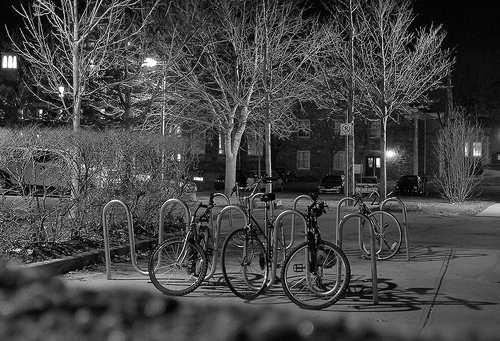
\includegraphics[width=\linewidth]{./procesadas/2015_00002/2015_00002_original.png}
		\caption{Imagen original}
	\end{subfigure}
	\hfill
	\begin{subfigure}[b]{0.32\textwidth}
		\centering
		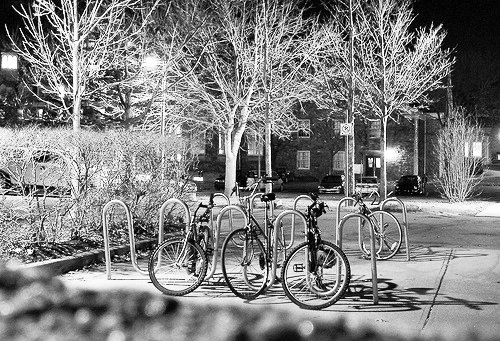
\includegraphics[width=\linewidth]{./procesadas/2015_00002/2015_00002_he.png}
		\caption{Histogram Equalization (HE)}
	\end{subfigure}

	% Segunda fila (2 imágenes)
	\begin{subfigure}[b]{0.32\textwidth}
		\centering
		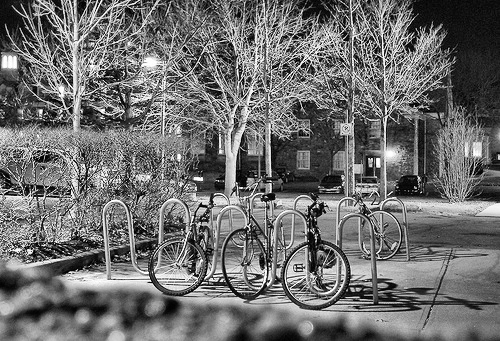
\includegraphics[width=\linewidth]{./procesadas/2015_00002/2015_00002_clahe.png}
		\caption{CLAHE}
	\end{subfigure}
	\hfill
	\begin{subfigure}[b]{0.32\textwidth}
		\centering
		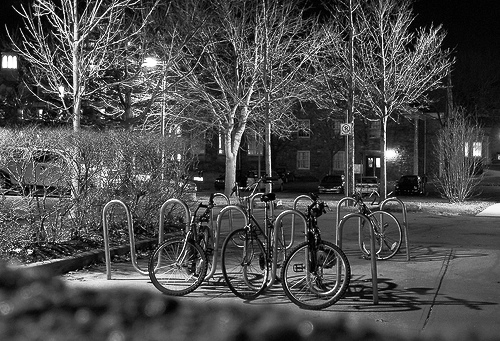
\includegraphics[width=\linewidth]{./procesadas/2015_00002/2015_00002_dqhepl.png}
		\caption{DQHEPL}
	\end{subfigure}

	% Tercera fila (1 imagen centrada)
	\begin{subfigure}[b]{0.32\textwidth}
		\centering
		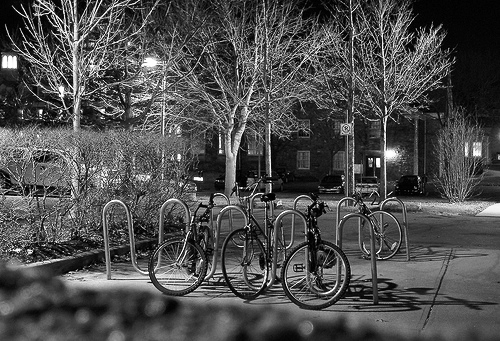
\includegraphics[width=\linewidth]{./procesadas/2015_00002/2015_00002_bhepl_d.png}
		\caption{BHEPL-D}
	\end{subfigure}

	\caption{Métodos aplicados sobre la imagen 2015\_00002.png}
	\label{fig:visual_002}
\end{figure}

Finalmente, desde un análisis visual y subjetivo de las imagenes de la \emph{Figura \ref{fig:visual_002}},
se puede observar que tanto CLAHE como HE tienden a sobresaturar la imagen en términos de
luminosidad, siendo esta característica especialmente pronunciada en el caso de HE.

En cuanto a los métodos propuestos por Ooi y Mat Isa, ambos ofrecen resultados visualmente muy
similares y efectivos. Sin embargo, DQHEPL presenta una ligera ventaja en cuanto a claridad en
ciertas áreas de la imagen, permitiendo apreciar algunos detalles adicionales con mayor
nitidez.

% ------- imagen 0026 ---------------
\subsubsection{\textbf{Análisis de imagen 2015\_00026}}

La segunda imagen presenta un caso más particular, ya que posee un nivel de exposición
considerablemente más bajo en comparación con la primera. La escena en general es notablemente
más oscura, lo que representa un mayor desafío para los algoritmos de mejora. Además, se
identifican zonas puntuales con alta luminosidad que contrastan fuertemente con el resto de la
imagen, generando una distribución de brillo más heterogénea y compleja de tratar.

\begin{table}[H]
	\centering
	\caption{Métricas de calidad para la imagen 2015\_00026.jpg}
	\label{tab:metricas_2015_00026}
	\vspace{0.5em}

	\resizebox{\linewidth}{!}{%
		\begin{tabular}{@{}lrrrrr@{}}
			\toprule
			\textbf{Método} & \textbf{AMBE} & \textbf{PSNR} & \textbf{Entropía} & \textbf{Contraste} & \textbf{Uniformidad} \\
			\midrule
            Original        & -             & -                  & 5.35              & 17.07              & 0.50                \\
			CLAHE           & 20.90         & 19.96              & 6.23              & 30.94              & 0.552                \\
			HE              & 102.75        & 6.44               & 5.28              & 78.59              & 0.604                \\
			DQHEPL          & 13.70         & 17.13              & 5.16              & 48.83              & 0.388                \\
			BHEPL-D         & 4.18          & 27.79              & 5.29              & 26.16              & 0.451                \\
			\bottomrule
		\end{tabular}%
	}

	\vspace{0.5em}
	\footnotesize%
	\textit{Nota: AMBE (menor es mejor), PSNR (mayor es mejor). Uniformidad: 0.6–0.85 optimo}
\end{table}

La \emph{Tabla \ref{tab:metricas_2015_00026}} presenta los resultados obtenidos para la imagen
\emph{2015-00026.jpg}, caracterizada por un bajo nivel de exposición general y la presencia de puntos
aislados con alta luminosidad.

En este contexto, BHEPL-D destaca por ofrecer el mejor equilibrio entre preservación del brillo
(AMBE de 4.18) y fidelidad respecto a la imagen original (PSNR de 27.79), lo que sugiere una
mejora efectiva sin introducir distorsiones excesivas. Sin embargo, su contraste (26.16) y
uniformidad (0.451) son relativamente bajos, lo que indica una mejora moderada en la
diferenciación tonal y una distribución de brillo menos homogénea.

CLAHE, por otro lado, muestra una mejora considerable en contraste (30.94) y mantiene un buen
compromiso en AMBE (20.90) y PSNR (19.96), junto con una entropía notablemente superior (6.23),
lo que sugiere una mejor diversidad de tonos en la imagen procesada.

En cambio, HE presenta el mayor contraste (78.59) y una uniformidad razonable (0.604), pero con
un AMBE extremadamente alto (102.75) y un PSNR muy bajo (6.44), lo que indica una fuerte
alteración del brillo original y una aparente pérdida de fidelidad visual.

DQHEPL, aunque mejora ligeramente en contraste respecto a BHEPL-D (48.83), muestra valores más
bajos en PSNR (17.13) y entropía (5.16), junto con una uniformidad significativamente inferior
(0.388), lo que sugiere una distribución tonal más irregular.

\begin{figure}[htbp]
	\centering
	\begin{subfigure}[b]{0.45\textwidth}
		\resizebox{\linewidth}{!}{%% Creator: Matplotlib, PGF backend
%%
%% To include the figure in your LaTeX document, write
%%   \input{<filename>.pgf}
%%
%% Make sure the required packages are loaded in your preamble
%%   \usepackage{pgf}
%%
%% Also ensure that all the required font packages are loaded; for instance,
%% the lmodern package is sometimes necessary when using math font.
%%   \usepackage{lmodern}
%%
%% Figures using additional raster images can only be included by \input if
%% they are in the same directory as the main LaTeX file. For loading figures
%% from other directories you can use the `import` package
%%   \usepackage{import}
%%
%% and then include the figures with
%%   \import{<path to file>}{<filename>.pgf}
%%
%% Matplotlib used the following preamble
%%   \def\mathdefault#1{#1}
%%   \everymath=\expandafter{\the\everymath\displaystyle}
%%   \IfFileExists{scrextend.sty}{
%%     \usepackage[fontsize=10.000000pt]{scrextend}
%%   }{
%%     \renewcommand{\normalsize}{\fontsize{10.000000}{12.000000}\selectfont}
%%     \normalsize
%%   }
%%   
%%   \ifdefined\pdftexversion\else  % non-pdftex case.
%%     \usepackage{fontspec}
%%     \setmainfont{DejaVuSerif.ttf}[Path=\detokenize{/home/elias/.virtualenvs/src-pway/lib/python3.13/site-packages/matplotlib/mpl-data/fonts/ttf/}]
%%     \setsansfont{DejaVuSans.ttf}[Path=\detokenize{/home/elias/.virtualenvs/src-pway/lib/python3.13/site-packages/matplotlib/mpl-data/fonts/ttf/}]
%%     \setmonofont{DejaVuSansMono.ttf}[Path=\detokenize{/home/elias/.virtualenvs/src-pway/lib/python3.13/site-packages/matplotlib/mpl-data/fonts/ttf/}]
%%   \fi
%%   \makeatletter\@ifpackageloaded{underscore}{}{\usepackage[strings]{underscore}}\makeatother
%%
\begingroup%
\makeatletter%
\begin{pgfpicture}%
\pgfpathrectangle{\pgfpointorigin}{\pgfqpoint{10.000000in}{5.000000in}}%
\pgfusepath{use as bounding box, clip}%
\begin{pgfscope}%
\pgfsetbuttcap%
\pgfsetmiterjoin%
\definecolor{currentfill}{rgb}{1.000000,1.000000,1.000000}%
\pgfsetfillcolor{currentfill}%
\pgfsetlinewidth{0.000000pt}%
\definecolor{currentstroke}{rgb}{1.000000,1.000000,1.000000}%
\pgfsetstrokecolor{currentstroke}%
\pgfsetdash{}{0pt}%
\pgfpathmoveto{\pgfqpoint{0.000000in}{0.000000in}}%
\pgfpathlineto{\pgfqpoint{10.000000in}{0.000000in}}%
\pgfpathlineto{\pgfqpoint{10.000000in}{5.000000in}}%
\pgfpathlineto{\pgfqpoint{0.000000in}{5.000000in}}%
\pgfpathlineto{\pgfqpoint{0.000000in}{0.000000in}}%
\pgfpathclose%
\pgfusepath{fill}%
\end{pgfscope}%
\begin{pgfscope}%
\pgfsetbuttcap%
\pgfsetmiterjoin%
\definecolor{currentfill}{rgb}{1.000000,1.000000,1.000000}%
\pgfsetfillcolor{currentfill}%
\pgfsetlinewidth{0.000000pt}%
\definecolor{currentstroke}{rgb}{0.000000,0.000000,0.000000}%
\pgfsetstrokecolor{currentstroke}%
\pgfsetstrokeopacity{0.000000}%
\pgfsetdash{}{0pt}%
\pgfpathmoveto{\pgfqpoint{1.250000in}{0.550000in}}%
\pgfpathlineto{\pgfqpoint{9.000000in}{0.550000in}}%
\pgfpathlineto{\pgfqpoint{9.000000in}{4.400000in}}%
\pgfpathlineto{\pgfqpoint{1.250000in}{4.400000in}}%
\pgfpathlineto{\pgfqpoint{1.250000in}{0.550000in}}%
\pgfpathclose%
\pgfusepath{fill}%
\end{pgfscope}%
\begin{pgfscope}%
\pgfpathrectangle{\pgfqpoint{1.250000in}{0.550000in}}{\pgfqpoint{7.750000in}{3.850000in}}%
\pgfusepath{clip}%
\pgfsetbuttcap%
\pgfsetmiterjoin%
\definecolor{currentfill}{rgb}{0.501961,0.501961,0.501961}%
\pgfsetfillcolor{currentfill}%
\pgfsetfillopacity{0.700000}%
\pgfsetlinewidth{0.000000pt}%
\definecolor{currentstroke}{rgb}{0.000000,0.000000,0.000000}%
\pgfsetstrokecolor{currentstroke}%
\pgfsetstrokeopacity{0.700000}%
\pgfsetdash{}{0pt}%
\pgfpathmoveto{\pgfqpoint{1.602273in}{0.550000in}}%
\pgfpathlineto{\pgfqpoint{1.629794in}{0.550000in}}%
\pgfpathlineto{\pgfqpoint{1.629794in}{2.398200in}}%
\pgfpathlineto{\pgfqpoint{1.602273in}{2.398200in}}%
\pgfpathlineto{\pgfqpoint{1.602273in}{0.550000in}}%
\pgfpathclose%
\pgfusepath{fill}%
\end{pgfscope}%
\begin{pgfscope}%
\pgfpathrectangle{\pgfqpoint{1.250000in}{0.550000in}}{\pgfqpoint{7.750000in}{3.850000in}}%
\pgfusepath{clip}%
\pgfsetbuttcap%
\pgfsetmiterjoin%
\definecolor{currentfill}{rgb}{0.501961,0.501961,0.501961}%
\pgfsetfillcolor{currentfill}%
\pgfsetfillopacity{0.700000}%
\pgfsetlinewidth{0.000000pt}%
\definecolor{currentstroke}{rgb}{0.000000,0.000000,0.000000}%
\pgfsetstrokecolor{currentstroke}%
\pgfsetstrokeopacity{0.700000}%
\pgfsetdash{}{0pt}%
\pgfpathmoveto{\pgfqpoint{1.629794in}{0.550000in}}%
\pgfpathlineto{\pgfqpoint{1.657315in}{0.550000in}}%
\pgfpathlineto{\pgfqpoint{1.657315in}{4.216667in}}%
\pgfpathlineto{\pgfqpoint{1.629794in}{4.216667in}}%
\pgfpathlineto{\pgfqpoint{1.629794in}{0.550000in}}%
\pgfpathclose%
\pgfusepath{fill}%
\end{pgfscope}%
\begin{pgfscope}%
\pgfpathrectangle{\pgfqpoint{1.250000in}{0.550000in}}{\pgfqpoint{7.750000in}{3.850000in}}%
\pgfusepath{clip}%
\pgfsetbuttcap%
\pgfsetmiterjoin%
\definecolor{currentfill}{rgb}{0.501961,0.501961,0.501961}%
\pgfsetfillcolor{currentfill}%
\pgfsetfillopacity{0.700000}%
\pgfsetlinewidth{0.000000pt}%
\definecolor{currentstroke}{rgb}{0.000000,0.000000,0.000000}%
\pgfsetstrokecolor{currentstroke}%
\pgfsetstrokeopacity{0.700000}%
\pgfsetdash{}{0pt}%
\pgfpathmoveto{\pgfqpoint{1.657315in}{0.550000in}}%
\pgfpathlineto{\pgfqpoint{1.684837in}{0.550000in}}%
\pgfpathlineto{\pgfqpoint{1.684837in}{3.586192in}}%
\pgfpathlineto{\pgfqpoint{1.657315in}{3.586192in}}%
\pgfpathlineto{\pgfqpoint{1.657315in}{0.550000in}}%
\pgfpathclose%
\pgfusepath{fill}%
\end{pgfscope}%
\begin{pgfscope}%
\pgfpathrectangle{\pgfqpoint{1.250000in}{0.550000in}}{\pgfqpoint{7.750000in}{3.850000in}}%
\pgfusepath{clip}%
\pgfsetbuttcap%
\pgfsetmiterjoin%
\definecolor{currentfill}{rgb}{0.501961,0.501961,0.501961}%
\pgfsetfillcolor{currentfill}%
\pgfsetfillopacity{0.700000}%
\pgfsetlinewidth{0.000000pt}%
\definecolor{currentstroke}{rgb}{0.000000,0.000000,0.000000}%
\pgfsetstrokecolor{currentstroke}%
\pgfsetstrokeopacity{0.700000}%
\pgfsetdash{}{0pt}%
\pgfpathmoveto{\pgfqpoint{1.684837in}{0.550000in}}%
\pgfpathlineto{\pgfqpoint{1.712358in}{0.550000in}}%
\pgfpathlineto{\pgfqpoint{1.712358in}{2.872296in}}%
\pgfpathlineto{\pgfqpoint{1.684837in}{2.872296in}}%
\pgfpathlineto{\pgfqpoint{1.684837in}{0.550000in}}%
\pgfpathclose%
\pgfusepath{fill}%
\end{pgfscope}%
\begin{pgfscope}%
\pgfpathrectangle{\pgfqpoint{1.250000in}{0.550000in}}{\pgfqpoint{7.750000in}{3.850000in}}%
\pgfusepath{clip}%
\pgfsetbuttcap%
\pgfsetmiterjoin%
\definecolor{currentfill}{rgb}{0.501961,0.501961,0.501961}%
\pgfsetfillcolor{currentfill}%
\pgfsetfillopacity{0.700000}%
\pgfsetlinewidth{0.000000pt}%
\definecolor{currentstroke}{rgb}{0.000000,0.000000,0.000000}%
\pgfsetstrokecolor{currentstroke}%
\pgfsetstrokeopacity{0.700000}%
\pgfsetdash{}{0pt}%
\pgfpathmoveto{\pgfqpoint{1.712358in}{0.550000in}}%
\pgfpathlineto{\pgfqpoint{1.739879in}{0.550000in}}%
\pgfpathlineto{\pgfqpoint{1.739879in}{2.257238in}}%
\pgfpathlineto{\pgfqpoint{1.712358in}{2.257238in}}%
\pgfpathlineto{\pgfqpoint{1.712358in}{0.550000in}}%
\pgfpathclose%
\pgfusepath{fill}%
\end{pgfscope}%
\begin{pgfscope}%
\pgfpathrectangle{\pgfqpoint{1.250000in}{0.550000in}}{\pgfqpoint{7.750000in}{3.850000in}}%
\pgfusepath{clip}%
\pgfsetbuttcap%
\pgfsetmiterjoin%
\definecolor{currentfill}{rgb}{0.501961,0.501961,0.501961}%
\pgfsetfillcolor{currentfill}%
\pgfsetfillopacity{0.700000}%
\pgfsetlinewidth{0.000000pt}%
\definecolor{currentstroke}{rgb}{0.000000,0.000000,0.000000}%
\pgfsetstrokecolor{currentstroke}%
\pgfsetstrokeopacity{0.700000}%
\pgfsetdash{}{0pt}%
\pgfpathmoveto{\pgfqpoint{1.739879in}{0.550000in}}%
\pgfpathlineto{\pgfqpoint{1.767401in}{0.550000in}}%
\pgfpathlineto{\pgfqpoint{1.767401in}{1.879229in}}%
\pgfpathlineto{\pgfqpoint{1.739879in}{1.879229in}}%
\pgfpathlineto{\pgfqpoint{1.739879in}{0.550000in}}%
\pgfpathclose%
\pgfusepath{fill}%
\end{pgfscope}%
\begin{pgfscope}%
\pgfpathrectangle{\pgfqpoint{1.250000in}{0.550000in}}{\pgfqpoint{7.750000in}{3.850000in}}%
\pgfusepath{clip}%
\pgfsetbuttcap%
\pgfsetmiterjoin%
\definecolor{currentfill}{rgb}{0.501961,0.501961,0.501961}%
\pgfsetfillcolor{currentfill}%
\pgfsetfillopacity{0.700000}%
\pgfsetlinewidth{0.000000pt}%
\definecolor{currentstroke}{rgb}{0.000000,0.000000,0.000000}%
\pgfsetstrokecolor{currentstroke}%
\pgfsetstrokeopacity{0.700000}%
\pgfsetdash{}{0pt}%
\pgfpathmoveto{\pgfqpoint{1.767401in}{0.550000in}}%
\pgfpathlineto{\pgfqpoint{1.794922in}{0.550000in}}%
\pgfpathlineto{\pgfqpoint{1.794922in}{1.607766in}}%
\pgfpathlineto{\pgfqpoint{1.767401in}{1.607766in}}%
\pgfpathlineto{\pgfqpoint{1.767401in}{0.550000in}}%
\pgfpathclose%
\pgfusepath{fill}%
\end{pgfscope}%
\begin{pgfscope}%
\pgfpathrectangle{\pgfqpoint{1.250000in}{0.550000in}}{\pgfqpoint{7.750000in}{3.850000in}}%
\pgfusepath{clip}%
\pgfsetbuttcap%
\pgfsetmiterjoin%
\definecolor{currentfill}{rgb}{0.501961,0.501961,0.501961}%
\pgfsetfillcolor{currentfill}%
\pgfsetfillopacity{0.700000}%
\pgfsetlinewidth{0.000000pt}%
\definecolor{currentstroke}{rgb}{0.000000,0.000000,0.000000}%
\pgfsetstrokecolor{currentstroke}%
\pgfsetstrokeopacity{0.700000}%
\pgfsetdash{}{0pt}%
\pgfpathmoveto{\pgfqpoint{1.794922in}{0.550000in}}%
\pgfpathlineto{\pgfqpoint{1.822443in}{0.550000in}}%
\pgfpathlineto{\pgfqpoint{1.822443in}{1.512232in}}%
\pgfpathlineto{\pgfqpoint{1.794922in}{1.512232in}}%
\pgfpathlineto{\pgfqpoint{1.794922in}{0.550000in}}%
\pgfpathclose%
\pgfusepath{fill}%
\end{pgfscope}%
\begin{pgfscope}%
\pgfpathrectangle{\pgfqpoint{1.250000in}{0.550000in}}{\pgfqpoint{7.750000in}{3.850000in}}%
\pgfusepath{clip}%
\pgfsetbuttcap%
\pgfsetmiterjoin%
\definecolor{currentfill}{rgb}{0.501961,0.501961,0.501961}%
\pgfsetfillcolor{currentfill}%
\pgfsetfillopacity{0.700000}%
\pgfsetlinewidth{0.000000pt}%
\definecolor{currentstroke}{rgb}{0.000000,0.000000,0.000000}%
\pgfsetstrokecolor{currentstroke}%
\pgfsetstrokeopacity{0.700000}%
\pgfsetdash{}{0pt}%
\pgfpathmoveto{\pgfqpoint{1.822443in}{0.550000in}}%
\pgfpathlineto{\pgfqpoint{1.849964in}{0.550000in}}%
\pgfpathlineto{\pgfqpoint{1.849964in}{1.347317in}}%
\pgfpathlineto{\pgfqpoint{1.822443in}{1.347317in}}%
\pgfpathlineto{\pgfqpoint{1.822443in}{0.550000in}}%
\pgfpathclose%
\pgfusepath{fill}%
\end{pgfscope}%
\begin{pgfscope}%
\pgfpathrectangle{\pgfqpoint{1.250000in}{0.550000in}}{\pgfqpoint{7.750000in}{3.850000in}}%
\pgfusepath{clip}%
\pgfsetbuttcap%
\pgfsetmiterjoin%
\definecolor{currentfill}{rgb}{0.501961,0.501961,0.501961}%
\pgfsetfillcolor{currentfill}%
\pgfsetfillopacity{0.700000}%
\pgfsetlinewidth{0.000000pt}%
\definecolor{currentstroke}{rgb}{0.000000,0.000000,0.000000}%
\pgfsetstrokecolor{currentstroke}%
\pgfsetstrokeopacity{0.700000}%
\pgfsetdash{}{0pt}%
\pgfpathmoveto{\pgfqpoint{1.849964in}{0.550000in}}%
\pgfpathlineto{\pgfqpoint{1.877486in}{0.550000in}}%
\pgfpathlineto{\pgfqpoint{1.877486in}{1.249855in}}%
\pgfpathlineto{\pgfqpoint{1.849964in}{1.249855in}}%
\pgfpathlineto{\pgfqpoint{1.849964in}{0.550000in}}%
\pgfpathclose%
\pgfusepath{fill}%
\end{pgfscope}%
\begin{pgfscope}%
\pgfpathrectangle{\pgfqpoint{1.250000in}{0.550000in}}{\pgfqpoint{7.750000in}{3.850000in}}%
\pgfusepath{clip}%
\pgfsetbuttcap%
\pgfsetmiterjoin%
\definecolor{currentfill}{rgb}{0.501961,0.501961,0.501961}%
\pgfsetfillcolor{currentfill}%
\pgfsetfillopacity{0.700000}%
\pgfsetlinewidth{0.000000pt}%
\definecolor{currentstroke}{rgb}{0.000000,0.000000,0.000000}%
\pgfsetstrokecolor{currentstroke}%
\pgfsetstrokeopacity{0.700000}%
\pgfsetdash{}{0pt}%
\pgfpathmoveto{\pgfqpoint{1.877486in}{0.550000in}}%
\pgfpathlineto{\pgfqpoint{1.905007in}{0.550000in}}%
\pgfpathlineto{\pgfqpoint{1.905007in}{1.151291in}}%
\pgfpathlineto{\pgfqpoint{1.877486in}{1.151291in}}%
\pgfpathlineto{\pgfqpoint{1.877486in}{0.550000in}}%
\pgfpathclose%
\pgfusepath{fill}%
\end{pgfscope}%
\begin{pgfscope}%
\pgfpathrectangle{\pgfqpoint{1.250000in}{0.550000in}}{\pgfqpoint{7.750000in}{3.850000in}}%
\pgfusepath{clip}%
\pgfsetbuttcap%
\pgfsetmiterjoin%
\definecolor{currentfill}{rgb}{0.501961,0.501961,0.501961}%
\pgfsetfillcolor{currentfill}%
\pgfsetfillopacity{0.700000}%
\pgfsetlinewidth{0.000000pt}%
\definecolor{currentstroke}{rgb}{0.000000,0.000000,0.000000}%
\pgfsetstrokecolor{currentstroke}%
\pgfsetstrokeopacity{0.700000}%
\pgfsetdash{}{0pt}%
\pgfpathmoveto{\pgfqpoint{1.905007in}{0.550000in}}%
\pgfpathlineto{\pgfqpoint{1.932528in}{0.550000in}}%
\pgfpathlineto{\pgfqpoint{1.932528in}{1.082187in}}%
\pgfpathlineto{\pgfqpoint{1.905007in}{1.082187in}}%
\pgfpathlineto{\pgfqpoint{1.905007in}{0.550000in}}%
\pgfpathclose%
\pgfusepath{fill}%
\end{pgfscope}%
\begin{pgfscope}%
\pgfpathrectangle{\pgfqpoint{1.250000in}{0.550000in}}{\pgfqpoint{7.750000in}{3.850000in}}%
\pgfusepath{clip}%
\pgfsetbuttcap%
\pgfsetmiterjoin%
\definecolor{currentfill}{rgb}{0.501961,0.501961,0.501961}%
\pgfsetfillcolor{currentfill}%
\pgfsetfillopacity{0.700000}%
\pgfsetlinewidth{0.000000pt}%
\definecolor{currentstroke}{rgb}{0.000000,0.000000,0.000000}%
\pgfsetstrokecolor{currentstroke}%
\pgfsetstrokeopacity{0.700000}%
\pgfsetdash{}{0pt}%
\pgfpathmoveto{\pgfqpoint{1.932528in}{0.550000in}}%
\pgfpathlineto{\pgfqpoint{1.960050in}{0.550000in}}%
\pgfpathlineto{\pgfqpoint{1.960050in}{1.053554in}}%
\pgfpathlineto{\pgfqpoint{1.932528in}{1.053554in}}%
\pgfpathlineto{\pgfqpoint{1.932528in}{0.550000in}}%
\pgfpathclose%
\pgfusepath{fill}%
\end{pgfscope}%
\begin{pgfscope}%
\pgfpathrectangle{\pgfqpoint{1.250000in}{0.550000in}}{\pgfqpoint{7.750000in}{3.850000in}}%
\pgfusepath{clip}%
\pgfsetbuttcap%
\pgfsetmiterjoin%
\definecolor{currentfill}{rgb}{0.501961,0.501961,0.501961}%
\pgfsetfillcolor{currentfill}%
\pgfsetfillopacity{0.700000}%
\pgfsetlinewidth{0.000000pt}%
\definecolor{currentstroke}{rgb}{0.000000,0.000000,0.000000}%
\pgfsetstrokecolor{currentstroke}%
\pgfsetstrokeopacity{0.700000}%
\pgfsetdash{}{0pt}%
\pgfpathmoveto{\pgfqpoint{1.960050in}{0.550000in}}%
\pgfpathlineto{\pgfqpoint{1.987571in}{0.550000in}}%
\pgfpathlineto{\pgfqpoint{1.987571in}{1.011431in}}%
\pgfpathlineto{\pgfqpoint{1.960050in}{1.011431in}}%
\pgfpathlineto{\pgfqpoint{1.960050in}{0.550000in}}%
\pgfpathclose%
\pgfusepath{fill}%
\end{pgfscope}%
\begin{pgfscope}%
\pgfpathrectangle{\pgfqpoint{1.250000in}{0.550000in}}{\pgfqpoint{7.750000in}{3.850000in}}%
\pgfusepath{clip}%
\pgfsetbuttcap%
\pgfsetmiterjoin%
\definecolor{currentfill}{rgb}{0.501961,0.501961,0.501961}%
\pgfsetfillcolor{currentfill}%
\pgfsetfillopacity{0.700000}%
\pgfsetlinewidth{0.000000pt}%
\definecolor{currentstroke}{rgb}{0.000000,0.000000,0.000000}%
\pgfsetstrokecolor{currentstroke}%
\pgfsetstrokeopacity{0.700000}%
\pgfsetdash{}{0pt}%
\pgfpathmoveto{\pgfqpoint{1.987571in}{0.550000in}}%
\pgfpathlineto{\pgfqpoint{2.015092in}{0.550000in}}%
\pgfpathlineto{\pgfqpoint{2.015092in}{0.968757in}}%
\pgfpathlineto{\pgfqpoint{1.987571in}{0.968757in}}%
\pgfpathlineto{\pgfqpoint{1.987571in}{0.550000in}}%
\pgfpathclose%
\pgfusepath{fill}%
\end{pgfscope}%
\begin{pgfscope}%
\pgfpathrectangle{\pgfqpoint{1.250000in}{0.550000in}}{\pgfqpoint{7.750000in}{3.850000in}}%
\pgfusepath{clip}%
\pgfsetbuttcap%
\pgfsetmiterjoin%
\definecolor{currentfill}{rgb}{0.501961,0.501961,0.501961}%
\pgfsetfillcolor{currentfill}%
\pgfsetfillopacity{0.700000}%
\pgfsetlinewidth{0.000000pt}%
\definecolor{currentstroke}{rgb}{0.000000,0.000000,0.000000}%
\pgfsetstrokecolor{currentstroke}%
\pgfsetstrokeopacity{0.700000}%
\pgfsetdash{}{0pt}%
\pgfpathmoveto{\pgfqpoint{2.015092in}{0.550000in}}%
\pgfpathlineto{\pgfqpoint{2.042614in}{0.550000in}}%
\pgfpathlineto{\pgfqpoint{2.042614in}{0.912592in}}%
\pgfpathlineto{\pgfqpoint{2.015092in}{0.912592in}}%
\pgfpathlineto{\pgfqpoint{2.015092in}{0.550000in}}%
\pgfpathclose%
\pgfusepath{fill}%
\end{pgfscope}%
\begin{pgfscope}%
\pgfpathrectangle{\pgfqpoint{1.250000in}{0.550000in}}{\pgfqpoint{7.750000in}{3.850000in}}%
\pgfusepath{clip}%
\pgfsetbuttcap%
\pgfsetmiterjoin%
\definecolor{currentfill}{rgb}{0.501961,0.501961,0.501961}%
\pgfsetfillcolor{currentfill}%
\pgfsetfillopacity{0.700000}%
\pgfsetlinewidth{0.000000pt}%
\definecolor{currentstroke}{rgb}{0.000000,0.000000,0.000000}%
\pgfsetstrokecolor{currentstroke}%
\pgfsetstrokeopacity{0.700000}%
\pgfsetdash{}{0pt}%
\pgfpathmoveto{\pgfqpoint{2.042614in}{0.550000in}}%
\pgfpathlineto{\pgfqpoint{2.070135in}{0.550000in}}%
\pgfpathlineto{\pgfqpoint{2.070135in}{0.906260in}}%
\pgfpathlineto{\pgfqpoint{2.042614in}{0.906260in}}%
\pgfpathlineto{\pgfqpoint{2.042614in}{0.550000in}}%
\pgfpathclose%
\pgfusepath{fill}%
\end{pgfscope}%
\begin{pgfscope}%
\pgfpathrectangle{\pgfqpoint{1.250000in}{0.550000in}}{\pgfqpoint{7.750000in}{3.850000in}}%
\pgfusepath{clip}%
\pgfsetbuttcap%
\pgfsetmiterjoin%
\definecolor{currentfill}{rgb}{0.501961,0.501961,0.501961}%
\pgfsetfillcolor{currentfill}%
\pgfsetfillopacity{0.700000}%
\pgfsetlinewidth{0.000000pt}%
\definecolor{currentstroke}{rgb}{0.000000,0.000000,0.000000}%
\pgfsetstrokecolor{currentstroke}%
\pgfsetstrokeopacity{0.700000}%
\pgfsetdash{}{0pt}%
\pgfpathmoveto{\pgfqpoint{2.070135in}{0.550000in}}%
\pgfpathlineto{\pgfqpoint{2.097656in}{0.550000in}}%
\pgfpathlineto{\pgfqpoint{2.097656in}{0.871019in}}%
\pgfpathlineto{\pgfqpoint{2.070135in}{0.871019in}}%
\pgfpathlineto{\pgfqpoint{2.070135in}{0.550000in}}%
\pgfpathclose%
\pgfusepath{fill}%
\end{pgfscope}%
\begin{pgfscope}%
\pgfpathrectangle{\pgfqpoint{1.250000in}{0.550000in}}{\pgfqpoint{7.750000in}{3.850000in}}%
\pgfusepath{clip}%
\pgfsetbuttcap%
\pgfsetmiterjoin%
\definecolor{currentfill}{rgb}{0.501961,0.501961,0.501961}%
\pgfsetfillcolor{currentfill}%
\pgfsetfillopacity{0.700000}%
\pgfsetlinewidth{0.000000pt}%
\definecolor{currentstroke}{rgb}{0.000000,0.000000,0.000000}%
\pgfsetstrokecolor{currentstroke}%
\pgfsetstrokeopacity{0.700000}%
\pgfsetdash{}{0pt}%
\pgfpathmoveto{\pgfqpoint{2.097656in}{0.550000in}}%
\pgfpathlineto{\pgfqpoint{2.125178in}{0.550000in}}%
\pgfpathlineto{\pgfqpoint{2.125178in}{0.875975in}}%
\pgfpathlineto{\pgfqpoint{2.097656in}{0.875975in}}%
\pgfpathlineto{\pgfqpoint{2.097656in}{0.550000in}}%
\pgfpathclose%
\pgfusepath{fill}%
\end{pgfscope}%
\begin{pgfscope}%
\pgfpathrectangle{\pgfqpoint{1.250000in}{0.550000in}}{\pgfqpoint{7.750000in}{3.850000in}}%
\pgfusepath{clip}%
\pgfsetbuttcap%
\pgfsetmiterjoin%
\definecolor{currentfill}{rgb}{0.501961,0.501961,0.501961}%
\pgfsetfillcolor{currentfill}%
\pgfsetfillopacity{0.700000}%
\pgfsetlinewidth{0.000000pt}%
\definecolor{currentstroke}{rgb}{0.000000,0.000000,0.000000}%
\pgfsetstrokecolor{currentstroke}%
\pgfsetstrokeopacity{0.700000}%
\pgfsetdash{}{0pt}%
\pgfpathmoveto{\pgfqpoint{2.125178in}{0.550000in}}%
\pgfpathlineto{\pgfqpoint{2.152699in}{0.550000in}}%
\pgfpathlineto{\pgfqpoint{2.152699in}{0.870193in}}%
\pgfpathlineto{\pgfqpoint{2.125178in}{0.870193in}}%
\pgfpathlineto{\pgfqpoint{2.125178in}{0.550000in}}%
\pgfpathclose%
\pgfusepath{fill}%
\end{pgfscope}%
\begin{pgfscope}%
\pgfpathrectangle{\pgfqpoint{1.250000in}{0.550000in}}{\pgfqpoint{7.750000in}{3.850000in}}%
\pgfusepath{clip}%
\pgfsetbuttcap%
\pgfsetmiterjoin%
\definecolor{currentfill}{rgb}{0.501961,0.501961,0.501961}%
\pgfsetfillcolor{currentfill}%
\pgfsetfillopacity{0.700000}%
\pgfsetlinewidth{0.000000pt}%
\definecolor{currentstroke}{rgb}{0.000000,0.000000,0.000000}%
\pgfsetstrokecolor{currentstroke}%
\pgfsetstrokeopacity{0.700000}%
\pgfsetdash{}{0pt}%
\pgfpathmoveto{\pgfqpoint{2.152699in}{0.550000in}}%
\pgfpathlineto{\pgfqpoint{2.180220in}{0.550000in}}%
\pgfpathlineto{\pgfqpoint{2.180220in}{0.874598in}}%
\pgfpathlineto{\pgfqpoint{2.152699in}{0.874598in}}%
\pgfpathlineto{\pgfqpoint{2.152699in}{0.550000in}}%
\pgfpathclose%
\pgfusepath{fill}%
\end{pgfscope}%
\begin{pgfscope}%
\pgfpathrectangle{\pgfqpoint{1.250000in}{0.550000in}}{\pgfqpoint{7.750000in}{3.850000in}}%
\pgfusepath{clip}%
\pgfsetbuttcap%
\pgfsetmiterjoin%
\definecolor{currentfill}{rgb}{0.501961,0.501961,0.501961}%
\pgfsetfillcolor{currentfill}%
\pgfsetfillopacity{0.700000}%
\pgfsetlinewidth{0.000000pt}%
\definecolor{currentstroke}{rgb}{0.000000,0.000000,0.000000}%
\pgfsetstrokecolor{currentstroke}%
\pgfsetstrokeopacity{0.700000}%
\pgfsetdash{}{0pt}%
\pgfpathmoveto{\pgfqpoint{2.180220in}{0.550000in}}%
\pgfpathlineto{\pgfqpoint{2.207741in}{0.550000in}}%
\pgfpathlineto{\pgfqpoint{2.207741in}{0.885060in}}%
\pgfpathlineto{\pgfqpoint{2.180220in}{0.885060in}}%
\pgfpathlineto{\pgfqpoint{2.180220in}{0.550000in}}%
\pgfpathclose%
\pgfusepath{fill}%
\end{pgfscope}%
\begin{pgfscope}%
\pgfpathrectangle{\pgfqpoint{1.250000in}{0.550000in}}{\pgfqpoint{7.750000in}{3.850000in}}%
\pgfusepath{clip}%
\pgfsetbuttcap%
\pgfsetmiterjoin%
\definecolor{currentfill}{rgb}{0.501961,0.501961,0.501961}%
\pgfsetfillcolor{currentfill}%
\pgfsetfillopacity{0.700000}%
\pgfsetlinewidth{0.000000pt}%
\definecolor{currentstroke}{rgb}{0.000000,0.000000,0.000000}%
\pgfsetstrokecolor{currentstroke}%
\pgfsetstrokeopacity{0.700000}%
\pgfsetdash{}{0pt}%
\pgfpathmoveto{\pgfqpoint{2.207741in}{0.550000in}}%
\pgfpathlineto{\pgfqpoint{2.235263in}{0.550000in}}%
\pgfpathlineto{\pgfqpoint{2.235263in}{0.871845in}}%
\pgfpathlineto{\pgfqpoint{2.207741in}{0.871845in}}%
\pgfpathlineto{\pgfqpoint{2.207741in}{0.550000in}}%
\pgfpathclose%
\pgfusepath{fill}%
\end{pgfscope}%
\begin{pgfscope}%
\pgfpathrectangle{\pgfqpoint{1.250000in}{0.550000in}}{\pgfqpoint{7.750000in}{3.850000in}}%
\pgfusepath{clip}%
\pgfsetbuttcap%
\pgfsetmiterjoin%
\definecolor{currentfill}{rgb}{0.501961,0.501961,0.501961}%
\pgfsetfillcolor{currentfill}%
\pgfsetfillopacity{0.700000}%
\pgfsetlinewidth{0.000000pt}%
\definecolor{currentstroke}{rgb}{0.000000,0.000000,0.000000}%
\pgfsetstrokecolor{currentstroke}%
\pgfsetstrokeopacity{0.700000}%
\pgfsetdash{}{0pt}%
\pgfpathmoveto{\pgfqpoint{2.235263in}{0.550000in}}%
\pgfpathlineto{\pgfqpoint{2.262784in}{0.550000in}}%
\pgfpathlineto{\pgfqpoint{2.262784in}{0.822839in}}%
\pgfpathlineto{\pgfqpoint{2.235263in}{0.822839in}}%
\pgfpathlineto{\pgfqpoint{2.235263in}{0.550000in}}%
\pgfpathclose%
\pgfusepath{fill}%
\end{pgfscope}%
\begin{pgfscope}%
\pgfpathrectangle{\pgfqpoint{1.250000in}{0.550000in}}{\pgfqpoint{7.750000in}{3.850000in}}%
\pgfusepath{clip}%
\pgfsetbuttcap%
\pgfsetmiterjoin%
\definecolor{currentfill}{rgb}{0.501961,0.501961,0.501961}%
\pgfsetfillcolor{currentfill}%
\pgfsetfillopacity{0.700000}%
\pgfsetlinewidth{0.000000pt}%
\definecolor{currentstroke}{rgb}{0.000000,0.000000,0.000000}%
\pgfsetstrokecolor{currentstroke}%
\pgfsetstrokeopacity{0.700000}%
\pgfsetdash{}{0pt}%
\pgfpathmoveto{\pgfqpoint{2.262784in}{0.550000in}}%
\pgfpathlineto{\pgfqpoint{2.290305in}{0.550000in}}%
\pgfpathlineto{\pgfqpoint{2.290305in}{0.820912in}}%
\pgfpathlineto{\pgfqpoint{2.262784in}{0.820912in}}%
\pgfpathlineto{\pgfqpoint{2.262784in}{0.550000in}}%
\pgfpathclose%
\pgfusepath{fill}%
\end{pgfscope}%
\begin{pgfscope}%
\pgfpathrectangle{\pgfqpoint{1.250000in}{0.550000in}}{\pgfqpoint{7.750000in}{3.850000in}}%
\pgfusepath{clip}%
\pgfsetbuttcap%
\pgfsetmiterjoin%
\definecolor{currentfill}{rgb}{0.501961,0.501961,0.501961}%
\pgfsetfillcolor{currentfill}%
\pgfsetfillopacity{0.700000}%
\pgfsetlinewidth{0.000000pt}%
\definecolor{currentstroke}{rgb}{0.000000,0.000000,0.000000}%
\pgfsetstrokecolor{currentstroke}%
\pgfsetstrokeopacity{0.700000}%
\pgfsetdash{}{0pt}%
\pgfpathmoveto{\pgfqpoint{2.290305in}{0.550000in}}%
\pgfpathlineto{\pgfqpoint{2.317827in}{0.550000in}}%
\pgfpathlineto{\pgfqpoint{2.317827in}{0.812652in}}%
\pgfpathlineto{\pgfqpoint{2.290305in}{0.812652in}}%
\pgfpathlineto{\pgfqpoint{2.290305in}{0.550000in}}%
\pgfpathclose%
\pgfusepath{fill}%
\end{pgfscope}%
\begin{pgfscope}%
\pgfpathrectangle{\pgfqpoint{1.250000in}{0.550000in}}{\pgfqpoint{7.750000in}{3.850000in}}%
\pgfusepath{clip}%
\pgfsetbuttcap%
\pgfsetmiterjoin%
\definecolor{currentfill}{rgb}{0.501961,0.501961,0.501961}%
\pgfsetfillcolor{currentfill}%
\pgfsetfillopacity{0.700000}%
\pgfsetlinewidth{0.000000pt}%
\definecolor{currentstroke}{rgb}{0.000000,0.000000,0.000000}%
\pgfsetstrokecolor{currentstroke}%
\pgfsetstrokeopacity{0.700000}%
\pgfsetdash{}{0pt}%
\pgfpathmoveto{\pgfqpoint{2.317827in}{0.550000in}}%
\pgfpathlineto{\pgfqpoint{2.345348in}{0.550000in}}%
\pgfpathlineto{\pgfqpoint{2.345348in}{0.811000in}}%
\pgfpathlineto{\pgfqpoint{2.317827in}{0.811000in}}%
\pgfpathlineto{\pgfqpoint{2.317827in}{0.550000in}}%
\pgfpathclose%
\pgfusepath{fill}%
\end{pgfscope}%
\begin{pgfscope}%
\pgfpathrectangle{\pgfqpoint{1.250000in}{0.550000in}}{\pgfqpoint{7.750000in}{3.850000in}}%
\pgfusepath{clip}%
\pgfsetbuttcap%
\pgfsetmiterjoin%
\definecolor{currentfill}{rgb}{0.501961,0.501961,0.501961}%
\pgfsetfillcolor{currentfill}%
\pgfsetfillopacity{0.700000}%
\pgfsetlinewidth{0.000000pt}%
\definecolor{currentstroke}{rgb}{0.000000,0.000000,0.000000}%
\pgfsetstrokecolor{currentstroke}%
\pgfsetstrokeopacity{0.700000}%
\pgfsetdash{}{0pt}%
\pgfpathmoveto{\pgfqpoint{2.345348in}{0.550000in}}%
\pgfpathlineto{\pgfqpoint{2.372869in}{0.550000in}}%
\pgfpathlineto{\pgfqpoint{2.372869in}{0.829722in}}%
\pgfpathlineto{\pgfqpoint{2.345348in}{0.829722in}}%
\pgfpathlineto{\pgfqpoint{2.345348in}{0.550000in}}%
\pgfpathclose%
\pgfusepath{fill}%
\end{pgfscope}%
\begin{pgfscope}%
\pgfpathrectangle{\pgfqpoint{1.250000in}{0.550000in}}{\pgfqpoint{7.750000in}{3.850000in}}%
\pgfusepath{clip}%
\pgfsetbuttcap%
\pgfsetmiterjoin%
\definecolor{currentfill}{rgb}{0.501961,0.501961,0.501961}%
\pgfsetfillcolor{currentfill}%
\pgfsetfillopacity{0.700000}%
\pgfsetlinewidth{0.000000pt}%
\definecolor{currentstroke}{rgb}{0.000000,0.000000,0.000000}%
\pgfsetstrokecolor{currentstroke}%
\pgfsetstrokeopacity{0.700000}%
\pgfsetdash{}{0pt}%
\pgfpathmoveto{\pgfqpoint{2.372869in}{0.550000in}}%
\pgfpathlineto{\pgfqpoint{2.400391in}{0.550000in}}%
\pgfpathlineto{\pgfqpoint{2.400391in}{0.808247in}}%
\pgfpathlineto{\pgfqpoint{2.372869in}{0.808247in}}%
\pgfpathlineto{\pgfqpoint{2.372869in}{0.550000in}}%
\pgfpathclose%
\pgfusepath{fill}%
\end{pgfscope}%
\begin{pgfscope}%
\pgfpathrectangle{\pgfqpoint{1.250000in}{0.550000in}}{\pgfqpoint{7.750000in}{3.850000in}}%
\pgfusepath{clip}%
\pgfsetbuttcap%
\pgfsetmiterjoin%
\definecolor{currentfill}{rgb}{0.501961,0.501961,0.501961}%
\pgfsetfillcolor{currentfill}%
\pgfsetfillopacity{0.700000}%
\pgfsetlinewidth{0.000000pt}%
\definecolor{currentstroke}{rgb}{0.000000,0.000000,0.000000}%
\pgfsetstrokecolor{currentstroke}%
\pgfsetstrokeopacity{0.700000}%
\pgfsetdash{}{0pt}%
\pgfpathmoveto{\pgfqpoint{2.400391in}{0.550000in}}%
\pgfpathlineto{\pgfqpoint{2.427912in}{0.550000in}}%
\pgfpathlineto{\pgfqpoint{2.427912in}{0.814304in}}%
\pgfpathlineto{\pgfqpoint{2.400391in}{0.814304in}}%
\pgfpathlineto{\pgfqpoint{2.400391in}{0.550000in}}%
\pgfpathclose%
\pgfusepath{fill}%
\end{pgfscope}%
\begin{pgfscope}%
\pgfpathrectangle{\pgfqpoint{1.250000in}{0.550000in}}{\pgfqpoint{7.750000in}{3.850000in}}%
\pgfusepath{clip}%
\pgfsetbuttcap%
\pgfsetmiterjoin%
\definecolor{currentfill}{rgb}{0.501961,0.501961,0.501961}%
\pgfsetfillcolor{currentfill}%
\pgfsetfillopacity{0.700000}%
\pgfsetlinewidth{0.000000pt}%
\definecolor{currentstroke}{rgb}{0.000000,0.000000,0.000000}%
\pgfsetstrokecolor{currentstroke}%
\pgfsetstrokeopacity{0.700000}%
\pgfsetdash{}{0pt}%
\pgfpathmoveto{\pgfqpoint{2.427912in}{0.550000in}}%
\pgfpathlineto{\pgfqpoint{2.455433in}{0.550000in}}%
\pgfpathlineto{\pgfqpoint{2.455433in}{0.811000in}}%
\pgfpathlineto{\pgfqpoint{2.427912in}{0.811000in}}%
\pgfpathlineto{\pgfqpoint{2.427912in}{0.550000in}}%
\pgfpathclose%
\pgfusepath{fill}%
\end{pgfscope}%
\begin{pgfscope}%
\pgfpathrectangle{\pgfqpoint{1.250000in}{0.550000in}}{\pgfqpoint{7.750000in}{3.850000in}}%
\pgfusepath{clip}%
\pgfsetbuttcap%
\pgfsetmiterjoin%
\definecolor{currentfill}{rgb}{0.501961,0.501961,0.501961}%
\pgfsetfillcolor{currentfill}%
\pgfsetfillopacity{0.700000}%
\pgfsetlinewidth{0.000000pt}%
\definecolor{currentstroke}{rgb}{0.000000,0.000000,0.000000}%
\pgfsetstrokecolor{currentstroke}%
\pgfsetstrokeopacity{0.700000}%
\pgfsetdash{}{0pt}%
\pgfpathmoveto{\pgfqpoint{2.455433in}{0.550000in}}%
\pgfpathlineto{\pgfqpoint{2.482955in}{0.550000in}}%
\pgfpathlineto{\pgfqpoint{2.482955in}{0.792829in}}%
\pgfpathlineto{\pgfqpoint{2.455433in}{0.792829in}}%
\pgfpathlineto{\pgfqpoint{2.455433in}{0.550000in}}%
\pgfpathclose%
\pgfusepath{fill}%
\end{pgfscope}%
\begin{pgfscope}%
\pgfpathrectangle{\pgfqpoint{1.250000in}{0.550000in}}{\pgfqpoint{7.750000in}{3.850000in}}%
\pgfusepath{clip}%
\pgfsetbuttcap%
\pgfsetmiterjoin%
\definecolor{currentfill}{rgb}{0.501961,0.501961,0.501961}%
\pgfsetfillcolor{currentfill}%
\pgfsetfillopacity{0.700000}%
\pgfsetlinewidth{0.000000pt}%
\definecolor{currentstroke}{rgb}{0.000000,0.000000,0.000000}%
\pgfsetstrokecolor{currentstroke}%
\pgfsetstrokeopacity{0.700000}%
\pgfsetdash{}{0pt}%
\pgfpathmoveto{\pgfqpoint{2.482955in}{0.550000in}}%
\pgfpathlineto{\pgfqpoint{2.510476in}{0.550000in}}%
\pgfpathlineto{\pgfqpoint{2.510476in}{0.764747in}}%
\pgfpathlineto{\pgfqpoint{2.482955in}{0.764747in}}%
\pgfpathlineto{\pgfqpoint{2.482955in}{0.550000in}}%
\pgfpathclose%
\pgfusepath{fill}%
\end{pgfscope}%
\begin{pgfscope}%
\pgfpathrectangle{\pgfqpoint{1.250000in}{0.550000in}}{\pgfqpoint{7.750000in}{3.850000in}}%
\pgfusepath{clip}%
\pgfsetbuttcap%
\pgfsetmiterjoin%
\definecolor{currentfill}{rgb}{0.501961,0.501961,0.501961}%
\pgfsetfillcolor{currentfill}%
\pgfsetfillopacity{0.700000}%
\pgfsetlinewidth{0.000000pt}%
\definecolor{currentstroke}{rgb}{0.000000,0.000000,0.000000}%
\pgfsetstrokecolor{currentstroke}%
\pgfsetstrokeopacity{0.700000}%
\pgfsetdash{}{0pt}%
\pgfpathmoveto{\pgfqpoint{2.510476in}{0.550000in}}%
\pgfpathlineto{\pgfqpoint{2.537997in}{0.550000in}}%
\pgfpathlineto{\pgfqpoint{2.537997in}{0.770529in}}%
\pgfpathlineto{\pgfqpoint{2.510476in}{0.770529in}}%
\pgfpathlineto{\pgfqpoint{2.510476in}{0.550000in}}%
\pgfpathclose%
\pgfusepath{fill}%
\end{pgfscope}%
\begin{pgfscope}%
\pgfpathrectangle{\pgfqpoint{1.250000in}{0.550000in}}{\pgfqpoint{7.750000in}{3.850000in}}%
\pgfusepath{clip}%
\pgfsetbuttcap%
\pgfsetmiterjoin%
\definecolor{currentfill}{rgb}{0.501961,0.501961,0.501961}%
\pgfsetfillcolor{currentfill}%
\pgfsetfillopacity{0.700000}%
\pgfsetlinewidth{0.000000pt}%
\definecolor{currentstroke}{rgb}{0.000000,0.000000,0.000000}%
\pgfsetstrokecolor{currentstroke}%
\pgfsetstrokeopacity{0.700000}%
\pgfsetdash{}{0pt}%
\pgfpathmoveto{\pgfqpoint{2.537997in}{0.550000in}}%
\pgfpathlineto{\pgfqpoint{2.565518in}{0.550000in}}%
\pgfpathlineto{\pgfqpoint{2.565518in}{0.755386in}}%
\pgfpathlineto{\pgfqpoint{2.537997in}{0.755386in}}%
\pgfpathlineto{\pgfqpoint{2.537997in}{0.550000in}}%
\pgfpathclose%
\pgfusepath{fill}%
\end{pgfscope}%
\begin{pgfscope}%
\pgfpathrectangle{\pgfqpoint{1.250000in}{0.550000in}}{\pgfqpoint{7.750000in}{3.850000in}}%
\pgfusepath{clip}%
\pgfsetbuttcap%
\pgfsetmiterjoin%
\definecolor{currentfill}{rgb}{0.501961,0.501961,0.501961}%
\pgfsetfillcolor{currentfill}%
\pgfsetfillopacity{0.700000}%
\pgfsetlinewidth{0.000000pt}%
\definecolor{currentstroke}{rgb}{0.000000,0.000000,0.000000}%
\pgfsetstrokecolor{currentstroke}%
\pgfsetstrokeopacity{0.700000}%
\pgfsetdash{}{0pt}%
\pgfpathmoveto{\pgfqpoint{2.565518in}{0.550000in}}%
\pgfpathlineto{\pgfqpoint{2.593040in}{0.550000in}}%
\pgfpathlineto{\pgfqpoint{2.593040in}{0.779339in}}%
\pgfpathlineto{\pgfqpoint{2.565518in}{0.779339in}}%
\pgfpathlineto{\pgfqpoint{2.565518in}{0.550000in}}%
\pgfpathclose%
\pgfusepath{fill}%
\end{pgfscope}%
\begin{pgfscope}%
\pgfpathrectangle{\pgfqpoint{1.250000in}{0.550000in}}{\pgfqpoint{7.750000in}{3.850000in}}%
\pgfusepath{clip}%
\pgfsetbuttcap%
\pgfsetmiterjoin%
\definecolor{currentfill}{rgb}{0.501961,0.501961,0.501961}%
\pgfsetfillcolor{currentfill}%
\pgfsetfillopacity{0.700000}%
\pgfsetlinewidth{0.000000pt}%
\definecolor{currentstroke}{rgb}{0.000000,0.000000,0.000000}%
\pgfsetstrokecolor{currentstroke}%
\pgfsetstrokeopacity{0.700000}%
\pgfsetdash{}{0pt}%
\pgfpathmoveto{\pgfqpoint{2.593040in}{0.550000in}}%
\pgfpathlineto{\pgfqpoint{2.620561in}{0.550000in}}%
\pgfpathlineto{\pgfqpoint{2.620561in}{0.763646in}}%
\pgfpathlineto{\pgfqpoint{2.593040in}{0.763646in}}%
\pgfpathlineto{\pgfqpoint{2.593040in}{0.550000in}}%
\pgfpathclose%
\pgfusepath{fill}%
\end{pgfscope}%
\begin{pgfscope}%
\pgfpathrectangle{\pgfqpoint{1.250000in}{0.550000in}}{\pgfqpoint{7.750000in}{3.850000in}}%
\pgfusepath{clip}%
\pgfsetbuttcap%
\pgfsetmiterjoin%
\definecolor{currentfill}{rgb}{0.501961,0.501961,0.501961}%
\pgfsetfillcolor{currentfill}%
\pgfsetfillopacity{0.700000}%
\pgfsetlinewidth{0.000000pt}%
\definecolor{currentstroke}{rgb}{0.000000,0.000000,0.000000}%
\pgfsetstrokecolor{currentstroke}%
\pgfsetstrokeopacity{0.700000}%
\pgfsetdash{}{0pt}%
\pgfpathmoveto{\pgfqpoint{2.620561in}{0.550000in}}%
\pgfpathlineto{\pgfqpoint{2.648082in}{0.550000in}}%
\pgfpathlineto{\pgfqpoint{2.648082in}{0.786222in}}%
\pgfpathlineto{\pgfqpoint{2.620561in}{0.786222in}}%
\pgfpathlineto{\pgfqpoint{2.620561in}{0.550000in}}%
\pgfpathclose%
\pgfusepath{fill}%
\end{pgfscope}%
\begin{pgfscope}%
\pgfpathrectangle{\pgfqpoint{1.250000in}{0.550000in}}{\pgfqpoint{7.750000in}{3.850000in}}%
\pgfusepath{clip}%
\pgfsetbuttcap%
\pgfsetmiterjoin%
\definecolor{currentfill}{rgb}{0.501961,0.501961,0.501961}%
\pgfsetfillcolor{currentfill}%
\pgfsetfillopacity{0.700000}%
\pgfsetlinewidth{0.000000pt}%
\definecolor{currentstroke}{rgb}{0.000000,0.000000,0.000000}%
\pgfsetstrokecolor{currentstroke}%
\pgfsetstrokeopacity{0.700000}%
\pgfsetdash{}{0pt}%
\pgfpathmoveto{\pgfqpoint{2.648082in}{0.550000in}}%
\pgfpathlineto{\pgfqpoint{2.675604in}{0.550000in}}%
\pgfpathlineto{\pgfqpoint{2.675604in}{0.762269in}}%
\pgfpathlineto{\pgfqpoint{2.648082in}{0.762269in}}%
\pgfpathlineto{\pgfqpoint{2.648082in}{0.550000in}}%
\pgfpathclose%
\pgfusepath{fill}%
\end{pgfscope}%
\begin{pgfscope}%
\pgfpathrectangle{\pgfqpoint{1.250000in}{0.550000in}}{\pgfqpoint{7.750000in}{3.850000in}}%
\pgfusepath{clip}%
\pgfsetbuttcap%
\pgfsetmiterjoin%
\definecolor{currentfill}{rgb}{0.501961,0.501961,0.501961}%
\pgfsetfillcolor{currentfill}%
\pgfsetfillopacity{0.700000}%
\pgfsetlinewidth{0.000000pt}%
\definecolor{currentstroke}{rgb}{0.000000,0.000000,0.000000}%
\pgfsetstrokecolor{currentstroke}%
\pgfsetstrokeopacity{0.700000}%
\pgfsetdash{}{0pt}%
\pgfpathmoveto{\pgfqpoint{2.675604in}{0.550000in}}%
\pgfpathlineto{\pgfqpoint{2.703125in}{0.550000in}}%
\pgfpathlineto{\pgfqpoint{2.703125in}{0.749329in}}%
\pgfpathlineto{\pgfqpoint{2.675604in}{0.749329in}}%
\pgfpathlineto{\pgfqpoint{2.675604in}{0.550000in}}%
\pgfpathclose%
\pgfusepath{fill}%
\end{pgfscope}%
\begin{pgfscope}%
\pgfpathrectangle{\pgfqpoint{1.250000in}{0.550000in}}{\pgfqpoint{7.750000in}{3.850000in}}%
\pgfusepath{clip}%
\pgfsetbuttcap%
\pgfsetmiterjoin%
\definecolor{currentfill}{rgb}{0.501961,0.501961,0.501961}%
\pgfsetfillcolor{currentfill}%
\pgfsetfillopacity{0.700000}%
\pgfsetlinewidth{0.000000pt}%
\definecolor{currentstroke}{rgb}{0.000000,0.000000,0.000000}%
\pgfsetstrokecolor{currentstroke}%
\pgfsetstrokeopacity{0.700000}%
\pgfsetdash{}{0pt}%
\pgfpathmoveto{\pgfqpoint{2.703125in}{0.550000in}}%
\pgfpathlineto{\pgfqpoint{2.730646in}{0.550000in}}%
\pgfpathlineto{\pgfqpoint{2.730646in}{0.746851in}}%
\pgfpathlineto{\pgfqpoint{2.703125in}{0.746851in}}%
\pgfpathlineto{\pgfqpoint{2.703125in}{0.550000in}}%
\pgfpathclose%
\pgfusepath{fill}%
\end{pgfscope}%
\begin{pgfscope}%
\pgfpathrectangle{\pgfqpoint{1.250000in}{0.550000in}}{\pgfqpoint{7.750000in}{3.850000in}}%
\pgfusepath{clip}%
\pgfsetbuttcap%
\pgfsetmiterjoin%
\definecolor{currentfill}{rgb}{0.501961,0.501961,0.501961}%
\pgfsetfillcolor{currentfill}%
\pgfsetfillopacity{0.700000}%
\pgfsetlinewidth{0.000000pt}%
\definecolor{currentstroke}{rgb}{0.000000,0.000000,0.000000}%
\pgfsetstrokecolor{currentstroke}%
\pgfsetstrokeopacity{0.700000}%
\pgfsetdash{}{0pt}%
\pgfpathmoveto{\pgfqpoint{2.730646in}{0.550000in}}%
\pgfpathlineto{\pgfqpoint{2.758168in}{0.550000in}}%
\pgfpathlineto{\pgfqpoint{2.758168in}{0.733911in}}%
\pgfpathlineto{\pgfqpoint{2.730646in}{0.733911in}}%
\pgfpathlineto{\pgfqpoint{2.730646in}{0.550000in}}%
\pgfpathclose%
\pgfusepath{fill}%
\end{pgfscope}%
\begin{pgfscope}%
\pgfpathrectangle{\pgfqpoint{1.250000in}{0.550000in}}{\pgfqpoint{7.750000in}{3.850000in}}%
\pgfusepath{clip}%
\pgfsetbuttcap%
\pgfsetmiterjoin%
\definecolor{currentfill}{rgb}{0.501961,0.501961,0.501961}%
\pgfsetfillcolor{currentfill}%
\pgfsetfillopacity{0.700000}%
\pgfsetlinewidth{0.000000pt}%
\definecolor{currentstroke}{rgb}{0.000000,0.000000,0.000000}%
\pgfsetstrokecolor{currentstroke}%
\pgfsetstrokeopacity{0.700000}%
\pgfsetdash{}{0pt}%
\pgfpathmoveto{\pgfqpoint{2.758168in}{0.550000in}}%
\pgfpathlineto{\pgfqpoint{2.785689in}{0.550000in}}%
\pgfpathlineto{\pgfqpoint{2.785689in}{0.735839in}}%
\pgfpathlineto{\pgfqpoint{2.758168in}{0.735839in}}%
\pgfpathlineto{\pgfqpoint{2.758168in}{0.550000in}}%
\pgfpathclose%
\pgfusepath{fill}%
\end{pgfscope}%
\begin{pgfscope}%
\pgfpathrectangle{\pgfqpoint{1.250000in}{0.550000in}}{\pgfqpoint{7.750000in}{3.850000in}}%
\pgfusepath{clip}%
\pgfsetbuttcap%
\pgfsetmiterjoin%
\definecolor{currentfill}{rgb}{0.501961,0.501961,0.501961}%
\pgfsetfillcolor{currentfill}%
\pgfsetfillopacity{0.700000}%
\pgfsetlinewidth{0.000000pt}%
\definecolor{currentstroke}{rgb}{0.000000,0.000000,0.000000}%
\pgfsetstrokecolor{currentstroke}%
\pgfsetstrokeopacity{0.700000}%
\pgfsetdash{}{0pt}%
\pgfpathmoveto{\pgfqpoint{2.785689in}{0.550000in}}%
\pgfpathlineto{\pgfqpoint{2.813210in}{0.550000in}}%
\pgfpathlineto{\pgfqpoint{2.813210in}{0.730883in}}%
\pgfpathlineto{\pgfqpoint{2.785689in}{0.730883in}}%
\pgfpathlineto{\pgfqpoint{2.785689in}{0.550000in}}%
\pgfpathclose%
\pgfusepath{fill}%
\end{pgfscope}%
\begin{pgfscope}%
\pgfpathrectangle{\pgfqpoint{1.250000in}{0.550000in}}{\pgfqpoint{7.750000in}{3.850000in}}%
\pgfusepath{clip}%
\pgfsetbuttcap%
\pgfsetmiterjoin%
\definecolor{currentfill}{rgb}{0.501961,0.501961,0.501961}%
\pgfsetfillcolor{currentfill}%
\pgfsetfillopacity{0.700000}%
\pgfsetlinewidth{0.000000pt}%
\definecolor{currentstroke}{rgb}{0.000000,0.000000,0.000000}%
\pgfsetstrokecolor{currentstroke}%
\pgfsetstrokeopacity{0.700000}%
\pgfsetdash{}{0pt}%
\pgfpathmoveto{\pgfqpoint{2.813210in}{0.550000in}}%
\pgfpathlineto{\pgfqpoint{2.840732in}{0.550000in}}%
\pgfpathlineto{\pgfqpoint{2.840732in}{0.725377in}}%
\pgfpathlineto{\pgfqpoint{2.813210in}{0.725377in}}%
\pgfpathlineto{\pgfqpoint{2.813210in}{0.550000in}}%
\pgfpathclose%
\pgfusepath{fill}%
\end{pgfscope}%
\begin{pgfscope}%
\pgfpathrectangle{\pgfqpoint{1.250000in}{0.550000in}}{\pgfqpoint{7.750000in}{3.850000in}}%
\pgfusepath{clip}%
\pgfsetbuttcap%
\pgfsetmiterjoin%
\definecolor{currentfill}{rgb}{0.501961,0.501961,0.501961}%
\pgfsetfillcolor{currentfill}%
\pgfsetfillopacity{0.700000}%
\pgfsetlinewidth{0.000000pt}%
\definecolor{currentstroke}{rgb}{0.000000,0.000000,0.000000}%
\pgfsetstrokecolor{currentstroke}%
\pgfsetstrokeopacity{0.700000}%
\pgfsetdash{}{0pt}%
\pgfpathmoveto{\pgfqpoint{2.840732in}{0.550000in}}%
\pgfpathlineto{\pgfqpoint{2.868253in}{0.550000in}}%
\pgfpathlineto{\pgfqpoint{2.868253in}{0.726753in}}%
\pgfpathlineto{\pgfqpoint{2.840732in}{0.726753in}}%
\pgfpathlineto{\pgfqpoint{2.840732in}{0.550000in}}%
\pgfpathclose%
\pgfusepath{fill}%
\end{pgfscope}%
\begin{pgfscope}%
\pgfpathrectangle{\pgfqpoint{1.250000in}{0.550000in}}{\pgfqpoint{7.750000in}{3.850000in}}%
\pgfusepath{clip}%
\pgfsetbuttcap%
\pgfsetmiterjoin%
\definecolor{currentfill}{rgb}{0.501961,0.501961,0.501961}%
\pgfsetfillcolor{currentfill}%
\pgfsetfillopacity{0.700000}%
\pgfsetlinewidth{0.000000pt}%
\definecolor{currentstroke}{rgb}{0.000000,0.000000,0.000000}%
\pgfsetstrokecolor{currentstroke}%
\pgfsetstrokeopacity{0.700000}%
\pgfsetdash{}{0pt}%
\pgfpathmoveto{\pgfqpoint{2.868253in}{0.550000in}}%
\pgfpathlineto{\pgfqpoint{2.895774in}{0.550000in}}%
\pgfpathlineto{\pgfqpoint{2.895774in}{0.734187in}}%
\pgfpathlineto{\pgfqpoint{2.868253in}{0.734187in}}%
\pgfpathlineto{\pgfqpoint{2.868253in}{0.550000in}}%
\pgfpathclose%
\pgfusepath{fill}%
\end{pgfscope}%
\begin{pgfscope}%
\pgfpathrectangle{\pgfqpoint{1.250000in}{0.550000in}}{\pgfqpoint{7.750000in}{3.850000in}}%
\pgfusepath{clip}%
\pgfsetbuttcap%
\pgfsetmiterjoin%
\definecolor{currentfill}{rgb}{0.501961,0.501961,0.501961}%
\pgfsetfillcolor{currentfill}%
\pgfsetfillopacity{0.700000}%
\pgfsetlinewidth{0.000000pt}%
\definecolor{currentstroke}{rgb}{0.000000,0.000000,0.000000}%
\pgfsetstrokecolor{currentstroke}%
\pgfsetstrokeopacity{0.700000}%
\pgfsetdash{}{0pt}%
\pgfpathmoveto{\pgfqpoint{2.895774in}{0.550000in}}%
\pgfpathlineto{\pgfqpoint{2.923295in}{0.550000in}}%
\pgfpathlineto{\pgfqpoint{2.923295in}{0.750430in}}%
\pgfpathlineto{\pgfqpoint{2.895774in}{0.750430in}}%
\pgfpathlineto{\pgfqpoint{2.895774in}{0.550000in}}%
\pgfpathclose%
\pgfusepath{fill}%
\end{pgfscope}%
\begin{pgfscope}%
\pgfpathrectangle{\pgfqpoint{1.250000in}{0.550000in}}{\pgfqpoint{7.750000in}{3.850000in}}%
\pgfusepath{clip}%
\pgfsetbuttcap%
\pgfsetmiterjoin%
\definecolor{currentfill}{rgb}{0.501961,0.501961,0.501961}%
\pgfsetfillcolor{currentfill}%
\pgfsetfillopacity{0.700000}%
\pgfsetlinewidth{0.000000pt}%
\definecolor{currentstroke}{rgb}{0.000000,0.000000,0.000000}%
\pgfsetstrokecolor{currentstroke}%
\pgfsetstrokeopacity{0.700000}%
\pgfsetdash{}{0pt}%
\pgfpathmoveto{\pgfqpoint{2.923295in}{0.550000in}}%
\pgfpathlineto{\pgfqpoint{2.950817in}{0.550000in}}%
\pgfpathlineto{\pgfqpoint{2.950817in}{0.741896in}}%
\pgfpathlineto{\pgfqpoint{2.923295in}{0.741896in}}%
\pgfpathlineto{\pgfqpoint{2.923295in}{0.550000in}}%
\pgfpathclose%
\pgfusepath{fill}%
\end{pgfscope}%
\begin{pgfscope}%
\pgfpathrectangle{\pgfqpoint{1.250000in}{0.550000in}}{\pgfqpoint{7.750000in}{3.850000in}}%
\pgfusepath{clip}%
\pgfsetbuttcap%
\pgfsetmiterjoin%
\definecolor{currentfill}{rgb}{0.501961,0.501961,0.501961}%
\pgfsetfillcolor{currentfill}%
\pgfsetfillopacity{0.700000}%
\pgfsetlinewidth{0.000000pt}%
\definecolor{currentstroke}{rgb}{0.000000,0.000000,0.000000}%
\pgfsetstrokecolor{currentstroke}%
\pgfsetstrokeopacity{0.700000}%
\pgfsetdash{}{0pt}%
\pgfpathmoveto{\pgfqpoint{2.950817in}{0.550000in}}%
\pgfpathlineto{\pgfqpoint{2.978338in}{0.550000in}}%
\pgfpathlineto{\pgfqpoint{2.978338in}{0.738592in}}%
\pgfpathlineto{\pgfqpoint{2.950817in}{0.738592in}}%
\pgfpathlineto{\pgfqpoint{2.950817in}{0.550000in}}%
\pgfpathclose%
\pgfusepath{fill}%
\end{pgfscope}%
\begin{pgfscope}%
\pgfpathrectangle{\pgfqpoint{1.250000in}{0.550000in}}{\pgfqpoint{7.750000in}{3.850000in}}%
\pgfusepath{clip}%
\pgfsetbuttcap%
\pgfsetmiterjoin%
\definecolor{currentfill}{rgb}{0.501961,0.501961,0.501961}%
\pgfsetfillcolor{currentfill}%
\pgfsetfillopacity{0.700000}%
\pgfsetlinewidth{0.000000pt}%
\definecolor{currentstroke}{rgb}{0.000000,0.000000,0.000000}%
\pgfsetstrokecolor{currentstroke}%
\pgfsetstrokeopacity{0.700000}%
\pgfsetdash{}{0pt}%
\pgfpathmoveto{\pgfqpoint{2.978338in}{0.550000in}}%
\pgfpathlineto{\pgfqpoint{3.005859in}{0.550000in}}%
\pgfpathlineto{\pgfqpoint{3.005859in}{0.724551in}}%
\pgfpathlineto{\pgfqpoint{2.978338in}{0.724551in}}%
\pgfpathlineto{\pgfqpoint{2.978338in}{0.550000in}}%
\pgfpathclose%
\pgfusepath{fill}%
\end{pgfscope}%
\begin{pgfscope}%
\pgfpathrectangle{\pgfqpoint{1.250000in}{0.550000in}}{\pgfqpoint{7.750000in}{3.850000in}}%
\pgfusepath{clip}%
\pgfsetbuttcap%
\pgfsetmiterjoin%
\definecolor{currentfill}{rgb}{0.501961,0.501961,0.501961}%
\pgfsetfillcolor{currentfill}%
\pgfsetfillopacity{0.700000}%
\pgfsetlinewidth{0.000000pt}%
\definecolor{currentstroke}{rgb}{0.000000,0.000000,0.000000}%
\pgfsetstrokecolor{currentstroke}%
\pgfsetstrokeopacity{0.700000}%
\pgfsetdash{}{0pt}%
\pgfpathmoveto{\pgfqpoint{3.005859in}{0.550000in}}%
\pgfpathlineto{\pgfqpoint{3.033381in}{0.550000in}}%
\pgfpathlineto{\pgfqpoint{3.033381in}{0.736940in}}%
\pgfpathlineto{\pgfqpoint{3.005859in}{0.736940in}}%
\pgfpathlineto{\pgfqpoint{3.005859in}{0.550000in}}%
\pgfpathclose%
\pgfusepath{fill}%
\end{pgfscope}%
\begin{pgfscope}%
\pgfpathrectangle{\pgfqpoint{1.250000in}{0.550000in}}{\pgfqpoint{7.750000in}{3.850000in}}%
\pgfusepath{clip}%
\pgfsetbuttcap%
\pgfsetmiterjoin%
\definecolor{currentfill}{rgb}{0.501961,0.501961,0.501961}%
\pgfsetfillcolor{currentfill}%
\pgfsetfillopacity{0.700000}%
\pgfsetlinewidth{0.000000pt}%
\definecolor{currentstroke}{rgb}{0.000000,0.000000,0.000000}%
\pgfsetstrokecolor{currentstroke}%
\pgfsetstrokeopacity{0.700000}%
\pgfsetdash{}{0pt}%
\pgfpathmoveto{\pgfqpoint{3.033381in}{0.550000in}}%
\pgfpathlineto{\pgfqpoint{3.060902in}{0.550000in}}%
\pgfpathlineto{\pgfqpoint{3.060902in}{0.730883in}}%
\pgfpathlineto{\pgfqpoint{3.033381in}{0.730883in}}%
\pgfpathlineto{\pgfqpoint{3.033381in}{0.550000in}}%
\pgfpathclose%
\pgfusepath{fill}%
\end{pgfscope}%
\begin{pgfscope}%
\pgfpathrectangle{\pgfqpoint{1.250000in}{0.550000in}}{\pgfqpoint{7.750000in}{3.850000in}}%
\pgfusepath{clip}%
\pgfsetbuttcap%
\pgfsetmiterjoin%
\definecolor{currentfill}{rgb}{0.501961,0.501961,0.501961}%
\pgfsetfillcolor{currentfill}%
\pgfsetfillopacity{0.700000}%
\pgfsetlinewidth{0.000000pt}%
\definecolor{currentstroke}{rgb}{0.000000,0.000000,0.000000}%
\pgfsetstrokecolor{currentstroke}%
\pgfsetstrokeopacity{0.700000}%
\pgfsetdash{}{0pt}%
\pgfpathmoveto{\pgfqpoint{3.060902in}{0.550000in}}%
\pgfpathlineto{\pgfqpoint{3.088423in}{0.550000in}}%
\pgfpathlineto{\pgfqpoint{3.088423in}{0.710785in}}%
\pgfpathlineto{\pgfqpoint{3.060902in}{0.710785in}}%
\pgfpathlineto{\pgfqpoint{3.060902in}{0.550000in}}%
\pgfpathclose%
\pgfusepath{fill}%
\end{pgfscope}%
\begin{pgfscope}%
\pgfpathrectangle{\pgfqpoint{1.250000in}{0.550000in}}{\pgfqpoint{7.750000in}{3.850000in}}%
\pgfusepath{clip}%
\pgfsetbuttcap%
\pgfsetmiterjoin%
\definecolor{currentfill}{rgb}{0.501961,0.501961,0.501961}%
\pgfsetfillcolor{currentfill}%
\pgfsetfillopacity{0.700000}%
\pgfsetlinewidth{0.000000pt}%
\definecolor{currentstroke}{rgb}{0.000000,0.000000,0.000000}%
\pgfsetstrokecolor{currentstroke}%
\pgfsetstrokeopacity{0.700000}%
\pgfsetdash{}{0pt}%
\pgfpathmoveto{\pgfqpoint{3.088423in}{0.550000in}}%
\pgfpathlineto{\pgfqpoint{3.115945in}{0.550000in}}%
\pgfpathlineto{\pgfqpoint{3.115945in}{0.706655in}}%
\pgfpathlineto{\pgfqpoint{3.088423in}{0.706655in}}%
\pgfpathlineto{\pgfqpoint{3.088423in}{0.550000in}}%
\pgfpathclose%
\pgfusepath{fill}%
\end{pgfscope}%
\begin{pgfscope}%
\pgfpathrectangle{\pgfqpoint{1.250000in}{0.550000in}}{\pgfqpoint{7.750000in}{3.850000in}}%
\pgfusepath{clip}%
\pgfsetbuttcap%
\pgfsetmiterjoin%
\definecolor{currentfill}{rgb}{0.501961,0.501961,0.501961}%
\pgfsetfillcolor{currentfill}%
\pgfsetfillopacity{0.700000}%
\pgfsetlinewidth{0.000000pt}%
\definecolor{currentstroke}{rgb}{0.000000,0.000000,0.000000}%
\pgfsetstrokecolor{currentstroke}%
\pgfsetstrokeopacity{0.700000}%
\pgfsetdash{}{0pt}%
\pgfpathmoveto{\pgfqpoint{3.115945in}{0.550000in}}%
\pgfpathlineto{\pgfqpoint{3.143466in}{0.550000in}}%
\pgfpathlineto{\pgfqpoint{3.143466in}{0.704728in}}%
\pgfpathlineto{\pgfqpoint{3.115945in}{0.704728in}}%
\pgfpathlineto{\pgfqpoint{3.115945in}{0.550000in}}%
\pgfpathclose%
\pgfusepath{fill}%
\end{pgfscope}%
\begin{pgfscope}%
\pgfpathrectangle{\pgfqpoint{1.250000in}{0.550000in}}{\pgfqpoint{7.750000in}{3.850000in}}%
\pgfusepath{clip}%
\pgfsetbuttcap%
\pgfsetmiterjoin%
\definecolor{currentfill}{rgb}{0.501961,0.501961,0.501961}%
\pgfsetfillcolor{currentfill}%
\pgfsetfillopacity{0.700000}%
\pgfsetlinewidth{0.000000pt}%
\definecolor{currentstroke}{rgb}{0.000000,0.000000,0.000000}%
\pgfsetstrokecolor{currentstroke}%
\pgfsetstrokeopacity{0.700000}%
\pgfsetdash{}{0pt}%
\pgfpathmoveto{\pgfqpoint{3.143466in}{0.550000in}}%
\pgfpathlineto{\pgfqpoint{3.170987in}{0.550000in}}%
\pgfpathlineto{\pgfqpoint{3.170987in}{0.722073in}}%
\pgfpathlineto{\pgfqpoint{3.143466in}{0.722073in}}%
\pgfpathlineto{\pgfqpoint{3.143466in}{0.550000in}}%
\pgfpathclose%
\pgfusepath{fill}%
\end{pgfscope}%
\begin{pgfscope}%
\pgfpathrectangle{\pgfqpoint{1.250000in}{0.550000in}}{\pgfqpoint{7.750000in}{3.850000in}}%
\pgfusepath{clip}%
\pgfsetbuttcap%
\pgfsetmiterjoin%
\definecolor{currentfill}{rgb}{0.501961,0.501961,0.501961}%
\pgfsetfillcolor{currentfill}%
\pgfsetfillopacity{0.700000}%
\pgfsetlinewidth{0.000000pt}%
\definecolor{currentstroke}{rgb}{0.000000,0.000000,0.000000}%
\pgfsetstrokecolor{currentstroke}%
\pgfsetstrokeopacity{0.700000}%
\pgfsetdash{}{0pt}%
\pgfpathmoveto{\pgfqpoint{3.170987in}{0.550000in}}%
\pgfpathlineto{\pgfqpoint{3.198509in}{0.550000in}}%
\pgfpathlineto{\pgfqpoint{3.198509in}{0.723725in}}%
\pgfpathlineto{\pgfqpoint{3.170987in}{0.723725in}}%
\pgfpathlineto{\pgfqpoint{3.170987in}{0.550000in}}%
\pgfpathclose%
\pgfusepath{fill}%
\end{pgfscope}%
\begin{pgfscope}%
\pgfpathrectangle{\pgfqpoint{1.250000in}{0.550000in}}{\pgfqpoint{7.750000in}{3.850000in}}%
\pgfusepath{clip}%
\pgfsetbuttcap%
\pgfsetmiterjoin%
\definecolor{currentfill}{rgb}{0.501961,0.501961,0.501961}%
\pgfsetfillcolor{currentfill}%
\pgfsetfillopacity{0.700000}%
\pgfsetlinewidth{0.000000pt}%
\definecolor{currentstroke}{rgb}{0.000000,0.000000,0.000000}%
\pgfsetstrokecolor{currentstroke}%
\pgfsetstrokeopacity{0.700000}%
\pgfsetdash{}{0pt}%
\pgfpathmoveto{\pgfqpoint{3.198509in}{0.550000in}}%
\pgfpathlineto{\pgfqpoint{3.226030in}{0.550000in}}%
\pgfpathlineto{\pgfqpoint{3.226030in}{0.724826in}}%
\pgfpathlineto{\pgfqpoint{3.198509in}{0.724826in}}%
\pgfpathlineto{\pgfqpoint{3.198509in}{0.550000in}}%
\pgfpathclose%
\pgfusepath{fill}%
\end{pgfscope}%
\begin{pgfscope}%
\pgfpathrectangle{\pgfqpoint{1.250000in}{0.550000in}}{\pgfqpoint{7.750000in}{3.850000in}}%
\pgfusepath{clip}%
\pgfsetbuttcap%
\pgfsetmiterjoin%
\definecolor{currentfill}{rgb}{0.501961,0.501961,0.501961}%
\pgfsetfillcolor{currentfill}%
\pgfsetfillopacity{0.700000}%
\pgfsetlinewidth{0.000000pt}%
\definecolor{currentstroke}{rgb}{0.000000,0.000000,0.000000}%
\pgfsetstrokecolor{currentstroke}%
\pgfsetstrokeopacity{0.700000}%
\pgfsetdash{}{0pt}%
\pgfpathmoveto{\pgfqpoint{3.226030in}{0.550000in}}%
\pgfpathlineto{\pgfqpoint{3.253551in}{0.550000in}}%
\pgfpathlineto{\pgfqpoint{3.253551in}{0.718218in}}%
\pgfpathlineto{\pgfqpoint{3.226030in}{0.718218in}}%
\pgfpathlineto{\pgfqpoint{3.226030in}{0.550000in}}%
\pgfpathclose%
\pgfusepath{fill}%
\end{pgfscope}%
\begin{pgfscope}%
\pgfpathrectangle{\pgfqpoint{1.250000in}{0.550000in}}{\pgfqpoint{7.750000in}{3.850000in}}%
\pgfusepath{clip}%
\pgfsetbuttcap%
\pgfsetmiterjoin%
\definecolor{currentfill}{rgb}{0.501961,0.501961,0.501961}%
\pgfsetfillcolor{currentfill}%
\pgfsetfillopacity{0.700000}%
\pgfsetlinewidth{0.000000pt}%
\definecolor{currentstroke}{rgb}{0.000000,0.000000,0.000000}%
\pgfsetstrokecolor{currentstroke}%
\pgfsetstrokeopacity{0.700000}%
\pgfsetdash{}{0pt}%
\pgfpathmoveto{\pgfqpoint{3.253551in}{0.550000in}}%
\pgfpathlineto{\pgfqpoint{3.281072in}{0.550000in}}%
\pgfpathlineto{\pgfqpoint{3.281072in}{0.714639in}}%
\pgfpathlineto{\pgfqpoint{3.253551in}{0.714639in}}%
\pgfpathlineto{\pgfqpoint{3.253551in}{0.550000in}}%
\pgfpathclose%
\pgfusepath{fill}%
\end{pgfscope}%
\begin{pgfscope}%
\pgfpathrectangle{\pgfqpoint{1.250000in}{0.550000in}}{\pgfqpoint{7.750000in}{3.850000in}}%
\pgfusepath{clip}%
\pgfsetbuttcap%
\pgfsetmiterjoin%
\definecolor{currentfill}{rgb}{0.501961,0.501961,0.501961}%
\pgfsetfillcolor{currentfill}%
\pgfsetfillopacity{0.700000}%
\pgfsetlinewidth{0.000000pt}%
\definecolor{currentstroke}{rgb}{0.000000,0.000000,0.000000}%
\pgfsetstrokecolor{currentstroke}%
\pgfsetstrokeopacity{0.700000}%
\pgfsetdash{}{0pt}%
\pgfpathmoveto{\pgfqpoint{3.281072in}{0.550000in}}%
\pgfpathlineto{\pgfqpoint{3.308594in}{0.550000in}}%
\pgfpathlineto{\pgfqpoint{3.308594in}{0.710234in}}%
\pgfpathlineto{\pgfqpoint{3.281072in}{0.710234in}}%
\pgfpathlineto{\pgfqpoint{3.281072in}{0.550000in}}%
\pgfpathclose%
\pgfusepath{fill}%
\end{pgfscope}%
\begin{pgfscope}%
\pgfpathrectangle{\pgfqpoint{1.250000in}{0.550000in}}{\pgfqpoint{7.750000in}{3.850000in}}%
\pgfusepath{clip}%
\pgfsetbuttcap%
\pgfsetmiterjoin%
\definecolor{currentfill}{rgb}{0.501961,0.501961,0.501961}%
\pgfsetfillcolor{currentfill}%
\pgfsetfillopacity{0.700000}%
\pgfsetlinewidth{0.000000pt}%
\definecolor{currentstroke}{rgb}{0.000000,0.000000,0.000000}%
\pgfsetstrokecolor{currentstroke}%
\pgfsetstrokeopacity{0.700000}%
\pgfsetdash{}{0pt}%
\pgfpathmoveto{\pgfqpoint{3.308594in}{0.550000in}}%
\pgfpathlineto{\pgfqpoint{3.336115in}{0.550000in}}%
\pgfpathlineto{\pgfqpoint{3.336115in}{0.709408in}}%
\pgfpathlineto{\pgfqpoint{3.308594in}{0.709408in}}%
\pgfpathlineto{\pgfqpoint{3.308594in}{0.550000in}}%
\pgfpathclose%
\pgfusepath{fill}%
\end{pgfscope}%
\begin{pgfscope}%
\pgfpathrectangle{\pgfqpoint{1.250000in}{0.550000in}}{\pgfqpoint{7.750000in}{3.850000in}}%
\pgfusepath{clip}%
\pgfsetbuttcap%
\pgfsetmiterjoin%
\definecolor{currentfill}{rgb}{0.501961,0.501961,0.501961}%
\pgfsetfillcolor{currentfill}%
\pgfsetfillopacity{0.700000}%
\pgfsetlinewidth{0.000000pt}%
\definecolor{currentstroke}{rgb}{0.000000,0.000000,0.000000}%
\pgfsetstrokecolor{currentstroke}%
\pgfsetstrokeopacity{0.700000}%
\pgfsetdash{}{0pt}%
\pgfpathmoveto{\pgfqpoint{3.336115in}{0.550000in}}%
\pgfpathlineto{\pgfqpoint{3.363636in}{0.550000in}}%
\pgfpathlineto{\pgfqpoint{3.363636in}{0.709408in}}%
\pgfpathlineto{\pgfqpoint{3.336115in}{0.709408in}}%
\pgfpathlineto{\pgfqpoint{3.336115in}{0.550000in}}%
\pgfpathclose%
\pgfusepath{fill}%
\end{pgfscope}%
\begin{pgfscope}%
\pgfpathrectangle{\pgfqpoint{1.250000in}{0.550000in}}{\pgfqpoint{7.750000in}{3.850000in}}%
\pgfusepath{clip}%
\pgfsetbuttcap%
\pgfsetmiterjoin%
\definecolor{currentfill}{rgb}{0.501961,0.501961,0.501961}%
\pgfsetfillcolor{currentfill}%
\pgfsetfillopacity{0.700000}%
\pgfsetlinewidth{0.000000pt}%
\definecolor{currentstroke}{rgb}{0.000000,0.000000,0.000000}%
\pgfsetstrokecolor{currentstroke}%
\pgfsetstrokeopacity{0.700000}%
\pgfsetdash{}{0pt}%
\pgfpathmoveto{\pgfqpoint{3.363636in}{0.550000in}}%
\pgfpathlineto{\pgfqpoint{3.391158in}{0.550000in}}%
\pgfpathlineto{\pgfqpoint{3.391158in}{0.692063in}}%
\pgfpathlineto{\pgfqpoint{3.363636in}{0.692063in}}%
\pgfpathlineto{\pgfqpoint{3.363636in}{0.550000in}}%
\pgfpathclose%
\pgfusepath{fill}%
\end{pgfscope}%
\begin{pgfscope}%
\pgfpathrectangle{\pgfqpoint{1.250000in}{0.550000in}}{\pgfqpoint{7.750000in}{3.850000in}}%
\pgfusepath{clip}%
\pgfsetbuttcap%
\pgfsetmiterjoin%
\definecolor{currentfill}{rgb}{0.501961,0.501961,0.501961}%
\pgfsetfillcolor{currentfill}%
\pgfsetfillopacity{0.700000}%
\pgfsetlinewidth{0.000000pt}%
\definecolor{currentstroke}{rgb}{0.000000,0.000000,0.000000}%
\pgfsetstrokecolor{currentstroke}%
\pgfsetstrokeopacity{0.700000}%
\pgfsetdash{}{0pt}%
\pgfpathmoveto{\pgfqpoint{3.391158in}{0.550000in}}%
\pgfpathlineto{\pgfqpoint{3.418679in}{0.550000in}}%
\pgfpathlineto{\pgfqpoint{3.418679in}{0.692063in}}%
\pgfpathlineto{\pgfqpoint{3.391158in}{0.692063in}}%
\pgfpathlineto{\pgfqpoint{3.391158in}{0.550000in}}%
\pgfpathclose%
\pgfusepath{fill}%
\end{pgfscope}%
\begin{pgfscope}%
\pgfpathrectangle{\pgfqpoint{1.250000in}{0.550000in}}{\pgfqpoint{7.750000in}{3.850000in}}%
\pgfusepath{clip}%
\pgfsetbuttcap%
\pgfsetmiterjoin%
\definecolor{currentfill}{rgb}{0.501961,0.501961,0.501961}%
\pgfsetfillcolor{currentfill}%
\pgfsetfillopacity{0.700000}%
\pgfsetlinewidth{0.000000pt}%
\definecolor{currentstroke}{rgb}{0.000000,0.000000,0.000000}%
\pgfsetstrokecolor{currentstroke}%
\pgfsetstrokeopacity{0.700000}%
\pgfsetdash{}{0pt}%
\pgfpathmoveto{\pgfqpoint{3.418679in}{0.550000in}}%
\pgfpathlineto{\pgfqpoint{3.446200in}{0.550000in}}%
\pgfpathlineto{\pgfqpoint{3.446200in}{0.684905in}}%
\pgfpathlineto{\pgfqpoint{3.418679in}{0.684905in}}%
\pgfpathlineto{\pgfqpoint{3.418679in}{0.550000in}}%
\pgfpathclose%
\pgfusepath{fill}%
\end{pgfscope}%
\begin{pgfscope}%
\pgfpathrectangle{\pgfqpoint{1.250000in}{0.550000in}}{\pgfqpoint{7.750000in}{3.850000in}}%
\pgfusepath{clip}%
\pgfsetbuttcap%
\pgfsetmiterjoin%
\definecolor{currentfill}{rgb}{0.501961,0.501961,0.501961}%
\pgfsetfillcolor{currentfill}%
\pgfsetfillopacity{0.700000}%
\pgfsetlinewidth{0.000000pt}%
\definecolor{currentstroke}{rgb}{0.000000,0.000000,0.000000}%
\pgfsetstrokecolor{currentstroke}%
\pgfsetstrokeopacity{0.700000}%
\pgfsetdash{}{0pt}%
\pgfpathmoveto{\pgfqpoint{3.446200in}{0.550000in}}%
\pgfpathlineto{\pgfqpoint{3.473722in}{0.550000in}}%
\pgfpathlineto{\pgfqpoint{3.473722in}{0.688209in}}%
\pgfpathlineto{\pgfqpoint{3.446200in}{0.688209in}}%
\pgfpathlineto{\pgfqpoint{3.446200in}{0.550000in}}%
\pgfpathclose%
\pgfusepath{fill}%
\end{pgfscope}%
\begin{pgfscope}%
\pgfpathrectangle{\pgfqpoint{1.250000in}{0.550000in}}{\pgfqpoint{7.750000in}{3.850000in}}%
\pgfusepath{clip}%
\pgfsetbuttcap%
\pgfsetmiterjoin%
\definecolor{currentfill}{rgb}{0.501961,0.501961,0.501961}%
\pgfsetfillcolor{currentfill}%
\pgfsetfillopacity{0.700000}%
\pgfsetlinewidth{0.000000pt}%
\definecolor{currentstroke}{rgb}{0.000000,0.000000,0.000000}%
\pgfsetstrokecolor{currentstroke}%
\pgfsetstrokeopacity{0.700000}%
\pgfsetdash{}{0pt}%
\pgfpathmoveto{\pgfqpoint{3.473722in}{0.550000in}}%
\pgfpathlineto{\pgfqpoint{3.501243in}{0.550000in}}%
\pgfpathlineto{\pgfqpoint{3.501243in}{0.700048in}}%
\pgfpathlineto{\pgfqpoint{3.473722in}{0.700048in}}%
\pgfpathlineto{\pgfqpoint{3.473722in}{0.550000in}}%
\pgfpathclose%
\pgfusepath{fill}%
\end{pgfscope}%
\begin{pgfscope}%
\pgfpathrectangle{\pgfqpoint{1.250000in}{0.550000in}}{\pgfqpoint{7.750000in}{3.850000in}}%
\pgfusepath{clip}%
\pgfsetbuttcap%
\pgfsetmiterjoin%
\definecolor{currentfill}{rgb}{0.501961,0.501961,0.501961}%
\pgfsetfillcolor{currentfill}%
\pgfsetfillopacity{0.700000}%
\pgfsetlinewidth{0.000000pt}%
\definecolor{currentstroke}{rgb}{0.000000,0.000000,0.000000}%
\pgfsetstrokecolor{currentstroke}%
\pgfsetstrokeopacity{0.700000}%
\pgfsetdash{}{0pt}%
\pgfpathmoveto{\pgfqpoint{3.501243in}{0.550000in}}%
\pgfpathlineto{\pgfqpoint{3.528764in}{0.550000in}}%
\pgfpathlineto{\pgfqpoint{3.528764in}{0.694817in}}%
\pgfpathlineto{\pgfqpoint{3.501243in}{0.694817in}}%
\pgfpathlineto{\pgfqpoint{3.501243in}{0.550000in}}%
\pgfpathclose%
\pgfusepath{fill}%
\end{pgfscope}%
\begin{pgfscope}%
\pgfpathrectangle{\pgfqpoint{1.250000in}{0.550000in}}{\pgfqpoint{7.750000in}{3.850000in}}%
\pgfusepath{clip}%
\pgfsetbuttcap%
\pgfsetmiterjoin%
\definecolor{currentfill}{rgb}{0.501961,0.501961,0.501961}%
\pgfsetfillcolor{currentfill}%
\pgfsetfillopacity{0.700000}%
\pgfsetlinewidth{0.000000pt}%
\definecolor{currentstroke}{rgb}{0.000000,0.000000,0.000000}%
\pgfsetstrokecolor{currentstroke}%
\pgfsetstrokeopacity{0.700000}%
\pgfsetdash{}{0pt}%
\pgfpathmoveto{\pgfqpoint{3.528764in}{0.550000in}}%
\pgfpathlineto{\pgfqpoint{3.556286in}{0.550000in}}%
\pgfpathlineto{\pgfqpoint{3.556286in}{0.700048in}}%
\pgfpathlineto{\pgfqpoint{3.528764in}{0.700048in}}%
\pgfpathlineto{\pgfqpoint{3.528764in}{0.550000in}}%
\pgfpathclose%
\pgfusepath{fill}%
\end{pgfscope}%
\begin{pgfscope}%
\pgfpathrectangle{\pgfqpoint{1.250000in}{0.550000in}}{\pgfqpoint{7.750000in}{3.850000in}}%
\pgfusepath{clip}%
\pgfsetbuttcap%
\pgfsetmiterjoin%
\definecolor{currentfill}{rgb}{0.501961,0.501961,0.501961}%
\pgfsetfillcolor{currentfill}%
\pgfsetfillopacity{0.700000}%
\pgfsetlinewidth{0.000000pt}%
\definecolor{currentstroke}{rgb}{0.000000,0.000000,0.000000}%
\pgfsetstrokecolor{currentstroke}%
\pgfsetstrokeopacity{0.700000}%
\pgfsetdash{}{0pt}%
\pgfpathmoveto{\pgfqpoint{3.556286in}{0.550000in}}%
\pgfpathlineto{\pgfqpoint{3.583807in}{0.550000in}}%
\pgfpathlineto{\pgfqpoint{3.583807in}{0.697294in}}%
\pgfpathlineto{\pgfqpoint{3.556286in}{0.697294in}}%
\pgfpathlineto{\pgfqpoint{3.556286in}{0.550000in}}%
\pgfpathclose%
\pgfusepath{fill}%
\end{pgfscope}%
\begin{pgfscope}%
\pgfpathrectangle{\pgfqpoint{1.250000in}{0.550000in}}{\pgfqpoint{7.750000in}{3.850000in}}%
\pgfusepath{clip}%
\pgfsetbuttcap%
\pgfsetmiterjoin%
\definecolor{currentfill}{rgb}{0.501961,0.501961,0.501961}%
\pgfsetfillcolor{currentfill}%
\pgfsetfillopacity{0.700000}%
\pgfsetlinewidth{0.000000pt}%
\definecolor{currentstroke}{rgb}{0.000000,0.000000,0.000000}%
\pgfsetstrokecolor{currentstroke}%
\pgfsetstrokeopacity{0.700000}%
\pgfsetdash{}{0pt}%
\pgfpathmoveto{\pgfqpoint{3.583807in}{0.550000in}}%
\pgfpathlineto{\pgfqpoint{3.611328in}{0.550000in}}%
\pgfpathlineto{\pgfqpoint{3.611328in}{0.687108in}}%
\pgfpathlineto{\pgfqpoint{3.583807in}{0.687108in}}%
\pgfpathlineto{\pgfqpoint{3.583807in}{0.550000in}}%
\pgfpathclose%
\pgfusepath{fill}%
\end{pgfscope}%
\begin{pgfscope}%
\pgfpathrectangle{\pgfqpoint{1.250000in}{0.550000in}}{\pgfqpoint{7.750000in}{3.850000in}}%
\pgfusepath{clip}%
\pgfsetbuttcap%
\pgfsetmiterjoin%
\definecolor{currentfill}{rgb}{0.501961,0.501961,0.501961}%
\pgfsetfillcolor{currentfill}%
\pgfsetfillopacity{0.700000}%
\pgfsetlinewidth{0.000000pt}%
\definecolor{currentstroke}{rgb}{0.000000,0.000000,0.000000}%
\pgfsetstrokecolor{currentstroke}%
\pgfsetstrokeopacity{0.700000}%
\pgfsetdash{}{0pt}%
\pgfpathmoveto{\pgfqpoint{3.611328in}{0.550000in}}%
\pgfpathlineto{\pgfqpoint{3.638849in}{0.550000in}}%
\pgfpathlineto{\pgfqpoint{3.638849in}{0.684355in}}%
\pgfpathlineto{\pgfqpoint{3.611328in}{0.684355in}}%
\pgfpathlineto{\pgfqpoint{3.611328in}{0.550000in}}%
\pgfpathclose%
\pgfusepath{fill}%
\end{pgfscope}%
\begin{pgfscope}%
\pgfpathrectangle{\pgfqpoint{1.250000in}{0.550000in}}{\pgfqpoint{7.750000in}{3.850000in}}%
\pgfusepath{clip}%
\pgfsetbuttcap%
\pgfsetmiterjoin%
\definecolor{currentfill}{rgb}{0.501961,0.501961,0.501961}%
\pgfsetfillcolor{currentfill}%
\pgfsetfillopacity{0.700000}%
\pgfsetlinewidth{0.000000pt}%
\definecolor{currentstroke}{rgb}{0.000000,0.000000,0.000000}%
\pgfsetstrokecolor{currentstroke}%
\pgfsetstrokeopacity{0.700000}%
\pgfsetdash{}{0pt}%
\pgfpathmoveto{\pgfqpoint{3.638849in}{0.550000in}}%
\pgfpathlineto{\pgfqpoint{3.666371in}{0.550000in}}%
\pgfpathlineto{\pgfqpoint{3.666371in}{0.683804in}}%
\pgfpathlineto{\pgfqpoint{3.638849in}{0.683804in}}%
\pgfpathlineto{\pgfqpoint{3.638849in}{0.550000in}}%
\pgfpathclose%
\pgfusepath{fill}%
\end{pgfscope}%
\begin{pgfscope}%
\pgfpathrectangle{\pgfqpoint{1.250000in}{0.550000in}}{\pgfqpoint{7.750000in}{3.850000in}}%
\pgfusepath{clip}%
\pgfsetbuttcap%
\pgfsetmiterjoin%
\definecolor{currentfill}{rgb}{0.501961,0.501961,0.501961}%
\pgfsetfillcolor{currentfill}%
\pgfsetfillopacity{0.700000}%
\pgfsetlinewidth{0.000000pt}%
\definecolor{currentstroke}{rgb}{0.000000,0.000000,0.000000}%
\pgfsetstrokecolor{currentstroke}%
\pgfsetstrokeopacity{0.700000}%
\pgfsetdash{}{0pt}%
\pgfpathmoveto{\pgfqpoint{3.666371in}{0.550000in}}%
\pgfpathlineto{\pgfqpoint{3.693892in}{0.550000in}}%
\pgfpathlineto{\pgfqpoint{3.693892in}{0.672241in}}%
\pgfpathlineto{\pgfqpoint{3.666371in}{0.672241in}}%
\pgfpathlineto{\pgfqpoint{3.666371in}{0.550000in}}%
\pgfpathclose%
\pgfusepath{fill}%
\end{pgfscope}%
\begin{pgfscope}%
\pgfpathrectangle{\pgfqpoint{1.250000in}{0.550000in}}{\pgfqpoint{7.750000in}{3.850000in}}%
\pgfusepath{clip}%
\pgfsetbuttcap%
\pgfsetmiterjoin%
\definecolor{currentfill}{rgb}{0.501961,0.501961,0.501961}%
\pgfsetfillcolor{currentfill}%
\pgfsetfillopacity{0.700000}%
\pgfsetlinewidth{0.000000pt}%
\definecolor{currentstroke}{rgb}{0.000000,0.000000,0.000000}%
\pgfsetstrokecolor{currentstroke}%
\pgfsetstrokeopacity{0.700000}%
\pgfsetdash{}{0pt}%
\pgfpathmoveto{\pgfqpoint{3.693892in}{0.550000in}}%
\pgfpathlineto{\pgfqpoint{3.721413in}{0.550000in}}%
\pgfpathlineto{\pgfqpoint{3.721413in}{0.679399in}}%
\pgfpathlineto{\pgfqpoint{3.693892in}{0.679399in}}%
\pgfpathlineto{\pgfqpoint{3.693892in}{0.550000in}}%
\pgfpathclose%
\pgfusepath{fill}%
\end{pgfscope}%
\begin{pgfscope}%
\pgfpathrectangle{\pgfqpoint{1.250000in}{0.550000in}}{\pgfqpoint{7.750000in}{3.850000in}}%
\pgfusepath{clip}%
\pgfsetbuttcap%
\pgfsetmiterjoin%
\definecolor{currentfill}{rgb}{0.501961,0.501961,0.501961}%
\pgfsetfillcolor{currentfill}%
\pgfsetfillopacity{0.700000}%
\pgfsetlinewidth{0.000000pt}%
\definecolor{currentstroke}{rgb}{0.000000,0.000000,0.000000}%
\pgfsetstrokecolor{currentstroke}%
\pgfsetstrokeopacity{0.700000}%
\pgfsetdash{}{0pt}%
\pgfpathmoveto{\pgfqpoint{3.721413in}{0.550000in}}%
\pgfpathlineto{\pgfqpoint{3.748935in}{0.550000in}}%
\pgfpathlineto{\pgfqpoint{3.748935in}{0.665082in}}%
\pgfpathlineto{\pgfqpoint{3.721413in}{0.665082in}}%
\pgfpathlineto{\pgfqpoint{3.721413in}{0.550000in}}%
\pgfpathclose%
\pgfusepath{fill}%
\end{pgfscope}%
\begin{pgfscope}%
\pgfpathrectangle{\pgfqpoint{1.250000in}{0.550000in}}{\pgfqpoint{7.750000in}{3.850000in}}%
\pgfusepath{clip}%
\pgfsetbuttcap%
\pgfsetmiterjoin%
\definecolor{currentfill}{rgb}{0.501961,0.501961,0.501961}%
\pgfsetfillcolor{currentfill}%
\pgfsetfillopacity{0.700000}%
\pgfsetlinewidth{0.000000pt}%
\definecolor{currentstroke}{rgb}{0.000000,0.000000,0.000000}%
\pgfsetstrokecolor{currentstroke}%
\pgfsetstrokeopacity{0.700000}%
\pgfsetdash{}{0pt}%
\pgfpathmoveto{\pgfqpoint{3.748935in}{0.550000in}}%
\pgfpathlineto{\pgfqpoint{3.776456in}{0.550000in}}%
\pgfpathlineto{\pgfqpoint{3.776456in}{0.667010in}}%
\pgfpathlineto{\pgfqpoint{3.748935in}{0.667010in}}%
\pgfpathlineto{\pgfqpoint{3.748935in}{0.550000in}}%
\pgfpathclose%
\pgfusepath{fill}%
\end{pgfscope}%
\begin{pgfscope}%
\pgfpathrectangle{\pgfqpoint{1.250000in}{0.550000in}}{\pgfqpoint{7.750000in}{3.850000in}}%
\pgfusepath{clip}%
\pgfsetbuttcap%
\pgfsetmiterjoin%
\definecolor{currentfill}{rgb}{0.501961,0.501961,0.501961}%
\pgfsetfillcolor{currentfill}%
\pgfsetfillopacity{0.700000}%
\pgfsetlinewidth{0.000000pt}%
\definecolor{currentstroke}{rgb}{0.000000,0.000000,0.000000}%
\pgfsetstrokecolor{currentstroke}%
\pgfsetstrokeopacity{0.700000}%
\pgfsetdash{}{0pt}%
\pgfpathmoveto{\pgfqpoint{3.776456in}{0.550000in}}%
\pgfpathlineto{\pgfqpoint{3.803977in}{0.550000in}}%
\pgfpathlineto{\pgfqpoint{3.803977in}{0.660402in}}%
\pgfpathlineto{\pgfqpoint{3.776456in}{0.660402in}}%
\pgfpathlineto{\pgfqpoint{3.776456in}{0.550000in}}%
\pgfpathclose%
\pgfusepath{fill}%
\end{pgfscope}%
\begin{pgfscope}%
\pgfpathrectangle{\pgfqpoint{1.250000in}{0.550000in}}{\pgfqpoint{7.750000in}{3.850000in}}%
\pgfusepath{clip}%
\pgfsetbuttcap%
\pgfsetmiterjoin%
\definecolor{currentfill}{rgb}{0.501961,0.501961,0.501961}%
\pgfsetfillcolor{currentfill}%
\pgfsetfillopacity{0.700000}%
\pgfsetlinewidth{0.000000pt}%
\definecolor{currentstroke}{rgb}{0.000000,0.000000,0.000000}%
\pgfsetstrokecolor{currentstroke}%
\pgfsetstrokeopacity{0.700000}%
\pgfsetdash{}{0pt}%
\pgfpathmoveto{\pgfqpoint{3.803977in}{0.550000in}}%
\pgfpathlineto{\pgfqpoint{3.831499in}{0.550000in}}%
\pgfpathlineto{\pgfqpoint{3.831499in}{0.651867in}}%
\pgfpathlineto{\pgfqpoint{3.803977in}{0.651867in}}%
\pgfpathlineto{\pgfqpoint{3.803977in}{0.550000in}}%
\pgfpathclose%
\pgfusepath{fill}%
\end{pgfscope}%
\begin{pgfscope}%
\pgfpathrectangle{\pgfqpoint{1.250000in}{0.550000in}}{\pgfqpoint{7.750000in}{3.850000in}}%
\pgfusepath{clip}%
\pgfsetbuttcap%
\pgfsetmiterjoin%
\definecolor{currentfill}{rgb}{0.501961,0.501961,0.501961}%
\pgfsetfillcolor{currentfill}%
\pgfsetfillopacity{0.700000}%
\pgfsetlinewidth{0.000000pt}%
\definecolor{currentstroke}{rgb}{0.000000,0.000000,0.000000}%
\pgfsetstrokecolor{currentstroke}%
\pgfsetstrokeopacity{0.700000}%
\pgfsetdash{}{0pt}%
\pgfpathmoveto{\pgfqpoint{3.831499in}{0.550000in}}%
\pgfpathlineto{\pgfqpoint{3.859020in}{0.550000in}}%
\pgfpathlineto{\pgfqpoint{3.859020in}{0.648288in}}%
\pgfpathlineto{\pgfqpoint{3.831499in}{0.648288in}}%
\pgfpathlineto{\pgfqpoint{3.831499in}{0.550000in}}%
\pgfpathclose%
\pgfusepath{fill}%
\end{pgfscope}%
\begin{pgfscope}%
\pgfpathrectangle{\pgfqpoint{1.250000in}{0.550000in}}{\pgfqpoint{7.750000in}{3.850000in}}%
\pgfusepath{clip}%
\pgfsetbuttcap%
\pgfsetmiterjoin%
\definecolor{currentfill}{rgb}{0.501961,0.501961,0.501961}%
\pgfsetfillcolor{currentfill}%
\pgfsetfillopacity{0.700000}%
\pgfsetlinewidth{0.000000pt}%
\definecolor{currentstroke}{rgb}{0.000000,0.000000,0.000000}%
\pgfsetstrokecolor{currentstroke}%
\pgfsetstrokeopacity{0.700000}%
\pgfsetdash{}{0pt}%
\pgfpathmoveto{\pgfqpoint{3.859020in}{0.550000in}}%
\pgfpathlineto{\pgfqpoint{3.886541in}{0.550000in}}%
\pgfpathlineto{\pgfqpoint{3.886541in}{0.647462in}}%
\pgfpathlineto{\pgfqpoint{3.859020in}{0.647462in}}%
\pgfpathlineto{\pgfqpoint{3.859020in}{0.550000in}}%
\pgfpathclose%
\pgfusepath{fill}%
\end{pgfscope}%
\begin{pgfscope}%
\pgfpathrectangle{\pgfqpoint{1.250000in}{0.550000in}}{\pgfqpoint{7.750000in}{3.850000in}}%
\pgfusepath{clip}%
\pgfsetbuttcap%
\pgfsetmiterjoin%
\definecolor{currentfill}{rgb}{0.501961,0.501961,0.501961}%
\pgfsetfillcolor{currentfill}%
\pgfsetfillopacity{0.700000}%
\pgfsetlinewidth{0.000000pt}%
\definecolor{currentstroke}{rgb}{0.000000,0.000000,0.000000}%
\pgfsetstrokecolor{currentstroke}%
\pgfsetstrokeopacity{0.700000}%
\pgfsetdash{}{0pt}%
\pgfpathmoveto{\pgfqpoint{3.886541in}{0.550000in}}%
\pgfpathlineto{\pgfqpoint{3.914062in}{0.550000in}}%
\pgfpathlineto{\pgfqpoint{3.914062in}{0.654620in}}%
\pgfpathlineto{\pgfqpoint{3.886541in}{0.654620in}}%
\pgfpathlineto{\pgfqpoint{3.886541in}{0.550000in}}%
\pgfpathclose%
\pgfusepath{fill}%
\end{pgfscope}%
\begin{pgfscope}%
\pgfpathrectangle{\pgfqpoint{1.250000in}{0.550000in}}{\pgfqpoint{7.750000in}{3.850000in}}%
\pgfusepath{clip}%
\pgfsetbuttcap%
\pgfsetmiterjoin%
\definecolor{currentfill}{rgb}{0.501961,0.501961,0.501961}%
\pgfsetfillcolor{currentfill}%
\pgfsetfillopacity{0.700000}%
\pgfsetlinewidth{0.000000pt}%
\definecolor{currentstroke}{rgb}{0.000000,0.000000,0.000000}%
\pgfsetstrokecolor{currentstroke}%
\pgfsetstrokeopacity{0.700000}%
\pgfsetdash{}{0pt}%
\pgfpathmoveto{\pgfqpoint{3.914062in}{0.550000in}}%
\pgfpathlineto{\pgfqpoint{3.941584in}{0.550000in}}%
\pgfpathlineto{\pgfqpoint{3.941584in}{0.651041in}}%
\pgfpathlineto{\pgfqpoint{3.914062in}{0.651041in}}%
\pgfpathlineto{\pgfqpoint{3.914062in}{0.550000in}}%
\pgfpathclose%
\pgfusepath{fill}%
\end{pgfscope}%
\begin{pgfscope}%
\pgfpathrectangle{\pgfqpoint{1.250000in}{0.550000in}}{\pgfqpoint{7.750000in}{3.850000in}}%
\pgfusepath{clip}%
\pgfsetbuttcap%
\pgfsetmiterjoin%
\definecolor{currentfill}{rgb}{0.501961,0.501961,0.501961}%
\pgfsetfillcolor{currentfill}%
\pgfsetfillopacity{0.700000}%
\pgfsetlinewidth{0.000000pt}%
\definecolor{currentstroke}{rgb}{0.000000,0.000000,0.000000}%
\pgfsetstrokecolor{currentstroke}%
\pgfsetstrokeopacity{0.700000}%
\pgfsetdash{}{0pt}%
\pgfpathmoveto{\pgfqpoint{3.941584in}{0.550000in}}%
\pgfpathlineto{\pgfqpoint{3.969105in}{0.550000in}}%
\pgfpathlineto{\pgfqpoint{3.969105in}{0.655722in}}%
\pgfpathlineto{\pgfqpoint{3.941584in}{0.655722in}}%
\pgfpathlineto{\pgfqpoint{3.941584in}{0.550000in}}%
\pgfpathclose%
\pgfusepath{fill}%
\end{pgfscope}%
\begin{pgfscope}%
\pgfpathrectangle{\pgfqpoint{1.250000in}{0.550000in}}{\pgfqpoint{7.750000in}{3.850000in}}%
\pgfusepath{clip}%
\pgfsetbuttcap%
\pgfsetmiterjoin%
\definecolor{currentfill}{rgb}{0.501961,0.501961,0.501961}%
\pgfsetfillcolor{currentfill}%
\pgfsetfillopacity{0.700000}%
\pgfsetlinewidth{0.000000pt}%
\definecolor{currentstroke}{rgb}{0.000000,0.000000,0.000000}%
\pgfsetstrokecolor{currentstroke}%
\pgfsetstrokeopacity{0.700000}%
\pgfsetdash{}{0pt}%
\pgfpathmoveto{\pgfqpoint{3.969105in}{0.550000in}}%
\pgfpathlineto{\pgfqpoint{3.996626in}{0.550000in}}%
\pgfpathlineto{\pgfqpoint{3.996626in}{0.654070in}}%
\pgfpathlineto{\pgfqpoint{3.969105in}{0.654070in}}%
\pgfpathlineto{\pgfqpoint{3.969105in}{0.550000in}}%
\pgfpathclose%
\pgfusepath{fill}%
\end{pgfscope}%
\begin{pgfscope}%
\pgfpathrectangle{\pgfqpoint{1.250000in}{0.550000in}}{\pgfqpoint{7.750000in}{3.850000in}}%
\pgfusepath{clip}%
\pgfsetbuttcap%
\pgfsetmiterjoin%
\definecolor{currentfill}{rgb}{0.501961,0.501961,0.501961}%
\pgfsetfillcolor{currentfill}%
\pgfsetfillopacity{0.700000}%
\pgfsetlinewidth{0.000000pt}%
\definecolor{currentstroke}{rgb}{0.000000,0.000000,0.000000}%
\pgfsetstrokecolor{currentstroke}%
\pgfsetstrokeopacity{0.700000}%
\pgfsetdash{}{0pt}%
\pgfpathmoveto{\pgfqpoint{3.996626in}{0.550000in}}%
\pgfpathlineto{\pgfqpoint{4.024148in}{0.550000in}}%
\pgfpathlineto{\pgfqpoint{4.024148in}{0.642782in}}%
\pgfpathlineto{\pgfqpoint{3.996626in}{0.642782in}}%
\pgfpathlineto{\pgfqpoint{3.996626in}{0.550000in}}%
\pgfpathclose%
\pgfusepath{fill}%
\end{pgfscope}%
\begin{pgfscope}%
\pgfpathrectangle{\pgfqpoint{1.250000in}{0.550000in}}{\pgfqpoint{7.750000in}{3.850000in}}%
\pgfusepath{clip}%
\pgfsetbuttcap%
\pgfsetmiterjoin%
\definecolor{currentfill}{rgb}{0.501961,0.501961,0.501961}%
\pgfsetfillcolor{currentfill}%
\pgfsetfillopacity{0.700000}%
\pgfsetlinewidth{0.000000pt}%
\definecolor{currentstroke}{rgb}{0.000000,0.000000,0.000000}%
\pgfsetstrokecolor{currentstroke}%
\pgfsetstrokeopacity{0.700000}%
\pgfsetdash{}{0pt}%
\pgfpathmoveto{\pgfqpoint{4.024148in}{0.550000in}}%
\pgfpathlineto{\pgfqpoint{4.051669in}{0.550000in}}%
\pgfpathlineto{\pgfqpoint{4.051669in}{0.647462in}}%
\pgfpathlineto{\pgfqpoint{4.024148in}{0.647462in}}%
\pgfpathlineto{\pgfqpoint{4.024148in}{0.550000in}}%
\pgfpathclose%
\pgfusepath{fill}%
\end{pgfscope}%
\begin{pgfscope}%
\pgfpathrectangle{\pgfqpoint{1.250000in}{0.550000in}}{\pgfqpoint{7.750000in}{3.850000in}}%
\pgfusepath{clip}%
\pgfsetbuttcap%
\pgfsetmiterjoin%
\definecolor{currentfill}{rgb}{0.501961,0.501961,0.501961}%
\pgfsetfillcolor{currentfill}%
\pgfsetfillopacity{0.700000}%
\pgfsetlinewidth{0.000000pt}%
\definecolor{currentstroke}{rgb}{0.000000,0.000000,0.000000}%
\pgfsetstrokecolor{currentstroke}%
\pgfsetstrokeopacity{0.700000}%
\pgfsetdash{}{0pt}%
\pgfpathmoveto{\pgfqpoint{4.051669in}{0.550000in}}%
\pgfpathlineto{\pgfqpoint{4.079190in}{0.550000in}}%
\pgfpathlineto{\pgfqpoint{4.079190in}{0.633696in}}%
\pgfpathlineto{\pgfqpoint{4.051669in}{0.633696in}}%
\pgfpathlineto{\pgfqpoint{4.051669in}{0.550000in}}%
\pgfpathclose%
\pgfusepath{fill}%
\end{pgfscope}%
\begin{pgfscope}%
\pgfpathrectangle{\pgfqpoint{1.250000in}{0.550000in}}{\pgfqpoint{7.750000in}{3.850000in}}%
\pgfusepath{clip}%
\pgfsetbuttcap%
\pgfsetmiterjoin%
\definecolor{currentfill}{rgb}{0.501961,0.501961,0.501961}%
\pgfsetfillcolor{currentfill}%
\pgfsetfillopacity{0.700000}%
\pgfsetlinewidth{0.000000pt}%
\definecolor{currentstroke}{rgb}{0.000000,0.000000,0.000000}%
\pgfsetstrokecolor{currentstroke}%
\pgfsetstrokeopacity{0.700000}%
\pgfsetdash{}{0pt}%
\pgfpathmoveto{\pgfqpoint{4.079190in}{0.550000in}}%
\pgfpathlineto{\pgfqpoint{4.106712in}{0.550000in}}%
\pgfpathlineto{\pgfqpoint{4.106712in}{0.654620in}}%
\pgfpathlineto{\pgfqpoint{4.079190in}{0.654620in}}%
\pgfpathlineto{\pgfqpoint{4.079190in}{0.550000in}}%
\pgfpathclose%
\pgfusepath{fill}%
\end{pgfscope}%
\begin{pgfscope}%
\pgfpathrectangle{\pgfqpoint{1.250000in}{0.550000in}}{\pgfqpoint{7.750000in}{3.850000in}}%
\pgfusepath{clip}%
\pgfsetbuttcap%
\pgfsetmiterjoin%
\definecolor{currentfill}{rgb}{0.501961,0.501961,0.501961}%
\pgfsetfillcolor{currentfill}%
\pgfsetfillopacity{0.700000}%
\pgfsetlinewidth{0.000000pt}%
\definecolor{currentstroke}{rgb}{0.000000,0.000000,0.000000}%
\pgfsetstrokecolor{currentstroke}%
\pgfsetstrokeopacity{0.700000}%
\pgfsetdash{}{0pt}%
\pgfpathmoveto{\pgfqpoint{4.106712in}{0.550000in}}%
\pgfpathlineto{\pgfqpoint{4.134233in}{0.550000in}}%
\pgfpathlineto{\pgfqpoint{4.134233in}{0.652142in}}%
\pgfpathlineto{\pgfqpoint{4.106712in}{0.652142in}}%
\pgfpathlineto{\pgfqpoint{4.106712in}{0.550000in}}%
\pgfpathclose%
\pgfusepath{fill}%
\end{pgfscope}%
\begin{pgfscope}%
\pgfpathrectangle{\pgfqpoint{1.250000in}{0.550000in}}{\pgfqpoint{7.750000in}{3.850000in}}%
\pgfusepath{clip}%
\pgfsetbuttcap%
\pgfsetmiterjoin%
\definecolor{currentfill}{rgb}{0.501961,0.501961,0.501961}%
\pgfsetfillcolor{currentfill}%
\pgfsetfillopacity{0.700000}%
\pgfsetlinewidth{0.000000pt}%
\definecolor{currentstroke}{rgb}{0.000000,0.000000,0.000000}%
\pgfsetstrokecolor{currentstroke}%
\pgfsetstrokeopacity{0.700000}%
\pgfsetdash{}{0pt}%
\pgfpathmoveto{\pgfqpoint{4.134233in}{0.550000in}}%
\pgfpathlineto{\pgfqpoint{4.161754in}{0.550000in}}%
\pgfpathlineto{\pgfqpoint{4.161754in}{0.646361in}}%
\pgfpathlineto{\pgfqpoint{4.134233in}{0.646361in}}%
\pgfpathlineto{\pgfqpoint{4.134233in}{0.550000in}}%
\pgfpathclose%
\pgfusepath{fill}%
\end{pgfscope}%
\begin{pgfscope}%
\pgfpathrectangle{\pgfqpoint{1.250000in}{0.550000in}}{\pgfqpoint{7.750000in}{3.850000in}}%
\pgfusepath{clip}%
\pgfsetbuttcap%
\pgfsetmiterjoin%
\definecolor{currentfill}{rgb}{0.501961,0.501961,0.501961}%
\pgfsetfillcolor{currentfill}%
\pgfsetfillopacity{0.700000}%
\pgfsetlinewidth{0.000000pt}%
\definecolor{currentstroke}{rgb}{0.000000,0.000000,0.000000}%
\pgfsetstrokecolor{currentstroke}%
\pgfsetstrokeopacity{0.700000}%
\pgfsetdash{}{0pt}%
\pgfpathmoveto{\pgfqpoint{4.161754in}{0.550000in}}%
\pgfpathlineto{\pgfqpoint{4.189276in}{0.550000in}}%
\pgfpathlineto{\pgfqpoint{4.189276in}{0.651592in}}%
\pgfpathlineto{\pgfqpoint{4.161754in}{0.651592in}}%
\pgfpathlineto{\pgfqpoint{4.161754in}{0.550000in}}%
\pgfpathclose%
\pgfusepath{fill}%
\end{pgfscope}%
\begin{pgfscope}%
\pgfpathrectangle{\pgfqpoint{1.250000in}{0.550000in}}{\pgfqpoint{7.750000in}{3.850000in}}%
\pgfusepath{clip}%
\pgfsetbuttcap%
\pgfsetmiterjoin%
\definecolor{currentfill}{rgb}{0.501961,0.501961,0.501961}%
\pgfsetfillcolor{currentfill}%
\pgfsetfillopacity{0.700000}%
\pgfsetlinewidth{0.000000pt}%
\definecolor{currentstroke}{rgb}{0.000000,0.000000,0.000000}%
\pgfsetstrokecolor{currentstroke}%
\pgfsetstrokeopacity{0.700000}%
\pgfsetdash{}{0pt}%
\pgfpathmoveto{\pgfqpoint{4.189276in}{0.550000in}}%
\pgfpathlineto{\pgfqpoint{4.216797in}{0.550000in}}%
\pgfpathlineto{\pgfqpoint{4.216797in}{0.653794in}}%
\pgfpathlineto{\pgfqpoint{4.189276in}{0.653794in}}%
\pgfpathlineto{\pgfqpoint{4.189276in}{0.550000in}}%
\pgfpathclose%
\pgfusepath{fill}%
\end{pgfscope}%
\begin{pgfscope}%
\pgfpathrectangle{\pgfqpoint{1.250000in}{0.550000in}}{\pgfqpoint{7.750000in}{3.850000in}}%
\pgfusepath{clip}%
\pgfsetbuttcap%
\pgfsetmiterjoin%
\definecolor{currentfill}{rgb}{0.501961,0.501961,0.501961}%
\pgfsetfillcolor{currentfill}%
\pgfsetfillopacity{0.700000}%
\pgfsetlinewidth{0.000000pt}%
\definecolor{currentstroke}{rgb}{0.000000,0.000000,0.000000}%
\pgfsetstrokecolor{currentstroke}%
\pgfsetstrokeopacity{0.700000}%
\pgfsetdash{}{0pt}%
\pgfpathmoveto{\pgfqpoint{4.216797in}{0.550000in}}%
\pgfpathlineto{\pgfqpoint{4.244318in}{0.550000in}}%
\pgfpathlineto{\pgfqpoint{4.244318in}{0.641130in}}%
\pgfpathlineto{\pgfqpoint{4.216797in}{0.641130in}}%
\pgfpathlineto{\pgfqpoint{4.216797in}{0.550000in}}%
\pgfpathclose%
\pgfusepath{fill}%
\end{pgfscope}%
\begin{pgfscope}%
\pgfpathrectangle{\pgfqpoint{1.250000in}{0.550000in}}{\pgfqpoint{7.750000in}{3.850000in}}%
\pgfusepath{clip}%
\pgfsetbuttcap%
\pgfsetmiterjoin%
\definecolor{currentfill}{rgb}{0.501961,0.501961,0.501961}%
\pgfsetfillcolor{currentfill}%
\pgfsetfillopacity{0.700000}%
\pgfsetlinewidth{0.000000pt}%
\definecolor{currentstroke}{rgb}{0.000000,0.000000,0.000000}%
\pgfsetstrokecolor{currentstroke}%
\pgfsetstrokeopacity{0.700000}%
\pgfsetdash{}{0pt}%
\pgfpathmoveto{\pgfqpoint{4.244318in}{0.550000in}}%
\pgfpathlineto{\pgfqpoint{4.271839in}{0.550000in}}%
\pgfpathlineto{\pgfqpoint{4.271839in}{0.650491in}}%
\pgfpathlineto{\pgfqpoint{4.244318in}{0.650491in}}%
\pgfpathlineto{\pgfqpoint{4.244318in}{0.550000in}}%
\pgfpathclose%
\pgfusepath{fill}%
\end{pgfscope}%
\begin{pgfscope}%
\pgfpathrectangle{\pgfqpoint{1.250000in}{0.550000in}}{\pgfqpoint{7.750000in}{3.850000in}}%
\pgfusepath{clip}%
\pgfsetbuttcap%
\pgfsetmiterjoin%
\definecolor{currentfill}{rgb}{0.501961,0.501961,0.501961}%
\pgfsetfillcolor{currentfill}%
\pgfsetfillopacity{0.700000}%
\pgfsetlinewidth{0.000000pt}%
\definecolor{currentstroke}{rgb}{0.000000,0.000000,0.000000}%
\pgfsetstrokecolor{currentstroke}%
\pgfsetstrokeopacity{0.700000}%
\pgfsetdash{}{0pt}%
\pgfpathmoveto{\pgfqpoint{4.271839in}{0.550000in}}%
\pgfpathlineto{\pgfqpoint{4.299361in}{0.550000in}}%
\pgfpathlineto{\pgfqpoint{4.299361in}{0.636174in}}%
\pgfpathlineto{\pgfqpoint{4.271839in}{0.636174in}}%
\pgfpathlineto{\pgfqpoint{4.271839in}{0.550000in}}%
\pgfpathclose%
\pgfusepath{fill}%
\end{pgfscope}%
\begin{pgfscope}%
\pgfpathrectangle{\pgfqpoint{1.250000in}{0.550000in}}{\pgfqpoint{7.750000in}{3.850000in}}%
\pgfusepath{clip}%
\pgfsetbuttcap%
\pgfsetmiterjoin%
\definecolor{currentfill}{rgb}{0.501961,0.501961,0.501961}%
\pgfsetfillcolor{currentfill}%
\pgfsetfillopacity{0.700000}%
\pgfsetlinewidth{0.000000pt}%
\definecolor{currentstroke}{rgb}{0.000000,0.000000,0.000000}%
\pgfsetstrokecolor{currentstroke}%
\pgfsetstrokeopacity{0.700000}%
\pgfsetdash{}{0pt}%
\pgfpathmoveto{\pgfqpoint{4.299361in}{0.550000in}}%
\pgfpathlineto{\pgfqpoint{4.326882in}{0.550000in}}%
\pgfpathlineto{\pgfqpoint{4.326882in}{0.643332in}}%
\pgfpathlineto{\pgfqpoint{4.299361in}{0.643332in}}%
\pgfpathlineto{\pgfqpoint{4.299361in}{0.550000in}}%
\pgfpathclose%
\pgfusepath{fill}%
\end{pgfscope}%
\begin{pgfscope}%
\pgfpathrectangle{\pgfqpoint{1.250000in}{0.550000in}}{\pgfqpoint{7.750000in}{3.850000in}}%
\pgfusepath{clip}%
\pgfsetbuttcap%
\pgfsetmiterjoin%
\definecolor{currentfill}{rgb}{0.501961,0.501961,0.501961}%
\pgfsetfillcolor{currentfill}%
\pgfsetfillopacity{0.700000}%
\pgfsetlinewidth{0.000000pt}%
\definecolor{currentstroke}{rgb}{0.000000,0.000000,0.000000}%
\pgfsetstrokecolor{currentstroke}%
\pgfsetstrokeopacity{0.700000}%
\pgfsetdash{}{0pt}%
\pgfpathmoveto{\pgfqpoint{4.326882in}{0.550000in}}%
\pgfpathlineto{\pgfqpoint{4.354403in}{0.550000in}}%
\pgfpathlineto{\pgfqpoint{4.354403in}{0.651317in}}%
\pgfpathlineto{\pgfqpoint{4.326882in}{0.651317in}}%
\pgfpathlineto{\pgfqpoint{4.326882in}{0.550000in}}%
\pgfpathclose%
\pgfusepath{fill}%
\end{pgfscope}%
\begin{pgfscope}%
\pgfpathrectangle{\pgfqpoint{1.250000in}{0.550000in}}{\pgfqpoint{7.750000in}{3.850000in}}%
\pgfusepath{clip}%
\pgfsetbuttcap%
\pgfsetmiterjoin%
\definecolor{currentfill}{rgb}{0.501961,0.501961,0.501961}%
\pgfsetfillcolor{currentfill}%
\pgfsetfillopacity{0.700000}%
\pgfsetlinewidth{0.000000pt}%
\definecolor{currentstroke}{rgb}{0.000000,0.000000,0.000000}%
\pgfsetstrokecolor{currentstroke}%
\pgfsetstrokeopacity{0.700000}%
\pgfsetdash{}{0pt}%
\pgfpathmoveto{\pgfqpoint{4.354403in}{0.550000in}}%
\pgfpathlineto{\pgfqpoint{4.381925in}{0.550000in}}%
\pgfpathlineto{\pgfqpoint{4.381925in}{0.645810in}}%
\pgfpathlineto{\pgfqpoint{4.354403in}{0.645810in}}%
\pgfpathlineto{\pgfqpoint{4.354403in}{0.550000in}}%
\pgfpathclose%
\pgfusepath{fill}%
\end{pgfscope}%
\begin{pgfscope}%
\pgfpathrectangle{\pgfqpoint{1.250000in}{0.550000in}}{\pgfqpoint{7.750000in}{3.850000in}}%
\pgfusepath{clip}%
\pgfsetbuttcap%
\pgfsetmiterjoin%
\definecolor{currentfill}{rgb}{0.501961,0.501961,0.501961}%
\pgfsetfillcolor{currentfill}%
\pgfsetfillopacity{0.700000}%
\pgfsetlinewidth{0.000000pt}%
\definecolor{currentstroke}{rgb}{0.000000,0.000000,0.000000}%
\pgfsetstrokecolor{currentstroke}%
\pgfsetstrokeopacity{0.700000}%
\pgfsetdash{}{0pt}%
\pgfpathmoveto{\pgfqpoint{4.381925in}{0.550000in}}%
\pgfpathlineto{\pgfqpoint{4.409446in}{0.550000in}}%
\pgfpathlineto{\pgfqpoint{4.409446in}{0.646636in}}%
\pgfpathlineto{\pgfqpoint{4.381925in}{0.646636in}}%
\pgfpathlineto{\pgfqpoint{4.381925in}{0.550000in}}%
\pgfpathclose%
\pgfusepath{fill}%
\end{pgfscope}%
\begin{pgfscope}%
\pgfpathrectangle{\pgfqpoint{1.250000in}{0.550000in}}{\pgfqpoint{7.750000in}{3.850000in}}%
\pgfusepath{clip}%
\pgfsetbuttcap%
\pgfsetmiterjoin%
\definecolor{currentfill}{rgb}{0.501961,0.501961,0.501961}%
\pgfsetfillcolor{currentfill}%
\pgfsetfillopacity{0.700000}%
\pgfsetlinewidth{0.000000pt}%
\definecolor{currentstroke}{rgb}{0.000000,0.000000,0.000000}%
\pgfsetstrokecolor{currentstroke}%
\pgfsetstrokeopacity{0.700000}%
\pgfsetdash{}{0pt}%
\pgfpathmoveto{\pgfqpoint{4.409446in}{0.550000in}}%
\pgfpathlineto{\pgfqpoint{4.436967in}{0.550000in}}%
\pgfpathlineto{\pgfqpoint{4.436967in}{0.654620in}}%
\pgfpathlineto{\pgfqpoint{4.409446in}{0.654620in}}%
\pgfpathlineto{\pgfqpoint{4.409446in}{0.550000in}}%
\pgfpathclose%
\pgfusepath{fill}%
\end{pgfscope}%
\begin{pgfscope}%
\pgfpathrectangle{\pgfqpoint{1.250000in}{0.550000in}}{\pgfqpoint{7.750000in}{3.850000in}}%
\pgfusepath{clip}%
\pgfsetbuttcap%
\pgfsetmiterjoin%
\definecolor{currentfill}{rgb}{0.501961,0.501961,0.501961}%
\pgfsetfillcolor{currentfill}%
\pgfsetfillopacity{0.700000}%
\pgfsetlinewidth{0.000000pt}%
\definecolor{currentstroke}{rgb}{0.000000,0.000000,0.000000}%
\pgfsetstrokecolor{currentstroke}%
\pgfsetstrokeopacity{0.700000}%
\pgfsetdash{}{0pt}%
\pgfpathmoveto{\pgfqpoint{4.436967in}{0.550000in}}%
\pgfpathlineto{\pgfqpoint{4.464489in}{0.550000in}}%
\pgfpathlineto{\pgfqpoint{4.464489in}{0.646085in}}%
\pgfpathlineto{\pgfqpoint{4.436967in}{0.646085in}}%
\pgfpathlineto{\pgfqpoint{4.436967in}{0.550000in}}%
\pgfpathclose%
\pgfusepath{fill}%
\end{pgfscope}%
\begin{pgfscope}%
\pgfpathrectangle{\pgfqpoint{1.250000in}{0.550000in}}{\pgfqpoint{7.750000in}{3.850000in}}%
\pgfusepath{clip}%
\pgfsetbuttcap%
\pgfsetmiterjoin%
\definecolor{currentfill}{rgb}{0.501961,0.501961,0.501961}%
\pgfsetfillcolor{currentfill}%
\pgfsetfillopacity{0.700000}%
\pgfsetlinewidth{0.000000pt}%
\definecolor{currentstroke}{rgb}{0.000000,0.000000,0.000000}%
\pgfsetstrokecolor{currentstroke}%
\pgfsetstrokeopacity{0.700000}%
\pgfsetdash{}{0pt}%
\pgfpathmoveto{\pgfqpoint{4.464489in}{0.550000in}}%
\pgfpathlineto{\pgfqpoint{4.492010in}{0.550000in}}%
\pgfpathlineto{\pgfqpoint{4.492010in}{0.642231in}}%
\pgfpathlineto{\pgfqpoint{4.464489in}{0.642231in}}%
\pgfpathlineto{\pgfqpoint{4.464489in}{0.550000in}}%
\pgfpathclose%
\pgfusepath{fill}%
\end{pgfscope}%
\begin{pgfscope}%
\pgfpathrectangle{\pgfqpoint{1.250000in}{0.550000in}}{\pgfqpoint{7.750000in}{3.850000in}}%
\pgfusepath{clip}%
\pgfsetbuttcap%
\pgfsetmiterjoin%
\definecolor{currentfill}{rgb}{0.501961,0.501961,0.501961}%
\pgfsetfillcolor{currentfill}%
\pgfsetfillopacity{0.700000}%
\pgfsetlinewidth{0.000000pt}%
\definecolor{currentstroke}{rgb}{0.000000,0.000000,0.000000}%
\pgfsetstrokecolor{currentstroke}%
\pgfsetstrokeopacity{0.700000}%
\pgfsetdash{}{0pt}%
\pgfpathmoveto{\pgfqpoint{4.492010in}{0.550000in}}%
\pgfpathlineto{\pgfqpoint{4.519531in}{0.550000in}}%
\pgfpathlineto{\pgfqpoint{4.519531in}{0.648563in}}%
\pgfpathlineto{\pgfqpoint{4.492010in}{0.648563in}}%
\pgfpathlineto{\pgfqpoint{4.492010in}{0.550000in}}%
\pgfpathclose%
\pgfusepath{fill}%
\end{pgfscope}%
\begin{pgfscope}%
\pgfpathrectangle{\pgfqpoint{1.250000in}{0.550000in}}{\pgfqpoint{7.750000in}{3.850000in}}%
\pgfusepath{clip}%
\pgfsetbuttcap%
\pgfsetmiterjoin%
\definecolor{currentfill}{rgb}{0.501961,0.501961,0.501961}%
\pgfsetfillcolor{currentfill}%
\pgfsetfillopacity{0.700000}%
\pgfsetlinewidth{0.000000pt}%
\definecolor{currentstroke}{rgb}{0.000000,0.000000,0.000000}%
\pgfsetstrokecolor{currentstroke}%
\pgfsetstrokeopacity{0.700000}%
\pgfsetdash{}{0pt}%
\pgfpathmoveto{\pgfqpoint{4.519531in}{0.550000in}}%
\pgfpathlineto{\pgfqpoint{4.547053in}{0.550000in}}%
\pgfpathlineto{\pgfqpoint{4.547053in}{0.659576in}}%
\pgfpathlineto{\pgfqpoint{4.519531in}{0.659576in}}%
\pgfpathlineto{\pgfqpoint{4.519531in}{0.550000in}}%
\pgfpathclose%
\pgfusepath{fill}%
\end{pgfscope}%
\begin{pgfscope}%
\pgfpathrectangle{\pgfqpoint{1.250000in}{0.550000in}}{\pgfqpoint{7.750000in}{3.850000in}}%
\pgfusepath{clip}%
\pgfsetbuttcap%
\pgfsetmiterjoin%
\definecolor{currentfill}{rgb}{0.501961,0.501961,0.501961}%
\pgfsetfillcolor{currentfill}%
\pgfsetfillopacity{0.700000}%
\pgfsetlinewidth{0.000000pt}%
\definecolor{currentstroke}{rgb}{0.000000,0.000000,0.000000}%
\pgfsetstrokecolor{currentstroke}%
\pgfsetstrokeopacity{0.700000}%
\pgfsetdash{}{0pt}%
\pgfpathmoveto{\pgfqpoint{4.547053in}{0.550000in}}%
\pgfpathlineto{\pgfqpoint{4.574574in}{0.550000in}}%
\pgfpathlineto{\pgfqpoint{4.574574in}{0.652968in}}%
\pgfpathlineto{\pgfqpoint{4.547053in}{0.652968in}}%
\pgfpathlineto{\pgfqpoint{4.547053in}{0.550000in}}%
\pgfpathclose%
\pgfusepath{fill}%
\end{pgfscope}%
\begin{pgfscope}%
\pgfpathrectangle{\pgfqpoint{1.250000in}{0.550000in}}{\pgfqpoint{7.750000in}{3.850000in}}%
\pgfusepath{clip}%
\pgfsetbuttcap%
\pgfsetmiterjoin%
\definecolor{currentfill}{rgb}{0.501961,0.501961,0.501961}%
\pgfsetfillcolor{currentfill}%
\pgfsetfillopacity{0.700000}%
\pgfsetlinewidth{0.000000pt}%
\definecolor{currentstroke}{rgb}{0.000000,0.000000,0.000000}%
\pgfsetstrokecolor{currentstroke}%
\pgfsetstrokeopacity{0.700000}%
\pgfsetdash{}{0pt}%
\pgfpathmoveto{\pgfqpoint{4.574574in}{0.550000in}}%
\pgfpathlineto{\pgfqpoint{4.602095in}{0.550000in}}%
\pgfpathlineto{\pgfqpoint{4.602095in}{0.652968in}}%
\pgfpathlineto{\pgfqpoint{4.574574in}{0.652968in}}%
\pgfpathlineto{\pgfqpoint{4.574574in}{0.550000in}}%
\pgfpathclose%
\pgfusepath{fill}%
\end{pgfscope}%
\begin{pgfscope}%
\pgfpathrectangle{\pgfqpoint{1.250000in}{0.550000in}}{\pgfqpoint{7.750000in}{3.850000in}}%
\pgfusepath{clip}%
\pgfsetbuttcap%
\pgfsetmiterjoin%
\definecolor{currentfill}{rgb}{0.501961,0.501961,0.501961}%
\pgfsetfillcolor{currentfill}%
\pgfsetfillopacity{0.700000}%
\pgfsetlinewidth{0.000000pt}%
\definecolor{currentstroke}{rgb}{0.000000,0.000000,0.000000}%
\pgfsetstrokecolor{currentstroke}%
\pgfsetstrokeopacity{0.700000}%
\pgfsetdash{}{0pt}%
\pgfpathmoveto{\pgfqpoint{4.602095in}{0.550000in}}%
\pgfpathlineto{\pgfqpoint{4.629616in}{0.550000in}}%
\pgfpathlineto{\pgfqpoint{4.629616in}{0.652693in}}%
\pgfpathlineto{\pgfqpoint{4.602095in}{0.652693in}}%
\pgfpathlineto{\pgfqpoint{4.602095in}{0.550000in}}%
\pgfpathclose%
\pgfusepath{fill}%
\end{pgfscope}%
\begin{pgfscope}%
\pgfpathrectangle{\pgfqpoint{1.250000in}{0.550000in}}{\pgfqpoint{7.750000in}{3.850000in}}%
\pgfusepath{clip}%
\pgfsetbuttcap%
\pgfsetmiterjoin%
\definecolor{currentfill}{rgb}{0.501961,0.501961,0.501961}%
\pgfsetfillcolor{currentfill}%
\pgfsetfillopacity{0.700000}%
\pgfsetlinewidth{0.000000pt}%
\definecolor{currentstroke}{rgb}{0.000000,0.000000,0.000000}%
\pgfsetstrokecolor{currentstroke}%
\pgfsetstrokeopacity{0.700000}%
\pgfsetdash{}{0pt}%
\pgfpathmoveto{\pgfqpoint{4.629616in}{0.550000in}}%
\pgfpathlineto{\pgfqpoint{4.657138in}{0.550000in}}%
\pgfpathlineto{\pgfqpoint{4.657138in}{0.651317in}}%
\pgfpathlineto{\pgfqpoint{4.629616in}{0.651317in}}%
\pgfpathlineto{\pgfqpoint{4.629616in}{0.550000in}}%
\pgfpathclose%
\pgfusepath{fill}%
\end{pgfscope}%
\begin{pgfscope}%
\pgfpathrectangle{\pgfqpoint{1.250000in}{0.550000in}}{\pgfqpoint{7.750000in}{3.850000in}}%
\pgfusepath{clip}%
\pgfsetbuttcap%
\pgfsetmiterjoin%
\definecolor{currentfill}{rgb}{0.501961,0.501961,0.501961}%
\pgfsetfillcolor{currentfill}%
\pgfsetfillopacity{0.700000}%
\pgfsetlinewidth{0.000000pt}%
\definecolor{currentstroke}{rgb}{0.000000,0.000000,0.000000}%
\pgfsetstrokecolor{currentstroke}%
\pgfsetstrokeopacity{0.700000}%
\pgfsetdash{}{0pt}%
\pgfpathmoveto{\pgfqpoint{4.657138in}{0.550000in}}%
\pgfpathlineto{\pgfqpoint{4.684659in}{0.550000in}}%
\pgfpathlineto{\pgfqpoint{4.684659in}{0.655997in}}%
\pgfpathlineto{\pgfqpoint{4.657138in}{0.655997in}}%
\pgfpathlineto{\pgfqpoint{4.657138in}{0.550000in}}%
\pgfpathclose%
\pgfusepath{fill}%
\end{pgfscope}%
\begin{pgfscope}%
\pgfpathrectangle{\pgfqpoint{1.250000in}{0.550000in}}{\pgfqpoint{7.750000in}{3.850000in}}%
\pgfusepath{clip}%
\pgfsetbuttcap%
\pgfsetmiterjoin%
\definecolor{currentfill}{rgb}{0.501961,0.501961,0.501961}%
\pgfsetfillcolor{currentfill}%
\pgfsetfillopacity{0.700000}%
\pgfsetlinewidth{0.000000pt}%
\definecolor{currentstroke}{rgb}{0.000000,0.000000,0.000000}%
\pgfsetstrokecolor{currentstroke}%
\pgfsetstrokeopacity{0.700000}%
\pgfsetdash{}{0pt}%
\pgfpathmoveto{\pgfqpoint{4.684659in}{0.550000in}}%
\pgfpathlineto{\pgfqpoint{4.712180in}{0.550000in}}%
\pgfpathlineto{\pgfqpoint{4.712180in}{0.648839in}}%
\pgfpathlineto{\pgfqpoint{4.684659in}{0.648839in}}%
\pgfpathlineto{\pgfqpoint{4.684659in}{0.550000in}}%
\pgfpathclose%
\pgfusepath{fill}%
\end{pgfscope}%
\begin{pgfscope}%
\pgfpathrectangle{\pgfqpoint{1.250000in}{0.550000in}}{\pgfqpoint{7.750000in}{3.850000in}}%
\pgfusepath{clip}%
\pgfsetbuttcap%
\pgfsetmiterjoin%
\definecolor{currentfill}{rgb}{0.501961,0.501961,0.501961}%
\pgfsetfillcolor{currentfill}%
\pgfsetfillopacity{0.700000}%
\pgfsetlinewidth{0.000000pt}%
\definecolor{currentstroke}{rgb}{0.000000,0.000000,0.000000}%
\pgfsetstrokecolor{currentstroke}%
\pgfsetstrokeopacity{0.700000}%
\pgfsetdash{}{0pt}%
\pgfpathmoveto{\pgfqpoint{4.712180in}{0.550000in}}%
\pgfpathlineto{\pgfqpoint{4.739702in}{0.550000in}}%
\pgfpathlineto{\pgfqpoint{4.739702in}{0.654620in}}%
\pgfpathlineto{\pgfqpoint{4.712180in}{0.654620in}}%
\pgfpathlineto{\pgfqpoint{4.712180in}{0.550000in}}%
\pgfpathclose%
\pgfusepath{fill}%
\end{pgfscope}%
\begin{pgfscope}%
\pgfpathrectangle{\pgfqpoint{1.250000in}{0.550000in}}{\pgfqpoint{7.750000in}{3.850000in}}%
\pgfusepath{clip}%
\pgfsetbuttcap%
\pgfsetmiterjoin%
\definecolor{currentfill}{rgb}{0.501961,0.501961,0.501961}%
\pgfsetfillcolor{currentfill}%
\pgfsetfillopacity{0.700000}%
\pgfsetlinewidth{0.000000pt}%
\definecolor{currentstroke}{rgb}{0.000000,0.000000,0.000000}%
\pgfsetstrokecolor{currentstroke}%
\pgfsetstrokeopacity{0.700000}%
\pgfsetdash{}{0pt}%
\pgfpathmoveto{\pgfqpoint{4.739702in}{0.550000in}}%
\pgfpathlineto{\pgfqpoint{4.767223in}{0.550000in}}%
\pgfpathlineto{\pgfqpoint{4.767223in}{0.647187in}}%
\pgfpathlineto{\pgfqpoint{4.739702in}{0.647187in}}%
\pgfpathlineto{\pgfqpoint{4.739702in}{0.550000in}}%
\pgfpathclose%
\pgfusepath{fill}%
\end{pgfscope}%
\begin{pgfscope}%
\pgfpathrectangle{\pgfqpoint{1.250000in}{0.550000in}}{\pgfqpoint{7.750000in}{3.850000in}}%
\pgfusepath{clip}%
\pgfsetbuttcap%
\pgfsetmiterjoin%
\definecolor{currentfill}{rgb}{0.501961,0.501961,0.501961}%
\pgfsetfillcolor{currentfill}%
\pgfsetfillopacity{0.700000}%
\pgfsetlinewidth{0.000000pt}%
\definecolor{currentstroke}{rgb}{0.000000,0.000000,0.000000}%
\pgfsetstrokecolor{currentstroke}%
\pgfsetstrokeopacity{0.700000}%
\pgfsetdash{}{0pt}%
\pgfpathmoveto{\pgfqpoint{4.767223in}{0.550000in}}%
\pgfpathlineto{\pgfqpoint{4.794744in}{0.550000in}}%
\pgfpathlineto{\pgfqpoint{4.794744in}{0.657373in}}%
\pgfpathlineto{\pgfqpoint{4.767223in}{0.657373in}}%
\pgfpathlineto{\pgfqpoint{4.767223in}{0.550000in}}%
\pgfpathclose%
\pgfusepath{fill}%
\end{pgfscope}%
\begin{pgfscope}%
\pgfpathrectangle{\pgfqpoint{1.250000in}{0.550000in}}{\pgfqpoint{7.750000in}{3.850000in}}%
\pgfusepath{clip}%
\pgfsetbuttcap%
\pgfsetmiterjoin%
\definecolor{currentfill}{rgb}{0.501961,0.501961,0.501961}%
\pgfsetfillcolor{currentfill}%
\pgfsetfillopacity{0.700000}%
\pgfsetlinewidth{0.000000pt}%
\definecolor{currentstroke}{rgb}{0.000000,0.000000,0.000000}%
\pgfsetstrokecolor{currentstroke}%
\pgfsetstrokeopacity{0.700000}%
\pgfsetdash{}{0pt}%
\pgfpathmoveto{\pgfqpoint{4.794744in}{0.550000in}}%
\pgfpathlineto{\pgfqpoint{4.822266in}{0.550000in}}%
\pgfpathlineto{\pgfqpoint{4.822266in}{0.655997in}}%
\pgfpathlineto{\pgfqpoint{4.794744in}{0.655997in}}%
\pgfpathlineto{\pgfqpoint{4.794744in}{0.550000in}}%
\pgfpathclose%
\pgfusepath{fill}%
\end{pgfscope}%
\begin{pgfscope}%
\pgfpathrectangle{\pgfqpoint{1.250000in}{0.550000in}}{\pgfqpoint{7.750000in}{3.850000in}}%
\pgfusepath{clip}%
\pgfsetbuttcap%
\pgfsetmiterjoin%
\definecolor{currentfill}{rgb}{0.501961,0.501961,0.501961}%
\pgfsetfillcolor{currentfill}%
\pgfsetfillopacity{0.700000}%
\pgfsetlinewidth{0.000000pt}%
\definecolor{currentstroke}{rgb}{0.000000,0.000000,0.000000}%
\pgfsetstrokecolor{currentstroke}%
\pgfsetstrokeopacity{0.700000}%
\pgfsetdash{}{0pt}%
\pgfpathmoveto{\pgfqpoint{4.822266in}{0.550000in}}%
\pgfpathlineto{\pgfqpoint{4.849787in}{0.550000in}}%
\pgfpathlineto{\pgfqpoint{4.849787in}{0.659301in}}%
\pgfpathlineto{\pgfqpoint{4.822266in}{0.659301in}}%
\pgfpathlineto{\pgfqpoint{4.822266in}{0.550000in}}%
\pgfpathclose%
\pgfusepath{fill}%
\end{pgfscope}%
\begin{pgfscope}%
\pgfpathrectangle{\pgfqpoint{1.250000in}{0.550000in}}{\pgfqpoint{7.750000in}{3.850000in}}%
\pgfusepath{clip}%
\pgfsetbuttcap%
\pgfsetmiterjoin%
\definecolor{currentfill}{rgb}{0.501961,0.501961,0.501961}%
\pgfsetfillcolor{currentfill}%
\pgfsetfillopacity{0.700000}%
\pgfsetlinewidth{0.000000pt}%
\definecolor{currentstroke}{rgb}{0.000000,0.000000,0.000000}%
\pgfsetstrokecolor{currentstroke}%
\pgfsetstrokeopacity{0.700000}%
\pgfsetdash{}{0pt}%
\pgfpathmoveto{\pgfqpoint{4.849787in}{0.550000in}}%
\pgfpathlineto{\pgfqpoint{4.877308in}{0.550000in}}%
\pgfpathlineto{\pgfqpoint{4.877308in}{0.658750in}}%
\pgfpathlineto{\pgfqpoint{4.849787in}{0.658750in}}%
\pgfpathlineto{\pgfqpoint{4.849787in}{0.550000in}}%
\pgfpathclose%
\pgfusepath{fill}%
\end{pgfscope}%
\begin{pgfscope}%
\pgfpathrectangle{\pgfqpoint{1.250000in}{0.550000in}}{\pgfqpoint{7.750000in}{3.850000in}}%
\pgfusepath{clip}%
\pgfsetbuttcap%
\pgfsetmiterjoin%
\definecolor{currentfill}{rgb}{0.501961,0.501961,0.501961}%
\pgfsetfillcolor{currentfill}%
\pgfsetfillopacity{0.700000}%
\pgfsetlinewidth{0.000000pt}%
\definecolor{currentstroke}{rgb}{0.000000,0.000000,0.000000}%
\pgfsetstrokecolor{currentstroke}%
\pgfsetstrokeopacity{0.700000}%
\pgfsetdash{}{0pt}%
\pgfpathmoveto{\pgfqpoint{4.877308in}{0.550000in}}%
\pgfpathlineto{\pgfqpoint{4.904830in}{0.550000in}}%
\pgfpathlineto{\pgfqpoint{4.904830in}{0.658750in}}%
\pgfpathlineto{\pgfqpoint{4.877308in}{0.658750in}}%
\pgfpathlineto{\pgfqpoint{4.877308in}{0.550000in}}%
\pgfpathclose%
\pgfusepath{fill}%
\end{pgfscope}%
\begin{pgfscope}%
\pgfpathrectangle{\pgfqpoint{1.250000in}{0.550000in}}{\pgfqpoint{7.750000in}{3.850000in}}%
\pgfusepath{clip}%
\pgfsetbuttcap%
\pgfsetmiterjoin%
\definecolor{currentfill}{rgb}{0.501961,0.501961,0.501961}%
\pgfsetfillcolor{currentfill}%
\pgfsetfillopacity{0.700000}%
\pgfsetlinewidth{0.000000pt}%
\definecolor{currentstroke}{rgb}{0.000000,0.000000,0.000000}%
\pgfsetstrokecolor{currentstroke}%
\pgfsetstrokeopacity{0.700000}%
\pgfsetdash{}{0pt}%
\pgfpathmoveto{\pgfqpoint{4.904830in}{0.550000in}}%
\pgfpathlineto{\pgfqpoint{4.932351in}{0.550000in}}%
\pgfpathlineto{\pgfqpoint{4.932351in}{0.651041in}}%
\pgfpathlineto{\pgfqpoint{4.904830in}{0.651041in}}%
\pgfpathlineto{\pgfqpoint{4.904830in}{0.550000in}}%
\pgfpathclose%
\pgfusepath{fill}%
\end{pgfscope}%
\begin{pgfscope}%
\pgfpathrectangle{\pgfqpoint{1.250000in}{0.550000in}}{\pgfqpoint{7.750000in}{3.850000in}}%
\pgfusepath{clip}%
\pgfsetbuttcap%
\pgfsetmiterjoin%
\definecolor{currentfill}{rgb}{0.501961,0.501961,0.501961}%
\pgfsetfillcolor{currentfill}%
\pgfsetfillopacity{0.700000}%
\pgfsetlinewidth{0.000000pt}%
\definecolor{currentstroke}{rgb}{0.000000,0.000000,0.000000}%
\pgfsetstrokecolor{currentstroke}%
\pgfsetstrokeopacity{0.700000}%
\pgfsetdash{}{0pt}%
\pgfpathmoveto{\pgfqpoint{4.932351in}{0.550000in}}%
\pgfpathlineto{\pgfqpoint{4.959872in}{0.550000in}}%
\pgfpathlineto{\pgfqpoint{4.959872in}{0.659576in}}%
\pgfpathlineto{\pgfqpoint{4.932351in}{0.659576in}}%
\pgfpathlineto{\pgfqpoint{4.932351in}{0.550000in}}%
\pgfpathclose%
\pgfusepath{fill}%
\end{pgfscope}%
\begin{pgfscope}%
\pgfpathrectangle{\pgfqpoint{1.250000in}{0.550000in}}{\pgfqpoint{7.750000in}{3.850000in}}%
\pgfusepath{clip}%
\pgfsetbuttcap%
\pgfsetmiterjoin%
\definecolor{currentfill}{rgb}{0.501961,0.501961,0.501961}%
\pgfsetfillcolor{currentfill}%
\pgfsetfillopacity{0.700000}%
\pgfsetlinewidth{0.000000pt}%
\definecolor{currentstroke}{rgb}{0.000000,0.000000,0.000000}%
\pgfsetstrokecolor{currentstroke}%
\pgfsetstrokeopacity{0.700000}%
\pgfsetdash{}{0pt}%
\pgfpathmoveto{\pgfqpoint{4.959872in}{0.550000in}}%
\pgfpathlineto{\pgfqpoint{4.987393in}{0.550000in}}%
\pgfpathlineto{\pgfqpoint{4.987393in}{0.652142in}}%
\pgfpathlineto{\pgfqpoint{4.959872in}{0.652142in}}%
\pgfpathlineto{\pgfqpoint{4.959872in}{0.550000in}}%
\pgfpathclose%
\pgfusepath{fill}%
\end{pgfscope}%
\begin{pgfscope}%
\pgfpathrectangle{\pgfqpoint{1.250000in}{0.550000in}}{\pgfqpoint{7.750000in}{3.850000in}}%
\pgfusepath{clip}%
\pgfsetbuttcap%
\pgfsetmiterjoin%
\definecolor{currentfill}{rgb}{0.501961,0.501961,0.501961}%
\pgfsetfillcolor{currentfill}%
\pgfsetfillopacity{0.700000}%
\pgfsetlinewidth{0.000000pt}%
\definecolor{currentstroke}{rgb}{0.000000,0.000000,0.000000}%
\pgfsetstrokecolor{currentstroke}%
\pgfsetstrokeopacity{0.700000}%
\pgfsetdash{}{0pt}%
\pgfpathmoveto{\pgfqpoint{4.987393in}{0.550000in}}%
\pgfpathlineto{\pgfqpoint{5.014915in}{0.550000in}}%
\pgfpathlineto{\pgfqpoint{5.014915in}{0.657098in}}%
\pgfpathlineto{\pgfqpoint{4.987393in}{0.657098in}}%
\pgfpathlineto{\pgfqpoint{4.987393in}{0.550000in}}%
\pgfpathclose%
\pgfusepath{fill}%
\end{pgfscope}%
\begin{pgfscope}%
\pgfpathrectangle{\pgfqpoint{1.250000in}{0.550000in}}{\pgfqpoint{7.750000in}{3.850000in}}%
\pgfusepath{clip}%
\pgfsetbuttcap%
\pgfsetmiterjoin%
\definecolor{currentfill}{rgb}{0.501961,0.501961,0.501961}%
\pgfsetfillcolor{currentfill}%
\pgfsetfillopacity{0.700000}%
\pgfsetlinewidth{0.000000pt}%
\definecolor{currentstroke}{rgb}{0.000000,0.000000,0.000000}%
\pgfsetstrokecolor{currentstroke}%
\pgfsetstrokeopacity{0.700000}%
\pgfsetdash{}{0pt}%
\pgfpathmoveto{\pgfqpoint{5.014915in}{0.550000in}}%
\pgfpathlineto{\pgfqpoint{5.042436in}{0.550000in}}%
\pgfpathlineto{\pgfqpoint{5.042436in}{0.646911in}}%
\pgfpathlineto{\pgfqpoint{5.014915in}{0.646911in}}%
\pgfpathlineto{\pgfqpoint{5.014915in}{0.550000in}}%
\pgfpathclose%
\pgfusepath{fill}%
\end{pgfscope}%
\begin{pgfscope}%
\pgfpathrectangle{\pgfqpoint{1.250000in}{0.550000in}}{\pgfqpoint{7.750000in}{3.850000in}}%
\pgfusepath{clip}%
\pgfsetbuttcap%
\pgfsetmiterjoin%
\definecolor{currentfill}{rgb}{0.501961,0.501961,0.501961}%
\pgfsetfillcolor{currentfill}%
\pgfsetfillopacity{0.700000}%
\pgfsetlinewidth{0.000000pt}%
\definecolor{currentstroke}{rgb}{0.000000,0.000000,0.000000}%
\pgfsetstrokecolor{currentstroke}%
\pgfsetstrokeopacity{0.700000}%
\pgfsetdash{}{0pt}%
\pgfpathmoveto{\pgfqpoint{5.042436in}{0.550000in}}%
\pgfpathlineto{\pgfqpoint{5.069957in}{0.550000in}}%
\pgfpathlineto{\pgfqpoint{5.069957in}{0.664256in}}%
\pgfpathlineto{\pgfqpoint{5.042436in}{0.664256in}}%
\pgfpathlineto{\pgfqpoint{5.042436in}{0.550000in}}%
\pgfpathclose%
\pgfusepath{fill}%
\end{pgfscope}%
\begin{pgfscope}%
\pgfpathrectangle{\pgfqpoint{1.250000in}{0.550000in}}{\pgfqpoint{7.750000in}{3.850000in}}%
\pgfusepath{clip}%
\pgfsetbuttcap%
\pgfsetmiterjoin%
\definecolor{currentfill}{rgb}{0.501961,0.501961,0.501961}%
\pgfsetfillcolor{currentfill}%
\pgfsetfillopacity{0.700000}%
\pgfsetlinewidth{0.000000pt}%
\definecolor{currentstroke}{rgb}{0.000000,0.000000,0.000000}%
\pgfsetstrokecolor{currentstroke}%
\pgfsetstrokeopacity{0.700000}%
\pgfsetdash{}{0pt}%
\pgfpathmoveto{\pgfqpoint{5.069957in}{0.550000in}}%
\pgfpathlineto{\pgfqpoint{5.097479in}{0.550000in}}%
\pgfpathlineto{\pgfqpoint{5.097479in}{0.657924in}}%
\pgfpathlineto{\pgfqpoint{5.069957in}{0.657924in}}%
\pgfpathlineto{\pgfqpoint{5.069957in}{0.550000in}}%
\pgfpathclose%
\pgfusepath{fill}%
\end{pgfscope}%
\begin{pgfscope}%
\pgfpathrectangle{\pgfqpoint{1.250000in}{0.550000in}}{\pgfqpoint{7.750000in}{3.850000in}}%
\pgfusepath{clip}%
\pgfsetbuttcap%
\pgfsetmiterjoin%
\definecolor{currentfill}{rgb}{0.501961,0.501961,0.501961}%
\pgfsetfillcolor{currentfill}%
\pgfsetfillopacity{0.700000}%
\pgfsetlinewidth{0.000000pt}%
\definecolor{currentstroke}{rgb}{0.000000,0.000000,0.000000}%
\pgfsetstrokecolor{currentstroke}%
\pgfsetstrokeopacity{0.700000}%
\pgfsetdash{}{0pt}%
\pgfpathmoveto{\pgfqpoint{5.097479in}{0.550000in}}%
\pgfpathlineto{\pgfqpoint{5.125000in}{0.550000in}}%
\pgfpathlineto{\pgfqpoint{5.125000in}{0.660127in}}%
\pgfpathlineto{\pgfqpoint{5.097479in}{0.660127in}}%
\pgfpathlineto{\pgfqpoint{5.097479in}{0.550000in}}%
\pgfpathclose%
\pgfusepath{fill}%
\end{pgfscope}%
\begin{pgfscope}%
\pgfpathrectangle{\pgfqpoint{1.250000in}{0.550000in}}{\pgfqpoint{7.750000in}{3.850000in}}%
\pgfusepath{clip}%
\pgfsetbuttcap%
\pgfsetmiterjoin%
\definecolor{currentfill}{rgb}{0.501961,0.501961,0.501961}%
\pgfsetfillcolor{currentfill}%
\pgfsetfillopacity{0.700000}%
\pgfsetlinewidth{0.000000pt}%
\definecolor{currentstroke}{rgb}{0.000000,0.000000,0.000000}%
\pgfsetstrokecolor{currentstroke}%
\pgfsetstrokeopacity{0.700000}%
\pgfsetdash{}{0pt}%
\pgfpathmoveto{\pgfqpoint{5.125000in}{0.550000in}}%
\pgfpathlineto{\pgfqpoint{5.152521in}{0.550000in}}%
\pgfpathlineto{\pgfqpoint{5.152521in}{0.662880in}}%
\pgfpathlineto{\pgfqpoint{5.125000in}{0.662880in}}%
\pgfpathlineto{\pgfqpoint{5.125000in}{0.550000in}}%
\pgfpathclose%
\pgfusepath{fill}%
\end{pgfscope}%
\begin{pgfscope}%
\pgfpathrectangle{\pgfqpoint{1.250000in}{0.550000in}}{\pgfqpoint{7.750000in}{3.850000in}}%
\pgfusepath{clip}%
\pgfsetbuttcap%
\pgfsetmiterjoin%
\definecolor{currentfill}{rgb}{0.501961,0.501961,0.501961}%
\pgfsetfillcolor{currentfill}%
\pgfsetfillopacity{0.700000}%
\pgfsetlinewidth{0.000000pt}%
\definecolor{currentstroke}{rgb}{0.000000,0.000000,0.000000}%
\pgfsetstrokecolor{currentstroke}%
\pgfsetstrokeopacity{0.700000}%
\pgfsetdash{}{0pt}%
\pgfpathmoveto{\pgfqpoint{5.152521in}{0.550000in}}%
\pgfpathlineto{\pgfqpoint{5.180043in}{0.550000in}}%
\pgfpathlineto{\pgfqpoint{5.180043in}{0.668937in}}%
\pgfpathlineto{\pgfqpoint{5.152521in}{0.668937in}}%
\pgfpathlineto{\pgfqpoint{5.152521in}{0.550000in}}%
\pgfpathclose%
\pgfusepath{fill}%
\end{pgfscope}%
\begin{pgfscope}%
\pgfpathrectangle{\pgfqpoint{1.250000in}{0.550000in}}{\pgfqpoint{7.750000in}{3.850000in}}%
\pgfusepath{clip}%
\pgfsetbuttcap%
\pgfsetmiterjoin%
\definecolor{currentfill}{rgb}{0.501961,0.501961,0.501961}%
\pgfsetfillcolor{currentfill}%
\pgfsetfillopacity{0.700000}%
\pgfsetlinewidth{0.000000pt}%
\definecolor{currentstroke}{rgb}{0.000000,0.000000,0.000000}%
\pgfsetstrokecolor{currentstroke}%
\pgfsetstrokeopacity{0.700000}%
\pgfsetdash{}{0pt}%
\pgfpathmoveto{\pgfqpoint{5.180043in}{0.550000in}}%
\pgfpathlineto{\pgfqpoint{5.207564in}{0.550000in}}%
\pgfpathlineto{\pgfqpoint{5.207564in}{0.678298in}}%
\pgfpathlineto{\pgfqpoint{5.180043in}{0.678298in}}%
\pgfpathlineto{\pgfqpoint{5.180043in}{0.550000in}}%
\pgfpathclose%
\pgfusepath{fill}%
\end{pgfscope}%
\begin{pgfscope}%
\pgfpathrectangle{\pgfqpoint{1.250000in}{0.550000in}}{\pgfqpoint{7.750000in}{3.850000in}}%
\pgfusepath{clip}%
\pgfsetbuttcap%
\pgfsetmiterjoin%
\definecolor{currentfill}{rgb}{0.501961,0.501961,0.501961}%
\pgfsetfillcolor{currentfill}%
\pgfsetfillopacity{0.700000}%
\pgfsetlinewidth{0.000000pt}%
\definecolor{currentstroke}{rgb}{0.000000,0.000000,0.000000}%
\pgfsetstrokecolor{currentstroke}%
\pgfsetstrokeopacity{0.700000}%
\pgfsetdash{}{0pt}%
\pgfpathmoveto{\pgfqpoint{5.207564in}{0.550000in}}%
\pgfpathlineto{\pgfqpoint{5.235085in}{0.550000in}}%
\pgfpathlineto{\pgfqpoint{5.235085in}{0.680500in}}%
\pgfpathlineto{\pgfqpoint{5.207564in}{0.680500in}}%
\pgfpathlineto{\pgfqpoint{5.207564in}{0.550000in}}%
\pgfpathclose%
\pgfusepath{fill}%
\end{pgfscope}%
\begin{pgfscope}%
\pgfpathrectangle{\pgfqpoint{1.250000in}{0.550000in}}{\pgfqpoint{7.750000in}{3.850000in}}%
\pgfusepath{clip}%
\pgfsetbuttcap%
\pgfsetmiterjoin%
\definecolor{currentfill}{rgb}{0.501961,0.501961,0.501961}%
\pgfsetfillcolor{currentfill}%
\pgfsetfillopacity{0.700000}%
\pgfsetlinewidth{0.000000pt}%
\definecolor{currentstroke}{rgb}{0.000000,0.000000,0.000000}%
\pgfsetstrokecolor{currentstroke}%
\pgfsetstrokeopacity{0.700000}%
\pgfsetdash{}{0pt}%
\pgfpathmoveto{\pgfqpoint{5.235085in}{0.550000in}}%
\pgfpathlineto{\pgfqpoint{5.262607in}{0.550000in}}%
\pgfpathlineto{\pgfqpoint{5.262607in}{0.677472in}}%
\pgfpathlineto{\pgfqpoint{5.235085in}{0.677472in}}%
\pgfpathlineto{\pgfqpoint{5.235085in}{0.550000in}}%
\pgfpathclose%
\pgfusepath{fill}%
\end{pgfscope}%
\begin{pgfscope}%
\pgfpathrectangle{\pgfqpoint{1.250000in}{0.550000in}}{\pgfqpoint{7.750000in}{3.850000in}}%
\pgfusepath{clip}%
\pgfsetbuttcap%
\pgfsetmiterjoin%
\definecolor{currentfill}{rgb}{0.501961,0.501961,0.501961}%
\pgfsetfillcolor{currentfill}%
\pgfsetfillopacity{0.700000}%
\pgfsetlinewidth{0.000000pt}%
\definecolor{currentstroke}{rgb}{0.000000,0.000000,0.000000}%
\pgfsetstrokecolor{currentstroke}%
\pgfsetstrokeopacity{0.700000}%
\pgfsetdash{}{0pt}%
\pgfpathmoveto{\pgfqpoint{5.262607in}{0.550000in}}%
\pgfpathlineto{\pgfqpoint{5.290128in}{0.550000in}}%
\pgfpathlineto{\pgfqpoint{5.290128in}{0.677196in}}%
\pgfpathlineto{\pgfqpoint{5.262607in}{0.677196in}}%
\pgfpathlineto{\pgfqpoint{5.262607in}{0.550000in}}%
\pgfpathclose%
\pgfusepath{fill}%
\end{pgfscope}%
\begin{pgfscope}%
\pgfpathrectangle{\pgfqpoint{1.250000in}{0.550000in}}{\pgfqpoint{7.750000in}{3.850000in}}%
\pgfusepath{clip}%
\pgfsetbuttcap%
\pgfsetmiterjoin%
\definecolor{currentfill}{rgb}{0.501961,0.501961,0.501961}%
\pgfsetfillcolor{currentfill}%
\pgfsetfillopacity{0.700000}%
\pgfsetlinewidth{0.000000pt}%
\definecolor{currentstroke}{rgb}{0.000000,0.000000,0.000000}%
\pgfsetstrokecolor{currentstroke}%
\pgfsetstrokeopacity{0.700000}%
\pgfsetdash{}{0pt}%
\pgfpathmoveto{\pgfqpoint{5.290128in}{0.550000in}}%
\pgfpathlineto{\pgfqpoint{5.317649in}{0.550000in}}%
\pgfpathlineto{\pgfqpoint{5.317649in}{0.683253in}}%
\pgfpathlineto{\pgfqpoint{5.290128in}{0.683253in}}%
\pgfpathlineto{\pgfqpoint{5.290128in}{0.550000in}}%
\pgfpathclose%
\pgfusepath{fill}%
\end{pgfscope}%
\begin{pgfscope}%
\pgfpathrectangle{\pgfqpoint{1.250000in}{0.550000in}}{\pgfqpoint{7.750000in}{3.850000in}}%
\pgfusepath{clip}%
\pgfsetbuttcap%
\pgfsetmiterjoin%
\definecolor{currentfill}{rgb}{0.501961,0.501961,0.501961}%
\pgfsetfillcolor{currentfill}%
\pgfsetfillopacity{0.700000}%
\pgfsetlinewidth{0.000000pt}%
\definecolor{currentstroke}{rgb}{0.000000,0.000000,0.000000}%
\pgfsetstrokecolor{currentstroke}%
\pgfsetstrokeopacity{0.700000}%
\pgfsetdash{}{0pt}%
\pgfpathmoveto{\pgfqpoint{5.317649in}{0.550000in}}%
\pgfpathlineto{\pgfqpoint{5.345170in}{0.550000in}}%
\pgfpathlineto{\pgfqpoint{5.345170in}{0.675269in}}%
\pgfpathlineto{\pgfqpoint{5.317649in}{0.675269in}}%
\pgfpathlineto{\pgfqpoint{5.317649in}{0.550000in}}%
\pgfpathclose%
\pgfusepath{fill}%
\end{pgfscope}%
\begin{pgfscope}%
\pgfpathrectangle{\pgfqpoint{1.250000in}{0.550000in}}{\pgfqpoint{7.750000in}{3.850000in}}%
\pgfusepath{clip}%
\pgfsetbuttcap%
\pgfsetmiterjoin%
\definecolor{currentfill}{rgb}{0.501961,0.501961,0.501961}%
\pgfsetfillcolor{currentfill}%
\pgfsetfillopacity{0.700000}%
\pgfsetlinewidth{0.000000pt}%
\definecolor{currentstroke}{rgb}{0.000000,0.000000,0.000000}%
\pgfsetstrokecolor{currentstroke}%
\pgfsetstrokeopacity{0.700000}%
\pgfsetdash{}{0pt}%
\pgfpathmoveto{\pgfqpoint{5.345170in}{0.550000in}}%
\pgfpathlineto{\pgfqpoint{5.372692in}{0.550000in}}%
\pgfpathlineto{\pgfqpoint{5.372692in}{0.679949in}}%
\pgfpathlineto{\pgfqpoint{5.345170in}{0.679949in}}%
\pgfpathlineto{\pgfqpoint{5.345170in}{0.550000in}}%
\pgfpathclose%
\pgfusepath{fill}%
\end{pgfscope}%
\begin{pgfscope}%
\pgfpathrectangle{\pgfqpoint{1.250000in}{0.550000in}}{\pgfqpoint{7.750000in}{3.850000in}}%
\pgfusepath{clip}%
\pgfsetbuttcap%
\pgfsetmiterjoin%
\definecolor{currentfill}{rgb}{0.501961,0.501961,0.501961}%
\pgfsetfillcolor{currentfill}%
\pgfsetfillopacity{0.700000}%
\pgfsetlinewidth{0.000000pt}%
\definecolor{currentstroke}{rgb}{0.000000,0.000000,0.000000}%
\pgfsetstrokecolor{currentstroke}%
\pgfsetstrokeopacity{0.700000}%
\pgfsetdash{}{0pt}%
\pgfpathmoveto{\pgfqpoint{5.372692in}{0.550000in}}%
\pgfpathlineto{\pgfqpoint{5.400213in}{0.550000in}}%
\pgfpathlineto{\pgfqpoint{5.400213in}{0.679949in}}%
\pgfpathlineto{\pgfqpoint{5.372692in}{0.679949in}}%
\pgfpathlineto{\pgfqpoint{5.372692in}{0.550000in}}%
\pgfpathclose%
\pgfusepath{fill}%
\end{pgfscope}%
\begin{pgfscope}%
\pgfpathrectangle{\pgfqpoint{1.250000in}{0.550000in}}{\pgfqpoint{7.750000in}{3.850000in}}%
\pgfusepath{clip}%
\pgfsetbuttcap%
\pgfsetmiterjoin%
\definecolor{currentfill}{rgb}{0.501961,0.501961,0.501961}%
\pgfsetfillcolor{currentfill}%
\pgfsetfillopacity{0.700000}%
\pgfsetlinewidth{0.000000pt}%
\definecolor{currentstroke}{rgb}{0.000000,0.000000,0.000000}%
\pgfsetstrokecolor{currentstroke}%
\pgfsetstrokeopacity{0.700000}%
\pgfsetdash{}{0pt}%
\pgfpathmoveto{\pgfqpoint{5.400213in}{0.550000in}}%
\pgfpathlineto{\pgfqpoint{5.427734in}{0.550000in}}%
\pgfpathlineto{\pgfqpoint{5.427734in}{0.684079in}}%
\pgfpathlineto{\pgfqpoint{5.400213in}{0.684079in}}%
\pgfpathlineto{\pgfqpoint{5.400213in}{0.550000in}}%
\pgfpathclose%
\pgfusepath{fill}%
\end{pgfscope}%
\begin{pgfscope}%
\pgfpathrectangle{\pgfqpoint{1.250000in}{0.550000in}}{\pgfqpoint{7.750000in}{3.850000in}}%
\pgfusepath{clip}%
\pgfsetbuttcap%
\pgfsetmiterjoin%
\definecolor{currentfill}{rgb}{0.501961,0.501961,0.501961}%
\pgfsetfillcolor{currentfill}%
\pgfsetfillopacity{0.700000}%
\pgfsetlinewidth{0.000000pt}%
\definecolor{currentstroke}{rgb}{0.000000,0.000000,0.000000}%
\pgfsetstrokecolor{currentstroke}%
\pgfsetstrokeopacity{0.700000}%
\pgfsetdash{}{0pt}%
\pgfpathmoveto{\pgfqpoint{5.427734in}{0.550000in}}%
\pgfpathlineto{\pgfqpoint{5.455256in}{0.550000in}}%
\pgfpathlineto{\pgfqpoint{5.455256in}{0.697570in}}%
\pgfpathlineto{\pgfqpoint{5.427734in}{0.697570in}}%
\pgfpathlineto{\pgfqpoint{5.427734in}{0.550000in}}%
\pgfpathclose%
\pgfusepath{fill}%
\end{pgfscope}%
\begin{pgfscope}%
\pgfpathrectangle{\pgfqpoint{1.250000in}{0.550000in}}{\pgfqpoint{7.750000in}{3.850000in}}%
\pgfusepath{clip}%
\pgfsetbuttcap%
\pgfsetmiterjoin%
\definecolor{currentfill}{rgb}{0.501961,0.501961,0.501961}%
\pgfsetfillcolor{currentfill}%
\pgfsetfillopacity{0.700000}%
\pgfsetlinewidth{0.000000pt}%
\definecolor{currentstroke}{rgb}{0.000000,0.000000,0.000000}%
\pgfsetstrokecolor{currentstroke}%
\pgfsetstrokeopacity{0.700000}%
\pgfsetdash{}{0pt}%
\pgfpathmoveto{\pgfqpoint{5.455256in}{0.550000in}}%
\pgfpathlineto{\pgfqpoint{5.482777in}{0.550000in}}%
\pgfpathlineto{\pgfqpoint{5.482777in}{0.686282in}}%
\pgfpathlineto{\pgfqpoint{5.455256in}{0.686282in}}%
\pgfpathlineto{\pgfqpoint{5.455256in}{0.550000in}}%
\pgfpathclose%
\pgfusepath{fill}%
\end{pgfscope}%
\begin{pgfscope}%
\pgfpathrectangle{\pgfqpoint{1.250000in}{0.550000in}}{\pgfqpoint{7.750000in}{3.850000in}}%
\pgfusepath{clip}%
\pgfsetbuttcap%
\pgfsetmiterjoin%
\definecolor{currentfill}{rgb}{0.501961,0.501961,0.501961}%
\pgfsetfillcolor{currentfill}%
\pgfsetfillopacity{0.700000}%
\pgfsetlinewidth{0.000000pt}%
\definecolor{currentstroke}{rgb}{0.000000,0.000000,0.000000}%
\pgfsetstrokecolor{currentstroke}%
\pgfsetstrokeopacity{0.700000}%
\pgfsetdash{}{0pt}%
\pgfpathmoveto{\pgfqpoint{5.482777in}{0.550000in}}%
\pgfpathlineto{\pgfqpoint{5.510298in}{0.550000in}}%
\pgfpathlineto{\pgfqpoint{5.510298in}{0.682427in}}%
\pgfpathlineto{\pgfqpoint{5.482777in}{0.682427in}}%
\pgfpathlineto{\pgfqpoint{5.482777in}{0.550000in}}%
\pgfpathclose%
\pgfusepath{fill}%
\end{pgfscope}%
\begin{pgfscope}%
\pgfpathrectangle{\pgfqpoint{1.250000in}{0.550000in}}{\pgfqpoint{7.750000in}{3.850000in}}%
\pgfusepath{clip}%
\pgfsetbuttcap%
\pgfsetmiterjoin%
\definecolor{currentfill}{rgb}{0.501961,0.501961,0.501961}%
\pgfsetfillcolor{currentfill}%
\pgfsetfillopacity{0.700000}%
\pgfsetlinewidth{0.000000pt}%
\definecolor{currentstroke}{rgb}{0.000000,0.000000,0.000000}%
\pgfsetstrokecolor{currentstroke}%
\pgfsetstrokeopacity{0.700000}%
\pgfsetdash{}{0pt}%
\pgfpathmoveto{\pgfqpoint{5.510298in}{0.550000in}}%
\pgfpathlineto{\pgfqpoint{5.537820in}{0.550000in}}%
\pgfpathlineto{\pgfqpoint{5.537820in}{0.683529in}}%
\pgfpathlineto{\pgfqpoint{5.510298in}{0.683529in}}%
\pgfpathlineto{\pgfqpoint{5.510298in}{0.550000in}}%
\pgfpathclose%
\pgfusepath{fill}%
\end{pgfscope}%
\begin{pgfscope}%
\pgfpathrectangle{\pgfqpoint{1.250000in}{0.550000in}}{\pgfqpoint{7.750000in}{3.850000in}}%
\pgfusepath{clip}%
\pgfsetbuttcap%
\pgfsetmiterjoin%
\definecolor{currentfill}{rgb}{0.501961,0.501961,0.501961}%
\pgfsetfillcolor{currentfill}%
\pgfsetfillopacity{0.700000}%
\pgfsetlinewidth{0.000000pt}%
\definecolor{currentstroke}{rgb}{0.000000,0.000000,0.000000}%
\pgfsetstrokecolor{currentstroke}%
\pgfsetstrokeopacity{0.700000}%
\pgfsetdash{}{0pt}%
\pgfpathmoveto{\pgfqpoint{5.537820in}{0.550000in}}%
\pgfpathlineto{\pgfqpoint{5.565341in}{0.550000in}}%
\pgfpathlineto{\pgfqpoint{5.565341in}{0.684079in}}%
\pgfpathlineto{\pgfqpoint{5.537820in}{0.684079in}}%
\pgfpathlineto{\pgfqpoint{5.537820in}{0.550000in}}%
\pgfpathclose%
\pgfusepath{fill}%
\end{pgfscope}%
\begin{pgfscope}%
\pgfpathrectangle{\pgfqpoint{1.250000in}{0.550000in}}{\pgfqpoint{7.750000in}{3.850000in}}%
\pgfusepath{clip}%
\pgfsetbuttcap%
\pgfsetmiterjoin%
\definecolor{currentfill}{rgb}{0.501961,0.501961,0.501961}%
\pgfsetfillcolor{currentfill}%
\pgfsetfillopacity{0.700000}%
\pgfsetlinewidth{0.000000pt}%
\definecolor{currentstroke}{rgb}{0.000000,0.000000,0.000000}%
\pgfsetstrokecolor{currentstroke}%
\pgfsetstrokeopacity{0.700000}%
\pgfsetdash{}{0pt}%
\pgfpathmoveto{\pgfqpoint{5.565341in}{0.550000in}}%
\pgfpathlineto{\pgfqpoint{5.592862in}{0.550000in}}%
\pgfpathlineto{\pgfqpoint{5.592862in}{0.678022in}}%
\pgfpathlineto{\pgfqpoint{5.565341in}{0.678022in}}%
\pgfpathlineto{\pgfqpoint{5.565341in}{0.550000in}}%
\pgfpathclose%
\pgfusepath{fill}%
\end{pgfscope}%
\begin{pgfscope}%
\pgfpathrectangle{\pgfqpoint{1.250000in}{0.550000in}}{\pgfqpoint{7.750000in}{3.850000in}}%
\pgfusepath{clip}%
\pgfsetbuttcap%
\pgfsetmiterjoin%
\definecolor{currentfill}{rgb}{0.501961,0.501961,0.501961}%
\pgfsetfillcolor{currentfill}%
\pgfsetfillopacity{0.700000}%
\pgfsetlinewidth{0.000000pt}%
\definecolor{currentstroke}{rgb}{0.000000,0.000000,0.000000}%
\pgfsetstrokecolor{currentstroke}%
\pgfsetstrokeopacity{0.700000}%
\pgfsetdash{}{0pt}%
\pgfpathmoveto{\pgfqpoint{5.592862in}{0.550000in}}%
\pgfpathlineto{\pgfqpoint{5.620384in}{0.550000in}}%
\pgfpathlineto{\pgfqpoint{5.620384in}{0.692063in}}%
\pgfpathlineto{\pgfqpoint{5.592862in}{0.692063in}}%
\pgfpathlineto{\pgfqpoint{5.592862in}{0.550000in}}%
\pgfpathclose%
\pgfusepath{fill}%
\end{pgfscope}%
\begin{pgfscope}%
\pgfpathrectangle{\pgfqpoint{1.250000in}{0.550000in}}{\pgfqpoint{7.750000in}{3.850000in}}%
\pgfusepath{clip}%
\pgfsetbuttcap%
\pgfsetmiterjoin%
\definecolor{currentfill}{rgb}{0.501961,0.501961,0.501961}%
\pgfsetfillcolor{currentfill}%
\pgfsetfillopacity{0.700000}%
\pgfsetlinewidth{0.000000pt}%
\definecolor{currentstroke}{rgb}{0.000000,0.000000,0.000000}%
\pgfsetstrokecolor{currentstroke}%
\pgfsetstrokeopacity{0.700000}%
\pgfsetdash{}{0pt}%
\pgfpathmoveto{\pgfqpoint{5.620384in}{0.550000in}}%
\pgfpathlineto{\pgfqpoint{5.647905in}{0.550000in}}%
\pgfpathlineto{\pgfqpoint{5.647905in}{0.681051in}}%
\pgfpathlineto{\pgfqpoint{5.620384in}{0.681051in}}%
\pgfpathlineto{\pgfqpoint{5.620384in}{0.550000in}}%
\pgfpathclose%
\pgfusepath{fill}%
\end{pgfscope}%
\begin{pgfscope}%
\pgfpathrectangle{\pgfqpoint{1.250000in}{0.550000in}}{\pgfqpoint{7.750000in}{3.850000in}}%
\pgfusepath{clip}%
\pgfsetbuttcap%
\pgfsetmiterjoin%
\definecolor{currentfill}{rgb}{0.501961,0.501961,0.501961}%
\pgfsetfillcolor{currentfill}%
\pgfsetfillopacity{0.700000}%
\pgfsetlinewidth{0.000000pt}%
\definecolor{currentstroke}{rgb}{0.000000,0.000000,0.000000}%
\pgfsetstrokecolor{currentstroke}%
\pgfsetstrokeopacity{0.700000}%
\pgfsetdash{}{0pt}%
\pgfpathmoveto{\pgfqpoint{5.647905in}{0.550000in}}%
\pgfpathlineto{\pgfqpoint{5.675426in}{0.550000in}}%
\pgfpathlineto{\pgfqpoint{5.675426in}{0.697570in}}%
\pgfpathlineto{\pgfqpoint{5.647905in}{0.697570in}}%
\pgfpathlineto{\pgfqpoint{5.647905in}{0.550000in}}%
\pgfpathclose%
\pgfusepath{fill}%
\end{pgfscope}%
\begin{pgfscope}%
\pgfpathrectangle{\pgfqpoint{1.250000in}{0.550000in}}{\pgfqpoint{7.750000in}{3.850000in}}%
\pgfusepath{clip}%
\pgfsetbuttcap%
\pgfsetmiterjoin%
\definecolor{currentfill}{rgb}{0.501961,0.501961,0.501961}%
\pgfsetfillcolor{currentfill}%
\pgfsetfillopacity{0.700000}%
\pgfsetlinewidth{0.000000pt}%
\definecolor{currentstroke}{rgb}{0.000000,0.000000,0.000000}%
\pgfsetstrokecolor{currentstroke}%
\pgfsetstrokeopacity{0.700000}%
\pgfsetdash{}{0pt}%
\pgfpathmoveto{\pgfqpoint{5.675426in}{0.550000in}}%
\pgfpathlineto{\pgfqpoint{5.702947in}{0.550000in}}%
\pgfpathlineto{\pgfqpoint{5.702947in}{0.702250in}}%
\pgfpathlineto{\pgfqpoint{5.675426in}{0.702250in}}%
\pgfpathlineto{\pgfqpoint{5.675426in}{0.550000in}}%
\pgfpathclose%
\pgfusepath{fill}%
\end{pgfscope}%
\begin{pgfscope}%
\pgfpathrectangle{\pgfqpoint{1.250000in}{0.550000in}}{\pgfqpoint{7.750000in}{3.850000in}}%
\pgfusepath{clip}%
\pgfsetbuttcap%
\pgfsetmiterjoin%
\definecolor{currentfill}{rgb}{0.501961,0.501961,0.501961}%
\pgfsetfillcolor{currentfill}%
\pgfsetfillopacity{0.700000}%
\pgfsetlinewidth{0.000000pt}%
\definecolor{currentstroke}{rgb}{0.000000,0.000000,0.000000}%
\pgfsetstrokecolor{currentstroke}%
\pgfsetstrokeopacity{0.700000}%
\pgfsetdash{}{0pt}%
\pgfpathmoveto{\pgfqpoint{5.702947in}{0.550000in}}%
\pgfpathlineto{\pgfqpoint{5.730469in}{0.550000in}}%
\pgfpathlineto{\pgfqpoint{5.730469in}{0.697845in}}%
\pgfpathlineto{\pgfqpoint{5.702947in}{0.697845in}}%
\pgfpathlineto{\pgfqpoint{5.702947in}{0.550000in}}%
\pgfpathclose%
\pgfusepath{fill}%
\end{pgfscope}%
\begin{pgfscope}%
\pgfpathrectangle{\pgfqpoint{1.250000in}{0.550000in}}{\pgfqpoint{7.750000in}{3.850000in}}%
\pgfusepath{clip}%
\pgfsetbuttcap%
\pgfsetmiterjoin%
\definecolor{currentfill}{rgb}{0.501961,0.501961,0.501961}%
\pgfsetfillcolor{currentfill}%
\pgfsetfillopacity{0.700000}%
\pgfsetlinewidth{0.000000pt}%
\definecolor{currentstroke}{rgb}{0.000000,0.000000,0.000000}%
\pgfsetstrokecolor{currentstroke}%
\pgfsetstrokeopacity{0.700000}%
\pgfsetdash{}{0pt}%
\pgfpathmoveto{\pgfqpoint{5.730469in}{0.550000in}}%
\pgfpathlineto{\pgfqpoint{5.757990in}{0.550000in}}%
\pgfpathlineto{\pgfqpoint{5.757990in}{0.703627in}}%
\pgfpathlineto{\pgfqpoint{5.730469in}{0.703627in}}%
\pgfpathlineto{\pgfqpoint{5.730469in}{0.550000in}}%
\pgfpathclose%
\pgfusepath{fill}%
\end{pgfscope}%
\begin{pgfscope}%
\pgfpathrectangle{\pgfqpoint{1.250000in}{0.550000in}}{\pgfqpoint{7.750000in}{3.850000in}}%
\pgfusepath{clip}%
\pgfsetbuttcap%
\pgfsetmiterjoin%
\definecolor{currentfill}{rgb}{0.501961,0.501961,0.501961}%
\pgfsetfillcolor{currentfill}%
\pgfsetfillopacity{0.700000}%
\pgfsetlinewidth{0.000000pt}%
\definecolor{currentstroke}{rgb}{0.000000,0.000000,0.000000}%
\pgfsetstrokecolor{currentstroke}%
\pgfsetstrokeopacity{0.700000}%
\pgfsetdash{}{0pt}%
\pgfpathmoveto{\pgfqpoint{5.757990in}{0.550000in}}%
\pgfpathlineto{\pgfqpoint{5.785511in}{0.550000in}}%
\pgfpathlineto{\pgfqpoint{5.785511in}{0.709133in}}%
\pgfpathlineto{\pgfqpoint{5.757990in}{0.709133in}}%
\pgfpathlineto{\pgfqpoint{5.757990in}{0.550000in}}%
\pgfpathclose%
\pgfusepath{fill}%
\end{pgfscope}%
\begin{pgfscope}%
\pgfpathrectangle{\pgfqpoint{1.250000in}{0.550000in}}{\pgfqpoint{7.750000in}{3.850000in}}%
\pgfusepath{clip}%
\pgfsetbuttcap%
\pgfsetmiterjoin%
\definecolor{currentfill}{rgb}{0.501961,0.501961,0.501961}%
\pgfsetfillcolor{currentfill}%
\pgfsetfillopacity{0.700000}%
\pgfsetlinewidth{0.000000pt}%
\definecolor{currentstroke}{rgb}{0.000000,0.000000,0.000000}%
\pgfsetstrokecolor{currentstroke}%
\pgfsetstrokeopacity{0.700000}%
\pgfsetdash{}{0pt}%
\pgfpathmoveto{\pgfqpoint{5.785511in}{0.550000in}}%
\pgfpathlineto{\pgfqpoint{5.813033in}{0.550000in}}%
\pgfpathlineto{\pgfqpoint{5.813033in}{0.703351in}}%
\pgfpathlineto{\pgfqpoint{5.785511in}{0.703351in}}%
\pgfpathlineto{\pgfqpoint{5.785511in}{0.550000in}}%
\pgfpathclose%
\pgfusepath{fill}%
\end{pgfscope}%
\begin{pgfscope}%
\pgfpathrectangle{\pgfqpoint{1.250000in}{0.550000in}}{\pgfqpoint{7.750000in}{3.850000in}}%
\pgfusepath{clip}%
\pgfsetbuttcap%
\pgfsetmiterjoin%
\definecolor{currentfill}{rgb}{0.501961,0.501961,0.501961}%
\pgfsetfillcolor{currentfill}%
\pgfsetfillopacity{0.700000}%
\pgfsetlinewidth{0.000000pt}%
\definecolor{currentstroke}{rgb}{0.000000,0.000000,0.000000}%
\pgfsetstrokecolor{currentstroke}%
\pgfsetstrokeopacity{0.700000}%
\pgfsetdash{}{0pt}%
\pgfpathmoveto{\pgfqpoint{5.813033in}{0.550000in}}%
\pgfpathlineto{\pgfqpoint{5.840554in}{0.550000in}}%
\pgfpathlineto{\pgfqpoint{5.840554in}{0.717117in}}%
\pgfpathlineto{\pgfqpoint{5.813033in}{0.717117in}}%
\pgfpathlineto{\pgfqpoint{5.813033in}{0.550000in}}%
\pgfpathclose%
\pgfusepath{fill}%
\end{pgfscope}%
\begin{pgfscope}%
\pgfpathrectangle{\pgfqpoint{1.250000in}{0.550000in}}{\pgfqpoint{7.750000in}{3.850000in}}%
\pgfusepath{clip}%
\pgfsetbuttcap%
\pgfsetmiterjoin%
\definecolor{currentfill}{rgb}{0.501961,0.501961,0.501961}%
\pgfsetfillcolor{currentfill}%
\pgfsetfillopacity{0.700000}%
\pgfsetlinewidth{0.000000pt}%
\definecolor{currentstroke}{rgb}{0.000000,0.000000,0.000000}%
\pgfsetstrokecolor{currentstroke}%
\pgfsetstrokeopacity{0.700000}%
\pgfsetdash{}{0pt}%
\pgfpathmoveto{\pgfqpoint{5.840554in}{0.550000in}}%
\pgfpathlineto{\pgfqpoint{5.868075in}{0.550000in}}%
\pgfpathlineto{\pgfqpoint{5.868075in}{0.711060in}}%
\pgfpathlineto{\pgfqpoint{5.840554in}{0.711060in}}%
\pgfpathlineto{\pgfqpoint{5.840554in}{0.550000in}}%
\pgfpathclose%
\pgfusepath{fill}%
\end{pgfscope}%
\begin{pgfscope}%
\pgfpathrectangle{\pgfqpoint{1.250000in}{0.550000in}}{\pgfqpoint{7.750000in}{3.850000in}}%
\pgfusepath{clip}%
\pgfsetbuttcap%
\pgfsetmiterjoin%
\definecolor{currentfill}{rgb}{0.501961,0.501961,0.501961}%
\pgfsetfillcolor{currentfill}%
\pgfsetfillopacity{0.700000}%
\pgfsetlinewidth{0.000000pt}%
\definecolor{currentstroke}{rgb}{0.000000,0.000000,0.000000}%
\pgfsetstrokecolor{currentstroke}%
\pgfsetstrokeopacity{0.700000}%
\pgfsetdash{}{0pt}%
\pgfpathmoveto{\pgfqpoint{5.868075in}{0.550000in}}%
\pgfpathlineto{\pgfqpoint{5.895597in}{0.550000in}}%
\pgfpathlineto{\pgfqpoint{5.895597in}{0.701975in}}%
\pgfpathlineto{\pgfqpoint{5.868075in}{0.701975in}}%
\pgfpathlineto{\pgfqpoint{5.868075in}{0.550000in}}%
\pgfpathclose%
\pgfusepath{fill}%
\end{pgfscope}%
\begin{pgfscope}%
\pgfpathrectangle{\pgfqpoint{1.250000in}{0.550000in}}{\pgfqpoint{7.750000in}{3.850000in}}%
\pgfusepath{clip}%
\pgfsetbuttcap%
\pgfsetmiterjoin%
\definecolor{currentfill}{rgb}{0.501961,0.501961,0.501961}%
\pgfsetfillcolor{currentfill}%
\pgfsetfillopacity{0.700000}%
\pgfsetlinewidth{0.000000pt}%
\definecolor{currentstroke}{rgb}{0.000000,0.000000,0.000000}%
\pgfsetstrokecolor{currentstroke}%
\pgfsetstrokeopacity{0.700000}%
\pgfsetdash{}{0pt}%
\pgfpathmoveto{\pgfqpoint{5.895597in}{0.550000in}}%
\pgfpathlineto{\pgfqpoint{5.923118in}{0.550000in}}%
\pgfpathlineto{\pgfqpoint{5.923118in}{0.704728in}}%
\pgfpathlineto{\pgfqpoint{5.895597in}{0.704728in}}%
\pgfpathlineto{\pgfqpoint{5.895597in}{0.550000in}}%
\pgfpathclose%
\pgfusepath{fill}%
\end{pgfscope}%
\begin{pgfscope}%
\pgfpathrectangle{\pgfqpoint{1.250000in}{0.550000in}}{\pgfqpoint{7.750000in}{3.850000in}}%
\pgfusepath{clip}%
\pgfsetbuttcap%
\pgfsetmiterjoin%
\definecolor{currentfill}{rgb}{0.501961,0.501961,0.501961}%
\pgfsetfillcolor{currentfill}%
\pgfsetfillopacity{0.700000}%
\pgfsetlinewidth{0.000000pt}%
\definecolor{currentstroke}{rgb}{0.000000,0.000000,0.000000}%
\pgfsetstrokecolor{currentstroke}%
\pgfsetstrokeopacity{0.700000}%
\pgfsetdash{}{0pt}%
\pgfpathmoveto{\pgfqpoint{5.923118in}{0.550000in}}%
\pgfpathlineto{\pgfqpoint{5.950639in}{0.550000in}}%
\pgfpathlineto{\pgfqpoint{5.950639in}{0.705829in}}%
\pgfpathlineto{\pgfqpoint{5.923118in}{0.705829in}}%
\pgfpathlineto{\pgfqpoint{5.923118in}{0.550000in}}%
\pgfpathclose%
\pgfusepath{fill}%
\end{pgfscope}%
\begin{pgfscope}%
\pgfpathrectangle{\pgfqpoint{1.250000in}{0.550000in}}{\pgfqpoint{7.750000in}{3.850000in}}%
\pgfusepath{clip}%
\pgfsetbuttcap%
\pgfsetmiterjoin%
\definecolor{currentfill}{rgb}{0.501961,0.501961,0.501961}%
\pgfsetfillcolor{currentfill}%
\pgfsetfillopacity{0.700000}%
\pgfsetlinewidth{0.000000pt}%
\definecolor{currentstroke}{rgb}{0.000000,0.000000,0.000000}%
\pgfsetstrokecolor{currentstroke}%
\pgfsetstrokeopacity{0.700000}%
\pgfsetdash{}{0pt}%
\pgfpathmoveto{\pgfqpoint{5.950639in}{0.550000in}}%
\pgfpathlineto{\pgfqpoint{5.978161in}{0.550000in}}%
\pgfpathlineto{\pgfqpoint{5.978161in}{0.720972in}}%
\pgfpathlineto{\pgfqpoint{5.950639in}{0.720972in}}%
\pgfpathlineto{\pgfqpoint{5.950639in}{0.550000in}}%
\pgfpathclose%
\pgfusepath{fill}%
\end{pgfscope}%
\begin{pgfscope}%
\pgfpathrectangle{\pgfqpoint{1.250000in}{0.550000in}}{\pgfqpoint{7.750000in}{3.850000in}}%
\pgfusepath{clip}%
\pgfsetbuttcap%
\pgfsetmiterjoin%
\definecolor{currentfill}{rgb}{0.501961,0.501961,0.501961}%
\pgfsetfillcolor{currentfill}%
\pgfsetfillopacity{0.700000}%
\pgfsetlinewidth{0.000000pt}%
\definecolor{currentstroke}{rgb}{0.000000,0.000000,0.000000}%
\pgfsetstrokecolor{currentstroke}%
\pgfsetstrokeopacity{0.700000}%
\pgfsetdash{}{0pt}%
\pgfpathmoveto{\pgfqpoint{5.978161in}{0.550000in}}%
\pgfpathlineto{\pgfqpoint{6.005682in}{0.550000in}}%
\pgfpathlineto{\pgfqpoint{6.005682in}{0.697294in}}%
\pgfpathlineto{\pgfqpoint{5.978161in}{0.697294in}}%
\pgfpathlineto{\pgfqpoint{5.978161in}{0.550000in}}%
\pgfpathclose%
\pgfusepath{fill}%
\end{pgfscope}%
\begin{pgfscope}%
\pgfpathrectangle{\pgfqpoint{1.250000in}{0.550000in}}{\pgfqpoint{7.750000in}{3.850000in}}%
\pgfusepath{clip}%
\pgfsetbuttcap%
\pgfsetmiterjoin%
\definecolor{currentfill}{rgb}{0.501961,0.501961,0.501961}%
\pgfsetfillcolor{currentfill}%
\pgfsetfillopacity{0.700000}%
\pgfsetlinewidth{0.000000pt}%
\definecolor{currentstroke}{rgb}{0.000000,0.000000,0.000000}%
\pgfsetstrokecolor{currentstroke}%
\pgfsetstrokeopacity{0.700000}%
\pgfsetdash{}{0pt}%
\pgfpathmoveto{\pgfqpoint{6.005682in}{0.550000in}}%
\pgfpathlineto{\pgfqpoint{6.033203in}{0.550000in}}%
\pgfpathlineto{\pgfqpoint{6.033203in}{0.688484in}}%
\pgfpathlineto{\pgfqpoint{6.005682in}{0.688484in}}%
\pgfpathlineto{\pgfqpoint{6.005682in}{0.550000in}}%
\pgfpathclose%
\pgfusepath{fill}%
\end{pgfscope}%
\begin{pgfscope}%
\pgfpathrectangle{\pgfqpoint{1.250000in}{0.550000in}}{\pgfqpoint{7.750000in}{3.850000in}}%
\pgfusepath{clip}%
\pgfsetbuttcap%
\pgfsetmiterjoin%
\definecolor{currentfill}{rgb}{0.501961,0.501961,0.501961}%
\pgfsetfillcolor{currentfill}%
\pgfsetfillopacity{0.700000}%
\pgfsetlinewidth{0.000000pt}%
\definecolor{currentstroke}{rgb}{0.000000,0.000000,0.000000}%
\pgfsetstrokecolor{currentstroke}%
\pgfsetstrokeopacity{0.700000}%
\pgfsetdash{}{0pt}%
\pgfpathmoveto{\pgfqpoint{6.033203in}{0.550000in}}%
\pgfpathlineto{\pgfqpoint{6.060724in}{0.550000in}}%
\pgfpathlineto{\pgfqpoint{6.060724in}{0.681877in}}%
\pgfpathlineto{\pgfqpoint{6.033203in}{0.681877in}}%
\pgfpathlineto{\pgfqpoint{6.033203in}{0.550000in}}%
\pgfpathclose%
\pgfusepath{fill}%
\end{pgfscope}%
\begin{pgfscope}%
\pgfpathrectangle{\pgfqpoint{1.250000in}{0.550000in}}{\pgfqpoint{7.750000in}{3.850000in}}%
\pgfusepath{clip}%
\pgfsetbuttcap%
\pgfsetmiterjoin%
\definecolor{currentfill}{rgb}{0.501961,0.501961,0.501961}%
\pgfsetfillcolor{currentfill}%
\pgfsetfillopacity{0.700000}%
\pgfsetlinewidth{0.000000pt}%
\definecolor{currentstroke}{rgb}{0.000000,0.000000,0.000000}%
\pgfsetstrokecolor{currentstroke}%
\pgfsetstrokeopacity{0.700000}%
\pgfsetdash{}{0pt}%
\pgfpathmoveto{\pgfqpoint{6.060724in}{0.550000in}}%
\pgfpathlineto{\pgfqpoint{6.088246in}{0.550000in}}%
\pgfpathlineto{\pgfqpoint{6.088246in}{0.675269in}}%
\pgfpathlineto{\pgfqpoint{6.060724in}{0.675269in}}%
\pgfpathlineto{\pgfqpoint{6.060724in}{0.550000in}}%
\pgfpathclose%
\pgfusepath{fill}%
\end{pgfscope}%
\begin{pgfscope}%
\pgfpathrectangle{\pgfqpoint{1.250000in}{0.550000in}}{\pgfqpoint{7.750000in}{3.850000in}}%
\pgfusepath{clip}%
\pgfsetbuttcap%
\pgfsetmiterjoin%
\definecolor{currentfill}{rgb}{0.501961,0.501961,0.501961}%
\pgfsetfillcolor{currentfill}%
\pgfsetfillopacity{0.700000}%
\pgfsetlinewidth{0.000000pt}%
\definecolor{currentstroke}{rgb}{0.000000,0.000000,0.000000}%
\pgfsetstrokecolor{currentstroke}%
\pgfsetstrokeopacity{0.700000}%
\pgfsetdash{}{0pt}%
\pgfpathmoveto{\pgfqpoint{6.088246in}{0.550000in}}%
\pgfpathlineto{\pgfqpoint{6.115767in}{0.550000in}}%
\pgfpathlineto{\pgfqpoint{6.115767in}{0.667285in}}%
\pgfpathlineto{\pgfqpoint{6.088246in}{0.667285in}}%
\pgfpathlineto{\pgfqpoint{6.088246in}{0.550000in}}%
\pgfpathclose%
\pgfusepath{fill}%
\end{pgfscope}%
\begin{pgfscope}%
\pgfpathrectangle{\pgfqpoint{1.250000in}{0.550000in}}{\pgfqpoint{7.750000in}{3.850000in}}%
\pgfusepath{clip}%
\pgfsetbuttcap%
\pgfsetmiterjoin%
\definecolor{currentfill}{rgb}{0.501961,0.501961,0.501961}%
\pgfsetfillcolor{currentfill}%
\pgfsetfillopacity{0.700000}%
\pgfsetlinewidth{0.000000pt}%
\definecolor{currentstroke}{rgb}{0.000000,0.000000,0.000000}%
\pgfsetstrokecolor{currentstroke}%
\pgfsetstrokeopacity{0.700000}%
\pgfsetdash{}{0pt}%
\pgfpathmoveto{\pgfqpoint{6.115767in}{0.550000in}}%
\pgfpathlineto{\pgfqpoint{6.143288in}{0.550000in}}%
\pgfpathlineto{\pgfqpoint{6.143288in}{0.662604in}}%
\pgfpathlineto{\pgfqpoint{6.115767in}{0.662604in}}%
\pgfpathlineto{\pgfqpoint{6.115767in}{0.550000in}}%
\pgfpathclose%
\pgfusepath{fill}%
\end{pgfscope}%
\begin{pgfscope}%
\pgfpathrectangle{\pgfqpoint{1.250000in}{0.550000in}}{\pgfqpoint{7.750000in}{3.850000in}}%
\pgfusepath{clip}%
\pgfsetbuttcap%
\pgfsetmiterjoin%
\definecolor{currentfill}{rgb}{0.501961,0.501961,0.501961}%
\pgfsetfillcolor{currentfill}%
\pgfsetfillopacity{0.700000}%
\pgfsetlinewidth{0.000000pt}%
\definecolor{currentstroke}{rgb}{0.000000,0.000000,0.000000}%
\pgfsetstrokecolor{currentstroke}%
\pgfsetstrokeopacity{0.700000}%
\pgfsetdash{}{0pt}%
\pgfpathmoveto{\pgfqpoint{6.143288in}{0.550000in}}%
\pgfpathlineto{\pgfqpoint{6.170810in}{0.550000in}}%
\pgfpathlineto{\pgfqpoint{6.170810in}{0.665082in}}%
\pgfpathlineto{\pgfqpoint{6.143288in}{0.665082in}}%
\pgfpathlineto{\pgfqpoint{6.143288in}{0.550000in}}%
\pgfpathclose%
\pgfusepath{fill}%
\end{pgfscope}%
\begin{pgfscope}%
\pgfpathrectangle{\pgfqpoint{1.250000in}{0.550000in}}{\pgfqpoint{7.750000in}{3.850000in}}%
\pgfusepath{clip}%
\pgfsetbuttcap%
\pgfsetmiterjoin%
\definecolor{currentfill}{rgb}{0.501961,0.501961,0.501961}%
\pgfsetfillcolor{currentfill}%
\pgfsetfillopacity{0.700000}%
\pgfsetlinewidth{0.000000pt}%
\definecolor{currentstroke}{rgb}{0.000000,0.000000,0.000000}%
\pgfsetstrokecolor{currentstroke}%
\pgfsetstrokeopacity{0.700000}%
\pgfsetdash{}{0pt}%
\pgfpathmoveto{\pgfqpoint{6.170810in}{0.550000in}}%
\pgfpathlineto{\pgfqpoint{6.198331in}{0.550000in}}%
\pgfpathlineto{\pgfqpoint{6.198331in}{0.672241in}}%
\pgfpathlineto{\pgfqpoint{6.170810in}{0.672241in}}%
\pgfpathlineto{\pgfqpoint{6.170810in}{0.550000in}}%
\pgfpathclose%
\pgfusepath{fill}%
\end{pgfscope}%
\begin{pgfscope}%
\pgfpathrectangle{\pgfqpoint{1.250000in}{0.550000in}}{\pgfqpoint{7.750000in}{3.850000in}}%
\pgfusepath{clip}%
\pgfsetbuttcap%
\pgfsetmiterjoin%
\definecolor{currentfill}{rgb}{0.501961,0.501961,0.501961}%
\pgfsetfillcolor{currentfill}%
\pgfsetfillopacity{0.700000}%
\pgfsetlinewidth{0.000000pt}%
\definecolor{currentstroke}{rgb}{0.000000,0.000000,0.000000}%
\pgfsetstrokecolor{currentstroke}%
\pgfsetstrokeopacity{0.700000}%
\pgfsetdash{}{0pt}%
\pgfpathmoveto{\pgfqpoint{6.198331in}{0.550000in}}%
\pgfpathlineto{\pgfqpoint{6.225852in}{0.550000in}}%
\pgfpathlineto{\pgfqpoint{6.225852in}{0.654345in}}%
\pgfpathlineto{\pgfqpoint{6.198331in}{0.654345in}}%
\pgfpathlineto{\pgfqpoint{6.198331in}{0.550000in}}%
\pgfpathclose%
\pgfusepath{fill}%
\end{pgfscope}%
\begin{pgfscope}%
\pgfpathrectangle{\pgfqpoint{1.250000in}{0.550000in}}{\pgfqpoint{7.750000in}{3.850000in}}%
\pgfusepath{clip}%
\pgfsetbuttcap%
\pgfsetmiterjoin%
\definecolor{currentfill}{rgb}{0.501961,0.501961,0.501961}%
\pgfsetfillcolor{currentfill}%
\pgfsetfillopacity{0.700000}%
\pgfsetlinewidth{0.000000pt}%
\definecolor{currentstroke}{rgb}{0.000000,0.000000,0.000000}%
\pgfsetstrokecolor{currentstroke}%
\pgfsetstrokeopacity{0.700000}%
\pgfsetdash{}{0pt}%
\pgfpathmoveto{\pgfqpoint{6.225852in}{0.550000in}}%
\pgfpathlineto{\pgfqpoint{6.253374in}{0.550000in}}%
\pgfpathlineto{\pgfqpoint{6.253374in}{0.648563in}}%
\pgfpathlineto{\pgfqpoint{6.225852in}{0.648563in}}%
\pgfpathlineto{\pgfqpoint{6.225852in}{0.550000in}}%
\pgfpathclose%
\pgfusepath{fill}%
\end{pgfscope}%
\begin{pgfscope}%
\pgfpathrectangle{\pgfqpoint{1.250000in}{0.550000in}}{\pgfqpoint{7.750000in}{3.850000in}}%
\pgfusepath{clip}%
\pgfsetbuttcap%
\pgfsetmiterjoin%
\definecolor{currentfill}{rgb}{0.501961,0.501961,0.501961}%
\pgfsetfillcolor{currentfill}%
\pgfsetfillopacity{0.700000}%
\pgfsetlinewidth{0.000000pt}%
\definecolor{currentstroke}{rgb}{0.000000,0.000000,0.000000}%
\pgfsetstrokecolor{currentstroke}%
\pgfsetstrokeopacity{0.700000}%
\pgfsetdash{}{0pt}%
\pgfpathmoveto{\pgfqpoint{6.253374in}{0.550000in}}%
\pgfpathlineto{\pgfqpoint{6.280895in}{0.550000in}}%
\pgfpathlineto{\pgfqpoint{6.280895in}{0.646085in}}%
\pgfpathlineto{\pgfqpoint{6.253374in}{0.646085in}}%
\pgfpathlineto{\pgfqpoint{6.253374in}{0.550000in}}%
\pgfpathclose%
\pgfusepath{fill}%
\end{pgfscope}%
\begin{pgfscope}%
\pgfpathrectangle{\pgfqpoint{1.250000in}{0.550000in}}{\pgfqpoint{7.750000in}{3.850000in}}%
\pgfusepath{clip}%
\pgfsetbuttcap%
\pgfsetmiterjoin%
\definecolor{currentfill}{rgb}{0.501961,0.501961,0.501961}%
\pgfsetfillcolor{currentfill}%
\pgfsetfillopacity{0.700000}%
\pgfsetlinewidth{0.000000pt}%
\definecolor{currentstroke}{rgb}{0.000000,0.000000,0.000000}%
\pgfsetstrokecolor{currentstroke}%
\pgfsetstrokeopacity{0.700000}%
\pgfsetdash{}{0pt}%
\pgfpathmoveto{\pgfqpoint{6.280895in}{0.550000in}}%
\pgfpathlineto{\pgfqpoint{6.308416in}{0.550000in}}%
\pgfpathlineto{\pgfqpoint{6.308416in}{0.643608in}}%
\pgfpathlineto{\pgfqpoint{6.280895in}{0.643608in}}%
\pgfpathlineto{\pgfqpoint{6.280895in}{0.550000in}}%
\pgfpathclose%
\pgfusepath{fill}%
\end{pgfscope}%
\begin{pgfscope}%
\pgfpathrectangle{\pgfqpoint{1.250000in}{0.550000in}}{\pgfqpoint{7.750000in}{3.850000in}}%
\pgfusepath{clip}%
\pgfsetbuttcap%
\pgfsetmiterjoin%
\definecolor{currentfill}{rgb}{0.501961,0.501961,0.501961}%
\pgfsetfillcolor{currentfill}%
\pgfsetfillopacity{0.700000}%
\pgfsetlinewidth{0.000000pt}%
\definecolor{currentstroke}{rgb}{0.000000,0.000000,0.000000}%
\pgfsetstrokecolor{currentstroke}%
\pgfsetstrokeopacity{0.700000}%
\pgfsetdash{}{0pt}%
\pgfpathmoveto{\pgfqpoint{6.308416in}{0.550000in}}%
\pgfpathlineto{\pgfqpoint{6.335937in}{0.550000in}}%
\pgfpathlineto{\pgfqpoint{6.335937in}{0.642506in}}%
\pgfpathlineto{\pgfqpoint{6.308416in}{0.642506in}}%
\pgfpathlineto{\pgfqpoint{6.308416in}{0.550000in}}%
\pgfpathclose%
\pgfusepath{fill}%
\end{pgfscope}%
\begin{pgfscope}%
\pgfpathrectangle{\pgfqpoint{1.250000in}{0.550000in}}{\pgfqpoint{7.750000in}{3.850000in}}%
\pgfusepath{clip}%
\pgfsetbuttcap%
\pgfsetmiterjoin%
\definecolor{currentfill}{rgb}{0.501961,0.501961,0.501961}%
\pgfsetfillcolor{currentfill}%
\pgfsetfillopacity{0.700000}%
\pgfsetlinewidth{0.000000pt}%
\definecolor{currentstroke}{rgb}{0.000000,0.000000,0.000000}%
\pgfsetstrokecolor{currentstroke}%
\pgfsetstrokeopacity{0.700000}%
\pgfsetdash{}{0pt}%
\pgfpathmoveto{\pgfqpoint{6.335938in}{0.550000in}}%
\pgfpathlineto{\pgfqpoint{6.363459in}{0.550000in}}%
\pgfpathlineto{\pgfqpoint{6.363459in}{0.635348in}}%
\pgfpathlineto{\pgfqpoint{6.335938in}{0.635348in}}%
\pgfpathlineto{\pgfqpoint{6.335938in}{0.550000in}}%
\pgfpathclose%
\pgfusepath{fill}%
\end{pgfscope}%
\begin{pgfscope}%
\pgfpathrectangle{\pgfqpoint{1.250000in}{0.550000in}}{\pgfqpoint{7.750000in}{3.850000in}}%
\pgfusepath{clip}%
\pgfsetbuttcap%
\pgfsetmiterjoin%
\definecolor{currentfill}{rgb}{0.501961,0.501961,0.501961}%
\pgfsetfillcolor{currentfill}%
\pgfsetfillopacity{0.700000}%
\pgfsetlinewidth{0.000000pt}%
\definecolor{currentstroke}{rgb}{0.000000,0.000000,0.000000}%
\pgfsetstrokecolor{currentstroke}%
\pgfsetstrokeopacity{0.700000}%
\pgfsetdash{}{0pt}%
\pgfpathmoveto{\pgfqpoint{6.363459in}{0.550000in}}%
\pgfpathlineto{\pgfqpoint{6.390980in}{0.550000in}}%
\pgfpathlineto{\pgfqpoint{6.390980in}{0.636449in}}%
\pgfpathlineto{\pgfqpoint{6.363459in}{0.636449in}}%
\pgfpathlineto{\pgfqpoint{6.363459in}{0.550000in}}%
\pgfpathclose%
\pgfusepath{fill}%
\end{pgfscope}%
\begin{pgfscope}%
\pgfpathrectangle{\pgfqpoint{1.250000in}{0.550000in}}{\pgfqpoint{7.750000in}{3.850000in}}%
\pgfusepath{clip}%
\pgfsetbuttcap%
\pgfsetmiterjoin%
\definecolor{currentfill}{rgb}{0.501961,0.501961,0.501961}%
\pgfsetfillcolor{currentfill}%
\pgfsetfillopacity{0.700000}%
\pgfsetlinewidth{0.000000pt}%
\definecolor{currentstroke}{rgb}{0.000000,0.000000,0.000000}%
\pgfsetstrokecolor{currentstroke}%
\pgfsetstrokeopacity{0.700000}%
\pgfsetdash{}{0pt}%
\pgfpathmoveto{\pgfqpoint{6.390980in}{0.550000in}}%
\pgfpathlineto{\pgfqpoint{6.418501in}{0.550000in}}%
\pgfpathlineto{\pgfqpoint{6.418501in}{0.619655in}}%
\pgfpathlineto{\pgfqpoint{6.390980in}{0.619655in}}%
\pgfpathlineto{\pgfqpoint{6.390980in}{0.550000in}}%
\pgfpathclose%
\pgfusepath{fill}%
\end{pgfscope}%
\begin{pgfscope}%
\pgfpathrectangle{\pgfqpoint{1.250000in}{0.550000in}}{\pgfqpoint{7.750000in}{3.850000in}}%
\pgfusepath{clip}%
\pgfsetbuttcap%
\pgfsetmiterjoin%
\definecolor{currentfill}{rgb}{0.501961,0.501961,0.501961}%
\pgfsetfillcolor{currentfill}%
\pgfsetfillopacity{0.700000}%
\pgfsetlinewidth{0.000000pt}%
\definecolor{currentstroke}{rgb}{0.000000,0.000000,0.000000}%
\pgfsetstrokecolor{currentstroke}%
\pgfsetstrokeopacity{0.700000}%
\pgfsetdash{}{0pt}%
\pgfpathmoveto{\pgfqpoint{6.418501in}{0.550000in}}%
\pgfpathlineto{\pgfqpoint{6.446023in}{0.550000in}}%
\pgfpathlineto{\pgfqpoint{6.446023in}{0.624886in}}%
\pgfpathlineto{\pgfqpoint{6.418501in}{0.624886in}}%
\pgfpathlineto{\pgfqpoint{6.418501in}{0.550000in}}%
\pgfpathclose%
\pgfusepath{fill}%
\end{pgfscope}%
\begin{pgfscope}%
\pgfpathrectangle{\pgfqpoint{1.250000in}{0.550000in}}{\pgfqpoint{7.750000in}{3.850000in}}%
\pgfusepath{clip}%
\pgfsetbuttcap%
\pgfsetmiterjoin%
\definecolor{currentfill}{rgb}{0.501961,0.501961,0.501961}%
\pgfsetfillcolor{currentfill}%
\pgfsetfillopacity{0.700000}%
\pgfsetlinewidth{0.000000pt}%
\definecolor{currentstroke}{rgb}{0.000000,0.000000,0.000000}%
\pgfsetstrokecolor{currentstroke}%
\pgfsetstrokeopacity{0.700000}%
\pgfsetdash{}{0pt}%
\pgfpathmoveto{\pgfqpoint{6.446023in}{0.550000in}}%
\pgfpathlineto{\pgfqpoint{6.473544in}{0.550000in}}%
\pgfpathlineto{\pgfqpoint{6.473544in}{0.616627in}}%
\pgfpathlineto{\pgfqpoint{6.446023in}{0.616627in}}%
\pgfpathlineto{\pgfqpoint{6.446023in}{0.550000in}}%
\pgfpathclose%
\pgfusepath{fill}%
\end{pgfscope}%
\begin{pgfscope}%
\pgfpathrectangle{\pgfqpoint{1.250000in}{0.550000in}}{\pgfqpoint{7.750000in}{3.850000in}}%
\pgfusepath{clip}%
\pgfsetbuttcap%
\pgfsetmiterjoin%
\definecolor{currentfill}{rgb}{0.501961,0.501961,0.501961}%
\pgfsetfillcolor{currentfill}%
\pgfsetfillopacity{0.700000}%
\pgfsetlinewidth{0.000000pt}%
\definecolor{currentstroke}{rgb}{0.000000,0.000000,0.000000}%
\pgfsetstrokecolor{currentstroke}%
\pgfsetstrokeopacity{0.700000}%
\pgfsetdash{}{0pt}%
\pgfpathmoveto{\pgfqpoint{6.473544in}{0.550000in}}%
\pgfpathlineto{\pgfqpoint{6.501065in}{0.550000in}}%
\pgfpathlineto{\pgfqpoint{6.501065in}{0.621582in}}%
\pgfpathlineto{\pgfqpoint{6.473544in}{0.621582in}}%
\pgfpathlineto{\pgfqpoint{6.473544in}{0.550000in}}%
\pgfpathclose%
\pgfusepath{fill}%
\end{pgfscope}%
\begin{pgfscope}%
\pgfpathrectangle{\pgfqpoint{1.250000in}{0.550000in}}{\pgfqpoint{7.750000in}{3.850000in}}%
\pgfusepath{clip}%
\pgfsetbuttcap%
\pgfsetmiterjoin%
\definecolor{currentfill}{rgb}{0.501961,0.501961,0.501961}%
\pgfsetfillcolor{currentfill}%
\pgfsetfillopacity{0.700000}%
\pgfsetlinewidth{0.000000pt}%
\definecolor{currentstroke}{rgb}{0.000000,0.000000,0.000000}%
\pgfsetstrokecolor{currentstroke}%
\pgfsetstrokeopacity{0.700000}%
\pgfsetdash{}{0pt}%
\pgfpathmoveto{\pgfqpoint{6.501065in}{0.550000in}}%
\pgfpathlineto{\pgfqpoint{6.528587in}{0.550000in}}%
\pgfpathlineto{\pgfqpoint{6.528587in}{0.608367in}}%
\pgfpathlineto{\pgfqpoint{6.501065in}{0.608367in}}%
\pgfpathlineto{\pgfqpoint{6.501065in}{0.550000in}}%
\pgfpathclose%
\pgfusepath{fill}%
\end{pgfscope}%
\begin{pgfscope}%
\pgfpathrectangle{\pgfqpoint{1.250000in}{0.550000in}}{\pgfqpoint{7.750000in}{3.850000in}}%
\pgfusepath{clip}%
\pgfsetbuttcap%
\pgfsetmiterjoin%
\definecolor{currentfill}{rgb}{0.501961,0.501961,0.501961}%
\pgfsetfillcolor{currentfill}%
\pgfsetfillopacity{0.700000}%
\pgfsetlinewidth{0.000000pt}%
\definecolor{currentstroke}{rgb}{0.000000,0.000000,0.000000}%
\pgfsetstrokecolor{currentstroke}%
\pgfsetstrokeopacity{0.700000}%
\pgfsetdash{}{0pt}%
\pgfpathmoveto{\pgfqpoint{6.528587in}{0.550000in}}%
\pgfpathlineto{\pgfqpoint{6.556108in}{0.550000in}}%
\pgfpathlineto{\pgfqpoint{6.556108in}{0.604788in}}%
\pgfpathlineto{\pgfqpoint{6.528587in}{0.604788in}}%
\pgfpathlineto{\pgfqpoint{6.528587in}{0.550000in}}%
\pgfpathclose%
\pgfusepath{fill}%
\end{pgfscope}%
\begin{pgfscope}%
\pgfpathrectangle{\pgfqpoint{1.250000in}{0.550000in}}{\pgfqpoint{7.750000in}{3.850000in}}%
\pgfusepath{clip}%
\pgfsetbuttcap%
\pgfsetmiterjoin%
\definecolor{currentfill}{rgb}{0.501961,0.501961,0.501961}%
\pgfsetfillcolor{currentfill}%
\pgfsetfillopacity{0.700000}%
\pgfsetlinewidth{0.000000pt}%
\definecolor{currentstroke}{rgb}{0.000000,0.000000,0.000000}%
\pgfsetstrokecolor{currentstroke}%
\pgfsetstrokeopacity{0.700000}%
\pgfsetdash{}{0pt}%
\pgfpathmoveto{\pgfqpoint{6.556108in}{0.550000in}}%
\pgfpathlineto{\pgfqpoint{6.583629in}{0.550000in}}%
\pgfpathlineto{\pgfqpoint{6.583629in}{0.611396in}}%
\pgfpathlineto{\pgfqpoint{6.556108in}{0.611396in}}%
\pgfpathlineto{\pgfqpoint{6.556108in}{0.550000in}}%
\pgfpathclose%
\pgfusepath{fill}%
\end{pgfscope}%
\begin{pgfscope}%
\pgfpathrectangle{\pgfqpoint{1.250000in}{0.550000in}}{\pgfqpoint{7.750000in}{3.850000in}}%
\pgfusepath{clip}%
\pgfsetbuttcap%
\pgfsetmiterjoin%
\definecolor{currentfill}{rgb}{0.501961,0.501961,0.501961}%
\pgfsetfillcolor{currentfill}%
\pgfsetfillopacity{0.700000}%
\pgfsetlinewidth{0.000000pt}%
\definecolor{currentstroke}{rgb}{0.000000,0.000000,0.000000}%
\pgfsetstrokecolor{currentstroke}%
\pgfsetstrokeopacity{0.700000}%
\pgfsetdash{}{0pt}%
\pgfpathmoveto{\pgfqpoint{6.583629in}{0.550000in}}%
\pgfpathlineto{\pgfqpoint{6.611151in}{0.550000in}}%
\pgfpathlineto{\pgfqpoint{6.611151in}{0.598180in}}%
\pgfpathlineto{\pgfqpoint{6.583629in}{0.598180in}}%
\pgfpathlineto{\pgfqpoint{6.583629in}{0.550000in}}%
\pgfpathclose%
\pgfusepath{fill}%
\end{pgfscope}%
\begin{pgfscope}%
\pgfpathrectangle{\pgfqpoint{1.250000in}{0.550000in}}{\pgfqpoint{7.750000in}{3.850000in}}%
\pgfusepath{clip}%
\pgfsetbuttcap%
\pgfsetmiterjoin%
\definecolor{currentfill}{rgb}{0.501961,0.501961,0.501961}%
\pgfsetfillcolor{currentfill}%
\pgfsetfillopacity{0.700000}%
\pgfsetlinewidth{0.000000pt}%
\definecolor{currentstroke}{rgb}{0.000000,0.000000,0.000000}%
\pgfsetstrokecolor{currentstroke}%
\pgfsetstrokeopacity{0.700000}%
\pgfsetdash{}{0pt}%
\pgfpathmoveto{\pgfqpoint{6.611151in}{0.550000in}}%
\pgfpathlineto{\pgfqpoint{6.638672in}{0.550000in}}%
\pgfpathlineto{\pgfqpoint{6.638672in}{0.611396in}}%
\pgfpathlineto{\pgfqpoint{6.611151in}{0.611396in}}%
\pgfpathlineto{\pgfqpoint{6.611151in}{0.550000in}}%
\pgfpathclose%
\pgfusepath{fill}%
\end{pgfscope}%
\begin{pgfscope}%
\pgfpathrectangle{\pgfqpoint{1.250000in}{0.550000in}}{\pgfqpoint{7.750000in}{3.850000in}}%
\pgfusepath{clip}%
\pgfsetbuttcap%
\pgfsetmiterjoin%
\definecolor{currentfill}{rgb}{0.501961,0.501961,0.501961}%
\pgfsetfillcolor{currentfill}%
\pgfsetfillopacity{0.700000}%
\pgfsetlinewidth{0.000000pt}%
\definecolor{currentstroke}{rgb}{0.000000,0.000000,0.000000}%
\pgfsetstrokecolor{currentstroke}%
\pgfsetstrokeopacity{0.700000}%
\pgfsetdash{}{0pt}%
\pgfpathmoveto{\pgfqpoint{6.638672in}{0.550000in}}%
\pgfpathlineto{\pgfqpoint{6.666193in}{0.550000in}}%
\pgfpathlineto{\pgfqpoint{6.666193in}{0.606715in}}%
\pgfpathlineto{\pgfqpoint{6.638672in}{0.606715in}}%
\pgfpathlineto{\pgfqpoint{6.638672in}{0.550000in}}%
\pgfpathclose%
\pgfusepath{fill}%
\end{pgfscope}%
\begin{pgfscope}%
\pgfpathrectangle{\pgfqpoint{1.250000in}{0.550000in}}{\pgfqpoint{7.750000in}{3.850000in}}%
\pgfusepath{clip}%
\pgfsetbuttcap%
\pgfsetmiterjoin%
\definecolor{currentfill}{rgb}{0.501961,0.501961,0.501961}%
\pgfsetfillcolor{currentfill}%
\pgfsetfillopacity{0.700000}%
\pgfsetlinewidth{0.000000pt}%
\definecolor{currentstroke}{rgb}{0.000000,0.000000,0.000000}%
\pgfsetstrokecolor{currentstroke}%
\pgfsetstrokeopacity{0.700000}%
\pgfsetdash{}{0pt}%
\pgfpathmoveto{\pgfqpoint{6.666193in}{0.550000in}}%
\pgfpathlineto{\pgfqpoint{6.693714in}{0.550000in}}%
\pgfpathlineto{\pgfqpoint{6.693714in}{0.609468in}}%
\pgfpathlineto{\pgfqpoint{6.666193in}{0.609468in}}%
\pgfpathlineto{\pgfqpoint{6.666193in}{0.550000in}}%
\pgfpathclose%
\pgfusepath{fill}%
\end{pgfscope}%
\begin{pgfscope}%
\pgfpathrectangle{\pgfqpoint{1.250000in}{0.550000in}}{\pgfqpoint{7.750000in}{3.850000in}}%
\pgfusepath{clip}%
\pgfsetbuttcap%
\pgfsetmiterjoin%
\definecolor{currentfill}{rgb}{0.501961,0.501961,0.501961}%
\pgfsetfillcolor{currentfill}%
\pgfsetfillopacity{0.700000}%
\pgfsetlinewidth{0.000000pt}%
\definecolor{currentstroke}{rgb}{0.000000,0.000000,0.000000}%
\pgfsetstrokecolor{currentstroke}%
\pgfsetstrokeopacity{0.700000}%
\pgfsetdash{}{0pt}%
\pgfpathmoveto{\pgfqpoint{6.693714in}{0.550000in}}%
\pgfpathlineto{\pgfqpoint{6.721236in}{0.550000in}}%
\pgfpathlineto{\pgfqpoint{6.721236in}{0.601760in}}%
\pgfpathlineto{\pgfqpoint{6.693714in}{0.601760in}}%
\pgfpathlineto{\pgfqpoint{6.693714in}{0.550000in}}%
\pgfpathclose%
\pgfusepath{fill}%
\end{pgfscope}%
\begin{pgfscope}%
\pgfpathrectangle{\pgfqpoint{1.250000in}{0.550000in}}{\pgfqpoint{7.750000in}{3.850000in}}%
\pgfusepath{clip}%
\pgfsetbuttcap%
\pgfsetmiterjoin%
\definecolor{currentfill}{rgb}{0.501961,0.501961,0.501961}%
\pgfsetfillcolor{currentfill}%
\pgfsetfillopacity{0.700000}%
\pgfsetlinewidth{0.000000pt}%
\definecolor{currentstroke}{rgb}{0.000000,0.000000,0.000000}%
\pgfsetstrokecolor{currentstroke}%
\pgfsetstrokeopacity{0.700000}%
\pgfsetdash{}{0pt}%
\pgfpathmoveto{\pgfqpoint{6.721236in}{0.550000in}}%
\pgfpathlineto{\pgfqpoint{6.748757in}{0.550000in}}%
\pgfpathlineto{\pgfqpoint{6.748757in}{0.609193in}}%
\pgfpathlineto{\pgfqpoint{6.721236in}{0.609193in}}%
\pgfpathlineto{\pgfqpoint{6.721236in}{0.550000in}}%
\pgfpathclose%
\pgfusepath{fill}%
\end{pgfscope}%
\begin{pgfscope}%
\pgfpathrectangle{\pgfqpoint{1.250000in}{0.550000in}}{\pgfqpoint{7.750000in}{3.850000in}}%
\pgfusepath{clip}%
\pgfsetbuttcap%
\pgfsetmiterjoin%
\definecolor{currentfill}{rgb}{0.501961,0.501961,0.501961}%
\pgfsetfillcolor{currentfill}%
\pgfsetfillopacity{0.700000}%
\pgfsetlinewidth{0.000000pt}%
\definecolor{currentstroke}{rgb}{0.000000,0.000000,0.000000}%
\pgfsetstrokecolor{currentstroke}%
\pgfsetstrokeopacity{0.700000}%
\pgfsetdash{}{0pt}%
\pgfpathmoveto{\pgfqpoint{6.748757in}{0.550000in}}%
\pgfpathlineto{\pgfqpoint{6.776278in}{0.550000in}}%
\pgfpathlineto{\pgfqpoint{6.776278in}{0.603962in}}%
\pgfpathlineto{\pgfqpoint{6.748757in}{0.603962in}}%
\pgfpathlineto{\pgfqpoint{6.748757in}{0.550000in}}%
\pgfpathclose%
\pgfusepath{fill}%
\end{pgfscope}%
\begin{pgfscope}%
\pgfpathrectangle{\pgfqpoint{1.250000in}{0.550000in}}{\pgfqpoint{7.750000in}{3.850000in}}%
\pgfusepath{clip}%
\pgfsetbuttcap%
\pgfsetmiterjoin%
\definecolor{currentfill}{rgb}{0.501961,0.501961,0.501961}%
\pgfsetfillcolor{currentfill}%
\pgfsetfillopacity{0.700000}%
\pgfsetlinewidth{0.000000pt}%
\definecolor{currentstroke}{rgb}{0.000000,0.000000,0.000000}%
\pgfsetstrokecolor{currentstroke}%
\pgfsetstrokeopacity{0.700000}%
\pgfsetdash{}{0pt}%
\pgfpathmoveto{\pgfqpoint{6.776278in}{0.550000in}}%
\pgfpathlineto{\pgfqpoint{6.803800in}{0.550000in}}%
\pgfpathlineto{\pgfqpoint{6.803800in}{0.599832in}}%
\pgfpathlineto{\pgfqpoint{6.776278in}{0.599832in}}%
\pgfpathlineto{\pgfqpoint{6.776278in}{0.550000in}}%
\pgfpathclose%
\pgfusepath{fill}%
\end{pgfscope}%
\begin{pgfscope}%
\pgfpathrectangle{\pgfqpoint{1.250000in}{0.550000in}}{\pgfqpoint{7.750000in}{3.850000in}}%
\pgfusepath{clip}%
\pgfsetbuttcap%
\pgfsetmiterjoin%
\definecolor{currentfill}{rgb}{0.501961,0.501961,0.501961}%
\pgfsetfillcolor{currentfill}%
\pgfsetfillopacity{0.700000}%
\pgfsetlinewidth{0.000000pt}%
\definecolor{currentstroke}{rgb}{0.000000,0.000000,0.000000}%
\pgfsetstrokecolor{currentstroke}%
\pgfsetstrokeopacity{0.700000}%
\pgfsetdash{}{0pt}%
\pgfpathmoveto{\pgfqpoint{6.803800in}{0.550000in}}%
\pgfpathlineto{\pgfqpoint{6.831321in}{0.550000in}}%
\pgfpathlineto{\pgfqpoint{6.831321in}{0.600108in}}%
\pgfpathlineto{\pgfqpoint{6.803800in}{0.600108in}}%
\pgfpathlineto{\pgfqpoint{6.803800in}{0.550000in}}%
\pgfpathclose%
\pgfusepath{fill}%
\end{pgfscope}%
\begin{pgfscope}%
\pgfpathrectangle{\pgfqpoint{1.250000in}{0.550000in}}{\pgfqpoint{7.750000in}{3.850000in}}%
\pgfusepath{clip}%
\pgfsetbuttcap%
\pgfsetmiterjoin%
\definecolor{currentfill}{rgb}{0.501961,0.501961,0.501961}%
\pgfsetfillcolor{currentfill}%
\pgfsetfillopacity{0.700000}%
\pgfsetlinewidth{0.000000pt}%
\definecolor{currentstroke}{rgb}{0.000000,0.000000,0.000000}%
\pgfsetstrokecolor{currentstroke}%
\pgfsetstrokeopacity{0.700000}%
\pgfsetdash{}{0pt}%
\pgfpathmoveto{\pgfqpoint{6.831321in}{0.550000in}}%
\pgfpathlineto{\pgfqpoint{6.858842in}{0.550000in}}%
\pgfpathlineto{\pgfqpoint{6.858842in}{0.599832in}}%
\pgfpathlineto{\pgfqpoint{6.831321in}{0.599832in}}%
\pgfpathlineto{\pgfqpoint{6.831321in}{0.550000in}}%
\pgfpathclose%
\pgfusepath{fill}%
\end{pgfscope}%
\begin{pgfscope}%
\pgfpathrectangle{\pgfqpoint{1.250000in}{0.550000in}}{\pgfqpoint{7.750000in}{3.850000in}}%
\pgfusepath{clip}%
\pgfsetbuttcap%
\pgfsetmiterjoin%
\definecolor{currentfill}{rgb}{0.501961,0.501961,0.501961}%
\pgfsetfillcolor{currentfill}%
\pgfsetfillopacity{0.700000}%
\pgfsetlinewidth{0.000000pt}%
\definecolor{currentstroke}{rgb}{0.000000,0.000000,0.000000}%
\pgfsetstrokecolor{currentstroke}%
\pgfsetstrokeopacity{0.700000}%
\pgfsetdash{}{0pt}%
\pgfpathmoveto{\pgfqpoint{6.858842in}{0.550000in}}%
\pgfpathlineto{\pgfqpoint{6.886364in}{0.550000in}}%
\pgfpathlineto{\pgfqpoint{6.886364in}{0.593225in}}%
\pgfpathlineto{\pgfqpoint{6.858842in}{0.593225in}}%
\pgfpathlineto{\pgfqpoint{6.858842in}{0.550000in}}%
\pgfpathclose%
\pgfusepath{fill}%
\end{pgfscope}%
\begin{pgfscope}%
\pgfpathrectangle{\pgfqpoint{1.250000in}{0.550000in}}{\pgfqpoint{7.750000in}{3.850000in}}%
\pgfusepath{clip}%
\pgfsetbuttcap%
\pgfsetmiterjoin%
\definecolor{currentfill}{rgb}{0.501961,0.501961,0.501961}%
\pgfsetfillcolor{currentfill}%
\pgfsetfillopacity{0.700000}%
\pgfsetlinewidth{0.000000pt}%
\definecolor{currentstroke}{rgb}{0.000000,0.000000,0.000000}%
\pgfsetstrokecolor{currentstroke}%
\pgfsetstrokeopacity{0.700000}%
\pgfsetdash{}{0pt}%
\pgfpathmoveto{\pgfqpoint{6.886364in}{0.550000in}}%
\pgfpathlineto{\pgfqpoint{6.913885in}{0.550000in}}%
\pgfpathlineto{\pgfqpoint{6.913885in}{0.600108in}}%
\pgfpathlineto{\pgfqpoint{6.886364in}{0.600108in}}%
\pgfpathlineto{\pgfqpoint{6.886364in}{0.550000in}}%
\pgfpathclose%
\pgfusepath{fill}%
\end{pgfscope}%
\begin{pgfscope}%
\pgfpathrectangle{\pgfqpoint{1.250000in}{0.550000in}}{\pgfqpoint{7.750000in}{3.850000in}}%
\pgfusepath{clip}%
\pgfsetbuttcap%
\pgfsetmiterjoin%
\definecolor{currentfill}{rgb}{0.501961,0.501961,0.501961}%
\pgfsetfillcolor{currentfill}%
\pgfsetfillopacity{0.700000}%
\pgfsetlinewidth{0.000000pt}%
\definecolor{currentstroke}{rgb}{0.000000,0.000000,0.000000}%
\pgfsetstrokecolor{currentstroke}%
\pgfsetstrokeopacity{0.700000}%
\pgfsetdash{}{0pt}%
\pgfpathmoveto{\pgfqpoint{6.913885in}{0.550000in}}%
\pgfpathlineto{\pgfqpoint{6.941406in}{0.550000in}}%
\pgfpathlineto{\pgfqpoint{6.941406in}{0.595978in}}%
\pgfpathlineto{\pgfqpoint{6.913885in}{0.595978in}}%
\pgfpathlineto{\pgfqpoint{6.913885in}{0.550000in}}%
\pgfpathclose%
\pgfusepath{fill}%
\end{pgfscope}%
\begin{pgfscope}%
\pgfpathrectangle{\pgfqpoint{1.250000in}{0.550000in}}{\pgfqpoint{7.750000in}{3.850000in}}%
\pgfusepath{clip}%
\pgfsetbuttcap%
\pgfsetmiterjoin%
\definecolor{currentfill}{rgb}{0.501961,0.501961,0.501961}%
\pgfsetfillcolor{currentfill}%
\pgfsetfillopacity{0.700000}%
\pgfsetlinewidth{0.000000pt}%
\definecolor{currentstroke}{rgb}{0.000000,0.000000,0.000000}%
\pgfsetstrokecolor{currentstroke}%
\pgfsetstrokeopacity{0.700000}%
\pgfsetdash{}{0pt}%
\pgfpathmoveto{\pgfqpoint{6.941406in}{0.550000in}}%
\pgfpathlineto{\pgfqpoint{6.968928in}{0.550000in}}%
\pgfpathlineto{\pgfqpoint{6.968928in}{0.591848in}}%
\pgfpathlineto{\pgfqpoint{6.941406in}{0.591848in}}%
\pgfpathlineto{\pgfqpoint{6.941406in}{0.550000in}}%
\pgfpathclose%
\pgfusepath{fill}%
\end{pgfscope}%
\begin{pgfscope}%
\pgfpathrectangle{\pgfqpoint{1.250000in}{0.550000in}}{\pgfqpoint{7.750000in}{3.850000in}}%
\pgfusepath{clip}%
\pgfsetbuttcap%
\pgfsetmiterjoin%
\definecolor{currentfill}{rgb}{0.501961,0.501961,0.501961}%
\pgfsetfillcolor{currentfill}%
\pgfsetfillopacity{0.700000}%
\pgfsetlinewidth{0.000000pt}%
\definecolor{currentstroke}{rgb}{0.000000,0.000000,0.000000}%
\pgfsetstrokecolor{currentstroke}%
\pgfsetstrokeopacity{0.700000}%
\pgfsetdash{}{0pt}%
\pgfpathmoveto{\pgfqpoint{6.968928in}{0.550000in}}%
\pgfpathlineto{\pgfqpoint{6.996449in}{0.550000in}}%
\pgfpathlineto{\pgfqpoint{6.996449in}{0.588269in}}%
\pgfpathlineto{\pgfqpoint{6.968928in}{0.588269in}}%
\pgfpathlineto{\pgfqpoint{6.968928in}{0.550000in}}%
\pgfpathclose%
\pgfusepath{fill}%
\end{pgfscope}%
\begin{pgfscope}%
\pgfpathrectangle{\pgfqpoint{1.250000in}{0.550000in}}{\pgfqpoint{7.750000in}{3.850000in}}%
\pgfusepath{clip}%
\pgfsetbuttcap%
\pgfsetmiterjoin%
\definecolor{currentfill}{rgb}{0.501961,0.501961,0.501961}%
\pgfsetfillcolor{currentfill}%
\pgfsetfillopacity{0.700000}%
\pgfsetlinewidth{0.000000pt}%
\definecolor{currentstroke}{rgb}{0.000000,0.000000,0.000000}%
\pgfsetstrokecolor{currentstroke}%
\pgfsetstrokeopacity{0.700000}%
\pgfsetdash{}{0pt}%
\pgfpathmoveto{\pgfqpoint{6.996449in}{0.550000in}}%
\pgfpathlineto{\pgfqpoint{7.023970in}{0.550000in}}%
\pgfpathlineto{\pgfqpoint{7.023970in}{0.600108in}}%
\pgfpathlineto{\pgfqpoint{6.996449in}{0.600108in}}%
\pgfpathlineto{\pgfqpoint{6.996449in}{0.550000in}}%
\pgfpathclose%
\pgfusepath{fill}%
\end{pgfscope}%
\begin{pgfscope}%
\pgfpathrectangle{\pgfqpoint{1.250000in}{0.550000in}}{\pgfqpoint{7.750000in}{3.850000in}}%
\pgfusepath{clip}%
\pgfsetbuttcap%
\pgfsetmiterjoin%
\definecolor{currentfill}{rgb}{0.501961,0.501961,0.501961}%
\pgfsetfillcolor{currentfill}%
\pgfsetfillopacity{0.700000}%
\pgfsetlinewidth{0.000000pt}%
\definecolor{currentstroke}{rgb}{0.000000,0.000000,0.000000}%
\pgfsetstrokecolor{currentstroke}%
\pgfsetstrokeopacity{0.700000}%
\pgfsetdash{}{0pt}%
\pgfpathmoveto{\pgfqpoint{7.023970in}{0.550000in}}%
\pgfpathlineto{\pgfqpoint{7.051491in}{0.550000in}}%
\pgfpathlineto{\pgfqpoint{7.051491in}{0.589646in}}%
\pgfpathlineto{\pgfqpoint{7.023970in}{0.589646in}}%
\pgfpathlineto{\pgfqpoint{7.023970in}{0.550000in}}%
\pgfpathclose%
\pgfusepath{fill}%
\end{pgfscope}%
\begin{pgfscope}%
\pgfpathrectangle{\pgfqpoint{1.250000in}{0.550000in}}{\pgfqpoint{7.750000in}{3.850000in}}%
\pgfusepath{clip}%
\pgfsetbuttcap%
\pgfsetmiterjoin%
\definecolor{currentfill}{rgb}{0.501961,0.501961,0.501961}%
\pgfsetfillcolor{currentfill}%
\pgfsetfillopacity{0.700000}%
\pgfsetlinewidth{0.000000pt}%
\definecolor{currentstroke}{rgb}{0.000000,0.000000,0.000000}%
\pgfsetstrokecolor{currentstroke}%
\pgfsetstrokeopacity{0.700000}%
\pgfsetdash{}{0pt}%
\pgfpathmoveto{\pgfqpoint{7.051491in}{0.550000in}}%
\pgfpathlineto{\pgfqpoint{7.079013in}{0.550000in}}%
\pgfpathlineto{\pgfqpoint{7.079013in}{0.597630in}}%
\pgfpathlineto{\pgfqpoint{7.051491in}{0.597630in}}%
\pgfpathlineto{\pgfqpoint{7.051491in}{0.550000in}}%
\pgfpathclose%
\pgfusepath{fill}%
\end{pgfscope}%
\begin{pgfscope}%
\pgfpathrectangle{\pgfqpoint{1.250000in}{0.550000in}}{\pgfqpoint{7.750000in}{3.850000in}}%
\pgfusepath{clip}%
\pgfsetbuttcap%
\pgfsetmiterjoin%
\definecolor{currentfill}{rgb}{0.501961,0.501961,0.501961}%
\pgfsetfillcolor{currentfill}%
\pgfsetfillopacity{0.700000}%
\pgfsetlinewidth{0.000000pt}%
\definecolor{currentstroke}{rgb}{0.000000,0.000000,0.000000}%
\pgfsetstrokecolor{currentstroke}%
\pgfsetstrokeopacity{0.700000}%
\pgfsetdash{}{0pt}%
\pgfpathmoveto{\pgfqpoint{7.079013in}{0.550000in}}%
\pgfpathlineto{\pgfqpoint{7.106534in}{0.550000in}}%
\pgfpathlineto{\pgfqpoint{7.106534in}{0.591573in}}%
\pgfpathlineto{\pgfqpoint{7.079013in}{0.591573in}}%
\pgfpathlineto{\pgfqpoint{7.079013in}{0.550000in}}%
\pgfpathclose%
\pgfusepath{fill}%
\end{pgfscope}%
\begin{pgfscope}%
\pgfpathrectangle{\pgfqpoint{1.250000in}{0.550000in}}{\pgfqpoint{7.750000in}{3.850000in}}%
\pgfusepath{clip}%
\pgfsetbuttcap%
\pgfsetmiterjoin%
\definecolor{currentfill}{rgb}{0.501961,0.501961,0.501961}%
\pgfsetfillcolor{currentfill}%
\pgfsetfillopacity{0.700000}%
\pgfsetlinewidth{0.000000pt}%
\definecolor{currentstroke}{rgb}{0.000000,0.000000,0.000000}%
\pgfsetstrokecolor{currentstroke}%
\pgfsetstrokeopacity{0.700000}%
\pgfsetdash{}{0pt}%
\pgfpathmoveto{\pgfqpoint{7.106534in}{0.550000in}}%
\pgfpathlineto{\pgfqpoint{7.134055in}{0.550000in}}%
\pgfpathlineto{\pgfqpoint{7.134055in}{0.592399in}}%
\pgfpathlineto{\pgfqpoint{7.106534in}{0.592399in}}%
\pgfpathlineto{\pgfqpoint{7.106534in}{0.550000in}}%
\pgfpathclose%
\pgfusepath{fill}%
\end{pgfscope}%
\begin{pgfscope}%
\pgfpathrectangle{\pgfqpoint{1.250000in}{0.550000in}}{\pgfqpoint{7.750000in}{3.850000in}}%
\pgfusepath{clip}%
\pgfsetbuttcap%
\pgfsetmiterjoin%
\definecolor{currentfill}{rgb}{0.501961,0.501961,0.501961}%
\pgfsetfillcolor{currentfill}%
\pgfsetfillopacity{0.700000}%
\pgfsetlinewidth{0.000000pt}%
\definecolor{currentstroke}{rgb}{0.000000,0.000000,0.000000}%
\pgfsetstrokecolor{currentstroke}%
\pgfsetstrokeopacity{0.700000}%
\pgfsetdash{}{0pt}%
\pgfpathmoveto{\pgfqpoint{7.134055in}{0.550000in}}%
\pgfpathlineto{\pgfqpoint{7.161577in}{0.550000in}}%
\pgfpathlineto{\pgfqpoint{7.161577in}{0.598731in}}%
\pgfpathlineto{\pgfqpoint{7.134055in}{0.598731in}}%
\pgfpathlineto{\pgfqpoint{7.134055in}{0.550000in}}%
\pgfpathclose%
\pgfusepath{fill}%
\end{pgfscope}%
\begin{pgfscope}%
\pgfpathrectangle{\pgfqpoint{1.250000in}{0.550000in}}{\pgfqpoint{7.750000in}{3.850000in}}%
\pgfusepath{clip}%
\pgfsetbuttcap%
\pgfsetmiterjoin%
\definecolor{currentfill}{rgb}{0.501961,0.501961,0.501961}%
\pgfsetfillcolor{currentfill}%
\pgfsetfillopacity{0.700000}%
\pgfsetlinewidth{0.000000pt}%
\definecolor{currentstroke}{rgb}{0.000000,0.000000,0.000000}%
\pgfsetstrokecolor{currentstroke}%
\pgfsetstrokeopacity{0.700000}%
\pgfsetdash{}{0pt}%
\pgfpathmoveto{\pgfqpoint{7.161577in}{0.550000in}}%
\pgfpathlineto{\pgfqpoint{7.189098in}{0.550000in}}%
\pgfpathlineto{\pgfqpoint{7.189098in}{0.584965in}}%
\pgfpathlineto{\pgfqpoint{7.161577in}{0.584965in}}%
\pgfpathlineto{\pgfqpoint{7.161577in}{0.550000in}}%
\pgfpathclose%
\pgfusepath{fill}%
\end{pgfscope}%
\begin{pgfscope}%
\pgfpathrectangle{\pgfqpoint{1.250000in}{0.550000in}}{\pgfqpoint{7.750000in}{3.850000in}}%
\pgfusepath{clip}%
\pgfsetbuttcap%
\pgfsetmiterjoin%
\definecolor{currentfill}{rgb}{0.501961,0.501961,0.501961}%
\pgfsetfillcolor{currentfill}%
\pgfsetfillopacity{0.700000}%
\pgfsetlinewidth{0.000000pt}%
\definecolor{currentstroke}{rgb}{0.000000,0.000000,0.000000}%
\pgfsetstrokecolor{currentstroke}%
\pgfsetstrokeopacity{0.700000}%
\pgfsetdash{}{0pt}%
\pgfpathmoveto{\pgfqpoint{7.189098in}{0.550000in}}%
\pgfpathlineto{\pgfqpoint{7.216619in}{0.550000in}}%
\pgfpathlineto{\pgfqpoint{7.216619in}{0.594326in}}%
\pgfpathlineto{\pgfqpoint{7.189098in}{0.594326in}}%
\pgfpathlineto{\pgfqpoint{7.189098in}{0.550000in}}%
\pgfpathclose%
\pgfusepath{fill}%
\end{pgfscope}%
\begin{pgfscope}%
\pgfpathrectangle{\pgfqpoint{1.250000in}{0.550000in}}{\pgfqpoint{7.750000in}{3.850000in}}%
\pgfusepath{clip}%
\pgfsetbuttcap%
\pgfsetmiterjoin%
\definecolor{currentfill}{rgb}{0.501961,0.501961,0.501961}%
\pgfsetfillcolor{currentfill}%
\pgfsetfillopacity{0.700000}%
\pgfsetlinewidth{0.000000pt}%
\definecolor{currentstroke}{rgb}{0.000000,0.000000,0.000000}%
\pgfsetstrokecolor{currentstroke}%
\pgfsetstrokeopacity{0.700000}%
\pgfsetdash{}{0pt}%
\pgfpathmoveto{\pgfqpoint{7.216619in}{0.550000in}}%
\pgfpathlineto{\pgfqpoint{7.244141in}{0.550000in}}%
\pgfpathlineto{\pgfqpoint{7.244141in}{0.590747in}}%
\pgfpathlineto{\pgfqpoint{7.216619in}{0.590747in}}%
\pgfpathlineto{\pgfqpoint{7.216619in}{0.550000in}}%
\pgfpathclose%
\pgfusepath{fill}%
\end{pgfscope}%
\begin{pgfscope}%
\pgfpathrectangle{\pgfqpoint{1.250000in}{0.550000in}}{\pgfqpoint{7.750000in}{3.850000in}}%
\pgfusepath{clip}%
\pgfsetbuttcap%
\pgfsetmiterjoin%
\definecolor{currentfill}{rgb}{0.501961,0.501961,0.501961}%
\pgfsetfillcolor{currentfill}%
\pgfsetfillopacity{0.700000}%
\pgfsetlinewidth{0.000000pt}%
\definecolor{currentstroke}{rgb}{0.000000,0.000000,0.000000}%
\pgfsetstrokecolor{currentstroke}%
\pgfsetstrokeopacity{0.700000}%
\pgfsetdash{}{0pt}%
\pgfpathmoveto{\pgfqpoint{7.244141in}{0.550000in}}%
\pgfpathlineto{\pgfqpoint{7.271662in}{0.550000in}}%
\pgfpathlineto{\pgfqpoint{7.271662in}{0.591573in}}%
\pgfpathlineto{\pgfqpoint{7.244141in}{0.591573in}}%
\pgfpathlineto{\pgfqpoint{7.244141in}{0.550000in}}%
\pgfpathclose%
\pgfusepath{fill}%
\end{pgfscope}%
\begin{pgfscope}%
\pgfpathrectangle{\pgfqpoint{1.250000in}{0.550000in}}{\pgfqpoint{7.750000in}{3.850000in}}%
\pgfusepath{clip}%
\pgfsetbuttcap%
\pgfsetmiterjoin%
\definecolor{currentfill}{rgb}{0.501961,0.501961,0.501961}%
\pgfsetfillcolor{currentfill}%
\pgfsetfillopacity{0.700000}%
\pgfsetlinewidth{0.000000pt}%
\definecolor{currentstroke}{rgb}{0.000000,0.000000,0.000000}%
\pgfsetstrokecolor{currentstroke}%
\pgfsetstrokeopacity{0.700000}%
\pgfsetdash{}{0pt}%
\pgfpathmoveto{\pgfqpoint{7.271662in}{0.550000in}}%
\pgfpathlineto{\pgfqpoint{7.299183in}{0.550000in}}%
\pgfpathlineto{\pgfqpoint{7.299183in}{0.593775in}}%
\pgfpathlineto{\pgfqpoint{7.271662in}{0.593775in}}%
\pgfpathlineto{\pgfqpoint{7.271662in}{0.550000in}}%
\pgfpathclose%
\pgfusepath{fill}%
\end{pgfscope}%
\begin{pgfscope}%
\pgfpathrectangle{\pgfqpoint{1.250000in}{0.550000in}}{\pgfqpoint{7.750000in}{3.850000in}}%
\pgfusepath{clip}%
\pgfsetbuttcap%
\pgfsetmiterjoin%
\definecolor{currentfill}{rgb}{0.501961,0.501961,0.501961}%
\pgfsetfillcolor{currentfill}%
\pgfsetfillopacity{0.700000}%
\pgfsetlinewidth{0.000000pt}%
\definecolor{currentstroke}{rgb}{0.000000,0.000000,0.000000}%
\pgfsetstrokecolor{currentstroke}%
\pgfsetstrokeopacity{0.700000}%
\pgfsetdash{}{0pt}%
\pgfpathmoveto{\pgfqpoint{7.299183in}{0.550000in}}%
\pgfpathlineto{\pgfqpoint{7.326705in}{0.550000in}}%
\pgfpathlineto{\pgfqpoint{7.326705in}{0.588820in}}%
\pgfpathlineto{\pgfqpoint{7.299183in}{0.588820in}}%
\pgfpathlineto{\pgfqpoint{7.299183in}{0.550000in}}%
\pgfpathclose%
\pgfusepath{fill}%
\end{pgfscope}%
\begin{pgfscope}%
\pgfpathrectangle{\pgfqpoint{1.250000in}{0.550000in}}{\pgfqpoint{7.750000in}{3.850000in}}%
\pgfusepath{clip}%
\pgfsetbuttcap%
\pgfsetmiterjoin%
\definecolor{currentfill}{rgb}{0.501961,0.501961,0.501961}%
\pgfsetfillcolor{currentfill}%
\pgfsetfillopacity{0.700000}%
\pgfsetlinewidth{0.000000pt}%
\definecolor{currentstroke}{rgb}{0.000000,0.000000,0.000000}%
\pgfsetstrokecolor{currentstroke}%
\pgfsetstrokeopacity{0.700000}%
\pgfsetdash{}{0pt}%
\pgfpathmoveto{\pgfqpoint{7.326705in}{0.550000in}}%
\pgfpathlineto{\pgfqpoint{7.354226in}{0.550000in}}%
\pgfpathlineto{\pgfqpoint{7.354226in}{0.587443in}}%
\pgfpathlineto{\pgfqpoint{7.326705in}{0.587443in}}%
\pgfpathlineto{\pgfqpoint{7.326705in}{0.550000in}}%
\pgfpathclose%
\pgfusepath{fill}%
\end{pgfscope}%
\begin{pgfscope}%
\pgfpathrectangle{\pgfqpoint{1.250000in}{0.550000in}}{\pgfqpoint{7.750000in}{3.850000in}}%
\pgfusepath{clip}%
\pgfsetbuttcap%
\pgfsetmiterjoin%
\definecolor{currentfill}{rgb}{0.501961,0.501961,0.501961}%
\pgfsetfillcolor{currentfill}%
\pgfsetfillopacity{0.700000}%
\pgfsetlinewidth{0.000000pt}%
\definecolor{currentstroke}{rgb}{0.000000,0.000000,0.000000}%
\pgfsetstrokecolor{currentstroke}%
\pgfsetstrokeopacity{0.700000}%
\pgfsetdash{}{0pt}%
\pgfpathmoveto{\pgfqpoint{7.354226in}{0.550000in}}%
\pgfpathlineto{\pgfqpoint{7.381747in}{0.550000in}}%
\pgfpathlineto{\pgfqpoint{7.381747in}{0.583589in}}%
\pgfpathlineto{\pgfqpoint{7.354226in}{0.583589in}}%
\pgfpathlineto{\pgfqpoint{7.354226in}{0.550000in}}%
\pgfpathclose%
\pgfusepath{fill}%
\end{pgfscope}%
\begin{pgfscope}%
\pgfpathrectangle{\pgfqpoint{1.250000in}{0.550000in}}{\pgfqpoint{7.750000in}{3.850000in}}%
\pgfusepath{clip}%
\pgfsetbuttcap%
\pgfsetmiterjoin%
\definecolor{currentfill}{rgb}{0.501961,0.501961,0.501961}%
\pgfsetfillcolor{currentfill}%
\pgfsetfillopacity{0.700000}%
\pgfsetlinewidth{0.000000pt}%
\definecolor{currentstroke}{rgb}{0.000000,0.000000,0.000000}%
\pgfsetstrokecolor{currentstroke}%
\pgfsetstrokeopacity{0.700000}%
\pgfsetdash{}{0pt}%
\pgfpathmoveto{\pgfqpoint{7.381747in}{0.550000in}}%
\pgfpathlineto{\pgfqpoint{7.409268in}{0.550000in}}%
\pgfpathlineto{\pgfqpoint{7.409268in}{0.588269in}}%
\pgfpathlineto{\pgfqpoint{7.381747in}{0.588269in}}%
\pgfpathlineto{\pgfqpoint{7.381747in}{0.550000in}}%
\pgfpathclose%
\pgfusepath{fill}%
\end{pgfscope}%
\begin{pgfscope}%
\pgfpathrectangle{\pgfqpoint{1.250000in}{0.550000in}}{\pgfqpoint{7.750000in}{3.850000in}}%
\pgfusepath{clip}%
\pgfsetbuttcap%
\pgfsetmiterjoin%
\definecolor{currentfill}{rgb}{0.501961,0.501961,0.501961}%
\pgfsetfillcolor{currentfill}%
\pgfsetfillopacity{0.700000}%
\pgfsetlinewidth{0.000000pt}%
\definecolor{currentstroke}{rgb}{0.000000,0.000000,0.000000}%
\pgfsetstrokecolor{currentstroke}%
\pgfsetstrokeopacity{0.700000}%
\pgfsetdash{}{0pt}%
\pgfpathmoveto{\pgfqpoint{7.409268in}{0.550000in}}%
\pgfpathlineto{\pgfqpoint{7.436790in}{0.550000in}}%
\pgfpathlineto{\pgfqpoint{7.436790in}{0.584965in}}%
\pgfpathlineto{\pgfqpoint{7.409268in}{0.584965in}}%
\pgfpathlineto{\pgfqpoint{7.409268in}{0.550000in}}%
\pgfpathclose%
\pgfusepath{fill}%
\end{pgfscope}%
\begin{pgfscope}%
\pgfpathrectangle{\pgfqpoint{1.250000in}{0.550000in}}{\pgfqpoint{7.750000in}{3.850000in}}%
\pgfusepath{clip}%
\pgfsetbuttcap%
\pgfsetmiterjoin%
\definecolor{currentfill}{rgb}{0.501961,0.501961,0.501961}%
\pgfsetfillcolor{currentfill}%
\pgfsetfillopacity{0.700000}%
\pgfsetlinewidth{0.000000pt}%
\definecolor{currentstroke}{rgb}{0.000000,0.000000,0.000000}%
\pgfsetstrokecolor{currentstroke}%
\pgfsetstrokeopacity{0.700000}%
\pgfsetdash{}{0pt}%
\pgfpathmoveto{\pgfqpoint{7.436790in}{0.550000in}}%
\pgfpathlineto{\pgfqpoint{7.464311in}{0.550000in}}%
\pgfpathlineto{\pgfqpoint{7.464311in}{0.587443in}}%
\pgfpathlineto{\pgfqpoint{7.436790in}{0.587443in}}%
\pgfpathlineto{\pgfqpoint{7.436790in}{0.550000in}}%
\pgfpathclose%
\pgfusepath{fill}%
\end{pgfscope}%
\begin{pgfscope}%
\pgfpathrectangle{\pgfqpoint{1.250000in}{0.550000in}}{\pgfqpoint{7.750000in}{3.850000in}}%
\pgfusepath{clip}%
\pgfsetbuttcap%
\pgfsetmiterjoin%
\definecolor{currentfill}{rgb}{0.501961,0.501961,0.501961}%
\pgfsetfillcolor{currentfill}%
\pgfsetfillopacity{0.700000}%
\pgfsetlinewidth{0.000000pt}%
\definecolor{currentstroke}{rgb}{0.000000,0.000000,0.000000}%
\pgfsetstrokecolor{currentstroke}%
\pgfsetstrokeopacity{0.700000}%
\pgfsetdash{}{0pt}%
\pgfpathmoveto{\pgfqpoint{7.464311in}{0.550000in}}%
\pgfpathlineto{\pgfqpoint{7.491832in}{0.550000in}}%
\pgfpathlineto{\pgfqpoint{7.491832in}{0.586892in}}%
\pgfpathlineto{\pgfqpoint{7.464311in}{0.586892in}}%
\pgfpathlineto{\pgfqpoint{7.464311in}{0.550000in}}%
\pgfpathclose%
\pgfusepath{fill}%
\end{pgfscope}%
\begin{pgfscope}%
\pgfpathrectangle{\pgfqpoint{1.250000in}{0.550000in}}{\pgfqpoint{7.750000in}{3.850000in}}%
\pgfusepath{clip}%
\pgfsetbuttcap%
\pgfsetmiterjoin%
\definecolor{currentfill}{rgb}{0.501961,0.501961,0.501961}%
\pgfsetfillcolor{currentfill}%
\pgfsetfillopacity{0.700000}%
\pgfsetlinewidth{0.000000pt}%
\definecolor{currentstroke}{rgb}{0.000000,0.000000,0.000000}%
\pgfsetstrokecolor{currentstroke}%
\pgfsetstrokeopacity{0.700000}%
\pgfsetdash{}{0pt}%
\pgfpathmoveto{\pgfqpoint{7.491832in}{0.550000in}}%
\pgfpathlineto{\pgfqpoint{7.519354in}{0.550000in}}%
\pgfpathlineto{\pgfqpoint{7.519354in}{0.584415in}}%
\pgfpathlineto{\pgfqpoint{7.491832in}{0.584415in}}%
\pgfpathlineto{\pgfqpoint{7.491832in}{0.550000in}}%
\pgfpathclose%
\pgfusepath{fill}%
\end{pgfscope}%
\begin{pgfscope}%
\pgfpathrectangle{\pgfqpoint{1.250000in}{0.550000in}}{\pgfqpoint{7.750000in}{3.850000in}}%
\pgfusepath{clip}%
\pgfsetbuttcap%
\pgfsetmiterjoin%
\definecolor{currentfill}{rgb}{0.501961,0.501961,0.501961}%
\pgfsetfillcolor{currentfill}%
\pgfsetfillopacity{0.700000}%
\pgfsetlinewidth{0.000000pt}%
\definecolor{currentstroke}{rgb}{0.000000,0.000000,0.000000}%
\pgfsetstrokecolor{currentstroke}%
\pgfsetstrokeopacity{0.700000}%
\pgfsetdash{}{0pt}%
\pgfpathmoveto{\pgfqpoint{7.519354in}{0.550000in}}%
\pgfpathlineto{\pgfqpoint{7.546875in}{0.550000in}}%
\pgfpathlineto{\pgfqpoint{7.546875in}{0.578082in}}%
\pgfpathlineto{\pgfqpoint{7.519354in}{0.578082in}}%
\pgfpathlineto{\pgfqpoint{7.519354in}{0.550000in}}%
\pgfpathclose%
\pgfusepath{fill}%
\end{pgfscope}%
\begin{pgfscope}%
\pgfpathrectangle{\pgfqpoint{1.250000in}{0.550000in}}{\pgfqpoint{7.750000in}{3.850000in}}%
\pgfusepath{clip}%
\pgfsetbuttcap%
\pgfsetmiterjoin%
\definecolor{currentfill}{rgb}{0.501961,0.501961,0.501961}%
\pgfsetfillcolor{currentfill}%
\pgfsetfillopacity{0.700000}%
\pgfsetlinewidth{0.000000pt}%
\definecolor{currentstroke}{rgb}{0.000000,0.000000,0.000000}%
\pgfsetstrokecolor{currentstroke}%
\pgfsetstrokeopacity{0.700000}%
\pgfsetdash{}{0pt}%
\pgfpathmoveto{\pgfqpoint{7.546875in}{0.550000in}}%
\pgfpathlineto{\pgfqpoint{7.574396in}{0.550000in}}%
\pgfpathlineto{\pgfqpoint{7.574396in}{0.581111in}}%
\pgfpathlineto{\pgfqpoint{7.546875in}{0.581111in}}%
\pgfpathlineto{\pgfqpoint{7.546875in}{0.550000in}}%
\pgfpathclose%
\pgfusepath{fill}%
\end{pgfscope}%
\begin{pgfscope}%
\pgfpathrectangle{\pgfqpoint{1.250000in}{0.550000in}}{\pgfqpoint{7.750000in}{3.850000in}}%
\pgfusepath{clip}%
\pgfsetbuttcap%
\pgfsetmiterjoin%
\definecolor{currentfill}{rgb}{0.501961,0.501961,0.501961}%
\pgfsetfillcolor{currentfill}%
\pgfsetfillopacity{0.700000}%
\pgfsetlinewidth{0.000000pt}%
\definecolor{currentstroke}{rgb}{0.000000,0.000000,0.000000}%
\pgfsetstrokecolor{currentstroke}%
\pgfsetstrokeopacity{0.700000}%
\pgfsetdash{}{0pt}%
\pgfpathmoveto{\pgfqpoint{7.574396in}{0.550000in}}%
\pgfpathlineto{\pgfqpoint{7.601918in}{0.550000in}}%
\pgfpathlineto{\pgfqpoint{7.601918in}{0.583313in}}%
\pgfpathlineto{\pgfqpoint{7.574396in}{0.583313in}}%
\pgfpathlineto{\pgfqpoint{7.574396in}{0.550000in}}%
\pgfpathclose%
\pgfusepath{fill}%
\end{pgfscope}%
\begin{pgfscope}%
\pgfpathrectangle{\pgfqpoint{1.250000in}{0.550000in}}{\pgfqpoint{7.750000in}{3.850000in}}%
\pgfusepath{clip}%
\pgfsetbuttcap%
\pgfsetmiterjoin%
\definecolor{currentfill}{rgb}{0.501961,0.501961,0.501961}%
\pgfsetfillcolor{currentfill}%
\pgfsetfillopacity{0.700000}%
\pgfsetlinewidth{0.000000pt}%
\definecolor{currentstroke}{rgb}{0.000000,0.000000,0.000000}%
\pgfsetstrokecolor{currentstroke}%
\pgfsetstrokeopacity{0.700000}%
\pgfsetdash{}{0pt}%
\pgfpathmoveto{\pgfqpoint{7.601918in}{0.550000in}}%
\pgfpathlineto{\pgfqpoint{7.629439in}{0.550000in}}%
\pgfpathlineto{\pgfqpoint{7.629439in}{0.583038in}}%
\pgfpathlineto{\pgfqpoint{7.601918in}{0.583038in}}%
\pgfpathlineto{\pgfqpoint{7.601918in}{0.550000in}}%
\pgfpathclose%
\pgfusepath{fill}%
\end{pgfscope}%
\begin{pgfscope}%
\pgfpathrectangle{\pgfqpoint{1.250000in}{0.550000in}}{\pgfqpoint{7.750000in}{3.850000in}}%
\pgfusepath{clip}%
\pgfsetbuttcap%
\pgfsetmiterjoin%
\definecolor{currentfill}{rgb}{0.501961,0.501961,0.501961}%
\pgfsetfillcolor{currentfill}%
\pgfsetfillopacity{0.700000}%
\pgfsetlinewidth{0.000000pt}%
\definecolor{currentstroke}{rgb}{0.000000,0.000000,0.000000}%
\pgfsetstrokecolor{currentstroke}%
\pgfsetstrokeopacity{0.700000}%
\pgfsetdash{}{0pt}%
\pgfpathmoveto{\pgfqpoint{7.629439in}{0.550000in}}%
\pgfpathlineto{\pgfqpoint{7.656960in}{0.550000in}}%
\pgfpathlineto{\pgfqpoint{7.656960in}{0.580560in}}%
\pgfpathlineto{\pgfqpoint{7.629439in}{0.580560in}}%
\pgfpathlineto{\pgfqpoint{7.629439in}{0.550000in}}%
\pgfpathclose%
\pgfusepath{fill}%
\end{pgfscope}%
\begin{pgfscope}%
\pgfpathrectangle{\pgfqpoint{1.250000in}{0.550000in}}{\pgfqpoint{7.750000in}{3.850000in}}%
\pgfusepath{clip}%
\pgfsetbuttcap%
\pgfsetmiterjoin%
\definecolor{currentfill}{rgb}{0.501961,0.501961,0.501961}%
\pgfsetfillcolor{currentfill}%
\pgfsetfillopacity{0.700000}%
\pgfsetlinewidth{0.000000pt}%
\definecolor{currentstroke}{rgb}{0.000000,0.000000,0.000000}%
\pgfsetstrokecolor{currentstroke}%
\pgfsetstrokeopacity{0.700000}%
\pgfsetdash{}{0pt}%
\pgfpathmoveto{\pgfqpoint{7.656960in}{0.550000in}}%
\pgfpathlineto{\pgfqpoint{7.684482in}{0.550000in}}%
\pgfpathlineto{\pgfqpoint{7.684482in}{0.582763in}}%
\pgfpathlineto{\pgfqpoint{7.656960in}{0.582763in}}%
\pgfpathlineto{\pgfqpoint{7.656960in}{0.550000in}}%
\pgfpathclose%
\pgfusepath{fill}%
\end{pgfscope}%
\begin{pgfscope}%
\pgfpathrectangle{\pgfqpoint{1.250000in}{0.550000in}}{\pgfqpoint{7.750000in}{3.850000in}}%
\pgfusepath{clip}%
\pgfsetbuttcap%
\pgfsetmiterjoin%
\definecolor{currentfill}{rgb}{0.501961,0.501961,0.501961}%
\pgfsetfillcolor{currentfill}%
\pgfsetfillopacity{0.700000}%
\pgfsetlinewidth{0.000000pt}%
\definecolor{currentstroke}{rgb}{0.000000,0.000000,0.000000}%
\pgfsetstrokecolor{currentstroke}%
\pgfsetstrokeopacity{0.700000}%
\pgfsetdash{}{0pt}%
\pgfpathmoveto{\pgfqpoint{7.684482in}{0.550000in}}%
\pgfpathlineto{\pgfqpoint{7.712003in}{0.550000in}}%
\pgfpathlineto{\pgfqpoint{7.712003in}{0.581661in}}%
\pgfpathlineto{\pgfqpoint{7.684482in}{0.581661in}}%
\pgfpathlineto{\pgfqpoint{7.684482in}{0.550000in}}%
\pgfpathclose%
\pgfusepath{fill}%
\end{pgfscope}%
\begin{pgfscope}%
\pgfpathrectangle{\pgfqpoint{1.250000in}{0.550000in}}{\pgfqpoint{7.750000in}{3.850000in}}%
\pgfusepath{clip}%
\pgfsetbuttcap%
\pgfsetmiterjoin%
\definecolor{currentfill}{rgb}{0.501961,0.501961,0.501961}%
\pgfsetfillcolor{currentfill}%
\pgfsetfillopacity{0.700000}%
\pgfsetlinewidth{0.000000pt}%
\definecolor{currentstroke}{rgb}{0.000000,0.000000,0.000000}%
\pgfsetstrokecolor{currentstroke}%
\pgfsetstrokeopacity{0.700000}%
\pgfsetdash{}{0pt}%
\pgfpathmoveto{\pgfqpoint{7.712003in}{0.550000in}}%
\pgfpathlineto{\pgfqpoint{7.739524in}{0.550000in}}%
\pgfpathlineto{\pgfqpoint{7.739524in}{0.586066in}}%
\pgfpathlineto{\pgfqpoint{7.712003in}{0.586066in}}%
\pgfpathlineto{\pgfqpoint{7.712003in}{0.550000in}}%
\pgfpathclose%
\pgfusepath{fill}%
\end{pgfscope}%
\begin{pgfscope}%
\pgfpathrectangle{\pgfqpoint{1.250000in}{0.550000in}}{\pgfqpoint{7.750000in}{3.850000in}}%
\pgfusepath{clip}%
\pgfsetbuttcap%
\pgfsetmiterjoin%
\definecolor{currentfill}{rgb}{0.501961,0.501961,0.501961}%
\pgfsetfillcolor{currentfill}%
\pgfsetfillopacity{0.700000}%
\pgfsetlinewidth{0.000000pt}%
\definecolor{currentstroke}{rgb}{0.000000,0.000000,0.000000}%
\pgfsetstrokecolor{currentstroke}%
\pgfsetstrokeopacity{0.700000}%
\pgfsetdash{}{0pt}%
\pgfpathmoveto{\pgfqpoint{7.739524in}{0.550000in}}%
\pgfpathlineto{\pgfqpoint{7.767045in}{0.550000in}}%
\pgfpathlineto{\pgfqpoint{7.767045in}{0.587443in}}%
\pgfpathlineto{\pgfqpoint{7.739524in}{0.587443in}}%
\pgfpathlineto{\pgfqpoint{7.739524in}{0.550000in}}%
\pgfpathclose%
\pgfusepath{fill}%
\end{pgfscope}%
\begin{pgfscope}%
\pgfpathrectangle{\pgfqpoint{1.250000in}{0.550000in}}{\pgfqpoint{7.750000in}{3.850000in}}%
\pgfusepath{clip}%
\pgfsetbuttcap%
\pgfsetmiterjoin%
\definecolor{currentfill}{rgb}{0.501961,0.501961,0.501961}%
\pgfsetfillcolor{currentfill}%
\pgfsetfillopacity{0.700000}%
\pgfsetlinewidth{0.000000pt}%
\definecolor{currentstroke}{rgb}{0.000000,0.000000,0.000000}%
\pgfsetstrokecolor{currentstroke}%
\pgfsetstrokeopacity{0.700000}%
\pgfsetdash{}{0pt}%
\pgfpathmoveto{\pgfqpoint{7.767045in}{0.550000in}}%
\pgfpathlineto{\pgfqpoint{7.794567in}{0.550000in}}%
\pgfpathlineto{\pgfqpoint{7.794567in}{0.582487in}}%
\pgfpathlineto{\pgfqpoint{7.767045in}{0.582487in}}%
\pgfpathlineto{\pgfqpoint{7.767045in}{0.550000in}}%
\pgfpathclose%
\pgfusepath{fill}%
\end{pgfscope}%
\begin{pgfscope}%
\pgfpathrectangle{\pgfqpoint{1.250000in}{0.550000in}}{\pgfqpoint{7.750000in}{3.850000in}}%
\pgfusepath{clip}%
\pgfsetbuttcap%
\pgfsetmiterjoin%
\definecolor{currentfill}{rgb}{0.501961,0.501961,0.501961}%
\pgfsetfillcolor{currentfill}%
\pgfsetfillopacity{0.700000}%
\pgfsetlinewidth{0.000000pt}%
\definecolor{currentstroke}{rgb}{0.000000,0.000000,0.000000}%
\pgfsetstrokecolor{currentstroke}%
\pgfsetstrokeopacity{0.700000}%
\pgfsetdash{}{0pt}%
\pgfpathmoveto{\pgfqpoint{7.794567in}{0.550000in}}%
\pgfpathlineto{\pgfqpoint{7.822088in}{0.550000in}}%
\pgfpathlineto{\pgfqpoint{7.822088in}{0.589095in}}%
\pgfpathlineto{\pgfqpoint{7.794567in}{0.589095in}}%
\pgfpathlineto{\pgfqpoint{7.794567in}{0.550000in}}%
\pgfpathclose%
\pgfusepath{fill}%
\end{pgfscope}%
\begin{pgfscope}%
\pgfpathrectangle{\pgfqpoint{1.250000in}{0.550000in}}{\pgfqpoint{7.750000in}{3.850000in}}%
\pgfusepath{clip}%
\pgfsetbuttcap%
\pgfsetmiterjoin%
\definecolor{currentfill}{rgb}{0.501961,0.501961,0.501961}%
\pgfsetfillcolor{currentfill}%
\pgfsetfillopacity{0.700000}%
\pgfsetlinewidth{0.000000pt}%
\definecolor{currentstroke}{rgb}{0.000000,0.000000,0.000000}%
\pgfsetstrokecolor{currentstroke}%
\pgfsetstrokeopacity{0.700000}%
\pgfsetdash{}{0pt}%
\pgfpathmoveto{\pgfqpoint{7.822088in}{0.550000in}}%
\pgfpathlineto{\pgfqpoint{7.849609in}{0.550000in}}%
\pgfpathlineto{\pgfqpoint{7.849609in}{0.580835in}}%
\pgfpathlineto{\pgfqpoint{7.822088in}{0.580835in}}%
\pgfpathlineto{\pgfqpoint{7.822088in}{0.550000in}}%
\pgfpathclose%
\pgfusepath{fill}%
\end{pgfscope}%
\begin{pgfscope}%
\pgfpathrectangle{\pgfqpoint{1.250000in}{0.550000in}}{\pgfqpoint{7.750000in}{3.850000in}}%
\pgfusepath{clip}%
\pgfsetbuttcap%
\pgfsetmiterjoin%
\definecolor{currentfill}{rgb}{0.501961,0.501961,0.501961}%
\pgfsetfillcolor{currentfill}%
\pgfsetfillopacity{0.700000}%
\pgfsetlinewidth{0.000000pt}%
\definecolor{currentstroke}{rgb}{0.000000,0.000000,0.000000}%
\pgfsetstrokecolor{currentstroke}%
\pgfsetstrokeopacity{0.700000}%
\pgfsetdash{}{0pt}%
\pgfpathmoveto{\pgfqpoint{7.849609in}{0.550000in}}%
\pgfpathlineto{\pgfqpoint{7.877131in}{0.550000in}}%
\pgfpathlineto{\pgfqpoint{7.877131in}{0.578082in}}%
\pgfpathlineto{\pgfqpoint{7.849609in}{0.578082in}}%
\pgfpathlineto{\pgfqpoint{7.849609in}{0.550000in}}%
\pgfpathclose%
\pgfusepath{fill}%
\end{pgfscope}%
\begin{pgfscope}%
\pgfpathrectangle{\pgfqpoint{1.250000in}{0.550000in}}{\pgfqpoint{7.750000in}{3.850000in}}%
\pgfusepath{clip}%
\pgfsetbuttcap%
\pgfsetmiterjoin%
\definecolor{currentfill}{rgb}{0.501961,0.501961,0.501961}%
\pgfsetfillcolor{currentfill}%
\pgfsetfillopacity{0.700000}%
\pgfsetlinewidth{0.000000pt}%
\definecolor{currentstroke}{rgb}{0.000000,0.000000,0.000000}%
\pgfsetstrokecolor{currentstroke}%
\pgfsetstrokeopacity{0.700000}%
\pgfsetdash{}{0pt}%
\pgfpathmoveto{\pgfqpoint{7.877131in}{0.550000in}}%
\pgfpathlineto{\pgfqpoint{7.904652in}{0.550000in}}%
\pgfpathlineto{\pgfqpoint{7.904652in}{0.588544in}}%
\pgfpathlineto{\pgfqpoint{7.877131in}{0.588544in}}%
\pgfpathlineto{\pgfqpoint{7.877131in}{0.550000in}}%
\pgfpathclose%
\pgfusepath{fill}%
\end{pgfscope}%
\begin{pgfscope}%
\pgfpathrectangle{\pgfqpoint{1.250000in}{0.550000in}}{\pgfqpoint{7.750000in}{3.850000in}}%
\pgfusepath{clip}%
\pgfsetbuttcap%
\pgfsetmiterjoin%
\definecolor{currentfill}{rgb}{0.501961,0.501961,0.501961}%
\pgfsetfillcolor{currentfill}%
\pgfsetfillopacity{0.700000}%
\pgfsetlinewidth{0.000000pt}%
\definecolor{currentstroke}{rgb}{0.000000,0.000000,0.000000}%
\pgfsetstrokecolor{currentstroke}%
\pgfsetstrokeopacity{0.700000}%
\pgfsetdash{}{0pt}%
\pgfpathmoveto{\pgfqpoint{7.904652in}{0.550000in}}%
\pgfpathlineto{\pgfqpoint{7.932173in}{0.550000in}}%
\pgfpathlineto{\pgfqpoint{7.932173in}{0.582212in}}%
\pgfpathlineto{\pgfqpoint{7.904652in}{0.582212in}}%
\pgfpathlineto{\pgfqpoint{7.904652in}{0.550000in}}%
\pgfpathclose%
\pgfusepath{fill}%
\end{pgfscope}%
\begin{pgfscope}%
\pgfpathrectangle{\pgfqpoint{1.250000in}{0.550000in}}{\pgfqpoint{7.750000in}{3.850000in}}%
\pgfusepath{clip}%
\pgfsetbuttcap%
\pgfsetmiterjoin%
\definecolor{currentfill}{rgb}{0.501961,0.501961,0.501961}%
\pgfsetfillcolor{currentfill}%
\pgfsetfillopacity{0.700000}%
\pgfsetlinewidth{0.000000pt}%
\definecolor{currentstroke}{rgb}{0.000000,0.000000,0.000000}%
\pgfsetstrokecolor{currentstroke}%
\pgfsetstrokeopacity{0.700000}%
\pgfsetdash{}{0pt}%
\pgfpathmoveto{\pgfqpoint{7.932173in}{0.550000in}}%
\pgfpathlineto{\pgfqpoint{7.959695in}{0.550000in}}%
\pgfpathlineto{\pgfqpoint{7.959695in}{0.583589in}}%
\pgfpathlineto{\pgfqpoint{7.932173in}{0.583589in}}%
\pgfpathlineto{\pgfqpoint{7.932173in}{0.550000in}}%
\pgfpathclose%
\pgfusepath{fill}%
\end{pgfscope}%
\begin{pgfscope}%
\pgfpathrectangle{\pgfqpoint{1.250000in}{0.550000in}}{\pgfqpoint{7.750000in}{3.850000in}}%
\pgfusepath{clip}%
\pgfsetbuttcap%
\pgfsetmiterjoin%
\definecolor{currentfill}{rgb}{0.501961,0.501961,0.501961}%
\pgfsetfillcolor{currentfill}%
\pgfsetfillopacity{0.700000}%
\pgfsetlinewidth{0.000000pt}%
\definecolor{currentstroke}{rgb}{0.000000,0.000000,0.000000}%
\pgfsetstrokecolor{currentstroke}%
\pgfsetstrokeopacity{0.700000}%
\pgfsetdash{}{0pt}%
\pgfpathmoveto{\pgfqpoint{7.959695in}{0.550000in}}%
\pgfpathlineto{\pgfqpoint{7.987216in}{0.550000in}}%
\pgfpathlineto{\pgfqpoint{7.987216in}{0.582487in}}%
\pgfpathlineto{\pgfqpoint{7.959695in}{0.582487in}}%
\pgfpathlineto{\pgfqpoint{7.959695in}{0.550000in}}%
\pgfpathclose%
\pgfusepath{fill}%
\end{pgfscope}%
\begin{pgfscope}%
\pgfpathrectangle{\pgfqpoint{1.250000in}{0.550000in}}{\pgfqpoint{7.750000in}{3.850000in}}%
\pgfusepath{clip}%
\pgfsetbuttcap%
\pgfsetmiterjoin%
\definecolor{currentfill}{rgb}{0.501961,0.501961,0.501961}%
\pgfsetfillcolor{currentfill}%
\pgfsetfillopacity{0.700000}%
\pgfsetlinewidth{0.000000pt}%
\definecolor{currentstroke}{rgb}{0.000000,0.000000,0.000000}%
\pgfsetstrokecolor{currentstroke}%
\pgfsetstrokeopacity{0.700000}%
\pgfsetdash{}{0pt}%
\pgfpathmoveto{\pgfqpoint{7.987216in}{0.550000in}}%
\pgfpathlineto{\pgfqpoint{8.014737in}{0.550000in}}%
\pgfpathlineto{\pgfqpoint{8.014737in}{0.589646in}}%
\pgfpathlineto{\pgfqpoint{7.987216in}{0.589646in}}%
\pgfpathlineto{\pgfqpoint{7.987216in}{0.550000in}}%
\pgfpathclose%
\pgfusepath{fill}%
\end{pgfscope}%
\begin{pgfscope}%
\pgfpathrectangle{\pgfqpoint{1.250000in}{0.550000in}}{\pgfqpoint{7.750000in}{3.850000in}}%
\pgfusepath{clip}%
\pgfsetbuttcap%
\pgfsetmiterjoin%
\definecolor{currentfill}{rgb}{0.501961,0.501961,0.501961}%
\pgfsetfillcolor{currentfill}%
\pgfsetfillopacity{0.700000}%
\pgfsetlinewidth{0.000000pt}%
\definecolor{currentstroke}{rgb}{0.000000,0.000000,0.000000}%
\pgfsetstrokecolor{currentstroke}%
\pgfsetstrokeopacity{0.700000}%
\pgfsetdash{}{0pt}%
\pgfpathmoveto{\pgfqpoint{8.014737in}{0.550000in}}%
\pgfpathlineto{\pgfqpoint{8.042259in}{0.550000in}}%
\pgfpathlineto{\pgfqpoint{8.042259in}{0.584139in}}%
\pgfpathlineto{\pgfqpoint{8.014737in}{0.584139in}}%
\pgfpathlineto{\pgfqpoint{8.014737in}{0.550000in}}%
\pgfpathclose%
\pgfusepath{fill}%
\end{pgfscope}%
\begin{pgfscope}%
\pgfpathrectangle{\pgfqpoint{1.250000in}{0.550000in}}{\pgfqpoint{7.750000in}{3.850000in}}%
\pgfusepath{clip}%
\pgfsetbuttcap%
\pgfsetmiterjoin%
\definecolor{currentfill}{rgb}{0.501961,0.501961,0.501961}%
\pgfsetfillcolor{currentfill}%
\pgfsetfillopacity{0.700000}%
\pgfsetlinewidth{0.000000pt}%
\definecolor{currentstroke}{rgb}{0.000000,0.000000,0.000000}%
\pgfsetstrokecolor{currentstroke}%
\pgfsetstrokeopacity{0.700000}%
\pgfsetdash{}{0pt}%
\pgfpathmoveto{\pgfqpoint{8.042259in}{0.550000in}}%
\pgfpathlineto{\pgfqpoint{8.069780in}{0.550000in}}%
\pgfpathlineto{\pgfqpoint{8.069780in}{0.581937in}}%
\pgfpathlineto{\pgfqpoint{8.042259in}{0.581937in}}%
\pgfpathlineto{\pgfqpoint{8.042259in}{0.550000in}}%
\pgfpathclose%
\pgfusepath{fill}%
\end{pgfscope}%
\begin{pgfscope}%
\pgfpathrectangle{\pgfqpoint{1.250000in}{0.550000in}}{\pgfqpoint{7.750000in}{3.850000in}}%
\pgfusepath{clip}%
\pgfsetbuttcap%
\pgfsetmiterjoin%
\definecolor{currentfill}{rgb}{0.501961,0.501961,0.501961}%
\pgfsetfillcolor{currentfill}%
\pgfsetfillopacity{0.700000}%
\pgfsetlinewidth{0.000000pt}%
\definecolor{currentstroke}{rgb}{0.000000,0.000000,0.000000}%
\pgfsetstrokecolor{currentstroke}%
\pgfsetstrokeopacity{0.700000}%
\pgfsetdash{}{0pt}%
\pgfpathmoveto{\pgfqpoint{8.069780in}{0.550000in}}%
\pgfpathlineto{\pgfqpoint{8.097301in}{0.550000in}}%
\pgfpathlineto{\pgfqpoint{8.097301in}{0.585241in}}%
\pgfpathlineto{\pgfqpoint{8.069780in}{0.585241in}}%
\pgfpathlineto{\pgfqpoint{8.069780in}{0.550000in}}%
\pgfpathclose%
\pgfusepath{fill}%
\end{pgfscope}%
\begin{pgfscope}%
\pgfpathrectangle{\pgfqpoint{1.250000in}{0.550000in}}{\pgfqpoint{7.750000in}{3.850000in}}%
\pgfusepath{clip}%
\pgfsetbuttcap%
\pgfsetmiterjoin%
\definecolor{currentfill}{rgb}{0.501961,0.501961,0.501961}%
\pgfsetfillcolor{currentfill}%
\pgfsetfillopacity{0.700000}%
\pgfsetlinewidth{0.000000pt}%
\definecolor{currentstroke}{rgb}{0.000000,0.000000,0.000000}%
\pgfsetstrokecolor{currentstroke}%
\pgfsetstrokeopacity{0.700000}%
\pgfsetdash{}{0pt}%
\pgfpathmoveto{\pgfqpoint{8.097301in}{0.550000in}}%
\pgfpathlineto{\pgfqpoint{8.124822in}{0.550000in}}%
\pgfpathlineto{\pgfqpoint{8.124822in}{0.580835in}}%
\pgfpathlineto{\pgfqpoint{8.097301in}{0.580835in}}%
\pgfpathlineto{\pgfqpoint{8.097301in}{0.550000in}}%
\pgfpathclose%
\pgfusepath{fill}%
\end{pgfscope}%
\begin{pgfscope}%
\pgfpathrectangle{\pgfqpoint{1.250000in}{0.550000in}}{\pgfqpoint{7.750000in}{3.850000in}}%
\pgfusepath{clip}%
\pgfsetbuttcap%
\pgfsetmiterjoin%
\definecolor{currentfill}{rgb}{0.501961,0.501961,0.501961}%
\pgfsetfillcolor{currentfill}%
\pgfsetfillopacity{0.700000}%
\pgfsetlinewidth{0.000000pt}%
\definecolor{currentstroke}{rgb}{0.000000,0.000000,0.000000}%
\pgfsetstrokecolor{currentstroke}%
\pgfsetstrokeopacity{0.700000}%
\pgfsetdash{}{0pt}%
\pgfpathmoveto{\pgfqpoint{8.124822in}{0.550000in}}%
\pgfpathlineto{\pgfqpoint{8.152344in}{0.550000in}}%
\pgfpathlineto{\pgfqpoint{8.152344in}{0.577532in}}%
\pgfpathlineto{\pgfqpoint{8.124822in}{0.577532in}}%
\pgfpathlineto{\pgfqpoint{8.124822in}{0.550000in}}%
\pgfpathclose%
\pgfusepath{fill}%
\end{pgfscope}%
\begin{pgfscope}%
\pgfpathrectangle{\pgfqpoint{1.250000in}{0.550000in}}{\pgfqpoint{7.750000in}{3.850000in}}%
\pgfusepath{clip}%
\pgfsetbuttcap%
\pgfsetmiterjoin%
\definecolor{currentfill}{rgb}{0.501961,0.501961,0.501961}%
\pgfsetfillcolor{currentfill}%
\pgfsetfillopacity{0.700000}%
\pgfsetlinewidth{0.000000pt}%
\definecolor{currentstroke}{rgb}{0.000000,0.000000,0.000000}%
\pgfsetstrokecolor{currentstroke}%
\pgfsetstrokeopacity{0.700000}%
\pgfsetdash{}{0pt}%
\pgfpathmoveto{\pgfqpoint{8.152344in}{0.550000in}}%
\pgfpathlineto{\pgfqpoint{8.179865in}{0.550000in}}%
\pgfpathlineto{\pgfqpoint{8.179865in}{0.583589in}}%
\pgfpathlineto{\pgfqpoint{8.152344in}{0.583589in}}%
\pgfpathlineto{\pgfqpoint{8.152344in}{0.550000in}}%
\pgfpathclose%
\pgfusepath{fill}%
\end{pgfscope}%
\begin{pgfscope}%
\pgfpathrectangle{\pgfqpoint{1.250000in}{0.550000in}}{\pgfqpoint{7.750000in}{3.850000in}}%
\pgfusepath{clip}%
\pgfsetbuttcap%
\pgfsetmiterjoin%
\definecolor{currentfill}{rgb}{0.501961,0.501961,0.501961}%
\pgfsetfillcolor{currentfill}%
\pgfsetfillopacity{0.700000}%
\pgfsetlinewidth{0.000000pt}%
\definecolor{currentstroke}{rgb}{0.000000,0.000000,0.000000}%
\pgfsetstrokecolor{currentstroke}%
\pgfsetstrokeopacity{0.700000}%
\pgfsetdash{}{0pt}%
\pgfpathmoveto{\pgfqpoint{8.179865in}{0.550000in}}%
\pgfpathlineto{\pgfqpoint{8.207386in}{0.550000in}}%
\pgfpathlineto{\pgfqpoint{8.207386in}{0.579734in}}%
\pgfpathlineto{\pgfqpoint{8.179865in}{0.579734in}}%
\pgfpathlineto{\pgfqpoint{8.179865in}{0.550000in}}%
\pgfpathclose%
\pgfusepath{fill}%
\end{pgfscope}%
\begin{pgfscope}%
\pgfpathrectangle{\pgfqpoint{1.250000in}{0.550000in}}{\pgfqpoint{7.750000in}{3.850000in}}%
\pgfusepath{clip}%
\pgfsetbuttcap%
\pgfsetmiterjoin%
\definecolor{currentfill}{rgb}{0.501961,0.501961,0.501961}%
\pgfsetfillcolor{currentfill}%
\pgfsetfillopacity{0.700000}%
\pgfsetlinewidth{0.000000pt}%
\definecolor{currentstroke}{rgb}{0.000000,0.000000,0.000000}%
\pgfsetstrokecolor{currentstroke}%
\pgfsetstrokeopacity{0.700000}%
\pgfsetdash{}{0pt}%
\pgfpathmoveto{\pgfqpoint{8.207386in}{0.550000in}}%
\pgfpathlineto{\pgfqpoint{8.234908in}{0.550000in}}%
\pgfpathlineto{\pgfqpoint{8.234908in}{0.583313in}}%
\pgfpathlineto{\pgfqpoint{8.207386in}{0.583313in}}%
\pgfpathlineto{\pgfqpoint{8.207386in}{0.550000in}}%
\pgfpathclose%
\pgfusepath{fill}%
\end{pgfscope}%
\begin{pgfscope}%
\pgfpathrectangle{\pgfqpoint{1.250000in}{0.550000in}}{\pgfqpoint{7.750000in}{3.850000in}}%
\pgfusepath{clip}%
\pgfsetbuttcap%
\pgfsetmiterjoin%
\definecolor{currentfill}{rgb}{0.501961,0.501961,0.501961}%
\pgfsetfillcolor{currentfill}%
\pgfsetfillopacity{0.700000}%
\pgfsetlinewidth{0.000000pt}%
\definecolor{currentstroke}{rgb}{0.000000,0.000000,0.000000}%
\pgfsetstrokecolor{currentstroke}%
\pgfsetstrokeopacity{0.700000}%
\pgfsetdash{}{0pt}%
\pgfpathmoveto{\pgfqpoint{8.234908in}{0.550000in}}%
\pgfpathlineto{\pgfqpoint{8.262429in}{0.550000in}}%
\pgfpathlineto{\pgfqpoint{8.262429in}{0.580285in}}%
\pgfpathlineto{\pgfqpoint{8.234908in}{0.580285in}}%
\pgfpathlineto{\pgfqpoint{8.234908in}{0.550000in}}%
\pgfpathclose%
\pgfusepath{fill}%
\end{pgfscope}%
\begin{pgfscope}%
\pgfpathrectangle{\pgfqpoint{1.250000in}{0.550000in}}{\pgfqpoint{7.750000in}{3.850000in}}%
\pgfusepath{clip}%
\pgfsetbuttcap%
\pgfsetmiterjoin%
\definecolor{currentfill}{rgb}{0.501961,0.501961,0.501961}%
\pgfsetfillcolor{currentfill}%
\pgfsetfillopacity{0.700000}%
\pgfsetlinewidth{0.000000pt}%
\definecolor{currentstroke}{rgb}{0.000000,0.000000,0.000000}%
\pgfsetstrokecolor{currentstroke}%
\pgfsetstrokeopacity{0.700000}%
\pgfsetdash{}{0pt}%
\pgfpathmoveto{\pgfqpoint{8.262429in}{0.550000in}}%
\pgfpathlineto{\pgfqpoint{8.289950in}{0.550000in}}%
\pgfpathlineto{\pgfqpoint{8.289950in}{0.578082in}}%
\pgfpathlineto{\pgfqpoint{8.262429in}{0.578082in}}%
\pgfpathlineto{\pgfqpoint{8.262429in}{0.550000in}}%
\pgfpathclose%
\pgfusepath{fill}%
\end{pgfscope}%
\begin{pgfscope}%
\pgfpathrectangle{\pgfqpoint{1.250000in}{0.550000in}}{\pgfqpoint{7.750000in}{3.850000in}}%
\pgfusepath{clip}%
\pgfsetbuttcap%
\pgfsetmiterjoin%
\definecolor{currentfill}{rgb}{0.501961,0.501961,0.501961}%
\pgfsetfillcolor{currentfill}%
\pgfsetfillopacity{0.700000}%
\pgfsetlinewidth{0.000000pt}%
\definecolor{currentstroke}{rgb}{0.000000,0.000000,0.000000}%
\pgfsetstrokecolor{currentstroke}%
\pgfsetstrokeopacity{0.700000}%
\pgfsetdash{}{0pt}%
\pgfpathmoveto{\pgfqpoint{8.289950in}{0.550000in}}%
\pgfpathlineto{\pgfqpoint{8.317472in}{0.550000in}}%
\pgfpathlineto{\pgfqpoint{8.317472in}{0.584965in}}%
\pgfpathlineto{\pgfqpoint{8.289950in}{0.584965in}}%
\pgfpathlineto{\pgfqpoint{8.289950in}{0.550000in}}%
\pgfpathclose%
\pgfusepath{fill}%
\end{pgfscope}%
\begin{pgfscope}%
\pgfpathrectangle{\pgfqpoint{1.250000in}{0.550000in}}{\pgfqpoint{7.750000in}{3.850000in}}%
\pgfusepath{clip}%
\pgfsetbuttcap%
\pgfsetmiterjoin%
\definecolor{currentfill}{rgb}{0.501961,0.501961,0.501961}%
\pgfsetfillcolor{currentfill}%
\pgfsetfillopacity{0.700000}%
\pgfsetlinewidth{0.000000pt}%
\definecolor{currentstroke}{rgb}{0.000000,0.000000,0.000000}%
\pgfsetstrokecolor{currentstroke}%
\pgfsetstrokeopacity{0.700000}%
\pgfsetdash{}{0pt}%
\pgfpathmoveto{\pgfqpoint{8.317472in}{0.550000in}}%
\pgfpathlineto{\pgfqpoint{8.344993in}{0.550000in}}%
\pgfpathlineto{\pgfqpoint{8.344993in}{0.577532in}}%
\pgfpathlineto{\pgfqpoint{8.317472in}{0.577532in}}%
\pgfpathlineto{\pgfqpoint{8.317472in}{0.550000in}}%
\pgfpathclose%
\pgfusepath{fill}%
\end{pgfscope}%
\begin{pgfscope}%
\pgfpathrectangle{\pgfqpoint{1.250000in}{0.550000in}}{\pgfqpoint{7.750000in}{3.850000in}}%
\pgfusepath{clip}%
\pgfsetbuttcap%
\pgfsetmiterjoin%
\definecolor{currentfill}{rgb}{0.501961,0.501961,0.501961}%
\pgfsetfillcolor{currentfill}%
\pgfsetfillopacity{0.700000}%
\pgfsetlinewidth{0.000000pt}%
\definecolor{currentstroke}{rgb}{0.000000,0.000000,0.000000}%
\pgfsetstrokecolor{currentstroke}%
\pgfsetstrokeopacity{0.700000}%
\pgfsetdash{}{0pt}%
\pgfpathmoveto{\pgfqpoint{8.344993in}{0.550000in}}%
\pgfpathlineto{\pgfqpoint{8.372514in}{0.550000in}}%
\pgfpathlineto{\pgfqpoint{8.372514in}{0.578082in}}%
\pgfpathlineto{\pgfqpoint{8.344993in}{0.578082in}}%
\pgfpathlineto{\pgfqpoint{8.344993in}{0.550000in}}%
\pgfpathclose%
\pgfusepath{fill}%
\end{pgfscope}%
\begin{pgfscope}%
\pgfpathrectangle{\pgfqpoint{1.250000in}{0.550000in}}{\pgfqpoint{7.750000in}{3.850000in}}%
\pgfusepath{clip}%
\pgfsetbuttcap%
\pgfsetmiterjoin%
\definecolor{currentfill}{rgb}{0.501961,0.501961,0.501961}%
\pgfsetfillcolor{currentfill}%
\pgfsetfillopacity{0.700000}%
\pgfsetlinewidth{0.000000pt}%
\definecolor{currentstroke}{rgb}{0.000000,0.000000,0.000000}%
\pgfsetstrokecolor{currentstroke}%
\pgfsetstrokeopacity{0.700000}%
\pgfsetdash{}{0pt}%
\pgfpathmoveto{\pgfqpoint{8.372514in}{0.550000in}}%
\pgfpathlineto{\pgfqpoint{8.400036in}{0.550000in}}%
\pgfpathlineto{\pgfqpoint{8.400036in}{0.581937in}}%
\pgfpathlineto{\pgfqpoint{8.372514in}{0.581937in}}%
\pgfpathlineto{\pgfqpoint{8.372514in}{0.550000in}}%
\pgfpathclose%
\pgfusepath{fill}%
\end{pgfscope}%
\begin{pgfscope}%
\pgfpathrectangle{\pgfqpoint{1.250000in}{0.550000in}}{\pgfqpoint{7.750000in}{3.850000in}}%
\pgfusepath{clip}%
\pgfsetbuttcap%
\pgfsetmiterjoin%
\definecolor{currentfill}{rgb}{0.501961,0.501961,0.501961}%
\pgfsetfillcolor{currentfill}%
\pgfsetfillopacity{0.700000}%
\pgfsetlinewidth{0.000000pt}%
\definecolor{currentstroke}{rgb}{0.000000,0.000000,0.000000}%
\pgfsetstrokecolor{currentstroke}%
\pgfsetstrokeopacity{0.700000}%
\pgfsetdash{}{0pt}%
\pgfpathmoveto{\pgfqpoint{8.400036in}{0.550000in}}%
\pgfpathlineto{\pgfqpoint{8.427557in}{0.550000in}}%
\pgfpathlineto{\pgfqpoint{8.427557in}{0.585791in}}%
\pgfpathlineto{\pgfqpoint{8.400036in}{0.585791in}}%
\pgfpathlineto{\pgfqpoint{8.400036in}{0.550000in}}%
\pgfpathclose%
\pgfusepath{fill}%
\end{pgfscope}%
\begin{pgfscope}%
\pgfpathrectangle{\pgfqpoint{1.250000in}{0.550000in}}{\pgfqpoint{7.750000in}{3.850000in}}%
\pgfusepath{clip}%
\pgfsetbuttcap%
\pgfsetmiterjoin%
\definecolor{currentfill}{rgb}{0.501961,0.501961,0.501961}%
\pgfsetfillcolor{currentfill}%
\pgfsetfillopacity{0.700000}%
\pgfsetlinewidth{0.000000pt}%
\definecolor{currentstroke}{rgb}{0.000000,0.000000,0.000000}%
\pgfsetstrokecolor{currentstroke}%
\pgfsetstrokeopacity{0.700000}%
\pgfsetdash{}{0pt}%
\pgfpathmoveto{\pgfqpoint{8.427557in}{0.550000in}}%
\pgfpathlineto{\pgfqpoint{8.455078in}{0.550000in}}%
\pgfpathlineto{\pgfqpoint{8.455078in}{0.577807in}}%
\pgfpathlineto{\pgfqpoint{8.427557in}{0.577807in}}%
\pgfpathlineto{\pgfqpoint{8.427557in}{0.550000in}}%
\pgfpathclose%
\pgfusepath{fill}%
\end{pgfscope}%
\begin{pgfscope}%
\pgfpathrectangle{\pgfqpoint{1.250000in}{0.550000in}}{\pgfqpoint{7.750000in}{3.850000in}}%
\pgfusepath{clip}%
\pgfsetbuttcap%
\pgfsetmiterjoin%
\definecolor{currentfill}{rgb}{0.501961,0.501961,0.501961}%
\pgfsetfillcolor{currentfill}%
\pgfsetfillopacity{0.700000}%
\pgfsetlinewidth{0.000000pt}%
\definecolor{currentstroke}{rgb}{0.000000,0.000000,0.000000}%
\pgfsetstrokecolor{currentstroke}%
\pgfsetstrokeopacity{0.700000}%
\pgfsetdash{}{0pt}%
\pgfpathmoveto{\pgfqpoint{8.455078in}{0.550000in}}%
\pgfpathlineto{\pgfqpoint{8.482599in}{0.550000in}}%
\pgfpathlineto{\pgfqpoint{8.482599in}{0.585791in}}%
\pgfpathlineto{\pgfqpoint{8.455078in}{0.585791in}}%
\pgfpathlineto{\pgfqpoint{8.455078in}{0.550000in}}%
\pgfpathclose%
\pgfusepath{fill}%
\end{pgfscope}%
\begin{pgfscope}%
\pgfpathrectangle{\pgfqpoint{1.250000in}{0.550000in}}{\pgfqpoint{7.750000in}{3.850000in}}%
\pgfusepath{clip}%
\pgfsetbuttcap%
\pgfsetmiterjoin%
\definecolor{currentfill}{rgb}{0.501961,0.501961,0.501961}%
\pgfsetfillcolor{currentfill}%
\pgfsetfillopacity{0.700000}%
\pgfsetlinewidth{0.000000pt}%
\definecolor{currentstroke}{rgb}{0.000000,0.000000,0.000000}%
\pgfsetstrokecolor{currentstroke}%
\pgfsetstrokeopacity{0.700000}%
\pgfsetdash{}{0pt}%
\pgfpathmoveto{\pgfqpoint{8.482599in}{0.550000in}}%
\pgfpathlineto{\pgfqpoint{8.510121in}{0.550000in}}%
\pgfpathlineto{\pgfqpoint{8.510121in}{0.582487in}}%
\pgfpathlineto{\pgfqpoint{8.482599in}{0.582487in}}%
\pgfpathlineto{\pgfqpoint{8.482599in}{0.550000in}}%
\pgfpathclose%
\pgfusepath{fill}%
\end{pgfscope}%
\begin{pgfscope}%
\pgfpathrectangle{\pgfqpoint{1.250000in}{0.550000in}}{\pgfqpoint{7.750000in}{3.850000in}}%
\pgfusepath{clip}%
\pgfsetbuttcap%
\pgfsetmiterjoin%
\definecolor{currentfill}{rgb}{0.501961,0.501961,0.501961}%
\pgfsetfillcolor{currentfill}%
\pgfsetfillopacity{0.700000}%
\pgfsetlinewidth{0.000000pt}%
\definecolor{currentstroke}{rgb}{0.000000,0.000000,0.000000}%
\pgfsetstrokecolor{currentstroke}%
\pgfsetstrokeopacity{0.700000}%
\pgfsetdash{}{0pt}%
\pgfpathmoveto{\pgfqpoint{8.510121in}{0.550000in}}%
\pgfpathlineto{\pgfqpoint{8.537642in}{0.550000in}}%
\pgfpathlineto{\pgfqpoint{8.537642in}{0.587994in}}%
\pgfpathlineto{\pgfqpoint{8.510121in}{0.587994in}}%
\pgfpathlineto{\pgfqpoint{8.510121in}{0.550000in}}%
\pgfpathclose%
\pgfusepath{fill}%
\end{pgfscope}%
\begin{pgfscope}%
\pgfpathrectangle{\pgfqpoint{1.250000in}{0.550000in}}{\pgfqpoint{7.750000in}{3.850000in}}%
\pgfusepath{clip}%
\pgfsetbuttcap%
\pgfsetmiterjoin%
\definecolor{currentfill}{rgb}{0.501961,0.501961,0.501961}%
\pgfsetfillcolor{currentfill}%
\pgfsetfillopacity{0.700000}%
\pgfsetlinewidth{0.000000pt}%
\definecolor{currentstroke}{rgb}{0.000000,0.000000,0.000000}%
\pgfsetstrokecolor{currentstroke}%
\pgfsetstrokeopacity{0.700000}%
\pgfsetdash{}{0pt}%
\pgfpathmoveto{\pgfqpoint{8.537642in}{0.550000in}}%
\pgfpathlineto{\pgfqpoint{8.565163in}{0.550000in}}%
\pgfpathlineto{\pgfqpoint{8.565163in}{0.584139in}}%
\pgfpathlineto{\pgfqpoint{8.537642in}{0.584139in}}%
\pgfpathlineto{\pgfqpoint{8.537642in}{0.550000in}}%
\pgfpathclose%
\pgfusepath{fill}%
\end{pgfscope}%
\begin{pgfscope}%
\pgfpathrectangle{\pgfqpoint{1.250000in}{0.550000in}}{\pgfqpoint{7.750000in}{3.850000in}}%
\pgfusepath{clip}%
\pgfsetbuttcap%
\pgfsetmiterjoin%
\definecolor{currentfill}{rgb}{0.501961,0.501961,0.501961}%
\pgfsetfillcolor{currentfill}%
\pgfsetfillopacity{0.700000}%
\pgfsetlinewidth{0.000000pt}%
\definecolor{currentstroke}{rgb}{0.000000,0.000000,0.000000}%
\pgfsetstrokecolor{currentstroke}%
\pgfsetstrokeopacity{0.700000}%
\pgfsetdash{}{0pt}%
\pgfpathmoveto{\pgfqpoint{8.565163in}{0.550000in}}%
\pgfpathlineto{\pgfqpoint{8.592685in}{0.550000in}}%
\pgfpathlineto{\pgfqpoint{8.592685in}{0.575604in}}%
\pgfpathlineto{\pgfqpoint{8.565163in}{0.575604in}}%
\pgfpathlineto{\pgfqpoint{8.565163in}{0.550000in}}%
\pgfpathclose%
\pgfusepath{fill}%
\end{pgfscope}%
\begin{pgfscope}%
\pgfpathrectangle{\pgfqpoint{1.250000in}{0.550000in}}{\pgfqpoint{7.750000in}{3.850000in}}%
\pgfusepath{clip}%
\pgfsetbuttcap%
\pgfsetmiterjoin%
\definecolor{currentfill}{rgb}{0.501961,0.501961,0.501961}%
\pgfsetfillcolor{currentfill}%
\pgfsetfillopacity{0.700000}%
\pgfsetlinewidth{0.000000pt}%
\definecolor{currentstroke}{rgb}{0.000000,0.000000,0.000000}%
\pgfsetstrokecolor{currentstroke}%
\pgfsetstrokeopacity{0.700000}%
\pgfsetdash{}{0pt}%
\pgfpathmoveto{\pgfqpoint{8.592685in}{0.550000in}}%
\pgfpathlineto{\pgfqpoint{8.620206in}{0.550000in}}%
\pgfpathlineto{\pgfqpoint{8.620206in}{0.563215in}}%
\pgfpathlineto{\pgfqpoint{8.592685in}{0.563215in}}%
\pgfpathlineto{\pgfqpoint{8.592685in}{0.550000in}}%
\pgfpathclose%
\pgfusepath{fill}%
\end{pgfscope}%
\begin{pgfscope}%
\pgfpathrectangle{\pgfqpoint{1.250000in}{0.550000in}}{\pgfqpoint{7.750000in}{3.850000in}}%
\pgfusepath{clip}%
\pgfsetbuttcap%
\pgfsetmiterjoin%
\definecolor{currentfill}{rgb}{0.501961,0.501961,0.501961}%
\pgfsetfillcolor{currentfill}%
\pgfsetfillopacity{0.700000}%
\pgfsetlinewidth{0.000000pt}%
\definecolor{currentstroke}{rgb}{0.000000,0.000000,0.000000}%
\pgfsetstrokecolor{currentstroke}%
\pgfsetstrokeopacity{0.700000}%
\pgfsetdash{}{0pt}%
\pgfpathmoveto{\pgfqpoint{8.620206in}{0.550000in}}%
\pgfpathlineto{\pgfqpoint{8.647727in}{0.550000in}}%
\pgfpathlineto{\pgfqpoint{8.647727in}{0.559361in}}%
\pgfpathlineto{\pgfqpoint{8.620206in}{0.559361in}}%
\pgfpathlineto{\pgfqpoint{8.620206in}{0.550000in}}%
\pgfpathclose%
\pgfusepath{fill}%
\end{pgfscope}%
\begin{pgfscope}%
\pgfsetbuttcap%
\pgfsetroundjoin%
\definecolor{currentfill}{rgb}{0.000000,0.000000,0.000000}%
\pgfsetfillcolor{currentfill}%
\pgfsetlinewidth{0.803000pt}%
\definecolor{currentstroke}{rgb}{0.000000,0.000000,0.000000}%
\pgfsetstrokecolor{currentstroke}%
\pgfsetdash{}{0pt}%
\pgfsys@defobject{currentmarker}{\pgfqpoint{0.000000in}{-0.048611in}}{\pgfqpoint{0.000000in}{0.000000in}}{%
\pgfpathmoveto{\pgfqpoint{0.000000in}{0.000000in}}%
\pgfpathlineto{\pgfqpoint{0.000000in}{-0.048611in}}%
\pgfusepath{stroke,fill}%
}%
\begin{pgfscope}%
\pgfsys@transformshift{1.602273in}{0.550000in}%
\pgfsys@useobject{currentmarker}{}%
\end{pgfscope}%
\end{pgfscope}%
\begin{pgfscope}%
\definecolor{textcolor}{rgb}{0.000000,0.000000,0.000000}%
\pgfsetstrokecolor{textcolor}%
\pgfsetfillcolor{textcolor}%
\pgftext[x=1.602273in,y=0.452778in,,top]{\color{textcolor}{\sffamily\fontsize{10.000000}{12.000000}\selectfont\catcode`\^=\active\def^{\ifmmode\sp\else\^{}\fi}\catcode`\%=\active\def%{\%}0}}%
\end{pgfscope}%
\begin{pgfscope}%
\pgfsetbuttcap%
\pgfsetroundjoin%
\definecolor{currentfill}{rgb}{0.000000,0.000000,0.000000}%
\pgfsetfillcolor{currentfill}%
\pgfsetlinewidth{0.803000pt}%
\definecolor{currentstroke}{rgb}{0.000000,0.000000,0.000000}%
\pgfsetstrokecolor{currentstroke}%
\pgfsetdash{}{0pt}%
\pgfsys@defobject{currentmarker}{\pgfqpoint{0.000000in}{-0.048611in}}{\pgfqpoint{0.000000in}{0.000000in}}{%
\pgfpathmoveto{\pgfqpoint{0.000000in}{0.000000in}}%
\pgfpathlineto{\pgfqpoint{0.000000in}{-0.048611in}}%
\pgfusepath{stroke,fill}%
}%
\begin{pgfscope}%
\pgfsys@transformshift{2.978338in}{0.550000in}%
\pgfsys@useobject{currentmarker}{}%
\end{pgfscope}%
\end{pgfscope}%
\begin{pgfscope}%
\definecolor{textcolor}{rgb}{0.000000,0.000000,0.000000}%
\pgfsetstrokecolor{textcolor}%
\pgfsetfillcolor{textcolor}%
\pgftext[x=2.978338in,y=0.452778in,,top]{\color{textcolor}{\sffamily\fontsize{10.000000}{12.000000}\selectfont\catcode`\^=\active\def^{\ifmmode\sp\else\^{}\fi}\catcode`\%=\active\def%{\%}50}}%
\end{pgfscope}%
\begin{pgfscope}%
\pgfsetbuttcap%
\pgfsetroundjoin%
\definecolor{currentfill}{rgb}{0.000000,0.000000,0.000000}%
\pgfsetfillcolor{currentfill}%
\pgfsetlinewidth{0.803000pt}%
\definecolor{currentstroke}{rgb}{0.000000,0.000000,0.000000}%
\pgfsetstrokecolor{currentstroke}%
\pgfsetdash{}{0pt}%
\pgfsys@defobject{currentmarker}{\pgfqpoint{0.000000in}{-0.048611in}}{\pgfqpoint{0.000000in}{0.000000in}}{%
\pgfpathmoveto{\pgfqpoint{0.000000in}{0.000000in}}%
\pgfpathlineto{\pgfqpoint{0.000000in}{-0.048611in}}%
\pgfusepath{stroke,fill}%
}%
\begin{pgfscope}%
\pgfsys@transformshift{4.354403in}{0.550000in}%
\pgfsys@useobject{currentmarker}{}%
\end{pgfscope}%
\end{pgfscope}%
\begin{pgfscope}%
\definecolor{textcolor}{rgb}{0.000000,0.000000,0.000000}%
\pgfsetstrokecolor{textcolor}%
\pgfsetfillcolor{textcolor}%
\pgftext[x=4.354403in,y=0.452778in,,top]{\color{textcolor}{\sffamily\fontsize{10.000000}{12.000000}\selectfont\catcode`\^=\active\def^{\ifmmode\sp\else\^{}\fi}\catcode`\%=\active\def%{\%}100}}%
\end{pgfscope}%
\begin{pgfscope}%
\pgfsetbuttcap%
\pgfsetroundjoin%
\definecolor{currentfill}{rgb}{0.000000,0.000000,0.000000}%
\pgfsetfillcolor{currentfill}%
\pgfsetlinewidth{0.803000pt}%
\definecolor{currentstroke}{rgb}{0.000000,0.000000,0.000000}%
\pgfsetstrokecolor{currentstroke}%
\pgfsetdash{}{0pt}%
\pgfsys@defobject{currentmarker}{\pgfqpoint{0.000000in}{-0.048611in}}{\pgfqpoint{0.000000in}{0.000000in}}{%
\pgfpathmoveto{\pgfqpoint{0.000000in}{0.000000in}}%
\pgfpathlineto{\pgfqpoint{0.000000in}{-0.048611in}}%
\pgfusepath{stroke,fill}%
}%
\begin{pgfscope}%
\pgfsys@transformshift{5.730469in}{0.550000in}%
\pgfsys@useobject{currentmarker}{}%
\end{pgfscope}%
\end{pgfscope}%
\begin{pgfscope}%
\definecolor{textcolor}{rgb}{0.000000,0.000000,0.000000}%
\pgfsetstrokecolor{textcolor}%
\pgfsetfillcolor{textcolor}%
\pgftext[x=5.730469in,y=0.452778in,,top]{\color{textcolor}{\sffamily\fontsize{10.000000}{12.000000}\selectfont\catcode`\^=\active\def^{\ifmmode\sp\else\^{}\fi}\catcode`\%=\active\def%{\%}150}}%
\end{pgfscope}%
\begin{pgfscope}%
\pgfsetbuttcap%
\pgfsetroundjoin%
\definecolor{currentfill}{rgb}{0.000000,0.000000,0.000000}%
\pgfsetfillcolor{currentfill}%
\pgfsetlinewidth{0.803000pt}%
\definecolor{currentstroke}{rgb}{0.000000,0.000000,0.000000}%
\pgfsetstrokecolor{currentstroke}%
\pgfsetdash{}{0pt}%
\pgfsys@defobject{currentmarker}{\pgfqpoint{0.000000in}{-0.048611in}}{\pgfqpoint{0.000000in}{0.000000in}}{%
\pgfpathmoveto{\pgfqpoint{0.000000in}{0.000000in}}%
\pgfpathlineto{\pgfqpoint{0.000000in}{-0.048611in}}%
\pgfusepath{stroke,fill}%
}%
\begin{pgfscope}%
\pgfsys@transformshift{7.106534in}{0.550000in}%
\pgfsys@useobject{currentmarker}{}%
\end{pgfscope}%
\end{pgfscope}%
\begin{pgfscope}%
\definecolor{textcolor}{rgb}{0.000000,0.000000,0.000000}%
\pgfsetstrokecolor{textcolor}%
\pgfsetfillcolor{textcolor}%
\pgftext[x=7.106534in,y=0.452778in,,top]{\color{textcolor}{\sffamily\fontsize{10.000000}{12.000000}\selectfont\catcode`\^=\active\def^{\ifmmode\sp\else\^{}\fi}\catcode`\%=\active\def%{\%}200}}%
\end{pgfscope}%
\begin{pgfscope}%
\pgfsetbuttcap%
\pgfsetroundjoin%
\definecolor{currentfill}{rgb}{0.000000,0.000000,0.000000}%
\pgfsetfillcolor{currentfill}%
\pgfsetlinewidth{0.803000pt}%
\definecolor{currentstroke}{rgb}{0.000000,0.000000,0.000000}%
\pgfsetstrokecolor{currentstroke}%
\pgfsetdash{}{0pt}%
\pgfsys@defobject{currentmarker}{\pgfqpoint{0.000000in}{-0.048611in}}{\pgfqpoint{0.000000in}{0.000000in}}{%
\pgfpathmoveto{\pgfqpoint{0.000000in}{0.000000in}}%
\pgfpathlineto{\pgfqpoint{0.000000in}{-0.048611in}}%
\pgfusepath{stroke,fill}%
}%
\begin{pgfscope}%
\pgfsys@transformshift{8.482599in}{0.550000in}%
\pgfsys@useobject{currentmarker}{}%
\end{pgfscope}%
\end{pgfscope}%
\begin{pgfscope}%
\definecolor{textcolor}{rgb}{0.000000,0.000000,0.000000}%
\pgfsetstrokecolor{textcolor}%
\pgfsetfillcolor{textcolor}%
\pgftext[x=8.482599in,y=0.452778in,,top]{\color{textcolor}{\sffamily\fontsize{10.000000}{12.000000}\selectfont\catcode`\^=\active\def^{\ifmmode\sp\else\^{}\fi}\catcode`\%=\active\def%{\%}250}}%
\end{pgfscope}%
\begin{pgfscope}%
\definecolor{textcolor}{rgb}{0.000000,0.000000,0.000000}%
\pgfsetstrokecolor{textcolor}%
\pgfsetfillcolor{textcolor}%
\pgftext[x=5.125000in,y=0.262809in,,top]{\color{textcolor}{\sffamily\fontsize{10.000000}{12.000000}\selectfont\catcode`\^=\active\def^{\ifmmode\sp\else\^{}\fi}\catcode`\%=\active\def%{\%}Intensidad}}%
\end{pgfscope}%
\begin{pgfscope}%
\pgfsetbuttcap%
\pgfsetroundjoin%
\definecolor{currentfill}{rgb}{0.000000,0.000000,0.000000}%
\pgfsetfillcolor{currentfill}%
\pgfsetlinewidth{0.803000pt}%
\definecolor{currentstroke}{rgb}{0.000000,0.000000,0.000000}%
\pgfsetstrokecolor{currentstroke}%
\pgfsetdash{}{0pt}%
\pgfsys@defobject{currentmarker}{\pgfqpoint{-0.048611in}{0.000000in}}{\pgfqpoint{-0.000000in}{0.000000in}}{%
\pgfpathmoveto{\pgfqpoint{-0.000000in}{0.000000in}}%
\pgfpathlineto{\pgfqpoint{-0.048611in}{0.000000in}}%
\pgfusepath{stroke,fill}%
}%
\begin{pgfscope}%
\pgfsys@transformshift{1.250000in}{0.550000in}%
\pgfsys@useobject{currentmarker}{}%
\end{pgfscope}%
\end{pgfscope}%
\begin{pgfscope}%
\definecolor{textcolor}{rgb}{0.000000,0.000000,0.000000}%
\pgfsetstrokecolor{textcolor}%
\pgfsetfillcolor{textcolor}%
\pgftext[x=1.064412in, y=0.497238in, left, base]{\color{textcolor}{\sffamily\fontsize{10.000000}{12.000000}\selectfont\catcode`\^=\active\def^{\ifmmode\sp\else\^{}\fi}\catcode`\%=\active\def%{\%}0}}%
\end{pgfscope}%
\begin{pgfscope}%
\pgfsetbuttcap%
\pgfsetroundjoin%
\definecolor{currentfill}{rgb}{0.000000,0.000000,0.000000}%
\pgfsetfillcolor{currentfill}%
\pgfsetlinewidth{0.803000pt}%
\definecolor{currentstroke}{rgb}{0.000000,0.000000,0.000000}%
\pgfsetstrokecolor{currentstroke}%
\pgfsetdash{}{0pt}%
\pgfsys@defobject{currentmarker}{\pgfqpoint{-0.048611in}{0.000000in}}{\pgfqpoint{-0.000000in}{0.000000in}}{%
\pgfpathmoveto{\pgfqpoint{-0.000000in}{0.000000in}}%
\pgfpathlineto{\pgfqpoint{-0.048611in}{0.000000in}}%
\pgfusepath{stroke,fill}%
}%
\begin{pgfscope}%
\pgfsys@transformshift{1.250000in}{1.100633in}%
\pgfsys@useobject{currentmarker}{}%
\end{pgfscope}%
\end{pgfscope}%
\begin{pgfscope}%
\definecolor{textcolor}{rgb}{0.000000,0.000000,0.000000}%
\pgfsetstrokecolor{textcolor}%
\pgfsetfillcolor{textcolor}%
\pgftext[x=0.799316in, y=1.047872in, left, base]{\color{textcolor}{\sffamily\fontsize{10.000000}{12.000000}\selectfont\catcode`\^=\active\def^{\ifmmode\sp\else\^{}\fi}\catcode`\%=\active\def%{\%}2000}}%
\end{pgfscope}%
\begin{pgfscope}%
\pgfsetbuttcap%
\pgfsetroundjoin%
\definecolor{currentfill}{rgb}{0.000000,0.000000,0.000000}%
\pgfsetfillcolor{currentfill}%
\pgfsetlinewidth{0.803000pt}%
\definecolor{currentstroke}{rgb}{0.000000,0.000000,0.000000}%
\pgfsetstrokecolor{currentstroke}%
\pgfsetdash{}{0pt}%
\pgfsys@defobject{currentmarker}{\pgfqpoint{-0.048611in}{0.000000in}}{\pgfqpoint{-0.000000in}{0.000000in}}{%
\pgfpathmoveto{\pgfqpoint{-0.000000in}{0.000000in}}%
\pgfpathlineto{\pgfqpoint{-0.048611in}{0.000000in}}%
\pgfusepath{stroke,fill}%
}%
\begin{pgfscope}%
\pgfsys@transformshift{1.250000in}{1.651266in}%
\pgfsys@useobject{currentmarker}{}%
\end{pgfscope}%
\end{pgfscope}%
\begin{pgfscope}%
\definecolor{textcolor}{rgb}{0.000000,0.000000,0.000000}%
\pgfsetstrokecolor{textcolor}%
\pgfsetfillcolor{textcolor}%
\pgftext[x=0.799316in, y=1.598505in, left, base]{\color{textcolor}{\sffamily\fontsize{10.000000}{12.000000}\selectfont\catcode`\^=\active\def^{\ifmmode\sp\else\^{}\fi}\catcode`\%=\active\def%{\%}4000}}%
\end{pgfscope}%
\begin{pgfscope}%
\pgfsetbuttcap%
\pgfsetroundjoin%
\definecolor{currentfill}{rgb}{0.000000,0.000000,0.000000}%
\pgfsetfillcolor{currentfill}%
\pgfsetlinewidth{0.803000pt}%
\definecolor{currentstroke}{rgb}{0.000000,0.000000,0.000000}%
\pgfsetstrokecolor{currentstroke}%
\pgfsetdash{}{0pt}%
\pgfsys@defobject{currentmarker}{\pgfqpoint{-0.048611in}{0.000000in}}{\pgfqpoint{-0.000000in}{0.000000in}}{%
\pgfpathmoveto{\pgfqpoint{-0.000000in}{0.000000in}}%
\pgfpathlineto{\pgfqpoint{-0.048611in}{0.000000in}}%
\pgfusepath{stroke,fill}%
}%
\begin{pgfscope}%
\pgfsys@transformshift{1.250000in}{2.201900in}%
\pgfsys@useobject{currentmarker}{}%
\end{pgfscope}%
\end{pgfscope}%
\begin{pgfscope}%
\definecolor{textcolor}{rgb}{0.000000,0.000000,0.000000}%
\pgfsetstrokecolor{textcolor}%
\pgfsetfillcolor{textcolor}%
\pgftext[x=0.799316in, y=2.149138in, left, base]{\color{textcolor}{\sffamily\fontsize{10.000000}{12.000000}\selectfont\catcode`\^=\active\def^{\ifmmode\sp\else\^{}\fi}\catcode`\%=\active\def%{\%}6000}}%
\end{pgfscope}%
\begin{pgfscope}%
\pgfsetbuttcap%
\pgfsetroundjoin%
\definecolor{currentfill}{rgb}{0.000000,0.000000,0.000000}%
\pgfsetfillcolor{currentfill}%
\pgfsetlinewidth{0.803000pt}%
\definecolor{currentstroke}{rgb}{0.000000,0.000000,0.000000}%
\pgfsetstrokecolor{currentstroke}%
\pgfsetdash{}{0pt}%
\pgfsys@defobject{currentmarker}{\pgfqpoint{-0.048611in}{0.000000in}}{\pgfqpoint{-0.000000in}{0.000000in}}{%
\pgfpathmoveto{\pgfqpoint{-0.000000in}{0.000000in}}%
\pgfpathlineto{\pgfqpoint{-0.048611in}{0.000000in}}%
\pgfusepath{stroke,fill}%
}%
\begin{pgfscope}%
\pgfsys@transformshift{1.250000in}{2.752533in}%
\pgfsys@useobject{currentmarker}{}%
\end{pgfscope}%
\end{pgfscope}%
\begin{pgfscope}%
\definecolor{textcolor}{rgb}{0.000000,0.000000,0.000000}%
\pgfsetstrokecolor{textcolor}%
\pgfsetfillcolor{textcolor}%
\pgftext[x=0.799316in, y=2.699771in, left, base]{\color{textcolor}{\sffamily\fontsize{10.000000}{12.000000}\selectfont\catcode`\^=\active\def^{\ifmmode\sp\else\^{}\fi}\catcode`\%=\active\def%{\%}8000}}%
\end{pgfscope}%
\begin{pgfscope}%
\pgfsetbuttcap%
\pgfsetroundjoin%
\definecolor{currentfill}{rgb}{0.000000,0.000000,0.000000}%
\pgfsetfillcolor{currentfill}%
\pgfsetlinewidth{0.803000pt}%
\definecolor{currentstroke}{rgb}{0.000000,0.000000,0.000000}%
\pgfsetstrokecolor{currentstroke}%
\pgfsetdash{}{0pt}%
\pgfsys@defobject{currentmarker}{\pgfqpoint{-0.048611in}{0.000000in}}{\pgfqpoint{-0.000000in}{0.000000in}}{%
\pgfpathmoveto{\pgfqpoint{-0.000000in}{0.000000in}}%
\pgfpathlineto{\pgfqpoint{-0.048611in}{0.000000in}}%
\pgfusepath{stroke,fill}%
}%
\begin{pgfscope}%
\pgfsys@transformshift{1.250000in}{3.303166in}%
\pgfsys@useobject{currentmarker}{}%
\end{pgfscope}%
\end{pgfscope}%
\begin{pgfscope}%
\definecolor{textcolor}{rgb}{0.000000,0.000000,0.000000}%
\pgfsetstrokecolor{textcolor}%
\pgfsetfillcolor{textcolor}%
\pgftext[x=0.710951in, y=3.250405in, left, base]{\color{textcolor}{\sffamily\fontsize{10.000000}{12.000000}\selectfont\catcode`\^=\active\def^{\ifmmode\sp\else\^{}\fi}\catcode`\%=\active\def%{\%}10000}}%
\end{pgfscope}%
\begin{pgfscope}%
\pgfsetbuttcap%
\pgfsetroundjoin%
\definecolor{currentfill}{rgb}{0.000000,0.000000,0.000000}%
\pgfsetfillcolor{currentfill}%
\pgfsetlinewidth{0.803000pt}%
\definecolor{currentstroke}{rgb}{0.000000,0.000000,0.000000}%
\pgfsetstrokecolor{currentstroke}%
\pgfsetdash{}{0pt}%
\pgfsys@defobject{currentmarker}{\pgfqpoint{-0.048611in}{0.000000in}}{\pgfqpoint{-0.000000in}{0.000000in}}{%
\pgfpathmoveto{\pgfqpoint{-0.000000in}{0.000000in}}%
\pgfpathlineto{\pgfqpoint{-0.048611in}{0.000000in}}%
\pgfusepath{stroke,fill}%
}%
\begin{pgfscope}%
\pgfsys@transformshift{1.250000in}{3.853799in}%
\pgfsys@useobject{currentmarker}{}%
\end{pgfscope}%
\end{pgfscope}%
\begin{pgfscope}%
\definecolor{textcolor}{rgb}{0.000000,0.000000,0.000000}%
\pgfsetstrokecolor{textcolor}%
\pgfsetfillcolor{textcolor}%
\pgftext[x=0.710951in, y=3.801038in, left, base]{\color{textcolor}{\sffamily\fontsize{10.000000}{12.000000}\selectfont\catcode`\^=\active\def^{\ifmmode\sp\else\^{}\fi}\catcode`\%=\active\def%{\%}12000}}%
\end{pgfscope}%
\begin{pgfscope}%
\definecolor{textcolor}{rgb}{0.000000,0.000000,0.000000}%
\pgfsetstrokecolor{textcolor}%
\pgfsetfillcolor{textcolor}%
\pgftext[x=0.655396in,y=2.475000in,,bottom,rotate=90.000000]{\color{textcolor}{\sffamily\fontsize{10.000000}{12.000000}\selectfont\catcode`\^=\active\def^{\ifmmode\sp\else\^{}\fi}\catcode`\%=\active\def%{\%}Frecuencia}}%
\end{pgfscope}%
\begin{pgfscope}%
\pgfsetrectcap%
\pgfsetmiterjoin%
\pgfsetlinewidth{0.803000pt}%
\definecolor{currentstroke}{rgb}{0.000000,0.000000,0.000000}%
\pgfsetstrokecolor{currentstroke}%
\pgfsetdash{}{0pt}%
\pgfpathmoveto{\pgfqpoint{1.250000in}{0.550000in}}%
\pgfpathlineto{\pgfqpoint{1.250000in}{4.400000in}}%
\pgfusepath{stroke}%
\end{pgfscope}%
\begin{pgfscope}%
\pgfsetrectcap%
\pgfsetmiterjoin%
\pgfsetlinewidth{0.803000pt}%
\definecolor{currentstroke}{rgb}{0.000000,0.000000,0.000000}%
\pgfsetstrokecolor{currentstroke}%
\pgfsetdash{}{0pt}%
\pgfpathmoveto{\pgfqpoint{9.000000in}{0.550000in}}%
\pgfpathlineto{\pgfqpoint{9.000000in}{4.400000in}}%
\pgfusepath{stroke}%
\end{pgfscope}%
\begin{pgfscope}%
\pgfsetrectcap%
\pgfsetmiterjoin%
\pgfsetlinewidth{0.803000pt}%
\definecolor{currentstroke}{rgb}{0.000000,0.000000,0.000000}%
\pgfsetstrokecolor{currentstroke}%
\pgfsetdash{}{0pt}%
\pgfpathmoveto{\pgfqpoint{1.250000in}{0.550000in}}%
\pgfpathlineto{\pgfqpoint{9.000000in}{0.550000in}}%
\pgfusepath{stroke}%
\end{pgfscope}%
\begin{pgfscope}%
\pgfsetrectcap%
\pgfsetmiterjoin%
\pgfsetlinewidth{0.803000pt}%
\definecolor{currentstroke}{rgb}{0.000000,0.000000,0.000000}%
\pgfsetstrokecolor{currentstroke}%
\pgfsetdash{}{0pt}%
\pgfpathmoveto{\pgfqpoint{1.250000in}{4.400000in}}%
\pgfpathlineto{\pgfqpoint{9.000000in}{4.400000in}}%
\pgfusepath{stroke}%
\end{pgfscope}%
\begin{pgfscope}%
\definecolor{textcolor}{rgb}{0.000000,0.000000,0.000000}%
\pgfsetstrokecolor{textcolor}%
\pgfsetfillcolor{textcolor}%
\pgftext[x=5.125000in,y=4.483333in,,base]{\color{textcolor}{\sffamily\fontsize{12.000000}{14.400000}\selectfont\catcode`\^=\active\def^{\ifmmode\sp\else\^{}\fi}\catcode`\%=\active\def%{\%}Histograma de Original}}%
\end{pgfscope}%
\end{pgfpicture}%
\makeatother%
\endgroup%
}
		\caption{Original}
		\label{fig:original_2}
	\end{subfigure}
	\hfill
	\begin{subfigure}[b]{0.45\textwidth}
		\resizebox{\linewidth}{!}{%% Creator: Matplotlib, PGF backend
%%
%% To include the figure in your LaTeX document, write
%%   \input{<filename>.pgf}
%%
%% Make sure the required packages are loaded in your preamble
%%   \usepackage{pgf}
%%
%% Also ensure that all the required font packages are loaded; for instance,
%% the lmodern package is sometimes necessary when using math font.
%%   \usepackage{lmodern}
%%
%% Figures using additional raster images can only be included by \input if
%% they are in the same directory as the main LaTeX file. For loading figures
%% from other directories you can use the `import` package
%%   \usepackage{import}
%%
%% and then include the figures with
%%   \import{<path to file>}{<filename>.pgf}
%%
%% Matplotlib used the following preamble
%%   \def\mathdefault#1{#1}
%%   \everymath=\expandafter{\the\everymath\displaystyle}
%%   \IfFileExists{scrextend.sty}{
%%     \usepackage[fontsize=10.000000pt]{scrextend}
%%   }{
%%     \renewcommand{\normalsize}{\fontsize{10.000000}{12.000000}\selectfont}
%%     \normalsize
%%   }
%%   
%%   \ifdefined\pdftexversion\else  % non-pdftex case.
%%     \usepackage{fontspec}
%%     \setmainfont{DejaVuSerif.ttf}[Path=\detokenize{/home/elias/.virtualenvs/src-pway/lib/python3.13/site-packages/matplotlib/mpl-data/fonts/ttf/}]
%%     \setsansfont{DejaVuSans.ttf}[Path=\detokenize{/home/elias/.virtualenvs/src-pway/lib/python3.13/site-packages/matplotlib/mpl-data/fonts/ttf/}]
%%     \setmonofont{DejaVuSansMono.ttf}[Path=\detokenize{/home/elias/.virtualenvs/src-pway/lib/python3.13/site-packages/matplotlib/mpl-data/fonts/ttf/}]
%%   \fi
%%   \makeatletter\@ifpackageloaded{underscore}{}{\usepackage[strings]{underscore}}\makeatother
%%
\begingroup%
\makeatletter%
\begin{pgfpicture}%
\pgfpathrectangle{\pgfpointorigin}{\pgfqpoint{10.000000in}{5.000000in}}%
\pgfusepath{use as bounding box, clip}%
\begin{pgfscope}%
\pgfsetbuttcap%
\pgfsetmiterjoin%
\definecolor{currentfill}{rgb}{1.000000,1.000000,1.000000}%
\pgfsetfillcolor{currentfill}%
\pgfsetlinewidth{0.000000pt}%
\definecolor{currentstroke}{rgb}{1.000000,1.000000,1.000000}%
\pgfsetstrokecolor{currentstroke}%
\pgfsetdash{}{0pt}%
\pgfpathmoveto{\pgfqpoint{0.000000in}{0.000000in}}%
\pgfpathlineto{\pgfqpoint{10.000000in}{0.000000in}}%
\pgfpathlineto{\pgfqpoint{10.000000in}{5.000000in}}%
\pgfpathlineto{\pgfqpoint{0.000000in}{5.000000in}}%
\pgfpathlineto{\pgfqpoint{0.000000in}{0.000000in}}%
\pgfpathclose%
\pgfusepath{fill}%
\end{pgfscope}%
\begin{pgfscope}%
\pgfsetbuttcap%
\pgfsetmiterjoin%
\definecolor{currentfill}{rgb}{1.000000,1.000000,1.000000}%
\pgfsetfillcolor{currentfill}%
\pgfsetlinewidth{0.000000pt}%
\definecolor{currentstroke}{rgb}{0.000000,0.000000,0.000000}%
\pgfsetstrokecolor{currentstroke}%
\pgfsetstrokeopacity{0.000000}%
\pgfsetdash{}{0pt}%
\pgfpathmoveto{\pgfqpoint{1.250000in}{0.550000in}}%
\pgfpathlineto{\pgfqpoint{9.000000in}{0.550000in}}%
\pgfpathlineto{\pgfqpoint{9.000000in}{4.400000in}}%
\pgfpathlineto{\pgfqpoint{1.250000in}{4.400000in}}%
\pgfpathlineto{\pgfqpoint{1.250000in}{0.550000in}}%
\pgfpathclose%
\pgfusepath{fill}%
\end{pgfscope}%
\begin{pgfscope}%
\pgfpathrectangle{\pgfqpoint{1.250000in}{0.550000in}}{\pgfqpoint{7.750000in}{3.850000in}}%
\pgfusepath{clip}%
\pgfsetbuttcap%
\pgfsetmiterjoin%
\definecolor{currentfill}{rgb}{0.501961,0.501961,0.501961}%
\pgfsetfillcolor{currentfill}%
\pgfsetfillopacity{0.700000}%
\pgfsetlinewidth{0.000000pt}%
\definecolor{currentstroke}{rgb}{0.000000,0.000000,0.000000}%
\pgfsetstrokecolor{currentstroke}%
\pgfsetstrokeopacity{0.700000}%
\pgfsetdash{}{0pt}%
\pgfpathmoveto{\pgfqpoint{1.602273in}{0.550000in}}%
\pgfpathlineto{\pgfqpoint{1.629794in}{0.550000in}}%
\pgfpathlineto{\pgfqpoint{1.629794in}{0.550000in}}%
\pgfpathlineto{\pgfqpoint{1.602273in}{0.550000in}}%
\pgfpathlineto{\pgfqpoint{1.602273in}{0.550000in}}%
\pgfpathclose%
\pgfusepath{fill}%
\end{pgfscope}%
\begin{pgfscope}%
\pgfpathrectangle{\pgfqpoint{1.250000in}{0.550000in}}{\pgfqpoint{7.750000in}{3.850000in}}%
\pgfusepath{clip}%
\pgfsetbuttcap%
\pgfsetmiterjoin%
\definecolor{currentfill}{rgb}{0.501961,0.501961,0.501961}%
\pgfsetfillcolor{currentfill}%
\pgfsetfillopacity{0.700000}%
\pgfsetlinewidth{0.000000pt}%
\definecolor{currentstroke}{rgb}{0.000000,0.000000,0.000000}%
\pgfsetstrokecolor{currentstroke}%
\pgfsetstrokeopacity{0.700000}%
\pgfsetdash{}{0pt}%
\pgfpathmoveto{\pgfqpoint{1.629794in}{0.550000in}}%
\pgfpathlineto{\pgfqpoint{1.657315in}{0.550000in}}%
\pgfpathlineto{\pgfqpoint{1.657315in}{4.216667in}}%
\pgfpathlineto{\pgfqpoint{1.629794in}{4.216667in}}%
\pgfpathlineto{\pgfqpoint{1.629794in}{0.550000in}}%
\pgfpathclose%
\pgfusepath{fill}%
\end{pgfscope}%
\begin{pgfscope}%
\pgfpathrectangle{\pgfqpoint{1.250000in}{0.550000in}}{\pgfqpoint{7.750000in}{3.850000in}}%
\pgfusepath{clip}%
\pgfsetbuttcap%
\pgfsetmiterjoin%
\definecolor{currentfill}{rgb}{0.501961,0.501961,0.501961}%
\pgfsetfillcolor{currentfill}%
\pgfsetfillopacity{0.700000}%
\pgfsetlinewidth{0.000000pt}%
\definecolor{currentstroke}{rgb}{0.000000,0.000000,0.000000}%
\pgfsetstrokecolor{currentstroke}%
\pgfsetstrokeopacity{0.700000}%
\pgfsetdash{}{0pt}%
\pgfpathmoveto{\pgfqpoint{1.657315in}{0.550000in}}%
\pgfpathlineto{\pgfqpoint{1.684837in}{0.550000in}}%
\pgfpathlineto{\pgfqpoint{1.684837in}{0.550000in}}%
\pgfpathlineto{\pgfqpoint{1.657315in}{0.550000in}}%
\pgfpathlineto{\pgfqpoint{1.657315in}{0.550000in}}%
\pgfpathclose%
\pgfusepath{fill}%
\end{pgfscope}%
\begin{pgfscope}%
\pgfpathrectangle{\pgfqpoint{1.250000in}{0.550000in}}{\pgfqpoint{7.750000in}{3.850000in}}%
\pgfusepath{clip}%
\pgfsetbuttcap%
\pgfsetmiterjoin%
\definecolor{currentfill}{rgb}{0.501961,0.501961,0.501961}%
\pgfsetfillcolor{currentfill}%
\pgfsetfillopacity{0.700000}%
\pgfsetlinewidth{0.000000pt}%
\definecolor{currentstroke}{rgb}{0.000000,0.000000,0.000000}%
\pgfsetstrokecolor{currentstroke}%
\pgfsetstrokeopacity{0.700000}%
\pgfsetdash{}{0pt}%
\pgfpathmoveto{\pgfqpoint{1.684837in}{0.550000in}}%
\pgfpathlineto{\pgfqpoint{1.712358in}{0.550000in}}%
\pgfpathlineto{\pgfqpoint{1.712358in}{2.635592in}}%
\pgfpathlineto{\pgfqpoint{1.684837in}{2.635592in}}%
\pgfpathlineto{\pgfqpoint{1.684837in}{0.550000in}}%
\pgfpathclose%
\pgfusepath{fill}%
\end{pgfscope}%
\begin{pgfscope}%
\pgfpathrectangle{\pgfqpoint{1.250000in}{0.550000in}}{\pgfqpoint{7.750000in}{3.850000in}}%
\pgfusepath{clip}%
\pgfsetbuttcap%
\pgfsetmiterjoin%
\definecolor{currentfill}{rgb}{0.501961,0.501961,0.501961}%
\pgfsetfillcolor{currentfill}%
\pgfsetfillopacity{0.700000}%
\pgfsetlinewidth{0.000000pt}%
\definecolor{currentstroke}{rgb}{0.000000,0.000000,0.000000}%
\pgfsetstrokecolor{currentstroke}%
\pgfsetstrokeopacity{0.700000}%
\pgfsetdash{}{0pt}%
\pgfpathmoveto{\pgfqpoint{1.712358in}{0.550000in}}%
\pgfpathlineto{\pgfqpoint{1.739879in}{0.550000in}}%
\pgfpathlineto{\pgfqpoint{1.739879in}{2.506718in}}%
\pgfpathlineto{\pgfqpoint{1.712358in}{2.506718in}}%
\pgfpathlineto{\pgfqpoint{1.712358in}{0.550000in}}%
\pgfpathclose%
\pgfusepath{fill}%
\end{pgfscope}%
\begin{pgfscope}%
\pgfpathrectangle{\pgfqpoint{1.250000in}{0.550000in}}{\pgfqpoint{7.750000in}{3.850000in}}%
\pgfusepath{clip}%
\pgfsetbuttcap%
\pgfsetmiterjoin%
\definecolor{currentfill}{rgb}{0.501961,0.501961,0.501961}%
\pgfsetfillcolor{currentfill}%
\pgfsetfillopacity{0.700000}%
\pgfsetlinewidth{0.000000pt}%
\definecolor{currentstroke}{rgb}{0.000000,0.000000,0.000000}%
\pgfsetstrokecolor{currentstroke}%
\pgfsetstrokeopacity{0.700000}%
\pgfsetdash{}{0pt}%
\pgfpathmoveto{\pgfqpoint{1.739879in}{0.550000in}}%
\pgfpathlineto{\pgfqpoint{1.767401in}{0.550000in}}%
\pgfpathlineto{\pgfqpoint{1.767401in}{1.156023in}}%
\pgfpathlineto{\pgfqpoint{1.739879in}{1.156023in}}%
\pgfpathlineto{\pgfqpoint{1.739879in}{0.550000in}}%
\pgfpathclose%
\pgfusepath{fill}%
\end{pgfscope}%
\begin{pgfscope}%
\pgfpathrectangle{\pgfqpoint{1.250000in}{0.550000in}}{\pgfqpoint{7.750000in}{3.850000in}}%
\pgfusepath{clip}%
\pgfsetbuttcap%
\pgfsetmiterjoin%
\definecolor{currentfill}{rgb}{0.501961,0.501961,0.501961}%
\pgfsetfillcolor{currentfill}%
\pgfsetfillopacity{0.700000}%
\pgfsetlinewidth{0.000000pt}%
\definecolor{currentstroke}{rgb}{0.000000,0.000000,0.000000}%
\pgfsetstrokecolor{currentstroke}%
\pgfsetstrokeopacity{0.700000}%
\pgfsetdash{}{0pt}%
\pgfpathmoveto{\pgfqpoint{1.767401in}{0.550000in}}%
\pgfpathlineto{\pgfqpoint{1.794922in}{0.550000in}}%
\pgfpathlineto{\pgfqpoint{1.794922in}{1.890469in}}%
\pgfpathlineto{\pgfqpoint{1.767401in}{1.890469in}}%
\pgfpathlineto{\pgfqpoint{1.767401in}{0.550000in}}%
\pgfpathclose%
\pgfusepath{fill}%
\end{pgfscope}%
\begin{pgfscope}%
\pgfpathrectangle{\pgfqpoint{1.250000in}{0.550000in}}{\pgfqpoint{7.750000in}{3.850000in}}%
\pgfusepath{clip}%
\pgfsetbuttcap%
\pgfsetmiterjoin%
\definecolor{currentfill}{rgb}{0.501961,0.501961,0.501961}%
\pgfsetfillcolor{currentfill}%
\pgfsetfillopacity{0.700000}%
\pgfsetlinewidth{0.000000pt}%
\definecolor{currentstroke}{rgb}{0.000000,0.000000,0.000000}%
\pgfsetstrokecolor{currentstroke}%
\pgfsetstrokeopacity{0.700000}%
\pgfsetdash{}{0pt}%
\pgfpathmoveto{\pgfqpoint{1.794922in}{0.550000in}}%
\pgfpathlineto{\pgfqpoint{1.822443in}{0.550000in}}%
\pgfpathlineto{\pgfqpoint{1.822443in}{1.487456in}}%
\pgfpathlineto{\pgfqpoint{1.794922in}{1.487456in}}%
\pgfpathlineto{\pgfqpoint{1.794922in}{0.550000in}}%
\pgfpathclose%
\pgfusepath{fill}%
\end{pgfscope}%
\begin{pgfscope}%
\pgfpathrectangle{\pgfqpoint{1.250000in}{0.550000in}}{\pgfqpoint{7.750000in}{3.850000in}}%
\pgfusepath{clip}%
\pgfsetbuttcap%
\pgfsetmiterjoin%
\definecolor{currentfill}{rgb}{0.501961,0.501961,0.501961}%
\pgfsetfillcolor{currentfill}%
\pgfsetfillopacity{0.700000}%
\pgfsetlinewidth{0.000000pt}%
\definecolor{currentstroke}{rgb}{0.000000,0.000000,0.000000}%
\pgfsetstrokecolor{currentstroke}%
\pgfsetstrokeopacity{0.700000}%
\pgfsetdash{}{0pt}%
\pgfpathmoveto{\pgfqpoint{1.822443in}{0.550000in}}%
\pgfpathlineto{\pgfqpoint{1.849964in}{0.550000in}}%
\pgfpathlineto{\pgfqpoint{1.849964in}{2.971988in}}%
\pgfpathlineto{\pgfqpoint{1.822443in}{2.971988in}}%
\pgfpathlineto{\pgfqpoint{1.822443in}{0.550000in}}%
\pgfpathclose%
\pgfusepath{fill}%
\end{pgfscope}%
\begin{pgfscope}%
\pgfpathrectangle{\pgfqpoint{1.250000in}{0.550000in}}{\pgfqpoint{7.750000in}{3.850000in}}%
\pgfusepath{clip}%
\pgfsetbuttcap%
\pgfsetmiterjoin%
\definecolor{currentfill}{rgb}{0.501961,0.501961,0.501961}%
\pgfsetfillcolor{currentfill}%
\pgfsetfillopacity{0.700000}%
\pgfsetlinewidth{0.000000pt}%
\definecolor{currentstroke}{rgb}{0.000000,0.000000,0.000000}%
\pgfsetstrokecolor{currentstroke}%
\pgfsetstrokeopacity{0.700000}%
\pgfsetdash{}{0pt}%
\pgfpathmoveto{\pgfqpoint{1.849964in}{0.550000in}}%
\pgfpathlineto{\pgfqpoint{1.877486in}{0.550000in}}%
\pgfpathlineto{\pgfqpoint{1.877486in}{1.977538in}}%
\pgfpathlineto{\pgfqpoint{1.849964in}{1.977538in}}%
\pgfpathlineto{\pgfqpoint{1.849964in}{0.550000in}}%
\pgfpathclose%
\pgfusepath{fill}%
\end{pgfscope}%
\begin{pgfscope}%
\pgfpathrectangle{\pgfqpoint{1.250000in}{0.550000in}}{\pgfqpoint{7.750000in}{3.850000in}}%
\pgfusepath{clip}%
\pgfsetbuttcap%
\pgfsetmiterjoin%
\definecolor{currentfill}{rgb}{0.501961,0.501961,0.501961}%
\pgfsetfillcolor{currentfill}%
\pgfsetfillopacity{0.700000}%
\pgfsetlinewidth{0.000000pt}%
\definecolor{currentstroke}{rgb}{0.000000,0.000000,0.000000}%
\pgfsetstrokecolor{currentstroke}%
\pgfsetstrokeopacity{0.700000}%
\pgfsetdash{}{0pt}%
\pgfpathmoveto{\pgfqpoint{1.877486in}{0.550000in}}%
\pgfpathlineto{\pgfqpoint{1.905007in}{0.550000in}}%
\pgfpathlineto{\pgfqpoint{1.905007in}{2.194534in}}%
\pgfpathlineto{\pgfqpoint{1.877486in}{2.194534in}}%
\pgfpathlineto{\pgfqpoint{1.877486in}{0.550000in}}%
\pgfpathclose%
\pgfusepath{fill}%
\end{pgfscope}%
\begin{pgfscope}%
\pgfpathrectangle{\pgfqpoint{1.250000in}{0.550000in}}{\pgfqpoint{7.750000in}{3.850000in}}%
\pgfusepath{clip}%
\pgfsetbuttcap%
\pgfsetmiterjoin%
\definecolor{currentfill}{rgb}{0.501961,0.501961,0.501961}%
\pgfsetfillcolor{currentfill}%
\pgfsetfillopacity{0.700000}%
\pgfsetlinewidth{0.000000pt}%
\definecolor{currentstroke}{rgb}{0.000000,0.000000,0.000000}%
\pgfsetstrokecolor{currentstroke}%
\pgfsetstrokeopacity{0.700000}%
\pgfsetdash{}{0pt}%
\pgfpathmoveto{\pgfqpoint{1.905007in}{0.550000in}}%
\pgfpathlineto{\pgfqpoint{1.932528in}{0.550000in}}%
\pgfpathlineto{\pgfqpoint{1.932528in}{0.550000in}}%
\pgfpathlineto{\pgfqpoint{1.905007in}{0.550000in}}%
\pgfpathlineto{\pgfqpoint{1.905007in}{0.550000in}}%
\pgfpathclose%
\pgfusepath{fill}%
\end{pgfscope}%
\begin{pgfscope}%
\pgfpathrectangle{\pgfqpoint{1.250000in}{0.550000in}}{\pgfqpoint{7.750000in}{3.850000in}}%
\pgfusepath{clip}%
\pgfsetbuttcap%
\pgfsetmiterjoin%
\definecolor{currentfill}{rgb}{0.501961,0.501961,0.501961}%
\pgfsetfillcolor{currentfill}%
\pgfsetfillopacity{0.700000}%
\pgfsetlinewidth{0.000000pt}%
\definecolor{currentstroke}{rgb}{0.000000,0.000000,0.000000}%
\pgfsetstrokecolor{currentstroke}%
\pgfsetstrokeopacity{0.700000}%
\pgfsetdash{}{0pt}%
\pgfpathmoveto{\pgfqpoint{1.932528in}{0.550000in}}%
\pgfpathlineto{\pgfqpoint{1.960050in}{0.550000in}}%
\pgfpathlineto{\pgfqpoint{1.960050in}{2.576343in}}%
\pgfpathlineto{\pgfqpoint{1.932528in}{2.576343in}}%
\pgfpathlineto{\pgfqpoint{1.932528in}{0.550000in}}%
\pgfpathclose%
\pgfusepath{fill}%
\end{pgfscope}%
\begin{pgfscope}%
\pgfpathrectangle{\pgfqpoint{1.250000in}{0.550000in}}{\pgfqpoint{7.750000in}{3.850000in}}%
\pgfusepath{clip}%
\pgfsetbuttcap%
\pgfsetmiterjoin%
\definecolor{currentfill}{rgb}{0.501961,0.501961,0.501961}%
\pgfsetfillcolor{currentfill}%
\pgfsetfillopacity{0.700000}%
\pgfsetlinewidth{0.000000pt}%
\definecolor{currentstroke}{rgb}{0.000000,0.000000,0.000000}%
\pgfsetstrokecolor{currentstroke}%
\pgfsetstrokeopacity{0.700000}%
\pgfsetdash{}{0pt}%
\pgfpathmoveto{\pgfqpoint{1.960050in}{0.550000in}}%
\pgfpathlineto{\pgfqpoint{1.987571in}{0.550000in}}%
\pgfpathlineto{\pgfqpoint{1.987571in}{2.507320in}}%
\pgfpathlineto{\pgfqpoint{1.960050in}{2.507320in}}%
\pgfpathlineto{\pgfqpoint{1.960050in}{0.550000in}}%
\pgfpathclose%
\pgfusepath{fill}%
\end{pgfscope}%
\begin{pgfscope}%
\pgfpathrectangle{\pgfqpoint{1.250000in}{0.550000in}}{\pgfqpoint{7.750000in}{3.850000in}}%
\pgfusepath{clip}%
\pgfsetbuttcap%
\pgfsetmiterjoin%
\definecolor{currentfill}{rgb}{0.501961,0.501961,0.501961}%
\pgfsetfillcolor{currentfill}%
\pgfsetfillopacity{0.700000}%
\pgfsetlinewidth{0.000000pt}%
\definecolor{currentstroke}{rgb}{0.000000,0.000000,0.000000}%
\pgfsetstrokecolor{currentstroke}%
\pgfsetstrokeopacity{0.700000}%
\pgfsetdash{}{0pt}%
\pgfpathmoveto{\pgfqpoint{1.987571in}{0.550000in}}%
\pgfpathlineto{\pgfqpoint{2.015092in}{0.550000in}}%
\pgfpathlineto{\pgfqpoint{2.015092in}{2.704616in}}%
\pgfpathlineto{\pgfqpoint{1.987571in}{2.704616in}}%
\pgfpathlineto{\pgfqpoint{1.987571in}{0.550000in}}%
\pgfpathclose%
\pgfusepath{fill}%
\end{pgfscope}%
\begin{pgfscope}%
\pgfpathrectangle{\pgfqpoint{1.250000in}{0.550000in}}{\pgfqpoint{7.750000in}{3.850000in}}%
\pgfusepath{clip}%
\pgfsetbuttcap%
\pgfsetmiterjoin%
\definecolor{currentfill}{rgb}{0.501961,0.501961,0.501961}%
\pgfsetfillcolor{currentfill}%
\pgfsetfillopacity{0.700000}%
\pgfsetlinewidth{0.000000pt}%
\definecolor{currentstroke}{rgb}{0.000000,0.000000,0.000000}%
\pgfsetstrokecolor{currentstroke}%
\pgfsetstrokeopacity{0.700000}%
\pgfsetdash{}{0pt}%
\pgfpathmoveto{\pgfqpoint{2.015092in}{0.550000in}}%
\pgfpathlineto{\pgfqpoint{2.042614in}{0.550000in}}%
\pgfpathlineto{\pgfqpoint{2.042614in}{3.054997in}}%
\pgfpathlineto{\pgfqpoint{2.015092in}{3.054997in}}%
\pgfpathlineto{\pgfqpoint{2.015092in}{0.550000in}}%
\pgfpathclose%
\pgfusepath{fill}%
\end{pgfscope}%
\begin{pgfscope}%
\pgfpathrectangle{\pgfqpoint{1.250000in}{0.550000in}}{\pgfqpoint{7.750000in}{3.850000in}}%
\pgfusepath{clip}%
\pgfsetbuttcap%
\pgfsetmiterjoin%
\definecolor{currentfill}{rgb}{0.501961,0.501961,0.501961}%
\pgfsetfillcolor{currentfill}%
\pgfsetfillopacity{0.700000}%
\pgfsetlinewidth{0.000000pt}%
\definecolor{currentstroke}{rgb}{0.000000,0.000000,0.000000}%
\pgfsetstrokecolor{currentstroke}%
\pgfsetstrokeopacity{0.700000}%
\pgfsetdash{}{0pt}%
\pgfpathmoveto{\pgfqpoint{2.042614in}{0.550000in}}%
\pgfpathlineto{\pgfqpoint{2.070135in}{0.550000in}}%
\pgfpathlineto{\pgfqpoint{2.070135in}{0.550000in}}%
\pgfpathlineto{\pgfqpoint{2.042614in}{0.550000in}}%
\pgfpathlineto{\pgfqpoint{2.042614in}{0.550000in}}%
\pgfpathclose%
\pgfusepath{fill}%
\end{pgfscope}%
\begin{pgfscope}%
\pgfpathrectangle{\pgfqpoint{1.250000in}{0.550000in}}{\pgfqpoint{7.750000in}{3.850000in}}%
\pgfusepath{clip}%
\pgfsetbuttcap%
\pgfsetmiterjoin%
\definecolor{currentfill}{rgb}{0.501961,0.501961,0.501961}%
\pgfsetfillcolor{currentfill}%
\pgfsetfillopacity{0.700000}%
\pgfsetlinewidth{0.000000pt}%
\definecolor{currentstroke}{rgb}{0.000000,0.000000,0.000000}%
\pgfsetstrokecolor{currentstroke}%
\pgfsetstrokeopacity{0.700000}%
\pgfsetdash{}{0pt}%
\pgfpathmoveto{\pgfqpoint{2.070135in}{0.550000in}}%
\pgfpathlineto{\pgfqpoint{2.097656in}{0.550000in}}%
\pgfpathlineto{\pgfqpoint{2.097656in}{2.734842in}}%
\pgfpathlineto{\pgfqpoint{2.070135in}{2.734842in}}%
\pgfpathlineto{\pgfqpoint{2.070135in}{0.550000in}}%
\pgfpathclose%
\pgfusepath{fill}%
\end{pgfscope}%
\begin{pgfscope}%
\pgfpathrectangle{\pgfqpoint{1.250000in}{0.550000in}}{\pgfqpoint{7.750000in}{3.850000in}}%
\pgfusepath{clip}%
\pgfsetbuttcap%
\pgfsetmiterjoin%
\definecolor{currentfill}{rgb}{0.501961,0.501961,0.501961}%
\pgfsetfillcolor{currentfill}%
\pgfsetfillopacity{0.700000}%
\pgfsetlinewidth{0.000000pt}%
\definecolor{currentstroke}{rgb}{0.000000,0.000000,0.000000}%
\pgfsetstrokecolor{currentstroke}%
\pgfsetstrokeopacity{0.700000}%
\pgfsetdash{}{0pt}%
\pgfpathmoveto{\pgfqpoint{2.097656in}{0.550000in}}%
\pgfpathlineto{\pgfqpoint{2.125178in}{0.550000in}}%
\pgfpathlineto{\pgfqpoint{2.125178in}{2.088517in}}%
\pgfpathlineto{\pgfqpoint{2.097656in}{2.088517in}}%
\pgfpathlineto{\pgfqpoint{2.097656in}{0.550000in}}%
\pgfpathclose%
\pgfusepath{fill}%
\end{pgfscope}%
\begin{pgfscope}%
\pgfpathrectangle{\pgfqpoint{1.250000in}{0.550000in}}{\pgfqpoint{7.750000in}{3.850000in}}%
\pgfusepath{clip}%
\pgfsetbuttcap%
\pgfsetmiterjoin%
\definecolor{currentfill}{rgb}{0.501961,0.501961,0.501961}%
\pgfsetfillcolor{currentfill}%
\pgfsetfillopacity{0.700000}%
\pgfsetlinewidth{0.000000pt}%
\definecolor{currentstroke}{rgb}{0.000000,0.000000,0.000000}%
\pgfsetstrokecolor{currentstroke}%
\pgfsetstrokeopacity{0.700000}%
\pgfsetdash{}{0pt}%
\pgfpathmoveto{\pgfqpoint{2.125178in}{0.550000in}}%
\pgfpathlineto{\pgfqpoint{2.152699in}{0.550000in}}%
\pgfpathlineto{\pgfqpoint{2.152699in}{2.684916in}}%
\pgfpathlineto{\pgfqpoint{2.125178in}{2.684916in}}%
\pgfpathlineto{\pgfqpoint{2.125178in}{0.550000in}}%
\pgfpathclose%
\pgfusepath{fill}%
\end{pgfscope}%
\begin{pgfscope}%
\pgfpathrectangle{\pgfqpoint{1.250000in}{0.550000in}}{\pgfqpoint{7.750000in}{3.850000in}}%
\pgfusepath{clip}%
\pgfsetbuttcap%
\pgfsetmiterjoin%
\definecolor{currentfill}{rgb}{0.501961,0.501961,0.501961}%
\pgfsetfillcolor{currentfill}%
\pgfsetfillopacity{0.700000}%
\pgfsetlinewidth{0.000000pt}%
\definecolor{currentstroke}{rgb}{0.000000,0.000000,0.000000}%
\pgfsetstrokecolor{currentstroke}%
\pgfsetstrokeopacity{0.700000}%
\pgfsetdash{}{0pt}%
\pgfpathmoveto{\pgfqpoint{2.152699in}{0.550000in}}%
\pgfpathlineto{\pgfqpoint{2.180220in}{0.550000in}}%
\pgfpathlineto{\pgfqpoint{2.180220in}{1.426854in}}%
\pgfpathlineto{\pgfqpoint{2.152699in}{1.426854in}}%
\pgfpathlineto{\pgfqpoint{2.152699in}{0.550000in}}%
\pgfpathclose%
\pgfusepath{fill}%
\end{pgfscope}%
\begin{pgfscope}%
\pgfpathrectangle{\pgfqpoint{1.250000in}{0.550000in}}{\pgfqpoint{7.750000in}{3.850000in}}%
\pgfusepath{clip}%
\pgfsetbuttcap%
\pgfsetmiterjoin%
\definecolor{currentfill}{rgb}{0.501961,0.501961,0.501961}%
\pgfsetfillcolor{currentfill}%
\pgfsetfillopacity{0.700000}%
\pgfsetlinewidth{0.000000pt}%
\definecolor{currentstroke}{rgb}{0.000000,0.000000,0.000000}%
\pgfsetstrokecolor{currentstroke}%
\pgfsetstrokeopacity{0.700000}%
\pgfsetdash{}{0pt}%
\pgfpathmoveto{\pgfqpoint{2.180220in}{0.550000in}}%
\pgfpathlineto{\pgfqpoint{2.207741in}{0.550000in}}%
\pgfpathlineto{\pgfqpoint{2.207741in}{0.550000in}}%
\pgfpathlineto{\pgfqpoint{2.180220in}{0.550000in}}%
\pgfpathlineto{\pgfqpoint{2.180220in}{0.550000in}}%
\pgfpathclose%
\pgfusepath{fill}%
\end{pgfscope}%
\begin{pgfscope}%
\pgfpathrectangle{\pgfqpoint{1.250000in}{0.550000in}}{\pgfqpoint{7.750000in}{3.850000in}}%
\pgfusepath{clip}%
\pgfsetbuttcap%
\pgfsetmiterjoin%
\definecolor{currentfill}{rgb}{0.501961,0.501961,0.501961}%
\pgfsetfillcolor{currentfill}%
\pgfsetfillopacity{0.700000}%
\pgfsetlinewidth{0.000000pt}%
\definecolor{currentstroke}{rgb}{0.000000,0.000000,0.000000}%
\pgfsetstrokecolor{currentstroke}%
\pgfsetstrokeopacity{0.700000}%
\pgfsetdash{}{0pt}%
\pgfpathmoveto{\pgfqpoint{2.207741in}{0.550000in}}%
\pgfpathlineto{\pgfqpoint{2.235263in}{0.550000in}}%
\pgfpathlineto{\pgfqpoint{2.235263in}{0.550000in}}%
\pgfpathlineto{\pgfqpoint{2.207741in}{0.550000in}}%
\pgfpathlineto{\pgfqpoint{2.207741in}{0.550000in}}%
\pgfpathclose%
\pgfusepath{fill}%
\end{pgfscope}%
\begin{pgfscope}%
\pgfpathrectangle{\pgfqpoint{1.250000in}{0.550000in}}{\pgfqpoint{7.750000in}{3.850000in}}%
\pgfusepath{clip}%
\pgfsetbuttcap%
\pgfsetmiterjoin%
\definecolor{currentfill}{rgb}{0.501961,0.501961,0.501961}%
\pgfsetfillcolor{currentfill}%
\pgfsetfillopacity{0.700000}%
\pgfsetlinewidth{0.000000pt}%
\definecolor{currentstroke}{rgb}{0.000000,0.000000,0.000000}%
\pgfsetstrokecolor{currentstroke}%
\pgfsetstrokeopacity{0.700000}%
\pgfsetdash{}{0pt}%
\pgfpathmoveto{\pgfqpoint{2.235263in}{0.550000in}}%
\pgfpathlineto{\pgfqpoint{2.262784in}{0.550000in}}%
\pgfpathlineto{\pgfqpoint{2.262784in}{0.550000in}}%
\pgfpathlineto{\pgfqpoint{2.235263in}{0.550000in}}%
\pgfpathlineto{\pgfqpoint{2.235263in}{0.550000in}}%
\pgfpathclose%
\pgfusepath{fill}%
\end{pgfscope}%
\begin{pgfscope}%
\pgfpathrectangle{\pgfqpoint{1.250000in}{0.550000in}}{\pgfqpoint{7.750000in}{3.850000in}}%
\pgfusepath{clip}%
\pgfsetbuttcap%
\pgfsetmiterjoin%
\definecolor{currentfill}{rgb}{0.501961,0.501961,0.501961}%
\pgfsetfillcolor{currentfill}%
\pgfsetfillopacity{0.700000}%
\pgfsetlinewidth{0.000000pt}%
\definecolor{currentstroke}{rgb}{0.000000,0.000000,0.000000}%
\pgfsetstrokecolor{currentstroke}%
\pgfsetstrokeopacity{0.700000}%
\pgfsetdash{}{0pt}%
\pgfpathmoveto{\pgfqpoint{2.262784in}{0.550000in}}%
\pgfpathlineto{\pgfqpoint{2.290305in}{0.550000in}}%
\pgfpathlineto{\pgfqpoint{2.290305in}{1.224746in}}%
\pgfpathlineto{\pgfqpoint{2.262784in}{1.224746in}}%
\pgfpathlineto{\pgfqpoint{2.262784in}{0.550000in}}%
\pgfpathclose%
\pgfusepath{fill}%
\end{pgfscope}%
\begin{pgfscope}%
\pgfpathrectangle{\pgfqpoint{1.250000in}{0.550000in}}{\pgfqpoint{7.750000in}{3.850000in}}%
\pgfusepath{clip}%
\pgfsetbuttcap%
\pgfsetmiterjoin%
\definecolor{currentfill}{rgb}{0.501961,0.501961,0.501961}%
\pgfsetfillcolor{currentfill}%
\pgfsetfillopacity{0.700000}%
\pgfsetlinewidth{0.000000pt}%
\definecolor{currentstroke}{rgb}{0.000000,0.000000,0.000000}%
\pgfsetstrokecolor{currentstroke}%
\pgfsetstrokeopacity{0.700000}%
\pgfsetdash{}{0pt}%
\pgfpathmoveto{\pgfqpoint{2.290305in}{0.550000in}}%
\pgfpathlineto{\pgfqpoint{2.317827in}{0.550000in}}%
\pgfpathlineto{\pgfqpoint{2.317827in}{0.550000in}}%
\pgfpathlineto{\pgfqpoint{2.290305in}{0.550000in}}%
\pgfpathlineto{\pgfqpoint{2.290305in}{0.550000in}}%
\pgfpathclose%
\pgfusepath{fill}%
\end{pgfscope}%
\begin{pgfscope}%
\pgfpathrectangle{\pgfqpoint{1.250000in}{0.550000in}}{\pgfqpoint{7.750000in}{3.850000in}}%
\pgfusepath{clip}%
\pgfsetbuttcap%
\pgfsetmiterjoin%
\definecolor{currentfill}{rgb}{0.501961,0.501961,0.501961}%
\pgfsetfillcolor{currentfill}%
\pgfsetfillopacity{0.700000}%
\pgfsetlinewidth{0.000000pt}%
\definecolor{currentstroke}{rgb}{0.000000,0.000000,0.000000}%
\pgfsetstrokecolor{currentstroke}%
\pgfsetstrokeopacity{0.700000}%
\pgfsetdash{}{0pt}%
\pgfpathmoveto{\pgfqpoint{2.317827in}{0.550000in}}%
\pgfpathlineto{\pgfqpoint{2.345348in}{0.550000in}}%
\pgfpathlineto{\pgfqpoint{2.345348in}{0.550000in}}%
\pgfpathlineto{\pgfqpoint{2.317827in}{0.550000in}}%
\pgfpathlineto{\pgfqpoint{2.317827in}{0.550000in}}%
\pgfpathclose%
\pgfusepath{fill}%
\end{pgfscope}%
\begin{pgfscope}%
\pgfpathrectangle{\pgfqpoint{1.250000in}{0.550000in}}{\pgfqpoint{7.750000in}{3.850000in}}%
\pgfusepath{clip}%
\pgfsetbuttcap%
\pgfsetmiterjoin%
\definecolor{currentfill}{rgb}{0.501961,0.501961,0.501961}%
\pgfsetfillcolor{currentfill}%
\pgfsetfillopacity{0.700000}%
\pgfsetlinewidth{0.000000pt}%
\definecolor{currentstroke}{rgb}{0.000000,0.000000,0.000000}%
\pgfsetstrokecolor{currentstroke}%
\pgfsetstrokeopacity{0.700000}%
\pgfsetdash{}{0pt}%
\pgfpathmoveto{\pgfqpoint{2.345348in}{0.550000in}}%
\pgfpathlineto{\pgfqpoint{2.372869in}{0.550000in}}%
\pgfpathlineto{\pgfqpoint{2.372869in}{1.060533in}}%
\pgfpathlineto{\pgfqpoint{2.345348in}{1.060533in}}%
\pgfpathlineto{\pgfqpoint{2.345348in}{0.550000in}}%
\pgfpathclose%
\pgfusepath{fill}%
\end{pgfscope}%
\begin{pgfscope}%
\pgfpathrectangle{\pgfqpoint{1.250000in}{0.550000in}}{\pgfqpoint{7.750000in}{3.850000in}}%
\pgfusepath{clip}%
\pgfsetbuttcap%
\pgfsetmiterjoin%
\definecolor{currentfill}{rgb}{0.501961,0.501961,0.501961}%
\pgfsetfillcolor{currentfill}%
\pgfsetfillopacity{0.700000}%
\pgfsetlinewidth{0.000000pt}%
\definecolor{currentstroke}{rgb}{0.000000,0.000000,0.000000}%
\pgfsetstrokecolor{currentstroke}%
\pgfsetstrokeopacity{0.700000}%
\pgfsetdash{}{0pt}%
\pgfpathmoveto{\pgfqpoint{2.372869in}{0.550000in}}%
\pgfpathlineto{\pgfqpoint{2.400391in}{0.550000in}}%
\pgfpathlineto{\pgfqpoint{2.400391in}{0.550000in}}%
\pgfpathlineto{\pgfqpoint{2.372869in}{0.550000in}}%
\pgfpathlineto{\pgfqpoint{2.372869in}{0.550000in}}%
\pgfpathclose%
\pgfusepath{fill}%
\end{pgfscope}%
\begin{pgfscope}%
\pgfpathrectangle{\pgfqpoint{1.250000in}{0.550000in}}{\pgfqpoint{7.750000in}{3.850000in}}%
\pgfusepath{clip}%
\pgfsetbuttcap%
\pgfsetmiterjoin%
\definecolor{currentfill}{rgb}{0.501961,0.501961,0.501961}%
\pgfsetfillcolor{currentfill}%
\pgfsetfillopacity{0.700000}%
\pgfsetlinewidth{0.000000pt}%
\definecolor{currentstroke}{rgb}{0.000000,0.000000,0.000000}%
\pgfsetstrokecolor{currentstroke}%
\pgfsetstrokeopacity{0.700000}%
\pgfsetdash{}{0pt}%
\pgfpathmoveto{\pgfqpoint{2.400391in}{0.550000in}}%
\pgfpathlineto{\pgfqpoint{2.427912in}{0.550000in}}%
\pgfpathlineto{\pgfqpoint{2.427912in}{0.550000in}}%
\pgfpathlineto{\pgfqpoint{2.400391in}{0.550000in}}%
\pgfpathlineto{\pgfqpoint{2.400391in}{0.550000in}}%
\pgfpathclose%
\pgfusepath{fill}%
\end{pgfscope}%
\begin{pgfscope}%
\pgfpathrectangle{\pgfqpoint{1.250000in}{0.550000in}}{\pgfqpoint{7.750000in}{3.850000in}}%
\pgfusepath{clip}%
\pgfsetbuttcap%
\pgfsetmiterjoin%
\definecolor{currentfill}{rgb}{0.501961,0.501961,0.501961}%
\pgfsetfillcolor{currentfill}%
\pgfsetfillopacity{0.700000}%
\pgfsetlinewidth{0.000000pt}%
\definecolor{currentstroke}{rgb}{0.000000,0.000000,0.000000}%
\pgfsetstrokecolor{currentstroke}%
\pgfsetstrokeopacity{0.700000}%
\pgfsetdash{}{0pt}%
\pgfpathmoveto{\pgfqpoint{2.427912in}{0.550000in}}%
\pgfpathlineto{\pgfqpoint{2.455433in}{0.550000in}}%
\pgfpathlineto{\pgfqpoint{2.455433in}{0.550000in}}%
\pgfpathlineto{\pgfqpoint{2.427912in}{0.550000in}}%
\pgfpathlineto{\pgfqpoint{2.427912in}{0.550000in}}%
\pgfpathclose%
\pgfusepath{fill}%
\end{pgfscope}%
\begin{pgfscope}%
\pgfpathrectangle{\pgfqpoint{1.250000in}{0.550000in}}{\pgfqpoint{7.750000in}{3.850000in}}%
\pgfusepath{clip}%
\pgfsetbuttcap%
\pgfsetmiterjoin%
\definecolor{currentfill}{rgb}{0.501961,0.501961,0.501961}%
\pgfsetfillcolor{currentfill}%
\pgfsetfillopacity{0.700000}%
\pgfsetlinewidth{0.000000pt}%
\definecolor{currentstroke}{rgb}{0.000000,0.000000,0.000000}%
\pgfsetstrokecolor{currentstroke}%
\pgfsetstrokeopacity{0.700000}%
\pgfsetdash{}{0pt}%
\pgfpathmoveto{\pgfqpoint{2.455433in}{0.550000in}}%
\pgfpathlineto{\pgfqpoint{2.482955in}{0.550000in}}%
\pgfpathlineto{\pgfqpoint{2.482955in}{0.899178in}}%
\pgfpathlineto{\pgfqpoint{2.455433in}{0.899178in}}%
\pgfpathlineto{\pgfqpoint{2.455433in}{0.550000in}}%
\pgfpathclose%
\pgfusepath{fill}%
\end{pgfscope}%
\begin{pgfscope}%
\pgfpathrectangle{\pgfqpoint{1.250000in}{0.550000in}}{\pgfqpoint{7.750000in}{3.850000in}}%
\pgfusepath{clip}%
\pgfsetbuttcap%
\pgfsetmiterjoin%
\definecolor{currentfill}{rgb}{0.501961,0.501961,0.501961}%
\pgfsetfillcolor{currentfill}%
\pgfsetfillopacity{0.700000}%
\pgfsetlinewidth{0.000000pt}%
\definecolor{currentstroke}{rgb}{0.000000,0.000000,0.000000}%
\pgfsetstrokecolor{currentstroke}%
\pgfsetstrokeopacity{0.700000}%
\pgfsetdash{}{0pt}%
\pgfpathmoveto{\pgfqpoint{2.482955in}{0.550000in}}%
\pgfpathlineto{\pgfqpoint{2.510476in}{0.550000in}}%
\pgfpathlineto{\pgfqpoint{2.510476in}{0.550000in}}%
\pgfpathlineto{\pgfqpoint{2.482955in}{0.550000in}}%
\pgfpathlineto{\pgfqpoint{2.482955in}{0.550000in}}%
\pgfpathclose%
\pgfusepath{fill}%
\end{pgfscope}%
\begin{pgfscope}%
\pgfpathrectangle{\pgfqpoint{1.250000in}{0.550000in}}{\pgfqpoint{7.750000in}{3.850000in}}%
\pgfusepath{clip}%
\pgfsetbuttcap%
\pgfsetmiterjoin%
\definecolor{currentfill}{rgb}{0.501961,0.501961,0.501961}%
\pgfsetfillcolor{currentfill}%
\pgfsetfillopacity{0.700000}%
\pgfsetlinewidth{0.000000pt}%
\definecolor{currentstroke}{rgb}{0.000000,0.000000,0.000000}%
\pgfsetstrokecolor{currentstroke}%
\pgfsetstrokeopacity{0.700000}%
\pgfsetdash{}{0pt}%
\pgfpathmoveto{\pgfqpoint{2.510476in}{0.550000in}}%
\pgfpathlineto{\pgfqpoint{2.537997in}{0.550000in}}%
\pgfpathlineto{\pgfqpoint{2.537997in}{0.550000in}}%
\pgfpathlineto{\pgfqpoint{2.510476in}{0.550000in}}%
\pgfpathlineto{\pgfqpoint{2.510476in}{0.550000in}}%
\pgfpathclose%
\pgfusepath{fill}%
\end{pgfscope}%
\begin{pgfscope}%
\pgfpathrectangle{\pgfqpoint{1.250000in}{0.550000in}}{\pgfqpoint{7.750000in}{3.850000in}}%
\pgfusepath{clip}%
\pgfsetbuttcap%
\pgfsetmiterjoin%
\definecolor{currentfill}{rgb}{0.501961,0.501961,0.501961}%
\pgfsetfillcolor{currentfill}%
\pgfsetfillopacity{0.700000}%
\pgfsetlinewidth{0.000000pt}%
\definecolor{currentstroke}{rgb}{0.000000,0.000000,0.000000}%
\pgfsetstrokecolor{currentstroke}%
\pgfsetstrokeopacity{0.700000}%
\pgfsetdash{}{0pt}%
\pgfpathmoveto{\pgfqpoint{2.537997in}{0.550000in}}%
\pgfpathlineto{\pgfqpoint{2.565518in}{0.550000in}}%
\pgfpathlineto{\pgfqpoint{2.565518in}{0.550000in}}%
\pgfpathlineto{\pgfqpoint{2.537997in}{0.550000in}}%
\pgfpathlineto{\pgfqpoint{2.537997in}{0.550000in}}%
\pgfpathclose%
\pgfusepath{fill}%
\end{pgfscope}%
\begin{pgfscope}%
\pgfpathrectangle{\pgfqpoint{1.250000in}{0.550000in}}{\pgfqpoint{7.750000in}{3.850000in}}%
\pgfusepath{clip}%
\pgfsetbuttcap%
\pgfsetmiterjoin%
\definecolor{currentfill}{rgb}{0.501961,0.501961,0.501961}%
\pgfsetfillcolor{currentfill}%
\pgfsetfillopacity{0.700000}%
\pgfsetlinewidth{0.000000pt}%
\definecolor{currentstroke}{rgb}{0.000000,0.000000,0.000000}%
\pgfsetstrokecolor{currentstroke}%
\pgfsetstrokeopacity{0.700000}%
\pgfsetdash{}{0pt}%
\pgfpathmoveto{\pgfqpoint{2.565518in}{0.550000in}}%
\pgfpathlineto{\pgfqpoint{2.593040in}{0.550000in}}%
\pgfpathlineto{\pgfqpoint{2.593040in}{0.838876in}}%
\pgfpathlineto{\pgfqpoint{2.565518in}{0.838876in}}%
\pgfpathlineto{\pgfqpoint{2.565518in}{0.550000in}}%
\pgfpathclose%
\pgfusepath{fill}%
\end{pgfscope}%
\begin{pgfscope}%
\pgfpathrectangle{\pgfqpoint{1.250000in}{0.550000in}}{\pgfqpoint{7.750000in}{3.850000in}}%
\pgfusepath{clip}%
\pgfsetbuttcap%
\pgfsetmiterjoin%
\definecolor{currentfill}{rgb}{0.501961,0.501961,0.501961}%
\pgfsetfillcolor{currentfill}%
\pgfsetfillopacity{0.700000}%
\pgfsetlinewidth{0.000000pt}%
\definecolor{currentstroke}{rgb}{0.000000,0.000000,0.000000}%
\pgfsetstrokecolor{currentstroke}%
\pgfsetstrokeopacity{0.700000}%
\pgfsetdash{}{0pt}%
\pgfpathmoveto{\pgfqpoint{2.593040in}{0.550000in}}%
\pgfpathlineto{\pgfqpoint{2.620561in}{0.550000in}}%
\pgfpathlineto{\pgfqpoint{2.620561in}{0.550000in}}%
\pgfpathlineto{\pgfqpoint{2.593040in}{0.550000in}}%
\pgfpathlineto{\pgfqpoint{2.593040in}{0.550000in}}%
\pgfpathclose%
\pgfusepath{fill}%
\end{pgfscope}%
\begin{pgfscope}%
\pgfpathrectangle{\pgfqpoint{1.250000in}{0.550000in}}{\pgfqpoint{7.750000in}{3.850000in}}%
\pgfusepath{clip}%
\pgfsetbuttcap%
\pgfsetmiterjoin%
\definecolor{currentfill}{rgb}{0.501961,0.501961,0.501961}%
\pgfsetfillcolor{currentfill}%
\pgfsetfillopacity{0.700000}%
\pgfsetlinewidth{0.000000pt}%
\definecolor{currentstroke}{rgb}{0.000000,0.000000,0.000000}%
\pgfsetstrokecolor{currentstroke}%
\pgfsetstrokeopacity{0.700000}%
\pgfsetdash{}{0pt}%
\pgfpathmoveto{\pgfqpoint{2.620561in}{0.550000in}}%
\pgfpathlineto{\pgfqpoint{2.648082in}{0.550000in}}%
\pgfpathlineto{\pgfqpoint{2.648082in}{0.550000in}}%
\pgfpathlineto{\pgfqpoint{2.620561in}{0.550000in}}%
\pgfpathlineto{\pgfqpoint{2.620561in}{0.550000in}}%
\pgfpathclose%
\pgfusepath{fill}%
\end{pgfscope}%
\begin{pgfscope}%
\pgfpathrectangle{\pgfqpoint{1.250000in}{0.550000in}}{\pgfqpoint{7.750000in}{3.850000in}}%
\pgfusepath{clip}%
\pgfsetbuttcap%
\pgfsetmiterjoin%
\definecolor{currentfill}{rgb}{0.501961,0.501961,0.501961}%
\pgfsetfillcolor{currentfill}%
\pgfsetfillopacity{0.700000}%
\pgfsetlinewidth{0.000000pt}%
\definecolor{currentstroke}{rgb}{0.000000,0.000000,0.000000}%
\pgfsetstrokecolor{currentstroke}%
\pgfsetstrokeopacity{0.700000}%
\pgfsetdash{}{0pt}%
\pgfpathmoveto{\pgfqpoint{2.648082in}{0.550000in}}%
\pgfpathlineto{\pgfqpoint{2.675604in}{0.550000in}}%
\pgfpathlineto{\pgfqpoint{2.675604in}{0.550000in}}%
\pgfpathlineto{\pgfqpoint{2.648082in}{0.550000in}}%
\pgfpathlineto{\pgfqpoint{2.648082in}{0.550000in}}%
\pgfpathclose%
\pgfusepath{fill}%
\end{pgfscope}%
\begin{pgfscope}%
\pgfpathrectangle{\pgfqpoint{1.250000in}{0.550000in}}{\pgfqpoint{7.750000in}{3.850000in}}%
\pgfusepath{clip}%
\pgfsetbuttcap%
\pgfsetmiterjoin%
\definecolor{currentfill}{rgb}{0.501961,0.501961,0.501961}%
\pgfsetfillcolor{currentfill}%
\pgfsetfillopacity{0.700000}%
\pgfsetlinewidth{0.000000pt}%
\definecolor{currentstroke}{rgb}{0.000000,0.000000,0.000000}%
\pgfsetstrokecolor{currentstroke}%
\pgfsetstrokeopacity{0.700000}%
\pgfsetdash{}{0pt}%
\pgfpathmoveto{\pgfqpoint{2.675604in}{0.550000in}}%
\pgfpathlineto{\pgfqpoint{2.703125in}{0.550000in}}%
\pgfpathlineto{\pgfqpoint{2.703125in}{0.819929in}}%
\pgfpathlineto{\pgfqpoint{2.675604in}{0.819929in}}%
\pgfpathlineto{\pgfqpoint{2.675604in}{0.550000in}}%
\pgfpathclose%
\pgfusepath{fill}%
\end{pgfscope}%
\begin{pgfscope}%
\pgfpathrectangle{\pgfqpoint{1.250000in}{0.550000in}}{\pgfqpoint{7.750000in}{3.850000in}}%
\pgfusepath{clip}%
\pgfsetbuttcap%
\pgfsetmiterjoin%
\definecolor{currentfill}{rgb}{0.501961,0.501961,0.501961}%
\pgfsetfillcolor{currentfill}%
\pgfsetfillopacity{0.700000}%
\pgfsetlinewidth{0.000000pt}%
\definecolor{currentstroke}{rgb}{0.000000,0.000000,0.000000}%
\pgfsetstrokecolor{currentstroke}%
\pgfsetstrokeopacity{0.700000}%
\pgfsetdash{}{0pt}%
\pgfpathmoveto{\pgfqpoint{2.703125in}{0.550000in}}%
\pgfpathlineto{\pgfqpoint{2.730646in}{0.550000in}}%
\pgfpathlineto{\pgfqpoint{2.730646in}{0.550000in}}%
\pgfpathlineto{\pgfqpoint{2.703125in}{0.550000in}}%
\pgfpathlineto{\pgfqpoint{2.703125in}{0.550000in}}%
\pgfpathclose%
\pgfusepath{fill}%
\end{pgfscope}%
\begin{pgfscope}%
\pgfpathrectangle{\pgfqpoint{1.250000in}{0.550000in}}{\pgfqpoint{7.750000in}{3.850000in}}%
\pgfusepath{clip}%
\pgfsetbuttcap%
\pgfsetmiterjoin%
\definecolor{currentfill}{rgb}{0.501961,0.501961,0.501961}%
\pgfsetfillcolor{currentfill}%
\pgfsetfillopacity{0.700000}%
\pgfsetlinewidth{0.000000pt}%
\definecolor{currentstroke}{rgb}{0.000000,0.000000,0.000000}%
\pgfsetstrokecolor{currentstroke}%
\pgfsetstrokeopacity{0.700000}%
\pgfsetdash{}{0pt}%
\pgfpathmoveto{\pgfqpoint{2.730646in}{0.550000in}}%
\pgfpathlineto{\pgfqpoint{2.758168in}{0.550000in}}%
\pgfpathlineto{\pgfqpoint{2.758168in}{0.550000in}}%
\pgfpathlineto{\pgfqpoint{2.730646in}{0.550000in}}%
\pgfpathlineto{\pgfqpoint{2.730646in}{0.550000in}}%
\pgfpathclose%
\pgfusepath{fill}%
\end{pgfscope}%
\begin{pgfscope}%
\pgfpathrectangle{\pgfqpoint{1.250000in}{0.550000in}}{\pgfqpoint{7.750000in}{3.850000in}}%
\pgfusepath{clip}%
\pgfsetbuttcap%
\pgfsetmiterjoin%
\definecolor{currentfill}{rgb}{0.501961,0.501961,0.501961}%
\pgfsetfillcolor{currentfill}%
\pgfsetfillopacity{0.700000}%
\pgfsetlinewidth{0.000000pt}%
\definecolor{currentstroke}{rgb}{0.000000,0.000000,0.000000}%
\pgfsetstrokecolor{currentstroke}%
\pgfsetstrokeopacity{0.700000}%
\pgfsetdash{}{0pt}%
\pgfpathmoveto{\pgfqpoint{2.758168in}{0.550000in}}%
\pgfpathlineto{\pgfqpoint{2.785689in}{0.550000in}}%
\pgfpathlineto{\pgfqpoint{2.785689in}{0.801131in}}%
\pgfpathlineto{\pgfqpoint{2.758168in}{0.801131in}}%
\pgfpathlineto{\pgfqpoint{2.758168in}{0.550000in}}%
\pgfpathclose%
\pgfusepath{fill}%
\end{pgfscope}%
\begin{pgfscope}%
\pgfpathrectangle{\pgfqpoint{1.250000in}{0.550000in}}{\pgfqpoint{7.750000in}{3.850000in}}%
\pgfusepath{clip}%
\pgfsetbuttcap%
\pgfsetmiterjoin%
\definecolor{currentfill}{rgb}{0.501961,0.501961,0.501961}%
\pgfsetfillcolor{currentfill}%
\pgfsetfillopacity{0.700000}%
\pgfsetlinewidth{0.000000pt}%
\definecolor{currentstroke}{rgb}{0.000000,0.000000,0.000000}%
\pgfsetstrokecolor{currentstroke}%
\pgfsetstrokeopacity{0.700000}%
\pgfsetdash{}{0pt}%
\pgfpathmoveto{\pgfqpoint{2.785689in}{0.550000in}}%
\pgfpathlineto{\pgfqpoint{2.813210in}{0.550000in}}%
\pgfpathlineto{\pgfqpoint{2.813210in}{0.550000in}}%
\pgfpathlineto{\pgfqpoint{2.785689in}{0.550000in}}%
\pgfpathlineto{\pgfqpoint{2.785689in}{0.550000in}}%
\pgfpathclose%
\pgfusepath{fill}%
\end{pgfscope}%
\begin{pgfscope}%
\pgfpathrectangle{\pgfqpoint{1.250000in}{0.550000in}}{\pgfqpoint{7.750000in}{3.850000in}}%
\pgfusepath{clip}%
\pgfsetbuttcap%
\pgfsetmiterjoin%
\definecolor{currentfill}{rgb}{0.501961,0.501961,0.501961}%
\pgfsetfillcolor{currentfill}%
\pgfsetfillopacity{0.700000}%
\pgfsetlinewidth{0.000000pt}%
\definecolor{currentstroke}{rgb}{0.000000,0.000000,0.000000}%
\pgfsetstrokecolor{currentstroke}%
\pgfsetstrokeopacity{0.700000}%
\pgfsetdash{}{0pt}%
\pgfpathmoveto{\pgfqpoint{2.813210in}{0.550000in}}%
\pgfpathlineto{\pgfqpoint{2.840732in}{0.550000in}}%
\pgfpathlineto{\pgfqpoint{2.840732in}{0.550000in}}%
\pgfpathlineto{\pgfqpoint{2.813210in}{0.550000in}}%
\pgfpathlineto{\pgfqpoint{2.813210in}{0.550000in}}%
\pgfpathclose%
\pgfusepath{fill}%
\end{pgfscope}%
\begin{pgfscope}%
\pgfpathrectangle{\pgfqpoint{1.250000in}{0.550000in}}{\pgfqpoint{7.750000in}{3.850000in}}%
\pgfusepath{clip}%
\pgfsetbuttcap%
\pgfsetmiterjoin%
\definecolor{currentfill}{rgb}{0.501961,0.501961,0.501961}%
\pgfsetfillcolor{currentfill}%
\pgfsetfillopacity{0.700000}%
\pgfsetlinewidth{0.000000pt}%
\definecolor{currentstroke}{rgb}{0.000000,0.000000,0.000000}%
\pgfsetstrokecolor{currentstroke}%
\pgfsetstrokeopacity{0.700000}%
\pgfsetdash{}{0pt}%
\pgfpathmoveto{\pgfqpoint{2.840732in}{0.550000in}}%
\pgfpathlineto{\pgfqpoint{2.868253in}{0.550000in}}%
\pgfpathlineto{\pgfqpoint{2.868253in}{0.550000in}}%
\pgfpathlineto{\pgfqpoint{2.840732in}{0.550000in}}%
\pgfpathlineto{\pgfqpoint{2.840732in}{0.550000in}}%
\pgfpathclose%
\pgfusepath{fill}%
\end{pgfscope}%
\begin{pgfscope}%
\pgfpathrectangle{\pgfqpoint{1.250000in}{0.550000in}}{\pgfqpoint{7.750000in}{3.850000in}}%
\pgfusepath{clip}%
\pgfsetbuttcap%
\pgfsetmiterjoin%
\definecolor{currentfill}{rgb}{0.501961,0.501961,0.501961}%
\pgfsetfillcolor{currentfill}%
\pgfsetfillopacity{0.700000}%
\pgfsetlinewidth{0.000000pt}%
\definecolor{currentstroke}{rgb}{0.000000,0.000000,0.000000}%
\pgfsetstrokecolor{currentstroke}%
\pgfsetstrokeopacity{0.700000}%
\pgfsetdash{}{0pt}%
\pgfpathmoveto{\pgfqpoint{2.868253in}{0.550000in}}%
\pgfpathlineto{\pgfqpoint{2.895774in}{0.550000in}}%
\pgfpathlineto{\pgfqpoint{2.895774in}{0.801883in}}%
\pgfpathlineto{\pgfqpoint{2.868253in}{0.801883in}}%
\pgfpathlineto{\pgfqpoint{2.868253in}{0.550000in}}%
\pgfpathclose%
\pgfusepath{fill}%
\end{pgfscope}%
\begin{pgfscope}%
\pgfpathrectangle{\pgfqpoint{1.250000in}{0.550000in}}{\pgfqpoint{7.750000in}{3.850000in}}%
\pgfusepath{clip}%
\pgfsetbuttcap%
\pgfsetmiterjoin%
\definecolor{currentfill}{rgb}{0.501961,0.501961,0.501961}%
\pgfsetfillcolor{currentfill}%
\pgfsetfillopacity{0.700000}%
\pgfsetlinewidth{0.000000pt}%
\definecolor{currentstroke}{rgb}{0.000000,0.000000,0.000000}%
\pgfsetstrokecolor{currentstroke}%
\pgfsetstrokeopacity{0.700000}%
\pgfsetdash{}{0pt}%
\pgfpathmoveto{\pgfqpoint{2.895774in}{0.550000in}}%
\pgfpathlineto{\pgfqpoint{2.923295in}{0.550000in}}%
\pgfpathlineto{\pgfqpoint{2.923295in}{0.550000in}}%
\pgfpathlineto{\pgfqpoint{2.895774in}{0.550000in}}%
\pgfpathlineto{\pgfqpoint{2.895774in}{0.550000in}}%
\pgfpathclose%
\pgfusepath{fill}%
\end{pgfscope}%
\begin{pgfscope}%
\pgfpathrectangle{\pgfqpoint{1.250000in}{0.550000in}}{\pgfqpoint{7.750000in}{3.850000in}}%
\pgfusepath{clip}%
\pgfsetbuttcap%
\pgfsetmiterjoin%
\definecolor{currentfill}{rgb}{0.501961,0.501961,0.501961}%
\pgfsetfillcolor{currentfill}%
\pgfsetfillopacity{0.700000}%
\pgfsetlinewidth{0.000000pt}%
\definecolor{currentstroke}{rgb}{0.000000,0.000000,0.000000}%
\pgfsetstrokecolor{currentstroke}%
\pgfsetstrokeopacity{0.700000}%
\pgfsetdash{}{0pt}%
\pgfpathmoveto{\pgfqpoint{2.923295in}{0.550000in}}%
\pgfpathlineto{\pgfqpoint{2.950817in}{0.550000in}}%
\pgfpathlineto{\pgfqpoint{2.950817in}{0.550000in}}%
\pgfpathlineto{\pgfqpoint{2.923295in}{0.550000in}}%
\pgfpathlineto{\pgfqpoint{2.923295in}{0.550000in}}%
\pgfpathclose%
\pgfusepath{fill}%
\end{pgfscope}%
\begin{pgfscope}%
\pgfpathrectangle{\pgfqpoint{1.250000in}{0.550000in}}{\pgfqpoint{7.750000in}{3.850000in}}%
\pgfusepath{clip}%
\pgfsetbuttcap%
\pgfsetmiterjoin%
\definecolor{currentfill}{rgb}{0.501961,0.501961,0.501961}%
\pgfsetfillcolor{currentfill}%
\pgfsetfillopacity{0.700000}%
\pgfsetlinewidth{0.000000pt}%
\definecolor{currentstroke}{rgb}{0.000000,0.000000,0.000000}%
\pgfsetstrokecolor{currentstroke}%
\pgfsetstrokeopacity{0.700000}%
\pgfsetdash{}{0pt}%
\pgfpathmoveto{\pgfqpoint{2.950817in}{0.550000in}}%
\pgfpathlineto{\pgfqpoint{2.978338in}{0.550000in}}%
\pgfpathlineto{\pgfqpoint{2.978338in}{0.550000in}}%
\pgfpathlineto{\pgfqpoint{2.950817in}{0.550000in}}%
\pgfpathlineto{\pgfqpoint{2.950817in}{0.550000in}}%
\pgfpathclose%
\pgfusepath{fill}%
\end{pgfscope}%
\begin{pgfscope}%
\pgfpathrectangle{\pgfqpoint{1.250000in}{0.550000in}}{\pgfqpoint{7.750000in}{3.850000in}}%
\pgfusepath{clip}%
\pgfsetbuttcap%
\pgfsetmiterjoin%
\definecolor{currentfill}{rgb}{0.501961,0.501961,0.501961}%
\pgfsetfillcolor{currentfill}%
\pgfsetfillopacity{0.700000}%
\pgfsetlinewidth{0.000000pt}%
\definecolor{currentstroke}{rgb}{0.000000,0.000000,0.000000}%
\pgfsetstrokecolor{currentstroke}%
\pgfsetstrokeopacity{0.700000}%
\pgfsetdash{}{0pt}%
\pgfpathmoveto{\pgfqpoint{2.978338in}{0.550000in}}%
\pgfpathlineto{\pgfqpoint{3.005859in}{0.550000in}}%
\pgfpathlineto{\pgfqpoint{3.005859in}{0.832109in}}%
\pgfpathlineto{\pgfqpoint{2.978338in}{0.832109in}}%
\pgfpathlineto{\pgfqpoint{2.978338in}{0.550000in}}%
\pgfpathclose%
\pgfusepath{fill}%
\end{pgfscope}%
\begin{pgfscope}%
\pgfpathrectangle{\pgfqpoint{1.250000in}{0.550000in}}{\pgfqpoint{7.750000in}{3.850000in}}%
\pgfusepath{clip}%
\pgfsetbuttcap%
\pgfsetmiterjoin%
\definecolor{currentfill}{rgb}{0.501961,0.501961,0.501961}%
\pgfsetfillcolor{currentfill}%
\pgfsetfillopacity{0.700000}%
\pgfsetlinewidth{0.000000pt}%
\definecolor{currentstroke}{rgb}{0.000000,0.000000,0.000000}%
\pgfsetstrokecolor{currentstroke}%
\pgfsetstrokeopacity{0.700000}%
\pgfsetdash{}{0pt}%
\pgfpathmoveto{\pgfqpoint{3.005859in}{0.550000in}}%
\pgfpathlineto{\pgfqpoint{3.033381in}{0.550000in}}%
\pgfpathlineto{\pgfqpoint{3.033381in}{0.550000in}}%
\pgfpathlineto{\pgfqpoint{3.005859in}{0.550000in}}%
\pgfpathlineto{\pgfqpoint{3.005859in}{0.550000in}}%
\pgfpathclose%
\pgfusepath{fill}%
\end{pgfscope}%
\begin{pgfscope}%
\pgfpathrectangle{\pgfqpoint{1.250000in}{0.550000in}}{\pgfqpoint{7.750000in}{3.850000in}}%
\pgfusepath{clip}%
\pgfsetbuttcap%
\pgfsetmiterjoin%
\definecolor{currentfill}{rgb}{0.501961,0.501961,0.501961}%
\pgfsetfillcolor{currentfill}%
\pgfsetfillopacity{0.700000}%
\pgfsetlinewidth{0.000000pt}%
\definecolor{currentstroke}{rgb}{0.000000,0.000000,0.000000}%
\pgfsetstrokecolor{currentstroke}%
\pgfsetstrokeopacity{0.700000}%
\pgfsetdash{}{0pt}%
\pgfpathmoveto{\pgfqpoint{3.033381in}{0.550000in}}%
\pgfpathlineto{\pgfqpoint{3.060902in}{0.550000in}}%
\pgfpathlineto{\pgfqpoint{3.060902in}{0.550000in}}%
\pgfpathlineto{\pgfqpoint{3.033381in}{0.550000in}}%
\pgfpathlineto{\pgfqpoint{3.033381in}{0.550000in}}%
\pgfpathclose%
\pgfusepath{fill}%
\end{pgfscope}%
\begin{pgfscope}%
\pgfpathrectangle{\pgfqpoint{1.250000in}{0.550000in}}{\pgfqpoint{7.750000in}{3.850000in}}%
\pgfusepath{clip}%
\pgfsetbuttcap%
\pgfsetmiterjoin%
\definecolor{currentfill}{rgb}{0.501961,0.501961,0.501961}%
\pgfsetfillcolor{currentfill}%
\pgfsetfillopacity{0.700000}%
\pgfsetlinewidth{0.000000pt}%
\definecolor{currentstroke}{rgb}{0.000000,0.000000,0.000000}%
\pgfsetstrokecolor{currentstroke}%
\pgfsetstrokeopacity{0.700000}%
\pgfsetdash{}{0pt}%
\pgfpathmoveto{\pgfqpoint{3.060902in}{0.550000in}}%
\pgfpathlineto{\pgfqpoint{3.088423in}{0.550000in}}%
\pgfpathlineto{\pgfqpoint{3.088423in}{0.842335in}}%
\pgfpathlineto{\pgfqpoint{3.060902in}{0.842335in}}%
\pgfpathlineto{\pgfqpoint{3.060902in}{0.550000in}}%
\pgfpathclose%
\pgfusepath{fill}%
\end{pgfscope}%
\begin{pgfscope}%
\pgfpathrectangle{\pgfqpoint{1.250000in}{0.550000in}}{\pgfqpoint{7.750000in}{3.850000in}}%
\pgfusepath{clip}%
\pgfsetbuttcap%
\pgfsetmiterjoin%
\definecolor{currentfill}{rgb}{0.501961,0.501961,0.501961}%
\pgfsetfillcolor{currentfill}%
\pgfsetfillopacity{0.700000}%
\pgfsetlinewidth{0.000000pt}%
\definecolor{currentstroke}{rgb}{0.000000,0.000000,0.000000}%
\pgfsetstrokecolor{currentstroke}%
\pgfsetstrokeopacity{0.700000}%
\pgfsetdash{}{0pt}%
\pgfpathmoveto{\pgfqpoint{3.088423in}{0.550000in}}%
\pgfpathlineto{\pgfqpoint{3.115945in}{0.550000in}}%
\pgfpathlineto{\pgfqpoint{3.115945in}{0.550000in}}%
\pgfpathlineto{\pgfqpoint{3.088423in}{0.550000in}}%
\pgfpathlineto{\pgfqpoint{3.088423in}{0.550000in}}%
\pgfpathclose%
\pgfusepath{fill}%
\end{pgfscope}%
\begin{pgfscope}%
\pgfpathrectangle{\pgfqpoint{1.250000in}{0.550000in}}{\pgfqpoint{7.750000in}{3.850000in}}%
\pgfusepath{clip}%
\pgfsetbuttcap%
\pgfsetmiterjoin%
\definecolor{currentfill}{rgb}{0.501961,0.501961,0.501961}%
\pgfsetfillcolor{currentfill}%
\pgfsetfillopacity{0.700000}%
\pgfsetlinewidth{0.000000pt}%
\definecolor{currentstroke}{rgb}{0.000000,0.000000,0.000000}%
\pgfsetstrokecolor{currentstroke}%
\pgfsetstrokeopacity{0.700000}%
\pgfsetdash{}{0pt}%
\pgfpathmoveto{\pgfqpoint{3.115945in}{0.550000in}}%
\pgfpathlineto{\pgfqpoint{3.143466in}{0.550000in}}%
\pgfpathlineto{\pgfqpoint{3.143466in}{0.550000in}}%
\pgfpathlineto{\pgfqpoint{3.115945in}{0.550000in}}%
\pgfpathlineto{\pgfqpoint{3.115945in}{0.550000in}}%
\pgfpathclose%
\pgfusepath{fill}%
\end{pgfscope}%
\begin{pgfscope}%
\pgfpathrectangle{\pgfqpoint{1.250000in}{0.550000in}}{\pgfqpoint{7.750000in}{3.850000in}}%
\pgfusepath{clip}%
\pgfsetbuttcap%
\pgfsetmiterjoin%
\definecolor{currentfill}{rgb}{0.501961,0.501961,0.501961}%
\pgfsetfillcolor{currentfill}%
\pgfsetfillopacity{0.700000}%
\pgfsetlinewidth{0.000000pt}%
\definecolor{currentstroke}{rgb}{0.000000,0.000000,0.000000}%
\pgfsetstrokecolor{currentstroke}%
\pgfsetstrokeopacity{0.700000}%
\pgfsetdash{}{0pt}%
\pgfpathmoveto{\pgfqpoint{3.143466in}{0.550000in}}%
\pgfpathlineto{\pgfqpoint{3.170987in}{0.550000in}}%
\pgfpathlineto{\pgfqpoint{3.170987in}{0.550000in}}%
\pgfpathlineto{\pgfqpoint{3.143466in}{0.550000in}}%
\pgfpathlineto{\pgfqpoint{3.143466in}{0.550000in}}%
\pgfpathclose%
\pgfusepath{fill}%
\end{pgfscope}%
\begin{pgfscope}%
\pgfpathrectangle{\pgfqpoint{1.250000in}{0.550000in}}{\pgfqpoint{7.750000in}{3.850000in}}%
\pgfusepath{clip}%
\pgfsetbuttcap%
\pgfsetmiterjoin%
\definecolor{currentfill}{rgb}{0.501961,0.501961,0.501961}%
\pgfsetfillcolor{currentfill}%
\pgfsetfillopacity{0.700000}%
\pgfsetlinewidth{0.000000pt}%
\definecolor{currentstroke}{rgb}{0.000000,0.000000,0.000000}%
\pgfsetstrokecolor{currentstroke}%
\pgfsetstrokeopacity{0.700000}%
\pgfsetdash{}{0pt}%
\pgfpathmoveto{\pgfqpoint{3.170987in}{0.550000in}}%
\pgfpathlineto{\pgfqpoint{3.198509in}{0.550000in}}%
\pgfpathlineto{\pgfqpoint{3.198509in}{0.820680in}}%
\pgfpathlineto{\pgfqpoint{3.170987in}{0.820680in}}%
\pgfpathlineto{\pgfqpoint{3.170987in}{0.550000in}}%
\pgfpathclose%
\pgfusepath{fill}%
\end{pgfscope}%
\begin{pgfscope}%
\pgfpathrectangle{\pgfqpoint{1.250000in}{0.550000in}}{\pgfqpoint{7.750000in}{3.850000in}}%
\pgfusepath{clip}%
\pgfsetbuttcap%
\pgfsetmiterjoin%
\definecolor{currentfill}{rgb}{0.501961,0.501961,0.501961}%
\pgfsetfillcolor{currentfill}%
\pgfsetfillopacity{0.700000}%
\pgfsetlinewidth{0.000000pt}%
\definecolor{currentstroke}{rgb}{0.000000,0.000000,0.000000}%
\pgfsetstrokecolor{currentstroke}%
\pgfsetstrokeopacity{0.700000}%
\pgfsetdash{}{0pt}%
\pgfpathmoveto{\pgfqpoint{3.198509in}{0.550000in}}%
\pgfpathlineto{\pgfqpoint{3.226030in}{0.550000in}}%
\pgfpathlineto{\pgfqpoint{3.226030in}{0.550000in}}%
\pgfpathlineto{\pgfqpoint{3.198509in}{0.550000in}}%
\pgfpathlineto{\pgfqpoint{3.198509in}{0.550000in}}%
\pgfpathclose%
\pgfusepath{fill}%
\end{pgfscope}%
\begin{pgfscope}%
\pgfpathrectangle{\pgfqpoint{1.250000in}{0.550000in}}{\pgfqpoint{7.750000in}{3.850000in}}%
\pgfusepath{clip}%
\pgfsetbuttcap%
\pgfsetmiterjoin%
\definecolor{currentfill}{rgb}{0.501961,0.501961,0.501961}%
\pgfsetfillcolor{currentfill}%
\pgfsetfillopacity{0.700000}%
\pgfsetlinewidth{0.000000pt}%
\definecolor{currentstroke}{rgb}{0.000000,0.000000,0.000000}%
\pgfsetstrokecolor{currentstroke}%
\pgfsetstrokeopacity{0.700000}%
\pgfsetdash{}{0pt}%
\pgfpathmoveto{\pgfqpoint{3.226030in}{0.550000in}}%
\pgfpathlineto{\pgfqpoint{3.253551in}{0.550000in}}%
\pgfpathlineto{\pgfqpoint{3.253551in}{0.550000in}}%
\pgfpathlineto{\pgfqpoint{3.226030in}{0.550000in}}%
\pgfpathlineto{\pgfqpoint{3.226030in}{0.550000in}}%
\pgfpathclose%
\pgfusepath{fill}%
\end{pgfscope}%
\begin{pgfscope}%
\pgfpathrectangle{\pgfqpoint{1.250000in}{0.550000in}}{\pgfqpoint{7.750000in}{3.850000in}}%
\pgfusepath{clip}%
\pgfsetbuttcap%
\pgfsetmiterjoin%
\definecolor{currentfill}{rgb}{0.501961,0.501961,0.501961}%
\pgfsetfillcolor{currentfill}%
\pgfsetfillopacity{0.700000}%
\pgfsetlinewidth{0.000000pt}%
\definecolor{currentstroke}{rgb}{0.000000,0.000000,0.000000}%
\pgfsetstrokecolor{currentstroke}%
\pgfsetstrokeopacity{0.700000}%
\pgfsetdash{}{0pt}%
\pgfpathmoveto{\pgfqpoint{3.253551in}{0.550000in}}%
\pgfpathlineto{\pgfqpoint{3.281072in}{0.550000in}}%
\pgfpathlineto{\pgfqpoint{3.281072in}{0.550000in}}%
\pgfpathlineto{\pgfqpoint{3.253551in}{0.550000in}}%
\pgfpathlineto{\pgfqpoint{3.253551in}{0.550000in}}%
\pgfpathclose%
\pgfusepath{fill}%
\end{pgfscope}%
\begin{pgfscope}%
\pgfpathrectangle{\pgfqpoint{1.250000in}{0.550000in}}{\pgfqpoint{7.750000in}{3.850000in}}%
\pgfusepath{clip}%
\pgfsetbuttcap%
\pgfsetmiterjoin%
\definecolor{currentfill}{rgb}{0.501961,0.501961,0.501961}%
\pgfsetfillcolor{currentfill}%
\pgfsetfillopacity{0.700000}%
\pgfsetlinewidth{0.000000pt}%
\definecolor{currentstroke}{rgb}{0.000000,0.000000,0.000000}%
\pgfsetstrokecolor{currentstroke}%
\pgfsetstrokeopacity{0.700000}%
\pgfsetdash{}{0pt}%
\pgfpathmoveto{\pgfqpoint{3.281072in}{0.550000in}}%
\pgfpathlineto{\pgfqpoint{3.308594in}{0.550000in}}%
\pgfpathlineto{\pgfqpoint{3.308594in}{0.783086in}}%
\pgfpathlineto{\pgfqpoint{3.281072in}{0.783086in}}%
\pgfpathlineto{\pgfqpoint{3.281072in}{0.550000in}}%
\pgfpathclose%
\pgfusepath{fill}%
\end{pgfscope}%
\begin{pgfscope}%
\pgfpathrectangle{\pgfqpoint{1.250000in}{0.550000in}}{\pgfqpoint{7.750000in}{3.850000in}}%
\pgfusepath{clip}%
\pgfsetbuttcap%
\pgfsetmiterjoin%
\definecolor{currentfill}{rgb}{0.501961,0.501961,0.501961}%
\pgfsetfillcolor{currentfill}%
\pgfsetfillopacity{0.700000}%
\pgfsetlinewidth{0.000000pt}%
\definecolor{currentstroke}{rgb}{0.000000,0.000000,0.000000}%
\pgfsetstrokecolor{currentstroke}%
\pgfsetstrokeopacity{0.700000}%
\pgfsetdash{}{0pt}%
\pgfpathmoveto{\pgfqpoint{3.308594in}{0.550000in}}%
\pgfpathlineto{\pgfqpoint{3.336115in}{0.550000in}}%
\pgfpathlineto{\pgfqpoint{3.336115in}{0.550000in}}%
\pgfpathlineto{\pgfqpoint{3.308594in}{0.550000in}}%
\pgfpathlineto{\pgfqpoint{3.308594in}{0.550000in}}%
\pgfpathclose%
\pgfusepath{fill}%
\end{pgfscope}%
\begin{pgfscope}%
\pgfpathrectangle{\pgfqpoint{1.250000in}{0.550000in}}{\pgfqpoint{7.750000in}{3.850000in}}%
\pgfusepath{clip}%
\pgfsetbuttcap%
\pgfsetmiterjoin%
\definecolor{currentfill}{rgb}{0.501961,0.501961,0.501961}%
\pgfsetfillcolor{currentfill}%
\pgfsetfillopacity{0.700000}%
\pgfsetlinewidth{0.000000pt}%
\definecolor{currentstroke}{rgb}{0.000000,0.000000,0.000000}%
\pgfsetstrokecolor{currentstroke}%
\pgfsetstrokeopacity{0.700000}%
\pgfsetdash{}{0pt}%
\pgfpathmoveto{\pgfqpoint{3.336115in}{0.550000in}}%
\pgfpathlineto{\pgfqpoint{3.363636in}{0.550000in}}%
\pgfpathlineto{\pgfqpoint{3.363636in}{0.550000in}}%
\pgfpathlineto{\pgfqpoint{3.336115in}{0.550000in}}%
\pgfpathlineto{\pgfqpoint{3.336115in}{0.550000in}}%
\pgfpathclose%
\pgfusepath{fill}%
\end{pgfscope}%
\begin{pgfscope}%
\pgfpathrectangle{\pgfqpoint{1.250000in}{0.550000in}}{\pgfqpoint{7.750000in}{3.850000in}}%
\pgfusepath{clip}%
\pgfsetbuttcap%
\pgfsetmiterjoin%
\definecolor{currentfill}{rgb}{0.501961,0.501961,0.501961}%
\pgfsetfillcolor{currentfill}%
\pgfsetfillopacity{0.700000}%
\pgfsetlinewidth{0.000000pt}%
\definecolor{currentstroke}{rgb}{0.000000,0.000000,0.000000}%
\pgfsetstrokecolor{currentstroke}%
\pgfsetstrokeopacity{0.700000}%
\pgfsetdash{}{0pt}%
\pgfpathmoveto{\pgfqpoint{3.363636in}{0.550000in}}%
\pgfpathlineto{\pgfqpoint{3.391158in}{0.550000in}}%
\pgfpathlineto{\pgfqpoint{3.391158in}{0.550000in}}%
\pgfpathlineto{\pgfqpoint{3.363636in}{0.550000in}}%
\pgfpathlineto{\pgfqpoint{3.363636in}{0.550000in}}%
\pgfpathclose%
\pgfusepath{fill}%
\end{pgfscope}%
\begin{pgfscope}%
\pgfpathrectangle{\pgfqpoint{1.250000in}{0.550000in}}{\pgfqpoint{7.750000in}{3.850000in}}%
\pgfusepath{clip}%
\pgfsetbuttcap%
\pgfsetmiterjoin%
\definecolor{currentfill}{rgb}{0.501961,0.501961,0.501961}%
\pgfsetfillcolor{currentfill}%
\pgfsetfillopacity{0.700000}%
\pgfsetlinewidth{0.000000pt}%
\definecolor{currentstroke}{rgb}{0.000000,0.000000,0.000000}%
\pgfsetstrokecolor{currentstroke}%
\pgfsetstrokeopacity{0.700000}%
\pgfsetdash{}{0pt}%
\pgfpathmoveto{\pgfqpoint{3.391158in}{0.550000in}}%
\pgfpathlineto{\pgfqpoint{3.418679in}{0.550000in}}%
\pgfpathlineto{\pgfqpoint{3.418679in}{0.758875in}}%
\pgfpathlineto{\pgfqpoint{3.391158in}{0.758875in}}%
\pgfpathlineto{\pgfqpoint{3.391158in}{0.550000in}}%
\pgfpathclose%
\pgfusepath{fill}%
\end{pgfscope}%
\begin{pgfscope}%
\pgfpathrectangle{\pgfqpoint{1.250000in}{0.550000in}}{\pgfqpoint{7.750000in}{3.850000in}}%
\pgfusepath{clip}%
\pgfsetbuttcap%
\pgfsetmiterjoin%
\definecolor{currentfill}{rgb}{0.501961,0.501961,0.501961}%
\pgfsetfillcolor{currentfill}%
\pgfsetfillopacity{0.700000}%
\pgfsetlinewidth{0.000000pt}%
\definecolor{currentstroke}{rgb}{0.000000,0.000000,0.000000}%
\pgfsetstrokecolor{currentstroke}%
\pgfsetstrokeopacity{0.700000}%
\pgfsetdash{}{0pt}%
\pgfpathmoveto{\pgfqpoint{3.418679in}{0.550000in}}%
\pgfpathlineto{\pgfqpoint{3.446200in}{0.550000in}}%
\pgfpathlineto{\pgfqpoint{3.446200in}{0.550000in}}%
\pgfpathlineto{\pgfqpoint{3.418679in}{0.550000in}}%
\pgfpathlineto{\pgfqpoint{3.418679in}{0.550000in}}%
\pgfpathclose%
\pgfusepath{fill}%
\end{pgfscope}%
\begin{pgfscope}%
\pgfpathrectangle{\pgfqpoint{1.250000in}{0.550000in}}{\pgfqpoint{7.750000in}{3.850000in}}%
\pgfusepath{clip}%
\pgfsetbuttcap%
\pgfsetmiterjoin%
\definecolor{currentfill}{rgb}{0.501961,0.501961,0.501961}%
\pgfsetfillcolor{currentfill}%
\pgfsetfillopacity{0.700000}%
\pgfsetlinewidth{0.000000pt}%
\definecolor{currentstroke}{rgb}{0.000000,0.000000,0.000000}%
\pgfsetstrokecolor{currentstroke}%
\pgfsetstrokeopacity{0.700000}%
\pgfsetdash{}{0pt}%
\pgfpathmoveto{\pgfqpoint{3.446200in}{0.550000in}}%
\pgfpathlineto{\pgfqpoint{3.473722in}{0.550000in}}%
\pgfpathlineto{\pgfqpoint{3.473722in}{0.550000in}}%
\pgfpathlineto{\pgfqpoint{3.446200in}{0.550000in}}%
\pgfpathlineto{\pgfqpoint{3.446200in}{0.550000in}}%
\pgfpathclose%
\pgfusepath{fill}%
\end{pgfscope}%
\begin{pgfscope}%
\pgfpathrectangle{\pgfqpoint{1.250000in}{0.550000in}}{\pgfqpoint{7.750000in}{3.850000in}}%
\pgfusepath{clip}%
\pgfsetbuttcap%
\pgfsetmiterjoin%
\definecolor{currentfill}{rgb}{0.501961,0.501961,0.501961}%
\pgfsetfillcolor{currentfill}%
\pgfsetfillopacity{0.700000}%
\pgfsetlinewidth{0.000000pt}%
\definecolor{currentstroke}{rgb}{0.000000,0.000000,0.000000}%
\pgfsetstrokecolor{currentstroke}%
\pgfsetstrokeopacity{0.700000}%
\pgfsetdash{}{0pt}%
\pgfpathmoveto{\pgfqpoint{3.473722in}{0.550000in}}%
\pgfpathlineto{\pgfqpoint{3.501243in}{0.550000in}}%
\pgfpathlineto{\pgfqpoint{3.501243in}{0.726093in}}%
\pgfpathlineto{\pgfqpoint{3.473722in}{0.726093in}}%
\pgfpathlineto{\pgfqpoint{3.473722in}{0.550000in}}%
\pgfpathclose%
\pgfusepath{fill}%
\end{pgfscope}%
\begin{pgfscope}%
\pgfpathrectangle{\pgfqpoint{1.250000in}{0.550000in}}{\pgfqpoint{7.750000in}{3.850000in}}%
\pgfusepath{clip}%
\pgfsetbuttcap%
\pgfsetmiterjoin%
\definecolor{currentfill}{rgb}{0.501961,0.501961,0.501961}%
\pgfsetfillcolor{currentfill}%
\pgfsetfillopacity{0.700000}%
\pgfsetlinewidth{0.000000pt}%
\definecolor{currentstroke}{rgb}{0.000000,0.000000,0.000000}%
\pgfsetstrokecolor{currentstroke}%
\pgfsetstrokeopacity{0.700000}%
\pgfsetdash{}{0pt}%
\pgfpathmoveto{\pgfqpoint{3.501243in}{0.550000in}}%
\pgfpathlineto{\pgfqpoint{3.528764in}{0.550000in}}%
\pgfpathlineto{\pgfqpoint{3.528764in}{0.550000in}}%
\pgfpathlineto{\pgfqpoint{3.501243in}{0.550000in}}%
\pgfpathlineto{\pgfqpoint{3.501243in}{0.550000in}}%
\pgfpathclose%
\pgfusepath{fill}%
\end{pgfscope}%
\begin{pgfscope}%
\pgfpathrectangle{\pgfqpoint{1.250000in}{0.550000in}}{\pgfqpoint{7.750000in}{3.850000in}}%
\pgfusepath{clip}%
\pgfsetbuttcap%
\pgfsetmiterjoin%
\definecolor{currentfill}{rgb}{0.501961,0.501961,0.501961}%
\pgfsetfillcolor{currentfill}%
\pgfsetfillopacity{0.700000}%
\pgfsetlinewidth{0.000000pt}%
\definecolor{currentstroke}{rgb}{0.000000,0.000000,0.000000}%
\pgfsetstrokecolor{currentstroke}%
\pgfsetstrokeopacity{0.700000}%
\pgfsetdash{}{0pt}%
\pgfpathmoveto{\pgfqpoint{3.528764in}{0.550000in}}%
\pgfpathlineto{\pgfqpoint{3.556286in}{0.550000in}}%
\pgfpathlineto{\pgfqpoint{3.556286in}{0.550000in}}%
\pgfpathlineto{\pgfqpoint{3.528764in}{0.550000in}}%
\pgfpathlineto{\pgfqpoint{3.528764in}{0.550000in}}%
\pgfpathclose%
\pgfusepath{fill}%
\end{pgfscope}%
\begin{pgfscope}%
\pgfpathrectangle{\pgfqpoint{1.250000in}{0.550000in}}{\pgfqpoint{7.750000in}{3.850000in}}%
\pgfusepath{clip}%
\pgfsetbuttcap%
\pgfsetmiterjoin%
\definecolor{currentfill}{rgb}{0.501961,0.501961,0.501961}%
\pgfsetfillcolor{currentfill}%
\pgfsetfillopacity{0.700000}%
\pgfsetlinewidth{0.000000pt}%
\definecolor{currentstroke}{rgb}{0.000000,0.000000,0.000000}%
\pgfsetstrokecolor{currentstroke}%
\pgfsetstrokeopacity{0.700000}%
\pgfsetdash{}{0pt}%
\pgfpathmoveto{\pgfqpoint{3.556286in}{0.550000in}}%
\pgfpathlineto{\pgfqpoint{3.583807in}{0.550000in}}%
\pgfpathlineto{\pgfqpoint{3.583807in}{0.550000in}}%
\pgfpathlineto{\pgfqpoint{3.556286in}{0.550000in}}%
\pgfpathlineto{\pgfqpoint{3.556286in}{0.550000in}}%
\pgfpathclose%
\pgfusepath{fill}%
\end{pgfscope}%
\begin{pgfscope}%
\pgfpathrectangle{\pgfqpoint{1.250000in}{0.550000in}}{\pgfqpoint{7.750000in}{3.850000in}}%
\pgfusepath{clip}%
\pgfsetbuttcap%
\pgfsetmiterjoin%
\definecolor{currentfill}{rgb}{0.501961,0.501961,0.501961}%
\pgfsetfillcolor{currentfill}%
\pgfsetfillopacity{0.700000}%
\pgfsetlinewidth{0.000000pt}%
\definecolor{currentstroke}{rgb}{0.000000,0.000000,0.000000}%
\pgfsetstrokecolor{currentstroke}%
\pgfsetstrokeopacity{0.700000}%
\pgfsetdash{}{0pt}%
\pgfpathmoveto{\pgfqpoint{3.583807in}{0.550000in}}%
\pgfpathlineto{\pgfqpoint{3.611328in}{0.550000in}}%
\pgfpathlineto{\pgfqpoint{3.611328in}{0.718874in}}%
\pgfpathlineto{\pgfqpoint{3.583807in}{0.718874in}}%
\pgfpathlineto{\pgfqpoint{3.583807in}{0.550000in}}%
\pgfpathclose%
\pgfusepath{fill}%
\end{pgfscope}%
\begin{pgfscope}%
\pgfpathrectangle{\pgfqpoint{1.250000in}{0.550000in}}{\pgfqpoint{7.750000in}{3.850000in}}%
\pgfusepath{clip}%
\pgfsetbuttcap%
\pgfsetmiterjoin%
\definecolor{currentfill}{rgb}{0.501961,0.501961,0.501961}%
\pgfsetfillcolor{currentfill}%
\pgfsetfillopacity{0.700000}%
\pgfsetlinewidth{0.000000pt}%
\definecolor{currentstroke}{rgb}{0.000000,0.000000,0.000000}%
\pgfsetstrokecolor{currentstroke}%
\pgfsetstrokeopacity{0.700000}%
\pgfsetdash{}{0pt}%
\pgfpathmoveto{\pgfqpoint{3.611328in}{0.550000in}}%
\pgfpathlineto{\pgfqpoint{3.638849in}{0.550000in}}%
\pgfpathlineto{\pgfqpoint{3.638849in}{0.550000in}}%
\pgfpathlineto{\pgfqpoint{3.611328in}{0.550000in}}%
\pgfpathlineto{\pgfqpoint{3.611328in}{0.550000in}}%
\pgfpathclose%
\pgfusepath{fill}%
\end{pgfscope}%
\begin{pgfscope}%
\pgfpathrectangle{\pgfqpoint{1.250000in}{0.550000in}}{\pgfqpoint{7.750000in}{3.850000in}}%
\pgfusepath{clip}%
\pgfsetbuttcap%
\pgfsetmiterjoin%
\definecolor{currentfill}{rgb}{0.501961,0.501961,0.501961}%
\pgfsetfillcolor{currentfill}%
\pgfsetfillopacity{0.700000}%
\pgfsetlinewidth{0.000000pt}%
\definecolor{currentstroke}{rgb}{0.000000,0.000000,0.000000}%
\pgfsetstrokecolor{currentstroke}%
\pgfsetstrokeopacity{0.700000}%
\pgfsetdash{}{0pt}%
\pgfpathmoveto{\pgfqpoint{3.638849in}{0.550000in}}%
\pgfpathlineto{\pgfqpoint{3.666371in}{0.550000in}}%
\pgfpathlineto{\pgfqpoint{3.666371in}{0.550000in}}%
\pgfpathlineto{\pgfqpoint{3.638849in}{0.550000in}}%
\pgfpathlineto{\pgfqpoint{3.638849in}{0.550000in}}%
\pgfpathclose%
\pgfusepath{fill}%
\end{pgfscope}%
\begin{pgfscope}%
\pgfpathrectangle{\pgfqpoint{1.250000in}{0.550000in}}{\pgfqpoint{7.750000in}{3.850000in}}%
\pgfusepath{clip}%
\pgfsetbuttcap%
\pgfsetmiterjoin%
\definecolor{currentfill}{rgb}{0.501961,0.501961,0.501961}%
\pgfsetfillcolor{currentfill}%
\pgfsetfillopacity{0.700000}%
\pgfsetlinewidth{0.000000pt}%
\definecolor{currentstroke}{rgb}{0.000000,0.000000,0.000000}%
\pgfsetstrokecolor{currentstroke}%
\pgfsetstrokeopacity{0.700000}%
\pgfsetdash{}{0pt}%
\pgfpathmoveto{\pgfqpoint{3.666371in}{0.550000in}}%
\pgfpathlineto{\pgfqpoint{3.693892in}{0.550000in}}%
\pgfpathlineto{\pgfqpoint{3.693892in}{0.550000in}}%
\pgfpathlineto{\pgfqpoint{3.666371in}{0.550000in}}%
\pgfpathlineto{\pgfqpoint{3.666371in}{0.550000in}}%
\pgfpathclose%
\pgfusepath{fill}%
\end{pgfscope}%
\begin{pgfscope}%
\pgfpathrectangle{\pgfqpoint{1.250000in}{0.550000in}}{\pgfqpoint{7.750000in}{3.850000in}}%
\pgfusepath{clip}%
\pgfsetbuttcap%
\pgfsetmiterjoin%
\definecolor{currentfill}{rgb}{0.501961,0.501961,0.501961}%
\pgfsetfillcolor{currentfill}%
\pgfsetfillopacity{0.700000}%
\pgfsetlinewidth{0.000000pt}%
\definecolor{currentstroke}{rgb}{0.000000,0.000000,0.000000}%
\pgfsetstrokecolor{currentstroke}%
\pgfsetstrokeopacity{0.700000}%
\pgfsetdash{}{0pt}%
\pgfpathmoveto{\pgfqpoint{3.693892in}{0.550000in}}%
\pgfpathlineto{\pgfqpoint{3.721413in}{0.550000in}}%
\pgfpathlineto{\pgfqpoint{3.721413in}{0.700077in}}%
\pgfpathlineto{\pgfqpoint{3.693892in}{0.700077in}}%
\pgfpathlineto{\pgfqpoint{3.693892in}{0.550000in}}%
\pgfpathclose%
\pgfusepath{fill}%
\end{pgfscope}%
\begin{pgfscope}%
\pgfpathrectangle{\pgfqpoint{1.250000in}{0.550000in}}{\pgfqpoint{7.750000in}{3.850000in}}%
\pgfusepath{clip}%
\pgfsetbuttcap%
\pgfsetmiterjoin%
\definecolor{currentfill}{rgb}{0.501961,0.501961,0.501961}%
\pgfsetfillcolor{currentfill}%
\pgfsetfillopacity{0.700000}%
\pgfsetlinewidth{0.000000pt}%
\definecolor{currentstroke}{rgb}{0.000000,0.000000,0.000000}%
\pgfsetstrokecolor{currentstroke}%
\pgfsetstrokeopacity{0.700000}%
\pgfsetdash{}{0pt}%
\pgfpathmoveto{\pgfqpoint{3.721413in}{0.550000in}}%
\pgfpathlineto{\pgfqpoint{3.748935in}{0.550000in}}%
\pgfpathlineto{\pgfqpoint{3.748935in}{0.550000in}}%
\pgfpathlineto{\pgfqpoint{3.721413in}{0.550000in}}%
\pgfpathlineto{\pgfqpoint{3.721413in}{0.550000in}}%
\pgfpathclose%
\pgfusepath{fill}%
\end{pgfscope}%
\begin{pgfscope}%
\pgfpathrectangle{\pgfqpoint{1.250000in}{0.550000in}}{\pgfqpoint{7.750000in}{3.850000in}}%
\pgfusepath{clip}%
\pgfsetbuttcap%
\pgfsetmiterjoin%
\definecolor{currentfill}{rgb}{0.501961,0.501961,0.501961}%
\pgfsetfillcolor{currentfill}%
\pgfsetfillopacity{0.700000}%
\pgfsetlinewidth{0.000000pt}%
\definecolor{currentstroke}{rgb}{0.000000,0.000000,0.000000}%
\pgfsetstrokecolor{currentstroke}%
\pgfsetstrokeopacity{0.700000}%
\pgfsetdash{}{0pt}%
\pgfpathmoveto{\pgfqpoint{3.748935in}{0.550000in}}%
\pgfpathlineto{\pgfqpoint{3.776456in}{0.550000in}}%
\pgfpathlineto{\pgfqpoint{3.776456in}{0.550000in}}%
\pgfpathlineto{\pgfqpoint{3.748935in}{0.550000in}}%
\pgfpathlineto{\pgfqpoint{3.748935in}{0.550000in}}%
\pgfpathclose%
\pgfusepath{fill}%
\end{pgfscope}%
\begin{pgfscope}%
\pgfpathrectangle{\pgfqpoint{1.250000in}{0.550000in}}{\pgfqpoint{7.750000in}{3.850000in}}%
\pgfusepath{clip}%
\pgfsetbuttcap%
\pgfsetmiterjoin%
\definecolor{currentfill}{rgb}{0.501961,0.501961,0.501961}%
\pgfsetfillcolor{currentfill}%
\pgfsetfillopacity{0.700000}%
\pgfsetlinewidth{0.000000pt}%
\definecolor{currentstroke}{rgb}{0.000000,0.000000,0.000000}%
\pgfsetstrokecolor{currentstroke}%
\pgfsetstrokeopacity{0.700000}%
\pgfsetdash{}{0pt}%
\pgfpathmoveto{\pgfqpoint{3.776456in}{0.550000in}}%
\pgfpathlineto{\pgfqpoint{3.803977in}{0.550000in}}%
\pgfpathlineto{\pgfqpoint{3.803977in}{0.679475in}}%
\pgfpathlineto{\pgfqpoint{3.776456in}{0.679475in}}%
\pgfpathlineto{\pgfqpoint{3.776456in}{0.550000in}}%
\pgfpathclose%
\pgfusepath{fill}%
\end{pgfscope}%
\begin{pgfscope}%
\pgfpathrectangle{\pgfqpoint{1.250000in}{0.550000in}}{\pgfqpoint{7.750000in}{3.850000in}}%
\pgfusepath{clip}%
\pgfsetbuttcap%
\pgfsetmiterjoin%
\definecolor{currentfill}{rgb}{0.501961,0.501961,0.501961}%
\pgfsetfillcolor{currentfill}%
\pgfsetfillopacity{0.700000}%
\pgfsetlinewidth{0.000000pt}%
\definecolor{currentstroke}{rgb}{0.000000,0.000000,0.000000}%
\pgfsetstrokecolor{currentstroke}%
\pgfsetstrokeopacity{0.700000}%
\pgfsetdash{}{0pt}%
\pgfpathmoveto{\pgfqpoint{3.803977in}{0.550000in}}%
\pgfpathlineto{\pgfqpoint{3.831499in}{0.550000in}}%
\pgfpathlineto{\pgfqpoint{3.831499in}{0.550000in}}%
\pgfpathlineto{\pgfqpoint{3.803977in}{0.550000in}}%
\pgfpathlineto{\pgfqpoint{3.803977in}{0.550000in}}%
\pgfpathclose%
\pgfusepath{fill}%
\end{pgfscope}%
\begin{pgfscope}%
\pgfpathrectangle{\pgfqpoint{1.250000in}{0.550000in}}{\pgfqpoint{7.750000in}{3.850000in}}%
\pgfusepath{clip}%
\pgfsetbuttcap%
\pgfsetmiterjoin%
\definecolor{currentfill}{rgb}{0.501961,0.501961,0.501961}%
\pgfsetfillcolor{currentfill}%
\pgfsetfillopacity{0.700000}%
\pgfsetlinewidth{0.000000pt}%
\definecolor{currentstroke}{rgb}{0.000000,0.000000,0.000000}%
\pgfsetstrokecolor{currentstroke}%
\pgfsetstrokeopacity{0.700000}%
\pgfsetdash{}{0pt}%
\pgfpathmoveto{\pgfqpoint{3.831499in}{0.550000in}}%
\pgfpathlineto{\pgfqpoint{3.859020in}{0.550000in}}%
\pgfpathlineto{\pgfqpoint{3.859020in}{0.550000in}}%
\pgfpathlineto{\pgfqpoint{3.831499in}{0.550000in}}%
\pgfpathlineto{\pgfqpoint{3.831499in}{0.550000in}}%
\pgfpathclose%
\pgfusepath{fill}%
\end{pgfscope}%
\begin{pgfscope}%
\pgfpathrectangle{\pgfqpoint{1.250000in}{0.550000in}}{\pgfqpoint{7.750000in}{3.850000in}}%
\pgfusepath{clip}%
\pgfsetbuttcap%
\pgfsetmiterjoin%
\definecolor{currentfill}{rgb}{0.501961,0.501961,0.501961}%
\pgfsetfillcolor{currentfill}%
\pgfsetfillopacity{0.700000}%
\pgfsetlinewidth{0.000000pt}%
\definecolor{currentstroke}{rgb}{0.000000,0.000000,0.000000}%
\pgfsetstrokecolor{currentstroke}%
\pgfsetstrokeopacity{0.700000}%
\pgfsetdash{}{0pt}%
\pgfpathmoveto{\pgfqpoint{3.859020in}{0.550000in}}%
\pgfpathlineto{\pgfqpoint{3.886541in}{0.550000in}}%
\pgfpathlineto{\pgfqpoint{3.886541in}{0.550000in}}%
\pgfpathlineto{\pgfqpoint{3.859020in}{0.550000in}}%
\pgfpathlineto{\pgfqpoint{3.859020in}{0.550000in}}%
\pgfpathclose%
\pgfusepath{fill}%
\end{pgfscope}%
\begin{pgfscope}%
\pgfpathrectangle{\pgfqpoint{1.250000in}{0.550000in}}{\pgfqpoint{7.750000in}{3.850000in}}%
\pgfusepath{clip}%
\pgfsetbuttcap%
\pgfsetmiterjoin%
\definecolor{currentfill}{rgb}{0.501961,0.501961,0.501961}%
\pgfsetfillcolor{currentfill}%
\pgfsetfillopacity{0.700000}%
\pgfsetlinewidth{0.000000pt}%
\definecolor{currentstroke}{rgb}{0.000000,0.000000,0.000000}%
\pgfsetstrokecolor{currentstroke}%
\pgfsetstrokeopacity{0.700000}%
\pgfsetdash{}{0pt}%
\pgfpathmoveto{\pgfqpoint{3.886541in}{0.550000in}}%
\pgfpathlineto{\pgfqpoint{3.914062in}{0.550000in}}%
\pgfpathlineto{\pgfqpoint{3.914062in}{0.676618in}}%
\pgfpathlineto{\pgfqpoint{3.886541in}{0.676618in}}%
\pgfpathlineto{\pgfqpoint{3.886541in}{0.550000in}}%
\pgfpathclose%
\pgfusepath{fill}%
\end{pgfscope}%
\begin{pgfscope}%
\pgfpathrectangle{\pgfqpoint{1.250000in}{0.550000in}}{\pgfqpoint{7.750000in}{3.850000in}}%
\pgfusepath{clip}%
\pgfsetbuttcap%
\pgfsetmiterjoin%
\definecolor{currentfill}{rgb}{0.501961,0.501961,0.501961}%
\pgfsetfillcolor{currentfill}%
\pgfsetfillopacity{0.700000}%
\pgfsetlinewidth{0.000000pt}%
\definecolor{currentstroke}{rgb}{0.000000,0.000000,0.000000}%
\pgfsetstrokecolor{currentstroke}%
\pgfsetstrokeopacity{0.700000}%
\pgfsetdash{}{0pt}%
\pgfpathmoveto{\pgfqpoint{3.914062in}{0.550000in}}%
\pgfpathlineto{\pgfqpoint{3.941584in}{0.550000in}}%
\pgfpathlineto{\pgfqpoint{3.941584in}{0.550000in}}%
\pgfpathlineto{\pgfqpoint{3.914062in}{0.550000in}}%
\pgfpathlineto{\pgfqpoint{3.914062in}{0.550000in}}%
\pgfpathclose%
\pgfusepath{fill}%
\end{pgfscope}%
\begin{pgfscope}%
\pgfpathrectangle{\pgfqpoint{1.250000in}{0.550000in}}{\pgfqpoint{7.750000in}{3.850000in}}%
\pgfusepath{clip}%
\pgfsetbuttcap%
\pgfsetmiterjoin%
\definecolor{currentfill}{rgb}{0.501961,0.501961,0.501961}%
\pgfsetfillcolor{currentfill}%
\pgfsetfillopacity{0.700000}%
\pgfsetlinewidth{0.000000pt}%
\definecolor{currentstroke}{rgb}{0.000000,0.000000,0.000000}%
\pgfsetstrokecolor{currentstroke}%
\pgfsetstrokeopacity{0.700000}%
\pgfsetdash{}{0pt}%
\pgfpathmoveto{\pgfqpoint{3.941584in}{0.550000in}}%
\pgfpathlineto{\pgfqpoint{3.969105in}{0.550000in}}%
\pgfpathlineto{\pgfqpoint{3.969105in}{0.550000in}}%
\pgfpathlineto{\pgfqpoint{3.941584in}{0.550000in}}%
\pgfpathlineto{\pgfqpoint{3.941584in}{0.550000in}}%
\pgfpathclose%
\pgfusepath{fill}%
\end{pgfscope}%
\begin{pgfscope}%
\pgfpathrectangle{\pgfqpoint{1.250000in}{0.550000in}}{\pgfqpoint{7.750000in}{3.850000in}}%
\pgfusepath{clip}%
\pgfsetbuttcap%
\pgfsetmiterjoin%
\definecolor{currentfill}{rgb}{0.501961,0.501961,0.501961}%
\pgfsetfillcolor{currentfill}%
\pgfsetfillopacity{0.700000}%
\pgfsetlinewidth{0.000000pt}%
\definecolor{currentstroke}{rgb}{0.000000,0.000000,0.000000}%
\pgfsetstrokecolor{currentstroke}%
\pgfsetstrokeopacity{0.700000}%
\pgfsetdash{}{0pt}%
\pgfpathmoveto{\pgfqpoint{3.969105in}{0.550000in}}%
\pgfpathlineto{\pgfqpoint{3.996626in}{0.550000in}}%
\pgfpathlineto{\pgfqpoint{3.996626in}{0.550000in}}%
\pgfpathlineto{\pgfqpoint{3.969105in}{0.550000in}}%
\pgfpathlineto{\pgfqpoint{3.969105in}{0.550000in}}%
\pgfpathclose%
\pgfusepath{fill}%
\end{pgfscope}%
\begin{pgfscope}%
\pgfpathrectangle{\pgfqpoint{1.250000in}{0.550000in}}{\pgfqpoint{7.750000in}{3.850000in}}%
\pgfusepath{clip}%
\pgfsetbuttcap%
\pgfsetmiterjoin%
\definecolor{currentfill}{rgb}{0.501961,0.501961,0.501961}%
\pgfsetfillcolor{currentfill}%
\pgfsetfillopacity{0.700000}%
\pgfsetlinewidth{0.000000pt}%
\definecolor{currentstroke}{rgb}{0.000000,0.000000,0.000000}%
\pgfsetstrokecolor{currentstroke}%
\pgfsetstrokeopacity{0.700000}%
\pgfsetdash{}{0pt}%
\pgfpathmoveto{\pgfqpoint{3.996626in}{0.550000in}}%
\pgfpathlineto{\pgfqpoint{4.024148in}{0.550000in}}%
\pgfpathlineto{\pgfqpoint{4.024148in}{0.669551in}}%
\pgfpathlineto{\pgfqpoint{3.996626in}{0.669551in}}%
\pgfpathlineto{\pgfqpoint{3.996626in}{0.550000in}}%
\pgfpathclose%
\pgfusepath{fill}%
\end{pgfscope}%
\begin{pgfscope}%
\pgfpathrectangle{\pgfqpoint{1.250000in}{0.550000in}}{\pgfqpoint{7.750000in}{3.850000in}}%
\pgfusepath{clip}%
\pgfsetbuttcap%
\pgfsetmiterjoin%
\definecolor{currentfill}{rgb}{0.501961,0.501961,0.501961}%
\pgfsetfillcolor{currentfill}%
\pgfsetfillopacity{0.700000}%
\pgfsetlinewidth{0.000000pt}%
\definecolor{currentstroke}{rgb}{0.000000,0.000000,0.000000}%
\pgfsetstrokecolor{currentstroke}%
\pgfsetstrokeopacity{0.700000}%
\pgfsetdash{}{0pt}%
\pgfpathmoveto{\pgfqpoint{4.024148in}{0.550000in}}%
\pgfpathlineto{\pgfqpoint{4.051669in}{0.550000in}}%
\pgfpathlineto{\pgfqpoint{4.051669in}{0.550000in}}%
\pgfpathlineto{\pgfqpoint{4.024148in}{0.550000in}}%
\pgfpathlineto{\pgfqpoint{4.024148in}{0.550000in}}%
\pgfpathclose%
\pgfusepath{fill}%
\end{pgfscope}%
\begin{pgfscope}%
\pgfpathrectangle{\pgfqpoint{1.250000in}{0.550000in}}{\pgfqpoint{7.750000in}{3.850000in}}%
\pgfusepath{clip}%
\pgfsetbuttcap%
\pgfsetmiterjoin%
\definecolor{currentfill}{rgb}{0.501961,0.501961,0.501961}%
\pgfsetfillcolor{currentfill}%
\pgfsetfillopacity{0.700000}%
\pgfsetlinewidth{0.000000pt}%
\definecolor{currentstroke}{rgb}{0.000000,0.000000,0.000000}%
\pgfsetstrokecolor{currentstroke}%
\pgfsetstrokeopacity{0.700000}%
\pgfsetdash{}{0pt}%
\pgfpathmoveto{\pgfqpoint{4.051669in}{0.550000in}}%
\pgfpathlineto{\pgfqpoint{4.079190in}{0.550000in}}%
\pgfpathlineto{\pgfqpoint{4.079190in}{0.550000in}}%
\pgfpathlineto{\pgfqpoint{4.051669in}{0.550000in}}%
\pgfpathlineto{\pgfqpoint{4.051669in}{0.550000in}}%
\pgfpathclose%
\pgfusepath{fill}%
\end{pgfscope}%
\begin{pgfscope}%
\pgfpathrectangle{\pgfqpoint{1.250000in}{0.550000in}}{\pgfqpoint{7.750000in}{3.850000in}}%
\pgfusepath{clip}%
\pgfsetbuttcap%
\pgfsetmiterjoin%
\definecolor{currentfill}{rgb}{0.501961,0.501961,0.501961}%
\pgfsetfillcolor{currentfill}%
\pgfsetfillopacity{0.700000}%
\pgfsetlinewidth{0.000000pt}%
\definecolor{currentstroke}{rgb}{0.000000,0.000000,0.000000}%
\pgfsetstrokecolor{currentstroke}%
\pgfsetstrokeopacity{0.700000}%
\pgfsetdash{}{0pt}%
\pgfpathmoveto{\pgfqpoint{4.079190in}{0.550000in}}%
\pgfpathlineto{\pgfqpoint{4.106712in}{0.550000in}}%
\pgfpathlineto{\pgfqpoint{4.106712in}{0.550000in}}%
\pgfpathlineto{\pgfqpoint{4.079190in}{0.550000in}}%
\pgfpathlineto{\pgfqpoint{4.079190in}{0.550000in}}%
\pgfpathclose%
\pgfusepath{fill}%
\end{pgfscope}%
\begin{pgfscope}%
\pgfpathrectangle{\pgfqpoint{1.250000in}{0.550000in}}{\pgfqpoint{7.750000in}{3.850000in}}%
\pgfusepath{clip}%
\pgfsetbuttcap%
\pgfsetmiterjoin%
\definecolor{currentfill}{rgb}{0.501961,0.501961,0.501961}%
\pgfsetfillcolor{currentfill}%
\pgfsetfillopacity{0.700000}%
\pgfsetlinewidth{0.000000pt}%
\definecolor{currentstroke}{rgb}{0.000000,0.000000,0.000000}%
\pgfsetstrokecolor{currentstroke}%
\pgfsetstrokeopacity{0.700000}%
\pgfsetdash{}{0pt}%
\pgfpathmoveto{\pgfqpoint{4.106712in}{0.550000in}}%
\pgfpathlineto{\pgfqpoint{4.134233in}{0.550000in}}%
\pgfpathlineto{\pgfqpoint{4.134233in}{0.675114in}}%
\pgfpathlineto{\pgfqpoint{4.106712in}{0.675114in}}%
\pgfpathlineto{\pgfqpoint{4.106712in}{0.550000in}}%
\pgfpathclose%
\pgfusepath{fill}%
\end{pgfscope}%
\begin{pgfscope}%
\pgfpathrectangle{\pgfqpoint{1.250000in}{0.550000in}}{\pgfqpoint{7.750000in}{3.850000in}}%
\pgfusepath{clip}%
\pgfsetbuttcap%
\pgfsetmiterjoin%
\definecolor{currentfill}{rgb}{0.501961,0.501961,0.501961}%
\pgfsetfillcolor{currentfill}%
\pgfsetfillopacity{0.700000}%
\pgfsetlinewidth{0.000000pt}%
\definecolor{currentstroke}{rgb}{0.000000,0.000000,0.000000}%
\pgfsetstrokecolor{currentstroke}%
\pgfsetstrokeopacity{0.700000}%
\pgfsetdash{}{0pt}%
\pgfpathmoveto{\pgfqpoint{4.134233in}{0.550000in}}%
\pgfpathlineto{\pgfqpoint{4.161754in}{0.550000in}}%
\pgfpathlineto{\pgfqpoint{4.161754in}{0.550000in}}%
\pgfpathlineto{\pgfqpoint{4.134233in}{0.550000in}}%
\pgfpathlineto{\pgfqpoint{4.134233in}{0.550000in}}%
\pgfpathclose%
\pgfusepath{fill}%
\end{pgfscope}%
\begin{pgfscope}%
\pgfpathrectangle{\pgfqpoint{1.250000in}{0.550000in}}{\pgfqpoint{7.750000in}{3.850000in}}%
\pgfusepath{clip}%
\pgfsetbuttcap%
\pgfsetmiterjoin%
\definecolor{currentfill}{rgb}{0.501961,0.501961,0.501961}%
\pgfsetfillcolor{currentfill}%
\pgfsetfillopacity{0.700000}%
\pgfsetlinewidth{0.000000pt}%
\definecolor{currentstroke}{rgb}{0.000000,0.000000,0.000000}%
\pgfsetstrokecolor{currentstroke}%
\pgfsetstrokeopacity{0.700000}%
\pgfsetdash{}{0pt}%
\pgfpathmoveto{\pgfqpoint{4.161754in}{0.550000in}}%
\pgfpathlineto{\pgfqpoint{4.189276in}{0.550000in}}%
\pgfpathlineto{\pgfqpoint{4.189276in}{0.550000in}}%
\pgfpathlineto{\pgfqpoint{4.161754in}{0.550000in}}%
\pgfpathlineto{\pgfqpoint{4.161754in}{0.550000in}}%
\pgfpathclose%
\pgfusepath{fill}%
\end{pgfscope}%
\begin{pgfscope}%
\pgfpathrectangle{\pgfqpoint{1.250000in}{0.550000in}}{\pgfqpoint{7.750000in}{3.850000in}}%
\pgfusepath{clip}%
\pgfsetbuttcap%
\pgfsetmiterjoin%
\definecolor{currentfill}{rgb}{0.501961,0.501961,0.501961}%
\pgfsetfillcolor{currentfill}%
\pgfsetfillopacity{0.700000}%
\pgfsetlinewidth{0.000000pt}%
\definecolor{currentstroke}{rgb}{0.000000,0.000000,0.000000}%
\pgfsetstrokecolor{currentstroke}%
\pgfsetstrokeopacity{0.700000}%
\pgfsetdash{}{0pt}%
\pgfpathmoveto{\pgfqpoint{4.189276in}{0.550000in}}%
\pgfpathlineto{\pgfqpoint{4.216797in}{0.550000in}}%
\pgfpathlineto{\pgfqpoint{4.216797in}{0.673761in}}%
\pgfpathlineto{\pgfqpoint{4.189276in}{0.673761in}}%
\pgfpathlineto{\pgfqpoint{4.189276in}{0.550000in}}%
\pgfpathclose%
\pgfusepath{fill}%
\end{pgfscope}%
\begin{pgfscope}%
\pgfpathrectangle{\pgfqpoint{1.250000in}{0.550000in}}{\pgfqpoint{7.750000in}{3.850000in}}%
\pgfusepath{clip}%
\pgfsetbuttcap%
\pgfsetmiterjoin%
\definecolor{currentfill}{rgb}{0.501961,0.501961,0.501961}%
\pgfsetfillcolor{currentfill}%
\pgfsetfillopacity{0.700000}%
\pgfsetlinewidth{0.000000pt}%
\definecolor{currentstroke}{rgb}{0.000000,0.000000,0.000000}%
\pgfsetstrokecolor{currentstroke}%
\pgfsetstrokeopacity{0.700000}%
\pgfsetdash{}{0pt}%
\pgfpathmoveto{\pgfqpoint{4.216797in}{0.550000in}}%
\pgfpathlineto{\pgfqpoint{4.244318in}{0.550000in}}%
\pgfpathlineto{\pgfqpoint{4.244318in}{0.550000in}}%
\pgfpathlineto{\pgfqpoint{4.216797in}{0.550000in}}%
\pgfpathlineto{\pgfqpoint{4.216797in}{0.550000in}}%
\pgfpathclose%
\pgfusepath{fill}%
\end{pgfscope}%
\begin{pgfscope}%
\pgfpathrectangle{\pgfqpoint{1.250000in}{0.550000in}}{\pgfqpoint{7.750000in}{3.850000in}}%
\pgfusepath{clip}%
\pgfsetbuttcap%
\pgfsetmiterjoin%
\definecolor{currentfill}{rgb}{0.501961,0.501961,0.501961}%
\pgfsetfillcolor{currentfill}%
\pgfsetfillopacity{0.700000}%
\pgfsetlinewidth{0.000000pt}%
\definecolor{currentstroke}{rgb}{0.000000,0.000000,0.000000}%
\pgfsetstrokecolor{currentstroke}%
\pgfsetstrokeopacity{0.700000}%
\pgfsetdash{}{0pt}%
\pgfpathmoveto{\pgfqpoint{4.244318in}{0.550000in}}%
\pgfpathlineto{\pgfqpoint{4.271839in}{0.550000in}}%
\pgfpathlineto{\pgfqpoint{4.271839in}{0.550000in}}%
\pgfpathlineto{\pgfqpoint{4.244318in}{0.550000in}}%
\pgfpathlineto{\pgfqpoint{4.244318in}{0.550000in}}%
\pgfpathclose%
\pgfusepath{fill}%
\end{pgfscope}%
\begin{pgfscope}%
\pgfpathrectangle{\pgfqpoint{1.250000in}{0.550000in}}{\pgfqpoint{7.750000in}{3.850000in}}%
\pgfusepath{clip}%
\pgfsetbuttcap%
\pgfsetmiterjoin%
\definecolor{currentfill}{rgb}{0.501961,0.501961,0.501961}%
\pgfsetfillcolor{currentfill}%
\pgfsetfillopacity{0.700000}%
\pgfsetlinewidth{0.000000pt}%
\definecolor{currentstroke}{rgb}{0.000000,0.000000,0.000000}%
\pgfsetstrokecolor{currentstroke}%
\pgfsetstrokeopacity{0.700000}%
\pgfsetdash{}{0pt}%
\pgfpathmoveto{\pgfqpoint{4.271839in}{0.550000in}}%
\pgfpathlineto{\pgfqpoint{4.299361in}{0.550000in}}%
\pgfpathlineto{\pgfqpoint{4.299361in}{0.550000in}}%
\pgfpathlineto{\pgfqpoint{4.271839in}{0.550000in}}%
\pgfpathlineto{\pgfqpoint{4.271839in}{0.550000in}}%
\pgfpathclose%
\pgfusepath{fill}%
\end{pgfscope}%
\begin{pgfscope}%
\pgfpathrectangle{\pgfqpoint{1.250000in}{0.550000in}}{\pgfqpoint{7.750000in}{3.850000in}}%
\pgfusepath{clip}%
\pgfsetbuttcap%
\pgfsetmiterjoin%
\definecolor{currentfill}{rgb}{0.501961,0.501961,0.501961}%
\pgfsetfillcolor{currentfill}%
\pgfsetfillopacity{0.700000}%
\pgfsetlinewidth{0.000000pt}%
\definecolor{currentstroke}{rgb}{0.000000,0.000000,0.000000}%
\pgfsetstrokecolor{currentstroke}%
\pgfsetstrokeopacity{0.700000}%
\pgfsetdash{}{0pt}%
\pgfpathmoveto{\pgfqpoint{4.299361in}{0.550000in}}%
\pgfpathlineto{\pgfqpoint{4.326882in}{0.550000in}}%
\pgfpathlineto{\pgfqpoint{4.326882in}{0.671656in}}%
\pgfpathlineto{\pgfqpoint{4.299361in}{0.671656in}}%
\pgfpathlineto{\pgfqpoint{4.299361in}{0.550000in}}%
\pgfpathclose%
\pgfusepath{fill}%
\end{pgfscope}%
\begin{pgfscope}%
\pgfpathrectangle{\pgfqpoint{1.250000in}{0.550000in}}{\pgfqpoint{7.750000in}{3.850000in}}%
\pgfusepath{clip}%
\pgfsetbuttcap%
\pgfsetmiterjoin%
\definecolor{currentfill}{rgb}{0.501961,0.501961,0.501961}%
\pgfsetfillcolor{currentfill}%
\pgfsetfillopacity{0.700000}%
\pgfsetlinewidth{0.000000pt}%
\definecolor{currentstroke}{rgb}{0.000000,0.000000,0.000000}%
\pgfsetstrokecolor{currentstroke}%
\pgfsetstrokeopacity{0.700000}%
\pgfsetdash{}{0pt}%
\pgfpathmoveto{\pgfqpoint{4.326882in}{0.550000in}}%
\pgfpathlineto{\pgfqpoint{4.354403in}{0.550000in}}%
\pgfpathlineto{\pgfqpoint{4.354403in}{0.550000in}}%
\pgfpathlineto{\pgfqpoint{4.326882in}{0.550000in}}%
\pgfpathlineto{\pgfqpoint{4.326882in}{0.550000in}}%
\pgfpathclose%
\pgfusepath{fill}%
\end{pgfscope}%
\begin{pgfscope}%
\pgfpathrectangle{\pgfqpoint{1.250000in}{0.550000in}}{\pgfqpoint{7.750000in}{3.850000in}}%
\pgfusepath{clip}%
\pgfsetbuttcap%
\pgfsetmiterjoin%
\definecolor{currentfill}{rgb}{0.501961,0.501961,0.501961}%
\pgfsetfillcolor{currentfill}%
\pgfsetfillopacity{0.700000}%
\pgfsetlinewidth{0.000000pt}%
\definecolor{currentstroke}{rgb}{0.000000,0.000000,0.000000}%
\pgfsetstrokecolor{currentstroke}%
\pgfsetstrokeopacity{0.700000}%
\pgfsetdash{}{0pt}%
\pgfpathmoveto{\pgfqpoint{4.354403in}{0.550000in}}%
\pgfpathlineto{\pgfqpoint{4.381925in}{0.550000in}}%
\pgfpathlineto{\pgfqpoint{4.381925in}{0.550000in}}%
\pgfpathlineto{\pgfqpoint{4.354403in}{0.550000in}}%
\pgfpathlineto{\pgfqpoint{4.354403in}{0.550000in}}%
\pgfpathclose%
\pgfusepath{fill}%
\end{pgfscope}%
\begin{pgfscope}%
\pgfpathrectangle{\pgfqpoint{1.250000in}{0.550000in}}{\pgfqpoint{7.750000in}{3.850000in}}%
\pgfusepath{clip}%
\pgfsetbuttcap%
\pgfsetmiterjoin%
\definecolor{currentfill}{rgb}{0.501961,0.501961,0.501961}%
\pgfsetfillcolor{currentfill}%
\pgfsetfillopacity{0.700000}%
\pgfsetlinewidth{0.000000pt}%
\definecolor{currentstroke}{rgb}{0.000000,0.000000,0.000000}%
\pgfsetstrokecolor{currentstroke}%
\pgfsetstrokeopacity{0.700000}%
\pgfsetdash{}{0pt}%
\pgfpathmoveto{\pgfqpoint{4.381925in}{0.550000in}}%
\pgfpathlineto{\pgfqpoint{4.409446in}{0.550000in}}%
\pgfpathlineto{\pgfqpoint{4.409446in}{0.550000in}}%
\pgfpathlineto{\pgfqpoint{4.381925in}{0.550000in}}%
\pgfpathlineto{\pgfqpoint{4.381925in}{0.550000in}}%
\pgfpathclose%
\pgfusepath{fill}%
\end{pgfscope}%
\begin{pgfscope}%
\pgfpathrectangle{\pgfqpoint{1.250000in}{0.550000in}}{\pgfqpoint{7.750000in}{3.850000in}}%
\pgfusepath{clip}%
\pgfsetbuttcap%
\pgfsetmiterjoin%
\definecolor{currentfill}{rgb}{0.501961,0.501961,0.501961}%
\pgfsetfillcolor{currentfill}%
\pgfsetfillopacity{0.700000}%
\pgfsetlinewidth{0.000000pt}%
\definecolor{currentstroke}{rgb}{0.000000,0.000000,0.000000}%
\pgfsetstrokecolor{currentstroke}%
\pgfsetstrokeopacity{0.700000}%
\pgfsetdash{}{0pt}%
\pgfpathmoveto{\pgfqpoint{4.409446in}{0.550000in}}%
\pgfpathlineto{\pgfqpoint{4.436967in}{0.550000in}}%
\pgfpathlineto{\pgfqpoint{4.436967in}{0.668197in}}%
\pgfpathlineto{\pgfqpoint{4.409446in}{0.668197in}}%
\pgfpathlineto{\pgfqpoint{4.409446in}{0.550000in}}%
\pgfpathclose%
\pgfusepath{fill}%
\end{pgfscope}%
\begin{pgfscope}%
\pgfpathrectangle{\pgfqpoint{1.250000in}{0.550000in}}{\pgfqpoint{7.750000in}{3.850000in}}%
\pgfusepath{clip}%
\pgfsetbuttcap%
\pgfsetmiterjoin%
\definecolor{currentfill}{rgb}{0.501961,0.501961,0.501961}%
\pgfsetfillcolor{currentfill}%
\pgfsetfillopacity{0.700000}%
\pgfsetlinewidth{0.000000pt}%
\definecolor{currentstroke}{rgb}{0.000000,0.000000,0.000000}%
\pgfsetstrokecolor{currentstroke}%
\pgfsetstrokeopacity{0.700000}%
\pgfsetdash{}{0pt}%
\pgfpathmoveto{\pgfqpoint{4.436967in}{0.550000in}}%
\pgfpathlineto{\pgfqpoint{4.464489in}{0.550000in}}%
\pgfpathlineto{\pgfqpoint{4.464489in}{0.550000in}}%
\pgfpathlineto{\pgfqpoint{4.436967in}{0.550000in}}%
\pgfpathlineto{\pgfqpoint{4.436967in}{0.550000in}}%
\pgfpathclose%
\pgfusepath{fill}%
\end{pgfscope}%
\begin{pgfscope}%
\pgfpathrectangle{\pgfqpoint{1.250000in}{0.550000in}}{\pgfqpoint{7.750000in}{3.850000in}}%
\pgfusepath{clip}%
\pgfsetbuttcap%
\pgfsetmiterjoin%
\definecolor{currentfill}{rgb}{0.501961,0.501961,0.501961}%
\pgfsetfillcolor{currentfill}%
\pgfsetfillopacity{0.700000}%
\pgfsetlinewidth{0.000000pt}%
\definecolor{currentstroke}{rgb}{0.000000,0.000000,0.000000}%
\pgfsetstrokecolor{currentstroke}%
\pgfsetstrokeopacity{0.700000}%
\pgfsetdash{}{0pt}%
\pgfpathmoveto{\pgfqpoint{4.464489in}{0.550000in}}%
\pgfpathlineto{\pgfqpoint{4.492010in}{0.550000in}}%
\pgfpathlineto{\pgfqpoint{4.492010in}{0.550000in}}%
\pgfpathlineto{\pgfqpoint{4.464489in}{0.550000in}}%
\pgfpathlineto{\pgfqpoint{4.464489in}{0.550000in}}%
\pgfpathclose%
\pgfusepath{fill}%
\end{pgfscope}%
\begin{pgfscope}%
\pgfpathrectangle{\pgfqpoint{1.250000in}{0.550000in}}{\pgfqpoint{7.750000in}{3.850000in}}%
\pgfusepath{clip}%
\pgfsetbuttcap%
\pgfsetmiterjoin%
\definecolor{currentfill}{rgb}{0.501961,0.501961,0.501961}%
\pgfsetfillcolor{currentfill}%
\pgfsetfillopacity{0.700000}%
\pgfsetlinewidth{0.000000pt}%
\definecolor{currentstroke}{rgb}{0.000000,0.000000,0.000000}%
\pgfsetstrokecolor{currentstroke}%
\pgfsetstrokeopacity{0.700000}%
\pgfsetdash{}{0pt}%
\pgfpathmoveto{\pgfqpoint{4.492010in}{0.550000in}}%
\pgfpathlineto{\pgfqpoint{4.519531in}{0.550000in}}%
\pgfpathlineto{\pgfqpoint{4.519531in}{0.667746in}}%
\pgfpathlineto{\pgfqpoint{4.492010in}{0.667746in}}%
\pgfpathlineto{\pgfqpoint{4.492010in}{0.550000in}}%
\pgfpathclose%
\pgfusepath{fill}%
\end{pgfscope}%
\begin{pgfscope}%
\pgfpathrectangle{\pgfqpoint{1.250000in}{0.550000in}}{\pgfqpoint{7.750000in}{3.850000in}}%
\pgfusepath{clip}%
\pgfsetbuttcap%
\pgfsetmiterjoin%
\definecolor{currentfill}{rgb}{0.501961,0.501961,0.501961}%
\pgfsetfillcolor{currentfill}%
\pgfsetfillopacity{0.700000}%
\pgfsetlinewidth{0.000000pt}%
\definecolor{currentstroke}{rgb}{0.000000,0.000000,0.000000}%
\pgfsetstrokecolor{currentstroke}%
\pgfsetstrokeopacity{0.700000}%
\pgfsetdash{}{0pt}%
\pgfpathmoveto{\pgfqpoint{4.519531in}{0.550000in}}%
\pgfpathlineto{\pgfqpoint{4.547053in}{0.550000in}}%
\pgfpathlineto{\pgfqpoint{4.547053in}{0.550000in}}%
\pgfpathlineto{\pgfqpoint{4.519531in}{0.550000in}}%
\pgfpathlineto{\pgfqpoint{4.519531in}{0.550000in}}%
\pgfpathclose%
\pgfusepath{fill}%
\end{pgfscope}%
\begin{pgfscope}%
\pgfpathrectangle{\pgfqpoint{1.250000in}{0.550000in}}{\pgfqpoint{7.750000in}{3.850000in}}%
\pgfusepath{clip}%
\pgfsetbuttcap%
\pgfsetmiterjoin%
\definecolor{currentfill}{rgb}{0.501961,0.501961,0.501961}%
\pgfsetfillcolor{currentfill}%
\pgfsetfillopacity{0.700000}%
\pgfsetlinewidth{0.000000pt}%
\definecolor{currentstroke}{rgb}{0.000000,0.000000,0.000000}%
\pgfsetstrokecolor{currentstroke}%
\pgfsetstrokeopacity{0.700000}%
\pgfsetdash{}{0pt}%
\pgfpathmoveto{\pgfqpoint{4.547053in}{0.550000in}}%
\pgfpathlineto{\pgfqpoint{4.574574in}{0.550000in}}%
\pgfpathlineto{\pgfqpoint{4.574574in}{0.550000in}}%
\pgfpathlineto{\pgfqpoint{4.547053in}{0.550000in}}%
\pgfpathlineto{\pgfqpoint{4.547053in}{0.550000in}}%
\pgfpathclose%
\pgfusepath{fill}%
\end{pgfscope}%
\begin{pgfscope}%
\pgfpathrectangle{\pgfqpoint{1.250000in}{0.550000in}}{\pgfqpoint{7.750000in}{3.850000in}}%
\pgfusepath{clip}%
\pgfsetbuttcap%
\pgfsetmiterjoin%
\definecolor{currentfill}{rgb}{0.501961,0.501961,0.501961}%
\pgfsetfillcolor{currentfill}%
\pgfsetfillopacity{0.700000}%
\pgfsetlinewidth{0.000000pt}%
\definecolor{currentstroke}{rgb}{0.000000,0.000000,0.000000}%
\pgfsetstrokecolor{currentstroke}%
\pgfsetstrokeopacity{0.700000}%
\pgfsetdash{}{0pt}%
\pgfpathmoveto{\pgfqpoint{4.574574in}{0.550000in}}%
\pgfpathlineto{\pgfqpoint{4.602095in}{0.550000in}}%
\pgfpathlineto{\pgfqpoint{4.602095in}{0.550000in}}%
\pgfpathlineto{\pgfqpoint{4.574574in}{0.550000in}}%
\pgfpathlineto{\pgfqpoint{4.574574in}{0.550000in}}%
\pgfpathclose%
\pgfusepath{fill}%
\end{pgfscope}%
\begin{pgfscope}%
\pgfpathrectangle{\pgfqpoint{1.250000in}{0.550000in}}{\pgfqpoint{7.750000in}{3.850000in}}%
\pgfusepath{clip}%
\pgfsetbuttcap%
\pgfsetmiterjoin%
\definecolor{currentfill}{rgb}{0.501961,0.501961,0.501961}%
\pgfsetfillcolor{currentfill}%
\pgfsetfillopacity{0.700000}%
\pgfsetlinewidth{0.000000pt}%
\definecolor{currentstroke}{rgb}{0.000000,0.000000,0.000000}%
\pgfsetstrokecolor{currentstroke}%
\pgfsetstrokeopacity{0.700000}%
\pgfsetdash{}{0pt}%
\pgfpathmoveto{\pgfqpoint{4.602095in}{0.550000in}}%
\pgfpathlineto{\pgfqpoint{4.629616in}{0.550000in}}%
\pgfpathlineto{\pgfqpoint{4.629616in}{0.664137in}}%
\pgfpathlineto{\pgfqpoint{4.602095in}{0.664137in}}%
\pgfpathlineto{\pgfqpoint{4.602095in}{0.550000in}}%
\pgfpathclose%
\pgfusepath{fill}%
\end{pgfscope}%
\begin{pgfscope}%
\pgfpathrectangle{\pgfqpoint{1.250000in}{0.550000in}}{\pgfqpoint{7.750000in}{3.850000in}}%
\pgfusepath{clip}%
\pgfsetbuttcap%
\pgfsetmiterjoin%
\definecolor{currentfill}{rgb}{0.501961,0.501961,0.501961}%
\pgfsetfillcolor{currentfill}%
\pgfsetfillopacity{0.700000}%
\pgfsetlinewidth{0.000000pt}%
\definecolor{currentstroke}{rgb}{0.000000,0.000000,0.000000}%
\pgfsetstrokecolor{currentstroke}%
\pgfsetstrokeopacity{0.700000}%
\pgfsetdash{}{0pt}%
\pgfpathmoveto{\pgfqpoint{4.629616in}{0.550000in}}%
\pgfpathlineto{\pgfqpoint{4.657138in}{0.550000in}}%
\pgfpathlineto{\pgfqpoint{4.657138in}{0.550000in}}%
\pgfpathlineto{\pgfqpoint{4.629616in}{0.550000in}}%
\pgfpathlineto{\pgfqpoint{4.629616in}{0.550000in}}%
\pgfpathclose%
\pgfusepath{fill}%
\end{pgfscope}%
\begin{pgfscope}%
\pgfpathrectangle{\pgfqpoint{1.250000in}{0.550000in}}{\pgfqpoint{7.750000in}{3.850000in}}%
\pgfusepath{clip}%
\pgfsetbuttcap%
\pgfsetmiterjoin%
\definecolor{currentfill}{rgb}{0.501961,0.501961,0.501961}%
\pgfsetfillcolor{currentfill}%
\pgfsetfillopacity{0.700000}%
\pgfsetlinewidth{0.000000pt}%
\definecolor{currentstroke}{rgb}{0.000000,0.000000,0.000000}%
\pgfsetstrokecolor{currentstroke}%
\pgfsetstrokeopacity{0.700000}%
\pgfsetdash{}{0pt}%
\pgfpathmoveto{\pgfqpoint{4.657138in}{0.550000in}}%
\pgfpathlineto{\pgfqpoint{4.684659in}{0.550000in}}%
\pgfpathlineto{\pgfqpoint{4.684659in}{0.550000in}}%
\pgfpathlineto{\pgfqpoint{4.657138in}{0.550000in}}%
\pgfpathlineto{\pgfqpoint{4.657138in}{0.550000in}}%
\pgfpathclose%
\pgfusepath{fill}%
\end{pgfscope}%
\begin{pgfscope}%
\pgfpathrectangle{\pgfqpoint{1.250000in}{0.550000in}}{\pgfqpoint{7.750000in}{3.850000in}}%
\pgfusepath{clip}%
\pgfsetbuttcap%
\pgfsetmiterjoin%
\definecolor{currentfill}{rgb}{0.501961,0.501961,0.501961}%
\pgfsetfillcolor{currentfill}%
\pgfsetfillopacity{0.700000}%
\pgfsetlinewidth{0.000000pt}%
\definecolor{currentstroke}{rgb}{0.000000,0.000000,0.000000}%
\pgfsetstrokecolor{currentstroke}%
\pgfsetstrokeopacity{0.700000}%
\pgfsetdash{}{0pt}%
\pgfpathmoveto{\pgfqpoint{4.684659in}{0.550000in}}%
\pgfpathlineto{\pgfqpoint{4.712180in}{0.550000in}}%
\pgfpathlineto{\pgfqpoint{4.712180in}{0.550000in}}%
\pgfpathlineto{\pgfqpoint{4.684659in}{0.550000in}}%
\pgfpathlineto{\pgfqpoint{4.684659in}{0.550000in}}%
\pgfpathclose%
\pgfusepath{fill}%
\end{pgfscope}%
\begin{pgfscope}%
\pgfpathrectangle{\pgfqpoint{1.250000in}{0.550000in}}{\pgfqpoint{7.750000in}{3.850000in}}%
\pgfusepath{clip}%
\pgfsetbuttcap%
\pgfsetmiterjoin%
\definecolor{currentfill}{rgb}{0.501961,0.501961,0.501961}%
\pgfsetfillcolor{currentfill}%
\pgfsetfillopacity{0.700000}%
\pgfsetlinewidth{0.000000pt}%
\definecolor{currentstroke}{rgb}{0.000000,0.000000,0.000000}%
\pgfsetstrokecolor{currentstroke}%
\pgfsetstrokeopacity{0.700000}%
\pgfsetdash{}{0pt}%
\pgfpathmoveto{\pgfqpoint{4.712180in}{0.550000in}}%
\pgfpathlineto{\pgfqpoint{4.739702in}{0.550000in}}%
\pgfpathlineto{\pgfqpoint{4.739702in}{0.666994in}}%
\pgfpathlineto{\pgfqpoint{4.712180in}{0.666994in}}%
\pgfpathlineto{\pgfqpoint{4.712180in}{0.550000in}}%
\pgfpathclose%
\pgfusepath{fill}%
\end{pgfscope}%
\begin{pgfscope}%
\pgfpathrectangle{\pgfqpoint{1.250000in}{0.550000in}}{\pgfqpoint{7.750000in}{3.850000in}}%
\pgfusepath{clip}%
\pgfsetbuttcap%
\pgfsetmiterjoin%
\definecolor{currentfill}{rgb}{0.501961,0.501961,0.501961}%
\pgfsetfillcolor{currentfill}%
\pgfsetfillopacity{0.700000}%
\pgfsetlinewidth{0.000000pt}%
\definecolor{currentstroke}{rgb}{0.000000,0.000000,0.000000}%
\pgfsetstrokecolor{currentstroke}%
\pgfsetstrokeopacity{0.700000}%
\pgfsetdash{}{0pt}%
\pgfpathmoveto{\pgfqpoint{4.739702in}{0.550000in}}%
\pgfpathlineto{\pgfqpoint{4.767223in}{0.550000in}}%
\pgfpathlineto{\pgfqpoint{4.767223in}{0.550000in}}%
\pgfpathlineto{\pgfqpoint{4.739702in}{0.550000in}}%
\pgfpathlineto{\pgfqpoint{4.739702in}{0.550000in}}%
\pgfpathclose%
\pgfusepath{fill}%
\end{pgfscope}%
\begin{pgfscope}%
\pgfpathrectangle{\pgfqpoint{1.250000in}{0.550000in}}{\pgfqpoint{7.750000in}{3.850000in}}%
\pgfusepath{clip}%
\pgfsetbuttcap%
\pgfsetmiterjoin%
\definecolor{currentfill}{rgb}{0.501961,0.501961,0.501961}%
\pgfsetfillcolor{currentfill}%
\pgfsetfillopacity{0.700000}%
\pgfsetlinewidth{0.000000pt}%
\definecolor{currentstroke}{rgb}{0.000000,0.000000,0.000000}%
\pgfsetstrokecolor{currentstroke}%
\pgfsetstrokeopacity{0.700000}%
\pgfsetdash{}{0pt}%
\pgfpathmoveto{\pgfqpoint{4.767223in}{0.550000in}}%
\pgfpathlineto{\pgfqpoint{4.794744in}{0.550000in}}%
\pgfpathlineto{\pgfqpoint{4.794744in}{0.550000in}}%
\pgfpathlineto{\pgfqpoint{4.767223in}{0.550000in}}%
\pgfpathlineto{\pgfqpoint{4.767223in}{0.550000in}}%
\pgfpathclose%
\pgfusepath{fill}%
\end{pgfscope}%
\begin{pgfscope}%
\pgfpathrectangle{\pgfqpoint{1.250000in}{0.550000in}}{\pgfqpoint{7.750000in}{3.850000in}}%
\pgfusepath{clip}%
\pgfsetbuttcap%
\pgfsetmiterjoin%
\definecolor{currentfill}{rgb}{0.501961,0.501961,0.501961}%
\pgfsetfillcolor{currentfill}%
\pgfsetfillopacity{0.700000}%
\pgfsetlinewidth{0.000000pt}%
\definecolor{currentstroke}{rgb}{0.000000,0.000000,0.000000}%
\pgfsetstrokecolor{currentstroke}%
\pgfsetstrokeopacity{0.700000}%
\pgfsetdash{}{0pt}%
\pgfpathmoveto{\pgfqpoint{4.794744in}{0.550000in}}%
\pgfpathlineto{\pgfqpoint{4.822266in}{0.550000in}}%
\pgfpathlineto{\pgfqpoint{4.822266in}{0.550000in}}%
\pgfpathlineto{\pgfqpoint{4.794744in}{0.550000in}}%
\pgfpathlineto{\pgfqpoint{4.794744in}{0.550000in}}%
\pgfpathclose%
\pgfusepath{fill}%
\end{pgfscope}%
\begin{pgfscope}%
\pgfpathrectangle{\pgfqpoint{1.250000in}{0.550000in}}{\pgfqpoint{7.750000in}{3.850000in}}%
\pgfusepath{clip}%
\pgfsetbuttcap%
\pgfsetmiterjoin%
\definecolor{currentfill}{rgb}{0.501961,0.501961,0.501961}%
\pgfsetfillcolor{currentfill}%
\pgfsetfillopacity{0.700000}%
\pgfsetlinewidth{0.000000pt}%
\definecolor{currentstroke}{rgb}{0.000000,0.000000,0.000000}%
\pgfsetstrokecolor{currentstroke}%
\pgfsetstrokeopacity{0.700000}%
\pgfsetdash{}{0pt}%
\pgfpathmoveto{\pgfqpoint{4.822266in}{0.550000in}}%
\pgfpathlineto{\pgfqpoint{4.849787in}{0.550000in}}%
\pgfpathlineto{\pgfqpoint{4.849787in}{0.666693in}}%
\pgfpathlineto{\pgfqpoint{4.822266in}{0.666693in}}%
\pgfpathlineto{\pgfqpoint{4.822266in}{0.550000in}}%
\pgfpathclose%
\pgfusepath{fill}%
\end{pgfscope}%
\begin{pgfscope}%
\pgfpathrectangle{\pgfqpoint{1.250000in}{0.550000in}}{\pgfqpoint{7.750000in}{3.850000in}}%
\pgfusepath{clip}%
\pgfsetbuttcap%
\pgfsetmiterjoin%
\definecolor{currentfill}{rgb}{0.501961,0.501961,0.501961}%
\pgfsetfillcolor{currentfill}%
\pgfsetfillopacity{0.700000}%
\pgfsetlinewidth{0.000000pt}%
\definecolor{currentstroke}{rgb}{0.000000,0.000000,0.000000}%
\pgfsetstrokecolor{currentstroke}%
\pgfsetstrokeopacity{0.700000}%
\pgfsetdash{}{0pt}%
\pgfpathmoveto{\pgfqpoint{4.849787in}{0.550000in}}%
\pgfpathlineto{\pgfqpoint{4.877308in}{0.550000in}}%
\pgfpathlineto{\pgfqpoint{4.877308in}{0.550000in}}%
\pgfpathlineto{\pgfqpoint{4.849787in}{0.550000in}}%
\pgfpathlineto{\pgfqpoint{4.849787in}{0.550000in}}%
\pgfpathclose%
\pgfusepath{fill}%
\end{pgfscope}%
\begin{pgfscope}%
\pgfpathrectangle{\pgfqpoint{1.250000in}{0.550000in}}{\pgfqpoint{7.750000in}{3.850000in}}%
\pgfusepath{clip}%
\pgfsetbuttcap%
\pgfsetmiterjoin%
\definecolor{currentfill}{rgb}{0.501961,0.501961,0.501961}%
\pgfsetfillcolor{currentfill}%
\pgfsetfillopacity{0.700000}%
\pgfsetlinewidth{0.000000pt}%
\definecolor{currentstroke}{rgb}{0.000000,0.000000,0.000000}%
\pgfsetstrokecolor{currentstroke}%
\pgfsetstrokeopacity{0.700000}%
\pgfsetdash{}{0pt}%
\pgfpathmoveto{\pgfqpoint{4.877308in}{0.550000in}}%
\pgfpathlineto{\pgfqpoint{4.904830in}{0.550000in}}%
\pgfpathlineto{\pgfqpoint{4.904830in}{0.550000in}}%
\pgfpathlineto{\pgfqpoint{4.877308in}{0.550000in}}%
\pgfpathlineto{\pgfqpoint{4.877308in}{0.550000in}}%
\pgfpathclose%
\pgfusepath{fill}%
\end{pgfscope}%
\begin{pgfscope}%
\pgfpathrectangle{\pgfqpoint{1.250000in}{0.550000in}}{\pgfqpoint{7.750000in}{3.850000in}}%
\pgfusepath{clip}%
\pgfsetbuttcap%
\pgfsetmiterjoin%
\definecolor{currentfill}{rgb}{0.501961,0.501961,0.501961}%
\pgfsetfillcolor{currentfill}%
\pgfsetfillopacity{0.700000}%
\pgfsetlinewidth{0.000000pt}%
\definecolor{currentstroke}{rgb}{0.000000,0.000000,0.000000}%
\pgfsetstrokecolor{currentstroke}%
\pgfsetstrokeopacity{0.700000}%
\pgfsetdash{}{0pt}%
\pgfpathmoveto{\pgfqpoint{4.904830in}{0.550000in}}%
\pgfpathlineto{\pgfqpoint{4.932351in}{0.550000in}}%
\pgfpathlineto{\pgfqpoint{4.932351in}{0.683235in}}%
\pgfpathlineto{\pgfqpoint{4.904830in}{0.683235in}}%
\pgfpathlineto{\pgfqpoint{4.904830in}{0.550000in}}%
\pgfpathclose%
\pgfusepath{fill}%
\end{pgfscope}%
\begin{pgfscope}%
\pgfpathrectangle{\pgfqpoint{1.250000in}{0.550000in}}{\pgfqpoint{7.750000in}{3.850000in}}%
\pgfusepath{clip}%
\pgfsetbuttcap%
\pgfsetmiterjoin%
\definecolor{currentfill}{rgb}{0.501961,0.501961,0.501961}%
\pgfsetfillcolor{currentfill}%
\pgfsetfillopacity{0.700000}%
\pgfsetlinewidth{0.000000pt}%
\definecolor{currentstroke}{rgb}{0.000000,0.000000,0.000000}%
\pgfsetstrokecolor{currentstroke}%
\pgfsetstrokeopacity{0.700000}%
\pgfsetdash{}{0pt}%
\pgfpathmoveto{\pgfqpoint{4.932351in}{0.550000in}}%
\pgfpathlineto{\pgfqpoint{4.959872in}{0.550000in}}%
\pgfpathlineto{\pgfqpoint{4.959872in}{0.550000in}}%
\pgfpathlineto{\pgfqpoint{4.932351in}{0.550000in}}%
\pgfpathlineto{\pgfqpoint{4.932351in}{0.550000in}}%
\pgfpathclose%
\pgfusepath{fill}%
\end{pgfscope}%
\begin{pgfscope}%
\pgfpathrectangle{\pgfqpoint{1.250000in}{0.550000in}}{\pgfqpoint{7.750000in}{3.850000in}}%
\pgfusepath{clip}%
\pgfsetbuttcap%
\pgfsetmiterjoin%
\definecolor{currentfill}{rgb}{0.501961,0.501961,0.501961}%
\pgfsetfillcolor{currentfill}%
\pgfsetfillopacity{0.700000}%
\pgfsetlinewidth{0.000000pt}%
\definecolor{currentstroke}{rgb}{0.000000,0.000000,0.000000}%
\pgfsetstrokecolor{currentstroke}%
\pgfsetstrokeopacity{0.700000}%
\pgfsetdash{}{0pt}%
\pgfpathmoveto{\pgfqpoint{4.959872in}{0.550000in}}%
\pgfpathlineto{\pgfqpoint{4.987393in}{0.550000in}}%
\pgfpathlineto{\pgfqpoint{4.987393in}{0.550000in}}%
\pgfpathlineto{\pgfqpoint{4.959872in}{0.550000in}}%
\pgfpathlineto{\pgfqpoint{4.959872in}{0.550000in}}%
\pgfpathclose%
\pgfusepath{fill}%
\end{pgfscope}%
\begin{pgfscope}%
\pgfpathrectangle{\pgfqpoint{1.250000in}{0.550000in}}{\pgfqpoint{7.750000in}{3.850000in}}%
\pgfusepath{clip}%
\pgfsetbuttcap%
\pgfsetmiterjoin%
\definecolor{currentfill}{rgb}{0.501961,0.501961,0.501961}%
\pgfsetfillcolor{currentfill}%
\pgfsetfillopacity{0.700000}%
\pgfsetlinewidth{0.000000pt}%
\definecolor{currentstroke}{rgb}{0.000000,0.000000,0.000000}%
\pgfsetstrokecolor{currentstroke}%
\pgfsetstrokeopacity{0.700000}%
\pgfsetdash{}{0pt}%
\pgfpathmoveto{\pgfqpoint{4.987393in}{0.550000in}}%
\pgfpathlineto{\pgfqpoint{5.014915in}{0.550000in}}%
\pgfpathlineto{\pgfqpoint{5.014915in}{0.550000in}}%
\pgfpathlineto{\pgfqpoint{4.987393in}{0.550000in}}%
\pgfpathlineto{\pgfqpoint{4.987393in}{0.550000in}}%
\pgfpathclose%
\pgfusepath{fill}%
\end{pgfscope}%
\begin{pgfscope}%
\pgfpathrectangle{\pgfqpoint{1.250000in}{0.550000in}}{\pgfqpoint{7.750000in}{3.850000in}}%
\pgfusepath{clip}%
\pgfsetbuttcap%
\pgfsetmiterjoin%
\definecolor{currentfill}{rgb}{0.501961,0.501961,0.501961}%
\pgfsetfillcolor{currentfill}%
\pgfsetfillopacity{0.700000}%
\pgfsetlinewidth{0.000000pt}%
\definecolor{currentstroke}{rgb}{0.000000,0.000000,0.000000}%
\pgfsetstrokecolor{currentstroke}%
\pgfsetstrokeopacity{0.700000}%
\pgfsetdash{}{0pt}%
\pgfpathmoveto{\pgfqpoint{5.014915in}{0.550000in}}%
\pgfpathlineto{\pgfqpoint{5.042436in}{0.550000in}}%
\pgfpathlineto{\pgfqpoint{5.042436in}{0.689250in}}%
\pgfpathlineto{\pgfqpoint{5.014915in}{0.689250in}}%
\pgfpathlineto{\pgfqpoint{5.014915in}{0.550000in}}%
\pgfpathclose%
\pgfusepath{fill}%
\end{pgfscope}%
\begin{pgfscope}%
\pgfpathrectangle{\pgfqpoint{1.250000in}{0.550000in}}{\pgfqpoint{7.750000in}{3.850000in}}%
\pgfusepath{clip}%
\pgfsetbuttcap%
\pgfsetmiterjoin%
\definecolor{currentfill}{rgb}{0.501961,0.501961,0.501961}%
\pgfsetfillcolor{currentfill}%
\pgfsetfillopacity{0.700000}%
\pgfsetlinewidth{0.000000pt}%
\definecolor{currentstroke}{rgb}{0.000000,0.000000,0.000000}%
\pgfsetstrokecolor{currentstroke}%
\pgfsetstrokeopacity{0.700000}%
\pgfsetdash{}{0pt}%
\pgfpathmoveto{\pgfqpoint{5.042436in}{0.550000in}}%
\pgfpathlineto{\pgfqpoint{5.069957in}{0.550000in}}%
\pgfpathlineto{\pgfqpoint{5.069957in}{0.550000in}}%
\pgfpathlineto{\pgfqpoint{5.042436in}{0.550000in}}%
\pgfpathlineto{\pgfqpoint{5.042436in}{0.550000in}}%
\pgfpathclose%
\pgfusepath{fill}%
\end{pgfscope}%
\begin{pgfscope}%
\pgfpathrectangle{\pgfqpoint{1.250000in}{0.550000in}}{\pgfqpoint{7.750000in}{3.850000in}}%
\pgfusepath{clip}%
\pgfsetbuttcap%
\pgfsetmiterjoin%
\definecolor{currentfill}{rgb}{0.501961,0.501961,0.501961}%
\pgfsetfillcolor{currentfill}%
\pgfsetfillopacity{0.700000}%
\pgfsetlinewidth{0.000000pt}%
\definecolor{currentstroke}{rgb}{0.000000,0.000000,0.000000}%
\pgfsetstrokecolor{currentstroke}%
\pgfsetstrokeopacity{0.700000}%
\pgfsetdash{}{0pt}%
\pgfpathmoveto{\pgfqpoint{5.069957in}{0.550000in}}%
\pgfpathlineto{\pgfqpoint{5.097479in}{0.550000in}}%
\pgfpathlineto{\pgfqpoint{5.097479in}{0.550000in}}%
\pgfpathlineto{\pgfqpoint{5.069957in}{0.550000in}}%
\pgfpathlineto{\pgfqpoint{5.069957in}{0.550000in}}%
\pgfpathclose%
\pgfusepath{fill}%
\end{pgfscope}%
\begin{pgfscope}%
\pgfpathrectangle{\pgfqpoint{1.250000in}{0.550000in}}{\pgfqpoint{7.750000in}{3.850000in}}%
\pgfusepath{clip}%
\pgfsetbuttcap%
\pgfsetmiterjoin%
\definecolor{currentfill}{rgb}{0.501961,0.501961,0.501961}%
\pgfsetfillcolor{currentfill}%
\pgfsetfillopacity{0.700000}%
\pgfsetlinewidth{0.000000pt}%
\definecolor{currentstroke}{rgb}{0.000000,0.000000,0.000000}%
\pgfsetstrokecolor{currentstroke}%
\pgfsetstrokeopacity{0.700000}%
\pgfsetdash{}{0pt}%
\pgfpathmoveto{\pgfqpoint{5.097479in}{0.550000in}}%
\pgfpathlineto{\pgfqpoint{5.125000in}{0.550000in}}%
\pgfpathlineto{\pgfqpoint{5.125000in}{0.550000in}}%
\pgfpathlineto{\pgfqpoint{5.097479in}{0.550000in}}%
\pgfpathlineto{\pgfqpoint{5.097479in}{0.550000in}}%
\pgfpathclose%
\pgfusepath{fill}%
\end{pgfscope}%
\begin{pgfscope}%
\pgfpathrectangle{\pgfqpoint{1.250000in}{0.550000in}}{\pgfqpoint{7.750000in}{3.850000in}}%
\pgfusepath{clip}%
\pgfsetbuttcap%
\pgfsetmiterjoin%
\definecolor{currentfill}{rgb}{0.501961,0.501961,0.501961}%
\pgfsetfillcolor{currentfill}%
\pgfsetfillopacity{0.700000}%
\pgfsetlinewidth{0.000000pt}%
\definecolor{currentstroke}{rgb}{0.000000,0.000000,0.000000}%
\pgfsetstrokecolor{currentstroke}%
\pgfsetstrokeopacity{0.700000}%
\pgfsetdash{}{0pt}%
\pgfpathmoveto{\pgfqpoint{5.125000in}{0.550000in}}%
\pgfpathlineto{\pgfqpoint{5.152521in}{0.550000in}}%
\pgfpathlineto{\pgfqpoint{5.152521in}{0.692258in}}%
\pgfpathlineto{\pgfqpoint{5.125000in}{0.692258in}}%
\pgfpathlineto{\pgfqpoint{5.125000in}{0.550000in}}%
\pgfpathclose%
\pgfusepath{fill}%
\end{pgfscope}%
\begin{pgfscope}%
\pgfpathrectangle{\pgfqpoint{1.250000in}{0.550000in}}{\pgfqpoint{7.750000in}{3.850000in}}%
\pgfusepath{clip}%
\pgfsetbuttcap%
\pgfsetmiterjoin%
\definecolor{currentfill}{rgb}{0.501961,0.501961,0.501961}%
\pgfsetfillcolor{currentfill}%
\pgfsetfillopacity{0.700000}%
\pgfsetlinewidth{0.000000pt}%
\definecolor{currentstroke}{rgb}{0.000000,0.000000,0.000000}%
\pgfsetstrokecolor{currentstroke}%
\pgfsetstrokeopacity{0.700000}%
\pgfsetdash{}{0pt}%
\pgfpathmoveto{\pgfqpoint{5.152521in}{0.550000in}}%
\pgfpathlineto{\pgfqpoint{5.180043in}{0.550000in}}%
\pgfpathlineto{\pgfqpoint{5.180043in}{0.550000in}}%
\pgfpathlineto{\pgfqpoint{5.152521in}{0.550000in}}%
\pgfpathlineto{\pgfqpoint{5.152521in}{0.550000in}}%
\pgfpathclose%
\pgfusepath{fill}%
\end{pgfscope}%
\begin{pgfscope}%
\pgfpathrectangle{\pgfqpoint{1.250000in}{0.550000in}}{\pgfqpoint{7.750000in}{3.850000in}}%
\pgfusepath{clip}%
\pgfsetbuttcap%
\pgfsetmiterjoin%
\definecolor{currentfill}{rgb}{0.501961,0.501961,0.501961}%
\pgfsetfillcolor{currentfill}%
\pgfsetfillopacity{0.700000}%
\pgfsetlinewidth{0.000000pt}%
\definecolor{currentstroke}{rgb}{0.000000,0.000000,0.000000}%
\pgfsetstrokecolor{currentstroke}%
\pgfsetstrokeopacity{0.700000}%
\pgfsetdash{}{0pt}%
\pgfpathmoveto{\pgfqpoint{5.180043in}{0.550000in}}%
\pgfpathlineto{\pgfqpoint{5.207564in}{0.550000in}}%
\pgfpathlineto{\pgfqpoint{5.207564in}{0.550000in}}%
\pgfpathlineto{\pgfqpoint{5.180043in}{0.550000in}}%
\pgfpathlineto{\pgfqpoint{5.180043in}{0.550000in}}%
\pgfpathclose%
\pgfusepath{fill}%
\end{pgfscope}%
\begin{pgfscope}%
\pgfpathrectangle{\pgfqpoint{1.250000in}{0.550000in}}{\pgfqpoint{7.750000in}{3.850000in}}%
\pgfusepath{clip}%
\pgfsetbuttcap%
\pgfsetmiterjoin%
\definecolor{currentfill}{rgb}{0.501961,0.501961,0.501961}%
\pgfsetfillcolor{currentfill}%
\pgfsetfillopacity{0.700000}%
\pgfsetlinewidth{0.000000pt}%
\definecolor{currentstroke}{rgb}{0.000000,0.000000,0.000000}%
\pgfsetstrokecolor{currentstroke}%
\pgfsetstrokeopacity{0.700000}%
\pgfsetdash{}{0pt}%
\pgfpathmoveto{\pgfqpoint{5.207564in}{0.550000in}}%
\pgfpathlineto{\pgfqpoint{5.235085in}{0.550000in}}%
\pgfpathlineto{\pgfqpoint{5.235085in}{0.711356in}}%
\pgfpathlineto{\pgfqpoint{5.207564in}{0.711356in}}%
\pgfpathlineto{\pgfqpoint{5.207564in}{0.550000in}}%
\pgfpathclose%
\pgfusepath{fill}%
\end{pgfscope}%
\begin{pgfscope}%
\pgfpathrectangle{\pgfqpoint{1.250000in}{0.550000in}}{\pgfqpoint{7.750000in}{3.850000in}}%
\pgfusepath{clip}%
\pgfsetbuttcap%
\pgfsetmiterjoin%
\definecolor{currentfill}{rgb}{0.501961,0.501961,0.501961}%
\pgfsetfillcolor{currentfill}%
\pgfsetfillopacity{0.700000}%
\pgfsetlinewidth{0.000000pt}%
\definecolor{currentstroke}{rgb}{0.000000,0.000000,0.000000}%
\pgfsetstrokecolor{currentstroke}%
\pgfsetstrokeopacity{0.700000}%
\pgfsetdash{}{0pt}%
\pgfpathmoveto{\pgfqpoint{5.235085in}{0.550000in}}%
\pgfpathlineto{\pgfqpoint{5.262607in}{0.550000in}}%
\pgfpathlineto{\pgfqpoint{5.262607in}{0.550000in}}%
\pgfpathlineto{\pgfqpoint{5.235085in}{0.550000in}}%
\pgfpathlineto{\pgfqpoint{5.235085in}{0.550000in}}%
\pgfpathclose%
\pgfusepath{fill}%
\end{pgfscope}%
\begin{pgfscope}%
\pgfpathrectangle{\pgfqpoint{1.250000in}{0.550000in}}{\pgfqpoint{7.750000in}{3.850000in}}%
\pgfusepath{clip}%
\pgfsetbuttcap%
\pgfsetmiterjoin%
\definecolor{currentfill}{rgb}{0.501961,0.501961,0.501961}%
\pgfsetfillcolor{currentfill}%
\pgfsetfillopacity{0.700000}%
\pgfsetlinewidth{0.000000pt}%
\definecolor{currentstroke}{rgb}{0.000000,0.000000,0.000000}%
\pgfsetstrokecolor{currentstroke}%
\pgfsetstrokeopacity{0.700000}%
\pgfsetdash{}{0pt}%
\pgfpathmoveto{\pgfqpoint{5.262607in}{0.550000in}}%
\pgfpathlineto{\pgfqpoint{5.290128in}{0.550000in}}%
\pgfpathlineto{\pgfqpoint{5.290128in}{0.550000in}}%
\pgfpathlineto{\pgfqpoint{5.262607in}{0.550000in}}%
\pgfpathlineto{\pgfqpoint{5.262607in}{0.550000in}}%
\pgfpathclose%
\pgfusepath{fill}%
\end{pgfscope}%
\begin{pgfscope}%
\pgfpathrectangle{\pgfqpoint{1.250000in}{0.550000in}}{\pgfqpoint{7.750000in}{3.850000in}}%
\pgfusepath{clip}%
\pgfsetbuttcap%
\pgfsetmiterjoin%
\definecolor{currentfill}{rgb}{0.501961,0.501961,0.501961}%
\pgfsetfillcolor{currentfill}%
\pgfsetfillopacity{0.700000}%
\pgfsetlinewidth{0.000000pt}%
\definecolor{currentstroke}{rgb}{0.000000,0.000000,0.000000}%
\pgfsetstrokecolor{currentstroke}%
\pgfsetstrokeopacity{0.700000}%
\pgfsetdash{}{0pt}%
\pgfpathmoveto{\pgfqpoint{5.290128in}{0.550000in}}%
\pgfpathlineto{\pgfqpoint{5.317649in}{0.550000in}}%
\pgfpathlineto{\pgfqpoint{5.317649in}{0.550000in}}%
\pgfpathlineto{\pgfqpoint{5.290128in}{0.550000in}}%
\pgfpathlineto{\pgfqpoint{5.290128in}{0.550000in}}%
\pgfpathclose%
\pgfusepath{fill}%
\end{pgfscope}%
\begin{pgfscope}%
\pgfpathrectangle{\pgfqpoint{1.250000in}{0.550000in}}{\pgfqpoint{7.750000in}{3.850000in}}%
\pgfusepath{clip}%
\pgfsetbuttcap%
\pgfsetmiterjoin%
\definecolor{currentfill}{rgb}{0.501961,0.501961,0.501961}%
\pgfsetfillcolor{currentfill}%
\pgfsetfillopacity{0.700000}%
\pgfsetlinewidth{0.000000pt}%
\definecolor{currentstroke}{rgb}{0.000000,0.000000,0.000000}%
\pgfsetstrokecolor{currentstroke}%
\pgfsetstrokeopacity{0.700000}%
\pgfsetdash{}{0pt}%
\pgfpathmoveto{\pgfqpoint{5.317649in}{0.550000in}}%
\pgfpathlineto{\pgfqpoint{5.345170in}{0.550000in}}%
\pgfpathlineto{\pgfqpoint{5.345170in}{0.721732in}}%
\pgfpathlineto{\pgfqpoint{5.317649in}{0.721732in}}%
\pgfpathlineto{\pgfqpoint{5.317649in}{0.550000in}}%
\pgfpathclose%
\pgfusepath{fill}%
\end{pgfscope}%
\begin{pgfscope}%
\pgfpathrectangle{\pgfqpoint{1.250000in}{0.550000in}}{\pgfqpoint{7.750000in}{3.850000in}}%
\pgfusepath{clip}%
\pgfsetbuttcap%
\pgfsetmiterjoin%
\definecolor{currentfill}{rgb}{0.501961,0.501961,0.501961}%
\pgfsetfillcolor{currentfill}%
\pgfsetfillopacity{0.700000}%
\pgfsetlinewidth{0.000000pt}%
\definecolor{currentstroke}{rgb}{0.000000,0.000000,0.000000}%
\pgfsetstrokecolor{currentstroke}%
\pgfsetstrokeopacity{0.700000}%
\pgfsetdash{}{0pt}%
\pgfpathmoveto{\pgfqpoint{5.345170in}{0.550000in}}%
\pgfpathlineto{\pgfqpoint{5.372692in}{0.550000in}}%
\pgfpathlineto{\pgfqpoint{5.372692in}{0.550000in}}%
\pgfpathlineto{\pgfqpoint{5.345170in}{0.550000in}}%
\pgfpathlineto{\pgfqpoint{5.345170in}{0.550000in}}%
\pgfpathclose%
\pgfusepath{fill}%
\end{pgfscope}%
\begin{pgfscope}%
\pgfpathrectangle{\pgfqpoint{1.250000in}{0.550000in}}{\pgfqpoint{7.750000in}{3.850000in}}%
\pgfusepath{clip}%
\pgfsetbuttcap%
\pgfsetmiterjoin%
\definecolor{currentfill}{rgb}{0.501961,0.501961,0.501961}%
\pgfsetfillcolor{currentfill}%
\pgfsetfillopacity{0.700000}%
\pgfsetlinewidth{0.000000pt}%
\definecolor{currentstroke}{rgb}{0.000000,0.000000,0.000000}%
\pgfsetstrokecolor{currentstroke}%
\pgfsetstrokeopacity{0.700000}%
\pgfsetdash{}{0pt}%
\pgfpathmoveto{\pgfqpoint{5.372692in}{0.550000in}}%
\pgfpathlineto{\pgfqpoint{5.400213in}{0.550000in}}%
\pgfpathlineto{\pgfqpoint{5.400213in}{0.550000in}}%
\pgfpathlineto{\pgfqpoint{5.372692in}{0.550000in}}%
\pgfpathlineto{\pgfqpoint{5.372692in}{0.550000in}}%
\pgfpathclose%
\pgfusepath{fill}%
\end{pgfscope}%
\begin{pgfscope}%
\pgfpathrectangle{\pgfqpoint{1.250000in}{0.550000in}}{\pgfqpoint{7.750000in}{3.850000in}}%
\pgfusepath{clip}%
\pgfsetbuttcap%
\pgfsetmiterjoin%
\definecolor{currentfill}{rgb}{0.501961,0.501961,0.501961}%
\pgfsetfillcolor{currentfill}%
\pgfsetfillopacity{0.700000}%
\pgfsetlinewidth{0.000000pt}%
\definecolor{currentstroke}{rgb}{0.000000,0.000000,0.000000}%
\pgfsetstrokecolor{currentstroke}%
\pgfsetstrokeopacity{0.700000}%
\pgfsetdash{}{0pt}%
\pgfpathmoveto{\pgfqpoint{5.400213in}{0.550000in}}%
\pgfpathlineto{\pgfqpoint{5.427734in}{0.550000in}}%
\pgfpathlineto{\pgfqpoint{5.427734in}{0.550000in}}%
\pgfpathlineto{\pgfqpoint{5.400213in}{0.550000in}}%
\pgfpathlineto{\pgfqpoint{5.400213in}{0.550000in}}%
\pgfpathclose%
\pgfusepath{fill}%
\end{pgfscope}%
\begin{pgfscope}%
\pgfpathrectangle{\pgfqpoint{1.250000in}{0.550000in}}{\pgfqpoint{7.750000in}{3.850000in}}%
\pgfusepath{clip}%
\pgfsetbuttcap%
\pgfsetmiterjoin%
\definecolor{currentfill}{rgb}{0.501961,0.501961,0.501961}%
\pgfsetfillcolor{currentfill}%
\pgfsetfillopacity{0.700000}%
\pgfsetlinewidth{0.000000pt}%
\definecolor{currentstroke}{rgb}{0.000000,0.000000,0.000000}%
\pgfsetstrokecolor{currentstroke}%
\pgfsetstrokeopacity{0.700000}%
\pgfsetdash{}{0pt}%
\pgfpathmoveto{\pgfqpoint{5.427734in}{0.550000in}}%
\pgfpathlineto{\pgfqpoint{5.455256in}{0.550000in}}%
\pgfpathlineto{\pgfqpoint{5.455256in}{0.711055in}}%
\pgfpathlineto{\pgfqpoint{5.427734in}{0.711055in}}%
\pgfpathlineto{\pgfqpoint{5.427734in}{0.550000in}}%
\pgfpathclose%
\pgfusepath{fill}%
\end{pgfscope}%
\begin{pgfscope}%
\pgfpathrectangle{\pgfqpoint{1.250000in}{0.550000in}}{\pgfqpoint{7.750000in}{3.850000in}}%
\pgfusepath{clip}%
\pgfsetbuttcap%
\pgfsetmiterjoin%
\definecolor{currentfill}{rgb}{0.501961,0.501961,0.501961}%
\pgfsetfillcolor{currentfill}%
\pgfsetfillopacity{0.700000}%
\pgfsetlinewidth{0.000000pt}%
\definecolor{currentstroke}{rgb}{0.000000,0.000000,0.000000}%
\pgfsetstrokecolor{currentstroke}%
\pgfsetstrokeopacity{0.700000}%
\pgfsetdash{}{0pt}%
\pgfpathmoveto{\pgfqpoint{5.455256in}{0.550000in}}%
\pgfpathlineto{\pgfqpoint{5.482777in}{0.550000in}}%
\pgfpathlineto{\pgfqpoint{5.482777in}{0.550000in}}%
\pgfpathlineto{\pgfqpoint{5.455256in}{0.550000in}}%
\pgfpathlineto{\pgfqpoint{5.455256in}{0.550000in}}%
\pgfpathclose%
\pgfusepath{fill}%
\end{pgfscope}%
\begin{pgfscope}%
\pgfpathrectangle{\pgfqpoint{1.250000in}{0.550000in}}{\pgfqpoint{7.750000in}{3.850000in}}%
\pgfusepath{clip}%
\pgfsetbuttcap%
\pgfsetmiterjoin%
\definecolor{currentfill}{rgb}{0.501961,0.501961,0.501961}%
\pgfsetfillcolor{currentfill}%
\pgfsetfillopacity{0.700000}%
\pgfsetlinewidth{0.000000pt}%
\definecolor{currentstroke}{rgb}{0.000000,0.000000,0.000000}%
\pgfsetstrokecolor{currentstroke}%
\pgfsetstrokeopacity{0.700000}%
\pgfsetdash{}{0pt}%
\pgfpathmoveto{\pgfqpoint{5.482777in}{0.550000in}}%
\pgfpathlineto{\pgfqpoint{5.510298in}{0.550000in}}%
\pgfpathlineto{\pgfqpoint{5.510298in}{0.550000in}}%
\pgfpathlineto{\pgfqpoint{5.482777in}{0.550000in}}%
\pgfpathlineto{\pgfqpoint{5.482777in}{0.550000in}}%
\pgfpathclose%
\pgfusepath{fill}%
\end{pgfscope}%
\begin{pgfscope}%
\pgfpathrectangle{\pgfqpoint{1.250000in}{0.550000in}}{\pgfqpoint{7.750000in}{3.850000in}}%
\pgfusepath{clip}%
\pgfsetbuttcap%
\pgfsetmiterjoin%
\definecolor{currentfill}{rgb}{0.501961,0.501961,0.501961}%
\pgfsetfillcolor{currentfill}%
\pgfsetfillopacity{0.700000}%
\pgfsetlinewidth{0.000000pt}%
\definecolor{currentstroke}{rgb}{0.000000,0.000000,0.000000}%
\pgfsetstrokecolor{currentstroke}%
\pgfsetstrokeopacity{0.700000}%
\pgfsetdash{}{0pt}%
\pgfpathmoveto{\pgfqpoint{5.510298in}{0.550000in}}%
\pgfpathlineto{\pgfqpoint{5.537820in}{0.550000in}}%
\pgfpathlineto{\pgfqpoint{5.537820in}{0.550000in}}%
\pgfpathlineto{\pgfqpoint{5.510298in}{0.550000in}}%
\pgfpathlineto{\pgfqpoint{5.510298in}{0.550000in}}%
\pgfpathclose%
\pgfusepath{fill}%
\end{pgfscope}%
\begin{pgfscope}%
\pgfpathrectangle{\pgfqpoint{1.250000in}{0.550000in}}{\pgfqpoint{7.750000in}{3.850000in}}%
\pgfusepath{clip}%
\pgfsetbuttcap%
\pgfsetmiterjoin%
\definecolor{currentfill}{rgb}{0.501961,0.501961,0.501961}%
\pgfsetfillcolor{currentfill}%
\pgfsetfillopacity{0.700000}%
\pgfsetlinewidth{0.000000pt}%
\definecolor{currentstroke}{rgb}{0.000000,0.000000,0.000000}%
\pgfsetstrokecolor{currentstroke}%
\pgfsetstrokeopacity{0.700000}%
\pgfsetdash{}{0pt}%
\pgfpathmoveto{\pgfqpoint{5.537820in}{0.550000in}}%
\pgfpathlineto{\pgfqpoint{5.565341in}{0.550000in}}%
\pgfpathlineto{\pgfqpoint{5.565341in}{0.709852in}}%
\pgfpathlineto{\pgfqpoint{5.537820in}{0.709852in}}%
\pgfpathlineto{\pgfqpoint{5.537820in}{0.550000in}}%
\pgfpathclose%
\pgfusepath{fill}%
\end{pgfscope}%
\begin{pgfscope}%
\pgfpathrectangle{\pgfqpoint{1.250000in}{0.550000in}}{\pgfqpoint{7.750000in}{3.850000in}}%
\pgfusepath{clip}%
\pgfsetbuttcap%
\pgfsetmiterjoin%
\definecolor{currentfill}{rgb}{0.501961,0.501961,0.501961}%
\pgfsetfillcolor{currentfill}%
\pgfsetfillopacity{0.700000}%
\pgfsetlinewidth{0.000000pt}%
\definecolor{currentstroke}{rgb}{0.000000,0.000000,0.000000}%
\pgfsetstrokecolor{currentstroke}%
\pgfsetstrokeopacity{0.700000}%
\pgfsetdash{}{0pt}%
\pgfpathmoveto{\pgfqpoint{5.565341in}{0.550000in}}%
\pgfpathlineto{\pgfqpoint{5.592862in}{0.550000in}}%
\pgfpathlineto{\pgfqpoint{5.592862in}{0.550000in}}%
\pgfpathlineto{\pgfqpoint{5.565341in}{0.550000in}}%
\pgfpathlineto{\pgfqpoint{5.565341in}{0.550000in}}%
\pgfpathclose%
\pgfusepath{fill}%
\end{pgfscope}%
\begin{pgfscope}%
\pgfpathrectangle{\pgfqpoint{1.250000in}{0.550000in}}{\pgfqpoint{7.750000in}{3.850000in}}%
\pgfusepath{clip}%
\pgfsetbuttcap%
\pgfsetmiterjoin%
\definecolor{currentfill}{rgb}{0.501961,0.501961,0.501961}%
\pgfsetfillcolor{currentfill}%
\pgfsetfillopacity{0.700000}%
\pgfsetlinewidth{0.000000pt}%
\definecolor{currentstroke}{rgb}{0.000000,0.000000,0.000000}%
\pgfsetstrokecolor{currentstroke}%
\pgfsetstrokeopacity{0.700000}%
\pgfsetdash{}{0pt}%
\pgfpathmoveto{\pgfqpoint{5.592862in}{0.550000in}}%
\pgfpathlineto{\pgfqpoint{5.620384in}{0.550000in}}%
\pgfpathlineto{\pgfqpoint{5.620384in}{0.550000in}}%
\pgfpathlineto{\pgfqpoint{5.592862in}{0.550000in}}%
\pgfpathlineto{\pgfqpoint{5.592862in}{0.550000in}}%
\pgfpathclose%
\pgfusepath{fill}%
\end{pgfscope}%
\begin{pgfscope}%
\pgfpathrectangle{\pgfqpoint{1.250000in}{0.550000in}}{\pgfqpoint{7.750000in}{3.850000in}}%
\pgfusepath{clip}%
\pgfsetbuttcap%
\pgfsetmiterjoin%
\definecolor{currentfill}{rgb}{0.501961,0.501961,0.501961}%
\pgfsetfillcolor{currentfill}%
\pgfsetfillopacity{0.700000}%
\pgfsetlinewidth{0.000000pt}%
\definecolor{currentstroke}{rgb}{0.000000,0.000000,0.000000}%
\pgfsetstrokecolor{currentstroke}%
\pgfsetstrokeopacity{0.700000}%
\pgfsetdash{}{0pt}%
\pgfpathmoveto{\pgfqpoint{5.620384in}{0.550000in}}%
\pgfpathlineto{\pgfqpoint{5.647905in}{0.550000in}}%
\pgfpathlineto{\pgfqpoint{5.647905in}{0.704288in}}%
\pgfpathlineto{\pgfqpoint{5.620384in}{0.704288in}}%
\pgfpathlineto{\pgfqpoint{5.620384in}{0.550000in}}%
\pgfpathclose%
\pgfusepath{fill}%
\end{pgfscope}%
\begin{pgfscope}%
\pgfpathrectangle{\pgfqpoint{1.250000in}{0.550000in}}{\pgfqpoint{7.750000in}{3.850000in}}%
\pgfusepath{clip}%
\pgfsetbuttcap%
\pgfsetmiterjoin%
\definecolor{currentfill}{rgb}{0.501961,0.501961,0.501961}%
\pgfsetfillcolor{currentfill}%
\pgfsetfillopacity{0.700000}%
\pgfsetlinewidth{0.000000pt}%
\definecolor{currentstroke}{rgb}{0.000000,0.000000,0.000000}%
\pgfsetstrokecolor{currentstroke}%
\pgfsetstrokeopacity{0.700000}%
\pgfsetdash{}{0pt}%
\pgfpathmoveto{\pgfqpoint{5.647905in}{0.550000in}}%
\pgfpathlineto{\pgfqpoint{5.675426in}{0.550000in}}%
\pgfpathlineto{\pgfqpoint{5.675426in}{0.550000in}}%
\pgfpathlineto{\pgfqpoint{5.647905in}{0.550000in}}%
\pgfpathlineto{\pgfqpoint{5.647905in}{0.550000in}}%
\pgfpathclose%
\pgfusepath{fill}%
\end{pgfscope}%
\begin{pgfscope}%
\pgfpathrectangle{\pgfqpoint{1.250000in}{0.550000in}}{\pgfqpoint{7.750000in}{3.850000in}}%
\pgfusepath{clip}%
\pgfsetbuttcap%
\pgfsetmiterjoin%
\definecolor{currentfill}{rgb}{0.501961,0.501961,0.501961}%
\pgfsetfillcolor{currentfill}%
\pgfsetfillopacity{0.700000}%
\pgfsetlinewidth{0.000000pt}%
\definecolor{currentstroke}{rgb}{0.000000,0.000000,0.000000}%
\pgfsetstrokecolor{currentstroke}%
\pgfsetstrokeopacity{0.700000}%
\pgfsetdash{}{0pt}%
\pgfpathmoveto{\pgfqpoint{5.675426in}{0.550000in}}%
\pgfpathlineto{\pgfqpoint{5.702947in}{0.550000in}}%
\pgfpathlineto{\pgfqpoint{5.702947in}{0.550000in}}%
\pgfpathlineto{\pgfqpoint{5.675426in}{0.550000in}}%
\pgfpathlineto{\pgfqpoint{5.675426in}{0.550000in}}%
\pgfpathclose%
\pgfusepath{fill}%
\end{pgfscope}%
\begin{pgfscope}%
\pgfpathrectangle{\pgfqpoint{1.250000in}{0.550000in}}{\pgfqpoint{7.750000in}{3.850000in}}%
\pgfusepath{clip}%
\pgfsetbuttcap%
\pgfsetmiterjoin%
\definecolor{currentfill}{rgb}{0.501961,0.501961,0.501961}%
\pgfsetfillcolor{currentfill}%
\pgfsetfillopacity{0.700000}%
\pgfsetlinewidth{0.000000pt}%
\definecolor{currentstroke}{rgb}{0.000000,0.000000,0.000000}%
\pgfsetstrokecolor{currentstroke}%
\pgfsetstrokeopacity{0.700000}%
\pgfsetdash{}{0pt}%
\pgfpathmoveto{\pgfqpoint{5.702947in}{0.550000in}}%
\pgfpathlineto{\pgfqpoint{5.730469in}{0.550000in}}%
\pgfpathlineto{\pgfqpoint{5.730469in}{0.550000in}}%
\pgfpathlineto{\pgfqpoint{5.702947in}{0.550000in}}%
\pgfpathlineto{\pgfqpoint{5.702947in}{0.550000in}}%
\pgfpathclose%
\pgfusepath{fill}%
\end{pgfscope}%
\begin{pgfscope}%
\pgfpathrectangle{\pgfqpoint{1.250000in}{0.550000in}}{\pgfqpoint{7.750000in}{3.850000in}}%
\pgfusepath{clip}%
\pgfsetbuttcap%
\pgfsetmiterjoin%
\definecolor{currentfill}{rgb}{0.501961,0.501961,0.501961}%
\pgfsetfillcolor{currentfill}%
\pgfsetfillopacity{0.700000}%
\pgfsetlinewidth{0.000000pt}%
\definecolor{currentstroke}{rgb}{0.000000,0.000000,0.000000}%
\pgfsetstrokecolor{currentstroke}%
\pgfsetstrokeopacity{0.700000}%
\pgfsetdash{}{0pt}%
\pgfpathmoveto{\pgfqpoint{5.730469in}{0.550000in}}%
\pgfpathlineto{\pgfqpoint{5.757990in}{0.550000in}}%
\pgfpathlineto{\pgfqpoint{5.757990in}{0.706694in}}%
\pgfpathlineto{\pgfqpoint{5.730469in}{0.706694in}}%
\pgfpathlineto{\pgfqpoint{5.730469in}{0.550000in}}%
\pgfpathclose%
\pgfusepath{fill}%
\end{pgfscope}%
\begin{pgfscope}%
\pgfpathrectangle{\pgfqpoint{1.250000in}{0.550000in}}{\pgfqpoint{7.750000in}{3.850000in}}%
\pgfusepath{clip}%
\pgfsetbuttcap%
\pgfsetmiterjoin%
\definecolor{currentfill}{rgb}{0.501961,0.501961,0.501961}%
\pgfsetfillcolor{currentfill}%
\pgfsetfillopacity{0.700000}%
\pgfsetlinewidth{0.000000pt}%
\definecolor{currentstroke}{rgb}{0.000000,0.000000,0.000000}%
\pgfsetstrokecolor{currentstroke}%
\pgfsetstrokeopacity{0.700000}%
\pgfsetdash{}{0pt}%
\pgfpathmoveto{\pgfqpoint{5.757990in}{0.550000in}}%
\pgfpathlineto{\pgfqpoint{5.785511in}{0.550000in}}%
\pgfpathlineto{\pgfqpoint{5.785511in}{0.550000in}}%
\pgfpathlineto{\pgfqpoint{5.757990in}{0.550000in}}%
\pgfpathlineto{\pgfqpoint{5.757990in}{0.550000in}}%
\pgfpathclose%
\pgfusepath{fill}%
\end{pgfscope}%
\begin{pgfscope}%
\pgfpathrectangle{\pgfqpoint{1.250000in}{0.550000in}}{\pgfqpoint{7.750000in}{3.850000in}}%
\pgfusepath{clip}%
\pgfsetbuttcap%
\pgfsetmiterjoin%
\definecolor{currentfill}{rgb}{0.501961,0.501961,0.501961}%
\pgfsetfillcolor{currentfill}%
\pgfsetfillopacity{0.700000}%
\pgfsetlinewidth{0.000000pt}%
\definecolor{currentstroke}{rgb}{0.000000,0.000000,0.000000}%
\pgfsetstrokecolor{currentstroke}%
\pgfsetstrokeopacity{0.700000}%
\pgfsetdash{}{0pt}%
\pgfpathmoveto{\pgfqpoint{5.785511in}{0.550000in}}%
\pgfpathlineto{\pgfqpoint{5.813033in}{0.550000in}}%
\pgfpathlineto{\pgfqpoint{5.813033in}{0.550000in}}%
\pgfpathlineto{\pgfqpoint{5.785511in}{0.550000in}}%
\pgfpathlineto{\pgfqpoint{5.785511in}{0.550000in}}%
\pgfpathclose%
\pgfusepath{fill}%
\end{pgfscope}%
\begin{pgfscope}%
\pgfpathrectangle{\pgfqpoint{1.250000in}{0.550000in}}{\pgfqpoint{7.750000in}{3.850000in}}%
\pgfusepath{clip}%
\pgfsetbuttcap%
\pgfsetmiterjoin%
\definecolor{currentfill}{rgb}{0.501961,0.501961,0.501961}%
\pgfsetfillcolor{currentfill}%
\pgfsetfillopacity{0.700000}%
\pgfsetlinewidth{0.000000pt}%
\definecolor{currentstroke}{rgb}{0.000000,0.000000,0.000000}%
\pgfsetstrokecolor{currentstroke}%
\pgfsetstrokeopacity{0.700000}%
\pgfsetdash{}{0pt}%
\pgfpathmoveto{\pgfqpoint{5.813033in}{0.550000in}}%
\pgfpathlineto{\pgfqpoint{5.840554in}{0.550000in}}%
\pgfpathlineto{\pgfqpoint{5.840554in}{0.550000in}}%
\pgfpathlineto{\pgfqpoint{5.813033in}{0.550000in}}%
\pgfpathlineto{\pgfqpoint{5.813033in}{0.550000in}}%
\pgfpathclose%
\pgfusepath{fill}%
\end{pgfscope}%
\begin{pgfscope}%
\pgfpathrectangle{\pgfqpoint{1.250000in}{0.550000in}}{\pgfqpoint{7.750000in}{3.850000in}}%
\pgfusepath{clip}%
\pgfsetbuttcap%
\pgfsetmiterjoin%
\definecolor{currentfill}{rgb}{0.501961,0.501961,0.501961}%
\pgfsetfillcolor{currentfill}%
\pgfsetfillopacity{0.700000}%
\pgfsetlinewidth{0.000000pt}%
\definecolor{currentstroke}{rgb}{0.000000,0.000000,0.000000}%
\pgfsetstrokecolor{currentstroke}%
\pgfsetstrokeopacity{0.700000}%
\pgfsetdash{}{0pt}%
\pgfpathmoveto{\pgfqpoint{5.840554in}{0.550000in}}%
\pgfpathlineto{\pgfqpoint{5.868075in}{0.550000in}}%
\pgfpathlineto{\pgfqpoint{5.868075in}{0.687746in}}%
\pgfpathlineto{\pgfqpoint{5.840554in}{0.687746in}}%
\pgfpathlineto{\pgfqpoint{5.840554in}{0.550000in}}%
\pgfpathclose%
\pgfusepath{fill}%
\end{pgfscope}%
\begin{pgfscope}%
\pgfpathrectangle{\pgfqpoint{1.250000in}{0.550000in}}{\pgfqpoint{7.750000in}{3.850000in}}%
\pgfusepath{clip}%
\pgfsetbuttcap%
\pgfsetmiterjoin%
\definecolor{currentfill}{rgb}{0.501961,0.501961,0.501961}%
\pgfsetfillcolor{currentfill}%
\pgfsetfillopacity{0.700000}%
\pgfsetlinewidth{0.000000pt}%
\definecolor{currentstroke}{rgb}{0.000000,0.000000,0.000000}%
\pgfsetstrokecolor{currentstroke}%
\pgfsetstrokeopacity{0.700000}%
\pgfsetdash{}{0pt}%
\pgfpathmoveto{\pgfqpoint{5.868075in}{0.550000in}}%
\pgfpathlineto{\pgfqpoint{5.895597in}{0.550000in}}%
\pgfpathlineto{\pgfqpoint{5.895597in}{0.550000in}}%
\pgfpathlineto{\pgfqpoint{5.868075in}{0.550000in}}%
\pgfpathlineto{\pgfqpoint{5.868075in}{0.550000in}}%
\pgfpathclose%
\pgfusepath{fill}%
\end{pgfscope}%
\begin{pgfscope}%
\pgfpathrectangle{\pgfqpoint{1.250000in}{0.550000in}}{\pgfqpoint{7.750000in}{3.850000in}}%
\pgfusepath{clip}%
\pgfsetbuttcap%
\pgfsetmiterjoin%
\definecolor{currentfill}{rgb}{0.501961,0.501961,0.501961}%
\pgfsetfillcolor{currentfill}%
\pgfsetfillopacity{0.700000}%
\pgfsetlinewidth{0.000000pt}%
\definecolor{currentstroke}{rgb}{0.000000,0.000000,0.000000}%
\pgfsetstrokecolor{currentstroke}%
\pgfsetstrokeopacity{0.700000}%
\pgfsetdash{}{0pt}%
\pgfpathmoveto{\pgfqpoint{5.895597in}{0.550000in}}%
\pgfpathlineto{\pgfqpoint{5.923118in}{0.550000in}}%
\pgfpathlineto{\pgfqpoint{5.923118in}{0.550000in}}%
\pgfpathlineto{\pgfqpoint{5.895597in}{0.550000in}}%
\pgfpathlineto{\pgfqpoint{5.895597in}{0.550000in}}%
\pgfpathclose%
\pgfusepath{fill}%
\end{pgfscope}%
\begin{pgfscope}%
\pgfpathrectangle{\pgfqpoint{1.250000in}{0.550000in}}{\pgfqpoint{7.750000in}{3.850000in}}%
\pgfusepath{clip}%
\pgfsetbuttcap%
\pgfsetmiterjoin%
\definecolor{currentfill}{rgb}{0.501961,0.501961,0.501961}%
\pgfsetfillcolor{currentfill}%
\pgfsetfillopacity{0.700000}%
\pgfsetlinewidth{0.000000pt}%
\definecolor{currentstroke}{rgb}{0.000000,0.000000,0.000000}%
\pgfsetstrokecolor{currentstroke}%
\pgfsetstrokeopacity{0.700000}%
\pgfsetdash{}{0pt}%
\pgfpathmoveto{\pgfqpoint{5.923118in}{0.550000in}}%
\pgfpathlineto{\pgfqpoint{5.950639in}{0.550000in}}%
\pgfpathlineto{\pgfqpoint{5.950639in}{0.683235in}}%
\pgfpathlineto{\pgfqpoint{5.923118in}{0.683235in}}%
\pgfpathlineto{\pgfqpoint{5.923118in}{0.550000in}}%
\pgfpathclose%
\pgfusepath{fill}%
\end{pgfscope}%
\begin{pgfscope}%
\pgfpathrectangle{\pgfqpoint{1.250000in}{0.550000in}}{\pgfqpoint{7.750000in}{3.850000in}}%
\pgfusepath{clip}%
\pgfsetbuttcap%
\pgfsetmiterjoin%
\definecolor{currentfill}{rgb}{0.501961,0.501961,0.501961}%
\pgfsetfillcolor{currentfill}%
\pgfsetfillopacity{0.700000}%
\pgfsetlinewidth{0.000000pt}%
\definecolor{currentstroke}{rgb}{0.000000,0.000000,0.000000}%
\pgfsetstrokecolor{currentstroke}%
\pgfsetstrokeopacity{0.700000}%
\pgfsetdash{}{0pt}%
\pgfpathmoveto{\pgfqpoint{5.950639in}{0.550000in}}%
\pgfpathlineto{\pgfqpoint{5.978161in}{0.550000in}}%
\pgfpathlineto{\pgfqpoint{5.978161in}{0.550000in}}%
\pgfpathlineto{\pgfqpoint{5.950639in}{0.550000in}}%
\pgfpathlineto{\pgfqpoint{5.950639in}{0.550000in}}%
\pgfpathclose%
\pgfusepath{fill}%
\end{pgfscope}%
\begin{pgfscope}%
\pgfpathrectangle{\pgfqpoint{1.250000in}{0.550000in}}{\pgfqpoint{7.750000in}{3.850000in}}%
\pgfusepath{clip}%
\pgfsetbuttcap%
\pgfsetmiterjoin%
\definecolor{currentfill}{rgb}{0.501961,0.501961,0.501961}%
\pgfsetfillcolor{currentfill}%
\pgfsetfillopacity{0.700000}%
\pgfsetlinewidth{0.000000pt}%
\definecolor{currentstroke}{rgb}{0.000000,0.000000,0.000000}%
\pgfsetstrokecolor{currentstroke}%
\pgfsetstrokeopacity{0.700000}%
\pgfsetdash{}{0pt}%
\pgfpathmoveto{\pgfqpoint{5.978161in}{0.550000in}}%
\pgfpathlineto{\pgfqpoint{6.005682in}{0.550000in}}%
\pgfpathlineto{\pgfqpoint{6.005682in}{0.550000in}}%
\pgfpathlineto{\pgfqpoint{5.978161in}{0.550000in}}%
\pgfpathlineto{\pgfqpoint{5.978161in}{0.550000in}}%
\pgfpathclose%
\pgfusepath{fill}%
\end{pgfscope}%
\begin{pgfscope}%
\pgfpathrectangle{\pgfqpoint{1.250000in}{0.550000in}}{\pgfqpoint{7.750000in}{3.850000in}}%
\pgfusepath{clip}%
\pgfsetbuttcap%
\pgfsetmiterjoin%
\definecolor{currentfill}{rgb}{0.501961,0.501961,0.501961}%
\pgfsetfillcolor{currentfill}%
\pgfsetfillopacity{0.700000}%
\pgfsetlinewidth{0.000000pt}%
\definecolor{currentstroke}{rgb}{0.000000,0.000000,0.000000}%
\pgfsetstrokecolor{currentstroke}%
\pgfsetstrokeopacity{0.700000}%
\pgfsetdash{}{0pt}%
\pgfpathmoveto{\pgfqpoint{6.005682in}{0.550000in}}%
\pgfpathlineto{\pgfqpoint{6.033203in}{0.550000in}}%
\pgfpathlineto{\pgfqpoint{6.033203in}{0.550000in}}%
\pgfpathlineto{\pgfqpoint{6.005682in}{0.550000in}}%
\pgfpathlineto{\pgfqpoint{6.005682in}{0.550000in}}%
\pgfpathclose%
\pgfusepath{fill}%
\end{pgfscope}%
\begin{pgfscope}%
\pgfpathrectangle{\pgfqpoint{1.250000in}{0.550000in}}{\pgfqpoint{7.750000in}{3.850000in}}%
\pgfusepath{clip}%
\pgfsetbuttcap%
\pgfsetmiterjoin%
\definecolor{currentfill}{rgb}{0.501961,0.501961,0.501961}%
\pgfsetfillcolor{currentfill}%
\pgfsetfillopacity{0.700000}%
\pgfsetlinewidth{0.000000pt}%
\definecolor{currentstroke}{rgb}{0.000000,0.000000,0.000000}%
\pgfsetstrokecolor{currentstroke}%
\pgfsetstrokeopacity{0.700000}%
\pgfsetdash{}{0pt}%
\pgfpathmoveto{\pgfqpoint{6.033203in}{0.550000in}}%
\pgfpathlineto{\pgfqpoint{6.060724in}{0.550000in}}%
\pgfpathlineto{\pgfqpoint{6.060724in}{0.683686in}}%
\pgfpathlineto{\pgfqpoint{6.033203in}{0.683686in}}%
\pgfpathlineto{\pgfqpoint{6.033203in}{0.550000in}}%
\pgfpathclose%
\pgfusepath{fill}%
\end{pgfscope}%
\begin{pgfscope}%
\pgfpathrectangle{\pgfqpoint{1.250000in}{0.550000in}}{\pgfqpoint{7.750000in}{3.850000in}}%
\pgfusepath{clip}%
\pgfsetbuttcap%
\pgfsetmiterjoin%
\definecolor{currentfill}{rgb}{0.501961,0.501961,0.501961}%
\pgfsetfillcolor{currentfill}%
\pgfsetfillopacity{0.700000}%
\pgfsetlinewidth{0.000000pt}%
\definecolor{currentstroke}{rgb}{0.000000,0.000000,0.000000}%
\pgfsetstrokecolor{currentstroke}%
\pgfsetstrokeopacity{0.700000}%
\pgfsetdash{}{0pt}%
\pgfpathmoveto{\pgfqpoint{6.060724in}{0.550000in}}%
\pgfpathlineto{\pgfqpoint{6.088246in}{0.550000in}}%
\pgfpathlineto{\pgfqpoint{6.088246in}{0.550000in}}%
\pgfpathlineto{\pgfqpoint{6.060724in}{0.550000in}}%
\pgfpathlineto{\pgfqpoint{6.060724in}{0.550000in}}%
\pgfpathclose%
\pgfusepath{fill}%
\end{pgfscope}%
\begin{pgfscope}%
\pgfpathrectangle{\pgfqpoint{1.250000in}{0.550000in}}{\pgfqpoint{7.750000in}{3.850000in}}%
\pgfusepath{clip}%
\pgfsetbuttcap%
\pgfsetmiterjoin%
\definecolor{currentfill}{rgb}{0.501961,0.501961,0.501961}%
\pgfsetfillcolor{currentfill}%
\pgfsetfillopacity{0.700000}%
\pgfsetlinewidth{0.000000pt}%
\definecolor{currentstroke}{rgb}{0.000000,0.000000,0.000000}%
\pgfsetstrokecolor{currentstroke}%
\pgfsetstrokeopacity{0.700000}%
\pgfsetdash{}{0pt}%
\pgfpathmoveto{\pgfqpoint{6.088246in}{0.550000in}}%
\pgfpathlineto{\pgfqpoint{6.115767in}{0.550000in}}%
\pgfpathlineto{\pgfqpoint{6.115767in}{0.550000in}}%
\pgfpathlineto{\pgfqpoint{6.088246in}{0.550000in}}%
\pgfpathlineto{\pgfqpoint{6.088246in}{0.550000in}}%
\pgfpathclose%
\pgfusepath{fill}%
\end{pgfscope}%
\begin{pgfscope}%
\pgfpathrectangle{\pgfqpoint{1.250000in}{0.550000in}}{\pgfqpoint{7.750000in}{3.850000in}}%
\pgfusepath{clip}%
\pgfsetbuttcap%
\pgfsetmiterjoin%
\definecolor{currentfill}{rgb}{0.501961,0.501961,0.501961}%
\pgfsetfillcolor{currentfill}%
\pgfsetfillopacity{0.700000}%
\pgfsetlinewidth{0.000000pt}%
\definecolor{currentstroke}{rgb}{0.000000,0.000000,0.000000}%
\pgfsetstrokecolor{currentstroke}%
\pgfsetstrokeopacity{0.700000}%
\pgfsetdash{}{0pt}%
\pgfpathmoveto{\pgfqpoint{6.115767in}{0.550000in}}%
\pgfpathlineto{\pgfqpoint{6.143288in}{0.550000in}}%
\pgfpathlineto{\pgfqpoint{6.143288in}{0.550000in}}%
\pgfpathlineto{\pgfqpoint{6.115767in}{0.550000in}}%
\pgfpathlineto{\pgfqpoint{6.115767in}{0.550000in}}%
\pgfpathclose%
\pgfusepath{fill}%
\end{pgfscope}%
\begin{pgfscope}%
\pgfpathrectangle{\pgfqpoint{1.250000in}{0.550000in}}{\pgfqpoint{7.750000in}{3.850000in}}%
\pgfusepath{clip}%
\pgfsetbuttcap%
\pgfsetmiterjoin%
\definecolor{currentfill}{rgb}{0.501961,0.501961,0.501961}%
\pgfsetfillcolor{currentfill}%
\pgfsetfillopacity{0.700000}%
\pgfsetlinewidth{0.000000pt}%
\definecolor{currentstroke}{rgb}{0.000000,0.000000,0.000000}%
\pgfsetstrokecolor{currentstroke}%
\pgfsetstrokeopacity{0.700000}%
\pgfsetdash{}{0pt}%
\pgfpathmoveto{\pgfqpoint{6.143288in}{0.550000in}}%
\pgfpathlineto{\pgfqpoint{6.170810in}{0.550000in}}%
\pgfpathlineto{\pgfqpoint{6.170810in}{0.671054in}}%
\pgfpathlineto{\pgfqpoint{6.143288in}{0.671054in}}%
\pgfpathlineto{\pgfqpoint{6.143288in}{0.550000in}}%
\pgfpathclose%
\pgfusepath{fill}%
\end{pgfscope}%
\begin{pgfscope}%
\pgfpathrectangle{\pgfqpoint{1.250000in}{0.550000in}}{\pgfqpoint{7.750000in}{3.850000in}}%
\pgfusepath{clip}%
\pgfsetbuttcap%
\pgfsetmiterjoin%
\definecolor{currentfill}{rgb}{0.501961,0.501961,0.501961}%
\pgfsetfillcolor{currentfill}%
\pgfsetfillopacity{0.700000}%
\pgfsetlinewidth{0.000000pt}%
\definecolor{currentstroke}{rgb}{0.000000,0.000000,0.000000}%
\pgfsetstrokecolor{currentstroke}%
\pgfsetstrokeopacity{0.700000}%
\pgfsetdash{}{0pt}%
\pgfpathmoveto{\pgfqpoint{6.170810in}{0.550000in}}%
\pgfpathlineto{\pgfqpoint{6.198331in}{0.550000in}}%
\pgfpathlineto{\pgfqpoint{6.198331in}{0.550000in}}%
\pgfpathlineto{\pgfqpoint{6.170810in}{0.550000in}}%
\pgfpathlineto{\pgfqpoint{6.170810in}{0.550000in}}%
\pgfpathclose%
\pgfusepath{fill}%
\end{pgfscope}%
\begin{pgfscope}%
\pgfpathrectangle{\pgfqpoint{1.250000in}{0.550000in}}{\pgfqpoint{7.750000in}{3.850000in}}%
\pgfusepath{clip}%
\pgfsetbuttcap%
\pgfsetmiterjoin%
\definecolor{currentfill}{rgb}{0.501961,0.501961,0.501961}%
\pgfsetfillcolor{currentfill}%
\pgfsetfillopacity{0.700000}%
\pgfsetlinewidth{0.000000pt}%
\definecolor{currentstroke}{rgb}{0.000000,0.000000,0.000000}%
\pgfsetstrokecolor{currentstroke}%
\pgfsetstrokeopacity{0.700000}%
\pgfsetdash{}{0pt}%
\pgfpathmoveto{\pgfqpoint{6.198331in}{0.550000in}}%
\pgfpathlineto{\pgfqpoint{6.225852in}{0.550000in}}%
\pgfpathlineto{\pgfqpoint{6.225852in}{0.550000in}}%
\pgfpathlineto{\pgfqpoint{6.198331in}{0.550000in}}%
\pgfpathlineto{\pgfqpoint{6.198331in}{0.550000in}}%
\pgfpathclose%
\pgfusepath{fill}%
\end{pgfscope}%
\begin{pgfscope}%
\pgfpathrectangle{\pgfqpoint{1.250000in}{0.550000in}}{\pgfqpoint{7.750000in}{3.850000in}}%
\pgfusepath{clip}%
\pgfsetbuttcap%
\pgfsetmiterjoin%
\definecolor{currentfill}{rgb}{0.501961,0.501961,0.501961}%
\pgfsetfillcolor{currentfill}%
\pgfsetfillopacity{0.700000}%
\pgfsetlinewidth{0.000000pt}%
\definecolor{currentstroke}{rgb}{0.000000,0.000000,0.000000}%
\pgfsetstrokecolor{currentstroke}%
\pgfsetstrokeopacity{0.700000}%
\pgfsetdash{}{0pt}%
\pgfpathmoveto{\pgfqpoint{6.225852in}{0.550000in}}%
\pgfpathlineto{\pgfqpoint{6.253374in}{0.550000in}}%
\pgfpathlineto{\pgfqpoint{6.253374in}{0.550000in}}%
\pgfpathlineto{\pgfqpoint{6.225852in}{0.550000in}}%
\pgfpathlineto{\pgfqpoint{6.225852in}{0.550000in}}%
\pgfpathclose%
\pgfusepath{fill}%
\end{pgfscope}%
\begin{pgfscope}%
\pgfpathrectangle{\pgfqpoint{1.250000in}{0.550000in}}{\pgfqpoint{7.750000in}{3.850000in}}%
\pgfusepath{clip}%
\pgfsetbuttcap%
\pgfsetmiterjoin%
\definecolor{currentfill}{rgb}{0.501961,0.501961,0.501961}%
\pgfsetfillcolor{currentfill}%
\pgfsetfillopacity{0.700000}%
\pgfsetlinewidth{0.000000pt}%
\definecolor{currentstroke}{rgb}{0.000000,0.000000,0.000000}%
\pgfsetstrokecolor{currentstroke}%
\pgfsetstrokeopacity{0.700000}%
\pgfsetdash{}{0pt}%
\pgfpathmoveto{\pgfqpoint{6.253374in}{0.550000in}}%
\pgfpathlineto{\pgfqpoint{6.280895in}{0.550000in}}%
\pgfpathlineto{\pgfqpoint{6.280895in}{0.671505in}}%
\pgfpathlineto{\pgfqpoint{6.253374in}{0.671505in}}%
\pgfpathlineto{\pgfqpoint{6.253374in}{0.550000in}}%
\pgfpathclose%
\pgfusepath{fill}%
\end{pgfscope}%
\begin{pgfscope}%
\pgfpathrectangle{\pgfqpoint{1.250000in}{0.550000in}}{\pgfqpoint{7.750000in}{3.850000in}}%
\pgfusepath{clip}%
\pgfsetbuttcap%
\pgfsetmiterjoin%
\definecolor{currentfill}{rgb}{0.501961,0.501961,0.501961}%
\pgfsetfillcolor{currentfill}%
\pgfsetfillopacity{0.700000}%
\pgfsetlinewidth{0.000000pt}%
\definecolor{currentstroke}{rgb}{0.000000,0.000000,0.000000}%
\pgfsetstrokecolor{currentstroke}%
\pgfsetstrokeopacity{0.700000}%
\pgfsetdash{}{0pt}%
\pgfpathmoveto{\pgfqpoint{6.280895in}{0.550000in}}%
\pgfpathlineto{\pgfqpoint{6.308416in}{0.550000in}}%
\pgfpathlineto{\pgfqpoint{6.308416in}{0.550000in}}%
\pgfpathlineto{\pgfqpoint{6.280895in}{0.550000in}}%
\pgfpathlineto{\pgfqpoint{6.280895in}{0.550000in}}%
\pgfpathclose%
\pgfusepath{fill}%
\end{pgfscope}%
\begin{pgfscope}%
\pgfpathrectangle{\pgfqpoint{1.250000in}{0.550000in}}{\pgfqpoint{7.750000in}{3.850000in}}%
\pgfusepath{clip}%
\pgfsetbuttcap%
\pgfsetmiterjoin%
\definecolor{currentfill}{rgb}{0.501961,0.501961,0.501961}%
\pgfsetfillcolor{currentfill}%
\pgfsetfillopacity{0.700000}%
\pgfsetlinewidth{0.000000pt}%
\definecolor{currentstroke}{rgb}{0.000000,0.000000,0.000000}%
\pgfsetstrokecolor{currentstroke}%
\pgfsetstrokeopacity{0.700000}%
\pgfsetdash{}{0pt}%
\pgfpathmoveto{\pgfqpoint{6.308416in}{0.550000in}}%
\pgfpathlineto{\pgfqpoint{6.335937in}{0.550000in}}%
\pgfpathlineto{\pgfqpoint{6.335937in}{0.550000in}}%
\pgfpathlineto{\pgfqpoint{6.308416in}{0.550000in}}%
\pgfpathlineto{\pgfqpoint{6.308416in}{0.550000in}}%
\pgfpathclose%
\pgfusepath{fill}%
\end{pgfscope}%
\begin{pgfscope}%
\pgfpathrectangle{\pgfqpoint{1.250000in}{0.550000in}}{\pgfqpoint{7.750000in}{3.850000in}}%
\pgfusepath{clip}%
\pgfsetbuttcap%
\pgfsetmiterjoin%
\definecolor{currentfill}{rgb}{0.501961,0.501961,0.501961}%
\pgfsetfillcolor{currentfill}%
\pgfsetfillopacity{0.700000}%
\pgfsetlinewidth{0.000000pt}%
\definecolor{currentstroke}{rgb}{0.000000,0.000000,0.000000}%
\pgfsetstrokecolor{currentstroke}%
\pgfsetstrokeopacity{0.700000}%
\pgfsetdash{}{0pt}%
\pgfpathmoveto{\pgfqpoint{6.335938in}{0.550000in}}%
\pgfpathlineto{\pgfqpoint{6.363459in}{0.550000in}}%
\pgfpathlineto{\pgfqpoint{6.363459in}{0.677821in}}%
\pgfpathlineto{\pgfqpoint{6.335938in}{0.677821in}}%
\pgfpathlineto{\pgfqpoint{6.335938in}{0.550000in}}%
\pgfpathclose%
\pgfusepath{fill}%
\end{pgfscope}%
\begin{pgfscope}%
\pgfpathrectangle{\pgfqpoint{1.250000in}{0.550000in}}{\pgfqpoint{7.750000in}{3.850000in}}%
\pgfusepath{clip}%
\pgfsetbuttcap%
\pgfsetmiterjoin%
\definecolor{currentfill}{rgb}{0.501961,0.501961,0.501961}%
\pgfsetfillcolor{currentfill}%
\pgfsetfillopacity{0.700000}%
\pgfsetlinewidth{0.000000pt}%
\definecolor{currentstroke}{rgb}{0.000000,0.000000,0.000000}%
\pgfsetstrokecolor{currentstroke}%
\pgfsetstrokeopacity{0.700000}%
\pgfsetdash{}{0pt}%
\pgfpathmoveto{\pgfqpoint{6.363459in}{0.550000in}}%
\pgfpathlineto{\pgfqpoint{6.390980in}{0.550000in}}%
\pgfpathlineto{\pgfqpoint{6.390980in}{0.550000in}}%
\pgfpathlineto{\pgfqpoint{6.363459in}{0.550000in}}%
\pgfpathlineto{\pgfqpoint{6.363459in}{0.550000in}}%
\pgfpathclose%
\pgfusepath{fill}%
\end{pgfscope}%
\begin{pgfscope}%
\pgfpathrectangle{\pgfqpoint{1.250000in}{0.550000in}}{\pgfqpoint{7.750000in}{3.850000in}}%
\pgfusepath{clip}%
\pgfsetbuttcap%
\pgfsetmiterjoin%
\definecolor{currentfill}{rgb}{0.501961,0.501961,0.501961}%
\pgfsetfillcolor{currentfill}%
\pgfsetfillopacity{0.700000}%
\pgfsetlinewidth{0.000000pt}%
\definecolor{currentstroke}{rgb}{0.000000,0.000000,0.000000}%
\pgfsetstrokecolor{currentstroke}%
\pgfsetstrokeopacity{0.700000}%
\pgfsetdash{}{0pt}%
\pgfpathmoveto{\pgfqpoint{6.390980in}{0.550000in}}%
\pgfpathlineto{\pgfqpoint{6.418501in}{0.550000in}}%
\pgfpathlineto{\pgfqpoint{6.418501in}{0.550000in}}%
\pgfpathlineto{\pgfqpoint{6.390980in}{0.550000in}}%
\pgfpathlineto{\pgfqpoint{6.390980in}{0.550000in}}%
\pgfpathclose%
\pgfusepath{fill}%
\end{pgfscope}%
\begin{pgfscope}%
\pgfpathrectangle{\pgfqpoint{1.250000in}{0.550000in}}{\pgfqpoint{7.750000in}{3.850000in}}%
\pgfusepath{clip}%
\pgfsetbuttcap%
\pgfsetmiterjoin%
\definecolor{currentfill}{rgb}{0.501961,0.501961,0.501961}%
\pgfsetfillcolor{currentfill}%
\pgfsetfillopacity{0.700000}%
\pgfsetlinewidth{0.000000pt}%
\definecolor{currentstroke}{rgb}{0.000000,0.000000,0.000000}%
\pgfsetstrokecolor{currentstroke}%
\pgfsetstrokeopacity{0.700000}%
\pgfsetdash{}{0pt}%
\pgfpathmoveto{\pgfqpoint{6.418501in}{0.550000in}}%
\pgfpathlineto{\pgfqpoint{6.446023in}{0.550000in}}%
\pgfpathlineto{\pgfqpoint{6.446023in}{0.550000in}}%
\pgfpathlineto{\pgfqpoint{6.418501in}{0.550000in}}%
\pgfpathlineto{\pgfqpoint{6.418501in}{0.550000in}}%
\pgfpathclose%
\pgfusepath{fill}%
\end{pgfscope}%
\begin{pgfscope}%
\pgfpathrectangle{\pgfqpoint{1.250000in}{0.550000in}}{\pgfqpoint{7.750000in}{3.850000in}}%
\pgfusepath{clip}%
\pgfsetbuttcap%
\pgfsetmiterjoin%
\definecolor{currentfill}{rgb}{0.501961,0.501961,0.501961}%
\pgfsetfillcolor{currentfill}%
\pgfsetfillopacity{0.700000}%
\pgfsetlinewidth{0.000000pt}%
\definecolor{currentstroke}{rgb}{0.000000,0.000000,0.000000}%
\pgfsetstrokecolor{currentstroke}%
\pgfsetstrokeopacity{0.700000}%
\pgfsetdash{}{0pt}%
\pgfpathmoveto{\pgfqpoint{6.446023in}{0.550000in}}%
\pgfpathlineto{\pgfqpoint{6.473544in}{0.550000in}}%
\pgfpathlineto{\pgfqpoint{6.473544in}{0.664588in}}%
\pgfpathlineto{\pgfqpoint{6.446023in}{0.664588in}}%
\pgfpathlineto{\pgfqpoint{6.446023in}{0.550000in}}%
\pgfpathclose%
\pgfusepath{fill}%
\end{pgfscope}%
\begin{pgfscope}%
\pgfpathrectangle{\pgfqpoint{1.250000in}{0.550000in}}{\pgfqpoint{7.750000in}{3.850000in}}%
\pgfusepath{clip}%
\pgfsetbuttcap%
\pgfsetmiterjoin%
\definecolor{currentfill}{rgb}{0.501961,0.501961,0.501961}%
\pgfsetfillcolor{currentfill}%
\pgfsetfillopacity{0.700000}%
\pgfsetlinewidth{0.000000pt}%
\definecolor{currentstroke}{rgb}{0.000000,0.000000,0.000000}%
\pgfsetstrokecolor{currentstroke}%
\pgfsetstrokeopacity{0.700000}%
\pgfsetdash{}{0pt}%
\pgfpathmoveto{\pgfqpoint{6.473544in}{0.550000in}}%
\pgfpathlineto{\pgfqpoint{6.501065in}{0.550000in}}%
\pgfpathlineto{\pgfqpoint{6.501065in}{0.550000in}}%
\pgfpathlineto{\pgfqpoint{6.473544in}{0.550000in}}%
\pgfpathlineto{\pgfqpoint{6.473544in}{0.550000in}}%
\pgfpathclose%
\pgfusepath{fill}%
\end{pgfscope}%
\begin{pgfscope}%
\pgfpathrectangle{\pgfqpoint{1.250000in}{0.550000in}}{\pgfqpoint{7.750000in}{3.850000in}}%
\pgfusepath{clip}%
\pgfsetbuttcap%
\pgfsetmiterjoin%
\definecolor{currentfill}{rgb}{0.501961,0.501961,0.501961}%
\pgfsetfillcolor{currentfill}%
\pgfsetfillopacity{0.700000}%
\pgfsetlinewidth{0.000000pt}%
\definecolor{currentstroke}{rgb}{0.000000,0.000000,0.000000}%
\pgfsetstrokecolor{currentstroke}%
\pgfsetstrokeopacity{0.700000}%
\pgfsetdash{}{0pt}%
\pgfpathmoveto{\pgfqpoint{6.501065in}{0.550000in}}%
\pgfpathlineto{\pgfqpoint{6.528587in}{0.550000in}}%
\pgfpathlineto{\pgfqpoint{6.528587in}{0.550000in}}%
\pgfpathlineto{\pgfqpoint{6.501065in}{0.550000in}}%
\pgfpathlineto{\pgfqpoint{6.501065in}{0.550000in}}%
\pgfpathclose%
\pgfusepath{fill}%
\end{pgfscope}%
\begin{pgfscope}%
\pgfpathrectangle{\pgfqpoint{1.250000in}{0.550000in}}{\pgfqpoint{7.750000in}{3.850000in}}%
\pgfusepath{clip}%
\pgfsetbuttcap%
\pgfsetmiterjoin%
\definecolor{currentfill}{rgb}{0.501961,0.501961,0.501961}%
\pgfsetfillcolor{currentfill}%
\pgfsetfillopacity{0.700000}%
\pgfsetlinewidth{0.000000pt}%
\definecolor{currentstroke}{rgb}{0.000000,0.000000,0.000000}%
\pgfsetstrokecolor{currentstroke}%
\pgfsetstrokeopacity{0.700000}%
\pgfsetdash{}{0pt}%
\pgfpathmoveto{\pgfqpoint{6.528587in}{0.550000in}}%
\pgfpathlineto{\pgfqpoint{6.556108in}{0.550000in}}%
\pgfpathlineto{\pgfqpoint{6.556108in}{0.550000in}}%
\pgfpathlineto{\pgfqpoint{6.528587in}{0.550000in}}%
\pgfpathlineto{\pgfqpoint{6.528587in}{0.550000in}}%
\pgfpathclose%
\pgfusepath{fill}%
\end{pgfscope}%
\begin{pgfscope}%
\pgfpathrectangle{\pgfqpoint{1.250000in}{0.550000in}}{\pgfqpoint{7.750000in}{3.850000in}}%
\pgfusepath{clip}%
\pgfsetbuttcap%
\pgfsetmiterjoin%
\definecolor{currentfill}{rgb}{0.501961,0.501961,0.501961}%
\pgfsetfillcolor{currentfill}%
\pgfsetfillopacity{0.700000}%
\pgfsetlinewidth{0.000000pt}%
\definecolor{currentstroke}{rgb}{0.000000,0.000000,0.000000}%
\pgfsetstrokecolor{currentstroke}%
\pgfsetstrokeopacity{0.700000}%
\pgfsetdash{}{0pt}%
\pgfpathmoveto{\pgfqpoint{6.556108in}{0.550000in}}%
\pgfpathlineto{\pgfqpoint{6.583629in}{0.550000in}}%
\pgfpathlineto{\pgfqpoint{6.583629in}{0.657821in}}%
\pgfpathlineto{\pgfqpoint{6.556108in}{0.657821in}}%
\pgfpathlineto{\pgfqpoint{6.556108in}{0.550000in}}%
\pgfpathclose%
\pgfusepath{fill}%
\end{pgfscope}%
\begin{pgfscope}%
\pgfpathrectangle{\pgfqpoint{1.250000in}{0.550000in}}{\pgfqpoint{7.750000in}{3.850000in}}%
\pgfusepath{clip}%
\pgfsetbuttcap%
\pgfsetmiterjoin%
\definecolor{currentfill}{rgb}{0.501961,0.501961,0.501961}%
\pgfsetfillcolor{currentfill}%
\pgfsetfillopacity{0.700000}%
\pgfsetlinewidth{0.000000pt}%
\definecolor{currentstroke}{rgb}{0.000000,0.000000,0.000000}%
\pgfsetstrokecolor{currentstroke}%
\pgfsetstrokeopacity{0.700000}%
\pgfsetdash{}{0pt}%
\pgfpathmoveto{\pgfqpoint{6.583629in}{0.550000in}}%
\pgfpathlineto{\pgfqpoint{6.611151in}{0.550000in}}%
\pgfpathlineto{\pgfqpoint{6.611151in}{0.550000in}}%
\pgfpathlineto{\pgfqpoint{6.583629in}{0.550000in}}%
\pgfpathlineto{\pgfqpoint{6.583629in}{0.550000in}}%
\pgfpathclose%
\pgfusepath{fill}%
\end{pgfscope}%
\begin{pgfscope}%
\pgfpathrectangle{\pgfqpoint{1.250000in}{0.550000in}}{\pgfqpoint{7.750000in}{3.850000in}}%
\pgfusepath{clip}%
\pgfsetbuttcap%
\pgfsetmiterjoin%
\definecolor{currentfill}{rgb}{0.501961,0.501961,0.501961}%
\pgfsetfillcolor{currentfill}%
\pgfsetfillopacity{0.700000}%
\pgfsetlinewidth{0.000000pt}%
\definecolor{currentstroke}{rgb}{0.000000,0.000000,0.000000}%
\pgfsetstrokecolor{currentstroke}%
\pgfsetstrokeopacity{0.700000}%
\pgfsetdash{}{0pt}%
\pgfpathmoveto{\pgfqpoint{6.611151in}{0.550000in}}%
\pgfpathlineto{\pgfqpoint{6.638672in}{0.550000in}}%
\pgfpathlineto{\pgfqpoint{6.638672in}{0.550000in}}%
\pgfpathlineto{\pgfqpoint{6.611151in}{0.550000in}}%
\pgfpathlineto{\pgfqpoint{6.611151in}{0.550000in}}%
\pgfpathclose%
\pgfusepath{fill}%
\end{pgfscope}%
\begin{pgfscope}%
\pgfpathrectangle{\pgfqpoint{1.250000in}{0.550000in}}{\pgfqpoint{7.750000in}{3.850000in}}%
\pgfusepath{clip}%
\pgfsetbuttcap%
\pgfsetmiterjoin%
\definecolor{currentfill}{rgb}{0.501961,0.501961,0.501961}%
\pgfsetfillcolor{currentfill}%
\pgfsetfillopacity{0.700000}%
\pgfsetlinewidth{0.000000pt}%
\definecolor{currentstroke}{rgb}{0.000000,0.000000,0.000000}%
\pgfsetstrokecolor{currentstroke}%
\pgfsetstrokeopacity{0.700000}%
\pgfsetdash{}{0pt}%
\pgfpathmoveto{\pgfqpoint{6.638672in}{0.550000in}}%
\pgfpathlineto{\pgfqpoint{6.666193in}{0.550000in}}%
\pgfpathlineto{\pgfqpoint{6.666193in}{0.647896in}}%
\pgfpathlineto{\pgfqpoint{6.638672in}{0.647896in}}%
\pgfpathlineto{\pgfqpoint{6.638672in}{0.550000in}}%
\pgfpathclose%
\pgfusepath{fill}%
\end{pgfscope}%
\begin{pgfscope}%
\pgfpathrectangle{\pgfqpoint{1.250000in}{0.550000in}}{\pgfqpoint{7.750000in}{3.850000in}}%
\pgfusepath{clip}%
\pgfsetbuttcap%
\pgfsetmiterjoin%
\definecolor{currentfill}{rgb}{0.501961,0.501961,0.501961}%
\pgfsetfillcolor{currentfill}%
\pgfsetfillopacity{0.700000}%
\pgfsetlinewidth{0.000000pt}%
\definecolor{currentstroke}{rgb}{0.000000,0.000000,0.000000}%
\pgfsetstrokecolor{currentstroke}%
\pgfsetstrokeopacity{0.700000}%
\pgfsetdash{}{0pt}%
\pgfpathmoveto{\pgfqpoint{6.666193in}{0.550000in}}%
\pgfpathlineto{\pgfqpoint{6.693714in}{0.550000in}}%
\pgfpathlineto{\pgfqpoint{6.693714in}{0.550000in}}%
\pgfpathlineto{\pgfqpoint{6.666193in}{0.550000in}}%
\pgfpathlineto{\pgfqpoint{6.666193in}{0.550000in}}%
\pgfpathclose%
\pgfusepath{fill}%
\end{pgfscope}%
\begin{pgfscope}%
\pgfpathrectangle{\pgfqpoint{1.250000in}{0.550000in}}{\pgfqpoint{7.750000in}{3.850000in}}%
\pgfusepath{clip}%
\pgfsetbuttcap%
\pgfsetmiterjoin%
\definecolor{currentfill}{rgb}{0.501961,0.501961,0.501961}%
\pgfsetfillcolor{currentfill}%
\pgfsetfillopacity{0.700000}%
\pgfsetlinewidth{0.000000pt}%
\definecolor{currentstroke}{rgb}{0.000000,0.000000,0.000000}%
\pgfsetstrokecolor{currentstroke}%
\pgfsetstrokeopacity{0.700000}%
\pgfsetdash{}{0pt}%
\pgfpathmoveto{\pgfqpoint{6.693714in}{0.550000in}}%
\pgfpathlineto{\pgfqpoint{6.721236in}{0.550000in}}%
\pgfpathlineto{\pgfqpoint{6.721236in}{0.550000in}}%
\pgfpathlineto{\pgfqpoint{6.693714in}{0.550000in}}%
\pgfpathlineto{\pgfqpoint{6.693714in}{0.550000in}}%
\pgfpathclose%
\pgfusepath{fill}%
\end{pgfscope}%
\begin{pgfscope}%
\pgfpathrectangle{\pgfqpoint{1.250000in}{0.550000in}}{\pgfqpoint{7.750000in}{3.850000in}}%
\pgfusepath{clip}%
\pgfsetbuttcap%
\pgfsetmiterjoin%
\definecolor{currentfill}{rgb}{0.501961,0.501961,0.501961}%
\pgfsetfillcolor{currentfill}%
\pgfsetfillopacity{0.700000}%
\pgfsetlinewidth{0.000000pt}%
\definecolor{currentstroke}{rgb}{0.000000,0.000000,0.000000}%
\pgfsetstrokecolor{currentstroke}%
\pgfsetstrokeopacity{0.700000}%
\pgfsetdash{}{0pt}%
\pgfpathmoveto{\pgfqpoint{6.721236in}{0.550000in}}%
\pgfpathlineto{\pgfqpoint{6.748757in}{0.550000in}}%
\pgfpathlineto{\pgfqpoint{6.748757in}{0.550000in}}%
\pgfpathlineto{\pgfqpoint{6.721236in}{0.550000in}}%
\pgfpathlineto{\pgfqpoint{6.721236in}{0.550000in}}%
\pgfpathclose%
\pgfusepath{fill}%
\end{pgfscope}%
\begin{pgfscope}%
\pgfpathrectangle{\pgfqpoint{1.250000in}{0.550000in}}{\pgfqpoint{7.750000in}{3.850000in}}%
\pgfusepath{clip}%
\pgfsetbuttcap%
\pgfsetmiterjoin%
\definecolor{currentfill}{rgb}{0.501961,0.501961,0.501961}%
\pgfsetfillcolor{currentfill}%
\pgfsetfillopacity{0.700000}%
\pgfsetlinewidth{0.000000pt}%
\definecolor{currentstroke}{rgb}{0.000000,0.000000,0.000000}%
\pgfsetstrokecolor{currentstroke}%
\pgfsetstrokeopacity{0.700000}%
\pgfsetdash{}{0pt}%
\pgfpathmoveto{\pgfqpoint{6.748757in}{0.550000in}}%
\pgfpathlineto{\pgfqpoint{6.776278in}{0.550000in}}%
\pgfpathlineto{\pgfqpoint{6.776278in}{0.653009in}}%
\pgfpathlineto{\pgfqpoint{6.748757in}{0.653009in}}%
\pgfpathlineto{\pgfqpoint{6.748757in}{0.550000in}}%
\pgfpathclose%
\pgfusepath{fill}%
\end{pgfscope}%
\begin{pgfscope}%
\pgfpathrectangle{\pgfqpoint{1.250000in}{0.550000in}}{\pgfqpoint{7.750000in}{3.850000in}}%
\pgfusepath{clip}%
\pgfsetbuttcap%
\pgfsetmiterjoin%
\definecolor{currentfill}{rgb}{0.501961,0.501961,0.501961}%
\pgfsetfillcolor{currentfill}%
\pgfsetfillopacity{0.700000}%
\pgfsetlinewidth{0.000000pt}%
\definecolor{currentstroke}{rgb}{0.000000,0.000000,0.000000}%
\pgfsetstrokecolor{currentstroke}%
\pgfsetstrokeopacity{0.700000}%
\pgfsetdash{}{0pt}%
\pgfpathmoveto{\pgfqpoint{6.776278in}{0.550000in}}%
\pgfpathlineto{\pgfqpoint{6.803800in}{0.550000in}}%
\pgfpathlineto{\pgfqpoint{6.803800in}{0.550000in}}%
\pgfpathlineto{\pgfqpoint{6.776278in}{0.550000in}}%
\pgfpathlineto{\pgfqpoint{6.776278in}{0.550000in}}%
\pgfpathclose%
\pgfusepath{fill}%
\end{pgfscope}%
\begin{pgfscope}%
\pgfpathrectangle{\pgfqpoint{1.250000in}{0.550000in}}{\pgfqpoint{7.750000in}{3.850000in}}%
\pgfusepath{clip}%
\pgfsetbuttcap%
\pgfsetmiterjoin%
\definecolor{currentfill}{rgb}{0.501961,0.501961,0.501961}%
\pgfsetfillcolor{currentfill}%
\pgfsetfillopacity{0.700000}%
\pgfsetlinewidth{0.000000pt}%
\definecolor{currentstroke}{rgb}{0.000000,0.000000,0.000000}%
\pgfsetstrokecolor{currentstroke}%
\pgfsetstrokeopacity{0.700000}%
\pgfsetdash{}{0pt}%
\pgfpathmoveto{\pgfqpoint{6.803800in}{0.550000in}}%
\pgfpathlineto{\pgfqpoint{6.831321in}{0.550000in}}%
\pgfpathlineto{\pgfqpoint{6.831321in}{0.550000in}}%
\pgfpathlineto{\pgfqpoint{6.803800in}{0.550000in}}%
\pgfpathlineto{\pgfqpoint{6.803800in}{0.550000in}}%
\pgfpathclose%
\pgfusepath{fill}%
\end{pgfscope}%
\begin{pgfscope}%
\pgfpathrectangle{\pgfqpoint{1.250000in}{0.550000in}}{\pgfqpoint{7.750000in}{3.850000in}}%
\pgfusepath{clip}%
\pgfsetbuttcap%
\pgfsetmiterjoin%
\definecolor{currentfill}{rgb}{0.501961,0.501961,0.501961}%
\pgfsetfillcolor{currentfill}%
\pgfsetfillopacity{0.700000}%
\pgfsetlinewidth{0.000000pt}%
\definecolor{currentstroke}{rgb}{0.000000,0.000000,0.000000}%
\pgfsetstrokecolor{currentstroke}%
\pgfsetstrokeopacity{0.700000}%
\pgfsetdash{}{0pt}%
\pgfpathmoveto{\pgfqpoint{6.831321in}{0.550000in}}%
\pgfpathlineto{\pgfqpoint{6.858842in}{0.550000in}}%
\pgfpathlineto{\pgfqpoint{6.858842in}{0.550000in}}%
\pgfpathlineto{\pgfqpoint{6.831321in}{0.550000in}}%
\pgfpathlineto{\pgfqpoint{6.831321in}{0.550000in}}%
\pgfpathclose%
\pgfusepath{fill}%
\end{pgfscope}%
\begin{pgfscope}%
\pgfpathrectangle{\pgfqpoint{1.250000in}{0.550000in}}{\pgfqpoint{7.750000in}{3.850000in}}%
\pgfusepath{clip}%
\pgfsetbuttcap%
\pgfsetmiterjoin%
\definecolor{currentfill}{rgb}{0.501961,0.501961,0.501961}%
\pgfsetfillcolor{currentfill}%
\pgfsetfillopacity{0.700000}%
\pgfsetlinewidth{0.000000pt}%
\definecolor{currentstroke}{rgb}{0.000000,0.000000,0.000000}%
\pgfsetstrokecolor{currentstroke}%
\pgfsetstrokeopacity{0.700000}%
\pgfsetdash{}{0pt}%
\pgfpathmoveto{\pgfqpoint{6.858842in}{0.550000in}}%
\pgfpathlineto{\pgfqpoint{6.886364in}{0.550000in}}%
\pgfpathlineto{\pgfqpoint{6.886364in}{0.649550in}}%
\pgfpathlineto{\pgfqpoint{6.858842in}{0.649550in}}%
\pgfpathlineto{\pgfqpoint{6.858842in}{0.550000in}}%
\pgfpathclose%
\pgfusepath{fill}%
\end{pgfscope}%
\begin{pgfscope}%
\pgfpathrectangle{\pgfqpoint{1.250000in}{0.550000in}}{\pgfqpoint{7.750000in}{3.850000in}}%
\pgfusepath{clip}%
\pgfsetbuttcap%
\pgfsetmiterjoin%
\definecolor{currentfill}{rgb}{0.501961,0.501961,0.501961}%
\pgfsetfillcolor{currentfill}%
\pgfsetfillopacity{0.700000}%
\pgfsetlinewidth{0.000000pt}%
\definecolor{currentstroke}{rgb}{0.000000,0.000000,0.000000}%
\pgfsetstrokecolor{currentstroke}%
\pgfsetstrokeopacity{0.700000}%
\pgfsetdash{}{0pt}%
\pgfpathmoveto{\pgfqpoint{6.886364in}{0.550000in}}%
\pgfpathlineto{\pgfqpoint{6.913885in}{0.550000in}}%
\pgfpathlineto{\pgfqpoint{6.913885in}{0.550000in}}%
\pgfpathlineto{\pgfqpoint{6.886364in}{0.550000in}}%
\pgfpathlineto{\pgfqpoint{6.886364in}{0.550000in}}%
\pgfpathclose%
\pgfusepath{fill}%
\end{pgfscope}%
\begin{pgfscope}%
\pgfpathrectangle{\pgfqpoint{1.250000in}{0.550000in}}{\pgfqpoint{7.750000in}{3.850000in}}%
\pgfusepath{clip}%
\pgfsetbuttcap%
\pgfsetmiterjoin%
\definecolor{currentfill}{rgb}{0.501961,0.501961,0.501961}%
\pgfsetfillcolor{currentfill}%
\pgfsetfillopacity{0.700000}%
\pgfsetlinewidth{0.000000pt}%
\definecolor{currentstroke}{rgb}{0.000000,0.000000,0.000000}%
\pgfsetstrokecolor{currentstroke}%
\pgfsetstrokeopacity{0.700000}%
\pgfsetdash{}{0pt}%
\pgfpathmoveto{\pgfqpoint{6.913885in}{0.550000in}}%
\pgfpathlineto{\pgfqpoint{6.941406in}{0.550000in}}%
\pgfpathlineto{\pgfqpoint{6.941406in}{0.550000in}}%
\pgfpathlineto{\pgfqpoint{6.913885in}{0.550000in}}%
\pgfpathlineto{\pgfqpoint{6.913885in}{0.550000in}}%
\pgfpathclose%
\pgfusepath{fill}%
\end{pgfscope}%
\begin{pgfscope}%
\pgfpathrectangle{\pgfqpoint{1.250000in}{0.550000in}}{\pgfqpoint{7.750000in}{3.850000in}}%
\pgfusepath{clip}%
\pgfsetbuttcap%
\pgfsetmiterjoin%
\definecolor{currentfill}{rgb}{0.501961,0.501961,0.501961}%
\pgfsetfillcolor{currentfill}%
\pgfsetfillopacity{0.700000}%
\pgfsetlinewidth{0.000000pt}%
\definecolor{currentstroke}{rgb}{0.000000,0.000000,0.000000}%
\pgfsetstrokecolor{currentstroke}%
\pgfsetstrokeopacity{0.700000}%
\pgfsetdash{}{0pt}%
\pgfpathmoveto{\pgfqpoint{6.941406in}{0.550000in}}%
\pgfpathlineto{\pgfqpoint{6.968928in}{0.550000in}}%
\pgfpathlineto{\pgfqpoint{6.968928in}{0.550000in}}%
\pgfpathlineto{\pgfqpoint{6.941406in}{0.550000in}}%
\pgfpathlineto{\pgfqpoint{6.941406in}{0.550000in}}%
\pgfpathclose%
\pgfusepath{fill}%
\end{pgfscope}%
\begin{pgfscope}%
\pgfpathrectangle{\pgfqpoint{1.250000in}{0.550000in}}{\pgfqpoint{7.750000in}{3.850000in}}%
\pgfusepath{clip}%
\pgfsetbuttcap%
\pgfsetmiterjoin%
\definecolor{currentfill}{rgb}{0.501961,0.501961,0.501961}%
\pgfsetfillcolor{currentfill}%
\pgfsetfillopacity{0.700000}%
\pgfsetlinewidth{0.000000pt}%
\definecolor{currentstroke}{rgb}{0.000000,0.000000,0.000000}%
\pgfsetstrokecolor{currentstroke}%
\pgfsetstrokeopacity{0.700000}%
\pgfsetdash{}{0pt}%
\pgfpathmoveto{\pgfqpoint{6.968928in}{0.550000in}}%
\pgfpathlineto{\pgfqpoint{6.996449in}{0.550000in}}%
\pgfpathlineto{\pgfqpoint{6.996449in}{0.643685in}}%
\pgfpathlineto{\pgfqpoint{6.968928in}{0.643685in}}%
\pgfpathlineto{\pgfqpoint{6.968928in}{0.550000in}}%
\pgfpathclose%
\pgfusepath{fill}%
\end{pgfscope}%
\begin{pgfscope}%
\pgfpathrectangle{\pgfqpoint{1.250000in}{0.550000in}}{\pgfqpoint{7.750000in}{3.850000in}}%
\pgfusepath{clip}%
\pgfsetbuttcap%
\pgfsetmiterjoin%
\definecolor{currentfill}{rgb}{0.501961,0.501961,0.501961}%
\pgfsetfillcolor{currentfill}%
\pgfsetfillopacity{0.700000}%
\pgfsetlinewidth{0.000000pt}%
\definecolor{currentstroke}{rgb}{0.000000,0.000000,0.000000}%
\pgfsetstrokecolor{currentstroke}%
\pgfsetstrokeopacity{0.700000}%
\pgfsetdash{}{0pt}%
\pgfpathmoveto{\pgfqpoint{6.996449in}{0.550000in}}%
\pgfpathlineto{\pgfqpoint{7.023970in}{0.550000in}}%
\pgfpathlineto{\pgfqpoint{7.023970in}{0.550000in}}%
\pgfpathlineto{\pgfqpoint{6.996449in}{0.550000in}}%
\pgfpathlineto{\pgfqpoint{6.996449in}{0.550000in}}%
\pgfpathclose%
\pgfusepath{fill}%
\end{pgfscope}%
\begin{pgfscope}%
\pgfpathrectangle{\pgfqpoint{1.250000in}{0.550000in}}{\pgfqpoint{7.750000in}{3.850000in}}%
\pgfusepath{clip}%
\pgfsetbuttcap%
\pgfsetmiterjoin%
\definecolor{currentfill}{rgb}{0.501961,0.501961,0.501961}%
\pgfsetfillcolor{currentfill}%
\pgfsetfillopacity{0.700000}%
\pgfsetlinewidth{0.000000pt}%
\definecolor{currentstroke}{rgb}{0.000000,0.000000,0.000000}%
\pgfsetstrokecolor{currentstroke}%
\pgfsetstrokeopacity{0.700000}%
\pgfsetdash{}{0pt}%
\pgfpathmoveto{\pgfqpoint{7.023970in}{0.550000in}}%
\pgfpathlineto{\pgfqpoint{7.051491in}{0.550000in}}%
\pgfpathlineto{\pgfqpoint{7.051491in}{0.550000in}}%
\pgfpathlineto{\pgfqpoint{7.023970in}{0.550000in}}%
\pgfpathlineto{\pgfqpoint{7.023970in}{0.550000in}}%
\pgfpathclose%
\pgfusepath{fill}%
\end{pgfscope}%
\begin{pgfscope}%
\pgfpathrectangle{\pgfqpoint{1.250000in}{0.550000in}}{\pgfqpoint{7.750000in}{3.850000in}}%
\pgfusepath{clip}%
\pgfsetbuttcap%
\pgfsetmiterjoin%
\definecolor{currentfill}{rgb}{0.501961,0.501961,0.501961}%
\pgfsetfillcolor{currentfill}%
\pgfsetfillopacity{0.700000}%
\pgfsetlinewidth{0.000000pt}%
\definecolor{currentstroke}{rgb}{0.000000,0.000000,0.000000}%
\pgfsetstrokecolor{currentstroke}%
\pgfsetstrokeopacity{0.700000}%
\pgfsetdash{}{0pt}%
\pgfpathmoveto{\pgfqpoint{7.051491in}{0.550000in}}%
\pgfpathlineto{\pgfqpoint{7.079013in}{0.550000in}}%
\pgfpathlineto{\pgfqpoint{7.079013in}{0.632407in}}%
\pgfpathlineto{\pgfqpoint{7.051491in}{0.632407in}}%
\pgfpathlineto{\pgfqpoint{7.051491in}{0.550000in}}%
\pgfpathclose%
\pgfusepath{fill}%
\end{pgfscope}%
\begin{pgfscope}%
\pgfpathrectangle{\pgfqpoint{1.250000in}{0.550000in}}{\pgfqpoint{7.750000in}{3.850000in}}%
\pgfusepath{clip}%
\pgfsetbuttcap%
\pgfsetmiterjoin%
\definecolor{currentfill}{rgb}{0.501961,0.501961,0.501961}%
\pgfsetfillcolor{currentfill}%
\pgfsetfillopacity{0.700000}%
\pgfsetlinewidth{0.000000pt}%
\definecolor{currentstroke}{rgb}{0.000000,0.000000,0.000000}%
\pgfsetstrokecolor{currentstroke}%
\pgfsetstrokeopacity{0.700000}%
\pgfsetdash{}{0pt}%
\pgfpathmoveto{\pgfqpoint{7.079013in}{0.550000in}}%
\pgfpathlineto{\pgfqpoint{7.106534in}{0.550000in}}%
\pgfpathlineto{\pgfqpoint{7.106534in}{0.550000in}}%
\pgfpathlineto{\pgfqpoint{7.079013in}{0.550000in}}%
\pgfpathlineto{\pgfqpoint{7.079013in}{0.550000in}}%
\pgfpathclose%
\pgfusepath{fill}%
\end{pgfscope}%
\begin{pgfscope}%
\pgfpathrectangle{\pgfqpoint{1.250000in}{0.550000in}}{\pgfqpoint{7.750000in}{3.850000in}}%
\pgfusepath{clip}%
\pgfsetbuttcap%
\pgfsetmiterjoin%
\definecolor{currentfill}{rgb}{0.501961,0.501961,0.501961}%
\pgfsetfillcolor{currentfill}%
\pgfsetfillopacity{0.700000}%
\pgfsetlinewidth{0.000000pt}%
\definecolor{currentstroke}{rgb}{0.000000,0.000000,0.000000}%
\pgfsetstrokecolor{currentstroke}%
\pgfsetstrokeopacity{0.700000}%
\pgfsetdash{}{0pt}%
\pgfpathmoveto{\pgfqpoint{7.106534in}{0.550000in}}%
\pgfpathlineto{\pgfqpoint{7.134055in}{0.550000in}}%
\pgfpathlineto{\pgfqpoint{7.134055in}{0.550000in}}%
\pgfpathlineto{\pgfqpoint{7.106534in}{0.550000in}}%
\pgfpathlineto{\pgfqpoint{7.106534in}{0.550000in}}%
\pgfpathclose%
\pgfusepath{fill}%
\end{pgfscope}%
\begin{pgfscope}%
\pgfpathrectangle{\pgfqpoint{1.250000in}{0.550000in}}{\pgfqpoint{7.750000in}{3.850000in}}%
\pgfusepath{clip}%
\pgfsetbuttcap%
\pgfsetmiterjoin%
\definecolor{currentfill}{rgb}{0.501961,0.501961,0.501961}%
\pgfsetfillcolor{currentfill}%
\pgfsetfillopacity{0.700000}%
\pgfsetlinewidth{0.000000pt}%
\definecolor{currentstroke}{rgb}{0.000000,0.000000,0.000000}%
\pgfsetstrokecolor{currentstroke}%
\pgfsetstrokeopacity{0.700000}%
\pgfsetdash{}{0pt}%
\pgfpathmoveto{\pgfqpoint{7.134055in}{0.550000in}}%
\pgfpathlineto{\pgfqpoint{7.161577in}{0.550000in}}%
\pgfpathlineto{\pgfqpoint{7.161577in}{0.550000in}}%
\pgfpathlineto{\pgfqpoint{7.134055in}{0.550000in}}%
\pgfpathlineto{\pgfqpoint{7.134055in}{0.550000in}}%
\pgfpathclose%
\pgfusepath{fill}%
\end{pgfscope}%
\begin{pgfscope}%
\pgfpathrectangle{\pgfqpoint{1.250000in}{0.550000in}}{\pgfqpoint{7.750000in}{3.850000in}}%
\pgfusepath{clip}%
\pgfsetbuttcap%
\pgfsetmiterjoin%
\definecolor{currentfill}{rgb}{0.501961,0.501961,0.501961}%
\pgfsetfillcolor{currentfill}%
\pgfsetfillopacity{0.700000}%
\pgfsetlinewidth{0.000000pt}%
\definecolor{currentstroke}{rgb}{0.000000,0.000000,0.000000}%
\pgfsetstrokecolor{currentstroke}%
\pgfsetstrokeopacity{0.700000}%
\pgfsetdash{}{0pt}%
\pgfpathmoveto{\pgfqpoint{7.161577in}{0.550000in}}%
\pgfpathlineto{\pgfqpoint{7.189098in}{0.550000in}}%
\pgfpathlineto{\pgfqpoint{7.189098in}{0.630001in}}%
\pgfpathlineto{\pgfqpoint{7.161577in}{0.630001in}}%
\pgfpathlineto{\pgfqpoint{7.161577in}{0.550000in}}%
\pgfpathclose%
\pgfusepath{fill}%
\end{pgfscope}%
\begin{pgfscope}%
\pgfpathrectangle{\pgfqpoint{1.250000in}{0.550000in}}{\pgfqpoint{7.750000in}{3.850000in}}%
\pgfusepath{clip}%
\pgfsetbuttcap%
\pgfsetmiterjoin%
\definecolor{currentfill}{rgb}{0.501961,0.501961,0.501961}%
\pgfsetfillcolor{currentfill}%
\pgfsetfillopacity{0.700000}%
\pgfsetlinewidth{0.000000pt}%
\definecolor{currentstroke}{rgb}{0.000000,0.000000,0.000000}%
\pgfsetstrokecolor{currentstroke}%
\pgfsetstrokeopacity{0.700000}%
\pgfsetdash{}{0pt}%
\pgfpathmoveto{\pgfqpoint{7.189098in}{0.550000in}}%
\pgfpathlineto{\pgfqpoint{7.216619in}{0.550000in}}%
\pgfpathlineto{\pgfqpoint{7.216619in}{0.550000in}}%
\pgfpathlineto{\pgfqpoint{7.189098in}{0.550000in}}%
\pgfpathlineto{\pgfqpoint{7.189098in}{0.550000in}}%
\pgfpathclose%
\pgfusepath{fill}%
\end{pgfscope}%
\begin{pgfscope}%
\pgfpathrectangle{\pgfqpoint{1.250000in}{0.550000in}}{\pgfqpoint{7.750000in}{3.850000in}}%
\pgfusepath{clip}%
\pgfsetbuttcap%
\pgfsetmiterjoin%
\definecolor{currentfill}{rgb}{0.501961,0.501961,0.501961}%
\pgfsetfillcolor{currentfill}%
\pgfsetfillopacity{0.700000}%
\pgfsetlinewidth{0.000000pt}%
\definecolor{currentstroke}{rgb}{0.000000,0.000000,0.000000}%
\pgfsetstrokecolor{currentstroke}%
\pgfsetstrokeopacity{0.700000}%
\pgfsetdash{}{0pt}%
\pgfpathmoveto{\pgfqpoint{7.216619in}{0.550000in}}%
\pgfpathlineto{\pgfqpoint{7.244141in}{0.550000in}}%
\pgfpathlineto{\pgfqpoint{7.244141in}{0.550000in}}%
\pgfpathlineto{\pgfqpoint{7.216619in}{0.550000in}}%
\pgfpathlineto{\pgfqpoint{7.216619in}{0.550000in}}%
\pgfpathclose%
\pgfusepath{fill}%
\end{pgfscope}%
\begin{pgfscope}%
\pgfpathrectangle{\pgfqpoint{1.250000in}{0.550000in}}{\pgfqpoint{7.750000in}{3.850000in}}%
\pgfusepath{clip}%
\pgfsetbuttcap%
\pgfsetmiterjoin%
\definecolor{currentfill}{rgb}{0.501961,0.501961,0.501961}%
\pgfsetfillcolor{currentfill}%
\pgfsetfillopacity{0.700000}%
\pgfsetlinewidth{0.000000pt}%
\definecolor{currentstroke}{rgb}{0.000000,0.000000,0.000000}%
\pgfsetstrokecolor{currentstroke}%
\pgfsetstrokeopacity{0.700000}%
\pgfsetdash{}{0pt}%
\pgfpathmoveto{\pgfqpoint{7.244141in}{0.550000in}}%
\pgfpathlineto{\pgfqpoint{7.271662in}{0.550000in}}%
\pgfpathlineto{\pgfqpoint{7.271662in}{0.550000in}}%
\pgfpathlineto{\pgfqpoint{7.244141in}{0.550000in}}%
\pgfpathlineto{\pgfqpoint{7.244141in}{0.550000in}}%
\pgfpathclose%
\pgfusepath{fill}%
\end{pgfscope}%
\begin{pgfscope}%
\pgfpathrectangle{\pgfqpoint{1.250000in}{0.550000in}}{\pgfqpoint{7.750000in}{3.850000in}}%
\pgfusepath{clip}%
\pgfsetbuttcap%
\pgfsetmiterjoin%
\definecolor{currentfill}{rgb}{0.501961,0.501961,0.501961}%
\pgfsetfillcolor{currentfill}%
\pgfsetfillopacity{0.700000}%
\pgfsetlinewidth{0.000000pt}%
\definecolor{currentstroke}{rgb}{0.000000,0.000000,0.000000}%
\pgfsetstrokecolor{currentstroke}%
\pgfsetstrokeopacity{0.700000}%
\pgfsetdash{}{0pt}%
\pgfpathmoveto{\pgfqpoint{7.271662in}{0.550000in}}%
\pgfpathlineto{\pgfqpoint{7.299183in}{0.550000in}}%
\pgfpathlineto{\pgfqpoint{7.299183in}{0.631204in}}%
\pgfpathlineto{\pgfqpoint{7.271662in}{0.631204in}}%
\pgfpathlineto{\pgfqpoint{7.271662in}{0.550000in}}%
\pgfpathclose%
\pgfusepath{fill}%
\end{pgfscope}%
\begin{pgfscope}%
\pgfpathrectangle{\pgfqpoint{1.250000in}{0.550000in}}{\pgfqpoint{7.750000in}{3.850000in}}%
\pgfusepath{clip}%
\pgfsetbuttcap%
\pgfsetmiterjoin%
\definecolor{currentfill}{rgb}{0.501961,0.501961,0.501961}%
\pgfsetfillcolor{currentfill}%
\pgfsetfillopacity{0.700000}%
\pgfsetlinewidth{0.000000pt}%
\definecolor{currentstroke}{rgb}{0.000000,0.000000,0.000000}%
\pgfsetstrokecolor{currentstroke}%
\pgfsetstrokeopacity{0.700000}%
\pgfsetdash{}{0pt}%
\pgfpathmoveto{\pgfqpoint{7.299183in}{0.550000in}}%
\pgfpathlineto{\pgfqpoint{7.326705in}{0.550000in}}%
\pgfpathlineto{\pgfqpoint{7.326705in}{0.550000in}}%
\pgfpathlineto{\pgfqpoint{7.299183in}{0.550000in}}%
\pgfpathlineto{\pgfqpoint{7.299183in}{0.550000in}}%
\pgfpathclose%
\pgfusepath{fill}%
\end{pgfscope}%
\begin{pgfscope}%
\pgfpathrectangle{\pgfqpoint{1.250000in}{0.550000in}}{\pgfqpoint{7.750000in}{3.850000in}}%
\pgfusepath{clip}%
\pgfsetbuttcap%
\pgfsetmiterjoin%
\definecolor{currentfill}{rgb}{0.501961,0.501961,0.501961}%
\pgfsetfillcolor{currentfill}%
\pgfsetfillopacity{0.700000}%
\pgfsetlinewidth{0.000000pt}%
\definecolor{currentstroke}{rgb}{0.000000,0.000000,0.000000}%
\pgfsetstrokecolor{currentstroke}%
\pgfsetstrokeopacity{0.700000}%
\pgfsetdash{}{0pt}%
\pgfpathmoveto{\pgfqpoint{7.326705in}{0.550000in}}%
\pgfpathlineto{\pgfqpoint{7.354226in}{0.550000in}}%
\pgfpathlineto{\pgfqpoint{7.354226in}{0.550000in}}%
\pgfpathlineto{\pgfqpoint{7.326705in}{0.550000in}}%
\pgfpathlineto{\pgfqpoint{7.326705in}{0.550000in}}%
\pgfpathclose%
\pgfusepath{fill}%
\end{pgfscope}%
\begin{pgfscope}%
\pgfpathrectangle{\pgfqpoint{1.250000in}{0.550000in}}{\pgfqpoint{7.750000in}{3.850000in}}%
\pgfusepath{clip}%
\pgfsetbuttcap%
\pgfsetmiterjoin%
\definecolor{currentfill}{rgb}{0.501961,0.501961,0.501961}%
\pgfsetfillcolor{currentfill}%
\pgfsetfillopacity{0.700000}%
\pgfsetlinewidth{0.000000pt}%
\definecolor{currentstroke}{rgb}{0.000000,0.000000,0.000000}%
\pgfsetstrokecolor{currentstroke}%
\pgfsetstrokeopacity{0.700000}%
\pgfsetdash{}{0pt}%
\pgfpathmoveto{\pgfqpoint{7.354226in}{0.550000in}}%
\pgfpathlineto{\pgfqpoint{7.381747in}{0.550000in}}%
\pgfpathlineto{\pgfqpoint{7.381747in}{0.625941in}}%
\pgfpathlineto{\pgfqpoint{7.354226in}{0.625941in}}%
\pgfpathlineto{\pgfqpoint{7.354226in}{0.550000in}}%
\pgfpathclose%
\pgfusepath{fill}%
\end{pgfscope}%
\begin{pgfscope}%
\pgfpathrectangle{\pgfqpoint{1.250000in}{0.550000in}}{\pgfqpoint{7.750000in}{3.850000in}}%
\pgfusepath{clip}%
\pgfsetbuttcap%
\pgfsetmiterjoin%
\definecolor{currentfill}{rgb}{0.501961,0.501961,0.501961}%
\pgfsetfillcolor{currentfill}%
\pgfsetfillopacity{0.700000}%
\pgfsetlinewidth{0.000000pt}%
\definecolor{currentstroke}{rgb}{0.000000,0.000000,0.000000}%
\pgfsetstrokecolor{currentstroke}%
\pgfsetstrokeopacity{0.700000}%
\pgfsetdash{}{0pt}%
\pgfpathmoveto{\pgfqpoint{7.381747in}{0.550000in}}%
\pgfpathlineto{\pgfqpoint{7.409268in}{0.550000in}}%
\pgfpathlineto{\pgfqpoint{7.409268in}{0.550000in}}%
\pgfpathlineto{\pgfqpoint{7.381747in}{0.550000in}}%
\pgfpathlineto{\pgfqpoint{7.381747in}{0.550000in}}%
\pgfpathclose%
\pgfusepath{fill}%
\end{pgfscope}%
\begin{pgfscope}%
\pgfpathrectangle{\pgfqpoint{1.250000in}{0.550000in}}{\pgfqpoint{7.750000in}{3.850000in}}%
\pgfusepath{clip}%
\pgfsetbuttcap%
\pgfsetmiterjoin%
\definecolor{currentfill}{rgb}{0.501961,0.501961,0.501961}%
\pgfsetfillcolor{currentfill}%
\pgfsetfillopacity{0.700000}%
\pgfsetlinewidth{0.000000pt}%
\definecolor{currentstroke}{rgb}{0.000000,0.000000,0.000000}%
\pgfsetstrokecolor{currentstroke}%
\pgfsetstrokeopacity{0.700000}%
\pgfsetdash{}{0pt}%
\pgfpathmoveto{\pgfqpoint{7.409268in}{0.550000in}}%
\pgfpathlineto{\pgfqpoint{7.436790in}{0.550000in}}%
\pgfpathlineto{\pgfqpoint{7.436790in}{0.550000in}}%
\pgfpathlineto{\pgfqpoint{7.409268in}{0.550000in}}%
\pgfpathlineto{\pgfqpoint{7.409268in}{0.550000in}}%
\pgfpathclose%
\pgfusepath{fill}%
\end{pgfscope}%
\begin{pgfscope}%
\pgfpathrectangle{\pgfqpoint{1.250000in}{0.550000in}}{\pgfqpoint{7.750000in}{3.850000in}}%
\pgfusepath{clip}%
\pgfsetbuttcap%
\pgfsetmiterjoin%
\definecolor{currentfill}{rgb}{0.501961,0.501961,0.501961}%
\pgfsetfillcolor{currentfill}%
\pgfsetfillopacity{0.700000}%
\pgfsetlinewidth{0.000000pt}%
\definecolor{currentstroke}{rgb}{0.000000,0.000000,0.000000}%
\pgfsetstrokecolor{currentstroke}%
\pgfsetstrokeopacity{0.700000}%
\pgfsetdash{}{0pt}%
\pgfpathmoveto{\pgfqpoint{7.436790in}{0.550000in}}%
\pgfpathlineto{\pgfqpoint{7.464311in}{0.550000in}}%
\pgfpathlineto{\pgfqpoint{7.464311in}{0.550000in}}%
\pgfpathlineto{\pgfqpoint{7.436790in}{0.550000in}}%
\pgfpathlineto{\pgfqpoint{7.436790in}{0.550000in}}%
\pgfpathclose%
\pgfusepath{fill}%
\end{pgfscope}%
\begin{pgfscope}%
\pgfpathrectangle{\pgfqpoint{1.250000in}{0.550000in}}{\pgfqpoint{7.750000in}{3.850000in}}%
\pgfusepath{clip}%
\pgfsetbuttcap%
\pgfsetmiterjoin%
\definecolor{currentfill}{rgb}{0.501961,0.501961,0.501961}%
\pgfsetfillcolor{currentfill}%
\pgfsetfillopacity{0.700000}%
\pgfsetlinewidth{0.000000pt}%
\definecolor{currentstroke}{rgb}{0.000000,0.000000,0.000000}%
\pgfsetstrokecolor{currentstroke}%
\pgfsetstrokeopacity{0.700000}%
\pgfsetdash{}{0pt}%
\pgfpathmoveto{\pgfqpoint{7.464311in}{0.550000in}}%
\pgfpathlineto{\pgfqpoint{7.491832in}{0.550000in}}%
\pgfpathlineto{\pgfqpoint{7.491832in}{0.625339in}}%
\pgfpathlineto{\pgfqpoint{7.464311in}{0.625339in}}%
\pgfpathlineto{\pgfqpoint{7.464311in}{0.550000in}}%
\pgfpathclose%
\pgfusepath{fill}%
\end{pgfscope}%
\begin{pgfscope}%
\pgfpathrectangle{\pgfqpoint{1.250000in}{0.550000in}}{\pgfqpoint{7.750000in}{3.850000in}}%
\pgfusepath{clip}%
\pgfsetbuttcap%
\pgfsetmiterjoin%
\definecolor{currentfill}{rgb}{0.501961,0.501961,0.501961}%
\pgfsetfillcolor{currentfill}%
\pgfsetfillopacity{0.700000}%
\pgfsetlinewidth{0.000000pt}%
\definecolor{currentstroke}{rgb}{0.000000,0.000000,0.000000}%
\pgfsetstrokecolor{currentstroke}%
\pgfsetstrokeopacity{0.700000}%
\pgfsetdash{}{0pt}%
\pgfpathmoveto{\pgfqpoint{7.491832in}{0.550000in}}%
\pgfpathlineto{\pgfqpoint{7.519354in}{0.550000in}}%
\pgfpathlineto{\pgfqpoint{7.519354in}{0.550000in}}%
\pgfpathlineto{\pgfqpoint{7.491832in}{0.550000in}}%
\pgfpathlineto{\pgfqpoint{7.491832in}{0.550000in}}%
\pgfpathclose%
\pgfusepath{fill}%
\end{pgfscope}%
\begin{pgfscope}%
\pgfpathrectangle{\pgfqpoint{1.250000in}{0.550000in}}{\pgfqpoint{7.750000in}{3.850000in}}%
\pgfusepath{clip}%
\pgfsetbuttcap%
\pgfsetmiterjoin%
\definecolor{currentfill}{rgb}{0.501961,0.501961,0.501961}%
\pgfsetfillcolor{currentfill}%
\pgfsetfillopacity{0.700000}%
\pgfsetlinewidth{0.000000pt}%
\definecolor{currentstroke}{rgb}{0.000000,0.000000,0.000000}%
\pgfsetstrokecolor{currentstroke}%
\pgfsetstrokeopacity{0.700000}%
\pgfsetdash{}{0pt}%
\pgfpathmoveto{\pgfqpoint{7.519354in}{0.550000in}}%
\pgfpathlineto{\pgfqpoint{7.546875in}{0.550000in}}%
\pgfpathlineto{\pgfqpoint{7.546875in}{0.550000in}}%
\pgfpathlineto{\pgfqpoint{7.519354in}{0.550000in}}%
\pgfpathlineto{\pgfqpoint{7.519354in}{0.550000in}}%
\pgfpathclose%
\pgfusepath{fill}%
\end{pgfscope}%
\begin{pgfscope}%
\pgfpathrectangle{\pgfqpoint{1.250000in}{0.550000in}}{\pgfqpoint{7.750000in}{3.850000in}}%
\pgfusepath{clip}%
\pgfsetbuttcap%
\pgfsetmiterjoin%
\definecolor{currentfill}{rgb}{0.501961,0.501961,0.501961}%
\pgfsetfillcolor{currentfill}%
\pgfsetfillopacity{0.700000}%
\pgfsetlinewidth{0.000000pt}%
\definecolor{currentstroke}{rgb}{0.000000,0.000000,0.000000}%
\pgfsetstrokecolor{currentstroke}%
\pgfsetstrokeopacity{0.700000}%
\pgfsetdash{}{0pt}%
\pgfpathmoveto{\pgfqpoint{7.546875in}{0.550000in}}%
\pgfpathlineto{\pgfqpoint{7.574396in}{0.550000in}}%
\pgfpathlineto{\pgfqpoint{7.574396in}{0.550000in}}%
\pgfpathlineto{\pgfqpoint{7.546875in}{0.550000in}}%
\pgfpathlineto{\pgfqpoint{7.546875in}{0.550000in}}%
\pgfpathclose%
\pgfusepath{fill}%
\end{pgfscope}%
\begin{pgfscope}%
\pgfpathrectangle{\pgfqpoint{1.250000in}{0.550000in}}{\pgfqpoint{7.750000in}{3.850000in}}%
\pgfusepath{clip}%
\pgfsetbuttcap%
\pgfsetmiterjoin%
\definecolor{currentfill}{rgb}{0.501961,0.501961,0.501961}%
\pgfsetfillcolor{currentfill}%
\pgfsetfillopacity{0.700000}%
\pgfsetlinewidth{0.000000pt}%
\definecolor{currentstroke}{rgb}{0.000000,0.000000,0.000000}%
\pgfsetstrokecolor{currentstroke}%
\pgfsetstrokeopacity{0.700000}%
\pgfsetdash{}{0pt}%
\pgfpathmoveto{\pgfqpoint{7.574396in}{0.550000in}}%
\pgfpathlineto{\pgfqpoint{7.601918in}{0.550000in}}%
\pgfpathlineto{\pgfqpoint{7.601918in}{0.600677in}}%
\pgfpathlineto{\pgfqpoint{7.574396in}{0.600677in}}%
\pgfpathlineto{\pgfqpoint{7.574396in}{0.550000in}}%
\pgfpathclose%
\pgfusepath{fill}%
\end{pgfscope}%
\begin{pgfscope}%
\pgfpathrectangle{\pgfqpoint{1.250000in}{0.550000in}}{\pgfqpoint{7.750000in}{3.850000in}}%
\pgfusepath{clip}%
\pgfsetbuttcap%
\pgfsetmiterjoin%
\definecolor{currentfill}{rgb}{0.501961,0.501961,0.501961}%
\pgfsetfillcolor{currentfill}%
\pgfsetfillopacity{0.700000}%
\pgfsetlinewidth{0.000000pt}%
\definecolor{currentstroke}{rgb}{0.000000,0.000000,0.000000}%
\pgfsetstrokecolor{currentstroke}%
\pgfsetstrokeopacity{0.700000}%
\pgfsetdash{}{0pt}%
\pgfpathmoveto{\pgfqpoint{7.601918in}{0.550000in}}%
\pgfpathlineto{\pgfqpoint{7.629439in}{0.550000in}}%
\pgfpathlineto{\pgfqpoint{7.629439in}{0.550000in}}%
\pgfpathlineto{\pgfqpoint{7.601918in}{0.550000in}}%
\pgfpathlineto{\pgfqpoint{7.601918in}{0.550000in}}%
\pgfpathclose%
\pgfusepath{fill}%
\end{pgfscope}%
\begin{pgfscope}%
\pgfpathrectangle{\pgfqpoint{1.250000in}{0.550000in}}{\pgfqpoint{7.750000in}{3.850000in}}%
\pgfusepath{clip}%
\pgfsetbuttcap%
\pgfsetmiterjoin%
\definecolor{currentfill}{rgb}{0.501961,0.501961,0.501961}%
\pgfsetfillcolor{currentfill}%
\pgfsetfillopacity{0.700000}%
\pgfsetlinewidth{0.000000pt}%
\definecolor{currentstroke}{rgb}{0.000000,0.000000,0.000000}%
\pgfsetstrokecolor{currentstroke}%
\pgfsetstrokeopacity{0.700000}%
\pgfsetdash{}{0pt}%
\pgfpathmoveto{\pgfqpoint{7.629439in}{0.550000in}}%
\pgfpathlineto{\pgfqpoint{7.656960in}{0.550000in}}%
\pgfpathlineto{\pgfqpoint{7.656960in}{0.550000in}}%
\pgfpathlineto{\pgfqpoint{7.629439in}{0.550000in}}%
\pgfpathlineto{\pgfqpoint{7.629439in}{0.550000in}}%
\pgfpathclose%
\pgfusepath{fill}%
\end{pgfscope}%
\begin{pgfscope}%
\pgfpathrectangle{\pgfqpoint{1.250000in}{0.550000in}}{\pgfqpoint{7.750000in}{3.850000in}}%
\pgfusepath{clip}%
\pgfsetbuttcap%
\pgfsetmiterjoin%
\definecolor{currentfill}{rgb}{0.501961,0.501961,0.501961}%
\pgfsetfillcolor{currentfill}%
\pgfsetfillopacity{0.700000}%
\pgfsetlinewidth{0.000000pt}%
\definecolor{currentstroke}{rgb}{0.000000,0.000000,0.000000}%
\pgfsetstrokecolor{currentstroke}%
\pgfsetstrokeopacity{0.700000}%
\pgfsetdash{}{0pt}%
\pgfpathmoveto{\pgfqpoint{7.656960in}{0.550000in}}%
\pgfpathlineto{\pgfqpoint{7.684482in}{0.550000in}}%
\pgfpathlineto{\pgfqpoint{7.684482in}{0.550000in}}%
\pgfpathlineto{\pgfqpoint{7.656960in}{0.550000in}}%
\pgfpathlineto{\pgfqpoint{7.656960in}{0.550000in}}%
\pgfpathclose%
\pgfusepath{fill}%
\end{pgfscope}%
\begin{pgfscope}%
\pgfpathrectangle{\pgfqpoint{1.250000in}{0.550000in}}{\pgfqpoint{7.750000in}{3.850000in}}%
\pgfusepath{clip}%
\pgfsetbuttcap%
\pgfsetmiterjoin%
\definecolor{currentfill}{rgb}{0.501961,0.501961,0.501961}%
\pgfsetfillcolor{currentfill}%
\pgfsetfillopacity{0.700000}%
\pgfsetlinewidth{0.000000pt}%
\definecolor{currentstroke}{rgb}{0.000000,0.000000,0.000000}%
\pgfsetstrokecolor{currentstroke}%
\pgfsetstrokeopacity{0.700000}%
\pgfsetdash{}{0pt}%
\pgfpathmoveto{\pgfqpoint{7.684482in}{0.550000in}}%
\pgfpathlineto{\pgfqpoint{7.712003in}{0.550000in}}%
\pgfpathlineto{\pgfqpoint{7.712003in}{0.592858in}}%
\pgfpathlineto{\pgfqpoint{7.684482in}{0.592858in}}%
\pgfpathlineto{\pgfqpoint{7.684482in}{0.550000in}}%
\pgfpathclose%
\pgfusepath{fill}%
\end{pgfscope}%
\begin{pgfscope}%
\pgfpathrectangle{\pgfqpoint{1.250000in}{0.550000in}}{\pgfqpoint{7.750000in}{3.850000in}}%
\pgfusepath{clip}%
\pgfsetbuttcap%
\pgfsetmiterjoin%
\definecolor{currentfill}{rgb}{0.501961,0.501961,0.501961}%
\pgfsetfillcolor{currentfill}%
\pgfsetfillopacity{0.700000}%
\pgfsetlinewidth{0.000000pt}%
\definecolor{currentstroke}{rgb}{0.000000,0.000000,0.000000}%
\pgfsetstrokecolor{currentstroke}%
\pgfsetstrokeopacity{0.700000}%
\pgfsetdash{}{0pt}%
\pgfpathmoveto{\pgfqpoint{7.712003in}{0.550000in}}%
\pgfpathlineto{\pgfqpoint{7.739524in}{0.550000in}}%
\pgfpathlineto{\pgfqpoint{7.739524in}{0.550000in}}%
\pgfpathlineto{\pgfqpoint{7.712003in}{0.550000in}}%
\pgfpathlineto{\pgfqpoint{7.712003in}{0.550000in}}%
\pgfpathclose%
\pgfusepath{fill}%
\end{pgfscope}%
\begin{pgfscope}%
\pgfpathrectangle{\pgfqpoint{1.250000in}{0.550000in}}{\pgfqpoint{7.750000in}{3.850000in}}%
\pgfusepath{clip}%
\pgfsetbuttcap%
\pgfsetmiterjoin%
\definecolor{currentfill}{rgb}{0.501961,0.501961,0.501961}%
\pgfsetfillcolor{currentfill}%
\pgfsetfillopacity{0.700000}%
\pgfsetlinewidth{0.000000pt}%
\definecolor{currentstroke}{rgb}{0.000000,0.000000,0.000000}%
\pgfsetstrokecolor{currentstroke}%
\pgfsetstrokeopacity{0.700000}%
\pgfsetdash{}{0pt}%
\pgfpathmoveto{\pgfqpoint{7.739524in}{0.550000in}}%
\pgfpathlineto{\pgfqpoint{7.767045in}{0.550000in}}%
\pgfpathlineto{\pgfqpoint{7.767045in}{0.550000in}}%
\pgfpathlineto{\pgfqpoint{7.739524in}{0.550000in}}%
\pgfpathlineto{\pgfqpoint{7.739524in}{0.550000in}}%
\pgfpathclose%
\pgfusepath{fill}%
\end{pgfscope}%
\begin{pgfscope}%
\pgfpathrectangle{\pgfqpoint{1.250000in}{0.550000in}}{\pgfqpoint{7.750000in}{3.850000in}}%
\pgfusepath{clip}%
\pgfsetbuttcap%
\pgfsetmiterjoin%
\definecolor{currentfill}{rgb}{0.501961,0.501961,0.501961}%
\pgfsetfillcolor{currentfill}%
\pgfsetfillopacity{0.700000}%
\pgfsetlinewidth{0.000000pt}%
\definecolor{currentstroke}{rgb}{0.000000,0.000000,0.000000}%
\pgfsetstrokecolor{currentstroke}%
\pgfsetstrokeopacity{0.700000}%
\pgfsetdash{}{0pt}%
\pgfpathmoveto{\pgfqpoint{7.767045in}{0.550000in}}%
\pgfpathlineto{\pgfqpoint{7.794567in}{0.550000in}}%
\pgfpathlineto{\pgfqpoint{7.794567in}{0.592858in}}%
\pgfpathlineto{\pgfqpoint{7.767045in}{0.592858in}}%
\pgfpathlineto{\pgfqpoint{7.767045in}{0.550000in}}%
\pgfpathclose%
\pgfusepath{fill}%
\end{pgfscope}%
\begin{pgfscope}%
\pgfpathrectangle{\pgfqpoint{1.250000in}{0.550000in}}{\pgfqpoint{7.750000in}{3.850000in}}%
\pgfusepath{clip}%
\pgfsetbuttcap%
\pgfsetmiterjoin%
\definecolor{currentfill}{rgb}{0.501961,0.501961,0.501961}%
\pgfsetfillcolor{currentfill}%
\pgfsetfillopacity{0.700000}%
\pgfsetlinewidth{0.000000pt}%
\definecolor{currentstroke}{rgb}{0.000000,0.000000,0.000000}%
\pgfsetstrokecolor{currentstroke}%
\pgfsetstrokeopacity{0.700000}%
\pgfsetdash{}{0pt}%
\pgfpathmoveto{\pgfqpoint{7.794567in}{0.550000in}}%
\pgfpathlineto{\pgfqpoint{7.822088in}{0.550000in}}%
\pgfpathlineto{\pgfqpoint{7.822088in}{0.550000in}}%
\pgfpathlineto{\pgfqpoint{7.794567in}{0.550000in}}%
\pgfpathlineto{\pgfqpoint{7.794567in}{0.550000in}}%
\pgfpathclose%
\pgfusepath{fill}%
\end{pgfscope}%
\begin{pgfscope}%
\pgfpathrectangle{\pgfqpoint{1.250000in}{0.550000in}}{\pgfqpoint{7.750000in}{3.850000in}}%
\pgfusepath{clip}%
\pgfsetbuttcap%
\pgfsetmiterjoin%
\definecolor{currentfill}{rgb}{0.501961,0.501961,0.501961}%
\pgfsetfillcolor{currentfill}%
\pgfsetfillopacity{0.700000}%
\pgfsetlinewidth{0.000000pt}%
\definecolor{currentstroke}{rgb}{0.000000,0.000000,0.000000}%
\pgfsetstrokecolor{currentstroke}%
\pgfsetstrokeopacity{0.700000}%
\pgfsetdash{}{0pt}%
\pgfpathmoveto{\pgfqpoint{7.822088in}{0.550000in}}%
\pgfpathlineto{\pgfqpoint{7.849609in}{0.550000in}}%
\pgfpathlineto{\pgfqpoint{7.849609in}{0.550000in}}%
\pgfpathlineto{\pgfqpoint{7.822088in}{0.550000in}}%
\pgfpathlineto{\pgfqpoint{7.822088in}{0.550000in}}%
\pgfpathclose%
\pgfusepath{fill}%
\end{pgfscope}%
\begin{pgfscope}%
\pgfpathrectangle{\pgfqpoint{1.250000in}{0.550000in}}{\pgfqpoint{7.750000in}{3.850000in}}%
\pgfusepath{clip}%
\pgfsetbuttcap%
\pgfsetmiterjoin%
\definecolor{currentfill}{rgb}{0.501961,0.501961,0.501961}%
\pgfsetfillcolor{currentfill}%
\pgfsetfillopacity{0.700000}%
\pgfsetlinewidth{0.000000pt}%
\definecolor{currentstroke}{rgb}{0.000000,0.000000,0.000000}%
\pgfsetstrokecolor{currentstroke}%
\pgfsetstrokeopacity{0.700000}%
\pgfsetdash{}{0pt}%
\pgfpathmoveto{\pgfqpoint{7.849609in}{0.550000in}}%
\pgfpathlineto{\pgfqpoint{7.877131in}{0.550000in}}%
\pgfpathlineto{\pgfqpoint{7.877131in}{0.580677in}}%
\pgfpathlineto{\pgfqpoint{7.849609in}{0.580677in}}%
\pgfpathlineto{\pgfqpoint{7.849609in}{0.550000in}}%
\pgfpathclose%
\pgfusepath{fill}%
\end{pgfscope}%
\begin{pgfscope}%
\pgfpathrectangle{\pgfqpoint{1.250000in}{0.550000in}}{\pgfqpoint{7.750000in}{3.850000in}}%
\pgfusepath{clip}%
\pgfsetbuttcap%
\pgfsetmiterjoin%
\definecolor{currentfill}{rgb}{0.501961,0.501961,0.501961}%
\pgfsetfillcolor{currentfill}%
\pgfsetfillopacity{0.700000}%
\pgfsetlinewidth{0.000000pt}%
\definecolor{currentstroke}{rgb}{0.000000,0.000000,0.000000}%
\pgfsetstrokecolor{currentstroke}%
\pgfsetstrokeopacity{0.700000}%
\pgfsetdash{}{0pt}%
\pgfpathmoveto{\pgfqpoint{7.877131in}{0.550000in}}%
\pgfpathlineto{\pgfqpoint{7.904652in}{0.550000in}}%
\pgfpathlineto{\pgfqpoint{7.904652in}{0.550000in}}%
\pgfpathlineto{\pgfqpoint{7.877131in}{0.550000in}}%
\pgfpathlineto{\pgfqpoint{7.877131in}{0.550000in}}%
\pgfpathclose%
\pgfusepath{fill}%
\end{pgfscope}%
\begin{pgfscope}%
\pgfpathrectangle{\pgfqpoint{1.250000in}{0.550000in}}{\pgfqpoint{7.750000in}{3.850000in}}%
\pgfusepath{clip}%
\pgfsetbuttcap%
\pgfsetmiterjoin%
\definecolor{currentfill}{rgb}{0.501961,0.501961,0.501961}%
\pgfsetfillcolor{currentfill}%
\pgfsetfillopacity{0.700000}%
\pgfsetlinewidth{0.000000pt}%
\definecolor{currentstroke}{rgb}{0.000000,0.000000,0.000000}%
\pgfsetstrokecolor{currentstroke}%
\pgfsetstrokeopacity{0.700000}%
\pgfsetdash{}{0pt}%
\pgfpathmoveto{\pgfqpoint{7.904652in}{0.550000in}}%
\pgfpathlineto{\pgfqpoint{7.932173in}{0.550000in}}%
\pgfpathlineto{\pgfqpoint{7.932173in}{0.550000in}}%
\pgfpathlineto{\pgfqpoint{7.904652in}{0.550000in}}%
\pgfpathlineto{\pgfqpoint{7.904652in}{0.550000in}}%
\pgfpathclose%
\pgfusepath{fill}%
\end{pgfscope}%
\begin{pgfscope}%
\pgfpathrectangle{\pgfqpoint{1.250000in}{0.550000in}}{\pgfqpoint{7.750000in}{3.850000in}}%
\pgfusepath{clip}%
\pgfsetbuttcap%
\pgfsetmiterjoin%
\definecolor{currentfill}{rgb}{0.501961,0.501961,0.501961}%
\pgfsetfillcolor{currentfill}%
\pgfsetfillopacity{0.700000}%
\pgfsetlinewidth{0.000000pt}%
\definecolor{currentstroke}{rgb}{0.000000,0.000000,0.000000}%
\pgfsetstrokecolor{currentstroke}%
\pgfsetstrokeopacity{0.700000}%
\pgfsetdash{}{0pt}%
\pgfpathmoveto{\pgfqpoint{7.932173in}{0.550000in}}%
\pgfpathlineto{\pgfqpoint{7.959695in}{0.550000in}}%
\pgfpathlineto{\pgfqpoint{7.959695in}{0.577820in}}%
\pgfpathlineto{\pgfqpoint{7.932173in}{0.577820in}}%
\pgfpathlineto{\pgfqpoint{7.932173in}{0.550000in}}%
\pgfpathclose%
\pgfusepath{fill}%
\end{pgfscope}%
\begin{pgfscope}%
\pgfpathrectangle{\pgfqpoint{1.250000in}{0.550000in}}{\pgfqpoint{7.750000in}{3.850000in}}%
\pgfusepath{clip}%
\pgfsetbuttcap%
\pgfsetmiterjoin%
\definecolor{currentfill}{rgb}{0.501961,0.501961,0.501961}%
\pgfsetfillcolor{currentfill}%
\pgfsetfillopacity{0.700000}%
\pgfsetlinewidth{0.000000pt}%
\definecolor{currentstroke}{rgb}{0.000000,0.000000,0.000000}%
\pgfsetstrokecolor{currentstroke}%
\pgfsetstrokeopacity{0.700000}%
\pgfsetdash{}{0pt}%
\pgfpathmoveto{\pgfqpoint{7.959695in}{0.550000in}}%
\pgfpathlineto{\pgfqpoint{7.987216in}{0.550000in}}%
\pgfpathlineto{\pgfqpoint{7.987216in}{0.550000in}}%
\pgfpathlineto{\pgfqpoint{7.959695in}{0.550000in}}%
\pgfpathlineto{\pgfqpoint{7.959695in}{0.550000in}}%
\pgfpathclose%
\pgfusepath{fill}%
\end{pgfscope}%
\begin{pgfscope}%
\pgfpathrectangle{\pgfqpoint{1.250000in}{0.550000in}}{\pgfqpoint{7.750000in}{3.850000in}}%
\pgfusepath{clip}%
\pgfsetbuttcap%
\pgfsetmiterjoin%
\definecolor{currentfill}{rgb}{0.501961,0.501961,0.501961}%
\pgfsetfillcolor{currentfill}%
\pgfsetfillopacity{0.700000}%
\pgfsetlinewidth{0.000000pt}%
\definecolor{currentstroke}{rgb}{0.000000,0.000000,0.000000}%
\pgfsetstrokecolor{currentstroke}%
\pgfsetstrokeopacity{0.700000}%
\pgfsetdash{}{0pt}%
\pgfpathmoveto{\pgfqpoint{7.987216in}{0.550000in}}%
\pgfpathlineto{\pgfqpoint{8.014737in}{0.550000in}}%
\pgfpathlineto{\pgfqpoint{8.014737in}{0.569850in}}%
\pgfpathlineto{\pgfqpoint{7.987216in}{0.569850in}}%
\pgfpathlineto{\pgfqpoint{7.987216in}{0.550000in}}%
\pgfpathclose%
\pgfusepath{fill}%
\end{pgfscope}%
\begin{pgfscope}%
\pgfpathrectangle{\pgfqpoint{1.250000in}{0.550000in}}{\pgfqpoint{7.750000in}{3.850000in}}%
\pgfusepath{clip}%
\pgfsetbuttcap%
\pgfsetmiterjoin%
\definecolor{currentfill}{rgb}{0.501961,0.501961,0.501961}%
\pgfsetfillcolor{currentfill}%
\pgfsetfillopacity{0.700000}%
\pgfsetlinewidth{0.000000pt}%
\definecolor{currentstroke}{rgb}{0.000000,0.000000,0.000000}%
\pgfsetstrokecolor{currentstroke}%
\pgfsetstrokeopacity{0.700000}%
\pgfsetdash{}{0pt}%
\pgfpathmoveto{\pgfqpoint{8.014737in}{0.550000in}}%
\pgfpathlineto{\pgfqpoint{8.042259in}{0.550000in}}%
\pgfpathlineto{\pgfqpoint{8.042259in}{0.550000in}}%
\pgfpathlineto{\pgfqpoint{8.014737in}{0.550000in}}%
\pgfpathlineto{\pgfqpoint{8.014737in}{0.550000in}}%
\pgfpathclose%
\pgfusepath{fill}%
\end{pgfscope}%
\begin{pgfscope}%
\pgfpathrectangle{\pgfqpoint{1.250000in}{0.550000in}}{\pgfqpoint{7.750000in}{3.850000in}}%
\pgfusepath{clip}%
\pgfsetbuttcap%
\pgfsetmiterjoin%
\definecolor{currentfill}{rgb}{0.501961,0.501961,0.501961}%
\pgfsetfillcolor{currentfill}%
\pgfsetfillopacity{0.700000}%
\pgfsetlinewidth{0.000000pt}%
\definecolor{currentstroke}{rgb}{0.000000,0.000000,0.000000}%
\pgfsetstrokecolor{currentstroke}%
\pgfsetstrokeopacity{0.700000}%
\pgfsetdash{}{0pt}%
\pgfpathmoveto{\pgfqpoint{8.042259in}{0.550000in}}%
\pgfpathlineto{\pgfqpoint{8.069780in}{0.550000in}}%
\pgfpathlineto{\pgfqpoint{8.069780in}{0.574662in}}%
\pgfpathlineto{\pgfqpoint{8.042259in}{0.574662in}}%
\pgfpathlineto{\pgfqpoint{8.042259in}{0.550000in}}%
\pgfpathclose%
\pgfusepath{fill}%
\end{pgfscope}%
\begin{pgfscope}%
\pgfpathrectangle{\pgfqpoint{1.250000in}{0.550000in}}{\pgfqpoint{7.750000in}{3.850000in}}%
\pgfusepath{clip}%
\pgfsetbuttcap%
\pgfsetmiterjoin%
\definecolor{currentfill}{rgb}{0.501961,0.501961,0.501961}%
\pgfsetfillcolor{currentfill}%
\pgfsetfillopacity{0.700000}%
\pgfsetlinewidth{0.000000pt}%
\definecolor{currentstroke}{rgb}{0.000000,0.000000,0.000000}%
\pgfsetstrokecolor{currentstroke}%
\pgfsetstrokeopacity{0.700000}%
\pgfsetdash{}{0pt}%
\pgfpathmoveto{\pgfqpoint{8.069780in}{0.550000in}}%
\pgfpathlineto{\pgfqpoint{8.097301in}{0.550000in}}%
\pgfpathlineto{\pgfqpoint{8.097301in}{0.550000in}}%
\pgfpathlineto{\pgfqpoint{8.069780in}{0.550000in}}%
\pgfpathlineto{\pgfqpoint{8.069780in}{0.550000in}}%
\pgfpathclose%
\pgfusepath{fill}%
\end{pgfscope}%
\begin{pgfscope}%
\pgfpathrectangle{\pgfqpoint{1.250000in}{0.550000in}}{\pgfqpoint{7.750000in}{3.850000in}}%
\pgfusepath{clip}%
\pgfsetbuttcap%
\pgfsetmiterjoin%
\definecolor{currentfill}{rgb}{0.501961,0.501961,0.501961}%
\pgfsetfillcolor{currentfill}%
\pgfsetfillopacity{0.700000}%
\pgfsetlinewidth{0.000000pt}%
\definecolor{currentstroke}{rgb}{0.000000,0.000000,0.000000}%
\pgfsetstrokecolor{currentstroke}%
\pgfsetstrokeopacity{0.700000}%
\pgfsetdash{}{0pt}%
\pgfpathmoveto{\pgfqpoint{8.097301in}{0.550000in}}%
\pgfpathlineto{\pgfqpoint{8.124822in}{0.550000in}}%
\pgfpathlineto{\pgfqpoint{8.124822in}{0.568797in}}%
\pgfpathlineto{\pgfqpoint{8.097301in}{0.568797in}}%
\pgfpathlineto{\pgfqpoint{8.097301in}{0.550000in}}%
\pgfpathclose%
\pgfusepath{fill}%
\end{pgfscope}%
\begin{pgfscope}%
\pgfpathrectangle{\pgfqpoint{1.250000in}{0.550000in}}{\pgfqpoint{7.750000in}{3.850000in}}%
\pgfusepath{clip}%
\pgfsetbuttcap%
\pgfsetmiterjoin%
\definecolor{currentfill}{rgb}{0.501961,0.501961,0.501961}%
\pgfsetfillcolor{currentfill}%
\pgfsetfillopacity{0.700000}%
\pgfsetlinewidth{0.000000pt}%
\definecolor{currentstroke}{rgb}{0.000000,0.000000,0.000000}%
\pgfsetstrokecolor{currentstroke}%
\pgfsetstrokeopacity{0.700000}%
\pgfsetdash{}{0pt}%
\pgfpathmoveto{\pgfqpoint{8.124822in}{0.550000in}}%
\pgfpathlineto{\pgfqpoint{8.152344in}{0.550000in}}%
\pgfpathlineto{\pgfqpoint{8.152344in}{0.566842in}}%
\pgfpathlineto{\pgfqpoint{8.124822in}{0.566842in}}%
\pgfpathlineto{\pgfqpoint{8.124822in}{0.550000in}}%
\pgfpathclose%
\pgfusepath{fill}%
\end{pgfscope}%
\begin{pgfscope}%
\pgfpathrectangle{\pgfqpoint{1.250000in}{0.550000in}}{\pgfqpoint{7.750000in}{3.850000in}}%
\pgfusepath{clip}%
\pgfsetbuttcap%
\pgfsetmiterjoin%
\definecolor{currentfill}{rgb}{0.501961,0.501961,0.501961}%
\pgfsetfillcolor{currentfill}%
\pgfsetfillopacity{0.700000}%
\pgfsetlinewidth{0.000000pt}%
\definecolor{currentstroke}{rgb}{0.000000,0.000000,0.000000}%
\pgfsetstrokecolor{currentstroke}%
\pgfsetstrokeopacity{0.700000}%
\pgfsetdash{}{0pt}%
\pgfpathmoveto{\pgfqpoint{8.152344in}{0.550000in}}%
\pgfpathlineto{\pgfqpoint{8.179865in}{0.550000in}}%
\pgfpathlineto{\pgfqpoint{8.179865in}{0.560376in}}%
\pgfpathlineto{\pgfqpoint{8.152344in}{0.560376in}}%
\pgfpathlineto{\pgfqpoint{8.152344in}{0.550000in}}%
\pgfpathclose%
\pgfusepath{fill}%
\end{pgfscope}%
\begin{pgfscope}%
\pgfpathrectangle{\pgfqpoint{1.250000in}{0.550000in}}{\pgfqpoint{7.750000in}{3.850000in}}%
\pgfusepath{clip}%
\pgfsetbuttcap%
\pgfsetmiterjoin%
\definecolor{currentfill}{rgb}{0.501961,0.501961,0.501961}%
\pgfsetfillcolor{currentfill}%
\pgfsetfillopacity{0.700000}%
\pgfsetlinewidth{0.000000pt}%
\definecolor{currentstroke}{rgb}{0.000000,0.000000,0.000000}%
\pgfsetstrokecolor{currentstroke}%
\pgfsetstrokeopacity{0.700000}%
\pgfsetdash{}{0pt}%
\pgfpathmoveto{\pgfqpoint{8.179865in}{0.550000in}}%
\pgfpathlineto{\pgfqpoint{8.207386in}{0.550000in}}%
\pgfpathlineto{\pgfqpoint{8.207386in}{0.560526in}}%
\pgfpathlineto{\pgfqpoint{8.179865in}{0.560526in}}%
\pgfpathlineto{\pgfqpoint{8.179865in}{0.550000in}}%
\pgfpathclose%
\pgfusepath{fill}%
\end{pgfscope}%
\begin{pgfscope}%
\pgfpathrectangle{\pgfqpoint{1.250000in}{0.550000in}}{\pgfqpoint{7.750000in}{3.850000in}}%
\pgfusepath{clip}%
\pgfsetbuttcap%
\pgfsetmiterjoin%
\definecolor{currentfill}{rgb}{0.501961,0.501961,0.501961}%
\pgfsetfillcolor{currentfill}%
\pgfsetfillopacity{0.700000}%
\pgfsetlinewidth{0.000000pt}%
\definecolor{currentstroke}{rgb}{0.000000,0.000000,0.000000}%
\pgfsetstrokecolor{currentstroke}%
\pgfsetstrokeopacity{0.700000}%
\pgfsetdash{}{0pt}%
\pgfpathmoveto{\pgfqpoint{8.207386in}{0.550000in}}%
\pgfpathlineto{\pgfqpoint{8.234908in}{0.550000in}}%
\pgfpathlineto{\pgfqpoint{8.234908in}{0.559173in}}%
\pgfpathlineto{\pgfqpoint{8.207386in}{0.559173in}}%
\pgfpathlineto{\pgfqpoint{8.207386in}{0.550000in}}%
\pgfpathclose%
\pgfusepath{fill}%
\end{pgfscope}%
\begin{pgfscope}%
\pgfpathrectangle{\pgfqpoint{1.250000in}{0.550000in}}{\pgfqpoint{7.750000in}{3.850000in}}%
\pgfusepath{clip}%
\pgfsetbuttcap%
\pgfsetmiterjoin%
\definecolor{currentfill}{rgb}{0.501961,0.501961,0.501961}%
\pgfsetfillcolor{currentfill}%
\pgfsetfillopacity{0.700000}%
\pgfsetlinewidth{0.000000pt}%
\definecolor{currentstroke}{rgb}{0.000000,0.000000,0.000000}%
\pgfsetstrokecolor{currentstroke}%
\pgfsetstrokeopacity{0.700000}%
\pgfsetdash{}{0pt}%
\pgfpathmoveto{\pgfqpoint{8.234908in}{0.550000in}}%
\pgfpathlineto{\pgfqpoint{8.262429in}{0.550000in}}%
\pgfpathlineto{\pgfqpoint{8.262429in}{0.559775in}}%
\pgfpathlineto{\pgfqpoint{8.234908in}{0.559775in}}%
\pgfpathlineto{\pgfqpoint{8.234908in}{0.550000in}}%
\pgfpathclose%
\pgfusepath{fill}%
\end{pgfscope}%
\begin{pgfscope}%
\pgfpathrectangle{\pgfqpoint{1.250000in}{0.550000in}}{\pgfqpoint{7.750000in}{3.850000in}}%
\pgfusepath{clip}%
\pgfsetbuttcap%
\pgfsetmiterjoin%
\definecolor{currentfill}{rgb}{0.501961,0.501961,0.501961}%
\pgfsetfillcolor{currentfill}%
\pgfsetfillopacity{0.700000}%
\pgfsetlinewidth{0.000000pt}%
\definecolor{currentstroke}{rgb}{0.000000,0.000000,0.000000}%
\pgfsetstrokecolor{currentstroke}%
\pgfsetstrokeopacity{0.700000}%
\pgfsetdash{}{0pt}%
\pgfpathmoveto{\pgfqpoint{8.262429in}{0.550000in}}%
\pgfpathlineto{\pgfqpoint{8.289950in}{0.550000in}}%
\pgfpathlineto{\pgfqpoint{8.289950in}{0.567293in}}%
\pgfpathlineto{\pgfqpoint{8.262429in}{0.567293in}}%
\pgfpathlineto{\pgfqpoint{8.262429in}{0.550000in}}%
\pgfpathclose%
\pgfusepath{fill}%
\end{pgfscope}%
\begin{pgfscope}%
\pgfpathrectangle{\pgfqpoint{1.250000in}{0.550000in}}{\pgfqpoint{7.750000in}{3.850000in}}%
\pgfusepath{clip}%
\pgfsetbuttcap%
\pgfsetmiterjoin%
\definecolor{currentfill}{rgb}{0.501961,0.501961,0.501961}%
\pgfsetfillcolor{currentfill}%
\pgfsetfillopacity{0.700000}%
\pgfsetlinewidth{0.000000pt}%
\definecolor{currentstroke}{rgb}{0.000000,0.000000,0.000000}%
\pgfsetstrokecolor{currentstroke}%
\pgfsetstrokeopacity{0.700000}%
\pgfsetdash{}{0pt}%
\pgfpathmoveto{\pgfqpoint{8.289950in}{0.550000in}}%
\pgfpathlineto{\pgfqpoint{8.317472in}{0.550000in}}%
\pgfpathlineto{\pgfqpoint{8.317472in}{0.557369in}}%
\pgfpathlineto{\pgfqpoint{8.289950in}{0.557369in}}%
\pgfpathlineto{\pgfqpoint{8.289950in}{0.550000in}}%
\pgfpathclose%
\pgfusepath{fill}%
\end{pgfscope}%
\begin{pgfscope}%
\pgfpathrectangle{\pgfqpoint{1.250000in}{0.550000in}}{\pgfqpoint{7.750000in}{3.850000in}}%
\pgfusepath{clip}%
\pgfsetbuttcap%
\pgfsetmiterjoin%
\definecolor{currentfill}{rgb}{0.501961,0.501961,0.501961}%
\pgfsetfillcolor{currentfill}%
\pgfsetfillopacity{0.700000}%
\pgfsetlinewidth{0.000000pt}%
\definecolor{currentstroke}{rgb}{0.000000,0.000000,0.000000}%
\pgfsetstrokecolor{currentstroke}%
\pgfsetstrokeopacity{0.700000}%
\pgfsetdash{}{0pt}%
\pgfpathmoveto{\pgfqpoint{8.317472in}{0.550000in}}%
\pgfpathlineto{\pgfqpoint{8.344993in}{0.550000in}}%
\pgfpathlineto{\pgfqpoint{8.344993in}{0.558722in}}%
\pgfpathlineto{\pgfqpoint{8.317472in}{0.558722in}}%
\pgfpathlineto{\pgfqpoint{8.317472in}{0.550000in}}%
\pgfpathclose%
\pgfusepath{fill}%
\end{pgfscope}%
\begin{pgfscope}%
\pgfpathrectangle{\pgfqpoint{1.250000in}{0.550000in}}{\pgfqpoint{7.750000in}{3.850000in}}%
\pgfusepath{clip}%
\pgfsetbuttcap%
\pgfsetmiterjoin%
\definecolor{currentfill}{rgb}{0.501961,0.501961,0.501961}%
\pgfsetfillcolor{currentfill}%
\pgfsetfillopacity{0.700000}%
\pgfsetlinewidth{0.000000pt}%
\definecolor{currentstroke}{rgb}{0.000000,0.000000,0.000000}%
\pgfsetstrokecolor{currentstroke}%
\pgfsetstrokeopacity{0.700000}%
\pgfsetdash{}{0pt}%
\pgfpathmoveto{\pgfqpoint{8.344993in}{0.550000in}}%
\pgfpathlineto{\pgfqpoint{8.372514in}{0.550000in}}%
\pgfpathlineto{\pgfqpoint{8.372514in}{0.557820in}}%
\pgfpathlineto{\pgfqpoint{8.344993in}{0.557820in}}%
\pgfpathlineto{\pgfqpoint{8.344993in}{0.550000in}}%
\pgfpathclose%
\pgfusepath{fill}%
\end{pgfscope}%
\begin{pgfscope}%
\pgfpathrectangle{\pgfqpoint{1.250000in}{0.550000in}}{\pgfqpoint{7.750000in}{3.850000in}}%
\pgfusepath{clip}%
\pgfsetbuttcap%
\pgfsetmiterjoin%
\definecolor{currentfill}{rgb}{0.501961,0.501961,0.501961}%
\pgfsetfillcolor{currentfill}%
\pgfsetfillopacity{0.700000}%
\pgfsetlinewidth{0.000000pt}%
\definecolor{currentstroke}{rgb}{0.000000,0.000000,0.000000}%
\pgfsetstrokecolor{currentstroke}%
\pgfsetstrokeopacity{0.700000}%
\pgfsetdash{}{0pt}%
\pgfpathmoveto{\pgfqpoint{8.372514in}{0.550000in}}%
\pgfpathlineto{\pgfqpoint{8.400036in}{0.550000in}}%
\pgfpathlineto{\pgfqpoint{8.400036in}{0.565790in}}%
\pgfpathlineto{\pgfqpoint{8.372514in}{0.565790in}}%
\pgfpathlineto{\pgfqpoint{8.372514in}{0.550000in}}%
\pgfpathclose%
\pgfusepath{fill}%
\end{pgfscope}%
\begin{pgfscope}%
\pgfpathrectangle{\pgfqpoint{1.250000in}{0.550000in}}{\pgfqpoint{7.750000in}{3.850000in}}%
\pgfusepath{clip}%
\pgfsetbuttcap%
\pgfsetmiterjoin%
\definecolor{currentfill}{rgb}{0.501961,0.501961,0.501961}%
\pgfsetfillcolor{currentfill}%
\pgfsetfillopacity{0.700000}%
\pgfsetlinewidth{0.000000pt}%
\definecolor{currentstroke}{rgb}{0.000000,0.000000,0.000000}%
\pgfsetstrokecolor{currentstroke}%
\pgfsetstrokeopacity{0.700000}%
\pgfsetdash{}{0pt}%
\pgfpathmoveto{\pgfqpoint{8.400036in}{0.550000in}}%
\pgfpathlineto{\pgfqpoint{8.427557in}{0.550000in}}%
\pgfpathlineto{\pgfqpoint{8.427557in}{0.562030in}}%
\pgfpathlineto{\pgfqpoint{8.400036in}{0.562030in}}%
\pgfpathlineto{\pgfqpoint{8.400036in}{0.550000in}}%
\pgfpathclose%
\pgfusepath{fill}%
\end{pgfscope}%
\begin{pgfscope}%
\pgfpathrectangle{\pgfqpoint{1.250000in}{0.550000in}}{\pgfqpoint{7.750000in}{3.850000in}}%
\pgfusepath{clip}%
\pgfsetbuttcap%
\pgfsetmiterjoin%
\definecolor{currentfill}{rgb}{0.501961,0.501961,0.501961}%
\pgfsetfillcolor{currentfill}%
\pgfsetfillopacity{0.700000}%
\pgfsetlinewidth{0.000000pt}%
\definecolor{currentstroke}{rgb}{0.000000,0.000000,0.000000}%
\pgfsetstrokecolor{currentstroke}%
\pgfsetstrokeopacity{0.700000}%
\pgfsetdash{}{0pt}%
\pgfpathmoveto{\pgfqpoint{8.427557in}{0.550000in}}%
\pgfpathlineto{\pgfqpoint{8.455078in}{0.550000in}}%
\pgfpathlineto{\pgfqpoint{8.455078in}{0.562030in}}%
\pgfpathlineto{\pgfqpoint{8.427557in}{0.562030in}}%
\pgfpathlineto{\pgfqpoint{8.427557in}{0.550000in}}%
\pgfpathclose%
\pgfusepath{fill}%
\end{pgfscope}%
\begin{pgfscope}%
\pgfpathrectangle{\pgfqpoint{1.250000in}{0.550000in}}{\pgfqpoint{7.750000in}{3.850000in}}%
\pgfusepath{clip}%
\pgfsetbuttcap%
\pgfsetmiterjoin%
\definecolor{currentfill}{rgb}{0.501961,0.501961,0.501961}%
\pgfsetfillcolor{currentfill}%
\pgfsetfillopacity{0.700000}%
\pgfsetlinewidth{0.000000pt}%
\definecolor{currentstroke}{rgb}{0.000000,0.000000,0.000000}%
\pgfsetstrokecolor{currentstroke}%
\pgfsetstrokeopacity{0.700000}%
\pgfsetdash{}{0pt}%
\pgfpathmoveto{\pgfqpoint{8.455078in}{0.550000in}}%
\pgfpathlineto{\pgfqpoint{8.482599in}{0.550000in}}%
\pgfpathlineto{\pgfqpoint{8.482599in}{0.559173in}}%
\pgfpathlineto{\pgfqpoint{8.455078in}{0.559173in}}%
\pgfpathlineto{\pgfqpoint{8.455078in}{0.550000in}}%
\pgfpathclose%
\pgfusepath{fill}%
\end{pgfscope}%
\begin{pgfscope}%
\pgfpathrectangle{\pgfqpoint{1.250000in}{0.550000in}}{\pgfqpoint{7.750000in}{3.850000in}}%
\pgfusepath{clip}%
\pgfsetbuttcap%
\pgfsetmiterjoin%
\definecolor{currentfill}{rgb}{0.501961,0.501961,0.501961}%
\pgfsetfillcolor{currentfill}%
\pgfsetfillopacity{0.700000}%
\pgfsetlinewidth{0.000000pt}%
\definecolor{currentstroke}{rgb}{0.000000,0.000000,0.000000}%
\pgfsetstrokecolor{currentstroke}%
\pgfsetstrokeopacity{0.700000}%
\pgfsetdash{}{0pt}%
\pgfpathmoveto{\pgfqpoint{8.482599in}{0.550000in}}%
\pgfpathlineto{\pgfqpoint{8.510121in}{0.550000in}}%
\pgfpathlineto{\pgfqpoint{8.510121in}{0.562181in}}%
\pgfpathlineto{\pgfqpoint{8.482599in}{0.562181in}}%
\pgfpathlineto{\pgfqpoint{8.482599in}{0.550000in}}%
\pgfpathclose%
\pgfusepath{fill}%
\end{pgfscope}%
\begin{pgfscope}%
\pgfpathrectangle{\pgfqpoint{1.250000in}{0.550000in}}{\pgfqpoint{7.750000in}{3.850000in}}%
\pgfusepath{clip}%
\pgfsetbuttcap%
\pgfsetmiterjoin%
\definecolor{currentfill}{rgb}{0.501961,0.501961,0.501961}%
\pgfsetfillcolor{currentfill}%
\pgfsetfillopacity{0.700000}%
\pgfsetlinewidth{0.000000pt}%
\definecolor{currentstroke}{rgb}{0.000000,0.000000,0.000000}%
\pgfsetstrokecolor{currentstroke}%
\pgfsetstrokeopacity{0.700000}%
\pgfsetdash{}{0pt}%
\pgfpathmoveto{\pgfqpoint{8.510121in}{0.550000in}}%
\pgfpathlineto{\pgfqpoint{8.537642in}{0.550000in}}%
\pgfpathlineto{\pgfqpoint{8.537642in}{0.561429in}}%
\pgfpathlineto{\pgfqpoint{8.510121in}{0.561429in}}%
\pgfpathlineto{\pgfqpoint{8.510121in}{0.550000in}}%
\pgfpathclose%
\pgfusepath{fill}%
\end{pgfscope}%
\begin{pgfscope}%
\pgfpathrectangle{\pgfqpoint{1.250000in}{0.550000in}}{\pgfqpoint{7.750000in}{3.850000in}}%
\pgfusepath{clip}%
\pgfsetbuttcap%
\pgfsetmiterjoin%
\definecolor{currentfill}{rgb}{0.501961,0.501961,0.501961}%
\pgfsetfillcolor{currentfill}%
\pgfsetfillopacity{0.700000}%
\pgfsetlinewidth{0.000000pt}%
\definecolor{currentstroke}{rgb}{0.000000,0.000000,0.000000}%
\pgfsetstrokecolor{currentstroke}%
\pgfsetstrokeopacity{0.700000}%
\pgfsetdash{}{0pt}%
\pgfpathmoveto{\pgfqpoint{8.537642in}{0.550000in}}%
\pgfpathlineto{\pgfqpoint{8.565163in}{0.550000in}}%
\pgfpathlineto{\pgfqpoint{8.565163in}{0.560827in}}%
\pgfpathlineto{\pgfqpoint{8.537642in}{0.560827in}}%
\pgfpathlineto{\pgfqpoint{8.537642in}{0.550000in}}%
\pgfpathclose%
\pgfusepath{fill}%
\end{pgfscope}%
\begin{pgfscope}%
\pgfpathrectangle{\pgfqpoint{1.250000in}{0.550000in}}{\pgfqpoint{7.750000in}{3.850000in}}%
\pgfusepath{clip}%
\pgfsetbuttcap%
\pgfsetmiterjoin%
\definecolor{currentfill}{rgb}{0.501961,0.501961,0.501961}%
\pgfsetfillcolor{currentfill}%
\pgfsetfillopacity{0.700000}%
\pgfsetlinewidth{0.000000pt}%
\definecolor{currentstroke}{rgb}{0.000000,0.000000,0.000000}%
\pgfsetstrokecolor{currentstroke}%
\pgfsetstrokeopacity{0.700000}%
\pgfsetdash{}{0pt}%
\pgfpathmoveto{\pgfqpoint{8.565163in}{0.550000in}}%
\pgfpathlineto{\pgfqpoint{8.592685in}{0.550000in}}%
\pgfpathlineto{\pgfqpoint{8.592685in}{0.560526in}}%
\pgfpathlineto{\pgfqpoint{8.565163in}{0.560526in}}%
\pgfpathlineto{\pgfqpoint{8.565163in}{0.550000in}}%
\pgfpathclose%
\pgfusepath{fill}%
\end{pgfscope}%
\begin{pgfscope}%
\pgfpathrectangle{\pgfqpoint{1.250000in}{0.550000in}}{\pgfqpoint{7.750000in}{3.850000in}}%
\pgfusepath{clip}%
\pgfsetbuttcap%
\pgfsetmiterjoin%
\definecolor{currentfill}{rgb}{0.501961,0.501961,0.501961}%
\pgfsetfillcolor{currentfill}%
\pgfsetfillopacity{0.700000}%
\pgfsetlinewidth{0.000000pt}%
\definecolor{currentstroke}{rgb}{0.000000,0.000000,0.000000}%
\pgfsetstrokecolor{currentstroke}%
\pgfsetstrokeopacity{0.700000}%
\pgfsetdash{}{0pt}%
\pgfpathmoveto{\pgfqpoint{8.592685in}{0.550000in}}%
\pgfpathlineto{\pgfqpoint{8.620206in}{0.550000in}}%
\pgfpathlineto{\pgfqpoint{8.620206in}{0.560827in}}%
\pgfpathlineto{\pgfqpoint{8.592685in}{0.560827in}}%
\pgfpathlineto{\pgfqpoint{8.592685in}{0.550000in}}%
\pgfpathclose%
\pgfusepath{fill}%
\end{pgfscope}%
\begin{pgfscope}%
\pgfpathrectangle{\pgfqpoint{1.250000in}{0.550000in}}{\pgfqpoint{7.750000in}{3.850000in}}%
\pgfusepath{clip}%
\pgfsetbuttcap%
\pgfsetmiterjoin%
\definecolor{currentfill}{rgb}{0.501961,0.501961,0.501961}%
\pgfsetfillcolor{currentfill}%
\pgfsetfillopacity{0.700000}%
\pgfsetlinewidth{0.000000pt}%
\definecolor{currentstroke}{rgb}{0.000000,0.000000,0.000000}%
\pgfsetstrokecolor{currentstroke}%
\pgfsetstrokeopacity{0.700000}%
\pgfsetdash{}{0pt}%
\pgfpathmoveto{\pgfqpoint{8.620206in}{0.550000in}}%
\pgfpathlineto{\pgfqpoint{8.647727in}{0.550000in}}%
\pgfpathlineto{\pgfqpoint{8.647727in}{0.555714in}}%
\pgfpathlineto{\pgfqpoint{8.620206in}{0.555714in}}%
\pgfpathlineto{\pgfqpoint{8.620206in}{0.550000in}}%
\pgfpathclose%
\pgfusepath{fill}%
\end{pgfscope}%
\begin{pgfscope}%
\pgfsetbuttcap%
\pgfsetroundjoin%
\definecolor{currentfill}{rgb}{0.000000,0.000000,0.000000}%
\pgfsetfillcolor{currentfill}%
\pgfsetlinewidth{0.803000pt}%
\definecolor{currentstroke}{rgb}{0.000000,0.000000,0.000000}%
\pgfsetstrokecolor{currentstroke}%
\pgfsetdash{}{0pt}%
\pgfsys@defobject{currentmarker}{\pgfqpoint{0.000000in}{-0.048611in}}{\pgfqpoint{0.000000in}{0.000000in}}{%
\pgfpathmoveto{\pgfqpoint{0.000000in}{0.000000in}}%
\pgfpathlineto{\pgfqpoint{0.000000in}{-0.048611in}}%
\pgfusepath{stroke,fill}%
}%
\begin{pgfscope}%
\pgfsys@transformshift{1.602273in}{0.550000in}%
\pgfsys@useobject{currentmarker}{}%
\end{pgfscope}%
\end{pgfscope}%
\begin{pgfscope}%
\definecolor{textcolor}{rgb}{0.000000,0.000000,0.000000}%
\pgfsetstrokecolor{textcolor}%
\pgfsetfillcolor{textcolor}%
\pgftext[x=1.602273in,y=0.452778in,,top]{\color{textcolor}{\sffamily\fontsize{10.000000}{12.000000}\selectfont\catcode`\^=\active\def^{\ifmmode\sp\else\^{}\fi}\catcode`\%=\active\def%{\%}0}}%
\end{pgfscope}%
\begin{pgfscope}%
\pgfsetbuttcap%
\pgfsetroundjoin%
\definecolor{currentfill}{rgb}{0.000000,0.000000,0.000000}%
\pgfsetfillcolor{currentfill}%
\pgfsetlinewidth{0.803000pt}%
\definecolor{currentstroke}{rgb}{0.000000,0.000000,0.000000}%
\pgfsetstrokecolor{currentstroke}%
\pgfsetdash{}{0pt}%
\pgfsys@defobject{currentmarker}{\pgfqpoint{0.000000in}{-0.048611in}}{\pgfqpoint{0.000000in}{0.000000in}}{%
\pgfpathmoveto{\pgfqpoint{0.000000in}{0.000000in}}%
\pgfpathlineto{\pgfqpoint{0.000000in}{-0.048611in}}%
\pgfusepath{stroke,fill}%
}%
\begin{pgfscope}%
\pgfsys@transformshift{2.978338in}{0.550000in}%
\pgfsys@useobject{currentmarker}{}%
\end{pgfscope}%
\end{pgfscope}%
\begin{pgfscope}%
\definecolor{textcolor}{rgb}{0.000000,0.000000,0.000000}%
\pgfsetstrokecolor{textcolor}%
\pgfsetfillcolor{textcolor}%
\pgftext[x=2.978338in,y=0.452778in,,top]{\color{textcolor}{\sffamily\fontsize{10.000000}{12.000000}\selectfont\catcode`\^=\active\def^{\ifmmode\sp\else\^{}\fi}\catcode`\%=\active\def%{\%}50}}%
\end{pgfscope}%
\begin{pgfscope}%
\pgfsetbuttcap%
\pgfsetroundjoin%
\definecolor{currentfill}{rgb}{0.000000,0.000000,0.000000}%
\pgfsetfillcolor{currentfill}%
\pgfsetlinewidth{0.803000pt}%
\definecolor{currentstroke}{rgb}{0.000000,0.000000,0.000000}%
\pgfsetstrokecolor{currentstroke}%
\pgfsetdash{}{0pt}%
\pgfsys@defobject{currentmarker}{\pgfqpoint{0.000000in}{-0.048611in}}{\pgfqpoint{0.000000in}{0.000000in}}{%
\pgfpathmoveto{\pgfqpoint{0.000000in}{0.000000in}}%
\pgfpathlineto{\pgfqpoint{0.000000in}{-0.048611in}}%
\pgfusepath{stroke,fill}%
}%
\begin{pgfscope}%
\pgfsys@transformshift{4.354403in}{0.550000in}%
\pgfsys@useobject{currentmarker}{}%
\end{pgfscope}%
\end{pgfscope}%
\begin{pgfscope}%
\definecolor{textcolor}{rgb}{0.000000,0.000000,0.000000}%
\pgfsetstrokecolor{textcolor}%
\pgfsetfillcolor{textcolor}%
\pgftext[x=4.354403in,y=0.452778in,,top]{\color{textcolor}{\sffamily\fontsize{10.000000}{12.000000}\selectfont\catcode`\^=\active\def^{\ifmmode\sp\else\^{}\fi}\catcode`\%=\active\def%{\%}100}}%
\end{pgfscope}%
\begin{pgfscope}%
\pgfsetbuttcap%
\pgfsetroundjoin%
\definecolor{currentfill}{rgb}{0.000000,0.000000,0.000000}%
\pgfsetfillcolor{currentfill}%
\pgfsetlinewidth{0.803000pt}%
\definecolor{currentstroke}{rgb}{0.000000,0.000000,0.000000}%
\pgfsetstrokecolor{currentstroke}%
\pgfsetdash{}{0pt}%
\pgfsys@defobject{currentmarker}{\pgfqpoint{0.000000in}{-0.048611in}}{\pgfqpoint{0.000000in}{0.000000in}}{%
\pgfpathmoveto{\pgfqpoint{0.000000in}{0.000000in}}%
\pgfpathlineto{\pgfqpoint{0.000000in}{-0.048611in}}%
\pgfusepath{stroke,fill}%
}%
\begin{pgfscope}%
\pgfsys@transformshift{5.730469in}{0.550000in}%
\pgfsys@useobject{currentmarker}{}%
\end{pgfscope}%
\end{pgfscope}%
\begin{pgfscope}%
\definecolor{textcolor}{rgb}{0.000000,0.000000,0.000000}%
\pgfsetstrokecolor{textcolor}%
\pgfsetfillcolor{textcolor}%
\pgftext[x=5.730469in,y=0.452778in,,top]{\color{textcolor}{\sffamily\fontsize{10.000000}{12.000000}\selectfont\catcode`\^=\active\def^{\ifmmode\sp\else\^{}\fi}\catcode`\%=\active\def%{\%}150}}%
\end{pgfscope}%
\begin{pgfscope}%
\pgfsetbuttcap%
\pgfsetroundjoin%
\definecolor{currentfill}{rgb}{0.000000,0.000000,0.000000}%
\pgfsetfillcolor{currentfill}%
\pgfsetlinewidth{0.803000pt}%
\definecolor{currentstroke}{rgb}{0.000000,0.000000,0.000000}%
\pgfsetstrokecolor{currentstroke}%
\pgfsetdash{}{0pt}%
\pgfsys@defobject{currentmarker}{\pgfqpoint{0.000000in}{-0.048611in}}{\pgfqpoint{0.000000in}{0.000000in}}{%
\pgfpathmoveto{\pgfqpoint{0.000000in}{0.000000in}}%
\pgfpathlineto{\pgfqpoint{0.000000in}{-0.048611in}}%
\pgfusepath{stroke,fill}%
}%
\begin{pgfscope}%
\pgfsys@transformshift{7.106534in}{0.550000in}%
\pgfsys@useobject{currentmarker}{}%
\end{pgfscope}%
\end{pgfscope}%
\begin{pgfscope}%
\definecolor{textcolor}{rgb}{0.000000,0.000000,0.000000}%
\pgfsetstrokecolor{textcolor}%
\pgfsetfillcolor{textcolor}%
\pgftext[x=7.106534in,y=0.452778in,,top]{\color{textcolor}{\sffamily\fontsize{10.000000}{12.000000}\selectfont\catcode`\^=\active\def^{\ifmmode\sp\else\^{}\fi}\catcode`\%=\active\def%{\%}200}}%
\end{pgfscope}%
\begin{pgfscope}%
\pgfsetbuttcap%
\pgfsetroundjoin%
\definecolor{currentfill}{rgb}{0.000000,0.000000,0.000000}%
\pgfsetfillcolor{currentfill}%
\pgfsetlinewidth{0.803000pt}%
\definecolor{currentstroke}{rgb}{0.000000,0.000000,0.000000}%
\pgfsetstrokecolor{currentstroke}%
\pgfsetdash{}{0pt}%
\pgfsys@defobject{currentmarker}{\pgfqpoint{0.000000in}{-0.048611in}}{\pgfqpoint{0.000000in}{0.000000in}}{%
\pgfpathmoveto{\pgfqpoint{0.000000in}{0.000000in}}%
\pgfpathlineto{\pgfqpoint{0.000000in}{-0.048611in}}%
\pgfusepath{stroke,fill}%
}%
\begin{pgfscope}%
\pgfsys@transformshift{8.482599in}{0.550000in}%
\pgfsys@useobject{currentmarker}{}%
\end{pgfscope}%
\end{pgfscope}%
\begin{pgfscope}%
\definecolor{textcolor}{rgb}{0.000000,0.000000,0.000000}%
\pgfsetstrokecolor{textcolor}%
\pgfsetfillcolor{textcolor}%
\pgftext[x=8.482599in,y=0.452778in,,top]{\color{textcolor}{\sffamily\fontsize{10.000000}{12.000000}\selectfont\catcode`\^=\active\def^{\ifmmode\sp\else\^{}\fi}\catcode`\%=\active\def%{\%}250}}%
\end{pgfscope}%
\begin{pgfscope}%
\definecolor{textcolor}{rgb}{0.000000,0.000000,0.000000}%
\pgfsetstrokecolor{textcolor}%
\pgfsetfillcolor{textcolor}%
\pgftext[x=5.125000in,y=0.262809in,,top]{\color{textcolor}{\sffamily\fontsize{10.000000}{12.000000}\selectfont\catcode`\^=\active\def^{\ifmmode\sp\else\^{}\fi}\catcode`\%=\active\def%{\%}Intensidad}}%
\end{pgfscope}%
\begin{pgfscope}%
\pgfsetbuttcap%
\pgfsetroundjoin%
\definecolor{currentfill}{rgb}{0.000000,0.000000,0.000000}%
\pgfsetfillcolor{currentfill}%
\pgfsetlinewidth{0.803000pt}%
\definecolor{currentstroke}{rgb}{0.000000,0.000000,0.000000}%
\pgfsetstrokecolor{currentstroke}%
\pgfsetdash{}{0pt}%
\pgfsys@defobject{currentmarker}{\pgfqpoint{-0.048611in}{0.000000in}}{\pgfqpoint{-0.000000in}{0.000000in}}{%
\pgfpathmoveto{\pgfqpoint{-0.000000in}{0.000000in}}%
\pgfpathlineto{\pgfqpoint{-0.048611in}{0.000000in}}%
\pgfusepath{stroke,fill}%
}%
\begin{pgfscope}%
\pgfsys@transformshift{1.250000in}{0.550000in}%
\pgfsys@useobject{currentmarker}{}%
\end{pgfscope}%
\end{pgfscope}%
\begin{pgfscope}%
\definecolor{textcolor}{rgb}{0.000000,0.000000,0.000000}%
\pgfsetstrokecolor{textcolor}%
\pgfsetfillcolor{textcolor}%
\pgftext[x=1.064412in, y=0.497238in, left, base]{\color{textcolor}{\sffamily\fontsize{10.000000}{12.000000}\selectfont\catcode`\^=\active\def^{\ifmmode\sp\else\^{}\fi}\catcode`\%=\active\def%{\%}0}}%
\end{pgfscope}%
\begin{pgfscope}%
\pgfsetbuttcap%
\pgfsetroundjoin%
\definecolor{currentfill}{rgb}{0.000000,0.000000,0.000000}%
\pgfsetfillcolor{currentfill}%
\pgfsetlinewidth{0.803000pt}%
\definecolor{currentstroke}{rgb}{0.000000,0.000000,0.000000}%
\pgfsetstrokecolor{currentstroke}%
\pgfsetdash{}{0pt}%
\pgfsys@defobject{currentmarker}{\pgfqpoint{-0.048611in}{0.000000in}}{\pgfqpoint{-0.000000in}{0.000000in}}{%
\pgfpathmoveto{\pgfqpoint{-0.000000in}{0.000000in}}%
\pgfpathlineto{\pgfqpoint{-0.048611in}{0.000000in}}%
\pgfusepath{stroke,fill}%
}%
\begin{pgfscope}%
\pgfsys@transformshift{1.250000in}{1.301890in}%
\pgfsys@useobject{currentmarker}{}%
\end{pgfscope}%
\end{pgfscope}%
\begin{pgfscope}%
\definecolor{textcolor}{rgb}{0.000000,0.000000,0.000000}%
\pgfsetstrokecolor{textcolor}%
\pgfsetfillcolor{textcolor}%
\pgftext[x=0.799316in, y=1.249128in, left, base]{\color{textcolor}{\sffamily\fontsize{10.000000}{12.000000}\selectfont\catcode`\^=\active\def^{\ifmmode\sp\else\^{}\fi}\catcode`\%=\active\def%{\%}5000}}%
\end{pgfscope}%
\begin{pgfscope}%
\pgfsetbuttcap%
\pgfsetroundjoin%
\definecolor{currentfill}{rgb}{0.000000,0.000000,0.000000}%
\pgfsetfillcolor{currentfill}%
\pgfsetlinewidth{0.803000pt}%
\definecolor{currentstroke}{rgb}{0.000000,0.000000,0.000000}%
\pgfsetstrokecolor{currentstroke}%
\pgfsetdash{}{0pt}%
\pgfsys@defobject{currentmarker}{\pgfqpoint{-0.048611in}{0.000000in}}{\pgfqpoint{-0.000000in}{0.000000in}}{%
\pgfpathmoveto{\pgfqpoint{-0.000000in}{0.000000in}}%
\pgfpathlineto{\pgfqpoint{-0.048611in}{0.000000in}}%
\pgfusepath{stroke,fill}%
}%
\begin{pgfscope}%
\pgfsys@transformshift{1.250000in}{2.053780in}%
\pgfsys@useobject{currentmarker}{}%
\end{pgfscope}%
\end{pgfscope}%
\begin{pgfscope}%
\definecolor{textcolor}{rgb}{0.000000,0.000000,0.000000}%
\pgfsetstrokecolor{textcolor}%
\pgfsetfillcolor{textcolor}%
\pgftext[x=0.710951in, y=2.001018in, left, base]{\color{textcolor}{\sffamily\fontsize{10.000000}{12.000000}\selectfont\catcode`\^=\active\def^{\ifmmode\sp\else\^{}\fi}\catcode`\%=\active\def%{\%}10000}}%
\end{pgfscope}%
\begin{pgfscope}%
\pgfsetbuttcap%
\pgfsetroundjoin%
\definecolor{currentfill}{rgb}{0.000000,0.000000,0.000000}%
\pgfsetfillcolor{currentfill}%
\pgfsetlinewidth{0.803000pt}%
\definecolor{currentstroke}{rgb}{0.000000,0.000000,0.000000}%
\pgfsetstrokecolor{currentstroke}%
\pgfsetdash{}{0pt}%
\pgfsys@defobject{currentmarker}{\pgfqpoint{-0.048611in}{0.000000in}}{\pgfqpoint{-0.000000in}{0.000000in}}{%
\pgfpathmoveto{\pgfqpoint{-0.000000in}{0.000000in}}%
\pgfpathlineto{\pgfqpoint{-0.048611in}{0.000000in}}%
\pgfusepath{stroke,fill}%
}%
\begin{pgfscope}%
\pgfsys@transformshift{1.250000in}{2.805670in}%
\pgfsys@useobject{currentmarker}{}%
\end{pgfscope}%
\end{pgfscope}%
\begin{pgfscope}%
\definecolor{textcolor}{rgb}{0.000000,0.000000,0.000000}%
\pgfsetstrokecolor{textcolor}%
\pgfsetfillcolor{textcolor}%
\pgftext[x=0.710951in, y=2.752908in, left, base]{\color{textcolor}{\sffamily\fontsize{10.000000}{12.000000}\selectfont\catcode`\^=\active\def^{\ifmmode\sp\else\^{}\fi}\catcode`\%=\active\def%{\%}15000}}%
\end{pgfscope}%
\begin{pgfscope}%
\pgfsetbuttcap%
\pgfsetroundjoin%
\definecolor{currentfill}{rgb}{0.000000,0.000000,0.000000}%
\pgfsetfillcolor{currentfill}%
\pgfsetlinewidth{0.803000pt}%
\definecolor{currentstroke}{rgb}{0.000000,0.000000,0.000000}%
\pgfsetstrokecolor{currentstroke}%
\pgfsetdash{}{0pt}%
\pgfsys@defobject{currentmarker}{\pgfqpoint{-0.048611in}{0.000000in}}{\pgfqpoint{-0.000000in}{0.000000in}}{%
\pgfpathmoveto{\pgfqpoint{-0.000000in}{0.000000in}}%
\pgfpathlineto{\pgfqpoint{-0.048611in}{0.000000in}}%
\pgfusepath{stroke,fill}%
}%
\begin{pgfscope}%
\pgfsys@transformshift{1.250000in}{3.557560in}%
\pgfsys@useobject{currentmarker}{}%
\end{pgfscope}%
\end{pgfscope}%
\begin{pgfscope}%
\definecolor{textcolor}{rgb}{0.000000,0.000000,0.000000}%
\pgfsetstrokecolor{textcolor}%
\pgfsetfillcolor{textcolor}%
\pgftext[x=0.710951in, y=3.504798in, left, base]{\color{textcolor}{\sffamily\fontsize{10.000000}{12.000000}\selectfont\catcode`\^=\active\def^{\ifmmode\sp\else\^{}\fi}\catcode`\%=\active\def%{\%}20000}}%
\end{pgfscope}%
\begin{pgfscope}%
\pgfsetbuttcap%
\pgfsetroundjoin%
\definecolor{currentfill}{rgb}{0.000000,0.000000,0.000000}%
\pgfsetfillcolor{currentfill}%
\pgfsetlinewidth{0.803000pt}%
\definecolor{currentstroke}{rgb}{0.000000,0.000000,0.000000}%
\pgfsetstrokecolor{currentstroke}%
\pgfsetdash{}{0pt}%
\pgfsys@defobject{currentmarker}{\pgfqpoint{-0.048611in}{0.000000in}}{\pgfqpoint{-0.000000in}{0.000000in}}{%
\pgfpathmoveto{\pgfqpoint{-0.000000in}{0.000000in}}%
\pgfpathlineto{\pgfqpoint{-0.048611in}{0.000000in}}%
\pgfusepath{stroke,fill}%
}%
\begin{pgfscope}%
\pgfsys@transformshift{1.250000in}{4.309450in}%
\pgfsys@useobject{currentmarker}{}%
\end{pgfscope}%
\end{pgfscope}%
\begin{pgfscope}%
\definecolor{textcolor}{rgb}{0.000000,0.000000,0.000000}%
\pgfsetstrokecolor{textcolor}%
\pgfsetfillcolor{textcolor}%
\pgftext[x=0.710951in, y=4.256688in, left, base]{\color{textcolor}{\sffamily\fontsize{10.000000}{12.000000}\selectfont\catcode`\^=\active\def^{\ifmmode\sp\else\^{}\fi}\catcode`\%=\active\def%{\%}25000}}%
\end{pgfscope}%
\begin{pgfscope}%
\definecolor{textcolor}{rgb}{0.000000,0.000000,0.000000}%
\pgfsetstrokecolor{textcolor}%
\pgfsetfillcolor{textcolor}%
\pgftext[x=0.655396in,y=2.475000in,,bottom,rotate=90.000000]{\color{textcolor}{\sffamily\fontsize{10.000000}{12.000000}\selectfont\catcode`\^=\active\def^{\ifmmode\sp\else\^{}\fi}\catcode`\%=\active\def%{\%}Frecuencia}}%
\end{pgfscope}%
\begin{pgfscope}%
\pgfsetrectcap%
\pgfsetmiterjoin%
\pgfsetlinewidth{0.803000pt}%
\definecolor{currentstroke}{rgb}{0.000000,0.000000,0.000000}%
\pgfsetstrokecolor{currentstroke}%
\pgfsetdash{}{0pt}%
\pgfpathmoveto{\pgfqpoint{1.250000in}{0.550000in}}%
\pgfpathlineto{\pgfqpoint{1.250000in}{4.400000in}}%
\pgfusepath{stroke}%
\end{pgfscope}%
\begin{pgfscope}%
\pgfsetrectcap%
\pgfsetmiterjoin%
\pgfsetlinewidth{0.803000pt}%
\definecolor{currentstroke}{rgb}{0.000000,0.000000,0.000000}%
\pgfsetstrokecolor{currentstroke}%
\pgfsetdash{}{0pt}%
\pgfpathmoveto{\pgfqpoint{9.000000in}{0.550000in}}%
\pgfpathlineto{\pgfqpoint{9.000000in}{4.400000in}}%
\pgfusepath{stroke}%
\end{pgfscope}%
\begin{pgfscope}%
\pgfsetrectcap%
\pgfsetmiterjoin%
\pgfsetlinewidth{0.803000pt}%
\definecolor{currentstroke}{rgb}{0.000000,0.000000,0.000000}%
\pgfsetstrokecolor{currentstroke}%
\pgfsetdash{}{0pt}%
\pgfpathmoveto{\pgfqpoint{1.250000in}{0.550000in}}%
\pgfpathlineto{\pgfqpoint{9.000000in}{0.550000in}}%
\pgfusepath{stroke}%
\end{pgfscope}%
\begin{pgfscope}%
\pgfsetrectcap%
\pgfsetmiterjoin%
\pgfsetlinewidth{0.803000pt}%
\definecolor{currentstroke}{rgb}{0.000000,0.000000,0.000000}%
\pgfsetstrokecolor{currentstroke}%
\pgfsetdash{}{0pt}%
\pgfpathmoveto{\pgfqpoint{1.250000in}{4.400000in}}%
\pgfpathlineto{\pgfqpoint{9.000000in}{4.400000in}}%
\pgfusepath{stroke}%
\end{pgfscope}%
\begin{pgfscope}%
\definecolor{textcolor}{rgb}{0.000000,0.000000,0.000000}%
\pgfsetstrokecolor{textcolor}%
\pgfsetfillcolor{textcolor}%
\pgftext[x=5.125000in,y=4.483333in,,base]{\color{textcolor}{\sffamily\fontsize{12.000000}{14.400000}\selectfont\catcode`\^=\active\def^{\ifmmode\sp\else\^{}\fi}\catcode`\%=\active\def%{\%}Histograma de DQHEPL}}%
\end{pgfscope}%
\end{pgfpicture}%
\makeatother%
\endgroup%
}
		\caption{DQHEPL}
		\label{fig:dqhepl_2}
	\end{subfigure}

	\begin{subfigure}[b]{0.45\textwidth}
		\resizebox{\linewidth}{!}{%% Creator: Matplotlib, PGF backend
%%
%% To include the figure in your LaTeX document, write
%%   \input{<filename>.pgf}
%%
%% Make sure the required packages are loaded in your preamble
%%   \usepackage{pgf}
%%
%% Also ensure that all the required font packages are loaded; for instance,
%% the lmodern package is sometimes necessary when using math font.
%%   \usepackage{lmodern}
%%
%% Figures using additional raster images can only be included by \input if
%% they are in the same directory as the main LaTeX file. For loading figures
%% from other directories you can use the `import` package
%%   \usepackage{import}
%%
%% and then include the figures with
%%   \import{<path to file>}{<filename>.pgf}
%%
%% Matplotlib used the following preamble
%%   \def\mathdefault#1{#1}
%%   \everymath=\expandafter{\the\everymath\displaystyle}
%%   \IfFileExists{scrextend.sty}{
%%     \usepackage[fontsize=10.000000pt]{scrextend}
%%   }{
%%     \renewcommand{\normalsize}{\fontsize{10.000000}{12.000000}\selectfont}
%%     \normalsize
%%   }
%%   
%%   \ifdefined\pdftexversion\else  % non-pdftex case.
%%     \usepackage{fontspec}
%%     \setmainfont{DejaVuSerif.ttf}[Path=\detokenize{/home/elias/.virtualenvs/src-pway/lib/python3.13/site-packages/matplotlib/mpl-data/fonts/ttf/}]
%%     \setsansfont{DejaVuSans.ttf}[Path=\detokenize{/home/elias/.virtualenvs/src-pway/lib/python3.13/site-packages/matplotlib/mpl-data/fonts/ttf/}]
%%     \setmonofont{DejaVuSansMono.ttf}[Path=\detokenize{/home/elias/.virtualenvs/src-pway/lib/python3.13/site-packages/matplotlib/mpl-data/fonts/ttf/}]
%%   \fi
%%   \makeatletter\@ifpackageloaded{underscore}{}{\usepackage[strings]{underscore}}\makeatother
%%
\begingroup%
\makeatletter%
\begin{pgfpicture}%
\pgfpathrectangle{\pgfpointorigin}{\pgfqpoint{10.000000in}{5.000000in}}%
\pgfusepath{use as bounding box, clip}%
\begin{pgfscope}%
\pgfsetbuttcap%
\pgfsetmiterjoin%
\definecolor{currentfill}{rgb}{1.000000,1.000000,1.000000}%
\pgfsetfillcolor{currentfill}%
\pgfsetlinewidth{0.000000pt}%
\definecolor{currentstroke}{rgb}{1.000000,1.000000,1.000000}%
\pgfsetstrokecolor{currentstroke}%
\pgfsetdash{}{0pt}%
\pgfpathmoveto{\pgfqpoint{0.000000in}{0.000000in}}%
\pgfpathlineto{\pgfqpoint{10.000000in}{0.000000in}}%
\pgfpathlineto{\pgfqpoint{10.000000in}{5.000000in}}%
\pgfpathlineto{\pgfqpoint{0.000000in}{5.000000in}}%
\pgfpathlineto{\pgfqpoint{0.000000in}{0.000000in}}%
\pgfpathclose%
\pgfusepath{fill}%
\end{pgfscope}%
\begin{pgfscope}%
\pgfsetbuttcap%
\pgfsetmiterjoin%
\definecolor{currentfill}{rgb}{1.000000,1.000000,1.000000}%
\pgfsetfillcolor{currentfill}%
\pgfsetlinewidth{0.000000pt}%
\definecolor{currentstroke}{rgb}{0.000000,0.000000,0.000000}%
\pgfsetstrokecolor{currentstroke}%
\pgfsetstrokeopacity{0.000000}%
\pgfsetdash{}{0pt}%
\pgfpathmoveto{\pgfqpoint{1.250000in}{0.550000in}}%
\pgfpathlineto{\pgfqpoint{9.000000in}{0.550000in}}%
\pgfpathlineto{\pgfqpoint{9.000000in}{4.400000in}}%
\pgfpathlineto{\pgfqpoint{1.250000in}{4.400000in}}%
\pgfpathlineto{\pgfqpoint{1.250000in}{0.550000in}}%
\pgfpathclose%
\pgfusepath{fill}%
\end{pgfscope}%
\begin{pgfscope}%
\pgfpathrectangle{\pgfqpoint{1.250000in}{0.550000in}}{\pgfqpoint{7.750000in}{3.850000in}}%
\pgfusepath{clip}%
\pgfsetbuttcap%
\pgfsetmiterjoin%
\definecolor{currentfill}{rgb}{0.501961,0.501961,0.501961}%
\pgfsetfillcolor{currentfill}%
\pgfsetfillopacity{0.700000}%
\pgfsetlinewidth{0.000000pt}%
\definecolor{currentstroke}{rgb}{0.000000,0.000000,0.000000}%
\pgfsetstrokecolor{currentstroke}%
\pgfsetstrokeopacity{0.700000}%
\pgfsetdash{}{0pt}%
\pgfpathmoveto{\pgfqpoint{1.602273in}{0.550000in}}%
\pgfpathlineto{\pgfqpoint{1.629794in}{0.550000in}}%
\pgfpathlineto{\pgfqpoint{1.629794in}{1.280791in}}%
\pgfpathlineto{\pgfqpoint{1.602273in}{1.280791in}}%
\pgfpathlineto{\pgfqpoint{1.602273in}{0.550000in}}%
\pgfpathclose%
\pgfusepath{fill}%
\end{pgfscope}%
\begin{pgfscope}%
\pgfpathrectangle{\pgfqpoint{1.250000in}{0.550000in}}{\pgfqpoint{7.750000in}{3.850000in}}%
\pgfusepath{clip}%
\pgfsetbuttcap%
\pgfsetmiterjoin%
\definecolor{currentfill}{rgb}{0.501961,0.501961,0.501961}%
\pgfsetfillcolor{currentfill}%
\pgfsetfillopacity{0.700000}%
\pgfsetlinewidth{0.000000pt}%
\definecolor{currentstroke}{rgb}{0.000000,0.000000,0.000000}%
\pgfsetstrokecolor{currentstroke}%
\pgfsetstrokeopacity{0.700000}%
\pgfsetdash{}{0pt}%
\pgfpathmoveto{\pgfqpoint{1.629794in}{0.550000in}}%
\pgfpathlineto{\pgfqpoint{1.657315in}{0.550000in}}%
\pgfpathlineto{\pgfqpoint{1.657315in}{1.611236in}}%
\pgfpathlineto{\pgfqpoint{1.629794in}{1.611236in}}%
\pgfpathlineto{\pgfqpoint{1.629794in}{0.550000in}}%
\pgfpathclose%
\pgfusepath{fill}%
\end{pgfscope}%
\begin{pgfscope}%
\pgfpathrectangle{\pgfqpoint{1.250000in}{0.550000in}}{\pgfqpoint{7.750000in}{3.850000in}}%
\pgfusepath{clip}%
\pgfsetbuttcap%
\pgfsetmiterjoin%
\definecolor{currentfill}{rgb}{0.501961,0.501961,0.501961}%
\pgfsetfillcolor{currentfill}%
\pgfsetfillopacity{0.700000}%
\pgfsetlinewidth{0.000000pt}%
\definecolor{currentstroke}{rgb}{0.000000,0.000000,0.000000}%
\pgfsetstrokecolor{currentstroke}%
\pgfsetstrokeopacity{0.700000}%
\pgfsetdash{}{0pt}%
\pgfpathmoveto{\pgfqpoint{1.657315in}{0.550000in}}%
\pgfpathlineto{\pgfqpoint{1.684837in}{0.550000in}}%
\pgfpathlineto{\pgfqpoint{1.684837in}{1.746803in}}%
\pgfpathlineto{\pgfqpoint{1.657315in}{1.746803in}}%
\pgfpathlineto{\pgfqpoint{1.657315in}{0.550000in}}%
\pgfpathclose%
\pgfusepath{fill}%
\end{pgfscope}%
\begin{pgfscope}%
\pgfpathrectangle{\pgfqpoint{1.250000in}{0.550000in}}{\pgfqpoint{7.750000in}{3.850000in}}%
\pgfusepath{clip}%
\pgfsetbuttcap%
\pgfsetmiterjoin%
\definecolor{currentfill}{rgb}{0.501961,0.501961,0.501961}%
\pgfsetfillcolor{currentfill}%
\pgfsetfillopacity{0.700000}%
\pgfsetlinewidth{0.000000pt}%
\definecolor{currentstroke}{rgb}{0.000000,0.000000,0.000000}%
\pgfsetstrokecolor{currentstroke}%
\pgfsetstrokeopacity{0.700000}%
\pgfsetdash{}{0pt}%
\pgfpathmoveto{\pgfqpoint{1.684837in}{0.550000in}}%
\pgfpathlineto{\pgfqpoint{1.712358in}{0.550000in}}%
\pgfpathlineto{\pgfqpoint{1.712358in}{2.062421in}}%
\pgfpathlineto{\pgfqpoint{1.684837in}{2.062421in}}%
\pgfpathlineto{\pgfqpoint{1.684837in}{0.550000in}}%
\pgfpathclose%
\pgfusepath{fill}%
\end{pgfscope}%
\begin{pgfscope}%
\pgfpathrectangle{\pgfqpoint{1.250000in}{0.550000in}}{\pgfqpoint{7.750000in}{3.850000in}}%
\pgfusepath{clip}%
\pgfsetbuttcap%
\pgfsetmiterjoin%
\definecolor{currentfill}{rgb}{0.501961,0.501961,0.501961}%
\pgfsetfillcolor{currentfill}%
\pgfsetfillopacity{0.700000}%
\pgfsetlinewidth{0.000000pt}%
\definecolor{currentstroke}{rgb}{0.000000,0.000000,0.000000}%
\pgfsetstrokecolor{currentstroke}%
\pgfsetstrokeopacity{0.700000}%
\pgfsetdash{}{0pt}%
\pgfpathmoveto{\pgfqpoint{1.712358in}{0.550000in}}%
\pgfpathlineto{\pgfqpoint{1.739879in}{0.550000in}}%
\pgfpathlineto{\pgfqpoint{1.739879in}{2.704246in}}%
\pgfpathlineto{\pgfqpoint{1.712358in}{2.704246in}}%
\pgfpathlineto{\pgfqpoint{1.712358in}{0.550000in}}%
\pgfpathclose%
\pgfusepath{fill}%
\end{pgfscope}%
\begin{pgfscope}%
\pgfpathrectangle{\pgfqpoint{1.250000in}{0.550000in}}{\pgfqpoint{7.750000in}{3.850000in}}%
\pgfusepath{clip}%
\pgfsetbuttcap%
\pgfsetmiterjoin%
\definecolor{currentfill}{rgb}{0.501961,0.501961,0.501961}%
\pgfsetfillcolor{currentfill}%
\pgfsetfillopacity{0.700000}%
\pgfsetlinewidth{0.000000pt}%
\definecolor{currentstroke}{rgb}{0.000000,0.000000,0.000000}%
\pgfsetstrokecolor{currentstroke}%
\pgfsetstrokeopacity{0.700000}%
\pgfsetdash{}{0pt}%
\pgfpathmoveto{\pgfqpoint{1.739879in}{0.550000in}}%
\pgfpathlineto{\pgfqpoint{1.767401in}{0.550000in}}%
\pgfpathlineto{\pgfqpoint{1.767401in}{0.550000in}}%
\pgfpathlineto{\pgfqpoint{1.739879in}{0.550000in}}%
\pgfpathlineto{\pgfqpoint{1.739879in}{0.550000in}}%
\pgfpathclose%
\pgfusepath{fill}%
\end{pgfscope}%
\begin{pgfscope}%
\pgfpathrectangle{\pgfqpoint{1.250000in}{0.550000in}}{\pgfqpoint{7.750000in}{3.850000in}}%
\pgfusepath{clip}%
\pgfsetbuttcap%
\pgfsetmiterjoin%
\definecolor{currentfill}{rgb}{0.501961,0.501961,0.501961}%
\pgfsetfillcolor{currentfill}%
\pgfsetfillopacity{0.700000}%
\pgfsetlinewidth{0.000000pt}%
\definecolor{currentstroke}{rgb}{0.000000,0.000000,0.000000}%
\pgfsetstrokecolor{currentstroke}%
\pgfsetstrokeopacity{0.700000}%
\pgfsetdash{}{0pt}%
\pgfpathmoveto{\pgfqpoint{1.767401in}{0.550000in}}%
\pgfpathlineto{\pgfqpoint{1.794922in}{0.550000in}}%
\pgfpathlineto{\pgfqpoint{1.794922in}{3.189322in}}%
\pgfpathlineto{\pgfqpoint{1.767401in}{3.189322in}}%
\pgfpathlineto{\pgfqpoint{1.767401in}{0.550000in}}%
\pgfpathclose%
\pgfusepath{fill}%
\end{pgfscope}%
\begin{pgfscope}%
\pgfpathrectangle{\pgfqpoint{1.250000in}{0.550000in}}{\pgfqpoint{7.750000in}{3.850000in}}%
\pgfusepath{clip}%
\pgfsetbuttcap%
\pgfsetmiterjoin%
\definecolor{currentfill}{rgb}{0.501961,0.501961,0.501961}%
\pgfsetfillcolor{currentfill}%
\pgfsetfillopacity{0.700000}%
\pgfsetlinewidth{0.000000pt}%
\definecolor{currentstroke}{rgb}{0.000000,0.000000,0.000000}%
\pgfsetstrokecolor{currentstroke}%
\pgfsetstrokeopacity{0.700000}%
\pgfsetdash{}{0pt}%
\pgfpathmoveto{\pgfqpoint{1.794922in}{0.550000in}}%
\pgfpathlineto{\pgfqpoint{1.822443in}{0.550000in}}%
\pgfpathlineto{\pgfqpoint{1.822443in}{0.550000in}}%
\pgfpathlineto{\pgfqpoint{1.794922in}{0.550000in}}%
\pgfpathlineto{\pgfqpoint{1.794922in}{0.550000in}}%
\pgfpathclose%
\pgfusepath{fill}%
\end{pgfscope}%
\begin{pgfscope}%
\pgfpathrectangle{\pgfqpoint{1.250000in}{0.550000in}}{\pgfqpoint{7.750000in}{3.850000in}}%
\pgfusepath{clip}%
\pgfsetbuttcap%
\pgfsetmiterjoin%
\definecolor{currentfill}{rgb}{0.501961,0.501961,0.501961}%
\pgfsetfillcolor{currentfill}%
\pgfsetfillopacity{0.700000}%
\pgfsetlinewidth{0.000000pt}%
\definecolor{currentstroke}{rgb}{0.000000,0.000000,0.000000}%
\pgfsetstrokecolor{currentstroke}%
\pgfsetstrokeopacity{0.700000}%
\pgfsetdash{}{0pt}%
\pgfpathmoveto{\pgfqpoint{1.822443in}{0.550000in}}%
\pgfpathlineto{\pgfqpoint{1.849964in}{0.550000in}}%
\pgfpathlineto{\pgfqpoint{1.849964in}{3.136366in}}%
\pgfpathlineto{\pgfqpoint{1.822443in}{3.136366in}}%
\pgfpathlineto{\pgfqpoint{1.822443in}{0.550000in}}%
\pgfpathclose%
\pgfusepath{fill}%
\end{pgfscope}%
\begin{pgfscope}%
\pgfpathrectangle{\pgfqpoint{1.250000in}{0.550000in}}{\pgfqpoint{7.750000in}{3.850000in}}%
\pgfusepath{clip}%
\pgfsetbuttcap%
\pgfsetmiterjoin%
\definecolor{currentfill}{rgb}{0.501961,0.501961,0.501961}%
\pgfsetfillcolor{currentfill}%
\pgfsetfillopacity{0.700000}%
\pgfsetlinewidth{0.000000pt}%
\definecolor{currentstroke}{rgb}{0.000000,0.000000,0.000000}%
\pgfsetstrokecolor{currentstroke}%
\pgfsetstrokeopacity{0.700000}%
\pgfsetdash{}{0pt}%
\pgfpathmoveto{\pgfqpoint{1.849964in}{0.550000in}}%
\pgfpathlineto{\pgfqpoint{1.877486in}{0.550000in}}%
\pgfpathlineto{\pgfqpoint{1.877486in}{0.550000in}}%
\pgfpathlineto{\pgfqpoint{1.849964in}{0.550000in}}%
\pgfpathlineto{\pgfqpoint{1.849964in}{0.550000in}}%
\pgfpathclose%
\pgfusepath{fill}%
\end{pgfscope}%
\begin{pgfscope}%
\pgfpathrectangle{\pgfqpoint{1.250000in}{0.550000in}}{\pgfqpoint{7.750000in}{3.850000in}}%
\pgfusepath{clip}%
\pgfsetbuttcap%
\pgfsetmiterjoin%
\definecolor{currentfill}{rgb}{0.501961,0.501961,0.501961}%
\pgfsetfillcolor{currentfill}%
\pgfsetfillopacity{0.700000}%
\pgfsetlinewidth{0.000000pt}%
\definecolor{currentstroke}{rgb}{0.000000,0.000000,0.000000}%
\pgfsetstrokecolor{currentstroke}%
\pgfsetstrokeopacity{0.700000}%
\pgfsetdash{}{0pt}%
\pgfpathmoveto{\pgfqpoint{1.877486in}{0.550000in}}%
\pgfpathlineto{\pgfqpoint{1.905007in}{0.550000in}}%
\pgfpathlineto{\pgfqpoint{1.905007in}{3.057992in}}%
\pgfpathlineto{\pgfqpoint{1.877486in}{3.057992in}}%
\pgfpathlineto{\pgfqpoint{1.877486in}{0.550000in}}%
\pgfpathclose%
\pgfusepath{fill}%
\end{pgfscope}%
\begin{pgfscope}%
\pgfpathrectangle{\pgfqpoint{1.250000in}{0.550000in}}{\pgfqpoint{7.750000in}{3.850000in}}%
\pgfusepath{clip}%
\pgfsetbuttcap%
\pgfsetmiterjoin%
\definecolor{currentfill}{rgb}{0.501961,0.501961,0.501961}%
\pgfsetfillcolor{currentfill}%
\pgfsetfillopacity{0.700000}%
\pgfsetlinewidth{0.000000pt}%
\definecolor{currentstroke}{rgb}{0.000000,0.000000,0.000000}%
\pgfsetstrokecolor{currentstroke}%
\pgfsetstrokeopacity{0.700000}%
\pgfsetdash{}{0pt}%
\pgfpathmoveto{\pgfqpoint{1.905007in}{0.550000in}}%
\pgfpathlineto{\pgfqpoint{1.932528in}{0.550000in}}%
\pgfpathlineto{\pgfqpoint{1.932528in}{3.104593in}}%
\pgfpathlineto{\pgfqpoint{1.905007in}{3.104593in}}%
\pgfpathlineto{\pgfqpoint{1.905007in}{0.550000in}}%
\pgfpathclose%
\pgfusepath{fill}%
\end{pgfscope}%
\begin{pgfscope}%
\pgfpathrectangle{\pgfqpoint{1.250000in}{0.550000in}}{\pgfqpoint{7.750000in}{3.850000in}}%
\pgfusepath{clip}%
\pgfsetbuttcap%
\pgfsetmiterjoin%
\definecolor{currentfill}{rgb}{0.501961,0.501961,0.501961}%
\pgfsetfillcolor{currentfill}%
\pgfsetfillopacity{0.700000}%
\pgfsetlinewidth{0.000000pt}%
\definecolor{currentstroke}{rgb}{0.000000,0.000000,0.000000}%
\pgfsetstrokecolor{currentstroke}%
\pgfsetstrokeopacity{0.700000}%
\pgfsetdash{}{0pt}%
\pgfpathmoveto{\pgfqpoint{1.932528in}{0.550000in}}%
\pgfpathlineto{\pgfqpoint{1.960050in}{0.550000in}}%
\pgfpathlineto{\pgfqpoint{1.960050in}{0.550000in}}%
\pgfpathlineto{\pgfqpoint{1.932528in}{0.550000in}}%
\pgfpathlineto{\pgfqpoint{1.932528in}{0.550000in}}%
\pgfpathclose%
\pgfusepath{fill}%
\end{pgfscope}%
\begin{pgfscope}%
\pgfpathrectangle{\pgfqpoint{1.250000in}{0.550000in}}{\pgfqpoint{7.750000in}{3.850000in}}%
\pgfusepath{clip}%
\pgfsetbuttcap%
\pgfsetmiterjoin%
\definecolor{currentfill}{rgb}{0.501961,0.501961,0.501961}%
\pgfsetfillcolor{currentfill}%
\pgfsetfillopacity{0.700000}%
\pgfsetlinewidth{0.000000pt}%
\definecolor{currentstroke}{rgb}{0.000000,0.000000,0.000000}%
\pgfsetstrokecolor{currentstroke}%
\pgfsetstrokeopacity{0.700000}%
\pgfsetdash{}{0pt}%
\pgfpathmoveto{\pgfqpoint{1.960050in}{0.550000in}}%
\pgfpathlineto{\pgfqpoint{1.987571in}{0.550000in}}%
\pgfpathlineto{\pgfqpoint{1.987571in}{2.791094in}}%
\pgfpathlineto{\pgfqpoint{1.960050in}{2.791094in}}%
\pgfpathlineto{\pgfqpoint{1.960050in}{0.550000in}}%
\pgfpathclose%
\pgfusepath{fill}%
\end{pgfscope}%
\begin{pgfscope}%
\pgfpathrectangle{\pgfqpoint{1.250000in}{0.550000in}}{\pgfqpoint{7.750000in}{3.850000in}}%
\pgfusepath{clip}%
\pgfsetbuttcap%
\pgfsetmiterjoin%
\definecolor{currentfill}{rgb}{0.501961,0.501961,0.501961}%
\pgfsetfillcolor{currentfill}%
\pgfsetfillopacity{0.700000}%
\pgfsetlinewidth{0.000000pt}%
\definecolor{currentstroke}{rgb}{0.000000,0.000000,0.000000}%
\pgfsetstrokecolor{currentstroke}%
\pgfsetstrokeopacity{0.700000}%
\pgfsetdash{}{0pt}%
\pgfpathmoveto{\pgfqpoint{1.987571in}{0.550000in}}%
\pgfpathlineto{\pgfqpoint{2.015092in}{0.550000in}}%
\pgfpathlineto{\pgfqpoint{2.015092in}{0.550000in}}%
\pgfpathlineto{\pgfqpoint{1.987571in}{0.550000in}}%
\pgfpathlineto{\pgfqpoint{1.987571in}{0.550000in}}%
\pgfpathclose%
\pgfusepath{fill}%
\end{pgfscope}%
\begin{pgfscope}%
\pgfpathrectangle{\pgfqpoint{1.250000in}{0.550000in}}{\pgfqpoint{7.750000in}{3.850000in}}%
\pgfusepath{clip}%
\pgfsetbuttcap%
\pgfsetmiterjoin%
\definecolor{currentfill}{rgb}{0.501961,0.501961,0.501961}%
\pgfsetfillcolor{currentfill}%
\pgfsetfillopacity{0.700000}%
\pgfsetlinewidth{0.000000pt}%
\definecolor{currentstroke}{rgb}{0.000000,0.000000,0.000000}%
\pgfsetstrokecolor{currentstroke}%
\pgfsetstrokeopacity{0.700000}%
\pgfsetdash{}{0pt}%
\pgfpathmoveto{\pgfqpoint{2.015092in}{0.550000in}}%
\pgfpathlineto{\pgfqpoint{2.042614in}{0.550000in}}%
\pgfpathlineto{\pgfqpoint{2.042614in}{2.778384in}}%
\pgfpathlineto{\pgfqpoint{2.015092in}{2.778384in}}%
\pgfpathlineto{\pgfqpoint{2.015092in}{0.550000in}}%
\pgfpathclose%
\pgfusepath{fill}%
\end{pgfscope}%
\begin{pgfscope}%
\pgfpathrectangle{\pgfqpoint{1.250000in}{0.550000in}}{\pgfqpoint{7.750000in}{3.850000in}}%
\pgfusepath{clip}%
\pgfsetbuttcap%
\pgfsetmiterjoin%
\definecolor{currentfill}{rgb}{0.501961,0.501961,0.501961}%
\pgfsetfillcolor{currentfill}%
\pgfsetfillopacity{0.700000}%
\pgfsetlinewidth{0.000000pt}%
\definecolor{currentstroke}{rgb}{0.000000,0.000000,0.000000}%
\pgfsetstrokecolor{currentstroke}%
\pgfsetstrokeopacity{0.700000}%
\pgfsetdash{}{0pt}%
\pgfpathmoveto{\pgfqpoint{2.042614in}{0.550000in}}%
\pgfpathlineto{\pgfqpoint{2.070135in}{0.550000in}}%
\pgfpathlineto{\pgfqpoint{2.070135in}{2.706364in}}%
\pgfpathlineto{\pgfqpoint{2.042614in}{2.706364in}}%
\pgfpathlineto{\pgfqpoint{2.042614in}{0.550000in}}%
\pgfpathclose%
\pgfusepath{fill}%
\end{pgfscope}%
\begin{pgfscope}%
\pgfpathrectangle{\pgfqpoint{1.250000in}{0.550000in}}{\pgfqpoint{7.750000in}{3.850000in}}%
\pgfusepath{clip}%
\pgfsetbuttcap%
\pgfsetmiterjoin%
\definecolor{currentfill}{rgb}{0.501961,0.501961,0.501961}%
\pgfsetfillcolor{currentfill}%
\pgfsetfillopacity{0.700000}%
\pgfsetlinewidth{0.000000pt}%
\definecolor{currentstroke}{rgb}{0.000000,0.000000,0.000000}%
\pgfsetstrokecolor{currentstroke}%
\pgfsetstrokeopacity{0.700000}%
\pgfsetdash{}{0pt}%
\pgfpathmoveto{\pgfqpoint{2.070135in}{0.550000in}}%
\pgfpathlineto{\pgfqpoint{2.097656in}{0.550000in}}%
\pgfpathlineto{\pgfqpoint{2.097656in}{0.550000in}}%
\pgfpathlineto{\pgfqpoint{2.070135in}{0.550000in}}%
\pgfpathlineto{\pgfqpoint{2.070135in}{0.550000in}}%
\pgfpathclose%
\pgfusepath{fill}%
\end{pgfscope}%
\begin{pgfscope}%
\pgfpathrectangle{\pgfqpoint{1.250000in}{0.550000in}}{\pgfqpoint{7.750000in}{3.850000in}}%
\pgfusepath{clip}%
\pgfsetbuttcap%
\pgfsetmiterjoin%
\definecolor{currentfill}{rgb}{0.501961,0.501961,0.501961}%
\pgfsetfillcolor{currentfill}%
\pgfsetfillopacity{0.700000}%
\pgfsetlinewidth{0.000000pt}%
\definecolor{currentstroke}{rgb}{0.000000,0.000000,0.000000}%
\pgfsetstrokecolor{currentstroke}%
\pgfsetstrokeopacity{0.700000}%
\pgfsetdash{}{0pt}%
\pgfpathmoveto{\pgfqpoint{2.097656in}{0.550000in}}%
\pgfpathlineto{\pgfqpoint{2.125178in}{0.550000in}}%
\pgfpathlineto{\pgfqpoint{2.125178in}{2.867350in}}%
\pgfpathlineto{\pgfqpoint{2.097656in}{2.867350in}}%
\pgfpathlineto{\pgfqpoint{2.097656in}{0.550000in}}%
\pgfpathclose%
\pgfusepath{fill}%
\end{pgfscope}%
\begin{pgfscope}%
\pgfpathrectangle{\pgfqpoint{1.250000in}{0.550000in}}{\pgfqpoint{7.750000in}{3.850000in}}%
\pgfusepath{clip}%
\pgfsetbuttcap%
\pgfsetmiterjoin%
\definecolor{currentfill}{rgb}{0.501961,0.501961,0.501961}%
\pgfsetfillcolor{currentfill}%
\pgfsetfillopacity{0.700000}%
\pgfsetlinewidth{0.000000pt}%
\definecolor{currentstroke}{rgb}{0.000000,0.000000,0.000000}%
\pgfsetstrokecolor{currentstroke}%
\pgfsetstrokeopacity{0.700000}%
\pgfsetdash{}{0pt}%
\pgfpathmoveto{\pgfqpoint{2.125178in}{0.550000in}}%
\pgfpathlineto{\pgfqpoint{2.152699in}{0.550000in}}%
\pgfpathlineto{\pgfqpoint{2.152699in}{0.550000in}}%
\pgfpathlineto{\pgfqpoint{2.125178in}{0.550000in}}%
\pgfpathlineto{\pgfqpoint{2.125178in}{0.550000in}}%
\pgfpathclose%
\pgfusepath{fill}%
\end{pgfscope}%
\begin{pgfscope}%
\pgfpathrectangle{\pgfqpoint{1.250000in}{0.550000in}}{\pgfqpoint{7.750000in}{3.850000in}}%
\pgfusepath{clip}%
\pgfsetbuttcap%
\pgfsetmiterjoin%
\definecolor{currentfill}{rgb}{0.501961,0.501961,0.501961}%
\pgfsetfillcolor{currentfill}%
\pgfsetfillopacity{0.700000}%
\pgfsetlinewidth{0.000000pt}%
\definecolor{currentstroke}{rgb}{0.000000,0.000000,0.000000}%
\pgfsetstrokecolor{currentstroke}%
\pgfsetstrokeopacity{0.700000}%
\pgfsetdash{}{0pt}%
\pgfpathmoveto{\pgfqpoint{2.152699in}{0.550000in}}%
\pgfpathlineto{\pgfqpoint{2.180220in}{0.550000in}}%
\pgfpathlineto{\pgfqpoint{2.180220in}{3.013509in}}%
\pgfpathlineto{\pgfqpoint{2.152699in}{3.013509in}}%
\pgfpathlineto{\pgfqpoint{2.152699in}{0.550000in}}%
\pgfpathclose%
\pgfusepath{fill}%
\end{pgfscope}%
\begin{pgfscope}%
\pgfpathrectangle{\pgfqpoint{1.250000in}{0.550000in}}{\pgfqpoint{7.750000in}{3.850000in}}%
\pgfusepath{clip}%
\pgfsetbuttcap%
\pgfsetmiterjoin%
\definecolor{currentfill}{rgb}{0.501961,0.501961,0.501961}%
\pgfsetfillcolor{currentfill}%
\pgfsetfillopacity{0.700000}%
\pgfsetlinewidth{0.000000pt}%
\definecolor{currentstroke}{rgb}{0.000000,0.000000,0.000000}%
\pgfsetstrokecolor{currentstroke}%
\pgfsetstrokeopacity{0.700000}%
\pgfsetdash{}{0pt}%
\pgfpathmoveto{\pgfqpoint{2.180220in}{0.550000in}}%
\pgfpathlineto{\pgfqpoint{2.207741in}{0.550000in}}%
\pgfpathlineto{\pgfqpoint{2.207741in}{3.153312in}}%
\pgfpathlineto{\pgfqpoint{2.180220in}{3.153312in}}%
\pgfpathlineto{\pgfqpoint{2.180220in}{0.550000in}}%
\pgfpathclose%
\pgfusepath{fill}%
\end{pgfscope}%
\begin{pgfscope}%
\pgfpathrectangle{\pgfqpoint{1.250000in}{0.550000in}}{\pgfqpoint{7.750000in}{3.850000in}}%
\pgfusepath{clip}%
\pgfsetbuttcap%
\pgfsetmiterjoin%
\definecolor{currentfill}{rgb}{0.501961,0.501961,0.501961}%
\pgfsetfillcolor{currentfill}%
\pgfsetfillopacity{0.700000}%
\pgfsetlinewidth{0.000000pt}%
\definecolor{currentstroke}{rgb}{0.000000,0.000000,0.000000}%
\pgfsetstrokecolor{currentstroke}%
\pgfsetstrokeopacity{0.700000}%
\pgfsetdash{}{0pt}%
\pgfpathmoveto{\pgfqpoint{2.207741in}{0.550000in}}%
\pgfpathlineto{\pgfqpoint{2.235263in}{0.550000in}}%
\pgfpathlineto{\pgfqpoint{2.235263in}{0.550000in}}%
\pgfpathlineto{\pgfqpoint{2.207741in}{0.550000in}}%
\pgfpathlineto{\pgfqpoint{2.207741in}{0.550000in}}%
\pgfpathclose%
\pgfusepath{fill}%
\end{pgfscope}%
\begin{pgfscope}%
\pgfpathrectangle{\pgfqpoint{1.250000in}{0.550000in}}{\pgfqpoint{7.750000in}{3.850000in}}%
\pgfusepath{clip}%
\pgfsetbuttcap%
\pgfsetmiterjoin%
\definecolor{currentfill}{rgb}{0.501961,0.501961,0.501961}%
\pgfsetfillcolor{currentfill}%
\pgfsetfillopacity{0.700000}%
\pgfsetlinewidth{0.000000pt}%
\definecolor{currentstroke}{rgb}{0.000000,0.000000,0.000000}%
\pgfsetstrokecolor{currentstroke}%
\pgfsetstrokeopacity{0.700000}%
\pgfsetdash{}{0pt}%
\pgfpathmoveto{\pgfqpoint{2.235263in}{0.550000in}}%
\pgfpathlineto{\pgfqpoint{2.262784in}{0.550000in}}%
\pgfpathlineto{\pgfqpoint{2.262784in}{2.920306in}}%
\pgfpathlineto{\pgfqpoint{2.235263in}{2.920306in}}%
\pgfpathlineto{\pgfqpoint{2.235263in}{0.550000in}}%
\pgfpathclose%
\pgfusepath{fill}%
\end{pgfscope}%
\begin{pgfscope}%
\pgfpathrectangle{\pgfqpoint{1.250000in}{0.550000in}}{\pgfqpoint{7.750000in}{3.850000in}}%
\pgfusepath{clip}%
\pgfsetbuttcap%
\pgfsetmiterjoin%
\definecolor{currentfill}{rgb}{0.501961,0.501961,0.501961}%
\pgfsetfillcolor{currentfill}%
\pgfsetfillopacity{0.700000}%
\pgfsetlinewidth{0.000000pt}%
\definecolor{currentstroke}{rgb}{0.000000,0.000000,0.000000}%
\pgfsetstrokecolor{currentstroke}%
\pgfsetstrokeopacity{0.700000}%
\pgfsetdash{}{0pt}%
\pgfpathmoveto{\pgfqpoint{2.262784in}{0.550000in}}%
\pgfpathlineto{\pgfqpoint{2.290305in}{0.550000in}}%
\pgfpathlineto{\pgfqpoint{2.290305in}{0.550000in}}%
\pgfpathlineto{\pgfqpoint{2.262784in}{0.550000in}}%
\pgfpathlineto{\pgfqpoint{2.262784in}{0.550000in}}%
\pgfpathclose%
\pgfusepath{fill}%
\end{pgfscope}%
\begin{pgfscope}%
\pgfpathrectangle{\pgfqpoint{1.250000in}{0.550000in}}{\pgfqpoint{7.750000in}{3.850000in}}%
\pgfusepath{clip}%
\pgfsetbuttcap%
\pgfsetmiterjoin%
\definecolor{currentfill}{rgb}{0.501961,0.501961,0.501961}%
\pgfsetfillcolor{currentfill}%
\pgfsetfillopacity{0.700000}%
\pgfsetlinewidth{0.000000pt}%
\definecolor{currentstroke}{rgb}{0.000000,0.000000,0.000000}%
\pgfsetstrokecolor{currentstroke}%
\pgfsetstrokeopacity{0.700000}%
\pgfsetdash{}{0pt}%
\pgfpathmoveto{\pgfqpoint{2.290305in}{0.550000in}}%
\pgfpathlineto{\pgfqpoint{2.317827in}{0.550000in}}%
\pgfpathlineto{\pgfqpoint{2.317827in}{2.983853in}}%
\pgfpathlineto{\pgfqpoint{2.290305in}{2.983853in}}%
\pgfpathlineto{\pgfqpoint{2.290305in}{0.550000in}}%
\pgfpathclose%
\pgfusepath{fill}%
\end{pgfscope}%
\begin{pgfscope}%
\pgfpathrectangle{\pgfqpoint{1.250000in}{0.550000in}}{\pgfqpoint{7.750000in}{3.850000in}}%
\pgfusepath{clip}%
\pgfsetbuttcap%
\pgfsetmiterjoin%
\definecolor{currentfill}{rgb}{0.501961,0.501961,0.501961}%
\pgfsetfillcolor{currentfill}%
\pgfsetfillopacity{0.700000}%
\pgfsetlinewidth{0.000000pt}%
\definecolor{currentstroke}{rgb}{0.000000,0.000000,0.000000}%
\pgfsetstrokecolor{currentstroke}%
\pgfsetstrokeopacity{0.700000}%
\pgfsetdash{}{0pt}%
\pgfpathmoveto{\pgfqpoint{2.317827in}{0.550000in}}%
\pgfpathlineto{\pgfqpoint{2.345348in}{0.550000in}}%
\pgfpathlineto{\pgfqpoint{2.345348in}{0.550000in}}%
\pgfpathlineto{\pgfqpoint{2.317827in}{0.550000in}}%
\pgfpathlineto{\pgfqpoint{2.317827in}{0.550000in}}%
\pgfpathclose%
\pgfusepath{fill}%
\end{pgfscope}%
\begin{pgfscope}%
\pgfpathrectangle{\pgfqpoint{1.250000in}{0.550000in}}{\pgfqpoint{7.750000in}{3.850000in}}%
\pgfusepath{clip}%
\pgfsetbuttcap%
\pgfsetmiterjoin%
\definecolor{currentfill}{rgb}{0.501961,0.501961,0.501961}%
\pgfsetfillcolor{currentfill}%
\pgfsetfillopacity{0.700000}%
\pgfsetlinewidth{0.000000pt}%
\definecolor{currentstroke}{rgb}{0.000000,0.000000,0.000000}%
\pgfsetstrokecolor{currentstroke}%
\pgfsetstrokeopacity{0.700000}%
\pgfsetdash{}{0pt}%
\pgfpathmoveto{\pgfqpoint{2.345348in}{0.550000in}}%
\pgfpathlineto{\pgfqpoint{2.372869in}{0.550000in}}%
\pgfpathlineto{\pgfqpoint{2.372869in}{3.034691in}}%
\pgfpathlineto{\pgfqpoint{2.345348in}{3.034691in}}%
\pgfpathlineto{\pgfqpoint{2.345348in}{0.550000in}}%
\pgfpathclose%
\pgfusepath{fill}%
\end{pgfscope}%
\begin{pgfscope}%
\pgfpathrectangle{\pgfqpoint{1.250000in}{0.550000in}}{\pgfqpoint{7.750000in}{3.850000in}}%
\pgfusepath{clip}%
\pgfsetbuttcap%
\pgfsetmiterjoin%
\definecolor{currentfill}{rgb}{0.501961,0.501961,0.501961}%
\pgfsetfillcolor{currentfill}%
\pgfsetfillopacity{0.700000}%
\pgfsetlinewidth{0.000000pt}%
\definecolor{currentstroke}{rgb}{0.000000,0.000000,0.000000}%
\pgfsetstrokecolor{currentstroke}%
\pgfsetstrokeopacity{0.700000}%
\pgfsetdash{}{0pt}%
\pgfpathmoveto{\pgfqpoint{2.372869in}{0.550000in}}%
\pgfpathlineto{\pgfqpoint{2.400391in}{0.550000in}}%
\pgfpathlineto{\pgfqpoint{2.400391in}{2.954198in}}%
\pgfpathlineto{\pgfqpoint{2.372869in}{2.954198in}}%
\pgfpathlineto{\pgfqpoint{2.372869in}{0.550000in}}%
\pgfpathclose%
\pgfusepath{fill}%
\end{pgfscope}%
\begin{pgfscope}%
\pgfpathrectangle{\pgfqpoint{1.250000in}{0.550000in}}{\pgfqpoint{7.750000in}{3.850000in}}%
\pgfusepath{clip}%
\pgfsetbuttcap%
\pgfsetmiterjoin%
\definecolor{currentfill}{rgb}{0.501961,0.501961,0.501961}%
\pgfsetfillcolor{currentfill}%
\pgfsetfillopacity{0.700000}%
\pgfsetlinewidth{0.000000pt}%
\definecolor{currentstroke}{rgb}{0.000000,0.000000,0.000000}%
\pgfsetstrokecolor{currentstroke}%
\pgfsetstrokeopacity{0.700000}%
\pgfsetdash{}{0pt}%
\pgfpathmoveto{\pgfqpoint{2.400391in}{0.550000in}}%
\pgfpathlineto{\pgfqpoint{2.427912in}{0.550000in}}%
\pgfpathlineto{\pgfqpoint{2.427912in}{0.550000in}}%
\pgfpathlineto{\pgfqpoint{2.400391in}{0.550000in}}%
\pgfpathlineto{\pgfqpoint{2.400391in}{0.550000in}}%
\pgfpathclose%
\pgfusepath{fill}%
\end{pgfscope}%
\begin{pgfscope}%
\pgfpathrectangle{\pgfqpoint{1.250000in}{0.550000in}}{\pgfqpoint{7.750000in}{3.850000in}}%
\pgfusepath{clip}%
\pgfsetbuttcap%
\pgfsetmiterjoin%
\definecolor{currentfill}{rgb}{0.501961,0.501961,0.501961}%
\pgfsetfillcolor{currentfill}%
\pgfsetfillopacity{0.700000}%
\pgfsetlinewidth{0.000000pt}%
\definecolor{currentstroke}{rgb}{0.000000,0.000000,0.000000}%
\pgfsetstrokecolor{currentstroke}%
\pgfsetstrokeopacity{0.700000}%
\pgfsetdash{}{0pt}%
\pgfpathmoveto{\pgfqpoint{2.427912in}{0.550000in}}%
\pgfpathlineto{\pgfqpoint{2.455433in}{0.550000in}}%
\pgfpathlineto{\pgfqpoint{2.455433in}{2.901242in}}%
\pgfpathlineto{\pgfqpoint{2.427912in}{2.901242in}}%
\pgfpathlineto{\pgfqpoint{2.427912in}{0.550000in}}%
\pgfpathclose%
\pgfusepath{fill}%
\end{pgfscope}%
\begin{pgfscope}%
\pgfpathrectangle{\pgfqpoint{1.250000in}{0.550000in}}{\pgfqpoint{7.750000in}{3.850000in}}%
\pgfusepath{clip}%
\pgfsetbuttcap%
\pgfsetmiterjoin%
\definecolor{currentfill}{rgb}{0.501961,0.501961,0.501961}%
\pgfsetfillcolor{currentfill}%
\pgfsetfillopacity{0.700000}%
\pgfsetlinewidth{0.000000pt}%
\definecolor{currentstroke}{rgb}{0.000000,0.000000,0.000000}%
\pgfsetstrokecolor{currentstroke}%
\pgfsetstrokeopacity{0.700000}%
\pgfsetdash{}{0pt}%
\pgfpathmoveto{\pgfqpoint{2.455433in}{0.550000in}}%
\pgfpathlineto{\pgfqpoint{2.482955in}{0.550000in}}%
\pgfpathlineto{\pgfqpoint{2.482955in}{0.550000in}}%
\pgfpathlineto{\pgfqpoint{2.455433in}{0.550000in}}%
\pgfpathlineto{\pgfqpoint{2.455433in}{0.550000in}}%
\pgfpathclose%
\pgfusepath{fill}%
\end{pgfscope}%
\begin{pgfscope}%
\pgfpathrectangle{\pgfqpoint{1.250000in}{0.550000in}}{\pgfqpoint{7.750000in}{3.850000in}}%
\pgfusepath{clip}%
\pgfsetbuttcap%
\pgfsetmiterjoin%
\definecolor{currentfill}{rgb}{0.501961,0.501961,0.501961}%
\pgfsetfillcolor{currentfill}%
\pgfsetfillopacity{0.700000}%
\pgfsetlinewidth{0.000000pt}%
\definecolor{currentstroke}{rgb}{0.000000,0.000000,0.000000}%
\pgfsetstrokecolor{currentstroke}%
\pgfsetstrokeopacity{0.700000}%
\pgfsetdash{}{0pt}%
\pgfpathmoveto{\pgfqpoint{2.482955in}{0.550000in}}%
\pgfpathlineto{\pgfqpoint{2.510476in}{0.550000in}}%
\pgfpathlineto{\pgfqpoint{2.510476in}{3.115184in}}%
\pgfpathlineto{\pgfqpoint{2.482955in}{3.115184in}}%
\pgfpathlineto{\pgfqpoint{2.482955in}{0.550000in}}%
\pgfpathclose%
\pgfusepath{fill}%
\end{pgfscope}%
\begin{pgfscope}%
\pgfpathrectangle{\pgfqpoint{1.250000in}{0.550000in}}{\pgfqpoint{7.750000in}{3.850000in}}%
\pgfusepath{clip}%
\pgfsetbuttcap%
\pgfsetmiterjoin%
\definecolor{currentfill}{rgb}{0.501961,0.501961,0.501961}%
\pgfsetfillcolor{currentfill}%
\pgfsetfillopacity{0.700000}%
\pgfsetlinewidth{0.000000pt}%
\definecolor{currentstroke}{rgb}{0.000000,0.000000,0.000000}%
\pgfsetstrokecolor{currentstroke}%
\pgfsetstrokeopacity{0.700000}%
\pgfsetdash{}{0pt}%
\pgfpathmoveto{\pgfqpoint{2.510476in}{0.550000in}}%
\pgfpathlineto{\pgfqpoint{2.537997in}{0.550000in}}%
\pgfpathlineto{\pgfqpoint{2.537997in}{3.011390in}}%
\pgfpathlineto{\pgfqpoint{2.510476in}{3.011390in}}%
\pgfpathlineto{\pgfqpoint{2.510476in}{0.550000in}}%
\pgfpathclose%
\pgfusepath{fill}%
\end{pgfscope}%
\begin{pgfscope}%
\pgfpathrectangle{\pgfqpoint{1.250000in}{0.550000in}}{\pgfqpoint{7.750000in}{3.850000in}}%
\pgfusepath{clip}%
\pgfsetbuttcap%
\pgfsetmiterjoin%
\definecolor{currentfill}{rgb}{0.501961,0.501961,0.501961}%
\pgfsetfillcolor{currentfill}%
\pgfsetfillopacity{0.700000}%
\pgfsetlinewidth{0.000000pt}%
\definecolor{currentstroke}{rgb}{0.000000,0.000000,0.000000}%
\pgfsetstrokecolor{currentstroke}%
\pgfsetstrokeopacity{0.700000}%
\pgfsetdash{}{0pt}%
\pgfpathmoveto{\pgfqpoint{2.537997in}{0.550000in}}%
\pgfpathlineto{\pgfqpoint{2.565518in}{0.550000in}}%
\pgfpathlineto{\pgfqpoint{2.565518in}{0.550000in}}%
\pgfpathlineto{\pgfqpoint{2.537997in}{0.550000in}}%
\pgfpathlineto{\pgfqpoint{2.537997in}{0.550000in}}%
\pgfpathclose%
\pgfusepath{fill}%
\end{pgfscope}%
\begin{pgfscope}%
\pgfpathrectangle{\pgfqpoint{1.250000in}{0.550000in}}{\pgfqpoint{7.750000in}{3.850000in}}%
\pgfusepath{clip}%
\pgfsetbuttcap%
\pgfsetmiterjoin%
\definecolor{currentfill}{rgb}{0.501961,0.501961,0.501961}%
\pgfsetfillcolor{currentfill}%
\pgfsetfillopacity{0.700000}%
\pgfsetlinewidth{0.000000pt}%
\definecolor{currentstroke}{rgb}{0.000000,0.000000,0.000000}%
\pgfsetstrokecolor{currentstroke}%
\pgfsetstrokeopacity{0.700000}%
\pgfsetdash{}{0pt}%
\pgfpathmoveto{\pgfqpoint{2.565518in}{0.550000in}}%
\pgfpathlineto{\pgfqpoint{2.593040in}{0.550000in}}%
\pgfpathlineto{\pgfqpoint{2.593040in}{3.155430in}}%
\pgfpathlineto{\pgfqpoint{2.565518in}{3.155430in}}%
\pgfpathlineto{\pgfqpoint{2.565518in}{0.550000in}}%
\pgfpathclose%
\pgfusepath{fill}%
\end{pgfscope}%
\begin{pgfscope}%
\pgfpathrectangle{\pgfqpoint{1.250000in}{0.550000in}}{\pgfqpoint{7.750000in}{3.850000in}}%
\pgfusepath{clip}%
\pgfsetbuttcap%
\pgfsetmiterjoin%
\definecolor{currentfill}{rgb}{0.501961,0.501961,0.501961}%
\pgfsetfillcolor{currentfill}%
\pgfsetfillopacity{0.700000}%
\pgfsetlinewidth{0.000000pt}%
\definecolor{currentstroke}{rgb}{0.000000,0.000000,0.000000}%
\pgfsetstrokecolor{currentstroke}%
\pgfsetstrokeopacity{0.700000}%
\pgfsetdash{}{0pt}%
\pgfpathmoveto{\pgfqpoint{2.593040in}{0.550000in}}%
\pgfpathlineto{\pgfqpoint{2.620561in}{0.550000in}}%
\pgfpathlineto{\pgfqpoint{2.620561in}{0.550000in}}%
\pgfpathlineto{\pgfqpoint{2.593040in}{0.550000in}}%
\pgfpathlineto{\pgfqpoint{2.593040in}{0.550000in}}%
\pgfpathclose%
\pgfusepath{fill}%
\end{pgfscope}%
\begin{pgfscope}%
\pgfpathrectangle{\pgfqpoint{1.250000in}{0.550000in}}{\pgfqpoint{7.750000in}{3.850000in}}%
\pgfusepath{clip}%
\pgfsetbuttcap%
\pgfsetmiterjoin%
\definecolor{currentfill}{rgb}{0.501961,0.501961,0.501961}%
\pgfsetfillcolor{currentfill}%
\pgfsetfillopacity{0.700000}%
\pgfsetlinewidth{0.000000pt}%
\definecolor{currentstroke}{rgb}{0.000000,0.000000,0.000000}%
\pgfsetstrokecolor{currentstroke}%
\pgfsetstrokeopacity{0.700000}%
\pgfsetdash{}{0pt}%
\pgfpathmoveto{\pgfqpoint{2.620561in}{0.550000in}}%
\pgfpathlineto{\pgfqpoint{2.648082in}{0.550000in}}%
\pgfpathlineto{\pgfqpoint{2.648082in}{3.244396in}}%
\pgfpathlineto{\pgfqpoint{2.620561in}{3.244396in}}%
\pgfpathlineto{\pgfqpoint{2.620561in}{0.550000in}}%
\pgfpathclose%
\pgfusepath{fill}%
\end{pgfscope}%
\begin{pgfscope}%
\pgfpathrectangle{\pgfqpoint{1.250000in}{0.550000in}}{\pgfqpoint{7.750000in}{3.850000in}}%
\pgfusepath{clip}%
\pgfsetbuttcap%
\pgfsetmiterjoin%
\definecolor{currentfill}{rgb}{0.501961,0.501961,0.501961}%
\pgfsetfillcolor{currentfill}%
\pgfsetfillopacity{0.700000}%
\pgfsetlinewidth{0.000000pt}%
\definecolor{currentstroke}{rgb}{0.000000,0.000000,0.000000}%
\pgfsetstrokecolor{currentstroke}%
\pgfsetstrokeopacity{0.700000}%
\pgfsetdash{}{0pt}%
\pgfpathmoveto{\pgfqpoint{2.648082in}{0.550000in}}%
\pgfpathlineto{\pgfqpoint{2.675604in}{0.550000in}}%
\pgfpathlineto{\pgfqpoint{2.675604in}{0.550000in}}%
\pgfpathlineto{\pgfqpoint{2.648082in}{0.550000in}}%
\pgfpathlineto{\pgfqpoint{2.648082in}{0.550000in}}%
\pgfpathclose%
\pgfusepath{fill}%
\end{pgfscope}%
\begin{pgfscope}%
\pgfpathrectangle{\pgfqpoint{1.250000in}{0.550000in}}{\pgfqpoint{7.750000in}{3.850000in}}%
\pgfusepath{clip}%
\pgfsetbuttcap%
\pgfsetmiterjoin%
\definecolor{currentfill}{rgb}{0.501961,0.501961,0.501961}%
\pgfsetfillcolor{currentfill}%
\pgfsetfillopacity{0.700000}%
\pgfsetlinewidth{0.000000pt}%
\definecolor{currentstroke}{rgb}{0.000000,0.000000,0.000000}%
\pgfsetstrokecolor{currentstroke}%
\pgfsetstrokeopacity{0.700000}%
\pgfsetdash{}{0pt}%
\pgfpathmoveto{\pgfqpoint{2.675604in}{0.550000in}}%
\pgfpathlineto{\pgfqpoint{2.703125in}{0.550000in}}%
\pgfpathlineto{\pgfqpoint{2.703125in}{3.244396in}}%
\pgfpathlineto{\pgfqpoint{2.675604in}{3.244396in}}%
\pgfpathlineto{\pgfqpoint{2.675604in}{0.550000in}}%
\pgfpathclose%
\pgfusepath{fill}%
\end{pgfscope}%
\begin{pgfscope}%
\pgfpathrectangle{\pgfqpoint{1.250000in}{0.550000in}}{\pgfqpoint{7.750000in}{3.850000in}}%
\pgfusepath{clip}%
\pgfsetbuttcap%
\pgfsetmiterjoin%
\definecolor{currentfill}{rgb}{0.501961,0.501961,0.501961}%
\pgfsetfillcolor{currentfill}%
\pgfsetfillopacity{0.700000}%
\pgfsetlinewidth{0.000000pt}%
\definecolor{currentstroke}{rgb}{0.000000,0.000000,0.000000}%
\pgfsetstrokecolor{currentstroke}%
\pgfsetstrokeopacity{0.700000}%
\pgfsetdash{}{0pt}%
\pgfpathmoveto{\pgfqpoint{2.703125in}{0.550000in}}%
\pgfpathlineto{\pgfqpoint{2.730646in}{0.550000in}}%
\pgfpathlineto{\pgfqpoint{2.730646in}{0.550000in}}%
\pgfpathlineto{\pgfqpoint{2.703125in}{0.550000in}}%
\pgfpathlineto{\pgfqpoint{2.703125in}{0.550000in}}%
\pgfpathclose%
\pgfusepath{fill}%
\end{pgfscope}%
\begin{pgfscope}%
\pgfpathrectangle{\pgfqpoint{1.250000in}{0.550000in}}{\pgfqpoint{7.750000in}{3.850000in}}%
\pgfusepath{clip}%
\pgfsetbuttcap%
\pgfsetmiterjoin%
\definecolor{currentfill}{rgb}{0.501961,0.501961,0.501961}%
\pgfsetfillcolor{currentfill}%
\pgfsetfillopacity{0.700000}%
\pgfsetlinewidth{0.000000pt}%
\definecolor{currentstroke}{rgb}{0.000000,0.000000,0.000000}%
\pgfsetstrokecolor{currentstroke}%
\pgfsetstrokeopacity{0.700000}%
\pgfsetdash{}{0pt}%
\pgfpathmoveto{\pgfqpoint{2.730646in}{0.550000in}}%
\pgfpathlineto{\pgfqpoint{2.758168in}{0.550000in}}%
\pgfpathlineto{\pgfqpoint{2.758168in}{3.375727in}}%
\pgfpathlineto{\pgfqpoint{2.730646in}{3.375727in}}%
\pgfpathlineto{\pgfqpoint{2.730646in}{0.550000in}}%
\pgfpathclose%
\pgfusepath{fill}%
\end{pgfscope}%
\begin{pgfscope}%
\pgfpathrectangle{\pgfqpoint{1.250000in}{0.550000in}}{\pgfqpoint{7.750000in}{3.850000in}}%
\pgfusepath{clip}%
\pgfsetbuttcap%
\pgfsetmiterjoin%
\definecolor{currentfill}{rgb}{0.501961,0.501961,0.501961}%
\pgfsetfillcolor{currentfill}%
\pgfsetfillopacity{0.700000}%
\pgfsetlinewidth{0.000000pt}%
\definecolor{currentstroke}{rgb}{0.000000,0.000000,0.000000}%
\pgfsetstrokecolor{currentstroke}%
\pgfsetstrokeopacity{0.700000}%
\pgfsetdash{}{0pt}%
\pgfpathmoveto{\pgfqpoint{2.758168in}{0.550000in}}%
\pgfpathlineto{\pgfqpoint{2.785689in}{0.550000in}}%
\pgfpathlineto{\pgfqpoint{2.785689in}{0.550000in}}%
\pgfpathlineto{\pgfqpoint{2.758168in}{0.550000in}}%
\pgfpathlineto{\pgfqpoint{2.758168in}{0.550000in}}%
\pgfpathclose%
\pgfusepath{fill}%
\end{pgfscope}%
\begin{pgfscope}%
\pgfpathrectangle{\pgfqpoint{1.250000in}{0.550000in}}{\pgfqpoint{7.750000in}{3.850000in}}%
\pgfusepath{clip}%
\pgfsetbuttcap%
\pgfsetmiterjoin%
\definecolor{currentfill}{rgb}{0.501961,0.501961,0.501961}%
\pgfsetfillcolor{currentfill}%
\pgfsetfillopacity{0.700000}%
\pgfsetlinewidth{0.000000pt}%
\definecolor{currentstroke}{rgb}{0.000000,0.000000,0.000000}%
\pgfsetstrokecolor{currentstroke}%
\pgfsetstrokeopacity{0.700000}%
\pgfsetdash{}{0pt}%
\pgfpathmoveto{\pgfqpoint{2.785689in}{0.550000in}}%
\pgfpathlineto{\pgfqpoint{2.813210in}{0.550000in}}%
\pgfpathlineto{\pgfqpoint{2.813210in}{3.487993in}}%
\pgfpathlineto{\pgfqpoint{2.785689in}{3.487993in}}%
\pgfpathlineto{\pgfqpoint{2.785689in}{0.550000in}}%
\pgfpathclose%
\pgfusepath{fill}%
\end{pgfscope}%
\begin{pgfscope}%
\pgfpathrectangle{\pgfqpoint{1.250000in}{0.550000in}}{\pgfqpoint{7.750000in}{3.850000in}}%
\pgfusepath{clip}%
\pgfsetbuttcap%
\pgfsetmiterjoin%
\definecolor{currentfill}{rgb}{0.501961,0.501961,0.501961}%
\pgfsetfillcolor{currentfill}%
\pgfsetfillopacity{0.700000}%
\pgfsetlinewidth{0.000000pt}%
\definecolor{currentstroke}{rgb}{0.000000,0.000000,0.000000}%
\pgfsetstrokecolor{currentstroke}%
\pgfsetstrokeopacity{0.700000}%
\pgfsetdash{}{0pt}%
\pgfpathmoveto{\pgfqpoint{2.813210in}{0.550000in}}%
\pgfpathlineto{\pgfqpoint{2.840732in}{0.550000in}}%
\pgfpathlineto{\pgfqpoint{2.840732in}{0.550000in}}%
\pgfpathlineto{\pgfqpoint{2.813210in}{0.550000in}}%
\pgfpathlineto{\pgfqpoint{2.813210in}{0.550000in}}%
\pgfpathclose%
\pgfusepath{fill}%
\end{pgfscope}%
\begin{pgfscope}%
\pgfpathrectangle{\pgfqpoint{1.250000in}{0.550000in}}{\pgfqpoint{7.750000in}{3.850000in}}%
\pgfusepath{clip}%
\pgfsetbuttcap%
\pgfsetmiterjoin%
\definecolor{currentfill}{rgb}{0.501961,0.501961,0.501961}%
\pgfsetfillcolor{currentfill}%
\pgfsetfillopacity{0.700000}%
\pgfsetlinewidth{0.000000pt}%
\definecolor{currentstroke}{rgb}{0.000000,0.000000,0.000000}%
\pgfsetstrokecolor{currentstroke}%
\pgfsetstrokeopacity{0.700000}%
\pgfsetdash{}{0pt}%
\pgfpathmoveto{\pgfqpoint{2.840732in}{0.550000in}}%
\pgfpathlineto{\pgfqpoint{2.868253in}{0.550000in}}%
\pgfpathlineto{\pgfqpoint{2.868253in}{3.610851in}}%
\pgfpathlineto{\pgfqpoint{2.840732in}{3.610851in}}%
\pgfpathlineto{\pgfqpoint{2.840732in}{0.550000in}}%
\pgfpathclose%
\pgfusepath{fill}%
\end{pgfscope}%
\begin{pgfscope}%
\pgfpathrectangle{\pgfqpoint{1.250000in}{0.550000in}}{\pgfqpoint{7.750000in}{3.850000in}}%
\pgfusepath{clip}%
\pgfsetbuttcap%
\pgfsetmiterjoin%
\definecolor{currentfill}{rgb}{0.501961,0.501961,0.501961}%
\pgfsetfillcolor{currentfill}%
\pgfsetfillopacity{0.700000}%
\pgfsetlinewidth{0.000000pt}%
\definecolor{currentstroke}{rgb}{0.000000,0.000000,0.000000}%
\pgfsetstrokecolor{currentstroke}%
\pgfsetstrokeopacity{0.700000}%
\pgfsetdash{}{0pt}%
\pgfpathmoveto{\pgfqpoint{2.868253in}{0.550000in}}%
\pgfpathlineto{\pgfqpoint{2.895774in}{0.550000in}}%
\pgfpathlineto{\pgfqpoint{2.895774in}{0.550000in}}%
\pgfpathlineto{\pgfqpoint{2.868253in}{0.550000in}}%
\pgfpathlineto{\pgfqpoint{2.868253in}{0.550000in}}%
\pgfpathclose%
\pgfusepath{fill}%
\end{pgfscope}%
\begin{pgfscope}%
\pgfpathrectangle{\pgfqpoint{1.250000in}{0.550000in}}{\pgfqpoint{7.750000in}{3.850000in}}%
\pgfusepath{clip}%
\pgfsetbuttcap%
\pgfsetmiterjoin%
\definecolor{currentfill}{rgb}{0.501961,0.501961,0.501961}%
\pgfsetfillcolor{currentfill}%
\pgfsetfillopacity{0.700000}%
\pgfsetlinewidth{0.000000pt}%
\definecolor{currentstroke}{rgb}{0.000000,0.000000,0.000000}%
\pgfsetstrokecolor{currentstroke}%
\pgfsetstrokeopacity{0.700000}%
\pgfsetdash{}{0pt}%
\pgfpathmoveto{\pgfqpoint{2.895774in}{0.550000in}}%
\pgfpathlineto{\pgfqpoint{2.923295in}{0.550000in}}%
\pgfpathlineto{\pgfqpoint{2.923295in}{3.437156in}}%
\pgfpathlineto{\pgfqpoint{2.895774in}{3.437156in}}%
\pgfpathlineto{\pgfqpoint{2.895774in}{0.550000in}}%
\pgfpathclose%
\pgfusepath{fill}%
\end{pgfscope}%
\begin{pgfscope}%
\pgfpathrectangle{\pgfqpoint{1.250000in}{0.550000in}}{\pgfqpoint{7.750000in}{3.850000in}}%
\pgfusepath{clip}%
\pgfsetbuttcap%
\pgfsetmiterjoin%
\definecolor{currentfill}{rgb}{0.501961,0.501961,0.501961}%
\pgfsetfillcolor{currentfill}%
\pgfsetfillopacity{0.700000}%
\pgfsetlinewidth{0.000000pt}%
\definecolor{currentstroke}{rgb}{0.000000,0.000000,0.000000}%
\pgfsetstrokecolor{currentstroke}%
\pgfsetstrokeopacity{0.700000}%
\pgfsetdash{}{0pt}%
\pgfpathmoveto{\pgfqpoint{2.923295in}{0.550000in}}%
\pgfpathlineto{\pgfqpoint{2.950817in}{0.550000in}}%
\pgfpathlineto{\pgfqpoint{2.950817in}{0.550000in}}%
\pgfpathlineto{\pgfqpoint{2.923295in}{0.550000in}}%
\pgfpathlineto{\pgfqpoint{2.923295in}{0.550000in}}%
\pgfpathclose%
\pgfusepath{fill}%
\end{pgfscope}%
\begin{pgfscope}%
\pgfpathrectangle{\pgfqpoint{1.250000in}{0.550000in}}{\pgfqpoint{7.750000in}{3.850000in}}%
\pgfusepath{clip}%
\pgfsetbuttcap%
\pgfsetmiterjoin%
\definecolor{currentfill}{rgb}{0.501961,0.501961,0.501961}%
\pgfsetfillcolor{currentfill}%
\pgfsetfillopacity{0.700000}%
\pgfsetlinewidth{0.000000pt}%
\definecolor{currentstroke}{rgb}{0.000000,0.000000,0.000000}%
\pgfsetstrokecolor{currentstroke}%
\pgfsetstrokeopacity{0.700000}%
\pgfsetdash{}{0pt}%
\pgfpathmoveto{\pgfqpoint{2.950817in}{0.550000in}}%
\pgfpathlineto{\pgfqpoint{2.978338in}{0.550000in}}%
\pgfpathlineto{\pgfqpoint{2.978338in}{0.550000in}}%
\pgfpathlineto{\pgfqpoint{2.950817in}{0.550000in}}%
\pgfpathlineto{\pgfqpoint{2.950817in}{0.550000in}}%
\pgfpathclose%
\pgfusepath{fill}%
\end{pgfscope}%
\begin{pgfscope}%
\pgfpathrectangle{\pgfqpoint{1.250000in}{0.550000in}}{\pgfqpoint{7.750000in}{3.850000in}}%
\pgfusepath{clip}%
\pgfsetbuttcap%
\pgfsetmiterjoin%
\definecolor{currentfill}{rgb}{0.501961,0.501961,0.501961}%
\pgfsetfillcolor{currentfill}%
\pgfsetfillopacity{0.700000}%
\pgfsetlinewidth{0.000000pt}%
\definecolor{currentstroke}{rgb}{0.000000,0.000000,0.000000}%
\pgfsetstrokecolor{currentstroke}%
\pgfsetstrokeopacity{0.700000}%
\pgfsetdash{}{0pt}%
\pgfpathmoveto{\pgfqpoint{2.978338in}{0.550000in}}%
\pgfpathlineto{\pgfqpoint{3.005859in}{0.550000in}}%
\pgfpathlineto{\pgfqpoint{3.005859in}{3.678635in}}%
\pgfpathlineto{\pgfqpoint{2.978338in}{3.678635in}}%
\pgfpathlineto{\pgfqpoint{2.978338in}{0.550000in}}%
\pgfpathclose%
\pgfusepath{fill}%
\end{pgfscope}%
\begin{pgfscope}%
\pgfpathrectangle{\pgfqpoint{1.250000in}{0.550000in}}{\pgfqpoint{7.750000in}{3.850000in}}%
\pgfusepath{clip}%
\pgfsetbuttcap%
\pgfsetmiterjoin%
\definecolor{currentfill}{rgb}{0.501961,0.501961,0.501961}%
\pgfsetfillcolor{currentfill}%
\pgfsetfillopacity{0.700000}%
\pgfsetlinewidth{0.000000pt}%
\definecolor{currentstroke}{rgb}{0.000000,0.000000,0.000000}%
\pgfsetstrokecolor{currentstroke}%
\pgfsetstrokeopacity{0.700000}%
\pgfsetdash{}{0pt}%
\pgfpathmoveto{\pgfqpoint{3.005859in}{0.550000in}}%
\pgfpathlineto{\pgfqpoint{3.033381in}{0.550000in}}%
\pgfpathlineto{\pgfqpoint{3.033381in}{0.550000in}}%
\pgfpathlineto{\pgfqpoint{3.005859in}{0.550000in}}%
\pgfpathlineto{\pgfqpoint{3.005859in}{0.550000in}}%
\pgfpathclose%
\pgfusepath{fill}%
\end{pgfscope}%
\begin{pgfscope}%
\pgfpathrectangle{\pgfqpoint{1.250000in}{0.550000in}}{\pgfqpoint{7.750000in}{3.850000in}}%
\pgfusepath{clip}%
\pgfsetbuttcap%
\pgfsetmiterjoin%
\definecolor{currentfill}{rgb}{0.501961,0.501961,0.501961}%
\pgfsetfillcolor{currentfill}%
\pgfsetfillopacity{0.700000}%
\pgfsetlinewidth{0.000000pt}%
\definecolor{currentstroke}{rgb}{0.000000,0.000000,0.000000}%
\pgfsetstrokecolor{currentstroke}%
\pgfsetstrokeopacity{0.700000}%
\pgfsetdash{}{0pt}%
\pgfpathmoveto{\pgfqpoint{3.033381in}{0.550000in}}%
\pgfpathlineto{\pgfqpoint{3.060902in}{0.550000in}}%
\pgfpathlineto{\pgfqpoint{3.060902in}{3.437156in}}%
\pgfpathlineto{\pgfqpoint{3.033381in}{3.437156in}}%
\pgfpathlineto{\pgfqpoint{3.033381in}{0.550000in}}%
\pgfpathclose%
\pgfusepath{fill}%
\end{pgfscope}%
\begin{pgfscope}%
\pgfpathrectangle{\pgfqpoint{1.250000in}{0.550000in}}{\pgfqpoint{7.750000in}{3.850000in}}%
\pgfusepath{clip}%
\pgfsetbuttcap%
\pgfsetmiterjoin%
\definecolor{currentfill}{rgb}{0.501961,0.501961,0.501961}%
\pgfsetfillcolor{currentfill}%
\pgfsetfillopacity{0.700000}%
\pgfsetlinewidth{0.000000pt}%
\definecolor{currentstroke}{rgb}{0.000000,0.000000,0.000000}%
\pgfsetstrokecolor{currentstroke}%
\pgfsetstrokeopacity{0.700000}%
\pgfsetdash{}{0pt}%
\pgfpathmoveto{\pgfqpoint{3.060902in}{0.550000in}}%
\pgfpathlineto{\pgfqpoint{3.088423in}{0.550000in}}%
\pgfpathlineto{\pgfqpoint{3.088423in}{0.550000in}}%
\pgfpathlineto{\pgfqpoint{3.060902in}{0.550000in}}%
\pgfpathlineto{\pgfqpoint{3.060902in}{0.550000in}}%
\pgfpathclose%
\pgfusepath{fill}%
\end{pgfscope}%
\begin{pgfscope}%
\pgfpathrectangle{\pgfqpoint{1.250000in}{0.550000in}}{\pgfqpoint{7.750000in}{3.850000in}}%
\pgfusepath{clip}%
\pgfsetbuttcap%
\pgfsetmiterjoin%
\definecolor{currentfill}{rgb}{0.501961,0.501961,0.501961}%
\pgfsetfillcolor{currentfill}%
\pgfsetfillopacity{0.700000}%
\pgfsetlinewidth{0.000000pt}%
\definecolor{currentstroke}{rgb}{0.000000,0.000000,0.000000}%
\pgfsetstrokecolor{currentstroke}%
\pgfsetstrokeopacity{0.700000}%
\pgfsetdash{}{0pt}%
\pgfpathmoveto{\pgfqpoint{3.088423in}{0.550000in}}%
\pgfpathlineto{\pgfqpoint{3.115945in}{0.550000in}}%
\pgfpathlineto{\pgfqpoint{3.115945in}{3.557895in}}%
\pgfpathlineto{\pgfqpoint{3.088423in}{3.557895in}}%
\pgfpathlineto{\pgfqpoint{3.088423in}{0.550000in}}%
\pgfpathclose%
\pgfusepath{fill}%
\end{pgfscope}%
\begin{pgfscope}%
\pgfpathrectangle{\pgfqpoint{1.250000in}{0.550000in}}{\pgfqpoint{7.750000in}{3.850000in}}%
\pgfusepath{clip}%
\pgfsetbuttcap%
\pgfsetmiterjoin%
\definecolor{currentfill}{rgb}{0.501961,0.501961,0.501961}%
\pgfsetfillcolor{currentfill}%
\pgfsetfillopacity{0.700000}%
\pgfsetlinewidth{0.000000pt}%
\definecolor{currentstroke}{rgb}{0.000000,0.000000,0.000000}%
\pgfsetstrokecolor{currentstroke}%
\pgfsetstrokeopacity{0.700000}%
\pgfsetdash{}{0pt}%
\pgfpathmoveto{\pgfqpoint{3.115945in}{0.550000in}}%
\pgfpathlineto{\pgfqpoint{3.143466in}{0.550000in}}%
\pgfpathlineto{\pgfqpoint{3.143466in}{0.550000in}}%
\pgfpathlineto{\pgfqpoint{3.115945in}{0.550000in}}%
\pgfpathlineto{\pgfqpoint{3.115945in}{0.550000in}}%
\pgfpathclose%
\pgfusepath{fill}%
\end{pgfscope}%
\begin{pgfscope}%
\pgfpathrectangle{\pgfqpoint{1.250000in}{0.550000in}}{\pgfqpoint{7.750000in}{3.850000in}}%
\pgfusepath{clip}%
\pgfsetbuttcap%
\pgfsetmiterjoin%
\definecolor{currentfill}{rgb}{0.501961,0.501961,0.501961}%
\pgfsetfillcolor{currentfill}%
\pgfsetfillopacity{0.700000}%
\pgfsetlinewidth{0.000000pt}%
\definecolor{currentstroke}{rgb}{0.000000,0.000000,0.000000}%
\pgfsetstrokecolor{currentstroke}%
\pgfsetstrokeopacity{0.700000}%
\pgfsetdash{}{0pt}%
\pgfpathmoveto{\pgfqpoint{3.143466in}{0.550000in}}%
\pgfpathlineto{\pgfqpoint{3.170987in}{0.550000in}}%
\pgfpathlineto{\pgfqpoint{3.170987in}{3.494348in}}%
\pgfpathlineto{\pgfqpoint{3.143466in}{3.494348in}}%
\pgfpathlineto{\pgfqpoint{3.143466in}{0.550000in}}%
\pgfpathclose%
\pgfusepath{fill}%
\end{pgfscope}%
\begin{pgfscope}%
\pgfpathrectangle{\pgfqpoint{1.250000in}{0.550000in}}{\pgfqpoint{7.750000in}{3.850000in}}%
\pgfusepath{clip}%
\pgfsetbuttcap%
\pgfsetmiterjoin%
\definecolor{currentfill}{rgb}{0.501961,0.501961,0.501961}%
\pgfsetfillcolor{currentfill}%
\pgfsetfillopacity{0.700000}%
\pgfsetlinewidth{0.000000pt}%
\definecolor{currentstroke}{rgb}{0.000000,0.000000,0.000000}%
\pgfsetstrokecolor{currentstroke}%
\pgfsetstrokeopacity{0.700000}%
\pgfsetdash{}{0pt}%
\pgfpathmoveto{\pgfqpoint{3.170987in}{0.550000in}}%
\pgfpathlineto{\pgfqpoint{3.198509in}{0.550000in}}%
\pgfpathlineto{\pgfqpoint{3.198509in}{0.550000in}}%
\pgfpathlineto{\pgfqpoint{3.170987in}{0.550000in}}%
\pgfpathlineto{\pgfqpoint{3.170987in}{0.550000in}}%
\pgfpathclose%
\pgfusepath{fill}%
\end{pgfscope}%
\begin{pgfscope}%
\pgfpathrectangle{\pgfqpoint{1.250000in}{0.550000in}}{\pgfqpoint{7.750000in}{3.850000in}}%
\pgfusepath{clip}%
\pgfsetbuttcap%
\pgfsetmiterjoin%
\definecolor{currentfill}{rgb}{0.501961,0.501961,0.501961}%
\pgfsetfillcolor{currentfill}%
\pgfsetfillopacity{0.700000}%
\pgfsetlinewidth{0.000000pt}%
\definecolor{currentstroke}{rgb}{0.000000,0.000000,0.000000}%
\pgfsetstrokecolor{currentstroke}%
\pgfsetstrokeopacity{0.700000}%
\pgfsetdash{}{0pt}%
\pgfpathmoveto{\pgfqpoint{3.198509in}{0.550000in}}%
\pgfpathlineto{\pgfqpoint{3.226030in}{0.550000in}}%
\pgfpathlineto{\pgfqpoint{3.226030in}{3.583314in}}%
\pgfpathlineto{\pgfqpoint{3.198509in}{3.583314in}}%
\pgfpathlineto{\pgfqpoint{3.198509in}{0.550000in}}%
\pgfpathclose%
\pgfusepath{fill}%
\end{pgfscope}%
\begin{pgfscope}%
\pgfpathrectangle{\pgfqpoint{1.250000in}{0.550000in}}{\pgfqpoint{7.750000in}{3.850000in}}%
\pgfusepath{clip}%
\pgfsetbuttcap%
\pgfsetmiterjoin%
\definecolor{currentfill}{rgb}{0.501961,0.501961,0.501961}%
\pgfsetfillcolor{currentfill}%
\pgfsetfillopacity{0.700000}%
\pgfsetlinewidth{0.000000pt}%
\definecolor{currentstroke}{rgb}{0.000000,0.000000,0.000000}%
\pgfsetstrokecolor{currentstroke}%
\pgfsetstrokeopacity{0.700000}%
\pgfsetdash{}{0pt}%
\pgfpathmoveto{\pgfqpoint{3.226030in}{0.550000in}}%
\pgfpathlineto{\pgfqpoint{3.253551in}{0.550000in}}%
\pgfpathlineto{\pgfqpoint{3.253551in}{0.550000in}}%
\pgfpathlineto{\pgfqpoint{3.226030in}{0.550000in}}%
\pgfpathlineto{\pgfqpoint{3.226030in}{0.550000in}}%
\pgfpathclose%
\pgfusepath{fill}%
\end{pgfscope}%
\begin{pgfscope}%
\pgfpathrectangle{\pgfqpoint{1.250000in}{0.550000in}}{\pgfqpoint{7.750000in}{3.850000in}}%
\pgfusepath{clip}%
\pgfsetbuttcap%
\pgfsetmiterjoin%
\definecolor{currentfill}{rgb}{0.501961,0.501961,0.501961}%
\pgfsetfillcolor{currentfill}%
\pgfsetfillopacity{0.700000}%
\pgfsetlinewidth{0.000000pt}%
\definecolor{currentstroke}{rgb}{0.000000,0.000000,0.000000}%
\pgfsetstrokecolor{currentstroke}%
\pgfsetstrokeopacity{0.700000}%
\pgfsetdash{}{0pt}%
\pgfpathmoveto{\pgfqpoint{3.253551in}{0.550000in}}%
\pgfpathlineto{\pgfqpoint{3.281072in}{0.550000in}}%
\pgfpathlineto{\pgfqpoint{3.281072in}{3.382082in}}%
\pgfpathlineto{\pgfqpoint{3.253551in}{3.382082in}}%
\pgfpathlineto{\pgfqpoint{3.253551in}{0.550000in}}%
\pgfpathclose%
\pgfusepath{fill}%
\end{pgfscope}%
\begin{pgfscope}%
\pgfpathrectangle{\pgfqpoint{1.250000in}{0.550000in}}{\pgfqpoint{7.750000in}{3.850000in}}%
\pgfusepath{clip}%
\pgfsetbuttcap%
\pgfsetmiterjoin%
\definecolor{currentfill}{rgb}{0.501961,0.501961,0.501961}%
\pgfsetfillcolor{currentfill}%
\pgfsetfillopacity{0.700000}%
\pgfsetlinewidth{0.000000pt}%
\definecolor{currentstroke}{rgb}{0.000000,0.000000,0.000000}%
\pgfsetstrokecolor{currentstroke}%
\pgfsetstrokeopacity{0.700000}%
\pgfsetdash{}{0pt}%
\pgfpathmoveto{\pgfqpoint{3.281072in}{0.550000in}}%
\pgfpathlineto{\pgfqpoint{3.308594in}{0.550000in}}%
\pgfpathlineto{\pgfqpoint{3.308594in}{0.550000in}}%
\pgfpathlineto{\pgfqpoint{3.281072in}{0.550000in}}%
\pgfpathlineto{\pgfqpoint{3.281072in}{0.550000in}}%
\pgfpathclose%
\pgfusepath{fill}%
\end{pgfscope}%
\begin{pgfscope}%
\pgfpathrectangle{\pgfqpoint{1.250000in}{0.550000in}}{\pgfqpoint{7.750000in}{3.850000in}}%
\pgfusepath{clip}%
\pgfsetbuttcap%
\pgfsetmiterjoin%
\definecolor{currentfill}{rgb}{0.501961,0.501961,0.501961}%
\pgfsetfillcolor{currentfill}%
\pgfsetfillopacity{0.700000}%
\pgfsetlinewidth{0.000000pt}%
\definecolor{currentstroke}{rgb}{0.000000,0.000000,0.000000}%
\pgfsetstrokecolor{currentstroke}%
\pgfsetstrokeopacity{0.700000}%
\pgfsetdash{}{0pt}%
\pgfpathmoveto{\pgfqpoint{3.308594in}{0.550000in}}%
\pgfpathlineto{\pgfqpoint{3.336115in}{0.550000in}}%
\pgfpathlineto{\pgfqpoint{3.336115in}{3.504939in}}%
\pgfpathlineto{\pgfqpoint{3.308594in}{3.504939in}}%
\pgfpathlineto{\pgfqpoint{3.308594in}{0.550000in}}%
\pgfpathclose%
\pgfusepath{fill}%
\end{pgfscope}%
\begin{pgfscope}%
\pgfpathrectangle{\pgfqpoint{1.250000in}{0.550000in}}{\pgfqpoint{7.750000in}{3.850000in}}%
\pgfusepath{clip}%
\pgfsetbuttcap%
\pgfsetmiterjoin%
\definecolor{currentfill}{rgb}{0.501961,0.501961,0.501961}%
\pgfsetfillcolor{currentfill}%
\pgfsetfillopacity{0.700000}%
\pgfsetlinewidth{0.000000pt}%
\definecolor{currentstroke}{rgb}{0.000000,0.000000,0.000000}%
\pgfsetstrokecolor{currentstroke}%
\pgfsetstrokeopacity{0.700000}%
\pgfsetdash{}{0pt}%
\pgfpathmoveto{\pgfqpoint{3.336115in}{0.550000in}}%
\pgfpathlineto{\pgfqpoint{3.363636in}{0.550000in}}%
\pgfpathlineto{\pgfqpoint{3.363636in}{0.550000in}}%
\pgfpathlineto{\pgfqpoint{3.336115in}{0.550000in}}%
\pgfpathlineto{\pgfqpoint{3.336115in}{0.550000in}}%
\pgfpathclose%
\pgfusepath{fill}%
\end{pgfscope}%
\begin{pgfscope}%
\pgfpathrectangle{\pgfqpoint{1.250000in}{0.550000in}}{\pgfqpoint{7.750000in}{3.850000in}}%
\pgfusepath{clip}%
\pgfsetbuttcap%
\pgfsetmiterjoin%
\definecolor{currentfill}{rgb}{0.501961,0.501961,0.501961}%
\pgfsetfillcolor{currentfill}%
\pgfsetfillopacity{0.700000}%
\pgfsetlinewidth{0.000000pt}%
\definecolor{currentstroke}{rgb}{0.000000,0.000000,0.000000}%
\pgfsetstrokecolor{currentstroke}%
\pgfsetstrokeopacity{0.700000}%
\pgfsetdash{}{0pt}%
\pgfpathmoveto{\pgfqpoint{3.363636in}{0.550000in}}%
\pgfpathlineto{\pgfqpoint{3.391158in}{0.550000in}}%
\pgfpathlineto{\pgfqpoint{3.391158in}{3.382082in}}%
\pgfpathlineto{\pgfqpoint{3.363636in}{3.382082in}}%
\pgfpathlineto{\pgfqpoint{3.363636in}{0.550000in}}%
\pgfpathclose%
\pgfusepath{fill}%
\end{pgfscope}%
\begin{pgfscope}%
\pgfpathrectangle{\pgfqpoint{1.250000in}{0.550000in}}{\pgfqpoint{7.750000in}{3.850000in}}%
\pgfusepath{clip}%
\pgfsetbuttcap%
\pgfsetmiterjoin%
\definecolor{currentfill}{rgb}{0.501961,0.501961,0.501961}%
\pgfsetfillcolor{currentfill}%
\pgfsetfillopacity{0.700000}%
\pgfsetlinewidth{0.000000pt}%
\definecolor{currentstroke}{rgb}{0.000000,0.000000,0.000000}%
\pgfsetstrokecolor{currentstroke}%
\pgfsetstrokeopacity{0.700000}%
\pgfsetdash{}{0pt}%
\pgfpathmoveto{\pgfqpoint{3.391158in}{0.550000in}}%
\pgfpathlineto{\pgfqpoint{3.418679in}{0.550000in}}%
\pgfpathlineto{\pgfqpoint{3.418679in}{0.550000in}}%
\pgfpathlineto{\pgfqpoint{3.391158in}{0.550000in}}%
\pgfpathlineto{\pgfqpoint{3.391158in}{0.550000in}}%
\pgfpathclose%
\pgfusepath{fill}%
\end{pgfscope}%
\begin{pgfscope}%
\pgfpathrectangle{\pgfqpoint{1.250000in}{0.550000in}}{\pgfqpoint{7.750000in}{3.850000in}}%
\pgfusepath{clip}%
\pgfsetbuttcap%
\pgfsetmiterjoin%
\definecolor{currentfill}{rgb}{0.501961,0.501961,0.501961}%
\pgfsetfillcolor{currentfill}%
\pgfsetfillopacity{0.700000}%
\pgfsetlinewidth{0.000000pt}%
\definecolor{currentstroke}{rgb}{0.000000,0.000000,0.000000}%
\pgfsetstrokecolor{currentstroke}%
\pgfsetstrokeopacity{0.700000}%
\pgfsetdash{}{0pt}%
\pgfpathmoveto{\pgfqpoint{3.418679in}{0.550000in}}%
\pgfpathlineto{\pgfqpoint{3.446200in}{0.550000in}}%
\pgfpathlineto{\pgfqpoint{3.446200in}{3.356663in}}%
\pgfpathlineto{\pgfqpoint{3.418679in}{3.356663in}}%
\pgfpathlineto{\pgfqpoint{3.418679in}{0.550000in}}%
\pgfpathclose%
\pgfusepath{fill}%
\end{pgfscope}%
\begin{pgfscope}%
\pgfpathrectangle{\pgfqpoint{1.250000in}{0.550000in}}{\pgfqpoint{7.750000in}{3.850000in}}%
\pgfusepath{clip}%
\pgfsetbuttcap%
\pgfsetmiterjoin%
\definecolor{currentfill}{rgb}{0.501961,0.501961,0.501961}%
\pgfsetfillcolor{currentfill}%
\pgfsetfillopacity{0.700000}%
\pgfsetlinewidth{0.000000pt}%
\definecolor{currentstroke}{rgb}{0.000000,0.000000,0.000000}%
\pgfsetstrokecolor{currentstroke}%
\pgfsetstrokeopacity{0.700000}%
\pgfsetdash{}{0pt}%
\pgfpathmoveto{\pgfqpoint{3.446200in}{0.550000in}}%
\pgfpathlineto{\pgfqpoint{3.473722in}{0.550000in}}%
\pgfpathlineto{\pgfqpoint{3.473722in}{0.550000in}}%
\pgfpathlineto{\pgfqpoint{3.446200in}{0.550000in}}%
\pgfpathlineto{\pgfqpoint{3.446200in}{0.550000in}}%
\pgfpathclose%
\pgfusepath{fill}%
\end{pgfscope}%
\begin{pgfscope}%
\pgfpathrectangle{\pgfqpoint{1.250000in}{0.550000in}}{\pgfqpoint{7.750000in}{3.850000in}}%
\pgfusepath{clip}%
\pgfsetbuttcap%
\pgfsetmiterjoin%
\definecolor{currentfill}{rgb}{0.501961,0.501961,0.501961}%
\pgfsetfillcolor{currentfill}%
\pgfsetfillopacity{0.700000}%
\pgfsetlinewidth{0.000000pt}%
\definecolor{currentstroke}{rgb}{0.000000,0.000000,0.000000}%
\pgfsetstrokecolor{currentstroke}%
\pgfsetstrokeopacity{0.700000}%
\pgfsetdash{}{0pt}%
\pgfpathmoveto{\pgfqpoint{3.473722in}{0.550000in}}%
\pgfpathlineto{\pgfqpoint{3.501243in}{0.550000in}}%
\pgfpathlineto{\pgfqpoint{3.501243in}{3.339717in}}%
\pgfpathlineto{\pgfqpoint{3.473722in}{3.339717in}}%
\pgfpathlineto{\pgfqpoint{3.473722in}{0.550000in}}%
\pgfpathclose%
\pgfusepath{fill}%
\end{pgfscope}%
\begin{pgfscope}%
\pgfpathrectangle{\pgfqpoint{1.250000in}{0.550000in}}{\pgfqpoint{7.750000in}{3.850000in}}%
\pgfusepath{clip}%
\pgfsetbuttcap%
\pgfsetmiterjoin%
\definecolor{currentfill}{rgb}{0.501961,0.501961,0.501961}%
\pgfsetfillcolor{currentfill}%
\pgfsetfillopacity{0.700000}%
\pgfsetlinewidth{0.000000pt}%
\definecolor{currentstroke}{rgb}{0.000000,0.000000,0.000000}%
\pgfsetstrokecolor{currentstroke}%
\pgfsetstrokeopacity{0.700000}%
\pgfsetdash{}{0pt}%
\pgfpathmoveto{\pgfqpoint{3.501243in}{0.550000in}}%
\pgfpathlineto{\pgfqpoint{3.528764in}{0.550000in}}%
\pgfpathlineto{\pgfqpoint{3.528764in}{0.550000in}}%
\pgfpathlineto{\pgfqpoint{3.501243in}{0.550000in}}%
\pgfpathlineto{\pgfqpoint{3.501243in}{0.550000in}}%
\pgfpathclose%
\pgfusepath{fill}%
\end{pgfscope}%
\begin{pgfscope}%
\pgfpathrectangle{\pgfqpoint{1.250000in}{0.550000in}}{\pgfqpoint{7.750000in}{3.850000in}}%
\pgfusepath{clip}%
\pgfsetbuttcap%
\pgfsetmiterjoin%
\definecolor{currentfill}{rgb}{0.501961,0.501961,0.501961}%
\pgfsetfillcolor{currentfill}%
\pgfsetfillopacity{0.700000}%
\pgfsetlinewidth{0.000000pt}%
\definecolor{currentstroke}{rgb}{0.000000,0.000000,0.000000}%
\pgfsetstrokecolor{currentstroke}%
\pgfsetstrokeopacity{0.700000}%
\pgfsetdash{}{0pt}%
\pgfpathmoveto{\pgfqpoint{3.528764in}{0.550000in}}%
\pgfpathlineto{\pgfqpoint{3.556286in}{0.550000in}}%
\pgfpathlineto{\pgfqpoint{3.556286in}{3.210505in}}%
\pgfpathlineto{\pgfqpoint{3.528764in}{3.210505in}}%
\pgfpathlineto{\pgfqpoint{3.528764in}{0.550000in}}%
\pgfpathclose%
\pgfusepath{fill}%
\end{pgfscope}%
\begin{pgfscope}%
\pgfpathrectangle{\pgfqpoint{1.250000in}{0.550000in}}{\pgfqpoint{7.750000in}{3.850000in}}%
\pgfusepath{clip}%
\pgfsetbuttcap%
\pgfsetmiterjoin%
\definecolor{currentfill}{rgb}{0.501961,0.501961,0.501961}%
\pgfsetfillcolor{currentfill}%
\pgfsetfillopacity{0.700000}%
\pgfsetlinewidth{0.000000pt}%
\definecolor{currentstroke}{rgb}{0.000000,0.000000,0.000000}%
\pgfsetstrokecolor{currentstroke}%
\pgfsetstrokeopacity{0.700000}%
\pgfsetdash{}{0pt}%
\pgfpathmoveto{\pgfqpoint{3.556286in}{0.550000in}}%
\pgfpathlineto{\pgfqpoint{3.583807in}{0.550000in}}%
\pgfpathlineto{\pgfqpoint{3.583807in}{0.550000in}}%
\pgfpathlineto{\pgfqpoint{3.556286in}{0.550000in}}%
\pgfpathlineto{\pgfqpoint{3.556286in}{0.550000in}}%
\pgfpathclose%
\pgfusepath{fill}%
\end{pgfscope}%
\begin{pgfscope}%
\pgfpathrectangle{\pgfqpoint{1.250000in}{0.550000in}}{\pgfqpoint{7.750000in}{3.850000in}}%
\pgfusepath{clip}%
\pgfsetbuttcap%
\pgfsetmiterjoin%
\definecolor{currentfill}{rgb}{0.501961,0.501961,0.501961}%
\pgfsetfillcolor{currentfill}%
\pgfsetfillopacity{0.700000}%
\pgfsetlinewidth{0.000000pt}%
\definecolor{currentstroke}{rgb}{0.000000,0.000000,0.000000}%
\pgfsetstrokecolor{currentstroke}%
\pgfsetstrokeopacity{0.700000}%
\pgfsetdash{}{0pt}%
\pgfpathmoveto{\pgfqpoint{3.583807in}{0.550000in}}%
\pgfpathlineto{\pgfqpoint{3.611328in}{0.550000in}}%
\pgfpathlineto{\pgfqpoint{3.611328in}{3.339717in}}%
\pgfpathlineto{\pgfqpoint{3.583807in}{3.339717in}}%
\pgfpathlineto{\pgfqpoint{3.583807in}{0.550000in}}%
\pgfpathclose%
\pgfusepath{fill}%
\end{pgfscope}%
\begin{pgfscope}%
\pgfpathrectangle{\pgfqpoint{1.250000in}{0.550000in}}{\pgfqpoint{7.750000in}{3.850000in}}%
\pgfusepath{clip}%
\pgfsetbuttcap%
\pgfsetmiterjoin%
\definecolor{currentfill}{rgb}{0.501961,0.501961,0.501961}%
\pgfsetfillcolor{currentfill}%
\pgfsetfillopacity{0.700000}%
\pgfsetlinewidth{0.000000pt}%
\definecolor{currentstroke}{rgb}{0.000000,0.000000,0.000000}%
\pgfsetstrokecolor{currentstroke}%
\pgfsetstrokeopacity{0.700000}%
\pgfsetdash{}{0pt}%
\pgfpathmoveto{\pgfqpoint{3.611328in}{0.550000in}}%
\pgfpathlineto{\pgfqpoint{3.638849in}{0.550000in}}%
\pgfpathlineto{\pgfqpoint{3.638849in}{0.550000in}}%
\pgfpathlineto{\pgfqpoint{3.611328in}{0.550000in}}%
\pgfpathlineto{\pgfqpoint{3.611328in}{0.550000in}}%
\pgfpathclose%
\pgfusepath{fill}%
\end{pgfscope}%
\begin{pgfscope}%
\pgfpathrectangle{\pgfqpoint{1.250000in}{0.550000in}}{\pgfqpoint{7.750000in}{3.850000in}}%
\pgfusepath{clip}%
\pgfsetbuttcap%
\pgfsetmiterjoin%
\definecolor{currentfill}{rgb}{0.501961,0.501961,0.501961}%
\pgfsetfillcolor{currentfill}%
\pgfsetfillopacity{0.700000}%
\pgfsetlinewidth{0.000000pt}%
\definecolor{currentstroke}{rgb}{0.000000,0.000000,0.000000}%
\pgfsetstrokecolor{currentstroke}%
\pgfsetstrokeopacity{0.700000}%
\pgfsetdash{}{0pt}%
\pgfpathmoveto{\pgfqpoint{3.638849in}{0.550000in}}%
\pgfpathlineto{\pgfqpoint{3.666371in}{0.550000in}}%
\pgfpathlineto{\pgfqpoint{3.666371in}{3.339717in}}%
\pgfpathlineto{\pgfqpoint{3.638849in}{3.339717in}}%
\pgfpathlineto{\pgfqpoint{3.638849in}{0.550000in}}%
\pgfpathclose%
\pgfusepath{fill}%
\end{pgfscope}%
\begin{pgfscope}%
\pgfpathrectangle{\pgfqpoint{1.250000in}{0.550000in}}{\pgfqpoint{7.750000in}{3.850000in}}%
\pgfusepath{clip}%
\pgfsetbuttcap%
\pgfsetmiterjoin%
\definecolor{currentfill}{rgb}{0.501961,0.501961,0.501961}%
\pgfsetfillcolor{currentfill}%
\pgfsetfillopacity{0.700000}%
\pgfsetlinewidth{0.000000pt}%
\definecolor{currentstroke}{rgb}{0.000000,0.000000,0.000000}%
\pgfsetstrokecolor{currentstroke}%
\pgfsetstrokeopacity{0.700000}%
\pgfsetdash{}{0pt}%
\pgfpathmoveto{\pgfqpoint{3.666371in}{0.550000in}}%
\pgfpathlineto{\pgfqpoint{3.693892in}{0.550000in}}%
\pgfpathlineto{\pgfqpoint{3.693892in}{0.550000in}}%
\pgfpathlineto{\pgfqpoint{3.666371in}{0.550000in}}%
\pgfpathlineto{\pgfqpoint{3.666371in}{0.550000in}}%
\pgfpathclose%
\pgfusepath{fill}%
\end{pgfscope}%
\begin{pgfscope}%
\pgfpathrectangle{\pgfqpoint{1.250000in}{0.550000in}}{\pgfqpoint{7.750000in}{3.850000in}}%
\pgfusepath{clip}%
\pgfsetbuttcap%
\pgfsetmiterjoin%
\definecolor{currentfill}{rgb}{0.501961,0.501961,0.501961}%
\pgfsetfillcolor{currentfill}%
\pgfsetfillopacity{0.700000}%
\pgfsetlinewidth{0.000000pt}%
\definecolor{currentstroke}{rgb}{0.000000,0.000000,0.000000}%
\pgfsetstrokecolor{currentstroke}%
\pgfsetstrokeopacity{0.700000}%
\pgfsetdash{}{0pt}%
\pgfpathmoveto{\pgfqpoint{3.693892in}{0.550000in}}%
\pgfpathlineto{\pgfqpoint{3.721413in}{0.550000in}}%
\pgfpathlineto{\pgfqpoint{3.721413in}{3.244396in}}%
\pgfpathlineto{\pgfqpoint{3.693892in}{3.244396in}}%
\pgfpathlineto{\pgfqpoint{3.693892in}{0.550000in}}%
\pgfpathclose%
\pgfusepath{fill}%
\end{pgfscope}%
\begin{pgfscope}%
\pgfpathrectangle{\pgfqpoint{1.250000in}{0.550000in}}{\pgfqpoint{7.750000in}{3.850000in}}%
\pgfusepath{clip}%
\pgfsetbuttcap%
\pgfsetmiterjoin%
\definecolor{currentfill}{rgb}{0.501961,0.501961,0.501961}%
\pgfsetfillcolor{currentfill}%
\pgfsetfillopacity{0.700000}%
\pgfsetlinewidth{0.000000pt}%
\definecolor{currentstroke}{rgb}{0.000000,0.000000,0.000000}%
\pgfsetstrokecolor{currentstroke}%
\pgfsetstrokeopacity{0.700000}%
\pgfsetdash{}{0pt}%
\pgfpathmoveto{\pgfqpoint{3.721413in}{0.550000in}}%
\pgfpathlineto{\pgfqpoint{3.748935in}{0.550000in}}%
\pgfpathlineto{\pgfqpoint{3.748935in}{0.550000in}}%
\pgfpathlineto{\pgfqpoint{3.721413in}{0.550000in}}%
\pgfpathlineto{\pgfqpoint{3.721413in}{0.550000in}}%
\pgfpathclose%
\pgfusepath{fill}%
\end{pgfscope}%
\begin{pgfscope}%
\pgfpathrectangle{\pgfqpoint{1.250000in}{0.550000in}}{\pgfqpoint{7.750000in}{3.850000in}}%
\pgfusepath{clip}%
\pgfsetbuttcap%
\pgfsetmiterjoin%
\definecolor{currentfill}{rgb}{0.501961,0.501961,0.501961}%
\pgfsetfillcolor{currentfill}%
\pgfsetfillopacity{0.700000}%
\pgfsetlinewidth{0.000000pt}%
\definecolor{currentstroke}{rgb}{0.000000,0.000000,0.000000}%
\pgfsetstrokecolor{currentstroke}%
\pgfsetstrokeopacity{0.700000}%
\pgfsetdash{}{0pt}%
\pgfpathmoveto{\pgfqpoint{3.748935in}{0.550000in}}%
\pgfpathlineto{\pgfqpoint{3.776456in}{0.550000in}}%
\pgfpathlineto{\pgfqpoint{3.776456in}{3.280406in}}%
\pgfpathlineto{\pgfqpoint{3.748935in}{3.280406in}}%
\pgfpathlineto{\pgfqpoint{3.748935in}{0.550000in}}%
\pgfpathclose%
\pgfusepath{fill}%
\end{pgfscope}%
\begin{pgfscope}%
\pgfpathrectangle{\pgfqpoint{1.250000in}{0.550000in}}{\pgfqpoint{7.750000in}{3.850000in}}%
\pgfusepath{clip}%
\pgfsetbuttcap%
\pgfsetmiterjoin%
\definecolor{currentfill}{rgb}{0.501961,0.501961,0.501961}%
\pgfsetfillcolor{currentfill}%
\pgfsetfillopacity{0.700000}%
\pgfsetlinewidth{0.000000pt}%
\definecolor{currentstroke}{rgb}{0.000000,0.000000,0.000000}%
\pgfsetstrokecolor{currentstroke}%
\pgfsetstrokeopacity{0.700000}%
\pgfsetdash{}{0pt}%
\pgfpathmoveto{\pgfqpoint{3.776456in}{0.550000in}}%
\pgfpathlineto{\pgfqpoint{3.803977in}{0.550000in}}%
\pgfpathlineto{\pgfqpoint{3.803977in}{0.550000in}}%
\pgfpathlineto{\pgfqpoint{3.776456in}{0.550000in}}%
\pgfpathlineto{\pgfqpoint{3.776456in}{0.550000in}}%
\pgfpathclose%
\pgfusepath{fill}%
\end{pgfscope}%
\begin{pgfscope}%
\pgfpathrectangle{\pgfqpoint{1.250000in}{0.550000in}}{\pgfqpoint{7.750000in}{3.850000in}}%
\pgfusepath{clip}%
\pgfsetbuttcap%
\pgfsetmiterjoin%
\definecolor{currentfill}{rgb}{0.501961,0.501961,0.501961}%
\pgfsetfillcolor{currentfill}%
\pgfsetfillopacity{0.700000}%
\pgfsetlinewidth{0.000000pt}%
\definecolor{currentstroke}{rgb}{0.000000,0.000000,0.000000}%
\pgfsetstrokecolor{currentstroke}%
\pgfsetstrokeopacity{0.700000}%
\pgfsetdash{}{0pt}%
\pgfpathmoveto{\pgfqpoint{3.803977in}{0.550000in}}%
\pgfpathlineto{\pgfqpoint{3.831499in}{0.550000in}}%
\pgfpathlineto{\pgfqpoint{3.831499in}{3.132130in}}%
\pgfpathlineto{\pgfqpoint{3.803977in}{3.132130in}}%
\pgfpathlineto{\pgfqpoint{3.803977in}{0.550000in}}%
\pgfpathclose%
\pgfusepath{fill}%
\end{pgfscope}%
\begin{pgfscope}%
\pgfpathrectangle{\pgfqpoint{1.250000in}{0.550000in}}{\pgfqpoint{7.750000in}{3.850000in}}%
\pgfusepath{clip}%
\pgfsetbuttcap%
\pgfsetmiterjoin%
\definecolor{currentfill}{rgb}{0.501961,0.501961,0.501961}%
\pgfsetfillcolor{currentfill}%
\pgfsetfillopacity{0.700000}%
\pgfsetlinewidth{0.000000pt}%
\definecolor{currentstroke}{rgb}{0.000000,0.000000,0.000000}%
\pgfsetstrokecolor{currentstroke}%
\pgfsetstrokeopacity{0.700000}%
\pgfsetdash{}{0pt}%
\pgfpathmoveto{\pgfqpoint{3.831499in}{0.550000in}}%
\pgfpathlineto{\pgfqpoint{3.859020in}{0.550000in}}%
\pgfpathlineto{\pgfqpoint{3.859020in}{0.550000in}}%
\pgfpathlineto{\pgfqpoint{3.831499in}{0.550000in}}%
\pgfpathlineto{\pgfqpoint{3.831499in}{0.550000in}}%
\pgfpathclose%
\pgfusepath{fill}%
\end{pgfscope}%
\begin{pgfscope}%
\pgfpathrectangle{\pgfqpoint{1.250000in}{0.550000in}}{\pgfqpoint{7.750000in}{3.850000in}}%
\pgfusepath{clip}%
\pgfsetbuttcap%
\pgfsetmiterjoin%
\definecolor{currentfill}{rgb}{0.501961,0.501961,0.501961}%
\pgfsetfillcolor{currentfill}%
\pgfsetfillopacity{0.700000}%
\pgfsetlinewidth{0.000000pt}%
\definecolor{currentstroke}{rgb}{0.000000,0.000000,0.000000}%
\pgfsetstrokecolor{currentstroke}%
\pgfsetstrokeopacity{0.700000}%
\pgfsetdash{}{0pt}%
\pgfpathmoveto{\pgfqpoint{3.859020in}{0.550000in}}%
\pgfpathlineto{\pgfqpoint{3.886541in}{0.550000in}}%
\pgfpathlineto{\pgfqpoint{3.886541in}{3.318535in}}%
\pgfpathlineto{\pgfqpoint{3.859020in}{3.318535in}}%
\pgfpathlineto{\pgfqpoint{3.859020in}{0.550000in}}%
\pgfpathclose%
\pgfusepath{fill}%
\end{pgfscope}%
\begin{pgfscope}%
\pgfpathrectangle{\pgfqpoint{1.250000in}{0.550000in}}{\pgfqpoint{7.750000in}{3.850000in}}%
\pgfusepath{clip}%
\pgfsetbuttcap%
\pgfsetmiterjoin%
\definecolor{currentfill}{rgb}{0.501961,0.501961,0.501961}%
\pgfsetfillcolor{currentfill}%
\pgfsetfillopacity{0.700000}%
\pgfsetlinewidth{0.000000pt}%
\definecolor{currentstroke}{rgb}{0.000000,0.000000,0.000000}%
\pgfsetstrokecolor{currentstroke}%
\pgfsetstrokeopacity{0.700000}%
\pgfsetdash{}{0pt}%
\pgfpathmoveto{\pgfqpoint{3.886541in}{0.550000in}}%
\pgfpathlineto{\pgfqpoint{3.914062in}{0.550000in}}%
\pgfpathlineto{\pgfqpoint{3.914062in}{3.307943in}}%
\pgfpathlineto{\pgfqpoint{3.886541in}{3.307943in}}%
\pgfpathlineto{\pgfqpoint{3.886541in}{0.550000in}}%
\pgfpathclose%
\pgfusepath{fill}%
\end{pgfscope}%
\begin{pgfscope}%
\pgfpathrectangle{\pgfqpoint{1.250000in}{0.550000in}}{\pgfqpoint{7.750000in}{3.850000in}}%
\pgfusepath{clip}%
\pgfsetbuttcap%
\pgfsetmiterjoin%
\definecolor{currentfill}{rgb}{0.501961,0.501961,0.501961}%
\pgfsetfillcolor{currentfill}%
\pgfsetfillopacity{0.700000}%
\pgfsetlinewidth{0.000000pt}%
\definecolor{currentstroke}{rgb}{0.000000,0.000000,0.000000}%
\pgfsetstrokecolor{currentstroke}%
\pgfsetstrokeopacity{0.700000}%
\pgfsetdash{}{0pt}%
\pgfpathmoveto{\pgfqpoint{3.914062in}{0.550000in}}%
\pgfpathlineto{\pgfqpoint{3.941584in}{0.550000in}}%
\pgfpathlineto{\pgfqpoint{3.941584in}{0.550000in}}%
\pgfpathlineto{\pgfqpoint{3.914062in}{0.550000in}}%
\pgfpathlineto{\pgfqpoint{3.914062in}{0.550000in}}%
\pgfpathclose%
\pgfusepath{fill}%
\end{pgfscope}%
\begin{pgfscope}%
\pgfpathrectangle{\pgfqpoint{1.250000in}{0.550000in}}{\pgfqpoint{7.750000in}{3.850000in}}%
\pgfusepath{clip}%
\pgfsetbuttcap%
\pgfsetmiterjoin%
\definecolor{currentfill}{rgb}{0.501961,0.501961,0.501961}%
\pgfsetfillcolor{currentfill}%
\pgfsetfillopacity{0.700000}%
\pgfsetlinewidth{0.000000pt}%
\definecolor{currentstroke}{rgb}{0.000000,0.000000,0.000000}%
\pgfsetstrokecolor{currentstroke}%
\pgfsetstrokeopacity{0.700000}%
\pgfsetdash{}{0pt}%
\pgfpathmoveto{\pgfqpoint{3.941584in}{0.550000in}}%
\pgfpathlineto{\pgfqpoint{3.969105in}{0.550000in}}%
\pgfpathlineto{\pgfqpoint{3.969105in}{3.335480in}}%
\pgfpathlineto{\pgfqpoint{3.941584in}{3.335480in}}%
\pgfpathlineto{\pgfqpoint{3.941584in}{0.550000in}}%
\pgfpathclose%
\pgfusepath{fill}%
\end{pgfscope}%
\begin{pgfscope}%
\pgfpathrectangle{\pgfqpoint{1.250000in}{0.550000in}}{\pgfqpoint{7.750000in}{3.850000in}}%
\pgfusepath{clip}%
\pgfsetbuttcap%
\pgfsetmiterjoin%
\definecolor{currentfill}{rgb}{0.501961,0.501961,0.501961}%
\pgfsetfillcolor{currentfill}%
\pgfsetfillopacity{0.700000}%
\pgfsetlinewidth{0.000000pt}%
\definecolor{currentstroke}{rgb}{0.000000,0.000000,0.000000}%
\pgfsetstrokecolor{currentstroke}%
\pgfsetstrokeopacity{0.700000}%
\pgfsetdash{}{0pt}%
\pgfpathmoveto{\pgfqpoint{3.969105in}{0.550000in}}%
\pgfpathlineto{\pgfqpoint{3.996626in}{0.550000in}}%
\pgfpathlineto{\pgfqpoint{3.996626in}{0.550000in}}%
\pgfpathlineto{\pgfqpoint{3.969105in}{0.550000in}}%
\pgfpathlineto{\pgfqpoint{3.969105in}{0.550000in}}%
\pgfpathclose%
\pgfusepath{fill}%
\end{pgfscope}%
\begin{pgfscope}%
\pgfpathrectangle{\pgfqpoint{1.250000in}{0.550000in}}{\pgfqpoint{7.750000in}{3.850000in}}%
\pgfusepath{clip}%
\pgfsetbuttcap%
\pgfsetmiterjoin%
\definecolor{currentfill}{rgb}{0.501961,0.501961,0.501961}%
\pgfsetfillcolor{currentfill}%
\pgfsetfillopacity{0.700000}%
\pgfsetlinewidth{0.000000pt}%
\definecolor{currentstroke}{rgb}{0.000000,0.000000,0.000000}%
\pgfsetstrokecolor{currentstroke}%
\pgfsetstrokeopacity{0.700000}%
\pgfsetdash{}{0pt}%
\pgfpathmoveto{\pgfqpoint{3.996626in}{0.550000in}}%
\pgfpathlineto{\pgfqpoint{4.024148in}{0.550000in}}%
\pgfpathlineto{\pgfqpoint{4.024148in}{3.288879in}}%
\pgfpathlineto{\pgfqpoint{3.996626in}{3.288879in}}%
\pgfpathlineto{\pgfqpoint{3.996626in}{0.550000in}}%
\pgfpathclose%
\pgfusepath{fill}%
\end{pgfscope}%
\begin{pgfscope}%
\pgfpathrectangle{\pgfqpoint{1.250000in}{0.550000in}}{\pgfqpoint{7.750000in}{3.850000in}}%
\pgfusepath{clip}%
\pgfsetbuttcap%
\pgfsetmiterjoin%
\definecolor{currentfill}{rgb}{0.501961,0.501961,0.501961}%
\pgfsetfillcolor{currentfill}%
\pgfsetfillopacity{0.700000}%
\pgfsetlinewidth{0.000000pt}%
\definecolor{currentstroke}{rgb}{0.000000,0.000000,0.000000}%
\pgfsetstrokecolor{currentstroke}%
\pgfsetstrokeopacity{0.700000}%
\pgfsetdash{}{0pt}%
\pgfpathmoveto{\pgfqpoint{4.024148in}{0.550000in}}%
\pgfpathlineto{\pgfqpoint{4.051669in}{0.550000in}}%
\pgfpathlineto{\pgfqpoint{4.051669in}{0.550000in}}%
\pgfpathlineto{\pgfqpoint{4.024148in}{0.550000in}}%
\pgfpathlineto{\pgfqpoint{4.024148in}{0.550000in}}%
\pgfpathclose%
\pgfusepath{fill}%
\end{pgfscope}%
\begin{pgfscope}%
\pgfpathrectangle{\pgfqpoint{1.250000in}{0.550000in}}{\pgfqpoint{7.750000in}{3.850000in}}%
\pgfusepath{clip}%
\pgfsetbuttcap%
\pgfsetmiterjoin%
\definecolor{currentfill}{rgb}{0.501961,0.501961,0.501961}%
\pgfsetfillcolor{currentfill}%
\pgfsetfillopacity{0.700000}%
\pgfsetlinewidth{0.000000pt}%
\definecolor{currentstroke}{rgb}{0.000000,0.000000,0.000000}%
\pgfsetstrokecolor{currentstroke}%
\pgfsetstrokeopacity{0.700000}%
\pgfsetdash{}{0pt}%
\pgfpathmoveto{\pgfqpoint{4.051669in}{0.550000in}}%
\pgfpathlineto{\pgfqpoint{4.079190in}{0.550000in}}%
\pgfpathlineto{\pgfqpoint{4.079190in}{3.329126in}}%
\pgfpathlineto{\pgfqpoint{4.051669in}{3.329126in}}%
\pgfpathlineto{\pgfqpoint{4.051669in}{0.550000in}}%
\pgfpathclose%
\pgfusepath{fill}%
\end{pgfscope}%
\begin{pgfscope}%
\pgfpathrectangle{\pgfqpoint{1.250000in}{0.550000in}}{\pgfqpoint{7.750000in}{3.850000in}}%
\pgfusepath{clip}%
\pgfsetbuttcap%
\pgfsetmiterjoin%
\definecolor{currentfill}{rgb}{0.501961,0.501961,0.501961}%
\pgfsetfillcolor{currentfill}%
\pgfsetfillopacity{0.700000}%
\pgfsetlinewidth{0.000000pt}%
\definecolor{currentstroke}{rgb}{0.000000,0.000000,0.000000}%
\pgfsetstrokecolor{currentstroke}%
\pgfsetstrokeopacity{0.700000}%
\pgfsetdash{}{0pt}%
\pgfpathmoveto{\pgfqpoint{4.079190in}{0.550000in}}%
\pgfpathlineto{\pgfqpoint{4.106712in}{0.550000in}}%
\pgfpathlineto{\pgfqpoint{4.106712in}{0.550000in}}%
\pgfpathlineto{\pgfqpoint{4.079190in}{0.550000in}}%
\pgfpathlineto{\pgfqpoint{4.079190in}{0.550000in}}%
\pgfpathclose%
\pgfusepath{fill}%
\end{pgfscope}%
\begin{pgfscope}%
\pgfpathrectangle{\pgfqpoint{1.250000in}{0.550000in}}{\pgfqpoint{7.750000in}{3.850000in}}%
\pgfusepath{clip}%
\pgfsetbuttcap%
\pgfsetmiterjoin%
\definecolor{currentfill}{rgb}{0.501961,0.501961,0.501961}%
\pgfsetfillcolor{currentfill}%
\pgfsetfillopacity{0.700000}%
\pgfsetlinewidth{0.000000pt}%
\definecolor{currentstroke}{rgb}{0.000000,0.000000,0.000000}%
\pgfsetstrokecolor{currentstroke}%
\pgfsetstrokeopacity{0.700000}%
\pgfsetdash{}{0pt}%
\pgfpathmoveto{\pgfqpoint{4.106712in}{0.550000in}}%
\pgfpathlineto{\pgfqpoint{4.134233in}{0.550000in}}%
\pgfpathlineto{\pgfqpoint{4.134233in}{3.399028in}}%
\pgfpathlineto{\pgfqpoint{4.106712in}{3.399028in}}%
\pgfpathlineto{\pgfqpoint{4.106712in}{0.550000in}}%
\pgfpathclose%
\pgfusepath{fill}%
\end{pgfscope}%
\begin{pgfscope}%
\pgfpathrectangle{\pgfqpoint{1.250000in}{0.550000in}}{\pgfqpoint{7.750000in}{3.850000in}}%
\pgfusepath{clip}%
\pgfsetbuttcap%
\pgfsetmiterjoin%
\definecolor{currentfill}{rgb}{0.501961,0.501961,0.501961}%
\pgfsetfillcolor{currentfill}%
\pgfsetfillopacity{0.700000}%
\pgfsetlinewidth{0.000000pt}%
\definecolor{currentstroke}{rgb}{0.000000,0.000000,0.000000}%
\pgfsetstrokecolor{currentstroke}%
\pgfsetstrokeopacity{0.700000}%
\pgfsetdash{}{0pt}%
\pgfpathmoveto{\pgfqpoint{4.134233in}{0.550000in}}%
\pgfpathlineto{\pgfqpoint{4.161754in}{0.550000in}}%
\pgfpathlineto{\pgfqpoint{4.161754in}{0.550000in}}%
\pgfpathlineto{\pgfqpoint{4.134233in}{0.550000in}}%
\pgfpathlineto{\pgfqpoint{4.134233in}{0.550000in}}%
\pgfpathclose%
\pgfusepath{fill}%
\end{pgfscope}%
\begin{pgfscope}%
\pgfpathrectangle{\pgfqpoint{1.250000in}{0.550000in}}{\pgfqpoint{7.750000in}{3.850000in}}%
\pgfusepath{clip}%
\pgfsetbuttcap%
\pgfsetmiterjoin%
\definecolor{currentfill}{rgb}{0.501961,0.501961,0.501961}%
\pgfsetfillcolor{currentfill}%
\pgfsetfillopacity{0.700000}%
\pgfsetlinewidth{0.000000pt}%
\definecolor{currentstroke}{rgb}{0.000000,0.000000,0.000000}%
\pgfsetstrokecolor{currentstroke}%
\pgfsetstrokeopacity{0.700000}%
\pgfsetdash{}{0pt}%
\pgfpathmoveto{\pgfqpoint{4.161754in}{0.550000in}}%
\pgfpathlineto{\pgfqpoint{4.189276in}{0.550000in}}%
\pgfpathlineto{\pgfqpoint{4.189276in}{3.337599in}}%
\pgfpathlineto{\pgfqpoint{4.161754in}{3.337599in}}%
\pgfpathlineto{\pgfqpoint{4.161754in}{0.550000in}}%
\pgfpathclose%
\pgfusepath{fill}%
\end{pgfscope}%
\begin{pgfscope}%
\pgfpathrectangle{\pgfqpoint{1.250000in}{0.550000in}}{\pgfqpoint{7.750000in}{3.850000in}}%
\pgfusepath{clip}%
\pgfsetbuttcap%
\pgfsetmiterjoin%
\definecolor{currentfill}{rgb}{0.501961,0.501961,0.501961}%
\pgfsetfillcolor{currentfill}%
\pgfsetfillopacity{0.700000}%
\pgfsetlinewidth{0.000000pt}%
\definecolor{currentstroke}{rgb}{0.000000,0.000000,0.000000}%
\pgfsetstrokecolor{currentstroke}%
\pgfsetstrokeopacity{0.700000}%
\pgfsetdash{}{0pt}%
\pgfpathmoveto{\pgfqpoint{4.189276in}{0.550000in}}%
\pgfpathlineto{\pgfqpoint{4.216797in}{0.550000in}}%
\pgfpathlineto{\pgfqpoint{4.216797in}{0.550000in}}%
\pgfpathlineto{\pgfqpoint{4.189276in}{0.550000in}}%
\pgfpathlineto{\pgfqpoint{4.189276in}{0.550000in}}%
\pgfpathclose%
\pgfusepath{fill}%
\end{pgfscope}%
\begin{pgfscope}%
\pgfpathrectangle{\pgfqpoint{1.250000in}{0.550000in}}{\pgfqpoint{7.750000in}{3.850000in}}%
\pgfusepath{clip}%
\pgfsetbuttcap%
\pgfsetmiterjoin%
\definecolor{currentfill}{rgb}{0.501961,0.501961,0.501961}%
\pgfsetfillcolor{currentfill}%
\pgfsetfillopacity{0.700000}%
\pgfsetlinewidth{0.000000pt}%
\definecolor{currentstroke}{rgb}{0.000000,0.000000,0.000000}%
\pgfsetstrokecolor{currentstroke}%
\pgfsetstrokeopacity{0.700000}%
\pgfsetdash{}{0pt}%
\pgfpathmoveto{\pgfqpoint{4.216797in}{0.550000in}}%
\pgfpathlineto{\pgfqpoint{4.244318in}{0.550000in}}%
\pgfpathlineto{\pgfqpoint{4.244318in}{0.550000in}}%
\pgfpathlineto{\pgfqpoint{4.216797in}{0.550000in}}%
\pgfpathlineto{\pgfqpoint{4.216797in}{0.550000in}}%
\pgfpathclose%
\pgfusepath{fill}%
\end{pgfscope}%
\begin{pgfscope}%
\pgfpathrectangle{\pgfqpoint{1.250000in}{0.550000in}}{\pgfqpoint{7.750000in}{3.850000in}}%
\pgfusepath{clip}%
\pgfsetbuttcap%
\pgfsetmiterjoin%
\definecolor{currentfill}{rgb}{0.501961,0.501961,0.501961}%
\pgfsetfillcolor{currentfill}%
\pgfsetfillopacity{0.700000}%
\pgfsetlinewidth{0.000000pt}%
\definecolor{currentstroke}{rgb}{0.000000,0.000000,0.000000}%
\pgfsetstrokecolor{currentstroke}%
\pgfsetstrokeopacity{0.700000}%
\pgfsetdash{}{0pt}%
\pgfpathmoveto{\pgfqpoint{4.244318in}{0.550000in}}%
\pgfpathlineto{\pgfqpoint{4.271839in}{0.550000in}}%
\pgfpathlineto{\pgfqpoint{4.271839in}{3.619324in}}%
\pgfpathlineto{\pgfqpoint{4.244318in}{3.619324in}}%
\pgfpathlineto{\pgfqpoint{4.244318in}{0.550000in}}%
\pgfpathclose%
\pgfusepath{fill}%
\end{pgfscope}%
\begin{pgfscope}%
\pgfpathrectangle{\pgfqpoint{1.250000in}{0.550000in}}{\pgfqpoint{7.750000in}{3.850000in}}%
\pgfusepath{clip}%
\pgfsetbuttcap%
\pgfsetmiterjoin%
\definecolor{currentfill}{rgb}{0.501961,0.501961,0.501961}%
\pgfsetfillcolor{currentfill}%
\pgfsetfillopacity{0.700000}%
\pgfsetlinewidth{0.000000pt}%
\definecolor{currentstroke}{rgb}{0.000000,0.000000,0.000000}%
\pgfsetstrokecolor{currentstroke}%
\pgfsetstrokeopacity{0.700000}%
\pgfsetdash{}{0pt}%
\pgfpathmoveto{\pgfqpoint{4.271839in}{0.550000in}}%
\pgfpathlineto{\pgfqpoint{4.299361in}{0.550000in}}%
\pgfpathlineto{\pgfqpoint{4.299361in}{3.331244in}}%
\pgfpathlineto{\pgfqpoint{4.271839in}{3.331244in}}%
\pgfpathlineto{\pgfqpoint{4.271839in}{0.550000in}}%
\pgfpathclose%
\pgfusepath{fill}%
\end{pgfscope}%
\begin{pgfscope}%
\pgfpathrectangle{\pgfqpoint{1.250000in}{0.550000in}}{\pgfqpoint{7.750000in}{3.850000in}}%
\pgfusepath{clip}%
\pgfsetbuttcap%
\pgfsetmiterjoin%
\definecolor{currentfill}{rgb}{0.501961,0.501961,0.501961}%
\pgfsetfillcolor{currentfill}%
\pgfsetfillopacity{0.700000}%
\pgfsetlinewidth{0.000000pt}%
\definecolor{currentstroke}{rgb}{0.000000,0.000000,0.000000}%
\pgfsetstrokecolor{currentstroke}%
\pgfsetstrokeopacity{0.700000}%
\pgfsetdash{}{0pt}%
\pgfpathmoveto{\pgfqpoint{4.299361in}{0.550000in}}%
\pgfpathlineto{\pgfqpoint{4.326882in}{0.550000in}}%
\pgfpathlineto{\pgfqpoint{4.326882in}{0.550000in}}%
\pgfpathlineto{\pgfqpoint{4.299361in}{0.550000in}}%
\pgfpathlineto{\pgfqpoint{4.299361in}{0.550000in}}%
\pgfpathclose%
\pgfusepath{fill}%
\end{pgfscope}%
\begin{pgfscope}%
\pgfpathrectangle{\pgfqpoint{1.250000in}{0.550000in}}{\pgfqpoint{7.750000in}{3.850000in}}%
\pgfusepath{clip}%
\pgfsetbuttcap%
\pgfsetmiterjoin%
\definecolor{currentfill}{rgb}{0.501961,0.501961,0.501961}%
\pgfsetfillcolor{currentfill}%
\pgfsetfillopacity{0.700000}%
\pgfsetlinewidth{0.000000pt}%
\definecolor{currentstroke}{rgb}{0.000000,0.000000,0.000000}%
\pgfsetstrokecolor{currentstroke}%
\pgfsetstrokeopacity{0.700000}%
\pgfsetdash{}{0pt}%
\pgfpathmoveto{\pgfqpoint{4.326882in}{0.550000in}}%
\pgfpathlineto{\pgfqpoint{4.354403in}{0.550000in}}%
\pgfpathlineto{\pgfqpoint{4.354403in}{0.550000in}}%
\pgfpathlineto{\pgfqpoint{4.326882in}{0.550000in}}%
\pgfpathlineto{\pgfqpoint{4.326882in}{0.550000in}}%
\pgfpathclose%
\pgfusepath{fill}%
\end{pgfscope}%
\begin{pgfscope}%
\pgfpathrectangle{\pgfqpoint{1.250000in}{0.550000in}}{\pgfqpoint{7.750000in}{3.850000in}}%
\pgfusepath{clip}%
\pgfsetbuttcap%
\pgfsetmiterjoin%
\definecolor{currentfill}{rgb}{0.501961,0.501961,0.501961}%
\pgfsetfillcolor{currentfill}%
\pgfsetfillopacity{0.700000}%
\pgfsetlinewidth{0.000000pt}%
\definecolor{currentstroke}{rgb}{0.000000,0.000000,0.000000}%
\pgfsetstrokecolor{currentstroke}%
\pgfsetstrokeopacity{0.700000}%
\pgfsetdash{}{0pt}%
\pgfpathmoveto{\pgfqpoint{4.354403in}{0.550000in}}%
\pgfpathlineto{\pgfqpoint{4.381925in}{0.550000in}}%
\pgfpathlineto{\pgfqpoint{4.381925in}{3.572723in}}%
\pgfpathlineto{\pgfqpoint{4.354403in}{3.572723in}}%
\pgfpathlineto{\pgfqpoint{4.354403in}{0.550000in}}%
\pgfpathclose%
\pgfusepath{fill}%
\end{pgfscope}%
\begin{pgfscope}%
\pgfpathrectangle{\pgfqpoint{1.250000in}{0.550000in}}{\pgfqpoint{7.750000in}{3.850000in}}%
\pgfusepath{clip}%
\pgfsetbuttcap%
\pgfsetmiterjoin%
\definecolor{currentfill}{rgb}{0.501961,0.501961,0.501961}%
\pgfsetfillcolor{currentfill}%
\pgfsetfillopacity{0.700000}%
\pgfsetlinewidth{0.000000pt}%
\definecolor{currentstroke}{rgb}{0.000000,0.000000,0.000000}%
\pgfsetstrokecolor{currentstroke}%
\pgfsetstrokeopacity{0.700000}%
\pgfsetdash{}{0pt}%
\pgfpathmoveto{\pgfqpoint{4.381925in}{0.550000in}}%
\pgfpathlineto{\pgfqpoint{4.409446in}{0.550000in}}%
\pgfpathlineto{\pgfqpoint{4.409446in}{0.550000in}}%
\pgfpathlineto{\pgfqpoint{4.381925in}{0.550000in}}%
\pgfpathlineto{\pgfqpoint{4.381925in}{0.550000in}}%
\pgfpathclose%
\pgfusepath{fill}%
\end{pgfscope}%
\begin{pgfscope}%
\pgfpathrectangle{\pgfqpoint{1.250000in}{0.550000in}}{\pgfqpoint{7.750000in}{3.850000in}}%
\pgfusepath{clip}%
\pgfsetbuttcap%
\pgfsetmiterjoin%
\definecolor{currentfill}{rgb}{0.501961,0.501961,0.501961}%
\pgfsetfillcolor{currentfill}%
\pgfsetfillopacity{0.700000}%
\pgfsetlinewidth{0.000000pt}%
\definecolor{currentstroke}{rgb}{0.000000,0.000000,0.000000}%
\pgfsetstrokecolor{currentstroke}%
\pgfsetstrokeopacity{0.700000}%
\pgfsetdash{}{0pt}%
\pgfpathmoveto{\pgfqpoint{4.409446in}{0.550000in}}%
\pgfpathlineto{\pgfqpoint{4.436967in}{0.550000in}}%
\pgfpathlineto{\pgfqpoint{4.436967in}{3.502821in}}%
\pgfpathlineto{\pgfqpoint{4.409446in}{3.502821in}}%
\pgfpathlineto{\pgfqpoint{4.409446in}{0.550000in}}%
\pgfpathclose%
\pgfusepath{fill}%
\end{pgfscope}%
\begin{pgfscope}%
\pgfpathrectangle{\pgfqpoint{1.250000in}{0.550000in}}{\pgfqpoint{7.750000in}{3.850000in}}%
\pgfusepath{clip}%
\pgfsetbuttcap%
\pgfsetmiterjoin%
\definecolor{currentfill}{rgb}{0.501961,0.501961,0.501961}%
\pgfsetfillcolor{currentfill}%
\pgfsetfillopacity{0.700000}%
\pgfsetlinewidth{0.000000pt}%
\definecolor{currentstroke}{rgb}{0.000000,0.000000,0.000000}%
\pgfsetstrokecolor{currentstroke}%
\pgfsetstrokeopacity{0.700000}%
\pgfsetdash{}{0pt}%
\pgfpathmoveto{\pgfqpoint{4.436967in}{0.550000in}}%
\pgfpathlineto{\pgfqpoint{4.464489in}{0.550000in}}%
\pgfpathlineto{\pgfqpoint{4.464489in}{0.550000in}}%
\pgfpathlineto{\pgfqpoint{4.436967in}{0.550000in}}%
\pgfpathlineto{\pgfqpoint{4.436967in}{0.550000in}}%
\pgfpathclose%
\pgfusepath{fill}%
\end{pgfscope}%
\begin{pgfscope}%
\pgfpathrectangle{\pgfqpoint{1.250000in}{0.550000in}}{\pgfqpoint{7.750000in}{3.850000in}}%
\pgfusepath{clip}%
\pgfsetbuttcap%
\pgfsetmiterjoin%
\definecolor{currentfill}{rgb}{0.501961,0.501961,0.501961}%
\pgfsetfillcolor{currentfill}%
\pgfsetfillopacity{0.700000}%
\pgfsetlinewidth{0.000000pt}%
\definecolor{currentstroke}{rgb}{0.000000,0.000000,0.000000}%
\pgfsetstrokecolor{currentstroke}%
\pgfsetstrokeopacity{0.700000}%
\pgfsetdash{}{0pt}%
\pgfpathmoveto{\pgfqpoint{4.464489in}{0.550000in}}%
\pgfpathlineto{\pgfqpoint{4.492010in}{0.550000in}}%
\pgfpathlineto{\pgfqpoint{4.492010in}{3.682871in}}%
\pgfpathlineto{\pgfqpoint{4.464489in}{3.682871in}}%
\pgfpathlineto{\pgfqpoint{4.464489in}{0.550000in}}%
\pgfpathclose%
\pgfusepath{fill}%
\end{pgfscope}%
\begin{pgfscope}%
\pgfpathrectangle{\pgfqpoint{1.250000in}{0.550000in}}{\pgfqpoint{7.750000in}{3.850000in}}%
\pgfusepath{clip}%
\pgfsetbuttcap%
\pgfsetmiterjoin%
\definecolor{currentfill}{rgb}{0.501961,0.501961,0.501961}%
\pgfsetfillcolor{currentfill}%
\pgfsetfillopacity{0.700000}%
\pgfsetlinewidth{0.000000pt}%
\definecolor{currentstroke}{rgb}{0.000000,0.000000,0.000000}%
\pgfsetstrokecolor{currentstroke}%
\pgfsetstrokeopacity{0.700000}%
\pgfsetdash{}{0pt}%
\pgfpathmoveto{\pgfqpoint{4.492010in}{0.550000in}}%
\pgfpathlineto{\pgfqpoint{4.519531in}{0.550000in}}%
\pgfpathlineto{\pgfqpoint{4.519531in}{0.550000in}}%
\pgfpathlineto{\pgfqpoint{4.492010in}{0.550000in}}%
\pgfpathlineto{\pgfqpoint{4.492010in}{0.550000in}}%
\pgfpathclose%
\pgfusepath{fill}%
\end{pgfscope}%
\begin{pgfscope}%
\pgfpathrectangle{\pgfqpoint{1.250000in}{0.550000in}}{\pgfqpoint{7.750000in}{3.850000in}}%
\pgfusepath{clip}%
\pgfsetbuttcap%
\pgfsetmiterjoin%
\definecolor{currentfill}{rgb}{0.501961,0.501961,0.501961}%
\pgfsetfillcolor{currentfill}%
\pgfsetfillopacity{0.700000}%
\pgfsetlinewidth{0.000000pt}%
\definecolor{currentstroke}{rgb}{0.000000,0.000000,0.000000}%
\pgfsetstrokecolor{currentstroke}%
\pgfsetstrokeopacity{0.700000}%
\pgfsetdash{}{0pt}%
\pgfpathmoveto{\pgfqpoint{4.519531in}{0.550000in}}%
\pgfpathlineto{\pgfqpoint{4.547053in}{0.550000in}}%
\pgfpathlineto{\pgfqpoint{4.547053in}{3.579078in}}%
\pgfpathlineto{\pgfqpoint{4.519531in}{3.579078in}}%
\pgfpathlineto{\pgfqpoint{4.519531in}{0.550000in}}%
\pgfpathclose%
\pgfusepath{fill}%
\end{pgfscope}%
\begin{pgfscope}%
\pgfpathrectangle{\pgfqpoint{1.250000in}{0.550000in}}{\pgfqpoint{7.750000in}{3.850000in}}%
\pgfusepath{clip}%
\pgfsetbuttcap%
\pgfsetmiterjoin%
\definecolor{currentfill}{rgb}{0.501961,0.501961,0.501961}%
\pgfsetfillcolor{currentfill}%
\pgfsetfillopacity{0.700000}%
\pgfsetlinewidth{0.000000pt}%
\definecolor{currentstroke}{rgb}{0.000000,0.000000,0.000000}%
\pgfsetstrokecolor{currentstroke}%
\pgfsetstrokeopacity{0.700000}%
\pgfsetdash{}{0pt}%
\pgfpathmoveto{\pgfqpoint{4.547053in}{0.550000in}}%
\pgfpathlineto{\pgfqpoint{4.574574in}{0.550000in}}%
\pgfpathlineto{\pgfqpoint{4.574574in}{0.550000in}}%
\pgfpathlineto{\pgfqpoint{4.547053in}{0.550000in}}%
\pgfpathlineto{\pgfqpoint{4.547053in}{0.550000in}}%
\pgfpathclose%
\pgfusepath{fill}%
\end{pgfscope}%
\begin{pgfscope}%
\pgfpathrectangle{\pgfqpoint{1.250000in}{0.550000in}}{\pgfqpoint{7.750000in}{3.850000in}}%
\pgfusepath{clip}%
\pgfsetbuttcap%
\pgfsetmiterjoin%
\definecolor{currentfill}{rgb}{0.501961,0.501961,0.501961}%
\pgfsetfillcolor{currentfill}%
\pgfsetfillopacity{0.700000}%
\pgfsetlinewidth{0.000000pt}%
\definecolor{currentstroke}{rgb}{0.000000,0.000000,0.000000}%
\pgfsetstrokecolor{currentstroke}%
\pgfsetstrokeopacity{0.700000}%
\pgfsetdash{}{0pt}%
\pgfpathmoveto{\pgfqpoint{4.574574in}{0.550000in}}%
\pgfpathlineto{\pgfqpoint{4.602095in}{0.550000in}}%
\pgfpathlineto{\pgfqpoint{4.602095in}{3.642625in}}%
\pgfpathlineto{\pgfqpoint{4.574574in}{3.642625in}}%
\pgfpathlineto{\pgfqpoint{4.574574in}{0.550000in}}%
\pgfpathclose%
\pgfusepath{fill}%
\end{pgfscope}%
\begin{pgfscope}%
\pgfpathrectangle{\pgfqpoint{1.250000in}{0.550000in}}{\pgfqpoint{7.750000in}{3.850000in}}%
\pgfusepath{clip}%
\pgfsetbuttcap%
\pgfsetmiterjoin%
\definecolor{currentfill}{rgb}{0.501961,0.501961,0.501961}%
\pgfsetfillcolor{currentfill}%
\pgfsetfillopacity{0.700000}%
\pgfsetlinewidth{0.000000pt}%
\definecolor{currentstroke}{rgb}{0.000000,0.000000,0.000000}%
\pgfsetstrokecolor{currentstroke}%
\pgfsetstrokeopacity{0.700000}%
\pgfsetdash{}{0pt}%
\pgfpathmoveto{\pgfqpoint{4.602095in}{0.550000in}}%
\pgfpathlineto{\pgfqpoint{4.629616in}{0.550000in}}%
\pgfpathlineto{\pgfqpoint{4.629616in}{0.550000in}}%
\pgfpathlineto{\pgfqpoint{4.602095in}{0.550000in}}%
\pgfpathlineto{\pgfqpoint{4.602095in}{0.550000in}}%
\pgfpathclose%
\pgfusepath{fill}%
\end{pgfscope}%
\begin{pgfscope}%
\pgfpathrectangle{\pgfqpoint{1.250000in}{0.550000in}}{\pgfqpoint{7.750000in}{3.850000in}}%
\pgfusepath{clip}%
\pgfsetbuttcap%
\pgfsetmiterjoin%
\definecolor{currentfill}{rgb}{0.501961,0.501961,0.501961}%
\pgfsetfillcolor{currentfill}%
\pgfsetfillopacity{0.700000}%
\pgfsetlinewidth{0.000000pt}%
\definecolor{currentstroke}{rgb}{0.000000,0.000000,0.000000}%
\pgfsetstrokecolor{currentstroke}%
\pgfsetstrokeopacity{0.700000}%
\pgfsetdash{}{0pt}%
\pgfpathmoveto{\pgfqpoint{4.629616in}{0.550000in}}%
\pgfpathlineto{\pgfqpoint{4.657138in}{0.550000in}}%
\pgfpathlineto{\pgfqpoint{4.657138in}{0.550000in}}%
\pgfpathlineto{\pgfqpoint{4.629616in}{0.550000in}}%
\pgfpathlineto{\pgfqpoint{4.629616in}{0.550000in}}%
\pgfpathclose%
\pgfusepath{fill}%
\end{pgfscope}%
\begin{pgfscope}%
\pgfpathrectangle{\pgfqpoint{1.250000in}{0.550000in}}{\pgfqpoint{7.750000in}{3.850000in}}%
\pgfusepath{clip}%
\pgfsetbuttcap%
\pgfsetmiterjoin%
\definecolor{currentfill}{rgb}{0.501961,0.501961,0.501961}%
\pgfsetfillcolor{currentfill}%
\pgfsetfillopacity{0.700000}%
\pgfsetlinewidth{0.000000pt}%
\definecolor{currentstroke}{rgb}{0.000000,0.000000,0.000000}%
\pgfsetstrokecolor{currentstroke}%
\pgfsetstrokeopacity{0.700000}%
\pgfsetdash{}{0pt}%
\pgfpathmoveto{\pgfqpoint{4.657138in}{0.550000in}}%
\pgfpathlineto{\pgfqpoint{4.684659in}{0.550000in}}%
\pgfpathlineto{\pgfqpoint{4.684659in}{3.763364in}}%
\pgfpathlineto{\pgfqpoint{4.657138in}{3.763364in}}%
\pgfpathlineto{\pgfqpoint{4.657138in}{0.550000in}}%
\pgfpathclose%
\pgfusepath{fill}%
\end{pgfscope}%
\begin{pgfscope}%
\pgfpathrectangle{\pgfqpoint{1.250000in}{0.550000in}}{\pgfqpoint{7.750000in}{3.850000in}}%
\pgfusepath{clip}%
\pgfsetbuttcap%
\pgfsetmiterjoin%
\definecolor{currentfill}{rgb}{0.501961,0.501961,0.501961}%
\pgfsetfillcolor{currentfill}%
\pgfsetfillopacity{0.700000}%
\pgfsetlinewidth{0.000000pt}%
\definecolor{currentstroke}{rgb}{0.000000,0.000000,0.000000}%
\pgfsetstrokecolor{currentstroke}%
\pgfsetstrokeopacity{0.700000}%
\pgfsetdash{}{0pt}%
\pgfpathmoveto{\pgfqpoint{4.684659in}{0.550000in}}%
\pgfpathlineto{\pgfqpoint{4.712180in}{0.550000in}}%
\pgfpathlineto{\pgfqpoint{4.712180in}{0.550000in}}%
\pgfpathlineto{\pgfqpoint{4.684659in}{0.550000in}}%
\pgfpathlineto{\pgfqpoint{4.684659in}{0.550000in}}%
\pgfpathclose%
\pgfusepath{fill}%
\end{pgfscope}%
\begin{pgfscope}%
\pgfpathrectangle{\pgfqpoint{1.250000in}{0.550000in}}{\pgfqpoint{7.750000in}{3.850000in}}%
\pgfusepath{clip}%
\pgfsetbuttcap%
\pgfsetmiterjoin%
\definecolor{currentfill}{rgb}{0.501961,0.501961,0.501961}%
\pgfsetfillcolor{currentfill}%
\pgfsetfillopacity{0.700000}%
\pgfsetlinewidth{0.000000pt}%
\definecolor{currentstroke}{rgb}{0.000000,0.000000,0.000000}%
\pgfsetstrokecolor{currentstroke}%
\pgfsetstrokeopacity{0.700000}%
\pgfsetdash{}{0pt}%
\pgfpathmoveto{\pgfqpoint{4.712180in}{0.550000in}}%
\pgfpathlineto{\pgfqpoint{4.739702in}{0.550000in}}%
\pgfpathlineto{\pgfqpoint{4.739702in}{3.689226in}}%
\pgfpathlineto{\pgfqpoint{4.712180in}{3.689226in}}%
\pgfpathlineto{\pgfqpoint{4.712180in}{0.550000in}}%
\pgfpathclose%
\pgfusepath{fill}%
\end{pgfscope}%
\begin{pgfscope}%
\pgfpathrectangle{\pgfqpoint{1.250000in}{0.550000in}}{\pgfqpoint{7.750000in}{3.850000in}}%
\pgfusepath{clip}%
\pgfsetbuttcap%
\pgfsetmiterjoin%
\definecolor{currentfill}{rgb}{0.501961,0.501961,0.501961}%
\pgfsetfillcolor{currentfill}%
\pgfsetfillopacity{0.700000}%
\pgfsetlinewidth{0.000000pt}%
\definecolor{currentstroke}{rgb}{0.000000,0.000000,0.000000}%
\pgfsetstrokecolor{currentstroke}%
\pgfsetstrokeopacity{0.700000}%
\pgfsetdash{}{0pt}%
\pgfpathmoveto{\pgfqpoint{4.739702in}{0.550000in}}%
\pgfpathlineto{\pgfqpoint{4.767223in}{0.550000in}}%
\pgfpathlineto{\pgfqpoint{4.767223in}{0.550000in}}%
\pgfpathlineto{\pgfqpoint{4.739702in}{0.550000in}}%
\pgfpathlineto{\pgfqpoint{4.739702in}{0.550000in}}%
\pgfpathclose%
\pgfusepath{fill}%
\end{pgfscope}%
\begin{pgfscope}%
\pgfpathrectangle{\pgfqpoint{1.250000in}{0.550000in}}{\pgfqpoint{7.750000in}{3.850000in}}%
\pgfusepath{clip}%
\pgfsetbuttcap%
\pgfsetmiterjoin%
\definecolor{currentfill}{rgb}{0.501961,0.501961,0.501961}%
\pgfsetfillcolor{currentfill}%
\pgfsetfillopacity{0.700000}%
\pgfsetlinewidth{0.000000pt}%
\definecolor{currentstroke}{rgb}{0.000000,0.000000,0.000000}%
\pgfsetstrokecolor{currentstroke}%
\pgfsetstrokeopacity{0.700000}%
\pgfsetdash{}{0pt}%
\pgfpathmoveto{\pgfqpoint{4.767223in}{0.550000in}}%
\pgfpathlineto{\pgfqpoint{4.794744in}{0.550000in}}%
\pgfpathlineto{\pgfqpoint{4.794744in}{3.636270in}}%
\pgfpathlineto{\pgfqpoint{4.767223in}{3.636270in}}%
\pgfpathlineto{\pgfqpoint{4.767223in}{0.550000in}}%
\pgfpathclose%
\pgfusepath{fill}%
\end{pgfscope}%
\begin{pgfscope}%
\pgfpathrectangle{\pgfqpoint{1.250000in}{0.550000in}}{\pgfqpoint{7.750000in}{3.850000in}}%
\pgfusepath{clip}%
\pgfsetbuttcap%
\pgfsetmiterjoin%
\definecolor{currentfill}{rgb}{0.501961,0.501961,0.501961}%
\pgfsetfillcolor{currentfill}%
\pgfsetfillopacity{0.700000}%
\pgfsetlinewidth{0.000000pt}%
\definecolor{currentstroke}{rgb}{0.000000,0.000000,0.000000}%
\pgfsetstrokecolor{currentstroke}%
\pgfsetstrokeopacity{0.700000}%
\pgfsetdash{}{0pt}%
\pgfpathmoveto{\pgfqpoint{4.794744in}{0.550000in}}%
\pgfpathlineto{\pgfqpoint{4.822266in}{0.550000in}}%
\pgfpathlineto{\pgfqpoint{4.822266in}{0.550000in}}%
\pgfpathlineto{\pgfqpoint{4.794744in}{0.550000in}}%
\pgfpathlineto{\pgfqpoint{4.794744in}{0.550000in}}%
\pgfpathclose%
\pgfusepath{fill}%
\end{pgfscope}%
\begin{pgfscope}%
\pgfpathrectangle{\pgfqpoint{1.250000in}{0.550000in}}{\pgfqpoint{7.750000in}{3.850000in}}%
\pgfusepath{clip}%
\pgfsetbuttcap%
\pgfsetmiterjoin%
\definecolor{currentfill}{rgb}{0.501961,0.501961,0.501961}%
\pgfsetfillcolor{currentfill}%
\pgfsetfillopacity{0.700000}%
\pgfsetlinewidth{0.000000pt}%
\definecolor{currentstroke}{rgb}{0.000000,0.000000,0.000000}%
\pgfsetstrokecolor{currentstroke}%
\pgfsetstrokeopacity{0.700000}%
\pgfsetdash{}{0pt}%
\pgfpathmoveto{\pgfqpoint{4.822266in}{0.550000in}}%
\pgfpathlineto{\pgfqpoint{4.849787in}{0.550000in}}%
\pgfpathlineto{\pgfqpoint{4.849787in}{3.937060in}}%
\pgfpathlineto{\pgfqpoint{4.822266in}{3.937060in}}%
\pgfpathlineto{\pgfqpoint{4.822266in}{0.550000in}}%
\pgfpathclose%
\pgfusepath{fill}%
\end{pgfscope}%
\begin{pgfscope}%
\pgfpathrectangle{\pgfqpoint{1.250000in}{0.550000in}}{\pgfqpoint{7.750000in}{3.850000in}}%
\pgfusepath{clip}%
\pgfsetbuttcap%
\pgfsetmiterjoin%
\definecolor{currentfill}{rgb}{0.501961,0.501961,0.501961}%
\pgfsetfillcolor{currentfill}%
\pgfsetfillopacity{0.700000}%
\pgfsetlinewidth{0.000000pt}%
\definecolor{currentstroke}{rgb}{0.000000,0.000000,0.000000}%
\pgfsetstrokecolor{currentstroke}%
\pgfsetstrokeopacity{0.700000}%
\pgfsetdash{}{0pt}%
\pgfpathmoveto{\pgfqpoint{4.849787in}{0.550000in}}%
\pgfpathlineto{\pgfqpoint{4.877308in}{0.550000in}}%
\pgfpathlineto{\pgfqpoint{4.877308in}{0.550000in}}%
\pgfpathlineto{\pgfqpoint{4.849787in}{0.550000in}}%
\pgfpathlineto{\pgfqpoint{4.849787in}{0.550000in}}%
\pgfpathclose%
\pgfusepath{fill}%
\end{pgfscope}%
\begin{pgfscope}%
\pgfpathrectangle{\pgfqpoint{1.250000in}{0.550000in}}{\pgfqpoint{7.750000in}{3.850000in}}%
\pgfusepath{clip}%
\pgfsetbuttcap%
\pgfsetmiterjoin%
\definecolor{currentfill}{rgb}{0.501961,0.501961,0.501961}%
\pgfsetfillcolor{currentfill}%
\pgfsetfillopacity{0.700000}%
\pgfsetlinewidth{0.000000pt}%
\definecolor{currentstroke}{rgb}{0.000000,0.000000,0.000000}%
\pgfsetstrokecolor{currentstroke}%
\pgfsetstrokeopacity{0.700000}%
\pgfsetdash{}{0pt}%
\pgfpathmoveto{\pgfqpoint{4.877308in}{0.550000in}}%
\pgfpathlineto{\pgfqpoint{4.904830in}{0.550000in}}%
\pgfpathlineto{\pgfqpoint{4.904830in}{0.550000in}}%
\pgfpathlineto{\pgfqpoint{4.877308in}{0.550000in}}%
\pgfpathlineto{\pgfqpoint{4.877308in}{0.550000in}}%
\pgfpathclose%
\pgfusepath{fill}%
\end{pgfscope}%
\begin{pgfscope}%
\pgfpathrectangle{\pgfqpoint{1.250000in}{0.550000in}}{\pgfqpoint{7.750000in}{3.850000in}}%
\pgfusepath{clip}%
\pgfsetbuttcap%
\pgfsetmiterjoin%
\definecolor{currentfill}{rgb}{0.501961,0.501961,0.501961}%
\pgfsetfillcolor{currentfill}%
\pgfsetfillopacity{0.700000}%
\pgfsetlinewidth{0.000000pt}%
\definecolor{currentstroke}{rgb}{0.000000,0.000000,0.000000}%
\pgfsetstrokecolor{currentstroke}%
\pgfsetstrokeopacity{0.700000}%
\pgfsetdash{}{0pt}%
\pgfpathmoveto{\pgfqpoint{4.904830in}{0.550000in}}%
\pgfpathlineto{\pgfqpoint{4.932351in}{0.550000in}}%
\pgfpathlineto{\pgfqpoint{4.932351in}{3.780310in}}%
\pgfpathlineto{\pgfqpoint{4.904830in}{3.780310in}}%
\pgfpathlineto{\pgfqpoint{4.904830in}{0.550000in}}%
\pgfpathclose%
\pgfusepath{fill}%
\end{pgfscope}%
\begin{pgfscope}%
\pgfpathrectangle{\pgfqpoint{1.250000in}{0.550000in}}{\pgfqpoint{7.750000in}{3.850000in}}%
\pgfusepath{clip}%
\pgfsetbuttcap%
\pgfsetmiterjoin%
\definecolor{currentfill}{rgb}{0.501961,0.501961,0.501961}%
\pgfsetfillcolor{currentfill}%
\pgfsetfillopacity{0.700000}%
\pgfsetlinewidth{0.000000pt}%
\definecolor{currentstroke}{rgb}{0.000000,0.000000,0.000000}%
\pgfsetstrokecolor{currentstroke}%
\pgfsetstrokeopacity{0.700000}%
\pgfsetdash{}{0pt}%
\pgfpathmoveto{\pgfqpoint{4.932351in}{0.550000in}}%
\pgfpathlineto{\pgfqpoint{4.959872in}{0.550000in}}%
\pgfpathlineto{\pgfqpoint{4.959872in}{0.550000in}}%
\pgfpathlineto{\pgfqpoint{4.932351in}{0.550000in}}%
\pgfpathlineto{\pgfqpoint{4.932351in}{0.550000in}}%
\pgfpathclose%
\pgfusepath{fill}%
\end{pgfscope}%
\begin{pgfscope}%
\pgfpathrectangle{\pgfqpoint{1.250000in}{0.550000in}}{\pgfqpoint{7.750000in}{3.850000in}}%
\pgfusepath{clip}%
\pgfsetbuttcap%
\pgfsetmiterjoin%
\definecolor{currentfill}{rgb}{0.501961,0.501961,0.501961}%
\pgfsetfillcolor{currentfill}%
\pgfsetfillopacity{0.700000}%
\pgfsetlinewidth{0.000000pt}%
\definecolor{currentstroke}{rgb}{0.000000,0.000000,0.000000}%
\pgfsetstrokecolor{currentstroke}%
\pgfsetstrokeopacity{0.700000}%
\pgfsetdash{}{0pt}%
\pgfpathmoveto{\pgfqpoint{4.959872in}{0.550000in}}%
\pgfpathlineto{\pgfqpoint{4.987393in}{0.550000in}}%
\pgfpathlineto{\pgfqpoint{4.987393in}{3.903168in}}%
\pgfpathlineto{\pgfqpoint{4.959872in}{3.903168in}}%
\pgfpathlineto{\pgfqpoint{4.959872in}{0.550000in}}%
\pgfpathclose%
\pgfusepath{fill}%
\end{pgfscope}%
\begin{pgfscope}%
\pgfpathrectangle{\pgfqpoint{1.250000in}{0.550000in}}{\pgfqpoint{7.750000in}{3.850000in}}%
\pgfusepath{clip}%
\pgfsetbuttcap%
\pgfsetmiterjoin%
\definecolor{currentfill}{rgb}{0.501961,0.501961,0.501961}%
\pgfsetfillcolor{currentfill}%
\pgfsetfillopacity{0.700000}%
\pgfsetlinewidth{0.000000pt}%
\definecolor{currentstroke}{rgb}{0.000000,0.000000,0.000000}%
\pgfsetstrokecolor{currentstroke}%
\pgfsetstrokeopacity{0.700000}%
\pgfsetdash{}{0pt}%
\pgfpathmoveto{\pgfqpoint{4.987393in}{0.550000in}}%
\pgfpathlineto{\pgfqpoint{5.014915in}{0.550000in}}%
\pgfpathlineto{\pgfqpoint{5.014915in}{0.550000in}}%
\pgfpathlineto{\pgfqpoint{4.987393in}{0.550000in}}%
\pgfpathlineto{\pgfqpoint{4.987393in}{0.550000in}}%
\pgfpathclose%
\pgfusepath{fill}%
\end{pgfscope}%
\begin{pgfscope}%
\pgfpathrectangle{\pgfqpoint{1.250000in}{0.550000in}}{\pgfqpoint{7.750000in}{3.850000in}}%
\pgfusepath{clip}%
\pgfsetbuttcap%
\pgfsetmiterjoin%
\definecolor{currentfill}{rgb}{0.501961,0.501961,0.501961}%
\pgfsetfillcolor{currentfill}%
\pgfsetfillopacity{0.700000}%
\pgfsetlinewidth{0.000000pt}%
\definecolor{currentstroke}{rgb}{0.000000,0.000000,0.000000}%
\pgfsetstrokecolor{currentstroke}%
\pgfsetstrokeopacity{0.700000}%
\pgfsetdash{}{0pt}%
\pgfpathmoveto{\pgfqpoint{5.014915in}{0.550000in}}%
\pgfpathlineto{\pgfqpoint{5.042436in}{0.550000in}}%
\pgfpathlineto{\pgfqpoint{5.042436in}{3.795138in}}%
\pgfpathlineto{\pgfqpoint{5.014915in}{3.795138in}}%
\pgfpathlineto{\pgfqpoint{5.014915in}{0.550000in}}%
\pgfpathclose%
\pgfusepath{fill}%
\end{pgfscope}%
\begin{pgfscope}%
\pgfpathrectangle{\pgfqpoint{1.250000in}{0.550000in}}{\pgfqpoint{7.750000in}{3.850000in}}%
\pgfusepath{clip}%
\pgfsetbuttcap%
\pgfsetmiterjoin%
\definecolor{currentfill}{rgb}{0.501961,0.501961,0.501961}%
\pgfsetfillcolor{currentfill}%
\pgfsetfillopacity{0.700000}%
\pgfsetlinewidth{0.000000pt}%
\definecolor{currentstroke}{rgb}{0.000000,0.000000,0.000000}%
\pgfsetstrokecolor{currentstroke}%
\pgfsetstrokeopacity{0.700000}%
\pgfsetdash{}{0pt}%
\pgfpathmoveto{\pgfqpoint{5.042436in}{0.550000in}}%
\pgfpathlineto{\pgfqpoint{5.069957in}{0.550000in}}%
\pgfpathlineto{\pgfqpoint{5.069957in}{0.550000in}}%
\pgfpathlineto{\pgfqpoint{5.042436in}{0.550000in}}%
\pgfpathlineto{\pgfqpoint{5.042436in}{0.550000in}}%
\pgfpathclose%
\pgfusepath{fill}%
\end{pgfscope}%
\begin{pgfscope}%
\pgfpathrectangle{\pgfqpoint{1.250000in}{0.550000in}}{\pgfqpoint{7.750000in}{3.850000in}}%
\pgfusepath{clip}%
\pgfsetbuttcap%
\pgfsetmiterjoin%
\definecolor{currentfill}{rgb}{0.501961,0.501961,0.501961}%
\pgfsetfillcolor{currentfill}%
\pgfsetfillopacity{0.700000}%
\pgfsetlinewidth{0.000000pt}%
\definecolor{currentstroke}{rgb}{0.000000,0.000000,0.000000}%
\pgfsetstrokecolor{currentstroke}%
\pgfsetstrokeopacity{0.700000}%
\pgfsetdash{}{0pt}%
\pgfpathmoveto{\pgfqpoint{5.069957in}{0.550000in}}%
\pgfpathlineto{\pgfqpoint{5.097479in}{0.550000in}}%
\pgfpathlineto{\pgfqpoint{5.097479in}{0.550000in}}%
\pgfpathlineto{\pgfqpoint{5.069957in}{0.550000in}}%
\pgfpathlineto{\pgfqpoint{5.069957in}{0.550000in}}%
\pgfpathclose%
\pgfusepath{fill}%
\end{pgfscope}%
\begin{pgfscope}%
\pgfpathrectangle{\pgfqpoint{1.250000in}{0.550000in}}{\pgfqpoint{7.750000in}{3.850000in}}%
\pgfusepath{clip}%
\pgfsetbuttcap%
\pgfsetmiterjoin%
\definecolor{currentfill}{rgb}{0.501961,0.501961,0.501961}%
\pgfsetfillcolor{currentfill}%
\pgfsetfillopacity{0.700000}%
\pgfsetlinewidth{0.000000pt}%
\definecolor{currentstroke}{rgb}{0.000000,0.000000,0.000000}%
\pgfsetstrokecolor{currentstroke}%
\pgfsetstrokeopacity{0.700000}%
\pgfsetdash{}{0pt}%
\pgfpathmoveto{\pgfqpoint{5.097479in}{0.550000in}}%
\pgfpathlineto{\pgfqpoint{5.125000in}{0.550000in}}%
\pgfpathlineto{\pgfqpoint{5.125000in}{3.909522in}}%
\pgfpathlineto{\pgfqpoint{5.097479in}{3.909522in}}%
\pgfpathlineto{\pgfqpoint{5.097479in}{0.550000in}}%
\pgfpathclose%
\pgfusepath{fill}%
\end{pgfscope}%
\begin{pgfscope}%
\pgfpathrectangle{\pgfqpoint{1.250000in}{0.550000in}}{\pgfqpoint{7.750000in}{3.850000in}}%
\pgfusepath{clip}%
\pgfsetbuttcap%
\pgfsetmiterjoin%
\definecolor{currentfill}{rgb}{0.501961,0.501961,0.501961}%
\pgfsetfillcolor{currentfill}%
\pgfsetfillopacity{0.700000}%
\pgfsetlinewidth{0.000000pt}%
\definecolor{currentstroke}{rgb}{0.000000,0.000000,0.000000}%
\pgfsetstrokecolor{currentstroke}%
\pgfsetstrokeopacity{0.700000}%
\pgfsetdash{}{0pt}%
\pgfpathmoveto{\pgfqpoint{5.125000in}{0.550000in}}%
\pgfpathlineto{\pgfqpoint{5.152521in}{0.550000in}}%
\pgfpathlineto{\pgfqpoint{5.152521in}{0.550000in}}%
\pgfpathlineto{\pgfqpoint{5.125000in}{0.550000in}}%
\pgfpathlineto{\pgfqpoint{5.125000in}{0.550000in}}%
\pgfpathclose%
\pgfusepath{fill}%
\end{pgfscope}%
\begin{pgfscope}%
\pgfpathrectangle{\pgfqpoint{1.250000in}{0.550000in}}{\pgfqpoint{7.750000in}{3.850000in}}%
\pgfusepath{clip}%
\pgfsetbuttcap%
\pgfsetmiterjoin%
\definecolor{currentfill}{rgb}{0.501961,0.501961,0.501961}%
\pgfsetfillcolor{currentfill}%
\pgfsetfillopacity{0.700000}%
\pgfsetlinewidth{0.000000pt}%
\definecolor{currentstroke}{rgb}{0.000000,0.000000,0.000000}%
\pgfsetstrokecolor{currentstroke}%
\pgfsetstrokeopacity{0.700000}%
\pgfsetdash{}{0pt}%
\pgfpathmoveto{\pgfqpoint{5.152521in}{0.550000in}}%
\pgfpathlineto{\pgfqpoint{5.180043in}{0.550000in}}%
\pgfpathlineto{\pgfqpoint{5.180043in}{3.822675in}}%
\pgfpathlineto{\pgfqpoint{5.152521in}{3.822675in}}%
\pgfpathlineto{\pgfqpoint{5.152521in}{0.550000in}}%
\pgfpathclose%
\pgfusepath{fill}%
\end{pgfscope}%
\begin{pgfscope}%
\pgfpathrectangle{\pgfqpoint{1.250000in}{0.550000in}}{\pgfqpoint{7.750000in}{3.850000in}}%
\pgfusepath{clip}%
\pgfsetbuttcap%
\pgfsetmiterjoin%
\definecolor{currentfill}{rgb}{0.501961,0.501961,0.501961}%
\pgfsetfillcolor{currentfill}%
\pgfsetfillopacity{0.700000}%
\pgfsetlinewidth{0.000000pt}%
\definecolor{currentstroke}{rgb}{0.000000,0.000000,0.000000}%
\pgfsetstrokecolor{currentstroke}%
\pgfsetstrokeopacity{0.700000}%
\pgfsetdash{}{0pt}%
\pgfpathmoveto{\pgfqpoint{5.180043in}{0.550000in}}%
\pgfpathlineto{\pgfqpoint{5.207564in}{0.550000in}}%
\pgfpathlineto{\pgfqpoint{5.207564in}{0.550000in}}%
\pgfpathlineto{\pgfqpoint{5.180043in}{0.550000in}}%
\pgfpathlineto{\pgfqpoint{5.180043in}{0.550000in}}%
\pgfpathclose%
\pgfusepath{fill}%
\end{pgfscope}%
\begin{pgfscope}%
\pgfpathrectangle{\pgfqpoint{1.250000in}{0.550000in}}{\pgfqpoint{7.750000in}{3.850000in}}%
\pgfusepath{clip}%
\pgfsetbuttcap%
\pgfsetmiterjoin%
\definecolor{currentfill}{rgb}{0.501961,0.501961,0.501961}%
\pgfsetfillcolor{currentfill}%
\pgfsetfillopacity{0.700000}%
\pgfsetlinewidth{0.000000pt}%
\definecolor{currentstroke}{rgb}{0.000000,0.000000,0.000000}%
\pgfsetstrokecolor{currentstroke}%
\pgfsetstrokeopacity{0.700000}%
\pgfsetdash{}{0pt}%
\pgfpathmoveto{\pgfqpoint{5.207564in}{0.550000in}}%
\pgfpathlineto{\pgfqpoint{5.235085in}{0.550000in}}%
\pgfpathlineto{\pgfqpoint{5.235085in}{3.765482in}}%
\pgfpathlineto{\pgfqpoint{5.207564in}{3.765482in}}%
\pgfpathlineto{\pgfqpoint{5.207564in}{0.550000in}}%
\pgfpathclose%
\pgfusepath{fill}%
\end{pgfscope}%
\begin{pgfscope}%
\pgfpathrectangle{\pgfqpoint{1.250000in}{0.550000in}}{\pgfqpoint{7.750000in}{3.850000in}}%
\pgfusepath{clip}%
\pgfsetbuttcap%
\pgfsetmiterjoin%
\definecolor{currentfill}{rgb}{0.501961,0.501961,0.501961}%
\pgfsetfillcolor{currentfill}%
\pgfsetfillopacity{0.700000}%
\pgfsetlinewidth{0.000000pt}%
\definecolor{currentstroke}{rgb}{0.000000,0.000000,0.000000}%
\pgfsetstrokecolor{currentstroke}%
\pgfsetstrokeopacity{0.700000}%
\pgfsetdash{}{0pt}%
\pgfpathmoveto{\pgfqpoint{5.235085in}{0.550000in}}%
\pgfpathlineto{\pgfqpoint{5.262607in}{0.550000in}}%
\pgfpathlineto{\pgfqpoint{5.262607in}{0.550000in}}%
\pgfpathlineto{\pgfqpoint{5.235085in}{0.550000in}}%
\pgfpathlineto{\pgfqpoint{5.235085in}{0.550000in}}%
\pgfpathclose%
\pgfusepath{fill}%
\end{pgfscope}%
\begin{pgfscope}%
\pgfpathrectangle{\pgfqpoint{1.250000in}{0.550000in}}{\pgfqpoint{7.750000in}{3.850000in}}%
\pgfusepath{clip}%
\pgfsetbuttcap%
\pgfsetmiterjoin%
\definecolor{currentfill}{rgb}{0.501961,0.501961,0.501961}%
\pgfsetfillcolor{currentfill}%
\pgfsetfillopacity{0.700000}%
\pgfsetlinewidth{0.000000pt}%
\definecolor{currentstroke}{rgb}{0.000000,0.000000,0.000000}%
\pgfsetstrokecolor{currentstroke}%
\pgfsetstrokeopacity{0.700000}%
\pgfsetdash{}{0pt}%
\pgfpathmoveto{\pgfqpoint{5.262607in}{0.550000in}}%
\pgfpathlineto{\pgfqpoint{5.290128in}{0.550000in}}%
\pgfpathlineto{\pgfqpoint{5.290128in}{0.550000in}}%
\pgfpathlineto{\pgfqpoint{5.262607in}{0.550000in}}%
\pgfpathlineto{\pgfqpoint{5.262607in}{0.550000in}}%
\pgfpathclose%
\pgfusepath{fill}%
\end{pgfscope}%
\begin{pgfscope}%
\pgfpathrectangle{\pgfqpoint{1.250000in}{0.550000in}}{\pgfqpoint{7.750000in}{3.850000in}}%
\pgfusepath{clip}%
\pgfsetbuttcap%
\pgfsetmiterjoin%
\definecolor{currentfill}{rgb}{0.501961,0.501961,0.501961}%
\pgfsetfillcolor{currentfill}%
\pgfsetfillopacity{0.700000}%
\pgfsetlinewidth{0.000000pt}%
\definecolor{currentstroke}{rgb}{0.000000,0.000000,0.000000}%
\pgfsetstrokecolor{currentstroke}%
\pgfsetstrokeopacity{0.700000}%
\pgfsetdash{}{0pt}%
\pgfpathmoveto{\pgfqpoint{5.290128in}{0.550000in}}%
\pgfpathlineto{\pgfqpoint{5.317649in}{0.550000in}}%
\pgfpathlineto{\pgfqpoint{5.317649in}{3.780310in}}%
\pgfpathlineto{\pgfqpoint{5.290128in}{3.780310in}}%
\pgfpathlineto{\pgfqpoint{5.290128in}{0.550000in}}%
\pgfpathclose%
\pgfusepath{fill}%
\end{pgfscope}%
\begin{pgfscope}%
\pgfpathrectangle{\pgfqpoint{1.250000in}{0.550000in}}{\pgfqpoint{7.750000in}{3.850000in}}%
\pgfusepath{clip}%
\pgfsetbuttcap%
\pgfsetmiterjoin%
\definecolor{currentfill}{rgb}{0.501961,0.501961,0.501961}%
\pgfsetfillcolor{currentfill}%
\pgfsetfillopacity{0.700000}%
\pgfsetlinewidth{0.000000pt}%
\definecolor{currentstroke}{rgb}{0.000000,0.000000,0.000000}%
\pgfsetstrokecolor{currentstroke}%
\pgfsetstrokeopacity{0.700000}%
\pgfsetdash{}{0pt}%
\pgfpathmoveto{\pgfqpoint{5.317649in}{0.550000in}}%
\pgfpathlineto{\pgfqpoint{5.345170in}{0.550000in}}%
\pgfpathlineto{\pgfqpoint{5.345170in}{0.550000in}}%
\pgfpathlineto{\pgfqpoint{5.317649in}{0.550000in}}%
\pgfpathlineto{\pgfqpoint{5.317649in}{0.550000in}}%
\pgfpathclose%
\pgfusepath{fill}%
\end{pgfscope}%
\begin{pgfscope}%
\pgfpathrectangle{\pgfqpoint{1.250000in}{0.550000in}}{\pgfqpoint{7.750000in}{3.850000in}}%
\pgfusepath{clip}%
\pgfsetbuttcap%
\pgfsetmiterjoin%
\definecolor{currentfill}{rgb}{0.501961,0.501961,0.501961}%
\pgfsetfillcolor{currentfill}%
\pgfsetfillopacity{0.700000}%
\pgfsetlinewidth{0.000000pt}%
\definecolor{currentstroke}{rgb}{0.000000,0.000000,0.000000}%
\pgfsetstrokecolor{currentstroke}%
\pgfsetstrokeopacity{0.700000}%
\pgfsetdash{}{0pt}%
\pgfpathmoveto{\pgfqpoint{5.345170in}{0.550000in}}%
\pgfpathlineto{\pgfqpoint{5.372692in}{0.550000in}}%
\pgfpathlineto{\pgfqpoint{5.372692in}{3.773955in}}%
\pgfpathlineto{\pgfqpoint{5.345170in}{3.773955in}}%
\pgfpathlineto{\pgfqpoint{5.345170in}{0.550000in}}%
\pgfpathclose%
\pgfusepath{fill}%
\end{pgfscope}%
\begin{pgfscope}%
\pgfpathrectangle{\pgfqpoint{1.250000in}{0.550000in}}{\pgfqpoint{7.750000in}{3.850000in}}%
\pgfusepath{clip}%
\pgfsetbuttcap%
\pgfsetmiterjoin%
\definecolor{currentfill}{rgb}{0.501961,0.501961,0.501961}%
\pgfsetfillcolor{currentfill}%
\pgfsetfillopacity{0.700000}%
\pgfsetlinewidth{0.000000pt}%
\definecolor{currentstroke}{rgb}{0.000000,0.000000,0.000000}%
\pgfsetstrokecolor{currentstroke}%
\pgfsetstrokeopacity{0.700000}%
\pgfsetdash{}{0pt}%
\pgfpathmoveto{\pgfqpoint{5.372692in}{0.550000in}}%
\pgfpathlineto{\pgfqpoint{5.400213in}{0.550000in}}%
\pgfpathlineto{\pgfqpoint{5.400213in}{0.550000in}}%
\pgfpathlineto{\pgfqpoint{5.372692in}{0.550000in}}%
\pgfpathlineto{\pgfqpoint{5.372692in}{0.550000in}}%
\pgfpathclose%
\pgfusepath{fill}%
\end{pgfscope}%
\begin{pgfscope}%
\pgfpathrectangle{\pgfqpoint{1.250000in}{0.550000in}}{\pgfqpoint{7.750000in}{3.850000in}}%
\pgfusepath{clip}%
\pgfsetbuttcap%
\pgfsetmiterjoin%
\definecolor{currentfill}{rgb}{0.501961,0.501961,0.501961}%
\pgfsetfillcolor{currentfill}%
\pgfsetfillopacity{0.700000}%
\pgfsetlinewidth{0.000000pt}%
\definecolor{currentstroke}{rgb}{0.000000,0.000000,0.000000}%
\pgfsetstrokecolor{currentstroke}%
\pgfsetstrokeopacity{0.700000}%
\pgfsetdash{}{0pt}%
\pgfpathmoveto{\pgfqpoint{5.400213in}{0.550000in}}%
\pgfpathlineto{\pgfqpoint{5.427734in}{0.550000in}}%
\pgfpathlineto{\pgfqpoint{5.427734in}{3.966715in}}%
\pgfpathlineto{\pgfqpoint{5.400213in}{3.966715in}}%
\pgfpathlineto{\pgfqpoint{5.400213in}{0.550000in}}%
\pgfpathclose%
\pgfusepath{fill}%
\end{pgfscope}%
\begin{pgfscope}%
\pgfpathrectangle{\pgfqpoint{1.250000in}{0.550000in}}{\pgfqpoint{7.750000in}{3.850000in}}%
\pgfusepath{clip}%
\pgfsetbuttcap%
\pgfsetmiterjoin%
\definecolor{currentfill}{rgb}{0.501961,0.501961,0.501961}%
\pgfsetfillcolor{currentfill}%
\pgfsetfillopacity{0.700000}%
\pgfsetlinewidth{0.000000pt}%
\definecolor{currentstroke}{rgb}{0.000000,0.000000,0.000000}%
\pgfsetstrokecolor{currentstroke}%
\pgfsetstrokeopacity{0.700000}%
\pgfsetdash{}{0pt}%
\pgfpathmoveto{\pgfqpoint{5.427734in}{0.550000in}}%
\pgfpathlineto{\pgfqpoint{5.455256in}{0.550000in}}%
\pgfpathlineto{\pgfqpoint{5.455256in}{0.550000in}}%
\pgfpathlineto{\pgfqpoint{5.427734in}{0.550000in}}%
\pgfpathlineto{\pgfqpoint{5.427734in}{0.550000in}}%
\pgfpathclose%
\pgfusepath{fill}%
\end{pgfscope}%
\begin{pgfscope}%
\pgfpathrectangle{\pgfqpoint{1.250000in}{0.550000in}}{\pgfqpoint{7.750000in}{3.850000in}}%
\pgfusepath{clip}%
\pgfsetbuttcap%
\pgfsetmiterjoin%
\definecolor{currentfill}{rgb}{0.501961,0.501961,0.501961}%
\pgfsetfillcolor{currentfill}%
\pgfsetfillopacity{0.700000}%
\pgfsetlinewidth{0.000000pt}%
\definecolor{currentstroke}{rgb}{0.000000,0.000000,0.000000}%
\pgfsetstrokecolor{currentstroke}%
\pgfsetstrokeopacity{0.700000}%
\pgfsetdash{}{0pt}%
\pgfpathmoveto{\pgfqpoint{5.455256in}{0.550000in}}%
\pgfpathlineto{\pgfqpoint{5.482777in}{0.550000in}}%
\pgfpathlineto{\pgfqpoint{5.482777in}{0.550000in}}%
\pgfpathlineto{\pgfqpoint{5.455256in}{0.550000in}}%
\pgfpathlineto{\pgfqpoint{5.455256in}{0.550000in}}%
\pgfpathclose%
\pgfusepath{fill}%
\end{pgfscope}%
\begin{pgfscope}%
\pgfpathrectangle{\pgfqpoint{1.250000in}{0.550000in}}{\pgfqpoint{7.750000in}{3.850000in}}%
\pgfusepath{clip}%
\pgfsetbuttcap%
\pgfsetmiterjoin%
\definecolor{currentfill}{rgb}{0.501961,0.501961,0.501961}%
\pgfsetfillcolor{currentfill}%
\pgfsetfillopacity{0.700000}%
\pgfsetlinewidth{0.000000pt}%
\definecolor{currentstroke}{rgb}{0.000000,0.000000,0.000000}%
\pgfsetstrokecolor{currentstroke}%
\pgfsetstrokeopacity{0.700000}%
\pgfsetdash{}{0pt}%
\pgfpathmoveto{\pgfqpoint{5.482777in}{0.550000in}}%
\pgfpathlineto{\pgfqpoint{5.510298in}{0.550000in}}%
\pgfpathlineto{\pgfqpoint{5.510298in}{4.216667in}}%
\pgfpathlineto{\pgfqpoint{5.482777in}{4.216667in}}%
\pgfpathlineto{\pgfqpoint{5.482777in}{0.550000in}}%
\pgfpathclose%
\pgfusepath{fill}%
\end{pgfscope}%
\begin{pgfscope}%
\pgfpathrectangle{\pgfqpoint{1.250000in}{0.550000in}}{\pgfqpoint{7.750000in}{3.850000in}}%
\pgfusepath{clip}%
\pgfsetbuttcap%
\pgfsetmiterjoin%
\definecolor{currentfill}{rgb}{0.501961,0.501961,0.501961}%
\pgfsetfillcolor{currentfill}%
\pgfsetfillopacity{0.700000}%
\pgfsetlinewidth{0.000000pt}%
\definecolor{currentstroke}{rgb}{0.000000,0.000000,0.000000}%
\pgfsetstrokecolor{currentstroke}%
\pgfsetstrokeopacity{0.700000}%
\pgfsetdash{}{0pt}%
\pgfpathmoveto{\pgfqpoint{5.510298in}{0.550000in}}%
\pgfpathlineto{\pgfqpoint{5.537820in}{0.550000in}}%
\pgfpathlineto{\pgfqpoint{5.537820in}{0.550000in}}%
\pgfpathlineto{\pgfqpoint{5.510298in}{0.550000in}}%
\pgfpathlineto{\pgfqpoint{5.510298in}{0.550000in}}%
\pgfpathclose%
\pgfusepath{fill}%
\end{pgfscope}%
\begin{pgfscope}%
\pgfpathrectangle{\pgfqpoint{1.250000in}{0.550000in}}{\pgfqpoint{7.750000in}{3.850000in}}%
\pgfusepath{clip}%
\pgfsetbuttcap%
\pgfsetmiterjoin%
\definecolor{currentfill}{rgb}{0.501961,0.501961,0.501961}%
\pgfsetfillcolor{currentfill}%
\pgfsetfillopacity{0.700000}%
\pgfsetlinewidth{0.000000pt}%
\definecolor{currentstroke}{rgb}{0.000000,0.000000,0.000000}%
\pgfsetstrokecolor{currentstroke}%
\pgfsetstrokeopacity{0.700000}%
\pgfsetdash{}{0pt}%
\pgfpathmoveto{\pgfqpoint{5.537820in}{0.550000in}}%
\pgfpathlineto{\pgfqpoint{5.565341in}{0.550000in}}%
\pgfpathlineto{\pgfqpoint{5.565341in}{4.180657in}}%
\pgfpathlineto{\pgfqpoint{5.537820in}{4.180657in}}%
\pgfpathlineto{\pgfqpoint{5.537820in}{0.550000in}}%
\pgfpathclose%
\pgfusepath{fill}%
\end{pgfscope}%
\begin{pgfscope}%
\pgfpathrectangle{\pgfqpoint{1.250000in}{0.550000in}}{\pgfqpoint{7.750000in}{3.850000in}}%
\pgfusepath{clip}%
\pgfsetbuttcap%
\pgfsetmiterjoin%
\definecolor{currentfill}{rgb}{0.501961,0.501961,0.501961}%
\pgfsetfillcolor{currentfill}%
\pgfsetfillopacity{0.700000}%
\pgfsetlinewidth{0.000000pt}%
\definecolor{currentstroke}{rgb}{0.000000,0.000000,0.000000}%
\pgfsetstrokecolor{currentstroke}%
\pgfsetstrokeopacity{0.700000}%
\pgfsetdash{}{0pt}%
\pgfpathmoveto{\pgfqpoint{5.565341in}{0.550000in}}%
\pgfpathlineto{\pgfqpoint{5.592862in}{0.550000in}}%
\pgfpathlineto{\pgfqpoint{5.592862in}{0.550000in}}%
\pgfpathlineto{\pgfqpoint{5.565341in}{0.550000in}}%
\pgfpathlineto{\pgfqpoint{5.565341in}{0.550000in}}%
\pgfpathclose%
\pgfusepath{fill}%
\end{pgfscope}%
\begin{pgfscope}%
\pgfpathrectangle{\pgfqpoint{1.250000in}{0.550000in}}{\pgfqpoint{7.750000in}{3.850000in}}%
\pgfusepath{clip}%
\pgfsetbuttcap%
\pgfsetmiterjoin%
\definecolor{currentfill}{rgb}{0.501961,0.501961,0.501961}%
\pgfsetfillcolor{currentfill}%
\pgfsetfillopacity{0.700000}%
\pgfsetlinewidth{0.000000pt}%
\definecolor{currentstroke}{rgb}{0.000000,0.000000,0.000000}%
\pgfsetstrokecolor{currentstroke}%
\pgfsetstrokeopacity{0.700000}%
\pgfsetdash{}{0pt}%
\pgfpathmoveto{\pgfqpoint{5.592862in}{0.550000in}}%
\pgfpathlineto{\pgfqpoint{5.620384in}{0.550000in}}%
\pgfpathlineto{\pgfqpoint{5.620384in}{0.550000in}}%
\pgfpathlineto{\pgfqpoint{5.592862in}{0.550000in}}%
\pgfpathlineto{\pgfqpoint{5.592862in}{0.550000in}}%
\pgfpathclose%
\pgfusepath{fill}%
\end{pgfscope}%
\begin{pgfscope}%
\pgfpathrectangle{\pgfqpoint{1.250000in}{0.550000in}}{\pgfqpoint{7.750000in}{3.850000in}}%
\pgfusepath{clip}%
\pgfsetbuttcap%
\pgfsetmiterjoin%
\definecolor{currentfill}{rgb}{0.501961,0.501961,0.501961}%
\pgfsetfillcolor{currentfill}%
\pgfsetfillopacity{0.700000}%
\pgfsetlinewidth{0.000000pt}%
\definecolor{currentstroke}{rgb}{0.000000,0.000000,0.000000}%
\pgfsetstrokecolor{currentstroke}%
\pgfsetstrokeopacity{0.700000}%
\pgfsetdash{}{0pt}%
\pgfpathmoveto{\pgfqpoint{5.620384in}{0.550000in}}%
\pgfpathlineto{\pgfqpoint{5.647905in}{0.550000in}}%
\pgfpathlineto{\pgfqpoint{5.647905in}{4.042971in}}%
\pgfpathlineto{\pgfqpoint{5.620384in}{4.042971in}}%
\pgfpathlineto{\pgfqpoint{5.620384in}{0.550000in}}%
\pgfpathclose%
\pgfusepath{fill}%
\end{pgfscope}%
\begin{pgfscope}%
\pgfpathrectangle{\pgfqpoint{1.250000in}{0.550000in}}{\pgfqpoint{7.750000in}{3.850000in}}%
\pgfusepath{clip}%
\pgfsetbuttcap%
\pgfsetmiterjoin%
\definecolor{currentfill}{rgb}{0.501961,0.501961,0.501961}%
\pgfsetfillcolor{currentfill}%
\pgfsetfillopacity{0.700000}%
\pgfsetlinewidth{0.000000pt}%
\definecolor{currentstroke}{rgb}{0.000000,0.000000,0.000000}%
\pgfsetstrokecolor{currentstroke}%
\pgfsetstrokeopacity{0.700000}%
\pgfsetdash{}{0pt}%
\pgfpathmoveto{\pgfqpoint{5.647905in}{0.550000in}}%
\pgfpathlineto{\pgfqpoint{5.675426in}{0.550000in}}%
\pgfpathlineto{\pgfqpoint{5.675426in}{0.550000in}}%
\pgfpathlineto{\pgfqpoint{5.647905in}{0.550000in}}%
\pgfpathlineto{\pgfqpoint{5.647905in}{0.550000in}}%
\pgfpathclose%
\pgfusepath{fill}%
\end{pgfscope}%
\begin{pgfscope}%
\pgfpathrectangle{\pgfqpoint{1.250000in}{0.550000in}}{\pgfqpoint{7.750000in}{3.850000in}}%
\pgfusepath{clip}%
\pgfsetbuttcap%
\pgfsetmiterjoin%
\definecolor{currentfill}{rgb}{0.501961,0.501961,0.501961}%
\pgfsetfillcolor{currentfill}%
\pgfsetfillopacity{0.700000}%
\pgfsetlinewidth{0.000000pt}%
\definecolor{currentstroke}{rgb}{0.000000,0.000000,0.000000}%
\pgfsetstrokecolor{currentstroke}%
\pgfsetstrokeopacity{0.700000}%
\pgfsetdash{}{0pt}%
\pgfpathmoveto{\pgfqpoint{5.675426in}{0.550000in}}%
\pgfpathlineto{\pgfqpoint{5.702947in}{0.550000in}}%
\pgfpathlineto{\pgfqpoint{5.702947in}{3.973070in}}%
\pgfpathlineto{\pgfqpoint{5.675426in}{3.973070in}}%
\pgfpathlineto{\pgfqpoint{5.675426in}{0.550000in}}%
\pgfpathclose%
\pgfusepath{fill}%
\end{pgfscope}%
\begin{pgfscope}%
\pgfpathrectangle{\pgfqpoint{1.250000in}{0.550000in}}{\pgfqpoint{7.750000in}{3.850000in}}%
\pgfusepath{clip}%
\pgfsetbuttcap%
\pgfsetmiterjoin%
\definecolor{currentfill}{rgb}{0.501961,0.501961,0.501961}%
\pgfsetfillcolor{currentfill}%
\pgfsetfillopacity{0.700000}%
\pgfsetlinewidth{0.000000pt}%
\definecolor{currentstroke}{rgb}{0.000000,0.000000,0.000000}%
\pgfsetstrokecolor{currentstroke}%
\pgfsetstrokeopacity{0.700000}%
\pgfsetdash{}{0pt}%
\pgfpathmoveto{\pgfqpoint{5.702947in}{0.550000in}}%
\pgfpathlineto{\pgfqpoint{5.730469in}{0.550000in}}%
\pgfpathlineto{\pgfqpoint{5.730469in}{0.550000in}}%
\pgfpathlineto{\pgfqpoint{5.702947in}{0.550000in}}%
\pgfpathlineto{\pgfqpoint{5.702947in}{0.550000in}}%
\pgfpathclose%
\pgfusepath{fill}%
\end{pgfscope}%
\begin{pgfscope}%
\pgfpathrectangle{\pgfqpoint{1.250000in}{0.550000in}}{\pgfqpoint{7.750000in}{3.850000in}}%
\pgfusepath{clip}%
\pgfsetbuttcap%
\pgfsetmiterjoin%
\definecolor{currentfill}{rgb}{0.501961,0.501961,0.501961}%
\pgfsetfillcolor{currentfill}%
\pgfsetfillopacity{0.700000}%
\pgfsetlinewidth{0.000000pt}%
\definecolor{currentstroke}{rgb}{0.000000,0.000000,0.000000}%
\pgfsetstrokecolor{currentstroke}%
\pgfsetstrokeopacity{0.700000}%
\pgfsetdash{}{0pt}%
\pgfpathmoveto{\pgfqpoint{5.730469in}{0.550000in}}%
\pgfpathlineto{\pgfqpoint{5.757990in}{0.550000in}}%
\pgfpathlineto{\pgfqpoint{5.757990in}{0.550000in}}%
\pgfpathlineto{\pgfqpoint{5.730469in}{0.550000in}}%
\pgfpathlineto{\pgfqpoint{5.730469in}{0.550000in}}%
\pgfpathclose%
\pgfusepath{fill}%
\end{pgfscope}%
\begin{pgfscope}%
\pgfpathrectangle{\pgfqpoint{1.250000in}{0.550000in}}{\pgfqpoint{7.750000in}{3.850000in}}%
\pgfusepath{clip}%
\pgfsetbuttcap%
\pgfsetmiterjoin%
\definecolor{currentfill}{rgb}{0.501961,0.501961,0.501961}%
\pgfsetfillcolor{currentfill}%
\pgfsetfillopacity{0.700000}%
\pgfsetlinewidth{0.000000pt}%
\definecolor{currentstroke}{rgb}{0.000000,0.000000,0.000000}%
\pgfsetstrokecolor{currentstroke}%
\pgfsetstrokeopacity{0.700000}%
\pgfsetdash{}{0pt}%
\pgfpathmoveto{\pgfqpoint{5.757990in}{0.550000in}}%
\pgfpathlineto{\pgfqpoint{5.785511in}{0.550000in}}%
\pgfpathlineto{\pgfqpoint{5.785511in}{3.879867in}}%
\pgfpathlineto{\pgfqpoint{5.757990in}{3.879867in}}%
\pgfpathlineto{\pgfqpoint{5.757990in}{0.550000in}}%
\pgfpathclose%
\pgfusepath{fill}%
\end{pgfscope}%
\begin{pgfscope}%
\pgfpathrectangle{\pgfqpoint{1.250000in}{0.550000in}}{\pgfqpoint{7.750000in}{3.850000in}}%
\pgfusepath{clip}%
\pgfsetbuttcap%
\pgfsetmiterjoin%
\definecolor{currentfill}{rgb}{0.501961,0.501961,0.501961}%
\pgfsetfillcolor{currentfill}%
\pgfsetfillopacity{0.700000}%
\pgfsetlinewidth{0.000000pt}%
\definecolor{currentstroke}{rgb}{0.000000,0.000000,0.000000}%
\pgfsetstrokecolor{currentstroke}%
\pgfsetstrokeopacity{0.700000}%
\pgfsetdash{}{0pt}%
\pgfpathmoveto{\pgfqpoint{5.785511in}{0.550000in}}%
\pgfpathlineto{\pgfqpoint{5.813033in}{0.550000in}}%
\pgfpathlineto{\pgfqpoint{5.813033in}{0.550000in}}%
\pgfpathlineto{\pgfqpoint{5.785511in}{0.550000in}}%
\pgfpathlineto{\pgfqpoint{5.785511in}{0.550000in}}%
\pgfpathclose%
\pgfusepath{fill}%
\end{pgfscope}%
\begin{pgfscope}%
\pgfpathrectangle{\pgfqpoint{1.250000in}{0.550000in}}{\pgfqpoint{7.750000in}{3.850000in}}%
\pgfusepath{clip}%
\pgfsetbuttcap%
\pgfsetmiterjoin%
\definecolor{currentfill}{rgb}{0.501961,0.501961,0.501961}%
\pgfsetfillcolor{currentfill}%
\pgfsetfillopacity{0.700000}%
\pgfsetlinewidth{0.000000pt}%
\definecolor{currentstroke}{rgb}{0.000000,0.000000,0.000000}%
\pgfsetstrokecolor{currentstroke}%
\pgfsetstrokeopacity{0.700000}%
\pgfsetdash{}{0pt}%
\pgfpathmoveto{\pgfqpoint{5.813033in}{0.550000in}}%
\pgfpathlineto{\pgfqpoint{5.840554in}{0.550000in}}%
\pgfpathlineto{\pgfqpoint{5.840554in}{3.917995in}}%
\pgfpathlineto{\pgfqpoint{5.813033in}{3.917995in}}%
\pgfpathlineto{\pgfqpoint{5.813033in}{0.550000in}}%
\pgfpathclose%
\pgfusepath{fill}%
\end{pgfscope}%
\begin{pgfscope}%
\pgfpathrectangle{\pgfqpoint{1.250000in}{0.550000in}}{\pgfqpoint{7.750000in}{3.850000in}}%
\pgfusepath{clip}%
\pgfsetbuttcap%
\pgfsetmiterjoin%
\definecolor{currentfill}{rgb}{0.501961,0.501961,0.501961}%
\pgfsetfillcolor{currentfill}%
\pgfsetfillopacity{0.700000}%
\pgfsetlinewidth{0.000000pt}%
\definecolor{currentstroke}{rgb}{0.000000,0.000000,0.000000}%
\pgfsetstrokecolor{currentstroke}%
\pgfsetstrokeopacity{0.700000}%
\pgfsetdash{}{0pt}%
\pgfpathmoveto{\pgfqpoint{5.840554in}{0.550000in}}%
\pgfpathlineto{\pgfqpoint{5.868075in}{0.550000in}}%
\pgfpathlineto{\pgfqpoint{5.868075in}{0.550000in}}%
\pgfpathlineto{\pgfqpoint{5.840554in}{0.550000in}}%
\pgfpathlineto{\pgfqpoint{5.840554in}{0.550000in}}%
\pgfpathclose%
\pgfusepath{fill}%
\end{pgfscope}%
\begin{pgfscope}%
\pgfpathrectangle{\pgfqpoint{1.250000in}{0.550000in}}{\pgfqpoint{7.750000in}{3.850000in}}%
\pgfusepath{clip}%
\pgfsetbuttcap%
\pgfsetmiterjoin%
\definecolor{currentfill}{rgb}{0.501961,0.501961,0.501961}%
\pgfsetfillcolor{currentfill}%
\pgfsetfillopacity{0.700000}%
\pgfsetlinewidth{0.000000pt}%
\definecolor{currentstroke}{rgb}{0.000000,0.000000,0.000000}%
\pgfsetstrokecolor{currentstroke}%
\pgfsetstrokeopacity{0.700000}%
\pgfsetdash{}{0pt}%
\pgfpathmoveto{\pgfqpoint{5.868075in}{0.550000in}}%
\pgfpathlineto{\pgfqpoint{5.895597in}{0.550000in}}%
\pgfpathlineto{\pgfqpoint{5.895597in}{3.958242in}}%
\pgfpathlineto{\pgfqpoint{5.868075in}{3.958242in}}%
\pgfpathlineto{\pgfqpoint{5.868075in}{0.550000in}}%
\pgfpathclose%
\pgfusepath{fill}%
\end{pgfscope}%
\begin{pgfscope}%
\pgfpathrectangle{\pgfqpoint{1.250000in}{0.550000in}}{\pgfqpoint{7.750000in}{3.850000in}}%
\pgfusepath{clip}%
\pgfsetbuttcap%
\pgfsetmiterjoin%
\definecolor{currentfill}{rgb}{0.501961,0.501961,0.501961}%
\pgfsetfillcolor{currentfill}%
\pgfsetfillopacity{0.700000}%
\pgfsetlinewidth{0.000000pt}%
\definecolor{currentstroke}{rgb}{0.000000,0.000000,0.000000}%
\pgfsetstrokecolor{currentstroke}%
\pgfsetstrokeopacity{0.700000}%
\pgfsetdash{}{0pt}%
\pgfpathmoveto{\pgfqpoint{5.895597in}{0.550000in}}%
\pgfpathlineto{\pgfqpoint{5.923118in}{0.550000in}}%
\pgfpathlineto{\pgfqpoint{5.923118in}{0.550000in}}%
\pgfpathlineto{\pgfqpoint{5.895597in}{0.550000in}}%
\pgfpathlineto{\pgfqpoint{5.895597in}{0.550000in}}%
\pgfpathclose%
\pgfusepath{fill}%
\end{pgfscope}%
\begin{pgfscope}%
\pgfpathrectangle{\pgfqpoint{1.250000in}{0.550000in}}{\pgfqpoint{7.750000in}{3.850000in}}%
\pgfusepath{clip}%
\pgfsetbuttcap%
\pgfsetmiterjoin%
\definecolor{currentfill}{rgb}{0.501961,0.501961,0.501961}%
\pgfsetfillcolor{currentfill}%
\pgfsetfillopacity{0.700000}%
\pgfsetlinewidth{0.000000pt}%
\definecolor{currentstroke}{rgb}{0.000000,0.000000,0.000000}%
\pgfsetstrokecolor{currentstroke}%
\pgfsetstrokeopacity{0.700000}%
\pgfsetdash{}{0pt}%
\pgfpathmoveto{\pgfqpoint{5.923118in}{0.550000in}}%
\pgfpathlineto{\pgfqpoint{5.950639in}{0.550000in}}%
\pgfpathlineto{\pgfqpoint{5.950639in}{0.550000in}}%
\pgfpathlineto{\pgfqpoint{5.923118in}{0.550000in}}%
\pgfpathlineto{\pgfqpoint{5.923118in}{0.550000in}}%
\pgfpathclose%
\pgfusepath{fill}%
\end{pgfscope}%
\begin{pgfscope}%
\pgfpathrectangle{\pgfqpoint{1.250000in}{0.550000in}}{\pgfqpoint{7.750000in}{3.850000in}}%
\pgfusepath{clip}%
\pgfsetbuttcap%
\pgfsetmiterjoin%
\definecolor{currentfill}{rgb}{0.501961,0.501961,0.501961}%
\pgfsetfillcolor{currentfill}%
\pgfsetfillopacity{0.700000}%
\pgfsetlinewidth{0.000000pt}%
\definecolor{currentstroke}{rgb}{0.000000,0.000000,0.000000}%
\pgfsetstrokecolor{currentstroke}%
\pgfsetstrokeopacity{0.700000}%
\pgfsetdash{}{0pt}%
\pgfpathmoveto{\pgfqpoint{5.950639in}{0.550000in}}%
\pgfpathlineto{\pgfqpoint{5.978161in}{0.550000in}}%
\pgfpathlineto{\pgfqpoint{5.978161in}{3.871394in}}%
\pgfpathlineto{\pgfqpoint{5.950639in}{3.871394in}}%
\pgfpathlineto{\pgfqpoint{5.950639in}{0.550000in}}%
\pgfpathclose%
\pgfusepath{fill}%
\end{pgfscope}%
\begin{pgfscope}%
\pgfpathrectangle{\pgfqpoint{1.250000in}{0.550000in}}{\pgfqpoint{7.750000in}{3.850000in}}%
\pgfusepath{clip}%
\pgfsetbuttcap%
\pgfsetmiterjoin%
\definecolor{currentfill}{rgb}{0.501961,0.501961,0.501961}%
\pgfsetfillcolor{currentfill}%
\pgfsetfillopacity{0.700000}%
\pgfsetlinewidth{0.000000pt}%
\definecolor{currentstroke}{rgb}{0.000000,0.000000,0.000000}%
\pgfsetstrokecolor{currentstroke}%
\pgfsetstrokeopacity{0.700000}%
\pgfsetdash{}{0pt}%
\pgfpathmoveto{\pgfqpoint{5.978161in}{0.550000in}}%
\pgfpathlineto{\pgfqpoint{6.005682in}{0.550000in}}%
\pgfpathlineto{\pgfqpoint{6.005682in}{0.550000in}}%
\pgfpathlineto{\pgfqpoint{5.978161in}{0.550000in}}%
\pgfpathlineto{\pgfqpoint{5.978161in}{0.550000in}}%
\pgfpathclose%
\pgfusepath{fill}%
\end{pgfscope}%
\begin{pgfscope}%
\pgfpathrectangle{\pgfqpoint{1.250000in}{0.550000in}}{\pgfqpoint{7.750000in}{3.850000in}}%
\pgfusepath{clip}%
\pgfsetbuttcap%
\pgfsetmiterjoin%
\definecolor{currentfill}{rgb}{0.501961,0.501961,0.501961}%
\pgfsetfillcolor{currentfill}%
\pgfsetfillopacity{0.700000}%
\pgfsetlinewidth{0.000000pt}%
\definecolor{currentstroke}{rgb}{0.000000,0.000000,0.000000}%
\pgfsetstrokecolor{currentstroke}%
\pgfsetstrokeopacity{0.700000}%
\pgfsetdash{}{0pt}%
\pgfpathmoveto{\pgfqpoint{6.005682in}{0.550000in}}%
\pgfpathlineto{\pgfqpoint{6.033203in}{0.550000in}}%
\pgfpathlineto{\pgfqpoint{6.033203in}{3.996370in}}%
\pgfpathlineto{\pgfqpoint{6.005682in}{3.996370in}}%
\pgfpathlineto{\pgfqpoint{6.005682in}{0.550000in}}%
\pgfpathclose%
\pgfusepath{fill}%
\end{pgfscope}%
\begin{pgfscope}%
\pgfpathrectangle{\pgfqpoint{1.250000in}{0.550000in}}{\pgfqpoint{7.750000in}{3.850000in}}%
\pgfusepath{clip}%
\pgfsetbuttcap%
\pgfsetmiterjoin%
\definecolor{currentfill}{rgb}{0.501961,0.501961,0.501961}%
\pgfsetfillcolor{currentfill}%
\pgfsetfillopacity{0.700000}%
\pgfsetlinewidth{0.000000pt}%
\definecolor{currentstroke}{rgb}{0.000000,0.000000,0.000000}%
\pgfsetstrokecolor{currentstroke}%
\pgfsetstrokeopacity{0.700000}%
\pgfsetdash{}{0pt}%
\pgfpathmoveto{\pgfqpoint{6.033203in}{0.550000in}}%
\pgfpathlineto{\pgfqpoint{6.060724in}{0.550000in}}%
\pgfpathlineto{\pgfqpoint{6.060724in}{0.550000in}}%
\pgfpathlineto{\pgfqpoint{6.033203in}{0.550000in}}%
\pgfpathlineto{\pgfqpoint{6.033203in}{0.550000in}}%
\pgfpathclose%
\pgfusepath{fill}%
\end{pgfscope}%
\begin{pgfscope}%
\pgfpathrectangle{\pgfqpoint{1.250000in}{0.550000in}}{\pgfqpoint{7.750000in}{3.850000in}}%
\pgfusepath{clip}%
\pgfsetbuttcap%
\pgfsetmiterjoin%
\definecolor{currentfill}{rgb}{0.501961,0.501961,0.501961}%
\pgfsetfillcolor{currentfill}%
\pgfsetfillopacity{0.700000}%
\pgfsetlinewidth{0.000000pt}%
\definecolor{currentstroke}{rgb}{0.000000,0.000000,0.000000}%
\pgfsetstrokecolor{currentstroke}%
\pgfsetstrokeopacity{0.700000}%
\pgfsetdash{}{0pt}%
\pgfpathmoveto{\pgfqpoint{6.060724in}{0.550000in}}%
\pgfpathlineto{\pgfqpoint{6.088246in}{0.550000in}}%
\pgfpathlineto{\pgfqpoint{6.088246in}{0.550000in}}%
\pgfpathlineto{\pgfqpoint{6.060724in}{0.550000in}}%
\pgfpathlineto{\pgfqpoint{6.060724in}{0.550000in}}%
\pgfpathclose%
\pgfusepath{fill}%
\end{pgfscope}%
\begin{pgfscope}%
\pgfpathrectangle{\pgfqpoint{1.250000in}{0.550000in}}{\pgfqpoint{7.750000in}{3.850000in}}%
\pgfusepath{clip}%
\pgfsetbuttcap%
\pgfsetmiterjoin%
\definecolor{currentfill}{rgb}{0.501961,0.501961,0.501961}%
\pgfsetfillcolor{currentfill}%
\pgfsetfillopacity{0.700000}%
\pgfsetlinewidth{0.000000pt}%
\definecolor{currentstroke}{rgb}{0.000000,0.000000,0.000000}%
\pgfsetstrokecolor{currentstroke}%
\pgfsetstrokeopacity{0.700000}%
\pgfsetdash{}{0pt}%
\pgfpathmoveto{\pgfqpoint{6.088246in}{0.550000in}}%
\pgfpathlineto{\pgfqpoint{6.115767in}{0.550000in}}%
\pgfpathlineto{\pgfqpoint{6.115767in}{3.833266in}}%
\pgfpathlineto{\pgfqpoint{6.088246in}{3.833266in}}%
\pgfpathlineto{\pgfqpoint{6.088246in}{0.550000in}}%
\pgfpathclose%
\pgfusepath{fill}%
\end{pgfscope}%
\begin{pgfscope}%
\pgfpathrectangle{\pgfqpoint{1.250000in}{0.550000in}}{\pgfqpoint{7.750000in}{3.850000in}}%
\pgfusepath{clip}%
\pgfsetbuttcap%
\pgfsetmiterjoin%
\definecolor{currentfill}{rgb}{0.501961,0.501961,0.501961}%
\pgfsetfillcolor{currentfill}%
\pgfsetfillopacity{0.700000}%
\pgfsetlinewidth{0.000000pt}%
\definecolor{currentstroke}{rgb}{0.000000,0.000000,0.000000}%
\pgfsetstrokecolor{currentstroke}%
\pgfsetstrokeopacity{0.700000}%
\pgfsetdash{}{0pt}%
\pgfpathmoveto{\pgfqpoint{6.115767in}{0.550000in}}%
\pgfpathlineto{\pgfqpoint{6.143288in}{0.550000in}}%
\pgfpathlineto{\pgfqpoint{6.143288in}{0.550000in}}%
\pgfpathlineto{\pgfqpoint{6.115767in}{0.550000in}}%
\pgfpathlineto{\pgfqpoint{6.115767in}{0.550000in}}%
\pgfpathclose%
\pgfusepath{fill}%
\end{pgfscope}%
\begin{pgfscope}%
\pgfpathrectangle{\pgfqpoint{1.250000in}{0.550000in}}{\pgfqpoint{7.750000in}{3.850000in}}%
\pgfusepath{clip}%
\pgfsetbuttcap%
\pgfsetmiterjoin%
\definecolor{currentfill}{rgb}{0.501961,0.501961,0.501961}%
\pgfsetfillcolor{currentfill}%
\pgfsetfillopacity{0.700000}%
\pgfsetlinewidth{0.000000pt}%
\definecolor{currentstroke}{rgb}{0.000000,0.000000,0.000000}%
\pgfsetstrokecolor{currentstroke}%
\pgfsetstrokeopacity{0.700000}%
\pgfsetdash{}{0pt}%
\pgfpathmoveto{\pgfqpoint{6.143288in}{0.550000in}}%
\pgfpathlineto{\pgfqpoint{6.170810in}{0.550000in}}%
\pgfpathlineto{\pgfqpoint{6.170810in}{3.947651in}}%
\pgfpathlineto{\pgfqpoint{6.143288in}{3.947651in}}%
\pgfpathlineto{\pgfqpoint{6.143288in}{0.550000in}}%
\pgfpathclose%
\pgfusepath{fill}%
\end{pgfscope}%
\begin{pgfscope}%
\pgfpathrectangle{\pgfqpoint{1.250000in}{0.550000in}}{\pgfqpoint{7.750000in}{3.850000in}}%
\pgfusepath{clip}%
\pgfsetbuttcap%
\pgfsetmiterjoin%
\definecolor{currentfill}{rgb}{0.501961,0.501961,0.501961}%
\pgfsetfillcolor{currentfill}%
\pgfsetfillopacity{0.700000}%
\pgfsetlinewidth{0.000000pt}%
\definecolor{currentstroke}{rgb}{0.000000,0.000000,0.000000}%
\pgfsetstrokecolor{currentstroke}%
\pgfsetstrokeopacity{0.700000}%
\pgfsetdash{}{0pt}%
\pgfpathmoveto{\pgfqpoint{6.170810in}{0.550000in}}%
\pgfpathlineto{\pgfqpoint{6.198331in}{0.550000in}}%
\pgfpathlineto{\pgfqpoint{6.198331in}{0.550000in}}%
\pgfpathlineto{\pgfqpoint{6.170810in}{0.550000in}}%
\pgfpathlineto{\pgfqpoint{6.170810in}{0.550000in}}%
\pgfpathclose%
\pgfusepath{fill}%
\end{pgfscope}%
\begin{pgfscope}%
\pgfpathrectangle{\pgfqpoint{1.250000in}{0.550000in}}{\pgfqpoint{7.750000in}{3.850000in}}%
\pgfusepath{clip}%
\pgfsetbuttcap%
\pgfsetmiterjoin%
\definecolor{currentfill}{rgb}{0.501961,0.501961,0.501961}%
\pgfsetfillcolor{currentfill}%
\pgfsetfillopacity{0.700000}%
\pgfsetlinewidth{0.000000pt}%
\definecolor{currentstroke}{rgb}{0.000000,0.000000,0.000000}%
\pgfsetstrokecolor{currentstroke}%
\pgfsetstrokeopacity{0.700000}%
\pgfsetdash{}{0pt}%
\pgfpathmoveto{\pgfqpoint{6.198331in}{0.550000in}}%
\pgfpathlineto{\pgfqpoint{6.225852in}{0.550000in}}%
\pgfpathlineto{\pgfqpoint{6.225852in}{3.818438in}}%
\pgfpathlineto{\pgfqpoint{6.198331in}{3.818438in}}%
\pgfpathlineto{\pgfqpoint{6.198331in}{0.550000in}}%
\pgfpathclose%
\pgfusepath{fill}%
\end{pgfscope}%
\begin{pgfscope}%
\pgfpathrectangle{\pgfqpoint{1.250000in}{0.550000in}}{\pgfqpoint{7.750000in}{3.850000in}}%
\pgfusepath{clip}%
\pgfsetbuttcap%
\pgfsetmiterjoin%
\definecolor{currentfill}{rgb}{0.501961,0.501961,0.501961}%
\pgfsetfillcolor{currentfill}%
\pgfsetfillopacity{0.700000}%
\pgfsetlinewidth{0.000000pt}%
\definecolor{currentstroke}{rgb}{0.000000,0.000000,0.000000}%
\pgfsetstrokecolor{currentstroke}%
\pgfsetstrokeopacity{0.700000}%
\pgfsetdash{}{0pt}%
\pgfpathmoveto{\pgfqpoint{6.225852in}{0.550000in}}%
\pgfpathlineto{\pgfqpoint{6.253374in}{0.550000in}}%
\pgfpathlineto{\pgfqpoint{6.253374in}{0.550000in}}%
\pgfpathlineto{\pgfqpoint{6.225852in}{0.550000in}}%
\pgfpathlineto{\pgfqpoint{6.225852in}{0.550000in}}%
\pgfpathclose%
\pgfusepath{fill}%
\end{pgfscope}%
\begin{pgfscope}%
\pgfpathrectangle{\pgfqpoint{1.250000in}{0.550000in}}{\pgfqpoint{7.750000in}{3.850000in}}%
\pgfusepath{clip}%
\pgfsetbuttcap%
\pgfsetmiterjoin%
\definecolor{currentfill}{rgb}{0.501961,0.501961,0.501961}%
\pgfsetfillcolor{currentfill}%
\pgfsetfillopacity{0.700000}%
\pgfsetlinewidth{0.000000pt}%
\definecolor{currentstroke}{rgb}{0.000000,0.000000,0.000000}%
\pgfsetstrokecolor{currentstroke}%
\pgfsetstrokeopacity{0.700000}%
\pgfsetdash{}{0pt}%
\pgfpathmoveto{\pgfqpoint{6.253374in}{0.550000in}}%
\pgfpathlineto{\pgfqpoint{6.280895in}{0.550000in}}%
\pgfpathlineto{\pgfqpoint{6.280895in}{0.550000in}}%
\pgfpathlineto{\pgfqpoint{6.253374in}{0.550000in}}%
\pgfpathlineto{\pgfqpoint{6.253374in}{0.550000in}}%
\pgfpathclose%
\pgfusepath{fill}%
\end{pgfscope}%
\begin{pgfscope}%
\pgfpathrectangle{\pgfqpoint{1.250000in}{0.550000in}}{\pgfqpoint{7.750000in}{3.850000in}}%
\pgfusepath{clip}%
\pgfsetbuttcap%
\pgfsetmiterjoin%
\definecolor{currentfill}{rgb}{0.501961,0.501961,0.501961}%
\pgfsetfillcolor{currentfill}%
\pgfsetfillopacity{0.700000}%
\pgfsetlinewidth{0.000000pt}%
\definecolor{currentstroke}{rgb}{0.000000,0.000000,0.000000}%
\pgfsetstrokecolor{currentstroke}%
\pgfsetstrokeopacity{0.700000}%
\pgfsetdash{}{0pt}%
\pgfpathmoveto{\pgfqpoint{6.280895in}{0.550000in}}%
\pgfpathlineto{\pgfqpoint{6.308416in}{0.550000in}}%
\pgfpathlineto{\pgfqpoint{6.308416in}{3.837502in}}%
\pgfpathlineto{\pgfqpoint{6.280895in}{3.837502in}}%
\pgfpathlineto{\pgfqpoint{6.280895in}{0.550000in}}%
\pgfpathclose%
\pgfusepath{fill}%
\end{pgfscope}%
\begin{pgfscope}%
\pgfpathrectangle{\pgfqpoint{1.250000in}{0.550000in}}{\pgfqpoint{7.750000in}{3.850000in}}%
\pgfusepath{clip}%
\pgfsetbuttcap%
\pgfsetmiterjoin%
\definecolor{currentfill}{rgb}{0.501961,0.501961,0.501961}%
\pgfsetfillcolor{currentfill}%
\pgfsetfillopacity{0.700000}%
\pgfsetlinewidth{0.000000pt}%
\definecolor{currentstroke}{rgb}{0.000000,0.000000,0.000000}%
\pgfsetstrokecolor{currentstroke}%
\pgfsetstrokeopacity{0.700000}%
\pgfsetdash{}{0pt}%
\pgfpathmoveto{\pgfqpoint{6.308416in}{0.550000in}}%
\pgfpathlineto{\pgfqpoint{6.335937in}{0.550000in}}%
\pgfpathlineto{\pgfqpoint{6.335937in}{0.550000in}}%
\pgfpathlineto{\pgfqpoint{6.308416in}{0.550000in}}%
\pgfpathlineto{\pgfqpoint{6.308416in}{0.550000in}}%
\pgfpathclose%
\pgfusepath{fill}%
\end{pgfscope}%
\begin{pgfscope}%
\pgfpathrectangle{\pgfqpoint{1.250000in}{0.550000in}}{\pgfqpoint{7.750000in}{3.850000in}}%
\pgfusepath{clip}%
\pgfsetbuttcap%
\pgfsetmiterjoin%
\definecolor{currentfill}{rgb}{0.501961,0.501961,0.501961}%
\pgfsetfillcolor{currentfill}%
\pgfsetfillopacity{0.700000}%
\pgfsetlinewidth{0.000000pt}%
\definecolor{currentstroke}{rgb}{0.000000,0.000000,0.000000}%
\pgfsetstrokecolor{currentstroke}%
\pgfsetstrokeopacity{0.700000}%
\pgfsetdash{}{0pt}%
\pgfpathmoveto{\pgfqpoint{6.335938in}{0.550000in}}%
\pgfpathlineto{\pgfqpoint{6.363459in}{0.550000in}}%
\pgfpathlineto{\pgfqpoint{6.363459in}{3.773955in}}%
\pgfpathlineto{\pgfqpoint{6.335938in}{3.773955in}}%
\pgfpathlineto{\pgfqpoint{6.335938in}{0.550000in}}%
\pgfpathclose%
\pgfusepath{fill}%
\end{pgfscope}%
\begin{pgfscope}%
\pgfpathrectangle{\pgfqpoint{1.250000in}{0.550000in}}{\pgfqpoint{7.750000in}{3.850000in}}%
\pgfusepath{clip}%
\pgfsetbuttcap%
\pgfsetmiterjoin%
\definecolor{currentfill}{rgb}{0.501961,0.501961,0.501961}%
\pgfsetfillcolor{currentfill}%
\pgfsetfillopacity{0.700000}%
\pgfsetlinewidth{0.000000pt}%
\definecolor{currentstroke}{rgb}{0.000000,0.000000,0.000000}%
\pgfsetstrokecolor{currentstroke}%
\pgfsetstrokeopacity{0.700000}%
\pgfsetdash{}{0pt}%
\pgfpathmoveto{\pgfqpoint{6.363459in}{0.550000in}}%
\pgfpathlineto{\pgfqpoint{6.390980in}{0.550000in}}%
\pgfpathlineto{\pgfqpoint{6.390980in}{0.550000in}}%
\pgfpathlineto{\pgfqpoint{6.363459in}{0.550000in}}%
\pgfpathlineto{\pgfqpoint{6.363459in}{0.550000in}}%
\pgfpathclose%
\pgfusepath{fill}%
\end{pgfscope}%
\begin{pgfscope}%
\pgfpathrectangle{\pgfqpoint{1.250000in}{0.550000in}}{\pgfqpoint{7.750000in}{3.850000in}}%
\pgfusepath{clip}%
\pgfsetbuttcap%
\pgfsetmiterjoin%
\definecolor{currentfill}{rgb}{0.501961,0.501961,0.501961}%
\pgfsetfillcolor{currentfill}%
\pgfsetfillopacity{0.700000}%
\pgfsetlinewidth{0.000000pt}%
\definecolor{currentstroke}{rgb}{0.000000,0.000000,0.000000}%
\pgfsetstrokecolor{currentstroke}%
\pgfsetstrokeopacity{0.700000}%
\pgfsetdash{}{0pt}%
\pgfpathmoveto{\pgfqpoint{6.390980in}{0.550000in}}%
\pgfpathlineto{\pgfqpoint{6.418501in}{0.550000in}}%
\pgfpathlineto{\pgfqpoint{6.418501in}{3.651098in}}%
\pgfpathlineto{\pgfqpoint{6.390980in}{3.651098in}}%
\pgfpathlineto{\pgfqpoint{6.390980in}{0.550000in}}%
\pgfpathclose%
\pgfusepath{fill}%
\end{pgfscope}%
\begin{pgfscope}%
\pgfpathrectangle{\pgfqpoint{1.250000in}{0.550000in}}{\pgfqpoint{7.750000in}{3.850000in}}%
\pgfusepath{clip}%
\pgfsetbuttcap%
\pgfsetmiterjoin%
\definecolor{currentfill}{rgb}{0.501961,0.501961,0.501961}%
\pgfsetfillcolor{currentfill}%
\pgfsetfillopacity{0.700000}%
\pgfsetlinewidth{0.000000pt}%
\definecolor{currentstroke}{rgb}{0.000000,0.000000,0.000000}%
\pgfsetstrokecolor{currentstroke}%
\pgfsetstrokeopacity{0.700000}%
\pgfsetdash{}{0pt}%
\pgfpathmoveto{\pgfqpoint{6.418501in}{0.550000in}}%
\pgfpathlineto{\pgfqpoint{6.446023in}{0.550000in}}%
\pgfpathlineto{\pgfqpoint{6.446023in}{0.550000in}}%
\pgfpathlineto{\pgfqpoint{6.418501in}{0.550000in}}%
\pgfpathlineto{\pgfqpoint{6.418501in}{0.550000in}}%
\pgfpathclose%
\pgfusepath{fill}%
\end{pgfscope}%
\begin{pgfscope}%
\pgfpathrectangle{\pgfqpoint{1.250000in}{0.550000in}}{\pgfqpoint{7.750000in}{3.850000in}}%
\pgfusepath{clip}%
\pgfsetbuttcap%
\pgfsetmiterjoin%
\definecolor{currentfill}{rgb}{0.501961,0.501961,0.501961}%
\pgfsetfillcolor{currentfill}%
\pgfsetfillopacity{0.700000}%
\pgfsetlinewidth{0.000000pt}%
\definecolor{currentstroke}{rgb}{0.000000,0.000000,0.000000}%
\pgfsetstrokecolor{currentstroke}%
\pgfsetstrokeopacity{0.700000}%
\pgfsetdash{}{0pt}%
\pgfpathmoveto{\pgfqpoint{6.446023in}{0.550000in}}%
\pgfpathlineto{\pgfqpoint{6.473544in}{0.550000in}}%
\pgfpathlineto{\pgfqpoint{6.473544in}{3.608733in}}%
\pgfpathlineto{\pgfqpoint{6.446023in}{3.608733in}}%
\pgfpathlineto{\pgfqpoint{6.446023in}{0.550000in}}%
\pgfpathclose%
\pgfusepath{fill}%
\end{pgfscope}%
\begin{pgfscope}%
\pgfpathrectangle{\pgfqpoint{1.250000in}{0.550000in}}{\pgfqpoint{7.750000in}{3.850000in}}%
\pgfusepath{clip}%
\pgfsetbuttcap%
\pgfsetmiterjoin%
\definecolor{currentfill}{rgb}{0.501961,0.501961,0.501961}%
\pgfsetfillcolor{currentfill}%
\pgfsetfillopacity{0.700000}%
\pgfsetlinewidth{0.000000pt}%
\definecolor{currentstroke}{rgb}{0.000000,0.000000,0.000000}%
\pgfsetstrokecolor{currentstroke}%
\pgfsetstrokeopacity{0.700000}%
\pgfsetdash{}{0pt}%
\pgfpathmoveto{\pgfqpoint{6.473544in}{0.550000in}}%
\pgfpathlineto{\pgfqpoint{6.501065in}{0.550000in}}%
\pgfpathlineto{\pgfqpoint{6.501065in}{0.550000in}}%
\pgfpathlineto{\pgfqpoint{6.473544in}{0.550000in}}%
\pgfpathlineto{\pgfqpoint{6.473544in}{0.550000in}}%
\pgfpathclose%
\pgfusepath{fill}%
\end{pgfscope}%
\begin{pgfscope}%
\pgfpathrectangle{\pgfqpoint{1.250000in}{0.550000in}}{\pgfqpoint{7.750000in}{3.850000in}}%
\pgfusepath{clip}%
\pgfsetbuttcap%
\pgfsetmiterjoin%
\definecolor{currentfill}{rgb}{0.501961,0.501961,0.501961}%
\pgfsetfillcolor{currentfill}%
\pgfsetfillopacity{0.700000}%
\pgfsetlinewidth{0.000000pt}%
\definecolor{currentstroke}{rgb}{0.000000,0.000000,0.000000}%
\pgfsetstrokecolor{currentstroke}%
\pgfsetstrokeopacity{0.700000}%
\pgfsetdash{}{0pt}%
\pgfpathmoveto{\pgfqpoint{6.501065in}{0.550000in}}%
\pgfpathlineto{\pgfqpoint{6.528587in}{0.550000in}}%
\pgfpathlineto{\pgfqpoint{6.528587in}{3.723118in}}%
\pgfpathlineto{\pgfqpoint{6.501065in}{3.723118in}}%
\pgfpathlineto{\pgfqpoint{6.501065in}{0.550000in}}%
\pgfpathclose%
\pgfusepath{fill}%
\end{pgfscope}%
\begin{pgfscope}%
\pgfpathrectangle{\pgfqpoint{1.250000in}{0.550000in}}{\pgfqpoint{7.750000in}{3.850000in}}%
\pgfusepath{clip}%
\pgfsetbuttcap%
\pgfsetmiterjoin%
\definecolor{currentfill}{rgb}{0.501961,0.501961,0.501961}%
\pgfsetfillcolor{currentfill}%
\pgfsetfillopacity{0.700000}%
\pgfsetlinewidth{0.000000pt}%
\definecolor{currentstroke}{rgb}{0.000000,0.000000,0.000000}%
\pgfsetstrokecolor{currentstroke}%
\pgfsetstrokeopacity{0.700000}%
\pgfsetdash{}{0pt}%
\pgfpathmoveto{\pgfqpoint{6.528587in}{0.550000in}}%
\pgfpathlineto{\pgfqpoint{6.556108in}{0.550000in}}%
\pgfpathlineto{\pgfqpoint{6.556108in}{0.550000in}}%
\pgfpathlineto{\pgfqpoint{6.528587in}{0.550000in}}%
\pgfpathlineto{\pgfqpoint{6.528587in}{0.550000in}}%
\pgfpathclose%
\pgfusepath{fill}%
\end{pgfscope}%
\begin{pgfscope}%
\pgfpathrectangle{\pgfqpoint{1.250000in}{0.550000in}}{\pgfqpoint{7.750000in}{3.850000in}}%
\pgfusepath{clip}%
\pgfsetbuttcap%
\pgfsetmiterjoin%
\definecolor{currentfill}{rgb}{0.501961,0.501961,0.501961}%
\pgfsetfillcolor{currentfill}%
\pgfsetfillopacity{0.700000}%
\pgfsetlinewidth{0.000000pt}%
\definecolor{currentstroke}{rgb}{0.000000,0.000000,0.000000}%
\pgfsetstrokecolor{currentstroke}%
\pgfsetstrokeopacity{0.700000}%
\pgfsetdash{}{0pt}%
\pgfpathmoveto{\pgfqpoint{6.556108in}{0.550000in}}%
\pgfpathlineto{\pgfqpoint{6.583629in}{0.550000in}}%
\pgfpathlineto{\pgfqpoint{6.583629in}{0.550000in}}%
\pgfpathlineto{\pgfqpoint{6.556108in}{0.550000in}}%
\pgfpathlineto{\pgfqpoint{6.556108in}{0.550000in}}%
\pgfpathclose%
\pgfusepath{fill}%
\end{pgfscope}%
\begin{pgfscope}%
\pgfpathrectangle{\pgfqpoint{1.250000in}{0.550000in}}{\pgfqpoint{7.750000in}{3.850000in}}%
\pgfusepath{clip}%
\pgfsetbuttcap%
\pgfsetmiterjoin%
\definecolor{currentfill}{rgb}{0.501961,0.501961,0.501961}%
\pgfsetfillcolor{currentfill}%
\pgfsetfillopacity{0.700000}%
\pgfsetlinewidth{0.000000pt}%
\definecolor{currentstroke}{rgb}{0.000000,0.000000,0.000000}%
\pgfsetstrokecolor{currentstroke}%
\pgfsetstrokeopacity{0.700000}%
\pgfsetdash{}{0pt}%
\pgfpathmoveto{\pgfqpoint{6.583629in}{0.550000in}}%
\pgfpathlineto{\pgfqpoint{6.611151in}{0.550000in}}%
\pgfpathlineto{\pgfqpoint{6.611151in}{3.564250in}}%
\pgfpathlineto{\pgfqpoint{6.583629in}{3.564250in}}%
\pgfpathlineto{\pgfqpoint{6.583629in}{0.550000in}}%
\pgfpathclose%
\pgfusepath{fill}%
\end{pgfscope}%
\begin{pgfscope}%
\pgfpathrectangle{\pgfqpoint{1.250000in}{0.550000in}}{\pgfqpoint{7.750000in}{3.850000in}}%
\pgfusepath{clip}%
\pgfsetbuttcap%
\pgfsetmiterjoin%
\definecolor{currentfill}{rgb}{0.501961,0.501961,0.501961}%
\pgfsetfillcolor{currentfill}%
\pgfsetfillopacity{0.700000}%
\pgfsetlinewidth{0.000000pt}%
\definecolor{currentstroke}{rgb}{0.000000,0.000000,0.000000}%
\pgfsetstrokecolor{currentstroke}%
\pgfsetstrokeopacity{0.700000}%
\pgfsetdash{}{0pt}%
\pgfpathmoveto{\pgfqpoint{6.611151in}{0.550000in}}%
\pgfpathlineto{\pgfqpoint{6.638672in}{0.550000in}}%
\pgfpathlineto{\pgfqpoint{6.638672in}{0.550000in}}%
\pgfpathlineto{\pgfqpoint{6.611151in}{0.550000in}}%
\pgfpathlineto{\pgfqpoint{6.611151in}{0.550000in}}%
\pgfpathclose%
\pgfusepath{fill}%
\end{pgfscope}%
\begin{pgfscope}%
\pgfpathrectangle{\pgfqpoint{1.250000in}{0.550000in}}{\pgfqpoint{7.750000in}{3.850000in}}%
\pgfusepath{clip}%
\pgfsetbuttcap%
\pgfsetmiterjoin%
\definecolor{currentfill}{rgb}{0.501961,0.501961,0.501961}%
\pgfsetfillcolor{currentfill}%
\pgfsetfillopacity{0.700000}%
\pgfsetlinewidth{0.000000pt}%
\definecolor{currentstroke}{rgb}{0.000000,0.000000,0.000000}%
\pgfsetstrokecolor{currentstroke}%
\pgfsetstrokeopacity{0.700000}%
\pgfsetdash{}{0pt}%
\pgfpathmoveto{\pgfqpoint{6.638672in}{0.550000in}}%
\pgfpathlineto{\pgfqpoint{6.666193in}{0.550000in}}%
\pgfpathlineto{\pgfqpoint{6.666193in}{3.371490in}}%
\pgfpathlineto{\pgfqpoint{6.638672in}{3.371490in}}%
\pgfpathlineto{\pgfqpoint{6.638672in}{0.550000in}}%
\pgfpathclose%
\pgfusepath{fill}%
\end{pgfscope}%
\begin{pgfscope}%
\pgfpathrectangle{\pgfqpoint{1.250000in}{0.550000in}}{\pgfqpoint{7.750000in}{3.850000in}}%
\pgfusepath{clip}%
\pgfsetbuttcap%
\pgfsetmiterjoin%
\definecolor{currentfill}{rgb}{0.501961,0.501961,0.501961}%
\pgfsetfillcolor{currentfill}%
\pgfsetfillopacity{0.700000}%
\pgfsetlinewidth{0.000000pt}%
\definecolor{currentstroke}{rgb}{0.000000,0.000000,0.000000}%
\pgfsetstrokecolor{currentstroke}%
\pgfsetstrokeopacity{0.700000}%
\pgfsetdash{}{0pt}%
\pgfpathmoveto{\pgfqpoint{6.666193in}{0.550000in}}%
\pgfpathlineto{\pgfqpoint{6.693714in}{0.550000in}}%
\pgfpathlineto{\pgfqpoint{6.693714in}{0.550000in}}%
\pgfpathlineto{\pgfqpoint{6.666193in}{0.550000in}}%
\pgfpathlineto{\pgfqpoint{6.666193in}{0.550000in}}%
\pgfpathclose%
\pgfusepath{fill}%
\end{pgfscope}%
\begin{pgfscope}%
\pgfpathrectangle{\pgfqpoint{1.250000in}{0.550000in}}{\pgfqpoint{7.750000in}{3.850000in}}%
\pgfusepath{clip}%
\pgfsetbuttcap%
\pgfsetmiterjoin%
\definecolor{currentfill}{rgb}{0.501961,0.501961,0.501961}%
\pgfsetfillcolor{currentfill}%
\pgfsetfillopacity{0.700000}%
\pgfsetlinewidth{0.000000pt}%
\definecolor{currentstroke}{rgb}{0.000000,0.000000,0.000000}%
\pgfsetstrokecolor{currentstroke}%
\pgfsetstrokeopacity{0.700000}%
\pgfsetdash{}{0pt}%
\pgfpathmoveto{\pgfqpoint{6.693714in}{0.550000in}}%
\pgfpathlineto{\pgfqpoint{6.721236in}{0.550000in}}%
\pgfpathlineto{\pgfqpoint{6.721236in}{3.331244in}}%
\pgfpathlineto{\pgfqpoint{6.693714in}{3.331244in}}%
\pgfpathlineto{\pgfqpoint{6.693714in}{0.550000in}}%
\pgfpathclose%
\pgfusepath{fill}%
\end{pgfscope}%
\begin{pgfscope}%
\pgfpathrectangle{\pgfqpoint{1.250000in}{0.550000in}}{\pgfqpoint{7.750000in}{3.850000in}}%
\pgfusepath{clip}%
\pgfsetbuttcap%
\pgfsetmiterjoin%
\definecolor{currentfill}{rgb}{0.501961,0.501961,0.501961}%
\pgfsetfillcolor{currentfill}%
\pgfsetfillopacity{0.700000}%
\pgfsetlinewidth{0.000000pt}%
\definecolor{currentstroke}{rgb}{0.000000,0.000000,0.000000}%
\pgfsetstrokecolor{currentstroke}%
\pgfsetstrokeopacity{0.700000}%
\pgfsetdash{}{0pt}%
\pgfpathmoveto{\pgfqpoint{6.721236in}{0.550000in}}%
\pgfpathlineto{\pgfqpoint{6.748757in}{0.550000in}}%
\pgfpathlineto{\pgfqpoint{6.748757in}{3.216859in}}%
\pgfpathlineto{\pgfqpoint{6.721236in}{3.216859in}}%
\pgfpathlineto{\pgfqpoint{6.721236in}{0.550000in}}%
\pgfpathclose%
\pgfusepath{fill}%
\end{pgfscope}%
\begin{pgfscope}%
\pgfpathrectangle{\pgfqpoint{1.250000in}{0.550000in}}{\pgfqpoint{7.750000in}{3.850000in}}%
\pgfusepath{clip}%
\pgfsetbuttcap%
\pgfsetmiterjoin%
\definecolor{currentfill}{rgb}{0.501961,0.501961,0.501961}%
\pgfsetfillcolor{currentfill}%
\pgfsetfillopacity{0.700000}%
\pgfsetlinewidth{0.000000pt}%
\definecolor{currentstroke}{rgb}{0.000000,0.000000,0.000000}%
\pgfsetstrokecolor{currentstroke}%
\pgfsetstrokeopacity{0.700000}%
\pgfsetdash{}{0pt}%
\pgfpathmoveto{\pgfqpoint{6.748757in}{0.550000in}}%
\pgfpathlineto{\pgfqpoint{6.776278in}{0.550000in}}%
\pgfpathlineto{\pgfqpoint{6.776278in}{0.550000in}}%
\pgfpathlineto{\pgfqpoint{6.748757in}{0.550000in}}%
\pgfpathlineto{\pgfqpoint{6.748757in}{0.550000in}}%
\pgfpathclose%
\pgfusepath{fill}%
\end{pgfscope}%
\begin{pgfscope}%
\pgfpathrectangle{\pgfqpoint{1.250000in}{0.550000in}}{\pgfqpoint{7.750000in}{3.850000in}}%
\pgfusepath{clip}%
\pgfsetbuttcap%
\pgfsetmiterjoin%
\definecolor{currentfill}{rgb}{0.501961,0.501961,0.501961}%
\pgfsetfillcolor{currentfill}%
\pgfsetfillopacity{0.700000}%
\pgfsetlinewidth{0.000000pt}%
\definecolor{currentstroke}{rgb}{0.000000,0.000000,0.000000}%
\pgfsetstrokecolor{currentstroke}%
\pgfsetstrokeopacity{0.700000}%
\pgfsetdash{}{0pt}%
\pgfpathmoveto{\pgfqpoint{6.776278in}{0.550000in}}%
\pgfpathlineto{\pgfqpoint{6.803800in}{0.550000in}}%
\pgfpathlineto{\pgfqpoint{6.803800in}{3.360899in}}%
\pgfpathlineto{\pgfqpoint{6.776278in}{3.360899in}}%
\pgfpathlineto{\pgfqpoint{6.776278in}{0.550000in}}%
\pgfpathclose%
\pgfusepath{fill}%
\end{pgfscope}%
\begin{pgfscope}%
\pgfpathrectangle{\pgfqpoint{1.250000in}{0.550000in}}{\pgfqpoint{7.750000in}{3.850000in}}%
\pgfusepath{clip}%
\pgfsetbuttcap%
\pgfsetmiterjoin%
\definecolor{currentfill}{rgb}{0.501961,0.501961,0.501961}%
\pgfsetfillcolor{currentfill}%
\pgfsetfillopacity{0.700000}%
\pgfsetlinewidth{0.000000pt}%
\definecolor{currentstroke}{rgb}{0.000000,0.000000,0.000000}%
\pgfsetstrokecolor{currentstroke}%
\pgfsetstrokeopacity{0.700000}%
\pgfsetdash{}{0pt}%
\pgfpathmoveto{\pgfqpoint{6.803800in}{0.550000in}}%
\pgfpathlineto{\pgfqpoint{6.831321in}{0.550000in}}%
\pgfpathlineto{\pgfqpoint{6.831321in}{0.550000in}}%
\pgfpathlineto{\pgfqpoint{6.803800in}{0.550000in}}%
\pgfpathlineto{\pgfqpoint{6.803800in}{0.550000in}}%
\pgfpathclose%
\pgfusepath{fill}%
\end{pgfscope}%
\begin{pgfscope}%
\pgfpathrectangle{\pgfqpoint{1.250000in}{0.550000in}}{\pgfqpoint{7.750000in}{3.850000in}}%
\pgfusepath{clip}%
\pgfsetbuttcap%
\pgfsetmiterjoin%
\definecolor{currentfill}{rgb}{0.501961,0.501961,0.501961}%
\pgfsetfillcolor{currentfill}%
\pgfsetfillopacity{0.700000}%
\pgfsetlinewidth{0.000000pt}%
\definecolor{currentstroke}{rgb}{0.000000,0.000000,0.000000}%
\pgfsetstrokecolor{currentstroke}%
\pgfsetstrokeopacity{0.700000}%
\pgfsetdash{}{0pt}%
\pgfpathmoveto{\pgfqpoint{6.831321in}{0.550000in}}%
\pgfpathlineto{\pgfqpoint{6.858842in}{0.550000in}}%
\pgfpathlineto{\pgfqpoint{6.858842in}{3.157549in}}%
\pgfpathlineto{\pgfqpoint{6.831321in}{3.157549in}}%
\pgfpathlineto{\pgfqpoint{6.831321in}{0.550000in}}%
\pgfpathclose%
\pgfusepath{fill}%
\end{pgfscope}%
\begin{pgfscope}%
\pgfpathrectangle{\pgfqpoint{1.250000in}{0.550000in}}{\pgfqpoint{7.750000in}{3.850000in}}%
\pgfusepath{clip}%
\pgfsetbuttcap%
\pgfsetmiterjoin%
\definecolor{currentfill}{rgb}{0.501961,0.501961,0.501961}%
\pgfsetfillcolor{currentfill}%
\pgfsetfillopacity{0.700000}%
\pgfsetlinewidth{0.000000pt}%
\definecolor{currentstroke}{rgb}{0.000000,0.000000,0.000000}%
\pgfsetstrokecolor{currentstroke}%
\pgfsetstrokeopacity{0.700000}%
\pgfsetdash{}{0pt}%
\pgfpathmoveto{\pgfqpoint{6.858842in}{0.550000in}}%
\pgfpathlineto{\pgfqpoint{6.886364in}{0.550000in}}%
\pgfpathlineto{\pgfqpoint{6.886364in}{0.550000in}}%
\pgfpathlineto{\pgfqpoint{6.858842in}{0.550000in}}%
\pgfpathlineto{\pgfqpoint{6.858842in}{0.550000in}}%
\pgfpathclose%
\pgfusepath{fill}%
\end{pgfscope}%
\begin{pgfscope}%
\pgfpathrectangle{\pgfqpoint{1.250000in}{0.550000in}}{\pgfqpoint{7.750000in}{3.850000in}}%
\pgfusepath{clip}%
\pgfsetbuttcap%
\pgfsetmiterjoin%
\definecolor{currentfill}{rgb}{0.501961,0.501961,0.501961}%
\pgfsetfillcolor{currentfill}%
\pgfsetfillopacity{0.700000}%
\pgfsetlinewidth{0.000000pt}%
\definecolor{currentstroke}{rgb}{0.000000,0.000000,0.000000}%
\pgfsetstrokecolor{currentstroke}%
\pgfsetstrokeopacity{0.700000}%
\pgfsetdash{}{0pt}%
\pgfpathmoveto{\pgfqpoint{6.886364in}{0.550000in}}%
\pgfpathlineto{\pgfqpoint{6.913885in}{0.550000in}}%
\pgfpathlineto{\pgfqpoint{6.913885in}{3.123657in}}%
\pgfpathlineto{\pgfqpoint{6.886364in}{3.123657in}}%
\pgfpathlineto{\pgfqpoint{6.886364in}{0.550000in}}%
\pgfpathclose%
\pgfusepath{fill}%
\end{pgfscope}%
\begin{pgfscope}%
\pgfpathrectangle{\pgfqpoint{1.250000in}{0.550000in}}{\pgfqpoint{7.750000in}{3.850000in}}%
\pgfusepath{clip}%
\pgfsetbuttcap%
\pgfsetmiterjoin%
\definecolor{currentfill}{rgb}{0.501961,0.501961,0.501961}%
\pgfsetfillcolor{currentfill}%
\pgfsetfillopacity{0.700000}%
\pgfsetlinewidth{0.000000pt}%
\definecolor{currentstroke}{rgb}{0.000000,0.000000,0.000000}%
\pgfsetstrokecolor{currentstroke}%
\pgfsetstrokeopacity{0.700000}%
\pgfsetdash{}{0pt}%
\pgfpathmoveto{\pgfqpoint{6.913885in}{0.550000in}}%
\pgfpathlineto{\pgfqpoint{6.941406in}{0.550000in}}%
\pgfpathlineto{\pgfqpoint{6.941406in}{0.550000in}}%
\pgfpathlineto{\pgfqpoint{6.913885in}{0.550000in}}%
\pgfpathlineto{\pgfqpoint{6.913885in}{0.550000in}}%
\pgfpathclose%
\pgfusepath{fill}%
\end{pgfscope}%
\begin{pgfscope}%
\pgfpathrectangle{\pgfqpoint{1.250000in}{0.550000in}}{\pgfqpoint{7.750000in}{3.850000in}}%
\pgfusepath{clip}%
\pgfsetbuttcap%
\pgfsetmiterjoin%
\definecolor{currentfill}{rgb}{0.501961,0.501961,0.501961}%
\pgfsetfillcolor{currentfill}%
\pgfsetfillopacity{0.700000}%
\pgfsetlinewidth{0.000000pt}%
\definecolor{currentstroke}{rgb}{0.000000,0.000000,0.000000}%
\pgfsetstrokecolor{currentstroke}%
\pgfsetstrokeopacity{0.700000}%
\pgfsetdash{}{0pt}%
\pgfpathmoveto{\pgfqpoint{6.941406in}{0.550000in}}%
\pgfpathlineto{\pgfqpoint{6.968928in}{0.550000in}}%
\pgfpathlineto{\pgfqpoint{6.968928in}{3.134248in}}%
\pgfpathlineto{\pgfqpoint{6.941406in}{3.134248in}}%
\pgfpathlineto{\pgfqpoint{6.941406in}{0.550000in}}%
\pgfpathclose%
\pgfusepath{fill}%
\end{pgfscope}%
\begin{pgfscope}%
\pgfpathrectangle{\pgfqpoint{1.250000in}{0.550000in}}{\pgfqpoint{7.750000in}{3.850000in}}%
\pgfusepath{clip}%
\pgfsetbuttcap%
\pgfsetmiterjoin%
\definecolor{currentfill}{rgb}{0.501961,0.501961,0.501961}%
\pgfsetfillcolor{currentfill}%
\pgfsetfillopacity{0.700000}%
\pgfsetlinewidth{0.000000pt}%
\definecolor{currentstroke}{rgb}{0.000000,0.000000,0.000000}%
\pgfsetstrokecolor{currentstroke}%
\pgfsetstrokeopacity{0.700000}%
\pgfsetdash{}{0pt}%
\pgfpathmoveto{\pgfqpoint{6.968928in}{0.550000in}}%
\pgfpathlineto{\pgfqpoint{6.996449in}{0.550000in}}%
\pgfpathlineto{\pgfqpoint{6.996449in}{0.550000in}}%
\pgfpathlineto{\pgfqpoint{6.968928in}{0.550000in}}%
\pgfpathlineto{\pgfqpoint{6.968928in}{0.550000in}}%
\pgfpathclose%
\pgfusepath{fill}%
\end{pgfscope}%
\begin{pgfscope}%
\pgfpathrectangle{\pgfqpoint{1.250000in}{0.550000in}}{\pgfqpoint{7.750000in}{3.850000in}}%
\pgfusepath{clip}%
\pgfsetbuttcap%
\pgfsetmiterjoin%
\definecolor{currentfill}{rgb}{0.501961,0.501961,0.501961}%
\pgfsetfillcolor{currentfill}%
\pgfsetfillopacity{0.700000}%
\pgfsetlinewidth{0.000000pt}%
\definecolor{currentstroke}{rgb}{0.000000,0.000000,0.000000}%
\pgfsetstrokecolor{currentstroke}%
\pgfsetstrokeopacity{0.700000}%
\pgfsetdash{}{0pt}%
\pgfpathmoveto{\pgfqpoint{6.996449in}{0.550000in}}%
\pgfpathlineto{\pgfqpoint{7.023970in}{0.550000in}}%
\pgfpathlineto{\pgfqpoint{7.023970in}{2.897006in}}%
\pgfpathlineto{\pgfqpoint{6.996449in}{2.897006in}}%
\pgfpathlineto{\pgfqpoint{6.996449in}{0.550000in}}%
\pgfpathclose%
\pgfusepath{fill}%
\end{pgfscope}%
\begin{pgfscope}%
\pgfpathrectangle{\pgfqpoint{1.250000in}{0.550000in}}{\pgfqpoint{7.750000in}{3.850000in}}%
\pgfusepath{clip}%
\pgfsetbuttcap%
\pgfsetmiterjoin%
\definecolor{currentfill}{rgb}{0.501961,0.501961,0.501961}%
\pgfsetfillcolor{currentfill}%
\pgfsetfillopacity{0.700000}%
\pgfsetlinewidth{0.000000pt}%
\definecolor{currentstroke}{rgb}{0.000000,0.000000,0.000000}%
\pgfsetstrokecolor{currentstroke}%
\pgfsetstrokeopacity{0.700000}%
\pgfsetdash{}{0pt}%
\pgfpathmoveto{\pgfqpoint{7.023970in}{0.550000in}}%
\pgfpathlineto{\pgfqpoint{7.051491in}{0.550000in}}%
\pgfpathlineto{\pgfqpoint{7.051491in}{3.121539in}}%
\pgfpathlineto{\pgfqpoint{7.023970in}{3.121539in}}%
\pgfpathlineto{\pgfqpoint{7.023970in}{0.550000in}}%
\pgfpathclose%
\pgfusepath{fill}%
\end{pgfscope}%
\begin{pgfscope}%
\pgfpathrectangle{\pgfqpoint{1.250000in}{0.550000in}}{\pgfqpoint{7.750000in}{3.850000in}}%
\pgfusepath{clip}%
\pgfsetbuttcap%
\pgfsetmiterjoin%
\definecolor{currentfill}{rgb}{0.501961,0.501961,0.501961}%
\pgfsetfillcolor{currentfill}%
\pgfsetfillopacity{0.700000}%
\pgfsetlinewidth{0.000000pt}%
\definecolor{currentstroke}{rgb}{0.000000,0.000000,0.000000}%
\pgfsetstrokecolor{currentstroke}%
\pgfsetstrokeopacity{0.700000}%
\pgfsetdash{}{0pt}%
\pgfpathmoveto{\pgfqpoint{7.051491in}{0.550000in}}%
\pgfpathlineto{\pgfqpoint{7.079013in}{0.550000in}}%
\pgfpathlineto{\pgfqpoint{7.079013in}{0.550000in}}%
\pgfpathlineto{\pgfqpoint{7.051491in}{0.550000in}}%
\pgfpathlineto{\pgfqpoint{7.051491in}{0.550000in}}%
\pgfpathclose%
\pgfusepath{fill}%
\end{pgfscope}%
\begin{pgfscope}%
\pgfpathrectangle{\pgfqpoint{1.250000in}{0.550000in}}{\pgfqpoint{7.750000in}{3.850000in}}%
\pgfusepath{clip}%
\pgfsetbuttcap%
\pgfsetmiterjoin%
\definecolor{currentfill}{rgb}{0.501961,0.501961,0.501961}%
\pgfsetfillcolor{currentfill}%
\pgfsetfillopacity{0.700000}%
\pgfsetlinewidth{0.000000pt}%
\definecolor{currentstroke}{rgb}{0.000000,0.000000,0.000000}%
\pgfsetstrokecolor{currentstroke}%
\pgfsetstrokeopacity{0.700000}%
\pgfsetdash{}{0pt}%
\pgfpathmoveto{\pgfqpoint{7.079013in}{0.550000in}}%
\pgfpathlineto{\pgfqpoint{7.106534in}{0.550000in}}%
\pgfpathlineto{\pgfqpoint{7.106534in}{2.814394in}}%
\pgfpathlineto{\pgfqpoint{7.079013in}{2.814394in}}%
\pgfpathlineto{\pgfqpoint{7.079013in}{0.550000in}}%
\pgfpathclose%
\pgfusepath{fill}%
\end{pgfscope}%
\begin{pgfscope}%
\pgfpathrectangle{\pgfqpoint{1.250000in}{0.550000in}}{\pgfqpoint{7.750000in}{3.850000in}}%
\pgfusepath{clip}%
\pgfsetbuttcap%
\pgfsetmiterjoin%
\definecolor{currentfill}{rgb}{0.501961,0.501961,0.501961}%
\pgfsetfillcolor{currentfill}%
\pgfsetfillopacity{0.700000}%
\pgfsetlinewidth{0.000000pt}%
\definecolor{currentstroke}{rgb}{0.000000,0.000000,0.000000}%
\pgfsetstrokecolor{currentstroke}%
\pgfsetstrokeopacity{0.700000}%
\pgfsetdash{}{0pt}%
\pgfpathmoveto{\pgfqpoint{7.106534in}{0.550000in}}%
\pgfpathlineto{\pgfqpoint{7.134055in}{0.550000in}}%
\pgfpathlineto{\pgfqpoint{7.134055in}{0.550000in}}%
\pgfpathlineto{\pgfqpoint{7.106534in}{0.550000in}}%
\pgfpathlineto{\pgfqpoint{7.106534in}{0.550000in}}%
\pgfpathclose%
\pgfusepath{fill}%
\end{pgfscope}%
\begin{pgfscope}%
\pgfpathrectangle{\pgfqpoint{1.250000in}{0.550000in}}{\pgfqpoint{7.750000in}{3.850000in}}%
\pgfusepath{clip}%
\pgfsetbuttcap%
\pgfsetmiterjoin%
\definecolor{currentfill}{rgb}{0.501961,0.501961,0.501961}%
\pgfsetfillcolor{currentfill}%
\pgfsetfillopacity{0.700000}%
\pgfsetlinewidth{0.000000pt}%
\definecolor{currentstroke}{rgb}{0.000000,0.000000,0.000000}%
\pgfsetstrokecolor{currentstroke}%
\pgfsetstrokeopacity{0.700000}%
\pgfsetdash{}{0pt}%
\pgfpathmoveto{\pgfqpoint{7.134055in}{0.550000in}}%
\pgfpathlineto{\pgfqpoint{7.161577in}{0.550000in}}%
\pgfpathlineto{\pgfqpoint{7.161577in}{2.916070in}}%
\pgfpathlineto{\pgfqpoint{7.134055in}{2.916070in}}%
\pgfpathlineto{\pgfqpoint{7.134055in}{0.550000in}}%
\pgfpathclose%
\pgfusepath{fill}%
\end{pgfscope}%
\begin{pgfscope}%
\pgfpathrectangle{\pgfqpoint{1.250000in}{0.550000in}}{\pgfqpoint{7.750000in}{3.850000in}}%
\pgfusepath{clip}%
\pgfsetbuttcap%
\pgfsetmiterjoin%
\definecolor{currentfill}{rgb}{0.501961,0.501961,0.501961}%
\pgfsetfillcolor{currentfill}%
\pgfsetfillopacity{0.700000}%
\pgfsetlinewidth{0.000000pt}%
\definecolor{currentstroke}{rgb}{0.000000,0.000000,0.000000}%
\pgfsetstrokecolor{currentstroke}%
\pgfsetstrokeopacity{0.700000}%
\pgfsetdash{}{0pt}%
\pgfpathmoveto{\pgfqpoint{7.161577in}{0.550000in}}%
\pgfpathlineto{\pgfqpoint{7.189098in}{0.550000in}}%
\pgfpathlineto{\pgfqpoint{7.189098in}{2.833459in}}%
\pgfpathlineto{\pgfqpoint{7.161577in}{2.833459in}}%
\pgfpathlineto{\pgfqpoint{7.161577in}{0.550000in}}%
\pgfpathclose%
\pgfusepath{fill}%
\end{pgfscope}%
\begin{pgfscope}%
\pgfpathrectangle{\pgfqpoint{1.250000in}{0.550000in}}{\pgfqpoint{7.750000in}{3.850000in}}%
\pgfusepath{clip}%
\pgfsetbuttcap%
\pgfsetmiterjoin%
\definecolor{currentfill}{rgb}{0.501961,0.501961,0.501961}%
\pgfsetfillcolor{currentfill}%
\pgfsetfillopacity{0.700000}%
\pgfsetlinewidth{0.000000pt}%
\definecolor{currentstroke}{rgb}{0.000000,0.000000,0.000000}%
\pgfsetstrokecolor{currentstroke}%
\pgfsetstrokeopacity{0.700000}%
\pgfsetdash{}{0pt}%
\pgfpathmoveto{\pgfqpoint{7.189098in}{0.550000in}}%
\pgfpathlineto{\pgfqpoint{7.216619in}{0.550000in}}%
\pgfpathlineto{\pgfqpoint{7.216619in}{0.550000in}}%
\pgfpathlineto{\pgfqpoint{7.189098in}{0.550000in}}%
\pgfpathlineto{\pgfqpoint{7.189098in}{0.550000in}}%
\pgfpathclose%
\pgfusepath{fill}%
\end{pgfscope}%
\begin{pgfscope}%
\pgfpathrectangle{\pgfqpoint{1.250000in}{0.550000in}}{\pgfqpoint{7.750000in}{3.850000in}}%
\pgfusepath{clip}%
\pgfsetbuttcap%
\pgfsetmiterjoin%
\definecolor{currentfill}{rgb}{0.501961,0.501961,0.501961}%
\pgfsetfillcolor{currentfill}%
\pgfsetfillopacity{0.700000}%
\pgfsetlinewidth{0.000000pt}%
\definecolor{currentstroke}{rgb}{0.000000,0.000000,0.000000}%
\pgfsetstrokecolor{currentstroke}%
\pgfsetstrokeopacity{0.700000}%
\pgfsetdash{}{0pt}%
\pgfpathmoveto{\pgfqpoint{7.216619in}{0.550000in}}%
\pgfpathlineto{\pgfqpoint{7.244141in}{0.550000in}}%
\pgfpathlineto{\pgfqpoint{7.244141in}{2.763557in}}%
\pgfpathlineto{\pgfqpoint{7.216619in}{2.763557in}}%
\pgfpathlineto{\pgfqpoint{7.216619in}{0.550000in}}%
\pgfpathclose%
\pgfusepath{fill}%
\end{pgfscope}%
\begin{pgfscope}%
\pgfpathrectangle{\pgfqpoint{1.250000in}{0.550000in}}{\pgfqpoint{7.750000in}{3.850000in}}%
\pgfusepath{clip}%
\pgfsetbuttcap%
\pgfsetmiterjoin%
\definecolor{currentfill}{rgb}{0.501961,0.501961,0.501961}%
\pgfsetfillcolor{currentfill}%
\pgfsetfillopacity{0.700000}%
\pgfsetlinewidth{0.000000pt}%
\definecolor{currentstroke}{rgb}{0.000000,0.000000,0.000000}%
\pgfsetstrokecolor{currentstroke}%
\pgfsetstrokeopacity{0.700000}%
\pgfsetdash{}{0pt}%
\pgfpathmoveto{\pgfqpoint{7.244141in}{0.550000in}}%
\pgfpathlineto{\pgfqpoint{7.271662in}{0.550000in}}%
\pgfpathlineto{\pgfqpoint{7.271662in}{2.820749in}}%
\pgfpathlineto{\pgfqpoint{7.244141in}{2.820749in}}%
\pgfpathlineto{\pgfqpoint{7.244141in}{0.550000in}}%
\pgfpathclose%
\pgfusepath{fill}%
\end{pgfscope}%
\begin{pgfscope}%
\pgfpathrectangle{\pgfqpoint{1.250000in}{0.550000in}}{\pgfqpoint{7.750000in}{3.850000in}}%
\pgfusepath{clip}%
\pgfsetbuttcap%
\pgfsetmiterjoin%
\definecolor{currentfill}{rgb}{0.501961,0.501961,0.501961}%
\pgfsetfillcolor{currentfill}%
\pgfsetfillopacity{0.700000}%
\pgfsetlinewidth{0.000000pt}%
\definecolor{currentstroke}{rgb}{0.000000,0.000000,0.000000}%
\pgfsetstrokecolor{currentstroke}%
\pgfsetstrokeopacity{0.700000}%
\pgfsetdash{}{0pt}%
\pgfpathmoveto{\pgfqpoint{7.271662in}{0.550000in}}%
\pgfpathlineto{\pgfqpoint{7.299183in}{0.550000in}}%
\pgfpathlineto{\pgfqpoint{7.299183in}{0.550000in}}%
\pgfpathlineto{\pgfqpoint{7.271662in}{0.550000in}}%
\pgfpathlineto{\pgfqpoint{7.271662in}{0.550000in}}%
\pgfpathclose%
\pgfusepath{fill}%
\end{pgfscope}%
\begin{pgfscope}%
\pgfpathrectangle{\pgfqpoint{1.250000in}{0.550000in}}{\pgfqpoint{7.750000in}{3.850000in}}%
\pgfusepath{clip}%
\pgfsetbuttcap%
\pgfsetmiterjoin%
\definecolor{currentfill}{rgb}{0.501961,0.501961,0.501961}%
\pgfsetfillcolor{currentfill}%
\pgfsetfillopacity{0.700000}%
\pgfsetlinewidth{0.000000pt}%
\definecolor{currentstroke}{rgb}{0.000000,0.000000,0.000000}%
\pgfsetstrokecolor{currentstroke}%
\pgfsetstrokeopacity{0.700000}%
\pgfsetdash{}{0pt}%
\pgfpathmoveto{\pgfqpoint{7.299183in}{0.550000in}}%
\pgfpathlineto{\pgfqpoint{7.326705in}{0.550000in}}%
\pgfpathlineto{\pgfqpoint{7.326705in}{2.850404in}}%
\pgfpathlineto{\pgfqpoint{7.299183in}{2.850404in}}%
\pgfpathlineto{\pgfqpoint{7.299183in}{0.550000in}}%
\pgfpathclose%
\pgfusepath{fill}%
\end{pgfscope}%
\begin{pgfscope}%
\pgfpathrectangle{\pgfqpoint{1.250000in}{0.550000in}}{\pgfqpoint{7.750000in}{3.850000in}}%
\pgfusepath{clip}%
\pgfsetbuttcap%
\pgfsetmiterjoin%
\definecolor{currentfill}{rgb}{0.501961,0.501961,0.501961}%
\pgfsetfillcolor{currentfill}%
\pgfsetfillopacity{0.700000}%
\pgfsetlinewidth{0.000000pt}%
\definecolor{currentstroke}{rgb}{0.000000,0.000000,0.000000}%
\pgfsetstrokecolor{currentstroke}%
\pgfsetstrokeopacity{0.700000}%
\pgfsetdash{}{0pt}%
\pgfpathmoveto{\pgfqpoint{7.326705in}{0.550000in}}%
\pgfpathlineto{\pgfqpoint{7.354226in}{0.550000in}}%
\pgfpathlineto{\pgfqpoint{7.354226in}{0.550000in}}%
\pgfpathlineto{\pgfqpoint{7.326705in}{0.550000in}}%
\pgfpathlineto{\pgfqpoint{7.326705in}{0.550000in}}%
\pgfpathclose%
\pgfusepath{fill}%
\end{pgfscope}%
\begin{pgfscope}%
\pgfpathrectangle{\pgfqpoint{1.250000in}{0.550000in}}{\pgfqpoint{7.750000in}{3.850000in}}%
\pgfusepath{clip}%
\pgfsetbuttcap%
\pgfsetmiterjoin%
\definecolor{currentfill}{rgb}{0.501961,0.501961,0.501961}%
\pgfsetfillcolor{currentfill}%
\pgfsetfillopacity{0.700000}%
\pgfsetlinewidth{0.000000pt}%
\definecolor{currentstroke}{rgb}{0.000000,0.000000,0.000000}%
\pgfsetstrokecolor{currentstroke}%
\pgfsetstrokeopacity{0.700000}%
\pgfsetdash{}{0pt}%
\pgfpathmoveto{\pgfqpoint{7.354226in}{0.550000in}}%
\pgfpathlineto{\pgfqpoint{7.381747in}{0.550000in}}%
\pgfpathlineto{\pgfqpoint{7.381747in}{2.611044in}}%
\pgfpathlineto{\pgfqpoint{7.354226in}{2.611044in}}%
\pgfpathlineto{\pgfqpoint{7.354226in}{0.550000in}}%
\pgfpathclose%
\pgfusepath{fill}%
\end{pgfscope}%
\begin{pgfscope}%
\pgfpathrectangle{\pgfqpoint{1.250000in}{0.550000in}}{\pgfqpoint{7.750000in}{3.850000in}}%
\pgfusepath{clip}%
\pgfsetbuttcap%
\pgfsetmiterjoin%
\definecolor{currentfill}{rgb}{0.501961,0.501961,0.501961}%
\pgfsetfillcolor{currentfill}%
\pgfsetfillopacity{0.700000}%
\pgfsetlinewidth{0.000000pt}%
\definecolor{currentstroke}{rgb}{0.000000,0.000000,0.000000}%
\pgfsetstrokecolor{currentstroke}%
\pgfsetstrokeopacity{0.700000}%
\pgfsetdash{}{0pt}%
\pgfpathmoveto{\pgfqpoint{7.381747in}{0.550000in}}%
\pgfpathlineto{\pgfqpoint{7.409268in}{0.550000in}}%
\pgfpathlineto{\pgfqpoint{7.409268in}{2.598334in}}%
\pgfpathlineto{\pgfqpoint{7.381747in}{2.598334in}}%
\pgfpathlineto{\pgfqpoint{7.381747in}{0.550000in}}%
\pgfpathclose%
\pgfusepath{fill}%
\end{pgfscope}%
\begin{pgfscope}%
\pgfpathrectangle{\pgfqpoint{1.250000in}{0.550000in}}{\pgfqpoint{7.750000in}{3.850000in}}%
\pgfusepath{clip}%
\pgfsetbuttcap%
\pgfsetmiterjoin%
\definecolor{currentfill}{rgb}{0.501961,0.501961,0.501961}%
\pgfsetfillcolor{currentfill}%
\pgfsetfillopacity{0.700000}%
\pgfsetlinewidth{0.000000pt}%
\definecolor{currentstroke}{rgb}{0.000000,0.000000,0.000000}%
\pgfsetstrokecolor{currentstroke}%
\pgfsetstrokeopacity{0.700000}%
\pgfsetdash{}{0pt}%
\pgfpathmoveto{\pgfqpoint{7.409268in}{0.550000in}}%
\pgfpathlineto{\pgfqpoint{7.436790in}{0.550000in}}%
\pgfpathlineto{\pgfqpoint{7.436790in}{2.619517in}}%
\pgfpathlineto{\pgfqpoint{7.409268in}{2.619517in}}%
\pgfpathlineto{\pgfqpoint{7.409268in}{0.550000in}}%
\pgfpathclose%
\pgfusepath{fill}%
\end{pgfscope}%
\begin{pgfscope}%
\pgfpathrectangle{\pgfqpoint{1.250000in}{0.550000in}}{\pgfqpoint{7.750000in}{3.850000in}}%
\pgfusepath{clip}%
\pgfsetbuttcap%
\pgfsetmiterjoin%
\definecolor{currentfill}{rgb}{0.501961,0.501961,0.501961}%
\pgfsetfillcolor{currentfill}%
\pgfsetfillopacity{0.700000}%
\pgfsetlinewidth{0.000000pt}%
\definecolor{currentstroke}{rgb}{0.000000,0.000000,0.000000}%
\pgfsetstrokecolor{currentstroke}%
\pgfsetstrokeopacity{0.700000}%
\pgfsetdash{}{0pt}%
\pgfpathmoveto{\pgfqpoint{7.436790in}{0.550000in}}%
\pgfpathlineto{\pgfqpoint{7.464311in}{0.550000in}}%
\pgfpathlineto{\pgfqpoint{7.464311in}{0.550000in}}%
\pgfpathlineto{\pgfqpoint{7.436790in}{0.550000in}}%
\pgfpathlineto{\pgfqpoint{7.436790in}{0.550000in}}%
\pgfpathclose%
\pgfusepath{fill}%
\end{pgfscope}%
\begin{pgfscope}%
\pgfpathrectangle{\pgfqpoint{1.250000in}{0.550000in}}{\pgfqpoint{7.750000in}{3.850000in}}%
\pgfusepath{clip}%
\pgfsetbuttcap%
\pgfsetmiterjoin%
\definecolor{currentfill}{rgb}{0.501961,0.501961,0.501961}%
\pgfsetfillcolor{currentfill}%
\pgfsetfillopacity{0.700000}%
\pgfsetlinewidth{0.000000pt}%
\definecolor{currentstroke}{rgb}{0.000000,0.000000,0.000000}%
\pgfsetstrokecolor{currentstroke}%
\pgfsetstrokeopacity{0.700000}%
\pgfsetdash{}{0pt}%
\pgfpathmoveto{\pgfqpoint{7.464311in}{0.550000in}}%
\pgfpathlineto{\pgfqpoint{7.491832in}{0.550000in}}%
\pgfpathlineto{\pgfqpoint{7.491832in}{2.488186in}}%
\pgfpathlineto{\pgfqpoint{7.464311in}{2.488186in}}%
\pgfpathlineto{\pgfqpoint{7.464311in}{0.550000in}}%
\pgfpathclose%
\pgfusepath{fill}%
\end{pgfscope}%
\begin{pgfscope}%
\pgfpathrectangle{\pgfqpoint{1.250000in}{0.550000in}}{\pgfqpoint{7.750000in}{3.850000in}}%
\pgfusepath{clip}%
\pgfsetbuttcap%
\pgfsetmiterjoin%
\definecolor{currentfill}{rgb}{0.501961,0.501961,0.501961}%
\pgfsetfillcolor{currentfill}%
\pgfsetfillopacity{0.700000}%
\pgfsetlinewidth{0.000000pt}%
\definecolor{currentstroke}{rgb}{0.000000,0.000000,0.000000}%
\pgfsetstrokecolor{currentstroke}%
\pgfsetstrokeopacity{0.700000}%
\pgfsetdash{}{0pt}%
\pgfpathmoveto{\pgfqpoint{7.491832in}{0.550000in}}%
\pgfpathlineto{\pgfqpoint{7.519354in}{0.550000in}}%
\pgfpathlineto{\pgfqpoint{7.519354in}{2.447940in}}%
\pgfpathlineto{\pgfqpoint{7.491832in}{2.447940in}}%
\pgfpathlineto{\pgfqpoint{7.491832in}{0.550000in}}%
\pgfpathclose%
\pgfusepath{fill}%
\end{pgfscope}%
\begin{pgfscope}%
\pgfpathrectangle{\pgfqpoint{1.250000in}{0.550000in}}{\pgfqpoint{7.750000in}{3.850000in}}%
\pgfusepath{clip}%
\pgfsetbuttcap%
\pgfsetmiterjoin%
\definecolor{currentfill}{rgb}{0.501961,0.501961,0.501961}%
\pgfsetfillcolor{currentfill}%
\pgfsetfillopacity{0.700000}%
\pgfsetlinewidth{0.000000pt}%
\definecolor{currentstroke}{rgb}{0.000000,0.000000,0.000000}%
\pgfsetstrokecolor{currentstroke}%
\pgfsetstrokeopacity{0.700000}%
\pgfsetdash{}{0pt}%
\pgfpathmoveto{\pgfqpoint{7.519354in}{0.550000in}}%
\pgfpathlineto{\pgfqpoint{7.546875in}{0.550000in}}%
\pgfpathlineto{\pgfqpoint{7.546875in}{2.356855in}}%
\pgfpathlineto{\pgfqpoint{7.519354in}{2.356855in}}%
\pgfpathlineto{\pgfqpoint{7.519354in}{0.550000in}}%
\pgfpathclose%
\pgfusepath{fill}%
\end{pgfscope}%
\begin{pgfscope}%
\pgfpathrectangle{\pgfqpoint{1.250000in}{0.550000in}}{\pgfqpoint{7.750000in}{3.850000in}}%
\pgfusepath{clip}%
\pgfsetbuttcap%
\pgfsetmiterjoin%
\definecolor{currentfill}{rgb}{0.501961,0.501961,0.501961}%
\pgfsetfillcolor{currentfill}%
\pgfsetfillopacity{0.700000}%
\pgfsetlinewidth{0.000000pt}%
\definecolor{currentstroke}{rgb}{0.000000,0.000000,0.000000}%
\pgfsetstrokecolor{currentstroke}%
\pgfsetstrokeopacity{0.700000}%
\pgfsetdash{}{0pt}%
\pgfpathmoveto{\pgfqpoint{7.546875in}{0.550000in}}%
\pgfpathlineto{\pgfqpoint{7.574396in}{0.550000in}}%
\pgfpathlineto{\pgfqpoint{7.574396in}{0.550000in}}%
\pgfpathlineto{\pgfqpoint{7.546875in}{0.550000in}}%
\pgfpathlineto{\pgfqpoint{7.546875in}{0.550000in}}%
\pgfpathclose%
\pgfusepath{fill}%
\end{pgfscope}%
\begin{pgfscope}%
\pgfpathrectangle{\pgfqpoint{1.250000in}{0.550000in}}{\pgfqpoint{7.750000in}{3.850000in}}%
\pgfusepath{clip}%
\pgfsetbuttcap%
\pgfsetmiterjoin%
\definecolor{currentfill}{rgb}{0.501961,0.501961,0.501961}%
\pgfsetfillcolor{currentfill}%
\pgfsetfillopacity{0.700000}%
\pgfsetlinewidth{0.000000pt}%
\definecolor{currentstroke}{rgb}{0.000000,0.000000,0.000000}%
\pgfsetstrokecolor{currentstroke}%
\pgfsetstrokeopacity{0.700000}%
\pgfsetdash{}{0pt}%
\pgfpathmoveto{\pgfqpoint{7.574396in}{0.550000in}}%
\pgfpathlineto{\pgfqpoint{7.601918in}{0.550000in}}%
\pgfpathlineto{\pgfqpoint{7.601918in}{2.384392in}}%
\pgfpathlineto{\pgfqpoint{7.574396in}{2.384392in}}%
\pgfpathlineto{\pgfqpoint{7.574396in}{0.550000in}}%
\pgfpathclose%
\pgfusepath{fill}%
\end{pgfscope}%
\begin{pgfscope}%
\pgfpathrectangle{\pgfqpoint{1.250000in}{0.550000in}}{\pgfqpoint{7.750000in}{3.850000in}}%
\pgfusepath{clip}%
\pgfsetbuttcap%
\pgfsetmiterjoin%
\definecolor{currentfill}{rgb}{0.501961,0.501961,0.501961}%
\pgfsetfillcolor{currentfill}%
\pgfsetfillopacity{0.700000}%
\pgfsetlinewidth{0.000000pt}%
\definecolor{currentstroke}{rgb}{0.000000,0.000000,0.000000}%
\pgfsetstrokecolor{currentstroke}%
\pgfsetstrokeopacity{0.700000}%
\pgfsetdash{}{0pt}%
\pgfpathmoveto{\pgfqpoint{7.601918in}{0.550000in}}%
\pgfpathlineto{\pgfqpoint{7.629439in}{0.550000in}}%
\pgfpathlineto{\pgfqpoint{7.629439in}{2.310254in}}%
\pgfpathlineto{\pgfqpoint{7.601918in}{2.310254in}}%
\pgfpathlineto{\pgfqpoint{7.601918in}{0.550000in}}%
\pgfpathclose%
\pgfusepath{fill}%
\end{pgfscope}%
\begin{pgfscope}%
\pgfpathrectangle{\pgfqpoint{1.250000in}{0.550000in}}{\pgfqpoint{7.750000in}{3.850000in}}%
\pgfusepath{clip}%
\pgfsetbuttcap%
\pgfsetmiterjoin%
\definecolor{currentfill}{rgb}{0.501961,0.501961,0.501961}%
\pgfsetfillcolor{currentfill}%
\pgfsetfillopacity{0.700000}%
\pgfsetlinewidth{0.000000pt}%
\definecolor{currentstroke}{rgb}{0.000000,0.000000,0.000000}%
\pgfsetstrokecolor{currentstroke}%
\pgfsetstrokeopacity{0.700000}%
\pgfsetdash{}{0pt}%
\pgfpathmoveto{\pgfqpoint{7.629439in}{0.550000in}}%
\pgfpathlineto{\pgfqpoint{7.656960in}{0.550000in}}%
\pgfpathlineto{\pgfqpoint{7.656960in}{2.244589in}}%
\pgfpathlineto{\pgfqpoint{7.629439in}{2.244589in}}%
\pgfpathlineto{\pgfqpoint{7.629439in}{0.550000in}}%
\pgfpathclose%
\pgfusepath{fill}%
\end{pgfscope}%
\begin{pgfscope}%
\pgfpathrectangle{\pgfqpoint{1.250000in}{0.550000in}}{\pgfqpoint{7.750000in}{3.850000in}}%
\pgfusepath{clip}%
\pgfsetbuttcap%
\pgfsetmiterjoin%
\definecolor{currentfill}{rgb}{0.501961,0.501961,0.501961}%
\pgfsetfillcolor{currentfill}%
\pgfsetfillopacity{0.700000}%
\pgfsetlinewidth{0.000000pt}%
\definecolor{currentstroke}{rgb}{0.000000,0.000000,0.000000}%
\pgfsetstrokecolor{currentstroke}%
\pgfsetstrokeopacity{0.700000}%
\pgfsetdash{}{0pt}%
\pgfpathmoveto{\pgfqpoint{7.656960in}{0.550000in}}%
\pgfpathlineto{\pgfqpoint{7.684482in}{0.550000in}}%
\pgfpathlineto{\pgfqpoint{7.684482in}{2.176805in}}%
\pgfpathlineto{\pgfqpoint{7.656960in}{2.176805in}}%
\pgfpathlineto{\pgfqpoint{7.656960in}{0.550000in}}%
\pgfpathclose%
\pgfusepath{fill}%
\end{pgfscope}%
\begin{pgfscope}%
\pgfpathrectangle{\pgfqpoint{1.250000in}{0.550000in}}{\pgfqpoint{7.750000in}{3.850000in}}%
\pgfusepath{clip}%
\pgfsetbuttcap%
\pgfsetmiterjoin%
\definecolor{currentfill}{rgb}{0.501961,0.501961,0.501961}%
\pgfsetfillcolor{currentfill}%
\pgfsetfillopacity{0.700000}%
\pgfsetlinewidth{0.000000pt}%
\definecolor{currentstroke}{rgb}{0.000000,0.000000,0.000000}%
\pgfsetstrokecolor{currentstroke}%
\pgfsetstrokeopacity{0.700000}%
\pgfsetdash{}{0pt}%
\pgfpathmoveto{\pgfqpoint{7.684482in}{0.550000in}}%
\pgfpathlineto{\pgfqpoint{7.712003in}{0.550000in}}%
\pgfpathlineto{\pgfqpoint{7.712003in}{2.113258in}}%
\pgfpathlineto{\pgfqpoint{7.684482in}{2.113258in}}%
\pgfpathlineto{\pgfqpoint{7.684482in}{0.550000in}}%
\pgfpathclose%
\pgfusepath{fill}%
\end{pgfscope}%
\begin{pgfscope}%
\pgfpathrectangle{\pgfqpoint{1.250000in}{0.550000in}}{\pgfqpoint{7.750000in}{3.850000in}}%
\pgfusepath{clip}%
\pgfsetbuttcap%
\pgfsetmiterjoin%
\definecolor{currentfill}{rgb}{0.501961,0.501961,0.501961}%
\pgfsetfillcolor{currentfill}%
\pgfsetfillopacity{0.700000}%
\pgfsetlinewidth{0.000000pt}%
\definecolor{currentstroke}{rgb}{0.000000,0.000000,0.000000}%
\pgfsetstrokecolor{currentstroke}%
\pgfsetstrokeopacity{0.700000}%
\pgfsetdash{}{0pt}%
\pgfpathmoveto{\pgfqpoint{7.712003in}{0.550000in}}%
\pgfpathlineto{\pgfqpoint{7.739524in}{0.550000in}}%
\pgfpathlineto{\pgfqpoint{7.739524in}{0.550000in}}%
\pgfpathlineto{\pgfqpoint{7.712003in}{0.550000in}}%
\pgfpathlineto{\pgfqpoint{7.712003in}{0.550000in}}%
\pgfpathclose%
\pgfusepath{fill}%
\end{pgfscope}%
\begin{pgfscope}%
\pgfpathrectangle{\pgfqpoint{1.250000in}{0.550000in}}{\pgfqpoint{7.750000in}{3.850000in}}%
\pgfusepath{clip}%
\pgfsetbuttcap%
\pgfsetmiterjoin%
\definecolor{currentfill}{rgb}{0.501961,0.501961,0.501961}%
\pgfsetfillcolor{currentfill}%
\pgfsetfillopacity{0.700000}%
\pgfsetlinewidth{0.000000pt}%
\definecolor{currentstroke}{rgb}{0.000000,0.000000,0.000000}%
\pgfsetstrokecolor{currentstroke}%
\pgfsetstrokeopacity{0.700000}%
\pgfsetdash{}{0pt}%
\pgfpathmoveto{\pgfqpoint{7.739524in}{0.550000in}}%
\pgfpathlineto{\pgfqpoint{7.767045in}{0.550000in}}%
\pgfpathlineto{\pgfqpoint{7.767045in}{2.098431in}}%
\pgfpathlineto{\pgfqpoint{7.739524in}{2.098431in}}%
\pgfpathlineto{\pgfqpoint{7.739524in}{0.550000in}}%
\pgfpathclose%
\pgfusepath{fill}%
\end{pgfscope}%
\begin{pgfscope}%
\pgfpathrectangle{\pgfqpoint{1.250000in}{0.550000in}}{\pgfqpoint{7.750000in}{3.850000in}}%
\pgfusepath{clip}%
\pgfsetbuttcap%
\pgfsetmiterjoin%
\definecolor{currentfill}{rgb}{0.501961,0.501961,0.501961}%
\pgfsetfillcolor{currentfill}%
\pgfsetfillopacity{0.700000}%
\pgfsetlinewidth{0.000000pt}%
\definecolor{currentstroke}{rgb}{0.000000,0.000000,0.000000}%
\pgfsetstrokecolor{currentstroke}%
\pgfsetstrokeopacity{0.700000}%
\pgfsetdash{}{0pt}%
\pgfpathmoveto{\pgfqpoint{7.767045in}{0.550000in}}%
\pgfpathlineto{\pgfqpoint{7.794567in}{0.550000in}}%
\pgfpathlineto{\pgfqpoint{7.794567in}{1.977691in}}%
\pgfpathlineto{\pgfqpoint{7.767045in}{1.977691in}}%
\pgfpathlineto{\pgfqpoint{7.767045in}{0.550000in}}%
\pgfpathclose%
\pgfusepath{fill}%
\end{pgfscope}%
\begin{pgfscope}%
\pgfpathrectangle{\pgfqpoint{1.250000in}{0.550000in}}{\pgfqpoint{7.750000in}{3.850000in}}%
\pgfusepath{clip}%
\pgfsetbuttcap%
\pgfsetmiterjoin%
\definecolor{currentfill}{rgb}{0.501961,0.501961,0.501961}%
\pgfsetfillcolor{currentfill}%
\pgfsetfillopacity{0.700000}%
\pgfsetlinewidth{0.000000pt}%
\definecolor{currentstroke}{rgb}{0.000000,0.000000,0.000000}%
\pgfsetstrokecolor{currentstroke}%
\pgfsetstrokeopacity{0.700000}%
\pgfsetdash{}{0pt}%
\pgfpathmoveto{\pgfqpoint{7.794567in}{0.550000in}}%
\pgfpathlineto{\pgfqpoint{7.822088in}{0.550000in}}%
\pgfpathlineto{\pgfqpoint{7.822088in}{3.210505in}}%
\pgfpathlineto{\pgfqpoint{7.794567in}{3.210505in}}%
\pgfpathlineto{\pgfqpoint{7.794567in}{0.550000in}}%
\pgfpathclose%
\pgfusepath{fill}%
\end{pgfscope}%
\begin{pgfscope}%
\pgfpathrectangle{\pgfqpoint{1.250000in}{0.550000in}}{\pgfqpoint{7.750000in}{3.850000in}}%
\pgfusepath{clip}%
\pgfsetbuttcap%
\pgfsetmiterjoin%
\definecolor{currentfill}{rgb}{0.501961,0.501961,0.501961}%
\pgfsetfillcolor{currentfill}%
\pgfsetfillopacity{0.700000}%
\pgfsetlinewidth{0.000000pt}%
\definecolor{currentstroke}{rgb}{0.000000,0.000000,0.000000}%
\pgfsetstrokecolor{currentstroke}%
\pgfsetstrokeopacity{0.700000}%
\pgfsetdash{}{0pt}%
\pgfpathmoveto{\pgfqpoint{7.822088in}{0.550000in}}%
\pgfpathlineto{\pgfqpoint{7.849609in}{0.550000in}}%
\pgfpathlineto{\pgfqpoint{7.849609in}{1.886607in}}%
\pgfpathlineto{\pgfqpoint{7.822088in}{1.886607in}}%
\pgfpathlineto{\pgfqpoint{7.822088in}{0.550000in}}%
\pgfpathclose%
\pgfusepath{fill}%
\end{pgfscope}%
\begin{pgfscope}%
\pgfpathrectangle{\pgfqpoint{1.250000in}{0.550000in}}{\pgfqpoint{7.750000in}{3.850000in}}%
\pgfusepath{clip}%
\pgfsetbuttcap%
\pgfsetmiterjoin%
\definecolor{currentfill}{rgb}{0.501961,0.501961,0.501961}%
\pgfsetfillcolor{currentfill}%
\pgfsetfillopacity{0.700000}%
\pgfsetlinewidth{0.000000pt}%
\definecolor{currentstroke}{rgb}{0.000000,0.000000,0.000000}%
\pgfsetstrokecolor{currentstroke}%
\pgfsetstrokeopacity{0.700000}%
\pgfsetdash{}{0pt}%
\pgfpathmoveto{\pgfqpoint{7.849609in}{0.550000in}}%
\pgfpathlineto{\pgfqpoint{7.877131in}{0.550000in}}%
\pgfpathlineto{\pgfqpoint{7.877131in}{1.850597in}}%
\pgfpathlineto{\pgfqpoint{7.849609in}{1.850597in}}%
\pgfpathlineto{\pgfqpoint{7.849609in}{0.550000in}}%
\pgfpathclose%
\pgfusepath{fill}%
\end{pgfscope}%
\begin{pgfscope}%
\pgfpathrectangle{\pgfqpoint{1.250000in}{0.550000in}}{\pgfqpoint{7.750000in}{3.850000in}}%
\pgfusepath{clip}%
\pgfsetbuttcap%
\pgfsetmiterjoin%
\definecolor{currentfill}{rgb}{0.501961,0.501961,0.501961}%
\pgfsetfillcolor{currentfill}%
\pgfsetfillopacity{0.700000}%
\pgfsetlinewidth{0.000000pt}%
\definecolor{currentstroke}{rgb}{0.000000,0.000000,0.000000}%
\pgfsetstrokecolor{currentstroke}%
\pgfsetstrokeopacity{0.700000}%
\pgfsetdash{}{0pt}%
\pgfpathmoveto{\pgfqpoint{7.877131in}{0.550000in}}%
\pgfpathlineto{\pgfqpoint{7.904652in}{0.550000in}}%
\pgfpathlineto{\pgfqpoint{7.904652in}{1.880252in}}%
\pgfpathlineto{\pgfqpoint{7.877131in}{1.880252in}}%
\pgfpathlineto{\pgfqpoint{7.877131in}{0.550000in}}%
\pgfpathclose%
\pgfusepath{fill}%
\end{pgfscope}%
\begin{pgfscope}%
\pgfpathrectangle{\pgfqpoint{1.250000in}{0.550000in}}{\pgfqpoint{7.750000in}{3.850000in}}%
\pgfusepath{clip}%
\pgfsetbuttcap%
\pgfsetmiterjoin%
\definecolor{currentfill}{rgb}{0.501961,0.501961,0.501961}%
\pgfsetfillcolor{currentfill}%
\pgfsetfillopacity{0.700000}%
\pgfsetlinewidth{0.000000pt}%
\definecolor{currentstroke}{rgb}{0.000000,0.000000,0.000000}%
\pgfsetstrokecolor{currentstroke}%
\pgfsetstrokeopacity{0.700000}%
\pgfsetdash{}{0pt}%
\pgfpathmoveto{\pgfqpoint{7.904652in}{0.550000in}}%
\pgfpathlineto{\pgfqpoint{7.932173in}{0.550000in}}%
\pgfpathlineto{\pgfqpoint{7.932173in}{1.774340in}}%
\pgfpathlineto{\pgfqpoint{7.904652in}{1.774340in}}%
\pgfpathlineto{\pgfqpoint{7.904652in}{0.550000in}}%
\pgfpathclose%
\pgfusepath{fill}%
\end{pgfscope}%
\begin{pgfscope}%
\pgfpathrectangle{\pgfqpoint{1.250000in}{0.550000in}}{\pgfqpoint{7.750000in}{3.850000in}}%
\pgfusepath{clip}%
\pgfsetbuttcap%
\pgfsetmiterjoin%
\definecolor{currentfill}{rgb}{0.501961,0.501961,0.501961}%
\pgfsetfillcolor{currentfill}%
\pgfsetfillopacity{0.700000}%
\pgfsetlinewidth{0.000000pt}%
\definecolor{currentstroke}{rgb}{0.000000,0.000000,0.000000}%
\pgfsetstrokecolor{currentstroke}%
\pgfsetstrokeopacity{0.700000}%
\pgfsetdash{}{0pt}%
\pgfpathmoveto{\pgfqpoint{7.932173in}{0.550000in}}%
\pgfpathlineto{\pgfqpoint{7.959695in}{0.550000in}}%
\pgfpathlineto{\pgfqpoint{7.959695in}{1.782813in}}%
\pgfpathlineto{\pgfqpoint{7.932173in}{1.782813in}}%
\pgfpathlineto{\pgfqpoint{7.932173in}{0.550000in}}%
\pgfpathclose%
\pgfusepath{fill}%
\end{pgfscope}%
\begin{pgfscope}%
\pgfpathrectangle{\pgfqpoint{1.250000in}{0.550000in}}{\pgfqpoint{7.750000in}{3.850000in}}%
\pgfusepath{clip}%
\pgfsetbuttcap%
\pgfsetmiterjoin%
\definecolor{currentfill}{rgb}{0.501961,0.501961,0.501961}%
\pgfsetfillcolor{currentfill}%
\pgfsetfillopacity{0.700000}%
\pgfsetlinewidth{0.000000pt}%
\definecolor{currentstroke}{rgb}{0.000000,0.000000,0.000000}%
\pgfsetstrokecolor{currentstroke}%
\pgfsetstrokeopacity{0.700000}%
\pgfsetdash{}{0pt}%
\pgfpathmoveto{\pgfqpoint{7.959695in}{0.550000in}}%
\pgfpathlineto{\pgfqpoint{7.987216in}{0.550000in}}%
\pgfpathlineto{\pgfqpoint{7.987216in}{1.632419in}}%
\pgfpathlineto{\pgfqpoint{7.959695in}{1.632419in}}%
\pgfpathlineto{\pgfqpoint{7.959695in}{0.550000in}}%
\pgfpathclose%
\pgfusepath{fill}%
\end{pgfscope}%
\begin{pgfscope}%
\pgfpathrectangle{\pgfqpoint{1.250000in}{0.550000in}}{\pgfqpoint{7.750000in}{3.850000in}}%
\pgfusepath{clip}%
\pgfsetbuttcap%
\pgfsetmiterjoin%
\definecolor{currentfill}{rgb}{0.501961,0.501961,0.501961}%
\pgfsetfillcolor{currentfill}%
\pgfsetfillopacity{0.700000}%
\pgfsetlinewidth{0.000000pt}%
\definecolor{currentstroke}{rgb}{0.000000,0.000000,0.000000}%
\pgfsetstrokecolor{currentstroke}%
\pgfsetstrokeopacity{0.700000}%
\pgfsetdash{}{0pt}%
\pgfpathmoveto{\pgfqpoint{7.987216in}{0.550000in}}%
\pgfpathlineto{\pgfqpoint{8.014737in}{0.550000in}}%
\pgfpathlineto{\pgfqpoint{8.014737in}{2.759320in}}%
\pgfpathlineto{\pgfqpoint{7.987216in}{2.759320in}}%
\pgfpathlineto{\pgfqpoint{7.987216in}{0.550000in}}%
\pgfpathclose%
\pgfusepath{fill}%
\end{pgfscope}%
\begin{pgfscope}%
\pgfpathrectangle{\pgfqpoint{1.250000in}{0.550000in}}{\pgfqpoint{7.750000in}{3.850000in}}%
\pgfusepath{clip}%
\pgfsetbuttcap%
\pgfsetmiterjoin%
\definecolor{currentfill}{rgb}{0.501961,0.501961,0.501961}%
\pgfsetfillcolor{currentfill}%
\pgfsetfillopacity{0.700000}%
\pgfsetlinewidth{0.000000pt}%
\definecolor{currentstroke}{rgb}{0.000000,0.000000,0.000000}%
\pgfsetstrokecolor{currentstroke}%
\pgfsetstrokeopacity{0.700000}%
\pgfsetdash{}{0pt}%
\pgfpathmoveto{\pgfqpoint{8.014737in}{0.550000in}}%
\pgfpathlineto{\pgfqpoint{8.042259in}{0.550000in}}%
\pgfpathlineto{\pgfqpoint{8.042259in}{1.607000in}}%
\pgfpathlineto{\pgfqpoint{8.014737in}{1.607000in}}%
\pgfpathlineto{\pgfqpoint{8.014737in}{0.550000in}}%
\pgfpathclose%
\pgfusepath{fill}%
\end{pgfscope}%
\begin{pgfscope}%
\pgfpathrectangle{\pgfqpoint{1.250000in}{0.550000in}}{\pgfqpoint{7.750000in}{3.850000in}}%
\pgfusepath{clip}%
\pgfsetbuttcap%
\pgfsetmiterjoin%
\definecolor{currentfill}{rgb}{0.501961,0.501961,0.501961}%
\pgfsetfillcolor{currentfill}%
\pgfsetfillopacity{0.700000}%
\pgfsetlinewidth{0.000000pt}%
\definecolor{currentstroke}{rgb}{0.000000,0.000000,0.000000}%
\pgfsetstrokecolor{currentstroke}%
\pgfsetstrokeopacity{0.700000}%
\pgfsetdash{}{0pt}%
\pgfpathmoveto{\pgfqpoint{8.042259in}{0.550000in}}%
\pgfpathlineto{\pgfqpoint{8.069780in}{0.550000in}}%
\pgfpathlineto{\pgfqpoint{8.069780in}{2.483950in}}%
\pgfpathlineto{\pgfqpoint{8.042259in}{2.483950in}}%
\pgfpathlineto{\pgfqpoint{8.042259in}{0.550000in}}%
\pgfpathclose%
\pgfusepath{fill}%
\end{pgfscope}%
\begin{pgfscope}%
\pgfpathrectangle{\pgfqpoint{1.250000in}{0.550000in}}{\pgfqpoint{7.750000in}{3.850000in}}%
\pgfusepath{clip}%
\pgfsetbuttcap%
\pgfsetmiterjoin%
\definecolor{currentfill}{rgb}{0.501961,0.501961,0.501961}%
\pgfsetfillcolor{currentfill}%
\pgfsetfillopacity{0.700000}%
\pgfsetlinewidth{0.000000pt}%
\definecolor{currentstroke}{rgb}{0.000000,0.000000,0.000000}%
\pgfsetstrokecolor{currentstroke}%
\pgfsetstrokeopacity{0.700000}%
\pgfsetdash{}{0pt}%
\pgfpathmoveto{\pgfqpoint{8.069780in}{0.550000in}}%
\pgfpathlineto{\pgfqpoint{8.097301in}{0.550000in}}%
\pgfpathlineto{\pgfqpoint{8.097301in}{1.549807in}}%
\pgfpathlineto{\pgfqpoint{8.069780in}{1.549807in}}%
\pgfpathlineto{\pgfqpoint{8.069780in}{0.550000in}}%
\pgfpathclose%
\pgfusepath{fill}%
\end{pgfscope}%
\begin{pgfscope}%
\pgfpathrectangle{\pgfqpoint{1.250000in}{0.550000in}}{\pgfqpoint{7.750000in}{3.850000in}}%
\pgfusepath{clip}%
\pgfsetbuttcap%
\pgfsetmiterjoin%
\definecolor{currentfill}{rgb}{0.501961,0.501961,0.501961}%
\pgfsetfillcolor{currentfill}%
\pgfsetfillopacity{0.700000}%
\pgfsetlinewidth{0.000000pt}%
\definecolor{currentstroke}{rgb}{0.000000,0.000000,0.000000}%
\pgfsetstrokecolor{currentstroke}%
\pgfsetstrokeopacity{0.700000}%
\pgfsetdash{}{0pt}%
\pgfpathmoveto{\pgfqpoint{8.097301in}{0.550000in}}%
\pgfpathlineto{\pgfqpoint{8.124822in}{0.550000in}}%
\pgfpathlineto{\pgfqpoint{8.124822in}{2.411930in}}%
\pgfpathlineto{\pgfqpoint{8.097301in}{2.411930in}}%
\pgfpathlineto{\pgfqpoint{8.097301in}{0.550000in}}%
\pgfpathclose%
\pgfusepath{fill}%
\end{pgfscope}%
\begin{pgfscope}%
\pgfpathrectangle{\pgfqpoint{1.250000in}{0.550000in}}{\pgfqpoint{7.750000in}{3.850000in}}%
\pgfusepath{clip}%
\pgfsetbuttcap%
\pgfsetmiterjoin%
\definecolor{currentfill}{rgb}{0.501961,0.501961,0.501961}%
\pgfsetfillcolor{currentfill}%
\pgfsetfillopacity{0.700000}%
\pgfsetlinewidth{0.000000pt}%
\definecolor{currentstroke}{rgb}{0.000000,0.000000,0.000000}%
\pgfsetstrokecolor{currentstroke}%
\pgfsetstrokeopacity{0.700000}%
\pgfsetdash{}{0pt}%
\pgfpathmoveto{\pgfqpoint{8.124822in}{0.550000in}}%
\pgfpathlineto{\pgfqpoint{8.152344in}{0.550000in}}%
\pgfpathlineto{\pgfqpoint{8.152344in}{1.382467in}}%
\pgfpathlineto{\pgfqpoint{8.124822in}{1.382467in}}%
\pgfpathlineto{\pgfqpoint{8.124822in}{0.550000in}}%
\pgfpathclose%
\pgfusepath{fill}%
\end{pgfscope}%
\begin{pgfscope}%
\pgfpathrectangle{\pgfqpoint{1.250000in}{0.550000in}}{\pgfqpoint{7.750000in}{3.850000in}}%
\pgfusepath{clip}%
\pgfsetbuttcap%
\pgfsetmiterjoin%
\definecolor{currentfill}{rgb}{0.501961,0.501961,0.501961}%
\pgfsetfillcolor{currentfill}%
\pgfsetfillopacity{0.700000}%
\pgfsetlinewidth{0.000000pt}%
\definecolor{currentstroke}{rgb}{0.000000,0.000000,0.000000}%
\pgfsetstrokecolor{currentstroke}%
\pgfsetstrokeopacity{0.700000}%
\pgfsetdash{}{0pt}%
\pgfpathmoveto{\pgfqpoint{8.152344in}{0.550000in}}%
\pgfpathlineto{\pgfqpoint{8.179865in}{0.550000in}}%
\pgfpathlineto{\pgfqpoint{8.179865in}{2.202224in}}%
\pgfpathlineto{\pgfqpoint{8.152344in}{2.202224in}}%
\pgfpathlineto{\pgfqpoint{8.152344in}{0.550000in}}%
\pgfpathclose%
\pgfusepath{fill}%
\end{pgfscope}%
\begin{pgfscope}%
\pgfpathrectangle{\pgfqpoint{1.250000in}{0.550000in}}{\pgfqpoint{7.750000in}{3.850000in}}%
\pgfusepath{clip}%
\pgfsetbuttcap%
\pgfsetmiterjoin%
\definecolor{currentfill}{rgb}{0.501961,0.501961,0.501961}%
\pgfsetfillcolor{currentfill}%
\pgfsetfillopacity{0.700000}%
\pgfsetlinewidth{0.000000pt}%
\definecolor{currentstroke}{rgb}{0.000000,0.000000,0.000000}%
\pgfsetstrokecolor{currentstroke}%
\pgfsetstrokeopacity{0.700000}%
\pgfsetdash{}{0pt}%
\pgfpathmoveto{\pgfqpoint{8.179865in}{0.550000in}}%
\pgfpathlineto{\pgfqpoint{8.207386in}{0.550000in}}%
\pgfpathlineto{\pgfqpoint{8.207386in}{2.106904in}}%
\pgfpathlineto{\pgfqpoint{8.179865in}{2.106904in}}%
\pgfpathlineto{\pgfqpoint{8.179865in}{0.550000in}}%
\pgfpathclose%
\pgfusepath{fill}%
\end{pgfscope}%
\begin{pgfscope}%
\pgfpathrectangle{\pgfqpoint{1.250000in}{0.550000in}}{\pgfqpoint{7.750000in}{3.850000in}}%
\pgfusepath{clip}%
\pgfsetbuttcap%
\pgfsetmiterjoin%
\definecolor{currentfill}{rgb}{0.501961,0.501961,0.501961}%
\pgfsetfillcolor{currentfill}%
\pgfsetfillopacity{0.700000}%
\pgfsetlinewidth{0.000000pt}%
\definecolor{currentstroke}{rgb}{0.000000,0.000000,0.000000}%
\pgfsetstrokecolor{currentstroke}%
\pgfsetstrokeopacity{0.700000}%
\pgfsetdash{}{0pt}%
\pgfpathmoveto{\pgfqpoint{8.207386in}{0.550000in}}%
\pgfpathlineto{\pgfqpoint{8.234908in}{0.550000in}}%
\pgfpathlineto{\pgfqpoint{8.234908in}{2.030647in}}%
\pgfpathlineto{\pgfqpoint{8.207386in}{2.030647in}}%
\pgfpathlineto{\pgfqpoint{8.207386in}{0.550000in}}%
\pgfpathclose%
\pgfusepath{fill}%
\end{pgfscope}%
\begin{pgfscope}%
\pgfpathrectangle{\pgfqpoint{1.250000in}{0.550000in}}{\pgfqpoint{7.750000in}{3.850000in}}%
\pgfusepath{clip}%
\pgfsetbuttcap%
\pgfsetmiterjoin%
\definecolor{currentfill}{rgb}{0.501961,0.501961,0.501961}%
\pgfsetfillcolor{currentfill}%
\pgfsetfillopacity{0.700000}%
\pgfsetlinewidth{0.000000pt}%
\definecolor{currentstroke}{rgb}{0.000000,0.000000,0.000000}%
\pgfsetstrokecolor{currentstroke}%
\pgfsetstrokeopacity{0.700000}%
\pgfsetdash{}{0pt}%
\pgfpathmoveto{\pgfqpoint{8.234908in}{0.550000in}}%
\pgfpathlineto{\pgfqpoint{8.262429in}{0.550000in}}%
\pgfpathlineto{\pgfqpoint{8.262429in}{1.880252in}}%
\pgfpathlineto{\pgfqpoint{8.234908in}{1.880252in}}%
\pgfpathlineto{\pgfqpoint{8.234908in}{0.550000in}}%
\pgfpathclose%
\pgfusepath{fill}%
\end{pgfscope}%
\begin{pgfscope}%
\pgfpathrectangle{\pgfqpoint{1.250000in}{0.550000in}}{\pgfqpoint{7.750000in}{3.850000in}}%
\pgfusepath{clip}%
\pgfsetbuttcap%
\pgfsetmiterjoin%
\definecolor{currentfill}{rgb}{0.501961,0.501961,0.501961}%
\pgfsetfillcolor{currentfill}%
\pgfsetfillopacity{0.700000}%
\pgfsetlinewidth{0.000000pt}%
\definecolor{currentstroke}{rgb}{0.000000,0.000000,0.000000}%
\pgfsetstrokecolor{currentstroke}%
\pgfsetstrokeopacity{0.700000}%
\pgfsetdash{}{0pt}%
\pgfpathmoveto{\pgfqpoint{8.262429in}{0.550000in}}%
\pgfpathlineto{\pgfqpoint{8.289950in}{0.550000in}}%
\pgfpathlineto{\pgfqpoint{8.289950in}{1.903553in}}%
\pgfpathlineto{\pgfqpoint{8.262429in}{1.903553in}}%
\pgfpathlineto{\pgfqpoint{8.262429in}{0.550000in}}%
\pgfpathclose%
\pgfusepath{fill}%
\end{pgfscope}%
\begin{pgfscope}%
\pgfpathrectangle{\pgfqpoint{1.250000in}{0.550000in}}{\pgfqpoint{7.750000in}{3.850000in}}%
\pgfusepath{clip}%
\pgfsetbuttcap%
\pgfsetmiterjoin%
\definecolor{currentfill}{rgb}{0.501961,0.501961,0.501961}%
\pgfsetfillcolor{currentfill}%
\pgfsetfillopacity{0.700000}%
\pgfsetlinewidth{0.000000pt}%
\definecolor{currentstroke}{rgb}{0.000000,0.000000,0.000000}%
\pgfsetstrokecolor{currentstroke}%
\pgfsetstrokeopacity{0.700000}%
\pgfsetdash{}{0pt}%
\pgfpathmoveto{\pgfqpoint{8.289950in}{0.550000in}}%
\pgfpathlineto{\pgfqpoint{8.317472in}{0.550000in}}%
\pgfpathlineto{\pgfqpoint{8.317472in}{1.789168in}}%
\pgfpathlineto{\pgfqpoint{8.289950in}{1.789168in}}%
\pgfpathlineto{\pgfqpoint{8.289950in}{0.550000in}}%
\pgfpathclose%
\pgfusepath{fill}%
\end{pgfscope}%
\begin{pgfscope}%
\pgfpathrectangle{\pgfqpoint{1.250000in}{0.550000in}}{\pgfqpoint{7.750000in}{3.850000in}}%
\pgfusepath{clip}%
\pgfsetbuttcap%
\pgfsetmiterjoin%
\definecolor{currentfill}{rgb}{0.501961,0.501961,0.501961}%
\pgfsetfillcolor{currentfill}%
\pgfsetfillopacity{0.700000}%
\pgfsetlinewidth{0.000000pt}%
\definecolor{currentstroke}{rgb}{0.000000,0.000000,0.000000}%
\pgfsetstrokecolor{currentstroke}%
\pgfsetstrokeopacity{0.700000}%
\pgfsetdash{}{0pt}%
\pgfpathmoveto{\pgfqpoint{8.317472in}{0.550000in}}%
\pgfpathlineto{\pgfqpoint{8.344993in}{0.550000in}}%
\pgfpathlineto{\pgfqpoint{8.344993in}{2.373801in}}%
\pgfpathlineto{\pgfqpoint{8.317472in}{2.373801in}}%
\pgfpathlineto{\pgfqpoint{8.317472in}{0.550000in}}%
\pgfpathclose%
\pgfusepath{fill}%
\end{pgfscope}%
\begin{pgfscope}%
\pgfpathrectangle{\pgfqpoint{1.250000in}{0.550000in}}{\pgfqpoint{7.750000in}{3.850000in}}%
\pgfusepath{clip}%
\pgfsetbuttcap%
\pgfsetmiterjoin%
\definecolor{currentfill}{rgb}{0.501961,0.501961,0.501961}%
\pgfsetfillcolor{currentfill}%
\pgfsetfillopacity{0.700000}%
\pgfsetlinewidth{0.000000pt}%
\definecolor{currentstroke}{rgb}{0.000000,0.000000,0.000000}%
\pgfsetstrokecolor{currentstroke}%
\pgfsetstrokeopacity{0.700000}%
\pgfsetdash{}{0pt}%
\pgfpathmoveto{\pgfqpoint{8.344993in}{0.550000in}}%
\pgfpathlineto{\pgfqpoint{8.372514in}{0.550000in}}%
\pgfpathlineto{\pgfqpoint{8.372514in}{1.575226in}}%
\pgfpathlineto{\pgfqpoint{8.344993in}{1.575226in}}%
\pgfpathlineto{\pgfqpoint{8.344993in}{0.550000in}}%
\pgfpathclose%
\pgfusepath{fill}%
\end{pgfscope}%
\begin{pgfscope}%
\pgfpathrectangle{\pgfqpoint{1.250000in}{0.550000in}}{\pgfqpoint{7.750000in}{3.850000in}}%
\pgfusepath{clip}%
\pgfsetbuttcap%
\pgfsetmiterjoin%
\definecolor{currentfill}{rgb}{0.501961,0.501961,0.501961}%
\pgfsetfillcolor{currentfill}%
\pgfsetfillopacity{0.700000}%
\pgfsetlinewidth{0.000000pt}%
\definecolor{currentstroke}{rgb}{0.000000,0.000000,0.000000}%
\pgfsetstrokecolor{currentstroke}%
\pgfsetstrokeopacity{0.700000}%
\pgfsetdash{}{0pt}%
\pgfpathmoveto{\pgfqpoint{8.372514in}{0.550000in}}%
\pgfpathlineto{\pgfqpoint{8.400036in}{0.550000in}}%
\pgfpathlineto{\pgfqpoint{8.400036in}{2.051829in}}%
\pgfpathlineto{\pgfqpoint{8.372514in}{2.051829in}}%
\pgfpathlineto{\pgfqpoint{8.372514in}{0.550000in}}%
\pgfpathclose%
\pgfusepath{fill}%
\end{pgfscope}%
\begin{pgfscope}%
\pgfpathrectangle{\pgfqpoint{1.250000in}{0.550000in}}{\pgfqpoint{7.750000in}{3.850000in}}%
\pgfusepath{clip}%
\pgfsetbuttcap%
\pgfsetmiterjoin%
\definecolor{currentfill}{rgb}{0.501961,0.501961,0.501961}%
\pgfsetfillcolor{currentfill}%
\pgfsetfillopacity{0.700000}%
\pgfsetlinewidth{0.000000pt}%
\definecolor{currentstroke}{rgb}{0.000000,0.000000,0.000000}%
\pgfsetstrokecolor{currentstroke}%
\pgfsetstrokeopacity{0.700000}%
\pgfsetdash{}{0pt}%
\pgfpathmoveto{\pgfqpoint{8.400036in}{0.550000in}}%
\pgfpathlineto{\pgfqpoint{8.427557in}{0.550000in}}%
\pgfpathlineto{\pgfqpoint{8.427557in}{2.318727in}}%
\pgfpathlineto{\pgfqpoint{8.400036in}{2.318727in}}%
\pgfpathlineto{\pgfqpoint{8.400036in}{0.550000in}}%
\pgfpathclose%
\pgfusepath{fill}%
\end{pgfscope}%
\begin{pgfscope}%
\pgfpathrectangle{\pgfqpoint{1.250000in}{0.550000in}}{\pgfqpoint{7.750000in}{3.850000in}}%
\pgfusepath{clip}%
\pgfsetbuttcap%
\pgfsetmiterjoin%
\definecolor{currentfill}{rgb}{0.501961,0.501961,0.501961}%
\pgfsetfillcolor{currentfill}%
\pgfsetfillopacity{0.700000}%
\pgfsetlinewidth{0.000000pt}%
\definecolor{currentstroke}{rgb}{0.000000,0.000000,0.000000}%
\pgfsetstrokecolor{currentstroke}%
\pgfsetstrokeopacity{0.700000}%
\pgfsetdash{}{0pt}%
\pgfpathmoveto{\pgfqpoint{8.427557in}{0.550000in}}%
\pgfpathlineto{\pgfqpoint{8.455078in}{0.550000in}}%
\pgfpathlineto{\pgfqpoint{8.455078in}{1.706557in}}%
\pgfpathlineto{\pgfqpoint{8.427557in}{1.706557in}}%
\pgfpathlineto{\pgfqpoint{8.427557in}{0.550000in}}%
\pgfpathclose%
\pgfusepath{fill}%
\end{pgfscope}%
\begin{pgfscope}%
\pgfpathrectangle{\pgfqpoint{1.250000in}{0.550000in}}{\pgfqpoint{7.750000in}{3.850000in}}%
\pgfusepath{clip}%
\pgfsetbuttcap%
\pgfsetmiterjoin%
\definecolor{currentfill}{rgb}{0.501961,0.501961,0.501961}%
\pgfsetfillcolor{currentfill}%
\pgfsetfillopacity{0.700000}%
\pgfsetlinewidth{0.000000pt}%
\definecolor{currentstroke}{rgb}{0.000000,0.000000,0.000000}%
\pgfsetstrokecolor{currentstroke}%
\pgfsetstrokeopacity{0.700000}%
\pgfsetdash{}{0pt}%
\pgfpathmoveto{\pgfqpoint{8.455078in}{0.550000in}}%
\pgfpathlineto{\pgfqpoint{8.482599in}{0.550000in}}%
\pgfpathlineto{\pgfqpoint{8.482599in}{2.176805in}}%
\pgfpathlineto{\pgfqpoint{8.455078in}{2.176805in}}%
\pgfpathlineto{\pgfqpoint{8.455078in}{0.550000in}}%
\pgfpathclose%
\pgfusepath{fill}%
\end{pgfscope}%
\begin{pgfscope}%
\pgfpathrectangle{\pgfqpoint{1.250000in}{0.550000in}}{\pgfqpoint{7.750000in}{3.850000in}}%
\pgfusepath{clip}%
\pgfsetbuttcap%
\pgfsetmiterjoin%
\definecolor{currentfill}{rgb}{0.501961,0.501961,0.501961}%
\pgfsetfillcolor{currentfill}%
\pgfsetfillopacity{0.700000}%
\pgfsetlinewidth{0.000000pt}%
\definecolor{currentstroke}{rgb}{0.000000,0.000000,0.000000}%
\pgfsetstrokecolor{currentstroke}%
\pgfsetstrokeopacity{0.700000}%
\pgfsetdash{}{0pt}%
\pgfpathmoveto{\pgfqpoint{8.482599in}{0.550000in}}%
\pgfpathlineto{\pgfqpoint{8.510121in}{0.550000in}}%
\pgfpathlineto{\pgfqpoint{8.510121in}{1.850597in}}%
\pgfpathlineto{\pgfqpoint{8.482599in}{1.850597in}}%
\pgfpathlineto{\pgfqpoint{8.482599in}{0.550000in}}%
\pgfpathclose%
\pgfusepath{fill}%
\end{pgfscope}%
\begin{pgfscope}%
\pgfpathrectangle{\pgfqpoint{1.250000in}{0.550000in}}{\pgfqpoint{7.750000in}{3.850000in}}%
\pgfusepath{clip}%
\pgfsetbuttcap%
\pgfsetmiterjoin%
\definecolor{currentfill}{rgb}{0.501961,0.501961,0.501961}%
\pgfsetfillcolor{currentfill}%
\pgfsetfillopacity{0.700000}%
\pgfsetlinewidth{0.000000pt}%
\definecolor{currentstroke}{rgb}{0.000000,0.000000,0.000000}%
\pgfsetstrokecolor{currentstroke}%
\pgfsetstrokeopacity{0.700000}%
\pgfsetdash{}{0pt}%
\pgfpathmoveto{\pgfqpoint{8.510121in}{0.550000in}}%
\pgfpathlineto{\pgfqpoint{8.537642in}{0.550000in}}%
\pgfpathlineto{\pgfqpoint{8.537642in}{2.000992in}}%
\pgfpathlineto{\pgfqpoint{8.510121in}{2.000992in}}%
\pgfpathlineto{\pgfqpoint{8.510121in}{0.550000in}}%
\pgfpathclose%
\pgfusepath{fill}%
\end{pgfscope}%
\begin{pgfscope}%
\pgfpathrectangle{\pgfqpoint{1.250000in}{0.550000in}}{\pgfqpoint{7.750000in}{3.850000in}}%
\pgfusepath{clip}%
\pgfsetbuttcap%
\pgfsetmiterjoin%
\definecolor{currentfill}{rgb}{0.501961,0.501961,0.501961}%
\pgfsetfillcolor{currentfill}%
\pgfsetfillopacity{0.700000}%
\pgfsetlinewidth{0.000000pt}%
\definecolor{currentstroke}{rgb}{0.000000,0.000000,0.000000}%
\pgfsetstrokecolor{currentstroke}%
\pgfsetstrokeopacity{0.700000}%
\pgfsetdash{}{0pt}%
\pgfpathmoveto{\pgfqpoint{8.537642in}{0.550000in}}%
\pgfpathlineto{\pgfqpoint{8.565163in}{0.550000in}}%
\pgfpathlineto{\pgfqpoint{8.565163in}{1.971336in}}%
\pgfpathlineto{\pgfqpoint{8.537642in}{1.971336in}}%
\pgfpathlineto{\pgfqpoint{8.537642in}{0.550000in}}%
\pgfpathclose%
\pgfusepath{fill}%
\end{pgfscope}%
\begin{pgfscope}%
\pgfpathrectangle{\pgfqpoint{1.250000in}{0.550000in}}{\pgfqpoint{7.750000in}{3.850000in}}%
\pgfusepath{clip}%
\pgfsetbuttcap%
\pgfsetmiterjoin%
\definecolor{currentfill}{rgb}{0.501961,0.501961,0.501961}%
\pgfsetfillcolor{currentfill}%
\pgfsetfillopacity{0.700000}%
\pgfsetlinewidth{0.000000pt}%
\definecolor{currentstroke}{rgb}{0.000000,0.000000,0.000000}%
\pgfsetstrokecolor{currentstroke}%
\pgfsetstrokeopacity{0.700000}%
\pgfsetdash{}{0pt}%
\pgfpathmoveto{\pgfqpoint{8.565163in}{0.550000in}}%
\pgfpathlineto{\pgfqpoint{8.592685in}{0.550000in}}%
\pgfpathlineto{\pgfqpoint{8.592685in}{2.058184in}}%
\pgfpathlineto{\pgfqpoint{8.565163in}{2.058184in}}%
\pgfpathlineto{\pgfqpoint{8.565163in}{0.550000in}}%
\pgfpathclose%
\pgfusepath{fill}%
\end{pgfscope}%
\begin{pgfscope}%
\pgfpathrectangle{\pgfqpoint{1.250000in}{0.550000in}}{\pgfqpoint{7.750000in}{3.850000in}}%
\pgfusepath{clip}%
\pgfsetbuttcap%
\pgfsetmiterjoin%
\definecolor{currentfill}{rgb}{0.501961,0.501961,0.501961}%
\pgfsetfillcolor{currentfill}%
\pgfsetfillopacity{0.700000}%
\pgfsetlinewidth{0.000000pt}%
\definecolor{currentstroke}{rgb}{0.000000,0.000000,0.000000}%
\pgfsetstrokecolor{currentstroke}%
\pgfsetstrokeopacity{0.700000}%
\pgfsetdash{}{0pt}%
\pgfpathmoveto{\pgfqpoint{8.592685in}{0.550000in}}%
\pgfpathlineto{\pgfqpoint{8.620206in}{0.550000in}}%
\pgfpathlineto{\pgfqpoint{8.620206in}{1.986164in}}%
\pgfpathlineto{\pgfqpoint{8.592685in}{1.986164in}}%
\pgfpathlineto{\pgfqpoint{8.592685in}{0.550000in}}%
\pgfpathclose%
\pgfusepath{fill}%
\end{pgfscope}%
\begin{pgfscope}%
\pgfpathrectangle{\pgfqpoint{1.250000in}{0.550000in}}{\pgfqpoint{7.750000in}{3.850000in}}%
\pgfusepath{clip}%
\pgfsetbuttcap%
\pgfsetmiterjoin%
\definecolor{currentfill}{rgb}{0.501961,0.501961,0.501961}%
\pgfsetfillcolor{currentfill}%
\pgfsetfillopacity{0.700000}%
\pgfsetlinewidth{0.000000pt}%
\definecolor{currentstroke}{rgb}{0.000000,0.000000,0.000000}%
\pgfsetstrokecolor{currentstroke}%
\pgfsetstrokeopacity{0.700000}%
\pgfsetdash{}{0pt}%
\pgfpathmoveto{\pgfqpoint{8.620206in}{0.550000in}}%
\pgfpathlineto{\pgfqpoint{8.647727in}{0.550000in}}%
\pgfpathlineto{\pgfqpoint{8.647727in}{1.263846in}}%
\pgfpathlineto{\pgfqpoint{8.620206in}{1.263846in}}%
\pgfpathlineto{\pgfqpoint{8.620206in}{0.550000in}}%
\pgfpathclose%
\pgfusepath{fill}%
\end{pgfscope}%
\begin{pgfscope}%
\pgfsetbuttcap%
\pgfsetroundjoin%
\definecolor{currentfill}{rgb}{0.000000,0.000000,0.000000}%
\pgfsetfillcolor{currentfill}%
\pgfsetlinewidth{0.803000pt}%
\definecolor{currentstroke}{rgb}{0.000000,0.000000,0.000000}%
\pgfsetstrokecolor{currentstroke}%
\pgfsetdash{}{0pt}%
\pgfsys@defobject{currentmarker}{\pgfqpoint{0.000000in}{-0.048611in}}{\pgfqpoint{0.000000in}{0.000000in}}{%
\pgfpathmoveto{\pgfqpoint{0.000000in}{0.000000in}}%
\pgfpathlineto{\pgfqpoint{0.000000in}{-0.048611in}}%
\pgfusepath{stroke,fill}%
}%
\begin{pgfscope}%
\pgfsys@transformshift{1.602273in}{0.550000in}%
\pgfsys@useobject{currentmarker}{}%
\end{pgfscope}%
\end{pgfscope}%
\begin{pgfscope}%
\definecolor{textcolor}{rgb}{0.000000,0.000000,0.000000}%
\pgfsetstrokecolor{textcolor}%
\pgfsetfillcolor{textcolor}%
\pgftext[x=1.602273in,y=0.452778in,,top]{\color{textcolor}{\sffamily\fontsize{10.000000}{12.000000}\selectfont\catcode`\^=\active\def^{\ifmmode\sp\else\^{}\fi}\catcode`\%=\active\def%{\%}0}}%
\end{pgfscope}%
\begin{pgfscope}%
\pgfsetbuttcap%
\pgfsetroundjoin%
\definecolor{currentfill}{rgb}{0.000000,0.000000,0.000000}%
\pgfsetfillcolor{currentfill}%
\pgfsetlinewidth{0.803000pt}%
\definecolor{currentstroke}{rgb}{0.000000,0.000000,0.000000}%
\pgfsetstrokecolor{currentstroke}%
\pgfsetdash{}{0pt}%
\pgfsys@defobject{currentmarker}{\pgfqpoint{0.000000in}{-0.048611in}}{\pgfqpoint{0.000000in}{0.000000in}}{%
\pgfpathmoveto{\pgfqpoint{0.000000in}{0.000000in}}%
\pgfpathlineto{\pgfqpoint{0.000000in}{-0.048611in}}%
\pgfusepath{stroke,fill}%
}%
\begin{pgfscope}%
\pgfsys@transformshift{2.978338in}{0.550000in}%
\pgfsys@useobject{currentmarker}{}%
\end{pgfscope}%
\end{pgfscope}%
\begin{pgfscope}%
\definecolor{textcolor}{rgb}{0.000000,0.000000,0.000000}%
\pgfsetstrokecolor{textcolor}%
\pgfsetfillcolor{textcolor}%
\pgftext[x=2.978338in,y=0.452778in,,top]{\color{textcolor}{\sffamily\fontsize{10.000000}{12.000000}\selectfont\catcode`\^=\active\def^{\ifmmode\sp\else\^{}\fi}\catcode`\%=\active\def%{\%}50}}%
\end{pgfscope}%
\begin{pgfscope}%
\pgfsetbuttcap%
\pgfsetroundjoin%
\definecolor{currentfill}{rgb}{0.000000,0.000000,0.000000}%
\pgfsetfillcolor{currentfill}%
\pgfsetlinewidth{0.803000pt}%
\definecolor{currentstroke}{rgb}{0.000000,0.000000,0.000000}%
\pgfsetstrokecolor{currentstroke}%
\pgfsetdash{}{0pt}%
\pgfsys@defobject{currentmarker}{\pgfqpoint{0.000000in}{-0.048611in}}{\pgfqpoint{0.000000in}{0.000000in}}{%
\pgfpathmoveto{\pgfqpoint{0.000000in}{0.000000in}}%
\pgfpathlineto{\pgfqpoint{0.000000in}{-0.048611in}}%
\pgfusepath{stroke,fill}%
}%
\begin{pgfscope}%
\pgfsys@transformshift{4.354403in}{0.550000in}%
\pgfsys@useobject{currentmarker}{}%
\end{pgfscope}%
\end{pgfscope}%
\begin{pgfscope}%
\definecolor{textcolor}{rgb}{0.000000,0.000000,0.000000}%
\pgfsetstrokecolor{textcolor}%
\pgfsetfillcolor{textcolor}%
\pgftext[x=4.354403in,y=0.452778in,,top]{\color{textcolor}{\sffamily\fontsize{10.000000}{12.000000}\selectfont\catcode`\^=\active\def^{\ifmmode\sp\else\^{}\fi}\catcode`\%=\active\def%{\%}100}}%
\end{pgfscope}%
\begin{pgfscope}%
\pgfsetbuttcap%
\pgfsetroundjoin%
\definecolor{currentfill}{rgb}{0.000000,0.000000,0.000000}%
\pgfsetfillcolor{currentfill}%
\pgfsetlinewidth{0.803000pt}%
\definecolor{currentstroke}{rgb}{0.000000,0.000000,0.000000}%
\pgfsetstrokecolor{currentstroke}%
\pgfsetdash{}{0pt}%
\pgfsys@defobject{currentmarker}{\pgfqpoint{0.000000in}{-0.048611in}}{\pgfqpoint{0.000000in}{0.000000in}}{%
\pgfpathmoveto{\pgfqpoint{0.000000in}{0.000000in}}%
\pgfpathlineto{\pgfqpoint{0.000000in}{-0.048611in}}%
\pgfusepath{stroke,fill}%
}%
\begin{pgfscope}%
\pgfsys@transformshift{5.730469in}{0.550000in}%
\pgfsys@useobject{currentmarker}{}%
\end{pgfscope}%
\end{pgfscope}%
\begin{pgfscope}%
\definecolor{textcolor}{rgb}{0.000000,0.000000,0.000000}%
\pgfsetstrokecolor{textcolor}%
\pgfsetfillcolor{textcolor}%
\pgftext[x=5.730469in,y=0.452778in,,top]{\color{textcolor}{\sffamily\fontsize{10.000000}{12.000000}\selectfont\catcode`\^=\active\def^{\ifmmode\sp\else\^{}\fi}\catcode`\%=\active\def%{\%}150}}%
\end{pgfscope}%
\begin{pgfscope}%
\pgfsetbuttcap%
\pgfsetroundjoin%
\definecolor{currentfill}{rgb}{0.000000,0.000000,0.000000}%
\pgfsetfillcolor{currentfill}%
\pgfsetlinewidth{0.803000pt}%
\definecolor{currentstroke}{rgb}{0.000000,0.000000,0.000000}%
\pgfsetstrokecolor{currentstroke}%
\pgfsetdash{}{0pt}%
\pgfsys@defobject{currentmarker}{\pgfqpoint{0.000000in}{-0.048611in}}{\pgfqpoint{0.000000in}{0.000000in}}{%
\pgfpathmoveto{\pgfqpoint{0.000000in}{0.000000in}}%
\pgfpathlineto{\pgfqpoint{0.000000in}{-0.048611in}}%
\pgfusepath{stroke,fill}%
}%
\begin{pgfscope}%
\pgfsys@transformshift{7.106534in}{0.550000in}%
\pgfsys@useobject{currentmarker}{}%
\end{pgfscope}%
\end{pgfscope}%
\begin{pgfscope}%
\definecolor{textcolor}{rgb}{0.000000,0.000000,0.000000}%
\pgfsetstrokecolor{textcolor}%
\pgfsetfillcolor{textcolor}%
\pgftext[x=7.106534in,y=0.452778in,,top]{\color{textcolor}{\sffamily\fontsize{10.000000}{12.000000}\selectfont\catcode`\^=\active\def^{\ifmmode\sp\else\^{}\fi}\catcode`\%=\active\def%{\%}200}}%
\end{pgfscope}%
\begin{pgfscope}%
\pgfsetbuttcap%
\pgfsetroundjoin%
\definecolor{currentfill}{rgb}{0.000000,0.000000,0.000000}%
\pgfsetfillcolor{currentfill}%
\pgfsetlinewidth{0.803000pt}%
\definecolor{currentstroke}{rgb}{0.000000,0.000000,0.000000}%
\pgfsetstrokecolor{currentstroke}%
\pgfsetdash{}{0pt}%
\pgfsys@defobject{currentmarker}{\pgfqpoint{0.000000in}{-0.048611in}}{\pgfqpoint{0.000000in}{0.000000in}}{%
\pgfpathmoveto{\pgfqpoint{0.000000in}{0.000000in}}%
\pgfpathlineto{\pgfqpoint{0.000000in}{-0.048611in}}%
\pgfusepath{stroke,fill}%
}%
\begin{pgfscope}%
\pgfsys@transformshift{8.482599in}{0.550000in}%
\pgfsys@useobject{currentmarker}{}%
\end{pgfscope}%
\end{pgfscope}%
\begin{pgfscope}%
\definecolor{textcolor}{rgb}{0.000000,0.000000,0.000000}%
\pgfsetstrokecolor{textcolor}%
\pgfsetfillcolor{textcolor}%
\pgftext[x=8.482599in,y=0.452778in,,top]{\color{textcolor}{\sffamily\fontsize{10.000000}{12.000000}\selectfont\catcode`\^=\active\def^{\ifmmode\sp\else\^{}\fi}\catcode`\%=\active\def%{\%}250}}%
\end{pgfscope}%
\begin{pgfscope}%
\definecolor{textcolor}{rgb}{0.000000,0.000000,0.000000}%
\pgfsetstrokecolor{textcolor}%
\pgfsetfillcolor{textcolor}%
\pgftext[x=5.125000in,y=0.262809in,,top]{\color{textcolor}{\sffamily\fontsize{10.000000}{12.000000}\selectfont\catcode`\^=\active\def^{\ifmmode\sp\else\^{}\fi}\catcode`\%=\active\def%{\%}Intensidad}}%
\end{pgfscope}%
\begin{pgfscope}%
\pgfsetbuttcap%
\pgfsetroundjoin%
\definecolor{currentfill}{rgb}{0.000000,0.000000,0.000000}%
\pgfsetfillcolor{currentfill}%
\pgfsetlinewidth{0.803000pt}%
\definecolor{currentstroke}{rgb}{0.000000,0.000000,0.000000}%
\pgfsetstrokecolor{currentstroke}%
\pgfsetdash{}{0pt}%
\pgfsys@defobject{currentmarker}{\pgfqpoint{-0.048611in}{0.000000in}}{\pgfqpoint{-0.000000in}{0.000000in}}{%
\pgfpathmoveto{\pgfqpoint{-0.000000in}{0.000000in}}%
\pgfpathlineto{\pgfqpoint{-0.048611in}{0.000000in}}%
\pgfusepath{stroke,fill}%
}%
\begin{pgfscope}%
\pgfsys@transformshift{1.250000in}{0.550000in}%
\pgfsys@useobject{currentmarker}{}%
\end{pgfscope}%
\end{pgfscope}%
\begin{pgfscope}%
\definecolor{textcolor}{rgb}{0.000000,0.000000,0.000000}%
\pgfsetstrokecolor{textcolor}%
\pgfsetfillcolor{textcolor}%
\pgftext[x=1.064412in, y=0.497238in, left, base]{\color{textcolor}{\sffamily\fontsize{10.000000}{12.000000}\selectfont\catcode`\^=\active\def^{\ifmmode\sp\else\^{}\fi}\catcode`\%=\active\def%{\%}0}}%
\end{pgfscope}%
\begin{pgfscope}%
\pgfsetbuttcap%
\pgfsetroundjoin%
\definecolor{currentfill}{rgb}{0.000000,0.000000,0.000000}%
\pgfsetfillcolor{currentfill}%
\pgfsetlinewidth{0.803000pt}%
\definecolor{currentstroke}{rgb}{0.000000,0.000000,0.000000}%
\pgfsetstrokecolor{currentstroke}%
\pgfsetdash{}{0pt}%
\pgfsys@defobject{currentmarker}{\pgfqpoint{-0.048611in}{0.000000in}}{\pgfqpoint{-0.000000in}{0.000000in}}{%
\pgfpathmoveto{\pgfqpoint{-0.000000in}{0.000000in}}%
\pgfpathlineto{\pgfqpoint{-0.048611in}{0.000000in}}%
\pgfusepath{stroke,fill}%
}%
\begin{pgfscope}%
\pgfsys@transformshift{1.250000in}{1.079559in}%
\pgfsys@useobject{currentmarker}{}%
\end{pgfscope}%
\end{pgfscope}%
\begin{pgfscope}%
\definecolor{textcolor}{rgb}{0.000000,0.000000,0.000000}%
\pgfsetstrokecolor{textcolor}%
\pgfsetfillcolor{textcolor}%
\pgftext[x=0.887682in, y=1.026797in, left, base]{\color{textcolor}{\sffamily\fontsize{10.000000}{12.000000}\selectfont\catcode`\^=\active\def^{\ifmmode\sp\else\^{}\fi}\catcode`\%=\active\def%{\%}250}}%
\end{pgfscope}%
\begin{pgfscope}%
\pgfsetbuttcap%
\pgfsetroundjoin%
\definecolor{currentfill}{rgb}{0.000000,0.000000,0.000000}%
\pgfsetfillcolor{currentfill}%
\pgfsetlinewidth{0.803000pt}%
\definecolor{currentstroke}{rgb}{0.000000,0.000000,0.000000}%
\pgfsetstrokecolor{currentstroke}%
\pgfsetdash{}{0pt}%
\pgfsys@defobject{currentmarker}{\pgfqpoint{-0.048611in}{0.000000in}}{\pgfqpoint{-0.000000in}{0.000000in}}{%
\pgfpathmoveto{\pgfqpoint{-0.000000in}{0.000000in}}%
\pgfpathlineto{\pgfqpoint{-0.048611in}{0.000000in}}%
\pgfusepath{stroke,fill}%
}%
\begin{pgfscope}%
\pgfsys@transformshift{1.250000in}{1.609118in}%
\pgfsys@useobject{currentmarker}{}%
\end{pgfscope}%
\end{pgfscope}%
\begin{pgfscope}%
\definecolor{textcolor}{rgb}{0.000000,0.000000,0.000000}%
\pgfsetstrokecolor{textcolor}%
\pgfsetfillcolor{textcolor}%
\pgftext[x=0.887682in, y=1.556357in, left, base]{\color{textcolor}{\sffamily\fontsize{10.000000}{12.000000}\selectfont\catcode`\^=\active\def^{\ifmmode\sp\else\^{}\fi}\catcode`\%=\active\def%{\%}500}}%
\end{pgfscope}%
\begin{pgfscope}%
\pgfsetbuttcap%
\pgfsetroundjoin%
\definecolor{currentfill}{rgb}{0.000000,0.000000,0.000000}%
\pgfsetfillcolor{currentfill}%
\pgfsetlinewidth{0.803000pt}%
\definecolor{currentstroke}{rgb}{0.000000,0.000000,0.000000}%
\pgfsetstrokecolor{currentstroke}%
\pgfsetdash{}{0pt}%
\pgfsys@defobject{currentmarker}{\pgfqpoint{-0.048611in}{0.000000in}}{\pgfqpoint{-0.000000in}{0.000000in}}{%
\pgfpathmoveto{\pgfqpoint{-0.000000in}{0.000000in}}%
\pgfpathlineto{\pgfqpoint{-0.048611in}{0.000000in}}%
\pgfusepath{stroke,fill}%
}%
\begin{pgfscope}%
\pgfsys@transformshift{1.250000in}{2.138677in}%
\pgfsys@useobject{currentmarker}{}%
\end{pgfscope}%
\end{pgfscope}%
\begin{pgfscope}%
\definecolor{textcolor}{rgb}{0.000000,0.000000,0.000000}%
\pgfsetstrokecolor{textcolor}%
\pgfsetfillcolor{textcolor}%
\pgftext[x=0.887682in, y=2.085916in, left, base]{\color{textcolor}{\sffamily\fontsize{10.000000}{12.000000}\selectfont\catcode`\^=\active\def^{\ifmmode\sp\else\^{}\fi}\catcode`\%=\active\def%{\%}750}}%
\end{pgfscope}%
\begin{pgfscope}%
\pgfsetbuttcap%
\pgfsetroundjoin%
\definecolor{currentfill}{rgb}{0.000000,0.000000,0.000000}%
\pgfsetfillcolor{currentfill}%
\pgfsetlinewidth{0.803000pt}%
\definecolor{currentstroke}{rgb}{0.000000,0.000000,0.000000}%
\pgfsetstrokecolor{currentstroke}%
\pgfsetdash{}{0pt}%
\pgfsys@defobject{currentmarker}{\pgfqpoint{-0.048611in}{0.000000in}}{\pgfqpoint{-0.000000in}{0.000000in}}{%
\pgfpathmoveto{\pgfqpoint{-0.000000in}{0.000000in}}%
\pgfpathlineto{\pgfqpoint{-0.048611in}{0.000000in}}%
\pgfusepath{stroke,fill}%
}%
\begin{pgfscope}%
\pgfsys@transformshift{1.250000in}{2.668236in}%
\pgfsys@useobject{currentmarker}{}%
\end{pgfscope}%
\end{pgfscope}%
\begin{pgfscope}%
\definecolor{textcolor}{rgb}{0.000000,0.000000,0.000000}%
\pgfsetstrokecolor{textcolor}%
\pgfsetfillcolor{textcolor}%
\pgftext[x=0.799316in, y=2.615475in, left, base]{\color{textcolor}{\sffamily\fontsize{10.000000}{12.000000}\selectfont\catcode`\^=\active\def^{\ifmmode\sp\else\^{}\fi}\catcode`\%=\active\def%{\%}1000}}%
\end{pgfscope}%
\begin{pgfscope}%
\pgfsetbuttcap%
\pgfsetroundjoin%
\definecolor{currentfill}{rgb}{0.000000,0.000000,0.000000}%
\pgfsetfillcolor{currentfill}%
\pgfsetlinewidth{0.803000pt}%
\definecolor{currentstroke}{rgb}{0.000000,0.000000,0.000000}%
\pgfsetstrokecolor{currentstroke}%
\pgfsetdash{}{0pt}%
\pgfsys@defobject{currentmarker}{\pgfqpoint{-0.048611in}{0.000000in}}{\pgfqpoint{-0.000000in}{0.000000in}}{%
\pgfpathmoveto{\pgfqpoint{-0.000000in}{0.000000in}}%
\pgfpathlineto{\pgfqpoint{-0.048611in}{0.000000in}}%
\pgfusepath{stroke,fill}%
}%
\begin{pgfscope}%
\pgfsys@transformshift{1.250000in}{3.197795in}%
\pgfsys@useobject{currentmarker}{}%
\end{pgfscope}%
\end{pgfscope}%
\begin{pgfscope}%
\definecolor{textcolor}{rgb}{0.000000,0.000000,0.000000}%
\pgfsetstrokecolor{textcolor}%
\pgfsetfillcolor{textcolor}%
\pgftext[x=0.799316in, y=3.145034in, left, base]{\color{textcolor}{\sffamily\fontsize{10.000000}{12.000000}\selectfont\catcode`\^=\active\def^{\ifmmode\sp\else\^{}\fi}\catcode`\%=\active\def%{\%}1250}}%
\end{pgfscope}%
\begin{pgfscope}%
\pgfsetbuttcap%
\pgfsetroundjoin%
\definecolor{currentfill}{rgb}{0.000000,0.000000,0.000000}%
\pgfsetfillcolor{currentfill}%
\pgfsetlinewidth{0.803000pt}%
\definecolor{currentstroke}{rgb}{0.000000,0.000000,0.000000}%
\pgfsetstrokecolor{currentstroke}%
\pgfsetdash{}{0pt}%
\pgfsys@defobject{currentmarker}{\pgfqpoint{-0.048611in}{0.000000in}}{\pgfqpoint{-0.000000in}{0.000000in}}{%
\pgfpathmoveto{\pgfqpoint{-0.000000in}{0.000000in}}%
\pgfpathlineto{\pgfqpoint{-0.048611in}{0.000000in}}%
\pgfusepath{stroke,fill}%
}%
\begin{pgfscope}%
\pgfsys@transformshift{1.250000in}{3.727354in}%
\pgfsys@useobject{currentmarker}{}%
\end{pgfscope}%
\end{pgfscope}%
\begin{pgfscope}%
\definecolor{textcolor}{rgb}{0.000000,0.000000,0.000000}%
\pgfsetstrokecolor{textcolor}%
\pgfsetfillcolor{textcolor}%
\pgftext[x=0.799316in, y=3.674593in, left, base]{\color{textcolor}{\sffamily\fontsize{10.000000}{12.000000}\selectfont\catcode`\^=\active\def^{\ifmmode\sp\else\^{}\fi}\catcode`\%=\active\def%{\%}1500}}%
\end{pgfscope}%
\begin{pgfscope}%
\pgfsetbuttcap%
\pgfsetroundjoin%
\definecolor{currentfill}{rgb}{0.000000,0.000000,0.000000}%
\pgfsetfillcolor{currentfill}%
\pgfsetlinewidth{0.803000pt}%
\definecolor{currentstroke}{rgb}{0.000000,0.000000,0.000000}%
\pgfsetstrokecolor{currentstroke}%
\pgfsetdash{}{0pt}%
\pgfsys@defobject{currentmarker}{\pgfqpoint{-0.048611in}{0.000000in}}{\pgfqpoint{-0.000000in}{0.000000in}}{%
\pgfpathmoveto{\pgfqpoint{-0.000000in}{0.000000in}}%
\pgfpathlineto{\pgfqpoint{-0.048611in}{0.000000in}}%
\pgfusepath{stroke,fill}%
}%
\begin{pgfscope}%
\pgfsys@transformshift{1.250000in}{4.256913in}%
\pgfsys@useobject{currentmarker}{}%
\end{pgfscope}%
\end{pgfscope}%
\begin{pgfscope}%
\definecolor{textcolor}{rgb}{0.000000,0.000000,0.000000}%
\pgfsetstrokecolor{textcolor}%
\pgfsetfillcolor{textcolor}%
\pgftext[x=0.799316in, y=4.204152in, left, base]{\color{textcolor}{\sffamily\fontsize{10.000000}{12.000000}\selectfont\catcode`\^=\active\def^{\ifmmode\sp\else\^{}\fi}\catcode`\%=\active\def%{\%}1750}}%
\end{pgfscope}%
\begin{pgfscope}%
\definecolor{textcolor}{rgb}{0.000000,0.000000,0.000000}%
\pgfsetstrokecolor{textcolor}%
\pgfsetfillcolor{textcolor}%
\pgftext[x=0.743761in,y=2.475000in,,bottom,rotate=90.000000]{\color{textcolor}{\sffamily\fontsize{10.000000}{12.000000}\selectfont\catcode`\^=\active\def^{\ifmmode\sp\else\^{}\fi}\catcode`\%=\active\def%{\%}Frecuencia}}%
\end{pgfscope}%
\begin{pgfscope}%
\pgfsetrectcap%
\pgfsetmiterjoin%
\pgfsetlinewidth{0.803000pt}%
\definecolor{currentstroke}{rgb}{0.000000,0.000000,0.000000}%
\pgfsetstrokecolor{currentstroke}%
\pgfsetdash{}{0pt}%
\pgfpathmoveto{\pgfqpoint{1.250000in}{0.550000in}}%
\pgfpathlineto{\pgfqpoint{1.250000in}{4.400000in}}%
\pgfusepath{stroke}%
\end{pgfscope}%
\begin{pgfscope}%
\pgfsetrectcap%
\pgfsetmiterjoin%
\pgfsetlinewidth{0.803000pt}%
\definecolor{currentstroke}{rgb}{0.000000,0.000000,0.000000}%
\pgfsetstrokecolor{currentstroke}%
\pgfsetdash{}{0pt}%
\pgfpathmoveto{\pgfqpoint{9.000000in}{0.550000in}}%
\pgfpathlineto{\pgfqpoint{9.000000in}{4.400000in}}%
\pgfusepath{stroke}%
\end{pgfscope}%
\begin{pgfscope}%
\pgfsetrectcap%
\pgfsetmiterjoin%
\pgfsetlinewidth{0.803000pt}%
\definecolor{currentstroke}{rgb}{0.000000,0.000000,0.000000}%
\pgfsetstrokecolor{currentstroke}%
\pgfsetdash{}{0pt}%
\pgfpathmoveto{\pgfqpoint{1.250000in}{0.550000in}}%
\pgfpathlineto{\pgfqpoint{9.000000in}{0.550000in}}%
\pgfusepath{stroke}%
\end{pgfscope}%
\begin{pgfscope}%
\pgfsetrectcap%
\pgfsetmiterjoin%
\pgfsetlinewidth{0.803000pt}%
\definecolor{currentstroke}{rgb}{0.000000,0.000000,0.000000}%
\pgfsetstrokecolor{currentstroke}%
\pgfsetdash{}{0pt}%
\pgfpathmoveto{\pgfqpoint{1.250000in}{4.400000in}}%
\pgfpathlineto{\pgfqpoint{9.000000in}{4.400000in}}%
\pgfusepath{stroke}%
\end{pgfscope}%
\begin{pgfscope}%
\definecolor{textcolor}{rgb}{0.000000,0.000000,0.000000}%
\pgfsetstrokecolor{textcolor}%
\pgfsetfillcolor{textcolor}%
\pgftext[x=5.125000in,y=4.483333in,,base]{\color{textcolor}{\sffamily\fontsize{12.000000}{14.400000}\selectfont\catcode`\^=\active\def^{\ifmmode\sp\else\^{}\fi}\catcode`\%=\active\def%{\%}Histograma de HE}}%
\end{pgfscope}%
\end{pgfpicture}%
\makeatother%
\endgroup%
}
		\caption{HE}
		\label{fig:he_2}
	\end{subfigure}
	\hfill
	\begin{subfigure}[b]{0.45\textwidth}
		\resizebox{\linewidth}{!}{%% Creator: Matplotlib, PGF backend
%%
%% To include the figure in your LaTeX document, write
%%   \input{<filename>.pgf}
%%
%% Make sure the required packages are loaded in your preamble
%%   \usepackage{pgf}
%%
%% Also ensure that all the required font packages are loaded; for instance,
%% the lmodern package is sometimes necessary when using math font.
%%   \usepackage{lmodern}
%%
%% Figures using additional raster images can only be included by \input if
%% they are in the same directory as the main LaTeX file. For loading figures
%% from other directories you can use the `import` package
%%   \usepackage{import}
%%
%% and then include the figures with
%%   \import{<path to file>}{<filename>.pgf}
%%
%% Matplotlib used the following preamble
%%   \def\mathdefault#1{#1}
%%   \everymath=\expandafter{\the\everymath\displaystyle}
%%   \IfFileExists{scrextend.sty}{
%%     \usepackage[fontsize=10.000000pt]{scrextend}
%%   }{
%%     \renewcommand{\normalsize}{\fontsize{10.000000}{12.000000}\selectfont}
%%     \normalsize
%%   }
%%   
%%   \ifdefined\pdftexversion\else  % non-pdftex case.
%%     \usepackage{fontspec}
%%     \setmainfont{DejaVuSerif.ttf}[Path=\detokenize{/home/elias/.virtualenvs/src-pway/lib/python3.13/site-packages/matplotlib/mpl-data/fonts/ttf/}]
%%     \setsansfont{DejaVuSans.ttf}[Path=\detokenize{/home/elias/.virtualenvs/src-pway/lib/python3.13/site-packages/matplotlib/mpl-data/fonts/ttf/}]
%%     \setmonofont{DejaVuSansMono.ttf}[Path=\detokenize{/home/elias/.virtualenvs/src-pway/lib/python3.13/site-packages/matplotlib/mpl-data/fonts/ttf/}]
%%   \fi
%%   \makeatletter\@ifpackageloaded{underscore}{}{\usepackage[strings]{underscore}}\makeatother
%%
\begingroup%
\makeatletter%
\begin{pgfpicture}%
\pgfpathrectangle{\pgfpointorigin}{\pgfqpoint{10.000000in}{5.000000in}}%
\pgfusepath{use as bounding box, clip}%
\begin{pgfscope}%
\pgfsetbuttcap%
\pgfsetmiterjoin%
\definecolor{currentfill}{rgb}{1.000000,1.000000,1.000000}%
\pgfsetfillcolor{currentfill}%
\pgfsetlinewidth{0.000000pt}%
\definecolor{currentstroke}{rgb}{1.000000,1.000000,1.000000}%
\pgfsetstrokecolor{currentstroke}%
\pgfsetdash{}{0pt}%
\pgfpathmoveto{\pgfqpoint{0.000000in}{0.000000in}}%
\pgfpathlineto{\pgfqpoint{10.000000in}{0.000000in}}%
\pgfpathlineto{\pgfqpoint{10.000000in}{5.000000in}}%
\pgfpathlineto{\pgfqpoint{0.000000in}{5.000000in}}%
\pgfpathlineto{\pgfqpoint{0.000000in}{0.000000in}}%
\pgfpathclose%
\pgfusepath{fill}%
\end{pgfscope}%
\begin{pgfscope}%
\pgfsetbuttcap%
\pgfsetmiterjoin%
\definecolor{currentfill}{rgb}{1.000000,1.000000,1.000000}%
\pgfsetfillcolor{currentfill}%
\pgfsetlinewidth{0.000000pt}%
\definecolor{currentstroke}{rgb}{0.000000,0.000000,0.000000}%
\pgfsetstrokecolor{currentstroke}%
\pgfsetstrokeopacity{0.000000}%
\pgfsetdash{}{0pt}%
\pgfpathmoveto{\pgfqpoint{1.250000in}{0.550000in}}%
\pgfpathlineto{\pgfqpoint{9.000000in}{0.550000in}}%
\pgfpathlineto{\pgfqpoint{9.000000in}{4.400000in}}%
\pgfpathlineto{\pgfqpoint{1.250000in}{4.400000in}}%
\pgfpathlineto{\pgfqpoint{1.250000in}{0.550000in}}%
\pgfpathclose%
\pgfusepath{fill}%
\end{pgfscope}%
\begin{pgfscope}%
\pgfpathrectangle{\pgfqpoint{1.250000in}{0.550000in}}{\pgfqpoint{7.750000in}{3.850000in}}%
\pgfusepath{clip}%
\pgfsetbuttcap%
\pgfsetmiterjoin%
\definecolor{currentfill}{rgb}{0.501961,0.501961,0.501961}%
\pgfsetfillcolor{currentfill}%
\pgfsetfillopacity{0.700000}%
\pgfsetlinewidth{0.000000pt}%
\definecolor{currentstroke}{rgb}{0.000000,0.000000,0.000000}%
\pgfsetstrokecolor{currentstroke}%
\pgfsetstrokeopacity{0.700000}%
\pgfsetdash{}{0pt}%
\pgfpathmoveto{\pgfqpoint{1.602273in}{0.550000in}}%
\pgfpathlineto{\pgfqpoint{1.629794in}{0.550000in}}%
\pgfpathlineto{\pgfqpoint{1.629794in}{0.550342in}}%
\pgfpathlineto{\pgfqpoint{1.602273in}{0.550342in}}%
\pgfpathlineto{\pgfqpoint{1.602273in}{0.550000in}}%
\pgfpathclose%
\pgfusepath{fill}%
\end{pgfscope}%
\begin{pgfscope}%
\pgfpathrectangle{\pgfqpoint{1.250000in}{0.550000in}}{\pgfqpoint{7.750000in}{3.850000in}}%
\pgfusepath{clip}%
\pgfsetbuttcap%
\pgfsetmiterjoin%
\definecolor{currentfill}{rgb}{0.501961,0.501961,0.501961}%
\pgfsetfillcolor{currentfill}%
\pgfsetfillopacity{0.700000}%
\pgfsetlinewidth{0.000000pt}%
\definecolor{currentstroke}{rgb}{0.000000,0.000000,0.000000}%
\pgfsetstrokecolor{currentstroke}%
\pgfsetstrokeopacity{0.700000}%
\pgfsetdash{}{0pt}%
\pgfpathmoveto{\pgfqpoint{1.629794in}{0.550000in}}%
\pgfpathlineto{\pgfqpoint{1.657315in}{0.550000in}}%
\pgfpathlineto{\pgfqpoint{1.657315in}{0.582857in}}%
\pgfpathlineto{\pgfqpoint{1.629794in}{0.582857in}}%
\pgfpathlineto{\pgfqpoint{1.629794in}{0.550000in}}%
\pgfpathclose%
\pgfusepath{fill}%
\end{pgfscope}%
\begin{pgfscope}%
\pgfpathrectangle{\pgfqpoint{1.250000in}{0.550000in}}{\pgfqpoint{7.750000in}{3.850000in}}%
\pgfusepath{clip}%
\pgfsetbuttcap%
\pgfsetmiterjoin%
\definecolor{currentfill}{rgb}{0.501961,0.501961,0.501961}%
\pgfsetfillcolor{currentfill}%
\pgfsetfillopacity{0.700000}%
\pgfsetlinewidth{0.000000pt}%
\definecolor{currentstroke}{rgb}{0.000000,0.000000,0.000000}%
\pgfsetstrokecolor{currentstroke}%
\pgfsetstrokeopacity{0.700000}%
\pgfsetdash{}{0pt}%
\pgfpathmoveto{\pgfqpoint{1.657315in}{0.550000in}}%
\pgfpathlineto{\pgfqpoint{1.684837in}{0.550000in}}%
\pgfpathlineto{\pgfqpoint{1.684837in}{1.237436in}}%
\pgfpathlineto{\pgfqpoint{1.657315in}{1.237436in}}%
\pgfpathlineto{\pgfqpoint{1.657315in}{0.550000in}}%
\pgfpathclose%
\pgfusepath{fill}%
\end{pgfscope}%
\begin{pgfscope}%
\pgfpathrectangle{\pgfqpoint{1.250000in}{0.550000in}}{\pgfqpoint{7.750000in}{3.850000in}}%
\pgfusepath{clip}%
\pgfsetbuttcap%
\pgfsetmiterjoin%
\definecolor{currentfill}{rgb}{0.501961,0.501961,0.501961}%
\pgfsetfillcolor{currentfill}%
\pgfsetfillopacity{0.700000}%
\pgfsetlinewidth{0.000000pt}%
\definecolor{currentstroke}{rgb}{0.000000,0.000000,0.000000}%
\pgfsetstrokecolor{currentstroke}%
\pgfsetstrokeopacity{0.700000}%
\pgfsetdash{}{0pt}%
\pgfpathmoveto{\pgfqpoint{1.684837in}{0.550000in}}%
\pgfpathlineto{\pgfqpoint{1.712358in}{0.550000in}}%
\pgfpathlineto{\pgfqpoint{1.712358in}{4.216667in}}%
\pgfpathlineto{\pgfqpoint{1.684837in}{4.216667in}}%
\pgfpathlineto{\pgfqpoint{1.684837in}{0.550000in}}%
\pgfpathclose%
\pgfusepath{fill}%
\end{pgfscope}%
\begin{pgfscope}%
\pgfpathrectangle{\pgfqpoint{1.250000in}{0.550000in}}{\pgfqpoint{7.750000in}{3.850000in}}%
\pgfusepath{clip}%
\pgfsetbuttcap%
\pgfsetmiterjoin%
\definecolor{currentfill}{rgb}{0.501961,0.501961,0.501961}%
\pgfsetfillcolor{currentfill}%
\pgfsetfillopacity{0.700000}%
\pgfsetlinewidth{0.000000pt}%
\definecolor{currentstroke}{rgb}{0.000000,0.000000,0.000000}%
\pgfsetstrokecolor{currentstroke}%
\pgfsetstrokeopacity{0.700000}%
\pgfsetdash{}{0pt}%
\pgfpathmoveto{\pgfqpoint{1.712358in}{0.550000in}}%
\pgfpathlineto{\pgfqpoint{1.739879in}{0.550000in}}%
\pgfpathlineto{\pgfqpoint{1.739879in}{0.671332in}}%
\pgfpathlineto{\pgfqpoint{1.712358in}{0.671332in}}%
\pgfpathlineto{\pgfqpoint{1.712358in}{0.550000in}}%
\pgfpathclose%
\pgfusepath{fill}%
\end{pgfscope}%
\begin{pgfscope}%
\pgfpathrectangle{\pgfqpoint{1.250000in}{0.550000in}}{\pgfqpoint{7.750000in}{3.850000in}}%
\pgfusepath{clip}%
\pgfsetbuttcap%
\pgfsetmiterjoin%
\definecolor{currentfill}{rgb}{0.501961,0.501961,0.501961}%
\pgfsetfillcolor{currentfill}%
\pgfsetfillopacity{0.700000}%
\pgfsetlinewidth{0.000000pt}%
\definecolor{currentstroke}{rgb}{0.000000,0.000000,0.000000}%
\pgfsetstrokecolor{currentstroke}%
\pgfsetstrokeopacity{0.700000}%
\pgfsetdash{}{0pt}%
\pgfpathmoveto{\pgfqpoint{1.739879in}{0.550000in}}%
\pgfpathlineto{\pgfqpoint{1.767401in}{0.550000in}}%
\pgfpathlineto{\pgfqpoint{1.767401in}{2.410543in}}%
\pgfpathlineto{\pgfqpoint{1.739879in}{2.410543in}}%
\pgfpathlineto{\pgfqpoint{1.739879in}{0.550000in}}%
\pgfpathclose%
\pgfusepath{fill}%
\end{pgfscope}%
\begin{pgfscope}%
\pgfpathrectangle{\pgfqpoint{1.250000in}{0.550000in}}{\pgfqpoint{7.750000in}{3.850000in}}%
\pgfusepath{clip}%
\pgfsetbuttcap%
\pgfsetmiterjoin%
\definecolor{currentfill}{rgb}{0.501961,0.501961,0.501961}%
\pgfsetfillcolor{currentfill}%
\pgfsetfillopacity{0.700000}%
\pgfsetlinewidth{0.000000pt}%
\definecolor{currentstroke}{rgb}{0.000000,0.000000,0.000000}%
\pgfsetstrokecolor{currentstroke}%
\pgfsetstrokeopacity{0.700000}%
\pgfsetdash{}{0pt}%
\pgfpathmoveto{\pgfqpoint{1.767401in}{0.550000in}}%
\pgfpathlineto{\pgfqpoint{1.794922in}{0.550000in}}%
\pgfpathlineto{\pgfqpoint{1.794922in}{2.426972in}}%
\pgfpathlineto{\pgfqpoint{1.767401in}{2.426972in}}%
\pgfpathlineto{\pgfqpoint{1.767401in}{0.550000in}}%
\pgfpathclose%
\pgfusepath{fill}%
\end{pgfscope}%
\begin{pgfscope}%
\pgfpathrectangle{\pgfqpoint{1.250000in}{0.550000in}}{\pgfqpoint{7.750000in}{3.850000in}}%
\pgfusepath{clip}%
\pgfsetbuttcap%
\pgfsetmiterjoin%
\definecolor{currentfill}{rgb}{0.501961,0.501961,0.501961}%
\pgfsetfillcolor{currentfill}%
\pgfsetfillopacity{0.700000}%
\pgfsetlinewidth{0.000000pt}%
\definecolor{currentstroke}{rgb}{0.000000,0.000000,0.000000}%
\pgfsetstrokecolor{currentstroke}%
\pgfsetstrokeopacity{0.700000}%
\pgfsetdash{}{0pt}%
\pgfpathmoveto{\pgfqpoint{1.794922in}{0.550000in}}%
\pgfpathlineto{\pgfqpoint{1.822443in}{0.550000in}}%
\pgfpathlineto{\pgfqpoint{1.822443in}{1.282272in}}%
\pgfpathlineto{\pgfqpoint{1.794922in}{1.282272in}}%
\pgfpathlineto{\pgfqpoint{1.794922in}{0.550000in}}%
\pgfpathclose%
\pgfusepath{fill}%
\end{pgfscope}%
\begin{pgfscope}%
\pgfpathrectangle{\pgfqpoint{1.250000in}{0.550000in}}{\pgfqpoint{7.750000in}{3.850000in}}%
\pgfusepath{clip}%
\pgfsetbuttcap%
\pgfsetmiterjoin%
\definecolor{currentfill}{rgb}{0.501961,0.501961,0.501961}%
\pgfsetfillcolor{currentfill}%
\pgfsetfillopacity{0.700000}%
\pgfsetlinewidth{0.000000pt}%
\definecolor{currentstroke}{rgb}{0.000000,0.000000,0.000000}%
\pgfsetstrokecolor{currentstroke}%
\pgfsetstrokeopacity{0.700000}%
\pgfsetdash{}{0pt}%
\pgfpathmoveto{\pgfqpoint{1.822443in}{0.550000in}}%
\pgfpathlineto{\pgfqpoint{1.849964in}{0.550000in}}%
\pgfpathlineto{\pgfqpoint{1.849964in}{1.630354in}}%
\pgfpathlineto{\pgfqpoint{1.822443in}{1.630354in}}%
\pgfpathlineto{\pgfqpoint{1.822443in}{0.550000in}}%
\pgfpathclose%
\pgfusepath{fill}%
\end{pgfscope}%
\begin{pgfscope}%
\pgfpathrectangle{\pgfqpoint{1.250000in}{0.550000in}}{\pgfqpoint{7.750000in}{3.850000in}}%
\pgfusepath{clip}%
\pgfsetbuttcap%
\pgfsetmiterjoin%
\definecolor{currentfill}{rgb}{0.501961,0.501961,0.501961}%
\pgfsetfillcolor{currentfill}%
\pgfsetfillopacity{0.700000}%
\pgfsetlinewidth{0.000000pt}%
\definecolor{currentstroke}{rgb}{0.000000,0.000000,0.000000}%
\pgfsetstrokecolor{currentstroke}%
\pgfsetstrokeopacity{0.700000}%
\pgfsetdash{}{0pt}%
\pgfpathmoveto{\pgfqpoint{1.849964in}{0.550000in}}%
\pgfpathlineto{\pgfqpoint{1.877486in}{0.550000in}}%
\pgfpathlineto{\pgfqpoint{1.877486in}{1.391112in}}%
\pgfpathlineto{\pgfqpoint{1.849964in}{1.391112in}}%
\pgfpathlineto{\pgfqpoint{1.849964in}{0.550000in}}%
\pgfpathclose%
\pgfusepath{fill}%
\end{pgfscope}%
\begin{pgfscope}%
\pgfpathrectangle{\pgfqpoint{1.250000in}{0.550000in}}{\pgfqpoint{7.750000in}{3.850000in}}%
\pgfusepath{clip}%
\pgfsetbuttcap%
\pgfsetmiterjoin%
\definecolor{currentfill}{rgb}{0.501961,0.501961,0.501961}%
\pgfsetfillcolor{currentfill}%
\pgfsetfillopacity{0.700000}%
\pgfsetlinewidth{0.000000pt}%
\definecolor{currentstroke}{rgb}{0.000000,0.000000,0.000000}%
\pgfsetstrokecolor{currentstroke}%
\pgfsetstrokeopacity{0.700000}%
\pgfsetdash{}{0pt}%
\pgfpathmoveto{\pgfqpoint{1.877486in}{0.550000in}}%
\pgfpathlineto{\pgfqpoint{1.905007in}{0.550000in}}%
\pgfpathlineto{\pgfqpoint{1.905007in}{1.568062in}}%
\pgfpathlineto{\pgfqpoint{1.877486in}{1.568062in}}%
\pgfpathlineto{\pgfqpoint{1.877486in}{0.550000in}}%
\pgfpathclose%
\pgfusepath{fill}%
\end{pgfscope}%
\begin{pgfscope}%
\pgfpathrectangle{\pgfqpoint{1.250000in}{0.550000in}}{\pgfqpoint{7.750000in}{3.850000in}}%
\pgfusepath{clip}%
\pgfsetbuttcap%
\pgfsetmiterjoin%
\definecolor{currentfill}{rgb}{0.501961,0.501961,0.501961}%
\pgfsetfillcolor{currentfill}%
\pgfsetfillopacity{0.700000}%
\pgfsetlinewidth{0.000000pt}%
\definecolor{currentstroke}{rgb}{0.000000,0.000000,0.000000}%
\pgfsetstrokecolor{currentstroke}%
\pgfsetstrokeopacity{0.700000}%
\pgfsetdash{}{0pt}%
\pgfpathmoveto{\pgfqpoint{1.905007in}{0.550000in}}%
\pgfpathlineto{\pgfqpoint{1.932528in}{0.550000in}}%
\pgfpathlineto{\pgfqpoint{1.932528in}{1.209028in}}%
\pgfpathlineto{\pgfqpoint{1.905007in}{1.209028in}}%
\pgfpathlineto{\pgfqpoint{1.905007in}{0.550000in}}%
\pgfpathclose%
\pgfusepath{fill}%
\end{pgfscope}%
\begin{pgfscope}%
\pgfpathrectangle{\pgfqpoint{1.250000in}{0.550000in}}{\pgfqpoint{7.750000in}{3.850000in}}%
\pgfusepath{clip}%
\pgfsetbuttcap%
\pgfsetmiterjoin%
\definecolor{currentfill}{rgb}{0.501961,0.501961,0.501961}%
\pgfsetfillcolor{currentfill}%
\pgfsetfillopacity{0.700000}%
\pgfsetlinewidth{0.000000pt}%
\definecolor{currentstroke}{rgb}{0.000000,0.000000,0.000000}%
\pgfsetstrokecolor{currentstroke}%
\pgfsetstrokeopacity{0.700000}%
\pgfsetdash{}{0pt}%
\pgfpathmoveto{\pgfqpoint{1.932528in}{0.550000in}}%
\pgfpathlineto{\pgfqpoint{1.960050in}{0.550000in}}%
\pgfpathlineto{\pgfqpoint{1.960050in}{1.324371in}}%
\pgfpathlineto{\pgfqpoint{1.932528in}{1.324371in}}%
\pgfpathlineto{\pgfqpoint{1.932528in}{0.550000in}}%
\pgfpathclose%
\pgfusepath{fill}%
\end{pgfscope}%
\begin{pgfscope}%
\pgfpathrectangle{\pgfqpoint{1.250000in}{0.550000in}}{\pgfqpoint{7.750000in}{3.850000in}}%
\pgfusepath{clip}%
\pgfsetbuttcap%
\pgfsetmiterjoin%
\definecolor{currentfill}{rgb}{0.501961,0.501961,0.501961}%
\pgfsetfillcolor{currentfill}%
\pgfsetfillopacity{0.700000}%
\pgfsetlinewidth{0.000000pt}%
\definecolor{currentstroke}{rgb}{0.000000,0.000000,0.000000}%
\pgfsetstrokecolor{currentstroke}%
\pgfsetstrokeopacity{0.700000}%
\pgfsetdash{}{0pt}%
\pgfpathmoveto{\pgfqpoint{1.960050in}{0.550000in}}%
\pgfpathlineto{\pgfqpoint{1.987571in}{0.550000in}}%
\pgfpathlineto{\pgfqpoint{1.987571in}{1.292882in}}%
\pgfpathlineto{\pgfqpoint{1.960050in}{1.292882in}}%
\pgfpathlineto{\pgfqpoint{1.960050in}{0.550000in}}%
\pgfpathclose%
\pgfusepath{fill}%
\end{pgfscope}%
\begin{pgfscope}%
\pgfpathrectangle{\pgfqpoint{1.250000in}{0.550000in}}{\pgfqpoint{7.750000in}{3.850000in}}%
\pgfusepath{clip}%
\pgfsetbuttcap%
\pgfsetmiterjoin%
\definecolor{currentfill}{rgb}{0.501961,0.501961,0.501961}%
\pgfsetfillcolor{currentfill}%
\pgfsetfillopacity{0.700000}%
\pgfsetlinewidth{0.000000pt}%
\definecolor{currentstroke}{rgb}{0.000000,0.000000,0.000000}%
\pgfsetstrokecolor{currentstroke}%
\pgfsetstrokeopacity{0.700000}%
\pgfsetdash{}{0pt}%
\pgfpathmoveto{\pgfqpoint{1.987571in}{0.550000in}}%
\pgfpathlineto{\pgfqpoint{2.015092in}{0.550000in}}%
\pgfpathlineto{\pgfqpoint{2.015092in}{1.109258in}}%
\pgfpathlineto{\pgfqpoint{1.987571in}{1.109258in}}%
\pgfpathlineto{\pgfqpoint{1.987571in}{0.550000in}}%
\pgfpathclose%
\pgfusepath{fill}%
\end{pgfscope}%
\begin{pgfscope}%
\pgfpathrectangle{\pgfqpoint{1.250000in}{0.550000in}}{\pgfqpoint{7.750000in}{3.850000in}}%
\pgfusepath{clip}%
\pgfsetbuttcap%
\pgfsetmiterjoin%
\definecolor{currentfill}{rgb}{0.501961,0.501961,0.501961}%
\pgfsetfillcolor{currentfill}%
\pgfsetfillopacity{0.700000}%
\pgfsetlinewidth{0.000000pt}%
\definecolor{currentstroke}{rgb}{0.000000,0.000000,0.000000}%
\pgfsetstrokecolor{currentstroke}%
\pgfsetstrokeopacity{0.700000}%
\pgfsetdash{}{0pt}%
\pgfpathmoveto{\pgfqpoint{2.015092in}{0.550000in}}%
\pgfpathlineto{\pgfqpoint{2.042614in}{0.550000in}}%
\pgfpathlineto{\pgfqpoint{2.042614in}{1.157688in}}%
\pgfpathlineto{\pgfqpoint{2.015092in}{1.157688in}}%
\pgfpathlineto{\pgfqpoint{2.015092in}{0.550000in}}%
\pgfpathclose%
\pgfusepath{fill}%
\end{pgfscope}%
\begin{pgfscope}%
\pgfpathrectangle{\pgfqpoint{1.250000in}{0.550000in}}{\pgfqpoint{7.750000in}{3.850000in}}%
\pgfusepath{clip}%
\pgfsetbuttcap%
\pgfsetmiterjoin%
\definecolor{currentfill}{rgb}{0.501961,0.501961,0.501961}%
\pgfsetfillcolor{currentfill}%
\pgfsetfillopacity{0.700000}%
\pgfsetlinewidth{0.000000pt}%
\definecolor{currentstroke}{rgb}{0.000000,0.000000,0.000000}%
\pgfsetstrokecolor{currentstroke}%
\pgfsetstrokeopacity{0.700000}%
\pgfsetdash{}{0pt}%
\pgfpathmoveto{\pgfqpoint{2.042614in}{0.550000in}}%
\pgfpathlineto{\pgfqpoint{2.070135in}{0.550000in}}%
\pgfpathlineto{\pgfqpoint{2.070135in}{1.076230in}}%
\pgfpathlineto{\pgfqpoint{2.042614in}{1.076230in}}%
\pgfpathlineto{\pgfqpoint{2.042614in}{0.550000in}}%
\pgfpathclose%
\pgfusepath{fill}%
\end{pgfscope}%
\begin{pgfscope}%
\pgfpathrectangle{\pgfqpoint{1.250000in}{0.550000in}}{\pgfqpoint{7.750000in}{3.850000in}}%
\pgfusepath{clip}%
\pgfsetbuttcap%
\pgfsetmiterjoin%
\definecolor{currentfill}{rgb}{0.501961,0.501961,0.501961}%
\pgfsetfillcolor{currentfill}%
\pgfsetfillopacity{0.700000}%
\pgfsetlinewidth{0.000000pt}%
\definecolor{currentstroke}{rgb}{0.000000,0.000000,0.000000}%
\pgfsetstrokecolor{currentstroke}%
\pgfsetstrokeopacity{0.700000}%
\pgfsetdash{}{0pt}%
\pgfpathmoveto{\pgfqpoint{2.070135in}{0.550000in}}%
\pgfpathlineto{\pgfqpoint{2.097656in}{0.550000in}}%
\pgfpathlineto{\pgfqpoint{2.097656in}{0.992375in}}%
\pgfpathlineto{\pgfqpoint{2.070135in}{0.992375in}}%
\pgfpathlineto{\pgfqpoint{2.070135in}{0.550000in}}%
\pgfpathclose%
\pgfusepath{fill}%
\end{pgfscope}%
\begin{pgfscope}%
\pgfpathrectangle{\pgfqpoint{1.250000in}{0.550000in}}{\pgfqpoint{7.750000in}{3.850000in}}%
\pgfusepath{clip}%
\pgfsetbuttcap%
\pgfsetmiterjoin%
\definecolor{currentfill}{rgb}{0.501961,0.501961,0.501961}%
\pgfsetfillcolor{currentfill}%
\pgfsetfillopacity{0.700000}%
\pgfsetlinewidth{0.000000pt}%
\definecolor{currentstroke}{rgb}{0.000000,0.000000,0.000000}%
\pgfsetstrokecolor{currentstroke}%
\pgfsetstrokeopacity{0.700000}%
\pgfsetdash{}{0pt}%
\pgfpathmoveto{\pgfqpoint{2.097656in}{0.550000in}}%
\pgfpathlineto{\pgfqpoint{2.125178in}{0.550000in}}%
\pgfpathlineto{\pgfqpoint{2.125178in}{1.042517in}}%
\pgfpathlineto{\pgfqpoint{2.097656in}{1.042517in}}%
\pgfpathlineto{\pgfqpoint{2.097656in}{0.550000in}}%
\pgfpathclose%
\pgfusepath{fill}%
\end{pgfscope}%
\begin{pgfscope}%
\pgfpathrectangle{\pgfqpoint{1.250000in}{0.550000in}}{\pgfqpoint{7.750000in}{3.850000in}}%
\pgfusepath{clip}%
\pgfsetbuttcap%
\pgfsetmiterjoin%
\definecolor{currentfill}{rgb}{0.501961,0.501961,0.501961}%
\pgfsetfillcolor{currentfill}%
\pgfsetfillopacity{0.700000}%
\pgfsetlinewidth{0.000000pt}%
\definecolor{currentstroke}{rgb}{0.000000,0.000000,0.000000}%
\pgfsetstrokecolor{currentstroke}%
\pgfsetstrokeopacity{0.700000}%
\pgfsetdash{}{0pt}%
\pgfpathmoveto{\pgfqpoint{2.125178in}{0.550000in}}%
\pgfpathlineto{\pgfqpoint{2.152699in}{0.550000in}}%
\pgfpathlineto{\pgfqpoint{2.152699in}{0.950619in}}%
\pgfpathlineto{\pgfqpoint{2.125178in}{0.950619in}}%
\pgfpathlineto{\pgfqpoint{2.125178in}{0.550000in}}%
\pgfpathclose%
\pgfusepath{fill}%
\end{pgfscope}%
\begin{pgfscope}%
\pgfpathrectangle{\pgfqpoint{1.250000in}{0.550000in}}{\pgfqpoint{7.750000in}{3.850000in}}%
\pgfusepath{clip}%
\pgfsetbuttcap%
\pgfsetmiterjoin%
\definecolor{currentfill}{rgb}{0.501961,0.501961,0.501961}%
\pgfsetfillcolor{currentfill}%
\pgfsetfillopacity{0.700000}%
\pgfsetlinewidth{0.000000pt}%
\definecolor{currentstroke}{rgb}{0.000000,0.000000,0.000000}%
\pgfsetstrokecolor{currentstroke}%
\pgfsetstrokeopacity{0.700000}%
\pgfsetdash{}{0pt}%
\pgfpathmoveto{\pgfqpoint{2.152699in}{0.550000in}}%
\pgfpathlineto{\pgfqpoint{2.180220in}{0.550000in}}%
\pgfpathlineto{\pgfqpoint{2.180220in}{0.974235in}}%
\pgfpathlineto{\pgfqpoint{2.152699in}{0.974235in}}%
\pgfpathlineto{\pgfqpoint{2.152699in}{0.550000in}}%
\pgfpathclose%
\pgfusepath{fill}%
\end{pgfscope}%
\begin{pgfscope}%
\pgfpathrectangle{\pgfqpoint{1.250000in}{0.550000in}}{\pgfqpoint{7.750000in}{3.850000in}}%
\pgfusepath{clip}%
\pgfsetbuttcap%
\pgfsetmiterjoin%
\definecolor{currentfill}{rgb}{0.501961,0.501961,0.501961}%
\pgfsetfillcolor{currentfill}%
\pgfsetfillopacity{0.700000}%
\pgfsetlinewidth{0.000000pt}%
\definecolor{currentstroke}{rgb}{0.000000,0.000000,0.000000}%
\pgfsetstrokecolor{currentstroke}%
\pgfsetstrokeopacity{0.700000}%
\pgfsetdash{}{0pt}%
\pgfpathmoveto{\pgfqpoint{2.180220in}{0.550000in}}%
\pgfpathlineto{\pgfqpoint{2.207741in}{0.550000in}}%
\pgfpathlineto{\pgfqpoint{2.207741in}{0.947539in}}%
\pgfpathlineto{\pgfqpoint{2.180220in}{0.947539in}}%
\pgfpathlineto{\pgfqpoint{2.180220in}{0.550000in}}%
\pgfpathclose%
\pgfusepath{fill}%
\end{pgfscope}%
\begin{pgfscope}%
\pgfpathrectangle{\pgfqpoint{1.250000in}{0.550000in}}{\pgfqpoint{7.750000in}{3.850000in}}%
\pgfusepath{clip}%
\pgfsetbuttcap%
\pgfsetmiterjoin%
\definecolor{currentfill}{rgb}{0.501961,0.501961,0.501961}%
\pgfsetfillcolor{currentfill}%
\pgfsetfillopacity{0.700000}%
\pgfsetlinewidth{0.000000pt}%
\definecolor{currentstroke}{rgb}{0.000000,0.000000,0.000000}%
\pgfsetstrokecolor{currentstroke}%
\pgfsetstrokeopacity{0.700000}%
\pgfsetdash{}{0pt}%
\pgfpathmoveto{\pgfqpoint{2.207741in}{0.550000in}}%
\pgfpathlineto{\pgfqpoint{2.235263in}{0.550000in}}%
\pgfpathlineto{\pgfqpoint{2.235263in}{0.952331in}}%
\pgfpathlineto{\pgfqpoint{2.207741in}{0.952331in}}%
\pgfpathlineto{\pgfqpoint{2.207741in}{0.550000in}}%
\pgfpathclose%
\pgfusepath{fill}%
\end{pgfscope}%
\begin{pgfscope}%
\pgfpathrectangle{\pgfqpoint{1.250000in}{0.550000in}}{\pgfqpoint{7.750000in}{3.850000in}}%
\pgfusepath{clip}%
\pgfsetbuttcap%
\pgfsetmiterjoin%
\definecolor{currentfill}{rgb}{0.501961,0.501961,0.501961}%
\pgfsetfillcolor{currentfill}%
\pgfsetfillopacity{0.700000}%
\pgfsetlinewidth{0.000000pt}%
\definecolor{currentstroke}{rgb}{0.000000,0.000000,0.000000}%
\pgfsetstrokecolor{currentstroke}%
\pgfsetstrokeopacity{0.700000}%
\pgfsetdash{}{0pt}%
\pgfpathmoveto{\pgfqpoint{2.235263in}{0.550000in}}%
\pgfpathlineto{\pgfqpoint{2.262784in}{0.550000in}}%
\pgfpathlineto{\pgfqpoint{2.262784in}{0.919987in}}%
\pgfpathlineto{\pgfqpoint{2.235263in}{0.919987in}}%
\pgfpathlineto{\pgfqpoint{2.235263in}{0.550000in}}%
\pgfpathclose%
\pgfusepath{fill}%
\end{pgfscope}%
\begin{pgfscope}%
\pgfpathrectangle{\pgfqpoint{1.250000in}{0.550000in}}{\pgfqpoint{7.750000in}{3.850000in}}%
\pgfusepath{clip}%
\pgfsetbuttcap%
\pgfsetmiterjoin%
\definecolor{currentfill}{rgb}{0.501961,0.501961,0.501961}%
\pgfsetfillcolor{currentfill}%
\pgfsetfillopacity{0.700000}%
\pgfsetlinewidth{0.000000pt}%
\definecolor{currentstroke}{rgb}{0.000000,0.000000,0.000000}%
\pgfsetstrokecolor{currentstroke}%
\pgfsetstrokeopacity{0.700000}%
\pgfsetdash{}{0pt}%
\pgfpathmoveto{\pgfqpoint{2.262784in}{0.550000in}}%
\pgfpathlineto{\pgfqpoint{2.290305in}{0.550000in}}%
\pgfpathlineto{\pgfqpoint{2.290305in}{0.886958in}}%
\pgfpathlineto{\pgfqpoint{2.262784in}{0.886958in}}%
\pgfpathlineto{\pgfqpoint{2.262784in}{0.550000in}}%
\pgfpathclose%
\pgfusepath{fill}%
\end{pgfscope}%
\begin{pgfscope}%
\pgfpathrectangle{\pgfqpoint{1.250000in}{0.550000in}}{\pgfqpoint{7.750000in}{3.850000in}}%
\pgfusepath{clip}%
\pgfsetbuttcap%
\pgfsetmiterjoin%
\definecolor{currentfill}{rgb}{0.501961,0.501961,0.501961}%
\pgfsetfillcolor{currentfill}%
\pgfsetfillopacity{0.700000}%
\pgfsetlinewidth{0.000000pt}%
\definecolor{currentstroke}{rgb}{0.000000,0.000000,0.000000}%
\pgfsetstrokecolor{currentstroke}%
\pgfsetstrokeopacity{0.700000}%
\pgfsetdash{}{0pt}%
\pgfpathmoveto{\pgfqpoint{2.290305in}{0.550000in}}%
\pgfpathlineto{\pgfqpoint{2.317827in}{0.550000in}}%
\pgfpathlineto{\pgfqpoint{2.317827in}{0.892092in}}%
\pgfpathlineto{\pgfqpoint{2.290305in}{0.892092in}}%
\pgfpathlineto{\pgfqpoint{2.290305in}{0.550000in}}%
\pgfpathclose%
\pgfusepath{fill}%
\end{pgfscope}%
\begin{pgfscope}%
\pgfpathrectangle{\pgfqpoint{1.250000in}{0.550000in}}{\pgfqpoint{7.750000in}{3.850000in}}%
\pgfusepath{clip}%
\pgfsetbuttcap%
\pgfsetmiterjoin%
\definecolor{currentfill}{rgb}{0.501961,0.501961,0.501961}%
\pgfsetfillcolor{currentfill}%
\pgfsetfillopacity{0.700000}%
\pgfsetlinewidth{0.000000pt}%
\definecolor{currentstroke}{rgb}{0.000000,0.000000,0.000000}%
\pgfsetstrokecolor{currentstroke}%
\pgfsetstrokeopacity{0.700000}%
\pgfsetdash{}{0pt}%
\pgfpathmoveto{\pgfqpoint{2.317827in}{0.550000in}}%
\pgfpathlineto{\pgfqpoint{2.345348in}{0.550000in}}%
\pgfpathlineto{\pgfqpoint{2.345348in}{0.887814in}}%
\pgfpathlineto{\pgfqpoint{2.317827in}{0.887814in}}%
\pgfpathlineto{\pgfqpoint{2.317827in}{0.550000in}}%
\pgfpathclose%
\pgfusepath{fill}%
\end{pgfscope}%
\begin{pgfscope}%
\pgfpathrectangle{\pgfqpoint{1.250000in}{0.550000in}}{\pgfqpoint{7.750000in}{3.850000in}}%
\pgfusepath{clip}%
\pgfsetbuttcap%
\pgfsetmiterjoin%
\definecolor{currentfill}{rgb}{0.501961,0.501961,0.501961}%
\pgfsetfillcolor{currentfill}%
\pgfsetfillopacity{0.700000}%
\pgfsetlinewidth{0.000000pt}%
\definecolor{currentstroke}{rgb}{0.000000,0.000000,0.000000}%
\pgfsetstrokecolor{currentstroke}%
\pgfsetstrokeopacity{0.700000}%
\pgfsetdash{}{0pt}%
\pgfpathmoveto{\pgfqpoint{2.345348in}{0.550000in}}%
\pgfpathlineto{\pgfqpoint{2.372869in}{0.550000in}}%
\pgfpathlineto{\pgfqpoint{2.372869in}{0.871043in}}%
\pgfpathlineto{\pgfqpoint{2.345348in}{0.871043in}}%
\pgfpathlineto{\pgfqpoint{2.345348in}{0.550000in}}%
\pgfpathclose%
\pgfusepath{fill}%
\end{pgfscope}%
\begin{pgfscope}%
\pgfpathrectangle{\pgfqpoint{1.250000in}{0.550000in}}{\pgfqpoint{7.750000in}{3.850000in}}%
\pgfusepath{clip}%
\pgfsetbuttcap%
\pgfsetmiterjoin%
\definecolor{currentfill}{rgb}{0.501961,0.501961,0.501961}%
\pgfsetfillcolor{currentfill}%
\pgfsetfillopacity{0.700000}%
\pgfsetlinewidth{0.000000pt}%
\definecolor{currentstroke}{rgb}{0.000000,0.000000,0.000000}%
\pgfsetstrokecolor{currentstroke}%
\pgfsetstrokeopacity{0.700000}%
\pgfsetdash{}{0pt}%
\pgfpathmoveto{\pgfqpoint{2.372869in}{0.550000in}}%
\pgfpathlineto{\pgfqpoint{2.400391in}{0.550000in}}%
\pgfpathlineto{\pgfqpoint{2.400391in}{0.849480in}}%
\pgfpathlineto{\pgfqpoint{2.372869in}{0.849480in}}%
\pgfpathlineto{\pgfqpoint{2.372869in}{0.550000in}}%
\pgfpathclose%
\pgfusepath{fill}%
\end{pgfscope}%
\begin{pgfscope}%
\pgfpathrectangle{\pgfqpoint{1.250000in}{0.550000in}}{\pgfqpoint{7.750000in}{3.850000in}}%
\pgfusepath{clip}%
\pgfsetbuttcap%
\pgfsetmiterjoin%
\definecolor{currentfill}{rgb}{0.501961,0.501961,0.501961}%
\pgfsetfillcolor{currentfill}%
\pgfsetfillopacity{0.700000}%
\pgfsetlinewidth{0.000000pt}%
\definecolor{currentstroke}{rgb}{0.000000,0.000000,0.000000}%
\pgfsetstrokecolor{currentstroke}%
\pgfsetstrokeopacity{0.700000}%
\pgfsetdash{}{0pt}%
\pgfpathmoveto{\pgfqpoint{2.400391in}{0.550000in}}%
\pgfpathlineto{\pgfqpoint{2.427912in}{0.550000in}}%
\pgfpathlineto{\pgfqpoint{2.427912in}{0.850507in}}%
\pgfpathlineto{\pgfqpoint{2.400391in}{0.850507in}}%
\pgfpathlineto{\pgfqpoint{2.400391in}{0.550000in}}%
\pgfpathclose%
\pgfusepath{fill}%
\end{pgfscope}%
\begin{pgfscope}%
\pgfpathrectangle{\pgfqpoint{1.250000in}{0.550000in}}{\pgfqpoint{7.750000in}{3.850000in}}%
\pgfusepath{clip}%
\pgfsetbuttcap%
\pgfsetmiterjoin%
\definecolor{currentfill}{rgb}{0.501961,0.501961,0.501961}%
\pgfsetfillcolor{currentfill}%
\pgfsetfillopacity{0.700000}%
\pgfsetlinewidth{0.000000pt}%
\definecolor{currentstroke}{rgb}{0.000000,0.000000,0.000000}%
\pgfsetstrokecolor{currentstroke}%
\pgfsetstrokeopacity{0.700000}%
\pgfsetdash{}{0pt}%
\pgfpathmoveto{\pgfqpoint{2.427912in}{0.550000in}}%
\pgfpathlineto{\pgfqpoint{2.455433in}{0.550000in}}%
\pgfpathlineto{\pgfqpoint{2.455433in}{0.864369in}}%
\pgfpathlineto{\pgfqpoint{2.427912in}{0.864369in}}%
\pgfpathlineto{\pgfqpoint{2.427912in}{0.550000in}}%
\pgfpathclose%
\pgfusepath{fill}%
\end{pgfscope}%
\begin{pgfscope}%
\pgfpathrectangle{\pgfqpoint{1.250000in}{0.550000in}}{\pgfqpoint{7.750000in}{3.850000in}}%
\pgfusepath{clip}%
\pgfsetbuttcap%
\pgfsetmiterjoin%
\definecolor{currentfill}{rgb}{0.501961,0.501961,0.501961}%
\pgfsetfillcolor{currentfill}%
\pgfsetfillopacity{0.700000}%
\pgfsetlinewidth{0.000000pt}%
\definecolor{currentstroke}{rgb}{0.000000,0.000000,0.000000}%
\pgfsetstrokecolor{currentstroke}%
\pgfsetstrokeopacity{0.700000}%
\pgfsetdash{}{0pt}%
\pgfpathmoveto{\pgfqpoint{2.455433in}{0.550000in}}%
\pgfpathlineto{\pgfqpoint{2.482955in}{0.550000in}}%
\pgfpathlineto{\pgfqpoint{2.482955in}{0.877888in}}%
\pgfpathlineto{\pgfqpoint{2.455433in}{0.877888in}}%
\pgfpathlineto{\pgfqpoint{2.455433in}{0.550000in}}%
\pgfpathclose%
\pgfusepath{fill}%
\end{pgfscope}%
\begin{pgfscope}%
\pgfpathrectangle{\pgfqpoint{1.250000in}{0.550000in}}{\pgfqpoint{7.750000in}{3.850000in}}%
\pgfusepath{clip}%
\pgfsetbuttcap%
\pgfsetmiterjoin%
\definecolor{currentfill}{rgb}{0.501961,0.501961,0.501961}%
\pgfsetfillcolor{currentfill}%
\pgfsetfillopacity{0.700000}%
\pgfsetlinewidth{0.000000pt}%
\definecolor{currentstroke}{rgb}{0.000000,0.000000,0.000000}%
\pgfsetstrokecolor{currentstroke}%
\pgfsetstrokeopacity{0.700000}%
\pgfsetdash{}{0pt}%
\pgfpathmoveto{\pgfqpoint{2.482955in}{0.550000in}}%
\pgfpathlineto{\pgfqpoint{2.510476in}{0.550000in}}%
\pgfpathlineto{\pgfqpoint{2.510476in}{0.835619in}}%
\pgfpathlineto{\pgfqpoint{2.482955in}{0.835619in}}%
\pgfpathlineto{\pgfqpoint{2.482955in}{0.550000in}}%
\pgfpathclose%
\pgfusepath{fill}%
\end{pgfscope}%
\begin{pgfscope}%
\pgfpathrectangle{\pgfqpoint{1.250000in}{0.550000in}}{\pgfqpoint{7.750000in}{3.850000in}}%
\pgfusepath{clip}%
\pgfsetbuttcap%
\pgfsetmiterjoin%
\definecolor{currentfill}{rgb}{0.501961,0.501961,0.501961}%
\pgfsetfillcolor{currentfill}%
\pgfsetfillopacity{0.700000}%
\pgfsetlinewidth{0.000000pt}%
\definecolor{currentstroke}{rgb}{0.000000,0.000000,0.000000}%
\pgfsetstrokecolor{currentstroke}%
\pgfsetstrokeopacity{0.700000}%
\pgfsetdash{}{0pt}%
\pgfpathmoveto{\pgfqpoint{2.510476in}{0.550000in}}%
\pgfpathlineto{\pgfqpoint{2.537997in}{0.550000in}}%
\pgfpathlineto{\pgfqpoint{2.537997in}{0.817821in}}%
\pgfpathlineto{\pgfqpoint{2.510476in}{0.817821in}}%
\pgfpathlineto{\pgfqpoint{2.510476in}{0.550000in}}%
\pgfpathclose%
\pgfusepath{fill}%
\end{pgfscope}%
\begin{pgfscope}%
\pgfpathrectangle{\pgfqpoint{1.250000in}{0.550000in}}{\pgfqpoint{7.750000in}{3.850000in}}%
\pgfusepath{clip}%
\pgfsetbuttcap%
\pgfsetmiterjoin%
\definecolor{currentfill}{rgb}{0.501961,0.501961,0.501961}%
\pgfsetfillcolor{currentfill}%
\pgfsetfillopacity{0.700000}%
\pgfsetlinewidth{0.000000pt}%
\definecolor{currentstroke}{rgb}{0.000000,0.000000,0.000000}%
\pgfsetstrokecolor{currentstroke}%
\pgfsetstrokeopacity{0.700000}%
\pgfsetdash{}{0pt}%
\pgfpathmoveto{\pgfqpoint{2.537997in}{0.550000in}}%
\pgfpathlineto{\pgfqpoint{2.565518in}{0.550000in}}%
\pgfpathlineto{\pgfqpoint{2.565518in}{0.868476in}}%
\pgfpathlineto{\pgfqpoint{2.537997in}{0.868476in}}%
\pgfpathlineto{\pgfqpoint{2.537997in}{0.550000in}}%
\pgfpathclose%
\pgfusepath{fill}%
\end{pgfscope}%
\begin{pgfscope}%
\pgfpathrectangle{\pgfqpoint{1.250000in}{0.550000in}}{\pgfqpoint{7.750000in}{3.850000in}}%
\pgfusepath{clip}%
\pgfsetbuttcap%
\pgfsetmiterjoin%
\definecolor{currentfill}{rgb}{0.501961,0.501961,0.501961}%
\pgfsetfillcolor{currentfill}%
\pgfsetfillopacity{0.700000}%
\pgfsetlinewidth{0.000000pt}%
\definecolor{currentstroke}{rgb}{0.000000,0.000000,0.000000}%
\pgfsetstrokecolor{currentstroke}%
\pgfsetstrokeopacity{0.700000}%
\pgfsetdash{}{0pt}%
\pgfpathmoveto{\pgfqpoint{2.565518in}{0.550000in}}%
\pgfpathlineto{\pgfqpoint{2.593040in}{0.550000in}}%
\pgfpathlineto{\pgfqpoint{2.593040in}{0.821586in}}%
\pgfpathlineto{\pgfqpoint{2.565518in}{0.821586in}}%
\pgfpathlineto{\pgfqpoint{2.565518in}{0.550000in}}%
\pgfpathclose%
\pgfusepath{fill}%
\end{pgfscope}%
\begin{pgfscope}%
\pgfpathrectangle{\pgfqpoint{1.250000in}{0.550000in}}{\pgfqpoint{7.750000in}{3.850000in}}%
\pgfusepath{clip}%
\pgfsetbuttcap%
\pgfsetmiterjoin%
\definecolor{currentfill}{rgb}{0.501961,0.501961,0.501961}%
\pgfsetfillcolor{currentfill}%
\pgfsetfillopacity{0.700000}%
\pgfsetlinewidth{0.000000pt}%
\definecolor{currentstroke}{rgb}{0.000000,0.000000,0.000000}%
\pgfsetstrokecolor{currentstroke}%
\pgfsetstrokeopacity{0.700000}%
\pgfsetdash{}{0pt}%
\pgfpathmoveto{\pgfqpoint{2.593040in}{0.550000in}}%
\pgfpathlineto{\pgfqpoint{2.620561in}{0.550000in}}%
\pgfpathlineto{\pgfqpoint{2.620561in}{0.854101in}}%
\pgfpathlineto{\pgfqpoint{2.593040in}{0.854101in}}%
\pgfpathlineto{\pgfqpoint{2.593040in}{0.550000in}}%
\pgfpathclose%
\pgfusepath{fill}%
\end{pgfscope}%
\begin{pgfscope}%
\pgfpathrectangle{\pgfqpoint{1.250000in}{0.550000in}}{\pgfqpoint{7.750000in}{3.850000in}}%
\pgfusepath{clip}%
\pgfsetbuttcap%
\pgfsetmiterjoin%
\definecolor{currentfill}{rgb}{0.501961,0.501961,0.501961}%
\pgfsetfillcolor{currentfill}%
\pgfsetfillopacity{0.700000}%
\pgfsetlinewidth{0.000000pt}%
\definecolor{currentstroke}{rgb}{0.000000,0.000000,0.000000}%
\pgfsetstrokecolor{currentstroke}%
\pgfsetstrokeopacity{0.700000}%
\pgfsetdash{}{0pt}%
\pgfpathmoveto{\pgfqpoint{2.620561in}{0.550000in}}%
\pgfpathlineto{\pgfqpoint{2.648082in}{0.550000in}}%
\pgfpathlineto{\pgfqpoint{2.648082in}{0.824153in}}%
\pgfpathlineto{\pgfqpoint{2.620561in}{0.824153in}}%
\pgfpathlineto{\pgfqpoint{2.620561in}{0.550000in}}%
\pgfpathclose%
\pgfusepath{fill}%
\end{pgfscope}%
\begin{pgfscope}%
\pgfpathrectangle{\pgfqpoint{1.250000in}{0.550000in}}{\pgfqpoint{7.750000in}{3.850000in}}%
\pgfusepath{clip}%
\pgfsetbuttcap%
\pgfsetmiterjoin%
\definecolor{currentfill}{rgb}{0.501961,0.501961,0.501961}%
\pgfsetfillcolor{currentfill}%
\pgfsetfillopacity{0.700000}%
\pgfsetlinewidth{0.000000pt}%
\definecolor{currentstroke}{rgb}{0.000000,0.000000,0.000000}%
\pgfsetstrokecolor{currentstroke}%
\pgfsetstrokeopacity{0.700000}%
\pgfsetdash{}{0pt}%
\pgfpathmoveto{\pgfqpoint{2.648082in}{0.550000in}}%
\pgfpathlineto{\pgfqpoint{2.675604in}{0.550000in}}%
\pgfpathlineto{\pgfqpoint{2.675604in}{0.838015in}}%
\pgfpathlineto{\pgfqpoint{2.648082in}{0.838015in}}%
\pgfpathlineto{\pgfqpoint{2.648082in}{0.550000in}}%
\pgfpathclose%
\pgfusepath{fill}%
\end{pgfscope}%
\begin{pgfscope}%
\pgfpathrectangle{\pgfqpoint{1.250000in}{0.550000in}}{\pgfqpoint{7.750000in}{3.850000in}}%
\pgfusepath{clip}%
\pgfsetbuttcap%
\pgfsetmiterjoin%
\definecolor{currentfill}{rgb}{0.501961,0.501961,0.501961}%
\pgfsetfillcolor{currentfill}%
\pgfsetfillopacity{0.700000}%
\pgfsetlinewidth{0.000000pt}%
\definecolor{currentstroke}{rgb}{0.000000,0.000000,0.000000}%
\pgfsetstrokecolor{currentstroke}%
\pgfsetstrokeopacity{0.700000}%
\pgfsetdash{}{0pt}%
\pgfpathmoveto{\pgfqpoint{2.675604in}{0.550000in}}%
\pgfpathlineto{\pgfqpoint{2.703125in}{0.550000in}}%
\pgfpathlineto{\pgfqpoint{2.703125in}{0.814570in}}%
\pgfpathlineto{\pgfqpoint{2.675604in}{0.814570in}}%
\pgfpathlineto{\pgfqpoint{2.675604in}{0.550000in}}%
\pgfpathclose%
\pgfusepath{fill}%
\end{pgfscope}%
\begin{pgfscope}%
\pgfpathrectangle{\pgfqpoint{1.250000in}{0.550000in}}{\pgfqpoint{7.750000in}{3.850000in}}%
\pgfusepath{clip}%
\pgfsetbuttcap%
\pgfsetmiterjoin%
\definecolor{currentfill}{rgb}{0.501961,0.501961,0.501961}%
\pgfsetfillcolor{currentfill}%
\pgfsetfillopacity{0.700000}%
\pgfsetlinewidth{0.000000pt}%
\definecolor{currentstroke}{rgb}{0.000000,0.000000,0.000000}%
\pgfsetstrokecolor{currentstroke}%
\pgfsetstrokeopacity{0.700000}%
\pgfsetdash{}{0pt}%
\pgfpathmoveto{\pgfqpoint{2.703125in}{0.550000in}}%
\pgfpathlineto{\pgfqpoint{2.730646in}{0.550000in}}%
\pgfpathlineto{\pgfqpoint{2.730646in}{0.815939in}}%
\pgfpathlineto{\pgfqpoint{2.703125in}{0.815939in}}%
\pgfpathlineto{\pgfqpoint{2.703125in}{0.550000in}}%
\pgfpathclose%
\pgfusepath{fill}%
\end{pgfscope}%
\begin{pgfscope}%
\pgfpathrectangle{\pgfqpoint{1.250000in}{0.550000in}}{\pgfqpoint{7.750000in}{3.850000in}}%
\pgfusepath{clip}%
\pgfsetbuttcap%
\pgfsetmiterjoin%
\definecolor{currentfill}{rgb}{0.501961,0.501961,0.501961}%
\pgfsetfillcolor{currentfill}%
\pgfsetfillopacity{0.700000}%
\pgfsetlinewidth{0.000000pt}%
\definecolor{currentstroke}{rgb}{0.000000,0.000000,0.000000}%
\pgfsetstrokecolor{currentstroke}%
\pgfsetstrokeopacity{0.700000}%
\pgfsetdash{}{0pt}%
\pgfpathmoveto{\pgfqpoint{2.730646in}{0.550000in}}%
\pgfpathlineto{\pgfqpoint{2.758168in}{0.550000in}}%
\pgfpathlineto{\pgfqpoint{2.758168in}{0.827062in}}%
\pgfpathlineto{\pgfqpoint{2.730646in}{0.827062in}}%
\pgfpathlineto{\pgfqpoint{2.730646in}{0.550000in}}%
\pgfpathclose%
\pgfusepath{fill}%
\end{pgfscope}%
\begin{pgfscope}%
\pgfpathrectangle{\pgfqpoint{1.250000in}{0.550000in}}{\pgfqpoint{7.750000in}{3.850000in}}%
\pgfusepath{clip}%
\pgfsetbuttcap%
\pgfsetmiterjoin%
\definecolor{currentfill}{rgb}{0.501961,0.501961,0.501961}%
\pgfsetfillcolor{currentfill}%
\pgfsetfillopacity{0.700000}%
\pgfsetlinewidth{0.000000pt}%
\definecolor{currentstroke}{rgb}{0.000000,0.000000,0.000000}%
\pgfsetstrokecolor{currentstroke}%
\pgfsetstrokeopacity{0.700000}%
\pgfsetdash{}{0pt}%
\pgfpathmoveto{\pgfqpoint{2.758168in}{0.550000in}}%
\pgfpathlineto{\pgfqpoint{2.785689in}{0.550000in}}%
\pgfpathlineto{\pgfqpoint{2.785689in}{0.789755in}}%
\pgfpathlineto{\pgfqpoint{2.758168in}{0.789755in}}%
\pgfpathlineto{\pgfqpoint{2.758168in}{0.550000in}}%
\pgfpathclose%
\pgfusepath{fill}%
\end{pgfscope}%
\begin{pgfscope}%
\pgfpathrectangle{\pgfqpoint{1.250000in}{0.550000in}}{\pgfqpoint{7.750000in}{3.850000in}}%
\pgfusepath{clip}%
\pgfsetbuttcap%
\pgfsetmiterjoin%
\definecolor{currentfill}{rgb}{0.501961,0.501961,0.501961}%
\pgfsetfillcolor{currentfill}%
\pgfsetfillopacity{0.700000}%
\pgfsetlinewidth{0.000000pt}%
\definecolor{currentstroke}{rgb}{0.000000,0.000000,0.000000}%
\pgfsetstrokecolor{currentstroke}%
\pgfsetstrokeopacity{0.700000}%
\pgfsetdash{}{0pt}%
\pgfpathmoveto{\pgfqpoint{2.785689in}{0.550000in}}%
\pgfpathlineto{\pgfqpoint{2.813210in}{0.550000in}}%
\pgfpathlineto{\pgfqpoint{2.813210in}{0.812345in}}%
\pgfpathlineto{\pgfqpoint{2.785689in}{0.812345in}}%
\pgfpathlineto{\pgfqpoint{2.785689in}{0.550000in}}%
\pgfpathclose%
\pgfusepath{fill}%
\end{pgfscope}%
\begin{pgfscope}%
\pgfpathrectangle{\pgfqpoint{1.250000in}{0.550000in}}{\pgfqpoint{7.750000in}{3.850000in}}%
\pgfusepath{clip}%
\pgfsetbuttcap%
\pgfsetmiterjoin%
\definecolor{currentfill}{rgb}{0.501961,0.501961,0.501961}%
\pgfsetfillcolor{currentfill}%
\pgfsetfillopacity{0.700000}%
\pgfsetlinewidth{0.000000pt}%
\definecolor{currentstroke}{rgb}{0.000000,0.000000,0.000000}%
\pgfsetstrokecolor{currentstroke}%
\pgfsetstrokeopacity{0.700000}%
\pgfsetdash{}{0pt}%
\pgfpathmoveto{\pgfqpoint{2.813210in}{0.550000in}}%
\pgfpathlineto{\pgfqpoint{2.840732in}{0.550000in}}%
\pgfpathlineto{\pgfqpoint{2.840732in}{0.813372in}}%
\pgfpathlineto{\pgfqpoint{2.813210in}{0.813372in}}%
\pgfpathlineto{\pgfqpoint{2.813210in}{0.550000in}}%
\pgfpathclose%
\pgfusepath{fill}%
\end{pgfscope}%
\begin{pgfscope}%
\pgfpathrectangle{\pgfqpoint{1.250000in}{0.550000in}}{\pgfqpoint{7.750000in}{3.850000in}}%
\pgfusepath{clip}%
\pgfsetbuttcap%
\pgfsetmiterjoin%
\definecolor{currentfill}{rgb}{0.501961,0.501961,0.501961}%
\pgfsetfillcolor{currentfill}%
\pgfsetfillopacity{0.700000}%
\pgfsetlinewidth{0.000000pt}%
\definecolor{currentstroke}{rgb}{0.000000,0.000000,0.000000}%
\pgfsetstrokecolor{currentstroke}%
\pgfsetstrokeopacity{0.700000}%
\pgfsetdash{}{0pt}%
\pgfpathmoveto{\pgfqpoint{2.840732in}{0.550000in}}%
\pgfpathlineto{\pgfqpoint{2.868253in}{0.550000in}}%
\pgfpathlineto{\pgfqpoint{2.868253in}{0.806697in}}%
\pgfpathlineto{\pgfqpoint{2.840732in}{0.806697in}}%
\pgfpathlineto{\pgfqpoint{2.840732in}{0.550000in}}%
\pgfpathclose%
\pgfusepath{fill}%
\end{pgfscope}%
\begin{pgfscope}%
\pgfpathrectangle{\pgfqpoint{1.250000in}{0.550000in}}{\pgfqpoint{7.750000in}{3.850000in}}%
\pgfusepath{clip}%
\pgfsetbuttcap%
\pgfsetmiterjoin%
\definecolor{currentfill}{rgb}{0.501961,0.501961,0.501961}%
\pgfsetfillcolor{currentfill}%
\pgfsetfillopacity{0.700000}%
\pgfsetlinewidth{0.000000pt}%
\definecolor{currentstroke}{rgb}{0.000000,0.000000,0.000000}%
\pgfsetstrokecolor{currentstroke}%
\pgfsetstrokeopacity{0.700000}%
\pgfsetdash{}{0pt}%
\pgfpathmoveto{\pgfqpoint{2.868253in}{0.550000in}}%
\pgfpathlineto{\pgfqpoint{2.895774in}{0.550000in}}%
\pgfpathlineto{\pgfqpoint{2.895774in}{0.803788in}}%
\pgfpathlineto{\pgfqpoint{2.868253in}{0.803788in}}%
\pgfpathlineto{\pgfqpoint{2.868253in}{0.550000in}}%
\pgfpathclose%
\pgfusepath{fill}%
\end{pgfscope}%
\begin{pgfscope}%
\pgfpathrectangle{\pgfqpoint{1.250000in}{0.550000in}}{\pgfqpoint{7.750000in}{3.850000in}}%
\pgfusepath{clip}%
\pgfsetbuttcap%
\pgfsetmiterjoin%
\definecolor{currentfill}{rgb}{0.501961,0.501961,0.501961}%
\pgfsetfillcolor{currentfill}%
\pgfsetfillopacity{0.700000}%
\pgfsetlinewidth{0.000000pt}%
\definecolor{currentstroke}{rgb}{0.000000,0.000000,0.000000}%
\pgfsetstrokecolor{currentstroke}%
\pgfsetstrokeopacity{0.700000}%
\pgfsetdash{}{0pt}%
\pgfpathmoveto{\pgfqpoint{2.895774in}{0.550000in}}%
\pgfpathlineto{\pgfqpoint{2.923295in}{0.550000in}}%
\pgfpathlineto{\pgfqpoint{2.923295in}{0.802933in}}%
\pgfpathlineto{\pgfqpoint{2.895774in}{0.802933in}}%
\pgfpathlineto{\pgfqpoint{2.895774in}{0.550000in}}%
\pgfpathclose%
\pgfusepath{fill}%
\end{pgfscope}%
\begin{pgfscope}%
\pgfpathrectangle{\pgfqpoint{1.250000in}{0.550000in}}{\pgfqpoint{7.750000in}{3.850000in}}%
\pgfusepath{clip}%
\pgfsetbuttcap%
\pgfsetmiterjoin%
\definecolor{currentfill}{rgb}{0.501961,0.501961,0.501961}%
\pgfsetfillcolor{currentfill}%
\pgfsetfillopacity{0.700000}%
\pgfsetlinewidth{0.000000pt}%
\definecolor{currentstroke}{rgb}{0.000000,0.000000,0.000000}%
\pgfsetstrokecolor{currentstroke}%
\pgfsetstrokeopacity{0.700000}%
\pgfsetdash{}{0pt}%
\pgfpathmoveto{\pgfqpoint{2.923295in}{0.550000in}}%
\pgfpathlineto{\pgfqpoint{2.950817in}{0.550000in}}%
\pgfpathlineto{\pgfqpoint{2.950817in}{0.806013in}}%
\pgfpathlineto{\pgfqpoint{2.923295in}{0.806013in}}%
\pgfpathlineto{\pgfqpoint{2.923295in}{0.550000in}}%
\pgfpathclose%
\pgfusepath{fill}%
\end{pgfscope}%
\begin{pgfscope}%
\pgfpathrectangle{\pgfqpoint{1.250000in}{0.550000in}}{\pgfqpoint{7.750000in}{3.850000in}}%
\pgfusepath{clip}%
\pgfsetbuttcap%
\pgfsetmiterjoin%
\definecolor{currentfill}{rgb}{0.501961,0.501961,0.501961}%
\pgfsetfillcolor{currentfill}%
\pgfsetfillopacity{0.700000}%
\pgfsetlinewidth{0.000000pt}%
\definecolor{currentstroke}{rgb}{0.000000,0.000000,0.000000}%
\pgfsetstrokecolor{currentstroke}%
\pgfsetstrokeopacity{0.700000}%
\pgfsetdash{}{0pt}%
\pgfpathmoveto{\pgfqpoint{2.950817in}{0.550000in}}%
\pgfpathlineto{\pgfqpoint{2.978338in}{0.550000in}}%
\pgfpathlineto{\pgfqpoint{2.978338in}{0.810976in}}%
\pgfpathlineto{\pgfqpoint{2.950817in}{0.810976in}}%
\pgfpathlineto{\pgfqpoint{2.950817in}{0.550000in}}%
\pgfpathclose%
\pgfusepath{fill}%
\end{pgfscope}%
\begin{pgfscope}%
\pgfpathrectangle{\pgfqpoint{1.250000in}{0.550000in}}{\pgfqpoint{7.750000in}{3.850000in}}%
\pgfusepath{clip}%
\pgfsetbuttcap%
\pgfsetmiterjoin%
\definecolor{currentfill}{rgb}{0.501961,0.501961,0.501961}%
\pgfsetfillcolor{currentfill}%
\pgfsetfillopacity{0.700000}%
\pgfsetlinewidth{0.000000pt}%
\definecolor{currentstroke}{rgb}{0.000000,0.000000,0.000000}%
\pgfsetstrokecolor{currentstroke}%
\pgfsetstrokeopacity{0.700000}%
\pgfsetdash{}{0pt}%
\pgfpathmoveto{\pgfqpoint{2.978338in}{0.550000in}}%
\pgfpathlineto{\pgfqpoint{3.005859in}{0.550000in}}%
\pgfpathlineto{\pgfqpoint{3.005859in}{0.796772in}}%
\pgfpathlineto{\pgfqpoint{2.978338in}{0.796772in}}%
\pgfpathlineto{\pgfqpoint{2.978338in}{0.550000in}}%
\pgfpathclose%
\pgfusepath{fill}%
\end{pgfscope}%
\begin{pgfscope}%
\pgfpathrectangle{\pgfqpoint{1.250000in}{0.550000in}}{\pgfqpoint{7.750000in}{3.850000in}}%
\pgfusepath{clip}%
\pgfsetbuttcap%
\pgfsetmiterjoin%
\definecolor{currentfill}{rgb}{0.501961,0.501961,0.501961}%
\pgfsetfillcolor{currentfill}%
\pgfsetfillopacity{0.700000}%
\pgfsetlinewidth{0.000000pt}%
\definecolor{currentstroke}{rgb}{0.000000,0.000000,0.000000}%
\pgfsetstrokecolor{currentstroke}%
\pgfsetstrokeopacity{0.700000}%
\pgfsetdash{}{0pt}%
\pgfpathmoveto{\pgfqpoint{3.005859in}{0.550000in}}%
\pgfpathlineto{\pgfqpoint{3.033381in}{0.550000in}}%
\pgfpathlineto{\pgfqpoint{3.033381in}{0.793691in}}%
\pgfpathlineto{\pgfqpoint{3.005859in}{0.793691in}}%
\pgfpathlineto{\pgfqpoint{3.005859in}{0.550000in}}%
\pgfpathclose%
\pgfusepath{fill}%
\end{pgfscope}%
\begin{pgfscope}%
\pgfpathrectangle{\pgfqpoint{1.250000in}{0.550000in}}{\pgfqpoint{7.750000in}{3.850000in}}%
\pgfusepath{clip}%
\pgfsetbuttcap%
\pgfsetmiterjoin%
\definecolor{currentfill}{rgb}{0.501961,0.501961,0.501961}%
\pgfsetfillcolor{currentfill}%
\pgfsetfillopacity{0.700000}%
\pgfsetlinewidth{0.000000pt}%
\definecolor{currentstroke}{rgb}{0.000000,0.000000,0.000000}%
\pgfsetstrokecolor{currentstroke}%
\pgfsetstrokeopacity{0.700000}%
\pgfsetdash{}{0pt}%
\pgfpathmoveto{\pgfqpoint{3.033381in}{0.550000in}}%
\pgfpathlineto{\pgfqpoint{3.060902in}{0.550000in}}%
\pgfpathlineto{\pgfqpoint{3.060902in}{0.805157in}}%
\pgfpathlineto{\pgfqpoint{3.033381in}{0.805157in}}%
\pgfpathlineto{\pgfqpoint{3.033381in}{0.550000in}}%
\pgfpathclose%
\pgfusepath{fill}%
\end{pgfscope}%
\begin{pgfscope}%
\pgfpathrectangle{\pgfqpoint{1.250000in}{0.550000in}}{\pgfqpoint{7.750000in}{3.850000in}}%
\pgfusepath{clip}%
\pgfsetbuttcap%
\pgfsetmiterjoin%
\definecolor{currentfill}{rgb}{0.501961,0.501961,0.501961}%
\pgfsetfillcolor{currentfill}%
\pgfsetfillopacity{0.700000}%
\pgfsetlinewidth{0.000000pt}%
\definecolor{currentstroke}{rgb}{0.000000,0.000000,0.000000}%
\pgfsetstrokecolor{currentstroke}%
\pgfsetstrokeopacity{0.700000}%
\pgfsetdash{}{0pt}%
\pgfpathmoveto{\pgfqpoint{3.060902in}{0.550000in}}%
\pgfpathlineto{\pgfqpoint{3.088423in}{0.550000in}}%
\pgfpathlineto{\pgfqpoint{3.088423in}{0.769391in}}%
\pgfpathlineto{\pgfqpoint{3.060902in}{0.769391in}}%
\pgfpathlineto{\pgfqpoint{3.060902in}{0.550000in}}%
\pgfpathclose%
\pgfusepath{fill}%
\end{pgfscope}%
\begin{pgfscope}%
\pgfpathrectangle{\pgfqpoint{1.250000in}{0.550000in}}{\pgfqpoint{7.750000in}{3.850000in}}%
\pgfusepath{clip}%
\pgfsetbuttcap%
\pgfsetmiterjoin%
\definecolor{currentfill}{rgb}{0.501961,0.501961,0.501961}%
\pgfsetfillcolor{currentfill}%
\pgfsetfillopacity{0.700000}%
\pgfsetlinewidth{0.000000pt}%
\definecolor{currentstroke}{rgb}{0.000000,0.000000,0.000000}%
\pgfsetstrokecolor{currentstroke}%
\pgfsetstrokeopacity{0.700000}%
\pgfsetdash{}{0pt}%
\pgfpathmoveto{\pgfqpoint{3.088423in}{0.550000in}}%
\pgfpathlineto{\pgfqpoint{3.115945in}{0.550000in}}%
\pgfpathlineto{\pgfqpoint{3.115945in}{0.795403in}}%
\pgfpathlineto{\pgfqpoint{3.088423in}{0.795403in}}%
\pgfpathlineto{\pgfqpoint{3.088423in}{0.550000in}}%
\pgfpathclose%
\pgfusepath{fill}%
\end{pgfscope}%
\begin{pgfscope}%
\pgfpathrectangle{\pgfqpoint{1.250000in}{0.550000in}}{\pgfqpoint{7.750000in}{3.850000in}}%
\pgfusepath{clip}%
\pgfsetbuttcap%
\pgfsetmiterjoin%
\definecolor{currentfill}{rgb}{0.501961,0.501961,0.501961}%
\pgfsetfillcolor{currentfill}%
\pgfsetfillopacity{0.700000}%
\pgfsetlinewidth{0.000000pt}%
\definecolor{currentstroke}{rgb}{0.000000,0.000000,0.000000}%
\pgfsetstrokecolor{currentstroke}%
\pgfsetstrokeopacity{0.700000}%
\pgfsetdash{}{0pt}%
\pgfpathmoveto{\pgfqpoint{3.115945in}{0.550000in}}%
\pgfpathlineto{\pgfqpoint{3.143466in}{0.550000in}}%
\pgfpathlineto{\pgfqpoint{3.143466in}{0.779488in}}%
\pgfpathlineto{\pgfqpoint{3.115945in}{0.779488in}}%
\pgfpathlineto{\pgfqpoint{3.115945in}{0.550000in}}%
\pgfpathclose%
\pgfusepath{fill}%
\end{pgfscope}%
\begin{pgfscope}%
\pgfpathrectangle{\pgfqpoint{1.250000in}{0.550000in}}{\pgfqpoint{7.750000in}{3.850000in}}%
\pgfusepath{clip}%
\pgfsetbuttcap%
\pgfsetmiterjoin%
\definecolor{currentfill}{rgb}{0.501961,0.501961,0.501961}%
\pgfsetfillcolor{currentfill}%
\pgfsetfillopacity{0.700000}%
\pgfsetlinewidth{0.000000pt}%
\definecolor{currentstroke}{rgb}{0.000000,0.000000,0.000000}%
\pgfsetstrokecolor{currentstroke}%
\pgfsetstrokeopacity{0.700000}%
\pgfsetdash{}{0pt}%
\pgfpathmoveto{\pgfqpoint{3.143466in}{0.550000in}}%
\pgfpathlineto{\pgfqpoint{3.170987in}{0.550000in}}%
\pgfpathlineto{\pgfqpoint{3.170987in}{0.791638in}}%
\pgfpathlineto{\pgfqpoint{3.143466in}{0.791638in}}%
\pgfpathlineto{\pgfqpoint{3.143466in}{0.550000in}}%
\pgfpathclose%
\pgfusepath{fill}%
\end{pgfscope}%
\begin{pgfscope}%
\pgfpathrectangle{\pgfqpoint{1.250000in}{0.550000in}}{\pgfqpoint{7.750000in}{3.850000in}}%
\pgfusepath{clip}%
\pgfsetbuttcap%
\pgfsetmiterjoin%
\definecolor{currentfill}{rgb}{0.501961,0.501961,0.501961}%
\pgfsetfillcolor{currentfill}%
\pgfsetfillopacity{0.700000}%
\pgfsetlinewidth{0.000000pt}%
\definecolor{currentstroke}{rgb}{0.000000,0.000000,0.000000}%
\pgfsetstrokecolor{currentstroke}%
\pgfsetstrokeopacity{0.700000}%
\pgfsetdash{}{0pt}%
\pgfpathmoveto{\pgfqpoint{3.170987in}{0.550000in}}%
\pgfpathlineto{\pgfqpoint{3.198509in}{0.550000in}}%
\pgfpathlineto{\pgfqpoint{3.198509in}{0.792665in}}%
\pgfpathlineto{\pgfqpoint{3.170987in}{0.792665in}}%
\pgfpathlineto{\pgfqpoint{3.170987in}{0.550000in}}%
\pgfpathclose%
\pgfusepath{fill}%
\end{pgfscope}%
\begin{pgfscope}%
\pgfpathrectangle{\pgfqpoint{1.250000in}{0.550000in}}{\pgfqpoint{7.750000in}{3.850000in}}%
\pgfusepath{clip}%
\pgfsetbuttcap%
\pgfsetmiterjoin%
\definecolor{currentfill}{rgb}{0.501961,0.501961,0.501961}%
\pgfsetfillcolor{currentfill}%
\pgfsetfillopacity{0.700000}%
\pgfsetlinewidth{0.000000pt}%
\definecolor{currentstroke}{rgb}{0.000000,0.000000,0.000000}%
\pgfsetstrokecolor{currentstroke}%
\pgfsetstrokeopacity{0.700000}%
\pgfsetdash{}{0pt}%
\pgfpathmoveto{\pgfqpoint{3.198509in}{0.550000in}}%
\pgfpathlineto{\pgfqpoint{3.226030in}{0.550000in}}%
\pgfpathlineto{\pgfqpoint{3.226030in}{0.770589in}}%
\pgfpathlineto{\pgfqpoint{3.198509in}{0.770589in}}%
\pgfpathlineto{\pgfqpoint{3.198509in}{0.550000in}}%
\pgfpathclose%
\pgfusepath{fill}%
\end{pgfscope}%
\begin{pgfscope}%
\pgfpathrectangle{\pgfqpoint{1.250000in}{0.550000in}}{\pgfqpoint{7.750000in}{3.850000in}}%
\pgfusepath{clip}%
\pgfsetbuttcap%
\pgfsetmiterjoin%
\definecolor{currentfill}{rgb}{0.501961,0.501961,0.501961}%
\pgfsetfillcolor{currentfill}%
\pgfsetfillopacity{0.700000}%
\pgfsetlinewidth{0.000000pt}%
\definecolor{currentstroke}{rgb}{0.000000,0.000000,0.000000}%
\pgfsetstrokecolor{currentstroke}%
\pgfsetstrokeopacity{0.700000}%
\pgfsetdash{}{0pt}%
\pgfpathmoveto{\pgfqpoint{3.226030in}{0.550000in}}%
\pgfpathlineto{\pgfqpoint{3.253551in}{0.550000in}}%
\pgfpathlineto{\pgfqpoint{3.253551in}{0.779659in}}%
\pgfpathlineto{\pgfqpoint{3.226030in}{0.779659in}}%
\pgfpathlineto{\pgfqpoint{3.226030in}{0.550000in}}%
\pgfpathclose%
\pgfusepath{fill}%
\end{pgfscope}%
\begin{pgfscope}%
\pgfpathrectangle{\pgfqpoint{1.250000in}{0.550000in}}{\pgfqpoint{7.750000in}{3.850000in}}%
\pgfusepath{clip}%
\pgfsetbuttcap%
\pgfsetmiterjoin%
\definecolor{currentfill}{rgb}{0.501961,0.501961,0.501961}%
\pgfsetfillcolor{currentfill}%
\pgfsetfillopacity{0.700000}%
\pgfsetlinewidth{0.000000pt}%
\definecolor{currentstroke}{rgb}{0.000000,0.000000,0.000000}%
\pgfsetstrokecolor{currentstroke}%
\pgfsetstrokeopacity{0.700000}%
\pgfsetdash{}{0pt}%
\pgfpathmoveto{\pgfqpoint{3.253551in}{0.550000in}}%
\pgfpathlineto{\pgfqpoint{3.281072in}{0.550000in}}%
\pgfpathlineto{\pgfqpoint{3.281072in}{0.783252in}}%
\pgfpathlineto{\pgfqpoint{3.253551in}{0.783252in}}%
\pgfpathlineto{\pgfqpoint{3.253551in}{0.550000in}}%
\pgfpathclose%
\pgfusepath{fill}%
\end{pgfscope}%
\begin{pgfscope}%
\pgfpathrectangle{\pgfqpoint{1.250000in}{0.550000in}}{\pgfqpoint{7.750000in}{3.850000in}}%
\pgfusepath{clip}%
\pgfsetbuttcap%
\pgfsetmiterjoin%
\definecolor{currentfill}{rgb}{0.501961,0.501961,0.501961}%
\pgfsetfillcolor{currentfill}%
\pgfsetfillopacity{0.700000}%
\pgfsetlinewidth{0.000000pt}%
\definecolor{currentstroke}{rgb}{0.000000,0.000000,0.000000}%
\pgfsetstrokecolor{currentstroke}%
\pgfsetstrokeopacity{0.700000}%
\pgfsetdash{}{0pt}%
\pgfpathmoveto{\pgfqpoint{3.281072in}{0.550000in}}%
\pgfpathlineto{\pgfqpoint{3.308594in}{0.550000in}}%
\pgfpathlineto{\pgfqpoint{3.308594in}{0.770075in}}%
\pgfpathlineto{\pgfqpoint{3.281072in}{0.770075in}}%
\pgfpathlineto{\pgfqpoint{3.281072in}{0.550000in}}%
\pgfpathclose%
\pgfusepath{fill}%
\end{pgfscope}%
\begin{pgfscope}%
\pgfpathrectangle{\pgfqpoint{1.250000in}{0.550000in}}{\pgfqpoint{7.750000in}{3.850000in}}%
\pgfusepath{clip}%
\pgfsetbuttcap%
\pgfsetmiterjoin%
\definecolor{currentfill}{rgb}{0.501961,0.501961,0.501961}%
\pgfsetfillcolor{currentfill}%
\pgfsetfillopacity{0.700000}%
\pgfsetlinewidth{0.000000pt}%
\definecolor{currentstroke}{rgb}{0.000000,0.000000,0.000000}%
\pgfsetstrokecolor{currentstroke}%
\pgfsetstrokeopacity{0.700000}%
\pgfsetdash{}{0pt}%
\pgfpathmoveto{\pgfqpoint{3.308594in}{0.550000in}}%
\pgfpathlineto{\pgfqpoint{3.336115in}{0.550000in}}%
\pgfpathlineto{\pgfqpoint{3.336115in}{0.799168in}}%
\pgfpathlineto{\pgfqpoint{3.308594in}{0.799168in}}%
\pgfpathlineto{\pgfqpoint{3.308594in}{0.550000in}}%
\pgfpathclose%
\pgfusepath{fill}%
\end{pgfscope}%
\begin{pgfscope}%
\pgfpathrectangle{\pgfqpoint{1.250000in}{0.550000in}}{\pgfqpoint{7.750000in}{3.850000in}}%
\pgfusepath{clip}%
\pgfsetbuttcap%
\pgfsetmiterjoin%
\definecolor{currentfill}{rgb}{0.501961,0.501961,0.501961}%
\pgfsetfillcolor{currentfill}%
\pgfsetfillopacity{0.700000}%
\pgfsetlinewidth{0.000000pt}%
\definecolor{currentstroke}{rgb}{0.000000,0.000000,0.000000}%
\pgfsetstrokecolor{currentstroke}%
\pgfsetstrokeopacity{0.700000}%
\pgfsetdash{}{0pt}%
\pgfpathmoveto{\pgfqpoint{3.336115in}{0.550000in}}%
\pgfpathlineto{\pgfqpoint{3.363636in}{0.550000in}}%
\pgfpathlineto{\pgfqpoint{3.363636in}{0.760663in}}%
\pgfpathlineto{\pgfqpoint{3.336115in}{0.760663in}}%
\pgfpathlineto{\pgfqpoint{3.336115in}{0.550000in}}%
\pgfpathclose%
\pgfusepath{fill}%
\end{pgfscope}%
\begin{pgfscope}%
\pgfpathrectangle{\pgfqpoint{1.250000in}{0.550000in}}{\pgfqpoint{7.750000in}{3.850000in}}%
\pgfusepath{clip}%
\pgfsetbuttcap%
\pgfsetmiterjoin%
\definecolor{currentfill}{rgb}{0.501961,0.501961,0.501961}%
\pgfsetfillcolor{currentfill}%
\pgfsetfillopacity{0.700000}%
\pgfsetlinewidth{0.000000pt}%
\definecolor{currentstroke}{rgb}{0.000000,0.000000,0.000000}%
\pgfsetstrokecolor{currentstroke}%
\pgfsetstrokeopacity{0.700000}%
\pgfsetdash{}{0pt}%
\pgfpathmoveto{\pgfqpoint{3.363636in}{0.550000in}}%
\pgfpathlineto{\pgfqpoint{3.391158in}{0.550000in}}%
\pgfpathlineto{\pgfqpoint{3.391158in}{0.774696in}}%
\pgfpathlineto{\pgfqpoint{3.363636in}{0.774696in}}%
\pgfpathlineto{\pgfqpoint{3.363636in}{0.550000in}}%
\pgfpathclose%
\pgfusepath{fill}%
\end{pgfscope}%
\begin{pgfscope}%
\pgfpathrectangle{\pgfqpoint{1.250000in}{0.550000in}}{\pgfqpoint{7.750000in}{3.850000in}}%
\pgfusepath{clip}%
\pgfsetbuttcap%
\pgfsetmiterjoin%
\definecolor{currentfill}{rgb}{0.501961,0.501961,0.501961}%
\pgfsetfillcolor{currentfill}%
\pgfsetfillopacity{0.700000}%
\pgfsetlinewidth{0.000000pt}%
\definecolor{currentstroke}{rgb}{0.000000,0.000000,0.000000}%
\pgfsetstrokecolor{currentstroke}%
\pgfsetstrokeopacity{0.700000}%
\pgfsetdash{}{0pt}%
\pgfpathmoveto{\pgfqpoint{3.391158in}{0.550000in}}%
\pgfpathlineto{\pgfqpoint{3.418679in}{0.550000in}}%
\pgfpathlineto{\pgfqpoint{3.418679in}{0.757583in}}%
\pgfpathlineto{\pgfqpoint{3.391158in}{0.757583in}}%
\pgfpathlineto{\pgfqpoint{3.391158in}{0.550000in}}%
\pgfpathclose%
\pgfusepath{fill}%
\end{pgfscope}%
\begin{pgfscope}%
\pgfpathrectangle{\pgfqpoint{1.250000in}{0.550000in}}{\pgfqpoint{7.750000in}{3.850000in}}%
\pgfusepath{clip}%
\pgfsetbuttcap%
\pgfsetmiterjoin%
\definecolor{currentfill}{rgb}{0.501961,0.501961,0.501961}%
\pgfsetfillcolor{currentfill}%
\pgfsetfillopacity{0.700000}%
\pgfsetlinewidth{0.000000pt}%
\definecolor{currentstroke}{rgb}{0.000000,0.000000,0.000000}%
\pgfsetstrokecolor{currentstroke}%
\pgfsetstrokeopacity{0.700000}%
\pgfsetdash{}{0pt}%
\pgfpathmoveto{\pgfqpoint{3.418679in}{0.550000in}}%
\pgfpathlineto{\pgfqpoint{3.446200in}{0.550000in}}%
\pgfpathlineto{\pgfqpoint{3.446200in}{0.765626in}}%
\pgfpathlineto{\pgfqpoint{3.418679in}{0.765626in}}%
\pgfpathlineto{\pgfqpoint{3.418679in}{0.550000in}}%
\pgfpathclose%
\pgfusepath{fill}%
\end{pgfscope}%
\begin{pgfscope}%
\pgfpathrectangle{\pgfqpoint{1.250000in}{0.550000in}}{\pgfqpoint{7.750000in}{3.850000in}}%
\pgfusepath{clip}%
\pgfsetbuttcap%
\pgfsetmiterjoin%
\definecolor{currentfill}{rgb}{0.501961,0.501961,0.501961}%
\pgfsetfillcolor{currentfill}%
\pgfsetfillopacity{0.700000}%
\pgfsetlinewidth{0.000000pt}%
\definecolor{currentstroke}{rgb}{0.000000,0.000000,0.000000}%
\pgfsetstrokecolor{currentstroke}%
\pgfsetstrokeopacity{0.700000}%
\pgfsetdash{}{0pt}%
\pgfpathmoveto{\pgfqpoint{3.446200in}{0.550000in}}%
\pgfpathlineto{\pgfqpoint{3.473722in}{0.550000in}}%
\pgfpathlineto{\pgfqpoint{3.473722in}{0.758096in}}%
\pgfpathlineto{\pgfqpoint{3.446200in}{0.758096in}}%
\pgfpathlineto{\pgfqpoint{3.446200in}{0.550000in}}%
\pgfpathclose%
\pgfusepath{fill}%
\end{pgfscope}%
\begin{pgfscope}%
\pgfpathrectangle{\pgfqpoint{1.250000in}{0.550000in}}{\pgfqpoint{7.750000in}{3.850000in}}%
\pgfusepath{clip}%
\pgfsetbuttcap%
\pgfsetmiterjoin%
\definecolor{currentfill}{rgb}{0.501961,0.501961,0.501961}%
\pgfsetfillcolor{currentfill}%
\pgfsetfillopacity{0.700000}%
\pgfsetlinewidth{0.000000pt}%
\definecolor{currentstroke}{rgb}{0.000000,0.000000,0.000000}%
\pgfsetstrokecolor{currentstroke}%
\pgfsetstrokeopacity{0.700000}%
\pgfsetdash{}{0pt}%
\pgfpathmoveto{\pgfqpoint{3.473722in}{0.550000in}}%
\pgfpathlineto{\pgfqpoint{3.501243in}{0.550000in}}%
\pgfpathlineto{\pgfqpoint{3.501243in}{0.764941in}}%
\pgfpathlineto{\pgfqpoint{3.473722in}{0.764941in}}%
\pgfpathlineto{\pgfqpoint{3.473722in}{0.550000in}}%
\pgfpathclose%
\pgfusepath{fill}%
\end{pgfscope}%
\begin{pgfscope}%
\pgfpathrectangle{\pgfqpoint{1.250000in}{0.550000in}}{\pgfqpoint{7.750000in}{3.850000in}}%
\pgfusepath{clip}%
\pgfsetbuttcap%
\pgfsetmiterjoin%
\definecolor{currentfill}{rgb}{0.501961,0.501961,0.501961}%
\pgfsetfillcolor{currentfill}%
\pgfsetfillopacity{0.700000}%
\pgfsetlinewidth{0.000000pt}%
\definecolor{currentstroke}{rgb}{0.000000,0.000000,0.000000}%
\pgfsetstrokecolor{currentstroke}%
\pgfsetstrokeopacity{0.700000}%
\pgfsetdash{}{0pt}%
\pgfpathmoveto{\pgfqpoint{3.501243in}{0.550000in}}%
\pgfpathlineto{\pgfqpoint{3.528764in}{0.550000in}}%
\pgfpathlineto{\pgfqpoint{3.528764in}{0.746459in}}%
\pgfpathlineto{\pgfqpoint{3.501243in}{0.746459in}}%
\pgfpathlineto{\pgfqpoint{3.501243in}{0.550000in}}%
\pgfpathclose%
\pgfusepath{fill}%
\end{pgfscope}%
\begin{pgfscope}%
\pgfpathrectangle{\pgfqpoint{1.250000in}{0.550000in}}{\pgfqpoint{7.750000in}{3.850000in}}%
\pgfusepath{clip}%
\pgfsetbuttcap%
\pgfsetmiterjoin%
\definecolor{currentfill}{rgb}{0.501961,0.501961,0.501961}%
\pgfsetfillcolor{currentfill}%
\pgfsetfillopacity{0.700000}%
\pgfsetlinewidth{0.000000pt}%
\definecolor{currentstroke}{rgb}{0.000000,0.000000,0.000000}%
\pgfsetstrokecolor{currentstroke}%
\pgfsetstrokeopacity{0.700000}%
\pgfsetdash{}{0pt}%
\pgfpathmoveto{\pgfqpoint{3.528764in}{0.550000in}}%
\pgfpathlineto{\pgfqpoint{3.556286in}{0.550000in}}%
\pgfpathlineto{\pgfqpoint{3.556286in}{0.742865in}}%
\pgfpathlineto{\pgfqpoint{3.528764in}{0.742865in}}%
\pgfpathlineto{\pgfqpoint{3.528764in}{0.550000in}}%
\pgfpathclose%
\pgfusepath{fill}%
\end{pgfscope}%
\begin{pgfscope}%
\pgfpathrectangle{\pgfqpoint{1.250000in}{0.550000in}}{\pgfqpoint{7.750000in}{3.850000in}}%
\pgfusepath{clip}%
\pgfsetbuttcap%
\pgfsetmiterjoin%
\definecolor{currentfill}{rgb}{0.501961,0.501961,0.501961}%
\pgfsetfillcolor{currentfill}%
\pgfsetfillopacity{0.700000}%
\pgfsetlinewidth{0.000000pt}%
\definecolor{currentstroke}{rgb}{0.000000,0.000000,0.000000}%
\pgfsetstrokecolor{currentstroke}%
\pgfsetstrokeopacity{0.700000}%
\pgfsetdash{}{0pt}%
\pgfpathmoveto{\pgfqpoint{3.556286in}{0.550000in}}%
\pgfpathlineto{\pgfqpoint{3.583807in}{0.550000in}}%
\pgfpathlineto{\pgfqpoint{3.583807in}{0.757412in}}%
\pgfpathlineto{\pgfqpoint{3.556286in}{0.757412in}}%
\pgfpathlineto{\pgfqpoint{3.556286in}{0.550000in}}%
\pgfpathclose%
\pgfusepath{fill}%
\end{pgfscope}%
\begin{pgfscope}%
\pgfpathrectangle{\pgfqpoint{1.250000in}{0.550000in}}{\pgfqpoint{7.750000in}{3.850000in}}%
\pgfusepath{clip}%
\pgfsetbuttcap%
\pgfsetmiterjoin%
\definecolor{currentfill}{rgb}{0.501961,0.501961,0.501961}%
\pgfsetfillcolor{currentfill}%
\pgfsetfillopacity{0.700000}%
\pgfsetlinewidth{0.000000pt}%
\definecolor{currentstroke}{rgb}{0.000000,0.000000,0.000000}%
\pgfsetstrokecolor{currentstroke}%
\pgfsetstrokeopacity{0.700000}%
\pgfsetdash{}{0pt}%
\pgfpathmoveto{\pgfqpoint{3.583807in}{0.550000in}}%
\pgfpathlineto{\pgfqpoint{3.611328in}{0.550000in}}%
\pgfpathlineto{\pgfqpoint{3.611328in}{0.743721in}}%
\pgfpathlineto{\pgfqpoint{3.583807in}{0.743721in}}%
\pgfpathlineto{\pgfqpoint{3.583807in}{0.550000in}}%
\pgfpathclose%
\pgfusepath{fill}%
\end{pgfscope}%
\begin{pgfscope}%
\pgfpathrectangle{\pgfqpoint{1.250000in}{0.550000in}}{\pgfqpoint{7.750000in}{3.850000in}}%
\pgfusepath{clip}%
\pgfsetbuttcap%
\pgfsetmiterjoin%
\definecolor{currentfill}{rgb}{0.501961,0.501961,0.501961}%
\pgfsetfillcolor{currentfill}%
\pgfsetfillopacity{0.700000}%
\pgfsetlinewidth{0.000000pt}%
\definecolor{currentstroke}{rgb}{0.000000,0.000000,0.000000}%
\pgfsetstrokecolor{currentstroke}%
\pgfsetstrokeopacity{0.700000}%
\pgfsetdash{}{0pt}%
\pgfpathmoveto{\pgfqpoint{3.611328in}{0.550000in}}%
\pgfpathlineto{\pgfqpoint{3.638849in}{0.550000in}}%
\pgfpathlineto{\pgfqpoint{3.638849in}{0.749711in}}%
\pgfpathlineto{\pgfqpoint{3.611328in}{0.749711in}}%
\pgfpathlineto{\pgfqpoint{3.611328in}{0.550000in}}%
\pgfpathclose%
\pgfusepath{fill}%
\end{pgfscope}%
\begin{pgfscope}%
\pgfpathrectangle{\pgfqpoint{1.250000in}{0.550000in}}{\pgfqpoint{7.750000in}{3.850000in}}%
\pgfusepath{clip}%
\pgfsetbuttcap%
\pgfsetmiterjoin%
\definecolor{currentfill}{rgb}{0.501961,0.501961,0.501961}%
\pgfsetfillcolor{currentfill}%
\pgfsetfillopacity{0.700000}%
\pgfsetlinewidth{0.000000pt}%
\definecolor{currentstroke}{rgb}{0.000000,0.000000,0.000000}%
\pgfsetstrokecolor{currentstroke}%
\pgfsetstrokeopacity{0.700000}%
\pgfsetdash{}{0pt}%
\pgfpathmoveto{\pgfqpoint{3.638849in}{0.550000in}}%
\pgfpathlineto{\pgfqpoint{3.666371in}{0.550000in}}%
\pgfpathlineto{\pgfqpoint{3.666371in}{0.748513in}}%
\pgfpathlineto{\pgfqpoint{3.638849in}{0.748513in}}%
\pgfpathlineto{\pgfqpoint{3.638849in}{0.550000in}}%
\pgfpathclose%
\pgfusepath{fill}%
\end{pgfscope}%
\begin{pgfscope}%
\pgfpathrectangle{\pgfqpoint{1.250000in}{0.550000in}}{\pgfqpoint{7.750000in}{3.850000in}}%
\pgfusepath{clip}%
\pgfsetbuttcap%
\pgfsetmiterjoin%
\definecolor{currentfill}{rgb}{0.501961,0.501961,0.501961}%
\pgfsetfillcolor{currentfill}%
\pgfsetfillopacity{0.700000}%
\pgfsetlinewidth{0.000000pt}%
\definecolor{currentstroke}{rgb}{0.000000,0.000000,0.000000}%
\pgfsetstrokecolor{currentstroke}%
\pgfsetstrokeopacity{0.700000}%
\pgfsetdash{}{0pt}%
\pgfpathmoveto{\pgfqpoint{3.666371in}{0.550000in}}%
\pgfpathlineto{\pgfqpoint{3.693892in}{0.550000in}}%
\pgfpathlineto{\pgfqpoint{3.693892in}{0.756214in}}%
\pgfpathlineto{\pgfqpoint{3.666371in}{0.756214in}}%
\pgfpathlineto{\pgfqpoint{3.666371in}{0.550000in}}%
\pgfpathclose%
\pgfusepath{fill}%
\end{pgfscope}%
\begin{pgfscope}%
\pgfpathrectangle{\pgfqpoint{1.250000in}{0.550000in}}{\pgfqpoint{7.750000in}{3.850000in}}%
\pgfusepath{clip}%
\pgfsetbuttcap%
\pgfsetmiterjoin%
\definecolor{currentfill}{rgb}{0.501961,0.501961,0.501961}%
\pgfsetfillcolor{currentfill}%
\pgfsetfillopacity{0.700000}%
\pgfsetlinewidth{0.000000pt}%
\definecolor{currentstroke}{rgb}{0.000000,0.000000,0.000000}%
\pgfsetstrokecolor{currentstroke}%
\pgfsetstrokeopacity{0.700000}%
\pgfsetdash{}{0pt}%
\pgfpathmoveto{\pgfqpoint{3.693892in}{0.550000in}}%
\pgfpathlineto{\pgfqpoint{3.721413in}{0.550000in}}%
\pgfpathlineto{\pgfqpoint{3.721413in}{0.753133in}}%
\pgfpathlineto{\pgfqpoint{3.693892in}{0.753133in}}%
\pgfpathlineto{\pgfqpoint{3.693892in}{0.550000in}}%
\pgfpathclose%
\pgfusepath{fill}%
\end{pgfscope}%
\begin{pgfscope}%
\pgfpathrectangle{\pgfqpoint{1.250000in}{0.550000in}}{\pgfqpoint{7.750000in}{3.850000in}}%
\pgfusepath{clip}%
\pgfsetbuttcap%
\pgfsetmiterjoin%
\definecolor{currentfill}{rgb}{0.501961,0.501961,0.501961}%
\pgfsetfillcolor{currentfill}%
\pgfsetfillopacity{0.700000}%
\pgfsetlinewidth{0.000000pt}%
\definecolor{currentstroke}{rgb}{0.000000,0.000000,0.000000}%
\pgfsetstrokecolor{currentstroke}%
\pgfsetstrokeopacity{0.700000}%
\pgfsetdash{}{0pt}%
\pgfpathmoveto{\pgfqpoint{3.721413in}{0.550000in}}%
\pgfpathlineto{\pgfqpoint{3.748935in}{0.550000in}}%
\pgfpathlineto{\pgfqpoint{3.748935in}{0.736705in}}%
\pgfpathlineto{\pgfqpoint{3.721413in}{0.736705in}}%
\pgfpathlineto{\pgfqpoint{3.721413in}{0.550000in}}%
\pgfpathclose%
\pgfusepath{fill}%
\end{pgfscope}%
\begin{pgfscope}%
\pgfpathrectangle{\pgfqpoint{1.250000in}{0.550000in}}{\pgfqpoint{7.750000in}{3.850000in}}%
\pgfusepath{clip}%
\pgfsetbuttcap%
\pgfsetmiterjoin%
\definecolor{currentfill}{rgb}{0.501961,0.501961,0.501961}%
\pgfsetfillcolor{currentfill}%
\pgfsetfillopacity{0.700000}%
\pgfsetlinewidth{0.000000pt}%
\definecolor{currentstroke}{rgb}{0.000000,0.000000,0.000000}%
\pgfsetstrokecolor{currentstroke}%
\pgfsetstrokeopacity{0.700000}%
\pgfsetdash{}{0pt}%
\pgfpathmoveto{\pgfqpoint{3.748935in}{0.550000in}}%
\pgfpathlineto{\pgfqpoint{3.776456in}{0.550000in}}%
\pgfpathlineto{\pgfqpoint{3.776456in}{0.746801in}}%
\pgfpathlineto{\pgfqpoint{3.748935in}{0.746801in}}%
\pgfpathlineto{\pgfqpoint{3.748935in}{0.550000in}}%
\pgfpathclose%
\pgfusepath{fill}%
\end{pgfscope}%
\begin{pgfscope}%
\pgfpathrectangle{\pgfqpoint{1.250000in}{0.550000in}}{\pgfqpoint{7.750000in}{3.850000in}}%
\pgfusepath{clip}%
\pgfsetbuttcap%
\pgfsetmiterjoin%
\definecolor{currentfill}{rgb}{0.501961,0.501961,0.501961}%
\pgfsetfillcolor{currentfill}%
\pgfsetfillopacity{0.700000}%
\pgfsetlinewidth{0.000000pt}%
\definecolor{currentstroke}{rgb}{0.000000,0.000000,0.000000}%
\pgfsetstrokecolor{currentstroke}%
\pgfsetstrokeopacity{0.700000}%
\pgfsetdash{}{0pt}%
\pgfpathmoveto{\pgfqpoint{3.776456in}{0.550000in}}%
\pgfpathlineto{\pgfqpoint{3.803977in}{0.550000in}}%
\pgfpathlineto{\pgfqpoint{3.803977in}{0.726950in}}%
\pgfpathlineto{\pgfqpoint{3.776456in}{0.726950in}}%
\pgfpathlineto{\pgfqpoint{3.776456in}{0.550000in}}%
\pgfpathclose%
\pgfusepath{fill}%
\end{pgfscope}%
\begin{pgfscope}%
\pgfpathrectangle{\pgfqpoint{1.250000in}{0.550000in}}{\pgfqpoint{7.750000in}{3.850000in}}%
\pgfusepath{clip}%
\pgfsetbuttcap%
\pgfsetmiterjoin%
\definecolor{currentfill}{rgb}{0.501961,0.501961,0.501961}%
\pgfsetfillcolor{currentfill}%
\pgfsetfillopacity{0.700000}%
\pgfsetlinewidth{0.000000pt}%
\definecolor{currentstroke}{rgb}{0.000000,0.000000,0.000000}%
\pgfsetstrokecolor{currentstroke}%
\pgfsetstrokeopacity{0.700000}%
\pgfsetdash{}{0pt}%
\pgfpathmoveto{\pgfqpoint{3.803977in}{0.550000in}}%
\pgfpathlineto{\pgfqpoint{3.831499in}{0.550000in}}%
\pgfpathlineto{\pgfqpoint{3.831499in}{0.731400in}}%
\pgfpathlineto{\pgfqpoint{3.803977in}{0.731400in}}%
\pgfpathlineto{\pgfqpoint{3.803977in}{0.550000in}}%
\pgfpathclose%
\pgfusepath{fill}%
\end{pgfscope}%
\begin{pgfscope}%
\pgfpathrectangle{\pgfqpoint{1.250000in}{0.550000in}}{\pgfqpoint{7.750000in}{3.850000in}}%
\pgfusepath{clip}%
\pgfsetbuttcap%
\pgfsetmiterjoin%
\definecolor{currentfill}{rgb}{0.501961,0.501961,0.501961}%
\pgfsetfillcolor{currentfill}%
\pgfsetfillopacity{0.700000}%
\pgfsetlinewidth{0.000000pt}%
\definecolor{currentstroke}{rgb}{0.000000,0.000000,0.000000}%
\pgfsetstrokecolor{currentstroke}%
\pgfsetstrokeopacity{0.700000}%
\pgfsetdash{}{0pt}%
\pgfpathmoveto{\pgfqpoint{3.831499in}{0.550000in}}%
\pgfpathlineto{\pgfqpoint{3.859020in}{0.550000in}}%
\pgfpathlineto{\pgfqpoint{3.859020in}{0.734651in}}%
\pgfpathlineto{\pgfqpoint{3.831499in}{0.734651in}}%
\pgfpathlineto{\pgfqpoint{3.831499in}{0.550000in}}%
\pgfpathclose%
\pgfusepath{fill}%
\end{pgfscope}%
\begin{pgfscope}%
\pgfpathrectangle{\pgfqpoint{1.250000in}{0.550000in}}{\pgfqpoint{7.750000in}{3.850000in}}%
\pgfusepath{clip}%
\pgfsetbuttcap%
\pgfsetmiterjoin%
\definecolor{currentfill}{rgb}{0.501961,0.501961,0.501961}%
\pgfsetfillcolor{currentfill}%
\pgfsetfillopacity{0.700000}%
\pgfsetlinewidth{0.000000pt}%
\definecolor{currentstroke}{rgb}{0.000000,0.000000,0.000000}%
\pgfsetstrokecolor{currentstroke}%
\pgfsetstrokeopacity{0.700000}%
\pgfsetdash{}{0pt}%
\pgfpathmoveto{\pgfqpoint{3.859020in}{0.550000in}}%
\pgfpathlineto{\pgfqpoint{3.886541in}{0.550000in}}%
\pgfpathlineto{\pgfqpoint{3.886541in}{0.753304in}}%
\pgfpathlineto{\pgfqpoint{3.859020in}{0.753304in}}%
\pgfpathlineto{\pgfqpoint{3.859020in}{0.550000in}}%
\pgfpathclose%
\pgfusepath{fill}%
\end{pgfscope}%
\begin{pgfscope}%
\pgfpathrectangle{\pgfqpoint{1.250000in}{0.550000in}}{\pgfqpoint{7.750000in}{3.850000in}}%
\pgfusepath{clip}%
\pgfsetbuttcap%
\pgfsetmiterjoin%
\definecolor{currentfill}{rgb}{0.501961,0.501961,0.501961}%
\pgfsetfillcolor{currentfill}%
\pgfsetfillopacity{0.700000}%
\pgfsetlinewidth{0.000000pt}%
\definecolor{currentstroke}{rgb}{0.000000,0.000000,0.000000}%
\pgfsetstrokecolor{currentstroke}%
\pgfsetstrokeopacity{0.700000}%
\pgfsetdash{}{0pt}%
\pgfpathmoveto{\pgfqpoint{3.886541in}{0.550000in}}%
\pgfpathlineto{\pgfqpoint{3.914062in}{0.550000in}}%
\pgfpathlineto{\pgfqpoint{3.914062in}{0.738074in}}%
\pgfpathlineto{\pgfqpoint{3.886541in}{0.738074in}}%
\pgfpathlineto{\pgfqpoint{3.886541in}{0.550000in}}%
\pgfpathclose%
\pgfusepath{fill}%
\end{pgfscope}%
\begin{pgfscope}%
\pgfpathrectangle{\pgfqpoint{1.250000in}{0.550000in}}{\pgfqpoint{7.750000in}{3.850000in}}%
\pgfusepath{clip}%
\pgfsetbuttcap%
\pgfsetmiterjoin%
\definecolor{currentfill}{rgb}{0.501961,0.501961,0.501961}%
\pgfsetfillcolor{currentfill}%
\pgfsetfillopacity{0.700000}%
\pgfsetlinewidth{0.000000pt}%
\definecolor{currentstroke}{rgb}{0.000000,0.000000,0.000000}%
\pgfsetstrokecolor{currentstroke}%
\pgfsetstrokeopacity{0.700000}%
\pgfsetdash{}{0pt}%
\pgfpathmoveto{\pgfqpoint{3.914062in}{0.550000in}}%
\pgfpathlineto{\pgfqpoint{3.941584in}{0.550000in}}%
\pgfpathlineto{\pgfqpoint{3.941584in}{0.728490in}}%
\pgfpathlineto{\pgfqpoint{3.914062in}{0.728490in}}%
\pgfpathlineto{\pgfqpoint{3.914062in}{0.550000in}}%
\pgfpathclose%
\pgfusepath{fill}%
\end{pgfscope}%
\begin{pgfscope}%
\pgfpathrectangle{\pgfqpoint{1.250000in}{0.550000in}}{\pgfqpoint{7.750000in}{3.850000in}}%
\pgfusepath{clip}%
\pgfsetbuttcap%
\pgfsetmiterjoin%
\definecolor{currentfill}{rgb}{0.501961,0.501961,0.501961}%
\pgfsetfillcolor{currentfill}%
\pgfsetfillopacity{0.700000}%
\pgfsetlinewidth{0.000000pt}%
\definecolor{currentstroke}{rgb}{0.000000,0.000000,0.000000}%
\pgfsetstrokecolor{currentstroke}%
\pgfsetstrokeopacity{0.700000}%
\pgfsetdash{}{0pt}%
\pgfpathmoveto{\pgfqpoint{3.941584in}{0.550000in}}%
\pgfpathlineto{\pgfqpoint{3.969105in}{0.550000in}}%
\pgfpathlineto{\pgfqpoint{3.969105in}{0.731228in}}%
\pgfpathlineto{\pgfqpoint{3.941584in}{0.731228in}}%
\pgfpathlineto{\pgfqpoint{3.941584in}{0.550000in}}%
\pgfpathclose%
\pgfusepath{fill}%
\end{pgfscope}%
\begin{pgfscope}%
\pgfpathrectangle{\pgfqpoint{1.250000in}{0.550000in}}{\pgfqpoint{7.750000in}{3.850000in}}%
\pgfusepath{clip}%
\pgfsetbuttcap%
\pgfsetmiterjoin%
\definecolor{currentfill}{rgb}{0.501961,0.501961,0.501961}%
\pgfsetfillcolor{currentfill}%
\pgfsetfillopacity{0.700000}%
\pgfsetlinewidth{0.000000pt}%
\definecolor{currentstroke}{rgb}{0.000000,0.000000,0.000000}%
\pgfsetstrokecolor{currentstroke}%
\pgfsetstrokeopacity{0.700000}%
\pgfsetdash{}{0pt}%
\pgfpathmoveto{\pgfqpoint{3.969105in}{0.550000in}}%
\pgfpathlineto{\pgfqpoint{3.996626in}{0.550000in}}%
\pgfpathlineto{\pgfqpoint{3.996626in}{0.729004in}}%
\pgfpathlineto{\pgfqpoint{3.969105in}{0.729004in}}%
\pgfpathlineto{\pgfqpoint{3.969105in}{0.550000in}}%
\pgfpathclose%
\pgfusepath{fill}%
\end{pgfscope}%
\begin{pgfscope}%
\pgfpathrectangle{\pgfqpoint{1.250000in}{0.550000in}}{\pgfqpoint{7.750000in}{3.850000in}}%
\pgfusepath{clip}%
\pgfsetbuttcap%
\pgfsetmiterjoin%
\definecolor{currentfill}{rgb}{0.501961,0.501961,0.501961}%
\pgfsetfillcolor{currentfill}%
\pgfsetfillopacity{0.700000}%
\pgfsetlinewidth{0.000000pt}%
\definecolor{currentstroke}{rgb}{0.000000,0.000000,0.000000}%
\pgfsetstrokecolor{currentstroke}%
\pgfsetstrokeopacity{0.700000}%
\pgfsetdash{}{0pt}%
\pgfpathmoveto{\pgfqpoint{3.996626in}{0.550000in}}%
\pgfpathlineto{\pgfqpoint{4.024148in}{0.550000in}}%
\pgfpathlineto{\pgfqpoint{4.024148in}{0.737047in}}%
\pgfpathlineto{\pgfqpoint{3.996626in}{0.737047in}}%
\pgfpathlineto{\pgfqpoint{3.996626in}{0.550000in}}%
\pgfpathclose%
\pgfusepath{fill}%
\end{pgfscope}%
\begin{pgfscope}%
\pgfpathrectangle{\pgfqpoint{1.250000in}{0.550000in}}{\pgfqpoint{7.750000in}{3.850000in}}%
\pgfusepath{clip}%
\pgfsetbuttcap%
\pgfsetmiterjoin%
\definecolor{currentfill}{rgb}{0.501961,0.501961,0.501961}%
\pgfsetfillcolor{currentfill}%
\pgfsetfillopacity{0.700000}%
\pgfsetlinewidth{0.000000pt}%
\definecolor{currentstroke}{rgb}{0.000000,0.000000,0.000000}%
\pgfsetstrokecolor{currentstroke}%
\pgfsetstrokeopacity{0.700000}%
\pgfsetdash{}{0pt}%
\pgfpathmoveto{\pgfqpoint{4.024148in}{0.550000in}}%
\pgfpathlineto{\pgfqpoint{4.051669in}{0.550000in}}%
\pgfpathlineto{\pgfqpoint{4.051669in}{0.733111in}}%
\pgfpathlineto{\pgfqpoint{4.024148in}{0.733111in}}%
\pgfpathlineto{\pgfqpoint{4.024148in}{0.550000in}}%
\pgfpathclose%
\pgfusepath{fill}%
\end{pgfscope}%
\begin{pgfscope}%
\pgfpathrectangle{\pgfqpoint{1.250000in}{0.550000in}}{\pgfqpoint{7.750000in}{3.850000in}}%
\pgfusepath{clip}%
\pgfsetbuttcap%
\pgfsetmiterjoin%
\definecolor{currentfill}{rgb}{0.501961,0.501961,0.501961}%
\pgfsetfillcolor{currentfill}%
\pgfsetfillopacity{0.700000}%
\pgfsetlinewidth{0.000000pt}%
\definecolor{currentstroke}{rgb}{0.000000,0.000000,0.000000}%
\pgfsetstrokecolor{currentstroke}%
\pgfsetstrokeopacity{0.700000}%
\pgfsetdash{}{0pt}%
\pgfpathmoveto{\pgfqpoint{4.051669in}{0.550000in}}%
\pgfpathlineto{\pgfqpoint{4.079190in}{0.550000in}}%
\pgfpathlineto{\pgfqpoint{4.079190in}{0.715484in}}%
\pgfpathlineto{\pgfqpoint{4.051669in}{0.715484in}}%
\pgfpathlineto{\pgfqpoint{4.051669in}{0.550000in}}%
\pgfpathclose%
\pgfusepath{fill}%
\end{pgfscope}%
\begin{pgfscope}%
\pgfpathrectangle{\pgfqpoint{1.250000in}{0.550000in}}{\pgfqpoint{7.750000in}{3.850000in}}%
\pgfusepath{clip}%
\pgfsetbuttcap%
\pgfsetmiterjoin%
\definecolor{currentfill}{rgb}{0.501961,0.501961,0.501961}%
\pgfsetfillcolor{currentfill}%
\pgfsetfillopacity{0.700000}%
\pgfsetlinewidth{0.000000pt}%
\definecolor{currentstroke}{rgb}{0.000000,0.000000,0.000000}%
\pgfsetstrokecolor{currentstroke}%
\pgfsetstrokeopacity{0.700000}%
\pgfsetdash{}{0pt}%
\pgfpathmoveto{\pgfqpoint{4.079190in}{0.550000in}}%
\pgfpathlineto{\pgfqpoint{4.106712in}{0.550000in}}%
\pgfpathlineto{\pgfqpoint{4.106712in}{0.731913in}}%
\pgfpathlineto{\pgfqpoint{4.079190in}{0.731913in}}%
\pgfpathlineto{\pgfqpoint{4.079190in}{0.550000in}}%
\pgfpathclose%
\pgfusepath{fill}%
\end{pgfscope}%
\begin{pgfscope}%
\pgfpathrectangle{\pgfqpoint{1.250000in}{0.550000in}}{\pgfqpoint{7.750000in}{3.850000in}}%
\pgfusepath{clip}%
\pgfsetbuttcap%
\pgfsetmiterjoin%
\definecolor{currentfill}{rgb}{0.501961,0.501961,0.501961}%
\pgfsetfillcolor{currentfill}%
\pgfsetfillopacity{0.700000}%
\pgfsetlinewidth{0.000000pt}%
\definecolor{currentstroke}{rgb}{0.000000,0.000000,0.000000}%
\pgfsetstrokecolor{currentstroke}%
\pgfsetstrokeopacity{0.700000}%
\pgfsetdash{}{0pt}%
\pgfpathmoveto{\pgfqpoint{4.106712in}{0.550000in}}%
\pgfpathlineto{\pgfqpoint{4.134233in}{0.550000in}}%
\pgfpathlineto{\pgfqpoint{4.134233in}{0.720961in}}%
\pgfpathlineto{\pgfqpoint{4.106712in}{0.720961in}}%
\pgfpathlineto{\pgfqpoint{4.106712in}{0.550000in}}%
\pgfpathclose%
\pgfusepath{fill}%
\end{pgfscope}%
\begin{pgfscope}%
\pgfpathrectangle{\pgfqpoint{1.250000in}{0.550000in}}{\pgfqpoint{7.750000in}{3.850000in}}%
\pgfusepath{clip}%
\pgfsetbuttcap%
\pgfsetmiterjoin%
\definecolor{currentfill}{rgb}{0.501961,0.501961,0.501961}%
\pgfsetfillcolor{currentfill}%
\pgfsetfillopacity{0.700000}%
\pgfsetlinewidth{0.000000pt}%
\definecolor{currentstroke}{rgb}{0.000000,0.000000,0.000000}%
\pgfsetstrokecolor{currentstroke}%
\pgfsetstrokeopacity{0.700000}%
\pgfsetdash{}{0pt}%
\pgfpathmoveto{\pgfqpoint{4.134233in}{0.550000in}}%
\pgfpathlineto{\pgfqpoint{4.161754in}{0.550000in}}%
\pgfpathlineto{\pgfqpoint{4.161754in}{0.727635in}}%
\pgfpathlineto{\pgfqpoint{4.134233in}{0.727635in}}%
\pgfpathlineto{\pgfqpoint{4.134233in}{0.550000in}}%
\pgfpathclose%
\pgfusepath{fill}%
\end{pgfscope}%
\begin{pgfscope}%
\pgfpathrectangle{\pgfqpoint{1.250000in}{0.550000in}}{\pgfqpoint{7.750000in}{3.850000in}}%
\pgfusepath{clip}%
\pgfsetbuttcap%
\pgfsetmiterjoin%
\definecolor{currentfill}{rgb}{0.501961,0.501961,0.501961}%
\pgfsetfillcolor{currentfill}%
\pgfsetfillopacity{0.700000}%
\pgfsetlinewidth{0.000000pt}%
\definecolor{currentstroke}{rgb}{0.000000,0.000000,0.000000}%
\pgfsetstrokecolor{currentstroke}%
\pgfsetstrokeopacity{0.700000}%
\pgfsetdash{}{0pt}%
\pgfpathmoveto{\pgfqpoint{4.161754in}{0.550000in}}%
\pgfpathlineto{\pgfqpoint{4.189276in}{0.550000in}}%
\pgfpathlineto{\pgfqpoint{4.189276in}{0.721474in}}%
\pgfpathlineto{\pgfqpoint{4.161754in}{0.721474in}}%
\pgfpathlineto{\pgfqpoint{4.161754in}{0.550000in}}%
\pgfpathclose%
\pgfusepath{fill}%
\end{pgfscope}%
\begin{pgfscope}%
\pgfpathrectangle{\pgfqpoint{1.250000in}{0.550000in}}{\pgfqpoint{7.750000in}{3.850000in}}%
\pgfusepath{clip}%
\pgfsetbuttcap%
\pgfsetmiterjoin%
\definecolor{currentfill}{rgb}{0.501961,0.501961,0.501961}%
\pgfsetfillcolor{currentfill}%
\pgfsetfillopacity{0.700000}%
\pgfsetlinewidth{0.000000pt}%
\definecolor{currentstroke}{rgb}{0.000000,0.000000,0.000000}%
\pgfsetstrokecolor{currentstroke}%
\pgfsetstrokeopacity{0.700000}%
\pgfsetdash{}{0pt}%
\pgfpathmoveto{\pgfqpoint{4.189276in}{0.550000in}}%
\pgfpathlineto{\pgfqpoint{4.216797in}{0.550000in}}%
\pgfpathlineto{\pgfqpoint{4.216797in}{0.713260in}}%
\pgfpathlineto{\pgfqpoint{4.189276in}{0.713260in}}%
\pgfpathlineto{\pgfqpoint{4.189276in}{0.550000in}}%
\pgfpathclose%
\pgfusepath{fill}%
\end{pgfscope}%
\begin{pgfscope}%
\pgfpathrectangle{\pgfqpoint{1.250000in}{0.550000in}}{\pgfqpoint{7.750000in}{3.850000in}}%
\pgfusepath{clip}%
\pgfsetbuttcap%
\pgfsetmiterjoin%
\definecolor{currentfill}{rgb}{0.501961,0.501961,0.501961}%
\pgfsetfillcolor{currentfill}%
\pgfsetfillopacity{0.700000}%
\pgfsetlinewidth{0.000000pt}%
\definecolor{currentstroke}{rgb}{0.000000,0.000000,0.000000}%
\pgfsetstrokecolor{currentstroke}%
\pgfsetstrokeopacity{0.700000}%
\pgfsetdash{}{0pt}%
\pgfpathmoveto{\pgfqpoint{4.216797in}{0.550000in}}%
\pgfpathlineto{\pgfqpoint{4.244318in}{0.550000in}}%
\pgfpathlineto{\pgfqpoint{4.244318in}{0.715484in}}%
\pgfpathlineto{\pgfqpoint{4.216797in}{0.715484in}}%
\pgfpathlineto{\pgfqpoint{4.216797in}{0.550000in}}%
\pgfpathclose%
\pgfusepath{fill}%
\end{pgfscope}%
\begin{pgfscope}%
\pgfpathrectangle{\pgfqpoint{1.250000in}{0.550000in}}{\pgfqpoint{7.750000in}{3.850000in}}%
\pgfusepath{clip}%
\pgfsetbuttcap%
\pgfsetmiterjoin%
\definecolor{currentfill}{rgb}{0.501961,0.501961,0.501961}%
\pgfsetfillcolor{currentfill}%
\pgfsetfillopacity{0.700000}%
\pgfsetlinewidth{0.000000pt}%
\definecolor{currentstroke}{rgb}{0.000000,0.000000,0.000000}%
\pgfsetstrokecolor{currentstroke}%
\pgfsetstrokeopacity{0.700000}%
\pgfsetdash{}{0pt}%
\pgfpathmoveto{\pgfqpoint{4.244318in}{0.550000in}}%
\pgfpathlineto{\pgfqpoint{4.271839in}{0.550000in}}%
\pgfpathlineto{\pgfqpoint{4.271839in}{0.717880in}}%
\pgfpathlineto{\pgfqpoint{4.244318in}{0.717880in}}%
\pgfpathlineto{\pgfqpoint{4.244318in}{0.550000in}}%
\pgfpathclose%
\pgfusepath{fill}%
\end{pgfscope}%
\begin{pgfscope}%
\pgfpathrectangle{\pgfqpoint{1.250000in}{0.550000in}}{\pgfqpoint{7.750000in}{3.850000in}}%
\pgfusepath{clip}%
\pgfsetbuttcap%
\pgfsetmiterjoin%
\definecolor{currentfill}{rgb}{0.501961,0.501961,0.501961}%
\pgfsetfillcolor{currentfill}%
\pgfsetfillopacity{0.700000}%
\pgfsetlinewidth{0.000000pt}%
\definecolor{currentstroke}{rgb}{0.000000,0.000000,0.000000}%
\pgfsetstrokecolor{currentstroke}%
\pgfsetstrokeopacity{0.700000}%
\pgfsetdash{}{0pt}%
\pgfpathmoveto{\pgfqpoint{4.271839in}{0.550000in}}%
\pgfpathlineto{\pgfqpoint{4.299361in}{0.550000in}}%
\pgfpathlineto{\pgfqpoint{4.299361in}{0.704018in}}%
\pgfpathlineto{\pgfqpoint{4.271839in}{0.704018in}}%
\pgfpathlineto{\pgfqpoint{4.271839in}{0.550000in}}%
\pgfpathclose%
\pgfusepath{fill}%
\end{pgfscope}%
\begin{pgfscope}%
\pgfpathrectangle{\pgfqpoint{1.250000in}{0.550000in}}{\pgfqpoint{7.750000in}{3.850000in}}%
\pgfusepath{clip}%
\pgfsetbuttcap%
\pgfsetmiterjoin%
\definecolor{currentfill}{rgb}{0.501961,0.501961,0.501961}%
\pgfsetfillcolor{currentfill}%
\pgfsetfillopacity{0.700000}%
\pgfsetlinewidth{0.000000pt}%
\definecolor{currentstroke}{rgb}{0.000000,0.000000,0.000000}%
\pgfsetstrokecolor{currentstroke}%
\pgfsetstrokeopacity{0.700000}%
\pgfsetdash{}{0pt}%
\pgfpathmoveto{\pgfqpoint{4.299361in}{0.550000in}}%
\pgfpathlineto{\pgfqpoint{4.326882in}{0.550000in}}%
\pgfpathlineto{\pgfqpoint{4.326882in}{0.713944in}}%
\pgfpathlineto{\pgfqpoint{4.299361in}{0.713944in}}%
\pgfpathlineto{\pgfqpoint{4.299361in}{0.550000in}}%
\pgfpathclose%
\pgfusepath{fill}%
\end{pgfscope}%
\begin{pgfscope}%
\pgfpathrectangle{\pgfqpoint{1.250000in}{0.550000in}}{\pgfqpoint{7.750000in}{3.850000in}}%
\pgfusepath{clip}%
\pgfsetbuttcap%
\pgfsetmiterjoin%
\definecolor{currentfill}{rgb}{0.501961,0.501961,0.501961}%
\pgfsetfillcolor{currentfill}%
\pgfsetfillopacity{0.700000}%
\pgfsetlinewidth{0.000000pt}%
\definecolor{currentstroke}{rgb}{0.000000,0.000000,0.000000}%
\pgfsetstrokecolor{currentstroke}%
\pgfsetstrokeopacity{0.700000}%
\pgfsetdash{}{0pt}%
\pgfpathmoveto{\pgfqpoint{4.326882in}{0.550000in}}%
\pgfpathlineto{\pgfqpoint{4.354403in}{0.550000in}}%
\pgfpathlineto{\pgfqpoint{4.354403in}{0.701452in}}%
\pgfpathlineto{\pgfqpoint{4.326882in}{0.701452in}}%
\pgfpathlineto{\pgfqpoint{4.326882in}{0.550000in}}%
\pgfpathclose%
\pgfusepath{fill}%
\end{pgfscope}%
\begin{pgfscope}%
\pgfpathrectangle{\pgfqpoint{1.250000in}{0.550000in}}{\pgfqpoint{7.750000in}{3.850000in}}%
\pgfusepath{clip}%
\pgfsetbuttcap%
\pgfsetmiterjoin%
\definecolor{currentfill}{rgb}{0.501961,0.501961,0.501961}%
\pgfsetfillcolor{currentfill}%
\pgfsetfillopacity{0.700000}%
\pgfsetlinewidth{0.000000pt}%
\definecolor{currentstroke}{rgb}{0.000000,0.000000,0.000000}%
\pgfsetstrokecolor{currentstroke}%
\pgfsetstrokeopacity{0.700000}%
\pgfsetdash{}{0pt}%
\pgfpathmoveto{\pgfqpoint{4.354403in}{0.550000in}}%
\pgfpathlineto{\pgfqpoint{4.381925in}{0.550000in}}%
\pgfpathlineto{\pgfqpoint{4.381925in}{0.708297in}}%
\pgfpathlineto{\pgfqpoint{4.354403in}{0.708297in}}%
\pgfpathlineto{\pgfqpoint{4.354403in}{0.550000in}}%
\pgfpathclose%
\pgfusepath{fill}%
\end{pgfscope}%
\begin{pgfscope}%
\pgfpathrectangle{\pgfqpoint{1.250000in}{0.550000in}}{\pgfqpoint{7.750000in}{3.850000in}}%
\pgfusepath{clip}%
\pgfsetbuttcap%
\pgfsetmiterjoin%
\definecolor{currentfill}{rgb}{0.501961,0.501961,0.501961}%
\pgfsetfillcolor{currentfill}%
\pgfsetfillopacity{0.700000}%
\pgfsetlinewidth{0.000000pt}%
\definecolor{currentstroke}{rgb}{0.000000,0.000000,0.000000}%
\pgfsetstrokecolor{currentstroke}%
\pgfsetstrokeopacity{0.700000}%
\pgfsetdash{}{0pt}%
\pgfpathmoveto{\pgfqpoint{4.381925in}{0.550000in}}%
\pgfpathlineto{\pgfqpoint{4.409446in}{0.550000in}}%
\pgfpathlineto{\pgfqpoint{4.409446in}{0.709837in}}%
\pgfpathlineto{\pgfqpoint{4.381925in}{0.709837in}}%
\pgfpathlineto{\pgfqpoint{4.381925in}{0.550000in}}%
\pgfpathclose%
\pgfusepath{fill}%
\end{pgfscope}%
\begin{pgfscope}%
\pgfpathrectangle{\pgfqpoint{1.250000in}{0.550000in}}{\pgfqpoint{7.750000in}{3.850000in}}%
\pgfusepath{clip}%
\pgfsetbuttcap%
\pgfsetmiterjoin%
\definecolor{currentfill}{rgb}{0.501961,0.501961,0.501961}%
\pgfsetfillcolor{currentfill}%
\pgfsetfillopacity{0.700000}%
\pgfsetlinewidth{0.000000pt}%
\definecolor{currentstroke}{rgb}{0.000000,0.000000,0.000000}%
\pgfsetstrokecolor{currentstroke}%
\pgfsetstrokeopacity{0.700000}%
\pgfsetdash{}{0pt}%
\pgfpathmoveto{\pgfqpoint{4.409446in}{0.550000in}}%
\pgfpathlineto{\pgfqpoint{4.436967in}{0.550000in}}%
\pgfpathlineto{\pgfqpoint{4.436967in}{0.712575in}}%
\pgfpathlineto{\pgfqpoint{4.409446in}{0.712575in}}%
\pgfpathlineto{\pgfqpoint{4.409446in}{0.550000in}}%
\pgfpathclose%
\pgfusepath{fill}%
\end{pgfscope}%
\begin{pgfscope}%
\pgfpathrectangle{\pgfqpoint{1.250000in}{0.550000in}}{\pgfqpoint{7.750000in}{3.850000in}}%
\pgfusepath{clip}%
\pgfsetbuttcap%
\pgfsetmiterjoin%
\definecolor{currentfill}{rgb}{0.501961,0.501961,0.501961}%
\pgfsetfillcolor{currentfill}%
\pgfsetfillopacity{0.700000}%
\pgfsetlinewidth{0.000000pt}%
\definecolor{currentstroke}{rgb}{0.000000,0.000000,0.000000}%
\pgfsetstrokecolor{currentstroke}%
\pgfsetstrokeopacity{0.700000}%
\pgfsetdash{}{0pt}%
\pgfpathmoveto{\pgfqpoint{4.436967in}{0.550000in}}%
\pgfpathlineto{\pgfqpoint{4.464489in}{0.550000in}}%
\pgfpathlineto{\pgfqpoint{4.464489in}{0.704190in}}%
\pgfpathlineto{\pgfqpoint{4.436967in}{0.704190in}}%
\pgfpathlineto{\pgfqpoint{4.436967in}{0.550000in}}%
\pgfpathclose%
\pgfusepath{fill}%
\end{pgfscope}%
\begin{pgfscope}%
\pgfpathrectangle{\pgfqpoint{1.250000in}{0.550000in}}{\pgfqpoint{7.750000in}{3.850000in}}%
\pgfusepath{clip}%
\pgfsetbuttcap%
\pgfsetmiterjoin%
\definecolor{currentfill}{rgb}{0.501961,0.501961,0.501961}%
\pgfsetfillcolor{currentfill}%
\pgfsetfillopacity{0.700000}%
\pgfsetlinewidth{0.000000pt}%
\definecolor{currentstroke}{rgb}{0.000000,0.000000,0.000000}%
\pgfsetstrokecolor{currentstroke}%
\pgfsetstrokeopacity{0.700000}%
\pgfsetdash{}{0pt}%
\pgfpathmoveto{\pgfqpoint{4.464489in}{0.550000in}}%
\pgfpathlineto{\pgfqpoint{4.492010in}{0.550000in}}%
\pgfpathlineto{\pgfqpoint{4.492010in}{0.705045in}}%
\pgfpathlineto{\pgfqpoint{4.464489in}{0.705045in}}%
\pgfpathlineto{\pgfqpoint{4.464489in}{0.550000in}}%
\pgfpathclose%
\pgfusepath{fill}%
\end{pgfscope}%
\begin{pgfscope}%
\pgfpathrectangle{\pgfqpoint{1.250000in}{0.550000in}}{\pgfqpoint{7.750000in}{3.850000in}}%
\pgfusepath{clip}%
\pgfsetbuttcap%
\pgfsetmiterjoin%
\definecolor{currentfill}{rgb}{0.501961,0.501961,0.501961}%
\pgfsetfillcolor{currentfill}%
\pgfsetfillopacity{0.700000}%
\pgfsetlinewidth{0.000000pt}%
\definecolor{currentstroke}{rgb}{0.000000,0.000000,0.000000}%
\pgfsetstrokecolor{currentstroke}%
\pgfsetstrokeopacity{0.700000}%
\pgfsetdash{}{0pt}%
\pgfpathmoveto{\pgfqpoint{4.492010in}{0.550000in}}%
\pgfpathlineto{\pgfqpoint{4.519531in}{0.550000in}}%
\pgfpathlineto{\pgfqpoint{4.519531in}{0.685023in}}%
\pgfpathlineto{\pgfqpoint{4.492010in}{0.685023in}}%
\pgfpathlineto{\pgfqpoint{4.492010in}{0.550000in}}%
\pgfpathclose%
\pgfusepath{fill}%
\end{pgfscope}%
\begin{pgfscope}%
\pgfpathrectangle{\pgfqpoint{1.250000in}{0.550000in}}{\pgfqpoint{7.750000in}{3.850000in}}%
\pgfusepath{clip}%
\pgfsetbuttcap%
\pgfsetmiterjoin%
\definecolor{currentfill}{rgb}{0.501961,0.501961,0.501961}%
\pgfsetfillcolor{currentfill}%
\pgfsetfillopacity{0.700000}%
\pgfsetlinewidth{0.000000pt}%
\definecolor{currentstroke}{rgb}{0.000000,0.000000,0.000000}%
\pgfsetstrokecolor{currentstroke}%
\pgfsetstrokeopacity{0.700000}%
\pgfsetdash{}{0pt}%
\pgfpathmoveto{\pgfqpoint{4.519531in}{0.550000in}}%
\pgfpathlineto{\pgfqpoint{4.547053in}{0.550000in}}%
\pgfpathlineto{\pgfqpoint{4.547053in}{0.708810in}}%
\pgfpathlineto{\pgfqpoint{4.519531in}{0.708810in}}%
\pgfpathlineto{\pgfqpoint{4.519531in}{0.550000in}}%
\pgfpathclose%
\pgfusepath{fill}%
\end{pgfscope}%
\begin{pgfscope}%
\pgfpathrectangle{\pgfqpoint{1.250000in}{0.550000in}}{\pgfqpoint{7.750000in}{3.850000in}}%
\pgfusepath{clip}%
\pgfsetbuttcap%
\pgfsetmiterjoin%
\definecolor{currentfill}{rgb}{0.501961,0.501961,0.501961}%
\pgfsetfillcolor{currentfill}%
\pgfsetfillopacity{0.700000}%
\pgfsetlinewidth{0.000000pt}%
\definecolor{currentstroke}{rgb}{0.000000,0.000000,0.000000}%
\pgfsetstrokecolor{currentstroke}%
\pgfsetstrokeopacity{0.700000}%
\pgfsetdash{}{0pt}%
\pgfpathmoveto{\pgfqpoint{4.547053in}{0.550000in}}%
\pgfpathlineto{\pgfqpoint{4.574574in}{0.550000in}}%
\pgfpathlineto{\pgfqpoint{4.574574in}{0.689986in}}%
\pgfpathlineto{\pgfqpoint{4.547053in}{0.689986in}}%
\pgfpathlineto{\pgfqpoint{4.547053in}{0.550000in}}%
\pgfpathclose%
\pgfusepath{fill}%
\end{pgfscope}%
\begin{pgfscope}%
\pgfpathrectangle{\pgfqpoint{1.250000in}{0.550000in}}{\pgfqpoint{7.750000in}{3.850000in}}%
\pgfusepath{clip}%
\pgfsetbuttcap%
\pgfsetmiterjoin%
\definecolor{currentfill}{rgb}{0.501961,0.501961,0.501961}%
\pgfsetfillcolor{currentfill}%
\pgfsetfillopacity{0.700000}%
\pgfsetlinewidth{0.000000pt}%
\definecolor{currentstroke}{rgb}{0.000000,0.000000,0.000000}%
\pgfsetstrokecolor{currentstroke}%
\pgfsetstrokeopacity{0.700000}%
\pgfsetdash{}{0pt}%
\pgfpathmoveto{\pgfqpoint{4.574574in}{0.550000in}}%
\pgfpathlineto{\pgfqpoint{4.602095in}{0.550000in}}%
\pgfpathlineto{\pgfqpoint{4.602095in}{0.704018in}}%
\pgfpathlineto{\pgfqpoint{4.574574in}{0.704018in}}%
\pgfpathlineto{\pgfqpoint{4.574574in}{0.550000in}}%
\pgfpathclose%
\pgfusepath{fill}%
\end{pgfscope}%
\begin{pgfscope}%
\pgfpathrectangle{\pgfqpoint{1.250000in}{0.550000in}}{\pgfqpoint{7.750000in}{3.850000in}}%
\pgfusepath{clip}%
\pgfsetbuttcap%
\pgfsetmiterjoin%
\definecolor{currentfill}{rgb}{0.501961,0.501961,0.501961}%
\pgfsetfillcolor{currentfill}%
\pgfsetfillopacity{0.700000}%
\pgfsetlinewidth{0.000000pt}%
\definecolor{currentstroke}{rgb}{0.000000,0.000000,0.000000}%
\pgfsetstrokecolor{currentstroke}%
\pgfsetstrokeopacity{0.700000}%
\pgfsetdash{}{0pt}%
\pgfpathmoveto{\pgfqpoint{4.602095in}{0.550000in}}%
\pgfpathlineto{\pgfqpoint{4.629616in}{0.550000in}}%
\pgfpathlineto{\pgfqpoint{4.629616in}{0.693408in}}%
\pgfpathlineto{\pgfqpoint{4.602095in}{0.693408in}}%
\pgfpathlineto{\pgfqpoint{4.602095in}{0.550000in}}%
\pgfpathclose%
\pgfusepath{fill}%
\end{pgfscope}%
\begin{pgfscope}%
\pgfpathrectangle{\pgfqpoint{1.250000in}{0.550000in}}{\pgfqpoint{7.750000in}{3.850000in}}%
\pgfusepath{clip}%
\pgfsetbuttcap%
\pgfsetmiterjoin%
\definecolor{currentfill}{rgb}{0.501961,0.501961,0.501961}%
\pgfsetfillcolor{currentfill}%
\pgfsetfillopacity{0.700000}%
\pgfsetlinewidth{0.000000pt}%
\definecolor{currentstroke}{rgb}{0.000000,0.000000,0.000000}%
\pgfsetstrokecolor{currentstroke}%
\pgfsetstrokeopacity{0.700000}%
\pgfsetdash{}{0pt}%
\pgfpathmoveto{\pgfqpoint{4.629616in}{0.550000in}}%
\pgfpathlineto{\pgfqpoint{4.657138in}{0.550000in}}%
\pgfpathlineto{\pgfqpoint{4.657138in}{0.699911in}}%
\pgfpathlineto{\pgfqpoint{4.629616in}{0.699911in}}%
\pgfpathlineto{\pgfqpoint{4.629616in}{0.550000in}}%
\pgfpathclose%
\pgfusepath{fill}%
\end{pgfscope}%
\begin{pgfscope}%
\pgfpathrectangle{\pgfqpoint{1.250000in}{0.550000in}}{\pgfqpoint{7.750000in}{3.850000in}}%
\pgfusepath{clip}%
\pgfsetbuttcap%
\pgfsetmiterjoin%
\definecolor{currentfill}{rgb}{0.501961,0.501961,0.501961}%
\pgfsetfillcolor{currentfill}%
\pgfsetfillopacity{0.700000}%
\pgfsetlinewidth{0.000000pt}%
\definecolor{currentstroke}{rgb}{0.000000,0.000000,0.000000}%
\pgfsetstrokecolor{currentstroke}%
\pgfsetstrokeopacity{0.700000}%
\pgfsetdash{}{0pt}%
\pgfpathmoveto{\pgfqpoint{4.657138in}{0.550000in}}%
\pgfpathlineto{\pgfqpoint{4.684659in}{0.550000in}}%
\pgfpathlineto{\pgfqpoint{4.684659in}{0.684852in}}%
\pgfpathlineto{\pgfqpoint{4.657138in}{0.684852in}}%
\pgfpathlineto{\pgfqpoint{4.657138in}{0.550000in}}%
\pgfpathclose%
\pgfusepath{fill}%
\end{pgfscope}%
\begin{pgfscope}%
\pgfpathrectangle{\pgfqpoint{1.250000in}{0.550000in}}{\pgfqpoint{7.750000in}{3.850000in}}%
\pgfusepath{clip}%
\pgfsetbuttcap%
\pgfsetmiterjoin%
\definecolor{currentfill}{rgb}{0.501961,0.501961,0.501961}%
\pgfsetfillcolor{currentfill}%
\pgfsetfillopacity{0.700000}%
\pgfsetlinewidth{0.000000pt}%
\definecolor{currentstroke}{rgb}{0.000000,0.000000,0.000000}%
\pgfsetstrokecolor{currentstroke}%
\pgfsetstrokeopacity{0.700000}%
\pgfsetdash{}{0pt}%
\pgfpathmoveto{\pgfqpoint{4.684659in}{0.550000in}}%
\pgfpathlineto{\pgfqpoint{4.712180in}{0.550000in}}%
\pgfpathlineto{\pgfqpoint{4.712180in}{0.702649in}}%
\pgfpathlineto{\pgfqpoint{4.684659in}{0.702649in}}%
\pgfpathlineto{\pgfqpoint{4.684659in}{0.550000in}}%
\pgfpathclose%
\pgfusepath{fill}%
\end{pgfscope}%
\begin{pgfscope}%
\pgfpathrectangle{\pgfqpoint{1.250000in}{0.550000in}}{\pgfqpoint{7.750000in}{3.850000in}}%
\pgfusepath{clip}%
\pgfsetbuttcap%
\pgfsetmiterjoin%
\definecolor{currentfill}{rgb}{0.501961,0.501961,0.501961}%
\pgfsetfillcolor{currentfill}%
\pgfsetfillopacity{0.700000}%
\pgfsetlinewidth{0.000000pt}%
\definecolor{currentstroke}{rgb}{0.000000,0.000000,0.000000}%
\pgfsetstrokecolor{currentstroke}%
\pgfsetstrokeopacity{0.700000}%
\pgfsetdash{}{0pt}%
\pgfpathmoveto{\pgfqpoint{4.712180in}{0.550000in}}%
\pgfpathlineto{\pgfqpoint{4.739702in}{0.550000in}}%
\pgfpathlineto{\pgfqpoint{4.739702in}{0.704532in}}%
\pgfpathlineto{\pgfqpoint{4.712180in}{0.704532in}}%
\pgfpathlineto{\pgfqpoint{4.712180in}{0.550000in}}%
\pgfpathclose%
\pgfusepath{fill}%
\end{pgfscope}%
\begin{pgfscope}%
\pgfpathrectangle{\pgfqpoint{1.250000in}{0.550000in}}{\pgfqpoint{7.750000in}{3.850000in}}%
\pgfusepath{clip}%
\pgfsetbuttcap%
\pgfsetmiterjoin%
\definecolor{currentfill}{rgb}{0.501961,0.501961,0.501961}%
\pgfsetfillcolor{currentfill}%
\pgfsetfillopacity{0.700000}%
\pgfsetlinewidth{0.000000pt}%
\definecolor{currentstroke}{rgb}{0.000000,0.000000,0.000000}%
\pgfsetstrokecolor{currentstroke}%
\pgfsetstrokeopacity{0.700000}%
\pgfsetdash{}{0pt}%
\pgfpathmoveto{\pgfqpoint{4.739702in}{0.550000in}}%
\pgfpathlineto{\pgfqpoint{4.767223in}{0.550000in}}%
\pgfpathlineto{\pgfqpoint{4.767223in}{0.689986in}}%
\pgfpathlineto{\pgfqpoint{4.739702in}{0.689986in}}%
\pgfpathlineto{\pgfqpoint{4.739702in}{0.550000in}}%
\pgfpathclose%
\pgfusepath{fill}%
\end{pgfscope}%
\begin{pgfscope}%
\pgfpathrectangle{\pgfqpoint{1.250000in}{0.550000in}}{\pgfqpoint{7.750000in}{3.850000in}}%
\pgfusepath{clip}%
\pgfsetbuttcap%
\pgfsetmiterjoin%
\definecolor{currentfill}{rgb}{0.501961,0.501961,0.501961}%
\pgfsetfillcolor{currentfill}%
\pgfsetfillopacity{0.700000}%
\pgfsetlinewidth{0.000000pt}%
\definecolor{currentstroke}{rgb}{0.000000,0.000000,0.000000}%
\pgfsetstrokecolor{currentstroke}%
\pgfsetstrokeopacity{0.700000}%
\pgfsetdash{}{0pt}%
\pgfpathmoveto{\pgfqpoint{4.767223in}{0.550000in}}%
\pgfpathlineto{\pgfqpoint{4.794744in}{0.550000in}}%
\pgfpathlineto{\pgfqpoint{4.794744in}{0.689472in}}%
\pgfpathlineto{\pgfqpoint{4.767223in}{0.689472in}}%
\pgfpathlineto{\pgfqpoint{4.767223in}{0.550000in}}%
\pgfpathclose%
\pgfusepath{fill}%
\end{pgfscope}%
\begin{pgfscope}%
\pgfpathrectangle{\pgfqpoint{1.250000in}{0.550000in}}{\pgfqpoint{7.750000in}{3.850000in}}%
\pgfusepath{clip}%
\pgfsetbuttcap%
\pgfsetmiterjoin%
\definecolor{currentfill}{rgb}{0.501961,0.501961,0.501961}%
\pgfsetfillcolor{currentfill}%
\pgfsetfillopacity{0.700000}%
\pgfsetlinewidth{0.000000pt}%
\definecolor{currentstroke}{rgb}{0.000000,0.000000,0.000000}%
\pgfsetstrokecolor{currentstroke}%
\pgfsetstrokeopacity{0.700000}%
\pgfsetdash{}{0pt}%
\pgfpathmoveto{\pgfqpoint{4.794744in}{0.550000in}}%
\pgfpathlineto{\pgfqpoint{4.822266in}{0.550000in}}%
\pgfpathlineto{\pgfqpoint{4.822266in}{0.686734in}}%
\pgfpathlineto{\pgfqpoint{4.794744in}{0.686734in}}%
\pgfpathlineto{\pgfqpoint{4.794744in}{0.550000in}}%
\pgfpathclose%
\pgfusepath{fill}%
\end{pgfscope}%
\begin{pgfscope}%
\pgfpathrectangle{\pgfqpoint{1.250000in}{0.550000in}}{\pgfqpoint{7.750000in}{3.850000in}}%
\pgfusepath{clip}%
\pgfsetbuttcap%
\pgfsetmiterjoin%
\definecolor{currentfill}{rgb}{0.501961,0.501961,0.501961}%
\pgfsetfillcolor{currentfill}%
\pgfsetfillopacity{0.700000}%
\pgfsetlinewidth{0.000000pt}%
\definecolor{currentstroke}{rgb}{0.000000,0.000000,0.000000}%
\pgfsetstrokecolor{currentstroke}%
\pgfsetstrokeopacity{0.700000}%
\pgfsetdash{}{0pt}%
\pgfpathmoveto{\pgfqpoint{4.822266in}{0.550000in}}%
\pgfpathlineto{\pgfqpoint{4.849787in}{0.550000in}}%
\pgfpathlineto{\pgfqpoint{4.849787in}{0.684509in}}%
\pgfpathlineto{\pgfqpoint{4.822266in}{0.684509in}}%
\pgfpathlineto{\pgfqpoint{4.822266in}{0.550000in}}%
\pgfpathclose%
\pgfusepath{fill}%
\end{pgfscope}%
\begin{pgfscope}%
\pgfpathrectangle{\pgfqpoint{1.250000in}{0.550000in}}{\pgfqpoint{7.750000in}{3.850000in}}%
\pgfusepath{clip}%
\pgfsetbuttcap%
\pgfsetmiterjoin%
\definecolor{currentfill}{rgb}{0.501961,0.501961,0.501961}%
\pgfsetfillcolor{currentfill}%
\pgfsetfillopacity{0.700000}%
\pgfsetlinewidth{0.000000pt}%
\definecolor{currentstroke}{rgb}{0.000000,0.000000,0.000000}%
\pgfsetstrokecolor{currentstroke}%
\pgfsetstrokeopacity{0.700000}%
\pgfsetdash{}{0pt}%
\pgfpathmoveto{\pgfqpoint{4.849787in}{0.550000in}}%
\pgfpathlineto{\pgfqpoint{4.877308in}{0.550000in}}%
\pgfpathlineto{\pgfqpoint{4.877308in}{0.694949in}}%
\pgfpathlineto{\pgfqpoint{4.849787in}{0.694949in}}%
\pgfpathlineto{\pgfqpoint{4.849787in}{0.550000in}}%
\pgfpathclose%
\pgfusepath{fill}%
\end{pgfscope}%
\begin{pgfscope}%
\pgfpathrectangle{\pgfqpoint{1.250000in}{0.550000in}}{\pgfqpoint{7.750000in}{3.850000in}}%
\pgfusepath{clip}%
\pgfsetbuttcap%
\pgfsetmiterjoin%
\definecolor{currentfill}{rgb}{0.501961,0.501961,0.501961}%
\pgfsetfillcolor{currentfill}%
\pgfsetfillopacity{0.700000}%
\pgfsetlinewidth{0.000000pt}%
\definecolor{currentstroke}{rgb}{0.000000,0.000000,0.000000}%
\pgfsetstrokecolor{currentstroke}%
\pgfsetstrokeopacity{0.700000}%
\pgfsetdash{}{0pt}%
\pgfpathmoveto{\pgfqpoint{4.877308in}{0.550000in}}%
\pgfpathlineto{\pgfqpoint{4.904830in}{0.550000in}}%
\pgfpathlineto{\pgfqpoint{4.904830in}{0.681087in}}%
\pgfpathlineto{\pgfqpoint{4.877308in}{0.681087in}}%
\pgfpathlineto{\pgfqpoint{4.877308in}{0.550000in}}%
\pgfpathclose%
\pgfusepath{fill}%
\end{pgfscope}%
\begin{pgfscope}%
\pgfpathrectangle{\pgfqpoint{1.250000in}{0.550000in}}{\pgfqpoint{7.750000in}{3.850000in}}%
\pgfusepath{clip}%
\pgfsetbuttcap%
\pgfsetmiterjoin%
\definecolor{currentfill}{rgb}{0.501961,0.501961,0.501961}%
\pgfsetfillcolor{currentfill}%
\pgfsetfillopacity{0.700000}%
\pgfsetlinewidth{0.000000pt}%
\definecolor{currentstroke}{rgb}{0.000000,0.000000,0.000000}%
\pgfsetstrokecolor{currentstroke}%
\pgfsetstrokeopacity{0.700000}%
\pgfsetdash{}{0pt}%
\pgfpathmoveto{\pgfqpoint{4.904830in}{0.550000in}}%
\pgfpathlineto{\pgfqpoint{4.932351in}{0.550000in}}%
\pgfpathlineto{\pgfqpoint{4.932351in}{0.688103in}}%
\pgfpathlineto{\pgfqpoint{4.904830in}{0.688103in}}%
\pgfpathlineto{\pgfqpoint{4.904830in}{0.550000in}}%
\pgfpathclose%
\pgfusepath{fill}%
\end{pgfscope}%
\begin{pgfscope}%
\pgfpathrectangle{\pgfqpoint{1.250000in}{0.550000in}}{\pgfqpoint{7.750000in}{3.850000in}}%
\pgfusepath{clip}%
\pgfsetbuttcap%
\pgfsetmiterjoin%
\definecolor{currentfill}{rgb}{0.501961,0.501961,0.501961}%
\pgfsetfillcolor{currentfill}%
\pgfsetfillopacity{0.700000}%
\pgfsetlinewidth{0.000000pt}%
\definecolor{currentstroke}{rgb}{0.000000,0.000000,0.000000}%
\pgfsetstrokecolor{currentstroke}%
\pgfsetstrokeopacity{0.700000}%
\pgfsetdash{}{0pt}%
\pgfpathmoveto{\pgfqpoint{4.932351in}{0.550000in}}%
\pgfpathlineto{\pgfqpoint{4.959872in}{0.550000in}}%
\pgfpathlineto{\pgfqpoint{4.959872in}{0.684852in}}%
\pgfpathlineto{\pgfqpoint{4.932351in}{0.684852in}}%
\pgfpathlineto{\pgfqpoint{4.932351in}{0.550000in}}%
\pgfpathclose%
\pgfusepath{fill}%
\end{pgfscope}%
\begin{pgfscope}%
\pgfpathrectangle{\pgfqpoint{1.250000in}{0.550000in}}{\pgfqpoint{7.750000in}{3.850000in}}%
\pgfusepath{clip}%
\pgfsetbuttcap%
\pgfsetmiterjoin%
\definecolor{currentfill}{rgb}{0.501961,0.501961,0.501961}%
\pgfsetfillcolor{currentfill}%
\pgfsetfillopacity{0.700000}%
\pgfsetlinewidth{0.000000pt}%
\definecolor{currentstroke}{rgb}{0.000000,0.000000,0.000000}%
\pgfsetstrokecolor{currentstroke}%
\pgfsetstrokeopacity{0.700000}%
\pgfsetdash{}{0pt}%
\pgfpathmoveto{\pgfqpoint{4.959872in}{0.550000in}}%
\pgfpathlineto{\pgfqpoint{4.987393in}{0.550000in}}%
\pgfpathlineto{\pgfqpoint{4.987393in}{0.682627in}}%
\pgfpathlineto{\pgfqpoint{4.959872in}{0.682627in}}%
\pgfpathlineto{\pgfqpoint{4.959872in}{0.550000in}}%
\pgfpathclose%
\pgfusepath{fill}%
\end{pgfscope}%
\begin{pgfscope}%
\pgfpathrectangle{\pgfqpoint{1.250000in}{0.550000in}}{\pgfqpoint{7.750000in}{3.850000in}}%
\pgfusepath{clip}%
\pgfsetbuttcap%
\pgfsetmiterjoin%
\definecolor{currentfill}{rgb}{0.501961,0.501961,0.501961}%
\pgfsetfillcolor{currentfill}%
\pgfsetfillopacity{0.700000}%
\pgfsetlinewidth{0.000000pt}%
\definecolor{currentstroke}{rgb}{0.000000,0.000000,0.000000}%
\pgfsetstrokecolor{currentstroke}%
\pgfsetstrokeopacity{0.700000}%
\pgfsetdash{}{0pt}%
\pgfpathmoveto{\pgfqpoint{4.987393in}{0.550000in}}%
\pgfpathlineto{\pgfqpoint{5.014915in}{0.550000in}}%
\pgfpathlineto{\pgfqpoint{5.014915in}{0.679204in}}%
\pgfpathlineto{\pgfqpoint{4.987393in}{0.679204in}}%
\pgfpathlineto{\pgfqpoint{4.987393in}{0.550000in}}%
\pgfpathclose%
\pgfusepath{fill}%
\end{pgfscope}%
\begin{pgfscope}%
\pgfpathrectangle{\pgfqpoint{1.250000in}{0.550000in}}{\pgfqpoint{7.750000in}{3.850000in}}%
\pgfusepath{clip}%
\pgfsetbuttcap%
\pgfsetmiterjoin%
\definecolor{currentfill}{rgb}{0.501961,0.501961,0.501961}%
\pgfsetfillcolor{currentfill}%
\pgfsetfillopacity{0.700000}%
\pgfsetlinewidth{0.000000pt}%
\definecolor{currentstroke}{rgb}{0.000000,0.000000,0.000000}%
\pgfsetstrokecolor{currentstroke}%
\pgfsetstrokeopacity{0.700000}%
\pgfsetdash{}{0pt}%
\pgfpathmoveto{\pgfqpoint{5.014915in}{0.550000in}}%
\pgfpathlineto{\pgfqpoint{5.042436in}{0.550000in}}%
\pgfpathlineto{\pgfqpoint{5.042436in}{0.686905in}}%
\pgfpathlineto{\pgfqpoint{5.014915in}{0.686905in}}%
\pgfpathlineto{\pgfqpoint{5.014915in}{0.550000in}}%
\pgfpathclose%
\pgfusepath{fill}%
\end{pgfscope}%
\begin{pgfscope}%
\pgfpathrectangle{\pgfqpoint{1.250000in}{0.550000in}}{\pgfqpoint{7.750000in}{3.850000in}}%
\pgfusepath{clip}%
\pgfsetbuttcap%
\pgfsetmiterjoin%
\definecolor{currentfill}{rgb}{0.501961,0.501961,0.501961}%
\pgfsetfillcolor{currentfill}%
\pgfsetfillopacity{0.700000}%
\pgfsetlinewidth{0.000000pt}%
\definecolor{currentstroke}{rgb}{0.000000,0.000000,0.000000}%
\pgfsetstrokecolor{currentstroke}%
\pgfsetstrokeopacity{0.700000}%
\pgfsetdash{}{0pt}%
\pgfpathmoveto{\pgfqpoint{5.042436in}{0.550000in}}%
\pgfpathlineto{\pgfqpoint{5.069957in}{0.550000in}}%
\pgfpathlineto{\pgfqpoint{5.069957in}{0.676637in}}%
\pgfpathlineto{\pgfqpoint{5.042436in}{0.676637in}}%
\pgfpathlineto{\pgfqpoint{5.042436in}{0.550000in}}%
\pgfpathclose%
\pgfusepath{fill}%
\end{pgfscope}%
\begin{pgfscope}%
\pgfpathrectangle{\pgfqpoint{1.250000in}{0.550000in}}{\pgfqpoint{7.750000in}{3.850000in}}%
\pgfusepath{clip}%
\pgfsetbuttcap%
\pgfsetmiterjoin%
\definecolor{currentfill}{rgb}{0.501961,0.501961,0.501961}%
\pgfsetfillcolor{currentfill}%
\pgfsetfillopacity{0.700000}%
\pgfsetlinewidth{0.000000pt}%
\definecolor{currentstroke}{rgb}{0.000000,0.000000,0.000000}%
\pgfsetstrokecolor{currentstroke}%
\pgfsetstrokeopacity{0.700000}%
\pgfsetdash{}{0pt}%
\pgfpathmoveto{\pgfqpoint{5.069957in}{0.550000in}}%
\pgfpathlineto{\pgfqpoint{5.097479in}{0.550000in}}%
\pgfpathlineto{\pgfqpoint{5.097479in}{0.674413in}}%
\pgfpathlineto{\pgfqpoint{5.069957in}{0.674413in}}%
\pgfpathlineto{\pgfqpoint{5.069957in}{0.550000in}}%
\pgfpathclose%
\pgfusepath{fill}%
\end{pgfscope}%
\begin{pgfscope}%
\pgfpathrectangle{\pgfqpoint{1.250000in}{0.550000in}}{\pgfqpoint{7.750000in}{3.850000in}}%
\pgfusepath{clip}%
\pgfsetbuttcap%
\pgfsetmiterjoin%
\definecolor{currentfill}{rgb}{0.501961,0.501961,0.501961}%
\pgfsetfillcolor{currentfill}%
\pgfsetfillopacity{0.700000}%
\pgfsetlinewidth{0.000000pt}%
\definecolor{currentstroke}{rgb}{0.000000,0.000000,0.000000}%
\pgfsetstrokecolor{currentstroke}%
\pgfsetstrokeopacity{0.700000}%
\pgfsetdash{}{0pt}%
\pgfpathmoveto{\pgfqpoint{5.097479in}{0.550000in}}%
\pgfpathlineto{\pgfqpoint{5.125000in}{0.550000in}}%
\pgfpathlineto{\pgfqpoint{5.125000in}{0.678520in}}%
\pgfpathlineto{\pgfqpoint{5.097479in}{0.678520in}}%
\pgfpathlineto{\pgfqpoint{5.097479in}{0.550000in}}%
\pgfpathclose%
\pgfusepath{fill}%
\end{pgfscope}%
\begin{pgfscope}%
\pgfpathrectangle{\pgfqpoint{1.250000in}{0.550000in}}{\pgfqpoint{7.750000in}{3.850000in}}%
\pgfusepath{clip}%
\pgfsetbuttcap%
\pgfsetmiterjoin%
\definecolor{currentfill}{rgb}{0.501961,0.501961,0.501961}%
\pgfsetfillcolor{currentfill}%
\pgfsetfillopacity{0.700000}%
\pgfsetlinewidth{0.000000pt}%
\definecolor{currentstroke}{rgb}{0.000000,0.000000,0.000000}%
\pgfsetstrokecolor{currentstroke}%
\pgfsetstrokeopacity{0.700000}%
\pgfsetdash{}{0pt}%
\pgfpathmoveto{\pgfqpoint{5.125000in}{0.550000in}}%
\pgfpathlineto{\pgfqpoint{5.152521in}{0.550000in}}%
\pgfpathlineto{\pgfqpoint{5.152521in}{0.674242in}}%
\pgfpathlineto{\pgfqpoint{5.125000in}{0.674242in}}%
\pgfpathlineto{\pgfqpoint{5.125000in}{0.550000in}}%
\pgfpathclose%
\pgfusepath{fill}%
\end{pgfscope}%
\begin{pgfscope}%
\pgfpathrectangle{\pgfqpoint{1.250000in}{0.550000in}}{\pgfqpoint{7.750000in}{3.850000in}}%
\pgfusepath{clip}%
\pgfsetbuttcap%
\pgfsetmiterjoin%
\definecolor{currentfill}{rgb}{0.501961,0.501961,0.501961}%
\pgfsetfillcolor{currentfill}%
\pgfsetfillopacity{0.700000}%
\pgfsetlinewidth{0.000000pt}%
\definecolor{currentstroke}{rgb}{0.000000,0.000000,0.000000}%
\pgfsetstrokecolor{currentstroke}%
\pgfsetstrokeopacity{0.700000}%
\pgfsetdash{}{0pt}%
\pgfpathmoveto{\pgfqpoint{5.152521in}{0.550000in}}%
\pgfpathlineto{\pgfqpoint{5.180043in}{0.550000in}}%
\pgfpathlineto{\pgfqpoint{5.180043in}{0.675097in}}%
\pgfpathlineto{\pgfqpoint{5.152521in}{0.675097in}}%
\pgfpathlineto{\pgfqpoint{5.152521in}{0.550000in}}%
\pgfpathclose%
\pgfusepath{fill}%
\end{pgfscope}%
\begin{pgfscope}%
\pgfpathrectangle{\pgfqpoint{1.250000in}{0.550000in}}{\pgfqpoint{7.750000in}{3.850000in}}%
\pgfusepath{clip}%
\pgfsetbuttcap%
\pgfsetmiterjoin%
\definecolor{currentfill}{rgb}{0.501961,0.501961,0.501961}%
\pgfsetfillcolor{currentfill}%
\pgfsetfillopacity{0.700000}%
\pgfsetlinewidth{0.000000pt}%
\definecolor{currentstroke}{rgb}{0.000000,0.000000,0.000000}%
\pgfsetstrokecolor{currentstroke}%
\pgfsetstrokeopacity{0.700000}%
\pgfsetdash{}{0pt}%
\pgfpathmoveto{\pgfqpoint{5.180043in}{0.550000in}}%
\pgfpathlineto{\pgfqpoint{5.207564in}{0.550000in}}%
\pgfpathlineto{\pgfqpoint{5.207564in}{0.672873in}}%
\pgfpathlineto{\pgfqpoint{5.180043in}{0.672873in}}%
\pgfpathlineto{\pgfqpoint{5.180043in}{0.550000in}}%
\pgfpathclose%
\pgfusepath{fill}%
\end{pgfscope}%
\begin{pgfscope}%
\pgfpathrectangle{\pgfqpoint{1.250000in}{0.550000in}}{\pgfqpoint{7.750000in}{3.850000in}}%
\pgfusepath{clip}%
\pgfsetbuttcap%
\pgfsetmiterjoin%
\definecolor{currentfill}{rgb}{0.501961,0.501961,0.501961}%
\pgfsetfillcolor{currentfill}%
\pgfsetfillopacity{0.700000}%
\pgfsetlinewidth{0.000000pt}%
\definecolor{currentstroke}{rgb}{0.000000,0.000000,0.000000}%
\pgfsetstrokecolor{currentstroke}%
\pgfsetstrokeopacity{0.700000}%
\pgfsetdash{}{0pt}%
\pgfpathmoveto{\pgfqpoint{5.207564in}{0.550000in}}%
\pgfpathlineto{\pgfqpoint{5.235085in}{0.550000in}}%
\pgfpathlineto{\pgfqpoint{5.235085in}{0.678349in}}%
\pgfpathlineto{\pgfqpoint{5.207564in}{0.678349in}}%
\pgfpathlineto{\pgfqpoint{5.207564in}{0.550000in}}%
\pgfpathclose%
\pgfusepath{fill}%
\end{pgfscope}%
\begin{pgfscope}%
\pgfpathrectangle{\pgfqpoint{1.250000in}{0.550000in}}{\pgfqpoint{7.750000in}{3.850000in}}%
\pgfusepath{clip}%
\pgfsetbuttcap%
\pgfsetmiterjoin%
\definecolor{currentfill}{rgb}{0.501961,0.501961,0.501961}%
\pgfsetfillcolor{currentfill}%
\pgfsetfillopacity{0.700000}%
\pgfsetlinewidth{0.000000pt}%
\definecolor{currentstroke}{rgb}{0.000000,0.000000,0.000000}%
\pgfsetstrokecolor{currentstroke}%
\pgfsetstrokeopacity{0.700000}%
\pgfsetdash{}{0pt}%
\pgfpathmoveto{\pgfqpoint{5.235085in}{0.550000in}}%
\pgfpathlineto{\pgfqpoint{5.262607in}{0.550000in}}%
\pgfpathlineto{\pgfqpoint{5.262607in}{0.686050in}}%
\pgfpathlineto{\pgfqpoint{5.235085in}{0.686050in}}%
\pgfpathlineto{\pgfqpoint{5.235085in}{0.550000in}}%
\pgfpathclose%
\pgfusepath{fill}%
\end{pgfscope}%
\begin{pgfscope}%
\pgfpathrectangle{\pgfqpoint{1.250000in}{0.550000in}}{\pgfqpoint{7.750000in}{3.850000in}}%
\pgfusepath{clip}%
\pgfsetbuttcap%
\pgfsetmiterjoin%
\definecolor{currentfill}{rgb}{0.501961,0.501961,0.501961}%
\pgfsetfillcolor{currentfill}%
\pgfsetfillopacity{0.700000}%
\pgfsetlinewidth{0.000000pt}%
\definecolor{currentstroke}{rgb}{0.000000,0.000000,0.000000}%
\pgfsetstrokecolor{currentstroke}%
\pgfsetstrokeopacity{0.700000}%
\pgfsetdash{}{0pt}%
\pgfpathmoveto{\pgfqpoint{5.262607in}{0.550000in}}%
\pgfpathlineto{\pgfqpoint{5.290128in}{0.550000in}}%
\pgfpathlineto{\pgfqpoint{5.290128in}{0.680573in}}%
\pgfpathlineto{\pgfqpoint{5.262607in}{0.680573in}}%
\pgfpathlineto{\pgfqpoint{5.262607in}{0.550000in}}%
\pgfpathclose%
\pgfusepath{fill}%
\end{pgfscope}%
\begin{pgfscope}%
\pgfpathrectangle{\pgfqpoint{1.250000in}{0.550000in}}{\pgfqpoint{7.750000in}{3.850000in}}%
\pgfusepath{clip}%
\pgfsetbuttcap%
\pgfsetmiterjoin%
\definecolor{currentfill}{rgb}{0.501961,0.501961,0.501961}%
\pgfsetfillcolor{currentfill}%
\pgfsetfillopacity{0.700000}%
\pgfsetlinewidth{0.000000pt}%
\definecolor{currentstroke}{rgb}{0.000000,0.000000,0.000000}%
\pgfsetstrokecolor{currentstroke}%
\pgfsetstrokeopacity{0.700000}%
\pgfsetdash{}{0pt}%
\pgfpathmoveto{\pgfqpoint{5.290128in}{0.550000in}}%
\pgfpathlineto{\pgfqpoint{5.317649in}{0.550000in}}%
\pgfpathlineto{\pgfqpoint{5.317649in}{0.680573in}}%
\pgfpathlineto{\pgfqpoint{5.290128in}{0.680573in}}%
\pgfpathlineto{\pgfqpoint{5.290128in}{0.550000in}}%
\pgfpathclose%
\pgfusepath{fill}%
\end{pgfscope}%
\begin{pgfscope}%
\pgfpathrectangle{\pgfqpoint{1.250000in}{0.550000in}}{\pgfqpoint{7.750000in}{3.850000in}}%
\pgfusepath{clip}%
\pgfsetbuttcap%
\pgfsetmiterjoin%
\definecolor{currentfill}{rgb}{0.501961,0.501961,0.501961}%
\pgfsetfillcolor{currentfill}%
\pgfsetfillopacity{0.700000}%
\pgfsetlinewidth{0.000000pt}%
\definecolor{currentstroke}{rgb}{0.000000,0.000000,0.000000}%
\pgfsetstrokecolor{currentstroke}%
\pgfsetstrokeopacity{0.700000}%
\pgfsetdash{}{0pt}%
\pgfpathmoveto{\pgfqpoint{5.317649in}{0.550000in}}%
\pgfpathlineto{\pgfqpoint{5.345170in}{0.550000in}}%
\pgfpathlineto{\pgfqpoint{5.345170in}{0.672530in}}%
\pgfpathlineto{\pgfqpoint{5.317649in}{0.672530in}}%
\pgfpathlineto{\pgfqpoint{5.317649in}{0.550000in}}%
\pgfpathclose%
\pgfusepath{fill}%
\end{pgfscope}%
\begin{pgfscope}%
\pgfpathrectangle{\pgfqpoint{1.250000in}{0.550000in}}{\pgfqpoint{7.750000in}{3.850000in}}%
\pgfusepath{clip}%
\pgfsetbuttcap%
\pgfsetmiterjoin%
\definecolor{currentfill}{rgb}{0.501961,0.501961,0.501961}%
\pgfsetfillcolor{currentfill}%
\pgfsetfillopacity{0.700000}%
\pgfsetlinewidth{0.000000pt}%
\definecolor{currentstroke}{rgb}{0.000000,0.000000,0.000000}%
\pgfsetstrokecolor{currentstroke}%
\pgfsetstrokeopacity{0.700000}%
\pgfsetdash{}{0pt}%
\pgfpathmoveto{\pgfqpoint{5.345170in}{0.550000in}}%
\pgfpathlineto{\pgfqpoint{5.372692in}{0.550000in}}%
\pgfpathlineto{\pgfqpoint{5.372692in}{0.678178in}}%
\pgfpathlineto{\pgfqpoint{5.345170in}{0.678178in}}%
\pgfpathlineto{\pgfqpoint{5.345170in}{0.550000in}}%
\pgfpathclose%
\pgfusepath{fill}%
\end{pgfscope}%
\begin{pgfscope}%
\pgfpathrectangle{\pgfqpoint{1.250000in}{0.550000in}}{\pgfqpoint{7.750000in}{3.850000in}}%
\pgfusepath{clip}%
\pgfsetbuttcap%
\pgfsetmiterjoin%
\definecolor{currentfill}{rgb}{0.501961,0.501961,0.501961}%
\pgfsetfillcolor{currentfill}%
\pgfsetfillopacity{0.700000}%
\pgfsetlinewidth{0.000000pt}%
\definecolor{currentstroke}{rgb}{0.000000,0.000000,0.000000}%
\pgfsetstrokecolor{currentstroke}%
\pgfsetstrokeopacity{0.700000}%
\pgfsetdash{}{0pt}%
\pgfpathmoveto{\pgfqpoint{5.372692in}{0.550000in}}%
\pgfpathlineto{\pgfqpoint{5.400213in}{0.550000in}}%
\pgfpathlineto{\pgfqpoint{5.400213in}{0.673044in}}%
\pgfpathlineto{\pgfqpoint{5.372692in}{0.673044in}}%
\pgfpathlineto{\pgfqpoint{5.372692in}{0.550000in}}%
\pgfpathclose%
\pgfusepath{fill}%
\end{pgfscope}%
\begin{pgfscope}%
\pgfpathrectangle{\pgfqpoint{1.250000in}{0.550000in}}{\pgfqpoint{7.750000in}{3.850000in}}%
\pgfusepath{clip}%
\pgfsetbuttcap%
\pgfsetmiterjoin%
\definecolor{currentfill}{rgb}{0.501961,0.501961,0.501961}%
\pgfsetfillcolor{currentfill}%
\pgfsetfillopacity{0.700000}%
\pgfsetlinewidth{0.000000pt}%
\definecolor{currentstroke}{rgb}{0.000000,0.000000,0.000000}%
\pgfsetstrokecolor{currentstroke}%
\pgfsetstrokeopacity{0.700000}%
\pgfsetdash{}{0pt}%
\pgfpathmoveto{\pgfqpoint{5.400213in}{0.550000in}}%
\pgfpathlineto{\pgfqpoint{5.427734in}{0.550000in}}%
\pgfpathlineto{\pgfqpoint{5.427734in}{0.676637in}}%
\pgfpathlineto{\pgfqpoint{5.400213in}{0.676637in}}%
\pgfpathlineto{\pgfqpoint{5.400213in}{0.550000in}}%
\pgfpathclose%
\pgfusepath{fill}%
\end{pgfscope}%
\begin{pgfscope}%
\pgfpathrectangle{\pgfqpoint{1.250000in}{0.550000in}}{\pgfqpoint{7.750000in}{3.850000in}}%
\pgfusepath{clip}%
\pgfsetbuttcap%
\pgfsetmiterjoin%
\definecolor{currentfill}{rgb}{0.501961,0.501961,0.501961}%
\pgfsetfillcolor{currentfill}%
\pgfsetfillopacity{0.700000}%
\pgfsetlinewidth{0.000000pt}%
\definecolor{currentstroke}{rgb}{0.000000,0.000000,0.000000}%
\pgfsetstrokecolor{currentstroke}%
\pgfsetstrokeopacity{0.700000}%
\pgfsetdash{}{0pt}%
\pgfpathmoveto{\pgfqpoint{5.427734in}{0.550000in}}%
\pgfpathlineto{\pgfqpoint{5.455256in}{0.550000in}}%
\pgfpathlineto{\pgfqpoint{5.455256in}{0.674242in}}%
\pgfpathlineto{\pgfqpoint{5.427734in}{0.674242in}}%
\pgfpathlineto{\pgfqpoint{5.427734in}{0.550000in}}%
\pgfpathclose%
\pgfusepath{fill}%
\end{pgfscope}%
\begin{pgfscope}%
\pgfpathrectangle{\pgfqpoint{1.250000in}{0.550000in}}{\pgfqpoint{7.750000in}{3.850000in}}%
\pgfusepath{clip}%
\pgfsetbuttcap%
\pgfsetmiterjoin%
\definecolor{currentfill}{rgb}{0.501961,0.501961,0.501961}%
\pgfsetfillcolor{currentfill}%
\pgfsetfillopacity{0.700000}%
\pgfsetlinewidth{0.000000pt}%
\definecolor{currentstroke}{rgb}{0.000000,0.000000,0.000000}%
\pgfsetstrokecolor{currentstroke}%
\pgfsetstrokeopacity{0.700000}%
\pgfsetdash{}{0pt}%
\pgfpathmoveto{\pgfqpoint{5.455256in}{0.550000in}}%
\pgfpathlineto{\pgfqpoint{5.482777in}{0.550000in}}%
\pgfpathlineto{\pgfqpoint{5.482777in}{0.674070in}}%
\pgfpathlineto{\pgfqpoint{5.455256in}{0.674070in}}%
\pgfpathlineto{\pgfqpoint{5.455256in}{0.550000in}}%
\pgfpathclose%
\pgfusepath{fill}%
\end{pgfscope}%
\begin{pgfscope}%
\pgfpathrectangle{\pgfqpoint{1.250000in}{0.550000in}}{\pgfqpoint{7.750000in}{3.850000in}}%
\pgfusepath{clip}%
\pgfsetbuttcap%
\pgfsetmiterjoin%
\definecolor{currentfill}{rgb}{0.501961,0.501961,0.501961}%
\pgfsetfillcolor{currentfill}%
\pgfsetfillopacity{0.700000}%
\pgfsetlinewidth{0.000000pt}%
\definecolor{currentstroke}{rgb}{0.000000,0.000000,0.000000}%
\pgfsetstrokecolor{currentstroke}%
\pgfsetstrokeopacity{0.700000}%
\pgfsetdash{}{0pt}%
\pgfpathmoveto{\pgfqpoint{5.482777in}{0.550000in}}%
\pgfpathlineto{\pgfqpoint{5.510298in}{0.550000in}}%
\pgfpathlineto{\pgfqpoint{5.510298in}{0.667910in}}%
\pgfpathlineto{\pgfqpoint{5.482777in}{0.667910in}}%
\pgfpathlineto{\pgfqpoint{5.482777in}{0.550000in}}%
\pgfpathclose%
\pgfusepath{fill}%
\end{pgfscope}%
\begin{pgfscope}%
\pgfpathrectangle{\pgfqpoint{1.250000in}{0.550000in}}{\pgfqpoint{7.750000in}{3.850000in}}%
\pgfusepath{clip}%
\pgfsetbuttcap%
\pgfsetmiterjoin%
\definecolor{currentfill}{rgb}{0.501961,0.501961,0.501961}%
\pgfsetfillcolor{currentfill}%
\pgfsetfillopacity{0.700000}%
\pgfsetlinewidth{0.000000pt}%
\definecolor{currentstroke}{rgb}{0.000000,0.000000,0.000000}%
\pgfsetstrokecolor{currentstroke}%
\pgfsetstrokeopacity{0.700000}%
\pgfsetdash{}{0pt}%
\pgfpathmoveto{\pgfqpoint{5.510298in}{0.550000in}}%
\pgfpathlineto{\pgfqpoint{5.537820in}{0.550000in}}%
\pgfpathlineto{\pgfqpoint{5.537820in}{0.671161in}}%
\pgfpathlineto{\pgfqpoint{5.510298in}{0.671161in}}%
\pgfpathlineto{\pgfqpoint{5.510298in}{0.550000in}}%
\pgfpathclose%
\pgfusepath{fill}%
\end{pgfscope}%
\begin{pgfscope}%
\pgfpathrectangle{\pgfqpoint{1.250000in}{0.550000in}}{\pgfqpoint{7.750000in}{3.850000in}}%
\pgfusepath{clip}%
\pgfsetbuttcap%
\pgfsetmiterjoin%
\definecolor{currentfill}{rgb}{0.501961,0.501961,0.501961}%
\pgfsetfillcolor{currentfill}%
\pgfsetfillopacity{0.700000}%
\pgfsetlinewidth{0.000000pt}%
\definecolor{currentstroke}{rgb}{0.000000,0.000000,0.000000}%
\pgfsetstrokecolor{currentstroke}%
\pgfsetstrokeopacity{0.700000}%
\pgfsetdash{}{0pt}%
\pgfpathmoveto{\pgfqpoint{5.537820in}{0.550000in}}%
\pgfpathlineto{\pgfqpoint{5.565341in}{0.550000in}}%
\pgfpathlineto{\pgfqpoint{5.565341in}{0.690157in}}%
\pgfpathlineto{\pgfqpoint{5.537820in}{0.690157in}}%
\pgfpathlineto{\pgfqpoint{5.537820in}{0.550000in}}%
\pgfpathclose%
\pgfusepath{fill}%
\end{pgfscope}%
\begin{pgfscope}%
\pgfpathrectangle{\pgfqpoint{1.250000in}{0.550000in}}{\pgfqpoint{7.750000in}{3.850000in}}%
\pgfusepath{clip}%
\pgfsetbuttcap%
\pgfsetmiterjoin%
\definecolor{currentfill}{rgb}{0.501961,0.501961,0.501961}%
\pgfsetfillcolor{currentfill}%
\pgfsetfillopacity{0.700000}%
\pgfsetlinewidth{0.000000pt}%
\definecolor{currentstroke}{rgb}{0.000000,0.000000,0.000000}%
\pgfsetstrokecolor{currentstroke}%
\pgfsetstrokeopacity{0.700000}%
\pgfsetdash{}{0pt}%
\pgfpathmoveto{\pgfqpoint{5.565341in}{0.550000in}}%
\pgfpathlineto{\pgfqpoint{5.592862in}{0.550000in}}%
\pgfpathlineto{\pgfqpoint{5.592862in}{0.673044in}}%
\pgfpathlineto{\pgfqpoint{5.565341in}{0.673044in}}%
\pgfpathlineto{\pgfqpoint{5.565341in}{0.550000in}}%
\pgfpathclose%
\pgfusepath{fill}%
\end{pgfscope}%
\begin{pgfscope}%
\pgfpathrectangle{\pgfqpoint{1.250000in}{0.550000in}}{\pgfqpoint{7.750000in}{3.850000in}}%
\pgfusepath{clip}%
\pgfsetbuttcap%
\pgfsetmiterjoin%
\definecolor{currentfill}{rgb}{0.501961,0.501961,0.501961}%
\pgfsetfillcolor{currentfill}%
\pgfsetfillopacity{0.700000}%
\pgfsetlinewidth{0.000000pt}%
\definecolor{currentstroke}{rgb}{0.000000,0.000000,0.000000}%
\pgfsetstrokecolor{currentstroke}%
\pgfsetstrokeopacity{0.700000}%
\pgfsetdash{}{0pt}%
\pgfpathmoveto{\pgfqpoint{5.592862in}{0.550000in}}%
\pgfpathlineto{\pgfqpoint{5.620384in}{0.550000in}}%
\pgfpathlineto{\pgfqpoint{5.620384in}{0.667739in}}%
\pgfpathlineto{\pgfqpoint{5.592862in}{0.667739in}}%
\pgfpathlineto{\pgfqpoint{5.592862in}{0.550000in}}%
\pgfpathclose%
\pgfusepath{fill}%
\end{pgfscope}%
\begin{pgfscope}%
\pgfpathrectangle{\pgfqpoint{1.250000in}{0.550000in}}{\pgfqpoint{7.750000in}{3.850000in}}%
\pgfusepath{clip}%
\pgfsetbuttcap%
\pgfsetmiterjoin%
\definecolor{currentfill}{rgb}{0.501961,0.501961,0.501961}%
\pgfsetfillcolor{currentfill}%
\pgfsetfillopacity{0.700000}%
\pgfsetlinewidth{0.000000pt}%
\definecolor{currentstroke}{rgb}{0.000000,0.000000,0.000000}%
\pgfsetstrokecolor{currentstroke}%
\pgfsetstrokeopacity{0.700000}%
\pgfsetdash{}{0pt}%
\pgfpathmoveto{\pgfqpoint{5.620384in}{0.550000in}}%
\pgfpathlineto{\pgfqpoint{5.647905in}{0.550000in}}%
\pgfpathlineto{\pgfqpoint{5.647905in}{0.669792in}}%
\pgfpathlineto{\pgfqpoint{5.620384in}{0.669792in}}%
\pgfpathlineto{\pgfqpoint{5.620384in}{0.550000in}}%
\pgfpathclose%
\pgfusepath{fill}%
\end{pgfscope}%
\begin{pgfscope}%
\pgfpathrectangle{\pgfqpoint{1.250000in}{0.550000in}}{\pgfqpoint{7.750000in}{3.850000in}}%
\pgfusepath{clip}%
\pgfsetbuttcap%
\pgfsetmiterjoin%
\definecolor{currentfill}{rgb}{0.501961,0.501961,0.501961}%
\pgfsetfillcolor{currentfill}%
\pgfsetfillopacity{0.700000}%
\pgfsetlinewidth{0.000000pt}%
\definecolor{currentstroke}{rgb}{0.000000,0.000000,0.000000}%
\pgfsetstrokecolor{currentstroke}%
\pgfsetstrokeopacity{0.700000}%
\pgfsetdash{}{0pt}%
\pgfpathmoveto{\pgfqpoint{5.647905in}{0.550000in}}%
\pgfpathlineto{\pgfqpoint{5.675426in}{0.550000in}}%
\pgfpathlineto{\pgfqpoint{5.675426in}{0.675953in}}%
\pgfpathlineto{\pgfqpoint{5.647905in}{0.675953in}}%
\pgfpathlineto{\pgfqpoint{5.647905in}{0.550000in}}%
\pgfpathclose%
\pgfusepath{fill}%
\end{pgfscope}%
\begin{pgfscope}%
\pgfpathrectangle{\pgfqpoint{1.250000in}{0.550000in}}{\pgfqpoint{7.750000in}{3.850000in}}%
\pgfusepath{clip}%
\pgfsetbuttcap%
\pgfsetmiterjoin%
\definecolor{currentfill}{rgb}{0.501961,0.501961,0.501961}%
\pgfsetfillcolor{currentfill}%
\pgfsetfillopacity{0.700000}%
\pgfsetlinewidth{0.000000pt}%
\definecolor{currentstroke}{rgb}{0.000000,0.000000,0.000000}%
\pgfsetstrokecolor{currentstroke}%
\pgfsetstrokeopacity{0.700000}%
\pgfsetdash{}{0pt}%
\pgfpathmoveto{\pgfqpoint{5.675426in}{0.550000in}}%
\pgfpathlineto{\pgfqpoint{5.702947in}{0.550000in}}%
\pgfpathlineto{\pgfqpoint{5.702947in}{0.668765in}}%
\pgfpathlineto{\pgfqpoint{5.675426in}{0.668765in}}%
\pgfpathlineto{\pgfqpoint{5.675426in}{0.550000in}}%
\pgfpathclose%
\pgfusepath{fill}%
\end{pgfscope}%
\begin{pgfscope}%
\pgfpathrectangle{\pgfqpoint{1.250000in}{0.550000in}}{\pgfqpoint{7.750000in}{3.850000in}}%
\pgfusepath{clip}%
\pgfsetbuttcap%
\pgfsetmiterjoin%
\definecolor{currentfill}{rgb}{0.501961,0.501961,0.501961}%
\pgfsetfillcolor{currentfill}%
\pgfsetfillopacity{0.700000}%
\pgfsetlinewidth{0.000000pt}%
\definecolor{currentstroke}{rgb}{0.000000,0.000000,0.000000}%
\pgfsetstrokecolor{currentstroke}%
\pgfsetstrokeopacity{0.700000}%
\pgfsetdash{}{0pt}%
\pgfpathmoveto{\pgfqpoint{5.702947in}{0.550000in}}%
\pgfpathlineto{\pgfqpoint{5.730469in}{0.550000in}}%
\pgfpathlineto{\pgfqpoint{5.730469in}{0.677664in}}%
\pgfpathlineto{\pgfqpoint{5.702947in}{0.677664in}}%
\pgfpathlineto{\pgfqpoint{5.702947in}{0.550000in}}%
\pgfpathclose%
\pgfusepath{fill}%
\end{pgfscope}%
\begin{pgfscope}%
\pgfpathrectangle{\pgfqpoint{1.250000in}{0.550000in}}{\pgfqpoint{7.750000in}{3.850000in}}%
\pgfusepath{clip}%
\pgfsetbuttcap%
\pgfsetmiterjoin%
\definecolor{currentfill}{rgb}{0.501961,0.501961,0.501961}%
\pgfsetfillcolor{currentfill}%
\pgfsetfillopacity{0.700000}%
\pgfsetlinewidth{0.000000pt}%
\definecolor{currentstroke}{rgb}{0.000000,0.000000,0.000000}%
\pgfsetstrokecolor{currentstroke}%
\pgfsetstrokeopacity{0.700000}%
\pgfsetdash{}{0pt}%
\pgfpathmoveto{\pgfqpoint{5.730469in}{0.550000in}}%
\pgfpathlineto{\pgfqpoint{5.757990in}{0.550000in}}%
\pgfpathlineto{\pgfqpoint{5.757990in}{0.673899in}}%
\pgfpathlineto{\pgfqpoint{5.730469in}{0.673899in}}%
\pgfpathlineto{\pgfqpoint{5.730469in}{0.550000in}}%
\pgfpathclose%
\pgfusepath{fill}%
\end{pgfscope}%
\begin{pgfscope}%
\pgfpathrectangle{\pgfqpoint{1.250000in}{0.550000in}}{\pgfqpoint{7.750000in}{3.850000in}}%
\pgfusepath{clip}%
\pgfsetbuttcap%
\pgfsetmiterjoin%
\definecolor{currentfill}{rgb}{0.501961,0.501961,0.501961}%
\pgfsetfillcolor{currentfill}%
\pgfsetfillopacity{0.700000}%
\pgfsetlinewidth{0.000000pt}%
\definecolor{currentstroke}{rgb}{0.000000,0.000000,0.000000}%
\pgfsetstrokecolor{currentstroke}%
\pgfsetstrokeopacity{0.700000}%
\pgfsetdash{}{0pt}%
\pgfpathmoveto{\pgfqpoint{5.757990in}{0.550000in}}%
\pgfpathlineto{\pgfqpoint{5.785511in}{0.550000in}}%
\pgfpathlineto{\pgfqpoint{5.785511in}{0.670477in}}%
\pgfpathlineto{\pgfqpoint{5.757990in}{0.670477in}}%
\pgfpathlineto{\pgfqpoint{5.757990in}{0.550000in}}%
\pgfpathclose%
\pgfusepath{fill}%
\end{pgfscope}%
\begin{pgfscope}%
\pgfpathrectangle{\pgfqpoint{1.250000in}{0.550000in}}{\pgfqpoint{7.750000in}{3.850000in}}%
\pgfusepath{clip}%
\pgfsetbuttcap%
\pgfsetmiterjoin%
\definecolor{currentfill}{rgb}{0.501961,0.501961,0.501961}%
\pgfsetfillcolor{currentfill}%
\pgfsetfillopacity{0.700000}%
\pgfsetlinewidth{0.000000pt}%
\definecolor{currentstroke}{rgb}{0.000000,0.000000,0.000000}%
\pgfsetstrokecolor{currentstroke}%
\pgfsetstrokeopacity{0.700000}%
\pgfsetdash{}{0pt}%
\pgfpathmoveto{\pgfqpoint{5.785511in}{0.550000in}}%
\pgfpathlineto{\pgfqpoint{5.813033in}{0.550000in}}%
\pgfpathlineto{\pgfqpoint{5.813033in}{0.667225in}}%
\pgfpathlineto{\pgfqpoint{5.785511in}{0.667225in}}%
\pgfpathlineto{\pgfqpoint{5.785511in}{0.550000in}}%
\pgfpathclose%
\pgfusepath{fill}%
\end{pgfscope}%
\begin{pgfscope}%
\pgfpathrectangle{\pgfqpoint{1.250000in}{0.550000in}}{\pgfqpoint{7.750000in}{3.850000in}}%
\pgfusepath{clip}%
\pgfsetbuttcap%
\pgfsetmiterjoin%
\definecolor{currentfill}{rgb}{0.501961,0.501961,0.501961}%
\pgfsetfillcolor{currentfill}%
\pgfsetfillopacity{0.700000}%
\pgfsetlinewidth{0.000000pt}%
\definecolor{currentstroke}{rgb}{0.000000,0.000000,0.000000}%
\pgfsetstrokecolor{currentstroke}%
\pgfsetstrokeopacity{0.700000}%
\pgfsetdash{}{0pt}%
\pgfpathmoveto{\pgfqpoint{5.813033in}{0.550000in}}%
\pgfpathlineto{\pgfqpoint{5.840554in}{0.550000in}}%
\pgfpathlineto{\pgfqpoint{5.840554in}{0.669621in}}%
\pgfpathlineto{\pgfqpoint{5.813033in}{0.669621in}}%
\pgfpathlineto{\pgfqpoint{5.813033in}{0.550000in}}%
\pgfpathclose%
\pgfusepath{fill}%
\end{pgfscope}%
\begin{pgfscope}%
\pgfpathrectangle{\pgfqpoint{1.250000in}{0.550000in}}{\pgfqpoint{7.750000in}{3.850000in}}%
\pgfusepath{clip}%
\pgfsetbuttcap%
\pgfsetmiterjoin%
\definecolor{currentfill}{rgb}{0.501961,0.501961,0.501961}%
\pgfsetfillcolor{currentfill}%
\pgfsetfillopacity{0.700000}%
\pgfsetlinewidth{0.000000pt}%
\definecolor{currentstroke}{rgb}{0.000000,0.000000,0.000000}%
\pgfsetstrokecolor{currentstroke}%
\pgfsetstrokeopacity{0.700000}%
\pgfsetdash{}{0pt}%
\pgfpathmoveto{\pgfqpoint{5.840554in}{0.550000in}}%
\pgfpathlineto{\pgfqpoint{5.868075in}{0.550000in}}%
\pgfpathlineto{\pgfqpoint{5.868075in}{0.662091in}}%
\pgfpathlineto{\pgfqpoint{5.840554in}{0.662091in}}%
\pgfpathlineto{\pgfqpoint{5.840554in}{0.550000in}}%
\pgfpathclose%
\pgfusepath{fill}%
\end{pgfscope}%
\begin{pgfscope}%
\pgfpathrectangle{\pgfqpoint{1.250000in}{0.550000in}}{\pgfqpoint{7.750000in}{3.850000in}}%
\pgfusepath{clip}%
\pgfsetbuttcap%
\pgfsetmiterjoin%
\definecolor{currentfill}{rgb}{0.501961,0.501961,0.501961}%
\pgfsetfillcolor{currentfill}%
\pgfsetfillopacity{0.700000}%
\pgfsetlinewidth{0.000000pt}%
\definecolor{currentstroke}{rgb}{0.000000,0.000000,0.000000}%
\pgfsetstrokecolor{currentstroke}%
\pgfsetstrokeopacity{0.700000}%
\pgfsetdash{}{0pt}%
\pgfpathmoveto{\pgfqpoint{5.868075in}{0.550000in}}%
\pgfpathlineto{\pgfqpoint{5.895597in}{0.550000in}}%
\pgfpathlineto{\pgfqpoint{5.895597in}{0.672359in}}%
\pgfpathlineto{\pgfqpoint{5.868075in}{0.672359in}}%
\pgfpathlineto{\pgfqpoint{5.868075in}{0.550000in}}%
\pgfpathclose%
\pgfusepath{fill}%
\end{pgfscope}%
\begin{pgfscope}%
\pgfpathrectangle{\pgfqpoint{1.250000in}{0.550000in}}{\pgfqpoint{7.750000in}{3.850000in}}%
\pgfusepath{clip}%
\pgfsetbuttcap%
\pgfsetmiterjoin%
\definecolor{currentfill}{rgb}{0.501961,0.501961,0.501961}%
\pgfsetfillcolor{currentfill}%
\pgfsetfillopacity{0.700000}%
\pgfsetlinewidth{0.000000pt}%
\definecolor{currentstroke}{rgb}{0.000000,0.000000,0.000000}%
\pgfsetstrokecolor{currentstroke}%
\pgfsetstrokeopacity{0.700000}%
\pgfsetdash{}{0pt}%
\pgfpathmoveto{\pgfqpoint{5.895597in}{0.550000in}}%
\pgfpathlineto{\pgfqpoint{5.923118in}{0.550000in}}%
\pgfpathlineto{\pgfqpoint{5.923118in}{0.667225in}}%
\pgfpathlineto{\pgfqpoint{5.895597in}{0.667225in}}%
\pgfpathlineto{\pgfqpoint{5.895597in}{0.550000in}}%
\pgfpathclose%
\pgfusepath{fill}%
\end{pgfscope}%
\begin{pgfscope}%
\pgfpathrectangle{\pgfqpoint{1.250000in}{0.550000in}}{\pgfqpoint{7.750000in}{3.850000in}}%
\pgfusepath{clip}%
\pgfsetbuttcap%
\pgfsetmiterjoin%
\definecolor{currentfill}{rgb}{0.501961,0.501961,0.501961}%
\pgfsetfillcolor{currentfill}%
\pgfsetfillopacity{0.700000}%
\pgfsetlinewidth{0.000000pt}%
\definecolor{currentstroke}{rgb}{0.000000,0.000000,0.000000}%
\pgfsetstrokecolor{currentstroke}%
\pgfsetstrokeopacity{0.700000}%
\pgfsetdash{}{0pt}%
\pgfpathmoveto{\pgfqpoint{5.923118in}{0.550000in}}%
\pgfpathlineto{\pgfqpoint{5.950639in}{0.550000in}}%
\pgfpathlineto{\pgfqpoint{5.950639in}{0.665856in}}%
\pgfpathlineto{\pgfqpoint{5.923118in}{0.665856in}}%
\pgfpathlineto{\pgfqpoint{5.923118in}{0.550000in}}%
\pgfpathclose%
\pgfusepath{fill}%
\end{pgfscope}%
\begin{pgfscope}%
\pgfpathrectangle{\pgfqpoint{1.250000in}{0.550000in}}{\pgfqpoint{7.750000in}{3.850000in}}%
\pgfusepath{clip}%
\pgfsetbuttcap%
\pgfsetmiterjoin%
\definecolor{currentfill}{rgb}{0.501961,0.501961,0.501961}%
\pgfsetfillcolor{currentfill}%
\pgfsetfillopacity{0.700000}%
\pgfsetlinewidth{0.000000pt}%
\definecolor{currentstroke}{rgb}{0.000000,0.000000,0.000000}%
\pgfsetstrokecolor{currentstroke}%
\pgfsetstrokeopacity{0.700000}%
\pgfsetdash{}{0pt}%
\pgfpathmoveto{\pgfqpoint{5.950639in}{0.550000in}}%
\pgfpathlineto{\pgfqpoint{5.978161in}{0.550000in}}%
\pgfpathlineto{\pgfqpoint{5.978161in}{0.663118in}}%
\pgfpathlineto{\pgfqpoint{5.950639in}{0.663118in}}%
\pgfpathlineto{\pgfqpoint{5.950639in}{0.550000in}}%
\pgfpathclose%
\pgfusepath{fill}%
\end{pgfscope}%
\begin{pgfscope}%
\pgfpathrectangle{\pgfqpoint{1.250000in}{0.550000in}}{\pgfqpoint{7.750000in}{3.850000in}}%
\pgfusepath{clip}%
\pgfsetbuttcap%
\pgfsetmiterjoin%
\definecolor{currentfill}{rgb}{0.501961,0.501961,0.501961}%
\pgfsetfillcolor{currentfill}%
\pgfsetfillopacity{0.700000}%
\pgfsetlinewidth{0.000000pt}%
\definecolor{currentstroke}{rgb}{0.000000,0.000000,0.000000}%
\pgfsetstrokecolor{currentstroke}%
\pgfsetstrokeopacity{0.700000}%
\pgfsetdash{}{0pt}%
\pgfpathmoveto{\pgfqpoint{5.978161in}{0.550000in}}%
\pgfpathlineto{\pgfqpoint{6.005682in}{0.550000in}}%
\pgfpathlineto{\pgfqpoint{6.005682in}{0.669621in}}%
\pgfpathlineto{\pgfqpoint{5.978161in}{0.669621in}}%
\pgfpathlineto{\pgfqpoint{5.978161in}{0.550000in}}%
\pgfpathclose%
\pgfusepath{fill}%
\end{pgfscope}%
\begin{pgfscope}%
\pgfpathrectangle{\pgfqpoint{1.250000in}{0.550000in}}{\pgfqpoint{7.750000in}{3.850000in}}%
\pgfusepath{clip}%
\pgfsetbuttcap%
\pgfsetmiterjoin%
\definecolor{currentfill}{rgb}{0.501961,0.501961,0.501961}%
\pgfsetfillcolor{currentfill}%
\pgfsetfillopacity{0.700000}%
\pgfsetlinewidth{0.000000pt}%
\definecolor{currentstroke}{rgb}{0.000000,0.000000,0.000000}%
\pgfsetstrokecolor{currentstroke}%
\pgfsetstrokeopacity{0.700000}%
\pgfsetdash{}{0pt}%
\pgfpathmoveto{\pgfqpoint{6.005682in}{0.550000in}}%
\pgfpathlineto{\pgfqpoint{6.033203in}{0.550000in}}%
\pgfpathlineto{\pgfqpoint{6.033203in}{0.663118in}}%
\pgfpathlineto{\pgfqpoint{6.005682in}{0.663118in}}%
\pgfpathlineto{\pgfqpoint{6.005682in}{0.550000in}}%
\pgfpathclose%
\pgfusepath{fill}%
\end{pgfscope}%
\begin{pgfscope}%
\pgfpathrectangle{\pgfqpoint{1.250000in}{0.550000in}}{\pgfqpoint{7.750000in}{3.850000in}}%
\pgfusepath{clip}%
\pgfsetbuttcap%
\pgfsetmiterjoin%
\definecolor{currentfill}{rgb}{0.501961,0.501961,0.501961}%
\pgfsetfillcolor{currentfill}%
\pgfsetfillopacity{0.700000}%
\pgfsetlinewidth{0.000000pt}%
\definecolor{currentstroke}{rgb}{0.000000,0.000000,0.000000}%
\pgfsetstrokecolor{currentstroke}%
\pgfsetstrokeopacity{0.700000}%
\pgfsetdash{}{0pt}%
\pgfpathmoveto{\pgfqpoint{6.033203in}{0.550000in}}%
\pgfpathlineto{\pgfqpoint{6.060724in}{0.550000in}}%
\pgfpathlineto{\pgfqpoint{6.060724in}{0.660038in}}%
\pgfpathlineto{\pgfqpoint{6.033203in}{0.660038in}}%
\pgfpathlineto{\pgfqpoint{6.033203in}{0.550000in}}%
\pgfpathclose%
\pgfusepath{fill}%
\end{pgfscope}%
\begin{pgfscope}%
\pgfpathrectangle{\pgfqpoint{1.250000in}{0.550000in}}{\pgfqpoint{7.750000in}{3.850000in}}%
\pgfusepath{clip}%
\pgfsetbuttcap%
\pgfsetmiterjoin%
\definecolor{currentfill}{rgb}{0.501961,0.501961,0.501961}%
\pgfsetfillcolor{currentfill}%
\pgfsetfillopacity{0.700000}%
\pgfsetlinewidth{0.000000pt}%
\definecolor{currentstroke}{rgb}{0.000000,0.000000,0.000000}%
\pgfsetstrokecolor{currentstroke}%
\pgfsetstrokeopacity{0.700000}%
\pgfsetdash{}{0pt}%
\pgfpathmoveto{\pgfqpoint{6.060724in}{0.550000in}}%
\pgfpathlineto{\pgfqpoint{6.088246in}{0.550000in}}%
\pgfpathlineto{\pgfqpoint{6.088246in}{0.665685in}}%
\pgfpathlineto{\pgfqpoint{6.060724in}{0.665685in}}%
\pgfpathlineto{\pgfqpoint{6.060724in}{0.550000in}}%
\pgfpathclose%
\pgfusepath{fill}%
\end{pgfscope}%
\begin{pgfscope}%
\pgfpathrectangle{\pgfqpoint{1.250000in}{0.550000in}}{\pgfqpoint{7.750000in}{3.850000in}}%
\pgfusepath{clip}%
\pgfsetbuttcap%
\pgfsetmiterjoin%
\definecolor{currentfill}{rgb}{0.501961,0.501961,0.501961}%
\pgfsetfillcolor{currentfill}%
\pgfsetfillopacity{0.700000}%
\pgfsetlinewidth{0.000000pt}%
\definecolor{currentstroke}{rgb}{0.000000,0.000000,0.000000}%
\pgfsetstrokecolor{currentstroke}%
\pgfsetstrokeopacity{0.700000}%
\pgfsetdash{}{0pt}%
\pgfpathmoveto{\pgfqpoint{6.088246in}{0.550000in}}%
\pgfpathlineto{\pgfqpoint{6.115767in}{0.550000in}}%
\pgfpathlineto{\pgfqpoint{6.115767in}{0.658669in}}%
\pgfpathlineto{\pgfqpoint{6.088246in}{0.658669in}}%
\pgfpathlineto{\pgfqpoint{6.088246in}{0.550000in}}%
\pgfpathclose%
\pgfusepath{fill}%
\end{pgfscope}%
\begin{pgfscope}%
\pgfpathrectangle{\pgfqpoint{1.250000in}{0.550000in}}{\pgfqpoint{7.750000in}{3.850000in}}%
\pgfusepath{clip}%
\pgfsetbuttcap%
\pgfsetmiterjoin%
\definecolor{currentfill}{rgb}{0.501961,0.501961,0.501961}%
\pgfsetfillcolor{currentfill}%
\pgfsetfillopacity{0.700000}%
\pgfsetlinewidth{0.000000pt}%
\definecolor{currentstroke}{rgb}{0.000000,0.000000,0.000000}%
\pgfsetstrokecolor{currentstroke}%
\pgfsetstrokeopacity{0.700000}%
\pgfsetdash{}{0pt}%
\pgfpathmoveto{\pgfqpoint{6.115767in}{0.550000in}}%
\pgfpathlineto{\pgfqpoint{6.143288in}{0.550000in}}%
\pgfpathlineto{\pgfqpoint{6.143288in}{0.663289in}}%
\pgfpathlineto{\pgfqpoint{6.115767in}{0.663289in}}%
\pgfpathlineto{\pgfqpoint{6.115767in}{0.550000in}}%
\pgfpathclose%
\pgfusepath{fill}%
\end{pgfscope}%
\begin{pgfscope}%
\pgfpathrectangle{\pgfqpoint{1.250000in}{0.550000in}}{\pgfqpoint{7.750000in}{3.850000in}}%
\pgfusepath{clip}%
\pgfsetbuttcap%
\pgfsetmiterjoin%
\definecolor{currentfill}{rgb}{0.501961,0.501961,0.501961}%
\pgfsetfillcolor{currentfill}%
\pgfsetfillopacity{0.700000}%
\pgfsetlinewidth{0.000000pt}%
\definecolor{currentstroke}{rgb}{0.000000,0.000000,0.000000}%
\pgfsetstrokecolor{currentstroke}%
\pgfsetstrokeopacity{0.700000}%
\pgfsetdash{}{0pt}%
\pgfpathmoveto{\pgfqpoint{6.143288in}{0.550000in}}%
\pgfpathlineto{\pgfqpoint{6.170810in}{0.550000in}}%
\pgfpathlineto{\pgfqpoint{6.170810in}{0.650112in}}%
\pgfpathlineto{\pgfqpoint{6.143288in}{0.650112in}}%
\pgfpathlineto{\pgfqpoint{6.143288in}{0.550000in}}%
\pgfpathclose%
\pgfusepath{fill}%
\end{pgfscope}%
\begin{pgfscope}%
\pgfpathrectangle{\pgfqpoint{1.250000in}{0.550000in}}{\pgfqpoint{7.750000in}{3.850000in}}%
\pgfusepath{clip}%
\pgfsetbuttcap%
\pgfsetmiterjoin%
\definecolor{currentfill}{rgb}{0.501961,0.501961,0.501961}%
\pgfsetfillcolor{currentfill}%
\pgfsetfillopacity{0.700000}%
\pgfsetlinewidth{0.000000pt}%
\definecolor{currentstroke}{rgb}{0.000000,0.000000,0.000000}%
\pgfsetstrokecolor{currentstroke}%
\pgfsetstrokeopacity{0.700000}%
\pgfsetdash{}{0pt}%
\pgfpathmoveto{\pgfqpoint{6.170810in}{0.550000in}}%
\pgfpathlineto{\pgfqpoint{6.198331in}{0.550000in}}%
\pgfpathlineto{\pgfqpoint{6.198331in}{0.653364in}}%
\pgfpathlineto{\pgfqpoint{6.170810in}{0.653364in}}%
\pgfpathlineto{\pgfqpoint{6.170810in}{0.550000in}}%
\pgfpathclose%
\pgfusepath{fill}%
\end{pgfscope}%
\begin{pgfscope}%
\pgfpathrectangle{\pgfqpoint{1.250000in}{0.550000in}}{\pgfqpoint{7.750000in}{3.850000in}}%
\pgfusepath{clip}%
\pgfsetbuttcap%
\pgfsetmiterjoin%
\definecolor{currentfill}{rgb}{0.501961,0.501961,0.501961}%
\pgfsetfillcolor{currentfill}%
\pgfsetfillopacity{0.700000}%
\pgfsetlinewidth{0.000000pt}%
\definecolor{currentstroke}{rgb}{0.000000,0.000000,0.000000}%
\pgfsetstrokecolor{currentstroke}%
\pgfsetstrokeopacity{0.700000}%
\pgfsetdash{}{0pt}%
\pgfpathmoveto{\pgfqpoint{6.198331in}{0.550000in}}%
\pgfpathlineto{\pgfqpoint{6.225852in}{0.550000in}}%
\pgfpathlineto{\pgfqpoint{6.225852in}{0.658326in}}%
\pgfpathlineto{\pgfqpoint{6.198331in}{0.658326in}}%
\pgfpathlineto{\pgfqpoint{6.198331in}{0.550000in}}%
\pgfpathclose%
\pgfusepath{fill}%
\end{pgfscope}%
\begin{pgfscope}%
\pgfpathrectangle{\pgfqpoint{1.250000in}{0.550000in}}{\pgfqpoint{7.750000in}{3.850000in}}%
\pgfusepath{clip}%
\pgfsetbuttcap%
\pgfsetmiterjoin%
\definecolor{currentfill}{rgb}{0.501961,0.501961,0.501961}%
\pgfsetfillcolor{currentfill}%
\pgfsetfillopacity{0.700000}%
\pgfsetlinewidth{0.000000pt}%
\definecolor{currentstroke}{rgb}{0.000000,0.000000,0.000000}%
\pgfsetstrokecolor{currentstroke}%
\pgfsetstrokeopacity{0.700000}%
\pgfsetdash{}{0pt}%
\pgfpathmoveto{\pgfqpoint{6.225852in}{0.550000in}}%
\pgfpathlineto{\pgfqpoint{6.253374in}{0.550000in}}%
\pgfpathlineto{\pgfqpoint{6.253374in}{0.659867in}}%
\pgfpathlineto{\pgfqpoint{6.225852in}{0.659867in}}%
\pgfpathlineto{\pgfqpoint{6.225852in}{0.550000in}}%
\pgfpathclose%
\pgfusepath{fill}%
\end{pgfscope}%
\begin{pgfscope}%
\pgfpathrectangle{\pgfqpoint{1.250000in}{0.550000in}}{\pgfqpoint{7.750000in}{3.850000in}}%
\pgfusepath{clip}%
\pgfsetbuttcap%
\pgfsetmiterjoin%
\definecolor{currentfill}{rgb}{0.501961,0.501961,0.501961}%
\pgfsetfillcolor{currentfill}%
\pgfsetfillopacity{0.700000}%
\pgfsetlinewidth{0.000000pt}%
\definecolor{currentstroke}{rgb}{0.000000,0.000000,0.000000}%
\pgfsetstrokecolor{currentstroke}%
\pgfsetstrokeopacity{0.700000}%
\pgfsetdash{}{0pt}%
\pgfpathmoveto{\pgfqpoint{6.253374in}{0.550000in}}%
\pgfpathlineto{\pgfqpoint{6.280895in}{0.550000in}}%
\pgfpathlineto{\pgfqpoint{6.280895in}{0.646861in}}%
\pgfpathlineto{\pgfqpoint{6.253374in}{0.646861in}}%
\pgfpathlineto{\pgfqpoint{6.253374in}{0.550000in}}%
\pgfpathclose%
\pgfusepath{fill}%
\end{pgfscope}%
\begin{pgfscope}%
\pgfpathrectangle{\pgfqpoint{1.250000in}{0.550000in}}{\pgfqpoint{7.750000in}{3.850000in}}%
\pgfusepath{clip}%
\pgfsetbuttcap%
\pgfsetmiterjoin%
\definecolor{currentfill}{rgb}{0.501961,0.501961,0.501961}%
\pgfsetfillcolor{currentfill}%
\pgfsetfillopacity{0.700000}%
\pgfsetlinewidth{0.000000pt}%
\definecolor{currentstroke}{rgb}{0.000000,0.000000,0.000000}%
\pgfsetstrokecolor{currentstroke}%
\pgfsetstrokeopacity{0.700000}%
\pgfsetdash{}{0pt}%
\pgfpathmoveto{\pgfqpoint{6.280895in}{0.550000in}}%
\pgfpathlineto{\pgfqpoint{6.308416in}{0.550000in}}%
\pgfpathlineto{\pgfqpoint{6.308416in}{0.656786in}}%
\pgfpathlineto{\pgfqpoint{6.280895in}{0.656786in}}%
\pgfpathlineto{\pgfqpoint{6.280895in}{0.550000in}}%
\pgfpathclose%
\pgfusepath{fill}%
\end{pgfscope}%
\begin{pgfscope}%
\pgfpathrectangle{\pgfqpoint{1.250000in}{0.550000in}}{\pgfqpoint{7.750000in}{3.850000in}}%
\pgfusepath{clip}%
\pgfsetbuttcap%
\pgfsetmiterjoin%
\definecolor{currentfill}{rgb}{0.501961,0.501961,0.501961}%
\pgfsetfillcolor{currentfill}%
\pgfsetfillopacity{0.700000}%
\pgfsetlinewidth{0.000000pt}%
\definecolor{currentstroke}{rgb}{0.000000,0.000000,0.000000}%
\pgfsetstrokecolor{currentstroke}%
\pgfsetstrokeopacity{0.700000}%
\pgfsetdash{}{0pt}%
\pgfpathmoveto{\pgfqpoint{6.308416in}{0.550000in}}%
\pgfpathlineto{\pgfqpoint{6.335937in}{0.550000in}}%
\pgfpathlineto{\pgfqpoint{6.335937in}{0.647887in}}%
\pgfpathlineto{\pgfqpoint{6.308416in}{0.647887in}}%
\pgfpathlineto{\pgfqpoint{6.308416in}{0.550000in}}%
\pgfpathclose%
\pgfusepath{fill}%
\end{pgfscope}%
\begin{pgfscope}%
\pgfpathrectangle{\pgfqpoint{1.250000in}{0.550000in}}{\pgfqpoint{7.750000in}{3.850000in}}%
\pgfusepath{clip}%
\pgfsetbuttcap%
\pgfsetmiterjoin%
\definecolor{currentfill}{rgb}{0.501961,0.501961,0.501961}%
\pgfsetfillcolor{currentfill}%
\pgfsetfillopacity{0.700000}%
\pgfsetlinewidth{0.000000pt}%
\definecolor{currentstroke}{rgb}{0.000000,0.000000,0.000000}%
\pgfsetstrokecolor{currentstroke}%
\pgfsetstrokeopacity{0.700000}%
\pgfsetdash{}{0pt}%
\pgfpathmoveto{\pgfqpoint{6.335938in}{0.550000in}}%
\pgfpathlineto{\pgfqpoint{6.363459in}{0.550000in}}%
\pgfpathlineto{\pgfqpoint{6.363459in}{0.641898in}}%
\pgfpathlineto{\pgfqpoint{6.335938in}{0.641898in}}%
\pgfpathlineto{\pgfqpoint{6.335938in}{0.550000in}}%
\pgfpathclose%
\pgfusepath{fill}%
\end{pgfscope}%
\begin{pgfscope}%
\pgfpathrectangle{\pgfqpoint{1.250000in}{0.550000in}}{\pgfqpoint{7.750000in}{3.850000in}}%
\pgfusepath{clip}%
\pgfsetbuttcap%
\pgfsetmiterjoin%
\definecolor{currentfill}{rgb}{0.501961,0.501961,0.501961}%
\pgfsetfillcolor{currentfill}%
\pgfsetfillopacity{0.700000}%
\pgfsetlinewidth{0.000000pt}%
\definecolor{currentstroke}{rgb}{0.000000,0.000000,0.000000}%
\pgfsetstrokecolor{currentstroke}%
\pgfsetstrokeopacity{0.700000}%
\pgfsetdash{}{0pt}%
\pgfpathmoveto{\pgfqpoint{6.363459in}{0.550000in}}%
\pgfpathlineto{\pgfqpoint{6.390980in}{0.550000in}}%
\pgfpathlineto{\pgfqpoint{6.390980in}{0.650283in}}%
\pgfpathlineto{\pgfqpoint{6.363459in}{0.650283in}}%
\pgfpathlineto{\pgfqpoint{6.363459in}{0.550000in}}%
\pgfpathclose%
\pgfusepath{fill}%
\end{pgfscope}%
\begin{pgfscope}%
\pgfpathrectangle{\pgfqpoint{1.250000in}{0.550000in}}{\pgfqpoint{7.750000in}{3.850000in}}%
\pgfusepath{clip}%
\pgfsetbuttcap%
\pgfsetmiterjoin%
\definecolor{currentfill}{rgb}{0.501961,0.501961,0.501961}%
\pgfsetfillcolor{currentfill}%
\pgfsetfillopacity{0.700000}%
\pgfsetlinewidth{0.000000pt}%
\definecolor{currentstroke}{rgb}{0.000000,0.000000,0.000000}%
\pgfsetstrokecolor{currentstroke}%
\pgfsetstrokeopacity{0.700000}%
\pgfsetdash{}{0pt}%
\pgfpathmoveto{\pgfqpoint{6.390980in}{0.550000in}}%
\pgfpathlineto{\pgfqpoint{6.418501in}{0.550000in}}%
\pgfpathlineto{\pgfqpoint{6.418501in}{0.641727in}}%
\pgfpathlineto{\pgfqpoint{6.390980in}{0.641727in}}%
\pgfpathlineto{\pgfqpoint{6.390980in}{0.550000in}}%
\pgfpathclose%
\pgfusepath{fill}%
\end{pgfscope}%
\begin{pgfscope}%
\pgfpathrectangle{\pgfqpoint{1.250000in}{0.550000in}}{\pgfqpoint{7.750000in}{3.850000in}}%
\pgfusepath{clip}%
\pgfsetbuttcap%
\pgfsetmiterjoin%
\definecolor{currentfill}{rgb}{0.501961,0.501961,0.501961}%
\pgfsetfillcolor{currentfill}%
\pgfsetfillopacity{0.700000}%
\pgfsetlinewidth{0.000000pt}%
\definecolor{currentstroke}{rgb}{0.000000,0.000000,0.000000}%
\pgfsetstrokecolor{currentstroke}%
\pgfsetstrokeopacity{0.700000}%
\pgfsetdash{}{0pt}%
\pgfpathmoveto{\pgfqpoint{6.418501in}{0.550000in}}%
\pgfpathlineto{\pgfqpoint{6.446023in}{0.550000in}}%
\pgfpathlineto{\pgfqpoint{6.446023in}{0.642069in}}%
\pgfpathlineto{\pgfqpoint{6.418501in}{0.642069in}}%
\pgfpathlineto{\pgfqpoint{6.418501in}{0.550000in}}%
\pgfpathclose%
\pgfusepath{fill}%
\end{pgfscope}%
\begin{pgfscope}%
\pgfpathrectangle{\pgfqpoint{1.250000in}{0.550000in}}{\pgfqpoint{7.750000in}{3.850000in}}%
\pgfusepath{clip}%
\pgfsetbuttcap%
\pgfsetmiterjoin%
\definecolor{currentfill}{rgb}{0.501961,0.501961,0.501961}%
\pgfsetfillcolor{currentfill}%
\pgfsetfillopacity{0.700000}%
\pgfsetlinewidth{0.000000pt}%
\definecolor{currentstroke}{rgb}{0.000000,0.000000,0.000000}%
\pgfsetstrokecolor{currentstroke}%
\pgfsetstrokeopacity{0.700000}%
\pgfsetdash{}{0pt}%
\pgfpathmoveto{\pgfqpoint{6.446023in}{0.550000in}}%
\pgfpathlineto{\pgfqpoint{6.473544in}{0.550000in}}%
\pgfpathlineto{\pgfqpoint{6.473544in}{0.645320in}}%
\pgfpathlineto{\pgfqpoint{6.446023in}{0.645320in}}%
\pgfpathlineto{\pgfqpoint{6.446023in}{0.550000in}}%
\pgfpathclose%
\pgfusepath{fill}%
\end{pgfscope}%
\begin{pgfscope}%
\pgfpathrectangle{\pgfqpoint{1.250000in}{0.550000in}}{\pgfqpoint{7.750000in}{3.850000in}}%
\pgfusepath{clip}%
\pgfsetbuttcap%
\pgfsetmiterjoin%
\definecolor{currentfill}{rgb}{0.501961,0.501961,0.501961}%
\pgfsetfillcolor{currentfill}%
\pgfsetfillopacity{0.700000}%
\pgfsetlinewidth{0.000000pt}%
\definecolor{currentstroke}{rgb}{0.000000,0.000000,0.000000}%
\pgfsetstrokecolor{currentstroke}%
\pgfsetstrokeopacity{0.700000}%
\pgfsetdash{}{0pt}%
\pgfpathmoveto{\pgfqpoint{6.473544in}{0.550000in}}%
\pgfpathlineto{\pgfqpoint{6.501065in}{0.550000in}}%
\pgfpathlineto{\pgfqpoint{6.501065in}{0.646689in}}%
\pgfpathlineto{\pgfqpoint{6.473544in}{0.646689in}}%
\pgfpathlineto{\pgfqpoint{6.473544in}{0.550000in}}%
\pgfpathclose%
\pgfusepath{fill}%
\end{pgfscope}%
\begin{pgfscope}%
\pgfpathrectangle{\pgfqpoint{1.250000in}{0.550000in}}{\pgfqpoint{7.750000in}{3.850000in}}%
\pgfusepath{clip}%
\pgfsetbuttcap%
\pgfsetmiterjoin%
\definecolor{currentfill}{rgb}{0.501961,0.501961,0.501961}%
\pgfsetfillcolor{currentfill}%
\pgfsetfillopacity{0.700000}%
\pgfsetlinewidth{0.000000pt}%
\definecolor{currentstroke}{rgb}{0.000000,0.000000,0.000000}%
\pgfsetstrokecolor{currentstroke}%
\pgfsetstrokeopacity{0.700000}%
\pgfsetdash{}{0pt}%
\pgfpathmoveto{\pgfqpoint{6.501065in}{0.550000in}}%
\pgfpathlineto{\pgfqpoint{6.528587in}{0.550000in}}%
\pgfpathlineto{\pgfqpoint{6.528587in}{0.644807in}}%
\pgfpathlineto{\pgfqpoint{6.501065in}{0.644807in}}%
\pgfpathlineto{\pgfqpoint{6.501065in}{0.550000in}}%
\pgfpathclose%
\pgfusepath{fill}%
\end{pgfscope}%
\begin{pgfscope}%
\pgfpathrectangle{\pgfqpoint{1.250000in}{0.550000in}}{\pgfqpoint{7.750000in}{3.850000in}}%
\pgfusepath{clip}%
\pgfsetbuttcap%
\pgfsetmiterjoin%
\definecolor{currentfill}{rgb}{0.501961,0.501961,0.501961}%
\pgfsetfillcolor{currentfill}%
\pgfsetfillopacity{0.700000}%
\pgfsetlinewidth{0.000000pt}%
\definecolor{currentstroke}{rgb}{0.000000,0.000000,0.000000}%
\pgfsetstrokecolor{currentstroke}%
\pgfsetstrokeopacity{0.700000}%
\pgfsetdash{}{0pt}%
\pgfpathmoveto{\pgfqpoint{6.528587in}{0.550000in}}%
\pgfpathlineto{\pgfqpoint{6.556108in}{0.550000in}}%
\pgfpathlineto{\pgfqpoint{6.556108in}{0.638817in}}%
\pgfpathlineto{\pgfqpoint{6.528587in}{0.638817in}}%
\pgfpathlineto{\pgfqpoint{6.528587in}{0.550000in}}%
\pgfpathclose%
\pgfusepath{fill}%
\end{pgfscope}%
\begin{pgfscope}%
\pgfpathrectangle{\pgfqpoint{1.250000in}{0.550000in}}{\pgfqpoint{7.750000in}{3.850000in}}%
\pgfusepath{clip}%
\pgfsetbuttcap%
\pgfsetmiterjoin%
\definecolor{currentfill}{rgb}{0.501961,0.501961,0.501961}%
\pgfsetfillcolor{currentfill}%
\pgfsetfillopacity{0.700000}%
\pgfsetlinewidth{0.000000pt}%
\definecolor{currentstroke}{rgb}{0.000000,0.000000,0.000000}%
\pgfsetstrokecolor{currentstroke}%
\pgfsetstrokeopacity{0.700000}%
\pgfsetdash{}{0pt}%
\pgfpathmoveto{\pgfqpoint{6.556108in}{0.550000in}}%
\pgfpathlineto{\pgfqpoint{6.583629in}{0.550000in}}%
\pgfpathlineto{\pgfqpoint{6.583629in}{0.642411in}}%
\pgfpathlineto{\pgfqpoint{6.556108in}{0.642411in}}%
\pgfpathlineto{\pgfqpoint{6.556108in}{0.550000in}}%
\pgfpathclose%
\pgfusepath{fill}%
\end{pgfscope}%
\begin{pgfscope}%
\pgfpathrectangle{\pgfqpoint{1.250000in}{0.550000in}}{\pgfqpoint{7.750000in}{3.850000in}}%
\pgfusepath{clip}%
\pgfsetbuttcap%
\pgfsetmiterjoin%
\definecolor{currentfill}{rgb}{0.501961,0.501961,0.501961}%
\pgfsetfillcolor{currentfill}%
\pgfsetfillopacity{0.700000}%
\pgfsetlinewidth{0.000000pt}%
\definecolor{currentstroke}{rgb}{0.000000,0.000000,0.000000}%
\pgfsetstrokecolor{currentstroke}%
\pgfsetstrokeopacity{0.700000}%
\pgfsetdash{}{0pt}%
\pgfpathmoveto{\pgfqpoint{6.583629in}{0.550000in}}%
\pgfpathlineto{\pgfqpoint{6.611151in}{0.550000in}}%
\pgfpathlineto{\pgfqpoint{6.611151in}{0.647032in}}%
\pgfpathlineto{\pgfqpoint{6.583629in}{0.647032in}}%
\pgfpathlineto{\pgfqpoint{6.583629in}{0.550000in}}%
\pgfpathclose%
\pgfusepath{fill}%
\end{pgfscope}%
\begin{pgfscope}%
\pgfpathrectangle{\pgfqpoint{1.250000in}{0.550000in}}{\pgfqpoint{7.750000in}{3.850000in}}%
\pgfusepath{clip}%
\pgfsetbuttcap%
\pgfsetmiterjoin%
\definecolor{currentfill}{rgb}{0.501961,0.501961,0.501961}%
\pgfsetfillcolor{currentfill}%
\pgfsetfillopacity{0.700000}%
\pgfsetlinewidth{0.000000pt}%
\definecolor{currentstroke}{rgb}{0.000000,0.000000,0.000000}%
\pgfsetstrokecolor{currentstroke}%
\pgfsetstrokeopacity{0.700000}%
\pgfsetdash{}{0pt}%
\pgfpathmoveto{\pgfqpoint{6.611151in}{0.550000in}}%
\pgfpathlineto{\pgfqpoint{6.638672in}{0.550000in}}%
\pgfpathlineto{\pgfqpoint{6.638672in}{0.640529in}}%
\pgfpathlineto{\pgfqpoint{6.611151in}{0.640529in}}%
\pgfpathlineto{\pgfqpoint{6.611151in}{0.550000in}}%
\pgfpathclose%
\pgfusepath{fill}%
\end{pgfscope}%
\begin{pgfscope}%
\pgfpathrectangle{\pgfqpoint{1.250000in}{0.550000in}}{\pgfqpoint{7.750000in}{3.850000in}}%
\pgfusepath{clip}%
\pgfsetbuttcap%
\pgfsetmiterjoin%
\definecolor{currentfill}{rgb}{0.501961,0.501961,0.501961}%
\pgfsetfillcolor{currentfill}%
\pgfsetfillopacity{0.700000}%
\pgfsetlinewidth{0.000000pt}%
\definecolor{currentstroke}{rgb}{0.000000,0.000000,0.000000}%
\pgfsetstrokecolor{currentstroke}%
\pgfsetstrokeopacity{0.700000}%
\pgfsetdash{}{0pt}%
\pgfpathmoveto{\pgfqpoint{6.638672in}{0.550000in}}%
\pgfpathlineto{\pgfqpoint{6.666193in}{0.550000in}}%
\pgfpathlineto{\pgfqpoint{6.666193in}{0.644807in}}%
\pgfpathlineto{\pgfqpoint{6.638672in}{0.644807in}}%
\pgfpathlineto{\pgfqpoint{6.638672in}{0.550000in}}%
\pgfpathclose%
\pgfusepath{fill}%
\end{pgfscope}%
\begin{pgfscope}%
\pgfpathrectangle{\pgfqpoint{1.250000in}{0.550000in}}{\pgfqpoint{7.750000in}{3.850000in}}%
\pgfusepath{clip}%
\pgfsetbuttcap%
\pgfsetmiterjoin%
\definecolor{currentfill}{rgb}{0.501961,0.501961,0.501961}%
\pgfsetfillcolor{currentfill}%
\pgfsetfillopacity{0.700000}%
\pgfsetlinewidth{0.000000pt}%
\definecolor{currentstroke}{rgb}{0.000000,0.000000,0.000000}%
\pgfsetstrokecolor{currentstroke}%
\pgfsetstrokeopacity{0.700000}%
\pgfsetdash{}{0pt}%
\pgfpathmoveto{\pgfqpoint{6.666193in}{0.550000in}}%
\pgfpathlineto{\pgfqpoint{6.693714in}{0.550000in}}%
\pgfpathlineto{\pgfqpoint{6.693714in}{0.647032in}}%
\pgfpathlineto{\pgfqpoint{6.666193in}{0.647032in}}%
\pgfpathlineto{\pgfqpoint{6.666193in}{0.550000in}}%
\pgfpathclose%
\pgfusepath{fill}%
\end{pgfscope}%
\begin{pgfscope}%
\pgfpathrectangle{\pgfqpoint{1.250000in}{0.550000in}}{\pgfqpoint{7.750000in}{3.850000in}}%
\pgfusepath{clip}%
\pgfsetbuttcap%
\pgfsetmiterjoin%
\definecolor{currentfill}{rgb}{0.501961,0.501961,0.501961}%
\pgfsetfillcolor{currentfill}%
\pgfsetfillopacity{0.700000}%
\pgfsetlinewidth{0.000000pt}%
\definecolor{currentstroke}{rgb}{0.000000,0.000000,0.000000}%
\pgfsetstrokecolor{currentstroke}%
\pgfsetstrokeopacity{0.700000}%
\pgfsetdash{}{0pt}%
\pgfpathmoveto{\pgfqpoint{6.693714in}{0.550000in}}%
\pgfpathlineto{\pgfqpoint{6.721236in}{0.550000in}}%
\pgfpathlineto{\pgfqpoint{6.721236in}{0.637277in}}%
\pgfpathlineto{\pgfqpoint{6.693714in}{0.637277in}}%
\pgfpathlineto{\pgfqpoint{6.693714in}{0.550000in}}%
\pgfpathclose%
\pgfusepath{fill}%
\end{pgfscope}%
\begin{pgfscope}%
\pgfpathrectangle{\pgfqpoint{1.250000in}{0.550000in}}{\pgfqpoint{7.750000in}{3.850000in}}%
\pgfusepath{clip}%
\pgfsetbuttcap%
\pgfsetmiterjoin%
\definecolor{currentfill}{rgb}{0.501961,0.501961,0.501961}%
\pgfsetfillcolor{currentfill}%
\pgfsetfillopacity{0.700000}%
\pgfsetlinewidth{0.000000pt}%
\definecolor{currentstroke}{rgb}{0.000000,0.000000,0.000000}%
\pgfsetstrokecolor{currentstroke}%
\pgfsetstrokeopacity{0.700000}%
\pgfsetdash{}{0pt}%
\pgfpathmoveto{\pgfqpoint{6.721236in}{0.550000in}}%
\pgfpathlineto{\pgfqpoint{6.748757in}{0.550000in}}%
\pgfpathlineto{\pgfqpoint{6.748757in}{0.637619in}}%
\pgfpathlineto{\pgfqpoint{6.721236in}{0.637619in}}%
\pgfpathlineto{\pgfqpoint{6.721236in}{0.550000in}}%
\pgfpathclose%
\pgfusepath{fill}%
\end{pgfscope}%
\begin{pgfscope}%
\pgfpathrectangle{\pgfqpoint{1.250000in}{0.550000in}}{\pgfqpoint{7.750000in}{3.850000in}}%
\pgfusepath{clip}%
\pgfsetbuttcap%
\pgfsetmiterjoin%
\definecolor{currentfill}{rgb}{0.501961,0.501961,0.501961}%
\pgfsetfillcolor{currentfill}%
\pgfsetfillopacity{0.700000}%
\pgfsetlinewidth{0.000000pt}%
\definecolor{currentstroke}{rgb}{0.000000,0.000000,0.000000}%
\pgfsetstrokecolor{currentstroke}%
\pgfsetstrokeopacity{0.700000}%
\pgfsetdash{}{0pt}%
\pgfpathmoveto{\pgfqpoint{6.748757in}{0.550000in}}%
\pgfpathlineto{\pgfqpoint{6.776278in}{0.550000in}}%
\pgfpathlineto{\pgfqpoint{6.776278in}{0.638133in}}%
\pgfpathlineto{\pgfqpoint{6.748757in}{0.638133in}}%
\pgfpathlineto{\pgfqpoint{6.748757in}{0.550000in}}%
\pgfpathclose%
\pgfusepath{fill}%
\end{pgfscope}%
\begin{pgfscope}%
\pgfpathrectangle{\pgfqpoint{1.250000in}{0.550000in}}{\pgfqpoint{7.750000in}{3.850000in}}%
\pgfusepath{clip}%
\pgfsetbuttcap%
\pgfsetmiterjoin%
\definecolor{currentfill}{rgb}{0.501961,0.501961,0.501961}%
\pgfsetfillcolor{currentfill}%
\pgfsetfillopacity{0.700000}%
\pgfsetlinewidth{0.000000pt}%
\definecolor{currentstroke}{rgb}{0.000000,0.000000,0.000000}%
\pgfsetstrokecolor{currentstroke}%
\pgfsetstrokeopacity{0.700000}%
\pgfsetdash{}{0pt}%
\pgfpathmoveto{\pgfqpoint{6.776278in}{0.550000in}}%
\pgfpathlineto{\pgfqpoint{6.803800in}{0.550000in}}%
\pgfpathlineto{\pgfqpoint{6.803800in}{0.641727in}}%
\pgfpathlineto{\pgfqpoint{6.776278in}{0.641727in}}%
\pgfpathlineto{\pgfqpoint{6.776278in}{0.550000in}}%
\pgfpathclose%
\pgfusepath{fill}%
\end{pgfscope}%
\begin{pgfscope}%
\pgfpathrectangle{\pgfqpoint{1.250000in}{0.550000in}}{\pgfqpoint{7.750000in}{3.850000in}}%
\pgfusepath{clip}%
\pgfsetbuttcap%
\pgfsetmiterjoin%
\definecolor{currentfill}{rgb}{0.501961,0.501961,0.501961}%
\pgfsetfillcolor{currentfill}%
\pgfsetfillopacity{0.700000}%
\pgfsetlinewidth{0.000000pt}%
\definecolor{currentstroke}{rgb}{0.000000,0.000000,0.000000}%
\pgfsetstrokecolor{currentstroke}%
\pgfsetstrokeopacity{0.700000}%
\pgfsetdash{}{0pt}%
\pgfpathmoveto{\pgfqpoint{6.803800in}{0.550000in}}%
\pgfpathlineto{\pgfqpoint{6.831321in}{0.550000in}}%
\pgfpathlineto{\pgfqpoint{6.831321in}{0.640871in}}%
\pgfpathlineto{\pgfqpoint{6.803800in}{0.640871in}}%
\pgfpathlineto{\pgfqpoint{6.803800in}{0.550000in}}%
\pgfpathclose%
\pgfusepath{fill}%
\end{pgfscope}%
\begin{pgfscope}%
\pgfpathrectangle{\pgfqpoint{1.250000in}{0.550000in}}{\pgfqpoint{7.750000in}{3.850000in}}%
\pgfusepath{clip}%
\pgfsetbuttcap%
\pgfsetmiterjoin%
\definecolor{currentfill}{rgb}{0.501961,0.501961,0.501961}%
\pgfsetfillcolor{currentfill}%
\pgfsetfillopacity{0.700000}%
\pgfsetlinewidth{0.000000pt}%
\definecolor{currentstroke}{rgb}{0.000000,0.000000,0.000000}%
\pgfsetstrokecolor{currentstroke}%
\pgfsetstrokeopacity{0.700000}%
\pgfsetdash{}{0pt}%
\pgfpathmoveto{\pgfqpoint{6.831321in}{0.550000in}}%
\pgfpathlineto{\pgfqpoint{6.858842in}{0.550000in}}%
\pgfpathlineto{\pgfqpoint{6.858842in}{0.640871in}}%
\pgfpathlineto{\pgfqpoint{6.831321in}{0.640871in}}%
\pgfpathlineto{\pgfqpoint{6.831321in}{0.550000in}}%
\pgfpathclose%
\pgfusepath{fill}%
\end{pgfscope}%
\begin{pgfscope}%
\pgfpathrectangle{\pgfqpoint{1.250000in}{0.550000in}}{\pgfqpoint{7.750000in}{3.850000in}}%
\pgfusepath{clip}%
\pgfsetbuttcap%
\pgfsetmiterjoin%
\definecolor{currentfill}{rgb}{0.501961,0.501961,0.501961}%
\pgfsetfillcolor{currentfill}%
\pgfsetfillopacity{0.700000}%
\pgfsetlinewidth{0.000000pt}%
\definecolor{currentstroke}{rgb}{0.000000,0.000000,0.000000}%
\pgfsetstrokecolor{currentstroke}%
\pgfsetstrokeopacity{0.700000}%
\pgfsetdash{}{0pt}%
\pgfpathmoveto{\pgfqpoint{6.858842in}{0.550000in}}%
\pgfpathlineto{\pgfqpoint{6.886364in}{0.550000in}}%
\pgfpathlineto{\pgfqpoint{6.886364in}{0.640529in}}%
\pgfpathlineto{\pgfqpoint{6.858842in}{0.640529in}}%
\pgfpathlineto{\pgfqpoint{6.858842in}{0.550000in}}%
\pgfpathclose%
\pgfusepath{fill}%
\end{pgfscope}%
\begin{pgfscope}%
\pgfpathrectangle{\pgfqpoint{1.250000in}{0.550000in}}{\pgfqpoint{7.750000in}{3.850000in}}%
\pgfusepath{clip}%
\pgfsetbuttcap%
\pgfsetmiterjoin%
\definecolor{currentfill}{rgb}{0.501961,0.501961,0.501961}%
\pgfsetfillcolor{currentfill}%
\pgfsetfillopacity{0.700000}%
\pgfsetlinewidth{0.000000pt}%
\definecolor{currentstroke}{rgb}{0.000000,0.000000,0.000000}%
\pgfsetstrokecolor{currentstroke}%
\pgfsetstrokeopacity{0.700000}%
\pgfsetdash{}{0pt}%
\pgfpathmoveto{\pgfqpoint{6.886364in}{0.550000in}}%
\pgfpathlineto{\pgfqpoint{6.913885in}{0.550000in}}%
\pgfpathlineto{\pgfqpoint{6.913885in}{0.640015in}}%
\pgfpathlineto{\pgfqpoint{6.886364in}{0.640015in}}%
\pgfpathlineto{\pgfqpoint{6.886364in}{0.550000in}}%
\pgfpathclose%
\pgfusepath{fill}%
\end{pgfscope}%
\begin{pgfscope}%
\pgfpathrectangle{\pgfqpoint{1.250000in}{0.550000in}}{\pgfqpoint{7.750000in}{3.850000in}}%
\pgfusepath{clip}%
\pgfsetbuttcap%
\pgfsetmiterjoin%
\definecolor{currentfill}{rgb}{0.501961,0.501961,0.501961}%
\pgfsetfillcolor{currentfill}%
\pgfsetfillopacity{0.700000}%
\pgfsetlinewidth{0.000000pt}%
\definecolor{currentstroke}{rgb}{0.000000,0.000000,0.000000}%
\pgfsetstrokecolor{currentstroke}%
\pgfsetstrokeopacity{0.700000}%
\pgfsetdash{}{0pt}%
\pgfpathmoveto{\pgfqpoint{6.913885in}{0.550000in}}%
\pgfpathlineto{\pgfqpoint{6.941406in}{0.550000in}}%
\pgfpathlineto{\pgfqpoint{6.941406in}{0.632314in}}%
\pgfpathlineto{\pgfqpoint{6.913885in}{0.632314in}}%
\pgfpathlineto{\pgfqpoint{6.913885in}{0.550000in}}%
\pgfpathclose%
\pgfusepath{fill}%
\end{pgfscope}%
\begin{pgfscope}%
\pgfpathrectangle{\pgfqpoint{1.250000in}{0.550000in}}{\pgfqpoint{7.750000in}{3.850000in}}%
\pgfusepath{clip}%
\pgfsetbuttcap%
\pgfsetmiterjoin%
\definecolor{currentfill}{rgb}{0.501961,0.501961,0.501961}%
\pgfsetfillcolor{currentfill}%
\pgfsetfillopacity{0.700000}%
\pgfsetlinewidth{0.000000pt}%
\definecolor{currentstroke}{rgb}{0.000000,0.000000,0.000000}%
\pgfsetstrokecolor{currentstroke}%
\pgfsetstrokeopacity{0.700000}%
\pgfsetdash{}{0pt}%
\pgfpathmoveto{\pgfqpoint{6.941406in}{0.550000in}}%
\pgfpathlineto{\pgfqpoint{6.968928in}{0.550000in}}%
\pgfpathlineto{\pgfqpoint{6.968928in}{0.638133in}}%
\pgfpathlineto{\pgfqpoint{6.941406in}{0.638133in}}%
\pgfpathlineto{\pgfqpoint{6.941406in}{0.550000in}}%
\pgfpathclose%
\pgfusepath{fill}%
\end{pgfscope}%
\begin{pgfscope}%
\pgfpathrectangle{\pgfqpoint{1.250000in}{0.550000in}}{\pgfqpoint{7.750000in}{3.850000in}}%
\pgfusepath{clip}%
\pgfsetbuttcap%
\pgfsetmiterjoin%
\definecolor{currentfill}{rgb}{0.501961,0.501961,0.501961}%
\pgfsetfillcolor{currentfill}%
\pgfsetfillopacity{0.700000}%
\pgfsetlinewidth{0.000000pt}%
\definecolor{currentstroke}{rgb}{0.000000,0.000000,0.000000}%
\pgfsetstrokecolor{currentstroke}%
\pgfsetstrokeopacity{0.700000}%
\pgfsetdash{}{0pt}%
\pgfpathmoveto{\pgfqpoint{6.968928in}{0.550000in}}%
\pgfpathlineto{\pgfqpoint{6.996449in}{0.550000in}}%
\pgfpathlineto{\pgfqpoint{6.996449in}{0.635052in}}%
\pgfpathlineto{\pgfqpoint{6.968928in}{0.635052in}}%
\pgfpathlineto{\pgfqpoint{6.968928in}{0.550000in}}%
\pgfpathclose%
\pgfusepath{fill}%
\end{pgfscope}%
\begin{pgfscope}%
\pgfpathrectangle{\pgfqpoint{1.250000in}{0.550000in}}{\pgfqpoint{7.750000in}{3.850000in}}%
\pgfusepath{clip}%
\pgfsetbuttcap%
\pgfsetmiterjoin%
\definecolor{currentfill}{rgb}{0.501961,0.501961,0.501961}%
\pgfsetfillcolor{currentfill}%
\pgfsetfillopacity{0.700000}%
\pgfsetlinewidth{0.000000pt}%
\definecolor{currentstroke}{rgb}{0.000000,0.000000,0.000000}%
\pgfsetstrokecolor{currentstroke}%
\pgfsetstrokeopacity{0.700000}%
\pgfsetdash{}{0pt}%
\pgfpathmoveto{\pgfqpoint{6.996449in}{0.550000in}}%
\pgfpathlineto{\pgfqpoint{7.023970in}{0.550000in}}%
\pgfpathlineto{\pgfqpoint{7.023970in}{0.634026in}}%
\pgfpathlineto{\pgfqpoint{6.996449in}{0.634026in}}%
\pgfpathlineto{\pgfqpoint{6.996449in}{0.550000in}}%
\pgfpathclose%
\pgfusepath{fill}%
\end{pgfscope}%
\begin{pgfscope}%
\pgfpathrectangle{\pgfqpoint{1.250000in}{0.550000in}}{\pgfqpoint{7.750000in}{3.850000in}}%
\pgfusepath{clip}%
\pgfsetbuttcap%
\pgfsetmiterjoin%
\definecolor{currentfill}{rgb}{0.501961,0.501961,0.501961}%
\pgfsetfillcolor{currentfill}%
\pgfsetfillopacity{0.700000}%
\pgfsetlinewidth{0.000000pt}%
\definecolor{currentstroke}{rgb}{0.000000,0.000000,0.000000}%
\pgfsetstrokecolor{currentstroke}%
\pgfsetstrokeopacity{0.700000}%
\pgfsetdash{}{0pt}%
\pgfpathmoveto{\pgfqpoint{7.023970in}{0.550000in}}%
\pgfpathlineto{\pgfqpoint{7.051491in}{0.550000in}}%
\pgfpathlineto{\pgfqpoint{7.051491in}{0.624956in}}%
\pgfpathlineto{\pgfqpoint{7.023970in}{0.624956in}}%
\pgfpathlineto{\pgfqpoint{7.023970in}{0.550000in}}%
\pgfpathclose%
\pgfusepath{fill}%
\end{pgfscope}%
\begin{pgfscope}%
\pgfpathrectangle{\pgfqpoint{1.250000in}{0.550000in}}{\pgfqpoint{7.750000in}{3.850000in}}%
\pgfusepath{clip}%
\pgfsetbuttcap%
\pgfsetmiterjoin%
\definecolor{currentfill}{rgb}{0.501961,0.501961,0.501961}%
\pgfsetfillcolor{currentfill}%
\pgfsetfillopacity{0.700000}%
\pgfsetlinewidth{0.000000pt}%
\definecolor{currentstroke}{rgb}{0.000000,0.000000,0.000000}%
\pgfsetstrokecolor{currentstroke}%
\pgfsetstrokeopacity{0.700000}%
\pgfsetdash{}{0pt}%
\pgfpathmoveto{\pgfqpoint{7.051491in}{0.550000in}}%
\pgfpathlineto{\pgfqpoint{7.079013in}{0.550000in}}%
\pgfpathlineto{\pgfqpoint{7.079013in}{0.634710in}}%
\pgfpathlineto{\pgfqpoint{7.051491in}{0.634710in}}%
\pgfpathlineto{\pgfqpoint{7.051491in}{0.550000in}}%
\pgfpathclose%
\pgfusepath{fill}%
\end{pgfscope}%
\begin{pgfscope}%
\pgfpathrectangle{\pgfqpoint{1.250000in}{0.550000in}}{\pgfqpoint{7.750000in}{3.850000in}}%
\pgfusepath{clip}%
\pgfsetbuttcap%
\pgfsetmiterjoin%
\definecolor{currentfill}{rgb}{0.501961,0.501961,0.501961}%
\pgfsetfillcolor{currentfill}%
\pgfsetfillopacity{0.700000}%
\pgfsetlinewidth{0.000000pt}%
\definecolor{currentstroke}{rgb}{0.000000,0.000000,0.000000}%
\pgfsetstrokecolor{currentstroke}%
\pgfsetstrokeopacity{0.700000}%
\pgfsetdash{}{0pt}%
\pgfpathmoveto{\pgfqpoint{7.079013in}{0.550000in}}%
\pgfpathlineto{\pgfqpoint{7.106534in}{0.550000in}}%
\pgfpathlineto{\pgfqpoint{7.106534in}{0.629063in}}%
\pgfpathlineto{\pgfqpoint{7.079013in}{0.629063in}}%
\pgfpathlineto{\pgfqpoint{7.079013in}{0.550000in}}%
\pgfpathclose%
\pgfusepath{fill}%
\end{pgfscope}%
\begin{pgfscope}%
\pgfpathrectangle{\pgfqpoint{1.250000in}{0.550000in}}{\pgfqpoint{7.750000in}{3.850000in}}%
\pgfusepath{clip}%
\pgfsetbuttcap%
\pgfsetmiterjoin%
\definecolor{currentfill}{rgb}{0.501961,0.501961,0.501961}%
\pgfsetfillcolor{currentfill}%
\pgfsetfillopacity{0.700000}%
\pgfsetlinewidth{0.000000pt}%
\definecolor{currentstroke}{rgb}{0.000000,0.000000,0.000000}%
\pgfsetstrokecolor{currentstroke}%
\pgfsetstrokeopacity{0.700000}%
\pgfsetdash{}{0pt}%
\pgfpathmoveto{\pgfqpoint{7.106534in}{0.550000in}}%
\pgfpathlineto{\pgfqpoint{7.134055in}{0.550000in}}%
\pgfpathlineto{\pgfqpoint{7.134055in}{0.627352in}}%
\pgfpathlineto{\pgfqpoint{7.106534in}{0.627352in}}%
\pgfpathlineto{\pgfqpoint{7.106534in}{0.550000in}}%
\pgfpathclose%
\pgfusepath{fill}%
\end{pgfscope}%
\begin{pgfscope}%
\pgfpathrectangle{\pgfqpoint{1.250000in}{0.550000in}}{\pgfqpoint{7.750000in}{3.850000in}}%
\pgfusepath{clip}%
\pgfsetbuttcap%
\pgfsetmiterjoin%
\definecolor{currentfill}{rgb}{0.501961,0.501961,0.501961}%
\pgfsetfillcolor{currentfill}%
\pgfsetfillopacity{0.700000}%
\pgfsetlinewidth{0.000000pt}%
\definecolor{currentstroke}{rgb}{0.000000,0.000000,0.000000}%
\pgfsetstrokecolor{currentstroke}%
\pgfsetstrokeopacity{0.700000}%
\pgfsetdash{}{0pt}%
\pgfpathmoveto{\pgfqpoint{7.134055in}{0.550000in}}%
\pgfpathlineto{\pgfqpoint{7.161577in}{0.550000in}}%
\pgfpathlineto{\pgfqpoint{7.161577in}{0.632143in}}%
\pgfpathlineto{\pgfqpoint{7.134055in}{0.632143in}}%
\pgfpathlineto{\pgfqpoint{7.134055in}{0.550000in}}%
\pgfpathclose%
\pgfusepath{fill}%
\end{pgfscope}%
\begin{pgfscope}%
\pgfpathrectangle{\pgfqpoint{1.250000in}{0.550000in}}{\pgfqpoint{7.750000in}{3.850000in}}%
\pgfusepath{clip}%
\pgfsetbuttcap%
\pgfsetmiterjoin%
\definecolor{currentfill}{rgb}{0.501961,0.501961,0.501961}%
\pgfsetfillcolor{currentfill}%
\pgfsetfillopacity{0.700000}%
\pgfsetlinewidth{0.000000pt}%
\definecolor{currentstroke}{rgb}{0.000000,0.000000,0.000000}%
\pgfsetstrokecolor{currentstroke}%
\pgfsetstrokeopacity{0.700000}%
\pgfsetdash{}{0pt}%
\pgfpathmoveto{\pgfqpoint{7.161577in}{0.550000in}}%
\pgfpathlineto{\pgfqpoint{7.189098in}{0.550000in}}%
\pgfpathlineto{\pgfqpoint{7.189098in}{0.632314in}}%
\pgfpathlineto{\pgfqpoint{7.161577in}{0.632314in}}%
\pgfpathlineto{\pgfqpoint{7.161577in}{0.550000in}}%
\pgfpathclose%
\pgfusepath{fill}%
\end{pgfscope}%
\begin{pgfscope}%
\pgfpathrectangle{\pgfqpoint{1.250000in}{0.550000in}}{\pgfqpoint{7.750000in}{3.850000in}}%
\pgfusepath{clip}%
\pgfsetbuttcap%
\pgfsetmiterjoin%
\definecolor{currentfill}{rgb}{0.501961,0.501961,0.501961}%
\pgfsetfillcolor{currentfill}%
\pgfsetfillopacity{0.700000}%
\pgfsetlinewidth{0.000000pt}%
\definecolor{currentstroke}{rgb}{0.000000,0.000000,0.000000}%
\pgfsetstrokecolor{currentstroke}%
\pgfsetstrokeopacity{0.700000}%
\pgfsetdash{}{0pt}%
\pgfpathmoveto{\pgfqpoint{7.189098in}{0.550000in}}%
\pgfpathlineto{\pgfqpoint{7.216619in}{0.550000in}}%
\pgfpathlineto{\pgfqpoint{7.216619in}{0.624271in}}%
\pgfpathlineto{\pgfqpoint{7.189098in}{0.624271in}}%
\pgfpathlineto{\pgfqpoint{7.189098in}{0.550000in}}%
\pgfpathclose%
\pgfusepath{fill}%
\end{pgfscope}%
\begin{pgfscope}%
\pgfpathrectangle{\pgfqpoint{1.250000in}{0.550000in}}{\pgfqpoint{7.750000in}{3.850000in}}%
\pgfusepath{clip}%
\pgfsetbuttcap%
\pgfsetmiterjoin%
\definecolor{currentfill}{rgb}{0.501961,0.501961,0.501961}%
\pgfsetfillcolor{currentfill}%
\pgfsetfillopacity{0.700000}%
\pgfsetlinewidth{0.000000pt}%
\definecolor{currentstroke}{rgb}{0.000000,0.000000,0.000000}%
\pgfsetstrokecolor{currentstroke}%
\pgfsetstrokeopacity{0.700000}%
\pgfsetdash{}{0pt}%
\pgfpathmoveto{\pgfqpoint{7.216619in}{0.550000in}}%
\pgfpathlineto{\pgfqpoint{7.244141in}{0.550000in}}%
\pgfpathlineto{\pgfqpoint{7.244141in}{0.628892in}}%
\pgfpathlineto{\pgfqpoint{7.216619in}{0.628892in}}%
\pgfpathlineto{\pgfqpoint{7.216619in}{0.550000in}}%
\pgfpathclose%
\pgfusepath{fill}%
\end{pgfscope}%
\begin{pgfscope}%
\pgfpathrectangle{\pgfqpoint{1.250000in}{0.550000in}}{\pgfqpoint{7.750000in}{3.850000in}}%
\pgfusepath{clip}%
\pgfsetbuttcap%
\pgfsetmiterjoin%
\definecolor{currentfill}{rgb}{0.501961,0.501961,0.501961}%
\pgfsetfillcolor{currentfill}%
\pgfsetfillopacity{0.700000}%
\pgfsetlinewidth{0.000000pt}%
\definecolor{currentstroke}{rgb}{0.000000,0.000000,0.000000}%
\pgfsetstrokecolor{currentstroke}%
\pgfsetstrokeopacity{0.700000}%
\pgfsetdash{}{0pt}%
\pgfpathmoveto{\pgfqpoint{7.244141in}{0.550000in}}%
\pgfpathlineto{\pgfqpoint{7.271662in}{0.550000in}}%
\pgfpathlineto{\pgfqpoint{7.271662in}{0.620164in}}%
\pgfpathlineto{\pgfqpoint{7.244141in}{0.620164in}}%
\pgfpathlineto{\pgfqpoint{7.244141in}{0.550000in}}%
\pgfpathclose%
\pgfusepath{fill}%
\end{pgfscope}%
\begin{pgfscope}%
\pgfpathrectangle{\pgfqpoint{1.250000in}{0.550000in}}{\pgfqpoint{7.750000in}{3.850000in}}%
\pgfusepath{clip}%
\pgfsetbuttcap%
\pgfsetmiterjoin%
\definecolor{currentfill}{rgb}{0.501961,0.501961,0.501961}%
\pgfsetfillcolor{currentfill}%
\pgfsetfillopacity{0.700000}%
\pgfsetlinewidth{0.000000pt}%
\definecolor{currentstroke}{rgb}{0.000000,0.000000,0.000000}%
\pgfsetstrokecolor{currentstroke}%
\pgfsetstrokeopacity{0.700000}%
\pgfsetdash{}{0pt}%
\pgfpathmoveto{\pgfqpoint{7.271662in}{0.550000in}}%
\pgfpathlineto{\pgfqpoint{7.299183in}{0.550000in}}%
\pgfpathlineto{\pgfqpoint{7.299183in}{0.633512in}}%
\pgfpathlineto{\pgfqpoint{7.271662in}{0.633512in}}%
\pgfpathlineto{\pgfqpoint{7.271662in}{0.550000in}}%
\pgfpathclose%
\pgfusepath{fill}%
\end{pgfscope}%
\begin{pgfscope}%
\pgfpathrectangle{\pgfqpoint{1.250000in}{0.550000in}}{\pgfqpoint{7.750000in}{3.850000in}}%
\pgfusepath{clip}%
\pgfsetbuttcap%
\pgfsetmiterjoin%
\definecolor{currentfill}{rgb}{0.501961,0.501961,0.501961}%
\pgfsetfillcolor{currentfill}%
\pgfsetfillopacity{0.700000}%
\pgfsetlinewidth{0.000000pt}%
\definecolor{currentstroke}{rgb}{0.000000,0.000000,0.000000}%
\pgfsetstrokecolor{currentstroke}%
\pgfsetstrokeopacity{0.700000}%
\pgfsetdash{}{0pt}%
\pgfpathmoveto{\pgfqpoint{7.299183in}{0.550000in}}%
\pgfpathlineto{\pgfqpoint{7.326705in}{0.550000in}}%
\pgfpathlineto{\pgfqpoint{7.326705in}{0.627180in}}%
\pgfpathlineto{\pgfqpoint{7.299183in}{0.627180in}}%
\pgfpathlineto{\pgfqpoint{7.299183in}{0.550000in}}%
\pgfpathclose%
\pgfusepath{fill}%
\end{pgfscope}%
\begin{pgfscope}%
\pgfpathrectangle{\pgfqpoint{1.250000in}{0.550000in}}{\pgfqpoint{7.750000in}{3.850000in}}%
\pgfusepath{clip}%
\pgfsetbuttcap%
\pgfsetmiterjoin%
\definecolor{currentfill}{rgb}{0.501961,0.501961,0.501961}%
\pgfsetfillcolor{currentfill}%
\pgfsetfillopacity{0.700000}%
\pgfsetlinewidth{0.000000pt}%
\definecolor{currentstroke}{rgb}{0.000000,0.000000,0.000000}%
\pgfsetstrokecolor{currentstroke}%
\pgfsetstrokeopacity{0.700000}%
\pgfsetdash{}{0pt}%
\pgfpathmoveto{\pgfqpoint{7.326705in}{0.550000in}}%
\pgfpathlineto{\pgfqpoint{7.354226in}{0.550000in}}%
\pgfpathlineto{\pgfqpoint{7.354226in}{0.634539in}}%
\pgfpathlineto{\pgfqpoint{7.326705in}{0.634539in}}%
\pgfpathlineto{\pgfqpoint{7.326705in}{0.550000in}}%
\pgfpathclose%
\pgfusepath{fill}%
\end{pgfscope}%
\begin{pgfscope}%
\pgfpathrectangle{\pgfqpoint{1.250000in}{0.550000in}}{\pgfqpoint{7.750000in}{3.850000in}}%
\pgfusepath{clip}%
\pgfsetbuttcap%
\pgfsetmiterjoin%
\definecolor{currentfill}{rgb}{0.501961,0.501961,0.501961}%
\pgfsetfillcolor{currentfill}%
\pgfsetfillopacity{0.700000}%
\pgfsetlinewidth{0.000000pt}%
\definecolor{currentstroke}{rgb}{0.000000,0.000000,0.000000}%
\pgfsetstrokecolor{currentstroke}%
\pgfsetstrokeopacity{0.700000}%
\pgfsetdash{}{0pt}%
\pgfpathmoveto{\pgfqpoint{7.354226in}{0.550000in}}%
\pgfpathlineto{\pgfqpoint{7.381747in}{0.550000in}}%
\pgfpathlineto{\pgfqpoint{7.381747in}{0.628036in}}%
\pgfpathlineto{\pgfqpoint{7.354226in}{0.628036in}}%
\pgfpathlineto{\pgfqpoint{7.354226in}{0.550000in}}%
\pgfpathclose%
\pgfusepath{fill}%
\end{pgfscope}%
\begin{pgfscope}%
\pgfpathrectangle{\pgfqpoint{1.250000in}{0.550000in}}{\pgfqpoint{7.750000in}{3.850000in}}%
\pgfusepath{clip}%
\pgfsetbuttcap%
\pgfsetmiterjoin%
\definecolor{currentfill}{rgb}{0.501961,0.501961,0.501961}%
\pgfsetfillcolor{currentfill}%
\pgfsetfillopacity{0.700000}%
\pgfsetlinewidth{0.000000pt}%
\definecolor{currentstroke}{rgb}{0.000000,0.000000,0.000000}%
\pgfsetstrokecolor{currentstroke}%
\pgfsetstrokeopacity{0.700000}%
\pgfsetdash{}{0pt}%
\pgfpathmoveto{\pgfqpoint{7.381747in}{0.550000in}}%
\pgfpathlineto{\pgfqpoint{7.409268in}{0.550000in}}%
\pgfpathlineto{\pgfqpoint{7.409268in}{0.627009in}}%
\pgfpathlineto{\pgfqpoint{7.381747in}{0.627009in}}%
\pgfpathlineto{\pgfqpoint{7.381747in}{0.550000in}}%
\pgfpathclose%
\pgfusepath{fill}%
\end{pgfscope}%
\begin{pgfscope}%
\pgfpathrectangle{\pgfqpoint{1.250000in}{0.550000in}}{\pgfqpoint{7.750000in}{3.850000in}}%
\pgfusepath{clip}%
\pgfsetbuttcap%
\pgfsetmiterjoin%
\definecolor{currentfill}{rgb}{0.501961,0.501961,0.501961}%
\pgfsetfillcolor{currentfill}%
\pgfsetfillopacity{0.700000}%
\pgfsetlinewidth{0.000000pt}%
\definecolor{currentstroke}{rgb}{0.000000,0.000000,0.000000}%
\pgfsetstrokecolor{currentstroke}%
\pgfsetstrokeopacity{0.700000}%
\pgfsetdash{}{0pt}%
\pgfpathmoveto{\pgfqpoint{7.409268in}{0.550000in}}%
\pgfpathlineto{\pgfqpoint{7.436790in}{0.550000in}}%
\pgfpathlineto{\pgfqpoint{7.436790in}{0.623929in}}%
\pgfpathlineto{\pgfqpoint{7.409268in}{0.623929in}}%
\pgfpathlineto{\pgfqpoint{7.409268in}{0.550000in}}%
\pgfpathclose%
\pgfusepath{fill}%
\end{pgfscope}%
\begin{pgfscope}%
\pgfpathrectangle{\pgfqpoint{1.250000in}{0.550000in}}{\pgfqpoint{7.750000in}{3.850000in}}%
\pgfusepath{clip}%
\pgfsetbuttcap%
\pgfsetmiterjoin%
\definecolor{currentfill}{rgb}{0.501961,0.501961,0.501961}%
\pgfsetfillcolor{currentfill}%
\pgfsetfillopacity{0.700000}%
\pgfsetlinewidth{0.000000pt}%
\definecolor{currentstroke}{rgb}{0.000000,0.000000,0.000000}%
\pgfsetstrokecolor{currentstroke}%
\pgfsetstrokeopacity{0.700000}%
\pgfsetdash{}{0pt}%
\pgfpathmoveto{\pgfqpoint{7.436790in}{0.550000in}}%
\pgfpathlineto{\pgfqpoint{7.464311in}{0.550000in}}%
\pgfpathlineto{\pgfqpoint{7.464311in}{0.626496in}}%
\pgfpathlineto{\pgfqpoint{7.436790in}{0.626496in}}%
\pgfpathlineto{\pgfqpoint{7.436790in}{0.550000in}}%
\pgfpathclose%
\pgfusepath{fill}%
\end{pgfscope}%
\begin{pgfscope}%
\pgfpathrectangle{\pgfqpoint{1.250000in}{0.550000in}}{\pgfqpoint{7.750000in}{3.850000in}}%
\pgfusepath{clip}%
\pgfsetbuttcap%
\pgfsetmiterjoin%
\definecolor{currentfill}{rgb}{0.501961,0.501961,0.501961}%
\pgfsetfillcolor{currentfill}%
\pgfsetfillopacity{0.700000}%
\pgfsetlinewidth{0.000000pt}%
\definecolor{currentstroke}{rgb}{0.000000,0.000000,0.000000}%
\pgfsetstrokecolor{currentstroke}%
\pgfsetstrokeopacity{0.700000}%
\pgfsetdash{}{0pt}%
\pgfpathmoveto{\pgfqpoint{7.464311in}{0.550000in}}%
\pgfpathlineto{\pgfqpoint{7.491832in}{0.550000in}}%
\pgfpathlineto{\pgfqpoint{7.491832in}{0.627865in}}%
\pgfpathlineto{\pgfqpoint{7.464311in}{0.627865in}}%
\pgfpathlineto{\pgfqpoint{7.464311in}{0.550000in}}%
\pgfpathclose%
\pgfusepath{fill}%
\end{pgfscope}%
\begin{pgfscope}%
\pgfpathrectangle{\pgfqpoint{1.250000in}{0.550000in}}{\pgfqpoint{7.750000in}{3.850000in}}%
\pgfusepath{clip}%
\pgfsetbuttcap%
\pgfsetmiterjoin%
\definecolor{currentfill}{rgb}{0.501961,0.501961,0.501961}%
\pgfsetfillcolor{currentfill}%
\pgfsetfillopacity{0.700000}%
\pgfsetlinewidth{0.000000pt}%
\definecolor{currentstroke}{rgb}{0.000000,0.000000,0.000000}%
\pgfsetstrokecolor{currentstroke}%
\pgfsetstrokeopacity{0.700000}%
\pgfsetdash{}{0pt}%
\pgfpathmoveto{\pgfqpoint{7.491832in}{0.550000in}}%
\pgfpathlineto{\pgfqpoint{7.519354in}{0.550000in}}%
\pgfpathlineto{\pgfqpoint{7.519354in}{0.614174in}}%
\pgfpathlineto{\pgfqpoint{7.491832in}{0.614174in}}%
\pgfpathlineto{\pgfqpoint{7.491832in}{0.550000in}}%
\pgfpathclose%
\pgfusepath{fill}%
\end{pgfscope}%
\begin{pgfscope}%
\pgfpathrectangle{\pgfqpoint{1.250000in}{0.550000in}}{\pgfqpoint{7.750000in}{3.850000in}}%
\pgfusepath{clip}%
\pgfsetbuttcap%
\pgfsetmiterjoin%
\definecolor{currentfill}{rgb}{0.501961,0.501961,0.501961}%
\pgfsetfillcolor{currentfill}%
\pgfsetfillopacity{0.700000}%
\pgfsetlinewidth{0.000000pt}%
\definecolor{currentstroke}{rgb}{0.000000,0.000000,0.000000}%
\pgfsetstrokecolor{currentstroke}%
\pgfsetstrokeopacity{0.700000}%
\pgfsetdash{}{0pt}%
\pgfpathmoveto{\pgfqpoint{7.519354in}{0.550000in}}%
\pgfpathlineto{\pgfqpoint{7.546875in}{0.550000in}}%
\pgfpathlineto{\pgfqpoint{7.546875in}{0.615543in}}%
\pgfpathlineto{\pgfqpoint{7.519354in}{0.615543in}}%
\pgfpathlineto{\pgfqpoint{7.519354in}{0.550000in}}%
\pgfpathclose%
\pgfusepath{fill}%
\end{pgfscope}%
\begin{pgfscope}%
\pgfpathrectangle{\pgfqpoint{1.250000in}{0.550000in}}{\pgfqpoint{7.750000in}{3.850000in}}%
\pgfusepath{clip}%
\pgfsetbuttcap%
\pgfsetmiterjoin%
\definecolor{currentfill}{rgb}{0.501961,0.501961,0.501961}%
\pgfsetfillcolor{currentfill}%
\pgfsetfillopacity{0.700000}%
\pgfsetlinewidth{0.000000pt}%
\definecolor{currentstroke}{rgb}{0.000000,0.000000,0.000000}%
\pgfsetstrokecolor{currentstroke}%
\pgfsetstrokeopacity{0.700000}%
\pgfsetdash{}{0pt}%
\pgfpathmoveto{\pgfqpoint{7.546875in}{0.550000in}}%
\pgfpathlineto{\pgfqpoint{7.574396in}{0.550000in}}%
\pgfpathlineto{\pgfqpoint{7.574396in}{0.634539in}}%
\pgfpathlineto{\pgfqpoint{7.546875in}{0.634539in}}%
\pgfpathlineto{\pgfqpoint{7.546875in}{0.550000in}}%
\pgfpathclose%
\pgfusepath{fill}%
\end{pgfscope}%
\begin{pgfscope}%
\pgfpathrectangle{\pgfqpoint{1.250000in}{0.550000in}}{\pgfqpoint{7.750000in}{3.850000in}}%
\pgfusepath{clip}%
\pgfsetbuttcap%
\pgfsetmiterjoin%
\definecolor{currentfill}{rgb}{0.501961,0.501961,0.501961}%
\pgfsetfillcolor{currentfill}%
\pgfsetfillopacity{0.700000}%
\pgfsetlinewidth{0.000000pt}%
\definecolor{currentstroke}{rgb}{0.000000,0.000000,0.000000}%
\pgfsetstrokecolor{currentstroke}%
\pgfsetstrokeopacity{0.700000}%
\pgfsetdash{}{0pt}%
\pgfpathmoveto{\pgfqpoint{7.574396in}{0.550000in}}%
\pgfpathlineto{\pgfqpoint{7.601918in}{0.550000in}}%
\pgfpathlineto{\pgfqpoint{7.601918in}{0.622560in}}%
\pgfpathlineto{\pgfqpoint{7.574396in}{0.622560in}}%
\pgfpathlineto{\pgfqpoint{7.574396in}{0.550000in}}%
\pgfpathclose%
\pgfusepath{fill}%
\end{pgfscope}%
\begin{pgfscope}%
\pgfpathrectangle{\pgfqpoint{1.250000in}{0.550000in}}{\pgfqpoint{7.750000in}{3.850000in}}%
\pgfusepath{clip}%
\pgfsetbuttcap%
\pgfsetmiterjoin%
\definecolor{currentfill}{rgb}{0.501961,0.501961,0.501961}%
\pgfsetfillcolor{currentfill}%
\pgfsetfillopacity{0.700000}%
\pgfsetlinewidth{0.000000pt}%
\definecolor{currentstroke}{rgb}{0.000000,0.000000,0.000000}%
\pgfsetstrokecolor{currentstroke}%
\pgfsetstrokeopacity{0.700000}%
\pgfsetdash{}{0pt}%
\pgfpathmoveto{\pgfqpoint{7.601918in}{0.550000in}}%
\pgfpathlineto{\pgfqpoint{7.629439in}{0.550000in}}%
\pgfpathlineto{\pgfqpoint{7.629439in}{0.620677in}}%
\pgfpathlineto{\pgfqpoint{7.601918in}{0.620677in}}%
\pgfpathlineto{\pgfqpoint{7.601918in}{0.550000in}}%
\pgfpathclose%
\pgfusepath{fill}%
\end{pgfscope}%
\begin{pgfscope}%
\pgfpathrectangle{\pgfqpoint{1.250000in}{0.550000in}}{\pgfqpoint{7.750000in}{3.850000in}}%
\pgfusepath{clip}%
\pgfsetbuttcap%
\pgfsetmiterjoin%
\definecolor{currentfill}{rgb}{0.501961,0.501961,0.501961}%
\pgfsetfillcolor{currentfill}%
\pgfsetfillopacity{0.700000}%
\pgfsetlinewidth{0.000000pt}%
\definecolor{currentstroke}{rgb}{0.000000,0.000000,0.000000}%
\pgfsetstrokecolor{currentstroke}%
\pgfsetstrokeopacity{0.700000}%
\pgfsetdash{}{0pt}%
\pgfpathmoveto{\pgfqpoint{7.629439in}{0.550000in}}%
\pgfpathlineto{\pgfqpoint{7.656960in}{0.550000in}}%
\pgfpathlineto{\pgfqpoint{7.656960in}{0.625982in}}%
\pgfpathlineto{\pgfqpoint{7.629439in}{0.625982in}}%
\pgfpathlineto{\pgfqpoint{7.629439in}{0.550000in}}%
\pgfpathclose%
\pgfusepath{fill}%
\end{pgfscope}%
\begin{pgfscope}%
\pgfpathrectangle{\pgfqpoint{1.250000in}{0.550000in}}{\pgfqpoint{7.750000in}{3.850000in}}%
\pgfusepath{clip}%
\pgfsetbuttcap%
\pgfsetmiterjoin%
\definecolor{currentfill}{rgb}{0.501961,0.501961,0.501961}%
\pgfsetfillcolor{currentfill}%
\pgfsetfillopacity{0.700000}%
\pgfsetlinewidth{0.000000pt}%
\definecolor{currentstroke}{rgb}{0.000000,0.000000,0.000000}%
\pgfsetstrokecolor{currentstroke}%
\pgfsetstrokeopacity{0.700000}%
\pgfsetdash{}{0pt}%
\pgfpathmoveto{\pgfqpoint{7.656960in}{0.550000in}}%
\pgfpathlineto{\pgfqpoint{7.684482in}{0.550000in}}%
\pgfpathlineto{\pgfqpoint{7.684482in}{0.621875in}}%
\pgfpathlineto{\pgfqpoint{7.656960in}{0.621875in}}%
\pgfpathlineto{\pgfqpoint{7.656960in}{0.550000in}}%
\pgfpathclose%
\pgfusepath{fill}%
\end{pgfscope}%
\begin{pgfscope}%
\pgfpathrectangle{\pgfqpoint{1.250000in}{0.550000in}}{\pgfqpoint{7.750000in}{3.850000in}}%
\pgfusepath{clip}%
\pgfsetbuttcap%
\pgfsetmiterjoin%
\definecolor{currentfill}{rgb}{0.501961,0.501961,0.501961}%
\pgfsetfillcolor{currentfill}%
\pgfsetfillopacity{0.700000}%
\pgfsetlinewidth{0.000000pt}%
\definecolor{currentstroke}{rgb}{0.000000,0.000000,0.000000}%
\pgfsetstrokecolor{currentstroke}%
\pgfsetstrokeopacity{0.700000}%
\pgfsetdash{}{0pt}%
\pgfpathmoveto{\pgfqpoint{7.684482in}{0.550000in}}%
\pgfpathlineto{\pgfqpoint{7.712003in}{0.550000in}}%
\pgfpathlineto{\pgfqpoint{7.712003in}{0.617597in}}%
\pgfpathlineto{\pgfqpoint{7.684482in}{0.617597in}}%
\pgfpathlineto{\pgfqpoint{7.684482in}{0.550000in}}%
\pgfpathclose%
\pgfusepath{fill}%
\end{pgfscope}%
\begin{pgfscope}%
\pgfpathrectangle{\pgfqpoint{1.250000in}{0.550000in}}{\pgfqpoint{7.750000in}{3.850000in}}%
\pgfusepath{clip}%
\pgfsetbuttcap%
\pgfsetmiterjoin%
\definecolor{currentfill}{rgb}{0.501961,0.501961,0.501961}%
\pgfsetfillcolor{currentfill}%
\pgfsetfillopacity{0.700000}%
\pgfsetlinewidth{0.000000pt}%
\definecolor{currentstroke}{rgb}{0.000000,0.000000,0.000000}%
\pgfsetstrokecolor{currentstroke}%
\pgfsetstrokeopacity{0.700000}%
\pgfsetdash{}{0pt}%
\pgfpathmoveto{\pgfqpoint{7.712003in}{0.550000in}}%
\pgfpathlineto{\pgfqpoint{7.739524in}{0.550000in}}%
\pgfpathlineto{\pgfqpoint{7.739524in}{0.628207in}}%
\pgfpathlineto{\pgfqpoint{7.712003in}{0.628207in}}%
\pgfpathlineto{\pgfqpoint{7.712003in}{0.550000in}}%
\pgfpathclose%
\pgfusepath{fill}%
\end{pgfscope}%
\begin{pgfscope}%
\pgfpathrectangle{\pgfqpoint{1.250000in}{0.550000in}}{\pgfqpoint{7.750000in}{3.850000in}}%
\pgfusepath{clip}%
\pgfsetbuttcap%
\pgfsetmiterjoin%
\definecolor{currentfill}{rgb}{0.501961,0.501961,0.501961}%
\pgfsetfillcolor{currentfill}%
\pgfsetfillopacity{0.700000}%
\pgfsetlinewidth{0.000000pt}%
\definecolor{currentstroke}{rgb}{0.000000,0.000000,0.000000}%
\pgfsetstrokecolor{currentstroke}%
\pgfsetstrokeopacity{0.700000}%
\pgfsetdash{}{0pt}%
\pgfpathmoveto{\pgfqpoint{7.739524in}{0.550000in}}%
\pgfpathlineto{\pgfqpoint{7.767045in}{0.550000in}}%
\pgfpathlineto{\pgfqpoint{7.767045in}{0.618624in}}%
\pgfpathlineto{\pgfqpoint{7.739524in}{0.618624in}}%
\pgfpathlineto{\pgfqpoint{7.739524in}{0.550000in}}%
\pgfpathclose%
\pgfusepath{fill}%
\end{pgfscope}%
\begin{pgfscope}%
\pgfpathrectangle{\pgfqpoint{1.250000in}{0.550000in}}{\pgfqpoint{7.750000in}{3.850000in}}%
\pgfusepath{clip}%
\pgfsetbuttcap%
\pgfsetmiterjoin%
\definecolor{currentfill}{rgb}{0.501961,0.501961,0.501961}%
\pgfsetfillcolor{currentfill}%
\pgfsetfillopacity{0.700000}%
\pgfsetlinewidth{0.000000pt}%
\definecolor{currentstroke}{rgb}{0.000000,0.000000,0.000000}%
\pgfsetstrokecolor{currentstroke}%
\pgfsetstrokeopacity{0.700000}%
\pgfsetdash{}{0pt}%
\pgfpathmoveto{\pgfqpoint{7.767045in}{0.550000in}}%
\pgfpathlineto{\pgfqpoint{7.794567in}{0.550000in}}%
\pgfpathlineto{\pgfqpoint{7.794567in}{0.623929in}}%
\pgfpathlineto{\pgfqpoint{7.767045in}{0.623929in}}%
\pgfpathlineto{\pgfqpoint{7.767045in}{0.550000in}}%
\pgfpathclose%
\pgfusepath{fill}%
\end{pgfscope}%
\begin{pgfscope}%
\pgfpathrectangle{\pgfqpoint{1.250000in}{0.550000in}}{\pgfqpoint{7.750000in}{3.850000in}}%
\pgfusepath{clip}%
\pgfsetbuttcap%
\pgfsetmiterjoin%
\definecolor{currentfill}{rgb}{0.501961,0.501961,0.501961}%
\pgfsetfillcolor{currentfill}%
\pgfsetfillopacity{0.700000}%
\pgfsetlinewidth{0.000000pt}%
\definecolor{currentstroke}{rgb}{0.000000,0.000000,0.000000}%
\pgfsetstrokecolor{currentstroke}%
\pgfsetstrokeopacity{0.700000}%
\pgfsetdash{}{0pt}%
\pgfpathmoveto{\pgfqpoint{7.794567in}{0.550000in}}%
\pgfpathlineto{\pgfqpoint{7.822088in}{0.550000in}}%
\pgfpathlineto{\pgfqpoint{7.822088in}{0.619651in}}%
\pgfpathlineto{\pgfqpoint{7.794567in}{0.619651in}}%
\pgfpathlineto{\pgfqpoint{7.794567in}{0.550000in}}%
\pgfpathclose%
\pgfusepath{fill}%
\end{pgfscope}%
\begin{pgfscope}%
\pgfpathrectangle{\pgfqpoint{1.250000in}{0.550000in}}{\pgfqpoint{7.750000in}{3.850000in}}%
\pgfusepath{clip}%
\pgfsetbuttcap%
\pgfsetmiterjoin%
\definecolor{currentfill}{rgb}{0.501961,0.501961,0.501961}%
\pgfsetfillcolor{currentfill}%
\pgfsetfillopacity{0.700000}%
\pgfsetlinewidth{0.000000pt}%
\definecolor{currentstroke}{rgb}{0.000000,0.000000,0.000000}%
\pgfsetstrokecolor{currentstroke}%
\pgfsetstrokeopacity{0.700000}%
\pgfsetdash{}{0pt}%
\pgfpathmoveto{\pgfqpoint{7.822088in}{0.550000in}}%
\pgfpathlineto{\pgfqpoint{7.849609in}{0.550000in}}%
\pgfpathlineto{\pgfqpoint{7.849609in}{0.628721in}}%
\pgfpathlineto{\pgfqpoint{7.822088in}{0.628721in}}%
\pgfpathlineto{\pgfqpoint{7.822088in}{0.550000in}}%
\pgfpathclose%
\pgfusepath{fill}%
\end{pgfscope}%
\begin{pgfscope}%
\pgfpathrectangle{\pgfqpoint{1.250000in}{0.550000in}}{\pgfqpoint{7.750000in}{3.850000in}}%
\pgfusepath{clip}%
\pgfsetbuttcap%
\pgfsetmiterjoin%
\definecolor{currentfill}{rgb}{0.501961,0.501961,0.501961}%
\pgfsetfillcolor{currentfill}%
\pgfsetfillopacity{0.700000}%
\pgfsetlinewidth{0.000000pt}%
\definecolor{currentstroke}{rgb}{0.000000,0.000000,0.000000}%
\pgfsetstrokecolor{currentstroke}%
\pgfsetstrokeopacity{0.700000}%
\pgfsetdash{}{0pt}%
\pgfpathmoveto{\pgfqpoint{7.849609in}{0.550000in}}%
\pgfpathlineto{\pgfqpoint{7.877131in}{0.550000in}}%
\pgfpathlineto{\pgfqpoint{7.877131in}{0.624100in}}%
\pgfpathlineto{\pgfqpoint{7.849609in}{0.624100in}}%
\pgfpathlineto{\pgfqpoint{7.849609in}{0.550000in}}%
\pgfpathclose%
\pgfusepath{fill}%
\end{pgfscope}%
\begin{pgfscope}%
\pgfpathrectangle{\pgfqpoint{1.250000in}{0.550000in}}{\pgfqpoint{7.750000in}{3.850000in}}%
\pgfusepath{clip}%
\pgfsetbuttcap%
\pgfsetmiterjoin%
\definecolor{currentfill}{rgb}{0.501961,0.501961,0.501961}%
\pgfsetfillcolor{currentfill}%
\pgfsetfillopacity{0.700000}%
\pgfsetlinewidth{0.000000pt}%
\definecolor{currentstroke}{rgb}{0.000000,0.000000,0.000000}%
\pgfsetstrokecolor{currentstroke}%
\pgfsetstrokeopacity{0.700000}%
\pgfsetdash{}{0pt}%
\pgfpathmoveto{\pgfqpoint{7.877131in}{0.550000in}}%
\pgfpathlineto{\pgfqpoint{7.904652in}{0.550000in}}%
\pgfpathlineto{\pgfqpoint{7.904652in}{0.620506in}}%
\pgfpathlineto{\pgfqpoint{7.877131in}{0.620506in}}%
\pgfpathlineto{\pgfqpoint{7.877131in}{0.550000in}}%
\pgfpathclose%
\pgfusepath{fill}%
\end{pgfscope}%
\begin{pgfscope}%
\pgfpathrectangle{\pgfqpoint{1.250000in}{0.550000in}}{\pgfqpoint{7.750000in}{3.850000in}}%
\pgfusepath{clip}%
\pgfsetbuttcap%
\pgfsetmiterjoin%
\definecolor{currentfill}{rgb}{0.501961,0.501961,0.501961}%
\pgfsetfillcolor{currentfill}%
\pgfsetfillopacity{0.700000}%
\pgfsetlinewidth{0.000000pt}%
\definecolor{currentstroke}{rgb}{0.000000,0.000000,0.000000}%
\pgfsetstrokecolor{currentstroke}%
\pgfsetstrokeopacity{0.700000}%
\pgfsetdash{}{0pt}%
\pgfpathmoveto{\pgfqpoint{7.904652in}{0.550000in}}%
\pgfpathlineto{\pgfqpoint{7.932173in}{0.550000in}}%
\pgfpathlineto{\pgfqpoint{7.932173in}{0.616912in}}%
\pgfpathlineto{\pgfqpoint{7.904652in}{0.616912in}}%
\pgfpathlineto{\pgfqpoint{7.904652in}{0.550000in}}%
\pgfpathclose%
\pgfusepath{fill}%
\end{pgfscope}%
\begin{pgfscope}%
\pgfpathrectangle{\pgfqpoint{1.250000in}{0.550000in}}{\pgfqpoint{7.750000in}{3.850000in}}%
\pgfusepath{clip}%
\pgfsetbuttcap%
\pgfsetmiterjoin%
\definecolor{currentfill}{rgb}{0.501961,0.501961,0.501961}%
\pgfsetfillcolor{currentfill}%
\pgfsetfillopacity{0.700000}%
\pgfsetlinewidth{0.000000pt}%
\definecolor{currentstroke}{rgb}{0.000000,0.000000,0.000000}%
\pgfsetstrokecolor{currentstroke}%
\pgfsetstrokeopacity{0.700000}%
\pgfsetdash{}{0pt}%
\pgfpathmoveto{\pgfqpoint{7.932173in}{0.550000in}}%
\pgfpathlineto{\pgfqpoint{7.959695in}{0.550000in}}%
\pgfpathlineto{\pgfqpoint{7.959695in}{0.623587in}}%
\pgfpathlineto{\pgfqpoint{7.932173in}{0.623587in}}%
\pgfpathlineto{\pgfqpoint{7.932173in}{0.550000in}}%
\pgfpathclose%
\pgfusepath{fill}%
\end{pgfscope}%
\begin{pgfscope}%
\pgfpathrectangle{\pgfqpoint{1.250000in}{0.550000in}}{\pgfqpoint{7.750000in}{3.850000in}}%
\pgfusepath{clip}%
\pgfsetbuttcap%
\pgfsetmiterjoin%
\definecolor{currentfill}{rgb}{0.501961,0.501961,0.501961}%
\pgfsetfillcolor{currentfill}%
\pgfsetfillopacity{0.700000}%
\pgfsetlinewidth{0.000000pt}%
\definecolor{currentstroke}{rgb}{0.000000,0.000000,0.000000}%
\pgfsetstrokecolor{currentstroke}%
\pgfsetstrokeopacity{0.700000}%
\pgfsetdash{}{0pt}%
\pgfpathmoveto{\pgfqpoint{7.959695in}{0.550000in}}%
\pgfpathlineto{\pgfqpoint{7.987216in}{0.550000in}}%
\pgfpathlineto{\pgfqpoint{7.987216in}{0.622046in}}%
\pgfpathlineto{\pgfqpoint{7.959695in}{0.622046in}}%
\pgfpathlineto{\pgfqpoint{7.959695in}{0.550000in}}%
\pgfpathclose%
\pgfusepath{fill}%
\end{pgfscope}%
\begin{pgfscope}%
\pgfpathrectangle{\pgfqpoint{1.250000in}{0.550000in}}{\pgfqpoint{7.750000in}{3.850000in}}%
\pgfusepath{clip}%
\pgfsetbuttcap%
\pgfsetmiterjoin%
\definecolor{currentfill}{rgb}{0.501961,0.501961,0.501961}%
\pgfsetfillcolor{currentfill}%
\pgfsetfillopacity{0.700000}%
\pgfsetlinewidth{0.000000pt}%
\definecolor{currentstroke}{rgb}{0.000000,0.000000,0.000000}%
\pgfsetstrokecolor{currentstroke}%
\pgfsetstrokeopacity{0.700000}%
\pgfsetdash{}{0pt}%
\pgfpathmoveto{\pgfqpoint{7.987216in}{0.550000in}}%
\pgfpathlineto{\pgfqpoint{8.014737in}{0.550000in}}%
\pgfpathlineto{\pgfqpoint{8.014737in}{0.621191in}}%
\pgfpathlineto{\pgfqpoint{7.987216in}{0.621191in}}%
\pgfpathlineto{\pgfqpoint{7.987216in}{0.550000in}}%
\pgfpathclose%
\pgfusepath{fill}%
\end{pgfscope}%
\begin{pgfscope}%
\pgfpathrectangle{\pgfqpoint{1.250000in}{0.550000in}}{\pgfqpoint{7.750000in}{3.850000in}}%
\pgfusepath{clip}%
\pgfsetbuttcap%
\pgfsetmiterjoin%
\definecolor{currentfill}{rgb}{0.501961,0.501961,0.501961}%
\pgfsetfillcolor{currentfill}%
\pgfsetfillopacity{0.700000}%
\pgfsetlinewidth{0.000000pt}%
\definecolor{currentstroke}{rgb}{0.000000,0.000000,0.000000}%
\pgfsetstrokecolor{currentstroke}%
\pgfsetstrokeopacity{0.700000}%
\pgfsetdash{}{0pt}%
\pgfpathmoveto{\pgfqpoint{8.014737in}{0.550000in}}%
\pgfpathlineto{\pgfqpoint{8.042259in}{0.550000in}}%
\pgfpathlineto{\pgfqpoint{8.042259in}{0.625982in}}%
\pgfpathlineto{\pgfqpoint{8.014737in}{0.625982in}}%
\pgfpathlineto{\pgfqpoint{8.014737in}{0.550000in}}%
\pgfpathclose%
\pgfusepath{fill}%
\end{pgfscope}%
\begin{pgfscope}%
\pgfpathrectangle{\pgfqpoint{1.250000in}{0.550000in}}{\pgfqpoint{7.750000in}{3.850000in}}%
\pgfusepath{clip}%
\pgfsetbuttcap%
\pgfsetmiterjoin%
\definecolor{currentfill}{rgb}{0.501961,0.501961,0.501961}%
\pgfsetfillcolor{currentfill}%
\pgfsetfillopacity{0.700000}%
\pgfsetlinewidth{0.000000pt}%
\definecolor{currentstroke}{rgb}{0.000000,0.000000,0.000000}%
\pgfsetstrokecolor{currentstroke}%
\pgfsetstrokeopacity{0.700000}%
\pgfsetdash{}{0pt}%
\pgfpathmoveto{\pgfqpoint{8.042259in}{0.550000in}}%
\pgfpathlineto{\pgfqpoint{8.069780in}{0.550000in}}%
\pgfpathlineto{\pgfqpoint{8.069780in}{0.629918in}}%
\pgfpathlineto{\pgfqpoint{8.042259in}{0.629918in}}%
\pgfpathlineto{\pgfqpoint{8.042259in}{0.550000in}}%
\pgfpathclose%
\pgfusepath{fill}%
\end{pgfscope}%
\begin{pgfscope}%
\pgfpathrectangle{\pgfqpoint{1.250000in}{0.550000in}}{\pgfqpoint{7.750000in}{3.850000in}}%
\pgfusepath{clip}%
\pgfsetbuttcap%
\pgfsetmiterjoin%
\definecolor{currentfill}{rgb}{0.501961,0.501961,0.501961}%
\pgfsetfillcolor{currentfill}%
\pgfsetfillopacity{0.700000}%
\pgfsetlinewidth{0.000000pt}%
\definecolor{currentstroke}{rgb}{0.000000,0.000000,0.000000}%
\pgfsetstrokecolor{currentstroke}%
\pgfsetstrokeopacity{0.700000}%
\pgfsetdash{}{0pt}%
\pgfpathmoveto{\pgfqpoint{8.069780in}{0.550000in}}%
\pgfpathlineto{\pgfqpoint{8.097301in}{0.550000in}}%
\pgfpathlineto{\pgfqpoint{8.097301in}{0.614688in}}%
\pgfpathlineto{\pgfqpoint{8.069780in}{0.614688in}}%
\pgfpathlineto{\pgfqpoint{8.069780in}{0.550000in}}%
\pgfpathclose%
\pgfusepath{fill}%
\end{pgfscope}%
\begin{pgfscope}%
\pgfpathrectangle{\pgfqpoint{1.250000in}{0.550000in}}{\pgfqpoint{7.750000in}{3.850000in}}%
\pgfusepath{clip}%
\pgfsetbuttcap%
\pgfsetmiterjoin%
\definecolor{currentfill}{rgb}{0.501961,0.501961,0.501961}%
\pgfsetfillcolor{currentfill}%
\pgfsetfillopacity{0.700000}%
\pgfsetlinewidth{0.000000pt}%
\definecolor{currentstroke}{rgb}{0.000000,0.000000,0.000000}%
\pgfsetstrokecolor{currentstroke}%
\pgfsetstrokeopacity{0.700000}%
\pgfsetdash{}{0pt}%
\pgfpathmoveto{\pgfqpoint{8.097301in}{0.550000in}}%
\pgfpathlineto{\pgfqpoint{8.124822in}{0.550000in}}%
\pgfpathlineto{\pgfqpoint{8.124822in}{0.627694in}}%
\pgfpathlineto{\pgfqpoint{8.097301in}{0.627694in}}%
\pgfpathlineto{\pgfqpoint{8.097301in}{0.550000in}}%
\pgfpathclose%
\pgfusepath{fill}%
\end{pgfscope}%
\begin{pgfscope}%
\pgfpathrectangle{\pgfqpoint{1.250000in}{0.550000in}}{\pgfqpoint{7.750000in}{3.850000in}}%
\pgfusepath{clip}%
\pgfsetbuttcap%
\pgfsetmiterjoin%
\definecolor{currentfill}{rgb}{0.501961,0.501961,0.501961}%
\pgfsetfillcolor{currentfill}%
\pgfsetfillopacity{0.700000}%
\pgfsetlinewidth{0.000000pt}%
\definecolor{currentstroke}{rgb}{0.000000,0.000000,0.000000}%
\pgfsetstrokecolor{currentstroke}%
\pgfsetstrokeopacity{0.700000}%
\pgfsetdash{}{0pt}%
\pgfpathmoveto{\pgfqpoint{8.124822in}{0.550000in}}%
\pgfpathlineto{\pgfqpoint{8.152344in}{0.550000in}}%
\pgfpathlineto{\pgfqpoint{8.152344in}{0.618282in}}%
\pgfpathlineto{\pgfqpoint{8.124822in}{0.618282in}}%
\pgfpathlineto{\pgfqpoint{8.124822in}{0.550000in}}%
\pgfpathclose%
\pgfusepath{fill}%
\end{pgfscope}%
\begin{pgfscope}%
\pgfpathrectangle{\pgfqpoint{1.250000in}{0.550000in}}{\pgfqpoint{7.750000in}{3.850000in}}%
\pgfusepath{clip}%
\pgfsetbuttcap%
\pgfsetmiterjoin%
\definecolor{currentfill}{rgb}{0.501961,0.501961,0.501961}%
\pgfsetfillcolor{currentfill}%
\pgfsetfillopacity{0.700000}%
\pgfsetlinewidth{0.000000pt}%
\definecolor{currentstroke}{rgb}{0.000000,0.000000,0.000000}%
\pgfsetstrokecolor{currentstroke}%
\pgfsetstrokeopacity{0.700000}%
\pgfsetdash{}{0pt}%
\pgfpathmoveto{\pgfqpoint{8.152344in}{0.550000in}}%
\pgfpathlineto{\pgfqpoint{8.179865in}{0.550000in}}%
\pgfpathlineto{\pgfqpoint{8.179865in}{0.620164in}}%
\pgfpathlineto{\pgfqpoint{8.152344in}{0.620164in}}%
\pgfpathlineto{\pgfqpoint{8.152344in}{0.550000in}}%
\pgfpathclose%
\pgfusepath{fill}%
\end{pgfscope}%
\begin{pgfscope}%
\pgfpathrectangle{\pgfqpoint{1.250000in}{0.550000in}}{\pgfqpoint{7.750000in}{3.850000in}}%
\pgfusepath{clip}%
\pgfsetbuttcap%
\pgfsetmiterjoin%
\definecolor{currentfill}{rgb}{0.501961,0.501961,0.501961}%
\pgfsetfillcolor{currentfill}%
\pgfsetfillopacity{0.700000}%
\pgfsetlinewidth{0.000000pt}%
\definecolor{currentstroke}{rgb}{0.000000,0.000000,0.000000}%
\pgfsetstrokecolor{currentstroke}%
\pgfsetstrokeopacity{0.700000}%
\pgfsetdash{}{0pt}%
\pgfpathmoveto{\pgfqpoint{8.179865in}{0.550000in}}%
\pgfpathlineto{\pgfqpoint{8.207386in}{0.550000in}}%
\pgfpathlineto{\pgfqpoint{8.207386in}{0.614517in}}%
\pgfpathlineto{\pgfqpoint{8.179865in}{0.614517in}}%
\pgfpathlineto{\pgfqpoint{8.179865in}{0.550000in}}%
\pgfpathclose%
\pgfusepath{fill}%
\end{pgfscope}%
\begin{pgfscope}%
\pgfpathrectangle{\pgfqpoint{1.250000in}{0.550000in}}{\pgfqpoint{7.750000in}{3.850000in}}%
\pgfusepath{clip}%
\pgfsetbuttcap%
\pgfsetmiterjoin%
\definecolor{currentfill}{rgb}{0.501961,0.501961,0.501961}%
\pgfsetfillcolor{currentfill}%
\pgfsetfillopacity{0.700000}%
\pgfsetlinewidth{0.000000pt}%
\definecolor{currentstroke}{rgb}{0.000000,0.000000,0.000000}%
\pgfsetstrokecolor{currentstroke}%
\pgfsetstrokeopacity{0.700000}%
\pgfsetdash{}{0pt}%
\pgfpathmoveto{\pgfqpoint{8.207386in}{0.550000in}}%
\pgfpathlineto{\pgfqpoint{8.234908in}{0.550000in}}%
\pgfpathlineto{\pgfqpoint{8.234908in}{0.625811in}}%
\pgfpathlineto{\pgfqpoint{8.207386in}{0.625811in}}%
\pgfpathlineto{\pgfqpoint{8.207386in}{0.550000in}}%
\pgfpathclose%
\pgfusepath{fill}%
\end{pgfscope}%
\begin{pgfscope}%
\pgfpathrectangle{\pgfqpoint{1.250000in}{0.550000in}}{\pgfqpoint{7.750000in}{3.850000in}}%
\pgfusepath{clip}%
\pgfsetbuttcap%
\pgfsetmiterjoin%
\definecolor{currentfill}{rgb}{0.501961,0.501961,0.501961}%
\pgfsetfillcolor{currentfill}%
\pgfsetfillopacity{0.700000}%
\pgfsetlinewidth{0.000000pt}%
\definecolor{currentstroke}{rgb}{0.000000,0.000000,0.000000}%
\pgfsetstrokecolor{currentstroke}%
\pgfsetstrokeopacity{0.700000}%
\pgfsetdash{}{0pt}%
\pgfpathmoveto{\pgfqpoint{8.234908in}{0.550000in}}%
\pgfpathlineto{\pgfqpoint{8.262429in}{0.550000in}}%
\pgfpathlineto{\pgfqpoint{8.262429in}{0.621533in}}%
\pgfpathlineto{\pgfqpoint{8.234908in}{0.621533in}}%
\pgfpathlineto{\pgfqpoint{8.234908in}{0.550000in}}%
\pgfpathclose%
\pgfusepath{fill}%
\end{pgfscope}%
\begin{pgfscope}%
\pgfpathrectangle{\pgfqpoint{1.250000in}{0.550000in}}{\pgfqpoint{7.750000in}{3.850000in}}%
\pgfusepath{clip}%
\pgfsetbuttcap%
\pgfsetmiterjoin%
\definecolor{currentfill}{rgb}{0.501961,0.501961,0.501961}%
\pgfsetfillcolor{currentfill}%
\pgfsetfillopacity{0.700000}%
\pgfsetlinewidth{0.000000pt}%
\definecolor{currentstroke}{rgb}{0.000000,0.000000,0.000000}%
\pgfsetstrokecolor{currentstroke}%
\pgfsetstrokeopacity{0.700000}%
\pgfsetdash{}{0pt}%
\pgfpathmoveto{\pgfqpoint{8.262429in}{0.550000in}}%
\pgfpathlineto{\pgfqpoint{8.289950in}{0.550000in}}%
\pgfpathlineto{\pgfqpoint{8.289950in}{0.626325in}}%
\pgfpathlineto{\pgfqpoint{8.262429in}{0.626325in}}%
\pgfpathlineto{\pgfqpoint{8.262429in}{0.550000in}}%
\pgfpathclose%
\pgfusepath{fill}%
\end{pgfscope}%
\begin{pgfscope}%
\pgfpathrectangle{\pgfqpoint{1.250000in}{0.550000in}}{\pgfqpoint{7.750000in}{3.850000in}}%
\pgfusepath{clip}%
\pgfsetbuttcap%
\pgfsetmiterjoin%
\definecolor{currentfill}{rgb}{0.501961,0.501961,0.501961}%
\pgfsetfillcolor{currentfill}%
\pgfsetfillopacity{0.700000}%
\pgfsetlinewidth{0.000000pt}%
\definecolor{currentstroke}{rgb}{0.000000,0.000000,0.000000}%
\pgfsetstrokecolor{currentstroke}%
\pgfsetstrokeopacity{0.700000}%
\pgfsetdash{}{0pt}%
\pgfpathmoveto{\pgfqpoint{8.289950in}{0.550000in}}%
\pgfpathlineto{\pgfqpoint{8.317472in}{0.550000in}}%
\pgfpathlineto{\pgfqpoint{8.317472in}{0.617255in}}%
\pgfpathlineto{\pgfqpoint{8.289950in}{0.617255in}}%
\pgfpathlineto{\pgfqpoint{8.289950in}{0.550000in}}%
\pgfpathclose%
\pgfusepath{fill}%
\end{pgfscope}%
\begin{pgfscope}%
\pgfpathrectangle{\pgfqpoint{1.250000in}{0.550000in}}{\pgfqpoint{7.750000in}{3.850000in}}%
\pgfusepath{clip}%
\pgfsetbuttcap%
\pgfsetmiterjoin%
\definecolor{currentfill}{rgb}{0.501961,0.501961,0.501961}%
\pgfsetfillcolor{currentfill}%
\pgfsetfillopacity{0.700000}%
\pgfsetlinewidth{0.000000pt}%
\definecolor{currentstroke}{rgb}{0.000000,0.000000,0.000000}%
\pgfsetstrokecolor{currentstroke}%
\pgfsetstrokeopacity{0.700000}%
\pgfsetdash{}{0pt}%
\pgfpathmoveto{\pgfqpoint{8.317472in}{0.550000in}}%
\pgfpathlineto{\pgfqpoint{8.344993in}{0.550000in}}%
\pgfpathlineto{\pgfqpoint{8.344993in}{0.621704in}}%
\pgfpathlineto{\pgfqpoint{8.317472in}{0.621704in}}%
\pgfpathlineto{\pgfqpoint{8.317472in}{0.550000in}}%
\pgfpathclose%
\pgfusepath{fill}%
\end{pgfscope}%
\begin{pgfscope}%
\pgfpathrectangle{\pgfqpoint{1.250000in}{0.550000in}}{\pgfqpoint{7.750000in}{3.850000in}}%
\pgfusepath{clip}%
\pgfsetbuttcap%
\pgfsetmiterjoin%
\definecolor{currentfill}{rgb}{0.501961,0.501961,0.501961}%
\pgfsetfillcolor{currentfill}%
\pgfsetfillopacity{0.700000}%
\pgfsetlinewidth{0.000000pt}%
\definecolor{currentstroke}{rgb}{0.000000,0.000000,0.000000}%
\pgfsetstrokecolor{currentstroke}%
\pgfsetstrokeopacity{0.700000}%
\pgfsetdash{}{0pt}%
\pgfpathmoveto{\pgfqpoint{8.344993in}{0.550000in}}%
\pgfpathlineto{\pgfqpoint{8.372514in}{0.550000in}}%
\pgfpathlineto{\pgfqpoint{8.372514in}{0.622731in}}%
\pgfpathlineto{\pgfqpoint{8.344993in}{0.622731in}}%
\pgfpathlineto{\pgfqpoint{8.344993in}{0.550000in}}%
\pgfpathclose%
\pgfusepath{fill}%
\end{pgfscope}%
\begin{pgfscope}%
\pgfpathrectangle{\pgfqpoint{1.250000in}{0.550000in}}{\pgfqpoint{7.750000in}{3.850000in}}%
\pgfusepath{clip}%
\pgfsetbuttcap%
\pgfsetmiterjoin%
\definecolor{currentfill}{rgb}{0.501961,0.501961,0.501961}%
\pgfsetfillcolor{currentfill}%
\pgfsetfillopacity{0.700000}%
\pgfsetlinewidth{0.000000pt}%
\definecolor{currentstroke}{rgb}{0.000000,0.000000,0.000000}%
\pgfsetstrokecolor{currentstroke}%
\pgfsetstrokeopacity{0.700000}%
\pgfsetdash{}{0pt}%
\pgfpathmoveto{\pgfqpoint{8.372514in}{0.550000in}}%
\pgfpathlineto{\pgfqpoint{8.400036in}{0.550000in}}%
\pgfpathlineto{\pgfqpoint{8.400036in}{0.624613in}}%
\pgfpathlineto{\pgfqpoint{8.372514in}{0.624613in}}%
\pgfpathlineto{\pgfqpoint{8.372514in}{0.550000in}}%
\pgfpathclose%
\pgfusepath{fill}%
\end{pgfscope}%
\begin{pgfscope}%
\pgfpathrectangle{\pgfqpoint{1.250000in}{0.550000in}}{\pgfqpoint{7.750000in}{3.850000in}}%
\pgfusepath{clip}%
\pgfsetbuttcap%
\pgfsetmiterjoin%
\definecolor{currentfill}{rgb}{0.501961,0.501961,0.501961}%
\pgfsetfillcolor{currentfill}%
\pgfsetfillopacity{0.700000}%
\pgfsetlinewidth{0.000000pt}%
\definecolor{currentstroke}{rgb}{0.000000,0.000000,0.000000}%
\pgfsetstrokecolor{currentstroke}%
\pgfsetstrokeopacity{0.700000}%
\pgfsetdash{}{0pt}%
\pgfpathmoveto{\pgfqpoint{8.400036in}{0.550000in}}%
\pgfpathlineto{\pgfqpoint{8.427557in}{0.550000in}}%
\pgfpathlineto{\pgfqpoint{8.427557in}{0.616228in}}%
\pgfpathlineto{\pgfqpoint{8.400036in}{0.616228in}}%
\pgfpathlineto{\pgfqpoint{8.400036in}{0.550000in}}%
\pgfpathclose%
\pgfusepath{fill}%
\end{pgfscope}%
\begin{pgfscope}%
\pgfpathrectangle{\pgfqpoint{1.250000in}{0.550000in}}{\pgfqpoint{7.750000in}{3.850000in}}%
\pgfusepath{clip}%
\pgfsetbuttcap%
\pgfsetmiterjoin%
\definecolor{currentfill}{rgb}{0.501961,0.501961,0.501961}%
\pgfsetfillcolor{currentfill}%
\pgfsetfillopacity{0.700000}%
\pgfsetlinewidth{0.000000pt}%
\definecolor{currentstroke}{rgb}{0.000000,0.000000,0.000000}%
\pgfsetstrokecolor{currentstroke}%
\pgfsetstrokeopacity{0.700000}%
\pgfsetdash{}{0pt}%
\pgfpathmoveto{\pgfqpoint{8.427557in}{0.550000in}}%
\pgfpathlineto{\pgfqpoint{8.455078in}{0.550000in}}%
\pgfpathlineto{\pgfqpoint{8.455078in}{0.628721in}}%
\pgfpathlineto{\pgfqpoint{8.427557in}{0.628721in}}%
\pgfpathlineto{\pgfqpoint{8.427557in}{0.550000in}}%
\pgfpathclose%
\pgfusepath{fill}%
\end{pgfscope}%
\begin{pgfscope}%
\pgfpathrectangle{\pgfqpoint{1.250000in}{0.550000in}}{\pgfqpoint{7.750000in}{3.850000in}}%
\pgfusepath{clip}%
\pgfsetbuttcap%
\pgfsetmiterjoin%
\definecolor{currentfill}{rgb}{0.501961,0.501961,0.501961}%
\pgfsetfillcolor{currentfill}%
\pgfsetfillopacity{0.700000}%
\pgfsetlinewidth{0.000000pt}%
\definecolor{currentstroke}{rgb}{0.000000,0.000000,0.000000}%
\pgfsetstrokecolor{currentstroke}%
\pgfsetstrokeopacity{0.700000}%
\pgfsetdash{}{0pt}%
\pgfpathmoveto{\pgfqpoint{8.455078in}{0.550000in}}%
\pgfpathlineto{\pgfqpoint{8.482599in}{0.550000in}}%
\pgfpathlineto{\pgfqpoint{8.482599in}{0.636250in}}%
\pgfpathlineto{\pgfqpoint{8.455078in}{0.636250in}}%
\pgfpathlineto{\pgfqpoint{8.455078in}{0.550000in}}%
\pgfpathclose%
\pgfusepath{fill}%
\end{pgfscope}%
\begin{pgfscope}%
\pgfpathrectangle{\pgfqpoint{1.250000in}{0.550000in}}{\pgfqpoint{7.750000in}{3.850000in}}%
\pgfusepath{clip}%
\pgfsetbuttcap%
\pgfsetmiterjoin%
\definecolor{currentfill}{rgb}{0.501961,0.501961,0.501961}%
\pgfsetfillcolor{currentfill}%
\pgfsetfillopacity{0.700000}%
\pgfsetlinewidth{0.000000pt}%
\definecolor{currentstroke}{rgb}{0.000000,0.000000,0.000000}%
\pgfsetstrokecolor{currentstroke}%
\pgfsetstrokeopacity{0.700000}%
\pgfsetdash{}{0pt}%
\pgfpathmoveto{\pgfqpoint{8.482599in}{0.550000in}}%
\pgfpathlineto{\pgfqpoint{8.510121in}{0.550000in}}%
\pgfpathlineto{\pgfqpoint{8.510121in}{0.632485in}}%
\pgfpathlineto{\pgfqpoint{8.482599in}{0.632485in}}%
\pgfpathlineto{\pgfqpoint{8.482599in}{0.550000in}}%
\pgfpathclose%
\pgfusepath{fill}%
\end{pgfscope}%
\begin{pgfscope}%
\pgfpathrectangle{\pgfqpoint{1.250000in}{0.550000in}}{\pgfqpoint{7.750000in}{3.850000in}}%
\pgfusepath{clip}%
\pgfsetbuttcap%
\pgfsetmiterjoin%
\definecolor{currentfill}{rgb}{0.501961,0.501961,0.501961}%
\pgfsetfillcolor{currentfill}%
\pgfsetfillopacity{0.700000}%
\pgfsetlinewidth{0.000000pt}%
\definecolor{currentstroke}{rgb}{0.000000,0.000000,0.000000}%
\pgfsetstrokecolor{currentstroke}%
\pgfsetstrokeopacity{0.700000}%
\pgfsetdash{}{0pt}%
\pgfpathmoveto{\pgfqpoint{8.510121in}{0.550000in}}%
\pgfpathlineto{\pgfqpoint{8.537642in}{0.550000in}}%
\pgfpathlineto{\pgfqpoint{8.537642in}{0.680402in}}%
\pgfpathlineto{\pgfqpoint{8.510121in}{0.680402in}}%
\pgfpathlineto{\pgfqpoint{8.510121in}{0.550000in}}%
\pgfpathclose%
\pgfusepath{fill}%
\end{pgfscope}%
\begin{pgfscope}%
\pgfpathrectangle{\pgfqpoint{1.250000in}{0.550000in}}{\pgfqpoint{7.750000in}{3.850000in}}%
\pgfusepath{clip}%
\pgfsetbuttcap%
\pgfsetmiterjoin%
\definecolor{currentfill}{rgb}{0.501961,0.501961,0.501961}%
\pgfsetfillcolor{currentfill}%
\pgfsetfillopacity{0.700000}%
\pgfsetlinewidth{0.000000pt}%
\definecolor{currentstroke}{rgb}{0.000000,0.000000,0.000000}%
\pgfsetstrokecolor{currentstroke}%
\pgfsetstrokeopacity{0.700000}%
\pgfsetdash{}{0pt}%
\pgfpathmoveto{\pgfqpoint{8.537642in}{0.550000in}}%
\pgfpathlineto{\pgfqpoint{8.565163in}{0.550000in}}%
\pgfpathlineto{\pgfqpoint{8.565163in}{0.630945in}}%
\pgfpathlineto{\pgfqpoint{8.537642in}{0.630945in}}%
\pgfpathlineto{\pgfqpoint{8.537642in}{0.550000in}}%
\pgfpathclose%
\pgfusepath{fill}%
\end{pgfscope}%
\begin{pgfscope}%
\pgfpathrectangle{\pgfqpoint{1.250000in}{0.550000in}}{\pgfqpoint{7.750000in}{3.850000in}}%
\pgfusepath{clip}%
\pgfsetbuttcap%
\pgfsetmiterjoin%
\definecolor{currentfill}{rgb}{0.501961,0.501961,0.501961}%
\pgfsetfillcolor{currentfill}%
\pgfsetfillopacity{0.700000}%
\pgfsetlinewidth{0.000000pt}%
\definecolor{currentstroke}{rgb}{0.000000,0.000000,0.000000}%
\pgfsetstrokecolor{currentstroke}%
\pgfsetstrokeopacity{0.700000}%
\pgfsetdash{}{0pt}%
\pgfpathmoveto{\pgfqpoint{8.565163in}{0.550000in}}%
\pgfpathlineto{\pgfqpoint{8.592685in}{0.550000in}}%
\pgfpathlineto{\pgfqpoint{8.592685in}{0.771102in}}%
\pgfpathlineto{\pgfqpoint{8.565163in}{0.771102in}}%
\pgfpathlineto{\pgfqpoint{8.565163in}{0.550000in}}%
\pgfpathclose%
\pgfusepath{fill}%
\end{pgfscope}%
\begin{pgfscope}%
\pgfpathrectangle{\pgfqpoint{1.250000in}{0.550000in}}{\pgfqpoint{7.750000in}{3.850000in}}%
\pgfusepath{clip}%
\pgfsetbuttcap%
\pgfsetmiterjoin%
\definecolor{currentfill}{rgb}{0.501961,0.501961,0.501961}%
\pgfsetfillcolor{currentfill}%
\pgfsetfillopacity{0.700000}%
\pgfsetlinewidth{0.000000pt}%
\definecolor{currentstroke}{rgb}{0.000000,0.000000,0.000000}%
\pgfsetstrokecolor{currentstroke}%
\pgfsetstrokeopacity{0.700000}%
\pgfsetdash{}{0pt}%
\pgfpathmoveto{\pgfqpoint{8.592685in}{0.550000in}}%
\pgfpathlineto{\pgfqpoint{8.620206in}{0.550000in}}%
\pgfpathlineto{\pgfqpoint{8.620206in}{0.596890in}}%
\pgfpathlineto{\pgfqpoint{8.592685in}{0.596890in}}%
\pgfpathlineto{\pgfqpoint{8.592685in}{0.550000in}}%
\pgfpathclose%
\pgfusepath{fill}%
\end{pgfscope}%
\begin{pgfscope}%
\pgfpathrectangle{\pgfqpoint{1.250000in}{0.550000in}}{\pgfqpoint{7.750000in}{3.850000in}}%
\pgfusepath{clip}%
\pgfsetbuttcap%
\pgfsetmiterjoin%
\definecolor{currentfill}{rgb}{0.501961,0.501961,0.501961}%
\pgfsetfillcolor{currentfill}%
\pgfsetfillopacity{0.700000}%
\pgfsetlinewidth{0.000000pt}%
\definecolor{currentstroke}{rgb}{0.000000,0.000000,0.000000}%
\pgfsetstrokecolor{currentstroke}%
\pgfsetstrokeopacity{0.700000}%
\pgfsetdash{}{0pt}%
\pgfpathmoveto{\pgfqpoint{8.620206in}{0.550000in}}%
\pgfpathlineto{\pgfqpoint{8.647727in}{0.550000in}}%
\pgfpathlineto{\pgfqpoint{8.647727in}{0.942063in}}%
\pgfpathlineto{\pgfqpoint{8.620206in}{0.942063in}}%
\pgfpathlineto{\pgfqpoint{8.620206in}{0.550000in}}%
\pgfpathclose%
\pgfusepath{fill}%
\end{pgfscope}%
\begin{pgfscope}%
\pgfsetbuttcap%
\pgfsetroundjoin%
\definecolor{currentfill}{rgb}{0.000000,0.000000,0.000000}%
\pgfsetfillcolor{currentfill}%
\pgfsetlinewidth{0.803000pt}%
\definecolor{currentstroke}{rgb}{0.000000,0.000000,0.000000}%
\pgfsetstrokecolor{currentstroke}%
\pgfsetdash{}{0pt}%
\pgfsys@defobject{currentmarker}{\pgfqpoint{0.000000in}{-0.048611in}}{\pgfqpoint{0.000000in}{0.000000in}}{%
\pgfpathmoveto{\pgfqpoint{0.000000in}{0.000000in}}%
\pgfpathlineto{\pgfqpoint{0.000000in}{-0.048611in}}%
\pgfusepath{stroke,fill}%
}%
\begin{pgfscope}%
\pgfsys@transformshift{1.602273in}{0.550000in}%
\pgfsys@useobject{currentmarker}{}%
\end{pgfscope}%
\end{pgfscope}%
\begin{pgfscope}%
\definecolor{textcolor}{rgb}{0.000000,0.000000,0.000000}%
\pgfsetstrokecolor{textcolor}%
\pgfsetfillcolor{textcolor}%
\pgftext[x=1.602273in,y=0.452778in,,top]{\color{textcolor}{\sffamily\fontsize{10.000000}{12.000000}\selectfont\catcode`\^=\active\def^{\ifmmode\sp\else\^{}\fi}\catcode`\%=\active\def%{\%}0}}%
\end{pgfscope}%
\begin{pgfscope}%
\pgfsetbuttcap%
\pgfsetroundjoin%
\definecolor{currentfill}{rgb}{0.000000,0.000000,0.000000}%
\pgfsetfillcolor{currentfill}%
\pgfsetlinewidth{0.803000pt}%
\definecolor{currentstroke}{rgb}{0.000000,0.000000,0.000000}%
\pgfsetstrokecolor{currentstroke}%
\pgfsetdash{}{0pt}%
\pgfsys@defobject{currentmarker}{\pgfqpoint{0.000000in}{-0.048611in}}{\pgfqpoint{0.000000in}{0.000000in}}{%
\pgfpathmoveto{\pgfqpoint{0.000000in}{0.000000in}}%
\pgfpathlineto{\pgfqpoint{0.000000in}{-0.048611in}}%
\pgfusepath{stroke,fill}%
}%
\begin{pgfscope}%
\pgfsys@transformshift{2.978338in}{0.550000in}%
\pgfsys@useobject{currentmarker}{}%
\end{pgfscope}%
\end{pgfscope}%
\begin{pgfscope}%
\definecolor{textcolor}{rgb}{0.000000,0.000000,0.000000}%
\pgfsetstrokecolor{textcolor}%
\pgfsetfillcolor{textcolor}%
\pgftext[x=2.978338in,y=0.452778in,,top]{\color{textcolor}{\sffamily\fontsize{10.000000}{12.000000}\selectfont\catcode`\^=\active\def^{\ifmmode\sp\else\^{}\fi}\catcode`\%=\active\def%{\%}50}}%
\end{pgfscope}%
\begin{pgfscope}%
\pgfsetbuttcap%
\pgfsetroundjoin%
\definecolor{currentfill}{rgb}{0.000000,0.000000,0.000000}%
\pgfsetfillcolor{currentfill}%
\pgfsetlinewidth{0.803000pt}%
\definecolor{currentstroke}{rgb}{0.000000,0.000000,0.000000}%
\pgfsetstrokecolor{currentstroke}%
\pgfsetdash{}{0pt}%
\pgfsys@defobject{currentmarker}{\pgfqpoint{0.000000in}{-0.048611in}}{\pgfqpoint{0.000000in}{0.000000in}}{%
\pgfpathmoveto{\pgfqpoint{0.000000in}{0.000000in}}%
\pgfpathlineto{\pgfqpoint{0.000000in}{-0.048611in}}%
\pgfusepath{stroke,fill}%
}%
\begin{pgfscope}%
\pgfsys@transformshift{4.354403in}{0.550000in}%
\pgfsys@useobject{currentmarker}{}%
\end{pgfscope}%
\end{pgfscope}%
\begin{pgfscope}%
\definecolor{textcolor}{rgb}{0.000000,0.000000,0.000000}%
\pgfsetstrokecolor{textcolor}%
\pgfsetfillcolor{textcolor}%
\pgftext[x=4.354403in,y=0.452778in,,top]{\color{textcolor}{\sffamily\fontsize{10.000000}{12.000000}\selectfont\catcode`\^=\active\def^{\ifmmode\sp\else\^{}\fi}\catcode`\%=\active\def%{\%}100}}%
\end{pgfscope}%
\begin{pgfscope}%
\pgfsetbuttcap%
\pgfsetroundjoin%
\definecolor{currentfill}{rgb}{0.000000,0.000000,0.000000}%
\pgfsetfillcolor{currentfill}%
\pgfsetlinewidth{0.803000pt}%
\definecolor{currentstroke}{rgb}{0.000000,0.000000,0.000000}%
\pgfsetstrokecolor{currentstroke}%
\pgfsetdash{}{0pt}%
\pgfsys@defobject{currentmarker}{\pgfqpoint{0.000000in}{-0.048611in}}{\pgfqpoint{0.000000in}{0.000000in}}{%
\pgfpathmoveto{\pgfqpoint{0.000000in}{0.000000in}}%
\pgfpathlineto{\pgfqpoint{0.000000in}{-0.048611in}}%
\pgfusepath{stroke,fill}%
}%
\begin{pgfscope}%
\pgfsys@transformshift{5.730469in}{0.550000in}%
\pgfsys@useobject{currentmarker}{}%
\end{pgfscope}%
\end{pgfscope}%
\begin{pgfscope}%
\definecolor{textcolor}{rgb}{0.000000,0.000000,0.000000}%
\pgfsetstrokecolor{textcolor}%
\pgfsetfillcolor{textcolor}%
\pgftext[x=5.730469in,y=0.452778in,,top]{\color{textcolor}{\sffamily\fontsize{10.000000}{12.000000}\selectfont\catcode`\^=\active\def^{\ifmmode\sp\else\^{}\fi}\catcode`\%=\active\def%{\%}150}}%
\end{pgfscope}%
\begin{pgfscope}%
\pgfsetbuttcap%
\pgfsetroundjoin%
\definecolor{currentfill}{rgb}{0.000000,0.000000,0.000000}%
\pgfsetfillcolor{currentfill}%
\pgfsetlinewidth{0.803000pt}%
\definecolor{currentstroke}{rgb}{0.000000,0.000000,0.000000}%
\pgfsetstrokecolor{currentstroke}%
\pgfsetdash{}{0pt}%
\pgfsys@defobject{currentmarker}{\pgfqpoint{0.000000in}{-0.048611in}}{\pgfqpoint{0.000000in}{0.000000in}}{%
\pgfpathmoveto{\pgfqpoint{0.000000in}{0.000000in}}%
\pgfpathlineto{\pgfqpoint{0.000000in}{-0.048611in}}%
\pgfusepath{stroke,fill}%
}%
\begin{pgfscope}%
\pgfsys@transformshift{7.106534in}{0.550000in}%
\pgfsys@useobject{currentmarker}{}%
\end{pgfscope}%
\end{pgfscope}%
\begin{pgfscope}%
\definecolor{textcolor}{rgb}{0.000000,0.000000,0.000000}%
\pgfsetstrokecolor{textcolor}%
\pgfsetfillcolor{textcolor}%
\pgftext[x=7.106534in,y=0.452778in,,top]{\color{textcolor}{\sffamily\fontsize{10.000000}{12.000000}\selectfont\catcode`\^=\active\def^{\ifmmode\sp\else\^{}\fi}\catcode`\%=\active\def%{\%}200}}%
\end{pgfscope}%
\begin{pgfscope}%
\pgfsetbuttcap%
\pgfsetroundjoin%
\definecolor{currentfill}{rgb}{0.000000,0.000000,0.000000}%
\pgfsetfillcolor{currentfill}%
\pgfsetlinewidth{0.803000pt}%
\definecolor{currentstroke}{rgb}{0.000000,0.000000,0.000000}%
\pgfsetstrokecolor{currentstroke}%
\pgfsetdash{}{0pt}%
\pgfsys@defobject{currentmarker}{\pgfqpoint{0.000000in}{-0.048611in}}{\pgfqpoint{0.000000in}{0.000000in}}{%
\pgfpathmoveto{\pgfqpoint{0.000000in}{0.000000in}}%
\pgfpathlineto{\pgfqpoint{0.000000in}{-0.048611in}}%
\pgfusepath{stroke,fill}%
}%
\begin{pgfscope}%
\pgfsys@transformshift{8.482599in}{0.550000in}%
\pgfsys@useobject{currentmarker}{}%
\end{pgfscope}%
\end{pgfscope}%
\begin{pgfscope}%
\definecolor{textcolor}{rgb}{0.000000,0.000000,0.000000}%
\pgfsetstrokecolor{textcolor}%
\pgfsetfillcolor{textcolor}%
\pgftext[x=8.482599in,y=0.452778in,,top]{\color{textcolor}{\sffamily\fontsize{10.000000}{12.000000}\selectfont\catcode`\^=\active\def^{\ifmmode\sp\else\^{}\fi}\catcode`\%=\active\def%{\%}250}}%
\end{pgfscope}%
\begin{pgfscope}%
\definecolor{textcolor}{rgb}{0.000000,0.000000,0.000000}%
\pgfsetstrokecolor{textcolor}%
\pgfsetfillcolor{textcolor}%
\pgftext[x=5.125000in,y=0.262809in,,top]{\color{textcolor}{\sffamily\fontsize{10.000000}{12.000000}\selectfont\catcode`\^=\active\def^{\ifmmode\sp\else\^{}\fi}\catcode`\%=\active\def%{\%}Intensidad}}%
\end{pgfscope}%
\begin{pgfscope}%
\pgfsetbuttcap%
\pgfsetroundjoin%
\definecolor{currentfill}{rgb}{0.000000,0.000000,0.000000}%
\pgfsetfillcolor{currentfill}%
\pgfsetlinewidth{0.803000pt}%
\definecolor{currentstroke}{rgb}{0.000000,0.000000,0.000000}%
\pgfsetstrokecolor{currentstroke}%
\pgfsetdash{}{0pt}%
\pgfsys@defobject{currentmarker}{\pgfqpoint{-0.048611in}{0.000000in}}{\pgfqpoint{-0.000000in}{0.000000in}}{%
\pgfpathmoveto{\pgfqpoint{-0.000000in}{0.000000in}}%
\pgfpathlineto{\pgfqpoint{-0.048611in}{0.000000in}}%
\pgfusepath{stroke,fill}%
}%
\begin{pgfscope}%
\pgfsys@transformshift{1.250000in}{0.550000in}%
\pgfsys@useobject{currentmarker}{}%
\end{pgfscope}%
\end{pgfscope}%
\begin{pgfscope}%
\definecolor{textcolor}{rgb}{0.000000,0.000000,0.000000}%
\pgfsetstrokecolor{textcolor}%
\pgfsetfillcolor{textcolor}%
\pgftext[x=1.064412in, y=0.497238in, left, base]{\color{textcolor}{\sffamily\fontsize{10.000000}{12.000000}\selectfont\catcode`\^=\active\def^{\ifmmode\sp\else\^{}\fi}\catcode`\%=\active\def%{\%}0}}%
\end{pgfscope}%
\begin{pgfscope}%
\pgfsetbuttcap%
\pgfsetroundjoin%
\definecolor{currentfill}{rgb}{0.000000,0.000000,0.000000}%
\pgfsetfillcolor{currentfill}%
\pgfsetlinewidth{0.803000pt}%
\definecolor{currentstroke}{rgb}{0.000000,0.000000,0.000000}%
\pgfsetstrokecolor{currentstroke}%
\pgfsetdash{}{0pt}%
\pgfsys@defobject{currentmarker}{\pgfqpoint{-0.048611in}{0.000000in}}{\pgfqpoint{-0.000000in}{0.000000in}}{%
\pgfpathmoveto{\pgfqpoint{-0.000000in}{0.000000in}}%
\pgfpathlineto{\pgfqpoint{-0.048611in}{0.000000in}}%
\pgfusepath{stroke,fill}%
}%
\begin{pgfscope}%
\pgfsys@transformshift{1.250000in}{0.977829in}%
\pgfsys@useobject{currentmarker}{}%
\end{pgfscope}%
\end{pgfscope}%
\begin{pgfscope}%
\definecolor{textcolor}{rgb}{0.000000,0.000000,0.000000}%
\pgfsetstrokecolor{textcolor}%
\pgfsetfillcolor{textcolor}%
\pgftext[x=0.799316in, y=0.925068in, left, base]{\color{textcolor}{\sffamily\fontsize{10.000000}{12.000000}\selectfont\catcode`\^=\active\def^{\ifmmode\sp\else\^{}\fi}\catcode`\%=\active\def%{\%}2500}}%
\end{pgfscope}%
\begin{pgfscope}%
\pgfsetbuttcap%
\pgfsetroundjoin%
\definecolor{currentfill}{rgb}{0.000000,0.000000,0.000000}%
\pgfsetfillcolor{currentfill}%
\pgfsetlinewidth{0.803000pt}%
\definecolor{currentstroke}{rgb}{0.000000,0.000000,0.000000}%
\pgfsetstrokecolor{currentstroke}%
\pgfsetdash{}{0pt}%
\pgfsys@defobject{currentmarker}{\pgfqpoint{-0.048611in}{0.000000in}}{\pgfqpoint{-0.000000in}{0.000000in}}{%
\pgfpathmoveto{\pgfqpoint{-0.000000in}{0.000000in}}%
\pgfpathlineto{\pgfqpoint{-0.048611in}{0.000000in}}%
\pgfusepath{stroke,fill}%
}%
\begin{pgfscope}%
\pgfsys@transformshift{1.250000in}{1.405658in}%
\pgfsys@useobject{currentmarker}{}%
\end{pgfscope}%
\end{pgfscope}%
\begin{pgfscope}%
\definecolor{textcolor}{rgb}{0.000000,0.000000,0.000000}%
\pgfsetstrokecolor{textcolor}%
\pgfsetfillcolor{textcolor}%
\pgftext[x=0.799316in, y=1.352897in, left, base]{\color{textcolor}{\sffamily\fontsize{10.000000}{12.000000}\selectfont\catcode`\^=\active\def^{\ifmmode\sp\else\^{}\fi}\catcode`\%=\active\def%{\%}5000}}%
\end{pgfscope}%
\begin{pgfscope}%
\pgfsetbuttcap%
\pgfsetroundjoin%
\definecolor{currentfill}{rgb}{0.000000,0.000000,0.000000}%
\pgfsetfillcolor{currentfill}%
\pgfsetlinewidth{0.803000pt}%
\definecolor{currentstroke}{rgb}{0.000000,0.000000,0.000000}%
\pgfsetstrokecolor{currentstroke}%
\pgfsetdash{}{0pt}%
\pgfsys@defobject{currentmarker}{\pgfqpoint{-0.048611in}{0.000000in}}{\pgfqpoint{-0.000000in}{0.000000in}}{%
\pgfpathmoveto{\pgfqpoint{-0.000000in}{0.000000in}}%
\pgfpathlineto{\pgfqpoint{-0.048611in}{0.000000in}}%
\pgfusepath{stroke,fill}%
}%
\begin{pgfscope}%
\pgfsys@transformshift{1.250000in}{1.833487in}%
\pgfsys@useobject{currentmarker}{}%
\end{pgfscope}%
\end{pgfscope}%
\begin{pgfscope}%
\definecolor{textcolor}{rgb}{0.000000,0.000000,0.000000}%
\pgfsetstrokecolor{textcolor}%
\pgfsetfillcolor{textcolor}%
\pgftext[x=0.799316in, y=1.780726in, left, base]{\color{textcolor}{\sffamily\fontsize{10.000000}{12.000000}\selectfont\catcode`\^=\active\def^{\ifmmode\sp\else\^{}\fi}\catcode`\%=\active\def%{\%}7500}}%
\end{pgfscope}%
\begin{pgfscope}%
\pgfsetbuttcap%
\pgfsetroundjoin%
\definecolor{currentfill}{rgb}{0.000000,0.000000,0.000000}%
\pgfsetfillcolor{currentfill}%
\pgfsetlinewidth{0.803000pt}%
\definecolor{currentstroke}{rgb}{0.000000,0.000000,0.000000}%
\pgfsetstrokecolor{currentstroke}%
\pgfsetdash{}{0pt}%
\pgfsys@defobject{currentmarker}{\pgfqpoint{-0.048611in}{0.000000in}}{\pgfqpoint{-0.000000in}{0.000000in}}{%
\pgfpathmoveto{\pgfqpoint{-0.000000in}{0.000000in}}%
\pgfpathlineto{\pgfqpoint{-0.048611in}{0.000000in}}%
\pgfusepath{stroke,fill}%
}%
\begin{pgfscope}%
\pgfsys@transformshift{1.250000in}{2.261316in}%
\pgfsys@useobject{currentmarker}{}%
\end{pgfscope}%
\end{pgfscope}%
\begin{pgfscope}%
\definecolor{textcolor}{rgb}{0.000000,0.000000,0.000000}%
\pgfsetstrokecolor{textcolor}%
\pgfsetfillcolor{textcolor}%
\pgftext[x=0.710951in, y=2.208555in, left, base]{\color{textcolor}{\sffamily\fontsize{10.000000}{12.000000}\selectfont\catcode`\^=\active\def^{\ifmmode\sp\else\^{}\fi}\catcode`\%=\active\def%{\%}10000}}%
\end{pgfscope}%
\begin{pgfscope}%
\pgfsetbuttcap%
\pgfsetroundjoin%
\definecolor{currentfill}{rgb}{0.000000,0.000000,0.000000}%
\pgfsetfillcolor{currentfill}%
\pgfsetlinewidth{0.803000pt}%
\definecolor{currentstroke}{rgb}{0.000000,0.000000,0.000000}%
\pgfsetstrokecolor{currentstroke}%
\pgfsetdash{}{0pt}%
\pgfsys@defobject{currentmarker}{\pgfqpoint{-0.048611in}{0.000000in}}{\pgfqpoint{-0.000000in}{0.000000in}}{%
\pgfpathmoveto{\pgfqpoint{-0.000000in}{0.000000in}}%
\pgfpathlineto{\pgfqpoint{-0.048611in}{0.000000in}}%
\pgfusepath{stroke,fill}%
}%
\begin{pgfscope}%
\pgfsys@transformshift{1.250000in}{2.689146in}%
\pgfsys@useobject{currentmarker}{}%
\end{pgfscope}%
\end{pgfscope}%
\begin{pgfscope}%
\definecolor{textcolor}{rgb}{0.000000,0.000000,0.000000}%
\pgfsetstrokecolor{textcolor}%
\pgfsetfillcolor{textcolor}%
\pgftext[x=0.710951in, y=2.636384in, left, base]{\color{textcolor}{\sffamily\fontsize{10.000000}{12.000000}\selectfont\catcode`\^=\active\def^{\ifmmode\sp\else\^{}\fi}\catcode`\%=\active\def%{\%}12500}}%
\end{pgfscope}%
\begin{pgfscope}%
\pgfsetbuttcap%
\pgfsetroundjoin%
\definecolor{currentfill}{rgb}{0.000000,0.000000,0.000000}%
\pgfsetfillcolor{currentfill}%
\pgfsetlinewidth{0.803000pt}%
\definecolor{currentstroke}{rgb}{0.000000,0.000000,0.000000}%
\pgfsetstrokecolor{currentstroke}%
\pgfsetdash{}{0pt}%
\pgfsys@defobject{currentmarker}{\pgfqpoint{-0.048611in}{0.000000in}}{\pgfqpoint{-0.000000in}{0.000000in}}{%
\pgfpathmoveto{\pgfqpoint{-0.000000in}{0.000000in}}%
\pgfpathlineto{\pgfqpoint{-0.048611in}{0.000000in}}%
\pgfusepath{stroke,fill}%
}%
\begin{pgfscope}%
\pgfsys@transformshift{1.250000in}{3.116975in}%
\pgfsys@useobject{currentmarker}{}%
\end{pgfscope}%
\end{pgfscope}%
\begin{pgfscope}%
\definecolor{textcolor}{rgb}{0.000000,0.000000,0.000000}%
\pgfsetstrokecolor{textcolor}%
\pgfsetfillcolor{textcolor}%
\pgftext[x=0.710951in, y=3.064213in, left, base]{\color{textcolor}{\sffamily\fontsize{10.000000}{12.000000}\selectfont\catcode`\^=\active\def^{\ifmmode\sp\else\^{}\fi}\catcode`\%=\active\def%{\%}15000}}%
\end{pgfscope}%
\begin{pgfscope}%
\pgfsetbuttcap%
\pgfsetroundjoin%
\definecolor{currentfill}{rgb}{0.000000,0.000000,0.000000}%
\pgfsetfillcolor{currentfill}%
\pgfsetlinewidth{0.803000pt}%
\definecolor{currentstroke}{rgb}{0.000000,0.000000,0.000000}%
\pgfsetstrokecolor{currentstroke}%
\pgfsetdash{}{0pt}%
\pgfsys@defobject{currentmarker}{\pgfqpoint{-0.048611in}{0.000000in}}{\pgfqpoint{-0.000000in}{0.000000in}}{%
\pgfpathmoveto{\pgfqpoint{-0.000000in}{0.000000in}}%
\pgfpathlineto{\pgfqpoint{-0.048611in}{0.000000in}}%
\pgfusepath{stroke,fill}%
}%
\begin{pgfscope}%
\pgfsys@transformshift{1.250000in}{3.544804in}%
\pgfsys@useobject{currentmarker}{}%
\end{pgfscope}%
\end{pgfscope}%
\begin{pgfscope}%
\definecolor{textcolor}{rgb}{0.000000,0.000000,0.000000}%
\pgfsetstrokecolor{textcolor}%
\pgfsetfillcolor{textcolor}%
\pgftext[x=0.710951in, y=3.492042in, left, base]{\color{textcolor}{\sffamily\fontsize{10.000000}{12.000000}\selectfont\catcode`\^=\active\def^{\ifmmode\sp\else\^{}\fi}\catcode`\%=\active\def%{\%}17500}}%
\end{pgfscope}%
\begin{pgfscope}%
\pgfsetbuttcap%
\pgfsetroundjoin%
\definecolor{currentfill}{rgb}{0.000000,0.000000,0.000000}%
\pgfsetfillcolor{currentfill}%
\pgfsetlinewidth{0.803000pt}%
\definecolor{currentstroke}{rgb}{0.000000,0.000000,0.000000}%
\pgfsetstrokecolor{currentstroke}%
\pgfsetdash{}{0pt}%
\pgfsys@defobject{currentmarker}{\pgfqpoint{-0.048611in}{0.000000in}}{\pgfqpoint{-0.000000in}{0.000000in}}{%
\pgfpathmoveto{\pgfqpoint{-0.000000in}{0.000000in}}%
\pgfpathlineto{\pgfqpoint{-0.048611in}{0.000000in}}%
\pgfusepath{stroke,fill}%
}%
\begin{pgfscope}%
\pgfsys@transformshift{1.250000in}{3.972633in}%
\pgfsys@useobject{currentmarker}{}%
\end{pgfscope}%
\end{pgfscope}%
\begin{pgfscope}%
\definecolor{textcolor}{rgb}{0.000000,0.000000,0.000000}%
\pgfsetstrokecolor{textcolor}%
\pgfsetfillcolor{textcolor}%
\pgftext[x=0.710951in, y=3.919871in, left, base]{\color{textcolor}{\sffamily\fontsize{10.000000}{12.000000}\selectfont\catcode`\^=\active\def^{\ifmmode\sp\else\^{}\fi}\catcode`\%=\active\def%{\%}20000}}%
\end{pgfscope}%
\begin{pgfscope}%
\definecolor{textcolor}{rgb}{0.000000,0.000000,0.000000}%
\pgfsetstrokecolor{textcolor}%
\pgfsetfillcolor{textcolor}%
\pgftext[x=0.655396in,y=2.475000in,,bottom,rotate=90.000000]{\color{textcolor}{\sffamily\fontsize{10.000000}{12.000000}\selectfont\catcode`\^=\active\def^{\ifmmode\sp\else\^{}\fi}\catcode`\%=\active\def%{\%}Frecuencia}}%
\end{pgfscope}%
\begin{pgfscope}%
\pgfsetrectcap%
\pgfsetmiterjoin%
\pgfsetlinewidth{0.803000pt}%
\definecolor{currentstroke}{rgb}{0.000000,0.000000,0.000000}%
\pgfsetstrokecolor{currentstroke}%
\pgfsetdash{}{0pt}%
\pgfpathmoveto{\pgfqpoint{1.250000in}{0.550000in}}%
\pgfpathlineto{\pgfqpoint{1.250000in}{4.400000in}}%
\pgfusepath{stroke}%
\end{pgfscope}%
\begin{pgfscope}%
\pgfsetrectcap%
\pgfsetmiterjoin%
\pgfsetlinewidth{0.803000pt}%
\definecolor{currentstroke}{rgb}{0.000000,0.000000,0.000000}%
\pgfsetstrokecolor{currentstroke}%
\pgfsetdash{}{0pt}%
\pgfpathmoveto{\pgfqpoint{9.000000in}{0.550000in}}%
\pgfpathlineto{\pgfqpoint{9.000000in}{4.400000in}}%
\pgfusepath{stroke}%
\end{pgfscope}%
\begin{pgfscope}%
\pgfsetrectcap%
\pgfsetmiterjoin%
\pgfsetlinewidth{0.803000pt}%
\definecolor{currentstroke}{rgb}{0.000000,0.000000,0.000000}%
\pgfsetstrokecolor{currentstroke}%
\pgfsetdash{}{0pt}%
\pgfpathmoveto{\pgfqpoint{1.250000in}{0.550000in}}%
\pgfpathlineto{\pgfqpoint{9.000000in}{0.550000in}}%
\pgfusepath{stroke}%
\end{pgfscope}%
\begin{pgfscope}%
\pgfsetrectcap%
\pgfsetmiterjoin%
\pgfsetlinewidth{0.803000pt}%
\definecolor{currentstroke}{rgb}{0.000000,0.000000,0.000000}%
\pgfsetstrokecolor{currentstroke}%
\pgfsetdash{}{0pt}%
\pgfpathmoveto{\pgfqpoint{1.250000in}{4.400000in}}%
\pgfpathlineto{\pgfqpoint{9.000000in}{4.400000in}}%
\pgfusepath{stroke}%
\end{pgfscope}%
\begin{pgfscope}%
\definecolor{textcolor}{rgb}{0.000000,0.000000,0.000000}%
\pgfsetstrokecolor{textcolor}%
\pgfsetfillcolor{textcolor}%
\pgftext[x=5.125000in,y=4.483333in,,base]{\color{textcolor}{\sffamily\fontsize{12.000000}{14.400000}\selectfont\catcode`\^=\active\def^{\ifmmode\sp\else\^{}\fi}\catcode`\%=\active\def%{\%}Histograma de CLAHE}}%
\end{pgfscope}%
\end{pgfpicture}%
\makeatother%
\endgroup%
}
		\caption{CLAHE}
		\label{fig:clahe_2}
	\end{subfigure}

	\centering
	\begin{subfigure}[b]{0.45\textwidth}
		\resizebox{\linewidth}{!}{%% Creator: Matplotlib, PGF backend
%%
%% To include the figure in your LaTeX document, write
%%   \input{<filename>.pgf}
%%
%% Make sure the required packages are loaded in your preamble
%%   \usepackage{pgf}
%%
%% Also ensure that all the required font packages are loaded; for instance,
%% the lmodern package is sometimes necessary when using math font.
%%   \usepackage{lmodern}
%%
%% Figures using additional raster images can only be included by \input if
%% they are in the same directory as the main LaTeX file. For loading figures
%% from other directories you can use the `import` package
%%   \usepackage{import}
%%
%% and then include the figures with
%%   \import{<path to file>}{<filename>.pgf}
%%
%% Matplotlib used the following preamble
%%   \def\mathdefault#1{#1}
%%   \everymath=\expandafter{\the\everymath\displaystyle}
%%   \IfFileExists{scrextend.sty}{
%%     \usepackage[fontsize=10.000000pt]{scrextend}
%%   }{
%%     \renewcommand{\normalsize}{\fontsize{10.000000}{12.000000}\selectfont}
%%     \normalsize
%%   }
%%   
%%   \ifdefined\pdftexversion\else  % non-pdftex case.
%%     \usepackage{fontspec}
%%     \setmainfont{DejaVuSerif.ttf}[Path=\detokenize{/home/elias/.virtualenvs/src-pway/lib/python3.13/site-packages/matplotlib/mpl-data/fonts/ttf/}]
%%     \setsansfont{DejaVuSans.ttf}[Path=\detokenize{/home/elias/.virtualenvs/src-pway/lib/python3.13/site-packages/matplotlib/mpl-data/fonts/ttf/}]
%%     \setmonofont{DejaVuSansMono.ttf}[Path=\detokenize{/home/elias/.virtualenvs/src-pway/lib/python3.13/site-packages/matplotlib/mpl-data/fonts/ttf/}]
%%   \fi
%%   \makeatletter\@ifpackageloaded{underscore}{}{\usepackage[strings]{underscore}}\makeatother
%%
\begingroup%
\makeatletter%
\begin{pgfpicture}%
\pgfpathrectangle{\pgfpointorigin}{\pgfqpoint{10.000000in}{5.000000in}}%
\pgfusepath{use as bounding box, clip}%
\begin{pgfscope}%
\pgfsetbuttcap%
\pgfsetmiterjoin%
\definecolor{currentfill}{rgb}{1.000000,1.000000,1.000000}%
\pgfsetfillcolor{currentfill}%
\pgfsetlinewidth{0.000000pt}%
\definecolor{currentstroke}{rgb}{1.000000,1.000000,1.000000}%
\pgfsetstrokecolor{currentstroke}%
\pgfsetdash{}{0pt}%
\pgfpathmoveto{\pgfqpoint{0.000000in}{0.000000in}}%
\pgfpathlineto{\pgfqpoint{10.000000in}{0.000000in}}%
\pgfpathlineto{\pgfqpoint{10.000000in}{5.000000in}}%
\pgfpathlineto{\pgfqpoint{0.000000in}{5.000000in}}%
\pgfpathlineto{\pgfqpoint{0.000000in}{0.000000in}}%
\pgfpathclose%
\pgfusepath{fill}%
\end{pgfscope}%
\begin{pgfscope}%
\pgfsetbuttcap%
\pgfsetmiterjoin%
\definecolor{currentfill}{rgb}{1.000000,1.000000,1.000000}%
\pgfsetfillcolor{currentfill}%
\pgfsetlinewidth{0.000000pt}%
\definecolor{currentstroke}{rgb}{0.000000,0.000000,0.000000}%
\pgfsetstrokecolor{currentstroke}%
\pgfsetstrokeopacity{0.000000}%
\pgfsetdash{}{0pt}%
\pgfpathmoveto{\pgfqpoint{1.250000in}{0.550000in}}%
\pgfpathlineto{\pgfqpoint{9.000000in}{0.550000in}}%
\pgfpathlineto{\pgfqpoint{9.000000in}{4.400000in}}%
\pgfpathlineto{\pgfqpoint{1.250000in}{4.400000in}}%
\pgfpathlineto{\pgfqpoint{1.250000in}{0.550000in}}%
\pgfpathclose%
\pgfusepath{fill}%
\end{pgfscope}%
\begin{pgfscope}%
\pgfpathrectangle{\pgfqpoint{1.250000in}{0.550000in}}{\pgfqpoint{7.750000in}{3.850000in}}%
\pgfusepath{clip}%
\pgfsetbuttcap%
\pgfsetmiterjoin%
\definecolor{currentfill}{rgb}{0.501961,0.501961,0.501961}%
\pgfsetfillcolor{currentfill}%
\pgfsetfillopacity{0.700000}%
\pgfsetlinewidth{0.000000pt}%
\definecolor{currentstroke}{rgb}{0.000000,0.000000,0.000000}%
\pgfsetstrokecolor{currentstroke}%
\pgfsetstrokeopacity{0.700000}%
\pgfsetdash{}{0pt}%
\pgfpathmoveto{\pgfqpoint{1.602273in}{0.550000in}}%
\pgfpathlineto{\pgfqpoint{1.629794in}{0.550000in}}%
\pgfpathlineto{\pgfqpoint{1.629794in}{0.550000in}}%
\pgfpathlineto{\pgfqpoint{1.602273in}{0.550000in}}%
\pgfpathlineto{\pgfqpoint{1.602273in}{0.550000in}}%
\pgfpathclose%
\pgfusepath{fill}%
\end{pgfscope}%
\begin{pgfscope}%
\pgfpathrectangle{\pgfqpoint{1.250000in}{0.550000in}}{\pgfqpoint{7.750000in}{3.850000in}}%
\pgfusepath{clip}%
\pgfsetbuttcap%
\pgfsetmiterjoin%
\definecolor{currentfill}{rgb}{0.501961,0.501961,0.501961}%
\pgfsetfillcolor{currentfill}%
\pgfsetfillopacity{0.700000}%
\pgfsetlinewidth{0.000000pt}%
\definecolor{currentstroke}{rgb}{0.000000,0.000000,0.000000}%
\pgfsetstrokecolor{currentstroke}%
\pgfsetstrokeopacity{0.700000}%
\pgfsetdash{}{0pt}%
\pgfpathmoveto{\pgfqpoint{1.629794in}{0.550000in}}%
\pgfpathlineto{\pgfqpoint{1.657315in}{0.550000in}}%
\pgfpathlineto{\pgfqpoint{1.657315in}{4.216667in}}%
\pgfpathlineto{\pgfqpoint{1.629794in}{4.216667in}}%
\pgfpathlineto{\pgfqpoint{1.629794in}{0.550000in}}%
\pgfpathclose%
\pgfusepath{fill}%
\end{pgfscope}%
\begin{pgfscope}%
\pgfpathrectangle{\pgfqpoint{1.250000in}{0.550000in}}{\pgfqpoint{7.750000in}{3.850000in}}%
\pgfusepath{clip}%
\pgfsetbuttcap%
\pgfsetmiterjoin%
\definecolor{currentfill}{rgb}{0.501961,0.501961,0.501961}%
\pgfsetfillcolor{currentfill}%
\pgfsetfillopacity{0.700000}%
\pgfsetlinewidth{0.000000pt}%
\definecolor{currentstroke}{rgb}{0.000000,0.000000,0.000000}%
\pgfsetstrokecolor{currentstroke}%
\pgfsetstrokeopacity{0.700000}%
\pgfsetdash{}{0pt}%
\pgfpathmoveto{\pgfqpoint{1.657315in}{0.550000in}}%
\pgfpathlineto{\pgfqpoint{1.684837in}{0.550000in}}%
\pgfpathlineto{\pgfqpoint{1.684837in}{2.635592in}}%
\pgfpathlineto{\pgfqpoint{1.657315in}{2.635592in}}%
\pgfpathlineto{\pgfqpoint{1.657315in}{0.550000in}}%
\pgfpathclose%
\pgfusepath{fill}%
\end{pgfscope}%
\begin{pgfscope}%
\pgfpathrectangle{\pgfqpoint{1.250000in}{0.550000in}}{\pgfqpoint{7.750000in}{3.850000in}}%
\pgfusepath{clip}%
\pgfsetbuttcap%
\pgfsetmiterjoin%
\definecolor{currentfill}{rgb}{0.501961,0.501961,0.501961}%
\pgfsetfillcolor{currentfill}%
\pgfsetfillopacity{0.700000}%
\pgfsetlinewidth{0.000000pt}%
\definecolor{currentstroke}{rgb}{0.000000,0.000000,0.000000}%
\pgfsetstrokecolor{currentstroke}%
\pgfsetstrokeopacity{0.700000}%
\pgfsetdash{}{0pt}%
\pgfpathmoveto{\pgfqpoint{1.684837in}{0.550000in}}%
\pgfpathlineto{\pgfqpoint{1.712358in}{0.550000in}}%
\pgfpathlineto{\pgfqpoint{1.712358in}{1.747761in}}%
\pgfpathlineto{\pgfqpoint{1.684837in}{1.747761in}}%
\pgfpathlineto{\pgfqpoint{1.684837in}{0.550000in}}%
\pgfpathclose%
\pgfusepath{fill}%
\end{pgfscope}%
\begin{pgfscope}%
\pgfpathrectangle{\pgfqpoint{1.250000in}{0.550000in}}{\pgfqpoint{7.750000in}{3.850000in}}%
\pgfusepath{clip}%
\pgfsetbuttcap%
\pgfsetmiterjoin%
\definecolor{currentfill}{rgb}{0.501961,0.501961,0.501961}%
\pgfsetfillcolor{currentfill}%
\pgfsetfillopacity{0.700000}%
\pgfsetlinewidth{0.000000pt}%
\definecolor{currentstroke}{rgb}{0.000000,0.000000,0.000000}%
\pgfsetstrokecolor{currentstroke}%
\pgfsetstrokeopacity{0.700000}%
\pgfsetdash{}{0pt}%
\pgfpathmoveto{\pgfqpoint{1.712358in}{0.550000in}}%
\pgfpathlineto{\pgfqpoint{1.739879in}{0.550000in}}%
\pgfpathlineto{\pgfqpoint{1.739879in}{1.914981in}}%
\pgfpathlineto{\pgfqpoint{1.712358in}{1.914981in}}%
\pgfpathlineto{\pgfqpoint{1.712358in}{0.550000in}}%
\pgfpathclose%
\pgfusepath{fill}%
\end{pgfscope}%
\begin{pgfscope}%
\pgfpathrectangle{\pgfqpoint{1.250000in}{0.550000in}}{\pgfqpoint{7.750000in}{3.850000in}}%
\pgfusepath{clip}%
\pgfsetbuttcap%
\pgfsetmiterjoin%
\definecolor{currentfill}{rgb}{0.501961,0.501961,0.501961}%
\pgfsetfillcolor{currentfill}%
\pgfsetfillopacity{0.700000}%
\pgfsetlinewidth{0.000000pt}%
\definecolor{currentstroke}{rgb}{0.000000,0.000000,0.000000}%
\pgfsetstrokecolor{currentstroke}%
\pgfsetstrokeopacity{0.700000}%
\pgfsetdash{}{0pt}%
\pgfpathmoveto{\pgfqpoint{1.739879in}{0.550000in}}%
\pgfpathlineto{\pgfqpoint{1.767401in}{0.550000in}}%
\pgfpathlineto{\pgfqpoint{1.767401in}{1.890469in}}%
\pgfpathlineto{\pgfqpoint{1.739879in}{1.890469in}}%
\pgfpathlineto{\pgfqpoint{1.739879in}{0.550000in}}%
\pgfpathclose%
\pgfusepath{fill}%
\end{pgfscope}%
\begin{pgfscope}%
\pgfpathrectangle{\pgfqpoint{1.250000in}{0.550000in}}{\pgfqpoint{7.750000in}{3.850000in}}%
\pgfusepath{clip}%
\pgfsetbuttcap%
\pgfsetmiterjoin%
\definecolor{currentfill}{rgb}{0.501961,0.501961,0.501961}%
\pgfsetfillcolor{currentfill}%
\pgfsetfillopacity{0.700000}%
\pgfsetlinewidth{0.000000pt}%
\definecolor{currentstroke}{rgb}{0.000000,0.000000,0.000000}%
\pgfsetstrokecolor{currentstroke}%
\pgfsetstrokeopacity{0.700000}%
\pgfsetdash{}{0pt}%
\pgfpathmoveto{\pgfqpoint{1.767401in}{0.550000in}}%
\pgfpathlineto{\pgfqpoint{1.794922in}{0.550000in}}%
\pgfpathlineto{\pgfqpoint{1.794922in}{1.487456in}}%
\pgfpathlineto{\pgfqpoint{1.767401in}{1.487456in}}%
\pgfpathlineto{\pgfqpoint{1.767401in}{0.550000in}}%
\pgfpathclose%
\pgfusepath{fill}%
\end{pgfscope}%
\begin{pgfscope}%
\pgfpathrectangle{\pgfqpoint{1.250000in}{0.550000in}}{\pgfqpoint{7.750000in}{3.850000in}}%
\pgfusepath{clip}%
\pgfsetbuttcap%
\pgfsetmiterjoin%
\definecolor{currentfill}{rgb}{0.501961,0.501961,0.501961}%
\pgfsetfillcolor{currentfill}%
\pgfsetfillopacity{0.700000}%
\pgfsetlinewidth{0.000000pt}%
\definecolor{currentstroke}{rgb}{0.000000,0.000000,0.000000}%
\pgfsetstrokecolor{currentstroke}%
\pgfsetstrokeopacity{0.700000}%
\pgfsetdash{}{0pt}%
\pgfpathmoveto{\pgfqpoint{1.794922in}{0.550000in}}%
\pgfpathlineto{\pgfqpoint{1.822443in}{0.550000in}}%
\pgfpathlineto{\pgfqpoint{1.822443in}{1.688211in}}%
\pgfpathlineto{\pgfqpoint{1.794922in}{1.688211in}}%
\pgfpathlineto{\pgfqpoint{1.794922in}{0.550000in}}%
\pgfpathclose%
\pgfusepath{fill}%
\end{pgfscope}%
\begin{pgfscope}%
\pgfpathrectangle{\pgfqpoint{1.250000in}{0.550000in}}{\pgfqpoint{7.750000in}{3.850000in}}%
\pgfusepath{clip}%
\pgfsetbuttcap%
\pgfsetmiterjoin%
\definecolor{currentfill}{rgb}{0.501961,0.501961,0.501961}%
\pgfsetfillcolor{currentfill}%
\pgfsetfillopacity{0.700000}%
\pgfsetlinewidth{0.000000pt}%
\definecolor{currentstroke}{rgb}{0.000000,0.000000,0.000000}%
\pgfsetstrokecolor{currentstroke}%
\pgfsetstrokeopacity{0.700000}%
\pgfsetdash{}{0pt}%
\pgfpathmoveto{\pgfqpoint{1.822443in}{0.550000in}}%
\pgfpathlineto{\pgfqpoint{1.849964in}{0.550000in}}%
\pgfpathlineto{\pgfqpoint{1.849964in}{1.833777in}}%
\pgfpathlineto{\pgfqpoint{1.822443in}{1.833777in}}%
\pgfpathlineto{\pgfqpoint{1.822443in}{0.550000in}}%
\pgfpathclose%
\pgfusepath{fill}%
\end{pgfscope}%
\begin{pgfscope}%
\pgfpathrectangle{\pgfqpoint{1.250000in}{0.550000in}}{\pgfqpoint{7.750000in}{3.850000in}}%
\pgfusepath{clip}%
\pgfsetbuttcap%
\pgfsetmiterjoin%
\definecolor{currentfill}{rgb}{0.501961,0.501961,0.501961}%
\pgfsetfillcolor{currentfill}%
\pgfsetfillopacity{0.700000}%
\pgfsetlinewidth{0.000000pt}%
\definecolor{currentstroke}{rgb}{0.000000,0.000000,0.000000}%
\pgfsetstrokecolor{currentstroke}%
\pgfsetstrokeopacity{0.700000}%
\pgfsetdash{}{0pt}%
\pgfpathmoveto{\pgfqpoint{1.849964in}{0.550000in}}%
\pgfpathlineto{\pgfqpoint{1.877486in}{0.550000in}}%
\pgfpathlineto{\pgfqpoint{1.877486in}{1.977538in}}%
\pgfpathlineto{\pgfqpoint{1.849964in}{1.977538in}}%
\pgfpathlineto{\pgfqpoint{1.849964in}{0.550000in}}%
\pgfpathclose%
\pgfusepath{fill}%
\end{pgfscope}%
\begin{pgfscope}%
\pgfpathrectangle{\pgfqpoint{1.250000in}{0.550000in}}{\pgfqpoint{7.750000in}{3.850000in}}%
\pgfusepath{clip}%
\pgfsetbuttcap%
\pgfsetmiterjoin%
\definecolor{currentfill}{rgb}{0.501961,0.501961,0.501961}%
\pgfsetfillcolor{currentfill}%
\pgfsetfillopacity{0.700000}%
\pgfsetlinewidth{0.000000pt}%
\definecolor{currentstroke}{rgb}{0.000000,0.000000,0.000000}%
\pgfsetstrokecolor{currentstroke}%
\pgfsetstrokeopacity{0.700000}%
\pgfsetdash{}{0pt}%
\pgfpathmoveto{\pgfqpoint{1.877486in}{0.550000in}}%
\pgfpathlineto{\pgfqpoint{1.905007in}{0.550000in}}%
\pgfpathlineto{\pgfqpoint{1.905007in}{2.194534in}}%
\pgfpathlineto{\pgfqpoint{1.877486in}{2.194534in}}%
\pgfpathlineto{\pgfqpoint{1.877486in}{0.550000in}}%
\pgfpathclose%
\pgfusepath{fill}%
\end{pgfscope}%
\begin{pgfscope}%
\pgfpathrectangle{\pgfqpoint{1.250000in}{0.550000in}}{\pgfqpoint{7.750000in}{3.850000in}}%
\pgfusepath{clip}%
\pgfsetbuttcap%
\pgfsetmiterjoin%
\definecolor{currentfill}{rgb}{0.501961,0.501961,0.501961}%
\pgfsetfillcolor{currentfill}%
\pgfsetfillopacity{0.700000}%
\pgfsetlinewidth{0.000000pt}%
\definecolor{currentstroke}{rgb}{0.000000,0.000000,0.000000}%
\pgfsetstrokecolor{currentstroke}%
\pgfsetstrokeopacity{0.700000}%
\pgfsetdash{}{0pt}%
\pgfpathmoveto{\pgfqpoint{1.905007in}{0.550000in}}%
\pgfpathlineto{\pgfqpoint{1.932528in}{0.550000in}}%
\pgfpathlineto{\pgfqpoint{1.932528in}{2.576343in}}%
\pgfpathlineto{\pgfqpoint{1.905007in}{2.576343in}}%
\pgfpathlineto{\pgfqpoint{1.905007in}{0.550000in}}%
\pgfpathclose%
\pgfusepath{fill}%
\end{pgfscope}%
\begin{pgfscope}%
\pgfpathrectangle{\pgfqpoint{1.250000in}{0.550000in}}{\pgfqpoint{7.750000in}{3.850000in}}%
\pgfusepath{clip}%
\pgfsetbuttcap%
\pgfsetmiterjoin%
\definecolor{currentfill}{rgb}{0.501961,0.501961,0.501961}%
\pgfsetfillcolor{currentfill}%
\pgfsetfillopacity{0.700000}%
\pgfsetlinewidth{0.000000pt}%
\definecolor{currentstroke}{rgb}{0.000000,0.000000,0.000000}%
\pgfsetstrokecolor{currentstroke}%
\pgfsetstrokeopacity{0.700000}%
\pgfsetdash{}{0pt}%
\pgfpathmoveto{\pgfqpoint{1.932528in}{0.550000in}}%
\pgfpathlineto{\pgfqpoint{1.960050in}{0.550000in}}%
\pgfpathlineto{\pgfqpoint{1.960050in}{2.507320in}}%
\pgfpathlineto{\pgfqpoint{1.932528in}{2.507320in}}%
\pgfpathlineto{\pgfqpoint{1.932528in}{0.550000in}}%
\pgfpathclose%
\pgfusepath{fill}%
\end{pgfscope}%
\begin{pgfscope}%
\pgfpathrectangle{\pgfqpoint{1.250000in}{0.550000in}}{\pgfqpoint{7.750000in}{3.850000in}}%
\pgfusepath{clip}%
\pgfsetbuttcap%
\pgfsetmiterjoin%
\definecolor{currentfill}{rgb}{0.501961,0.501961,0.501961}%
\pgfsetfillcolor{currentfill}%
\pgfsetfillopacity{0.700000}%
\pgfsetlinewidth{0.000000pt}%
\definecolor{currentstroke}{rgb}{0.000000,0.000000,0.000000}%
\pgfsetstrokecolor{currentstroke}%
\pgfsetstrokeopacity{0.700000}%
\pgfsetdash{}{0pt}%
\pgfpathmoveto{\pgfqpoint{1.960050in}{0.550000in}}%
\pgfpathlineto{\pgfqpoint{1.987571in}{0.550000in}}%
\pgfpathlineto{\pgfqpoint{1.987571in}{0.550000in}}%
\pgfpathlineto{\pgfqpoint{1.960050in}{0.550000in}}%
\pgfpathlineto{\pgfqpoint{1.960050in}{0.550000in}}%
\pgfpathclose%
\pgfusepath{fill}%
\end{pgfscope}%
\begin{pgfscope}%
\pgfpathrectangle{\pgfqpoint{1.250000in}{0.550000in}}{\pgfqpoint{7.750000in}{3.850000in}}%
\pgfusepath{clip}%
\pgfsetbuttcap%
\pgfsetmiterjoin%
\definecolor{currentfill}{rgb}{0.501961,0.501961,0.501961}%
\pgfsetfillcolor{currentfill}%
\pgfsetfillopacity{0.700000}%
\pgfsetlinewidth{0.000000pt}%
\definecolor{currentstroke}{rgb}{0.000000,0.000000,0.000000}%
\pgfsetstrokecolor{currentstroke}%
\pgfsetstrokeopacity{0.700000}%
\pgfsetdash{}{0pt}%
\pgfpathmoveto{\pgfqpoint{1.987571in}{0.550000in}}%
\pgfpathlineto{\pgfqpoint{2.015092in}{0.550000in}}%
\pgfpathlineto{\pgfqpoint{2.015092in}{2.704616in}}%
\pgfpathlineto{\pgfqpoint{1.987571in}{2.704616in}}%
\pgfpathlineto{\pgfqpoint{1.987571in}{0.550000in}}%
\pgfpathclose%
\pgfusepath{fill}%
\end{pgfscope}%
\begin{pgfscope}%
\pgfpathrectangle{\pgfqpoint{1.250000in}{0.550000in}}{\pgfqpoint{7.750000in}{3.850000in}}%
\pgfusepath{clip}%
\pgfsetbuttcap%
\pgfsetmiterjoin%
\definecolor{currentfill}{rgb}{0.501961,0.501961,0.501961}%
\pgfsetfillcolor{currentfill}%
\pgfsetfillopacity{0.700000}%
\pgfsetlinewidth{0.000000pt}%
\definecolor{currentstroke}{rgb}{0.000000,0.000000,0.000000}%
\pgfsetstrokecolor{currentstroke}%
\pgfsetstrokeopacity{0.700000}%
\pgfsetdash{}{0pt}%
\pgfpathmoveto{\pgfqpoint{2.015092in}{0.550000in}}%
\pgfpathlineto{\pgfqpoint{2.042614in}{0.550000in}}%
\pgfpathlineto{\pgfqpoint{2.042614in}{3.054997in}}%
\pgfpathlineto{\pgfqpoint{2.015092in}{3.054997in}}%
\pgfpathlineto{\pgfqpoint{2.015092in}{0.550000in}}%
\pgfpathclose%
\pgfusepath{fill}%
\end{pgfscope}%
\begin{pgfscope}%
\pgfpathrectangle{\pgfqpoint{1.250000in}{0.550000in}}{\pgfqpoint{7.750000in}{3.850000in}}%
\pgfusepath{clip}%
\pgfsetbuttcap%
\pgfsetmiterjoin%
\definecolor{currentfill}{rgb}{0.501961,0.501961,0.501961}%
\pgfsetfillcolor{currentfill}%
\pgfsetfillopacity{0.700000}%
\pgfsetlinewidth{0.000000pt}%
\definecolor{currentstroke}{rgb}{0.000000,0.000000,0.000000}%
\pgfsetstrokecolor{currentstroke}%
\pgfsetstrokeopacity{0.700000}%
\pgfsetdash{}{0pt}%
\pgfpathmoveto{\pgfqpoint{2.042614in}{0.550000in}}%
\pgfpathlineto{\pgfqpoint{2.070135in}{0.550000in}}%
\pgfpathlineto{\pgfqpoint{2.070135in}{2.734842in}}%
\pgfpathlineto{\pgfqpoint{2.042614in}{2.734842in}}%
\pgfpathlineto{\pgfqpoint{2.042614in}{0.550000in}}%
\pgfpathclose%
\pgfusepath{fill}%
\end{pgfscope}%
\begin{pgfscope}%
\pgfpathrectangle{\pgfqpoint{1.250000in}{0.550000in}}{\pgfqpoint{7.750000in}{3.850000in}}%
\pgfusepath{clip}%
\pgfsetbuttcap%
\pgfsetmiterjoin%
\definecolor{currentfill}{rgb}{0.501961,0.501961,0.501961}%
\pgfsetfillcolor{currentfill}%
\pgfsetfillopacity{0.700000}%
\pgfsetlinewidth{0.000000pt}%
\definecolor{currentstroke}{rgb}{0.000000,0.000000,0.000000}%
\pgfsetstrokecolor{currentstroke}%
\pgfsetstrokeopacity{0.700000}%
\pgfsetdash{}{0pt}%
\pgfpathmoveto{\pgfqpoint{2.070135in}{0.550000in}}%
\pgfpathlineto{\pgfqpoint{2.097656in}{0.550000in}}%
\pgfpathlineto{\pgfqpoint{2.097656in}{2.088517in}}%
\pgfpathlineto{\pgfqpoint{2.070135in}{2.088517in}}%
\pgfpathlineto{\pgfqpoint{2.070135in}{0.550000in}}%
\pgfpathclose%
\pgfusepath{fill}%
\end{pgfscope}%
\begin{pgfscope}%
\pgfpathrectangle{\pgfqpoint{1.250000in}{0.550000in}}{\pgfqpoint{7.750000in}{3.850000in}}%
\pgfusepath{clip}%
\pgfsetbuttcap%
\pgfsetmiterjoin%
\definecolor{currentfill}{rgb}{0.501961,0.501961,0.501961}%
\pgfsetfillcolor{currentfill}%
\pgfsetfillopacity{0.700000}%
\pgfsetlinewidth{0.000000pt}%
\definecolor{currentstroke}{rgb}{0.000000,0.000000,0.000000}%
\pgfsetstrokecolor{currentstroke}%
\pgfsetstrokeopacity{0.700000}%
\pgfsetdash{}{0pt}%
\pgfpathmoveto{\pgfqpoint{2.097656in}{0.550000in}}%
\pgfpathlineto{\pgfqpoint{2.125178in}{0.550000in}}%
\pgfpathlineto{\pgfqpoint{2.125178in}{0.550000in}}%
\pgfpathlineto{\pgfqpoint{2.097656in}{0.550000in}}%
\pgfpathlineto{\pgfqpoint{2.097656in}{0.550000in}}%
\pgfpathclose%
\pgfusepath{fill}%
\end{pgfscope}%
\begin{pgfscope}%
\pgfpathrectangle{\pgfqpoint{1.250000in}{0.550000in}}{\pgfqpoint{7.750000in}{3.850000in}}%
\pgfusepath{clip}%
\pgfsetbuttcap%
\pgfsetmiterjoin%
\definecolor{currentfill}{rgb}{0.501961,0.501961,0.501961}%
\pgfsetfillcolor{currentfill}%
\pgfsetfillopacity{0.700000}%
\pgfsetlinewidth{0.000000pt}%
\definecolor{currentstroke}{rgb}{0.000000,0.000000,0.000000}%
\pgfsetstrokecolor{currentstroke}%
\pgfsetstrokeopacity{0.700000}%
\pgfsetdash{}{0pt}%
\pgfpathmoveto{\pgfqpoint{2.125178in}{0.550000in}}%
\pgfpathlineto{\pgfqpoint{2.152699in}{0.550000in}}%
\pgfpathlineto{\pgfqpoint{2.152699in}{0.550000in}}%
\pgfpathlineto{\pgfqpoint{2.125178in}{0.550000in}}%
\pgfpathlineto{\pgfqpoint{2.125178in}{0.550000in}}%
\pgfpathclose%
\pgfusepath{fill}%
\end{pgfscope}%
\begin{pgfscope}%
\pgfpathrectangle{\pgfqpoint{1.250000in}{0.550000in}}{\pgfqpoint{7.750000in}{3.850000in}}%
\pgfusepath{clip}%
\pgfsetbuttcap%
\pgfsetmiterjoin%
\definecolor{currentfill}{rgb}{0.501961,0.501961,0.501961}%
\pgfsetfillcolor{currentfill}%
\pgfsetfillopacity{0.700000}%
\pgfsetlinewidth{0.000000pt}%
\definecolor{currentstroke}{rgb}{0.000000,0.000000,0.000000}%
\pgfsetstrokecolor{currentstroke}%
\pgfsetstrokeopacity{0.700000}%
\pgfsetdash{}{0pt}%
\pgfpathmoveto{\pgfqpoint{2.152699in}{0.550000in}}%
\pgfpathlineto{\pgfqpoint{2.180220in}{0.550000in}}%
\pgfpathlineto{\pgfqpoint{2.180220in}{1.706708in}}%
\pgfpathlineto{\pgfqpoint{2.152699in}{1.706708in}}%
\pgfpathlineto{\pgfqpoint{2.152699in}{0.550000in}}%
\pgfpathclose%
\pgfusepath{fill}%
\end{pgfscope}%
\begin{pgfscope}%
\pgfpathrectangle{\pgfqpoint{1.250000in}{0.550000in}}{\pgfqpoint{7.750000in}{3.850000in}}%
\pgfusepath{clip}%
\pgfsetbuttcap%
\pgfsetmiterjoin%
\definecolor{currentfill}{rgb}{0.501961,0.501961,0.501961}%
\pgfsetfillcolor{currentfill}%
\pgfsetfillopacity{0.700000}%
\pgfsetlinewidth{0.000000pt}%
\definecolor{currentstroke}{rgb}{0.000000,0.000000,0.000000}%
\pgfsetstrokecolor{currentstroke}%
\pgfsetstrokeopacity{0.700000}%
\pgfsetdash{}{0pt}%
\pgfpathmoveto{\pgfqpoint{2.180220in}{0.550000in}}%
\pgfpathlineto{\pgfqpoint{2.207741in}{0.550000in}}%
\pgfpathlineto{\pgfqpoint{2.207741in}{1.528209in}}%
\pgfpathlineto{\pgfqpoint{2.180220in}{1.528209in}}%
\pgfpathlineto{\pgfqpoint{2.180220in}{0.550000in}}%
\pgfpathclose%
\pgfusepath{fill}%
\end{pgfscope}%
\begin{pgfscope}%
\pgfpathrectangle{\pgfqpoint{1.250000in}{0.550000in}}{\pgfqpoint{7.750000in}{3.850000in}}%
\pgfusepath{clip}%
\pgfsetbuttcap%
\pgfsetmiterjoin%
\definecolor{currentfill}{rgb}{0.501961,0.501961,0.501961}%
\pgfsetfillcolor{currentfill}%
\pgfsetfillopacity{0.700000}%
\pgfsetlinewidth{0.000000pt}%
\definecolor{currentstroke}{rgb}{0.000000,0.000000,0.000000}%
\pgfsetstrokecolor{currentstroke}%
\pgfsetstrokeopacity{0.700000}%
\pgfsetdash{}{0pt}%
\pgfpathmoveto{\pgfqpoint{2.207741in}{0.550000in}}%
\pgfpathlineto{\pgfqpoint{2.235263in}{0.550000in}}%
\pgfpathlineto{\pgfqpoint{2.235263in}{0.550000in}}%
\pgfpathlineto{\pgfqpoint{2.207741in}{0.550000in}}%
\pgfpathlineto{\pgfqpoint{2.207741in}{0.550000in}}%
\pgfpathclose%
\pgfusepath{fill}%
\end{pgfscope}%
\begin{pgfscope}%
\pgfpathrectangle{\pgfqpoint{1.250000in}{0.550000in}}{\pgfqpoint{7.750000in}{3.850000in}}%
\pgfusepath{clip}%
\pgfsetbuttcap%
\pgfsetmiterjoin%
\definecolor{currentfill}{rgb}{0.501961,0.501961,0.501961}%
\pgfsetfillcolor{currentfill}%
\pgfsetfillopacity{0.700000}%
\pgfsetlinewidth{0.000000pt}%
\definecolor{currentstroke}{rgb}{0.000000,0.000000,0.000000}%
\pgfsetstrokecolor{currentstroke}%
\pgfsetstrokeopacity{0.700000}%
\pgfsetdash{}{0pt}%
\pgfpathmoveto{\pgfqpoint{2.235263in}{0.550000in}}%
\pgfpathlineto{\pgfqpoint{2.262784in}{0.550000in}}%
\pgfpathlineto{\pgfqpoint{2.262784in}{1.426854in}}%
\pgfpathlineto{\pgfqpoint{2.235263in}{1.426854in}}%
\pgfpathlineto{\pgfqpoint{2.235263in}{0.550000in}}%
\pgfpathclose%
\pgfusepath{fill}%
\end{pgfscope}%
\begin{pgfscope}%
\pgfpathrectangle{\pgfqpoint{1.250000in}{0.550000in}}{\pgfqpoint{7.750000in}{3.850000in}}%
\pgfusepath{clip}%
\pgfsetbuttcap%
\pgfsetmiterjoin%
\definecolor{currentfill}{rgb}{0.501961,0.501961,0.501961}%
\pgfsetfillcolor{currentfill}%
\pgfsetfillopacity{0.700000}%
\pgfsetlinewidth{0.000000pt}%
\definecolor{currentstroke}{rgb}{0.000000,0.000000,0.000000}%
\pgfsetstrokecolor{currentstroke}%
\pgfsetstrokeopacity{0.700000}%
\pgfsetdash{}{0pt}%
\pgfpathmoveto{\pgfqpoint{2.262784in}{0.550000in}}%
\pgfpathlineto{\pgfqpoint{2.290305in}{0.550000in}}%
\pgfpathlineto{\pgfqpoint{2.290305in}{0.550000in}}%
\pgfpathlineto{\pgfqpoint{2.262784in}{0.550000in}}%
\pgfpathlineto{\pgfqpoint{2.262784in}{0.550000in}}%
\pgfpathclose%
\pgfusepath{fill}%
\end{pgfscope}%
\begin{pgfscope}%
\pgfpathrectangle{\pgfqpoint{1.250000in}{0.550000in}}{\pgfqpoint{7.750000in}{3.850000in}}%
\pgfusepath{clip}%
\pgfsetbuttcap%
\pgfsetmiterjoin%
\definecolor{currentfill}{rgb}{0.501961,0.501961,0.501961}%
\pgfsetfillcolor{currentfill}%
\pgfsetfillopacity{0.700000}%
\pgfsetlinewidth{0.000000pt}%
\definecolor{currentstroke}{rgb}{0.000000,0.000000,0.000000}%
\pgfsetstrokecolor{currentstroke}%
\pgfsetstrokeopacity{0.700000}%
\pgfsetdash{}{0pt}%
\pgfpathmoveto{\pgfqpoint{2.290305in}{0.550000in}}%
\pgfpathlineto{\pgfqpoint{2.317827in}{0.550000in}}%
\pgfpathlineto{\pgfqpoint{2.317827in}{1.224746in}}%
\pgfpathlineto{\pgfqpoint{2.290305in}{1.224746in}}%
\pgfpathlineto{\pgfqpoint{2.290305in}{0.550000in}}%
\pgfpathclose%
\pgfusepath{fill}%
\end{pgfscope}%
\begin{pgfscope}%
\pgfpathrectangle{\pgfqpoint{1.250000in}{0.550000in}}{\pgfqpoint{7.750000in}{3.850000in}}%
\pgfusepath{clip}%
\pgfsetbuttcap%
\pgfsetmiterjoin%
\definecolor{currentfill}{rgb}{0.501961,0.501961,0.501961}%
\pgfsetfillcolor{currentfill}%
\pgfsetfillopacity{0.700000}%
\pgfsetlinewidth{0.000000pt}%
\definecolor{currentstroke}{rgb}{0.000000,0.000000,0.000000}%
\pgfsetstrokecolor{currentstroke}%
\pgfsetstrokeopacity{0.700000}%
\pgfsetdash{}{0pt}%
\pgfpathmoveto{\pgfqpoint{2.317827in}{0.550000in}}%
\pgfpathlineto{\pgfqpoint{2.345348in}{0.550000in}}%
\pgfpathlineto{\pgfqpoint{2.345348in}{1.060533in}}%
\pgfpathlineto{\pgfqpoint{2.317827in}{1.060533in}}%
\pgfpathlineto{\pgfqpoint{2.317827in}{0.550000in}}%
\pgfpathclose%
\pgfusepath{fill}%
\end{pgfscope}%
\begin{pgfscope}%
\pgfpathrectangle{\pgfqpoint{1.250000in}{0.550000in}}{\pgfqpoint{7.750000in}{3.850000in}}%
\pgfusepath{clip}%
\pgfsetbuttcap%
\pgfsetmiterjoin%
\definecolor{currentfill}{rgb}{0.501961,0.501961,0.501961}%
\pgfsetfillcolor{currentfill}%
\pgfsetfillopacity{0.700000}%
\pgfsetlinewidth{0.000000pt}%
\definecolor{currentstroke}{rgb}{0.000000,0.000000,0.000000}%
\pgfsetstrokecolor{currentstroke}%
\pgfsetstrokeopacity{0.700000}%
\pgfsetdash{}{0pt}%
\pgfpathmoveto{\pgfqpoint{2.345348in}{0.550000in}}%
\pgfpathlineto{\pgfqpoint{2.372869in}{0.550000in}}%
\pgfpathlineto{\pgfqpoint{2.372869in}{0.550000in}}%
\pgfpathlineto{\pgfqpoint{2.345348in}{0.550000in}}%
\pgfpathlineto{\pgfqpoint{2.345348in}{0.550000in}}%
\pgfpathclose%
\pgfusepath{fill}%
\end{pgfscope}%
\begin{pgfscope}%
\pgfpathrectangle{\pgfqpoint{1.250000in}{0.550000in}}{\pgfqpoint{7.750000in}{3.850000in}}%
\pgfusepath{clip}%
\pgfsetbuttcap%
\pgfsetmiterjoin%
\definecolor{currentfill}{rgb}{0.501961,0.501961,0.501961}%
\pgfsetfillcolor{currentfill}%
\pgfsetfillopacity{0.700000}%
\pgfsetlinewidth{0.000000pt}%
\definecolor{currentstroke}{rgb}{0.000000,0.000000,0.000000}%
\pgfsetstrokecolor{currentstroke}%
\pgfsetstrokeopacity{0.700000}%
\pgfsetdash{}{0pt}%
\pgfpathmoveto{\pgfqpoint{2.372869in}{0.550000in}}%
\pgfpathlineto{\pgfqpoint{2.400391in}{0.550000in}}%
\pgfpathlineto{\pgfqpoint{2.400391in}{0.899178in}}%
\pgfpathlineto{\pgfqpoint{2.372869in}{0.899178in}}%
\pgfpathlineto{\pgfqpoint{2.372869in}{0.550000in}}%
\pgfpathclose%
\pgfusepath{fill}%
\end{pgfscope}%
\begin{pgfscope}%
\pgfpathrectangle{\pgfqpoint{1.250000in}{0.550000in}}{\pgfqpoint{7.750000in}{3.850000in}}%
\pgfusepath{clip}%
\pgfsetbuttcap%
\pgfsetmiterjoin%
\definecolor{currentfill}{rgb}{0.501961,0.501961,0.501961}%
\pgfsetfillcolor{currentfill}%
\pgfsetfillopacity{0.700000}%
\pgfsetlinewidth{0.000000pt}%
\definecolor{currentstroke}{rgb}{0.000000,0.000000,0.000000}%
\pgfsetstrokecolor{currentstroke}%
\pgfsetstrokeopacity{0.700000}%
\pgfsetdash{}{0pt}%
\pgfpathmoveto{\pgfqpoint{2.400391in}{0.550000in}}%
\pgfpathlineto{\pgfqpoint{2.427912in}{0.550000in}}%
\pgfpathlineto{\pgfqpoint{2.427912in}{0.550000in}}%
\pgfpathlineto{\pgfqpoint{2.400391in}{0.550000in}}%
\pgfpathlineto{\pgfqpoint{2.400391in}{0.550000in}}%
\pgfpathclose%
\pgfusepath{fill}%
\end{pgfscope}%
\begin{pgfscope}%
\pgfpathrectangle{\pgfqpoint{1.250000in}{0.550000in}}{\pgfqpoint{7.750000in}{3.850000in}}%
\pgfusepath{clip}%
\pgfsetbuttcap%
\pgfsetmiterjoin%
\definecolor{currentfill}{rgb}{0.501961,0.501961,0.501961}%
\pgfsetfillcolor{currentfill}%
\pgfsetfillopacity{0.700000}%
\pgfsetlinewidth{0.000000pt}%
\definecolor{currentstroke}{rgb}{0.000000,0.000000,0.000000}%
\pgfsetstrokecolor{currentstroke}%
\pgfsetstrokeopacity{0.700000}%
\pgfsetdash{}{0pt}%
\pgfpathmoveto{\pgfqpoint{2.427912in}{0.550000in}}%
\pgfpathlineto{\pgfqpoint{2.455433in}{0.550000in}}%
\pgfpathlineto{\pgfqpoint{2.455433in}{0.838876in}}%
\pgfpathlineto{\pgfqpoint{2.427912in}{0.838876in}}%
\pgfpathlineto{\pgfqpoint{2.427912in}{0.550000in}}%
\pgfpathclose%
\pgfusepath{fill}%
\end{pgfscope}%
\begin{pgfscope}%
\pgfpathrectangle{\pgfqpoint{1.250000in}{0.550000in}}{\pgfqpoint{7.750000in}{3.850000in}}%
\pgfusepath{clip}%
\pgfsetbuttcap%
\pgfsetmiterjoin%
\definecolor{currentfill}{rgb}{0.501961,0.501961,0.501961}%
\pgfsetfillcolor{currentfill}%
\pgfsetfillopacity{0.700000}%
\pgfsetlinewidth{0.000000pt}%
\definecolor{currentstroke}{rgb}{0.000000,0.000000,0.000000}%
\pgfsetstrokecolor{currentstroke}%
\pgfsetstrokeopacity{0.700000}%
\pgfsetdash{}{0pt}%
\pgfpathmoveto{\pgfqpoint{2.455433in}{0.550000in}}%
\pgfpathlineto{\pgfqpoint{2.482955in}{0.550000in}}%
\pgfpathlineto{\pgfqpoint{2.482955in}{0.819929in}}%
\pgfpathlineto{\pgfqpoint{2.455433in}{0.819929in}}%
\pgfpathlineto{\pgfqpoint{2.455433in}{0.550000in}}%
\pgfpathclose%
\pgfusepath{fill}%
\end{pgfscope}%
\begin{pgfscope}%
\pgfpathrectangle{\pgfqpoint{1.250000in}{0.550000in}}{\pgfqpoint{7.750000in}{3.850000in}}%
\pgfusepath{clip}%
\pgfsetbuttcap%
\pgfsetmiterjoin%
\definecolor{currentfill}{rgb}{0.501961,0.501961,0.501961}%
\pgfsetfillcolor{currentfill}%
\pgfsetfillopacity{0.700000}%
\pgfsetlinewidth{0.000000pt}%
\definecolor{currentstroke}{rgb}{0.000000,0.000000,0.000000}%
\pgfsetstrokecolor{currentstroke}%
\pgfsetstrokeopacity{0.700000}%
\pgfsetdash{}{0pt}%
\pgfpathmoveto{\pgfqpoint{2.482955in}{0.550000in}}%
\pgfpathlineto{\pgfqpoint{2.510476in}{0.550000in}}%
\pgfpathlineto{\pgfqpoint{2.510476in}{0.550000in}}%
\pgfpathlineto{\pgfqpoint{2.482955in}{0.550000in}}%
\pgfpathlineto{\pgfqpoint{2.482955in}{0.550000in}}%
\pgfpathclose%
\pgfusepath{fill}%
\end{pgfscope}%
\begin{pgfscope}%
\pgfpathrectangle{\pgfqpoint{1.250000in}{0.550000in}}{\pgfqpoint{7.750000in}{3.850000in}}%
\pgfusepath{clip}%
\pgfsetbuttcap%
\pgfsetmiterjoin%
\definecolor{currentfill}{rgb}{0.501961,0.501961,0.501961}%
\pgfsetfillcolor{currentfill}%
\pgfsetfillopacity{0.700000}%
\pgfsetlinewidth{0.000000pt}%
\definecolor{currentstroke}{rgb}{0.000000,0.000000,0.000000}%
\pgfsetstrokecolor{currentstroke}%
\pgfsetstrokeopacity{0.700000}%
\pgfsetdash{}{0pt}%
\pgfpathmoveto{\pgfqpoint{2.510476in}{0.550000in}}%
\pgfpathlineto{\pgfqpoint{2.537997in}{0.550000in}}%
\pgfpathlineto{\pgfqpoint{2.537997in}{0.801131in}}%
\pgfpathlineto{\pgfqpoint{2.510476in}{0.801131in}}%
\pgfpathlineto{\pgfqpoint{2.510476in}{0.550000in}}%
\pgfpathclose%
\pgfusepath{fill}%
\end{pgfscope}%
\begin{pgfscope}%
\pgfpathrectangle{\pgfqpoint{1.250000in}{0.550000in}}{\pgfqpoint{7.750000in}{3.850000in}}%
\pgfusepath{clip}%
\pgfsetbuttcap%
\pgfsetmiterjoin%
\definecolor{currentfill}{rgb}{0.501961,0.501961,0.501961}%
\pgfsetfillcolor{currentfill}%
\pgfsetfillopacity{0.700000}%
\pgfsetlinewidth{0.000000pt}%
\definecolor{currentstroke}{rgb}{0.000000,0.000000,0.000000}%
\pgfsetstrokecolor{currentstroke}%
\pgfsetstrokeopacity{0.700000}%
\pgfsetdash{}{0pt}%
\pgfpathmoveto{\pgfqpoint{2.537997in}{0.550000in}}%
\pgfpathlineto{\pgfqpoint{2.565518in}{0.550000in}}%
\pgfpathlineto{\pgfqpoint{2.565518in}{0.550000in}}%
\pgfpathlineto{\pgfqpoint{2.537997in}{0.550000in}}%
\pgfpathlineto{\pgfqpoint{2.537997in}{0.550000in}}%
\pgfpathclose%
\pgfusepath{fill}%
\end{pgfscope}%
\begin{pgfscope}%
\pgfpathrectangle{\pgfqpoint{1.250000in}{0.550000in}}{\pgfqpoint{7.750000in}{3.850000in}}%
\pgfusepath{clip}%
\pgfsetbuttcap%
\pgfsetmiterjoin%
\definecolor{currentfill}{rgb}{0.501961,0.501961,0.501961}%
\pgfsetfillcolor{currentfill}%
\pgfsetfillopacity{0.700000}%
\pgfsetlinewidth{0.000000pt}%
\definecolor{currentstroke}{rgb}{0.000000,0.000000,0.000000}%
\pgfsetstrokecolor{currentstroke}%
\pgfsetstrokeopacity{0.700000}%
\pgfsetdash{}{0pt}%
\pgfpathmoveto{\pgfqpoint{2.565518in}{0.550000in}}%
\pgfpathlineto{\pgfqpoint{2.593040in}{0.550000in}}%
\pgfpathlineto{\pgfqpoint{2.593040in}{0.801883in}}%
\pgfpathlineto{\pgfqpoint{2.565518in}{0.801883in}}%
\pgfpathlineto{\pgfqpoint{2.565518in}{0.550000in}}%
\pgfpathclose%
\pgfusepath{fill}%
\end{pgfscope}%
\begin{pgfscope}%
\pgfpathrectangle{\pgfqpoint{1.250000in}{0.550000in}}{\pgfqpoint{7.750000in}{3.850000in}}%
\pgfusepath{clip}%
\pgfsetbuttcap%
\pgfsetmiterjoin%
\definecolor{currentfill}{rgb}{0.501961,0.501961,0.501961}%
\pgfsetfillcolor{currentfill}%
\pgfsetfillopacity{0.700000}%
\pgfsetlinewidth{0.000000pt}%
\definecolor{currentstroke}{rgb}{0.000000,0.000000,0.000000}%
\pgfsetstrokecolor{currentstroke}%
\pgfsetstrokeopacity{0.700000}%
\pgfsetdash{}{0pt}%
\pgfpathmoveto{\pgfqpoint{2.593040in}{0.550000in}}%
\pgfpathlineto{\pgfqpoint{2.620561in}{0.550000in}}%
\pgfpathlineto{\pgfqpoint{2.620561in}{0.832109in}}%
\pgfpathlineto{\pgfqpoint{2.593040in}{0.832109in}}%
\pgfpathlineto{\pgfqpoint{2.593040in}{0.550000in}}%
\pgfpathclose%
\pgfusepath{fill}%
\end{pgfscope}%
\begin{pgfscope}%
\pgfpathrectangle{\pgfqpoint{1.250000in}{0.550000in}}{\pgfqpoint{7.750000in}{3.850000in}}%
\pgfusepath{clip}%
\pgfsetbuttcap%
\pgfsetmiterjoin%
\definecolor{currentfill}{rgb}{0.501961,0.501961,0.501961}%
\pgfsetfillcolor{currentfill}%
\pgfsetfillopacity{0.700000}%
\pgfsetlinewidth{0.000000pt}%
\definecolor{currentstroke}{rgb}{0.000000,0.000000,0.000000}%
\pgfsetstrokecolor{currentstroke}%
\pgfsetstrokeopacity{0.700000}%
\pgfsetdash{}{0pt}%
\pgfpathmoveto{\pgfqpoint{2.620561in}{0.550000in}}%
\pgfpathlineto{\pgfqpoint{2.648082in}{0.550000in}}%
\pgfpathlineto{\pgfqpoint{2.648082in}{0.550000in}}%
\pgfpathlineto{\pgfqpoint{2.620561in}{0.550000in}}%
\pgfpathlineto{\pgfqpoint{2.620561in}{0.550000in}}%
\pgfpathclose%
\pgfusepath{fill}%
\end{pgfscope}%
\begin{pgfscope}%
\pgfpathrectangle{\pgfqpoint{1.250000in}{0.550000in}}{\pgfqpoint{7.750000in}{3.850000in}}%
\pgfusepath{clip}%
\pgfsetbuttcap%
\pgfsetmiterjoin%
\definecolor{currentfill}{rgb}{0.501961,0.501961,0.501961}%
\pgfsetfillcolor{currentfill}%
\pgfsetfillopacity{0.700000}%
\pgfsetlinewidth{0.000000pt}%
\definecolor{currentstroke}{rgb}{0.000000,0.000000,0.000000}%
\pgfsetstrokecolor{currentstroke}%
\pgfsetstrokeopacity{0.700000}%
\pgfsetdash{}{0pt}%
\pgfpathmoveto{\pgfqpoint{2.648082in}{0.550000in}}%
\pgfpathlineto{\pgfqpoint{2.675604in}{0.550000in}}%
\pgfpathlineto{\pgfqpoint{2.675604in}{0.842335in}}%
\pgfpathlineto{\pgfqpoint{2.648082in}{0.842335in}}%
\pgfpathlineto{\pgfqpoint{2.648082in}{0.550000in}}%
\pgfpathclose%
\pgfusepath{fill}%
\end{pgfscope}%
\begin{pgfscope}%
\pgfpathrectangle{\pgfqpoint{1.250000in}{0.550000in}}{\pgfqpoint{7.750000in}{3.850000in}}%
\pgfusepath{clip}%
\pgfsetbuttcap%
\pgfsetmiterjoin%
\definecolor{currentfill}{rgb}{0.501961,0.501961,0.501961}%
\pgfsetfillcolor{currentfill}%
\pgfsetfillopacity{0.700000}%
\pgfsetlinewidth{0.000000pt}%
\definecolor{currentstroke}{rgb}{0.000000,0.000000,0.000000}%
\pgfsetstrokecolor{currentstroke}%
\pgfsetstrokeopacity{0.700000}%
\pgfsetdash{}{0pt}%
\pgfpathmoveto{\pgfqpoint{2.675604in}{0.550000in}}%
\pgfpathlineto{\pgfqpoint{2.703125in}{0.550000in}}%
\pgfpathlineto{\pgfqpoint{2.703125in}{0.550000in}}%
\pgfpathlineto{\pgfqpoint{2.675604in}{0.550000in}}%
\pgfpathlineto{\pgfqpoint{2.675604in}{0.550000in}}%
\pgfpathclose%
\pgfusepath{fill}%
\end{pgfscope}%
\begin{pgfscope}%
\pgfpathrectangle{\pgfqpoint{1.250000in}{0.550000in}}{\pgfqpoint{7.750000in}{3.850000in}}%
\pgfusepath{clip}%
\pgfsetbuttcap%
\pgfsetmiterjoin%
\definecolor{currentfill}{rgb}{0.501961,0.501961,0.501961}%
\pgfsetfillcolor{currentfill}%
\pgfsetfillopacity{0.700000}%
\pgfsetlinewidth{0.000000pt}%
\definecolor{currentstroke}{rgb}{0.000000,0.000000,0.000000}%
\pgfsetstrokecolor{currentstroke}%
\pgfsetstrokeopacity{0.700000}%
\pgfsetdash{}{0pt}%
\pgfpathmoveto{\pgfqpoint{2.703125in}{0.550000in}}%
\pgfpathlineto{\pgfqpoint{2.730646in}{0.550000in}}%
\pgfpathlineto{\pgfqpoint{2.730646in}{0.820680in}}%
\pgfpathlineto{\pgfqpoint{2.703125in}{0.820680in}}%
\pgfpathlineto{\pgfqpoint{2.703125in}{0.550000in}}%
\pgfpathclose%
\pgfusepath{fill}%
\end{pgfscope}%
\begin{pgfscope}%
\pgfpathrectangle{\pgfqpoint{1.250000in}{0.550000in}}{\pgfqpoint{7.750000in}{3.850000in}}%
\pgfusepath{clip}%
\pgfsetbuttcap%
\pgfsetmiterjoin%
\definecolor{currentfill}{rgb}{0.501961,0.501961,0.501961}%
\pgfsetfillcolor{currentfill}%
\pgfsetfillopacity{0.700000}%
\pgfsetlinewidth{0.000000pt}%
\definecolor{currentstroke}{rgb}{0.000000,0.000000,0.000000}%
\pgfsetstrokecolor{currentstroke}%
\pgfsetstrokeopacity{0.700000}%
\pgfsetdash{}{0pt}%
\pgfpathmoveto{\pgfqpoint{2.730646in}{0.550000in}}%
\pgfpathlineto{\pgfqpoint{2.758168in}{0.550000in}}%
\pgfpathlineto{\pgfqpoint{2.758168in}{0.783086in}}%
\pgfpathlineto{\pgfqpoint{2.730646in}{0.783086in}}%
\pgfpathlineto{\pgfqpoint{2.730646in}{0.550000in}}%
\pgfpathclose%
\pgfusepath{fill}%
\end{pgfscope}%
\begin{pgfscope}%
\pgfpathrectangle{\pgfqpoint{1.250000in}{0.550000in}}{\pgfqpoint{7.750000in}{3.850000in}}%
\pgfusepath{clip}%
\pgfsetbuttcap%
\pgfsetmiterjoin%
\definecolor{currentfill}{rgb}{0.501961,0.501961,0.501961}%
\pgfsetfillcolor{currentfill}%
\pgfsetfillopacity{0.700000}%
\pgfsetlinewidth{0.000000pt}%
\definecolor{currentstroke}{rgb}{0.000000,0.000000,0.000000}%
\pgfsetstrokecolor{currentstroke}%
\pgfsetstrokeopacity{0.700000}%
\pgfsetdash{}{0pt}%
\pgfpathmoveto{\pgfqpoint{2.758168in}{0.550000in}}%
\pgfpathlineto{\pgfqpoint{2.785689in}{0.550000in}}%
\pgfpathlineto{\pgfqpoint{2.785689in}{0.550000in}}%
\pgfpathlineto{\pgfqpoint{2.758168in}{0.550000in}}%
\pgfpathlineto{\pgfqpoint{2.758168in}{0.550000in}}%
\pgfpathclose%
\pgfusepath{fill}%
\end{pgfscope}%
\begin{pgfscope}%
\pgfpathrectangle{\pgfqpoint{1.250000in}{0.550000in}}{\pgfqpoint{7.750000in}{3.850000in}}%
\pgfusepath{clip}%
\pgfsetbuttcap%
\pgfsetmiterjoin%
\definecolor{currentfill}{rgb}{0.501961,0.501961,0.501961}%
\pgfsetfillcolor{currentfill}%
\pgfsetfillopacity{0.700000}%
\pgfsetlinewidth{0.000000pt}%
\definecolor{currentstroke}{rgb}{0.000000,0.000000,0.000000}%
\pgfsetstrokecolor{currentstroke}%
\pgfsetstrokeopacity{0.700000}%
\pgfsetdash{}{0pt}%
\pgfpathmoveto{\pgfqpoint{2.785689in}{0.550000in}}%
\pgfpathlineto{\pgfqpoint{2.813210in}{0.550000in}}%
\pgfpathlineto{\pgfqpoint{2.813210in}{0.758875in}}%
\pgfpathlineto{\pgfqpoint{2.785689in}{0.758875in}}%
\pgfpathlineto{\pgfqpoint{2.785689in}{0.550000in}}%
\pgfpathclose%
\pgfusepath{fill}%
\end{pgfscope}%
\begin{pgfscope}%
\pgfpathrectangle{\pgfqpoint{1.250000in}{0.550000in}}{\pgfqpoint{7.750000in}{3.850000in}}%
\pgfusepath{clip}%
\pgfsetbuttcap%
\pgfsetmiterjoin%
\definecolor{currentfill}{rgb}{0.501961,0.501961,0.501961}%
\pgfsetfillcolor{currentfill}%
\pgfsetfillopacity{0.700000}%
\pgfsetlinewidth{0.000000pt}%
\definecolor{currentstroke}{rgb}{0.000000,0.000000,0.000000}%
\pgfsetstrokecolor{currentstroke}%
\pgfsetstrokeopacity{0.700000}%
\pgfsetdash{}{0pt}%
\pgfpathmoveto{\pgfqpoint{2.813210in}{0.550000in}}%
\pgfpathlineto{\pgfqpoint{2.840732in}{0.550000in}}%
\pgfpathlineto{\pgfqpoint{2.840732in}{0.550000in}}%
\pgfpathlineto{\pgfqpoint{2.813210in}{0.550000in}}%
\pgfpathlineto{\pgfqpoint{2.813210in}{0.550000in}}%
\pgfpathclose%
\pgfusepath{fill}%
\end{pgfscope}%
\begin{pgfscope}%
\pgfpathrectangle{\pgfqpoint{1.250000in}{0.550000in}}{\pgfqpoint{7.750000in}{3.850000in}}%
\pgfusepath{clip}%
\pgfsetbuttcap%
\pgfsetmiterjoin%
\definecolor{currentfill}{rgb}{0.501961,0.501961,0.501961}%
\pgfsetfillcolor{currentfill}%
\pgfsetfillopacity{0.700000}%
\pgfsetlinewidth{0.000000pt}%
\definecolor{currentstroke}{rgb}{0.000000,0.000000,0.000000}%
\pgfsetstrokecolor{currentstroke}%
\pgfsetstrokeopacity{0.700000}%
\pgfsetdash{}{0pt}%
\pgfpathmoveto{\pgfqpoint{2.840732in}{0.550000in}}%
\pgfpathlineto{\pgfqpoint{2.868253in}{0.550000in}}%
\pgfpathlineto{\pgfqpoint{2.868253in}{0.726093in}}%
\pgfpathlineto{\pgfqpoint{2.840732in}{0.726093in}}%
\pgfpathlineto{\pgfqpoint{2.840732in}{0.550000in}}%
\pgfpathclose%
\pgfusepath{fill}%
\end{pgfscope}%
\begin{pgfscope}%
\pgfpathrectangle{\pgfqpoint{1.250000in}{0.550000in}}{\pgfqpoint{7.750000in}{3.850000in}}%
\pgfusepath{clip}%
\pgfsetbuttcap%
\pgfsetmiterjoin%
\definecolor{currentfill}{rgb}{0.501961,0.501961,0.501961}%
\pgfsetfillcolor{currentfill}%
\pgfsetfillopacity{0.700000}%
\pgfsetlinewidth{0.000000pt}%
\definecolor{currentstroke}{rgb}{0.000000,0.000000,0.000000}%
\pgfsetstrokecolor{currentstroke}%
\pgfsetstrokeopacity{0.700000}%
\pgfsetdash{}{0pt}%
\pgfpathmoveto{\pgfqpoint{2.868253in}{0.550000in}}%
\pgfpathlineto{\pgfqpoint{2.895774in}{0.550000in}}%
\pgfpathlineto{\pgfqpoint{2.895774in}{0.550000in}}%
\pgfpathlineto{\pgfqpoint{2.868253in}{0.550000in}}%
\pgfpathlineto{\pgfqpoint{2.868253in}{0.550000in}}%
\pgfpathclose%
\pgfusepath{fill}%
\end{pgfscope}%
\begin{pgfscope}%
\pgfpathrectangle{\pgfqpoint{1.250000in}{0.550000in}}{\pgfqpoint{7.750000in}{3.850000in}}%
\pgfusepath{clip}%
\pgfsetbuttcap%
\pgfsetmiterjoin%
\definecolor{currentfill}{rgb}{0.501961,0.501961,0.501961}%
\pgfsetfillcolor{currentfill}%
\pgfsetfillopacity{0.700000}%
\pgfsetlinewidth{0.000000pt}%
\definecolor{currentstroke}{rgb}{0.000000,0.000000,0.000000}%
\pgfsetstrokecolor{currentstroke}%
\pgfsetstrokeopacity{0.700000}%
\pgfsetdash{}{0pt}%
\pgfpathmoveto{\pgfqpoint{2.895774in}{0.550000in}}%
\pgfpathlineto{\pgfqpoint{2.923295in}{0.550000in}}%
\pgfpathlineto{\pgfqpoint{2.923295in}{0.718874in}}%
\pgfpathlineto{\pgfqpoint{2.895774in}{0.718874in}}%
\pgfpathlineto{\pgfqpoint{2.895774in}{0.550000in}}%
\pgfpathclose%
\pgfusepath{fill}%
\end{pgfscope}%
\begin{pgfscope}%
\pgfpathrectangle{\pgfqpoint{1.250000in}{0.550000in}}{\pgfqpoint{7.750000in}{3.850000in}}%
\pgfusepath{clip}%
\pgfsetbuttcap%
\pgfsetmiterjoin%
\definecolor{currentfill}{rgb}{0.501961,0.501961,0.501961}%
\pgfsetfillcolor{currentfill}%
\pgfsetfillopacity{0.700000}%
\pgfsetlinewidth{0.000000pt}%
\definecolor{currentstroke}{rgb}{0.000000,0.000000,0.000000}%
\pgfsetstrokecolor{currentstroke}%
\pgfsetstrokeopacity{0.700000}%
\pgfsetdash{}{0pt}%
\pgfpathmoveto{\pgfqpoint{2.923295in}{0.550000in}}%
\pgfpathlineto{\pgfqpoint{2.950817in}{0.550000in}}%
\pgfpathlineto{\pgfqpoint{2.950817in}{0.700077in}}%
\pgfpathlineto{\pgfqpoint{2.923295in}{0.700077in}}%
\pgfpathlineto{\pgfqpoint{2.923295in}{0.550000in}}%
\pgfpathclose%
\pgfusepath{fill}%
\end{pgfscope}%
\begin{pgfscope}%
\pgfpathrectangle{\pgfqpoint{1.250000in}{0.550000in}}{\pgfqpoint{7.750000in}{3.850000in}}%
\pgfusepath{clip}%
\pgfsetbuttcap%
\pgfsetmiterjoin%
\definecolor{currentfill}{rgb}{0.501961,0.501961,0.501961}%
\pgfsetfillcolor{currentfill}%
\pgfsetfillopacity{0.700000}%
\pgfsetlinewidth{0.000000pt}%
\definecolor{currentstroke}{rgb}{0.000000,0.000000,0.000000}%
\pgfsetstrokecolor{currentstroke}%
\pgfsetstrokeopacity{0.700000}%
\pgfsetdash{}{0pt}%
\pgfpathmoveto{\pgfqpoint{2.950817in}{0.550000in}}%
\pgfpathlineto{\pgfqpoint{2.978338in}{0.550000in}}%
\pgfpathlineto{\pgfqpoint{2.978338in}{0.550000in}}%
\pgfpathlineto{\pgfqpoint{2.950817in}{0.550000in}}%
\pgfpathlineto{\pgfqpoint{2.950817in}{0.550000in}}%
\pgfpathclose%
\pgfusepath{fill}%
\end{pgfscope}%
\begin{pgfscope}%
\pgfpathrectangle{\pgfqpoint{1.250000in}{0.550000in}}{\pgfqpoint{7.750000in}{3.850000in}}%
\pgfusepath{clip}%
\pgfsetbuttcap%
\pgfsetmiterjoin%
\definecolor{currentfill}{rgb}{0.501961,0.501961,0.501961}%
\pgfsetfillcolor{currentfill}%
\pgfsetfillopacity{0.700000}%
\pgfsetlinewidth{0.000000pt}%
\definecolor{currentstroke}{rgb}{0.000000,0.000000,0.000000}%
\pgfsetstrokecolor{currentstroke}%
\pgfsetstrokeopacity{0.700000}%
\pgfsetdash{}{0pt}%
\pgfpathmoveto{\pgfqpoint{2.978338in}{0.550000in}}%
\pgfpathlineto{\pgfqpoint{3.005859in}{0.550000in}}%
\pgfpathlineto{\pgfqpoint{3.005859in}{0.679475in}}%
\pgfpathlineto{\pgfqpoint{2.978338in}{0.679475in}}%
\pgfpathlineto{\pgfqpoint{2.978338in}{0.550000in}}%
\pgfpathclose%
\pgfusepath{fill}%
\end{pgfscope}%
\begin{pgfscope}%
\pgfpathrectangle{\pgfqpoint{1.250000in}{0.550000in}}{\pgfqpoint{7.750000in}{3.850000in}}%
\pgfusepath{clip}%
\pgfsetbuttcap%
\pgfsetmiterjoin%
\definecolor{currentfill}{rgb}{0.501961,0.501961,0.501961}%
\pgfsetfillcolor{currentfill}%
\pgfsetfillopacity{0.700000}%
\pgfsetlinewidth{0.000000pt}%
\definecolor{currentstroke}{rgb}{0.000000,0.000000,0.000000}%
\pgfsetstrokecolor{currentstroke}%
\pgfsetstrokeopacity{0.700000}%
\pgfsetdash{}{0pt}%
\pgfpathmoveto{\pgfqpoint{3.005859in}{0.550000in}}%
\pgfpathlineto{\pgfqpoint{3.033381in}{0.550000in}}%
\pgfpathlineto{\pgfqpoint{3.033381in}{0.550000in}}%
\pgfpathlineto{\pgfqpoint{3.005859in}{0.550000in}}%
\pgfpathlineto{\pgfqpoint{3.005859in}{0.550000in}}%
\pgfpathclose%
\pgfusepath{fill}%
\end{pgfscope}%
\begin{pgfscope}%
\pgfpathrectangle{\pgfqpoint{1.250000in}{0.550000in}}{\pgfqpoint{7.750000in}{3.850000in}}%
\pgfusepath{clip}%
\pgfsetbuttcap%
\pgfsetmiterjoin%
\definecolor{currentfill}{rgb}{0.501961,0.501961,0.501961}%
\pgfsetfillcolor{currentfill}%
\pgfsetfillopacity{0.700000}%
\pgfsetlinewidth{0.000000pt}%
\definecolor{currentstroke}{rgb}{0.000000,0.000000,0.000000}%
\pgfsetstrokecolor{currentstroke}%
\pgfsetstrokeopacity{0.700000}%
\pgfsetdash{}{0pt}%
\pgfpathmoveto{\pgfqpoint{3.033381in}{0.550000in}}%
\pgfpathlineto{\pgfqpoint{3.060902in}{0.550000in}}%
\pgfpathlineto{\pgfqpoint{3.060902in}{0.676618in}}%
\pgfpathlineto{\pgfqpoint{3.033381in}{0.676618in}}%
\pgfpathlineto{\pgfqpoint{3.033381in}{0.550000in}}%
\pgfpathclose%
\pgfusepath{fill}%
\end{pgfscope}%
\begin{pgfscope}%
\pgfpathrectangle{\pgfqpoint{1.250000in}{0.550000in}}{\pgfqpoint{7.750000in}{3.850000in}}%
\pgfusepath{clip}%
\pgfsetbuttcap%
\pgfsetmiterjoin%
\definecolor{currentfill}{rgb}{0.501961,0.501961,0.501961}%
\pgfsetfillcolor{currentfill}%
\pgfsetfillopacity{0.700000}%
\pgfsetlinewidth{0.000000pt}%
\definecolor{currentstroke}{rgb}{0.000000,0.000000,0.000000}%
\pgfsetstrokecolor{currentstroke}%
\pgfsetstrokeopacity{0.700000}%
\pgfsetdash{}{0pt}%
\pgfpathmoveto{\pgfqpoint{3.060902in}{0.550000in}}%
\pgfpathlineto{\pgfqpoint{3.088423in}{0.550000in}}%
\pgfpathlineto{\pgfqpoint{3.088423in}{0.669551in}}%
\pgfpathlineto{\pgfqpoint{3.060902in}{0.669551in}}%
\pgfpathlineto{\pgfqpoint{3.060902in}{0.550000in}}%
\pgfpathclose%
\pgfusepath{fill}%
\end{pgfscope}%
\begin{pgfscope}%
\pgfpathrectangle{\pgfqpoint{1.250000in}{0.550000in}}{\pgfqpoint{7.750000in}{3.850000in}}%
\pgfusepath{clip}%
\pgfsetbuttcap%
\pgfsetmiterjoin%
\definecolor{currentfill}{rgb}{0.501961,0.501961,0.501961}%
\pgfsetfillcolor{currentfill}%
\pgfsetfillopacity{0.700000}%
\pgfsetlinewidth{0.000000pt}%
\definecolor{currentstroke}{rgb}{0.000000,0.000000,0.000000}%
\pgfsetstrokecolor{currentstroke}%
\pgfsetstrokeopacity{0.700000}%
\pgfsetdash{}{0pt}%
\pgfpathmoveto{\pgfqpoint{3.088423in}{0.550000in}}%
\pgfpathlineto{\pgfqpoint{3.115945in}{0.550000in}}%
\pgfpathlineto{\pgfqpoint{3.115945in}{0.550000in}}%
\pgfpathlineto{\pgfqpoint{3.088423in}{0.550000in}}%
\pgfpathlineto{\pgfqpoint{3.088423in}{0.550000in}}%
\pgfpathclose%
\pgfusepath{fill}%
\end{pgfscope}%
\begin{pgfscope}%
\pgfpathrectangle{\pgfqpoint{1.250000in}{0.550000in}}{\pgfqpoint{7.750000in}{3.850000in}}%
\pgfusepath{clip}%
\pgfsetbuttcap%
\pgfsetmiterjoin%
\definecolor{currentfill}{rgb}{0.501961,0.501961,0.501961}%
\pgfsetfillcolor{currentfill}%
\pgfsetfillopacity{0.700000}%
\pgfsetlinewidth{0.000000pt}%
\definecolor{currentstroke}{rgb}{0.000000,0.000000,0.000000}%
\pgfsetstrokecolor{currentstroke}%
\pgfsetstrokeopacity{0.700000}%
\pgfsetdash{}{0pt}%
\pgfpathmoveto{\pgfqpoint{3.115945in}{0.550000in}}%
\pgfpathlineto{\pgfqpoint{3.143466in}{0.550000in}}%
\pgfpathlineto{\pgfqpoint{3.143466in}{0.675114in}}%
\pgfpathlineto{\pgfqpoint{3.115945in}{0.675114in}}%
\pgfpathlineto{\pgfqpoint{3.115945in}{0.550000in}}%
\pgfpathclose%
\pgfusepath{fill}%
\end{pgfscope}%
\begin{pgfscope}%
\pgfpathrectangle{\pgfqpoint{1.250000in}{0.550000in}}{\pgfqpoint{7.750000in}{3.850000in}}%
\pgfusepath{clip}%
\pgfsetbuttcap%
\pgfsetmiterjoin%
\definecolor{currentfill}{rgb}{0.501961,0.501961,0.501961}%
\pgfsetfillcolor{currentfill}%
\pgfsetfillopacity{0.700000}%
\pgfsetlinewidth{0.000000pt}%
\definecolor{currentstroke}{rgb}{0.000000,0.000000,0.000000}%
\pgfsetstrokecolor{currentstroke}%
\pgfsetstrokeopacity{0.700000}%
\pgfsetdash{}{0pt}%
\pgfpathmoveto{\pgfqpoint{3.143466in}{0.550000in}}%
\pgfpathlineto{\pgfqpoint{3.170987in}{0.550000in}}%
\pgfpathlineto{\pgfqpoint{3.170987in}{0.550000in}}%
\pgfpathlineto{\pgfqpoint{3.143466in}{0.550000in}}%
\pgfpathlineto{\pgfqpoint{3.143466in}{0.550000in}}%
\pgfpathclose%
\pgfusepath{fill}%
\end{pgfscope}%
\begin{pgfscope}%
\pgfpathrectangle{\pgfqpoint{1.250000in}{0.550000in}}{\pgfqpoint{7.750000in}{3.850000in}}%
\pgfusepath{clip}%
\pgfsetbuttcap%
\pgfsetmiterjoin%
\definecolor{currentfill}{rgb}{0.501961,0.501961,0.501961}%
\pgfsetfillcolor{currentfill}%
\pgfsetfillopacity{0.700000}%
\pgfsetlinewidth{0.000000pt}%
\definecolor{currentstroke}{rgb}{0.000000,0.000000,0.000000}%
\pgfsetstrokecolor{currentstroke}%
\pgfsetstrokeopacity{0.700000}%
\pgfsetdash{}{0pt}%
\pgfpathmoveto{\pgfqpoint{3.170987in}{0.550000in}}%
\pgfpathlineto{\pgfqpoint{3.198509in}{0.550000in}}%
\pgfpathlineto{\pgfqpoint{3.198509in}{0.673761in}}%
\pgfpathlineto{\pgfqpoint{3.170987in}{0.673761in}}%
\pgfpathlineto{\pgfqpoint{3.170987in}{0.550000in}}%
\pgfpathclose%
\pgfusepath{fill}%
\end{pgfscope}%
\begin{pgfscope}%
\pgfpathrectangle{\pgfqpoint{1.250000in}{0.550000in}}{\pgfqpoint{7.750000in}{3.850000in}}%
\pgfusepath{clip}%
\pgfsetbuttcap%
\pgfsetmiterjoin%
\definecolor{currentfill}{rgb}{0.501961,0.501961,0.501961}%
\pgfsetfillcolor{currentfill}%
\pgfsetfillopacity{0.700000}%
\pgfsetlinewidth{0.000000pt}%
\definecolor{currentstroke}{rgb}{0.000000,0.000000,0.000000}%
\pgfsetstrokecolor{currentstroke}%
\pgfsetstrokeopacity{0.700000}%
\pgfsetdash{}{0pt}%
\pgfpathmoveto{\pgfqpoint{3.198509in}{0.550000in}}%
\pgfpathlineto{\pgfqpoint{3.226030in}{0.550000in}}%
\pgfpathlineto{\pgfqpoint{3.226030in}{0.671656in}}%
\pgfpathlineto{\pgfqpoint{3.198509in}{0.671656in}}%
\pgfpathlineto{\pgfqpoint{3.198509in}{0.550000in}}%
\pgfpathclose%
\pgfusepath{fill}%
\end{pgfscope}%
\begin{pgfscope}%
\pgfpathrectangle{\pgfqpoint{1.250000in}{0.550000in}}{\pgfqpoint{7.750000in}{3.850000in}}%
\pgfusepath{clip}%
\pgfsetbuttcap%
\pgfsetmiterjoin%
\definecolor{currentfill}{rgb}{0.501961,0.501961,0.501961}%
\pgfsetfillcolor{currentfill}%
\pgfsetfillopacity{0.700000}%
\pgfsetlinewidth{0.000000pt}%
\definecolor{currentstroke}{rgb}{0.000000,0.000000,0.000000}%
\pgfsetstrokecolor{currentstroke}%
\pgfsetstrokeopacity{0.700000}%
\pgfsetdash{}{0pt}%
\pgfpathmoveto{\pgfqpoint{3.226030in}{0.550000in}}%
\pgfpathlineto{\pgfqpoint{3.253551in}{0.550000in}}%
\pgfpathlineto{\pgfqpoint{3.253551in}{0.550000in}}%
\pgfpathlineto{\pgfqpoint{3.226030in}{0.550000in}}%
\pgfpathlineto{\pgfqpoint{3.226030in}{0.550000in}}%
\pgfpathclose%
\pgfusepath{fill}%
\end{pgfscope}%
\begin{pgfscope}%
\pgfpathrectangle{\pgfqpoint{1.250000in}{0.550000in}}{\pgfqpoint{7.750000in}{3.850000in}}%
\pgfusepath{clip}%
\pgfsetbuttcap%
\pgfsetmiterjoin%
\definecolor{currentfill}{rgb}{0.501961,0.501961,0.501961}%
\pgfsetfillcolor{currentfill}%
\pgfsetfillopacity{0.700000}%
\pgfsetlinewidth{0.000000pt}%
\definecolor{currentstroke}{rgb}{0.000000,0.000000,0.000000}%
\pgfsetstrokecolor{currentstroke}%
\pgfsetstrokeopacity{0.700000}%
\pgfsetdash{}{0pt}%
\pgfpathmoveto{\pgfqpoint{3.253551in}{0.550000in}}%
\pgfpathlineto{\pgfqpoint{3.281072in}{0.550000in}}%
\pgfpathlineto{\pgfqpoint{3.281072in}{0.668197in}}%
\pgfpathlineto{\pgfqpoint{3.253551in}{0.668197in}}%
\pgfpathlineto{\pgfqpoint{3.253551in}{0.550000in}}%
\pgfpathclose%
\pgfusepath{fill}%
\end{pgfscope}%
\begin{pgfscope}%
\pgfpathrectangle{\pgfqpoint{1.250000in}{0.550000in}}{\pgfqpoint{7.750000in}{3.850000in}}%
\pgfusepath{clip}%
\pgfsetbuttcap%
\pgfsetmiterjoin%
\definecolor{currentfill}{rgb}{0.501961,0.501961,0.501961}%
\pgfsetfillcolor{currentfill}%
\pgfsetfillopacity{0.700000}%
\pgfsetlinewidth{0.000000pt}%
\definecolor{currentstroke}{rgb}{0.000000,0.000000,0.000000}%
\pgfsetstrokecolor{currentstroke}%
\pgfsetstrokeopacity{0.700000}%
\pgfsetdash{}{0pt}%
\pgfpathmoveto{\pgfqpoint{3.281072in}{0.550000in}}%
\pgfpathlineto{\pgfqpoint{3.308594in}{0.550000in}}%
\pgfpathlineto{\pgfqpoint{3.308594in}{0.550000in}}%
\pgfpathlineto{\pgfqpoint{3.281072in}{0.550000in}}%
\pgfpathlineto{\pgfqpoint{3.281072in}{0.550000in}}%
\pgfpathclose%
\pgfusepath{fill}%
\end{pgfscope}%
\begin{pgfscope}%
\pgfpathrectangle{\pgfqpoint{1.250000in}{0.550000in}}{\pgfqpoint{7.750000in}{3.850000in}}%
\pgfusepath{clip}%
\pgfsetbuttcap%
\pgfsetmiterjoin%
\definecolor{currentfill}{rgb}{0.501961,0.501961,0.501961}%
\pgfsetfillcolor{currentfill}%
\pgfsetfillopacity{0.700000}%
\pgfsetlinewidth{0.000000pt}%
\definecolor{currentstroke}{rgb}{0.000000,0.000000,0.000000}%
\pgfsetstrokecolor{currentstroke}%
\pgfsetstrokeopacity{0.700000}%
\pgfsetdash{}{0pt}%
\pgfpathmoveto{\pgfqpoint{3.308594in}{0.550000in}}%
\pgfpathlineto{\pgfqpoint{3.336115in}{0.550000in}}%
\pgfpathlineto{\pgfqpoint{3.336115in}{0.667746in}}%
\pgfpathlineto{\pgfqpoint{3.308594in}{0.667746in}}%
\pgfpathlineto{\pgfqpoint{3.308594in}{0.550000in}}%
\pgfpathclose%
\pgfusepath{fill}%
\end{pgfscope}%
\begin{pgfscope}%
\pgfpathrectangle{\pgfqpoint{1.250000in}{0.550000in}}{\pgfqpoint{7.750000in}{3.850000in}}%
\pgfusepath{clip}%
\pgfsetbuttcap%
\pgfsetmiterjoin%
\definecolor{currentfill}{rgb}{0.501961,0.501961,0.501961}%
\pgfsetfillcolor{currentfill}%
\pgfsetfillopacity{0.700000}%
\pgfsetlinewidth{0.000000pt}%
\definecolor{currentstroke}{rgb}{0.000000,0.000000,0.000000}%
\pgfsetstrokecolor{currentstroke}%
\pgfsetstrokeopacity{0.700000}%
\pgfsetdash{}{0pt}%
\pgfpathmoveto{\pgfqpoint{3.336115in}{0.550000in}}%
\pgfpathlineto{\pgfqpoint{3.363636in}{0.550000in}}%
\pgfpathlineto{\pgfqpoint{3.363636in}{0.664137in}}%
\pgfpathlineto{\pgfqpoint{3.336115in}{0.664137in}}%
\pgfpathlineto{\pgfqpoint{3.336115in}{0.550000in}}%
\pgfpathclose%
\pgfusepath{fill}%
\end{pgfscope}%
\begin{pgfscope}%
\pgfpathrectangle{\pgfqpoint{1.250000in}{0.550000in}}{\pgfqpoint{7.750000in}{3.850000in}}%
\pgfusepath{clip}%
\pgfsetbuttcap%
\pgfsetmiterjoin%
\definecolor{currentfill}{rgb}{0.501961,0.501961,0.501961}%
\pgfsetfillcolor{currentfill}%
\pgfsetfillopacity{0.700000}%
\pgfsetlinewidth{0.000000pt}%
\definecolor{currentstroke}{rgb}{0.000000,0.000000,0.000000}%
\pgfsetstrokecolor{currentstroke}%
\pgfsetstrokeopacity{0.700000}%
\pgfsetdash{}{0pt}%
\pgfpathmoveto{\pgfqpoint{3.363636in}{0.550000in}}%
\pgfpathlineto{\pgfqpoint{3.391158in}{0.550000in}}%
\pgfpathlineto{\pgfqpoint{3.391158in}{0.550000in}}%
\pgfpathlineto{\pgfqpoint{3.363636in}{0.550000in}}%
\pgfpathlineto{\pgfqpoint{3.363636in}{0.550000in}}%
\pgfpathclose%
\pgfusepath{fill}%
\end{pgfscope}%
\begin{pgfscope}%
\pgfpathrectangle{\pgfqpoint{1.250000in}{0.550000in}}{\pgfqpoint{7.750000in}{3.850000in}}%
\pgfusepath{clip}%
\pgfsetbuttcap%
\pgfsetmiterjoin%
\definecolor{currentfill}{rgb}{0.501961,0.501961,0.501961}%
\pgfsetfillcolor{currentfill}%
\pgfsetfillopacity{0.700000}%
\pgfsetlinewidth{0.000000pt}%
\definecolor{currentstroke}{rgb}{0.000000,0.000000,0.000000}%
\pgfsetstrokecolor{currentstroke}%
\pgfsetstrokeopacity{0.700000}%
\pgfsetdash{}{0pt}%
\pgfpathmoveto{\pgfqpoint{3.391158in}{0.550000in}}%
\pgfpathlineto{\pgfqpoint{3.418679in}{0.550000in}}%
\pgfpathlineto{\pgfqpoint{3.418679in}{0.666994in}}%
\pgfpathlineto{\pgfqpoint{3.391158in}{0.666994in}}%
\pgfpathlineto{\pgfqpoint{3.391158in}{0.550000in}}%
\pgfpathclose%
\pgfusepath{fill}%
\end{pgfscope}%
\begin{pgfscope}%
\pgfpathrectangle{\pgfqpoint{1.250000in}{0.550000in}}{\pgfqpoint{7.750000in}{3.850000in}}%
\pgfusepath{clip}%
\pgfsetbuttcap%
\pgfsetmiterjoin%
\definecolor{currentfill}{rgb}{0.501961,0.501961,0.501961}%
\pgfsetfillcolor{currentfill}%
\pgfsetfillopacity{0.700000}%
\pgfsetlinewidth{0.000000pt}%
\definecolor{currentstroke}{rgb}{0.000000,0.000000,0.000000}%
\pgfsetstrokecolor{currentstroke}%
\pgfsetstrokeopacity{0.700000}%
\pgfsetdash{}{0pt}%
\pgfpathmoveto{\pgfqpoint{3.418679in}{0.550000in}}%
\pgfpathlineto{\pgfqpoint{3.446200in}{0.550000in}}%
\pgfpathlineto{\pgfqpoint{3.446200in}{0.550000in}}%
\pgfpathlineto{\pgfqpoint{3.418679in}{0.550000in}}%
\pgfpathlineto{\pgfqpoint{3.418679in}{0.550000in}}%
\pgfpathclose%
\pgfusepath{fill}%
\end{pgfscope}%
\begin{pgfscope}%
\pgfpathrectangle{\pgfqpoint{1.250000in}{0.550000in}}{\pgfqpoint{7.750000in}{3.850000in}}%
\pgfusepath{clip}%
\pgfsetbuttcap%
\pgfsetmiterjoin%
\definecolor{currentfill}{rgb}{0.501961,0.501961,0.501961}%
\pgfsetfillcolor{currentfill}%
\pgfsetfillopacity{0.700000}%
\pgfsetlinewidth{0.000000pt}%
\definecolor{currentstroke}{rgb}{0.000000,0.000000,0.000000}%
\pgfsetstrokecolor{currentstroke}%
\pgfsetstrokeopacity{0.700000}%
\pgfsetdash{}{0pt}%
\pgfpathmoveto{\pgfqpoint{3.446200in}{0.550000in}}%
\pgfpathlineto{\pgfqpoint{3.473722in}{0.550000in}}%
\pgfpathlineto{\pgfqpoint{3.473722in}{0.666693in}}%
\pgfpathlineto{\pgfqpoint{3.446200in}{0.666693in}}%
\pgfpathlineto{\pgfqpoint{3.446200in}{0.550000in}}%
\pgfpathclose%
\pgfusepath{fill}%
\end{pgfscope}%
\begin{pgfscope}%
\pgfpathrectangle{\pgfqpoint{1.250000in}{0.550000in}}{\pgfqpoint{7.750000in}{3.850000in}}%
\pgfusepath{clip}%
\pgfsetbuttcap%
\pgfsetmiterjoin%
\definecolor{currentfill}{rgb}{0.501961,0.501961,0.501961}%
\pgfsetfillcolor{currentfill}%
\pgfsetfillopacity{0.700000}%
\pgfsetlinewidth{0.000000pt}%
\definecolor{currentstroke}{rgb}{0.000000,0.000000,0.000000}%
\pgfsetstrokecolor{currentstroke}%
\pgfsetstrokeopacity{0.700000}%
\pgfsetdash{}{0pt}%
\pgfpathmoveto{\pgfqpoint{3.473722in}{0.550000in}}%
\pgfpathlineto{\pgfqpoint{3.501243in}{0.550000in}}%
\pgfpathlineto{\pgfqpoint{3.501243in}{0.683235in}}%
\pgfpathlineto{\pgfqpoint{3.473722in}{0.683235in}}%
\pgfpathlineto{\pgfqpoint{3.473722in}{0.550000in}}%
\pgfpathclose%
\pgfusepath{fill}%
\end{pgfscope}%
\begin{pgfscope}%
\pgfpathrectangle{\pgfqpoint{1.250000in}{0.550000in}}{\pgfqpoint{7.750000in}{3.850000in}}%
\pgfusepath{clip}%
\pgfsetbuttcap%
\pgfsetmiterjoin%
\definecolor{currentfill}{rgb}{0.501961,0.501961,0.501961}%
\pgfsetfillcolor{currentfill}%
\pgfsetfillopacity{0.700000}%
\pgfsetlinewidth{0.000000pt}%
\definecolor{currentstroke}{rgb}{0.000000,0.000000,0.000000}%
\pgfsetstrokecolor{currentstroke}%
\pgfsetstrokeopacity{0.700000}%
\pgfsetdash{}{0pt}%
\pgfpathmoveto{\pgfqpoint{3.501243in}{0.550000in}}%
\pgfpathlineto{\pgfqpoint{3.528764in}{0.550000in}}%
\pgfpathlineto{\pgfqpoint{3.528764in}{0.550000in}}%
\pgfpathlineto{\pgfqpoint{3.501243in}{0.550000in}}%
\pgfpathlineto{\pgfqpoint{3.501243in}{0.550000in}}%
\pgfpathclose%
\pgfusepath{fill}%
\end{pgfscope}%
\begin{pgfscope}%
\pgfpathrectangle{\pgfqpoint{1.250000in}{0.550000in}}{\pgfqpoint{7.750000in}{3.850000in}}%
\pgfusepath{clip}%
\pgfsetbuttcap%
\pgfsetmiterjoin%
\definecolor{currentfill}{rgb}{0.501961,0.501961,0.501961}%
\pgfsetfillcolor{currentfill}%
\pgfsetfillopacity{0.700000}%
\pgfsetlinewidth{0.000000pt}%
\definecolor{currentstroke}{rgb}{0.000000,0.000000,0.000000}%
\pgfsetstrokecolor{currentstroke}%
\pgfsetstrokeopacity{0.700000}%
\pgfsetdash{}{0pt}%
\pgfpathmoveto{\pgfqpoint{3.528764in}{0.550000in}}%
\pgfpathlineto{\pgfqpoint{3.556286in}{0.550000in}}%
\pgfpathlineto{\pgfqpoint{3.556286in}{0.689250in}}%
\pgfpathlineto{\pgfqpoint{3.528764in}{0.689250in}}%
\pgfpathlineto{\pgfqpoint{3.528764in}{0.550000in}}%
\pgfpathclose%
\pgfusepath{fill}%
\end{pgfscope}%
\begin{pgfscope}%
\pgfpathrectangle{\pgfqpoint{1.250000in}{0.550000in}}{\pgfqpoint{7.750000in}{3.850000in}}%
\pgfusepath{clip}%
\pgfsetbuttcap%
\pgfsetmiterjoin%
\definecolor{currentfill}{rgb}{0.501961,0.501961,0.501961}%
\pgfsetfillcolor{currentfill}%
\pgfsetfillopacity{0.700000}%
\pgfsetlinewidth{0.000000pt}%
\definecolor{currentstroke}{rgb}{0.000000,0.000000,0.000000}%
\pgfsetstrokecolor{currentstroke}%
\pgfsetstrokeopacity{0.700000}%
\pgfsetdash{}{0pt}%
\pgfpathmoveto{\pgfqpoint{3.556286in}{0.550000in}}%
\pgfpathlineto{\pgfqpoint{3.583807in}{0.550000in}}%
\pgfpathlineto{\pgfqpoint{3.583807in}{0.550000in}}%
\pgfpathlineto{\pgfqpoint{3.556286in}{0.550000in}}%
\pgfpathlineto{\pgfqpoint{3.556286in}{0.550000in}}%
\pgfpathclose%
\pgfusepath{fill}%
\end{pgfscope}%
\begin{pgfscope}%
\pgfpathrectangle{\pgfqpoint{1.250000in}{0.550000in}}{\pgfqpoint{7.750000in}{3.850000in}}%
\pgfusepath{clip}%
\pgfsetbuttcap%
\pgfsetmiterjoin%
\definecolor{currentfill}{rgb}{0.501961,0.501961,0.501961}%
\pgfsetfillcolor{currentfill}%
\pgfsetfillopacity{0.700000}%
\pgfsetlinewidth{0.000000pt}%
\definecolor{currentstroke}{rgb}{0.000000,0.000000,0.000000}%
\pgfsetstrokecolor{currentstroke}%
\pgfsetstrokeopacity{0.700000}%
\pgfsetdash{}{0pt}%
\pgfpathmoveto{\pgfqpoint{3.583807in}{0.550000in}}%
\pgfpathlineto{\pgfqpoint{3.611328in}{0.550000in}}%
\pgfpathlineto{\pgfqpoint{3.611328in}{0.692258in}}%
\pgfpathlineto{\pgfqpoint{3.583807in}{0.692258in}}%
\pgfpathlineto{\pgfqpoint{3.583807in}{0.550000in}}%
\pgfpathclose%
\pgfusepath{fill}%
\end{pgfscope}%
\begin{pgfscope}%
\pgfpathrectangle{\pgfqpoint{1.250000in}{0.550000in}}{\pgfqpoint{7.750000in}{3.850000in}}%
\pgfusepath{clip}%
\pgfsetbuttcap%
\pgfsetmiterjoin%
\definecolor{currentfill}{rgb}{0.501961,0.501961,0.501961}%
\pgfsetfillcolor{currentfill}%
\pgfsetfillopacity{0.700000}%
\pgfsetlinewidth{0.000000pt}%
\definecolor{currentstroke}{rgb}{0.000000,0.000000,0.000000}%
\pgfsetstrokecolor{currentstroke}%
\pgfsetstrokeopacity{0.700000}%
\pgfsetdash{}{0pt}%
\pgfpathmoveto{\pgfqpoint{3.611328in}{0.550000in}}%
\pgfpathlineto{\pgfqpoint{3.638849in}{0.550000in}}%
\pgfpathlineto{\pgfqpoint{3.638849in}{0.711356in}}%
\pgfpathlineto{\pgfqpoint{3.611328in}{0.711356in}}%
\pgfpathlineto{\pgfqpoint{3.611328in}{0.550000in}}%
\pgfpathclose%
\pgfusepath{fill}%
\end{pgfscope}%
\begin{pgfscope}%
\pgfpathrectangle{\pgfqpoint{1.250000in}{0.550000in}}{\pgfqpoint{7.750000in}{3.850000in}}%
\pgfusepath{clip}%
\pgfsetbuttcap%
\pgfsetmiterjoin%
\definecolor{currentfill}{rgb}{0.501961,0.501961,0.501961}%
\pgfsetfillcolor{currentfill}%
\pgfsetfillopacity{0.700000}%
\pgfsetlinewidth{0.000000pt}%
\definecolor{currentstroke}{rgb}{0.000000,0.000000,0.000000}%
\pgfsetstrokecolor{currentstroke}%
\pgfsetstrokeopacity{0.700000}%
\pgfsetdash{}{0pt}%
\pgfpathmoveto{\pgfqpoint{3.638849in}{0.550000in}}%
\pgfpathlineto{\pgfqpoint{3.666371in}{0.550000in}}%
\pgfpathlineto{\pgfqpoint{3.666371in}{0.550000in}}%
\pgfpathlineto{\pgfqpoint{3.638849in}{0.550000in}}%
\pgfpathlineto{\pgfqpoint{3.638849in}{0.550000in}}%
\pgfpathclose%
\pgfusepath{fill}%
\end{pgfscope}%
\begin{pgfscope}%
\pgfpathrectangle{\pgfqpoint{1.250000in}{0.550000in}}{\pgfqpoint{7.750000in}{3.850000in}}%
\pgfusepath{clip}%
\pgfsetbuttcap%
\pgfsetmiterjoin%
\definecolor{currentfill}{rgb}{0.501961,0.501961,0.501961}%
\pgfsetfillcolor{currentfill}%
\pgfsetfillopacity{0.700000}%
\pgfsetlinewidth{0.000000pt}%
\definecolor{currentstroke}{rgb}{0.000000,0.000000,0.000000}%
\pgfsetstrokecolor{currentstroke}%
\pgfsetstrokeopacity{0.700000}%
\pgfsetdash{}{0pt}%
\pgfpathmoveto{\pgfqpoint{3.666371in}{0.550000in}}%
\pgfpathlineto{\pgfqpoint{3.693892in}{0.550000in}}%
\pgfpathlineto{\pgfqpoint{3.693892in}{0.721732in}}%
\pgfpathlineto{\pgfqpoint{3.666371in}{0.721732in}}%
\pgfpathlineto{\pgfqpoint{3.666371in}{0.550000in}}%
\pgfpathclose%
\pgfusepath{fill}%
\end{pgfscope}%
\begin{pgfscope}%
\pgfpathrectangle{\pgfqpoint{1.250000in}{0.550000in}}{\pgfqpoint{7.750000in}{3.850000in}}%
\pgfusepath{clip}%
\pgfsetbuttcap%
\pgfsetmiterjoin%
\definecolor{currentfill}{rgb}{0.501961,0.501961,0.501961}%
\pgfsetfillcolor{currentfill}%
\pgfsetfillopacity{0.700000}%
\pgfsetlinewidth{0.000000pt}%
\definecolor{currentstroke}{rgb}{0.000000,0.000000,0.000000}%
\pgfsetstrokecolor{currentstroke}%
\pgfsetstrokeopacity{0.700000}%
\pgfsetdash{}{0pt}%
\pgfpathmoveto{\pgfqpoint{3.693892in}{0.550000in}}%
\pgfpathlineto{\pgfqpoint{3.721413in}{0.550000in}}%
\pgfpathlineto{\pgfqpoint{3.721413in}{0.550000in}}%
\pgfpathlineto{\pgfqpoint{3.693892in}{0.550000in}}%
\pgfpathlineto{\pgfqpoint{3.693892in}{0.550000in}}%
\pgfpathclose%
\pgfusepath{fill}%
\end{pgfscope}%
\begin{pgfscope}%
\pgfpathrectangle{\pgfqpoint{1.250000in}{0.550000in}}{\pgfqpoint{7.750000in}{3.850000in}}%
\pgfusepath{clip}%
\pgfsetbuttcap%
\pgfsetmiterjoin%
\definecolor{currentfill}{rgb}{0.501961,0.501961,0.501961}%
\pgfsetfillcolor{currentfill}%
\pgfsetfillopacity{0.700000}%
\pgfsetlinewidth{0.000000pt}%
\definecolor{currentstroke}{rgb}{0.000000,0.000000,0.000000}%
\pgfsetstrokecolor{currentstroke}%
\pgfsetstrokeopacity{0.700000}%
\pgfsetdash{}{0pt}%
\pgfpathmoveto{\pgfqpoint{3.721413in}{0.550000in}}%
\pgfpathlineto{\pgfqpoint{3.748935in}{0.550000in}}%
\pgfpathlineto{\pgfqpoint{3.748935in}{0.711055in}}%
\pgfpathlineto{\pgfqpoint{3.721413in}{0.711055in}}%
\pgfpathlineto{\pgfqpoint{3.721413in}{0.550000in}}%
\pgfpathclose%
\pgfusepath{fill}%
\end{pgfscope}%
\begin{pgfscope}%
\pgfpathrectangle{\pgfqpoint{1.250000in}{0.550000in}}{\pgfqpoint{7.750000in}{3.850000in}}%
\pgfusepath{clip}%
\pgfsetbuttcap%
\pgfsetmiterjoin%
\definecolor{currentfill}{rgb}{0.501961,0.501961,0.501961}%
\pgfsetfillcolor{currentfill}%
\pgfsetfillopacity{0.700000}%
\pgfsetlinewidth{0.000000pt}%
\definecolor{currentstroke}{rgb}{0.000000,0.000000,0.000000}%
\pgfsetstrokecolor{currentstroke}%
\pgfsetstrokeopacity{0.700000}%
\pgfsetdash{}{0pt}%
\pgfpathmoveto{\pgfqpoint{3.748935in}{0.550000in}}%
\pgfpathlineto{\pgfqpoint{3.776456in}{0.550000in}}%
\pgfpathlineto{\pgfqpoint{3.776456in}{0.709852in}}%
\pgfpathlineto{\pgfqpoint{3.748935in}{0.709852in}}%
\pgfpathlineto{\pgfqpoint{3.748935in}{0.550000in}}%
\pgfpathclose%
\pgfusepath{fill}%
\end{pgfscope}%
\begin{pgfscope}%
\pgfpathrectangle{\pgfqpoint{1.250000in}{0.550000in}}{\pgfqpoint{7.750000in}{3.850000in}}%
\pgfusepath{clip}%
\pgfsetbuttcap%
\pgfsetmiterjoin%
\definecolor{currentfill}{rgb}{0.501961,0.501961,0.501961}%
\pgfsetfillcolor{currentfill}%
\pgfsetfillopacity{0.700000}%
\pgfsetlinewidth{0.000000pt}%
\definecolor{currentstroke}{rgb}{0.000000,0.000000,0.000000}%
\pgfsetstrokecolor{currentstroke}%
\pgfsetstrokeopacity{0.700000}%
\pgfsetdash{}{0pt}%
\pgfpathmoveto{\pgfqpoint{3.776456in}{0.550000in}}%
\pgfpathlineto{\pgfqpoint{3.803977in}{0.550000in}}%
\pgfpathlineto{\pgfqpoint{3.803977in}{0.550000in}}%
\pgfpathlineto{\pgfqpoint{3.776456in}{0.550000in}}%
\pgfpathlineto{\pgfqpoint{3.776456in}{0.550000in}}%
\pgfpathclose%
\pgfusepath{fill}%
\end{pgfscope}%
\begin{pgfscope}%
\pgfpathrectangle{\pgfqpoint{1.250000in}{0.550000in}}{\pgfqpoint{7.750000in}{3.850000in}}%
\pgfusepath{clip}%
\pgfsetbuttcap%
\pgfsetmiterjoin%
\definecolor{currentfill}{rgb}{0.501961,0.501961,0.501961}%
\pgfsetfillcolor{currentfill}%
\pgfsetfillopacity{0.700000}%
\pgfsetlinewidth{0.000000pt}%
\definecolor{currentstroke}{rgb}{0.000000,0.000000,0.000000}%
\pgfsetstrokecolor{currentstroke}%
\pgfsetstrokeopacity{0.700000}%
\pgfsetdash{}{0pt}%
\pgfpathmoveto{\pgfqpoint{3.803977in}{0.550000in}}%
\pgfpathlineto{\pgfqpoint{3.831499in}{0.550000in}}%
\pgfpathlineto{\pgfqpoint{3.831499in}{0.704288in}}%
\pgfpathlineto{\pgfqpoint{3.803977in}{0.704288in}}%
\pgfpathlineto{\pgfqpoint{3.803977in}{0.550000in}}%
\pgfpathclose%
\pgfusepath{fill}%
\end{pgfscope}%
\begin{pgfscope}%
\pgfpathrectangle{\pgfqpoint{1.250000in}{0.550000in}}{\pgfqpoint{7.750000in}{3.850000in}}%
\pgfusepath{clip}%
\pgfsetbuttcap%
\pgfsetmiterjoin%
\definecolor{currentfill}{rgb}{0.501961,0.501961,0.501961}%
\pgfsetfillcolor{currentfill}%
\pgfsetfillopacity{0.700000}%
\pgfsetlinewidth{0.000000pt}%
\definecolor{currentstroke}{rgb}{0.000000,0.000000,0.000000}%
\pgfsetstrokecolor{currentstroke}%
\pgfsetstrokeopacity{0.700000}%
\pgfsetdash{}{0pt}%
\pgfpathmoveto{\pgfqpoint{3.831499in}{0.550000in}}%
\pgfpathlineto{\pgfqpoint{3.859020in}{0.550000in}}%
\pgfpathlineto{\pgfqpoint{3.859020in}{0.550000in}}%
\pgfpathlineto{\pgfqpoint{3.831499in}{0.550000in}}%
\pgfpathlineto{\pgfqpoint{3.831499in}{0.550000in}}%
\pgfpathclose%
\pgfusepath{fill}%
\end{pgfscope}%
\begin{pgfscope}%
\pgfpathrectangle{\pgfqpoint{1.250000in}{0.550000in}}{\pgfqpoint{7.750000in}{3.850000in}}%
\pgfusepath{clip}%
\pgfsetbuttcap%
\pgfsetmiterjoin%
\definecolor{currentfill}{rgb}{0.501961,0.501961,0.501961}%
\pgfsetfillcolor{currentfill}%
\pgfsetfillopacity{0.700000}%
\pgfsetlinewidth{0.000000pt}%
\definecolor{currentstroke}{rgb}{0.000000,0.000000,0.000000}%
\pgfsetstrokecolor{currentstroke}%
\pgfsetstrokeopacity{0.700000}%
\pgfsetdash{}{0pt}%
\pgfpathmoveto{\pgfqpoint{3.859020in}{0.550000in}}%
\pgfpathlineto{\pgfqpoint{3.886541in}{0.550000in}}%
\pgfpathlineto{\pgfqpoint{3.886541in}{0.706694in}}%
\pgfpathlineto{\pgfqpoint{3.859020in}{0.706694in}}%
\pgfpathlineto{\pgfqpoint{3.859020in}{0.550000in}}%
\pgfpathclose%
\pgfusepath{fill}%
\end{pgfscope}%
\begin{pgfscope}%
\pgfpathrectangle{\pgfqpoint{1.250000in}{0.550000in}}{\pgfqpoint{7.750000in}{3.850000in}}%
\pgfusepath{clip}%
\pgfsetbuttcap%
\pgfsetmiterjoin%
\definecolor{currentfill}{rgb}{0.501961,0.501961,0.501961}%
\pgfsetfillcolor{currentfill}%
\pgfsetfillopacity{0.700000}%
\pgfsetlinewidth{0.000000pt}%
\definecolor{currentstroke}{rgb}{0.000000,0.000000,0.000000}%
\pgfsetstrokecolor{currentstroke}%
\pgfsetstrokeopacity{0.700000}%
\pgfsetdash{}{0pt}%
\pgfpathmoveto{\pgfqpoint{3.886541in}{0.550000in}}%
\pgfpathlineto{\pgfqpoint{3.914062in}{0.550000in}}%
\pgfpathlineto{\pgfqpoint{3.914062in}{0.687746in}}%
\pgfpathlineto{\pgfqpoint{3.886541in}{0.687746in}}%
\pgfpathlineto{\pgfqpoint{3.886541in}{0.550000in}}%
\pgfpathclose%
\pgfusepath{fill}%
\end{pgfscope}%
\begin{pgfscope}%
\pgfpathrectangle{\pgfqpoint{1.250000in}{0.550000in}}{\pgfqpoint{7.750000in}{3.850000in}}%
\pgfusepath{clip}%
\pgfsetbuttcap%
\pgfsetmiterjoin%
\definecolor{currentfill}{rgb}{0.501961,0.501961,0.501961}%
\pgfsetfillcolor{currentfill}%
\pgfsetfillopacity{0.700000}%
\pgfsetlinewidth{0.000000pt}%
\definecolor{currentstroke}{rgb}{0.000000,0.000000,0.000000}%
\pgfsetstrokecolor{currentstroke}%
\pgfsetstrokeopacity{0.700000}%
\pgfsetdash{}{0pt}%
\pgfpathmoveto{\pgfqpoint{3.914062in}{0.550000in}}%
\pgfpathlineto{\pgfqpoint{3.941584in}{0.550000in}}%
\pgfpathlineto{\pgfqpoint{3.941584in}{0.550000in}}%
\pgfpathlineto{\pgfqpoint{3.914062in}{0.550000in}}%
\pgfpathlineto{\pgfqpoint{3.914062in}{0.550000in}}%
\pgfpathclose%
\pgfusepath{fill}%
\end{pgfscope}%
\begin{pgfscope}%
\pgfpathrectangle{\pgfqpoint{1.250000in}{0.550000in}}{\pgfqpoint{7.750000in}{3.850000in}}%
\pgfusepath{clip}%
\pgfsetbuttcap%
\pgfsetmiterjoin%
\definecolor{currentfill}{rgb}{0.501961,0.501961,0.501961}%
\pgfsetfillcolor{currentfill}%
\pgfsetfillopacity{0.700000}%
\pgfsetlinewidth{0.000000pt}%
\definecolor{currentstroke}{rgb}{0.000000,0.000000,0.000000}%
\pgfsetstrokecolor{currentstroke}%
\pgfsetstrokeopacity{0.700000}%
\pgfsetdash{}{0pt}%
\pgfpathmoveto{\pgfqpoint{3.941584in}{0.550000in}}%
\pgfpathlineto{\pgfqpoint{3.969105in}{0.550000in}}%
\pgfpathlineto{\pgfqpoint{3.969105in}{0.683235in}}%
\pgfpathlineto{\pgfqpoint{3.941584in}{0.683235in}}%
\pgfpathlineto{\pgfqpoint{3.941584in}{0.550000in}}%
\pgfpathclose%
\pgfusepath{fill}%
\end{pgfscope}%
\begin{pgfscope}%
\pgfpathrectangle{\pgfqpoint{1.250000in}{0.550000in}}{\pgfqpoint{7.750000in}{3.850000in}}%
\pgfusepath{clip}%
\pgfsetbuttcap%
\pgfsetmiterjoin%
\definecolor{currentfill}{rgb}{0.501961,0.501961,0.501961}%
\pgfsetfillcolor{currentfill}%
\pgfsetfillopacity{0.700000}%
\pgfsetlinewidth{0.000000pt}%
\definecolor{currentstroke}{rgb}{0.000000,0.000000,0.000000}%
\pgfsetstrokecolor{currentstroke}%
\pgfsetstrokeopacity{0.700000}%
\pgfsetdash{}{0pt}%
\pgfpathmoveto{\pgfqpoint{3.969105in}{0.550000in}}%
\pgfpathlineto{\pgfqpoint{3.996626in}{0.550000in}}%
\pgfpathlineto{\pgfqpoint{3.996626in}{0.550000in}}%
\pgfpathlineto{\pgfqpoint{3.969105in}{0.550000in}}%
\pgfpathlineto{\pgfqpoint{3.969105in}{0.550000in}}%
\pgfpathclose%
\pgfusepath{fill}%
\end{pgfscope}%
\begin{pgfscope}%
\pgfpathrectangle{\pgfqpoint{1.250000in}{0.550000in}}{\pgfqpoint{7.750000in}{3.850000in}}%
\pgfusepath{clip}%
\pgfsetbuttcap%
\pgfsetmiterjoin%
\definecolor{currentfill}{rgb}{0.501961,0.501961,0.501961}%
\pgfsetfillcolor{currentfill}%
\pgfsetfillopacity{0.700000}%
\pgfsetlinewidth{0.000000pt}%
\definecolor{currentstroke}{rgb}{0.000000,0.000000,0.000000}%
\pgfsetstrokecolor{currentstroke}%
\pgfsetstrokeopacity{0.700000}%
\pgfsetdash{}{0pt}%
\pgfpathmoveto{\pgfqpoint{3.996626in}{0.550000in}}%
\pgfpathlineto{\pgfqpoint{4.024148in}{0.550000in}}%
\pgfpathlineto{\pgfqpoint{4.024148in}{0.683686in}}%
\pgfpathlineto{\pgfqpoint{3.996626in}{0.683686in}}%
\pgfpathlineto{\pgfqpoint{3.996626in}{0.550000in}}%
\pgfpathclose%
\pgfusepath{fill}%
\end{pgfscope}%
\begin{pgfscope}%
\pgfpathrectangle{\pgfqpoint{1.250000in}{0.550000in}}{\pgfqpoint{7.750000in}{3.850000in}}%
\pgfusepath{clip}%
\pgfsetbuttcap%
\pgfsetmiterjoin%
\definecolor{currentfill}{rgb}{0.501961,0.501961,0.501961}%
\pgfsetfillcolor{currentfill}%
\pgfsetfillopacity{0.700000}%
\pgfsetlinewidth{0.000000pt}%
\definecolor{currentstroke}{rgb}{0.000000,0.000000,0.000000}%
\pgfsetstrokecolor{currentstroke}%
\pgfsetstrokeopacity{0.700000}%
\pgfsetdash{}{0pt}%
\pgfpathmoveto{\pgfqpoint{4.024148in}{0.550000in}}%
\pgfpathlineto{\pgfqpoint{4.051669in}{0.550000in}}%
\pgfpathlineto{\pgfqpoint{4.051669in}{0.671054in}}%
\pgfpathlineto{\pgfqpoint{4.024148in}{0.671054in}}%
\pgfpathlineto{\pgfqpoint{4.024148in}{0.550000in}}%
\pgfpathclose%
\pgfusepath{fill}%
\end{pgfscope}%
\begin{pgfscope}%
\pgfpathrectangle{\pgfqpoint{1.250000in}{0.550000in}}{\pgfqpoint{7.750000in}{3.850000in}}%
\pgfusepath{clip}%
\pgfsetbuttcap%
\pgfsetmiterjoin%
\definecolor{currentfill}{rgb}{0.501961,0.501961,0.501961}%
\pgfsetfillcolor{currentfill}%
\pgfsetfillopacity{0.700000}%
\pgfsetlinewidth{0.000000pt}%
\definecolor{currentstroke}{rgb}{0.000000,0.000000,0.000000}%
\pgfsetstrokecolor{currentstroke}%
\pgfsetstrokeopacity{0.700000}%
\pgfsetdash{}{0pt}%
\pgfpathmoveto{\pgfqpoint{4.051669in}{0.550000in}}%
\pgfpathlineto{\pgfqpoint{4.079190in}{0.550000in}}%
\pgfpathlineto{\pgfqpoint{4.079190in}{0.550000in}}%
\pgfpathlineto{\pgfqpoint{4.051669in}{0.550000in}}%
\pgfpathlineto{\pgfqpoint{4.051669in}{0.550000in}}%
\pgfpathclose%
\pgfusepath{fill}%
\end{pgfscope}%
\begin{pgfscope}%
\pgfpathrectangle{\pgfqpoint{1.250000in}{0.550000in}}{\pgfqpoint{7.750000in}{3.850000in}}%
\pgfusepath{clip}%
\pgfsetbuttcap%
\pgfsetmiterjoin%
\definecolor{currentfill}{rgb}{0.501961,0.501961,0.501961}%
\pgfsetfillcolor{currentfill}%
\pgfsetfillopacity{0.700000}%
\pgfsetlinewidth{0.000000pt}%
\definecolor{currentstroke}{rgb}{0.000000,0.000000,0.000000}%
\pgfsetstrokecolor{currentstroke}%
\pgfsetstrokeopacity{0.700000}%
\pgfsetdash{}{0pt}%
\pgfpathmoveto{\pgfqpoint{4.079190in}{0.550000in}}%
\pgfpathlineto{\pgfqpoint{4.106712in}{0.550000in}}%
\pgfpathlineto{\pgfqpoint{4.106712in}{0.671505in}}%
\pgfpathlineto{\pgfqpoint{4.079190in}{0.671505in}}%
\pgfpathlineto{\pgfqpoint{4.079190in}{0.550000in}}%
\pgfpathclose%
\pgfusepath{fill}%
\end{pgfscope}%
\begin{pgfscope}%
\pgfpathrectangle{\pgfqpoint{1.250000in}{0.550000in}}{\pgfqpoint{7.750000in}{3.850000in}}%
\pgfusepath{clip}%
\pgfsetbuttcap%
\pgfsetmiterjoin%
\definecolor{currentfill}{rgb}{0.501961,0.501961,0.501961}%
\pgfsetfillcolor{currentfill}%
\pgfsetfillopacity{0.700000}%
\pgfsetlinewidth{0.000000pt}%
\definecolor{currentstroke}{rgb}{0.000000,0.000000,0.000000}%
\pgfsetstrokecolor{currentstroke}%
\pgfsetstrokeopacity{0.700000}%
\pgfsetdash{}{0pt}%
\pgfpathmoveto{\pgfqpoint{4.106712in}{0.550000in}}%
\pgfpathlineto{\pgfqpoint{4.134233in}{0.550000in}}%
\pgfpathlineto{\pgfqpoint{4.134233in}{0.550000in}}%
\pgfpathlineto{\pgfqpoint{4.106712in}{0.550000in}}%
\pgfpathlineto{\pgfqpoint{4.106712in}{0.550000in}}%
\pgfpathclose%
\pgfusepath{fill}%
\end{pgfscope}%
\begin{pgfscope}%
\pgfpathrectangle{\pgfqpoint{1.250000in}{0.550000in}}{\pgfqpoint{7.750000in}{3.850000in}}%
\pgfusepath{clip}%
\pgfsetbuttcap%
\pgfsetmiterjoin%
\definecolor{currentfill}{rgb}{0.501961,0.501961,0.501961}%
\pgfsetfillcolor{currentfill}%
\pgfsetfillopacity{0.700000}%
\pgfsetlinewidth{0.000000pt}%
\definecolor{currentstroke}{rgb}{0.000000,0.000000,0.000000}%
\pgfsetstrokecolor{currentstroke}%
\pgfsetstrokeopacity{0.700000}%
\pgfsetdash{}{0pt}%
\pgfpathmoveto{\pgfqpoint{4.134233in}{0.550000in}}%
\pgfpathlineto{\pgfqpoint{4.161754in}{0.550000in}}%
\pgfpathlineto{\pgfqpoint{4.161754in}{0.677821in}}%
\pgfpathlineto{\pgfqpoint{4.134233in}{0.677821in}}%
\pgfpathlineto{\pgfqpoint{4.134233in}{0.550000in}}%
\pgfpathclose%
\pgfusepath{fill}%
\end{pgfscope}%
\begin{pgfscope}%
\pgfpathrectangle{\pgfqpoint{1.250000in}{0.550000in}}{\pgfqpoint{7.750000in}{3.850000in}}%
\pgfusepath{clip}%
\pgfsetbuttcap%
\pgfsetmiterjoin%
\definecolor{currentfill}{rgb}{0.501961,0.501961,0.501961}%
\pgfsetfillcolor{currentfill}%
\pgfsetfillopacity{0.700000}%
\pgfsetlinewidth{0.000000pt}%
\definecolor{currentstroke}{rgb}{0.000000,0.000000,0.000000}%
\pgfsetstrokecolor{currentstroke}%
\pgfsetstrokeopacity{0.700000}%
\pgfsetdash{}{0pt}%
\pgfpathmoveto{\pgfqpoint{4.161754in}{0.550000in}}%
\pgfpathlineto{\pgfqpoint{4.189276in}{0.550000in}}%
\pgfpathlineto{\pgfqpoint{4.189276in}{0.664588in}}%
\pgfpathlineto{\pgfqpoint{4.161754in}{0.664588in}}%
\pgfpathlineto{\pgfqpoint{4.161754in}{0.550000in}}%
\pgfpathclose%
\pgfusepath{fill}%
\end{pgfscope}%
\begin{pgfscope}%
\pgfpathrectangle{\pgfqpoint{1.250000in}{0.550000in}}{\pgfqpoint{7.750000in}{3.850000in}}%
\pgfusepath{clip}%
\pgfsetbuttcap%
\pgfsetmiterjoin%
\definecolor{currentfill}{rgb}{0.501961,0.501961,0.501961}%
\pgfsetfillcolor{currentfill}%
\pgfsetfillopacity{0.700000}%
\pgfsetlinewidth{0.000000pt}%
\definecolor{currentstroke}{rgb}{0.000000,0.000000,0.000000}%
\pgfsetstrokecolor{currentstroke}%
\pgfsetstrokeopacity{0.700000}%
\pgfsetdash{}{0pt}%
\pgfpathmoveto{\pgfqpoint{4.189276in}{0.550000in}}%
\pgfpathlineto{\pgfqpoint{4.216797in}{0.550000in}}%
\pgfpathlineto{\pgfqpoint{4.216797in}{0.550000in}}%
\pgfpathlineto{\pgfqpoint{4.189276in}{0.550000in}}%
\pgfpathlineto{\pgfqpoint{4.189276in}{0.550000in}}%
\pgfpathclose%
\pgfusepath{fill}%
\end{pgfscope}%
\begin{pgfscope}%
\pgfpathrectangle{\pgfqpoint{1.250000in}{0.550000in}}{\pgfqpoint{7.750000in}{3.850000in}}%
\pgfusepath{clip}%
\pgfsetbuttcap%
\pgfsetmiterjoin%
\definecolor{currentfill}{rgb}{0.501961,0.501961,0.501961}%
\pgfsetfillcolor{currentfill}%
\pgfsetfillopacity{0.700000}%
\pgfsetlinewidth{0.000000pt}%
\definecolor{currentstroke}{rgb}{0.000000,0.000000,0.000000}%
\pgfsetstrokecolor{currentstroke}%
\pgfsetstrokeopacity{0.700000}%
\pgfsetdash{}{0pt}%
\pgfpathmoveto{\pgfqpoint{4.216797in}{0.550000in}}%
\pgfpathlineto{\pgfqpoint{4.244318in}{0.550000in}}%
\pgfpathlineto{\pgfqpoint{4.244318in}{0.657821in}}%
\pgfpathlineto{\pgfqpoint{4.216797in}{0.657821in}}%
\pgfpathlineto{\pgfqpoint{4.216797in}{0.550000in}}%
\pgfpathclose%
\pgfusepath{fill}%
\end{pgfscope}%
\begin{pgfscope}%
\pgfpathrectangle{\pgfqpoint{1.250000in}{0.550000in}}{\pgfqpoint{7.750000in}{3.850000in}}%
\pgfusepath{clip}%
\pgfsetbuttcap%
\pgfsetmiterjoin%
\definecolor{currentfill}{rgb}{0.501961,0.501961,0.501961}%
\pgfsetfillcolor{currentfill}%
\pgfsetfillopacity{0.700000}%
\pgfsetlinewidth{0.000000pt}%
\definecolor{currentstroke}{rgb}{0.000000,0.000000,0.000000}%
\pgfsetstrokecolor{currentstroke}%
\pgfsetstrokeopacity{0.700000}%
\pgfsetdash{}{0pt}%
\pgfpathmoveto{\pgfqpoint{4.244318in}{0.550000in}}%
\pgfpathlineto{\pgfqpoint{4.271839in}{0.550000in}}%
\pgfpathlineto{\pgfqpoint{4.271839in}{0.550000in}}%
\pgfpathlineto{\pgfqpoint{4.244318in}{0.550000in}}%
\pgfpathlineto{\pgfqpoint{4.244318in}{0.550000in}}%
\pgfpathclose%
\pgfusepath{fill}%
\end{pgfscope}%
\begin{pgfscope}%
\pgfpathrectangle{\pgfqpoint{1.250000in}{0.550000in}}{\pgfqpoint{7.750000in}{3.850000in}}%
\pgfusepath{clip}%
\pgfsetbuttcap%
\pgfsetmiterjoin%
\definecolor{currentfill}{rgb}{0.501961,0.501961,0.501961}%
\pgfsetfillcolor{currentfill}%
\pgfsetfillopacity{0.700000}%
\pgfsetlinewidth{0.000000pt}%
\definecolor{currentstroke}{rgb}{0.000000,0.000000,0.000000}%
\pgfsetstrokecolor{currentstroke}%
\pgfsetstrokeopacity{0.700000}%
\pgfsetdash{}{0pt}%
\pgfpathmoveto{\pgfqpoint{4.271839in}{0.550000in}}%
\pgfpathlineto{\pgfqpoint{4.299361in}{0.550000in}}%
\pgfpathlineto{\pgfqpoint{4.299361in}{0.647896in}}%
\pgfpathlineto{\pgfqpoint{4.271839in}{0.647896in}}%
\pgfpathlineto{\pgfqpoint{4.271839in}{0.550000in}}%
\pgfpathclose%
\pgfusepath{fill}%
\end{pgfscope}%
\begin{pgfscope}%
\pgfpathrectangle{\pgfqpoint{1.250000in}{0.550000in}}{\pgfqpoint{7.750000in}{3.850000in}}%
\pgfusepath{clip}%
\pgfsetbuttcap%
\pgfsetmiterjoin%
\definecolor{currentfill}{rgb}{0.501961,0.501961,0.501961}%
\pgfsetfillcolor{currentfill}%
\pgfsetfillopacity{0.700000}%
\pgfsetlinewidth{0.000000pt}%
\definecolor{currentstroke}{rgb}{0.000000,0.000000,0.000000}%
\pgfsetstrokecolor{currentstroke}%
\pgfsetstrokeopacity{0.700000}%
\pgfsetdash{}{0pt}%
\pgfpathmoveto{\pgfqpoint{4.299361in}{0.550000in}}%
\pgfpathlineto{\pgfqpoint{4.326882in}{0.550000in}}%
\pgfpathlineto{\pgfqpoint{4.326882in}{0.653009in}}%
\pgfpathlineto{\pgfqpoint{4.299361in}{0.653009in}}%
\pgfpathlineto{\pgfqpoint{4.299361in}{0.550000in}}%
\pgfpathclose%
\pgfusepath{fill}%
\end{pgfscope}%
\begin{pgfscope}%
\pgfpathrectangle{\pgfqpoint{1.250000in}{0.550000in}}{\pgfqpoint{7.750000in}{3.850000in}}%
\pgfusepath{clip}%
\pgfsetbuttcap%
\pgfsetmiterjoin%
\definecolor{currentfill}{rgb}{0.501961,0.501961,0.501961}%
\pgfsetfillcolor{currentfill}%
\pgfsetfillopacity{0.700000}%
\pgfsetlinewidth{0.000000pt}%
\definecolor{currentstroke}{rgb}{0.000000,0.000000,0.000000}%
\pgfsetstrokecolor{currentstroke}%
\pgfsetstrokeopacity{0.700000}%
\pgfsetdash{}{0pt}%
\pgfpathmoveto{\pgfqpoint{4.326882in}{0.550000in}}%
\pgfpathlineto{\pgfqpoint{4.354403in}{0.550000in}}%
\pgfpathlineto{\pgfqpoint{4.354403in}{0.550000in}}%
\pgfpathlineto{\pgfqpoint{4.326882in}{0.550000in}}%
\pgfpathlineto{\pgfqpoint{4.326882in}{0.550000in}}%
\pgfpathclose%
\pgfusepath{fill}%
\end{pgfscope}%
\begin{pgfscope}%
\pgfpathrectangle{\pgfqpoint{1.250000in}{0.550000in}}{\pgfqpoint{7.750000in}{3.850000in}}%
\pgfusepath{clip}%
\pgfsetbuttcap%
\pgfsetmiterjoin%
\definecolor{currentfill}{rgb}{0.501961,0.501961,0.501961}%
\pgfsetfillcolor{currentfill}%
\pgfsetfillopacity{0.700000}%
\pgfsetlinewidth{0.000000pt}%
\definecolor{currentstroke}{rgb}{0.000000,0.000000,0.000000}%
\pgfsetstrokecolor{currentstroke}%
\pgfsetstrokeopacity{0.700000}%
\pgfsetdash{}{0pt}%
\pgfpathmoveto{\pgfqpoint{4.354403in}{0.550000in}}%
\pgfpathlineto{\pgfqpoint{4.381925in}{0.550000in}}%
\pgfpathlineto{\pgfqpoint{4.381925in}{0.649550in}}%
\pgfpathlineto{\pgfqpoint{4.354403in}{0.649550in}}%
\pgfpathlineto{\pgfqpoint{4.354403in}{0.550000in}}%
\pgfpathclose%
\pgfusepath{fill}%
\end{pgfscope}%
\begin{pgfscope}%
\pgfpathrectangle{\pgfqpoint{1.250000in}{0.550000in}}{\pgfqpoint{7.750000in}{3.850000in}}%
\pgfusepath{clip}%
\pgfsetbuttcap%
\pgfsetmiterjoin%
\definecolor{currentfill}{rgb}{0.501961,0.501961,0.501961}%
\pgfsetfillcolor{currentfill}%
\pgfsetfillopacity{0.700000}%
\pgfsetlinewidth{0.000000pt}%
\definecolor{currentstroke}{rgb}{0.000000,0.000000,0.000000}%
\pgfsetstrokecolor{currentstroke}%
\pgfsetstrokeopacity{0.700000}%
\pgfsetdash{}{0pt}%
\pgfpathmoveto{\pgfqpoint{4.381925in}{0.550000in}}%
\pgfpathlineto{\pgfqpoint{4.409446in}{0.550000in}}%
\pgfpathlineto{\pgfqpoint{4.409446in}{0.550000in}}%
\pgfpathlineto{\pgfqpoint{4.381925in}{0.550000in}}%
\pgfpathlineto{\pgfqpoint{4.381925in}{0.550000in}}%
\pgfpathclose%
\pgfusepath{fill}%
\end{pgfscope}%
\begin{pgfscope}%
\pgfpathrectangle{\pgfqpoint{1.250000in}{0.550000in}}{\pgfqpoint{7.750000in}{3.850000in}}%
\pgfusepath{clip}%
\pgfsetbuttcap%
\pgfsetmiterjoin%
\definecolor{currentfill}{rgb}{0.501961,0.501961,0.501961}%
\pgfsetfillcolor{currentfill}%
\pgfsetfillopacity{0.700000}%
\pgfsetlinewidth{0.000000pt}%
\definecolor{currentstroke}{rgb}{0.000000,0.000000,0.000000}%
\pgfsetstrokecolor{currentstroke}%
\pgfsetstrokeopacity{0.700000}%
\pgfsetdash{}{0pt}%
\pgfpathmoveto{\pgfqpoint{4.409446in}{0.550000in}}%
\pgfpathlineto{\pgfqpoint{4.436967in}{0.550000in}}%
\pgfpathlineto{\pgfqpoint{4.436967in}{0.643685in}}%
\pgfpathlineto{\pgfqpoint{4.409446in}{0.643685in}}%
\pgfpathlineto{\pgfqpoint{4.409446in}{0.550000in}}%
\pgfpathclose%
\pgfusepath{fill}%
\end{pgfscope}%
\begin{pgfscope}%
\pgfpathrectangle{\pgfqpoint{1.250000in}{0.550000in}}{\pgfqpoint{7.750000in}{3.850000in}}%
\pgfusepath{clip}%
\pgfsetbuttcap%
\pgfsetmiterjoin%
\definecolor{currentfill}{rgb}{0.501961,0.501961,0.501961}%
\pgfsetfillcolor{currentfill}%
\pgfsetfillopacity{0.700000}%
\pgfsetlinewidth{0.000000pt}%
\definecolor{currentstroke}{rgb}{0.000000,0.000000,0.000000}%
\pgfsetstrokecolor{currentstroke}%
\pgfsetstrokeopacity{0.700000}%
\pgfsetdash{}{0pt}%
\pgfpathmoveto{\pgfqpoint{4.436967in}{0.550000in}}%
\pgfpathlineto{\pgfqpoint{4.464489in}{0.550000in}}%
\pgfpathlineto{\pgfqpoint{4.464489in}{0.550000in}}%
\pgfpathlineto{\pgfqpoint{4.436967in}{0.550000in}}%
\pgfpathlineto{\pgfqpoint{4.436967in}{0.550000in}}%
\pgfpathclose%
\pgfusepath{fill}%
\end{pgfscope}%
\begin{pgfscope}%
\pgfpathrectangle{\pgfqpoint{1.250000in}{0.550000in}}{\pgfqpoint{7.750000in}{3.850000in}}%
\pgfusepath{clip}%
\pgfsetbuttcap%
\pgfsetmiterjoin%
\definecolor{currentfill}{rgb}{0.501961,0.501961,0.501961}%
\pgfsetfillcolor{currentfill}%
\pgfsetfillopacity{0.700000}%
\pgfsetlinewidth{0.000000pt}%
\definecolor{currentstroke}{rgb}{0.000000,0.000000,0.000000}%
\pgfsetstrokecolor{currentstroke}%
\pgfsetstrokeopacity{0.700000}%
\pgfsetdash{}{0pt}%
\pgfpathmoveto{\pgfqpoint{4.464489in}{0.550000in}}%
\pgfpathlineto{\pgfqpoint{4.492010in}{0.550000in}}%
\pgfpathlineto{\pgfqpoint{4.492010in}{0.632407in}}%
\pgfpathlineto{\pgfqpoint{4.464489in}{0.632407in}}%
\pgfpathlineto{\pgfqpoint{4.464489in}{0.550000in}}%
\pgfpathclose%
\pgfusepath{fill}%
\end{pgfscope}%
\begin{pgfscope}%
\pgfpathrectangle{\pgfqpoint{1.250000in}{0.550000in}}{\pgfqpoint{7.750000in}{3.850000in}}%
\pgfusepath{clip}%
\pgfsetbuttcap%
\pgfsetmiterjoin%
\definecolor{currentfill}{rgb}{0.501961,0.501961,0.501961}%
\pgfsetfillcolor{currentfill}%
\pgfsetfillopacity{0.700000}%
\pgfsetlinewidth{0.000000pt}%
\definecolor{currentstroke}{rgb}{0.000000,0.000000,0.000000}%
\pgfsetstrokecolor{currentstroke}%
\pgfsetstrokeopacity{0.700000}%
\pgfsetdash{}{0pt}%
\pgfpathmoveto{\pgfqpoint{4.492010in}{0.550000in}}%
\pgfpathlineto{\pgfqpoint{4.519531in}{0.550000in}}%
\pgfpathlineto{\pgfqpoint{4.519531in}{0.630001in}}%
\pgfpathlineto{\pgfqpoint{4.492010in}{0.630001in}}%
\pgfpathlineto{\pgfqpoint{4.492010in}{0.550000in}}%
\pgfpathclose%
\pgfusepath{fill}%
\end{pgfscope}%
\begin{pgfscope}%
\pgfpathrectangle{\pgfqpoint{1.250000in}{0.550000in}}{\pgfqpoint{7.750000in}{3.850000in}}%
\pgfusepath{clip}%
\pgfsetbuttcap%
\pgfsetmiterjoin%
\definecolor{currentfill}{rgb}{0.501961,0.501961,0.501961}%
\pgfsetfillcolor{currentfill}%
\pgfsetfillopacity{0.700000}%
\pgfsetlinewidth{0.000000pt}%
\definecolor{currentstroke}{rgb}{0.000000,0.000000,0.000000}%
\pgfsetstrokecolor{currentstroke}%
\pgfsetstrokeopacity{0.700000}%
\pgfsetdash{}{0pt}%
\pgfpathmoveto{\pgfqpoint{4.519531in}{0.550000in}}%
\pgfpathlineto{\pgfqpoint{4.547053in}{0.550000in}}%
\pgfpathlineto{\pgfqpoint{4.547053in}{0.550000in}}%
\pgfpathlineto{\pgfqpoint{4.519531in}{0.550000in}}%
\pgfpathlineto{\pgfqpoint{4.519531in}{0.550000in}}%
\pgfpathclose%
\pgfusepath{fill}%
\end{pgfscope}%
\begin{pgfscope}%
\pgfpathrectangle{\pgfqpoint{1.250000in}{0.550000in}}{\pgfqpoint{7.750000in}{3.850000in}}%
\pgfusepath{clip}%
\pgfsetbuttcap%
\pgfsetmiterjoin%
\definecolor{currentfill}{rgb}{0.501961,0.501961,0.501961}%
\pgfsetfillcolor{currentfill}%
\pgfsetfillopacity{0.700000}%
\pgfsetlinewidth{0.000000pt}%
\definecolor{currentstroke}{rgb}{0.000000,0.000000,0.000000}%
\pgfsetstrokecolor{currentstroke}%
\pgfsetstrokeopacity{0.700000}%
\pgfsetdash{}{0pt}%
\pgfpathmoveto{\pgfqpoint{4.547053in}{0.550000in}}%
\pgfpathlineto{\pgfqpoint{4.574574in}{0.550000in}}%
\pgfpathlineto{\pgfqpoint{4.574574in}{0.631204in}}%
\pgfpathlineto{\pgfqpoint{4.547053in}{0.631204in}}%
\pgfpathlineto{\pgfqpoint{4.547053in}{0.550000in}}%
\pgfpathclose%
\pgfusepath{fill}%
\end{pgfscope}%
\begin{pgfscope}%
\pgfpathrectangle{\pgfqpoint{1.250000in}{0.550000in}}{\pgfqpoint{7.750000in}{3.850000in}}%
\pgfusepath{clip}%
\pgfsetbuttcap%
\pgfsetmiterjoin%
\definecolor{currentfill}{rgb}{0.501961,0.501961,0.501961}%
\pgfsetfillcolor{currentfill}%
\pgfsetfillopacity{0.700000}%
\pgfsetlinewidth{0.000000pt}%
\definecolor{currentstroke}{rgb}{0.000000,0.000000,0.000000}%
\pgfsetstrokecolor{currentstroke}%
\pgfsetstrokeopacity{0.700000}%
\pgfsetdash{}{0pt}%
\pgfpathmoveto{\pgfqpoint{4.574574in}{0.550000in}}%
\pgfpathlineto{\pgfqpoint{4.602095in}{0.550000in}}%
\pgfpathlineto{\pgfqpoint{4.602095in}{0.550000in}}%
\pgfpathlineto{\pgfqpoint{4.574574in}{0.550000in}}%
\pgfpathlineto{\pgfqpoint{4.574574in}{0.550000in}}%
\pgfpathclose%
\pgfusepath{fill}%
\end{pgfscope}%
\begin{pgfscope}%
\pgfpathrectangle{\pgfqpoint{1.250000in}{0.550000in}}{\pgfqpoint{7.750000in}{3.850000in}}%
\pgfusepath{clip}%
\pgfsetbuttcap%
\pgfsetmiterjoin%
\definecolor{currentfill}{rgb}{0.501961,0.501961,0.501961}%
\pgfsetfillcolor{currentfill}%
\pgfsetfillopacity{0.700000}%
\pgfsetlinewidth{0.000000pt}%
\definecolor{currentstroke}{rgb}{0.000000,0.000000,0.000000}%
\pgfsetstrokecolor{currentstroke}%
\pgfsetstrokeopacity{0.700000}%
\pgfsetdash{}{0pt}%
\pgfpathmoveto{\pgfqpoint{4.602095in}{0.550000in}}%
\pgfpathlineto{\pgfqpoint{4.629616in}{0.550000in}}%
\pgfpathlineto{\pgfqpoint{4.629616in}{0.625941in}}%
\pgfpathlineto{\pgfqpoint{4.602095in}{0.625941in}}%
\pgfpathlineto{\pgfqpoint{4.602095in}{0.550000in}}%
\pgfpathclose%
\pgfusepath{fill}%
\end{pgfscope}%
\begin{pgfscope}%
\pgfpathrectangle{\pgfqpoint{1.250000in}{0.550000in}}{\pgfqpoint{7.750000in}{3.850000in}}%
\pgfusepath{clip}%
\pgfsetbuttcap%
\pgfsetmiterjoin%
\definecolor{currentfill}{rgb}{0.501961,0.501961,0.501961}%
\pgfsetfillcolor{currentfill}%
\pgfsetfillopacity{0.700000}%
\pgfsetlinewidth{0.000000pt}%
\definecolor{currentstroke}{rgb}{0.000000,0.000000,0.000000}%
\pgfsetstrokecolor{currentstroke}%
\pgfsetstrokeopacity{0.700000}%
\pgfsetdash{}{0pt}%
\pgfpathmoveto{\pgfqpoint{4.629616in}{0.550000in}}%
\pgfpathlineto{\pgfqpoint{4.657138in}{0.550000in}}%
\pgfpathlineto{\pgfqpoint{4.657138in}{0.625339in}}%
\pgfpathlineto{\pgfqpoint{4.629616in}{0.625339in}}%
\pgfpathlineto{\pgfqpoint{4.629616in}{0.550000in}}%
\pgfpathclose%
\pgfusepath{fill}%
\end{pgfscope}%
\begin{pgfscope}%
\pgfpathrectangle{\pgfqpoint{1.250000in}{0.550000in}}{\pgfqpoint{7.750000in}{3.850000in}}%
\pgfusepath{clip}%
\pgfsetbuttcap%
\pgfsetmiterjoin%
\definecolor{currentfill}{rgb}{0.501961,0.501961,0.501961}%
\pgfsetfillcolor{currentfill}%
\pgfsetfillopacity{0.700000}%
\pgfsetlinewidth{0.000000pt}%
\definecolor{currentstroke}{rgb}{0.000000,0.000000,0.000000}%
\pgfsetstrokecolor{currentstroke}%
\pgfsetstrokeopacity{0.700000}%
\pgfsetdash{}{0pt}%
\pgfpathmoveto{\pgfqpoint{4.657138in}{0.550000in}}%
\pgfpathlineto{\pgfqpoint{4.684659in}{0.550000in}}%
\pgfpathlineto{\pgfqpoint{4.684659in}{0.550000in}}%
\pgfpathlineto{\pgfqpoint{4.657138in}{0.550000in}}%
\pgfpathlineto{\pgfqpoint{4.657138in}{0.550000in}}%
\pgfpathclose%
\pgfusepath{fill}%
\end{pgfscope}%
\begin{pgfscope}%
\pgfpathrectangle{\pgfqpoint{1.250000in}{0.550000in}}{\pgfqpoint{7.750000in}{3.850000in}}%
\pgfusepath{clip}%
\pgfsetbuttcap%
\pgfsetmiterjoin%
\definecolor{currentfill}{rgb}{0.501961,0.501961,0.501961}%
\pgfsetfillcolor{currentfill}%
\pgfsetfillopacity{0.700000}%
\pgfsetlinewidth{0.000000pt}%
\definecolor{currentstroke}{rgb}{0.000000,0.000000,0.000000}%
\pgfsetstrokecolor{currentstroke}%
\pgfsetstrokeopacity{0.700000}%
\pgfsetdash{}{0pt}%
\pgfpathmoveto{\pgfqpoint{4.684659in}{0.550000in}}%
\pgfpathlineto{\pgfqpoint{4.712180in}{0.550000in}}%
\pgfpathlineto{\pgfqpoint{4.712180in}{0.600677in}}%
\pgfpathlineto{\pgfqpoint{4.684659in}{0.600677in}}%
\pgfpathlineto{\pgfqpoint{4.684659in}{0.550000in}}%
\pgfpathclose%
\pgfusepath{fill}%
\end{pgfscope}%
\begin{pgfscope}%
\pgfpathrectangle{\pgfqpoint{1.250000in}{0.550000in}}{\pgfqpoint{7.750000in}{3.850000in}}%
\pgfusepath{clip}%
\pgfsetbuttcap%
\pgfsetmiterjoin%
\definecolor{currentfill}{rgb}{0.501961,0.501961,0.501961}%
\pgfsetfillcolor{currentfill}%
\pgfsetfillopacity{0.700000}%
\pgfsetlinewidth{0.000000pt}%
\definecolor{currentstroke}{rgb}{0.000000,0.000000,0.000000}%
\pgfsetstrokecolor{currentstroke}%
\pgfsetstrokeopacity{0.700000}%
\pgfsetdash{}{0pt}%
\pgfpathmoveto{\pgfqpoint{4.712180in}{0.550000in}}%
\pgfpathlineto{\pgfqpoint{4.739702in}{0.550000in}}%
\pgfpathlineto{\pgfqpoint{4.739702in}{0.550000in}}%
\pgfpathlineto{\pgfqpoint{4.712180in}{0.550000in}}%
\pgfpathlineto{\pgfqpoint{4.712180in}{0.550000in}}%
\pgfpathclose%
\pgfusepath{fill}%
\end{pgfscope}%
\begin{pgfscope}%
\pgfpathrectangle{\pgfqpoint{1.250000in}{0.550000in}}{\pgfqpoint{7.750000in}{3.850000in}}%
\pgfusepath{clip}%
\pgfsetbuttcap%
\pgfsetmiterjoin%
\definecolor{currentfill}{rgb}{0.501961,0.501961,0.501961}%
\pgfsetfillcolor{currentfill}%
\pgfsetfillopacity{0.700000}%
\pgfsetlinewidth{0.000000pt}%
\definecolor{currentstroke}{rgb}{0.000000,0.000000,0.000000}%
\pgfsetstrokecolor{currentstroke}%
\pgfsetstrokeopacity{0.700000}%
\pgfsetdash{}{0pt}%
\pgfpathmoveto{\pgfqpoint{4.739702in}{0.550000in}}%
\pgfpathlineto{\pgfqpoint{4.767223in}{0.550000in}}%
\pgfpathlineto{\pgfqpoint{4.767223in}{0.592858in}}%
\pgfpathlineto{\pgfqpoint{4.739702in}{0.592858in}}%
\pgfpathlineto{\pgfqpoint{4.739702in}{0.550000in}}%
\pgfpathclose%
\pgfusepath{fill}%
\end{pgfscope}%
\begin{pgfscope}%
\pgfpathrectangle{\pgfqpoint{1.250000in}{0.550000in}}{\pgfqpoint{7.750000in}{3.850000in}}%
\pgfusepath{clip}%
\pgfsetbuttcap%
\pgfsetmiterjoin%
\definecolor{currentfill}{rgb}{0.501961,0.501961,0.501961}%
\pgfsetfillcolor{currentfill}%
\pgfsetfillopacity{0.700000}%
\pgfsetlinewidth{0.000000pt}%
\definecolor{currentstroke}{rgb}{0.000000,0.000000,0.000000}%
\pgfsetstrokecolor{currentstroke}%
\pgfsetstrokeopacity{0.700000}%
\pgfsetdash{}{0pt}%
\pgfpathmoveto{\pgfqpoint{4.767223in}{0.550000in}}%
\pgfpathlineto{\pgfqpoint{4.794744in}{0.550000in}}%
\pgfpathlineto{\pgfqpoint{4.794744in}{0.592858in}}%
\pgfpathlineto{\pgfqpoint{4.767223in}{0.592858in}}%
\pgfpathlineto{\pgfqpoint{4.767223in}{0.550000in}}%
\pgfpathclose%
\pgfusepath{fill}%
\end{pgfscope}%
\begin{pgfscope}%
\pgfpathrectangle{\pgfqpoint{1.250000in}{0.550000in}}{\pgfqpoint{7.750000in}{3.850000in}}%
\pgfusepath{clip}%
\pgfsetbuttcap%
\pgfsetmiterjoin%
\definecolor{currentfill}{rgb}{0.501961,0.501961,0.501961}%
\pgfsetfillcolor{currentfill}%
\pgfsetfillopacity{0.700000}%
\pgfsetlinewidth{0.000000pt}%
\definecolor{currentstroke}{rgb}{0.000000,0.000000,0.000000}%
\pgfsetstrokecolor{currentstroke}%
\pgfsetstrokeopacity{0.700000}%
\pgfsetdash{}{0pt}%
\pgfpathmoveto{\pgfqpoint{4.794744in}{0.550000in}}%
\pgfpathlineto{\pgfqpoint{4.822266in}{0.550000in}}%
\pgfpathlineto{\pgfqpoint{4.822266in}{0.550000in}}%
\pgfpathlineto{\pgfqpoint{4.794744in}{0.550000in}}%
\pgfpathlineto{\pgfqpoint{4.794744in}{0.550000in}}%
\pgfpathclose%
\pgfusepath{fill}%
\end{pgfscope}%
\begin{pgfscope}%
\pgfpathrectangle{\pgfqpoint{1.250000in}{0.550000in}}{\pgfqpoint{7.750000in}{3.850000in}}%
\pgfusepath{clip}%
\pgfsetbuttcap%
\pgfsetmiterjoin%
\definecolor{currentfill}{rgb}{0.501961,0.501961,0.501961}%
\pgfsetfillcolor{currentfill}%
\pgfsetfillopacity{0.700000}%
\pgfsetlinewidth{0.000000pt}%
\definecolor{currentstroke}{rgb}{0.000000,0.000000,0.000000}%
\pgfsetstrokecolor{currentstroke}%
\pgfsetstrokeopacity{0.700000}%
\pgfsetdash{}{0pt}%
\pgfpathmoveto{\pgfqpoint{4.822266in}{0.550000in}}%
\pgfpathlineto{\pgfqpoint{4.849787in}{0.550000in}}%
\pgfpathlineto{\pgfqpoint{4.849787in}{0.580677in}}%
\pgfpathlineto{\pgfqpoint{4.822266in}{0.580677in}}%
\pgfpathlineto{\pgfqpoint{4.822266in}{0.550000in}}%
\pgfpathclose%
\pgfusepath{fill}%
\end{pgfscope}%
\begin{pgfscope}%
\pgfpathrectangle{\pgfqpoint{1.250000in}{0.550000in}}{\pgfqpoint{7.750000in}{3.850000in}}%
\pgfusepath{clip}%
\pgfsetbuttcap%
\pgfsetmiterjoin%
\definecolor{currentfill}{rgb}{0.501961,0.501961,0.501961}%
\pgfsetfillcolor{currentfill}%
\pgfsetfillopacity{0.700000}%
\pgfsetlinewidth{0.000000pt}%
\definecolor{currentstroke}{rgb}{0.000000,0.000000,0.000000}%
\pgfsetstrokecolor{currentstroke}%
\pgfsetstrokeopacity{0.700000}%
\pgfsetdash{}{0pt}%
\pgfpathmoveto{\pgfqpoint{4.849787in}{0.550000in}}%
\pgfpathlineto{\pgfqpoint{4.877308in}{0.550000in}}%
\pgfpathlineto{\pgfqpoint{4.877308in}{0.550000in}}%
\pgfpathlineto{\pgfqpoint{4.849787in}{0.550000in}}%
\pgfpathlineto{\pgfqpoint{4.849787in}{0.550000in}}%
\pgfpathclose%
\pgfusepath{fill}%
\end{pgfscope}%
\begin{pgfscope}%
\pgfpathrectangle{\pgfqpoint{1.250000in}{0.550000in}}{\pgfqpoint{7.750000in}{3.850000in}}%
\pgfusepath{clip}%
\pgfsetbuttcap%
\pgfsetmiterjoin%
\definecolor{currentfill}{rgb}{0.501961,0.501961,0.501961}%
\pgfsetfillcolor{currentfill}%
\pgfsetfillopacity{0.700000}%
\pgfsetlinewidth{0.000000pt}%
\definecolor{currentstroke}{rgb}{0.000000,0.000000,0.000000}%
\pgfsetstrokecolor{currentstroke}%
\pgfsetstrokeopacity{0.700000}%
\pgfsetdash{}{0pt}%
\pgfpathmoveto{\pgfqpoint{4.877308in}{0.550000in}}%
\pgfpathlineto{\pgfqpoint{4.904830in}{0.550000in}}%
\pgfpathlineto{\pgfqpoint{4.904830in}{0.577820in}}%
\pgfpathlineto{\pgfqpoint{4.877308in}{0.577820in}}%
\pgfpathlineto{\pgfqpoint{4.877308in}{0.550000in}}%
\pgfpathclose%
\pgfusepath{fill}%
\end{pgfscope}%
\begin{pgfscope}%
\pgfpathrectangle{\pgfqpoint{1.250000in}{0.550000in}}{\pgfqpoint{7.750000in}{3.850000in}}%
\pgfusepath{clip}%
\pgfsetbuttcap%
\pgfsetmiterjoin%
\definecolor{currentfill}{rgb}{0.501961,0.501961,0.501961}%
\pgfsetfillcolor{currentfill}%
\pgfsetfillopacity{0.700000}%
\pgfsetlinewidth{0.000000pt}%
\definecolor{currentstroke}{rgb}{0.000000,0.000000,0.000000}%
\pgfsetstrokecolor{currentstroke}%
\pgfsetstrokeopacity{0.700000}%
\pgfsetdash{}{0pt}%
\pgfpathmoveto{\pgfqpoint{4.904830in}{0.550000in}}%
\pgfpathlineto{\pgfqpoint{4.932351in}{0.550000in}}%
\pgfpathlineto{\pgfqpoint{4.932351in}{0.569850in}}%
\pgfpathlineto{\pgfqpoint{4.904830in}{0.569850in}}%
\pgfpathlineto{\pgfqpoint{4.904830in}{0.550000in}}%
\pgfpathclose%
\pgfusepath{fill}%
\end{pgfscope}%
\begin{pgfscope}%
\pgfpathrectangle{\pgfqpoint{1.250000in}{0.550000in}}{\pgfqpoint{7.750000in}{3.850000in}}%
\pgfusepath{clip}%
\pgfsetbuttcap%
\pgfsetmiterjoin%
\definecolor{currentfill}{rgb}{0.501961,0.501961,0.501961}%
\pgfsetfillcolor{currentfill}%
\pgfsetfillopacity{0.700000}%
\pgfsetlinewidth{0.000000pt}%
\definecolor{currentstroke}{rgb}{0.000000,0.000000,0.000000}%
\pgfsetstrokecolor{currentstroke}%
\pgfsetstrokeopacity{0.700000}%
\pgfsetdash{}{0pt}%
\pgfpathmoveto{\pgfqpoint{4.932351in}{0.550000in}}%
\pgfpathlineto{\pgfqpoint{4.959872in}{0.550000in}}%
\pgfpathlineto{\pgfqpoint{4.959872in}{0.550000in}}%
\pgfpathlineto{\pgfqpoint{4.932351in}{0.550000in}}%
\pgfpathlineto{\pgfqpoint{4.932351in}{0.550000in}}%
\pgfpathclose%
\pgfusepath{fill}%
\end{pgfscope}%
\begin{pgfscope}%
\pgfpathrectangle{\pgfqpoint{1.250000in}{0.550000in}}{\pgfqpoint{7.750000in}{3.850000in}}%
\pgfusepath{clip}%
\pgfsetbuttcap%
\pgfsetmiterjoin%
\definecolor{currentfill}{rgb}{0.501961,0.501961,0.501961}%
\pgfsetfillcolor{currentfill}%
\pgfsetfillopacity{0.700000}%
\pgfsetlinewidth{0.000000pt}%
\definecolor{currentstroke}{rgb}{0.000000,0.000000,0.000000}%
\pgfsetstrokecolor{currentstroke}%
\pgfsetstrokeopacity{0.700000}%
\pgfsetdash{}{0pt}%
\pgfpathmoveto{\pgfqpoint{4.959872in}{0.550000in}}%
\pgfpathlineto{\pgfqpoint{4.987393in}{0.550000in}}%
\pgfpathlineto{\pgfqpoint{4.987393in}{0.574662in}}%
\pgfpathlineto{\pgfqpoint{4.959872in}{0.574662in}}%
\pgfpathlineto{\pgfqpoint{4.959872in}{0.550000in}}%
\pgfpathclose%
\pgfusepath{fill}%
\end{pgfscope}%
\begin{pgfscope}%
\pgfpathrectangle{\pgfqpoint{1.250000in}{0.550000in}}{\pgfqpoint{7.750000in}{3.850000in}}%
\pgfusepath{clip}%
\pgfsetbuttcap%
\pgfsetmiterjoin%
\definecolor{currentfill}{rgb}{0.501961,0.501961,0.501961}%
\pgfsetfillcolor{currentfill}%
\pgfsetfillopacity{0.700000}%
\pgfsetlinewidth{0.000000pt}%
\definecolor{currentstroke}{rgb}{0.000000,0.000000,0.000000}%
\pgfsetstrokecolor{currentstroke}%
\pgfsetstrokeopacity{0.700000}%
\pgfsetdash{}{0pt}%
\pgfpathmoveto{\pgfqpoint{4.987393in}{0.550000in}}%
\pgfpathlineto{\pgfqpoint{5.014915in}{0.550000in}}%
\pgfpathlineto{\pgfqpoint{5.014915in}{0.550000in}}%
\pgfpathlineto{\pgfqpoint{4.987393in}{0.550000in}}%
\pgfpathlineto{\pgfqpoint{4.987393in}{0.550000in}}%
\pgfpathclose%
\pgfusepath{fill}%
\end{pgfscope}%
\begin{pgfscope}%
\pgfpathrectangle{\pgfqpoint{1.250000in}{0.550000in}}{\pgfqpoint{7.750000in}{3.850000in}}%
\pgfusepath{clip}%
\pgfsetbuttcap%
\pgfsetmiterjoin%
\definecolor{currentfill}{rgb}{0.501961,0.501961,0.501961}%
\pgfsetfillcolor{currentfill}%
\pgfsetfillopacity{0.700000}%
\pgfsetlinewidth{0.000000pt}%
\definecolor{currentstroke}{rgb}{0.000000,0.000000,0.000000}%
\pgfsetstrokecolor{currentstroke}%
\pgfsetstrokeopacity{0.700000}%
\pgfsetdash{}{0pt}%
\pgfpathmoveto{\pgfqpoint{5.014915in}{0.550000in}}%
\pgfpathlineto{\pgfqpoint{5.042436in}{0.550000in}}%
\pgfpathlineto{\pgfqpoint{5.042436in}{0.568797in}}%
\pgfpathlineto{\pgfqpoint{5.014915in}{0.568797in}}%
\pgfpathlineto{\pgfqpoint{5.014915in}{0.550000in}}%
\pgfpathclose%
\pgfusepath{fill}%
\end{pgfscope}%
\begin{pgfscope}%
\pgfpathrectangle{\pgfqpoint{1.250000in}{0.550000in}}{\pgfqpoint{7.750000in}{3.850000in}}%
\pgfusepath{clip}%
\pgfsetbuttcap%
\pgfsetmiterjoin%
\definecolor{currentfill}{rgb}{0.501961,0.501961,0.501961}%
\pgfsetfillcolor{currentfill}%
\pgfsetfillopacity{0.700000}%
\pgfsetlinewidth{0.000000pt}%
\definecolor{currentstroke}{rgb}{0.000000,0.000000,0.000000}%
\pgfsetstrokecolor{currentstroke}%
\pgfsetstrokeopacity{0.700000}%
\pgfsetdash{}{0pt}%
\pgfpathmoveto{\pgfqpoint{5.042436in}{0.550000in}}%
\pgfpathlineto{\pgfqpoint{5.069957in}{0.550000in}}%
\pgfpathlineto{\pgfqpoint{5.069957in}{0.566842in}}%
\pgfpathlineto{\pgfqpoint{5.042436in}{0.566842in}}%
\pgfpathlineto{\pgfqpoint{5.042436in}{0.550000in}}%
\pgfpathclose%
\pgfusepath{fill}%
\end{pgfscope}%
\begin{pgfscope}%
\pgfpathrectangle{\pgfqpoint{1.250000in}{0.550000in}}{\pgfqpoint{7.750000in}{3.850000in}}%
\pgfusepath{clip}%
\pgfsetbuttcap%
\pgfsetmiterjoin%
\definecolor{currentfill}{rgb}{0.501961,0.501961,0.501961}%
\pgfsetfillcolor{currentfill}%
\pgfsetfillopacity{0.700000}%
\pgfsetlinewidth{0.000000pt}%
\definecolor{currentstroke}{rgb}{0.000000,0.000000,0.000000}%
\pgfsetstrokecolor{currentstroke}%
\pgfsetstrokeopacity{0.700000}%
\pgfsetdash{}{0pt}%
\pgfpathmoveto{\pgfqpoint{5.069957in}{0.550000in}}%
\pgfpathlineto{\pgfqpoint{5.097479in}{0.550000in}}%
\pgfpathlineto{\pgfqpoint{5.097479in}{0.550000in}}%
\pgfpathlineto{\pgfqpoint{5.069957in}{0.550000in}}%
\pgfpathlineto{\pgfqpoint{5.069957in}{0.550000in}}%
\pgfpathclose%
\pgfusepath{fill}%
\end{pgfscope}%
\begin{pgfscope}%
\pgfpathrectangle{\pgfqpoint{1.250000in}{0.550000in}}{\pgfqpoint{7.750000in}{3.850000in}}%
\pgfusepath{clip}%
\pgfsetbuttcap%
\pgfsetmiterjoin%
\definecolor{currentfill}{rgb}{0.501961,0.501961,0.501961}%
\pgfsetfillcolor{currentfill}%
\pgfsetfillopacity{0.700000}%
\pgfsetlinewidth{0.000000pt}%
\definecolor{currentstroke}{rgb}{0.000000,0.000000,0.000000}%
\pgfsetstrokecolor{currentstroke}%
\pgfsetstrokeopacity{0.700000}%
\pgfsetdash{}{0pt}%
\pgfpathmoveto{\pgfqpoint{5.097479in}{0.550000in}}%
\pgfpathlineto{\pgfqpoint{5.125000in}{0.550000in}}%
\pgfpathlineto{\pgfqpoint{5.125000in}{0.560376in}}%
\pgfpathlineto{\pgfqpoint{5.097479in}{0.560376in}}%
\pgfpathlineto{\pgfqpoint{5.097479in}{0.550000in}}%
\pgfpathclose%
\pgfusepath{fill}%
\end{pgfscope}%
\begin{pgfscope}%
\pgfpathrectangle{\pgfqpoint{1.250000in}{0.550000in}}{\pgfqpoint{7.750000in}{3.850000in}}%
\pgfusepath{clip}%
\pgfsetbuttcap%
\pgfsetmiterjoin%
\definecolor{currentfill}{rgb}{0.501961,0.501961,0.501961}%
\pgfsetfillcolor{currentfill}%
\pgfsetfillopacity{0.700000}%
\pgfsetlinewidth{0.000000pt}%
\definecolor{currentstroke}{rgb}{0.000000,0.000000,0.000000}%
\pgfsetstrokecolor{currentstroke}%
\pgfsetstrokeopacity{0.700000}%
\pgfsetdash{}{0pt}%
\pgfpathmoveto{\pgfqpoint{5.125000in}{0.550000in}}%
\pgfpathlineto{\pgfqpoint{5.152521in}{0.550000in}}%
\pgfpathlineto{\pgfqpoint{5.152521in}{0.550000in}}%
\pgfpathlineto{\pgfqpoint{5.125000in}{0.550000in}}%
\pgfpathlineto{\pgfqpoint{5.125000in}{0.550000in}}%
\pgfpathclose%
\pgfusepath{fill}%
\end{pgfscope}%
\begin{pgfscope}%
\pgfpathrectangle{\pgfqpoint{1.250000in}{0.550000in}}{\pgfqpoint{7.750000in}{3.850000in}}%
\pgfusepath{clip}%
\pgfsetbuttcap%
\pgfsetmiterjoin%
\definecolor{currentfill}{rgb}{0.501961,0.501961,0.501961}%
\pgfsetfillcolor{currentfill}%
\pgfsetfillopacity{0.700000}%
\pgfsetlinewidth{0.000000pt}%
\definecolor{currentstroke}{rgb}{0.000000,0.000000,0.000000}%
\pgfsetstrokecolor{currentstroke}%
\pgfsetstrokeopacity{0.700000}%
\pgfsetdash{}{0pt}%
\pgfpathmoveto{\pgfqpoint{5.152521in}{0.550000in}}%
\pgfpathlineto{\pgfqpoint{5.180043in}{0.550000in}}%
\pgfpathlineto{\pgfqpoint{5.180043in}{0.560526in}}%
\pgfpathlineto{\pgfqpoint{5.152521in}{0.560526in}}%
\pgfpathlineto{\pgfqpoint{5.152521in}{0.550000in}}%
\pgfpathclose%
\pgfusepath{fill}%
\end{pgfscope}%
\begin{pgfscope}%
\pgfpathrectangle{\pgfqpoint{1.250000in}{0.550000in}}{\pgfqpoint{7.750000in}{3.850000in}}%
\pgfusepath{clip}%
\pgfsetbuttcap%
\pgfsetmiterjoin%
\definecolor{currentfill}{rgb}{0.501961,0.501961,0.501961}%
\pgfsetfillcolor{currentfill}%
\pgfsetfillopacity{0.700000}%
\pgfsetlinewidth{0.000000pt}%
\definecolor{currentstroke}{rgb}{0.000000,0.000000,0.000000}%
\pgfsetstrokecolor{currentstroke}%
\pgfsetstrokeopacity{0.700000}%
\pgfsetdash{}{0pt}%
\pgfpathmoveto{\pgfqpoint{5.180043in}{0.550000in}}%
\pgfpathlineto{\pgfqpoint{5.207564in}{0.550000in}}%
\pgfpathlineto{\pgfqpoint{5.207564in}{0.559173in}}%
\pgfpathlineto{\pgfqpoint{5.180043in}{0.559173in}}%
\pgfpathlineto{\pgfqpoint{5.180043in}{0.550000in}}%
\pgfpathclose%
\pgfusepath{fill}%
\end{pgfscope}%
\begin{pgfscope}%
\pgfpathrectangle{\pgfqpoint{1.250000in}{0.550000in}}{\pgfqpoint{7.750000in}{3.850000in}}%
\pgfusepath{clip}%
\pgfsetbuttcap%
\pgfsetmiterjoin%
\definecolor{currentfill}{rgb}{0.501961,0.501961,0.501961}%
\pgfsetfillcolor{currentfill}%
\pgfsetfillopacity{0.700000}%
\pgfsetlinewidth{0.000000pt}%
\definecolor{currentstroke}{rgb}{0.000000,0.000000,0.000000}%
\pgfsetstrokecolor{currentstroke}%
\pgfsetstrokeopacity{0.700000}%
\pgfsetdash{}{0pt}%
\pgfpathmoveto{\pgfqpoint{5.207564in}{0.550000in}}%
\pgfpathlineto{\pgfqpoint{5.235085in}{0.550000in}}%
\pgfpathlineto{\pgfqpoint{5.235085in}{0.550000in}}%
\pgfpathlineto{\pgfqpoint{5.207564in}{0.550000in}}%
\pgfpathlineto{\pgfqpoint{5.207564in}{0.550000in}}%
\pgfpathclose%
\pgfusepath{fill}%
\end{pgfscope}%
\begin{pgfscope}%
\pgfpathrectangle{\pgfqpoint{1.250000in}{0.550000in}}{\pgfqpoint{7.750000in}{3.850000in}}%
\pgfusepath{clip}%
\pgfsetbuttcap%
\pgfsetmiterjoin%
\definecolor{currentfill}{rgb}{0.501961,0.501961,0.501961}%
\pgfsetfillcolor{currentfill}%
\pgfsetfillopacity{0.700000}%
\pgfsetlinewidth{0.000000pt}%
\definecolor{currentstroke}{rgb}{0.000000,0.000000,0.000000}%
\pgfsetstrokecolor{currentstroke}%
\pgfsetstrokeopacity{0.700000}%
\pgfsetdash{}{0pt}%
\pgfpathmoveto{\pgfqpoint{5.235085in}{0.550000in}}%
\pgfpathlineto{\pgfqpoint{5.262607in}{0.550000in}}%
\pgfpathlineto{\pgfqpoint{5.262607in}{0.559775in}}%
\pgfpathlineto{\pgfqpoint{5.235085in}{0.559775in}}%
\pgfpathlineto{\pgfqpoint{5.235085in}{0.550000in}}%
\pgfpathclose%
\pgfusepath{fill}%
\end{pgfscope}%
\begin{pgfscope}%
\pgfpathrectangle{\pgfqpoint{1.250000in}{0.550000in}}{\pgfqpoint{7.750000in}{3.850000in}}%
\pgfusepath{clip}%
\pgfsetbuttcap%
\pgfsetmiterjoin%
\definecolor{currentfill}{rgb}{0.501961,0.501961,0.501961}%
\pgfsetfillcolor{currentfill}%
\pgfsetfillopacity{0.700000}%
\pgfsetlinewidth{0.000000pt}%
\definecolor{currentstroke}{rgb}{0.000000,0.000000,0.000000}%
\pgfsetstrokecolor{currentstroke}%
\pgfsetstrokeopacity{0.700000}%
\pgfsetdash{}{0pt}%
\pgfpathmoveto{\pgfqpoint{5.262607in}{0.550000in}}%
\pgfpathlineto{\pgfqpoint{5.290128in}{0.550000in}}%
\pgfpathlineto{\pgfqpoint{5.290128in}{0.550000in}}%
\pgfpathlineto{\pgfqpoint{5.262607in}{0.550000in}}%
\pgfpathlineto{\pgfqpoint{5.262607in}{0.550000in}}%
\pgfpathclose%
\pgfusepath{fill}%
\end{pgfscope}%
\begin{pgfscope}%
\pgfpathrectangle{\pgfqpoint{1.250000in}{0.550000in}}{\pgfqpoint{7.750000in}{3.850000in}}%
\pgfusepath{clip}%
\pgfsetbuttcap%
\pgfsetmiterjoin%
\definecolor{currentfill}{rgb}{0.501961,0.501961,0.501961}%
\pgfsetfillcolor{currentfill}%
\pgfsetfillopacity{0.700000}%
\pgfsetlinewidth{0.000000pt}%
\definecolor{currentstroke}{rgb}{0.000000,0.000000,0.000000}%
\pgfsetstrokecolor{currentstroke}%
\pgfsetstrokeopacity{0.700000}%
\pgfsetdash{}{0pt}%
\pgfpathmoveto{\pgfqpoint{5.290128in}{0.550000in}}%
\pgfpathlineto{\pgfqpoint{5.317649in}{0.550000in}}%
\pgfpathlineto{\pgfqpoint{5.317649in}{0.559023in}}%
\pgfpathlineto{\pgfqpoint{5.290128in}{0.559023in}}%
\pgfpathlineto{\pgfqpoint{5.290128in}{0.550000in}}%
\pgfpathclose%
\pgfusepath{fill}%
\end{pgfscope}%
\begin{pgfscope}%
\pgfpathrectangle{\pgfqpoint{1.250000in}{0.550000in}}{\pgfqpoint{7.750000in}{3.850000in}}%
\pgfusepath{clip}%
\pgfsetbuttcap%
\pgfsetmiterjoin%
\definecolor{currentfill}{rgb}{0.501961,0.501961,0.501961}%
\pgfsetfillcolor{currentfill}%
\pgfsetfillopacity{0.700000}%
\pgfsetlinewidth{0.000000pt}%
\definecolor{currentstroke}{rgb}{0.000000,0.000000,0.000000}%
\pgfsetstrokecolor{currentstroke}%
\pgfsetstrokeopacity{0.700000}%
\pgfsetdash{}{0pt}%
\pgfpathmoveto{\pgfqpoint{5.317649in}{0.550000in}}%
\pgfpathlineto{\pgfqpoint{5.345170in}{0.550000in}}%
\pgfpathlineto{\pgfqpoint{5.345170in}{0.558271in}}%
\pgfpathlineto{\pgfqpoint{5.317649in}{0.558271in}}%
\pgfpathlineto{\pgfqpoint{5.317649in}{0.550000in}}%
\pgfpathclose%
\pgfusepath{fill}%
\end{pgfscope}%
\begin{pgfscope}%
\pgfpathrectangle{\pgfqpoint{1.250000in}{0.550000in}}{\pgfqpoint{7.750000in}{3.850000in}}%
\pgfusepath{clip}%
\pgfsetbuttcap%
\pgfsetmiterjoin%
\definecolor{currentfill}{rgb}{0.501961,0.501961,0.501961}%
\pgfsetfillcolor{currentfill}%
\pgfsetfillopacity{0.700000}%
\pgfsetlinewidth{0.000000pt}%
\definecolor{currentstroke}{rgb}{0.000000,0.000000,0.000000}%
\pgfsetstrokecolor{currentstroke}%
\pgfsetstrokeopacity{0.700000}%
\pgfsetdash{}{0pt}%
\pgfpathmoveto{\pgfqpoint{5.345170in}{0.550000in}}%
\pgfpathlineto{\pgfqpoint{5.372692in}{0.550000in}}%
\pgfpathlineto{\pgfqpoint{5.372692in}{0.550000in}}%
\pgfpathlineto{\pgfqpoint{5.345170in}{0.550000in}}%
\pgfpathlineto{\pgfqpoint{5.345170in}{0.550000in}}%
\pgfpathclose%
\pgfusepath{fill}%
\end{pgfscope}%
\begin{pgfscope}%
\pgfpathrectangle{\pgfqpoint{1.250000in}{0.550000in}}{\pgfqpoint{7.750000in}{3.850000in}}%
\pgfusepath{clip}%
\pgfsetbuttcap%
\pgfsetmiterjoin%
\definecolor{currentfill}{rgb}{0.501961,0.501961,0.501961}%
\pgfsetfillcolor{currentfill}%
\pgfsetfillopacity{0.700000}%
\pgfsetlinewidth{0.000000pt}%
\definecolor{currentstroke}{rgb}{0.000000,0.000000,0.000000}%
\pgfsetstrokecolor{currentstroke}%
\pgfsetstrokeopacity{0.700000}%
\pgfsetdash{}{0pt}%
\pgfpathmoveto{\pgfqpoint{5.372692in}{0.550000in}}%
\pgfpathlineto{\pgfqpoint{5.400213in}{0.550000in}}%
\pgfpathlineto{\pgfqpoint{5.400213in}{0.557369in}}%
\pgfpathlineto{\pgfqpoint{5.372692in}{0.557369in}}%
\pgfpathlineto{\pgfqpoint{5.372692in}{0.550000in}}%
\pgfpathclose%
\pgfusepath{fill}%
\end{pgfscope}%
\begin{pgfscope}%
\pgfpathrectangle{\pgfqpoint{1.250000in}{0.550000in}}{\pgfqpoint{7.750000in}{3.850000in}}%
\pgfusepath{clip}%
\pgfsetbuttcap%
\pgfsetmiterjoin%
\definecolor{currentfill}{rgb}{0.501961,0.501961,0.501961}%
\pgfsetfillcolor{currentfill}%
\pgfsetfillopacity{0.700000}%
\pgfsetlinewidth{0.000000pt}%
\definecolor{currentstroke}{rgb}{0.000000,0.000000,0.000000}%
\pgfsetstrokecolor{currentstroke}%
\pgfsetstrokeopacity{0.700000}%
\pgfsetdash{}{0pt}%
\pgfpathmoveto{\pgfqpoint{5.400213in}{0.550000in}}%
\pgfpathlineto{\pgfqpoint{5.427734in}{0.550000in}}%
\pgfpathlineto{\pgfqpoint{5.427734in}{0.550000in}}%
\pgfpathlineto{\pgfqpoint{5.400213in}{0.550000in}}%
\pgfpathlineto{\pgfqpoint{5.400213in}{0.550000in}}%
\pgfpathclose%
\pgfusepath{fill}%
\end{pgfscope}%
\begin{pgfscope}%
\pgfpathrectangle{\pgfqpoint{1.250000in}{0.550000in}}{\pgfqpoint{7.750000in}{3.850000in}}%
\pgfusepath{clip}%
\pgfsetbuttcap%
\pgfsetmiterjoin%
\definecolor{currentfill}{rgb}{0.501961,0.501961,0.501961}%
\pgfsetfillcolor{currentfill}%
\pgfsetfillopacity{0.700000}%
\pgfsetlinewidth{0.000000pt}%
\definecolor{currentstroke}{rgb}{0.000000,0.000000,0.000000}%
\pgfsetstrokecolor{currentstroke}%
\pgfsetstrokeopacity{0.700000}%
\pgfsetdash{}{0pt}%
\pgfpathmoveto{\pgfqpoint{5.427734in}{0.550000in}}%
\pgfpathlineto{\pgfqpoint{5.455256in}{0.550000in}}%
\pgfpathlineto{\pgfqpoint{5.455256in}{0.558722in}}%
\pgfpathlineto{\pgfqpoint{5.427734in}{0.558722in}}%
\pgfpathlineto{\pgfqpoint{5.427734in}{0.550000in}}%
\pgfpathclose%
\pgfusepath{fill}%
\end{pgfscope}%
\begin{pgfscope}%
\pgfpathrectangle{\pgfqpoint{1.250000in}{0.550000in}}{\pgfqpoint{7.750000in}{3.850000in}}%
\pgfusepath{clip}%
\pgfsetbuttcap%
\pgfsetmiterjoin%
\definecolor{currentfill}{rgb}{0.501961,0.501961,0.501961}%
\pgfsetfillcolor{currentfill}%
\pgfsetfillopacity{0.700000}%
\pgfsetlinewidth{0.000000pt}%
\definecolor{currentstroke}{rgb}{0.000000,0.000000,0.000000}%
\pgfsetstrokecolor{currentstroke}%
\pgfsetstrokeopacity{0.700000}%
\pgfsetdash{}{0pt}%
\pgfpathmoveto{\pgfqpoint{5.455256in}{0.550000in}}%
\pgfpathlineto{\pgfqpoint{5.482777in}{0.550000in}}%
\pgfpathlineto{\pgfqpoint{5.482777in}{0.557820in}}%
\pgfpathlineto{\pgfqpoint{5.455256in}{0.557820in}}%
\pgfpathlineto{\pgfqpoint{5.455256in}{0.550000in}}%
\pgfpathclose%
\pgfusepath{fill}%
\end{pgfscope}%
\begin{pgfscope}%
\pgfpathrectangle{\pgfqpoint{1.250000in}{0.550000in}}{\pgfqpoint{7.750000in}{3.850000in}}%
\pgfusepath{clip}%
\pgfsetbuttcap%
\pgfsetmiterjoin%
\definecolor{currentfill}{rgb}{0.501961,0.501961,0.501961}%
\pgfsetfillcolor{currentfill}%
\pgfsetfillopacity{0.700000}%
\pgfsetlinewidth{0.000000pt}%
\definecolor{currentstroke}{rgb}{0.000000,0.000000,0.000000}%
\pgfsetstrokecolor{currentstroke}%
\pgfsetstrokeopacity{0.700000}%
\pgfsetdash{}{0pt}%
\pgfpathmoveto{\pgfqpoint{5.482777in}{0.550000in}}%
\pgfpathlineto{\pgfqpoint{5.510298in}{0.550000in}}%
\pgfpathlineto{\pgfqpoint{5.510298in}{0.550000in}}%
\pgfpathlineto{\pgfqpoint{5.482777in}{0.550000in}}%
\pgfpathlineto{\pgfqpoint{5.482777in}{0.550000in}}%
\pgfpathclose%
\pgfusepath{fill}%
\end{pgfscope}%
\begin{pgfscope}%
\pgfpathrectangle{\pgfqpoint{1.250000in}{0.550000in}}{\pgfqpoint{7.750000in}{3.850000in}}%
\pgfusepath{clip}%
\pgfsetbuttcap%
\pgfsetmiterjoin%
\definecolor{currentfill}{rgb}{0.501961,0.501961,0.501961}%
\pgfsetfillcolor{currentfill}%
\pgfsetfillopacity{0.700000}%
\pgfsetlinewidth{0.000000pt}%
\definecolor{currentstroke}{rgb}{0.000000,0.000000,0.000000}%
\pgfsetstrokecolor{currentstroke}%
\pgfsetstrokeopacity{0.700000}%
\pgfsetdash{}{0pt}%
\pgfpathmoveto{\pgfqpoint{5.510298in}{0.550000in}}%
\pgfpathlineto{\pgfqpoint{5.537820in}{0.550000in}}%
\pgfpathlineto{\pgfqpoint{5.537820in}{0.558572in}}%
\pgfpathlineto{\pgfqpoint{5.510298in}{0.558572in}}%
\pgfpathlineto{\pgfqpoint{5.510298in}{0.550000in}}%
\pgfpathclose%
\pgfusepath{fill}%
\end{pgfscope}%
\begin{pgfscope}%
\pgfpathrectangle{\pgfqpoint{1.250000in}{0.550000in}}{\pgfqpoint{7.750000in}{3.850000in}}%
\pgfusepath{clip}%
\pgfsetbuttcap%
\pgfsetmiterjoin%
\definecolor{currentfill}{rgb}{0.501961,0.501961,0.501961}%
\pgfsetfillcolor{currentfill}%
\pgfsetfillopacity{0.700000}%
\pgfsetlinewidth{0.000000pt}%
\definecolor{currentstroke}{rgb}{0.000000,0.000000,0.000000}%
\pgfsetstrokecolor{currentstroke}%
\pgfsetstrokeopacity{0.700000}%
\pgfsetdash{}{0pt}%
\pgfpathmoveto{\pgfqpoint{5.537820in}{0.550000in}}%
\pgfpathlineto{\pgfqpoint{5.565341in}{0.550000in}}%
\pgfpathlineto{\pgfqpoint{5.565341in}{0.550000in}}%
\pgfpathlineto{\pgfqpoint{5.537820in}{0.550000in}}%
\pgfpathlineto{\pgfqpoint{5.537820in}{0.550000in}}%
\pgfpathclose%
\pgfusepath{fill}%
\end{pgfscope}%
\begin{pgfscope}%
\pgfpathrectangle{\pgfqpoint{1.250000in}{0.550000in}}{\pgfqpoint{7.750000in}{3.850000in}}%
\pgfusepath{clip}%
\pgfsetbuttcap%
\pgfsetmiterjoin%
\definecolor{currentfill}{rgb}{0.501961,0.501961,0.501961}%
\pgfsetfillcolor{currentfill}%
\pgfsetfillopacity{0.700000}%
\pgfsetlinewidth{0.000000pt}%
\definecolor{currentstroke}{rgb}{0.000000,0.000000,0.000000}%
\pgfsetstrokecolor{currentstroke}%
\pgfsetstrokeopacity{0.700000}%
\pgfsetdash{}{0pt}%
\pgfpathmoveto{\pgfqpoint{5.565341in}{0.550000in}}%
\pgfpathlineto{\pgfqpoint{5.592862in}{0.550000in}}%
\pgfpathlineto{\pgfqpoint{5.592862in}{0.557218in}}%
\pgfpathlineto{\pgfqpoint{5.565341in}{0.557218in}}%
\pgfpathlineto{\pgfqpoint{5.565341in}{0.550000in}}%
\pgfpathclose%
\pgfusepath{fill}%
\end{pgfscope}%
\begin{pgfscope}%
\pgfpathrectangle{\pgfqpoint{1.250000in}{0.550000in}}{\pgfqpoint{7.750000in}{3.850000in}}%
\pgfusepath{clip}%
\pgfsetbuttcap%
\pgfsetmiterjoin%
\definecolor{currentfill}{rgb}{0.501961,0.501961,0.501961}%
\pgfsetfillcolor{currentfill}%
\pgfsetfillopacity{0.700000}%
\pgfsetlinewidth{0.000000pt}%
\definecolor{currentstroke}{rgb}{0.000000,0.000000,0.000000}%
\pgfsetstrokecolor{currentstroke}%
\pgfsetstrokeopacity{0.700000}%
\pgfsetdash{}{0pt}%
\pgfpathmoveto{\pgfqpoint{5.592862in}{0.550000in}}%
\pgfpathlineto{\pgfqpoint{5.620384in}{0.550000in}}%
\pgfpathlineto{\pgfqpoint{5.620384in}{0.556316in}}%
\pgfpathlineto{\pgfqpoint{5.592862in}{0.556316in}}%
\pgfpathlineto{\pgfqpoint{5.592862in}{0.550000in}}%
\pgfpathclose%
\pgfusepath{fill}%
\end{pgfscope}%
\begin{pgfscope}%
\pgfpathrectangle{\pgfqpoint{1.250000in}{0.550000in}}{\pgfqpoint{7.750000in}{3.850000in}}%
\pgfusepath{clip}%
\pgfsetbuttcap%
\pgfsetmiterjoin%
\definecolor{currentfill}{rgb}{0.501961,0.501961,0.501961}%
\pgfsetfillcolor{currentfill}%
\pgfsetfillopacity{0.700000}%
\pgfsetlinewidth{0.000000pt}%
\definecolor{currentstroke}{rgb}{0.000000,0.000000,0.000000}%
\pgfsetstrokecolor{currentstroke}%
\pgfsetstrokeopacity{0.700000}%
\pgfsetdash{}{0pt}%
\pgfpathmoveto{\pgfqpoint{5.620384in}{0.550000in}}%
\pgfpathlineto{\pgfqpoint{5.647905in}{0.550000in}}%
\pgfpathlineto{\pgfqpoint{5.647905in}{0.550000in}}%
\pgfpathlineto{\pgfqpoint{5.620384in}{0.550000in}}%
\pgfpathlineto{\pgfqpoint{5.620384in}{0.550000in}}%
\pgfpathclose%
\pgfusepath{fill}%
\end{pgfscope}%
\begin{pgfscope}%
\pgfpathrectangle{\pgfqpoint{1.250000in}{0.550000in}}{\pgfqpoint{7.750000in}{3.850000in}}%
\pgfusepath{clip}%
\pgfsetbuttcap%
\pgfsetmiterjoin%
\definecolor{currentfill}{rgb}{0.501961,0.501961,0.501961}%
\pgfsetfillcolor{currentfill}%
\pgfsetfillopacity{0.700000}%
\pgfsetlinewidth{0.000000pt}%
\definecolor{currentstroke}{rgb}{0.000000,0.000000,0.000000}%
\pgfsetstrokecolor{currentstroke}%
\pgfsetstrokeopacity{0.700000}%
\pgfsetdash{}{0pt}%
\pgfpathmoveto{\pgfqpoint{5.647905in}{0.550000in}}%
\pgfpathlineto{\pgfqpoint{5.675426in}{0.550000in}}%
\pgfpathlineto{\pgfqpoint{5.675426in}{0.555714in}}%
\pgfpathlineto{\pgfqpoint{5.647905in}{0.555714in}}%
\pgfpathlineto{\pgfqpoint{5.647905in}{0.550000in}}%
\pgfpathclose%
\pgfusepath{fill}%
\end{pgfscope}%
\begin{pgfscope}%
\pgfpathrectangle{\pgfqpoint{1.250000in}{0.550000in}}{\pgfqpoint{7.750000in}{3.850000in}}%
\pgfusepath{clip}%
\pgfsetbuttcap%
\pgfsetmiterjoin%
\definecolor{currentfill}{rgb}{0.501961,0.501961,0.501961}%
\pgfsetfillcolor{currentfill}%
\pgfsetfillopacity{0.700000}%
\pgfsetlinewidth{0.000000pt}%
\definecolor{currentstroke}{rgb}{0.000000,0.000000,0.000000}%
\pgfsetstrokecolor{currentstroke}%
\pgfsetstrokeopacity{0.700000}%
\pgfsetdash{}{0pt}%
\pgfpathmoveto{\pgfqpoint{5.675426in}{0.550000in}}%
\pgfpathlineto{\pgfqpoint{5.702947in}{0.550000in}}%
\pgfpathlineto{\pgfqpoint{5.702947in}{0.550000in}}%
\pgfpathlineto{\pgfqpoint{5.675426in}{0.550000in}}%
\pgfpathlineto{\pgfqpoint{5.675426in}{0.550000in}}%
\pgfpathclose%
\pgfusepath{fill}%
\end{pgfscope}%
\begin{pgfscope}%
\pgfpathrectangle{\pgfqpoint{1.250000in}{0.550000in}}{\pgfqpoint{7.750000in}{3.850000in}}%
\pgfusepath{clip}%
\pgfsetbuttcap%
\pgfsetmiterjoin%
\definecolor{currentfill}{rgb}{0.501961,0.501961,0.501961}%
\pgfsetfillcolor{currentfill}%
\pgfsetfillopacity{0.700000}%
\pgfsetlinewidth{0.000000pt}%
\definecolor{currentstroke}{rgb}{0.000000,0.000000,0.000000}%
\pgfsetstrokecolor{currentstroke}%
\pgfsetstrokeopacity{0.700000}%
\pgfsetdash{}{0pt}%
\pgfpathmoveto{\pgfqpoint{5.702947in}{0.550000in}}%
\pgfpathlineto{\pgfqpoint{5.730469in}{0.550000in}}%
\pgfpathlineto{\pgfqpoint{5.730469in}{0.556015in}}%
\pgfpathlineto{\pgfqpoint{5.702947in}{0.556015in}}%
\pgfpathlineto{\pgfqpoint{5.702947in}{0.550000in}}%
\pgfpathclose%
\pgfusepath{fill}%
\end{pgfscope}%
\begin{pgfscope}%
\pgfpathrectangle{\pgfqpoint{1.250000in}{0.550000in}}{\pgfqpoint{7.750000in}{3.850000in}}%
\pgfusepath{clip}%
\pgfsetbuttcap%
\pgfsetmiterjoin%
\definecolor{currentfill}{rgb}{0.501961,0.501961,0.501961}%
\pgfsetfillcolor{currentfill}%
\pgfsetfillopacity{0.700000}%
\pgfsetlinewidth{0.000000pt}%
\definecolor{currentstroke}{rgb}{0.000000,0.000000,0.000000}%
\pgfsetstrokecolor{currentstroke}%
\pgfsetstrokeopacity{0.700000}%
\pgfsetdash{}{0pt}%
\pgfpathmoveto{\pgfqpoint{5.730469in}{0.550000in}}%
\pgfpathlineto{\pgfqpoint{5.757990in}{0.550000in}}%
\pgfpathlineto{\pgfqpoint{5.757990in}{0.556015in}}%
\pgfpathlineto{\pgfqpoint{5.730469in}{0.556015in}}%
\pgfpathlineto{\pgfqpoint{5.730469in}{0.550000in}}%
\pgfpathclose%
\pgfusepath{fill}%
\end{pgfscope}%
\begin{pgfscope}%
\pgfpathrectangle{\pgfqpoint{1.250000in}{0.550000in}}{\pgfqpoint{7.750000in}{3.850000in}}%
\pgfusepath{clip}%
\pgfsetbuttcap%
\pgfsetmiterjoin%
\definecolor{currentfill}{rgb}{0.501961,0.501961,0.501961}%
\pgfsetfillcolor{currentfill}%
\pgfsetfillopacity{0.700000}%
\pgfsetlinewidth{0.000000pt}%
\definecolor{currentstroke}{rgb}{0.000000,0.000000,0.000000}%
\pgfsetstrokecolor{currentstroke}%
\pgfsetstrokeopacity{0.700000}%
\pgfsetdash{}{0pt}%
\pgfpathmoveto{\pgfqpoint{5.757990in}{0.550000in}}%
\pgfpathlineto{\pgfqpoint{5.785511in}{0.550000in}}%
\pgfpathlineto{\pgfqpoint{5.785511in}{0.550000in}}%
\pgfpathlineto{\pgfqpoint{5.757990in}{0.550000in}}%
\pgfpathlineto{\pgfqpoint{5.757990in}{0.550000in}}%
\pgfpathclose%
\pgfusepath{fill}%
\end{pgfscope}%
\begin{pgfscope}%
\pgfpathrectangle{\pgfqpoint{1.250000in}{0.550000in}}{\pgfqpoint{7.750000in}{3.850000in}}%
\pgfusepath{clip}%
\pgfsetbuttcap%
\pgfsetmiterjoin%
\definecolor{currentfill}{rgb}{0.501961,0.501961,0.501961}%
\pgfsetfillcolor{currentfill}%
\pgfsetfillopacity{0.700000}%
\pgfsetlinewidth{0.000000pt}%
\definecolor{currentstroke}{rgb}{0.000000,0.000000,0.000000}%
\pgfsetstrokecolor{currentstroke}%
\pgfsetstrokeopacity{0.700000}%
\pgfsetdash{}{0pt}%
\pgfpathmoveto{\pgfqpoint{5.785511in}{0.550000in}}%
\pgfpathlineto{\pgfqpoint{5.813033in}{0.550000in}}%
\pgfpathlineto{\pgfqpoint{5.813033in}{0.554662in}}%
\pgfpathlineto{\pgfqpoint{5.785511in}{0.554662in}}%
\pgfpathlineto{\pgfqpoint{5.785511in}{0.550000in}}%
\pgfpathclose%
\pgfusepath{fill}%
\end{pgfscope}%
\begin{pgfscope}%
\pgfpathrectangle{\pgfqpoint{1.250000in}{0.550000in}}{\pgfqpoint{7.750000in}{3.850000in}}%
\pgfusepath{clip}%
\pgfsetbuttcap%
\pgfsetmiterjoin%
\definecolor{currentfill}{rgb}{0.501961,0.501961,0.501961}%
\pgfsetfillcolor{currentfill}%
\pgfsetfillopacity{0.700000}%
\pgfsetlinewidth{0.000000pt}%
\definecolor{currentstroke}{rgb}{0.000000,0.000000,0.000000}%
\pgfsetstrokecolor{currentstroke}%
\pgfsetstrokeopacity{0.700000}%
\pgfsetdash{}{0pt}%
\pgfpathmoveto{\pgfqpoint{5.813033in}{0.550000in}}%
\pgfpathlineto{\pgfqpoint{5.840554in}{0.550000in}}%
\pgfpathlineto{\pgfqpoint{5.840554in}{0.550000in}}%
\pgfpathlineto{\pgfqpoint{5.813033in}{0.550000in}}%
\pgfpathlineto{\pgfqpoint{5.813033in}{0.550000in}}%
\pgfpathclose%
\pgfusepath{fill}%
\end{pgfscope}%
\begin{pgfscope}%
\pgfpathrectangle{\pgfqpoint{1.250000in}{0.550000in}}{\pgfqpoint{7.750000in}{3.850000in}}%
\pgfusepath{clip}%
\pgfsetbuttcap%
\pgfsetmiterjoin%
\definecolor{currentfill}{rgb}{0.501961,0.501961,0.501961}%
\pgfsetfillcolor{currentfill}%
\pgfsetfillopacity{0.700000}%
\pgfsetlinewidth{0.000000pt}%
\definecolor{currentstroke}{rgb}{0.000000,0.000000,0.000000}%
\pgfsetstrokecolor{currentstroke}%
\pgfsetstrokeopacity{0.700000}%
\pgfsetdash{}{0pt}%
\pgfpathmoveto{\pgfqpoint{5.840554in}{0.550000in}}%
\pgfpathlineto{\pgfqpoint{5.868075in}{0.550000in}}%
\pgfpathlineto{\pgfqpoint{5.868075in}{0.554511in}}%
\pgfpathlineto{\pgfqpoint{5.840554in}{0.554511in}}%
\pgfpathlineto{\pgfqpoint{5.840554in}{0.550000in}}%
\pgfpathclose%
\pgfusepath{fill}%
\end{pgfscope}%
\begin{pgfscope}%
\pgfpathrectangle{\pgfqpoint{1.250000in}{0.550000in}}{\pgfqpoint{7.750000in}{3.850000in}}%
\pgfusepath{clip}%
\pgfsetbuttcap%
\pgfsetmiterjoin%
\definecolor{currentfill}{rgb}{0.501961,0.501961,0.501961}%
\pgfsetfillcolor{currentfill}%
\pgfsetfillopacity{0.700000}%
\pgfsetlinewidth{0.000000pt}%
\definecolor{currentstroke}{rgb}{0.000000,0.000000,0.000000}%
\pgfsetstrokecolor{currentstroke}%
\pgfsetstrokeopacity{0.700000}%
\pgfsetdash{}{0pt}%
\pgfpathmoveto{\pgfqpoint{5.868075in}{0.550000in}}%
\pgfpathlineto{\pgfqpoint{5.895597in}{0.550000in}}%
\pgfpathlineto{\pgfqpoint{5.895597in}{0.550000in}}%
\pgfpathlineto{\pgfqpoint{5.868075in}{0.550000in}}%
\pgfpathlineto{\pgfqpoint{5.868075in}{0.550000in}}%
\pgfpathclose%
\pgfusepath{fill}%
\end{pgfscope}%
\begin{pgfscope}%
\pgfpathrectangle{\pgfqpoint{1.250000in}{0.550000in}}{\pgfqpoint{7.750000in}{3.850000in}}%
\pgfusepath{clip}%
\pgfsetbuttcap%
\pgfsetmiterjoin%
\definecolor{currentfill}{rgb}{0.501961,0.501961,0.501961}%
\pgfsetfillcolor{currentfill}%
\pgfsetfillopacity{0.700000}%
\pgfsetlinewidth{0.000000pt}%
\definecolor{currentstroke}{rgb}{0.000000,0.000000,0.000000}%
\pgfsetstrokecolor{currentstroke}%
\pgfsetstrokeopacity{0.700000}%
\pgfsetdash{}{0pt}%
\pgfpathmoveto{\pgfqpoint{5.895597in}{0.550000in}}%
\pgfpathlineto{\pgfqpoint{5.923118in}{0.550000in}}%
\pgfpathlineto{\pgfqpoint{5.923118in}{0.554211in}}%
\pgfpathlineto{\pgfqpoint{5.895597in}{0.554211in}}%
\pgfpathlineto{\pgfqpoint{5.895597in}{0.550000in}}%
\pgfpathclose%
\pgfusepath{fill}%
\end{pgfscope}%
\begin{pgfscope}%
\pgfpathrectangle{\pgfqpoint{1.250000in}{0.550000in}}{\pgfqpoint{7.750000in}{3.850000in}}%
\pgfusepath{clip}%
\pgfsetbuttcap%
\pgfsetmiterjoin%
\definecolor{currentfill}{rgb}{0.501961,0.501961,0.501961}%
\pgfsetfillcolor{currentfill}%
\pgfsetfillopacity{0.700000}%
\pgfsetlinewidth{0.000000pt}%
\definecolor{currentstroke}{rgb}{0.000000,0.000000,0.000000}%
\pgfsetstrokecolor{currentstroke}%
\pgfsetstrokeopacity{0.700000}%
\pgfsetdash{}{0pt}%
\pgfpathmoveto{\pgfqpoint{5.923118in}{0.550000in}}%
\pgfpathlineto{\pgfqpoint{5.950639in}{0.550000in}}%
\pgfpathlineto{\pgfqpoint{5.950639in}{0.553008in}}%
\pgfpathlineto{\pgfqpoint{5.923118in}{0.553008in}}%
\pgfpathlineto{\pgfqpoint{5.923118in}{0.550000in}}%
\pgfpathclose%
\pgfusepath{fill}%
\end{pgfscope}%
\begin{pgfscope}%
\pgfpathrectangle{\pgfqpoint{1.250000in}{0.550000in}}{\pgfqpoint{7.750000in}{3.850000in}}%
\pgfusepath{clip}%
\pgfsetbuttcap%
\pgfsetmiterjoin%
\definecolor{currentfill}{rgb}{0.501961,0.501961,0.501961}%
\pgfsetfillcolor{currentfill}%
\pgfsetfillopacity{0.700000}%
\pgfsetlinewidth{0.000000pt}%
\definecolor{currentstroke}{rgb}{0.000000,0.000000,0.000000}%
\pgfsetstrokecolor{currentstroke}%
\pgfsetstrokeopacity{0.700000}%
\pgfsetdash{}{0pt}%
\pgfpathmoveto{\pgfqpoint{5.950639in}{0.550000in}}%
\pgfpathlineto{\pgfqpoint{5.978161in}{0.550000in}}%
\pgfpathlineto{\pgfqpoint{5.978161in}{0.550000in}}%
\pgfpathlineto{\pgfqpoint{5.950639in}{0.550000in}}%
\pgfpathlineto{\pgfqpoint{5.950639in}{0.550000in}}%
\pgfpathclose%
\pgfusepath{fill}%
\end{pgfscope}%
\begin{pgfscope}%
\pgfpathrectangle{\pgfqpoint{1.250000in}{0.550000in}}{\pgfqpoint{7.750000in}{3.850000in}}%
\pgfusepath{clip}%
\pgfsetbuttcap%
\pgfsetmiterjoin%
\definecolor{currentfill}{rgb}{0.501961,0.501961,0.501961}%
\pgfsetfillcolor{currentfill}%
\pgfsetfillopacity{0.700000}%
\pgfsetlinewidth{0.000000pt}%
\definecolor{currentstroke}{rgb}{0.000000,0.000000,0.000000}%
\pgfsetstrokecolor{currentstroke}%
\pgfsetstrokeopacity{0.700000}%
\pgfsetdash{}{0pt}%
\pgfpathmoveto{\pgfqpoint{5.978161in}{0.550000in}}%
\pgfpathlineto{\pgfqpoint{6.005682in}{0.550000in}}%
\pgfpathlineto{\pgfqpoint{6.005682in}{0.554962in}}%
\pgfpathlineto{\pgfqpoint{5.978161in}{0.554962in}}%
\pgfpathlineto{\pgfqpoint{5.978161in}{0.550000in}}%
\pgfpathclose%
\pgfusepath{fill}%
\end{pgfscope}%
\begin{pgfscope}%
\pgfpathrectangle{\pgfqpoint{1.250000in}{0.550000in}}{\pgfqpoint{7.750000in}{3.850000in}}%
\pgfusepath{clip}%
\pgfsetbuttcap%
\pgfsetmiterjoin%
\definecolor{currentfill}{rgb}{0.501961,0.501961,0.501961}%
\pgfsetfillcolor{currentfill}%
\pgfsetfillopacity{0.700000}%
\pgfsetlinewidth{0.000000pt}%
\definecolor{currentstroke}{rgb}{0.000000,0.000000,0.000000}%
\pgfsetstrokecolor{currentstroke}%
\pgfsetstrokeopacity{0.700000}%
\pgfsetdash{}{0pt}%
\pgfpathmoveto{\pgfqpoint{6.005682in}{0.550000in}}%
\pgfpathlineto{\pgfqpoint{6.033203in}{0.550000in}}%
\pgfpathlineto{\pgfqpoint{6.033203in}{0.550000in}}%
\pgfpathlineto{\pgfqpoint{6.005682in}{0.550000in}}%
\pgfpathlineto{\pgfqpoint{6.005682in}{0.550000in}}%
\pgfpathclose%
\pgfusepath{fill}%
\end{pgfscope}%
\begin{pgfscope}%
\pgfpathrectangle{\pgfqpoint{1.250000in}{0.550000in}}{\pgfqpoint{7.750000in}{3.850000in}}%
\pgfusepath{clip}%
\pgfsetbuttcap%
\pgfsetmiterjoin%
\definecolor{currentfill}{rgb}{0.501961,0.501961,0.501961}%
\pgfsetfillcolor{currentfill}%
\pgfsetfillopacity{0.700000}%
\pgfsetlinewidth{0.000000pt}%
\definecolor{currentstroke}{rgb}{0.000000,0.000000,0.000000}%
\pgfsetstrokecolor{currentstroke}%
\pgfsetstrokeopacity{0.700000}%
\pgfsetdash{}{0pt}%
\pgfpathmoveto{\pgfqpoint{6.033203in}{0.550000in}}%
\pgfpathlineto{\pgfqpoint{6.060724in}{0.550000in}}%
\pgfpathlineto{\pgfqpoint{6.060724in}{0.553609in}}%
\pgfpathlineto{\pgfqpoint{6.033203in}{0.553609in}}%
\pgfpathlineto{\pgfqpoint{6.033203in}{0.550000in}}%
\pgfpathclose%
\pgfusepath{fill}%
\end{pgfscope}%
\begin{pgfscope}%
\pgfpathrectangle{\pgfqpoint{1.250000in}{0.550000in}}{\pgfqpoint{7.750000in}{3.850000in}}%
\pgfusepath{clip}%
\pgfsetbuttcap%
\pgfsetmiterjoin%
\definecolor{currentfill}{rgb}{0.501961,0.501961,0.501961}%
\pgfsetfillcolor{currentfill}%
\pgfsetfillopacity{0.700000}%
\pgfsetlinewidth{0.000000pt}%
\definecolor{currentstroke}{rgb}{0.000000,0.000000,0.000000}%
\pgfsetstrokecolor{currentstroke}%
\pgfsetstrokeopacity{0.700000}%
\pgfsetdash{}{0pt}%
\pgfpathmoveto{\pgfqpoint{6.060724in}{0.550000in}}%
\pgfpathlineto{\pgfqpoint{6.088246in}{0.550000in}}%
\pgfpathlineto{\pgfqpoint{6.088246in}{0.552857in}}%
\pgfpathlineto{\pgfqpoint{6.060724in}{0.552857in}}%
\pgfpathlineto{\pgfqpoint{6.060724in}{0.550000in}}%
\pgfpathclose%
\pgfusepath{fill}%
\end{pgfscope}%
\begin{pgfscope}%
\pgfpathrectangle{\pgfqpoint{1.250000in}{0.550000in}}{\pgfqpoint{7.750000in}{3.850000in}}%
\pgfusepath{clip}%
\pgfsetbuttcap%
\pgfsetmiterjoin%
\definecolor{currentfill}{rgb}{0.501961,0.501961,0.501961}%
\pgfsetfillcolor{currentfill}%
\pgfsetfillopacity{0.700000}%
\pgfsetlinewidth{0.000000pt}%
\definecolor{currentstroke}{rgb}{0.000000,0.000000,0.000000}%
\pgfsetstrokecolor{currentstroke}%
\pgfsetstrokeopacity{0.700000}%
\pgfsetdash{}{0pt}%
\pgfpathmoveto{\pgfqpoint{6.088246in}{0.550000in}}%
\pgfpathlineto{\pgfqpoint{6.115767in}{0.550000in}}%
\pgfpathlineto{\pgfqpoint{6.115767in}{0.550000in}}%
\pgfpathlineto{\pgfqpoint{6.088246in}{0.550000in}}%
\pgfpathlineto{\pgfqpoint{6.088246in}{0.550000in}}%
\pgfpathclose%
\pgfusepath{fill}%
\end{pgfscope}%
\begin{pgfscope}%
\pgfpathrectangle{\pgfqpoint{1.250000in}{0.550000in}}{\pgfqpoint{7.750000in}{3.850000in}}%
\pgfusepath{clip}%
\pgfsetbuttcap%
\pgfsetmiterjoin%
\definecolor{currentfill}{rgb}{0.501961,0.501961,0.501961}%
\pgfsetfillcolor{currentfill}%
\pgfsetfillopacity{0.700000}%
\pgfsetlinewidth{0.000000pt}%
\definecolor{currentstroke}{rgb}{0.000000,0.000000,0.000000}%
\pgfsetstrokecolor{currentstroke}%
\pgfsetstrokeopacity{0.700000}%
\pgfsetdash{}{0pt}%
\pgfpathmoveto{\pgfqpoint{6.115767in}{0.550000in}}%
\pgfpathlineto{\pgfqpoint{6.143288in}{0.550000in}}%
\pgfpathlineto{\pgfqpoint{6.143288in}{0.553008in}}%
\pgfpathlineto{\pgfqpoint{6.115767in}{0.553008in}}%
\pgfpathlineto{\pgfqpoint{6.115767in}{0.550000in}}%
\pgfpathclose%
\pgfusepath{fill}%
\end{pgfscope}%
\begin{pgfscope}%
\pgfpathrectangle{\pgfqpoint{1.250000in}{0.550000in}}{\pgfqpoint{7.750000in}{3.850000in}}%
\pgfusepath{clip}%
\pgfsetbuttcap%
\pgfsetmiterjoin%
\definecolor{currentfill}{rgb}{0.501961,0.501961,0.501961}%
\pgfsetfillcolor{currentfill}%
\pgfsetfillopacity{0.700000}%
\pgfsetlinewidth{0.000000pt}%
\definecolor{currentstroke}{rgb}{0.000000,0.000000,0.000000}%
\pgfsetstrokecolor{currentstroke}%
\pgfsetstrokeopacity{0.700000}%
\pgfsetdash{}{0pt}%
\pgfpathmoveto{\pgfqpoint{6.143288in}{0.550000in}}%
\pgfpathlineto{\pgfqpoint{6.170810in}{0.550000in}}%
\pgfpathlineto{\pgfqpoint{6.170810in}{0.550000in}}%
\pgfpathlineto{\pgfqpoint{6.143288in}{0.550000in}}%
\pgfpathlineto{\pgfqpoint{6.143288in}{0.550000in}}%
\pgfpathclose%
\pgfusepath{fill}%
\end{pgfscope}%
\begin{pgfscope}%
\pgfpathrectangle{\pgfqpoint{1.250000in}{0.550000in}}{\pgfqpoint{7.750000in}{3.850000in}}%
\pgfusepath{clip}%
\pgfsetbuttcap%
\pgfsetmiterjoin%
\definecolor{currentfill}{rgb}{0.501961,0.501961,0.501961}%
\pgfsetfillcolor{currentfill}%
\pgfsetfillopacity{0.700000}%
\pgfsetlinewidth{0.000000pt}%
\definecolor{currentstroke}{rgb}{0.000000,0.000000,0.000000}%
\pgfsetstrokecolor{currentstroke}%
\pgfsetstrokeopacity{0.700000}%
\pgfsetdash{}{0pt}%
\pgfpathmoveto{\pgfqpoint{6.170810in}{0.550000in}}%
\pgfpathlineto{\pgfqpoint{6.198331in}{0.550000in}}%
\pgfpathlineto{\pgfqpoint{6.198331in}{0.551955in}}%
\pgfpathlineto{\pgfqpoint{6.170810in}{0.551955in}}%
\pgfpathlineto{\pgfqpoint{6.170810in}{0.550000in}}%
\pgfpathclose%
\pgfusepath{fill}%
\end{pgfscope}%
\begin{pgfscope}%
\pgfpathrectangle{\pgfqpoint{1.250000in}{0.550000in}}{\pgfqpoint{7.750000in}{3.850000in}}%
\pgfusepath{clip}%
\pgfsetbuttcap%
\pgfsetmiterjoin%
\definecolor{currentfill}{rgb}{0.501961,0.501961,0.501961}%
\pgfsetfillcolor{currentfill}%
\pgfsetfillopacity{0.700000}%
\pgfsetlinewidth{0.000000pt}%
\definecolor{currentstroke}{rgb}{0.000000,0.000000,0.000000}%
\pgfsetstrokecolor{currentstroke}%
\pgfsetstrokeopacity{0.700000}%
\pgfsetdash{}{0pt}%
\pgfpathmoveto{\pgfqpoint{6.198331in}{0.550000in}}%
\pgfpathlineto{\pgfqpoint{6.225852in}{0.550000in}}%
\pgfpathlineto{\pgfqpoint{6.225852in}{0.551203in}}%
\pgfpathlineto{\pgfqpoint{6.198331in}{0.551203in}}%
\pgfpathlineto{\pgfqpoint{6.198331in}{0.550000in}}%
\pgfpathclose%
\pgfusepath{fill}%
\end{pgfscope}%
\begin{pgfscope}%
\pgfpathrectangle{\pgfqpoint{1.250000in}{0.550000in}}{\pgfqpoint{7.750000in}{3.850000in}}%
\pgfusepath{clip}%
\pgfsetbuttcap%
\pgfsetmiterjoin%
\definecolor{currentfill}{rgb}{0.501961,0.501961,0.501961}%
\pgfsetfillcolor{currentfill}%
\pgfsetfillopacity{0.700000}%
\pgfsetlinewidth{0.000000pt}%
\definecolor{currentstroke}{rgb}{0.000000,0.000000,0.000000}%
\pgfsetstrokecolor{currentstroke}%
\pgfsetstrokeopacity{0.700000}%
\pgfsetdash{}{0pt}%
\pgfpathmoveto{\pgfqpoint{6.225852in}{0.550000in}}%
\pgfpathlineto{\pgfqpoint{6.253374in}{0.550000in}}%
\pgfpathlineto{\pgfqpoint{6.253374in}{0.550000in}}%
\pgfpathlineto{\pgfqpoint{6.225852in}{0.550000in}}%
\pgfpathlineto{\pgfqpoint{6.225852in}{0.550000in}}%
\pgfpathclose%
\pgfusepath{fill}%
\end{pgfscope}%
\begin{pgfscope}%
\pgfpathrectangle{\pgfqpoint{1.250000in}{0.550000in}}{\pgfqpoint{7.750000in}{3.850000in}}%
\pgfusepath{clip}%
\pgfsetbuttcap%
\pgfsetmiterjoin%
\definecolor{currentfill}{rgb}{0.501961,0.501961,0.501961}%
\pgfsetfillcolor{currentfill}%
\pgfsetfillopacity{0.700000}%
\pgfsetlinewidth{0.000000pt}%
\definecolor{currentstroke}{rgb}{0.000000,0.000000,0.000000}%
\pgfsetstrokecolor{currentstroke}%
\pgfsetstrokeopacity{0.700000}%
\pgfsetdash{}{0pt}%
\pgfpathmoveto{\pgfqpoint{6.253374in}{0.550000in}}%
\pgfpathlineto{\pgfqpoint{6.280895in}{0.550000in}}%
\pgfpathlineto{\pgfqpoint{6.280895in}{0.552105in}}%
\pgfpathlineto{\pgfqpoint{6.253374in}{0.552105in}}%
\pgfpathlineto{\pgfqpoint{6.253374in}{0.550000in}}%
\pgfpathclose%
\pgfusepath{fill}%
\end{pgfscope}%
\begin{pgfscope}%
\pgfpathrectangle{\pgfqpoint{1.250000in}{0.550000in}}{\pgfqpoint{7.750000in}{3.850000in}}%
\pgfusepath{clip}%
\pgfsetbuttcap%
\pgfsetmiterjoin%
\definecolor{currentfill}{rgb}{0.501961,0.501961,0.501961}%
\pgfsetfillcolor{currentfill}%
\pgfsetfillopacity{0.700000}%
\pgfsetlinewidth{0.000000pt}%
\definecolor{currentstroke}{rgb}{0.000000,0.000000,0.000000}%
\pgfsetstrokecolor{currentstroke}%
\pgfsetstrokeopacity{0.700000}%
\pgfsetdash{}{0pt}%
\pgfpathmoveto{\pgfqpoint{6.280895in}{0.550000in}}%
\pgfpathlineto{\pgfqpoint{6.308416in}{0.550000in}}%
\pgfpathlineto{\pgfqpoint{6.308416in}{0.550000in}}%
\pgfpathlineto{\pgfqpoint{6.280895in}{0.550000in}}%
\pgfpathlineto{\pgfqpoint{6.280895in}{0.550000in}}%
\pgfpathclose%
\pgfusepath{fill}%
\end{pgfscope}%
\begin{pgfscope}%
\pgfpathrectangle{\pgfqpoint{1.250000in}{0.550000in}}{\pgfqpoint{7.750000in}{3.850000in}}%
\pgfusepath{clip}%
\pgfsetbuttcap%
\pgfsetmiterjoin%
\definecolor{currentfill}{rgb}{0.501961,0.501961,0.501961}%
\pgfsetfillcolor{currentfill}%
\pgfsetfillopacity{0.700000}%
\pgfsetlinewidth{0.000000pt}%
\definecolor{currentstroke}{rgb}{0.000000,0.000000,0.000000}%
\pgfsetstrokecolor{currentstroke}%
\pgfsetstrokeopacity{0.700000}%
\pgfsetdash{}{0pt}%
\pgfpathmoveto{\pgfqpoint{6.308416in}{0.550000in}}%
\pgfpathlineto{\pgfqpoint{6.335937in}{0.550000in}}%
\pgfpathlineto{\pgfqpoint{6.335937in}{0.551203in}}%
\pgfpathlineto{\pgfqpoint{6.308416in}{0.551203in}}%
\pgfpathlineto{\pgfqpoint{6.308416in}{0.550000in}}%
\pgfpathclose%
\pgfusepath{fill}%
\end{pgfscope}%
\begin{pgfscope}%
\pgfpathrectangle{\pgfqpoint{1.250000in}{0.550000in}}{\pgfqpoint{7.750000in}{3.850000in}}%
\pgfusepath{clip}%
\pgfsetbuttcap%
\pgfsetmiterjoin%
\definecolor{currentfill}{rgb}{0.501961,0.501961,0.501961}%
\pgfsetfillcolor{currentfill}%
\pgfsetfillopacity{0.700000}%
\pgfsetlinewidth{0.000000pt}%
\definecolor{currentstroke}{rgb}{0.000000,0.000000,0.000000}%
\pgfsetstrokecolor{currentstroke}%
\pgfsetstrokeopacity{0.700000}%
\pgfsetdash{}{0pt}%
\pgfpathmoveto{\pgfqpoint{6.335938in}{0.550000in}}%
\pgfpathlineto{\pgfqpoint{6.363459in}{0.550000in}}%
\pgfpathlineto{\pgfqpoint{6.363459in}{0.551805in}}%
\pgfpathlineto{\pgfqpoint{6.335938in}{0.551805in}}%
\pgfpathlineto{\pgfqpoint{6.335938in}{0.550000in}}%
\pgfpathclose%
\pgfusepath{fill}%
\end{pgfscope}%
\begin{pgfscope}%
\pgfpathrectangle{\pgfqpoint{1.250000in}{0.550000in}}{\pgfqpoint{7.750000in}{3.850000in}}%
\pgfusepath{clip}%
\pgfsetbuttcap%
\pgfsetmiterjoin%
\definecolor{currentfill}{rgb}{0.501961,0.501961,0.501961}%
\pgfsetfillcolor{currentfill}%
\pgfsetfillopacity{0.700000}%
\pgfsetlinewidth{0.000000pt}%
\definecolor{currentstroke}{rgb}{0.000000,0.000000,0.000000}%
\pgfsetstrokecolor{currentstroke}%
\pgfsetstrokeopacity{0.700000}%
\pgfsetdash{}{0pt}%
\pgfpathmoveto{\pgfqpoint{6.363459in}{0.550000in}}%
\pgfpathlineto{\pgfqpoint{6.390980in}{0.550000in}}%
\pgfpathlineto{\pgfqpoint{6.390980in}{0.550000in}}%
\pgfpathlineto{\pgfqpoint{6.363459in}{0.550000in}}%
\pgfpathlineto{\pgfqpoint{6.363459in}{0.550000in}}%
\pgfpathclose%
\pgfusepath{fill}%
\end{pgfscope}%
\begin{pgfscope}%
\pgfpathrectangle{\pgfqpoint{1.250000in}{0.550000in}}{\pgfqpoint{7.750000in}{3.850000in}}%
\pgfusepath{clip}%
\pgfsetbuttcap%
\pgfsetmiterjoin%
\definecolor{currentfill}{rgb}{0.501961,0.501961,0.501961}%
\pgfsetfillcolor{currentfill}%
\pgfsetfillopacity{0.700000}%
\pgfsetlinewidth{0.000000pt}%
\definecolor{currentstroke}{rgb}{0.000000,0.000000,0.000000}%
\pgfsetstrokecolor{currentstroke}%
\pgfsetstrokeopacity{0.700000}%
\pgfsetdash{}{0pt}%
\pgfpathmoveto{\pgfqpoint{6.390980in}{0.550000in}}%
\pgfpathlineto{\pgfqpoint{6.418501in}{0.550000in}}%
\pgfpathlineto{\pgfqpoint{6.418501in}{0.550902in}}%
\pgfpathlineto{\pgfqpoint{6.390980in}{0.550902in}}%
\pgfpathlineto{\pgfqpoint{6.390980in}{0.550000in}}%
\pgfpathclose%
\pgfusepath{fill}%
\end{pgfscope}%
\begin{pgfscope}%
\pgfpathrectangle{\pgfqpoint{1.250000in}{0.550000in}}{\pgfqpoint{7.750000in}{3.850000in}}%
\pgfusepath{clip}%
\pgfsetbuttcap%
\pgfsetmiterjoin%
\definecolor{currentfill}{rgb}{0.501961,0.501961,0.501961}%
\pgfsetfillcolor{currentfill}%
\pgfsetfillopacity{0.700000}%
\pgfsetlinewidth{0.000000pt}%
\definecolor{currentstroke}{rgb}{0.000000,0.000000,0.000000}%
\pgfsetstrokecolor{currentstroke}%
\pgfsetstrokeopacity{0.700000}%
\pgfsetdash{}{0pt}%
\pgfpathmoveto{\pgfqpoint{6.418501in}{0.550000in}}%
\pgfpathlineto{\pgfqpoint{6.446023in}{0.550000in}}%
\pgfpathlineto{\pgfqpoint{6.446023in}{0.550000in}}%
\pgfpathlineto{\pgfqpoint{6.418501in}{0.550000in}}%
\pgfpathlineto{\pgfqpoint{6.418501in}{0.550000in}}%
\pgfpathclose%
\pgfusepath{fill}%
\end{pgfscope}%
\begin{pgfscope}%
\pgfpathrectangle{\pgfqpoint{1.250000in}{0.550000in}}{\pgfqpoint{7.750000in}{3.850000in}}%
\pgfusepath{clip}%
\pgfsetbuttcap%
\pgfsetmiterjoin%
\definecolor{currentfill}{rgb}{0.501961,0.501961,0.501961}%
\pgfsetfillcolor{currentfill}%
\pgfsetfillopacity{0.700000}%
\pgfsetlinewidth{0.000000pt}%
\definecolor{currentstroke}{rgb}{0.000000,0.000000,0.000000}%
\pgfsetstrokecolor{currentstroke}%
\pgfsetstrokeopacity{0.700000}%
\pgfsetdash{}{0pt}%
\pgfpathmoveto{\pgfqpoint{6.446023in}{0.550000in}}%
\pgfpathlineto{\pgfqpoint{6.473544in}{0.550000in}}%
\pgfpathlineto{\pgfqpoint{6.473544in}{0.551955in}}%
\pgfpathlineto{\pgfqpoint{6.446023in}{0.551955in}}%
\pgfpathlineto{\pgfqpoint{6.446023in}{0.550000in}}%
\pgfpathclose%
\pgfusepath{fill}%
\end{pgfscope}%
\begin{pgfscope}%
\pgfpathrectangle{\pgfqpoint{1.250000in}{0.550000in}}{\pgfqpoint{7.750000in}{3.850000in}}%
\pgfusepath{clip}%
\pgfsetbuttcap%
\pgfsetmiterjoin%
\definecolor{currentfill}{rgb}{0.501961,0.501961,0.501961}%
\pgfsetfillcolor{currentfill}%
\pgfsetfillopacity{0.700000}%
\pgfsetlinewidth{0.000000pt}%
\definecolor{currentstroke}{rgb}{0.000000,0.000000,0.000000}%
\pgfsetstrokecolor{currentstroke}%
\pgfsetstrokeopacity{0.700000}%
\pgfsetdash{}{0pt}%
\pgfpathmoveto{\pgfqpoint{6.473544in}{0.550000in}}%
\pgfpathlineto{\pgfqpoint{6.501065in}{0.550000in}}%
\pgfpathlineto{\pgfqpoint{6.501065in}{0.550752in}}%
\pgfpathlineto{\pgfqpoint{6.473544in}{0.550752in}}%
\pgfpathlineto{\pgfqpoint{6.473544in}{0.550000in}}%
\pgfpathclose%
\pgfusepath{fill}%
\end{pgfscope}%
\begin{pgfscope}%
\pgfpathrectangle{\pgfqpoint{1.250000in}{0.550000in}}{\pgfqpoint{7.750000in}{3.850000in}}%
\pgfusepath{clip}%
\pgfsetbuttcap%
\pgfsetmiterjoin%
\definecolor{currentfill}{rgb}{0.501961,0.501961,0.501961}%
\pgfsetfillcolor{currentfill}%
\pgfsetfillopacity{0.700000}%
\pgfsetlinewidth{0.000000pt}%
\definecolor{currentstroke}{rgb}{0.000000,0.000000,0.000000}%
\pgfsetstrokecolor{currentstroke}%
\pgfsetstrokeopacity{0.700000}%
\pgfsetdash{}{0pt}%
\pgfpathmoveto{\pgfqpoint{6.501065in}{0.550000in}}%
\pgfpathlineto{\pgfqpoint{6.528587in}{0.550000in}}%
\pgfpathlineto{\pgfqpoint{6.528587in}{0.550000in}}%
\pgfpathlineto{\pgfqpoint{6.501065in}{0.550000in}}%
\pgfpathlineto{\pgfqpoint{6.501065in}{0.550000in}}%
\pgfpathclose%
\pgfusepath{fill}%
\end{pgfscope}%
\begin{pgfscope}%
\pgfpathrectangle{\pgfqpoint{1.250000in}{0.550000in}}{\pgfqpoint{7.750000in}{3.850000in}}%
\pgfusepath{clip}%
\pgfsetbuttcap%
\pgfsetmiterjoin%
\definecolor{currentfill}{rgb}{0.501961,0.501961,0.501961}%
\pgfsetfillcolor{currentfill}%
\pgfsetfillopacity{0.700000}%
\pgfsetlinewidth{0.000000pt}%
\definecolor{currentstroke}{rgb}{0.000000,0.000000,0.000000}%
\pgfsetstrokecolor{currentstroke}%
\pgfsetstrokeopacity{0.700000}%
\pgfsetdash{}{0pt}%
\pgfpathmoveto{\pgfqpoint{6.528587in}{0.550000in}}%
\pgfpathlineto{\pgfqpoint{6.556108in}{0.550000in}}%
\pgfpathlineto{\pgfqpoint{6.556108in}{0.550902in}}%
\pgfpathlineto{\pgfqpoint{6.528587in}{0.550902in}}%
\pgfpathlineto{\pgfqpoint{6.528587in}{0.550000in}}%
\pgfpathclose%
\pgfusepath{fill}%
\end{pgfscope}%
\begin{pgfscope}%
\pgfpathrectangle{\pgfqpoint{1.250000in}{0.550000in}}{\pgfqpoint{7.750000in}{3.850000in}}%
\pgfusepath{clip}%
\pgfsetbuttcap%
\pgfsetmiterjoin%
\definecolor{currentfill}{rgb}{0.501961,0.501961,0.501961}%
\pgfsetfillcolor{currentfill}%
\pgfsetfillopacity{0.700000}%
\pgfsetlinewidth{0.000000pt}%
\definecolor{currentstroke}{rgb}{0.000000,0.000000,0.000000}%
\pgfsetstrokecolor{currentstroke}%
\pgfsetstrokeopacity{0.700000}%
\pgfsetdash{}{0pt}%
\pgfpathmoveto{\pgfqpoint{6.556108in}{0.550000in}}%
\pgfpathlineto{\pgfqpoint{6.583629in}{0.550000in}}%
\pgfpathlineto{\pgfqpoint{6.583629in}{0.550000in}}%
\pgfpathlineto{\pgfqpoint{6.556108in}{0.550000in}}%
\pgfpathlineto{\pgfqpoint{6.556108in}{0.550000in}}%
\pgfpathclose%
\pgfusepath{fill}%
\end{pgfscope}%
\begin{pgfscope}%
\pgfpathrectangle{\pgfqpoint{1.250000in}{0.550000in}}{\pgfqpoint{7.750000in}{3.850000in}}%
\pgfusepath{clip}%
\pgfsetbuttcap%
\pgfsetmiterjoin%
\definecolor{currentfill}{rgb}{0.501961,0.501961,0.501961}%
\pgfsetfillcolor{currentfill}%
\pgfsetfillopacity{0.700000}%
\pgfsetlinewidth{0.000000pt}%
\definecolor{currentstroke}{rgb}{0.000000,0.000000,0.000000}%
\pgfsetstrokecolor{currentstroke}%
\pgfsetstrokeopacity{0.700000}%
\pgfsetdash{}{0pt}%
\pgfpathmoveto{\pgfqpoint{6.583629in}{0.550000in}}%
\pgfpathlineto{\pgfqpoint{6.611151in}{0.550000in}}%
\pgfpathlineto{\pgfqpoint{6.611151in}{0.551353in}}%
\pgfpathlineto{\pgfqpoint{6.583629in}{0.551353in}}%
\pgfpathlineto{\pgfqpoint{6.583629in}{0.550000in}}%
\pgfpathclose%
\pgfusepath{fill}%
\end{pgfscope}%
\begin{pgfscope}%
\pgfpathrectangle{\pgfqpoint{1.250000in}{0.550000in}}{\pgfqpoint{7.750000in}{3.850000in}}%
\pgfusepath{clip}%
\pgfsetbuttcap%
\pgfsetmiterjoin%
\definecolor{currentfill}{rgb}{0.501961,0.501961,0.501961}%
\pgfsetfillcolor{currentfill}%
\pgfsetfillopacity{0.700000}%
\pgfsetlinewidth{0.000000pt}%
\definecolor{currentstroke}{rgb}{0.000000,0.000000,0.000000}%
\pgfsetstrokecolor{currentstroke}%
\pgfsetstrokeopacity{0.700000}%
\pgfsetdash{}{0pt}%
\pgfpathmoveto{\pgfqpoint{6.611151in}{0.550000in}}%
\pgfpathlineto{\pgfqpoint{6.638672in}{0.550000in}}%
\pgfpathlineto{\pgfqpoint{6.638672in}{0.551053in}}%
\pgfpathlineto{\pgfqpoint{6.611151in}{0.551053in}}%
\pgfpathlineto{\pgfqpoint{6.611151in}{0.550000in}}%
\pgfpathclose%
\pgfusepath{fill}%
\end{pgfscope}%
\begin{pgfscope}%
\pgfpathrectangle{\pgfqpoint{1.250000in}{0.550000in}}{\pgfqpoint{7.750000in}{3.850000in}}%
\pgfusepath{clip}%
\pgfsetbuttcap%
\pgfsetmiterjoin%
\definecolor{currentfill}{rgb}{0.501961,0.501961,0.501961}%
\pgfsetfillcolor{currentfill}%
\pgfsetfillopacity{0.700000}%
\pgfsetlinewidth{0.000000pt}%
\definecolor{currentstroke}{rgb}{0.000000,0.000000,0.000000}%
\pgfsetstrokecolor{currentstroke}%
\pgfsetstrokeopacity{0.700000}%
\pgfsetdash{}{0pt}%
\pgfpathmoveto{\pgfqpoint{6.638672in}{0.550000in}}%
\pgfpathlineto{\pgfqpoint{6.666193in}{0.550000in}}%
\pgfpathlineto{\pgfqpoint{6.666193in}{0.550000in}}%
\pgfpathlineto{\pgfqpoint{6.638672in}{0.550000in}}%
\pgfpathlineto{\pgfqpoint{6.638672in}{0.550000in}}%
\pgfpathclose%
\pgfusepath{fill}%
\end{pgfscope}%
\begin{pgfscope}%
\pgfpathrectangle{\pgfqpoint{1.250000in}{0.550000in}}{\pgfqpoint{7.750000in}{3.850000in}}%
\pgfusepath{clip}%
\pgfsetbuttcap%
\pgfsetmiterjoin%
\definecolor{currentfill}{rgb}{0.501961,0.501961,0.501961}%
\pgfsetfillcolor{currentfill}%
\pgfsetfillopacity{0.700000}%
\pgfsetlinewidth{0.000000pt}%
\definecolor{currentstroke}{rgb}{0.000000,0.000000,0.000000}%
\pgfsetstrokecolor{currentstroke}%
\pgfsetstrokeopacity{0.700000}%
\pgfsetdash{}{0pt}%
\pgfpathmoveto{\pgfqpoint{6.666193in}{0.550000in}}%
\pgfpathlineto{\pgfqpoint{6.693714in}{0.550000in}}%
\pgfpathlineto{\pgfqpoint{6.693714in}{0.550752in}}%
\pgfpathlineto{\pgfqpoint{6.666193in}{0.550752in}}%
\pgfpathlineto{\pgfqpoint{6.666193in}{0.550000in}}%
\pgfpathclose%
\pgfusepath{fill}%
\end{pgfscope}%
\begin{pgfscope}%
\pgfpathrectangle{\pgfqpoint{1.250000in}{0.550000in}}{\pgfqpoint{7.750000in}{3.850000in}}%
\pgfusepath{clip}%
\pgfsetbuttcap%
\pgfsetmiterjoin%
\definecolor{currentfill}{rgb}{0.501961,0.501961,0.501961}%
\pgfsetfillcolor{currentfill}%
\pgfsetfillopacity{0.700000}%
\pgfsetlinewidth{0.000000pt}%
\definecolor{currentstroke}{rgb}{0.000000,0.000000,0.000000}%
\pgfsetstrokecolor{currentstroke}%
\pgfsetstrokeopacity{0.700000}%
\pgfsetdash{}{0pt}%
\pgfpathmoveto{\pgfqpoint{6.693714in}{0.550000in}}%
\pgfpathlineto{\pgfqpoint{6.721236in}{0.550000in}}%
\pgfpathlineto{\pgfqpoint{6.721236in}{0.550000in}}%
\pgfpathlineto{\pgfqpoint{6.693714in}{0.550000in}}%
\pgfpathlineto{\pgfqpoint{6.693714in}{0.550000in}}%
\pgfpathclose%
\pgfusepath{fill}%
\end{pgfscope}%
\begin{pgfscope}%
\pgfpathrectangle{\pgfqpoint{1.250000in}{0.550000in}}{\pgfqpoint{7.750000in}{3.850000in}}%
\pgfusepath{clip}%
\pgfsetbuttcap%
\pgfsetmiterjoin%
\definecolor{currentfill}{rgb}{0.501961,0.501961,0.501961}%
\pgfsetfillcolor{currentfill}%
\pgfsetfillopacity{0.700000}%
\pgfsetlinewidth{0.000000pt}%
\definecolor{currentstroke}{rgb}{0.000000,0.000000,0.000000}%
\pgfsetstrokecolor{currentstroke}%
\pgfsetstrokeopacity{0.700000}%
\pgfsetdash{}{0pt}%
\pgfpathmoveto{\pgfqpoint{6.721236in}{0.550000in}}%
\pgfpathlineto{\pgfqpoint{6.748757in}{0.550000in}}%
\pgfpathlineto{\pgfqpoint{6.748757in}{0.551203in}}%
\pgfpathlineto{\pgfqpoint{6.721236in}{0.551203in}}%
\pgfpathlineto{\pgfqpoint{6.721236in}{0.550000in}}%
\pgfpathclose%
\pgfusepath{fill}%
\end{pgfscope}%
\begin{pgfscope}%
\pgfpathrectangle{\pgfqpoint{1.250000in}{0.550000in}}{\pgfqpoint{7.750000in}{3.850000in}}%
\pgfusepath{clip}%
\pgfsetbuttcap%
\pgfsetmiterjoin%
\definecolor{currentfill}{rgb}{0.501961,0.501961,0.501961}%
\pgfsetfillcolor{currentfill}%
\pgfsetfillopacity{0.700000}%
\pgfsetlinewidth{0.000000pt}%
\definecolor{currentstroke}{rgb}{0.000000,0.000000,0.000000}%
\pgfsetstrokecolor{currentstroke}%
\pgfsetstrokeopacity{0.700000}%
\pgfsetdash{}{0pt}%
\pgfpathmoveto{\pgfqpoint{6.748757in}{0.550000in}}%
\pgfpathlineto{\pgfqpoint{6.776278in}{0.550000in}}%
\pgfpathlineto{\pgfqpoint{6.776278in}{0.550752in}}%
\pgfpathlineto{\pgfqpoint{6.748757in}{0.550752in}}%
\pgfpathlineto{\pgfqpoint{6.748757in}{0.550000in}}%
\pgfpathclose%
\pgfusepath{fill}%
\end{pgfscope}%
\begin{pgfscope}%
\pgfpathrectangle{\pgfqpoint{1.250000in}{0.550000in}}{\pgfqpoint{7.750000in}{3.850000in}}%
\pgfusepath{clip}%
\pgfsetbuttcap%
\pgfsetmiterjoin%
\definecolor{currentfill}{rgb}{0.501961,0.501961,0.501961}%
\pgfsetfillcolor{currentfill}%
\pgfsetfillopacity{0.700000}%
\pgfsetlinewidth{0.000000pt}%
\definecolor{currentstroke}{rgb}{0.000000,0.000000,0.000000}%
\pgfsetstrokecolor{currentstroke}%
\pgfsetstrokeopacity{0.700000}%
\pgfsetdash{}{0pt}%
\pgfpathmoveto{\pgfqpoint{6.776278in}{0.550000in}}%
\pgfpathlineto{\pgfqpoint{6.803800in}{0.550000in}}%
\pgfpathlineto{\pgfqpoint{6.803800in}{0.550000in}}%
\pgfpathlineto{\pgfqpoint{6.776278in}{0.550000in}}%
\pgfpathlineto{\pgfqpoint{6.776278in}{0.550000in}}%
\pgfpathclose%
\pgfusepath{fill}%
\end{pgfscope}%
\begin{pgfscope}%
\pgfpathrectangle{\pgfqpoint{1.250000in}{0.550000in}}{\pgfqpoint{7.750000in}{3.850000in}}%
\pgfusepath{clip}%
\pgfsetbuttcap%
\pgfsetmiterjoin%
\definecolor{currentfill}{rgb}{0.501961,0.501961,0.501961}%
\pgfsetfillcolor{currentfill}%
\pgfsetfillopacity{0.700000}%
\pgfsetlinewidth{0.000000pt}%
\definecolor{currentstroke}{rgb}{0.000000,0.000000,0.000000}%
\pgfsetstrokecolor{currentstroke}%
\pgfsetstrokeopacity{0.700000}%
\pgfsetdash{}{0pt}%
\pgfpathmoveto{\pgfqpoint{6.803800in}{0.550000in}}%
\pgfpathlineto{\pgfqpoint{6.831321in}{0.550000in}}%
\pgfpathlineto{\pgfqpoint{6.831321in}{0.550752in}}%
\pgfpathlineto{\pgfqpoint{6.803800in}{0.550752in}}%
\pgfpathlineto{\pgfqpoint{6.803800in}{0.550000in}}%
\pgfpathclose%
\pgfusepath{fill}%
\end{pgfscope}%
\begin{pgfscope}%
\pgfpathrectangle{\pgfqpoint{1.250000in}{0.550000in}}{\pgfqpoint{7.750000in}{3.850000in}}%
\pgfusepath{clip}%
\pgfsetbuttcap%
\pgfsetmiterjoin%
\definecolor{currentfill}{rgb}{0.501961,0.501961,0.501961}%
\pgfsetfillcolor{currentfill}%
\pgfsetfillopacity{0.700000}%
\pgfsetlinewidth{0.000000pt}%
\definecolor{currentstroke}{rgb}{0.000000,0.000000,0.000000}%
\pgfsetstrokecolor{currentstroke}%
\pgfsetstrokeopacity{0.700000}%
\pgfsetdash{}{0pt}%
\pgfpathmoveto{\pgfqpoint{6.831321in}{0.550000in}}%
\pgfpathlineto{\pgfqpoint{6.858842in}{0.550000in}}%
\pgfpathlineto{\pgfqpoint{6.858842in}{0.550000in}}%
\pgfpathlineto{\pgfqpoint{6.831321in}{0.550000in}}%
\pgfpathlineto{\pgfqpoint{6.831321in}{0.550000in}}%
\pgfpathclose%
\pgfusepath{fill}%
\end{pgfscope}%
\begin{pgfscope}%
\pgfpathrectangle{\pgfqpoint{1.250000in}{0.550000in}}{\pgfqpoint{7.750000in}{3.850000in}}%
\pgfusepath{clip}%
\pgfsetbuttcap%
\pgfsetmiterjoin%
\definecolor{currentfill}{rgb}{0.501961,0.501961,0.501961}%
\pgfsetfillcolor{currentfill}%
\pgfsetfillopacity{0.700000}%
\pgfsetlinewidth{0.000000pt}%
\definecolor{currentstroke}{rgb}{0.000000,0.000000,0.000000}%
\pgfsetstrokecolor{currentstroke}%
\pgfsetstrokeopacity{0.700000}%
\pgfsetdash{}{0pt}%
\pgfpathmoveto{\pgfqpoint{6.858842in}{0.550000in}}%
\pgfpathlineto{\pgfqpoint{6.886364in}{0.550000in}}%
\pgfpathlineto{\pgfqpoint{6.886364in}{0.550602in}}%
\pgfpathlineto{\pgfqpoint{6.858842in}{0.550602in}}%
\pgfpathlineto{\pgfqpoint{6.858842in}{0.550000in}}%
\pgfpathclose%
\pgfusepath{fill}%
\end{pgfscope}%
\begin{pgfscope}%
\pgfpathrectangle{\pgfqpoint{1.250000in}{0.550000in}}{\pgfqpoint{7.750000in}{3.850000in}}%
\pgfusepath{clip}%
\pgfsetbuttcap%
\pgfsetmiterjoin%
\definecolor{currentfill}{rgb}{0.501961,0.501961,0.501961}%
\pgfsetfillcolor{currentfill}%
\pgfsetfillopacity{0.700000}%
\pgfsetlinewidth{0.000000pt}%
\definecolor{currentstroke}{rgb}{0.000000,0.000000,0.000000}%
\pgfsetstrokecolor{currentstroke}%
\pgfsetstrokeopacity{0.700000}%
\pgfsetdash{}{0pt}%
\pgfpathmoveto{\pgfqpoint{6.886364in}{0.550000in}}%
\pgfpathlineto{\pgfqpoint{6.913885in}{0.550000in}}%
\pgfpathlineto{\pgfqpoint{6.913885in}{0.551053in}}%
\pgfpathlineto{\pgfqpoint{6.886364in}{0.551053in}}%
\pgfpathlineto{\pgfqpoint{6.886364in}{0.550000in}}%
\pgfpathclose%
\pgfusepath{fill}%
\end{pgfscope}%
\begin{pgfscope}%
\pgfpathrectangle{\pgfqpoint{1.250000in}{0.550000in}}{\pgfqpoint{7.750000in}{3.850000in}}%
\pgfusepath{clip}%
\pgfsetbuttcap%
\pgfsetmiterjoin%
\definecolor{currentfill}{rgb}{0.501961,0.501961,0.501961}%
\pgfsetfillcolor{currentfill}%
\pgfsetfillopacity{0.700000}%
\pgfsetlinewidth{0.000000pt}%
\definecolor{currentstroke}{rgb}{0.000000,0.000000,0.000000}%
\pgfsetstrokecolor{currentstroke}%
\pgfsetstrokeopacity{0.700000}%
\pgfsetdash{}{0pt}%
\pgfpathmoveto{\pgfqpoint{6.913885in}{0.550000in}}%
\pgfpathlineto{\pgfqpoint{6.941406in}{0.550000in}}%
\pgfpathlineto{\pgfqpoint{6.941406in}{0.550150in}}%
\pgfpathlineto{\pgfqpoint{6.913885in}{0.550150in}}%
\pgfpathlineto{\pgfqpoint{6.913885in}{0.550000in}}%
\pgfpathclose%
\pgfusepath{fill}%
\end{pgfscope}%
\begin{pgfscope}%
\pgfpathrectangle{\pgfqpoint{1.250000in}{0.550000in}}{\pgfqpoint{7.750000in}{3.850000in}}%
\pgfusepath{clip}%
\pgfsetbuttcap%
\pgfsetmiterjoin%
\definecolor{currentfill}{rgb}{0.501961,0.501961,0.501961}%
\pgfsetfillcolor{currentfill}%
\pgfsetfillopacity{0.700000}%
\pgfsetlinewidth{0.000000pt}%
\definecolor{currentstroke}{rgb}{0.000000,0.000000,0.000000}%
\pgfsetstrokecolor{currentstroke}%
\pgfsetstrokeopacity{0.700000}%
\pgfsetdash{}{0pt}%
\pgfpathmoveto{\pgfqpoint{6.941406in}{0.550000in}}%
\pgfpathlineto{\pgfqpoint{6.968928in}{0.550000in}}%
\pgfpathlineto{\pgfqpoint{6.968928in}{0.550000in}}%
\pgfpathlineto{\pgfqpoint{6.941406in}{0.550000in}}%
\pgfpathlineto{\pgfqpoint{6.941406in}{0.550000in}}%
\pgfpathclose%
\pgfusepath{fill}%
\end{pgfscope}%
\begin{pgfscope}%
\pgfpathrectangle{\pgfqpoint{1.250000in}{0.550000in}}{\pgfqpoint{7.750000in}{3.850000in}}%
\pgfusepath{clip}%
\pgfsetbuttcap%
\pgfsetmiterjoin%
\definecolor{currentfill}{rgb}{0.501961,0.501961,0.501961}%
\pgfsetfillcolor{currentfill}%
\pgfsetfillopacity{0.700000}%
\pgfsetlinewidth{0.000000pt}%
\definecolor{currentstroke}{rgb}{0.000000,0.000000,0.000000}%
\pgfsetstrokecolor{currentstroke}%
\pgfsetstrokeopacity{0.700000}%
\pgfsetdash{}{0pt}%
\pgfpathmoveto{\pgfqpoint{6.968928in}{0.550000in}}%
\pgfpathlineto{\pgfqpoint{6.996449in}{0.550000in}}%
\pgfpathlineto{\pgfqpoint{6.996449in}{0.550902in}}%
\pgfpathlineto{\pgfqpoint{6.968928in}{0.550902in}}%
\pgfpathlineto{\pgfqpoint{6.968928in}{0.550000in}}%
\pgfpathclose%
\pgfusepath{fill}%
\end{pgfscope}%
\begin{pgfscope}%
\pgfpathrectangle{\pgfqpoint{1.250000in}{0.550000in}}{\pgfqpoint{7.750000in}{3.850000in}}%
\pgfusepath{clip}%
\pgfsetbuttcap%
\pgfsetmiterjoin%
\definecolor{currentfill}{rgb}{0.501961,0.501961,0.501961}%
\pgfsetfillcolor{currentfill}%
\pgfsetfillopacity{0.700000}%
\pgfsetlinewidth{0.000000pt}%
\definecolor{currentstroke}{rgb}{0.000000,0.000000,0.000000}%
\pgfsetstrokecolor{currentstroke}%
\pgfsetstrokeopacity{0.700000}%
\pgfsetdash{}{0pt}%
\pgfpathmoveto{\pgfqpoint{6.996449in}{0.550000in}}%
\pgfpathlineto{\pgfqpoint{7.023970in}{0.550000in}}%
\pgfpathlineto{\pgfqpoint{7.023970in}{0.550000in}}%
\pgfpathlineto{\pgfqpoint{6.996449in}{0.550000in}}%
\pgfpathlineto{\pgfqpoint{6.996449in}{0.550000in}}%
\pgfpathclose%
\pgfusepath{fill}%
\end{pgfscope}%
\begin{pgfscope}%
\pgfpathrectangle{\pgfqpoint{1.250000in}{0.550000in}}{\pgfqpoint{7.750000in}{3.850000in}}%
\pgfusepath{clip}%
\pgfsetbuttcap%
\pgfsetmiterjoin%
\definecolor{currentfill}{rgb}{0.501961,0.501961,0.501961}%
\pgfsetfillcolor{currentfill}%
\pgfsetfillopacity{0.700000}%
\pgfsetlinewidth{0.000000pt}%
\definecolor{currentstroke}{rgb}{0.000000,0.000000,0.000000}%
\pgfsetstrokecolor{currentstroke}%
\pgfsetstrokeopacity{0.700000}%
\pgfsetdash{}{0pt}%
\pgfpathmoveto{\pgfqpoint{7.023970in}{0.550000in}}%
\pgfpathlineto{\pgfqpoint{7.051491in}{0.550000in}}%
\pgfpathlineto{\pgfqpoint{7.051491in}{0.550902in}}%
\pgfpathlineto{\pgfqpoint{7.023970in}{0.550902in}}%
\pgfpathlineto{\pgfqpoint{7.023970in}{0.550000in}}%
\pgfpathclose%
\pgfusepath{fill}%
\end{pgfscope}%
\begin{pgfscope}%
\pgfpathrectangle{\pgfqpoint{1.250000in}{0.550000in}}{\pgfqpoint{7.750000in}{3.850000in}}%
\pgfusepath{clip}%
\pgfsetbuttcap%
\pgfsetmiterjoin%
\definecolor{currentfill}{rgb}{0.501961,0.501961,0.501961}%
\pgfsetfillcolor{currentfill}%
\pgfsetfillopacity{0.700000}%
\pgfsetlinewidth{0.000000pt}%
\definecolor{currentstroke}{rgb}{0.000000,0.000000,0.000000}%
\pgfsetstrokecolor{currentstroke}%
\pgfsetstrokeopacity{0.700000}%
\pgfsetdash{}{0pt}%
\pgfpathmoveto{\pgfqpoint{7.051491in}{0.550000in}}%
\pgfpathlineto{\pgfqpoint{7.079013in}{0.550000in}}%
\pgfpathlineto{\pgfqpoint{7.079013in}{0.550000in}}%
\pgfpathlineto{\pgfqpoint{7.051491in}{0.550000in}}%
\pgfpathlineto{\pgfqpoint{7.051491in}{0.550000in}}%
\pgfpathclose%
\pgfusepath{fill}%
\end{pgfscope}%
\begin{pgfscope}%
\pgfpathrectangle{\pgfqpoint{1.250000in}{0.550000in}}{\pgfqpoint{7.750000in}{3.850000in}}%
\pgfusepath{clip}%
\pgfsetbuttcap%
\pgfsetmiterjoin%
\definecolor{currentfill}{rgb}{0.501961,0.501961,0.501961}%
\pgfsetfillcolor{currentfill}%
\pgfsetfillopacity{0.700000}%
\pgfsetlinewidth{0.000000pt}%
\definecolor{currentstroke}{rgb}{0.000000,0.000000,0.000000}%
\pgfsetstrokecolor{currentstroke}%
\pgfsetstrokeopacity{0.700000}%
\pgfsetdash{}{0pt}%
\pgfpathmoveto{\pgfqpoint{7.079013in}{0.550000in}}%
\pgfpathlineto{\pgfqpoint{7.106534in}{0.550000in}}%
\pgfpathlineto{\pgfqpoint{7.106534in}{0.550602in}}%
\pgfpathlineto{\pgfqpoint{7.079013in}{0.550602in}}%
\pgfpathlineto{\pgfqpoint{7.079013in}{0.550000in}}%
\pgfpathclose%
\pgfusepath{fill}%
\end{pgfscope}%
\begin{pgfscope}%
\pgfpathrectangle{\pgfqpoint{1.250000in}{0.550000in}}{\pgfqpoint{7.750000in}{3.850000in}}%
\pgfusepath{clip}%
\pgfsetbuttcap%
\pgfsetmiterjoin%
\definecolor{currentfill}{rgb}{0.501961,0.501961,0.501961}%
\pgfsetfillcolor{currentfill}%
\pgfsetfillopacity{0.700000}%
\pgfsetlinewidth{0.000000pt}%
\definecolor{currentstroke}{rgb}{0.000000,0.000000,0.000000}%
\pgfsetstrokecolor{currentstroke}%
\pgfsetstrokeopacity{0.700000}%
\pgfsetdash{}{0pt}%
\pgfpathmoveto{\pgfqpoint{7.106534in}{0.550000in}}%
\pgfpathlineto{\pgfqpoint{7.134055in}{0.550000in}}%
\pgfpathlineto{\pgfqpoint{7.134055in}{0.550451in}}%
\pgfpathlineto{\pgfqpoint{7.106534in}{0.550451in}}%
\pgfpathlineto{\pgfqpoint{7.106534in}{0.550000in}}%
\pgfpathclose%
\pgfusepath{fill}%
\end{pgfscope}%
\begin{pgfscope}%
\pgfpathrectangle{\pgfqpoint{1.250000in}{0.550000in}}{\pgfqpoint{7.750000in}{3.850000in}}%
\pgfusepath{clip}%
\pgfsetbuttcap%
\pgfsetmiterjoin%
\definecolor{currentfill}{rgb}{0.501961,0.501961,0.501961}%
\pgfsetfillcolor{currentfill}%
\pgfsetfillopacity{0.700000}%
\pgfsetlinewidth{0.000000pt}%
\definecolor{currentstroke}{rgb}{0.000000,0.000000,0.000000}%
\pgfsetstrokecolor{currentstroke}%
\pgfsetstrokeopacity{0.700000}%
\pgfsetdash{}{0pt}%
\pgfpathmoveto{\pgfqpoint{7.134055in}{0.550000in}}%
\pgfpathlineto{\pgfqpoint{7.161577in}{0.550000in}}%
\pgfpathlineto{\pgfqpoint{7.161577in}{0.550000in}}%
\pgfpathlineto{\pgfqpoint{7.134055in}{0.550000in}}%
\pgfpathlineto{\pgfqpoint{7.134055in}{0.550000in}}%
\pgfpathclose%
\pgfusepath{fill}%
\end{pgfscope}%
\begin{pgfscope}%
\pgfpathrectangle{\pgfqpoint{1.250000in}{0.550000in}}{\pgfqpoint{7.750000in}{3.850000in}}%
\pgfusepath{clip}%
\pgfsetbuttcap%
\pgfsetmiterjoin%
\definecolor{currentfill}{rgb}{0.501961,0.501961,0.501961}%
\pgfsetfillcolor{currentfill}%
\pgfsetfillopacity{0.700000}%
\pgfsetlinewidth{0.000000pt}%
\definecolor{currentstroke}{rgb}{0.000000,0.000000,0.000000}%
\pgfsetstrokecolor{currentstroke}%
\pgfsetstrokeopacity{0.700000}%
\pgfsetdash{}{0pt}%
\pgfpathmoveto{\pgfqpoint{7.161577in}{0.550000in}}%
\pgfpathlineto{\pgfqpoint{7.189098in}{0.550000in}}%
\pgfpathlineto{\pgfqpoint{7.189098in}{0.550902in}}%
\pgfpathlineto{\pgfqpoint{7.161577in}{0.550902in}}%
\pgfpathlineto{\pgfqpoint{7.161577in}{0.550000in}}%
\pgfpathclose%
\pgfusepath{fill}%
\end{pgfscope}%
\begin{pgfscope}%
\pgfpathrectangle{\pgfqpoint{1.250000in}{0.550000in}}{\pgfqpoint{7.750000in}{3.850000in}}%
\pgfusepath{clip}%
\pgfsetbuttcap%
\pgfsetmiterjoin%
\definecolor{currentfill}{rgb}{0.501961,0.501961,0.501961}%
\pgfsetfillcolor{currentfill}%
\pgfsetfillopacity{0.700000}%
\pgfsetlinewidth{0.000000pt}%
\definecolor{currentstroke}{rgb}{0.000000,0.000000,0.000000}%
\pgfsetstrokecolor{currentstroke}%
\pgfsetstrokeopacity{0.700000}%
\pgfsetdash{}{0pt}%
\pgfpathmoveto{\pgfqpoint{7.189098in}{0.550000in}}%
\pgfpathlineto{\pgfqpoint{7.216619in}{0.550000in}}%
\pgfpathlineto{\pgfqpoint{7.216619in}{0.550000in}}%
\pgfpathlineto{\pgfqpoint{7.189098in}{0.550000in}}%
\pgfpathlineto{\pgfqpoint{7.189098in}{0.550000in}}%
\pgfpathclose%
\pgfusepath{fill}%
\end{pgfscope}%
\begin{pgfscope}%
\pgfpathrectangle{\pgfqpoint{1.250000in}{0.550000in}}{\pgfqpoint{7.750000in}{3.850000in}}%
\pgfusepath{clip}%
\pgfsetbuttcap%
\pgfsetmiterjoin%
\definecolor{currentfill}{rgb}{0.501961,0.501961,0.501961}%
\pgfsetfillcolor{currentfill}%
\pgfsetfillopacity{0.700000}%
\pgfsetlinewidth{0.000000pt}%
\definecolor{currentstroke}{rgb}{0.000000,0.000000,0.000000}%
\pgfsetstrokecolor{currentstroke}%
\pgfsetstrokeopacity{0.700000}%
\pgfsetdash{}{0pt}%
\pgfpathmoveto{\pgfqpoint{7.216619in}{0.550000in}}%
\pgfpathlineto{\pgfqpoint{7.244141in}{0.550000in}}%
\pgfpathlineto{\pgfqpoint{7.244141in}{0.550752in}}%
\pgfpathlineto{\pgfqpoint{7.216619in}{0.550752in}}%
\pgfpathlineto{\pgfqpoint{7.216619in}{0.550000in}}%
\pgfpathclose%
\pgfusepath{fill}%
\end{pgfscope}%
\begin{pgfscope}%
\pgfpathrectangle{\pgfqpoint{1.250000in}{0.550000in}}{\pgfqpoint{7.750000in}{3.850000in}}%
\pgfusepath{clip}%
\pgfsetbuttcap%
\pgfsetmiterjoin%
\definecolor{currentfill}{rgb}{0.501961,0.501961,0.501961}%
\pgfsetfillcolor{currentfill}%
\pgfsetfillopacity{0.700000}%
\pgfsetlinewidth{0.000000pt}%
\definecolor{currentstroke}{rgb}{0.000000,0.000000,0.000000}%
\pgfsetstrokecolor{currentstroke}%
\pgfsetstrokeopacity{0.700000}%
\pgfsetdash{}{0pt}%
\pgfpathmoveto{\pgfqpoint{7.244141in}{0.550000in}}%
\pgfpathlineto{\pgfqpoint{7.271662in}{0.550000in}}%
\pgfpathlineto{\pgfqpoint{7.271662in}{0.550000in}}%
\pgfpathlineto{\pgfqpoint{7.244141in}{0.550000in}}%
\pgfpathlineto{\pgfqpoint{7.244141in}{0.550000in}}%
\pgfpathclose%
\pgfusepath{fill}%
\end{pgfscope}%
\begin{pgfscope}%
\pgfpathrectangle{\pgfqpoint{1.250000in}{0.550000in}}{\pgfqpoint{7.750000in}{3.850000in}}%
\pgfusepath{clip}%
\pgfsetbuttcap%
\pgfsetmiterjoin%
\definecolor{currentfill}{rgb}{0.501961,0.501961,0.501961}%
\pgfsetfillcolor{currentfill}%
\pgfsetfillopacity{0.700000}%
\pgfsetlinewidth{0.000000pt}%
\definecolor{currentstroke}{rgb}{0.000000,0.000000,0.000000}%
\pgfsetstrokecolor{currentstroke}%
\pgfsetstrokeopacity{0.700000}%
\pgfsetdash{}{0pt}%
\pgfpathmoveto{\pgfqpoint{7.271662in}{0.550000in}}%
\pgfpathlineto{\pgfqpoint{7.299183in}{0.550000in}}%
\pgfpathlineto{\pgfqpoint{7.299183in}{0.550602in}}%
\pgfpathlineto{\pgfqpoint{7.271662in}{0.550602in}}%
\pgfpathlineto{\pgfqpoint{7.271662in}{0.550000in}}%
\pgfpathclose%
\pgfusepath{fill}%
\end{pgfscope}%
\begin{pgfscope}%
\pgfpathrectangle{\pgfqpoint{1.250000in}{0.550000in}}{\pgfqpoint{7.750000in}{3.850000in}}%
\pgfusepath{clip}%
\pgfsetbuttcap%
\pgfsetmiterjoin%
\definecolor{currentfill}{rgb}{0.501961,0.501961,0.501961}%
\pgfsetfillcolor{currentfill}%
\pgfsetfillopacity{0.700000}%
\pgfsetlinewidth{0.000000pt}%
\definecolor{currentstroke}{rgb}{0.000000,0.000000,0.000000}%
\pgfsetstrokecolor{currentstroke}%
\pgfsetstrokeopacity{0.700000}%
\pgfsetdash{}{0pt}%
\pgfpathmoveto{\pgfqpoint{7.299183in}{0.550000in}}%
\pgfpathlineto{\pgfqpoint{7.326705in}{0.550000in}}%
\pgfpathlineto{\pgfqpoint{7.326705in}{0.551053in}}%
\pgfpathlineto{\pgfqpoint{7.299183in}{0.551053in}}%
\pgfpathlineto{\pgfqpoint{7.299183in}{0.550000in}}%
\pgfpathclose%
\pgfusepath{fill}%
\end{pgfscope}%
\begin{pgfscope}%
\pgfpathrectangle{\pgfqpoint{1.250000in}{0.550000in}}{\pgfqpoint{7.750000in}{3.850000in}}%
\pgfusepath{clip}%
\pgfsetbuttcap%
\pgfsetmiterjoin%
\definecolor{currentfill}{rgb}{0.501961,0.501961,0.501961}%
\pgfsetfillcolor{currentfill}%
\pgfsetfillopacity{0.700000}%
\pgfsetlinewidth{0.000000pt}%
\definecolor{currentstroke}{rgb}{0.000000,0.000000,0.000000}%
\pgfsetstrokecolor{currentstroke}%
\pgfsetstrokeopacity{0.700000}%
\pgfsetdash{}{0pt}%
\pgfpathmoveto{\pgfqpoint{7.326705in}{0.550000in}}%
\pgfpathlineto{\pgfqpoint{7.354226in}{0.550000in}}%
\pgfpathlineto{\pgfqpoint{7.354226in}{0.550000in}}%
\pgfpathlineto{\pgfqpoint{7.326705in}{0.550000in}}%
\pgfpathlineto{\pgfqpoint{7.326705in}{0.550000in}}%
\pgfpathclose%
\pgfusepath{fill}%
\end{pgfscope}%
\begin{pgfscope}%
\pgfpathrectangle{\pgfqpoint{1.250000in}{0.550000in}}{\pgfqpoint{7.750000in}{3.850000in}}%
\pgfusepath{clip}%
\pgfsetbuttcap%
\pgfsetmiterjoin%
\definecolor{currentfill}{rgb}{0.501961,0.501961,0.501961}%
\pgfsetfillcolor{currentfill}%
\pgfsetfillopacity{0.700000}%
\pgfsetlinewidth{0.000000pt}%
\definecolor{currentstroke}{rgb}{0.000000,0.000000,0.000000}%
\pgfsetstrokecolor{currentstroke}%
\pgfsetstrokeopacity{0.700000}%
\pgfsetdash{}{0pt}%
\pgfpathmoveto{\pgfqpoint{7.354226in}{0.550000in}}%
\pgfpathlineto{\pgfqpoint{7.381747in}{0.550000in}}%
\pgfpathlineto{\pgfqpoint{7.381747in}{0.550451in}}%
\pgfpathlineto{\pgfqpoint{7.354226in}{0.550451in}}%
\pgfpathlineto{\pgfqpoint{7.354226in}{0.550000in}}%
\pgfpathclose%
\pgfusepath{fill}%
\end{pgfscope}%
\begin{pgfscope}%
\pgfpathrectangle{\pgfqpoint{1.250000in}{0.550000in}}{\pgfqpoint{7.750000in}{3.850000in}}%
\pgfusepath{clip}%
\pgfsetbuttcap%
\pgfsetmiterjoin%
\definecolor{currentfill}{rgb}{0.501961,0.501961,0.501961}%
\pgfsetfillcolor{currentfill}%
\pgfsetfillopacity{0.700000}%
\pgfsetlinewidth{0.000000pt}%
\definecolor{currentstroke}{rgb}{0.000000,0.000000,0.000000}%
\pgfsetstrokecolor{currentstroke}%
\pgfsetstrokeopacity{0.700000}%
\pgfsetdash{}{0pt}%
\pgfpathmoveto{\pgfqpoint{7.381747in}{0.550000in}}%
\pgfpathlineto{\pgfqpoint{7.409268in}{0.550000in}}%
\pgfpathlineto{\pgfqpoint{7.409268in}{0.550000in}}%
\pgfpathlineto{\pgfqpoint{7.381747in}{0.550000in}}%
\pgfpathlineto{\pgfqpoint{7.381747in}{0.550000in}}%
\pgfpathclose%
\pgfusepath{fill}%
\end{pgfscope}%
\begin{pgfscope}%
\pgfpathrectangle{\pgfqpoint{1.250000in}{0.550000in}}{\pgfqpoint{7.750000in}{3.850000in}}%
\pgfusepath{clip}%
\pgfsetbuttcap%
\pgfsetmiterjoin%
\definecolor{currentfill}{rgb}{0.501961,0.501961,0.501961}%
\pgfsetfillcolor{currentfill}%
\pgfsetfillopacity{0.700000}%
\pgfsetlinewidth{0.000000pt}%
\definecolor{currentstroke}{rgb}{0.000000,0.000000,0.000000}%
\pgfsetstrokecolor{currentstroke}%
\pgfsetstrokeopacity{0.700000}%
\pgfsetdash{}{0pt}%
\pgfpathmoveto{\pgfqpoint{7.409268in}{0.550000in}}%
\pgfpathlineto{\pgfqpoint{7.436790in}{0.550000in}}%
\pgfpathlineto{\pgfqpoint{7.436790in}{0.550602in}}%
\pgfpathlineto{\pgfqpoint{7.409268in}{0.550602in}}%
\pgfpathlineto{\pgfqpoint{7.409268in}{0.550000in}}%
\pgfpathclose%
\pgfusepath{fill}%
\end{pgfscope}%
\begin{pgfscope}%
\pgfpathrectangle{\pgfqpoint{1.250000in}{0.550000in}}{\pgfqpoint{7.750000in}{3.850000in}}%
\pgfusepath{clip}%
\pgfsetbuttcap%
\pgfsetmiterjoin%
\definecolor{currentfill}{rgb}{0.501961,0.501961,0.501961}%
\pgfsetfillcolor{currentfill}%
\pgfsetfillopacity{0.700000}%
\pgfsetlinewidth{0.000000pt}%
\definecolor{currentstroke}{rgb}{0.000000,0.000000,0.000000}%
\pgfsetstrokecolor{currentstroke}%
\pgfsetstrokeopacity{0.700000}%
\pgfsetdash{}{0pt}%
\pgfpathmoveto{\pgfqpoint{7.436790in}{0.550000in}}%
\pgfpathlineto{\pgfqpoint{7.464311in}{0.550000in}}%
\pgfpathlineto{\pgfqpoint{7.464311in}{0.550000in}}%
\pgfpathlineto{\pgfqpoint{7.436790in}{0.550000in}}%
\pgfpathlineto{\pgfqpoint{7.436790in}{0.550000in}}%
\pgfpathclose%
\pgfusepath{fill}%
\end{pgfscope}%
\begin{pgfscope}%
\pgfpathrectangle{\pgfqpoint{1.250000in}{0.550000in}}{\pgfqpoint{7.750000in}{3.850000in}}%
\pgfusepath{clip}%
\pgfsetbuttcap%
\pgfsetmiterjoin%
\definecolor{currentfill}{rgb}{0.501961,0.501961,0.501961}%
\pgfsetfillcolor{currentfill}%
\pgfsetfillopacity{0.700000}%
\pgfsetlinewidth{0.000000pt}%
\definecolor{currentstroke}{rgb}{0.000000,0.000000,0.000000}%
\pgfsetstrokecolor{currentstroke}%
\pgfsetstrokeopacity{0.700000}%
\pgfsetdash{}{0pt}%
\pgfpathmoveto{\pgfqpoint{7.464311in}{0.550000in}}%
\pgfpathlineto{\pgfqpoint{7.491832in}{0.550000in}}%
\pgfpathlineto{\pgfqpoint{7.491832in}{0.550451in}}%
\pgfpathlineto{\pgfqpoint{7.464311in}{0.550451in}}%
\pgfpathlineto{\pgfqpoint{7.464311in}{0.550000in}}%
\pgfpathclose%
\pgfusepath{fill}%
\end{pgfscope}%
\begin{pgfscope}%
\pgfpathrectangle{\pgfqpoint{1.250000in}{0.550000in}}{\pgfqpoint{7.750000in}{3.850000in}}%
\pgfusepath{clip}%
\pgfsetbuttcap%
\pgfsetmiterjoin%
\definecolor{currentfill}{rgb}{0.501961,0.501961,0.501961}%
\pgfsetfillcolor{currentfill}%
\pgfsetfillopacity{0.700000}%
\pgfsetlinewidth{0.000000pt}%
\definecolor{currentstroke}{rgb}{0.000000,0.000000,0.000000}%
\pgfsetstrokecolor{currentstroke}%
\pgfsetstrokeopacity{0.700000}%
\pgfsetdash{}{0pt}%
\pgfpathmoveto{\pgfqpoint{7.491832in}{0.550000in}}%
\pgfpathlineto{\pgfqpoint{7.519354in}{0.550000in}}%
\pgfpathlineto{\pgfqpoint{7.519354in}{0.550301in}}%
\pgfpathlineto{\pgfqpoint{7.491832in}{0.550301in}}%
\pgfpathlineto{\pgfqpoint{7.491832in}{0.550000in}}%
\pgfpathclose%
\pgfusepath{fill}%
\end{pgfscope}%
\begin{pgfscope}%
\pgfpathrectangle{\pgfqpoint{1.250000in}{0.550000in}}{\pgfqpoint{7.750000in}{3.850000in}}%
\pgfusepath{clip}%
\pgfsetbuttcap%
\pgfsetmiterjoin%
\definecolor{currentfill}{rgb}{0.501961,0.501961,0.501961}%
\pgfsetfillcolor{currentfill}%
\pgfsetfillopacity{0.700000}%
\pgfsetlinewidth{0.000000pt}%
\definecolor{currentstroke}{rgb}{0.000000,0.000000,0.000000}%
\pgfsetstrokecolor{currentstroke}%
\pgfsetstrokeopacity{0.700000}%
\pgfsetdash{}{0pt}%
\pgfpathmoveto{\pgfqpoint{7.519354in}{0.550000in}}%
\pgfpathlineto{\pgfqpoint{7.546875in}{0.550000in}}%
\pgfpathlineto{\pgfqpoint{7.546875in}{0.550451in}}%
\pgfpathlineto{\pgfqpoint{7.519354in}{0.550451in}}%
\pgfpathlineto{\pgfqpoint{7.519354in}{0.550000in}}%
\pgfpathclose%
\pgfusepath{fill}%
\end{pgfscope}%
\begin{pgfscope}%
\pgfpathrectangle{\pgfqpoint{1.250000in}{0.550000in}}{\pgfqpoint{7.750000in}{3.850000in}}%
\pgfusepath{clip}%
\pgfsetbuttcap%
\pgfsetmiterjoin%
\definecolor{currentfill}{rgb}{0.501961,0.501961,0.501961}%
\pgfsetfillcolor{currentfill}%
\pgfsetfillopacity{0.700000}%
\pgfsetlinewidth{0.000000pt}%
\definecolor{currentstroke}{rgb}{0.000000,0.000000,0.000000}%
\pgfsetstrokecolor{currentstroke}%
\pgfsetstrokeopacity{0.700000}%
\pgfsetdash{}{0pt}%
\pgfpathmoveto{\pgfqpoint{7.546875in}{0.550000in}}%
\pgfpathlineto{\pgfqpoint{7.574396in}{0.550000in}}%
\pgfpathlineto{\pgfqpoint{7.574396in}{0.550301in}}%
\pgfpathlineto{\pgfqpoint{7.546875in}{0.550301in}}%
\pgfpathlineto{\pgfqpoint{7.546875in}{0.550000in}}%
\pgfpathclose%
\pgfusepath{fill}%
\end{pgfscope}%
\begin{pgfscope}%
\pgfpathrectangle{\pgfqpoint{1.250000in}{0.550000in}}{\pgfqpoint{7.750000in}{3.850000in}}%
\pgfusepath{clip}%
\pgfsetbuttcap%
\pgfsetmiterjoin%
\definecolor{currentfill}{rgb}{0.501961,0.501961,0.501961}%
\pgfsetfillcolor{currentfill}%
\pgfsetfillopacity{0.700000}%
\pgfsetlinewidth{0.000000pt}%
\definecolor{currentstroke}{rgb}{0.000000,0.000000,0.000000}%
\pgfsetstrokecolor{currentstroke}%
\pgfsetstrokeopacity{0.700000}%
\pgfsetdash{}{0pt}%
\pgfpathmoveto{\pgfqpoint{7.574396in}{0.550000in}}%
\pgfpathlineto{\pgfqpoint{7.601918in}{0.550000in}}%
\pgfpathlineto{\pgfqpoint{7.601918in}{0.550000in}}%
\pgfpathlineto{\pgfqpoint{7.574396in}{0.550000in}}%
\pgfpathlineto{\pgfqpoint{7.574396in}{0.550000in}}%
\pgfpathclose%
\pgfusepath{fill}%
\end{pgfscope}%
\begin{pgfscope}%
\pgfpathrectangle{\pgfqpoint{1.250000in}{0.550000in}}{\pgfqpoint{7.750000in}{3.850000in}}%
\pgfusepath{clip}%
\pgfsetbuttcap%
\pgfsetmiterjoin%
\definecolor{currentfill}{rgb}{0.501961,0.501961,0.501961}%
\pgfsetfillcolor{currentfill}%
\pgfsetfillopacity{0.700000}%
\pgfsetlinewidth{0.000000pt}%
\definecolor{currentstroke}{rgb}{0.000000,0.000000,0.000000}%
\pgfsetstrokecolor{currentstroke}%
\pgfsetstrokeopacity{0.700000}%
\pgfsetdash{}{0pt}%
\pgfpathmoveto{\pgfqpoint{7.601918in}{0.550000in}}%
\pgfpathlineto{\pgfqpoint{7.629439in}{0.550000in}}%
\pgfpathlineto{\pgfqpoint{7.629439in}{0.550602in}}%
\pgfpathlineto{\pgfqpoint{7.601918in}{0.550602in}}%
\pgfpathlineto{\pgfqpoint{7.601918in}{0.550000in}}%
\pgfpathclose%
\pgfusepath{fill}%
\end{pgfscope}%
\begin{pgfscope}%
\pgfpathrectangle{\pgfqpoint{1.250000in}{0.550000in}}{\pgfqpoint{7.750000in}{3.850000in}}%
\pgfusepath{clip}%
\pgfsetbuttcap%
\pgfsetmiterjoin%
\definecolor{currentfill}{rgb}{0.501961,0.501961,0.501961}%
\pgfsetfillcolor{currentfill}%
\pgfsetfillopacity{0.700000}%
\pgfsetlinewidth{0.000000pt}%
\definecolor{currentstroke}{rgb}{0.000000,0.000000,0.000000}%
\pgfsetstrokecolor{currentstroke}%
\pgfsetstrokeopacity{0.700000}%
\pgfsetdash{}{0pt}%
\pgfpathmoveto{\pgfqpoint{7.629439in}{0.550000in}}%
\pgfpathlineto{\pgfqpoint{7.656960in}{0.550000in}}%
\pgfpathlineto{\pgfqpoint{7.656960in}{0.550000in}}%
\pgfpathlineto{\pgfqpoint{7.629439in}{0.550000in}}%
\pgfpathlineto{\pgfqpoint{7.629439in}{0.550000in}}%
\pgfpathclose%
\pgfusepath{fill}%
\end{pgfscope}%
\begin{pgfscope}%
\pgfpathrectangle{\pgfqpoint{1.250000in}{0.550000in}}{\pgfqpoint{7.750000in}{3.850000in}}%
\pgfusepath{clip}%
\pgfsetbuttcap%
\pgfsetmiterjoin%
\definecolor{currentfill}{rgb}{0.501961,0.501961,0.501961}%
\pgfsetfillcolor{currentfill}%
\pgfsetfillopacity{0.700000}%
\pgfsetlinewidth{0.000000pt}%
\definecolor{currentstroke}{rgb}{0.000000,0.000000,0.000000}%
\pgfsetstrokecolor{currentstroke}%
\pgfsetstrokeopacity{0.700000}%
\pgfsetdash{}{0pt}%
\pgfpathmoveto{\pgfqpoint{7.656960in}{0.550000in}}%
\pgfpathlineto{\pgfqpoint{7.684482in}{0.550000in}}%
\pgfpathlineto{\pgfqpoint{7.684482in}{0.550451in}}%
\pgfpathlineto{\pgfqpoint{7.656960in}{0.550451in}}%
\pgfpathlineto{\pgfqpoint{7.656960in}{0.550000in}}%
\pgfpathclose%
\pgfusepath{fill}%
\end{pgfscope}%
\begin{pgfscope}%
\pgfpathrectangle{\pgfqpoint{1.250000in}{0.550000in}}{\pgfqpoint{7.750000in}{3.850000in}}%
\pgfusepath{clip}%
\pgfsetbuttcap%
\pgfsetmiterjoin%
\definecolor{currentfill}{rgb}{0.501961,0.501961,0.501961}%
\pgfsetfillcolor{currentfill}%
\pgfsetfillopacity{0.700000}%
\pgfsetlinewidth{0.000000pt}%
\definecolor{currentstroke}{rgb}{0.000000,0.000000,0.000000}%
\pgfsetstrokecolor{currentstroke}%
\pgfsetstrokeopacity{0.700000}%
\pgfsetdash{}{0pt}%
\pgfpathmoveto{\pgfqpoint{7.684482in}{0.550000in}}%
\pgfpathlineto{\pgfqpoint{7.712003in}{0.550000in}}%
\pgfpathlineto{\pgfqpoint{7.712003in}{0.550451in}}%
\pgfpathlineto{\pgfqpoint{7.684482in}{0.550451in}}%
\pgfpathlineto{\pgfqpoint{7.684482in}{0.550000in}}%
\pgfpathclose%
\pgfusepath{fill}%
\end{pgfscope}%
\begin{pgfscope}%
\pgfpathrectangle{\pgfqpoint{1.250000in}{0.550000in}}{\pgfqpoint{7.750000in}{3.850000in}}%
\pgfusepath{clip}%
\pgfsetbuttcap%
\pgfsetmiterjoin%
\definecolor{currentfill}{rgb}{0.501961,0.501961,0.501961}%
\pgfsetfillcolor{currentfill}%
\pgfsetfillopacity{0.700000}%
\pgfsetlinewidth{0.000000pt}%
\definecolor{currentstroke}{rgb}{0.000000,0.000000,0.000000}%
\pgfsetstrokecolor{currentstroke}%
\pgfsetstrokeopacity{0.700000}%
\pgfsetdash{}{0pt}%
\pgfpathmoveto{\pgfqpoint{7.712003in}{0.550000in}}%
\pgfpathlineto{\pgfqpoint{7.739524in}{0.550000in}}%
\pgfpathlineto{\pgfqpoint{7.739524in}{0.550150in}}%
\pgfpathlineto{\pgfqpoint{7.712003in}{0.550150in}}%
\pgfpathlineto{\pgfqpoint{7.712003in}{0.550000in}}%
\pgfpathclose%
\pgfusepath{fill}%
\end{pgfscope}%
\begin{pgfscope}%
\pgfpathrectangle{\pgfqpoint{1.250000in}{0.550000in}}{\pgfqpoint{7.750000in}{3.850000in}}%
\pgfusepath{clip}%
\pgfsetbuttcap%
\pgfsetmiterjoin%
\definecolor{currentfill}{rgb}{0.501961,0.501961,0.501961}%
\pgfsetfillcolor{currentfill}%
\pgfsetfillopacity{0.700000}%
\pgfsetlinewidth{0.000000pt}%
\definecolor{currentstroke}{rgb}{0.000000,0.000000,0.000000}%
\pgfsetstrokecolor{currentstroke}%
\pgfsetstrokeopacity{0.700000}%
\pgfsetdash{}{0pt}%
\pgfpathmoveto{\pgfqpoint{7.739524in}{0.550000in}}%
\pgfpathlineto{\pgfqpoint{7.767045in}{0.550000in}}%
\pgfpathlineto{\pgfqpoint{7.767045in}{0.550301in}}%
\pgfpathlineto{\pgfqpoint{7.739524in}{0.550301in}}%
\pgfpathlineto{\pgfqpoint{7.739524in}{0.550000in}}%
\pgfpathclose%
\pgfusepath{fill}%
\end{pgfscope}%
\begin{pgfscope}%
\pgfpathrectangle{\pgfqpoint{1.250000in}{0.550000in}}{\pgfqpoint{7.750000in}{3.850000in}}%
\pgfusepath{clip}%
\pgfsetbuttcap%
\pgfsetmiterjoin%
\definecolor{currentfill}{rgb}{0.501961,0.501961,0.501961}%
\pgfsetfillcolor{currentfill}%
\pgfsetfillopacity{0.700000}%
\pgfsetlinewidth{0.000000pt}%
\definecolor{currentstroke}{rgb}{0.000000,0.000000,0.000000}%
\pgfsetstrokecolor{currentstroke}%
\pgfsetstrokeopacity{0.700000}%
\pgfsetdash{}{0pt}%
\pgfpathmoveto{\pgfqpoint{7.767045in}{0.550000in}}%
\pgfpathlineto{\pgfqpoint{7.794567in}{0.550000in}}%
\pgfpathlineto{\pgfqpoint{7.794567in}{0.550150in}}%
\pgfpathlineto{\pgfqpoint{7.767045in}{0.550150in}}%
\pgfpathlineto{\pgfqpoint{7.767045in}{0.550000in}}%
\pgfpathclose%
\pgfusepath{fill}%
\end{pgfscope}%
\begin{pgfscope}%
\pgfpathrectangle{\pgfqpoint{1.250000in}{0.550000in}}{\pgfqpoint{7.750000in}{3.850000in}}%
\pgfusepath{clip}%
\pgfsetbuttcap%
\pgfsetmiterjoin%
\definecolor{currentfill}{rgb}{0.501961,0.501961,0.501961}%
\pgfsetfillcolor{currentfill}%
\pgfsetfillopacity{0.700000}%
\pgfsetlinewidth{0.000000pt}%
\definecolor{currentstroke}{rgb}{0.000000,0.000000,0.000000}%
\pgfsetstrokecolor{currentstroke}%
\pgfsetstrokeopacity{0.700000}%
\pgfsetdash{}{0pt}%
\pgfpathmoveto{\pgfqpoint{7.794567in}{0.550000in}}%
\pgfpathlineto{\pgfqpoint{7.822088in}{0.550000in}}%
\pgfpathlineto{\pgfqpoint{7.822088in}{0.550451in}}%
\pgfpathlineto{\pgfqpoint{7.794567in}{0.550451in}}%
\pgfpathlineto{\pgfqpoint{7.794567in}{0.550000in}}%
\pgfpathclose%
\pgfusepath{fill}%
\end{pgfscope}%
\begin{pgfscope}%
\pgfpathrectangle{\pgfqpoint{1.250000in}{0.550000in}}{\pgfqpoint{7.750000in}{3.850000in}}%
\pgfusepath{clip}%
\pgfsetbuttcap%
\pgfsetmiterjoin%
\definecolor{currentfill}{rgb}{0.501961,0.501961,0.501961}%
\pgfsetfillcolor{currentfill}%
\pgfsetfillopacity{0.700000}%
\pgfsetlinewidth{0.000000pt}%
\definecolor{currentstroke}{rgb}{0.000000,0.000000,0.000000}%
\pgfsetstrokecolor{currentstroke}%
\pgfsetstrokeopacity{0.700000}%
\pgfsetdash{}{0pt}%
\pgfpathmoveto{\pgfqpoint{7.822088in}{0.550000in}}%
\pgfpathlineto{\pgfqpoint{7.849609in}{0.550000in}}%
\pgfpathlineto{\pgfqpoint{7.849609in}{0.550150in}}%
\pgfpathlineto{\pgfqpoint{7.822088in}{0.550150in}}%
\pgfpathlineto{\pgfqpoint{7.822088in}{0.550000in}}%
\pgfpathclose%
\pgfusepath{fill}%
\end{pgfscope}%
\begin{pgfscope}%
\pgfpathrectangle{\pgfqpoint{1.250000in}{0.550000in}}{\pgfqpoint{7.750000in}{3.850000in}}%
\pgfusepath{clip}%
\pgfsetbuttcap%
\pgfsetmiterjoin%
\definecolor{currentfill}{rgb}{0.501961,0.501961,0.501961}%
\pgfsetfillcolor{currentfill}%
\pgfsetfillopacity{0.700000}%
\pgfsetlinewidth{0.000000pt}%
\definecolor{currentstroke}{rgb}{0.000000,0.000000,0.000000}%
\pgfsetstrokecolor{currentstroke}%
\pgfsetstrokeopacity{0.700000}%
\pgfsetdash{}{0pt}%
\pgfpathmoveto{\pgfqpoint{7.849609in}{0.550000in}}%
\pgfpathlineto{\pgfqpoint{7.877131in}{0.550000in}}%
\pgfpathlineto{\pgfqpoint{7.877131in}{0.550301in}}%
\pgfpathlineto{\pgfqpoint{7.849609in}{0.550301in}}%
\pgfpathlineto{\pgfqpoint{7.849609in}{0.550000in}}%
\pgfpathclose%
\pgfusepath{fill}%
\end{pgfscope}%
\begin{pgfscope}%
\pgfpathrectangle{\pgfqpoint{1.250000in}{0.550000in}}{\pgfqpoint{7.750000in}{3.850000in}}%
\pgfusepath{clip}%
\pgfsetbuttcap%
\pgfsetmiterjoin%
\definecolor{currentfill}{rgb}{0.501961,0.501961,0.501961}%
\pgfsetfillcolor{currentfill}%
\pgfsetfillopacity{0.700000}%
\pgfsetlinewidth{0.000000pt}%
\definecolor{currentstroke}{rgb}{0.000000,0.000000,0.000000}%
\pgfsetstrokecolor{currentstroke}%
\pgfsetstrokeopacity{0.700000}%
\pgfsetdash{}{0pt}%
\pgfpathmoveto{\pgfqpoint{7.877131in}{0.550000in}}%
\pgfpathlineto{\pgfqpoint{7.904652in}{0.550000in}}%
\pgfpathlineto{\pgfqpoint{7.904652in}{0.550301in}}%
\pgfpathlineto{\pgfqpoint{7.877131in}{0.550301in}}%
\pgfpathlineto{\pgfqpoint{7.877131in}{0.550000in}}%
\pgfpathclose%
\pgfusepath{fill}%
\end{pgfscope}%
\begin{pgfscope}%
\pgfpathrectangle{\pgfqpoint{1.250000in}{0.550000in}}{\pgfqpoint{7.750000in}{3.850000in}}%
\pgfusepath{clip}%
\pgfsetbuttcap%
\pgfsetmiterjoin%
\definecolor{currentfill}{rgb}{0.501961,0.501961,0.501961}%
\pgfsetfillcolor{currentfill}%
\pgfsetfillopacity{0.700000}%
\pgfsetlinewidth{0.000000pt}%
\definecolor{currentstroke}{rgb}{0.000000,0.000000,0.000000}%
\pgfsetstrokecolor{currentstroke}%
\pgfsetstrokeopacity{0.700000}%
\pgfsetdash{}{0pt}%
\pgfpathmoveto{\pgfqpoint{7.904652in}{0.550000in}}%
\pgfpathlineto{\pgfqpoint{7.932173in}{0.550000in}}%
\pgfpathlineto{\pgfqpoint{7.932173in}{0.550301in}}%
\pgfpathlineto{\pgfqpoint{7.904652in}{0.550301in}}%
\pgfpathlineto{\pgfqpoint{7.904652in}{0.550000in}}%
\pgfpathclose%
\pgfusepath{fill}%
\end{pgfscope}%
\begin{pgfscope}%
\pgfpathrectangle{\pgfqpoint{1.250000in}{0.550000in}}{\pgfqpoint{7.750000in}{3.850000in}}%
\pgfusepath{clip}%
\pgfsetbuttcap%
\pgfsetmiterjoin%
\definecolor{currentfill}{rgb}{0.501961,0.501961,0.501961}%
\pgfsetfillcolor{currentfill}%
\pgfsetfillopacity{0.700000}%
\pgfsetlinewidth{0.000000pt}%
\definecolor{currentstroke}{rgb}{0.000000,0.000000,0.000000}%
\pgfsetstrokecolor{currentstroke}%
\pgfsetstrokeopacity{0.700000}%
\pgfsetdash{}{0pt}%
\pgfpathmoveto{\pgfqpoint{7.932173in}{0.550000in}}%
\pgfpathlineto{\pgfqpoint{7.959695in}{0.550000in}}%
\pgfpathlineto{\pgfqpoint{7.959695in}{0.550301in}}%
\pgfpathlineto{\pgfqpoint{7.932173in}{0.550301in}}%
\pgfpathlineto{\pgfqpoint{7.932173in}{0.550000in}}%
\pgfpathclose%
\pgfusepath{fill}%
\end{pgfscope}%
\begin{pgfscope}%
\pgfpathrectangle{\pgfqpoint{1.250000in}{0.550000in}}{\pgfqpoint{7.750000in}{3.850000in}}%
\pgfusepath{clip}%
\pgfsetbuttcap%
\pgfsetmiterjoin%
\definecolor{currentfill}{rgb}{0.501961,0.501961,0.501961}%
\pgfsetfillcolor{currentfill}%
\pgfsetfillopacity{0.700000}%
\pgfsetlinewidth{0.000000pt}%
\definecolor{currentstroke}{rgb}{0.000000,0.000000,0.000000}%
\pgfsetstrokecolor{currentstroke}%
\pgfsetstrokeopacity{0.700000}%
\pgfsetdash{}{0pt}%
\pgfpathmoveto{\pgfqpoint{7.959695in}{0.550000in}}%
\pgfpathlineto{\pgfqpoint{7.987216in}{0.550000in}}%
\pgfpathlineto{\pgfqpoint{7.987216in}{0.550150in}}%
\pgfpathlineto{\pgfqpoint{7.959695in}{0.550150in}}%
\pgfpathlineto{\pgfqpoint{7.959695in}{0.550000in}}%
\pgfpathclose%
\pgfusepath{fill}%
\end{pgfscope}%
\begin{pgfscope}%
\pgfpathrectangle{\pgfqpoint{1.250000in}{0.550000in}}{\pgfqpoint{7.750000in}{3.850000in}}%
\pgfusepath{clip}%
\pgfsetbuttcap%
\pgfsetmiterjoin%
\definecolor{currentfill}{rgb}{0.501961,0.501961,0.501961}%
\pgfsetfillcolor{currentfill}%
\pgfsetfillopacity{0.700000}%
\pgfsetlinewidth{0.000000pt}%
\definecolor{currentstroke}{rgb}{0.000000,0.000000,0.000000}%
\pgfsetstrokecolor{currentstroke}%
\pgfsetstrokeopacity{0.700000}%
\pgfsetdash{}{0pt}%
\pgfpathmoveto{\pgfqpoint{7.987216in}{0.550000in}}%
\pgfpathlineto{\pgfqpoint{8.014737in}{0.550000in}}%
\pgfpathlineto{\pgfqpoint{8.014737in}{0.550301in}}%
\pgfpathlineto{\pgfqpoint{7.987216in}{0.550301in}}%
\pgfpathlineto{\pgfqpoint{7.987216in}{0.550000in}}%
\pgfpathclose%
\pgfusepath{fill}%
\end{pgfscope}%
\begin{pgfscope}%
\pgfpathrectangle{\pgfqpoint{1.250000in}{0.550000in}}{\pgfqpoint{7.750000in}{3.850000in}}%
\pgfusepath{clip}%
\pgfsetbuttcap%
\pgfsetmiterjoin%
\definecolor{currentfill}{rgb}{0.501961,0.501961,0.501961}%
\pgfsetfillcolor{currentfill}%
\pgfsetfillopacity{0.700000}%
\pgfsetlinewidth{0.000000pt}%
\definecolor{currentstroke}{rgb}{0.000000,0.000000,0.000000}%
\pgfsetstrokecolor{currentstroke}%
\pgfsetstrokeopacity{0.700000}%
\pgfsetdash{}{0pt}%
\pgfpathmoveto{\pgfqpoint{8.014737in}{0.550000in}}%
\pgfpathlineto{\pgfqpoint{8.042259in}{0.550000in}}%
\pgfpathlineto{\pgfqpoint{8.042259in}{0.550301in}}%
\pgfpathlineto{\pgfqpoint{8.014737in}{0.550301in}}%
\pgfpathlineto{\pgfqpoint{8.014737in}{0.550000in}}%
\pgfpathclose%
\pgfusepath{fill}%
\end{pgfscope}%
\begin{pgfscope}%
\pgfpathrectangle{\pgfqpoint{1.250000in}{0.550000in}}{\pgfqpoint{7.750000in}{3.850000in}}%
\pgfusepath{clip}%
\pgfsetbuttcap%
\pgfsetmiterjoin%
\definecolor{currentfill}{rgb}{0.501961,0.501961,0.501961}%
\pgfsetfillcolor{currentfill}%
\pgfsetfillopacity{0.700000}%
\pgfsetlinewidth{0.000000pt}%
\definecolor{currentstroke}{rgb}{0.000000,0.000000,0.000000}%
\pgfsetstrokecolor{currentstroke}%
\pgfsetstrokeopacity{0.700000}%
\pgfsetdash{}{0pt}%
\pgfpathmoveto{\pgfqpoint{8.042259in}{0.550000in}}%
\pgfpathlineto{\pgfqpoint{8.069780in}{0.550000in}}%
\pgfpathlineto{\pgfqpoint{8.069780in}{0.550301in}}%
\pgfpathlineto{\pgfqpoint{8.042259in}{0.550301in}}%
\pgfpathlineto{\pgfqpoint{8.042259in}{0.550000in}}%
\pgfpathclose%
\pgfusepath{fill}%
\end{pgfscope}%
\begin{pgfscope}%
\pgfpathrectangle{\pgfqpoint{1.250000in}{0.550000in}}{\pgfqpoint{7.750000in}{3.850000in}}%
\pgfusepath{clip}%
\pgfsetbuttcap%
\pgfsetmiterjoin%
\definecolor{currentfill}{rgb}{0.501961,0.501961,0.501961}%
\pgfsetfillcolor{currentfill}%
\pgfsetfillopacity{0.700000}%
\pgfsetlinewidth{0.000000pt}%
\definecolor{currentstroke}{rgb}{0.000000,0.000000,0.000000}%
\pgfsetstrokecolor{currentstroke}%
\pgfsetstrokeopacity{0.700000}%
\pgfsetdash{}{0pt}%
\pgfpathmoveto{\pgfqpoint{8.069780in}{0.550000in}}%
\pgfpathlineto{\pgfqpoint{8.097301in}{0.550000in}}%
\pgfpathlineto{\pgfqpoint{8.097301in}{0.550000in}}%
\pgfpathlineto{\pgfqpoint{8.069780in}{0.550000in}}%
\pgfpathlineto{\pgfqpoint{8.069780in}{0.550000in}}%
\pgfpathclose%
\pgfusepath{fill}%
\end{pgfscope}%
\begin{pgfscope}%
\pgfpathrectangle{\pgfqpoint{1.250000in}{0.550000in}}{\pgfqpoint{7.750000in}{3.850000in}}%
\pgfusepath{clip}%
\pgfsetbuttcap%
\pgfsetmiterjoin%
\definecolor{currentfill}{rgb}{0.501961,0.501961,0.501961}%
\pgfsetfillcolor{currentfill}%
\pgfsetfillopacity{0.700000}%
\pgfsetlinewidth{0.000000pt}%
\definecolor{currentstroke}{rgb}{0.000000,0.000000,0.000000}%
\pgfsetstrokecolor{currentstroke}%
\pgfsetstrokeopacity{0.700000}%
\pgfsetdash{}{0pt}%
\pgfpathmoveto{\pgfqpoint{8.097301in}{0.550000in}}%
\pgfpathlineto{\pgfqpoint{8.124822in}{0.550000in}}%
\pgfpathlineto{\pgfqpoint{8.124822in}{0.550451in}}%
\pgfpathlineto{\pgfqpoint{8.097301in}{0.550451in}}%
\pgfpathlineto{\pgfqpoint{8.097301in}{0.550000in}}%
\pgfpathclose%
\pgfusepath{fill}%
\end{pgfscope}%
\begin{pgfscope}%
\pgfpathrectangle{\pgfqpoint{1.250000in}{0.550000in}}{\pgfqpoint{7.750000in}{3.850000in}}%
\pgfusepath{clip}%
\pgfsetbuttcap%
\pgfsetmiterjoin%
\definecolor{currentfill}{rgb}{0.501961,0.501961,0.501961}%
\pgfsetfillcolor{currentfill}%
\pgfsetfillopacity{0.700000}%
\pgfsetlinewidth{0.000000pt}%
\definecolor{currentstroke}{rgb}{0.000000,0.000000,0.000000}%
\pgfsetstrokecolor{currentstroke}%
\pgfsetstrokeopacity{0.700000}%
\pgfsetdash{}{0pt}%
\pgfpathmoveto{\pgfqpoint{8.124822in}{0.550000in}}%
\pgfpathlineto{\pgfqpoint{8.152344in}{0.550000in}}%
\pgfpathlineto{\pgfqpoint{8.152344in}{0.550301in}}%
\pgfpathlineto{\pgfqpoint{8.124822in}{0.550301in}}%
\pgfpathlineto{\pgfqpoint{8.124822in}{0.550000in}}%
\pgfpathclose%
\pgfusepath{fill}%
\end{pgfscope}%
\begin{pgfscope}%
\pgfpathrectangle{\pgfqpoint{1.250000in}{0.550000in}}{\pgfqpoint{7.750000in}{3.850000in}}%
\pgfusepath{clip}%
\pgfsetbuttcap%
\pgfsetmiterjoin%
\definecolor{currentfill}{rgb}{0.501961,0.501961,0.501961}%
\pgfsetfillcolor{currentfill}%
\pgfsetfillopacity{0.700000}%
\pgfsetlinewidth{0.000000pt}%
\definecolor{currentstroke}{rgb}{0.000000,0.000000,0.000000}%
\pgfsetstrokecolor{currentstroke}%
\pgfsetstrokeopacity{0.700000}%
\pgfsetdash{}{0pt}%
\pgfpathmoveto{\pgfqpoint{8.152344in}{0.550000in}}%
\pgfpathlineto{\pgfqpoint{8.179865in}{0.550000in}}%
\pgfpathlineto{\pgfqpoint{8.179865in}{0.550301in}}%
\pgfpathlineto{\pgfqpoint{8.152344in}{0.550301in}}%
\pgfpathlineto{\pgfqpoint{8.152344in}{0.550000in}}%
\pgfpathclose%
\pgfusepath{fill}%
\end{pgfscope}%
\begin{pgfscope}%
\pgfpathrectangle{\pgfqpoint{1.250000in}{0.550000in}}{\pgfqpoint{7.750000in}{3.850000in}}%
\pgfusepath{clip}%
\pgfsetbuttcap%
\pgfsetmiterjoin%
\definecolor{currentfill}{rgb}{0.501961,0.501961,0.501961}%
\pgfsetfillcolor{currentfill}%
\pgfsetfillopacity{0.700000}%
\pgfsetlinewidth{0.000000pt}%
\definecolor{currentstroke}{rgb}{0.000000,0.000000,0.000000}%
\pgfsetstrokecolor{currentstroke}%
\pgfsetstrokeopacity{0.700000}%
\pgfsetdash{}{0pt}%
\pgfpathmoveto{\pgfqpoint{8.179865in}{0.550000in}}%
\pgfpathlineto{\pgfqpoint{8.207386in}{0.550000in}}%
\pgfpathlineto{\pgfqpoint{8.207386in}{0.550301in}}%
\pgfpathlineto{\pgfqpoint{8.179865in}{0.550301in}}%
\pgfpathlineto{\pgfqpoint{8.179865in}{0.550000in}}%
\pgfpathclose%
\pgfusepath{fill}%
\end{pgfscope}%
\begin{pgfscope}%
\pgfpathrectangle{\pgfqpoint{1.250000in}{0.550000in}}{\pgfqpoint{7.750000in}{3.850000in}}%
\pgfusepath{clip}%
\pgfsetbuttcap%
\pgfsetmiterjoin%
\definecolor{currentfill}{rgb}{0.501961,0.501961,0.501961}%
\pgfsetfillcolor{currentfill}%
\pgfsetfillopacity{0.700000}%
\pgfsetlinewidth{0.000000pt}%
\definecolor{currentstroke}{rgb}{0.000000,0.000000,0.000000}%
\pgfsetstrokecolor{currentstroke}%
\pgfsetstrokeopacity{0.700000}%
\pgfsetdash{}{0pt}%
\pgfpathmoveto{\pgfqpoint{8.207386in}{0.550000in}}%
\pgfpathlineto{\pgfqpoint{8.234908in}{0.550000in}}%
\pgfpathlineto{\pgfqpoint{8.234908in}{0.550301in}}%
\pgfpathlineto{\pgfqpoint{8.207386in}{0.550301in}}%
\pgfpathlineto{\pgfqpoint{8.207386in}{0.550000in}}%
\pgfpathclose%
\pgfusepath{fill}%
\end{pgfscope}%
\begin{pgfscope}%
\pgfpathrectangle{\pgfqpoint{1.250000in}{0.550000in}}{\pgfqpoint{7.750000in}{3.850000in}}%
\pgfusepath{clip}%
\pgfsetbuttcap%
\pgfsetmiterjoin%
\definecolor{currentfill}{rgb}{0.501961,0.501961,0.501961}%
\pgfsetfillcolor{currentfill}%
\pgfsetfillopacity{0.700000}%
\pgfsetlinewidth{0.000000pt}%
\definecolor{currentstroke}{rgb}{0.000000,0.000000,0.000000}%
\pgfsetstrokecolor{currentstroke}%
\pgfsetstrokeopacity{0.700000}%
\pgfsetdash{}{0pt}%
\pgfpathmoveto{\pgfqpoint{8.234908in}{0.550000in}}%
\pgfpathlineto{\pgfqpoint{8.262429in}{0.550000in}}%
\pgfpathlineto{\pgfqpoint{8.262429in}{0.550000in}}%
\pgfpathlineto{\pgfqpoint{8.234908in}{0.550000in}}%
\pgfpathlineto{\pgfqpoint{8.234908in}{0.550000in}}%
\pgfpathclose%
\pgfusepath{fill}%
\end{pgfscope}%
\begin{pgfscope}%
\pgfpathrectangle{\pgfqpoint{1.250000in}{0.550000in}}{\pgfqpoint{7.750000in}{3.850000in}}%
\pgfusepath{clip}%
\pgfsetbuttcap%
\pgfsetmiterjoin%
\definecolor{currentfill}{rgb}{0.501961,0.501961,0.501961}%
\pgfsetfillcolor{currentfill}%
\pgfsetfillopacity{0.700000}%
\pgfsetlinewidth{0.000000pt}%
\definecolor{currentstroke}{rgb}{0.000000,0.000000,0.000000}%
\pgfsetstrokecolor{currentstroke}%
\pgfsetstrokeopacity{0.700000}%
\pgfsetdash{}{0pt}%
\pgfpathmoveto{\pgfqpoint{8.262429in}{0.550000in}}%
\pgfpathlineto{\pgfqpoint{8.289950in}{0.550000in}}%
\pgfpathlineto{\pgfqpoint{8.289950in}{0.550451in}}%
\pgfpathlineto{\pgfqpoint{8.262429in}{0.550451in}}%
\pgfpathlineto{\pgfqpoint{8.262429in}{0.550000in}}%
\pgfpathclose%
\pgfusepath{fill}%
\end{pgfscope}%
\begin{pgfscope}%
\pgfpathrectangle{\pgfqpoint{1.250000in}{0.550000in}}{\pgfqpoint{7.750000in}{3.850000in}}%
\pgfusepath{clip}%
\pgfsetbuttcap%
\pgfsetmiterjoin%
\definecolor{currentfill}{rgb}{0.501961,0.501961,0.501961}%
\pgfsetfillcolor{currentfill}%
\pgfsetfillopacity{0.700000}%
\pgfsetlinewidth{0.000000pt}%
\definecolor{currentstroke}{rgb}{0.000000,0.000000,0.000000}%
\pgfsetstrokecolor{currentstroke}%
\pgfsetstrokeopacity{0.700000}%
\pgfsetdash{}{0pt}%
\pgfpathmoveto{\pgfqpoint{8.289950in}{0.550000in}}%
\pgfpathlineto{\pgfqpoint{8.317472in}{0.550000in}}%
\pgfpathlineto{\pgfqpoint{8.317472in}{0.550301in}}%
\pgfpathlineto{\pgfqpoint{8.289950in}{0.550301in}}%
\pgfpathlineto{\pgfqpoint{8.289950in}{0.550000in}}%
\pgfpathclose%
\pgfusepath{fill}%
\end{pgfscope}%
\begin{pgfscope}%
\pgfpathrectangle{\pgfqpoint{1.250000in}{0.550000in}}{\pgfqpoint{7.750000in}{3.850000in}}%
\pgfusepath{clip}%
\pgfsetbuttcap%
\pgfsetmiterjoin%
\definecolor{currentfill}{rgb}{0.501961,0.501961,0.501961}%
\pgfsetfillcolor{currentfill}%
\pgfsetfillopacity{0.700000}%
\pgfsetlinewidth{0.000000pt}%
\definecolor{currentstroke}{rgb}{0.000000,0.000000,0.000000}%
\pgfsetstrokecolor{currentstroke}%
\pgfsetstrokeopacity{0.700000}%
\pgfsetdash{}{0pt}%
\pgfpathmoveto{\pgfqpoint{8.317472in}{0.550000in}}%
\pgfpathlineto{\pgfqpoint{8.344993in}{0.550000in}}%
\pgfpathlineto{\pgfqpoint{8.344993in}{0.550301in}}%
\pgfpathlineto{\pgfqpoint{8.317472in}{0.550301in}}%
\pgfpathlineto{\pgfqpoint{8.317472in}{0.550000in}}%
\pgfpathclose%
\pgfusepath{fill}%
\end{pgfscope}%
\begin{pgfscope}%
\pgfpathrectangle{\pgfqpoint{1.250000in}{0.550000in}}{\pgfqpoint{7.750000in}{3.850000in}}%
\pgfusepath{clip}%
\pgfsetbuttcap%
\pgfsetmiterjoin%
\definecolor{currentfill}{rgb}{0.501961,0.501961,0.501961}%
\pgfsetfillcolor{currentfill}%
\pgfsetfillopacity{0.700000}%
\pgfsetlinewidth{0.000000pt}%
\definecolor{currentstroke}{rgb}{0.000000,0.000000,0.000000}%
\pgfsetstrokecolor{currentstroke}%
\pgfsetstrokeopacity{0.700000}%
\pgfsetdash{}{0pt}%
\pgfpathmoveto{\pgfqpoint{8.344993in}{0.550000in}}%
\pgfpathlineto{\pgfqpoint{8.372514in}{0.550000in}}%
\pgfpathlineto{\pgfqpoint{8.372514in}{0.550150in}}%
\pgfpathlineto{\pgfqpoint{8.344993in}{0.550150in}}%
\pgfpathlineto{\pgfqpoint{8.344993in}{0.550000in}}%
\pgfpathclose%
\pgfusepath{fill}%
\end{pgfscope}%
\begin{pgfscope}%
\pgfpathrectangle{\pgfqpoint{1.250000in}{0.550000in}}{\pgfqpoint{7.750000in}{3.850000in}}%
\pgfusepath{clip}%
\pgfsetbuttcap%
\pgfsetmiterjoin%
\definecolor{currentfill}{rgb}{0.501961,0.501961,0.501961}%
\pgfsetfillcolor{currentfill}%
\pgfsetfillopacity{0.700000}%
\pgfsetlinewidth{0.000000pt}%
\definecolor{currentstroke}{rgb}{0.000000,0.000000,0.000000}%
\pgfsetstrokecolor{currentstroke}%
\pgfsetstrokeopacity{0.700000}%
\pgfsetdash{}{0pt}%
\pgfpathmoveto{\pgfqpoint{8.372514in}{0.550000in}}%
\pgfpathlineto{\pgfqpoint{8.400036in}{0.550000in}}%
\pgfpathlineto{\pgfqpoint{8.400036in}{0.550301in}}%
\pgfpathlineto{\pgfqpoint{8.372514in}{0.550301in}}%
\pgfpathlineto{\pgfqpoint{8.372514in}{0.550000in}}%
\pgfpathclose%
\pgfusepath{fill}%
\end{pgfscope}%
\begin{pgfscope}%
\pgfpathrectangle{\pgfqpoint{1.250000in}{0.550000in}}{\pgfqpoint{7.750000in}{3.850000in}}%
\pgfusepath{clip}%
\pgfsetbuttcap%
\pgfsetmiterjoin%
\definecolor{currentfill}{rgb}{0.501961,0.501961,0.501961}%
\pgfsetfillcolor{currentfill}%
\pgfsetfillopacity{0.700000}%
\pgfsetlinewidth{0.000000pt}%
\definecolor{currentstroke}{rgb}{0.000000,0.000000,0.000000}%
\pgfsetstrokecolor{currentstroke}%
\pgfsetstrokeopacity{0.700000}%
\pgfsetdash{}{0pt}%
\pgfpathmoveto{\pgfqpoint{8.400036in}{0.550000in}}%
\pgfpathlineto{\pgfqpoint{8.427557in}{0.550000in}}%
\pgfpathlineto{\pgfqpoint{8.427557in}{0.550301in}}%
\pgfpathlineto{\pgfqpoint{8.400036in}{0.550301in}}%
\pgfpathlineto{\pgfqpoint{8.400036in}{0.550000in}}%
\pgfpathclose%
\pgfusepath{fill}%
\end{pgfscope}%
\begin{pgfscope}%
\pgfpathrectangle{\pgfqpoint{1.250000in}{0.550000in}}{\pgfqpoint{7.750000in}{3.850000in}}%
\pgfusepath{clip}%
\pgfsetbuttcap%
\pgfsetmiterjoin%
\definecolor{currentfill}{rgb}{0.501961,0.501961,0.501961}%
\pgfsetfillcolor{currentfill}%
\pgfsetfillopacity{0.700000}%
\pgfsetlinewidth{0.000000pt}%
\definecolor{currentstroke}{rgb}{0.000000,0.000000,0.000000}%
\pgfsetstrokecolor{currentstroke}%
\pgfsetstrokeopacity{0.700000}%
\pgfsetdash{}{0pt}%
\pgfpathmoveto{\pgfqpoint{8.427557in}{0.550000in}}%
\pgfpathlineto{\pgfqpoint{8.455078in}{0.550000in}}%
\pgfpathlineto{\pgfqpoint{8.455078in}{0.550301in}}%
\pgfpathlineto{\pgfqpoint{8.427557in}{0.550301in}}%
\pgfpathlineto{\pgfqpoint{8.427557in}{0.550000in}}%
\pgfpathclose%
\pgfusepath{fill}%
\end{pgfscope}%
\begin{pgfscope}%
\pgfpathrectangle{\pgfqpoint{1.250000in}{0.550000in}}{\pgfqpoint{7.750000in}{3.850000in}}%
\pgfusepath{clip}%
\pgfsetbuttcap%
\pgfsetmiterjoin%
\definecolor{currentfill}{rgb}{0.501961,0.501961,0.501961}%
\pgfsetfillcolor{currentfill}%
\pgfsetfillopacity{0.700000}%
\pgfsetlinewidth{0.000000pt}%
\definecolor{currentstroke}{rgb}{0.000000,0.000000,0.000000}%
\pgfsetstrokecolor{currentstroke}%
\pgfsetstrokeopacity{0.700000}%
\pgfsetdash{}{0pt}%
\pgfpathmoveto{\pgfqpoint{8.455078in}{0.550000in}}%
\pgfpathlineto{\pgfqpoint{8.482599in}{0.550000in}}%
\pgfpathlineto{\pgfqpoint{8.482599in}{0.550301in}}%
\pgfpathlineto{\pgfqpoint{8.455078in}{0.550301in}}%
\pgfpathlineto{\pgfqpoint{8.455078in}{0.550000in}}%
\pgfpathclose%
\pgfusepath{fill}%
\end{pgfscope}%
\begin{pgfscope}%
\pgfpathrectangle{\pgfqpoint{1.250000in}{0.550000in}}{\pgfqpoint{7.750000in}{3.850000in}}%
\pgfusepath{clip}%
\pgfsetbuttcap%
\pgfsetmiterjoin%
\definecolor{currentfill}{rgb}{0.501961,0.501961,0.501961}%
\pgfsetfillcolor{currentfill}%
\pgfsetfillopacity{0.700000}%
\pgfsetlinewidth{0.000000pt}%
\definecolor{currentstroke}{rgb}{0.000000,0.000000,0.000000}%
\pgfsetstrokecolor{currentstroke}%
\pgfsetstrokeopacity{0.700000}%
\pgfsetdash{}{0pt}%
\pgfpathmoveto{\pgfqpoint{8.482599in}{0.550000in}}%
\pgfpathlineto{\pgfqpoint{8.510121in}{0.550000in}}%
\pgfpathlineto{\pgfqpoint{8.510121in}{0.550150in}}%
\pgfpathlineto{\pgfqpoint{8.482599in}{0.550150in}}%
\pgfpathlineto{\pgfqpoint{8.482599in}{0.550000in}}%
\pgfpathclose%
\pgfusepath{fill}%
\end{pgfscope}%
\begin{pgfscope}%
\pgfpathrectangle{\pgfqpoint{1.250000in}{0.550000in}}{\pgfqpoint{7.750000in}{3.850000in}}%
\pgfusepath{clip}%
\pgfsetbuttcap%
\pgfsetmiterjoin%
\definecolor{currentfill}{rgb}{0.501961,0.501961,0.501961}%
\pgfsetfillcolor{currentfill}%
\pgfsetfillopacity{0.700000}%
\pgfsetlinewidth{0.000000pt}%
\definecolor{currentstroke}{rgb}{0.000000,0.000000,0.000000}%
\pgfsetstrokecolor{currentstroke}%
\pgfsetstrokeopacity{0.700000}%
\pgfsetdash{}{0pt}%
\pgfpathmoveto{\pgfqpoint{8.510121in}{0.550000in}}%
\pgfpathlineto{\pgfqpoint{8.537642in}{0.550000in}}%
\pgfpathlineto{\pgfqpoint{8.537642in}{0.550301in}}%
\pgfpathlineto{\pgfqpoint{8.510121in}{0.550301in}}%
\pgfpathlineto{\pgfqpoint{8.510121in}{0.550000in}}%
\pgfpathclose%
\pgfusepath{fill}%
\end{pgfscope}%
\begin{pgfscope}%
\pgfpathrectangle{\pgfqpoint{1.250000in}{0.550000in}}{\pgfqpoint{7.750000in}{3.850000in}}%
\pgfusepath{clip}%
\pgfsetbuttcap%
\pgfsetmiterjoin%
\definecolor{currentfill}{rgb}{0.501961,0.501961,0.501961}%
\pgfsetfillcolor{currentfill}%
\pgfsetfillopacity{0.700000}%
\pgfsetlinewidth{0.000000pt}%
\definecolor{currentstroke}{rgb}{0.000000,0.000000,0.000000}%
\pgfsetstrokecolor{currentstroke}%
\pgfsetstrokeopacity{0.700000}%
\pgfsetdash{}{0pt}%
\pgfpathmoveto{\pgfqpoint{8.537642in}{0.550000in}}%
\pgfpathlineto{\pgfqpoint{8.565163in}{0.550000in}}%
\pgfpathlineto{\pgfqpoint{8.565163in}{0.550150in}}%
\pgfpathlineto{\pgfqpoint{8.537642in}{0.550150in}}%
\pgfpathlineto{\pgfqpoint{8.537642in}{0.550000in}}%
\pgfpathclose%
\pgfusepath{fill}%
\end{pgfscope}%
\begin{pgfscope}%
\pgfpathrectangle{\pgfqpoint{1.250000in}{0.550000in}}{\pgfqpoint{7.750000in}{3.850000in}}%
\pgfusepath{clip}%
\pgfsetbuttcap%
\pgfsetmiterjoin%
\definecolor{currentfill}{rgb}{0.501961,0.501961,0.501961}%
\pgfsetfillcolor{currentfill}%
\pgfsetfillopacity{0.700000}%
\pgfsetlinewidth{0.000000pt}%
\definecolor{currentstroke}{rgb}{0.000000,0.000000,0.000000}%
\pgfsetstrokecolor{currentstroke}%
\pgfsetstrokeopacity{0.700000}%
\pgfsetdash{}{0pt}%
\pgfpathmoveto{\pgfqpoint{8.565163in}{0.550000in}}%
\pgfpathlineto{\pgfqpoint{8.592685in}{0.550000in}}%
\pgfpathlineto{\pgfqpoint{8.592685in}{0.550451in}}%
\pgfpathlineto{\pgfqpoint{8.565163in}{0.550451in}}%
\pgfpathlineto{\pgfqpoint{8.565163in}{0.550000in}}%
\pgfpathclose%
\pgfusepath{fill}%
\end{pgfscope}%
\begin{pgfscope}%
\pgfpathrectangle{\pgfqpoint{1.250000in}{0.550000in}}{\pgfqpoint{7.750000in}{3.850000in}}%
\pgfusepath{clip}%
\pgfsetbuttcap%
\pgfsetmiterjoin%
\definecolor{currentfill}{rgb}{0.501961,0.501961,0.501961}%
\pgfsetfillcolor{currentfill}%
\pgfsetfillopacity{0.700000}%
\pgfsetlinewidth{0.000000pt}%
\definecolor{currentstroke}{rgb}{0.000000,0.000000,0.000000}%
\pgfsetstrokecolor{currentstroke}%
\pgfsetstrokeopacity{0.700000}%
\pgfsetdash{}{0pt}%
\pgfpathmoveto{\pgfqpoint{8.592685in}{0.550000in}}%
\pgfpathlineto{\pgfqpoint{8.620206in}{0.550000in}}%
\pgfpathlineto{\pgfqpoint{8.620206in}{0.550000in}}%
\pgfpathlineto{\pgfqpoint{8.592685in}{0.550000in}}%
\pgfpathlineto{\pgfqpoint{8.592685in}{0.550000in}}%
\pgfpathclose%
\pgfusepath{fill}%
\end{pgfscope}%
\begin{pgfscope}%
\pgfpathrectangle{\pgfqpoint{1.250000in}{0.550000in}}{\pgfqpoint{7.750000in}{3.850000in}}%
\pgfusepath{clip}%
\pgfsetbuttcap%
\pgfsetmiterjoin%
\definecolor{currentfill}{rgb}{0.501961,0.501961,0.501961}%
\pgfsetfillcolor{currentfill}%
\pgfsetfillopacity{0.700000}%
\pgfsetlinewidth{0.000000pt}%
\definecolor{currentstroke}{rgb}{0.000000,0.000000,0.000000}%
\pgfsetstrokecolor{currentstroke}%
\pgfsetstrokeopacity{0.700000}%
\pgfsetdash{}{0pt}%
\pgfpathmoveto{\pgfqpoint{8.620206in}{0.550000in}}%
\pgfpathlineto{\pgfqpoint{8.647727in}{0.550000in}}%
\pgfpathlineto{\pgfqpoint{8.647727in}{0.550602in}}%
\pgfpathlineto{\pgfqpoint{8.620206in}{0.550602in}}%
\pgfpathlineto{\pgfqpoint{8.620206in}{0.550000in}}%
\pgfpathclose%
\pgfusepath{fill}%
\end{pgfscope}%
\begin{pgfscope}%
\pgfsetbuttcap%
\pgfsetroundjoin%
\definecolor{currentfill}{rgb}{0.000000,0.000000,0.000000}%
\pgfsetfillcolor{currentfill}%
\pgfsetlinewidth{0.803000pt}%
\definecolor{currentstroke}{rgb}{0.000000,0.000000,0.000000}%
\pgfsetstrokecolor{currentstroke}%
\pgfsetdash{}{0pt}%
\pgfsys@defobject{currentmarker}{\pgfqpoint{0.000000in}{-0.048611in}}{\pgfqpoint{0.000000in}{0.000000in}}{%
\pgfpathmoveto{\pgfqpoint{0.000000in}{0.000000in}}%
\pgfpathlineto{\pgfqpoint{0.000000in}{-0.048611in}}%
\pgfusepath{stroke,fill}%
}%
\begin{pgfscope}%
\pgfsys@transformshift{1.602273in}{0.550000in}%
\pgfsys@useobject{currentmarker}{}%
\end{pgfscope}%
\end{pgfscope}%
\begin{pgfscope}%
\definecolor{textcolor}{rgb}{0.000000,0.000000,0.000000}%
\pgfsetstrokecolor{textcolor}%
\pgfsetfillcolor{textcolor}%
\pgftext[x=1.602273in,y=0.452778in,,top]{\color{textcolor}{\sffamily\fontsize{10.000000}{12.000000}\selectfont\catcode`\^=\active\def^{\ifmmode\sp\else\^{}\fi}\catcode`\%=\active\def%{\%}0}}%
\end{pgfscope}%
\begin{pgfscope}%
\pgfsetbuttcap%
\pgfsetroundjoin%
\definecolor{currentfill}{rgb}{0.000000,0.000000,0.000000}%
\pgfsetfillcolor{currentfill}%
\pgfsetlinewidth{0.803000pt}%
\definecolor{currentstroke}{rgb}{0.000000,0.000000,0.000000}%
\pgfsetstrokecolor{currentstroke}%
\pgfsetdash{}{0pt}%
\pgfsys@defobject{currentmarker}{\pgfqpoint{0.000000in}{-0.048611in}}{\pgfqpoint{0.000000in}{0.000000in}}{%
\pgfpathmoveto{\pgfqpoint{0.000000in}{0.000000in}}%
\pgfpathlineto{\pgfqpoint{0.000000in}{-0.048611in}}%
\pgfusepath{stroke,fill}%
}%
\begin{pgfscope}%
\pgfsys@transformshift{2.978338in}{0.550000in}%
\pgfsys@useobject{currentmarker}{}%
\end{pgfscope}%
\end{pgfscope}%
\begin{pgfscope}%
\definecolor{textcolor}{rgb}{0.000000,0.000000,0.000000}%
\pgfsetstrokecolor{textcolor}%
\pgfsetfillcolor{textcolor}%
\pgftext[x=2.978338in,y=0.452778in,,top]{\color{textcolor}{\sffamily\fontsize{10.000000}{12.000000}\selectfont\catcode`\^=\active\def^{\ifmmode\sp\else\^{}\fi}\catcode`\%=\active\def%{\%}50}}%
\end{pgfscope}%
\begin{pgfscope}%
\pgfsetbuttcap%
\pgfsetroundjoin%
\definecolor{currentfill}{rgb}{0.000000,0.000000,0.000000}%
\pgfsetfillcolor{currentfill}%
\pgfsetlinewidth{0.803000pt}%
\definecolor{currentstroke}{rgb}{0.000000,0.000000,0.000000}%
\pgfsetstrokecolor{currentstroke}%
\pgfsetdash{}{0pt}%
\pgfsys@defobject{currentmarker}{\pgfqpoint{0.000000in}{-0.048611in}}{\pgfqpoint{0.000000in}{0.000000in}}{%
\pgfpathmoveto{\pgfqpoint{0.000000in}{0.000000in}}%
\pgfpathlineto{\pgfqpoint{0.000000in}{-0.048611in}}%
\pgfusepath{stroke,fill}%
}%
\begin{pgfscope}%
\pgfsys@transformshift{4.354403in}{0.550000in}%
\pgfsys@useobject{currentmarker}{}%
\end{pgfscope}%
\end{pgfscope}%
\begin{pgfscope}%
\definecolor{textcolor}{rgb}{0.000000,0.000000,0.000000}%
\pgfsetstrokecolor{textcolor}%
\pgfsetfillcolor{textcolor}%
\pgftext[x=4.354403in,y=0.452778in,,top]{\color{textcolor}{\sffamily\fontsize{10.000000}{12.000000}\selectfont\catcode`\^=\active\def^{\ifmmode\sp\else\^{}\fi}\catcode`\%=\active\def%{\%}100}}%
\end{pgfscope}%
\begin{pgfscope}%
\pgfsetbuttcap%
\pgfsetroundjoin%
\definecolor{currentfill}{rgb}{0.000000,0.000000,0.000000}%
\pgfsetfillcolor{currentfill}%
\pgfsetlinewidth{0.803000pt}%
\definecolor{currentstroke}{rgb}{0.000000,0.000000,0.000000}%
\pgfsetstrokecolor{currentstroke}%
\pgfsetdash{}{0pt}%
\pgfsys@defobject{currentmarker}{\pgfqpoint{0.000000in}{-0.048611in}}{\pgfqpoint{0.000000in}{0.000000in}}{%
\pgfpathmoveto{\pgfqpoint{0.000000in}{0.000000in}}%
\pgfpathlineto{\pgfqpoint{0.000000in}{-0.048611in}}%
\pgfusepath{stroke,fill}%
}%
\begin{pgfscope}%
\pgfsys@transformshift{5.730469in}{0.550000in}%
\pgfsys@useobject{currentmarker}{}%
\end{pgfscope}%
\end{pgfscope}%
\begin{pgfscope}%
\definecolor{textcolor}{rgb}{0.000000,0.000000,0.000000}%
\pgfsetstrokecolor{textcolor}%
\pgfsetfillcolor{textcolor}%
\pgftext[x=5.730469in,y=0.452778in,,top]{\color{textcolor}{\sffamily\fontsize{10.000000}{12.000000}\selectfont\catcode`\^=\active\def^{\ifmmode\sp\else\^{}\fi}\catcode`\%=\active\def%{\%}150}}%
\end{pgfscope}%
\begin{pgfscope}%
\pgfsetbuttcap%
\pgfsetroundjoin%
\definecolor{currentfill}{rgb}{0.000000,0.000000,0.000000}%
\pgfsetfillcolor{currentfill}%
\pgfsetlinewidth{0.803000pt}%
\definecolor{currentstroke}{rgb}{0.000000,0.000000,0.000000}%
\pgfsetstrokecolor{currentstroke}%
\pgfsetdash{}{0pt}%
\pgfsys@defobject{currentmarker}{\pgfqpoint{0.000000in}{-0.048611in}}{\pgfqpoint{0.000000in}{0.000000in}}{%
\pgfpathmoveto{\pgfqpoint{0.000000in}{0.000000in}}%
\pgfpathlineto{\pgfqpoint{0.000000in}{-0.048611in}}%
\pgfusepath{stroke,fill}%
}%
\begin{pgfscope}%
\pgfsys@transformshift{7.106534in}{0.550000in}%
\pgfsys@useobject{currentmarker}{}%
\end{pgfscope}%
\end{pgfscope}%
\begin{pgfscope}%
\definecolor{textcolor}{rgb}{0.000000,0.000000,0.000000}%
\pgfsetstrokecolor{textcolor}%
\pgfsetfillcolor{textcolor}%
\pgftext[x=7.106534in,y=0.452778in,,top]{\color{textcolor}{\sffamily\fontsize{10.000000}{12.000000}\selectfont\catcode`\^=\active\def^{\ifmmode\sp\else\^{}\fi}\catcode`\%=\active\def%{\%}200}}%
\end{pgfscope}%
\begin{pgfscope}%
\pgfsetbuttcap%
\pgfsetroundjoin%
\definecolor{currentfill}{rgb}{0.000000,0.000000,0.000000}%
\pgfsetfillcolor{currentfill}%
\pgfsetlinewidth{0.803000pt}%
\definecolor{currentstroke}{rgb}{0.000000,0.000000,0.000000}%
\pgfsetstrokecolor{currentstroke}%
\pgfsetdash{}{0pt}%
\pgfsys@defobject{currentmarker}{\pgfqpoint{0.000000in}{-0.048611in}}{\pgfqpoint{0.000000in}{0.000000in}}{%
\pgfpathmoveto{\pgfqpoint{0.000000in}{0.000000in}}%
\pgfpathlineto{\pgfqpoint{0.000000in}{-0.048611in}}%
\pgfusepath{stroke,fill}%
}%
\begin{pgfscope}%
\pgfsys@transformshift{8.482599in}{0.550000in}%
\pgfsys@useobject{currentmarker}{}%
\end{pgfscope}%
\end{pgfscope}%
\begin{pgfscope}%
\definecolor{textcolor}{rgb}{0.000000,0.000000,0.000000}%
\pgfsetstrokecolor{textcolor}%
\pgfsetfillcolor{textcolor}%
\pgftext[x=8.482599in,y=0.452778in,,top]{\color{textcolor}{\sffamily\fontsize{10.000000}{12.000000}\selectfont\catcode`\^=\active\def^{\ifmmode\sp\else\^{}\fi}\catcode`\%=\active\def%{\%}250}}%
\end{pgfscope}%
\begin{pgfscope}%
\definecolor{textcolor}{rgb}{0.000000,0.000000,0.000000}%
\pgfsetstrokecolor{textcolor}%
\pgfsetfillcolor{textcolor}%
\pgftext[x=5.125000in,y=0.262809in,,top]{\color{textcolor}{\sffamily\fontsize{10.000000}{12.000000}\selectfont\catcode`\^=\active\def^{\ifmmode\sp\else\^{}\fi}\catcode`\%=\active\def%{\%}Intensidad}}%
\end{pgfscope}%
\begin{pgfscope}%
\pgfsetbuttcap%
\pgfsetroundjoin%
\definecolor{currentfill}{rgb}{0.000000,0.000000,0.000000}%
\pgfsetfillcolor{currentfill}%
\pgfsetlinewidth{0.803000pt}%
\definecolor{currentstroke}{rgb}{0.000000,0.000000,0.000000}%
\pgfsetstrokecolor{currentstroke}%
\pgfsetdash{}{0pt}%
\pgfsys@defobject{currentmarker}{\pgfqpoint{-0.048611in}{0.000000in}}{\pgfqpoint{-0.000000in}{0.000000in}}{%
\pgfpathmoveto{\pgfqpoint{-0.000000in}{0.000000in}}%
\pgfpathlineto{\pgfqpoint{-0.048611in}{0.000000in}}%
\pgfusepath{stroke,fill}%
}%
\begin{pgfscope}%
\pgfsys@transformshift{1.250000in}{0.550000in}%
\pgfsys@useobject{currentmarker}{}%
\end{pgfscope}%
\end{pgfscope}%
\begin{pgfscope}%
\definecolor{textcolor}{rgb}{0.000000,0.000000,0.000000}%
\pgfsetstrokecolor{textcolor}%
\pgfsetfillcolor{textcolor}%
\pgftext[x=1.064412in, y=0.497238in, left, base]{\color{textcolor}{\sffamily\fontsize{10.000000}{12.000000}\selectfont\catcode`\^=\active\def^{\ifmmode\sp\else\^{}\fi}\catcode`\%=\active\def%{\%}0}}%
\end{pgfscope}%
\begin{pgfscope}%
\pgfsetbuttcap%
\pgfsetroundjoin%
\definecolor{currentfill}{rgb}{0.000000,0.000000,0.000000}%
\pgfsetfillcolor{currentfill}%
\pgfsetlinewidth{0.803000pt}%
\definecolor{currentstroke}{rgb}{0.000000,0.000000,0.000000}%
\pgfsetstrokecolor{currentstroke}%
\pgfsetdash{}{0pt}%
\pgfsys@defobject{currentmarker}{\pgfqpoint{-0.048611in}{0.000000in}}{\pgfqpoint{-0.000000in}{0.000000in}}{%
\pgfpathmoveto{\pgfqpoint{-0.000000in}{0.000000in}}%
\pgfpathlineto{\pgfqpoint{-0.048611in}{0.000000in}}%
\pgfusepath{stroke,fill}%
}%
\begin{pgfscope}%
\pgfsys@transformshift{1.250000in}{1.301890in}%
\pgfsys@useobject{currentmarker}{}%
\end{pgfscope}%
\end{pgfscope}%
\begin{pgfscope}%
\definecolor{textcolor}{rgb}{0.000000,0.000000,0.000000}%
\pgfsetstrokecolor{textcolor}%
\pgfsetfillcolor{textcolor}%
\pgftext[x=0.799316in, y=1.249128in, left, base]{\color{textcolor}{\sffamily\fontsize{10.000000}{12.000000}\selectfont\catcode`\^=\active\def^{\ifmmode\sp\else\^{}\fi}\catcode`\%=\active\def%{\%}5000}}%
\end{pgfscope}%
\begin{pgfscope}%
\pgfsetbuttcap%
\pgfsetroundjoin%
\definecolor{currentfill}{rgb}{0.000000,0.000000,0.000000}%
\pgfsetfillcolor{currentfill}%
\pgfsetlinewidth{0.803000pt}%
\definecolor{currentstroke}{rgb}{0.000000,0.000000,0.000000}%
\pgfsetstrokecolor{currentstroke}%
\pgfsetdash{}{0pt}%
\pgfsys@defobject{currentmarker}{\pgfqpoint{-0.048611in}{0.000000in}}{\pgfqpoint{-0.000000in}{0.000000in}}{%
\pgfpathmoveto{\pgfqpoint{-0.000000in}{0.000000in}}%
\pgfpathlineto{\pgfqpoint{-0.048611in}{0.000000in}}%
\pgfusepath{stroke,fill}%
}%
\begin{pgfscope}%
\pgfsys@transformshift{1.250000in}{2.053780in}%
\pgfsys@useobject{currentmarker}{}%
\end{pgfscope}%
\end{pgfscope}%
\begin{pgfscope}%
\definecolor{textcolor}{rgb}{0.000000,0.000000,0.000000}%
\pgfsetstrokecolor{textcolor}%
\pgfsetfillcolor{textcolor}%
\pgftext[x=0.710951in, y=2.001018in, left, base]{\color{textcolor}{\sffamily\fontsize{10.000000}{12.000000}\selectfont\catcode`\^=\active\def^{\ifmmode\sp\else\^{}\fi}\catcode`\%=\active\def%{\%}10000}}%
\end{pgfscope}%
\begin{pgfscope}%
\pgfsetbuttcap%
\pgfsetroundjoin%
\definecolor{currentfill}{rgb}{0.000000,0.000000,0.000000}%
\pgfsetfillcolor{currentfill}%
\pgfsetlinewidth{0.803000pt}%
\definecolor{currentstroke}{rgb}{0.000000,0.000000,0.000000}%
\pgfsetstrokecolor{currentstroke}%
\pgfsetdash{}{0pt}%
\pgfsys@defobject{currentmarker}{\pgfqpoint{-0.048611in}{0.000000in}}{\pgfqpoint{-0.000000in}{0.000000in}}{%
\pgfpathmoveto{\pgfqpoint{-0.000000in}{0.000000in}}%
\pgfpathlineto{\pgfqpoint{-0.048611in}{0.000000in}}%
\pgfusepath{stroke,fill}%
}%
\begin{pgfscope}%
\pgfsys@transformshift{1.250000in}{2.805670in}%
\pgfsys@useobject{currentmarker}{}%
\end{pgfscope}%
\end{pgfscope}%
\begin{pgfscope}%
\definecolor{textcolor}{rgb}{0.000000,0.000000,0.000000}%
\pgfsetstrokecolor{textcolor}%
\pgfsetfillcolor{textcolor}%
\pgftext[x=0.710951in, y=2.752908in, left, base]{\color{textcolor}{\sffamily\fontsize{10.000000}{12.000000}\selectfont\catcode`\^=\active\def^{\ifmmode\sp\else\^{}\fi}\catcode`\%=\active\def%{\%}15000}}%
\end{pgfscope}%
\begin{pgfscope}%
\pgfsetbuttcap%
\pgfsetroundjoin%
\definecolor{currentfill}{rgb}{0.000000,0.000000,0.000000}%
\pgfsetfillcolor{currentfill}%
\pgfsetlinewidth{0.803000pt}%
\definecolor{currentstroke}{rgb}{0.000000,0.000000,0.000000}%
\pgfsetstrokecolor{currentstroke}%
\pgfsetdash{}{0pt}%
\pgfsys@defobject{currentmarker}{\pgfqpoint{-0.048611in}{0.000000in}}{\pgfqpoint{-0.000000in}{0.000000in}}{%
\pgfpathmoveto{\pgfqpoint{-0.000000in}{0.000000in}}%
\pgfpathlineto{\pgfqpoint{-0.048611in}{0.000000in}}%
\pgfusepath{stroke,fill}%
}%
\begin{pgfscope}%
\pgfsys@transformshift{1.250000in}{3.557560in}%
\pgfsys@useobject{currentmarker}{}%
\end{pgfscope}%
\end{pgfscope}%
\begin{pgfscope}%
\definecolor{textcolor}{rgb}{0.000000,0.000000,0.000000}%
\pgfsetstrokecolor{textcolor}%
\pgfsetfillcolor{textcolor}%
\pgftext[x=0.710951in, y=3.504798in, left, base]{\color{textcolor}{\sffamily\fontsize{10.000000}{12.000000}\selectfont\catcode`\^=\active\def^{\ifmmode\sp\else\^{}\fi}\catcode`\%=\active\def%{\%}20000}}%
\end{pgfscope}%
\begin{pgfscope}%
\pgfsetbuttcap%
\pgfsetroundjoin%
\definecolor{currentfill}{rgb}{0.000000,0.000000,0.000000}%
\pgfsetfillcolor{currentfill}%
\pgfsetlinewidth{0.803000pt}%
\definecolor{currentstroke}{rgb}{0.000000,0.000000,0.000000}%
\pgfsetstrokecolor{currentstroke}%
\pgfsetdash{}{0pt}%
\pgfsys@defobject{currentmarker}{\pgfqpoint{-0.048611in}{0.000000in}}{\pgfqpoint{-0.000000in}{0.000000in}}{%
\pgfpathmoveto{\pgfqpoint{-0.000000in}{0.000000in}}%
\pgfpathlineto{\pgfqpoint{-0.048611in}{0.000000in}}%
\pgfusepath{stroke,fill}%
}%
\begin{pgfscope}%
\pgfsys@transformshift{1.250000in}{4.309450in}%
\pgfsys@useobject{currentmarker}{}%
\end{pgfscope}%
\end{pgfscope}%
\begin{pgfscope}%
\definecolor{textcolor}{rgb}{0.000000,0.000000,0.000000}%
\pgfsetstrokecolor{textcolor}%
\pgfsetfillcolor{textcolor}%
\pgftext[x=0.710951in, y=4.256688in, left, base]{\color{textcolor}{\sffamily\fontsize{10.000000}{12.000000}\selectfont\catcode`\^=\active\def^{\ifmmode\sp\else\^{}\fi}\catcode`\%=\active\def%{\%}25000}}%
\end{pgfscope}%
\begin{pgfscope}%
\definecolor{textcolor}{rgb}{0.000000,0.000000,0.000000}%
\pgfsetstrokecolor{textcolor}%
\pgfsetfillcolor{textcolor}%
\pgftext[x=0.655396in,y=2.475000in,,bottom,rotate=90.000000]{\color{textcolor}{\sffamily\fontsize{10.000000}{12.000000}\selectfont\catcode`\^=\active\def^{\ifmmode\sp\else\^{}\fi}\catcode`\%=\active\def%{\%}Frecuencia}}%
\end{pgfscope}%
\begin{pgfscope}%
\pgfsetrectcap%
\pgfsetmiterjoin%
\pgfsetlinewidth{0.803000pt}%
\definecolor{currentstroke}{rgb}{0.000000,0.000000,0.000000}%
\pgfsetstrokecolor{currentstroke}%
\pgfsetdash{}{0pt}%
\pgfpathmoveto{\pgfqpoint{1.250000in}{0.550000in}}%
\pgfpathlineto{\pgfqpoint{1.250000in}{4.400000in}}%
\pgfusepath{stroke}%
\end{pgfscope}%
\begin{pgfscope}%
\pgfsetrectcap%
\pgfsetmiterjoin%
\pgfsetlinewidth{0.803000pt}%
\definecolor{currentstroke}{rgb}{0.000000,0.000000,0.000000}%
\pgfsetstrokecolor{currentstroke}%
\pgfsetdash{}{0pt}%
\pgfpathmoveto{\pgfqpoint{9.000000in}{0.550000in}}%
\pgfpathlineto{\pgfqpoint{9.000000in}{4.400000in}}%
\pgfusepath{stroke}%
\end{pgfscope}%
\begin{pgfscope}%
\pgfsetrectcap%
\pgfsetmiterjoin%
\pgfsetlinewidth{0.803000pt}%
\definecolor{currentstroke}{rgb}{0.000000,0.000000,0.000000}%
\pgfsetstrokecolor{currentstroke}%
\pgfsetdash{}{0pt}%
\pgfpathmoveto{\pgfqpoint{1.250000in}{0.550000in}}%
\pgfpathlineto{\pgfqpoint{9.000000in}{0.550000in}}%
\pgfusepath{stroke}%
\end{pgfscope}%
\begin{pgfscope}%
\pgfsetrectcap%
\pgfsetmiterjoin%
\pgfsetlinewidth{0.803000pt}%
\definecolor{currentstroke}{rgb}{0.000000,0.000000,0.000000}%
\pgfsetstrokecolor{currentstroke}%
\pgfsetdash{}{0pt}%
\pgfpathmoveto{\pgfqpoint{1.250000in}{4.400000in}}%
\pgfpathlineto{\pgfqpoint{9.000000in}{4.400000in}}%
\pgfusepath{stroke}%
\end{pgfscope}%
\begin{pgfscope}%
\definecolor{textcolor}{rgb}{0.000000,0.000000,0.000000}%
\pgfsetstrokecolor{textcolor}%
\pgfsetfillcolor{textcolor}%
\pgftext[x=5.125000in,y=4.483333in,,base]{\color{textcolor}{\sffamily\fontsize{12.000000}{14.400000}\selectfont\catcode`\^=\active\def^{\ifmmode\sp\else\^{}\fi}\catcode`\%=\active\def%{\%}Histograma de BHEPL-D}}%
\end{pgfscope}%
\end{pgfpicture}%
\makeatother%
\endgroup%
}
		\caption{BHEPL-D}
		\label{fig:bhepl_2}
	\end{subfigure}

	\caption{Comparación de histogramas para la imagen 2015\_00026}
	\label{fig:histogramas_2}
\end{figure}

Al observar nuevamente las siluetas de los histogramas generados, presentadas en la
\emph{Figura \ref{fig:histogramas_2}}, se aprecia un patrón similar al del caso anterior. Los
métodos BHEPL-D y DQHEPL conservan en gran medida la forma general del histograma original, lo
que indica que logran preservar la distribución tonal de la imagen fuente.

En contraste, CLAHE y especialmente HE producen una transformación significativa en la forma
del histograma, extendiendo la distribución de los niveles de gris de manera más amplia. Esta
expansión sugiere un incremento del contraste, pero también una alteración considerable del
brillo original.

Si se toma como referencia únicamente el histograma, CLAHE parece lograr un mejor equilibrio
entre la mejora del contraste y la preservación de la estructura tonal original, manteniendo
una deformación moderada del histograma.

\begin{figure}[htbp]
	\centering

	% Primera fila (2 imágenes)
	\begin{subfigure}[b]{0.32\textwidth}
		\centering
		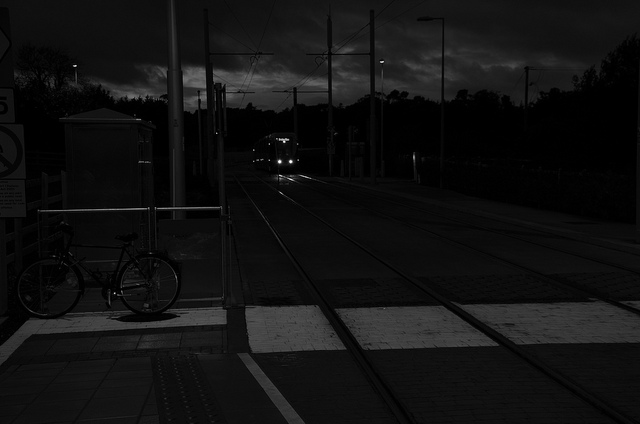
\includegraphics[width=\linewidth]{./procesadas/2015_00026/2015_00026_original.png}
		\caption{Imagen original}
	\end{subfigure}
	\hfill
	\begin{subfigure}[b]{0.32\textwidth}
		\centering
		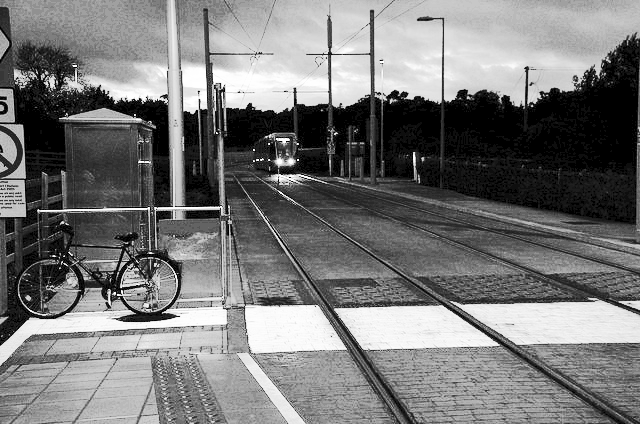
\includegraphics[width=\linewidth]{./procesadas/2015_00026/2015_00026_he.png}
		\caption{Histogram Equalization (HE)}
	\end{subfigure}

	% Segunda fila (2 imágenes)
	\begin{subfigure}[b]{0.32\textwidth}
		\centering
		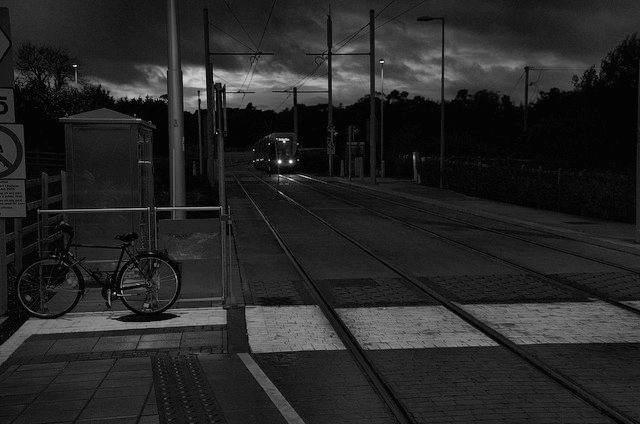
\includegraphics[width=\linewidth]{./procesadas/2015_00026/2015_00026_clahe.png}
		\caption{CLAHE}
	\end{subfigure}
	\hfill
	\begin{subfigure}[b]{0.32\textwidth}
		\centering
		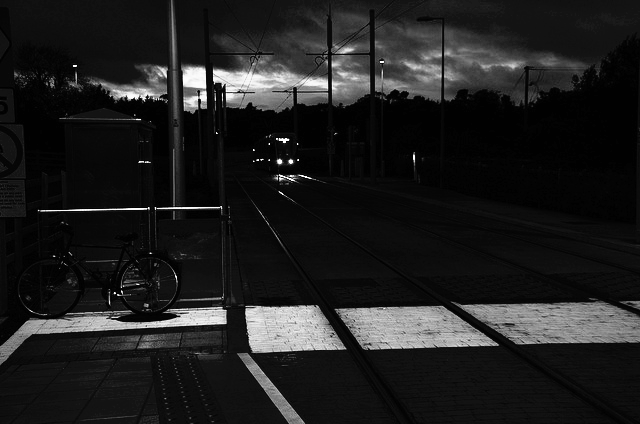
\includegraphics[width=\linewidth]{./procesadas/2015_00026/2015_00026_dqhepl.png}
		\caption{DQHEPL}
	\end{subfigure}

	% Tercera fila (1 imagen centrada)
	\begin{subfigure}[b]{0.32\textwidth}
		\centering
		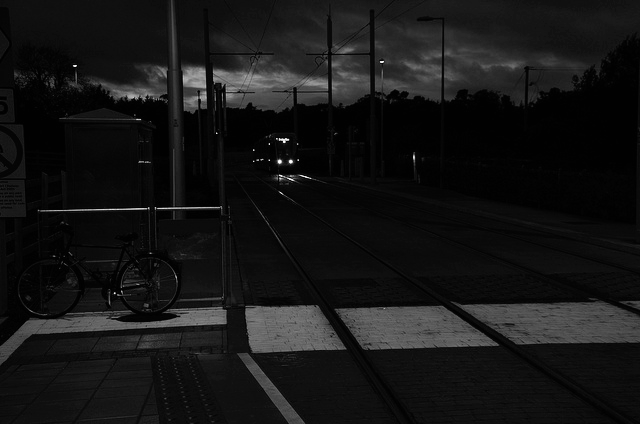
\includegraphics[width=\linewidth]{./procesadas/2015_00026/2015_00026_bhepl_d.png}
		\caption{BHEPL-D}
	\end{subfigure}

	\caption{Métodos aplicados sobre la imagen 2015\_00026.png}
	\label{fig:visual_026}
\end{figure}

Es en las comparaciones visuales presentadas en la \emph{Figura \ref{fig:visual_026}} donde se
evidencian con mayor claridad las discrepancias entre los métodos, especialmente en relación
con el caso anterior.

CLAHE se destaca como el enfoque que ofrece el resultado visual más equilibrado, logrando un
aumento perceptible del contraste sin sacrificar en exceso el brillo original. La imagen
procesada mantiene una buena legibilidad de los detalles en las zonas oscuras sin incurrir en
sobresaturaciones notables, lo que refuerza su papel como una solución intermedia eficaz.

HE, por su parte, consigue revelar una mayor cantidad de contenido oculto en las regiones
subexpuestas, pero lo hace a costa de sobresaturar significativamente la imagen. Como es
habitual en este método, el exceso de brillo general provoca una pérdida de naturalidad y
uniformidad en la escena.

En contraste, los métodos propuestos de DQHEPL y BHEPL-D presentan un desempeño claramente
limitado en condiciones de baja iluminación. Al priorizar la preservación del nivel de brillo
original, apenas logran mejorar la luminosidad global. Esta estrategia provoca que los detalles
en las zonas oscuras permanezcan poco visibles, mientras que las regiones ya iluminadas tienden
a acentuarse en exceso, generando un desequilibrio visual notorio.

% ------- imagen 0027 ---------------
\subsubsection{\textbf{Análisis de imagen 2015\_00027}}

Finalizando con la selección de imágenes, nos encontramos con una imagen que presenta una
iluminación más natural, con una distribución de brillo más equilibrada. La escena incluye
áreas con alta luminosidad, así como zonas considerablemente oscuras.

Este caso nos permitirá evaluar más a fondo cómo los métodos propuestos responden a imágenes
con una variabilidad de iluminación más amplia, proporcionando una comparación más
representativa de su rendimiento en situaciones más complejas

\begin{table}[H]
	\centering
	\caption{Métricas de calidad para la imagen 2015\_00027.jpg}
	\label{tab:metricas_2015_00027}
	\vspace{0.5em}

	\resizebox{\linewidth}{!}{%
		\begin{tabular}{@{}lrrrrr@{}}
			\toprule
			\textbf{Método} & \textbf{AMBE} & \textbf{PSNR} & \textbf{Entropía} & \textbf{Contraste} & \textbf{Uniformidad} \\
			\midrule
            Original        & -             & -                  & 6.77              & 65.98              & 0.43                \\
			CLAHE           & 23.79         & 18.09              & 7.35              & 72.30              & 0.509                \\
			HE              & 67.94         & 10.23              & 6.43              & 77.13              & 0.607                \\
			DQHEPL          & \textbf{3.31} & \textbf{32.79}     & 6.62              & 68.65              & 0.442                \\
			BHEPL-D         & 4.40          & 32.43              & \textbf{6.68}     & \textbf{68.02}     & 0.449                \\
			\bottomrule
		\end{tabular}%
	}

	\vspace{0.5em}
	\footnotesize%
	\textit{Nota: AMBE (menor es mejor), PSNR (mayor es mejor). Uniformidad: 0.6–0.85 optimo}
\end{table}

La \emph{Tabla \ref{tab:metricas_2015_00027}} muestra los resultados obtenidos para la imagen
\emph{2015-00027.jpg}, una imagen con una iluminación más compleja, que incluye tanto áreas con alta
luminosidad como zonas más oscuras. Al comparar los diferentes métodos, se pueden identificar
ciertos patrones en el rendimiento.

El método DQHEPL se destaca con el mejor desempeño en términos de AMBE (3.31) y PSNR (32.79), lo que indica que preserva de manera efectiva el brillo de la imagen original, mientras
que mejora la fidelidad visual en comparación con otros métodos. Además, su entropía (6.62)
sugiere una diversidad tonal razonable, aunque su uniformidad (0.442) es algo más baja, lo que
podría indicar una ligera irregularidad en la distribución del brillo.

Por su parte, BHEPL-D muestra un rendimiento similar, con una AMBE de 4.40 y PSNR de 32.43,
lo que también denota una buena conservación del brillo y alta similitud con la imagen
original. Su contraste (68.02) es el más alto de todos los métodos, lo que sugiere una mejora
notable en la definición de los detalles, aunque la uniformidad sigue siendo algo baja (0.449).

CLAHE, aunque con un AMBE (23.79) considerablemente más alto que los métodos anteriores,
mantiene un buen nivel de PSNR (18.09). Su contraste (72.30) se muestra bastante bueno, lo
que mejora la percepción de los detalles, pero a costa de una mayor distorsión en los niveles
de brillo. La uniformidad (0.509) también es algo más baja, lo que indica que la distribución
de brillo no es completamente homogénea.

Finalmente, HE presenta el peor desempeño en cuanto a conservación del brillo (AMBE de 67.94) y
PSNR (10.23), lo que refleja una pérdida significativa en la fidelidad visual. Sin embargo,
logra un alto contraste (77.13), lo que permite que más detalles sean visibles, aunque también
con una alteración pronunciada de los niveles de luminosidad.

\begin{figure}[htbp]
	\centering
	\begin{subfigure}[b]{0.45\textwidth}
		\resizebox{\linewidth}{!}{%% Creator: Matplotlib, PGF backend
%%
%% To include the figure in your LaTeX document, write
%%   \input{<filename>.pgf}
%%
%% Make sure the required packages are loaded in your preamble
%%   \usepackage{pgf}
%%
%% Also ensure that all the required font packages are loaded; for instance,
%% the lmodern package is sometimes necessary when using math font.
%%   \usepackage{lmodern}
%%
%% Figures using additional raster images can only be included by \input if
%% they are in the same directory as the main LaTeX file. For loading figures
%% from other directories you can use the `import` package
%%   \usepackage{import}
%%
%% and then include the figures with
%%   \import{<path to file>}{<filename>.pgf}
%%
%% Matplotlib used the following preamble
%%   \def\mathdefault#1{#1}
%%   \everymath=\expandafter{\the\everymath\displaystyle}
%%   \IfFileExists{scrextend.sty}{
%%     \usepackage[fontsize=10.000000pt]{scrextend}
%%   }{
%%     \renewcommand{\normalsize}{\fontsize{10.000000}{12.000000}\selectfont}
%%     \normalsize
%%   }
%%   
%%   \ifdefined\pdftexversion\else  % non-pdftex case.
%%     \usepackage{fontspec}
%%     \setmainfont{DejaVuSerif.ttf}[Path=\detokenize{/home/elias/.virtualenvs/src-pway/lib/python3.13/site-packages/matplotlib/mpl-data/fonts/ttf/}]
%%     \setsansfont{DejaVuSans.ttf}[Path=\detokenize{/home/elias/.virtualenvs/src-pway/lib/python3.13/site-packages/matplotlib/mpl-data/fonts/ttf/}]
%%     \setmonofont{DejaVuSansMono.ttf}[Path=\detokenize{/home/elias/.virtualenvs/src-pway/lib/python3.13/site-packages/matplotlib/mpl-data/fonts/ttf/}]
%%   \fi
%%   \makeatletter\@ifpackageloaded{underscore}{}{\usepackage[strings]{underscore}}\makeatother
%%
\begingroup%
\makeatletter%
\begin{pgfpicture}%
\pgfpathrectangle{\pgfpointorigin}{\pgfqpoint{10.000000in}{5.000000in}}%
\pgfusepath{use as bounding box, clip}%
\begin{pgfscope}%
\pgfsetbuttcap%
\pgfsetmiterjoin%
\definecolor{currentfill}{rgb}{1.000000,1.000000,1.000000}%
\pgfsetfillcolor{currentfill}%
\pgfsetlinewidth{0.000000pt}%
\definecolor{currentstroke}{rgb}{1.000000,1.000000,1.000000}%
\pgfsetstrokecolor{currentstroke}%
\pgfsetdash{}{0pt}%
\pgfpathmoveto{\pgfqpoint{0.000000in}{0.000000in}}%
\pgfpathlineto{\pgfqpoint{10.000000in}{0.000000in}}%
\pgfpathlineto{\pgfqpoint{10.000000in}{5.000000in}}%
\pgfpathlineto{\pgfqpoint{0.000000in}{5.000000in}}%
\pgfpathlineto{\pgfqpoint{0.000000in}{0.000000in}}%
\pgfpathclose%
\pgfusepath{fill}%
\end{pgfscope}%
\begin{pgfscope}%
\pgfsetbuttcap%
\pgfsetmiterjoin%
\definecolor{currentfill}{rgb}{1.000000,1.000000,1.000000}%
\pgfsetfillcolor{currentfill}%
\pgfsetlinewidth{0.000000pt}%
\definecolor{currentstroke}{rgb}{0.000000,0.000000,0.000000}%
\pgfsetstrokecolor{currentstroke}%
\pgfsetstrokeopacity{0.000000}%
\pgfsetdash{}{0pt}%
\pgfpathmoveto{\pgfqpoint{1.250000in}{0.550000in}}%
\pgfpathlineto{\pgfqpoint{9.000000in}{0.550000in}}%
\pgfpathlineto{\pgfqpoint{9.000000in}{4.400000in}}%
\pgfpathlineto{\pgfqpoint{1.250000in}{4.400000in}}%
\pgfpathlineto{\pgfqpoint{1.250000in}{0.550000in}}%
\pgfpathclose%
\pgfusepath{fill}%
\end{pgfscope}%
\begin{pgfscope}%
\pgfpathrectangle{\pgfqpoint{1.250000in}{0.550000in}}{\pgfqpoint{7.750000in}{3.850000in}}%
\pgfusepath{clip}%
\pgfsetbuttcap%
\pgfsetmiterjoin%
\definecolor{currentfill}{rgb}{0.501961,0.501961,0.501961}%
\pgfsetfillcolor{currentfill}%
\pgfsetfillopacity{0.700000}%
\pgfsetlinewidth{0.000000pt}%
\definecolor{currentstroke}{rgb}{0.000000,0.000000,0.000000}%
\pgfsetstrokecolor{currentstroke}%
\pgfsetstrokeopacity{0.700000}%
\pgfsetdash{}{0pt}%
\pgfpathmoveto{\pgfqpoint{1.602273in}{0.550000in}}%
\pgfpathlineto{\pgfqpoint{1.629794in}{0.550000in}}%
\pgfpathlineto{\pgfqpoint{1.629794in}{2.398200in}}%
\pgfpathlineto{\pgfqpoint{1.602273in}{2.398200in}}%
\pgfpathlineto{\pgfqpoint{1.602273in}{0.550000in}}%
\pgfpathclose%
\pgfusepath{fill}%
\end{pgfscope}%
\begin{pgfscope}%
\pgfpathrectangle{\pgfqpoint{1.250000in}{0.550000in}}{\pgfqpoint{7.750000in}{3.850000in}}%
\pgfusepath{clip}%
\pgfsetbuttcap%
\pgfsetmiterjoin%
\definecolor{currentfill}{rgb}{0.501961,0.501961,0.501961}%
\pgfsetfillcolor{currentfill}%
\pgfsetfillopacity{0.700000}%
\pgfsetlinewidth{0.000000pt}%
\definecolor{currentstroke}{rgb}{0.000000,0.000000,0.000000}%
\pgfsetstrokecolor{currentstroke}%
\pgfsetstrokeopacity{0.700000}%
\pgfsetdash{}{0pt}%
\pgfpathmoveto{\pgfqpoint{1.629794in}{0.550000in}}%
\pgfpathlineto{\pgfqpoint{1.657315in}{0.550000in}}%
\pgfpathlineto{\pgfqpoint{1.657315in}{4.216667in}}%
\pgfpathlineto{\pgfqpoint{1.629794in}{4.216667in}}%
\pgfpathlineto{\pgfqpoint{1.629794in}{0.550000in}}%
\pgfpathclose%
\pgfusepath{fill}%
\end{pgfscope}%
\begin{pgfscope}%
\pgfpathrectangle{\pgfqpoint{1.250000in}{0.550000in}}{\pgfqpoint{7.750000in}{3.850000in}}%
\pgfusepath{clip}%
\pgfsetbuttcap%
\pgfsetmiterjoin%
\definecolor{currentfill}{rgb}{0.501961,0.501961,0.501961}%
\pgfsetfillcolor{currentfill}%
\pgfsetfillopacity{0.700000}%
\pgfsetlinewidth{0.000000pt}%
\definecolor{currentstroke}{rgb}{0.000000,0.000000,0.000000}%
\pgfsetstrokecolor{currentstroke}%
\pgfsetstrokeopacity{0.700000}%
\pgfsetdash{}{0pt}%
\pgfpathmoveto{\pgfqpoint{1.657315in}{0.550000in}}%
\pgfpathlineto{\pgfqpoint{1.684837in}{0.550000in}}%
\pgfpathlineto{\pgfqpoint{1.684837in}{3.586192in}}%
\pgfpathlineto{\pgfqpoint{1.657315in}{3.586192in}}%
\pgfpathlineto{\pgfqpoint{1.657315in}{0.550000in}}%
\pgfpathclose%
\pgfusepath{fill}%
\end{pgfscope}%
\begin{pgfscope}%
\pgfpathrectangle{\pgfqpoint{1.250000in}{0.550000in}}{\pgfqpoint{7.750000in}{3.850000in}}%
\pgfusepath{clip}%
\pgfsetbuttcap%
\pgfsetmiterjoin%
\definecolor{currentfill}{rgb}{0.501961,0.501961,0.501961}%
\pgfsetfillcolor{currentfill}%
\pgfsetfillopacity{0.700000}%
\pgfsetlinewidth{0.000000pt}%
\definecolor{currentstroke}{rgb}{0.000000,0.000000,0.000000}%
\pgfsetstrokecolor{currentstroke}%
\pgfsetstrokeopacity{0.700000}%
\pgfsetdash{}{0pt}%
\pgfpathmoveto{\pgfqpoint{1.684837in}{0.550000in}}%
\pgfpathlineto{\pgfqpoint{1.712358in}{0.550000in}}%
\pgfpathlineto{\pgfqpoint{1.712358in}{2.872296in}}%
\pgfpathlineto{\pgfqpoint{1.684837in}{2.872296in}}%
\pgfpathlineto{\pgfqpoint{1.684837in}{0.550000in}}%
\pgfpathclose%
\pgfusepath{fill}%
\end{pgfscope}%
\begin{pgfscope}%
\pgfpathrectangle{\pgfqpoint{1.250000in}{0.550000in}}{\pgfqpoint{7.750000in}{3.850000in}}%
\pgfusepath{clip}%
\pgfsetbuttcap%
\pgfsetmiterjoin%
\definecolor{currentfill}{rgb}{0.501961,0.501961,0.501961}%
\pgfsetfillcolor{currentfill}%
\pgfsetfillopacity{0.700000}%
\pgfsetlinewidth{0.000000pt}%
\definecolor{currentstroke}{rgb}{0.000000,0.000000,0.000000}%
\pgfsetstrokecolor{currentstroke}%
\pgfsetstrokeopacity{0.700000}%
\pgfsetdash{}{0pt}%
\pgfpathmoveto{\pgfqpoint{1.712358in}{0.550000in}}%
\pgfpathlineto{\pgfqpoint{1.739879in}{0.550000in}}%
\pgfpathlineto{\pgfqpoint{1.739879in}{2.257238in}}%
\pgfpathlineto{\pgfqpoint{1.712358in}{2.257238in}}%
\pgfpathlineto{\pgfqpoint{1.712358in}{0.550000in}}%
\pgfpathclose%
\pgfusepath{fill}%
\end{pgfscope}%
\begin{pgfscope}%
\pgfpathrectangle{\pgfqpoint{1.250000in}{0.550000in}}{\pgfqpoint{7.750000in}{3.850000in}}%
\pgfusepath{clip}%
\pgfsetbuttcap%
\pgfsetmiterjoin%
\definecolor{currentfill}{rgb}{0.501961,0.501961,0.501961}%
\pgfsetfillcolor{currentfill}%
\pgfsetfillopacity{0.700000}%
\pgfsetlinewidth{0.000000pt}%
\definecolor{currentstroke}{rgb}{0.000000,0.000000,0.000000}%
\pgfsetstrokecolor{currentstroke}%
\pgfsetstrokeopacity{0.700000}%
\pgfsetdash{}{0pt}%
\pgfpathmoveto{\pgfqpoint{1.739879in}{0.550000in}}%
\pgfpathlineto{\pgfqpoint{1.767401in}{0.550000in}}%
\pgfpathlineto{\pgfqpoint{1.767401in}{1.879229in}}%
\pgfpathlineto{\pgfqpoint{1.739879in}{1.879229in}}%
\pgfpathlineto{\pgfqpoint{1.739879in}{0.550000in}}%
\pgfpathclose%
\pgfusepath{fill}%
\end{pgfscope}%
\begin{pgfscope}%
\pgfpathrectangle{\pgfqpoint{1.250000in}{0.550000in}}{\pgfqpoint{7.750000in}{3.850000in}}%
\pgfusepath{clip}%
\pgfsetbuttcap%
\pgfsetmiterjoin%
\definecolor{currentfill}{rgb}{0.501961,0.501961,0.501961}%
\pgfsetfillcolor{currentfill}%
\pgfsetfillopacity{0.700000}%
\pgfsetlinewidth{0.000000pt}%
\definecolor{currentstroke}{rgb}{0.000000,0.000000,0.000000}%
\pgfsetstrokecolor{currentstroke}%
\pgfsetstrokeopacity{0.700000}%
\pgfsetdash{}{0pt}%
\pgfpathmoveto{\pgfqpoint{1.767401in}{0.550000in}}%
\pgfpathlineto{\pgfqpoint{1.794922in}{0.550000in}}%
\pgfpathlineto{\pgfqpoint{1.794922in}{1.607766in}}%
\pgfpathlineto{\pgfqpoint{1.767401in}{1.607766in}}%
\pgfpathlineto{\pgfqpoint{1.767401in}{0.550000in}}%
\pgfpathclose%
\pgfusepath{fill}%
\end{pgfscope}%
\begin{pgfscope}%
\pgfpathrectangle{\pgfqpoint{1.250000in}{0.550000in}}{\pgfqpoint{7.750000in}{3.850000in}}%
\pgfusepath{clip}%
\pgfsetbuttcap%
\pgfsetmiterjoin%
\definecolor{currentfill}{rgb}{0.501961,0.501961,0.501961}%
\pgfsetfillcolor{currentfill}%
\pgfsetfillopacity{0.700000}%
\pgfsetlinewidth{0.000000pt}%
\definecolor{currentstroke}{rgb}{0.000000,0.000000,0.000000}%
\pgfsetstrokecolor{currentstroke}%
\pgfsetstrokeopacity{0.700000}%
\pgfsetdash{}{0pt}%
\pgfpathmoveto{\pgfqpoint{1.794922in}{0.550000in}}%
\pgfpathlineto{\pgfqpoint{1.822443in}{0.550000in}}%
\pgfpathlineto{\pgfqpoint{1.822443in}{1.512232in}}%
\pgfpathlineto{\pgfqpoint{1.794922in}{1.512232in}}%
\pgfpathlineto{\pgfqpoint{1.794922in}{0.550000in}}%
\pgfpathclose%
\pgfusepath{fill}%
\end{pgfscope}%
\begin{pgfscope}%
\pgfpathrectangle{\pgfqpoint{1.250000in}{0.550000in}}{\pgfqpoint{7.750000in}{3.850000in}}%
\pgfusepath{clip}%
\pgfsetbuttcap%
\pgfsetmiterjoin%
\definecolor{currentfill}{rgb}{0.501961,0.501961,0.501961}%
\pgfsetfillcolor{currentfill}%
\pgfsetfillopacity{0.700000}%
\pgfsetlinewidth{0.000000pt}%
\definecolor{currentstroke}{rgb}{0.000000,0.000000,0.000000}%
\pgfsetstrokecolor{currentstroke}%
\pgfsetstrokeopacity{0.700000}%
\pgfsetdash{}{0pt}%
\pgfpathmoveto{\pgfqpoint{1.822443in}{0.550000in}}%
\pgfpathlineto{\pgfqpoint{1.849964in}{0.550000in}}%
\pgfpathlineto{\pgfqpoint{1.849964in}{1.347317in}}%
\pgfpathlineto{\pgfqpoint{1.822443in}{1.347317in}}%
\pgfpathlineto{\pgfqpoint{1.822443in}{0.550000in}}%
\pgfpathclose%
\pgfusepath{fill}%
\end{pgfscope}%
\begin{pgfscope}%
\pgfpathrectangle{\pgfqpoint{1.250000in}{0.550000in}}{\pgfqpoint{7.750000in}{3.850000in}}%
\pgfusepath{clip}%
\pgfsetbuttcap%
\pgfsetmiterjoin%
\definecolor{currentfill}{rgb}{0.501961,0.501961,0.501961}%
\pgfsetfillcolor{currentfill}%
\pgfsetfillopacity{0.700000}%
\pgfsetlinewidth{0.000000pt}%
\definecolor{currentstroke}{rgb}{0.000000,0.000000,0.000000}%
\pgfsetstrokecolor{currentstroke}%
\pgfsetstrokeopacity{0.700000}%
\pgfsetdash{}{0pt}%
\pgfpathmoveto{\pgfqpoint{1.849964in}{0.550000in}}%
\pgfpathlineto{\pgfqpoint{1.877486in}{0.550000in}}%
\pgfpathlineto{\pgfqpoint{1.877486in}{1.249855in}}%
\pgfpathlineto{\pgfqpoint{1.849964in}{1.249855in}}%
\pgfpathlineto{\pgfqpoint{1.849964in}{0.550000in}}%
\pgfpathclose%
\pgfusepath{fill}%
\end{pgfscope}%
\begin{pgfscope}%
\pgfpathrectangle{\pgfqpoint{1.250000in}{0.550000in}}{\pgfqpoint{7.750000in}{3.850000in}}%
\pgfusepath{clip}%
\pgfsetbuttcap%
\pgfsetmiterjoin%
\definecolor{currentfill}{rgb}{0.501961,0.501961,0.501961}%
\pgfsetfillcolor{currentfill}%
\pgfsetfillopacity{0.700000}%
\pgfsetlinewidth{0.000000pt}%
\definecolor{currentstroke}{rgb}{0.000000,0.000000,0.000000}%
\pgfsetstrokecolor{currentstroke}%
\pgfsetstrokeopacity{0.700000}%
\pgfsetdash{}{0pt}%
\pgfpathmoveto{\pgfqpoint{1.877486in}{0.550000in}}%
\pgfpathlineto{\pgfqpoint{1.905007in}{0.550000in}}%
\pgfpathlineto{\pgfqpoint{1.905007in}{1.151291in}}%
\pgfpathlineto{\pgfqpoint{1.877486in}{1.151291in}}%
\pgfpathlineto{\pgfqpoint{1.877486in}{0.550000in}}%
\pgfpathclose%
\pgfusepath{fill}%
\end{pgfscope}%
\begin{pgfscope}%
\pgfpathrectangle{\pgfqpoint{1.250000in}{0.550000in}}{\pgfqpoint{7.750000in}{3.850000in}}%
\pgfusepath{clip}%
\pgfsetbuttcap%
\pgfsetmiterjoin%
\definecolor{currentfill}{rgb}{0.501961,0.501961,0.501961}%
\pgfsetfillcolor{currentfill}%
\pgfsetfillopacity{0.700000}%
\pgfsetlinewidth{0.000000pt}%
\definecolor{currentstroke}{rgb}{0.000000,0.000000,0.000000}%
\pgfsetstrokecolor{currentstroke}%
\pgfsetstrokeopacity{0.700000}%
\pgfsetdash{}{0pt}%
\pgfpathmoveto{\pgfqpoint{1.905007in}{0.550000in}}%
\pgfpathlineto{\pgfqpoint{1.932528in}{0.550000in}}%
\pgfpathlineto{\pgfqpoint{1.932528in}{1.082187in}}%
\pgfpathlineto{\pgfqpoint{1.905007in}{1.082187in}}%
\pgfpathlineto{\pgfqpoint{1.905007in}{0.550000in}}%
\pgfpathclose%
\pgfusepath{fill}%
\end{pgfscope}%
\begin{pgfscope}%
\pgfpathrectangle{\pgfqpoint{1.250000in}{0.550000in}}{\pgfqpoint{7.750000in}{3.850000in}}%
\pgfusepath{clip}%
\pgfsetbuttcap%
\pgfsetmiterjoin%
\definecolor{currentfill}{rgb}{0.501961,0.501961,0.501961}%
\pgfsetfillcolor{currentfill}%
\pgfsetfillopacity{0.700000}%
\pgfsetlinewidth{0.000000pt}%
\definecolor{currentstroke}{rgb}{0.000000,0.000000,0.000000}%
\pgfsetstrokecolor{currentstroke}%
\pgfsetstrokeopacity{0.700000}%
\pgfsetdash{}{0pt}%
\pgfpathmoveto{\pgfqpoint{1.932528in}{0.550000in}}%
\pgfpathlineto{\pgfqpoint{1.960050in}{0.550000in}}%
\pgfpathlineto{\pgfqpoint{1.960050in}{1.053554in}}%
\pgfpathlineto{\pgfqpoint{1.932528in}{1.053554in}}%
\pgfpathlineto{\pgfqpoint{1.932528in}{0.550000in}}%
\pgfpathclose%
\pgfusepath{fill}%
\end{pgfscope}%
\begin{pgfscope}%
\pgfpathrectangle{\pgfqpoint{1.250000in}{0.550000in}}{\pgfqpoint{7.750000in}{3.850000in}}%
\pgfusepath{clip}%
\pgfsetbuttcap%
\pgfsetmiterjoin%
\definecolor{currentfill}{rgb}{0.501961,0.501961,0.501961}%
\pgfsetfillcolor{currentfill}%
\pgfsetfillopacity{0.700000}%
\pgfsetlinewidth{0.000000pt}%
\definecolor{currentstroke}{rgb}{0.000000,0.000000,0.000000}%
\pgfsetstrokecolor{currentstroke}%
\pgfsetstrokeopacity{0.700000}%
\pgfsetdash{}{0pt}%
\pgfpathmoveto{\pgfqpoint{1.960050in}{0.550000in}}%
\pgfpathlineto{\pgfqpoint{1.987571in}{0.550000in}}%
\pgfpathlineto{\pgfqpoint{1.987571in}{1.011431in}}%
\pgfpathlineto{\pgfqpoint{1.960050in}{1.011431in}}%
\pgfpathlineto{\pgfqpoint{1.960050in}{0.550000in}}%
\pgfpathclose%
\pgfusepath{fill}%
\end{pgfscope}%
\begin{pgfscope}%
\pgfpathrectangle{\pgfqpoint{1.250000in}{0.550000in}}{\pgfqpoint{7.750000in}{3.850000in}}%
\pgfusepath{clip}%
\pgfsetbuttcap%
\pgfsetmiterjoin%
\definecolor{currentfill}{rgb}{0.501961,0.501961,0.501961}%
\pgfsetfillcolor{currentfill}%
\pgfsetfillopacity{0.700000}%
\pgfsetlinewidth{0.000000pt}%
\definecolor{currentstroke}{rgb}{0.000000,0.000000,0.000000}%
\pgfsetstrokecolor{currentstroke}%
\pgfsetstrokeopacity{0.700000}%
\pgfsetdash{}{0pt}%
\pgfpathmoveto{\pgfqpoint{1.987571in}{0.550000in}}%
\pgfpathlineto{\pgfqpoint{2.015092in}{0.550000in}}%
\pgfpathlineto{\pgfqpoint{2.015092in}{0.968757in}}%
\pgfpathlineto{\pgfqpoint{1.987571in}{0.968757in}}%
\pgfpathlineto{\pgfqpoint{1.987571in}{0.550000in}}%
\pgfpathclose%
\pgfusepath{fill}%
\end{pgfscope}%
\begin{pgfscope}%
\pgfpathrectangle{\pgfqpoint{1.250000in}{0.550000in}}{\pgfqpoint{7.750000in}{3.850000in}}%
\pgfusepath{clip}%
\pgfsetbuttcap%
\pgfsetmiterjoin%
\definecolor{currentfill}{rgb}{0.501961,0.501961,0.501961}%
\pgfsetfillcolor{currentfill}%
\pgfsetfillopacity{0.700000}%
\pgfsetlinewidth{0.000000pt}%
\definecolor{currentstroke}{rgb}{0.000000,0.000000,0.000000}%
\pgfsetstrokecolor{currentstroke}%
\pgfsetstrokeopacity{0.700000}%
\pgfsetdash{}{0pt}%
\pgfpathmoveto{\pgfqpoint{2.015092in}{0.550000in}}%
\pgfpathlineto{\pgfqpoint{2.042614in}{0.550000in}}%
\pgfpathlineto{\pgfqpoint{2.042614in}{0.912592in}}%
\pgfpathlineto{\pgfqpoint{2.015092in}{0.912592in}}%
\pgfpathlineto{\pgfqpoint{2.015092in}{0.550000in}}%
\pgfpathclose%
\pgfusepath{fill}%
\end{pgfscope}%
\begin{pgfscope}%
\pgfpathrectangle{\pgfqpoint{1.250000in}{0.550000in}}{\pgfqpoint{7.750000in}{3.850000in}}%
\pgfusepath{clip}%
\pgfsetbuttcap%
\pgfsetmiterjoin%
\definecolor{currentfill}{rgb}{0.501961,0.501961,0.501961}%
\pgfsetfillcolor{currentfill}%
\pgfsetfillopacity{0.700000}%
\pgfsetlinewidth{0.000000pt}%
\definecolor{currentstroke}{rgb}{0.000000,0.000000,0.000000}%
\pgfsetstrokecolor{currentstroke}%
\pgfsetstrokeopacity{0.700000}%
\pgfsetdash{}{0pt}%
\pgfpathmoveto{\pgfqpoint{2.042614in}{0.550000in}}%
\pgfpathlineto{\pgfqpoint{2.070135in}{0.550000in}}%
\pgfpathlineto{\pgfqpoint{2.070135in}{0.906260in}}%
\pgfpathlineto{\pgfqpoint{2.042614in}{0.906260in}}%
\pgfpathlineto{\pgfqpoint{2.042614in}{0.550000in}}%
\pgfpathclose%
\pgfusepath{fill}%
\end{pgfscope}%
\begin{pgfscope}%
\pgfpathrectangle{\pgfqpoint{1.250000in}{0.550000in}}{\pgfqpoint{7.750000in}{3.850000in}}%
\pgfusepath{clip}%
\pgfsetbuttcap%
\pgfsetmiterjoin%
\definecolor{currentfill}{rgb}{0.501961,0.501961,0.501961}%
\pgfsetfillcolor{currentfill}%
\pgfsetfillopacity{0.700000}%
\pgfsetlinewidth{0.000000pt}%
\definecolor{currentstroke}{rgb}{0.000000,0.000000,0.000000}%
\pgfsetstrokecolor{currentstroke}%
\pgfsetstrokeopacity{0.700000}%
\pgfsetdash{}{0pt}%
\pgfpathmoveto{\pgfqpoint{2.070135in}{0.550000in}}%
\pgfpathlineto{\pgfqpoint{2.097656in}{0.550000in}}%
\pgfpathlineto{\pgfqpoint{2.097656in}{0.871019in}}%
\pgfpathlineto{\pgfqpoint{2.070135in}{0.871019in}}%
\pgfpathlineto{\pgfqpoint{2.070135in}{0.550000in}}%
\pgfpathclose%
\pgfusepath{fill}%
\end{pgfscope}%
\begin{pgfscope}%
\pgfpathrectangle{\pgfqpoint{1.250000in}{0.550000in}}{\pgfqpoint{7.750000in}{3.850000in}}%
\pgfusepath{clip}%
\pgfsetbuttcap%
\pgfsetmiterjoin%
\definecolor{currentfill}{rgb}{0.501961,0.501961,0.501961}%
\pgfsetfillcolor{currentfill}%
\pgfsetfillopacity{0.700000}%
\pgfsetlinewidth{0.000000pt}%
\definecolor{currentstroke}{rgb}{0.000000,0.000000,0.000000}%
\pgfsetstrokecolor{currentstroke}%
\pgfsetstrokeopacity{0.700000}%
\pgfsetdash{}{0pt}%
\pgfpathmoveto{\pgfqpoint{2.097656in}{0.550000in}}%
\pgfpathlineto{\pgfqpoint{2.125178in}{0.550000in}}%
\pgfpathlineto{\pgfqpoint{2.125178in}{0.875975in}}%
\pgfpathlineto{\pgfqpoint{2.097656in}{0.875975in}}%
\pgfpathlineto{\pgfqpoint{2.097656in}{0.550000in}}%
\pgfpathclose%
\pgfusepath{fill}%
\end{pgfscope}%
\begin{pgfscope}%
\pgfpathrectangle{\pgfqpoint{1.250000in}{0.550000in}}{\pgfqpoint{7.750000in}{3.850000in}}%
\pgfusepath{clip}%
\pgfsetbuttcap%
\pgfsetmiterjoin%
\definecolor{currentfill}{rgb}{0.501961,0.501961,0.501961}%
\pgfsetfillcolor{currentfill}%
\pgfsetfillopacity{0.700000}%
\pgfsetlinewidth{0.000000pt}%
\definecolor{currentstroke}{rgb}{0.000000,0.000000,0.000000}%
\pgfsetstrokecolor{currentstroke}%
\pgfsetstrokeopacity{0.700000}%
\pgfsetdash{}{0pt}%
\pgfpathmoveto{\pgfqpoint{2.125178in}{0.550000in}}%
\pgfpathlineto{\pgfqpoint{2.152699in}{0.550000in}}%
\pgfpathlineto{\pgfqpoint{2.152699in}{0.870193in}}%
\pgfpathlineto{\pgfqpoint{2.125178in}{0.870193in}}%
\pgfpathlineto{\pgfqpoint{2.125178in}{0.550000in}}%
\pgfpathclose%
\pgfusepath{fill}%
\end{pgfscope}%
\begin{pgfscope}%
\pgfpathrectangle{\pgfqpoint{1.250000in}{0.550000in}}{\pgfqpoint{7.750000in}{3.850000in}}%
\pgfusepath{clip}%
\pgfsetbuttcap%
\pgfsetmiterjoin%
\definecolor{currentfill}{rgb}{0.501961,0.501961,0.501961}%
\pgfsetfillcolor{currentfill}%
\pgfsetfillopacity{0.700000}%
\pgfsetlinewidth{0.000000pt}%
\definecolor{currentstroke}{rgb}{0.000000,0.000000,0.000000}%
\pgfsetstrokecolor{currentstroke}%
\pgfsetstrokeopacity{0.700000}%
\pgfsetdash{}{0pt}%
\pgfpathmoveto{\pgfqpoint{2.152699in}{0.550000in}}%
\pgfpathlineto{\pgfqpoint{2.180220in}{0.550000in}}%
\pgfpathlineto{\pgfqpoint{2.180220in}{0.874598in}}%
\pgfpathlineto{\pgfqpoint{2.152699in}{0.874598in}}%
\pgfpathlineto{\pgfqpoint{2.152699in}{0.550000in}}%
\pgfpathclose%
\pgfusepath{fill}%
\end{pgfscope}%
\begin{pgfscope}%
\pgfpathrectangle{\pgfqpoint{1.250000in}{0.550000in}}{\pgfqpoint{7.750000in}{3.850000in}}%
\pgfusepath{clip}%
\pgfsetbuttcap%
\pgfsetmiterjoin%
\definecolor{currentfill}{rgb}{0.501961,0.501961,0.501961}%
\pgfsetfillcolor{currentfill}%
\pgfsetfillopacity{0.700000}%
\pgfsetlinewidth{0.000000pt}%
\definecolor{currentstroke}{rgb}{0.000000,0.000000,0.000000}%
\pgfsetstrokecolor{currentstroke}%
\pgfsetstrokeopacity{0.700000}%
\pgfsetdash{}{0pt}%
\pgfpathmoveto{\pgfqpoint{2.180220in}{0.550000in}}%
\pgfpathlineto{\pgfqpoint{2.207741in}{0.550000in}}%
\pgfpathlineto{\pgfqpoint{2.207741in}{0.885060in}}%
\pgfpathlineto{\pgfqpoint{2.180220in}{0.885060in}}%
\pgfpathlineto{\pgfqpoint{2.180220in}{0.550000in}}%
\pgfpathclose%
\pgfusepath{fill}%
\end{pgfscope}%
\begin{pgfscope}%
\pgfpathrectangle{\pgfqpoint{1.250000in}{0.550000in}}{\pgfqpoint{7.750000in}{3.850000in}}%
\pgfusepath{clip}%
\pgfsetbuttcap%
\pgfsetmiterjoin%
\definecolor{currentfill}{rgb}{0.501961,0.501961,0.501961}%
\pgfsetfillcolor{currentfill}%
\pgfsetfillopacity{0.700000}%
\pgfsetlinewidth{0.000000pt}%
\definecolor{currentstroke}{rgb}{0.000000,0.000000,0.000000}%
\pgfsetstrokecolor{currentstroke}%
\pgfsetstrokeopacity{0.700000}%
\pgfsetdash{}{0pt}%
\pgfpathmoveto{\pgfqpoint{2.207741in}{0.550000in}}%
\pgfpathlineto{\pgfqpoint{2.235263in}{0.550000in}}%
\pgfpathlineto{\pgfqpoint{2.235263in}{0.871845in}}%
\pgfpathlineto{\pgfqpoint{2.207741in}{0.871845in}}%
\pgfpathlineto{\pgfqpoint{2.207741in}{0.550000in}}%
\pgfpathclose%
\pgfusepath{fill}%
\end{pgfscope}%
\begin{pgfscope}%
\pgfpathrectangle{\pgfqpoint{1.250000in}{0.550000in}}{\pgfqpoint{7.750000in}{3.850000in}}%
\pgfusepath{clip}%
\pgfsetbuttcap%
\pgfsetmiterjoin%
\definecolor{currentfill}{rgb}{0.501961,0.501961,0.501961}%
\pgfsetfillcolor{currentfill}%
\pgfsetfillopacity{0.700000}%
\pgfsetlinewidth{0.000000pt}%
\definecolor{currentstroke}{rgb}{0.000000,0.000000,0.000000}%
\pgfsetstrokecolor{currentstroke}%
\pgfsetstrokeopacity{0.700000}%
\pgfsetdash{}{0pt}%
\pgfpathmoveto{\pgfqpoint{2.235263in}{0.550000in}}%
\pgfpathlineto{\pgfqpoint{2.262784in}{0.550000in}}%
\pgfpathlineto{\pgfqpoint{2.262784in}{0.822839in}}%
\pgfpathlineto{\pgfqpoint{2.235263in}{0.822839in}}%
\pgfpathlineto{\pgfqpoint{2.235263in}{0.550000in}}%
\pgfpathclose%
\pgfusepath{fill}%
\end{pgfscope}%
\begin{pgfscope}%
\pgfpathrectangle{\pgfqpoint{1.250000in}{0.550000in}}{\pgfqpoint{7.750000in}{3.850000in}}%
\pgfusepath{clip}%
\pgfsetbuttcap%
\pgfsetmiterjoin%
\definecolor{currentfill}{rgb}{0.501961,0.501961,0.501961}%
\pgfsetfillcolor{currentfill}%
\pgfsetfillopacity{0.700000}%
\pgfsetlinewidth{0.000000pt}%
\definecolor{currentstroke}{rgb}{0.000000,0.000000,0.000000}%
\pgfsetstrokecolor{currentstroke}%
\pgfsetstrokeopacity{0.700000}%
\pgfsetdash{}{0pt}%
\pgfpathmoveto{\pgfqpoint{2.262784in}{0.550000in}}%
\pgfpathlineto{\pgfqpoint{2.290305in}{0.550000in}}%
\pgfpathlineto{\pgfqpoint{2.290305in}{0.820912in}}%
\pgfpathlineto{\pgfqpoint{2.262784in}{0.820912in}}%
\pgfpathlineto{\pgfqpoint{2.262784in}{0.550000in}}%
\pgfpathclose%
\pgfusepath{fill}%
\end{pgfscope}%
\begin{pgfscope}%
\pgfpathrectangle{\pgfqpoint{1.250000in}{0.550000in}}{\pgfqpoint{7.750000in}{3.850000in}}%
\pgfusepath{clip}%
\pgfsetbuttcap%
\pgfsetmiterjoin%
\definecolor{currentfill}{rgb}{0.501961,0.501961,0.501961}%
\pgfsetfillcolor{currentfill}%
\pgfsetfillopacity{0.700000}%
\pgfsetlinewidth{0.000000pt}%
\definecolor{currentstroke}{rgb}{0.000000,0.000000,0.000000}%
\pgfsetstrokecolor{currentstroke}%
\pgfsetstrokeopacity{0.700000}%
\pgfsetdash{}{0pt}%
\pgfpathmoveto{\pgfqpoint{2.290305in}{0.550000in}}%
\pgfpathlineto{\pgfqpoint{2.317827in}{0.550000in}}%
\pgfpathlineto{\pgfqpoint{2.317827in}{0.812652in}}%
\pgfpathlineto{\pgfqpoint{2.290305in}{0.812652in}}%
\pgfpathlineto{\pgfqpoint{2.290305in}{0.550000in}}%
\pgfpathclose%
\pgfusepath{fill}%
\end{pgfscope}%
\begin{pgfscope}%
\pgfpathrectangle{\pgfqpoint{1.250000in}{0.550000in}}{\pgfqpoint{7.750000in}{3.850000in}}%
\pgfusepath{clip}%
\pgfsetbuttcap%
\pgfsetmiterjoin%
\definecolor{currentfill}{rgb}{0.501961,0.501961,0.501961}%
\pgfsetfillcolor{currentfill}%
\pgfsetfillopacity{0.700000}%
\pgfsetlinewidth{0.000000pt}%
\definecolor{currentstroke}{rgb}{0.000000,0.000000,0.000000}%
\pgfsetstrokecolor{currentstroke}%
\pgfsetstrokeopacity{0.700000}%
\pgfsetdash{}{0pt}%
\pgfpathmoveto{\pgfqpoint{2.317827in}{0.550000in}}%
\pgfpathlineto{\pgfqpoint{2.345348in}{0.550000in}}%
\pgfpathlineto{\pgfqpoint{2.345348in}{0.811000in}}%
\pgfpathlineto{\pgfqpoint{2.317827in}{0.811000in}}%
\pgfpathlineto{\pgfqpoint{2.317827in}{0.550000in}}%
\pgfpathclose%
\pgfusepath{fill}%
\end{pgfscope}%
\begin{pgfscope}%
\pgfpathrectangle{\pgfqpoint{1.250000in}{0.550000in}}{\pgfqpoint{7.750000in}{3.850000in}}%
\pgfusepath{clip}%
\pgfsetbuttcap%
\pgfsetmiterjoin%
\definecolor{currentfill}{rgb}{0.501961,0.501961,0.501961}%
\pgfsetfillcolor{currentfill}%
\pgfsetfillopacity{0.700000}%
\pgfsetlinewidth{0.000000pt}%
\definecolor{currentstroke}{rgb}{0.000000,0.000000,0.000000}%
\pgfsetstrokecolor{currentstroke}%
\pgfsetstrokeopacity{0.700000}%
\pgfsetdash{}{0pt}%
\pgfpathmoveto{\pgfqpoint{2.345348in}{0.550000in}}%
\pgfpathlineto{\pgfqpoint{2.372869in}{0.550000in}}%
\pgfpathlineto{\pgfqpoint{2.372869in}{0.829722in}}%
\pgfpathlineto{\pgfqpoint{2.345348in}{0.829722in}}%
\pgfpathlineto{\pgfqpoint{2.345348in}{0.550000in}}%
\pgfpathclose%
\pgfusepath{fill}%
\end{pgfscope}%
\begin{pgfscope}%
\pgfpathrectangle{\pgfqpoint{1.250000in}{0.550000in}}{\pgfqpoint{7.750000in}{3.850000in}}%
\pgfusepath{clip}%
\pgfsetbuttcap%
\pgfsetmiterjoin%
\definecolor{currentfill}{rgb}{0.501961,0.501961,0.501961}%
\pgfsetfillcolor{currentfill}%
\pgfsetfillopacity{0.700000}%
\pgfsetlinewidth{0.000000pt}%
\definecolor{currentstroke}{rgb}{0.000000,0.000000,0.000000}%
\pgfsetstrokecolor{currentstroke}%
\pgfsetstrokeopacity{0.700000}%
\pgfsetdash{}{0pt}%
\pgfpathmoveto{\pgfqpoint{2.372869in}{0.550000in}}%
\pgfpathlineto{\pgfqpoint{2.400391in}{0.550000in}}%
\pgfpathlineto{\pgfqpoint{2.400391in}{0.808247in}}%
\pgfpathlineto{\pgfqpoint{2.372869in}{0.808247in}}%
\pgfpathlineto{\pgfqpoint{2.372869in}{0.550000in}}%
\pgfpathclose%
\pgfusepath{fill}%
\end{pgfscope}%
\begin{pgfscope}%
\pgfpathrectangle{\pgfqpoint{1.250000in}{0.550000in}}{\pgfqpoint{7.750000in}{3.850000in}}%
\pgfusepath{clip}%
\pgfsetbuttcap%
\pgfsetmiterjoin%
\definecolor{currentfill}{rgb}{0.501961,0.501961,0.501961}%
\pgfsetfillcolor{currentfill}%
\pgfsetfillopacity{0.700000}%
\pgfsetlinewidth{0.000000pt}%
\definecolor{currentstroke}{rgb}{0.000000,0.000000,0.000000}%
\pgfsetstrokecolor{currentstroke}%
\pgfsetstrokeopacity{0.700000}%
\pgfsetdash{}{0pt}%
\pgfpathmoveto{\pgfqpoint{2.400391in}{0.550000in}}%
\pgfpathlineto{\pgfqpoint{2.427912in}{0.550000in}}%
\pgfpathlineto{\pgfqpoint{2.427912in}{0.814304in}}%
\pgfpathlineto{\pgfqpoint{2.400391in}{0.814304in}}%
\pgfpathlineto{\pgfqpoint{2.400391in}{0.550000in}}%
\pgfpathclose%
\pgfusepath{fill}%
\end{pgfscope}%
\begin{pgfscope}%
\pgfpathrectangle{\pgfqpoint{1.250000in}{0.550000in}}{\pgfqpoint{7.750000in}{3.850000in}}%
\pgfusepath{clip}%
\pgfsetbuttcap%
\pgfsetmiterjoin%
\definecolor{currentfill}{rgb}{0.501961,0.501961,0.501961}%
\pgfsetfillcolor{currentfill}%
\pgfsetfillopacity{0.700000}%
\pgfsetlinewidth{0.000000pt}%
\definecolor{currentstroke}{rgb}{0.000000,0.000000,0.000000}%
\pgfsetstrokecolor{currentstroke}%
\pgfsetstrokeopacity{0.700000}%
\pgfsetdash{}{0pt}%
\pgfpathmoveto{\pgfqpoint{2.427912in}{0.550000in}}%
\pgfpathlineto{\pgfqpoint{2.455433in}{0.550000in}}%
\pgfpathlineto{\pgfqpoint{2.455433in}{0.811000in}}%
\pgfpathlineto{\pgfqpoint{2.427912in}{0.811000in}}%
\pgfpathlineto{\pgfqpoint{2.427912in}{0.550000in}}%
\pgfpathclose%
\pgfusepath{fill}%
\end{pgfscope}%
\begin{pgfscope}%
\pgfpathrectangle{\pgfqpoint{1.250000in}{0.550000in}}{\pgfqpoint{7.750000in}{3.850000in}}%
\pgfusepath{clip}%
\pgfsetbuttcap%
\pgfsetmiterjoin%
\definecolor{currentfill}{rgb}{0.501961,0.501961,0.501961}%
\pgfsetfillcolor{currentfill}%
\pgfsetfillopacity{0.700000}%
\pgfsetlinewidth{0.000000pt}%
\definecolor{currentstroke}{rgb}{0.000000,0.000000,0.000000}%
\pgfsetstrokecolor{currentstroke}%
\pgfsetstrokeopacity{0.700000}%
\pgfsetdash{}{0pt}%
\pgfpathmoveto{\pgfqpoint{2.455433in}{0.550000in}}%
\pgfpathlineto{\pgfqpoint{2.482955in}{0.550000in}}%
\pgfpathlineto{\pgfqpoint{2.482955in}{0.792829in}}%
\pgfpathlineto{\pgfqpoint{2.455433in}{0.792829in}}%
\pgfpathlineto{\pgfqpoint{2.455433in}{0.550000in}}%
\pgfpathclose%
\pgfusepath{fill}%
\end{pgfscope}%
\begin{pgfscope}%
\pgfpathrectangle{\pgfqpoint{1.250000in}{0.550000in}}{\pgfqpoint{7.750000in}{3.850000in}}%
\pgfusepath{clip}%
\pgfsetbuttcap%
\pgfsetmiterjoin%
\definecolor{currentfill}{rgb}{0.501961,0.501961,0.501961}%
\pgfsetfillcolor{currentfill}%
\pgfsetfillopacity{0.700000}%
\pgfsetlinewidth{0.000000pt}%
\definecolor{currentstroke}{rgb}{0.000000,0.000000,0.000000}%
\pgfsetstrokecolor{currentstroke}%
\pgfsetstrokeopacity{0.700000}%
\pgfsetdash{}{0pt}%
\pgfpathmoveto{\pgfqpoint{2.482955in}{0.550000in}}%
\pgfpathlineto{\pgfqpoint{2.510476in}{0.550000in}}%
\pgfpathlineto{\pgfqpoint{2.510476in}{0.764747in}}%
\pgfpathlineto{\pgfqpoint{2.482955in}{0.764747in}}%
\pgfpathlineto{\pgfqpoint{2.482955in}{0.550000in}}%
\pgfpathclose%
\pgfusepath{fill}%
\end{pgfscope}%
\begin{pgfscope}%
\pgfpathrectangle{\pgfqpoint{1.250000in}{0.550000in}}{\pgfqpoint{7.750000in}{3.850000in}}%
\pgfusepath{clip}%
\pgfsetbuttcap%
\pgfsetmiterjoin%
\definecolor{currentfill}{rgb}{0.501961,0.501961,0.501961}%
\pgfsetfillcolor{currentfill}%
\pgfsetfillopacity{0.700000}%
\pgfsetlinewidth{0.000000pt}%
\definecolor{currentstroke}{rgb}{0.000000,0.000000,0.000000}%
\pgfsetstrokecolor{currentstroke}%
\pgfsetstrokeopacity{0.700000}%
\pgfsetdash{}{0pt}%
\pgfpathmoveto{\pgfqpoint{2.510476in}{0.550000in}}%
\pgfpathlineto{\pgfqpoint{2.537997in}{0.550000in}}%
\pgfpathlineto{\pgfqpoint{2.537997in}{0.770529in}}%
\pgfpathlineto{\pgfqpoint{2.510476in}{0.770529in}}%
\pgfpathlineto{\pgfqpoint{2.510476in}{0.550000in}}%
\pgfpathclose%
\pgfusepath{fill}%
\end{pgfscope}%
\begin{pgfscope}%
\pgfpathrectangle{\pgfqpoint{1.250000in}{0.550000in}}{\pgfqpoint{7.750000in}{3.850000in}}%
\pgfusepath{clip}%
\pgfsetbuttcap%
\pgfsetmiterjoin%
\definecolor{currentfill}{rgb}{0.501961,0.501961,0.501961}%
\pgfsetfillcolor{currentfill}%
\pgfsetfillopacity{0.700000}%
\pgfsetlinewidth{0.000000pt}%
\definecolor{currentstroke}{rgb}{0.000000,0.000000,0.000000}%
\pgfsetstrokecolor{currentstroke}%
\pgfsetstrokeopacity{0.700000}%
\pgfsetdash{}{0pt}%
\pgfpathmoveto{\pgfqpoint{2.537997in}{0.550000in}}%
\pgfpathlineto{\pgfqpoint{2.565518in}{0.550000in}}%
\pgfpathlineto{\pgfqpoint{2.565518in}{0.755386in}}%
\pgfpathlineto{\pgfqpoint{2.537997in}{0.755386in}}%
\pgfpathlineto{\pgfqpoint{2.537997in}{0.550000in}}%
\pgfpathclose%
\pgfusepath{fill}%
\end{pgfscope}%
\begin{pgfscope}%
\pgfpathrectangle{\pgfqpoint{1.250000in}{0.550000in}}{\pgfqpoint{7.750000in}{3.850000in}}%
\pgfusepath{clip}%
\pgfsetbuttcap%
\pgfsetmiterjoin%
\definecolor{currentfill}{rgb}{0.501961,0.501961,0.501961}%
\pgfsetfillcolor{currentfill}%
\pgfsetfillopacity{0.700000}%
\pgfsetlinewidth{0.000000pt}%
\definecolor{currentstroke}{rgb}{0.000000,0.000000,0.000000}%
\pgfsetstrokecolor{currentstroke}%
\pgfsetstrokeopacity{0.700000}%
\pgfsetdash{}{0pt}%
\pgfpathmoveto{\pgfqpoint{2.565518in}{0.550000in}}%
\pgfpathlineto{\pgfqpoint{2.593040in}{0.550000in}}%
\pgfpathlineto{\pgfqpoint{2.593040in}{0.779339in}}%
\pgfpathlineto{\pgfqpoint{2.565518in}{0.779339in}}%
\pgfpathlineto{\pgfqpoint{2.565518in}{0.550000in}}%
\pgfpathclose%
\pgfusepath{fill}%
\end{pgfscope}%
\begin{pgfscope}%
\pgfpathrectangle{\pgfqpoint{1.250000in}{0.550000in}}{\pgfqpoint{7.750000in}{3.850000in}}%
\pgfusepath{clip}%
\pgfsetbuttcap%
\pgfsetmiterjoin%
\definecolor{currentfill}{rgb}{0.501961,0.501961,0.501961}%
\pgfsetfillcolor{currentfill}%
\pgfsetfillopacity{0.700000}%
\pgfsetlinewidth{0.000000pt}%
\definecolor{currentstroke}{rgb}{0.000000,0.000000,0.000000}%
\pgfsetstrokecolor{currentstroke}%
\pgfsetstrokeopacity{0.700000}%
\pgfsetdash{}{0pt}%
\pgfpathmoveto{\pgfqpoint{2.593040in}{0.550000in}}%
\pgfpathlineto{\pgfqpoint{2.620561in}{0.550000in}}%
\pgfpathlineto{\pgfqpoint{2.620561in}{0.763646in}}%
\pgfpathlineto{\pgfqpoint{2.593040in}{0.763646in}}%
\pgfpathlineto{\pgfqpoint{2.593040in}{0.550000in}}%
\pgfpathclose%
\pgfusepath{fill}%
\end{pgfscope}%
\begin{pgfscope}%
\pgfpathrectangle{\pgfqpoint{1.250000in}{0.550000in}}{\pgfqpoint{7.750000in}{3.850000in}}%
\pgfusepath{clip}%
\pgfsetbuttcap%
\pgfsetmiterjoin%
\definecolor{currentfill}{rgb}{0.501961,0.501961,0.501961}%
\pgfsetfillcolor{currentfill}%
\pgfsetfillopacity{0.700000}%
\pgfsetlinewidth{0.000000pt}%
\definecolor{currentstroke}{rgb}{0.000000,0.000000,0.000000}%
\pgfsetstrokecolor{currentstroke}%
\pgfsetstrokeopacity{0.700000}%
\pgfsetdash{}{0pt}%
\pgfpathmoveto{\pgfqpoint{2.620561in}{0.550000in}}%
\pgfpathlineto{\pgfqpoint{2.648082in}{0.550000in}}%
\pgfpathlineto{\pgfqpoint{2.648082in}{0.786222in}}%
\pgfpathlineto{\pgfqpoint{2.620561in}{0.786222in}}%
\pgfpathlineto{\pgfqpoint{2.620561in}{0.550000in}}%
\pgfpathclose%
\pgfusepath{fill}%
\end{pgfscope}%
\begin{pgfscope}%
\pgfpathrectangle{\pgfqpoint{1.250000in}{0.550000in}}{\pgfqpoint{7.750000in}{3.850000in}}%
\pgfusepath{clip}%
\pgfsetbuttcap%
\pgfsetmiterjoin%
\definecolor{currentfill}{rgb}{0.501961,0.501961,0.501961}%
\pgfsetfillcolor{currentfill}%
\pgfsetfillopacity{0.700000}%
\pgfsetlinewidth{0.000000pt}%
\definecolor{currentstroke}{rgb}{0.000000,0.000000,0.000000}%
\pgfsetstrokecolor{currentstroke}%
\pgfsetstrokeopacity{0.700000}%
\pgfsetdash{}{0pt}%
\pgfpathmoveto{\pgfqpoint{2.648082in}{0.550000in}}%
\pgfpathlineto{\pgfqpoint{2.675604in}{0.550000in}}%
\pgfpathlineto{\pgfqpoint{2.675604in}{0.762269in}}%
\pgfpathlineto{\pgfqpoint{2.648082in}{0.762269in}}%
\pgfpathlineto{\pgfqpoint{2.648082in}{0.550000in}}%
\pgfpathclose%
\pgfusepath{fill}%
\end{pgfscope}%
\begin{pgfscope}%
\pgfpathrectangle{\pgfqpoint{1.250000in}{0.550000in}}{\pgfqpoint{7.750000in}{3.850000in}}%
\pgfusepath{clip}%
\pgfsetbuttcap%
\pgfsetmiterjoin%
\definecolor{currentfill}{rgb}{0.501961,0.501961,0.501961}%
\pgfsetfillcolor{currentfill}%
\pgfsetfillopacity{0.700000}%
\pgfsetlinewidth{0.000000pt}%
\definecolor{currentstroke}{rgb}{0.000000,0.000000,0.000000}%
\pgfsetstrokecolor{currentstroke}%
\pgfsetstrokeopacity{0.700000}%
\pgfsetdash{}{0pt}%
\pgfpathmoveto{\pgfqpoint{2.675604in}{0.550000in}}%
\pgfpathlineto{\pgfqpoint{2.703125in}{0.550000in}}%
\pgfpathlineto{\pgfqpoint{2.703125in}{0.749329in}}%
\pgfpathlineto{\pgfqpoint{2.675604in}{0.749329in}}%
\pgfpathlineto{\pgfqpoint{2.675604in}{0.550000in}}%
\pgfpathclose%
\pgfusepath{fill}%
\end{pgfscope}%
\begin{pgfscope}%
\pgfpathrectangle{\pgfqpoint{1.250000in}{0.550000in}}{\pgfqpoint{7.750000in}{3.850000in}}%
\pgfusepath{clip}%
\pgfsetbuttcap%
\pgfsetmiterjoin%
\definecolor{currentfill}{rgb}{0.501961,0.501961,0.501961}%
\pgfsetfillcolor{currentfill}%
\pgfsetfillopacity{0.700000}%
\pgfsetlinewidth{0.000000pt}%
\definecolor{currentstroke}{rgb}{0.000000,0.000000,0.000000}%
\pgfsetstrokecolor{currentstroke}%
\pgfsetstrokeopacity{0.700000}%
\pgfsetdash{}{0pt}%
\pgfpathmoveto{\pgfqpoint{2.703125in}{0.550000in}}%
\pgfpathlineto{\pgfqpoint{2.730646in}{0.550000in}}%
\pgfpathlineto{\pgfqpoint{2.730646in}{0.746851in}}%
\pgfpathlineto{\pgfqpoint{2.703125in}{0.746851in}}%
\pgfpathlineto{\pgfqpoint{2.703125in}{0.550000in}}%
\pgfpathclose%
\pgfusepath{fill}%
\end{pgfscope}%
\begin{pgfscope}%
\pgfpathrectangle{\pgfqpoint{1.250000in}{0.550000in}}{\pgfqpoint{7.750000in}{3.850000in}}%
\pgfusepath{clip}%
\pgfsetbuttcap%
\pgfsetmiterjoin%
\definecolor{currentfill}{rgb}{0.501961,0.501961,0.501961}%
\pgfsetfillcolor{currentfill}%
\pgfsetfillopacity{0.700000}%
\pgfsetlinewidth{0.000000pt}%
\definecolor{currentstroke}{rgb}{0.000000,0.000000,0.000000}%
\pgfsetstrokecolor{currentstroke}%
\pgfsetstrokeopacity{0.700000}%
\pgfsetdash{}{0pt}%
\pgfpathmoveto{\pgfqpoint{2.730646in}{0.550000in}}%
\pgfpathlineto{\pgfqpoint{2.758168in}{0.550000in}}%
\pgfpathlineto{\pgfqpoint{2.758168in}{0.733911in}}%
\pgfpathlineto{\pgfqpoint{2.730646in}{0.733911in}}%
\pgfpathlineto{\pgfqpoint{2.730646in}{0.550000in}}%
\pgfpathclose%
\pgfusepath{fill}%
\end{pgfscope}%
\begin{pgfscope}%
\pgfpathrectangle{\pgfqpoint{1.250000in}{0.550000in}}{\pgfqpoint{7.750000in}{3.850000in}}%
\pgfusepath{clip}%
\pgfsetbuttcap%
\pgfsetmiterjoin%
\definecolor{currentfill}{rgb}{0.501961,0.501961,0.501961}%
\pgfsetfillcolor{currentfill}%
\pgfsetfillopacity{0.700000}%
\pgfsetlinewidth{0.000000pt}%
\definecolor{currentstroke}{rgb}{0.000000,0.000000,0.000000}%
\pgfsetstrokecolor{currentstroke}%
\pgfsetstrokeopacity{0.700000}%
\pgfsetdash{}{0pt}%
\pgfpathmoveto{\pgfqpoint{2.758168in}{0.550000in}}%
\pgfpathlineto{\pgfqpoint{2.785689in}{0.550000in}}%
\pgfpathlineto{\pgfqpoint{2.785689in}{0.735839in}}%
\pgfpathlineto{\pgfqpoint{2.758168in}{0.735839in}}%
\pgfpathlineto{\pgfqpoint{2.758168in}{0.550000in}}%
\pgfpathclose%
\pgfusepath{fill}%
\end{pgfscope}%
\begin{pgfscope}%
\pgfpathrectangle{\pgfqpoint{1.250000in}{0.550000in}}{\pgfqpoint{7.750000in}{3.850000in}}%
\pgfusepath{clip}%
\pgfsetbuttcap%
\pgfsetmiterjoin%
\definecolor{currentfill}{rgb}{0.501961,0.501961,0.501961}%
\pgfsetfillcolor{currentfill}%
\pgfsetfillopacity{0.700000}%
\pgfsetlinewidth{0.000000pt}%
\definecolor{currentstroke}{rgb}{0.000000,0.000000,0.000000}%
\pgfsetstrokecolor{currentstroke}%
\pgfsetstrokeopacity{0.700000}%
\pgfsetdash{}{0pt}%
\pgfpathmoveto{\pgfqpoint{2.785689in}{0.550000in}}%
\pgfpathlineto{\pgfqpoint{2.813210in}{0.550000in}}%
\pgfpathlineto{\pgfqpoint{2.813210in}{0.730883in}}%
\pgfpathlineto{\pgfqpoint{2.785689in}{0.730883in}}%
\pgfpathlineto{\pgfqpoint{2.785689in}{0.550000in}}%
\pgfpathclose%
\pgfusepath{fill}%
\end{pgfscope}%
\begin{pgfscope}%
\pgfpathrectangle{\pgfqpoint{1.250000in}{0.550000in}}{\pgfqpoint{7.750000in}{3.850000in}}%
\pgfusepath{clip}%
\pgfsetbuttcap%
\pgfsetmiterjoin%
\definecolor{currentfill}{rgb}{0.501961,0.501961,0.501961}%
\pgfsetfillcolor{currentfill}%
\pgfsetfillopacity{0.700000}%
\pgfsetlinewidth{0.000000pt}%
\definecolor{currentstroke}{rgb}{0.000000,0.000000,0.000000}%
\pgfsetstrokecolor{currentstroke}%
\pgfsetstrokeopacity{0.700000}%
\pgfsetdash{}{0pt}%
\pgfpathmoveto{\pgfqpoint{2.813210in}{0.550000in}}%
\pgfpathlineto{\pgfqpoint{2.840732in}{0.550000in}}%
\pgfpathlineto{\pgfqpoint{2.840732in}{0.725377in}}%
\pgfpathlineto{\pgfqpoint{2.813210in}{0.725377in}}%
\pgfpathlineto{\pgfqpoint{2.813210in}{0.550000in}}%
\pgfpathclose%
\pgfusepath{fill}%
\end{pgfscope}%
\begin{pgfscope}%
\pgfpathrectangle{\pgfqpoint{1.250000in}{0.550000in}}{\pgfqpoint{7.750000in}{3.850000in}}%
\pgfusepath{clip}%
\pgfsetbuttcap%
\pgfsetmiterjoin%
\definecolor{currentfill}{rgb}{0.501961,0.501961,0.501961}%
\pgfsetfillcolor{currentfill}%
\pgfsetfillopacity{0.700000}%
\pgfsetlinewidth{0.000000pt}%
\definecolor{currentstroke}{rgb}{0.000000,0.000000,0.000000}%
\pgfsetstrokecolor{currentstroke}%
\pgfsetstrokeopacity{0.700000}%
\pgfsetdash{}{0pt}%
\pgfpathmoveto{\pgfqpoint{2.840732in}{0.550000in}}%
\pgfpathlineto{\pgfqpoint{2.868253in}{0.550000in}}%
\pgfpathlineto{\pgfqpoint{2.868253in}{0.726753in}}%
\pgfpathlineto{\pgfqpoint{2.840732in}{0.726753in}}%
\pgfpathlineto{\pgfqpoint{2.840732in}{0.550000in}}%
\pgfpathclose%
\pgfusepath{fill}%
\end{pgfscope}%
\begin{pgfscope}%
\pgfpathrectangle{\pgfqpoint{1.250000in}{0.550000in}}{\pgfqpoint{7.750000in}{3.850000in}}%
\pgfusepath{clip}%
\pgfsetbuttcap%
\pgfsetmiterjoin%
\definecolor{currentfill}{rgb}{0.501961,0.501961,0.501961}%
\pgfsetfillcolor{currentfill}%
\pgfsetfillopacity{0.700000}%
\pgfsetlinewidth{0.000000pt}%
\definecolor{currentstroke}{rgb}{0.000000,0.000000,0.000000}%
\pgfsetstrokecolor{currentstroke}%
\pgfsetstrokeopacity{0.700000}%
\pgfsetdash{}{0pt}%
\pgfpathmoveto{\pgfqpoint{2.868253in}{0.550000in}}%
\pgfpathlineto{\pgfqpoint{2.895774in}{0.550000in}}%
\pgfpathlineto{\pgfqpoint{2.895774in}{0.734187in}}%
\pgfpathlineto{\pgfqpoint{2.868253in}{0.734187in}}%
\pgfpathlineto{\pgfqpoint{2.868253in}{0.550000in}}%
\pgfpathclose%
\pgfusepath{fill}%
\end{pgfscope}%
\begin{pgfscope}%
\pgfpathrectangle{\pgfqpoint{1.250000in}{0.550000in}}{\pgfqpoint{7.750000in}{3.850000in}}%
\pgfusepath{clip}%
\pgfsetbuttcap%
\pgfsetmiterjoin%
\definecolor{currentfill}{rgb}{0.501961,0.501961,0.501961}%
\pgfsetfillcolor{currentfill}%
\pgfsetfillopacity{0.700000}%
\pgfsetlinewidth{0.000000pt}%
\definecolor{currentstroke}{rgb}{0.000000,0.000000,0.000000}%
\pgfsetstrokecolor{currentstroke}%
\pgfsetstrokeopacity{0.700000}%
\pgfsetdash{}{0pt}%
\pgfpathmoveto{\pgfqpoint{2.895774in}{0.550000in}}%
\pgfpathlineto{\pgfqpoint{2.923295in}{0.550000in}}%
\pgfpathlineto{\pgfqpoint{2.923295in}{0.750430in}}%
\pgfpathlineto{\pgfqpoint{2.895774in}{0.750430in}}%
\pgfpathlineto{\pgfqpoint{2.895774in}{0.550000in}}%
\pgfpathclose%
\pgfusepath{fill}%
\end{pgfscope}%
\begin{pgfscope}%
\pgfpathrectangle{\pgfqpoint{1.250000in}{0.550000in}}{\pgfqpoint{7.750000in}{3.850000in}}%
\pgfusepath{clip}%
\pgfsetbuttcap%
\pgfsetmiterjoin%
\definecolor{currentfill}{rgb}{0.501961,0.501961,0.501961}%
\pgfsetfillcolor{currentfill}%
\pgfsetfillopacity{0.700000}%
\pgfsetlinewidth{0.000000pt}%
\definecolor{currentstroke}{rgb}{0.000000,0.000000,0.000000}%
\pgfsetstrokecolor{currentstroke}%
\pgfsetstrokeopacity{0.700000}%
\pgfsetdash{}{0pt}%
\pgfpathmoveto{\pgfqpoint{2.923295in}{0.550000in}}%
\pgfpathlineto{\pgfqpoint{2.950817in}{0.550000in}}%
\pgfpathlineto{\pgfqpoint{2.950817in}{0.741896in}}%
\pgfpathlineto{\pgfqpoint{2.923295in}{0.741896in}}%
\pgfpathlineto{\pgfqpoint{2.923295in}{0.550000in}}%
\pgfpathclose%
\pgfusepath{fill}%
\end{pgfscope}%
\begin{pgfscope}%
\pgfpathrectangle{\pgfqpoint{1.250000in}{0.550000in}}{\pgfqpoint{7.750000in}{3.850000in}}%
\pgfusepath{clip}%
\pgfsetbuttcap%
\pgfsetmiterjoin%
\definecolor{currentfill}{rgb}{0.501961,0.501961,0.501961}%
\pgfsetfillcolor{currentfill}%
\pgfsetfillopacity{0.700000}%
\pgfsetlinewidth{0.000000pt}%
\definecolor{currentstroke}{rgb}{0.000000,0.000000,0.000000}%
\pgfsetstrokecolor{currentstroke}%
\pgfsetstrokeopacity{0.700000}%
\pgfsetdash{}{0pt}%
\pgfpathmoveto{\pgfqpoint{2.950817in}{0.550000in}}%
\pgfpathlineto{\pgfqpoint{2.978338in}{0.550000in}}%
\pgfpathlineto{\pgfqpoint{2.978338in}{0.738592in}}%
\pgfpathlineto{\pgfqpoint{2.950817in}{0.738592in}}%
\pgfpathlineto{\pgfqpoint{2.950817in}{0.550000in}}%
\pgfpathclose%
\pgfusepath{fill}%
\end{pgfscope}%
\begin{pgfscope}%
\pgfpathrectangle{\pgfqpoint{1.250000in}{0.550000in}}{\pgfqpoint{7.750000in}{3.850000in}}%
\pgfusepath{clip}%
\pgfsetbuttcap%
\pgfsetmiterjoin%
\definecolor{currentfill}{rgb}{0.501961,0.501961,0.501961}%
\pgfsetfillcolor{currentfill}%
\pgfsetfillopacity{0.700000}%
\pgfsetlinewidth{0.000000pt}%
\definecolor{currentstroke}{rgb}{0.000000,0.000000,0.000000}%
\pgfsetstrokecolor{currentstroke}%
\pgfsetstrokeopacity{0.700000}%
\pgfsetdash{}{0pt}%
\pgfpathmoveto{\pgfqpoint{2.978338in}{0.550000in}}%
\pgfpathlineto{\pgfqpoint{3.005859in}{0.550000in}}%
\pgfpathlineto{\pgfqpoint{3.005859in}{0.724551in}}%
\pgfpathlineto{\pgfqpoint{2.978338in}{0.724551in}}%
\pgfpathlineto{\pgfqpoint{2.978338in}{0.550000in}}%
\pgfpathclose%
\pgfusepath{fill}%
\end{pgfscope}%
\begin{pgfscope}%
\pgfpathrectangle{\pgfqpoint{1.250000in}{0.550000in}}{\pgfqpoint{7.750000in}{3.850000in}}%
\pgfusepath{clip}%
\pgfsetbuttcap%
\pgfsetmiterjoin%
\definecolor{currentfill}{rgb}{0.501961,0.501961,0.501961}%
\pgfsetfillcolor{currentfill}%
\pgfsetfillopacity{0.700000}%
\pgfsetlinewidth{0.000000pt}%
\definecolor{currentstroke}{rgb}{0.000000,0.000000,0.000000}%
\pgfsetstrokecolor{currentstroke}%
\pgfsetstrokeopacity{0.700000}%
\pgfsetdash{}{0pt}%
\pgfpathmoveto{\pgfqpoint{3.005859in}{0.550000in}}%
\pgfpathlineto{\pgfqpoint{3.033381in}{0.550000in}}%
\pgfpathlineto{\pgfqpoint{3.033381in}{0.736940in}}%
\pgfpathlineto{\pgfqpoint{3.005859in}{0.736940in}}%
\pgfpathlineto{\pgfqpoint{3.005859in}{0.550000in}}%
\pgfpathclose%
\pgfusepath{fill}%
\end{pgfscope}%
\begin{pgfscope}%
\pgfpathrectangle{\pgfqpoint{1.250000in}{0.550000in}}{\pgfqpoint{7.750000in}{3.850000in}}%
\pgfusepath{clip}%
\pgfsetbuttcap%
\pgfsetmiterjoin%
\definecolor{currentfill}{rgb}{0.501961,0.501961,0.501961}%
\pgfsetfillcolor{currentfill}%
\pgfsetfillopacity{0.700000}%
\pgfsetlinewidth{0.000000pt}%
\definecolor{currentstroke}{rgb}{0.000000,0.000000,0.000000}%
\pgfsetstrokecolor{currentstroke}%
\pgfsetstrokeopacity{0.700000}%
\pgfsetdash{}{0pt}%
\pgfpathmoveto{\pgfqpoint{3.033381in}{0.550000in}}%
\pgfpathlineto{\pgfqpoint{3.060902in}{0.550000in}}%
\pgfpathlineto{\pgfqpoint{3.060902in}{0.730883in}}%
\pgfpathlineto{\pgfqpoint{3.033381in}{0.730883in}}%
\pgfpathlineto{\pgfqpoint{3.033381in}{0.550000in}}%
\pgfpathclose%
\pgfusepath{fill}%
\end{pgfscope}%
\begin{pgfscope}%
\pgfpathrectangle{\pgfqpoint{1.250000in}{0.550000in}}{\pgfqpoint{7.750000in}{3.850000in}}%
\pgfusepath{clip}%
\pgfsetbuttcap%
\pgfsetmiterjoin%
\definecolor{currentfill}{rgb}{0.501961,0.501961,0.501961}%
\pgfsetfillcolor{currentfill}%
\pgfsetfillopacity{0.700000}%
\pgfsetlinewidth{0.000000pt}%
\definecolor{currentstroke}{rgb}{0.000000,0.000000,0.000000}%
\pgfsetstrokecolor{currentstroke}%
\pgfsetstrokeopacity{0.700000}%
\pgfsetdash{}{0pt}%
\pgfpathmoveto{\pgfqpoint{3.060902in}{0.550000in}}%
\pgfpathlineto{\pgfqpoint{3.088423in}{0.550000in}}%
\pgfpathlineto{\pgfqpoint{3.088423in}{0.710785in}}%
\pgfpathlineto{\pgfqpoint{3.060902in}{0.710785in}}%
\pgfpathlineto{\pgfqpoint{3.060902in}{0.550000in}}%
\pgfpathclose%
\pgfusepath{fill}%
\end{pgfscope}%
\begin{pgfscope}%
\pgfpathrectangle{\pgfqpoint{1.250000in}{0.550000in}}{\pgfqpoint{7.750000in}{3.850000in}}%
\pgfusepath{clip}%
\pgfsetbuttcap%
\pgfsetmiterjoin%
\definecolor{currentfill}{rgb}{0.501961,0.501961,0.501961}%
\pgfsetfillcolor{currentfill}%
\pgfsetfillopacity{0.700000}%
\pgfsetlinewidth{0.000000pt}%
\definecolor{currentstroke}{rgb}{0.000000,0.000000,0.000000}%
\pgfsetstrokecolor{currentstroke}%
\pgfsetstrokeopacity{0.700000}%
\pgfsetdash{}{0pt}%
\pgfpathmoveto{\pgfqpoint{3.088423in}{0.550000in}}%
\pgfpathlineto{\pgfqpoint{3.115945in}{0.550000in}}%
\pgfpathlineto{\pgfqpoint{3.115945in}{0.706655in}}%
\pgfpathlineto{\pgfqpoint{3.088423in}{0.706655in}}%
\pgfpathlineto{\pgfqpoint{3.088423in}{0.550000in}}%
\pgfpathclose%
\pgfusepath{fill}%
\end{pgfscope}%
\begin{pgfscope}%
\pgfpathrectangle{\pgfqpoint{1.250000in}{0.550000in}}{\pgfqpoint{7.750000in}{3.850000in}}%
\pgfusepath{clip}%
\pgfsetbuttcap%
\pgfsetmiterjoin%
\definecolor{currentfill}{rgb}{0.501961,0.501961,0.501961}%
\pgfsetfillcolor{currentfill}%
\pgfsetfillopacity{0.700000}%
\pgfsetlinewidth{0.000000pt}%
\definecolor{currentstroke}{rgb}{0.000000,0.000000,0.000000}%
\pgfsetstrokecolor{currentstroke}%
\pgfsetstrokeopacity{0.700000}%
\pgfsetdash{}{0pt}%
\pgfpathmoveto{\pgfqpoint{3.115945in}{0.550000in}}%
\pgfpathlineto{\pgfqpoint{3.143466in}{0.550000in}}%
\pgfpathlineto{\pgfqpoint{3.143466in}{0.704728in}}%
\pgfpathlineto{\pgfqpoint{3.115945in}{0.704728in}}%
\pgfpathlineto{\pgfqpoint{3.115945in}{0.550000in}}%
\pgfpathclose%
\pgfusepath{fill}%
\end{pgfscope}%
\begin{pgfscope}%
\pgfpathrectangle{\pgfqpoint{1.250000in}{0.550000in}}{\pgfqpoint{7.750000in}{3.850000in}}%
\pgfusepath{clip}%
\pgfsetbuttcap%
\pgfsetmiterjoin%
\definecolor{currentfill}{rgb}{0.501961,0.501961,0.501961}%
\pgfsetfillcolor{currentfill}%
\pgfsetfillopacity{0.700000}%
\pgfsetlinewidth{0.000000pt}%
\definecolor{currentstroke}{rgb}{0.000000,0.000000,0.000000}%
\pgfsetstrokecolor{currentstroke}%
\pgfsetstrokeopacity{0.700000}%
\pgfsetdash{}{0pt}%
\pgfpathmoveto{\pgfqpoint{3.143466in}{0.550000in}}%
\pgfpathlineto{\pgfqpoint{3.170987in}{0.550000in}}%
\pgfpathlineto{\pgfqpoint{3.170987in}{0.722073in}}%
\pgfpathlineto{\pgfqpoint{3.143466in}{0.722073in}}%
\pgfpathlineto{\pgfqpoint{3.143466in}{0.550000in}}%
\pgfpathclose%
\pgfusepath{fill}%
\end{pgfscope}%
\begin{pgfscope}%
\pgfpathrectangle{\pgfqpoint{1.250000in}{0.550000in}}{\pgfqpoint{7.750000in}{3.850000in}}%
\pgfusepath{clip}%
\pgfsetbuttcap%
\pgfsetmiterjoin%
\definecolor{currentfill}{rgb}{0.501961,0.501961,0.501961}%
\pgfsetfillcolor{currentfill}%
\pgfsetfillopacity{0.700000}%
\pgfsetlinewidth{0.000000pt}%
\definecolor{currentstroke}{rgb}{0.000000,0.000000,0.000000}%
\pgfsetstrokecolor{currentstroke}%
\pgfsetstrokeopacity{0.700000}%
\pgfsetdash{}{0pt}%
\pgfpathmoveto{\pgfqpoint{3.170987in}{0.550000in}}%
\pgfpathlineto{\pgfqpoint{3.198509in}{0.550000in}}%
\pgfpathlineto{\pgfqpoint{3.198509in}{0.723725in}}%
\pgfpathlineto{\pgfqpoint{3.170987in}{0.723725in}}%
\pgfpathlineto{\pgfqpoint{3.170987in}{0.550000in}}%
\pgfpathclose%
\pgfusepath{fill}%
\end{pgfscope}%
\begin{pgfscope}%
\pgfpathrectangle{\pgfqpoint{1.250000in}{0.550000in}}{\pgfqpoint{7.750000in}{3.850000in}}%
\pgfusepath{clip}%
\pgfsetbuttcap%
\pgfsetmiterjoin%
\definecolor{currentfill}{rgb}{0.501961,0.501961,0.501961}%
\pgfsetfillcolor{currentfill}%
\pgfsetfillopacity{0.700000}%
\pgfsetlinewidth{0.000000pt}%
\definecolor{currentstroke}{rgb}{0.000000,0.000000,0.000000}%
\pgfsetstrokecolor{currentstroke}%
\pgfsetstrokeopacity{0.700000}%
\pgfsetdash{}{0pt}%
\pgfpathmoveto{\pgfqpoint{3.198509in}{0.550000in}}%
\pgfpathlineto{\pgfqpoint{3.226030in}{0.550000in}}%
\pgfpathlineto{\pgfqpoint{3.226030in}{0.724826in}}%
\pgfpathlineto{\pgfqpoint{3.198509in}{0.724826in}}%
\pgfpathlineto{\pgfqpoint{3.198509in}{0.550000in}}%
\pgfpathclose%
\pgfusepath{fill}%
\end{pgfscope}%
\begin{pgfscope}%
\pgfpathrectangle{\pgfqpoint{1.250000in}{0.550000in}}{\pgfqpoint{7.750000in}{3.850000in}}%
\pgfusepath{clip}%
\pgfsetbuttcap%
\pgfsetmiterjoin%
\definecolor{currentfill}{rgb}{0.501961,0.501961,0.501961}%
\pgfsetfillcolor{currentfill}%
\pgfsetfillopacity{0.700000}%
\pgfsetlinewidth{0.000000pt}%
\definecolor{currentstroke}{rgb}{0.000000,0.000000,0.000000}%
\pgfsetstrokecolor{currentstroke}%
\pgfsetstrokeopacity{0.700000}%
\pgfsetdash{}{0pt}%
\pgfpathmoveto{\pgfqpoint{3.226030in}{0.550000in}}%
\pgfpathlineto{\pgfqpoint{3.253551in}{0.550000in}}%
\pgfpathlineto{\pgfqpoint{3.253551in}{0.718218in}}%
\pgfpathlineto{\pgfqpoint{3.226030in}{0.718218in}}%
\pgfpathlineto{\pgfqpoint{3.226030in}{0.550000in}}%
\pgfpathclose%
\pgfusepath{fill}%
\end{pgfscope}%
\begin{pgfscope}%
\pgfpathrectangle{\pgfqpoint{1.250000in}{0.550000in}}{\pgfqpoint{7.750000in}{3.850000in}}%
\pgfusepath{clip}%
\pgfsetbuttcap%
\pgfsetmiterjoin%
\definecolor{currentfill}{rgb}{0.501961,0.501961,0.501961}%
\pgfsetfillcolor{currentfill}%
\pgfsetfillopacity{0.700000}%
\pgfsetlinewidth{0.000000pt}%
\definecolor{currentstroke}{rgb}{0.000000,0.000000,0.000000}%
\pgfsetstrokecolor{currentstroke}%
\pgfsetstrokeopacity{0.700000}%
\pgfsetdash{}{0pt}%
\pgfpathmoveto{\pgfqpoint{3.253551in}{0.550000in}}%
\pgfpathlineto{\pgfqpoint{3.281072in}{0.550000in}}%
\pgfpathlineto{\pgfqpoint{3.281072in}{0.714639in}}%
\pgfpathlineto{\pgfqpoint{3.253551in}{0.714639in}}%
\pgfpathlineto{\pgfqpoint{3.253551in}{0.550000in}}%
\pgfpathclose%
\pgfusepath{fill}%
\end{pgfscope}%
\begin{pgfscope}%
\pgfpathrectangle{\pgfqpoint{1.250000in}{0.550000in}}{\pgfqpoint{7.750000in}{3.850000in}}%
\pgfusepath{clip}%
\pgfsetbuttcap%
\pgfsetmiterjoin%
\definecolor{currentfill}{rgb}{0.501961,0.501961,0.501961}%
\pgfsetfillcolor{currentfill}%
\pgfsetfillopacity{0.700000}%
\pgfsetlinewidth{0.000000pt}%
\definecolor{currentstroke}{rgb}{0.000000,0.000000,0.000000}%
\pgfsetstrokecolor{currentstroke}%
\pgfsetstrokeopacity{0.700000}%
\pgfsetdash{}{0pt}%
\pgfpathmoveto{\pgfqpoint{3.281072in}{0.550000in}}%
\pgfpathlineto{\pgfqpoint{3.308594in}{0.550000in}}%
\pgfpathlineto{\pgfqpoint{3.308594in}{0.710234in}}%
\pgfpathlineto{\pgfqpoint{3.281072in}{0.710234in}}%
\pgfpathlineto{\pgfqpoint{3.281072in}{0.550000in}}%
\pgfpathclose%
\pgfusepath{fill}%
\end{pgfscope}%
\begin{pgfscope}%
\pgfpathrectangle{\pgfqpoint{1.250000in}{0.550000in}}{\pgfqpoint{7.750000in}{3.850000in}}%
\pgfusepath{clip}%
\pgfsetbuttcap%
\pgfsetmiterjoin%
\definecolor{currentfill}{rgb}{0.501961,0.501961,0.501961}%
\pgfsetfillcolor{currentfill}%
\pgfsetfillopacity{0.700000}%
\pgfsetlinewidth{0.000000pt}%
\definecolor{currentstroke}{rgb}{0.000000,0.000000,0.000000}%
\pgfsetstrokecolor{currentstroke}%
\pgfsetstrokeopacity{0.700000}%
\pgfsetdash{}{0pt}%
\pgfpathmoveto{\pgfqpoint{3.308594in}{0.550000in}}%
\pgfpathlineto{\pgfqpoint{3.336115in}{0.550000in}}%
\pgfpathlineto{\pgfqpoint{3.336115in}{0.709408in}}%
\pgfpathlineto{\pgfqpoint{3.308594in}{0.709408in}}%
\pgfpathlineto{\pgfqpoint{3.308594in}{0.550000in}}%
\pgfpathclose%
\pgfusepath{fill}%
\end{pgfscope}%
\begin{pgfscope}%
\pgfpathrectangle{\pgfqpoint{1.250000in}{0.550000in}}{\pgfqpoint{7.750000in}{3.850000in}}%
\pgfusepath{clip}%
\pgfsetbuttcap%
\pgfsetmiterjoin%
\definecolor{currentfill}{rgb}{0.501961,0.501961,0.501961}%
\pgfsetfillcolor{currentfill}%
\pgfsetfillopacity{0.700000}%
\pgfsetlinewidth{0.000000pt}%
\definecolor{currentstroke}{rgb}{0.000000,0.000000,0.000000}%
\pgfsetstrokecolor{currentstroke}%
\pgfsetstrokeopacity{0.700000}%
\pgfsetdash{}{0pt}%
\pgfpathmoveto{\pgfqpoint{3.336115in}{0.550000in}}%
\pgfpathlineto{\pgfqpoint{3.363636in}{0.550000in}}%
\pgfpathlineto{\pgfqpoint{3.363636in}{0.709408in}}%
\pgfpathlineto{\pgfqpoint{3.336115in}{0.709408in}}%
\pgfpathlineto{\pgfqpoint{3.336115in}{0.550000in}}%
\pgfpathclose%
\pgfusepath{fill}%
\end{pgfscope}%
\begin{pgfscope}%
\pgfpathrectangle{\pgfqpoint{1.250000in}{0.550000in}}{\pgfqpoint{7.750000in}{3.850000in}}%
\pgfusepath{clip}%
\pgfsetbuttcap%
\pgfsetmiterjoin%
\definecolor{currentfill}{rgb}{0.501961,0.501961,0.501961}%
\pgfsetfillcolor{currentfill}%
\pgfsetfillopacity{0.700000}%
\pgfsetlinewidth{0.000000pt}%
\definecolor{currentstroke}{rgb}{0.000000,0.000000,0.000000}%
\pgfsetstrokecolor{currentstroke}%
\pgfsetstrokeopacity{0.700000}%
\pgfsetdash{}{0pt}%
\pgfpathmoveto{\pgfqpoint{3.363636in}{0.550000in}}%
\pgfpathlineto{\pgfqpoint{3.391158in}{0.550000in}}%
\pgfpathlineto{\pgfqpoint{3.391158in}{0.692063in}}%
\pgfpathlineto{\pgfqpoint{3.363636in}{0.692063in}}%
\pgfpathlineto{\pgfqpoint{3.363636in}{0.550000in}}%
\pgfpathclose%
\pgfusepath{fill}%
\end{pgfscope}%
\begin{pgfscope}%
\pgfpathrectangle{\pgfqpoint{1.250000in}{0.550000in}}{\pgfqpoint{7.750000in}{3.850000in}}%
\pgfusepath{clip}%
\pgfsetbuttcap%
\pgfsetmiterjoin%
\definecolor{currentfill}{rgb}{0.501961,0.501961,0.501961}%
\pgfsetfillcolor{currentfill}%
\pgfsetfillopacity{0.700000}%
\pgfsetlinewidth{0.000000pt}%
\definecolor{currentstroke}{rgb}{0.000000,0.000000,0.000000}%
\pgfsetstrokecolor{currentstroke}%
\pgfsetstrokeopacity{0.700000}%
\pgfsetdash{}{0pt}%
\pgfpathmoveto{\pgfqpoint{3.391158in}{0.550000in}}%
\pgfpathlineto{\pgfqpoint{3.418679in}{0.550000in}}%
\pgfpathlineto{\pgfqpoint{3.418679in}{0.692063in}}%
\pgfpathlineto{\pgfqpoint{3.391158in}{0.692063in}}%
\pgfpathlineto{\pgfqpoint{3.391158in}{0.550000in}}%
\pgfpathclose%
\pgfusepath{fill}%
\end{pgfscope}%
\begin{pgfscope}%
\pgfpathrectangle{\pgfqpoint{1.250000in}{0.550000in}}{\pgfqpoint{7.750000in}{3.850000in}}%
\pgfusepath{clip}%
\pgfsetbuttcap%
\pgfsetmiterjoin%
\definecolor{currentfill}{rgb}{0.501961,0.501961,0.501961}%
\pgfsetfillcolor{currentfill}%
\pgfsetfillopacity{0.700000}%
\pgfsetlinewidth{0.000000pt}%
\definecolor{currentstroke}{rgb}{0.000000,0.000000,0.000000}%
\pgfsetstrokecolor{currentstroke}%
\pgfsetstrokeopacity{0.700000}%
\pgfsetdash{}{0pt}%
\pgfpathmoveto{\pgfqpoint{3.418679in}{0.550000in}}%
\pgfpathlineto{\pgfqpoint{3.446200in}{0.550000in}}%
\pgfpathlineto{\pgfqpoint{3.446200in}{0.684905in}}%
\pgfpathlineto{\pgfqpoint{3.418679in}{0.684905in}}%
\pgfpathlineto{\pgfqpoint{3.418679in}{0.550000in}}%
\pgfpathclose%
\pgfusepath{fill}%
\end{pgfscope}%
\begin{pgfscope}%
\pgfpathrectangle{\pgfqpoint{1.250000in}{0.550000in}}{\pgfqpoint{7.750000in}{3.850000in}}%
\pgfusepath{clip}%
\pgfsetbuttcap%
\pgfsetmiterjoin%
\definecolor{currentfill}{rgb}{0.501961,0.501961,0.501961}%
\pgfsetfillcolor{currentfill}%
\pgfsetfillopacity{0.700000}%
\pgfsetlinewidth{0.000000pt}%
\definecolor{currentstroke}{rgb}{0.000000,0.000000,0.000000}%
\pgfsetstrokecolor{currentstroke}%
\pgfsetstrokeopacity{0.700000}%
\pgfsetdash{}{0pt}%
\pgfpathmoveto{\pgfqpoint{3.446200in}{0.550000in}}%
\pgfpathlineto{\pgfqpoint{3.473722in}{0.550000in}}%
\pgfpathlineto{\pgfqpoint{3.473722in}{0.688209in}}%
\pgfpathlineto{\pgfqpoint{3.446200in}{0.688209in}}%
\pgfpathlineto{\pgfqpoint{3.446200in}{0.550000in}}%
\pgfpathclose%
\pgfusepath{fill}%
\end{pgfscope}%
\begin{pgfscope}%
\pgfpathrectangle{\pgfqpoint{1.250000in}{0.550000in}}{\pgfqpoint{7.750000in}{3.850000in}}%
\pgfusepath{clip}%
\pgfsetbuttcap%
\pgfsetmiterjoin%
\definecolor{currentfill}{rgb}{0.501961,0.501961,0.501961}%
\pgfsetfillcolor{currentfill}%
\pgfsetfillopacity{0.700000}%
\pgfsetlinewidth{0.000000pt}%
\definecolor{currentstroke}{rgb}{0.000000,0.000000,0.000000}%
\pgfsetstrokecolor{currentstroke}%
\pgfsetstrokeopacity{0.700000}%
\pgfsetdash{}{0pt}%
\pgfpathmoveto{\pgfqpoint{3.473722in}{0.550000in}}%
\pgfpathlineto{\pgfqpoint{3.501243in}{0.550000in}}%
\pgfpathlineto{\pgfqpoint{3.501243in}{0.700048in}}%
\pgfpathlineto{\pgfqpoint{3.473722in}{0.700048in}}%
\pgfpathlineto{\pgfqpoint{3.473722in}{0.550000in}}%
\pgfpathclose%
\pgfusepath{fill}%
\end{pgfscope}%
\begin{pgfscope}%
\pgfpathrectangle{\pgfqpoint{1.250000in}{0.550000in}}{\pgfqpoint{7.750000in}{3.850000in}}%
\pgfusepath{clip}%
\pgfsetbuttcap%
\pgfsetmiterjoin%
\definecolor{currentfill}{rgb}{0.501961,0.501961,0.501961}%
\pgfsetfillcolor{currentfill}%
\pgfsetfillopacity{0.700000}%
\pgfsetlinewidth{0.000000pt}%
\definecolor{currentstroke}{rgb}{0.000000,0.000000,0.000000}%
\pgfsetstrokecolor{currentstroke}%
\pgfsetstrokeopacity{0.700000}%
\pgfsetdash{}{0pt}%
\pgfpathmoveto{\pgfqpoint{3.501243in}{0.550000in}}%
\pgfpathlineto{\pgfqpoint{3.528764in}{0.550000in}}%
\pgfpathlineto{\pgfqpoint{3.528764in}{0.694817in}}%
\pgfpathlineto{\pgfqpoint{3.501243in}{0.694817in}}%
\pgfpathlineto{\pgfqpoint{3.501243in}{0.550000in}}%
\pgfpathclose%
\pgfusepath{fill}%
\end{pgfscope}%
\begin{pgfscope}%
\pgfpathrectangle{\pgfqpoint{1.250000in}{0.550000in}}{\pgfqpoint{7.750000in}{3.850000in}}%
\pgfusepath{clip}%
\pgfsetbuttcap%
\pgfsetmiterjoin%
\definecolor{currentfill}{rgb}{0.501961,0.501961,0.501961}%
\pgfsetfillcolor{currentfill}%
\pgfsetfillopacity{0.700000}%
\pgfsetlinewidth{0.000000pt}%
\definecolor{currentstroke}{rgb}{0.000000,0.000000,0.000000}%
\pgfsetstrokecolor{currentstroke}%
\pgfsetstrokeopacity{0.700000}%
\pgfsetdash{}{0pt}%
\pgfpathmoveto{\pgfqpoint{3.528764in}{0.550000in}}%
\pgfpathlineto{\pgfqpoint{3.556286in}{0.550000in}}%
\pgfpathlineto{\pgfqpoint{3.556286in}{0.700048in}}%
\pgfpathlineto{\pgfqpoint{3.528764in}{0.700048in}}%
\pgfpathlineto{\pgfqpoint{3.528764in}{0.550000in}}%
\pgfpathclose%
\pgfusepath{fill}%
\end{pgfscope}%
\begin{pgfscope}%
\pgfpathrectangle{\pgfqpoint{1.250000in}{0.550000in}}{\pgfqpoint{7.750000in}{3.850000in}}%
\pgfusepath{clip}%
\pgfsetbuttcap%
\pgfsetmiterjoin%
\definecolor{currentfill}{rgb}{0.501961,0.501961,0.501961}%
\pgfsetfillcolor{currentfill}%
\pgfsetfillopacity{0.700000}%
\pgfsetlinewidth{0.000000pt}%
\definecolor{currentstroke}{rgb}{0.000000,0.000000,0.000000}%
\pgfsetstrokecolor{currentstroke}%
\pgfsetstrokeopacity{0.700000}%
\pgfsetdash{}{0pt}%
\pgfpathmoveto{\pgfqpoint{3.556286in}{0.550000in}}%
\pgfpathlineto{\pgfqpoint{3.583807in}{0.550000in}}%
\pgfpathlineto{\pgfqpoint{3.583807in}{0.697294in}}%
\pgfpathlineto{\pgfqpoint{3.556286in}{0.697294in}}%
\pgfpathlineto{\pgfqpoint{3.556286in}{0.550000in}}%
\pgfpathclose%
\pgfusepath{fill}%
\end{pgfscope}%
\begin{pgfscope}%
\pgfpathrectangle{\pgfqpoint{1.250000in}{0.550000in}}{\pgfqpoint{7.750000in}{3.850000in}}%
\pgfusepath{clip}%
\pgfsetbuttcap%
\pgfsetmiterjoin%
\definecolor{currentfill}{rgb}{0.501961,0.501961,0.501961}%
\pgfsetfillcolor{currentfill}%
\pgfsetfillopacity{0.700000}%
\pgfsetlinewidth{0.000000pt}%
\definecolor{currentstroke}{rgb}{0.000000,0.000000,0.000000}%
\pgfsetstrokecolor{currentstroke}%
\pgfsetstrokeopacity{0.700000}%
\pgfsetdash{}{0pt}%
\pgfpathmoveto{\pgfqpoint{3.583807in}{0.550000in}}%
\pgfpathlineto{\pgfqpoint{3.611328in}{0.550000in}}%
\pgfpathlineto{\pgfqpoint{3.611328in}{0.687108in}}%
\pgfpathlineto{\pgfqpoint{3.583807in}{0.687108in}}%
\pgfpathlineto{\pgfqpoint{3.583807in}{0.550000in}}%
\pgfpathclose%
\pgfusepath{fill}%
\end{pgfscope}%
\begin{pgfscope}%
\pgfpathrectangle{\pgfqpoint{1.250000in}{0.550000in}}{\pgfqpoint{7.750000in}{3.850000in}}%
\pgfusepath{clip}%
\pgfsetbuttcap%
\pgfsetmiterjoin%
\definecolor{currentfill}{rgb}{0.501961,0.501961,0.501961}%
\pgfsetfillcolor{currentfill}%
\pgfsetfillopacity{0.700000}%
\pgfsetlinewidth{0.000000pt}%
\definecolor{currentstroke}{rgb}{0.000000,0.000000,0.000000}%
\pgfsetstrokecolor{currentstroke}%
\pgfsetstrokeopacity{0.700000}%
\pgfsetdash{}{0pt}%
\pgfpathmoveto{\pgfqpoint{3.611328in}{0.550000in}}%
\pgfpathlineto{\pgfqpoint{3.638849in}{0.550000in}}%
\pgfpathlineto{\pgfqpoint{3.638849in}{0.684355in}}%
\pgfpathlineto{\pgfqpoint{3.611328in}{0.684355in}}%
\pgfpathlineto{\pgfqpoint{3.611328in}{0.550000in}}%
\pgfpathclose%
\pgfusepath{fill}%
\end{pgfscope}%
\begin{pgfscope}%
\pgfpathrectangle{\pgfqpoint{1.250000in}{0.550000in}}{\pgfqpoint{7.750000in}{3.850000in}}%
\pgfusepath{clip}%
\pgfsetbuttcap%
\pgfsetmiterjoin%
\definecolor{currentfill}{rgb}{0.501961,0.501961,0.501961}%
\pgfsetfillcolor{currentfill}%
\pgfsetfillopacity{0.700000}%
\pgfsetlinewidth{0.000000pt}%
\definecolor{currentstroke}{rgb}{0.000000,0.000000,0.000000}%
\pgfsetstrokecolor{currentstroke}%
\pgfsetstrokeopacity{0.700000}%
\pgfsetdash{}{0pt}%
\pgfpathmoveto{\pgfqpoint{3.638849in}{0.550000in}}%
\pgfpathlineto{\pgfqpoint{3.666371in}{0.550000in}}%
\pgfpathlineto{\pgfqpoint{3.666371in}{0.683804in}}%
\pgfpathlineto{\pgfqpoint{3.638849in}{0.683804in}}%
\pgfpathlineto{\pgfqpoint{3.638849in}{0.550000in}}%
\pgfpathclose%
\pgfusepath{fill}%
\end{pgfscope}%
\begin{pgfscope}%
\pgfpathrectangle{\pgfqpoint{1.250000in}{0.550000in}}{\pgfqpoint{7.750000in}{3.850000in}}%
\pgfusepath{clip}%
\pgfsetbuttcap%
\pgfsetmiterjoin%
\definecolor{currentfill}{rgb}{0.501961,0.501961,0.501961}%
\pgfsetfillcolor{currentfill}%
\pgfsetfillopacity{0.700000}%
\pgfsetlinewidth{0.000000pt}%
\definecolor{currentstroke}{rgb}{0.000000,0.000000,0.000000}%
\pgfsetstrokecolor{currentstroke}%
\pgfsetstrokeopacity{0.700000}%
\pgfsetdash{}{0pt}%
\pgfpathmoveto{\pgfqpoint{3.666371in}{0.550000in}}%
\pgfpathlineto{\pgfqpoint{3.693892in}{0.550000in}}%
\pgfpathlineto{\pgfqpoint{3.693892in}{0.672241in}}%
\pgfpathlineto{\pgfqpoint{3.666371in}{0.672241in}}%
\pgfpathlineto{\pgfqpoint{3.666371in}{0.550000in}}%
\pgfpathclose%
\pgfusepath{fill}%
\end{pgfscope}%
\begin{pgfscope}%
\pgfpathrectangle{\pgfqpoint{1.250000in}{0.550000in}}{\pgfqpoint{7.750000in}{3.850000in}}%
\pgfusepath{clip}%
\pgfsetbuttcap%
\pgfsetmiterjoin%
\definecolor{currentfill}{rgb}{0.501961,0.501961,0.501961}%
\pgfsetfillcolor{currentfill}%
\pgfsetfillopacity{0.700000}%
\pgfsetlinewidth{0.000000pt}%
\definecolor{currentstroke}{rgb}{0.000000,0.000000,0.000000}%
\pgfsetstrokecolor{currentstroke}%
\pgfsetstrokeopacity{0.700000}%
\pgfsetdash{}{0pt}%
\pgfpathmoveto{\pgfqpoint{3.693892in}{0.550000in}}%
\pgfpathlineto{\pgfqpoint{3.721413in}{0.550000in}}%
\pgfpathlineto{\pgfqpoint{3.721413in}{0.679399in}}%
\pgfpathlineto{\pgfqpoint{3.693892in}{0.679399in}}%
\pgfpathlineto{\pgfqpoint{3.693892in}{0.550000in}}%
\pgfpathclose%
\pgfusepath{fill}%
\end{pgfscope}%
\begin{pgfscope}%
\pgfpathrectangle{\pgfqpoint{1.250000in}{0.550000in}}{\pgfqpoint{7.750000in}{3.850000in}}%
\pgfusepath{clip}%
\pgfsetbuttcap%
\pgfsetmiterjoin%
\definecolor{currentfill}{rgb}{0.501961,0.501961,0.501961}%
\pgfsetfillcolor{currentfill}%
\pgfsetfillopacity{0.700000}%
\pgfsetlinewidth{0.000000pt}%
\definecolor{currentstroke}{rgb}{0.000000,0.000000,0.000000}%
\pgfsetstrokecolor{currentstroke}%
\pgfsetstrokeopacity{0.700000}%
\pgfsetdash{}{0pt}%
\pgfpathmoveto{\pgfqpoint{3.721413in}{0.550000in}}%
\pgfpathlineto{\pgfqpoint{3.748935in}{0.550000in}}%
\pgfpathlineto{\pgfqpoint{3.748935in}{0.665082in}}%
\pgfpathlineto{\pgfqpoint{3.721413in}{0.665082in}}%
\pgfpathlineto{\pgfqpoint{3.721413in}{0.550000in}}%
\pgfpathclose%
\pgfusepath{fill}%
\end{pgfscope}%
\begin{pgfscope}%
\pgfpathrectangle{\pgfqpoint{1.250000in}{0.550000in}}{\pgfqpoint{7.750000in}{3.850000in}}%
\pgfusepath{clip}%
\pgfsetbuttcap%
\pgfsetmiterjoin%
\definecolor{currentfill}{rgb}{0.501961,0.501961,0.501961}%
\pgfsetfillcolor{currentfill}%
\pgfsetfillopacity{0.700000}%
\pgfsetlinewidth{0.000000pt}%
\definecolor{currentstroke}{rgb}{0.000000,0.000000,0.000000}%
\pgfsetstrokecolor{currentstroke}%
\pgfsetstrokeopacity{0.700000}%
\pgfsetdash{}{0pt}%
\pgfpathmoveto{\pgfqpoint{3.748935in}{0.550000in}}%
\pgfpathlineto{\pgfqpoint{3.776456in}{0.550000in}}%
\pgfpathlineto{\pgfqpoint{3.776456in}{0.667010in}}%
\pgfpathlineto{\pgfqpoint{3.748935in}{0.667010in}}%
\pgfpathlineto{\pgfqpoint{3.748935in}{0.550000in}}%
\pgfpathclose%
\pgfusepath{fill}%
\end{pgfscope}%
\begin{pgfscope}%
\pgfpathrectangle{\pgfqpoint{1.250000in}{0.550000in}}{\pgfqpoint{7.750000in}{3.850000in}}%
\pgfusepath{clip}%
\pgfsetbuttcap%
\pgfsetmiterjoin%
\definecolor{currentfill}{rgb}{0.501961,0.501961,0.501961}%
\pgfsetfillcolor{currentfill}%
\pgfsetfillopacity{0.700000}%
\pgfsetlinewidth{0.000000pt}%
\definecolor{currentstroke}{rgb}{0.000000,0.000000,0.000000}%
\pgfsetstrokecolor{currentstroke}%
\pgfsetstrokeopacity{0.700000}%
\pgfsetdash{}{0pt}%
\pgfpathmoveto{\pgfqpoint{3.776456in}{0.550000in}}%
\pgfpathlineto{\pgfqpoint{3.803977in}{0.550000in}}%
\pgfpathlineto{\pgfqpoint{3.803977in}{0.660402in}}%
\pgfpathlineto{\pgfqpoint{3.776456in}{0.660402in}}%
\pgfpathlineto{\pgfqpoint{3.776456in}{0.550000in}}%
\pgfpathclose%
\pgfusepath{fill}%
\end{pgfscope}%
\begin{pgfscope}%
\pgfpathrectangle{\pgfqpoint{1.250000in}{0.550000in}}{\pgfqpoint{7.750000in}{3.850000in}}%
\pgfusepath{clip}%
\pgfsetbuttcap%
\pgfsetmiterjoin%
\definecolor{currentfill}{rgb}{0.501961,0.501961,0.501961}%
\pgfsetfillcolor{currentfill}%
\pgfsetfillopacity{0.700000}%
\pgfsetlinewidth{0.000000pt}%
\definecolor{currentstroke}{rgb}{0.000000,0.000000,0.000000}%
\pgfsetstrokecolor{currentstroke}%
\pgfsetstrokeopacity{0.700000}%
\pgfsetdash{}{0pt}%
\pgfpathmoveto{\pgfqpoint{3.803977in}{0.550000in}}%
\pgfpathlineto{\pgfqpoint{3.831499in}{0.550000in}}%
\pgfpathlineto{\pgfqpoint{3.831499in}{0.651867in}}%
\pgfpathlineto{\pgfqpoint{3.803977in}{0.651867in}}%
\pgfpathlineto{\pgfqpoint{3.803977in}{0.550000in}}%
\pgfpathclose%
\pgfusepath{fill}%
\end{pgfscope}%
\begin{pgfscope}%
\pgfpathrectangle{\pgfqpoint{1.250000in}{0.550000in}}{\pgfqpoint{7.750000in}{3.850000in}}%
\pgfusepath{clip}%
\pgfsetbuttcap%
\pgfsetmiterjoin%
\definecolor{currentfill}{rgb}{0.501961,0.501961,0.501961}%
\pgfsetfillcolor{currentfill}%
\pgfsetfillopacity{0.700000}%
\pgfsetlinewidth{0.000000pt}%
\definecolor{currentstroke}{rgb}{0.000000,0.000000,0.000000}%
\pgfsetstrokecolor{currentstroke}%
\pgfsetstrokeopacity{0.700000}%
\pgfsetdash{}{0pt}%
\pgfpathmoveto{\pgfqpoint{3.831499in}{0.550000in}}%
\pgfpathlineto{\pgfqpoint{3.859020in}{0.550000in}}%
\pgfpathlineto{\pgfqpoint{3.859020in}{0.648288in}}%
\pgfpathlineto{\pgfqpoint{3.831499in}{0.648288in}}%
\pgfpathlineto{\pgfqpoint{3.831499in}{0.550000in}}%
\pgfpathclose%
\pgfusepath{fill}%
\end{pgfscope}%
\begin{pgfscope}%
\pgfpathrectangle{\pgfqpoint{1.250000in}{0.550000in}}{\pgfqpoint{7.750000in}{3.850000in}}%
\pgfusepath{clip}%
\pgfsetbuttcap%
\pgfsetmiterjoin%
\definecolor{currentfill}{rgb}{0.501961,0.501961,0.501961}%
\pgfsetfillcolor{currentfill}%
\pgfsetfillopacity{0.700000}%
\pgfsetlinewidth{0.000000pt}%
\definecolor{currentstroke}{rgb}{0.000000,0.000000,0.000000}%
\pgfsetstrokecolor{currentstroke}%
\pgfsetstrokeopacity{0.700000}%
\pgfsetdash{}{0pt}%
\pgfpathmoveto{\pgfqpoint{3.859020in}{0.550000in}}%
\pgfpathlineto{\pgfqpoint{3.886541in}{0.550000in}}%
\pgfpathlineto{\pgfqpoint{3.886541in}{0.647462in}}%
\pgfpathlineto{\pgfqpoint{3.859020in}{0.647462in}}%
\pgfpathlineto{\pgfqpoint{3.859020in}{0.550000in}}%
\pgfpathclose%
\pgfusepath{fill}%
\end{pgfscope}%
\begin{pgfscope}%
\pgfpathrectangle{\pgfqpoint{1.250000in}{0.550000in}}{\pgfqpoint{7.750000in}{3.850000in}}%
\pgfusepath{clip}%
\pgfsetbuttcap%
\pgfsetmiterjoin%
\definecolor{currentfill}{rgb}{0.501961,0.501961,0.501961}%
\pgfsetfillcolor{currentfill}%
\pgfsetfillopacity{0.700000}%
\pgfsetlinewidth{0.000000pt}%
\definecolor{currentstroke}{rgb}{0.000000,0.000000,0.000000}%
\pgfsetstrokecolor{currentstroke}%
\pgfsetstrokeopacity{0.700000}%
\pgfsetdash{}{0pt}%
\pgfpathmoveto{\pgfqpoint{3.886541in}{0.550000in}}%
\pgfpathlineto{\pgfqpoint{3.914062in}{0.550000in}}%
\pgfpathlineto{\pgfqpoint{3.914062in}{0.654620in}}%
\pgfpathlineto{\pgfqpoint{3.886541in}{0.654620in}}%
\pgfpathlineto{\pgfqpoint{3.886541in}{0.550000in}}%
\pgfpathclose%
\pgfusepath{fill}%
\end{pgfscope}%
\begin{pgfscope}%
\pgfpathrectangle{\pgfqpoint{1.250000in}{0.550000in}}{\pgfqpoint{7.750000in}{3.850000in}}%
\pgfusepath{clip}%
\pgfsetbuttcap%
\pgfsetmiterjoin%
\definecolor{currentfill}{rgb}{0.501961,0.501961,0.501961}%
\pgfsetfillcolor{currentfill}%
\pgfsetfillopacity{0.700000}%
\pgfsetlinewidth{0.000000pt}%
\definecolor{currentstroke}{rgb}{0.000000,0.000000,0.000000}%
\pgfsetstrokecolor{currentstroke}%
\pgfsetstrokeopacity{0.700000}%
\pgfsetdash{}{0pt}%
\pgfpathmoveto{\pgfqpoint{3.914062in}{0.550000in}}%
\pgfpathlineto{\pgfqpoint{3.941584in}{0.550000in}}%
\pgfpathlineto{\pgfqpoint{3.941584in}{0.651041in}}%
\pgfpathlineto{\pgfqpoint{3.914062in}{0.651041in}}%
\pgfpathlineto{\pgfqpoint{3.914062in}{0.550000in}}%
\pgfpathclose%
\pgfusepath{fill}%
\end{pgfscope}%
\begin{pgfscope}%
\pgfpathrectangle{\pgfqpoint{1.250000in}{0.550000in}}{\pgfqpoint{7.750000in}{3.850000in}}%
\pgfusepath{clip}%
\pgfsetbuttcap%
\pgfsetmiterjoin%
\definecolor{currentfill}{rgb}{0.501961,0.501961,0.501961}%
\pgfsetfillcolor{currentfill}%
\pgfsetfillopacity{0.700000}%
\pgfsetlinewidth{0.000000pt}%
\definecolor{currentstroke}{rgb}{0.000000,0.000000,0.000000}%
\pgfsetstrokecolor{currentstroke}%
\pgfsetstrokeopacity{0.700000}%
\pgfsetdash{}{0pt}%
\pgfpathmoveto{\pgfqpoint{3.941584in}{0.550000in}}%
\pgfpathlineto{\pgfqpoint{3.969105in}{0.550000in}}%
\pgfpathlineto{\pgfqpoint{3.969105in}{0.655722in}}%
\pgfpathlineto{\pgfqpoint{3.941584in}{0.655722in}}%
\pgfpathlineto{\pgfqpoint{3.941584in}{0.550000in}}%
\pgfpathclose%
\pgfusepath{fill}%
\end{pgfscope}%
\begin{pgfscope}%
\pgfpathrectangle{\pgfqpoint{1.250000in}{0.550000in}}{\pgfqpoint{7.750000in}{3.850000in}}%
\pgfusepath{clip}%
\pgfsetbuttcap%
\pgfsetmiterjoin%
\definecolor{currentfill}{rgb}{0.501961,0.501961,0.501961}%
\pgfsetfillcolor{currentfill}%
\pgfsetfillopacity{0.700000}%
\pgfsetlinewidth{0.000000pt}%
\definecolor{currentstroke}{rgb}{0.000000,0.000000,0.000000}%
\pgfsetstrokecolor{currentstroke}%
\pgfsetstrokeopacity{0.700000}%
\pgfsetdash{}{0pt}%
\pgfpathmoveto{\pgfqpoint{3.969105in}{0.550000in}}%
\pgfpathlineto{\pgfqpoint{3.996626in}{0.550000in}}%
\pgfpathlineto{\pgfqpoint{3.996626in}{0.654070in}}%
\pgfpathlineto{\pgfqpoint{3.969105in}{0.654070in}}%
\pgfpathlineto{\pgfqpoint{3.969105in}{0.550000in}}%
\pgfpathclose%
\pgfusepath{fill}%
\end{pgfscope}%
\begin{pgfscope}%
\pgfpathrectangle{\pgfqpoint{1.250000in}{0.550000in}}{\pgfqpoint{7.750000in}{3.850000in}}%
\pgfusepath{clip}%
\pgfsetbuttcap%
\pgfsetmiterjoin%
\definecolor{currentfill}{rgb}{0.501961,0.501961,0.501961}%
\pgfsetfillcolor{currentfill}%
\pgfsetfillopacity{0.700000}%
\pgfsetlinewidth{0.000000pt}%
\definecolor{currentstroke}{rgb}{0.000000,0.000000,0.000000}%
\pgfsetstrokecolor{currentstroke}%
\pgfsetstrokeopacity{0.700000}%
\pgfsetdash{}{0pt}%
\pgfpathmoveto{\pgfqpoint{3.996626in}{0.550000in}}%
\pgfpathlineto{\pgfqpoint{4.024148in}{0.550000in}}%
\pgfpathlineto{\pgfqpoint{4.024148in}{0.642782in}}%
\pgfpathlineto{\pgfqpoint{3.996626in}{0.642782in}}%
\pgfpathlineto{\pgfqpoint{3.996626in}{0.550000in}}%
\pgfpathclose%
\pgfusepath{fill}%
\end{pgfscope}%
\begin{pgfscope}%
\pgfpathrectangle{\pgfqpoint{1.250000in}{0.550000in}}{\pgfqpoint{7.750000in}{3.850000in}}%
\pgfusepath{clip}%
\pgfsetbuttcap%
\pgfsetmiterjoin%
\definecolor{currentfill}{rgb}{0.501961,0.501961,0.501961}%
\pgfsetfillcolor{currentfill}%
\pgfsetfillopacity{0.700000}%
\pgfsetlinewidth{0.000000pt}%
\definecolor{currentstroke}{rgb}{0.000000,0.000000,0.000000}%
\pgfsetstrokecolor{currentstroke}%
\pgfsetstrokeopacity{0.700000}%
\pgfsetdash{}{0pt}%
\pgfpathmoveto{\pgfqpoint{4.024148in}{0.550000in}}%
\pgfpathlineto{\pgfqpoint{4.051669in}{0.550000in}}%
\pgfpathlineto{\pgfqpoint{4.051669in}{0.647462in}}%
\pgfpathlineto{\pgfqpoint{4.024148in}{0.647462in}}%
\pgfpathlineto{\pgfqpoint{4.024148in}{0.550000in}}%
\pgfpathclose%
\pgfusepath{fill}%
\end{pgfscope}%
\begin{pgfscope}%
\pgfpathrectangle{\pgfqpoint{1.250000in}{0.550000in}}{\pgfqpoint{7.750000in}{3.850000in}}%
\pgfusepath{clip}%
\pgfsetbuttcap%
\pgfsetmiterjoin%
\definecolor{currentfill}{rgb}{0.501961,0.501961,0.501961}%
\pgfsetfillcolor{currentfill}%
\pgfsetfillopacity{0.700000}%
\pgfsetlinewidth{0.000000pt}%
\definecolor{currentstroke}{rgb}{0.000000,0.000000,0.000000}%
\pgfsetstrokecolor{currentstroke}%
\pgfsetstrokeopacity{0.700000}%
\pgfsetdash{}{0pt}%
\pgfpathmoveto{\pgfqpoint{4.051669in}{0.550000in}}%
\pgfpathlineto{\pgfqpoint{4.079190in}{0.550000in}}%
\pgfpathlineto{\pgfqpoint{4.079190in}{0.633696in}}%
\pgfpathlineto{\pgfqpoint{4.051669in}{0.633696in}}%
\pgfpathlineto{\pgfqpoint{4.051669in}{0.550000in}}%
\pgfpathclose%
\pgfusepath{fill}%
\end{pgfscope}%
\begin{pgfscope}%
\pgfpathrectangle{\pgfqpoint{1.250000in}{0.550000in}}{\pgfqpoint{7.750000in}{3.850000in}}%
\pgfusepath{clip}%
\pgfsetbuttcap%
\pgfsetmiterjoin%
\definecolor{currentfill}{rgb}{0.501961,0.501961,0.501961}%
\pgfsetfillcolor{currentfill}%
\pgfsetfillopacity{0.700000}%
\pgfsetlinewidth{0.000000pt}%
\definecolor{currentstroke}{rgb}{0.000000,0.000000,0.000000}%
\pgfsetstrokecolor{currentstroke}%
\pgfsetstrokeopacity{0.700000}%
\pgfsetdash{}{0pt}%
\pgfpathmoveto{\pgfqpoint{4.079190in}{0.550000in}}%
\pgfpathlineto{\pgfqpoint{4.106712in}{0.550000in}}%
\pgfpathlineto{\pgfqpoint{4.106712in}{0.654620in}}%
\pgfpathlineto{\pgfqpoint{4.079190in}{0.654620in}}%
\pgfpathlineto{\pgfqpoint{4.079190in}{0.550000in}}%
\pgfpathclose%
\pgfusepath{fill}%
\end{pgfscope}%
\begin{pgfscope}%
\pgfpathrectangle{\pgfqpoint{1.250000in}{0.550000in}}{\pgfqpoint{7.750000in}{3.850000in}}%
\pgfusepath{clip}%
\pgfsetbuttcap%
\pgfsetmiterjoin%
\definecolor{currentfill}{rgb}{0.501961,0.501961,0.501961}%
\pgfsetfillcolor{currentfill}%
\pgfsetfillopacity{0.700000}%
\pgfsetlinewidth{0.000000pt}%
\definecolor{currentstroke}{rgb}{0.000000,0.000000,0.000000}%
\pgfsetstrokecolor{currentstroke}%
\pgfsetstrokeopacity{0.700000}%
\pgfsetdash{}{0pt}%
\pgfpathmoveto{\pgfqpoint{4.106712in}{0.550000in}}%
\pgfpathlineto{\pgfqpoint{4.134233in}{0.550000in}}%
\pgfpathlineto{\pgfqpoint{4.134233in}{0.652142in}}%
\pgfpathlineto{\pgfqpoint{4.106712in}{0.652142in}}%
\pgfpathlineto{\pgfqpoint{4.106712in}{0.550000in}}%
\pgfpathclose%
\pgfusepath{fill}%
\end{pgfscope}%
\begin{pgfscope}%
\pgfpathrectangle{\pgfqpoint{1.250000in}{0.550000in}}{\pgfqpoint{7.750000in}{3.850000in}}%
\pgfusepath{clip}%
\pgfsetbuttcap%
\pgfsetmiterjoin%
\definecolor{currentfill}{rgb}{0.501961,0.501961,0.501961}%
\pgfsetfillcolor{currentfill}%
\pgfsetfillopacity{0.700000}%
\pgfsetlinewidth{0.000000pt}%
\definecolor{currentstroke}{rgb}{0.000000,0.000000,0.000000}%
\pgfsetstrokecolor{currentstroke}%
\pgfsetstrokeopacity{0.700000}%
\pgfsetdash{}{0pt}%
\pgfpathmoveto{\pgfqpoint{4.134233in}{0.550000in}}%
\pgfpathlineto{\pgfqpoint{4.161754in}{0.550000in}}%
\pgfpathlineto{\pgfqpoint{4.161754in}{0.646361in}}%
\pgfpathlineto{\pgfqpoint{4.134233in}{0.646361in}}%
\pgfpathlineto{\pgfqpoint{4.134233in}{0.550000in}}%
\pgfpathclose%
\pgfusepath{fill}%
\end{pgfscope}%
\begin{pgfscope}%
\pgfpathrectangle{\pgfqpoint{1.250000in}{0.550000in}}{\pgfqpoint{7.750000in}{3.850000in}}%
\pgfusepath{clip}%
\pgfsetbuttcap%
\pgfsetmiterjoin%
\definecolor{currentfill}{rgb}{0.501961,0.501961,0.501961}%
\pgfsetfillcolor{currentfill}%
\pgfsetfillopacity{0.700000}%
\pgfsetlinewidth{0.000000pt}%
\definecolor{currentstroke}{rgb}{0.000000,0.000000,0.000000}%
\pgfsetstrokecolor{currentstroke}%
\pgfsetstrokeopacity{0.700000}%
\pgfsetdash{}{0pt}%
\pgfpathmoveto{\pgfqpoint{4.161754in}{0.550000in}}%
\pgfpathlineto{\pgfqpoint{4.189276in}{0.550000in}}%
\pgfpathlineto{\pgfqpoint{4.189276in}{0.651592in}}%
\pgfpathlineto{\pgfqpoint{4.161754in}{0.651592in}}%
\pgfpathlineto{\pgfqpoint{4.161754in}{0.550000in}}%
\pgfpathclose%
\pgfusepath{fill}%
\end{pgfscope}%
\begin{pgfscope}%
\pgfpathrectangle{\pgfqpoint{1.250000in}{0.550000in}}{\pgfqpoint{7.750000in}{3.850000in}}%
\pgfusepath{clip}%
\pgfsetbuttcap%
\pgfsetmiterjoin%
\definecolor{currentfill}{rgb}{0.501961,0.501961,0.501961}%
\pgfsetfillcolor{currentfill}%
\pgfsetfillopacity{0.700000}%
\pgfsetlinewidth{0.000000pt}%
\definecolor{currentstroke}{rgb}{0.000000,0.000000,0.000000}%
\pgfsetstrokecolor{currentstroke}%
\pgfsetstrokeopacity{0.700000}%
\pgfsetdash{}{0pt}%
\pgfpathmoveto{\pgfqpoint{4.189276in}{0.550000in}}%
\pgfpathlineto{\pgfqpoint{4.216797in}{0.550000in}}%
\pgfpathlineto{\pgfqpoint{4.216797in}{0.653794in}}%
\pgfpathlineto{\pgfqpoint{4.189276in}{0.653794in}}%
\pgfpathlineto{\pgfqpoint{4.189276in}{0.550000in}}%
\pgfpathclose%
\pgfusepath{fill}%
\end{pgfscope}%
\begin{pgfscope}%
\pgfpathrectangle{\pgfqpoint{1.250000in}{0.550000in}}{\pgfqpoint{7.750000in}{3.850000in}}%
\pgfusepath{clip}%
\pgfsetbuttcap%
\pgfsetmiterjoin%
\definecolor{currentfill}{rgb}{0.501961,0.501961,0.501961}%
\pgfsetfillcolor{currentfill}%
\pgfsetfillopacity{0.700000}%
\pgfsetlinewidth{0.000000pt}%
\definecolor{currentstroke}{rgb}{0.000000,0.000000,0.000000}%
\pgfsetstrokecolor{currentstroke}%
\pgfsetstrokeopacity{0.700000}%
\pgfsetdash{}{0pt}%
\pgfpathmoveto{\pgfqpoint{4.216797in}{0.550000in}}%
\pgfpathlineto{\pgfqpoint{4.244318in}{0.550000in}}%
\pgfpathlineto{\pgfqpoint{4.244318in}{0.641130in}}%
\pgfpathlineto{\pgfqpoint{4.216797in}{0.641130in}}%
\pgfpathlineto{\pgfqpoint{4.216797in}{0.550000in}}%
\pgfpathclose%
\pgfusepath{fill}%
\end{pgfscope}%
\begin{pgfscope}%
\pgfpathrectangle{\pgfqpoint{1.250000in}{0.550000in}}{\pgfqpoint{7.750000in}{3.850000in}}%
\pgfusepath{clip}%
\pgfsetbuttcap%
\pgfsetmiterjoin%
\definecolor{currentfill}{rgb}{0.501961,0.501961,0.501961}%
\pgfsetfillcolor{currentfill}%
\pgfsetfillopacity{0.700000}%
\pgfsetlinewidth{0.000000pt}%
\definecolor{currentstroke}{rgb}{0.000000,0.000000,0.000000}%
\pgfsetstrokecolor{currentstroke}%
\pgfsetstrokeopacity{0.700000}%
\pgfsetdash{}{0pt}%
\pgfpathmoveto{\pgfqpoint{4.244318in}{0.550000in}}%
\pgfpathlineto{\pgfqpoint{4.271839in}{0.550000in}}%
\pgfpathlineto{\pgfqpoint{4.271839in}{0.650491in}}%
\pgfpathlineto{\pgfqpoint{4.244318in}{0.650491in}}%
\pgfpathlineto{\pgfqpoint{4.244318in}{0.550000in}}%
\pgfpathclose%
\pgfusepath{fill}%
\end{pgfscope}%
\begin{pgfscope}%
\pgfpathrectangle{\pgfqpoint{1.250000in}{0.550000in}}{\pgfqpoint{7.750000in}{3.850000in}}%
\pgfusepath{clip}%
\pgfsetbuttcap%
\pgfsetmiterjoin%
\definecolor{currentfill}{rgb}{0.501961,0.501961,0.501961}%
\pgfsetfillcolor{currentfill}%
\pgfsetfillopacity{0.700000}%
\pgfsetlinewidth{0.000000pt}%
\definecolor{currentstroke}{rgb}{0.000000,0.000000,0.000000}%
\pgfsetstrokecolor{currentstroke}%
\pgfsetstrokeopacity{0.700000}%
\pgfsetdash{}{0pt}%
\pgfpathmoveto{\pgfqpoint{4.271839in}{0.550000in}}%
\pgfpathlineto{\pgfqpoint{4.299361in}{0.550000in}}%
\pgfpathlineto{\pgfqpoint{4.299361in}{0.636174in}}%
\pgfpathlineto{\pgfqpoint{4.271839in}{0.636174in}}%
\pgfpathlineto{\pgfqpoint{4.271839in}{0.550000in}}%
\pgfpathclose%
\pgfusepath{fill}%
\end{pgfscope}%
\begin{pgfscope}%
\pgfpathrectangle{\pgfqpoint{1.250000in}{0.550000in}}{\pgfqpoint{7.750000in}{3.850000in}}%
\pgfusepath{clip}%
\pgfsetbuttcap%
\pgfsetmiterjoin%
\definecolor{currentfill}{rgb}{0.501961,0.501961,0.501961}%
\pgfsetfillcolor{currentfill}%
\pgfsetfillopacity{0.700000}%
\pgfsetlinewidth{0.000000pt}%
\definecolor{currentstroke}{rgb}{0.000000,0.000000,0.000000}%
\pgfsetstrokecolor{currentstroke}%
\pgfsetstrokeopacity{0.700000}%
\pgfsetdash{}{0pt}%
\pgfpathmoveto{\pgfqpoint{4.299361in}{0.550000in}}%
\pgfpathlineto{\pgfqpoint{4.326882in}{0.550000in}}%
\pgfpathlineto{\pgfqpoint{4.326882in}{0.643332in}}%
\pgfpathlineto{\pgfqpoint{4.299361in}{0.643332in}}%
\pgfpathlineto{\pgfqpoint{4.299361in}{0.550000in}}%
\pgfpathclose%
\pgfusepath{fill}%
\end{pgfscope}%
\begin{pgfscope}%
\pgfpathrectangle{\pgfqpoint{1.250000in}{0.550000in}}{\pgfqpoint{7.750000in}{3.850000in}}%
\pgfusepath{clip}%
\pgfsetbuttcap%
\pgfsetmiterjoin%
\definecolor{currentfill}{rgb}{0.501961,0.501961,0.501961}%
\pgfsetfillcolor{currentfill}%
\pgfsetfillopacity{0.700000}%
\pgfsetlinewidth{0.000000pt}%
\definecolor{currentstroke}{rgb}{0.000000,0.000000,0.000000}%
\pgfsetstrokecolor{currentstroke}%
\pgfsetstrokeopacity{0.700000}%
\pgfsetdash{}{0pt}%
\pgfpathmoveto{\pgfqpoint{4.326882in}{0.550000in}}%
\pgfpathlineto{\pgfqpoint{4.354403in}{0.550000in}}%
\pgfpathlineto{\pgfqpoint{4.354403in}{0.651317in}}%
\pgfpathlineto{\pgfqpoint{4.326882in}{0.651317in}}%
\pgfpathlineto{\pgfqpoint{4.326882in}{0.550000in}}%
\pgfpathclose%
\pgfusepath{fill}%
\end{pgfscope}%
\begin{pgfscope}%
\pgfpathrectangle{\pgfqpoint{1.250000in}{0.550000in}}{\pgfqpoint{7.750000in}{3.850000in}}%
\pgfusepath{clip}%
\pgfsetbuttcap%
\pgfsetmiterjoin%
\definecolor{currentfill}{rgb}{0.501961,0.501961,0.501961}%
\pgfsetfillcolor{currentfill}%
\pgfsetfillopacity{0.700000}%
\pgfsetlinewidth{0.000000pt}%
\definecolor{currentstroke}{rgb}{0.000000,0.000000,0.000000}%
\pgfsetstrokecolor{currentstroke}%
\pgfsetstrokeopacity{0.700000}%
\pgfsetdash{}{0pt}%
\pgfpathmoveto{\pgfqpoint{4.354403in}{0.550000in}}%
\pgfpathlineto{\pgfqpoint{4.381925in}{0.550000in}}%
\pgfpathlineto{\pgfqpoint{4.381925in}{0.645810in}}%
\pgfpathlineto{\pgfqpoint{4.354403in}{0.645810in}}%
\pgfpathlineto{\pgfqpoint{4.354403in}{0.550000in}}%
\pgfpathclose%
\pgfusepath{fill}%
\end{pgfscope}%
\begin{pgfscope}%
\pgfpathrectangle{\pgfqpoint{1.250000in}{0.550000in}}{\pgfqpoint{7.750000in}{3.850000in}}%
\pgfusepath{clip}%
\pgfsetbuttcap%
\pgfsetmiterjoin%
\definecolor{currentfill}{rgb}{0.501961,0.501961,0.501961}%
\pgfsetfillcolor{currentfill}%
\pgfsetfillopacity{0.700000}%
\pgfsetlinewidth{0.000000pt}%
\definecolor{currentstroke}{rgb}{0.000000,0.000000,0.000000}%
\pgfsetstrokecolor{currentstroke}%
\pgfsetstrokeopacity{0.700000}%
\pgfsetdash{}{0pt}%
\pgfpathmoveto{\pgfqpoint{4.381925in}{0.550000in}}%
\pgfpathlineto{\pgfqpoint{4.409446in}{0.550000in}}%
\pgfpathlineto{\pgfqpoint{4.409446in}{0.646636in}}%
\pgfpathlineto{\pgfqpoint{4.381925in}{0.646636in}}%
\pgfpathlineto{\pgfqpoint{4.381925in}{0.550000in}}%
\pgfpathclose%
\pgfusepath{fill}%
\end{pgfscope}%
\begin{pgfscope}%
\pgfpathrectangle{\pgfqpoint{1.250000in}{0.550000in}}{\pgfqpoint{7.750000in}{3.850000in}}%
\pgfusepath{clip}%
\pgfsetbuttcap%
\pgfsetmiterjoin%
\definecolor{currentfill}{rgb}{0.501961,0.501961,0.501961}%
\pgfsetfillcolor{currentfill}%
\pgfsetfillopacity{0.700000}%
\pgfsetlinewidth{0.000000pt}%
\definecolor{currentstroke}{rgb}{0.000000,0.000000,0.000000}%
\pgfsetstrokecolor{currentstroke}%
\pgfsetstrokeopacity{0.700000}%
\pgfsetdash{}{0pt}%
\pgfpathmoveto{\pgfqpoint{4.409446in}{0.550000in}}%
\pgfpathlineto{\pgfqpoint{4.436967in}{0.550000in}}%
\pgfpathlineto{\pgfqpoint{4.436967in}{0.654620in}}%
\pgfpathlineto{\pgfqpoint{4.409446in}{0.654620in}}%
\pgfpathlineto{\pgfqpoint{4.409446in}{0.550000in}}%
\pgfpathclose%
\pgfusepath{fill}%
\end{pgfscope}%
\begin{pgfscope}%
\pgfpathrectangle{\pgfqpoint{1.250000in}{0.550000in}}{\pgfqpoint{7.750000in}{3.850000in}}%
\pgfusepath{clip}%
\pgfsetbuttcap%
\pgfsetmiterjoin%
\definecolor{currentfill}{rgb}{0.501961,0.501961,0.501961}%
\pgfsetfillcolor{currentfill}%
\pgfsetfillopacity{0.700000}%
\pgfsetlinewidth{0.000000pt}%
\definecolor{currentstroke}{rgb}{0.000000,0.000000,0.000000}%
\pgfsetstrokecolor{currentstroke}%
\pgfsetstrokeopacity{0.700000}%
\pgfsetdash{}{0pt}%
\pgfpathmoveto{\pgfqpoint{4.436967in}{0.550000in}}%
\pgfpathlineto{\pgfqpoint{4.464489in}{0.550000in}}%
\pgfpathlineto{\pgfqpoint{4.464489in}{0.646085in}}%
\pgfpathlineto{\pgfqpoint{4.436967in}{0.646085in}}%
\pgfpathlineto{\pgfqpoint{4.436967in}{0.550000in}}%
\pgfpathclose%
\pgfusepath{fill}%
\end{pgfscope}%
\begin{pgfscope}%
\pgfpathrectangle{\pgfqpoint{1.250000in}{0.550000in}}{\pgfqpoint{7.750000in}{3.850000in}}%
\pgfusepath{clip}%
\pgfsetbuttcap%
\pgfsetmiterjoin%
\definecolor{currentfill}{rgb}{0.501961,0.501961,0.501961}%
\pgfsetfillcolor{currentfill}%
\pgfsetfillopacity{0.700000}%
\pgfsetlinewidth{0.000000pt}%
\definecolor{currentstroke}{rgb}{0.000000,0.000000,0.000000}%
\pgfsetstrokecolor{currentstroke}%
\pgfsetstrokeopacity{0.700000}%
\pgfsetdash{}{0pt}%
\pgfpathmoveto{\pgfqpoint{4.464489in}{0.550000in}}%
\pgfpathlineto{\pgfqpoint{4.492010in}{0.550000in}}%
\pgfpathlineto{\pgfqpoint{4.492010in}{0.642231in}}%
\pgfpathlineto{\pgfqpoint{4.464489in}{0.642231in}}%
\pgfpathlineto{\pgfqpoint{4.464489in}{0.550000in}}%
\pgfpathclose%
\pgfusepath{fill}%
\end{pgfscope}%
\begin{pgfscope}%
\pgfpathrectangle{\pgfqpoint{1.250000in}{0.550000in}}{\pgfqpoint{7.750000in}{3.850000in}}%
\pgfusepath{clip}%
\pgfsetbuttcap%
\pgfsetmiterjoin%
\definecolor{currentfill}{rgb}{0.501961,0.501961,0.501961}%
\pgfsetfillcolor{currentfill}%
\pgfsetfillopacity{0.700000}%
\pgfsetlinewidth{0.000000pt}%
\definecolor{currentstroke}{rgb}{0.000000,0.000000,0.000000}%
\pgfsetstrokecolor{currentstroke}%
\pgfsetstrokeopacity{0.700000}%
\pgfsetdash{}{0pt}%
\pgfpathmoveto{\pgfqpoint{4.492010in}{0.550000in}}%
\pgfpathlineto{\pgfqpoint{4.519531in}{0.550000in}}%
\pgfpathlineto{\pgfqpoint{4.519531in}{0.648563in}}%
\pgfpathlineto{\pgfqpoint{4.492010in}{0.648563in}}%
\pgfpathlineto{\pgfqpoint{4.492010in}{0.550000in}}%
\pgfpathclose%
\pgfusepath{fill}%
\end{pgfscope}%
\begin{pgfscope}%
\pgfpathrectangle{\pgfqpoint{1.250000in}{0.550000in}}{\pgfqpoint{7.750000in}{3.850000in}}%
\pgfusepath{clip}%
\pgfsetbuttcap%
\pgfsetmiterjoin%
\definecolor{currentfill}{rgb}{0.501961,0.501961,0.501961}%
\pgfsetfillcolor{currentfill}%
\pgfsetfillopacity{0.700000}%
\pgfsetlinewidth{0.000000pt}%
\definecolor{currentstroke}{rgb}{0.000000,0.000000,0.000000}%
\pgfsetstrokecolor{currentstroke}%
\pgfsetstrokeopacity{0.700000}%
\pgfsetdash{}{0pt}%
\pgfpathmoveto{\pgfqpoint{4.519531in}{0.550000in}}%
\pgfpathlineto{\pgfqpoint{4.547053in}{0.550000in}}%
\pgfpathlineto{\pgfqpoint{4.547053in}{0.659576in}}%
\pgfpathlineto{\pgfqpoint{4.519531in}{0.659576in}}%
\pgfpathlineto{\pgfqpoint{4.519531in}{0.550000in}}%
\pgfpathclose%
\pgfusepath{fill}%
\end{pgfscope}%
\begin{pgfscope}%
\pgfpathrectangle{\pgfqpoint{1.250000in}{0.550000in}}{\pgfqpoint{7.750000in}{3.850000in}}%
\pgfusepath{clip}%
\pgfsetbuttcap%
\pgfsetmiterjoin%
\definecolor{currentfill}{rgb}{0.501961,0.501961,0.501961}%
\pgfsetfillcolor{currentfill}%
\pgfsetfillopacity{0.700000}%
\pgfsetlinewidth{0.000000pt}%
\definecolor{currentstroke}{rgb}{0.000000,0.000000,0.000000}%
\pgfsetstrokecolor{currentstroke}%
\pgfsetstrokeopacity{0.700000}%
\pgfsetdash{}{0pt}%
\pgfpathmoveto{\pgfqpoint{4.547053in}{0.550000in}}%
\pgfpathlineto{\pgfqpoint{4.574574in}{0.550000in}}%
\pgfpathlineto{\pgfqpoint{4.574574in}{0.652968in}}%
\pgfpathlineto{\pgfqpoint{4.547053in}{0.652968in}}%
\pgfpathlineto{\pgfqpoint{4.547053in}{0.550000in}}%
\pgfpathclose%
\pgfusepath{fill}%
\end{pgfscope}%
\begin{pgfscope}%
\pgfpathrectangle{\pgfqpoint{1.250000in}{0.550000in}}{\pgfqpoint{7.750000in}{3.850000in}}%
\pgfusepath{clip}%
\pgfsetbuttcap%
\pgfsetmiterjoin%
\definecolor{currentfill}{rgb}{0.501961,0.501961,0.501961}%
\pgfsetfillcolor{currentfill}%
\pgfsetfillopacity{0.700000}%
\pgfsetlinewidth{0.000000pt}%
\definecolor{currentstroke}{rgb}{0.000000,0.000000,0.000000}%
\pgfsetstrokecolor{currentstroke}%
\pgfsetstrokeopacity{0.700000}%
\pgfsetdash{}{0pt}%
\pgfpathmoveto{\pgfqpoint{4.574574in}{0.550000in}}%
\pgfpathlineto{\pgfqpoint{4.602095in}{0.550000in}}%
\pgfpathlineto{\pgfqpoint{4.602095in}{0.652968in}}%
\pgfpathlineto{\pgfqpoint{4.574574in}{0.652968in}}%
\pgfpathlineto{\pgfqpoint{4.574574in}{0.550000in}}%
\pgfpathclose%
\pgfusepath{fill}%
\end{pgfscope}%
\begin{pgfscope}%
\pgfpathrectangle{\pgfqpoint{1.250000in}{0.550000in}}{\pgfqpoint{7.750000in}{3.850000in}}%
\pgfusepath{clip}%
\pgfsetbuttcap%
\pgfsetmiterjoin%
\definecolor{currentfill}{rgb}{0.501961,0.501961,0.501961}%
\pgfsetfillcolor{currentfill}%
\pgfsetfillopacity{0.700000}%
\pgfsetlinewidth{0.000000pt}%
\definecolor{currentstroke}{rgb}{0.000000,0.000000,0.000000}%
\pgfsetstrokecolor{currentstroke}%
\pgfsetstrokeopacity{0.700000}%
\pgfsetdash{}{0pt}%
\pgfpathmoveto{\pgfqpoint{4.602095in}{0.550000in}}%
\pgfpathlineto{\pgfqpoint{4.629616in}{0.550000in}}%
\pgfpathlineto{\pgfqpoint{4.629616in}{0.652693in}}%
\pgfpathlineto{\pgfqpoint{4.602095in}{0.652693in}}%
\pgfpathlineto{\pgfqpoint{4.602095in}{0.550000in}}%
\pgfpathclose%
\pgfusepath{fill}%
\end{pgfscope}%
\begin{pgfscope}%
\pgfpathrectangle{\pgfqpoint{1.250000in}{0.550000in}}{\pgfqpoint{7.750000in}{3.850000in}}%
\pgfusepath{clip}%
\pgfsetbuttcap%
\pgfsetmiterjoin%
\definecolor{currentfill}{rgb}{0.501961,0.501961,0.501961}%
\pgfsetfillcolor{currentfill}%
\pgfsetfillopacity{0.700000}%
\pgfsetlinewidth{0.000000pt}%
\definecolor{currentstroke}{rgb}{0.000000,0.000000,0.000000}%
\pgfsetstrokecolor{currentstroke}%
\pgfsetstrokeopacity{0.700000}%
\pgfsetdash{}{0pt}%
\pgfpathmoveto{\pgfqpoint{4.629616in}{0.550000in}}%
\pgfpathlineto{\pgfqpoint{4.657138in}{0.550000in}}%
\pgfpathlineto{\pgfqpoint{4.657138in}{0.651317in}}%
\pgfpathlineto{\pgfqpoint{4.629616in}{0.651317in}}%
\pgfpathlineto{\pgfqpoint{4.629616in}{0.550000in}}%
\pgfpathclose%
\pgfusepath{fill}%
\end{pgfscope}%
\begin{pgfscope}%
\pgfpathrectangle{\pgfqpoint{1.250000in}{0.550000in}}{\pgfqpoint{7.750000in}{3.850000in}}%
\pgfusepath{clip}%
\pgfsetbuttcap%
\pgfsetmiterjoin%
\definecolor{currentfill}{rgb}{0.501961,0.501961,0.501961}%
\pgfsetfillcolor{currentfill}%
\pgfsetfillopacity{0.700000}%
\pgfsetlinewidth{0.000000pt}%
\definecolor{currentstroke}{rgb}{0.000000,0.000000,0.000000}%
\pgfsetstrokecolor{currentstroke}%
\pgfsetstrokeopacity{0.700000}%
\pgfsetdash{}{0pt}%
\pgfpathmoveto{\pgfqpoint{4.657138in}{0.550000in}}%
\pgfpathlineto{\pgfqpoint{4.684659in}{0.550000in}}%
\pgfpathlineto{\pgfqpoint{4.684659in}{0.655997in}}%
\pgfpathlineto{\pgfqpoint{4.657138in}{0.655997in}}%
\pgfpathlineto{\pgfqpoint{4.657138in}{0.550000in}}%
\pgfpathclose%
\pgfusepath{fill}%
\end{pgfscope}%
\begin{pgfscope}%
\pgfpathrectangle{\pgfqpoint{1.250000in}{0.550000in}}{\pgfqpoint{7.750000in}{3.850000in}}%
\pgfusepath{clip}%
\pgfsetbuttcap%
\pgfsetmiterjoin%
\definecolor{currentfill}{rgb}{0.501961,0.501961,0.501961}%
\pgfsetfillcolor{currentfill}%
\pgfsetfillopacity{0.700000}%
\pgfsetlinewidth{0.000000pt}%
\definecolor{currentstroke}{rgb}{0.000000,0.000000,0.000000}%
\pgfsetstrokecolor{currentstroke}%
\pgfsetstrokeopacity{0.700000}%
\pgfsetdash{}{0pt}%
\pgfpathmoveto{\pgfqpoint{4.684659in}{0.550000in}}%
\pgfpathlineto{\pgfqpoint{4.712180in}{0.550000in}}%
\pgfpathlineto{\pgfqpoint{4.712180in}{0.648839in}}%
\pgfpathlineto{\pgfqpoint{4.684659in}{0.648839in}}%
\pgfpathlineto{\pgfqpoint{4.684659in}{0.550000in}}%
\pgfpathclose%
\pgfusepath{fill}%
\end{pgfscope}%
\begin{pgfscope}%
\pgfpathrectangle{\pgfqpoint{1.250000in}{0.550000in}}{\pgfqpoint{7.750000in}{3.850000in}}%
\pgfusepath{clip}%
\pgfsetbuttcap%
\pgfsetmiterjoin%
\definecolor{currentfill}{rgb}{0.501961,0.501961,0.501961}%
\pgfsetfillcolor{currentfill}%
\pgfsetfillopacity{0.700000}%
\pgfsetlinewidth{0.000000pt}%
\definecolor{currentstroke}{rgb}{0.000000,0.000000,0.000000}%
\pgfsetstrokecolor{currentstroke}%
\pgfsetstrokeopacity{0.700000}%
\pgfsetdash{}{0pt}%
\pgfpathmoveto{\pgfqpoint{4.712180in}{0.550000in}}%
\pgfpathlineto{\pgfqpoint{4.739702in}{0.550000in}}%
\pgfpathlineto{\pgfqpoint{4.739702in}{0.654620in}}%
\pgfpathlineto{\pgfqpoint{4.712180in}{0.654620in}}%
\pgfpathlineto{\pgfqpoint{4.712180in}{0.550000in}}%
\pgfpathclose%
\pgfusepath{fill}%
\end{pgfscope}%
\begin{pgfscope}%
\pgfpathrectangle{\pgfqpoint{1.250000in}{0.550000in}}{\pgfqpoint{7.750000in}{3.850000in}}%
\pgfusepath{clip}%
\pgfsetbuttcap%
\pgfsetmiterjoin%
\definecolor{currentfill}{rgb}{0.501961,0.501961,0.501961}%
\pgfsetfillcolor{currentfill}%
\pgfsetfillopacity{0.700000}%
\pgfsetlinewidth{0.000000pt}%
\definecolor{currentstroke}{rgb}{0.000000,0.000000,0.000000}%
\pgfsetstrokecolor{currentstroke}%
\pgfsetstrokeopacity{0.700000}%
\pgfsetdash{}{0pt}%
\pgfpathmoveto{\pgfqpoint{4.739702in}{0.550000in}}%
\pgfpathlineto{\pgfqpoint{4.767223in}{0.550000in}}%
\pgfpathlineto{\pgfqpoint{4.767223in}{0.647187in}}%
\pgfpathlineto{\pgfqpoint{4.739702in}{0.647187in}}%
\pgfpathlineto{\pgfqpoint{4.739702in}{0.550000in}}%
\pgfpathclose%
\pgfusepath{fill}%
\end{pgfscope}%
\begin{pgfscope}%
\pgfpathrectangle{\pgfqpoint{1.250000in}{0.550000in}}{\pgfqpoint{7.750000in}{3.850000in}}%
\pgfusepath{clip}%
\pgfsetbuttcap%
\pgfsetmiterjoin%
\definecolor{currentfill}{rgb}{0.501961,0.501961,0.501961}%
\pgfsetfillcolor{currentfill}%
\pgfsetfillopacity{0.700000}%
\pgfsetlinewidth{0.000000pt}%
\definecolor{currentstroke}{rgb}{0.000000,0.000000,0.000000}%
\pgfsetstrokecolor{currentstroke}%
\pgfsetstrokeopacity{0.700000}%
\pgfsetdash{}{0pt}%
\pgfpathmoveto{\pgfqpoint{4.767223in}{0.550000in}}%
\pgfpathlineto{\pgfqpoint{4.794744in}{0.550000in}}%
\pgfpathlineto{\pgfqpoint{4.794744in}{0.657373in}}%
\pgfpathlineto{\pgfqpoint{4.767223in}{0.657373in}}%
\pgfpathlineto{\pgfqpoint{4.767223in}{0.550000in}}%
\pgfpathclose%
\pgfusepath{fill}%
\end{pgfscope}%
\begin{pgfscope}%
\pgfpathrectangle{\pgfqpoint{1.250000in}{0.550000in}}{\pgfqpoint{7.750000in}{3.850000in}}%
\pgfusepath{clip}%
\pgfsetbuttcap%
\pgfsetmiterjoin%
\definecolor{currentfill}{rgb}{0.501961,0.501961,0.501961}%
\pgfsetfillcolor{currentfill}%
\pgfsetfillopacity{0.700000}%
\pgfsetlinewidth{0.000000pt}%
\definecolor{currentstroke}{rgb}{0.000000,0.000000,0.000000}%
\pgfsetstrokecolor{currentstroke}%
\pgfsetstrokeopacity{0.700000}%
\pgfsetdash{}{0pt}%
\pgfpathmoveto{\pgfqpoint{4.794744in}{0.550000in}}%
\pgfpathlineto{\pgfqpoint{4.822266in}{0.550000in}}%
\pgfpathlineto{\pgfqpoint{4.822266in}{0.655997in}}%
\pgfpathlineto{\pgfqpoint{4.794744in}{0.655997in}}%
\pgfpathlineto{\pgfqpoint{4.794744in}{0.550000in}}%
\pgfpathclose%
\pgfusepath{fill}%
\end{pgfscope}%
\begin{pgfscope}%
\pgfpathrectangle{\pgfqpoint{1.250000in}{0.550000in}}{\pgfqpoint{7.750000in}{3.850000in}}%
\pgfusepath{clip}%
\pgfsetbuttcap%
\pgfsetmiterjoin%
\definecolor{currentfill}{rgb}{0.501961,0.501961,0.501961}%
\pgfsetfillcolor{currentfill}%
\pgfsetfillopacity{0.700000}%
\pgfsetlinewidth{0.000000pt}%
\definecolor{currentstroke}{rgb}{0.000000,0.000000,0.000000}%
\pgfsetstrokecolor{currentstroke}%
\pgfsetstrokeopacity{0.700000}%
\pgfsetdash{}{0pt}%
\pgfpathmoveto{\pgfqpoint{4.822266in}{0.550000in}}%
\pgfpathlineto{\pgfqpoint{4.849787in}{0.550000in}}%
\pgfpathlineto{\pgfqpoint{4.849787in}{0.659301in}}%
\pgfpathlineto{\pgfqpoint{4.822266in}{0.659301in}}%
\pgfpathlineto{\pgfqpoint{4.822266in}{0.550000in}}%
\pgfpathclose%
\pgfusepath{fill}%
\end{pgfscope}%
\begin{pgfscope}%
\pgfpathrectangle{\pgfqpoint{1.250000in}{0.550000in}}{\pgfqpoint{7.750000in}{3.850000in}}%
\pgfusepath{clip}%
\pgfsetbuttcap%
\pgfsetmiterjoin%
\definecolor{currentfill}{rgb}{0.501961,0.501961,0.501961}%
\pgfsetfillcolor{currentfill}%
\pgfsetfillopacity{0.700000}%
\pgfsetlinewidth{0.000000pt}%
\definecolor{currentstroke}{rgb}{0.000000,0.000000,0.000000}%
\pgfsetstrokecolor{currentstroke}%
\pgfsetstrokeopacity{0.700000}%
\pgfsetdash{}{0pt}%
\pgfpathmoveto{\pgfqpoint{4.849787in}{0.550000in}}%
\pgfpathlineto{\pgfqpoint{4.877308in}{0.550000in}}%
\pgfpathlineto{\pgfqpoint{4.877308in}{0.658750in}}%
\pgfpathlineto{\pgfqpoint{4.849787in}{0.658750in}}%
\pgfpathlineto{\pgfqpoint{4.849787in}{0.550000in}}%
\pgfpathclose%
\pgfusepath{fill}%
\end{pgfscope}%
\begin{pgfscope}%
\pgfpathrectangle{\pgfqpoint{1.250000in}{0.550000in}}{\pgfqpoint{7.750000in}{3.850000in}}%
\pgfusepath{clip}%
\pgfsetbuttcap%
\pgfsetmiterjoin%
\definecolor{currentfill}{rgb}{0.501961,0.501961,0.501961}%
\pgfsetfillcolor{currentfill}%
\pgfsetfillopacity{0.700000}%
\pgfsetlinewidth{0.000000pt}%
\definecolor{currentstroke}{rgb}{0.000000,0.000000,0.000000}%
\pgfsetstrokecolor{currentstroke}%
\pgfsetstrokeopacity{0.700000}%
\pgfsetdash{}{0pt}%
\pgfpathmoveto{\pgfqpoint{4.877308in}{0.550000in}}%
\pgfpathlineto{\pgfqpoint{4.904830in}{0.550000in}}%
\pgfpathlineto{\pgfqpoint{4.904830in}{0.658750in}}%
\pgfpathlineto{\pgfqpoint{4.877308in}{0.658750in}}%
\pgfpathlineto{\pgfqpoint{4.877308in}{0.550000in}}%
\pgfpathclose%
\pgfusepath{fill}%
\end{pgfscope}%
\begin{pgfscope}%
\pgfpathrectangle{\pgfqpoint{1.250000in}{0.550000in}}{\pgfqpoint{7.750000in}{3.850000in}}%
\pgfusepath{clip}%
\pgfsetbuttcap%
\pgfsetmiterjoin%
\definecolor{currentfill}{rgb}{0.501961,0.501961,0.501961}%
\pgfsetfillcolor{currentfill}%
\pgfsetfillopacity{0.700000}%
\pgfsetlinewidth{0.000000pt}%
\definecolor{currentstroke}{rgb}{0.000000,0.000000,0.000000}%
\pgfsetstrokecolor{currentstroke}%
\pgfsetstrokeopacity{0.700000}%
\pgfsetdash{}{0pt}%
\pgfpathmoveto{\pgfqpoint{4.904830in}{0.550000in}}%
\pgfpathlineto{\pgfqpoint{4.932351in}{0.550000in}}%
\pgfpathlineto{\pgfqpoint{4.932351in}{0.651041in}}%
\pgfpathlineto{\pgfqpoint{4.904830in}{0.651041in}}%
\pgfpathlineto{\pgfqpoint{4.904830in}{0.550000in}}%
\pgfpathclose%
\pgfusepath{fill}%
\end{pgfscope}%
\begin{pgfscope}%
\pgfpathrectangle{\pgfqpoint{1.250000in}{0.550000in}}{\pgfqpoint{7.750000in}{3.850000in}}%
\pgfusepath{clip}%
\pgfsetbuttcap%
\pgfsetmiterjoin%
\definecolor{currentfill}{rgb}{0.501961,0.501961,0.501961}%
\pgfsetfillcolor{currentfill}%
\pgfsetfillopacity{0.700000}%
\pgfsetlinewidth{0.000000pt}%
\definecolor{currentstroke}{rgb}{0.000000,0.000000,0.000000}%
\pgfsetstrokecolor{currentstroke}%
\pgfsetstrokeopacity{0.700000}%
\pgfsetdash{}{0pt}%
\pgfpathmoveto{\pgfqpoint{4.932351in}{0.550000in}}%
\pgfpathlineto{\pgfqpoint{4.959872in}{0.550000in}}%
\pgfpathlineto{\pgfqpoint{4.959872in}{0.659576in}}%
\pgfpathlineto{\pgfqpoint{4.932351in}{0.659576in}}%
\pgfpathlineto{\pgfqpoint{4.932351in}{0.550000in}}%
\pgfpathclose%
\pgfusepath{fill}%
\end{pgfscope}%
\begin{pgfscope}%
\pgfpathrectangle{\pgfqpoint{1.250000in}{0.550000in}}{\pgfqpoint{7.750000in}{3.850000in}}%
\pgfusepath{clip}%
\pgfsetbuttcap%
\pgfsetmiterjoin%
\definecolor{currentfill}{rgb}{0.501961,0.501961,0.501961}%
\pgfsetfillcolor{currentfill}%
\pgfsetfillopacity{0.700000}%
\pgfsetlinewidth{0.000000pt}%
\definecolor{currentstroke}{rgb}{0.000000,0.000000,0.000000}%
\pgfsetstrokecolor{currentstroke}%
\pgfsetstrokeopacity{0.700000}%
\pgfsetdash{}{0pt}%
\pgfpathmoveto{\pgfqpoint{4.959872in}{0.550000in}}%
\pgfpathlineto{\pgfqpoint{4.987393in}{0.550000in}}%
\pgfpathlineto{\pgfqpoint{4.987393in}{0.652142in}}%
\pgfpathlineto{\pgfqpoint{4.959872in}{0.652142in}}%
\pgfpathlineto{\pgfqpoint{4.959872in}{0.550000in}}%
\pgfpathclose%
\pgfusepath{fill}%
\end{pgfscope}%
\begin{pgfscope}%
\pgfpathrectangle{\pgfqpoint{1.250000in}{0.550000in}}{\pgfqpoint{7.750000in}{3.850000in}}%
\pgfusepath{clip}%
\pgfsetbuttcap%
\pgfsetmiterjoin%
\definecolor{currentfill}{rgb}{0.501961,0.501961,0.501961}%
\pgfsetfillcolor{currentfill}%
\pgfsetfillopacity{0.700000}%
\pgfsetlinewidth{0.000000pt}%
\definecolor{currentstroke}{rgb}{0.000000,0.000000,0.000000}%
\pgfsetstrokecolor{currentstroke}%
\pgfsetstrokeopacity{0.700000}%
\pgfsetdash{}{0pt}%
\pgfpathmoveto{\pgfqpoint{4.987393in}{0.550000in}}%
\pgfpathlineto{\pgfqpoint{5.014915in}{0.550000in}}%
\pgfpathlineto{\pgfqpoint{5.014915in}{0.657098in}}%
\pgfpathlineto{\pgfqpoint{4.987393in}{0.657098in}}%
\pgfpathlineto{\pgfqpoint{4.987393in}{0.550000in}}%
\pgfpathclose%
\pgfusepath{fill}%
\end{pgfscope}%
\begin{pgfscope}%
\pgfpathrectangle{\pgfqpoint{1.250000in}{0.550000in}}{\pgfqpoint{7.750000in}{3.850000in}}%
\pgfusepath{clip}%
\pgfsetbuttcap%
\pgfsetmiterjoin%
\definecolor{currentfill}{rgb}{0.501961,0.501961,0.501961}%
\pgfsetfillcolor{currentfill}%
\pgfsetfillopacity{0.700000}%
\pgfsetlinewidth{0.000000pt}%
\definecolor{currentstroke}{rgb}{0.000000,0.000000,0.000000}%
\pgfsetstrokecolor{currentstroke}%
\pgfsetstrokeopacity{0.700000}%
\pgfsetdash{}{0pt}%
\pgfpathmoveto{\pgfqpoint{5.014915in}{0.550000in}}%
\pgfpathlineto{\pgfqpoint{5.042436in}{0.550000in}}%
\pgfpathlineto{\pgfqpoint{5.042436in}{0.646911in}}%
\pgfpathlineto{\pgfqpoint{5.014915in}{0.646911in}}%
\pgfpathlineto{\pgfqpoint{5.014915in}{0.550000in}}%
\pgfpathclose%
\pgfusepath{fill}%
\end{pgfscope}%
\begin{pgfscope}%
\pgfpathrectangle{\pgfqpoint{1.250000in}{0.550000in}}{\pgfqpoint{7.750000in}{3.850000in}}%
\pgfusepath{clip}%
\pgfsetbuttcap%
\pgfsetmiterjoin%
\definecolor{currentfill}{rgb}{0.501961,0.501961,0.501961}%
\pgfsetfillcolor{currentfill}%
\pgfsetfillopacity{0.700000}%
\pgfsetlinewidth{0.000000pt}%
\definecolor{currentstroke}{rgb}{0.000000,0.000000,0.000000}%
\pgfsetstrokecolor{currentstroke}%
\pgfsetstrokeopacity{0.700000}%
\pgfsetdash{}{0pt}%
\pgfpathmoveto{\pgfqpoint{5.042436in}{0.550000in}}%
\pgfpathlineto{\pgfqpoint{5.069957in}{0.550000in}}%
\pgfpathlineto{\pgfqpoint{5.069957in}{0.664256in}}%
\pgfpathlineto{\pgfqpoint{5.042436in}{0.664256in}}%
\pgfpathlineto{\pgfqpoint{5.042436in}{0.550000in}}%
\pgfpathclose%
\pgfusepath{fill}%
\end{pgfscope}%
\begin{pgfscope}%
\pgfpathrectangle{\pgfqpoint{1.250000in}{0.550000in}}{\pgfqpoint{7.750000in}{3.850000in}}%
\pgfusepath{clip}%
\pgfsetbuttcap%
\pgfsetmiterjoin%
\definecolor{currentfill}{rgb}{0.501961,0.501961,0.501961}%
\pgfsetfillcolor{currentfill}%
\pgfsetfillopacity{0.700000}%
\pgfsetlinewidth{0.000000pt}%
\definecolor{currentstroke}{rgb}{0.000000,0.000000,0.000000}%
\pgfsetstrokecolor{currentstroke}%
\pgfsetstrokeopacity{0.700000}%
\pgfsetdash{}{0pt}%
\pgfpathmoveto{\pgfqpoint{5.069957in}{0.550000in}}%
\pgfpathlineto{\pgfqpoint{5.097479in}{0.550000in}}%
\pgfpathlineto{\pgfqpoint{5.097479in}{0.657924in}}%
\pgfpathlineto{\pgfqpoint{5.069957in}{0.657924in}}%
\pgfpathlineto{\pgfqpoint{5.069957in}{0.550000in}}%
\pgfpathclose%
\pgfusepath{fill}%
\end{pgfscope}%
\begin{pgfscope}%
\pgfpathrectangle{\pgfqpoint{1.250000in}{0.550000in}}{\pgfqpoint{7.750000in}{3.850000in}}%
\pgfusepath{clip}%
\pgfsetbuttcap%
\pgfsetmiterjoin%
\definecolor{currentfill}{rgb}{0.501961,0.501961,0.501961}%
\pgfsetfillcolor{currentfill}%
\pgfsetfillopacity{0.700000}%
\pgfsetlinewidth{0.000000pt}%
\definecolor{currentstroke}{rgb}{0.000000,0.000000,0.000000}%
\pgfsetstrokecolor{currentstroke}%
\pgfsetstrokeopacity{0.700000}%
\pgfsetdash{}{0pt}%
\pgfpathmoveto{\pgfqpoint{5.097479in}{0.550000in}}%
\pgfpathlineto{\pgfqpoint{5.125000in}{0.550000in}}%
\pgfpathlineto{\pgfqpoint{5.125000in}{0.660127in}}%
\pgfpathlineto{\pgfqpoint{5.097479in}{0.660127in}}%
\pgfpathlineto{\pgfqpoint{5.097479in}{0.550000in}}%
\pgfpathclose%
\pgfusepath{fill}%
\end{pgfscope}%
\begin{pgfscope}%
\pgfpathrectangle{\pgfqpoint{1.250000in}{0.550000in}}{\pgfqpoint{7.750000in}{3.850000in}}%
\pgfusepath{clip}%
\pgfsetbuttcap%
\pgfsetmiterjoin%
\definecolor{currentfill}{rgb}{0.501961,0.501961,0.501961}%
\pgfsetfillcolor{currentfill}%
\pgfsetfillopacity{0.700000}%
\pgfsetlinewidth{0.000000pt}%
\definecolor{currentstroke}{rgb}{0.000000,0.000000,0.000000}%
\pgfsetstrokecolor{currentstroke}%
\pgfsetstrokeopacity{0.700000}%
\pgfsetdash{}{0pt}%
\pgfpathmoveto{\pgfqpoint{5.125000in}{0.550000in}}%
\pgfpathlineto{\pgfqpoint{5.152521in}{0.550000in}}%
\pgfpathlineto{\pgfqpoint{5.152521in}{0.662880in}}%
\pgfpathlineto{\pgfqpoint{5.125000in}{0.662880in}}%
\pgfpathlineto{\pgfqpoint{5.125000in}{0.550000in}}%
\pgfpathclose%
\pgfusepath{fill}%
\end{pgfscope}%
\begin{pgfscope}%
\pgfpathrectangle{\pgfqpoint{1.250000in}{0.550000in}}{\pgfqpoint{7.750000in}{3.850000in}}%
\pgfusepath{clip}%
\pgfsetbuttcap%
\pgfsetmiterjoin%
\definecolor{currentfill}{rgb}{0.501961,0.501961,0.501961}%
\pgfsetfillcolor{currentfill}%
\pgfsetfillopacity{0.700000}%
\pgfsetlinewidth{0.000000pt}%
\definecolor{currentstroke}{rgb}{0.000000,0.000000,0.000000}%
\pgfsetstrokecolor{currentstroke}%
\pgfsetstrokeopacity{0.700000}%
\pgfsetdash{}{0pt}%
\pgfpathmoveto{\pgfqpoint{5.152521in}{0.550000in}}%
\pgfpathlineto{\pgfqpoint{5.180043in}{0.550000in}}%
\pgfpathlineto{\pgfqpoint{5.180043in}{0.668937in}}%
\pgfpathlineto{\pgfqpoint{5.152521in}{0.668937in}}%
\pgfpathlineto{\pgfqpoint{5.152521in}{0.550000in}}%
\pgfpathclose%
\pgfusepath{fill}%
\end{pgfscope}%
\begin{pgfscope}%
\pgfpathrectangle{\pgfqpoint{1.250000in}{0.550000in}}{\pgfqpoint{7.750000in}{3.850000in}}%
\pgfusepath{clip}%
\pgfsetbuttcap%
\pgfsetmiterjoin%
\definecolor{currentfill}{rgb}{0.501961,0.501961,0.501961}%
\pgfsetfillcolor{currentfill}%
\pgfsetfillopacity{0.700000}%
\pgfsetlinewidth{0.000000pt}%
\definecolor{currentstroke}{rgb}{0.000000,0.000000,0.000000}%
\pgfsetstrokecolor{currentstroke}%
\pgfsetstrokeopacity{0.700000}%
\pgfsetdash{}{0pt}%
\pgfpathmoveto{\pgfqpoint{5.180043in}{0.550000in}}%
\pgfpathlineto{\pgfqpoint{5.207564in}{0.550000in}}%
\pgfpathlineto{\pgfqpoint{5.207564in}{0.678298in}}%
\pgfpathlineto{\pgfqpoint{5.180043in}{0.678298in}}%
\pgfpathlineto{\pgfqpoint{5.180043in}{0.550000in}}%
\pgfpathclose%
\pgfusepath{fill}%
\end{pgfscope}%
\begin{pgfscope}%
\pgfpathrectangle{\pgfqpoint{1.250000in}{0.550000in}}{\pgfqpoint{7.750000in}{3.850000in}}%
\pgfusepath{clip}%
\pgfsetbuttcap%
\pgfsetmiterjoin%
\definecolor{currentfill}{rgb}{0.501961,0.501961,0.501961}%
\pgfsetfillcolor{currentfill}%
\pgfsetfillopacity{0.700000}%
\pgfsetlinewidth{0.000000pt}%
\definecolor{currentstroke}{rgb}{0.000000,0.000000,0.000000}%
\pgfsetstrokecolor{currentstroke}%
\pgfsetstrokeopacity{0.700000}%
\pgfsetdash{}{0pt}%
\pgfpathmoveto{\pgfqpoint{5.207564in}{0.550000in}}%
\pgfpathlineto{\pgfqpoint{5.235085in}{0.550000in}}%
\pgfpathlineto{\pgfqpoint{5.235085in}{0.680500in}}%
\pgfpathlineto{\pgfqpoint{5.207564in}{0.680500in}}%
\pgfpathlineto{\pgfqpoint{5.207564in}{0.550000in}}%
\pgfpathclose%
\pgfusepath{fill}%
\end{pgfscope}%
\begin{pgfscope}%
\pgfpathrectangle{\pgfqpoint{1.250000in}{0.550000in}}{\pgfqpoint{7.750000in}{3.850000in}}%
\pgfusepath{clip}%
\pgfsetbuttcap%
\pgfsetmiterjoin%
\definecolor{currentfill}{rgb}{0.501961,0.501961,0.501961}%
\pgfsetfillcolor{currentfill}%
\pgfsetfillopacity{0.700000}%
\pgfsetlinewidth{0.000000pt}%
\definecolor{currentstroke}{rgb}{0.000000,0.000000,0.000000}%
\pgfsetstrokecolor{currentstroke}%
\pgfsetstrokeopacity{0.700000}%
\pgfsetdash{}{0pt}%
\pgfpathmoveto{\pgfqpoint{5.235085in}{0.550000in}}%
\pgfpathlineto{\pgfqpoint{5.262607in}{0.550000in}}%
\pgfpathlineto{\pgfqpoint{5.262607in}{0.677472in}}%
\pgfpathlineto{\pgfqpoint{5.235085in}{0.677472in}}%
\pgfpathlineto{\pgfqpoint{5.235085in}{0.550000in}}%
\pgfpathclose%
\pgfusepath{fill}%
\end{pgfscope}%
\begin{pgfscope}%
\pgfpathrectangle{\pgfqpoint{1.250000in}{0.550000in}}{\pgfqpoint{7.750000in}{3.850000in}}%
\pgfusepath{clip}%
\pgfsetbuttcap%
\pgfsetmiterjoin%
\definecolor{currentfill}{rgb}{0.501961,0.501961,0.501961}%
\pgfsetfillcolor{currentfill}%
\pgfsetfillopacity{0.700000}%
\pgfsetlinewidth{0.000000pt}%
\definecolor{currentstroke}{rgb}{0.000000,0.000000,0.000000}%
\pgfsetstrokecolor{currentstroke}%
\pgfsetstrokeopacity{0.700000}%
\pgfsetdash{}{0pt}%
\pgfpathmoveto{\pgfqpoint{5.262607in}{0.550000in}}%
\pgfpathlineto{\pgfqpoint{5.290128in}{0.550000in}}%
\pgfpathlineto{\pgfqpoint{5.290128in}{0.677196in}}%
\pgfpathlineto{\pgfqpoint{5.262607in}{0.677196in}}%
\pgfpathlineto{\pgfqpoint{5.262607in}{0.550000in}}%
\pgfpathclose%
\pgfusepath{fill}%
\end{pgfscope}%
\begin{pgfscope}%
\pgfpathrectangle{\pgfqpoint{1.250000in}{0.550000in}}{\pgfqpoint{7.750000in}{3.850000in}}%
\pgfusepath{clip}%
\pgfsetbuttcap%
\pgfsetmiterjoin%
\definecolor{currentfill}{rgb}{0.501961,0.501961,0.501961}%
\pgfsetfillcolor{currentfill}%
\pgfsetfillopacity{0.700000}%
\pgfsetlinewidth{0.000000pt}%
\definecolor{currentstroke}{rgb}{0.000000,0.000000,0.000000}%
\pgfsetstrokecolor{currentstroke}%
\pgfsetstrokeopacity{0.700000}%
\pgfsetdash{}{0pt}%
\pgfpathmoveto{\pgfqpoint{5.290128in}{0.550000in}}%
\pgfpathlineto{\pgfqpoint{5.317649in}{0.550000in}}%
\pgfpathlineto{\pgfqpoint{5.317649in}{0.683253in}}%
\pgfpathlineto{\pgfqpoint{5.290128in}{0.683253in}}%
\pgfpathlineto{\pgfqpoint{5.290128in}{0.550000in}}%
\pgfpathclose%
\pgfusepath{fill}%
\end{pgfscope}%
\begin{pgfscope}%
\pgfpathrectangle{\pgfqpoint{1.250000in}{0.550000in}}{\pgfqpoint{7.750000in}{3.850000in}}%
\pgfusepath{clip}%
\pgfsetbuttcap%
\pgfsetmiterjoin%
\definecolor{currentfill}{rgb}{0.501961,0.501961,0.501961}%
\pgfsetfillcolor{currentfill}%
\pgfsetfillopacity{0.700000}%
\pgfsetlinewidth{0.000000pt}%
\definecolor{currentstroke}{rgb}{0.000000,0.000000,0.000000}%
\pgfsetstrokecolor{currentstroke}%
\pgfsetstrokeopacity{0.700000}%
\pgfsetdash{}{0pt}%
\pgfpathmoveto{\pgfqpoint{5.317649in}{0.550000in}}%
\pgfpathlineto{\pgfqpoint{5.345170in}{0.550000in}}%
\pgfpathlineto{\pgfqpoint{5.345170in}{0.675269in}}%
\pgfpathlineto{\pgfqpoint{5.317649in}{0.675269in}}%
\pgfpathlineto{\pgfqpoint{5.317649in}{0.550000in}}%
\pgfpathclose%
\pgfusepath{fill}%
\end{pgfscope}%
\begin{pgfscope}%
\pgfpathrectangle{\pgfqpoint{1.250000in}{0.550000in}}{\pgfqpoint{7.750000in}{3.850000in}}%
\pgfusepath{clip}%
\pgfsetbuttcap%
\pgfsetmiterjoin%
\definecolor{currentfill}{rgb}{0.501961,0.501961,0.501961}%
\pgfsetfillcolor{currentfill}%
\pgfsetfillopacity{0.700000}%
\pgfsetlinewidth{0.000000pt}%
\definecolor{currentstroke}{rgb}{0.000000,0.000000,0.000000}%
\pgfsetstrokecolor{currentstroke}%
\pgfsetstrokeopacity{0.700000}%
\pgfsetdash{}{0pt}%
\pgfpathmoveto{\pgfqpoint{5.345170in}{0.550000in}}%
\pgfpathlineto{\pgfqpoint{5.372692in}{0.550000in}}%
\pgfpathlineto{\pgfqpoint{5.372692in}{0.679949in}}%
\pgfpathlineto{\pgfqpoint{5.345170in}{0.679949in}}%
\pgfpathlineto{\pgfqpoint{5.345170in}{0.550000in}}%
\pgfpathclose%
\pgfusepath{fill}%
\end{pgfscope}%
\begin{pgfscope}%
\pgfpathrectangle{\pgfqpoint{1.250000in}{0.550000in}}{\pgfqpoint{7.750000in}{3.850000in}}%
\pgfusepath{clip}%
\pgfsetbuttcap%
\pgfsetmiterjoin%
\definecolor{currentfill}{rgb}{0.501961,0.501961,0.501961}%
\pgfsetfillcolor{currentfill}%
\pgfsetfillopacity{0.700000}%
\pgfsetlinewidth{0.000000pt}%
\definecolor{currentstroke}{rgb}{0.000000,0.000000,0.000000}%
\pgfsetstrokecolor{currentstroke}%
\pgfsetstrokeopacity{0.700000}%
\pgfsetdash{}{0pt}%
\pgfpathmoveto{\pgfqpoint{5.372692in}{0.550000in}}%
\pgfpathlineto{\pgfqpoint{5.400213in}{0.550000in}}%
\pgfpathlineto{\pgfqpoint{5.400213in}{0.679949in}}%
\pgfpathlineto{\pgfqpoint{5.372692in}{0.679949in}}%
\pgfpathlineto{\pgfqpoint{5.372692in}{0.550000in}}%
\pgfpathclose%
\pgfusepath{fill}%
\end{pgfscope}%
\begin{pgfscope}%
\pgfpathrectangle{\pgfqpoint{1.250000in}{0.550000in}}{\pgfqpoint{7.750000in}{3.850000in}}%
\pgfusepath{clip}%
\pgfsetbuttcap%
\pgfsetmiterjoin%
\definecolor{currentfill}{rgb}{0.501961,0.501961,0.501961}%
\pgfsetfillcolor{currentfill}%
\pgfsetfillopacity{0.700000}%
\pgfsetlinewidth{0.000000pt}%
\definecolor{currentstroke}{rgb}{0.000000,0.000000,0.000000}%
\pgfsetstrokecolor{currentstroke}%
\pgfsetstrokeopacity{0.700000}%
\pgfsetdash{}{0pt}%
\pgfpathmoveto{\pgfqpoint{5.400213in}{0.550000in}}%
\pgfpathlineto{\pgfqpoint{5.427734in}{0.550000in}}%
\pgfpathlineto{\pgfqpoint{5.427734in}{0.684079in}}%
\pgfpathlineto{\pgfqpoint{5.400213in}{0.684079in}}%
\pgfpathlineto{\pgfqpoint{5.400213in}{0.550000in}}%
\pgfpathclose%
\pgfusepath{fill}%
\end{pgfscope}%
\begin{pgfscope}%
\pgfpathrectangle{\pgfqpoint{1.250000in}{0.550000in}}{\pgfqpoint{7.750000in}{3.850000in}}%
\pgfusepath{clip}%
\pgfsetbuttcap%
\pgfsetmiterjoin%
\definecolor{currentfill}{rgb}{0.501961,0.501961,0.501961}%
\pgfsetfillcolor{currentfill}%
\pgfsetfillopacity{0.700000}%
\pgfsetlinewidth{0.000000pt}%
\definecolor{currentstroke}{rgb}{0.000000,0.000000,0.000000}%
\pgfsetstrokecolor{currentstroke}%
\pgfsetstrokeopacity{0.700000}%
\pgfsetdash{}{0pt}%
\pgfpathmoveto{\pgfqpoint{5.427734in}{0.550000in}}%
\pgfpathlineto{\pgfqpoint{5.455256in}{0.550000in}}%
\pgfpathlineto{\pgfqpoint{5.455256in}{0.697570in}}%
\pgfpathlineto{\pgfqpoint{5.427734in}{0.697570in}}%
\pgfpathlineto{\pgfqpoint{5.427734in}{0.550000in}}%
\pgfpathclose%
\pgfusepath{fill}%
\end{pgfscope}%
\begin{pgfscope}%
\pgfpathrectangle{\pgfqpoint{1.250000in}{0.550000in}}{\pgfqpoint{7.750000in}{3.850000in}}%
\pgfusepath{clip}%
\pgfsetbuttcap%
\pgfsetmiterjoin%
\definecolor{currentfill}{rgb}{0.501961,0.501961,0.501961}%
\pgfsetfillcolor{currentfill}%
\pgfsetfillopacity{0.700000}%
\pgfsetlinewidth{0.000000pt}%
\definecolor{currentstroke}{rgb}{0.000000,0.000000,0.000000}%
\pgfsetstrokecolor{currentstroke}%
\pgfsetstrokeopacity{0.700000}%
\pgfsetdash{}{0pt}%
\pgfpathmoveto{\pgfqpoint{5.455256in}{0.550000in}}%
\pgfpathlineto{\pgfqpoint{5.482777in}{0.550000in}}%
\pgfpathlineto{\pgfqpoint{5.482777in}{0.686282in}}%
\pgfpathlineto{\pgfqpoint{5.455256in}{0.686282in}}%
\pgfpathlineto{\pgfqpoint{5.455256in}{0.550000in}}%
\pgfpathclose%
\pgfusepath{fill}%
\end{pgfscope}%
\begin{pgfscope}%
\pgfpathrectangle{\pgfqpoint{1.250000in}{0.550000in}}{\pgfqpoint{7.750000in}{3.850000in}}%
\pgfusepath{clip}%
\pgfsetbuttcap%
\pgfsetmiterjoin%
\definecolor{currentfill}{rgb}{0.501961,0.501961,0.501961}%
\pgfsetfillcolor{currentfill}%
\pgfsetfillopacity{0.700000}%
\pgfsetlinewidth{0.000000pt}%
\definecolor{currentstroke}{rgb}{0.000000,0.000000,0.000000}%
\pgfsetstrokecolor{currentstroke}%
\pgfsetstrokeopacity{0.700000}%
\pgfsetdash{}{0pt}%
\pgfpathmoveto{\pgfqpoint{5.482777in}{0.550000in}}%
\pgfpathlineto{\pgfqpoint{5.510298in}{0.550000in}}%
\pgfpathlineto{\pgfqpoint{5.510298in}{0.682427in}}%
\pgfpathlineto{\pgfqpoint{5.482777in}{0.682427in}}%
\pgfpathlineto{\pgfqpoint{5.482777in}{0.550000in}}%
\pgfpathclose%
\pgfusepath{fill}%
\end{pgfscope}%
\begin{pgfscope}%
\pgfpathrectangle{\pgfqpoint{1.250000in}{0.550000in}}{\pgfqpoint{7.750000in}{3.850000in}}%
\pgfusepath{clip}%
\pgfsetbuttcap%
\pgfsetmiterjoin%
\definecolor{currentfill}{rgb}{0.501961,0.501961,0.501961}%
\pgfsetfillcolor{currentfill}%
\pgfsetfillopacity{0.700000}%
\pgfsetlinewidth{0.000000pt}%
\definecolor{currentstroke}{rgb}{0.000000,0.000000,0.000000}%
\pgfsetstrokecolor{currentstroke}%
\pgfsetstrokeopacity{0.700000}%
\pgfsetdash{}{0pt}%
\pgfpathmoveto{\pgfqpoint{5.510298in}{0.550000in}}%
\pgfpathlineto{\pgfqpoint{5.537820in}{0.550000in}}%
\pgfpathlineto{\pgfqpoint{5.537820in}{0.683529in}}%
\pgfpathlineto{\pgfqpoint{5.510298in}{0.683529in}}%
\pgfpathlineto{\pgfqpoint{5.510298in}{0.550000in}}%
\pgfpathclose%
\pgfusepath{fill}%
\end{pgfscope}%
\begin{pgfscope}%
\pgfpathrectangle{\pgfqpoint{1.250000in}{0.550000in}}{\pgfqpoint{7.750000in}{3.850000in}}%
\pgfusepath{clip}%
\pgfsetbuttcap%
\pgfsetmiterjoin%
\definecolor{currentfill}{rgb}{0.501961,0.501961,0.501961}%
\pgfsetfillcolor{currentfill}%
\pgfsetfillopacity{0.700000}%
\pgfsetlinewidth{0.000000pt}%
\definecolor{currentstroke}{rgb}{0.000000,0.000000,0.000000}%
\pgfsetstrokecolor{currentstroke}%
\pgfsetstrokeopacity{0.700000}%
\pgfsetdash{}{0pt}%
\pgfpathmoveto{\pgfqpoint{5.537820in}{0.550000in}}%
\pgfpathlineto{\pgfqpoint{5.565341in}{0.550000in}}%
\pgfpathlineto{\pgfqpoint{5.565341in}{0.684079in}}%
\pgfpathlineto{\pgfqpoint{5.537820in}{0.684079in}}%
\pgfpathlineto{\pgfqpoint{5.537820in}{0.550000in}}%
\pgfpathclose%
\pgfusepath{fill}%
\end{pgfscope}%
\begin{pgfscope}%
\pgfpathrectangle{\pgfqpoint{1.250000in}{0.550000in}}{\pgfqpoint{7.750000in}{3.850000in}}%
\pgfusepath{clip}%
\pgfsetbuttcap%
\pgfsetmiterjoin%
\definecolor{currentfill}{rgb}{0.501961,0.501961,0.501961}%
\pgfsetfillcolor{currentfill}%
\pgfsetfillopacity{0.700000}%
\pgfsetlinewidth{0.000000pt}%
\definecolor{currentstroke}{rgb}{0.000000,0.000000,0.000000}%
\pgfsetstrokecolor{currentstroke}%
\pgfsetstrokeopacity{0.700000}%
\pgfsetdash{}{0pt}%
\pgfpathmoveto{\pgfqpoint{5.565341in}{0.550000in}}%
\pgfpathlineto{\pgfqpoint{5.592862in}{0.550000in}}%
\pgfpathlineto{\pgfqpoint{5.592862in}{0.678022in}}%
\pgfpathlineto{\pgfqpoint{5.565341in}{0.678022in}}%
\pgfpathlineto{\pgfqpoint{5.565341in}{0.550000in}}%
\pgfpathclose%
\pgfusepath{fill}%
\end{pgfscope}%
\begin{pgfscope}%
\pgfpathrectangle{\pgfqpoint{1.250000in}{0.550000in}}{\pgfqpoint{7.750000in}{3.850000in}}%
\pgfusepath{clip}%
\pgfsetbuttcap%
\pgfsetmiterjoin%
\definecolor{currentfill}{rgb}{0.501961,0.501961,0.501961}%
\pgfsetfillcolor{currentfill}%
\pgfsetfillopacity{0.700000}%
\pgfsetlinewidth{0.000000pt}%
\definecolor{currentstroke}{rgb}{0.000000,0.000000,0.000000}%
\pgfsetstrokecolor{currentstroke}%
\pgfsetstrokeopacity{0.700000}%
\pgfsetdash{}{0pt}%
\pgfpathmoveto{\pgfqpoint{5.592862in}{0.550000in}}%
\pgfpathlineto{\pgfqpoint{5.620384in}{0.550000in}}%
\pgfpathlineto{\pgfqpoint{5.620384in}{0.692063in}}%
\pgfpathlineto{\pgfqpoint{5.592862in}{0.692063in}}%
\pgfpathlineto{\pgfqpoint{5.592862in}{0.550000in}}%
\pgfpathclose%
\pgfusepath{fill}%
\end{pgfscope}%
\begin{pgfscope}%
\pgfpathrectangle{\pgfqpoint{1.250000in}{0.550000in}}{\pgfqpoint{7.750000in}{3.850000in}}%
\pgfusepath{clip}%
\pgfsetbuttcap%
\pgfsetmiterjoin%
\definecolor{currentfill}{rgb}{0.501961,0.501961,0.501961}%
\pgfsetfillcolor{currentfill}%
\pgfsetfillopacity{0.700000}%
\pgfsetlinewidth{0.000000pt}%
\definecolor{currentstroke}{rgb}{0.000000,0.000000,0.000000}%
\pgfsetstrokecolor{currentstroke}%
\pgfsetstrokeopacity{0.700000}%
\pgfsetdash{}{0pt}%
\pgfpathmoveto{\pgfqpoint{5.620384in}{0.550000in}}%
\pgfpathlineto{\pgfqpoint{5.647905in}{0.550000in}}%
\pgfpathlineto{\pgfqpoint{5.647905in}{0.681051in}}%
\pgfpathlineto{\pgfqpoint{5.620384in}{0.681051in}}%
\pgfpathlineto{\pgfqpoint{5.620384in}{0.550000in}}%
\pgfpathclose%
\pgfusepath{fill}%
\end{pgfscope}%
\begin{pgfscope}%
\pgfpathrectangle{\pgfqpoint{1.250000in}{0.550000in}}{\pgfqpoint{7.750000in}{3.850000in}}%
\pgfusepath{clip}%
\pgfsetbuttcap%
\pgfsetmiterjoin%
\definecolor{currentfill}{rgb}{0.501961,0.501961,0.501961}%
\pgfsetfillcolor{currentfill}%
\pgfsetfillopacity{0.700000}%
\pgfsetlinewidth{0.000000pt}%
\definecolor{currentstroke}{rgb}{0.000000,0.000000,0.000000}%
\pgfsetstrokecolor{currentstroke}%
\pgfsetstrokeopacity{0.700000}%
\pgfsetdash{}{0pt}%
\pgfpathmoveto{\pgfqpoint{5.647905in}{0.550000in}}%
\pgfpathlineto{\pgfqpoint{5.675426in}{0.550000in}}%
\pgfpathlineto{\pgfqpoint{5.675426in}{0.697570in}}%
\pgfpathlineto{\pgfqpoint{5.647905in}{0.697570in}}%
\pgfpathlineto{\pgfqpoint{5.647905in}{0.550000in}}%
\pgfpathclose%
\pgfusepath{fill}%
\end{pgfscope}%
\begin{pgfscope}%
\pgfpathrectangle{\pgfqpoint{1.250000in}{0.550000in}}{\pgfqpoint{7.750000in}{3.850000in}}%
\pgfusepath{clip}%
\pgfsetbuttcap%
\pgfsetmiterjoin%
\definecolor{currentfill}{rgb}{0.501961,0.501961,0.501961}%
\pgfsetfillcolor{currentfill}%
\pgfsetfillopacity{0.700000}%
\pgfsetlinewidth{0.000000pt}%
\definecolor{currentstroke}{rgb}{0.000000,0.000000,0.000000}%
\pgfsetstrokecolor{currentstroke}%
\pgfsetstrokeopacity{0.700000}%
\pgfsetdash{}{0pt}%
\pgfpathmoveto{\pgfqpoint{5.675426in}{0.550000in}}%
\pgfpathlineto{\pgfqpoint{5.702947in}{0.550000in}}%
\pgfpathlineto{\pgfqpoint{5.702947in}{0.702250in}}%
\pgfpathlineto{\pgfqpoint{5.675426in}{0.702250in}}%
\pgfpathlineto{\pgfqpoint{5.675426in}{0.550000in}}%
\pgfpathclose%
\pgfusepath{fill}%
\end{pgfscope}%
\begin{pgfscope}%
\pgfpathrectangle{\pgfqpoint{1.250000in}{0.550000in}}{\pgfqpoint{7.750000in}{3.850000in}}%
\pgfusepath{clip}%
\pgfsetbuttcap%
\pgfsetmiterjoin%
\definecolor{currentfill}{rgb}{0.501961,0.501961,0.501961}%
\pgfsetfillcolor{currentfill}%
\pgfsetfillopacity{0.700000}%
\pgfsetlinewidth{0.000000pt}%
\definecolor{currentstroke}{rgb}{0.000000,0.000000,0.000000}%
\pgfsetstrokecolor{currentstroke}%
\pgfsetstrokeopacity{0.700000}%
\pgfsetdash{}{0pt}%
\pgfpathmoveto{\pgfqpoint{5.702947in}{0.550000in}}%
\pgfpathlineto{\pgfqpoint{5.730469in}{0.550000in}}%
\pgfpathlineto{\pgfqpoint{5.730469in}{0.697845in}}%
\pgfpathlineto{\pgfqpoint{5.702947in}{0.697845in}}%
\pgfpathlineto{\pgfqpoint{5.702947in}{0.550000in}}%
\pgfpathclose%
\pgfusepath{fill}%
\end{pgfscope}%
\begin{pgfscope}%
\pgfpathrectangle{\pgfqpoint{1.250000in}{0.550000in}}{\pgfqpoint{7.750000in}{3.850000in}}%
\pgfusepath{clip}%
\pgfsetbuttcap%
\pgfsetmiterjoin%
\definecolor{currentfill}{rgb}{0.501961,0.501961,0.501961}%
\pgfsetfillcolor{currentfill}%
\pgfsetfillopacity{0.700000}%
\pgfsetlinewidth{0.000000pt}%
\definecolor{currentstroke}{rgb}{0.000000,0.000000,0.000000}%
\pgfsetstrokecolor{currentstroke}%
\pgfsetstrokeopacity{0.700000}%
\pgfsetdash{}{0pt}%
\pgfpathmoveto{\pgfqpoint{5.730469in}{0.550000in}}%
\pgfpathlineto{\pgfqpoint{5.757990in}{0.550000in}}%
\pgfpathlineto{\pgfqpoint{5.757990in}{0.703627in}}%
\pgfpathlineto{\pgfqpoint{5.730469in}{0.703627in}}%
\pgfpathlineto{\pgfqpoint{5.730469in}{0.550000in}}%
\pgfpathclose%
\pgfusepath{fill}%
\end{pgfscope}%
\begin{pgfscope}%
\pgfpathrectangle{\pgfqpoint{1.250000in}{0.550000in}}{\pgfqpoint{7.750000in}{3.850000in}}%
\pgfusepath{clip}%
\pgfsetbuttcap%
\pgfsetmiterjoin%
\definecolor{currentfill}{rgb}{0.501961,0.501961,0.501961}%
\pgfsetfillcolor{currentfill}%
\pgfsetfillopacity{0.700000}%
\pgfsetlinewidth{0.000000pt}%
\definecolor{currentstroke}{rgb}{0.000000,0.000000,0.000000}%
\pgfsetstrokecolor{currentstroke}%
\pgfsetstrokeopacity{0.700000}%
\pgfsetdash{}{0pt}%
\pgfpathmoveto{\pgfqpoint{5.757990in}{0.550000in}}%
\pgfpathlineto{\pgfqpoint{5.785511in}{0.550000in}}%
\pgfpathlineto{\pgfqpoint{5.785511in}{0.709133in}}%
\pgfpathlineto{\pgfqpoint{5.757990in}{0.709133in}}%
\pgfpathlineto{\pgfqpoint{5.757990in}{0.550000in}}%
\pgfpathclose%
\pgfusepath{fill}%
\end{pgfscope}%
\begin{pgfscope}%
\pgfpathrectangle{\pgfqpoint{1.250000in}{0.550000in}}{\pgfqpoint{7.750000in}{3.850000in}}%
\pgfusepath{clip}%
\pgfsetbuttcap%
\pgfsetmiterjoin%
\definecolor{currentfill}{rgb}{0.501961,0.501961,0.501961}%
\pgfsetfillcolor{currentfill}%
\pgfsetfillopacity{0.700000}%
\pgfsetlinewidth{0.000000pt}%
\definecolor{currentstroke}{rgb}{0.000000,0.000000,0.000000}%
\pgfsetstrokecolor{currentstroke}%
\pgfsetstrokeopacity{0.700000}%
\pgfsetdash{}{0pt}%
\pgfpathmoveto{\pgfqpoint{5.785511in}{0.550000in}}%
\pgfpathlineto{\pgfqpoint{5.813033in}{0.550000in}}%
\pgfpathlineto{\pgfqpoint{5.813033in}{0.703351in}}%
\pgfpathlineto{\pgfqpoint{5.785511in}{0.703351in}}%
\pgfpathlineto{\pgfqpoint{5.785511in}{0.550000in}}%
\pgfpathclose%
\pgfusepath{fill}%
\end{pgfscope}%
\begin{pgfscope}%
\pgfpathrectangle{\pgfqpoint{1.250000in}{0.550000in}}{\pgfqpoint{7.750000in}{3.850000in}}%
\pgfusepath{clip}%
\pgfsetbuttcap%
\pgfsetmiterjoin%
\definecolor{currentfill}{rgb}{0.501961,0.501961,0.501961}%
\pgfsetfillcolor{currentfill}%
\pgfsetfillopacity{0.700000}%
\pgfsetlinewidth{0.000000pt}%
\definecolor{currentstroke}{rgb}{0.000000,0.000000,0.000000}%
\pgfsetstrokecolor{currentstroke}%
\pgfsetstrokeopacity{0.700000}%
\pgfsetdash{}{0pt}%
\pgfpathmoveto{\pgfqpoint{5.813033in}{0.550000in}}%
\pgfpathlineto{\pgfqpoint{5.840554in}{0.550000in}}%
\pgfpathlineto{\pgfqpoint{5.840554in}{0.717117in}}%
\pgfpathlineto{\pgfqpoint{5.813033in}{0.717117in}}%
\pgfpathlineto{\pgfqpoint{5.813033in}{0.550000in}}%
\pgfpathclose%
\pgfusepath{fill}%
\end{pgfscope}%
\begin{pgfscope}%
\pgfpathrectangle{\pgfqpoint{1.250000in}{0.550000in}}{\pgfqpoint{7.750000in}{3.850000in}}%
\pgfusepath{clip}%
\pgfsetbuttcap%
\pgfsetmiterjoin%
\definecolor{currentfill}{rgb}{0.501961,0.501961,0.501961}%
\pgfsetfillcolor{currentfill}%
\pgfsetfillopacity{0.700000}%
\pgfsetlinewidth{0.000000pt}%
\definecolor{currentstroke}{rgb}{0.000000,0.000000,0.000000}%
\pgfsetstrokecolor{currentstroke}%
\pgfsetstrokeopacity{0.700000}%
\pgfsetdash{}{0pt}%
\pgfpathmoveto{\pgfqpoint{5.840554in}{0.550000in}}%
\pgfpathlineto{\pgfqpoint{5.868075in}{0.550000in}}%
\pgfpathlineto{\pgfqpoint{5.868075in}{0.711060in}}%
\pgfpathlineto{\pgfqpoint{5.840554in}{0.711060in}}%
\pgfpathlineto{\pgfqpoint{5.840554in}{0.550000in}}%
\pgfpathclose%
\pgfusepath{fill}%
\end{pgfscope}%
\begin{pgfscope}%
\pgfpathrectangle{\pgfqpoint{1.250000in}{0.550000in}}{\pgfqpoint{7.750000in}{3.850000in}}%
\pgfusepath{clip}%
\pgfsetbuttcap%
\pgfsetmiterjoin%
\definecolor{currentfill}{rgb}{0.501961,0.501961,0.501961}%
\pgfsetfillcolor{currentfill}%
\pgfsetfillopacity{0.700000}%
\pgfsetlinewidth{0.000000pt}%
\definecolor{currentstroke}{rgb}{0.000000,0.000000,0.000000}%
\pgfsetstrokecolor{currentstroke}%
\pgfsetstrokeopacity{0.700000}%
\pgfsetdash{}{0pt}%
\pgfpathmoveto{\pgfqpoint{5.868075in}{0.550000in}}%
\pgfpathlineto{\pgfqpoint{5.895597in}{0.550000in}}%
\pgfpathlineto{\pgfqpoint{5.895597in}{0.701975in}}%
\pgfpathlineto{\pgfqpoint{5.868075in}{0.701975in}}%
\pgfpathlineto{\pgfqpoint{5.868075in}{0.550000in}}%
\pgfpathclose%
\pgfusepath{fill}%
\end{pgfscope}%
\begin{pgfscope}%
\pgfpathrectangle{\pgfqpoint{1.250000in}{0.550000in}}{\pgfqpoint{7.750000in}{3.850000in}}%
\pgfusepath{clip}%
\pgfsetbuttcap%
\pgfsetmiterjoin%
\definecolor{currentfill}{rgb}{0.501961,0.501961,0.501961}%
\pgfsetfillcolor{currentfill}%
\pgfsetfillopacity{0.700000}%
\pgfsetlinewidth{0.000000pt}%
\definecolor{currentstroke}{rgb}{0.000000,0.000000,0.000000}%
\pgfsetstrokecolor{currentstroke}%
\pgfsetstrokeopacity{0.700000}%
\pgfsetdash{}{0pt}%
\pgfpathmoveto{\pgfqpoint{5.895597in}{0.550000in}}%
\pgfpathlineto{\pgfqpoint{5.923118in}{0.550000in}}%
\pgfpathlineto{\pgfqpoint{5.923118in}{0.704728in}}%
\pgfpathlineto{\pgfqpoint{5.895597in}{0.704728in}}%
\pgfpathlineto{\pgfqpoint{5.895597in}{0.550000in}}%
\pgfpathclose%
\pgfusepath{fill}%
\end{pgfscope}%
\begin{pgfscope}%
\pgfpathrectangle{\pgfqpoint{1.250000in}{0.550000in}}{\pgfqpoint{7.750000in}{3.850000in}}%
\pgfusepath{clip}%
\pgfsetbuttcap%
\pgfsetmiterjoin%
\definecolor{currentfill}{rgb}{0.501961,0.501961,0.501961}%
\pgfsetfillcolor{currentfill}%
\pgfsetfillopacity{0.700000}%
\pgfsetlinewidth{0.000000pt}%
\definecolor{currentstroke}{rgb}{0.000000,0.000000,0.000000}%
\pgfsetstrokecolor{currentstroke}%
\pgfsetstrokeopacity{0.700000}%
\pgfsetdash{}{0pt}%
\pgfpathmoveto{\pgfqpoint{5.923118in}{0.550000in}}%
\pgfpathlineto{\pgfqpoint{5.950639in}{0.550000in}}%
\pgfpathlineto{\pgfqpoint{5.950639in}{0.705829in}}%
\pgfpathlineto{\pgfqpoint{5.923118in}{0.705829in}}%
\pgfpathlineto{\pgfqpoint{5.923118in}{0.550000in}}%
\pgfpathclose%
\pgfusepath{fill}%
\end{pgfscope}%
\begin{pgfscope}%
\pgfpathrectangle{\pgfqpoint{1.250000in}{0.550000in}}{\pgfqpoint{7.750000in}{3.850000in}}%
\pgfusepath{clip}%
\pgfsetbuttcap%
\pgfsetmiterjoin%
\definecolor{currentfill}{rgb}{0.501961,0.501961,0.501961}%
\pgfsetfillcolor{currentfill}%
\pgfsetfillopacity{0.700000}%
\pgfsetlinewidth{0.000000pt}%
\definecolor{currentstroke}{rgb}{0.000000,0.000000,0.000000}%
\pgfsetstrokecolor{currentstroke}%
\pgfsetstrokeopacity{0.700000}%
\pgfsetdash{}{0pt}%
\pgfpathmoveto{\pgfqpoint{5.950639in}{0.550000in}}%
\pgfpathlineto{\pgfqpoint{5.978161in}{0.550000in}}%
\pgfpathlineto{\pgfqpoint{5.978161in}{0.720972in}}%
\pgfpathlineto{\pgfqpoint{5.950639in}{0.720972in}}%
\pgfpathlineto{\pgfqpoint{5.950639in}{0.550000in}}%
\pgfpathclose%
\pgfusepath{fill}%
\end{pgfscope}%
\begin{pgfscope}%
\pgfpathrectangle{\pgfqpoint{1.250000in}{0.550000in}}{\pgfqpoint{7.750000in}{3.850000in}}%
\pgfusepath{clip}%
\pgfsetbuttcap%
\pgfsetmiterjoin%
\definecolor{currentfill}{rgb}{0.501961,0.501961,0.501961}%
\pgfsetfillcolor{currentfill}%
\pgfsetfillopacity{0.700000}%
\pgfsetlinewidth{0.000000pt}%
\definecolor{currentstroke}{rgb}{0.000000,0.000000,0.000000}%
\pgfsetstrokecolor{currentstroke}%
\pgfsetstrokeopacity{0.700000}%
\pgfsetdash{}{0pt}%
\pgfpathmoveto{\pgfqpoint{5.978161in}{0.550000in}}%
\pgfpathlineto{\pgfqpoint{6.005682in}{0.550000in}}%
\pgfpathlineto{\pgfqpoint{6.005682in}{0.697294in}}%
\pgfpathlineto{\pgfqpoint{5.978161in}{0.697294in}}%
\pgfpathlineto{\pgfqpoint{5.978161in}{0.550000in}}%
\pgfpathclose%
\pgfusepath{fill}%
\end{pgfscope}%
\begin{pgfscope}%
\pgfpathrectangle{\pgfqpoint{1.250000in}{0.550000in}}{\pgfqpoint{7.750000in}{3.850000in}}%
\pgfusepath{clip}%
\pgfsetbuttcap%
\pgfsetmiterjoin%
\definecolor{currentfill}{rgb}{0.501961,0.501961,0.501961}%
\pgfsetfillcolor{currentfill}%
\pgfsetfillopacity{0.700000}%
\pgfsetlinewidth{0.000000pt}%
\definecolor{currentstroke}{rgb}{0.000000,0.000000,0.000000}%
\pgfsetstrokecolor{currentstroke}%
\pgfsetstrokeopacity{0.700000}%
\pgfsetdash{}{0pt}%
\pgfpathmoveto{\pgfqpoint{6.005682in}{0.550000in}}%
\pgfpathlineto{\pgfqpoint{6.033203in}{0.550000in}}%
\pgfpathlineto{\pgfqpoint{6.033203in}{0.688484in}}%
\pgfpathlineto{\pgfqpoint{6.005682in}{0.688484in}}%
\pgfpathlineto{\pgfqpoint{6.005682in}{0.550000in}}%
\pgfpathclose%
\pgfusepath{fill}%
\end{pgfscope}%
\begin{pgfscope}%
\pgfpathrectangle{\pgfqpoint{1.250000in}{0.550000in}}{\pgfqpoint{7.750000in}{3.850000in}}%
\pgfusepath{clip}%
\pgfsetbuttcap%
\pgfsetmiterjoin%
\definecolor{currentfill}{rgb}{0.501961,0.501961,0.501961}%
\pgfsetfillcolor{currentfill}%
\pgfsetfillopacity{0.700000}%
\pgfsetlinewidth{0.000000pt}%
\definecolor{currentstroke}{rgb}{0.000000,0.000000,0.000000}%
\pgfsetstrokecolor{currentstroke}%
\pgfsetstrokeopacity{0.700000}%
\pgfsetdash{}{0pt}%
\pgfpathmoveto{\pgfqpoint{6.033203in}{0.550000in}}%
\pgfpathlineto{\pgfqpoint{6.060724in}{0.550000in}}%
\pgfpathlineto{\pgfqpoint{6.060724in}{0.681877in}}%
\pgfpathlineto{\pgfqpoint{6.033203in}{0.681877in}}%
\pgfpathlineto{\pgfqpoint{6.033203in}{0.550000in}}%
\pgfpathclose%
\pgfusepath{fill}%
\end{pgfscope}%
\begin{pgfscope}%
\pgfpathrectangle{\pgfqpoint{1.250000in}{0.550000in}}{\pgfqpoint{7.750000in}{3.850000in}}%
\pgfusepath{clip}%
\pgfsetbuttcap%
\pgfsetmiterjoin%
\definecolor{currentfill}{rgb}{0.501961,0.501961,0.501961}%
\pgfsetfillcolor{currentfill}%
\pgfsetfillopacity{0.700000}%
\pgfsetlinewidth{0.000000pt}%
\definecolor{currentstroke}{rgb}{0.000000,0.000000,0.000000}%
\pgfsetstrokecolor{currentstroke}%
\pgfsetstrokeopacity{0.700000}%
\pgfsetdash{}{0pt}%
\pgfpathmoveto{\pgfqpoint{6.060724in}{0.550000in}}%
\pgfpathlineto{\pgfqpoint{6.088246in}{0.550000in}}%
\pgfpathlineto{\pgfqpoint{6.088246in}{0.675269in}}%
\pgfpathlineto{\pgfqpoint{6.060724in}{0.675269in}}%
\pgfpathlineto{\pgfqpoint{6.060724in}{0.550000in}}%
\pgfpathclose%
\pgfusepath{fill}%
\end{pgfscope}%
\begin{pgfscope}%
\pgfpathrectangle{\pgfqpoint{1.250000in}{0.550000in}}{\pgfqpoint{7.750000in}{3.850000in}}%
\pgfusepath{clip}%
\pgfsetbuttcap%
\pgfsetmiterjoin%
\definecolor{currentfill}{rgb}{0.501961,0.501961,0.501961}%
\pgfsetfillcolor{currentfill}%
\pgfsetfillopacity{0.700000}%
\pgfsetlinewidth{0.000000pt}%
\definecolor{currentstroke}{rgb}{0.000000,0.000000,0.000000}%
\pgfsetstrokecolor{currentstroke}%
\pgfsetstrokeopacity{0.700000}%
\pgfsetdash{}{0pt}%
\pgfpathmoveto{\pgfqpoint{6.088246in}{0.550000in}}%
\pgfpathlineto{\pgfqpoint{6.115767in}{0.550000in}}%
\pgfpathlineto{\pgfqpoint{6.115767in}{0.667285in}}%
\pgfpathlineto{\pgfqpoint{6.088246in}{0.667285in}}%
\pgfpathlineto{\pgfqpoint{6.088246in}{0.550000in}}%
\pgfpathclose%
\pgfusepath{fill}%
\end{pgfscope}%
\begin{pgfscope}%
\pgfpathrectangle{\pgfqpoint{1.250000in}{0.550000in}}{\pgfqpoint{7.750000in}{3.850000in}}%
\pgfusepath{clip}%
\pgfsetbuttcap%
\pgfsetmiterjoin%
\definecolor{currentfill}{rgb}{0.501961,0.501961,0.501961}%
\pgfsetfillcolor{currentfill}%
\pgfsetfillopacity{0.700000}%
\pgfsetlinewidth{0.000000pt}%
\definecolor{currentstroke}{rgb}{0.000000,0.000000,0.000000}%
\pgfsetstrokecolor{currentstroke}%
\pgfsetstrokeopacity{0.700000}%
\pgfsetdash{}{0pt}%
\pgfpathmoveto{\pgfqpoint{6.115767in}{0.550000in}}%
\pgfpathlineto{\pgfqpoint{6.143288in}{0.550000in}}%
\pgfpathlineto{\pgfqpoint{6.143288in}{0.662604in}}%
\pgfpathlineto{\pgfqpoint{6.115767in}{0.662604in}}%
\pgfpathlineto{\pgfqpoint{6.115767in}{0.550000in}}%
\pgfpathclose%
\pgfusepath{fill}%
\end{pgfscope}%
\begin{pgfscope}%
\pgfpathrectangle{\pgfqpoint{1.250000in}{0.550000in}}{\pgfqpoint{7.750000in}{3.850000in}}%
\pgfusepath{clip}%
\pgfsetbuttcap%
\pgfsetmiterjoin%
\definecolor{currentfill}{rgb}{0.501961,0.501961,0.501961}%
\pgfsetfillcolor{currentfill}%
\pgfsetfillopacity{0.700000}%
\pgfsetlinewidth{0.000000pt}%
\definecolor{currentstroke}{rgb}{0.000000,0.000000,0.000000}%
\pgfsetstrokecolor{currentstroke}%
\pgfsetstrokeopacity{0.700000}%
\pgfsetdash{}{0pt}%
\pgfpathmoveto{\pgfqpoint{6.143288in}{0.550000in}}%
\pgfpathlineto{\pgfqpoint{6.170810in}{0.550000in}}%
\pgfpathlineto{\pgfqpoint{6.170810in}{0.665082in}}%
\pgfpathlineto{\pgfqpoint{6.143288in}{0.665082in}}%
\pgfpathlineto{\pgfqpoint{6.143288in}{0.550000in}}%
\pgfpathclose%
\pgfusepath{fill}%
\end{pgfscope}%
\begin{pgfscope}%
\pgfpathrectangle{\pgfqpoint{1.250000in}{0.550000in}}{\pgfqpoint{7.750000in}{3.850000in}}%
\pgfusepath{clip}%
\pgfsetbuttcap%
\pgfsetmiterjoin%
\definecolor{currentfill}{rgb}{0.501961,0.501961,0.501961}%
\pgfsetfillcolor{currentfill}%
\pgfsetfillopacity{0.700000}%
\pgfsetlinewidth{0.000000pt}%
\definecolor{currentstroke}{rgb}{0.000000,0.000000,0.000000}%
\pgfsetstrokecolor{currentstroke}%
\pgfsetstrokeopacity{0.700000}%
\pgfsetdash{}{0pt}%
\pgfpathmoveto{\pgfqpoint{6.170810in}{0.550000in}}%
\pgfpathlineto{\pgfqpoint{6.198331in}{0.550000in}}%
\pgfpathlineto{\pgfqpoint{6.198331in}{0.672241in}}%
\pgfpathlineto{\pgfqpoint{6.170810in}{0.672241in}}%
\pgfpathlineto{\pgfqpoint{6.170810in}{0.550000in}}%
\pgfpathclose%
\pgfusepath{fill}%
\end{pgfscope}%
\begin{pgfscope}%
\pgfpathrectangle{\pgfqpoint{1.250000in}{0.550000in}}{\pgfqpoint{7.750000in}{3.850000in}}%
\pgfusepath{clip}%
\pgfsetbuttcap%
\pgfsetmiterjoin%
\definecolor{currentfill}{rgb}{0.501961,0.501961,0.501961}%
\pgfsetfillcolor{currentfill}%
\pgfsetfillopacity{0.700000}%
\pgfsetlinewidth{0.000000pt}%
\definecolor{currentstroke}{rgb}{0.000000,0.000000,0.000000}%
\pgfsetstrokecolor{currentstroke}%
\pgfsetstrokeopacity{0.700000}%
\pgfsetdash{}{0pt}%
\pgfpathmoveto{\pgfqpoint{6.198331in}{0.550000in}}%
\pgfpathlineto{\pgfqpoint{6.225852in}{0.550000in}}%
\pgfpathlineto{\pgfqpoint{6.225852in}{0.654345in}}%
\pgfpathlineto{\pgfqpoint{6.198331in}{0.654345in}}%
\pgfpathlineto{\pgfqpoint{6.198331in}{0.550000in}}%
\pgfpathclose%
\pgfusepath{fill}%
\end{pgfscope}%
\begin{pgfscope}%
\pgfpathrectangle{\pgfqpoint{1.250000in}{0.550000in}}{\pgfqpoint{7.750000in}{3.850000in}}%
\pgfusepath{clip}%
\pgfsetbuttcap%
\pgfsetmiterjoin%
\definecolor{currentfill}{rgb}{0.501961,0.501961,0.501961}%
\pgfsetfillcolor{currentfill}%
\pgfsetfillopacity{0.700000}%
\pgfsetlinewidth{0.000000pt}%
\definecolor{currentstroke}{rgb}{0.000000,0.000000,0.000000}%
\pgfsetstrokecolor{currentstroke}%
\pgfsetstrokeopacity{0.700000}%
\pgfsetdash{}{0pt}%
\pgfpathmoveto{\pgfqpoint{6.225852in}{0.550000in}}%
\pgfpathlineto{\pgfqpoint{6.253374in}{0.550000in}}%
\pgfpathlineto{\pgfqpoint{6.253374in}{0.648563in}}%
\pgfpathlineto{\pgfqpoint{6.225852in}{0.648563in}}%
\pgfpathlineto{\pgfqpoint{6.225852in}{0.550000in}}%
\pgfpathclose%
\pgfusepath{fill}%
\end{pgfscope}%
\begin{pgfscope}%
\pgfpathrectangle{\pgfqpoint{1.250000in}{0.550000in}}{\pgfqpoint{7.750000in}{3.850000in}}%
\pgfusepath{clip}%
\pgfsetbuttcap%
\pgfsetmiterjoin%
\definecolor{currentfill}{rgb}{0.501961,0.501961,0.501961}%
\pgfsetfillcolor{currentfill}%
\pgfsetfillopacity{0.700000}%
\pgfsetlinewidth{0.000000pt}%
\definecolor{currentstroke}{rgb}{0.000000,0.000000,0.000000}%
\pgfsetstrokecolor{currentstroke}%
\pgfsetstrokeopacity{0.700000}%
\pgfsetdash{}{0pt}%
\pgfpathmoveto{\pgfqpoint{6.253374in}{0.550000in}}%
\pgfpathlineto{\pgfqpoint{6.280895in}{0.550000in}}%
\pgfpathlineto{\pgfqpoint{6.280895in}{0.646085in}}%
\pgfpathlineto{\pgfqpoint{6.253374in}{0.646085in}}%
\pgfpathlineto{\pgfqpoint{6.253374in}{0.550000in}}%
\pgfpathclose%
\pgfusepath{fill}%
\end{pgfscope}%
\begin{pgfscope}%
\pgfpathrectangle{\pgfqpoint{1.250000in}{0.550000in}}{\pgfqpoint{7.750000in}{3.850000in}}%
\pgfusepath{clip}%
\pgfsetbuttcap%
\pgfsetmiterjoin%
\definecolor{currentfill}{rgb}{0.501961,0.501961,0.501961}%
\pgfsetfillcolor{currentfill}%
\pgfsetfillopacity{0.700000}%
\pgfsetlinewidth{0.000000pt}%
\definecolor{currentstroke}{rgb}{0.000000,0.000000,0.000000}%
\pgfsetstrokecolor{currentstroke}%
\pgfsetstrokeopacity{0.700000}%
\pgfsetdash{}{0pt}%
\pgfpathmoveto{\pgfqpoint{6.280895in}{0.550000in}}%
\pgfpathlineto{\pgfqpoint{6.308416in}{0.550000in}}%
\pgfpathlineto{\pgfqpoint{6.308416in}{0.643608in}}%
\pgfpathlineto{\pgfqpoint{6.280895in}{0.643608in}}%
\pgfpathlineto{\pgfqpoint{6.280895in}{0.550000in}}%
\pgfpathclose%
\pgfusepath{fill}%
\end{pgfscope}%
\begin{pgfscope}%
\pgfpathrectangle{\pgfqpoint{1.250000in}{0.550000in}}{\pgfqpoint{7.750000in}{3.850000in}}%
\pgfusepath{clip}%
\pgfsetbuttcap%
\pgfsetmiterjoin%
\definecolor{currentfill}{rgb}{0.501961,0.501961,0.501961}%
\pgfsetfillcolor{currentfill}%
\pgfsetfillopacity{0.700000}%
\pgfsetlinewidth{0.000000pt}%
\definecolor{currentstroke}{rgb}{0.000000,0.000000,0.000000}%
\pgfsetstrokecolor{currentstroke}%
\pgfsetstrokeopacity{0.700000}%
\pgfsetdash{}{0pt}%
\pgfpathmoveto{\pgfqpoint{6.308416in}{0.550000in}}%
\pgfpathlineto{\pgfqpoint{6.335937in}{0.550000in}}%
\pgfpathlineto{\pgfqpoint{6.335937in}{0.642506in}}%
\pgfpathlineto{\pgfqpoint{6.308416in}{0.642506in}}%
\pgfpathlineto{\pgfqpoint{6.308416in}{0.550000in}}%
\pgfpathclose%
\pgfusepath{fill}%
\end{pgfscope}%
\begin{pgfscope}%
\pgfpathrectangle{\pgfqpoint{1.250000in}{0.550000in}}{\pgfqpoint{7.750000in}{3.850000in}}%
\pgfusepath{clip}%
\pgfsetbuttcap%
\pgfsetmiterjoin%
\definecolor{currentfill}{rgb}{0.501961,0.501961,0.501961}%
\pgfsetfillcolor{currentfill}%
\pgfsetfillopacity{0.700000}%
\pgfsetlinewidth{0.000000pt}%
\definecolor{currentstroke}{rgb}{0.000000,0.000000,0.000000}%
\pgfsetstrokecolor{currentstroke}%
\pgfsetstrokeopacity{0.700000}%
\pgfsetdash{}{0pt}%
\pgfpathmoveto{\pgfqpoint{6.335938in}{0.550000in}}%
\pgfpathlineto{\pgfqpoint{6.363459in}{0.550000in}}%
\pgfpathlineto{\pgfqpoint{6.363459in}{0.635348in}}%
\pgfpathlineto{\pgfqpoint{6.335938in}{0.635348in}}%
\pgfpathlineto{\pgfqpoint{6.335938in}{0.550000in}}%
\pgfpathclose%
\pgfusepath{fill}%
\end{pgfscope}%
\begin{pgfscope}%
\pgfpathrectangle{\pgfqpoint{1.250000in}{0.550000in}}{\pgfqpoint{7.750000in}{3.850000in}}%
\pgfusepath{clip}%
\pgfsetbuttcap%
\pgfsetmiterjoin%
\definecolor{currentfill}{rgb}{0.501961,0.501961,0.501961}%
\pgfsetfillcolor{currentfill}%
\pgfsetfillopacity{0.700000}%
\pgfsetlinewidth{0.000000pt}%
\definecolor{currentstroke}{rgb}{0.000000,0.000000,0.000000}%
\pgfsetstrokecolor{currentstroke}%
\pgfsetstrokeopacity{0.700000}%
\pgfsetdash{}{0pt}%
\pgfpathmoveto{\pgfqpoint{6.363459in}{0.550000in}}%
\pgfpathlineto{\pgfqpoint{6.390980in}{0.550000in}}%
\pgfpathlineto{\pgfqpoint{6.390980in}{0.636449in}}%
\pgfpathlineto{\pgfqpoint{6.363459in}{0.636449in}}%
\pgfpathlineto{\pgfqpoint{6.363459in}{0.550000in}}%
\pgfpathclose%
\pgfusepath{fill}%
\end{pgfscope}%
\begin{pgfscope}%
\pgfpathrectangle{\pgfqpoint{1.250000in}{0.550000in}}{\pgfqpoint{7.750000in}{3.850000in}}%
\pgfusepath{clip}%
\pgfsetbuttcap%
\pgfsetmiterjoin%
\definecolor{currentfill}{rgb}{0.501961,0.501961,0.501961}%
\pgfsetfillcolor{currentfill}%
\pgfsetfillopacity{0.700000}%
\pgfsetlinewidth{0.000000pt}%
\definecolor{currentstroke}{rgb}{0.000000,0.000000,0.000000}%
\pgfsetstrokecolor{currentstroke}%
\pgfsetstrokeopacity{0.700000}%
\pgfsetdash{}{0pt}%
\pgfpathmoveto{\pgfqpoint{6.390980in}{0.550000in}}%
\pgfpathlineto{\pgfqpoint{6.418501in}{0.550000in}}%
\pgfpathlineto{\pgfqpoint{6.418501in}{0.619655in}}%
\pgfpathlineto{\pgfqpoint{6.390980in}{0.619655in}}%
\pgfpathlineto{\pgfqpoint{6.390980in}{0.550000in}}%
\pgfpathclose%
\pgfusepath{fill}%
\end{pgfscope}%
\begin{pgfscope}%
\pgfpathrectangle{\pgfqpoint{1.250000in}{0.550000in}}{\pgfqpoint{7.750000in}{3.850000in}}%
\pgfusepath{clip}%
\pgfsetbuttcap%
\pgfsetmiterjoin%
\definecolor{currentfill}{rgb}{0.501961,0.501961,0.501961}%
\pgfsetfillcolor{currentfill}%
\pgfsetfillopacity{0.700000}%
\pgfsetlinewidth{0.000000pt}%
\definecolor{currentstroke}{rgb}{0.000000,0.000000,0.000000}%
\pgfsetstrokecolor{currentstroke}%
\pgfsetstrokeopacity{0.700000}%
\pgfsetdash{}{0pt}%
\pgfpathmoveto{\pgfqpoint{6.418501in}{0.550000in}}%
\pgfpathlineto{\pgfqpoint{6.446023in}{0.550000in}}%
\pgfpathlineto{\pgfqpoint{6.446023in}{0.624886in}}%
\pgfpathlineto{\pgfqpoint{6.418501in}{0.624886in}}%
\pgfpathlineto{\pgfqpoint{6.418501in}{0.550000in}}%
\pgfpathclose%
\pgfusepath{fill}%
\end{pgfscope}%
\begin{pgfscope}%
\pgfpathrectangle{\pgfqpoint{1.250000in}{0.550000in}}{\pgfqpoint{7.750000in}{3.850000in}}%
\pgfusepath{clip}%
\pgfsetbuttcap%
\pgfsetmiterjoin%
\definecolor{currentfill}{rgb}{0.501961,0.501961,0.501961}%
\pgfsetfillcolor{currentfill}%
\pgfsetfillopacity{0.700000}%
\pgfsetlinewidth{0.000000pt}%
\definecolor{currentstroke}{rgb}{0.000000,0.000000,0.000000}%
\pgfsetstrokecolor{currentstroke}%
\pgfsetstrokeopacity{0.700000}%
\pgfsetdash{}{0pt}%
\pgfpathmoveto{\pgfqpoint{6.446023in}{0.550000in}}%
\pgfpathlineto{\pgfqpoint{6.473544in}{0.550000in}}%
\pgfpathlineto{\pgfqpoint{6.473544in}{0.616627in}}%
\pgfpathlineto{\pgfqpoint{6.446023in}{0.616627in}}%
\pgfpathlineto{\pgfqpoint{6.446023in}{0.550000in}}%
\pgfpathclose%
\pgfusepath{fill}%
\end{pgfscope}%
\begin{pgfscope}%
\pgfpathrectangle{\pgfqpoint{1.250000in}{0.550000in}}{\pgfqpoint{7.750000in}{3.850000in}}%
\pgfusepath{clip}%
\pgfsetbuttcap%
\pgfsetmiterjoin%
\definecolor{currentfill}{rgb}{0.501961,0.501961,0.501961}%
\pgfsetfillcolor{currentfill}%
\pgfsetfillopacity{0.700000}%
\pgfsetlinewidth{0.000000pt}%
\definecolor{currentstroke}{rgb}{0.000000,0.000000,0.000000}%
\pgfsetstrokecolor{currentstroke}%
\pgfsetstrokeopacity{0.700000}%
\pgfsetdash{}{0pt}%
\pgfpathmoveto{\pgfqpoint{6.473544in}{0.550000in}}%
\pgfpathlineto{\pgfqpoint{6.501065in}{0.550000in}}%
\pgfpathlineto{\pgfqpoint{6.501065in}{0.621582in}}%
\pgfpathlineto{\pgfqpoint{6.473544in}{0.621582in}}%
\pgfpathlineto{\pgfqpoint{6.473544in}{0.550000in}}%
\pgfpathclose%
\pgfusepath{fill}%
\end{pgfscope}%
\begin{pgfscope}%
\pgfpathrectangle{\pgfqpoint{1.250000in}{0.550000in}}{\pgfqpoint{7.750000in}{3.850000in}}%
\pgfusepath{clip}%
\pgfsetbuttcap%
\pgfsetmiterjoin%
\definecolor{currentfill}{rgb}{0.501961,0.501961,0.501961}%
\pgfsetfillcolor{currentfill}%
\pgfsetfillopacity{0.700000}%
\pgfsetlinewidth{0.000000pt}%
\definecolor{currentstroke}{rgb}{0.000000,0.000000,0.000000}%
\pgfsetstrokecolor{currentstroke}%
\pgfsetstrokeopacity{0.700000}%
\pgfsetdash{}{0pt}%
\pgfpathmoveto{\pgfqpoint{6.501065in}{0.550000in}}%
\pgfpathlineto{\pgfqpoint{6.528587in}{0.550000in}}%
\pgfpathlineto{\pgfqpoint{6.528587in}{0.608367in}}%
\pgfpathlineto{\pgfqpoint{6.501065in}{0.608367in}}%
\pgfpathlineto{\pgfqpoint{6.501065in}{0.550000in}}%
\pgfpathclose%
\pgfusepath{fill}%
\end{pgfscope}%
\begin{pgfscope}%
\pgfpathrectangle{\pgfqpoint{1.250000in}{0.550000in}}{\pgfqpoint{7.750000in}{3.850000in}}%
\pgfusepath{clip}%
\pgfsetbuttcap%
\pgfsetmiterjoin%
\definecolor{currentfill}{rgb}{0.501961,0.501961,0.501961}%
\pgfsetfillcolor{currentfill}%
\pgfsetfillopacity{0.700000}%
\pgfsetlinewidth{0.000000pt}%
\definecolor{currentstroke}{rgb}{0.000000,0.000000,0.000000}%
\pgfsetstrokecolor{currentstroke}%
\pgfsetstrokeopacity{0.700000}%
\pgfsetdash{}{0pt}%
\pgfpathmoveto{\pgfqpoint{6.528587in}{0.550000in}}%
\pgfpathlineto{\pgfqpoint{6.556108in}{0.550000in}}%
\pgfpathlineto{\pgfqpoint{6.556108in}{0.604788in}}%
\pgfpathlineto{\pgfqpoint{6.528587in}{0.604788in}}%
\pgfpathlineto{\pgfqpoint{6.528587in}{0.550000in}}%
\pgfpathclose%
\pgfusepath{fill}%
\end{pgfscope}%
\begin{pgfscope}%
\pgfpathrectangle{\pgfqpoint{1.250000in}{0.550000in}}{\pgfqpoint{7.750000in}{3.850000in}}%
\pgfusepath{clip}%
\pgfsetbuttcap%
\pgfsetmiterjoin%
\definecolor{currentfill}{rgb}{0.501961,0.501961,0.501961}%
\pgfsetfillcolor{currentfill}%
\pgfsetfillopacity{0.700000}%
\pgfsetlinewidth{0.000000pt}%
\definecolor{currentstroke}{rgb}{0.000000,0.000000,0.000000}%
\pgfsetstrokecolor{currentstroke}%
\pgfsetstrokeopacity{0.700000}%
\pgfsetdash{}{0pt}%
\pgfpathmoveto{\pgfqpoint{6.556108in}{0.550000in}}%
\pgfpathlineto{\pgfqpoint{6.583629in}{0.550000in}}%
\pgfpathlineto{\pgfqpoint{6.583629in}{0.611396in}}%
\pgfpathlineto{\pgfqpoint{6.556108in}{0.611396in}}%
\pgfpathlineto{\pgfqpoint{6.556108in}{0.550000in}}%
\pgfpathclose%
\pgfusepath{fill}%
\end{pgfscope}%
\begin{pgfscope}%
\pgfpathrectangle{\pgfqpoint{1.250000in}{0.550000in}}{\pgfqpoint{7.750000in}{3.850000in}}%
\pgfusepath{clip}%
\pgfsetbuttcap%
\pgfsetmiterjoin%
\definecolor{currentfill}{rgb}{0.501961,0.501961,0.501961}%
\pgfsetfillcolor{currentfill}%
\pgfsetfillopacity{0.700000}%
\pgfsetlinewidth{0.000000pt}%
\definecolor{currentstroke}{rgb}{0.000000,0.000000,0.000000}%
\pgfsetstrokecolor{currentstroke}%
\pgfsetstrokeopacity{0.700000}%
\pgfsetdash{}{0pt}%
\pgfpathmoveto{\pgfqpoint{6.583629in}{0.550000in}}%
\pgfpathlineto{\pgfqpoint{6.611151in}{0.550000in}}%
\pgfpathlineto{\pgfqpoint{6.611151in}{0.598180in}}%
\pgfpathlineto{\pgfqpoint{6.583629in}{0.598180in}}%
\pgfpathlineto{\pgfqpoint{6.583629in}{0.550000in}}%
\pgfpathclose%
\pgfusepath{fill}%
\end{pgfscope}%
\begin{pgfscope}%
\pgfpathrectangle{\pgfqpoint{1.250000in}{0.550000in}}{\pgfqpoint{7.750000in}{3.850000in}}%
\pgfusepath{clip}%
\pgfsetbuttcap%
\pgfsetmiterjoin%
\definecolor{currentfill}{rgb}{0.501961,0.501961,0.501961}%
\pgfsetfillcolor{currentfill}%
\pgfsetfillopacity{0.700000}%
\pgfsetlinewidth{0.000000pt}%
\definecolor{currentstroke}{rgb}{0.000000,0.000000,0.000000}%
\pgfsetstrokecolor{currentstroke}%
\pgfsetstrokeopacity{0.700000}%
\pgfsetdash{}{0pt}%
\pgfpathmoveto{\pgfqpoint{6.611151in}{0.550000in}}%
\pgfpathlineto{\pgfqpoint{6.638672in}{0.550000in}}%
\pgfpathlineto{\pgfqpoint{6.638672in}{0.611396in}}%
\pgfpathlineto{\pgfqpoint{6.611151in}{0.611396in}}%
\pgfpathlineto{\pgfqpoint{6.611151in}{0.550000in}}%
\pgfpathclose%
\pgfusepath{fill}%
\end{pgfscope}%
\begin{pgfscope}%
\pgfpathrectangle{\pgfqpoint{1.250000in}{0.550000in}}{\pgfqpoint{7.750000in}{3.850000in}}%
\pgfusepath{clip}%
\pgfsetbuttcap%
\pgfsetmiterjoin%
\definecolor{currentfill}{rgb}{0.501961,0.501961,0.501961}%
\pgfsetfillcolor{currentfill}%
\pgfsetfillopacity{0.700000}%
\pgfsetlinewidth{0.000000pt}%
\definecolor{currentstroke}{rgb}{0.000000,0.000000,0.000000}%
\pgfsetstrokecolor{currentstroke}%
\pgfsetstrokeopacity{0.700000}%
\pgfsetdash{}{0pt}%
\pgfpathmoveto{\pgfqpoint{6.638672in}{0.550000in}}%
\pgfpathlineto{\pgfqpoint{6.666193in}{0.550000in}}%
\pgfpathlineto{\pgfqpoint{6.666193in}{0.606715in}}%
\pgfpathlineto{\pgfqpoint{6.638672in}{0.606715in}}%
\pgfpathlineto{\pgfqpoint{6.638672in}{0.550000in}}%
\pgfpathclose%
\pgfusepath{fill}%
\end{pgfscope}%
\begin{pgfscope}%
\pgfpathrectangle{\pgfqpoint{1.250000in}{0.550000in}}{\pgfqpoint{7.750000in}{3.850000in}}%
\pgfusepath{clip}%
\pgfsetbuttcap%
\pgfsetmiterjoin%
\definecolor{currentfill}{rgb}{0.501961,0.501961,0.501961}%
\pgfsetfillcolor{currentfill}%
\pgfsetfillopacity{0.700000}%
\pgfsetlinewidth{0.000000pt}%
\definecolor{currentstroke}{rgb}{0.000000,0.000000,0.000000}%
\pgfsetstrokecolor{currentstroke}%
\pgfsetstrokeopacity{0.700000}%
\pgfsetdash{}{0pt}%
\pgfpathmoveto{\pgfqpoint{6.666193in}{0.550000in}}%
\pgfpathlineto{\pgfqpoint{6.693714in}{0.550000in}}%
\pgfpathlineto{\pgfqpoint{6.693714in}{0.609468in}}%
\pgfpathlineto{\pgfqpoint{6.666193in}{0.609468in}}%
\pgfpathlineto{\pgfqpoint{6.666193in}{0.550000in}}%
\pgfpathclose%
\pgfusepath{fill}%
\end{pgfscope}%
\begin{pgfscope}%
\pgfpathrectangle{\pgfqpoint{1.250000in}{0.550000in}}{\pgfqpoint{7.750000in}{3.850000in}}%
\pgfusepath{clip}%
\pgfsetbuttcap%
\pgfsetmiterjoin%
\definecolor{currentfill}{rgb}{0.501961,0.501961,0.501961}%
\pgfsetfillcolor{currentfill}%
\pgfsetfillopacity{0.700000}%
\pgfsetlinewidth{0.000000pt}%
\definecolor{currentstroke}{rgb}{0.000000,0.000000,0.000000}%
\pgfsetstrokecolor{currentstroke}%
\pgfsetstrokeopacity{0.700000}%
\pgfsetdash{}{0pt}%
\pgfpathmoveto{\pgfqpoint{6.693714in}{0.550000in}}%
\pgfpathlineto{\pgfqpoint{6.721236in}{0.550000in}}%
\pgfpathlineto{\pgfqpoint{6.721236in}{0.601760in}}%
\pgfpathlineto{\pgfqpoint{6.693714in}{0.601760in}}%
\pgfpathlineto{\pgfqpoint{6.693714in}{0.550000in}}%
\pgfpathclose%
\pgfusepath{fill}%
\end{pgfscope}%
\begin{pgfscope}%
\pgfpathrectangle{\pgfqpoint{1.250000in}{0.550000in}}{\pgfqpoint{7.750000in}{3.850000in}}%
\pgfusepath{clip}%
\pgfsetbuttcap%
\pgfsetmiterjoin%
\definecolor{currentfill}{rgb}{0.501961,0.501961,0.501961}%
\pgfsetfillcolor{currentfill}%
\pgfsetfillopacity{0.700000}%
\pgfsetlinewidth{0.000000pt}%
\definecolor{currentstroke}{rgb}{0.000000,0.000000,0.000000}%
\pgfsetstrokecolor{currentstroke}%
\pgfsetstrokeopacity{0.700000}%
\pgfsetdash{}{0pt}%
\pgfpathmoveto{\pgfqpoint{6.721236in}{0.550000in}}%
\pgfpathlineto{\pgfqpoint{6.748757in}{0.550000in}}%
\pgfpathlineto{\pgfqpoint{6.748757in}{0.609193in}}%
\pgfpathlineto{\pgfqpoint{6.721236in}{0.609193in}}%
\pgfpathlineto{\pgfqpoint{6.721236in}{0.550000in}}%
\pgfpathclose%
\pgfusepath{fill}%
\end{pgfscope}%
\begin{pgfscope}%
\pgfpathrectangle{\pgfqpoint{1.250000in}{0.550000in}}{\pgfqpoint{7.750000in}{3.850000in}}%
\pgfusepath{clip}%
\pgfsetbuttcap%
\pgfsetmiterjoin%
\definecolor{currentfill}{rgb}{0.501961,0.501961,0.501961}%
\pgfsetfillcolor{currentfill}%
\pgfsetfillopacity{0.700000}%
\pgfsetlinewidth{0.000000pt}%
\definecolor{currentstroke}{rgb}{0.000000,0.000000,0.000000}%
\pgfsetstrokecolor{currentstroke}%
\pgfsetstrokeopacity{0.700000}%
\pgfsetdash{}{0pt}%
\pgfpathmoveto{\pgfqpoint{6.748757in}{0.550000in}}%
\pgfpathlineto{\pgfqpoint{6.776278in}{0.550000in}}%
\pgfpathlineto{\pgfqpoint{6.776278in}{0.603962in}}%
\pgfpathlineto{\pgfqpoint{6.748757in}{0.603962in}}%
\pgfpathlineto{\pgfqpoint{6.748757in}{0.550000in}}%
\pgfpathclose%
\pgfusepath{fill}%
\end{pgfscope}%
\begin{pgfscope}%
\pgfpathrectangle{\pgfqpoint{1.250000in}{0.550000in}}{\pgfqpoint{7.750000in}{3.850000in}}%
\pgfusepath{clip}%
\pgfsetbuttcap%
\pgfsetmiterjoin%
\definecolor{currentfill}{rgb}{0.501961,0.501961,0.501961}%
\pgfsetfillcolor{currentfill}%
\pgfsetfillopacity{0.700000}%
\pgfsetlinewidth{0.000000pt}%
\definecolor{currentstroke}{rgb}{0.000000,0.000000,0.000000}%
\pgfsetstrokecolor{currentstroke}%
\pgfsetstrokeopacity{0.700000}%
\pgfsetdash{}{0pt}%
\pgfpathmoveto{\pgfqpoint{6.776278in}{0.550000in}}%
\pgfpathlineto{\pgfqpoint{6.803800in}{0.550000in}}%
\pgfpathlineto{\pgfqpoint{6.803800in}{0.599832in}}%
\pgfpathlineto{\pgfqpoint{6.776278in}{0.599832in}}%
\pgfpathlineto{\pgfqpoint{6.776278in}{0.550000in}}%
\pgfpathclose%
\pgfusepath{fill}%
\end{pgfscope}%
\begin{pgfscope}%
\pgfpathrectangle{\pgfqpoint{1.250000in}{0.550000in}}{\pgfqpoint{7.750000in}{3.850000in}}%
\pgfusepath{clip}%
\pgfsetbuttcap%
\pgfsetmiterjoin%
\definecolor{currentfill}{rgb}{0.501961,0.501961,0.501961}%
\pgfsetfillcolor{currentfill}%
\pgfsetfillopacity{0.700000}%
\pgfsetlinewidth{0.000000pt}%
\definecolor{currentstroke}{rgb}{0.000000,0.000000,0.000000}%
\pgfsetstrokecolor{currentstroke}%
\pgfsetstrokeopacity{0.700000}%
\pgfsetdash{}{0pt}%
\pgfpathmoveto{\pgfqpoint{6.803800in}{0.550000in}}%
\pgfpathlineto{\pgfqpoint{6.831321in}{0.550000in}}%
\pgfpathlineto{\pgfqpoint{6.831321in}{0.600108in}}%
\pgfpathlineto{\pgfqpoint{6.803800in}{0.600108in}}%
\pgfpathlineto{\pgfqpoint{6.803800in}{0.550000in}}%
\pgfpathclose%
\pgfusepath{fill}%
\end{pgfscope}%
\begin{pgfscope}%
\pgfpathrectangle{\pgfqpoint{1.250000in}{0.550000in}}{\pgfqpoint{7.750000in}{3.850000in}}%
\pgfusepath{clip}%
\pgfsetbuttcap%
\pgfsetmiterjoin%
\definecolor{currentfill}{rgb}{0.501961,0.501961,0.501961}%
\pgfsetfillcolor{currentfill}%
\pgfsetfillopacity{0.700000}%
\pgfsetlinewidth{0.000000pt}%
\definecolor{currentstroke}{rgb}{0.000000,0.000000,0.000000}%
\pgfsetstrokecolor{currentstroke}%
\pgfsetstrokeopacity{0.700000}%
\pgfsetdash{}{0pt}%
\pgfpathmoveto{\pgfqpoint{6.831321in}{0.550000in}}%
\pgfpathlineto{\pgfqpoint{6.858842in}{0.550000in}}%
\pgfpathlineto{\pgfqpoint{6.858842in}{0.599832in}}%
\pgfpathlineto{\pgfqpoint{6.831321in}{0.599832in}}%
\pgfpathlineto{\pgfqpoint{6.831321in}{0.550000in}}%
\pgfpathclose%
\pgfusepath{fill}%
\end{pgfscope}%
\begin{pgfscope}%
\pgfpathrectangle{\pgfqpoint{1.250000in}{0.550000in}}{\pgfqpoint{7.750000in}{3.850000in}}%
\pgfusepath{clip}%
\pgfsetbuttcap%
\pgfsetmiterjoin%
\definecolor{currentfill}{rgb}{0.501961,0.501961,0.501961}%
\pgfsetfillcolor{currentfill}%
\pgfsetfillopacity{0.700000}%
\pgfsetlinewidth{0.000000pt}%
\definecolor{currentstroke}{rgb}{0.000000,0.000000,0.000000}%
\pgfsetstrokecolor{currentstroke}%
\pgfsetstrokeopacity{0.700000}%
\pgfsetdash{}{0pt}%
\pgfpathmoveto{\pgfqpoint{6.858842in}{0.550000in}}%
\pgfpathlineto{\pgfqpoint{6.886364in}{0.550000in}}%
\pgfpathlineto{\pgfqpoint{6.886364in}{0.593225in}}%
\pgfpathlineto{\pgfqpoint{6.858842in}{0.593225in}}%
\pgfpathlineto{\pgfqpoint{6.858842in}{0.550000in}}%
\pgfpathclose%
\pgfusepath{fill}%
\end{pgfscope}%
\begin{pgfscope}%
\pgfpathrectangle{\pgfqpoint{1.250000in}{0.550000in}}{\pgfqpoint{7.750000in}{3.850000in}}%
\pgfusepath{clip}%
\pgfsetbuttcap%
\pgfsetmiterjoin%
\definecolor{currentfill}{rgb}{0.501961,0.501961,0.501961}%
\pgfsetfillcolor{currentfill}%
\pgfsetfillopacity{0.700000}%
\pgfsetlinewidth{0.000000pt}%
\definecolor{currentstroke}{rgb}{0.000000,0.000000,0.000000}%
\pgfsetstrokecolor{currentstroke}%
\pgfsetstrokeopacity{0.700000}%
\pgfsetdash{}{0pt}%
\pgfpathmoveto{\pgfqpoint{6.886364in}{0.550000in}}%
\pgfpathlineto{\pgfqpoint{6.913885in}{0.550000in}}%
\pgfpathlineto{\pgfqpoint{6.913885in}{0.600108in}}%
\pgfpathlineto{\pgfqpoint{6.886364in}{0.600108in}}%
\pgfpathlineto{\pgfqpoint{6.886364in}{0.550000in}}%
\pgfpathclose%
\pgfusepath{fill}%
\end{pgfscope}%
\begin{pgfscope}%
\pgfpathrectangle{\pgfqpoint{1.250000in}{0.550000in}}{\pgfqpoint{7.750000in}{3.850000in}}%
\pgfusepath{clip}%
\pgfsetbuttcap%
\pgfsetmiterjoin%
\definecolor{currentfill}{rgb}{0.501961,0.501961,0.501961}%
\pgfsetfillcolor{currentfill}%
\pgfsetfillopacity{0.700000}%
\pgfsetlinewidth{0.000000pt}%
\definecolor{currentstroke}{rgb}{0.000000,0.000000,0.000000}%
\pgfsetstrokecolor{currentstroke}%
\pgfsetstrokeopacity{0.700000}%
\pgfsetdash{}{0pt}%
\pgfpathmoveto{\pgfqpoint{6.913885in}{0.550000in}}%
\pgfpathlineto{\pgfqpoint{6.941406in}{0.550000in}}%
\pgfpathlineto{\pgfqpoint{6.941406in}{0.595978in}}%
\pgfpathlineto{\pgfqpoint{6.913885in}{0.595978in}}%
\pgfpathlineto{\pgfqpoint{6.913885in}{0.550000in}}%
\pgfpathclose%
\pgfusepath{fill}%
\end{pgfscope}%
\begin{pgfscope}%
\pgfpathrectangle{\pgfqpoint{1.250000in}{0.550000in}}{\pgfqpoint{7.750000in}{3.850000in}}%
\pgfusepath{clip}%
\pgfsetbuttcap%
\pgfsetmiterjoin%
\definecolor{currentfill}{rgb}{0.501961,0.501961,0.501961}%
\pgfsetfillcolor{currentfill}%
\pgfsetfillopacity{0.700000}%
\pgfsetlinewidth{0.000000pt}%
\definecolor{currentstroke}{rgb}{0.000000,0.000000,0.000000}%
\pgfsetstrokecolor{currentstroke}%
\pgfsetstrokeopacity{0.700000}%
\pgfsetdash{}{0pt}%
\pgfpathmoveto{\pgfqpoint{6.941406in}{0.550000in}}%
\pgfpathlineto{\pgfqpoint{6.968928in}{0.550000in}}%
\pgfpathlineto{\pgfqpoint{6.968928in}{0.591848in}}%
\pgfpathlineto{\pgfqpoint{6.941406in}{0.591848in}}%
\pgfpathlineto{\pgfqpoint{6.941406in}{0.550000in}}%
\pgfpathclose%
\pgfusepath{fill}%
\end{pgfscope}%
\begin{pgfscope}%
\pgfpathrectangle{\pgfqpoint{1.250000in}{0.550000in}}{\pgfqpoint{7.750000in}{3.850000in}}%
\pgfusepath{clip}%
\pgfsetbuttcap%
\pgfsetmiterjoin%
\definecolor{currentfill}{rgb}{0.501961,0.501961,0.501961}%
\pgfsetfillcolor{currentfill}%
\pgfsetfillopacity{0.700000}%
\pgfsetlinewidth{0.000000pt}%
\definecolor{currentstroke}{rgb}{0.000000,0.000000,0.000000}%
\pgfsetstrokecolor{currentstroke}%
\pgfsetstrokeopacity{0.700000}%
\pgfsetdash{}{0pt}%
\pgfpathmoveto{\pgfqpoint{6.968928in}{0.550000in}}%
\pgfpathlineto{\pgfqpoint{6.996449in}{0.550000in}}%
\pgfpathlineto{\pgfqpoint{6.996449in}{0.588269in}}%
\pgfpathlineto{\pgfqpoint{6.968928in}{0.588269in}}%
\pgfpathlineto{\pgfqpoint{6.968928in}{0.550000in}}%
\pgfpathclose%
\pgfusepath{fill}%
\end{pgfscope}%
\begin{pgfscope}%
\pgfpathrectangle{\pgfqpoint{1.250000in}{0.550000in}}{\pgfqpoint{7.750000in}{3.850000in}}%
\pgfusepath{clip}%
\pgfsetbuttcap%
\pgfsetmiterjoin%
\definecolor{currentfill}{rgb}{0.501961,0.501961,0.501961}%
\pgfsetfillcolor{currentfill}%
\pgfsetfillopacity{0.700000}%
\pgfsetlinewidth{0.000000pt}%
\definecolor{currentstroke}{rgb}{0.000000,0.000000,0.000000}%
\pgfsetstrokecolor{currentstroke}%
\pgfsetstrokeopacity{0.700000}%
\pgfsetdash{}{0pt}%
\pgfpathmoveto{\pgfqpoint{6.996449in}{0.550000in}}%
\pgfpathlineto{\pgfqpoint{7.023970in}{0.550000in}}%
\pgfpathlineto{\pgfqpoint{7.023970in}{0.600108in}}%
\pgfpathlineto{\pgfqpoint{6.996449in}{0.600108in}}%
\pgfpathlineto{\pgfqpoint{6.996449in}{0.550000in}}%
\pgfpathclose%
\pgfusepath{fill}%
\end{pgfscope}%
\begin{pgfscope}%
\pgfpathrectangle{\pgfqpoint{1.250000in}{0.550000in}}{\pgfqpoint{7.750000in}{3.850000in}}%
\pgfusepath{clip}%
\pgfsetbuttcap%
\pgfsetmiterjoin%
\definecolor{currentfill}{rgb}{0.501961,0.501961,0.501961}%
\pgfsetfillcolor{currentfill}%
\pgfsetfillopacity{0.700000}%
\pgfsetlinewidth{0.000000pt}%
\definecolor{currentstroke}{rgb}{0.000000,0.000000,0.000000}%
\pgfsetstrokecolor{currentstroke}%
\pgfsetstrokeopacity{0.700000}%
\pgfsetdash{}{0pt}%
\pgfpathmoveto{\pgfqpoint{7.023970in}{0.550000in}}%
\pgfpathlineto{\pgfqpoint{7.051491in}{0.550000in}}%
\pgfpathlineto{\pgfqpoint{7.051491in}{0.589646in}}%
\pgfpathlineto{\pgfqpoint{7.023970in}{0.589646in}}%
\pgfpathlineto{\pgfqpoint{7.023970in}{0.550000in}}%
\pgfpathclose%
\pgfusepath{fill}%
\end{pgfscope}%
\begin{pgfscope}%
\pgfpathrectangle{\pgfqpoint{1.250000in}{0.550000in}}{\pgfqpoint{7.750000in}{3.850000in}}%
\pgfusepath{clip}%
\pgfsetbuttcap%
\pgfsetmiterjoin%
\definecolor{currentfill}{rgb}{0.501961,0.501961,0.501961}%
\pgfsetfillcolor{currentfill}%
\pgfsetfillopacity{0.700000}%
\pgfsetlinewidth{0.000000pt}%
\definecolor{currentstroke}{rgb}{0.000000,0.000000,0.000000}%
\pgfsetstrokecolor{currentstroke}%
\pgfsetstrokeopacity{0.700000}%
\pgfsetdash{}{0pt}%
\pgfpathmoveto{\pgfqpoint{7.051491in}{0.550000in}}%
\pgfpathlineto{\pgfqpoint{7.079013in}{0.550000in}}%
\pgfpathlineto{\pgfqpoint{7.079013in}{0.597630in}}%
\pgfpathlineto{\pgfqpoint{7.051491in}{0.597630in}}%
\pgfpathlineto{\pgfqpoint{7.051491in}{0.550000in}}%
\pgfpathclose%
\pgfusepath{fill}%
\end{pgfscope}%
\begin{pgfscope}%
\pgfpathrectangle{\pgfqpoint{1.250000in}{0.550000in}}{\pgfqpoint{7.750000in}{3.850000in}}%
\pgfusepath{clip}%
\pgfsetbuttcap%
\pgfsetmiterjoin%
\definecolor{currentfill}{rgb}{0.501961,0.501961,0.501961}%
\pgfsetfillcolor{currentfill}%
\pgfsetfillopacity{0.700000}%
\pgfsetlinewidth{0.000000pt}%
\definecolor{currentstroke}{rgb}{0.000000,0.000000,0.000000}%
\pgfsetstrokecolor{currentstroke}%
\pgfsetstrokeopacity{0.700000}%
\pgfsetdash{}{0pt}%
\pgfpathmoveto{\pgfqpoint{7.079013in}{0.550000in}}%
\pgfpathlineto{\pgfqpoint{7.106534in}{0.550000in}}%
\pgfpathlineto{\pgfqpoint{7.106534in}{0.591573in}}%
\pgfpathlineto{\pgfqpoint{7.079013in}{0.591573in}}%
\pgfpathlineto{\pgfqpoint{7.079013in}{0.550000in}}%
\pgfpathclose%
\pgfusepath{fill}%
\end{pgfscope}%
\begin{pgfscope}%
\pgfpathrectangle{\pgfqpoint{1.250000in}{0.550000in}}{\pgfqpoint{7.750000in}{3.850000in}}%
\pgfusepath{clip}%
\pgfsetbuttcap%
\pgfsetmiterjoin%
\definecolor{currentfill}{rgb}{0.501961,0.501961,0.501961}%
\pgfsetfillcolor{currentfill}%
\pgfsetfillopacity{0.700000}%
\pgfsetlinewidth{0.000000pt}%
\definecolor{currentstroke}{rgb}{0.000000,0.000000,0.000000}%
\pgfsetstrokecolor{currentstroke}%
\pgfsetstrokeopacity{0.700000}%
\pgfsetdash{}{0pt}%
\pgfpathmoveto{\pgfqpoint{7.106534in}{0.550000in}}%
\pgfpathlineto{\pgfqpoint{7.134055in}{0.550000in}}%
\pgfpathlineto{\pgfqpoint{7.134055in}{0.592399in}}%
\pgfpathlineto{\pgfqpoint{7.106534in}{0.592399in}}%
\pgfpathlineto{\pgfqpoint{7.106534in}{0.550000in}}%
\pgfpathclose%
\pgfusepath{fill}%
\end{pgfscope}%
\begin{pgfscope}%
\pgfpathrectangle{\pgfqpoint{1.250000in}{0.550000in}}{\pgfqpoint{7.750000in}{3.850000in}}%
\pgfusepath{clip}%
\pgfsetbuttcap%
\pgfsetmiterjoin%
\definecolor{currentfill}{rgb}{0.501961,0.501961,0.501961}%
\pgfsetfillcolor{currentfill}%
\pgfsetfillopacity{0.700000}%
\pgfsetlinewidth{0.000000pt}%
\definecolor{currentstroke}{rgb}{0.000000,0.000000,0.000000}%
\pgfsetstrokecolor{currentstroke}%
\pgfsetstrokeopacity{0.700000}%
\pgfsetdash{}{0pt}%
\pgfpathmoveto{\pgfqpoint{7.134055in}{0.550000in}}%
\pgfpathlineto{\pgfqpoint{7.161577in}{0.550000in}}%
\pgfpathlineto{\pgfqpoint{7.161577in}{0.598731in}}%
\pgfpathlineto{\pgfqpoint{7.134055in}{0.598731in}}%
\pgfpathlineto{\pgfqpoint{7.134055in}{0.550000in}}%
\pgfpathclose%
\pgfusepath{fill}%
\end{pgfscope}%
\begin{pgfscope}%
\pgfpathrectangle{\pgfqpoint{1.250000in}{0.550000in}}{\pgfqpoint{7.750000in}{3.850000in}}%
\pgfusepath{clip}%
\pgfsetbuttcap%
\pgfsetmiterjoin%
\definecolor{currentfill}{rgb}{0.501961,0.501961,0.501961}%
\pgfsetfillcolor{currentfill}%
\pgfsetfillopacity{0.700000}%
\pgfsetlinewidth{0.000000pt}%
\definecolor{currentstroke}{rgb}{0.000000,0.000000,0.000000}%
\pgfsetstrokecolor{currentstroke}%
\pgfsetstrokeopacity{0.700000}%
\pgfsetdash{}{0pt}%
\pgfpathmoveto{\pgfqpoint{7.161577in}{0.550000in}}%
\pgfpathlineto{\pgfqpoint{7.189098in}{0.550000in}}%
\pgfpathlineto{\pgfqpoint{7.189098in}{0.584965in}}%
\pgfpathlineto{\pgfqpoint{7.161577in}{0.584965in}}%
\pgfpathlineto{\pgfqpoint{7.161577in}{0.550000in}}%
\pgfpathclose%
\pgfusepath{fill}%
\end{pgfscope}%
\begin{pgfscope}%
\pgfpathrectangle{\pgfqpoint{1.250000in}{0.550000in}}{\pgfqpoint{7.750000in}{3.850000in}}%
\pgfusepath{clip}%
\pgfsetbuttcap%
\pgfsetmiterjoin%
\definecolor{currentfill}{rgb}{0.501961,0.501961,0.501961}%
\pgfsetfillcolor{currentfill}%
\pgfsetfillopacity{0.700000}%
\pgfsetlinewidth{0.000000pt}%
\definecolor{currentstroke}{rgb}{0.000000,0.000000,0.000000}%
\pgfsetstrokecolor{currentstroke}%
\pgfsetstrokeopacity{0.700000}%
\pgfsetdash{}{0pt}%
\pgfpathmoveto{\pgfqpoint{7.189098in}{0.550000in}}%
\pgfpathlineto{\pgfqpoint{7.216619in}{0.550000in}}%
\pgfpathlineto{\pgfqpoint{7.216619in}{0.594326in}}%
\pgfpathlineto{\pgfqpoint{7.189098in}{0.594326in}}%
\pgfpathlineto{\pgfqpoint{7.189098in}{0.550000in}}%
\pgfpathclose%
\pgfusepath{fill}%
\end{pgfscope}%
\begin{pgfscope}%
\pgfpathrectangle{\pgfqpoint{1.250000in}{0.550000in}}{\pgfqpoint{7.750000in}{3.850000in}}%
\pgfusepath{clip}%
\pgfsetbuttcap%
\pgfsetmiterjoin%
\definecolor{currentfill}{rgb}{0.501961,0.501961,0.501961}%
\pgfsetfillcolor{currentfill}%
\pgfsetfillopacity{0.700000}%
\pgfsetlinewidth{0.000000pt}%
\definecolor{currentstroke}{rgb}{0.000000,0.000000,0.000000}%
\pgfsetstrokecolor{currentstroke}%
\pgfsetstrokeopacity{0.700000}%
\pgfsetdash{}{0pt}%
\pgfpathmoveto{\pgfqpoint{7.216619in}{0.550000in}}%
\pgfpathlineto{\pgfqpoint{7.244141in}{0.550000in}}%
\pgfpathlineto{\pgfqpoint{7.244141in}{0.590747in}}%
\pgfpathlineto{\pgfqpoint{7.216619in}{0.590747in}}%
\pgfpathlineto{\pgfqpoint{7.216619in}{0.550000in}}%
\pgfpathclose%
\pgfusepath{fill}%
\end{pgfscope}%
\begin{pgfscope}%
\pgfpathrectangle{\pgfqpoint{1.250000in}{0.550000in}}{\pgfqpoint{7.750000in}{3.850000in}}%
\pgfusepath{clip}%
\pgfsetbuttcap%
\pgfsetmiterjoin%
\definecolor{currentfill}{rgb}{0.501961,0.501961,0.501961}%
\pgfsetfillcolor{currentfill}%
\pgfsetfillopacity{0.700000}%
\pgfsetlinewidth{0.000000pt}%
\definecolor{currentstroke}{rgb}{0.000000,0.000000,0.000000}%
\pgfsetstrokecolor{currentstroke}%
\pgfsetstrokeopacity{0.700000}%
\pgfsetdash{}{0pt}%
\pgfpathmoveto{\pgfqpoint{7.244141in}{0.550000in}}%
\pgfpathlineto{\pgfqpoint{7.271662in}{0.550000in}}%
\pgfpathlineto{\pgfqpoint{7.271662in}{0.591573in}}%
\pgfpathlineto{\pgfqpoint{7.244141in}{0.591573in}}%
\pgfpathlineto{\pgfqpoint{7.244141in}{0.550000in}}%
\pgfpathclose%
\pgfusepath{fill}%
\end{pgfscope}%
\begin{pgfscope}%
\pgfpathrectangle{\pgfqpoint{1.250000in}{0.550000in}}{\pgfqpoint{7.750000in}{3.850000in}}%
\pgfusepath{clip}%
\pgfsetbuttcap%
\pgfsetmiterjoin%
\definecolor{currentfill}{rgb}{0.501961,0.501961,0.501961}%
\pgfsetfillcolor{currentfill}%
\pgfsetfillopacity{0.700000}%
\pgfsetlinewidth{0.000000pt}%
\definecolor{currentstroke}{rgb}{0.000000,0.000000,0.000000}%
\pgfsetstrokecolor{currentstroke}%
\pgfsetstrokeopacity{0.700000}%
\pgfsetdash{}{0pt}%
\pgfpathmoveto{\pgfqpoint{7.271662in}{0.550000in}}%
\pgfpathlineto{\pgfqpoint{7.299183in}{0.550000in}}%
\pgfpathlineto{\pgfqpoint{7.299183in}{0.593775in}}%
\pgfpathlineto{\pgfqpoint{7.271662in}{0.593775in}}%
\pgfpathlineto{\pgfqpoint{7.271662in}{0.550000in}}%
\pgfpathclose%
\pgfusepath{fill}%
\end{pgfscope}%
\begin{pgfscope}%
\pgfpathrectangle{\pgfqpoint{1.250000in}{0.550000in}}{\pgfqpoint{7.750000in}{3.850000in}}%
\pgfusepath{clip}%
\pgfsetbuttcap%
\pgfsetmiterjoin%
\definecolor{currentfill}{rgb}{0.501961,0.501961,0.501961}%
\pgfsetfillcolor{currentfill}%
\pgfsetfillopacity{0.700000}%
\pgfsetlinewidth{0.000000pt}%
\definecolor{currentstroke}{rgb}{0.000000,0.000000,0.000000}%
\pgfsetstrokecolor{currentstroke}%
\pgfsetstrokeopacity{0.700000}%
\pgfsetdash{}{0pt}%
\pgfpathmoveto{\pgfqpoint{7.299183in}{0.550000in}}%
\pgfpathlineto{\pgfqpoint{7.326705in}{0.550000in}}%
\pgfpathlineto{\pgfqpoint{7.326705in}{0.588820in}}%
\pgfpathlineto{\pgfqpoint{7.299183in}{0.588820in}}%
\pgfpathlineto{\pgfqpoint{7.299183in}{0.550000in}}%
\pgfpathclose%
\pgfusepath{fill}%
\end{pgfscope}%
\begin{pgfscope}%
\pgfpathrectangle{\pgfqpoint{1.250000in}{0.550000in}}{\pgfqpoint{7.750000in}{3.850000in}}%
\pgfusepath{clip}%
\pgfsetbuttcap%
\pgfsetmiterjoin%
\definecolor{currentfill}{rgb}{0.501961,0.501961,0.501961}%
\pgfsetfillcolor{currentfill}%
\pgfsetfillopacity{0.700000}%
\pgfsetlinewidth{0.000000pt}%
\definecolor{currentstroke}{rgb}{0.000000,0.000000,0.000000}%
\pgfsetstrokecolor{currentstroke}%
\pgfsetstrokeopacity{0.700000}%
\pgfsetdash{}{0pt}%
\pgfpathmoveto{\pgfqpoint{7.326705in}{0.550000in}}%
\pgfpathlineto{\pgfqpoint{7.354226in}{0.550000in}}%
\pgfpathlineto{\pgfqpoint{7.354226in}{0.587443in}}%
\pgfpathlineto{\pgfqpoint{7.326705in}{0.587443in}}%
\pgfpathlineto{\pgfqpoint{7.326705in}{0.550000in}}%
\pgfpathclose%
\pgfusepath{fill}%
\end{pgfscope}%
\begin{pgfscope}%
\pgfpathrectangle{\pgfqpoint{1.250000in}{0.550000in}}{\pgfqpoint{7.750000in}{3.850000in}}%
\pgfusepath{clip}%
\pgfsetbuttcap%
\pgfsetmiterjoin%
\definecolor{currentfill}{rgb}{0.501961,0.501961,0.501961}%
\pgfsetfillcolor{currentfill}%
\pgfsetfillopacity{0.700000}%
\pgfsetlinewidth{0.000000pt}%
\definecolor{currentstroke}{rgb}{0.000000,0.000000,0.000000}%
\pgfsetstrokecolor{currentstroke}%
\pgfsetstrokeopacity{0.700000}%
\pgfsetdash{}{0pt}%
\pgfpathmoveto{\pgfqpoint{7.354226in}{0.550000in}}%
\pgfpathlineto{\pgfqpoint{7.381747in}{0.550000in}}%
\pgfpathlineto{\pgfqpoint{7.381747in}{0.583589in}}%
\pgfpathlineto{\pgfqpoint{7.354226in}{0.583589in}}%
\pgfpathlineto{\pgfqpoint{7.354226in}{0.550000in}}%
\pgfpathclose%
\pgfusepath{fill}%
\end{pgfscope}%
\begin{pgfscope}%
\pgfpathrectangle{\pgfqpoint{1.250000in}{0.550000in}}{\pgfqpoint{7.750000in}{3.850000in}}%
\pgfusepath{clip}%
\pgfsetbuttcap%
\pgfsetmiterjoin%
\definecolor{currentfill}{rgb}{0.501961,0.501961,0.501961}%
\pgfsetfillcolor{currentfill}%
\pgfsetfillopacity{0.700000}%
\pgfsetlinewidth{0.000000pt}%
\definecolor{currentstroke}{rgb}{0.000000,0.000000,0.000000}%
\pgfsetstrokecolor{currentstroke}%
\pgfsetstrokeopacity{0.700000}%
\pgfsetdash{}{0pt}%
\pgfpathmoveto{\pgfqpoint{7.381747in}{0.550000in}}%
\pgfpathlineto{\pgfqpoint{7.409268in}{0.550000in}}%
\pgfpathlineto{\pgfqpoint{7.409268in}{0.588269in}}%
\pgfpathlineto{\pgfqpoint{7.381747in}{0.588269in}}%
\pgfpathlineto{\pgfqpoint{7.381747in}{0.550000in}}%
\pgfpathclose%
\pgfusepath{fill}%
\end{pgfscope}%
\begin{pgfscope}%
\pgfpathrectangle{\pgfqpoint{1.250000in}{0.550000in}}{\pgfqpoint{7.750000in}{3.850000in}}%
\pgfusepath{clip}%
\pgfsetbuttcap%
\pgfsetmiterjoin%
\definecolor{currentfill}{rgb}{0.501961,0.501961,0.501961}%
\pgfsetfillcolor{currentfill}%
\pgfsetfillopacity{0.700000}%
\pgfsetlinewidth{0.000000pt}%
\definecolor{currentstroke}{rgb}{0.000000,0.000000,0.000000}%
\pgfsetstrokecolor{currentstroke}%
\pgfsetstrokeopacity{0.700000}%
\pgfsetdash{}{0pt}%
\pgfpathmoveto{\pgfqpoint{7.409268in}{0.550000in}}%
\pgfpathlineto{\pgfqpoint{7.436790in}{0.550000in}}%
\pgfpathlineto{\pgfqpoint{7.436790in}{0.584965in}}%
\pgfpathlineto{\pgfqpoint{7.409268in}{0.584965in}}%
\pgfpathlineto{\pgfqpoint{7.409268in}{0.550000in}}%
\pgfpathclose%
\pgfusepath{fill}%
\end{pgfscope}%
\begin{pgfscope}%
\pgfpathrectangle{\pgfqpoint{1.250000in}{0.550000in}}{\pgfqpoint{7.750000in}{3.850000in}}%
\pgfusepath{clip}%
\pgfsetbuttcap%
\pgfsetmiterjoin%
\definecolor{currentfill}{rgb}{0.501961,0.501961,0.501961}%
\pgfsetfillcolor{currentfill}%
\pgfsetfillopacity{0.700000}%
\pgfsetlinewidth{0.000000pt}%
\definecolor{currentstroke}{rgb}{0.000000,0.000000,0.000000}%
\pgfsetstrokecolor{currentstroke}%
\pgfsetstrokeopacity{0.700000}%
\pgfsetdash{}{0pt}%
\pgfpathmoveto{\pgfqpoint{7.436790in}{0.550000in}}%
\pgfpathlineto{\pgfqpoint{7.464311in}{0.550000in}}%
\pgfpathlineto{\pgfqpoint{7.464311in}{0.587443in}}%
\pgfpathlineto{\pgfqpoint{7.436790in}{0.587443in}}%
\pgfpathlineto{\pgfqpoint{7.436790in}{0.550000in}}%
\pgfpathclose%
\pgfusepath{fill}%
\end{pgfscope}%
\begin{pgfscope}%
\pgfpathrectangle{\pgfqpoint{1.250000in}{0.550000in}}{\pgfqpoint{7.750000in}{3.850000in}}%
\pgfusepath{clip}%
\pgfsetbuttcap%
\pgfsetmiterjoin%
\definecolor{currentfill}{rgb}{0.501961,0.501961,0.501961}%
\pgfsetfillcolor{currentfill}%
\pgfsetfillopacity{0.700000}%
\pgfsetlinewidth{0.000000pt}%
\definecolor{currentstroke}{rgb}{0.000000,0.000000,0.000000}%
\pgfsetstrokecolor{currentstroke}%
\pgfsetstrokeopacity{0.700000}%
\pgfsetdash{}{0pt}%
\pgfpathmoveto{\pgfqpoint{7.464311in}{0.550000in}}%
\pgfpathlineto{\pgfqpoint{7.491832in}{0.550000in}}%
\pgfpathlineto{\pgfqpoint{7.491832in}{0.586892in}}%
\pgfpathlineto{\pgfqpoint{7.464311in}{0.586892in}}%
\pgfpathlineto{\pgfqpoint{7.464311in}{0.550000in}}%
\pgfpathclose%
\pgfusepath{fill}%
\end{pgfscope}%
\begin{pgfscope}%
\pgfpathrectangle{\pgfqpoint{1.250000in}{0.550000in}}{\pgfqpoint{7.750000in}{3.850000in}}%
\pgfusepath{clip}%
\pgfsetbuttcap%
\pgfsetmiterjoin%
\definecolor{currentfill}{rgb}{0.501961,0.501961,0.501961}%
\pgfsetfillcolor{currentfill}%
\pgfsetfillopacity{0.700000}%
\pgfsetlinewidth{0.000000pt}%
\definecolor{currentstroke}{rgb}{0.000000,0.000000,0.000000}%
\pgfsetstrokecolor{currentstroke}%
\pgfsetstrokeopacity{0.700000}%
\pgfsetdash{}{0pt}%
\pgfpathmoveto{\pgfqpoint{7.491832in}{0.550000in}}%
\pgfpathlineto{\pgfqpoint{7.519354in}{0.550000in}}%
\pgfpathlineto{\pgfqpoint{7.519354in}{0.584415in}}%
\pgfpathlineto{\pgfqpoint{7.491832in}{0.584415in}}%
\pgfpathlineto{\pgfqpoint{7.491832in}{0.550000in}}%
\pgfpathclose%
\pgfusepath{fill}%
\end{pgfscope}%
\begin{pgfscope}%
\pgfpathrectangle{\pgfqpoint{1.250000in}{0.550000in}}{\pgfqpoint{7.750000in}{3.850000in}}%
\pgfusepath{clip}%
\pgfsetbuttcap%
\pgfsetmiterjoin%
\definecolor{currentfill}{rgb}{0.501961,0.501961,0.501961}%
\pgfsetfillcolor{currentfill}%
\pgfsetfillopacity{0.700000}%
\pgfsetlinewidth{0.000000pt}%
\definecolor{currentstroke}{rgb}{0.000000,0.000000,0.000000}%
\pgfsetstrokecolor{currentstroke}%
\pgfsetstrokeopacity{0.700000}%
\pgfsetdash{}{0pt}%
\pgfpathmoveto{\pgfqpoint{7.519354in}{0.550000in}}%
\pgfpathlineto{\pgfqpoint{7.546875in}{0.550000in}}%
\pgfpathlineto{\pgfqpoint{7.546875in}{0.578082in}}%
\pgfpathlineto{\pgfqpoint{7.519354in}{0.578082in}}%
\pgfpathlineto{\pgfqpoint{7.519354in}{0.550000in}}%
\pgfpathclose%
\pgfusepath{fill}%
\end{pgfscope}%
\begin{pgfscope}%
\pgfpathrectangle{\pgfqpoint{1.250000in}{0.550000in}}{\pgfqpoint{7.750000in}{3.850000in}}%
\pgfusepath{clip}%
\pgfsetbuttcap%
\pgfsetmiterjoin%
\definecolor{currentfill}{rgb}{0.501961,0.501961,0.501961}%
\pgfsetfillcolor{currentfill}%
\pgfsetfillopacity{0.700000}%
\pgfsetlinewidth{0.000000pt}%
\definecolor{currentstroke}{rgb}{0.000000,0.000000,0.000000}%
\pgfsetstrokecolor{currentstroke}%
\pgfsetstrokeopacity{0.700000}%
\pgfsetdash{}{0pt}%
\pgfpathmoveto{\pgfqpoint{7.546875in}{0.550000in}}%
\pgfpathlineto{\pgfqpoint{7.574396in}{0.550000in}}%
\pgfpathlineto{\pgfqpoint{7.574396in}{0.581111in}}%
\pgfpathlineto{\pgfqpoint{7.546875in}{0.581111in}}%
\pgfpathlineto{\pgfqpoint{7.546875in}{0.550000in}}%
\pgfpathclose%
\pgfusepath{fill}%
\end{pgfscope}%
\begin{pgfscope}%
\pgfpathrectangle{\pgfqpoint{1.250000in}{0.550000in}}{\pgfqpoint{7.750000in}{3.850000in}}%
\pgfusepath{clip}%
\pgfsetbuttcap%
\pgfsetmiterjoin%
\definecolor{currentfill}{rgb}{0.501961,0.501961,0.501961}%
\pgfsetfillcolor{currentfill}%
\pgfsetfillopacity{0.700000}%
\pgfsetlinewidth{0.000000pt}%
\definecolor{currentstroke}{rgb}{0.000000,0.000000,0.000000}%
\pgfsetstrokecolor{currentstroke}%
\pgfsetstrokeopacity{0.700000}%
\pgfsetdash{}{0pt}%
\pgfpathmoveto{\pgfqpoint{7.574396in}{0.550000in}}%
\pgfpathlineto{\pgfqpoint{7.601918in}{0.550000in}}%
\pgfpathlineto{\pgfqpoint{7.601918in}{0.583313in}}%
\pgfpathlineto{\pgfqpoint{7.574396in}{0.583313in}}%
\pgfpathlineto{\pgfqpoint{7.574396in}{0.550000in}}%
\pgfpathclose%
\pgfusepath{fill}%
\end{pgfscope}%
\begin{pgfscope}%
\pgfpathrectangle{\pgfqpoint{1.250000in}{0.550000in}}{\pgfqpoint{7.750000in}{3.850000in}}%
\pgfusepath{clip}%
\pgfsetbuttcap%
\pgfsetmiterjoin%
\definecolor{currentfill}{rgb}{0.501961,0.501961,0.501961}%
\pgfsetfillcolor{currentfill}%
\pgfsetfillopacity{0.700000}%
\pgfsetlinewidth{0.000000pt}%
\definecolor{currentstroke}{rgb}{0.000000,0.000000,0.000000}%
\pgfsetstrokecolor{currentstroke}%
\pgfsetstrokeopacity{0.700000}%
\pgfsetdash{}{0pt}%
\pgfpathmoveto{\pgfqpoint{7.601918in}{0.550000in}}%
\pgfpathlineto{\pgfqpoint{7.629439in}{0.550000in}}%
\pgfpathlineto{\pgfqpoint{7.629439in}{0.583038in}}%
\pgfpathlineto{\pgfqpoint{7.601918in}{0.583038in}}%
\pgfpathlineto{\pgfqpoint{7.601918in}{0.550000in}}%
\pgfpathclose%
\pgfusepath{fill}%
\end{pgfscope}%
\begin{pgfscope}%
\pgfpathrectangle{\pgfqpoint{1.250000in}{0.550000in}}{\pgfqpoint{7.750000in}{3.850000in}}%
\pgfusepath{clip}%
\pgfsetbuttcap%
\pgfsetmiterjoin%
\definecolor{currentfill}{rgb}{0.501961,0.501961,0.501961}%
\pgfsetfillcolor{currentfill}%
\pgfsetfillopacity{0.700000}%
\pgfsetlinewidth{0.000000pt}%
\definecolor{currentstroke}{rgb}{0.000000,0.000000,0.000000}%
\pgfsetstrokecolor{currentstroke}%
\pgfsetstrokeopacity{0.700000}%
\pgfsetdash{}{0pt}%
\pgfpathmoveto{\pgfqpoint{7.629439in}{0.550000in}}%
\pgfpathlineto{\pgfqpoint{7.656960in}{0.550000in}}%
\pgfpathlineto{\pgfqpoint{7.656960in}{0.580560in}}%
\pgfpathlineto{\pgfqpoint{7.629439in}{0.580560in}}%
\pgfpathlineto{\pgfqpoint{7.629439in}{0.550000in}}%
\pgfpathclose%
\pgfusepath{fill}%
\end{pgfscope}%
\begin{pgfscope}%
\pgfpathrectangle{\pgfqpoint{1.250000in}{0.550000in}}{\pgfqpoint{7.750000in}{3.850000in}}%
\pgfusepath{clip}%
\pgfsetbuttcap%
\pgfsetmiterjoin%
\definecolor{currentfill}{rgb}{0.501961,0.501961,0.501961}%
\pgfsetfillcolor{currentfill}%
\pgfsetfillopacity{0.700000}%
\pgfsetlinewidth{0.000000pt}%
\definecolor{currentstroke}{rgb}{0.000000,0.000000,0.000000}%
\pgfsetstrokecolor{currentstroke}%
\pgfsetstrokeopacity{0.700000}%
\pgfsetdash{}{0pt}%
\pgfpathmoveto{\pgfqpoint{7.656960in}{0.550000in}}%
\pgfpathlineto{\pgfqpoint{7.684482in}{0.550000in}}%
\pgfpathlineto{\pgfqpoint{7.684482in}{0.582763in}}%
\pgfpathlineto{\pgfqpoint{7.656960in}{0.582763in}}%
\pgfpathlineto{\pgfqpoint{7.656960in}{0.550000in}}%
\pgfpathclose%
\pgfusepath{fill}%
\end{pgfscope}%
\begin{pgfscope}%
\pgfpathrectangle{\pgfqpoint{1.250000in}{0.550000in}}{\pgfqpoint{7.750000in}{3.850000in}}%
\pgfusepath{clip}%
\pgfsetbuttcap%
\pgfsetmiterjoin%
\definecolor{currentfill}{rgb}{0.501961,0.501961,0.501961}%
\pgfsetfillcolor{currentfill}%
\pgfsetfillopacity{0.700000}%
\pgfsetlinewidth{0.000000pt}%
\definecolor{currentstroke}{rgb}{0.000000,0.000000,0.000000}%
\pgfsetstrokecolor{currentstroke}%
\pgfsetstrokeopacity{0.700000}%
\pgfsetdash{}{0pt}%
\pgfpathmoveto{\pgfqpoint{7.684482in}{0.550000in}}%
\pgfpathlineto{\pgfqpoint{7.712003in}{0.550000in}}%
\pgfpathlineto{\pgfqpoint{7.712003in}{0.581661in}}%
\pgfpathlineto{\pgfqpoint{7.684482in}{0.581661in}}%
\pgfpathlineto{\pgfqpoint{7.684482in}{0.550000in}}%
\pgfpathclose%
\pgfusepath{fill}%
\end{pgfscope}%
\begin{pgfscope}%
\pgfpathrectangle{\pgfqpoint{1.250000in}{0.550000in}}{\pgfqpoint{7.750000in}{3.850000in}}%
\pgfusepath{clip}%
\pgfsetbuttcap%
\pgfsetmiterjoin%
\definecolor{currentfill}{rgb}{0.501961,0.501961,0.501961}%
\pgfsetfillcolor{currentfill}%
\pgfsetfillopacity{0.700000}%
\pgfsetlinewidth{0.000000pt}%
\definecolor{currentstroke}{rgb}{0.000000,0.000000,0.000000}%
\pgfsetstrokecolor{currentstroke}%
\pgfsetstrokeopacity{0.700000}%
\pgfsetdash{}{0pt}%
\pgfpathmoveto{\pgfqpoint{7.712003in}{0.550000in}}%
\pgfpathlineto{\pgfqpoint{7.739524in}{0.550000in}}%
\pgfpathlineto{\pgfqpoint{7.739524in}{0.586066in}}%
\pgfpathlineto{\pgfqpoint{7.712003in}{0.586066in}}%
\pgfpathlineto{\pgfqpoint{7.712003in}{0.550000in}}%
\pgfpathclose%
\pgfusepath{fill}%
\end{pgfscope}%
\begin{pgfscope}%
\pgfpathrectangle{\pgfqpoint{1.250000in}{0.550000in}}{\pgfqpoint{7.750000in}{3.850000in}}%
\pgfusepath{clip}%
\pgfsetbuttcap%
\pgfsetmiterjoin%
\definecolor{currentfill}{rgb}{0.501961,0.501961,0.501961}%
\pgfsetfillcolor{currentfill}%
\pgfsetfillopacity{0.700000}%
\pgfsetlinewidth{0.000000pt}%
\definecolor{currentstroke}{rgb}{0.000000,0.000000,0.000000}%
\pgfsetstrokecolor{currentstroke}%
\pgfsetstrokeopacity{0.700000}%
\pgfsetdash{}{0pt}%
\pgfpathmoveto{\pgfqpoint{7.739524in}{0.550000in}}%
\pgfpathlineto{\pgfqpoint{7.767045in}{0.550000in}}%
\pgfpathlineto{\pgfqpoint{7.767045in}{0.587443in}}%
\pgfpathlineto{\pgfqpoint{7.739524in}{0.587443in}}%
\pgfpathlineto{\pgfqpoint{7.739524in}{0.550000in}}%
\pgfpathclose%
\pgfusepath{fill}%
\end{pgfscope}%
\begin{pgfscope}%
\pgfpathrectangle{\pgfqpoint{1.250000in}{0.550000in}}{\pgfqpoint{7.750000in}{3.850000in}}%
\pgfusepath{clip}%
\pgfsetbuttcap%
\pgfsetmiterjoin%
\definecolor{currentfill}{rgb}{0.501961,0.501961,0.501961}%
\pgfsetfillcolor{currentfill}%
\pgfsetfillopacity{0.700000}%
\pgfsetlinewidth{0.000000pt}%
\definecolor{currentstroke}{rgb}{0.000000,0.000000,0.000000}%
\pgfsetstrokecolor{currentstroke}%
\pgfsetstrokeopacity{0.700000}%
\pgfsetdash{}{0pt}%
\pgfpathmoveto{\pgfqpoint{7.767045in}{0.550000in}}%
\pgfpathlineto{\pgfqpoint{7.794567in}{0.550000in}}%
\pgfpathlineto{\pgfqpoint{7.794567in}{0.582487in}}%
\pgfpathlineto{\pgfqpoint{7.767045in}{0.582487in}}%
\pgfpathlineto{\pgfqpoint{7.767045in}{0.550000in}}%
\pgfpathclose%
\pgfusepath{fill}%
\end{pgfscope}%
\begin{pgfscope}%
\pgfpathrectangle{\pgfqpoint{1.250000in}{0.550000in}}{\pgfqpoint{7.750000in}{3.850000in}}%
\pgfusepath{clip}%
\pgfsetbuttcap%
\pgfsetmiterjoin%
\definecolor{currentfill}{rgb}{0.501961,0.501961,0.501961}%
\pgfsetfillcolor{currentfill}%
\pgfsetfillopacity{0.700000}%
\pgfsetlinewidth{0.000000pt}%
\definecolor{currentstroke}{rgb}{0.000000,0.000000,0.000000}%
\pgfsetstrokecolor{currentstroke}%
\pgfsetstrokeopacity{0.700000}%
\pgfsetdash{}{0pt}%
\pgfpathmoveto{\pgfqpoint{7.794567in}{0.550000in}}%
\pgfpathlineto{\pgfqpoint{7.822088in}{0.550000in}}%
\pgfpathlineto{\pgfqpoint{7.822088in}{0.589095in}}%
\pgfpathlineto{\pgfqpoint{7.794567in}{0.589095in}}%
\pgfpathlineto{\pgfqpoint{7.794567in}{0.550000in}}%
\pgfpathclose%
\pgfusepath{fill}%
\end{pgfscope}%
\begin{pgfscope}%
\pgfpathrectangle{\pgfqpoint{1.250000in}{0.550000in}}{\pgfqpoint{7.750000in}{3.850000in}}%
\pgfusepath{clip}%
\pgfsetbuttcap%
\pgfsetmiterjoin%
\definecolor{currentfill}{rgb}{0.501961,0.501961,0.501961}%
\pgfsetfillcolor{currentfill}%
\pgfsetfillopacity{0.700000}%
\pgfsetlinewidth{0.000000pt}%
\definecolor{currentstroke}{rgb}{0.000000,0.000000,0.000000}%
\pgfsetstrokecolor{currentstroke}%
\pgfsetstrokeopacity{0.700000}%
\pgfsetdash{}{0pt}%
\pgfpathmoveto{\pgfqpoint{7.822088in}{0.550000in}}%
\pgfpathlineto{\pgfqpoint{7.849609in}{0.550000in}}%
\pgfpathlineto{\pgfqpoint{7.849609in}{0.580835in}}%
\pgfpathlineto{\pgfqpoint{7.822088in}{0.580835in}}%
\pgfpathlineto{\pgfqpoint{7.822088in}{0.550000in}}%
\pgfpathclose%
\pgfusepath{fill}%
\end{pgfscope}%
\begin{pgfscope}%
\pgfpathrectangle{\pgfqpoint{1.250000in}{0.550000in}}{\pgfqpoint{7.750000in}{3.850000in}}%
\pgfusepath{clip}%
\pgfsetbuttcap%
\pgfsetmiterjoin%
\definecolor{currentfill}{rgb}{0.501961,0.501961,0.501961}%
\pgfsetfillcolor{currentfill}%
\pgfsetfillopacity{0.700000}%
\pgfsetlinewidth{0.000000pt}%
\definecolor{currentstroke}{rgb}{0.000000,0.000000,0.000000}%
\pgfsetstrokecolor{currentstroke}%
\pgfsetstrokeopacity{0.700000}%
\pgfsetdash{}{0pt}%
\pgfpathmoveto{\pgfqpoint{7.849609in}{0.550000in}}%
\pgfpathlineto{\pgfqpoint{7.877131in}{0.550000in}}%
\pgfpathlineto{\pgfqpoint{7.877131in}{0.578082in}}%
\pgfpathlineto{\pgfqpoint{7.849609in}{0.578082in}}%
\pgfpathlineto{\pgfqpoint{7.849609in}{0.550000in}}%
\pgfpathclose%
\pgfusepath{fill}%
\end{pgfscope}%
\begin{pgfscope}%
\pgfpathrectangle{\pgfqpoint{1.250000in}{0.550000in}}{\pgfqpoint{7.750000in}{3.850000in}}%
\pgfusepath{clip}%
\pgfsetbuttcap%
\pgfsetmiterjoin%
\definecolor{currentfill}{rgb}{0.501961,0.501961,0.501961}%
\pgfsetfillcolor{currentfill}%
\pgfsetfillopacity{0.700000}%
\pgfsetlinewidth{0.000000pt}%
\definecolor{currentstroke}{rgb}{0.000000,0.000000,0.000000}%
\pgfsetstrokecolor{currentstroke}%
\pgfsetstrokeopacity{0.700000}%
\pgfsetdash{}{0pt}%
\pgfpathmoveto{\pgfqpoint{7.877131in}{0.550000in}}%
\pgfpathlineto{\pgfqpoint{7.904652in}{0.550000in}}%
\pgfpathlineto{\pgfqpoint{7.904652in}{0.588544in}}%
\pgfpathlineto{\pgfqpoint{7.877131in}{0.588544in}}%
\pgfpathlineto{\pgfqpoint{7.877131in}{0.550000in}}%
\pgfpathclose%
\pgfusepath{fill}%
\end{pgfscope}%
\begin{pgfscope}%
\pgfpathrectangle{\pgfqpoint{1.250000in}{0.550000in}}{\pgfqpoint{7.750000in}{3.850000in}}%
\pgfusepath{clip}%
\pgfsetbuttcap%
\pgfsetmiterjoin%
\definecolor{currentfill}{rgb}{0.501961,0.501961,0.501961}%
\pgfsetfillcolor{currentfill}%
\pgfsetfillopacity{0.700000}%
\pgfsetlinewidth{0.000000pt}%
\definecolor{currentstroke}{rgb}{0.000000,0.000000,0.000000}%
\pgfsetstrokecolor{currentstroke}%
\pgfsetstrokeopacity{0.700000}%
\pgfsetdash{}{0pt}%
\pgfpathmoveto{\pgfqpoint{7.904652in}{0.550000in}}%
\pgfpathlineto{\pgfqpoint{7.932173in}{0.550000in}}%
\pgfpathlineto{\pgfqpoint{7.932173in}{0.582212in}}%
\pgfpathlineto{\pgfqpoint{7.904652in}{0.582212in}}%
\pgfpathlineto{\pgfqpoint{7.904652in}{0.550000in}}%
\pgfpathclose%
\pgfusepath{fill}%
\end{pgfscope}%
\begin{pgfscope}%
\pgfpathrectangle{\pgfqpoint{1.250000in}{0.550000in}}{\pgfqpoint{7.750000in}{3.850000in}}%
\pgfusepath{clip}%
\pgfsetbuttcap%
\pgfsetmiterjoin%
\definecolor{currentfill}{rgb}{0.501961,0.501961,0.501961}%
\pgfsetfillcolor{currentfill}%
\pgfsetfillopacity{0.700000}%
\pgfsetlinewidth{0.000000pt}%
\definecolor{currentstroke}{rgb}{0.000000,0.000000,0.000000}%
\pgfsetstrokecolor{currentstroke}%
\pgfsetstrokeopacity{0.700000}%
\pgfsetdash{}{0pt}%
\pgfpathmoveto{\pgfqpoint{7.932173in}{0.550000in}}%
\pgfpathlineto{\pgfqpoint{7.959695in}{0.550000in}}%
\pgfpathlineto{\pgfqpoint{7.959695in}{0.583589in}}%
\pgfpathlineto{\pgfqpoint{7.932173in}{0.583589in}}%
\pgfpathlineto{\pgfqpoint{7.932173in}{0.550000in}}%
\pgfpathclose%
\pgfusepath{fill}%
\end{pgfscope}%
\begin{pgfscope}%
\pgfpathrectangle{\pgfqpoint{1.250000in}{0.550000in}}{\pgfqpoint{7.750000in}{3.850000in}}%
\pgfusepath{clip}%
\pgfsetbuttcap%
\pgfsetmiterjoin%
\definecolor{currentfill}{rgb}{0.501961,0.501961,0.501961}%
\pgfsetfillcolor{currentfill}%
\pgfsetfillopacity{0.700000}%
\pgfsetlinewidth{0.000000pt}%
\definecolor{currentstroke}{rgb}{0.000000,0.000000,0.000000}%
\pgfsetstrokecolor{currentstroke}%
\pgfsetstrokeopacity{0.700000}%
\pgfsetdash{}{0pt}%
\pgfpathmoveto{\pgfqpoint{7.959695in}{0.550000in}}%
\pgfpathlineto{\pgfqpoint{7.987216in}{0.550000in}}%
\pgfpathlineto{\pgfqpoint{7.987216in}{0.582487in}}%
\pgfpathlineto{\pgfqpoint{7.959695in}{0.582487in}}%
\pgfpathlineto{\pgfqpoint{7.959695in}{0.550000in}}%
\pgfpathclose%
\pgfusepath{fill}%
\end{pgfscope}%
\begin{pgfscope}%
\pgfpathrectangle{\pgfqpoint{1.250000in}{0.550000in}}{\pgfqpoint{7.750000in}{3.850000in}}%
\pgfusepath{clip}%
\pgfsetbuttcap%
\pgfsetmiterjoin%
\definecolor{currentfill}{rgb}{0.501961,0.501961,0.501961}%
\pgfsetfillcolor{currentfill}%
\pgfsetfillopacity{0.700000}%
\pgfsetlinewidth{0.000000pt}%
\definecolor{currentstroke}{rgb}{0.000000,0.000000,0.000000}%
\pgfsetstrokecolor{currentstroke}%
\pgfsetstrokeopacity{0.700000}%
\pgfsetdash{}{0pt}%
\pgfpathmoveto{\pgfqpoint{7.987216in}{0.550000in}}%
\pgfpathlineto{\pgfqpoint{8.014737in}{0.550000in}}%
\pgfpathlineto{\pgfqpoint{8.014737in}{0.589646in}}%
\pgfpathlineto{\pgfqpoint{7.987216in}{0.589646in}}%
\pgfpathlineto{\pgfqpoint{7.987216in}{0.550000in}}%
\pgfpathclose%
\pgfusepath{fill}%
\end{pgfscope}%
\begin{pgfscope}%
\pgfpathrectangle{\pgfqpoint{1.250000in}{0.550000in}}{\pgfqpoint{7.750000in}{3.850000in}}%
\pgfusepath{clip}%
\pgfsetbuttcap%
\pgfsetmiterjoin%
\definecolor{currentfill}{rgb}{0.501961,0.501961,0.501961}%
\pgfsetfillcolor{currentfill}%
\pgfsetfillopacity{0.700000}%
\pgfsetlinewidth{0.000000pt}%
\definecolor{currentstroke}{rgb}{0.000000,0.000000,0.000000}%
\pgfsetstrokecolor{currentstroke}%
\pgfsetstrokeopacity{0.700000}%
\pgfsetdash{}{0pt}%
\pgfpathmoveto{\pgfqpoint{8.014737in}{0.550000in}}%
\pgfpathlineto{\pgfqpoint{8.042259in}{0.550000in}}%
\pgfpathlineto{\pgfqpoint{8.042259in}{0.584139in}}%
\pgfpathlineto{\pgfqpoint{8.014737in}{0.584139in}}%
\pgfpathlineto{\pgfqpoint{8.014737in}{0.550000in}}%
\pgfpathclose%
\pgfusepath{fill}%
\end{pgfscope}%
\begin{pgfscope}%
\pgfpathrectangle{\pgfqpoint{1.250000in}{0.550000in}}{\pgfqpoint{7.750000in}{3.850000in}}%
\pgfusepath{clip}%
\pgfsetbuttcap%
\pgfsetmiterjoin%
\definecolor{currentfill}{rgb}{0.501961,0.501961,0.501961}%
\pgfsetfillcolor{currentfill}%
\pgfsetfillopacity{0.700000}%
\pgfsetlinewidth{0.000000pt}%
\definecolor{currentstroke}{rgb}{0.000000,0.000000,0.000000}%
\pgfsetstrokecolor{currentstroke}%
\pgfsetstrokeopacity{0.700000}%
\pgfsetdash{}{0pt}%
\pgfpathmoveto{\pgfqpoint{8.042259in}{0.550000in}}%
\pgfpathlineto{\pgfqpoint{8.069780in}{0.550000in}}%
\pgfpathlineto{\pgfqpoint{8.069780in}{0.581937in}}%
\pgfpathlineto{\pgfqpoint{8.042259in}{0.581937in}}%
\pgfpathlineto{\pgfqpoint{8.042259in}{0.550000in}}%
\pgfpathclose%
\pgfusepath{fill}%
\end{pgfscope}%
\begin{pgfscope}%
\pgfpathrectangle{\pgfqpoint{1.250000in}{0.550000in}}{\pgfqpoint{7.750000in}{3.850000in}}%
\pgfusepath{clip}%
\pgfsetbuttcap%
\pgfsetmiterjoin%
\definecolor{currentfill}{rgb}{0.501961,0.501961,0.501961}%
\pgfsetfillcolor{currentfill}%
\pgfsetfillopacity{0.700000}%
\pgfsetlinewidth{0.000000pt}%
\definecolor{currentstroke}{rgb}{0.000000,0.000000,0.000000}%
\pgfsetstrokecolor{currentstroke}%
\pgfsetstrokeopacity{0.700000}%
\pgfsetdash{}{0pt}%
\pgfpathmoveto{\pgfqpoint{8.069780in}{0.550000in}}%
\pgfpathlineto{\pgfqpoint{8.097301in}{0.550000in}}%
\pgfpathlineto{\pgfqpoint{8.097301in}{0.585241in}}%
\pgfpathlineto{\pgfqpoint{8.069780in}{0.585241in}}%
\pgfpathlineto{\pgfqpoint{8.069780in}{0.550000in}}%
\pgfpathclose%
\pgfusepath{fill}%
\end{pgfscope}%
\begin{pgfscope}%
\pgfpathrectangle{\pgfqpoint{1.250000in}{0.550000in}}{\pgfqpoint{7.750000in}{3.850000in}}%
\pgfusepath{clip}%
\pgfsetbuttcap%
\pgfsetmiterjoin%
\definecolor{currentfill}{rgb}{0.501961,0.501961,0.501961}%
\pgfsetfillcolor{currentfill}%
\pgfsetfillopacity{0.700000}%
\pgfsetlinewidth{0.000000pt}%
\definecolor{currentstroke}{rgb}{0.000000,0.000000,0.000000}%
\pgfsetstrokecolor{currentstroke}%
\pgfsetstrokeopacity{0.700000}%
\pgfsetdash{}{0pt}%
\pgfpathmoveto{\pgfqpoint{8.097301in}{0.550000in}}%
\pgfpathlineto{\pgfqpoint{8.124822in}{0.550000in}}%
\pgfpathlineto{\pgfqpoint{8.124822in}{0.580835in}}%
\pgfpathlineto{\pgfqpoint{8.097301in}{0.580835in}}%
\pgfpathlineto{\pgfqpoint{8.097301in}{0.550000in}}%
\pgfpathclose%
\pgfusepath{fill}%
\end{pgfscope}%
\begin{pgfscope}%
\pgfpathrectangle{\pgfqpoint{1.250000in}{0.550000in}}{\pgfqpoint{7.750000in}{3.850000in}}%
\pgfusepath{clip}%
\pgfsetbuttcap%
\pgfsetmiterjoin%
\definecolor{currentfill}{rgb}{0.501961,0.501961,0.501961}%
\pgfsetfillcolor{currentfill}%
\pgfsetfillopacity{0.700000}%
\pgfsetlinewidth{0.000000pt}%
\definecolor{currentstroke}{rgb}{0.000000,0.000000,0.000000}%
\pgfsetstrokecolor{currentstroke}%
\pgfsetstrokeopacity{0.700000}%
\pgfsetdash{}{0pt}%
\pgfpathmoveto{\pgfqpoint{8.124822in}{0.550000in}}%
\pgfpathlineto{\pgfqpoint{8.152344in}{0.550000in}}%
\pgfpathlineto{\pgfqpoint{8.152344in}{0.577532in}}%
\pgfpathlineto{\pgfqpoint{8.124822in}{0.577532in}}%
\pgfpathlineto{\pgfqpoint{8.124822in}{0.550000in}}%
\pgfpathclose%
\pgfusepath{fill}%
\end{pgfscope}%
\begin{pgfscope}%
\pgfpathrectangle{\pgfqpoint{1.250000in}{0.550000in}}{\pgfqpoint{7.750000in}{3.850000in}}%
\pgfusepath{clip}%
\pgfsetbuttcap%
\pgfsetmiterjoin%
\definecolor{currentfill}{rgb}{0.501961,0.501961,0.501961}%
\pgfsetfillcolor{currentfill}%
\pgfsetfillopacity{0.700000}%
\pgfsetlinewidth{0.000000pt}%
\definecolor{currentstroke}{rgb}{0.000000,0.000000,0.000000}%
\pgfsetstrokecolor{currentstroke}%
\pgfsetstrokeopacity{0.700000}%
\pgfsetdash{}{0pt}%
\pgfpathmoveto{\pgfqpoint{8.152344in}{0.550000in}}%
\pgfpathlineto{\pgfqpoint{8.179865in}{0.550000in}}%
\pgfpathlineto{\pgfqpoint{8.179865in}{0.583589in}}%
\pgfpathlineto{\pgfqpoint{8.152344in}{0.583589in}}%
\pgfpathlineto{\pgfqpoint{8.152344in}{0.550000in}}%
\pgfpathclose%
\pgfusepath{fill}%
\end{pgfscope}%
\begin{pgfscope}%
\pgfpathrectangle{\pgfqpoint{1.250000in}{0.550000in}}{\pgfqpoint{7.750000in}{3.850000in}}%
\pgfusepath{clip}%
\pgfsetbuttcap%
\pgfsetmiterjoin%
\definecolor{currentfill}{rgb}{0.501961,0.501961,0.501961}%
\pgfsetfillcolor{currentfill}%
\pgfsetfillopacity{0.700000}%
\pgfsetlinewidth{0.000000pt}%
\definecolor{currentstroke}{rgb}{0.000000,0.000000,0.000000}%
\pgfsetstrokecolor{currentstroke}%
\pgfsetstrokeopacity{0.700000}%
\pgfsetdash{}{0pt}%
\pgfpathmoveto{\pgfqpoint{8.179865in}{0.550000in}}%
\pgfpathlineto{\pgfqpoint{8.207386in}{0.550000in}}%
\pgfpathlineto{\pgfqpoint{8.207386in}{0.579734in}}%
\pgfpathlineto{\pgfqpoint{8.179865in}{0.579734in}}%
\pgfpathlineto{\pgfqpoint{8.179865in}{0.550000in}}%
\pgfpathclose%
\pgfusepath{fill}%
\end{pgfscope}%
\begin{pgfscope}%
\pgfpathrectangle{\pgfqpoint{1.250000in}{0.550000in}}{\pgfqpoint{7.750000in}{3.850000in}}%
\pgfusepath{clip}%
\pgfsetbuttcap%
\pgfsetmiterjoin%
\definecolor{currentfill}{rgb}{0.501961,0.501961,0.501961}%
\pgfsetfillcolor{currentfill}%
\pgfsetfillopacity{0.700000}%
\pgfsetlinewidth{0.000000pt}%
\definecolor{currentstroke}{rgb}{0.000000,0.000000,0.000000}%
\pgfsetstrokecolor{currentstroke}%
\pgfsetstrokeopacity{0.700000}%
\pgfsetdash{}{0pt}%
\pgfpathmoveto{\pgfqpoint{8.207386in}{0.550000in}}%
\pgfpathlineto{\pgfqpoint{8.234908in}{0.550000in}}%
\pgfpathlineto{\pgfqpoint{8.234908in}{0.583313in}}%
\pgfpathlineto{\pgfqpoint{8.207386in}{0.583313in}}%
\pgfpathlineto{\pgfqpoint{8.207386in}{0.550000in}}%
\pgfpathclose%
\pgfusepath{fill}%
\end{pgfscope}%
\begin{pgfscope}%
\pgfpathrectangle{\pgfqpoint{1.250000in}{0.550000in}}{\pgfqpoint{7.750000in}{3.850000in}}%
\pgfusepath{clip}%
\pgfsetbuttcap%
\pgfsetmiterjoin%
\definecolor{currentfill}{rgb}{0.501961,0.501961,0.501961}%
\pgfsetfillcolor{currentfill}%
\pgfsetfillopacity{0.700000}%
\pgfsetlinewidth{0.000000pt}%
\definecolor{currentstroke}{rgb}{0.000000,0.000000,0.000000}%
\pgfsetstrokecolor{currentstroke}%
\pgfsetstrokeopacity{0.700000}%
\pgfsetdash{}{0pt}%
\pgfpathmoveto{\pgfqpoint{8.234908in}{0.550000in}}%
\pgfpathlineto{\pgfqpoint{8.262429in}{0.550000in}}%
\pgfpathlineto{\pgfqpoint{8.262429in}{0.580285in}}%
\pgfpathlineto{\pgfqpoint{8.234908in}{0.580285in}}%
\pgfpathlineto{\pgfqpoint{8.234908in}{0.550000in}}%
\pgfpathclose%
\pgfusepath{fill}%
\end{pgfscope}%
\begin{pgfscope}%
\pgfpathrectangle{\pgfqpoint{1.250000in}{0.550000in}}{\pgfqpoint{7.750000in}{3.850000in}}%
\pgfusepath{clip}%
\pgfsetbuttcap%
\pgfsetmiterjoin%
\definecolor{currentfill}{rgb}{0.501961,0.501961,0.501961}%
\pgfsetfillcolor{currentfill}%
\pgfsetfillopacity{0.700000}%
\pgfsetlinewidth{0.000000pt}%
\definecolor{currentstroke}{rgb}{0.000000,0.000000,0.000000}%
\pgfsetstrokecolor{currentstroke}%
\pgfsetstrokeopacity{0.700000}%
\pgfsetdash{}{0pt}%
\pgfpathmoveto{\pgfqpoint{8.262429in}{0.550000in}}%
\pgfpathlineto{\pgfqpoint{8.289950in}{0.550000in}}%
\pgfpathlineto{\pgfqpoint{8.289950in}{0.578082in}}%
\pgfpathlineto{\pgfqpoint{8.262429in}{0.578082in}}%
\pgfpathlineto{\pgfqpoint{8.262429in}{0.550000in}}%
\pgfpathclose%
\pgfusepath{fill}%
\end{pgfscope}%
\begin{pgfscope}%
\pgfpathrectangle{\pgfqpoint{1.250000in}{0.550000in}}{\pgfqpoint{7.750000in}{3.850000in}}%
\pgfusepath{clip}%
\pgfsetbuttcap%
\pgfsetmiterjoin%
\definecolor{currentfill}{rgb}{0.501961,0.501961,0.501961}%
\pgfsetfillcolor{currentfill}%
\pgfsetfillopacity{0.700000}%
\pgfsetlinewidth{0.000000pt}%
\definecolor{currentstroke}{rgb}{0.000000,0.000000,0.000000}%
\pgfsetstrokecolor{currentstroke}%
\pgfsetstrokeopacity{0.700000}%
\pgfsetdash{}{0pt}%
\pgfpathmoveto{\pgfqpoint{8.289950in}{0.550000in}}%
\pgfpathlineto{\pgfqpoint{8.317472in}{0.550000in}}%
\pgfpathlineto{\pgfqpoint{8.317472in}{0.584965in}}%
\pgfpathlineto{\pgfqpoint{8.289950in}{0.584965in}}%
\pgfpathlineto{\pgfqpoint{8.289950in}{0.550000in}}%
\pgfpathclose%
\pgfusepath{fill}%
\end{pgfscope}%
\begin{pgfscope}%
\pgfpathrectangle{\pgfqpoint{1.250000in}{0.550000in}}{\pgfqpoint{7.750000in}{3.850000in}}%
\pgfusepath{clip}%
\pgfsetbuttcap%
\pgfsetmiterjoin%
\definecolor{currentfill}{rgb}{0.501961,0.501961,0.501961}%
\pgfsetfillcolor{currentfill}%
\pgfsetfillopacity{0.700000}%
\pgfsetlinewidth{0.000000pt}%
\definecolor{currentstroke}{rgb}{0.000000,0.000000,0.000000}%
\pgfsetstrokecolor{currentstroke}%
\pgfsetstrokeopacity{0.700000}%
\pgfsetdash{}{0pt}%
\pgfpathmoveto{\pgfqpoint{8.317472in}{0.550000in}}%
\pgfpathlineto{\pgfqpoint{8.344993in}{0.550000in}}%
\pgfpathlineto{\pgfqpoint{8.344993in}{0.577532in}}%
\pgfpathlineto{\pgfqpoint{8.317472in}{0.577532in}}%
\pgfpathlineto{\pgfqpoint{8.317472in}{0.550000in}}%
\pgfpathclose%
\pgfusepath{fill}%
\end{pgfscope}%
\begin{pgfscope}%
\pgfpathrectangle{\pgfqpoint{1.250000in}{0.550000in}}{\pgfqpoint{7.750000in}{3.850000in}}%
\pgfusepath{clip}%
\pgfsetbuttcap%
\pgfsetmiterjoin%
\definecolor{currentfill}{rgb}{0.501961,0.501961,0.501961}%
\pgfsetfillcolor{currentfill}%
\pgfsetfillopacity{0.700000}%
\pgfsetlinewidth{0.000000pt}%
\definecolor{currentstroke}{rgb}{0.000000,0.000000,0.000000}%
\pgfsetstrokecolor{currentstroke}%
\pgfsetstrokeopacity{0.700000}%
\pgfsetdash{}{0pt}%
\pgfpathmoveto{\pgfqpoint{8.344993in}{0.550000in}}%
\pgfpathlineto{\pgfqpoint{8.372514in}{0.550000in}}%
\pgfpathlineto{\pgfqpoint{8.372514in}{0.578082in}}%
\pgfpathlineto{\pgfqpoint{8.344993in}{0.578082in}}%
\pgfpathlineto{\pgfqpoint{8.344993in}{0.550000in}}%
\pgfpathclose%
\pgfusepath{fill}%
\end{pgfscope}%
\begin{pgfscope}%
\pgfpathrectangle{\pgfqpoint{1.250000in}{0.550000in}}{\pgfqpoint{7.750000in}{3.850000in}}%
\pgfusepath{clip}%
\pgfsetbuttcap%
\pgfsetmiterjoin%
\definecolor{currentfill}{rgb}{0.501961,0.501961,0.501961}%
\pgfsetfillcolor{currentfill}%
\pgfsetfillopacity{0.700000}%
\pgfsetlinewidth{0.000000pt}%
\definecolor{currentstroke}{rgb}{0.000000,0.000000,0.000000}%
\pgfsetstrokecolor{currentstroke}%
\pgfsetstrokeopacity{0.700000}%
\pgfsetdash{}{0pt}%
\pgfpathmoveto{\pgfqpoint{8.372514in}{0.550000in}}%
\pgfpathlineto{\pgfqpoint{8.400036in}{0.550000in}}%
\pgfpathlineto{\pgfqpoint{8.400036in}{0.581937in}}%
\pgfpathlineto{\pgfqpoint{8.372514in}{0.581937in}}%
\pgfpathlineto{\pgfqpoint{8.372514in}{0.550000in}}%
\pgfpathclose%
\pgfusepath{fill}%
\end{pgfscope}%
\begin{pgfscope}%
\pgfpathrectangle{\pgfqpoint{1.250000in}{0.550000in}}{\pgfqpoint{7.750000in}{3.850000in}}%
\pgfusepath{clip}%
\pgfsetbuttcap%
\pgfsetmiterjoin%
\definecolor{currentfill}{rgb}{0.501961,0.501961,0.501961}%
\pgfsetfillcolor{currentfill}%
\pgfsetfillopacity{0.700000}%
\pgfsetlinewidth{0.000000pt}%
\definecolor{currentstroke}{rgb}{0.000000,0.000000,0.000000}%
\pgfsetstrokecolor{currentstroke}%
\pgfsetstrokeopacity{0.700000}%
\pgfsetdash{}{0pt}%
\pgfpathmoveto{\pgfqpoint{8.400036in}{0.550000in}}%
\pgfpathlineto{\pgfqpoint{8.427557in}{0.550000in}}%
\pgfpathlineto{\pgfqpoint{8.427557in}{0.585791in}}%
\pgfpathlineto{\pgfqpoint{8.400036in}{0.585791in}}%
\pgfpathlineto{\pgfqpoint{8.400036in}{0.550000in}}%
\pgfpathclose%
\pgfusepath{fill}%
\end{pgfscope}%
\begin{pgfscope}%
\pgfpathrectangle{\pgfqpoint{1.250000in}{0.550000in}}{\pgfqpoint{7.750000in}{3.850000in}}%
\pgfusepath{clip}%
\pgfsetbuttcap%
\pgfsetmiterjoin%
\definecolor{currentfill}{rgb}{0.501961,0.501961,0.501961}%
\pgfsetfillcolor{currentfill}%
\pgfsetfillopacity{0.700000}%
\pgfsetlinewidth{0.000000pt}%
\definecolor{currentstroke}{rgb}{0.000000,0.000000,0.000000}%
\pgfsetstrokecolor{currentstroke}%
\pgfsetstrokeopacity{0.700000}%
\pgfsetdash{}{0pt}%
\pgfpathmoveto{\pgfqpoint{8.427557in}{0.550000in}}%
\pgfpathlineto{\pgfqpoint{8.455078in}{0.550000in}}%
\pgfpathlineto{\pgfqpoint{8.455078in}{0.577807in}}%
\pgfpathlineto{\pgfqpoint{8.427557in}{0.577807in}}%
\pgfpathlineto{\pgfqpoint{8.427557in}{0.550000in}}%
\pgfpathclose%
\pgfusepath{fill}%
\end{pgfscope}%
\begin{pgfscope}%
\pgfpathrectangle{\pgfqpoint{1.250000in}{0.550000in}}{\pgfqpoint{7.750000in}{3.850000in}}%
\pgfusepath{clip}%
\pgfsetbuttcap%
\pgfsetmiterjoin%
\definecolor{currentfill}{rgb}{0.501961,0.501961,0.501961}%
\pgfsetfillcolor{currentfill}%
\pgfsetfillopacity{0.700000}%
\pgfsetlinewidth{0.000000pt}%
\definecolor{currentstroke}{rgb}{0.000000,0.000000,0.000000}%
\pgfsetstrokecolor{currentstroke}%
\pgfsetstrokeopacity{0.700000}%
\pgfsetdash{}{0pt}%
\pgfpathmoveto{\pgfqpoint{8.455078in}{0.550000in}}%
\pgfpathlineto{\pgfqpoint{8.482599in}{0.550000in}}%
\pgfpathlineto{\pgfqpoint{8.482599in}{0.585791in}}%
\pgfpathlineto{\pgfqpoint{8.455078in}{0.585791in}}%
\pgfpathlineto{\pgfqpoint{8.455078in}{0.550000in}}%
\pgfpathclose%
\pgfusepath{fill}%
\end{pgfscope}%
\begin{pgfscope}%
\pgfpathrectangle{\pgfqpoint{1.250000in}{0.550000in}}{\pgfqpoint{7.750000in}{3.850000in}}%
\pgfusepath{clip}%
\pgfsetbuttcap%
\pgfsetmiterjoin%
\definecolor{currentfill}{rgb}{0.501961,0.501961,0.501961}%
\pgfsetfillcolor{currentfill}%
\pgfsetfillopacity{0.700000}%
\pgfsetlinewidth{0.000000pt}%
\definecolor{currentstroke}{rgb}{0.000000,0.000000,0.000000}%
\pgfsetstrokecolor{currentstroke}%
\pgfsetstrokeopacity{0.700000}%
\pgfsetdash{}{0pt}%
\pgfpathmoveto{\pgfqpoint{8.482599in}{0.550000in}}%
\pgfpathlineto{\pgfqpoint{8.510121in}{0.550000in}}%
\pgfpathlineto{\pgfqpoint{8.510121in}{0.582487in}}%
\pgfpathlineto{\pgfqpoint{8.482599in}{0.582487in}}%
\pgfpathlineto{\pgfqpoint{8.482599in}{0.550000in}}%
\pgfpathclose%
\pgfusepath{fill}%
\end{pgfscope}%
\begin{pgfscope}%
\pgfpathrectangle{\pgfqpoint{1.250000in}{0.550000in}}{\pgfqpoint{7.750000in}{3.850000in}}%
\pgfusepath{clip}%
\pgfsetbuttcap%
\pgfsetmiterjoin%
\definecolor{currentfill}{rgb}{0.501961,0.501961,0.501961}%
\pgfsetfillcolor{currentfill}%
\pgfsetfillopacity{0.700000}%
\pgfsetlinewidth{0.000000pt}%
\definecolor{currentstroke}{rgb}{0.000000,0.000000,0.000000}%
\pgfsetstrokecolor{currentstroke}%
\pgfsetstrokeopacity{0.700000}%
\pgfsetdash{}{0pt}%
\pgfpathmoveto{\pgfqpoint{8.510121in}{0.550000in}}%
\pgfpathlineto{\pgfqpoint{8.537642in}{0.550000in}}%
\pgfpathlineto{\pgfqpoint{8.537642in}{0.587994in}}%
\pgfpathlineto{\pgfqpoint{8.510121in}{0.587994in}}%
\pgfpathlineto{\pgfqpoint{8.510121in}{0.550000in}}%
\pgfpathclose%
\pgfusepath{fill}%
\end{pgfscope}%
\begin{pgfscope}%
\pgfpathrectangle{\pgfqpoint{1.250000in}{0.550000in}}{\pgfqpoint{7.750000in}{3.850000in}}%
\pgfusepath{clip}%
\pgfsetbuttcap%
\pgfsetmiterjoin%
\definecolor{currentfill}{rgb}{0.501961,0.501961,0.501961}%
\pgfsetfillcolor{currentfill}%
\pgfsetfillopacity{0.700000}%
\pgfsetlinewidth{0.000000pt}%
\definecolor{currentstroke}{rgb}{0.000000,0.000000,0.000000}%
\pgfsetstrokecolor{currentstroke}%
\pgfsetstrokeopacity{0.700000}%
\pgfsetdash{}{0pt}%
\pgfpathmoveto{\pgfqpoint{8.537642in}{0.550000in}}%
\pgfpathlineto{\pgfqpoint{8.565163in}{0.550000in}}%
\pgfpathlineto{\pgfqpoint{8.565163in}{0.584139in}}%
\pgfpathlineto{\pgfqpoint{8.537642in}{0.584139in}}%
\pgfpathlineto{\pgfqpoint{8.537642in}{0.550000in}}%
\pgfpathclose%
\pgfusepath{fill}%
\end{pgfscope}%
\begin{pgfscope}%
\pgfpathrectangle{\pgfqpoint{1.250000in}{0.550000in}}{\pgfqpoint{7.750000in}{3.850000in}}%
\pgfusepath{clip}%
\pgfsetbuttcap%
\pgfsetmiterjoin%
\definecolor{currentfill}{rgb}{0.501961,0.501961,0.501961}%
\pgfsetfillcolor{currentfill}%
\pgfsetfillopacity{0.700000}%
\pgfsetlinewidth{0.000000pt}%
\definecolor{currentstroke}{rgb}{0.000000,0.000000,0.000000}%
\pgfsetstrokecolor{currentstroke}%
\pgfsetstrokeopacity{0.700000}%
\pgfsetdash{}{0pt}%
\pgfpathmoveto{\pgfqpoint{8.565163in}{0.550000in}}%
\pgfpathlineto{\pgfqpoint{8.592685in}{0.550000in}}%
\pgfpathlineto{\pgfqpoint{8.592685in}{0.575604in}}%
\pgfpathlineto{\pgfqpoint{8.565163in}{0.575604in}}%
\pgfpathlineto{\pgfqpoint{8.565163in}{0.550000in}}%
\pgfpathclose%
\pgfusepath{fill}%
\end{pgfscope}%
\begin{pgfscope}%
\pgfpathrectangle{\pgfqpoint{1.250000in}{0.550000in}}{\pgfqpoint{7.750000in}{3.850000in}}%
\pgfusepath{clip}%
\pgfsetbuttcap%
\pgfsetmiterjoin%
\definecolor{currentfill}{rgb}{0.501961,0.501961,0.501961}%
\pgfsetfillcolor{currentfill}%
\pgfsetfillopacity{0.700000}%
\pgfsetlinewidth{0.000000pt}%
\definecolor{currentstroke}{rgb}{0.000000,0.000000,0.000000}%
\pgfsetstrokecolor{currentstroke}%
\pgfsetstrokeopacity{0.700000}%
\pgfsetdash{}{0pt}%
\pgfpathmoveto{\pgfqpoint{8.592685in}{0.550000in}}%
\pgfpathlineto{\pgfqpoint{8.620206in}{0.550000in}}%
\pgfpathlineto{\pgfqpoint{8.620206in}{0.563215in}}%
\pgfpathlineto{\pgfqpoint{8.592685in}{0.563215in}}%
\pgfpathlineto{\pgfqpoint{8.592685in}{0.550000in}}%
\pgfpathclose%
\pgfusepath{fill}%
\end{pgfscope}%
\begin{pgfscope}%
\pgfpathrectangle{\pgfqpoint{1.250000in}{0.550000in}}{\pgfqpoint{7.750000in}{3.850000in}}%
\pgfusepath{clip}%
\pgfsetbuttcap%
\pgfsetmiterjoin%
\definecolor{currentfill}{rgb}{0.501961,0.501961,0.501961}%
\pgfsetfillcolor{currentfill}%
\pgfsetfillopacity{0.700000}%
\pgfsetlinewidth{0.000000pt}%
\definecolor{currentstroke}{rgb}{0.000000,0.000000,0.000000}%
\pgfsetstrokecolor{currentstroke}%
\pgfsetstrokeopacity{0.700000}%
\pgfsetdash{}{0pt}%
\pgfpathmoveto{\pgfqpoint{8.620206in}{0.550000in}}%
\pgfpathlineto{\pgfqpoint{8.647727in}{0.550000in}}%
\pgfpathlineto{\pgfqpoint{8.647727in}{0.559361in}}%
\pgfpathlineto{\pgfqpoint{8.620206in}{0.559361in}}%
\pgfpathlineto{\pgfqpoint{8.620206in}{0.550000in}}%
\pgfpathclose%
\pgfusepath{fill}%
\end{pgfscope}%
\begin{pgfscope}%
\pgfsetbuttcap%
\pgfsetroundjoin%
\definecolor{currentfill}{rgb}{0.000000,0.000000,0.000000}%
\pgfsetfillcolor{currentfill}%
\pgfsetlinewidth{0.803000pt}%
\definecolor{currentstroke}{rgb}{0.000000,0.000000,0.000000}%
\pgfsetstrokecolor{currentstroke}%
\pgfsetdash{}{0pt}%
\pgfsys@defobject{currentmarker}{\pgfqpoint{0.000000in}{-0.048611in}}{\pgfqpoint{0.000000in}{0.000000in}}{%
\pgfpathmoveto{\pgfqpoint{0.000000in}{0.000000in}}%
\pgfpathlineto{\pgfqpoint{0.000000in}{-0.048611in}}%
\pgfusepath{stroke,fill}%
}%
\begin{pgfscope}%
\pgfsys@transformshift{1.602273in}{0.550000in}%
\pgfsys@useobject{currentmarker}{}%
\end{pgfscope}%
\end{pgfscope}%
\begin{pgfscope}%
\definecolor{textcolor}{rgb}{0.000000,0.000000,0.000000}%
\pgfsetstrokecolor{textcolor}%
\pgfsetfillcolor{textcolor}%
\pgftext[x=1.602273in,y=0.452778in,,top]{\color{textcolor}{\sffamily\fontsize{10.000000}{12.000000}\selectfont\catcode`\^=\active\def^{\ifmmode\sp\else\^{}\fi}\catcode`\%=\active\def%{\%}0}}%
\end{pgfscope}%
\begin{pgfscope}%
\pgfsetbuttcap%
\pgfsetroundjoin%
\definecolor{currentfill}{rgb}{0.000000,0.000000,0.000000}%
\pgfsetfillcolor{currentfill}%
\pgfsetlinewidth{0.803000pt}%
\definecolor{currentstroke}{rgb}{0.000000,0.000000,0.000000}%
\pgfsetstrokecolor{currentstroke}%
\pgfsetdash{}{0pt}%
\pgfsys@defobject{currentmarker}{\pgfqpoint{0.000000in}{-0.048611in}}{\pgfqpoint{0.000000in}{0.000000in}}{%
\pgfpathmoveto{\pgfqpoint{0.000000in}{0.000000in}}%
\pgfpathlineto{\pgfqpoint{0.000000in}{-0.048611in}}%
\pgfusepath{stroke,fill}%
}%
\begin{pgfscope}%
\pgfsys@transformshift{2.978338in}{0.550000in}%
\pgfsys@useobject{currentmarker}{}%
\end{pgfscope}%
\end{pgfscope}%
\begin{pgfscope}%
\definecolor{textcolor}{rgb}{0.000000,0.000000,0.000000}%
\pgfsetstrokecolor{textcolor}%
\pgfsetfillcolor{textcolor}%
\pgftext[x=2.978338in,y=0.452778in,,top]{\color{textcolor}{\sffamily\fontsize{10.000000}{12.000000}\selectfont\catcode`\^=\active\def^{\ifmmode\sp\else\^{}\fi}\catcode`\%=\active\def%{\%}50}}%
\end{pgfscope}%
\begin{pgfscope}%
\pgfsetbuttcap%
\pgfsetroundjoin%
\definecolor{currentfill}{rgb}{0.000000,0.000000,0.000000}%
\pgfsetfillcolor{currentfill}%
\pgfsetlinewidth{0.803000pt}%
\definecolor{currentstroke}{rgb}{0.000000,0.000000,0.000000}%
\pgfsetstrokecolor{currentstroke}%
\pgfsetdash{}{0pt}%
\pgfsys@defobject{currentmarker}{\pgfqpoint{0.000000in}{-0.048611in}}{\pgfqpoint{0.000000in}{0.000000in}}{%
\pgfpathmoveto{\pgfqpoint{0.000000in}{0.000000in}}%
\pgfpathlineto{\pgfqpoint{0.000000in}{-0.048611in}}%
\pgfusepath{stroke,fill}%
}%
\begin{pgfscope}%
\pgfsys@transformshift{4.354403in}{0.550000in}%
\pgfsys@useobject{currentmarker}{}%
\end{pgfscope}%
\end{pgfscope}%
\begin{pgfscope}%
\definecolor{textcolor}{rgb}{0.000000,0.000000,0.000000}%
\pgfsetstrokecolor{textcolor}%
\pgfsetfillcolor{textcolor}%
\pgftext[x=4.354403in,y=0.452778in,,top]{\color{textcolor}{\sffamily\fontsize{10.000000}{12.000000}\selectfont\catcode`\^=\active\def^{\ifmmode\sp\else\^{}\fi}\catcode`\%=\active\def%{\%}100}}%
\end{pgfscope}%
\begin{pgfscope}%
\pgfsetbuttcap%
\pgfsetroundjoin%
\definecolor{currentfill}{rgb}{0.000000,0.000000,0.000000}%
\pgfsetfillcolor{currentfill}%
\pgfsetlinewidth{0.803000pt}%
\definecolor{currentstroke}{rgb}{0.000000,0.000000,0.000000}%
\pgfsetstrokecolor{currentstroke}%
\pgfsetdash{}{0pt}%
\pgfsys@defobject{currentmarker}{\pgfqpoint{0.000000in}{-0.048611in}}{\pgfqpoint{0.000000in}{0.000000in}}{%
\pgfpathmoveto{\pgfqpoint{0.000000in}{0.000000in}}%
\pgfpathlineto{\pgfqpoint{0.000000in}{-0.048611in}}%
\pgfusepath{stroke,fill}%
}%
\begin{pgfscope}%
\pgfsys@transformshift{5.730469in}{0.550000in}%
\pgfsys@useobject{currentmarker}{}%
\end{pgfscope}%
\end{pgfscope}%
\begin{pgfscope}%
\definecolor{textcolor}{rgb}{0.000000,0.000000,0.000000}%
\pgfsetstrokecolor{textcolor}%
\pgfsetfillcolor{textcolor}%
\pgftext[x=5.730469in,y=0.452778in,,top]{\color{textcolor}{\sffamily\fontsize{10.000000}{12.000000}\selectfont\catcode`\^=\active\def^{\ifmmode\sp\else\^{}\fi}\catcode`\%=\active\def%{\%}150}}%
\end{pgfscope}%
\begin{pgfscope}%
\pgfsetbuttcap%
\pgfsetroundjoin%
\definecolor{currentfill}{rgb}{0.000000,0.000000,0.000000}%
\pgfsetfillcolor{currentfill}%
\pgfsetlinewidth{0.803000pt}%
\definecolor{currentstroke}{rgb}{0.000000,0.000000,0.000000}%
\pgfsetstrokecolor{currentstroke}%
\pgfsetdash{}{0pt}%
\pgfsys@defobject{currentmarker}{\pgfqpoint{0.000000in}{-0.048611in}}{\pgfqpoint{0.000000in}{0.000000in}}{%
\pgfpathmoveto{\pgfqpoint{0.000000in}{0.000000in}}%
\pgfpathlineto{\pgfqpoint{0.000000in}{-0.048611in}}%
\pgfusepath{stroke,fill}%
}%
\begin{pgfscope}%
\pgfsys@transformshift{7.106534in}{0.550000in}%
\pgfsys@useobject{currentmarker}{}%
\end{pgfscope}%
\end{pgfscope}%
\begin{pgfscope}%
\definecolor{textcolor}{rgb}{0.000000,0.000000,0.000000}%
\pgfsetstrokecolor{textcolor}%
\pgfsetfillcolor{textcolor}%
\pgftext[x=7.106534in,y=0.452778in,,top]{\color{textcolor}{\sffamily\fontsize{10.000000}{12.000000}\selectfont\catcode`\^=\active\def^{\ifmmode\sp\else\^{}\fi}\catcode`\%=\active\def%{\%}200}}%
\end{pgfscope}%
\begin{pgfscope}%
\pgfsetbuttcap%
\pgfsetroundjoin%
\definecolor{currentfill}{rgb}{0.000000,0.000000,0.000000}%
\pgfsetfillcolor{currentfill}%
\pgfsetlinewidth{0.803000pt}%
\definecolor{currentstroke}{rgb}{0.000000,0.000000,0.000000}%
\pgfsetstrokecolor{currentstroke}%
\pgfsetdash{}{0pt}%
\pgfsys@defobject{currentmarker}{\pgfqpoint{0.000000in}{-0.048611in}}{\pgfqpoint{0.000000in}{0.000000in}}{%
\pgfpathmoveto{\pgfqpoint{0.000000in}{0.000000in}}%
\pgfpathlineto{\pgfqpoint{0.000000in}{-0.048611in}}%
\pgfusepath{stroke,fill}%
}%
\begin{pgfscope}%
\pgfsys@transformshift{8.482599in}{0.550000in}%
\pgfsys@useobject{currentmarker}{}%
\end{pgfscope}%
\end{pgfscope}%
\begin{pgfscope}%
\definecolor{textcolor}{rgb}{0.000000,0.000000,0.000000}%
\pgfsetstrokecolor{textcolor}%
\pgfsetfillcolor{textcolor}%
\pgftext[x=8.482599in,y=0.452778in,,top]{\color{textcolor}{\sffamily\fontsize{10.000000}{12.000000}\selectfont\catcode`\^=\active\def^{\ifmmode\sp\else\^{}\fi}\catcode`\%=\active\def%{\%}250}}%
\end{pgfscope}%
\begin{pgfscope}%
\definecolor{textcolor}{rgb}{0.000000,0.000000,0.000000}%
\pgfsetstrokecolor{textcolor}%
\pgfsetfillcolor{textcolor}%
\pgftext[x=5.125000in,y=0.262809in,,top]{\color{textcolor}{\sffamily\fontsize{10.000000}{12.000000}\selectfont\catcode`\^=\active\def^{\ifmmode\sp\else\^{}\fi}\catcode`\%=\active\def%{\%}Intensidad}}%
\end{pgfscope}%
\begin{pgfscope}%
\pgfsetbuttcap%
\pgfsetroundjoin%
\definecolor{currentfill}{rgb}{0.000000,0.000000,0.000000}%
\pgfsetfillcolor{currentfill}%
\pgfsetlinewidth{0.803000pt}%
\definecolor{currentstroke}{rgb}{0.000000,0.000000,0.000000}%
\pgfsetstrokecolor{currentstroke}%
\pgfsetdash{}{0pt}%
\pgfsys@defobject{currentmarker}{\pgfqpoint{-0.048611in}{0.000000in}}{\pgfqpoint{-0.000000in}{0.000000in}}{%
\pgfpathmoveto{\pgfqpoint{-0.000000in}{0.000000in}}%
\pgfpathlineto{\pgfqpoint{-0.048611in}{0.000000in}}%
\pgfusepath{stroke,fill}%
}%
\begin{pgfscope}%
\pgfsys@transformshift{1.250000in}{0.550000in}%
\pgfsys@useobject{currentmarker}{}%
\end{pgfscope}%
\end{pgfscope}%
\begin{pgfscope}%
\definecolor{textcolor}{rgb}{0.000000,0.000000,0.000000}%
\pgfsetstrokecolor{textcolor}%
\pgfsetfillcolor{textcolor}%
\pgftext[x=1.064412in, y=0.497238in, left, base]{\color{textcolor}{\sffamily\fontsize{10.000000}{12.000000}\selectfont\catcode`\^=\active\def^{\ifmmode\sp\else\^{}\fi}\catcode`\%=\active\def%{\%}0}}%
\end{pgfscope}%
\begin{pgfscope}%
\pgfsetbuttcap%
\pgfsetroundjoin%
\definecolor{currentfill}{rgb}{0.000000,0.000000,0.000000}%
\pgfsetfillcolor{currentfill}%
\pgfsetlinewidth{0.803000pt}%
\definecolor{currentstroke}{rgb}{0.000000,0.000000,0.000000}%
\pgfsetstrokecolor{currentstroke}%
\pgfsetdash{}{0pt}%
\pgfsys@defobject{currentmarker}{\pgfqpoint{-0.048611in}{0.000000in}}{\pgfqpoint{-0.000000in}{0.000000in}}{%
\pgfpathmoveto{\pgfqpoint{-0.000000in}{0.000000in}}%
\pgfpathlineto{\pgfqpoint{-0.048611in}{0.000000in}}%
\pgfusepath{stroke,fill}%
}%
\begin{pgfscope}%
\pgfsys@transformshift{1.250000in}{1.100633in}%
\pgfsys@useobject{currentmarker}{}%
\end{pgfscope}%
\end{pgfscope}%
\begin{pgfscope}%
\definecolor{textcolor}{rgb}{0.000000,0.000000,0.000000}%
\pgfsetstrokecolor{textcolor}%
\pgfsetfillcolor{textcolor}%
\pgftext[x=0.799316in, y=1.047872in, left, base]{\color{textcolor}{\sffamily\fontsize{10.000000}{12.000000}\selectfont\catcode`\^=\active\def^{\ifmmode\sp\else\^{}\fi}\catcode`\%=\active\def%{\%}2000}}%
\end{pgfscope}%
\begin{pgfscope}%
\pgfsetbuttcap%
\pgfsetroundjoin%
\definecolor{currentfill}{rgb}{0.000000,0.000000,0.000000}%
\pgfsetfillcolor{currentfill}%
\pgfsetlinewidth{0.803000pt}%
\definecolor{currentstroke}{rgb}{0.000000,0.000000,0.000000}%
\pgfsetstrokecolor{currentstroke}%
\pgfsetdash{}{0pt}%
\pgfsys@defobject{currentmarker}{\pgfqpoint{-0.048611in}{0.000000in}}{\pgfqpoint{-0.000000in}{0.000000in}}{%
\pgfpathmoveto{\pgfqpoint{-0.000000in}{0.000000in}}%
\pgfpathlineto{\pgfqpoint{-0.048611in}{0.000000in}}%
\pgfusepath{stroke,fill}%
}%
\begin{pgfscope}%
\pgfsys@transformshift{1.250000in}{1.651266in}%
\pgfsys@useobject{currentmarker}{}%
\end{pgfscope}%
\end{pgfscope}%
\begin{pgfscope}%
\definecolor{textcolor}{rgb}{0.000000,0.000000,0.000000}%
\pgfsetstrokecolor{textcolor}%
\pgfsetfillcolor{textcolor}%
\pgftext[x=0.799316in, y=1.598505in, left, base]{\color{textcolor}{\sffamily\fontsize{10.000000}{12.000000}\selectfont\catcode`\^=\active\def^{\ifmmode\sp\else\^{}\fi}\catcode`\%=\active\def%{\%}4000}}%
\end{pgfscope}%
\begin{pgfscope}%
\pgfsetbuttcap%
\pgfsetroundjoin%
\definecolor{currentfill}{rgb}{0.000000,0.000000,0.000000}%
\pgfsetfillcolor{currentfill}%
\pgfsetlinewidth{0.803000pt}%
\definecolor{currentstroke}{rgb}{0.000000,0.000000,0.000000}%
\pgfsetstrokecolor{currentstroke}%
\pgfsetdash{}{0pt}%
\pgfsys@defobject{currentmarker}{\pgfqpoint{-0.048611in}{0.000000in}}{\pgfqpoint{-0.000000in}{0.000000in}}{%
\pgfpathmoveto{\pgfqpoint{-0.000000in}{0.000000in}}%
\pgfpathlineto{\pgfqpoint{-0.048611in}{0.000000in}}%
\pgfusepath{stroke,fill}%
}%
\begin{pgfscope}%
\pgfsys@transformshift{1.250000in}{2.201900in}%
\pgfsys@useobject{currentmarker}{}%
\end{pgfscope}%
\end{pgfscope}%
\begin{pgfscope}%
\definecolor{textcolor}{rgb}{0.000000,0.000000,0.000000}%
\pgfsetstrokecolor{textcolor}%
\pgfsetfillcolor{textcolor}%
\pgftext[x=0.799316in, y=2.149138in, left, base]{\color{textcolor}{\sffamily\fontsize{10.000000}{12.000000}\selectfont\catcode`\^=\active\def^{\ifmmode\sp\else\^{}\fi}\catcode`\%=\active\def%{\%}6000}}%
\end{pgfscope}%
\begin{pgfscope}%
\pgfsetbuttcap%
\pgfsetroundjoin%
\definecolor{currentfill}{rgb}{0.000000,0.000000,0.000000}%
\pgfsetfillcolor{currentfill}%
\pgfsetlinewidth{0.803000pt}%
\definecolor{currentstroke}{rgb}{0.000000,0.000000,0.000000}%
\pgfsetstrokecolor{currentstroke}%
\pgfsetdash{}{0pt}%
\pgfsys@defobject{currentmarker}{\pgfqpoint{-0.048611in}{0.000000in}}{\pgfqpoint{-0.000000in}{0.000000in}}{%
\pgfpathmoveto{\pgfqpoint{-0.000000in}{0.000000in}}%
\pgfpathlineto{\pgfqpoint{-0.048611in}{0.000000in}}%
\pgfusepath{stroke,fill}%
}%
\begin{pgfscope}%
\pgfsys@transformshift{1.250000in}{2.752533in}%
\pgfsys@useobject{currentmarker}{}%
\end{pgfscope}%
\end{pgfscope}%
\begin{pgfscope}%
\definecolor{textcolor}{rgb}{0.000000,0.000000,0.000000}%
\pgfsetstrokecolor{textcolor}%
\pgfsetfillcolor{textcolor}%
\pgftext[x=0.799316in, y=2.699771in, left, base]{\color{textcolor}{\sffamily\fontsize{10.000000}{12.000000}\selectfont\catcode`\^=\active\def^{\ifmmode\sp\else\^{}\fi}\catcode`\%=\active\def%{\%}8000}}%
\end{pgfscope}%
\begin{pgfscope}%
\pgfsetbuttcap%
\pgfsetroundjoin%
\definecolor{currentfill}{rgb}{0.000000,0.000000,0.000000}%
\pgfsetfillcolor{currentfill}%
\pgfsetlinewidth{0.803000pt}%
\definecolor{currentstroke}{rgb}{0.000000,0.000000,0.000000}%
\pgfsetstrokecolor{currentstroke}%
\pgfsetdash{}{0pt}%
\pgfsys@defobject{currentmarker}{\pgfqpoint{-0.048611in}{0.000000in}}{\pgfqpoint{-0.000000in}{0.000000in}}{%
\pgfpathmoveto{\pgfqpoint{-0.000000in}{0.000000in}}%
\pgfpathlineto{\pgfqpoint{-0.048611in}{0.000000in}}%
\pgfusepath{stroke,fill}%
}%
\begin{pgfscope}%
\pgfsys@transformshift{1.250000in}{3.303166in}%
\pgfsys@useobject{currentmarker}{}%
\end{pgfscope}%
\end{pgfscope}%
\begin{pgfscope}%
\definecolor{textcolor}{rgb}{0.000000,0.000000,0.000000}%
\pgfsetstrokecolor{textcolor}%
\pgfsetfillcolor{textcolor}%
\pgftext[x=0.710951in, y=3.250405in, left, base]{\color{textcolor}{\sffamily\fontsize{10.000000}{12.000000}\selectfont\catcode`\^=\active\def^{\ifmmode\sp\else\^{}\fi}\catcode`\%=\active\def%{\%}10000}}%
\end{pgfscope}%
\begin{pgfscope}%
\pgfsetbuttcap%
\pgfsetroundjoin%
\definecolor{currentfill}{rgb}{0.000000,0.000000,0.000000}%
\pgfsetfillcolor{currentfill}%
\pgfsetlinewidth{0.803000pt}%
\definecolor{currentstroke}{rgb}{0.000000,0.000000,0.000000}%
\pgfsetstrokecolor{currentstroke}%
\pgfsetdash{}{0pt}%
\pgfsys@defobject{currentmarker}{\pgfqpoint{-0.048611in}{0.000000in}}{\pgfqpoint{-0.000000in}{0.000000in}}{%
\pgfpathmoveto{\pgfqpoint{-0.000000in}{0.000000in}}%
\pgfpathlineto{\pgfqpoint{-0.048611in}{0.000000in}}%
\pgfusepath{stroke,fill}%
}%
\begin{pgfscope}%
\pgfsys@transformshift{1.250000in}{3.853799in}%
\pgfsys@useobject{currentmarker}{}%
\end{pgfscope}%
\end{pgfscope}%
\begin{pgfscope}%
\definecolor{textcolor}{rgb}{0.000000,0.000000,0.000000}%
\pgfsetstrokecolor{textcolor}%
\pgfsetfillcolor{textcolor}%
\pgftext[x=0.710951in, y=3.801038in, left, base]{\color{textcolor}{\sffamily\fontsize{10.000000}{12.000000}\selectfont\catcode`\^=\active\def^{\ifmmode\sp\else\^{}\fi}\catcode`\%=\active\def%{\%}12000}}%
\end{pgfscope}%
\begin{pgfscope}%
\definecolor{textcolor}{rgb}{0.000000,0.000000,0.000000}%
\pgfsetstrokecolor{textcolor}%
\pgfsetfillcolor{textcolor}%
\pgftext[x=0.655396in,y=2.475000in,,bottom,rotate=90.000000]{\color{textcolor}{\sffamily\fontsize{10.000000}{12.000000}\selectfont\catcode`\^=\active\def^{\ifmmode\sp\else\^{}\fi}\catcode`\%=\active\def%{\%}Frecuencia}}%
\end{pgfscope}%
\begin{pgfscope}%
\pgfsetrectcap%
\pgfsetmiterjoin%
\pgfsetlinewidth{0.803000pt}%
\definecolor{currentstroke}{rgb}{0.000000,0.000000,0.000000}%
\pgfsetstrokecolor{currentstroke}%
\pgfsetdash{}{0pt}%
\pgfpathmoveto{\pgfqpoint{1.250000in}{0.550000in}}%
\pgfpathlineto{\pgfqpoint{1.250000in}{4.400000in}}%
\pgfusepath{stroke}%
\end{pgfscope}%
\begin{pgfscope}%
\pgfsetrectcap%
\pgfsetmiterjoin%
\pgfsetlinewidth{0.803000pt}%
\definecolor{currentstroke}{rgb}{0.000000,0.000000,0.000000}%
\pgfsetstrokecolor{currentstroke}%
\pgfsetdash{}{0pt}%
\pgfpathmoveto{\pgfqpoint{9.000000in}{0.550000in}}%
\pgfpathlineto{\pgfqpoint{9.000000in}{4.400000in}}%
\pgfusepath{stroke}%
\end{pgfscope}%
\begin{pgfscope}%
\pgfsetrectcap%
\pgfsetmiterjoin%
\pgfsetlinewidth{0.803000pt}%
\definecolor{currentstroke}{rgb}{0.000000,0.000000,0.000000}%
\pgfsetstrokecolor{currentstroke}%
\pgfsetdash{}{0pt}%
\pgfpathmoveto{\pgfqpoint{1.250000in}{0.550000in}}%
\pgfpathlineto{\pgfqpoint{9.000000in}{0.550000in}}%
\pgfusepath{stroke}%
\end{pgfscope}%
\begin{pgfscope}%
\pgfsetrectcap%
\pgfsetmiterjoin%
\pgfsetlinewidth{0.803000pt}%
\definecolor{currentstroke}{rgb}{0.000000,0.000000,0.000000}%
\pgfsetstrokecolor{currentstroke}%
\pgfsetdash{}{0pt}%
\pgfpathmoveto{\pgfqpoint{1.250000in}{4.400000in}}%
\pgfpathlineto{\pgfqpoint{9.000000in}{4.400000in}}%
\pgfusepath{stroke}%
\end{pgfscope}%
\begin{pgfscope}%
\definecolor{textcolor}{rgb}{0.000000,0.000000,0.000000}%
\pgfsetstrokecolor{textcolor}%
\pgfsetfillcolor{textcolor}%
\pgftext[x=5.125000in,y=4.483333in,,base]{\color{textcolor}{\sffamily\fontsize{12.000000}{14.400000}\selectfont\catcode`\^=\active\def^{\ifmmode\sp\else\^{}\fi}\catcode`\%=\active\def%{\%}Histograma de Original}}%
\end{pgfscope}%
\end{pgfpicture}%
\makeatother%
\endgroup%
}
		\caption{Original}
		\label{fig:original_3}
	\end{subfigure}
	\hfill
	\begin{subfigure}[b]{0.45\textwidth}
		\resizebox{\linewidth}{!}{%% Creator: Matplotlib, PGF backend
%%
%% To include the figure in your LaTeX document, write
%%   \input{<filename>.pgf}
%%
%% Make sure the required packages are loaded in your preamble
%%   \usepackage{pgf}
%%
%% Also ensure that all the required font packages are loaded; for instance,
%% the lmodern package is sometimes necessary when using math font.
%%   \usepackage{lmodern}
%%
%% Figures using additional raster images can only be included by \input if
%% they are in the same directory as the main LaTeX file. For loading figures
%% from other directories you can use the `import` package
%%   \usepackage{import}
%%
%% and then include the figures with
%%   \import{<path to file>}{<filename>.pgf}
%%
%% Matplotlib used the following preamble
%%   \def\mathdefault#1{#1}
%%   \everymath=\expandafter{\the\everymath\displaystyle}
%%   \IfFileExists{scrextend.sty}{
%%     \usepackage[fontsize=10.000000pt]{scrextend}
%%   }{
%%     \renewcommand{\normalsize}{\fontsize{10.000000}{12.000000}\selectfont}
%%     \normalsize
%%   }
%%   
%%   \ifdefined\pdftexversion\else  % non-pdftex case.
%%     \usepackage{fontspec}
%%     \setmainfont{DejaVuSerif.ttf}[Path=\detokenize{/home/elias/.virtualenvs/src-pway/lib/python3.13/site-packages/matplotlib/mpl-data/fonts/ttf/}]
%%     \setsansfont{DejaVuSans.ttf}[Path=\detokenize{/home/elias/.virtualenvs/src-pway/lib/python3.13/site-packages/matplotlib/mpl-data/fonts/ttf/}]
%%     \setmonofont{DejaVuSansMono.ttf}[Path=\detokenize{/home/elias/.virtualenvs/src-pway/lib/python3.13/site-packages/matplotlib/mpl-data/fonts/ttf/}]
%%   \fi
%%   \makeatletter\@ifpackageloaded{underscore}{}{\usepackage[strings]{underscore}}\makeatother
%%
\begingroup%
\makeatletter%
\begin{pgfpicture}%
\pgfpathrectangle{\pgfpointorigin}{\pgfqpoint{10.000000in}{5.000000in}}%
\pgfusepath{use as bounding box, clip}%
\begin{pgfscope}%
\pgfsetbuttcap%
\pgfsetmiterjoin%
\definecolor{currentfill}{rgb}{1.000000,1.000000,1.000000}%
\pgfsetfillcolor{currentfill}%
\pgfsetlinewidth{0.000000pt}%
\definecolor{currentstroke}{rgb}{1.000000,1.000000,1.000000}%
\pgfsetstrokecolor{currentstroke}%
\pgfsetdash{}{0pt}%
\pgfpathmoveto{\pgfqpoint{0.000000in}{0.000000in}}%
\pgfpathlineto{\pgfqpoint{10.000000in}{0.000000in}}%
\pgfpathlineto{\pgfqpoint{10.000000in}{5.000000in}}%
\pgfpathlineto{\pgfqpoint{0.000000in}{5.000000in}}%
\pgfpathlineto{\pgfqpoint{0.000000in}{0.000000in}}%
\pgfpathclose%
\pgfusepath{fill}%
\end{pgfscope}%
\begin{pgfscope}%
\pgfsetbuttcap%
\pgfsetmiterjoin%
\definecolor{currentfill}{rgb}{1.000000,1.000000,1.000000}%
\pgfsetfillcolor{currentfill}%
\pgfsetlinewidth{0.000000pt}%
\definecolor{currentstroke}{rgb}{0.000000,0.000000,0.000000}%
\pgfsetstrokecolor{currentstroke}%
\pgfsetstrokeopacity{0.000000}%
\pgfsetdash{}{0pt}%
\pgfpathmoveto{\pgfqpoint{1.250000in}{0.550000in}}%
\pgfpathlineto{\pgfqpoint{9.000000in}{0.550000in}}%
\pgfpathlineto{\pgfqpoint{9.000000in}{4.400000in}}%
\pgfpathlineto{\pgfqpoint{1.250000in}{4.400000in}}%
\pgfpathlineto{\pgfqpoint{1.250000in}{0.550000in}}%
\pgfpathclose%
\pgfusepath{fill}%
\end{pgfscope}%
\begin{pgfscope}%
\pgfpathrectangle{\pgfqpoint{1.250000in}{0.550000in}}{\pgfqpoint{7.750000in}{3.850000in}}%
\pgfusepath{clip}%
\pgfsetbuttcap%
\pgfsetmiterjoin%
\definecolor{currentfill}{rgb}{0.501961,0.501961,0.501961}%
\pgfsetfillcolor{currentfill}%
\pgfsetfillopacity{0.700000}%
\pgfsetlinewidth{0.000000pt}%
\definecolor{currentstroke}{rgb}{0.000000,0.000000,0.000000}%
\pgfsetstrokecolor{currentstroke}%
\pgfsetstrokeopacity{0.700000}%
\pgfsetdash{}{0pt}%
\pgfpathmoveto{\pgfqpoint{1.602273in}{0.550000in}}%
\pgfpathlineto{\pgfqpoint{1.629794in}{0.550000in}}%
\pgfpathlineto{\pgfqpoint{1.629794in}{0.550000in}}%
\pgfpathlineto{\pgfqpoint{1.602273in}{0.550000in}}%
\pgfpathlineto{\pgfqpoint{1.602273in}{0.550000in}}%
\pgfpathclose%
\pgfusepath{fill}%
\end{pgfscope}%
\begin{pgfscope}%
\pgfpathrectangle{\pgfqpoint{1.250000in}{0.550000in}}{\pgfqpoint{7.750000in}{3.850000in}}%
\pgfusepath{clip}%
\pgfsetbuttcap%
\pgfsetmiterjoin%
\definecolor{currentfill}{rgb}{0.501961,0.501961,0.501961}%
\pgfsetfillcolor{currentfill}%
\pgfsetfillopacity{0.700000}%
\pgfsetlinewidth{0.000000pt}%
\definecolor{currentstroke}{rgb}{0.000000,0.000000,0.000000}%
\pgfsetstrokecolor{currentstroke}%
\pgfsetstrokeopacity{0.700000}%
\pgfsetdash{}{0pt}%
\pgfpathmoveto{\pgfqpoint{1.629794in}{0.550000in}}%
\pgfpathlineto{\pgfqpoint{1.657315in}{0.550000in}}%
\pgfpathlineto{\pgfqpoint{1.657315in}{4.216667in}}%
\pgfpathlineto{\pgfqpoint{1.629794in}{4.216667in}}%
\pgfpathlineto{\pgfqpoint{1.629794in}{0.550000in}}%
\pgfpathclose%
\pgfusepath{fill}%
\end{pgfscope}%
\begin{pgfscope}%
\pgfpathrectangle{\pgfqpoint{1.250000in}{0.550000in}}{\pgfqpoint{7.750000in}{3.850000in}}%
\pgfusepath{clip}%
\pgfsetbuttcap%
\pgfsetmiterjoin%
\definecolor{currentfill}{rgb}{0.501961,0.501961,0.501961}%
\pgfsetfillcolor{currentfill}%
\pgfsetfillopacity{0.700000}%
\pgfsetlinewidth{0.000000pt}%
\definecolor{currentstroke}{rgb}{0.000000,0.000000,0.000000}%
\pgfsetstrokecolor{currentstroke}%
\pgfsetstrokeopacity{0.700000}%
\pgfsetdash{}{0pt}%
\pgfpathmoveto{\pgfqpoint{1.657315in}{0.550000in}}%
\pgfpathlineto{\pgfqpoint{1.684837in}{0.550000in}}%
\pgfpathlineto{\pgfqpoint{1.684837in}{0.550000in}}%
\pgfpathlineto{\pgfqpoint{1.657315in}{0.550000in}}%
\pgfpathlineto{\pgfqpoint{1.657315in}{0.550000in}}%
\pgfpathclose%
\pgfusepath{fill}%
\end{pgfscope}%
\begin{pgfscope}%
\pgfpathrectangle{\pgfqpoint{1.250000in}{0.550000in}}{\pgfqpoint{7.750000in}{3.850000in}}%
\pgfusepath{clip}%
\pgfsetbuttcap%
\pgfsetmiterjoin%
\definecolor{currentfill}{rgb}{0.501961,0.501961,0.501961}%
\pgfsetfillcolor{currentfill}%
\pgfsetfillopacity{0.700000}%
\pgfsetlinewidth{0.000000pt}%
\definecolor{currentstroke}{rgb}{0.000000,0.000000,0.000000}%
\pgfsetstrokecolor{currentstroke}%
\pgfsetstrokeopacity{0.700000}%
\pgfsetdash{}{0pt}%
\pgfpathmoveto{\pgfqpoint{1.684837in}{0.550000in}}%
\pgfpathlineto{\pgfqpoint{1.712358in}{0.550000in}}%
\pgfpathlineto{\pgfqpoint{1.712358in}{2.635592in}}%
\pgfpathlineto{\pgfqpoint{1.684837in}{2.635592in}}%
\pgfpathlineto{\pgfqpoint{1.684837in}{0.550000in}}%
\pgfpathclose%
\pgfusepath{fill}%
\end{pgfscope}%
\begin{pgfscope}%
\pgfpathrectangle{\pgfqpoint{1.250000in}{0.550000in}}{\pgfqpoint{7.750000in}{3.850000in}}%
\pgfusepath{clip}%
\pgfsetbuttcap%
\pgfsetmiterjoin%
\definecolor{currentfill}{rgb}{0.501961,0.501961,0.501961}%
\pgfsetfillcolor{currentfill}%
\pgfsetfillopacity{0.700000}%
\pgfsetlinewidth{0.000000pt}%
\definecolor{currentstroke}{rgb}{0.000000,0.000000,0.000000}%
\pgfsetstrokecolor{currentstroke}%
\pgfsetstrokeopacity{0.700000}%
\pgfsetdash{}{0pt}%
\pgfpathmoveto{\pgfqpoint{1.712358in}{0.550000in}}%
\pgfpathlineto{\pgfqpoint{1.739879in}{0.550000in}}%
\pgfpathlineto{\pgfqpoint{1.739879in}{2.506718in}}%
\pgfpathlineto{\pgfqpoint{1.712358in}{2.506718in}}%
\pgfpathlineto{\pgfqpoint{1.712358in}{0.550000in}}%
\pgfpathclose%
\pgfusepath{fill}%
\end{pgfscope}%
\begin{pgfscope}%
\pgfpathrectangle{\pgfqpoint{1.250000in}{0.550000in}}{\pgfqpoint{7.750000in}{3.850000in}}%
\pgfusepath{clip}%
\pgfsetbuttcap%
\pgfsetmiterjoin%
\definecolor{currentfill}{rgb}{0.501961,0.501961,0.501961}%
\pgfsetfillcolor{currentfill}%
\pgfsetfillopacity{0.700000}%
\pgfsetlinewidth{0.000000pt}%
\definecolor{currentstroke}{rgb}{0.000000,0.000000,0.000000}%
\pgfsetstrokecolor{currentstroke}%
\pgfsetstrokeopacity{0.700000}%
\pgfsetdash{}{0pt}%
\pgfpathmoveto{\pgfqpoint{1.739879in}{0.550000in}}%
\pgfpathlineto{\pgfqpoint{1.767401in}{0.550000in}}%
\pgfpathlineto{\pgfqpoint{1.767401in}{1.156023in}}%
\pgfpathlineto{\pgfqpoint{1.739879in}{1.156023in}}%
\pgfpathlineto{\pgfqpoint{1.739879in}{0.550000in}}%
\pgfpathclose%
\pgfusepath{fill}%
\end{pgfscope}%
\begin{pgfscope}%
\pgfpathrectangle{\pgfqpoint{1.250000in}{0.550000in}}{\pgfqpoint{7.750000in}{3.850000in}}%
\pgfusepath{clip}%
\pgfsetbuttcap%
\pgfsetmiterjoin%
\definecolor{currentfill}{rgb}{0.501961,0.501961,0.501961}%
\pgfsetfillcolor{currentfill}%
\pgfsetfillopacity{0.700000}%
\pgfsetlinewidth{0.000000pt}%
\definecolor{currentstroke}{rgb}{0.000000,0.000000,0.000000}%
\pgfsetstrokecolor{currentstroke}%
\pgfsetstrokeopacity{0.700000}%
\pgfsetdash{}{0pt}%
\pgfpathmoveto{\pgfqpoint{1.767401in}{0.550000in}}%
\pgfpathlineto{\pgfqpoint{1.794922in}{0.550000in}}%
\pgfpathlineto{\pgfqpoint{1.794922in}{1.890469in}}%
\pgfpathlineto{\pgfqpoint{1.767401in}{1.890469in}}%
\pgfpathlineto{\pgfqpoint{1.767401in}{0.550000in}}%
\pgfpathclose%
\pgfusepath{fill}%
\end{pgfscope}%
\begin{pgfscope}%
\pgfpathrectangle{\pgfqpoint{1.250000in}{0.550000in}}{\pgfqpoint{7.750000in}{3.850000in}}%
\pgfusepath{clip}%
\pgfsetbuttcap%
\pgfsetmiterjoin%
\definecolor{currentfill}{rgb}{0.501961,0.501961,0.501961}%
\pgfsetfillcolor{currentfill}%
\pgfsetfillopacity{0.700000}%
\pgfsetlinewidth{0.000000pt}%
\definecolor{currentstroke}{rgb}{0.000000,0.000000,0.000000}%
\pgfsetstrokecolor{currentstroke}%
\pgfsetstrokeopacity{0.700000}%
\pgfsetdash{}{0pt}%
\pgfpathmoveto{\pgfqpoint{1.794922in}{0.550000in}}%
\pgfpathlineto{\pgfqpoint{1.822443in}{0.550000in}}%
\pgfpathlineto{\pgfqpoint{1.822443in}{1.487456in}}%
\pgfpathlineto{\pgfqpoint{1.794922in}{1.487456in}}%
\pgfpathlineto{\pgfqpoint{1.794922in}{0.550000in}}%
\pgfpathclose%
\pgfusepath{fill}%
\end{pgfscope}%
\begin{pgfscope}%
\pgfpathrectangle{\pgfqpoint{1.250000in}{0.550000in}}{\pgfqpoint{7.750000in}{3.850000in}}%
\pgfusepath{clip}%
\pgfsetbuttcap%
\pgfsetmiterjoin%
\definecolor{currentfill}{rgb}{0.501961,0.501961,0.501961}%
\pgfsetfillcolor{currentfill}%
\pgfsetfillopacity{0.700000}%
\pgfsetlinewidth{0.000000pt}%
\definecolor{currentstroke}{rgb}{0.000000,0.000000,0.000000}%
\pgfsetstrokecolor{currentstroke}%
\pgfsetstrokeopacity{0.700000}%
\pgfsetdash{}{0pt}%
\pgfpathmoveto{\pgfqpoint{1.822443in}{0.550000in}}%
\pgfpathlineto{\pgfqpoint{1.849964in}{0.550000in}}%
\pgfpathlineto{\pgfqpoint{1.849964in}{2.971988in}}%
\pgfpathlineto{\pgfqpoint{1.822443in}{2.971988in}}%
\pgfpathlineto{\pgfqpoint{1.822443in}{0.550000in}}%
\pgfpathclose%
\pgfusepath{fill}%
\end{pgfscope}%
\begin{pgfscope}%
\pgfpathrectangle{\pgfqpoint{1.250000in}{0.550000in}}{\pgfqpoint{7.750000in}{3.850000in}}%
\pgfusepath{clip}%
\pgfsetbuttcap%
\pgfsetmiterjoin%
\definecolor{currentfill}{rgb}{0.501961,0.501961,0.501961}%
\pgfsetfillcolor{currentfill}%
\pgfsetfillopacity{0.700000}%
\pgfsetlinewidth{0.000000pt}%
\definecolor{currentstroke}{rgb}{0.000000,0.000000,0.000000}%
\pgfsetstrokecolor{currentstroke}%
\pgfsetstrokeopacity{0.700000}%
\pgfsetdash{}{0pt}%
\pgfpathmoveto{\pgfqpoint{1.849964in}{0.550000in}}%
\pgfpathlineto{\pgfqpoint{1.877486in}{0.550000in}}%
\pgfpathlineto{\pgfqpoint{1.877486in}{1.977538in}}%
\pgfpathlineto{\pgfqpoint{1.849964in}{1.977538in}}%
\pgfpathlineto{\pgfqpoint{1.849964in}{0.550000in}}%
\pgfpathclose%
\pgfusepath{fill}%
\end{pgfscope}%
\begin{pgfscope}%
\pgfpathrectangle{\pgfqpoint{1.250000in}{0.550000in}}{\pgfqpoint{7.750000in}{3.850000in}}%
\pgfusepath{clip}%
\pgfsetbuttcap%
\pgfsetmiterjoin%
\definecolor{currentfill}{rgb}{0.501961,0.501961,0.501961}%
\pgfsetfillcolor{currentfill}%
\pgfsetfillopacity{0.700000}%
\pgfsetlinewidth{0.000000pt}%
\definecolor{currentstroke}{rgb}{0.000000,0.000000,0.000000}%
\pgfsetstrokecolor{currentstroke}%
\pgfsetstrokeopacity{0.700000}%
\pgfsetdash{}{0pt}%
\pgfpathmoveto{\pgfqpoint{1.877486in}{0.550000in}}%
\pgfpathlineto{\pgfqpoint{1.905007in}{0.550000in}}%
\pgfpathlineto{\pgfqpoint{1.905007in}{2.194534in}}%
\pgfpathlineto{\pgfqpoint{1.877486in}{2.194534in}}%
\pgfpathlineto{\pgfqpoint{1.877486in}{0.550000in}}%
\pgfpathclose%
\pgfusepath{fill}%
\end{pgfscope}%
\begin{pgfscope}%
\pgfpathrectangle{\pgfqpoint{1.250000in}{0.550000in}}{\pgfqpoint{7.750000in}{3.850000in}}%
\pgfusepath{clip}%
\pgfsetbuttcap%
\pgfsetmiterjoin%
\definecolor{currentfill}{rgb}{0.501961,0.501961,0.501961}%
\pgfsetfillcolor{currentfill}%
\pgfsetfillopacity{0.700000}%
\pgfsetlinewidth{0.000000pt}%
\definecolor{currentstroke}{rgb}{0.000000,0.000000,0.000000}%
\pgfsetstrokecolor{currentstroke}%
\pgfsetstrokeopacity{0.700000}%
\pgfsetdash{}{0pt}%
\pgfpathmoveto{\pgfqpoint{1.905007in}{0.550000in}}%
\pgfpathlineto{\pgfqpoint{1.932528in}{0.550000in}}%
\pgfpathlineto{\pgfqpoint{1.932528in}{0.550000in}}%
\pgfpathlineto{\pgfqpoint{1.905007in}{0.550000in}}%
\pgfpathlineto{\pgfqpoint{1.905007in}{0.550000in}}%
\pgfpathclose%
\pgfusepath{fill}%
\end{pgfscope}%
\begin{pgfscope}%
\pgfpathrectangle{\pgfqpoint{1.250000in}{0.550000in}}{\pgfqpoint{7.750000in}{3.850000in}}%
\pgfusepath{clip}%
\pgfsetbuttcap%
\pgfsetmiterjoin%
\definecolor{currentfill}{rgb}{0.501961,0.501961,0.501961}%
\pgfsetfillcolor{currentfill}%
\pgfsetfillopacity{0.700000}%
\pgfsetlinewidth{0.000000pt}%
\definecolor{currentstroke}{rgb}{0.000000,0.000000,0.000000}%
\pgfsetstrokecolor{currentstroke}%
\pgfsetstrokeopacity{0.700000}%
\pgfsetdash{}{0pt}%
\pgfpathmoveto{\pgfqpoint{1.932528in}{0.550000in}}%
\pgfpathlineto{\pgfqpoint{1.960050in}{0.550000in}}%
\pgfpathlineto{\pgfqpoint{1.960050in}{2.576343in}}%
\pgfpathlineto{\pgfqpoint{1.932528in}{2.576343in}}%
\pgfpathlineto{\pgfqpoint{1.932528in}{0.550000in}}%
\pgfpathclose%
\pgfusepath{fill}%
\end{pgfscope}%
\begin{pgfscope}%
\pgfpathrectangle{\pgfqpoint{1.250000in}{0.550000in}}{\pgfqpoint{7.750000in}{3.850000in}}%
\pgfusepath{clip}%
\pgfsetbuttcap%
\pgfsetmiterjoin%
\definecolor{currentfill}{rgb}{0.501961,0.501961,0.501961}%
\pgfsetfillcolor{currentfill}%
\pgfsetfillopacity{0.700000}%
\pgfsetlinewidth{0.000000pt}%
\definecolor{currentstroke}{rgb}{0.000000,0.000000,0.000000}%
\pgfsetstrokecolor{currentstroke}%
\pgfsetstrokeopacity{0.700000}%
\pgfsetdash{}{0pt}%
\pgfpathmoveto{\pgfqpoint{1.960050in}{0.550000in}}%
\pgfpathlineto{\pgfqpoint{1.987571in}{0.550000in}}%
\pgfpathlineto{\pgfqpoint{1.987571in}{2.507320in}}%
\pgfpathlineto{\pgfqpoint{1.960050in}{2.507320in}}%
\pgfpathlineto{\pgfqpoint{1.960050in}{0.550000in}}%
\pgfpathclose%
\pgfusepath{fill}%
\end{pgfscope}%
\begin{pgfscope}%
\pgfpathrectangle{\pgfqpoint{1.250000in}{0.550000in}}{\pgfqpoint{7.750000in}{3.850000in}}%
\pgfusepath{clip}%
\pgfsetbuttcap%
\pgfsetmiterjoin%
\definecolor{currentfill}{rgb}{0.501961,0.501961,0.501961}%
\pgfsetfillcolor{currentfill}%
\pgfsetfillopacity{0.700000}%
\pgfsetlinewidth{0.000000pt}%
\definecolor{currentstroke}{rgb}{0.000000,0.000000,0.000000}%
\pgfsetstrokecolor{currentstroke}%
\pgfsetstrokeopacity{0.700000}%
\pgfsetdash{}{0pt}%
\pgfpathmoveto{\pgfqpoint{1.987571in}{0.550000in}}%
\pgfpathlineto{\pgfqpoint{2.015092in}{0.550000in}}%
\pgfpathlineto{\pgfqpoint{2.015092in}{2.704616in}}%
\pgfpathlineto{\pgfqpoint{1.987571in}{2.704616in}}%
\pgfpathlineto{\pgfqpoint{1.987571in}{0.550000in}}%
\pgfpathclose%
\pgfusepath{fill}%
\end{pgfscope}%
\begin{pgfscope}%
\pgfpathrectangle{\pgfqpoint{1.250000in}{0.550000in}}{\pgfqpoint{7.750000in}{3.850000in}}%
\pgfusepath{clip}%
\pgfsetbuttcap%
\pgfsetmiterjoin%
\definecolor{currentfill}{rgb}{0.501961,0.501961,0.501961}%
\pgfsetfillcolor{currentfill}%
\pgfsetfillopacity{0.700000}%
\pgfsetlinewidth{0.000000pt}%
\definecolor{currentstroke}{rgb}{0.000000,0.000000,0.000000}%
\pgfsetstrokecolor{currentstroke}%
\pgfsetstrokeopacity{0.700000}%
\pgfsetdash{}{0pt}%
\pgfpathmoveto{\pgfqpoint{2.015092in}{0.550000in}}%
\pgfpathlineto{\pgfqpoint{2.042614in}{0.550000in}}%
\pgfpathlineto{\pgfqpoint{2.042614in}{3.054997in}}%
\pgfpathlineto{\pgfqpoint{2.015092in}{3.054997in}}%
\pgfpathlineto{\pgfqpoint{2.015092in}{0.550000in}}%
\pgfpathclose%
\pgfusepath{fill}%
\end{pgfscope}%
\begin{pgfscope}%
\pgfpathrectangle{\pgfqpoint{1.250000in}{0.550000in}}{\pgfqpoint{7.750000in}{3.850000in}}%
\pgfusepath{clip}%
\pgfsetbuttcap%
\pgfsetmiterjoin%
\definecolor{currentfill}{rgb}{0.501961,0.501961,0.501961}%
\pgfsetfillcolor{currentfill}%
\pgfsetfillopacity{0.700000}%
\pgfsetlinewidth{0.000000pt}%
\definecolor{currentstroke}{rgb}{0.000000,0.000000,0.000000}%
\pgfsetstrokecolor{currentstroke}%
\pgfsetstrokeopacity{0.700000}%
\pgfsetdash{}{0pt}%
\pgfpathmoveto{\pgfqpoint{2.042614in}{0.550000in}}%
\pgfpathlineto{\pgfqpoint{2.070135in}{0.550000in}}%
\pgfpathlineto{\pgfqpoint{2.070135in}{0.550000in}}%
\pgfpathlineto{\pgfqpoint{2.042614in}{0.550000in}}%
\pgfpathlineto{\pgfqpoint{2.042614in}{0.550000in}}%
\pgfpathclose%
\pgfusepath{fill}%
\end{pgfscope}%
\begin{pgfscope}%
\pgfpathrectangle{\pgfqpoint{1.250000in}{0.550000in}}{\pgfqpoint{7.750000in}{3.850000in}}%
\pgfusepath{clip}%
\pgfsetbuttcap%
\pgfsetmiterjoin%
\definecolor{currentfill}{rgb}{0.501961,0.501961,0.501961}%
\pgfsetfillcolor{currentfill}%
\pgfsetfillopacity{0.700000}%
\pgfsetlinewidth{0.000000pt}%
\definecolor{currentstroke}{rgb}{0.000000,0.000000,0.000000}%
\pgfsetstrokecolor{currentstroke}%
\pgfsetstrokeopacity{0.700000}%
\pgfsetdash{}{0pt}%
\pgfpathmoveto{\pgfqpoint{2.070135in}{0.550000in}}%
\pgfpathlineto{\pgfqpoint{2.097656in}{0.550000in}}%
\pgfpathlineto{\pgfqpoint{2.097656in}{2.734842in}}%
\pgfpathlineto{\pgfqpoint{2.070135in}{2.734842in}}%
\pgfpathlineto{\pgfqpoint{2.070135in}{0.550000in}}%
\pgfpathclose%
\pgfusepath{fill}%
\end{pgfscope}%
\begin{pgfscope}%
\pgfpathrectangle{\pgfqpoint{1.250000in}{0.550000in}}{\pgfqpoint{7.750000in}{3.850000in}}%
\pgfusepath{clip}%
\pgfsetbuttcap%
\pgfsetmiterjoin%
\definecolor{currentfill}{rgb}{0.501961,0.501961,0.501961}%
\pgfsetfillcolor{currentfill}%
\pgfsetfillopacity{0.700000}%
\pgfsetlinewidth{0.000000pt}%
\definecolor{currentstroke}{rgb}{0.000000,0.000000,0.000000}%
\pgfsetstrokecolor{currentstroke}%
\pgfsetstrokeopacity{0.700000}%
\pgfsetdash{}{0pt}%
\pgfpathmoveto{\pgfqpoint{2.097656in}{0.550000in}}%
\pgfpathlineto{\pgfqpoint{2.125178in}{0.550000in}}%
\pgfpathlineto{\pgfqpoint{2.125178in}{2.088517in}}%
\pgfpathlineto{\pgfqpoint{2.097656in}{2.088517in}}%
\pgfpathlineto{\pgfqpoint{2.097656in}{0.550000in}}%
\pgfpathclose%
\pgfusepath{fill}%
\end{pgfscope}%
\begin{pgfscope}%
\pgfpathrectangle{\pgfqpoint{1.250000in}{0.550000in}}{\pgfqpoint{7.750000in}{3.850000in}}%
\pgfusepath{clip}%
\pgfsetbuttcap%
\pgfsetmiterjoin%
\definecolor{currentfill}{rgb}{0.501961,0.501961,0.501961}%
\pgfsetfillcolor{currentfill}%
\pgfsetfillopacity{0.700000}%
\pgfsetlinewidth{0.000000pt}%
\definecolor{currentstroke}{rgb}{0.000000,0.000000,0.000000}%
\pgfsetstrokecolor{currentstroke}%
\pgfsetstrokeopacity{0.700000}%
\pgfsetdash{}{0pt}%
\pgfpathmoveto{\pgfqpoint{2.125178in}{0.550000in}}%
\pgfpathlineto{\pgfqpoint{2.152699in}{0.550000in}}%
\pgfpathlineto{\pgfqpoint{2.152699in}{2.684916in}}%
\pgfpathlineto{\pgfqpoint{2.125178in}{2.684916in}}%
\pgfpathlineto{\pgfqpoint{2.125178in}{0.550000in}}%
\pgfpathclose%
\pgfusepath{fill}%
\end{pgfscope}%
\begin{pgfscope}%
\pgfpathrectangle{\pgfqpoint{1.250000in}{0.550000in}}{\pgfqpoint{7.750000in}{3.850000in}}%
\pgfusepath{clip}%
\pgfsetbuttcap%
\pgfsetmiterjoin%
\definecolor{currentfill}{rgb}{0.501961,0.501961,0.501961}%
\pgfsetfillcolor{currentfill}%
\pgfsetfillopacity{0.700000}%
\pgfsetlinewidth{0.000000pt}%
\definecolor{currentstroke}{rgb}{0.000000,0.000000,0.000000}%
\pgfsetstrokecolor{currentstroke}%
\pgfsetstrokeopacity{0.700000}%
\pgfsetdash{}{0pt}%
\pgfpathmoveto{\pgfqpoint{2.152699in}{0.550000in}}%
\pgfpathlineto{\pgfqpoint{2.180220in}{0.550000in}}%
\pgfpathlineto{\pgfqpoint{2.180220in}{1.426854in}}%
\pgfpathlineto{\pgfqpoint{2.152699in}{1.426854in}}%
\pgfpathlineto{\pgfqpoint{2.152699in}{0.550000in}}%
\pgfpathclose%
\pgfusepath{fill}%
\end{pgfscope}%
\begin{pgfscope}%
\pgfpathrectangle{\pgfqpoint{1.250000in}{0.550000in}}{\pgfqpoint{7.750000in}{3.850000in}}%
\pgfusepath{clip}%
\pgfsetbuttcap%
\pgfsetmiterjoin%
\definecolor{currentfill}{rgb}{0.501961,0.501961,0.501961}%
\pgfsetfillcolor{currentfill}%
\pgfsetfillopacity{0.700000}%
\pgfsetlinewidth{0.000000pt}%
\definecolor{currentstroke}{rgb}{0.000000,0.000000,0.000000}%
\pgfsetstrokecolor{currentstroke}%
\pgfsetstrokeopacity{0.700000}%
\pgfsetdash{}{0pt}%
\pgfpathmoveto{\pgfqpoint{2.180220in}{0.550000in}}%
\pgfpathlineto{\pgfqpoint{2.207741in}{0.550000in}}%
\pgfpathlineto{\pgfqpoint{2.207741in}{0.550000in}}%
\pgfpathlineto{\pgfqpoint{2.180220in}{0.550000in}}%
\pgfpathlineto{\pgfqpoint{2.180220in}{0.550000in}}%
\pgfpathclose%
\pgfusepath{fill}%
\end{pgfscope}%
\begin{pgfscope}%
\pgfpathrectangle{\pgfqpoint{1.250000in}{0.550000in}}{\pgfqpoint{7.750000in}{3.850000in}}%
\pgfusepath{clip}%
\pgfsetbuttcap%
\pgfsetmiterjoin%
\definecolor{currentfill}{rgb}{0.501961,0.501961,0.501961}%
\pgfsetfillcolor{currentfill}%
\pgfsetfillopacity{0.700000}%
\pgfsetlinewidth{0.000000pt}%
\definecolor{currentstroke}{rgb}{0.000000,0.000000,0.000000}%
\pgfsetstrokecolor{currentstroke}%
\pgfsetstrokeopacity{0.700000}%
\pgfsetdash{}{0pt}%
\pgfpathmoveto{\pgfqpoint{2.207741in}{0.550000in}}%
\pgfpathlineto{\pgfqpoint{2.235263in}{0.550000in}}%
\pgfpathlineto{\pgfqpoint{2.235263in}{0.550000in}}%
\pgfpathlineto{\pgfqpoint{2.207741in}{0.550000in}}%
\pgfpathlineto{\pgfqpoint{2.207741in}{0.550000in}}%
\pgfpathclose%
\pgfusepath{fill}%
\end{pgfscope}%
\begin{pgfscope}%
\pgfpathrectangle{\pgfqpoint{1.250000in}{0.550000in}}{\pgfqpoint{7.750000in}{3.850000in}}%
\pgfusepath{clip}%
\pgfsetbuttcap%
\pgfsetmiterjoin%
\definecolor{currentfill}{rgb}{0.501961,0.501961,0.501961}%
\pgfsetfillcolor{currentfill}%
\pgfsetfillopacity{0.700000}%
\pgfsetlinewidth{0.000000pt}%
\definecolor{currentstroke}{rgb}{0.000000,0.000000,0.000000}%
\pgfsetstrokecolor{currentstroke}%
\pgfsetstrokeopacity{0.700000}%
\pgfsetdash{}{0pt}%
\pgfpathmoveto{\pgfqpoint{2.235263in}{0.550000in}}%
\pgfpathlineto{\pgfqpoint{2.262784in}{0.550000in}}%
\pgfpathlineto{\pgfqpoint{2.262784in}{0.550000in}}%
\pgfpathlineto{\pgfqpoint{2.235263in}{0.550000in}}%
\pgfpathlineto{\pgfqpoint{2.235263in}{0.550000in}}%
\pgfpathclose%
\pgfusepath{fill}%
\end{pgfscope}%
\begin{pgfscope}%
\pgfpathrectangle{\pgfqpoint{1.250000in}{0.550000in}}{\pgfqpoint{7.750000in}{3.850000in}}%
\pgfusepath{clip}%
\pgfsetbuttcap%
\pgfsetmiterjoin%
\definecolor{currentfill}{rgb}{0.501961,0.501961,0.501961}%
\pgfsetfillcolor{currentfill}%
\pgfsetfillopacity{0.700000}%
\pgfsetlinewidth{0.000000pt}%
\definecolor{currentstroke}{rgb}{0.000000,0.000000,0.000000}%
\pgfsetstrokecolor{currentstroke}%
\pgfsetstrokeopacity{0.700000}%
\pgfsetdash{}{0pt}%
\pgfpathmoveto{\pgfqpoint{2.262784in}{0.550000in}}%
\pgfpathlineto{\pgfqpoint{2.290305in}{0.550000in}}%
\pgfpathlineto{\pgfqpoint{2.290305in}{1.224746in}}%
\pgfpathlineto{\pgfqpoint{2.262784in}{1.224746in}}%
\pgfpathlineto{\pgfqpoint{2.262784in}{0.550000in}}%
\pgfpathclose%
\pgfusepath{fill}%
\end{pgfscope}%
\begin{pgfscope}%
\pgfpathrectangle{\pgfqpoint{1.250000in}{0.550000in}}{\pgfqpoint{7.750000in}{3.850000in}}%
\pgfusepath{clip}%
\pgfsetbuttcap%
\pgfsetmiterjoin%
\definecolor{currentfill}{rgb}{0.501961,0.501961,0.501961}%
\pgfsetfillcolor{currentfill}%
\pgfsetfillopacity{0.700000}%
\pgfsetlinewidth{0.000000pt}%
\definecolor{currentstroke}{rgb}{0.000000,0.000000,0.000000}%
\pgfsetstrokecolor{currentstroke}%
\pgfsetstrokeopacity{0.700000}%
\pgfsetdash{}{0pt}%
\pgfpathmoveto{\pgfqpoint{2.290305in}{0.550000in}}%
\pgfpathlineto{\pgfqpoint{2.317827in}{0.550000in}}%
\pgfpathlineto{\pgfqpoint{2.317827in}{0.550000in}}%
\pgfpathlineto{\pgfqpoint{2.290305in}{0.550000in}}%
\pgfpathlineto{\pgfqpoint{2.290305in}{0.550000in}}%
\pgfpathclose%
\pgfusepath{fill}%
\end{pgfscope}%
\begin{pgfscope}%
\pgfpathrectangle{\pgfqpoint{1.250000in}{0.550000in}}{\pgfqpoint{7.750000in}{3.850000in}}%
\pgfusepath{clip}%
\pgfsetbuttcap%
\pgfsetmiterjoin%
\definecolor{currentfill}{rgb}{0.501961,0.501961,0.501961}%
\pgfsetfillcolor{currentfill}%
\pgfsetfillopacity{0.700000}%
\pgfsetlinewidth{0.000000pt}%
\definecolor{currentstroke}{rgb}{0.000000,0.000000,0.000000}%
\pgfsetstrokecolor{currentstroke}%
\pgfsetstrokeopacity{0.700000}%
\pgfsetdash{}{0pt}%
\pgfpathmoveto{\pgfqpoint{2.317827in}{0.550000in}}%
\pgfpathlineto{\pgfqpoint{2.345348in}{0.550000in}}%
\pgfpathlineto{\pgfqpoint{2.345348in}{0.550000in}}%
\pgfpathlineto{\pgfqpoint{2.317827in}{0.550000in}}%
\pgfpathlineto{\pgfqpoint{2.317827in}{0.550000in}}%
\pgfpathclose%
\pgfusepath{fill}%
\end{pgfscope}%
\begin{pgfscope}%
\pgfpathrectangle{\pgfqpoint{1.250000in}{0.550000in}}{\pgfqpoint{7.750000in}{3.850000in}}%
\pgfusepath{clip}%
\pgfsetbuttcap%
\pgfsetmiterjoin%
\definecolor{currentfill}{rgb}{0.501961,0.501961,0.501961}%
\pgfsetfillcolor{currentfill}%
\pgfsetfillopacity{0.700000}%
\pgfsetlinewidth{0.000000pt}%
\definecolor{currentstroke}{rgb}{0.000000,0.000000,0.000000}%
\pgfsetstrokecolor{currentstroke}%
\pgfsetstrokeopacity{0.700000}%
\pgfsetdash{}{0pt}%
\pgfpathmoveto{\pgfqpoint{2.345348in}{0.550000in}}%
\pgfpathlineto{\pgfqpoint{2.372869in}{0.550000in}}%
\pgfpathlineto{\pgfqpoint{2.372869in}{1.060533in}}%
\pgfpathlineto{\pgfqpoint{2.345348in}{1.060533in}}%
\pgfpathlineto{\pgfqpoint{2.345348in}{0.550000in}}%
\pgfpathclose%
\pgfusepath{fill}%
\end{pgfscope}%
\begin{pgfscope}%
\pgfpathrectangle{\pgfqpoint{1.250000in}{0.550000in}}{\pgfqpoint{7.750000in}{3.850000in}}%
\pgfusepath{clip}%
\pgfsetbuttcap%
\pgfsetmiterjoin%
\definecolor{currentfill}{rgb}{0.501961,0.501961,0.501961}%
\pgfsetfillcolor{currentfill}%
\pgfsetfillopacity{0.700000}%
\pgfsetlinewidth{0.000000pt}%
\definecolor{currentstroke}{rgb}{0.000000,0.000000,0.000000}%
\pgfsetstrokecolor{currentstroke}%
\pgfsetstrokeopacity{0.700000}%
\pgfsetdash{}{0pt}%
\pgfpathmoveto{\pgfqpoint{2.372869in}{0.550000in}}%
\pgfpathlineto{\pgfqpoint{2.400391in}{0.550000in}}%
\pgfpathlineto{\pgfqpoint{2.400391in}{0.550000in}}%
\pgfpathlineto{\pgfqpoint{2.372869in}{0.550000in}}%
\pgfpathlineto{\pgfqpoint{2.372869in}{0.550000in}}%
\pgfpathclose%
\pgfusepath{fill}%
\end{pgfscope}%
\begin{pgfscope}%
\pgfpathrectangle{\pgfqpoint{1.250000in}{0.550000in}}{\pgfqpoint{7.750000in}{3.850000in}}%
\pgfusepath{clip}%
\pgfsetbuttcap%
\pgfsetmiterjoin%
\definecolor{currentfill}{rgb}{0.501961,0.501961,0.501961}%
\pgfsetfillcolor{currentfill}%
\pgfsetfillopacity{0.700000}%
\pgfsetlinewidth{0.000000pt}%
\definecolor{currentstroke}{rgb}{0.000000,0.000000,0.000000}%
\pgfsetstrokecolor{currentstroke}%
\pgfsetstrokeopacity{0.700000}%
\pgfsetdash{}{0pt}%
\pgfpathmoveto{\pgfqpoint{2.400391in}{0.550000in}}%
\pgfpathlineto{\pgfqpoint{2.427912in}{0.550000in}}%
\pgfpathlineto{\pgfqpoint{2.427912in}{0.550000in}}%
\pgfpathlineto{\pgfqpoint{2.400391in}{0.550000in}}%
\pgfpathlineto{\pgfqpoint{2.400391in}{0.550000in}}%
\pgfpathclose%
\pgfusepath{fill}%
\end{pgfscope}%
\begin{pgfscope}%
\pgfpathrectangle{\pgfqpoint{1.250000in}{0.550000in}}{\pgfqpoint{7.750000in}{3.850000in}}%
\pgfusepath{clip}%
\pgfsetbuttcap%
\pgfsetmiterjoin%
\definecolor{currentfill}{rgb}{0.501961,0.501961,0.501961}%
\pgfsetfillcolor{currentfill}%
\pgfsetfillopacity{0.700000}%
\pgfsetlinewidth{0.000000pt}%
\definecolor{currentstroke}{rgb}{0.000000,0.000000,0.000000}%
\pgfsetstrokecolor{currentstroke}%
\pgfsetstrokeopacity{0.700000}%
\pgfsetdash{}{0pt}%
\pgfpathmoveto{\pgfqpoint{2.427912in}{0.550000in}}%
\pgfpathlineto{\pgfqpoint{2.455433in}{0.550000in}}%
\pgfpathlineto{\pgfqpoint{2.455433in}{0.550000in}}%
\pgfpathlineto{\pgfqpoint{2.427912in}{0.550000in}}%
\pgfpathlineto{\pgfqpoint{2.427912in}{0.550000in}}%
\pgfpathclose%
\pgfusepath{fill}%
\end{pgfscope}%
\begin{pgfscope}%
\pgfpathrectangle{\pgfqpoint{1.250000in}{0.550000in}}{\pgfqpoint{7.750000in}{3.850000in}}%
\pgfusepath{clip}%
\pgfsetbuttcap%
\pgfsetmiterjoin%
\definecolor{currentfill}{rgb}{0.501961,0.501961,0.501961}%
\pgfsetfillcolor{currentfill}%
\pgfsetfillopacity{0.700000}%
\pgfsetlinewidth{0.000000pt}%
\definecolor{currentstroke}{rgb}{0.000000,0.000000,0.000000}%
\pgfsetstrokecolor{currentstroke}%
\pgfsetstrokeopacity{0.700000}%
\pgfsetdash{}{0pt}%
\pgfpathmoveto{\pgfqpoint{2.455433in}{0.550000in}}%
\pgfpathlineto{\pgfqpoint{2.482955in}{0.550000in}}%
\pgfpathlineto{\pgfqpoint{2.482955in}{0.899178in}}%
\pgfpathlineto{\pgfqpoint{2.455433in}{0.899178in}}%
\pgfpathlineto{\pgfqpoint{2.455433in}{0.550000in}}%
\pgfpathclose%
\pgfusepath{fill}%
\end{pgfscope}%
\begin{pgfscope}%
\pgfpathrectangle{\pgfqpoint{1.250000in}{0.550000in}}{\pgfqpoint{7.750000in}{3.850000in}}%
\pgfusepath{clip}%
\pgfsetbuttcap%
\pgfsetmiterjoin%
\definecolor{currentfill}{rgb}{0.501961,0.501961,0.501961}%
\pgfsetfillcolor{currentfill}%
\pgfsetfillopacity{0.700000}%
\pgfsetlinewidth{0.000000pt}%
\definecolor{currentstroke}{rgb}{0.000000,0.000000,0.000000}%
\pgfsetstrokecolor{currentstroke}%
\pgfsetstrokeopacity{0.700000}%
\pgfsetdash{}{0pt}%
\pgfpathmoveto{\pgfqpoint{2.482955in}{0.550000in}}%
\pgfpathlineto{\pgfqpoint{2.510476in}{0.550000in}}%
\pgfpathlineto{\pgfqpoint{2.510476in}{0.550000in}}%
\pgfpathlineto{\pgfqpoint{2.482955in}{0.550000in}}%
\pgfpathlineto{\pgfqpoint{2.482955in}{0.550000in}}%
\pgfpathclose%
\pgfusepath{fill}%
\end{pgfscope}%
\begin{pgfscope}%
\pgfpathrectangle{\pgfqpoint{1.250000in}{0.550000in}}{\pgfqpoint{7.750000in}{3.850000in}}%
\pgfusepath{clip}%
\pgfsetbuttcap%
\pgfsetmiterjoin%
\definecolor{currentfill}{rgb}{0.501961,0.501961,0.501961}%
\pgfsetfillcolor{currentfill}%
\pgfsetfillopacity{0.700000}%
\pgfsetlinewidth{0.000000pt}%
\definecolor{currentstroke}{rgb}{0.000000,0.000000,0.000000}%
\pgfsetstrokecolor{currentstroke}%
\pgfsetstrokeopacity{0.700000}%
\pgfsetdash{}{0pt}%
\pgfpathmoveto{\pgfqpoint{2.510476in}{0.550000in}}%
\pgfpathlineto{\pgfqpoint{2.537997in}{0.550000in}}%
\pgfpathlineto{\pgfqpoint{2.537997in}{0.550000in}}%
\pgfpathlineto{\pgfqpoint{2.510476in}{0.550000in}}%
\pgfpathlineto{\pgfqpoint{2.510476in}{0.550000in}}%
\pgfpathclose%
\pgfusepath{fill}%
\end{pgfscope}%
\begin{pgfscope}%
\pgfpathrectangle{\pgfqpoint{1.250000in}{0.550000in}}{\pgfqpoint{7.750000in}{3.850000in}}%
\pgfusepath{clip}%
\pgfsetbuttcap%
\pgfsetmiterjoin%
\definecolor{currentfill}{rgb}{0.501961,0.501961,0.501961}%
\pgfsetfillcolor{currentfill}%
\pgfsetfillopacity{0.700000}%
\pgfsetlinewidth{0.000000pt}%
\definecolor{currentstroke}{rgb}{0.000000,0.000000,0.000000}%
\pgfsetstrokecolor{currentstroke}%
\pgfsetstrokeopacity{0.700000}%
\pgfsetdash{}{0pt}%
\pgfpathmoveto{\pgfqpoint{2.537997in}{0.550000in}}%
\pgfpathlineto{\pgfqpoint{2.565518in}{0.550000in}}%
\pgfpathlineto{\pgfqpoint{2.565518in}{0.550000in}}%
\pgfpathlineto{\pgfqpoint{2.537997in}{0.550000in}}%
\pgfpathlineto{\pgfqpoint{2.537997in}{0.550000in}}%
\pgfpathclose%
\pgfusepath{fill}%
\end{pgfscope}%
\begin{pgfscope}%
\pgfpathrectangle{\pgfqpoint{1.250000in}{0.550000in}}{\pgfqpoint{7.750000in}{3.850000in}}%
\pgfusepath{clip}%
\pgfsetbuttcap%
\pgfsetmiterjoin%
\definecolor{currentfill}{rgb}{0.501961,0.501961,0.501961}%
\pgfsetfillcolor{currentfill}%
\pgfsetfillopacity{0.700000}%
\pgfsetlinewidth{0.000000pt}%
\definecolor{currentstroke}{rgb}{0.000000,0.000000,0.000000}%
\pgfsetstrokecolor{currentstroke}%
\pgfsetstrokeopacity{0.700000}%
\pgfsetdash{}{0pt}%
\pgfpathmoveto{\pgfqpoint{2.565518in}{0.550000in}}%
\pgfpathlineto{\pgfqpoint{2.593040in}{0.550000in}}%
\pgfpathlineto{\pgfqpoint{2.593040in}{0.838876in}}%
\pgfpathlineto{\pgfqpoint{2.565518in}{0.838876in}}%
\pgfpathlineto{\pgfqpoint{2.565518in}{0.550000in}}%
\pgfpathclose%
\pgfusepath{fill}%
\end{pgfscope}%
\begin{pgfscope}%
\pgfpathrectangle{\pgfqpoint{1.250000in}{0.550000in}}{\pgfqpoint{7.750000in}{3.850000in}}%
\pgfusepath{clip}%
\pgfsetbuttcap%
\pgfsetmiterjoin%
\definecolor{currentfill}{rgb}{0.501961,0.501961,0.501961}%
\pgfsetfillcolor{currentfill}%
\pgfsetfillopacity{0.700000}%
\pgfsetlinewidth{0.000000pt}%
\definecolor{currentstroke}{rgb}{0.000000,0.000000,0.000000}%
\pgfsetstrokecolor{currentstroke}%
\pgfsetstrokeopacity{0.700000}%
\pgfsetdash{}{0pt}%
\pgfpathmoveto{\pgfqpoint{2.593040in}{0.550000in}}%
\pgfpathlineto{\pgfqpoint{2.620561in}{0.550000in}}%
\pgfpathlineto{\pgfqpoint{2.620561in}{0.550000in}}%
\pgfpathlineto{\pgfqpoint{2.593040in}{0.550000in}}%
\pgfpathlineto{\pgfqpoint{2.593040in}{0.550000in}}%
\pgfpathclose%
\pgfusepath{fill}%
\end{pgfscope}%
\begin{pgfscope}%
\pgfpathrectangle{\pgfqpoint{1.250000in}{0.550000in}}{\pgfqpoint{7.750000in}{3.850000in}}%
\pgfusepath{clip}%
\pgfsetbuttcap%
\pgfsetmiterjoin%
\definecolor{currentfill}{rgb}{0.501961,0.501961,0.501961}%
\pgfsetfillcolor{currentfill}%
\pgfsetfillopacity{0.700000}%
\pgfsetlinewidth{0.000000pt}%
\definecolor{currentstroke}{rgb}{0.000000,0.000000,0.000000}%
\pgfsetstrokecolor{currentstroke}%
\pgfsetstrokeopacity{0.700000}%
\pgfsetdash{}{0pt}%
\pgfpathmoveto{\pgfqpoint{2.620561in}{0.550000in}}%
\pgfpathlineto{\pgfqpoint{2.648082in}{0.550000in}}%
\pgfpathlineto{\pgfqpoint{2.648082in}{0.550000in}}%
\pgfpathlineto{\pgfqpoint{2.620561in}{0.550000in}}%
\pgfpathlineto{\pgfqpoint{2.620561in}{0.550000in}}%
\pgfpathclose%
\pgfusepath{fill}%
\end{pgfscope}%
\begin{pgfscope}%
\pgfpathrectangle{\pgfqpoint{1.250000in}{0.550000in}}{\pgfqpoint{7.750000in}{3.850000in}}%
\pgfusepath{clip}%
\pgfsetbuttcap%
\pgfsetmiterjoin%
\definecolor{currentfill}{rgb}{0.501961,0.501961,0.501961}%
\pgfsetfillcolor{currentfill}%
\pgfsetfillopacity{0.700000}%
\pgfsetlinewidth{0.000000pt}%
\definecolor{currentstroke}{rgb}{0.000000,0.000000,0.000000}%
\pgfsetstrokecolor{currentstroke}%
\pgfsetstrokeopacity{0.700000}%
\pgfsetdash{}{0pt}%
\pgfpathmoveto{\pgfqpoint{2.648082in}{0.550000in}}%
\pgfpathlineto{\pgfqpoint{2.675604in}{0.550000in}}%
\pgfpathlineto{\pgfqpoint{2.675604in}{0.550000in}}%
\pgfpathlineto{\pgfqpoint{2.648082in}{0.550000in}}%
\pgfpathlineto{\pgfqpoint{2.648082in}{0.550000in}}%
\pgfpathclose%
\pgfusepath{fill}%
\end{pgfscope}%
\begin{pgfscope}%
\pgfpathrectangle{\pgfqpoint{1.250000in}{0.550000in}}{\pgfqpoint{7.750000in}{3.850000in}}%
\pgfusepath{clip}%
\pgfsetbuttcap%
\pgfsetmiterjoin%
\definecolor{currentfill}{rgb}{0.501961,0.501961,0.501961}%
\pgfsetfillcolor{currentfill}%
\pgfsetfillopacity{0.700000}%
\pgfsetlinewidth{0.000000pt}%
\definecolor{currentstroke}{rgb}{0.000000,0.000000,0.000000}%
\pgfsetstrokecolor{currentstroke}%
\pgfsetstrokeopacity{0.700000}%
\pgfsetdash{}{0pt}%
\pgfpathmoveto{\pgfqpoint{2.675604in}{0.550000in}}%
\pgfpathlineto{\pgfqpoint{2.703125in}{0.550000in}}%
\pgfpathlineto{\pgfqpoint{2.703125in}{0.819929in}}%
\pgfpathlineto{\pgfqpoint{2.675604in}{0.819929in}}%
\pgfpathlineto{\pgfqpoint{2.675604in}{0.550000in}}%
\pgfpathclose%
\pgfusepath{fill}%
\end{pgfscope}%
\begin{pgfscope}%
\pgfpathrectangle{\pgfqpoint{1.250000in}{0.550000in}}{\pgfqpoint{7.750000in}{3.850000in}}%
\pgfusepath{clip}%
\pgfsetbuttcap%
\pgfsetmiterjoin%
\definecolor{currentfill}{rgb}{0.501961,0.501961,0.501961}%
\pgfsetfillcolor{currentfill}%
\pgfsetfillopacity{0.700000}%
\pgfsetlinewidth{0.000000pt}%
\definecolor{currentstroke}{rgb}{0.000000,0.000000,0.000000}%
\pgfsetstrokecolor{currentstroke}%
\pgfsetstrokeopacity{0.700000}%
\pgfsetdash{}{0pt}%
\pgfpathmoveto{\pgfqpoint{2.703125in}{0.550000in}}%
\pgfpathlineto{\pgfqpoint{2.730646in}{0.550000in}}%
\pgfpathlineto{\pgfqpoint{2.730646in}{0.550000in}}%
\pgfpathlineto{\pgfqpoint{2.703125in}{0.550000in}}%
\pgfpathlineto{\pgfqpoint{2.703125in}{0.550000in}}%
\pgfpathclose%
\pgfusepath{fill}%
\end{pgfscope}%
\begin{pgfscope}%
\pgfpathrectangle{\pgfqpoint{1.250000in}{0.550000in}}{\pgfqpoint{7.750000in}{3.850000in}}%
\pgfusepath{clip}%
\pgfsetbuttcap%
\pgfsetmiterjoin%
\definecolor{currentfill}{rgb}{0.501961,0.501961,0.501961}%
\pgfsetfillcolor{currentfill}%
\pgfsetfillopacity{0.700000}%
\pgfsetlinewidth{0.000000pt}%
\definecolor{currentstroke}{rgb}{0.000000,0.000000,0.000000}%
\pgfsetstrokecolor{currentstroke}%
\pgfsetstrokeopacity{0.700000}%
\pgfsetdash{}{0pt}%
\pgfpathmoveto{\pgfqpoint{2.730646in}{0.550000in}}%
\pgfpathlineto{\pgfqpoint{2.758168in}{0.550000in}}%
\pgfpathlineto{\pgfqpoint{2.758168in}{0.550000in}}%
\pgfpathlineto{\pgfqpoint{2.730646in}{0.550000in}}%
\pgfpathlineto{\pgfqpoint{2.730646in}{0.550000in}}%
\pgfpathclose%
\pgfusepath{fill}%
\end{pgfscope}%
\begin{pgfscope}%
\pgfpathrectangle{\pgfqpoint{1.250000in}{0.550000in}}{\pgfqpoint{7.750000in}{3.850000in}}%
\pgfusepath{clip}%
\pgfsetbuttcap%
\pgfsetmiterjoin%
\definecolor{currentfill}{rgb}{0.501961,0.501961,0.501961}%
\pgfsetfillcolor{currentfill}%
\pgfsetfillopacity{0.700000}%
\pgfsetlinewidth{0.000000pt}%
\definecolor{currentstroke}{rgb}{0.000000,0.000000,0.000000}%
\pgfsetstrokecolor{currentstroke}%
\pgfsetstrokeopacity{0.700000}%
\pgfsetdash{}{0pt}%
\pgfpathmoveto{\pgfqpoint{2.758168in}{0.550000in}}%
\pgfpathlineto{\pgfqpoint{2.785689in}{0.550000in}}%
\pgfpathlineto{\pgfqpoint{2.785689in}{0.801131in}}%
\pgfpathlineto{\pgfqpoint{2.758168in}{0.801131in}}%
\pgfpathlineto{\pgfqpoint{2.758168in}{0.550000in}}%
\pgfpathclose%
\pgfusepath{fill}%
\end{pgfscope}%
\begin{pgfscope}%
\pgfpathrectangle{\pgfqpoint{1.250000in}{0.550000in}}{\pgfqpoint{7.750000in}{3.850000in}}%
\pgfusepath{clip}%
\pgfsetbuttcap%
\pgfsetmiterjoin%
\definecolor{currentfill}{rgb}{0.501961,0.501961,0.501961}%
\pgfsetfillcolor{currentfill}%
\pgfsetfillopacity{0.700000}%
\pgfsetlinewidth{0.000000pt}%
\definecolor{currentstroke}{rgb}{0.000000,0.000000,0.000000}%
\pgfsetstrokecolor{currentstroke}%
\pgfsetstrokeopacity{0.700000}%
\pgfsetdash{}{0pt}%
\pgfpathmoveto{\pgfqpoint{2.785689in}{0.550000in}}%
\pgfpathlineto{\pgfqpoint{2.813210in}{0.550000in}}%
\pgfpathlineto{\pgfqpoint{2.813210in}{0.550000in}}%
\pgfpathlineto{\pgfqpoint{2.785689in}{0.550000in}}%
\pgfpathlineto{\pgfqpoint{2.785689in}{0.550000in}}%
\pgfpathclose%
\pgfusepath{fill}%
\end{pgfscope}%
\begin{pgfscope}%
\pgfpathrectangle{\pgfqpoint{1.250000in}{0.550000in}}{\pgfqpoint{7.750000in}{3.850000in}}%
\pgfusepath{clip}%
\pgfsetbuttcap%
\pgfsetmiterjoin%
\definecolor{currentfill}{rgb}{0.501961,0.501961,0.501961}%
\pgfsetfillcolor{currentfill}%
\pgfsetfillopacity{0.700000}%
\pgfsetlinewidth{0.000000pt}%
\definecolor{currentstroke}{rgb}{0.000000,0.000000,0.000000}%
\pgfsetstrokecolor{currentstroke}%
\pgfsetstrokeopacity{0.700000}%
\pgfsetdash{}{0pt}%
\pgfpathmoveto{\pgfqpoint{2.813210in}{0.550000in}}%
\pgfpathlineto{\pgfqpoint{2.840732in}{0.550000in}}%
\pgfpathlineto{\pgfqpoint{2.840732in}{0.550000in}}%
\pgfpathlineto{\pgfqpoint{2.813210in}{0.550000in}}%
\pgfpathlineto{\pgfqpoint{2.813210in}{0.550000in}}%
\pgfpathclose%
\pgfusepath{fill}%
\end{pgfscope}%
\begin{pgfscope}%
\pgfpathrectangle{\pgfqpoint{1.250000in}{0.550000in}}{\pgfqpoint{7.750000in}{3.850000in}}%
\pgfusepath{clip}%
\pgfsetbuttcap%
\pgfsetmiterjoin%
\definecolor{currentfill}{rgb}{0.501961,0.501961,0.501961}%
\pgfsetfillcolor{currentfill}%
\pgfsetfillopacity{0.700000}%
\pgfsetlinewidth{0.000000pt}%
\definecolor{currentstroke}{rgb}{0.000000,0.000000,0.000000}%
\pgfsetstrokecolor{currentstroke}%
\pgfsetstrokeopacity{0.700000}%
\pgfsetdash{}{0pt}%
\pgfpathmoveto{\pgfqpoint{2.840732in}{0.550000in}}%
\pgfpathlineto{\pgfqpoint{2.868253in}{0.550000in}}%
\pgfpathlineto{\pgfqpoint{2.868253in}{0.550000in}}%
\pgfpathlineto{\pgfqpoint{2.840732in}{0.550000in}}%
\pgfpathlineto{\pgfqpoint{2.840732in}{0.550000in}}%
\pgfpathclose%
\pgfusepath{fill}%
\end{pgfscope}%
\begin{pgfscope}%
\pgfpathrectangle{\pgfqpoint{1.250000in}{0.550000in}}{\pgfqpoint{7.750000in}{3.850000in}}%
\pgfusepath{clip}%
\pgfsetbuttcap%
\pgfsetmiterjoin%
\definecolor{currentfill}{rgb}{0.501961,0.501961,0.501961}%
\pgfsetfillcolor{currentfill}%
\pgfsetfillopacity{0.700000}%
\pgfsetlinewidth{0.000000pt}%
\definecolor{currentstroke}{rgb}{0.000000,0.000000,0.000000}%
\pgfsetstrokecolor{currentstroke}%
\pgfsetstrokeopacity{0.700000}%
\pgfsetdash{}{0pt}%
\pgfpathmoveto{\pgfqpoint{2.868253in}{0.550000in}}%
\pgfpathlineto{\pgfqpoint{2.895774in}{0.550000in}}%
\pgfpathlineto{\pgfqpoint{2.895774in}{0.801883in}}%
\pgfpathlineto{\pgfqpoint{2.868253in}{0.801883in}}%
\pgfpathlineto{\pgfqpoint{2.868253in}{0.550000in}}%
\pgfpathclose%
\pgfusepath{fill}%
\end{pgfscope}%
\begin{pgfscope}%
\pgfpathrectangle{\pgfqpoint{1.250000in}{0.550000in}}{\pgfqpoint{7.750000in}{3.850000in}}%
\pgfusepath{clip}%
\pgfsetbuttcap%
\pgfsetmiterjoin%
\definecolor{currentfill}{rgb}{0.501961,0.501961,0.501961}%
\pgfsetfillcolor{currentfill}%
\pgfsetfillopacity{0.700000}%
\pgfsetlinewidth{0.000000pt}%
\definecolor{currentstroke}{rgb}{0.000000,0.000000,0.000000}%
\pgfsetstrokecolor{currentstroke}%
\pgfsetstrokeopacity{0.700000}%
\pgfsetdash{}{0pt}%
\pgfpathmoveto{\pgfqpoint{2.895774in}{0.550000in}}%
\pgfpathlineto{\pgfqpoint{2.923295in}{0.550000in}}%
\pgfpathlineto{\pgfqpoint{2.923295in}{0.550000in}}%
\pgfpathlineto{\pgfqpoint{2.895774in}{0.550000in}}%
\pgfpathlineto{\pgfqpoint{2.895774in}{0.550000in}}%
\pgfpathclose%
\pgfusepath{fill}%
\end{pgfscope}%
\begin{pgfscope}%
\pgfpathrectangle{\pgfqpoint{1.250000in}{0.550000in}}{\pgfqpoint{7.750000in}{3.850000in}}%
\pgfusepath{clip}%
\pgfsetbuttcap%
\pgfsetmiterjoin%
\definecolor{currentfill}{rgb}{0.501961,0.501961,0.501961}%
\pgfsetfillcolor{currentfill}%
\pgfsetfillopacity{0.700000}%
\pgfsetlinewidth{0.000000pt}%
\definecolor{currentstroke}{rgb}{0.000000,0.000000,0.000000}%
\pgfsetstrokecolor{currentstroke}%
\pgfsetstrokeopacity{0.700000}%
\pgfsetdash{}{0pt}%
\pgfpathmoveto{\pgfqpoint{2.923295in}{0.550000in}}%
\pgfpathlineto{\pgfqpoint{2.950817in}{0.550000in}}%
\pgfpathlineto{\pgfqpoint{2.950817in}{0.550000in}}%
\pgfpathlineto{\pgfqpoint{2.923295in}{0.550000in}}%
\pgfpathlineto{\pgfqpoint{2.923295in}{0.550000in}}%
\pgfpathclose%
\pgfusepath{fill}%
\end{pgfscope}%
\begin{pgfscope}%
\pgfpathrectangle{\pgfqpoint{1.250000in}{0.550000in}}{\pgfqpoint{7.750000in}{3.850000in}}%
\pgfusepath{clip}%
\pgfsetbuttcap%
\pgfsetmiterjoin%
\definecolor{currentfill}{rgb}{0.501961,0.501961,0.501961}%
\pgfsetfillcolor{currentfill}%
\pgfsetfillopacity{0.700000}%
\pgfsetlinewidth{0.000000pt}%
\definecolor{currentstroke}{rgb}{0.000000,0.000000,0.000000}%
\pgfsetstrokecolor{currentstroke}%
\pgfsetstrokeopacity{0.700000}%
\pgfsetdash{}{0pt}%
\pgfpathmoveto{\pgfqpoint{2.950817in}{0.550000in}}%
\pgfpathlineto{\pgfqpoint{2.978338in}{0.550000in}}%
\pgfpathlineto{\pgfqpoint{2.978338in}{0.550000in}}%
\pgfpathlineto{\pgfqpoint{2.950817in}{0.550000in}}%
\pgfpathlineto{\pgfqpoint{2.950817in}{0.550000in}}%
\pgfpathclose%
\pgfusepath{fill}%
\end{pgfscope}%
\begin{pgfscope}%
\pgfpathrectangle{\pgfqpoint{1.250000in}{0.550000in}}{\pgfqpoint{7.750000in}{3.850000in}}%
\pgfusepath{clip}%
\pgfsetbuttcap%
\pgfsetmiterjoin%
\definecolor{currentfill}{rgb}{0.501961,0.501961,0.501961}%
\pgfsetfillcolor{currentfill}%
\pgfsetfillopacity{0.700000}%
\pgfsetlinewidth{0.000000pt}%
\definecolor{currentstroke}{rgb}{0.000000,0.000000,0.000000}%
\pgfsetstrokecolor{currentstroke}%
\pgfsetstrokeopacity{0.700000}%
\pgfsetdash{}{0pt}%
\pgfpathmoveto{\pgfqpoint{2.978338in}{0.550000in}}%
\pgfpathlineto{\pgfqpoint{3.005859in}{0.550000in}}%
\pgfpathlineto{\pgfqpoint{3.005859in}{0.832109in}}%
\pgfpathlineto{\pgfqpoint{2.978338in}{0.832109in}}%
\pgfpathlineto{\pgfqpoint{2.978338in}{0.550000in}}%
\pgfpathclose%
\pgfusepath{fill}%
\end{pgfscope}%
\begin{pgfscope}%
\pgfpathrectangle{\pgfqpoint{1.250000in}{0.550000in}}{\pgfqpoint{7.750000in}{3.850000in}}%
\pgfusepath{clip}%
\pgfsetbuttcap%
\pgfsetmiterjoin%
\definecolor{currentfill}{rgb}{0.501961,0.501961,0.501961}%
\pgfsetfillcolor{currentfill}%
\pgfsetfillopacity{0.700000}%
\pgfsetlinewidth{0.000000pt}%
\definecolor{currentstroke}{rgb}{0.000000,0.000000,0.000000}%
\pgfsetstrokecolor{currentstroke}%
\pgfsetstrokeopacity{0.700000}%
\pgfsetdash{}{0pt}%
\pgfpathmoveto{\pgfqpoint{3.005859in}{0.550000in}}%
\pgfpathlineto{\pgfqpoint{3.033381in}{0.550000in}}%
\pgfpathlineto{\pgfqpoint{3.033381in}{0.550000in}}%
\pgfpathlineto{\pgfqpoint{3.005859in}{0.550000in}}%
\pgfpathlineto{\pgfqpoint{3.005859in}{0.550000in}}%
\pgfpathclose%
\pgfusepath{fill}%
\end{pgfscope}%
\begin{pgfscope}%
\pgfpathrectangle{\pgfqpoint{1.250000in}{0.550000in}}{\pgfqpoint{7.750000in}{3.850000in}}%
\pgfusepath{clip}%
\pgfsetbuttcap%
\pgfsetmiterjoin%
\definecolor{currentfill}{rgb}{0.501961,0.501961,0.501961}%
\pgfsetfillcolor{currentfill}%
\pgfsetfillopacity{0.700000}%
\pgfsetlinewidth{0.000000pt}%
\definecolor{currentstroke}{rgb}{0.000000,0.000000,0.000000}%
\pgfsetstrokecolor{currentstroke}%
\pgfsetstrokeopacity{0.700000}%
\pgfsetdash{}{0pt}%
\pgfpathmoveto{\pgfqpoint{3.033381in}{0.550000in}}%
\pgfpathlineto{\pgfqpoint{3.060902in}{0.550000in}}%
\pgfpathlineto{\pgfqpoint{3.060902in}{0.550000in}}%
\pgfpathlineto{\pgfqpoint{3.033381in}{0.550000in}}%
\pgfpathlineto{\pgfqpoint{3.033381in}{0.550000in}}%
\pgfpathclose%
\pgfusepath{fill}%
\end{pgfscope}%
\begin{pgfscope}%
\pgfpathrectangle{\pgfqpoint{1.250000in}{0.550000in}}{\pgfqpoint{7.750000in}{3.850000in}}%
\pgfusepath{clip}%
\pgfsetbuttcap%
\pgfsetmiterjoin%
\definecolor{currentfill}{rgb}{0.501961,0.501961,0.501961}%
\pgfsetfillcolor{currentfill}%
\pgfsetfillopacity{0.700000}%
\pgfsetlinewidth{0.000000pt}%
\definecolor{currentstroke}{rgb}{0.000000,0.000000,0.000000}%
\pgfsetstrokecolor{currentstroke}%
\pgfsetstrokeopacity{0.700000}%
\pgfsetdash{}{0pt}%
\pgfpathmoveto{\pgfqpoint{3.060902in}{0.550000in}}%
\pgfpathlineto{\pgfqpoint{3.088423in}{0.550000in}}%
\pgfpathlineto{\pgfqpoint{3.088423in}{0.842335in}}%
\pgfpathlineto{\pgfqpoint{3.060902in}{0.842335in}}%
\pgfpathlineto{\pgfqpoint{3.060902in}{0.550000in}}%
\pgfpathclose%
\pgfusepath{fill}%
\end{pgfscope}%
\begin{pgfscope}%
\pgfpathrectangle{\pgfqpoint{1.250000in}{0.550000in}}{\pgfqpoint{7.750000in}{3.850000in}}%
\pgfusepath{clip}%
\pgfsetbuttcap%
\pgfsetmiterjoin%
\definecolor{currentfill}{rgb}{0.501961,0.501961,0.501961}%
\pgfsetfillcolor{currentfill}%
\pgfsetfillopacity{0.700000}%
\pgfsetlinewidth{0.000000pt}%
\definecolor{currentstroke}{rgb}{0.000000,0.000000,0.000000}%
\pgfsetstrokecolor{currentstroke}%
\pgfsetstrokeopacity{0.700000}%
\pgfsetdash{}{0pt}%
\pgfpathmoveto{\pgfqpoint{3.088423in}{0.550000in}}%
\pgfpathlineto{\pgfqpoint{3.115945in}{0.550000in}}%
\pgfpathlineto{\pgfqpoint{3.115945in}{0.550000in}}%
\pgfpathlineto{\pgfqpoint{3.088423in}{0.550000in}}%
\pgfpathlineto{\pgfqpoint{3.088423in}{0.550000in}}%
\pgfpathclose%
\pgfusepath{fill}%
\end{pgfscope}%
\begin{pgfscope}%
\pgfpathrectangle{\pgfqpoint{1.250000in}{0.550000in}}{\pgfqpoint{7.750000in}{3.850000in}}%
\pgfusepath{clip}%
\pgfsetbuttcap%
\pgfsetmiterjoin%
\definecolor{currentfill}{rgb}{0.501961,0.501961,0.501961}%
\pgfsetfillcolor{currentfill}%
\pgfsetfillopacity{0.700000}%
\pgfsetlinewidth{0.000000pt}%
\definecolor{currentstroke}{rgb}{0.000000,0.000000,0.000000}%
\pgfsetstrokecolor{currentstroke}%
\pgfsetstrokeopacity{0.700000}%
\pgfsetdash{}{0pt}%
\pgfpathmoveto{\pgfqpoint{3.115945in}{0.550000in}}%
\pgfpathlineto{\pgfqpoint{3.143466in}{0.550000in}}%
\pgfpathlineto{\pgfqpoint{3.143466in}{0.550000in}}%
\pgfpathlineto{\pgfqpoint{3.115945in}{0.550000in}}%
\pgfpathlineto{\pgfqpoint{3.115945in}{0.550000in}}%
\pgfpathclose%
\pgfusepath{fill}%
\end{pgfscope}%
\begin{pgfscope}%
\pgfpathrectangle{\pgfqpoint{1.250000in}{0.550000in}}{\pgfqpoint{7.750000in}{3.850000in}}%
\pgfusepath{clip}%
\pgfsetbuttcap%
\pgfsetmiterjoin%
\definecolor{currentfill}{rgb}{0.501961,0.501961,0.501961}%
\pgfsetfillcolor{currentfill}%
\pgfsetfillopacity{0.700000}%
\pgfsetlinewidth{0.000000pt}%
\definecolor{currentstroke}{rgb}{0.000000,0.000000,0.000000}%
\pgfsetstrokecolor{currentstroke}%
\pgfsetstrokeopacity{0.700000}%
\pgfsetdash{}{0pt}%
\pgfpathmoveto{\pgfqpoint{3.143466in}{0.550000in}}%
\pgfpathlineto{\pgfqpoint{3.170987in}{0.550000in}}%
\pgfpathlineto{\pgfqpoint{3.170987in}{0.550000in}}%
\pgfpathlineto{\pgfqpoint{3.143466in}{0.550000in}}%
\pgfpathlineto{\pgfqpoint{3.143466in}{0.550000in}}%
\pgfpathclose%
\pgfusepath{fill}%
\end{pgfscope}%
\begin{pgfscope}%
\pgfpathrectangle{\pgfqpoint{1.250000in}{0.550000in}}{\pgfqpoint{7.750000in}{3.850000in}}%
\pgfusepath{clip}%
\pgfsetbuttcap%
\pgfsetmiterjoin%
\definecolor{currentfill}{rgb}{0.501961,0.501961,0.501961}%
\pgfsetfillcolor{currentfill}%
\pgfsetfillopacity{0.700000}%
\pgfsetlinewidth{0.000000pt}%
\definecolor{currentstroke}{rgb}{0.000000,0.000000,0.000000}%
\pgfsetstrokecolor{currentstroke}%
\pgfsetstrokeopacity{0.700000}%
\pgfsetdash{}{0pt}%
\pgfpathmoveto{\pgfqpoint{3.170987in}{0.550000in}}%
\pgfpathlineto{\pgfqpoint{3.198509in}{0.550000in}}%
\pgfpathlineto{\pgfqpoint{3.198509in}{0.820680in}}%
\pgfpathlineto{\pgfqpoint{3.170987in}{0.820680in}}%
\pgfpathlineto{\pgfqpoint{3.170987in}{0.550000in}}%
\pgfpathclose%
\pgfusepath{fill}%
\end{pgfscope}%
\begin{pgfscope}%
\pgfpathrectangle{\pgfqpoint{1.250000in}{0.550000in}}{\pgfqpoint{7.750000in}{3.850000in}}%
\pgfusepath{clip}%
\pgfsetbuttcap%
\pgfsetmiterjoin%
\definecolor{currentfill}{rgb}{0.501961,0.501961,0.501961}%
\pgfsetfillcolor{currentfill}%
\pgfsetfillopacity{0.700000}%
\pgfsetlinewidth{0.000000pt}%
\definecolor{currentstroke}{rgb}{0.000000,0.000000,0.000000}%
\pgfsetstrokecolor{currentstroke}%
\pgfsetstrokeopacity{0.700000}%
\pgfsetdash{}{0pt}%
\pgfpathmoveto{\pgfqpoint{3.198509in}{0.550000in}}%
\pgfpathlineto{\pgfqpoint{3.226030in}{0.550000in}}%
\pgfpathlineto{\pgfqpoint{3.226030in}{0.550000in}}%
\pgfpathlineto{\pgfqpoint{3.198509in}{0.550000in}}%
\pgfpathlineto{\pgfqpoint{3.198509in}{0.550000in}}%
\pgfpathclose%
\pgfusepath{fill}%
\end{pgfscope}%
\begin{pgfscope}%
\pgfpathrectangle{\pgfqpoint{1.250000in}{0.550000in}}{\pgfqpoint{7.750000in}{3.850000in}}%
\pgfusepath{clip}%
\pgfsetbuttcap%
\pgfsetmiterjoin%
\definecolor{currentfill}{rgb}{0.501961,0.501961,0.501961}%
\pgfsetfillcolor{currentfill}%
\pgfsetfillopacity{0.700000}%
\pgfsetlinewidth{0.000000pt}%
\definecolor{currentstroke}{rgb}{0.000000,0.000000,0.000000}%
\pgfsetstrokecolor{currentstroke}%
\pgfsetstrokeopacity{0.700000}%
\pgfsetdash{}{0pt}%
\pgfpathmoveto{\pgfqpoint{3.226030in}{0.550000in}}%
\pgfpathlineto{\pgfqpoint{3.253551in}{0.550000in}}%
\pgfpathlineto{\pgfqpoint{3.253551in}{0.550000in}}%
\pgfpathlineto{\pgfqpoint{3.226030in}{0.550000in}}%
\pgfpathlineto{\pgfqpoint{3.226030in}{0.550000in}}%
\pgfpathclose%
\pgfusepath{fill}%
\end{pgfscope}%
\begin{pgfscope}%
\pgfpathrectangle{\pgfqpoint{1.250000in}{0.550000in}}{\pgfqpoint{7.750000in}{3.850000in}}%
\pgfusepath{clip}%
\pgfsetbuttcap%
\pgfsetmiterjoin%
\definecolor{currentfill}{rgb}{0.501961,0.501961,0.501961}%
\pgfsetfillcolor{currentfill}%
\pgfsetfillopacity{0.700000}%
\pgfsetlinewidth{0.000000pt}%
\definecolor{currentstroke}{rgb}{0.000000,0.000000,0.000000}%
\pgfsetstrokecolor{currentstroke}%
\pgfsetstrokeopacity{0.700000}%
\pgfsetdash{}{0pt}%
\pgfpathmoveto{\pgfqpoint{3.253551in}{0.550000in}}%
\pgfpathlineto{\pgfqpoint{3.281072in}{0.550000in}}%
\pgfpathlineto{\pgfqpoint{3.281072in}{0.550000in}}%
\pgfpathlineto{\pgfqpoint{3.253551in}{0.550000in}}%
\pgfpathlineto{\pgfqpoint{3.253551in}{0.550000in}}%
\pgfpathclose%
\pgfusepath{fill}%
\end{pgfscope}%
\begin{pgfscope}%
\pgfpathrectangle{\pgfqpoint{1.250000in}{0.550000in}}{\pgfqpoint{7.750000in}{3.850000in}}%
\pgfusepath{clip}%
\pgfsetbuttcap%
\pgfsetmiterjoin%
\definecolor{currentfill}{rgb}{0.501961,0.501961,0.501961}%
\pgfsetfillcolor{currentfill}%
\pgfsetfillopacity{0.700000}%
\pgfsetlinewidth{0.000000pt}%
\definecolor{currentstroke}{rgb}{0.000000,0.000000,0.000000}%
\pgfsetstrokecolor{currentstroke}%
\pgfsetstrokeopacity{0.700000}%
\pgfsetdash{}{0pt}%
\pgfpathmoveto{\pgfqpoint{3.281072in}{0.550000in}}%
\pgfpathlineto{\pgfqpoint{3.308594in}{0.550000in}}%
\pgfpathlineto{\pgfqpoint{3.308594in}{0.783086in}}%
\pgfpathlineto{\pgfqpoint{3.281072in}{0.783086in}}%
\pgfpathlineto{\pgfqpoint{3.281072in}{0.550000in}}%
\pgfpathclose%
\pgfusepath{fill}%
\end{pgfscope}%
\begin{pgfscope}%
\pgfpathrectangle{\pgfqpoint{1.250000in}{0.550000in}}{\pgfqpoint{7.750000in}{3.850000in}}%
\pgfusepath{clip}%
\pgfsetbuttcap%
\pgfsetmiterjoin%
\definecolor{currentfill}{rgb}{0.501961,0.501961,0.501961}%
\pgfsetfillcolor{currentfill}%
\pgfsetfillopacity{0.700000}%
\pgfsetlinewidth{0.000000pt}%
\definecolor{currentstroke}{rgb}{0.000000,0.000000,0.000000}%
\pgfsetstrokecolor{currentstroke}%
\pgfsetstrokeopacity{0.700000}%
\pgfsetdash{}{0pt}%
\pgfpathmoveto{\pgfqpoint{3.308594in}{0.550000in}}%
\pgfpathlineto{\pgfqpoint{3.336115in}{0.550000in}}%
\pgfpathlineto{\pgfqpoint{3.336115in}{0.550000in}}%
\pgfpathlineto{\pgfqpoint{3.308594in}{0.550000in}}%
\pgfpathlineto{\pgfqpoint{3.308594in}{0.550000in}}%
\pgfpathclose%
\pgfusepath{fill}%
\end{pgfscope}%
\begin{pgfscope}%
\pgfpathrectangle{\pgfqpoint{1.250000in}{0.550000in}}{\pgfqpoint{7.750000in}{3.850000in}}%
\pgfusepath{clip}%
\pgfsetbuttcap%
\pgfsetmiterjoin%
\definecolor{currentfill}{rgb}{0.501961,0.501961,0.501961}%
\pgfsetfillcolor{currentfill}%
\pgfsetfillopacity{0.700000}%
\pgfsetlinewidth{0.000000pt}%
\definecolor{currentstroke}{rgb}{0.000000,0.000000,0.000000}%
\pgfsetstrokecolor{currentstroke}%
\pgfsetstrokeopacity{0.700000}%
\pgfsetdash{}{0pt}%
\pgfpathmoveto{\pgfqpoint{3.336115in}{0.550000in}}%
\pgfpathlineto{\pgfqpoint{3.363636in}{0.550000in}}%
\pgfpathlineto{\pgfqpoint{3.363636in}{0.550000in}}%
\pgfpathlineto{\pgfqpoint{3.336115in}{0.550000in}}%
\pgfpathlineto{\pgfqpoint{3.336115in}{0.550000in}}%
\pgfpathclose%
\pgfusepath{fill}%
\end{pgfscope}%
\begin{pgfscope}%
\pgfpathrectangle{\pgfqpoint{1.250000in}{0.550000in}}{\pgfqpoint{7.750000in}{3.850000in}}%
\pgfusepath{clip}%
\pgfsetbuttcap%
\pgfsetmiterjoin%
\definecolor{currentfill}{rgb}{0.501961,0.501961,0.501961}%
\pgfsetfillcolor{currentfill}%
\pgfsetfillopacity{0.700000}%
\pgfsetlinewidth{0.000000pt}%
\definecolor{currentstroke}{rgb}{0.000000,0.000000,0.000000}%
\pgfsetstrokecolor{currentstroke}%
\pgfsetstrokeopacity{0.700000}%
\pgfsetdash{}{0pt}%
\pgfpathmoveto{\pgfqpoint{3.363636in}{0.550000in}}%
\pgfpathlineto{\pgfqpoint{3.391158in}{0.550000in}}%
\pgfpathlineto{\pgfqpoint{3.391158in}{0.550000in}}%
\pgfpathlineto{\pgfqpoint{3.363636in}{0.550000in}}%
\pgfpathlineto{\pgfqpoint{3.363636in}{0.550000in}}%
\pgfpathclose%
\pgfusepath{fill}%
\end{pgfscope}%
\begin{pgfscope}%
\pgfpathrectangle{\pgfqpoint{1.250000in}{0.550000in}}{\pgfqpoint{7.750000in}{3.850000in}}%
\pgfusepath{clip}%
\pgfsetbuttcap%
\pgfsetmiterjoin%
\definecolor{currentfill}{rgb}{0.501961,0.501961,0.501961}%
\pgfsetfillcolor{currentfill}%
\pgfsetfillopacity{0.700000}%
\pgfsetlinewidth{0.000000pt}%
\definecolor{currentstroke}{rgb}{0.000000,0.000000,0.000000}%
\pgfsetstrokecolor{currentstroke}%
\pgfsetstrokeopacity{0.700000}%
\pgfsetdash{}{0pt}%
\pgfpathmoveto{\pgfqpoint{3.391158in}{0.550000in}}%
\pgfpathlineto{\pgfqpoint{3.418679in}{0.550000in}}%
\pgfpathlineto{\pgfqpoint{3.418679in}{0.758875in}}%
\pgfpathlineto{\pgfqpoint{3.391158in}{0.758875in}}%
\pgfpathlineto{\pgfqpoint{3.391158in}{0.550000in}}%
\pgfpathclose%
\pgfusepath{fill}%
\end{pgfscope}%
\begin{pgfscope}%
\pgfpathrectangle{\pgfqpoint{1.250000in}{0.550000in}}{\pgfqpoint{7.750000in}{3.850000in}}%
\pgfusepath{clip}%
\pgfsetbuttcap%
\pgfsetmiterjoin%
\definecolor{currentfill}{rgb}{0.501961,0.501961,0.501961}%
\pgfsetfillcolor{currentfill}%
\pgfsetfillopacity{0.700000}%
\pgfsetlinewidth{0.000000pt}%
\definecolor{currentstroke}{rgb}{0.000000,0.000000,0.000000}%
\pgfsetstrokecolor{currentstroke}%
\pgfsetstrokeopacity{0.700000}%
\pgfsetdash{}{0pt}%
\pgfpathmoveto{\pgfqpoint{3.418679in}{0.550000in}}%
\pgfpathlineto{\pgfqpoint{3.446200in}{0.550000in}}%
\pgfpathlineto{\pgfqpoint{3.446200in}{0.550000in}}%
\pgfpathlineto{\pgfqpoint{3.418679in}{0.550000in}}%
\pgfpathlineto{\pgfqpoint{3.418679in}{0.550000in}}%
\pgfpathclose%
\pgfusepath{fill}%
\end{pgfscope}%
\begin{pgfscope}%
\pgfpathrectangle{\pgfqpoint{1.250000in}{0.550000in}}{\pgfqpoint{7.750000in}{3.850000in}}%
\pgfusepath{clip}%
\pgfsetbuttcap%
\pgfsetmiterjoin%
\definecolor{currentfill}{rgb}{0.501961,0.501961,0.501961}%
\pgfsetfillcolor{currentfill}%
\pgfsetfillopacity{0.700000}%
\pgfsetlinewidth{0.000000pt}%
\definecolor{currentstroke}{rgb}{0.000000,0.000000,0.000000}%
\pgfsetstrokecolor{currentstroke}%
\pgfsetstrokeopacity{0.700000}%
\pgfsetdash{}{0pt}%
\pgfpathmoveto{\pgfqpoint{3.446200in}{0.550000in}}%
\pgfpathlineto{\pgfqpoint{3.473722in}{0.550000in}}%
\pgfpathlineto{\pgfqpoint{3.473722in}{0.550000in}}%
\pgfpathlineto{\pgfqpoint{3.446200in}{0.550000in}}%
\pgfpathlineto{\pgfqpoint{3.446200in}{0.550000in}}%
\pgfpathclose%
\pgfusepath{fill}%
\end{pgfscope}%
\begin{pgfscope}%
\pgfpathrectangle{\pgfqpoint{1.250000in}{0.550000in}}{\pgfqpoint{7.750000in}{3.850000in}}%
\pgfusepath{clip}%
\pgfsetbuttcap%
\pgfsetmiterjoin%
\definecolor{currentfill}{rgb}{0.501961,0.501961,0.501961}%
\pgfsetfillcolor{currentfill}%
\pgfsetfillopacity{0.700000}%
\pgfsetlinewidth{0.000000pt}%
\definecolor{currentstroke}{rgb}{0.000000,0.000000,0.000000}%
\pgfsetstrokecolor{currentstroke}%
\pgfsetstrokeopacity{0.700000}%
\pgfsetdash{}{0pt}%
\pgfpathmoveto{\pgfqpoint{3.473722in}{0.550000in}}%
\pgfpathlineto{\pgfqpoint{3.501243in}{0.550000in}}%
\pgfpathlineto{\pgfqpoint{3.501243in}{0.726093in}}%
\pgfpathlineto{\pgfqpoint{3.473722in}{0.726093in}}%
\pgfpathlineto{\pgfqpoint{3.473722in}{0.550000in}}%
\pgfpathclose%
\pgfusepath{fill}%
\end{pgfscope}%
\begin{pgfscope}%
\pgfpathrectangle{\pgfqpoint{1.250000in}{0.550000in}}{\pgfqpoint{7.750000in}{3.850000in}}%
\pgfusepath{clip}%
\pgfsetbuttcap%
\pgfsetmiterjoin%
\definecolor{currentfill}{rgb}{0.501961,0.501961,0.501961}%
\pgfsetfillcolor{currentfill}%
\pgfsetfillopacity{0.700000}%
\pgfsetlinewidth{0.000000pt}%
\definecolor{currentstroke}{rgb}{0.000000,0.000000,0.000000}%
\pgfsetstrokecolor{currentstroke}%
\pgfsetstrokeopacity{0.700000}%
\pgfsetdash{}{0pt}%
\pgfpathmoveto{\pgfqpoint{3.501243in}{0.550000in}}%
\pgfpathlineto{\pgfqpoint{3.528764in}{0.550000in}}%
\pgfpathlineto{\pgfqpoint{3.528764in}{0.550000in}}%
\pgfpathlineto{\pgfqpoint{3.501243in}{0.550000in}}%
\pgfpathlineto{\pgfqpoint{3.501243in}{0.550000in}}%
\pgfpathclose%
\pgfusepath{fill}%
\end{pgfscope}%
\begin{pgfscope}%
\pgfpathrectangle{\pgfqpoint{1.250000in}{0.550000in}}{\pgfqpoint{7.750000in}{3.850000in}}%
\pgfusepath{clip}%
\pgfsetbuttcap%
\pgfsetmiterjoin%
\definecolor{currentfill}{rgb}{0.501961,0.501961,0.501961}%
\pgfsetfillcolor{currentfill}%
\pgfsetfillopacity{0.700000}%
\pgfsetlinewidth{0.000000pt}%
\definecolor{currentstroke}{rgb}{0.000000,0.000000,0.000000}%
\pgfsetstrokecolor{currentstroke}%
\pgfsetstrokeopacity{0.700000}%
\pgfsetdash{}{0pt}%
\pgfpathmoveto{\pgfqpoint{3.528764in}{0.550000in}}%
\pgfpathlineto{\pgfqpoint{3.556286in}{0.550000in}}%
\pgfpathlineto{\pgfqpoint{3.556286in}{0.550000in}}%
\pgfpathlineto{\pgfqpoint{3.528764in}{0.550000in}}%
\pgfpathlineto{\pgfqpoint{3.528764in}{0.550000in}}%
\pgfpathclose%
\pgfusepath{fill}%
\end{pgfscope}%
\begin{pgfscope}%
\pgfpathrectangle{\pgfqpoint{1.250000in}{0.550000in}}{\pgfqpoint{7.750000in}{3.850000in}}%
\pgfusepath{clip}%
\pgfsetbuttcap%
\pgfsetmiterjoin%
\definecolor{currentfill}{rgb}{0.501961,0.501961,0.501961}%
\pgfsetfillcolor{currentfill}%
\pgfsetfillopacity{0.700000}%
\pgfsetlinewidth{0.000000pt}%
\definecolor{currentstroke}{rgb}{0.000000,0.000000,0.000000}%
\pgfsetstrokecolor{currentstroke}%
\pgfsetstrokeopacity{0.700000}%
\pgfsetdash{}{0pt}%
\pgfpathmoveto{\pgfqpoint{3.556286in}{0.550000in}}%
\pgfpathlineto{\pgfqpoint{3.583807in}{0.550000in}}%
\pgfpathlineto{\pgfqpoint{3.583807in}{0.550000in}}%
\pgfpathlineto{\pgfqpoint{3.556286in}{0.550000in}}%
\pgfpathlineto{\pgfqpoint{3.556286in}{0.550000in}}%
\pgfpathclose%
\pgfusepath{fill}%
\end{pgfscope}%
\begin{pgfscope}%
\pgfpathrectangle{\pgfqpoint{1.250000in}{0.550000in}}{\pgfqpoint{7.750000in}{3.850000in}}%
\pgfusepath{clip}%
\pgfsetbuttcap%
\pgfsetmiterjoin%
\definecolor{currentfill}{rgb}{0.501961,0.501961,0.501961}%
\pgfsetfillcolor{currentfill}%
\pgfsetfillopacity{0.700000}%
\pgfsetlinewidth{0.000000pt}%
\definecolor{currentstroke}{rgb}{0.000000,0.000000,0.000000}%
\pgfsetstrokecolor{currentstroke}%
\pgfsetstrokeopacity{0.700000}%
\pgfsetdash{}{0pt}%
\pgfpathmoveto{\pgfqpoint{3.583807in}{0.550000in}}%
\pgfpathlineto{\pgfqpoint{3.611328in}{0.550000in}}%
\pgfpathlineto{\pgfqpoint{3.611328in}{0.718874in}}%
\pgfpathlineto{\pgfqpoint{3.583807in}{0.718874in}}%
\pgfpathlineto{\pgfqpoint{3.583807in}{0.550000in}}%
\pgfpathclose%
\pgfusepath{fill}%
\end{pgfscope}%
\begin{pgfscope}%
\pgfpathrectangle{\pgfqpoint{1.250000in}{0.550000in}}{\pgfqpoint{7.750000in}{3.850000in}}%
\pgfusepath{clip}%
\pgfsetbuttcap%
\pgfsetmiterjoin%
\definecolor{currentfill}{rgb}{0.501961,0.501961,0.501961}%
\pgfsetfillcolor{currentfill}%
\pgfsetfillopacity{0.700000}%
\pgfsetlinewidth{0.000000pt}%
\definecolor{currentstroke}{rgb}{0.000000,0.000000,0.000000}%
\pgfsetstrokecolor{currentstroke}%
\pgfsetstrokeopacity{0.700000}%
\pgfsetdash{}{0pt}%
\pgfpathmoveto{\pgfqpoint{3.611328in}{0.550000in}}%
\pgfpathlineto{\pgfqpoint{3.638849in}{0.550000in}}%
\pgfpathlineto{\pgfqpoint{3.638849in}{0.550000in}}%
\pgfpathlineto{\pgfqpoint{3.611328in}{0.550000in}}%
\pgfpathlineto{\pgfqpoint{3.611328in}{0.550000in}}%
\pgfpathclose%
\pgfusepath{fill}%
\end{pgfscope}%
\begin{pgfscope}%
\pgfpathrectangle{\pgfqpoint{1.250000in}{0.550000in}}{\pgfqpoint{7.750000in}{3.850000in}}%
\pgfusepath{clip}%
\pgfsetbuttcap%
\pgfsetmiterjoin%
\definecolor{currentfill}{rgb}{0.501961,0.501961,0.501961}%
\pgfsetfillcolor{currentfill}%
\pgfsetfillopacity{0.700000}%
\pgfsetlinewidth{0.000000pt}%
\definecolor{currentstroke}{rgb}{0.000000,0.000000,0.000000}%
\pgfsetstrokecolor{currentstroke}%
\pgfsetstrokeopacity{0.700000}%
\pgfsetdash{}{0pt}%
\pgfpathmoveto{\pgfqpoint{3.638849in}{0.550000in}}%
\pgfpathlineto{\pgfqpoint{3.666371in}{0.550000in}}%
\pgfpathlineto{\pgfqpoint{3.666371in}{0.550000in}}%
\pgfpathlineto{\pgfqpoint{3.638849in}{0.550000in}}%
\pgfpathlineto{\pgfqpoint{3.638849in}{0.550000in}}%
\pgfpathclose%
\pgfusepath{fill}%
\end{pgfscope}%
\begin{pgfscope}%
\pgfpathrectangle{\pgfqpoint{1.250000in}{0.550000in}}{\pgfqpoint{7.750000in}{3.850000in}}%
\pgfusepath{clip}%
\pgfsetbuttcap%
\pgfsetmiterjoin%
\definecolor{currentfill}{rgb}{0.501961,0.501961,0.501961}%
\pgfsetfillcolor{currentfill}%
\pgfsetfillopacity{0.700000}%
\pgfsetlinewidth{0.000000pt}%
\definecolor{currentstroke}{rgb}{0.000000,0.000000,0.000000}%
\pgfsetstrokecolor{currentstroke}%
\pgfsetstrokeopacity{0.700000}%
\pgfsetdash{}{0pt}%
\pgfpathmoveto{\pgfqpoint{3.666371in}{0.550000in}}%
\pgfpathlineto{\pgfqpoint{3.693892in}{0.550000in}}%
\pgfpathlineto{\pgfqpoint{3.693892in}{0.550000in}}%
\pgfpathlineto{\pgfqpoint{3.666371in}{0.550000in}}%
\pgfpathlineto{\pgfqpoint{3.666371in}{0.550000in}}%
\pgfpathclose%
\pgfusepath{fill}%
\end{pgfscope}%
\begin{pgfscope}%
\pgfpathrectangle{\pgfqpoint{1.250000in}{0.550000in}}{\pgfqpoint{7.750000in}{3.850000in}}%
\pgfusepath{clip}%
\pgfsetbuttcap%
\pgfsetmiterjoin%
\definecolor{currentfill}{rgb}{0.501961,0.501961,0.501961}%
\pgfsetfillcolor{currentfill}%
\pgfsetfillopacity{0.700000}%
\pgfsetlinewidth{0.000000pt}%
\definecolor{currentstroke}{rgb}{0.000000,0.000000,0.000000}%
\pgfsetstrokecolor{currentstroke}%
\pgfsetstrokeopacity{0.700000}%
\pgfsetdash{}{0pt}%
\pgfpathmoveto{\pgfqpoint{3.693892in}{0.550000in}}%
\pgfpathlineto{\pgfqpoint{3.721413in}{0.550000in}}%
\pgfpathlineto{\pgfqpoint{3.721413in}{0.700077in}}%
\pgfpathlineto{\pgfqpoint{3.693892in}{0.700077in}}%
\pgfpathlineto{\pgfqpoint{3.693892in}{0.550000in}}%
\pgfpathclose%
\pgfusepath{fill}%
\end{pgfscope}%
\begin{pgfscope}%
\pgfpathrectangle{\pgfqpoint{1.250000in}{0.550000in}}{\pgfqpoint{7.750000in}{3.850000in}}%
\pgfusepath{clip}%
\pgfsetbuttcap%
\pgfsetmiterjoin%
\definecolor{currentfill}{rgb}{0.501961,0.501961,0.501961}%
\pgfsetfillcolor{currentfill}%
\pgfsetfillopacity{0.700000}%
\pgfsetlinewidth{0.000000pt}%
\definecolor{currentstroke}{rgb}{0.000000,0.000000,0.000000}%
\pgfsetstrokecolor{currentstroke}%
\pgfsetstrokeopacity{0.700000}%
\pgfsetdash{}{0pt}%
\pgfpathmoveto{\pgfqpoint{3.721413in}{0.550000in}}%
\pgfpathlineto{\pgfqpoint{3.748935in}{0.550000in}}%
\pgfpathlineto{\pgfqpoint{3.748935in}{0.550000in}}%
\pgfpathlineto{\pgfqpoint{3.721413in}{0.550000in}}%
\pgfpathlineto{\pgfqpoint{3.721413in}{0.550000in}}%
\pgfpathclose%
\pgfusepath{fill}%
\end{pgfscope}%
\begin{pgfscope}%
\pgfpathrectangle{\pgfqpoint{1.250000in}{0.550000in}}{\pgfqpoint{7.750000in}{3.850000in}}%
\pgfusepath{clip}%
\pgfsetbuttcap%
\pgfsetmiterjoin%
\definecolor{currentfill}{rgb}{0.501961,0.501961,0.501961}%
\pgfsetfillcolor{currentfill}%
\pgfsetfillopacity{0.700000}%
\pgfsetlinewidth{0.000000pt}%
\definecolor{currentstroke}{rgb}{0.000000,0.000000,0.000000}%
\pgfsetstrokecolor{currentstroke}%
\pgfsetstrokeopacity{0.700000}%
\pgfsetdash{}{0pt}%
\pgfpathmoveto{\pgfqpoint{3.748935in}{0.550000in}}%
\pgfpathlineto{\pgfqpoint{3.776456in}{0.550000in}}%
\pgfpathlineto{\pgfqpoint{3.776456in}{0.550000in}}%
\pgfpathlineto{\pgfqpoint{3.748935in}{0.550000in}}%
\pgfpathlineto{\pgfqpoint{3.748935in}{0.550000in}}%
\pgfpathclose%
\pgfusepath{fill}%
\end{pgfscope}%
\begin{pgfscope}%
\pgfpathrectangle{\pgfqpoint{1.250000in}{0.550000in}}{\pgfqpoint{7.750000in}{3.850000in}}%
\pgfusepath{clip}%
\pgfsetbuttcap%
\pgfsetmiterjoin%
\definecolor{currentfill}{rgb}{0.501961,0.501961,0.501961}%
\pgfsetfillcolor{currentfill}%
\pgfsetfillopacity{0.700000}%
\pgfsetlinewidth{0.000000pt}%
\definecolor{currentstroke}{rgb}{0.000000,0.000000,0.000000}%
\pgfsetstrokecolor{currentstroke}%
\pgfsetstrokeopacity{0.700000}%
\pgfsetdash{}{0pt}%
\pgfpathmoveto{\pgfqpoint{3.776456in}{0.550000in}}%
\pgfpathlineto{\pgfqpoint{3.803977in}{0.550000in}}%
\pgfpathlineto{\pgfqpoint{3.803977in}{0.679475in}}%
\pgfpathlineto{\pgfqpoint{3.776456in}{0.679475in}}%
\pgfpathlineto{\pgfqpoint{3.776456in}{0.550000in}}%
\pgfpathclose%
\pgfusepath{fill}%
\end{pgfscope}%
\begin{pgfscope}%
\pgfpathrectangle{\pgfqpoint{1.250000in}{0.550000in}}{\pgfqpoint{7.750000in}{3.850000in}}%
\pgfusepath{clip}%
\pgfsetbuttcap%
\pgfsetmiterjoin%
\definecolor{currentfill}{rgb}{0.501961,0.501961,0.501961}%
\pgfsetfillcolor{currentfill}%
\pgfsetfillopacity{0.700000}%
\pgfsetlinewidth{0.000000pt}%
\definecolor{currentstroke}{rgb}{0.000000,0.000000,0.000000}%
\pgfsetstrokecolor{currentstroke}%
\pgfsetstrokeopacity{0.700000}%
\pgfsetdash{}{0pt}%
\pgfpathmoveto{\pgfqpoint{3.803977in}{0.550000in}}%
\pgfpathlineto{\pgfqpoint{3.831499in}{0.550000in}}%
\pgfpathlineto{\pgfqpoint{3.831499in}{0.550000in}}%
\pgfpathlineto{\pgfqpoint{3.803977in}{0.550000in}}%
\pgfpathlineto{\pgfqpoint{3.803977in}{0.550000in}}%
\pgfpathclose%
\pgfusepath{fill}%
\end{pgfscope}%
\begin{pgfscope}%
\pgfpathrectangle{\pgfqpoint{1.250000in}{0.550000in}}{\pgfqpoint{7.750000in}{3.850000in}}%
\pgfusepath{clip}%
\pgfsetbuttcap%
\pgfsetmiterjoin%
\definecolor{currentfill}{rgb}{0.501961,0.501961,0.501961}%
\pgfsetfillcolor{currentfill}%
\pgfsetfillopacity{0.700000}%
\pgfsetlinewidth{0.000000pt}%
\definecolor{currentstroke}{rgb}{0.000000,0.000000,0.000000}%
\pgfsetstrokecolor{currentstroke}%
\pgfsetstrokeopacity{0.700000}%
\pgfsetdash{}{0pt}%
\pgfpathmoveto{\pgfqpoint{3.831499in}{0.550000in}}%
\pgfpathlineto{\pgfqpoint{3.859020in}{0.550000in}}%
\pgfpathlineto{\pgfqpoint{3.859020in}{0.550000in}}%
\pgfpathlineto{\pgfqpoint{3.831499in}{0.550000in}}%
\pgfpathlineto{\pgfqpoint{3.831499in}{0.550000in}}%
\pgfpathclose%
\pgfusepath{fill}%
\end{pgfscope}%
\begin{pgfscope}%
\pgfpathrectangle{\pgfqpoint{1.250000in}{0.550000in}}{\pgfqpoint{7.750000in}{3.850000in}}%
\pgfusepath{clip}%
\pgfsetbuttcap%
\pgfsetmiterjoin%
\definecolor{currentfill}{rgb}{0.501961,0.501961,0.501961}%
\pgfsetfillcolor{currentfill}%
\pgfsetfillopacity{0.700000}%
\pgfsetlinewidth{0.000000pt}%
\definecolor{currentstroke}{rgb}{0.000000,0.000000,0.000000}%
\pgfsetstrokecolor{currentstroke}%
\pgfsetstrokeopacity{0.700000}%
\pgfsetdash{}{0pt}%
\pgfpathmoveto{\pgfqpoint{3.859020in}{0.550000in}}%
\pgfpathlineto{\pgfqpoint{3.886541in}{0.550000in}}%
\pgfpathlineto{\pgfqpoint{3.886541in}{0.550000in}}%
\pgfpathlineto{\pgfqpoint{3.859020in}{0.550000in}}%
\pgfpathlineto{\pgfqpoint{3.859020in}{0.550000in}}%
\pgfpathclose%
\pgfusepath{fill}%
\end{pgfscope}%
\begin{pgfscope}%
\pgfpathrectangle{\pgfqpoint{1.250000in}{0.550000in}}{\pgfqpoint{7.750000in}{3.850000in}}%
\pgfusepath{clip}%
\pgfsetbuttcap%
\pgfsetmiterjoin%
\definecolor{currentfill}{rgb}{0.501961,0.501961,0.501961}%
\pgfsetfillcolor{currentfill}%
\pgfsetfillopacity{0.700000}%
\pgfsetlinewidth{0.000000pt}%
\definecolor{currentstroke}{rgb}{0.000000,0.000000,0.000000}%
\pgfsetstrokecolor{currentstroke}%
\pgfsetstrokeopacity{0.700000}%
\pgfsetdash{}{0pt}%
\pgfpathmoveto{\pgfqpoint{3.886541in}{0.550000in}}%
\pgfpathlineto{\pgfqpoint{3.914062in}{0.550000in}}%
\pgfpathlineto{\pgfqpoint{3.914062in}{0.676618in}}%
\pgfpathlineto{\pgfqpoint{3.886541in}{0.676618in}}%
\pgfpathlineto{\pgfqpoint{3.886541in}{0.550000in}}%
\pgfpathclose%
\pgfusepath{fill}%
\end{pgfscope}%
\begin{pgfscope}%
\pgfpathrectangle{\pgfqpoint{1.250000in}{0.550000in}}{\pgfqpoint{7.750000in}{3.850000in}}%
\pgfusepath{clip}%
\pgfsetbuttcap%
\pgfsetmiterjoin%
\definecolor{currentfill}{rgb}{0.501961,0.501961,0.501961}%
\pgfsetfillcolor{currentfill}%
\pgfsetfillopacity{0.700000}%
\pgfsetlinewidth{0.000000pt}%
\definecolor{currentstroke}{rgb}{0.000000,0.000000,0.000000}%
\pgfsetstrokecolor{currentstroke}%
\pgfsetstrokeopacity{0.700000}%
\pgfsetdash{}{0pt}%
\pgfpathmoveto{\pgfqpoint{3.914062in}{0.550000in}}%
\pgfpathlineto{\pgfqpoint{3.941584in}{0.550000in}}%
\pgfpathlineto{\pgfqpoint{3.941584in}{0.550000in}}%
\pgfpathlineto{\pgfqpoint{3.914062in}{0.550000in}}%
\pgfpathlineto{\pgfqpoint{3.914062in}{0.550000in}}%
\pgfpathclose%
\pgfusepath{fill}%
\end{pgfscope}%
\begin{pgfscope}%
\pgfpathrectangle{\pgfqpoint{1.250000in}{0.550000in}}{\pgfqpoint{7.750000in}{3.850000in}}%
\pgfusepath{clip}%
\pgfsetbuttcap%
\pgfsetmiterjoin%
\definecolor{currentfill}{rgb}{0.501961,0.501961,0.501961}%
\pgfsetfillcolor{currentfill}%
\pgfsetfillopacity{0.700000}%
\pgfsetlinewidth{0.000000pt}%
\definecolor{currentstroke}{rgb}{0.000000,0.000000,0.000000}%
\pgfsetstrokecolor{currentstroke}%
\pgfsetstrokeopacity{0.700000}%
\pgfsetdash{}{0pt}%
\pgfpathmoveto{\pgfqpoint{3.941584in}{0.550000in}}%
\pgfpathlineto{\pgfqpoint{3.969105in}{0.550000in}}%
\pgfpathlineto{\pgfqpoint{3.969105in}{0.550000in}}%
\pgfpathlineto{\pgfqpoint{3.941584in}{0.550000in}}%
\pgfpathlineto{\pgfqpoint{3.941584in}{0.550000in}}%
\pgfpathclose%
\pgfusepath{fill}%
\end{pgfscope}%
\begin{pgfscope}%
\pgfpathrectangle{\pgfqpoint{1.250000in}{0.550000in}}{\pgfqpoint{7.750000in}{3.850000in}}%
\pgfusepath{clip}%
\pgfsetbuttcap%
\pgfsetmiterjoin%
\definecolor{currentfill}{rgb}{0.501961,0.501961,0.501961}%
\pgfsetfillcolor{currentfill}%
\pgfsetfillopacity{0.700000}%
\pgfsetlinewidth{0.000000pt}%
\definecolor{currentstroke}{rgb}{0.000000,0.000000,0.000000}%
\pgfsetstrokecolor{currentstroke}%
\pgfsetstrokeopacity{0.700000}%
\pgfsetdash{}{0pt}%
\pgfpathmoveto{\pgfqpoint{3.969105in}{0.550000in}}%
\pgfpathlineto{\pgfqpoint{3.996626in}{0.550000in}}%
\pgfpathlineto{\pgfqpoint{3.996626in}{0.550000in}}%
\pgfpathlineto{\pgfqpoint{3.969105in}{0.550000in}}%
\pgfpathlineto{\pgfqpoint{3.969105in}{0.550000in}}%
\pgfpathclose%
\pgfusepath{fill}%
\end{pgfscope}%
\begin{pgfscope}%
\pgfpathrectangle{\pgfqpoint{1.250000in}{0.550000in}}{\pgfqpoint{7.750000in}{3.850000in}}%
\pgfusepath{clip}%
\pgfsetbuttcap%
\pgfsetmiterjoin%
\definecolor{currentfill}{rgb}{0.501961,0.501961,0.501961}%
\pgfsetfillcolor{currentfill}%
\pgfsetfillopacity{0.700000}%
\pgfsetlinewidth{0.000000pt}%
\definecolor{currentstroke}{rgb}{0.000000,0.000000,0.000000}%
\pgfsetstrokecolor{currentstroke}%
\pgfsetstrokeopacity{0.700000}%
\pgfsetdash{}{0pt}%
\pgfpathmoveto{\pgfqpoint{3.996626in}{0.550000in}}%
\pgfpathlineto{\pgfqpoint{4.024148in}{0.550000in}}%
\pgfpathlineto{\pgfqpoint{4.024148in}{0.669551in}}%
\pgfpathlineto{\pgfqpoint{3.996626in}{0.669551in}}%
\pgfpathlineto{\pgfqpoint{3.996626in}{0.550000in}}%
\pgfpathclose%
\pgfusepath{fill}%
\end{pgfscope}%
\begin{pgfscope}%
\pgfpathrectangle{\pgfqpoint{1.250000in}{0.550000in}}{\pgfqpoint{7.750000in}{3.850000in}}%
\pgfusepath{clip}%
\pgfsetbuttcap%
\pgfsetmiterjoin%
\definecolor{currentfill}{rgb}{0.501961,0.501961,0.501961}%
\pgfsetfillcolor{currentfill}%
\pgfsetfillopacity{0.700000}%
\pgfsetlinewidth{0.000000pt}%
\definecolor{currentstroke}{rgb}{0.000000,0.000000,0.000000}%
\pgfsetstrokecolor{currentstroke}%
\pgfsetstrokeopacity{0.700000}%
\pgfsetdash{}{0pt}%
\pgfpathmoveto{\pgfqpoint{4.024148in}{0.550000in}}%
\pgfpathlineto{\pgfqpoint{4.051669in}{0.550000in}}%
\pgfpathlineto{\pgfqpoint{4.051669in}{0.550000in}}%
\pgfpathlineto{\pgfqpoint{4.024148in}{0.550000in}}%
\pgfpathlineto{\pgfqpoint{4.024148in}{0.550000in}}%
\pgfpathclose%
\pgfusepath{fill}%
\end{pgfscope}%
\begin{pgfscope}%
\pgfpathrectangle{\pgfqpoint{1.250000in}{0.550000in}}{\pgfqpoint{7.750000in}{3.850000in}}%
\pgfusepath{clip}%
\pgfsetbuttcap%
\pgfsetmiterjoin%
\definecolor{currentfill}{rgb}{0.501961,0.501961,0.501961}%
\pgfsetfillcolor{currentfill}%
\pgfsetfillopacity{0.700000}%
\pgfsetlinewidth{0.000000pt}%
\definecolor{currentstroke}{rgb}{0.000000,0.000000,0.000000}%
\pgfsetstrokecolor{currentstroke}%
\pgfsetstrokeopacity{0.700000}%
\pgfsetdash{}{0pt}%
\pgfpathmoveto{\pgfqpoint{4.051669in}{0.550000in}}%
\pgfpathlineto{\pgfqpoint{4.079190in}{0.550000in}}%
\pgfpathlineto{\pgfqpoint{4.079190in}{0.550000in}}%
\pgfpathlineto{\pgfqpoint{4.051669in}{0.550000in}}%
\pgfpathlineto{\pgfqpoint{4.051669in}{0.550000in}}%
\pgfpathclose%
\pgfusepath{fill}%
\end{pgfscope}%
\begin{pgfscope}%
\pgfpathrectangle{\pgfqpoint{1.250000in}{0.550000in}}{\pgfqpoint{7.750000in}{3.850000in}}%
\pgfusepath{clip}%
\pgfsetbuttcap%
\pgfsetmiterjoin%
\definecolor{currentfill}{rgb}{0.501961,0.501961,0.501961}%
\pgfsetfillcolor{currentfill}%
\pgfsetfillopacity{0.700000}%
\pgfsetlinewidth{0.000000pt}%
\definecolor{currentstroke}{rgb}{0.000000,0.000000,0.000000}%
\pgfsetstrokecolor{currentstroke}%
\pgfsetstrokeopacity{0.700000}%
\pgfsetdash{}{0pt}%
\pgfpathmoveto{\pgfqpoint{4.079190in}{0.550000in}}%
\pgfpathlineto{\pgfqpoint{4.106712in}{0.550000in}}%
\pgfpathlineto{\pgfqpoint{4.106712in}{0.550000in}}%
\pgfpathlineto{\pgfqpoint{4.079190in}{0.550000in}}%
\pgfpathlineto{\pgfqpoint{4.079190in}{0.550000in}}%
\pgfpathclose%
\pgfusepath{fill}%
\end{pgfscope}%
\begin{pgfscope}%
\pgfpathrectangle{\pgfqpoint{1.250000in}{0.550000in}}{\pgfqpoint{7.750000in}{3.850000in}}%
\pgfusepath{clip}%
\pgfsetbuttcap%
\pgfsetmiterjoin%
\definecolor{currentfill}{rgb}{0.501961,0.501961,0.501961}%
\pgfsetfillcolor{currentfill}%
\pgfsetfillopacity{0.700000}%
\pgfsetlinewidth{0.000000pt}%
\definecolor{currentstroke}{rgb}{0.000000,0.000000,0.000000}%
\pgfsetstrokecolor{currentstroke}%
\pgfsetstrokeopacity{0.700000}%
\pgfsetdash{}{0pt}%
\pgfpathmoveto{\pgfqpoint{4.106712in}{0.550000in}}%
\pgfpathlineto{\pgfqpoint{4.134233in}{0.550000in}}%
\pgfpathlineto{\pgfqpoint{4.134233in}{0.675114in}}%
\pgfpathlineto{\pgfqpoint{4.106712in}{0.675114in}}%
\pgfpathlineto{\pgfqpoint{4.106712in}{0.550000in}}%
\pgfpathclose%
\pgfusepath{fill}%
\end{pgfscope}%
\begin{pgfscope}%
\pgfpathrectangle{\pgfqpoint{1.250000in}{0.550000in}}{\pgfqpoint{7.750000in}{3.850000in}}%
\pgfusepath{clip}%
\pgfsetbuttcap%
\pgfsetmiterjoin%
\definecolor{currentfill}{rgb}{0.501961,0.501961,0.501961}%
\pgfsetfillcolor{currentfill}%
\pgfsetfillopacity{0.700000}%
\pgfsetlinewidth{0.000000pt}%
\definecolor{currentstroke}{rgb}{0.000000,0.000000,0.000000}%
\pgfsetstrokecolor{currentstroke}%
\pgfsetstrokeopacity{0.700000}%
\pgfsetdash{}{0pt}%
\pgfpathmoveto{\pgfqpoint{4.134233in}{0.550000in}}%
\pgfpathlineto{\pgfqpoint{4.161754in}{0.550000in}}%
\pgfpathlineto{\pgfqpoint{4.161754in}{0.550000in}}%
\pgfpathlineto{\pgfqpoint{4.134233in}{0.550000in}}%
\pgfpathlineto{\pgfqpoint{4.134233in}{0.550000in}}%
\pgfpathclose%
\pgfusepath{fill}%
\end{pgfscope}%
\begin{pgfscope}%
\pgfpathrectangle{\pgfqpoint{1.250000in}{0.550000in}}{\pgfqpoint{7.750000in}{3.850000in}}%
\pgfusepath{clip}%
\pgfsetbuttcap%
\pgfsetmiterjoin%
\definecolor{currentfill}{rgb}{0.501961,0.501961,0.501961}%
\pgfsetfillcolor{currentfill}%
\pgfsetfillopacity{0.700000}%
\pgfsetlinewidth{0.000000pt}%
\definecolor{currentstroke}{rgb}{0.000000,0.000000,0.000000}%
\pgfsetstrokecolor{currentstroke}%
\pgfsetstrokeopacity{0.700000}%
\pgfsetdash{}{0pt}%
\pgfpathmoveto{\pgfqpoint{4.161754in}{0.550000in}}%
\pgfpathlineto{\pgfqpoint{4.189276in}{0.550000in}}%
\pgfpathlineto{\pgfqpoint{4.189276in}{0.550000in}}%
\pgfpathlineto{\pgfqpoint{4.161754in}{0.550000in}}%
\pgfpathlineto{\pgfqpoint{4.161754in}{0.550000in}}%
\pgfpathclose%
\pgfusepath{fill}%
\end{pgfscope}%
\begin{pgfscope}%
\pgfpathrectangle{\pgfqpoint{1.250000in}{0.550000in}}{\pgfqpoint{7.750000in}{3.850000in}}%
\pgfusepath{clip}%
\pgfsetbuttcap%
\pgfsetmiterjoin%
\definecolor{currentfill}{rgb}{0.501961,0.501961,0.501961}%
\pgfsetfillcolor{currentfill}%
\pgfsetfillopacity{0.700000}%
\pgfsetlinewidth{0.000000pt}%
\definecolor{currentstroke}{rgb}{0.000000,0.000000,0.000000}%
\pgfsetstrokecolor{currentstroke}%
\pgfsetstrokeopacity{0.700000}%
\pgfsetdash{}{0pt}%
\pgfpathmoveto{\pgfqpoint{4.189276in}{0.550000in}}%
\pgfpathlineto{\pgfqpoint{4.216797in}{0.550000in}}%
\pgfpathlineto{\pgfqpoint{4.216797in}{0.673761in}}%
\pgfpathlineto{\pgfqpoint{4.189276in}{0.673761in}}%
\pgfpathlineto{\pgfqpoint{4.189276in}{0.550000in}}%
\pgfpathclose%
\pgfusepath{fill}%
\end{pgfscope}%
\begin{pgfscope}%
\pgfpathrectangle{\pgfqpoint{1.250000in}{0.550000in}}{\pgfqpoint{7.750000in}{3.850000in}}%
\pgfusepath{clip}%
\pgfsetbuttcap%
\pgfsetmiterjoin%
\definecolor{currentfill}{rgb}{0.501961,0.501961,0.501961}%
\pgfsetfillcolor{currentfill}%
\pgfsetfillopacity{0.700000}%
\pgfsetlinewidth{0.000000pt}%
\definecolor{currentstroke}{rgb}{0.000000,0.000000,0.000000}%
\pgfsetstrokecolor{currentstroke}%
\pgfsetstrokeopacity{0.700000}%
\pgfsetdash{}{0pt}%
\pgfpathmoveto{\pgfqpoint{4.216797in}{0.550000in}}%
\pgfpathlineto{\pgfqpoint{4.244318in}{0.550000in}}%
\pgfpathlineto{\pgfqpoint{4.244318in}{0.550000in}}%
\pgfpathlineto{\pgfqpoint{4.216797in}{0.550000in}}%
\pgfpathlineto{\pgfqpoint{4.216797in}{0.550000in}}%
\pgfpathclose%
\pgfusepath{fill}%
\end{pgfscope}%
\begin{pgfscope}%
\pgfpathrectangle{\pgfqpoint{1.250000in}{0.550000in}}{\pgfqpoint{7.750000in}{3.850000in}}%
\pgfusepath{clip}%
\pgfsetbuttcap%
\pgfsetmiterjoin%
\definecolor{currentfill}{rgb}{0.501961,0.501961,0.501961}%
\pgfsetfillcolor{currentfill}%
\pgfsetfillopacity{0.700000}%
\pgfsetlinewidth{0.000000pt}%
\definecolor{currentstroke}{rgb}{0.000000,0.000000,0.000000}%
\pgfsetstrokecolor{currentstroke}%
\pgfsetstrokeopacity{0.700000}%
\pgfsetdash{}{0pt}%
\pgfpathmoveto{\pgfqpoint{4.244318in}{0.550000in}}%
\pgfpathlineto{\pgfqpoint{4.271839in}{0.550000in}}%
\pgfpathlineto{\pgfqpoint{4.271839in}{0.550000in}}%
\pgfpathlineto{\pgfqpoint{4.244318in}{0.550000in}}%
\pgfpathlineto{\pgfqpoint{4.244318in}{0.550000in}}%
\pgfpathclose%
\pgfusepath{fill}%
\end{pgfscope}%
\begin{pgfscope}%
\pgfpathrectangle{\pgfqpoint{1.250000in}{0.550000in}}{\pgfqpoint{7.750000in}{3.850000in}}%
\pgfusepath{clip}%
\pgfsetbuttcap%
\pgfsetmiterjoin%
\definecolor{currentfill}{rgb}{0.501961,0.501961,0.501961}%
\pgfsetfillcolor{currentfill}%
\pgfsetfillopacity{0.700000}%
\pgfsetlinewidth{0.000000pt}%
\definecolor{currentstroke}{rgb}{0.000000,0.000000,0.000000}%
\pgfsetstrokecolor{currentstroke}%
\pgfsetstrokeopacity{0.700000}%
\pgfsetdash{}{0pt}%
\pgfpathmoveto{\pgfqpoint{4.271839in}{0.550000in}}%
\pgfpathlineto{\pgfqpoint{4.299361in}{0.550000in}}%
\pgfpathlineto{\pgfqpoint{4.299361in}{0.550000in}}%
\pgfpathlineto{\pgfqpoint{4.271839in}{0.550000in}}%
\pgfpathlineto{\pgfqpoint{4.271839in}{0.550000in}}%
\pgfpathclose%
\pgfusepath{fill}%
\end{pgfscope}%
\begin{pgfscope}%
\pgfpathrectangle{\pgfqpoint{1.250000in}{0.550000in}}{\pgfqpoint{7.750000in}{3.850000in}}%
\pgfusepath{clip}%
\pgfsetbuttcap%
\pgfsetmiterjoin%
\definecolor{currentfill}{rgb}{0.501961,0.501961,0.501961}%
\pgfsetfillcolor{currentfill}%
\pgfsetfillopacity{0.700000}%
\pgfsetlinewidth{0.000000pt}%
\definecolor{currentstroke}{rgb}{0.000000,0.000000,0.000000}%
\pgfsetstrokecolor{currentstroke}%
\pgfsetstrokeopacity{0.700000}%
\pgfsetdash{}{0pt}%
\pgfpathmoveto{\pgfqpoint{4.299361in}{0.550000in}}%
\pgfpathlineto{\pgfqpoint{4.326882in}{0.550000in}}%
\pgfpathlineto{\pgfqpoint{4.326882in}{0.671656in}}%
\pgfpathlineto{\pgfqpoint{4.299361in}{0.671656in}}%
\pgfpathlineto{\pgfqpoint{4.299361in}{0.550000in}}%
\pgfpathclose%
\pgfusepath{fill}%
\end{pgfscope}%
\begin{pgfscope}%
\pgfpathrectangle{\pgfqpoint{1.250000in}{0.550000in}}{\pgfqpoint{7.750000in}{3.850000in}}%
\pgfusepath{clip}%
\pgfsetbuttcap%
\pgfsetmiterjoin%
\definecolor{currentfill}{rgb}{0.501961,0.501961,0.501961}%
\pgfsetfillcolor{currentfill}%
\pgfsetfillopacity{0.700000}%
\pgfsetlinewidth{0.000000pt}%
\definecolor{currentstroke}{rgb}{0.000000,0.000000,0.000000}%
\pgfsetstrokecolor{currentstroke}%
\pgfsetstrokeopacity{0.700000}%
\pgfsetdash{}{0pt}%
\pgfpathmoveto{\pgfqpoint{4.326882in}{0.550000in}}%
\pgfpathlineto{\pgfqpoint{4.354403in}{0.550000in}}%
\pgfpathlineto{\pgfqpoint{4.354403in}{0.550000in}}%
\pgfpathlineto{\pgfqpoint{4.326882in}{0.550000in}}%
\pgfpathlineto{\pgfqpoint{4.326882in}{0.550000in}}%
\pgfpathclose%
\pgfusepath{fill}%
\end{pgfscope}%
\begin{pgfscope}%
\pgfpathrectangle{\pgfqpoint{1.250000in}{0.550000in}}{\pgfqpoint{7.750000in}{3.850000in}}%
\pgfusepath{clip}%
\pgfsetbuttcap%
\pgfsetmiterjoin%
\definecolor{currentfill}{rgb}{0.501961,0.501961,0.501961}%
\pgfsetfillcolor{currentfill}%
\pgfsetfillopacity{0.700000}%
\pgfsetlinewidth{0.000000pt}%
\definecolor{currentstroke}{rgb}{0.000000,0.000000,0.000000}%
\pgfsetstrokecolor{currentstroke}%
\pgfsetstrokeopacity{0.700000}%
\pgfsetdash{}{0pt}%
\pgfpathmoveto{\pgfqpoint{4.354403in}{0.550000in}}%
\pgfpathlineto{\pgfqpoint{4.381925in}{0.550000in}}%
\pgfpathlineto{\pgfqpoint{4.381925in}{0.550000in}}%
\pgfpathlineto{\pgfqpoint{4.354403in}{0.550000in}}%
\pgfpathlineto{\pgfqpoint{4.354403in}{0.550000in}}%
\pgfpathclose%
\pgfusepath{fill}%
\end{pgfscope}%
\begin{pgfscope}%
\pgfpathrectangle{\pgfqpoint{1.250000in}{0.550000in}}{\pgfqpoint{7.750000in}{3.850000in}}%
\pgfusepath{clip}%
\pgfsetbuttcap%
\pgfsetmiterjoin%
\definecolor{currentfill}{rgb}{0.501961,0.501961,0.501961}%
\pgfsetfillcolor{currentfill}%
\pgfsetfillopacity{0.700000}%
\pgfsetlinewidth{0.000000pt}%
\definecolor{currentstroke}{rgb}{0.000000,0.000000,0.000000}%
\pgfsetstrokecolor{currentstroke}%
\pgfsetstrokeopacity{0.700000}%
\pgfsetdash{}{0pt}%
\pgfpathmoveto{\pgfqpoint{4.381925in}{0.550000in}}%
\pgfpathlineto{\pgfqpoint{4.409446in}{0.550000in}}%
\pgfpathlineto{\pgfqpoint{4.409446in}{0.550000in}}%
\pgfpathlineto{\pgfqpoint{4.381925in}{0.550000in}}%
\pgfpathlineto{\pgfqpoint{4.381925in}{0.550000in}}%
\pgfpathclose%
\pgfusepath{fill}%
\end{pgfscope}%
\begin{pgfscope}%
\pgfpathrectangle{\pgfqpoint{1.250000in}{0.550000in}}{\pgfqpoint{7.750000in}{3.850000in}}%
\pgfusepath{clip}%
\pgfsetbuttcap%
\pgfsetmiterjoin%
\definecolor{currentfill}{rgb}{0.501961,0.501961,0.501961}%
\pgfsetfillcolor{currentfill}%
\pgfsetfillopacity{0.700000}%
\pgfsetlinewidth{0.000000pt}%
\definecolor{currentstroke}{rgb}{0.000000,0.000000,0.000000}%
\pgfsetstrokecolor{currentstroke}%
\pgfsetstrokeopacity{0.700000}%
\pgfsetdash{}{0pt}%
\pgfpathmoveto{\pgfqpoint{4.409446in}{0.550000in}}%
\pgfpathlineto{\pgfqpoint{4.436967in}{0.550000in}}%
\pgfpathlineto{\pgfqpoint{4.436967in}{0.668197in}}%
\pgfpathlineto{\pgfqpoint{4.409446in}{0.668197in}}%
\pgfpathlineto{\pgfqpoint{4.409446in}{0.550000in}}%
\pgfpathclose%
\pgfusepath{fill}%
\end{pgfscope}%
\begin{pgfscope}%
\pgfpathrectangle{\pgfqpoint{1.250000in}{0.550000in}}{\pgfqpoint{7.750000in}{3.850000in}}%
\pgfusepath{clip}%
\pgfsetbuttcap%
\pgfsetmiterjoin%
\definecolor{currentfill}{rgb}{0.501961,0.501961,0.501961}%
\pgfsetfillcolor{currentfill}%
\pgfsetfillopacity{0.700000}%
\pgfsetlinewidth{0.000000pt}%
\definecolor{currentstroke}{rgb}{0.000000,0.000000,0.000000}%
\pgfsetstrokecolor{currentstroke}%
\pgfsetstrokeopacity{0.700000}%
\pgfsetdash{}{0pt}%
\pgfpathmoveto{\pgfqpoint{4.436967in}{0.550000in}}%
\pgfpathlineto{\pgfqpoint{4.464489in}{0.550000in}}%
\pgfpathlineto{\pgfqpoint{4.464489in}{0.550000in}}%
\pgfpathlineto{\pgfqpoint{4.436967in}{0.550000in}}%
\pgfpathlineto{\pgfqpoint{4.436967in}{0.550000in}}%
\pgfpathclose%
\pgfusepath{fill}%
\end{pgfscope}%
\begin{pgfscope}%
\pgfpathrectangle{\pgfqpoint{1.250000in}{0.550000in}}{\pgfqpoint{7.750000in}{3.850000in}}%
\pgfusepath{clip}%
\pgfsetbuttcap%
\pgfsetmiterjoin%
\definecolor{currentfill}{rgb}{0.501961,0.501961,0.501961}%
\pgfsetfillcolor{currentfill}%
\pgfsetfillopacity{0.700000}%
\pgfsetlinewidth{0.000000pt}%
\definecolor{currentstroke}{rgb}{0.000000,0.000000,0.000000}%
\pgfsetstrokecolor{currentstroke}%
\pgfsetstrokeopacity{0.700000}%
\pgfsetdash{}{0pt}%
\pgfpathmoveto{\pgfqpoint{4.464489in}{0.550000in}}%
\pgfpathlineto{\pgfqpoint{4.492010in}{0.550000in}}%
\pgfpathlineto{\pgfqpoint{4.492010in}{0.550000in}}%
\pgfpathlineto{\pgfqpoint{4.464489in}{0.550000in}}%
\pgfpathlineto{\pgfqpoint{4.464489in}{0.550000in}}%
\pgfpathclose%
\pgfusepath{fill}%
\end{pgfscope}%
\begin{pgfscope}%
\pgfpathrectangle{\pgfqpoint{1.250000in}{0.550000in}}{\pgfqpoint{7.750000in}{3.850000in}}%
\pgfusepath{clip}%
\pgfsetbuttcap%
\pgfsetmiterjoin%
\definecolor{currentfill}{rgb}{0.501961,0.501961,0.501961}%
\pgfsetfillcolor{currentfill}%
\pgfsetfillopacity{0.700000}%
\pgfsetlinewidth{0.000000pt}%
\definecolor{currentstroke}{rgb}{0.000000,0.000000,0.000000}%
\pgfsetstrokecolor{currentstroke}%
\pgfsetstrokeopacity{0.700000}%
\pgfsetdash{}{0pt}%
\pgfpathmoveto{\pgfqpoint{4.492010in}{0.550000in}}%
\pgfpathlineto{\pgfqpoint{4.519531in}{0.550000in}}%
\pgfpathlineto{\pgfqpoint{4.519531in}{0.667746in}}%
\pgfpathlineto{\pgfqpoint{4.492010in}{0.667746in}}%
\pgfpathlineto{\pgfqpoint{4.492010in}{0.550000in}}%
\pgfpathclose%
\pgfusepath{fill}%
\end{pgfscope}%
\begin{pgfscope}%
\pgfpathrectangle{\pgfqpoint{1.250000in}{0.550000in}}{\pgfqpoint{7.750000in}{3.850000in}}%
\pgfusepath{clip}%
\pgfsetbuttcap%
\pgfsetmiterjoin%
\definecolor{currentfill}{rgb}{0.501961,0.501961,0.501961}%
\pgfsetfillcolor{currentfill}%
\pgfsetfillopacity{0.700000}%
\pgfsetlinewidth{0.000000pt}%
\definecolor{currentstroke}{rgb}{0.000000,0.000000,0.000000}%
\pgfsetstrokecolor{currentstroke}%
\pgfsetstrokeopacity{0.700000}%
\pgfsetdash{}{0pt}%
\pgfpathmoveto{\pgfqpoint{4.519531in}{0.550000in}}%
\pgfpathlineto{\pgfqpoint{4.547053in}{0.550000in}}%
\pgfpathlineto{\pgfqpoint{4.547053in}{0.550000in}}%
\pgfpathlineto{\pgfqpoint{4.519531in}{0.550000in}}%
\pgfpathlineto{\pgfqpoint{4.519531in}{0.550000in}}%
\pgfpathclose%
\pgfusepath{fill}%
\end{pgfscope}%
\begin{pgfscope}%
\pgfpathrectangle{\pgfqpoint{1.250000in}{0.550000in}}{\pgfqpoint{7.750000in}{3.850000in}}%
\pgfusepath{clip}%
\pgfsetbuttcap%
\pgfsetmiterjoin%
\definecolor{currentfill}{rgb}{0.501961,0.501961,0.501961}%
\pgfsetfillcolor{currentfill}%
\pgfsetfillopacity{0.700000}%
\pgfsetlinewidth{0.000000pt}%
\definecolor{currentstroke}{rgb}{0.000000,0.000000,0.000000}%
\pgfsetstrokecolor{currentstroke}%
\pgfsetstrokeopacity{0.700000}%
\pgfsetdash{}{0pt}%
\pgfpathmoveto{\pgfqpoint{4.547053in}{0.550000in}}%
\pgfpathlineto{\pgfqpoint{4.574574in}{0.550000in}}%
\pgfpathlineto{\pgfqpoint{4.574574in}{0.550000in}}%
\pgfpathlineto{\pgfqpoint{4.547053in}{0.550000in}}%
\pgfpathlineto{\pgfqpoint{4.547053in}{0.550000in}}%
\pgfpathclose%
\pgfusepath{fill}%
\end{pgfscope}%
\begin{pgfscope}%
\pgfpathrectangle{\pgfqpoint{1.250000in}{0.550000in}}{\pgfqpoint{7.750000in}{3.850000in}}%
\pgfusepath{clip}%
\pgfsetbuttcap%
\pgfsetmiterjoin%
\definecolor{currentfill}{rgb}{0.501961,0.501961,0.501961}%
\pgfsetfillcolor{currentfill}%
\pgfsetfillopacity{0.700000}%
\pgfsetlinewidth{0.000000pt}%
\definecolor{currentstroke}{rgb}{0.000000,0.000000,0.000000}%
\pgfsetstrokecolor{currentstroke}%
\pgfsetstrokeopacity{0.700000}%
\pgfsetdash{}{0pt}%
\pgfpathmoveto{\pgfqpoint{4.574574in}{0.550000in}}%
\pgfpathlineto{\pgfqpoint{4.602095in}{0.550000in}}%
\pgfpathlineto{\pgfqpoint{4.602095in}{0.550000in}}%
\pgfpathlineto{\pgfqpoint{4.574574in}{0.550000in}}%
\pgfpathlineto{\pgfqpoint{4.574574in}{0.550000in}}%
\pgfpathclose%
\pgfusepath{fill}%
\end{pgfscope}%
\begin{pgfscope}%
\pgfpathrectangle{\pgfqpoint{1.250000in}{0.550000in}}{\pgfqpoint{7.750000in}{3.850000in}}%
\pgfusepath{clip}%
\pgfsetbuttcap%
\pgfsetmiterjoin%
\definecolor{currentfill}{rgb}{0.501961,0.501961,0.501961}%
\pgfsetfillcolor{currentfill}%
\pgfsetfillopacity{0.700000}%
\pgfsetlinewidth{0.000000pt}%
\definecolor{currentstroke}{rgb}{0.000000,0.000000,0.000000}%
\pgfsetstrokecolor{currentstroke}%
\pgfsetstrokeopacity{0.700000}%
\pgfsetdash{}{0pt}%
\pgfpathmoveto{\pgfqpoint{4.602095in}{0.550000in}}%
\pgfpathlineto{\pgfqpoint{4.629616in}{0.550000in}}%
\pgfpathlineto{\pgfqpoint{4.629616in}{0.664137in}}%
\pgfpathlineto{\pgfqpoint{4.602095in}{0.664137in}}%
\pgfpathlineto{\pgfqpoint{4.602095in}{0.550000in}}%
\pgfpathclose%
\pgfusepath{fill}%
\end{pgfscope}%
\begin{pgfscope}%
\pgfpathrectangle{\pgfqpoint{1.250000in}{0.550000in}}{\pgfqpoint{7.750000in}{3.850000in}}%
\pgfusepath{clip}%
\pgfsetbuttcap%
\pgfsetmiterjoin%
\definecolor{currentfill}{rgb}{0.501961,0.501961,0.501961}%
\pgfsetfillcolor{currentfill}%
\pgfsetfillopacity{0.700000}%
\pgfsetlinewidth{0.000000pt}%
\definecolor{currentstroke}{rgb}{0.000000,0.000000,0.000000}%
\pgfsetstrokecolor{currentstroke}%
\pgfsetstrokeopacity{0.700000}%
\pgfsetdash{}{0pt}%
\pgfpathmoveto{\pgfqpoint{4.629616in}{0.550000in}}%
\pgfpathlineto{\pgfqpoint{4.657138in}{0.550000in}}%
\pgfpathlineto{\pgfqpoint{4.657138in}{0.550000in}}%
\pgfpathlineto{\pgfqpoint{4.629616in}{0.550000in}}%
\pgfpathlineto{\pgfqpoint{4.629616in}{0.550000in}}%
\pgfpathclose%
\pgfusepath{fill}%
\end{pgfscope}%
\begin{pgfscope}%
\pgfpathrectangle{\pgfqpoint{1.250000in}{0.550000in}}{\pgfqpoint{7.750000in}{3.850000in}}%
\pgfusepath{clip}%
\pgfsetbuttcap%
\pgfsetmiterjoin%
\definecolor{currentfill}{rgb}{0.501961,0.501961,0.501961}%
\pgfsetfillcolor{currentfill}%
\pgfsetfillopacity{0.700000}%
\pgfsetlinewidth{0.000000pt}%
\definecolor{currentstroke}{rgb}{0.000000,0.000000,0.000000}%
\pgfsetstrokecolor{currentstroke}%
\pgfsetstrokeopacity{0.700000}%
\pgfsetdash{}{0pt}%
\pgfpathmoveto{\pgfqpoint{4.657138in}{0.550000in}}%
\pgfpathlineto{\pgfqpoint{4.684659in}{0.550000in}}%
\pgfpathlineto{\pgfqpoint{4.684659in}{0.550000in}}%
\pgfpathlineto{\pgfqpoint{4.657138in}{0.550000in}}%
\pgfpathlineto{\pgfqpoint{4.657138in}{0.550000in}}%
\pgfpathclose%
\pgfusepath{fill}%
\end{pgfscope}%
\begin{pgfscope}%
\pgfpathrectangle{\pgfqpoint{1.250000in}{0.550000in}}{\pgfqpoint{7.750000in}{3.850000in}}%
\pgfusepath{clip}%
\pgfsetbuttcap%
\pgfsetmiterjoin%
\definecolor{currentfill}{rgb}{0.501961,0.501961,0.501961}%
\pgfsetfillcolor{currentfill}%
\pgfsetfillopacity{0.700000}%
\pgfsetlinewidth{0.000000pt}%
\definecolor{currentstroke}{rgb}{0.000000,0.000000,0.000000}%
\pgfsetstrokecolor{currentstroke}%
\pgfsetstrokeopacity{0.700000}%
\pgfsetdash{}{0pt}%
\pgfpathmoveto{\pgfqpoint{4.684659in}{0.550000in}}%
\pgfpathlineto{\pgfqpoint{4.712180in}{0.550000in}}%
\pgfpathlineto{\pgfqpoint{4.712180in}{0.550000in}}%
\pgfpathlineto{\pgfqpoint{4.684659in}{0.550000in}}%
\pgfpathlineto{\pgfqpoint{4.684659in}{0.550000in}}%
\pgfpathclose%
\pgfusepath{fill}%
\end{pgfscope}%
\begin{pgfscope}%
\pgfpathrectangle{\pgfqpoint{1.250000in}{0.550000in}}{\pgfqpoint{7.750000in}{3.850000in}}%
\pgfusepath{clip}%
\pgfsetbuttcap%
\pgfsetmiterjoin%
\definecolor{currentfill}{rgb}{0.501961,0.501961,0.501961}%
\pgfsetfillcolor{currentfill}%
\pgfsetfillopacity{0.700000}%
\pgfsetlinewidth{0.000000pt}%
\definecolor{currentstroke}{rgb}{0.000000,0.000000,0.000000}%
\pgfsetstrokecolor{currentstroke}%
\pgfsetstrokeopacity{0.700000}%
\pgfsetdash{}{0pt}%
\pgfpathmoveto{\pgfqpoint{4.712180in}{0.550000in}}%
\pgfpathlineto{\pgfqpoint{4.739702in}{0.550000in}}%
\pgfpathlineto{\pgfqpoint{4.739702in}{0.666994in}}%
\pgfpathlineto{\pgfqpoint{4.712180in}{0.666994in}}%
\pgfpathlineto{\pgfqpoint{4.712180in}{0.550000in}}%
\pgfpathclose%
\pgfusepath{fill}%
\end{pgfscope}%
\begin{pgfscope}%
\pgfpathrectangle{\pgfqpoint{1.250000in}{0.550000in}}{\pgfqpoint{7.750000in}{3.850000in}}%
\pgfusepath{clip}%
\pgfsetbuttcap%
\pgfsetmiterjoin%
\definecolor{currentfill}{rgb}{0.501961,0.501961,0.501961}%
\pgfsetfillcolor{currentfill}%
\pgfsetfillopacity{0.700000}%
\pgfsetlinewidth{0.000000pt}%
\definecolor{currentstroke}{rgb}{0.000000,0.000000,0.000000}%
\pgfsetstrokecolor{currentstroke}%
\pgfsetstrokeopacity{0.700000}%
\pgfsetdash{}{0pt}%
\pgfpathmoveto{\pgfqpoint{4.739702in}{0.550000in}}%
\pgfpathlineto{\pgfqpoint{4.767223in}{0.550000in}}%
\pgfpathlineto{\pgfqpoint{4.767223in}{0.550000in}}%
\pgfpathlineto{\pgfqpoint{4.739702in}{0.550000in}}%
\pgfpathlineto{\pgfqpoint{4.739702in}{0.550000in}}%
\pgfpathclose%
\pgfusepath{fill}%
\end{pgfscope}%
\begin{pgfscope}%
\pgfpathrectangle{\pgfqpoint{1.250000in}{0.550000in}}{\pgfqpoint{7.750000in}{3.850000in}}%
\pgfusepath{clip}%
\pgfsetbuttcap%
\pgfsetmiterjoin%
\definecolor{currentfill}{rgb}{0.501961,0.501961,0.501961}%
\pgfsetfillcolor{currentfill}%
\pgfsetfillopacity{0.700000}%
\pgfsetlinewidth{0.000000pt}%
\definecolor{currentstroke}{rgb}{0.000000,0.000000,0.000000}%
\pgfsetstrokecolor{currentstroke}%
\pgfsetstrokeopacity{0.700000}%
\pgfsetdash{}{0pt}%
\pgfpathmoveto{\pgfqpoint{4.767223in}{0.550000in}}%
\pgfpathlineto{\pgfqpoint{4.794744in}{0.550000in}}%
\pgfpathlineto{\pgfqpoint{4.794744in}{0.550000in}}%
\pgfpathlineto{\pgfqpoint{4.767223in}{0.550000in}}%
\pgfpathlineto{\pgfqpoint{4.767223in}{0.550000in}}%
\pgfpathclose%
\pgfusepath{fill}%
\end{pgfscope}%
\begin{pgfscope}%
\pgfpathrectangle{\pgfqpoint{1.250000in}{0.550000in}}{\pgfqpoint{7.750000in}{3.850000in}}%
\pgfusepath{clip}%
\pgfsetbuttcap%
\pgfsetmiterjoin%
\definecolor{currentfill}{rgb}{0.501961,0.501961,0.501961}%
\pgfsetfillcolor{currentfill}%
\pgfsetfillopacity{0.700000}%
\pgfsetlinewidth{0.000000pt}%
\definecolor{currentstroke}{rgb}{0.000000,0.000000,0.000000}%
\pgfsetstrokecolor{currentstroke}%
\pgfsetstrokeopacity{0.700000}%
\pgfsetdash{}{0pt}%
\pgfpathmoveto{\pgfqpoint{4.794744in}{0.550000in}}%
\pgfpathlineto{\pgfqpoint{4.822266in}{0.550000in}}%
\pgfpathlineto{\pgfqpoint{4.822266in}{0.550000in}}%
\pgfpathlineto{\pgfqpoint{4.794744in}{0.550000in}}%
\pgfpathlineto{\pgfqpoint{4.794744in}{0.550000in}}%
\pgfpathclose%
\pgfusepath{fill}%
\end{pgfscope}%
\begin{pgfscope}%
\pgfpathrectangle{\pgfqpoint{1.250000in}{0.550000in}}{\pgfqpoint{7.750000in}{3.850000in}}%
\pgfusepath{clip}%
\pgfsetbuttcap%
\pgfsetmiterjoin%
\definecolor{currentfill}{rgb}{0.501961,0.501961,0.501961}%
\pgfsetfillcolor{currentfill}%
\pgfsetfillopacity{0.700000}%
\pgfsetlinewidth{0.000000pt}%
\definecolor{currentstroke}{rgb}{0.000000,0.000000,0.000000}%
\pgfsetstrokecolor{currentstroke}%
\pgfsetstrokeopacity{0.700000}%
\pgfsetdash{}{0pt}%
\pgfpathmoveto{\pgfqpoint{4.822266in}{0.550000in}}%
\pgfpathlineto{\pgfqpoint{4.849787in}{0.550000in}}%
\pgfpathlineto{\pgfqpoint{4.849787in}{0.666693in}}%
\pgfpathlineto{\pgfqpoint{4.822266in}{0.666693in}}%
\pgfpathlineto{\pgfqpoint{4.822266in}{0.550000in}}%
\pgfpathclose%
\pgfusepath{fill}%
\end{pgfscope}%
\begin{pgfscope}%
\pgfpathrectangle{\pgfqpoint{1.250000in}{0.550000in}}{\pgfqpoint{7.750000in}{3.850000in}}%
\pgfusepath{clip}%
\pgfsetbuttcap%
\pgfsetmiterjoin%
\definecolor{currentfill}{rgb}{0.501961,0.501961,0.501961}%
\pgfsetfillcolor{currentfill}%
\pgfsetfillopacity{0.700000}%
\pgfsetlinewidth{0.000000pt}%
\definecolor{currentstroke}{rgb}{0.000000,0.000000,0.000000}%
\pgfsetstrokecolor{currentstroke}%
\pgfsetstrokeopacity{0.700000}%
\pgfsetdash{}{0pt}%
\pgfpathmoveto{\pgfqpoint{4.849787in}{0.550000in}}%
\pgfpathlineto{\pgfqpoint{4.877308in}{0.550000in}}%
\pgfpathlineto{\pgfqpoint{4.877308in}{0.550000in}}%
\pgfpathlineto{\pgfqpoint{4.849787in}{0.550000in}}%
\pgfpathlineto{\pgfqpoint{4.849787in}{0.550000in}}%
\pgfpathclose%
\pgfusepath{fill}%
\end{pgfscope}%
\begin{pgfscope}%
\pgfpathrectangle{\pgfqpoint{1.250000in}{0.550000in}}{\pgfqpoint{7.750000in}{3.850000in}}%
\pgfusepath{clip}%
\pgfsetbuttcap%
\pgfsetmiterjoin%
\definecolor{currentfill}{rgb}{0.501961,0.501961,0.501961}%
\pgfsetfillcolor{currentfill}%
\pgfsetfillopacity{0.700000}%
\pgfsetlinewidth{0.000000pt}%
\definecolor{currentstroke}{rgb}{0.000000,0.000000,0.000000}%
\pgfsetstrokecolor{currentstroke}%
\pgfsetstrokeopacity{0.700000}%
\pgfsetdash{}{0pt}%
\pgfpathmoveto{\pgfqpoint{4.877308in}{0.550000in}}%
\pgfpathlineto{\pgfqpoint{4.904830in}{0.550000in}}%
\pgfpathlineto{\pgfqpoint{4.904830in}{0.550000in}}%
\pgfpathlineto{\pgfqpoint{4.877308in}{0.550000in}}%
\pgfpathlineto{\pgfqpoint{4.877308in}{0.550000in}}%
\pgfpathclose%
\pgfusepath{fill}%
\end{pgfscope}%
\begin{pgfscope}%
\pgfpathrectangle{\pgfqpoint{1.250000in}{0.550000in}}{\pgfqpoint{7.750000in}{3.850000in}}%
\pgfusepath{clip}%
\pgfsetbuttcap%
\pgfsetmiterjoin%
\definecolor{currentfill}{rgb}{0.501961,0.501961,0.501961}%
\pgfsetfillcolor{currentfill}%
\pgfsetfillopacity{0.700000}%
\pgfsetlinewidth{0.000000pt}%
\definecolor{currentstroke}{rgb}{0.000000,0.000000,0.000000}%
\pgfsetstrokecolor{currentstroke}%
\pgfsetstrokeopacity{0.700000}%
\pgfsetdash{}{0pt}%
\pgfpathmoveto{\pgfqpoint{4.904830in}{0.550000in}}%
\pgfpathlineto{\pgfqpoint{4.932351in}{0.550000in}}%
\pgfpathlineto{\pgfqpoint{4.932351in}{0.683235in}}%
\pgfpathlineto{\pgfqpoint{4.904830in}{0.683235in}}%
\pgfpathlineto{\pgfqpoint{4.904830in}{0.550000in}}%
\pgfpathclose%
\pgfusepath{fill}%
\end{pgfscope}%
\begin{pgfscope}%
\pgfpathrectangle{\pgfqpoint{1.250000in}{0.550000in}}{\pgfqpoint{7.750000in}{3.850000in}}%
\pgfusepath{clip}%
\pgfsetbuttcap%
\pgfsetmiterjoin%
\definecolor{currentfill}{rgb}{0.501961,0.501961,0.501961}%
\pgfsetfillcolor{currentfill}%
\pgfsetfillopacity{0.700000}%
\pgfsetlinewidth{0.000000pt}%
\definecolor{currentstroke}{rgb}{0.000000,0.000000,0.000000}%
\pgfsetstrokecolor{currentstroke}%
\pgfsetstrokeopacity{0.700000}%
\pgfsetdash{}{0pt}%
\pgfpathmoveto{\pgfqpoint{4.932351in}{0.550000in}}%
\pgfpathlineto{\pgfqpoint{4.959872in}{0.550000in}}%
\pgfpathlineto{\pgfqpoint{4.959872in}{0.550000in}}%
\pgfpathlineto{\pgfqpoint{4.932351in}{0.550000in}}%
\pgfpathlineto{\pgfqpoint{4.932351in}{0.550000in}}%
\pgfpathclose%
\pgfusepath{fill}%
\end{pgfscope}%
\begin{pgfscope}%
\pgfpathrectangle{\pgfqpoint{1.250000in}{0.550000in}}{\pgfqpoint{7.750000in}{3.850000in}}%
\pgfusepath{clip}%
\pgfsetbuttcap%
\pgfsetmiterjoin%
\definecolor{currentfill}{rgb}{0.501961,0.501961,0.501961}%
\pgfsetfillcolor{currentfill}%
\pgfsetfillopacity{0.700000}%
\pgfsetlinewidth{0.000000pt}%
\definecolor{currentstroke}{rgb}{0.000000,0.000000,0.000000}%
\pgfsetstrokecolor{currentstroke}%
\pgfsetstrokeopacity{0.700000}%
\pgfsetdash{}{0pt}%
\pgfpathmoveto{\pgfqpoint{4.959872in}{0.550000in}}%
\pgfpathlineto{\pgfqpoint{4.987393in}{0.550000in}}%
\pgfpathlineto{\pgfqpoint{4.987393in}{0.550000in}}%
\pgfpathlineto{\pgfqpoint{4.959872in}{0.550000in}}%
\pgfpathlineto{\pgfqpoint{4.959872in}{0.550000in}}%
\pgfpathclose%
\pgfusepath{fill}%
\end{pgfscope}%
\begin{pgfscope}%
\pgfpathrectangle{\pgfqpoint{1.250000in}{0.550000in}}{\pgfqpoint{7.750000in}{3.850000in}}%
\pgfusepath{clip}%
\pgfsetbuttcap%
\pgfsetmiterjoin%
\definecolor{currentfill}{rgb}{0.501961,0.501961,0.501961}%
\pgfsetfillcolor{currentfill}%
\pgfsetfillopacity{0.700000}%
\pgfsetlinewidth{0.000000pt}%
\definecolor{currentstroke}{rgb}{0.000000,0.000000,0.000000}%
\pgfsetstrokecolor{currentstroke}%
\pgfsetstrokeopacity{0.700000}%
\pgfsetdash{}{0pt}%
\pgfpathmoveto{\pgfqpoint{4.987393in}{0.550000in}}%
\pgfpathlineto{\pgfqpoint{5.014915in}{0.550000in}}%
\pgfpathlineto{\pgfqpoint{5.014915in}{0.550000in}}%
\pgfpathlineto{\pgfqpoint{4.987393in}{0.550000in}}%
\pgfpathlineto{\pgfqpoint{4.987393in}{0.550000in}}%
\pgfpathclose%
\pgfusepath{fill}%
\end{pgfscope}%
\begin{pgfscope}%
\pgfpathrectangle{\pgfqpoint{1.250000in}{0.550000in}}{\pgfqpoint{7.750000in}{3.850000in}}%
\pgfusepath{clip}%
\pgfsetbuttcap%
\pgfsetmiterjoin%
\definecolor{currentfill}{rgb}{0.501961,0.501961,0.501961}%
\pgfsetfillcolor{currentfill}%
\pgfsetfillopacity{0.700000}%
\pgfsetlinewidth{0.000000pt}%
\definecolor{currentstroke}{rgb}{0.000000,0.000000,0.000000}%
\pgfsetstrokecolor{currentstroke}%
\pgfsetstrokeopacity{0.700000}%
\pgfsetdash{}{0pt}%
\pgfpathmoveto{\pgfqpoint{5.014915in}{0.550000in}}%
\pgfpathlineto{\pgfqpoint{5.042436in}{0.550000in}}%
\pgfpathlineto{\pgfqpoint{5.042436in}{0.689250in}}%
\pgfpathlineto{\pgfqpoint{5.014915in}{0.689250in}}%
\pgfpathlineto{\pgfqpoint{5.014915in}{0.550000in}}%
\pgfpathclose%
\pgfusepath{fill}%
\end{pgfscope}%
\begin{pgfscope}%
\pgfpathrectangle{\pgfqpoint{1.250000in}{0.550000in}}{\pgfqpoint{7.750000in}{3.850000in}}%
\pgfusepath{clip}%
\pgfsetbuttcap%
\pgfsetmiterjoin%
\definecolor{currentfill}{rgb}{0.501961,0.501961,0.501961}%
\pgfsetfillcolor{currentfill}%
\pgfsetfillopacity{0.700000}%
\pgfsetlinewidth{0.000000pt}%
\definecolor{currentstroke}{rgb}{0.000000,0.000000,0.000000}%
\pgfsetstrokecolor{currentstroke}%
\pgfsetstrokeopacity{0.700000}%
\pgfsetdash{}{0pt}%
\pgfpathmoveto{\pgfqpoint{5.042436in}{0.550000in}}%
\pgfpathlineto{\pgfqpoint{5.069957in}{0.550000in}}%
\pgfpathlineto{\pgfqpoint{5.069957in}{0.550000in}}%
\pgfpathlineto{\pgfqpoint{5.042436in}{0.550000in}}%
\pgfpathlineto{\pgfqpoint{5.042436in}{0.550000in}}%
\pgfpathclose%
\pgfusepath{fill}%
\end{pgfscope}%
\begin{pgfscope}%
\pgfpathrectangle{\pgfqpoint{1.250000in}{0.550000in}}{\pgfqpoint{7.750000in}{3.850000in}}%
\pgfusepath{clip}%
\pgfsetbuttcap%
\pgfsetmiterjoin%
\definecolor{currentfill}{rgb}{0.501961,0.501961,0.501961}%
\pgfsetfillcolor{currentfill}%
\pgfsetfillopacity{0.700000}%
\pgfsetlinewidth{0.000000pt}%
\definecolor{currentstroke}{rgb}{0.000000,0.000000,0.000000}%
\pgfsetstrokecolor{currentstroke}%
\pgfsetstrokeopacity{0.700000}%
\pgfsetdash{}{0pt}%
\pgfpathmoveto{\pgfqpoint{5.069957in}{0.550000in}}%
\pgfpathlineto{\pgfqpoint{5.097479in}{0.550000in}}%
\pgfpathlineto{\pgfqpoint{5.097479in}{0.550000in}}%
\pgfpathlineto{\pgfqpoint{5.069957in}{0.550000in}}%
\pgfpathlineto{\pgfqpoint{5.069957in}{0.550000in}}%
\pgfpathclose%
\pgfusepath{fill}%
\end{pgfscope}%
\begin{pgfscope}%
\pgfpathrectangle{\pgfqpoint{1.250000in}{0.550000in}}{\pgfqpoint{7.750000in}{3.850000in}}%
\pgfusepath{clip}%
\pgfsetbuttcap%
\pgfsetmiterjoin%
\definecolor{currentfill}{rgb}{0.501961,0.501961,0.501961}%
\pgfsetfillcolor{currentfill}%
\pgfsetfillopacity{0.700000}%
\pgfsetlinewidth{0.000000pt}%
\definecolor{currentstroke}{rgb}{0.000000,0.000000,0.000000}%
\pgfsetstrokecolor{currentstroke}%
\pgfsetstrokeopacity{0.700000}%
\pgfsetdash{}{0pt}%
\pgfpathmoveto{\pgfqpoint{5.097479in}{0.550000in}}%
\pgfpathlineto{\pgfqpoint{5.125000in}{0.550000in}}%
\pgfpathlineto{\pgfqpoint{5.125000in}{0.550000in}}%
\pgfpathlineto{\pgfqpoint{5.097479in}{0.550000in}}%
\pgfpathlineto{\pgfqpoint{5.097479in}{0.550000in}}%
\pgfpathclose%
\pgfusepath{fill}%
\end{pgfscope}%
\begin{pgfscope}%
\pgfpathrectangle{\pgfqpoint{1.250000in}{0.550000in}}{\pgfqpoint{7.750000in}{3.850000in}}%
\pgfusepath{clip}%
\pgfsetbuttcap%
\pgfsetmiterjoin%
\definecolor{currentfill}{rgb}{0.501961,0.501961,0.501961}%
\pgfsetfillcolor{currentfill}%
\pgfsetfillopacity{0.700000}%
\pgfsetlinewidth{0.000000pt}%
\definecolor{currentstroke}{rgb}{0.000000,0.000000,0.000000}%
\pgfsetstrokecolor{currentstroke}%
\pgfsetstrokeopacity{0.700000}%
\pgfsetdash{}{0pt}%
\pgfpathmoveto{\pgfqpoint{5.125000in}{0.550000in}}%
\pgfpathlineto{\pgfqpoint{5.152521in}{0.550000in}}%
\pgfpathlineto{\pgfqpoint{5.152521in}{0.692258in}}%
\pgfpathlineto{\pgfqpoint{5.125000in}{0.692258in}}%
\pgfpathlineto{\pgfqpoint{5.125000in}{0.550000in}}%
\pgfpathclose%
\pgfusepath{fill}%
\end{pgfscope}%
\begin{pgfscope}%
\pgfpathrectangle{\pgfqpoint{1.250000in}{0.550000in}}{\pgfqpoint{7.750000in}{3.850000in}}%
\pgfusepath{clip}%
\pgfsetbuttcap%
\pgfsetmiterjoin%
\definecolor{currentfill}{rgb}{0.501961,0.501961,0.501961}%
\pgfsetfillcolor{currentfill}%
\pgfsetfillopacity{0.700000}%
\pgfsetlinewidth{0.000000pt}%
\definecolor{currentstroke}{rgb}{0.000000,0.000000,0.000000}%
\pgfsetstrokecolor{currentstroke}%
\pgfsetstrokeopacity{0.700000}%
\pgfsetdash{}{0pt}%
\pgfpathmoveto{\pgfqpoint{5.152521in}{0.550000in}}%
\pgfpathlineto{\pgfqpoint{5.180043in}{0.550000in}}%
\pgfpathlineto{\pgfqpoint{5.180043in}{0.550000in}}%
\pgfpathlineto{\pgfqpoint{5.152521in}{0.550000in}}%
\pgfpathlineto{\pgfqpoint{5.152521in}{0.550000in}}%
\pgfpathclose%
\pgfusepath{fill}%
\end{pgfscope}%
\begin{pgfscope}%
\pgfpathrectangle{\pgfqpoint{1.250000in}{0.550000in}}{\pgfqpoint{7.750000in}{3.850000in}}%
\pgfusepath{clip}%
\pgfsetbuttcap%
\pgfsetmiterjoin%
\definecolor{currentfill}{rgb}{0.501961,0.501961,0.501961}%
\pgfsetfillcolor{currentfill}%
\pgfsetfillopacity{0.700000}%
\pgfsetlinewidth{0.000000pt}%
\definecolor{currentstroke}{rgb}{0.000000,0.000000,0.000000}%
\pgfsetstrokecolor{currentstroke}%
\pgfsetstrokeopacity{0.700000}%
\pgfsetdash{}{0pt}%
\pgfpathmoveto{\pgfqpoint{5.180043in}{0.550000in}}%
\pgfpathlineto{\pgfqpoint{5.207564in}{0.550000in}}%
\pgfpathlineto{\pgfqpoint{5.207564in}{0.550000in}}%
\pgfpathlineto{\pgfqpoint{5.180043in}{0.550000in}}%
\pgfpathlineto{\pgfqpoint{5.180043in}{0.550000in}}%
\pgfpathclose%
\pgfusepath{fill}%
\end{pgfscope}%
\begin{pgfscope}%
\pgfpathrectangle{\pgfqpoint{1.250000in}{0.550000in}}{\pgfqpoint{7.750000in}{3.850000in}}%
\pgfusepath{clip}%
\pgfsetbuttcap%
\pgfsetmiterjoin%
\definecolor{currentfill}{rgb}{0.501961,0.501961,0.501961}%
\pgfsetfillcolor{currentfill}%
\pgfsetfillopacity{0.700000}%
\pgfsetlinewidth{0.000000pt}%
\definecolor{currentstroke}{rgb}{0.000000,0.000000,0.000000}%
\pgfsetstrokecolor{currentstroke}%
\pgfsetstrokeopacity{0.700000}%
\pgfsetdash{}{0pt}%
\pgfpathmoveto{\pgfqpoint{5.207564in}{0.550000in}}%
\pgfpathlineto{\pgfqpoint{5.235085in}{0.550000in}}%
\pgfpathlineto{\pgfqpoint{5.235085in}{0.711356in}}%
\pgfpathlineto{\pgfqpoint{5.207564in}{0.711356in}}%
\pgfpathlineto{\pgfqpoint{5.207564in}{0.550000in}}%
\pgfpathclose%
\pgfusepath{fill}%
\end{pgfscope}%
\begin{pgfscope}%
\pgfpathrectangle{\pgfqpoint{1.250000in}{0.550000in}}{\pgfqpoint{7.750000in}{3.850000in}}%
\pgfusepath{clip}%
\pgfsetbuttcap%
\pgfsetmiterjoin%
\definecolor{currentfill}{rgb}{0.501961,0.501961,0.501961}%
\pgfsetfillcolor{currentfill}%
\pgfsetfillopacity{0.700000}%
\pgfsetlinewidth{0.000000pt}%
\definecolor{currentstroke}{rgb}{0.000000,0.000000,0.000000}%
\pgfsetstrokecolor{currentstroke}%
\pgfsetstrokeopacity{0.700000}%
\pgfsetdash{}{0pt}%
\pgfpathmoveto{\pgfqpoint{5.235085in}{0.550000in}}%
\pgfpathlineto{\pgfqpoint{5.262607in}{0.550000in}}%
\pgfpathlineto{\pgfqpoint{5.262607in}{0.550000in}}%
\pgfpathlineto{\pgfqpoint{5.235085in}{0.550000in}}%
\pgfpathlineto{\pgfqpoint{5.235085in}{0.550000in}}%
\pgfpathclose%
\pgfusepath{fill}%
\end{pgfscope}%
\begin{pgfscope}%
\pgfpathrectangle{\pgfqpoint{1.250000in}{0.550000in}}{\pgfqpoint{7.750000in}{3.850000in}}%
\pgfusepath{clip}%
\pgfsetbuttcap%
\pgfsetmiterjoin%
\definecolor{currentfill}{rgb}{0.501961,0.501961,0.501961}%
\pgfsetfillcolor{currentfill}%
\pgfsetfillopacity{0.700000}%
\pgfsetlinewidth{0.000000pt}%
\definecolor{currentstroke}{rgb}{0.000000,0.000000,0.000000}%
\pgfsetstrokecolor{currentstroke}%
\pgfsetstrokeopacity{0.700000}%
\pgfsetdash{}{0pt}%
\pgfpathmoveto{\pgfqpoint{5.262607in}{0.550000in}}%
\pgfpathlineto{\pgfqpoint{5.290128in}{0.550000in}}%
\pgfpathlineto{\pgfqpoint{5.290128in}{0.550000in}}%
\pgfpathlineto{\pgfqpoint{5.262607in}{0.550000in}}%
\pgfpathlineto{\pgfqpoint{5.262607in}{0.550000in}}%
\pgfpathclose%
\pgfusepath{fill}%
\end{pgfscope}%
\begin{pgfscope}%
\pgfpathrectangle{\pgfqpoint{1.250000in}{0.550000in}}{\pgfqpoint{7.750000in}{3.850000in}}%
\pgfusepath{clip}%
\pgfsetbuttcap%
\pgfsetmiterjoin%
\definecolor{currentfill}{rgb}{0.501961,0.501961,0.501961}%
\pgfsetfillcolor{currentfill}%
\pgfsetfillopacity{0.700000}%
\pgfsetlinewidth{0.000000pt}%
\definecolor{currentstroke}{rgb}{0.000000,0.000000,0.000000}%
\pgfsetstrokecolor{currentstroke}%
\pgfsetstrokeopacity{0.700000}%
\pgfsetdash{}{0pt}%
\pgfpathmoveto{\pgfqpoint{5.290128in}{0.550000in}}%
\pgfpathlineto{\pgfqpoint{5.317649in}{0.550000in}}%
\pgfpathlineto{\pgfqpoint{5.317649in}{0.550000in}}%
\pgfpathlineto{\pgfqpoint{5.290128in}{0.550000in}}%
\pgfpathlineto{\pgfqpoint{5.290128in}{0.550000in}}%
\pgfpathclose%
\pgfusepath{fill}%
\end{pgfscope}%
\begin{pgfscope}%
\pgfpathrectangle{\pgfqpoint{1.250000in}{0.550000in}}{\pgfqpoint{7.750000in}{3.850000in}}%
\pgfusepath{clip}%
\pgfsetbuttcap%
\pgfsetmiterjoin%
\definecolor{currentfill}{rgb}{0.501961,0.501961,0.501961}%
\pgfsetfillcolor{currentfill}%
\pgfsetfillopacity{0.700000}%
\pgfsetlinewidth{0.000000pt}%
\definecolor{currentstroke}{rgb}{0.000000,0.000000,0.000000}%
\pgfsetstrokecolor{currentstroke}%
\pgfsetstrokeopacity{0.700000}%
\pgfsetdash{}{0pt}%
\pgfpathmoveto{\pgfqpoint{5.317649in}{0.550000in}}%
\pgfpathlineto{\pgfqpoint{5.345170in}{0.550000in}}%
\pgfpathlineto{\pgfqpoint{5.345170in}{0.721732in}}%
\pgfpathlineto{\pgfqpoint{5.317649in}{0.721732in}}%
\pgfpathlineto{\pgfqpoint{5.317649in}{0.550000in}}%
\pgfpathclose%
\pgfusepath{fill}%
\end{pgfscope}%
\begin{pgfscope}%
\pgfpathrectangle{\pgfqpoint{1.250000in}{0.550000in}}{\pgfqpoint{7.750000in}{3.850000in}}%
\pgfusepath{clip}%
\pgfsetbuttcap%
\pgfsetmiterjoin%
\definecolor{currentfill}{rgb}{0.501961,0.501961,0.501961}%
\pgfsetfillcolor{currentfill}%
\pgfsetfillopacity{0.700000}%
\pgfsetlinewidth{0.000000pt}%
\definecolor{currentstroke}{rgb}{0.000000,0.000000,0.000000}%
\pgfsetstrokecolor{currentstroke}%
\pgfsetstrokeopacity{0.700000}%
\pgfsetdash{}{0pt}%
\pgfpathmoveto{\pgfqpoint{5.345170in}{0.550000in}}%
\pgfpathlineto{\pgfqpoint{5.372692in}{0.550000in}}%
\pgfpathlineto{\pgfqpoint{5.372692in}{0.550000in}}%
\pgfpathlineto{\pgfqpoint{5.345170in}{0.550000in}}%
\pgfpathlineto{\pgfqpoint{5.345170in}{0.550000in}}%
\pgfpathclose%
\pgfusepath{fill}%
\end{pgfscope}%
\begin{pgfscope}%
\pgfpathrectangle{\pgfqpoint{1.250000in}{0.550000in}}{\pgfqpoint{7.750000in}{3.850000in}}%
\pgfusepath{clip}%
\pgfsetbuttcap%
\pgfsetmiterjoin%
\definecolor{currentfill}{rgb}{0.501961,0.501961,0.501961}%
\pgfsetfillcolor{currentfill}%
\pgfsetfillopacity{0.700000}%
\pgfsetlinewidth{0.000000pt}%
\definecolor{currentstroke}{rgb}{0.000000,0.000000,0.000000}%
\pgfsetstrokecolor{currentstroke}%
\pgfsetstrokeopacity{0.700000}%
\pgfsetdash{}{0pt}%
\pgfpathmoveto{\pgfqpoint{5.372692in}{0.550000in}}%
\pgfpathlineto{\pgfqpoint{5.400213in}{0.550000in}}%
\pgfpathlineto{\pgfqpoint{5.400213in}{0.550000in}}%
\pgfpathlineto{\pgfqpoint{5.372692in}{0.550000in}}%
\pgfpathlineto{\pgfqpoint{5.372692in}{0.550000in}}%
\pgfpathclose%
\pgfusepath{fill}%
\end{pgfscope}%
\begin{pgfscope}%
\pgfpathrectangle{\pgfqpoint{1.250000in}{0.550000in}}{\pgfqpoint{7.750000in}{3.850000in}}%
\pgfusepath{clip}%
\pgfsetbuttcap%
\pgfsetmiterjoin%
\definecolor{currentfill}{rgb}{0.501961,0.501961,0.501961}%
\pgfsetfillcolor{currentfill}%
\pgfsetfillopacity{0.700000}%
\pgfsetlinewidth{0.000000pt}%
\definecolor{currentstroke}{rgb}{0.000000,0.000000,0.000000}%
\pgfsetstrokecolor{currentstroke}%
\pgfsetstrokeopacity{0.700000}%
\pgfsetdash{}{0pt}%
\pgfpathmoveto{\pgfqpoint{5.400213in}{0.550000in}}%
\pgfpathlineto{\pgfqpoint{5.427734in}{0.550000in}}%
\pgfpathlineto{\pgfqpoint{5.427734in}{0.550000in}}%
\pgfpathlineto{\pgfqpoint{5.400213in}{0.550000in}}%
\pgfpathlineto{\pgfqpoint{5.400213in}{0.550000in}}%
\pgfpathclose%
\pgfusepath{fill}%
\end{pgfscope}%
\begin{pgfscope}%
\pgfpathrectangle{\pgfqpoint{1.250000in}{0.550000in}}{\pgfqpoint{7.750000in}{3.850000in}}%
\pgfusepath{clip}%
\pgfsetbuttcap%
\pgfsetmiterjoin%
\definecolor{currentfill}{rgb}{0.501961,0.501961,0.501961}%
\pgfsetfillcolor{currentfill}%
\pgfsetfillopacity{0.700000}%
\pgfsetlinewidth{0.000000pt}%
\definecolor{currentstroke}{rgb}{0.000000,0.000000,0.000000}%
\pgfsetstrokecolor{currentstroke}%
\pgfsetstrokeopacity{0.700000}%
\pgfsetdash{}{0pt}%
\pgfpathmoveto{\pgfqpoint{5.427734in}{0.550000in}}%
\pgfpathlineto{\pgfqpoint{5.455256in}{0.550000in}}%
\pgfpathlineto{\pgfqpoint{5.455256in}{0.711055in}}%
\pgfpathlineto{\pgfqpoint{5.427734in}{0.711055in}}%
\pgfpathlineto{\pgfqpoint{5.427734in}{0.550000in}}%
\pgfpathclose%
\pgfusepath{fill}%
\end{pgfscope}%
\begin{pgfscope}%
\pgfpathrectangle{\pgfqpoint{1.250000in}{0.550000in}}{\pgfqpoint{7.750000in}{3.850000in}}%
\pgfusepath{clip}%
\pgfsetbuttcap%
\pgfsetmiterjoin%
\definecolor{currentfill}{rgb}{0.501961,0.501961,0.501961}%
\pgfsetfillcolor{currentfill}%
\pgfsetfillopacity{0.700000}%
\pgfsetlinewidth{0.000000pt}%
\definecolor{currentstroke}{rgb}{0.000000,0.000000,0.000000}%
\pgfsetstrokecolor{currentstroke}%
\pgfsetstrokeopacity{0.700000}%
\pgfsetdash{}{0pt}%
\pgfpathmoveto{\pgfqpoint{5.455256in}{0.550000in}}%
\pgfpathlineto{\pgfqpoint{5.482777in}{0.550000in}}%
\pgfpathlineto{\pgfqpoint{5.482777in}{0.550000in}}%
\pgfpathlineto{\pgfqpoint{5.455256in}{0.550000in}}%
\pgfpathlineto{\pgfqpoint{5.455256in}{0.550000in}}%
\pgfpathclose%
\pgfusepath{fill}%
\end{pgfscope}%
\begin{pgfscope}%
\pgfpathrectangle{\pgfqpoint{1.250000in}{0.550000in}}{\pgfqpoint{7.750000in}{3.850000in}}%
\pgfusepath{clip}%
\pgfsetbuttcap%
\pgfsetmiterjoin%
\definecolor{currentfill}{rgb}{0.501961,0.501961,0.501961}%
\pgfsetfillcolor{currentfill}%
\pgfsetfillopacity{0.700000}%
\pgfsetlinewidth{0.000000pt}%
\definecolor{currentstroke}{rgb}{0.000000,0.000000,0.000000}%
\pgfsetstrokecolor{currentstroke}%
\pgfsetstrokeopacity{0.700000}%
\pgfsetdash{}{0pt}%
\pgfpathmoveto{\pgfqpoint{5.482777in}{0.550000in}}%
\pgfpathlineto{\pgfqpoint{5.510298in}{0.550000in}}%
\pgfpathlineto{\pgfqpoint{5.510298in}{0.550000in}}%
\pgfpathlineto{\pgfqpoint{5.482777in}{0.550000in}}%
\pgfpathlineto{\pgfqpoint{5.482777in}{0.550000in}}%
\pgfpathclose%
\pgfusepath{fill}%
\end{pgfscope}%
\begin{pgfscope}%
\pgfpathrectangle{\pgfqpoint{1.250000in}{0.550000in}}{\pgfqpoint{7.750000in}{3.850000in}}%
\pgfusepath{clip}%
\pgfsetbuttcap%
\pgfsetmiterjoin%
\definecolor{currentfill}{rgb}{0.501961,0.501961,0.501961}%
\pgfsetfillcolor{currentfill}%
\pgfsetfillopacity{0.700000}%
\pgfsetlinewidth{0.000000pt}%
\definecolor{currentstroke}{rgb}{0.000000,0.000000,0.000000}%
\pgfsetstrokecolor{currentstroke}%
\pgfsetstrokeopacity{0.700000}%
\pgfsetdash{}{0pt}%
\pgfpathmoveto{\pgfqpoint{5.510298in}{0.550000in}}%
\pgfpathlineto{\pgfqpoint{5.537820in}{0.550000in}}%
\pgfpathlineto{\pgfqpoint{5.537820in}{0.550000in}}%
\pgfpathlineto{\pgfqpoint{5.510298in}{0.550000in}}%
\pgfpathlineto{\pgfqpoint{5.510298in}{0.550000in}}%
\pgfpathclose%
\pgfusepath{fill}%
\end{pgfscope}%
\begin{pgfscope}%
\pgfpathrectangle{\pgfqpoint{1.250000in}{0.550000in}}{\pgfqpoint{7.750000in}{3.850000in}}%
\pgfusepath{clip}%
\pgfsetbuttcap%
\pgfsetmiterjoin%
\definecolor{currentfill}{rgb}{0.501961,0.501961,0.501961}%
\pgfsetfillcolor{currentfill}%
\pgfsetfillopacity{0.700000}%
\pgfsetlinewidth{0.000000pt}%
\definecolor{currentstroke}{rgb}{0.000000,0.000000,0.000000}%
\pgfsetstrokecolor{currentstroke}%
\pgfsetstrokeopacity{0.700000}%
\pgfsetdash{}{0pt}%
\pgfpathmoveto{\pgfqpoint{5.537820in}{0.550000in}}%
\pgfpathlineto{\pgfqpoint{5.565341in}{0.550000in}}%
\pgfpathlineto{\pgfqpoint{5.565341in}{0.709852in}}%
\pgfpathlineto{\pgfqpoint{5.537820in}{0.709852in}}%
\pgfpathlineto{\pgfqpoint{5.537820in}{0.550000in}}%
\pgfpathclose%
\pgfusepath{fill}%
\end{pgfscope}%
\begin{pgfscope}%
\pgfpathrectangle{\pgfqpoint{1.250000in}{0.550000in}}{\pgfqpoint{7.750000in}{3.850000in}}%
\pgfusepath{clip}%
\pgfsetbuttcap%
\pgfsetmiterjoin%
\definecolor{currentfill}{rgb}{0.501961,0.501961,0.501961}%
\pgfsetfillcolor{currentfill}%
\pgfsetfillopacity{0.700000}%
\pgfsetlinewidth{0.000000pt}%
\definecolor{currentstroke}{rgb}{0.000000,0.000000,0.000000}%
\pgfsetstrokecolor{currentstroke}%
\pgfsetstrokeopacity{0.700000}%
\pgfsetdash{}{0pt}%
\pgfpathmoveto{\pgfqpoint{5.565341in}{0.550000in}}%
\pgfpathlineto{\pgfqpoint{5.592862in}{0.550000in}}%
\pgfpathlineto{\pgfqpoint{5.592862in}{0.550000in}}%
\pgfpathlineto{\pgfqpoint{5.565341in}{0.550000in}}%
\pgfpathlineto{\pgfqpoint{5.565341in}{0.550000in}}%
\pgfpathclose%
\pgfusepath{fill}%
\end{pgfscope}%
\begin{pgfscope}%
\pgfpathrectangle{\pgfqpoint{1.250000in}{0.550000in}}{\pgfqpoint{7.750000in}{3.850000in}}%
\pgfusepath{clip}%
\pgfsetbuttcap%
\pgfsetmiterjoin%
\definecolor{currentfill}{rgb}{0.501961,0.501961,0.501961}%
\pgfsetfillcolor{currentfill}%
\pgfsetfillopacity{0.700000}%
\pgfsetlinewidth{0.000000pt}%
\definecolor{currentstroke}{rgb}{0.000000,0.000000,0.000000}%
\pgfsetstrokecolor{currentstroke}%
\pgfsetstrokeopacity{0.700000}%
\pgfsetdash{}{0pt}%
\pgfpathmoveto{\pgfqpoint{5.592862in}{0.550000in}}%
\pgfpathlineto{\pgfqpoint{5.620384in}{0.550000in}}%
\pgfpathlineto{\pgfqpoint{5.620384in}{0.550000in}}%
\pgfpathlineto{\pgfqpoint{5.592862in}{0.550000in}}%
\pgfpathlineto{\pgfqpoint{5.592862in}{0.550000in}}%
\pgfpathclose%
\pgfusepath{fill}%
\end{pgfscope}%
\begin{pgfscope}%
\pgfpathrectangle{\pgfqpoint{1.250000in}{0.550000in}}{\pgfqpoint{7.750000in}{3.850000in}}%
\pgfusepath{clip}%
\pgfsetbuttcap%
\pgfsetmiterjoin%
\definecolor{currentfill}{rgb}{0.501961,0.501961,0.501961}%
\pgfsetfillcolor{currentfill}%
\pgfsetfillopacity{0.700000}%
\pgfsetlinewidth{0.000000pt}%
\definecolor{currentstroke}{rgb}{0.000000,0.000000,0.000000}%
\pgfsetstrokecolor{currentstroke}%
\pgfsetstrokeopacity{0.700000}%
\pgfsetdash{}{0pt}%
\pgfpathmoveto{\pgfqpoint{5.620384in}{0.550000in}}%
\pgfpathlineto{\pgfqpoint{5.647905in}{0.550000in}}%
\pgfpathlineto{\pgfqpoint{5.647905in}{0.704288in}}%
\pgfpathlineto{\pgfqpoint{5.620384in}{0.704288in}}%
\pgfpathlineto{\pgfqpoint{5.620384in}{0.550000in}}%
\pgfpathclose%
\pgfusepath{fill}%
\end{pgfscope}%
\begin{pgfscope}%
\pgfpathrectangle{\pgfqpoint{1.250000in}{0.550000in}}{\pgfqpoint{7.750000in}{3.850000in}}%
\pgfusepath{clip}%
\pgfsetbuttcap%
\pgfsetmiterjoin%
\definecolor{currentfill}{rgb}{0.501961,0.501961,0.501961}%
\pgfsetfillcolor{currentfill}%
\pgfsetfillopacity{0.700000}%
\pgfsetlinewidth{0.000000pt}%
\definecolor{currentstroke}{rgb}{0.000000,0.000000,0.000000}%
\pgfsetstrokecolor{currentstroke}%
\pgfsetstrokeopacity{0.700000}%
\pgfsetdash{}{0pt}%
\pgfpathmoveto{\pgfqpoint{5.647905in}{0.550000in}}%
\pgfpathlineto{\pgfqpoint{5.675426in}{0.550000in}}%
\pgfpathlineto{\pgfqpoint{5.675426in}{0.550000in}}%
\pgfpathlineto{\pgfqpoint{5.647905in}{0.550000in}}%
\pgfpathlineto{\pgfqpoint{5.647905in}{0.550000in}}%
\pgfpathclose%
\pgfusepath{fill}%
\end{pgfscope}%
\begin{pgfscope}%
\pgfpathrectangle{\pgfqpoint{1.250000in}{0.550000in}}{\pgfqpoint{7.750000in}{3.850000in}}%
\pgfusepath{clip}%
\pgfsetbuttcap%
\pgfsetmiterjoin%
\definecolor{currentfill}{rgb}{0.501961,0.501961,0.501961}%
\pgfsetfillcolor{currentfill}%
\pgfsetfillopacity{0.700000}%
\pgfsetlinewidth{0.000000pt}%
\definecolor{currentstroke}{rgb}{0.000000,0.000000,0.000000}%
\pgfsetstrokecolor{currentstroke}%
\pgfsetstrokeopacity{0.700000}%
\pgfsetdash{}{0pt}%
\pgfpathmoveto{\pgfqpoint{5.675426in}{0.550000in}}%
\pgfpathlineto{\pgfqpoint{5.702947in}{0.550000in}}%
\pgfpathlineto{\pgfqpoint{5.702947in}{0.550000in}}%
\pgfpathlineto{\pgfqpoint{5.675426in}{0.550000in}}%
\pgfpathlineto{\pgfqpoint{5.675426in}{0.550000in}}%
\pgfpathclose%
\pgfusepath{fill}%
\end{pgfscope}%
\begin{pgfscope}%
\pgfpathrectangle{\pgfqpoint{1.250000in}{0.550000in}}{\pgfqpoint{7.750000in}{3.850000in}}%
\pgfusepath{clip}%
\pgfsetbuttcap%
\pgfsetmiterjoin%
\definecolor{currentfill}{rgb}{0.501961,0.501961,0.501961}%
\pgfsetfillcolor{currentfill}%
\pgfsetfillopacity{0.700000}%
\pgfsetlinewidth{0.000000pt}%
\definecolor{currentstroke}{rgb}{0.000000,0.000000,0.000000}%
\pgfsetstrokecolor{currentstroke}%
\pgfsetstrokeopacity{0.700000}%
\pgfsetdash{}{0pt}%
\pgfpathmoveto{\pgfqpoint{5.702947in}{0.550000in}}%
\pgfpathlineto{\pgfqpoint{5.730469in}{0.550000in}}%
\pgfpathlineto{\pgfqpoint{5.730469in}{0.550000in}}%
\pgfpathlineto{\pgfqpoint{5.702947in}{0.550000in}}%
\pgfpathlineto{\pgfqpoint{5.702947in}{0.550000in}}%
\pgfpathclose%
\pgfusepath{fill}%
\end{pgfscope}%
\begin{pgfscope}%
\pgfpathrectangle{\pgfqpoint{1.250000in}{0.550000in}}{\pgfqpoint{7.750000in}{3.850000in}}%
\pgfusepath{clip}%
\pgfsetbuttcap%
\pgfsetmiterjoin%
\definecolor{currentfill}{rgb}{0.501961,0.501961,0.501961}%
\pgfsetfillcolor{currentfill}%
\pgfsetfillopacity{0.700000}%
\pgfsetlinewidth{0.000000pt}%
\definecolor{currentstroke}{rgb}{0.000000,0.000000,0.000000}%
\pgfsetstrokecolor{currentstroke}%
\pgfsetstrokeopacity{0.700000}%
\pgfsetdash{}{0pt}%
\pgfpathmoveto{\pgfqpoint{5.730469in}{0.550000in}}%
\pgfpathlineto{\pgfqpoint{5.757990in}{0.550000in}}%
\pgfpathlineto{\pgfqpoint{5.757990in}{0.706694in}}%
\pgfpathlineto{\pgfqpoint{5.730469in}{0.706694in}}%
\pgfpathlineto{\pgfqpoint{5.730469in}{0.550000in}}%
\pgfpathclose%
\pgfusepath{fill}%
\end{pgfscope}%
\begin{pgfscope}%
\pgfpathrectangle{\pgfqpoint{1.250000in}{0.550000in}}{\pgfqpoint{7.750000in}{3.850000in}}%
\pgfusepath{clip}%
\pgfsetbuttcap%
\pgfsetmiterjoin%
\definecolor{currentfill}{rgb}{0.501961,0.501961,0.501961}%
\pgfsetfillcolor{currentfill}%
\pgfsetfillopacity{0.700000}%
\pgfsetlinewidth{0.000000pt}%
\definecolor{currentstroke}{rgb}{0.000000,0.000000,0.000000}%
\pgfsetstrokecolor{currentstroke}%
\pgfsetstrokeopacity{0.700000}%
\pgfsetdash{}{0pt}%
\pgfpathmoveto{\pgfqpoint{5.757990in}{0.550000in}}%
\pgfpathlineto{\pgfqpoint{5.785511in}{0.550000in}}%
\pgfpathlineto{\pgfqpoint{5.785511in}{0.550000in}}%
\pgfpathlineto{\pgfqpoint{5.757990in}{0.550000in}}%
\pgfpathlineto{\pgfqpoint{5.757990in}{0.550000in}}%
\pgfpathclose%
\pgfusepath{fill}%
\end{pgfscope}%
\begin{pgfscope}%
\pgfpathrectangle{\pgfqpoint{1.250000in}{0.550000in}}{\pgfqpoint{7.750000in}{3.850000in}}%
\pgfusepath{clip}%
\pgfsetbuttcap%
\pgfsetmiterjoin%
\definecolor{currentfill}{rgb}{0.501961,0.501961,0.501961}%
\pgfsetfillcolor{currentfill}%
\pgfsetfillopacity{0.700000}%
\pgfsetlinewidth{0.000000pt}%
\definecolor{currentstroke}{rgb}{0.000000,0.000000,0.000000}%
\pgfsetstrokecolor{currentstroke}%
\pgfsetstrokeopacity{0.700000}%
\pgfsetdash{}{0pt}%
\pgfpathmoveto{\pgfqpoint{5.785511in}{0.550000in}}%
\pgfpathlineto{\pgfqpoint{5.813033in}{0.550000in}}%
\pgfpathlineto{\pgfqpoint{5.813033in}{0.550000in}}%
\pgfpathlineto{\pgfqpoint{5.785511in}{0.550000in}}%
\pgfpathlineto{\pgfqpoint{5.785511in}{0.550000in}}%
\pgfpathclose%
\pgfusepath{fill}%
\end{pgfscope}%
\begin{pgfscope}%
\pgfpathrectangle{\pgfqpoint{1.250000in}{0.550000in}}{\pgfqpoint{7.750000in}{3.850000in}}%
\pgfusepath{clip}%
\pgfsetbuttcap%
\pgfsetmiterjoin%
\definecolor{currentfill}{rgb}{0.501961,0.501961,0.501961}%
\pgfsetfillcolor{currentfill}%
\pgfsetfillopacity{0.700000}%
\pgfsetlinewidth{0.000000pt}%
\definecolor{currentstroke}{rgb}{0.000000,0.000000,0.000000}%
\pgfsetstrokecolor{currentstroke}%
\pgfsetstrokeopacity{0.700000}%
\pgfsetdash{}{0pt}%
\pgfpathmoveto{\pgfqpoint{5.813033in}{0.550000in}}%
\pgfpathlineto{\pgfqpoint{5.840554in}{0.550000in}}%
\pgfpathlineto{\pgfqpoint{5.840554in}{0.550000in}}%
\pgfpathlineto{\pgfqpoint{5.813033in}{0.550000in}}%
\pgfpathlineto{\pgfqpoint{5.813033in}{0.550000in}}%
\pgfpathclose%
\pgfusepath{fill}%
\end{pgfscope}%
\begin{pgfscope}%
\pgfpathrectangle{\pgfqpoint{1.250000in}{0.550000in}}{\pgfqpoint{7.750000in}{3.850000in}}%
\pgfusepath{clip}%
\pgfsetbuttcap%
\pgfsetmiterjoin%
\definecolor{currentfill}{rgb}{0.501961,0.501961,0.501961}%
\pgfsetfillcolor{currentfill}%
\pgfsetfillopacity{0.700000}%
\pgfsetlinewidth{0.000000pt}%
\definecolor{currentstroke}{rgb}{0.000000,0.000000,0.000000}%
\pgfsetstrokecolor{currentstroke}%
\pgfsetstrokeopacity{0.700000}%
\pgfsetdash{}{0pt}%
\pgfpathmoveto{\pgfqpoint{5.840554in}{0.550000in}}%
\pgfpathlineto{\pgfqpoint{5.868075in}{0.550000in}}%
\pgfpathlineto{\pgfqpoint{5.868075in}{0.687746in}}%
\pgfpathlineto{\pgfqpoint{5.840554in}{0.687746in}}%
\pgfpathlineto{\pgfqpoint{5.840554in}{0.550000in}}%
\pgfpathclose%
\pgfusepath{fill}%
\end{pgfscope}%
\begin{pgfscope}%
\pgfpathrectangle{\pgfqpoint{1.250000in}{0.550000in}}{\pgfqpoint{7.750000in}{3.850000in}}%
\pgfusepath{clip}%
\pgfsetbuttcap%
\pgfsetmiterjoin%
\definecolor{currentfill}{rgb}{0.501961,0.501961,0.501961}%
\pgfsetfillcolor{currentfill}%
\pgfsetfillopacity{0.700000}%
\pgfsetlinewidth{0.000000pt}%
\definecolor{currentstroke}{rgb}{0.000000,0.000000,0.000000}%
\pgfsetstrokecolor{currentstroke}%
\pgfsetstrokeopacity{0.700000}%
\pgfsetdash{}{0pt}%
\pgfpathmoveto{\pgfqpoint{5.868075in}{0.550000in}}%
\pgfpathlineto{\pgfqpoint{5.895597in}{0.550000in}}%
\pgfpathlineto{\pgfqpoint{5.895597in}{0.550000in}}%
\pgfpathlineto{\pgfqpoint{5.868075in}{0.550000in}}%
\pgfpathlineto{\pgfqpoint{5.868075in}{0.550000in}}%
\pgfpathclose%
\pgfusepath{fill}%
\end{pgfscope}%
\begin{pgfscope}%
\pgfpathrectangle{\pgfqpoint{1.250000in}{0.550000in}}{\pgfqpoint{7.750000in}{3.850000in}}%
\pgfusepath{clip}%
\pgfsetbuttcap%
\pgfsetmiterjoin%
\definecolor{currentfill}{rgb}{0.501961,0.501961,0.501961}%
\pgfsetfillcolor{currentfill}%
\pgfsetfillopacity{0.700000}%
\pgfsetlinewidth{0.000000pt}%
\definecolor{currentstroke}{rgb}{0.000000,0.000000,0.000000}%
\pgfsetstrokecolor{currentstroke}%
\pgfsetstrokeopacity{0.700000}%
\pgfsetdash{}{0pt}%
\pgfpathmoveto{\pgfqpoint{5.895597in}{0.550000in}}%
\pgfpathlineto{\pgfqpoint{5.923118in}{0.550000in}}%
\pgfpathlineto{\pgfqpoint{5.923118in}{0.550000in}}%
\pgfpathlineto{\pgfqpoint{5.895597in}{0.550000in}}%
\pgfpathlineto{\pgfqpoint{5.895597in}{0.550000in}}%
\pgfpathclose%
\pgfusepath{fill}%
\end{pgfscope}%
\begin{pgfscope}%
\pgfpathrectangle{\pgfqpoint{1.250000in}{0.550000in}}{\pgfqpoint{7.750000in}{3.850000in}}%
\pgfusepath{clip}%
\pgfsetbuttcap%
\pgfsetmiterjoin%
\definecolor{currentfill}{rgb}{0.501961,0.501961,0.501961}%
\pgfsetfillcolor{currentfill}%
\pgfsetfillopacity{0.700000}%
\pgfsetlinewidth{0.000000pt}%
\definecolor{currentstroke}{rgb}{0.000000,0.000000,0.000000}%
\pgfsetstrokecolor{currentstroke}%
\pgfsetstrokeopacity{0.700000}%
\pgfsetdash{}{0pt}%
\pgfpathmoveto{\pgfqpoint{5.923118in}{0.550000in}}%
\pgfpathlineto{\pgfqpoint{5.950639in}{0.550000in}}%
\pgfpathlineto{\pgfqpoint{5.950639in}{0.683235in}}%
\pgfpathlineto{\pgfqpoint{5.923118in}{0.683235in}}%
\pgfpathlineto{\pgfqpoint{5.923118in}{0.550000in}}%
\pgfpathclose%
\pgfusepath{fill}%
\end{pgfscope}%
\begin{pgfscope}%
\pgfpathrectangle{\pgfqpoint{1.250000in}{0.550000in}}{\pgfqpoint{7.750000in}{3.850000in}}%
\pgfusepath{clip}%
\pgfsetbuttcap%
\pgfsetmiterjoin%
\definecolor{currentfill}{rgb}{0.501961,0.501961,0.501961}%
\pgfsetfillcolor{currentfill}%
\pgfsetfillopacity{0.700000}%
\pgfsetlinewidth{0.000000pt}%
\definecolor{currentstroke}{rgb}{0.000000,0.000000,0.000000}%
\pgfsetstrokecolor{currentstroke}%
\pgfsetstrokeopacity{0.700000}%
\pgfsetdash{}{0pt}%
\pgfpathmoveto{\pgfqpoint{5.950639in}{0.550000in}}%
\pgfpathlineto{\pgfqpoint{5.978161in}{0.550000in}}%
\pgfpathlineto{\pgfqpoint{5.978161in}{0.550000in}}%
\pgfpathlineto{\pgfqpoint{5.950639in}{0.550000in}}%
\pgfpathlineto{\pgfqpoint{5.950639in}{0.550000in}}%
\pgfpathclose%
\pgfusepath{fill}%
\end{pgfscope}%
\begin{pgfscope}%
\pgfpathrectangle{\pgfqpoint{1.250000in}{0.550000in}}{\pgfqpoint{7.750000in}{3.850000in}}%
\pgfusepath{clip}%
\pgfsetbuttcap%
\pgfsetmiterjoin%
\definecolor{currentfill}{rgb}{0.501961,0.501961,0.501961}%
\pgfsetfillcolor{currentfill}%
\pgfsetfillopacity{0.700000}%
\pgfsetlinewidth{0.000000pt}%
\definecolor{currentstroke}{rgb}{0.000000,0.000000,0.000000}%
\pgfsetstrokecolor{currentstroke}%
\pgfsetstrokeopacity{0.700000}%
\pgfsetdash{}{0pt}%
\pgfpathmoveto{\pgfqpoint{5.978161in}{0.550000in}}%
\pgfpathlineto{\pgfqpoint{6.005682in}{0.550000in}}%
\pgfpathlineto{\pgfqpoint{6.005682in}{0.550000in}}%
\pgfpathlineto{\pgfqpoint{5.978161in}{0.550000in}}%
\pgfpathlineto{\pgfqpoint{5.978161in}{0.550000in}}%
\pgfpathclose%
\pgfusepath{fill}%
\end{pgfscope}%
\begin{pgfscope}%
\pgfpathrectangle{\pgfqpoint{1.250000in}{0.550000in}}{\pgfqpoint{7.750000in}{3.850000in}}%
\pgfusepath{clip}%
\pgfsetbuttcap%
\pgfsetmiterjoin%
\definecolor{currentfill}{rgb}{0.501961,0.501961,0.501961}%
\pgfsetfillcolor{currentfill}%
\pgfsetfillopacity{0.700000}%
\pgfsetlinewidth{0.000000pt}%
\definecolor{currentstroke}{rgb}{0.000000,0.000000,0.000000}%
\pgfsetstrokecolor{currentstroke}%
\pgfsetstrokeopacity{0.700000}%
\pgfsetdash{}{0pt}%
\pgfpathmoveto{\pgfqpoint{6.005682in}{0.550000in}}%
\pgfpathlineto{\pgfqpoint{6.033203in}{0.550000in}}%
\pgfpathlineto{\pgfqpoint{6.033203in}{0.550000in}}%
\pgfpathlineto{\pgfqpoint{6.005682in}{0.550000in}}%
\pgfpathlineto{\pgfqpoint{6.005682in}{0.550000in}}%
\pgfpathclose%
\pgfusepath{fill}%
\end{pgfscope}%
\begin{pgfscope}%
\pgfpathrectangle{\pgfqpoint{1.250000in}{0.550000in}}{\pgfqpoint{7.750000in}{3.850000in}}%
\pgfusepath{clip}%
\pgfsetbuttcap%
\pgfsetmiterjoin%
\definecolor{currentfill}{rgb}{0.501961,0.501961,0.501961}%
\pgfsetfillcolor{currentfill}%
\pgfsetfillopacity{0.700000}%
\pgfsetlinewidth{0.000000pt}%
\definecolor{currentstroke}{rgb}{0.000000,0.000000,0.000000}%
\pgfsetstrokecolor{currentstroke}%
\pgfsetstrokeopacity{0.700000}%
\pgfsetdash{}{0pt}%
\pgfpathmoveto{\pgfqpoint{6.033203in}{0.550000in}}%
\pgfpathlineto{\pgfqpoint{6.060724in}{0.550000in}}%
\pgfpathlineto{\pgfqpoint{6.060724in}{0.683686in}}%
\pgfpathlineto{\pgfqpoint{6.033203in}{0.683686in}}%
\pgfpathlineto{\pgfqpoint{6.033203in}{0.550000in}}%
\pgfpathclose%
\pgfusepath{fill}%
\end{pgfscope}%
\begin{pgfscope}%
\pgfpathrectangle{\pgfqpoint{1.250000in}{0.550000in}}{\pgfqpoint{7.750000in}{3.850000in}}%
\pgfusepath{clip}%
\pgfsetbuttcap%
\pgfsetmiterjoin%
\definecolor{currentfill}{rgb}{0.501961,0.501961,0.501961}%
\pgfsetfillcolor{currentfill}%
\pgfsetfillopacity{0.700000}%
\pgfsetlinewidth{0.000000pt}%
\definecolor{currentstroke}{rgb}{0.000000,0.000000,0.000000}%
\pgfsetstrokecolor{currentstroke}%
\pgfsetstrokeopacity{0.700000}%
\pgfsetdash{}{0pt}%
\pgfpathmoveto{\pgfqpoint{6.060724in}{0.550000in}}%
\pgfpathlineto{\pgfqpoint{6.088246in}{0.550000in}}%
\pgfpathlineto{\pgfqpoint{6.088246in}{0.550000in}}%
\pgfpathlineto{\pgfqpoint{6.060724in}{0.550000in}}%
\pgfpathlineto{\pgfqpoint{6.060724in}{0.550000in}}%
\pgfpathclose%
\pgfusepath{fill}%
\end{pgfscope}%
\begin{pgfscope}%
\pgfpathrectangle{\pgfqpoint{1.250000in}{0.550000in}}{\pgfqpoint{7.750000in}{3.850000in}}%
\pgfusepath{clip}%
\pgfsetbuttcap%
\pgfsetmiterjoin%
\definecolor{currentfill}{rgb}{0.501961,0.501961,0.501961}%
\pgfsetfillcolor{currentfill}%
\pgfsetfillopacity{0.700000}%
\pgfsetlinewidth{0.000000pt}%
\definecolor{currentstroke}{rgb}{0.000000,0.000000,0.000000}%
\pgfsetstrokecolor{currentstroke}%
\pgfsetstrokeopacity{0.700000}%
\pgfsetdash{}{0pt}%
\pgfpathmoveto{\pgfqpoint{6.088246in}{0.550000in}}%
\pgfpathlineto{\pgfqpoint{6.115767in}{0.550000in}}%
\pgfpathlineto{\pgfqpoint{6.115767in}{0.550000in}}%
\pgfpathlineto{\pgfqpoint{6.088246in}{0.550000in}}%
\pgfpathlineto{\pgfqpoint{6.088246in}{0.550000in}}%
\pgfpathclose%
\pgfusepath{fill}%
\end{pgfscope}%
\begin{pgfscope}%
\pgfpathrectangle{\pgfqpoint{1.250000in}{0.550000in}}{\pgfqpoint{7.750000in}{3.850000in}}%
\pgfusepath{clip}%
\pgfsetbuttcap%
\pgfsetmiterjoin%
\definecolor{currentfill}{rgb}{0.501961,0.501961,0.501961}%
\pgfsetfillcolor{currentfill}%
\pgfsetfillopacity{0.700000}%
\pgfsetlinewidth{0.000000pt}%
\definecolor{currentstroke}{rgb}{0.000000,0.000000,0.000000}%
\pgfsetstrokecolor{currentstroke}%
\pgfsetstrokeopacity{0.700000}%
\pgfsetdash{}{0pt}%
\pgfpathmoveto{\pgfqpoint{6.115767in}{0.550000in}}%
\pgfpathlineto{\pgfqpoint{6.143288in}{0.550000in}}%
\pgfpathlineto{\pgfqpoint{6.143288in}{0.550000in}}%
\pgfpathlineto{\pgfqpoint{6.115767in}{0.550000in}}%
\pgfpathlineto{\pgfqpoint{6.115767in}{0.550000in}}%
\pgfpathclose%
\pgfusepath{fill}%
\end{pgfscope}%
\begin{pgfscope}%
\pgfpathrectangle{\pgfqpoint{1.250000in}{0.550000in}}{\pgfqpoint{7.750000in}{3.850000in}}%
\pgfusepath{clip}%
\pgfsetbuttcap%
\pgfsetmiterjoin%
\definecolor{currentfill}{rgb}{0.501961,0.501961,0.501961}%
\pgfsetfillcolor{currentfill}%
\pgfsetfillopacity{0.700000}%
\pgfsetlinewidth{0.000000pt}%
\definecolor{currentstroke}{rgb}{0.000000,0.000000,0.000000}%
\pgfsetstrokecolor{currentstroke}%
\pgfsetstrokeopacity{0.700000}%
\pgfsetdash{}{0pt}%
\pgfpathmoveto{\pgfqpoint{6.143288in}{0.550000in}}%
\pgfpathlineto{\pgfqpoint{6.170810in}{0.550000in}}%
\pgfpathlineto{\pgfqpoint{6.170810in}{0.671054in}}%
\pgfpathlineto{\pgfqpoint{6.143288in}{0.671054in}}%
\pgfpathlineto{\pgfqpoint{6.143288in}{0.550000in}}%
\pgfpathclose%
\pgfusepath{fill}%
\end{pgfscope}%
\begin{pgfscope}%
\pgfpathrectangle{\pgfqpoint{1.250000in}{0.550000in}}{\pgfqpoint{7.750000in}{3.850000in}}%
\pgfusepath{clip}%
\pgfsetbuttcap%
\pgfsetmiterjoin%
\definecolor{currentfill}{rgb}{0.501961,0.501961,0.501961}%
\pgfsetfillcolor{currentfill}%
\pgfsetfillopacity{0.700000}%
\pgfsetlinewidth{0.000000pt}%
\definecolor{currentstroke}{rgb}{0.000000,0.000000,0.000000}%
\pgfsetstrokecolor{currentstroke}%
\pgfsetstrokeopacity{0.700000}%
\pgfsetdash{}{0pt}%
\pgfpathmoveto{\pgfqpoint{6.170810in}{0.550000in}}%
\pgfpathlineto{\pgfqpoint{6.198331in}{0.550000in}}%
\pgfpathlineto{\pgfqpoint{6.198331in}{0.550000in}}%
\pgfpathlineto{\pgfqpoint{6.170810in}{0.550000in}}%
\pgfpathlineto{\pgfqpoint{6.170810in}{0.550000in}}%
\pgfpathclose%
\pgfusepath{fill}%
\end{pgfscope}%
\begin{pgfscope}%
\pgfpathrectangle{\pgfqpoint{1.250000in}{0.550000in}}{\pgfqpoint{7.750000in}{3.850000in}}%
\pgfusepath{clip}%
\pgfsetbuttcap%
\pgfsetmiterjoin%
\definecolor{currentfill}{rgb}{0.501961,0.501961,0.501961}%
\pgfsetfillcolor{currentfill}%
\pgfsetfillopacity{0.700000}%
\pgfsetlinewidth{0.000000pt}%
\definecolor{currentstroke}{rgb}{0.000000,0.000000,0.000000}%
\pgfsetstrokecolor{currentstroke}%
\pgfsetstrokeopacity{0.700000}%
\pgfsetdash{}{0pt}%
\pgfpathmoveto{\pgfqpoint{6.198331in}{0.550000in}}%
\pgfpathlineto{\pgfqpoint{6.225852in}{0.550000in}}%
\pgfpathlineto{\pgfqpoint{6.225852in}{0.550000in}}%
\pgfpathlineto{\pgfqpoint{6.198331in}{0.550000in}}%
\pgfpathlineto{\pgfqpoint{6.198331in}{0.550000in}}%
\pgfpathclose%
\pgfusepath{fill}%
\end{pgfscope}%
\begin{pgfscope}%
\pgfpathrectangle{\pgfqpoint{1.250000in}{0.550000in}}{\pgfqpoint{7.750000in}{3.850000in}}%
\pgfusepath{clip}%
\pgfsetbuttcap%
\pgfsetmiterjoin%
\definecolor{currentfill}{rgb}{0.501961,0.501961,0.501961}%
\pgfsetfillcolor{currentfill}%
\pgfsetfillopacity{0.700000}%
\pgfsetlinewidth{0.000000pt}%
\definecolor{currentstroke}{rgb}{0.000000,0.000000,0.000000}%
\pgfsetstrokecolor{currentstroke}%
\pgfsetstrokeopacity{0.700000}%
\pgfsetdash{}{0pt}%
\pgfpathmoveto{\pgfqpoint{6.225852in}{0.550000in}}%
\pgfpathlineto{\pgfqpoint{6.253374in}{0.550000in}}%
\pgfpathlineto{\pgfqpoint{6.253374in}{0.550000in}}%
\pgfpathlineto{\pgfqpoint{6.225852in}{0.550000in}}%
\pgfpathlineto{\pgfqpoint{6.225852in}{0.550000in}}%
\pgfpathclose%
\pgfusepath{fill}%
\end{pgfscope}%
\begin{pgfscope}%
\pgfpathrectangle{\pgfqpoint{1.250000in}{0.550000in}}{\pgfqpoint{7.750000in}{3.850000in}}%
\pgfusepath{clip}%
\pgfsetbuttcap%
\pgfsetmiterjoin%
\definecolor{currentfill}{rgb}{0.501961,0.501961,0.501961}%
\pgfsetfillcolor{currentfill}%
\pgfsetfillopacity{0.700000}%
\pgfsetlinewidth{0.000000pt}%
\definecolor{currentstroke}{rgb}{0.000000,0.000000,0.000000}%
\pgfsetstrokecolor{currentstroke}%
\pgfsetstrokeopacity{0.700000}%
\pgfsetdash{}{0pt}%
\pgfpathmoveto{\pgfqpoint{6.253374in}{0.550000in}}%
\pgfpathlineto{\pgfqpoint{6.280895in}{0.550000in}}%
\pgfpathlineto{\pgfqpoint{6.280895in}{0.671505in}}%
\pgfpathlineto{\pgfqpoint{6.253374in}{0.671505in}}%
\pgfpathlineto{\pgfqpoint{6.253374in}{0.550000in}}%
\pgfpathclose%
\pgfusepath{fill}%
\end{pgfscope}%
\begin{pgfscope}%
\pgfpathrectangle{\pgfqpoint{1.250000in}{0.550000in}}{\pgfqpoint{7.750000in}{3.850000in}}%
\pgfusepath{clip}%
\pgfsetbuttcap%
\pgfsetmiterjoin%
\definecolor{currentfill}{rgb}{0.501961,0.501961,0.501961}%
\pgfsetfillcolor{currentfill}%
\pgfsetfillopacity{0.700000}%
\pgfsetlinewidth{0.000000pt}%
\definecolor{currentstroke}{rgb}{0.000000,0.000000,0.000000}%
\pgfsetstrokecolor{currentstroke}%
\pgfsetstrokeopacity{0.700000}%
\pgfsetdash{}{0pt}%
\pgfpathmoveto{\pgfqpoint{6.280895in}{0.550000in}}%
\pgfpathlineto{\pgfqpoint{6.308416in}{0.550000in}}%
\pgfpathlineto{\pgfqpoint{6.308416in}{0.550000in}}%
\pgfpathlineto{\pgfqpoint{6.280895in}{0.550000in}}%
\pgfpathlineto{\pgfqpoint{6.280895in}{0.550000in}}%
\pgfpathclose%
\pgfusepath{fill}%
\end{pgfscope}%
\begin{pgfscope}%
\pgfpathrectangle{\pgfqpoint{1.250000in}{0.550000in}}{\pgfqpoint{7.750000in}{3.850000in}}%
\pgfusepath{clip}%
\pgfsetbuttcap%
\pgfsetmiterjoin%
\definecolor{currentfill}{rgb}{0.501961,0.501961,0.501961}%
\pgfsetfillcolor{currentfill}%
\pgfsetfillopacity{0.700000}%
\pgfsetlinewidth{0.000000pt}%
\definecolor{currentstroke}{rgb}{0.000000,0.000000,0.000000}%
\pgfsetstrokecolor{currentstroke}%
\pgfsetstrokeopacity{0.700000}%
\pgfsetdash{}{0pt}%
\pgfpathmoveto{\pgfqpoint{6.308416in}{0.550000in}}%
\pgfpathlineto{\pgfqpoint{6.335937in}{0.550000in}}%
\pgfpathlineto{\pgfqpoint{6.335937in}{0.550000in}}%
\pgfpathlineto{\pgfqpoint{6.308416in}{0.550000in}}%
\pgfpathlineto{\pgfqpoint{6.308416in}{0.550000in}}%
\pgfpathclose%
\pgfusepath{fill}%
\end{pgfscope}%
\begin{pgfscope}%
\pgfpathrectangle{\pgfqpoint{1.250000in}{0.550000in}}{\pgfqpoint{7.750000in}{3.850000in}}%
\pgfusepath{clip}%
\pgfsetbuttcap%
\pgfsetmiterjoin%
\definecolor{currentfill}{rgb}{0.501961,0.501961,0.501961}%
\pgfsetfillcolor{currentfill}%
\pgfsetfillopacity{0.700000}%
\pgfsetlinewidth{0.000000pt}%
\definecolor{currentstroke}{rgb}{0.000000,0.000000,0.000000}%
\pgfsetstrokecolor{currentstroke}%
\pgfsetstrokeopacity{0.700000}%
\pgfsetdash{}{0pt}%
\pgfpathmoveto{\pgfqpoint{6.335938in}{0.550000in}}%
\pgfpathlineto{\pgfqpoint{6.363459in}{0.550000in}}%
\pgfpathlineto{\pgfqpoint{6.363459in}{0.677821in}}%
\pgfpathlineto{\pgfqpoint{6.335938in}{0.677821in}}%
\pgfpathlineto{\pgfqpoint{6.335938in}{0.550000in}}%
\pgfpathclose%
\pgfusepath{fill}%
\end{pgfscope}%
\begin{pgfscope}%
\pgfpathrectangle{\pgfqpoint{1.250000in}{0.550000in}}{\pgfqpoint{7.750000in}{3.850000in}}%
\pgfusepath{clip}%
\pgfsetbuttcap%
\pgfsetmiterjoin%
\definecolor{currentfill}{rgb}{0.501961,0.501961,0.501961}%
\pgfsetfillcolor{currentfill}%
\pgfsetfillopacity{0.700000}%
\pgfsetlinewidth{0.000000pt}%
\definecolor{currentstroke}{rgb}{0.000000,0.000000,0.000000}%
\pgfsetstrokecolor{currentstroke}%
\pgfsetstrokeopacity{0.700000}%
\pgfsetdash{}{0pt}%
\pgfpathmoveto{\pgfqpoint{6.363459in}{0.550000in}}%
\pgfpathlineto{\pgfqpoint{6.390980in}{0.550000in}}%
\pgfpathlineto{\pgfqpoint{6.390980in}{0.550000in}}%
\pgfpathlineto{\pgfqpoint{6.363459in}{0.550000in}}%
\pgfpathlineto{\pgfqpoint{6.363459in}{0.550000in}}%
\pgfpathclose%
\pgfusepath{fill}%
\end{pgfscope}%
\begin{pgfscope}%
\pgfpathrectangle{\pgfqpoint{1.250000in}{0.550000in}}{\pgfqpoint{7.750000in}{3.850000in}}%
\pgfusepath{clip}%
\pgfsetbuttcap%
\pgfsetmiterjoin%
\definecolor{currentfill}{rgb}{0.501961,0.501961,0.501961}%
\pgfsetfillcolor{currentfill}%
\pgfsetfillopacity{0.700000}%
\pgfsetlinewidth{0.000000pt}%
\definecolor{currentstroke}{rgb}{0.000000,0.000000,0.000000}%
\pgfsetstrokecolor{currentstroke}%
\pgfsetstrokeopacity{0.700000}%
\pgfsetdash{}{0pt}%
\pgfpathmoveto{\pgfqpoint{6.390980in}{0.550000in}}%
\pgfpathlineto{\pgfqpoint{6.418501in}{0.550000in}}%
\pgfpathlineto{\pgfqpoint{6.418501in}{0.550000in}}%
\pgfpathlineto{\pgfqpoint{6.390980in}{0.550000in}}%
\pgfpathlineto{\pgfqpoint{6.390980in}{0.550000in}}%
\pgfpathclose%
\pgfusepath{fill}%
\end{pgfscope}%
\begin{pgfscope}%
\pgfpathrectangle{\pgfqpoint{1.250000in}{0.550000in}}{\pgfqpoint{7.750000in}{3.850000in}}%
\pgfusepath{clip}%
\pgfsetbuttcap%
\pgfsetmiterjoin%
\definecolor{currentfill}{rgb}{0.501961,0.501961,0.501961}%
\pgfsetfillcolor{currentfill}%
\pgfsetfillopacity{0.700000}%
\pgfsetlinewidth{0.000000pt}%
\definecolor{currentstroke}{rgb}{0.000000,0.000000,0.000000}%
\pgfsetstrokecolor{currentstroke}%
\pgfsetstrokeopacity{0.700000}%
\pgfsetdash{}{0pt}%
\pgfpathmoveto{\pgfqpoint{6.418501in}{0.550000in}}%
\pgfpathlineto{\pgfqpoint{6.446023in}{0.550000in}}%
\pgfpathlineto{\pgfqpoint{6.446023in}{0.550000in}}%
\pgfpathlineto{\pgfqpoint{6.418501in}{0.550000in}}%
\pgfpathlineto{\pgfqpoint{6.418501in}{0.550000in}}%
\pgfpathclose%
\pgfusepath{fill}%
\end{pgfscope}%
\begin{pgfscope}%
\pgfpathrectangle{\pgfqpoint{1.250000in}{0.550000in}}{\pgfqpoint{7.750000in}{3.850000in}}%
\pgfusepath{clip}%
\pgfsetbuttcap%
\pgfsetmiterjoin%
\definecolor{currentfill}{rgb}{0.501961,0.501961,0.501961}%
\pgfsetfillcolor{currentfill}%
\pgfsetfillopacity{0.700000}%
\pgfsetlinewidth{0.000000pt}%
\definecolor{currentstroke}{rgb}{0.000000,0.000000,0.000000}%
\pgfsetstrokecolor{currentstroke}%
\pgfsetstrokeopacity{0.700000}%
\pgfsetdash{}{0pt}%
\pgfpathmoveto{\pgfqpoint{6.446023in}{0.550000in}}%
\pgfpathlineto{\pgfqpoint{6.473544in}{0.550000in}}%
\pgfpathlineto{\pgfqpoint{6.473544in}{0.664588in}}%
\pgfpathlineto{\pgfqpoint{6.446023in}{0.664588in}}%
\pgfpathlineto{\pgfqpoint{6.446023in}{0.550000in}}%
\pgfpathclose%
\pgfusepath{fill}%
\end{pgfscope}%
\begin{pgfscope}%
\pgfpathrectangle{\pgfqpoint{1.250000in}{0.550000in}}{\pgfqpoint{7.750000in}{3.850000in}}%
\pgfusepath{clip}%
\pgfsetbuttcap%
\pgfsetmiterjoin%
\definecolor{currentfill}{rgb}{0.501961,0.501961,0.501961}%
\pgfsetfillcolor{currentfill}%
\pgfsetfillopacity{0.700000}%
\pgfsetlinewidth{0.000000pt}%
\definecolor{currentstroke}{rgb}{0.000000,0.000000,0.000000}%
\pgfsetstrokecolor{currentstroke}%
\pgfsetstrokeopacity{0.700000}%
\pgfsetdash{}{0pt}%
\pgfpathmoveto{\pgfqpoint{6.473544in}{0.550000in}}%
\pgfpathlineto{\pgfqpoint{6.501065in}{0.550000in}}%
\pgfpathlineto{\pgfqpoint{6.501065in}{0.550000in}}%
\pgfpathlineto{\pgfqpoint{6.473544in}{0.550000in}}%
\pgfpathlineto{\pgfqpoint{6.473544in}{0.550000in}}%
\pgfpathclose%
\pgfusepath{fill}%
\end{pgfscope}%
\begin{pgfscope}%
\pgfpathrectangle{\pgfqpoint{1.250000in}{0.550000in}}{\pgfqpoint{7.750000in}{3.850000in}}%
\pgfusepath{clip}%
\pgfsetbuttcap%
\pgfsetmiterjoin%
\definecolor{currentfill}{rgb}{0.501961,0.501961,0.501961}%
\pgfsetfillcolor{currentfill}%
\pgfsetfillopacity{0.700000}%
\pgfsetlinewidth{0.000000pt}%
\definecolor{currentstroke}{rgb}{0.000000,0.000000,0.000000}%
\pgfsetstrokecolor{currentstroke}%
\pgfsetstrokeopacity{0.700000}%
\pgfsetdash{}{0pt}%
\pgfpathmoveto{\pgfqpoint{6.501065in}{0.550000in}}%
\pgfpathlineto{\pgfqpoint{6.528587in}{0.550000in}}%
\pgfpathlineto{\pgfqpoint{6.528587in}{0.550000in}}%
\pgfpathlineto{\pgfqpoint{6.501065in}{0.550000in}}%
\pgfpathlineto{\pgfqpoint{6.501065in}{0.550000in}}%
\pgfpathclose%
\pgfusepath{fill}%
\end{pgfscope}%
\begin{pgfscope}%
\pgfpathrectangle{\pgfqpoint{1.250000in}{0.550000in}}{\pgfqpoint{7.750000in}{3.850000in}}%
\pgfusepath{clip}%
\pgfsetbuttcap%
\pgfsetmiterjoin%
\definecolor{currentfill}{rgb}{0.501961,0.501961,0.501961}%
\pgfsetfillcolor{currentfill}%
\pgfsetfillopacity{0.700000}%
\pgfsetlinewidth{0.000000pt}%
\definecolor{currentstroke}{rgb}{0.000000,0.000000,0.000000}%
\pgfsetstrokecolor{currentstroke}%
\pgfsetstrokeopacity{0.700000}%
\pgfsetdash{}{0pt}%
\pgfpathmoveto{\pgfqpoint{6.528587in}{0.550000in}}%
\pgfpathlineto{\pgfqpoint{6.556108in}{0.550000in}}%
\pgfpathlineto{\pgfqpoint{6.556108in}{0.550000in}}%
\pgfpathlineto{\pgfqpoint{6.528587in}{0.550000in}}%
\pgfpathlineto{\pgfqpoint{6.528587in}{0.550000in}}%
\pgfpathclose%
\pgfusepath{fill}%
\end{pgfscope}%
\begin{pgfscope}%
\pgfpathrectangle{\pgfqpoint{1.250000in}{0.550000in}}{\pgfqpoint{7.750000in}{3.850000in}}%
\pgfusepath{clip}%
\pgfsetbuttcap%
\pgfsetmiterjoin%
\definecolor{currentfill}{rgb}{0.501961,0.501961,0.501961}%
\pgfsetfillcolor{currentfill}%
\pgfsetfillopacity{0.700000}%
\pgfsetlinewidth{0.000000pt}%
\definecolor{currentstroke}{rgb}{0.000000,0.000000,0.000000}%
\pgfsetstrokecolor{currentstroke}%
\pgfsetstrokeopacity{0.700000}%
\pgfsetdash{}{0pt}%
\pgfpathmoveto{\pgfqpoint{6.556108in}{0.550000in}}%
\pgfpathlineto{\pgfqpoint{6.583629in}{0.550000in}}%
\pgfpathlineto{\pgfqpoint{6.583629in}{0.657821in}}%
\pgfpathlineto{\pgfqpoint{6.556108in}{0.657821in}}%
\pgfpathlineto{\pgfqpoint{6.556108in}{0.550000in}}%
\pgfpathclose%
\pgfusepath{fill}%
\end{pgfscope}%
\begin{pgfscope}%
\pgfpathrectangle{\pgfqpoint{1.250000in}{0.550000in}}{\pgfqpoint{7.750000in}{3.850000in}}%
\pgfusepath{clip}%
\pgfsetbuttcap%
\pgfsetmiterjoin%
\definecolor{currentfill}{rgb}{0.501961,0.501961,0.501961}%
\pgfsetfillcolor{currentfill}%
\pgfsetfillopacity{0.700000}%
\pgfsetlinewidth{0.000000pt}%
\definecolor{currentstroke}{rgb}{0.000000,0.000000,0.000000}%
\pgfsetstrokecolor{currentstroke}%
\pgfsetstrokeopacity{0.700000}%
\pgfsetdash{}{0pt}%
\pgfpathmoveto{\pgfqpoint{6.583629in}{0.550000in}}%
\pgfpathlineto{\pgfqpoint{6.611151in}{0.550000in}}%
\pgfpathlineto{\pgfqpoint{6.611151in}{0.550000in}}%
\pgfpathlineto{\pgfqpoint{6.583629in}{0.550000in}}%
\pgfpathlineto{\pgfqpoint{6.583629in}{0.550000in}}%
\pgfpathclose%
\pgfusepath{fill}%
\end{pgfscope}%
\begin{pgfscope}%
\pgfpathrectangle{\pgfqpoint{1.250000in}{0.550000in}}{\pgfqpoint{7.750000in}{3.850000in}}%
\pgfusepath{clip}%
\pgfsetbuttcap%
\pgfsetmiterjoin%
\definecolor{currentfill}{rgb}{0.501961,0.501961,0.501961}%
\pgfsetfillcolor{currentfill}%
\pgfsetfillopacity{0.700000}%
\pgfsetlinewidth{0.000000pt}%
\definecolor{currentstroke}{rgb}{0.000000,0.000000,0.000000}%
\pgfsetstrokecolor{currentstroke}%
\pgfsetstrokeopacity{0.700000}%
\pgfsetdash{}{0pt}%
\pgfpathmoveto{\pgfqpoint{6.611151in}{0.550000in}}%
\pgfpathlineto{\pgfqpoint{6.638672in}{0.550000in}}%
\pgfpathlineto{\pgfqpoint{6.638672in}{0.550000in}}%
\pgfpathlineto{\pgfqpoint{6.611151in}{0.550000in}}%
\pgfpathlineto{\pgfqpoint{6.611151in}{0.550000in}}%
\pgfpathclose%
\pgfusepath{fill}%
\end{pgfscope}%
\begin{pgfscope}%
\pgfpathrectangle{\pgfqpoint{1.250000in}{0.550000in}}{\pgfqpoint{7.750000in}{3.850000in}}%
\pgfusepath{clip}%
\pgfsetbuttcap%
\pgfsetmiterjoin%
\definecolor{currentfill}{rgb}{0.501961,0.501961,0.501961}%
\pgfsetfillcolor{currentfill}%
\pgfsetfillopacity{0.700000}%
\pgfsetlinewidth{0.000000pt}%
\definecolor{currentstroke}{rgb}{0.000000,0.000000,0.000000}%
\pgfsetstrokecolor{currentstroke}%
\pgfsetstrokeopacity{0.700000}%
\pgfsetdash{}{0pt}%
\pgfpathmoveto{\pgfqpoint{6.638672in}{0.550000in}}%
\pgfpathlineto{\pgfqpoint{6.666193in}{0.550000in}}%
\pgfpathlineto{\pgfqpoint{6.666193in}{0.647896in}}%
\pgfpathlineto{\pgfqpoint{6.638672in}{0.647896in}}%
\pgfpathlineto{\pgfqpoint{6.638672in}{0.550000in}}%
\pgfpathclose%
\pgfusepath{fill}%
\end{pgfscope}%
\begin{pgfscope}%
\pgfpathrectangle{\pgfqpoint{1.250000in}{0.550000in}}{\pgfqpoint{7.750000in}{3.850000in}}%
\pgfusepath{clip}%
\pgfsetbuttcap%
\pgfsetmiterjoin%
\definecolor{currentfill}{rgb}{0.501961,0.501961,0.501961}%
\pgfsetfillcolor{currentfill}%
\pgfsetfillopacity{0.700000}%
\pgfsetlinewidth{0.000000pt}%
\definecolor{currentstroke}{rgb}{0.000000,0.000000,0.000000}%
\pgfsetstrokecolor{currentstroke}%
\pgfsetstrokeopacity{0.700000}%
\pgfsetdash{}{0pt}%
\pgfpathmoveto{\pgfqpoint{6.666193in}{0.550000in}}%
\pgfpathlineto{\pgfqpoint{6.693714in}{0.550000in}}%
\pgfpathlineto{\pgfqpoint{6.693714in}{0.550000in}}%
\pgfpathlineto{\pgfqpoint{6.666193in}{0.550000in}}%
\pgfpathlineto{\pgfqpoint{6.666193in}{0.550000in}}%
\pgfpathclose%
\pgfusepath{fill}%
\end{pgfscope}%
\begin{pgfscope}%
\pgfpathrectangle{\pgfqpoint{1.250000in}{0.550000in}}{\pgfqpoint{7.750000in}{3.850000in}}%
\pgfusepath{clip}%
\pgfsetbuttcap%
\pgfsetmiterjoin%
\definecolor{currentfill}{rgb}{0.501961,0.501961,0.501961}%
\pgfsetfillcolor{currentfill}%
\pgfsetfillopacity{0.700000}%
\pgfsetlinewidth{0.000000pt}%
\definecolor{currentstroke}{rgb}{0.000000,0.000000,0.000000}%
\pgfsetstrokecolor{currentstroke}%
\pgfsetstrokeopacity{0.700000}%
\pgfsetdash{}{0pt}%
\pgfpathmoveto{\pgfqpoint{6.693714in}{0.550000in}}%
\pgfpathlineto{\pgfqpoint{6.721236in}{0.550000in}}%
\pgfpathlineto{\pgfqpoint{6.721236in}{0.550000in}}%
\pgfpathlineto{\pgfqpoint{6.693714in}{0.550000in}}%
\pgfpathlineto{\pgfqpoint{6.693714in}{0.550000in}}%
\pgfpathclose%
\pgfusepath{fill}%
\end{pgfscope}%
\begin{pgfscope}%
\pgfpathrectangle{\pgfqpoint{1.250000in}{0.550000in}}{\pgfqpoint{7.750000in}{3.850000in}}%
\pgfusepath{clip}%
\pgfsetbuttcap%
\pgfsetmiterjoin%
\definecolor{currentfill}{rgb}{0.501961,0.501961,0.501961}%
\pgfsetfillcolor{currentfill}%
\pgfsetfillopacity{0.700000}%
\pgfsetlinewidth{0.000000pt}%
\definecolor{currentstroke}{rgb}{0.000000,0.000000,0.000000}%
\pgfsetstrokecolor{currentstroke}%
\pgfsetstrokeopacity{0.700000}%
\pgfsetdash{}{0pt}%
\pgfpathmoveto{\pgfqpoint{6.721236in}{0.550000in}}%
\pgfpathlineto{\pgfqpoint{6.748757in}{0.550000in}}%
\pgfpathlineto{\pgfqpoint{6.748757in}{0.550000in}}%
\pgfpathlineto{\pgfqpoint{6.721236in}{0.550000in}}%
\pgfpathlineto{\pgfqpoint{6.721236in}{0.550000in}}%
\pgfpathclose%
\pgfusepath{fill}%
\end{pgfscope}%
\begin{pgfscope}%
\pgfpathrectangle{\pgfqpoint{1.250000in}{0.550000in}}{\pgfqpoint{7.750000in}{3.850000in}}%
\pgfusepath{clip}%
\pgfsetbuttcap%
\pgfsetmiterjoin%
\definecolor{currentfill}{rgb}{0.501961,0.501961,0.501961}%
\pgfsetfillcolor{currentfill}%
\pgfsetfillopacity{0.700000}%
\pgfsetlinewidth{0.000000pt}%
\definecolor{currentstroke}{rgb}{0.000000,0.000000,0.000000}%
\pgfsetstrokecolor{currentstroke}%
\pgfsetstrokeopacity{0.700000}%
\pgfsetdash{}{0pt}%
\pgfpathmoveto{\pgfqpoint{6.748757in}{0.550000in}}%
\pgfpathlineto{\pgfqpoint{6.776278in}{0.550000in}}%
\pgfpathlineto{\pgfqpoint{6.776278in}{0.653009in}}%
\pgfpathlineto{\pgfqpoint{6.748757in}{0.653009in}}%
\pgfpathlineto{\pgfqpoint{6.748757in}{0.550000in}}%
\pgfpathclose%
\pgfusepath{fill}%
\end{pgfscope}%
\begin{pgfscope}%
\pgfpathrectangle{\pgfqpoint{1.250000in}{0.550000in}}{\pgfqpoint{7.750000in}{3.850000in}}%
\pgfusepath{clip}%
\pgfsetbuttcap%
\pgfsetmiterjoin%
\definecolor{currentfill}{rgb}{0.501961,0.501961,0.501961}%
\pgfsetfillcolor{currentfill}%
\pgfsetfillopacity{0.700000}%
\pgfsetlinewidth{0.000000pt}%
\definecolor{currentstroke}{rgb}{0.000000,0.000000,0.000000}%
\pgfsetstrokecolor{currentstroke}%
\pgfsetstrokeopacity{0.700000}%
\pgfsetdash{}{0pt}%
\pgfpathmoveto{\pgfqpoint{6.776278in}{0.550000in}}%
\pgfpathlineto{\pgfqpoint{6.803800in}{0.550000in}}%
\pgfpathlineto{\pgfqpoint{6.803800in}{0.550000in}}%
\pgfpathlineto{\pgfqpoint{6.776278in}{0.550000in}}%
\pgfpathlineto{\pgfqpoint{6.776278in}{0.550000in}}%
\pgfpathclose%
\pgfusepath{fill}%
\end{pgfscope}%
\begin{pgfscope}%
\pgfpathrectangle{\pgfqpoint{1.250000in}{0.550000in}}{\pgfqpoint{7.750000in}{3.850000in}}%
\pgfusepath{clip}%
\pgfsetbuttcap%
\pgfsetmiterjoin%
\definecolor{currentfill}{rgb}{0.501961,0.501961,0.501961}%
\pgfsetfillcolor{currentfill}%
\pgfsetfillopacity{0.700000}%
\pgfsetlinewidth{0.000000pt}%
\definecolor{currentstroke}{rgb}{0.000000,0.000000,0.000000}%
\pgfsetstrokecolor{currentstroke}%
\pgfsetstrokeopacity{0.700000}%
\pgfsetdash{}{0pt}%
\pgfpathmoveto{\pgfqpoint{6.803800in}{0.550000in}}%
\pgfpathlineto{\pgfqpoint{6.831321in}{0.550000in}}%
\pgfpathlineto{\pgfqpoint{6.831321in}{0.550000in}}%
\pgfpathlineto{\pgfqpoint{6.803800in}{0.550000in}}%
\pgfpathlineto{\pgfqpoint{6.803800in}{0.550000in}}%
\pgfpathclose%
\pgfusepath{fill}%
\end{pgfscope}%
\begin{pgfscope}%
\pgfpathrectangle{\pgfqpoint{1.250000in}{0.550000in}}{\pgfqpoint{7.750000in}{3.850000in}}%
\pgfusepath{clip}%
\pgfsetbuttcap%
\pgfsetmiterjoin%
\definecolor{currentfill}{rgb}{0.501961,0.501961,0.501961}%
\pgfsetfillcolor{currentfill}%
\pgfsetfillopacity{0.700000}%
\pgfsetlinewidth{0.000000pt}%
\definecolor{currentstroke}{rgb}{0.000000,0.000000,0.000000}%
\pgfsetstrokecolor{currentstroke}%
\pgfsetstrokeopacity{0.700000}%
\pgfsetdash{}{0pt}%
\pgfpathmoveto{\pgfqpoint{6.831321in}{0.550000in}}%
\pgfpathlineto{\pgfqpoint{6.858842in}{0.550000in}}%
\pgfpathlineto{\pgfqpoint{6.858842in}{0.550000in}}%
\pgfpathlineto{\pgfqpoint{6.831321in}{0.550000in}}%
\pgfpathlineto{\pgfqpoint{6.831321in}{0.550000in}}%
\pgfpathclose%
\pgfusepath{fill}%
\end{pgfscope}%
\begin{pgfscope}%
\pgfpathrectangle{\pgfqpoint{1.250000in}{0.550000in}}{\pgfqpoint{7.750000in}{3.850000in}}%
\pgfusepath{clip}%
\pgfsetbuttcap%
\pgfsetmiterjoin%
\definecolor{currentfill}{rgb}{0.501961,0.501961,0.501961}%
\pgfsetfillcolor{currentfill}%
\pgfsetfillopacity{0.700000}%
\pgfsetlinewidth{0.000000pt}%
\definecolor{currentstroke}{rgb}{0.000000,0.000000,0.000000}%
\pgfsetstrokecolor{currentstroke}%
\pgfsetstrokeopacity{0.700000}%
\pgfsetdash{}{0pt}%
\pgfpathmoveto{\pgfqpoint{6.858842in}{0.550000in}}%
\pgfpathlineto{\pgfqpoint{6.886364in}{0.550000in}}%
\pgfpathlineto{\pgfqpoint{6.886364in}{0.649550in}}%
\pgfpathlineto{\pgfqpoint{6.858842in}{0.649550in}}%
\pgfpathlineto{\pgfqpoint{6.858842in}{0.550000in}}%
\pgfpathclose%
\pgfusepath{fill}%
\end{pgfscope}%
\begin{pgfscope}%
\pgfpathrectangle{\pgfqpoint{1.250000in}{0.550000in}}{\pgfqpoint{7.750000in}{3.850000in}}%
\pgfusepath{clip}%
\pgfsetbuttcap%
\pgfsetmiterjoin%
\definecolor{currentfill}{rgb}{0.501961,0.501961,0.501961}%
\pgfsetfillcolor{currentfill}%
\pgfsetfillopacity{0.700000}%
\pgfsetlinewidth{0.000000pt}%
\definecolor{currentstroke}{rgb}{0.000000,0.000000,0.000000}%
\pgfsetstrokecolor{currentstroke}%
\pgfsetstrokeopacity{0.700000}%
\pgfsetdash{}{0pt}%
\pgfpathmoveto{\pgfqpoint{6.886364in}{0.550000in}}%
\pgfpathlineto{\pgfqpoint{6.913885in}{0.550000in}}%
\pgfpathlineto{\pgfqpoint{6.913885in}{0.550000in}}%
\pgfpathlineto{\pgfqpoint{6.886364in}{0.550000in}}%
\pgfpathlineto{\pgfqpoint{6.886364in}{0.550000in}}%
\pgfpathclose%
\pgfusepath{fill}%
\end{pgfscope}%
\begin{pgfscope}%
\pgfpathrectangle{\pgfqpoint{1.250000in}{0.550000in}}{\pgfqpoint{7.750000in}{3.850000in}}%
\pgfusepath{clip}%
\pgfsetbuttcap%
\pgfsetmiterjoin%
\definecolor{currentfill}{rgb}{0.501961,0.501961,0.501961}%
\pgfsetfillcolor{currentfill}%
\pgfsetfillopacity{0.700000}%
\pgfsetlinewidth{0.000000pt}%
\definecolor{currentstroke}{rgb}{0.000000,0.000000,0.000000}%
\pgfsetstrokecolor{currentstroke}%
\pgfsetstrokeopacity{0.700000}%
\pgfsetdash{}{0pt}%
\pgfpathmoveto{\pgfqpoint{6.913885in}{0.550000in}}%
\pgfpathlineto{\pgfqpoint{6.941406in}{0.550000in}}%
\pgfpathlineto{\pgfqpoint{6.941406in}{0.550000in}}%
\pgfpathlineto{\pgfqpoint{6.913885in}{0.550000in}}%
\pgfpathlineto{\pgfqpoint{6.913885in}{0.550000in}}%
\pgfpathclose%
\pgfusepath{fill}%
\end{pgfscope}%
\begin{pgfscope}%
\pgfpathrectangle{\pgfqpoint{1.250000in}{0.550000in}}{\pgfqpoint{7.750000in}{3.850000in}}%
\pgfusepath{clip}%
\pgfsetbuttcap%
\pgfsetmiterjoin%
\definecolor{currentfill}{rgb}{0.501961,0.501961,0.501961}%
\pgfsetfillcolor{currentfill}%
\pgfsetfillopacity{0.700000}%
\pgfsetlinewidth{0.000000pt}%
\definecolor{currentstroke}{rgb}{0.000000,0.000000,0.000000}%
\pgfsetstrokecolor{currentstroke}%
\pgfsetstrokeopacity{0.700000}%
\pgfsetdash{}{0pt}%
\pgfpathmoveto{\pgfqpoint{6.941406in}{0.550000in}}%
\pgfpathlineto{\pgfqpoint{6.968928in}{0.550000in}}%
\pgfpathlineto{\pgfqpoint{6.968928in}{0.550000in}}%
\pgfpathlineto{\pgfqpoint{6.941406in}{0.550000in}}%
\pgfpathlineto{\pgfqpoint{6.941406in}{0.550000in}}%
\pgfpathclose%
\pgfusepath{fill}%
\end{pgfscope}%
\begin{pgfscope}%
\pgfpathrectangle{\pgfqpoint{1.250000in}{0.550000in}}{\pgfqpoint{7.750000in}{3.850000in}}%
\pgfusepath{clip}%
\pgfsetbuttcap%
\pgfsetmiterjoin%
\definecolor{currentfill}{rgb}{0.501961,0.501961,0.501961}%
\pgfsetfillcolor{currentfill}%
\pgfsetfillopacity{0.700000}%
\pgfsetlinewidth{0.000000pt}%
\definecolor{currentstroke}{rgb}{0.000000,0.000000,0.000000}%
\pgfsetstrokecolor{currentstroke}%
\pgfsetstrokeopacity{0.700000}%
\pgfsetdash{}{0pt}%
\pgfpathmoveto{\pgfqpoint{6.968928in}{0.550000in}}%
\pgfpathlineto{\pgfqpoint{6.996449in}{0.550000in}}%
\pgfpathlineto{\pgfqpoint{6.996449in}{0.643685in}}%
\pgfpathlineto{\pgfqpoint{6.968928in}{0.643685in}}%
\pgfpathlineto{\pgfqpoint{6.968928in}{0.550000in}}%
\pgfpathclose%
\pgfusepath{fill}%
\end{pgfscope}%
\begin{pgfscope}%
\pgfpathrectangle{\pgfqpoint{1.250000in}{0.550000in}}{\pgfqpoint{7.750000in}{3.850000in}}%
\pgfusepath{clip}%
\pgfsetbuttcap%
\pgfsetmiterjoin%
\definecolor{currentfill}{rgb}{0.501961,0.501961,0.501961}%
\pgfsetfillcolor{currentfill}%
\pgfsetfillopacity{0.700000}%
\pgfsetlinewidth{0.000000pt}%
\definecolor{currentstroke}{rgb}{0.000000,0.000000,0.000000}%
\pgfsetstrokecolor{currentstroke}%
\pgfsetstrokeopacity{0.700000}%
\pgfsetdash{}{0pt}%
\pgfpathmoveto{\pgfqpoint{6.996449in}{0.550000in}}%
\pgfpathlineto{\pgfqpoint{7.023970in}{0.550000in}}%
\pgfpathlineto{\pgfqpoint{7.023970in}{0.550000in}}%
\pgfpathlineto{\pgfqpoint{6.996449in}{0.550000in}}%
\pgfpathlineto{\pgfqpoint{6.996449in}{0.550000in}}%
\pgfpathclose%
\pgfusepath{fill}%
\end{pgfscope}%
\begin{pgfscope}%
\pgfpathrectangle{\pgfqpoint{1.250000in}{0.550000in}}{\pgfqpoint{7.750000in}{3.850000in}}%
\pgfusepath{clip}%
\pgfsetbuttcap%
\pgfsetmiterjoin%
\definecolor{currentfill}{rgb}{0.501961,0.501961,0.501961}%
\pgfsetfillcolor{currentfill}%
\pgfsetfillopacity{0.700000}%
\pgfsetlinewidth{0.000000pt}%
\definecolor{currentstroke}{rgb}{0.000000,0.000000,0.000000}%
\pgfsetstrokecolor{currentstroke}%
\pgfsetstrokeopacity{0.700000}%
\pgfsetdash{}{0pt}%
\pgfpathmoveto{\pgfqpoint{7.023970in}{0.550000in}}%
\pgfpathlineto{\pgfqpoint{7.051491in}{0.550000in}}%
\pgfpathlineto{\pgfqpoint{7.051491in}{0.550000in}}%
\pgfpathlineto{\pgfqpoint{7.023970in}{0.550000in}}%
\pgfpathlineto{\pgfqpoint{7.023970in}{0.550000in}}%
\pgfpathclose%
\pgfusepath{fill}%
\end{pgfscope}%
\begin{pgfscope}%
\pgfpathrectangle{\pgfqpoint{1.250000in}{0.550000in}}{\pgfqpoint{7.750000in}{3.850000in}}%
\pgfusepath{clip}%
\pgfsetbuttcap%
\pgfsetmiterjoin%
\definecolor{currentfill}{rgb}{0.501961,0.501961,0.501961}%
\pgfsetfillcolor{currentfill}%
\pgfsetfillopacity{0.700000}%
\pgfsetlinewidth{0.000000pt}%
\definecolor{currentstroke}{rgb}{0.000000,0.000000,0.000000}%
\pgfsetstrokecolor{currentstroke}%
\pgfsetstrokeopacity{0.700000}%
\pgfsetdash{}{0pt}%
\pgfpathmoveto{\pgfqpoint{7.051491in}{0.550000in}}%
\pgfpathlineto{\pgfqpoint{7.079013in}{0.550000in}}%
\pgfpathlineto{\pgfqpoint{7.079013in}{0.632407in}}%
\pgfpathlineto{\pgfqpoint{7.051491in}{0.632407in}}%
\pgfpathlineto{\pgfqpoint{7.051491in}{0.550000in}}%
\pgfpathclose%
\pgfusepath{fill}%
\end{pgfscope}%
\begin{pgfscope}%
\pgfpathrectangle{\pgfqpoint{1.250000in}{0.550000in}}{\pgfqpoint{7.750000in}{3.850000in}}%
\pgfusepath{clip}%
\pgfsetbuttcap%
\pgfsetmiterjoin%
\definecolor{currentfill}{rgb}{0.501961,0.501961,0.501961}%
\pgfsetfillcolor{currentfill}%
\pgfsetfillopacity{0.700000}%
\pgfsetlinewidth{0.000000pt}%
\definecolor{currentstroke}{rgb}{0.000000,0.000000,0.000000}%
\pgfsetstrokecolor{currentstroke}%
\pgfsetstrokeopacity{0.700000}%
\pgfsetdash{}{0pt}%
\pgfpathmoveto{\pgfqpoint{7.079013in}{0.550000in}}%
\pgfpathlineto{\pgfqpoint{7.106534in}{0.550000in}}%
\pgfpathlineto{\pgfqpoint{7.106534in}{0.550000in}}%
\pgfpathlineto{\pgfqpoint{7.079013in}{0.550000in}}%
\pgfpathlineto{\pgfqpoint{7.079013in}{0.550000in}}%
\pgfpathclose%
\pgfusepath{fill}%
\end{pgfscope}%
\begin{pgfscope}%
\pgfpathrectangle{\pgfqpoint{1.250000in}{0.550000in}}{\pgfqpoint{7.750000in}{3.850000in}}%
\pgfusepath{clip}%
\pgfsetbuttcap%
\pgfsetmiterjoin%
\definecolor{currentfill}{rgb}{0.501961,0.501961,0.501961}%
\pgfsetfillcolor{currentfill}%
\pgfsetfillopacity{0.700000}%
\pgfsetlinewidth{0.000000pt}%
\definecolor{currentstroke}{rgb}{0.000000,0.000000,0.000000}%
\pgfsetstrokecolor{currentstroke}%
\pgfsetstrokeopacity{0.700000}%
\pgfsetdash{}{0pt}%
\pgfpathmoveto{\pgfqpoint{7.106534in}{0.550000in}}%
\pgfpathlineto{\pgfqpoint{7.134055in}{0.550000in}}%
\pgfpathlineto{\pgfqpoint{7.134055in}{0.550000in}}%
\pgfpathlineto{\pgfqpoint{7.106534in}{0.550000in}}%
\pgfpathlineto{\pgfqpoint{7.106534in}{0.550000in}}%
\pgfpathclose%
\pgfusepath{fill}%
\end{pgfscope}%
\begin{pgfscope}%
\pgfpathrectangle{\pgfqpoint{1.250000in}{0.550000in}}{\pgfqpoint{7.750000in}{3.850000in}}%
\pgfusepath{clip}%
\pgfsetbuttcap%
\pgfsetmiterjoin%
\definecolor{currentfill}{rgb}{0.501961,0.501961,0.501961}%
\pgfsetfillcolor{currentfill}%
\pgfsetfillopacity{0.700000}%
\pgfsetlinewidth{0.000000pt}%
\definecolor{currentstroke}{rgb}{0.000000,0.000000,0.000000}%
\pgfsetstrokecolor{currentstroke}%
\pgfsetstrokeopacity{0.700000}%
\pgfsetdash{}{0pt}%
\pgfpathmoveto{\pgfqpoint{7.134055in}{0.550000in}}%
\pgfpathlineto{\pgfqpoint{7.161577in}{0.550000in}}%
\pgfpathlineto{\pgfqpoint{7.161577in}{0.550000in}}%
\pgfpathlineto{\pgfqpoint{7.134055in}{0.550000in}}%
\pgfpathlineto{\pgfqpoint{7.134055in}{0.550000in}}%
\pgfpathclose%
\pgfusepath{fill}%
\end{pgfscope}%
\begin{pgfscope}%
\pgfpathrectangle{\pgfqpoint{1.250000in}{0.550000in}}{\pgfqpoint{7.750000in}{3.850000in}}%
\pgfusepath{clip}%
\pgfsetbuttcap%
\pgfsetmiterjoin%
\definecolor{currentfill}{rgb}{0.501961,0.501961,0.501961}%
\pgfsetfillcolor{currentfill}%
\pgfsetfillopacity{0.700000}%
\pgfsetlinewidth{0.000000pt}%
\definecolor{currentstroke}{rgb}{0.000000,0.000000,0.000000}%
\pgfsetstrokecolor{currentstroke}%
\pgfsetstrokeopacity{0.700000}%
\pgfsetdash{}{0pt}%
\pgfpathmoveto{\pgfqpoint{7.161577in}{0.550000in}}%
\pgfpathlineto{\pgfqpoint{7.189098in}{0.550000in}}%
\pgfpathlineto{\pgfqpoint{7.189098in}{0.630001in}}%
\pgfpathlineto{\pgfqpoint{7.161577in}{0.630001in}}%
\pgfpathlineto{\pgfqpoint{7.161577in}{0.550000in}}%
\pgfpathclose%
\pgfusepath{fill}%
\end{pgfscope}%
\begin{pgfscope}%
\pgfpathrectangle{\pgfqpoint{1.250000in}{0.550000in}}{\pgfqpoint{7.750000in}{3.850000in}}%
\pgfusepath{clip}%
\pgfsetbuttcap%
\pgfsetmiterjoin%
\definecolor{currentfill}{rgb}{0.501961,0.501961,0.501961}%
\pgfsetfillcolor{currentfill}%
\pgfsetfillopacity{0.700000}%
\pgfsetlinewidth{0.000000pt}%
\definecolor{currentstroke}{rgb}{0.000000,0.000000,0.000000}%
\pgfsetstrokecolor{currentstroke}%
\pgfsetstrokeopacity{0.700000}%
\pgfsetdash{}{0pt}%
\pgfpathmoveto{\pgfqpoint{7.189098in}{0.550000in}}%
\pgfpathlineto{\pgfqpoint{7.216619in}{0.550000in}}%
\pgfpathlineto{\pgfqpoint{7.216619in}{0.550000in}}%
\pgfpathlineto{\pgfqpoint{7.189098in}{0.550000in}}%
\pgfpathlineto{\pgfqpoint{7.189098in}{0.550000in}}%
\pgfpathclose%
\pgfusepath{fill}%
\end{pgfscope}%
\begin{pgfscope}%
\pgfpathrectangle{\pgfqpoint{1.250000in}{0.550000in}}{\pgfqpoint{7.750000in}{3.850000in}}%
\pgfusepath{clip}%
\pgfsetbuttcap%
\pgfsetmiterjoin%
\definecolor{currentfill}{rgb}{0.501961,0.501961,0.501961}%
\pgfsetfillcolor{currentfill}%
\pgfsetfillopacity{0.700000}%
\pgfsetlinewidth{0.000000pt}%
\definecolor{currentstroke}{rgb}{0.000000,0.000000,0.000000}%
\pgfsetstrokecolor{currentstroke}%
\pgfsetstrokeopacity{0.700000}%
\pgfsetdash{}{0pt}%
\pgfpathmoveto{\pgfqpoint{7.216619in}{0.550000in}}%
\pgfpathlineto{\pgfqpoint{7.244141in}{0.550000in}}%
\pgfpathlineto{\pgfqpoint{7.244141in}{0.550000in}}%
\pgfpathlineto{\pgfqpoint{7.216619in}{0.550000in}}%
\pgfpathlineto{\pgfqpoint{7.216619in}{0.550000in}}%
\pgfpathclose%
\pgfusepath{fill}%
\end{pgfscope}%
\begin{pgfscope}%
\pgfpathrectangle{\pgfqpoint{1.250000in}{0.550000in}}{\pgfqpoint{7.750000in}{3.850000in}}%
\pgfusepath{clip}%
\pgfsetbuttcap%
\pgfsetmiterjoin%
\definecolor{currentfill}{rgb}{0.501961,0.501961,0.501961}%
\pgfsetfillcolor{currentfill}%
\pgfsetfillopacity{0.700000}%
\pgfsetlinewidth{0.000000pt}%
\definecolor{currentstroke}{rgb}{0.000000,0.000000,0.000000}%
\pgfsetstrokecolor{currentstroke}%
\pgfsetstrokeopacity{0.700000}%
\pgfsetdash{}{0pt}%
\pgfpathmoveto{\pgfqpoint{7.244141in}{0.550000in}}%
\pgfpathlineto{\pgfqpoint{7.271662in}{0.550000in}}%
\pgfpathlineto{\pgfqpoint{7.271662in}{0.550000in}}%
\pgfpathlineto{\pgfqpoint{7.244141in}{0.550000in}}%
\pgfpathlineto{\pgfqpoint{7.244141in}{0.550000in}}%
\pgfpathclose%
\pgfusepath{fill}%
\end{pgfscope}%
\begin{pgfscope}%
\pgfpathrectangle{\pgfqpoint{1.250000in}{0.550000in}}{\pgfqpoint{7.750000in}{3.850000in}}%
\pgfusepath{clip}%
\pgfsetbuttcap%
\pgfsetmiterjoin%
\definecolor{currentfill}{rgb}{0.501961,0.501961,0.501961}%
\pgfsetfillcolor{currentfill}%
\pgfsetfillopacity{0.700000}%
\pgfsetlinewidth{0.000000pt}%
\definecolor{currentstroke}{rgb}{0.000000,0.000000,0.000000}%
\pgfsetstrokecolor{currentstroke}%
\pgfsetstrokeopacity{0.700000}%
\pgfsetdash{}{0pt}%
\pgfpathmoveto{\pgfqpoint{7.271662in}{0.550000in}}%
\pgfpathlineto{\pgfqpoint{7.299183in}{0.550000in}}%
\pgfpathlineto{\pgfqpoint{7.299183in}{0.631204in}}%
\pgfpathlineto{\pgfqpoint{7.271662in}{0.631204in}}%
\pgfpathlineto{\pgfqpoint{7.271662in}{0.550000in}}%
\pgfpathclose%
\pgfusepath{fill}%
\end{pgfscope}%
\begin{pgfscope}%
\pgfpathrectangle{\pgfqpoint{1.250000in}{0.550000in}}{\pgfqpoint{7.750000in}{3.850000in}}%
\pgfusepath{clip}%
\pgfsetbuttcap%
\pgfsetmiterjoin%
\definecolor{currentfill}{rgb}{0.501961,0.501961,0.501961}%
\pgfsetfillcolor{currentfill}%
\pgfsetfillopacity{0.700000}%
\pgfsetlinewidth{0.000000pt}%
\definecolor{currentstroke}{rgb}{0.000000,0.000000,0.000000}%
\pgfsetstrokecolor{currentstroke}%
\pgfsetstrokeopacity{0.700000}%
\pgfsetdash{}{0pt}%
\pgfpathmoveto{\pgfqpoint{7.299183in}{0.550000in}}%
\pgfpathlineto{\pgfqpoint{7.326705in}{0.550000in}}%
\pgfpathlineto{\pgfqpoint{7.326705in}{0.550000in}}%
\pgfpathlineto{\pgfqpoint{7.299183in}{0.550000in}}%
\pgfpathlineto{\pgfqpoint{7.299183in}{0.550000in}}%
\pgfpathclose%
\pgfusepath{fill}%
\end{pgfscope}%
\begin{pgfscope}%
\pgfpathrectangle{\pgfqpoint{1.250000in}{0.550000in}}{\pgfqpoint{7.750000in}{3.850000in}}%
\pgfusepath{clip}%
\pgfsetbuttcap%
\pgfsetmiterjoin%
\definecolor{currentfill}{rgb}{0.501961,0.501961,0.501961}%
\pgfsetfillcolor{currentfill}%
\pgfsetfillopacity{0.700000}%
\pgfsetlinewidth{0.000000pt}%
\definecolor{currentstroke}{rgb}{0.000000,0.000000,0.000000}%
\pgfsetstrokecolor{currentstroke}%
\pgfsetstrokeopacity{0.700000}%
\pgfsetdash{}{0pt}%
\pgfpathmoveto{\pgfqpoint{7.326705in}{0.550000in}}%
\pgfpathlineto{\pgfqpoint{7.354226in}{0.550000in}}%
\pgfpathlineto{\pgfqpoint{7.354226in}{0.550000in}}%
\pgfpathlineto{\pgfqpoint{7.326705in}{0.550000in}}%
\pgfpathlineto{\pgfqpoint{7.326705in}{0.550000in}}%
\pgfpathclose%
\pgfusepath{fill}%
\end{pgfscope}%
\begin{pgfscope}%
\pgfpathrectangle{\pgfqpoint{1.250000in}{0.550000in}}{\pgfqpoint{7.750000in}{3.850000in}}%
\pgfusepath{clip}%
\pgfsetbuttcap%
\pgfsetmiterjoin%
\definecolor{currentfill}{rgb}{0.501961,0.501961,0.501961}%
\pgfsetfillcolor{currentfill}%
\pgfsetfillopacity{0.700000}%
\pgfsetlinewidth{0.000000pt}%
\definecolor{currentstroke}{rgb}{0.000000,0.000000,0.000000}%
\pgfsetstrokecolor{currentstroke}%
\pgfsetstrokeopacity{0.700000}%
\pgfsetdash{}{0pt}%
\pgfpathmoveto{\pgfqpoint{7.354226in}{0.550000in}}%
\pgfpathlineto{\pgfqpoint{7.381747in}{0.550000in}}%
\pgfpathlineto{\pgfqpoint{7.381747in}{0.625941in}}%
\pgfpathlineto{\pgfqpoint{7.354226in}{0.625941in}}%
\pgfpathlineto{\pgfqpoint{7.354226in}{0.550000in}}%
\pgfpathclose%
\pgfusepath{fill}%
\end{pgfscope}%
\begin{pgfscope}%
\pgfpathrectangle{\pgfqpoint{1.250000in}{0.550000in}}{\pgfqpoint{7.750000in}{3.850000in}}%
\pgfusepath{clip}%
\pgfsetbuttcap%
\pgfsetmiterjoin%
\definecolor{currentfill}{rgb}{0.501961,0.501961,0.501961}%
\pgfsetfillcolor{currentfill}%
\pgfsetfillopacity{0.700000}%
\pgfsetlinewidth{0.000000pt}%
\definecolor{currentstroke}{rgb}{0.000000,0.000000,0.000000}%
\pgfsetstrokecolor{currentstroke}%
\pgfsetstrokeopacity{0.700000}%
\pgfsetdash{}{0pt}%
\pgfpathmoveto{\pgfqpoint{7.381747in}{0.550000in}}%
\pgfpathlineto{\pgfqpoint{7.409268in}{0.550000in}}%
\pgfpathlineto{\pgfqpoint{7.409268in}{0.550000in}}%
\pgfpathlineto{\pgfqpoint{7.381747in}{0.550000in}}%
\pgfpathlineto{\pgfqpoint{7.381747in}{0.550000in}}%
\pgfpathclose%
\pgfusepath{fill}%
\end{pgfscope}%
\begin{pgfscope}%
\pgfpathrectangle{\pgfqpoint{1.250000in}{0.550000in}}{\pgfqpoint{7.750000in}{3.850000in}}%
\pgfusepath{clip}%
\pgfsetbuttcap%
\pgfsetmiterjoin%
\definecolor{currentfill}{rgb}{0.501961,0.501961,0.501961}%
\pgfsetfillcolor{currentfill}%
\pgfsetfillopacity{0.700000}%
\pgfsetlinewidth{0.000000pt}%
\definecolor{currentstroke}{rgb}{0.000000,0.000000,0.000000}%
\pgfsetstrokecolor{currentstroke}%
\pgfsetstrokeopacity{0.700000}%
\pgfsetdash{}{0pt}%
\pgfpathmoveto{\pgfqpoint{7.409268in}{0.550000in}}%
\pgfpathlineto{\pgfqpoint{7.436790in}{0.550000in}}%
\pgfpathlineto{\pgfqpoint{7.436790in}{0.550000in}}%
\pgfpathlineto{\pgfqpoint{7.409268in}{0.550000in}}%
\pgfpathlineto{\pgfqpoint{7.409268in}{0.550000in}}%
\pgfpathclose%
\pgfusepath{fill}%
\end{pgfscope}%
\begin{pgfscope}%
\pgfpathrectangle{\pgfqpoint{1.250000in}{0.550000in}}{\pgfqpoint{7.750000in}{3.850000in}}%
\pgfusepath{clip}%
\pgfsetbuttcap%
\pgfsetmiterjoin%
\definecolor{currentfill}{rgb}{0.501961,0.501961,0.501961}%
\pgfsetfillcolor{currentfill}%
\pgfsetfillopacity{0.700000}%
\pgfsetlinewidth{0.000000pt}%
\definecolor{currentstroke}{rgb}{0.000000,0.000000,0.000000}%
\pgfsetstrokecolor{currentstroke}%
\pgfsetstrokeopacity{0.700000}%
\pgfsetdash{}{0pt}%
\pgfpathmoveto{\pgfqpoint{7.436790in}{0.550000in}}%
\pgfpathlineto{\pgfqpoint{7.464311in}{0.550000in}}%
\pgfpathlineto{\pgfqpoint{7.464311in}{0.550000in}}%
\pgfpathlineto{\pgfqpoint{7.436790in}{0.550000in}}%
\pgfpathlineto{\pgfqpoint{7.436790in}{0.550000in}}%
\pgfpathclose%
\pgfusepath{fill}%
\end{pgfscope}%
\begin{pgfscope}%
\pgfpathrectangle{\pgfqpoint{1.250000in}{0.550000in}}{\pgfqpoint{7.750000in}{3.850000in}}%
\pgfusepath{clip}%
\pgfsetbuttcap%
\pgfsetmiterjoin%
\definecolor{currentfill}{rgb}{0.501961,0.501961,0.501961}%
\pgfsetfillcolor{currentfill}%
\pgfsetfillopacity{0.700000}%
\pgfsetlinewidth{0.000000pt}%
\definecolor{currentstroke}{rgb}{0.000000,0.000000,0.000000}%
\pgfsetstrokecolor{currentstroke}%
\pgfsetstrokeopacity{0.700000}%
\pgfsetdash{}{0pt}%
\pgfpathmoveto{\pgfqpoint{7.464311in}{0.550000in}}%
\pgfpathlineto{\pgfqpoint{7.491832in}{0.550000in}}%
\pgfpathlineto{\pgfqpoint{7.491832in}{0.625339in}}%
\pgfpathlineto{\pgfqpoint{7.464311in}{0.625339in}}%
\pgfpathlineto{\pgfqpoint{7.464311in}{0.550000in}}%
\pgfpathclose%
\pgfusepath{fill}%
\end{pgfscope}%
\begin{pgfscope}%
\pgfpathrectangle{\pgfqpoint{1.250000in}{0.550000in}}{\pgfqpoint{7.750000in}{3.850000in}}%
\pgfusepath{clip}%
\pgfsetbuttcap%
\pgfsetmiterjoin%
\definecolor{currentfill}{rgb}{0.501961,0.501961,0.501961}%
\pgfsetfillcolor{currentfill}%
\pgfsetfillopacity{0.700000}%
\pgfsetlinewidth{0.000000pt}%
\definecolor{currentstroke}{rgb}{0.000000,0.000000,0.000000}%
\pgfsetstrokecolor{currentstroke}%
\pgfsetstrokeopacity{0.700000}%
\pgfsetdash{}{0pt}%
\pgfpathmoveto{\pgfqpoint{7.491832in}{0.550000in}}%
\pgfpathlineto{\pgfqpoint{7.519354in}{0.550000in}}%
\pgfpathlineto{\pgfqpoint{7.519354in}{0.550000in}}%
\pgfpathlineto{\pgfqpoint{7.491832in}{0.550000in}}%
\pgfpathlineto{\pgfqpoint{7.491832in}{0.550000in}}%
\pgfpathclose%
\pgfusepath{fill}%
\end{pgfscope}%
\begin{pgfscope}%
\pgfpathrectangle{\pgfqpoint{1.250000in}{0.550000in}}{\pgfqpoint{7.750000in}{3.850000in}}%
\pgfusepath{clip}%
\pgfsetbuttcap%
\pgfsetmiterjoin%
\definecolor{currentfill}{rgb}{0.501961,0.501961,0.501961}%
\pgfsetfillcolor{currentfill}%
\pgfsetfillopacity{0.700000}%
\pgfsetlinewidth{0.000000pt}%
\definecolor{currentstroke}{rgb}{0.000000,0.000000,0.000000}%
\pgfsetstrokecolor{currentstroke}%
\pgfsetstrokeopacity{0.700000}%
\pgfsetdash{}{0pt}%
\pgfpathmoveto{\pgfqpoint{7.519354in}{0.550000in}}%
\pgfpathlineto{\pgfqpoint{7.546875in}{0.550000in}}%
\pgfpathlineto{\pgfqpoint{7.546875in}{0.550000in}}%
\pgfpathlineto{\pgfqpoint{7.519354in}{0.550000in}}%
\pgfpathlineto{\pgfqpoint{7.519354in}{0.550000in}}%
\pgfpathclose%
\pgfusepath{fill}%
\end{pgfscope}%
\begin{pgfscope}%
\pgfpathrectangle{\pgfqpoint{1.250000in}{0.550000in}}{\pgfqpoint{7.750000in}{3.850000in}}%
\pgfusepath{clip}%
\pgfsetbuttcap%
\pgfsetmiterjoin%
\definecolor{currentfill}{rgb}{0.501961,0.501961,0.501961}%
\pgfsetfillcolor{currentfill}%
\pgfsetfillopacity{0.700000}%
\pgfsetlinewidth{0.000000pt}%
\definecolor{currentstroke}{rgb}{0.000000,0.000000,0.000000}%
\pgfsetstrokecolor{currentstroke}%
\pgfsetstrokeopacity{0.700000}%
\pgfsetdash{}{0pt}%
\pgfpathmoveto{\pgfqpoint{7.546875in}{0.550000in}}%
\pgfpathlineto{\pgfqpoint{7.574396in}{0.550000in}}%
\pgfpathlineto{\pgfqpoint{7.574396in}{0.550000in}}%
\pgfpathlineto{\pgfqpoint{7.546875in}{0.550000in}}%
\pgfpathlineto{\pgfqpoint{7.546875in}{0.550000in}}%
\pgfpathclose%
\pgfusepath{fill}%
\end{pgfscope}%
\begin{pgfscope}%
\pgfpathrectangle{\pgfqpoint{1.250000in}{0.550000in}}{\pgfqpoint{7.750000in}{3.850000in}}%
\pgfusepath{clip}%
\pgfsetbuttcap%
\pgfsetmiterjoin%
\definecolor{currentfill}{rgb}{0.501961,0.501961,0.501961}%
\pgfsetfillcolor{currentfill}%
\pgfsetfillopacity{0.700000}%
\pgfsetlinewidth{0.000000pt}%
\definecolor{currentstroke}{rgb}{0.000000,0.000000,0.000000}%
\pgfsetstrokecolor{currentstroke}%
\pgfsetstrokeopacity{0.700000}%
\pgfsetdash{}{0pt}%
\pgfpathmoveto{\pgfqpoint{7.574396in}{0.550000in}}%
\pgfpathlineto{\pgfqpoint{7.601918in}{0.550000in}}%
\pgfpathlineto{\pgfqpoint{7.601918in}{0.600677in}}%
\pgfpathlineto{\pgfqpoint{7.574396in}{0.600677in}}%
\pgfpathlineto{\pgfqpoint{7.574396in}{0.550000in}}%
\pgfpathclose%
\pgfusepath{fill}%
\end{pgfscope}%
\begin{pgfscope}%
\pgfpathrectangle{\pgfqpoint{1.250000in}{0.550000in}}{\pgfqpoint{7.750000in}{3.850000in}}%
\pgfusepath{clip}%
\pgfsetbuttcap%
\pgfsetmiterjoin%
\definecolor{currentfill}{rgb}{0.501961,0.501961,0.501961}%
\pgfsetfillcolor{currentfill}%
\pgfsetfillopacity{0.700000}%
\pgfsetlinewidth{0.000000pt}%
\definecolor{currentstroke}{rgb}{0.000000,0.000000,0.000000}%
\pgfsetstrokecolor{currentstroke}%
\pgfsetstrokeopacity{0.700000}%
\pgfsetdash{}{0pt}%
\pgfpathmoveto{\pgfqpoint{7.601918in}{0.550000in}}%
\pgfpathlineto{\pgfqpoint{7.629439in}{0.550000in}}%
\pgfpathlineto{\pgfqpoint{7.629439in}{0.550000in}}%
\pgfpathlineto{\pgfqpoint{7.601918in}{0.550000in}}%
\pgfpathlineto{\pgfqpoint{7.601918in}{0.550000in}}%
\pgfpathclose%
\pgfusepath{fill}%
\end{pgfscope}%
\begin{pgfscope}%
\pgfpathrectangle{\pgfqpoint{1.250000in}{0.550000in}}{\pgfqpoint{7.750000in}{3.850000in}}%
\pgfusepath{clip}%
\pgfsetbuttcap%
\pgfsetmiterjoin%
\definecolor{currentfill}{rgb}{0.501961,0.501961,0.501961}%
\pgfsetfillcolor{currentfill}%
\pgfsetfillopacity{0.700000}%
\pgfsetlinewidth{0.000000pt}%
\definecolor{currentstroke}{rgb}{0.000000,0.000000,0.000000}%
\pgfsetstrokecolor{currentstroke}%
\pgfsetstrokeopacity{0.700000}%
\pgfsetdash{}{0pt}%
\pgfpathmoveto{\pgfqpoint{7.629439in}{0.550000in}}%
\pgfpathlineto{\pgfqpoint{7.656960in}{0.550000in}}%
\pgfpathlineto{\pgfqpoint{7.656960in}{0.550000in}}%
\pgfpathlineto{\pgfqpoint{7.629439in}{0.550000in}}%
\pgfpathlineto{\pgfqpoint{7.629439in}{0.550000in}}%
\pgfpathclose%
\pgfusepath{fill}%
\end{pgfscope}%
\begin{pgfscope}%
\pgfpathrectangle{\pgfqpoint{1.250000in}{0.550000in}}{\pgfqpoint{7.750000in}{3.850000in}}%
\pgfusepath{clip}%
\pgfsetbuttcap%
\pgfsetmiterjoin%
\definecolor{currentfill}{rgb}{0.501961,0.501961,0.501961}%
\pgfsetfillcolor{currentfill}%
\pgfsetfillopacity{0.700000}%
\pgfsetlinewidth{0.000000pt}%
\definecolor{currentstroke}{rgb}{0.000000,0.000000,0.000000}%
\pgfsetstrokecolor{currentstroke}%
\pgfsetstrokeopacity{0.700000}%
\pgfsetdash{}{0pt}%
\pgfpathmoveto{\pgfqpoint{7.656960in}{0.550000in}}%
\pgfpathlineto{\pgfqpoint{7.684482in}{0.550000in}}%
\pgfpathlineto{\pgfqpoint{7.684482in}{0.550000in}}%
\pgfpathlineto{\pgfqpoint{7.656960in}{0.550000in}}%
\pgfpathlineto{\pgfqpoint{7.656960in}{0.550000in}}%
\pgfpathclose%
\pgfusepath{fill}%
\end{pgfscope}%
\begin{pgfscope}%
\pgfpathrectangle{\pgfqpoint{1.250000in}{0.550000in}}{\pgfqpoint{7.750000in}{3.850000in}}%
\pgfusepath{clip}%
\pgfsetbuttcap%
\pgfsetmiterjoin%
\definecolor{currentfill}{rgb}{0.501961,0.501961,0.501961}%
\pgfsetfillcolor{currentfill}%
\pgfsetfillopacity{0.700000}%
\pgfsetlinewidth{0.000000pt}%
\definecolor{currentstroke}{rgb}{0.000000,0.000000,0.000000}%
\pgfsetstrokecolor{currentstroke}%
\pgfsetstrokeopacity{0.700000}%
\pgfsetdash{}{0pt}%
\pgfpathmoveto{\pgfqpoint{7.684482in}{0.550000in}}%
\pgfpathlineto{\pgfqpoint{7.712003in}{0.550000in}}%
\pgfpathlineto{\pgfqpoint{7.712003in}{0.592858in}}%
\pgfpathlineto{\pgfqpoint{7.684482in}{0.592858in}}%
\pgfpathlineto{\pgfqpoint{7.684482in}{0.550000in}}%
\pgfpathclose%
\pgfusepath{fill}%
\end{pgfscope}%
\begin{pgfscope}%
\pgfpathrectangle{\pgfqpoint{1.250000in}{0.550000in}}{\pgfqpoint{7.750000in}{3.850000in}}%
\pgfusepath{clip}%
\pgfsetbuttcap%
\pgfsetmiterjoin%
\definecolor{currentfill}{rgb}{0.501961,0.501961,0.501961}%
\pgfsetfillcolor{currentfill}%
\pgfsetfillopacity{0.700000}%
\pgfsetlinewidth{0.000000pt}%
\definecolor{currentstroke}{rgb}{0.000000,0.000000,0.000000}%
\pgfsetstrokecolor{currentstroke}%
\pgfsetstrokeopacity{0.700000}%
\pgfsetdash{}{0pt}%
\pgfpathmoveto{\pgfqpoint{7.712003in}{0.550000in}}%
\pgfpathlineto{\pgfqpoint{7.739524in}{0.550000in}}%
\pgfpathlineto{\pgfqpoint{7.739524in}{0.550000in}}%
\pgfpathlineto{\pgfqpoint{7.712003in}{0.550000in}}%
\pgfpathlineto{\pgfqpoint{7.712003in}{0.550000in}}%
\pgfpathclose%
\pgfusepath{fill}%
\end{pgfscope}%
\begin{pgfscope}%
\pgfpathrectangle{\pgfqpoint{1.250000in}{0.550000in}}{\pgfqpoint{7.750000in}{3.850000in}}%
\pgfusepath{clip}%
\pgfsetbuttcap%
\pgfsetmiterjoin%
\definecolor{currentfill}{rgb}{0.501961,0.501961,0.501961}%
\pgfsetfillcolor{currentfill}%
\pgfsetfillopacity{0.700000}%
\pgfsetlinewidth{0.000000pt}%
\definecolor{currentstroke}{rgb}{0.000000,0.000000,0.000000}%
\pgfsetstrokecolor{currentstroke}%
\pgfsetstrokeopacity{0.700000}%
\pgfsetdash{}{0pt}%
\pgfpathmoveto{\pgfqpoint{7.739524in}{0.550000in}}%
\pgfpathlineto{\pgfqpoint{7.767045in}{0.550000in}}%
\pgfpathlineto{\pgfqpoint{7.767045in}{0.550000in}}%
\pgfpathlineto{\pgfqpoint{7.739524in}{0.550000in}}%
\pgfpathlineto{\pgfqpoint{7.739524in}{0.550000in}}%
\pgfpathclose%
\pgfusepath{fill}%
\end{pgfscope}%
\begin{pgfscope}%
\pgfpathrectangle{\pgfqpoint{1.250000in}{0.550000in}}{\pgfqpoint{7.750000in}{3.850000in}}%
\pgfusepath{clip}%
\pgfsetbuttcap%
\pgfsetmiterjoin%
\definecolor{currentfill}{rgb}{0.501961,0.501961,0.501961}%
\pgfsetfillcolor{currentfill}%
\pgfsetfillopacity{0.700000}%
\pgfsetlinewidth{0.000000pt}%
\definecolor{currentstroke}{rgb}{0.000000,0.000000,0.000000}%
\pgfsetstrokecolor{currentstroke}%
\pgfsetstrokeopacity{0.700000}%
\pgfsetdash{}{0pt}%
\pgfpathmoveto{\pgfqpoint{7.767045in}{0.550000in}}%
\pgfpathlineto{\pgfqpoint{7.794567in}{0.550000in}}%
\pgfpathlineto{\pgfqpoint{7.794567in}{0.592858in}}%
\pgfpathlineto{\pgfqpoint{7.767045in}{0.592858in}}%
\pgfpathlineto{\pgfqpoint{7.767045in}{0.550000in}}%
\pgfpathclose%
\pgfusepath{fill}%
\end{pgfscope}%
\begin{pgfscope}%
\pgfpathrectangle{\pgfqpoint{1.250000in}{0.550000in}}{\pgfqpoint{7.750000in}{3.850000in}}%
\pgfusepath{clip}%
\pgfsetbuttcap%
\pgfsetmiterjoin%
\definecolor{currentfill}{rgb}{0.501961,0.501961,0.501961}%
\pgfsetfillcolor{currentfill}%
\pgfsetfillopacity{0.700000}%
\pgfsetlinewidth{0.000000pt}%
\definecolor{currentstroke}{rgb}{0.000000,0.000000,0.000000}%
\pgfsetstrokecolor{currentstroke}%
\pgfsetstrokeopacity{0.700000}%
\pgfsetdash{}{0pt}%
\pgfpathmoveto{\pgfqpoint{7.794567in}{0.550000in}}%
\pgfpathlineto{\pgfqpoint{7.822088in}{0.550000in}}%
\pgfpathlineto{\pgfqpoint{7.822088in}{0.550000in}}%
\pgfpathlineto{\pgfqpoint{7.794567in}{0.550000in}}%
\pgfpathlineto{\pgfqpoint{7.794567in}{0.550000in}}%
\pgfpathclose%
\pgfusepath{fill}%
\end{pgfscope}%
\begin{pgfscope}%
\pgfpathrectangle{\pgfqpoint{1.250000in}{0.550000in}}{\pgfqpoint{7.750000in}{3.850000in}}%
\pgfusepath{clip}%
\pgfsetbuttcap%
\pgfsetmiterjoin%
\definecolor{currentfill}{rgb}{0.501961,0.501961,0.501961}%
\pgfsetfillcolor{currentfill}%
\pgfsetfillopacity{0.700000}%
\pgfsetlinewidth{0.000000pt}%
\definecolor{currentstroke}{rgb}{0.000000,0.000000,0.000000}%
\pgfsetstrokecolor{currentstroke}%
\pgfsetstrokeopacity{0.700000}%
\pgfsetdash{}{0pt}%
\pgfpathmoveto{\pgfqpoint{7.822088in}{0.550000in}}%
\pgfpathlineto{\pgfqpoint{7.849609in}{0.550000in}}%
\pgfpathlineto{\pgfqpoint{7.849609in}{0.550000in}}%
\pgfpathlineto{\pgfqpoint{7.822088in}{0.550000in}}%
\pgfpathlineto{\pgfqpoint{7.822088in}{0.550000in}}%
\pgfpathclose%
\pgfusepath{fill}%
\end{pgfscope}%
\begin{pgfscope}%
\pgfpathrectangle{\pgfqpoint{1.250000in}{0.550000in}}{\pgfqpoint{7.750000in}{3.850000in}}%
\pgfusepath{clip}%
\pgfsetbuttcap%
\pgfsetmiterjoin%
\definecolor{currentfill}{rgb}{0.501961,0.501961,0.501961}%
\pgfsetfillcolor{currentfill}%
\pgfsetfillopacity{0.700000}%
\pgfsetlinewidth{0.000000pt}%
\definecolor{currentstroke}{rgb}{0.000000,0.000000,0.000000}%
\pgfsetstrokecolor{currentstroke}%
\pgfsetstrokeopacity{0.700000}%
\pgfsetdash{}{0pt}%
\pgfpathmoveto{\pgfqpoint{7.849609in}{0.550000in}}%
\pgfpathlineto{\pgfqpoint{7.877131in}{0.550000in}}%
\pgfpathlineto{\pgfqpoint{7.877131in}{0.580677in}}%
\pgfpathlineto{\pgfqpoint{7.849609in}{0.580677in}}%
\pgfpathlineto{\pgfqpoint{7.849609in}{0.550000in}}%
\pgfpathclose%
\pgfusepath{fill}%
\end{pgfscope}%
\begin{pgfscope}%
\pgfpathrectangle{\pgfqpoint{1.250000in}{0.550000in}}{\pgfqpoint{7.750000in}{3.850000in}}%
\pgfusepath{clip}%
\pgfsetbuttcap%
\pgfsetmiterjoin%
\definecolor{currentfill}{rgb}{0.501961,0.501961,0.501961}%
\pgfsetfillcolor{currentfill}%
\pgfsetfillopacity{0.700000}%
\pgfsetlinewidth{0.000000pt}%
\definecolor{currentstroke}{rgb}{0.000000,0.000000,0.000000}%
\pgfsetstrokecolor{currentstroke}%
\pgfsetstrokeopacity{0.700000}%
\pgfsetdash{}{0pt}%
\pgfpathmoveto{\pgfqpoint{7.877131in}{0.550000in}}%
\pgfpathlineto{\pgfqpoint{7.904652in}{0.550000in}}%
\pgfpathlineto{\pgfqpoint{7.904652in}{0.550000in}}%
\pgfpathlineto{\pgfqpoint{7.877131in}{0.550000in}}%
\pgfpathlineto{\pgfqpoint{7.877131in}{0.550000in}}%
\pgfpathclose%
\pgfusepath{fill}%
\end{pgfscope}%
\begin{pgfscope}%
\pgfpathrectangle{\pgfqpoint{1.250000in}{0.550000in}}{\pgfqpoint{7.750000in}{3.850000in}}%
\pgfusepath{clip}%
\pgfsetbuttcap%
\pgfsetmiterjoin%
\definecolor{currentfill}{rgb}{0.501961,0.501961,0.501961}%
\pgfsetfillcolor{currentfill}%
\pgfsetfillopacity{0.700000}%
\pgfsetlinewidth{0.000000pt}%
\definecolor{currentstroke}{rgb}{0.000000,0.000000,0.000000}%
\pgfsetstrokecolor{currentstroke}%
\pgfsetstrokeopacity{0.700000}%
\pgfsetdash{}{0pt}%
\pgfpathmoveto{\pgfqpoint{7.904652in}{0.550000in}}%
\pgfpathlineto{\pgfqpoint{7.932173in}{0.550000in}}%
\pgfpathlineto{\pgfqpoint{7.932173in}{0.550000in}}%
\pgfpathlineto{\pgfqpoint{7.904652in}{0.550000in}}%
\pgfpathlineto{\pgfqpoint{7.904652in}{0.550000in}}%
\pgfpathclose%
\pgfusepath{fill}%
\end{pgfscope}%
\begin{pgfscope}%
\pgfpathrectangle{\pgfqpoint{1.250000in}{0.550000in}}{\pgfqpoint{7.750000in}{3.850000in}}%
\pgfusepath{clip}%
\pgfsetbuttcap%
\pgfsetmiterjoin%
\definecolor{currentfill}{rgb}{0.501961,0.501961,0.501961}%
\pgfsetfillcolor{currentfill}%
\pgfsetfillopacity{0.700000}%
\pgfsetlinewidth{0.000000pt}%
\definecolor{currentstroke}{rgb}{0.000000,0.000000,0.000000}%
\pgfsetstrokecolor{currentstroke}%
\pgfsetstrokeopacity{0.700000}%
\pgfsetdash{}{0pt}%
\pgfpathmoveto{\pgfqpoint{7.932173in}{0.550000in}}%
\pgfpathlineto{\pgfqpoint{7.959695in}{0.550000in}}%
\pgfpathlineto{\pgfqpoint{7.959695in}{0.577820in}}%
\pgfpathlineto{\pgfqpoint{7.932173in}{0.577820in}}%
\pgfpathlineto{\pgfqpoint{7.932173in}{0.550000in}}%
\pgfpathclose%
\pgfusepath{fill}%
\end{pgfscope}%
\begin{pgfscope}%
\pgfpathrectangle{\pgfqpoint{1.250000in}{0.550000in}}{\pgfqpoint{7.750000in}{3.850000in}}%
\pgfusepath{clip}%
\pgfsetbuttcap%
\pgfsetmiterjoin%
\definecolor{currentfill}{rgb}{0.501961,0.501961,0.501961}%
\pgfsetfillcolor{currentfill}%
\pgfsetfillopacity{0.700000}%
\pgfsetlinewidth{0.000000pt}%
\definecolor{currentstroke}{rgb}{0.000000,0.000000,0.000000}%
\pgfsetstrokecolor{currentstroke}%
\pgfsetstrokeopacity{0.700000}%
\pgfsetdash{}{0pt}%
\pgfpathmoveto{\pgfqpoint{7.959695in}{0.550000in}}%
\pgfpathlineto{\pgfqpoint{7.987216in}{0.550000in}}%
\pgfpathlineto{\pgfqpoint{7.987216in}{0.550000in}}%
\pgfpathlineto{\pgfqpoint{7.959695in}{0.550000in}}%
\pgfpathlineto{\pgfqpoint{7.959695in}{0.550000in}}%
\pgfpathclose%
\pgfusepath{fill}%
\end{pgfscope}%
\begin{pgfscope}%
\pgfpathrectangle{\pgfqpoint{1.250000in}{0.550000in}}{\pgfqpoint{7.750000in}{3.850000in}}%
\pgfusepath{clip}%
\pgfsetbuttcap%
\pgfsetmiterjoin%
\definecolor{currentfill}{rgb}{0.501961,0.501961,0.501961}%
\pgfsetfillcolor{currentfill}%
\pgfsetfillopacity{0.700000}%
\pgfsetlinewidth{0.000000pt}%
\definecolor{currentstroke}{rgb}{0.000000,0.000000,0.000000}%
\pgfsetstrokecolor{currentstroke}%
\pgfsetstrokeopacity{0.700000}%
\pgfsetdash{}{0pt}%
\pgfpathmoveto{\pgfqpoint{7.987216in}{0.550000in}}%
\pgfpathlineto{\pgfqpoint{8.014737in}{0.550000in}}%
\pgfpathlineto{\pgfqpoint{8.014737in}{0.569850in}}%
\pgfpathlineto{\pgfqpoint{7.987216in}{0.569850in}}%
\pgfpathlineto{\pgfqpoint{7.987216in}{0.550000in}}%
\pgfpathclose%
\pgfusepath{fill}%
\end{pgfscope}%
\begin{pgfscope}%
\pgfpathrectangle{\pgfqpoint{1.250000in}{0.550000in}}{\pgfqpoint{7.750000in}{3.850000in}}%
\pgfusepath{clip}%
\pgfsetbuttcap%
\pgfsetmiterjoin%
\definecolor{currentfill}{rgb}{0.501961,0.501961,0.501961}%
\pgfsetfillcolor{currentfill}%
\pgfsetfillopacity{0.700000}%
\pgfsetlinewidth{0.000000pt}%
\definecolor{currentstroke}{rgb}{0.000000,0.000000,0.000000}%
\pgfsetstrokecolor{currentstroke}%
\pgfsetstrokeopacity{0.700000}%
\pgfsetdash{}{0pt}%
\pgfpathmoveto{\pgfqpoint{8.014737in}{0.550000in}}%
\pgfpathlineto{\pgfqpoint{8.042259in}{0.550000in}}%
\pgfpathlineto{\pgfqpoint{8.042259in}{0.550000in}}%
\pgfpathlineto{\pgfqpoint{8.014737in}{0.550000in}}%
\pgfpathlineto{\pgfqpoint{8.014737in}{0.550000in}}%
\pgfpathclose%
\pgfusepath{fill}%
\end{pgfscope}%
\begin{pgfscope}%
\pgfpathrectangle{\pgfqpoint{1.250000in}{0.550000in}}{\pgfqpoint{7.750000in}{3.850000in}}%
\pgfusepath{clip}%
\pgfsetbuttcap%
\pgfsetmiterjoin%
\definecolor{currentfill}{rgb}{0.501961,0.501961,0.501961}%
\pgfsetfillcolor{currentfill}%
\pgfsetfillopacity{0.700000}%
\pgfsetlinewidth{0.000000pt}%
\definecolor{currentstroke}{rgb}{0.000000,0.000000,0.000000}%
\pgfsetstrokecolor{currentstroke}%
\pgfsetstrokeopacity{0.700000}%
\pgfsetdash{}{0pt}%
\pgfpathmoveto{\pgfqpoint{8.042259in}{0.550000in}}%
\pgfpathlineto{\pgfqpoint{8.069780in}{0.550000in}}%
\pgfpathlineto{\pgfqpoint{8.069780in}{0.574662in}}%
\pgfpathlineto{\pgfqpoint{8.042259in}{0.574662in}}%
\pgfpathlineto{\pgfqpoint{8.042259in}{0.550000in}}%
\pgfpathclose%
\pgfusepath{fill}%
\end{pgfscope}%
\begin{pgfscope}%
\pgfpathrectangle{\pgfqpoint{1.250000in}{0.550000in}}{\pgfqpoint{7.750000in}{3.850000in}}%
\pgfusepath{clip}%
\pgfsetbuttcap%
\pgfsetmiterjoin%
\definecolor{currentfill}{rgb}{0.501961,0.501961,0.501961}%
\pgfsetfillcolor{currentfill}%
\pgfsetfillopacity{0.700000}%
\pgfsetlinewidth{0.000000pt}%
\definecolor{currentstroke}{rgb}{0.000000,0.000000,0.000000}%
\pgfsetstrokecolor{currentstroke}%
\pgfsetstrokeopacity{0.700000}%
\pgfsetdash{}{0pt}%
\pgfpathmoveto{\pgfqpoint{8.069780in}{0.550000in}}%
\pgfpathlineto{\pgfqpoint{8.097301in}{0.550000in}}%
\pgfpathlineto{\pgfqpoint{8.097301in}{0.550000in}}%
\pgfpathlineto{\pgfqpoint{8.069780in}{0.550000in}}%
\pgfpathlineto{\pgfqpoint{8.069780in}{0.550000in}}%
\pgfpathclose%
\pgfusepath{fill}%
\end{pgfscope}%
\begin{pgfscope}%
\pgfpathrectangle{\pgfqpoint{1.250000in}{0.550000in}}{\pgfqpoint{7.750000in}{3.850000in}}%
\pgfusepath{clip}%
\pgfsetbuttcap%
\pgfsetmiterjoin%
\definecolor{currentfill}{rgb}{0.501961,0.501961,0.501961}%
\pgfsetfillcolor{currentfill}%
\pgfsetfillopacity{0.700000}%
\pgfsetlinewidth{0.000000pt}%
\definecolor{currentstroke}{rgb}{0.000000,0.000000,0.000000}%
\pgfsetstrokecolor{currentstroke}%
\pgfsetstrokeopacity{0.700000}%
\pgfsetdash{}{0pt}%
\pgfpathmoveto{\pgfqpoint{8.097301in}{0.550000in}}%
\pgfpathlineto{\pgfqpoint{8.124822in}{0.550000in}}%
\pgfpathlineto{\pgfqpoint{8.124822in}{0.568797in}}%
\pgfpathlineto{\pgfqpoint{8.097301in}{0.568797in}}%
\pgfpathlineto{\pgfqpoint{8.097301in}{0.550000in}}%
\pgfpathclose%
\pgfusepath{fill}%
\end{pgfscope}%
\begin{pgfscope}%
\pgfpathrectangle{\pgfqpoint{1.250000in}{0.550000in}}{\pgfqpoint{7.750000in}{3.850000in}}%
\pgfusepath{clip}%
\pgfsetbuttcap%
\pgfsetmiterjoin%
\definecolor{currentfill}{rgb}{0.501961,0.501961,0.501961}%
\pgfsetfillcolor{currentfill}%
\pgfsetfillopacity{0.700000}%
\pgfsetlinewidth{0.000000pt}%
\definecolor{currentstroke}{rgb}{0.000000,0.000000,0.000000}%
\pgfsetstrokecolor{currentstroke}%
\pgfsetstrokeopacity{0.700000}%
\pgfsetdash{}{0pt}%
\pgfpathmoveto{\pgfqpoint{8.124822in}{0.550000in}}%
\pgfpathlineto{\pgfqpoint{8.152344in}{0.550000in}}%
\pgfpathlineto{\pgfqpoint{8.152344in}{0.566842in}}%
\pgfpathlineto{\pgfqpoint{8.124822in}{0.566842in}}%
\pgfpathlineto{\pgfqpoint{8.124822in}{0.550000in}}%
\pgfpathclose%
\pgfusepath{fill}%
\end{pgfscope}%
\begin{pgfscope}%
\pgfpathrectangle{\pgfqpoint{1.250000in}{0.550000in}}{\pgfqpoint{7.750000in}{3.850000in}}%
\pgfusepath{clip}%
\pgfsetbuttcap%
\pgfsetmiterjoin%
\definecolor{currentfill}{rgb}{0.501961,0.501961,0.501961}%
\pgfsetfillcolor{currentfill}%
\pgfsetfillopacity{0.700000}%
\pgfsetlinewidth{0.000000pt}%
\definecolor{currentstroke}{rgb}{0.000000,0.000000,0.000000}%
\pgfsetstrokecolor{currentstroke}%
\pgfsetstrokeopacity{0.700000}%
\pgfsetdash{}{0pt}%
\pgfpathmoveto{\pgfqpoint{8.152344in}{0.550000in}}%
\pgfpathlineto{\pgfqpoint{8.179865in}{0.550000in}}%
\pgfpathlineto{\pgfqpoint{8.179865in}{0.560376in}}%
\pgfpathlineto{\pgfqpoint{8.152344in}{0.560376in}}%
\pgfpathlineto{\pgfqpoint{8.152344in}{0.550000in}}%
\pgfpathclose%
\pgfusepath{fill}%
\end{pgfscope}%
\begin{pgfscope}%
\pgfpathrectangle{\pgfqpoint{1.250000in}{0.550000in}}{\pgfqpoint{7.750000in}{3.850000in}}%
\pgfusepath{clip}%
\pgfsetbuttcap%
\pgfsetmiterjoin%
\definecolor{currentfill}{rgb}{0.501961,0.501961,0.501961}%
\pgfsetfillcolor{currentfill}%
\pgfsetfillopacity{0.700000}%
\pgfsetlinewidth{0.000000pt}%
\definecolor{currentstroke}{rgb}{0.000000,0.000000,0.000000}%
\pgfsetstrokecolor{currentstroke}%
\pgfsetstrokeopacity{0.700000}%
\pgfsetdash{}{0pt}%
\pgfpathmoveto{\pgfqpoint{8.179865in}{0.550000in}}%
\pgfpathlineto{\pgfqpoint{8.207386in}{0.550000in}}%
\pgfpathlineto{\pgfqpoint{8.207386in}{0.560526in}}%
\pgfpathlineto{\pgfqpoint{8.179865in}{0.560526in}}%
\pgfpathlineto{\pgfqpoint{8.179865in}{0.550000in}}%
\pgfpathclose%
\pgfusepath{fill}%
\end{pgfscope}%
\begin{pgfscope}%
\pgfpathrectangle{\pgfqpoint{1.250000in}{0.550000in}}{\pgfqpoint{7.750000in}{3.850000in}}%
\pgfusepath{clip}%
\pgfsetbuttcap%
\pgfsetmiterjoin%
\definecolor{currentfill}{rgb}{0.501961,0.501961,0.501961}%
\pgfsetfillcolor{currentfill}%
\pgfsetfillopacity{0.700000}%
\pgfsetlinewidth{0.000000pt}%
\definecolor{currentstroke}{rgb}{0.000000,0.000000,0.000000}%
\pgfsetstrokecolor{currentstroke}%
\pgfsetstrokeopacity{0.700000}%
\pgfsetdash{}{0pt}%
\pgfpathmoveto{\pgfqpoint{8.207386in}{0.550000in}}%
\pgfpathlineto{\pgfqpoint{8.234908in}{0.550000in}}%
\pgfpathlineto{\pgfqpoint{8.234908in}{0.559173in}}%
\pgfpathlineto{\pgfqpoint{8.207386in}{0.559173in}}%
\pgfpathlineto{\pgfqpoint{8.207386in}{0.550000in}}%
\pgfpathclose%
\pgfusepath{fill}%
\end{pgfscope}%
\begin{pgfscope}%
\pgfpathrectangle{\pgfqpoint{1.250000in}{0.550000in}}{\pgfqpoint{7.750000in}{3.850000in}}%
\pgfusepath{clip}%
\pgfsetbuttcap%
\pgfsetmiterjoin%
\definecolor{currentfill}{rgb}{0.501961,0.501961,0.501961}%
\pgfsetfillcolor{currentfill}%
\pgfsetfillopacity{0.700000}%
\pgfsetlinewidth{0.000000pt}%
\definecolor{currentstroke}{rgb}{0.000000,0.000000,0.000000}%
\pgfsetstrokecolor{currentstroke}%
\pgfsetstrokeopacity{0.700000}%
\pgfsetdash{}{0pt}%
\pgfpathmoveto{\pgfqpoint{8.234908in}{0.550000in}}%
\pgfpathlineto{\pgfqpoint{8.262429in}{0.550000in}}%
\pgfpathlineto{\pgfqpoint{8.262429in}{0.559775in}}%
\pgfpathlineto{\pgfqpoint{8.234908in}{0.559775in}}%
\pgfpathlineto{\pgfqpoint{8.234908in}{0.550000in}}%
\pgfpathclose%
\pgfusepath{fill}%
\end{pgfscope}%
\begin{pgfscope}%
\pgfpathrectangle{\pgfqpoint{1.250000in}{0.550000in}}{\pgfqpoint{7.750000in}{3.850000in}}%
\pgfusepath{clip}%
\pgfsetbuttcap%
\pgfsetmiterjoin%
\definecolor{currentfill}{rgb}{0.501961,0.501961,0.501961}%
\pgfsetfillcolor{currentfill}%
\pgfsetfillopacity{0.700000}%
\pgfsetlinewidth{0.000000pt}%
\definecolor{currentstroke}{rgb}{0.000000,0.000000,0.000000}%
\pgfsetstrokecolor{currentstroke}%
\pgfsetstrokeopacity{0.700000}%
\pgfsetdash{}{0pt}%
\pgfpathmoveto{\pgfqpoint{8.262429in}{0.550000in}}%
\pgfpathlineto{\pgfqpoint{8.289950in}{0.550000in}}%
\pgfpathlineto{\pgfqpoint{8.289950in}{0.567293in}}%
\pgfpathlineto{\pgfqpoint{8.262429in}{0.567293in}}%
\pgfpathlineto{\pgfqpoint{8.262429in}{0.550000in}}%
\pgfpathclose%
\pgfusepath{fill}%
\end{pgfscope}%
\begin{pgfscope}%
\pgfpathrectangle{\pgfqpoint{1.250000in}{0.550000in}}{\pgfqpoint{7.750000in}{3.850000in}}%
\pgfusepath{clip}%
\pgfsetbuttcap%
\pgfsetmiterjoin%
\definecolor{currentfill}{rgb}{0.501961,0.501961,0.501961}%
\pgfsetfillcolor{currentfill}%
\pgfsetfillopacity{0.700000}%
\pgfsetlinewidth{0.000000pt}%
\definecolor{currentstroke}{rgb}{0.000000,0.000000,0.000000}%
\pgfsetstrokecolor{currentstroke}%
\pgfsetstrokeopacity{0.700000}%
\pgfsetdash{}{0pt}%
\pgfpathmoveto{\pgfqpoint{8.289950in}{0.550000in}}%
\pgfpathlineto{\pgfqpoint{8.317472in}{0.550000in}}%
\pgfpathlineto{\pgfqpoint{8.317472in}{0.557369in}}%
\pgfpathlineto{\pgfqpoint{8.289950in}{0.557369in}}%
\pgfpathlineto{\pgfqpoint{8.289950in}{0.550000in}}%
\pgfpathclose%
\pgfusepath{fill}%
\end{pgfscope}%
\begin{pgfscope}%
\pgfpathrectangle{\pgfqpoint{1.250000in}{0.550000in}}{\pgfqpoint{7.750000in}{3.850000in}}%
\pgfusepath{clip}%
\pgfsetbuttcap%
\pgfsetmiterjoin%
\definecolor{currentfill}{rgb}{0.501961,0.501961,0.501961}%
\pgfsetfillcolor{currentfill}%
\pgfsetfillopacity{0.700000}%
\pgfsetlinewidth{0.000000pt}%
\definecolor{currentstroke}{rgb}{0.000000,0.000000,0.000000}%
\pgfsetstrokecolor{currentstroke}%
\pgfsetstrokeopacity{0.700000}%
\pgfsetdash{}{0pt}%
\pgfpathmoveto{\pgfqpoint{8.317472in}{0.550000in}}%
\pgfpathlineto{\pgfqpoint{8.344993in}{0.550000in}}%
\pgfpathlineto{\pgfqpoint{8.344993in}{0.558722in}}%
\pgfpathlineto{\pgfqpoint{8.317472in}{0.558722in}}%
\pgfpathlineto{\pgfqpoint{8.317472in}{0.550000in}}%
\pgfpathclose%
\pgfusepath{fill}%
\end{pgfscope}%
\begin{pgfscope}%
\pgfpathrectangle{\pgfqpoint{1.250000in}{0.550000in}}{\pgfqpoint{7.750000in}{3.850000in}}%
\pgfusepath{clip}%
\pgfsetbuttcap%
\pgfsetmiterjoin%
\definecolor{currentfill}{rgb}{0.501961,0.501961,0.501961}%
\pgfsetfillcolor{currentfill}%
\pgfsetfillopacity{0.700000}%
\pgfsetlinewidth{0.000000pt}%
\definecolor{currentstroke}{rgb}{0.000000,0.000000,0.000000}%
\pgfsetstrokecolor{currentstroke}%
\pgfsetstrokeopacity{0.700000}%
\pgfsetdash{}{0pt}%
\pgfpathmoveto{\pgfqpoint{8.344993in}{0.550000in}}%
\pgfpathlineto{\pgfqpoint{8.372514in}{0.550000in}}%
\pgfpathlineto{\pgfqpoint{8.372514in}{0.557820in}}%
\pgfpathlineto{\pgfqpoint{8.344993in}{0.557820in}}%
\pgfpathlineto{\pgfqpoint{8.344993in}{0.550000in}}%
\pgfpathclose%
\pgfusepath{fill}%
\end{pgfscope}%
\begin{pgfscope}%
\pgfpathrectangle{\pgfqpoint{1.250000in}{0.550000in}}{\pgfqpoint{7.750000in}{3.850000in}}%
\pgfusepath{clip}%
\pgfsetbuttcap%
\pgfsetmiterjoin%
\definecolor{currentfill}{rgb}{0.501961,0.501961,0.501961}%
\pgfsetfillcolor{currentfill}%
\pgfsetfillopacity{0.700000}%
\pgfsetlinewidth{0.000000pt}%
\definecolor{currentstroke}{rgb}{0.000000,0.000000,0.000000}%
\pgfsetstrokecolor{currentstroke}%
\pgfsetstrokeopacity{0.700000}%
\pgfsetdash{}{0pt}%
\pgfpathmoveto{\pgfqpoint{8.372514in}{0.550000in}}%
\pgfpathlineto{\pgfqpoint{8.400036in}{0.550000in}}%
\pgfpathlineto{\pgfqpoint{8.400036in}{0.565790in}}%
\pgfpathlineto{\pgfqpoint{8.372514in}{0.565790in}}%
\pgfpathlineto{\pgfqpoint{8.372514in}{0.550000in}}%
\pgfpathclose%
\pgfusepath{fill}%
\end{pgfscope}%
\begin{pgfscope}%
\pgfpathrectangle{\pgfqpoint{1.250000in}{0.550000in}}{\pgfqpoint{7.750000in}{3.850000in}}%
\pgfusepath{clip}%
\pgfsetbuttcap%
\pgfsetmiterjoin%
\definecolor{currentfill}{rgb}{0.501961,0.501961,0.501961}%
\pgfsetfillcolor{currentfill}%
\pgfsetfillopacity{0.700000}%
\pgfsetlinewidth{0.000000pt}%
\definecolor{currentstroke}{rgb}{0.000000,0.000000,0.000000}%
\pgfsetstrokecolor{currentstroke}%
\pgfsetstrokeopacity{0.700000}%
\pgfsetdash{}{0pt}%
\pgfpathmoveto{\pgfqpoint{8.400036in}{0.550000in}}%
\pgfpathlineto{\pgfqpoint{8.427557in}{0.550000in}}%
\pgfpathlineto{\pgfqpoint{8.427557in}{0.562030in}}%
\pgfpathlineto{\pgfqpoint{8.400036in}{0.562030in}}%
\pgfpathlineto{\pgfqpoint{8.400036in}{0.550000in}}%
\pgfpathclose%
\pgfusepath{fill}%
\end{pgfscope}%
\begin{pgfscope}%
\pgfpathrectangle{\pgfqpoint{1.250000in}{0.550000in}}{\pgfqpoint{7.750000in}{3.850000in}}%
\pgfusepath{clip}%
\pgfsetbuttcap%
\pgfsetmiterjoin%
\definecolor{currentfill}{rgb}{0.501961,0.501961,0.501961}%
\pgfsetfillcolor{currentfill}%
\pgfsetfillopacity{0.700000}%
\pgfsetlinewidth{0.000000pt}%
\definecolor{currentstroke}{rgb}{0.000000,0.000000,0.000000}%
\pgfsetstrokecolor{currentstroke}%
\pgfsetstrokeopacity{0.700000}%
\pgfsetdash{}{0pt}%
\pgfpathmoveto{\pgfqpoint{8.427557in}{0.550000in}}%
\pgfpathlineto{\pgfqpoint{8.455078in}{0.550000in}}%
\pgfpathlineto{\pgfqpoint{8.455078in}{0.562030in}}%
\pgfpathlineto{\pgfqpoint{8.427557in}{0.562030in}}%
\pgfpathlineto{\pgfqpoint{8.427557in}{0.550000in}}%
\pgfpathclose%
\pgfusepath{fill}%
\end{pgfscope}%
\begin{pgfscope}%
\pgfpathrectangle{\pgfqpoint{1.250000in}{0.550000in}}{\pgfqpoint{7.750000in}{3.850000in}}%
\pgfusepath{clip}%
\pgfsetbuttcap%
\pgfsetmiterjoin%
\definecolor{currentfill}{rgb}{0.501961,0.501961,0.501961}%
\pgfsetfillcolor{currentfill}%
\pgfsetfillopacity{0.700000}%
\pgfsetlinewidth{0.000000pt}%
\definecolor{currentstroke}{rgb}{0.000000,0.000000,0.000000}%
\pgfsetstrokecolor{currentstroke}%
\pgfsetstrokeopacity{0.700000}%
\pgfsetdash{}{0pt}%
\pgfpathmoveto{\pgfqpoint{8.455078in}{0.550000in}}%
\pgfpathlineto{\pgfqpoint{8.482599in}{0.550000in}}%
\pgfpathlineto{\pgfqpoint{8.482599in}{0.559173in}}%
\pgfpathlineto{\pgfqpoint{8.455078in}{0.559173in}}%
\pgfpathlineto{\pgfqpoint{8.455078in}{0.550000in}}%
\pgfpathclose%
\pgfusepath{fill}%
\end{pgfscope}%
\begin{pgfscope}%
\pgfpathrectangle{\pgfqpoint{1.250000in}{0.550000in}}{\pgfqpoint{7.750000in}{3.850000in}}%
\pgfusepath{clip}%
\pgfsetbuttcap%
\pgfsetmiterjoin%
\definecolor{currentfill}{rgb}{0.501961,0.501961,0.501961}%
\pgfsetfillcolor{currentfill}%
\pgfsetfillopacity{0.700000}%
\pgfsetlinewidth{0.000000pt}%
\definecolor{currentstroke}{rgb}{0.000000,0.000000,0.000000}%
\pgfsetstrokecolor{currentstroke}%
\pgfsetstrokeopacity{0.700000}%
\pgfsetdash{}{0pt}%
\pgfpathmoveto{\pgfqpoint{8.482599in}{0.550000in}}%
\pgfpathlineto{\pgfqpoint{8.510121in}{0.550000in}}%
\pgfpathlineto{\pgfqpoint{8.510121in}{0.562181in}}%
\pgfpathlineto{\pgfqpoint{8.482599in}{0.562181in}}%
\pgfpathlineto{\pgfqpoint{8.482599in}{0.550000in}}%
\pgfpathclose%
\pgfusepath{fill}%
\end{pgfscope}%
\begin{pgfscope}%
\pgfpathrectangle{\pgfqpoint{1.250000in}{0.550000in}}{\pgfqpoint{7.750000in}{3.850000in}}%
\pgfusepath{clip}%
\pgfsetbuttcap%
\pgfsetmiterjoin%
\definecolor{currentfill}{rgb}{0.501961,0.501961,0.501961}%
\pgfsetfillcolor{currentfill}%
\pgfsetfillopacity{0.700000}%
\pgfsetlinewidth{0.000000pt}%
\definecolor{currentstroke}{rgb}{0.000000,0.000000,0.000000}%
\pgfsetstrokecolor{currentstroke}%
\pgfsetstrokeopacity{0.700000}%
\pgfsetdash{}{0pt}%
\pgfpathmoveto{\pgfqpoint{8.510121in}{0.550000in}}%
\pgfpathlineto{\pgfqpoint{8.537642in}{0.550000in}}%
\pgfpathlineto{\pgfqpoint{8.537642in}{0.561429in}}%
\pgfpathlineto{\pgfqpoint{8.510121in}{0.561429in}}%
\pgfpathlineto{\pgfqpoint{8.510121in}{0.550000in}}%
\pgfpathclose%
\pgfusepath{fill}%
\end{pgfscope}%
\begin{pgfscope}%
\pgfpathrectangle{\pgfqpoint{1.250000in}{0.550000in}}{\pgfqpoint{7.750000in}{3.850000in}}%
\pgfusepath{clip}%
\pgfsetbuttcap%
\pgfsetmiterjoin%
\definecolor{currentfill}{rgb}{0.501961,0.501961,0.501961}%
\pgfsetfillcolor{currentfill}%
\pgfsetfillopacity{0.700000}%
\pgfsetlinewidth{0.000000pt}%
\definecolor{currentstroke}{rgb}{0.000000,0.000000,0.000000}%
\pgfsetstrokecolor{currentstroke}%
\pgfsetstrokeopacity{0.700000}%
\pgfsetdash{}{0pt}%
\pgfpathmoveto{\pgfqpoint{8.537642in}{0.550000in}}%
\pgfpathlineto{\pgfqpoint{8.565163in}{0.550000in}}%
\pgfpathlineto{\pgfqpoint{8.565163in}{0.560827in}}%
\pgfpathlineto{\pgfqpoint{8.537642in}{0.560827in}}%
\pgfpathlineto{\pgfqpoint{8.537642in}{0.550000in}}%
\pgfpathclose%
\pgfusepath{fill}%
\end{pgfscope}%
\begin{pgfscope}%
\pgfpathrectangle{\pgfqpoint{1.250000in}{0.550000in}}{\pgfqpoint{7.750000in}{3.850000in}}%
\pgfusepath{clip}%
\pgfsetbuttcap%
\pgfsetmiterjoin%
\definecolor{currentfill}{rgb}{0.501961,0.501961,0.501961}%
\pgfsetfillcolor{currentfill}%
\pgfsetfillopacity{0.700000}%
\pgfsetlinewidth{0.000000pt}%
\definecolor{currentstroke}{rgb}{0.000000,0.000000,0.000000}%
\pgfsetstrokecolor{currentstroke}%
\pgfsetstrokeopacity{0.700000}%
\pgfsetdash{}{0pt}%
\pgfpathmoveto{\pgfqpoint{8.565163in}{0.550000in}}%
\pgfpathlineto{\pgfqpoint{8.592685in}{0.550000in}}%
\pgfpathlineto{\pgfqpoint{8.592685in}{0.560526in}}%
\pgfpathlineto{\pgfqpoint{8.565163in}{0.560526in}}%
\pgfpathlineto{\pgfqpoint{8.565163in}{0.550000in}}%
\pgfpathclose%
\pgfusepath{fill}%
\end{pgfscope}%
\begin{pgfscope}%
\pgfpathrectangle{\pgfqpoint{1.250000in}{0.550000in}}{\pgfqpoint{7.750000in}{3.850000in}}%
\pgfusepath{clip}%
\pgfsetbuttcap%
\pgfsetmiterjoin%
\definecolor{currentfill}{rgb}{0.501961,0.501961,0.501961}%
\pgfsetfillcolor{currentfill}%
\pgfsetfillopacity{0.700000}%
\pgfsetlinewidth{0.000000pt}%
\definecolor{currentstroke}{rgb}{0.000000,0.000000,0.000000}%
\pgfsetstrokecolor{currentstroke}%
\pgfsetstrokeopacity{0.700000}%
\pgfsetdash{}{0pt}%
\pgfpathmoveto{\pgfqpoint{8.592685in}{0.550000in}}%
\pgfpathlineto{\pgfqpoint{8.620206in}{0.550000in}}%
\pgfpathlineto{\pgfqpoint{8.620206in}{0.560827in}}%
\pgfpathlineto{\pgfqpoint{8.592685in}{0.560827in}}%
\pgfpathlineto{\pgfqpoint{8.592685in}{0.550000in}}%
\pgfpathclose%
\pgfusepath{fill}%
\end{pgfscope}%
\begin{pgfscope}%
\pgfpathrectangle{\pgfqpoint{1.250000in}{0.550000in}}{\pgfqpoint{7.750000in}{3.850000in}}%
\pgfusepath{clip}%
\pgfsetbuttcap%
\pgfsetmiterjoin%
\definecolor{currentfill}{rgb}{0.501961,0.501961,0.501961}%
\pgfsetfillcolor{currentfill}%
\pgfsetfillopacity{0.700000}%
\pgfsetlinewidth{0.000000pt}%
\definecolor{currentstroke}{rgb}{0.000000,0.000000,0.000000}%
\pgfsetstrokecolor{currentstroke}%
\pgfsetstrokeopacity{0.700000}%
\pgfsetdash{}{0pt}%
\pgfpathmoveto{\pgfqpoint{8.620206in}{0.550000in}}%
\pgfpathlineto{\pgfqpoint{8.647727in}{0.550000in}}%
\pgfpathlineto{\pgfqpoint{8.647727in}{0.555714in}}%
\pgfpathlineto{\pgfqpoint{8.620206in}{0.555714in}}%
\pgfpathlineto{\pgfqpoint{8.620206in}{0.550000in}}%
\pgfpathclose%
\pgfusepath{fill}%
\end{pgfscope}%
\begin{pgfscope}%
\pgfsetbuttcap%
\pgfsetroundjoin%
\definecolor{currentfill}{rgb}{0.000000,0.000000,0.000000}%
\pgfsetfillcolor{currentfill}%
\pgfsetlinewidth{0.803000pt}%
\definecolor{currentstroke}{rgb}{0.000000,0.000000,0.000000}%
\pgfsetstrokecolor{currentstroke}%
\pgfsetdash{}{0pt}%
\pgfsys@defobject{currentmarker}{\pgfqpoint{0.000000in}{-0.048611in}}{\pgfqpoint{0.000000in}{0.000000in}}{%
\pgfpathmoveto{\pgfqpoint{0.000000in}{0.000000in}}%
\pgfpathlineto{\pgfqpoint{0.000000in}{-0.048611in}}%
\pgfusepath{stroke,fill}%
}%
\begin{pgfscope}%
\pgfsys@transformshift{1.602273in}{0.550000in}%
\pgfsys@useobject{currentmarker}{}%
\end{pgfscope}%
\end{pgfscope}%
\begin{pgfscope}%
\definecolor{textcolor}{rgb}{0.000000,0.000000,0.000000}%
\pgfsetstrokecolor{textcolor}%
\pgfsetfillcolor{textcolor}%
\pgftext[x=1.602273in,y=0.452778in,,top]{\color{textcolor}{\sffamily\fontsize{10.000000}{12.000000}\selectfont\catcode`\^=\active\def^{\ifmmode\sp\else\^{}\fi}\catcode`\%=\active\def%{\%}0}}%
\end{pgfscope}%
\begin{pgfscope}%
\pgfsetbuttcap%
\pgfsetroundjoin%
\definecolor{currentfill}{rgb}{0.000000,0.000000,0.000000}%
\pgfsetfillcolor{currentfill}%
\pgfsetlinewidth{0.803000pt}%
\definecolor{currentstroke}{rgb}{0.000000,0.000000,0.000000}%
\pgfsetstrokecolor{currentstroke}%
\pgfsetdash{}{0pt}%
\pgfsys@defobject{currentmarker}{\pgfqpoint{0.000000in}{-0.048611in}}{\pgfqpoint{0.000000in}{0.000000in}}{%
\pgfpathmoveto{\pgfqpoint{0.000000in}{0.000000in}}%
\pgfpathlineto{\pgfqpoint{0.000000in}{-0.048611in}}%
\pgfusepath{stroke,fill}%
}%
\begin{pgfscope}%
\pgfsys@transformshift{2.978338in}{0.550000in}%
\pgfsys@useobject{currentmarker}{}%
\end{pgfscope}%
\end{pgfscope}%
\begin{pgfscope}%
\definecolor{textcolor}{rgb}{0.000000,0.000000,0.000000}%
\pgfsetstrokecolor{textcolor}%
\pgfsetfillcolor{textcolor}%
\pgftext[x=2.978338in,y=0.452778in,,top]{\color{textcolor}{\sffamily\fontsize{10.000000}{12.000000}\selectfont\catcode`\^=\active\def^{\ifmmode\sp\else\^{}\fi}\catcode`\%=\active\def%{\%}50}}%
\end{pgfscope}%
\begin{pgfscope}%
\pgfsetbuttcap%
\pgfsetroundjoin%
\definecolor{currentfill}{rgb}{0.000000,0.000000,0.000000}%
\pgfsetfillcolor{currentfill}%
\pgfsetlinewidth{0.803000pt}%
\definecolor{currentstroke}{rgb}{0.000000,0.000000,0.000000}%
\pgfsetstrokecolor{currentstroke}%
\pgfsetdash{}{0pt}%
\pgfsys@defobject{currentmarker}{\pgfqpoint{0.000000in}{-0.048611in}}{\pgfqpoint{0.000000in}{0.000000in}}{%
\pgfpathmoveto{\pgfqpoint{0.000000in}{0.000000in}}%
\pgfpathlineto{\pgfqpoint{0.000000in}{-0.048611in}}%
\pgfusepath{stroke,fill}%
}%
\begin{pgfscope}%
\pgfsys@transformshift{4.354403in}{0.550000in}%
\pgfsys@useobject{currentmarker}{}%
\end{pgfscope}%
\end{pgfscope}%
\begin{pgfscope}%
\definecolor{textcolor}{rgb}{0.000000,0.000000,0.000000}%
\pgfsetstrokecolor{textcolor}%
\pgfsetfillcolor{textcolor}%
\pgftext[x=4.354403in,y=0.452778in,,top]{\color{textcolor}{\sffamily\fontsize{10.000000}{12.000000}\selectfont\catcode`\^=\active\def^{\ifmmode\sp\else\^{}\fi}\catcode`\%=\active\def%{\%}100}}%
\end{pgfscope}%
\begin{pgfscope}%
\pgfsetbuttcap%
\pgfsetroundjoin%
\definecolor{currentfill}{rgb}{0.000000,0.000000,0.000000}%
\pgfsetfillcolor{currentfill}%
\pgfsetlinewidth{0.803000pt}%
\definecolor{currentstroke}{rgb}{0.000000,0.000000,0.000000}%
\pgfsetstrokecolor{currentstroke}%
\pgfsetdash{}{0pt}%
\pgfsys@defobject{currentmarker}{\pgfqpoint{0.000000in}{-0.048611in}}{\pgfqpoint{0.000000in}{0.000000in}}{%
\pgfpathmoveto{\pgfqpoint{0.000000in}{0.000000in}}%
\pgfpathlineto{\pgfqpoint{0.000000in}{-0.048611in}}%
\pgfusepath{stroke,fill}%
}%
\begin{pgfscope}%
\pgfsys@transformshift{5.730469in}{0.550000in}%
\pgfsys@useobject{currentmarker}{}%
\end{pgfscope}%
\end{pgfscope}%
\begin{pgfscope}%
\definecolor{textcolor}{rgb}{0.000000,0.000000,0.000000}%
\pgfsetstrokecolor{textcolor}%
\pgfsetfillcolor{textcolor}%
\pgftext[x=5.730469in,y=0.452778in,,top]{\color{textcolor}{\sffamily\fontsize{10.000000}{12.000000}\selectfont\catcode`\^=\active\def^{\ifmmode\sp\else\^{}\fi}\catcode`\%=\active\def%{\%}150}}%
\end{pgfscope}%
\begin{pgfscope}%
\pgfsetbuttcap%
\pgfsetroundjoin%
\definecolor{currentfill}{rgb}{0.000000,0.000000,0.000000}%
\pgfsetfillcolor{currentfill}%
\pgfsetlinewidth{0.803000pt}%
\definecolor{currentstroke}{rgb}{0.000000,0.000000,0.000000}%
\pgfsetstrokecolor{currentstroke}%
\pgfsetdash{}{0pt}%
\pgfsys@defobject{currentmarker}{\pgfqpoint{0.000000in}{-0.048611in}}{\pgfqpoint{0.000000in}{0.000000in}}{%
\pgfpathmoveto{\pgfqpoint{0.000000in}{0.000000in}}%
\pgfpathlineto{\pgfqpoint{0.000000in}{-0.048611in}}%
\pgfusepath{stroke,fill}%
}%
\begin{pgfscope}%
\pgfsys@transformshift{7.106534in}{0.550000in}%
\pgfsys@useobject{currentmarker}{}%
\end{pgfscope}%
\end{pgfscope}%
\begin{pgfscope}%
\definecolor{textcolor}{rgb}{0.000000,0.000000,0.000000}%
\pgfsetstrokecolor{textcolor}%
\pgfsetfillcolor{textcolor}%
\pgftext[x=7.106534in,y=0.452778in,,top]{\color{textcolor}{\sffamily\fontsize{10.000000}{12.000000}\selectfont\catcode`\^=\active\def^{\ifmmode\sp\else\^{}\fi}\catcode`\%=\active\def%{\%}200}}%
\end{pgfscope}%
\begin{pgfscope}%
\pgfsetbuttcap%
\pgfsetroundjoin%
\definecolor{currentfill}{rgb}{0.000000,0.000000,0.000000}%
\pgfsetfillcolor{currentfill}%
\pgfsetlinewidth{0.803000pt}%
\definecolor{currentstroke}{rgb}{0.000000,0.000000,0.000000}%
\pgfsetstrokecolor{currentstroke}%
\pgfsetdash{}{0pt}%
\pgfsys@defobject{currentmarker}{\pgfqpoint{0.000000in}{-0.048611in}}{\pgfqpoint{0.000000in}{0.000000in}}{%
\pgfpathmoveto{\pgfqpoint{0.000000in}{0.000000in}}%
\pgfpathlineto{\pgfqpoint{0.000000in}{-0.048611in}}%
\pgfusepath{stroke,fill}%
}%
\begin{pgfscope}%
\pgfsys@transformshift{8.482599in}{0.550000in}%
\pgfsys@useobject{currentmarker}{}%
\end{pgfscope}%
\end{pgfscope}%
\begin{pgfscope}%
\definecolor{textcolor}{rgb}{0.000000,0.000000,0.000000}%
\pgfsetstrokecolor{textcolor}%
\pgfsetfillcolor{textcolor}%
\pgftext[x=8.482599in,y=0.452778in,,top]{\color{textcolor}{\sffamily\fontsize{10.000000}{12.000000}\selectfont\catcode`\^=\active\def^{\ifmmode\sp\else\^{}\fi}\catcode`\%=\active\def%{\%}250}}%
\end{pgfscope}%
\begin{pgfscope}%
\definecolor{textcolor}{rgb}{0.000000,0.000000,0.000000}%
\pgfsetstrokecolor{textcolor}%
\pgfsetfillcolor{textcolor}%
\pgftext[x=5.125000in,y=0.262809in,,top]{\color{textcolor}{\sffamily\fontsize{10.000000}{12.000000}\selectfont\catcode`\^=\active\def^{\ifmmode\sp\else\^{}\fi}\catcode`\%=\active\def%{\%}Intensidad}}%
\end{pgfscope}%
\begin{pgfscope}%
\pgfsetbuttcap%
\pgfsetroundjoin%
\definecolor{currentfill}{rgb}{0.000000,0.000000,0.000000}%
\pgfsetfillcolor{currentfill}%
\pgfsetlinewidth{0.803000pt}%
\definecolor{currentstroke}{rgb}{0.000000,0.000000,0.000000}%
\pgfsetstrokecolor{currentstroke}%
\pgfsetdash{}{0pt}%
\pgfsys@defobject{currentmarker}{\pgfqpoint{-0.048611in}{0.000000in}}{\pgfqpoint{-0.000000in}{0.000000in}}{%
\pgfpathmoveto{\pgfqpoint{-0.000000in}{0.000000in}}%
\pgfpathlineto{\pgfqpoint{-0.048611in}{0.000000in}}%
\pgfusepath{stroke,fill}%
}%
\begin{pgfscope}%
\pgfsys@transformshift{1.250000in}{0.550000in}%
\pgfsys@useobject{currentmarker}{}%
\end{pgfscope}%
\end{pgfscope}%
\begin{pgfscope}%
\definecolor{textcolor}{rgb}{0.000000,0.000000,0.000000}%
\pgfsetstrokecolor{textcolor}%
\pgfsetfillcolor{textcolor}%
\pgftext[x=1.064412in, y=0.497238in, left, base]{\color{textcolor}{\sffamily\fontsize{10.000000}{12.000000}\selectfont\catcode`\^=\active\def^{\ifmmode\sp\else\^{}\fi}\catcode`\%=\active\def%{\%}0}}%
\end{pgfscope}%
\begin{pgfscope}%
\pgfsetbuttcap%
\pgfsetroundjoin%
\definecolor{currentfill}{rgb}{0.000000,0.000000,0.000000}%
\pgfsetfillcolor{currentfill}%
\pgfsetlinewidth{0.803000pt}%
\definecolor{currentstroke}{rgb}{0.000000,0.000000,0.000000}%
\pgfsetstrokecolor{currentstroke}%
\pgfsetdash{}{0pt}%
\pgfsys@defobject{currentmarker}{\pgfqpoint{-0.048611in}{0.000000in}}{\pgfqpoint{-0.000000in}{0.000000in}}{%
\pgfpathmoveto{\pgfqpoint{-0.000000in}{0.000000in}}%
\pgfpathlineto{\pgfqpoint{-0.048611in}{0.000000in}}%
\pgfusepath{stroke,fill}%
}%
\begin{pgfscope}%
\pgfsys@transformshift{1.250000in}{1.301890in}%
\pgfsys@useobject{currentmarker}{}%
\end{pgfscope}%
\end{pgfscope}%
\begin{pgfscope}%
\definecolor{textcolor}{rgb}{0.000000,0.000000,0.000000}%
\pgfsetstrokecolor{textcolor}%
\pgfsetfillcolor{textcolor}%
\pgftext[x=0.799316in, y=1.249128in, left, base]{\color{textcolor}{\sffamily\fontsize{10.000000}{12.000000}\selectfont\catcode`\^=\active\def^{\ifmmode\sp\else\^{}\fi}\catcode`\%=\active\def%{\%}5000}}%
\end{pgfscope}%
\begin{pgfscope}%
\pgfsetbuttcap%
\pgfsetroundjoin%
\definecolor{currentfill}{rgb}{0.000000,0.000000,0.000000}%
\pgfsetfillcolor{currentfill}%
\pgfsetlinewidth{0.803000pt}%
\definecolor{currentstroke}{rgb}{0.000000,0.000000,0.000000}%
\pgfsetstrokecolor{currentstroke}%
\pgfsetdash{}{0pt}%
\pgfsys@defobject{currentmarker}{\pgfqpoint{-0.048611in}{0.000000in}}{\pgfqpoint{-0.000000in}{0.000000in}}{%
\pgfpathmoveto{\pgfqpoint{-0.000000in}{0.000000in}}%
\pgfpathlineto{\pgfqpoint{-0.048611in}{0.000000in}}%
\pgfusepath{stroke,fill}%
}%
\begin{pgfscope}%
\pgfsys@transformshift{1.250000in}{2.053780in}%
\pgfsys@useobject{currentmarker}{}%
\end{pgfscope}%
\end{pgfscope}%
\begin{pgfscope}%
\definecolor{textcolor}{rgb}{0.000000,0.000000,0.000000}%
\pgfsetstrokecolor{textcolor}%
\pgfsetfillcolor{textcolor}%
\pgftext[x=0.710951in, y=2.001018in, left, base]{\color{textcolor}{\sffamily\fontsize{10.000000}{12.000000}\selectfont\catcode`\^=\active\def^{\ifmmode\sp\else\^{}\fi}\catcode`\%=\active\def%{\%}10000}}%
\end{pgfscope}%
\begin{pgfscope}%
\pgfsetbuttcap%
\pgfsetroundjoin%
\definecolor{currentfill}{rgb}{0.000000,0.000000,0.000000}%
\pgfsetfillcolor{currentfill}%
\pgfsetlinewidth{0.803000pt}%
\definecolor{currentstroke}{rgb}{0.000000,0.000000,0.000000}%
\pgfsetstrokecolor{currentstroke}%
\pgfsetdash{}{0pt}%
\pgfsys@defobject{currentmarker}{\pgfqpoint{-0.048611in}{0.000000in}}{\pgfqpoint{-0.000000in}{0.000000in}}{%
\pgfpathmoveto{\pgfqpoint{-0.000000in}{0.000000in}}%
\pgfpathlineto{\pgfqpoint{-0.048611in}{0.000000in}}%
\pgfusepath{stroke,fill}%
}%
\begin{pgfscope}%
\pgfsys@transformshift{1.250000in}{2.805670in}%
\pgfsys@useobject{currentmarker}{}%
\end{pgfscope}%
\end{pgfscope}%
\begin{pgfscope}%
\definecolor{textcolor}{rgb}{0.000000,0.000000,0.000000}%
\pgfsetstrokecolor{textcolor}%
\pgfsetfillcolor{textcolor}%
\pgftext[x=0.710951in, y=2.752908in, left, base]{\color{textcolor}{\sffamily\fontsize{10.000000}{12.000000}\selectfont\catcode`\^=\active\def^{\ifmmode\sp\else\^{}\fi}\catcode`\%=\active\def%{\%}15000}}%
\end{pgfscope}%
\begin{pgfscope}%
\pgfsetbuttcap%
\pgfsetroundjoin%
\definecolor{currentfill}{rgb}{0.000000,0.000000,0.000000}%
\pgfsetfillcolor{currentfill}%
\pgfsetlinewidth{0.803000pt}%
\definecolor{currentstroke}{rgb}{0.000000,0.000000,0.000000}%
\pgfsetstrokecolor{currentstroke}%
\pgfsetdash{}{0pt}%
\pgfsys@defobject{currentmarker}{\pgfqpoint{-0.048611in}{0.000000in}}{\pgfqpoint{-0.000000in}{0.000000in}}{%
\pgfpathmoveto{\pgfqpoint{-0.000000in}{0.000000in}}%
\pgfpathlineto{\pgfqpoint{-0.048611in}{0.000000in}}%
\pgfusepath{stroke,fill}%
}%
\begin{pgfscope}%
\pgfsys@transformshift{1.250000in}{3.557560in}%
\pgfsys@useobject{currentmarker}{}%
\end{pgfscope}%
\end{pgfscope}%
\begin{pgfscope}%
\definecolor{textcolor}{rgb}{0.000000,0.000000,0.000000}%
\pgfsetstrokecolor{textcolor}%
\pgfsetfillcolor{textcolor}%
\pgftext[x=0.710951in, y=3.504798in, left, base]{\color{textcolor}{\sffamily\fontsize{10.000000}{12.000000}\selectfont\catcode`\^=\active\def^{\ifmmode\sp\else\^{}\fi}\catcode`\%=\active\def%{\%}20000}}%
\end{pgfscope}%
\begin{pgfscope}%
\pgfsetbuttcap%
\pgfsetroundjoin%
\definecolor{currentfill}{rgb}{0.000000,0.000000,0.000000}%
\pgfsetfillcolor{currentfill}%
\pgfsetlinewidth{0.803000pt}%
\definecolor{currentstroke}{rgb}{0.000000,0.000000,0.000000}%
\pgfsetstrokecolor{currentstroke}%
\pgfsetdash{}{0pt}%
\pgfsys@defobject{currentmarker}{\pgfqpoint{-0.048611in}{0.000000in}}{\pgfqpoint{-0.000000in}{0.000000in}}{%
\pgfpathmoveto{\pgfqpoint{-0.000000in}{0.000000in}}%
\pgfpathlineto{\pgfqpoint{-0.048611in}{0.000000in}}%
\pgfusepath{stroke,fill}%
}%
\begin{pgfscope}%
\pgfsys@transformshift{1.250000in}{4.309450in}%
\pgfsys@useobject{currentmarker}{}%
\end{pgfscope}%
\end{pgfscope}%
\begin{pgfscope}%
\definecolor{textcolor}{rgb}{0.000000,0.000000,0.000000}%
\pgfsetstrokecolor{textcolor}%
\pgfsetfillcolor{textcolor}%
\pgftext[x=0.710951in, y=4.256688in, left, base]{\color{textcolor}{\sffamily\fontsize{10.000000}{12.000000}\selectfont\catcode`\^=\active\def^{\ifmmode\sp\else\^{}\fi}\catcode`\%=\active\def%{\%}25000}}%
\end{pgfscope}%
\begin{pgfscope}%
\definecolor{textcolor}{rgb}{0.000000,0.000000,0.000000}%
\pgfsetstrokecolor{textcolor}%
\pgfsetfillcolor{textcolor}%
\pgftext[x=0.655396in,y=2.475000in,,bottom,rotate=90.000000]{\color{textcolor}{\sffamily\fontsize{10.000000}{12.000000}\selectfont\catcode`\^=\active\def^{\ifmmode\sp\else\^{}\fi}\catcode`\%=\active\def%{\%}Frecuencia}}%
\end{pgfscope}%
\begin{pgfscope}%
\pgfsetrectcap%
\pgfsetmiterjoin%
\pgfsetlinewidth{0.803000pt}%
\definecolor{currentstroke}{rgb}{0.000000,0.000000,0.000000}%
\pgfsetstrokecolor{currentstroke}%
\pgfsetdash{}{0pt}%
\pgfpathmoveto{\pgfqpoint{1.250000in}{0.550000in}}%
\pgfpathlineto{\pgfqpoint{1.250000in}{4.400000in}}%
\pgfusepath{stroke}%
\end{pgfscope}%
\begin{pgfscope}%
\pgfsetrectcap%
\pgfsetmiterjoin%
\pgfsetlinewidth{0.803000pt}%
\definecolor{currentstroke}{rgb}{0.000000,0.000000,0.000000}%
\pgfsetstrokecolor{currentstroke}%
\pgfsetdash{}{0pt}%
\pgfpathmoveto{\pgfqpoint{9.000000in}{0.550000in}}%
\pgfpathlineto{\pgfqpoint{9.000000in}{4.400000in}}%
\pgfusepath{stroke}%
\end{pgfscope}%
\begin{pgfscope}%
\pgfsetrectcap%
\pgfsetmiterjoin%
\pgfsetlinewidth{0.803000pt}%
\definecolor{currentstroke}{rgb}{0.000000,0.000000,0.000000}%
\pgfsetstrokecolor{currentstroke}%
\pgfsetdash{}{0pt}%
\pgfpathmoveto{\pgfqpoint{1.250000in}{0.550000in}}%
\pgfpathlineto{\pgfqpoint{9.000000in}{0.550000in}}%
\pgfusepath{stroke}%
\end{pgfscope}%
\begin{pgfscope}%
\pgfsetrectcap%
\pgfsetmiterjoin%
\pgfsetlinewidth{0.803000pt}%
\definecolor{currentstroke}{rgb}{0.000000,0.000000,0.000000}%
\pgfsetstrokecolor{currentstroke}%
\pgfsetdash{}{0pt}%
\pgfpathmoveto{\pgfqpoint{1.250000in}{4.400000in}}%
\pgfpathlineto{\pgfqpoint{9.000000in}{4.400000in}}%
\pgfusepath{stroke}%
\end{pgfscope}%
\begin{pgfscope}%
\definecolor{textcolor}{rgb}{0.000000,0.000000,0.000000}%
\pgfsetstrokecolor{textcolor}%
\pgfsetfillcolor{textcolor}%
\pgftext[x=5.125000in,y=4.483333in,,base]{\color{textcolor}{\sffamily\fontsize{12.000000}{14.400000}\selectfont\catcode`\^=\active\def^{\ifmmode\sp\else\^{}\fi}\catcode`\%=\active\def%{\%}Histograma de DQHEPL}}%
\end{pgfscope}%
\end{pgfpicture}%
\makeatother%
\endgroup%
}
		\caption{DQHEPL}
		\label{fig:dqhepl_3}
	\end{subfigure}

	\begin{subfigure}[b]{0.45\textwidth}
		\resizebox{\linewidth}{!}{%% Creator: Matplotlib, PGF backend
%%
%% To include the figure in your LaTeX document, write
%%   \input{<filename>.pgf}
%%
%% Make sure the required packages are loaded in your preamble
%%   \usepackage{pgf}
%%
%% Also ensure that all the required font packages are loaded; for instance,
%% the lmodern package is sometimes necessary when using math font.
%%   \usepackage{lmodern}
%%
%% Figures using additional raster images can only be included by \input if
%% they are in the same directory as the main LaTeX file. For loading figures
%% from other directories you can use the `import` package
%%   \usepackage{import}
%%
%% and then include the figures with
%%   \import{<path to file>}{<filename>.pgf}
%%
%% Matplotlib used the following preamble
%%   \def\mathdefault#1{#1}
%%   \everymath=\expandafter{\the\everymath\displaystyle}
%%   \IfFileExists{scrextend.sty}{
%%     \usepackage[fontsize=10.000000pt]{scrextend}
%%   }{
%%     \renewcommand{\normalsize}{\fontsize{10.000000}{12.000000}\selectfont}
%%     \normalsize
%%   }
%%   
%%   \ifdefined\pdftexversion\else  % non-pdftex case.
%%     \usepackage{fontspec}
%%     \setmainfont{DejaVuSerif.ttf}[Path=\detokenize{/home/elias/.virtualenvs/src-pway/lib/python3.13/site-packages/matplotlib/mpl-data/fonts/ttf/}]
%%     \setsansfont{DejaVuSans.ttf}[Path=\detokenize{/home/elias/.virtualenvs/src-pway/lib/python3.13/site-packages/matplotlib/mpl-data/fonts/ttf/}]
%%     \setmonofont{DejaVuSansMono.ttf}[Path=\detokenize{/home/elias/.virtualenvs/src-pway/lib/python3.13/site-packages/matplotlib/mpl-data/fonts/ttf/}]
%%   \fi
%%   \makeatletter\@ifpackageloaded{underscore}{}{\usepackage[strings]{underscore}}\makeatother
%%
\begingroup%
\makeatletter%
\begin{pgfpicture}%
\pgfpathrectangle{\pgfpointorigin}{\pgfqpoint{10.000000in}{5.000000in}}%
\pgfusepath{use as bounding box, clip}%
\begin{pgfscope}%
\pgfsetbuttcap%
\pgfsetmiterjoin%
\definecolor{currentfill}{rgb}{1.000000,1.000000,1.000000}%
\pgfsetfillcolor{currentfill}%
\pgfsetlinewidth{0.000000pt}%
\definecolor{currentstroke}{rgb}{1.000000,1.000000,1.000000}%
\pgfsetstrokecolor{currentstroke}%
\pgfsetdash{}{0pt}%
\pgfpathmoveto{\pgfqpoint{0.000000in}{0.000000in}}%
\pgfpathlineto{\pgfqpoint{10.000000in}{0.000000in}}%
\pgfpathlineto{\pgfqpoint{10.000000in}{5.000000in}}%
\pgfpathlineto{\pgfqpoint{0.000000in}{5.000000in}}%
\pgfpathlineto{\pgfqpoint{0.000000in}{0.000000in}}%
\pgfpathclose%
\pgfusepath{fill}%
\end{pgfscope}%
\begin{pgfscope}%
\pgfsetbuttcap%
\pgfsetmiterjoin%
\definecolor{currentfill}{rgb}{1.000000,1.000000,1.000000}%
\pgfsetfillcolor{currentfill}%
\pgfsetlinewidth{0.000000pt}%
\definecolor{currentstroke}{rgb}{0.000000,0.000000,0.000000}%
\pgfsetstrokecolor{currentstroke}%
\pgfsetstrokeopacity{0.000000}%
\pgfsetdash{}{0pt}%
\pgfpathmoveto{\pgfqpoint{1.250000in}{0.550000in}}%
\pgfpathlineto{\pgfqpoint{9.000000in}{0.550000in}}%
\pgfpathlineto{\pgfqpoint{9.000000in}{4.400000in}}%
\pgfpathlineto{\pgfqpoint{1.250000in}{4.400000in}}%
\pgfpathlineto{\pgfqpoint{1.250000in}{0.550000in}}%
\pgfpathclose%
\pgfusepath{fill}%
\end{pgfscope}%
\begin{pgfscope}%
\pgfpathrectangle{\pgfqpoint{1.250000in}{0.550000in}}{\pgfqpoint{7.750000in}{3.850000in}}%
\pgfusepath{clip}%
\pgfsetbuttcap%
\pgfsetmiterjoin%
\definecolor{currentfill}{rgb}{0.501961,0.501961,0.501961}%
\pgfsetfillcolor{currentfill}%
\pgfsetfillopacity{0.700000}%
\pgfsetlinewidth{0.000000pt}%
\definecolor{currentstroke}{rgb}{0.000000,0.000000,0.000000}%
\pgfsetstrokecolor{currentstroke}%
\pgfsetstrokeopacity{0.700000}%
\pgfsetdash{}{0pt}%
\pgfpathmoveto{\pgfqpoint{1.602273in}{0.550000in}}%
\pgfpathlineto{\pgfqpoint{1.629794in}{0.550000in}}%
\pgfpathlineto{\pgfqpoint{1.629794in}{1.280791in}}%
\pgfpathlineto{\pgfqpoint{1.602273in}{1.280791in}}%
\pgfpathlineto{\pgfqpoint{1.602273in}{0.550000in}}%
\pgfpathclose%
\pgfusepath{fill}%
\end{pgfscope}%
\begin{pgfscope}%
\pgfpathrectangle{\pgfqpoint{1.250000in}{0.550000in}}{\pgfqpoint{7.750000in}{3.850000in}}%
\pgfusepath{clip}%
\pgfsetbuttcap%
\pgfsetmiterjoin%
\definecolor{currentfill}{rgb}{0.501961,0.501961,0.501961}%
\pgfsetfillcolor{currentfill}%
\pgfsetfillopacity{0.700000}%
\pgfsetlinewidth{0.000000pt}%
\definecolor{currentstroke}{rgb}{0.000000,0.000000,0.000000}%
\pgfsetstrokecolor{currentstroke}%
\pgfsetstrokeopacity{0.700000}%
\pgfsetdash{}{0pt}%
\pgfpathmoveto{\pgfqpoint{1.629794in}{0.550000in}}%
\pgfpathlineto{\pgfqpoint{1.657315in}{0.550000in}}%
\pgfpathlineto{\pgfqpoint{1.657315in}{1.611236in}}%
\pgfpathlineto{\pgfqpoint{1.629794in}{1.611236in}}%
\pgfpathlineto{\pgfqpoint{1.629794in}{0.550000in}}%
\pgfpathclose%
\pgfusepath{fill}%
\end{pgfscope}%
\begin{pgfscope}%
\pgfpathrectangle{\pgfqpoint{1.250000in}{0.550000in}}{\pgfqpoint{7.750000in}{3.850000in}}%
\pgfusepath{clip}%
\pgfsetbuttcap%
\pgfsetmiterjoin%
\definecolor{currentfill}{rgb}{0.501961,0.501961,0.501961}%
\pgfsetfillcolor{currentfill}%
\pgfsetfillopacity{0.700000}%
\pgfsetlinewidth{0.000000pt}%
\definecolor{currentstroke}{rgb}{0.000000,0.000000,0.000000}%
\pgfsetstrokecolor{currentstroke}%
\pgfsetstrokeopacity{0.700000}%
\pgfsetdash{}{0pt}%
\pgfpathmoveto{\pgfqpoint{1.657315in}{0.550000in}}%
\pgfpathlineto{\pgfqpoint{1.684837in}{0.550000in}}%
\pgfpathlineto{\pgfqpoint{1.684837in}{1.746803in}}%
\pgfpathlineto{\pgfqpoint{1.657315in}{1.746803in}}%
\pgfpathlineto{\pgfqpoint{1.657315in}{0.550000in}}%
\pgfpathclose%
\pgfusepath{fill}%
\end{pgfscope}%
\begin{pgfscope}%
\pgfpathrectangle{\pgfqpoint{1.250000in}{0.550000in}}{\pgfqpoint{7.750000in}{3.850000in}}%
\pgfusepath{clip}%
\pgfsetbuttcap%
\pgfsetmiterjoin%
\definecolor{currentfill}{rgb}{0.501961,0.501961,0.501961}%
\pgfsetfillcolor{currentfill}%
\pgfsetfillopacity{0.700000}%
\pgfsetlinewidth{0.000000pt}%
\definecolor{currentstroke}{rgb}{0.000000,0.000000,0.000000}%
\pgfsetstrokecolor{currentstroke}%
\pgfsetstrokeopacity{0.700000}%
\pgfsetdash{}{0pt}%
\pgfpathmoveto{\pgfqpoint{1.684837in}{0.550000in}}%
\pgfpathlineto{\pgfqpoint{1.712358in}{0.550000in}}%
\pgfpathlineto{\pgfqpoint{1.712358in}{2.062421in}}%
\pgfpathlineto{\pgfqpoint{1.684837in}{2.062421in}}%
\pgfpathlineto{\pgfqpoint{1.684837in}{0.550000in}}%
\pgfpathclose%
\pgfusepath{fill}%
\end{pgfscope}%
\begin{pgfscope}%
\pgfpathrectangle{\pgfqpoint{1.250000in}{0.550000in}}{\pgfqpoint{7.750000in}{3.850000in}}%
\pgfusepath{clip}%
\pgfsetbuttcap%
\pgfsetmiterjoin%
\definecolor{currentfill}{rgb}{0.501961,0.501961,0.501961}%
\pgfsetfillcolor{currentfill}%
\pgfsetfillopacity{0.700000}%
\pgfsetlinewidth{0.000000pt}%
\definecolor{currentstroke}{rgb}{0.000000,0.000000,0.000000}%
\pgfsetstrokecolor{currentstroke}%
\pgfsetstrokeopacity{0.700000}%
\pgfsetdash{}{0pt}%
\pgfpathmoveto{\pgfqpoint{1.712358in}{0.550000in}}%
\pgfpathlineto{\pgfqpoint{1.739879in}{0.550000in}}%
\pgfpathlineto{\pgfqpoint{1.739879in}{2.704246in}}%
\pgfpathlineto{\pgfqpoint{1.712358in}{2.704246in}}%
\pgfpathlineto{\pgfqpoint{1.712358in}{0.550000in}}%
\pgfpathclose%
\pgfusepath{fill}%
\end{pgfscope}%
\begin{pgfscope}%
\pgfpathrectangle{\pgfqpoint{1.250000in}{0.550000in}}{\pgfqpoint{7.750000in}{3.850000in}}%
\pgfusepath{clip}%
\pgfsetbuttcap%
\pgfsetmiterjoin%
\definecolor{currentfill}{rgb}{0.501961,0.501961,0.501961}%
\pgfsetfillcolor{currentfill}%
\pgfsetfillopacity{0.700000}%
\pgfsetlinewidth{0.000000pt}%
\definecolor{currentstroke}{rgb}{0.000000,0.000000,0.000000}%
\pgfsetstrokecolor{currentstroke}%
\pgfsetstrokeopacity{0.700000}%
\pgfsetdash{}{0pt}%
\pgfpathmoveto{\pgfqpoint{1.739879in}{0.550000in}}%
\pgfpathlineto{\pgfqpoint{1.767401in}{0.550000in}}%
\pgfpathlineto{\pgfqpoint{1.767401in}{0.550000in}}%
\pgfpathlineto{\pgfqpoint{1.739879in}{0.550000in}}%
\pgfpathlineto{\pgfqpoint{1.739879in}{0.550000in}}%
\pgfpathclose%
\pgfusepath{fill}%
\end{pgfscope}%
\begin{pgfscope}%
\pgfpathrectangle{\pgfqpoint{1.250000in}{0.550000in}}{\pgfqpoint{7.750000in}{3.850000in}}%
\pgfusepath{clip}%
\pgfsetbuttcap%
\pgfsetmiterjoin%
\definecolor{currentfill}{rgb}{0.501961,0.501961,0.501961}%
\pgfsetfillcolor{currentfill}%
\pgfsetfillopacity{0.700000}%
\pgfsetlinewidth{0.000000pt}%
\definecolor{currentstroke}{rgb}{0.000000,0.000000,0.000000}%
\pgfsetstrokecolor{currentstroke}%
\pgfsetstrokeopacity{0.700000}%
\pgfsetdash{}{0pt}%
\pgfpathmoveto{\pgfqpoint{1.767401in}{0.550000in}}%
\pgfpathlineto{\pgfqpoint{1.794922in}{0.550000in}}%
\pgfpathlineto{\pgfqpoint{1.794922in}{3.189322in}}%
\pgfpathlineto{\pgfqpoint{1.767401in}{3.189322in}}%
\pgfpathlineto{\pgfqpoint{1.767401in}{0.550000in}}%
\pgfpathclose%
\pgfusepath{fill}%
\end{pgfscope}%
\begin{pgfscope}%
\pgfpathrectangle{\pgfqpoint{1.250000in}{0.550000in}}{\pgfqpoint{7.750000in}{3.850000in}}%
\pgfusepath{clip}%
\pgfsetbuttcap%
\pgfsetmiterjoin%
\definecolor{currentfill}{rgb}{0.501961,0.501961,0.501961}%
\pgfsetfillcolor{currentfill}%
\pgfsetfillopacity{0.700000}%
\pgfsetlinewidth{0.000000pt}%
\definecolor{currentstroke}{rgb}{0.000000,0.000000,0.000000}%
\pgfsetstrokecolor{currentstroke}%
\pgfsetstrokeopacity{0.700000}%
\pgfsetdash{}{0pt}%
\pgfpathmoveto{\pgfqpoint{1.794922in}{0.550000in}}%
\pgfpathlineto{\pgfqpoint{1.822443in}{0.550000in}}%
\pgfpathlineto{\pgfqpoint{1.822443in}{0.550000in}}%
\pgfpathlineto{\pgfqpoint{1.794922in}{0.550000in}}%
\pgfpathlineto{\pgfqpoint{1.794922in}{0.550000in}}%
\pgfpathclose%
\pgfusepath{fill}%
\end{pgfscope}%
\begin{pgfscope}%
\pgfpathrectangle{\pgfqpoint{1.250000in}{0.550000in}}{\pgfqpoint{7.750000in}{3.850000in}}%
\pgfusepath{clip}%
\pgfsetbuttcap%
\pgfsetmiterjoin%
\definecolor{currentfill}{rgb}{0.501961,0.501961,0.501961}%
\pgfsetfillcolor{currentfill}%
\pgfsetfillopacity{0.700000}%
\pgfsetlinewidth{0.000000pt}%
\definecolor{currentstroke}{rgb}{0.000000,0.000000,0.000000}%
\pgfsetstrokecolor{currentstroke}%
\pgfsetstrokeopacity{0.700000}%
\pgfsetdash{}{0pt}%
\pgfpathmoveto{\pgfqpoint{1.822443in}{0.550000in}}%
\pgfpathlineto{\pgfqpoint{1.849964in}{0.550000in}}%
\pgfpathlineto{\pgfqpoint{1.849964in}{3.136366in}}%
\pgfpathlineto{\pgfqpoint{1.822443in}{3.136366in}}%
\pgfpathlineto{\pgfqpoint{1.822443in}{0.550000in}}%
\pgfpathclose%
\pgfusepath{fill}%
\end{pgfscope}%
\begin{pgfscope}%
\pgfpathrectangle{\pgfqpoint{1.250000in}{0.550000in}}{\pgfqpoint{7.750000in}{3.850000in}}%
\pgfusepath{clip}%
\pgfsetbuttcap%
\pgfsetmiterjoin%
\definecolor{currentfill}{rgb}{0.501961,0.501961,0.501961}%
\pgfsetfillcolor{currentfill}%
\pgfsetfillopacity{0.700000}%
\pgfsetlinewidth{0.000000pt}%
\definecolor{currentstroke}{rgb}{0.000000,0.000000,0.000000}%
\pgfsetstrokecolor{currentstroke}%
\pgfsetstrokeopacity{0.700000}%
\pgfsetdash{}{0pt}%
\pgfpathmoveto{\pgfqpoint{1.849964in}{0.550000in}}%
\pgfpathlineto{\pgfqpoint{1.877486in}{0.550000in}}%
\pgfpathlineto{\pgfqpoint{1.877486in}{0.550000in}}%
\pgfpathlineto{\pgfqpoint{1.849964in}{0.550000in}}%
\pgfpathlineto{\pgfqpoint{1.849964in}{0.550000in}}%
\pgfpathclose%
\pgfusepath{fill}%
\end{pgfscope}%
\begin{pgfscope}%
\pgfpathrectangle{\pgfqpoint{1.250000in}{0.550000in}}{\pgfqpoint{7.750000in}{3.850000in}}%
\pgfusepath{clip}%
\pgfsetbuttcap%
\pgfsetmiterjoin%
\definecolor{currentfill}{rgb}{0.501961,0.501961,0.501961}%
\pgfsetfillcolor{currentfill}%
\pgfsetfillopacity{0.700000}%
\pgfsetlinewidth{0.000000pt}%
\definecolor{currentstroke}{rgb}{0.000000,0.000000,0.000000}%
\pgfsetstrokecolor{currentstroke}%
\pgfsetstrokeopacity{0.700000}%
\pgfsetdash{}{0pt}%
\pgfpathmoveto{\pgfqpoint{1.877486in}{0.550000in}}%
\pgfpathlineto{\pgfqpoint{1.905007in}{0.550000in}}%
\pgfpathlineto{\pgfqpoint{1.905007in}{3.057992in}}%
\pgfpathlineto{\pgfqpoint{1.877486in}{3.057992in}}%
\pgfpathlineto{\pgfqpoint{1.877486in}{0.550000in}}%
\pgfpathclose%
\pgfusepath{fill}%
\end{pgfscope}%
\begin{pgfscope}%
\pgfpathrectangle{\pgfqpoint{1.250000in}{0.550000in}}{\pgfqpoint{7.750000in}{3.850000in}}%
\pgfusepath{clip}%
\pgfsetbuttcap%
\pgfsetmiterjoin%
\definecolor{currentfill}{rgb}{0.501961,0.501961,0.501961}%
\pgfsetfillcolor{currentfill}%
\pgfsetfillopacity{0.700000}%
\pgfsetlinewidth{0.000000pt}%
\definecolor{currentstroke}{rgb}{0.000000,0.000000,0.000000}%
\pgfsetstrokecolor{currentstroke}%
\pgfsetstrokeopacity{0.700000}%
\pgfsetdash{}{0pt}%
\pgfpathmoveto{\pgfqpoint{1.905007in}{0.550000in}}%
\pgfpathlineto{\pgfqpoint{1.932528in}{0.550000in}}%
\pgfpathlineto{\pgfqpoint{1.932528in}{3.104593in}}%
\pgfpathlineto{\pgfqpoint{1.905007in}{3.104593in}}%
\pgfpathlineto{\pgfqpoint{1.905007in}{0.550000in}}%
\pgfpathclose%
\pgfusepath{fill}%
\end{pgfscope}%
\begin{pgfscope}%
\pgfpathrectangle{\pgfqpoint{1.250000in}{0.550000in}}{\pgfqpoint{7.750000in}{3.850000in}}%
\pgfusepath{clip}%
\pgfsetbuttcap%
\pgfsetmiterjoin%
\definecolor{currentfill}{rgb}{0.501961,0.501961,0.501961}%
\pgfsetfillcolor{currentfill}%
\pgfsetfillopacity{0.700000}%
\pgfsetlinewidth{0.000000pt}%
\definecolor{currentstroke}{rgb}{0.000000,0.000000,0.000000}%
\pgfsetstrokecolor{currentstroke}%
\pgfsetstrokeopacity{0.700000}%
\pgfsetdash{}{0pt}%
\pgfpathmoveto{\pgfqpoint{1.932528in}{0.550000in}}%
\pgfpathlineto{\pgfqpoint{1.960050in}{0.550000in}}%
\pgfpathlineto{\pgfqpoint{1.960050in}{0.550000in}}%
\pgfpathlineto{\pgfqpoint{1.932528in}{0.550000in}}%
\pgfpathlineto{\pgfqpoint{1.932528in}{0.550000in}}%
\pgfpathclose%
\pgfusepath{fill}%
\end{pgfscope}%
\begin{pgfscope}%
\pgfpathrectangle{\pgfqpoint{1.250000in}{0.550000in}}{\pgfqpoint{7.750000in}{3.850000in}}%
\pgfusepath{clip}%
\pgfsetbuttcap%
\pgfsetmiterjoin%
\definecolor{currentfill}{rgb}{0.501961,0.501961,0.501961}%
\pgfsetfillcolor{currentfill}%
\pgfsetfillopacity{0.700000}%
\pgfsetlinewidth{0.000000pt}%
\definecolor{currentstroke}{rgb}{0.000000,0.000000,0.000000}%
\pgfsetstrokecolor{currentstroke}%
\pgfsetstrokeopacity{0.700000}%
\pgfsetdash{}{0pt}%
\pgfpathmoveto{\pgfqpoint{1.960050in}{0.550000in}}%
\pgfpathlineto{\pgfqpoint{1.987571in}{0.550000in}}%
\pgfpathlineto{\pgfqpoint{1.987571in}{2.791094in}}%
\pgfpathlineto{\pgfqpoint{1.960050in}{2.791094in}}%
\pgfpathlineto{\pgfqpoint{1.960050in}{0.550000in}}%
\pgfpathclose%
\pgfusepath{fill}%
\end{pgfscope}%
\begin{pgfscope}%
\pgfpathrectangle{\pgfqpoint{1.250000in}{0.550000in}}{\pgfqpoint{7.750000in}{3.850000in}}%
\pgfusepath{clip}%
\pgfsetbuttcap%
\pgfsetmiterjoin%
\definecolor{currentfill}{rgb}{0.501961,0.501961,0.501961}%
\pgfsetfillcolor{currentfill}%
\pgfsetfillopacity{0.700000}%
\pgfsetlinewidth{0.000000pt}%
\definecolor{currentstroke}{rgb}{0.000000,0.000000,0.000000}%
\pgfsetstrokecolor{currentstroke}%
\pgfsetstrokeopacity{0.700000}%
\pgfsetdash{}{0pt}%
\pgfpathmoveto{\pgfqpoint{1.987571in}{0.550000in}}%
\pgfpathlineto{\pgfqpoint{2.015092in}{0.550000in}}%
\pgfpathlineto{\pgfqpoint{2.015092in}{0.550000in}}%
\pgfpathlineto{\pgfqpoint{1.987571in}{0.550000in}}%
\pgfpathlineto{\pgfqpoint{1.987571in}{0.550000in}}%
\pgfpathclose%
\pgfusepath{fill}%
\end{pgfscope}%
\begin{pgfscope}%
\pgfpathrectangle{\pgfqpoint{1.250000in}{0.550000in}}{\pgfqpoint{7.750000in}{3.850000in}}%
\pgfusepath{clip}%
\pgfsetbuttcap%
\pgfsetmiterjoin%
\definecolor{currentfill}{rgb}{0.501961,0.501961,0.501961}%
\pgfsetfillcolor{currentfill}%
\pgfsetfillopacity{0.700000}%
\pgfsetlinewidth{0.000000pt}%
\definecolor{currentstroke}{rgb}{0.000000,0.000000,0.000000}%
\pgfsetstrokecolor{currentstroke}%
\pgfsetstrokeopacity{0.700000}%
\pgfsetdash{}{0pt}%
\pgfpathmoveto{\pgfqpoint{2.015092in}{0.550000in}}%
\pgfpathlineto{\pgfqpoint{2.042614in}{0.550000in}}%
\pgfpathlineto{\pgfqpoint{2.042614in}{2.778384in}}%
\pgfpathlineto{\pgfqpoint{2.015092in}{2.778384in}}%
\pgfpathlineto{\pgfqpoint{2.015092in}{0.550000in}}%
\pgfpathclose%
\pgfusepath{fill}%
\end{pgfscope}%
\begin{pgfscope}%
\pgfpathrectangle{\pgfqpoint{1.250000in}{0.550000in}}{\pgfqpoint{7.750000in}{3.850000in}}%
\pgfusepath{clip}%
\pgfsetbuttcap%
\pgfsetmiterjoin%
\definecolor{currentfill}{rgb}{0.501961,0.501961,0.501961}%
\pgfsetfillcolor{currentfill}%
\pgfsetfillopacity{0.700000}%
\pgfsetlinewidth{0.000000pt}%
\definecolor{currentstroke}{rgb}{0.000000,0.000000,0.000000}%
\pgfsetstrokecolor{currentstroke}%
\pgfsetstrokeopacity{0.700000}%
\pgfsetdash{}{0pt}%
\pgfpathmoveto{\pgfqpoint{2.042614in}{0.550000in}}%
\pgfpathlineto{\pgfqpoint{2.070135in}{0.550000in}}%
\pgfpathlineto{\pgfqpoint{2.070135in}{2.706364in}}%
\pgfpathlineto{\pgfqpoint{2.042614in}{2.706364in}}%
\pgfpathlineto{\pgfqpoint{2.042614in}{0.550000in}}%
\pgfpathclose%
\pgfusepath{fill}%
\end{pgfscope}%
\begin{pgfscope}%
\pgfpathrectangle{\pgfqpoint{1.250000in}{0.550000in}}{\pgfqpoint{7.750000in}{3.850000in}}%
\pgfusepath{clip}%
\pgfsetbuttcap%
\pgfsetmiterjoin%
\definecolor{currentfill}{rgb}{0.501961,0.501961,0.501961}%
\pgfsetfillcolor{currentfill}%
\pgfsetfillopacity{0.700000}%
\pgfsetlinewidth{0.000000pt}%
\definecolor{currentstroke}{rgb}{0.000000,0.000000,0.000000}%
\pgfsetstrokecolor{currentstroke}%
\pgfsetstrokeopacity{0.700000}%
\pgfsetdash{}{0pt}%
\pgfpathmoveto{\pgfqpoint{2.070135in}{0.550000in}}%
\pgfpathlineto{\pgfqpoint{2.097656in}{0.550000in}}%
\pgfpathlineto{\pgfqpoint{2.097656in}{0.550000in}}%
\pgfpathlineto{\pgfqpoint{2.070135in}{0.550000in}}%
\pgfpathlineto{\pgfqpoint{2.070135in}{0.550000in}}%
\pgfpathclose%
\pgfusepath{fill}%
\end{pgfscope}%
\begin{pgfscope}%
\pgfpathrectangle{\pgfqpoint{1.250000in}{0.550000in}}{\pgfqpoint{7.750000in}{3.850000in}}%
\pgfusepath{clip}%
\pgfsetbuttcap%
\pgfsetmiterjoin%
\definecolor{currentfill}{rgb}{0.501961,0.501961,0.501961}%
\pgfsetfillcolor{currentfill}%
\pgfsetfillopacity{0.700000}%
\pgfsetlinewidth{0.000000pt}%
\definecolor{currentstroke}{rgb}{0.000000,0.000000,0.000000}%
\pgfsetstrokecolor{currentstroke}%
\pgfsetstrokeopacity{0.700000}%
\pgfsetdash{}{0pt}%
\pgfpathmoveto{\pgfqpoint{2.097656in}{0.550000in}}%
\pgfpathlineto{\pgfqpoint{2.125178in}{0.550000in}}%
\pgfpathlineto{\pgfqpoint{2.125178in}{2.867350in}}%
\pgfpathlineto{\pgfqpoint{2.097656in}{2.867350in}}%
\pgfpathlineto{\pgfqpoint{2.097656in}{0.550000in}}%
\pgfpathclose%
\pgfusepath{fill}%
\end{pgfscope}%
\begin{pgfscope}%
\pgfpathrectangle{\pgfqpoint{1.250000in}{0.550000in}}{\pgfqpoint{7.750000in}{3.850000in}}%
\pgfusepath{clip}%
\pgfsetbuttcap%
\pgfsetmiterjoin%
\definecolor{currentfill}{rgb}{0.501961,0.501961,0.501961}%
\pgfsetfillcolor{currentfill}%
\pgfsetfillopacity{0.700000}%
\pgfsetlinewidth{0.000000pt}%
\definecolor{currentstroke}{rgb}{0.000000,0.000000,0.000000}%
\pgfsetstrokecolor{currentstroke}%
\pgfsetstrokeopacity{0.700000}%
\pgfsetdash{}{0pt}%
\pgfpathmoveto{\pgfqpoint{2.125178in}{0.550000in}}%
\pgfpathlineto{\pgfqpoint{2.152699in}{0.550000in}}%
\pgfpathlineto{\pgfqpoint{2.152699in}{0.550000in}}%
\pgfpathlineto{\pgfqpoint{2.125178in}{0.550000in}}%
\pgfpathlineto{\pgfqpoint{2.125178in}{0.550000in}}%
\pgfpathclose%
\pgfusepath{fill}%
\end{pgfscope}%
\begin{pgfscope}%
\pgfpathrectangle{\pgfqpoint{1.250000in}{0.550000in}}{\pgfqpoint{7.750000in}{3.850000in}}%
\pgfusepath{clip}%
\pgfsetbuttcap%
\pgfsetmiterjoin%
\definecolor{currentfill}{rgb}{0.501961,0.501961,0.501961}%
\pgfsetfillcolor{currentfill}%
\pgfsetfillopacity{0.700000}%
\pgfsetlinewidth{0.000000pt}%
\definecolor{currentstroke}{rgb}{0.000000,0.000000,0.000000}%
\pgfsetstrokecolor{currentstroke}%
\pgfsetstrokeopacity{0.700000}%
\pgfsetdash{}{0pt}%
\pgfpathmoveto{\pgfqpoint{2.152699in}{0.550000in}}%
\pgfpathlineto{\pgfqpoint{2.180220in}{0.550000in}}%
\pgfpathlineto{\pgfqpoint{2.180220in}{3.013509in}}%
\pgfpathlineto{\pgfqpoint{2.152699in}{3.013509in}}%
\pgfpathlineto{\pgfqpoint{2.152699in}{0.550000in}}%
\pgfpathclose%
\pgfusepath{fill}%
\end{pgfscope}%
\begin{pgfscope}%
\pgfpathrectangle{\pgfqpoint{1.250000in}{0.550000in}}{\pgfqpoint{7.750000in}{3.850000in}}%
\pgfusepath{clip}%
\pgfsetbuttcap%
\pgfsetmiterjoin%
\definecolor{currentfill}{rgb}{0.501961,0.501961,0.501961}%
\pgfsetfillcolor{currentfill}%
\pgfsetfillopacity{0.700000}%
\pgfsetlinewidth{0.000000pt}%
\definecolor{currentstroke}{rgb}{0.000000,0.000000,0.000000}%
\pgfsetstrokecolor{currentstroke}%
\pgfsetstrokeopacity{0.700000}%
\pgfsetdash{}{0pt}%
\pgfpathmoveto{\pgfqpoint{2.180220in}{0.550000in}}%
\pgfpathlineto{\pgfqpoint{2.207741in}{0.550000in}}%
\pgfpathlineto{\pgfqpoint{2.207741in}{3.153312in}}%
\pgfpathlineto{\pgfqpoint{2.180220in}{3.153312in}}%
\pgfpathlineto{\pgfqpoint{2.180220in}{0.550000in}}%
\pgfpathclose%
\pgfusepath{fill}%
\end{pgfscope}%
\begin{pgfscope}%
\pgfpathrectangle{\pgfqpoint{1.250000in}{0.550000in}}{\pgfqpoint{7.750000in}{3.850000in}}%
\pgfusepath{clip}%
\pgfsetbuttcap%
\pgfsetmiterjoin%
\definecolor{currentfill}{rgb}{0.501961,0.501961,0.501961}%
\pgfsetfillcolor{currentfill}%
\pgfsetfillopacity{0.700000}%
\pgfsetlinewidth{0.000000pt}%
\definecolor{currentstroke}{rgb}{0.000000,0.000000,0.000000}%
\pgfsetstrokecolor{currentstroke}%
\pgfsetstrokeopacity{0.700000}%
\pgfsetdash{}{0pt}%
\pgfpathmoveto{\pgfqpoint{2.207741in}{0.550000in}}%
\pgfpathlineto{\pgfqpoint{2.235263in}{0.550000in}}%
\pgfpathlineto{\pgfqpoint{2.235263in}{0.550000in}}%
\pgfpathlineto{\pgfqpoint{2.207741in}{0.550000in}}%
\pgfpathlineto{\pgfqpoint{2.207741in}{0.550000in}}%
\pgfpathclose%
\pgfusepath{fill}%
\end{pgfscope}%
\begin{pgfscope}%
\pgfpathrectangle{\pgfqpoint{1.250000in}{0.550000in}}{\pgfqpoint{7.750000in}{3.850000in}}%
\pgfusepath{clip}%
\pgfsetbuttcap%
\pgfsetmiterjoin%
\definecolor{currentfill}{rgb}{0.501961,0.501961,0.501961}%
\pgfsetfillcolor{currentfill}%
\pgfsetfillopacity{0.700000}%
\pgfsetlinewidth{0.000000pt}%
\definecolor{currentstroke}{rgb}{0.000000,0.000000,0.000000}%
\pgfsetstrokecolor{currentstroke}%
\pgfsetstrokeopacity{0.700000}%
\pgfsetdash{}{0pt}%
\pgfpathmoveto{\pgfqpoint{2.235263in}{0.550000in}}%
\pgfpathlineto{\pgfqpoint{2.262784in}{0.550000in}}%
\pgfpathlineto{\pgfqpoint{2.262784in}{2.920306in}}%
\pgfpathlineto{\pgfqpoint{2.235263in}{2.920306in}}%
\pgfpathlineto{\pgfqpoint{2.235263in}{0.550000in}}%
\pgfpathclose%
\pgfusepath{fill}%
\end{pgfscope}%
\begin{pgfscope}%
\pgfpathrectangle{\pgfqpoint{1.250000in}{0.550000in}}{\pgfqpoint{7.750000in}{3.850000in}}%
\pgfusepath{clip}%
\pgfsetbuttcap%
\pgfsetmiterjoin%
\definecolor{currentfill}{rgb}{0.501961,0.501961,0.501961}%
\pgfsetfillcolor{currentfill}%
\pgfsetfillopacity{0.700000}%
\pgfsetlinewidth{0.000000pt}%
\definecolor{currentstroke}{rgb}{0.000000,0.000000,0.000000}%
\pgfsetstrokecolor{currentstroke}%
\pgfsetstrokeopacity{0.700000}%
\pgfsetdash{}{0pt}%
\pgfpathmoveto{\pgfqpoint{2.262784in}{0.550000in}}%
\pgfpathlineto{\pgfqpoint{2.290305in}{0.550000in}}%
\pgfpathlineto{\pgfqpoint{2.290305in}{0.550000in}}%
\pgfpathlineto{\pgfqpoint{2.262784in}{0.550000in}}%
\pgfpathlineto{\pgfqpoint{2.262784in}{0.550000in}}%
\pgfpathclose%
\pgfusepath{fill}%
\end{pgfscope}%
\begin{pgfscope}%
\pgfpathrectangle{\pgfqpoint{1.250000in}{0.550000in}}{\pgfqpoint{7.750000in}{3.850000in}}%
\pgfusepath{clip}%
\pgfsetbuttcap%
\pgfsetmiterjoin%
\definecolor{currentfill}{rgb}{0.501961,0.501961,0.501961}%
\pgfsetfillcolor{currentfill}%
\pgfsetfillopacity{0.700000}%
\pgfsetlinewidth{0.000000pt}%
\definecolor{currentstroke}{rgb}{0.000000,0.000000,0.000000}%
\pgfsetstrokecolor{currentstroke}%
\pgfsetstrokeopacity{0.700000}%
\pgfsetdash{}{0pt}%
\pgfpathmoveto{\pgfqpoint{2.290305in}{0.550000in}}%
\pgfpathlineto{\pgfqpoint{2.317827in}{0.550000in}}%
\pgfpathlineto{\pgfqpoint{2.317827in}{2.983853in}}%
\pgfpathlineto{\pgfqpoint{2.290305in}{2.983853in}}%
\pgfpathlineto{\pgfqpoint{2.290305in}{0.550000in}}%
\pgfpathclose%
\pgfusepath{fill}%
\end{pgfscope}%
\begin{pgfscope}%
\pgfpathrectangle{\pgfqpoint{1.250000in}{0.550000in}}{\pgfqpoint{7.750000in}{3.850000in}}%
\pgfusepath{clip}%
\pgfsetbuttcap%
\pgfsetmiterjoin%
\definecolor{currentfill}{rgb}{0.501961,0.501961,0.501961}%
\pgfsetfillcolor{currentfill}%
\pgfsetfillopacity{0.700000}%
\pgfsetlinewidth{0.000000pt}%
\definecolor{currentstroke}{rgb}{0.000000,0.000000,0.000000}%
\pgfsetstrokecolor{currentstroke}%
\pgfsetstrokeopacity{0.700000}%
\pgfsetdash{}{0pt}%
\pgfpathmoveto{\pgfqpoint{2.317827in}{0.550000in}}%
\pgfpathlineto{\pgfqpoint{2.345348in}{0.550000in}}%
\pgfpathlineto{\pgfqpoint{2.345348in}{0.550000in}}%
\pgfpathlineto{\pgfqpoint{2.317827in}{0.550000in}}%
\pgfpathlineto{\pgfqpoint{2.317827in}{0.550000in}}%
\pgfpathclose%
\pgfusepath{fill}%
\end{pgfscope}%
\begin{pgfscope}%
\pgfpathrectangle{\pgfqpoint{1.250000in}{0.550000in}}{\pgfqpoint{7.750000in}{3.850000in}}%
\pgfusepath{clip}%
\pgfsetbuttcap%
\pgfsetmiterjoin%
\definecolor{currentfill}{rgb}{0.501961,0.501961,0.501961}%
\pgfsetfillcolor{currentfill}%
\pgfsetfillopacity{0.700000}%
\pgfsetlinewidth{0.000000pt}%
\definecolor{currentstroke}{rgb}{0.000000,0.000000,0.000000}%
\pgfsetstrokecolor{currentstroke}%
\pgfsetstrokeopacity{0.700000}%
\pgfsetdash{}{0pt}%
\pgfpathmoveto{\pgfqpoint{2.345348in}{0.550000in}}%
\pgfpathlineto{\pgfqpoint{2.372869in}{0.550000in}}%
\pgfpathlineto{\pgfqpoint{2.372869in}{3.034691in}}%
\pgfpathlineto{\pgfqpoint{2.345348in}{3.034691in}}%
\pgfpathlineto{\pgfqpoint{2.345348in}{0.550000in}}%
\pgfpathclose%
\pgfusepath{fill}%
\end{pgfscope}%
\begin{pgfscope}%
\pgfpathrectangle{\pgfqpoint{1.250000in}{0.550000in}}{\pgfqpoint{7.750000in}{3.850000in}}%
\pgfusepath{clip}%
\pgfsetbuttcap%
\pgfsetmiterjoin%
\definecolor{currentfill}{rgb}{0.501961,0.501961,0.501961}%
\pgfsetfillcolor{currentfill}%
\pgfsetfillopacity{0.700000}%
\pgfsetlinewidth{0.000000pt}%
\definecolor{currentstroke}{rgb}{0.000000,0.000000,0.000000}%
\pgfsetstrokecolor{currentstroke}%
\pgfsetstrokeopacity{0.700000}%
\pgfsetdash{}{0pt}%
\pgfpathmoveto{\pgfqpoint{2.372869in}{0.550000in}}%
\pgfpathlineto{\pgfqpoint{2.400391in}{0.550000in}}%
\pgfpathlineto{\pgfqpoint{2.400391in}{2.954198in}}%
\pgfpathlineto{\pgfqpoint{2.372869in}{2.954198in}}%
\pgfpathlineto{\pgfqpoint{2.372869in}{0.550000in}}%
\pgfpathclose%
\pgfusepath{fill}%
\end{pgfscope}%
\begin{pgfscope}%
\pgfpathrectangle{\pgfqpoint{1.250000in}{0.550000in}}{\pgfqpoint{7.750000in}{3.850000in}}%
\pgfusepath{clip}%
\pgfsetbuttcap%
\pgfsetmiterjoin%
\definecolor{currentfill}{rgb}{0.501961,0.501961,0.501961}%
\pgfsetfillcolor{currentfill}%
\pgfsetfillopacity{0.700000}%
\pgfsetlinewidth{0.000000pt}%
\definecolor{currentstroke}{rgb}{0.000000,0.000000,0.000000}%
\pgfsetstrokecolor{currentstroke}%
\pgfsetstrokeopacity{0.700000}%
\pgfsetdash{}{0pt}%
\pgfpathmoveto{\pgfqpoint{2.400391in}{0.550000in}}%
\pgfpathlineto{\pgfqpoint{2.427912in}{0.550000in}}%
\pgfpathlineto{\pgfqpoint{2.427912in}{0.550000in}}%
\pgfpathlineto{\pgfqpoint{2.400391in}{0.550000in}}%
\pgfpathlineto{\pgfqpoint{2.400391in}{0.550000in}}%
\pgfpathclose%
\pgfusepath{fill}%
\end{pgfscope}%
\begin{pgfscope}%
\pgfpathrectangle{\pgfqpoint{1.250000in}{0.550000in}}{\pgfqpoint{7.750000in}{3.850000in}}%
\pgfusepath{clip}%
\pgfsetbuttcap%
\pgfsetmiterjoin%
\definecolor{currentfill}{rgb}{0.501961,0.501961,0.501961}%
\pgfsetfillcolor{currentfill}%
\pgfsetfillopacity{0.700000}%
\pgfsetlinewidth{0.000000pt}%
\definecolor{currentstroke}{rgb}{0.000000,0.000000,0.000000}%
\pgfsetstrokecolor{currentstroke}%
\pgfsetstrokeopacity{0.700000}%
\pgfsetdash{}{0pt}%
\pgfpathmoveto{\pgfqpoint{2.427912in}{0.550000in}}%
\pgfpathlineto{\pgfqpoint{2.455433in}{0.550000in}}%
\pgfpathlineto{\pgfqpoint{2.455433in}{2.901242in}}%
\pgfpathlineto{\pgfqpoint{2.427912in}{2.901242in}}%
\pgfpathlineto{\pgfqpoint{2.427912in}{0.550000in}}%
\pgfpathclose%
\pgfusepath{fill}%
\end{pgfscope}%
\begin{pgfscope}%
\pgfpathrectangle{\pgfqpoint{1.250000in}{0.550000in}}{\pgfqpoint{7.750000in}{3.850000in}}%
\pgfusepath{clip}%
\pgfsetbuttcap%
\pgfsetmiterjoin%
\definecolor{currentfill}{rgb}{0.501961,0.501961,0.501961}%
\pgfsetfillcolor{currentfill}%
\pgfsetfillopacity{0.700000}%
\pgfsetlinewidth{0.000000pt}%
\definecolor{currentstroke}{rgb}{0.000000,0.000000,0.000000}%
\pgfsetstrokecolor{currentstroke}%
\pgfsetstrokeopacity{0.700000}%
\pgfsetdash{}{0pt}%
\pgfpathmoveto{\pgfqpoint{2.455433in}{0.550000in}}%
\pgfpathlineto{\pgfqpoint{2.482955in}{0.550000in}}%
\pgfpathlineto{\pgfqpoint{2.482955in}{0.550000in}}%
\pgfpathlineto{\pgfqpoint{2.455433in}{0.550000in}}%
\pgfpathlineto{\pgfqpoint{2.455433in}{0.550000in}}%
\pgfpathclose%
\pgfusepath{fill}%
\end{pgfscope}%
\begin{pgfscope}%
\pgfpathrectangle{\pgfqpoint{1.250000in}{0.550000in}}{\pgfqpoint{7.750000in}{3.850000in}}%
\pgfusepath{clip}%
\pgfsetbuttcap%
\pgfsetmiterjoin%
\definecolor{currentfill}{rgb}{0.501961,0.501961,0.501961}%
\pgfsetfillcolor{currentfill}%
\pgfsetfillopacity{0.700000}%
\pgfsetlinewidth{0.000000pt}%
\definecolor{currentstroke}{rgb}{0.000000,0.000000,0.000000}%
\pgfsetstrokecolor{currentstroke}%
\pgfsetstrokeopacity{0.700000}%
\pgfsetdash{}{0pt}%
\pgfpathmoveto{\pgfqpoint{2.482955in}{0.550000in}}%
\pgfpathlineto{\pgfqpoint{2.510476in}{0.550000in}}%
\pgfpathlineto{\pgfqpoint{2.510476in}{3.115184in}}%
\pgfpathlineto{\pgfqpoint{2.482955in}{3.115184in}}%
\pgfpathlineto{\pgfqpoint{2.482955in}{0.550000in}}%
\pgfpathclose%
\pgfusepath{fill}%
\end{pgfscope}%
\begin{pgfscope}%
\pgfpathrectangle{\pgfqpoint{1.250000in}{0.550000in}}{\pgfqpoint{7.750000in}{3.850000in}}%
\pgfusepath{clip}%
\pgfsetbuttcap%
\pgfsetmiterjoin%
\definecolor{currentfill}{rgb}{0.501961,0.501961,0.501961}%
\pgfsetfillcolor{currentfill}%
\pgfsetfillopacity{0.700000}%
\pgfsetlinewidth{0.000000pt}%
\definecolor{currentstroke}{rgb}{0.000000,0.000000,0.000000}%
\pgfsetstrokecolor{currentstroke}%
\pgfsetstrokeopacity{0.700000}%
\pgfsetdash{}{0pt}%
\pgfpathmoveto{\pgfqpoint{2.510476in}{0.550000in}}%
\pgfpathlineto{\pgfqpoint{2.537997in}{0.550000in}}%
\pgfpathlineto{\pgfqpoint{2.537997in}{3.011390in}}%
\pgfpathlineto{\pgfqpoint{2.510476in}{3.011390in}}%
\pgfpathlineto{\pgfqpoint{2.510476in}{0.550000in}}%
\pgfpathclose%
\pgfusepath{fill}%
\end{pgfscope}%
\begin{pgfscope}%
\pgfpathrectangle{\pgfqpoint{1.250000in}{0.550000in}}{\pgfqpoint{7.750000in}{3.850000in}}%
\pgfusepath{clip}%
\pgfsetbuttcap%
\pgfsetmiterjoin%
\definecolor{currentfill}{rgb}{0.501961,0.501961,0.501961}%
\pgfsetfillcolor{currentfill}%
\pgfsetfillopacity{0.700000}%
\pgfsetlinewidth{0.000000pt}%
\definecolor{currentstroke}{rgb}{0.000000,0.000000,0.000000}%
\pgfsetstrokecolor{currentstroke}%
\pgfsetstrokeopacity{0.700000}%
\pgfsetdash{}{0pt}%
\pgfpathmoveto{\pgfqpoint{2.537997in}{0.550000in}}%
\pgfpathlineto{\pgfqpoint{2.565518in}{0.550000in}}%
\pgfpathlineto{\pgfqpoint{2.565518in}{0.550000in}}%
\pgfpathlineto{\pgfqpoint{2.537997in}{0.550000in}}%
\pgfpathlineto{\pgfqpoint{2.537997in}{0.550000in}}%
\pgfpathclose%
\pgfusepath{fill}%
\end{pgfscope}%
\begin{pgfscope}%
\pgfpathrectangle{\pgfqpoint{1.250000in}{0.550000in}}{\pgfqpoint{7.750000in}{3.850000in}}%
\pgfusepath{clip}%
\pgfsetbuttcap%
\pgfsetmiterjoin%
\definecolor{currentfill}{rgb}{0.501961,0.501961,0.501961}%
\pgfsetfillcolor{currentfill}%
\pgfsetfillopacity{0.700000}%
\pgfsetlinewidth{0.000000pt}%
\definecolor{currentstroke}{rgb}{0.000000,0.000000,0.000000}%
\pgfsetstrokecolor{currentstroke}%
\pgfsetstrokeopacity{0.700000}%
\pgfsetdash{}{0pt}%
\pgfpathmoveto{\pgfqpoint{2.565518in}{0.550000in}}%
\pgfpathlineto{\pgfqpoint{2.593040in}{0.550000in}}%
\pgfpathlineto{\pgfqpoint{2.593040in}{3.155430in}}%
\pgfpathlineto{\pgfqpoint{2.565518in}{3.155430in}}%
\pgfpathlineto{\pgfqpoint{2.565518in}{0.550000in}}%
\pgfpathclose%
\pgfusepath{fill}%
\end{pgfscope}%
\begin{pgfscope}%
\pgfpathrectangle{\pgfqpoint{1.250000in}{0.550000in}}{\pgfqpoint{7.750000in}{3.850000in}}%
\pgfusepath{clip}%
\pgfsetbuttcap%
\pgfsetmiterjoin%
\definecolor{currentfill}{rgb}{0.501961,0.501961,0.501961}%
\pgfsetfillcolor{currentfill}%
\pgfsetfillopacity{0.700000}%
\pgfsetlinewidth{0.000000pt}%
\definecolor{currentstroke}{rgb}{0.000000,0.000000,0.000000}%
\pgfsetstrokecolor{currentstroke}%
\pgfsetstrokeopacity{0.700000}%
\pgfsetdash{}{0pt}%
\pgfpathmoveto{\pgfqpoint{2.593040in}{0.550000in}}%
\pgfpathlineto{\pgfqpoint{2.620561in}{0.550000in}}%
\pgfpathlineto{\pgfqpoint{2.620561in}{0.550000in}}%
\pgfpathlineto{\pgfqpoint{2.593040in}{0.550000in}}%
\pgfpathlineto{\pgfqpoint{2.593040in}{0.550000in}}%
\pgfpathclose%
\pgfusepath{fill}%
\end{pgfscope}%
\begin{pgfscope}%
\pgfpathrectangle{\pgfqpoint{1.250000in}{0.550000in}}{\pgfqpoint{7.750000in}{3.850000in}}%
\pgfusepath{clip}%
\pgfsetbuttcap%
\pgfsetmiterjoin%
\definecolor{currentfill}{rgb}{0.501961,0.501961,0.501961}%
\pgfsetfillcolor{currentfill}%
\pgfsetfillopacity{0.700000}%
\pgfsetlinewidth{0.000000pt}%
\definecolor{currentstroke}{rgb}{0.000000,0.000000,0.000000}%
\pgfsetstrokecolor{currentstroke}%
\pgfsetstrokeopacity{0.700000}%
\pgfsetdash{}{0pt}%
\pgfpathmoveto{\pgfqpoint{2.620561in}{0.550000in}}%
\pgfpathlineto{\pgfqpoint{2.648082in}{0.550000in}}%
\pgfpathlineto{\pgfqpoint{2.648082in}{3.244396in}}%
\pgfpathlineto{\pgfqpoint{2.620561in}{3.244396in}}%
\pgfpathlineto{\pgfqpoint{2.620561in}{0.550000in}}%
\pgfpathclose%
\pgfusepath{fill}%
\end{pgfscope}%
\begin{pgfscope}%
\pgfpathrectangle{\pgfqpoint{1.250000in}{0.550000in}}{\pgfqpoint{7.750000in}{3.850000in}}%
\pgfusepath{clip}%
\pgfsetbuttcap%
\pgfsetmiterjoin%
\definecolor{currentfill}{rgb}{0.501961,0.501961,0.501961}%
\pgfsetfillcolor{currentfill}%
\pgfsetfillopacity{0.700000}%
\pgfsetlinewidth{0.000000pt}%
\definecolor{currentstroke}{rgb}{0.000000,0.000000,0.000000}%
\pgfsetstrokecolor{currentstroke}%
\pgfsetstrokeopacity{0.700000}%
\pgfsetdash{}{0pt}%
\pgfpathmoveto{\pgfqpoint{2.648082in}{0.550000in}}%
\pgfpathlineto{\pgfqpoint{2.675604in}{0.550000in}}%
\pgfpathlineto{\pgfqpoint{2.675604in}{0.550000in}}%
\pgfpathlineto{\pgfqpoint{2.648082in}{0.550000in}}%
\pgfpathlineto{\pgfqpoint{2.648082in}{0.550000in}}%
\pgfpathclose%
\pgfusepath{fill}%
\end{pgfscope}%
\begin{pgfscope}%
\pgfpathrectangle{\pgfqpoint{1.250000in}{0.550000in}}{\pgfqpoint{7.750000in}{3.850000in}}%
\pgfusepath{clip}%
\pgfsetbuttcap%
\pgfsetmiterjoin%
\definecolor{currentfill}{rgb}{0.501961,0.501961,0.501961}%
\pgfsetfillcolor{currentfill}%
\pgfsetfillopacity{0.700000}%
\pgfsetlinewidth{0.000000pt}%
\definecolor{currentstroke}{rgb}{0.000000,0.000000,0.000000}%
\pgfsetstrokecolor{currentstroke}%
\pgfsetstrokeopacity{0.700000}%
\pgfsetdash{}{0pt}%
\pgfpathmoveto{\pgfqpoint{2.675604in}{0.550000in}}%
\pgfpathlineto{\pgfqpoint{2.703125in}{0.550000in}}%
\pgfpathlineto{\pgfqpoint{2.703125in}{3.244396in}}%
\pgfpathlineto{\pgfqpoint{2.675604in}{3.244396in}}%
\pgfpathlineto{\pgfqpoint{2.675604in}{0.550000in}}%
\pgfpathclose%
\pgfusepath{fill}%
\end{pgfscope}%
\begin{pgfscope}%
\pgfpathrectangle{\pgfqpoint{1.250000in}{0.550000in}}{\pgfqpoint{7.750000in}{3.850000in}}%
\pgfusepath{clip}%
\pgfsetbuttcap%
\pgfsetmiterjoin%
\definecolor{currentfill}{rgb}{0.501961,0.501961,0.501961}%
\pgfsetfillcolor{currentfill}%
\pgfsetfillopacity{0.700000}%
\pgfsetlinewidth{0.000000pt}%
\definecolor{currentstroke}{rgb}{0.000000,0.000000,0.000000}%
\pgfsetstrokecolor{currentstroke}%
\pgfsetstrokeopacity{0.700000}%
\pgfsetdash{}{0pt}%
\pgfpathmoveto{\pgfqpoint{2.703125in}{0.550000in}}%
\pgfpathlineto{\pgfqpoint{2.730646in}{0.550000in}}%
\pgfpathlineto{\pgfqpoint{2.730646in}{0.550000in}}%
\pgfpathlineto{\pgfqpoint{2.703125in}{0.550000in}}%
\pgfpathlineto{\pgfqpoint{2.703125in}{0.550000in}}%
\pgfpathclose%
\pgfusepath{fill}%
\end{pgfscope}%
\begin{pgfscope}%
\pgfpathrectangle{\pgfqpoint{1.250000in}{0.550000in}}{\pgfqpoint{7.750000in}{3.850000in}}%
\pgfusepath{clip}%
\pgfsetbuttcap%
\pgfsetmiterjoin%
\definecolor{currentfill}{rgb}{0.501961,0.501961,0.501961}%
\pgfsetfillcolor{currentfill}%
\pgfsetfillopacity{0.700000}%
\pgfsetlinewidth{0.000000pt}%
\definecolor{currentstroke}{rgb}{0.000000,0.000000,0.000000}%
\pgfsetstrokecolor{currentstroke}%
\pgfsetstrokeopacity{0.700000}%
\pgfsetdash{}{0pt}%
\pgfpathmoveto{\pgfqpoint{2.730646in}{0.550000in}}%
\pgfpathlineto{\pgfqpoint{2.758168in}{0.550000in}}%
\pgfpathlineto{\pgfqpoint{2.758168in}{3.375727in}}%
\pgfpathlineto{\pgfqpoint{2.730646in}{3.375727in}}%
\pgfpathlineto{\pgfqpoint{2.730646in}{0.550000in}}%
\pgfpathclose%
\pgfusepath{fill}%
\end{pgfscope}%
\begin{pgfscope}%
\pgfpathrectangle{\pgfqpoint{1.250000in}{0.550000in}}{\pgfqpoint{7.750000in}{3.850000in}}%
\pgfusepath{clip}%
\pgfsetbuttcap%
\pgfsetmiterjoin%
\definecolor{currentfill}{rgb}{0.501961,0.501961,0.501961}%
\pgfsetfillcolor{currentfill}%
\pgfsetfillopacity{0.700000}%
\pgfsetlinewidth{0.000000pt}%
\definecolor{currentstroke}{rgb}{0.000000,0.000000,0.000000}%
\pgfsetstrokecolor{currentstroke}%
\pgfsetstrokeopacity{0.700000}%
\pgfsetdash{}{0pt}%
\pgfpathmoveto{\pgfqpoint{2.758168in}{0.550000in}}%
\pgfpathlineto{\pgfqpoint{2.785689in}{0.550000in}}%
\pgfpathlineto{\pgfqpoint{2.785689in}{0.550000in}}%
\pgfpathlineto{\pgfqpoint{2.758168in}{0.550000in}}%
\pgfpathlineto{\pgfqpoint{2.758168in}{0.550000in}}%
\pgfpathclose%
\pgfusepath{fill}%
\end{pgfscope}%
\begin{pgfscope}%
\pgfpathrectangle{\pgfqpoint{1.250000in}{0.550000in}}{\pgfqpoint{7.750000in}{3.850000in}}%
\pgfusepath{clip}%
\pgfsetbuttcap%
\pgfsetmiterjoin%
\definecolor{currentfill}{rgb}{0.501961,0.501961,0.501961}%
\pgfsetfillcolor{currentfill}%
\pgfsetfillopacity{0.700000}%
\pgfsetlinewidth{0.000000pt}%
\definecolor{currentstroke}{rgb}{0.000000,0.000000,0.000000}%
\pgfsetstrokecolor{currentstroke}%
\pgfsetstrokeopacity{0.700000}%
\pgfsetdash{}{0pt}%
\pgfpathmoveto{\pgfqpoint{2.785689in}{0.550000in}}%
\pgfpathlineto{\pgfqpoint{2.813210in}{0.550000in}}%
\pgfpathlineto{\pgfqpoint{2.813210in}{3.487993in}}%
\pgfpathlineto{\pgfqpoint{2.785689in}{3.487993in}}%
\pgfpathlineto{\pgfqpoint{2.785689in}{0.550000in}}%
\pgfpathclose%
\pgfusepath{fill}%
\end{pgfscope}%
\begin{pgfscope}%
\pgfpathrectangle{\pgfqpoint{1.250000in}{0.550000in}}{\pgfqpoint{7.750000in}{3.850000in}}%
\pgfusepath{clip}%
\pgfsetbuttcap%
\pgfsetmiterjoin%
\definecolor{currentfill}{rgb}{0.501961,0.501961,0.501961}%
\pgfsetfillcolor{currentfill}%
\pgfsetfillopacity{0.700000}%
\pgfsetlinewidth{0.000000pt}%
\definecolor{currentstroke}{rgb}{0.000000,0.000000,0.000000}%
\pgfsetstrokecolor{currentstroke}%
\pgfsetstrokeopacity{0.700000}%
\pgfsetdash{}{0pt}%
\pgfpathmoveto{\pgfqpoint{2.813210in}{0.550000in}}%
\pgfpathlineto{\pgfqpoint{2.840732in}{0.550000in}}%
\pgfpathlineto{\pgfqpoint{2.840732in}{0.550000in}}%
\pgfpathlineto{\pgfqpoint{2.813210in}{0.550000in}}%
\pgfpathlineto{\pgfqpoint{2.813210in}{0.550000in}}%
\pgfpathclose%
\pgfusepath{fill}%
\end{pgfscope}%
\begin{pgfscope}%
\pgfpathrectangle{\pgfqpoint{1.250000in}{0.550000in}}{\pgfqpoint{7.750000in}{3.850000in}}%
\pgfusepath{clip}%
\pgfsetbuttcap%
\pgfsetmiterjoin%
\definecolor{currentfill}{rgb}{0.501961,0.501961,0.501961}%
\pgfsetfillcolor{currentfill}%
\pgfsetfillopacity{0.700000}%
\pgfsetlinewidth{0.000000pt}%
\definecolor{currentstroke}{rgb}{0.000000,0.000000,0.000000}%
\pgfsetstrokecolor{currentstroke}%
\pgfsetstrokeopacity{0.700000}%
\pgfsetdash{}{0pt}%
\pgfpathmoveto{\pgfqpoint{2.840732in}{0.550000in}}%
\pgfpathlineto{\pgfqpoint{2.868253in}{0.550000in}}%
\pgfpathlineto{\pgfqpoint{2.868253in}{3.610851in}}%
\pgfpathlineto{\pgfqpoint{2.840732in}{3.610851in}}%
\pgfpathlineto{\pgfqpoint{2.840732in}{0.550000in}}%
\pgfpathclose%
\pgfusepath{fill}%
\end{pgfscope}%
\begin{pgfscope}%
\pgfpathrectangle{\pgfqpoint{1.250000in}{0.550000in}}{\pgfqpoint{7.750000in}{3.850000in}}%
\pgfusepath{clip}%
\pgfsetbuttcap%
\pgfsetmiterjoin%
\definecolor{currentfill}{rgb}{0.501961,0.501961,0.501961}%
\pgfsetfillcolor{currentfill}%
\pgfsetfillopacity{0.700000}%
\pgfsetlinewidth{0.000000pt}%
\definecolor{currentstroke}{rgb}{0.000000,0.000000,0.000000}%
\pgfsetstrokecolor{currentstroke}%
\pgfsetstrokeopacity{0.700000}%
\pgfsetdash{}{0pt}%
\pgfpathmoveto{\pgfqpoint{2.868253in}{0.550000in}}%
\pgfpathlineto{\pgfqpoint{2.895774in}{0.550000in}}%
\pgfpathlineto{\pgfqpoint{2.895774in}{0.550000in}}%
\pgfpathlineto{\pgfqpoint{2.868253in}{0.550000in}}%
\pgfpathlineto{\pgfqpoint{2.868253in}{0.550000in}}%
\pgfpathclose%
\pgfusepath{fill}%
\end{pgfscope}%
\begin{pgfscope}%
\pgfpathrectangle{\pgfqpoint{1.250000in}{0.550000in}}{\pgfqpoint{7.750000in}{3.850000in}}%
\pgfusepath{clip}%
\pgfsetbuttcap%
\pgfsetmiterjoin%
\definecolor{currentfill}{rgb}{0.501961,0.501961,0.501961}%
\pgfsetfillcolor{currentfill}%
\pgfsetfillopacity{0.700000}%
\pgfsetlinewidth{0.000000pt}%
\definecolor{currentstroke}{rgb}{0.000000,0.000000,0.000000}%
\pgfsetstrokecolor{currentstroke}%
\pgfsetstrokeopacity{0.700000}%
\pgfsetdash{}{0pt}%
\pgfpathmoveto{\pgfqpoint{2.895774in}{0.550000in}}%
\pgfpathlineto{\pgfqpoint{2.923295in}{0.550000in}}%
\pgfpathlineto{\pgfqpoint{2.923295in}{3.437156in}}%
\pgfpathlineto{\pgfqpoint{2.895774in}{3.437156in}}%
\pgfpathlineto{\pgfqpoint{2.895774in}{0.550000in}}%
\pgfpathclose%
\pgfusepath{fill}%
\end{pgfscope}%
\begin{pgfscope}%
\pgfpathrectangle{\pgfqpoint{1.250000in}{0.550000in}}{\pgfqpoint{7.750000in}{3.850000in}}%
\pgfusepath{clip}%
\pgfsetbuttcap%
\pgfsetmiterjoin%
\definecolor{currentfill}{rgb}{0.501961,0.501961,0.501961}%
\pgfsetfillcolor{currentfill}%
\pgfsetfillopacity{0.700000}%
\pgfsetlinewidth{0.000000pt}%
\definecolor{currentstroke}{rgb}{0.000000,0.000000,0.000000}%
\pgfsetstrokecolor{currentstroke}%
\pgfsetstrokeopacity{0.700000}%
\pgfsetdash{}{0pt}%
\pgfpathmoveto{\pgfqpoint{2.923295in}{0.550000in}}%
\pgfpathlineto{\pgfqpoint{2.950817in}{0.550000in}}%
\pgfpathlineto{\pgfqpoint{2.950817in}{0.550000in}}%
\pgfpathlineto{\pgfqpoint{2.923295in}{0.550000in}}%
\pgfpathlineto{\pgfqpoint{2.923295in}{0.550000in}}%
\pgfpathclose%
\pgfusepath{fill}%
\end{pgfscope}%
\begin{pgfscope}%
\pgfpathrectangle{\pgfqpoint{1.250000in}{0.550000in}}{\pgfqpoint{7.750000in}{3.850000in}}%
\pgfusepath{clip}%
\pgfsetbuttcap%
\pgfsetmiterjoin%
\definecolor{currentfill}{rgb}{0.501961,0.501961,0.501961}%
\pgfsetfillcolor{currentfill}%
\pgfsetfillopacity{0.700000}%
\pgfsetlinewidth{0.000000pt}%
\definecolor{currentstroke}{rgb}{0.000000,0.000000,0.000000}%
\pgfsetstrokecolor{currentstroke}%
\pgfsetstrokeopacity{0.700000}%
\pgfsetdash{}{0pt}%
\pgfpathmoveto{\pgfqpoint{2.950817in}{0.550000in}}%
\pgfpathlineto{\pgfqpoint{2.978338in}{0.550000in}}%
\pgfpathlineto{\pgfqpoint{2.978338in}{0.550000in}}%
\pgfpathlineto{\pgfqpoint{2.950817in}{0.550000in}}%
\pgfpathlineto{\pgfqpoint{2.950817in}{0.550000in}}%
\pgfpathclose%
\pgfusepath{fill}%
\end{pgfscope}%
\begin{pgfscope}%
\pgfpathrectangle{\pgfqpoint{1.250000in}{0.550000in}}{\pgfqpoint{7.750000in}{3.850000in}}%
\pgfusepath{clip}%
\pgfsetbuttcap%
\pgfsetmiterjoin%
\definecolor{currentfill}{rgb}{0.501961,0.501961,0.501961}%
\pgfsetfillcolor{currentfill}%
\pgfsetfillopacity{0.700000}%
\pgfsetlinewidth{0.000000pt}%
\definecolor{currentstroke}{rgb}{0.000000,0.000000,0.000000}%
\pgfsetstrokecolor{currentstroke}%
\pgfsetstrokeopacity{0.700000}%
\pgfsetdash{}{0pt}%
\pgfpathmoveto{\pgfqpoint{2.978338in}{0.550000in}}%
\pgfpathlineto{\pgfqpoint{3.005859in}{0.550000in}}%
\pgfpathlineto{\pgfqpoint{3.005859in}{3.678635in}}%
\pgfpathlineto{\pgfqpoint{2.978338in}{3.678635in}}%
\pgfpathlineto{\pgfqpoint{2.978338in}{0.550000in}}%
\pgfpathclose%
\pgfusepath{fill}%
\end{pgfscope}%
\begin{pgfscope}%
\pgfpathrectangle{\pgfqpoint{1.250000in}{0.550000in}}{\pgfqpoint{7.750000in}{3.850000in}}%
\pgfusepath{clip}%
\pgfsetbuttcap%
\pgfsetmiterjoin%
\definecolor{currentfill}{rgb}{0.501961,0.501961,0.501961}%
\pgfsetfillcolor{currentfill}%
\pgfsetfillopacity{0.700000}%
\pgfsetlinewidth{0.000000pt}%
\definecolor{currentstroke}{rgb}{0.000000,0.000000,0.000000}%
\pgfsetstrokecolor{currentstroke}%
\pgfsetstrokeopacity{0.700000}%
\pgfsetdash{}{0pt}%
\pgfpathmoveto{\pgfqpoint{3.005859in}{0.550000in}}%
\pgfpathlineto{\pgfqpoint{3.033381in}{0.550000in}}%
\pgfpathlineto{\pgfqpoint{3.033381in}{0.550000in}}%
\pgfpathlineto{\pgfqpoint{3.005859in}{0.550000in}}%
\pgfpathlineto{\pgfqpoint{3.005859in}{0.550000in}}%
\pgfpathclose%
\pgfusepath{fill}%
\end{pgfscope}%
\begin{pgfscope}%
\pgfpathrectangle{\pgfqpoint{1.250000in}{0.550000in}}{\pgfqpoint{7.750000in}{3.850000in}}%
\pgfusepath{clip}%
\pgfsetbuttcap%
\pgfsetmiterjoin%
\definecolor{currentfill}{rgb}{0.501961,0.501961,0.501961}%
\pgfsetfillcolor{currentfill}%
\pgfsetfillopacity{0.700000}%
\pgfsetlinewidth{0.000000pt}%
\definecolor{currentstroke}{rgb}{0.000000,0.000000,0.000000}%
\pgfsetstrokecolor{currentstroke}%
\pgfsetstrokeopacity{0.700000}%
\pgfsetdash{}{0pt}%
\pgfpathmoveto{\pgfqpoint{3.033381in}{0.550000in}}%
\pgfpathlineto{\pgfqpoint{3.060902in}{0.550000in}}%
\pgfpathlineto{\pgfqpoint{3.060902in}{3.437156in}}%
\pgfpathlineto{\pgfqpoint{3.033381in}{3.437156in}}%
\pgfpathlineto{\pgfqpoint{3.033381in}{0.550000in}}%
\pgfpathclose%
\pgfusepath{fill}%
\end{pgfscope}%
\begin{pgfscope}%
\pgfpathrectangle{\pgfqpoint{1.250000in}{0.550000in}}{\pgfqpoint{7.750000in}{3.850000in}}%
\pgfusepath{clip}%
\pgfsetbuttcap%
\pgfsetmiterjoin%
\definecolor{currentfill}{rgb}{0.501961,0.501961,0.501961}%
\pgfsetfillcolor{currentfill}%
\pgfsetfillopacity{0.700000}%
\pgfsetlinewidth{0.000000pt}%
\definecolor{currentstroke}{rgb}{0.000000,0.000000,0.000000}%
\pgfsetstrokecolor{currentstroke}%
\pgfsetstrokeopacity{0.700000}%
\pgfsetdash{}{0pt}%
\pgfpathmoveto{\pgfqpoint{3.060902in}{0.550000in}}%
\pgfpathlineto{\pgfqpoint{3.088423in}{0.550000in}}%
\pgfpathlineto{\pgfqpoint{3.088423in}{0.550000in}}%
\pgfpathlineto{\pgfqpoint{3.060902in}{0.550000in}}%
\pgfpathlineto{\pgfqpoint{3.060902in}{0.550000in}}%
\pgfpathclose%
\pgfusepath{fill}%
\end{pgfscope}%
\begin{pgfscope}%
\pgfpathrectangle{\pgfqpoint{1.250000in}{0.550000in}}{\pgfqpoint{7.750000in}{3.850000in}}%
\pgfusepath{clip}%
\pgfsetbuttcap%
\pgfsetmiterjoin%
\definecolor{currentfill}{rgb}{0.501961,0.501961,0.501961}%
\pgfsetfillcolor{currentfill}%
\pgfsetfillopacity{0.700000}%
\pgfsetlinewidth{0.000000pt}%
\definecolor{currentstroke}{rgb}{0.000000,0.000000,0.000000}%
\pgfsetstrokecolor{currentstroke}%
\pgfsetstrokeopacity{0.700000}%
\pgfsetdash{}{0pt}%
\pgfpathmoveto{\pgfqpoint{3.088423in}{0.550000in}}%
\pgfpathlineto{\pgfqpoint{3.115945in}{0.550000in}}%
\pgfpathlineto{\pgfqpoint{3.115945in}{3.557895in}}%
\pgfpathlineto{\pgfqpoint{3.088423in}{3.557895in}}%
\pgfpathlineto{\pgfqpoint{3.088423in}{0.550000in}}%
\pgfpathclose%
\pgfusepath{fill}%
\end{pgfscope}%
\begin{pgfscope}%
\pgfpathrectangle{\pgfqpoint{1.250000in}{0.550000in}}{\pgfqpoint{7.750000in}{3.850000in}}%
\pgfusepath{clip}%
\pgfsetbuttcap%
\pgfsetmiterjoin%
\definecolor{currentfill}{rgb}{0.501961,0.501961,0.501961}%
\pgfsetfillcolor{currentfill}%
\pgfsetfillopacity{0.700000}%
\pgfsetlinewidth{0.000000pt}%
\definecolor{currentstroke}{rgb}{0.000000,0.000000,0.000000}%
\pgfsetstrokecolor{currentstroke}%
\pgfsetstrokeopacity{0.700000}%
\pgfsetdash{}{0pt}%
\pgfpathmoveto{\pgfqpoint{3.115945in}{0.550000in}}%
\pgfpathlineto{\pgfqpoint{3.143466in}{0.550000in}}%
\pgfpathlineto{\pgfqpoint{3.143466in}{0.550000in}}%
\pgfpathlineto{\pgfqpoint{3.115945in}{0.550000in}}%
\pgfpathlineto{\pgfqpoint{3.115945in}{0.550000in}}%
\pgfpathclose%
\pgfusepath{fill}%
\end{pgfscope}%
\begin{pgfscope}%
\pgfpathrectangle{\pgfqpoint{1.250000in}{0.550000in}}{\pgfqpoint{7.750000in}{3.850000in}}%
\pgfusepath{clip}%
\pgfsetbuttcap%
\pgfsetmiterjoin%
\definecolor{currentfill}{rgb}{0.501961,0.501961,0.501961}%
\pgfsetfillcolor{currentfill}%
\pgfsetfillopacity{0.700000}%
\pgfsetlinewidth{0.000000pt}%
\definecolor{currentstroke}{rgb}{0.000000,0.000000,0.000000}%
\pgfsetstrokecolor{currentstroke}%
\pgfsetstrokeopacity{0.700000}%
\pgfsetdash{}{0pt}%
\pgfpathmoveto{\pgfqpoint{3.143466in}{0.550000in}}%
\pgfpathlineto{\pgfqpoint{3.170987in}{0.550000in}}%
\pgfpathlineto{\pgfqpoint{3.170987in}{3.494348in}}%
\pgfpathlineto{\pgfqpoint{3.143466in}{3.494348in}}%
\pgfpathlineto{\pgfqpoint{3.143466in}{0.550000in}}%
\pgfpathclose%
\pgfusepath{fill}%
\end{pgfscope}%
\begin{pgfscope}%
\pgfpathrectangle{\pgfqpoint{1.250000in}{0.550000in}}{\pgfqpoint{7.750000in}{3.850000in}}%
\pgfusepath{clip}%
\pgfsetbuttcap%
\pgfsetmiterjoin%
\definecolor{currentfill}{rgb}{0.501961,0.501961,0.501961}%
\pgfsetfillcolor{currentfill}%
\pgfsetfillopacity{0.700000}%
\pgfsetlinewidth{0.000000pt}%
\definecolor{currentstroke}{rgb}{0.000000,0.000000,0.000000}%
\pgfsetstrokecolor{currentstroke}%
\pgfsetstrokeopacity{0.700000}%
\pgfsetdash{}{0pt}%
\pgfpathmoveto{\pgfqpoint{3.170987in}{0.550000in}}%
\pgfpathlineto{\pgfqpoint{3.198509in}{0.550000in}}%
\pgfpathlineto{\pgfqpoint{3.198509in}{0.550000in}}%
\pgfpathlineto{\pgfqpoint{3.170987in}{0.550000in}}%
\pgfpathlineto{\pgfqpoint{3.170987in}{0.550000in}}%
\pgfpathclose%
\pgfusepath{fill}%
\end{pgfscope}%
\begin{pgfscope}%
\pgfpathrectangle{\pgfqpoint{1.250000in}{0.550000in}}{\pgfqpoint{7.750000in}{3.850000in}}%
\pgfusepath{clip}%
\pgfsetbuttcap%
\pgfsetmiterjoin%
\definecolor{currentfill}{rgb}{0.501961,0.501961,0.501961}%
\pgfsetfillcolor{currentfill}%
\pgfsetfillopacity{0.700000}%
\pgfsetlinewidth{0.000000pt}%
\definecolor{currentstroke}{rgb}{0.000000,0.000000,0.000000}%
\pgfsetstrokecolor{currentstroke}%
\pgfsetstrokeopacity{0.700000}%
\pgfsetdash{}{0pt}%
\pgfpathmoveto{\pgfqpoint{3.198509in}{0.550000in}}%
\pgfpathlineto{\pgfqpoint{3.226030in}{0.550000in}}%
\pgfpathlineto{\pgfqpoint{3.226030in}{3.583314in}}%
\pgfpathlineto{\pgfqpoint{3.198509in}{3.583314in}}%
\pgfpathlineto{\pgfqpoint{3.198509in}{0.550000in}}%
\pgfpathclose%
\pgfusepath{fill}%
\end{pgfscope}%
\begin{pgfscope}%
\pgfpathrectangle{\pgfqpoint{1.250000in}{0.550000in}}{\pgfqpoint{7.750000in}{3.850000in}}%
\pgfusepath{clip}%
\pgfsetbuttcap%
\pgfsetmiterjoin%
\definecolor{currentfill}{rgb}{0.501961,0.501961,0.501961}%
\pgfsetfillcolor{currentfill}%
\pgfsetfillopacity{0.700000}%
\pgfsetlinewidth{0.000000pt}%
\definecolor{currentstroke}{rgb}{0.000000,0.000000,0.000000}%
\pgfsetstrokecolor{currentstroke}%
\pgfsetstrokeopacity{0.700000}%
\pgfsetdash{}{0pt}%
\pgfpathmoveto{\pgfqpoint{3.226030in}{0.550000in}}%
\pgfpathlineto{\pgfqpoint{3.253551in}{0.550000in}}%
\pgfpathlineto{\pgfqpoint{3.253551in}{0.550000in}}%
\pgfpathlineto{\pgfqpoint{3.226030in}{0.550000in}}%
\pgfpathlineto{\pgfqpoint{3.226030in}{0.550000in}}%
\pgfpathclose%
\pgfusepath{fill}%
\end{pgfscope}%
\begin{pgfscope}%
\pgfpathrectangle{\pgfqpoint{1.250000in}{0.550000in}}{\pgfqpoint{7.750000in}{3.850000in}}%
\pgfusepath{clip}%
\pgfsetbuttcap%
\pgfsetmiterjoin%
\definecolor{currentfill}{rgb}{0.501961,0.501961,0.501961}%
\pgfsetfillcolor{currentfill}%
\pgfsetfillopacity{0.700000}%
\pgfsetlinewidth{0.000000pt}%
\definecolor{currentstroke}{rgb}{0.000000,0.000000,0.000000}%
\pgfsetstrokecolor{currentstroke}%
\pgfsetstrokeopacity{0.700000}%
\pgfsetdash{}{0pt}%
\pgfpathmoveto{\pgfqpoint{3.253551in}{0.550000in}}%
\pgfpathlineto{\pgfqpoint{3.281072in}{0.550000in}}%
\pgfpathlineto{\pgfqpoint{3.281072in}{3.382082in}}%
\pgfpathlineto{\pgfqpoint{3.253551in}{3.382082in}}%
\pgfpathlineto{\pgfqpoint{3.253551in}{0.550000in}}%
\pgfpathclose%
\pgfusepath{fill}%
\end{pgfscope}%
\begin{pgfscope}%
\pgfpathrectangle{\pgfqpoint{1.250000in}{0.550000in}}{\pgfqpoint{7.750000in}{3.850000in}}%
\pgfusepath{clip}%
\pgfsetbuttcap%
\pgfsetmiterjoin%
\definecolor{currentfill}{rgb}{0.501961,0.501961,0.501961}%
\pgfsetfillcolor{currentfill}%
\pgfsetfillopacity{0.700000}%
\pgfsetlinewidth{0.000000pt}%
\definecolor{currentstroke}{rgb}{0.000000,0.000000,0.000000}%
\pgfsetstrokecolor{currentstroke}%
\pgfsetstrokeopacity{0.700000}%
\pgfsetdash{}{0pt}%
\pgfpathmoveto{\pgfqpoint{3.281072in}{0.550000in}}%
\pgfpathlineto{\pgfqpoint{3.308594in}{0.550000in}}%
\pgfpathlineto{\pgfqpoint{3.308594in}{0.550000in}}%
\pgfpathlineto{\pgfqpoint{3.281072in}{0.550000in}}%
\pgfpathlineto{\pgfqpoint{3.281072in}{0.550000in}}%
\pgfpathclose%
\pgfusepath{fill}%
\end{pgfscope}%
\begin{pgfscope}%
\pgfpathrectangle{\pgfqpoint{1.250000in}{0.550000in}}{\pgfqpoint{7.750000in}{3.850000in}}%
\pgfusepath{clip}%
\pgfsetbuttcap%
\pgfsetmiterjoin%
\definecolor{currentfill}{rgb}{0.501961,0.501961,0.501961}%
\pgfsetfillcolor{currentfill}%
\pgfsetfillopacity{0.700000}%
\pgfsetlinewidth{0.000000pt}%
\definecolor{currentstroke}{rgb}{0.000000,0.000000,0.000000}%
\pgfsetstrokecolor{currentstroke}%
\pgfsetstrokeopacity{0.700000}%
\pgfsetdash{}{0pt}%
\pgfpathmoveto{\pgfqpoint{3.308594in}{0.550000in}}%
\pgfpathlineto{\pgfqpoint{3.336115in}{0.550000in}}%
\pgfpathlineto{\pgfqpoint{3.336115in}{3.504939in}}%
\pgfpathlineto{\pgfqpoint{3.308594in}{3.504939in}}%
\pgfpathlineto{\pgfqpoint{3.308594in}{0.550000in}}%
\pgfpathclose%
\pgfusepath{fill}%
\end{pgfscope}%
\begin{pgfscope}%
\pgfpathrectangle{\pgfqpoint{1.250000in}{0.550000in}}{\pgfqpoint{7.750000in}{3.850000in}}%
\pgfusepath{clip}%
\pgfsetbuttcap%
\pgfsetmiterjoin%
\definecolor{currentfill}{rgb}{0.501961,0.501961,0.501961}%
\pgfsetfillcolor{currentfill}%
\pgfsetfillopacity{0.700000}%
\pgfsetlinewidth{0.000000pt}%
\definecolor{currentstroke}{rgb}{0.000000,0.000000,0.000000}%
\pgfsetstrokecolor{currentstroke}%
\pgfsetstrokeopacity{0.700000}%
\pgfsetdash{}{0pt}%
\pgfpathmoveto{\pgfqpoint{3.336115in}{0.550000in}}%
\pgfpathlineto{\pgfqpoint{3.363636in}{0.550000in}}%
\pgfpathlineto{\pgfqpoint{3.363636in}{0.550000in}}%
\pgfpathlineto{\pgfqpoint{3.336115in}{0.550000in}}%
\pgfpathlineto{\pgfqpoint{3.336115in}{0.550000in}}%
\pgfpathclose%
\pgfusepath{fill}%
\end{pgfscope}%
\begin{pgfscope}%
\pgfpathrectangle{\pgfqpoint{1.250000in}{0.550000in}}{\pgfqpoint{7.750000in}{3.850000in}}%
\pgfusepath{clip}%
\pgfsetbuttcap%
\pgfsetmiterjoin%
\definecolor{currentfill}{rgb}{0.501961,0.501961,0.501961}%
\pgfsetfillcolor{currentfill}%
\pgfsetfillopacity{0.700000}%
\pgfsetlinewidth{0.000000pt}%
\definecolor{currentstroke}{rgb}{0.000000,0.000000,0.000000}%
\pgfsetstrokecolor{currentstroke}%
\pgfsetstrokeopacity{0.700000}%
\pgfsetdash{}{0pt}%
\pgfpathmoveto{\pgfqpoint{3.363636in}{0.550000in}}%
\pgfpathlineto{\pgfqpoint{3.391158in}{0.550000in}}%
\pgfpathlineto{\pgfqpoint{3.391158in}{3.382082in}}%
\pgfpathlineto{\pgfqpoint{3.363636in}{3.382082in}}%
\pgfpathlineto{\pgfqpoint{3.363636in}{0.550000in}}%
\pgfpathclose%
\pgfusepath{fill}%
\end{pgfscope}%
\begin{pgfscope}%
\pgfpathrectangle{\pgfqpoint{1.250000in}{0.550000in}}{\pgfqpoint{7.750000in}{3.850000in}}%
\pgfusepath{clip}%
\pgfsetbuttcap%
\pgfsetmiterjoin%
\definecolor{currentfill}{rgb}{0.501961,0.501961,0.501961}%
\pgfsetfillcolor{currentfill}%
\pgfsetfillopacity{0.700000}%
\pgfsetlinewidth{0.000000pt}%
\definecolor{currentstroke}{rgb}{0.000000,0.000000,0.000000}%
\pgfsetstrokecolor{currentstroke}%
\pgfsetstrokeopacity{0.700000}%
\pgfsetdash{}{0pt}%
\pgfpathmoveto{\pgfqpoint{3.391158in}{0.550000in}}%
\pgfpathlineto{\pgfqpoint{3.418679in}{0.550000in}}%
\pgfpathlineto{\pgfqpoint{3.418679in}{0.550000in}}%
\pgfpathlineto{\pgfqpoint{3.391158in}{0.550000in}}%
\pgfpathlineto{\pgfqpoint{3.391158in}{0.550000in}}%
\pgfpathclose%
\pgfusepath{fill}%
\end{pgfscope}%
\begin{pgfscope}%
\pgfpathrectangle{\pgfqpoint{1.250000in}{0.550000in}}{\pgfqpoint{7.750000in}{3.850000in}}%
\pgfusepath{clip}%
\pgfsetbuttcap%
\pgfsetmiterjoin%
\definecolor{currentfill}{rgb}{0.501961,0.501961,0.501961}%
\pgfsetfillcolor{currentfill}%
\pgfsetfillopacity{0.700000}%
\pgfsetlinewidth{0.000000pt}%
\definecolor{currentstroke}{rgb}{0.000000,0.000000,0.000000}%
\pgfsetstrokecolor{currentstroke}%
\pgfsetstrokeopacity{0.700000}%
\pgfsetdash{}{0pt}%
\pgfpathmoveto{\pgfqpoint{3.418679in}{0.550000in}}%
\pgfpathlineto{\pgfqpoint{3.446200in}{0.550000in}}%
\pgfpathlineto{\pgfqpoint{3.446200in}{3.356663in}}%
\pgfpathlineto{\pgfqpoint{3.418679in}{3.356663in}}%
\pgfpathlineto{\pgfqpoint{3.418679in}{0.550000in}}%
\pgfpathclose%
\pgfusepath{fill}%
\end{pgfscope}%
\begin{pgfscope}%
\pgfpathrectangle{\pgfqpoint{1.250000in}{0.550000in}}{\pgfqpoint{7.750000in}{3.850000in}}%
\pgfusepath{clip}%
\pgfsetbuttcap%
\pgfsetmiterjoin%
\definecolor{currentfill}{rgb}{0.501961,0.501961,0.501961}%
\pgfsetfillcolor{currentfill}%
\pgfsetfillopacity{0.700000}%
\pgfsetlinewidth{0.000000pt}%
\definecolor{currentstroke}{rgb}{0.000000,0.000000,0.000000}%
\pgfsetstrokecolor{currentstroke}%
\pgfsetstrokeopacity{0.700000}%
\pgfsetdash{}{0pt}%
\pgfpathmoveto{\pgfqpoint{3.446200in}{0.550000in}}%
\pgfpathlineto{\pgfqpoint{3.473722in}{0.550000in}}%
\pgfpathlineto{\pgfqpoint{3.473722in}{0.550000in}}%
\pgfpathlineto{\pgfqpoint{3.446200in}{0.550000in}}%
\pgfpathlineto{\pgfqpoint{3.446200in}{0.550000in}}%
\pgfpathclose%
\pgfusepath{fill}%
\end{pgfscope}%
\begin{pgfscope}%
\pgfpathrectangle{\pgfqpoint{1.250000in}{0.550000in}}{\pgfqpoint{7.750000in}{3.850000in}}%
\pgfusepath{clip}%
\pgfsetbuttcap%
\pgfsetmiterjoin%
\definecolor{currentfill}{rgb}{0.501961,0.501961,0.501961}%
\pgfsetfillcolor{currentfill}%
\pgfsetfillopacity{0.700000}%
\pgfsetlinewidth{0.000000pt}%
\definecolor{currentstroke}{rgb}{0.000000,0.000000,0.000000}%
\pgfsetstrokecolor{currentstroke}%
\pgfsetstrokeopacity{0.700000}%
\pgfsetdash{}{0pt}%
\pgfpathmoveto{\pgfqpoint{3.473722in}{0.550000in}}%
\pgfpathlineto{\pgfqpoint{3.501243in}{0.550000in}}%
\pgfpathlineto{\pgfqpoint{3.501243in}{3.339717in}}%
\pgfpathlineto{\pgfqpoint{3.473722in}{3.339717in}}%
\pgfpathlineto{\pgfqpoint{3.473722in}{0.550000in}}%
\pgfpathclose%
\pgfusepath{fill}%
\end{pgfscope}%
\begin{pgfscope}%
\pgfpathrectangle{\pgfqpoint{1.250000in}{0.550000in}}{\pgfqpoint{7.750000in}{3.850000in}}%
\pgfusepath{clip}%
\pgfsetbuttcap%
\pgfsetmiterjoin%
\definecolor{currentfill}{rgb}{0.501961,0.501961,0.501961}%
\pgfsetfillcolor{currentfill}%
\pgfsetfillopacity{0.700000}%
\pgfsetlinewidth{0.000000pt}%
\definecolor{currentstroke}{rgb}{0.000000,0.000000,0.000000}%
\pgfsetstrokecolor{currentstroke}%
\pgfsetstrokeopacity{0.700000}%
\pgfsetdash{}{0pt}%
\pgfpathmoveto{\pgfqpoint{3.501243in}{0.550000in}}%
\pgfpathlineto{\pgfqpoint{3.528764in}{0.550000in}}%
\pgfpathlineto{\pgfqpoint{3.528764in}{0.550000in}}%
\pgfpathlineto{\pgfqpoint{3.501243in}{0.550000in}}%
\pgfpathlineto{\pgfqpoint{3.501243in}{0.550000in}}%
\pgfpathclose%
\pgfusepath{fill}%
\end{pgfscope}%
\begin{pgfscope}%
\pgfpathrectangle{\pgfqpoint{1.250000in}{0.550000in}}{\pgfqpoint{7.750000in}{3.850000in}}%
\pgfusepath{clip}%
\pgfsetbuttcap%
\pgfsetmiterjoin%
\definecolor{currentfill}{rgb}{0.501961,0.501961,0.501961}%
\pgfsetfillcolor{currentfill}%
\pgfsetfillopacity{0.700000}%
\pgfsetlinewidth{0.000000pt}%
\definecolor{currentstroke}{rgb}{0.000000,0.000000,0.000000}%
\pgfsetstrokecolor{currentstroke}%
\pgfsetstrokeopacity{0.700000}%
\pgfsetdash{}{0pt}%
\pgfpathmoveto{\pgfqpoint{3.528764in}{0.550000in}}%
\pgfpathlineto{\pgfqpoint{3.556286in}{0.550000in}}%
\pgfpathlineto{\pgfqpoint{3.556286in}{3.210505in}}%
\pgfpathlineto{\pgfqpoint{3.528764in}{3.210505in}}%
\pgfpathlineto{\pgfqpoint{3.528764in}{0.550000in}}%
\pgfpathclose%
\pgfusepath{fill}%
\end{pgfscope}%
\begin{pgfscope}%
\pgfpathrectangle{\pgfqpoint{1.250000in}{0.550000in}}{\pgfqpoint{7.750000in}{3.850000in}}%
\pgfusepath{clip}%
\pgfsetbuttcap%
\pgfsetmiterjoin%
\definecolor{currentfill}{rgb}{0.501961,0.501961,0.501961}%
\pgfsetfillcolor{currentfill}%
\pgfsetfillopacity{0.700000}%
\pgfsetlinewidth{0.000000pt}%
\definecolor{currentstroke}{rgb}{0.000000,0.000000,0.000000}%
\pgfsetstrokecolor{currentstroke}%
\pgfsetstrokeopacity{0.700000}%
\pgfsetdash{}{0pt}%
\pgfpathmoveto{\pgfqpoint{3.556286in}{0.550000in}}%
\pgfpathlineto{\pgfqpoint{3.583807in}{0.550000in}}%
\pgfpathlineto{\pgfqpoint{3.583807in}{0.550000in}}%
\pgfpathlineto{\pgfqpoint{3.556286in}{0.550000in}}%
\pgfpathlineto{\pgfqpoint{3.556286in}{0.550000in}}%
\pgfpathclose%
\pgfusepath{fill}%
\end{pgfscope}%
\begin{pgfscope}%
\pgfpathrectangle{\pgfqpoint{1.250000in}{0.550000in}}{\pgfqpoint{7.750000in}{3.850000in}}%
\pgfusepath{clip}%
\pgfsetbuttcap%
\pgfsetmiterjoin%
\definecolor{currentfill}{rgb}{0.501961,0.501961,0.501961}%
\pgfsetfillcolor{currentfill}%
\pgfsetfillopacity{0.700000}%
\pgfsetlinewidth{0.000000pt}%
\definecolor{currentstroke}{rgb}{0.000000,0.000000,0.000000}%
\pgfsetstrokecolor{currentstroke}%
\pgfsetstrokeopacity{0.700000}%
\pgfsetdash{}{0pt}%
\pgfpathmoveto{\pgfqpoint{3.583807in}{0.550000in}}%
\pgfpathlineto{\pgfqpoint{3.611328in}{0.550000in}}%
\pgfpathlineto{\pgfqpoint{3.611328in}{3.339717in}}%
\pgfpathlineto{\pgfqpoint{3.583807in}{3.339717in}}%
\pgfpathlineto{\pgfqpoint{3.583807in}{0.550000in}}%
\pgfpathclose%
\pgfusepath{fill}%
\end{pgfscope}%
\begin{pgfscope}%
\pgfpathrectangle{\pgfqpoint{1.250000in}{0.550000in}}{\pgfqpoint{7.750000in}{3.850000in}}%
\pgfusepath{clip}%
\pgfsetbuttcap%
\pgfsetmiterjoin%
\definecolor{currentfill}{rgb}{0.501961,0.501961,0.501961}%
\pgfsetfillcolor{currentfill}%
\pgfsetfillopacity{0.700000}%
\pgfsetlinewidth{0.000000pt}%
\definecolor{currentstroke}{rgb}{0.000000,0.000000,0.000000}%
\pgfsetstrokecolor{currentstroke}%
\pgfsetstrokeopacity{0.700000}%
\pgfsetdash{}{0pt}%
\pgfpathmoveto{\pgfqpoint{3.611328in}{0.550000in}}%
\pgfpathlineto{\pgfqpoint{3.638849in}{0.550000in}}%
\pgfpathlineto{\pgfqpoint{3.638849in}{0.550000in}}%
\pgfpathlineto{\pgfqpoint{3.611328in}{0.550000in}}%
\pgfpathlineto{\pgfqpoint{3.611328in}{0.550000in}}%
\pgfpathclose%
\pgfusepath{fill}%
\end{pgfscope}%
\begin{pgfscope}%
\pgfpathrectangle{\pgfqpoint{1.250000in}{0.550000in}}{\pgfqpoint{7.750000in}{3.850000in}}%
\pgfusepath{clip}%
\pgfsetbuttcap%
\pgfsetmiterjoin%
\definecolor{currentfill}{rgb}{0.501961,0.501961,0.501961}%
\pgfsetfillcolor{currentfill}%
\pgfsetfillopacity{0.700000}%
\pgfsetlinewidth{0.000000pt}%
\definecolor{currentstroke}{rgb}{0.000000,0.000000,0.000000}%
\pgfsetstrokecolor{currentstroke}%
\pgfsetstrokeopacity{0.700000}%
\pgfsetdash{}{0pt}%
\pgfpathmoveto{\pgfqpoint{3.638849in}{0.550000in}}%
\pgfpathlineto{\pgfqpoint{3.666371in}{0.550000in}}%
\pgfpathlineto{\pgfqpoint{3.666371in}{3.339717in}}%
\pgfpathlineto{\pgfqpoint{3.638849in}{3.339717in}}%
\pgfpathlineto{\pgfqpoint{3.638849in}{0.550000in}}%
\pgfpathclose%
\pgfusepath{fill}%
\end{pgfscope}%
\begin{pgfscope}%
\pgfpathrectangle{\pgfqpoint{1.250000in}{0.550000in}}{\pgfqpoint{7.750000in}{3.850000in}}%
\pgfusepath{clip}%
\pgfsetbuttcap%
\pgfsetmiterjoin%
\definecolor{currentfill}{rgb}{0.501961,0.501961,0.501961}%
\pgfsetfillcolor{currentfill}%
\pgfsetfillopacity{0.700000}%
\pgfsetlinewidth{0.000000pt}%
\definecolor{currentstroke}{rgb}{0.000000,0.000000,0.000000}%
\pgfsetstrokecolor{currentstroke}%
\pgfsetstrokeopacity{0.700000}%
\pgfsetdash{}{0pt}%
\pgfpathmoveto{\pgfqpoint{3.666371in}{0.550000in}}%
\pgfpathlineto{\pgfqpoint{3.693892in}{0.550000in}}%
\pgfpathlineto{\pgfqpoint{3.693892in}{0.550000in}}%
\pgfpathlineto{\pgfqpoint{3.666371in}{0.550000in}}%
\pgfpathlineto{\pgfqpoint{3.666371in}{0.550000in}}%
\pgfpathclose%
\pgfusepath{fill}%
\end{pgfscope}%
\begin{pgfscope}%
\pgfpathrectangle{\pgfqpoint{1.250000in}{0.550000in}}{\pgfqpoint{7.750000in}{3.850000in}}%
\pgfusepath{clip}%
\pgfsetbuttcap%
\pgfsetmiterjoin%
\definecolor{currentfill}{rgb}{0.501961,0.501961,0.501961}%
\pgfsetfillcolor{currentfill}%
\pgfsetfillopacity{0.700000}%
\pgfsetlinewidth{0.000000pt}%
\definecolor{currentstroke}{rgb}{0.000000,0.000000,0.000000}%
\pgfsetstrokecolor{currentstroke}%
\pgfsetstrokeopacity{0.700000}%
\pgfsetdash{}{0pt}%
\pgfpathmoveto{\pgfqpoint{3.693892in}{0.550000in}}%
\pgfpathlineto{\pgfqpoint{3.721413in}{0.550000in}}%
\pgfpathlineto{\pgfqpoint{3.721413in}{3.244396in}}%
\pgfpathlineto{\pgfqpoint{3.693892in}{3.244396in}}%
\pgfpathlineto{\pgfqpoint{3.693892in}{0.550000in}}%
\pgfpathclose%
\pgfusepath{fill}%
\end{pgfscope}%
\begin{pgfscope}%
\pgfpathrectangle{\pgfqpoint{1.250000in}{0.550000in}}{\pgfqpoint{7.750000in}{3.850000in}}%
\pgfusepath{clip}%
\pgfsetbuttcap%
\pgfsetmiterjoin%
\definecolor{currentfill}{rgb}{0.501961,0.501961,0.501961}%
\pgfsetfillcolor{currentfill}%
\pgfsetfillopacity{0.700000}%
\pgfsetlinewidth{0.000000pt}%
\definecolor{currentstroke}{rgb}{0.000000,0.000000,0.000000}%
\pgfsetstrokecolor{currentstroke}%
\pgfsetstrokeopacity{0.700000}%
\pgfsetdash{}{0pt}%
\pgfpathmoveto{\pgfqpoint{3.721413in}{0.550000in}}%
\pgfpathlineto{\pgfqpoint{3.748935in}{0.550000in}}%
\pgfpathlineto{\pgfqpoint{3.748935in}{0.550000in}}%
\pgfpathlineto{\pgfqpoint{3.721413in}{0.550000in}}%
\pgfpathlineto{\pgfqpoint{3.721413in}{0.550000in}}%
\pgfpathclose%
\pgfusepath{fill}%
\end{pgfscope}%
\begin{pgfscope}%
\pgfpathrectangle{\pgfqpoint{1.250000in}{0.550000in}}{\pgfqpoint{7.750000in}{3.850000in}}%
\pgfusepath{clip}%
\pgfsetbuttcap%
\pgfsetmiterjoin%
\definecolor{currentfill}{rgb}{0.501961,0.501961,0.501961}%
\pgfsetfillcolor{currentfill}%
\pgfsetfillopacity{0.700000}%
\pgfsetlinewidth{0.000000pt}%
\definecolor{currentstroke}{rgb}{0.000000,0.000000,0.000000}%
\pgfsetstrokecolor{currentstroke}%
\pgfsetstrokeopacity{0.700000}%
\pgfsetdash{}{0pt}%
\pgfpathmoveto{\pgfqpoint{3.748935in}{0.550000in}}%
\pgfpathlineto{\pgfqpoint{3.776456in}{0.550000in}}%
\pgfpathlineto{\pgfqpoint{3.776456in}{3.280406in}}%
\pgfpathlineto{\pgfqpoint{3.748935in}{3.280406in}}%
\pgfpathlineto{\pgfqpoint{3.748935in}{0.550000in}}%
\pgfpathclose%
\pgfusepath{fill}%
\end{pgfscope}%
\begin{pgfscope}%
\pgfpathrectangle{\pgfqpoint{1.250000in}{0.550000in}}{\pgfqpoint{7.750000in}{3.850000in}}%
\pgfusepath{clip}%
\pgfsetbuttcap%
\pgfsetmiterjoin%
\definecolor{currentfill}{rgb}{0.501961,0.501961,0.501961}%
\pgfsetfillcolor{currentfill}%
\pgfsetfillopacity{0.700000}%
\pgfsetlinewidth{0.000000pt}%
\definecolor{currentstroke}{rgb}{0.000000,0.000000,0.000000}%
\pgfsetstrokecolor{currentstroke}%
\pgfsetstrokeopacity{0.700000}%
\pgfsetdash{}{0pt}%
\pgfpathmoveto{\pgfqpoint{3.776456in}{0.550000in}}%
\pgfpathlineto{\pgfqpoint{3.803977in}{0.550000in}}%
\pgfpathlineto{\pgfqpoint{3.803977in}{0.550000in}}%
\pgfpathlineto{\pgfqpoint{3.776456in}{0.550000in}}%
\pgfpathlineto{\pgfqpoint{3.776456in}{0.550000in}}%
\pgfpathclose%
\pgfusepath{fill}%
\end{pgfscope}%
\begin{pgfscope}%
\pgfpathrectangle{\pgfqpoint{1.250000in}{0.550000in}}{\pgfqpoint{7.750000in}{3.850000in}}%
\pgfusepath{clip}%
\pgfsetbuttcap%
\pgfsetmiterjoin%
\definecolor{currentfill}{rgb}{0.501961,0.501961,0.501961}%
\pgfsetfillcolor{currentfill}%
\pgfsetfillopacity{0.700000}%
\pgfsetlinewidth{0.000000pt}%
\definecolor{currentstroke}{rgb}{0.000000,0.000000,0.000000}%
\pgfsetstrokecolor{currentstroke}%
\pgfsetstrokeopacity{0.700000}%
\pgfsetdash{}{0pt}%
\pgfpathmoveto{\pgfqpoint{3.803977in}{0.550000in}}%
\pgfpathlineto{\pgfqpoint{3.831499in}{0.550000in}}%
\pgfpathlineto{\pgfqpoint{3.831499in}{3.132130in}}%
\pgfpathlineto{\pgfqpoint{3.803977in}{3.132130in}}%
\pgfpathlineto{\pgfqpoint{3.803977in}{0.550000in}}%
\pgfpathclose%
\pgfusepath{fill}%
\end{pgfscope}%
\begin{pgfscope}%
\pgfpathrectangle{\pgfqpoint{1.250000in}{0.550000in}}{\pgfqpoint{7.750000in}{3.850000in}}%
\pgfusepath{clip}%
\pgfsetbuttcap%
\pgfsetmiterjoin%
\definecolor{currentfill}{rgb}{0.501961,0.501961,0.501961}%
\pgfsetfillcolor{currentfill}%
\pgfsetfillopacity{0.700000}%
\pgfsetlinewidth{0.000000pt}%
\definecolor{currentstroke}{rgb}{0.000000,0.000000,0.000000}%
\pgfsetstrokecolor{currentstroke}%
\pgfsetstrokeopacity{0.700000}%
\pgfsetdash{}{0pt}%
\pgfpathmoveto{\pgfqpoint{3.831499in}{0.550000in}}%
\pgfpathlineto{\pgfqpoint{3.859020in}{0.550000in}}%
\pgfpathlineto{\pgfqpoint{3.859020in}{0.550000in}}%
\pgfpathlineto{\pgfqpoint{3.831499in}{0.550000in}}%
\pgfpathlineto{\pgfqpoint{3.831499in}{0.550000in}}%
\pgfpathclose%
\pgfusepath{fill}%
\end{pgfscope}%
\begin{pgfscope}%
\pgfpathrectangle{\pgfqpoint{1.250000in}{0.550000in}}{\pgfqpoint{7.750000in}{3.850000in}}%
\pgfusepath{clip}%
\pgfsetbuttcap%
\pgfsetmiterjoin%
\definecolor{currentfill}{rgb}{0.501961,0.501961,0.501961}%
\pgfsetfillcolor{currentfill}%
\pgfsetfillopacity{0.700000}%
\pgfsetlinewidth{0.000000pt}%
\definecolor{currentstroke}{rgb}{0.000000,0.000000,0.000000}%
\pgfsetstrokecolor{currentstroke}%
\pgfsetstrokeopacity{0.700000}%
\pgfsetdash{}{0pt}%
\pgfpathmoveto{\pgfqpoint{3.859020in}{0.550000in}}%
\pgfpathlineto{\pgfqpoint{3.886541in}{0.550000in}}%
\pgfpathlineto{\pgfqpoint{3.886541in}{3.318535in}}%
\pgfpathlineto{\pgfqpoint{3.859020in}{3.318535in}}%
\pgfpathlineto{\pgfqpoint{3.859020in}{0.550000in}}%
\pgfpathclose%
\pgfusepath{fill}%
\end{pgfscope}%
\begin{pgfscope}%
\pgfpathrectangle{\pgfqpoint{1.250000in}{0.550000in}}{\pgfqpoint{7.750000in}{3.850000in}}%
\pgfusepath{clip}%
\pgfsetbuttcap%
\pgfsetmiterjoin%
\definecolor{currentfill}{rgb}{0.501961,0.501961,0.501961}%
\pgfsetfillcolor{currentfill}%
\pgfsetfillopacity{0.700000}%
\pgfsetlinewidth{0.000000pt}%
\definecolor{currentstroke}{rgb}{0.000000,0.000000,0.000000}%
\pgfsetstrokecolor{currentstroke}%
\pgfsetstrokeopacity{0.700000}%
\pgfsetdash{}{0pt}%
\pgfpathmoveto{\pgfqpoint{3.886541in}{0.550000in}}%
\pgfpathlineto{\pgfqpoint{3.914062in}{0.550000in}}%
\pgfpathlineto{\pgfqpoint{3.914062in}{3.307943in}}%
\pgfpathlineto{\pgfqpoint{3.886541in}{3.307943in}}%
\pgfpathlineto{\pgfqpoint{3.886541in}{0.550000in}}%
\pgfpathclose%
\pgfusepath{fill}%
\end{pgfscope}%
\begin{pgfscope}%
\pgfpathrectangle{\pgfqpoint{1.250000in}{0.550000in}}{\pgfqpoint{7.750000in}{3.850000in}}%
\pgfusepath{clip}%
\pgfsetbuttcap%
\pgfsetmiterjoin%
\definecolor{currentfill}{rgb}{0.501961,0.501961,0.501961}%
\pgfsetfillcolor{currentfill}%
\pgfsetfillopacity{0.700000}%
\pgfsetlinewidth{0.000000pt}%
\definecolor{currentstroke}{rgb}{0.000000,0.000000,0.000000}%
\pgfsetstrokecolor{currentstroke}%
\pgfsetstrokeopacity{0.700000}%
\pgfsetdash{}{0pt}%
\pgfpathmoveto{\pgfqpoint{3.914062in}{0.550000in}}%
\pgfpathlineto{\pgfqpoint{3.941584in}{0.550000in}}%
\pgfpathlineto{\pgfqpoint{3.941584in}{0.550000in}}%
\pgfpathlineto{\pgfqpoint{3.914062in}{0.550000in}}%
\pgfpathlineto{\pgfqpoint{3.914062in}{0.550000in}}%
\pgfpathclose%
\pgfusepath{fill}%
\end{pgfscope}%
\begin{pgfscope}%
\pgfpathrectangle{\pgfqpoint{1.250000in}{0.550000in}}{\pgfqpoint{7.750000in}{3.850000in}}%
\pgfusepath{clip}%
\pgfsetbuttcap%
\pgfsetmiterjoin%
\definecolor{currentfill}{rgb}{0.501961,0.501961,0.501961}%
\pgfsetfillcolor{currentfill}%
\pgfsetfillopacity{0.700000}%
\pgfsetlinewidth{0.000000pt}%
\definecolor{currentstroke}{rgb}{0.000000,0.000000,0.000000}%
\pgfsetstrokecolor{currentstroke}%
\pgfsetstrokeopacity{0.700000}%
\pgfsetdash{}{0pt}%
\pgfpathmoveto{\pgfqpoint{3.941584in}{0.550000in}}%
\pgfpathlineto{\pgfqpoint{3.969105in}{0.550000in}}%
\pgfpathlineto{\pgfqpoint{3.969105in}{3.335480in}}%
\pgfpathlineto{\pgfqpoint{3.941584in}{3.335480in}}%
\pgfpathlineto{\pgfqpoint{3.941584in}{0.550000in}}%
\pgfpathclose%
\pgfusepath{fill}%
\end{pgfscope}%
\begin{pgfscope}%
\pgfpathrectangle{\pgfqpoint{1.250000in}{0.550000in}}{\pgfqpoint{7.750000in}{3.850000in}}%
\pgfusepath{clip}%
\pgfsetbuttcap%
\pgfsetmiterjoin%
\definecolor{currentfill}{rgb}{0.501961,0.501961,0.501961}%
\pgfsetfillcolor{currentfill}%
\pgfsetfillopacity{0.700000}%
\pgfsetlinewidth{0.000000pt}%
\definecolor{currentstroke}{rgb}{0.000000,0.000000,0.000000}%
\pgfsetstrokecolor{currentstroke}%
\pgfsetstrokeopacity{0.700000}%
\pgfsetdash{}{0pt}%
\pgfpathmoveto{\pgfqpoint{3.969105in}{0.550000in}}%
\pgfpathlineto{\pgfqpoint{3.996626in}{0.550000in}}%
\pgfpathlineto{\pgfqpoint{3.996626in}{0.550000in}}%
\pgfpathlineto{\pgfqpoint{3.969105in}{0.550000in}}%
\pgfpathlineto{\pgfqpoint{3.969105in}{0.550000in}}%
\pgfpathclose%
\pgfusepath{fill}%
\end{pgfscope}%
\begin{pgfscope}%
\pgfpathrectangle{\pgfqpoint{1.250000in}{0.550000in}}{\pgfqpoint{7.750000in}{3.850000in}}%
\pgfusepath{clip}%
\pgfsetbuttcap%
\pgfsetmiterjoin%
\definecolor{currentfill}{rgb}{0.501961,0.501961,0.501961}%
\pgfsetfillcolor{currentfill}%
\pgfsetfillopacity{0.700000}%
\pgfsetlinewidth{0.000000pt}%
\definecolor{currentstroke}{rgb}{0.000000,0.000000,0.000000}%
\pgfsetstrokecolor{currentstroke}%
\pgfsetstrokeopacity{0.700000}%
\pgfsetdash{}{0pt}%
\pgfpathmoveto{\pgfqpoint{3.996626in}{0.550000in}}%
\pgfpathlineto{\pgfqpoint{4.024148in}{0.550000in}}%
\pgfpathlineto{\pgfqpoint{4.024148in}{3.288879in}}%
\pgfpathlineto{\pgfqpoint{3.996626in}{3.288879in}}%
\pgfpathlineto{\pgfqpoint{3.996626in}{0.550000in}}%
\pgfpathclose%
\pgfusepath{fill}%
\end{pgfscope}%
\begin{pgfscope}%
\pgfpathrectangle{\pgfqpoint{1.250000in}{0.550000in}}{\pgfqpoint{7.750000in}{3.850000in}}%
\pgfusepath{clip}%
\pgfsetbuttcap%
\pgfsetmiterjoin%
\definecolor{currentfill}{rgb}{0.501961,0.501961,0.501961}%
\pgfsetfillcolor{currentfill}%
\pgfsetfillopacity{0.700000}%
\pgfsetlinewidth{0.000000pt}%
\definecolor{currentstroke}{rgb}{0.000000,0.000000,0.000000}%
\pgfsetstrokecolor{currentstroke}%
\pgfsetstrokeopacity{0.700000}%
\pgfsetdash{}{0pt}%
\pgfpathmoveto{\pgfqpoint{4.024148in}{0.550000in}}%
\pgfpathlineto{\pgfqpoint{4.051669in}{0.550000in}}%
\pgfpathlineto{\pgfqpoint{4.051669in}{0.550000in}}%
\pgfpathlineto{\pgfqpoint{4.024148in}{0.550000in}}%
\pgfpathlineto{\pgfqpoint{4.024148in}{0.550000in}}%
\pgfpathclose%
\pgfusepath{fill}%
\end{pgfscope}%
\begin{pgfscope}%
\pgfpathrectangle{\pgfqpoint{1.250000in}{0.550000in}}{\pgfqpoint{7.750000in}{3.850000in}}%
\pgfusepath{clip}%
\pgfsetbuttcap%
\pgfsetmiterjoin%
\definecolor{currentfill}{rgb}{0.501961,0.501961,0.501961}%
\pgfsetfillcolor{currentfill}%
\pgfsetfillopacity{0.700000}%
\pgfsetlinewidth{0.000000pt}%
\definecolor{currentstroke}{rgb}{0.000000,0.000000,0.000000}%
\pgfsetstrokecolor{currentstroke}%
\pgfsetstrokeopacity{0.700000}%
\pgfsetdash{}{0pt}%
\pgfpathmoveto{\pgfqpoint{4.051669in}{0.550000in}}%
\pgfpathlineto{\pgfqpoint{4.079190in}{0.550000in}}%
\pgfpathlineto{\pgfqpoint{4.079190in}{3.329126in}}%
\pgfpathlineto{\pgfqpoint{4.051669in}{3.329126in}}%
\pgfpathlineto{\pgfqpoint{4.051669in}{0.550000in}}%
\pgfpathclose%
\pgfusepath{fill}%
\end{pgfscope}%
\begin{pgfscope}%
\pgfpathrectangle{\pgfqpoint{1.250000in}{0.550000in}}{\pgfqpoint{7.750000in}{3.850000in}}%
\pgfusepath{clip}%
\pgfsetbuttcap%
\pgfsetmiterjoin%
\definecolor{currentfill}{rgb}{0.501961,0.501961,0.501961}%
\pgfsetfillcolor{currentfill}%
\pgfsetfillopacity{0.700000}%
\pgfsetlinewidth{0.000000pt}%
\definecolor{currentstroke}{rgb}{0.000000,0.000000,0.000000}%
\pgfsetstrokecolor{currentstroke}%
\pgfsetstrokeopacity{0.700000}%
\pgfsetdash{}{0pt}%
\pgfpathmoveto{\pgfqpoint{4.079190in}{0.550000in}}%
\pgfpathlineto{\pgfqpoint{4.106712in}{0.550000in}}%
\pgfpathlineto{\pgfqpoint{4.106712in}{0.550000in}}%
\pgfpathlineto{\pgfqpoint{4.079190in}{0.550000in}}%
\pgfpathlineto{\pgfqpoint{4.079190in}{0.550000in}}%
\pgfpathclose%
\pgfusepath{fill}%
\end{pgfscope}%
\begin{pgfscope}%
\pgfpathrectangle{\pgfqpoint{1.250000in}{0.550000in}}{\pgfqpoint{7.750000in}{3.850000in}}%
\pgfusepath{clip}%
\pgfsetbuttcap%
\pgfsetmiterjoin%
\definecolor{currentfill}{rgb}{0.501961,0.501961,0.501961}%
\pgfsetfillcolor{currentfill}%
\pgfsetfillopacity{0.700000}%
\pgfsetlinewidth{0.000000pt}%
\definecolor{currentstroke}{rgb}{0.000000,0.000000,0.000000}%
\pgfsetstrokecolor{currentstroke}%
\pgfsetstrokeopacity{0.700000}%
\pgfsetdash{}{0pt}%
\pgfpathmoveto{\pgfqpoint{4.106712in}{0.550000in}}%
\pgfpathlineto{\pgfqpoint{4.134233in}{0.550000in}}%
\pgfpathlineto{\pgfqpoint{4.134233in}{3.399028in}}%
\pgfpathlineto{\pgfqpoint{4.106712in}{3.399028in}}%
\pgfpathlineto{\pgfqpoint{4.106712in}{0.550000in}}%
\pgfpathclose%
\pgfusepath{fill}%
\end{pgfscope}%
\begin{pgfscope}%
\pgfpathrectangle{\pgfqpoint{1.250000in}{0.550000in}}{\pgfqpoint{7.750000in}{3.850000in}}%
\pgfusepath{clip}%
\pgfsetbuttcap%
\pgfsetmiterjoin%
\definecolor{currentfill}{rgb}{0.501961,0.501961,0.501961}%
\pgfsetfillcolor{currentfill}%
\pgfsetfillopacity{0.700000}%
\pgfsetlinewidth{0.000000pt}%
\definecolor{currentstroke}{rgb}{0.000000,0.000000,0.000000}%
\pgfsetstrokecolor{currentstroke}%
\pgfsetstrokeopacity{0.700000}%
\pgfsetdash{}{0pt}%
\pgfpathmoveto{\pgfqpoint{4.134233in}{0.550000in}}%
\pgfpathlineto{\pgfqpoint{4.161754in}{0.550000in}}%
\pgfpathlineto{\pgfqpoint{4.161754in}{0.550000in}}%
\pgfpathlineto{\pgfqpoint{4.134233in}{0.550000in}}%
\pgfpathlineto{\pgfqpoint{4.134233in}{0.550000in}}%
\pgfpathclose%
\pgfusepath{fill}%
\end{pgfscope}%
\begin{pgfscope}%
\pgfpathrectangle{\pgfqpoint{1.250000in}{0.550000in}}{\pgfqpoint{7.750000in}{3.850000in}}%
\pgfusepath{clip}%
\pgfsetbuttcap%
\pgfsetmiterjoin%
\definecolor{currentfill}{rgb}{0.501961,0.501961,0.501961}%
\pgfsetfillcolor{currentfill}%
\pgfsetfillopacity{0.700000}%
\pgfsetlinewidth{0.000000pt}%
\definecolor{currentstroke}{rgb}{0.000000,0.000000,0.000000}%
\pgfsetstrokecolor{currentstroke}%
\pgfsetstrokeopacity{0.700000}%
\pgfsetdash{}{0pt}%
\pgfpathmoveto{\pgfqpoint{4.161754in}{0.550000in}}%
\pgfpathlineto{\pgfqpoint{4.189276in}{0.550000in}}%
\pgfpathlineto{\pgfqpoint{4.189276in}{3.337599in}}%
\pgfpathlineto{\pgfqpoint{4.161754in}{3.337599in}}%
\pgfpathlineto{\pgfqpoint{4.161754in}{0.550000in}}%
\pgfpathclose%
\pgfusepath{fill}%
\end{pgfscope}%
\begin{pgfscope}%
\pgfpathrectangle{\pgfqpoint{1.250000in}{0.550000in}}{\pgfqpoint{7.750000in}{3.850000in}}%
\pgfusepath{clip}%
\pgfsetbuttcap%
\pgfsetmiterjoin%
\definecolor{currentfill}{rgb}{0.501961,0.501961,0.501961}%
\pgfsetfillcolor{currentfill}%
\pgfsetfillopacity{0.700000}%
\pgfsetlinewidth{0.000000pt}%
\definecolor{currentstroke}{rgb}{0.000000,0.000000,0.000000}%
\pgfsetstrokecolor{currentstroke}%
\pgfsetstrokeopacity{0.700000}%
\pgfsetdash{}{0pt}%
\pgfpathmoveto{\pgfqpoint{4.189276in}{0.550000in}}%
\pgfpathlineto{\pgfqpoint{4.216797in}{0.550000in}}%
\pgfpathlineto{\pgfqpoint{4.216797in}{0.550000in}}%
\pgfpathlineto{\pgfqpoint{4.189276in}{0.550000in}}%
\pgfpathlineto{\pgfqpoint{4.189276in}{0.550000in}}%
\pgfpathclose%
\pgfusepath{fill}%
\end{pgfscope}%
\begin{pgfscope}%
\pgfpathrectangle{\pgfqpoint{1.250000in}{0.550000in}}{\pgfqpoint{7.750000in}{3.850000in}}%
\pgfusepath{clip}%
\pgfsetbuttcap%
\pgfsetmiterjoin%
\definecolor{currentfill}{rgb}{0.501961,0.501961,0.501961}%
\pgfsetfillcolor{currentfill}%
\pgfsetfillopacity{0.700000}%
\pgfsetlinewidth{0.000000pt}%
\definecolor{currentstroke}{rgb}{0.000000,0.000000,0.000000}%
\pgfsetstrokecolor{currentstroke}%
\pgfsetstrokeopacity{0.700000}%
\pgfsetdash{}{0pt}%
\pgfpathmoveto{\pgfqpoint{4.216797in}{0.550000in}}%
\pgfpathlineto{\pgfqpoint{4.244318in}{0.550000in}}%
\pgfpathlineto{\pgfqpoint{4.244318in}{0.550000in}}%
\pgfpathlineto{\pgfqpoint{4.216797in}{0.550000in}}%
\pgfpathlineto{\pgfqpoint{4.216797in}{0.550000in}}%
\pgfpathclose%
\pgfusepath{fill}%
\end{pgfscope}%
\begin{pgfscope}%
\pgfpathrectangle{\pgfqpoint{1.250000in}{0.550000in}}{\pgfqpoint{7.750000in}{3.850000in}}%
\pgfusepath{clip}%
\pgfsetbuttcap%
\pgfsetmiterjoin%
\definecolor{currentfill}{rgb}{0.501961,0.501961,0.501961}%
\pgfsetfillcolor{currentfill}%
\pgfsetfillopacity{0.700000}%
\pgfsetlinewidth{0.000000pt}%
\definecolor{currentstroke}{rgb}{0.000000,0.000000,0.000000}%
\pgfsetstrokecolor{currentstroke}%
\pgfsetstrokeopacity{0.700000}%
\pgfsetdash{}{0pt}%
\pgfpathmoveto{\pgfqpoint{4.244318in}{0.550000in}}%
\pgfpathlineto{\pgfqpoint{4.271839in}{0.550000in}}%
\pgfpathlineto{\pgfqpoint{4.271839in}{3.619324in}}%
\pgfpathlineto{\pgfqpoint{4.244318in}{3.619324in}}%
\pgfpathlineto{\pgfqpoint{4.244318in}{0.550000in}}%
\pgfpathclose%
\pgfusepath{fill}%
\end{pgfscope}%
\begin{pgfscope}%
\pgfpathrectangle{\pgfqpoint{1.250000in}{0.550000in}}{\pgfqpoint{7.750000in}{3.850000in}}%
\pgfusepath{clip}%
\pgfsetbuttcap%
\pgfsetmiterjoin%
\definecolor{currentfill}{rgb}{0.501961,0.501961,0.501961}%
\pgfsetfillcolor{currentfill}%
\pgfsetfillopacity{0.700000}%
\pgfsetlinewidth{0.000000pt}%
\definecolor{currentstroke}{rgb}{0.000000,0.000000,0.000000}%
\pgfsetstrokecolor{currentstroke}%
\pgfsetstrokeopacity{0.700000}%
\pgfsetdash{}{0pt}%
\pgfpathmoveto{\pgfqpoint{4.271839in}{0.550000in}}%
\pgfpathlineto{\pgfqpoint{4.299361in}{0.550000in}}%
\pgfpathlineto{\pgfqpoint{4.299361in}{3.331244in}}%
\pgfpathlineto{\pgfqpoint{4.271839in}{3.331244in}}%
\pgfpathlineto{\pgfqpoint{4.271839in}{0.550000in}}%
\pgfpathclose%
\pgfusepath{fill}%
\end{pgfscope}%
\begin{pgfscope}%
\pgfpathrectangle{\pgfqpoint{1.250000in}{0.550000in}}{\pgfqpoint{7.750000in}{3.850000in}}%
\pgfusepath{clip}%
\pgfsetbuttcap%
\pgfsetmiterjoin%
\definecolor{currentfill}{rgb}{0.501961,0.501961,0.501961}%
\pgfsetfillcolor{currentfill}%
\pgfsetfillopacity{0.700000}%
\pgfsetlinewidth{0.000000pt}%
\definecolor{currentstroke}{rgb}{0.000000,0.000000,0.000000}%
\pgfsetstrokecolor{currentstroke}%
\pgfsetstrokeopacity{0.700000}%
\pgfsetdash{}{0pt}%
\pgfpathmoveto{\pgfqpoint{4.299361in}{0.550000in}}%
\pgfpathlineto{\pgfqpoint{4.326882in}{0.550000in}}%
\pgfpathlineto{\pgfqpoint{4.326882in}{0.550000in}}%
\pgfpathlineto{\pgfqpoint{4.299361in}{0.550000in}}%
\pgfpathlineto{\pgfqpoint{4.299361in}{0.550000in}}%
\pgfpathclose%
\pgfusepath{fill}%
\end{pgfscope}%
\begin{pgfscope}%
\pgfpathrectangle{\pgfqpoint{1.250000in}{0.550000in}}{\pgfqpoint{7.750000in}{3.850000in}}%
\pgfusepath{clip}%
\pgfsetbuttcap%
\pgfsetmiterjoin%
\definecolor{currentfill}{rgb}{0.501961,0.501961,0.501961}%
\pgfsetfillcolor{currentfill}%
\pgfsetfillopacity{0.700000}%
\pgfsetlinewidth{0.000000pt}%
\definecolor{currentstroke}{rgb}{0.000000,0.000000,0.000000}%
\pgfsetstrokecolor{currentstroke}%
\pgfsetstrokeopacity{0.700000}%
\pgfsetdash{}{0pt}%
\pgfpathmoveto{\pgfqpoint{4.326882in}{0.550000in}}%
\pgfpathlineto{\pgfqpoint{4.354403in}{0.550000in}}%
\pgfpathlineto{\pgfqpoint{4.354403in}{0.550000in}}%
\pgfpathlineto{\pgfqpoint{4.326882in}{0.550000in}}%
\pgfpathlineto{\pgfqpoint{4.326882in}{0.550000in}}%
\pgfpathclose%
\pgfusepath{fill}%
\end{pgfscope}%
\begin{pgfscope}%
\pgfpathrectangle{\pgfqpoint{1.250000in}{0.550000in}}{\pgfqpoint{7.750000in}{3.850000in}}%
\pgfusepath{clip}%
\pgfsetbuttcap%
\pgfsetmiterjoin%
\definecolor{currentfill}{rgb}{0.501961,0.501961,0.501961}%
\pgfsetfillcolor{currentfill}%
\pgfsetfillopacity{0.700000}%
\pgfsetlinewidth{0.000000pt}%
\definecolor{currentstroke}{rgb}{0.000000,0.000000,0.000000}%
\pgfsetstrokecolor{currentstroke}%
\pgfsetstrokeopacity{0.700000}%
\pgfsetdash{}{0pt}%
\pgfpathmoveto{\pgfqpoint{4.354403in}{0.550000in}}%
\pgfpathlineto{\pgfqpoint{4.381925in}{0.550000in}}%
\pgfpathlineto{\pgfqpoint{4.381925in}{3.572723in}}%
\pgfpathlineto{\pgfqpoint{4.354403in}{3.572723in}}%
\pgfpathlineto{\pgfqpoint{4.354403in}{0.550000in}}%
\pgfpathclose%
\pgfusepath{fill}%
\end{pgfscope}%
\begin{pgfscope}%
\pgfpathrectangle{\pgfqpoint{1.250000in}{0.550000in}}{\pgfqpoint{7.750000in}{3.850000in}}%
\pgfusepath{clip}%
\pgfsetbuttcap%
\pgfsetmiterjoin%
\definecolor{currentfill}{rgb}{0.501961,0.501961,0.501961}%
\pgfsetfillcolor{currentfill}%
\pgfsetfillopacity{0.700000}%
\pgfsetlinewidth{0.000000pt}%
\definecolor{currentstroke}{rgb}{0.000000,0.000000,0.000000}%
\pgfsetstrokecolor{currentstroke}%
\pgfsetstrokeopacity{0.700000}%
\pgfsetdash{}{0pt}%
\pgfpathmoveto{\pgfqpoint{4.381925in}{0.550000in}}%
\pgfpathlineto{\pgfqpoint{4.409446in}{0.550000in}}%
\pgfpathlineto{\pgfqpoint{4.409446in}{0.550000in}}%
\pgfpathlineto{\pgfqpoint{4.381925in}{0.550000in}}%
\pgfpathlineto{\pgfqpoint{4.381925in}{0.550000in}}%
\pgfpathclose%
\pgfusepath{fill}%
\end{pgfscope}%
\begin{pgfscope}%
\pgfpathrectangle{\pgfqpoint{1.250000in}{0.550000in}}{\pgfqpoint{7.750000in}{3.850000in}}%
\pgfusepath{clip}%
\pgfsetbuttcap%
\pgfsetmiterjoin%
\definecolor{currentfill}{rgb}{0.501961,0.501961,0.501961}%
\pgfsetfillcolor{currentfill}%
\pgfsetfillopacity{0.700000}%
\pgfsetlinewidth{0.000000pt}%
\definecolor{currentstroke}{rgb}{0.000000,0.000000,0.000000}%
\pgfsetstrokecolor{currentstroke}%
\pgfsetstrokeopacity{0.700000}%
\pgfsetdash{}{0pt}%
\pgfpathmoveto{\pgfqpoint{4.409446in}{0.550000in}}%
\pgfpathlineto{\pgfqpoint{4.436967in}{0.550000in}}%
\pgfpathlineto{\pgfqpoint{4.436967in}{3.502821in}}%
\pgfpathlineto{\pgfqpoint{4.409446in}{3.502821in}}%
\pgfpathlineto{\pgfqpoint{4.409446in}{0.550000in}}%
\pgfpathclose%
\pgfusepath{fill}%
\end{pgfscope}%
\begin{pgfscope}%
\pgfpathrectangle{\pgfqpoint{1.250000in}{0.550000in}}{\pgfqpoint{7.750000in}{3.850000in}}%
\pgfusepath{clip}%
\pgfsetbuttcap%
\pgfsetmiterjoin%
\definecolor{currentfill}{rgb}{0.501961,0.501961,0.501961}%
\pgfsetfillcolor{currentfill}%
\pgfsetfillopacity{0.700000}%
\pgfsetlinewidth{0.000000pt}%
\definecolor{currentstroke}{rgb}{0.000000,0.000000,0.000000}%
\pgfsetstrokecolor{currentstroke}%
\pgfsetstrokeopacity{0.700000}%
\pgfsetdash{}{0pt}%
\pgfpathmoveto{\pgfqpoint{4.436967in}{0.550000in}}%
\pgfpathlineto{\pgfqpoint{4.464489in}{0.550000in}}%
\pgfpathlineto{\pgfqpoint{4.464489in}{0.550000in}}%
\pgfpathlineto{\pgfqpoint{4.436967in}{0.550000in}}%
\pgfpathlineto{\pgfqpoint{4.436967in}{0.550000in}}%
\pgfpathclose%
\pgfusepath{fill}%
\end{pgfscope}%
\begin{pgfscope}%
\pgfpathrectangle{\pgfqpoint{1.250000in}{0.550000in}}{\pgfqpoint{7.750000in}{3.850000in}}%
\pgfusepath{clip}%
\pgfsetbuttcap%
\pgfsetmiterjoin%
\definecolor{currentfill}{rgb}{0.501961,0.501961,0.501961}%
\pgfsetfillcolor{currentfill}%
\pgfsetfillopacity{0.700000}%
\pgfsetlinewidth{0.000000pt}%
\definecolor{currentstroke}{rgb}{0.000000,0.000000,0.000000}%
\pgfsetstrokecolor{currentstroke}%
\pgfsetstrokeopacity{0.700000}%
\pgfsetdash{}{0pt}%
\pgfpathmoveto{\pgfqpoint{4.464489in}{0.550000in}}%
\pgfpathlineto{\pgfqpoint{4.492010in}{0.550000in}}%
\pgfpathlineto{\pgfqpoint{4.492010in}{3.682871in}}%
\pgfpathlineto{\pgfqpoint{4.464489in}{3.682871in}}%
\pgfpathlineto{\pgfqpoint{4.464489in}{0.550000in}}%
\pgfpathclose%
\pgfusepath{fill}%
\end{pgfscope}%
\begin{pgfscope}%
\pgfpathrectangle{\pgfqpoint{1.250000in}{0.550000in}}{\pgfqpoint{7.750000in}{3.850000in}}%
\pgfusepath{clip}%
\pgfsetbuttcap%
\pgfsetmiterjoin%
\definecolor{currentfill}{rgb}{0.501961,0.501961,0.501961}%
\pgfsetfillcolor{currentfill}%
\pgfsetfillopacity{0.700000}%
\pgfsetlinewidth{0.000000pt}%
\definecolor{currentstroke}{rgb}{0.000000,0.000000,0.000000}%
\pgfsetstrokecolor{currentstroke}%
\pgfsetstrokeopacity{0.700000}%
\pgfsetdash{}{0pt}%
\pgfpathmoveto{\pgfqpoint{4.492010in}{0.550000in}}%
\pgfpathlineto{\pgfqpoint{4.519531in}{0.550000in}}%
\pgfpathlineto{\pgfqpoint{4.519531in}{0.550000in}}%
\pgfpathlineto{\pgfqpoint{4.492010in}{0.550000in}}%
\pgfpathlineto{\pgfqpoint{4.492010in}{0.550000in}}%
\pgfpathclose%
\pgfusepath{fill}%
\end{pgfscope}%
\begin{pgfscope}%
\pgfpathrectangle{\pgfqpoint{1.250000in}{0.550000in}}{\pgfqpoint{7.750000in}{3.850000in}}%
\pgfusepath{clip}%
\pgfsetbuttcap%
\pgfsetmiterjoin%
\definecolor{currentfill}{rgb}{0.501961,0.501961,0.501961}%
\pgfsetfillcolor{currentfill}%
\pgfsetfillopacity{0.700000}%
\pgfsetlinewidth{0.000000pt}%
\definecolor{currentstroke}{rgb}{0.000000,0.000000,0.000000}%
\pgfsetstrokecolor{currentstroke}%
\pgfsetstrokeopacity{0.700000}%
\pgfsetdash{}{0pt}%
\pgfpathmoveto{\pgfqpoint{4.519531in}{0.550000in}}%
\pgfpathlineto{\pgfqpoint{4.547053in}{0.550000in}}%
\pgfpathlineto{\pgfqpoint{4.547053in}{3.579078in}}%
\pgfpathlineto{\pgfqpoint{4.519531in}{3.579078in}}%
\pgfpathlineto{\pgfqpoint{4.519531in}{0.550000in}}%
\pgfpathclose%
\pgfusepath{fill}%
\end{pgfscope}%
\begin{pgfscope}%
\pgfpathrectangle{\pgfqpoint{1.250000in}{0.550000in}}{\pgfqpoint{7.750000in}{3.850000in}}%
\pgfusepath{clip}%
\pgfsetbuttcap%
\pgfsetmiterjoin%
\definecolor{currentfill}{rgb}{0.501961,0.501961,0.501961}%
\pgfsetfillcolor{currentfill}%
\pgfsetfillopacity{0.700000}%
\pgfsetlinewidth{0.000000pt}%
\definecolor{currentstroke}{rgb}{0.000000,0.000000,0.000000}%
\pgfsetstrokecolor{currentstroke}%
\pgfsetstrokeopacity{0.700000}%
\pgfsetdash{}{0pt}%
\pgfpathmoveto{\pgfqpoint{4.547053in}{0.550000in}}%
\pgfpathlineto{\pgfqpoint{4.574574in}{0.550000in}}%
\pgfpathlineto{\pgfqpoint{4.574574in}{0.550000in}}%
\pgfpathlineto{\pgfqpoint{4.547053in}{0.550000in}}%
\pgfpathlineto{\pgfqpoint{4.547053in}{0.550000in}}%
\pgfpathclose%
\pgfusepath{fill}%
\end{pgfscope}%
\begin{pgfscope}%
\pgfpathrectangle{\pgfqpoint{1.250000in}{0.550000in}}{\pgfqpoint{7.750000in}{3.850000in}}%
\pgfusepath{clip}%
\pgfsetbuttcap%
\pgfsetmiterjoin%
\definecolor{currentfill}{rgb}{0.501961,0.501961,0.501961}%
\pgfsetfillcolor{currentfill}%
\pgfsetfillopacity{0.700000}%
\pgfsetlinewidth{0.000000pt}%
\definecolor{currentstroke}{rgb}{0.000000,0.000000,0.000000}%
\pgfsetstrokecolor{currentstroke}%
\pgfsetstrokeopacity{0.700000}%
\pgfsetdash{}{0pt}%
\pgfpathmoveto{\pgfqpoint{4.574574in}{0.550000in}}%
\pgfpathlineto{\pgfqpoint{4.602095in}{0.550000in}}%
\pgfpathlineto{\pgfqpoint{4.602095in}{3.642625in}}%
\pgfpathlineto{\pgfqpoint{4.574574in}{3.642625in}}%
\pgfpathlineto{\pgfqpoint{4.574574in}{0.550000in}}%
\pgfpathclose%
\pgfusepath{fill}%
\end{pgfscope}%
\begin{pgfscope}%
\pgfpathrectangle{\pgfqpoint{1.250000in}{0.550000in}}{\pgfqpoint{7.750000in}{3.850000in}}%
\pgfusepath{clip}%
\pgfsetbuttcap%
\pgfsetmiterjoin%
\definecolor{currentfill}{rgb}{0.501961,0.501961,0.501961}%
\pgfsetfillcolor{currentfill}%
\pgfsetfillopacity{0.700000}%
\pgfsetlinewidth{0.000000pt}%
\definecolor{currentstroke}{rgb}{0.000000,0.000000,0.000000}%
\pgfsetstrokecolor{currentstroke}%
\pgfsetstrokeopacity{0.700000}%
\pgfsetdash{}{0pt}%
\pgfpathmoveto{\pgfqpoint{4.602095in}{0.550000in}}%
\pgfpathlineto{\pgfqpoint{4.629616in}{0.550000in}}%
\pgfpathlineto{\pgfqpoint{4.629616in}{0.550000in}}%
\pgfpathlineto{\pgfqpoint{4.602095in}{0.550000in}}%
\pgfpathlineto{\pgfqpoint{4.602095in}{0.550000in}}%
\pgfpathclose%
\pgfusepath{fill}%
\end{pgfscope}%
\begin{pgfscope}%
\pgfpathrectangle{\pgfqpoint{1.250000in}{0.550000in}}{\pgfqpoint{7.750000in}{3.850000in}}%
\pgfusepath{clip}%
\pgfsetbuttcap%
\pgfsetmiterjoin%
\definecolor{currentfill}{rgb}{0.501961,0.501961,0.501961}%
\pgfsetfillcolor{currentfill}%
\pgfsetfillopacity{0.700000}%
\pgfsetlinewidth{0.000000pt}%
\definecolor{currentstroke}{rgb}{0.000000,0.000000,0.000000}%
\pgfsetstrokecolor{currentstroke}%
\pgfsetstrokeopacity{0.700000}%
\pgfsetdash{}{0pt}%
\pgfpathmoveto{\pgfqpoint{4.629616in}{0.550000in}}%
\pgfpathlineto{\pgfqpoint{4.657138in}{0.550000in}}%
\pgfpathlineto{\pgfqpoint{4.657138in}{0.550000in}}%
\pgfpathlineto{\pgfqpoint{4.629616in}{0.550000in}}%
\pgfpathlineto{\pgfqpoint{4.629616in}{0.550000in}}%
\pgfpathclose%
\pgfusepath{fill}%
\end{pgfscope}%
\begin{pgfscope}%
\pgfpathrectangle{\pgfqpoint{1.250000in}{0.550000in}}{\pgfqpoint{7.750000in}{3.850000in}}%
\pgfusepath{clip}%
\pgfsetbuttcap%
\pgfsetmiterjoin%
\definecolor{currentfill}{rgb}{0.501961,0.501961,0.501961}%
\pgfsetfillcolor{currentfill}%
\pgfsetfillopacity{0.700000}%
\pgfsetlinewidth{0.000000pt}%
\definecolor{currentstroke}{rgb}{0.000000,0.000000,0.000000}%
\pgfsetstrokecolor{currentstroke}%
\pgfsetstrokeopacity{0.700000}%
\pgfsetdash{}{0pt}%
\pgfpathmoveto{\pgfqpoint{4.657138in}{0.550000in}}%
\pgfpathlineto{\pgfqpoint{4.684659in}{0.550000in}}%
\pgfpathlineto{\pgfqpoint{4.684659in}{3.763364in}}%
\pgfpathlineto{\pgfqpoint{4.657138in}{3.763364in}}%
\pgfpathlineto{\pgfqpoint{4.657138in}{0.550000in}}%
\pgfpathclose%
\pgfusepath{fill}%
\end{pgfscope}%
\begin{pgfscope}%
\pgfpathrectangle{\pgfqpoint{1.250000in}{0.550000in}}{\pgfqpoint{7.750000in}{3.850000in}}%
\pgfusepath{clip}%
\pgfsetbuttcap%
\pgfsetmiterjoin%
\definecolor{currentfill}{rgb}{0.501961,0.501961,0.501961}%
\pgfsetfillcolor{currentfill}%
\pgfsetfillopacity{0.700000}%
\pgfsetlinewidth{0.000000pt}%
\definecolor{currentstroke}{rgb}{0.000000,0.000000,0.000000}%
\pgfsetstrokecolor{currentstroke}%
\pgfsetstrokeopacity{0.700000}%
\pgfsetdash{}{0pt}%
\pgfpathmoveto{\pgfqpoint{4.684659in}{0.550000in}}%
\pgfpathlineto{\pgfqpoint{4.712180in}{0.550000in}}%
\pgfpathlineto{\pgfqpoint{4.712180in}{0.550000in}}%
\pgfpathlineto{\pgfqpoint{4.684659in}{0.550000in}}%
\pgfpathlineto{\pgfqpoint{4.684659in}{0.550000in}}%
\pgfpathclose%
\pgfusepath{fill}%
\end{pgfscope}%
\begin{pgfscope}%
\pgfpathrectangle{\pgfqpoint{1.250000in}{0.550000in}}{\pgfqpoint{7.750000in}{3.850000in}}%
\pgfusepath{clip}%
\pgfsetbuttcap%
\pgfsetmiterjoin%
\definecolor{currentfill}{rgb}{0.501961,0.501961,0.501961}%
\pgfsetfillcolor{currentfill}%
\pgfsetfillopacity{0.700000}%
\pgfsetlinewidth{0.000000pt}%
\definecolor{currentstroke}{rgb}{0.000000,0.000000,0.000000}%
\pgfsetstrokecolor{currentstroke}%
\pgfsetstrokeopacity{0.700000}%
\pgfsetdash{}{0pt}%
\pgfpathmoveto{\pgfqpoint{4.712180in}{0.550000in}}%
\pgfpathlineto{\pgfqpoint{4.739702in}{0.550000in}}%
\pgfpathlineto{\pgfqpoint{4.739702in}{3.689226in}}%
\pgfpathlineto{\pgfqpoint{4.712180in}{3.689226in}}%
\pgfpathlineto{\pgfqpoint{4.712180in}{0.550000in}}%
\pgfpathclose%
\pgfusepath{fill}%
\end{pgfscope}%
\begin{pgfscope}%
\pgfpathrectangle{\pgfqpoint{1.250000in}{0.550000in}}{\pgfqpoint{7.750000in}{3.850000in}}%
\pgfusepath{clip}%
\pgfsetbuttcap%
\pgfsetmiterjoin%
\definecolor{currentfill}{rgb}{0.501961,0.501961,0.501961}%
\pgfsetfillcolor{currentfill}%
\pgfsetfillopacity{0.700000}%
\pgfsetlinewidth{0.000000pt}%
\definecolor{currentstroke}{rgb}{0.000000,0.000000,0.000000}%
\pgfsetstrokecolor{currentstroke}%
\pgfsetstrokeopacity{0.700000}%
\pgfsetdash{}{0pt}%
\pgfpathmoveto{\pgfqpoint{4.739702in}{0.550000in}}%
\pgfpathlineto{\pgfqpoint{4.767223in}{0.550000in}}%
\pgfpathlineto{\pgfqpoint{4.767223in}{0.550000in}}%
\pgfpathlineto{\pgfqpoint{4.739702in}{0.550000in}}%
\pgfpathlineto{\pgfqpoint{4.739702in}{0.550000in}}%
\pgfpathclose%
\pgfusepath{fill}%
\end{pgfscope}%
\begin{pgfscope}%
\pgfpathrectangle{\pgfqpoint{1.250000in}{0.550000in}}{\pgfqpoint{7.750000in}{3.850000in}}%
\pgfusepath{clip}%
\pgfsetbuttcap%
\pgfsetmiterjoin%
\definecolor{currentfill}{rgb}{0.501961,0.501961,0.501961}%
\pgfsetfillcolor{currentfill}%
\pgfsetfillopacity{0.700000}%
\pgfsetlinewidth{0.000000pt}%
\definecolor{currentstroke}{rgb}{0.000000,0.000000,0.000000}%
\pgfsetstrokecolor{currentstroke}%
\pgfsetstrokeopacity{0.700000}%
\pgfsetdash{}{0pt}%
\pgfpathmoveto{\pgfqpoint{4.767223in}{0.550000in}}%
\pgfpathlineto{\pgfqpoint{4.794744in}{0.550000in}}%
\pgfpathlineto{\pgfqpoint{4.794744in}{3.636270in}}%
\pgfpathlineto{\pgfqpoint{4.767223in}{3.636270in}}%
\pgfpathlineto{\pgfqpoint{4.767223in}{0.550000in}}%
\pgfpathclose%
\pgfusepath{fill}%
\end{pgfscope}%
\begin{pgfscope}%
\pgfpathrectangle{\pgfqpoint{1.250000in}{0.550000in}}{\pgfqpoint{7.750000in}{3.850000in}}%
\pgfusepath{clip}%
\pgfsetbuttcap%
\pgfsetmiterjoin%
\definecolor{currentfill}{rgb}{0.501961,0.501961,0.501961}%
\pgfsetfillcolor{currentfill}%
\pgfsetfillopacity{0.700000}%
\pgfsetlinewidth{0.000000pt}%
\definecolor{currentstroke}{rgb}{0.000000,0.000000,0.000000}%
\pgfsetstrokecolor{currentstroke}%
\pgfsetstrokeopacity{0.700000}%
\pgfsetdash{}{0pt}%
\pgfpathmoveto{\pgfqpoint{4.794744in}{0.550000in}}%
\pgfpathlineto{\pgfqpoint{4.822266in}{0.550000in}}%
\pgfpathlineto{\pgfqpoint{4.822266in}{0.550000in}}%
\pgfpathlineto{\pgfqpoint{4.794744in}{0.550000in}}%
\pgfpathlineto{\pgfqpoint{4.794744in}{0.550000in}}%
\pgfpathclose%
\pgfusepath{fill}%
\end{pgfscope}%
\begin{pgfscope}%
\pgfpathrectangle{\pgfqpoint{1.250000in}{0.550000in}}{\pgfqpoint{7.750000in}{3.850000in}}%
\pgfusepath{clip}%
\pgfsetbuttcap%
\pgfsetmiterjoin%
\definecolor{currentfill}{rgb}{0.501961,0.501961,0.501961}%
\pgfsetfillcolor{currentfill}%
\pgfsetfillopacity{0.700000}%
\pgfsetlinewidth{0.000000pt}%
\definecolor{currentstroke}{rgb}{0.000000,0.000000,0.000000}%
\pgfsetstrokecolor{currentstroke}%
\pgfsetstrokeopacity{0.700000}%
\pgfsetdash{}{0pt}%
\pgfpathmoveto{\pgfqpoint{4.822266in}{0.550000in}}%
\pgfpathlineto{\pgfqpoint{4.849787in}{0.550000in}}%
\pgfpathlineto{\pgfqpoint{4.849787in}{3.937060in}}%
\pgfpathlineto{\pgfqpoint{4.822266in}{3.937060in}}%
\pgfpathlineto{\pgfqpoint{4.822266in}{0.550000in}}%
\pgfpathclose%
\pgfusepath{fill}%
\end{pgfscope}%
\begin{pgfscope}%
\pgfpathrectangle{\pgfqpoint{1.250000in}{0.550000in}}{\pgfqpoint{7.750000in}{3.850000in}}%
\pgfusepath{clip}%
\pgfsetbuttcap%
\pgfsetmiterjoin%
\definecolor{currentfill}{rgb}{0.501961,0.501961,0.501961}%
\pgfsetfillcolor{currentfill}%
\pgfsetfillopacity{0.700000}%
\pgfsetlinewidth{0.000000pt}%
\definecolor{currentstroke}{rgb}{0.000000,0.000000,0.000000}%
\pgfsetstrokecolor{currentstroke}%
\pgfsetstrokeopacity{0.700000}%
\pgfsetdash{}{0pt}%
\pgfpathmoveto{\pgfqpoint{4.849787in}{0.550000in}}%
\pgfpathlineto{\pgfqpoint{4.877308in}{0.550000in}}%
\pgfpathlineto{\pgfqpoint{4.877308in}{0.550000in}}%
\pgfpathlineto{\pgfqpoint{4.849787in}{0.550000in}}%
\pgfpathlineto{\pgfqpoint{4.849787in}{0.550000in}}%
\pgfpathclose%
\pgfusepath{fill}%
\end{pgfscope}%
\begin{pgfscope}%
\pgfpathrectangle{\pgfqpoint{1.250000in}{0.550000in}}{\pgfqpoint{7.750000in}{3.850000in}}%
\pgfusepath{clip}%
\pgfsetbuttcap%
\pgfsetmiterjoin%
\definecolor{currentfill}{rgb}{0.501961,0.501961,0.501961}%
\pgfsetfillcolor{currentfill}%
\pgfsetfillopacity{0.700000}%
\pgfsetlinewidth{0.000000pt}%
\definecolor{currentstroke}{rgb}{0.000000,0.000000,0.000000}%
\pgfsetstrokecolor{currentstroke}%
\pgfsetstrokeopacity{0.700000}%
\pgfsetdash{}{0pt}%
\pgfpathmoveto{\pgfqpoint{4.877308in}{0.550000in}}%
\pgfpathlineto{\pgfqpoint{4.904830in}{0.550000in}}%
\pgfpathlineto{\pgfqpoint{4.904830in}{0.550000in}}%
\pgfpathlineto{\pgfqpoint{4.877308in}{0.550000in}}%
\pgfpathlineto{\pgfqpoint{4.877308in}{0.550000in}}%
\pgfpathclose%
\pgfusepath{fill}%
\end{pgfscope}%
\begin{pgfscope}%
\pgfpathrectangle{\pgfqpoint{1.250000in}{0.550000in}}{\pgfqpoint{7.750000in}{3.850000in}}%
\pgfusepath{clip}%
\pgfsetbuttcap%
\pgfsetmiterjoin%
\definecolor{currentfill}{rgb}{0.501961,0.501961,0.501961}%
\pgfsetfillcolor{currentfill}%
\pgfsetfillopacity{0.700000}%
\pgfsetlinewidth{0.000000pt}%
\definecolor{currentstroke}{rgb}{0.000000,0.000000,0.000000}%
\pgfsetstrokecolor{currentstroke}%
\pgfsetstrokeopacity{0.700000}%
\pgfsetdash{}{0pt}%
\pgfpathmoveto{\pgfqpoint{4.904830in}{0.550000in}}%
\pgfpathlineto{\pgfqpoint{4.932351in}{0.550000in}}%
\pgfpathlineto{\pgfqpoint{4.932351in}{3.780310in}}%
\pgfpathlineto{\pgfqpoint{4.904830in}{3.780310in}}%
\pgfpathlineto{\pgfqpoint{4.904830in}{0.550000in}}%
\pgfpathclose%
\pgfusepath{fill}%
\end{pgfscope}%
\begin{pgfscope}%
\pgfpathrectangle{\pgfqpoint{1.250000in}{0.550000in}}{\pgfqpoint{7.750000in}{3.850000in}}%
\pgfusepath{clip}%
\pgfsetbuttcap%
\pgfsetmiterjoin%
\definecolor{currentfill}{rgb}{0.501961,0.501961,0.501961}%
\pgfsetfillcolor{currentfill}%
\pgfsetfillopacity{0.700000}%
\pgfsetlinewidth{0.000000pt}%
\definecolor{currentstroke}{rgb}{0.000000,0.000000,0.000000}%
\pgfsetstrokecolor{currentstroke}%
\pgfsetstrokeopacity{0.700000}%
\pgfsetdash{}{0pt}%
\pgfpathmoveto{\pgfqpoint{4.932351in}{0.550000in}}%
\pgfpathlineto{\pgfqpoint{4.959872in}{0.550000in}}%
\pgfpathlineto{\pgfqpoint{4.959872in}{0.550000in}}%
\pgfpathlineto{\pgfqpoint{4.932351in}{0.550000in}}%
\pgfpathlineto{\pgfqpoint{4.932351in}{0.550000in}}%
\pgfpathclose%
\pgfusepath{fill}%
\end{pgfscope}%
\begin{pgfscope}%
\pgfpathrectangle{\pgfqpoint{1.250000in}{0.550000in}}{\pgfqpoint{7.750000in}{3.850000in}}%
\pgfusepath{clip}%
\pgfsetbuttcap%
\pgfsetmiterjoin%
\definecolor{currentfill}{rgb}{0.501961,0.501961,0.501961}%
\pgfsetfillcolor{currentfill}%
\pgfsetfillopacity{0.700000}%
\pgfsetlinewidth{0.000000pt}%
\definecolor{currentstroke}{rgb}{0.000000,0.000000,0.000000}%
\pgfsetstrokecolor{currentstroke}%
\pgfsetstrokeopacity{0.700000}%
\pgfsetdash{}{0pt}%
\pgfpathmoveto{\pgfqpoint{4.959872in}{0.550000in}}%
\pgfpathlineto{\pgfqpoint{4.987393in}{0.550000in}}%
\pgfpathlineto{\pgfqpoint{4.987393in}{3.903168in}}%
\pgfpathlineto{\pgfqpoint{4.959872in}{3.903168in}}%
\pgfpathlineto{\pgfqpoint{4.959872in}{0.550000in}}%
\pgfpathclose%
\pgfusepath{fill}%
\end{pgfscope}%
\begin{pgfscope}%
\pgfpathrectangle{\pgfqpoint{1.250000in}{0.550000in}}{\pgfqpoint{7.750000in}{3.850000in}}%
\pgfusepath{clip}%
\pgfsetbuttcap%
\pgfsetmiterjoin%
\definecolor{currentfill}{rgb}{0.501961,0.501961,0.501961}%
\pgfsetfillcolor{currentfill}%
\pgfsetfillopacity{0.700000}%
\pgfsetlinewidth{0.000000pt}%
\definecolor{currentstroke}{rgb}{0.000000,0.000000,0.000000}%
\pgfsetstrokecolor{currentstroke}%
\pgfsetstrokeopacity{0.700000}%
\pgfsetdash{}{0pt}%
\pgfpathmoveto{\pgfqpoint{4.987393in}{0.550000in}}%
\pgfpathlineto{\pgfqpoint{5.014915in}{0.550000in}}%
\pgfpathlineto{\pgfqpoint{5.014915in}{0.550000in}}%
\pgfpathlineto{\pgfqpoint{4.987393in}{0.550000in}}%
\pgfpathlineto{\pgfqpoint{4.987393in}{0.550000in}}%
\pgfpathclose%
\pgfusepath{fill}%
\end{pgfscope}%
\begin{pgfscope}%
\pgfpathrectangle{\pgfqpoint{1.250000in}{0.550000in}}{\pgfqpoint{7.750000in}{3.850000in}}%
\pgfusepath{clip}%
\pgfsetbuttcap%
\pgfsetmiterjoin%
\definecolor{currentfill}{rgb}{0.501961,0.501961,0.501961}%
\pgfsetfillcolor{currentfill}%
\pgfsetfillopacity{0.700000}%
\pgfsetlinewidth{0.000000pt}%
\definecolor{currentstroke}{rgb}{0.000000,0.000000,0.000000}%
\pgfsetstrokecolor{currentstroke}%
\pgfsetstrokeopacity{0.700000}%
\pgfsetdash{}{0pt}%
\pgfpathmoveto{\pgfqpoint{5.014915in}{0.550000in}}%
\pgfpathlineto{\pgfqpoint{5.042436in}{0.550000in}}%
\pgfpathlineto{\pgfqpoint{5.042436in}{3.795138in}}%
\pgfpathlineto{\pgfqpoint{5.014915in}{3.795138in}}%
\pgfpathlineto{\pgfqpoint{5.014915in}{0.550000in}}%
\pgfpathclose%
\pgfusepath{fill}%
\end{pgfscope}%
\begin{pgfscope}%
\pgfpathrectangle{\pgfqpoint{1.250000in}{0.550000in}}{\pgfqpoint{7.750000in}{3.850000in}}%
\pgfusepath{clip}%
\pgfsetbuttcap%
\pgfsetmiterjoin%
\definecolor{currentfill}{rgb}{0.501961,0.501961,0.501961}%
\pgfsetfillcolor{currentfill}%
\pgfsetfillopacity{0.700000}%
\pgfsetlinewidth{0.000000pt}%
\definecolor{currentstroke}{rgb}{0.000000,0.000000,0.000000}%
\pgfsetstrokecolor{currentstroke}%
\pgfsetstrokeopacity{0.700000}%
\pgfsetdash{}{0pt}%
\pgfpathmoveto{\pgfqpoint{5.042436in}{0.550000in}}%
\pgfpathlineto{\pgfqpoint{5.069957in}{0.550000in}}%
\pgfpathlineto{\pgfqpoint{5.069957in}{0.550000in}}%
\pgfpathlineto{\pgfqpoint{5.042436in}{0.550000in}}%
\pgfpathlineto{\pgfqpoint{5.042436in}{0.550000in}}%
\pgfpathclose%
\pgfusepath{fill}%
\end{pgfscope}%
\begin{pgfscope}%
\pgfpathrectangle{\pgfqpoint{1.250000in}{0.550000in}}{\pgfqpoint{7.750000in}{3.850000in}}%
\pgfusepath{clip}%
\pgfsetbuttcap%
\pgfsetmiterjoin%
\definecolor{currentfill}{rgb}{0.501961,0.501961,0.501961}%
\pgfsetfillcolor{currentfill}%
\pgfsetfillopacity{0.700000}%
\pgfsetlinewidth{0.000000pt}%
\definecolor{currentstroke}{rgb}{0.000000,0.000000,0.000000}%
\pgfsetstrokecolor{currentstroke}%
\pgfsetstrokeopacity{0.700000}%
\pgfsetdash{}{0pt}%
\pgfpathmoveto{\pgfqpoint{5.069957in}{0.550000in}}%
\pgfpathlineto{\pgfqpoint{5.097479in}{0.550000in}}%
\pgfpathlineto{\pgfqpoint{5.097479in}{0.550000in}}%
\pgfpathlineto{\pgfqpoint{5.069957in}{0.550000in}}%
\pgfpathlineto{\pgfqpoint{5.069957in}{0.550000in}}%
\pgfpathclose%
\pgfusepath{fill}%
\end{pgfscope}%
\begin{pgfscope}%
\pgfpathrectangle{\pgfqpoint{1.250000in}{0.550000in}}{\pgfqpoint{7.750000in}{3.850000in}}%
\pgfusepath{clip}%
\pgfsetbuttcap%
\pgfsetmiterjoin%
\definecolor{currentfill}{rgb}{0.501961,0.501961,0.501961}%
\pgfsetfillcolor{currentfill}%
\pgfsetfillopacity{0.700000}%
\pgfsetlinewidth{0.000000pt}%
\definecolor{currentstroke}{rgb}{0.000000,0.000000,0.000000}%
\pgfsetstrokecolor{currentstroke}%
\pgfsetstrokeopacity{0.700000}%
\pgfsetdash{}{0pt}%
\pgfpathmoveto{\pgfqpoint{5.097479in}{0.550000in}}%
\pgfpathlineto{\pgfqpoint{5.125000in}{0.550000in}}%
\pgfpathlineto{\pgfqpoint{5.125000in}{3.909522in}}%
\pgfpathlineto{\pgfqpoint{5.097479in}{3.909522in}}%
\pgfpathlineto{\pgfqpoint{5.097479in}{0.550000in}}%
\pgfpathclose%
\pgfusepath{fill}%
\end{pgfscope}%
\begin{pgfscope}%
\pgfpathrectangle{\pgfqpoint{1.250000in}{0.550000in}}{\pgfqpoint{7.750000in}{3.850000in}}%
\pgfusepath{clip}%
\pgfsetbuttcap%
\pgfsetmiterjoin%
\definecolor{currentfill}{rgb}{0.501961,0.501961,0.501961}%
\pgfsetfillcolor{currentfill}%
\pgfsetfillopacity{0.700000}%
\pgfsetlinewidth{0.000000pt}%
\definecolor{currentstroke}{rgb}{0.000000,0.000000,0.000000}%
\pgfsetstrokecolor{currentstroke}%
\pgfsetstrokeopacity{0.700000}%
\pgfsetdash{}{0pt}%
\pgfpathmoveto{\pgfqpoint{5.125000in}{0.550000in}}%
\pgfpathlineto{\pgfqpoint{5.152521in}{0.550000in}}%
\pgfpathlineto{\pgfqpoint{5.152521in}{0.550000in}}%
\pgfpathlineto{\pgfqpoint{5.125000in}{0.550000in}}%
\pgfpathlineto{\pgfqpoint{5.125000in}{0.550000in}}%
\pgfpathclose%
\pgfusepath{fill}%
\end{pgfscope}%
\begin{pgfscope}%
\pgfpathrectangle{\pgfqpoint{1.250000in}{0.550000in}}{\pgfqpoint{7.750000in}{3.850000in}}%
\pgfusepath{clip}%
\pgfsetbuttcap%
\pgfsetmiterjoin%
\definecolor{currentfill}{rgb}{0.501961,0.501961,0.501961}%
\pgfsetfillcolor{currentfill}%
\pgfsetfillopacity{0.700000}%
\pgfsetlinewidth{0.000000pt}%
\definecolor{currentstroke}{rgb}{0.000000,0.000000,0.000000}%
\pgfsetstrokecolor{currentstroke}%
\pgfsetstrokeopacity{0.700000}%
\pgfsetdash{}{0pt}%
\pgfpathmoveto{\pgfqpoint{5.152521in}{0.550000in}}%
\pgfpathlineto{\pgfqpoint{5.180043in}{0.550000in}}%
\pgfpathlineto{\pgfqpoint{5.180043in}{3.822675in}}%
\pgfpathlineto{\pgfqpoint{5.152521in}{3.822675in}}%
\pgfpathlineto{\pgfqpoint{5.152521in}{0.550000in}}%
\pgfpathclose%
\pgfusepath{fill}%
\end{pgfscope}%
\begin{pgfscope}%
\pgfpathrectangle{\pgfqpoint{1.250000in}{0.550000in}}{\pgfqpoint{7.750000in}{3.850000in}}%
\pgfusepath{clip}%
\pgfsetbuttcap%
\pgfsetmiterjoin%
\definecolor{currentfill}{rgb}{0.501961,0.501961,0.501961}%
\pgfsetfillcolor{currentfill}%
\pgfsetfillopacity{0.700000}%
\pgfsetlinewidth{0.000000pt}%
\definecolor{currentstroke}{rgb}{0.000000,0.000000,0.000000}%
\pgfsetstrokecolor{currentstroke}%
\pgfsetstrokeopacity{0.700000}%
\pgfsetdash{}{0pt}%
\pgfpathmoveto{\pgfqpoint{5.180043in}{0.550000in}}%
\pgfpathlineto{\pgfqpoint{5.207564in}{0.550000in}}%
\pgfpathlineto{\pgfqpoint{5.207564in}{0.550000in}}%
\pgfpathlineto{\pgfqpoint{5.180043in}{0.550000in}}%
\pgfpathlineto{\pgfqpoint{5.180043in}{0.550000in}}%
\pgfpathclose%
\pgfusepath{fill}%
\end{pgfscope}%
\begin{pgfscope}%
\pgfpathrectangle{\pgfqpoint{1.250000in}{0.550000in}}{\pgfqpoint{7.750000in}{3.850000in}}%
\pgfusepath{clip}%
\pgfsetbuttcap%
\pgfsetmiterjoin%
\definecolor{currentfill}{rgb}{0.501961,0.501961,0.501961}%
\pgfsetfillcolor{currentfill}%
\pgfsetfillopacity{0.700000}%
\pgfsetlinewidth{0.000000pt}%
\definecolor{currentstroke}{rgb}{0.000000,0.000000,0.000000}%
\pgfsetstrokecolor{currentstroke}%
\pgfsetstrokeopacity{0.700000}%
\pgfsetdash{}{0pt}%
\pgfpathmoveto{\pgfqpoint{5.207564in}{0.550000in}}%
\pgfpathlineto{\pgfqpoint{5.235085in}{0.550000in}}%
\pgfpathlineto{\pgfqpoint{5.235085in}{3.765482in}}%
\pgfpathlineto{\pgfqpoint{5.207564in}{3.765482in}}%
\pgfpathlineto{\pgfqpoint{5.207564in}{0.550000in}}%
\pgfpathclose%
\pgfusepath{fill}%
\end{pgfscope}%
\begin{pgfscope}%
\pgfpathrectangle{\pgfqpoint{1.250000in}{0.550000in}}{\pgfqpoint{7.750000in}{3.850000in}}%
\pgfusepath{clip}%
\pgfsetbuttcap%
\pgfsetmiterjoin%
\definecolor{currentfill}{rgb}{0.501961,0.501961,0.501961}%
\pgfsetfillcolor{currentfill}%
\pgfsetfillopacity{0.700000}%
\pgfsetlinewidth{0.000000pt}%
\definecolor{currentstroke}{rgb}{0.000000,0.000000,0.000000}%
\pgfsetstrokecolor{currentstroke}%
\pgfsetstrokeopacity{0.700000}%
\pgfsetdash{}{0pt}%
\pgfpathmoveto{\pgfqpoint{5.235085in}{0.550000in}}%
\pgfpathlineto{\pgfqpoint{5.262607in}{0.550000in}}%
\pgfpathlineto{\pgfqpoint{5.262607in}{0.550000in}}%
\pgfpathlineto{\pgfqpoint{5.235085in}{0.550000in}}%
\pgfpathlineto{\pgfqpoint{5.235085in}{0.550000in}}%
\pgfpathclose%
\pgfusepath{fill}%
\end{pgfscope}%
\begin{pgfscope}%
\pgfpathrectangle{\pgfqpoint{1.250000in}{0.550000in}}{\pgfqpoint{7.750000in}{3.850000in}}%
\pgfusepath{clip}%
\pgfsetbuttcap%
\pgfsetmiterjoin%
\definecolor{currentfill}{rgb}{0.501961,0.501961,0.501961}%
\pgfsetfillcolor{currentfill}%
\pgfsetfillopacity{0.700000}%
\pgfsetlinewidth{0.000000pt}%
\definecolor{currentstroke}{rgb}{0.000000,0.000000,0.000000}%
\pgfsetstrokecolor{currentstroke}%
\pgfsetstrokeopacity{0.700000}%
\pgfsetdash{}{0pt}%
\pgfpathmoveto{\pgfqpoint{5.262607in}{0.550000in}}%
\pgfpathlineto{\pgfqpoint{5.290128in}{0.550000in}}%
\pgfpathlineto{\pgfqpoint{5.290128in}{0.550000in}}%
\pgfpathlineto{\pgfqpoint{5.262607in}{0.550000in}}%
\pgfpathlineto{\pgfqpoint{5.262607in}{0.550000in}}%
\pgfpathclose%
\pgfusepath{fill}%
\end{pgfscope}%
\begin{pgfscope}%
\pgfpathrectangle{\pgfqpoint{1.250000in}{0.550000in}}{\pgfqpoint{7.750000in}{3.850000in}}%
\pgfusepath{clip}%
\pgfsetbuttcap%
\pgfsetmiterjoin%
\definecolor{currentfill}{rgb}{0.501961,0.501961,0.501961}%
\pgfsetfillcolor{currentfill}%
\pgfsetfillopacity{0.700000}%
\pgfsetlinewidth{0.000000pt}%
\definecolor{currentstroke}{rgb}{0.000000,0.000000,0.000000}%
\pgfsetstrokecolor{currentstroke}%
\pgfsetstrokeopacity{0.700000}%
\pgfsetdash{}{0pt}%
\pgfpathmoveto{\pgfqpoint{5.290128in}{0.550000in}}%
\pgfpathlineto{\pgfqpoint{5.317649in}{0.550000in}}%
\pgfpathlineto{\pgfqpoint{5.317649in}{3.780310in}}%
\pgfpathlineto{\pgfqpoint{5.290128in}{3.780310in}}%
\pgfpathlineto{\pgfqpoint{5.290128in}{0.550000in}}%
\pgfpathclose%
\pgfusepath{fill}%
\end{pgfscope}%
\begin{pgfscope}%
\pgfpathrectangle{\pgfqpoint{1.250000in}{0.550000in}}{\pgfqpoint{7.750000in}{3.850000in}}%
\pgfusepath{clip}%
\pgfsetbuttcap%
\pgfsetmiterjoin%
\definecolor{currentfill}{rgb}{0.501961,0.501961,0.501961}%
\pgfsetfillcolor{currentfill}%
\pgfsetfillopacity{0.700000}%
\pgfsetlinewidth{0.000000pt}%
\definecolor{currentstroke}{rgb}{0.000000,0.000000,0.000000}%
\pgfsetstrokecolor{currentstroke}%
\pgfsetstrokeopacity{0.700000}%
\pgfsetdash{}{0pt}%
\pgfpathmoveto{\pgfqpoint{5.317649in}{0.550000in}}%
\pgfpathlineto{\pgfqpoint{5.345170in}{0.550000in}}%
\pgfpathlineto{\pgfqpoint{5.345170in}{0.550000in}}%
\pgfpathlineto{\pgfqpoint{5.317649in}{0.550000in}}%
\pgfpathlineto{\pgfqpoint{5.317649in}{0.550000in}}%
\pgfpathclose%
\pgfusepath{fill}%
\end{pgfscope}%
\begin{pgfscope}%
\pgfpathrectangle{\pgfqpoint{1.250000in}{0.550000in}}{\pgfqpoint{7.750000in}{3.850000in}}%
\pgfusepath{clip}%
\pgfsetbuttcap%
\pgfsetmiterjoin%
\definecolor{currentfill}{rgb}{0.501961,0.501961,0.501961}%
\pgfsetfillcolor{currentfill}%
\pgfsetfillopacity{0.700000}%
\pgfsetlinewidth{0.000000pt}%
\definecolor{currentstroke}{rgb}{0.000000,0.000000,0.000000}%
\pgfsetstrokecolor{currentstroke}%
\pgfsetstrokeopacity{0.700000}%
\pgfsetdash{}{0pt}%
\pgfpathmoveto{\pgfqpoint{5.345170in}{0.550000in}}%
\pgfpathlineto{\pgfqpoint{5.372692in}{0.550000in}}%
\pgfpathlineto{\pgfqpoint{5.372692in}{3.773955in}}%
\pgfpathlineto{\pgfqpoint{5.345170in}{3.773955in}}%
\pgfpathlineto{\pgfqpoint{5.345170in}{0.550000in}}%
\pgfpathclose%
\pgfusepath{fill}%
\end{pgfscope}%
\begin{pgfscope}%
\pgfpathrectangle{\pgfqpoint{1.250000in}{0.550000in}}{\pgfqpoint{7.750000in}{3.850000in}}%
\pgfusepath{clip}%
\pgfsetbuttcap%
\pgfsetmiterjoin%
\definecolor{currentfill}{rgb}{0.501961,0.501961,0.501961}%
\pgfsetfillcolor{currentfill}%
\pgfsetfillopacity{0.700000}%
\pgfsetlinewidth{0.000000pt}%
\definecolor{currentstroke}{rgb}{0.000000,0.000000,0.000000}%
\pgfsetstrokecolor{currentstroke}%
\pgfsetstrokeopacity{0.700000}%
\pgfsetdash{}{0pt}%
\pgfpathmoveto{\pgfqpoint{5.372692in}{0.550000in}}%
\pgfpathlineto{\pgfqpoint{5.400213in}{0.550000in}}%
\pgfpathlineto{\pgfqpoint{5.400213in}{0.550000in}}%
\pgfpathlineto{\pgfqpoint{5.372692in}{0.550000in}}%
\pgfpathlineto{\pgfqpoint{5.372692in}{0.550000in}}%
\pgfpathclose%
\pgfusepath{fill}%
\end{pgfscope}%
\begin{pgfscope}%
\pgfpathrectangle{\pgfqpoint{1.250000in}{0.550000in}}{\pgfqpoint{7.750000in}{3.850000in}}%
\pgfusepath{clip}%
\pgfsetbuttcap%
\pgfsetmiterjoin%
\definecolor{currentfill}{rgb}{0.501961,0.501961,0.501961}%
\pgfsetfillcolor{currentfill}%
\pgfsetfillopacity{0.700000}%
\pgfsetlinewidth{0.000000pt}%
\definecolor{currentstroke}{rgb}{0.000000,0.000000,0.000000}%
\pgfsetstrokecolor{currentstroke}%
\pgfsetstrokeopacity{0.700000}%
\pgfsetdash{}{0pt}%
\pgfpathmoveto{\pgfqpoint{5.400213in}{0.550000in}}%
\pgfpathlineto{\pgfqpoint{5.427734in}{0.550000in}}%
\pgfpathlineto{\pgfqpoint{5.427734in}{3.966715in}}%
\pgfpathlineto{\pgfqpoint{5.400213in}{3.966715in}}%
\pgfpathlineto{\pgfqpoint{5.400213in}{0.550000in}}%
\pgfpathclose%
\pgfusepath{fill}%
\end{pgfscope}%
\begin{pgfscope}%
\pgfpathrectangle{\pgfqpoint{1.250000in}{0.550000in}}{\pgfqpoint{7.750000in}{3.850000in}}%
\pgfusepath{clip}%
\pgfsetbuttcap%
\pgfsetmiterjoin%
\definecolor{currentfill}{rgb}{0.501961,0.501961,0.501961}%
\pgfsetfillcolor{currentfill}%
\pgfsetfillopacity{0.700000}%
\pgfsetlinewidth{0.000000pt}%
\definecolor{currentstroke}{rgb}{0.000000,0.000000,0.000000}%
\pgfsetstrokecolor{currentstroke}%
\pgfsetstrokeopacity{0.700000}%
\pgfsetdash{}{0pt}%
\pgfpathmoveto{\pgfqpoint{5.427734in}{0.550000in}}%
\pgfpathlineto{\pgfqpoint{5.455256in}{0.550000in}}%
\pgfpathlineto{\pgfqpoint{5.455256in}{0.550000in}}%
\pgfpathlineto{\pgfqpoint{5.427734in}{0.550000in}}%
\pgfpathlineto{\pgfqpoint{5.427734in}{0.550000in}}%
\pgfpathclose%
\pgfusepath{fill}%
\end{pgfscope}%
\begin{pgfscope}%
\pgfpathrectangle{\pgfqpoint{1.250000in}{0.550000in}}{\pgfqpoint{7.750000in}{3.850000in}}%
\pgfusepath{clip}%
\pgfsetbuttcap%
\pgfsetmiterjoin%
\definecolor{currentfill}{rgb}{0.501961,0.501961,0.501961}%
\pgfsetfillcolor{currentfill}%
\pgfsetfillopacity{0.700000}%
\pgfsetlinewidth{0.000000pt}%
\definecolor{currentstroke}{rgb}{0.000000,0.000000,0.000000}%
\pgfsetstrokecolor{currentstroke}%
\pgfsetstrokeopacity{0.700000}%
\pgfsetdash{}{0pt}%
\pgfpathmoveto{\pgfqpoint{5.455256in}{0.550000in}}%
\pgfpathlineto{\pgfqpoint{5.482777in}{0.550000in}}%
\pgfpathlineto{\pgfqpoint{5.482777in}{0.550000in}}%
\pgfpathlineto{\pgfqpoint{5.455256in}{0.550000in}}%
\pgfpathlineto{\pgfqpoint{5.455256in}{0.550000in}}%
\pgfpathclose%
\pgfusepath{fill}%
\end{pgfscope}%
\begin{pgfscope}%
\pgfpathrectangle{\pgfqpoint{1.250000in}{0.550000in}}{\pgfqpoint{7.750000in}{3.850000in}}%
\pgfusepath{clip}%
\pgfsetbuttcap%
\pgfsetmiterjoin%
\definecolor{currentfill}{rgb}{0.501961,0.501961,0.501961}%
\pgfsetfillcolor{currentfill}%
\pgfsetfillopacity{0.700000}%
\pgfsetlinewidth{0.000000pt}%
\definecolor{currentstroke}{rgb}{0.000000,0.000000,0.000000}%
\pgfsetstrokecolor{currentstroke}%
\pgfsetstrokeopacity{0.700000}%
\pgfsetdash{}{0pt}%
\pgfpathmoveto{\pgfqpoint{5.482777in}{0.550000in}}%
\pgfpathlineto{\pgfqpoint{5.510298in}{0.550000in}}%
\pgfpathlineto{\pgfqpoint{5.510298in}{4.216667in}}%
\pgfpathlineto{\pgfqpoint{5.482777in}{4.216667in}}%
\pgfpathlineto{\pgfqpoint{5.482777in}{0.550000in}}%
\pgfpathclose%
\pgfusepath{fill}%
\end{pgfscope}%
\begin{pgfscope}%
\pgfpathrectangle{\pgfqpoint{1.250000in}{0.550000in}}{\pgfqpoint{7.750000in}{3.850000in}}%
\pgfusepath{clip}%
\pgfsetbuttcap%
\pgfsetmiterjoin%
\definecolor{currentfill}{rgb}{0.501961,0.501961,0.501961}%
\pgfsetfillcolor{currentfill}%
\pgfsetfillopacity{0.700000}%
\pgfsetlinewidth{0.000000pt}%
\definecolor{currentstroke}{rgb}{0.000000,0.000000,0.000000}%
\pgfsetstrokecolor{currentstroke}%
\pgfsetstrokeopacity{0.700000}%
\pgfsetdash{}{0pt}%
\pgfpathmoveto{\pgfqpoint{5.510298in}{0.550000in}}%
\pgfpathlineto{\pgfqpoint{5.537820in}{0.550000in}}%
\pgfpathlineto{\pgfqpoint{5.537820in}{0.550000in}}%
\pgfpathlineto{\pgfqpoint{5.510298in}{0.550000in}}%
\pgfpathlineto{\pgfqpoint{5.510298in}{0.550000in}}%
\pgfpathclose%
\pgfusepath{fill}%
\end{pgfscope}%
\begin{pgfscope}%
\pgfpathrectangle{\pgfqpoint{1.250000in}{0.550000in}}{\pgfqpoint{7.750000in}{3.850000in}}%
\pgfusepath{clip}%
\pgfsetbuttcap%
\pgfsetmiterjoin%
\definecolor{currentfill}{rgb}{0.501961,0.501961,0.501961}%
\pgfsetfillcolor{currentfill}%
\pgfsetfillopacity{0.700000}%
\pgfsetlinewidth{0.000000pt}%
\definecolor{currentstroke}{rgb}{0.000000,0.000000,0.000000}%
\pgfsetstrokecolor{currentstroke}%
\pgfsetstrokeopacity{0.700000}%
\pgfsetdash{}{0pt}%
\pgfpathmoveto{\pgfqpoint{5.537820in}{0.550000in}}%
\pgfpathlineto{\pgfqpoint{5.565341in}{0.550000in}}%
\pgfpathlineto{\pgfqpoint{5.565341in}{4.180657in}}%
\pgfpathlineto{\pgfqpoint{5.537820in}{4.180657in}}%
\pgfpathlineto{\pgfqpoint{5.537820in}{0.550000in}}%
\pgfpathclose%
\pgfusepath{fill}%
\end{pgfscope}%
\begin{pgfscope}%
\pgfpathrectangle{\pgfqpoint{1.250000in}{0.550000in}}{\pgfqpoint{7.750000in}{3.850000in}}%
\pgfusepath{clip}%
\pgfsetbuttcap%
\pgfsetmiterjoin%
\definecolor{currentfill}{rgb}{0.501961,0.501961,0.501961}%
\pgfsetfillcolor{currentfill}%
\pgfsetfillopacity{0.700000}%
\pgfsetlinewidth{0.000000pt}%
\definecolor{currentstroke}{rgb}{0.000000,0.000000,0.000000}%
\pgfsetstrokecolor{currentstroke}%
\pgfsetstrokeopacity{0.700000}%
\pgfsetdash{}{0pt}%
\pgfpathmoveto{\pgfqpoint{5.565341in}{0.550000in}}%
\pgfpathlineto{\pgfqpoint{5.592862in}{0.550000in}}%
\pgfpathlineto{\pgfqpoint{5.592862in}{0.550000in}}%
\pgfpathlineto{\pgfqpoint{5.565341in}{0.550000in}}%
\pgfpathlineto{\pgfqpoint{5.565341in}{0.550000in}}%
\pgfpathclose%
\pgfusepath{fill}%
\end{pgfscope}%
\begin{pgfscope}%
\pgfpathrectangle{\pgfqpoint{1.250000in}{0.550000in}}{\pgfqpoint{7.750000in}{3.850000in}}%
\pgfusepath{clip}%
\pgfsetbuttcap%
\pgfsetmiterjoin%
\definecolor{currentfill}{rgb}{0.501961,0.501961,0.501961}%
\pgfsetfillcolor{currentfill}%
\pgfsetfillopacity{0.700000}%
\pgfsetlinewidth{0.000000pt}%
\definecolor{currentstroke}{rgb}{0.000000,0.000000,0.000000}%
\pgfsetstrokecolor{currentstroke}%
\pgfsetstrokeopacity{0.700000}%
\pgfsetdash{}{0pt}%
\pgfpathmoveto{\pgfqpoint{5.592862in}{0.550000in}}%
\pgfpathlineto{\pgfqpoint{5.620384in}{0.550000in}}%
\pgfpathlineto{\pgfqpoint{5.620384in}{0.550000in}}%
\pgfpathlineto{\pgfqpoint{5.592862in}{0.550000in}}%
\pgfpathlineto{\pgfqpoint{5.592862in}{0.550000in}}%
\pgfpathclose%
\pgfusepath{fill}%
\end{pgfscope}%
\begin{pgfscope}%
\pgfpathrectangle{\pgfqpoint{1.250000in}{0.550000in}}{\pgfqpoint{7.750000in}{3.850000in}}%
\pgfusepath{clip}%
\pgfsetbuttcap%
\pgfsetmiterjoin%
\definecolor{currentfill}{rgb}{0.501961,0.501961,0.501961}%
\pgfsetfillcolor{currentfill}%
\pgfsetfillopacity{0.700000}%
\pgfsetlinewidth{0.000000pt}%
\definecolor{currentstroke}{rgb}{0.000000,0.000000,0.000000}%
\pgfsetstrokecolor{currentstroke}%
\pgfsetstrokeopacity{0.700000}%
\pgfsetdash{}{0pt}%
\pgfpathmoveto{\pgfqpoint{5.620384in}{0.550000in}}%
\pgfpathlineto{\pgfqpoint{5.647905in}{0.550000in}}%
\pgfpathlineto{\pgfqpoint{5.647905in}{4.042971in}}%
\pgfpathlineto{\pgfqpoint{5.620384in}{4.042971in}}%
\pgfpathlineto{\pgfqpoint{5.620384in}{0.550000in}}%
\pgfpathclose%
\pgfusepath{fill}%
\end{pgfscope}%
\begin{pgfscope}%
\pgfpathrectangle{\pgfqpoint{1.250000in}{0.550000in}}{\pgfqpoint{7.750000in}{3.850000in}}%
\pgfusepath{clip}%
\pgfsetbuttcap%
\pgfsetmiterjoin%
\definecolor{currentfill}{rgb}{0.501961,0.501961,0.501961}%
\pgfsetfillcolor{currentfill}%
\pgfsetfillopacity{0.700000}%
\pgfsetlinewidth{0.000000pt}%
\definecolor{currentstroke}{rgb}{0.000000,0.000000,0.000000}%
\pgfsetstrokecolor{currentstroke}%
\pgfsetstrokeopacity{0.700000}%
\pgfsetdash{}{0pt}%
\pgfpathmoveto{\pgfqpoint{5.647905in}{0.550000in}}%
\pgfpathlineto{\pgfqpoint{5.675426in}{0.550000in}}%
\pgfpathlineto{\pgfqpoint{5.675426in}{0.550000in}}%
\pgfpathlineto{\pgfqpoint{5.647905in}{0.550000in}}%
\pgfpathlineto{\pgfqpoint{5.647905in}{0.550000in}}%
\pgfpathclose%
\pgfusepath{fill}%
\end{pgfscope}%
\begin{pgfscope}%
\pgfpathrectangle{\pgfqpoint{1.250000in}{0.550000in}}{\pgfqpoint{7.750000in}{3.850000in}}%
\pgfusepath{clip}%
\pgfsetbuttcap%
\pgfsetmiterjoin%
\definecolor{currentfill}{rgb}{0.501961,0.501961,0.501961}%
\pgfsetfillcolor{currentfill}%
\pgfsetfillopacity{0.700000}%
\pgfsetlinewidth{0.000000pt}%
\definecolor{currentstroke}{rgb}{0.000000,0.000000,0.000000}%
\pgfsetstrokecolor{currentstroke}%
\pgfsetstrokeopacity{0.700000}%
\pgfsetdash{}{0pt}%
\pgfpathmoveto{\pgfqpoint{5.675426in}{0.550000in}}%
\pgfpathlineto{\pgfqpoint{5.702947in}{0.550000in}}%
\pgfpathlineto{\pgfqpoint{5.702947in}{3.973070in}}%
\pgfpathlineto{\pgfqpoint{5.675426in}{3.973070in}}%
\pgfpathlineto{\pgfqpoint{5.675426in}{0.550000in}}%
\pgfpathclose%
\pgfusepath{fill}%
\end{pgfscope}%
\begin{pgfscope}%
\pgfpathrectangle{\pgfqpoint{1.250000in}{0.550000in}}{\pgfqpoint{7.750000in}{3.850000in}}%
\pgfusepath{clip}%
\pgfsetbuttcap%
\pgfsetmiterjoin%
\definecolor{currentfill}{rgb}{0.501961,0.501961,0.501961}%
\pgfsetfillcolor{currentfill}%
\pgfsetfillopacity{0.700000}%
\pgfsetlinewidth{0.000000pt}%
\definecolor{currentstroke}{rgb}{0.000000,0.000000,0.000000}%
\pgfsetstrokecolor{currentstroke}%
\pgfsetstrokeopacity{0.700000}%
\pgfsetdash{}{0pt}%
\pgfpathmoveto{\pgfqpoint{5.702947in}{0.550000in}}%
\pgfpathlineto{\pgfqpoint{5.730469in}{0.550000in}}%
\pgfpathlineto{\pgfqpoint{5.730469in}{0.550000in}}%
\pgfpathlineto{\pgfqpoint{5.702947in}{0.550000in}}%
\pgfpathlineto{\pgfqpoint{5.702947in}{0.550000in}}%
\pgfpathclose%
\pgfusepath{fill}%
\end{pgfscope}%
\begin{pgfscope}%
\pgfpathrectangle{\pgfqpoint{1.250000in}{0.550000in}}{\pgfqpoint{7.750000in}{3.850000in}}%
\pgfusepath{clip}%
\pgfsetbuttcap%
\pgfsetmiterjoin%
\definecolor{currentfill}{rgb}{0.501961,0.501961,0.501961}%
\pgfsetfillcolor{currentfill}%
\pgfsetfillopacity{0.700000}%
\pgfsetlinewidth{0.000000pt}%
\definecolor{currentstroke}{rgb}{0.000000,0.000000,0.000000}%
\pgfsetstrokecolor{currentstroke}%
\pgfsetstrokeopacity{0.700000}%
\pgfsetdash{}{0pt}%
\pgfpathmoveto{\pgfqpoint{5.730469in}{0.550000in}}%
\pgfpathlineto{\pgfqpoint{5.757990in}{0.550000in}}%
\pgfpathlineto{\pgfqpoint{5.757990in}{0.550000in}}%
\pgfpathlineto{\pgfqpoint{5.730469in}{0.550000in}}%
\pgfpathlineto{\pgfqpoint{5.730469in}{0.550000in}}%
\pgfpathclose%
\pgfusepath{fill}%
\end{pgfscope}%
\begin{pgfscope}%
\pgfpathrectangle{\pgfqpoint{1.250000in}{0.550000in}}{\pgfqpoint{7.750000in}{3.850000in}}%
\pgfusepath{clip}%
\pgfsetbuttcap%
\pgfsetmiterjoin%
\definecolor{currentfill}{rgb}{0.501961,0.501961,0.501961}%
\pgfsetfillcolor{currentfill}%
\pgfsetfillopacity{0.700000}%
\pgfsetlinewidth{0.000000pt}%
\definecolor{currentstroke}{rgb}{0.000000,0.000000,0.000000}%
\pgfsetstrokecolor{currentstroke}%
\pgfsetstrokeopacity{0.700000}%
\pgfsetdash{}{0pt}%
\pgfpathmoveto{\pgfqpoint{5.757990in}{0.550000in}}%
\pgfpathlineto{\pgfqpoint{5.785511in}{0.550000in}}%
\pgfpathlineto{\pgfqpoint{5.785511in}{3.879867in}}%
\pgfpathlineto{\pgfqpoint{5.757990in}{3.879867in}}%
\pgfpathlineto{\pgfqpoint{5.757990in}{0.550000in}}%
\pgfpathclose%
\pgfusepath{fill}%
\end{pgfscope}%
\begin{pgfscope}%
\pgfpathrectangle{\pgfqpoint{1.250000in}{0.550000in}}{\pgfqpoint{7.750000in}{3.850000in}}%
\pgfusepath{clip}%
\pgfsetbuttcap%
\pgfsetmiterjoin%
\definecolor{currentfill}{rgb}{0.501961,0.501961,0.501961}%
\pgfsetfillcolor{currentfill}%
\pgfsetfillopacity{0.700000}%
\pgfsetlinewidth{0.000000pt}%
\definecolor{currentstroke}{rgb}{0.000000,0.000000,0.000000}%
\pgfsetstrokecolor{currentstroke}%
\pgfsetstrokeopacity{0.700000}%
\pgfsetdash{}{0pt}%
\pgfpathmoveto{\pgfqpoint{5.785511in}{0.550000in}}%
\pgfpathlineto{\pgfqpoint{5.813033in}{0.550000in}}%
\pgfpathlineto{\pgfqpoint{5.813033in}{0.550000in}}%
\pgfpathlineto{\pgfqpoint{5.785511in}{0.550000in}}%
\pgfpathlineto{\pgfqpoint{5.785511in}{0.550000in}}%
\pgfpathclose%
\pgfusepath{fill}%
\end{pgfscope}%
\begin{pgfscope}%
\pgfpathrectangle{\pgfqpoint{1.250000in}{0.550000in}}{\pgfqpoint{7.750000in}{3.850000in}}%
\pgfusepath{clip}%
\pgfsetbuttcap%
\pgfsetmiterjoin%
\definecolor{currentfill}{rgb}{0.501961,0.501961,0.501961}%
\pgfsetfillcolor{currentfill}%
\pgfsetfillopacity{0.700000}%
\pgfsetlinewidth{0.000000pt}%
\definecolor{currentstroke}{rgb}{0.000000,0.000000,0.000000}%
\pgfsetstrokecolor{currentstroke}%
\pgfsetstrokeopacity{0.700000}%
\pgfsetdash{}{0pt}%
\pgfpathmoveto{\pgfqpoint{5.813033in}{0.550000in}}%
\pgfpathlineto{\pgfqpoint{5.840554in}{0.550000in}}%
\pgfpathlineto{\pgfqpoint{5.840554in}{3.917995in}}%
\pgfpathlineto{\pgfqpoint{5.813033in}{3.917995in}}%
\pgfpathlineto{\pgfqpoint{5.813033in}{0.550000in}}%
\pgfpathclose%
\pgfusepath{fill}%
\end{pgfscope}%
\begin{pgfscope}%
\pgfpathrectangle{\pgfqpoint{1.250000in}{0.550000in}}{\pgfqpoint{7.750000in}{3.850000in}}%
\pgfusepath{clip}%
\pgfsetbuttcap%
\pgfsetmiterjoin%
\definecolor{currentfill}{rgb}{0.501961,0.501961,0.501961}%
\pgfsetfillcolor{currentfill}%
\pgfsetfillopacity{0.700000}%
\pgfsetlinewidth{0.000000pt}%
\definecolor{currentstroke}{rgb}{0.000000,0.000000,0.000000}%
\pgfsetstrokecolor{currentstroke}%
\pgfsetstrokeopacity{0.700000}%
\pgfsetdash{}{0pt}%
\pgfpathmoveto{\pgfqpoint{5.840554in}{0.550000in}}%
\pgfpathlineto{\pgfqpoint{5.868075in}{0.550000in}}%
\pgfpathlineto{\pgfqpoint{5.868075in}{0.550000in}}%
\pgfpathlineto{\pgfqpoint{5.840554in}{0.550000in}}%
\pgfpathlineto{\pgfqpoint{5.840554in}{0.550000in}}%
\pgfpathclose%
\pgfusepath{fill}%
\end{pgfscope}%
\begin{pgfscope}%
\pgfpathrectangle{\pgfqpoint{1.250000in}{0.550000in}}{\pgfqpoint{7.750000in}{3.850000in}}%
\pgfusepath{clip}%
\pgfsetbuttcap%
\pgfsetmiterjoin%
\definecolor{currentfill}{rgb}{0.501961,0.501961,0.501961}%
\pgfsetfillcolor{currentfill}%
\pgfsetfillopacity{0.700000}%
\pgfsetlinewidth{0.000000pt}%
\definecolor{currentstroke}{rgb}{0.000000,0.000000,0.000000}%
\pgfsetstrokecolor{currentstroke}%
\pgfsetstrokeopacity{0.700000}%
\pgfsetdash{}{0pt}%
\pgfpathmoveto{\pgfqpoint{5.868075in}{0.550000in}}%
\pgfpathlineto{\pgfqpoint{5.895597in}{0.550000in}}%
\pgfpathlineto{\pgfqpoint{5.895597in}{3.958242in}}%
\pgfpathlineto{\pgfqpoint{5.868075in}{3.958242in}}%
\pgfpathlineto{\pgfqpoint{5.868075in}{0.550000in}}%
\pgfpathclose%
\pgfusepath{fill}%
\end{pgfscope}%
\begin{pgfscope}%
\pgfpathrectangle{\pgfqpoint{1.250000in}{0.550000in}}{\pgfqpoint{7.750000in}{3.850000in}}%
\pgfusepath{clip}%
\pgfsetbuttcap%
\pgfsetmiterjoin%
\definecolor{currentfill}{rgb}{0.501961,0.501961,0.501961}%
\pgfsetfillcolor{currentfill}%
\pgfsetfillopacity{0.700000}%
\pgfsetlinewidth{0.000000pt}%
\definecolor{currentstroke}{rgb}{0.000000,0.000000,0.000000}%
\pgfsetstrokecolor{currentstroke}%
\pgfsetstrokeopacity{0.700000}%
\pgfsetdash{}{0pt}%
\pgfpathmoveto{\pgfqpoint{5.895597in}{0.550000in}}%
\pgfpathlineto{\pgfqpoint{5.923118in}{0.550000in}}%
\pgfpathlineto{\pgfqpoint{5.923118in}{0.550000in}}%
\pgfpathlineto{\pgfqpoint{5.895597in}{0.550000in}}%
\pgfpathlineto{\pgfqpoint{5.895597in}{0.550000in}}%
\pgfpathclose%
\pgfusepath{fill}%
\end{pgfscope}%
\begin{pgfscope}%
\pgfpathrectangle{\pgfqpoint{1.250000in}{0.550000in}}{\pgfqpoint{7.750000in}{3.850000in}}%
\pgfusepath{clip}%
\pgfsetbuttcap%
\pgfsetmiterjoin%
\definecolor{currentfill}{rgb}{0.501961,0.501961,0.501961}%
\pgfsetfillcolor{currentfill}%
\pgfsetfillopacity{0.700000}%
\pgfsetlinewidth{0.000000pt}%
\definecolor{currentstroke}{rgb}{0.000000,0.000000,0.000000}%
\pgfsetstrokecolor{currentstroke}%
\pgfsetstrokeopacity{0.700000}%
\pgfsetdash{}{0pt}%
\pgfpathmoveto{\pgfqpoint{5.923118in}{0.550000in}}%
\pgfpathlineto{\pgfqpoint{5.950639in}{0.550000in}}%
\pgfpathlineto{\pgfqpoint{5.950639in}{0.550000in}}%
\pgfpathlineto{\pgfqpoint{5.923118in}{0.550000in}}%
\pgfpathlineto{\pgfqpoint{5.923118in}{0.550000in}}%
\pgfpathclose%
\pgfusepath{fill}%
\end{pgfscope}%
\begin{pgfscope}%
\pgfpathrectangle{\pgfqpoint{1.250000in}{0.550000in}}{\pgfqpoint{7.750000in}{3.850000in}}%
\pgfusepath{clip}%
\pgfsetbuttcap%
\pgfsetmiterjoin%
\definecolor{currentfill}{rgb}{0.501961,0.501961,0.501961}%
\pgfsetfillcolor{currentfill}%
\pgfsetfillopacity{0.700000}%
\pgfsetlinewidth{0.000000pt}%
\definecolor{currentstroke}{rgb}{0.000000,0.000000,0.000000}%
\pgfsetstrokecolor{currentstroke}%
\pgfsetstrokeopacity{0.700000}%
\pgfsetdash{}{0pt}%
\pgfpathmoveto{\pgfqpoint{5.950639in}{0.550000in}}%
\pgfpathlineto{\pgfqpoint{5.978161in}{0.550000in}}%
\pgfpathlineto{\pgfqpoint{5.978161in}{3.871394in}}%
\pgfpathlineto{\pgfqpoint{5.950639in}{3.871394in}}%
\pgfpathlineto{\pgfqpoint{5.950639in}{0.550000in}}%
\pgfpathclose%
\pgfusepath{fill}%
\end{pgfscope}%
\begin{pgfscope}%
\pgfpathrectangle{\pgfqpoint{1.250000in}{0.550000in}}{\pgfqpoint{7.750000in}{3.850000in}}%
\pgfusepath{clip}%
\pgfsetbuttcap%
\pgfsetmiterjoin%
\definecolor{currentfill}{rgb}{0.501961,0.501961,0.501961}%
\pgfsetfillcolor{currentfill}%
\pgfsetfillopacity{0.700000}%
\pgfsetlinewidth{0.000000pt}%
\definecolor{currentstroke}{rgb}{0.000000,0.000000,0.000000}%
\pgfsetstrokecolor{currentstroke}%
\pgfsetstrokeopacity{0.700000}%
\pgfsetdash{}{0pt}%
\pgfpathmoveto{\pgfqpoint{5.978161in}{0.550000in}}%
\pgfpathlineto{\pgfqpoint{6.005682in}{0.550000in}}%
\pgfpathlineto{\pgfqpoint{6.005682in}{0.550000in}}%
\pgfpathlineto{\pgfqpoint{5.978161in}{0.550000in}}%
\pgfpathlineto{\pgfqpoint{5.978161in}{0.550000in}}%
\pgfpathclose%
\pgfusepath{fill}%
\end{pgfscope}%
\begin{pgfscope}%
\pgfpathrectangle{\pgfqpoint{1.250000in}{0.550000in}}{\pgfqpoint{7.750000in}{3.850000in}}%
\pgfusepath{clip}%
\pgfsetbuttcap%
\pgfsetmiterjoin%
\definecolor{currentfill}{rgb}{0.501961,0.501961,0.501961}%
\pgfsetfillcolor{currentfill}%
\pgfsetfillopacity{0.700000}%
\pgfsetlinewidth{0.000000pt}%
\definecolor{currentstroke}{rgb}{0.000000,0.000000,0.000000}%
\pgfsetstrokecolor{currentstroke}%
\pgfsetstrokeopacity{0.700000}%
\pgfsetdash{}{0pt}%
\pgfpathmoveto{\pgfqpoint{6.005682in}{0.550000in}}%
\pgfpathlineto{\pgfqpoint{6.033203in}{0.550000in}}%
\pgfpathlineto{\pgfqpoint{6.033203in}{3.996370in}}%
\pgfpathlineto{\pgfqpoint{6.005682in}{3.996370in}}%
\pgfpathlineto{\pgfqpoint{6.005682in}{0.550000in}}%
\pgfpathclose%
\pgfusepath{fill}%
\end{pgfscope}%
\begin{pgfscope}%
\pgfpathrectangle{\pgfqpoint{1.250000in}{0.550000in}}{\pgfqpoint{7.750000in}{3.850000in}}%
\pgfusepath{clip}%
\pgfsetbuttcap%
\pgfsetmiterjoin%
\definecolor{currentfill}{rgb}{0.501961,0.501961,0.501961}%
\pgfsetfillcolor{currentfill}%
\pgfsetfillopacity{0.700000}%
\pgfsetlinewidth{0.000000pt}%
\definecolor{currentstroke}{rgb}{0.000000,0.000000,0.000000}%
\pgfsetstrokecolor{currentstroke}%
\pgfsetstrokeopacity{0.700000}%
\pgfsetdash{}{0pt}%
\pgfpathmoveto{\pgfqpoint{6.033203in}{0.550000in}}%
\pgfpathlineto{\pgfqpoint{6.060724in}{0.550000in}}%
\pgfpathlineto{\pgfqpoint{6.060724in}{0.550000in}}%
\pgfpathlineto{\pgfqpoint{6.033203in}{0.550000in}}%
\pgfpathlineto{\pgfqpoint{6.033203in}{0.550000in}}%
\pgfpathclose%
\pgfusepath{fill}%
\end{pgfscope}%
\begin{pgfscope}%
\pgfpathrectangle{\pgfqpoint{1.250000in}{0.550000in}}{\pgfqpoint{7.750000in}{3.850000in}}%
\pgfusepath{clip}%
\pgfsetbuttcap%
\pgfsetmiterjoin%
\definecolor{currentfill}{rgb}{0.501961,0.501961,0.501961}%
\pgfsetfillcolor{currentfill}%
\pgfsetfillopacity{0.700000}%
\pgfsetlinewidth{0.000000pt}%
\definecolor{currentstroke}{rgb}{0.000000,0.000000,0.000000}%
\pgfsetstrokecolor{currentstroke}%
\pgfsetstrokeopacity{0.700000}%
\pgfsetdash{}{0pt}%
\pgfpathmoveto{\pgfqpoint{6.060724in}{0.550000in}}%
\pgfpathlineto{\pgfqpoint{6.088246in}{0.550000in}}%
\pgfpathlineto{\pgfqpoint{6.088246in}{0.550000in}}%
\pgfpathlineto{\pgfqpoint{6.060724in}{0.550000in}}%
\pgfpathlineto{\pgfqpoint{6.060724in}{0.550000in}}%
\pgfpathclose%
\pgfusepath{fill}%
\end{pgfscope}%
\begin{pgfscope}%
\pgfpathrectangle{\pgfqpoint{1.250000in}{0.550000in}}{\pgfqpoint{7.750000in}{3.850000in}}%
\pgfusepath{clip}%
\pgfsetbuttcap%
\pgfsetmiterjoin%
\definecolor{currentfill}{rgb}{0.501961,0.501961,0.501961}%
\pgfsetfillcolor{currentfill}%
\pgfsetfillopacity{0.700000}%
\pgfsetlinewidth{0.000000pt}%
\definecolor{currentstroke}{rgb}{0.000000,0.000000,0.000000}%
\pgfsetstrokecolor{currentstroke}%
\pgfsetstrokeopacity{0.700000}%
\pgfsetdash{}{0pt}%
\pgfpathmoveto{\pgfqpoint{6.088246in}{0.550000in}}%
\pgfpathlineto{\pgfqpoint{6.115767in}{0.550000in}}%
\pgfpathlineto{\pgfqpoint{6.115767in}{3.833266in}}%
\pgfpathlineto{\pgfqpoint{6.088246in}{3.833266in}}%
\pgfpathlineto{\pgfqpoint{6.088246in}{0.550000in}}%
\pgfpathclose%
\pgfusepath{fill}%
\end{pgfscope}%
\begin{pgfscope}%
\pgfpathrectangle{\pgfqpoint{1.250000in}{0.550000in}}{\pgfqpoint{7.750000in}{3.850000in}}%
\pgfusepath{clip}%
\pgfsetbuttcap%
\pgfsetmiterjoin%
\definecolor{currentfill}{rgb}{0.501961,0.501961,0.501961}%
\pgfsetfillcolor{currentfill}%
\pgfsetfillopacity{0.700000}%
\pgfsetlinewidth{0.000000pt}%
\definecolor{currentstroke}{rgb}{0.000000,0.000000,0.000000}%
\pgfsetstrokecolor{currentstroke}%
\pgfsetstrokeopacity{0.700000}%
\pgfsetdash{}{0pt}%
\pgfpathmoveto{\pgfqpoint{6.115767in}{0.550000in}}%
\pgfpathlineto{\pgfqpoint{6.143288in}{0.550000in}}%
\pgfpathlineto{\pgfqpoint{6.143288in}{0.550000in}}%
\pgfpathlineto{\pgfqpoint{6.115767in}{0.550000in}}%
\pgfpathlineto{\pgfqpoint{6.115767in}{0.550000in}}%
\pgfpathclose%
\pgfusepath{fill}%
\end{pgfscope}%
\begin{pgfscope}%
\pgfpathrectangle{\pgfqpoint{1.250000in}{0.550000in}}{\pgfqpoint{7.750000in}{3.850000in}}%
\pgfusepath{clip}%
\pgfsetbuttcap%
\pgfsetmiterjoin%
\definecolor{currentfill}{rgb}{0.501961,0.501961,0.501961}%
\pgfsetfillcolor{currentfill}%
\pgfsetfillopacity{0.700000}%
\pgfsetlinewidth{0.000000pt}%
\definecolor{currentstroke}{rgb}{0.000000,0.000000,0.000000}%
\pgfsetstrokecolor{currentstroke}%
\pgfsetstrokeopacity{0.700000}%
\pgfsetdash{}{0pt}%
\pgfpathmoveto{\pgfqpoint{6.143288in}{0.550000in}}%
\pgfpathlineto{\pgfqpoint{6.170810in}{0.550000in}}%
\pgfpathlineto{\pgfqpoint{6.170810in}{3.947651in}}%
\pgfpathlineto{\pgfqpoint{6.143288in}{3.947651in}}%
\pgfpathlineto{\pgfqpoint{6.143288in}{0.550000in}}%
\pgfpathclose%
\pgfusepath{fill}%
\end{pgfscope}%
\begin{pgfscope}%
\pgfpathrectangle{\pgfqpoint{1.250000in}{0.550000in}}{\pgfqpoint{7.750000in}{3.850000in}}%
\pgfusepath{clip}%
\pgfsetbuttcap%
\pgfsetmiterjoin%
\definecolor{currentfill}{rgb}{0.501961,0.501961,0.501961}%
\pgfsetfillcolor{currentfill}%
\pgfsetfillopacity{0.700000}%
\pgfsetlinewidth{0.000000pt}%
\definecolor{currentstroke}{rgb}{0.000000,0.000000,0.000000}%
\pgfsetstrokecolor{currentstroke}%
\pgfsetstrokeopacity{0.700000}%
\pgfsetdash{}{0pt}%
\pgfpathmoveto{\pgfqpoint{6.170810in}{0.550000in}}%
\pgfpathlineto{\pgfqpoint{6.198331in}{0.550000in}}%
\pgfpathlineto{\pgfqpoint{6.198331in}{0.550000in}}%
\pgfpathlineto{\pgfqpoint{6.170810in}{0.550000in}}%
\pgfpathlineto{\pgfqpoint{6.170810in}{0.550000in}}%
\pgfpathclose%
\pgfusepath{fill}%
\end{pgfscope}%
\begin{pgfscope}%
\pgfpathrectangle{\pgfqpoint{1.250000in}{0.550000in}}{\pgfqpoint{7.750000in}{3.850000in}}%
\pgfusepath{clip}%
\pgfsetbuttcap%
\pgfsetmiterjoin%
\definecolor{currentfill}{rgb}{0.501961,0.501961,0.501961}%
\pgfsetfillcolor{currentfill}%
\pgfsetfillopacity{0.700000}%
\pgfsetlinewidth{0.000000pt}%
\definecolor{currentstroke}{rgb}{0.000000,0.000000,0.000000}%
\pgfsetstrokecolor{currentstroke}%
\pgfsetstrokeopacity{0.700000}%
\pgfsetdash{}{0pt}%
\pgfpathmoveto{\pgfqpoint{6.198331in}{0.550000in}}%
\pgfpathlineto{\pgfqpoint{6.225852in}{0.550000in}}%
\pgfpathlineto{\pgfqpoint{6.225852in}{3.818438in}}%
\pgfpathlineto{\pgfqpoint{6.198331in}{3.818438in}}%
\pgfpathlineto{\pgfqpoint{6.198331in}{0.550000in}}%
\pgfpathclose%
\pgfusepath{fill}%
\end{pgfscope}%
\begin{pgfscope}%
\pgfpathrectangle{\pgfqpoint{1.250000in}{0.550000in}}{\pgfqpoint{7.750000in}{3.850000in}}%
\pgfusepath{clip}%
\pgfsetbuttcap%
\pgfsetmiterjoin%
\definecolor{currentfill}{rgb}{0.501961,0.501961,0.501961}%
\pgfsetfillcolor{currentfill}%
\pgfsetfillopacity{0.700000}%
\pgfsetlinewidth{0.000000pt}%
\definecolor{currentstroke}{rgb}{0.000000,0.000000,0.000000}%
\pgfsetstrokecolor{currentstroke}%
\pgfsetstrokeopacity{0.700000}%
\pgfsetdash{}{0pt}%
\pgfpathmoveto{\pgfqpoint{6.225852in}{0.550000in}}%
\pgfpathlineto{\pgfqpoint{6.253374in}{0.550000in}}%
\pgfpathlineto{\pgfqpoint{6.253374in}{0.550000in}}%
\pgfpathlineto{\pgfqpoint{6.225852in}{0.550000in}}%
\pgfpathlineto{\pgfqpoint{6.225852in}{0.550000in}}%
\pgfpathclose%
\pgfusepath{fill}%
\end{pgfscope}%
\begin{pgfscope}%
\pgfpathrectangle{\pgfqpoint{1.250000in}{0.550000in}}{\pgfqpoint{7.750000in}{3.850000in}}%
\pgfusepath{clip}%
\pgfsetbuttcap%
\pgfsetmiterjoin%
\definecolor{currentfill}{rgb}{0.501961,0.501961,0.501961}%
\pgfsetfillcolor{currentfill}%
\pgfsetfillopacity{0.700000}%
\pgfsetlinewidth{0.000000pt}%
\definecolor{currentstroke}{rgb}{0.000000,0.000000,0.000000}%
\pgfsetstrokecolor{currentstroke}%
\pgfsetstrokeopacity{0.700000}%
\pgfsetdash{}{0pt}%
\pgfpathmoveto{\pgfqpoint{6.253374in}{0.550000in}}%
\pgfpathlineto{\pgfqpoint{6.280895in}{0.550000in}}%
\pgfpathlineto{\pgfqpoint{6.280895in}{0.550000in}}%
\pgfpathlineto{\pgfqpoint{6.253374in}{0.550000in}}%
\pgfpathlineto{\pgfqpoint{6.253374in}{0.550000in}}%
\pgfpathclose%
\pgfusepath{fill}%
\end{pgfscope}%
\begin{pgfscope}%
\pgfpathrectangle{\pgfqpoint{1.250000in}{0.550000in}}{\pgfqpoint{7.750000in}{3.850000in}}%
\pgfusepath{clip}%
\pgfsetbuttcap%
\pgfsetmiterjoin%
\definecolor{currentfill}{rgb}{0.501961,0.501961,0.501961}%
\pgfsetfillcolor{currentfill}%
\pgfsetfillopacity{0.700000}%
\pgfsetlinewidth{0.000000pt}%
\definecolor{currentstroke}{rgb}{0.000000,0.000000,0.000000}%
\pgfsetstrokecolor{currentstroke}%
\pgfsetstrokeopacity{0.700000}%
\pgfsetdash{}{0pt}%
\pgfpathmoveto{\pgfqpoint{6.280895in}{0.550000in}}%
\pgfpathlineto{\pgfqpoint{6.308416in}{0.550000in}}%
\pgfpathlineto{\pgfqpoint{6.308416in}{3.837502in}}%
\pgfpathlineto{\pgfqpoint{6.280895in}{3.837502in}}%
\pgfpathlineto{\pgfqpoint{6.280895in}{0.550000in}}%
\pgfpathclose%
\pgfusepath{fill}%
\end{pgfscope}%
\begin{pgfscope}%
\pgfpathrectangle{\pgfqpoint{1.250000in}{0.550000in}}{\pgfqpoint{7.750000in}{3.850000in}}%
\pgfusepath{clip}%
\pgfsetbuttcap%
\pgfsetmiterjoin%
\definecolor{currentfill}{rgb}{0.501961,0.501961,0.501961}%
\pgfsetfillcolor{currentfill}%
\pgfsetfillopacity{0.700000}%
\pgfsetlinewidth{0.000000pt}%
\definecolor{currentstroke}{rgb}{0.000000,0.000000,0.000000}%
\pgfsetstrokecolor{currentstroke}%
\pgfsetstrokeopacity{0.700000}%
\pgfsetdash{}{0pt}%
\pgfpathmoveto{\pgfqpoint{6.308416in}{0.550000in}}%
\pgfpathlineto{\pgfqpoint{6.335937in}{0.550000in}}%
\pgfpathlineto{\pgfqpoint{6.335937in}{0.550000in}}%
\pgfpathlineto{\pgfqpoint{6.308416in}{0.550000in}}%
\pgfpathlineto{\pgfqpoint{6.308416in}{0.550000in}}%
\pgfpathclose%
\pgfusepath{fill}%
\end{pgfscope}%
\begin{pgfscope}%
\pgfpathrectangle{\pgfqpoint{1.250000in}{0.550000in}}{\pgfqpoint{7.750000in}{3.850000in}}%
\pgfusepath{clip}%
\pgfsetbuttcap%
\pgfsetmiterjoin%
\definecolor{currentfill}{rgb}{0.501961,0.501961,0.501961}%
\pgfsetfillcolor{currentfill}%
\pgfsetfillopacity{0.700000}%
\pgfsetlinewidth{0.000000pt}%
\definecolor{currentstroke}{rgb}{0.000000,0.000000,0.000000}%
\pgfsetstrokecolor{currentstroke}%
\pgfsetstrokeopacity{0.700000}%
\pgfsetdash{}{0pt}%
\pgfpathmoveto{\pgfqpoint{6.335938in}{0.550000in}}%
\pgfpathlineto{\pgfqpoint{6.363459in}{0.550000in}}%
\pgfpathlineto{\pgfqpoint{6.363459in}{3.773955in}}%
\pgfpathlineto{\pgfqpoint{6.335938in}{3.773955in}}%
\pgfpathlineto{\pgfqpoint{6.335938in}{0.550000in}}%
\pgfpathclose%
\pgfusepath{fill}%
\end{pgfscope}%
\begin{pgfscope}%
\pgfpathrectangle{\pgfqpoint{1.250000in}{0.550000in}}{\pgfqpoint{7.750000in}{3.850000in}}%
\pgfusepath{clip}%
\pgfsetbuttcap%
\pgfsetmiterjoin%
\definecolor{currentfill}{rgb}{0.501961,0.501961,0.501961}%
\pgfsetfillcolor{currentfill}%
\pgfsetfillopacity{0.700000}%
\pgfsetlinewidth{0.000000pt}%
\definecolor{currentstroke}{rgb}{0.000000,0.000000,0.000000}%
\pgfsetstrokecolor{currentstroke}%
\pgfsetstrokeopacity{0.700000}%
\pgfsetdash{}{0pt}%
\pgfpathmoveto{\pgfqpoint{6.363459in}{0.550000in}}%
\pgfpathlineto{\pgfqpoint{6.390980in}{0.550000in}}%
\pgfpathlineto{\pgfqpoint{6.390980in}{0.550000in}}%
\pgfpathlineto{\pgfqpoint{6.363459in}{0.550000in}}%
\pgfpathlineto{\pgfqpoint{6.363459in}{0.550000in}}%
\pgfpathclose%
\pgfusepath{fill}%
\end{pgfscope}%
\begin{pgfscope}%
\pgfpathrectangle{\pgfqpoint{1.250000in}{0.550000in}}{\pgfqpoint{7.750000in}{3.850000in}}%
\pgfusepath{clip}%
\pgfsetbuttcap%
\pgfsetmiterjoin%
\definecolor{currentfill}{rgb}{0.501961,0.501961,0.501961}%
\pgfsetfillcolor{currentfill}%
\pgfsetfillopacity{0.700000}%
\pgfsetlinewidth{0.000000pt}%
\definecolor{currentstroke}{rgb}{0.000000,0.000000,0.000000}%
\pgfsetstrokecolor{currentstroke}%
\pgfsetstrokeopacity{0.700000}%
\pgfsetdash{}{0pt}%
\pgfpathmoveto{\pgfqpoint{6.390980in}{0.550000in}}%
\pgfpathlineto{\pgfqpoint{6.418501in}{0.550000in}}%
\pgfpathlineto{\pgfqpoint{6.418501in}{3.651098in}}%
\pgfpathlineto{\pgfqpoint{6.390980in}{3.651098in}}%
\pgfpathlineto{\pgfqpoint{6.390980in}{0.550000in}}%
\pgfpathclose%
\pgfusepath{fill}%
\end{pgfscope}%
\begin{pgfscope}%
\pgfpathrectangle{\pgfqpoint{1.250000in}{0.550000in}}{\pgfqpoint{7.750000in}{3.850000in}}%
\pgfusepath{clip}%
\pgfsetbuttcap%
\pgfsetmiterjoin%
\definecolor{currentfill}{rgb}{0.501961,0.501961,0.501961}%
\pgfsetfillcolor{currentfill}%
\pgfsetfillopacity{0.700000}%
\pgfsetlinewidth{0.000000pt}%
\definecolor{currentstroke}{rgb}{0.000000,0.000000,0.000000}%
\pgfsetstrokecolor{currentstroke}%
\pgfsetstrokeopacity{0.700000}%
\pgfsetdash{}{0pt}%
\pgfpathmoveto{\pgfqpoint{6.418501in}{0.550000in}}%
\pgfpathlineto{\pgfqpoint{6.446023in}{0.550000in}}%
\pgfpathlineto{\pgfqpoint{6.446023in}{0.550000in}}%
\pgfpathlineto{\pgfqpoint{6.418501in}{0.550000in}}%
\pgfpathlineto{\pgfqpoint{6.418501in}{0.550000in}}%
\pgfpathclose%
\pgfusepath{fill}%
\end{pgfscope}%
\begin{pgfscope}%
\pgfpathrectangle{\pgfqpoint{1.250000in}{0.550000in}}{\pgfqpoint{7.750000in}{3.850000in}}%
\pgfusepath{clip}%
\pgfsetbuttcap%
\pgfsetmiterjoin%
\definecolor{currentfill}{rgb}{0.501961,0.501961,0.501961}%
\pgfsetfillcolor{currentfill}%
\pgfsetfillopacity{0.700000}%
\pgfsetlinewidth{0.000000pt}%
\definecolor{currentstroke}{rgb}{0.000000,0.000000,0.000000}%
\pgfsetstrokecolor{currentstroke}%
\pgfsetstrokeopacity{0.700000}%
\pgfsetdash{}{0pt}%
\pgfpathmoveto{\pgfqpoint{6.446023in}{0.550000in}}%
\pgfpathlineto{\pgfqpoint{6.473544in}{0.550000in}}%
\pgfpathlineto{\pgfqpoint{6.473544in}{3.608733in}}%
\pgfpathlineto{\pgfqpoint{6.446023in}{3.608733in}}%
\pgfpathlineto{\pgfqpoint{6.446023in}{0.550000in}}%
\pgfpathclose%
\pgfusepath{fill}%
\end{pgfscope}%
\begin{pgfscope}%
\pgfpathrectangle{\pgfqpoint{1.250000in}{0.550000in}}{\pgfqpoint{7.750000in}{3.850000in}}%
\pgfusepath{clip}%
\pgfsetbuttcap%
\pgfsetmiterjoin%
\definecolor{currentfill}{rgb}{0.501961,0.501961,0.501961}%
\pgfsetfillcolor{currentfill}%
\pgfsetfillopacity{0.700000}%
\pgfsetlinewidth{0.000000pt}%
\definecolor{currentstroke}{rgb}{0.000000,0.000000,0.000000}%
\pgfsetstrokecolor{currentstroke}%
\pgfsetstrokeopacity{0.700000}%
\pgfsetdash{}{0pt}%
\pgfpathmoveto{\pgfqpoint{6.473544in}{0.550000in}}%
\pgfpathlineto{\pgfqpoint{6.501065in}{0.550000in}}%
\pgfpathlineto{\pgfqpoint{6.501065in}{0.550000in}}%
\pgfpathlineto{\pgfqpoint{6.473544in}{0.550000in}}%
\pgfpathlineto{\pgfqpoint{6.473544in}{0.550000in}}%
\pgfpathclose%
\pgfusepath{fill}%
\end{pgfscope}%
\begin{pgfscope}%
\pgfpathrectangle{\pgfqpoint{1.250000in}{0.550000in}}{\pgfqpoint{7.750000in}{3.850000in}}%
\pgfusepath{clip}%
\pgfsetbuttcap%
\pgfsetmiterjoin%
\definecolor{currentfill}{rgb}{0.501961,0.501961,0.501961}%
\pgfsetfillcolor{currentfill}%
\pgfsetfillopacity{0.700000}%
\pgfsetlinewidth{0.000000pt}%
\definecolor{currentstroke}{rgb}{0.000000,0.000000,0.000000}%
\pgfsetstrokecolor{currentstroke}%
\pgfsetstrokeopacity{0.700000}%
\pgfsetdash{}{0pt}%
\pgfpathmoveto{\pgfqpoint{6.501065in}{0.550000in}}%
\pgfpathlineto{\pgfqpoint{6.528587in}{0.550000in}}%
\pgfpathlineto{\pgfqpoint{6.528587in}{3.723118in}}%
\pgfpathlineto{\pgfqpoint{6.501065in}{3.723118in}}%
\pgfpathlineto{\pgfqpoint{6.501065in}{0.550000in}}%
\pgfpathclose%
\pgfusepath{fill}%
\end{pgfscope}%
\begin{pgfscope}%
\pgfpathrectangle{\pgfqpoint{1.250000in}{0.550000in}}{\pgfqpoint{7.750000in}{3.850000in}}%
\pgfusepath{clip}%
\pgfsetbuttcap%
\pgfsetmiterjoin%
\definecolor{currentfill}{rgb}{0.501961,0.501961,0.501961}%
\pgfsetfillcolor{currentfill}%
\pgfsetfillopacity{0.700000}%
\pgfsetlinewidth{0.000000pt}%
\definecolor{currentstroke}{rgb}{0.000000,0.000000,0.000000}%
\pgfsetstrokecolor{currentstroke}%
\pgfsetstrokeopacity{0.700000}%
\pgfsetdash{}{0pt}%
\pgfpathmoveto{\pgfqpoint{6.528587in}{0.550000in}}%
\pgfpathlineto{\pgfqpoint{6.556108in}{0.550000in}}%
\pgfpathlineto{\pgfqpoint{6.556108in}{0.550000in}}%
\pgfpathlineto{\pgfqpoint{6.528587in}{0.550000in}}%
\pgfpathlineto{\pgfqpoint{6.528587in}{0.550000in}}%
\pgfpathclose%
\pgfusepath{fill}%
\end{pgfscope}%
\begin{pgfscope}%
\pgfpathrectangle{\pgfqpoint{1.250000in}{0.550000in}}{\pgfqpoint{7.750000in}{3.850000in}}%
\pgfusepath{clip}%
\pgfsetbuttcap%
\pgfsetmiterjoin%
\definecolor{currentfill}{rgb}{0.501961,0.501961,0.501961}%
\pgfsetfillcolor{currentfill}%
\pgfsetfillopacity{0.700000}%
\pgfsetlinewidth{0.000000pt}%
\definecolor{currentstroke}{rgb}{0.000000,0.000000,0.000000}%
\pgfsetstrokecolor{currentstroke}%
\pgfsetstrokeopacity{0.700000}%
\pgfsetdash{}{0pt}%
\pgfpathmoveto{\pgfqpoint{6.556108in}{0.550000in}}%
\pgfpathlineto{\pgfqpoint{6.583629in}{0.550000in}}%
\pgfpathlineto{\pgfqpoint{6.583629in}{0.550000in}}%
\pgfpathlineto{\pgfqpoint{6.556108in}{0.550000in}}%
\pgfpathlineto{\pgfqpoint{6.556108in}{0.550000in}}%
\pgfpathclose%
\pgfusepath{fill}%
\end{pgfscope}%
\begin{pgfscope}%
\pgfpathrectangle{\pgfqpoint{1.250000in}{0.550000in}}{\pgfqpoint{7.750000in}{3.850000in}}%
\pgfusepath{clip}%
\pgfsetbuttcap%
\pgfsetmiterjoin%
\definecolor{currentfill}{rgb}{0.501961,0.501961,0.501961}%
\pgfsetfillcolor{currentfill}%
\pgfsetfillopacity{0.700000}%
\pgfsetlinewidth{0.000000pt}%
\definecolor{currentstroke}{rgb}{0.000000,0.000000,0.000000}%
\pgfsetstrokecolor{currentstroke}%
\pgfsetstrokeopacity{0.700000}%
\pgfsetdash{}{0pt}%
\pgfpathmoveto{\pgfqpoint{6.583629in}{0.550000in}}%
\pgfpathlineto{\pgfqpoint{6.611151in}{0.550000in}}%
\pgfpathlineto{\pgfqpoint{6.611151in}{3.564250in}}%
\pgfpathlineto{\pgfqpoint{6.583629in}{3.564250in}}%
\pgfpathlineto{\pgfqpoint{6.583629in}{0.550000in}}%
\pgfpathclose%
\pgfusepath{fill}%
\end{pgfscope}%
\begin{pgfscope}%
\pgfpathrectangle{\pgfqpoint{1.250000in}{0.550000in}}{\pgfqpoint{7.750000in}{3.850000in}}%
\pgfusepath{clip}%
\pgfsetbuttcap%
\pgfsetmiterjoin%
\definecolor{currentfill}{rgb}{0.501961,0.501961,0.501961}%
\pgfsetfillcolor{currentfill}%
\pgfsetfillopacity{0.700000}%
\pgfsetlinewidth{0.000000pt}%
\definecolor{currentstroke}{rgb}{0.000000,0.000000,0.000000}%
\pgfsetstrokecolor{currentstroke}%
\pgfsetstrokeopacity{0.700000}%
\pgfsetdash{}{0pt}%
\pgfpathmoveto{\pgfqpoint{6.611151in}{0.550000in}}%
\pgfpathlineto{\pgfqpoint{6.638672in}{0.550000in}}%
\pgfpathlineto{\pgfqpoint{6.638672in}{0.550000in}}%
\pgfpathlineto{\pgfqpoint{6.611151in}{0.550000in}}%
\pgfpathlineto{\pgfqpoint{6.611151in}{0.550000in}}%
\pgfpathclose%
\pgfusepath{fill}%
\end{pgfscope}%
\begin{pgfscope}%
\pgfpathrectangle{\pgfqpoint{1.250000in}{0.550000in}}{\pgfqpoint{7.750000in}{3.850000in}}%
\pgfusepath{clip}%
\pgfsetbuttcap%
\pgfsetmiterjoin%
\definecolor{currentfill}{rgb}{0.501961,0.501961,0.501961}%
\pgfsetfillcolor{currentfill}%
\pgfsetfillopacity{0.700000}%
\pgfsetlinewidth{0.000000pt}%
\definecolor{currentstroke}{rgb}{0.000000,0.000000,0.000000}%
\pgfsetstrokecolor{currentstroke}%
\pgfsetstrokeopacity{0.700000}%
\pgfsetdash{}{0pt}%
\pgfpathmoveto{\pgfqpoint{6.638672in}{0.550000in}}%
\pgfpathlineto{\pgfqpoint{6.666193in}{0.550000in}}%
\pgfpathlineto{\pgfqpoint{6.666193in}{3.371490in}}%
\pgfpathlineto{\pgfqpoint{6.638672in}{3.371490in}}%
\pgfpathlineto{\pgfqpoint{6.638672in}{0.550000in}}%
\pgfpathclose%
\pgfusepath{fill}%
\end{pgfscope}%
\begin{pgfscope}%
\pgfpathrectangle{\pgfqpoint{1.250000in}{0.550000in}}{\pgfqpoint{7.750000in}{3.850000in}}%
\pgfusepath{clip}%
\pgfsetbuttcap%
\pgfsetmiterjoin%
\definecolor{currentfill}{rgb}{0.501961,0.501961,0.501961}%
\pgfsetfillcolor{currentfill}%
\pgfsetfillopacity{0.700000}%
\pgfsetlinewidth{0.000000pt}%
\definecolor{currentstroke}{rgb}{0.000000,0.000000,0.000000}%
\pgfsetstrokecolor{currentstroke}%
\pgfsetstrokeopacity{0.700000}%
\pgfsetdash{}{0pt}%
\pgfpathmoveto{\pgfqpoint{6.666193in}{0.550000in}}%
\pgfpathlineto{\pgfqpoint{6.693714in}{0.550000in}}%
\pgfpathlineto{\pgfqpoint{6.693714in}{0.550000in}}%
\pgfpathlineto{\pgfqpoint{6.666193in}{0.550000in}}%
\pgfpathlineto{\pgfqpoint{6.666193in}{0.550000in}}%
\pgfpathclose%
\pgfusepath{fill}%
\end{pgfscope}%
\begin{pgfscope}%
\pgfpathrectangle{\pgfqpoint{1.250000in}{0.550000in}}{\pgfqpoint{7.750000in}{3.850000in}}%
\pgfusepath{clip}%
\pgfsetbuttcap%
\pgfsetmiterjoin%
\definecolor{currentfill}{rgb}{0.501961,0.501961,0.501961}%
\pgfsetfillcolor{currentfill}%
\pgfsetfillopacity{0.700000}%
\pgfsetlinewidth{0.000000pt}%
\definecolor{currentstroke}{rgb}{0.000000,0.000000,0.000000}%
\pgfsetstrokecolor{currentstroke}%
\pgfsetstrokeopacity{0.700000}%
\pgfsetdash{}{0pt}%
\pgfpathmoveto{\pgfqpoint{6.693714in}{0.550000in}}%
\pgfpathlineto{\pgfqpoint{6.721236in}{0.550000in}}%
\pgfpathlineto{\pgfqpoint{6.721236in}{3.331244in}}%
\pgfpathlineto{\pgfqpoint{6.693714in}{3.331244in}}%
\pgfpathlineto{\pgfqpoint{6.693714in}{0.550000in}}%
\pgfpathclose%
\pgfusepath{fill}%
\end{pgfscope}%
\begin{pgfscope}%
\pgfpathrectangle{\pgfqpoint{1.250000in}{0.550000in}}{\pgfqpoint{7.750000in}{3.850000in}}%
\pgfusepath{clip}%
\pgfsetbuttcap%
\pgfsetmiterjoin%
\definecolor{currentfill}{rgb}{0.501961,0.501961,0.501961}%
\pgfsetfillcolor{currentfill}%
\pgfsetfillopacity{0.700000}%
\pgfsetlinewidth{0.000000pt}%
\definecolor{currentstroke}{rgb}{0.000000,0.000000,0.000000}%
\pgfsetstrokecolor{currentstroke}%
\pgfsetstrokeopacity{0.700000}%
\pgfsetdash{}{0pt}%
\pgfpathmoveto{\pgfqpoint{6.721236in}{0.550000in}}%
\pgfpathlineto{\pgfqpoint{6.748757in}{0.550000in}}%
\pgfpathlineto{\pgfqpoint{6.748757in}{3.216859in}}%
\pgfpathlineto{\pgfqpoint{6.721236in}{3.216859in}}%
\pgfpathlineto{\pgfqpoint{6.721236in}{0.550000in}}%
\pgfpathclose%
\pgfusepath{fill}%
\end{pgfscope}%
\begin{pgfscope}%
\pgfpathrectangle{\pgfqpoint{1.250000in}{0.550000in}}{\pgfqpoint{7.750000in}{3.850000in}}%
\pgfusepath{clip}%
\pgfsetbuttcap%
\pgfsetmiterjoin%
\definecolor{currentfill}{rgb}{0.501961,0.501961,0.501961}%
\pgfsetfillcolor{currentfill}%
\pgfsetfillopacity{0.700000}%
\pgfsetlinewidth{0.000000pt}%
\definecolor{currentstroke}{rgb}{0.000000,0.000000,0.000000}%
\pgfsetstrokecolor{currentstroke}%
\pgfsetstrokeopacity{0.700000}%
\pgfsetdash{}{0pt}%
\pgfpathmoveto{\pgfqpoint{6.748757in}{0.550000in}}%
\pgfpathlineto{\pgfqpoint{6.776278in}{0.550000in}}%
\pgfpathlineto{\pgfqpoint{6.776278in}{0.550000in}}%
\pgfpathlineto{\pgfqpoint{6.748757in}{0.550000in}}%
\pgfpathlineto{\pgfqpoint{6.748757in}{0.550000in}}%
\pgfpathclose%
\pgfusepath{fill}%
\end{pgfscope}%
\begin{pgfscope}%
\pgfpathrectangle{\pgfqpoint{1.250000in}{0.550000in}}{\pgfqpoint{7.750000in}{3.850000in}}%
\pgfusepath{clip}%
\pgfsetbuttcap%
\pgfsetmiterjoin%
\definecolor{currentfill}{rgb}{0.501961,0.501961,0.501961}%
\pgfsetfillcolor{currentfill}%
\pgfsetfillopacity{0.700000}%
\pgfsetlinewidth{0.000000pt}%
\definecolor{currentstroke}{rgb}{0.000000,0.000000,0.000000}%
\pgfsetstrokecolor{currentstroke}%
\pgfsetstrokeopacity{0.700000}%
\pgfsetdash{}{0pt}%
\pgfpathmoveto{\pgfqpoint{6.776278in}{0.550000in}}%
\pgfpathlineto{\pgfqpoint{6.803800in}{0.550000in}}%
\pgfpathlineto{\pgfqpoint{6.803800in}{3.360899in}}%
\pgfpathlineto{\pgfqpoint{6.776278in}{3.360899in}}%
\pgfpathlineto{\pgfqpoint{6.776278in}{0.550000in}}%
\pgfpathclose%
\pgfusepath{fill}%
\end{pgfscope}%
\begin{pgfscope}%
\pgfpathrectangle{\pgfqpoint{1.250000in}{0.550000in}}{\pgfqpoint{7.750000in}{3.850000in}}%
\pgfusepath{clip}%
\pgfsetbuttcap%
\pgfsetmiterjoin%
\definecolor{currentfill}{rgb}{0.501961,0.501961,0.501961}%
\pgfsetfillcolor{currentfill}%
\pgfsetfillopacity{0.700000}%
\pgfsetlinewidth{0.000000pt}%
\definecolor{currentstroke}{rgb}{0.000000,0.000000,0.000000}%
\pgfsetstrokecolor{currentstroke}%
\pgfsetstrokeopacity{0.700000}%
\pgfsetdash{}{0pt}%
\pgfpathmoveto{\pgfqpoint{6.803800in}{0.550000in}}%
\pgfpathlineto{\pgfqpoint{6.831321in}{0.550000in}}%
\pgfpathlineto{\pgfqpoint{6.831321in}{0.550000in}}%
\pgfpathlineto{\pgfqpoint{6.803800in}{0.550000in}}%
\pgfpathlineto{\pgfqpoint{6.803800in}{0.550000in}}%
\pgfpathclose%
\pgfusepath{fill}%
\end{pgfscope}%
\begin{pgfscope}%
\pgfpathrectangle{\pgfqpoint{1.250000in}{0.550000in}}{\pgfqpoint{7.750000in}{3.850000in}}%
\pgfusepath{clip}%
\pgfsetbuttcap%
\pgfsetmiterjoin%
\definecolor{currentfill}{rgb}{0.501961,0.501961,0.501961}%
\pgfsetfillcolor{currentfill}%
\pgfsetfillopacity{0.700000}%
\pgfsetlinewidth{0.000000pt}%
\definecolor{currentstroke}{rgb}{0.000000,0.000000,0.000000}%
\pgfsetstrokecolor{currentstroke}%
\pgfsetstrokeopacity{0.700000}%
\pgfsetdash{}{0pt}%
\pgfpathmoveto{\pgfqpoint{6.831321in}{0.550000in}}%
\pgfpathlineto{\pgfqpoint{6.858842in}{0.550000in}}%
\pgfpathlineto{\pgfqpoint{6.858842in}{3.157549in}}%
\pgfpathlineto{\pgfqpoint{6.831321in}{3.157549in}}%
\pgfpathlineto{\pgfqpoint{6.831321in}{0.550000in}}%
\pgfpathclose%
\pgfusepath{fill}%
\end{pgfscope}%
\begin{pgfscope}%
\pgfpathrectangle{\pgfqpoint{1.250000in}{0.550000in}}{\pgfqpoint{7.750000in}{3.850000in}}%
\pgfusepath{clip}%
\pgfsetbuttcap%
\pgfsetmiterjoin%
\definecolor{currentfill}{rgb}{0.501961,0.501961,0.501961}%
\pgfsetfillcolor{currentfill}%
\pgfsetfillopacity{0.700000}%
\pgfsetlinewidth{0.000000pt}%
\definecolor{currentstroke}{rgb}{0.000000,0.000000,0.000000}%
\pgfsetstrokecolor{currentstroke}%
\pgfsetstrokeopacity{0.700000}%
\pgfsetdash{}{0pt}%
\pgfpathmoveto{\pgfqpoint{6.858842in}{0.550000in}}%
\pgfpathlineto{\pgfqpoint{6.886364in}{0.550000in}}%
\pgfpathlineto{\pgfqpoint{6.886364in}{0.550000in}}%
\pgfpathlineto{\pgfqpoint{6.858842in}{0.550000in}}%
\pgfpathlineto{\pgfqpoint{6.858842in}{0.550000in}}%
\pgfpathclose%
\pgfusepath{fill}%
\end{pgfscope}%
\begin{pgfscope}%
\pgfpathrectangle{\pgfqpoint{1.250000in}{0.550000in}}{\pgfqpoint{7.750000in}{3.850000in}}%
\pgfusepath{clip}%
\pgfsetbuttcap%
\pgfsetmiterjoin%
\definecolor{currentfill}{rgb}{0.501961,0.501961,0.501961}%
\pgfsetfillcolor{currentfill}%
\pgfsetfillopacity{0.700000}%
\pgfsetlinewidth{0.000000pt}%
\definecolor{currentstroke}{rgb}{0.000000,0.000000,0.000000}%
\pgfsetstrokecolor{currentstroke}%
\pgfsetstrokeopacity{0.700000}%
\pgfsetdash{}{0pt}%
\pgfpathmoveto{\pgfqpoint{6.886364in}{0.550000in}}%
\pgfpathlineto{\pgfqpoint{6.913885in}{0.550000in}}%
\pgfpathlineto{\pgfqpoint{6.913885in}{3.123657in}}%
\pgfpathlineto{\pgfqpoint{6.886364in}{3.123657in}}%
\pgfpathlineto{\pgfqpoint{6.886364in}{0.550000in}}%
\pgfpathclose%
\pgfusepath{fill}%
\end{pgfscope}%
\begin{pgfscope}%
\pgfpathrectangle{\pgfqpoint{1.250000in}{0.550000in}}{\pgfqpoint{7.750000in}{3.850000in}}%
\pgfusepath{clip}%
\pgfsetbuttcap%
\pgfsetmiterjoin%
\definecolor{currentfill}{rgb}{0.501961,0.501961,0.501961}%
\pgfsetfillcolor{currentfill}%
\pgfsetfillopacity{0.700000}%
\pgfsetlinewidth{0.000000pt}%
\definecolor{currentstroke}{rgb}{0.000000,0.000000,0.000000}%
\pgfsetstrokecolor{currentstroke}%
\pgfsetstrokeopacity{0.700000}%
\pgfsetdash{}{0pt}%
\pgfpathmoveto{\pgfqpoint{6.913885in}{0.550000in}}%
\pgfpathlineto{\pgfqpoint{6.941406in}{0.550000in}}%
\pgfpathlineto{\pgfqpoint{6.941406in}{0.550000in}}%
\pgfpathlineto{\pgfqpoint{6.913885in}{0.550000in}}%
\pgfpathlineto{\pgfqpoint{6.913885in}{0.550000in}}%
\pgfpathclose%
\pgfusepath{fill}%
\end{pgfscope}%
\begin{pgfscope}%
\pgfpathrectangle{\pgfqpoint{1.250000in}{0.550000in}}{\pgfqpoint{7.750000in}{3.850000in}}%
\pgfusepath{clip}%
\pgfsetbuttcap%
\pgfsetmiterjoin%
\definecolor{currentfill}{rgb}{0.501961,0.501961,0.501961}%
\pgfsetfillcolor{currentfill}%
\pgfsetfillopacity{0.700000}%
\pgfsetlinewidth{0.000000pt}%
\definecolor{currentstroke}{rgb}{0.000000,0.000000,0.000000}%
\pgfsetstrokecolor{currentstroke}%
\pgfsetstrokeopacity{0.700000}%
\pgfsetdash{}{0pt}%
\pgfpathmoveto{\pgfqpoint{6.941406in}{0.550000in}}%
\pgfpathlineto{\pgfqpoint{6.968928in}{0.550000in}}%
\pgfpathlineto{\pgfqpoint{6.968928in}{3.134248in}}%
\pgfpathlineto{\pgfqpoint{6.941406in}{3.134248in}}%
\pgfpathlineto{\pgfqpoint{6.941406in}{0.550000in}}%
\pgfpathclose%
\pgfusepath{fill}%
\end{pgfscope}%
\begin{pgfscope}%
\pgfpathrectangle{\pgfqpoint{1.250000in}{0.550000in}}{\pgfqpoint{7.750000in}{3.850000in}}%
\pgfusepath{clip}%
\pgfsetbuttcap%
\pgfsetmiterjoin%
\definecolor{currentfill}{rgb}{0.501961,0.501961,0.501961}%
\pgfsetfillcolor{currentfill}%
\pgfsetfillopacity{0.700000}%
\pgfsetlinewidth{0.000000pt}%
\definecolor{currentstroke}{rgb}{0.000000,0.000000,0.000000}%
\pgfsetstrokecolor{currentstroke}%
\pgfsetstrokeopacity{0.700000}%
\pgfsetdash{}{0pt}%
\pgfpathmoveto{\pgfqpoint{6.968928in}{0.550000in}}%
\pgfpathlineto{\pgfqpoint{6.996449in}{0.550000in}}%
\pgfpathlineto{\pgfqpoint{6.996449in}{0.550000in}}%
\pgfpathlineto{\pgfqpoint{6.968928in}{0.550000in}}%
\pgfpathlineto{\pgfqpoint{6.968928in}{0.550000in}}%
\pgfpathclose%
\pgfusepath{fill}%
\end{pgfscope}%
\begin{pgfscope}%
\pgfpathrectangle{\pgfqpoint{1.250000in}{0.550000in}}{\pgfqpoint{7.750000in}{3.850000in}}%
\pgfusepath{clip}%
\pgfsetbuttcap%
\pgfsetmiterjoin%
\definecolor{currentfill}{rgb}{0.501961,0.501961,0.501961}%
\pgfsetfillcolor{currentfill}%
\pgfsetfillopacity{0.700000}%
\pgfsetlinewidth{0.000000pt}%
\definecolor{currentstroke}{rgb}{0.000000,0.000000,0.000000}%
\pgfsetstrokecolor{currentstroke}%
\pgfsetstrokeopacity{0.700000}%
\pgfsetdash{}{0pt}%
\pgfpathmoveto{\pgfqpoint{6.996449in}{0.550000in}}%
\pgfpathlineto{\pgfqpoint{7.023970in}{0.550000in}}%
\pgfpathlineto{\pgfqpoint{7.023970in}{2.897006in}}%
\pgfpathlineto{\pgfqpoint{6.996449in}{2.897006in}}%
\pgfpathlineto{\pgfqpoint{6.996449in}{0.550000in}}%
\pgfpathclose%
\pgfusepath{fill}%
\end{pgfscope}%
\begin{pgfscope}%
\pgfpathrectangle{\pgfqpoint{1.250000in}{0.550000in}}{\pgfqpoint{7.750000in}{3.850000in}}%
\pgfusepath{clip}%
\pgfsetbuttcap%
\pgfsetmiterjoin%
\definecolor{currentfill}{rgb}{0.501961,0.501961,0.501961}%
\pgfsetfillcolor{currentfill}%
\pgfsetfillopacity{0.700000}%
\pgfsetlinewidth{0.000000pt}%
\definecolor{currentstroke}{rgb}{0.000000,0.000000,0.000000}%
\pgfsetstrokecolor{currentstroke}%
\pgfsetstrokeopacity{0.700000}%
\pgfsetdash{}{0pt}%
\pgfpathmoveto{\pgfqpoint{7.023970in}{0.550000in}}%
\pgfpathlineto{\pgfqpoint{7.051491in}{0.550000in}}%
\pgfpathlineto{\pgfqpoint{7.051491in}{3.121539in}}%
\pgfpathlineto{\pgfqpoint{7.023970in}{3.121539in}}%
\pgfpathlineto{\pgfqpoint{7.023970in}{0.550000in}}%
\pgfpathclose%
\pgfusepath{fill}%
\end{pgfscope}%
\begin{pgfscope}%
\pgfpathrectangle{\pgfqpoint{1.250000in}{0.550000in}}{\pgfqpoint{7.750000in}{3.850000in}}%
\pgfusepath{clip}%
\pgfsetbuttcap%
\pgfsetmiterjoin%
\definecolor{currentfill}{rgb}{0.501961,0.501961,0.501961}%
\pgfsetfillcolor{currentfill}%
\pgfsetfillopacity{0.700000}%
\pgfsetlinewidth{0.000000pt}%
\definecolor{currentstroke}{rgb}{0.000000,0.000000,0.000000}%
\pgfsetstrokecolor{currentstroke}%
\pgfsetstrokeopacity{0.700000}%
\pgfsetdash{}{0pt}%
\pgfpathmoveto{\pgfqpoint{7.051491in}{0.550000in}}%
\pgfpathlineto{\pgfqpoint{7.079013in}{0.550000in}}%
\pgfpathlineto{\pgfqpoint{7.079013in}{0.550000in}}%
\pgfpathlineto{\pgfqpoint{7.051491in}{0.550000in}}%
\pgfpathlineto{\pgfqpoint{7.051491in}{0.550000in}}%
\pgfpathclose%
\pgfusepath{fill}%
\end{pgfscope}%
\begin{pgfscope}%
\pgfpathrectangle{\pgfqpoint{1.250000in}{0.550000in}}{\pgfqpoint{7.750000in}{3.850000in}}%
\pgfusepath{clip}%
\pgfsetbuttcap%
\pgfsetmiterjoin%
\definecolor{currentfill}{rgb}{0.501961,0.501961,0.501961}%
\pgfsetfillcolor{currentfill}%
\pgfsetfillopacity{0.700000}%
\pgfsetlinewidth{0.000000pt}%
\definecolor{currentstroke}{rgb}{0.000000,0.000000,0.000000}%
\pgfsetstrokecolor{currentstroke}%
\pgfsetstrokeopacity{0.700000}%
\pgfsetdash{}{0pt}%
\pgfpathmoveto{\pgfqpoint{7.079013in}{0.550000in}}%
\pgfpathlineto{\pgfqpoint{7.106534in}{0.550000in}}%
\pgfpathlineto{\pgfqpoint{7.106534in}{2.814394in}}%
\pgfpathlineto{\pgfqpoint{7.079013in}{2.814394in}}%
\pgfpathlineto{\pgfqpoint{7.079013in}{0.550000in}}%
\pgfpathclose%
\pgfusepath{fill}%
\end{pgfscope}%
\begin{pgfscope}%
\pgfpathrectangle{\pgfqpoint{1.250000in}{0.550000in}}{\pgfqpoint{7.750000in}{3.850000in}}%
\pgfusepath{clip}%
\pgfsetbuttcap%
\pgfsetmiterjoin%
\definecolor{currentfill}{rgb}{0.501961,0.501961,0.501961}%
\pgfsetfillcolor{currentfill}%
\pgfsetfillopacity{0.700000}%
\pgfsetlinewidth{0.000000pt}%
\definecolor{currentstroke}{rgb}{0.000000,0.000000,0.000000}%
\pgfsetstrokecolor{currentstroke}%
\pgfsetstrokeopacity{0.700000}%
\pgfsetdash{}{0pt}%
\pgfpathmoveto{\pgfqpoint{7.106534in}{0.550000in}}%
\pgfpathlineto{\pgfqpoint{7.134055in}{0.550000in}}%
\pgfpathlineto{\pgfqpoint{7.134055in}{0.550000in}}%
\pgfpathlineto{\pgfqpoint{7.106534in}{0.550000in}}%
\pgfpathlineto{\pgfqpoint{7.106534in}{0.550000in}}%
\pgfpathclose%
\pgfusepath{fill}%
\end{pgfscope}%
\begin{pgfscope}%
\pgfpathrectangle{\pgfqpoint{1.250000in}{0.550000in}}{\pgfqpoint{7.750000in}{3.850000in}}%
\pgfusepath{clip}%
\pgfsetbuttcap%
\pgfsetmiterjoin%
\definecolor{currentfill}{rgb}{0.501961,0.501961,0.501961}%
\pgfsetfillcolor{currentfill}%
\pgfsetfillopacity{0.700000}%
\pgfsetlinewidth{0.000000pt}%
\definecolor{currentstroke}{rgb}{0.000000,0.000000,0.000000}%
\pgfsetstrokecolor{currentstroke}%
\pgfsetstrokeopacity{0.700000}%
\pgfsetdash{}{0pt}%
\pgfpathmoveto{\pgfqpoint{7.134055in}{0.550000in}}%
\pgfpathlineto{\pgfqpoint{7.161577in}{0.550000in}}%
\pgfpathlineto{\pgfqpoint{7.161577in}{2.916070in}}%
\pgfpathlineto{\pgfqpoint{7.134055in}{2.916070in}}%
\pgfpathlineto{\pgfqpoint{7.134055in}{0.550000in}}%
\pgfpathclose%
\pgfusepath{fill}%
\end{pgfscope}%
\begin{pgfscope}%
\pgfpathrectangle{\pgfqpoint{1.250000in}{0.550000in}}{\pgfqpoint{7.750000in}{3.850000in}}%
\pgfusepath{clip}%
\pgfsetbuttcap%
\pgfsetmiterjoin%
\definecolor{currentfill}{rgb}{0.501961,0.501961,0.501961}%
\pgfsetfillcolor{currentfill}%
\pgfsetfillopacity{0.700000}%
\pgfsetlinewidth{0.000000pt}%
\definecolor{currentstroke}{rgb}{0.000000,0.000000,0.000000}%
\pgfsetstrokecolor{currentstroke}%
\pgfsetstrokeopacity{0.700000}%
\pgfsetdash{}{0pt}%
\pgfpathmoveto{\pgfqpoint{7.161577in}{0.550000in}}%
\pgfpathlineto{\pgfqpoint{7.189098in}{0.550000in}}%
\pgfpathlineto{\pgfqpoint{7.189098in}{2.833459in}}%
\pgfpathlineto{\pgfqpoint{7.161577in}{2.833459in}}%
\pgfpathlineto{\pgfqpoint{7.161577in}{0.550000in}}%
\pgfpathclose%
\pgfusepath{fill}%
\end{pgfscope}%
\begin{pgfscope}%
\pgfpathrectangle{\pgfqpoint{1.250000in}{0.550000in}}{\pgfqpoint{7.750000in}{3.850000in}}%
\pgfusepath{clip}%
\pgfsetbuttcap%
\pgfsetmiterjoin%
\definecolor{currentfill}{rgb}{0.501961,0.501961,0.501961}%
\pgfsetfillcolor{currentfill}%
\pgfsetfillopacity{0.700000}%
\pgfsetlinewidth{0.000000pt}%
\definecolor{currentstroke}{rgb}{0.000000,0.000000,0.000000}%
\pgfsetstrokecolor{currentstroke}%
\pgfsetstrokeopacity{0.700000}%
\pgfsetdash{}{0pt}%
\pgfpathmoveto{\pgfqpoint{7.189098in}{0.550000in}}%
\pgfpathlineto{\pgfqpoint{7.216619in}{0.550000in}}%
\pgfpathlineto{\pgfqpoint{7.216619in}{0.550000in}}%
\pgfpathlineto{\pgfqpoint{7.189098in}{0.550000in}}%
\pgfpathlineto{\pgfqpoint{7.189098in}{0.550000in}}%
\pgfpathclose%
\pgfusepath{fill}%
\end{pgfscope}%
\begin{pgfscope}%
\pgfpathrectangle{\pgfqpoint{1.250000in}{0.550000in}}{\pgfqpoint{7.750000in}{3.850000in}}%
\pgfusepath{clip}%
\pgfsetbuttcap%
\pgfsetmiterjoin%
\definecolor{currentfill}{rgb}{0.501961,0.501961,0.501961}%
\pgfsetfillcolor{currentfill}%
\pgfsetfillopacity{0.700000}%
\pgfsetlinewidth{0.000000pt}%
\definecolor{currentstroke}{rgb}{0.000000,0.000000,0.000000}%
\pgfsetstrokecolor{currentstroke}%
\pgfsetstrokeopacity{0.700000}%
\pgfsetdash{}{0pt}%
\pgfpathmoveto{\pgfqpoint{7.216619in}{0.550000in}}%
\pgfpathlineto{\pgfqpoint{7.244141in}{0.550000in}}%
\pgfpathlineto{\pgfqpoint{7.244141in}{2.763557in}}%
\pgfpathlineto{\pgfqpoint{7.216619in}{2.763557in}}%
\pgfpathlineto{\pgfqpoint{7.216619in}{0.550000in}}%
\pgfpathclose%
\pgfusepath{fill}%
\end{pgfscope}%
\begin{pgfscope}%
\pgfpathrectangle{\pgfqpoint{1.250000in}{0.550000in}}{\pgfqpoint{7.750000in}{3.850000in}}%
\pgfusepath{clip}%
\pgfsetbuttcap%
\pgfsetmiterjoin%
\definecolor{currentfill}{rgb}{0.501961,0.501961,0.501961}%
\pgfsetfillcolor{currentfill}%
\pgfsetfillopacity{0.700000}%
\pgfsetlinewidth{0.000000pt}%
\definecolor{currentstroke}{rgb}{0.000000,0.000000,0.000000}%
\pgfsetstrokecolor{currentstroke}%
\pgfsetstrokeopacity{0.700000}%
\pgfsetdash{}{0pt}%
\pgfpathmoveto{\pgfqpoint{7.244141in}{0.550000in}}%
\pgfpathlineto{\pgfqpoint{7.271662in}{0.550000in}}%
\pgfpathlineto{\pgfqpoint{7.271662in}{2.820749in}}%
\pgfpathlineto{\pgfqpoint{7.244141in}{2.820749in}}%
\pgfpathlineto{\pgfqpoint{7.244141in}{0.550000in}}%
\pgfpathclose%
\pgfusepath{fill}%
\end{pgfscope}%
\begin{pgfscope}%
\pgfpathrectangle{\pgfqpoint{1.250000in}{0.550000in}}{\pgfqpoint{7.750000in}{3.850000in}}%
\pgfusepath{clip}%
\pgfsetbuttcap%
\pgfsetmiterjoin%
\definecolor{currentfill}{rgb}{0.501961,0.501961,0.501961}%
\pgfsetfillcolor{currentfill}%
\pgfsetfillopacity{0.700000}%
\pgfsetlinewidth{0.000000pt}%
\definecolor{currentstroke}{rgb}{0.000000,0.000000,0.000000}%
\pgfsetstrokecolor{currentstroke}%
\pgfsetstrokeopacity{0.700000}%
\pgfsetdash{}{0pt}%
\pgfpathmoveto{\pgfqpoint{7.271662in}{0.550000in}}%
\pgfpathlineto{\pgfqpoint{7.299183in}{0.550000in}}%
\pgfpathlineto{\pgfqpoint{7.299183in}{0.550000in}}%
\pgfpathlineto{\pgfqpoint{7.271662in}{0.550000in}}%
\pgfpathlineto{\pgfqpoint{7.271662in}{0.550000in}}%
\pgfpathclose%
\pgfusepath{fill}%
\end{pgfscope}%
\begin{pgfscope}%
\pgfpathrectangle{\pgfqpoint{1.250000in}{0.550000in}}{\pgfqpoint{7.750000in}{3.850000in}}%
\pgfusepath{clip}%
\pgfsetbuttcap%
\pgfsetmiterjoin%
\definecolor{currentfill}{rgb}{0.501961,0.501961,0.501961}%
\pgfsetfillcolor{currentfill}%
\pgfsetfillopacity{0.700000}%
\pgfsetlinewidth{0.000000pt}%
\definecolor{currentstroke}{rgb}{0.000000,0.000000,0.000000}%
\pgfsetstrokecolor{currentstroke}%
\pgfsetstrokeopacity{0.700000}%
\pgfsetdash{}{0pt}%
\pgfpathmoveto{\pgfqpoint{7.299183in}{0.550000in}}%
\pgfpathlineto{\pgfqpoint{7.326705in}{0.550000in}}%
\pgfpathlineto{\pgfqpoint{7.326705in}{2.850404in}}%
\pgfpathlineto{\pgfqpoint{7.299183in}{2.850404in}}%
\pgfpathlineto{\pgfqpoint{7.299183in}{0.550000in}}%
\pgfpathclose%
\pgfusepath{fill}%
\end{pgfscope}%
\begin{pgfscope}%
\pgfpathrectangle{\pgfqpoint{1.250000in}{0.550000in}}{\pgfqpoint{7.750000in}{3.850000in}}%
\pgfusepath{clip}%
\pgfsetbuttcap%
\pgfsetmiterjoin%
\definecolor{currentfill}{rgb}{0.501961,0.501961,0.501961}%
\pgfsetfillcolor{currentfill}%
\pgfsetfillopacity{0.700000}%
\pgfsetlinewidth{0.000000pt}%
\definecolor{currentstroke}{rgb}{0.000000,0.000000,0.000000}%
\pgfsetstrokecolor{currentstroke}%
\pgfsetstrokeopacity{0.700000}%
\pgfsetdash{}{0pt}%
\pgfpathmoveto{\pgfqpoint{7.326705in}{0.550000in}}%
\pgfpathlineto{\pgfqpoint{7.354226in}{0.550000in}}%
\pgfpathlineto{\pgfqpoint{7.354226in}{0.550000in}}%
\pgfpathlineto{\pgfqpoint{7.326705in}{0.550000in}}%
\pgfpathlineto{\pgfqpoint{7.326705in}{0.550000in}}%
\pgfpathclose%
\pgfusepath{fill}%
\end{pgfscope}%
\begin{pgfscope}%
\pgfpathrectangle{\pgfqpoint{1.250000in}{0.550000in}}{\pgfqpoint{7.750000in}{3.850000in}}%
\pgfusepath{clip}%
\pgfsetbuttcap%
\pgfsetmiterjoin%
\definecolor{currentfill}{rgb}{0.501961,0.501961,0.501961}%
\pgfsetfillcolor{currentfill}%
\pgfsetfillopacity{0.700000}%
\pgfsetlinewidth{0.000000pt}%
\definecolor{currentstroke}{rgb}{0.000000,0.000000,0.000000}%
\pgfsetstrokecolor{currentstroke}%
\pgfsetstrokeopacity{0.700000}%
\pgfsetdash{}{0pt}%
\pgfpathmoveto{\pgfqpoint{7.354226in}{0.550000in}}%
\pgfpathlineto{\pgfqpoint{7.381747in}{0.550000in}}%
\pgfpathlineto{\pgfqpoint{7.381747in}{2.611044in}}%
\pgfpathlineto{\pgfqpoint{7.354226in}{2.611044in}}%
\pgfpathlineto{\pgfqpoint{7.354226in}{0.550000in}}%
\pgfpathclose%
\pgfusepath{fill}%
\end{pgfscope}%
\begin{pgfscope}%
\pgfpathrectangle{\pgfqpoint{1.250000in}{0.550000in}}{\pgfqpoint{7.750000in}{3.850000in}}%
\pgfusepath{clip}%
\pgfsetbuttcap%
\pgfsetmiterjoin%
\definecolor{currentfill}{rgb}{0.501961,0.501961,0.501961}%
\pgfsetfillcolor{currentfill}%
\pgfsetfillopacity{0.700000}%
\pgfsetlinewidth{0.000000pt}%
\definecolor{currentstroke}{rgb}{0.000000,0.000000,0.000000}%
\pgfsetstrokecolor{currentstroke}%
\pgfsetstrokeopacity{0.700000}%
\pgfsetdash{}{0pt}%
\pgfpathmoveto{\pgfqpoint{7.381747in}{0.550000in}}%
\pgfpathlineto{\pgfqpoint{7.409268in}{0.550000in}}%
\pgfpathlineto{\pgfqpoint{7.409268in}{2.598334in}}%
\pgfpathlineto{\pgfqpoint{7.381747in}{2.598334in}}%
\pgfpathlineto{\pgfqpoint{7.381747in}{0.550000in}}%
\pgfpathclose%
\pgfusepath{fill}%
\end{pgfscope}%
\begin{pgfscope}%
\pgfpathrectangle{\pgfqpoint{1.250000in}{0.550000in}}{\pgfqpoint{7.750000in}{3.850000in}}%
\pgfusepath{clip}%
\pgfsetbuttcap%
\pgfsetmiterjoin%
\definecolor{currentfill}{rgb}{0.501961,0.501961,0.501961}%
\pgfsetfillcolor{currentfill}%
\pgfsetfillopacity{0.700000}%
\pgfsetlinewidth{0.000000pt}%
\definecolor{currentstroke}{rgb}{0.000000,0.000000,0.000000}%
\pgfsetstrokecolor{currentstroke}%
\pgfsetstrokeopacity{0.700000}%
\pgfsetdash{}{0pt}%
\pgfpathmoveto{\pgfqpoint{7.409268in}{0.550000in}}%
\pgfpathlineto{\pgfqpoint{7.436790in}{0.550000in}}%
\pgfpathlineto{\pgfqpoint{7.436790in}{2.619517in}}%
\pgfpathlineto{\pgfqpoint{7.409268in}{2.619517in}}%
\pgfpathlineto{\pgfqpoint{7.409268in}{0.550000in}}%
\pgfpathclose%
\pgfusepath{fill}%
\end{pgfscope}%
\begin{pgfscope}%
\pgfpathrectangle{\pgfqpoint{1.250000in}{0.550000in}}{\pgfqpoint{7.750000in}{3.850000in}}%
\pgfusepath{clip}%
\pgfsetbuttcap%
\pgfsetmiterjoin%
\definecolor{currentfill}{rgb}{0.501961,0.501961,0.501961}%
\pgfsetfillcolor{currentfill}%
\pgfsetfillopacity{0.700000}%
\pgfsetlinewidth{0.000000pt}%
\definecolor{currentstroke}{rgb}{0.000000,0.000000,0.000000}%
\pgfsetstrokecolor{currentstroke}%
\pgfsetstrokeopacity{0.700000}%
\pgfsetdash{}{0pt}%
\pgfpathmoveto{\pgfqpoint{7.436790in}{0.550000in}}%
\pgfpathlineto{\pgfqpoint{7.464311in}{0.550000in}}%
\pgfpathlineto{\pgfqpoint{7.464311in}{0.550000in}}%
\pgfpathlineto{\pgfqpoint{7.436790in}{0.550000in}}%
\pgfpathlineto{\pgfqpoint{7.436790in}{0.550000in}}%
\pgfpathclose%
\pgfusepath{fill}%
\end{pgfscope}%
\begin{pgfscope}%
\pgfpathrectangle{\pgfqpoint{1.250000in}{0.550000in}}{\pgfqpoint{7.750000in}{3.850000in}}%
\pgfusepath{clip}%
\pgfsetbuttcap%
\pgfsetmiterjoin%
\definecolor{currentfill}{rgb}{0.501961,0.501961,0.501961}%
\pgfsetfillcolor{currentfill}%
\pgfsetfillopacity{0.700000}%
\pgfsetlinewidth{0.000000pt}%
\definecolor{currentstroke}{rgb}{0.000000,0.000000,0.000000}%
\pgfsetstrokecolor{currentstroke}%
\pgfsetstrokeopacity{0.700000}%
\pgfsetdash{}{0pt}%
\pgfpathmoveto{\pgfqpoint{7.464311in}{0.550000in}}%
\pgfpathlineto{\pgfqpoint{7.491832in}{0.550000in}}%
\pgfpathlineto{\pgfqpoint{7.491832in}{2.488186in}}%
\pgfpathlineto{\pgfqpoint{7.464311in}{2.488186in}}%
\pgfpathlineto{\pgfqpoint{7.464311in}{0.550000in}}%
\pgfpathclose%
\pgfusepath{fill}%
\end{pgfscope}%
\begin{pgfscope}%
\pgfpathrectangle{\pgfqpoint{1.250000in}{0.550000in}}{\pgfqpoint{7.750000in}{3.850000in}}%
\pgfusepath{clip}%
\pgfsetbuttcap%
\pgfsetmiterjoin%
\definecolor{currentfill}{rgb}{0.501961,0.501961,0.501961}%
\pgfsetfillcolor{currentfill}%
\pgfsetfillopacity{0.700000}%
\pgfsetlinewidth{0.000000pt}%
\definecolor{currentstroke}{rgb}{0.000000,0.000000,0.000000}%
\pgfsetstrokecolor{currentstroke}%
\pgfsetstrokeopacity{0.700000}%
\pgfsetdash{}{0pt}%
\pgfpathmoveto{\pgfqpoint{7.491832in}{0.550000in}}%
\pgfpathlineto{\pgfqpoint{7.519354in}{0.550000in}}%
\pgfpathlineto{\pgfqpoint{7.519354in}{2.447940in}}%
\pgfpathlineto{\pgfqpoint{7.491832in}{2.447940in}}%
\pgfpathlineto{\pgfqpoint{7.491832in}{0.550000in}}%
\pgfpathclose%
\pgfusepath{fill}%
\end{pgfscope}%
\begin{pgfscope}%
\pgfpathrectangle{\pgfqpoint{1.250000in}{0.550000in}}{\pgfqpoint{7.750000in}{3.850000in}}%
\pgfusepath{clip}%
\pgfsetbuttcap%
\pgfsetmiterjoin%
\definecolor{currentfill}{rgb}{0.501961,0.501961,0.501961}%
\pgfsetfillcolor{currentfill}%
\pgfsetfillopacity{0.700000}%
\pgfsetlinewidth{0.000000pt}%
\definecolor{currentstroke}{rgb}{0.000000,0.000000,0.000000}%
\pgfsetstrokecolor{currentstroke}%
\pgfsetstrokeopacity{0.700000}%
\pgfsetdash{}{0pt}%
\pgfpathmoveto{\pgfqpoint{7.519354in}{0.550000in}}%
\pgfpathlineto{\pgfqpoint{7.546875in}{0.550000in}}%
\pgfpathlineto{\pgfqpoint{7.546875in}{2.356855in}}%
\pgfpathlineto{\pgfqpoint{7.519354in}{2.356855in}}%
\pgfpathlineto{\pgfqpoint{7.519354in}{0.550000in}}%
\pgfpathclose%
\pgfusepath{fill}%
\end{pgfscope}%
\begin{pgfscope}%
\pgfpathrectangle{\pgfqpoint{1.250000in}{0.550000in}}{\pgfqpoint{7.750000in}{3.850000in}}%
\pgfusepath{clip}%
\pgfsetbuttcap%
\pgfsetmiterjoin%
\definecolor{currentfill}{rgb}{0.501961,0.501961,0.501961}%
\pgfsetfillcolor{currentfill}%
\pgfsetfillopacity{0.700000}%
\pgfsetlinewidth{0.000000pt}%
\definecolor{currentstroke}{rgb}{0.000000,0.000000,0.000000}%
\pgfsetstrokecolor{currentstroke}%
\pgfsetstrokeopacity{0.700000}%
\pgfsetdash{}{0pt}%
\pgfpathmoveto{\pgfqpoint{7.546875in}{0.550000in}}%
\pgfpathlineto{\pgfqpoint{7.574396in}{0.550000in}}%
\pgfpathlineto{\pgfqpoint{7.574396in}{0.550000in}}%
\pgfpathlineto{\pgfqpoint{7.546875in}{0.550000in}}%
\pgfpathlineto{\pgfqpoint{7.546875in}{0.550000in}}%
\pgfpathclose%
\pgfusepath{fill}%
\end{pgfscope}%
\begin{pgfscope}%
\pgfpathrectangle{\pgfqpoint{1.250000in}{0.550000in}}{\pgfqpoint{7.750000in}{3.850000in}}%
\pgfusepath{clip}%
\pgfsetbuttcap%
\pgfsetmiterjoin%
\definecolor{currentfill}{rgb}{0.501961,0.501961,0.501961}%
\pgfsetfillcolor{currentfill}%
\pgfsetfillopacity{0.700000}%
\pgfsetlinewidth{0.000000pt}%
\definecolor{currentstroke}{rgb}{0.000000,0.000000,0.000000}%
\pgfsetstrokecolor{currentstroke}%
\pgfsetstrokeopacity{0.700000}%
\pgfsetdash{}{0pt}%
\pgfpathmoveto{\pgfqpoint{7.574396in}{0.550000in}}%
\pgfpathlineto{\pgfqpoint{7.601918in}{0.550000in}}%
\pgfpathlineto{\pgfqpoint{7.601918in}{2.384392in}}%
\pgfpathlineto{\pgfqpoint{7.574396in}{2.384392in}}%
\pgfpathlineto{\pgfqpoint{7.574396in}{0.550000in}}%
\pgfpathclose%
\pgfusepath{fill}%
\end{pgfscope}%
\begin{pgfscope}%
\pgfpathrectangle{\pgfqpoint{1.250000in}{0.550000in}}{\pgfqpoint{7.750000in}{3.850000in}}%
\pgfusepath{clip}%
\pgfsetbuttcap%
\pgfsetmiterjoin%
\definecolor{currentfill}{rgb}{0.501961,0.501961,0.501961}%
\pgfsetfillcolor{currentfill}%
\pgfsetfillopacity{0.700000}%
\pgfsetlinewidth{0.000000pt}%
\definecolor{currentstroke}{rgb}{0.000000,0.000000,0.000000}%
\pgfsetstrokecolor{currentstroke}%
\pgfsetstrokeopacity{0.700000}%
\pgfsetdash{}{0pt}%
\pgfpathmoveto{\pgfqpoint{7.601918in}{0.550000in}}%
\pgfpathlineto{\pgfqpoint{7.629439in}{0.550000in}}%
\pgfpathlineto{\pgfqpoint{7.629439in}{2.310254in}}%
\pgfpathlineto{\pgfqpoint{7.601918in}{2.310254in}}%
\pgfpathlineto{\pgfqpoint{7.601918in}{0.550000in}}%
\pgfpathclose%
\pgfusepath{fill}%
\end{pgfscope}%
\begin{pgfscope}%
\pgfpathrectangle{\pgfqpoint{1.250000in}{0.550000in}}{\pgfqpoint{7.750000in}{3.850000in}}%
\pgfusepath{clip}%
\pgfsetbuttcap%
\pgfsetmiterjoin%
\definecolor{currentfill}{rgb}{0.501961,0.501961,0.501961}%
\pgfsetfillcolor{currentfill}%
\pgfsetfillopacity{0.700000}%
\pgfsetlinewidth{0.000000pt}%
\definecolor{currentstroke}{rgb}{0.000000,0.000000,0.000000}%
\pgfsetstrokecolor{currentstroke}%
\pgfsetstrokeopacity{0.700000}%
\pgfsetdash{}{0pt}%
\pgfpathmoveto{\pgfqpoint{7.629439in}{0.550000in}}%
\pgfpathlineto{\pgfqpoint{7.656960in}{0.550000in}}%
\pgfpathlineto{\pgfqpoint{7.656960in}{2.244589in}}%
\pgfpathlineto{\pgfqpoint{7.629439in}{2.244589in}}%
\pgfpathlineto{\pgfqpoint{7.629439in}{0.550000in}}%
\pgfpathclose%
\pgfusepath{fill}%
\end{pgfscope}%
\begin{pgfscope}%
\pgfpathrectangle{\pgfqpoint{1.250000in}{0.550000in}}{\pgfqpoint{7.750000in}{3.850000in}}%
\pgfusepath{clip}%
\pgfsetbuttcap%
\pgfsetmiterjoin%
\definecolor{currentfill}{rgb}{0.501961,0.501961,0.501961}%
\pgfsetfillcolor{currentfill}%
\pgfsetfillopacity{0.700000}%
\pgfsetlinewidth{0.000000pt}%
\definecolor{currentstroke}{rgb}{0.000000,0.000000,0.000000}%
\pgfsetstrokecolor{currentstroke}%
\pgfsetstrokeopacity{0.700000}%
\pgfsetdash{}{0pt}%
\pgfpathmoveto{\pgfqpoint{7.656960in}{0.550000in}}%
\pgfpathlineto{\pgfqpoint{7.684482in}{0.550000in}}%
\pgfpathlineto{\pgfqpoint{7.684482in}{2.176805in}}%
\pgfpathlineto{\pgfqpoint{7.656960in}{2.176805in}}%
\pgfpathlineto{\pgfqpoint{7.656960in}{0.550000in}}%
\pgfpathclose%
\pgfusepath{fill}%
\end{pgfscope}%
\begin{pgfscope}%
\pgfpathrectangle{\pgfqpoint{1.250000in}{0.550000in}}{\pgfqpoint{7.750000in}{3.850000in}}%
\pgfusepath{clip}%
\pgfsetbuttcap%
\pgfsetmiterjoin%
\definecolor{currentfill}{rgb}{0.501961,0.501961,0.501961}%
\pgfsetfillcolor{currentfill}%
\pgfsetfillopacity{0.700000}%
\pgfsetlinewidth{0.000000pt}%
\definecolor{currentstroke}{rgb}{0.000000,0.000000,0.000000}%
\pgfsetstrokecolor{currentstroke}%
\pgfsetstrokeopacity{0.700000}%
\pgfsetdash{}{0pt}%
\pgfpathmoveto{\pgfqpoint{7.684482in}{0.550000in}}%
\pgfpathlineto{\pgfqpoint{7.712003in}{0.550000in}}%
\pgfpathlineto{\pgfqpoint{7.712003in}{2.113258in}}%
\pgfpathlineto{\pgfqpoint{7.684482in}{2.113258in}}%
\pgfpathlineto{\pgfqpoint{7.684482in}{0.550000in}}%
\pgfpathclose%
\pgfusepath{fill}%
\end{pgfscope}%
\begin{pgfscope}%
\pgfpathrectangle{\pgfqpoint{1.250000in}{0.550000in}}{\pgfqpoint{7.750000in}{3.850000in}}%
\pgfusepath{clip}%
\pgfsetbuttcap%
\pgfsetmiterjoin%
\definecolor{currentfill}{rgb}{0.501961,0.501961,0.501961}%
\pgfsetfillcolor{currentfill}%
\pgfsetfillopacity{0.700000}%
\pgfsetlinewidth{0.000000pt}%
\definecolor{currentstroke}{rgb}{0.000000,0.000000,0.000000}%
\pgfsetstrokecolor{currentstroke}%
\pgfsetstrokeopacity{0.700000}%
\pgfsetdash{}{0pt}%
\pgfpathmoveto{\pgfqpoint{7.712003in}{0.550000in}}%
\pgfpathlineto{\pgfqpoint{7.739524in}{0.550000in}}%
\pgfpathlineto{\pgfqpoint{7.739524in}{0.550000in}}%
\pgfpathlineto{\pgfqpoint{7.712003in}{0.550000in}}%
\pgfpathlineto{\pgfqpoint{7.712003in}{0.550000in}}%
\pgfpathclose%
\pgfusepath{fill}%
\end{pgfscope}%
\begin{pgfscope}%
\pgfpathrectangle{\pgfqpoint{1.250000in}{0.550000in}}{\pgfqpoint{7.750000in}{3.850000in}}%
\pgfusepath{clip}%
\pgfsetbuttcap%
\pgfsetmiterjoin%
\definecolor{currentfill}{rgb}{0.501961,0.501961,0.501961}%
\pgfsetfillcolor{currentfill}%
\pgfsetfillopacity{0.700000}%
\pgfsetlinewidth{0.000000pt}%
\definecolor{currentstroke}{rgb}{0.000000,0.000000,0.000000}%
\pgfsetstrokecolor{currentstroke}%
\pgfsetstrokeopacity{0.700000}%
\pgfsetdash{}{0pt}%
\pgfpathmoveto{\pgfqpoint{7.739524in}{0.550000in}}%
\pgfpathlineto{\pgfqpoint{7.767045in}{0.550000in}}%
\pgfpathlineto{\pgfqpoint{7.767045in}{2.098431in}}%
\pgfpathlineto{\pgfqpoint{7.739524in}{2.098431in}}%
\pgfpathlineto{\pgfqpoint{7.739524in}{0.550000in}}%
\pgfpathclose%
\pgfusepath{fill}%
\end{pgfscope}%
\begin{pgfscope}%
\pgfpathrectangle{\pgfqpoint{1.250000in}{0.550000in}}{\pgfqpoint{7.750000in}{3.850000in}}%
\pgfusepath{clip}%
\pgfsetbuttcap%
\pgfsetmiterjoin%
\definecolor{currentfill}{rgb}{0.501961,0.501961,0.501961}%
\pgfsetfillcolor{currentfill}%
\pgfsetfillopacity{0.700000}%
\pgfsetlinewidth{0.000000pt}%
\definecolor{currentstroke}{rgb}{0.000000,0.000000,0.000000}%
\pgfsetstrokecolor{currentstroke}%
\pgfsetstrokeopacity{0.700000}%
\pgfsetdash{}{0pt}%
\pgfpathmoveto{\pgfqpoint{7.767045in}{0.550000in}}%
\pgfpathlineto{\pgfqpoint{7.794567in}{0.550000in}}%
\pgfpathlineto{\pgfqpoint{7.794567in}{1.977691in}}%
\pgfpathlineto{\pgfqpoint{7.767045in}{1.977691in}}%
\pgfpathlineto{\pgfqpoint{7.767045in}{0.550000in}}%
\pgfpathclose%
\pgfusepath{fill}%
\end{pgfscope}%
\begin{pgfscope}%
\pgfpathrectangle{\pgfqpoint{1.250000in}{0.550000in}}{\pgfqpoint{7.750000in}{3.850000in}}%
\pgfusepath{clip}%
\pgfsetbuttcap%
\pgfsetmiterjoin%
\definecolor{currentfill}{rgb}{0.501961,0.501961,0.501961}%
\pgfsetfillcolor{currentfill}%
\pgfsetfillopacity{0.700000}%
\pgfsetlinewidth{0.000000pt}%
\definecolor{currentstroke}{rgb}{0.000000,0.000000,0.000000}%
\pgfsetstrokecolor{currentstroke}%
\pgfsetstrokeopacity{0.700000}%
\pgfsetdash{}{0pt}%
\pgfpathmoveto{\pgfqpoint{7.794567in}{0.550000in}}%
\pgfpathlineto{\pgfqpoint{7.822088in}{0.550000in}}%
\pgfpathlineto{\pgfqpoint{7.822088in}{3.210505in}}%
\pgfpathlineto{\pgfqpoint{7.794567in}{3.210505in}}%
\pgfpathlineto{\pgfqpoint{7.794567in}{0.550000in}}%
\pgfpathclose%
\pgfusepath{fill}%
\end{pgfscope}%
\begin{pgfscope}%
\pgfpathrectangle{\pgfqpoint{1.250000in}{0.550000in}}{\pgfqpoint{7.750000in}{3.850000in}}%
\pgfusepath{clip}%
\pgfsetbuttcap%
\pgfsetmiterjoin%
\definecolor{currentfill}{rgb}{0.501961,0.501961,0.501961}%
\pgfsetfillcolor{currentfill}%
\pgfsetfillopacity{0.700000}%
\pgfsetlinewidth{0.000000pt}%
\definecolor{currentstroke}{rgb}{0.000000,0.000000,0.000000}%
\pgfsetstrokecolor{currentstroke}%
\pgfsetstrokeopacity{0.700000}%
\pgfsetdash{}{0pt}%
\pgfpathmoveto{\pgfqpoint{7.822088in}{0.550000in}}%
\pgfpathlineto{\pgfqpoint{7.849609in}{0.550000in}}%
\pgfpathlineto{\pgfqpoint{7.849609in}{1.886607in}}%
\pgfpathlineto{\pgfqpoint{7.822088in}{1.886607in}}%
\pgfpathlineto{\pgfqpoint{7.822088in}{0.550000in}}%
\pgfpathclose%
\pgfusepath{fill}%
\end{pgfscope}%
\begin{pgfscope}%
\pgfpathrectangle{\pgfqpoint{1.250000in}{0.550000in}}{\pgfqpoint{7.750000in}{3.850000in}}%
\pgfusepath{clip}%
\pgfsetbuttcap%
\pgfsetmiterjoin%
\definecolor{currentfill}{rgb}{0.501961,0.501961,0.501961}%
\pgfsetfillcolor{currentfill}%
\pgfsetfillopacity{0.700000}%
\pgfsetlinewidth{0.000000pt}%
\definecolor{currentstroke}{rgb}{0.000000,0.000000,0.000000}%
\pgfsetstrokecolor{currentstroke}%
\pgfsetstrokeopacity{0.700000}%
\pgfsetdash{}{0pt}%
\pgfpathmoveto{\pgfqpoint{7.849609in}{0.550000in}}%
\pgfpathlineto{\pgfqpoint{7.877131in}{0.550000in}}%
\pgfpathlineto{\pgfqpoint{7.877131in}{1.850597in}}%
\pgfpathlineto{\pgfqpoint{7.849609in}{1.850597in}}%
\pgfpathlineto{\pgfqpoint{7.849609in}{0.550000in}}%
\pgfpathclose%
\pgfusepath{fill}%
\end{pgfscope}%
\begin{pgfscope}%
\pgfpathrectangle{\pgfqpoint{1.250000in}{0.550000in}}{\pgfqpoint{7.750000in}{3.850000in}}%
\pgfusepath{clip}%
\pgfsetbuttcap%
\pgfsetmiterjoin%
\definecolor{currentfill}{rgb}{0.501961,0.501961,0.501961}%
\pgfsetfillcolor{currentfill}%
\pgfsetfillopacity{0.700000}%
\pgfsetlinewidth{0.000000pt}%
\definecolor{currentstroke}{rgb}{0.000000,0.000000,0.000000}%
\pgfsetstrokecolor{currentstroke}%
\pgfsetstrokeopacity{0.700000}%
\pgfsetdash{}{0pt}%
\pgfpathmoveto{\pgfqpoint{7.877131in}{0.550000in}}%
\pgfpathlineto{\pgfqpoint{7.904652in}{0.550000in}}%
\pgfpathlineto{\pgfqpoint{7.904652in}{1.880252in}}%
\pgfpathlineto{\pgfqpoint{7.877131in}{1.880252in}}%
\pgfpathlineto{\pgfqpoint{7.877131in}{0.550000in}}%
\pgfpathclose%
\pgfusepath{fill}%
\end{pgfscope}%
\begin{pgfscope}%
\pgfpathrectangle{\pgfqpoint{1.250000in}{0.550000in}}{\pgfqpoint{7.750000in}{3.850000in}}%
\pgfusepath{clip}%
\pgfsetbuttcap%
\pgfsetmiterjoin%
\definecolor{currentfill}{rgb}{0.501961,0.501961,0.501961}%
\pgfsetfillcolor{currentfill}%
\pgfsetfillopacity{0.700000}%
\pgfsetlinewidth{0.000000pt}%
\definecolor{currentstroke}{rgb}{0.000000,0.000000,0.000000}%
\pgfsetstrokecolor{currentstroke}%
\pgfsetstrokeopacity{0.700000}%
\pgfsetdash{}{0pt}%
\pgfpathmoveto{\pgfqpoint{7.904652in}{0.550000in}}%
\pgfpathlineto{\pgfqpoint{7.932173in}{0.550000in}}%
\pgfpathlineto{\pgfqpoint{7.932173in}{1.774340in}}%
\pgfpathlineto{\pgfqpoint{7.904652in}{1.774340in}}%
\pgfpathlineto{\pgfqpoint{7.904652in}{0.550000in}}%
\pgfpathclose%
\pgfusepath{fill}%
\end{pgfscope}%
\begin{pgfscope}%
\pgfpathrectangle{\pgfqpoint{1.250000in}{0.550000in}}{\pgfqpoint{7.750000in}{3.850000in}}%
\pgfusepath{clip}%
\pgfsetbuttcap%
\pgfsetmiterjoin%
\definecolor{currentfill}{rgb}{0.501961,0.501961,0.501961}%
\pgfsetfillcolor{currentfill}%
\pgfsetfillopacity{0.700000}%
\pgfsetlinewidth{0.000000pt}%
\definecolor{currentstroke}{rgb}{0.000000,0.000000,0.000000}%
\pgfsetstrokecolor{currentstroke}%
\pgfsetstrokeopacity{0.700000}%
\pgfsetdash{}{0pt}%
\pgfpathmoveto{\pgfqpoint{7.932173in}{0.550000in}}%
\pgfpathlineto{\pgfqpoint{7.959695in}{0.550000in}}%
\pgfpathlineto{\pgfqpoint{7.959695in}{1.782813in}}%
\pgfpathlineto{\pgfqpoint{7.932173in}{1.782813in}}%
\pgfpathlineto{\pgfqpoint{7.932173in}{0.550000in}}%
\pgfpathclose%
\pgfusepath{fill}%
\end{pgfscope}%
\begin{pgfscope}%
\pgfpathrectangle{\pgfqpoint{1.250000in}{0.550000in}}{\pgfqpoint{7.750000in}{3.850000in}}%
\pgfusepath{clip}%
\pgfsetbuttcap%
\pgfsetmiterjoin%
\definecolor{currentfill}{rgb}{0.501961,0.501961,0.501961}%
\pgfsetfillcolor{currentfill}%
\pgfsetfillopacity{0.700000}%
\pgfsetlinewidth{0.000000pt}%
\definecolor{currentstroke}{rgb}{0.000000,0.000000,0.000000}%
\pgfsetstrokecolor{currentstroke}%
\pgfsetstrokeopacity{0.700000}%
\pgfsetdash{}{0pt}%
\pgfpathmoveto{\pgfqpoint{7.959695in}{0.550000in}}%
\pgfpathlineto{\pgfqpoint{7.987216in}{0.550000in}}%
\pgfpathlineto{\pgfqpoint{7.987216in}{1.632419in}}%
\pgfpathlineto{\pgfqpoint{7.959695in}{1.632419in}}%
\pgfpathlineto{\pgfqpoint{7.959695in}{0.550000in}}%
\pgfpathclose%
\pgfusepath{fill}%
\end{pgfscope}%
\begin{pgfscope}%
\pgfpathrectangle{\pgfqpoint{1.250000in}{0.550000in}}{\pgfqpoint{7.750000in}{3.850000in}}%
\pgfusepath{clip}%
\pgfsetbuttcap%
\pgfsetmiterjoin%
\definecolor{currentfill}{rgb}{0.501961,0.501961,0.501961}%
\pgfsetfillcolor{currentfill}%
\pgfsetfillopacity{0.700000}%
\pgfsetlinewidth{0.000000pt}%
\definecolor{currentstroke}{rgb}{0.000000,0.000000,0.000000}%
\pgfsetstrokecolor{currentstroke}%
\pgfsetstrokeopacity{0.700000}%
\pgfsetdash{}{0pt}%
\pgfpathmoveto{\pgfqpoint{7.987216in}{0.550000in}}%
\pgfpathlineto{\pgfqpoint{8.014737in}{0.550000in}}%
\pgfpathlineto{\pgfqpoint{8.014737in}{2.759320in}}%
\pgfpathlineto{\pgfqpoint{7.987216in}{2.759320in}}%
\pgfpathlineto{\pgfqpoint{7.987216in}{0.550000in}}%
\pgfpathclose%
\pgfusepath{fill}%
\end{pgfscope}%
\begin{pgfscope}%
\pgfpathrectangle{\pgfqpoint{1.250000in}{0.550000in}}{\pgfqpoint{7.750000in}{3.850000in}}%
\pgfusepath{clip}%
\pgfsetbuttcap%
\pgfsetmiterjoin%
\definecolor{currentfill}{rgb}{0.501961,0.501961,0.501961}%
\pgfsetfillcolor{currentfill}%
\pgfsetfillopacity{0.700000}%
\pgfsetlinewidth{0.000000pt}%
\definecolor{currentstroke}{rgb}{0.000000,0.000000,0.000000}%
\pgfsetstrokecolor{currentstroke}%
\pgfsetstrokeopacity{0.700000}%
\pgfsetdash{}{0pt}%
\pgfpathmoveto{\pgfqpoint{8.014737in}{0.550000in}}%
\pgfpathlineto{\pgfqpoint{8.042259in}{0.550000in}}%
\pgfpathlineto{\pgfqpoint{8.042259in}{1.607000in}}%
\pgfpathlineto{\pgfqpoint{8.014737in}{1.607000in}}%
\pgfpathlineto{\pgfqpoint{8.014737in}{0.550000in}}%
\pgfpathclose%
\pgfusepath{fill}%
\end{pgfscope}%
\begin{pgfscope}%
\pgfpathrectangle{\pgfqpoint{1.250000in}{0.550000in}}{\pgfqpoint{7.750000in}{3.850000in}}%
\pgfusepath{clip}%
\pgfsetbuttcap%
\pgfsetmiterjoin%
\definecolor{currentfill}{rgb}{0.501961,0.501961,0.501961}%
\pgfsetfillcolor{currentfill}%
\pgfsetfillopacity{0.700000}%
\pgfsetlinewidth{0.000000pt}%
\definecolor{currentstroke}{rgb}{0.000000,0.000000,0.000000}%
\pgfsetstrokecolor{currentstroke}%
\pgfsetstrokeopacity{0.700000}%
\pgfsetdash{}{0pt}%
\pgfpathmoveto{\pgfqpoint{8.042259in}{0.550000in}}%
\pgfpathlineto{\pgfqpoint{8.069780in}{0.550000in}}%
\pgfpathlineto{\pgfqpoint{8.069780in}{2.483950in}}%
\pgfpathlineto{\pgfqpoint{8.042259in}{2.483950in}}%
\pgfpathlineto{\pgfqpoint{8.042259in}{0.550000in}}%
\pgfpathclose%
\pgfusepath{fill}%
\end{pgfscope}%
\begin{pgfscope}%
\pgfpathrectangle{\pgfqpoint{1.250000in}{0.550000in}}{\pgfqpoint{7.750000in}{3.850000in}}%
\pgfusepath{clip}%
\pgfsetbuttcap%
\pgfsetmiterjoin%
\definecolor{currentfill}{rgb}{0.501961,0.501961,0.501961}%
\pgfsetfillcolor{currentfill}%
\pgfsetfillopacity{0.700000}%
\pgfsetlinewidth{0.000000pt}%
\definecolor{currentstroke}{rgb}{0.000000,0.000000,0.000000}%
\pgfsetstrokecolor{currentstroke}%
\pgfsetstrokeopacity{0.700000}%
\pgfsetdash{}{0pt}%
\pgfpathmoveto{\pgfqpoint{8.069780in}{0.550000in}}%
\pgfpathlineto{\pgfqpoint{8.097301in}{0.550000in}}%
\pgfpathlineto{\pgfqpoint{8.097301in}{1.549807in}}%
\pgfpathlineto{\pgfqpoint{8.069780in}{1.549807in}}%
\pgfpathlineto{\pgfqpoint{8.069780in}{0.550000in}}%
\pgfpathclose%
\pgfusepath{fill}%
\end{pgfscope}%
\begin{pgfscope}%
\pgfpathrectangle{\pgfqpoint{1.250000in}{0.550000in}}{\pgfqpoint{7.750000in}{3.850000in}}%
\pgfusepath{clip}%
\pgfsetbuttcap%
\pgfsetmiterjoin%
\definecolor{currentfill}{rgb}{0.501961,0.501961,0.501961}%
\pgfsetfillcolor{currentfill}%
\pgfsetfillopacity{0.700000}%
\pgfsetlinewidth{0.000000pt}%
\definecolor{currentstroke}{rgb}{0.000000,0.000000,0.000000}%
\pgfsetstrokecolor{currentstroke}%
\pgfsetstrokeopacity{0.700000}%
\pgfsetdash{}{0pt}%
\pgfpathmoveto{\pgfqpoint{8.097301in}{0.550000in}}%
\pgfpathlineto{\pgfqpoint{8.124822in}{0.550000in}}%
\pgfpathlineto{\pgfqpoint{8.124822in}{2.411930in}}%
\pgfpathlineto{\pgfqpoint{8.097301in}{2.411930in}}%
\pgfpathlineto{\pgfqpoint{8.097301in}{0.550000in}}%
\pgfpathclose%
\pgfusepath{fill}%
\end{pgfscope}%
\begin{pgfscope}%
\pgfpathrectangle{\pgfqpoint{1.250000in}{0.550000in}}{\pgfqpoint{7.750000in}{3.850000in}}%
\pgfusepath{clip}%
\pgfsetbuttcap%
\pgfsetmiterjoin%
\definecolor{currentfill}{rgb}{0.501961,0.501961,0.501961}%
\pgfsetfillcolor{currentfill}%
\pgfsetfillopacity{0.700000}%
\pgfsetlinewidth{0.000000pt}%
\definecolor{currentstroke}{rgb}{0.000000,0.000000,0.000000}%
\pgfsetstrokecolor{currentstroke}%
\pgfsetstrokeopacity{0.700000}%
\pgfsetdash{}{0pt}%
\pgfpathmoveto{\pgfqpoint{8.124822in}{0.550000in}}%
\pgfpathlineto{\pgfqpoint{8.152344in}{0.550000in}}%
\pgfpathlineto{\pgfqpoint{8.152344in}{1.382467in}}%
\pgfpathlineto{\pgfqpoint{8.124822in}{1.382467in}}%
\pgfpathlineto{\pgfqpoint{8.124822in}{0.550000in}}%
\pgfpathclose%
\pgfusepath{fill}%
\end{pgfscope}%
\begin{pgfscope}%
\pgfpathrectangle{\pgfqpoint{1.250000in}{0.550000in}}{\pgfqpoint{7.750000in}{3.850000in}}%
\pgfusepath{clip}%
\pgfsetbuttcap%
\pgfsetmiterjoin%
\definecolor{currentfill}{rgb}{0.501961,0.501961,0.501961}%
\pgfsetfillcolor{currentfill}%
\pgfsetfillopacity{0.700000}%
\pgfsetlinewidth{0.000000pt}%
\definecolor{currentstroke}{rgb}{0.000000,0.000000,0.000000}%
\pgfsetstrokecolor{currentstroke}%
\pgfsetstrokeopacity{0.700000}%
\pgfsetdash{}{0pt}%
\pgfpathmoveto{\pgfqpoint{8.152344in}{0.550000in}}%
\pgfpathlineto{\pgfqpoint{8.179865in}{0.550000in}}%
\pgfpathlineto{\pgfqpoint{8.179865in}{2.202224in}}%
\pgfpathlineto{\pgfqpoint{8.152344in}{2.202224in}}%
\pgfpathlineto{\pgfqpoint{8.152344in}{0.550000in}}%
\pgfpathclose%
\pgfusepath{fill}%
\end{pgfscope}%
\begin{pgfscope}%
\pgfpathrectangle{\pgfqpoint{1.250000in}{0.550000in}}{\pgfqpoint{7.750000in}{3.850000in}}%
\pgfusepath{clip}%
\pgfsetbuttcap%
\pgfsetmiterjoin%
\definecolor{currentfill}{rgb}{0.501961,0.501961,0.501961}%
\pgfsetfillcolor{currentfill}%
\pgfsetfillopacity{0.700000}%
\pgfsetlinewidth{0.000000pt}%
\definecolor{currentstroke}{rgb}{0.000000,0.000000,0.000000}%
\pgfsetstrokecolor{currentstroke}%
\pgfsetstrokeopacity{0.700000}%
\pgfsetdash{}{0pt}%
\pgfpathmoveto{\pgfqpoint{8.179865in}{0.550000in}}%
\pgfpathlineto{\pgfqpoint{8.207386in}{0.550000in}}%
\pgfpathlineto{\pgfqpoint{8.207386in}{2.106904in}}%
\pgfpathlineto{\pgfqpoint{8.179865in}{2.106904in}}%
\pgfpathlineto{\pgfqpoint{8.179865in}{0.550000in}}%
\pgfpathclose%
\pgfusepath{fill}%
\end{pgfscope}%
\begin{pgfscope}%
\pgfpathrectangle{\pgfqpoint{1.250000in}{0.550000in}}{\pgfqpoint{7.750000in}{3.850000in}}%
\pgfusepath{clip}%
\pgfsetbuttcap%
\pgfsetmiterjoin%
\definecolor{currentfill}{rgb}{0.501961,0.501961,0.501961}%
\pgfsetfillcolor{currentfill}%
\pgfsetfillopacity{0.700000}%
\pgfsetlinewidth{0.000000pt}%
\definecolor{currentstroke}{rgb}{0.000000,0.000000,0.000000}%
\pgfsetstrokecolor{currentstroke}%
\pgfsetstrokeopacity{0.700000}%
\pgfsetdash{}{0pt}%
\pgfpathmoveto{\pgfqpoint{8.207386in}{0.550000in}}%
\pgfpathlineto{\pgfqpoint{8.234908in}{0.550000in}}%
\pgfpathlineto{\pgfqpoint{8.234908in}{2.030647in}}%
\pgfpathlineto{\pgfqpoint{8.207386in}{2.030647in}}%
\pgfpathlineto{\pgfqpoint{8.207386in}{0.550000in}}%
\pgfpathclose%
\pgfusepath{fill}%
\end{pgfscope}%
\begin{pgfscope}%
\pgfpathrectangle{\pgfqpoint{1.250000in}{0.550000in}}{\pgfqpoint{7.750000in}{3.850000in}}%
\pgfusepath{clip}%
\pgfsetbuttcap%
\pgfsetmiterjoin%
\definecolor{currentfill}{rgb}{0.501961,0.501961,0.501961}%
\pgfsetfillcolor{currentfill}%
\pgfsetfillopacity{0.700000}%
\pgfsetlinewidth{0.000000pt}%
\definecolor{currentstroke}{rgb}{0.000000,0.000000,0.000000}%
\pgfsetstrokecolor{currentstroke}%
\pgfsetstrokeopacity{0.700000}%
\pgfsetdash{}{0pt}%
\pgfpathmoveto{\pgfqpoint{8.234908in}{0.550000in}}%
\pgfpathlineto{\pgfqpoint{8.262429in}{0.550000in}}%
\pgfpathlineto{\pgfqpoint{8.262429in}{1.880252in}}%
\pgfpathlineto{\pgfqpoint{8.234908in}{1.880252in}}%
\pgfpathlineto{\pgfqpoint{8.234908in}{0.550000in}}%
\pgfpathclose%
\pgfusepath{fill}%
\end{pgfscope}%
\begin{pgfscope}%
\pgfpathrectangle{\pgfqpoint{1.250000in}{0.550000in}}{\pgfqpoint{7.750000in}{3.850000in}}%
\pgfusepath{clip}%
\pgfsetbuttcap%
\pgfsetmiterjoin%
\definecolor{currentfill}{rgb}{0.501961,0.501961,0.501961}%
\pgfsetfillcolor{currentfill}%
\pgfsetfillopacity{0.700000}%
\pgfsetlinewidth{0.000000pt}%
\definecolor{currentstroke}{rgb}{0.000000,0.000000,0.000000}%
\pgfsetstrokecolor{currentstroke}%
\pgfsetstrokeopacity{0.700000}%
\pgfsetdash{}{0pt}%
\pgfpathmoveto{\pgfqpoint{8.262429in}{0.550000in}}%
\pgfpathlineto{\pgfqpoint{8.289950in}{0.550000in}}%
\pgfpathlineto{\pgfqpoint{8.289950in}{1.903553in}}%
\pgfpathlineto{\pgfqpoint{8.262429in}{1.903553in}}%
\pgfpathlineto{\pgfqpoint{8.262429in}{0.550000in}}%
\pgfpathclose%
\pgfusepath{fill}%
\end{pgfscope}%
\begin{pgfscope}%
\pgfpathrectangle{\pgfqpoint{1.250000in}{0.550000in}}{\pgfqpoint{7.750000in}{3.850000in}}%
\pgfusepath{clip}%
\pgfsetbuttcap%
\pgfsetmiterjoin%
\definecolor{currentfill}{rgb}{0.501961,0.501961,0.501961}%
\pgfsetfillcolor{currentfill}%
\pgfsetfillopacity{0.700000}%
\pgfsetlinewidth{0.000000pt}%
\definecolor{currentstroke}{rgb}{0.000000,0.000000,0.000000}%
\pgfsetstrokecolor{currentstroke}%
\pgfsetstrokeopacity{0.700000}%
\pgfsetdash{}{0pt}%
\pgfpathmoveto{\pgfqpoint{8.289950in}{0.550000in}}%
\pgfpathlineto{\pgfqpoint{8.317472in}{0.550000in}}%
\pgfpathlineto{\pgfqpoint{8.317472in}{1.789168in}}%
\pgfpathlineto{\pgfqpoint{8.289950in}{1.789168in}}%
\pgfpathlineto{\pgfqpoint{8.289950in}{0.550000in}}%
\pgfpathclose%
\pgfusepath{fill}%
\end{pgfscope}%
\begin{pgfscope}%
\pgfpathrectangle{\pgfqpoint{1.250000in}{0.550000in}}{\pgfqpoint{7.750000in}{3.850000in}}%
\pgfusepath{clip}%
\pgfsetbuttcap%
\pgfsetmiterjoin%
\definecolor{currentfill}{rgb}{0.501961,0.501961,0.501961}%
\pgfsetfillcolor{currentfill}%
\pgfsetfillopacity{0.700000}%
\pgfsetlinewidth{0.000000pt}%
\definecolor{currentstroke}{rgb}{0.000000,0.000000,0.000000}%
\pgfsetstrokecolor{currentstroke}%
\pgfsetstrokeopacity{0.700000}%
\pgfsetdash{}{0pt}%
\pgfpathmoveto{\pgfqpoint{8.317472in}{0.550000in}}%
\pgfpathlineto{\pgfqpoint{8.344993in}{0.550000in}}%
\pgfpathlineto{\pgfqpoint{8.344993in}{2.373801in}}%
\pgfpathlineto{\pgfqpoint{8.317472in}{2.373801in}}%
\pgfpathlineto{\pgfqpoint{8.317472in}{0.550000in}}%
\pgfpathclose%
\pgfusepath{fill}%
\end{pgfscope}%
\begin{pgfscope}%
\pgfpathrectangle{\pgfqpoint{1.250000in}{0.550000in}}{\pgfqpoint{7.750000in}{3.850000in}}%
\pgfusepath{clip}%
\pgfsetbuttcap%
\pgfsetmiterjoin%
\definecolor{currentfill}{rgb}{0.501961,0.501961,0.501961}%
\pgfsetfillcolor{currentfill}%
\pgfsetfillopacity{0.700000}%
\pgfsetlinewidth{0.000000pt}%
\definecolor{currentstroke}{rgb}{0.000000,0.000000,0.000000}%
\pgfsetstrokecolor{currentstroke}%
\pgfsetstrokeopacity{0.700000}%
\pgfsetdash{}{0pt}%
\pgfpathmoveto{\pgfqpoint{8.344993in}{0.550000in}}%
\pgfpathlineto{\pgfqpoint{8.372514in}{0.550000in}}%
\pgfpathlineto{\pgfqpoint{8.372514in}{1.575226in}}%
\pgfpathlineto{\pgfqpoint{8.344993in}{1.575226in}}%
\pgfpathlineto{\pgfqpoint{8.344993in}{0.550000in}}%
\pgfpathclose%
\pgfusepath{fill}%
\end{pgfscope}%
\begin{pgfscope}%
\pgfpathrectangle{\pgfqpoint{1.250000in}{0.550000in}}{\pgfqpoint{7.750000in}{3.850000in}}%
\pgfusepath{clip}%
\pgfsetbuttcap%
\pgfsetmiterjoin%
\definecolor{currentfill}{rgb}{0.501961,0.501961,0.501961}%
\pgfsetfillcolor{currentfill}%
\pgfsetfillopacity{0.700000}%
\pgfsetlinewidth{0.000000pt}%
\definecolor{currentstroke}{rgb}{0.000000,0.000000,0.000000}%
\pgfsetstrokecolor{currentstroke}%
\pgfsetstrokeopacity{0.700000}%
\pgfsetdash{}{0pt}%
\pgfpathmoveto{\pgfqpoint{8.372514in}{0.550000in}}%
\pgfpathlineto{\pgfqpoint{8.400036in}{0.550000in}}%
\pgfpathlineto{\pgfqpoint{8.400036in}{2.051829in}}%
\pgfpathlineto{\pgfqpoint{8.372514in}{2.051829in}}%
\pgfpathlineto{\pgfqpoint{8.372514in}{0.550000in}}%
\pgfpathclose%
\pgfusepath{fill}%
\end{pgfscope}%
\begin{pgfscope}%
\pgfpathrectangle{\pgfqpoint{1.250000in}{0.550000in}}{\pgfqpoint{7.750000in}{3.850000in}}%
\pgfusepath{clip}%
\pgfsetbuttcap%
\pgfsetmiterjoin%
\definecolor{currentfill}{rgb}{0.501961,0.501961,0.501961}%
\pgfsetfillcolor{currentfill}%
\pgfsetfillopacity{0.700000}%
\pgfsetlinewidth{0.000000pt}%
\definecolor{currentstroke}{rgb}{0.000000,0.000000,0.000000}%
\pgfsetstrokecolor{currentstroke}%
\pgfsetstrokeopacity{0.700000}%
\pgfsetdash{}{0pt}%
\pgfpathmoveto{\pgfqpoint{8.400036in}{0.550000in}}%
\pgfpathlineto{\pgfqpoint{8.427557in}{0.550000in}}%
\pgfpathlineto{\pgfqpoint{8.427557in}{2.318727in}}%
\pgfpathlineto{\pgfqpoint{8.400036in}{2.318727in}}%
\pgfpathlineto{\pgfqpoint{8.400036in}{0.550000in}}%
\pgfpathclose%
\pgfusepath{fill}%
\end{pgfscope}%
\begin{pgfscope}%
\pgfpathrectangle{\pgfqpoint{1.250000in}{0.550000in}}{\pgfqpoint{7.750000in}{3.850000in}}%
\pgfusepath{clip}%
\pgfsetbuttcap%
\pgfsetmiterjoin%
\definecolor{currentfill}{rgb}{0.501961,0.501961,0.501961}%
\pgfsetfillcolor{currentfill}%
\pgfsetfillopacity{0.700000}%
\pgfsetlinewidth{0.000000pt}%
\definecolor{currentstroke}{rgb}{0.000000,0.000000,0.000000}%
\pgfsetstrokecolor{currentstroke}%
\pgfsetstrokeopacity{0.700000}%
\pgfsetdash{}{0pt}%
\pgfpathmoveto{\pgfqpoint{8.427557in}{0.550000in}}%
\pgfpathlineto{\pgfqpoint{8.455078in}{0.550000in}}%
\pgfpathlineto{\pgfqpoint{8.455078in}{1.706557in}}%
\pgfpathlineto{\pgfqpoint{8.427557in}{1.706557in}}%
\pgfpathlineto{\pgfqpoint{8.427557in}{0.550000in}}%
\pgfpathclose%
\pgfusepath{fill}%
\end{pgfscope}%
\begin{pgfscope}%
\pgfpathrectangle{\pgfqpoint{1.250000in}{0.550000in}}{\pgfqpoint{7.750000in}{3.850000in}}%
\pgfusepath{clip}%
\pgfsetbuttcap%
\pgfsetmiterjoin%
\definecolor{currentfill}{rgb}{0.501961,0.501961,0.501961}%
\pgfsetfillcolor{currentfill}%
\pgfsetfillopacity{0.700000}%
\pgfsetlinewidth{0.000000pt}%
\definecolor{currentstroke}{rgb}{0.000000,0.000000,0.000000}%
\pgfsetstrokecolor{currentstroke}%
\pgfsetstrokeopacity{0.700000}%
\pgfsetdash{}{0pt}%
\pgfpathmoveto{\pgfqpoint{8.455078in}{0.550000in}}%
\pgfpathlineto{\pgfqpoint{8.482599in}{0.550000in}}%
\pgfpathlineto{\pgfqpoint{8.482599in}{2.176805in}}%
\pgfpathlineto{\pgfqpoint{8.455078in}{2.176805in}}%
\pgfpathlineto{\pgfqpoint{8.455078in}{0.550000in}}%
\pgfpathclose%
\pgfusepath{fill}%
\end{pgfscope}%
\begin{pgfscope}%
\pgfpathrectangle{\pgfqpoint{1.250000in}{0.550000in}}{\pgfqpoint{7.750000in}{3.850000in}}%
\pgfusepath{clip}%
\pgfsetbuttcap%
\pgfsetmiterjoin%
\definecolor{currentfill}{rgb}{0.501961,0.501961,0.501961}%
\pgfsetfillcolor{currentfill}%
\pgfsetfillopacity{0.700000}%
\pgfsetlinewidth{0.000000pt}%
\definecolor{currentstroke}{rgb}{0.000000,0.000000,0.000000}%
\pgfsetstrokecolor{currentstroke}%
\pgfsetstrokeopacity{0.700000}%
\pgfsetdash{}{0pt}%
\pgfpathmoveto{\pgfqpoint{8.482599in}{0.550000in}}%
\pgfpathlineto{\pgfqpoint{8.510121in}{0.550000in}}%
\pgfpathlineto{\pgfqpoint{8.510121in}{1.850597in}}%
\pgfpathlineto{\pgfqpoint{8.482599in}{1.850597in}}%
\pgfpathlineto{\pgfqpoint{8.482599in}{0.550000in}}%
\pgfpathclose%
\pgfusepath{fill}%
\end{pgfscope}%
\begin{pgfscope}%
\pgfpathrectangle{\pgfqpoint{1.250000in}{0.550000in}}{\pgfqpoint{7.750000in}{3.850000in}}%
\pgfusepath{clip}%
\pgfsetbuttcap%
\pgfsetmiterjoin%
\definecolor{currentfill}{rgb}{0.501961,0.501961,0.501961}%
\pgfsetfillcolor{currentfill}%
\pgfsetfillopacity{0.700000}%
\pgfsetlinewidth{0.000000pt}%
\definecolor{currentstroke}{rgb}{0.000000,0.000000,0.000000}%
\pgfsetstrokecolor{currentstroke}%
\pgfsetstrokeopacity{0.700000}%
\pgfsetdash{}{0pt}%
\pgfpathmoveto{\pgfqpoint{8.510121in}{0.550000in}}%
\pgfpathlineto{\pgfqpoint{8.537642in}{0.550000in}}%
\pgfpathlineto{\pgfqpoint{8.537642in}{2.000992in}}%
\pgfpathlineto{\pgfqpoint{8.510121in}{2.000992in}}%
\pgfpathlineto{\pgfqpoint{8.510121in}{0.550000in}}%
\pgfpathclose%
\pgfusepath{fill}%
\end{pgfscope}%
\begin{pgfscope}%
\pgfpathrectangle{\pgfqpoint{1.250000in}{0.550000in}}{\pgfqpoint{7.750000in}{3.850000in}}%
\pgfusepath{clip}%
\pgfsetbuttcap%
\pgfsetmiterjoin%
\definecolor{currentfill}{rgb}{0.501961,0.501961,0.501961}%
\pgfsetfillcolor{currentfill}%
\pgfsetfillopacity{0.700000}%
\pgfsetlinewidth{0.000000pt}%
\definecolor{currentstroke}{rgb}{0.000000,0.000000,0.000000}%
\pgfsetstrokecolor{currentstroke}%
\pgfsetstrokeopacity{0.700000}%
\pgfsetdash{}{0pt}%
\pgfpathmoveto{\pgfqpoint{8.537642in}{0.550000in}}%
\pgfpathlineto{\pgfqpoint{8.565163in}{0.550000in}}%
\pgfpathlineto{\pgfqpoint{8.565163in}{1.971336in}}%
\pgfpathlineto{\pgfqpoint{8.537642in}{1.971336in}}%
\pgfpathlineto{\pgfqpoint{8.537642in}{0.550000in}}%
\pgfpathclose%
\pgfusepath{fill}%
\end{pgfscope}%
\begin{pgfscope}%
\pgfpathrectangle{\pgfqpoint{1.250000in}{0.550000in}}{\pgfqpoint{7.750000in}{3.850000in}}%
\pgfusepath{clip}%
\pgfsetbuttcap%
\pgfsetmiterjoin%
\definecolor{currentfill}{rgb}{0.501961,0.501961,0.501961}%
\pgfsetfillcolor{currentfill}%
\pgfsetfillopacity{0.700000}%
\pgfsetlinewidth{0.000000pt}%
\definecolor{currentstroke}{rgb}{0.000000,0.000000,0.000000}%
\pgfsetstrokecolor{currentstroke}%
\pgfsetstrokeopacity{0.700000}%
\pgfsetdash{}{0pt}%
\pgfpathmoveto{\pgfqpoint{8.565163in}{0.550000in}}%
\pgfpathlineto{\pgfqpoint{8.592685in}{0.550000in}}%
\pgfpathlineto{\pgfqpoint{8.592685in}{2.058184in}}%
\pgfpathlineto{\pgfqpoint{8.565163in}{2.058184in}}%
\pgfpathlineto{\pgfqpoint{8.565163in}{0.550000in}}%
\pgfpathclose%
\pgfusepath{fill}%
\end{pgfscope}%
\begin{pgfscope}%
\pgfpathrectangle{\pgfqpoint{1.250000in}{0.550000in}}{\pgfqpoint{7.750000in}{3.850000in}}%
\pgfusepath{clip}%
\pgfsetbuttcap%
\pgfsetmiterjoin%
\definecolor{currentfill}{rgb}{0.501961,0.501961,0.501961}%
\pgfsetfillcolor{currentfill}%
\pgfsetfillopacity{0.700000}%
\pgfsetlinewidth{0.000000pt}%
\definecolor{currentstroke}{rgb}{0.000000,0.000000,0.000000}%
\pgfsetstrokecolor{currentstroke}%
\pgfsetstrokeopacity{0.700000}%
\pgfsetdash{}{0pt}%
\pgfpathmoveto{\pgfqpoint{8.592685in}{0.550000in}}%
\pgfpathlineto{\pgfqpoint{8.620206in}{0.550000in}}%
\pgfpathlineto{\pgfqpoint{8.620206in}{1.986164in}}%
\pgfpathlineto{\pgfqpoint{8.592685in}{1.986164in}}%
\pgfpathlineto{\pgfqpoint{8.592685in}{0.550000in}}%
\pgfpathclose%
\pgfusepath{fill}%
\end{pgfscope}%
\begin{pgfscope}%
\pgfpathrectangle{\pgfqpoint{1.250000in}{0.550000in}}{\pgfqpoint{7.750000in}{3.850000in}}%
\pgfusepath{clip}%
\pgfsetbuttcap%
\pgfsetmiterjoin%
\definecolor{currentfill}{rgb}{0.501961,0.501961,0.501961}%
\pgfsetfillcolor{currentfill}%
\pgfsetfillopacity{0.700000}%
\pgfsetlinewidth{0.000000pt}%
\definecolor{currentstroke}{rgb}{0.000000,0.000000,0.000000}%
\pgfsetstrokecolor{currentstroke}%
\pgfsetstrokeopacity{0.700000}%
\pgfsetdash{}{0pt}%
\pgfpathmoveto{\pgfqpoint{8.620206in}{0.550000in}}%
\pgfpathlineto{\pgfqpoint{8.647727in}{0.550000in}}%
\pgfpathlineto{\pgfqpoint{8.647727in}{1.263846in}}%
\pgfpathlineto{\pgfqpoint{8.620206in}{1.263846in}}%
\pgfpathlineto{\pgfqpoint{8.620206in}{0.550000in}}%
\pgfpathclose%
\pgfusepath{fill}%
\end{pgfscope}%
\begin{pgfscope}%
\pgfsetbuttcap%
\pgfsetroundjoin%
\definecolor{currentfill}{rgb}{0.000000,0.000000,0.000000}%
\pgfsetfillcolor{currentfill}%
\pgfsetlinewidth{0.803000pt}%
\definecolor{currentstroke}{rgb}{0.000000,0.000000,0.000000}%
\pgfsetstrokecolor{currentstroke}%
\pgfsetdash{}{0pt}%
\pgfsys@defobject{currentmarker}{\pgfqpoint{0.000000in}{-0.048611in}}{\pgfqpoint{0.000000in}{0.000000in}}{%
\pgfpathmoveto{\pgfqpoint{0.000000in}{0.000000in}}%
\pgfpathlineto{\pgfqpoint{0.000000in}{-0.048611in}}%
\pgfusepath{stroke,fill}%
}%
\begin{pgfscope}%
\pgfsys@transformshift{1.602273in}{0.550000in}%
\pgfsys@useobject{currentmarker}{}%
\end{pgfscope}%
\end{pgfscope}%
\begin{pgfscope}%
\definecolor{textcolor}{rgb}{0.000000,0.000000,0.000000}%
\pgfsetstrokecolor{textcolor}%
\pgfsetfillcolor{textcolor}%
\pgftext[x=1.602273in,y=0.452778in,,top]{\color{textcolor}{\sffamily\fontsize{10.000000}{12.000000}\selectfont\catcode`\^=\active\def^{\ifmmode\sp\else\^{}\fi}\catcode`\%=\active\def%{\%}0}}%
\end{pgfscope}%
\begin{pgfscope}%
\pgfsetbuttcap%
\pgfsetroundjoin%
\definecolor{currentfill}{rgb}{0.000000,0.000000,0.000000}%
\pgfsetfillcolor{currentfill}%
\pgfsetlinewidth{0.803000pt}%
\definecolor{currentstroke}{rgb}{0.000000,0.000000,0.000000}%
\pgfsetstrokecolor{currentstroke}%
\pgfsetdash{}{0pt}%
\pgfsys@defobject{currentmarker}{\pgfqpoint{0.000000in}{-0.048611in}}{\pgfqpoint{0.000000in}{0.000000in}}{%
\pgfpathmoveto{\pgfqpoint{0.000000in}{0.000000in}}%
\pgfpathlineto{\pgfqpoint{0.000000in}{-0.048611in}}%
\pgfusepath{stroke,fill}%
}%
\begin{pgfscope}%
\pgfsys@transformshift{2.978338in}{0.550000in}%
\pgfsys@useobject{currentmarker}{}%
\end{pgfscope}%
\end{pgfscope}%
\begin{pgfscope}%
\definecolor{textcolor}{rgb}{0.000000,0.000000,0.000000}%
\pgfsetstrokecolor{textcolor}%
\pgfsetfillcolor{textcolor}%
\pgftext[x=2.978338in,y=0.452778in,,top]{\color{textcolor}{\sffamily\fontsize{10.000000}{12.000000}\selectfont\catcode`\^=\active\def^{\ifmmode\sp\else\^{}\fi}\catcode`\%=\active\def%{\%}50}}%
\end{pgfscope}%
\begin{pgfscope}%
\pgfsetbuttcap%
\pgfsetroundjoin%
\definecolor{currentfill}{rgb}{0.000000,0.000000,0.000000}%
\pgfsetfillcolor{currentfill}%
\pgfsetlinewidth{0.803000pt}%
\definecolor{currentstroke}{rgb}{0.000000,0.000000,0.000000}%
\pgfsetstrokecolor{currentstroke}%
\pgfsetdash{}{0pt}%
\pgfsys@defobject{currentmarker}{\pgfqpoint{0.000000in}{-0.048611in}}{\pgfqpoint{0.000000in}{0.000000in}}{%
\pgfpathmoveto{\pgfqpoint{0.000000in}{0.000000in}}%
\pgfpathlineto{\pgfqpoint{0.000000in}{-0.048611in}}%
\pgfusepath{stroke,fill}%
}%
\begin{pgfscope}%
\pgfsys@transformshift{4.354403in}{0.550000in}%
\pgfsys@useobject{currentmarker}{}%
\end{pgfscope}%
\end{pgfscope}%
\begin{pgfscope}%
\definecolor{textcolor}{rgb}{0.000000,0.000000,0.000000}%
\pgfsetstrokecolor{textcolor}%
\pgfsetfillcolor{textcolor}%
\pgftext[x=4.354403in,y=0.452778in,,top]{\color{textcolor}{\sffamily\fontsize{10.000000}{12.000000}\selectfont\catcode`\^=\active\def^{\ifmmode\sp\else\^{}\fi}\catcode`\%=\active\def%{\%}100}}%
\end{pgfscope}%
\begin{pgfscope}%
\pgfsetbuttcap%
\pgfsetroundjoin%
\definecolor{currentfill}{rgb}{0.000000,0.000000,0.000000}%
\pgfsetfillcolor{currentfill}%
\pgfsetlinewidth{0.803000pt}%
\definecolor{currentstroke}{rgb}{0.000000,0.000000,0.000000}%
\pgfsetstrokecolor{currentstroke}%
\pgfsetdash{}{0pt}%
\pgfsys@defobject{currentmarker}{\pgfqpoint{0.000000in}{-0.048611in}}{\pgfqpoint{0.000000in}{0.000000in}}{%
\pgfpathmoveto{\pgfqpoint{0.000000in}{0.000000in}}%
\pgfpathlineto{\pgfqpoint{0.000000in}{-0.048611in}}%
\pgfusepath{stroke,fill}%
}%
\begin{pgfscope}%
\pgfsys@transformshift{5.730469in}{0.550000in}%
\pgfsys@useobject{currentmarker}{}%
\end{pgfscope}%
\end{pgfscope}%
\begin{pgfscope}%
\definecolor{textcolor}{rgb}{0.000000,0.000000,0.000000}%
\pgfsetstrokecolor{textcolor}%
\pgfsetfillcolor{textcolor}%
\pgftext[x=5.730469in,y=0.452778in,,top]{\color{textcolor}{\sffamily\fontsize{10.000000}{12.000000}\selectfont\catcode`\^=\active\def^{\ifmmode\sp\else\^{}\fi}\catcode`\%=\active\def%{\%}150}}%
\end{pgfscope}%
\begin{pgfscope}%
\pgfsetbuttcap%
\pgfsetroundjoin%
\definecolor{currentfill}{rgb}{0.000000,0.000000,0.000000}%
\pgfsetfillcolor{currentfill}%
\pgfsetlinewidth{0.803000pt}%
\definecolor{currentstroke}{rgb}{0.000000,0.000000,0.000000}%
\pgfsetstrokecolor{currentstroke}%
\pgfsetdash{}{0pt}%
\pgfsys@defobject{currentmarker}{\pgfqpoint{0.000000in}{-0.048611in}}{\pgfqpoint{0.000000in}{0.000000in}}{%
\pgfpathmoveto{\pgfqpoint{0.000000in}{0.000000in}}%
\pgfpathlineto{\pgfqpoint{0.000000in}{-0.048611in}}%
\pgfusepath{stroke,fill}%
}%
\begin{pgfscope}%
\pgfsys@transformshift{7.106534in}{0.550000in}%
\pgfsys@useobject{currentmarker}{}%
\end{pgfscope}%
\end{pgfscope}%
\begin{pgfscope}%
\definecolor{textcolor}{rgb}{0.000000,0.000000,0.000000}%
\pgfsetstrokecolor{textcolor}%
\pgfsetfillcolor{textcolor}%
\pgftext[x=7.106534in,y=0.452778in,,top]{\color{textcolor}{\sffamily\fontsize{10.000000}{12.000000}\selectfont\catcode`\^=\active\def^{\ifmmode\sp\else\^{}\fi}\catcode`\%=\active\def%{\%}200}}%
\end{pgfscope}%
\begin{pgfscope}%
\pgfsetbuttcap%
\pgfsetroundjoin%
\definecolor{currentfill}{rgb}{0.000000,0.000000,0.000000}%
\pgfsetfillcolor{currentfill}%
\pgfsetlinewidth{0.803000pt}%
\definecolor{currentstroke}{rgb}{0.000000,0.000000,0.000000}%
\pgfsetstrokecolor{currentstroke}%
\pgfsetdash{}{0pt}%
\pgfsys@defobject{currentmarker}{\pgfqpoint{0.000000in}{-0.048611in}}{\pgfqpoint{0.000000in}{0.000000in}}{%
\pgfpathmoveto{\pgfqpoint{0.000000in}{0.000000in}}%
\pgfpathlineto{\pgfqpoint{0.000000in}{-0.048611in}}%
\pgfusepath{stroke,fill}%
}%
\begin{pgfscope}%
\pgfsys@transformshift{8.482599in}{0.550000in}%
\pgfsys@useobject{currentmarker}{}%
\end{pgfscope}%
\end{pgfscope}%
\begin{pgfscope}%
\definecolor{textcolor}{rgb}{0.000000,0.000000,0.000000}%
\pgfsetstrokecolor{textcolor}%
\pgfsetfillcolor{textcolor}%
\pgftext[x=8.482599in,y=0.452778in,,top]{\color{textcolor}{\sffamily\fontsize{10.000000}{12.000000}\selectfont\catcode`\^=\active\def^{\ifmmode\sp\else\^{}\fi}\catcode`\%=\active\def%{\%}250}}%
\end{pgfscope}%
\begin{pgfscope}%
\definecolor{textcolor}{rgb}{0.000000,0.000000,0.000000}%
\pgfsetstrokecolor{textcolor}%
\pgfsetfillcolor{textcolor}%
\pgftext[x=5.125000in,y=0.262809in,,top]{\color{textcolor}{\sffamily\fontsize{10.000000}{12.000000}\selectfont\catcode`\^=\active\def^{\ifmmode\sp\else\^{}\fi}\catcode`\%=\active\def%{\%}Intensidad}}%
\end{pgfscope}%
\begin{pgfscope}%
\pgfsetbuttcap%
\pgfsetroundjoin%
\definecolor{currentfill}{rgb}{0.000000,0.000000,0.000000}%
\pgfsetfillcolor{currentfill}%
\pgfsetlinewidth{0.803000pt}%
\definecolor{currentstroke}{rgb}{0.000000,0.000000,0.000000}%
\pgfsetstrokecolor{currentstroke}%
\pgfsetdash{}{0pt}%
\pgfsys@defobject{currentmarker}{\pgfqpoint{-0.048611in}{0.000000in}}{\pgfqpoint{-0.000000in}{0.000000in}}{%
\pgfpathmoveto{\pgfqpoint{-0.000000in}{0.000000in}}%
\pgfpathlineto{\pgfqpoint{-0.048611in}{0.000000in}}%
\pgfusepath{stroke,fill}%
}%
\begin{pgfscope}%
\pgfsys@transformshift{1.250000in}{0.550000in}%
\pgfsys@useobject{currentmarker}{}%
\end{pgfscope}%
\end{pgfscope}%
\begin{pgfscope}%
\definecolor{textcolor}{rgb}{0.000000,0.000000,0.000000}%
\pgfsetstrokecolor{textcolor}%
\pgfsetfillcolor{textcolor}%
\pgftext[x=1.064412in, y=0.497238in, left, base]{\color{textcolor}{\sffamily\fontsize{10.000000}{12.000000}\selectfont\catcode`\^=\active\def^{\ifmmode\sp\else\^{}\fi}\catcode`\%=\active\def%{\%}0}}%
\end{pgfscope}%
\begin{pgfscope}%
\pgfsetbuttcap%
\pgfsetroundjoin%
\definecolor{currentfill}{rgb}{0.000000,0.000000,0.000000}%
\pgfsetfillcolor{currentfill}%
\pgfsetlinewidth{0.803000pt}%
\definecolor{currentstroke}{rgb}{0.000000,0.000000,0.000000}%
\pgfsetstrokecolor{currentstroke}%
\pgfsetdash{}{0pt}%
\pgfsys@defobject{currentmarker}{\pgfqpoint{-0.048611in}{0.000000in}}{\pgfqpoint{-0.000000in}{0.000000in}}{%
\pgfpathmoveto{\pgfqpoint{-0.000000in}{0.000000in}}%
\pgfpathlineto{\pgfqpoint{-0.048611in}{0.000000in}}%
\pgfusepath{stroke,fill}%
}%
\begin{pgfscope}%
\pgfsys@transformshift{1.250000in}{1.079559in}%
\pgfsys@useobject{currentmarker}{}%
\end{pgfscope}%
\end{pgfscope}%
\begin{pgfscope}%
\definecolor{textcolor}{rgb}{0.000000,0.000000,0.000000}%
\pgfsetstrokecolor{textcolor}%
\pgfsetfillcolor{textcolor}%
\pgftext[x=0.887682in, y=1.026797in, left, base]{\color{textcolor}{\sffamily\fontsize{10.000000}{12.000000}\selectfont\catcode`\^=\active\def^{\ifmmode\sp\else\^{}\fi}\catcode`\%=\active\def%{\%}250}}%
\end{pgfscope}%
\begin{pgfscope}%
\pgfsetbuttcap%
\pgfsetroundjoin%
\definecolor{currentfill}{rgb}{0.000000,0.000000,0.000000}%
\pgfsetfillcolor{currentfill}%
\pgfsetlinewidth{0.803000pt}%
\definecolor{currentstroke}{rgb}{0.000000,0.000000,0.000000}%
\pgfsetstrokecolor{currentstroke}%
\pgfsetdash{}{0pt}%
\pgfsys@defobject{currentmarker}{\pgfqpoint{-0.048611in}{0.000000in}}{\pgfqpoint{-0.000000in}{0.000000in}}{%
\pgfpathmoveto{\pgfqpoint{-0.000000in}{0.000000in}}%
\pgfpathlineto{\pgfqpoint{-0.048611in}{0.000000in}}%
\pgfusepath{stroke,fill}%
}%
\begin{pgfscope}%
\pgfsys@transformshift{1.250000in}{1.609118in}%
\pgfsys@useobject{currentmarker}{}%
\end{pgfscope}%
\end{pgfscope}%
\begin{pgfscope}%
\definecolor{textcolor}{rgb}{0.000000,0.000000,0.000000}%
\pgfsetstrokecolor{textcolor}%
\pgfsetfillcolor{textcolor}%
\pgftext[x=0.887682in, y=1.556357in, left, base]{\color{textcolor}{\sffamily\fontsize{10.000000}{12.000000}\selectfont\catcode`\^=\active\def^{\ifmmode\sp\else\^{}\fi}\catcode`\%=\active\def%{\%}500}}%
\end{pgfscope}%
\begin{pgfscope}%
\pgfsetbuttcap%
\pgfsetroundjoin%
\definecolor{currentfill}{rgb}{0.000000,0.000000,0.000000}%
\pgfsetfillcolor{currentfill}%
\pgfsetlinewidth{0.803000pt}%
\definecolor{currentstroke}{rgb}{0.000000,0.000000,0.000000}%
\pgfsetstrokecolor{currentstroke}%
\pgfsetdash{}{0pt}%
\pgfsys@defobject{currentmarker}{\pgfqpoint{-0.048611in}{0.000000in}}{\pgfqpoint{-0.000000in}{0.000000in}}{%
\pgfpathmoveto{\pgfqpoint{-0.000000in}{0.000000in}}%
\pgfpathlineto{\pgfqpoint{-0.048611in}{0.000000in}}%
\pgfusepath{stroke,fill}%
}%
\begin{pgfscope}%
\pgfsys@transformshift{1.250000in}{2.138677in}%
\pgfsys@useobject{currentmarker}{}%
\end{pgfscope}%
\end{pgfscope}%
\begin{pgfscope}%
\definecolor{textcolor}{rgb}{0.000000,0.000000,0.000000}%
\pgfsetstrokecolor{textcolor}%
\pgfsetfillcolor{textcolor}%
\pgftext[x=0.887682in, y=2.085916in, left, base]{\color{textcolor}{\sffamily\fontsize{10.000000}{12.000000}\selectfont\catcode`\^=\active\def^{\ifmmode\sp\else\^{}\fi}\catcode`\%=\active\def%{\%}750}}%
\end{pgfscope}%
\begin{pgfscope}%
\pgfsetbuttcap%
\pgfsetroundjoin%
\definecolor{currentfill}{rgb}{0.000000,0.000000,0.000000}%
\pgfsetfillcolor{currentfill}%
\pgfsetlinewidth{0.803000pt}%
\definecolor{currentstroke}{rgb}{0.000000,0.000000,0.000000}%
\pgfsetstrokecolor{currentstroke}%
\pgfsetdash{}{0pt}%
\pgfsys@defobject{currentmarker}{\pgfqpoint{-0.048611in}{0.000000in}}{\pgfqpoint{-0.000000in}{0.000000in}}{%
\pgfpathmoveto{\pgfqpoint{-0.000000in}{0.000000in}}%
\pgfpathlineto{\pgfqpoint{-0.048611in}{0.000000in}}%
\pgfusepath{stroke,fill}%
}%
\begin{pgfscope}%
\pgfsys@transformshift{1.250000in}{2.668236in}%
\pgfsys@useobject{currentmarker}{}%
\end{pgfscope}%
\end{pgfscope}%
\begin{pgfscope}%
\definecolor{textcolor}{rgb}{0.000000,0.000000,0.000000}%
\pgfsetstrokecolor{textcolor}%
\pgfsetfillcolor{textcolor}%
\pgftext[x=0.799316in, y=2.615475in, left, base]{\color{textcolor}{\sffamily\fontsize{10.000000}{12.000000}\selectfont\catcode`\^=\active\def^{\ifmmode\sp\else\^{}\fi}\catcode`\%=\active\def%{\%}1000}}%
\end{pgfscope}%
\begin{pgfscope}%
\pgfsetbuttcap%
\pgfsetroundjoin%
\definecolor{currentfill}{rgb}{0.000000,0.000000,0.000000}%
\pgfsetfillcolor{currentfill}%
\pgfsetlinewidth{0.803000pt}%
\definecolor{currentstroke}{rgb}{0.000000,0.000000,0.000000}%
\pgfsetstrokecolor{currentstroke}%
\pgfsetdash{}{0pt}%
\pgfsys@defobject{currentmarker}{\pgfqpoint{-0.048611in}{0.000000in}}{\pgfqpoint{-0.000000in}{0.000000in}}{%
\pgfpathmoveto{\pgfqpoint{-0.000000in}{0.000000in}}%
\pgfpathlineto{\pgfqpoint{-0.048611in}{0.000000in}}%
\pgfusepath{stroke,fill}%
}%
\begin{pgfscope}%
\pgfsys@transformshift{1.250000in}{3.197795in}%
\pgfsys@useobject{currentmarker}{}%
\end{pgfscope}%
\end{pgfscope}%
\begin{pgfscope}%
\definecolor{textcolor}{rgb}{0.000000,0.000000,0.000000}%
\pgfsetstrokecolor{textcolor}%
\pgfsetfillcolor{textcolor}%
\pgftext[x=0.799316in, y=3.145034in, left, base]{\color{textcolor}{\sffamily\fontsize{10.000000}{12.000000}\selectfont\catcode`\^=\active\def^{\ifmmode\sp\else\^{}\fi}\catcode`\%=\active\def%{\%}1250}}%
\end{pgfscope}%
\begin{pgfscope}%
\pgfsetbuttcap%
\pgfsetroundjoin%
\definecolor{currentfill}{rgb}{0.000000,0.000000,0.000000}%
\pgfsetfillcolor{currentfill}%
\pgfsetlinewidth{0.803000pt}%
\definecolor{currentstroke}{rgb}{0.000000,0.000000,0.000000}%
\pgfsetstrokecolor{currentstroke}%
\pgfsetdash{}{0pt}%
\pgfsys@defobject{currentmarker}{\pgfqpoint{-0.048611in}{0.000000in}}{\pgfqpoint{-0.000000in}{0.000000in}}{%
\pgfpathmoveto{\pgfqpoint{-0.000000in}{0.000000in}}%
\pgfpathlineto{\pgfqpoint{-0.048611in}{0.000000in}}%
\pgfusepath{stroke,fill}%
}%
\begin{pgfscope}%
\pgfsys@transformshift{1.250000in}{3.727354in}%
\pgfsys@useobject{currentmarker}{}%
\end{pgfscope}%
\end{pgfscope}%
\begin{pgfscope}%
\definecolor{textcolor}{rgb}{0.000000,0.000000,0.000000}%
\pgfsetstrokecolor{textcolor}%
\pgfsetfillcolor{textcolor}%
\pgftext[x=0.799316in, y=3.674593in, left, base]{\color{textcolor}{\sffamily\fontsize{10.000000}{12.000000}\selectfont\catcode`\^=\active\def^{\ifmmode\sp\else\^{}\fi}\catcode`\%=\active\def%{\%}1500}}%
\end{pgfscope}%
\begin{pgfscope}%
\pgfsetbuttcap%
\pgfsetroundjoin%
\definecolor{currentfill}{rgb}{0.000000,0.000000,0.000000}%
\pgfsetfillcolor{currentfill}%
\pgfsetlinewidth{0.803000pt}%
\definecolor{currentstroke}{rgb}{0.000000,0.000000,0.000000}%
\pgfsetstrokecolor{currentstroke}%
\pgfsetdash{}{0pt}%
\pgfsys@defobject{currentmarker}{\pgfqpoint{-0.048611in}{0.000000in}}{\pgfqpoint{-0.000000in}{0.000000in}}{%
\pgfpathmoveto{\pgfqpoint{-0.000000in}{0.000000in}}%
\pgfpathlineto{\pgfqpoint{-0.048611in}{0.000000in}}%
\pgfusepath{stroke,fill}%
}%
\begin{pgfscope}%
\pgfsys@transformshift{1.250000in}{4.256913in}%
\pgfsys@useobject{currentmarker}{}%
\end{pgfscope}%
\end{pgfscope}%
\begin{pgfscope}%
\definecolor{textcolor}{rgb}{0.000000,0.000000,0.000000}%
\pgfsetstrokecolor{textcolor}%
\pgfsetfillcolor{textcolor}%
\pgftext[x=0.799316in, y=4.204152in, left, base]{\color{textcolor}{\sffamily\fontsize{10.000000}{12.000000}\selectfont\catcode`\^=\active\def^{\ifmmode\sp\else\^{}\fi}\catcode`\%=\active\def%{\%}1750}}%
\end{pgfscope}%
\begin{pgfscope}%
\definecolor{textcolor}{rgb}{0.000000,0.000000,0.000000}%
\pgfsetstrokecolor{textcolor}%
\pgfsetfillcolor{textcolor}%
\pgftext[x=0.743761in,y=2.475000in,,bottom,rotate=90.000000]{\color{textcolor}{\sffamily\fontsize{10.000000}{12.000000}\selectfont\catcode`\^=\active\def^{\ifmmode\sp\else\^{}\fi}\catcode`\%=\active\def%{\%}Frecuencia}}%
\end{pgfscope}%
\begin{pgfscope}%
\pgfsetrectcap%
\pgfsetmiterjoin%
\pgfsetlinewidth{0.803000pt}%
\definecolor{currentstroke}{rgb}{0.000000,0.000000,0.000000}%
\pgfsetstrokecolor{currentstroke}%
\pgfsetdash{}{0pt}%
\pgfpathmoveto{\pgfqpoint{1.250000in}{0.550000in}}%
\pgfpathlineto{\pgfqpoint{1.250000in}{4.400000in}}%
\pgfusepath{stroke}%
\end{pgfscope}%
\begin{pgfscope}%
\pgfsetrectcap%
\pgfsetmiterjoin%
\pgfsetlinewidth{0.803000pt}%
\definecolor{currentstroke}{rgb}{0.000000,0.000000,0.000000}%
\pgfsetstrokecolor{currentstroke}%
\pgfsetdash{}{0pt}%
\pgfpathmoveto{\pgfqpoint{9.000000in}{0.550000in}}%
\pgfpathlineto{\pgfqpoint{9.000000in}{4.400000in}}%
\pgfusepath{stroke}%
\end{pgfscope}%
\begin{pgfscope}%
\pgfsetrectcap%
\pgfsetmiterjoin%
\pgfsetlinewidth{0.803000pt}%
\definecolor{currentstroke}{rgb}{0.000000,0.000000,0.000000}%
\pgfsetstrokecolor{currentstroke}%
\pgfsetdash{}{0pt}%
\pgfpathmoveto{\pgfqpoint{1.250000in}{0.550000in}}%
\pgfpathlineto{\pgfqpoint{9.000000in}{0.550000in}}%
\pgfusepath{stroke}%
\end{pgfscope}%
\begin{pgfscope}%
\pgfsetrectcap%
\pgfsetmiterjoin%
\pgfsetlinewidth{0.803000pt}%
\definecolor{currentstroke}{rgb}{0.000000,0.000000,0.000000}%
\pgfsetstrokecolor{currentstroke}%
\pgfsetdash{}{0pt}%
\pgfpathmoveto{\pgfqpoint{1.250000in}{4.400000in}}%
\pgfpathlineto{\pgfqpoint{9.000000in}{4.400000in}}%
\pgfusepath{stroke}%
\end{pgfscope}%
\begin{pgfscope}%
\definecolor{textcolor}{rgb}{0.000000,0.000000,0.000000}%
\pgfsetstrokecolor{textcolor}%
\pgfsetfillcolor{textcolor}%
\pgftext[x=5.125000in,y=4.483333in,,base]{\color{textcolor}{\sffamily\fontsize{12.000000}{14.400000}\selectfont\catcode`\^=\active\def^{\ifmmode\sp\else\^{}\fi}\catcode`\%=\active\def%{\%}Histograma de HE}}%
\end{pgfscope}%
\end{pgfpicture}%
\makeatother%
\endgroup%
}
		\caption{HE}
		\label{fig:he_3}
	\end{subfigure}
	\hfill
	\begin{subfigure}[b]{0.45\textwidth}
		\resizebox{\linewidth}{!}{%% Creator: Matplotlib, PGF backend
%%
%% To include the figure in your LaTeX document, write
%%   \input{<filename>.pgf}
%%
%% Make sure the required packages are loaded in your preamble
%%   \usepackage{pgf}
%%
%% Also ensure that all the required font packages are loaded; for instance,
%% the lmodern package is sometimes necessary when using math font.
%%   \usepackage{lmodern}
%%
%% Figures using additional raster images can only be included by \input if
%% they are in the same directory as the main LaTeX file. For loading figures
%% from other directories you can use the `import` package
%%   \usepackage{import}
%%
%% and then include the figures with
%%   \import{<path to file>}{<filename>.pgf}
%%
%% Matplotlib used the following preamble
%%   \def\mathdefault#1{#1}
%%   \everymath=\expandafter{\the\everymath\displaystyle}
%%   \IfFileExists{scrextend.sty}{
%%     \usepackage[fontsize=10.000000pt]{scrextend}
%%   }{
%%     \renewcommand{\normalsize}{\fontsize{10.000000}{12.000000}\selectfont}
%%     \normalsize
%%   }
%%   
%%   \ifdefined\pdftexversion\else  % non-pdftex case.
%%     \usepackage{fontspec}
%%     \setmainfont{DejaVuSerif.ttf}[Path=\detokenize{/home/elias/.virtualenvs/src-pway/lib/python3.13/site-packages/matplotlib/mpl-data/fonts/ttf/}]
%%     \setsansfont{DejaVuSans.ttf}[Path=\detokenize{/home/elias/.virtualenvs/src-pway/lib/python3.13/site-packages/matplotlib/mpl-data/fonts/ttf/}]
%%     \setmonofont{DejaVuSansMono.ttf}[Path=\detokenize{/home/elias/.virtualenvs/src-pway/lib/python3.13/site-packages/matplotlib/mpl-data/fonts/ttf/}]
%%   \fi
%%   \makeatletter\@ifpackageloaded{underscore}{}{\usepackage[strings]{underscore}}\makeatother
%%
\begingroup%
\makeatletter%
\begin{pgfpicture}%
\pgfpathrectangle{\pgfpointorigin}{\pgfqpoint{10.000000in}{5.000000in}}%
\pgfusepath{use as bounding box, clip}%
\begin{pgfscope}%
\pgfsetbuttcap%
\pgfsetmiterjoin%
\definecolor{currentfill}{rgb}{1.000000,1.000000,1.000000}%
\pgfsetfillcolor{currentfill}%
\pgfsetlinewidth{0.000000pt}%
\definecolor{currentstroke}{rgb}{1.000000,1.000000,1.000000}%
\pgfsetstrokecolor{currentstroke}%
\pgfsetdash{}{0pt}%
\pgfpathmoveto{\pgfqpoint{0.000000in}{0.000000in}}%
\pgfpathlineto{\pgfqpoint{10.000000in}{0.000000in}}%
\pgfpathlineto{\pgfqpoint{10.000000in}{5.000000in}}%
\pgfpathlineto{\pgfqpoint{0.000000in}{5.000000in}}%
\pgfpathlineto{\pgfqpoint{0.000000in}{0.000000in}}%
\pgfpathclose%
\pgfusepath{fill}%
\end{pgfscope}%
\begin{pgfscope}%
\pgfsetbuttcap%
\pgfsetmiterjoin%
\definecolor{currentfill}{rgb}{1.000000,1.000000,1.000000}%
\pgfsetfillcolor{currentfill}%
\pgfsetlinewidth{0.000000pt}%
\definecolor{currentstroke}{rgb}{0.000000,0.000000,0.000000}%
\pgfsetstrokecolor{currentstroke}%
\pgfsetstrokeopacity{0.000000}%
\pgfsetdash{}{0pt}%
\pgfpathmoveto{\pgfqpoint{1.250000in}{0.550000in}}%
\pgfpathlineto{\pgfqpoint{9.000000in}{0.550000in}}%
\pgfpathlineto{\pgfqpoint{9.000000in}{4.400000in}}%
\pgfpathlineto{\pgfqpoint{1.250000in}{4.400000in}}%
\pgfpathlineto{\pgfqpoint{1.250000in}{0.550000in}}%
\pgfpathclose%
\pgfusepath{fill}%
\end{pgfscope}%
\begin{pgfscope}%
\pgfpathrectangle{\pgfqpoint{1.250000in}{0.550000in}}{\pgfqpoint{7.750000in}{3.850000in}}%
\pgfusepath{clip}%
\pgfsetbuttcap%
\pgfsetmiterjoin%
\definecolor{currentfill}{rgb}{0.501961,0.501961,0.501961}%
\pgfsetfillcolor{currentfill}%
\pgfsetfillopacity{0.700000}%
\pgfsetlinewidth{0.000000pt}%
\definecolor{currentstroke}{rgb}{0.000000,0.000000,0.000000}%
\pgfsetstrokecolor{currentstroke}%
\pgfsetstrokeopacity{0.700000}%
\pgfsetdash{}{0pt}%
\pgfpathmoveto{\pgfqpoint{1.602273in}{0.550000in}}%
\pgfpathlineto{\pgfqpoint{1.629794in}{0.550000in}}%
\pgfpathlineto{\pgfqpoint{1.629794in}{0.550342in}}%
\pgfpathlineto{\pgfqpoint{1.602273in}{0.550342in}}%
\pgfpathlineto{\pgfqpoint{1.602273in}{0.550000in}}%
\pgfpathclose%
\pgfusepath{fill}%
\end{pgfscope}%
\begin{pgfscope}%
\pgfpathrectangle{\pgfqpoint{1.250000in}{0.550000in}}{\pgfqpoint{7.750000in}{3.850000in}}%
\pgfusepath{clip}%
\pgfsetbuttcap%
\pgfsetmiterjoin%
\definecolor{currentfill}{rgb}{0.501961,0.501961,0.501961}%
\pgfsetfillcolor{currentfill}%
\pgfsetfillopacity{0.700000}%
\pgfsetlinewidth{0.000000pt}%
\definecolor{currentstroke}{rgb}{0.000000,0.000000,0.000000}%
\pgfsetstrokecolor{currentstroke}%
\pgfsetstrokeopacity{0.700000}%
\pgfsetdash{}{0pt}%
\pgfpathmoveto{\pgfqpoint{1.629794in}{0.550000in}}%
\pgfpathlineto{\pgfqpoint{1.657315in}{0.550000in}}%
\pgfpathlineto{\pgfqpoint{1.657315in}{0.582857in}}%
\pgfpathlineto{\pgfqpoint{1.629794in}{0.582857in}}%
\pgfpathlineto{\pgfqpoint{1.629794in}{0.550000in}}%
\pgfpathclose%
\pgfusepath{fill}%
\end{pgfscope}%
\begin{pgfscope}%
\pgfpathrectangle{\pgfqpoint{1.250000in}{0.550000in}}{\pgfqpoint{7.750000in}{3.850000in}}%
\pgfusepath{clip}%
\pgfsetbuttcap%
\pgfsetmiterjoin%
\definecolor{currentfill}{rgb}{0.501961,0.501961,0.501961}%
\pgfsetfillcolor{currentfill}%
\pgfsetfillopacity{0.700000}%
\pgfsetlinewidth{0.000000pt}%
\definecolor{currentstroke}{rgb}{0.000000,0.000000,0.000000}%
\pgfsetstrokecolor{currentstroke}%
\pgfsetstrokeopacity{0.700000}%
\pgfsetdash{}{0pt}%
\pgfpathmoveto{\pgfqpoint{1.657315in}{0.550000in}}%
\pgfpathlineto{\pgfqpoint{1.684837in}{0.550000in}}%
\pgfpathlineto{\pgfqpoint{1.684837in}{1.237436in}}%
\pgfpathlineto{\pgfqpoint{1.657315in}{1.237436in}}%
\pgfpathlineto{\pgfqpoint{1.657315in}{0.550000in}}%
\pgfpathclose%
\pgfusepath{fill}%
\end{pgfscope}%
\begin{pgfscope}%
\pgfpathrectangle{\pgfqpoint{1.250000in}{0.550000in}}{\pgfqpoint{7.750000in}{3.850000in}}%
\pgfusepath{clip}%
\pgfsetbuttcap%
\pgfsetmiterjoin%
\definecolor{currentfill}{rgb}{0.501961,0.501961,0.501961}%
\pgfsetfillcolor{currentfill}%
\pgfsetfillopacity{0.700000}%
\pgfsetlinewidth{0.000000pt}%
\definecolor{currentstroke}{rgb}{0.000000,0.000000,0.000000}%
\pgfsetstrokecolor{currentstroke}%
\pgfsetstrokeopacity{0.700000}%
\pgfsetdash{}{0pt}%
\pgfpathmoveto{\pgfqpoint{1.684837in}{0.550000in}}%
\pgfpathlineto{\pgfqpoint{1.712358in}{0.550000in}}%
\pgfpathlineto{\pgfqpoint{1.712358in}{4.216667in}}%
\pgfpathlineto{\pgfqpoint{1.684837in}{4.216667in}}%
\pgfpathlineto{\pgfqpoint{1.684837in}{0.550000in}}%
\pgfpathclose%
\pgfusepath{fill}%
\end{pgfscope}%
\begin{pgfscope}%
\pgfpathrectangle{\pgfqpoint{1.250000in}{0.550000in}}{\pgfqpoint{7.750000in}{3.850000in}}%
\pgfusepath{clip}%
\pgfsetbuttcap%
\pgfsetmiterjoin%
\definecolor{currentfill}{rgb}{0.501961,0.501961,0.501961}%
\pgfsetfillcolor{currentfill}%
\pgfsetfillopacity{0.700000}%
\pgfsetlinewidth{0.000000pt}%
\definecolor{currentstroke}{rgb}{0.000000,0.000000,0.000000}%
\pgfsetstrokecolor{currentstroke}%
\pgfsetstrokeopacity{0.700000}%
\pgfsetdash{}{0pt}%
\pgfpathmoveto{\pgfqpoint{1.712358in}{0.550000in}}%
\pgfpathlineto{\pgfqpoint{1.739879in}{0.550000in}}%
\pgfpathlineto{\pgfqpoint{1.739879in}{0.671332in}}%
\pgfpathlineto{\pgfqpoint{1.712358in}{0.671332in}}%
\pgfpathlineto{\pgfqpoint{1.712358in}{0.550000in}}%
\pgfpathclose%
\pgfusepath{fill}%
\end{pgfscope}%
\begin{pgfscope}%
\pgfpathrectangle{\pgfqpoint{1.250000in}{0.550000in}}{\pgfqpoint{7.750000in}{3.850000in}}%
\pgfusepath{clip}%
\pgfsetbuttcap%
\pgfsetmiterjoin%
\definecolor{currentfill}{rgb}{0.501961,0.501961,0.501961}%
\pgfsetfillcolor{currentfill}%
\pgfsetfillopacity{0.700000}%
\pgfsetlinewidth{0.000000pt}%
\definecolor{currentstroke}{rgb}{0.000000,0.000000,0.000000}%
\pgfsetstrokecolor{currentstroke}%
\pgfsetstrokeopacity{0.700000}%
\pgfsetdash{}{0pt}%
\pgfpathmoveto{\pgfqpoint{1.739879in}{0.550000in}}%
\pgfpathlineto{\pgfqpoint{1.767401in}{0.550000in}}%
\pgfpathlineto{\pgfqpoint{1.767401in}{2.410543in}}%
\pgfpathlineto{\pgfqpoint{1.739879in}{2.410543in}}%
\pgfpathlineto{\pgfqpoint{1.739879in}{0.550000in}}%
\pgfpathclose%
\pgfusepath{fill}%
\end{pgfscope}%
\begin{pgfscope}%
\pgfpathrectangle{\pgfqpoint{1.250000in}{0.550000in}}{\pgfqpoint{7.750000in}{3.850000in}}%
\pgfusepath{clip}%
\pgfsetbuttcap%
\pgfsetmiterjoin%
\definecolor{currentfill}{rgb}{0.501961,0.501961,0.501961}%
\pgfsetfillcolor{currentfill}%
\pgfsetfillopacity{0.700000}%
\pgfsetlinewidth{0.000000pt}%
\definecolor{currentstroke}{rgb}{0.000000,0.000000,0.000000}%
\pgfsetstrokecolor{currentstroke}%
\pgfsetstrokeopacity{0.700000}%
\pgfsetdash{}{0pt}%
\pgfpathmoveto{\pgfqpoint{1.767401in}{0.550000in}}%
\pgfpathlineto{\pgfqpoint{1.794922in}{0.550000in}}%
\pgfpathlineto{\pgfqpoint{1.794922in}{2.426972in}}%
\pgfpathlineto{\pgfqpoint{1.767401in}{2.426972in}}%
\pgfpathlineto{\pgfqpoint{1.767401in}{0.550000in}}%
\pgfpathclose%
\pgfusepath{fill}%
\end{pgfscope}%
\begin{pgfscope}%
\pgfpathrectangle{\pgfqpoint{1.250000in}{0.550000in}}{\pgfqpoint{7.750000in}{3.850000in}}%
\pgfusepath{clip}%
\pgfsetbuttcap%
\pgfsetmiterjoin%
\definecolor{currentfill}{rgb}{0.501961,0.501961,0.501961}%
\pgfsetfillcolor{currentfill}%
\pgfsetfillopacity{0.700000}%
\pgfsetlinewidth{0.000000pt}%
\definecolor{currentstroke}{rgb}{0.000000,0.000000,0.000000}%
\pgfsetstrokecolor{currentstroke}%
\pgfsetstrokeopacity{0.700000}%
\pgfsetdash{}{0pt}%
\pgfpathmoveto{\pgfqpoint{1.794922in}{0.550000in}}%
\pgfpathlineto{\pgfqpoint{1.822443in}{0.550000in}}%
\pgfpathlineto{\pgfqpoint{1.822443in}{1.282272in}}%
\pgfpathlineto{\pgfqpoint{1.794922in}{1.282272in}}%
\pgfpathlineto{\pgfqpoint{1.794922in}{0.550000in}}%
\pgfpathclose%
\pgfusepath{fill}%
\end{pgfscope}%
\begin{pgfscope}%
\pgfpathrectangle{\pgfqpoint{1.250000in}{0.550000in}}{\pgfqpoint{7.750000in}{3.850000in}}%
\pgfusepath{clip}%
\pgfsetbuttcap%
\pgfsetmiterjoin%
\definecolor{currentfill}{rgb}{0.501961,0.501961,0.501961}%
\pgfsetfillcolor{currentfill}%
\pgfsetfillopacity{0.700000}%
\pgfsetlinewidth{0.000000pt}%
\definecolor{currentstroke}{rgb}{0.000000,0.000000,0.000000}%
\pgfsetstrokecolor{currentstroke}%
\pgfsetstrokeopacity{0.700000}%
\pgfsetdash{}{0pt}%
\pgfpathmoveto{\pgfqpoint{1.822443in}{0.550000in}}%
\pgfpathlineto{\pgfqpoint{1.849964in}{0.550000in}}%
\pgfpathlineto{\pgfqpoint{1.849964in}{1.630354in}}%
\pgfpathlineto{\pgfqpoint{1.822443in}{1.630354in}}%
\pgfpathlineto{\pgfqpoint{1.822443in}{0.550000in}}%
\pgfpathclose%
\pgfusepath{fill}%
\end{pgfscope}%
\begin{pgfscope}%
\pgfpathrectangle{\pgfqpoint{1.250000in}{0.550000in}}{\pgfqpoint{7.750000in}{3.850000in}}%
\pgfusepath{clip}%
\pgfsetbuttcap%
\pgfsetmiterjoin%
\definecolor{currentfill}{rgb}{0.501961,0.501961,0.501961}%
\pgfsetfillcolor{currentfill}%
\pgfsetfillopacity{0.700000}%
\pgfsetlinewidth{0.000000pt}%
\definecolor{currentstroke}{rgb}{0.000000,0.000000,0.000000}%
\pgfsetstrokecolor{currentstroke}%
\pgfsetstrokeopacity{0.700000}%
\pgfsetdash{}{0pt}%
\pgfpathmoveto{\pgfqpoint{1.849964in}{0.550000in}}%
\pgfpathlineto{\pgfqpoint{1.877486in}{0.550000in}}%
\pgfpathlineto{\pgfqpoint{1.877486in}{1.391112in}}%
\pgfpathlineto{\pgfqpoint{1.849964in}{1.391112in}}%
\pgfpathlineto{\pgfqpoint{1.849964in}{0.550000in}}%
\pgfpathclose%
\pgfusepath{fill}%
\end{pgfscope}%
\begin{pgfscope}%
\pgfpathrectangle{\pgfqpoint{1.250000in}{0.550000in}}{\pgfqpoint{7.750000in}{3.850000in}}%
\pgfusepath{clip}%
\pgfsetbuttcap%
\pgfsetmiterjoin%
\definecolor{currentfill}{rgb}{0.501961,0.501961,0.501961}%
\pgfsetfillcolor{currentfill}%
\pgfsetfillopacity{0.700000}%
\pgfsetlinewidth{0.000000pt}%
\definecolor{currentstroke}{rgb}{0.000000,0.000000,0.000000}%
\pgfsetstrokecolor{currentstroke}%
\pgfsetstrokeopacity{0.700000}%
\pgfsetdash{}{0pt}%
\pgfpathmoveto{\pgfqpoint{1.877486in}{0.550000in}}%
\pgfpathlineto{\pgfqpoint{1.905007in}{0.550000in}}%
\pgfpathlineto{\pgfqpoint{1.905007in}{1.568062in}}%
\pgfpathlineto{\pgfqpoint{1.877486in}{1.568062in}}%
\pgfpathlineto{\pgfqpoint{1.877486in}{0.550000in}}%
\pgfpathclose%
\pgfusepath{fill}%
\end{pgfscope}%
\begin{pgfscope}%
\pgfpathrectangle{\pgfqpoint{1.250000in}{0.550000in}}{\pgfqpoint{7.750000in}{3.850000in}}%
\pgfusepath{clip}%
\pgfsetbuttcap%
\pgfsetmiterjoin%
\definecolor{currentfill}{rgb}{0.501961,0.501961,0.501961}%
\pgfsetfillcolor{currentfill}%
\pgfsetfillopacity{0.700000}%
\pgfsetlinewidth{0.000000pt}%
\definecolor{currentstroke}{rgb}{0.000000,0.000000,0.000000}%
\pgfsetstrokecolor{currentstroke}%
\pgfsetstrokeopacity{0.700000}%
\pgfsetdash{}{0pt}%
\pgfpathmoveto{\pgfqpoint{1.905007in}{0.550000in}}%
\pgfpathlineto{\pgfqpoint{1.932528in}{0.550000in}}%
\pgfpathlineto{\pgfqpoint{1.932528in}{1.209028in}}%
\pgfpathlineto{\pgfqpoint{1.905007in}{1.209028in}}%
\pgfpathlineto{\pgfqpoint{1.905007in}{0.550000in}}%
\pgfpathclose%
\pgfusepath{fill}%
\end{pgfscope}%
\begin{pgfscope}%
\pgfpathrectangle{\pgfqpoint{1.250000in}{0.550000in}}{\pgfqpoint{7.750000in}{3.850000in}}%
\pgfusepath{clip}%
\pgfsetbuttcap%
\pgfsetmiterjoin%
\definecolor{currentfill}{rgb}{0.501961,0.501961,0.501961}%
\pgfsetfillcolor{currentfill}%
\pgfsetfillopacity{0.700000}%
\pgfsetlinewidth{0.000000pt}%
\definecolor{currentstroke}{rgb}{0.000000,0.000000,0.000000}%
\pgfsetstrokecolor{currentstroke}%
\pgfsetstrokeopacity{0.700000}%
\pgfsetdash{}{0pt}%
\pgfpathmoveto{\pgfqpoint{1.932528in}{0.550000in}}%
\pgfpathlineto{\pgfqpoint{1.960050in}{0.550000in}}%
\pgfpathlineto{\pgfqpoint{1.960050in}{1.324371in}}%
\pgfpathlineto{\pgfqpoint{1.932528in}{1.324371in}}%
\pgfpathlineto{\pgfqpoint{1.932528in}{0.550000in}}%
\pgfpathclose%
\pgfusepath{fill}%
\end{pgfscope}%
\begin{pgfscope}%
\pgfpathrectangle{\pgfqpoint{1.250000in}{0.550000in}}{\pgfqpoint{7.750000in}{3.850000in}}%
\pgfusepath{clip}%
\pgfsetbuttcap%
\pgfsetmiterjoin%
\definecolor{currentfill}{rgb}{0.501961,0.501961,0.501961}%
\pgfsetfillcolor{currentfill}%
\pgfsetfillopacity{0.700000}%
\pgfsetlinewidth{0.000000pt}%
\definecolor{currentstroke}{rgb}{0.000000,0.000000,0.000000}%
\pgfsetstrokecolor{currentstroke}%
\pgfsetstrokeopacity{0.700000}%
\pgfsetdash{}{0pt}%
\pgfpathmoveto{\pgfqpoint{1.960050in}{0.550000in}}%
\pgfpathlineto{\pgfqpoint{1.987571in}{0.550000in}}%
\pgfpathlineto{\pgfqpoint{1.987571in}{1.292882in}}%
\pgfpathlineto{\pgfqpoint{1.960050in}{1.292882in}}%
\pgfpathlineto{\pgfqpoint{1.960050in}{0.550000in}}%
\pgfpathclose%
\pgfusepath{fill}%
\end{pgfscope}%
\begin{pgfscope}%
\pgfpathrectangle{\pgfqpoint{1.250000in}{0.550000in}}{\pgfqpoint{7.750000in}{3.850000in}}%
\pgfusepath{clip}%
\pgfsetbuttcap%
\pgfsetmiterjoin%
\definecolor{currentfill}{rgb}{0.501961,0.501961,0.501961}%
\pgfsetfillcolor{currentfill}%
\pgfsetfillopacity{0.700000}%
\pgfsetlinewidth{0.000000pt}%
\definecolor{currentstroke}{rgb}{0.000000,0.000000,0.000000}%
\pgfsetstrokecolor{currentstroke}%
\pgfsetstrokeopacity{0.700000}%
\pgfsetdash{}{0pt}%
\pgfpathmoveto{\pgfqpoint{1.987571in}{0.550000in}}%
\pgfpathlineto{\pgfqpoint{2.015092in}{0.550000in}}%
\pgfpathlineto{\pgfqpoint{2.015092in}{1.109258in}}%
\pgfpathlineto{\pgfqpoint{1.987571in}{1.109258in}}%
\pgfpathlineto{\pgfqpoint{1.987571in}{0.550000in}}%
\pgfpathclose%
\pgfusepath{fill}%
\end{pgfscope}%
\begin{pgfscope}%
\pgfpathrectangle{\pgfqpoint{1.250000in}{0.550000in}}{\pgfqpoint{7.750000in}{3.850000in}}%
\pgfusepath{clip}%
\pgfsetbuttcap%
\pgfsetmiterjoin%
\definecolor{currentfill}{rgb}{0.501961,0.501961,0.501961}%
\pgfsetfillcolor{currentfill}%
\pgfsetfillopacity{0.700000}%
\pgfsetlinewidth{0.000000pt}%
\definecolor{currentstroke}{rgb}{0.000000,0.000000,0.000000}%
\pgfsetstrokecolor{currentstroke}%
\pgfsetstrokeopacity{0.700000}%
\pgfsetdash{}{0pt}%
\pgfpathmoveto{\pgfqpoint{2.015092in}{0.550000in}}%
\pgfpathlineto{\pgfqpoint{2.042614in}{0.550000in}}%
\pgfpathlineto{\pgfqpoint{2.042614in}{1.157688in}}%
\pgfpathlineto{\pgfqpoint{2.015092in}{1.157688in}}%
\pgfpathlineto{\pgfqpoint{2.015092in}{0.550000in}}%
\pgfpathclose%
\pgfusepath{fill}%
\end{pgfscope}%
\begin{pgfscope}%
\pgfpathrectangle{\pgfqpoint{1.250000in}{0.550000in}}{\pgfqpoint{7.750000in}{3.850000in}}%
\pgfusepath{clip}%
\pgfsetbuttcap%
\pgfsetmiterjoin%
\definecolor{currentfill}{rgb}{0.501961,0.501961,0.501961}%
\pgfsetfillcolor{currentfill}%
\pgfsetfillopacity{0.700000}%
\pgfsetlinewidth{0.000000pt}%
\definecolor{currentstroke}{rgb}{0.000000,0.000000,0.000000}%
\pgfsetstrokecolor{currentstroke}%
\pgfsetstrokeopacity{0.700000}%
\pgfsetdash{}{0pt}%
\pgfpathmoveto{\pgfqpoint{2.042614in}{0.550000in}}%
\pgfpathlineto{\pgfqpoint{2.070135in}{0.550000in}}%
\pgfpathlineto{\pgfqpoint{2.070135in}{1.076230in}}%
\pgfpathlineto{\pgfqpoint{2.042614in}{1.076230in}}%
\pgfpathlineto{\pgfqpoint{2.042614in}{0.550000in}}%
\pgfpathclose%
\pgfusepath{fill}%
\end{pgfscope}%
\begin{pgfscope}%
\pgfpathrectangle{\pgfqpoint{1.250000in}{0.550000in}}{\pgfqpoint{7.750000in}{3.850000in}}%
\pgfusepath{clip}%
\pgfsetbuttcap%
\pgfsetmiterjoin%
\definecolor{currentfill}{rgb}{0.501961,0.501961,0.501961}%
\pgfsetfillcolor{currentfill}%
\pgfsetfillopacity{0.700000}%
\pgfsetlinewidth{0.000000pt}%
\definecolor{currentstroke}{rgb}{0.000000,0.000000,0.000000}%
\pgfsetstrokecolor{currentstroke}%
\pgfsetstrokeopacity{0.700000}%
\pgfsetdash{}{0pt}%
\pgfpathmoveto{\pgfqpoint{2.070135in}{0.550000in}}%
\pgfpathlineto{\pgfqpoint{2.097656in}{0.550000in}}%
\pgfpathlineto{\pgfqpoint{2.097656in}{0.992375in}}%
\pgfpathlineto{\pgfqpoint{2.070135in}{0.992375in}}%
\pgfpathlineto{\pgfqpoint{2.070135in}{0.550000in}}%
\pgfpathclose%
\pgfusepath{fill}%
\end{pgfscope}%
\begin{pgfscope}%
\pgfpathrectangle{\pgfqpoint{1.250000in}{0.550000in}}{\pgfqpoint{7.750000in}{3.850000in}}%
\pgfusepath{clip}%
\pgfsetbuttcap%
\pgfsetmiterjoin%
\definecolor{currentfill}{rgb}{0.501961,0.501961,0.501961}%
\pgfsetfillcolor{currentfill}%
\pgfsetfillopacity{0.700000}%
\pgfsetlinewidth{0.000000pt}%
\definecolor{currentstroke}{rgb}{0.000000,0.000000,0.000000}%
\pgfsetstrokecolor{currentstroke}%
\pgfsetstrokeopacity{0.700000}%
\pgfsetdash{}{0pt}%
\pgfpathmoveto{\pgfqpoint{2.097656in}{0.550000in}}%
\pgfpathlineto{\pgfqpoint{2.125178in}{0.550000in}}%
\pgfpathlineto{\pgfqpoint{2.125178in}{1.042517in}}%
\pgfpathlineto{\pgfqpoint{2.097656in}{1.042517in}}%
\pgfpathlineto{\pgfqpoint{2.097656in}{0.550000in}}%
\pgfpathclose%
\pgfusepath{fill}%
\end{pgfscope}%
\begin{pgfscope}%
\pgfpathrectangle{\pgfqpoint{1.250000in}{0.550000in}}{\pgfqpoint{7.750000in}{3.850000in}}%
\pgfusepath{clip}%
\pgfsetbuttcap%
\pgfsetmiterjoin%
\definecolor{currentfill}{rgb}{0.501961,0.501961,0.501961}%
\pgfsetfillcolor{currentfill}%
\pgfsetfillopacity{0.700000}%
\pgfsetlinewidth{0.000000pt}%
\definecolor{currentstroke}{rgb}{0.000000,0.000000,0.000000}%
\pgfsetstrokecolor{currentstroke}%
\pgfsetstrokeopacity{0.700000}%
\pgfsetdash{}{0pt}%
\pgfpathmoveto{\pgfqpoint{2.125178in}{0.550000in}}%
\pgfpathlineto{\pgfqpoint{2.152699in}{0.550000in}}%
\pgfpathlineto{\pgfqpoint{2.152699in}{0.950619in}}%
\pgfpathlineto{\pgfqpoint{2.125178in}{0.950619in}}%
\pgfpathlineto{\pgfqpoint{2.125178in}{0.550000in}}%
\pgfpathclose%
\pgfusepath{fill}%
\end{pgfscope}%
\begin{pgfscope}%
\pgfpathrectangle{\pgfqpoint{1.250000in}{0.550000in}}{\pgfqpoint{7.750000in}{3.850000in}}%
\pgfusepath{clip}%
\pgfsetbuttcap%
\pgfsetmiterjoin%
\definecolor{currentfill}{rgb}{0.501961,0.501961,0.501961}%
\pgfsetfillcolor{currentfill}%
\pgfsetfillopacity{0.700000}%
\pgfsetlinewidth{0.000000pt}%
\definecolor{currentstroke}{rgb}{0.000000,0.000000,0.000000}%
\pgfsetstrokecolor{currentstroke}%
\pgfsetstrokeopacity{0.700000}%
\pgfsetdash{}{0pt}%
\pgfpathmoveto{\pgfqpoint{2.152699in}{0.550000in}}%
\pgfpathlineto{\pgfqpoint{2.180220in}{0.550000in}}%
\pgfpathlineto{\pgfqpoint{2.180220in}{0.974235in}}%
\pgfpathlineto{\pgfqpoint{2.152699in}{0.974235in}}%
\pgfpathlineto{\pgfqpoint{2.152699in}{0.550000in}}%
\pgfpathclose%
\pgfusepath{fill}%
\end{pgfscope}%
\begin{pgfscope}%
\pgfpathrectangle{\pgfqpoint{1.250000in}{0.550000in}}{\pgfqpoint{7.750000in}{3.850000in}}%
\pgfusepath{clip}%
\pgfsetbuttcap%
\pgfsetmiterjoin%
\definecolor{currentfill}{rgb}{0.501961,0.501961,0.501961}%
\pgfsetfillcolor{currentfill}%
\pgfsetfillopacity{0.700000}%
\pgfsetlinewidth{0.000000pt}%
\definecolor{currentstroke}{rgb}{0.000000,0.000000,0.000000}%
\pgfsetstrokecolor{currentstroke}%
\pgfsetstrokeopacity{0.700000}%
\pgfsetdash{}{0pt}%
\pgfpathmoveto{\pgfqpoint{2.180220in}{0.550000in}}%
\pgfpathlineto{\pgfqpoint{2.207741in}{0.550000in}}%
\pgfpathlineto{\pgfqpoint{2.207741in}{0.947539in}}%
\pgfpathlineto{\pgfqpoint{2.180220in}{0.947539in}}%
\pgfpathlineto{\pgfqpoint{2.180220in}{0.550000in}}%
\pgfpathclose%
\pgfusepath{fill}%
\end{pgfscope}%
\begin{pgfscope}%
\pgfpathrectangle{\pgfqpoint{1.250000in}{0.550000in}}{\pgfqpoint{7.750000in}{3.850000in}}%
\pgfusepath{clip}%
\pgfsetbuttcap%
\pgfsetmiterjoin%
\definecolor{currentfill}{rgb}{0.501961,0.501961,0.501961}%
\pgfsetfillcolor{currentfill}%
\pgfsetfillopacity{0.700000}%
\pgfsetlinewidth{0.000000pt}%
\definecolor{currentstroke}{rgb}{0.000000,0.000000,0.000000}%
\pgfsetstrokecolor{currentstroke}%
\pgfsetstrokeopacity{0.700000}%
\pgfsetdash{}{0pt}%
\pgfpathmoveto{\pgfqpoint{2.207741in}{0.550000in}}%
\pgfpathlineto{\pgfqpoint{2.235263in}{0.550000in}}%
\pgfpathlineto{\pgfqpoint{2.235263in}{0.952331in}}%
\pgfpathlineto{\pgfqpoint{2.207741in}{0.952331in}}%
\pgfpathlineto{\pgfqpoint{2.207741in}{0.550000in}}%
\pgfpathclose%
\pgfusepath{fill}%
\end{pgfscope}%
\begin{pgfscope}%
\pgfpathrectangle{\pgfqpoint{1.250000in}{0.550000in}}{\pgfqpoint{7.750000in}{3.850000in}}%
\pgfusepath{clip}%
\pgfsetbuttcap%
\pgfsetmiterjoin%
\definecolor{currentfill}{rgb}{0.501961,0.501961,0.501961}%
\pgfsetfillcolor{currentfill}%
\pgfsetfillopacity{0.700000}%
\pgfsetlinewidth{0.000000pt}%
\definecolor{currentstroke}{rgb}{0.000000,0.000000,0.000000}%
\pgfsetstrokecolor{currentstroke}%
\pgfsetstrokeopacity{0.700000}%
\pgfsetdash{}{0pt}%
\pgfpathmoveto{\pgfqpoint{2.235263in}{0.550000in}}%
\pgfpathlineto{\pgfqpoint{2.262784in}{0.550000in}}%
\pgfpathlineto{\pgfqpoint{2.262784in}{0.919987in}}%
\pgfpathlineto{\pgfqpoint{2.235263in}{0.919987in}}%
\pgfpathlineto{\pgfqpoint{2.235263in}{0.550000in}}%
\pgfpathclose%
\pgfusepath{fill}%
\end{pgfscope}%
\begin{pgfscope}%
\pgfpathrectangle{\pgfqpoint{1.250000in}{0.550000in}}{\pgfqpoint{7.750000in}{3.850000in}}%
\pgfusepath{clip}%
\pgfsetbuttcap%
\pgfsetmiterjoin%
\definecolor{currentfill}{rgb}{0.501961,0.501961,0.501961}%
\pgfsetfillcolor{currentfill}%
\pgfsetfillopacity{0.700000}%
\pgfsetlinewidth{0.000000pt}%
\definecolor{currentstroke}{rgb}{0.000000,0.000000,0.000000}%
\pgfsetstrokecolor{currentstroke}%
\pgfsetstrokeopacity{0.700000}%
\pgfsetdash{}{0pt}%
\pgfpathmoveto{\pgfqpoint{2.262784in}{0.550000in}}%
\pgfpathlineto{\pgfqpoint{2.290305in}{0.550000in}}%
\pgfpathlineto{\pgfqpoint{2.290305in}{0.886958in}}%
\pgfpathlineto{\pgfqpoint{2.262784in}{0.886958in}}%
\pgfpathlineto{\pgfqpoint{2.262784in}{0.550000in}}%
\pgfpathclose%
\pgfusepath{fill}%
\end{pgfscope}%
\begin{pgfscope}%
\pgfpathrectangle{\pgfqpoint{1.250000in}{0.550000in}}{\pgfqpoint{7.750000in}{3.850000in}}%
\pgfusepath{clip}%
\pgfsetbuttcap%
\pgfsetmiterjoin%
\definecolor{currentfill}{rgb}{0.501961,0.501961,0.501961}%
\pgfsetfillcolor{currentfill}%
\pgfsetfillopacity{0.700000}%
\pgfsetlinewidth{0.000000pt}%
\definecolor{currentstroke}{rgb}{0.000000,0.000000,0.000000}%
\pgfsetstrokecolor{currentstroke}%
\pgfsetstrokeopacity{0.700000}%
\pgfsetdash{}{0pt}%
\pgfpathmoveto{\pgfqpoint{2.290305in}{0.550000in}}%
\pgfpathlineto{\pgfqpoint{2.317827in}{0.550000in}}%
\pgfpathlineto{\pgfqpoint{2.317827in}{0.892092in}}%
\pgfpathlineto{\pgfqpoint{2.290305in}{0.892092in}}%
\pgfpathlineto{\pgfqpoint{2.290305in}{0.550000in}}%
\pgfpathclose%
\pgfusepath{fill}%
\end{pgfscope}%
\begin{pgfscope}%
\pgfpathrectangle{\pgfqpoint{1.250000in}{0.550000in}}{\pgfqpoint{7.750000in}{3.850000in}}%
\pgfusepath{clip}%
\pgfsetbuttcap%
\pgfsetmiterjoin%
\definecolor{currentfill}{rgb}{0.501961,0.501961,0.501961}%
\pgfsetfillcolor{currentfill}%
\pgfsetfillopacity{0.700000}%
\pgfsetlinewidth{0.000000pt}%
\definecolor{currentstroke}{rgb}{0.000000,0.000000,0.000000}%
\pgfsetstrokecolor{currentstroke}%
\pgfsetstrokeopacity{0.700000}%
\pgfsetdash{}{0pt}%
\pgfpathmoveto{\pgfqpoint{2.317827in}{0.550000in}}%
\pgfpathlineto{\pgfqpoint{2.345348in}{0.550000in}}%
\pgfpathlineto{\pgfqpoint{2.345348in}{0.887814in}}%
\pgfpathlineto{\pgfqpoint{2.317827in}{0.887814in}}%
\pgfpathlineto{\pgfqpoint{2.317827in}{0.550000in}}%
\pgfpathclose%
\pgfusepath{fill}%
\end{pgfscope}%
\begin{pgfscope}%
\pgfpathrectangle{\pgfqpoint{1.250000in}{0.550000in}}{\pgfqpoint{7.750000in}{3.850000in}}%
\pgfusepath{clip}%
\pgfsetbuttcap%
\pgfsetmiterjoin%
\definecolor{currentfill}{rgb}{0.501961,0.501961,0.501961}%
\pgfsetfillcolor{currentfill}%
\pgfsetfillopacity{0.700000}%
\pgfsetlinewidth{0.000000pt}%
\definecolor{currentstroke}{rgb}{0.000000,0.000000,0.000000}%
\pgfsetstrokecolor{currentstroke}%
\pgfsetstrokeopacity{0.700000}%
\pgfsetdash{}{0pt}%
\pgfpathmoveto{\pgfqpoint{2.345348in}{0.550000in}}%
\pgfpathlineto{\pgfqpoint{2.372869in}{0.550000in}}%
\pgfpathlineto{\pgfqpoint{2.372869in}{0.871043in}}%
\pgfpathlineto{\pgfqpoint{2.345348in}{0.871043in}}%
\pgfpathlineto{\pgfqpoint{2.345348in}{0.550000in}}%
\pgfpathclose%
\pgfusepath{fill}%
\end{pgfscope}%
\begin{pgfscope}%
\pgfpathrectangle{\pgfqpoint{1.250000in}{0.550000in}}{\pgfqpoint{7.750000in}{3.850000in}}%
\pgfusepath{clip}%
\pgfsetbuttcap%
\pgfsetmiterjoin%
\definecolor{currentfill}{rgb}{0.501961,0.501961,0.501961}%
\pgfsetfillcolor{currentfill}%
\pgfsetfillopacity{0.700000}%
\pgfsetlinewidth{0.000000pt}%
\definecolor{currentstroke}{rgb}{0.000000,0.000000,0.000000}%
\pgfsetstrokecolor{currentstroke}%
\pgfsetstrokeopacity{0.700000}%
\pgfsetdash{}{0pt}%
\pgfpathmoveto{\pgfqpoint{2.372869in}{0.550000in}}%
\pgfpathlineto{\pgfqpoint{2.400391in}{0.550000in}}%
\pgfpathlineto{\pgfqpoint{2.400391in}{0.849480in}}%
\pgfpathlineto{\pgfqpoint{2.372869in}{0.849480in}}%
\pgfpathlineto{\pgfqpoint{2.372869in}{0.550000in}}%
\pgfpathclose%
\pgfusepath{fill}%
\end{pgfscope}%
\begin{pgfscope}%
\pgfpathrectangle{\pgfqpoint{1.250000in}{0.550000in}}{\pgfqpoint{7.750000in}{3.850000in}}%
\pgfusepath{clip}%
\pgfsetbuttcap%
\pgfsetmiterjoin%
\definecolor{currentfill}{rgb}{0.501961,0.501961,0.501961}%
\pgfsetfillcolor{currentfill}%
\pgfsetfillopacity{0.700000}%
\pgfsetlinewidth{0.000000pt}%
\definecolor{currentstroke}{rgb}{0.000000,0.000000,0.000000}%
\pgfsetstrokecolor{currentstroke}%
\pgfsetstrokeopacity{0.700000}%
\pgfsetdash{}{0pt}%
\pgfpathmoveto{\pgfqpoint{2.400391in}{0.550000in}}%
\pgfpathlineto{\pgfqpoint{2.427912in}{0.550000in}}%
\pgfpathlineto{\pgfqpoint{2.427912in}{0.850507in}}%
\pgfpathlineto{\pgfqpoint{2.400391in}{0.850507in}}%
\pgfpathlineto{\pgfqpoint{2.400391in}{0.550000in}}%
\pgfpathclose%
\pgfusepath{fill}%
\end{pgfscope}%
\begin{pgfscope}%
\pgfpathrectangle{\pgfqpoint{1.250000in}{0.550000in}}{\pgfqpoint{7.750000in}{3.850000in}}%
\pgfusepath{clip}%
\pgfsetbuttcap%
\pgfsetmiterjoin%
\definecolor{currentfill}{rgb}{0.501961,0.501961,0.501961}%
\pgfsetfillcolor{currentfill}%
\pgfsetfillopacity{0.700000}%
\pgfsetlinewidth{0.000000pt}%
\definecolor{currentstroke}{rgb}{0.000000,0.000000,0.000000}%
\pgfsetstrokecolor{currentstroke}%
\pgfsetstrokeopacity{0.700000}%
\pgfsetdash{}{0pt}%
\pgfpathmoveto{\pgfqpoint{2.427912in}{0.550000in}}%
\pgfpathlineto{\pgfqpoint{2.455433in}{0.550000in}}%
\pgfpathlineto{\pgfqpoint{2.455433in}{0.864369in}}%
\pgfpathlineto{\pgfqpoint{2.427912in}{0.864369in}}%
\pgfpathlineto{\pgfqpoint{2.427912in}{0.550000in}}%
\pgfpathclose%
\pgfusepath{fill}%
\end{pgfscope}%
\begin{pgfscope}%
\pgfpathrectangle{\pgfqpoint{1.250000in}{0.550000in}}{\pgfqpoint{7.750000in}{3.850000in}}%
\pgfusepath{clip}%
\pgfsetbuttcap%
\pgfsetmiterjoin%
\definecolor{currentfill}{rgb}{0.501961,0.501961,0.501961}%
\pgfsetfillcolor{currentfill}%
\pgfsetfillopacity{0.700000}%
\pgfsetlinewidth{0.000000pt}%
\definecolor{currentstroke}{rgb}{0.000000,0.000000,0.000000}%
\pgfsetstrokecolor{currentstroke}%
\pgfsetstrokeopacity{0.700000}%
\pgfsetdash{}{0pt}%
\pgfpathmoveto{\pgfqpoint{2.455433in}{0.550000in}}%
\pgfpathlineto{\pgfqpoint{2.482955in}{0.550000in}}%
\pgfpathlineto{\pgfqpoint{2.482955in}{0.877888in}}%
\pgfpathlineto{\pgfqpoint{2.455433in}{0.877888in}}%
\pgfpathlineto{\pgfqpoint{2.455433in}{0.550000in}}%
\pgfpathclose%
\pgfusepath{fill}%
\end{pgfscope}%
\begin{pgfscope}%
\pgfpathrectangle{\pgfqpoint{1.250000in}{0.550000in}}{\pgfqpoint{7.750000in}{3.850000in}}%
\pgfusepath{clip}%
\pgfsetbuttcap%
\pgfsetmiterjoin%
\definecolor{currentfill}{rgb}{0.501961,0.501961,0.501961}%
\pgfsetfillcolor{currentfill}%
\pgfsetfillopacity{0.700000}%
\pgfsetlinewidth{0.000000pt}%
\definecolor{currentstroke}{rgb}{0.000000,0.000000,0.000000}%
\pgfsetstrokecolor{currentstroke}%
\pgfsetstrokeopacity{0.700000}%
\pgfsetdash{}{0pt}%
\pgfpathmoveto{\pgfqpoint{2.482955in}{0.550000in}}%
\pgfpathlineto{\pgfqpoint{2.510476in}{0.550000in}}%
\pgfpathlineto{\pgfqpoint{2.510476in}{0.835619in}}%
\pgfpathlineto{\pgfqpoint{2.482955in}{0.835619in}}%
\pgfpathlineto{\pgfqpoint{2.482955in}{0.550000in}}%
\pgfpathclose%
\pgfusepath{fill}%
\end{pgfscope}%
\begin{pgfscope}%
\pgfpathrectangle{\pgfqpoint{1.250000in}{0.550000in}}{\pgfqpoint{7.750000in}{3.850000in}}%
\pgfusepath{clip}%
\pgfsetbuttcap%
\pgfsetmiterjoin%
\definecolor{currentfill}{rgb}{0.501961,0.501961,0.501961}%
\pgfsetfillcolor{currentfill}%
\pgfsetfillopacity{0.700000}%
\pgfsetlinewidth{0.000000pt}%
\definecolor{currentstroke}{rgb}{0.000000,0.000000,0.000000}%
\pgfsetstrokecolor{currentstroke}%
\pgfsetstrokeopacity{0.700000}%
\pgfsetdash{}{0pt}%
\pgfpathmoveto{\pgfqpoint{2.510476in}{0.550000in}}%
\pgfpathlineto{\pgfqpoint{2.537997in}{0.550000in}}%
\pgfpathlineto{\pgfqpoint{2.537997in}{0.817821in}}%
\pgfpathlineto{\pgfqpoint{2.510476in}{0.817821in}}%
\pgfpathlineto{\pgfqpoint{2.510476in}{0.550000in}}%
\pgfpathclose%
\pgfusepath{fill}%
\end{pgfscope}%
\begin{pgfscope}%
\pgfpathrectangle{\pgfqpoint{1.250000in}{0.550000in}}{\pgfqpoint{7.750000in}{3.850000in}}%
\pgfusepath{clip}%
\pgfsetbuttcap%
\pgfsetmiterjoin%
\definecolor{currentfill}{rgb}{0.501961,0.501961,0.501961}%
\pgfsetfillcolor{currentfill}%
\pgfsetfillopacity{0.700000}%
\pgfsetlinewidth{0.000000pt}%
\definecolor{currentstroke}{rgb}{0.000000,0.000000,0.000000}%
\pgfsetstrokecolor{currentstroke}%
\pgfsetstrokeopacity{0.700000}%
\pgfsetdash{}{0pt}%
\pgfpathmoveto{\pgfqpoint{2.537997in}{0.550000in}}%
\pgfpathlineto{\pgfqpoint{2.565518in}{0.550000in}}%
\pgfpathlineto{\pgfqpoint{2.565518in}{0.868476in}}%
\pgfpathlineto{\pgfqpoint{2.537997in}{0.868476in}}%
\pgfpathlineto{\pgfqpoint{2.537997in}{0.550000in}}%
\pgfpathclose%
\pgfusepath{fill}%
\end{pgfscope}%
\begin{pgfscope}%
\pgfpathrectangle{\pgfqpoint{1.250000in}{0.550000in}}{\pgfqpoint{7.750000in}{3.850000in}}%
\pgfusepath{clip}%
\pgfsetbuttcap%
\pgfsetmiterjoin%
\definecolor{currentfill}{rgb}{0.501961,0.501961,0.501961}%
\pgfsetfillcolor{currentfill}%
\pgfsetfillopacity{0.700000}%
\pgfsetlinewidth{0.000000pt}%
\definecolor{currentstroke}{rgb}{0.000000,0.000000,0.000000}%
\pgfsetstrokecolor{currentstroke}%
\pgfsetstrokeopacity{0.700000}%
\pgfsetdash{}{0pt}%
\pgfpathmoveto{\pgfqpoint{2.565518in}{0.550000in}}%
\pgfpathlineto{\pgfqpoint{2.593040in}{0.550000in}}%
\pgfpathlineto{\pgfqpoint{2.593040in}{0.821586in}}%
\pgfpathlineto{\pgfqpoint{2.565518in}{0.821586in}}%
\pgfpathlineto{\pgfqpoint{2.565518in}{0.550000in}}%
\pgfpathclose%
\pgfusepath{fill}%
\end{pgfscope}%
\begin{pgfscope}%
\pgfpathrectangle{\pgfqpoint{1.250000in}{0.550000in}}{\pgfqpoint{7.750000in}{3.850000in}}%
\pgfusepath{clip}%
\pgfsetbuttcap%
\pgfsetmiterjoin%
\definecolor{currentfill}{rgb}{0.501961,0.501961,0.501961}%
\pgfsetfillcolor{currentfill}%
\pgfsetfillopacity{0.700000}%
\pgfsetlinewidth{0.000000pt}%
\definecolor{currentstroke}{rgb}{0.000000,0.000000,0.000000}%
\pgfsetstrokecolor{currentstroke}%
\pgfsetstrokeopacity{0.700000}%
\pgfsetdash{}{0pt}%
\pgfpathmoveto{\pgfqpoint{2.593040in}{0.550000in}}%
\pgfpathlineto{\pgfqpoint{2.620561in}{0.550000in}}%
\pgfpathlineto{\pgfqpoint{2.620561in}{0.854101in}}%
\pgfpathlineto{\pgfqpoint{2.593040in}{0.854101in}}%
\pgfpathlineto{\pgfqpoint{2.593040in}{0.550000in}}%
\pgfpathclose%
\pgfusepath{fill}%
\end{pgfscope}%
\begin{pgfscope}%
\pgfpathrectangle{\pgfqpoint{1.250000in}{0.550000in}}{\pgfqpoint{7.750000in}{3.850000in}}%
\pgfusepath{clip}%
\pgfsetbuttcap%
\pgfsetmiterjoin%
\definecolor{currentfill}{rgb}{0.501961,0.501961,0.501961}%
\pgfsetfillcolor{currentfill}%
\pgfsetfillopacity{0.700000}%
\pgfsetlinewidth{0.000000pt}%
\definecolor{currentstroke}{rgb}{0.000000,0.000000,0.000000}%
\pgfsetstrokecolor{currentstroke}%
\pgfsetstrokeopacity{0.700000}%
\pgfsetdash{}{0pt}%
\pgfpathmoveto{\pgfqpoint{2.620561in}{0.550000in}}%
\pgfpathlineto{\pgfqpoint{2.648082in}{0.550000in}}%
\pgfpathlineto{\pgfqpoint{2.648082in}{0.824153in}}%
\pgfpathlineto{\pgfqpoint{2.620561in}{0.824153in}}%
\pgfpathlineto{\pgfqpoint{2.620561in}{0.550000in}}%
\pgfpathclose%
\pgfusepath{fill}%
\end{pgfscope}%
\begin{pgfscope}%
\pgfpathrectangle{\pgfqpoint{1.250000in}{0.550000in}}{\pgfqpoint{7.750000in}{3.850000in}}%
\pgfusepath{clip}%
\pgfsetbuttcap%
\pgfsetmiterjoin%
\definecolor{currentfill}{rgb}{0.501961,0.501961,0.501961}%
\pgfsetfillcolor{currentfill}%
\pgfsetfillopacity{0.700000}%
\pgfsetlinewidth{0.000000pt}%
\definecolor{currentstroke}{rgb}{0.000000,0.000000,0.000000}%
\pgfsetstrokecolor{currentstroke}%
\pgfsetstrokeopacity{0.700000}%
\pgfsetdash{}{0pt}%
\pgfpathmoveto{\pgfqpoint{2.648082in}{0.550000in}}%
\pgfpathlineto{\pgfqpoint{2.675604in}{0.550000in}}%
\pgfpathlineto{\pgfqpoint{2.675604in}{0.838015in}}%
\pgfpathlineto{\pgfqpoint{2.648082in}{0.838015in}}%
\pgfpathlineto{\pgfqpoint{2.648082in}{0.550000in}}%
\pgfpathclose%
\pgfusepath{fill}%
\end{pgfscope}%
\begin{pgfscope}%
\pgfpathrectangle{\pgfqpoint{1.250000in}{0.550000in}}{\pgfqpoint{7.750000in}{3.850000in}}%
\pgfusepath{clip}%
\pgfsetbuttcap%
\pgfsetmiterjoin%
\definecolor{currentfill}{rgb}{0.501961,0.501961,0.501961}%
\pgfsetfillcolor{currentfill}%
\pgfsetfillopacity{0.700000}%
\pgfsetlinewidth{0.000000pt}%
\definecolor{currentstroke}{rgb}{0.000000,0.000000,0.000000}%
\pgfsetstrokecolor{currentstroke}%
\pgfsetstrokeopacity{0.700000}%
\pgfsetdash{}{0pt}%
\pgfpathmoveto{\pgfqpoint{2.675604in}{0.550000in}}%
\pgfpathlineto{\pgfqpoint{2.703125in}{0.550000in}}%
\pgfpathlineto{\pgfqpoint{2.703125in}{0.814570in}}%
\pgfpathlineto{\pgfqpoint{2.675604in}{0.814570in}}%
\pgfpathlineto{\pgfqpoint{2.675604in}{0.550000in}}%
\pgfpathclose%
\pgfusepath{fill}%
\end{pgfscope}%
\begin{pgfscope}%
\pgfpathrectangle{\pgfqpoint{1.250000in}{0.550000in}}{\pgfqpoint{7.750000in}{3.850000in}}%
\pgfusepath{clip}%
\pgfsetbuttcap%
\pgfsetmiterjoin%
\definecolor{currentfill}{rgb}{0.501961,0.501961,0.501961}%
\pgfsetfillcolor{currentfill}%
\pgfsetfillopacity{0.700000}%
\pgfsetlinewidth{0.000000pt}%
\definecolor{currentstroke}{rgb}{0.000000,0.000000,0.000000}%
\pgfsetstrokecolor{currentstroke}%
\pgfsetstrokeopacity{0.700000}%
\pgfsetdash{}{0pt}%
\pgfpathmoveto{\pgfqpoint{2.703125in}{0.550000in}}%
\pgfpathlineto{\pgfqpoint{2.730646in}{0.550000in}}%
\pgfpathlineto{\pgfqpoint{2.730646in}{0.815939in}}%
\pgfpathlineto{\pgfqpoint{2.703125in}{0.815939in}}%
\pgfpathlineto{\pgfqpoint{2.703125in}{0.550000in}}%
\pgfpathclose%
\pgfusepath{fill}%
\end{pgfscope}%
\begin{pgfscope}%
\pgfpathrectangle{\pgfqpoint{1.250000in}{0.550000in}}{\pgfqpoint{7.750000in}{3.850000in}}%
\pgfusepath{clip}%
\pgfsetbuttcap%
\pgfsetmiterjoin%
\definecolor{currentfill}{rgb}{0.501961,0.501961,0.501961}%
\pgfsetfillcolor{currentfill}%
\pgfsetfillopacity{0.700000}%
\pgfsetlinewidth{0.000000pt}%
\definecolor{currentstroke}{rgb}{0.000000,0.000000,0.000000}%
\pgfsetstrokecolor{currentstroke}%
\pgfsetstrokeopacity{0.700000}%
\pgfsetdash{}{0pt}%
\pgfpathmoveto{\pgfqpoint{2.730646in}{0.550000in}}%
\pgfpathlineto{\pgfqpoint{2.758168in}{0.550000in}}%
\pgfpathlineto{\pgfqpoint{2.758168in}{0.827062in}}%
\pgfpathlineto{\pgfqpoint{2.730646in}{0.827062in}}%
\pgfpathlineto{\pgfqpoint{2.730646in}{0.550000in}}%
\pgfpathclose%
\pgfusepath{fill}%
\end{pgfscope}%
\begin{pgfscope}%
\pgfpathrectangle{\pgfqpoint{1.250000in}{0.550000in}}{\pgfqpoint{7.750000in}{3.850000in}}%
\pgfusepath{clip}%
\pgfsetbuttcap%
\pgfsetmiterjoin%
\definecolor{currentfill}{rgb}{0.501961,0.501961,0.501961}%
\pgfsetfillcolor{currentfill}%
\pgfsetfillopacity{0.700000}%
\pgfsetlinewidth{0.000000pt}%
\definecolor{currentstroke}{rgb}{0.000000,0.000000,0.000000}%
\pgfsetstrokecolor{currentstroke}%
\pgfsetstrokeopacity{0.700000}%
\pgfsetdash{}{0pt}%
\pgfpathmoveto{\pgfqpoint{2.758168in}{0.550000in}}%
\pgfpathlineto{\pgfqpoint{2.785689in}{0.550000in}}%
\pgfpathlineto{\pgfqpoint{2.785689in}{0.789755in}}%
\pgfpathlineto{\pgfqpoint{2.758168in}{0.789755in}}%
\pgfpathlineto{\pgfqpoint{2.758168in}{0.550000in}}%
\pgfpathclose%
\pgfusepath{fill}%
\end{pgfscope}%
\begin{pgfscope}%
\pgfpathrectangle{\pgfqpoint{1.250000in}{0.550000in}}{\pgfqpoint{7.750000in}{3.850000in}}%
\pgfusepath{clip}%
\pgfsetbuttcap%
\pgfsetmiterjoin%
\definecolor{currentfill}{rgb}{0.501961,0.501961,0.501961}%
\pgfsetfillcolor{currentfill}%
\pgfsetfillopacity{0.700000}%
\pgfsetlinewidth{0.000000pt}%
\definecolor{currentstroke}{rgb}{0.000000,0.000000,0.000000}%
\pgfsetstrokecolor{currentstroke}%
\pgfsetstrokeopacity{0.700000}%
\pgfsetdash{}{0pt}%
\pgfpathmoveto{\pgfqpoint{2.785689in}{0.550000in}}%
\pgfpathlineto{\pgfqpoint{2.813210in}{0.550000in}}%
\pgfpathlineto{\pgfqpoint{2.813210in}{0.812345in}}%
\pgfpathlineto{\pgfqpoint{2.785689in}{0.812345in}}%
\pgfpathlineto{\pgfqpoint{2.785689in}{0.550000in}}%
\pgfpathclose%
\pgfusepath{fill}%
\end{pgfscope}%
\begin{pgfscope}%
\pgfpathrectangle{\pgfqpoint{1.250000in}{0.550000in}}{\pgfqpoint{7.750000in}{3.850000in}}%
\pgfusepath{clip}%
\pgfsetbuttcap%
\pgfsetmiterjoin%
\definecolor{currentfill}{rgb}{0.501961,0.501961,0.501961}%
\pgfsetfillcolor{currentfill}%
\pgfsetfillopacity{0.700000}%
\pgfsetlinewidth{0.000000pt}%
\definecolor{currentstroke}{rgb}{0.000000,0.000000,0.000000}%
\pgfsetstrokecolor{currentstroke}%
\pgfsetstrokeopacity{0.700000}%
\pgfsetdash{}{0pt}%
\pgfpathmoveto{\pgfqpoint{2.813210in}{0.550000in}}%
\pgfpathlineto{\pgfqpoint{2.840732in}{0.550000in}}%
\pgfpathlineto{\pgfqpoint{2.840732in}{0.813372in}}%
\pgfpathlineto{\pgfqpoint{2.813210in}{0.813372in}}%
\pgfpathlineto{\pgfqpoint{2.813210in}{0.550000in}}%
\pgfpathclose%
\pgfusepath{fill}%
\end{pgfscope}%
\begin{pgfscope}%
\pgfpathrectangle{\pgfqpoint{1.250000in}{0.550000in}}{\pgfqpoint{7.750000in}{3.850000in}}%
\pgfusepath{clip}%
\pgfsetbuttcap%
\pgfsetmiterjoin%
\definecolor{currentfill}{rgb}{0.501961,0.501961,0.501961}%
\pgfsetfillcolor{currentfill}%
\pgfsetfillopacity{0.700000}%
\pgfsetlinewidth{0.000000pt}%
\definecolor{currentstroke}{rgb}{0.000000,0.000000,0.000000}%
\pgfsetstrokecolor{currentstroke}%
\pgfsetstrokeopacity{0.700000}%
\pgfsetdash{}{0pt}%
\pgfpathmoveto{\pgfqpoint{2.840732in}{0.550000in}}%
\pgfpathlineto{\pgfqpoint{2.868253in}{0.550000in}}%
\pgfpathlineto{\pgfqpoint{2.868253in}{0.806697in}}%
\pgfpathlineto{\pgfqpoint{2.840732in}{0.806697in}}%
\pgfpathlineto{\pgfqpoint{2.840732in}{0.550000in}}%
\pgfpathclose%
\pgfusepath{fill}%
\end{pgfscope}%
\begin{pgfscope}%
\pgfpathrectangle{\pgfqpoint{1.250000in}{0.550000in}}{\pgfqpoint{7.750000in}{3.850000in}}%
\pgfusepath{clip}%
\pgfsetbuttcap%
\pgfsetmiterjoin%
\definecolor{currentfill}{rgb}{0.501961,0.501961,0.501961}%
\pgfsetfillcolor{currentfill}%
\pgfsetfillopacity{0.700000}%
\pgfsetlinewidth{0.000000pt}%
\definecolor{currentstroke}{rgb}{0.000000,0.000000,0.000000}%
\pgfsetstrokecolor{currentstroke}%
\pgfsetstrokeopacity{0.700000}%
\pgfsetdash{}{0pt}%
\pgfpathmoveto{\pgfqpoint{2.868253in}{0.550000in}}%
\pgfpathlineto{\pgfqpoint{2.895774in}{0.550000in}}%
\pgfpathlineto{\pgfqpoint{2.895774in}{0.803788in}}%
\pgfpathlineto{\pgfqpoint{2.868253in}{0.803788in}}%
\pgfpathlineto{\pgfqpoint{2.868253in}{0.550000in}}%
\pgfpathclose%
\pgfusepath{fill}%
\end{pgfscope}%
\begin{pgfscope}%
\pgfpathrectangle{\pgfqpoint{1.250000in}{0.550000in}}{\pgfqpoint{7.750000in}{3.850000in}}%
\pgfusepath{clip}%
\pgfsetbuttcap%
\pgfsetmiterjoin%
\definecolor{currentfill}{rgb}{0.501961,0.501961,0.501961}%
\pgfsetfillcolor{currentfill}%
\pgfsetfillopacity{0.700000}%
\pgfsetlinewidth{0.000000pt}%
\definecolor{currentstroke}{rgb}{0.000000,0.000000,0.000000}%
\pgfsetstrokecolor{currentstroke}%
\pgfsetstrokeopacity{0.700000}%
\pgfsetdash{}{0pt}%
\pgfpathmoveto{\pgfqpoint{2.895774in}{0.550000in}}%
\pgfpathlineto{\pgfqpoint{2.923295in}{0.550000in}}%
\pgfpathlineto{\pgfqpoint{2.923295in}{0.802933in}}%
\pgfpathlineto{\pgfqpoint{2.895774in}{0.802933in}}%
\pgfpathlineto{\pgfqpoint{2.895774in}{0.550000in}}%
\pgfpathclose%
\pgfusepath{fill}%
\end{pgfscope}%
\begin{pgfscope}%
\pgfpathrectangle{\pgfqpoint{1.250000in}{0.550000in}}{\pgfqpoint{7.750000in}{3.850000in}}%
\pgfusepath{clip}%
\pgfsetbuttcap%
\pgfsetmiterjoin%
\definecolor{currentfill}{rgb}{0.501961,0.501961,0.501961}%
\pgfsetfillcolor{currentfill}%
\pgfsetfillopacity{0.700000}%
\pgfsetlinewidth{0.000000pt}%
\definecolor{currentstroke}{rgb}{0.000000,0.000000,0.000000}%
\pgfsetstrokecolor{currentstroke}%
\pgfsetstrokeopacity{0.700000}%
\pgfsetdash{}{0pt}%
\pgfpathmoveto{\pgfqpoint{2.923295in}{0.550000in}}%
\pgfpathlineto{\pgfqpoint{2.950817in}{0.550000in}}%
\pgfpathlineto{\pgfqpoint{2.950817in}{0.806013in}}%
\pgfpathlineto{\pgfqpoint{2.923295in}{0.806013in}}%
\pgfpathlineto{\pgfqpoint{2.923295in}{0.550000in}}%
\pgfpathclose%
\pgfusepath{fill}%
\end{pgfscope}%
\begin{pgfscope}%
\pgfpathrectangle{\pgfqpoint{1.250000in}{0.550000in}}{\pgfqpoint{7.750000in}{3.850000in}}%
\pgfusepath{clip}%
\pgfsetbuttcap%
\pgfsetmiterjoin%
\definecolor{currentfill}{rgb}{0.501961,0.501961,0.501961}%
\pgfsetfillcolor{currentfill}%
\pgfsetfillopacity{0.700000}%
\pgfsetlinewidth{0.000000pt}%
\definecolor{currentstroke}{rgb}{0.000000,0.000000,0.000000}%
\pgfsetstrokecolor{currentstroke}%
\pgfsetstrokeopacity{0.700000}%
\pgfsetdash{}{0pt}%
\pgfpathmoveto{\pgfqpoint{2.950817in}{0.550000in}}%
\pgfpathlineto{\pgfqpoint{2.978338in}{0.550000in}}%
\pgfpathlineto{\pgfqpoint{2.978338in}{0.810976in}}%
\pgfpathlineto{\pgfqpoint{2.950817in}{0.810976in}}%
\pgfpathlineto{\pgfqpoint{2.950817in}{0.550000in}}%
\pgfpathclose%
\pgfusepath{fill}%
\end{pgfscope}%
\begin{pgfscope}%
\pgfpathrectangle{\pgfqpoint{1.250000in}{0.550000in}}{\pgfqpoint{7.750000in}{3.850000in}}%
\pgfusepath{clip}%
\pgfsetbuttcap%
\pgfsetmiterjoin%
\definecolor{currentfill}{rgb}{0.501961,0.501961,0.501961}%
\pgfsetfillcolor{currentfill}%
\pgfsetfillopacity{0.700000}%
\pgfsetlinewidth{0.000000pt}%
\definecolor{currentstroke}{rgb}{0.000000,0.000000,0.000000}%
\pgfsetstrokecolor{currentstroke}%
\pgfsetstrokeopacity{0.700000}%
\pgfsetdash{}{0pt}%
\pgfpathmoveto{\pgfqpoint{2.978338in}{0.550000in}}%
\pgfpathlineto{\pgfqpoint{3.005859in}{0.550000in}}%
\pgfpathlineto{\pgfqpoint{3.005859in}{0.796772in}}%
\pgfpathlineto{\pgfqpoint{2.978338in}{0.796772in}}%
\pgfpathlineto{\pgfqpoint{2.978338in}{0.550000in}}%
\pgfpathclose%
\pgfusepath{fill}%
\end{pgfscope}%
\begin{pgfscope}%
\pgfpathrectangle{\pgfqpoint{1.250000in}{0.550000in}}{\pgfqpoint{7.750000in}{3.850000in}}%
\pgfusepath{clip}%
\pgfsetbuttcap%
\pgfsetmiterjoin%
\definecolor{currentfill}{rgb}{0.501961,0.501961,0.501961}%
\pgfsetfillcolor{currentfill}%
\pgfsetfillopacity{0.700000}%
\pgfsetlinewidth{0.000000pt}%
\definecolor{currentstroke}{rgb}{0.000000,0.000000,0.000000}%
\pgfsetstrokecolor{currentstroke}%
\pgfsetstrokeopacity{0.700000}%
\pgfsetdash{}{0pt}%
\pgfpathmoveto{\pgfqpoint{3.005859in}{0.550000in}}%
\pgfpathlineto{\pgfqpoint{3.033381in}{0.550000in}}%
\pgfpathlineto{\pgfqpoint{3.033381in}{0.793691in}}%
\pgfpathlineto{\pgfqpoint{3.005859in}{0.793691in}}%
\pgfpathlineto{\pgfqpoint{3.005859in}{0.550000in}}%
\pgfpathclose%
\pgfusepath{fill}%
\end{pgfscope}%
\begin{pgfscope}%
\pgfpathrectangle{\pgfqpoint{1.250000in}{0.550000in}}{\pgfqpoint{7.750000in}{3.850000in}}%
\pgfusepath{clip}%
\pgfsetbuttcap%
\pgfsetmiterjoin%
\definecolor{currentfill}{rgb}{0.501961,0.501961,0.501961}%
\pgfsetfillcolor{currentfill}%
\pgfsetfillopacity{0.700000}%
\pgfsetlinewidth{0.000000pt}%
\definecolor{currentstroke}{rgb}{0.000000,0.000000,0.000000}%
\pgfsetstrokecolor{currentstroke}%
\pgfsetstrokeopacity{0.700000}%
\pgfsetdash{}{0pt}%
\pgfpathmoveto{\pgfqpoint{3.033381in}{0.550000in}}%
\pgfpathlineto{\pgfqpoint{3.060902in}{0.550000in}}%
\pgfpathlineto{\pgfqpoint{3.060902in}{0.805157in}}%
\pgfpathlineto{\pgfqpoint{3.033381in}{0.805157in}}%
\pgfpathlineto{\pgfqpoint{3.033381in}{0.550000in}}%
\pgfpathclose%
\pgfusepath{fill}%
\end{pgfscope}%
\begin{pgfscope}%
\pgfpathrectangle{\pgfqpoint{1.250000in}{0.550000in}}{\pgfqpoint{7.750000in}{3.850000in}}%
\pgfusepath{clip}%
\pgfsetbuttcap%
\pgfsetmiterjoin%
\definecolor{currentfill}{rgb}{0.501961,0.501961,0.501961}%
\pgfsetfillcolor{currentfill}%
\pgfsetfillopacity{0.700000}%
\pgfsetlinewidth{0.000000pt}%
\definecolor{currentstroke}{rgb}{0.000000,0.000000,0.000000}%
\pgfsetstrokecolor{currentstroke}%
\pgfsetstrokeopacity{0.700000}%
\pgfsetdash{}{0pt}%
\pgfpathmoveto{\pgfqpoint{3.060902in}{0.550000in}}%
\pgfpathlineto{\pgfqpoint{3.088423in}{0.550000in}}%
\pgfpathlineto{\pgfqpoint{3.088423in}{0.769391in}}%
\pgfpathlineto{\pgfqpoint{3.060902in}{0.769391in}}%
\pgfpathlineto{\pgfqpoint{3.060902in}{0.550000in}}%
\pgfpathclose%
\pgfusepath{fill}%
\end{pgfscope}%
\begin{pgfscope}%
\pgfpathrectangle{\pgfqpoint{1.250000in}{0.550000in}}{\pgfqpoint{7.750000in}{3.850000in}}%
\pgfusepath{clip}%
\pgfsetbuttcap%
\pgfsetmiterjoin%
\definecolor{currentfill}{rgb}{0.501961,0.501961,0.501961}%
\pgfsetfillcolor{currentfill}%
\pgfsetfillopacity{0.700000}%
\pgfsetlinewidth{0.000000pt}%
\definecolor{currentstroke}{rgb}{0.000000,0.000000,0.000000}%
\pgfsetstrokecolor{currentstroke}%
\pgfsetstrokeopacity{0.700000}%
\pgfsetdash{}{0pt}%
\pgfpathmoveto{\pgfqpoint{3.088423in}{0.550000in}}%
\pgfpathlineto{\pgfqpoint{3.115945in}{0.550000in}}%
\pgfpathlineto{\pgfqpoint{3.115945in}{0.795403in}}%
\pgfpathlineto{\pgfqpoint{3.088423in}{0.795403in}}%
\pgfpathlineto{\pgfqpoint{3.088423in}{0.550000in}}%
\pgfpathclose%
\pgfusepath{fill}%
\end{pgfscope}%
\begin{pgfscope}%
\pgfpathrectangle{\pgfqpoint{1.250000in}{0.550000in}}{\pgfqpoint{7.750000in}{3.850000in}}%
\pgfusepath{clip}%
\pgfsetbuttcap%
\pgfsetmiterjoin%
\definecolor{currentfill}{rgb}{0.501961,0.501961,0.501961}%
\pgfsetfillcolor{currentfill}%
\pgfsetfillopacity{0.700000}%
\pgfsetlinewidth{0.000000pt}%
\definecolor{currentstroke}{rgb}{0.000000,0.000000,0.000000}%
\pgfsetstrokecolor{currentstroke}%
\pgfsetstrokeopacity{0.700000}%
\pgfsetdash{}{0pt}%
\pgfpathmoveto{\pgfqpoint{3.115945in}{0.550000in}}%
\pgfpathlineto{\pgfqpoint{3.143466in}{0.550000in}}%
\pgfpathlineto{\pgfqpoint{3.143466in}{0.779488in}}%
\pgfpathlineto{\pgfqpoint{3.115945in}{0.779488in}}%
\pgfpathlineto{\pgfqpoint{3.115945in}{0.550000in}}%
\pgfpathclose%
\pgfusepath{fill}%
\end{pgfscope}%
\begin{pgfscope}%
\pgfpathrectangle{\pgfqpoint{1.250000in}{0.550000in}}{\pgfqpoint{7.750000in}{3.850000in}}%
\pgfusepath{clip}%
\pgfsetbuttcap%
\pgfsetmiterjoin%
\definecolor{currentfill}{rgb}{0.501961,0.501961,0.501961}%
\pgfsetfillcolor{currentfill}%
\pgfsetfillopacity{0.700000}%
\pgfsetlinewidth{0.000000pt}%
\definecolor{currentstroke}{rgb}{0.000000,0.000000,0.000000}%
\pgfsetstrokecolor{currentstroke}%
\pgfsetstrokeopacity{0.700000}%
\pgfsetdash{}{0pt}%
\pgfpathmoveto{\pgfqpoint{3.143466in}{0.550000in}}%
\pgfpathlineto{\pgfqpoint{3.170987in}{0.550000in}}%
\pgfpathlineto{\pgfqpoint{3.170987in}{0.791638in}}%
\pgfpathlineto{\pgfqpoint{3.143466in}{0.791638in}}%
\pgfpathlineto{\pgfqpoint{3.143466in}{0.550000in}}%
\pgfpathclose%
\pgfusepath{fill}%
\end{pgfscope}%
\begin{pgfscope}%
\pgfpathrectangle{\pgfqpoint{1.250000in}{0.550000in}}{\pgfqpoint{7.750000in}{3.850000in}}%
\pgfusepath{clip}%
\pgfsetbuttcap%
\pgfsetmiterjoin%
\definecolor{currentfill}{rgb}{0.501961,0.501961,0.501961}%
\pgfsetfillcolor{currentfill}%
\pgfsetfillopacity{0.700000}%
\pgfsetlinewidth{0.000000pt}%
\definecolor{currentstroke}{rgb}{0.000000,0.000000,0.000000}%
\pgfsetstrokecolor{currentstroke}%
\pgfsetstrokeopacity{0.700000}%
\pgfsetdash{}{0pt}%
\pgfpathmoveto{\pgfqpoint{3.170987in}{0.550000in}}%
\pgfpathlineto{\pgfqpoint{3.198509in}{0.550000in}}%
\pgfpathlineto{\pgfqpoint{3.198509in}{0.792665in}}%
\pgfpathlineto{\pgfqpoint{3.170987in}{0.792665in}}%
\pgfpathlineto{\pgfqpoint{3.170987in}{0.550000in}}%
\pgfpathclose%
\pgfusepath{fill}%
\end{pgfscope}%
\begin{pgfscope}%
\pgfpathrectangle{\pgfqpoint{1.250000in}{0.550000in}}{\pgfqpoint{7.750000in}{3.850000in}}%
\pgfusepath{clip}%
\pgfsetbuttcap%
\pgfsetmiterjoin%
\definecolor{currentfill}{rgb}{0.501961,0.501961,0.501961}%
\pgfsetfillcolor{currentfill}%
\pgfsetfillopacity{0.700000}%
\pgfsetlinewidth{0.000000pt}%
\definecolor{currentstroke}{rgb}{0.000000,0.000000,0.000000}%
\pgfsetstrokecolor{currentstroke}%
\pgfsetstrokeopacity{0.700000}%
\pgfsetdash{}{0pt}%
\pgfpathmoveto{\pgfqpoint{3.198509in}{0.550000in}}%
\pgfpathlineto{\pgfqpoint{3.226030in}{0.550000in}}%
\pgfpathlineto{\pgfqpoint{3.226030in}{0.770589in}}%
\pgfpathlineto{\pgfqpoint{3.198509in}{0.770589in}}%
\pgfpathlineto{\pgfqpoint{3.198509in}{0.550000in}}%
\pgfpathclose%
\pgfusepath{fill}%
\end{pgfscope}%
\begin{pgfscope}%
\pgfpathrectangle{\pgfqpoint{1.250000in}{0.550000in}}{\pgfqpoint{7.750000in}{3.850000in}}%
\pgfusepath{clip}%
\pgfsetbuttcap%
\pgfsetmiterjoin%
\definecolor{currentfill}{rgb}{0.501961,0.501961,0.501961}%
\pgfsetfillcolor{currentfill}%
\pgfsetfillopacity{0.700000}%
\pgfsetlinewidth{0.000000pt}%
\definecolor{currentstroke}{rgb}{0.000000,0.000000,0.000000}%
\pgfsetstrokecolor{currentstroke}%
\pgfsetstrokeopacity{0.700000}%
\pgfsetdash{}{0pt}%
\pgfpathmoveto{\pgfqpoint{3.226030in}{0.550000in}}%
\pgfpathlineto{\pgfqpoint{3.253551in}{0.550000in}}%
\pgfpathlineto{\pgfqpoint{3.253551in}{0.779659in}}%
\pgfpathlineto{\pgfqpoint{3.226030in}{0.779659in}}%
\pgfpathlineto{\pgfqpoint{3.226030in}{0.550000in}}%
\pgfpathclose%
\pgfusepath{fill}%
\end{pgfscope}%
\begin{pgfscope}%
\pgfpathrectangle{\pgfqpoint{1.250000in}{0.550000in}}{\pgfqpoint{7.750000in}{3.850000in}}%
\pgfusepath{clip}%
\pgfsetbuttcap%
\pgfsetmiterjoin%
\definecolor{currentfill}{rgb}{0.501961,0.501961,0.501961}%
\pgfsetfillcolor{currentfill}%
\pgfsetfillopacity{0.700000}%
\pgfsetlinewidth{0.000000pt}%
\definecolor{currentstroke}{rgb}{0.000000,0.000000,0.000000}%
\pgfsetstrokecolor{currentstroke}%
\pgfsetstrokeopacity{0.700000}%
\pgfsetdash{}{0pt}%
\pgfpathmoveto{\pgfqpoint{3.253551in}{0.550000in}}%
\pgfpathlineto{\pgfqpoint{3.281072in}{0.550000in}}%
\pgfpathlineto{\pgfqpoint{3.281072in}{0.783252in}}%
\pgfpathlineto{\pgfqpoint{3.253551in}{0.783252in}}%
\pgfpathlineto{\pgfqpoint{3.253551in}{0.550000in}}%
\pgfpathclose%
\pgfusepath{fill}%
\end{pgfscope}%
\begin{pgfscope}%
\pgfpathrectangle{\pgfqpoint{1.250000in}{0.550000in}}{\pgfqpoint{7.750000in}{3.850000in}}%
\pgfusepath{clip}%
\pgfsetbuttcap%
\pgfsetmiterjoin%
\definecolor{currentfill}{rgb}{0.501961,0.501961,0.501961}%
\pgfsetfillcolor{currentfill}%
\pgfsetfillopacity{0.700000}%
\pgfsetlinewidth{0.000000pt}%
\definecolor{currentstroke}{rgb}{0.000000,0.000000,0.000000}%
\pgfsetstrokecolor{currentstroke}%
\pgfsetstrokeopacity{0.700000}%
\pgfsetdash{}{0pt}%
\pgfpathmoveto{\pgfqpoint{3.281072in}{0.550000in}}%
\pgfpathlineto{\pgfqpoint{3.308594in}{0.550000in}}%
\pgfpathlineto{\pgfqpoint{3.308594in}{0.770075in}}%
\pgfpathlineto{\pgfqpoint{3.281072in}{0.770075in}}%
\pgfpathlineto{\pgfqpoint{3.281072in}{0.550000in}}%
\pgfpathclose%
\pgfusepath{fill}%
\end{pgfscope}%
\begin{pgfscope}%
\pgfpathrectangle{\pgfqpoint{1.250000in}{0.550000in}}{\pgfqpoint{7.750000in}{3.850000in}}%
\pgfusepath{clip}%
\pgfsetbuttcap%
\pgfsetmiterjoin%
\definecolor{currentfill}{rgb}{0.501961,0.501961,0.501961}%
\pgfsetfillcolor{currentfill}%
\pgfsetfillopacity{0.700000}%
\pgfsetlinewidth{0.000000pt}%
\definecolor{currentstroke}{rgb}{0.000000,0.000000,0.000000}%
\pgfsetstrokecolor{currentstroke}%
\pgfsetstrokeopacity{0.700000}%
\pgfsetdash{}{0pt}%
\pgfpathmoveto{\pgfqpoint{3.308594in}{0.550000in}}%
\pgfpathlineto{\pgfqpoint{3.336115in}{0.550000in}}%
\pgfpathlineto{\pgfqpoint{3.336115in}{0.799168in}}%
\pgfpathlineto{\pgfqpoint{3.308594in}{0.799168in}}%
\pgfpathlineto{\pgfqpoint{3.308594in}{0.550000in}}%
\pgfpathclose%
\pgfusepath{fill}%
\end{pgfscope}%
\begin{pgfscope}%
\pgfpathrectangle{\pgfqpoint{1.250000in}{0.550000in}}{\pgfqpoint{7.750000in}{3.850000in}}%
\pgfusepath{clip}%
\pgfsetbuttcap%
\pgfsetmiterjoin%
\definecolor{currentfill}{rgb}{0.501961,0.501961,0.501961}%
\pgfsetfillcolor{currentfill}%
\pgfsetfillopacity{0.700000}%
\pgfsetlinewidth{0.000000pt}%
\definecolor{currentstroke}{rgb}{0.000000,0.000000,0.000000}%
\pgfsetstrokecolor{currentstroke}%
\pgfsetstrokeopacity{0.700000}%
\pgfsetdash{}{0pt}%
\pgfpathmoveto{\pgfqpoint{3.336115in}{0.550000in}}%
\pgfpathlineto{\pgfqpoint{3.363636in}{0.550000in}}%
\pgfpathlineto{\pgfqpoint{3.363636in}{0.760663in}}%
\pgfpathlineto{\pgfqpoint{3.336115in}{0.760663in}}%
\pgfpathlineto{\pgfqpoint{3.336115in}{0.550000in}}%
\pgfpathclose%
\pgfusepath{fill}%
\end{pgfscope}%
\begin{pgfscope}%
\pgfpathrectangle{\pgfqpoint{1.250000in}{0.550000in}}{\pgfqpoint{7.750000in}{3.850000in}}%
\pgfusepath{clip}%
\pgfsetbuttcap%
\pgfsetmiterjoin%
\definecolor{currentfill}{rgb}{0.501961,0.501961,0.501961}%
\pgfsetfillcolor{currentfill}%
\pgfsetfillopacity{0.700000}%
\pgfsetlinewidth{0.000000pt}%
\definecolor{currentstroke}{rgb}{0.000000,0.000000,0.000000}%
\pgfsetstrokecolor{currentstroke}%
\pgfsetstrokeopacity{0.700000}%
\pgfsetdash{}{0pt}%
\pgfpathmoveto{\pgfqpoint{3.363636in}{0.550000in}}%
\pgfpathlineto{\pgfqpoint{3.391158in}{0.550000in}}%
\pgfpathlineto{\pgfqpoint{3.391158in}{0.774696in}}%
\pgfpathlineto{\pgfqpoint{3.363636in}{0.774696in}}%
\pgfpathlineto{\pgfqpoint{3.363636in}{0.550000in}}%
\pgfpathclose%
\pgfusepath{fill}%
\end{pgfscope}%
\begin{pgfscope}%
\pgfpathrectangle{\pgfqpoint{1.250000in}{0.550000in}}{\pgfqpoint{7.750000in}{3.850000in}}%
\pgfusepath{clip}%
\pgfsetbuttcap%
\pgfsetmiterjoin%
\definecolor{currentfill}{rgb}{0.501961,0.501961,0.501961}%
\pgfsetfillcolor{currentfill}%
\pgfsetfillopacity{0.700000}%
\pgfsetlinewidth{0.000000pt}%
\definecolor{currentstroke}{rgb}{0.000000,0.000000,0.000000}%
\pgfsetstrokecolor{currentstroke}%
\pgfsetstrokeopacity{0.700000}%
\pgfsetdash{}{0pt}%
\pgfpathmoveto{\pgfqpoint{3.391158in}{0.550000in}}%
\pgfpathlineto{\pgfqpoint{3.418679in}{0.550000in}}%
\pgfpathlineto{\pgfqpoint{3.418679in}{0.757583in}}%
\pgfpathlineto{\pgfqpoint{3.391158in}{0.757583in}}%
\pgfpathlineto{\pgfqpoint{3.391158in}{0.550000in}}%
\pgfpathclose%
\pgfusepath{fill}%
\end{pgfscope}%
\begin{pgfscope}%
\pgfpathrectangle{\pgfqpoint{1.250000in}{0.550000in}}{\pgfqpoint{7.750000in}{3.850000in}}%
\pgfusepath{clip}%
\pgfsetbuttcap%
\pgfsetmiterjoin%
\definecolor{currentfill}{rgb}{0.501961,0.501961,0.501961}%
\pgfsetfillcolor{currentfill}%
\pgfsetfillopacity{0.700000}%
\pgfsetlinewidth{0.000000pt}%
\definecolor{currentstroke}{rgb}{0.000000,0.000000,0.000000}%
\pgfsetstrokecolor{currentstroke}%
\pgfsetstrokeopacity{0.700000}%
\pgfsetdash{}{0pt}%
\pgfpathmoveto{\pgfqpoint{3.418679in}{0.550000in}}%
\pgfpathlineto{\pgfqpoint{3.446200in}{0.550000in}}%
\pgfpathlineto{\pgfqpoint{3.446200in}{0.765626in}}%
\pgfpathlineto{\pgfqpoint{3.418679in}{0.765626in}}%
\pgfpathlineto{\pgfqpoint{3.418679in}{0.550000in}}%
\pgfpathclose%
\pgfusepath{fill}%
\end{pgfscope}%
\begin{pgfscope}%
\pgfpathrectangle{\pgfqpoint{1.250000in}{0.550000in}}{\pgfqpoint{7.750000in}{3.850000in}}%
\pgfusepath{clip}%
\pgfsetbuttcap%
\pgfsetmiterjoin%
\definecolor{currentfill}{rgb}{0.501961,0.501961,0.501961}%
\pgfsetfillcolor{currentfill}%
\pgfsetfillopacity{0.700000}%
\pgfsetlinewidth{0.000000pt}%
\definecolor{currentstroke}{rgb}{0.000000,0.000000,0.000000}%
\pgfsetstrokecolor{currentstroke}%
\pgfsetstrokeopacity{0.700000}%
\pgfsetdash{}{0pt}%
\pgfpathmoveto{\pgfqpoint{3.446200in}{0.550000in}}%
\pgfpathlineto{\pgfqpoint{3.473722in}{0.550000in}}%
\pgfpathlineto{\pgfqpoint{3.473722in}{0.758096in}}%
\pgfpathlineto{\pgfqpoint{3.446200in}{0.758096in}}%
\pgfpathlineto{\pgfqpoint{3.446200in}{0.550000in}}%
\pgfpathclose%
\pgfusepath{fill}%
\end{pgfscope}%
\begin{pgfscope}%
\pgfpathrectangle{\pgfqpoint{1.250000in}{0.550000in}}{\pgfqpoint{7.750000in}{3.850000in}}%
\pgfusepath{clip}%
\pgfsetbuttcap%
\pgfsetmiterjoin%
\definecolor{currentfill}{rgb}{0.501961,0.501961,0.501961}%
\pgfsetfillcolor{currentfill}%
\pgfsetfillopacity{0.700000}%
\pgfsetlinewidth{0.000000pt}%
\definecolor{currentstroke}{rgb}{0.000000,0.000000,0.000000}%
\pgfsetstrokecolor{currentstroke}%
\pgfsetstrokeopacity{0.700000}%
\pgfsetdash{}{0pt}%
\pgfpathmoveto{\pgfqpoint{3.473722in}{0.550000in}}%
\pgfpathlineto{\pgfqpoint{3.501243in}{0.550000in}}%
\pgfpathlineto{\pgfqpoint{3.501243in}{0.764941in}}%
\pgfpathlineto{\pgfqpoint{3.473722in}{0.764941in}}%
\pgfpathlineto{\pgfqpoint{3.473722in}{0.550000in}}%
\pgfpathclose%
\pgfusepath{fill}%
\end{pgfscope}%
\begin{pgfscope}%
\pgfpathrectangle{\pgfqpoint{1.250000in}{0.550000in}}{\pgfqpoint{7.750000in}{3.850000in}}%
\pgfusepath{clip}%
\pgfsetbuttcap%
\pgfsetmiterjoin%
\definecolor{currentfill}{rgb}{0.501961,0.501961,0.501961}%
\pgfsetfillcolor{currentfill}%
\pgfsetfillopacity{0.700000}%
\pgfsetlinewidth{0.000000pt}%
\definecolor{currentstroke}{rgb}{0.000000,0.000000,0.000000}%
\pgfsetstrokecolor{currentstroke}%
\pgfsetstrokeopacity{0.700000}%
\pgfsetdash{}{0pt}%
\pgfpathmoveto{\pgfqpoint{3.501243in}{0.550000in}}%
\pgfpathlineto{\pgfqpoint{3.528764in}{0.550000in}}%
\pgfpathlineto{\pgfqpoint{3.528764in}{0.746459in}}%
\pgfpathlineto{\pgfqpoint{3.501243in}{0.746459in}}%
\pgfpathlineto{\pgfqpoint{3.501243in}{0.550000in}}%
\pgfpathclose%
\pgfusepath{fill}%
\end{pgfscope}%
\begin{pgfscope}%
\pgfpathrectangle{\pgfqpoint{1.250000in}{0.550000in}}{\pgfqpoint{7.750000in}{3.850000in}}%
\pgfusepath{clip}%
\pgfsetbuttcap%
\pgfsetmiterjoin%
\definecolor{currentfill}{rgb}{0.501961,0.501961,0.501961}%
\pgfsetfillcolor{currentfill}%
\pgfsetfillopacity{0.700000}%
\pgfsetlinewidth{0.000000pt}%
\definecolor{currentstroke}{rgb}{0.000000,0.000000,0.000000}%
\pgfsetstrokecolor{currentstroke}%
\pgfsetstrokeopacity{0.700000}%
\pgfsetdash{}{0pt}%
\pgfpathmoveto{\pgfqpoint{3.528764in}{0.550000in}}%
\pgfpathlineto{\pgfqpoint{3.556286in}{0.550000in}}%
\pgfpathlineto{\pgfqpoint{3.556286in}{0.742865in}}%
\pgfpathlineto{\pgfqpoint{3.528764in}{0.742865in}}%
\pgfpathlineto{\pgfqpoint{3.528764in}{0.550000in}}%
\pgfpathclose%
\pgfusepath{fill}%
\end{pgfscope}%
\begin{pgfscope}%
\pgfpathrectangle{\pgfqpoint{1.250000in}{0.550000in}}{\pgfqpoint{7.750000in}{3.850000in}}%
\pgfusepath{clip}%
\pgfsetbuttcap%
\pgfsetmiterjoin%
\definecolor{currentfill}{rgb}{0.501961,0.501961,0.501961}%
\pgfsetfillcolor{currentfill}%
\pgfsetfillopacity{0.700000}%
\pgfsetlinewidth{0.000000pt}%
\definecolor{currentstroke}{rgb}{0.000000,0.000000,0.000000}%
\pgfsetstrokecolor{currentstroke}%
\pgfsetstrokeopacity{0.700000}%
\pgfsetdash{}{0pt}%
\pgfpathmoveto{\pgfqpoint{3.556286in}{0.550000in}}%
\pgfpathlineto{\pgfqpoint{3.583807in}{0.550000in}}%
\pgfpathlineto{\pgfqpoint{3.583807in}{0.757412in}}%
\pgfpathlineto{\pgfqpoint{3.556286in}{0.757412in}}%
\pgfpathlineto{\pgfqpoint{3.556286in}{0.550000in}}%
\pgfpathclose%
\pgfusepath{fill}%
\end{pgfscope}%
\begin{pgfscope}%
\pgfpathrectangle{\pgfqpoint{1.250000in}{0.550000in}}{\pgfqpoint{7.750000in}{3.850000in}}%
\pgfusepath{clip}%
\pgfsetbuttcap%
\pgfsetmiterjoin%
\definecolor{currentfill}{rgb}{0.501961,0.501961,0.501961}%
\pgfsetfillcolor{currentfill}%
\pgfsetfillopacity{0.700000}%
\pgfsetlinewidth{0.000000pt}%
\definecolor{currentstroke}{rgb}{0.000000,0.000000,0.000000}%
\pgfsetstrokecolor{currentstroke}%
\pgfsetstrokeopacity{0.700000}%
\pgfsetdash{}{0pt}%
\pgfpathmoveto{\pgfqpoint{3.583807in}{0.550000in}}%
\pgfpathlineto{\pgfqpoint{3.611328in}{0.550000in}}%
\pgfpathlineto{\pgfqpoint{3.611328in}{0.743721in}}%
\pgfpathlineto{\pgfqpoint{3.583807in}{0.743721in}}%
\pgfpathlineto{\pgfqpoint{3.583807in}{0.550000in}}%
\pgfpathclose%
\pgfusepath{fill}%
\end{pgfscope}%
\begin{pgfscope}%
\pgfpathrectangle{\pgfqpoint{1.250000in}{0.550000in}}{\pgfqpoint{7.750000in}{3.850000in}}%
\pgfusepath{clip}%
\pgfsetbuttcap%
\pgfsetmiterjoin%
\definecolor{currentfill}{rgb}{0.501961,0.501961,0.501961}%
\pgfsetfillcolor{currentfill}%
\pgfsetfillopacity{0.700000}%
\pgfsetlinewidth{0.000000pt}%
\definecolor{currentstroke}{rgb}{0.000000,0.000000,0.000000}%
\pgfsetstrokecolor{currentstroke}%
\pgfsetstrokeopacity{0.700000}%
\pgfsetdash{}{0pt}%
\pgfpathmoveto{\pgfqpoint{3.611328in}{0.550000in}}%
\pgfpathlineto{\pgfqpoint{3.638849in}{0.550000in}}%
\pgfpathlineto{\pgfqpoint{3.638849in}{0.749711in}}%
\pgfpathlineto{\pgfqpoint{3.611328in}{0.749711in}}%
\pgfpathlineto{\pgfqpoint{3.611328in}{0.550000in}}%
\pgfpathclose%
\pgfusepath{fill}%
\end{pgfscope}%
\begin{pgfscope}%
\pgfpathrectangle{\pgfqpoint{1.250000in}{0.550000in}}{\pgfqpoint{7.750000in}{3.850000in}}%
\pgfusepath{clip}%
\pgfsetbuttcap%
\pgfsetmiterjoin%
\definecolor{currentfill}{rgb}{0.501961,0.501961,0.501961}%
\pgfsetfillcolor{currentfill}%
\pgfsetfillopacity{0.700000}%
\pgfsetlinewidth{0.000000pt}%
\definecolor{currentstroke}{rgb}{0.000000,0.000000,0.000000}%
\pgfsetstrokecolor{currentstroke}%
\pgfsetstrokeopacity{0.700000}%
\pgfsetdash{}{0pt}%
\pgfpathmoveto{\pgfqpoint{3.638849in}{0.550000in}}%
\pgfpathlineto{\pgfqpoint{3.666371in}{0.550000in}}%
\pgfpathlineto{\pgfqpoint{3.666371in}{0.748513in}}%
\pgfpathlineto{\pgfqpoint{3.638849in}{0.748513in}}%
\pgfpathlineto{\pgfqpoint{3.638849in}{0.550000in}}%
\pgfpathclose%
\pgfusepath{fill}%
\end{pgfscope}%
\begin{pgfscope}%
\pgfpathrectangle{\pgfqpoint{1.250000in}{0.550000in}}{\pgfqpoint{7.750000in}{3.850000in}}%
\pgfusepath{clip}%
\pgfsetbuttcap%
\pgfsetmiterjoin%
\definecolor{currentfill}{rgb}{0.501961,0.501961,0.501961}%
\pgfsetfillcolor{currentfill}%
\pgfsetfillopacity{0.700000}%
\pgfsetlinewidth{0.000000pt}%
\definecolor{currentstroke}{rgb}{0.000000,0.000000,0.000000}%
\pgfsetstrokecolor{currentstroke}%
\pgfsetstrokeopacity{0.700000}%
\pgfsetdash{}{0pt}%
\pgfpathmoveto{\pgfqpoint{3.666371in}{0.550000in}}%
\pgfpathlineto{\pgfqpoint{3.693892in}{0.550000in}}%
\pgfpathlineto{\pgfqpoint{3.693892in}{0.756214in}}%
\pgfpathlineto{\pgfqpoint{3.666371in}{0.756214in}}%
\pgfpathlineto{\pgfqpoint{3.666371in}{0.550000in}}%
\pgfpathclose%
\pgfusepath{fill}%
\end{pgfscope}%
\begin{pgfscope}%
\pgfpathrectangle{\pgfqpoint{1.250000in}{0.550000in}}{\pgfqpoint{7.750000in}{3.850000in}}%
\pgfusepath{clip}%
\pgfsetbuttcap%
\pgfsetmiterjoin%
\definecolor{currentfill}{rgb}{0.501961,0.501961,0.501961}%
\pgfsetfillcolor{currentfill}%
\pgfsetfillopacity{0.700000}%
\pgfsetlinewidth{0.000000pt}%
\definecolor{currentstroke}{rgb}{0.000000,0.000000,0.000000}%
\pgfsetstrokecolor{currentstroke}%
\pgfsetstrokeopacity{0.700000}%
\pgfsetdash{}{0pt}%
\pgfpathmoveto{\pgfqpoint{3.693892in}{0.550000in}}%
\pgfpathlineto{\pgfqpoint{3.721413in}{0.550000in}}%
\pgfpathlineto{\pgfqpoint{3.721413in}{0.753133in}}%
\pgfpathlineto{\pgfqpoint{3.693892in}{0.753133in}}%
\pgfpathlineto{\pgfqpoint{3.693892in}{0.550000in}}%
\pgfpathclose%
\pgfusepath{fill}%
\end{pgfscope}%
\begin{pgfscope}%
\pgfpathrectangle{\pgfqpoint{1.250000in}{0.550000in}}{\pgfqpoint{7.750000in}{3.850000in}}%
\pgfusepath{clip}%
\pgfsetbuttcap%
\pgfsetmiterjoin%
\definecolor{currentfill}{rgb}{0.501961,0.501961,0.501961}%
\pgfsetfillcolor{currentfill}%
\pgfsetfillopacity{0.700000}%
\pgfsetlinewidth{0.000000pt}%
\definecolor{currentstroke}{rgb}{0.000000,0.000000,0.000000}%
\pgfsetstrokecolor{currentstroke}%
\pgfsetstrokeopacity{0.700000}%
\pgfsetdash{}{0pt}%
\pgfpathmoveto{\pgfqpoint{3.721413in}{0.550000in}}%
\pgfpathlineto{\pgfqpoint{3.748935in}{0.550000in}}%
\pgfpathlineto{\pgfqpoint{3.748935in}{0.736705in}}%
\pgfpathlineto{\pgfqpoint{3.721413in}{0.736705in}}%
\pgfpathlineto{\pgfqpoint{3.721413in}{0.550000in}}%
\pgfpathclose%
\pgfusepath{fill}%
\end{pgfscope}%
\begin{pgfscope}%
\pgfpathrectangle{\pgfqpoint{1.250000in}{0.550000in}}{\pgfqpoint{7.750000in}{3.850000in}}%
\pgfusepath{clip}%
\pgfsetbuttcap%
\pgfsetmiterjoin%
\definecolor{currentfill}{rgb}{0.501961,0.501961,0.501961}%
\pgfsetfillcolor{currentfill}%
\pgfsetfillopacity{0.700000}%
\pgfsetlinewidth{0.000000pt}%
\definecolor{currentstroke}{rgb}{0.000000,0.000000,0.000000}%
\pgfsetstrokecolor{currentstroke}%
\pgfsetstrokeopacity{0.700000}%
\pgfsetdash{}{0pt}%
\pgfpathmoveto{\pgfqpoint{3.748935in}{0.550000in}}%
\pgfpathlineto{\pgfqpoint{3.776456in}{0.550000in}}%
\pgfpathlineto{\pgfqpoint{3.776456in}{0.746801in}}%
\pgfpathlineto{\pgfqpoint{3.748935in}{0.746801in}}%
\pgfpathlineto{\pgfqpoint{3.748935in}{0.550000in}}%
\pgfpathclose%
\pgfusepath{fill}%
\end{pgfscope}%
\begin{pgfscope}%
\pgfpathrectangle{\pgfqpoint{1.250000in}{0.550000in}}{\pgfqpoint{7.750000in}{3.850000in}}%
\pgfusepath{clip}%
\pgfsetbuttcap%
\pgfsetmiterjoin%
\definecolor{currentfill}{rgb}{0.501961,0.501961,0.501961}%
\pgfsetfillcolor{currentfill}%
\pgfsetfillopacity{0.700000}%
\pgfsetlinewidth{0.000000pt}%
\definecolor{currentstroke}{rgb}{0.000000,0.000000,0.000000}%
\pgfsetstrokecolor{currentstroke}%
\pgfsetstrokeopacity{0.700000}%
\pgfsetdash{}{0pt}%
\pgfpathmoveto{\pgfqpoint{3.776456in}{0.550000in}}%
\pgfpathlineto{\pgfqpoint{3.803977in}{0.550000in}}%
\pgfpathlineto{\pgfqpoint{3.803977in}{0.726950in}}%
\pgfpathlineto{\pgfqpoint{3.776456in}{0.726950in}}%
\pgfpathlineto{\pgfqpoint{3.776456in}{0.550000in}}%
\pgfpathclose%
\pgfusepath{fill}%
\end{pgfscope}%
\begin{pgfscope}%
\pgfpathrectangle{\pgfqpoint{1.250000in}{0.550000in}}{\pgfqpoint{7.750000in}{3.850000in}}%
\pgfusepath{clip}%
\pgfsetbuttcap%
\pgfsetmiterjoin%
\definecolor{currentfill}{rgb}{0.501961,0.501961,0.501961}%
\pgfsetfillcolor{currentfill}%
\pgfsetfillopacity{0.700000}%
\pgfsetlinewidth{0.000000pt}%
\definecolor{currentstroke}{rgb}{0.000000,0.000000,0.000000}%
\pgfsetstrokecolor{currentstroke}%
\pgfsetstrokeopacity{0.700000}%
\pgfsetdash{}{0pt}%
\pgfpathmoveto{\pgfqpoint{3.803977in}{0.550000in}}%
\pgfpathlineto{\pgfqpoint{3.831499in}{0.550000in}}%
\pgfpathlineto{\pgfqpoint{3.831499in}{0.731400in}}%
\pgfpathlineto{\pgfqpoint{3.803977in}{0.731400in}}%
\pgfpathlineto{\pgfqpoint{3.803977in}{0.550000in}}%
\pgfpathclose%
\pgfusepath{fill}%
\end{pgfscope}%
\begin{pgfscope}%
\pgfpathrectangle{\pgfqpoint{1.250000in}{0.550000in}}{\pgfqpoint{7.750000in}{3.850000in}}%
\pgfusepath{clip}%
\pgfsetbuttcap%
\pgfsetmiterjoin%
\definecolor{currentfill}{rgb}{0.501961,0.501961,0.501961}%
\pgfsetfillcolor{currentfill}%
\pgfsetfillopacity{0.700000}%
\pgfsetlinewidth{0.000000pt}%
\definecolor{currentstroke}{rgb}{0.000000,0.000000,0.000000}%
\pgfsetstrokecolor{currentstroke}%
\pgfsetstrokeopacity{0.700000}%
\pgfsetdash{}{0pt}%
\pgfpathmoveto{\pgfqpoint{3.831499in}{0.550000in}}%
\pgfpathlineto{\pgfqpoint{3.859020in}{0.550000in}}%
\pgfpathlineto{\pgfqpoint{3.859020in}{0.734651in}}%
\pgfpathlineto{\pgfqpoint{3.831499in}{0.734651in}}%
\pgfpathlineto{\pgfqpoint{3.831499in}{0.550000in}}%
\pgfpathclose%
\pgfusepath{fill}%
\end{pgfscope}%
\begin{pgfscope}%
\pgfpathrectangle{\pgfqpoint{1.250000in}{0.550000in}}{\pgfqpoint{7.750000in}{3.850000in}}%
\pgfusepath{clip}%
\pgfsetbuttcap%
\pgfsetmiterjoin%
\definecolor{currentfill}{rgb}{0.501961,0.501961,0.501961}%
\pgfsetfillcolor{currentfill}%
\pgfsetfillopacity{0.700000}%
\pgfsetlinewidth{0.000000pt}%
\definecolor{currentstroke}{rgb}{0.000000,0.000000,0.000000}%
\pgfsetstrokecolor{currentstroke}%
\pgfsetstrokeopacity{0.700000}%
\pgfsetdash{}{0pt}%
\pgfpathmoveto{\pgfqpoint{3.859020in}{0.550000in}}%
\pgfpathlineto{\pgfqpoint{3.886541in}{0.550000in}}%
\pgfpathlineto{\pgfqpoint{3.886541in}{0.753304in}}%
\pgfpathlineto{\pgfqpoint{3.859020in}{0.753304in}}%
\pgfpathlineto{\pgfqpoint{3.859020in}{0.550000in}}%
\pgfpathclose%
\pgfusepath{fill}%
\end{pgfscope}%
\begin{pgfscope}%
\pgfpathrectangle{\pgfqpoint{1.250000in}{0.550000in}}{\pgfqpoint{7.750000in}{3.850000in}}%
\pgfusepath{clip}%
\pgfsetbuttcap%
\pgfsetmiterjoin%
\definecolor{currentfill}{rgb}{0.501961,0.501961,0.501961}%
\pgfsetfillcolor{currentfill}%
\pgfsetfillopacity{0.700000}%
\pgfsetlinewidth{0.000000pt}%
\definecolor{currentstroke}{rgb}{0.000000,0.000000,0.000000}%
\pgfsetstrokecolor{currentstroke}%
\pgfsetstrokeopacity{0.700000}%
\pgfsetdash{}{0pt}%
\pgfpathmoveto{\pgfqpoint{3.886541in}{0.550000in}}%
\pgfpathlineto{\pgfqpoint{3.914062in}{0.550000in}}%
\pgfpathlineto{\pgfqpoint{3.914062in}{0.738074in}}%
\pgfpathlineto{\pgfqpoint{3.886541in}{0.738074in}}%
\pgfpathlineto{\pgfqpoint{3.886541in}{0.550000in}}%
\pgfpathclose%
\pgfusepath{fill}%
\end{pgfscope}%
\begin{pgfscope}%
\pgfpathrectangle{\pgfqpoint{1.250000in}{0.550000in}}{\pgfqpoint{7.750000in}{3.850000in}}%
\pgfusepath{clip}%
\pgfsetbuttcap%
\pgfsetmiterjoin%
\definecolor{currentfill}{rgb}{0.501961,0.501961,0.501961}%
\pgfsetfillcolor{currentfill}%
\pgfsetfillopacity{0.700000}%
\pgfsetlinewidth{0.000000pt}%
\definecolor{currentstroke}{rgb}{0.000000,0.000000,0.000000}%
\pgfsetstrokecolor{currentstroke}%
\pgfsetstrokeopacity{0.700000}%
\pgfsetdash{}{0pt}%
\pgfpathmoveto{\pgfqpoint{3.914062in}{0.550000in}}%
\pgfpathlineto{\pgfqpoint{3.941584in}{0.550000in}}%
\pgfpathlineto{\pgfqpoint{3.941584in}{0.728490in}}%
\pgfpathlineto{\pgfqpoint{3.914062in}{0.728490in}}%
\pgfpathlineto{\pgfqpoint{3.914062in}{0.550000in}}%
\pgfpathclose%
\pgfusepath{fill}%
\end{pgfscope}%
\begin{pgfscope}%
\pgfpathrectangle{\pgfqpoint{1.250000in}{0.550000in}}{\pgfqpoint{7.750000in}{3.850000in}}%
\pgfusepath{clip}%
\pgfsetbuttcap%
\pgfsetmiterjoin%
\definecolor{currentfill}{rgb}{0.501961,0.501961,0.501961}%
\pgfsetfillcolor{currentfill}%
\pgfsetfillopacity{0.700000}%
\pgfsetlinewidth{0.000000pt}%
\definecolor{currentstroke}{rgb}{0.000000,0.000000,0.000000}%
\pgfsetstrokecolor{currentstroke}%
\pgfsetstrokeopacity{0.700000}%
\pgfsetdash{}{0pt}%
\pgfpathmoveto{\pgfqpoint{3.941584in}{0.550000in}}%
\pgfpathlineto{\pgfqpoint{3.969105in}{0.550000in}}%
\pgfpathlineto{\pgfqpoint{3.969105in}{0.731228in}}%
\pgfpathlineto{\pgfqpoint{3.941584in}{0.731228in}}%
\pgfpathlineto{\pgfqpoint{3.941584in}{0.550000in}}%
\pgfpathclose%
\pgfusepath{fill}%
\end{pgfscope}%
\begin{pgfscope}%
\pgfpathrectangle{\pgfqpoint{1.250000in}{0.550000in}}{\pgfqpoint{7.750000in}{3.850000in}}%
\pgfusepath{clip}%
\pgfsetbuttcap%
\pgfsetmiterjoin%
\definecolor{currentfill}{rgb}{0.501961,0.501961,0.501961}%
\pgfsetfillcolor{currentfill}%
\pgfsetfillopacity{0.700000}%
\pgfsetlinewidth{0.000000pt}%
\definecolor{currentstroke}{rgb}{0.000000,0.000000,0.000000}%
\pgfsetstrokecolor{currentstroke}%
\pgfsetstrokeopacity{0.700000}%
\pgfsetdash{}{0pt}%
\pgfpathmoveto{\pgfqpoint{3.969105in}{0.550000in}}%
\pgfpathlineto{\pgfqpoint{3.996626in}{0.550000in}}%
\pgfpathlineto{\pgfqpoint{3.996626in}{0.729004in}}%
\pgfpathlineto{\pgfqpoint{3.969105in}{0.729004in}}%
\pgfpathlineto{\pgfqpoint{3.969105in}{0.550000in}}%
\pgfpathclose%
\pgfusepath{fill}%
\end{pgfscope}%
\begin{pgfscope}%
\pgfpathrectangle{\pgfqpoint{1.250000in}{0.550000in}}{\pgfqpoint{7.750000in}{3.850000in}}%
\pgfusepath{clip}%
\pgfsetbuttcap%
\pgfsetmiterjoin%
\definecolor{currentfill}{rgb}{0.501961,0.501961,0.501961}%
\pgfsetfillcolor{currentfill}%
\pgfsetfillopacity{0.700000}%
\pgfsetlinewidth{0.000000pt}%
\definecolor{currentstroke}{rgb}{0.000000,0.000000,0.000000}%
\pgfsetstrokecolor{currentstroke}%
\pgfsetstrokeopacity{0.700000}%
\pgfsetdash{}{0pt}%
\pgfpathmoveto{\pgfqpoint{3.996626in}{0.550000in}}%
\pgfpathlineto{\pgfqpoint{4.024148in}{0.550000in}}%
\pgfpathlineto{\pgfqpoint{4.024148in}{0.737047in}}%
\pgfpathlineto{\pgfqpoint{3.996626in}{0.737047in}}%
\pgfpathlineto{\pgfqpoint{3.996626in}{0.550000in}}%
\pgfpathclose%
\pgfusepath{fill}%
\end{pgfscope}%
\begin{pgfscope}%
\pgfpathrectangle{\pgfqpoint{1.250000in}{0.550000in}}{\pgfqpoint{7.750000in}{3.850000in}}%
\pgfusepath{clip}%
\pgfsetbuttcap%
\pgfsetmiterjoin%
\definecolor{currentfill}{rgb}{0.501961,0.501961,0.501961}%
\pgfsetfillcolor{currentfill}%
\pgfsetfillopacity{0.700000}%
\pgfsetlinewidth{0.000000pt}%
\definecolor{currentstroke}{rgb}{0.000000,0.000000,0.000000}%
\pgfsetstrokecolor{currentstroke}%
\pgfsetstrokeopacity{0.700000}%
\pgfsetdash{}{0pt}%
\pgfpathmoveto{\pgfqpoint{4.024148in}{0.550000in}}%
\pgfpathlineto{\pgfqpoint{4.051669in}{0.550000in}}%
\pgfpathlineto{\pgfqpoint{4.051669in}{0.733111in}}%
\pgfpathlineto{\pgfqpoint{4.024148in}{0.733111in}}%
\pgfpathlineto{\pgfqpoint{4.024148in}{0.550000in}}%
\pgfpathclose%
\pgfusepath{fill}%
\end{pgfscope}%
\begin{pgfscope}%
\pgfpathrectangle{\pgfqpoint{1.250000in}{0.550000in}}{\pgfqpoint{7.750000in}{3.850000in}}%
\pgfusepath{clip}%
\pgfsetbuttcap%
\pgfsetmiterjoin%
\definecolor{currentfill}{rgb}{0.501961,0.501961,0.501961}%
\pgfsetfillcolor{currentfill}%
\pgfsetfillopacity{0.700000}%
\pgfsetlinewidth{0.000000pt}%
\definecolor{currentstroke}{rgb}{0.000000,0.000000,0.000000}%
\pgfsetstrokecolor{currentstroke}%
\pgfsetstrokeopacity{0.700000}%
\pgfsetdash{}{0pt}%
\pgfpathmoveto{\pgfqpoint{4.051669in}{0.550000in}}%
\pgfpathlineto{\pgfqpoint{4.079190in}{0.550000in}}%
\pgfpathlineto{\pgfqpoint{4.079190in}{0.715484in}}%
\pgfpathlineto{\pgfqpoint{4.051669in}{0.715484in}}%
\pgfpathlineto{\pgfqpoint{4.051669in}{0.550000in}}%
\pgfpathclose%
\pgfusepath{fill}%
\end{pgfscope}%
\begin{pgfscope}%
\pgfpathrectangle{\pgfqpoint{1.250000in}{0.550000in}}{\pgfqpoint{7.750000in}{3.850000in}}%
\pgfusepath{clip}%
\pgfsetbuttcap%
\pgfsetmiterjoin%
\definecolor{currentfill}{rgb}{0.501961,0.501961,0.501961}%
\pgfsetfillcolor{currentfill}%
\pgfsetfillopacity{0.700000}%
\pgfsetlinewidth{0.000000pt}%
\definecolor{currentstroke}{rgb}{0.000000,0.000000,0.000000}%
\pgfsetstrokecolor{currentstroke}%
\pgfsetstrokeopacity{0.700000}%
\pgfsetdash{}{0pt}%
\pgfpathmoveto{\pgfqpoint{4.079190in}{0.550000in}}%
\pgfpathlineto{\pgfqpoint{4.106712in}{0.550000in}}%
\pgfpathlineto{\pgfqpoint{4.106712in}{0.731913in}}%
\pgfpathlineto{\pgfqpoint{4.079190in}{0.731913in}}%
\pgfpathlineto{\pgfqpoint{4.079190in}{0.550000in}}%
\pgfpathclose%
\pgfusepath{fill}%
\end{pgfscope}%
\begin{pgfscope}%
\pgfpathrectangle{\pgfqpoint{1.250000in}{0.550000in}}{\pgfqpoint{7.750000in}{3.850000in}}%
\pgfusepath{clip}%
\pgfsetbuttcap%
\pgfsetmiterjoin%
\definecolor{currentfill}{rgb}{0.501961,0.501961,0.501961}%
\pgfsetfillcolor{currentfill}%
\pgfsetfillopacity{0.700000}%
\pgfsetlinewidth{0.000000pt}%
\definecolor{currentstroke}{rgb}{0.000000,0.000000,0.000000}%
\pgfsetstrokecolor{currentstroke}%
\pgfsetstrokeopacity{0.700000}%
\pgfsetdash{}{0pt}%
\pgfpathmoveto{\pgfqpoint{4.106712in}{0.550000in}}%
\pgfpathlineto{\pgfqpoint{4.134233in}{0.550000in}}%
\pgfpathlineto{\pgfqpoint{4.134233in}{0.720961in}}%
\pgfpathlineto{\pgfqpoint{4.106712in}{0.720961in}}%
\pgfpathlineto{\pgfqpoint{4.106712in}{0.550000in}}%
\pgfpathclose%
\pgfusepath{fill}%
\end{pgfscope}%
\begin{pgfscope}%
\pgfpathrectangle{\pgfqpoint{1.250000in}{0.550000in}}{\pgfqpoint{7.750000in}{3.850000in}}%
\pgfusepath{clip}%
\pgfsetbuttcap%
\pgfsetmiterjoin%
\definecolor{currentfill}{rgb}{0.501961,0.501961,0.501961}%
\pgfsetfillcolor{currentfill}%
\pgfsetfillopacity{0.700000}%
\pgfsetlinewidth{0.000000pt}%
\definecolor{currentstroke}{rgb}{0.000000,0.000000,0.000000}%
\pgfsetstrokecolor{currentstroke}%
\pgfsetstrokeopacity{0.700000}%
\pgfsetdash{}{0pt}%
\pgfpathmoveto{\pgfqpoint{4.134233in}{0.550000in}}%
\pgfpathlineto{\pgfqpoint{4.161754in}{0.550000in}}%
\pgfpathlineto{\pgfqpoint{4.161754in}{0.727635in}}%
\pgfpathlineto{\pgfqpoint{4.134233in}{0.727635in}}%
\pgfpathlineto{\pgfqpoint{4.134233in}{0.550000in}}%
\pgfpathclose%
\pgfusepath{fill}%
\end{pgfscope}%
\begin{pgfscope}%
\pgfpathrectangle{\pgfqpoint{1.250000in}{0.550000in}}{\pgfqpoint{7.750000in}{3.850000in}}%
\pgfusepath{clip}%
\pgfsetbuttcap%
\pgfsetmiterjoin%
\definecolor{currentfill}{rgb}{0.501961,0.501961,0.501961}%
\pgfsetfillcolor{currentfill}%
\pgfsetfillopacity{0.700000}%
\pgfsetlinewidth{0.000000pt}%
\definecolor{currentstroke}{rgb}{0.000000,0.000000,0.000000}%
\pgfsetstrokecolor{currentstroke}%
\pgfsetstrokeopacity{0.700000}%
\pgfsetdash{}{0pt}%
\pgfpathmoveto{\pgfqpoint{4.161754in}{0.550000in}}%
\pgfpathlineto{\pgfqpoint{4.189276in}{0.550000in}}%
\pgfpathlineto{\pgfqpoint{4.189276in}{0.721474in}}%
\pgfpathlineto{\pgfqpoint{4.161754in}{0.721474in}}%
\pgfpathlineto{\pgfqpoint{4.161754in}{0.550000in}}%
\pgfpathclose%
\pgfusepath{fill}%
\end{pgfscope}%
\begin{pgfscope}%
\pgfpathrectangle{\pgfqpoint{1.250000in}{0.550000in}}{\pgfqpoint{7.750000in}{3.850000in}}%
\pgfusepath{clip}%
\pgfsetbuttcap%
\pgfsetmiterjoin%
\definecolor{currentfill}{rgb}{0.501961,0.501961,0.501961}%
\pgfsetfillcolor{currentfill}%
\pgfsetfillopacity{0.700000}%
\pgfsetlinewidth{0.000000pt}%
\definecolor{currentstroke}{rgb}{0.000000,0.000000,0.000000}%
\pgfsetstrokecolor{currentstroke}%
\pgfsetstrokeopacity{0.700000}%
\pgfsetdash{}{0pt}%
\pgfpathmoveto{\pgfqpoint{4.189276in}{0.550000in}}%
\pgfpathlineto{\pgfqpoint{4.216797in}{0.550000in}}%
\pgfpathlineto{\pgfqpoint{4.216797in}{0.713260in}}%
\pgfpathlineto{\pgfqpoint{4.189276in}{0.713260in}}%
\pgfpathlineto{\pgfqpoint{4.189276in}{0.550000in}}%
\pgfpathclose%
\pgfusepath{fill}%
\end{pgfscope}%
\begin{pgfscope}%
\pgfpathrectangle{\pgfqpoint{1.250000in}{0.550000in}}{\pgfqpoint{7.750000in}{3.850000in}}%
\pgfusepath{clip}%
\pgfsetbuttcap%
\pgfsetmiterjoin%
\definecolor{currentfill}{rgb}{0.501961,0.501961,0.501961}%
\pgfsetfillcolor{currentfill}%
\pgfsetfillopacity{0.700000}%
\pgfsetlinewidth{0.000000pt}%
\definecolor{currentstroke}{rgb}{0.000000,0.000000,0.000000}%
\pgfsetstrokecolor{currentstroke}%
\pgfsetstrokeopacity{0.700000}%
\pgfsetdash{}{0pt}%
\pgfpathmoveto{\pgfqpoint{4.216797in}{0.550000in}}%
\pgfpathlineto{\pgfqpoint{4.244318in}{0.550000in}}%
\pgfpathlineto{\pgfqpoint{4.244318in}{0.715484in}}%
\pgfpathlineto{\pgfqpoint{4.216797in}{0.715484in}}%
\pgfpathlineto{\pgfqpoint{4.216797in}{0.550000in}}%
\pgfpathclose%
\pgfusepath{fill}%
\end{pgfscope}%
\begin{pgfscope}%
\pgfpathrectangle{\pgfqpoint{1.250000in}{0.550000in}}{\pgfqpoint{7.750000in}{3.850000in}}%
\pgfusepath{clip}%
\pgfsetbuttcap%
\pgfsetmiterjoin%
\definecolor{currentfill}{rgb}{0.501961,0.501961,0.501961}%
\pgfsetfillcolor{currentfill}%
\pgfsetfillopacity{0.700000}%
\pgfsetlinewidth{0.000000pt}%
\definecolor{currentstroke}{rgb}{0.000000,0.000000,0.000000}%
\pgfsetstrokecolor{currentstroke}%
\pgfsetstrokeopacity{0.700000}%
\pgfsetdash{}{0pt}%
\pgfpathmoveto{\pgfqpoint{4.244318in}{0.550000in}}%
\pgfpathlineto{\pgfqpoint{4.271839in}{0.550000in}}%
\pgfpathlineto{\pgfqpoint{4.271839in}{0.717880in}}%
\pgfpathlineto{\pgfqpoint{4.244318in}{0.717880in}}%
\pgfpathlineto{\pgfqpoint{4.244318in}{0.550000in}}%
\pgfpathclose%
\pgfusepath{fill}%
\end{pgfscope}%
\begin{pgfscope}%
\pgfpathrectangle{\pgfqpoint{1.250000in}{0.550000in}}{\pgfqpoint{7.750000in}{3.850000in}}%
\pgfusepath{clip}%
\pgfsetbuttcap%
\pgfsetmiterjoin%
\definecolor{currentfill}{rgb}{0.501961,0.501961,0.501961}%
\pgfsetfillcolor{currentfill}%
\pgfsetfillopacity{0.700000}%
\pgfsetlinewidth{0.000000pt}%
\definecolor{currentstroke}{rgb}{0.000000,0.000000,0.000000}%
\pgfsetstrokecolor{currentstroke}%
\pgfsetstrokeopacity{0.700000}%
\pgfsetdash{}{0pt}%
\pgfpathmoveto{\pgfqpoint{4.271839in}{0.550000in}}%
\pgfpathlineto{\pgfqpoint{4.299361in}{0.550000in}}%
\pgfpathlineto{\pgfqpoint{4.299361in}{0.704018in}}%
\pgfpathlineto{\pgfqpoint{4.271839in}{0.704018in}}%
\pgfpathlineto{\pgfqpoint{4.271839in}{0.550000in}}%
\pgfpathclose%
\pgfusepath{fill}%
\end{pgfscope}%
\begin{pgfscope}%
\pgfpathrectangle{\pgfqpoint{1.250000in}{0.550000in}}{\pgfqpoint{7.750000in}{3.850000in}}%
\pgfusepath{clip}%
\pgfsetbuttcap%
\pgfsetmiterjoin%
\definecolor{currentfill}{rgb}{0.501961,0.501961,0.501961}%
\pgfsetfillcolor{currentfill}%
\pgfsetfillopacity{0.700000}%
\pgfsetlinewidth{0.000000pt}%
\definecolor{currentstroke}{rgb}{0.000000,0.000000,0.000000}%
\pgfsetstrokecolor{currentstroke}%
\pgfsetstrokeopacity{0.700000}%
\pgfsetdash{}{0pt}%
\pgfpathmoveto{\pgfqpoint{4.299361in}{0.550000in}}%
\pgfpathlineto{\pgfqpoint{4.326882in}{0.550000in}}%
\pgfpathlineto{\pgfqpoint{4.326882in}{0.713944in}}%
\pgfpathlineto{\pgfqpoint{4.299361in}{0.713944in}}%
\pgfpathlineto{\pgfqpoint{4.299361in}{0.550000in}}%
\pgfpathclose%
\pgfusepath{fill}%
\end{pgfscope}%
\begin{pgfscope}%
\pgfpathrectangle{\pgfqpoint{1.250000in}{0.550000in}}{\pgfqpoint{7.750000in}{3.850000in}}%
\pgfusepath{clip}%
\pgfsetbuttcap%
\pgfsetmiterjoin%
\definecolor{currentfill}{rgb}{0.501961,0.501961,0.501961}%
\pgfsetfillcolor{currentfill}%
\pgfsetfillopacity{0.700000}%
\pgfsetlinewidth{0.000000pt}%
\definecolor{currentstroke}{rgb}{0.000000,0.000000,0.000000}%
\pgfsetstrokecolor{currentstroke}%
\pgfsetstrokeopacity{0.700000}%
\pgfsetdash{}{0pt}%
\pgfpathmoveto{\pgfqpoint{4.326882in}{0.550000in}}%
\pgfpathlineto{\pgfqpoint{4.354403in}{0.550000in}}%
\pgfpathlineto{\pgfqpoint{4.354403in}{0.701452in}}%
\pgfpathlineto{\pgfqpoint{4.326882in}{0.701452in}}%
\pgfpathlineto{\pgfqpoint{4.326882in}{0.550000in}}%
\pgfpathclose%
\pgfusepath{fill}%
\end{pgfscope}%
\begin{pgfscope}%
\pgfpathrectangle{\pgfqpoint{1.250000in}{0.550000in}}{\pgfqpoint{7.750000in}{3.850000in}}%
\pgfusepath{clip}%
\pgfsetbuttcap%
\pgfsetmiterjoin%
\definecolor{currentfill}{rgb}{0.501961,0.501961,0.501961}%
\pgfsetfillcolor{currentfill}%
\pgfsetfillopacity{0.700000}%
\pgfsetlinewidth{0.000000pt}%
\definecolor{currentstroke}{rgb}{0.000000,0.000000,0.000000}%
\pgfsetstrokecolor{currentstroke}%
\pgfsetstrokeopacity{0.700000}%
\pgfsetdash{}{0pt}%
\pgfpathmoveto{\pgfqpoint{4.354403in}{0.550000in}}%
\pgfpathlineto{\pgfqpoint{4.381925in}{0.550000in}}%
\pgfpathlineto{\pgfqpoint{4.381925in}{0.708297in}}%
\pgfpathlineto{\pgfqpoint{4.354403in}{0.708297in}}%
\pgfpathlineto{\pgfqpoint{4.354403in}{0.550000in}}%
\pgfpathclose%
\pgfusepath{fill}%
\end{pgfscope}%
\begin{pgfscope}%
\pgfpathrectangle{\pgfqpoint{1.250000in}{0.550000in}}{\pgfqpoint{7.750000in}{3.850000in}}%
\pgfusepath{clip}%
\pgfsetbuttcap%
\pgfsetmiterjoin%
\definecolor{currentfill}{rgb}{0.501961,0.501961,0.501961}%
\pgfsetfillcolor{currentfill}%
\pgfsetfillopacity{0.700000}%
\pgfsetlinewidth{0.000000pt}%
\definecolor{currentstroke}{rgb}{0.000000,0.000000,0.000000}%
\pgfsetstrokecolor{currentstroke}%
\pgfsetstrokeopacity{0.700000}%
\pgfsetdash{}{0pt}%
\pgfpathmoveto{\pgfqpoint{4.381925in}{0.550000in}}%
\pgfpathlineto{\pgfqpoint{4.409446in}{0.550000in}}%
\pgfpathlineto{\pgfqpoint{4.409446in}{0.709837in}}%
\pgfpathlineto{\pgfqpoint{4.381925in}{0.709837in}}%
\pgfpathlineto{\pgfqpoint{4.381925in}{0.550000in}}%
\pgfpathclose%
\pgfusepath{fill}%
\end{pgfscope}%
\begin{pgfscope}%
\pgfpathrectangle{\pgfqpoint{1.250000in}{0.550000in}}{\pgfqpoint{7.750000in}{3.850000in}}%
\pgfusepath{clip}%
\pgfsetbuttcap%
\pgfsetmiterjoin%
\definecolor{currentfill}{rgb}{0.501961,0.501961,0.501961}%
\pgfsetfillcolor{currentfill}%
\pgfsetfillopacity{0.700000}%
\pgfsetlinewidth{0.000000pt}%
\definecolor{currentstroke}{rgb}{0.000000,0.000000,0.000000}%
\pgfsetstrokecolor{currentstroke}%
\pgfsetstrokeopacity{0.700000}%
\pgfsetdash{}{0pt}%
\pgfpathmoveto{\pgfqpoint{4.409446in}{0.550000in}}%
\pgfpathlineto{\pgfqpoint{4.436967in}{0.550000in}}%
\pgfpathlineto{\pgfqpoint{4.436967in}{0.712575in}}%
\pgfpathlineto{\pgfqpoint{4.409446in}{0.712575in}}%
\pgfpathlineto{\pgfqpoint{4.409446in}{0.550000in}}%
\pgfpathclose%
\pgfusepath{fill}%
\end{pgfscope}%
\begin{pgfscope}%
\pgfpathrectangle{\pgfqpoint{1.250000in}{0.550000in}}{\pgfqpoint{7.750000in}{3.850000in}}%
\pgfusepath{clip}%
\pgfsetbuttcap%
\pgfsetmiterjoin%
\definecolor{currentfill}{rgb}{0.501961,0.501961,0.501961}%
\pgfsetfillcolor{currentfill}%
\pgfsetfillopacity{0.700000}%
\pgfsetlinewidth{0.000000pt}%
\definecolor{currentstroke}{rgb}{0.000000,0.000000,0.000000}%
\pgfsetstrokecolor{currentstroke}%
\pgfsetstrokeopacity{0.700000}%
\pgfsetdash{}{0pt}%
\pgfpathmoveto{\pgfqpoint{4.436967in}{0.550000in}}%
\pgfpathlineto{\pgfqpoint{4.464489in}{0.550000in}}%
\pgfpathlineto{\pgfqpoint{4.464489in}{0.704190in}}%
\pgfpathlineto{\pgfqpoint{4.436967in}{0.704190in}}%
\pgfpathlineto{\pgfqpoint{4.436967in}{0.550000in}}%
\pgfpathclose%
\pgfusepath{fill}%
\end{pgfscope}%
\begin{pgfscope}%
\pgfpathrectangle{\pgfqpoint{1.250000in}{0.550000in}}{\pgfqpoint{7.750000in}{3.850000in}}%
\pgfusepath{clip}%
\pgfsetbuttcap%
\pgfsetmiterjoin%
\definecolor{currentfill}{rgb}{0.501961,0.501961,0.501961}%
\pgfsetfillcolor{currentfill}%
\pgfsetfillopacity{0.700000}%
\pgfsetlinewidth{0.000000pt}%
\definecolor{currentstroke}{rgb}{0.000000,0.000000,0.000000}%
\pgfsetstrokecolor{currentstroke}%
\pgfsetstrokeopacity{0.700000}%
\pgfsetdash{}{0pt}%
\pgfpathmoveto{\pgfqpoint{4.464489in}{0.550000in}}%
\pgfpathlineto{\pgfqpoint{4.492010in}{0.550000in}}%
\pgfpathlineto{\pgfqpoint{4.492010in}{0.705045in}}%
\pgfpathlineto{\pgfqpoint{4.464489in}{0.705045in}}%
\pgfpathlineto{\pgfqpoint{4.464489in}{0.550000in}}%
\pgfpathclose%
\pgfusepath{fill}%
\end{pgfscope}%
\begin{pgfscope}%
\pgfpathrectangle{\pgfqpoint{1.250000in}{0.550000in}}{\pgfqpoint{7.750000in}{3.850000in}}%
\pgfusepath{clip}%
\pgfsetbuttcap%
\pgfsetmiterjoin%
\definecolor{currentfill}{rgb}{0.501961,0.501961,0.501961}%
\pgfsetfillcolor{currentfill}%
\pgfsetfillopacity{0.700000}%
\pgfsetlinewidth{0.000000pt}%
\definecolor{currentstroke}{rgb}{0.000000,0.000000,0.000000}%
\pgfsetstrokecolor{currentstroke}%
\pgfsetstrokeopacity{0.700000}%
\pgfsetdash{}{0pt}%
\pgfpathmoveto{\pgfqpoint{4.492010in}{0.550000in}}%
\pgfpathlineto{\pgfqpoint{4.519531in}{0.550000in}}%
\pgfpathlineto{\pgfqpoint{4.519531in}{0.685023in}}%
\pgfpathlineto{\pgfqpoint{4.492010in}{0.685023in}}%
\pgfpathlineto{\pgfqpoint{4.492010in}{0.550000in}}%
\pgfpathclose%
\pgfusepath{fill}%
\end{pgfscope}%
\begin{pgfscope}%
\pgfpathrectangle{\pgfqpoint{1.250000in}{0.550000in}}{\pgfqpoint{7.750000in}{3.850000in}}%
\pgfusepath{clip}%
\pgfsetbuttcap%
\pgfsetmiterjoin%
\definecolor{currentfill}{rgb}{0.501961,0.501961,0.501961}%
\pgfsetfillcolor{currentfill}%
\pgfsetfillopacity{0.700000}%
\pgfsetlinewidth{0.000000pt}%
\definecolor{currentstroke}{rgb}{0.000000,0.000000,0.000000}%
\pgfsetstrokecolor{currentstroke}%
\pgfsetstrokeopacity{0.700000}%
\pgfsetdash{}{0pt}%
\pgfpathmoveto{\pgfqpoint{4.519531in}{0.550000in}}%
\pgfpathlineto{\pgfqpoint{4.547053in}{0.550000in}}%
\pgfpathlineto{\pgfqpoint{4.547053in}{0.708810in}}%
\pgfpathlineto{\pgfqpoint{4.519531in}{0.708810in}}%
\pgfpathlineto{\pgfqpoint{4.519531in}{0.550000in}}%
\pgfpathclose%
\pgfusepath{fill}%
\end{pgfscope}%
\begin{pgfscope}%
\pgfpathrectangle{\pgfqpoint{1.250000in}{0.550000in}}{\pgfqpoint{7.750000in}{3.850000in}}%
\pgfusepath{clip}%
\pgfsetbuttcap%
\pgfsetmiterjoin%
\definecolor{currentfill}{rgb}{0.501961,0.501961,0.501961}%
\pgfsetfillcolor{currentfill}%
\pgfsetfillopacity{0.700000}%
\pgfsetlinewidth{0.000000pt}%
\definecolor{currentstroke}{rgb}{0.000000,0.000000,0.000000}%
\pgfsetstrokecolor{currentstroke}%
\pgfsetstrokeopacity{0.700000}%
\pgfsetdash{}{0pt}%
\pgfpathmoveto{\pgfqpoint{4.547053in}{0.550000in}}%
\pgfpathlineto{\pgfqpoint{4.574574in}{0.550000in}}%
\pgfpathlineto{\pgfqpoint{4.574574in}{0.689986in}}%
\pgfpathlineto{\pgfqpoint{4.547053in}{0.689986in}}%
\pgfpathlineto{\pgfqpoint{4.547053in}{0.550000in}}%
\pgfpathclose%
\pgfusepath{fill}%
\end{pgfscope}%
\begin{pgfscope}%
\pgfpathrectangle{\pgfqpoint{1.250000in}{0.550000in}}{\pgfqpoint{7.750000in}{3.850000in}}%
\pgfusepath{clip}%
\pgfsetbuttcap%
\pgfsetmiterjoin%
\definecolor{currentfill}{rgb}{0.501961,0.501961,0.501961}%
\pgfsetfillcolor{currentfill}%
\pgfsetfillopacity{0.700000}%
\pgfsetlinewidth{0.000000pt}%
\definecolor{currentstroke}{rgb}{0.000000,0.000000,0.000000}%
\pgfsetstrokecolor{currentstroke}%
\pgfsetstrokeopacity{0.700000}%
\pgfsetdash{}{0pt}%
\pgfpathmoveto{\pgfqpoint{4.574574in}{0.550000in}}%
\pgfpathlineto{\pgfqpoint{4.602095in}{0.550000in}}%
\pgfpathlineto{\pgfqpoint{4.602095in}{0.704018in}}%
\pgfpathlineto{\pgfqpoint{4.574574in}{0.704018in}}%
\pgfpathlineto{\pgfqpoint{4.574574in}{0.550000in}}%
\pgfpathclose%
\pgfusepath{fill}%
\end{pgfscope}%
\begin{pgfscope}%
\pgfpathrectangle{\pgfqpoint{1.250000in}{0.550000in}}{\pgfqpoint{7.750000in}{3.850000in}}%
\pgfusepath{clip}%
\pgfsetbuttcap%
\pgfsetmiterjoin%
\definecolor{currentfill}{rgb}{0.501961,0.501961,0.501961}%
\pgfsetfillcolor{currentfill}%
\pgfsetfillopacity{0.700000}%
\pgfsetlinewidth{0.000000pt}%
\definecolor{currentstroke}{rgb}{0.000000,0.000000,0.000000}%
\pgfsetstrokecolor{currentstroke}%
\pgfsetstrokeopacity{0.700000}%
\pgfsetdash{}{0pt}%
\pgfpathmoveto{\pgfqpoint{4.602095in}{0.550000in}}%
\pgfpathlineto{\pgfqpoint{4.629616in}{0.550000in}}%
\pgfpathlineto{\pgfqpoint{4.629616in}{0.693408in}}%
\pgfpathlineto{\pgfqpoint{4.602095in}{0.693408in}}%
\pgfpathlineto{\pgfqpoint{4.602095in}{0.550000in}}%
\pgfpathclose%
\pgfusepath{fill}%
\end{pgfscope}%
\begin{pgfscope}%
\pgfpathrectangle{\pgfqpoint{1.250000in}{0.550000in}}{\pgfqpoint{7.750000in}{3.850000in}}%
\pgfusepath{clip}%
\pgfsetbuttcap%
\pgfsetmiterjoin%
\definecolor{currentfill}{rgb}{0.501961,0.501961,0.501961}%
\pgfsetfillcolor{currentfill}%
\pgfsetfillopacity{0.700000}%
\pgfsetlinewidth{0.000000pt}%
\definecolor{currentstroke}{rgb}{0.000000,0.000000,0.000000}%
\pgfsetstrokecolor{currentstroke}%
\pgfsetstrokeopacity{0.700000}%
\pgfsetdash{}{0pt}%
\pgfpathmoveto{\pgfqpoint{4.629616in}{0.550000in}}%
\pgfpathlineto{\pgfqpoint{4.657138in}{0.550000in}}%
\pgfpathlineto{\pgfqpoint{4.657138in}{0.699911in}}%
\pgfpathlineto{\pgfqpoint{4.629616in}{0.699911in}}%
\pgfpathlineto{\pgfqpoint{4.629616in}{0.550000in}}%
\pgfpathclose%
\pgfusepath{fill}%
\end{pgfscope}%
\begin{pgfscope}%
\pgfpathrectangle{\pgfqpoint{1.250000in}{0.550000in}}{\pgfqpoint{7.750000in}{3.850000in}}%
\pgfusepath{clip}%
\pgfsetbuttcap%
\pgfsetmiterjoin%
\definecolor{currentfill}{rgb}{0.501961,0.501961,0.501961}%
\pgfsetfillcolor{currentfill}%
\pgfsetfillopacity{0.700000}%
\pgfsetlinewidth{0.000000pt}%
\definecolor{currentstroke}{rgb}{0.000000,0.000000,0.000000}%
\pgfsetstrokecolor{currentstroke}%
\pgfsetstrokeopacity{0.700000}%
\pgfsetdash{}{0pt}%
\pgfpathmoveto{\pgfqpoint{4.657138in}{0.550000in}}%
\pgfpathlineto{\pgfqpoint{4.684659in}{0.550000in}}%
\pgfpathlineto{\pgfqpoint{4.684659in}{0.684852in}}%
\pgfpathlineto{\pgfqpoint{4.657138in}{0.684852in}}%
\pgfpathlineto{\pgfqpoint{4.657138in}{0.550000in}}%
\pgfpathclose%
\pgfusepath{fill}%
\end{pgfscope}%
\begin{pgfscope}%
\pgfpathrectangle{\pgfqpoint{1.250000in}{0.550000in}}{\pgfqpoint{7.750000in}{3.850000in}}%
\pgfusepath{clip}%
\pgfsetbuttcap%
\pgfsetmiterjoin%
\definecolor{currentfill}{rgb}{0.501961,0.501961,0.501961}%
\pgfsetfillcolor{currentfill}%
\pgfsetfillopacity{0.700000}%
\pgfsetlinewidth{0.000000pt}%
\definecolor{currentstroke}{rgb}{0.000000,0.000000,0.000000}%
\pgfsetstrokecolor{currentstroke}%
\pgfsetstrokeopacity{0.700000}%
\pgfsetdash{}{0pt}%
\pgfpathmoveto{\pgfqpoint{4.684659in}{0.550000in}}%
\pgfpathlineto{\pgfqpoint{4.712180in}{0.550000in}}%
\pgfpathlineto{\pgfqpoint{4.712180in}{0.702649in}}%
\pgfpathlineto{\pgfqpoint{4.684659in}{0.702649in}}%
\pgfpathlineto{\pgfqpoint{4.684659in}{0.550000in}}%
\pgfpathclose%
\pgfusepath{fill}%
\end{pgfscope}%
\begin{pgfscope}%
\pgfpathrectangle{\pgfqpoint{1.250000in}{0.550000in}}{\pgfqpoint{7.750000in}{3.850000in}}%
\pgfusepath{clip}%
\pgfsetbuttcap%
\pgfsetmiterjoin%
\definecolor{currentfill}{rgb}{0.501961,0.501961,0.501961}%
\pgfsetfillcolor{currentfill}%
\pgfsetfillopacity{0.700000}%
\pgfsetlinewidth{0.000000pt}%
\definecolor{currentstroke}{rgb}{0.000000,0.000000,0.000000}%
\pgfsetstrokecolor{currentstroke}%
\pgfsetstrokeopacity{0.700000}%
\pgfsetdash{}{0pt}%
\pgfpathmoveto{\pgfqpoint{4.712180in}{0.550000in}}%
\pgfpathlineto{\pgfqpoint{4.739702in}{0.550000in}}%
\pgfpathlineto{\pgfqpoint{4.739702in}{0.704532in}}%
\pgfpathlineto{\pgfqpoint{4.712180in}{0.704532in}}%
\pgfpathlineto{\pgfqpoint{4.712180in}{0.550000in}}%
\pgfpathclose%
\pgfusepath{fill}%
\end{pgfscope}%
\begin{pgfscope}%
\pgfpathrectangle{\pgfqpoint{1.250000in}{0.550000in}}{\pgfqpoint{7.750000in}{3.850000in}}%
\pgfusepath{clip}%
\pgfsetbuttcap%
\pgfsetmiterjoin%
\definecolor{currentfill}{rgb}{0.501961,0.501961,0.501961}%
\pgfsetfillcolor{currentfill}%
\pgfsetfillopacity{0.700000}%
\pgfsetlinewidth{0.000000pt}%
\definecolor{currentstroke}{rgb}{0.000000,0.000000,0.000000}%
\pgfsetstrokecolor{currentstroke}%
\pgfsetstrokeopacity{0.700000}%
\pgfsetdash{}{0pt}%
\pgfpathmoveto{\pgfqpoint{4.739702in}{0.550000in}}%
\pgfpathlineto{\pgfqpoint{4.767223in}{0.550000in}}%
\pgfpathlineto{\pgfqpoint{4.767223in}{0.689986in}}%
\pgfpathlineto{\pgfqpoint{4.739702in}{0.689986in}}%
\pgfpathlineto{\pgfqpoint{4.739702in}{0.550000in}}%
\pgfpathclose%
\pgfusepath{fill}%
\end{pgfscope}%
\begin{pgfscope}%
\pgfpathrectangle{\pgfqpoint{1.250000in}{0.550000in}}{\pgfqpoint{7.750000in}{3.850000in}}%
\pgfusepath{clip}%
\pgfsetbuttcap%
\pgfsetmiterjoin%
\definecolor{currentfill}{rgb}{0.501961,0.501961,0.501961}%
\pgfsetfillcolor{currentfill}%
\pgfsetfillopacity{0.700000}%
\pgfsetlinewidth{0.000000pt}%
\definecolor{currentstroke}{rgb}{0.000000,0.000000,0.000000}%
\pgfsetstrokecolor{currentstroke}%
\pgfsetstrokeopacity{0.700000}%
\pgfsetdash{}{0pt}%
\pgfpathmoveto{\pgfqpoint{4.767223in}{0.550000in}}%
\pgfpathlineto{\pgfqpoint{4.794744in}{0.550000in}}%
\pgfpathlineto{\pgfqpoint{4.794744in}{0.689472in}}%
\pgfpathlineto{\pgfqpoint{4.767223in}{0.689472in}}%
\pgfpathlineto{\pgfqpoint{4.767223in}{0.550000in}}%
\pgfpathclose%
\pgfusepath{fill}%
\end{pgfscope}%
\begin{pgfscope}%
\pgfpathrectangle{\pgfqpoint{1.250000in}{0.550000in}}{\pgfqpoint{7.750000in}{3.850000in}}%
\pgfusepath{clip}%
\pgfsetbuttcap%
\pgfsetmiterjoin%
\definecolor{currentfill}{rgb}{0.501961,0.501961,0.501961}%
\pgfsetfillcolor{currentfill}%
\pgfsetfillopacity{0.700000}%
\pgfsetlinewidth{0.000000pt}%
\definecolor{currentstroke}{rgb}{0.000000,0.000000,0.000000}%
\pgfsetstrokecolor{currentstroke}%
\pgfsetstrokeopacity{0.700000}%
\pgfsetdash{}{0pt}%
\pgfpathmoveto{\pgfqpoint{4.794744in}{0.550000in}}%
\pgfpathlineto{\pgfqpoint{4.822266in}{0.550000in}}%
\pgfpathlineto{\pgfqpoint{4.822266in}{0.686734in}}%
\pgfpathlineto{\pgfqpoint{4.794744in}{0.686734in}}%
\pgfpathlineto{\pgfqpoint{4.794744in}{0.550000in}}%
\pgfpathclose%
\pgfusepath{fill}%
\end{pgfscope}%
\begin{pgfscope}%
\pgfpathrectangle{\pgfqpoint{1.250000in}{0.550000in}}{\pgfqpoint{7.750000in}{3.850000in}}%
\pgfusepath{clip}%
\pgfsetbuttcap%
\pgfsetmiterjoin%
\definecolor{currentfill}{rgb}{0.501961,0.501961,0.501961}%
\pgfsetfillcolor{currentfill}%
\pgfsetfillopacity{0.700000}%
\pgfsetlinewidth{0.000000pt}%
\definecolor{currentstroke}{rgb}{0.000000,0.000000,0.000000}%
\pgfsetstrokecolor{currentstroke}%
\pgfsetstrokeopacity{0.700000}%
\pgfsetdash{}{0pt}%
\pgfpathmoveto{\pgfqpoint{4.822266in}{0.550000in}}%
\pgfpathlineto{\pgfqpoint{4.849787in}{0.550000in}}%
\pgfpathlineto{\pgfqpoint{4.849787in}{0.684509in}}%
\pgfpathlineto{\pgfqpoint{4.822266in}{0.684509in}}%
\pgfpathlineto{\pgfqpoint{4.822266in}{0.550000in}}%
\pgfpathclose%
\pgfusepath{fill}%
\end{pgfscope}%
\begin{pgfscope}%
\pgfpathrectangle{\pgfqpoint{1.250000in}{0.550000in}}{\pgfqpoint{7.750000in}{3.850000in}}%
\pgfusepath{clip}%
\pgfsetbuttcap%
\pgfsetmiterjoin%
\definecolor{currentfill}{rgb}{0.501961,0.501961,0.501961}%
\pgfsetfillcolor{currentfill}%
\pgfsetfillopacity{0.700000}%
\pgfsetlinewidth{0.000000pt}%
\definecolor{currentstroke}{rgb}{0.000000,0.000000,0.000000}%
\pgfsetstrokecolor{currentstroke}%
\pgfsetstrokeopacity{0.700000}%
\pgfsetdash{}{0pt}%
\pgfpathmoveto{\pgfqpoint{4.849787in}{0.550000in}}%
\pgfpathlineto{\pgfqpoint{4.877308in}{0.550000in}}%
\pgfpathlineto{\pgfqpoint{4.877308in}{0.694949in}}%
\pgfpathlineto{\pgfqpoint{4.849787in}{0.694949in}}%
\pgfpathlineto{\pgfqpoint{4.849787in}{0.550000in}}%
\pgfpathclose%
\pgfusepath{fill}%
\end{pgfscope}%
\begin{pgfscope}%
\pgfpathrectangle{\pgfqpoint{1.250000in}{0.550000in}}{\pgfqpoint{7.750000in}{3.850000in}}%
\pgfusepath{clip}%
\pgfsetbuttcap%
\pgfsetmiterjoin%
\definecolor{currentfill}{rgb}{0.501961,0.501961,0.501961}%
\pgfsetfillcolor{currentfill}%
\pgfsetfillopacity{0.700000}%
\pgfsetlinewidth{0.000000pt}%
\definecolor{currentstroke}{rgb}{0.000000,0.000000,0.000000}%
\pgfsetstrokecolor{currentstroke}%
\pgfsetstrokeopacity{0.700000}%
\pgfsetdash{}{0pt}%
\pgfpathmoveto{\pgfqpoint{4.877308in}{0.550000in}}%
\pgfpathlineto{\pgfqpoint{4.904830in}{0.550000in}}%
\pgfpathlineto{\pgfqpoint{4.904830in}{0.681087in}}%
\pgfpathlineto{\pgfqpoint{4.877308in}{0.681087in}}%
\pgfpathlineto{\pgfqpoint{4.877308in}{0.550000in}}%
\pgfpathclose%
\pgfusepath{fill}%
\end{pgfscope}%
\begin{pgfscope}%
\pgfpathrectangle{\pgfqpoint{1.250000in}{0.550000in}}{\pgfqpoint{7.750000in}{3.850000in}}%
\pgfusepath{clip}%
\pgfsetbuttcap%
\pgfsetmiterjoin%
\definecolor{currentfill}{rgb}{0.501961,0.501961,0.501961}%
\pgfsetfillcolor{currentfill}%
\pgfsetfillopacity{0.700000}%
\pgfsetlinewidth{0.000000pt}%
\definecolor{currentstroke}{rgb}{0.000000,0.000000,0.000000}%
\pgfsetstrokecolor{currentstroke}%
\pgfsetstrokeopacity{0.700000}%
\pgfsetdash{}{0pt}%
\pgfpathmoveto{\pgfqpoint{4.904830in}{0.550000in}}%
\pgfpathlineto{\pgfqpoint{4.932351in}{0.550000in}}%
\pgfpathlineto{\pgfqpoint{4.932351in}{0.688103in}}%
\pgfpathlineto{\pgfqpoint{4.904830in}{0.688103in}}%
\pgfpathlineto{\pgfqpoint{4.904830in}{0.550000in}}%
\pgfpathclose%
\pgfusepath{fill}%
\end{pgfscope}%
\begin{pgfscope}%
\pgfpathrectangle{\pgfqpoint{1.250000in}{0.550000in}}{\pgfqpoint{7.750000in}{3.850000in}}%
\pgfusepath{clip}%
\pgfsetbuttcap%
\pgfsetmiterjoin%
\definecolor{currentfill}{rgb}{0.501961,0.501961,0.501961}%
\pgfsetfillcolor{currentfill}%
\pgfsetfillopacity{0.700000}%
\pgfsetlinewidth{0.000000pt}%
\definecolor{currentstroke}{rgb}{0.000000,0.000000,0.000000}%
\pgfsetstrokecolor{currentstroke}%
\pgfsetstrokeopacity{0.700000}%
\pgfsetdash{}{0pt}%
\pgfpathmoveto{\pgfqpoint{4.932351in}{0.550000in}}%
\pgfpathlineto{\pgfqpoint{4.959872in}{0.550000in}}%
\pgfpathlineto{\pgfqpoint{4.959872in}{0.684852in}}%
\pgfpathlineto{\pgfqpoint{4.932351in}{0.684852in}}%
\pgfpathlineto{\pgfqpoint{4.932351in}{0.550000in}}%
\pgfpathclose%
\pgfusepath{fill}%
\end{pgfscope}%
\begin{pgfscope}%
\pgfpathrectangle{\pgfqpoint{1.250000in}{0.550000in}}{\pgfqpoint{7.750000in}{3.850000in}}%
\pgfusepath{clip}%
\pgfsetbuttcap%
\pgfsetmiterjoin%
\definecolor{currentfill}{rgb}{0.501961,0.501961,0.501961}%
\pgfsetfillcolor{currentfill}%
\pgfsetfillopacity{0.700000}%
\pgfsetlinewidth{0.000000pt}%
\definecolor{currentstroke}{rgb}{0.000000,0.000000,0.000000}%
\pgfsetstrokecolor{currentstroke}%
\pgfsetstrokeopacity{0.700000}%
\pgfsetdash{}{0pt}%
\pgfpathmoveto{\pgfqpoint{4.959872in}{0.550000in}}%
\pgfpathlineto{\pgfqpoint{4.987393in}{0.550000in}}%
\pgfpathlineto{\pgfqpoint{4.987393in}{0.682627in}}%
\pgfpathlineto{\pgfqpoint{4.959872in}{0.682627in}}%
\pgfpathlineto{\pgfqpoint{4.959872in}{0.550000in}}%
\pgfpathclose%
\pgfusepath{fill}%
\end{pgfscope}%
\begin{pgfscope}%
\pgfpathrectangle{\pgfqpoint{1.250000in}{0.550000in}}{\pgfqpoint{7.750000in}{3.850000in}}%
\pgfusepath{clip}%
\pgfsetbuttcap%
\pgfsetmiterjoin%
\definecolor{currentfill}{rgb}{0.501961,0.501961,0.501961}%
\pgfsetfillcolor{currentfill}%
\pgfsetfillopacity{0.700000}%
\pgfsetlinewidth{0.000000pt}%
\definecolor{currentstroke}{rgb}{0.000000,0.000000,0.000000}%
\pgfsetstrokecolor{currentstroke}%
\pgfsetstrokeopacity{0.700000}%
\pgfsetdash{}{0pt}%
\pgfpathmoveto{\pgfqpoint{4.987393in}{0.550000in}}%
\pgfpathlineto{\pgfqpoint{5.014915in}{0.550000in}}%
\pgfpathlineto{\pgfqpoint{5.014915in}{0.679204in}}%
\pgfpathlineto{\pgfqpoint{4.987393in}{0.679204in}}%
\pgfpathlineto{\pgfqpoint{4.987393in}{0.550000in}}%
\pgfpathclose%
\pgfusepath{fill}%
\end{pgfscope}%
\begin{pgfscope}%
\pgfpathrectangle{\pgfqpoint{1.250000in}{0.550000in}}{\pgfqpoint{7.750000in}{3.850000in}}%
\pgfusepath{clip}%
\pgfsetbuttcap%
\pgfsetmiterjoin%
\definecolor{currentfill}{rgb}{0.501961,0.501961,0.501961}%
\pgfsetfillcolor{currentfill}%
\pgfsetfillopacity{0.700000}%
\pgfsetlinewidth{0.000000pt}%
\definecolor{currentstroke}{rgb}{0.000000,0.000000,0.000000}%
\pgfsetstrokecolor{currentstroke}%
\pgfsetstrokeopacity{0.700000}%
\pgfsetdash{}{0pt}%
\pgfpathmoveto{\pgfqpoint{5.014915in}{0.550000in}}%
\pgfpathlineto{\pgfqpoint{5.042436in}{0.550000in}}%
\pgfpathlineto{\pgfqpoint{5.042436in}{0.686905in}}%
\pgfpathlineto{\pgfqpoint{5.014915in}{0.686905in}}%
\pgfpathlineto{\pgfqpoint{5.014915in}{0.550000in}}%
\pgfpathclose%
\pgfusepath{fill}%
\end{pgfscope}%
\begin{pgfscope}%
\pgfpathrectangle{\pgfqpoint{1.250000in}{0.550000in}}{\pgfqpoint{7.750000in}{3.850000in}}%
\pgfusepath{clip}%
\pgfsetbuttcap%
\pgfsetmiterjoin%
\definecolor{currentfill}{rgb}{0.501961,0.501961,0.501961}%
\pgfsetfillcolor{currentfill}%
\pgfsetfillopacity{0.700000}%
\pgfsetlinewidth{0.000000pt}%
\definecolor{currentstroke}{rgb}{0.000000,0.000000,0.000000}%
\pgfsetstrokecolor{currentstroke}%
\pgfsetstrokeopacity{0.700000}%
\pgfsetdash{}{0pt}%
\pgfpathmoveto{\pgfqpoint{5.042436in}{0.550000in}}%
\pgfpathlineto{\pgfqpoint{5.069957in}{0.550000in}}%
\pgfpathlineto{\pgfqpoint{5.069957in}{0.676637in}}%
\pgfpathlineto{\pgfqpoint{5.042436in}{0.676637in}}%
\pgfpathlineto{\pgfqpoint{5.042436in}{0.550000in}}%
\pgfpathclose%
\pgfusepath{fill}%
\end{pgfscope}%
\begin{pgfscope}%
\pgfpathrectangle{\pgfqpoint{1.250000in}{0.550000in}}{\pgfqpoint{7.750000in}{3.850000in}}%
\pgfusepath{clip}%
\pgfsetbuttcap%
\pgfsetmiterjoin%
\definecolor{currentfill}{rgb}{0.501961,0.501961,0.501961}%
\pgfsetfillcolor{currentfill}%
\pgfsetfillopacity{0.700000}%
\pgfsetlinewidth{0.000000pt}%
\definecolor{currentstroke}{rgb}{0.000000,0.000000,0.000000}%
\pgfsetstrokecolor{currentstroke}%
\pgfsetstrokeopacity{0.700000}%
\pgfsetdash{}{0pt}%
\pgfpathmoveto{\pgfqpoint{5.069957in}{0.550000in}}%
\pgfpathlineto{\pgfqpoint{5.097479in}{0.550000in}}%
\pgfpathlineto{\pgfqpoint{5.097479in}{0.674413in}}%
\pgfpathlineto{\pgfqpoint{5.069957in}{0.674413in}}%
\pgfpathlineto{\pgfqpoint{5.069957in}{0.550000in}}%
\pgfpathclose%
\pgfusepath{fill}%
\end{pgfscope}%
\begin{pgfscope}%
\pgfpathrectangle{\pgfqpoint{1.250000in}{0.550000in}}{\pgfqpoint{7.750000in}{3.850000in}}%
\pgfusepath{clip}%
\pgfsetbuttcap%
\pgfsetmiterjoin%
\definecolor{currentfill}{rgb}{0.501961,0.501961,0.501961}%
\pgfsetfillcolor{currentfill}%
\pgfsetfillopacity{0.700000}%
\pgfsetlinewidth{0.000000pt}%
\definecolor{currentstroke}{rgb}{0.000000,0.000000,0.000000}%
\pgfsetstrokecolor{currentstroke}%
\pgfsetstrokeopacity{0.700000}%
\pgfsetdash{}{0pt}%
\pgfpathmoveto{\pgfqpoint{5.097479in}{0.550000in}}%
\pgfpathlineto{\pgfqpoint{5.125000in}{0.550000in}}%
\pgfpathlineto{\pgfqpoint{5.125000in}{0.678520in}}%
\pgfpathlineto{\pgfqpoint{5.097479in}{0.678520in}}%
\pgfpathlineto{\pgfqpoint{5.097479in}{0.550000in}}%
\pgfpathclose%
\pgfusepath{fill}%
\end{pgfscope}%
\begin{pgfscope}%
\pgfpathrectangle{\pgfqpoint{1.250000in}{0.550000in}}{\pgfqpoint{7.750000in}{3.850000in}}%
\pgfusepath{clip}%
\pgfsetbuttcap%
\pgfsetmiterjoin%
\definecolor{currentfill}{rgb}{0.501961,0.501961,0.501961}%
\pgfsetfillcolor{currentfill}%
\pgfsetfillopacity{0.700000}%
\pgfsetlinewidth{0.000000pt}%
\definecolor{currentstroke}{rgb}{0.000000,0.000000,0.000000}%
\pgfsetstrokecolor{currentstroke}%
\pgfsetstrokeopacity{0.700000}%
\pgfsetdash{}{0pt}%
\pgfpathmoveto{\pgfqpoint{5.125000in}{0.550000in}}%
\pgfpathlineto{\pgfqpoint{5.152521in}{0.550000in}}%
\pgfpathlineto{\pgfqpoint{5.152521in}{0.674242in}}%
\pgfpathlineto{\pgfqpoint{5.125000in}{0.674242in}}%
\pgfpathlineto{\pgfqpoint{5.125000in}{0.550000in}}%
\pgfpathclose%
\pgfusepath{fill}%
\end{pgfscope}%
\begin{pgfscope}%
\pgfpathrectangle{\pgfqpoint{1.250000in}{0.550000in}}{\pgfqpoint{7.750000in}{3.850000in}}%
\pgfusepath{clip}%
\pgfsetbuttcap%
\pgfsetmiterjoin%
\definecolor{currentfill}{rgb}{0.501961,0.501961,0.501961}%
\pgfsetfillcolor{currentfill}%
\pgfsetfillopacity{0.700000}%
\pgfsetlinewidth{0.000000pt}%
\definecolor{currentstroke}{rgb}{0.000000,0.000000,0.000000}%
\pgfsetstrokecolor{currentstroke}%
\pgfsetstrokeopacity{0.700000}%
\pgfsetdash{}{0pt}%
\pgfpathmoveto{\pgfqpoint{5.152521in}{0.550000in}}%
\pgfpathlineto{\pgfqpoint{5.180043in}{0.550000in}}%
\pgfpathlineto{\pgfqpoint{5.180043in}{0.675097in}}%
\pgfpathlineto{\pgfqpoint{5.152521in}{0.675097in}}%
\pgfpathlineto{\pgfqpoint{5.152521in}{0.550000in}}%
\pgfpathclose%
\pgfusepath{fill}%
\end{pgfscope}%
\begin{pgfscope}%
\pgfpathrectangle{\pgfqpoint{1.250000in}{0.550000in}}{\pgfqpoint{7.750000in}{3.850000in}}%
\pgfusepath{clip}%
\pgfsetbuttcap%
\pgfsetmiterjoin%
\definecolor{currentfill}{rgb}{0.501961,0.501961,0.501961}%
\pgfsetfillcolor{currentfill}%
\pgfsetfillopacity{0.700000}%
\pgfsetlinewidth{0.000000pt}%
\definecolor{currentstroke}{rgb}{0.000000,0.000000,0.000000}%
\pgfsetstrokecolor{currentstroke}%
\pgfsetstrokeopacity{0.700000}%
\pgfsetdash{}{0pt}%
\pgfpathmoveto{\pgfqpoint{5.180043in}{0.550000in}}%
\pgfpathlineto{\pgfqpoint{5.207564in}{0.550000in}}%
\pgfpathlineto{\pgfqpoint{5.207564in}{0.672873in}}%
\pgfpathlineto{\pgfqpoint{5.180043in}{0.672873in}}%
\pgfpathlineto{\pgfqpoint{5.180043in}{0.550000in}}%
\pgfpathclose%
\pgfusepath{fill}%
\end{pgfscope}%
\begin{pgfscope}%
\pgfpathrectangle{\pgfqpoint{1.250000in}{0.550000in}}{\pgfqpoint{7.750000in}{3.850000in}}%
\pgfusepath{clip}%
\pgfsetbuttcap%
\pgfsetmiterjoin%
\definecolor{currentfill}{rgb}{0.501961,0.501961,0.501961}%
\pgfsetfillcolor{currentfill}%
\pgfsetfillopacity{0.700000}%
\pgfsetlinewidth{0.000000pt}%
\definecolor{currentstroke}{rgb}{0.000000,0.000000,0.000000}%
\pgfsetstrokecolor{currentstroke}%
\pgfsetstrokeopacity{0.700000}%
\pgfsetdash{}{0pt}%
\pgfpathmoveto{\pgfqpoint{5.207564in}{0.550000in}}%
\pgfpathlineto{\pgfqpoint{5.235085in}{0.550000in}}%
\pgfpathlineto{\pgfqpoint{5.235085in}{0.678349in}}%
\pgfpathlineto{\pgfqpoint{5.207564in}{0.678349in}}%
\pgfpathlineto{\pgfqpoint{5.207564in}{0.550000in}}%
\pgfpathclose%
\pgfusepath{fill}%
\end{pgfscope}%
\begin{pgfscope}%
\pgfpathrectangle{\pgfqpoint{1.250000in}{0.550000in}}{\pgfqpoint{7.750000in}{3.850000in}}%
\pgfusepath{clip}%
\pgfsetbuttcap%
\pgfsetmiterjoin%
\definecolor{currentfill}{rgb}{0.501961,0.501961,0.501961}%
\pgfsetfillcolor{currentfill}%
\pgfsetfillopacity{0.700000}%
\pgfsetlinewidth{0.000000pt}%
\definecolor{currentstroke}{rgb}{0.000000,0.000000,0.000000}%
\pgfsetstrokecolor{currentstroke}%
\pgfsetstrokeopacity{0.700000}%
\pgfsetdash{}{0pt}%
\pgfpathmoveto{\pgfqpoint{5.235085in}{0.550000in}}%
\pgfpathlineto{\pgfqpoint{5.262607in}{0.550000in}}%
\pgfpathlineto{\pgfqpoint{5.262607in}{0.686050in}}%
\pgfpathlineto{\pgfqpoint{5.235085in}{0.686050in}}%
\pgfpathlineto{\pgfqpoint{5.235085in}{0.550000in}}%
\pgfpathclose%
\pgfusepath{fill}%
\end{pgfscope}%
\begin{pgfscope}%
\pgfpathrectangle{\pgfqpoint{1.250000in}{0.550000in}}{\pgfqpoint{7.750000in}{3.850000in}}%
\pgfusepath{clip}%
\pgfsetbuttcap%
\pgfsetmiterjoin%
\definecolor{currentfill}{rgb}{0.501961,0.501961,0.501961}%
\pgfsetfillcolor{currentfill}%
\pgfsetfillopacity{0.700000}%
\pgfsetlinewidth{0.000000pt}%
\definecolor{currentstroke}{rgb}{0.000000,0.000000,0.000000}%
\pgfsetstrokecolor{currentstroke}%
\pgfsetstrokeopacity{0.700000}%
\pgfsetdash{}{0pt}%
\pgfpathmoveto{\pgfqpoint{5.262607in}{0.550000in}}%
\pgfpathlineto{\pgfqpoint{5.290128in}{0.550000in}}%
\pgfpathlineto{\pgfqpoint{5.290128in}{0.680573in}}%
\pgfpathlineto{\pgfqpoint{5.262607in}{0.680573in}}%
\pgfpathlineto{\pgfqpoint{5.262607in}{0.550000in}}%
\pgfpathclose%
\pgfusepath{fill}%
\end{pgfscope}%
\begin{pgfscope}%
\pgfpathrectangle{\pgfqpoint{1.250000in}{0.550000in}}{\pgfqpoint{7.750000in}{3.850000in}}%
\pgfusepath{clip}%
\pgfsetbuttcap%
\pgfsetmiterjoin%
\definecolor{currentfill}{rgb}{0.501961,0.501961,0.501961}%
\pgfsetfillcolor{currentfill}%
\pgfsetfillopacity{0.700000}%
\pgfsetlinewidth{0.000000pt}%
\definecolor{currentstroke}{rgb}{0.000000,0.000000,0.000000}%
\pgfsetstrokecolor{currentstroke}%
\pgfsetstrokeopacity{0.700000}%
\pgfsetdash{}{0pt}%
\pgfpathmoveto{\pgfqpoint{5.290128in}{0.550000in}}%
\pgfpathlineto{\pgfqpoint{5.317649in}{0.550000in}}%
\pgfpathlineto{\pgfqpoint{5.317649in}{0.680573in}}%
\pgfpathlineto{\pgfqpoint{5.290128in}{0.680573in}}%
\pgfpathlineto{\pgfqpoint{5.290128in}{0.550000in}}%
\pgfpathclose%
\pgfusepath{fill}%
\end{pgfscope}%
\begin{pgfscope}%
\pgfpathrectangle{\pgfqpoint{1.250000in}{0.550000in}}{\pgfqpoint{7.750000in}{3.850000in}}%
\pgfusepath{clip}%
\pgfsetbuttcap%
\pgfsetmiterjoin%
\definecolor{currentfill}{rgb}{0.501961,0.501961,0.501961}%
\pgfsetfillcolor{currentfill}%
\pgfsetfillopacity{0.700000}%
\pgfsetlinewidth{0.000000pt}%
\definecolor{currentstroke}{rgb}{0.000000,0.000000,0.000000}%
\pgfsetstrokecolor{currentstroke}%
\pgfsetstrokeopacity{0.700000}%
\pgfsetdash{}{0pt}%
\pgfpathmoveto{\pgfqpoint{5.317649in}{0.550000in}}%
\pgfpathlineto{\pgfqpoint{5.345170in}{0.550000in}}%
\pgfpathlineto{\pgfqpoint{5.345170in}{0.672530in}}%
\pgfpathlineto{\pgfqpoint{5.317649in}{0.672530in}}%
\pgfpathlineto{\pgfqpoint{5.317649in}{0.550000in}}%
\pgfpathclose%
\pgfusepath{fill}%
\end{pgfscope}%
\begin{pgfscope}%
\pgfpathrectangle{\pgfqpoint{1.250000in}{0.550000in}}{\pgfqpoint{7.750000in}{3.850000in}}%
\pgfusepath{clip}%
\pgfsetbuttcap%
\pgfsetmiterjoin%
\definecolor{currentfill}{rgb}{0.501961,0.501961,0.501961}%
\pgfsetfillcolor{currentfill}%
\pgfsetfillopacity{0.700000}%
\pgfsetlinewidth{0.000000pt}%
\definecolor{currentstroke}{rgb}{0.000000,0.000000,0.000000}%
\pgfsetstrokecolor{currentstroke}%
\pgfsetstrokeopacity{0.700000}%
\pgfsetdash{}{0pt}%
\pgfpathmoveto{\pgfqpoint{5.345170in}{0.550000in}}%
\pgfpathlineto{\pgfqpoint{5.372692in}{0.550000in}}%
\pgfpathlineto{\pgfqpoint{5.372692in}{0.678178in}}%
\pgfpathlineto{\pgfqpoint{5.345170in}{0.678178in}}%
\pgfpathlineto{\pgfqpoint{5.345170in}{0.550000in}}%
\pgfpathclose%
\pgfusepath{fill}%
\end{pgfscope}%
\begin{pgfscope}%
\pgfpathrectangle{\pgfqpoint{1.250000in}{0.550000in}}{\pgfqpoint{7.750000in}{3.850000in}}%
\pgfusepath{clip}%
\pgfsetbuttcap%
\pgfsetmiterjoin%
\definecolor{currentfill}{rgb}{0.501961,0.501961,0.501961}%
\pgfsetfillcolor{currentfill}%
\pgfsetfillopacity{0.700000}%
\pgfsetlinewidth{0.000000pt}%
\definecolor{currentstroke}{rgb}{0.000000,0.000000,0.000000}%
\pgfsetstrokecolor{currentstroke}%
\pgfsetstrokeopacity{0.700000}%
\pgfsetdash{}{0pt}%
\pgfpathmoveto{\pgfqpoint{5.372692in}{0.550000in}}%
\pgfpathlineto{\pgfqpoint{5.400213in}{0.550000in}}%
\pgfpathlineto{\pgfqpoint{5.400213in}{0.673044in}}%
\pgfpathlineto{\pgfqpoint{5.372692in}{0.673044in}}%
\pgfpathlineto{\pgfqpoint{5.372692in}{0.550000in}}%
\pgfpathclose%
\pgfusepath{fill}%
\end{pgfscope}%
\begin{pgfscope}%
\pgfpathrectangle{\pgfqpoint{1.250000in}{0.550000in}}{\pgfqpoint{7.750000in}{3.850000in}}%
\pgfusepath{clip}%
\pgfsetbuttcap%
\pgfsetmiterjoin%
\definecolor{currentfill}{rgb}{0.501961,0.501961,0.501961}%
\pgfsetfillcolor{currentfill}%
\pgfsetfillopacity{0.700000}%
\pgfsetlinewidth{0.000000pt}%
\definecolor{currentstroke}{rgb}{0.000000,0.000000,0.000000}%
\pgfsetstrokecolor{currentstroke}%
\pgfsetstrokeopacity{0.700000}%
\pgfsetdash{}{0pt}%
\pgfpathmoveto{\pgfqpoint{5.400213in}{0.550000in}}%
\pgfpathlineto{\pgfqpoint{5.427734in}{0.550000in}}%
\pgfpathlineto{\pgfqpoint{5.427734in}{0.676637in}}%
\pgfpathlineto{\pgfqpoint{5.400213in}{0.676637in}}%
\pgfpathlineto{\pgfqpoint{5.400213in}{0.550000in}}%
\pgfpathclose%
\pgfusepath{fill}%
\end{pgfscope}%
\begin{pgfscope}%
\pgfpathrectangle{\pgfqpoint{1.250000in}{0.550000in}}{\pgfqpoint{7.750000in}{3.850000in}}%
\pgfusepath{clip}%
\pgfsetbuttcap%
\pgfsetmiterjoin%
\definecolor{currentfill}{rgb}{0.501961,0.501961,0.501961}%
\pgfsetfillcolor{currentfill}%
\pgfsetfillopacity{0.700000}%
\pgfsetlinewidth{0.000000pt}%
\definecolor{currentstroke}{rgb}{0.000000,0.000000,0.000000}%
\pgfsetstrokecolor{currentstroke}%
\pgfsetstrokeopacity{0.700000}%
\pgfsetdash{}{0pt}%
\pgfpathmoveto{\pgfqpoint{5.427734in}{0.550000in}}%
\pgfpathlineto{\pgfqpoint{5.455256in}{0.550000in}}%
\pgfpathlineto{\pgfqpoint{5.455256in}{0.674242in}}%
\pgfpathlineto{\pgfqpoint{5.427734in}{0.674242in}}%
\pgfpathlineto{\pgfqpoint{5.427734in}{0.550000in}}%
\pgfpathclose%
\pgfusepath{fill}%
\end{pgfscope}%
\begin{pgfscope}%
\pgfpathrectangle{\pgfqpoint{1.250000in}{0.550000in}}{\pgfqpoint{7.750000in}{3.850000in}}%
\pgfusepath{clip}%
\pgfsetbuttcap%
\pgfsetmiterjoin%
\definecolor{currentfill}{rgb}{0.501961,0.501961,0.501961}%
\pgfsetfillcolor{currentfill}%
\pgfsetfillopacity{0.700000}%
\pgfsetlinewidth{0.000000pt}%
\definecolor{currentstroke}{rgb}{0.000000,0.000000,0.000000}%
\pgfsetstrokecolor{currentstroke}%
\pgfsetstrokeopacity{0.700000}%
\pgfsetdash{}{0pt}%
\pgfpathmoveto{\pgfqpoint{5.455256in}{0.550000in}}%
\pgfpathlineto{\pgfqpoint{5.482777in}{0.550000in}}%
\pgfpathlineto{\pgfqpoint{5.482777in}{0.674070in}}%
\pgfpathlineto{\pgfqpoint{5.455256in}{0.674070in}}%
\pgfpathlineto{\pgfqpoint{5.455256in}{0.550000in}}%
\pgfpathclose%
\pgfusepath{fill}%
\end{pgfscope}%
\begin{pgfscope}%
\pgfpathrectangle{\pgfqpoint{1.250000in}{0.550000in}}{\pgfqpoint{7.750000in}{3.850000in}}%
\pgfusepath{clip}%
\pgfsetbuttcap%
\pgfsetmiterjoin%
\definecolor{currentfill}{rgb}{0.501961,0.501961,0.501961}%
\pgfsetfillcolor{currentfill}%
\pgfsetfillopacity{0.700000}%
\pgfsetlinewidth{0.000000pt}%
\definecolor{currentstroke}{rgb}{0.000000,0.000000,0.000000}%
\pgfsetstrokecolor{currentstroke}%
\pgfsetstrokeopacity{0.700000}%
\pgfsetdash{}{0pt}%
\pgfpathmoveto{\pgfqpoint{5.482777in}{0.550000in}}%
\pgfpathlineto{\pgfqpoint{5.510298in}{0.550000in}}%
\pgfpathlineto{\pgfqpoint{5.510298in}{0.667910in}}%
\pgfpathlineto{\pgfqpoint{5.482777in}{0.667910in}}%
\pgfpathlineto{\pgfqpoint{5.482777in}{0.550000in}}%
\pgfpathclose%
\pgfusepath{fill}%
\end{pgfscope}%
\begin{pgfscope}%
\pgfpathrectangle{\pgfqpoint{1.250000in}{0.550000in}}{\pgfqpoint{7.750000in}{3.850000in}}%
\pgfusepath{clip}%
\pgfsetbuttcap%
\pgfsetmiterjoin%
\definecolor{currentfill}{rgb}{0.501961,0.501961,0.501961}%
\pgfsetfillcolor{currentfill}%
\pgfsetfillopacity{0.700000}%
\pgfsetlinewidth{0.000000pt}%
\definecolor{currentstroke}{rgb}{0.000000,0.000000,0.000000}%
\pgfsetstrokecolor{currentstroke}%
\pgfsetstrokeopacity{0.700000}%
\pgfsetdash{}{0pt}%
\pgfpathmoveto{\pgfqpoint{5.510298in}{0.550000in}}%
\pgfpathlineto{\pgfqpoint{5.537820in}{0.550000in}}%
\pgfpathlineto{\pgfqpoint{5.537820in}{0.671161in}}%
\pgfpathlineto{\pgfqpoint{5.510298in}{0.671161in}}%
\pgfpathlineto{\pgfqpoint{5.510298in}{0.550000in}}%
\pgfpathclose%
\pgfusepath{fill}%
\end{pgfscope}%
\begin{pgfscope}%
\pgfpathrectangle{\pgfqpoint{1.250000in}{0.550000in}}{\pgfqpoint{7.750000in}{3.850000in}}%
\pgfusepath{clip}%
\pgfsetbuttcap%
\pgfsetmiterjoin%
\definecolor{currentfill}{rgb}{0.501961,0.501961,0.501961}%
\pgfsetfillcolor{currentfill}%
\pgfsetfillopacity{0.700000}%
\pgfsetlinewidth{0.000000pt}%
\definecolor{currentstroke}{rgb}{0.000000,0.000000,0.000000}%
\pgfsetstrokecolor{currentstroke}%
\pgfsetstrokeopacity{0.700000}%
\pgfsetdash{}{0pt}%
\pgfpathmoveto{\pgfqpoint{5.537820in}{0.550000in}}%
\pgfpathlineto{\pgfqpoint{5.565341in}{0.550000in}}%
\pgfpathlineto{\pgfqpoint{5.565341in}{0.690157in}}%
\pgfpathlineto{\pgfqpoint{5.537820in}{0.690157in}}%
\pgfpathlineto{\pgfqpoint{5.537820in}{0.550000in}}%
\pgfpathclose%
\pgfusepath{fill}%
\end{pgfscope}%
\begin{pgfscope}%
\pgfpathrectangle{\pgfqpoint{1.250000in}{0.550000in}}{\pgfqpoint{7.750000in}{3.850000in}}%
\pgfusepath{clip}%
\pgfsetbuttcap%
\pgfsetmiterjoin%
\definecolor{currentfill}{rgb}{0.501961,0.501961,0.501961}%
\pgfsetfillcolor{currentfill}%
\pgfsetfillopacity{0.700000}%
\pgfsetlinewidth{0.000000pt}%
\definecolor{currentstroke}{rgb}{0.000000,0.000000,0.000000}%
\pgfsetstrokecolor{currentstroke}%
\pgfsetstrokeopacity{0.700000}%
\pgfsetdash{}{0pt}%
\pgfpathmoveto{\pgfqpoint{5.565341in}{0.550000in}}%
\pgfpathlineto{\pgfqpoint{5.592862in}{0.550000in}}%
\pgfpathlineto{\pgfqpoint{5.592862in}{0.673044in}}%
\pgfpathlineto{\pgfqpoint{5.565341in}{0.673044in}}%
\pgfpathlineto{\pgfqpoint{5.565341in}{0.550000in}}%
\pgfpathclose%
\pgfusepath{fill}%
\end{pgfscope}%
\begin{pgfscope}%
\pgfpathrectangle{\pgfqpoint{1.250000in}{0.550000in}}{\pgfqpoint{7.750000in}{3.850000in}}%
\pgfusepath{clip}%
\pgfsetbuttcap%
\pgfsetmiterjoin%
\definecolor{currentfill}{rgb}{0.501961,0.501961,0.501961}%
\pgfsetfillcolor{currentfill}%
\pgfsetfillopacity{0.700000}%
\pgfsetlinewidth{0.000000pt}%
\definecolor{currentstroke}{rgb}{0.000000,0.000000,0.000000}%
\pgfsetstrokecolor{currentstroke}%
\pgfsetstrokeopacity{0.700000}%
\pgfsetdash{}{0pt}%
\pgfpathmoveto{\pgfqpoint{5.592862in}{0.550000in}}%
\pgfpathlineto{\pgfqpoint{5.620384in}{0.550000in}}%
\pgfpathlineto{\pgfqpoint{5.620384in}{0.667739in}}%
\pgfpathlineto{\pgfqpoint{5.592862in}{0.667739in}}%
\pgfpathlineto{\pgfqpoint{5.592862in}{0.550000in}}%
\pgfpathclose%
\pgfusepath{fill}%
\end{pgfscope}%
\begin{pgfscope}%
\pgfpathrectangle{\pgfqpoint{1.250000in}{0.550000in}}{\pgfqpoint{7.750000in}{3.850000in}}%
\pgfusepath{clip}%
\pgfsetbuttcap%
\pgfsetmiterjoin%
\definecolor{currentfill}{rgb}{0.501961,0.501961,0.501961}%
\pgfsetfillcolor{currentfill}%
\pgfsetfillopacity{0.700000}%
\pgfsetlinewidth{0.000000pt}%
\definecolor{currentstroke}{rgb}{0.000000,0.000000,0.000000}%
\pgfsetstrokecolor{currentstroke}%
\pgfsetstrokeopacity{0.700000}%
\pgfsetdash{}{0pt}%
\pgfpathmoveto{\pgfqpoint{5.620384in}{0.550000in}}%
\pgfpathlineto{\pgfqpoint{5.647905in}{0.550000in}}%
\pgfpathlineto{\pgfqpoint{5.647905in}{0.669792in}}%
\pgfpathlineto{\pgfqpoint{5.620384in}{0.669792in}}%
\pgfpathlineto{\pgfqpoint{5.620384in}{0.550000in}}%
\pgfpathclose%
\pgfusepath{fill}%
\end{pgfscope}%
\begin{pgfscope}%
\pgfpathrectangle{\pgfqpoint{1.250000in}{0.550000in}}{\pgfqpoint{7.750000in}{3.850000in}}%
\pgfusepath{clip}%
\pgfsetbuttcap%
\pgfsetmiterjoin%
\definecolor{currentfill}{rgb}{0.501961,0.501961,0.501961}%
\pgfsetfillcolor{currentfill}%
\pgfsetfillopacity{0.700000}%
\pgfsetlinewidth{0.000000pt}%
\definecolor{currentstroke}{rgb}{0.000000,0.000000,0.000000}%
\pgfsetstrokecolor{currentstroke}%
\pgfsetstrokeopacity{0.700000}%
\pgfsetdash{}{0pt}%
\pgfpathmoveto{\pgfqpoint{5.647905in}{0.550000in}}%
\pgfpathlineto{\pgfqpoint{5.675426in}{0.550000in}}%
\pgfpathlineto{\pgfqpoint{5.675426in}{0.675953in}}%
\pgfpathlineto{\pgfqpoint{5.647905in}{0.675953in}}%
\pgfpathlineto{\pgfqpoint{5.647905in}{0.550000in}}%
\pgfpathclose%
\pgfusepath{fill}%
\end{pgfscope}%
\begin{pgfscope}%
\pgfpathrectangle{\pgfqpoint{1.250000in}{0.550000in}}{\pgfqpoint{7.750000in}{3.850000in}}%
\pgfusepath{clip}%
\pgfsetbuttcap%
\pgfsetmiterjoin%
\definecolor{currentfill}{rgb}{0.501961,0.501961,0.501961}%
\pgfsetfillcolor{currentfill}%
\pgfsetfillopacity{0.700000}%
\pgfsetlinewidth{0.000000pt}%
\definecolor{currentstroke}{rgb}{0.000000,0.000000,0.000000}%
\pgfsetstrokecolor{currentstroke}%
\pgfsetstrokeopacity{0.700000}%
\pgfsetdash{}{0pt}%
\pgfpathmoveto{\pgfqpoint{5.675426in}{0.550000in}}%
\pgfpathlineto{\pgfqpoint{5.702947in}{0.550000in}}%
\pgfpathlineto{\pgfqpoint{5.702947in}{0.668765in}}%
\pgfpathlineto{\pgfqpoint{5.675426in}{0.668765in}}%
\pgfpathlineto{\pgfqpoint{5.675426in}{0.550000in}}%
\pgfpathclose%
\pgfusepath{fill}%
\end{pgfscope}%
\begin{pgfscope}%
\pgfpathrectangle{\pgfqpoint{1.250000in}{0.550000in}}{\pgfqpoint{7.750000in}{3.850000in}}%
\pgfusepath{clip}%
\pgfsetbuttcap%
\pgfsetmiterjoin%
\definecolor{currentfill}{rgb}{0.501961,0.501961,0.501961}%
\pgfsetfillcolor{currentfill}%
\pgfsetfillopacity{0.700000}%
\pgfsetlinewidth{0.000000pt}%
\definecolor{currentstroke}{rgb}{0.000000,0.000000,0.000000}%
\pgfsetstrokecolor{currentstroke}%
\pgfsetstrokeopacity{0.700000}%
\pgfsetdash{}{0pt}%
\pgfpathmoveto{\pgfqpoint{5.702947in}{0.550000in}}%
\pgfpathlineto{\pgfqpoint{5.730469in}{0.550000in}}%
\pgfpathlineto{\pgfqpoint{5.730469in}{0.677664in}}%
\pgfpathlineto{\pgfqpoint{5.702947in}{0.677664in}}%
\pgfpathlineto{\pgfqpoint{5.702947in}{0.550000in}}%
\pgfpathclose%
\pgfusepath{fill}%
\end{pgfscope}%
\begin{pgfscope}%
\pgfpathrectangle{\pgfqpoint{1.250000in}{0.550000in}}{\pgfqpoint{7.750000in}{3.850000in}}%
\pgfusepath{clip}%
\pgfsetbuttcap%
\pgfsetmiterjoin%
\definecolor{currentfill}{rgb}{0.501961,0.501961,0.501961}%
\pgfsetfillcolor{currentfill}%
\pgfsetfillopacity{0.700000}%
\pgfsetlinewidth{0.000000pt}%
\definecolor{currentstroke}{rgb}{0.000000,0.000000,0.000000}%
\pgfsetstrokecolor{currentstroke}%
\pgfsetstrokeopacity{0.700000}%
\pgfsetdash{}{0pt}%
\pgfpathmoveto{\pgfqpoint{5.730469in}{0.550000in}}%
\pgfpathlineto{\pgfqpoint{5.757990in}{0.550000in}}%
\pgfpathlineto{\pgfqpoint{5.757990in}{0.673899in}}%
\pgfpathlineto{\pgfqpoint{5.730469in}{0.673899in}}%
\pgfpathlineto{\pgfqpoint{5.730469in}{0.550000in}}%
\pgfpathclose%
\pgfusepath{fill}%
\end{pgfscope}%
\begin{pgfscope}%
\pgfpathrectangle{\pgfqpoint{1.250000in}{0.550000in}}{\pgfqpoint{7.750000in}{3.850000in}}%
\pgfusepath{clip}%
\pgfsetbuttcap%
\pgfsetmiterjoin%
\definecolor{currentfill}{rgb}{0.501961,0.501961,0.501961}%
\pgfsetfillcolor{currentfill}%
\pgfsetfillopacity{0.700000}%
\pgfsetlinewidth{0.000000pt}%
\definecolor{currentstroke}{rgb}{0.000000,0.000000,0.000000}%
\pgfsetstrokecolor{currentstroke}%
\pgfsetstrokeopacity{0.700000}%
\pgfsetdash{}{0pt}%
\pgfpathmoveto{\pgfqpoint{5.757990in}{0.550000in}}%
\pgfpathlineto{\pgfqpoint{5.785511in}{0.550000in}}%
\pgfpathlineto{\pgfqpoint{5.785511in}{0.670477in}}%
\pgfpathlineto{\pgfqpoint{5.757990in}{0.670477in}}%
\pgfpathlineto{\pgfqpoint{5.757990in}{0.550000in}}%
\pgfpathclose%
\pgfusepath{fill}%
\end{pgfscope}%
\begin{pgfscope}%
\pgfpathrectangle{\pgfqpoint{1.250000in}{0.550000in}}{\pgfqpoint{7.750000in}{3.850000in}}%
\pgfusepath{clip}%
\pgfsetbuttcap%
\pgfsetmiterjoin%
\definecolor{currentfill}{rgb}{0.501961,0.501961,0.501961}%
\pgfsetfillcolor{currentfill}%
\pgfsetfillopacity{0.700000}%
\pgfsetlinewidth{0.000000pt}%
\definecolor{currentstroke}{rgb}{0.000000,0.000000,0.000000}%
\pgfsetstrokecolor{currentstroke}%
\pgfsetstrokeopacity{0.700000}%
\pgfsetdash{}{0pt}%
\pgfpathmoveto{\pgfqpoint{5.785511in}{0.550000in}}%
\pgfpathlineto{\pgfqpoint{5.813033in}{0.550000in}}%
\pgfpathlineto{\pgfqpoint{5.813033in}{0.667225in}}%
\pgfpathlineto{\pgfqpoint{5.785511in}{0.667225in}}%
\pgfpathlineto{\pgfqpoint{5.785511in}{0.550000in}}%
\pgfpathclose%
\pgfusepath{fill}%
\end{pgfscope}%
\begin{pgfscope}%
\pgfpathrectangle{\pgfqpoint{1.250000in}{0.550000in}}{\pgfqpoint{7.750000in}{3.850000in}}%
\pgfusepath{clip}%
\pgfsetbuttcap%
\pgfsetmiterjoin%
\definecolor{currentfill}{rgb}{0.501961,0.501961,0.501961}%
\pgfsetfillcolor{currentfill}%
\pgfsetfillopacity{0.700000}%
\pgfsetlinewidth{0.000000pt}%
\definecolor{currentstroke}{rgb}{0.000000,0.000000,0.000000}%
\pgfsetstrokecolor{currentstroke}%
\pgfsetstrokeopacity{0.700000}%
\pgfsetdash{}{0pt}%
\pgfpathmoveto{\pgfqpoint{5.813033in}{0.550000in}}%
\pgfpathlineto{\pgfqpoint{5.840554in}{0.550000in}}%
\pgfpathlineto{\pgfqpoint{5.840554in}{0.669621in}}%
\pgfpathlineto{\pgfqpoint{5.813033in}{0.669621in}}%
\pgfpathlineto{\pgfqpoint{5.813033in}{0.550000in}}%
\pgfpathclose%
\pgfusepath{fill}%
\end{pgfscope}%
\begin{pgfscope}%
\pgfpathrectangle{\pgfqpoint{1.250000in}{0.550000in}}{\pgfqpoint{7.750000in}{3.850000in}}%
\pgfusepath{clip}%
\pgfsetbuttcap%
\pgfsetmiterjoin%
\definecolor{currentfill}{rgb}{0.501961,0.501961,0.501961}%
\pgfsetfillcolor{currentfill}%
\pgfsetfillopacity{0.700000}%
\pgfsetlinewidth{0.000000pt}%
\definecolor{currentstroke}{rgb}{0.000000,0.000000,0.000000}%
\pgfsetstrokecolor{currentstroke}%
\pgfsetstrokeopacity{0.700000}%
\pgfsetdash{}{0pt}%
\pgfpathmoveto{\pgfqpoint{5.840554in}{0.550000in}}%
\pgfpathlineto{\pgfqpoint{5.868075in}{0.550000in}}%
\pgfpathlineto{\pgfqpoint{5.868075in}{0.662091in}}%
\pgfpathlineto{\pgfqpoint{5.840554in}{0.662091in}}%
\pgfpathlineto{\pgfqpoint{5.840554in}{0.550000in}}%
\pgfpathclose%
\pgfusepath{fill}%
\end{pgfscope}%
\begin{pgfscope}%
\pgfpathrectangle{\pgfqpoint{1.250000in}{0.550000in}}{\pgfqpoint{7.750000in}{3.850000in}}%
\pgfusepath{clip}%
\pgfsetbuttcap%
\pgfsetmiterjoin%
\definecolor{currentfill}{rgb}{0.501961,0.501961,0.501961}%
\pgfsetfillcolor{currentfill}%
\pgfsetfillopacity{0.700000}%
\pgfsetlinewidth{0.000000pt}%
\definecolor{currentstroke}{rgb}{0.000000,0.000000,0.000000}%
\pgfsetstrokecolor{currentstroke}%
\pgfsetstrokeopacity{0.700000}%
\pgfsetdash{}{0pt}%
\pgfpathmoveto{\pgfqpoint{5.868075in}{0.550000in}}%
\pgfpathlineto{\pgfqpoint{5.895597in}{0.550000in}}%
\pgfpathlineto{\pgfqpoint{5.895597in}{0.672359in}}%
\pgfpathlineto{\pgfqpoint{5.868075in}{0.672359in}}%
\pgfpathlineto{\pgfqpoint{5.868075in}{0.550000in}}%
\pgfpathclose%
\pgfusepath{fill}%
\end{pgfscope}%
\begin{pgfscope}%
\pgfpathrectangle{\pgfqpoint{1.250000in}{0.550000in}}{\pgfqpoint{7.750000in}{3.850000in}}%
\pgfusepath{clip}%
\pgfsetbuttcap%
\pgfsetmiterjoin%
\definecolor{currentfill}{rgb}{0.501961,0.501961,0.501961}%
\pgfsetfillcolor{currentfill}%
\pgfsetfillopacity{0.700000}%
\pgfsetlinewidth{0.000000pt}%
\definecolor{currentstroke}{rgb}{0.000000,0.000000,0.000000}%
\pgfsetstrokecolor{currentstroke}%
\pgfsetstrokeopacity{0.700000}%
\pgfsetdash{}{0pt}%
\pgfpathmoveto{\pgfqpoint{5.895597in}{0.550000in}}%
\pgfpathlineto{\pgfqpoint{5.923118in}{0.550000in}}%
\pgfpathlineto{\pgfqpoint{5.923118in}{0.667225in}}%
\pgfpathlineto{\pgfqpoint{5.895597in}{0.667225in}}%
\pgfpathlineto{\pgfqpoint{5.895597in}{0.550000in}}%
\pgfpathclose%
\pgfusepath{fill}%
\end{pgfscope}%
\begin{pgfscope}%
\pgfpathrectangle{\pgfqpoint{1.250000in}{0.550000in}}{\pgfqpoint{7.750000in}{3.850000in}}%
\pgfusepath{clip}%
\pgfsetbuttcap%
\pgfsetmiterjoin%
\definecolor{currentfill}{rgb}{0.501961,0.501961,0.501961}%
\pgfsetfillcolor{currentfill}%
\pgfsetfillopacity{0.700000}%
\pgfsetlinewidth{0.000000pt}%
\definecolor{currentstroke}{rgb}{0.000000,0.000000,0.000000}%
\pgfsetstrokecolor{currentstroke}%
\pgfsetstrokeopacity{0.700000}%
\pgfsetdash{}{0pt}%
\pgfpathmoveto{\pgfqpoint{5.923118in}{0.550000in}}%
\pgfpathlineto{\pgfqpoint{5.950639in}{0.550000in}}%
\pgfpathlineto{\pgfqpoint{5.950639in}{0.665856in}}%
\pgfpathlineto{\pgfqpoint{5.923118in}{0.665856in}}%
\pgfpathlineto{\pgfqpoint{5.923118in}{0.550000in}}%
\pgfpathclose%
\pgfusepath{fill}%
\end{pgfscope}%
\begin{pgfscope}%
\pgfpathrectangle{\pgfqpoint{1.250000in}{0.550000in}}{\pgfqpoint{7.750000in}{3.850000in}}%
\pgfusepath{clip}%
\pgfsetbuttcap%
\pgfsetmiterjoin%
\definecolor{currentfill}{rgb}{0.501961,0.501961,0.501961}%
\pgfsetfillcolor{currentfill}%
\pgfsetfillopacity{0.700000}%
\pgfsetlinewidth{0.000000pt}%
\definecolor{currentstroke}{rgb}{0.000000,0.000000,0.000000}%
\pgfsetstrokecolor{currentstroke}%
\pgfsetstrokeopacity{0.700000}%
\pgfsetdash{}{0pt}%
\pgfpathmoveto{\pgfqpoint{5.950639in}{0.550000in}}%
\pgfpathlineto{\pgfqpoint{5.978161in}{0.550000in}}%
\pgfpathlineto{\pgfqpoint{5.978161in}{0.663118in}}%
\pgfpathlineto{\pgfqpoint{5.950639in}{0.663118in}}%
\pgfpathlineto{\pgfqpoint{5.950639in}{0.550000in}}%
\pgfpathclose%
\pgfusepath{fill}%
\end{pgfscope}%
\begin{pgfscope}%
\pgfpathrectangle{\pgfqpoint{1.250000in}{0.550000in}}{\pgfqpoint{7.750000in}{3.850000in}}%
\pgfusepath{clip}%
\pgfsetbuttcap%
\pgfsetmiterjoin%
\definecolor{currentfill}{rgb}{0.501961,0.501961,0.501961}%
\pgfsetfillcolor{currentfill}%
\pgfsetfillopacity{0.700000}%
\pgfsetlinewidth{0.000000pt}%
\definecolor{currentstroke}{rgb}{0.000000,0.000000,0.000000}%
\pgfsetstrokecolor{currentstroke}%
\pgfsetstrokeopacity{0.700000}%
\pgfsetdash{}{0pt}%
\pgfpathmoveto{\pgfqpoint{5.978161in}{0.550000in}}%
\pgfpathlineto{\pgfqpoint{6.005682in}{0.550000in}}%
\pgfpathlineto{\pgfqpoint{6.005682in}{0.669621in}}%
\pgfpathlineto{\pgfqpoint{5.978161in}{0.669621in}}%
\pgfpathlineto{\pgfqpoint{5.978161in}{0.550000in}}%
\pgfpathclose%
\pgfusepath{fill}%
\end{pgfscope}%
\begin{pgfscope}%
\pgfpathrectangle{\pgfqpoint{1.250000in}{0.550000in}}{\pgfqpoint{7.750000in}{3.850000in}}%
\pgfusepath{clip}%
\pgfsetbuttcap%
\pgfsetmiterjoin%
\definecolor{currentfill}{rgb}{0.501961,0.501961,0.501961}%
\pgfsetfillcolor{currentfill}%
\pgfsetfillopacity{0.700000}%
\pgfsetlinewidth{0.000000pt}%
\definecolor{currentstroke}{rgb}{0.000000,0.000000,0.000000}%
\pgfsetstrokecolor{currentstroke}%
\pgfsetstrokeopacity{0.700000}%
\pgfsetdash{}{0pt}%
\pgfpathmoveto{\pgfqpoint{6.005682in}{0.550000in}}%
\pgfpathlineto{\pgfqpoint{6.033203in}{0.550000in}}%
\pgfpathlineto{\pgfqpoint{6.033203in}{0.663118in}}%
\pgfpathlineto{\pgfqpoint{6.005682in}{0.663118in}}%
\pgfpathlineto{\pgfqpoint{6.005682in}{0.550000in}}%
\pgfpathclose%
\pgfusepath{fill}%
\end{pgfscope}%
\begin{pgfscope}%
\pgfpathrectangle{\pgfqpoint{1.250000in}{0.550000in}}{\pgfqpoint{7.750000in}{3.850000in}}%
\pgfusepath{clip}%
\pgfsetbuttcap%
\pgfsetmiterjoin%
\definecolor{currentfill}{rgb}{0.501961,0.501961,0.501961}%
\pgfsetfillcolor{currentfill}%
\pgfsetfillopacity{0.700000}%
\pgfsetlinewidth{0.000000pt}%
\definecolor{currentstroke}{rgb}{0.000000,0.000000,0.000000}%
\pgfsetstrokecolor{currentstroke}%
\pgfsetstrokeopacity{0.700000}%
\pgfsetdash{}{0pt}%
\pgfpathmoveto{\pgfqpoint{6.033203in}{0.550000in}}%
\pgfpathlineto{\pgfqpoint{6.060724in}{0.550000in}}%
\pgfpathlineto{\pgfqpoint{6.060724in}{0.660038in}}%
\pgfpathlineto{\pgfqpoint{6.033203in}{0.660038in}}%
\pgfpathlineto{\pgfqpoint{6.033203in}{0.550000in}}%
\pgfpathclose%
\pgfusepath{fill}%
\end{pgfscope}%
\begin{pgfscope}%
\pgfpathrectangle{\pgfqpoint{1.250000in}{0.550000in}}{\pgfqpoint{7.750000in}{3.850000in}}%
\pgfusepath{clip}%
\pgfsetbuttcap%
\pgfsetmiterjoin%
\definecolor{currentfill}{rgb}{0.501961,0.501961,0.501961}%
\pgfsetfillcolor{currentfill}%
\pgfsetfillopacity{0.700000}%
\pgfsetlinewidth{0.000000pt}%
\definecolor{currentstroke}{rgb}{0.000000,0.000000,0.000000}%
\pgfsetstrokecolor{currentstroke}%
\pgfsetstrokeopacity{0.700000}%
\pgfsetdash{}{0pt}%
\pgfpathmoveto{\pgfqpoint{6.060724in}{0.550000in}}%
\pgfpathlineto{\pgfqpoint{6.088246in}{0.550000in}}%
\pgfpathlineto{\pgfqpoint{6.088246in}{0.665685in}}%
\pgfpathlineto{\pgfqpoint{6.060724in}{0.665685in}}%
\pgfpathlineto{\pgfqpoint{6.060724in}{0.550000in}}%
\pgfpathclose%
\pgfusepath{fill}%
\end{pgfscope}%
\begin{pgfscope}%
\pgfpathrectangle{\pgfqpoint{1.250000in}{0.550000in}}{\pgfqpoint{7.750000in}{3.850000in}}%
\pgfusepath{clip}%
\pgfsetbuttcap%
\pgfsetmiterjoin%
\definecolor{currentfill}{rgb}{0.501961,0.501961,0.501961}%
\pgfsetfillcolor{currentfill}%
\pgfsetfillopacity{0.700000}%
\pgfsetlinewidth{0.000000pt}%
\definecolor{currentstroke}{rgb}{0.000000,0.000000,0.000000}%
\pgfsetstrokecolor{currentstroke}%
\pgfsetstrokeopacity{0.700000}%
\pgfsetdash{}{0pt}%
\pgfpathmoveto{\pgfqpoint{6.088246in}{0.550000in}}%
\pgfpathlineto{\pgfqpoint{6.115767in}{0.550000in}}%
\pgfpathlineto{\pgfqpoint{6.115767in}{0.658669in}}%
\pgfpathlineto{\pgfqpoint{6.088246in}{0.658669in}}%
\pgfpathlineto{\pgfqpoint{6.088246in}{0.550000in}}%
\pgfpathclose%
\pgfusepath{fill}%
\end{pgfscope}%
\begin{pgfscope}%
\pgfpathrectangle{\pgfqpoint{1.250000in}{0.550000in}}{\pgfqpoint{7.750000in}{3.850000in}}%
\pgfusepath{clip}%
\pgfsetbuttcap%
\pgfsetmiterjoin%
\definecolor{currentfill}{rgb}{0.501961,0.501961,0.501961}%
\pgfsetfillcolor{currentfill}%
\pgfsetfillopacity{0.700000}%
\pgfsetlinewidth{0.000000pt}%
\definecolor{currentstroke}{rgb}{0.000000,0.000000,0.000000}%
\pgfsetstrokecolor{currentstroke}%
\pgfsetstrokeopacity{0.700000}%
\pgfsetdash{}{0pt}%
\pgfpathmoveto{\pgfqpoint{6.115767in}{0.550000in}}%
\pgfpathlineto{\pgfqpoint{6.143288in}{0.550000in}}%
\pgfpathlineto{\pgfqpoint{6.143288in}{0.663289in}}%
\pgfpathlineto{\pgfqpoint{6.115767in}{0.663289in}}%
\pgfpathlineto{\pgfqpoint{6.115767in}{0.550000in}}%
\pgfpathclose%
\pgfusepath{fill}%
\end{pgfscope}%
\begin{pgfscope}%
\pgfpathrectangle{\pgfqpoint{1.250000in}{0.550000in}}{\pgfqpoint{7.750000in}{3.850000in}}%
\pgfusepath{clip}%
\pgfsetbuttcap%
\pgfsetmiterjoin%
\definecolor{currentfill}{rgb}{0.501961,0.501961,0.501961}%
\pgfsetfillcolor{currentfill}%
\pgfsetfillopacity{0.700000}%
\pgfsetlinewidth{0.000000pt}%
\definecolor{currentstroke}{rgb}{0.000000,0.000000,0.000000}%
\pgfsetstrokecolor{currentstroke}%
\pgfsetstrokeopacity{0.700000}%
\pgfsetdash{}{0pt}%
\pgfpathmoveto{\pgfqpoint{6.143288in}{0.550000in}}%
\pgfpathlineto{\pgfqpoint{6.170810in}{0.550000in}}%
\pgfpathlineto{\pgfqpoint{6.170810in}{0.650112in}}%
\pgfpathlineto{\pgfqpoint{6.143288in}{0.650112in}}%
\pgfpathlineto{\pgfqpoint{6.143288in}{0.550000in}}%
\pgfpathclose%
\pgfusepath{fill}%
\end{pgfscope}%
\begin{pgfscope}%
\pgfpathrectangle{\pgfqpoint{1.250000in}{0.550000in}}{\pgfqpoint{7.750000in}{3.850000in}}%
\pgfusepath{clip}%
\pgfsetbuttcap%
\pgfsetmiterjoin%
\definecolor{currentfill}{rgb}{0.501961,0.501961,0.501961}%
\pgfsetfillcolor{currentfill}%
\pgfsetfillopacity{0.700000}%
\pgfsetlinewidth{0.000000pt}%
\definecolor{currentstroke}{rgb}{0.000000,0.000000,0.000000}%
\pgfsetstrokecolor{currentstroke}%
\pgfsetstrokeopacity{0.700000}%
\pgfsetdash{}{0pt}%
\pgfpathmoveto{\pgfqpoint{6.170810in}{0.550000in}}%
\pgfpathlineto{\pgfqpoint{6.198331in}{0.550000in}}%
\pgfpathlineto{\pgfqpoint{6.198331in}{0.653364in}}%
\pgfpathlineto{\pgfqpoint{6.170810in}{0.653364in}}%
\pgfpathlineto{\pgfqpoint{6.170810in}{0.550000in}}%
\pgfpathclose%
\pgfusepath{fill}%
\end{pgfscope}%
\begin{pgfscope}%
\pgfpathrectangle{\pgfqpoint{1.250000in}{0.550000in}}{\pgfqpoint{7.750000in}{3.850000in}}%
\pgfusepath{clip}%
\pgfsetbuttcap%
\pgfsetmiterjoin%
\definecolor{currentfill}{rgb}{0.501961,0.501961,0.501961}%
\pgfsetfillcolor{currentfill}%
\pgfsetfillopacity{0.700000}%
\pgfsetlinewidth{0.000000pt}%
\definecolor{currentstroke}{rgb}{0.000000,0.000000,0.000000}%
\pgfsetstrokecolor{currentstroke}%
\pgfsetstrokeopacity{0.700000}%
\pgfsetdash{}{0pt}%
\pgfpathmoveto{\pgfqpoint{6.198331in}{0.550000in}}%
\pgfpathlineto{\pgfqpoint{6.225852in}{0.550000in}}%
\pgfpathlineto{\pgfqpoint{6.225852in}{0.658326in}}%
\pgfpathlineto{\pgfqpoint{6.198331in}{0.658326in}}%
\pgfpathlineto{\pgfqpoint{6.198331in}{0.550000in}}%
\pgfpathclose%
\pgfusepath{fill}%
\end{pgfscope}%
\begin{pgfscope}%
\pgfpathrectangle{\pgfqpoint{1.250000in}{0.550000in}}{\pgfqpoint{7.750000in}{3.850000in}}%
\pgfusepath{clip}%
\pgfsetbuttcap%
\pgfsetmiterjoin%
\definecolor{currentfill}{rgb}{0.501961,0.501961,0.501961}%
\pgfsetfillcolor{currentfill}%
\pgfsetfillopacity{0.700000}%
\pgfsetlinewidth{0.000000pt}%
\definecolor{currentstroke}{rgb}{0.000000,0.000000,0.000000}%
\pgfsetstrokecolor{currentstroke}%
\pgfsetstrokeopacity{0.700000}%
\pgfsetdash{}{0pt}%
\pgfpathmoveto{\pgfqpoint{6.225852in}{0.550000in}}%
\pgfpathlineto{\pgfqpoint{6.253374in}{0.550000in}}%
\pgfpathlineto{\pgfqpoint{6.253374in}{0.659867in}}%
\pgfpathlineto{\pgfqpoint{6.225852in}{0.659867in}}%
\pgfpathlineto{\pgfqpoint{6.225852in}{0.550000in}}%
\pgfpathclose%
\pgfusepath{fill}%
\end{pgfscope}%
\begin{pgfscope}%
\pgfpathrectangle{\pgfqpoint{1.250000in}{0.550000in}}{\pgfqpoint{7.750000in}{3.850000in}}%
\pgfusepath{clip}%
\pgfsetbuttcap%
\pgfsetmiterjoin%
\definecolor{currentfill}{rgb}{0.501961,0.501961,0.501961}%
\pgfsetfillcolor{currentfill}%
\pgfsetfillopacity{0.700000}%
\pgfsetlinewidth{0.000000pt}%
\definecolor{currentstroke}{rgb}{0.000000,0.000000,0.000000}%
\pgfsetstrokecolor{currentstroke}%
\pgfsetstrokeopacity{0.700000}%
\pgfsetdash{}{0pt}%
\pgfpathmoveto{\pgfqpoint{6.253374in}{0.550000in}}%
\pgfpathlineto{\pgfqpoint{6.280895in}{0.550000in}}%
\pgfpathlineto{\pgfqpoint{6.280895in}{0.646861in}}%
\pgfpathlineto{\pgfqpoint{6.253374in}{0.646861in}}%
\pgfpathlineto{\pgfqpoint{6.253374in}{0.550000in}}%
\pgfpathclose%
\pgfusepath{fill}%
\end{pgfscope}%
\begin{pgfscope}%
\pgfpathrectangle{\pgfqpoint{1.250000in}{0.550000in}}{\pgfqpoint{7.750000in}{3.850000in}}%
\pgfusepath{clip}%
\pgfsetbuttcap%
\pgfsetmiterjoin%
\definecolor{currentfill}{rgb}{0.501961,0.501961,0.501961}%
\pgfsetfillcolor{currentfill}%
\pgfsetfillopacity{0.700000}%
\pgfsetlinewidth{0.000000pt}%
\definecolor{currentstroke}{rgb}{0.000000,0.000000,0.000000}%
\pgfsetstrokecolor{currentstroke}%
\pgfsetstrokeopacity{0.700000}%
\pgfsetdash{}{0pt}%
\pgfpathmoveto{\pgfqpoint{6.280895in}{0.550000in}}%
\pgfpathlineto{\pgfqpoint{6.308416in}{0.550000in}}%
\pgfpathlineto{\pgfqpoint{6.308416in}{0.656786in}}%
\pgfpathlineto{\pgfqpoint{6.280895in}{0.656786in}}%
\pgfpathlineto{\pgfqpoint{6.280895in}{0.550000in}}%
\pgfpathclose%
\pgfusepath{fill}%
\end{pgfscope}%
\begin{pgfscope}%
\pgfpathrectangle{\pgfqpoint{1.250000in}{0.550000in}}{\pgfqpoint{7.750000in}{3.850000in}}%
\pgfusepath{clip}%
\pgfsetbuttcap%
\pgfsetmiterjoin%
\definecolor{currentfill}{rgb}{0.501961,0.501961,0.501961}%
\pgfsetfillcolor{currentfill}%
\pgfsetfillopacity{0.700000}%
\pgfsetlinewidth{0.000000pt}%
\definecolor{currentstroke}{rgb}{0.000000,0.000000,0.000000}%
\pgfsetstrokecolor{currentstroke}%
\pgfsetstrokeopacity{0.700000}%
\pgfsetdash{}{0pt}%
\pgfpathmoveto{\pgfqpoint{6.308416in}{0.550000in}}%
\pgfpathlineto{\pgfqpoint{6.335937in}{0.550000in}}%
\pgfpathlineto{\pgfqpoint{6.335937in}{0.647887in}}%
\pgfpathlineto{\pgfqpoint{6.308416in}{0.647887in}}%
\pgfpathlineto{\pgfqpoint{6.308416in}{0.550000in}}%
\pgfpathclose%
\pgfusepath{fill}%
\end{pgfscope}%
\begin{pgfscope}%
\pgfpathrectangle{\pgfqpoint{1.250000in}{0.550000in}}{\pgfqpoint{7.750000in}{3.850000in}}%
\pgfusepath{clip}%
\pgfsetbuttcap%
\pgfsetmiterjoin%
\definecolor{currentfill}{rgb}{0.501961,0.501961,0.501961}%
\pgfsetfillcolor{currentfill}%
\pgfsetfillopacity{0.700000}%
\pgfsetlinewidth{0.000000pt}%
\definecolor{currentstroke}{rgb}{0.000000,0.000000,0.000000}%
\pgfsetstrokecolor{currentstroke}%
\pgfsetstrokeopacity{0.700000}%
\pgfsetdash{}{0pt}%
\pgfpathmoveto{\pgfqpoint{6.335938in}{0.550000in}}%
\pgfpathlineto{\pgfqpoint{6.363459in}{0.550000in}}%
\pgfpathlineto{\pgfqpoint{6.363459in}{0.641898in}}%
\pgfpathlineto{\pgfqpoint{6.335938in}{0.641898in}}%
\pgfpathlineto{\pgfqpoint{6.335938in}{0.550000in}}%
\pgfpathclose%
\pgfusepath{fill}%
\end{pgfscope}%
\begin{pgfscope}%
\pgfpathrectangle{\pgfqpoint{1.250000in}{0.550000in}}{\pgfqpoint{7.750000in}{3.850000in}}%
\pgfusepath{clip}%
\pgfsetbuttcap%
\pgfsetmiterjoin%
\definecolor{currentfill}{rgb}{0.501961,0.501961,0.501961}%
\pgfsetfillcolor{currentfill}%
\pgfsetfillopacity{0.700000}%
\pgfsetlinewidth{0.000000pt}%
\definecolor{currentstroke}{rgb}{0.000000,0.000000,0.000000}%
\pgfsetstrokecolor{currentstroke}%
\pgfsetstrokeopacity{0.700000}%
\pgfsetdash{}{0pt}%
\pgfpathmoveto{\pgfqpoint{6.363459in}{0.550000in}}%
\pgfpathlineto{\pgfqpoint{6.390980in}{0.550000in}}%
\pgfpathlineto{\pgfqpoint{6.390980in}{0.650283in}}%
\pgfpathlineto{\pgfqpoint{6.363459in}{0.650283in}}%
\pgfpathlineto{\pgfqpoint{6.363459in}{0.550000in}}%
\pgfpathclose%
\pgfusepath{fill}%
\end{pgfscope}%
\begin{pgfscope}%
\pgfpathrectangle{\pgfqpoint{1.250000in}{0.550000in}}{\pgfqpoint{7.750000in}{3.850000in}}%
\pgfusepath{clip}%
\pgfsetbuttcap%
\pgfsetmiterjoin%
\definecolor{currentfill}{rgb}{0.501961,0.501961,0.501961}%
\pgfsetfillcolor{currentfill}%
\pgfsetfillopacity{0.700000}%
\pgfsetlinewidth{0.000000pt}%
\definecolor{currentstroke}{rgb}{0.000000,0.000000,0.000000}%
\pgfsetstrokecolor{currentstroke}%
\pgfsetstrokeopacity{0.700000}%
\pgfsetdash{}{0pt}%
\pgfpathmoveto{\pgfqpoint{6.390980in}{0.550000in}}%
\pgfpathlineto{\pgfqpoint{6.418501in}{0.550000in}}%
\pgfpathlineto{\pgfqpoint{6.418501in}{0.641727in}}%
\pgfpathlineto{\pgfqpoint{6.390980in}{0.641727in}}%
\pgfpathlineto{\pgfqpoint{6.390980in}{0.550000in}}%
\pgfpathclose%
\pgfusepath{fill}%
\end{pgfscope}%
\begin{pgfscope}%
\pgfpathrectangle{\pgfqpoint{1.250000in}{0.550000in}}{\pgfqpoint{7.750000in}{3.850000in}}%
\pgfusepath{clip}%
\pgfsetbuttcap%
\pgfsetmiterjoin%
\definecolor{currentfill}{rgb}{0.501961,0.501961,0.501961}%
\pgfsetfillcolor{currentfill}%
\pgfsetfillopacity{0.700000}%
\pgfsetlinewidth{0.000000pt}%
\definecolor{currentstroke}{rgb}{0.000000,0.000000,0.000000}%
\pgfsetstrokecolor{currentstroke}%
\pgfsetstrokeopacity{0.700000}%
\pgfsetdash{}{0pt}%
\pgfpathmoveto{\pgfqpoint{6.418501in}{0.550000in}}%
\pgfpathlineto{\pgfqpoint{6.446023in}{0.550000in}}%
\pgfpathlineto{\pgfqpoint{6.446023in}{0.642069in}}%
\pgfpathlineto{\pgfqpoint{6.418501in}{0.642069in}}%
\pgfpathlineto{\pgfqpoint{6.418501in}{0.550000in}}%
\pgfpathclose%
\pgfusepath{fill}%
\end{pgfscope}%
\begin{pgfscope}%
\pgfpathrectangle{\pgfqpoint{1.250000in}{0.550000in}}{\pgfqpoint{7.750000in}{3.850000in}}%
\pgfusepath{clip}%
\pgfsetbuttcap%
\pgfsetmiterjoin%
\definecolor{currentfill}{rgb}{0.501961,0.501961,0.501961}%
\pgfsetfillcolor{currentfill}%
\pgfsetfillopacity{0.700000}%
\pgfsetlinewidth{0.000000pt}%
\definecolor{currentstroke}{rgb}{0.000000,0.000000,0.000000}%
\pgfsetstrokecolor{currentstroke}%
\pgfsetstrokeopacity{0.700000}%
\pgfsetdash{}{0pt}%
\pgfpathmoveto{\pgfqpoint{6.446023in}{0.550000in}}%
\pgfpathlineto{\pgfqpoint{6.473544in}{0.550000in}}%
\pgfpathlineto{\pgfqpoint{6.473544in}{0.645320in}}%
\pgfpathlineto{\pgfqpoint{6.446023in}{0.645320in}}%
\pgfpathlineto{\pgfqpoint{6.446023in}{0.550000in}}%
\pgfpathclose%
\pgfusepath{fill}%
\end{pgfscope}%
\begin{pgfscope}%
\pgfpathrectangle{\pgfqpoint{1.250000in}{0.550000in}}{\pgfqpoint{7.750000in}{3.850000in}}%
\pgfusepath{clip}%
\pgfsetbuttcap%
\pgfsetmiterjoin%
\definecolor{currentfill}{rgb}{0.501961,0.501961,0.501961}%
\pgfsetfillcolor{currentfill}%
\pgfsetfillopacity{0.700000}%
\pgfsetlinewidth{0.000000pt}%
\definecolor{currentstroke}{rgb}{0.000000,0.000000,0.000000}%
\pgfsetstrokecolor{currentstroke}%
\pgfsetstrokeopacity{0.700000}%
\pgfsetdash{}{0pt}%
\pgfpathmoveto{\pgfqpoint{6.473544in}{0.550000in}}%
\pgfpathlineto{\pgfqpoint{6.501065in}{0.550000in}}%
\pgfpathlineto{\pgfqpoint{6.501065in}{0.646689in}}%
\pgfpathlineto{\pgfqpoint{6.473544in}{0.646689in}}%
\pgfpathlineto{\pgfqpoint{6.473544in}{0.550000in}}%
\pgfpathclose%
\pgfusepath{fill}%
\end{pgfscope}%
\begin{pgfscope}%
\pgfpathrectangle{\pgfqpoint{1.250000in}{0.550000in}}{\pgfqpoint{7.750000in}{3.850000in}}%
\pgfusepath{clip}%
\pgfsetbuttcap%
\pgfsetmiterjoin%
\definecolor{currentfill}{rgb}{0.501961,0.501961,0.501961}%
\pgfsetfillcolor{currentfill}%
\pgfsetfillopacity{0.700000}%
\pgfsetlinewidth{0.000000pt}%
\definecolor{currentstroke}{rgb}{0.000000,0.000000,0.000000}%
\pgfsetstrokecolor{currentstroke}%
\pgfsetstrokeopacity{0.700000}%
\pgfsetdash{}{0pt}%
\pgfpathmoveto{\pgfqpoint{6.501065in}{0.550000in}}%
\pgfpathlineto{\pgfqpoint{6.528587in}{0.550000in}}%
\pgfpathlineto{\pgfqpoint{6.528587in}{0.644807in}}%
\pgfpathlineto{\pgfqpoint{6.501065in}{0.644807in}}%
\pgfpathlineto{\pgfqpoint{6.501065in}{0.550000in}}%
\pgfpathclose%
\pgfusepath{fill}%
\end{pgfscope}%
\begin{pgfscope}%
\pgfpathrectangle{\pgfqpoint{1.250000in}{0.550000in}}{\pgfqpoint{7.750000in}{3.850000in}}%
\pgfusepath{clip}%
\pgfsetbuttcap%
\pgfsetmiterjoin%
\definecolor{currentfill}{rgb}{0.501961,0.501961,0.501961}%
\pgfsetfillcolor{currentfill}%
\pgfsetfillopacity{0.700000}%
\pgfsetlinewidth{0.000000pt}%
\definecolor{currentstroke}{rgb}{0.000000,0.000000,0.000000}%
\pgfsetstrokecolor{currentstroke}%
\pgfsetstrokeopacity{0.700000}%
\pgfsetdash{}{0pt}%
\pgfpathmoveto{\pgfqpoint{6.528587in}{0.550000in}}%
\pgfpathlineto{\pgfqpoint{6.556108in}{0.550000in}}%
\pgfpathlineto{\pgfqpoint{6.556108in}{0.638817in}}%
\pgfpathlineto{\pgfqpoint{6.528587in}{0.638817in}}%
\pgfpathlineto{\pgfqpoint{6.528587in}{0.550000in}}%
\pgfpathclose%
\pgfusepath{fill}%
\end{pgfscope}%
\begin{pgfscope}%
\pgfpathrectangle{\pgfqpoint{1.250000in}{0.550000in}}{\pgfqpoint{7.750000in}{3.850000in}}%
\pgfusepath{clip}%
\pgfsetbuttcap%
\pgfsetmiterjoin%
\definecolor{currentfill}{rgb}{0.501961,0.501961,0.501961}%
\pgfsetfillcolor{currentfill}%
\pgfsetfillopacity{0.700000}%
\pgfsetlinewidth{0.000000pt}%
\definecolor{currentstroke}{rgb}{0.000000,0.000000,0.000000}%
\pgfsetstrokecolor{currentstroke}%
\pgfsetstrokeopacity{0.700000}%
\pgfsetdash{}{0pt}%
\pgfpathmoveto{\pgfqpoint{6.556108in}{0.550000in}}%
\pgfpathlineto{\pgfqpoint{6.583629in}{0.550000in}}%
\pgfpathlineto{\pgfqpoint{6.583629in}{0.642411in}}%
\pgfpathlineto{\pgfqpoint{6.556108in}{0.642411in}}%
\pgfpathlineto{\pgfqpoint{6.556108in}{0.550000in}}%
\pgfpathclose%
\pgfusepath{fill}%
\end{pgfscope}%
\begin{pgfscope}%
\pgfpathrectangle{\pgfqpoint{1.250000in}{0.550000in}}{\pgfqpoint{7.750000in}{3.850000in}}%
\pgfusepath{clip}%
\pgfsetbuttcap%
\pgfsetmiterjoin%
\definecolor{currentfill}{rgb}{0.501961,0.501961,0.501961}%
\pgfsetfillcolor{currentfill}%
\pgfsetfillopacity{0.700000}%
\pgfsetlinewidth{0.000000pt}%
\definecolor{currentstroke}{rgb}{0.000000,0.000000,0.000000}%
\pgfsetstrokecolor{currentstroke}%
\pgfsetstrokeopacity{0.700000}%
\pgfsetdash{}{0pt}%
\pgfpathmoveto{\pgfqpoint{6.583629in}{0.550000in}}%
\pgfpathlineto{\pgfqpoint{6.611151in}{0.550000in}}%
\pgfpathlineto{\pgfqpoint{6.611151in}{0.647032in}}%
\pgfpathlineto{\pgfqpoint{6.583629in}{0.647032in}}%
\pgfpathlineto{\pgfqpoint{6.583629in}{0.550000in}}%
\pgfpathclose%
\pgfusepath{fill}%
\end{pgfscope}%
\begin{pgfscope}%
\pgfpathrectangle{\pgfqpoint{1.250000in}{0.550000in}}{\pgfqpoint{7.750000in}{3.850000in}}%
\pgfusepath{clip}%
\pgfsetbuttcap%
\pgfsetmiterjoin%
\definecolor{currentfill}{rgb}{0.501961,0.501961,0.501961}%
\pgfsetfillcolor{currentfill}%
\pgfsetfillopacity{0.700000}%
\pgfsetlinewidth{0.000000pt}%
\definecolor{currentstroke}{rgb}{0.000000,0.000000,0.000000}%
\pgfsetstrokecolor{currentstroke}%
\pgfsetstrokeopacity{0.700000}%
\pgfsetdash{}{0pt}%
\pgfpathmoveto{\pgfqpoint{6.611151in}{0.550000in}}%
\pgfpathlineto{\pgfqpoint{6.638672in}{0.550000in}}%
\pgfpathlineto{\pgfqpoint{6.638672in}{0.640529in}}%
\pgfpathlineto{\pgfqpoint{6.611151in}{0.640529in}}%
\pgfpathlineto{\pgfqpoint{6.611151in}{0.550000in}}%
\pgfpathclose%
\pgfusepath{fill}%
\end{pgfscope}%
\begin{pgfscope}%
\pgfpathrectangle{\pgfqpoint{1.250000in}{0.550000in}}{\pgfqpoint{7.750000in}{3.850000in}}%
\pgfusepath{clip}%
\pgfsetbuttcap%
\pgfsetmiterjoin%
\definecolor{currentfill}{rgb}{0.501961,0.501961,0.501961}%
\pgfsetfillcolor{currentfill}%
\pgfsetfillopacity{0.700000}%
\pgfsetlinewidth{0.000000pt}%
\definecolor{currentstroke}{rgb}{0.000000,0.000000,0.000000}%
\pgfsetstrokecolor{currentstroke}%
\pgfsetstrokeopacity{0.700000}%
\pgfsetdash{}{0pt}%
\pgfpathmoveto{\pgfqpoint{6.638672in}{0.550000in}}%
\pgfpathlineto{\pgfqpoint{6.666193in}{0.550000in}}%
\pgfpathlineto{\pgfqpoint{6.666193in}{0.644807in}}%
\pgfpathlineto{\pgfqpoint{6.638672in}{0.644807in}}%
\pgfpathlineto{\pgfqpoint{6.638672in}{0.550000in}}%
\pgfpathclose%
\pgfusepath{fill}%
\end{pgfscope}%
\begin{pgfscope}%
\pgfpathrectangle{\pgfqpoint{1.250000in}{0.550000in}}{\pgfqpoint{7.750000in}{3.850000in}}%
\pgfusepath{clip}%
\pgfsetbuttcap%
\pgfsetmiterjoin%
\definecolor{currentfill}{rgb}{0.501961,0.501961,0.501961}%
\pgfsetfillcolor{currentfill}%
\pgfsetfillopacity{0.700000}%
\pgfsetlinewidth{0.000000pt}%
\definecolor{currentstroke}{rgb}{0.000000,0.000000,0.000000}%
\pgfsetstrokecolor{currentstroke}%
\pgfsetstrokeopacity{0.700000}%
\pgfsetdash{}{0pt}%
\pgfpathmoveto{\pgfqpoint{6.666193in}{0.550000in}}%
\pgfpathlineto{\pgfqpoint{6.693714in}{0.550000in}}%
\pgfpathlineto{\pgfqpoint{6.693714in}{0.647032in}}%
\pgfpathlineto{\pgfqpoint{6.666193in}{0.647032in}}%
\pgfpathlineto{\pgfqpoint{6.666193in}{0.550000in}}%
\pgfpathclose%
\pgfusepath{fill}%
\end{pgfscope}%
\begin{pgfscope}%
\pgfpathrectangle{\pgfqpoint{1.250000in}{0.550000in}}{\pgfqpoint{7.750000in}{3.850000in}}%
\pgfusepath{clip}%
\pgfsetbuttcap%
\pgfsetmiterjoin%
\definecolor{currentfill}{rgb}{0.501961,0.501961,0.501961}%
\pgfsetfillcolor{currentfill}%
\pgfsetfillopacity{0.700000}%
\pgfsetlinewidth{0.000000pt}%
\definecolor{currentstroke}{rgb}{0.000000,0.000000,0.000000}%
\pgfsetstrokecolor{currentstroke}%
\pgfsetstrokeopacity{0.700000}%
\pgfsetdash{}{0pt}%
\pgfpathmoveto{\pgfqpoint{6.693714in}{0.550000in}}%
\pgfpathlineto{\pgfqpoint{6.721236in}{0.550000in}}%
\pgfpathlineto{\pgfqpoint{6.721236in}{0.637277in}}%
\pgfpathlineto{\pgfqpoint{6.693714in}{0.637277in}}%
\pgfpathlineto{\pgfqpoint{6.693714in}{0.550000in}}%
\pgfpathclose%
\pgfusepath{fill}%
\end{pgfscope}%
\begin{pgfscope}%
\pgfpathrectangle{\pgfqpoint{1.250000in}{0.550000in}}{\pgfqpoint{7.750000in}{3.850000in}}%
\pgfusepath{clip}%
\pgfsetbuttcap%
\pgfsetmiterjoin%
\definecolor{currentfill}{rgb}{0.501961,0.501961,0.501961}%
\pgfsetfillcolor{currentfill}%
\pgfsetfillopacity{0.700000}%
\pgfsetlinewidth{0.000000pt}%
\definecolor{currentstroke}{rgb}{0.000000,0.000000,0.000000}%
\pgfsetstrokecolor{currentstroke}%
\pgfsetstrokeopacity{0.700000}%
\pgfsetdash{}{0pt}%
\pgfpathmoveto{\pgfqpoint{6.721236in}{0.550000in}}%
\pgfpathlineto{\pgfqpoint{6.748757in}{0.550000in}}%
\pgfpathlineto{\pgfqpoint{6.748757in}{0.637619in}}%
\pgfpathlineto{\pgfqpoint{6.721236in}{0.637619in}}%
\pgfpathlineto{\pgfqpoint{6.721236in}{0.550000in}}%
\pgfpathclose%
\pgfusepath{fill}%
\end{pgfscope}%
\begin{pgfscope}%
\pgfpathrectangle{\pgfqpoint{1.250000in}{0.550000in}}{\pgfqpoint{7.750000in}{3.850000in}}%
\pgfusepath{clip}%
\pgfsetbuttcap%
\pgfsetmiterjoin%
\definecolor{currentfill}{rgb}{0.501961,0.501961,0.501961}%
\pgfsetfillcolor{currentfill}%
\pgfsetfillopacity{0.700000}%
\pgfsetlinewidth{0.000000pt}%
\definecolor{currentstroke}{rgb}{0.000000,0.000000,0.000000}%
\pgfsetstrokecolor{currentstroke}%
\pgfsetstrokeopacity{0.700000}%
\pgfsetdash{}{0pt}%
\pgfpathmoveto{\pgfqpoint{6.748757in}{0.550000in}}%
\pgfpathlineto{\pgfqpoint{6.776278in}{0.550000in}}%
\pgfpathlineto{\pgfqpoint{6.776278in}{0.638133in}}%
\pgfpathlineto{\pgfqpoint{6.748757in}{0.638133in}}%
\pgfpathlineto{\pgfqpoint{6.748757in}{0.550000in}}%
\pgfpathclose%
\pgfusepath{fill}%
\end{pgfscope}%
\begin{pgfscope}%
\pgfpathrectangle{\pgfqpoint{1.250000in}{0.550000in}}{\pgfqpoint{7.750000in}{3.850000in}}%
\pgfusepath{clip}%
\pgfsetbuttcap%
\pgfsetmiterjoin%
\definecolor{currentfill}{rgb}{0.501961,0.501961,0.501961}%
\pgfsetfillcolor{currentfill}%
\pgfsetfillopacity{0.700000}%
\pgfsetlinewidth{0.000000pt}%
\definecolor{currentstroke}{rgb}{0.000000,0.000000,0.000000}%
\pgfsetstrokecolor{currentstroke}%
\pgfsetstrokeopacity{0.700000}%
\pgfsetdash{}{0pt}%
\pgfpathmoveto{\pgfqpoint{6.776278in}{0.550000in}}%
\pgfpathlineto{\pgfqpoint{6.803800in}{0.550000in}}%
\pgfpathlineto{\pgfqpoint{6.803800in}{0.641727in}}%
\pgfpathlineto{\pgfqpoint{6.776278in}{0.641727in}}%
\pgfpathlineto{\pgfqpoint{6.776278in}{0.550000in}}%
\pgfpathclose%
\pgfusepath{fill}%
\end{pgfscope}%
\begin{pgfscope}%
\pgfpathrectangle{\pgfqpoint{1.250000in}{0.550000in}}{\pgfqpoint{7.750000in}{3.850000in}}%
\pgfusepath{clip}%
\pgfsetbuttcap%
\pgfsetmiterjoin%
\definecolor{currentfill}{rgb}{0.501961,0.501961,0.501961}%
\pgfsetfillcolor{currentfill}%
\pgfsetfillopacity{0.700000}%
\pgfsetlinewidth{0.000000pt}%
\definecolor{currentstroke}{rgb}{0.000000,0.000000,0.000000}%
\pgfsetstrokecolor{currentstroke}%
\pgfsetstrokeopacity{0.700000}%
\pgfsetdash{}{0pt}%
\pgfpathmoveto{\pgfqpoint{6.803800in}{0.550000in}}%
\pgfpathlineto{\pgfqpoint{6.831321in}{0.550000in}}%
\pgfpathlineto{\pgfqpoint{6.831321in}{0.640871in}}%
\pgfpathlineto{\pgfqpoint{6.803800in}{0.640871in}}%
\pgfpathlineto{\pgfqpoint{6.803800in}{0.550000in}}%
\pgfpathclose%
\pgfusepath{fill}%
\end{pgfscope}%
\begin{pgfscope}%
\pgfpathrectangle{\pgfqpoint{1.250000in}{0.550000in}}{\pgfqpoint{7.750000in}{3.850000in}}%
\pgfusepath{clip}%
\pgfsetbuttcap%
\pgfsetmiterjoin%
\definecolor{currentfill}{rgb}{0.501961,0.501961,0.501961}%
\pgfsetfillcolor{currentfill}%
\pgfsetfillopacity{0.700000}%
\pgfsetlinewidth{0.000000pt}%
\definecolor{currentstroke}{rgb}{0.000000,0.000000,0.000000}%
\pgfsetstrokecolor{currentstroke}%
\pgfsetstrokeopacity{0.700000}%
\pgfsetdash{}{0pt}%
\pgfpathmoveto{\pgfqpoint{6.831321in}{0.550000in}}%
\pgfpathlineto{\pgfqpoint{6.858842in}{0.550000in}}%
\pgfpathlineto{\pgfqpoint{6.858842in}{0.640871in}}%
\pgfpathlineto{\pgfqpoint{6.831321in}{0.640871in}}%
\pgfpathlineto{\pgfqpoint{6.831321in}{0.550000in}}%
\pgfpathclose%
\pgfusepath{fill}%
\end{pgfscope}%
\begin{pgfscope}%
\pgfpathrectangle{\pgfqpoint{1.250000in}{0.550000in}}{\pgfqpoint{7.750000in}{3.850000in}}%
\pgfusepath{clip}%
\pgfsetbuttcap%
\pgfsetmiterjoin%
\definecolor{currentfill}{rgb}{0.501961,0.501961,0.501961}%
\pgfsetfillcolor{currentfill}%
\pgfsetfillopacity{0.700000}%
\pgfsetlinewidth{0.000000pt}%
\definecolor{currentstroke}{rgb}{0.000000,0.000000,0.000000}%
\pgfsetstrokecolor{currentstroke}%
\pgfsetstrokeopacity{0.700000}%
\pgfsetdash{}{0pt}%
\pgfpathmoveto{\pgfqpoint{6.858842in}{0.550000in}}%
\pgfpathlineto{\pgfqpoint{6.886364in}{0.550000in}}%
\pgfpathlineto{\pgfqpoint{6.886364in}{0.640529in}}%
\pgfpathlineto{\pgfqpoint{6.858842in}{0.640529in}}%
\pgfpathlineto{\pgfqpoint{6.858842in}{0.550000in}}%
\pgfpathclose%
\pgfusepath{fill}%
\end{pgfscope}%
\begin{pgfscope}%
\pgfpathrectangle{\pgfqpoint{1.250000in}{0.550000in}}{\pgfqpoint{7.750000in}{3.850000in}}%
\pgfusepath{clip}%
\pgfsetbuttcap%
\pgfsetmiterjoin%
\definecolor{currentfill}{rgb}{0.501961,0.501961,0.501961}%
\pgfsetfillcolor{currentfill}%
\pgfsetfillopacity{0.700000}%
\pgfsetlinewidth{0.000000pt}%
\definecolor{currentstroke}{rgb}{0.000000,0.000000,0.000000}%
\pgfsetstrokecolor{currentstroke}%
\pgfsetstrokeopacity{0.700000}%
\pgfsetdash{}{0pt}%
\pgfpathmoveto{\pgfqpoint{6.886364in}{0.550000in}}%
\pgfpathlineto{\pgfqpoint{6.913885in}{0.550000in}}%
\pgfpathlineto{\pgfqpoint{6.913885in}{0.640015in}}%
\pgfpathlineto{\pgfqpoint{6.886364in}{0.640015in}}%
\pgfpathlineto{\pgfqpoint{6.886364in}{0.550000in}}%
\pgfpathclose%
\pgfusepath{fill}%
\end{pgfscope}%
\begin{pgfscope}%
\pgfpathrectangle{\pgfqpoint{1.250000in}{0.550000in}}{\pgfqpoint{7.750000in}{3.850000in}}%
\pgfusepath{clip}%
\pgfsetbuttcap%
\pgfsetmiterjoin%
\definecolor{currentfill}{rgb}{0.501961,0.501961,0.501961}%
\pgfsetfillcolor{currentfill}%
\pgfsetfillopacity{0.700000}%
\pgfsetlinewidth{0.000000pt}%
\definecolor{currentstroke}{rgb}{0.000000,0.000000,0.000000}%
\pgfsetstrokecolor{currentstroke}%
\pgfsetstrokeopacity{0.700000}%
\pgfsetdash{}{0pt}%
\pgfpathmoveto{\pgfqpoint{6.913885in}{0.550000in}}%
\pgfpathlineto{\pgfqpoint{6.941406in}{0.550000in}}%
\pgfpathlineto{\pgfqpoint{6.941406in}{0.632314in}}%
\pgfpathlineto{\pgfqpoint{6.913885in}{0.632314in}}%
\pgfpathlineto{\pgfqpoint{6.913885in}{0.550000in}}%
\pgfpathclose%
\pgfusepath{fill}%
\end{pgfscope}%
\begin{pgfscope}%
\pgfpathrectangle{\pgfqpoint{1.250000in}{0.550000in}}{\pgfqpoint{7.750000in}{3.850000in}}%
\pgfusepath{clip}%
\pgfsetbuttcap%
\pgfsetmiterjoin%
\definecolor{currentfill}{rgb}{0.501961,0.501961,0.501961}%
\pgfsetfillcolor{currentfill}%
\pgfsetfillopacity{0.700000}%
\pgfsetlinewidth{0.000000pt}%
\definecolor{currentstroke}{rgb}{0.000000,0.000000,0.000000}%
\pgfsetstrokecolor{currentstroke}%
\pgfsetstrokeopacity{0.700000}%
\pgfsetdash{}{0pt}%
\pgfpathmoveto{\pgfqpoint{6.941406in}{0.550000in}}%
\pgfpathlineto{\pgfqpoint{6.968928in}{0.550000in}}%
\pgfpathlineto{\pgfqpoint{6.968928in}{0.638133in}}%
\pgfpathlineto{\pgfqpoint{6.941406in}{0.638133in}}%
\pgfpathlineto{\pgfqpoint{6.941406in}{0.550000in}}%
\pgfpathclose%
\pgfusepath{fill}%
\end{pgfscope}%
\begin{pgfscope}%
\pgfpathrectangle{\pgfqpoint{1.250000in}{0.550000in}}{\pgfqpoint{7.750000in}{3.850000in}}%
\pgfusepath{clip}%
\pgfsetbuttcap%
\pgfsetmiterjoin%
\definecolor{currentfill}{rgb}{0.501961,0.501961,0.501961}%
\pgfsetfillcolor{currentfill}%
\pgfsetfillopacity{0.700000}%
\pgfsetlinewidth{0.000000pt}%
\definecolor{currentstroke}{rgb}{0.000000,0.000000,0.000000}%
\pgfsetstrokecolor{currentstroke}%
\pgfsetstrokeopacity{0.700000}%
\pgfsetdash{}{0pt}%
\pgfpathmoveto{\pgfqpoint{6.968928in}{0.550000in}}%
\pgfpathlineto{\pgfqpoint{6.996449in}{0.550000in}}%
\pgfpathlineto{\pgfqpoint{6.996449in}{0.635052in}}%
\pgfpathlineto{\pgfqpoint{6.968928in}{0.635052in}}%
\pgfpathlineto{\pgfqpoint{6.968928in}{0.550000in}}%
\pgfpathclose%
\pgfusepath{fill}%
\end{pgfscope}%
\begin{pgfscope}%
\pgfpathrectangle{\pgfqpoint{1.250000in}{0.550000in}}{\pgfqpoint{7.750000in}{3.850000in}}%
\pgfusepath{clip}%
\pgfsetbuttcap%
\pgfsetmiterjoin%
\definecolor{currentfill}{rgb}{0.501961,0.501961,0.501961}%
\pgfsetfillcolor{currentfill}%
\pgfsetfillopacity{0.700000}%
\pgfsetlinewidth{0.000000pt}%
\definecolor{currentstroke}{rgb}{0.000000,0.000000,0.000000}%
\pgfsetstrokecolor{currentstroke}%
\pgfsetstrokeopacity{0.700000}%
\pgfsetdash{}{0pt}%
\pgfpathmoveto{\pgfqpoint{6.996449in}{0.550000in}}%
\pgfpathlineto{\pgfqpoint{7.023970in}{0.550000in}}%
\pgfpathlineto{\pgfqpoint{7.023970in}{0.634026in}}%
\pgfpathlineto{\pgfqpoint{6.996449in}{0.634026in}}%
\pgfpathlineto{\pgfqpoint{6.996449in}{0.550000in}}%
\pgfpathclose%
\pgfusepath{fill}%
\end{pgfscope}%
\begin{pgfscope}%
\pgfpathrectangle{\pgfqpoint{1.250000in}{0.550000in}}{\pgfqpoint{7.750000in}{3.850000in}}%
\pgfusepath{clip}%
\pgfsetbuttcap%
\pgfsetmiterjoin%
\definecolor{currentfill}{rgb}{0.501961,0.501961,0.501961}%
\pgfsetfillcolor{currentfill}%
\pgfsetfillopacity{0.700000}%
\pgfsetlinewidth{0.000000pt}%
\definecolor{currentstroke}{rgb}{0.000000,0.000000,0.000000}%
\pgfsetstrokecolor{currentstroke}%
\pgfsetstrokeopacity{0.700000}%
\pgfsetdash{}{0pt}%
\pgfpathmoveto{\pgfqpoint{7.023970in}{0.550000in}}%
\pgfpathlineto{\pgfqpoint{7.051491in}{0.550000in}}%
\pgfpathlineto{\pgfqpoint{7.051491in}{0.624956in}}%
\pgfpathlineto{\pgfqpoint{7.023970in}{0.624956in}}%
\pgfpathlineto{\pgfqpoint{7.023970in}{0.550000in}}%
\pgfpathclose%
\pgfusepath{fill}%
\end{pgfscope}%
\begin{pgfscope}%
\pgfpathrectangle{\pgfqpoint{1.250000in}{0.550000in}}{\pgfqpoint{7.750000in}{3.850000in}}%
\pgfusepath{clip}%
\pgfsetbuttcap%
\pgfsetmiterjoin%
\definecolor{currentfill}{rgb}{0.501961,0.501961,0.501961}%
\pgfsetfillcolor{currentfill}%
\pgfsetfillopacity{0.700000}%
\pgfsetlinewidth{0.000000pt}%
\definecolor{currentstroke}{rgb}{0.000000,0.000000,0.000000}%
\pgfsetstrokecolor{currentstroke}%
\pgfsetstrokeopacity{0.700000}%
\pgfsetdash{}{0pt}%
\pgfpathmoveto{\pgfqpoint{7.051491in}{0.550000in}}%
\pgfpathlineto{\pgfqpoint{7.079013in}{0.550000in}}%
\pgfpathlineto{\pgfqpoint{7.079013in}{0.634710in}}%
\pgfpathlineto{\pgfqpoint{7.051491in}{0.634710in}}%
\pgfpathlineto{\pgfqpoint{7.051491in}{0.550000in}}%
\pgfpathclose%
\pgfusepath{fill}%
\end{pgfscope}%
\begin{pgfscope}%
\pgfpathrectangle{\pgfqpoint{1.250000in}{0.550000in}}{\pgfqpoint{7.750000in}{3.850000in}}%
\pgfusepath{clip}%
\pgfsetbuttcap%
\pgfsetmiterjoin%
\definecolor{currentfill}{rgb}{0.501961,0.501961,0.501961}%
\pgfsetfillcolor{currentfill}%
\pgfsetfillopacity{0.700000}%
\pgfsetlinewidth{0.000000pt}%
\definecolor{currentstroke}{rgb}{0.000000,0.000000,0.000000}%
\pgfsetstrokecolor{currentstroke}%
\pgfsetstrokeopacity{0.700000}%
\pgfsetdash{}{0pt}%
\pgfpathmoveto{\pgfqpoint{7.079013in}{0.550000in}}%
\pgfpathlineto{\pgfqpoint{7.106534in}{0.550000in}}%
\pgfpathlineto{\pgfqpoint{7.106534in}{0.629063in}}%
\pgfpathlineto{\pgfqpoint{7.079013in}{0.629063in}}%
\pgfpathlineto{\pgfqpoint{7.079013in}{0.550000in}}%
\pgfpathclose%
\pgfusepath{fill}%
\end{pgfscope}%
\begin{pgfscope}%
\pgfpathrectangle{\pgfqpoint{1.250000in}{0.550000in}}{\pgfqpoint{7.750000in}{3.850000in}}%
\pgfusepath{clip}%
\pgfsetbuttcap%
\pgfsetmiterjoin%
\definecolor{currentfill}{rgb}{0.501961,0.501961,0.501961}%
\pgfsetfillcolor{currentfill}%
\pgfsetfillopacity{0.700000}%
\pgfsetlinewidth{0.000000pt}%
\definecolor{currentstroke}{rgb}{0.000000,0.000000,0.000000}%
\pgfsetstrokecolor{currentstroke}%
\pgfsetstrokeopacity{0.700000}%
\pgfsetdash{}{0pt}%
\pgfpathmoveto{\pgfqpoint{7.106534in}{0.550000in}}%
\pgfpathlineto{\pgfqpoint{7.134055in}{0.550000in}}%
\pgfpathlineto{\pgfqpoint{7.134055in}{0.627352in}}%
\pgfpathlineto{\pgfqpoint{7.106534in}{0.627352in}}%
\pgfpathlineto{\pgfqpoint{7.106534in}{0.550000in}}%
\pgfpathclose%
\pgfusepath{fill}%
\end{pgfscope}%
\begin{pgfscope}%
\pgfpathrectangle{\pgfqpoint{1.250000in}{0.550000in}}{\pgfqpoint{7.750000in}{3.850000in}}%
\pgfusepath{clip}%
\pgfsetbuttcap%
\pgfsetmiterjoin%
\definecolor{currentfill}{rgb}{0.501961,0.501961,0.501961}%
\pgfsetfillcolor{currentfill}%
\pgfsetfillopacity{0.700000}%
\pgfsetlinewidth{0.000000pt}%
\definecolor{currentstroke}{rgb}{0.000000,0.000000,0.000000}%
\pgfsetstrokecolor{currentstroke}%
\pgfsetstrokeopacity{0.700000}%
\pgfsetdash{}{0pt}%
\pgfpathmoveto{\pgfqpoint{7.134055in}{0.550000in}}%
\pgfpathlineto{\pgfqpoint{7.161577in}{0.550000in}}%
\pgfpathlineto{\pgfqpoint{7.161577in}{0.632143in}}%
\pgfpathlineto{\pgfqpoint{7.134055in}{0.632143in}}%
\pgfpathlineto{\pgfqpoint{7.134055in}{0.550000in}}%
\pgfpathclose%
\pgfusepath{fill}%
\end{pgfscope}%
\begin{pgfscope}%
\pgfpathrectangle{\pgfqpoint{1.250000in}{0.550000in}}{\pgfqpoint{7.750000in}{3.850000in}}%
\pgfusepath{clip}%
\pgfsetbuttcap%
\pgfsetmiterjoin%
\definecolor{currentfill}{rgb}{0.501961,0.501961,0.501961}%
\pgfsetfillcolor{currentfill}%
\pgfsetfillopacity{0.700000}%
\pgfsetlinewidth{0.000000pt}%
\definecolor{currentstroke}{rgb}{0.000000,0.000000,0.000000}%
\pgfsetstrokecolor{currentstroke}%
\pgfsetstrokeopacity{0.700000}%
\pgfsetdash{}{0pt}%
\pgfpathmoveto{\pgfqpoint{7.161577in}{0.550000in}}%
\pgfpathlineto{\pgfqpoint{7.189098in}{0.550000in}}%
\pgfpathlineto{\pgfqpoint{7.189098in}{0.632314in}}%
\pgfpathlineto{\pgfqpoint{7.161577in}{0.632314in}}%
\pgfpathlineto{\pgfqpoint{7.161577in}{0.550000in}}%
\pgfpathclose%
\pgfusepath{fill}%
\end{pgfscope}%
\begin{pgfscope}%
\pgfpathrectangle{\pgfqpoint{1.250000in}{0.550000in}}{\pgfqpoint{7.750000in}{3.850000in}}%
\pgfusepath{clip}%
\pgfsetbuttcap%
\pgfsetmiterjoin%
\definecolor{currentfill}{rgb}{0.501961,0.501961,0.501961}%
\pgfsetfillcolor{currentfill}%
\pgfsetfillopacity{0.700000}%
\pgfsetlinewidth{0.000000pt}%
\definecolor{currentstroke}{rgb}{0.000000,0.000000,0.000000}%
\pgfsetstrokecolor{currentstroke}%
\pgfsetstrokeopacity{0.700000}%
\pgfsetdash{}{0pt}%
\pgfpathmoveto{\pgfqpoint{7.189098in}{0.550000in}}%
\pgfpathlineto{\pgfqpoint{7.216619in}{0.550000in}}%
\pgfpathlineto{\pgfqpoint{7.216619in}{0.624271in}}%
\pgfpathlineto{\pgfqpoint{7.189098in}{0.624271in}}%
\pgfpathlineto{\pgfqpoint{7.189098in}{0.550000in}}%
\pgfpathclose%
\pgfusepath{fill}%
\end{pgfscope}%
\begin{pgfscope}%
\pgfpathrectangle{\pgfqpoint{1.250000in}{0.550000in}}{\pgfqpoint{7.750000in}{3.850000in}}%
\pgfusepath{clip}%
\pgfsetbuttcap%
\pgfsetmiterjoin%
\definecolor{currentfill}{rgb}{0.501961,0.501961,0.501961}%
\pgfsetfillcolor{currentfill}%
\pgfsetfillopacity{0.700000}%
\pgfsetlinewidth{0.000000pt}%
\definecolor{currentstroke}{rgb}{0.000000,0.000000,0.000000}%
\pgfsetstrokecolor{currentstroke}%
\pgfsetstrokeopacity{0.700000}%
\pgfsetdash{}{0pt}%
\pgfpathmoveto{\pgfqpoint{7.216619in}{0.550000in}}%
\pgfpathlineto{\pgfqpoint{7.244141in}{0.550000in}}%
\pgfpathlineto{\pgfqpoint{7.244141in}{0.628892in}}%
\pgfpathlineto{\pgfqpoint{7.216619in}{0.628892in}}%
\pgfpathlineto{\pgfqpoint{7.216619in}{0.550000in}}%
\pgfpathclose%
\pgfusepath{fill}%
\end{pgfscope}%
\begin{pgfscope}%
\pgfpathrectangle{\pgfqpoint{1.250000in}{0.550000in}}{\pgfqpoint{7.750000in}{3.850000in}}%
\pgfusepath{clip}%
\pgfsetbuttcap%
\pgfsetmiterjoin%
\definecolor{currentfill}{rgb}{0.501961,0.501961,0.501961}%
\pgfsetfillcolor{currentfill}%
\pgfsetfillopacity{0.700000}%
\pgfsetlinewidth{0.000000pt}%
\definecolor{currentstroke}{rgb}{0.000000,0.000000,0.000000}%
\pgfsetstrokecolor{currentstroke}%
\pgfsetstrokeopacity{0.700000}%
\pgfsetdash{}{0pt}%
\pgfpathmoveto{\pgfqpoint{7.244141in}{0.550000in}}%
\pgfpathlineto{\pgfqpoint{7.271662in}{0.550000in}}%
\pgfpathlineto{\pgfqpoint{7.271662in}{0.620164in}}%
\pgfpathlineto{\pgfqpoint{7.244141in}{0.620164in}}%
\pgfpathlineto{\pgfqpoint{7.244141in}{0.550000in}}%
\pgfpathclose%
\pgfusepath{fill}%
\end{pgfscope}%
\begin{pgfscope}%
\pgfpathrectangle{\pgfqpoint{1.250000in}{0.550000in}}{\pgfqpoint{7.750000in}{3.850000in}}%
\pgfusepath{clip}%
\pgfsetbuttcap%
\pgfsetmiterjoin%
\definecolor{currentfill}{rgb}{0.501961,0.501961,0.501961}%
\pgfsetfillcolor{currentfill}%
\pgfsetfillopacity{0.700000}%
\pgfsetlinewidth{0.000000pt}%
\definecolor{currentstroke}{rgb}{0.000000,0.000000,0.000000}%
\pgfsetstrokecolor{currentstroke}%
\pgfsetstrokeopacity{0.700000}%
\pgfsetdash{}{0pt}%
\pgfpathmoveto{\pgfqpoint{7.271662in}{0.550000in}}%
\pgfpathlineto{\pgfqpoint{7.299183in}{0.550000in}}%
\pgfpathlineto{\pgfqpoint{7.299183in}{0.633512in}}%
\pgfpathlineto{\pgfqpoint{7.271662in}{0.633512in}}%
\pgfpathlineto{\pgfqpoint{7.271662in}{0.550000in}}%
\pgfpathclose%
\pgfusepath{fill}%
\end{pgfscope}%
\begin{pgfscope}%
\pgfpathrectangle{\pgfqpoint{1.250000in}{0.550000in}}{\pgfqpoint{7.750000in}{3.850000in}}%
\pgfusepath{clip}%
\pgfsetbuttcap%
\pgfsetmiterjoin%
\definecolor{currentfill}{rgb}{0.501961,0.501961,0.501961}%
\pgfsetfillcolor{currentfill}%
\pgfsetfillopacity{0.700000}%
\pgfsetlinewidth{0.000000pt}%
\definecolor{currentstroke}{rgb}{0.000000,0.000000,0.000000}%
\pgfsetstrokecolor{currentstroke}%
\pgfsetstrokeopacity{0.700000}%
\pgfsetdash{}{0pt}%
\pgfpathmoveto{\pgfqpoint{7.299183in}{0.550000in}}%
\pgfpathlineto{\pgfqpoint{7.326705in}{0.550000in}}%
\pgfpathlineto{\pgfqpoint{7.326705in}{0.627180in}}%
\pgfpathlineto{\pgfqpoint{7.299183in}{0.627180in}}%
\pgfpathlineto{\pgfqpoint{7.299183in}{0.550000in}}%
\pgfpathclose%
\pgfusepath{fill}%
\end{pgfscope}%
\begin{pgfscope}%
\pgfpathrectangle{\pgfqpoint{1.250000in}{0.550000in}}{\pgfqpoint{7.750000in}{3.850000in}}%
\pgfusepath{clip}%
\pgfsetbuttcap%
\pgfsetmiterjoin%
\definecolor{currentfill}{rgb}{0.501961,0.501961,0.501961}%
\pgfsetfillcolor{currentfill}%
\pgfsetfillopacity{0.700000}%
\pgfsetlinewidth{0.000000pt}%
\definecolor{currentstroke}{rgb}{0.000000,0.000000,0.000000}%
\pgfsetstrokecolor{currentstroke}%
\pgfsetstrokeopacity{0.700000}%
\pgfsetdash{}{0pt}%
\pgfpathmoveto{\pgfqpoint{7.326705in}{0.550000in}}%
\pgfpathlineto{\pgfqpoint{7.354226in}{0.550000in}}%
\pgfpathlineto{\pgfqpoint{7.354226in}{0.634539in}}%
\pgfpathlineto{\pgfqpoint{7.326705in}{0.634539in}}%
\pgfpathlineto{\pgfqpoint{7.326705in}{0.550000in}}%
\pgfpathclose%
\pgfusepath{fill}%
\end{pgfscope}%
\begin{pgfscope}%
\pgfpathrectangle{\pgfqpoint{1.250000in}{0.550000in}}{\pgfqpoint{7.750000in}{3.850000in}}%
\pgfusepath{clip}%
\pgfsetbuttcap%
\pgfsetmiterjoin%
\definecolor{currentfill}{rgb}{0.501961,0.501961,0.501961}%
\pgfsetfillcolor{currentfill}%
\pgfsetfillopacity{0.700000}%
\pgfsetlinewidth{0.000000pt}%
\definecolor{currentstroke}{rgb}{0.000000,0.000000,0.000000}%
\pgfsetstrokecolor{currentstroke}%
\pgfsetstrokeopacity{0.700000}%
\pgfsetdash{}{0pt}%
\pgfpathmoveto{\pgfqpoint{7.354226in}{0.550000in}}%
\pgfpathlineto{\pgfqpoint{7.381747in}{0.550000in}}%
\pgfpathlineto{\pgfqpoint{7.381747in}{0.628036in}}%
\pgfpathlineto{\pgfqpoint{7.354226in}{0.628036in}}%
\pgfpathlineto{\pgfqpoint{7.354226in}{0.550000in}}%
\pgfpathclose%
\pgfusepath{fill}%
\end{pgfscope}%
\begin{pgfscope}%
\pgfpathrectangle{\pgfqpoint{1.250000in}{0.550000in}}{\pgfqpoint{7.750000in}{3.850000in}}%
\pgfusepath{clip}%
\pgfsetbuttcap%
\pgfsetmiterjoin%
\definecolor{currentfill}{rgb}{0.501961,0.501961,0.501961}%
\pgfsetfillcolor{currentfill}%
\pgfsetfillopacity{0.700000}%
\pgfsetlinewidth{0.000000pt}%
\definecolor{currentstroke}{rgb}{0.000000,0.000000,0.000000}%
\pgfsetstrokecolor{currentstroke}%
\pgfsetstrokeopacity{0.700000}%
\pgfsetdash{}{0pt}%
\pgfpathmoveto{\pgfqpoint{7.381747in}{0.550000in}}%
\pgfpathlineto{\pgfqpoint{7.409268in}{0.550000in}}%
\pgfpathlineto{\pgfqpoint{7.409268in}{0.627009in}}%
\pgfpathlineto{\pgfqpoint{7.381747in}{0.627009in}}%
\pgfpathlineto{\pgfqpoint{7.381747in}{0.550000in}}%
\pgfpathclose%
\pgfusepath{fill}%
\end{pgfscope}%
\begin{pgfscope}%
\pgfpathrectangle{\pgfqpoint{1.250000in}{0.550000in}}{\pgfqpoint{7.750000in}{3.850000in}}%
\pgfusepath{clip}%
\pgfsetbuttcap%
\pgfsetmiterjoin%
\definecolor{currentfill}{rgb}{0.501961,0.501961,0.501961}%
\pgfsetfillcolor{currentfill}%
\pgfsetfillopacity{0.700000}%
\pgfsetlinewidth{0.000000pt}%
\definecolor{currentstroke}{rgb}{0.000000,0.000000,0.000000}%
\pgfsetstrokecolor{currentstroke}%
\pgfsetstrokeopacity{0.700000}%
\pgfsetdash{}{0pt}%
\pgfpathmoveto{\pgfqpoint{7.409268in}{0.550000in}}%
\pgfpathlineto{\pgfqpoint{7.436790in}{0.550000in}}%
\pgfpathlineto{\pgfqpoint{7.436790in}{0.623929in}}%
\pgfpathlineto{\pgfqpoint{7.409268in}{0.623929in}}%
\pgfpathlineto{\pgfqpoint{7.409268in}{0.550000in}}%
\pgfpathclose%
\pgfusepath{fill}%
\end{pgfscope}%
\begin{pgfscope}%
\pgfpathrectangle{\pgfqpoint{1.250000in}{0.550000in}}{\pgfqpoint{7.750000in}{3.850000in}}%
\pgfusepath{clip}%
\pgfsetbuttcap%
\pgfsetmiterjoin%
\definecolor{currentfill}{rgb}{0.501961,0.501961,0.501961}%
\pgfsetfillcolor{currentfill}%
\pgfsetfillopacity{0.700000}%
\pgfsetlinewidth{0.000000pt}%
\definecolor{currentstroke}{rgb}{0.000000,0.000000,0.000000}%
\pgfsetstrokecolor{currentstroke}%
\pgfsetstrokeopacity{0.700000}%
\pgfsetdash{}{0pt}%
\pgfpathmoveto{\pgfqpoint{7.436790in}{0.550000in}}%
\pgfpathlineto{\pgfqpoint{7.464311in}{0.550000in}}%
\pgfpathlineto{\pgfqpoint{7.464311in}{0.626496in}}%
\pgfpathlineto{\pgfqpoint{7.436790in}{0.626496in}}%
\pgfpathlineto{\pgfqpoint{7.436790in}{0.550000in}}%
\pgfpathclose%
\pgfusepath{fill}%
\end{pgfscope}%
\begin{pgfscope}%
\pgfpathrectangle{\pgfqpoint{1.250000in}{0.550000in}}{\pgfqpoint{7.750000in}{3.850000in}}%
\pgfusepath{clip}%
\pgfsetbuttcap%
\pgfsetmiterjoin%
\definecolor{currentfill}{rgb}{0.501961,0.501961,0.501961}%
\pgfsetfillcolor{currentfill}%
\pgfsetfillopacity{0.700000}%
\pgfsetlinewidth{0.000000pt}%
\definecolor{currentstroke}{rgb}{0.000000,0.000000,0.000000}%
\pgfsetstrokecolor{currentstroke}%
\pgfsetstrokeopacity{0.700000}%
\pgfsetdash{}{0pt}%
\pgfpathmoveto{\pgfqpoint{7.464311in}{0.550000in}}%
\pgfpathlineto{\pgfqpoint{7.491832in}{0.550000in}}%
\pgfpathlineto{\pgfqpoint{7.491832in}{0.627865in}}%
\pgfpathlineto{\pgfqpoint{7.464311in}{0.627865in}}%
\pgfpathlineto{\pgfqpoint{7.464311in}{0.550000in}}%
\pgfpathclose%
\pgfusepath{fill}%
\end{pgfscope}%
\begin{pgfscope}%
\pgfpathrectangle{\pgfqpoint{1.250000in}{0.550000in}}{\pgfqpoint{7.750000in}{3.850000in}}%
\pgfusepath{clip}%
\pgfsetbuttcap%
\pgfsetmiterjoin%
\definecolor{currentfill}{rgb}{0.501961,0.501961,0.501961}%
\pgfsetfillcolor{currentfill}%
\pgfsetfillopacity{0.700000}%
\pgfsetlinewidth{0.000000pt}%
\definecolor{currentstroke}{rgb}{0.000000,0.000000,0.000000}%
\pgfsetstrokecolor{currentstroke}%
\pgfsetstrokeopacity{0.700000}%
\pgfsetdash{}{0pt}%
\pgfpathmoveto{\pgfqpoint{7.491832in}{0.550000in}}%
\pgfpathlineto{\pgfqpoint{7.519354in}{0.550000in}}%
\pgfpathlineto{\pgfqpoint{7.519354in}{0.614174in}}%
\pgfpathlineto{\pgfqpoint{7.491832in}{0.614174in}}%
\pgfpathlineto{\pgfqpoint{7.491832in}{0.550000in}}%
\pgfpathclose%
\pgfusepath{fill}%
\end{pgfscope}%
\begin{pgfscope}%
\pgfpathrectangle{\pgfqpoint{1.250000in}{0.550000in}}{\pgfqpoint{7.750000in}{3.850000in}}%
\pgfusepath{clip}%
\pgfsetbuttcap%
\pgfsetmiterjoin%
\definecolor{currentfill}{rgb}{0.501961,0.501961,0.501961}%
\pgfsetfillcolor{currentfill}%
\pgfsetfillopacity{0.700000}%
\pgfsetlinewidth{0.000000pt}%
\definecolor{currentstroke}{rgb}{0.000000,0.000000,0.000000}%
\pgfsetstrokecolor{currentstroke}%
\pgfsetstrokeopacity{0.700000}%
\pgfsetdash{}{0pt}%
\pgfpathmoveto{\pgfqpoint{7.519354in}{0.550000in}}%
\pgfpathlineto{\pgfqpoint{7.546875in}{0.550000in}}%
\pgfpathlineto{\pgfqpoint{7.546875in}{0.615543in}}%
\pgfpathlineto{\pgfqpoint{7.519354in}{0.615543in}}%
\pgfpathlineto{\pgfqpoint{7.519354in}{0.550000in}}%
\pgfpathclose%
\pgfusepath{fill}%
\end{pgfscope}%
\begin{pgfscope}%
\pgfpathrectangle{\pgfqpoint{1.250000in}{0.550000in}}{\pgfqpoint{7.750000in}{3.850000in}}%
\pgfusepath{clip}%
\pgfsetbuttcap%
\pgfsetmiterjoin%
\definecolor{currentfill}{rgb}{0.501961,0.501961,0.501961}%
\pgfsetfillcolor{currentfill}%
\pgfsetfillopacity{0.700000}%
\pgfsetlinewidth{0.000000pt}%
\definecolor{currentstroke}{rgb}{0.000000,0.000000,0.000000}%
\pgfsetstrokecolor{currentstroke}%
\pgfsetstrokeopacity{0.700000}%
\pgfsetdash{}{0pt}%
\pgfpathmoveto{\pgfqpoint{7.546875in}{0.550000in}}%
\pgfpathlineto{\pgfqpoint{7.574396in}{0.550000in}}%
\pgfpathlineto{\pgfqpoint{7.574396in}{0.634539in}}%
\pgfpathlineto{\pgfqpoint{7.546875in}{0.634539in}}%
\pgfpathlineto{\pgfqpoint{7.546875in}{0.550000in}}%
\pgfpathclose%
\pgfusepath{fill}%
\end{pgfscope}%
\begin{pgfscope}%
\pgfpathrectangle{\pgfqpoint{1.250000in}{0.550000in}}{\pgfqpoint{7.750000in}{3.850000in}}%
\pgfusepath{clip}%
\pgfsetbuttcap%
\pgfsetmiterjoin%
\definecolor{currentfill}{rgb}{0.501961,0.501961,0.501961}%
\pgfsetfillcolor{currentfill}%
\pgfsetfillopacity{0.700000}%
\pgfsetlinewidth{0.000000pt}%
\definecolor{currentstroke}{rgb}{0.000000,0.000000,0.000000}%
\pgfsetstrokecolor{currentstroke}%
\pgfsetstrokeopacity{0.700000}%
\pgfsetdash{}{0pt}%
\pgfpathmoveto{\pgfqpoint{7.574396in}{0.550000in}}%
\pgfpathlineto{\pgfqpoint{7.601918in}{0.550000in}}%
\pgfpathlineto{\pgfqpoint{7.601918in}{0.622560in}}%
\pgfpathlineto{\pgfqpoint{7.574396in}{0.622560in}}%
\pgfpathlineto{\pgfqpoint{7.574396in}{0.550000in}}%
\pgfpathclose%
\pgfusepath{fill}%
\end{pgfscope}%
\begin{pgfscope}%
\pgfpathrectangle{\pgfqpoint{1.250000in}{0.550000in}}{\pgfqpoint{7.750000in}{3.850000in}}%
\pgfusepath{clip}%
\pgfsetbuttcap%
\pgfsetmiterjoin%
\definecolor{currentfill}{rgb}{0.501961,0.501961,0.501961}%
\pgfsetfillcolor{currentfill}%
\pgfsetfillopacity{0.700000}%
\pgfsetlinewidth{0.000000pt}%
\definecolor{currentstroke}{rgb}{0.000000,0.000000,0.000000}%
\pgfsetstrokecolor{currentstroke}%
\pgfsetstrokeopacity{0.700000}%
\pgfsetdash{}{0pt}%
\pgfpathmoveto{\pgfqpoint{7.601918in}{0.550000in}}%
\pgfpathlineto{\pgfqpoint{7.629439in}{0.550000in}}%
\pgfpathlineto{\pgfqpoint{7.629439in}{0.620677in}}%
\pgfpathlineto{\pgfqpoint{7.601918in}{0.620677in}}%
\pgfpathlineto{\pgfqpoint{7.601918in}{0.550000in}}%
\pgfpathclose%
\pgfusepath{fill}%
\end{pgfscope}%
\begin{pgfscope}%
\pgfpathrectangle{\pgfqpoint{1.250000in}{0.550000in}}{\pgfqpoint{7.750000in}{3.850000in}}%
\pgfusepath{clip}%
\pgfsetbuttcap%
\pgfsetmiterjoin%
\definecolor{currentfill}{rgb}{0.501961,0.501961,0.501961}%
\pgfsetfillcolor{currentfill}%
\pgfsetfillopacity{0.700000}%
\pgfsetlinewidth{0.000000pt}%
\definecolor{currentstroke}{rgb}{0.000000,0.000000,0.000000}%
\pgfsetstrokecolor{currentstroke}%
\pgfsetstrokeopacity{0.700000}%
\pgfsetdash{}{0pt}%
\pgfpathmoveto{\pgfqpoint{7.629439in}{0.550000in}}%
\pgfpathlineto{\pgfqpoint{7.656960in}{0.550000in}}%
\pgfpathlineto{\pgfqpoint{7.656960in}{0.625982in}}%
\pgfpathlineto{\pgfqpoint{7.629439in}{0.625982in}}%
\pgfpathlineto{\pgfqpoint{7.629439in}{0.550000in}}%
\pgfpathclose%
\pgfusepath{fill}%
\end{pgfscope}%
\begin{pgfscope}%
\pgfpathrectangle{\pgfqpoint{1.250000in}{0.550000in}}{\pgfqpoint{7.750000in}{3.850000in}}%
\pgfusepath{clip}%
\pgfsetbuttcap%
\pgfsetmiterjoin%
\definecolor{currentfill}{rgb}{0.501961,0.501961,0.501961}%
\pgfsetfillcolor{currentfill}%
\pgfsetfillopacity{0.700000}%
\pgfsetlinewidth{0.000000pt}%
\definecolor{currentstroke}{rgb}{0.000000,0.000000,0.000000}%
\pgfsetstrokecolor{currentstroke}%
\pgfsetstrokeopacity{0.700000}%
\pgfsetdash{}{0pt}%
\pgfpathmoveto{\pgfqpoint{7.656960in}{0.550000in}}%
\pgfpathlineto{\pgfqpoint{7.684482in}{0.550000in}}%
\pgfpathlineto{\pgfqpoint{7.684482in}{0.621875in}}%
\pgfpathlineto{\pgfqpoint{7.656960in}{0.621875in}}%
\pgfpathlineto{\pgfqpoint{7.656960in}{0.550000in}}%
\pgfpathclose%
\pgfusepath{fill}%
\end{pgfscope}%
\begin{pgfscope}%
\pgfpathrectangle{\pgfqpoint{1.250000in}{0.550000in}}{\pgfqpoint{7.750000in}{3.850000in}}%
\pgfusepath{clip}%
\pgfsetbuttcap%
\pgfsetmiterjoin%
\definecolor{currentfill}{rgb}{0.501961,0.501961,0.501961}%
\pgfsetfillcolor{currentfill}%
\pgfsetfillopacity{0.700000}%
\pgfsetlinewidth{0.000000pt}%
\definecolor{currentstroke}{rgb}{0.000000,0.000000,0.000000}%
\pgfsetstrokecolor{currentstroke}%
\pgfsetstrokeopacity{0.700000}%
\pgfsetdash{}{0pt}%
\pgfpathmoveto{\pgfqpoint{7.684482in}{0.550000in}}%
\pgfpathlineto{\pgfqpoint{7.712003in}{0.550000in}}%
\pgfpathlineto{\pgfqpoint{7.712003in}{0.617597in}}%
\pgfpathlineto{\pgfqpoint{7.684482in}{0.617597in}}%
\pgfpathlineto{\pgfqpoint{7.684482in}{0.550000in}}%
\pgfpathclose%
\pgfusepath{fill}%
\end{pgfscope}%
\begin{pgfscope}%
\pgfpathrectangle{\pgfqpoint{1.250000in}{0.550000in}}{\pgfqpoint{7.750000in}{3.850000in}}%
\pgfusepath{clip}%
\pgfsetbuttcap%
\pgfsetmiterjoin%
\definecolor{currentfill}{rgb}{0.501961,0.501961,0.501961}%
\pgfsetfillcolor{currentfill}%
\pgfsetfillopacity{0.700000}%
\pgfsetlinewidth{0.000000pt}%
\definecolor{currentstroke}{rgb}{0.000000,0.000000,0.000000}%
\pgfsetstrokecolor{currentstroke}%
\pgfsetstrokeopacity{0.700000}%
\pgfsetdash{}{0pt}%
\pgfpathmoveto{\pgfqpoint{7.712003in}{0.550000in}}%
\pgfpathlineto{\pgfqpoint{7.739524in}{0.550000in}}%
\pgfpathlineto{\pgfqpoint{7.739524in}{0.628207in}}%
\pgfpathlineto{\pgfqpoint{7.712003in}{0.628207in}}%
\pgfpathlineto{\pgfqpoint{7.712003in}{0.550000in}}%
\pgfpathclose%
\pgfusepath{fill}%
\end{pgfscope}%
\begin{pgfscope}%
\pgfpathrectangle{\pgfqpoint{1.250000in}{0.550000in}}{\pgfqpoint{7.750000in}{3.850000in}}%
\pgfusepath{clip}%
\pgfsetbuttcap%
\pgfsetmiterjoin%
\definecolor{currentfill}{rgb}{0.501961,0.501961,0.501961}%
\pgfsetfillcolor{currentfill}%
\pgfsetfillopacity{0.700000}%
\pgfsetlinewidth{0.000000pt}%
\definecolor{currentstroke}{rgb}{0.000000,0.000000,0.000000}%
\pgfsetstrokecolor{currentstroke}%
\pgfsetstrokeopacity{0.700000}%
\pgfsetdash{}{0pt}%
\pgfpathmoveto{\pgfqpoint{7.739524in}{0.550000in}}%
\pgfpathlineto{\pgfqpoint{7.767045in}{0.550000in}}%
\pgfpathlineto{\pgfqpoint{7.767045in}{0.618624in}}%
\pgfpathlineto{\pgfqpoint{7.739524in}{0.618624in}}%
\pgfpathlineto{\pgfqpoint{7.739524in}{0.550000in}}%
\pgfpathclose%
\pgfusepath{fill}%
\end{pgfscope}%
\begin{pgfscope}%
\pgfpathrectangle{\pgfqpoint{1.250000in}{0.550000in}}{\pgfqpoint{7.750000in}{3.850000in}}%
\pgfusepath{clip}%
\pgfsetbuttcap%
\pgfsetmiterjoin%
\definecolor{currentfill}{rgb}{0.501961,0.501961,0.501961}%
\pgfsetfillcolor{currentfill}%
\pgfsetfillopacity{0.700000}%
\pgfsetlinewidth{0.000000pt}%
\definecolor{currentstroke}{rgb}{0.000000,0.000000,0.000000}%
\pgfsetstrokecolor{currentstroke}%
\pgfsetstrokeopacity{0.700000}%
\pgfsetdash{}{0pt}%
\pgfpathmoveto{\pgfqpoint{7.767045in}{0.550000in}}%
\pgfpathlineto{\pgfqpoint{7.794567in}{0.550000in}}%
\pgfpathlineto{\pgfqpoint{7.794567in}{0.623929in}}%
\pgfpathlineto{\pgfqpoint{7.767045in}{0.623929in}}%
\pgfpathlineto{\pgfqpoint{7.767045in}{0.550000in}}%
\pgfpathclose%
\pgfusepath{fill}%
\end{pgfscope}%
\begin{pgfscope}%
\pgfpathrectangle{\pgfqpoint{1.250000in}{0.550000in}}{\pgfqpoint{7.750000in}{3.850000in}}%
\pgfusepath{clip}%
\pgfsetbuttcap%
\pgfsetmiterjoin%
\definecolor{currentfill}{rgb}{0.501961,0.501961,0.501961}%
\pgfsetfillcolor{currentfill}%
\pgfsetfillopacity{0.700000}%
\pgfsetlinewidth{0.000000pt}%
\definecolor{currentstroke}{rgb}{0.000000,0.000000,0.000000}%
\pgfsetstrokecolor{currentstroke}%
\pgfsetstrokeopacity{0.700000}%
\pgfsetdash{}{0pt}%
\pgfpathmoveto{\pgfqpoint{7.794567in}{0.550000in}}%
\pgfpathlineto{\pgfqpoint{7.822088in}{0.550000in}}%
\pgfpathlineto{\pgfqpoint{7.822088in}{0.619651in}}%
\pgfpathlineto{\pgfqpoint{7.794567in}{0.619651in}}%
\pgfpathlineto{\pgfqpoint{7.794567in}{0.550000in}}%
\pgfpathclose%
\pgfusepath{fill}%
\end{pgfscope}%
\begin{pgfscope}%
\pgfpathrectangle{\pgfqpoint{1.250000in}{0.550000in}}{\pgfqpoint{7.750000in}{3.850000in}}%
\pgfusepath{clip}%
\pgfsetbuttcap%
\pgfsetmiterjoin%
\definecolor{currentfill}{rgb}{0.501961,0.501961,0.501961}%
\pgfsetfillcolor{currentfill}%
\pgfsetfillopacity{0.700000}%
\pgfsetlinewidth{0.000000pt}%
\definecolor{currentstroke}{rgb}{0.000000,0.000000,0.000000}%
\pgfsetstrokecolor{currentstroke}%
\pgfsetstrokeopacity{0.700000}%
\pgfsetdash{}{0pt}%
\pgfpathmoveto{\pgfqpoint{7.822088in}{0.550000in}}%
\pgfpathlineto{\pgfqpoint{7.849609in}{0.550000in}}%
\pgfpathlineto{\pgfqpoint{7.849609in}{0.628721in}}%
\pgfpathlineto{\pgfqpoint{7.822088in}{0.628721in}}%
\pgfpathlineto{\pgfqpoint{7.822088in}{0.550000in}}%
\pgfpathclose%
\pgfusepath{fill}%
\end{pgfscope}%
\begin{pgfscope}%
\pgfpathrectangle{\pgfqpoint{1.250000in}{0.550000in}}{\pgfqpoint{7.750000in}{3.850000in}}%
\pgfusepath{clip}%
\pgfsetbuttcap%
\pgfsetmiterjoin%
\definecolor{currentfill}{rgb}{0.501961,0.501961,0.501961}%
\pgfsetfillcolor{currentfill}%
\pgfsetfillopacity{0.700000}%
\pgfsetlinewidth{0.000000pt}%
\definecolor{currentstroke}{rgb}{0.000000,0.000000,0.000000}%
\pgfsetstrokecolor{currentstroke}%
\pgfsetstrokeopacity{0.700000}%
\pgfsetdash{}{0pt}%
\pgfpathmoveto{\pgfqpoint{7.849609in}{0.550000in}}%
\pgfpathlineto{\pgfqpoint{7.877131in}{0.550000in}}%
\pgfpathlineto{\pgfqpoint{7.877131in}{0.624100in}}%
\pgfpathlineto{\pgfqpoint{7.849609in}{0.624100in}}%
\pgfpathlineto{\pgfqpoint{7.849609in}{0.550000in}}%
\pgfpathclose%
\pgfusepath{fill}%
\end{pgfscope}%
\begin{pgfscope}%
\pgfpathrectangle{\pgfqpoint{1.250000in}{0.550000in}}{\pgfqpoint{7.750000in}{3.850000in}}%
\pgfusepath{clip}%
\pgfsetbuttcap%
\pgfsetmiterjoin%
\definecolor{currentfill}{rgb}{0.501961,0.501961,0.501961}%
\pgfsetfillcolor{currentfill}%
\pgfsetfillopacity{0.700000}%
\pgfsetlinewidth{0.000000pt}%
\definecolor{currentstroke}{rgb}{0.000000,0.000000,0.000000}%
\pgfsetstrokecolor{currentstroke}%
\pgfsetstrokeopacity{0.700000}%
\pgfsetdash{}{0pt}%
\pgfpathmoveto{\pgfqpoint{7.877131in}{0.550000in}}%
\pgfpathlineto{\pgfqpoint{7.904652in}{0.550000in}}%
\pgfpathlineto{\pgfqpoint{7.904652in}{0.620506in}}%
\pgfpathlineto{\pgfqpoint{7.877131in}{0.620506in}}%
\pgfpathlineto{\pgfqpoint{7.877131in}{0.550000in}}%
\pgfpathclose%
\pgfusepath{fill}%
\end{pgfscope}%
\begin{pgfscope}%
\pgfpathrectangle{\pgfqpoint{1.250000in}{0.550000in}}{\pgfqpoint{7.750000in}{3.850000in}}%
\pgfusepath{clip}%
\pgfsetbuttcap%
\pgfsetmiterjoin%
\definecolor{currentfill}{rgb}{0.501961,0.501961,0.501961}%
\pgfsetfillcolor{currentfill}%
\pgfsetfillopacity{0.700000}%
\pgfsetlinewidth{0.000000pt}%
\definecolor{currentstroke}{rgb}{0.000000,0.000000,0.000000}%
\pgfsetstrokecolor{currentstroke}%
\pgfsetstrokeopacity{0.700000}%
\pgfsetdash{}{0pt}%
\pgfpathmoveto{\pgfqpoint{7.904652in}{0.550000in}}%
\pgfpathlineto{\pgfqpoint{7.932173in}{0.550000in}}%
\pgfpathlineto{\pgfqpoint{7.932173in}{0.616912in}}%
\pgfpathlineto{\pgfqpoint{7.904652in}{0.616912in}}%
\pgfpathlineto{\pgfqpoint{7.904652in}{0.550000in}}%
\pgfpathclose%
\pgfusepath{fill}%
\end{pgfscope}%
\begin{pgfscope}%
\pgfpathrectangle{\pgfqpoint{1.250000in}{0.550000in}}{\pgfqpoint{7.750000in}{3.850000in}}%
\pgfusepath{clip}%
\pgfsetbuttcap%
\pgfsetmiterjoin%
\definecolor{currentfill}{rgb}{0.501961,0.501961,0.501961}%
\pgfsetfillcolor{currentfill}%
\pgfsetfillopacity{0.700000}%
\pgfsetlinewidth{0.000000pt}%
\definecolor{currentstroke}{rgb}{0.000000,0.000000,0.000000}%
\pgfsetstrokecolor{currentstroke}%
\pgfsetstrokeopacity{0.700000}%
\pgfsetdash{}{0pt}%
\pgfpathmoveto{\pgfqpoint{7.932173in}{0.550000in}}%
\pgfpathlineto{\pgfqpoint{7.959695in}{0.550000in}}%
\pgfpathlineto{\pgfqpoint{7.959695in}{0.623587in}}%
\pgfpathlineto{\pgfqpoint{7.932173in}{0.623587in}}%
\pgfpathlineto{\pgfqpoint{7.932173in}{0.550000in}}%
\pgfpathclose%
\pgfusepath{fill}%
\end{pgfscope}%
\begin{pgfscope}%
\pgfpathrectangle{\pgfqpoint{1.250000in}{0.550000in}}{\pgfqpoint{7.750000in}{3.850000in}}%
\pgfusepath{clip}%
\pgfsetbuttcap%
\pgfsetmiterjoin%
\definecolor{currentfill}{rgb}{0.501961,0.501961,0.501961}%
\pgfsetfillcolor{currentfill}%
\pgfsetfillopacity{0.700000}%
\pgfsetlinewidth{0.000000pt}%
\definecolor{currentstroke}{rgb}{0.000000,0.000000,0.000000}%
\pgfsetstrokecolor{currentstroke}%
\pgfsetstrokeopacity{0.700000}%
\pgfsetdash{}{0pt}%
\pgfpathmoveto{\pgfqpoint{7.959695in}{0.550000in}}%
\pgfpathlineto{\pgfqpoint{7.987216in}{0.550000in}}%
\pgfpathlineto{\pgfqpoint{7.987216in}{0.622046in}}%
\pgfpathlineto{\pgfqpoint{7.959695in}{0.622046in}}%
\pgfpathlineto{\pgfqpoint{7.959695in}{0.550000in}}%
\pgfpathclose%
\pgfusepath{fill}%
\end{pgfscope}%
\begin{pgfscope}%
\pgfpathrectangle{\pgfqpoint{1.250000in}{0.550000in}}{\pgfqpoint{7.750000in}{3.850000in}}%
\pgfusepath{clip}%
\pgfsetbuttcap%
\pgfsetmiterjoin%
\definecolor{currentfill}{rgb}{0.501961,0.501961,0.501961}%
\pgfsetfillcolor{currentfill}%
\pgfsetfillopacity{0.700000}%
\pgfsetlinewidth{0.000000pt}%
\definecolor{currentstroke}{rgb}{0.000000,0.000000,0.000000}%
\pgfsetstrokecolor{currentstroke}%
\pgfsetstrokeopacity{0.700000}%
\pgfsetdash{}{0pt}%
\pgfpathmoveto{\pgfqpoint{7.987216in}{0.550000in}}%
\pgfpathlineto{\pgfqpoint{8.014737in}{0.550000in}}%
\pgfpathlineto{\pgfqpoint{8.014737in}{0.621191in}}%
\pgfpathlineto{\pgfqpoint{7.987216in}{0.621191in}}%
\pgfpathlineto{\pgfqpoint{7.987216in}{0.550000in}}%
\pgfpathclose%
\pgfusepath{fill}%
\end{pgfscope}%
\begin{pgfscope}%
\pgfpathrectangle{\pgfqpoint{1.250000in}{0.550000in}}{\pgfqpoint{7.750000in}{3.850000in}}%
\pgfusepath{clip}%
\pgfsetbuttcap%
\pgfsetmiterjoin%
\definecolor{currentfill}{rgb}{0.501961,0.501961,0.501961}%
\pgfsetfillcolor{currentfill}%
\pgfsetfillopacity{0.700000}%
\pgfsetlinewidth{0.000000pt}%
\definecolor{currentstroke}{rgb}{0.000000,0.000000,0.000000}%
\pgfsetstrokecolor{currentstroke}%
\pgfsetstrokeopacity{0.700000}%
\pgfsetdash{}{0pt}%
\pgfpathmoveto{\pgfqpoint{8.014737in}{0.550000in}}%
\pgfpathlineto{\pgfqpoint{8.042259in}{0.550000in}}%
\pgfpathlineto{\pgfqpoint{8.042259in}{0.625982in}}%
\pgfpathlineto{\pgfqpoint{8.014737in}{0.625982in}}%
\pgfpathlineto{\pgfqpoint{8.014737in}{0.550000in}}%
\pgfpathclose%
\pgfusepath{fill}%
\end{pgfscope}%
\begin{pgfscope}%
\pgfpathrectangle{\pgfqpoint{1.250000in}{0.550000in}}{\pgfqpoint{7.750000in}{3.850000in}}%
\pgfusepath{clip}%
\pgfsetbuttcap%
\pgfsetmiterjoin%
\definecolor{currentfill}{rgb}{0.501961,0.501961,0.501961}%
\pgfsetfillcolor{currentfill}%
\pgfsetfillopacity{0.700000}%
\pgfsetlinewidth{0.000000pt}%
\definecolor{currentstroke}{rgb}{0.000000,0.000000,0.000000}%
\pgfsetstrokecolor{currentstroke}%
\pgfsetstrokeopacity{0.700000}%
\pgfsetdash{}{0pt}%
\pgfpathmoveto{\pgfqpoint{8.042259in}{0.550000in}}%
\pgfpathlineto{\pgfqpoint{8.069780in}{0.550000in}}%
\pgfpathlineto{\pgfqpoint{8.069780in}{0.629918in}}%
\pgfpathlineto{\pgfqpoint{8.042259in}{0.629918in}}%
\pgfpathlineto{\pgfqpoint{8.042259in}{0.550000in}}%
\pgfpathclose%
\pgfusepath{fill}%
\end{pgfscope}%
\begin{pgfscope}%
\pgfpathrectangle{\pgfqpoint{1.250000in}{0.550000in}}{\pgfqpoint{7.750000in}{3.850000in}}%
\pgfusepath{clip}%
\pgfsetbuttcap%
\pgfsetmiterjoin%
\definecolor{currentfill}{rgb}{0.501961,0.501961,0.501961}%
\pgfsetfillcolor{currentfill}%
\pgfsetfillopacity{0.700000}%
\pgfsetlinewidth{0.000000pt}%
\definecolor{currentstroke}{rgb}{0.000000,0.000000,0.000000}%
\pgfsetstrokecolor{currentstroke}%
\pgfsetstrokeopacity{0.700000}%
\pgfsetdash{}{0pt}%
\pgfpathmoveto{\pgfqpoint{8.069780in}{0.550000in}}%
\pgfpathlineto{\pgfqpoint{8.097301in}{0.550000in}}%
\pgfpathlineto{\pgfqpoint{8.097301in}{0.614688in}}%
\pgfpathlineto{\pgfqpoint{8.069780in}{0.614688in}}%
\pgfpathlineto{\pgfqpoint{8.069780in}{0.550000in}}%
\pgfpathclose%
\pgfusepath{fill}%
\end{pgfscope}%
\begin{pgfscope}%
\pgfpathrectangle{\pgfqpoint{1.250000in}{0.550000in}}{\pgfqpoint{7.750000in}{3.850000in}}%
\pgfusepath{clip}%
\pgfsetbuttcap%
\pgfsetmiterjoin%
\definecolor{currentfill}{rgb}{0.501961,0.501961,0.501961}%
\pgfsetfillcolor{currentfill}%
\pgfsetfillopacity{0.700000}%
\pgfsetlinewidth{0.000000pt}%
\definecolor{currentstroke}{rgb}{0.000000,0.000000,0.000000}%
\pgfsetstrokecolor{currentstroke}%
\pgfsetstrokeopacity{0.700000}%
\pgfsetdash{}{0pt}%
\pgfpathmoveto{\pgfqpoint{8.097301in}{0.550000in}}%
\pgfpathlineto{\pgfqpoint{8.124822in}{0.550000in}}%
\pgfpathlineto{\pgfqpoint{8.124822in}{0.627694in}}%
\pgfpathlineto{\pgfqpoint{8.097301in}{0.627694in}}%
\pgfpathlineto{\pgfqpoint{8.097301in}{0.550000in}}%
\pgfpathclose%
\pgfusepath{fill}%
\end{pgfscope}%
\begin{pgfscope}%
\pgfpathrectangle{\pgfqpoint{1.250000in}{0.550000in}}{\pgfqpoint{7.750000in}{3.850000in}}%
\pgfusepath{clip}%
\pgfsetbuttcap%
\pgfsetmiterjoin%
\definecolor{currentfill}{rgb}{0.501961,0.501961,0.501961}%
\pgfsetfillcolor{currentfill}%
\pgfsetfillopacity{0.700000}%
\pgfsetlinewidth{0.000000pt}%
\definecolor{currentstroke}{rgb}{0.000000,0.000000,0.000000}%
\pgfsetstrokecolor{currentstroke}%
\pgfsetstrokeopacity{0.700000}%
\pgfsetdash{}{0pt}%
\pgfpathmoveto{\pgfqpoint{8.124822in}{0.550000in}}%
\pgfpathlineto{\pgfqpoint{8.152344in}{0.550000in}}%
\pgfpathlineto{\pgfqpoint{8.152344in}{0.618282in}}%
\pgfpathlineto{\pgfqpoint{8.124822in}{0.618282in}}%
\pgfpathlineto{\pgfqpoint{8.124822in}{0.550000in}}%
\pgfpathclose%
\pgfusepath{fill}%
\end{pgfscope}%
\begin{pgfscope}%
\pgfpathrectangle{\pgfqpoint{1.250000in}{0.550000in}}{\pgfqpoint{7.750000in}{3.850000in}}%
\pgfusepath{clip}%
\pgfsetbuttcap%
\pgfsetmiterjoin%
\definecolor{currentfill}{rgb}{0.501961,0.501961,0.501961}%
\pgfsetfillcolor{currentfill}%
\pgfsetfillopacity{0.700000}%
\pgfsetlinewidth{0.000000pt}%
\definecolor{currentstroke}{rgb}{0.000000,0.000000,0.000000}%
\pgfsetstrokecolor{currentstroke}%
\pgfsetstrokeopacity{0.700000}%
\pgfsetdash{}{0pt}%
\pgfpathmoveto{\pgfqpoint{8.152344in}{0.550000in}}%
\pgfpathlineto{\pgfqpoint{8.179865in}{0.550000in}}%
\pgfpathlineto{\pgfqpoint{8.179865in}{0.620164in}}%
\pgfpathlineto{\pgfqpoint{8.152344in}{0.620164in}}%
\pgfpathlineto{\pgfqpoint{8.152344in}{0.550000in}}%
\pgfpathclose%
\pgfusepath{fill}%
\end{pgfscope}%
\begin{pgfscope}%
\pgfpathrectangle{\pgfqpoint{1.250000in}{0.550000in}}{\pgfqpoint{7.750000in}{3.850000in}}%
\pgfusepath{clip}%
\pgfsetbuttcap%
\pgfsetmiterjoin%
\definecolor{currentfill}{rgb}{0.501961,0.501961,0.501961}%
\pgfsetfillcolor{currentfill}%
\pgfsetfillopacity{0.700000}%
\pgfsetlinewidth{0.000000pt}%
\definecolor{currentstroke}{rgb}{0.000000,0.000000,0.000000}%
\pgfsetstrokecolor{currentstroke}%
\pgfsetstrokeopacity{0.700000}%
\pgfsetdash{}{0pt}%
\pgfpathmoveto{\pgfqpoint{8.179865in}{0.550000in}}%
\pgfpathlineto{\pgfqpoint{8.207386in}{0.550000in}}%
\pgfpathlineto{\pgfqpoint{8.207386in}{0.614517in}}%
\pgfpathlineto{\pgfqpoint{8.179865in}{0.614517in}}%
\pgfpathlineto{\pgfqpoint{8.179865in}{0.550000in}}%
\pgfpathclose%
\pgfusepath{fill}%
\end{pgfscope}%
\begin{pgfscope}%
\pgfpathrectangle{\pgfqpoint{1.250000in}{0.550000in}}{\pgfqpoint{7.750000in}{3.850000in}}%
\pgfusepath{clip}%
\pgfsetbuttcap%
\pgfsetmiterjoin%
\definecolor{currentfill}{rgb}{0.501961,0.501961,0.501961}%
\pgfsetfillcolor{currentfill}%
\pgfsetfillopacity{0.700000}%
\pgfsetlinewidth{0.000000pt}%
\definecolor{currentstroke}{rgb}{0.000000,0.000000,0.000000}%
\pgfsetstrokecolor{currentstroke}%
\pgfsetstrokeopacity{0.700000}%
\pgfsetdash{}{0pt}%
\pgfpathmoveto{\pgfqpoint{8.207386in}{0.550000in}}%
\pgfpathlineto{\pgfqpoint{8.234908in}{0.550000in}}%
\pgfpathlineto{\pgfqpoint{8.234908in}{0.625811in}}%
\pgfpathlineto{\pgfqpoint{8.207386in}{0.625811in}}%
\pgfpathlineto{\pgfqpoint{8.207386in}{0.550000in}}%
\pgfpathclose%
\pgfusepath{fill}%
\end{pgfscope}%
\begin{pgfscope}%
\pgfpathrectangle{\pgfqpoint{1.250000in}{0.550000in}}{\pgfqpoint{7.750000in}{3.850000in}}%
\pgfusepath{clip}%
\pgfsetbuttcap%
\pgfsetmiterjoin%
\definecolor{currentfill}{rgb}{0.501961,0.501961,0.501961}%
\pgfsetfillcolor{currentfill}%
\pgfsetfillopacity{0.700000}%
\pgfsetlinewidth{0.000000pt}%
\definecolor{currentstroke}{rgb}{0.000000,0.000000,0.000000}%
\pgfsetstrokecolor{currentstroke}%
\pgfsetstrokeopacity{0.700000}%
\pgfsetdash{}{0pt}%
\pgfpathmoveto{\pgfqpoint{8.234908in}{0.550000in}}%
\pgfpathlineto{\pgfqpoint{8.262429in}{0.550000in}}%
\pgfpathlineto{\pgfqpoint{8.262429in}{0.621533in}}%
\pgfpathlineto{\pgfqpoint{8.234908in}{0.621533in}}%
\pgfpathlineto{\pgfqpoint{8.234908in}{0.550000in}}%
\pgfpathclose%
\pgfusepath{fill}%
\end{pgfscope}%
\begin{pgfscope}%
\pgfpathrectangle{\pgfqpoint{1.250000in}{0.550000in}}{\pgfqpoint{7.750000in}{3.850000in}}%
\pgfusepath{clip}%
\pgfsetbuttcap%
\pgfsetmiterjoin%
\definecolor{currentfill}{rgb}{0.501961,0.501961,0.501961}%
\pgfsetfillcolor{currentfill}%
\pgfsetfillopacity{0.700000}%
\pgfsetlinewidth{0.000000pt}%
\definecolor{currentstroke}{rgb}{0.000000,0.000000,0.000000}%
\pgfsetstrokecolor{currentstroke}%
\pgfsetstrokeopacity{0.700000}%
\pgfsetdash{}{0pt}%
\pgfpathmoveto{\pgfqpoint{8.262429in}{0.550000in}}%
\pgfpathlineto{\pgfqpoint{8.289950in}{0.550000in}}%
\pgfpathlineto{\pgfqpoint{8.289950in}{0.626325in}}%
\pgfpathlineto{\pgfqpoint{8.262429in}{0.626325in}}%
\pgfpathlineto{\pgfqpoint{8.262429in}{0.550000in}}%
\pgfpathclose%
\pgfusepath{fill}%
\end{pgfscope}%
\begin{pgfscope}%
\pgfpathrectangle{\pgfqpoint{1.250000in}{0.550000in}}{\pgfqpoint{7.750000in}{3.850000in}}%
\pgfusepath{clip}%
\pgfsetbuttcap%
\pgfsetmiterjoin%
\definecolor{currentfill}{rgb}{0.501961,0.501961,0.501961}%
\pgfsetfillcolor{currentfill}%
\pgfsetfillopacity{0.700000}%
\pgfsetlinewidth{0.000000pt}%
\definecolor{currentstroke}{rgb}{0.000000,0.000000,0.000000}%
\pgfsetstrokecolor{currentstroke}%
\pgfsetstrokeopacity{0.700000}%
\pgfsetdash{}{0pt}%
\pgfpathmoveto{\pgfqpoint{8.289950in}{0.550000in}}%
\pgfpathlineto{\pgfqpoint{8.317472in}{0.550000in}}%
\pgfpathlineto{\pgfqpoint{8.317472in}{0.617255in}}%
\pgfpathlineto{\pgfqpoint{8.289950in}{0.617255in}}%
\pgfpathlineto{\pgfqpoint{8.289950in}{0.550000in}}%
\pgfpathclose%
\pgfusepath{fill}%
\end{pgfscope}%
\begin{pgfscope}%
\pgfpathrectangle{\pgfqpoint{1.250000in}{0.550000in}}{\pgfqpoint{7.750000in}{3.850000in}}%
\pgfusepath{clip}%
\pgfsetbuttcap%
\pgfsetmiterjoin%
\definecolor{currentfill}{rgb}{0.501961,0.501961,0.501961}%
\pgfsetfillcolor{currentfill}%
\pgfsetfillopacity{0.700000}%
\pgfsetlinewidth{0.000000pt}%
\definecolor{currentstroke}{rgb}{0.000000,0.000000,0.000000}%
\pgfsetstrokecolor{currentstroke}%
\pgfsetstrokeopacity{0.700000}%
\pgfsetdash{}{0pt}%
\pgfpathmoveto{\pgfqpoint{8.317472in}{0.550000in}}%
\pgfpathlineto{\pgfqpoint{8.344993in}{0.550000in}}%
\pgfpathlineto{\pgfqpoint{8.344993in}{0.621704in}}%
\pgfpathlineto{\pgfqpoint{8.317472in}{0.621704in}}%
\pgfpathlineto{\pgfqpoint{8.317472in}{0.550000in}}%
\pgfpathclose%
\pgfusepath{fill}%
\end{pgfscope}%
\begin{pgfscope}%
\pgfpathrectangle{\pgfqpoint{1.250000in}{0.550000in}}{\pgfqpoint{7.750000in}{3.850000in}}%
\pgfusepath{clip}%
\pgfsetbuttcap%
\pgfsetmiterjoin%
\definecolor{currentfill}{rgb}{0.501961,0.501961,0.501961}%
\pgfsetfillcolor{currentfill}%
\pgfsetfillopacity{0.700000}%
\pgfsetlinewidth{0.000000pt}%
\definecolor{currentstroke}{rgb}{0.000000,0.000000,0.000000}%
\pgfsetstrokecolor{currentstroke}%
\pgfsetstrokeopacity{0.700000}%
\pgfsetdash{}{0pt}%
\pgfpathmoveto{\pgfqpoint{8.344993in}{0.550000in}}%
\pgfpathlineto{\pgfqpoint{8.372514in}{0.550000in}}%
\pgfpathlineto{\pgfqpoint{8.372514in}{0.622731in}}%
\pgfpathlineto{\pgfqpoint{8.344993in}{0.622731in}}%
\pgfpathlineto{\pgfqpoint{8.344993in}{0.550000in}}%
\pgfpathclose%
\pgfusepath{fill}%
\end{pgfscope}%
\begin{pgfscope}%
\pgfpathrectangle{\pgfqpoint{1.250000in}{0.550000in}}{\pgfqpoint{7.750000in}{3.850000in}}%
\pgfusepath{clip}%
\pgfsetbuttcap%
\pgfsetmiterjoin%
\definecolor{currentfill}{rgb}{0.501961,0.501961,0.501961}%
\pgfsetfillcolor{currentfill}%
\pgfsetfillopacity{0.700000}%
\pgfsetlinewidth{0.000000pt}%
\definecolor{currentstroke}{rgb}{0.000000,0.000000,0.000000}%
\pgfsetstrokecolor{currentstroke}%
\pgfsetstrokeopacity{0.700000}%
\pgfsetdash{}{0pt}%
\pgfpathmoveto{\pgfqpoint{8.372514in}{0.550000in}}%
\pgfpathlineto{\pgfqpoint{8.400036in}{0.550000in}}%
\pgfpathlineto{\pgfqpoint{8.400036in}{0.624613in}}%
\pgfpathlineto{\pgfqpoint{8.372514in}{0.624613in}}%
\pgfpathlineto{\pgfqpoint{8.372514in}{0.550000in}}%
\pgfpathclose%
\pgfusepath{fill}%
\end{pgfscope}%
\begin{pgfscope}%
\pgfpathrectangle{\pgfqpoint{1.250000in}{0.550000in}}{\pgfqpoint{7.750000in}{3.850000in}}%
\pgfusepath{clip}%
\pgfsetbuttcap%
\pgfsetmiterjoin%
\definecolor{currentfill}{rgb}{0.501961,0.501961,0.501961}%
\pgfsetfillcolor{currentfill}%
\pgfsetfillopacity{0.700000}%
\pgfsetlinewidth{0.000000pt}%
\definecolor{currentstroke}{rgb}{0.000000,0.000000,0.000000}%
\pgfsetstrokecolor{currentstroke}%
\pgfsetstrokeopacity{0.700000}%
\pgfsetdash{}{0pt}%
\pgfpathmoveto{\pgfqpoint{8.400036in}{0.550000in}}%
\pgfpathlineto{\pgfqpoint{8.427557in}{0.550000in}}%
\pgfpathlineto{\pgfqpoint{8.427557in}{0.616228in}}%
\pgfpathlineto{\pgfqpoint{8.400036in}{0.616228in}}%
\pgfpathlineto{\pgfqpoint{8.400036in}{0.550000in}}%
\pgfpathclose%
\pgfusepath{fill}%
\end{pgfscope}%
\begin{pgfscope}%
\pgfpathrectangle{\pgfqpoint{1.250000in}{0.550000in}}{\pgfqpoint{7.750000in}{3.850000in}}%
\pgfusepath{clip}%
\pgfsetbuttcap%
\pgfsetmiterjoin%
\definecolor{currentfill}{rgb}{0.501961,0.501961,0.501961}%
\pgfsetfillcolor{currentfill}%
\pgfsetfillopacity{0.700000}%
\pgfsetlinewidth{0.000000pt}%
\definecolor{currentstroke}{rgb}{0.000000,0.000000,0.000000}%
\pgfsetstrokecolor{currentstroke}%
\pgfsetstrokeopacity{0.700000}%
\pgfsetdash{}{0pt}%
\pgfpathmoveto{\pgfqpoint{8.427557in}{0.550000in}}%
\pgfpathlineto{\pgfqpoint{8.455078in}{0.550000in}}%
\pgfpathlineto{\pgfqpoint{8.455078in}{0.628721in}}%
\pgfpathlineto{\pgfqpoint{8.427557in}{0.628721in}}%
\pgfpathlineto{\pgfqpoint{8.427557in}{0.550000in}}%
\pgfpathclose%
\pgfusepath{fill}%
\end{pgfscope}%
\begin{pgfscope}%
\pgfpathrectangle{\pgfqpoint{1.250000in}{0.550000in}}{\pgfqpoint{7.750000in}{3.850000in}}%
\pgfusepath{clip}%
\pgfsetbuttcap%
\pgfsetmiterjoin%
\definecolor{currentfill}{rgb}{0.501961,0.501961,0.501961}%
\pgfsetfillcolor{currentfill}%
\pgfsetfillopacity{0.700000}%
\pgfsetlinewidth{0.000000pt}%
\definecolor{currentstroke}{rgb}{0.000000,0.000000,0.000000}%
\pgfsetstrokecolor{currentstroke}%
\pgfsetstrokeopacity{0.700000}%
\pgfsetdash{}{0pt}%
\pgfpathmoveto{\pgfqpoint{8.455078in}{0.550000in}}%
\pgfpathlineto{\pgfqpoint{8.482599in}{0.550000in}}%
\pgfpathlineto{\pgfqpoint{8.482599in}{0.636250in}}%
\pgfpathlineto{\pgfqpoint{8.455078in}{0.636250in}}%
\pgfpathlineto{\pgfqpoint{8.455078in}{0.550000in}}%
\pgfpathclose%
\pgfusepath{fill}%
\end{pgfscope}%
\begin{pgfscope}%
\pgfpathrectangle{\pgfqpoint{1.250000in}{0.550000in}}{\pgfqpoint{7.750000in}{3.850000in}}%
\pgfusepath{clip}%
\pgfsetbuttcap%
\pgfsetmiterjoin%
\definecolor{currentfill}{rgb}{0.501961,0.501961,0.501961}%
\pgfsetfillcolor{currentfill}%
\pgfsetfillopacity{0.700000}%
\pgfsetlinewidth{0.000000pt}%
\definecolor{currentstroke}{rgb}{0.000000,0.000000,0.000000}%
\pgfsetstrokecolor{currentstroke}%
\pgfsetstrokeopacity{0.700000}%
\pgfsetdash{}{0pt}%
\pgfpathmoveto{\pgfqpoint{8.482599in}{0.550000in}}%
\pgfpathlineto{\pgfqpoint{8.510121in}{0.550000in}}%
\pgfpathlineto{\pgfqpoint{8.510121in}{0.632485in}}%
\pgfpathlineto{\pgfqpoint{8.482599in}{0.632485in}}%
\pgfpathlineto{\pgfqpoint{8.482599in}{0.550000in}}%
\pgfpathclose%
\pgfusepath{fill}%
\end{pgfscope}%
\begin{pgfscope}%
\pgfpathrectangle{\pgfqpoint{1.250000in}{0.550000in}}{\pgfqpoint{7.750000in}{3.850000in}}%
\pgfusepath{clip}%
\pgfsetbuttcap%
\pgfsetmiterjoin%
\definecolor{currentfill}{rgb}{0.501961,0.501961,0.501961}%
\pgfsetfillcolor{currentfill}%
\pgfsetfillopacity{0.700000}%
\pgfsetlinewidth{0.000000pt}%
\definecolor{currentstroke}{rgb}{0.000000,0.000000,0.000000}%
\pgfsetstrokecolor{currentstroke}%
\pgfsetstrokeopacity{0.700000}%
\pgfsetdash{}{0pt}%
\pgfpathmoveto{\pgfqpoint{8.510121in}{0.550000in}}%
\pgfpathlineto{\pgfqpoint{8.537642in}{0.550000in}}%
\pgfpathlineto{\pgfqpoint{8.537642in}{0.680402in}}%
\pgfpathlineto{\pgfqpoint{8.510121in}{0.680402in}}%
\pgfpathlineto{\pgfqpoint{8.510121in}{0.550000in}}%
\pgfpathclose%
\pgfusepath{fill}%
\end{pgfscope}%
\begin{pgfscope}%
\pgfpathrectangle{\pgfqpoint{1.250000in}{0.550000in}}{\pgfqpoint{7.750000in}{3.850000in}}%
\pgfusepath{clip}%
\pgfsetbuttcap%
\pgfsetmiterjoin%
\definecolor{currentfill}{rgb}{0.501961,0.501961,0.501961}%
\pgfsetfillcolor{currentfill}%
\pgfsetfillopacity{0.700000}%
\pgfsetlinewidth{0.000000pt}%
\definecolor{currentstroke}{rgb}{0.000000,0.000000,0.000000}%
\pgfsetstrokecolor{currentstroke}%
\pgfsetstrokeopacity{0.700000}%
\pgfsetdash{}{0pt}%
\pgfpathmoveto{\pgfqpoint{8.537642in}{0.550000in}}%
\pgfpathlineto{\pgfqpoint{8.565163in}{0.550000in}}%
\pgfpathlineto{\pgfqpoint{8.565163in}{0.630945in}}%
\pgfpathlineto{\pgfqpoint{8.537642in}{0.630945in}}%
\pgfpathlineto{\pgfqpoint{8.537642in}{0.550000in}}%
\pgfpathclose%
\pgfusepath{fill}%
\end{pgfscope}%
\begin{pgfscope}%
\pgfpathrectangle{\pgfqpoint{1.250000in}{0.550000in}}{\pgfqpoint{7.750000in}{3.850000in}}%
\pgfusepath{clip}%
\pgfsetbuttcap%
\pgfsetmiterjoin%
\definecolor{currentfill}{rgb}{0.501961,0.501961,0.501961}%
\pgfsetfillcolor{currentfill}%
\pgfsetfillopacity{0.700000}%
\pgfsetlinewidth{0.000000pt}%
\definecolor{currentstroke}{rgb}{0.000000,0.000000,0.000000}%
\pgfsetstrokecolor{currentstroke}%
\pgfsetstrokeopacity{0.700000}%
\pgfsetdash{}{0pt}%
\pgfpathmoveto{\pgfqpoint{8.565163in}{0.550000in}}%
\pgfpathlineto{\pgfqpoint{8.592685in}{0.550000in}}%
\pgfpathlineto{\pgfqpoint{8.592685in}{0.771102in}}%
\pgfpathlineto{\pgfqpoint{8.565163in}{0.771102in}}%
\pgfpathlineto{\pgfqpoint{8.565163in}{0.550000in}}%
\pgfpathclose%
\pgfusepath{fill}%
\end{pgfscope}%
\begin{pgfscope}%
\pgfpathrectangle{\pgfqpoint{1.250000in}{0.550000in}}{\pgfqpoint{7.750000in}{3.850000in}}%
\pgfusepath{clip}%
\pgfsetbuttcap%
\pgfsetmiterjoin%
\definecolor{currentfill}{rgb}{0.501961,0.501961,0.501961}%
\pgfsetfillcolor{currentfill}%
\pgfsetfillopacity{0.700000}%
\pgfsetlinewidth{0.000000pt}%
\definecolor{currentstroke}{rgb}{0.000000,0.000000,0.000000}%
\pgfsetstrokecolor{currentstroke}%
\pgfsetstrokeopacity{0.700000}%
\pgfsetdash{}{0pt}%
\pgfpathmoveto{\pgfqpoint{8.592685in}{0.550000in}}%
\pgfpathlineto{\pgfqpoint{8.620206in}{0.550000in}}%
\pgfpathlineto{\pgfqpoint{8.620206in}{0.596890in}}%
\pgfpathlineto{\pgfqpoint{8.592685in}{0.596890in}}%
\pgfpathlineto{\pgfqpoint{8.592685in}{0.550000in}}%
\pgfpathclose%
\pgfusepath{fill}%
\end{pgfscope}%
\begin{pgfscope}%
\pgfpathrectangle{\pgfqpoint{1.250000in}{0.550000in}}{\pgfqpoint{7.750000in}{3.850000in}}%
\pgfusepath{clip}%
\pgfsetbuttcap%
\pgfsetmiterjoin%
\definecolor{currentfill}{rgb}{0.501961,0.501961,0.501961}%
\pgfsetfillcolor{currentfill}%
\pgfsetfillopacity{0.700000}%
\pgfsetlinewidth{0.000000pt}%
\definecolor{currentstroke}{rgb}{0.000000,0.000000,0.000000}%
\pgfsetstrokecolor{currentstroke}%
\pgfsetstrokeopacity{0.700000}%
\pgfsetdash{}{0pt}%
\pgfpathmoveto{\pgfqpoint{8.620206in}{0.550000in}}%
\pgfpathlineto{\pgfqpoint{8.647727in}{0.550000in}}%
\pgfpathlineto{\pgfqpoint{8.647727in}{0.942063in}}%
\pgfpathlineto{\pgfqpoint{8.620206in}{0.942063in}}%
\pgfpathlineto{\pgfqpoint{8.620206in}{0.550000in}}%
\pgfpathclose%
\pgfusepath{fill}%
\end{pgfscope}%
\begin{pgfscope}%
\pgfsetbuttcap%
\pgfsetroundjoin%
\definecolor{currentfill}{rgb}{0.000000,0.000000,0.000000}%
\pgfsetfillcolor{currentfill}%
\pgfsetlinewidth{0.803000pt}%
\definecolor{currentstroke}{rgb}{0.000000,0.000000,0.000000}%
\pgfsetstrokecolor{currentstroke}%
\pgfsetdash{}{0pt}%
\pgfsys@defobject{currentmarker}{\pgfqpoint{0.000000in}{-0.048611in}}{\pgfqpoint{0.000000in}{0.000000in}}{%
\pgfpathmoveto{\pgfqpoint{0.000000in}{0.000000in}}%
\pgfpathlineto{\pgfqpoint{0.000000in}{-0.048611in}}%
\pgfusepath{stroke,fill}%
}%
\begin{pgfscope}%
\pgfsys@transformshift{1.602273in}{0.550000in}%
\pgfsys@useobject{currentmarker}{}%
\end{pgfscope}%
\end{pgfscope}%
\begin{pgfscope}%
\definecolor{textcolor}{rgb}{0.000000,0.000000,0.000000}%
\pgfsetstrokecolor{textcolor}%
\pgfsetfillcolor{textcolor}%
\pgftext[x=1.602273in,y=0.452778in,,top]{\color{textcolor}{\sffamily\fontsize{10.000000}{12.000000}\selectfont\catcode`\^=\active\def^{\ifmmode\sp\else\^{}\fi}\catcode`\%=\active\def%{\%}0}}%
\end{pgfscope}%
\begin{pgfscope}%
\pgfsetbuttcap%
\pgfsetroundjoin%
\definecolor{currentfill}{rgb}{0.000000,0.000000,0.000000}%
\pgfsetfillcolor{currentfill}%
\pgfsetlinewidth{0.803000pt}%
\definecolor{currentstroke}{rgb}{0.000000,0.000000,0.000000}%
\pgfsetstrokecolor{currentstroke}%
\pgfsetdash{}{0pt}%
\pgfsys@defobject{currentmarker}{\pgfqpoint{0.000000in}{-0.048611in}}{\pgfqpoint{0.000000in}{0.000000in}}{%
\pgfpathmoveto{\pgfqpoint{0.000000in}{0.000000in}}%
\pgfpathlineto{\pgfqpoint{0.000000in}{-0.048611in}}%
\pgfusepath{stroke,fill}%
}%
\begin{pgfscope}%
\pgfsys@transformshift{2.978338in}{0.550000in}%
\pgfsys@useobject{currentmarker}{}%
\end{pgfscope}%
\end{pgfscope}%
\begin{pgfscope}%
\definecolor{textcolor}{rgb}{0.000000,0.000000,0.000000}%
\pgfsetstrokecolor{textcolor}%
\pgfsetfillcolor{textcolor}%
\pgftext[x=2.978338in,y=0.452778in,,top]{\color{textcolor}{\sffamily\fontsize{10.000000}{12.000000}\selectfont\catcode`\^=\active\def^{\ifmmode\sp\else\^{}\fi}\catcode`\%=\active\def%{\%}50}}%
\end{pgfscope}%
\begin{pgfscope}%
\pgfsetbuttcap%
\pgfsetroundjoin%
\definecolor{currentfill}{rgb}{0.000000,0.000000,0.000000}%
\pgfsetfillcolor{currentfill}%
\pgfsetlinewidth{0.803000pt}%
\definecolor{currentstroke}{rgb}{0.000000,0.000000,0.000000}%
\pgfsetstrokecolor{currentstroke}%
\pgfsetdash{}{0pt}%
\pgfsys@defobject{currentmarker}{\pgfqpoint{0.000000in}{-0.048611in}}{\pgfqpoint{0.000000in}{0.000000in}}{%
\pgfpathmoveto{\pgfqpoint{0.000000in}{0.000000in}}%
\pgfpathlineto{\pgfqpoint{0.000000in}{-0.048611in}}%
\pgfusepath{stroke,fill}%
}%
\begin{pgfscope}%
\pgfsys@transformshift{4.354403in}{0.550000in}%
\pgfsys@useobject{currentmarker}{}%
\end{pgfscope}%
\end{pgfscope}%
\begin{pgfscope}%
\definecolor{textcolor}{rgb}{0.000000,0.000000,0.000000}%
\pgfsetstrokecolor{textcolor}%
\pgfsetfillcolor{textcolor}%
\pgftext[x=4.354403in,y=0.452778in,,top]{\color{textcolor}{\sffamily\fontsize{10.000000}{12.000000}\selectfont\catcode`\^=\active\def^{\ifmmode\sp\else\^{}\fi}\catcode`\%=\active\def%{\%}100}}%
\end{pgfscope}%
\begin{pgfscope}%
\pgfsetbuttcap%
\pgfsetroundjoin%
\definecolor{currentfill}{rgb}{0.000000,0.000000,0.000000}%
\pgfsetfillcolor{currentfill}%
\pgfsetlinewidth{0.803000pt}%
\definecolor{currentstroke}{rgb}{0.000000,0.000000,0.000000}%
\pgfsetstrokecolor{currentstroke}%
\pgfsetdash{}{0pt}%
\pgfsys@defobject{currentmarker}{\pgfqpoint{0.000000in}{-0.048611in}}{\pgfqpoint{0.000000in}{0.000000in}}{%
\pgfpathmoveto{\pgfqpoint{0.000000in}{0.000000in}}%
\pgfpathlineto{\pgfqpoint{0.000000in}{-0.048611in}}%
\pgfusepath{stroke,fill}%
}%
\begin{pgfscope}%
\pgfsys@transformshift{5.730469in}{0.550000in}%
\pgfsys@useobject{currentmarker}{}%
\end{pgfscope}%
\end{pgfscope}%
\begin{pgfscope}%
\definecolor{textcolor}{rgb}{0.000000,0.000000,0.000000}%
\pgfsetstrokecolor{textcolor}%
\pgfsetfillcolor{textcolor}%
\pgftext[x=5.730469in,y=0.452778in,,top]{\color{textcolor}{\sffamily\fontsize{10.000000}{12.000000}\selectfont\catcode`\^=\active\def^{\ifmmode\sp\else\^{}\fi}\catcode`\%=\active\def%{\%}150}}%
\end{pgfscope}%
\begin{pgfscope}%
\pgfsetbuttcap%
\pgfsetroundjoin%
\definecolor{currentfill}{rgb}{0.000000,0.000000,0.000000}%
\pgfsetfillcolor{currentfill}%
\pgfsetlinewidth{0.803000pt}%
\definecolor{currentstroke}{rgb}{0.000000,0.000000,0.000000}%
\pgfsetstrokecolor{currentstroke}%
\pgfsetdash{}{0pt}%
\pgfsys@defobject{currentmarker}{\pgfqpoint{0.000000in}{-0.048611in}}{\pgfqpoint{0.000000in}{0.000000in}}{%
\pgfpathmoveto{\pgfqpoint{0.000000in}{0.000000in}}%
\pgfpathlineto{\pgfqpoint{0.000000in}{-0.048611in}}%
\pgfusepath{stroke,fill}%
}%
\begin{pgfscope}%
\pgfsys@transformshift{7.106534in}{0.550000in}%
\pgfsys@useobject{currentmarker}{}%
\end{pgfscope}%
\end{pgfscope}%
\begin{pgfscope}%
\definecolor{textcolor}{rgb}{0.000000,0.000000,0.000000}%
\pgfsetstrokecolor{textcolor}%
\pgfsetfillcolor{textcolor}%
\pgftext[x=7.106534in,y=0.452778in,,top]{\color{textcolor}{\sffamily\fontsize{10.000000}{12.000000}\selectfont\catcode`\^=\active\def^{\ifmmode\sp\else\^{}\fi}\catcode`\%=\active\def%{\%}200}}%
\end{pgfscope}%
\begin{pgfscope}%
\pgfsetbuttcap%
\pgfsetroundjoin%
\definecolor{currentfill}{rgb}{0.000000,0.000000,0.000000}%
\pgfsetfillcolor{currentfill}%
\pgfsetlinewidth{0.803000pt}%
\definecolor{currentstroke}{rgb}{0.000000,0.000000,0.000000}%
\pgfsetstrokecolor{currentstroke}%
\pgfsetdash{}{0pt}%
\pgfsys@defobject{currentmarker}{\pgfqpoint{0.000000in}{-0.048611in}}{\pgfqpoint{0.000000in}{0.000000in}}{%
\pgfpathmoveto{\pgfqpoint{0.000000in}{0.000000in}}%
\pgfpathlineto{\pgfqpoint{0.000000in}{-0.048611in}}%
\pgfusepath{stroke,fill}%
}%
\begin{pgfscope}%
\pgfsys@transformshift{8.482599in}{0.550000in}%
\pgfsys@useobject{currentmarker}{}%
\end{pgfscope}%
\end{pgfscope}%
\begin{pgfscope}%
\definecolor{textcolor}{rgb}{0.000000,0.000000,0.000000}%
\pgfsetstrokecolor{textcolor}%
\pgfsetfillcolor{textcolor}%
\pgftext[x=8.482599in,y=0.452778in,,top]{\color{textcolor}{\sffamily\fontsize{10.000000}{12.000000}\selectfont\catcode`\^=\active\def^{\ifmmode\sp\else\^{}\fi}\catcode`\%=\active\def%{\%}250}}%
\end{pgfscope}%
\begin{pgfscope}%
\definecolor{textcolor}{rgb}{0.000000,0.000000,0.000000}%
\pgfsetstrokecolor{textcolor}%
\pgfsetfillcolor{textcolor}%
\pgftext[x=5.125000in,y=0.262809in,,top]{\color{textcolor}{\sffamily\fontsize{10.000000}{12.000000}\selectfont\catcode`\^=\active\def^{\ifmmode\sp\else\^{}\fi}\catcode`\%=\active\def%{\%}Intensidad}}%
\end{pgfscope}%
\begin{pgfscope}%
\pgfsetbuttcap%
\pgfsetroundjoin%
\definecolor{currentfill}{rgb}{0.000000,0.000000,0.000000}%
\pgfsetfillcolor{currentfill}%
\pgfsetlinewidth{0.803000pt}%
\definecolor{currentstroke}{rgb}{0.000000,0.000000,0.000000}%
\pgfsetstrokecolor{currentstroke}%
\pgfsetdash{}{0pt}%
\pgfsys@defobject{currentmarker}{\pgfqpoint{-0.048611in}{0.000000in}}{\pgfqpoint{-0.000000in}{0.000000in}}{%
\pgfpathmoveto{\pgfqpoint{-0.000000in}{0.000000in}}%
\pgfpathlineto{\pgfqpoint{-0.048611in}{0.000000in}}%
\pgfusepath{stroke,fill}%
}%
\begin{pgfscope}%
\pgfsys@transformshift{1.250000in}{0.550000in}%
\pgfsys@useobject{currentmarker}{}%
\end{pgfscope}%
\end{pgfscope}%
\begin{pgfscope}%
\definecolor{textcolor}{rgb}{0.000000,0.000000,0.000000}%
\pgfsetstrokecolor{textcolor}%
\pgfsetfillcolor{textcolor}%
\pgftext[x=1.064412in, y=0.497238in, left, base]{\color{textcolor}{\sffamily\fontsize{10.000000}{12.000000}\selectfont\catcode`\^=\active\def^{\ifmmode\sp\else\^{}\fi}\catcode`\%=\active\def%{\%}0}}%
\end{pgfscope}%
\begin{pgfscope}%
\pgfsetbuttcap%
\pgfsetroundjoin%
\definecolor{currentfill}{rgb}{0.000000,0.000000,0.000000}%
\pgfsetfillcolor{currentfill}%
\pgfsetlinewidth{0.803000pt}%
\definecolor{currentstroke}{rgb}{0.000000,0.000000,0.000000}%
\pgfsetstrokecolor{currentstroke}%
\pgfsetdash{}{0pt}%
\pgfsys@defobject{currentmarker}{\pgfqpoint{-0.048611in}{0.000000in}}{\pgfqpoint{-0.000000in}{0.000000in}}{%
\pgfpathmoveto{\pgfqpoint{-0.000000in}{0.000000in}}%
\pgfpathlineto{\pgfqpoint{-0.048611in}{0.000000in}}%
\pgfusepath{stroke,fill}%
}%
\begin{pgfscope}%
\pgfsys@transformshift{1.250000in}{0.977829in}%
\pgfsys@useobject{currentmarker}{}%
\end{pgfscope}%
\end{pgfscope}%
\begin{pgfscope}%
\definecolor{textcolor}{rgb}{0.000000,0.000000,0.000000}%
\pgfsetstrokecolor{textcolor}%
\pgfsetfillcolor{textcolor}%
\pgftext[x=0.799316in, y=0.925068in, left, base]{\color{textcolor}{\sffamily\fontsize{10.000000}{12.000000}\selectfont\catcode`\^=\active\def^{\ifmmode\sp\else\^{}\fi}\catcode`\%=\active\def%{\%}2500}}%
\end{pgfscope}%
\begin{pgfscope}%
\pgfsetbuttcap%
\pgfsetroundjoin%
\definecolor{currentfill}{rgb}{0.000000,0.000000,0.000000}%
\pgfsetfillcolor{currentfill}%
\pgfsetlinewidth{0.803000pt}%
\definecolor{currentstroke}{rgb}{0.000000,0.000000,0.000000}%
\pgfsetstrokecolor{currentstroke}%
\pgfsetdash{}{0pt}%
\pgfsys@defobject{currentmarker}{\pgfqpoint{-0.048611in}{0.000000in}}{\pgfqpoint{-0.000000in}{0.000000in}}{%
\pgfpathmoveto{\pgfqpoint{-0.000000in}{0.000000in}}%
\pgfpathlineto{\pgfqpoint{-0.048611in}{0.000000in}}%
\pgfusepath{stroke,fill}%
}%
\begin{pgfscope}%
\pgfsys@transformshift{1.250000in}{1.405658in}%
\pgfsys@useobject{currentmarker}{}%
\end{pgfscope}%
\end{pgfscope}%
\begin{pgfscope}%
\definecolor{textcolor}{rgb}{0.000000,0.000000,0.000000}%
\pgfsetstrokecolor{textcolor}%
\pgfsetfillcolor{textcolor}%
\pgftext[x=0.799316in, y=1.352897in, left, base]{\color{textcolor}{\sffamily\fontsize{10.000000}{12.000000}\selectfont\catcode`\^=\active\def^{\ifmmode\sp\else\^{}\fi}\catcode`\%=\active\def%{\%}5000}}%
\end{pgfscope}%
\begin{pgfscope}%
\pgfsetbuttcap%
\pgfsetroundjoin%
\definecolor{currentfill}{rgb}{0.000000,0.000000,0.000000}%
\pgfsetfillcolor{currentfill}%
\pgfsetlinewidth{0.803000pt}%
\definecolor{currentstroke}{rgb}{0.000000,0.000000,0.000000}%
\pgfsetstrokecolor{currentstroke}%
\pgfsetdash{}{0pt}%
\pgfsys@defobject{currentmarker}{\pgfqpoint{-0.048611in}{0.000000in}}{\pgfqpoint{-0.000000in}{0.000000in}}{%
\pgfpathmoveto{\pgfqpoint{-0.000000in}{0.000000in}}%
\pgfpathlineto{\pgfqpoint{-0.048611in}{0.000000in}}%
\pgfusepath{stroke,fill}%
}%
\begin{pgfscope}%
\pgfsys@transformshift{1.250000in}{1.833487in}%
\pgfsys@useobject{currentmarker}{}%
\end{pgfscope}%
\end{pgfscope}%
\begin{pgfscope}%
\definecolor{textcolor}{rgb}{0.000000,0.000000,0.000000}%
\pgfsetstrokecolor{textcolor}%
\pgfsetfillcolor{textcolor}%
\pgftext[x=0.799316in, y=1.780726in, left, base]{\color{textcolor}{\sffamily\fontsize{10.000000}{12.000000}\selectfont\catcode`\^=\active\def^{\ifmmode\sp\else\^{}\fi}\catcode`\%=\active\def%{\%}7500}}%
\end{pgfscope}%
\begin{pgfscope}%
\pgfsetbuttcap%
\pgfsetroundjoin%
\definecolor{currentfill}{rgb}{0.000000,0.000000,0.000000}%
\pgfsetfillcolor{currentfill}%
\pgfsetlinewidth{0.803000pt}%
\definecolor{currentstroke}{rgb}{0.000000,0.000000,0.000000}%
\pgfsetstrokecolor{currentstroke}%
\pgfsetdash{}{0pt}%
\pgfsys@defobject{currentmarker}{\pgfqpoint{-0.048611in}{0.000000in}}{\pgfqpoint{-0.000000in}{0.000000in}}{%
\pgfpathmoveto{\pgfqpoint{-0.000000in}{0.000000in}}%
\pgfpathlineto{\pgfqpoint{-0.048611in}{0.000000in}}%
\pgfusepath{stroke,fill}%
}%
\begin{pgfscope}%
\pgfsys@transformshift{1.250000in}{2.261316in}%
\pgfsys@useobject{currentmarker}{}%
\end{pgfscope}%
\end{pgfscope}%
\begin{pgfscope}%
\definecolor{textcolor}{rgb}{0.000000,0.000000,0.000000}%
\pgfsetstrokecolor{textcolor}%
\pgfsetfillcolor{textcolor}%
\pgftext[x=0.710951in, y=2.208555in, left, base]{\color{textcolor}{\sffamily\fontsize{10.000000}{12.000000}\selectfont\catcode`\^=\active\def^{\ifmmode\sp\else\^{}\fi}\catcode`\%=\active\def%{\%}10000}}%
\end{pgfscope}%
\begin{pgfscope}%
\pgfsetbuttcap%
\pgfsetroundjoin%
\definecolor{currentfill}{rgb}{0.000000,0.000000,0.000000}%
\pgfsetfillcolor{currentfill}%
\pgfsetlinewidth{0.803000pt}%
\definecolor{currentstroke}{rgb}{0.000000,0.000000,0.000000}%
\pgfsetstrokecolor{currentstroke}%
\pgfsetdash{}{0pt}%
\pgfsys@defobject{currentmarker}{\pgfqpoint{-0.048611in}{0.000000in}}{\pgfqpoint{-0.000000in}{0.000000in}}{%
\pgfpathmoveto{\pgfqpoint{-0.000000in}{0.000000in}}%
\pgfpathlineto{\pgfqpoint{-0.048611in}{0.000000in}}%
\pgfusepath{stroke,fill}%
}%
\begin{pgfscope}%
\pgfsys@transformshift{1.250000in}{2.689146in}%
\pgfsys@useobject{currentmarker}{}%
\end{pgfscope}%
\end{pgfscope}%
\begin{pgfscope}%
\definecolor{textcolor}{rgb}{0.000000,0.000000,0.000000}%
\pgfsetstrokecolor{textcolor}%
\pgfsetfillcolor{textcolor}%
\pgftext[x=0.710951in, y=2.636384in, left, base]{\color{textcolor}{\sffamily\fontsize{10.000000}{12.000000}\selectfont\catcode`\^=\active\def^{\ifmmode\sp\else\^{}\fi}\catcode`\%=\active\def%{\%}12500}}%
\end{pgfscope}%
\begin{pgfscope}%
\pgfsetbuttcap%
\pgfsetroundjoin%
\definecolor{currentfill}{rgb}{0.000000,0.000000,0.000000}%
\pgfsetfillcolor{currentfill}%
\pgfsetlinewidth{0.803000pt}%
\definecolor{currentstroke}{rgb}{0.000000,0.000000,0.000000}%
\pgfsetstrokecolor{currentstroke}%
\pgfsetdash{}{0pt}%
\pgfsys@defobject{currentmarker}{\pgfqpoint{-0.048611in}{0.000000in}}{\pgfqpoint{-0.000000in}{0.000000in}}{%
\pgfpathmoveto{\pgfqpoint{-0.000000in}{0.000000in}}%
\pgfpathlineto{\pgfqpoint{-0.048611in}{0.000000in}}%
\pgfusepath{stroke,fill}%
}%
\begin{pgfscope}%
\pgfsys@transformshift{1.250000in}{3.116975in}%
\pgfsys@useobject{currentmarker}{}%
\end{pgfscope}%
\end{pgfscope}%
\begin{pgfscope}%
\definecolor{textcolor}{rgb}{0.000000,0.000000,0.000000}%
\pgfsetstrokecolor{textcolor}%
\pgfsetfillcolor{textcolor}%
\pgftext[x=0.710951in, y=3.064213in, left, base]{\color{textcolor}{\sffamily\fontsize{10.000000}{12.000000}\selectfont\catcode`\^=\active\def^{\ifmmode\sp\else\^{}\fi}\catcode`\%=\active\def%{\%}15000}}%
\end{pgfscope}%
\begin{pgfscope}%
\pgfsetbuttcap%
\pgfsetroundjoin%
\definecolor{currentfill}{rgb}{0.000000,0.000000,0.000000}%
\pgfsetfillcolor{currentfill}%
\pgfsetlinewidth{0.803000pt}%
\definecolor{currentstroke}{rgb}{0.000000,0.000000,0.000000}%
\pgfsetstrokecolor{currentstroke}%
\pgfsetdash{}{0pt}%
\pgfsys@defobject{currentmarker}{\pgfqpoint{-0.048611in}{0.000000in}}{\pgfqpoint{-0.000000in}{0.000000in}}{%
\pgfpathmoveto{\pgfqpoint{-0.000000in}{0.000000in}}%
\pgfpathlineto{\pgfqpoint{-0.048611in}{0.000000in}}%
\pgfusepath{stroke,fill}%
}%
\begin{pgfscope}%
\pgfsys@transformshift{1.250000in}{3.544804in}%
\pgfsys@useobject{currentmarker}{}%
\end{pgfscope}%
\end{pgfscope}%
\begin{pgfscope}%
\definecolor{textcolor}{rgb}{0.000000,0.000000,0.000000}%
\pgfsetstrokecolor{textcolor}%
\pgfsetfillcolor{textcolor}%
\pgftext[x=0.710951in, y=3.492042in, left, base]{\color{textcolor}{\sffamily\fontsize{10.000000}{12.000000}\selectfont\catcode`\^=\active\def^{\ifmmode\sp\else\^{}\fi}\catcode`\%=\active\def%{\%}17500}}%
\end{pgfscope}%
\begin{pgfscope}%
\pgfsetbuttcap%
\pgfsetroundjoin%
\definecolor{currentfill}{rgb}{0.000000,0.000000,0.000000}%
\pgfsetfillcolor{currentfill}%
\pgfsetlinewidth{0.803000pt}%
\definecolor{currentstroke}{rgb}{0.000000,0.000000,0.000000}%
\pgfsetstrokecolor{currentstroke}%
\pgfsetdash{}{0pt}%
\pgfsys@defobject{currentmarker}{\pgfqpoint{-0.048611in}{0.000000in}}{\pgfqpoint{-0.000000in}{0.000000in}}{%
\pgfpathmoveto{\pgfqpoint{-0.000000in}{0.000000in}}%
\pgfpathlineto{\pgfqpoint{-0.048611in}{0.000000in}}%
\pgfusepath{stroke,fill}%
}%
\begin{pgfscope}%
\pgfsys@transformshift{1.250000in}{3.972633in}%
\pgfsys@useobject{currentmarker}{}%
\end{pgfscope}%
\end{pgfscope}%
\begin{pgfscope}%
\definecolor{textcolor}{rgb}{0.000000,0.000000,0.000000}%
\pgfsetstrokecolor{textcolor}%
\pgfsetfillcolor{textcolor}%
\pgftext[x=0.710951in, y=3.919871in, left, base]{\color{textcolor}{\sffamily\fontsize{10.000000}{12.000000}\selectfont\catcode`\^=\active\def^{\ifmmode\sp\else\^{}\fi}\catcode`\%=\active\def%{\%}20000}}%
\end{pgfscope}%
\begin{pgfscope}%
\definecolor{textcolor}{rgb}{0.000000,0.000000,0.000000}%
\pgfsetstrokecolor{textcolor}%
\pgfsetfillcolor{textcolor}%
\pgftext[x=0.655396in,y=2.475000in,,bottom,rotate=90.000000]{\color{textcolor}{\sffamily\fontsize{10.000000}{12.000000}\selectfont\catcode`\^=\active\def^{\ifmmode\sp\else\^{}\fi}\catcode`\%=\active\def%{\%}Frecuencia}}%
\end{pgfscope}%
\begin{pgfscope}%
\pgfsetrectcap%
\pgfsetmiterjoin%
\pgfsetlinewidth{0.803000pt}%
\definecolor{currentstroke}{rgb}{0.000000,0.000000,0.000000}%
\pgfsetstrokecolor{currentstroke}%
\pgfsetdash{}{0pt}%
\pgfpathmoveto{\pgfqpoint{1.250000in}{0.550000in}}%
\pgfpathlineto{\pgfqpoint{1.250000in}{4.400000in}}%
\pgfusepath{stroke}%
\end{pgfscope}%
\begin{pgfscope}%
\pgfsetrectcap%
\pgfsetmiterjoin%
\pgfsetlinewidth{0.803000pt}%
\definecolor{currentstroke}{rgb}{0.000000,0.000000,0.000000}%
\pgfsetstrokecolor{currentstroke}%
\pgfsetdash{}{0pt}%
\pgfpathmoveto{\pgfqpoint{9.000000in}{0.550000in}}%
\pgfpathlineto{\pgfqpoint{9.000000in}{4.400000in}}%
\pgfusepath{stroke}%
\end{pgfscope}%
\begin{pgfscope}%
\pgfsetrectcap%
\pgfsetmiterjoin%
\pgfsetlinewidth{0.803000pt}%
\definecolor{currentstroke}{rgb}{0.000000,0.000000,0.000000}%
\pgfsetstrokecolor{currentstroke}%
\pgfsetdash{}{0pt}%
\pgfpathmoveto{\pgfqpoint{1.250000in}{0.550000in}}%
\pgfpathlineto{\pgfqpoint{9.000000in}{0.550000in}}%
\pgfusepath{stroke}%
\end{pgfscope}%
\begin{pgfscope}%
\pgfsetrectcap%
\pgfsetmiterjoin%
\pgfsetlinewidth{0.803000pt}%
\definecolor{currentstroke}{rgb}{0.000000,0.000000,0.000000}%
\pgfsetstrokecolor{currentstroke}%
\pgfsetdash{}{0pt}%
\pgfpathmoveto{\pgfqpoint{1.250000in}{4.400000in}}%
\pgfpathlineto{\pgfqpoint{9.000000in}{4.400000in}}%
\pgfusepath{stroke}%
\end{pgfscope}%
\begin{pgfscope}%
\definecolor{textcolor}{rgb}{0.000000,0.000000,0.000000}%
\pgfsetstrokecolor{textcolor}%
\pgfsetfillcolor{textcolor}%
\pgftext[x=5.125000in,y=4.483333in,,base]{\color{textcolor}{\sffamily\fontsize{12.000000}{14.400000}\selectfont\catcode`\^=\active\def^{\ifmmode\sp\else\^{}\fi}\catcode`\%=\active\def%{\%}Histograma de CLAHE}}%
\end{pgfscope}%
\end{pgfpicture}%
\makeatother%
\endgroup%
}
		\caption{CLAHE}
		\label{fig:clahe_3}
	\end{subfigure}

	\centering
	\begin{subfigure}[b]{0.45\textwidth}
		\resizebox{\linewidth}{!}{%% Creator: Matplotlib, PGF backend
%%
%% To include the figure in your LaTeX document, write
%%   \input{<filename>.pgf}
%%
%% Make sure the required packages are loaded in your preamble
%%   \usepackage{pgf}
%%
%% Also ensure that all the required font packages are loaded; for instance,
%% the lmodern package is sometimes necessary when using math font.
%%   \usepackage{lmodern}
%%
%% Figures using additional raster images can only be included by \input if
%% they are in the same directory as the main LaTeX file. For loading figures
%% from other directories you can use the `import` package
%%   \usepackage{import}
%%
%% and then include the figures with
%%   \import{<path to file>}{<filename>.pgf}
%%
%% Matplotlib used the following preamble
%%   \def\mathdefault#1{#1}
%%   \everymath=\expandafter{\the\everymath\displaystyle}
%%   \IfFileExists{scrextend.sty}{
%%     \usepackage[fontsize=10.000000pt]{scrextend}
%%   }{
%%     \renewcommand{\normalsize}{\fontsize{10.000000}{12.000000}\selectfont}
%%     \normalsize
%%   }
%%   
%%   \ifdefined\pdftexversion\else  % non-pdftex case.
%%     \usepackage{fontspec}
%%     \setmainfont{DejaVuSerif.ttf}[Path=\detokenize{/home/elias/.virtualenvs/src-pway/lib/python3.13/site-packages/matplotlib/mpl-data/fonts/ttf/}]
%%     \setsansfont{DejaVuSans.ttf}[Path=\detokenize{/home/elias/.virtualenvs/src-pway/lib/python3.13/site-packages/matplotlib/mpl-data/fonts/ttf/}]
%%     \setmonofont{DejaVuSansMono.ttf}[Path=\detokenize{/home/elias/.virtualenvs/src-pway/lib/python3.13/site-packages/matplotlib/mpl-data/fonts/ttf/}]
%%   \fi
%%   \makeatletter\@ifpackageloaded{underscore}{}{\usepackage[strings]{underscore}}\makeatother
%%
\begingroup%
\makeatletter%
\begin{pgfpicture}%
\pgfpathrectangle{\pgfpointorigin}{\pgfqpoint{10.000000in}{5.000000in}}%
\pgfusepath{use as bounding box, clip}%
\begin{pgfscope}%
\pgfsetbuttcap%
\pgfsetmiterjoin%
\definecolor{currentfill}{rgb}{1.000000,1.000000,1.000000}%
\pgfsetfillcolor{currentfill}%
\pgfsetlinewidth{0.000000pt}%
\definecolor{currentstroke}{rgb}{1.000000,1.000000,1.000000}%
\pgfsetstrokecolor{currentstroke}%
\pgfsetdash{}{0pt}%
\pgfpathmoveto{\pgfqpoint{0.000000in}{0.000000in}}%
\pgfpathlineto{\pgfqpoint{10.000000in}{0.000000in}}%
\pgfpathlineto{\pgfqpoint{10.000000in}{5.000000in}}%
\pgfpathlineto{\pgfqpoint{0.000000in}{5.000000in}}%
\pgfpathlineto{\pgfqpoint{0.000000in}{0.000000in}}%
\pgfpathclose%
\pgfusepath{fill}%
\end{pgfscope}%
\begin{pgfscope}%
\pgfsetbuttcap%
\pgfsetmiterjoin%
\definecolor{currentfill}{rgb}{1.000000,1.000000,1.000000}%
\pgfsetfillcolor{currentfill}%
\pgfsetlinewidth{0.000000pt}%
\definecolor{currentstroke}{rgb}{0.000000,0.000000,0.000000}%
\pgfsetstrokecolor{currentstroke}%
\pgfsetstrokeopacity{0.000000}%
\pgfsetdash{}{0pt}%
\pgfpathmoveto{\pgfqpoint{1.250000in}{0.550000in}}%
\pgfpathlineto{\pgfqpoint{9.000000in}{0.550000in}}%
\pgfpathlineto{\pgfqpoint{9.000000in}{4.400000in}}%
\pgfpathlineto{\pgfqpoint{1.250000in}{4.400000in}}%
\pgfpathlineto{\pgfqpoint{1.250000in}{0.550000in}}%
\pgfpathclose%
\pgfusepath{fill}%
\end{pgfscope}%
\begin{pgfscope}%
\pgfpathrectangle{\pgfqpoint{1.250000in}{0.550000in}}{\pgfqpoint{7.750000in}{3.850000in}}%
\pgfusepath{clip}%
\pgfsetbuttcap%
\pgfsetmiterjoin%
\definecolor{currentfill}{rgb}{0.501961,0.501961,0.501961}%
\pgfsetfillcolor{currentfill}%
\pgfsetfillopacity{0.700000}%
\pgfsetlinewidth{0.000000pt}%
\definecolor{currentstroke}{rgb}{0.000000,0.000000,0.000000}%
\pgfsetstrokecolor{currentstroke}%
\pgfsetstrokeopacity{0.700000}%
\pgfsetdash{}{0pt}%
\pgfpathmoveto{\pgfqpoint{1.602273in}{0.550000in}}%
\pgfpathlineto{\pgfqpoint{1.629794in}{0.550000in}}%
\pgfpathlineto{\pgfqpoint{1.629794in}{0.550000in}}%
\pgfpathlineto{\pgfqpoint{1.602273in}{0.550000in}}%
\pgfpathlineto{\pgfqpoint{1.602273in}{0.550000in}}%
\pgfpathclose%
\pgfusepath{fill}%
\end{pgfscope}%
\begin{pgfscope}%
\pgfpathrectangle{\pgfqpoint{1.250000in}{0.550000in}}{\pgfqpoint{7.750000in}{3.850000in}}%
\pgfusepath{clip}%
\pgfsetbuttcap%
\pgfsetmiterjoin%
\definecolor{currentfill}{rgb}{0.501961,0.501961,0.501961}%
\pgfsetfillcolor{currentfill}%
\pgfsetfillopacity{0.700000}%
\pgfsetlinewidth{0.000000pt}%
\definecolor{currentstroke}{rgb}{0.000000,0.000000,0.000000}%
\pgfsetstrokecolor{currentstroke}%
\pgfsetstrokeopacity{0.700000}%
\pgfsetdash{}{0pt}%
\pgfpathmoveto{\pgfqpoint{1.629794in}{0.550000in}}%
\pgfpathlineto{\pgfqpoint{1.657315in}{0.550000in}}%
\pgfpathlineto{\pgfqpoint{1.657315in}{4.216667in}}%
\pgfpathlineto{\pgfqpoint{1.629794in}{4.216667in}}%
\pgfpathlineto{\pgfqpoint{1.629794in}{0.550000in}}%
\pgfpathclose%
\pgfusepath{fill}%
\end{pgfscope}%
\begin{pgfscope}%
\pgfpathrectangle{\pgfqpoint{1.250000in}{0.550000in}}{\pgfqpoint{7.750000in}{3.850000in}}%
\pgfusepath{clip}%
\pgfsetbuttcap%
\pgfsetmiterjoin%
\definecolor{currentfill}{rgb}{0.501961,0.501961,0.501961}%
\pgfsetfillcolor{currentfill}%
\pgfsetfillopacity{0.700000}%
\pgfsetlinewidth{0.000000pt}%
\definecolor{currentstroke}{rgb}{0.000000,0.000000,0.000000}%
\pgfsetstrokecolor{currentstroke}%
\pgfsetstrokeopacity{0.700000}%
\pgfsetdash{}{0pt}%
\pgfpathmoveto{\pgfqpoint{1.657315in}{0.550000in}}%
\pgfpathlineto{\pgfqpoint{1.684837in}{0.550000in}}%
\pgfpathlineto{\pgfqpoint{1.684837in}{2.635592in}}%
\pgfpathlineto{\pgfqpoint{1.657315in}{2.635592in}}%
\pgfpathlineto{\pgfqpoint{1.657315in}{0.550000in}}%
\pgfpathclose%
\pgfusepath{fill}%
\end{pgfscope}%
\begin{pgfscope}%
\pgfpathrectangle{\pgfqpoint{1.250000in}{0.550000in}}{\pgfqpoint{7.750000in}{3.850000in}}%
\pgfusepath{clip}%
\pgfsetbuttcap%
\pgfsetmiterjoin%
\definecolor{currentfill}{rgb}{0.501961,0.501961,0.501961}%
\pgfsetfillcolor{currentfill}%
\pgfsetfillopacity{0.700000}%
\pgfsetlinewidth{0.000000pt}%
\definecolor{currentstroke}{rgb}{0.000000,0.000000,0.000000}%
\pgfsetstrokecolor{currentstroke}%
\pgfsetstrokeopacity{0.700000}%
\pgfsetdash{}{0pt}%
\pgfpathmoveto{\pgfqpoint{1.684837in}{0.550000in}}%
\pgfpathlineto{\pgfqpoint{1.712358in}{0.550000in}}%
\pgfpathlineto{\pgfqpoint{1.712358in}{1.747761in}}%
\pgfpathlineto{\pgfqpoint{1.684837in}{1.747761in}}%
\pgfpathlineto{\pgfqpoint{1.684837in}{0.550000in}}%
\pgfpathclose%
\pgfusepath{fill}%
\end{pgfscope}%
\begin{pgfscope}%
\pgfpathrectangle{\pgfqpoint{1.250000in}{0.550000in}}{\pgfqpoint{7.750000in}{3.850000in}}%
\pgfusepath{clip}%
\pgfsetbuttcap%
\pgfsetmiterjoin%
\definecolor{currentfill}{rgb}{0.501961,0.501961,0.501961}%
\pgfsetfillcolor{currentfill}%
\pgfsetfillopacity{0.700000}%
\pgfsetlinewidth{0.000000pt}%
\definecolor{currentstroke}{rgb}{0.000000,0.000000,0.000000}%
\pgfsetstrokecolor{currentstroke}%
\pgfsetstrokeopacity{0.700000}%
\pgfsetdash{}{0pt}%
\pgfpathmoveto{\pgfqpoint{1.712358in}{0.550000in}}%
\pgfpathlineto{\pgfqpoint{1.739879in}{0.550000in}}%
\pgfpathlineto{\pgfqpoint{1.739879in}{1.914981in}}%
\pgfpathlineto{\pgfqpoint{1.712358in}{1.914981in}}%
\pgfpathlineto{\pgfqpoint{1.712358in}{0.550000in}}%
\pgfpathclose%
\pgfusepath{fill}%
\end{pgfscope}%
\begin{pgfscope}%
\pgfpathrectangle{\pgfqpoint{1.250000in}{0.550000in}}{\pgfqpoint{7.750000in}{3.850000in}}%
\pgfusepath{clip}%
\pgfsetbuttcap%
\pgfsetmiterjoin%
\definecolor{currentfill}{rgb}{0.501961,0.501961,0.501961}%
\pgfsetfillcolor{currentfill}%
\pgfsetfillopacity{0.700000}%
\pgfsetlinewidth{0.000000pt}%
\definecolor{currentstroke}{rgb}{0.000000,0.000000,0.000000}%
\pgfsetstrokecolor{currentstroke}%
\pgfsetstrokeopacity{0.700000}%
\pgfsetdash{}{0pt}%
\pgfpathmoveto{\pgfqpoint{1.739879in}{0.550000in}}%
\pgfpathlineto{\pgfqpoint{1.767401in}{0.550000in}}%
\pgfpathlineto{\pgfqpoint{1.767401in}{1.890469in}}%
\pgfpathlineto{\pgfqpoint{1.739879in}{1.890469in}}%
\pgfpathlineto{\pgfqpoint{1.739879in}{0.550000in}}%
\pgfpathclose%
\pgfusepath{fill}%
\end{pgfscope}%
\begin{pgfscope}%
\pgfpathrectangle{\pgfqpoint{1.250000in}{0.550000in}}{\pgfqpoint{7.750000in}{3.850000in}}%
\pgfusepath{clip}%
\pgfsetbuttcap%
\pgfsetmiterjoin%
\definecolor{currentfill}{rgb}{0.501961,0.501961,0.501961}%
\pgfsetfillcolor{currentfill}%
\pgfsetfillopacity{0.700000}%
\pgfsetlinewidth{0.000000pt}%
\definecolor{currentstroke}{rgb}{0.000000,0.000000,0.000000}%
\pgfsetstrokecolor{currentstroke}%
\pgfsetstrokeopacity{0.700000}%
\pgfsetdash{}{0pt}%
\pgfpathmoveto{\pgfqpoint{1.767401in}{0.550000in}}%
\pgfpathlineto{\pgfqpoint{1.794922in}{0.550000in}}%
\pgfpathlineto{\pgfqpoint{1.794922in}{1.487456in}}%
\pgfpathlineto{\pgfqpoint{1.767401in}{1.487456in}}%
\pgfpathlineto{\pgfqpoint{1.767401in}{0.550000in}}%
\pgfpathclose%
\pgfusepath{fill}%
\end{pgfscope}%
\begin{pgfscope}%
\pgfpathrectangle{\pgfqpoint{1.250000in}{0.550000in}}{\pgfqpoint{7.750000in}{3.850000in}}%
\pgfusepath{clip}%
\pgfsetbuttcap%
\pgfsetmiterjoin%
\definecolor{currentfill}{rgb}{0.501961,0.501961,0.501961}%
\pgfsetfillcolor{currentfill}%
\pgfsetfillopacity{0.700000}%
\pgfsetlinewidth{0.000000pt}%
\definecolor{currentstroke}{rgb}{0.000000,0.000000,0.000000}%
\pgfsetstrokecolor{currentstroke}%
\pgfsetstrokeopacity{0.700000}%
\pgfsetdash{}{0pt}%
\pgfpathmoveto{\pgfqpoint{1.794922in}{0.550000in}}%
\pgfpathlineto{\pgfqpoint{1.822443in}{0.550000in}}%
\pgfpathlineto{\pgfqpoint{1.822443in}{1.688211in}}%
\pgfpathlineto{\pgfqpoint{1.794922in}{1.688211in}}%
\pgfpathlineto{\pgfqpoint{1.794922in}{0.550000in}}%
\pgfpathclose%
\pgfusepath{fill}%
\end{pgfscope}%
\begin{pgfscope}%
\pgfpathrectangle{\pgfqpoint{1.250000in}{0.550000in}}{\pgfqpoint{7.750000in}{3.850000in}}%
\pgfusepath{clip}%
\pgfsetbuttcap%
\pgfsetmiterjoin%
\definecolor{currentfill}{rgb}{0.501961,0.501961,0.501961}%
\pgfsetfillcolor{currentfill}%
\pgfsetfillopacity{0.700000}%
\pgfsetlinewidth{0.000000pt}%
\definecolor{currentstroke}{rgb}{0.000000,0.000000,0.000000}%
\pgfsetstrokecolor{currentstroke}%
\pgfsetstrokeopacity{0.700000}%
\pgfsetdash{}{0pt}%
\pgfpathmoveto{\pgfqpoint{1.822443in}{0.550000in}}%
\pgfpathlineto{\pgfqpoint{1.849964in}{0.550000in}}%
\pgfpathlineto{\pgfqpoint{1.849964in}{1.833777in}}%
\pgfpathlineto{\pgfqpoint{1.822443in}{1.833777in}}%
\pgfpathlineto{\pgfqpoint{1.822443in}{0.550000in}}%
\pgfpathclose%
\pgfusepath{fill}%
\end{pgfscope}%
\begin{pgfscope}%
\pgfpathrectangle{\pgfqpoint{1.250000in}{0.550000in}}{\pgfqpoint{7.750000in}{3.850000in}}%
\pgfusepath{clip}%
\pgfsetbuttcap%
\pgfsetmiterjoin%
\definecolor{currentfill}{rgb}{0.501961,0.501961,0.501961}%
\pgfsetfillcolor{currentfill}%
\pgfsetfillopacity{0.700000}%
\pgfsetlinewidth{0.000000pt}%
\definecolor{currentstroke}{rgb}{0.000000,0.000000,0.000000}%
\pgfsetstrokecolor{currentstroke}%
\pgfsetstrokeopacity{0.700000}%
\pgfsetdash{}{0pt}%
\pgfpathmoveto{\pgfqpoint{1.849964in}{0.550000in}}%
\pgfpathlineto{\pgfqpoint{1.877486in}{0.550000in}}%
\pgfpathlineto{\pgfqpoint{1.877486in}{1.977538in}}%
\pgfpathlineto{\pgfqpoint{1.849964in}{1.977538in}}%
\pgfpathlineto{\pgfqpoint{1.849964in}{0.550000in}}%
\pgfpathclose%
\pgfusepath{fill}%
\end{pgfscope}%
\begin{pgfscope}%
\pgfpathrectangle{\pgfqpoint{1.250000in}{0.550000in}}{\pgfqpoint{7.750000in}{3.850000in}}%
\pgfusepath{clip}%
\pgfsetbuttcap%
\pgfsetmiterjoin%
\definecolor{currentfill}{rgb}{0.501961,0.501961,0.501961}%
\pgfsetfillcolor{currentfill}%
\pgfsetfillopacity{0.700000}%
\pgfsetlinewidth{0.000000pt}%
\definecolor{currentstroke}{rgb}{0.000000,0.000000,0.000000}%
\pgfsetstrokecolor{currentstroke}%
\pgfsetstrokeopacity{0.700000}%
\pgfsetdash{}{0pt}%
\pgfpathmoveto{\pgfqpoint{1.877486in}{0.550000in}}%
\pgfpathlineto{\pgfqpoint{1.905007in}{0.550000in}}%
\pgfpathlineto{\pgfqpoint{1.905007in}{2.194534in}}%
\pgfpathlineto{\pgfqpoint{1.877486in}{2.194534in}}%
\pgfpathlineto{\pgfqpoint{1.877486in}{0.550000in}}%
\pgfpathclose%
\pgfusepath{fill}%
\end{pgfscope}%
\begin{pgfscope}%
\pgfpathrectangle{\pgfqpoint{1.250000in}{0.550000in}}{\pgfqpoint{7.750000in}{3.850000in}}%
\pgfusepath{clip}%
\pgfsetbuttcap%
\pgfsetmiterjoin%
\definecolor{currentfill}{rgb}{0.501961,0.501961,0.501961}%
\pgfsetfillcolor{currentfill}%
\pgfsetfillopacity{0.700000}%
\pgfsetlinewidth{0.000000pt}%
\definecolor{currentstroke}{rgb}{0.000000,0.000000,0.000000}%
\pgfsetstrokecolor{currentstroke}%
\pgfsetstrokeopacity{0.700000}%
\pgfsetdash{}{0pt}%
\pgfpathmoveto{\pgfqpoint{1.905007in}{0.550000in}}%
\pgfpathlineto{\pgfqpoint{1.932528in}{0.550000in}}%
\pgfpathlineto{\pgfqpoint{1.932528in}{2.576343in}}%
\pgfpathlineto{\pgfqpoint{1.905007in}{2.576343in}}%
\pgfpathlineto{\pgfqpoint{1.905007in}{0.550000in}}%
\pgfpathclose%
\pgfusepath{fill}%
\end{pgfscope}%
\begin{pgfscope}%
\pgfpathrectangle{\pgfqpoint{1.250000in}{0.550000in}}{\pgfqpoint{7.750000in}{3.850000in}}%
\pgfusepath{clip}%
\pgfsetbuttcap%
\pgfsetmiterjoin%
\definecolor{currentfill}{rgb}{0.501961,0.501961,0.501961}%
\pgfsetfillcolor{currentfill}%
\pgfsetfillopacity{0.700000}%
\pgfsetlinewidth{0.000000pt}%
\definecolor{currentstroke}{rgb}{0.000000,0.000000,0.000000}%
\pgfsetstrokecolor{currentstroke}%
\pgfsetstrokeopacity{0.700000}%
\pgfsetdash{}{0pt}%
\pgfpathmoveto{\pgfqpoint{1.932528in}{0.550000in}}%
\pgfpathlineto{\pgfqpoint{1.960050in}{0.550000in}}%
\pgfpathlineto{\pgfqpoint{1.960050in}{2.507320in}}%
\pgfpathlineto{\pgfqpoint{1.932528in}{2.507320in}}%
\pgfpathlineto{\pgfqpoint{1.932528in}{0.550000in}}%
\pgfpathclose%
\pgfusepath{fill}%
\end{pgfscope}%
\begin{pgfscope}%
\pgfpathrectangle{\pgfqpoint{1.250000in}{0.550000in}}{\pgfqpoint{7.750000in}{3.850000in}}%
\pgfusepath{clip}%
\pgfsetbuttcap%
\pgfsetmiterjoin%
\definecolor{currentfill}{rgb}{0.501961,0.501961,0.501961}%
\pgfsetfillcolor{currentfill}%
\pgfsetfillopacity{0.700000}%
\pgfsetlinewidth{0.000000pt}%
\definecolor{currentstroke}{rgb}{0.000000,0.000000,0.000000}%
\pgfsetstrokecolor{currentstroke}%
\pgfsetstrokeopacity{0.700000}%
\pgfsetdash{}{0pt}%
\pgfpathmoveto{\pgfqpoint{1.960050in}{0.550000in}}%
\pgfpathlineto{\pgfqpoint{1.987571in}{0.550000in}}%
\pgfpathlineto{\pgfqpoint{1.987571in}{0.550000in}}%
\pgfpathlineto{\pgfqpoint{1.960050in}{0.550000in}}%
\pgfpathlineto{\pgfqpoint{1.960050in}{0.550000in}}%
\pgfpathclose%
\pgfusepath{fill}%
\end{pgfscope}%
\begin{pgfscope}%
\pgfpathrectangle{\pgfqpoint{1.250000in}{0.550000in}}{\pgfqpoint{7.750000in}{3.850000in}}%
\pgfusepath{clip}%
\pgfsetbuttcap%
\pgfsetmiterjoin%
\definecolor{currentfill}{rgb}{0.501961,0.501961,0.501961}%
\pgfsetfillcolor{currentfill}%
\pgfsetfillopacity{0.700000}%
\pgfsetlinewidth{0.000000pt}%
\definecolor{currentstroke}{rgb}{0.000000,0.000000,0.000000}%
\pgfsetstrokecolor{currentstroke}%
\pgfsetstrokeopacity{0.700000}%
\pgfsetdash{}{0pt}%
\pgfpathmoveto{\pgfqpoint{1.987571in}{0.550000in}}%
\pgfpathlineto{\pgfqpoint{2.015092in}{0.550000in}}%
\pgfpathlineto{\pgfqpoint{2.015092in}{2.704616in}}%
\pgfpathlineto{\pgfqpoint{1.987571in}{2.704616in}}%
\pgfpathlineto{\pgfqpoint{1.987571in}{0.550000in}}%
\pgfpathclose%
\pgfusepath{fill}%
\end{pgfscope}%
\begin{pgfscope}%
\pgfpathrectangle{\pgfqpoint{1.250000in}{0.550000in}}{\pgfqpoint{7.750000in}{3.850000in}}%
\pgfusepath{clip}%
\pgfsetbuttcap%
\pgfsetmiterjoin%
\definecolor{currentfill}{rgb}{0.501961,0.501961,0.501961}%
\pgfsetfillcolor{currentfill}%
\pgfsetfillopacity{0.700000}%
\pgfsetlinewidth{0.000000pt}%
\definecolor{currentstroke}{rgb}{0.000000,0.000000,0.000000}%
\pgfsetstrokecolor{currentstroke}%
\pgfsetstrokeopacity{0.700000}%
\pgfsetdash{}{0pt}%
\pgfpathmoveto{\pgfqpoint{2.015092in}{0.550000in}}%
\pgfpathlineto{\pgfqpoint{2.042614in}{0.550000in}}%
\pgfpathlineto{\pgfqpoint{2.042614in}{3.054997in}}%
\pgfpathlineto{\pgfqpoint{2.015092in}{3.054997in}}%
\pgfpathlineto{\pgfqpoint{2.015092in}{0.550000in}}%
\pgfpathclose%
\pgfusepath{fill}%
\end{pgfscope}%
\begin{pgfscope}%
\pgfpathrectangle{\pgfqpoint{1.250000in}{0.550000in}}{\pgfqpoint{7.750000in}{3.850000in}}%
\pgfusepath{clip}%
\pgfsetbuttcap%
\pgfsetmiterjoin%
\definecolor{currentfill}{rgb}{0.501961,0.501961,0.501961}%
\pgfsetfillcolor{currentfill}%
\pgfsetfillopacity{0.700000}%
\pgfsetlinewidth{0.000000pt}%
\definecolor{currentstroke}{rgb}{0.000000,0.000000,0.000000}%
\pgfsetstrokecolor{currentstroke}%
\pgfsetstrokeopacity{0.700000}%
\pgfsetdash{}{0pt}%
\pgfpathmoveto{\pgfqpoint{2.042614in}{0.550000in}}%
\pgfpathlineto{\pgfqpoint{2.070135in}{0.550000in}}%
\pgfpathlineto{\pgfqpoint{2.070135in}{2.734842in}}%
\pgfpathlineto{\pgfqpoint{2.042614in}{2.734842in}}%
\pgfpathlineto{\pgfqpoint{2.042614in}{0.550000in}}%
\pgfpathclose%
\pgfusepath{fill}%
\end{pgfscope}%
\begin{pgfscope}%
\pgfpathrectangle{\pgfqpoint{1.250000in}{0.550000in}}{\pgfqpoint{7.750000in}{3.850000in}}%
\pgfusepath{clip}%
\pgfsetbuttcap%
\pgfsetmiterjoin%
\definecolor{currentfill}{rgb}{0.501961,0.501961,0.501961}%
\pgfsetfillcolor{currentfill}%
\pgfsetfillopacity{0.700000}%
\pgfsetlinewidth{0.000000pt}%
\definecolor{currentstroke}{rgb}{0.000000,0.000000,0.000000}%
\pgfsetstrokecolor{currentstroke}%
\pgfsetstrokeopacity{0.700000}%
\pgfsetdash{}{0pt}%
\pgfpathmoveto{\pgfqpoint{2.070135in}{0.550000in}}%
\pgfpathlineto{\pgfqpoint{2.097656in}{0.550000in}}%
\pgfpathlineto{\pgfqpoint{2.097656in}{2.088517in}}%
\pgfpathlineto{\pgfqpoint{2.070135in}{2.088517in}}%
\pgfpathlineto{\pgfqpoint{2.070135in}{0.550000in}}%
\pgfpathclose%
\pgfusepath{fill}%
\end{pgfscope}%
\begin{pgfscope}%
\pgfpathrectangle{\pgfqpoint{1.250000in}{0.550000in}}{\pgfqpoint{7.750000in}{3.850000in}}%
\pgfusepath{clip}%
\pgfsetbuttcap%
\pgfsetmiterjoin%
\definecolor{currentfill}{rgb}{0.501961,0.501961,0.501961}%
\pgfsetfillcolor{currentfill}%
\pgfsetfillopacity{0.700000}%
\pgfsetlinewidth{0.000000pt}%
\definecolor{currentstroke}{rgb}{0.000000,0.000000,0.000000}%
\pgfsetstrokecolor{currentstroke}%
\pgfsetstrokeopacity{0.700000}%
\pgfsetdash{}{0pt}%
\pgfpathmoveto{\pgfqpoint{2.097656in}{0.550000in}}%
\pgfpathlineto{\pgfqpoint{2.125178in}{0.550000in}}%
\pgfpathlineto{\pgfqpoint{2.125178in}{0.550000in}}%
\pgfpathlineto{\pgfqpoint{2.097656in}{0.550000in}}%
\pgfpathlineto{\pgfqpoint{2.097656in}{0.550000in}}%
\pgfpathclose%
\pgfusepath{fill}%
\end{pgfscope}%
\begin{pgfscope}%
\pgfpathrectangle{\pgfqpoint{1.250000in}{0.550000in}}{\pgfqpoint{7.750000in}{3.850000in}}%
\pgfusepath{clip}%
\pgfsetbuttcap%
\pgfsetmiterjoin%
\definecolor{currentfill}{rgb}{0.501961,0.501961,0.501961}%
\pgfsetfillcolor{currentfill}%
\pgfsetfillopacity{0.700000}%
\pgfsetlinewidth{0.000000pt}%
\definecolor{currentstroke}{rgb}{0.000000,0.000000,0.000000}%
\pgfsetstrokecolor{currentstroke}%
\pgfsetstrokeopacity{0.700000}%
\pgfsetdash{}{0pt}%
\pgfpathmoveto{\pgfqpoint{2.125178in}{0.550000in}}%
\pgfpathlineto{\pgfqpoint{2.152699in}{0.550000in}}%
\pgfpathlineto{\pgfqpoint{2.152699in}{0.550000in}}%
\pgfpathlineto{\pgfqpoint{2.125178in}{0.550000in}}%
\pgfpathlineto{\pgfqpoint{2.125178in}{0.550000in}}%
\pgfpathclose%
\pgfusepath{fill}%
\end{pgfscope}%
\begin{pgfscope}%
\pgfpathrectangle{\pgfqpoint{1.250000in}{0.550000in}}{\pgfqpoint{7.750000in}{3.850000in}}%
\pgfusepath{clip}%
\pgfsetbuttcap%
\pgfsetmiterjoin%
\definecolor{currentfill}{rgb}{0.501961,0.501961,0.501961}%
\pgfsetfillcolor{currentfill}%
\pgfsetfillopacity{0.700000}%
\pgfsetlinewidth{0.000000pt}%
\definecolor{currentstroke}{rgb}{0.000000,0.000000,0.000000}%
\pgfsetstrokecolor{currentstroke}%
\pgfsetstrokeopacity{0.700000}%
\pgfsetdash{}{0pt}%
\pgfpathmoveto{\pgfqpoint{2.152699in}{0.550000in}}%
\pgfpathlineto{\pgfqpoint{2.180220in}{0.550000in}}%
\pgfpathlineto{\pgfqpoint{2.180220in}{1.706708in}}%
\pgfpathlineto{\pgfqpoint{2.152699in}{1.706708in}}%
\pgfpathlineto{\pgfqpoint{2.152699in}{0.550000in}}%
\pgfpathclose%
\pgfusepath{fill}%
\end{pgfscope}%
\begin{pgfscope}%
\pgfpathrectangle{\pgfqpoint{1.250000in}{0.550000in}}{\pgfqpoint{7.750000in}{3.850000in}}%
\pgfusepath{clip}%
\pgfsetbuttcap%
\pgfsetmiterjoin%
\definecolor{currentfill}{rgb}{0.501961,0.501961,0.501961}%
\pgfsetfillcolor{currentfill}%
\pgfsetfillopacity{0.700000}%
\pgfsetlinewidth{0.000000pt}%
\definecolor{currentstroke}{rgb}{0.000000,0.000000,0.000000}%
\pgfsetstrokecolor{currentstroke}%
\pgfsetstrokeopacity{0.700000}%
\pgfsetdash{}{0pt}%
\pgfpathmoveto{\pgfqpoint{2.180220in}{0.550000in}}%
\pgfpathlineto{\pgfqpoint{2.207741in}{0.550000in}}%
\pgfpathlineto{\pgfqpoint{2.207741in}{1.528209in}}%
\pgfpathlineto{\pgfqpoint{2.180220in}{1.528209in}}%
\pgfpathlineto{\pgfqpoint{2.180220in}{0.550000in}}%
\pgfpathclose%
\pgfusepath{fill}%
\end{pgfscope}%
\begin{pgfscope}%
\pgfpathrectangle{\pgfqpoint{1.250000in}{0.550000in}}{\pgfqpoint{7.750000in}{3.850000in}}%
\pgfusepath{clip}%
\pgfsetbuttcap%
\pgfsetmiterjoin%
\definecolor{currentfill}{rgb}{0.501961,0.501961,0.501961}%
\pgfsetfillcolor{currentfill}%
\pgfsetfillopacity{0.700000}%
\pgfsetlinewidth{0.000000pt}%
\definecolor{currentstroke}{rgb}{0.000000,0.000000,0.000000}%
\pgfsetstrokecolor{currentstroke}%
\pgfsetstrokeopacity{0.700000}%
\pgfsetdash{}{0pt}%
\pgfpathmoveto{\pgfqpoint{2.207741in}{0.550000in}}%
\pgfpathlineto{\pgfqpoint{2.235263in}{0.550000in}}%
\pgfpathlineto{\pgfqpoint{2.235263in}{0.550000in}}%
\pgfpathlineto{\pgfqpoint{2.207741in}{0.550000in}}%
\pgfpathlineto{\pgfqpoint{2.207741in}{0.550000in}}%
\pgfpathclose%
\pgfusepath{fill}%
\end{pgfscope}%
\begin{pgfscope}%
\pgfpathrectangle{\pgfqpoint{1.250000in}{0.550000in}}{\pgfqpoint{7.750000in}{3.850000in}}%
\pgfusepath{clip}%
\pgfsetbuttcap%
\pgfsetmiterjoin%
\definecolor{currentfill}{rgb}{0.501961,0.501961,0.501961}%
\pgfsetfillcolor{currentfill}%
\pgfsetfillopacity{0.700000}%
\pgfsetlinewidth{0.000000pt}%
\definecolor{currentstroke}{rgb}{0.000000,0.000000,0.000000}%
\pgfsetstrokecolor{currentstroke}%
\pgfsetstrokeopacity{0.700000}%
\pgfsetdash{}{0pt}%
\pgfpathmoveto{\pgfqpoint{2.235263in}{0.550000in}}%
\pgfpathlineto{\pgfqpoint{2.262784in}{0.550000in}}%
\pgfpathlineto{\pgfqpoint{2.262784in}{1.426854in}}%
\pgfpathlineto{\pgfqpoint{2.235263in}{1.426854in}}%
\pgfpathlineto{\pgfqpoint{2.235263in}{0.550000in}}%
\pgfpathclose%
\pgfusepath{fill}%
\end{pgfscope}%
\begin{pgfscope}%
\pgfpathrectangle{\pgfqpoint{1.250000in}{0.550000in}}{\pgfqpoint{7.750000in}{3.850000in}}%
\pgfusepath{clip}%
\pgfsetbuttcap%
\pgfsetmiterjoin%
\definecolor{currentfill}{rgb}{0.501961,0.501961,0.501961}%
\pgfsetfillcolor{currentfill}%
\pgfsetfillopacity{0.700000}%
\pgfsetlinewidth{0.000000pt}%
\definecolor{currentstroke}{rgb}{0.000000,0.000000,0.000000}%
\pgfsetstrokecolor{currentstroke}%
\pgfsetstrokeopacity{0.700000}%
\pgfsetdash{}{0pt}%
\pgfpathmoveto{\pgfqpoint{2.262784in}{0.550000in}}%
\pgfpathlineto{\pgfqpoint{2.290305in}{0.550000in}}%
\pgfpathlineto{\pgfqpoint{2.290305in}{0.550000in}}%
\pgfpathlineto{\pgfqpoint{2.262784in}{0.550000in}}%
\pgfpathlineto{\pgfqpoint{2.262784in}{0.550000in}}%
\pgfpathclose%
\pgfusepath{fill}%
\end{pgfscope}%
\begin{pgfscope}%
\pgfpathrectangle{\pgfqpoint{1.250000in}{0.550000in}}{\pgfqpoint{7.750000in}{3.850000in}}%
\pgfusepath{clip}%
\pgfsetbuttcap%
\pgfsetmiterjoin%
\definecolor{currentfill}{rgb}{0.501961,0.501961,0.501961}%
\pgfsetfillcolor{currentfill}%
\pgfsetfillopacity{0.700000}%
\pgfsetlinewidth{0.000000pt}%
\definecolor{currentstroke}{rgb}{0.000000,0.000000,0.000000}%
\pgfsetstrokecolor{currentstroke}%
\pgfsetstrokeopacity{0.700000}%
\pgfsetdash{}{0pt}%
\pgfpathmoveto{\pgfqpoint{2.290305in}{0.550000in}}%
\pgfpathlineto{\pgfqpoint{2.317827in}{0.550000in}}%
\pgfpathlineto{\pgfqpoint{2.317827in}{1.224746in}}%
\pgfpathlineto{\pgfqpoint{2.290305in}{1.224746in}}%
\pgfpathlineto{\pgfqpoint{2.290305in}{0.550000in}}%
\pgfpathclose%
\pgfusepath{fill}%
\end{pgfscope}%
\begin{pgfscope}%
\pgfpathrectangle{\pgfqpoint{1.250000in}{0.550000in}}{\pgfqpoint{7.750000in}{3.850000in}}%
\pgfusepath{clip}%
\pgfsetbuttcap%
\pgfsetmiterjoin%
\definecolor{currentfill}{rgb}{0.501961,0.501961,0.501961}%
\pgfsetfillcolor{currentfill}%
\pgfsetfillopacity{0.700000}%
\pgfsetlinewidth{0.000000pt}%
\definecolor{currentstroke}{rgb}{0.000000,0.000000,0.000000}%
\pgfsetstrokecolor{currentstroke}%
\pgfsetstrokeopacity{0.700000}%
\pgfsetdash{}{0pt}%
\pgfpathmoveto{\pgfqpoint{2.317827in}{0.550000in}}%
\pgfpathlineto{\pgfqpoint{2.345348in}{0.550000in}}%
\pgfpathlineto{\pgfqpoint{2.345348in}{1.060533in}}%
\pgfpathlineto{\pgfqpoint{2.317827in}{1.060533in}}%
\pgfpathlineto{\pgfqpoint{2.317827in}{0.550000in}}%
\pgfpathclose%
\pgfusepath{fill}%
\end{pgfscope}%
\begin{pgfscope}%
\pgfpathrectangle{\pgfqpoint{1.250000in}{0.550000in}}{\pgfqpoint{7.750000in}{3.850000in}}%
\pgfusepath{clip}%
\pgfsetbuttcap%
\pgfsetmiterjoin%
\definecolor{currentfill}{rgb}{0.501961,0.501961,0.501961}%
\pgfsetfillcolor{currentfill}%
\pgfsetfillopacity{0.700000}%
\pgfsetlinewidth{0.000000pt}%
\definecolor{currentstroke}{rgb}{0.000000,0.000000,0.000000}%
\pgfsetstrokecolor{currentstroke}%
\pgfsetstrokeopacity{0.700000}%
\pgfsetdash{}{0pt}%
\pgfpathmoveto{\pgfqpoint{2.345348in}{0.550000in}}%
\pgfpathlineto{\pgfqpoint{2.372869in}{0.550000in}}%
\pgfpathlineto{\pgfqpoint{2.372869in}{0.550000in}}%
\pgfpathlineto{\pgfqpoint{2.345348in}{0.550000in}}%
\pgfpathlineto{\pgfqpoint{2.345348in}{0.550000in}}%
\pgfpathclose%
\pgfusepath{fill}%
\end{pgfscope}%
\begin{pgfscope}%
\pgfpathrectangle{\pgfqpoint{1.250000in}{0.550000in}}{\pgfqpoint{7.750000in}{3.850000in}}%
\pgfusepath{clip}%
\pgfsetbuttcap%
\pgfsetmiterjoin%
\definecolor{currentfill}{rgb}{0.501961,0.501961,0.501961}%
\pgfsetfillcolor{currentfill}%
\pgfsetfillopacity{0.700000}%
\pgfsetlinewidth{0.000000pt}%
\definecolor{currentstroke}{rgb}{0.000000,0.000000,0.000000}%
\pgfsetstrokecolor{currentstroke}%
\pgfsetstrokeopacity{0.700000}%
\pgfsetdash{}{0pt}%
\pgfpathmoveto{\pgfqpoint{2.372869in}{0.550000in}}%
\pgfpathlineto{\pgfqpoint{2.400391in}{0.550000in}}%
\pgfpathlineto{\pgfqpoint{2.400391in}{0.899178in}}%
\pgfpathlineto{\pgfqpoint{2.372869in}{0.899178in}}%
\pgfpathlineto{\pgfqpoint{2.372869in}{0.550000in}}%
\pgfpathclose%
\pgfusepath{fill}%
\end{pgfscope}%
\begin{pgfscope}%
\pgfpathrectangle{\pgfqpoint{1.250000in}{0.550000in}}{\pgfqpoint{7.750000in}{3.850000in}}%
\pgfusepath{clip}%
\pgfsetbuttcap%
\pgfsetmiterjoin%
\definecolor{currentfill}{rgb}{0.501961,0.501961,0.501961}%
\pgfsetfillcolor{currentfill}%
\pgfsetfillopacity{0.700000}%
\pgfsetlinewidth{0.000000pt}%
\definecolor{currentstroke}{rgb}{0.000000,0.000000,0.000000}%
\pgfsetstrokecolor{currentstroke}%
\pgfsetstrokeopacity{0.700000}%
\pgfsetdash{}{0pt}%
\pgfpathmoveto{\pgfqpoint{2.400391in}{0.550000in}}%
\pgfpathlineto{\pgfqpoint{2.427912in}{0.550000in}}%
\pgfpathlineto{\pgfqpoint{2.427912in}{0.550000in}}%
\pgfpathlineto{\pgfqpoint{2.400391in}{0.550000in}}%
\pgfpathlineto{\pgfqpoint{2.400391in}{0.550000in}}%
\pgfpathclose%
\pgfusepath{fill}%
\end{pgfscope}%
\begin{pgfscope}%
\pgfpathrectangle{\pgfqpoint{1.250000in}{0.550000in}}{\pgfqpoint{7.750000in}{3.850000in}}%
\pgfusepath{clip}%
\pgfsetbuttcap%
\pgfsetmiterjoin%
\definecolor{currentfill}{rgb}{0.501961,0.501961,0.501961}%
\pgfsetfillcolor{currentfill}%
\pgfsetfillopacity{0.700000}%
\pgfsetlinewidth{0.000000pt}%
\definecolor{currentstroke}{rgb}{0.000000,0.000000,0.000000}%
\pgfsetstrokecolor{currentstroke}%
\pgfsetstrokeopacity{0.700000}%
\pgfsetdash{}{0pt}%
\pgfpathmoveto{\pgfqpoint{2.427912in}{0.550000in}}%
\pgfpathlineto{\pgfqpoint{2.455433in}{0.550000in}}%
\pgfpathlineto{\pgfqpoint{2.455433in}{0.838876in}}%
\pgfpathlineto{\pgfqpoint{2.427912in}{0.838876in}}%
\pgfpathlineto{\pgfqpoint{2.427912in}{0.550000in}}%
\pgfpathclose%
\pgfusepath{fill}%
\end{pgfscope}%
\begin{pgfscope}%
\pgfpathrectangle{\pgfqpoint{1.250000in}{0.550000in}}{\pgfqpoint{7.750000in}{3.850000in}}%
\pgfusepath{clip}%
\pgfsetbuttcap%
\pgfsetmiterjoin%
\definecolor{currentfill}{rgb}{0.501961,0.501961,0.501961}%
\pgfsetfillcolor{currentfill}%
\pgfsetfillopacity{0.700000}%
\pgfsetlinewidth{0.000000pt}%
\definecolor{currentstroke}{rgb}{0.000000,0.000000,0.000000}%
\pgfsetstrokecolor{currentstroke}%
\pgfsetstrokeopacity{0.700000}%
\pgfsetdash{}{0pt}%
\pgfpathmoveto{\pgfqpoint{2.455433in}{0.550000in}}%
\pgfpathlineto{\pgfqpoint{2.482955in}{0.550000in}}%
\pgfpathlineto{\pgfqpoint{2.482955in}{0.819929in}}%
\pgfpathlineto{\pgfqpoint{2.455433in}{0.819929in}}%
\pgfpathlineto{\pgfqpoint{2.455433in}{0.550000in}}%
\pgfpathclose%
\pgfusepath{fill}%
\end{pgfscope}%
\begin{pgfscope}%
\pgfpathrectangle{\pgfqpoint{1.250000in}{0.550000in}}{\pgfqpoint{7.750000in}{3.850000in}}%
\pgfusepath{clip}%
\pgfsetbuttcap%
\pgfsetmiterjoin%
\definecolor{currentfill}{rgb}{0.501961,0.501961,0.501961}%
\pgfsetfillcolor{currentfill}%
\pgfsetfillopacity{0.700000}%
\pgfsetlinewidth{0.000000pt}%
\definecolor{currentstroke}{rgb}{0.000000,0.000000,0.000000}%
\pgfsetstrokecolor{currentstroke}%
\pgfsetstrokeopacity{0.700000}%
\pgfsetdash{}{0pt}%
\pgfpathmoveto{\pgfqpoint{2.482955in}{0.550000in}}%
\pgfpathlineto{\pgfqpoint{2.510476in}{0.550000in}}%
\pgfpathlineto{\pgfqpoint{2.510476in}{0.550000in}}%
\pgfpathlineto{\pgfqpoint{2.482955in}{0.550000in}}%
\pgfpathlineto{\pgfqpoint{2.482955in}{0.550000in}}%
\pgfpathclose%
\pgfusepath{fill}%
\end{pgfscope}%
\begin{pgfscope}%
\pgfpathrectangle{\pgfqpoint{1.250000in}{0.550000in}}{\pgfqpoint{7.750000in}{3.850000in}}%
\pgfusepath{clip}%
\pgfsetbuttcap%
\pgfsetmiterjoin%
\definecolor{currentfill}{rgb}{0.501961,0.501961,0.501961}%
\pgfsetfillcolor{currentfill}%
\pgfsetfillopacity{0.700000}%
\pgfsetlinewidth{0.000000pt}%
\definecolor{currentstroke}{rgb}{0.000000,0.000000,0.000000}%
\pgfsetstrokecolor{currentstroke}%
\pgfsetstrokeopacity{0.700000}%
\pgfsetdash{}{0pt}%
\pgfpathmoveto{\pgfqpoint{2.510476in}{0.550000in}}%
\pgfpathlineto{\pgfqpoint{2.537997in}{0.550000in}}%
\pgfpathlineto{\pgfqpoint{2.537997in}{0.801131in}}%
\pgfpathlineto{\pgfqpoint{2.510476in}{0.801131in}}%
\pgfpathlineto{\pgfqpoint{2.510476in}{0.550000in}}%
\pgfpathclose%
\pgfusepath{fill}%
\end{pgfscope}%
\begin{pgfscope}%
\pgfpathrectangle{\pgfqpoint{1.250000in}{0.550000in}}{\pgfqpoint{7.750000in}{3.850000in}}%
\pgfusepath{clip}%
\pgfsetbuttcap%
\pgfsetmiterjoin%
\definecolor{currentfill}{rgb}{0.501961,0.501961,0.501961}%
\pgfsetfillcolor{currentfill}%
\pgfsetfillopacity{0.700000}%
\pgfsetlinewidth{0.000000pt}%
\definecolor{currentstroke}{rgb}{0.000000,0.000000,0.000000}%
\pgfsetstrokecolor{currentstroke}%
\pgfsetstrokeopacity{0.700000}%
\pgfsetdash{}{0pt}%
\pgfpathmoveto{\pgfqpoint{2.537997in}{0.550000in}}%
\pgfpathlineto{\pgfqpoint{2.565518in}{0.550000in}}%
\pgfpathlineto{\pgfqpoint{2.565518in}{0.550000in}}%
\pgfpathlineto{\pgfqpoint{2.537997in}{0.550000in}}%
\pgfpathlineto{\pgfqpoint{2.537997in}{0.550000in}}%
\pgfpathclose%
\pgfusepath{fill}%
\end{pgfscope}%
\begin{pgfscope}%
\pgfpathrectangle{\pgfqpoint{1.250000in}{0.550000in}}{\pgfqpoint{7.750000in}{3.850000in}}%
\pgfusepath{clip}%
\pgfsetbuttcap%
\pgfsetmiterjoin%
\definecolor{currentfill}{rgb}{0.501961,0.501961,0.501961}%
\pgfsetfillcolor{currentfill}%
\pgfsetfillopacity{0.700000}%
\pgfsetlinewidth{0.000000pt}%
\definecolor{currentstroke}{rgb}{0.000000,0.000000,0.000000}%
\pgfsetstrokecolor{currentstroke}%
\pgfsetstrokeopacity{0.700000}%
\pgfsetdash{}{0pt}%
\pgfpathmoveto{\pgfqpoint{2.565518in}{0.550000in}}%
\pgfpathlineto{\pgfqpoint{2.593040in}{0.550000in}}%
\pgfpathlineto{\pgfqpoint{2.593040in}{0.801883in}}%
\pgfpathlineto{\pgfqpoint{2.565518in}{0.801883in}}%
\pgfpathlineto{\pgfqpoint{2.565518in}{0.550000in}}%
\pgfpathclose%
\pgfusepath{fill}%
\end{pgfscope}%
\begin{pgfscope}%
\pgfpathrectangle{\pgfqpoint{1.250000in}{0.550000in}}{\pgfqpoint{7.750000in}{3.850000in}}%
\pgfusepath{clip}%
\pgfsetbuttcap%
\pgfsetmiterjoin%
\definecolor{currentfill}{rgb}{0.501961,0.501961,0.501961}%
\pgfsetfillcolor{currentfill}%
\pgfsetfillopacity{0.700000}%
\pgfsetlinewidth{0.000000pt}%
\definecolor{currentstroke}{rgb}{0.000000,0.000000,0.000000}%
\pgfsetstrokecolor{currentstroke}%
\pgfsetstrokeopacity{0.700000}%
\pgfsetdash{}{0pt}%
\pgfpathmoveto{\pgfqpoint{2.593040in}{0.550000in}}%
\pgfpathlineto{\pgfqpoint{2.620561in}{0.550000in}}%
\pgfpathlineto{\pgfqpoint{2.620561in}{0.832109in}}%
\pgfpathlineto{\pgfqpoint{2.593040in}{0.832109in}}%
\pgfpathlineto{\pgfqpoint{2.593040in}{0.550000in}}%
\pgfpathclose%
\pgfusepath{fill}%
\end{pgfscope}%
\begin{pgfscope}%
\pgfpathrectangle{\pgfqpoint{1.250000in}{0.550000in}}{\pgfqpoint{7.750000in}{3.850000in}}%
\pgfusepath{clip}%
\pgfsetbuttcap%
\pgfsetmiterjoin%
\definecolor{currentfill}{rgb}{0.501961,0.501961,0.501961}%
\pgfsetfillcolor{currentfill}%
\pgfsetfillopacity{0.700000}%
\pgfsetlinewidth{0.000000pt}%
\definecolor{currentstroke}{rgb}{0.000000,0.000000,0.000000}%
\pgfsetstrokecolor{currentstroke}%
\pgfsetstrokeopacity{0.700000}%
\pgfsetdash{}{0pt}%
\pgfpathmoveto{\pgfqpoint{2.620561in}{0.550000in}}%
\pgfpathlineto{\pgfqpoint{2.648082in}{0.550000in}}%
\pgfpathlineto{\pgfqpoint{2.648082in}{0.550000in}}%
\pgfpathlineto{\pgfqpoint{2.620561in}{0.550000in}}%
\pgfpathlineto{\pgfqpoint{2.620561in}{0.550000in}}%
\pgfpathclose%
\pgfusepath{fill}%
\end{pgfscope}%
\begin{pgfscope}%
\pgfpathrectangle{\pgfqpoint{1.250000in}{0.550000in}}{\pgfqpoint{7.750000in}{3.850000in}}%
\pgfusepath{clip}%
\pgfsetbuttcap%
\pgfsetmiterjoin%
\definecolor{currentfill}{rgb}{0.501961,0.501961,0.501961}%
\pgfsetfillcolor{currentfill}%
\pgfsetfillopacity{0.700000}%
\pgfsetlinewidth{0.000000pt}%
\definecolor{currentstroke}{rgb}{0.000000,0.000000,0.000000}%
\pgfsetstrokecolor{currentstroke}%
\pgfsetstrokeopacity{0.700000}%
\pgfsetdash{}{0pt}%
\pgfpathmoveto{\pgfqpoint{2.648082in}{0.550000in}}%
\pgfpathlineto{\pgfqpoint{2.675604in}{0.550000in}}%
\pgfpathlineto{\pgfqpoint{2.675604in}{0.842335in}}%
\pgfpathlineto{\pgfqpoint{2.648082in}{0.842335in}}%
\pgfpathlineto{\pgfqpoint{2.648082in}{0.550000in}}%
\pgfpathclose%
\pgfusepath{fill}%
\end{pgfscope}%
\begin{pgfscope}%
\pgfpathrectangle{\pgfqpoint{1.250000in}{0.550000in}}{\pgfqpoint{7.750000in}{3.850000in}}%
\pgfusepath{clip}%
\pgfsetbuttcap%
\pgfsetmiterjoin%
\definecolor{currentfill}{rgb}{0.501961,0.501961,0.501961}%
\pgfsetfillcolor{currentfill}%
\pgfsetfillopacity{0.700000}%
\pgfsetlinewidth{0.000000pt}%
\definecolor{currentstroke}{rgb}{0.000000,0.000000,0.000000}%
\pgfsetstrokecolor{currentstroke}%
\pgfsetstrokeopacity{0.700000}%
\pgfsetdash{}{0pt}%
\pgfpathmoveto{\pgfqpoint{2.675604in}{0.550000in}}%
\pgfpathlineto{\pgfqpoint{2.703125in}{0.550000in}}%
\pgfpathlineto{\pgfqpoint{2.703125in}{0.550000in}}%
\pgfpathlineto{\pgfqpoint{2.675604in}{0.550000in}}%
\pgfpathlineto{\pgfqpoint{2.675604in}{0.550000in}}%
\pgfpathclose%
\pgfusepath{fill}%
\end{pgfscope}%
\begin{pgfscope}%
\pgfpathrectangle{\pgfqpoint{1.250000in}{0.550000in}}{\pgfqpoint{7.750000in}{3.850000in}}%
\pgfusepath{clip}%
\pgfsetbuttcap%
\pgfsetmiterjoin%
\definecolor{currentfill}{rgb}{0.501961,0.501961,0.501961}%
\pgfsetfillcolor{currentfill}%
\pgfsetfillopacity{0.700000}%
\pgfsetlinewidth{0.000000pt}%
\definecolor{currentstroke}{rgb}{0.000000,0.000000,0.000000}%
\pgfsetstrokecolor{currentstroke}%
\pgfsetstrokeopacity{0.700000}%
\pgfsetdash{}{0pt}%
\pgfpathmoveto{\pgfqpoint{2.703125in}{0.550000in}}%
\pgfpathlineto{\pgfqpoint{2.730646in}{0.550000in}}%
\pgfpathlineto{\pgfqpoint{2.730646in}{0.820680in}}%
\pgfpathlineto{\pgfqpoint{2.703125in}{0.820680in}}%
\pgfpathlineto{\pgfqpoint{2.703125in}{0.550000in}}%
\pgfpathclose%
\pgfusepath{fill}%
\end{pgfscope}%
\begin{pgfscope}%
\pgfpathrectangle{\pgfqpoint{1.250000in}{0.550000in}}{\pgfqpoint{7.750000in}{3.850000in}}%
\pgfusepath{clip}%
\pgfsetbuttcap%
\pgfsetmiterjoin%
\definecolor{currentfill}{rgb}{0.501961,0.501961,0.501961}%
\pgfsetfillcolor{currentfill}%
\pgfsetfillopacity{0.700000}%
\pgfsetlinewidth{0.000000pt}%
\definecolor{currentstroke}{rgb}{0.000000,0.000000,0.000000}%
\pgfsetstrokecolor{currentstroke}%
\pgfsetstrokeopacity{0.700000}%
\pgfsetdash{}{0pt}%
\pgfpathmoveto{\pgfqpoint{2.730646in}{0.550000in}}%
\pgfpathlineto{\pgfqpoint{2.758168in}{0.550000in}}%
\pgfpathlineto{\pgfqpoint{2.758168in}{0.783086in}}%
\pgfpathlineto{\pgfqpoint{2.730646in}{0.783086in}}%
\pgfpathlineto{\pgfqpoint{2.730646in}{0.550000in}}%
\pgfpathclose%
\pgfusepath{fill}%
\end{pgfscope}%
\begin{pgfscope}%
\pgfpathrectangle{\pgfqpoint{1.250000in}{0.550000in}}{\pgfqpoint{7.750000in}{3.850000in}}%
\pgfusepath{clip}%
\pgfsetbuttcap%
\pgfsetmiterjoin%
\definecolor{currentfill}{rgb}{0.501961,0.501961,0.501961}%
\pgfsetfillcolor{currentfill}%
\pgfsetfillopacity{0.700000}%
\pgfsetlinewidth{0.000000pt}%
\definecolor{currentstroke}{rgb}{0.000000,0.000000,0.000000}%
\pgfsetstrokecolor{currentstroke}%
\pgfsetstrokeopacity{0.700000}%
\pgfsetdash{}{0pt}%
\pgfpathmoveto{\pgfqpoint{2.758168in}{0.550000in}}%
\pgfpathlineto{\pgfqpoint{2.785689in}{0.550000in}}%
\pgfpathlineto{\pgfqpoint{2.785689in}{0.550000in}}%
\pgfpathlineto{\pgfqpoint{2.758168in}{0.550000in}}%
\pgfpathlineto{\pgfqpoint{2.758168in}{0.550000in}}%
\pgfpathclose%
\pgfusepath{fill}%
\end{pgfscope}%
\begin{pgfscope}%
\pgfpathrectangle{\pgfqpoint{1.250000in}{0.550000in}}{\pgfqpoint{7.750000in}{3.850000in}}%
\pgfusepath{clip}%
\pgfsetbuttcap%
\pgfsetmiterjoin%
\definecolor{currentfill}{rgb}{0.501961,0.501961,0.501961}%
\pgfsetfillcolor{currentfill}%
\pgfsetfillopacity{0.700000}%
\pgfsetlinewidth{0.000000pt}%
\definecolor{currentstroke}{rgb}{0.000000,0.000000,0.000000}%
\pgfsetstrokecolor{currentstroke}%
\pgfsetstrokeopacity{0.700000}%
\pgfsetdash{}{0pt}%
\pgfpathmoveto{\pgfqpoint{2.785689in}{0.550000in}}%
\pgfpathlineto{\pgfqpoint{2.813210in}{0.550000in}}%
\pgfpathlineto{\pgfqpoint{2.813210in}{0.758875in}}%
\pgfpathlineto{\pgfqpoint{2.785689in}{0.758875in}}%
\pgfpathlineto{\pgfqpoint{2.785689in}{0.550000in}}%
\pgfpathclose%
\pgfusepath{fill}%
\end{pgfscope}%
\begin{pgfscope}%
\pgfpathrectangle{\pgfqpoint{1.250000in}{0.550000in}}{\pgfqpoint{7.750000in}{3.850000in}}%
\pgfusepath{clip}%
\pgfsetbuttcap%
\pgfsetmiterjoin%
\definecolor{currentfill}{rgb}{0.501961,0.501961,0.501961}%
\pgfsetfillcolor{currentfill}%
\pgfsetfillopacity{0.700000}%
\pgfsetlinewidth{0.000000pt}%
\definecolor{currentstroke}{rgb}{0.000000,0.000000,0.000000}%
\pgfsetstrokecolor{currentstroke}%
\pgfsetstrokeopacity{0.700000}%
\pgfsetdash{}{0pt}%
\pgfpathmoveto{\pgfqpoint{2.813210in}{0.550000in}}%
\pgfpathlineto{\pgfqpoint{2.840732in}{0.550000in}}%
\pgfpathlineto{\pgfqpoint{2.840732in}{0.550000in}}%
\pgfpathlineto{\pgfqpoint{2.813210in}{0.550000in}}%
\pgfpathlineto{\pgfqpoint{2.813210in}{0.550000in}}%
\pgfpathclose%
\pgfusepath{fill}%
\end{pgfscope}%
\begin{pgfscope}%
\pgfpathrectangle{\pgfqpoint{1.250000in}{0.550000in}}{\pgfqpoint{7.750000in}{3.850000in}}%
\pgfusepath{clip}%
\pgfsetbuttcap%
\pgfsetmiterjoin%
\definecolor{currentfill}{rgb}{0.501961,0.501961,0.501961}%
\pgfsetfillcolor{currentfill}%
\pgfsetfillopacity{0.700000}%
\pgfsetlinewidth{0.000000pt}%
\definecolor{currentstroke}{rgb}{0.000000,0.000000,0.000000}%
\pgfsetstrokecolor{currentstroke}%
\pgfsetstrokeopacity{0.700000}%
\pgfsetdash{}{0pt}%
\pgfpathmoveto{\pgfqpoint{2.840732in}{0.550000in}}%
\pgfpathlineto{\pgfqpoint{2.868253in}{0.550000in}}%
\pgfpathlineto{\pgfqpoint{2.868253in}{0.726093in}}%
\pgfpathlineto{\pgfqpoint{2.840732in}{0.726093in}}%
\pgfpathlineto{\pgfqpoint{2.840732in}{0.550000in}}%
\pgfpathclose%
\pgfusepath{fill}%
\end{pgfscope}%
\begin{pgfscope}%
\pgfpathrectangle{\pgfqpoint{1.250000in}{0.550000in}}{\pgfqpoint{7.750000in}{3.850000in}}%
\pgfusepath{clip}%
\pgfsetbuttcap%
\pgfsetmiterjoin%
\definecolor{currentfill}{rgb}{0.501961,0.501961,0.501961}%
\pgfsetfillcolor{currentfill}%
\pgfsetfillopacity{0.700000}%
\pgfsetlinewidth{0.000000pt}%
\definecolor{currentstroke}{rgb}{0.000000,0.000000,0.000000}%
\pgfsetstrokecolor{currentstroke}%
\pgfsetstrokeopacity{0.700000}%
\pgfsetdash{}{0pt}%
\pgfpathmoveto{\pgfqpoint{2.868253in}{0.550000in}}%
\pgfpathlineto{\pgfqpoint{2.895774in}{0.550000in}}%
\pgfpathlineto{\pgfqpoint{2.895774in}{0.550000in}}%
\pgfpathlineto{\pgfqpoint{2.868253in}{0.550000in}}%
\pgfpathlineto{\pgfqpoint{2.868253in}{0.550000in}}%
\pgfpathclose%
\pgfusepath{fill}%
\end{pgfscope}%
\begin{pgfscope}%
\pgfpathrectangle{\pgfqpoint{1.250000in}{0.550000in}}{\pgfqpoint{7.750000in}{3.850000in}}%
\pgfusepath{clip}%
\pgfsetbuttcap%
\pgfsetmiterjoin%
\definecolor{currentfill}{rgb}{0.501961,0.501961,0.501961}%
\pgfsetfillcolor{currentfill}%
\pgfsetfillopacity{0.700000}%
\pgfsetlinewidth{0.000000pt}%
\definecolor{currentstroke}{rgb}{0.000000,0.000000,0.000000}%
\pgfsetstrokecolor{currentstroke}%
\pgfsetstrokeopacity{0.700000}%
\pgfsetdash{}{0pt}%
\pgfpathmoveto{\pgfqpoint{2.895774in}{0.550000in}}%
\pgfpathlineto{\pgfqpoint{2.923295in}{0.550000in}}%
\pgfpathlineto{\pgfqpoint{2.923295in}{0.718874in}}%
\pgfpathlineto{\pgfqpoint{2.895774in}{0.718874in}}%
\pgfpathlineto{\pgfqpoint{2.895774in}{0.550000in}}%
\pgfpathclose%
\pgfusepath{fill}%
\end{pgfscope}%
\begin{pgfscope}%
\pgfpathrectangle{\pgfqpoint{1.250000in}{0.550000in}}{\pgfqpoint{7.750000in}{3.850000in}}%
\pgfusepath{clip}%
\pgfsetbuttcap%
\pgfsetmiterjoin%
\definecolor{currentfill}{rgb}{0.501961,0.501961,0.501961}%
\pgfsetfillcolor{currentfill}%
\pgfsetfillopacity{0.700000}%
\pgfsetlinewidth{0.000000pt}%
\definecolor{currentstroke}{rgb}{0.000000,0.000000,0.000000}%
\pgfsetstrokecolor{currentstroke}%
\pgfsetstrokeopacity{0.700000}%
\pgfsetdash{}{0pt}%
\pgfpathmoveto{\pgfqpoint{2.923295in}{0.550000in}}%
\pgfpathlineto{\pgfqpoint{2.950817in}{0.550000in}}%
\pgfpathlineto{\pgfqpoint{2.950817in}{0.700077in}}%
\pgfpathlineto{\pgfqpoint{2.923295in}{0.700077in}}%
\pgfpathlineto{\pgfqpoint{2.923295in}{0.550000in}}%
\pgfpathclose%
\pgfusepath{fill}%
\end{pgfscope}%
\begin{pgfscope}%
\pgfpathrectangle{\pgfqpoint{1.250000in}{0.550000in}}{\pgfqpoint{7.750000in}{3.850000in}}%
\pgfusepath{clip}%
\pgfsetbuttcap%
\pgfsetmiterjoin%
\definecolor{currentfill}{rgb}{0.501961,0.501961,0.501961}%
\pgfsetfillcolor{currentfill}%
\pgfsetfillopacity{0.700000}%
\pgfsetlinewidth{0.000000pt}%
\definecolor{currentstroke}{rgb}{0.000000,0.000000,0.000000}%
\pgfsetstrokecolor{currentstroke}%
\pgfsetstrokeopacity{0.700000}%
\pgfsetdash{}{0pt}%
\pgfpathmoveto{\pgfqpoint{2.950817in}{0.550000in}}%
\pgfpathlineto{\pgfqpoint{2.978338in}{0.550000in}}%
\pgfpathlineto{\pgfqpoint{2.978338in}{0.550000in}}%
\pgfpathlineto{\pgfqpoint{2.950817in}{0.550000in}}%
\pgfpathlineto{\pgfqpoint{2.950817in}{0.550000in}}%
\pgfpathclose%
\pgfusepath{fill}%
\end{pgfscope}%
\begin{pgfscope}%
\pgfpathrectangle{\pgfqpoint{1.250000in}{0.550000in}}{\pgfqpoint{7.750000in}{3.850000in}}%
\pgfusepath{clip}%
\pgfsetbuttcap%
\pgfsetmiterjoin%
\definecolor{currentfill}{rgb}{0.501961,0.501961,0.501961}%
\pgfsetfillcolor{currentfill}%
\pgfsetfillopacity{0.700000}%
\pgfsetlinewidth{0.000000pt}%
\definecolor{currentstroke}{rgb}{0.000000,0.000000,0.000000}%
\pgfsetstrokecolor{currentstroke}%
\pgfsetstrokeopacity{0.700000}%
\pgfsetdash{}{0pt}%
\pgfpathmoveto{\pgfqpoint{2.978338in}{0.550000in}}%
\pgfpathlineto{\pgfqpoint{3.005859in}{0.550000in}}%
\pgfpathlineto{\pgfqpoint{3.005859in}{0.679475in}}%
\pgfpathlineto{\pgfqpoint{2.978338in}{0.679475in}}%
\pgfpathlineto{\pgfqpoint{2.978338in}{0.550000in}}%
\pgfpathclose%
\pgfusepath{fill}%
\end{pgfscope}%
\begin{pgfscope}%
\pgfpathrectangle{\pgfqpoint{1.250000in}{0.550000in}}{\pgfqpoint{7.750000in}{3.850000in}}%
\pgfusepath{clip}%
\pgfsetbuttcap%
\pgfsetmiterjoin%
\definecolor{currentfill}{rgb}{0.501961,0.501961,0.501961}%
\pgfsetfillcolor{currentfill}%
\pgfsetfillopacity{0.700000}%
\pgfsetlinewidth{0.000000pt}%
\definecolor{currentstroke}{rgb}{0.000000,0.000000,0.000000}%
\pgfsetstrokecolor{currentstroke}%
\pgfsetstrokeopacity{0.700000}%
\pgfsetdash{}{0pt}%
\pgfpathmoveto{\pgfqpoint{3.005859in}{0.550000in}}%
\pgfpathlineto{\pgfqpoint{3.033381in}{0.550000in}}%
\pgfpathlineto{\pgfqpoint{3.033381in}{0.550000in}}%
\pgfpathlineto{\pgfqpoint{3.005859in}{0.550000in}}%
\pgfpathlineto{\pgfqpoint{3.005859in}{0.550000in}}%
\pgfpathclose%
\pgfusepath{fill}%
\end{pgfscope}%
\begin{pgfscope}%
\pgfpathrectangle{\pgfqpoint{1.250000in}{0.550000in}}{\pgfqpoint{7.750000in}{3.850000in}}%
\pgfusepath{clip}%
\pgfsetbuttcap%
\pgfsetmiterjoin%
\definecolor{currentfill}{rgb}{0.501961,0.501961,0.501961}%
\pgfsetfillcolor{currentfill}%
\pgfsetfillopacity{0.700000}%
\pgfsetlinewidth{0.000000pt}%
\definecolor{currentstroke}{rgb}{0.000000,0.000000,0.000000}%
\pgfsetstrokecolor{currentstroke}%
\pgfsetstrokeopacity{0.700000}%
\pgfsetdash{}{0pt}%
\pgfpathmoveto{\pgfqpoint{3.033381in}{0.550000in}}%
\pgfpathlineto{\pgfqpoint{3.060902in}{0.550000in}}%
\pgfpathlineto{\pgfqpoint{3.060902in}{0.676618in}}%
\pgfpathlineto{\pgfqpoint{3.033381in}{0.676618in}}%
\pgfpathlineto{\pgfqpoint{3.033381in}{0.550000in}}%
\pgfpathclose%
\pgfusepath{fill}%
\end{pgfscope}%
\begin{pgfscope}%
\pgfpathrectangle{\pgfqpoint{1.250000in}{0.550000in}}{\pgfqpoint{7.750000in}{3.850000in}}%
\pgfusepath{clip}%
\pgfsetbuttcap%
\pgfsetmiterjoin%
\definecolor{currentfill}{rgb}{0.501961,0.501961,0.501961}%
\pgfsetfillcolor{currentfill}%
\pgfsetfillopacity{0.700000}%
\pgfsetlinewidth{0.000000pt}%
\definecolor{currentstroke}{rgb}{0.000000,0.000000,0.000000}%
\pgfsetstrokecolor{currentstroke}%
\pgfsetstrokeopacity{0.700000}%
\pgfsetdash{}{0pt}%
\pgfpathmoveto{\pgfqpoint{3.060902in}{0.550000in}}%
\pgfpathlineto{\pgfqpoint{3.088423in}{0.550000in}}%
\pgfpathlineto{\pgfqpoint{3.088423in}{0.669551in}}%
\pgfpathlineto{\pgfqpoint{3.060902in}{0.669551in}}%
\pgfpathlineto{\pgfqpoint{3.060902in}{0.550000in}}%
\pgfpathclose%
\pgfusepath{fill}%
\end{pgfscope}%
\begin{pgfscope}%
\pgfpathrectangle{\pgfqpoint{1.250000in}{0.550000in}}{\pgfqpoint{7.750000in}{3.850000in}}%
\pgfusepath{clip}%
\pgfsetbuttcap%
\pgfsetmiterjoin%
\definecolor{currentfill}{rgb}{0.501961,0.501961,0.501961}%
\pgfsetfillcolor{currentfill}%
\pgfsetfillopacity{0.700000}%
\pgfsetlinewidth{0.000000pt}%
\definecolor{currentstroke}{rgb}{0.000000,0.000000,0.000000}%
\pgfsetstrokecolor{currentstroke}%
\pgfsetstrokeopacity{0.700000}%
\pgfsetdash{}{0pt}%
\pgfpathmoveto{\pgfqpoint{3.088423in}{0.550000in}}%
\pgfpathlineto{\pgfqpoint{3.115945in}{0.550000in}}%
\pgfpathlineto{\pgfqpoint{3.115945in}{0.550000in}}%
\pgfpathlineto{\pgfqpoint{3.088423in}{0.550000in}}%
\pgfpathlineto{\pgfqpoint{3.088423in}{0.550000in}}%
\pgfpathclose%
\pgfusepath{fill}%
\end{pgfscope}%
\begin{pgfscope}%
\pgfpathrectangle{\pgfqpoint{1.250000in}{0.550000in}}{\pgfqpoint{7.750000in}{3.850000in}}%
\pgfusepath{clip}%
\pgfsetbuttcap%
\pgfsetmiterjoin%
\definecolor{currentfill}{rgb}{0.501961,0.501961,0.501961}%
\pgfsetfillcolor{currentfill}%
\pgfsetfillopacity{0.700000}%
\pgfsetlinewidth{0.000000pt}%
\definecolor{currentstroke}{rgb}{0.000000,0.000000,0.000000}%
\pgfsetstrokecolor{currentstroke}%
\pgfsetstrokeopacity{0.700000}%
\pgfsetdash{}{0pt}%
\pgfpathmoveto{\pgfqpoint{3.115945in}{0.550000in}}%
\pgfpathlineto{\pgfqpoint{3.143466in}{0.550000in}}%
\pgfpathlineto{\pgfqpoint{3.143466in}{0.675114in}}%
\pgfpathlineto{\pgfqpoint{3.115945in}{0.675114in}}%
\pgfpathlineto{\pgfqpoint{3.115945in}{0.550000in}}%
\pgfpathclose%
\pgfusepath{fill}%
\end{pgfscope}%
\begin{pgfscope}%
\pgfpathrectangle{\pgfqpoint{1.250000in}{0.550000in}}{\pgfqpoint{7.750000in}{3.850000in}}%
\pgfusepath{clip}%
\pgfsetbuttcap%
\pgfsetmiterjoin%
\definecolor{currentfill}{rgb}{0.501961,0.501961,0.501961}%
\pgfsetfillcolor{currentfill}%
\pgfsetfillopacity{0.700000}%
\pgfsetlinewidth{0.000000pt}%
\definecolor{currentstroke}{rgb}{0.000000,0.000000,0.000000}%
\pgfsetstrokecolor{currentstroke}%
\pgfsetstrokeopacity{0.700000}%
\pgfsetdash{}{0pt}%
\pgfpathmoveto{\pgfqpoint{3.143466in}{0.550000in}}%
\pgfpathlineto{\pgfqpoint{3.170987in}{0.550000in}}%
\pgfpathlineto{\pgfqpoint{3.170987in}{0.550000in}}%
\pgfpathlineto{\pgfqpoint{3.143466in}{0.550000in}}%
\pgfpathlineto{\pgfqpoint{3.143466in}{0.550000in}}%
\pgfpathclose%
\pgfusepath{fill}%
\end{pgfscope}%
\begin{pgfscope}%
\pgfpathrectangle{\pgfqpoint{1.250000in}{0.550000in}}{\pgfqpoint{7.750000in}{3.850000in}}%
\pgfusepath{clip}%
\pgfsetbuttcap%
\pgfsetmiterjoin%
\definecolor{currentfill}{rgb}{0.501961,0.501961,0.501961}%
\pgfsetfillcolor{currentfill}%
\pgfsetfillopacity{0.700000}%
\pgfsetlinewidth{0.000000pt}%
\definecolor{currentstroke}{rgb}{0.000000,0.000000,0.000000}%
\pgfsetstrokecolor{currentstroke}%
\pgfsetstrokeopacity{0.700000}%
\pgfsetdash{}{0pt}%
\pgfpathmoveto{\pgfqpoint{3.170987in}{0.550000in}}%
\pgfpathlineto{\pgfqpoint{3.198509in}{0.550000in}}%
\pgfpathlineto{\pgfqpoint{3.198509in}{0.673761in}}%
\pgfpathlineto{\pgfqpoint{3.170987in}{0.673761in}}%
\pgfpathlineto{\pgfqpoint{3.170987in}{0.550000in}}%
\pgfpathclose%
\pgfusepath{fill}%
\end{pgfscope}%
\begin{pgfscope}%
\pgfpathrectangle{\pgfqpoint{1.250000in}{0.550000in}}{\pgfqpoint{7.750000in}{3.850000in}}%
\pgfusepath{clip}%
\pgfsetbuttcap%
\pgfsetmiterjoin%
\definecolor{currentfill}{rgb}{0.501961,0.501961,0.501961}%
\pgfsetfillcolor{currentfill}%
\pgfsetfillopacity{0.700000}%
\pgfsetlinewidth{0.000000pt}%
\definecolor{currentstroke}{rgb}{0.000000,0.000000,0.000000}%
\pgfsetstrokecolor{currentstroke}%
\pgfsetstrokeopacity{0.700000}%
\pgfsetdash{}{0pt}%
\pgfpathmoveto{\pgfqpoint{3.198509in}{0.550000in}}%
\pgfpathlineto{\pgfqpoint{3.226030in}{0.550000in}}%
\pgfpathlineto{\pgfqpoint{3.226030in}{0.671656in}}%
\pgfpathlineto{\pgfqpoint{3.198509in}{0.671656in}}%
\pgfpathlineto{\pgfqpoint{3.198509in}{0.550000in}}%
\pgfpathclose%
\pgfusepath{fill}%
\end{pgfscope}%
\begin{pgfscope}%
\pgfpathrectangle{\pgfqpoint{1.250000in}{0.550000in}}{\pgfqpoint{7.750000in}{3.850000in}}%
\pgfusepath{clip}%
\pgfsetbuttcap%
\pgfsetmiterjoin%
\definecolor{currentfill}{rgb}{0.501961,0.501961,0.501961}%
\pgfsetfillcolor{currentfill}%
\pgfsetfillopacity{0.700000}%
\pgfsetlinewidth{0.000000pt}%
\definecolor{currentstroke}{rgb}{0.000000,0.000000,0.000000}%
\pgfsetstrokecolor{currentstroke}%
\pgfsetstrokeopacity{0.700000}%
\pgfsetdash{}{0pt}%
\pgfpathmoveto{\pgfqpoint{3.226030in}{0.550000in}}%
\pgfpathlineto{\pgfqpoint{3.253551in}{0.550000in}}%
\pgfpathlineto{\pgfqpoint{3.253551in}{0.550000in}}%
\pgfpathlineto{\pgfqpoint{3.226030in}{0.550000in}}%
\pgfpathlineto{\pgfqpoint{3.226030in}{0.550000in}}%
\pgfpathclose%
\pgfusepath{fill}%
\end{pgfscope}%
\begin{pgfscope}%
\pgfpathrectangle{\pgfqpoint{1.250000in}{0.550000in}}{\pgfqpoint{7.750000in}{3.850000in}}%
\pgfusepath{clip}%
\pgfsetbuttcap%
\pgfsetmiterjoin%
\definecolor{currentfill}{rgb}{0.501961,0.501961,0.501961}%
\pgfsetfillcolor{currentfill}%
\pgfsetfillopacity{0.700000}%
\pgfsetlinewidth{0.000000pt}%
\definecolor{currentstroke}{rgb}{0.000000,0.000000,0.000000}%
\pgfsetstrokecolor{currentstroke}%
\pgfsetstrokeopacity{0.700000}%
\pgfsetdash{}{0pt}%
\pgfpathmoveto{\pgfqpoint{3.253551in}{0.550000in}}%
\pgfpathlineto{\pgfqpoint{3.281072in}{0.550000in}}%
\pgfpathlineto{\pgfqpoint{3.281072in}{0.668197in}}%
\pgfpathlineto{\pgfqpoint{3.253551in}{0.668197in}}%
\pgfpathlineto{\pgfqpoint{3.253551in}{0.550000in}}%
\pgfpathclose%
\pgfusepath{fill}%
\end{pgfscope}%
\begin{pgfscope}%
\pgfpathrectangle{\pgfqpoint{1.250000in}{0.550000in}}{\pgfqpoint{7.750000in}{3.850000in}}%
\pgfusepath{clip}%
\pgfsetbuttcap%
\pgfsetmiterjoin%
\definecolor{currentfill}{rgb}{0.501961,0.501961,0.501961}%
\pgfsetfillcolor{currentfill}%
\pgfsetfillopacity{0.700000}%
\pgfsetlinewidth{0.000000pt}%
\definecolor{currentstroke}{rgb}{0.000000,0.000000,0.000000}%
\pgfsetstrokecolor{currentstroke}%
\pgfsetstrokeopacity{0.700000}%
\pgfsetdash{}{0pt}%
\pgfpathmoveto{\pgfqpoint{3.281072in}{0.550000in}}%
\pgfpathlineto{\pgfqpoint{3.308594in}{0.550000in}}%
\pgfpathlineto{\pgfqpoint{3.308594in}{0.550000in}}%
\pgfpathlineto{\pgfqpoint{3.281072in}{0.550000in}}%
\pgfpathlineto{\pgfqpoint{3.281072in}{0.550000in}}%
\pgfpathclose%
\pgfusepath{fill}%
\end{pgfscope}%
\begin{pgfscope}%
\pgfpathrectangle{\pgfqpoint{1.250000in}{0.550000in}}{\pgfqpoint{7.750000in}{3.850000in}}%
\pgfusepath{clip}%
\pgfsetbuttcap%
\pgfsetmiterjoin%
\definecolor{currentfill}{rgb}{0.501961,0.501961,0.501961}%
\pgfsetfillcolor{currentfill}%
\pgfsetfillopacity{0.700000}%
\pgfsetlinewidth{0.000000pt}%
\definecolor{currentstroke}{rgb}{0.000000,0.000000,0.000000}%
\pgfsetstrokecolor{currentstroke}%
\pgfsetstrokeopacity{0.700000}%
\pgfsetdash{}{0pt}%
\pgfpathmoveto{\pgfqpoint{3.308594in}{0.550000in}}%
\pgfpathlineto{\pgfqpoint{3.336115in}{0.550000in}}%
\pgfpathlineto{\pgfqpoint{3.336115in}{0.667746in}}%
\pgfpathlineto{\pgfqpoint{3.308594in}{0.667746in}}%
\pgfpathlineto{\pgfqpoint{3.308594in}{0.550000in}}%
\pgfpathclose%
\pgfusepath{fill}%
\end{pgfscope}%
\begin{pgfscope}%
\pgfpathrectangle{\pgfqpoint{1.250000in}{0.550000in}}{\pgfqpoint{7.750000in}{3.850000in}}%
\pgfusepath{clip}%
\pgfsetbuttcap%
\pgfsetmiterjoin%
\definecolor{currentfill}{rgb}{0.501961,0.501961,0.501961}%
\pgfsetfillcolor{currentfill}%
\pgfsetfillopacity{0.700000}%
\pgfsetlinewidth{0.000000pt}%
\definecolor{currentstroke}{rgb}{0.000000,0.000000,0.000000}%
\pgfsetstrokecolor{currentstroke}%
\pgfsetstrokeopacity{0.700000}%
\pgfsetdash{}{0pt}%
\pgfpathmoveto{\pgfqpoint{3.336115in}{0.550000in}}%
\pgfpathlineto{\pgfqpoint{3.363636in}{0.550000in}}%
\pgfpathlineto{\pgfqpoint{3.363636in}{0.664137in}}%
\pgfpathlineto{\pgfqpoint{3.336115in}{0.664137in}}%
\pgfpathlineto{\pgfqpoint{3.336115in}{0.550000in}}%
\pgfpathclose%
\pgfusepath{fill}%
\end{pgfscope}%
\begin{pgfscope}%
\pgfpathrectangle{\pgfqpoint{1.250000in}{0.550000in}}{\pgfqpoint{7.750000in}{3.850000in}}%
\pgfusepath{clip}%
\pgfsetbuttcap%
\pgfsetmiterjoin%
\definecolor{currentfill}{rgb}{0.501961,0.501961,0.501961}%
\pgfsetfillcolor{currentfill}%
\pgfsetfillopacity{0.700000}%
\pgfsetlinewidth{0.000000pt}%
\definecolor{currentstroke}{rgb}{0.000000,0.000000,0.000000}%
\pgfsetstrokecolor{currentstroke}%
\pgfsetstrokeopacity{0.700000}%
\pgfsetdash{}{0pt}%
\pgfpathmoveto{\pgfqpoint{3.363636in}{0.550000in}}%
\pgfpathlineto{\pgfqpoint{3.391158in}{0.550000in}}%
\pgfpathlineto{\pgfqpoint{3.391158in}{0.550000in}}%
\pgfpathlineto{\pgfqpoint{3.363636in}{0.550000in}}%
\pgfpathlineto{\pgfqpoint{3.363636in}{0.550000in}}%
\pgfpathclose%
\pgfusepath{fill}%
\end{pgfscope}%
\begin{pgfscope}%
\pgfpathrectangle{\pgfqpoint{1.250000in}{0.550000in}}{\pgfqpoint{7.750000in}{3.850000in}}%
\pgfusepath{clip}%
\pgfsetbuttcap%
\pgfsetmiterjoin%
\definecolor{currentfill}{rgb}{0.501961,0.501961,0.501961}%
\pgfsetfillcolor{currentfill}%
\pgfsetfillopacity{0.700000}%
\pgfsetlinewidth{0.000000pt}%
\definecolor{currentstroke}{rgb}{0.000000,0.000000,0.000000}%
\pgfsetstrokecolor{currentstroke}%
\pgfsetstrokeopacity{0.700000}%
\pgfsetdash{}{0pt}%
\pgfpathmoveto{\pgfqpoint{3.391158in}{0.550000in}}%
\pgfpathlineto{\pgfqpoint{3.418679in}{0.550000in}}%
\pgfpathlineto{\pgfqpoint{3.418679in}{0.666994in}}%
\pgfpathlineto{\pgfqpoint{3.391158in}{0.666994in}}%
\pgfpathlineto{\pgfqpoint{3.391158in}{0.550000in}}%
\pgfpathclose%
\pgfusepath{fill}%
\end{pgfscope}%
\begin{pgfscope}%
\pgfpathrectangle{\pgfqpoint{1.250000in}{0.550000in}}{\pgfqpoint{7.750000in}{3.850000in}}%
\pgfusepath{clip}%
\pgfsetbuttcap%
\pgfsetmiterjoin%
\definecolor{currentfill}{rgb}{0.501961,0.501961,0.501961}%
\pgfsetfillcolor{currentfill}%
\pgfsetfillopacity{0.700000}%
\pgfsetlinewidth{0.000000pt}%
\definecolor{currentstroke}{rgb}{0.000000,0.000000,0.000000}%
\pgfsetstrokecolor{currentstroke}%
\pgfsetstrokeopacity{0.700000}%
\pgfsetdash{}{0pt}%
\pgfpathmoveto{\pgfqpoint{3.418679in}{0.550000in}}%
\pgfpathlineto{\pgfqpoint{3.446200in}{0.550000in}}%
\pgfpathlineto{\pgfqpoint{3.446200in}{0.550000in}}%
\pgfpathlineto{\pgfqpoint{3.418679in}{0.550000in}}%
\pgfpathlineto{\pgfqpoint{3.418679in}{0.550000in}}%
\pgfpathclose%
\pgfusepath{fill}%
\end{pgfscope}%
\begin{pgfscope}%
\pgfpathrectangle{\pgfqpoint{1.250000in}{0.550000in}}{\pgfqpoint{7.750000in}{3.850000in}}%
\pgfusepath{clip}%
\pgfsetbuttcap%
\pgfsetmiterjoin%
\definecolor{currentfill}{rgb}{0.501961,0.501961,0.501961}%
\pgfsetfillcolor{currentfill}%
\pgfsetfillopacity{0.700000}%
\pgfsetlinewidth{0.000000pt}%
\definecolor{currentstroke}{rgb}{0.000000,0.000000,0.000000}%
\pgfsetstrokecolor{currentstroke}%
\pgfsetstrokeopacity{0.700000}%
\pgfsetdash{}{0pt}%
\pgfpathmoveto{\pgfqpoint{3.446200in}{0.550000in}}%
\pgfpathlineto{\pgfqpoint{3.473722in}{0.550000in}}%
\pgfpathlineto{\pgfqpoint{3.473722in}{0.666693in}}%
\pgfpathlineto{\pgfqpoint{3.446200in}{0.666693in}}%
\pgfpathlineto{\pgfqpoint{3.446200in}{0.550000in}}%
\pgfpathclose%
\pgfusepath{fill}%
\end{pgfscope}%
\begin{pgfscope}%
\pgfpathrectangle{\pgfqpoint{1.250000in}{0.550000in}}{\pgfqpoint{7.750000in}{3.850000in}}%
\pgfusepath{clip}%
\pgfsetbuttcap%
\pgfsetmiterjoin%
\definecolor{currentfill}{rgb}{0.501961,0.501961,0.501961}%
\pgfsetfillcolor{currentfill}%
\pgfsetfillopacity{0.700000}%
\pgfsetlinewidth{0.000000pt}%
\definecolor{currentstroke}{rgb}{0.000000,0.000000,0.000000}%
\pgfsetstrokecolor{currentstroke}%
\pgfsetstrokeopacity{0.700000}%
\pgfsetdash{}{0pt}%
\pgfpathmoveto{\pgfqpoint{3.473722in}{0.550000in}}%
\pgfpathlineto{\pgfqpoint{3.501243in}{0.550000in}}%
\pgfpathlineto{\pgfqpoint{3.501243in}{0.683235in}}%
\pgfpathlineto{\pgfqpoint{3.473722in}{0.683235in}}%
\pgfpathlineto{\pgfqpoint{3.473722in}{0.550000in}}%
\pgfpathclose%
\pgfusepath{fill}%
\end{pgfscope}%
\begin{pgfscope}%
\pgfpathrectangle{\pgfqpoint{1.250000in}{0.550000in}}{\pgfqpoint{7.750000in}{3.850000in}}%
\pgfusepath{clip}%
\pgfsetbuttcap%
\pgfsetmiterjoin%
\definecolor{currentfill}{rgb}{0.501961,0.501961,0.501961}%
\pgfsetfillcolor{currentfill}%
\pgfsetfillopacity{0.700000}%
\pgfsetlinewidth{0.000000pt}%
\definecolor{currentstroke}{rgb}{0.000000,0.000000,0.000000}%
\pgfsetstrokecolor{currentstroke}%
\pgfsetstrokeopacity{0.700000}%
\pgfsetdash{}{0pt}%
\pgfpathmoveto{\pgfqpoint{3.501243in}{0.550000in}}%
\pgfpathlineto{\pgfqpoint{3.528764in}{0.550000in}}%
\pgfpathlineto{\pgfqpoint{3.528764in}{0.550000in}}%
\pgfpathlineto{\pgfqpoint{3.501243in}{0.550000in}}%
\pgfpathlineto{\pgfqpoint{3.501243in}{0.550000in}}%
\pgfpathclose%
\pgfusepath{fill}%
\end{pgfscope}%
\begin{pgfscope}%
\pgfpathrectangle{\pgfqpoint{1.250000in}{0.550000in}}{\pgfqpoint{7.750000in}{3.850000in}}%
\pgfusepath{clip}%
\pgfsetbuttcap%
\pgfsetmiterjoin%
\definecolor{currentfill}{rgb}{0.501961,0.501961,0.501961}%
\pgfsetfillcolor{currentfill}%
\pgfsetfillopacity{0.700000}%
\pgfsetlinewidth{0.000000pt}%
\definecolor{currentstroke}{rgb}{0.000000,0.000000,0.000000}%
\pgfsetstrokecolor{currentstroke}%
\pgfsetstrokeopacity{0.700000}%
\pgfsetdash{}{0pt}%
\pgfpathmoveto{\pgfqpoint{3.528764in}{0.550000in}}%
\pgfpathlineto{\pgfqpoint{3.556286in}{0.550000in}}%
\pgfpathlineto{\pgfqpoint{3.556286in}{0.689250in}}%
\pgfpathlineto{\pgfqpoint{3.528764in}{0.689250in}}%
\pgfpathlineto{\pgfqpoint{3.528764in}{0.550000in}}%
\pgfpathclose%
\pgfusepath{fill}%
\end{pgfscope}%
\begin{pgfscope}%
\pgfpathrectangle{\pgfqpoint{1.250000in}{0.550000in}}{\pgfqpoint{7.750000in}{3.850000in}}%
\pgfusepath{clip}%
\pgfsetbuttcap%
\pgfsetmiterjoin%
\definecolor{currentfill}{rgb}{0.501961,0.501961,0.501961}%
\pgfsetfillcolor{currentfill}%
\pgfsetfillopacity{0.700000}%
\pgfsetlinewidth{0.000000pt}%
\definecolor{currentstroke}{rgb}{0.000000,0.000000,0.000000}%
\pgfsetstrokecolor{currentstroke}%
\pgfsetstrokeopacity{0.700000}%
\pgfsetdash{}{0pt}%
\pgfpathmoveto{\pgfqpoint{3.556286in}{0.550000in}}%
\pgfpathlineto{\pgfqpoint{3.583807in}{0.550000in}}%
\pgfpathlineto{\pgfqpoint{3.583807in}{0.550000in}}%
\pgfpathlineto{\pgfqpoint{3.556286in}{0.550000in}}%
\pgfpathlineto{\pgfqpoint{3.556286in}{0.550000in}}%
\pgfpathclose%
\pgfusepath{fill}%
\end{pgfscope}%
\begin{pgfscope}%
\pgfpathrectangle{\pgfqpoint{1.250000in}{0.550000in}}{\pgfqpoint{7.750000in}{3.850000in}}%
\pgfusepath{clip}%
\pgfsetbuttcap%
\pgfsetmiterjoin%
\definecolor{currentfill}{rgb}{0.501961,0.501961,0.501961}%
\pgfsetfillcolor{currentfill}%
\pgfsetfillopacity{0.700000}%
\pgfsetlinewidth{0.000000pt}%
\definecolor{currentstroke}{rgb}{0.000000,0.000000,0.000000}%
\pgfsetstrokecolor{currentstroke}%
\pgfsetstrokeopacity{0.700000}%
\pgfsetdash{}{0pt}%
\pgfpathmoveto{\pgfqpoint{3.583807in}{0.550000in}}%
\pgfpathlineto{\pgfqpoint{3.611328in}{0.550000in}}%
\pgfpathlineto{\pgfqpoint{3.611328in}{0.692258in}}%
\pgfpathlineto{\pgfqpoint{3.583807in}{0.692258in}}%
\pgfpathlineto{\pgfqpoint{3.583807in}{0.550000in}}%
\pgfpathclose%
\pgfusepath{fill}%
\end{pgfscope}%
\begin{pgfscope}%
\pgfpathrectangle{\pgfqpoint{1.250000in}{0.550000in}}{\pgfqpoint{7.750000in}{3.850000in}}%
\pgfusepath{clip}%
\pgfsetbuttcap%
\pgfsetmiterjoin%
\definecolor{currentfill}{rgb}{0.501961,0.501961,0.501961}%
\pgfsetfillcolor{currentfill}%
\pgfsetfillopacity{0.700000}%
\pgfsetlinewidth{0.000000pt}%
\definecolor{currentstroke}{rgb}{0.000000,0.000000,0.000000}%
\pgfsetstrokecolor{currentstroke}%
\pgfsetstrokeopacity{0.700000}%
\pgfsetdash{}{0pt}%
\pgfpathmoveto{\pgfqpoint{3.611328in}{0.550000in}}%
\pgfpathlineto{\pgfqpoint{3.638849in}{0.550000in}}%
\pgfpathlineto{\pgfqpoint{3.638849in}{0.711356in}}%
\pgfpathlineto{\pgfqpoint{3.611328in}{0.711356in}}%
\pgfpathlineto{\pgfqpoint{3.611328in}{0.550000in}}%
\pgfpathclose%
\pgfusepath{fill}%
\end{pgfscope}%
\begin{pgfscope}%
\pgfpathrectangle{\pgfqpoint{1.250000in}{0.550000in}}{\pgfqpoint{7.750000in}{3.850000in}}%
\pgfusepath{clip}%
\pgfsetbuttcap%
\pgfsetmiterjoin%
\definecolor{currentfill}{rgb}{0.501961,0.501961,0.501961}%
\pgfsetfillcolor{currentfill}%
\pgfsetfillopacity{0.700000}%
\pgfsetlinewidth{0.000000pt}%
\definecolor{currentstroke}{rgb}{0.000000,0.000000,0.000000}%
\pgfsetstrokecolor{currentstroke}%
\pgfsetstrokeopacity{0.700000}%
\pgfsetdash{}{0pt}%
\pgfpathmoveto{\pgfqpoint{3.638849in}{0.550000in}}%
\pgfpathlineto{\pgfqpoint{3.666371in}{0.550000in}}%
\pgfpathlineto{\pgfqpoint{3.666371in}{0.550000in}}%
\pgfpathlineto{\pgfqpoint{3.638849in}{0.550000in}}%
\pgfpathlineto{\pgfqpoint{3.638849in}{0.550000in}}%
\pgfpathclose%
\pgfusepath{fill}%
\end{pgfscope}%
\begin{pgfscope}%
\pgfpathrectangle{\pgfqpoint{1.250000in}{0.550000in}}{\pgfqpoint{7.750000in}{3.850000in}}%
\pgfusepath{clip}%
\pgfsetbuttcap%
\pgfsetmiterjoin%
\definecolor{currentfill}{rgb}{0.501961,0.501961,0.501961}%
\pgfsetfillcolor{currentfill}%
\pgfsetfillopacity{0.700000}%
\pgfsetlinewidth{0.000000pt}%
\definecolor{currentstroke}{rgb}{0.000000,0.000000,0.000000}%
\pgfsetstrokecolor{currentstroke}%
\pgfsetstrokeopacity{0.700000}%
\pgfsetdash{}{0pt}%
\pgfpathmoveto{\pgfqpoint{3.666371in}{0.550000in}}%
\pgfpathlineto{\pgfqpoint{3.693892in}{0.550000in}}%
\pgfpathlineto{\pgfqpoint{3.693892in}{0.721732in}}%
\pgfpathlineto{\pgfqpoint{3.666371in}{0.721732in}}%
\pgfpathlineto{\pgfqpoint{3.666371in}{0.550000in}}%
\pgfpathclose%
\pgfusepath{fill}%
\end{pgfscope}%
\begin{pgfscope}%
\pgfpathrectangle{\pgfqpoint{1.250000in}{0.550000in}}{\pgfqpoint{7.750000in}{3.850000in}}%
\pgfusepath{clip}%
\pgfsetbuttcap%
\pgfsetmiterjoin%
\definecolor{currentfill}{rgb}{0.501961,0.501961,0.501961}%
\pgfsetfillcolor{currentfill}%
\pgfsetfillopacity{0.700000}%
\pgfsetlinewidth{0.000000pt}%
\definecolor{currentstroke}{rgb}{0.000000,0.000000,0.000000}%
\pgfsetstrokecolor{currentstroke}%
\pgfsetstrokeopacity{0.700000}%
\pgfsetdash{}{0pt}%
\pgfpathmoveto{\pgfqpoint{3.693892in}{0.550000in}}%
\pgfpathlineto{\pgfqpoint{3.721413in}{0.550000in}}%
\pgfpathlineto{\pgfqpoint{3.721413in}{0.550000in}}%
\pgfpathlineto{\pgfqpoint{3.693892in}{0.550000in}}%
\pgfpathlineto{\pgfqpoint{3.693892in}{0.550000in}}%
\pgfpathclose%
\pgfusepath{fill}%
\end{pgfscope}%
\begin{pgfscope}%
\pgfpathrectangle{\pgfqpoint{1.250000in}{0.550000in}}{\pgfqpoint{7.750000in}{3.850000in}}%
\pgfusepath{clip}%
\pgfsetbuttcap%
\pgfsetmiterjoin%
\definecolor{currentfill}{rgb}{0.501961,0.501961,0.501961}%
\pgfsetfillcolor{currentfill}%
\pgfsetfillopacity{0.700000}%
\pgfsetlinewidth{0.000000pt}%
\definecolor{currentstroke}{rgb}{0.000000,0.000000,0.000000}%
\pgfsetstrokecolor{currentstroke}%
\pgfsetstrokeopacity{0.700000}%
\pgfsetdash{}{0pt}%
\pgfpathmoveto{\pgfqpoint{3.721413in}{0.550000in}}%
\pgfpathlineto{\pgfqpoint{3.748935in}{0.550000in}}%
\pgfpathlineto{\pgfqpoint{3.748935in}{0.711055in}}%
\pgfpathlineto{\pgfqpoint{3.721413in}{0.711055in}}%
\pgfpathlineto{\pgfqpoint{3.721413in}{0.550000in}}%
\pgfpathclose%
\pgfusepath{fill}%
\end{pgfscope}%
\begin{pgfscope}%
\pgfpathrectangle{\pgfqpoint{1.250000in}{0.550000in}}{\pgfqpoint{7.750000in}{3.850000in}}%
\pgfusepath{clip}%
\pgfsetbuttcap%
\pgfsetmiterjoin%
\definecolor{currentfill}{rgb}{0.501961,0.501961,0.501961}%
\pgfsetfillcolor{currentfill}%
\pgfsetfillopacity{0.700000}%
\pgfsetlinewidth{0.000000pt}%
\definecolor{currentstroke}{rgb}{0.000000,0.000000,0.000000}%
\pgfsetstrokecolor{currentstroke}%
\pgfsetstrokeopacity{0.700000}%
\pgfsetdash{}{0pt}%
\pgfpathmoveto{\pgfqpoint{3.748935in}{0.550000in}}%
\pgfpathlineto{\pgfqpoint{3.776456in}{0.550000in}}%
\pgfpathlineto{\pgfqpoint{3.776456in}{0.709852in}}%
\pgfpathlineto{\pgfqpoint{3.748935in}{0.709852in}}%
\pgfpathlineto{\pgfqpoint{3.748935in}{0.550000in}}%
\pgfpathclose%
\pgfusepath{fill}%
\end{pgfscope}%
\begin{pgfscope}%
\pgfpathrectangle{\pgfqpoint{1.250000in}{0.550000in}}{\pgfqpoint{7.750000in}{3.850000in}}%
\pgfusepath{clip}%
\pgfsetbuttcap%
\pgfsetmiterjoin%
\definecolor{currentfill}{rgb}{0.501961,0.501961,0.501961}%
\pgfsetfillcolor{currentfill}%
\pgfsetfillopacity{0.700000}%
\pgfsetlinewidth{0.000000pt}%
\definecolor{currentstroke}{rgb}{0.000000,0.000000,0.000000}%
\pgfsetstrokecolor{currentstroke}%
\pgfsetstrokeopacity{0.700000}%
\pgfsetdash{}{0pt}%
\pgfpathmoveto{\pgfqpoint{3.776456in}{0.550000in}}%
\pgfpathlineto{\pgfqpoint{3.803977in}{0.550000in}}%
\pgfpathlineto{\pgfqpoint{3.803977in}{0.550000in}}%
\pgfpathlineto{\pgfqpoint{3.776456in}{0.550000in}}%
\pgfpathlineto{\pgfqpoint{3.776456in}{0.550000in}}%
\pgfpathclose%
\pgfusepath{fill}%
\end{pgfscope}%
\begin{pgfscope}%
\pgfpathrectangle{\pgfqpoint{1.250000in}{0.550000in}}{\pgfqpoint{7.750000in}{3.850000in}}%
\pgfusepath{clip}%
\pgfsetbuttcap%
\pgfsetmiterjoin%
\definecolor{currentfill}{rgb}{0.501961,0.501961,0.501961}%
\pgfsetfillcolor{currentfill}%
\pgfsetfillopacity{0.700000}%
\pgfsetlinewidth{0.000000pt}%
\definecolor{currentstroke}{rgb}{0.000000,0.000000,0.000000}%
\pgfsetstrokecolor{currentstroke}%
\pgfsetstrokeopacity{0.700000}%
\pgfsetdash{}{0pt}%
\pgfpathmoveto{\pgfqpoint{3.803977in}{0.550000in}}%
\pgfpathlineto{\pgfqpoint{3.831499in}{0.550000in}}%
\pgfpathlineto{\pgfqpoint{3.831499in}{0.704288in}}%
\pgfpathlineto{\pgfqpoint{3.803977in}{0.704288in}}%
\pgfpathlineto{\pgfqpoint{3.803977in}{0.550000in}}%
\pgfpathclose%
\pgfusepath{fill}%
\end{pgfscope}%
\begin{pgfscope}%
\pgfpathrectangle{\pgfqpoint{1.250000in}{0.550000in}}{\pgfqpoint{7.750000in}{3.850000in}}%
\pgfusepath{clip}%
\pgfsetbuttcap%
\pgfsetmiterjoin%
\definecolor{currentfill}{rgb}{0.501961,0.501961,0.501961}%
\pgfsetfillcolor{currentfill}%
\pgfsetfillopacity{0.700000}%
\pgfsetlinewidth{0.000000pt}%
\definecolor{currentstroke}{rgb}{0.000000,0.000000,0.000000}%
\pgfsetstrokecolor{currentstroke}%
\pgfsetstrokeopacity{0.700000}%
\pgfsetdash{}{0pt}%
\pgfpathmoveto{\pgfqpoint{3.831499in}{0.550000in}}%
\pgfpathlineto{\pgfqpoint{3.859020in}{0.550000in}}%
\pgfpathlineto{\pgfqpoint{3.859020in}{0.550000in}}%
\pgfpathlineto{\pgfqpoint{3.831499in}{0.550000in}}%
\pgfpathlineto{\pgfqpoint{3.831499in}{0.550000in}}%
\pgfpathclose%
\pgfusepath{fill}%
\end{pgfscope}%
\begin{pgfscope}%
\pgfpathrectangle{\pgfqpoint{1.250000in}{0.550000in}}{\pgfqpoint{7.750000in}{3.850000in}}%
\pgfusepath{clip}%
\pgfsetbuttcap%
\pgfsetmiterjoin%
\definecolor{currentfill}{rgb}{0.501961,0.501961,0.501961}%
\pgfsetfillcolor{currentfill}%
\pgfsetfillopacity{0.700000}%
\pgfsetlinewidth{0.000000pt}%
\definecolor{currentstroke}{rgb}{0.000000,0.000000,0.000000}%
\pgfsetstrokecolor{currentstroke}%
\pgfsetstrokeopacity{0.700000}%
\pgfsetdash{}{0pt}%
\pgfpathmoveto{\pgfqpoint{3.859020in}{0.550000in}}%
\pgfpathlineto{\pgfqpoint{3.886541in}{0.550000in}}%
\pgfpathlineto{\pgfqpoint{3.886541in}{0.706694in}}%
\pgfpathlineto{\pgfqpoint{3.859020in}{0.706694in}}%
\pgfpathlineto{\pgfqpoint{3.859020in}{0.550000in}}%
\pgfpathclose%
\pgfusepath{fill}%
\end{pgfscope}%
\begin{pgfscope}%
\pgfpathrectangle{\pgfqpoint{1.250000in}{0.550000in}}{\pgfqpoint{7.750000in}{3.850000in}}%
\pgfusepath{clip}%
\pgfsetbuttcap%
\pgfsetmiterjoin%
\definecolor{currentfill}{rgb}{0.501961,0.501961,0.501961}%
\pgfsetfillcolor{currentfill}%
\pgfsetfillopacity{0.700000}%
\pgfsetlinewidth{0.000000pt}%
\definecolor{currentstroke}{rgb}{0.000000,0.000000,0.000000}%
\pgfsetstrokecolor{currentstroke}%
\pgfsetstrokeopacity{0.700000}%
\pgfsetdash{}{0pt}%
\pgfpathmoveto{\pgfqpoint{3.886541in}{0.550000in}}%
\pgfpathlineto{\pgfqpoint{3.914062in}{0.550000in}}%
\pgfpathlineto{\pgfqpoint{3.914062in}{0.687746in}}%
\pgfpathlineto{\pgfqpoint{3.886541in}{0.687746in}}%
\pgfpathlineto{\pgfqpoint{3.886541in}{0.550000in}}%
\pgfpathclose%
\pgfusepath{fill}%
\end{pgfscope}%
\begin{pgfscope}%
\pgfpathrectangle{\pgfqpoint{1.250000in}{0.550000in}}{\pgfqpoint{7.750000in}{3.850000in}}%
\pgfusepath{clip}%
\pgfsetbuttcap%
\pgfsetmiterjoin%
\definecolor{currentfill}{rgb}{0.501961,0.501961,0.501961}%
\pgfsetfillcolor{currentfill}%
\pgfsetfillopacity{0.700000}%
\pgfsetlinewidth{0.000000pt}%
\definecolor{currentstroke}{rgb}{0.000000,0.000000,0.000000}%
\pgfsetstrokecolor{currentstroke}%
\pgfsetstrokeopacity{0.700000}%
\pgfsetdash{}{0pt}%
\pgfpathmoveto{\pgfqpoint{3.914062in}{0.550000in}}%
\pgfpathlineto{\pgfqpoint{3.941584in}{0.550000in}}%
\pgfpathlineto{\pgfqpoint{3.941584in}{0.550000in}}%
\pgfpathlineto{\pgfqpoint{3.914062in}{0.550000in}}%
\pgfpathlineto{\pgfqpoint{3.914062in}{0.550000in}}%
\pgfpathclose%
\pgfusepath{fill}%
\end{pgfscope}%
\begin{pgfscope}%
\pgfpathrectangle{\pgfqpoint{1.250000in}{0.550000in}}{\pgfqpoint{7.750000in}{3.850000in}}%
\pgfusepath{clip}%
\pgfsetbuttcap%
\pgfsetmiterjoin%
\definecolor{currentfill}{rgb}{0.501961,0.501961,0.501961}%
\pgfsetfillcolor{currentfill}%
\pgfsetfillopacity{0.700000}%
\pgfsetlinewidth{0.000000pt}%
\definecolor{currentstroke}{rgb}{0.000000,0.000000,0.000000}%
\pgfsetstrokecolor{currentstroke}%
\pgfsetstrokeopacity{0.700000}%
\pgfsetdash{}{0pt}%
\pgfpathmoveto{\pgfqpoint{3.941584in}{0.550000in}}%
\pgfpathlineto{\pgfqpoint{3.969105in}{0.550000in}}%
\pgfpathlineto{\pgfqpoint{3.969105in}{0.683235in}}%
\pgfpathlineto{\pgfqpoint{3.941584in}{0.683235in}}%
\pgfpathlineto{\pgfqpoint{3.941584in}{0.550000in}}%
\pgfpathclose%
\pgfusepath{fill}%
\end{pgfscope}%
\begin{pgfscope}%
\pgfpathrectangle{\pgfqpoint{1.250000in}{0.550000in}}{\pgfqpoint{7.750000in}{3.850000in}}%
\pgfusepath{clip}%
\pgfsetbuttcap%
\pgfsetmiterjoin%
\definecolor{currentfill}{rgb}{0.501961,0.501961,0.501961}%
\pgfsetfillcolor{currentfill}%
\pgfsetfillopacity{0.700000}%
\pgfsetlinewidth{0.000000pt}%
\definecolor{currentstroke}{rgb}{0.000000,0.000000,0.000000}%
\pgfsetstrokecolor{currentstroke}%
\pgfsetstrokeopacity{0.700000}%
\pgfsetdash{}{0pt}%
\pgfpathmoveto{\pgfqpoint{3.969105in}{0.550000in}}%
\pgfpathlineto{\pgfqpoint{3.996626in}{0.550000in}}%
\pgfpathlineto{\pgfqpoint{3.996626in}{0.550000in}}%
\pgfpathlineto{\pgfqpoint{3.969105in}{0.550000in}}%
\pgfpathlineto{\pgfqpoint{3.969105in}{0.550000in}}%
\pgfpathclose%
\pgfusepath{fill}%
\end{pgfscope}%
\begin{pgfscope}%
\pgfpathrectangle{\pgfqpoint{1.250000in}{0.550000in}}{\pgfqpoint{7.750000in}{3.850000in}}%
\pgfusepath{clip}%
\pgfsetbuttcap%
\pgfsetmiterjoin%
\definecolor{currentfill}{rgb}{0.501961,0.501961,0.501961}%
\pgfsetfillcolor{currentfill}%
\pgfsetfillopacity{0.700000}%
\pgfsetlinewidth{0.000000pt}%
\definecolor{currentstroke}{rgb}{0.000000,0.000000,0.000000}%
\pgfsetstrokecolor{currentstroke}%
\pgfsetstrokeopacity{0.700000}%
\pgfsetdash{}{0pt}%
\pgfpathmoveto{\pgfqpoint{3.996626in}{0.550000in}}%
\pgfpathlineto{\pgfqpoint{4.024148in}{0.550000in}}%
\pgfpathlineto{\pgfqpoint{4.024148in}{0.683686in}}%
\pgfpathlineto{\pgfqpoint{3.996626in}{0.683686in}}%
\pgfpathlineto{\pgfqpoint{3.996626in}{0.550000in}}%
\pgfpathclose%
\pgfusepath{fill}%
\end{pgfscope}%
\begin{pgfscope}%
\pgfpathrectangle{\pgfqpoint{1.250000in}{0.550000in}}{\pgfqpoint{7.750000in}{3.850000in}}%
\pgfusepath{clip}%
\pgfsetbuttcap%
\pgfsetmiterjoin%
\definecolor{currentfill}{rgb}{0.501961,0.501961,0.501961}%
\pgfsetfillcolor{currentfill}%
\pgfsetfillopacity{0.700000}%
\pgfsetlinewidth{0.000000pt}%
\definecolor{currentstroke}{rgb}{0.000000,0.000000,0.000000}%
\pgfsetstrokecolor{currentstroke}%
\pgfsetstrokeopacity{0.700000}%
\pgfsetdash{}{0pt}%
\pgfpathmoveto{\pgfqpoint{4.024148in}{0.550000in}}%
\pgfpathlineto{\pgfqpoint{4.051669in}{0.550000in}}%
\pgfpathlineto{\pgfqpoint{4.051669in}{0.671054in}}%
\pgfpathlineto{\pgfqpoint{4.024148in}{0.671054in}}%
\pgfpathlineto{\pgfqpoint{4.024148in}{0.550000in}}%
\pgfpathclose%
\pgfusepath{fill}%
\end{pgfscope}%
\begin{pgfscope}%
\pgfpathrectangle{\pgfqpoint{1.250000in}{0.550000in}}{\pgfqpoint{7.750000in}{3.850000in}}%
\pgfusepath{clip}%
\pgfsetbuttcap%
\pgfsetmiterjoin%
\definecolor{currentfill}{rgb}{0.501961,0.501961,0.501961}%
\pgfsetfillcolor{currentfill}%
\pgfsetfillopacity{0.700000}%
\pgfsetlinewidth{0.000000pt}%
\definecolor{currentstroke}{rgb}{0.000000,0.000000,0.000000}%
\pgfsetstrokecolor{currentstroke}%
\pgfsetstrokeopacity{0.700000}%
\pgfsetdash{}{0pt}%
\pgfpathmoveto{\pgfqpoint{4.051669in}{0.550000in}}%
\pgfpathlineto{\pgfqpoint{4.079190in}{0.550000in}}%
\pgfpathlineto{\pgfqpoint{4.079190in}{0.550000in}}%
\pgfpathlineto{\pgfqpoint{4.051669in}{0.550000in}}%
\pgfpathlineto{\pgfqpoint{4.051669in}{0.550000in}}%
\pgfpathclose%
\pgfusepath{fill}%
\end{pgfscope}%
\begin{pgfscope}%
\pgfpathrectangle{\pgfqpoint{1.250000in}{0.550000in}}{\pgfqpoint{7.750000in}{3.850000in}}%
\pgfusepath{clip}%
\pgfsetbuttcap%
\pgfsetmiterjoin%
\definecolor{currentfill}{rgb}{0.501961,0.501961,0.501961}%
\pgfsetfillcolor{currentfill}%
\pgfsetfillopacity{0.700000}%
\pgfsetlinewidth{0.000000pt}%
\definecolor{currentstroke}{rgb}{0.000000,0.000000,0.000000}%
\pgfsetstrokecolor{currentstroke}%
\pgfsetstrokeopacity{0.700000}%
\pgfsetdash{}{0pt}%
\pgfpathmoveto{\pgfqpoint{4.079190in}{0.550000in}}%
\pgfpathlineto{\pgfqpoint{4.106712in}{0.550000in}}%
\pgfpathlineto{\pgfqpoint{4.106712in}{0.671505in}}%
\pgfpathlineto{\pgfqpoint{4.079190in}{0.671505in}}%
\pgfpathlineto{\pgfqpoint{4.079190in}{0.550000in}}%
\pgfpathclose%
\pgfusepath{fill}%
\end{pgfscope}%
\begin{pgfscope}%
\pgfpathrectangle{\pgfqpoint{1.250000in}{0.550000in}}{\pgfqpoint{7.750000in}{3.850000in}}%
\pgfusepath{clip}%
\pgfsetbuttcap%
\pgfsetmiterjoin%
\definecolor{currentfill}{rgb}{0.501961,0.501961,0.501961}%
\pgfsetfillcolor{currentfill}%
\pgfsetfillopacity{0.700000}%
\pgfsetlinewidth{0.000000pt}%
\definecolor{currentstroke}{rgb}{0.000000,0.000000,0.000000}%
\pgfsetstrokecolor{currentstroke}%
\pgfsetstrokeopacity{0.700000}%
\pgfsetdash{}{0pt}%
\pgfpathmoveto{\pgfqpoint{4.106712in}{0.550000in}}%
\pgfpathlineto{\pgfqpoint{4.134233in}{0.550000in}}%
\pgfpathlineto{\pgfqpoint{4.134233in}{0.550000in}}%
\pgfpathlineto{\pgfqpoint{4.106712in}{0.550000in}}%
\pgfpathlineto{\pgfqpoint{4.106712in}{0.550000in}}%
\pgfpathclose%
\pgfusepath{fill}%
\end{pgfscope}%
\begin{pgfscope}%
\pgfpathrectangle{\pgfqpoint{1.250000in}{0.550000in}}{\pgfqpoint{7.750000in}{3.850000in}}%
\pgfusepath{clip}%
\pgfsetbuttcap%
\pgfsetmiterjoin%
\definecolor{currentfill}{rgb}{0.501961,0.501961,0.501961}%
\pgfsetfillcolor{currentfill}%
\pgfsetfillopacity{0.700000}%
\pgfsetlinewidth{0.000000pt}%
\definecolor{currentstroke}{rgb}{0.000000,0.000000,0.000000}%
\pgfsetstrokecolor{currentstroke}%
\pgfsetstrokeopacity{0.700000}%
\pgfsetdash{}{0pt}%
\pgfpathmoveto{\pgfqpoint{4.134233in}{0.550000in}}%
\pgfpathlineto{\pgfqpoint{4.161754in}{0.550000in}}%
\pgfpathlineto{\pgfqpoint{4.161754in}{0.677821in}}%
\pgfpathlineto{\pgfqpoint{4.134233in}{0.677821in}}%
\pgfpathlineto{\pgfqpoint{4.134233in}{0.550000in}}%
\pgfpathclose%
\pgfusepath{fill}%
\end{pgfscope}%
\begin{pgfscope}%
\pgfpathrectangle{\pgfqpoint{1.250000in}{0.550000in}}{\pgfqpoint{7.750000in}{3.850000in}}%
\pgfusepath{clip}%
\pgfsetbuttcap%
\pgfsetmiterjoin%
\definecolor{currentfill}{rgb}{0.501961,0.501961,0.501961}%
\pgfsetfillcolor{currentfill}%
\pgfsetfillopacity{0.700000}%
\pgfsetlinewidth{0.000000pt}%
\definecolor{currentstroke}{rgb}{0.000000,0.000000,0.000000}%
\pgfsetstrokecolor{currentstroke}%
\pgfsetstrokeopacity{0.700000}%
\pgfsetdash{}{0pt}%
\pgfpathmoveto{\pgfqpoint{4.161754in}{0.550000in}}%
\pgfpathlineto{\pgfqpoint{4.189276in}{0.550000in}}%
\pgfpathlineto{\pgfqpoint{4.189276in}{0.664588in}}%
\pgfpathlineto{\pgfqpoint{4.161754in}{0.664588in}}%
\pgfpathlineto{\pgfqpoint{4.161754in}{0.550000in}}%
\pgfpathclose%
\pgfusepath{fill}%
\end{pgfscope}%
\begin{pgfscope}%
\pgfpathrectangle{\pgfqpoint{1.250000in}{0.550000in}}{\pgfqpoint{7.750000in}{3.850000in}}%
\pgfusepath{clip}%
\pgfsetbuttcap%
\pgfsetmiterjoin%
\definecolor{currentfill}{rgb}{0.501961,0.501961,0.501961}%
\pgfsetfillcolor{currentfill}%
\pgfsetfillopacity{0.700000}%
\pgfsetlinewidth{0.000000pt}%
\definecolor{currentstroke}{rgb}{0.000000,0.000000,0.000000}%
\pgfsetstrokecolor{currentstroke}%
\pgfsetstrokeopacity{0.700000}%
\pgfsetdash{}{0pt}%
\pgfpathmoveto{\pgfqpoint{4.189276in}{0.550000in}}%
\pgfpathlineto{\pgfqpoint{4.216797in}{0.550000in}}%
\pgfpathlineto{\pgfqpoint{4.216797in}{0.550000in}}%
\pgfpathlineto{\pgfqpoint{4.189276in}{0.550000in}}%
\pgfpathlineto{\pgfqpoint{4.189276in}{0.550000in}}%
\pgfpathclose%
\pgfusepath{fill}%
\end{pgfscope}%
\begin{pgfscope}%
\pgfpathrectangle{\pgfqpoint{1.250000in}{0.550000in}}{\pgfqpoint{7.750000in}{3.850000in}}%
\pgfusepath{clip}%
\pgfsetbuttcap%
\pgfsetmiterjoin%
\definecolor{currentfill}{rgb}{0.501961,0.501961,0.501961}%
\pgfsetfillcolor{currentfill}%
\pgfsetfillopacity{0.700000}%
\pgfsetlinewidth{0.000000pt}%
\definecolor{currentstroke}{rgb}{0.000000,0.000000,0.000000}%
\pgfsetstrokecolor{currentstroke}%
\pgfsetstrokeopacity{0.700000}%
\pgfsetdash{}{0pt}%
\pgfpathmoveto{\pgfqpoint{4.216797in}{0.550000in}}%
\pgfpathlineto{\pgfqpoint{4.244318in}{0.550000in}}%
\pgfpathlineto{\pgfqpoint{4.244318in}{0.657821in}}%
\pgfpathlineto{\pgfqpoint{4.216797in}{0.657821in}}%
\pgfpathlineto{\pgfqpoint{4.216797in}{0.550000in}}%
\pgfpathclose%
\pgfusepath{fill}%
\end{pgfscope}%
\begin{pgfscope}%
\pgfpathrectangle{\pgfqpoint{1.250000in}{0.550000in}}{\pgfqpoint{7.750000in}{3.850000in}}%
\pgfusepath{clip}%
\pgfsetbuttcap%
\pgfsetmiterjoin%
\definecolor{currentfill}{rgb}{0.501961,0.501961,0.501961}%
\pgfsetfillcolor{currentfill}%
\pgfsetfillopacity{0.700000}%
\pgfsetlinewidth{0.000000pt}%
\definecolor{currentstroke}{rgb}{0.000000,0.000000,0.000000}%
\pgfsetstrokecolor{currentstroke}%
\pgfsetstrokeopacity{0.700000}%
\pgfsetdash{}{0pt}%
\pgfpathmoveto{\pgfqpoint{4.244318in}{0.550000in}}%
\pgfpathlineto{\pgfqpoint{4.271839in}{0.550000in}}%
\pgfpathlineto{\pgfqpoint{4.271839in}{0.550000in}}%
\pgfpathlineto{\pgfqpoint{4.244318in}{0.550000in}}%
\pgfpathlineto{\pgfqpoint{4.244318in}{0.550000in}}%
\pgfpathclose%
\pgfusepath{fill}%
\end{pgfscope}%
\begin{pgfscope}%
\pgfpathrectangle{\pgfqpoint{1.250000in}{0.550000in}}{\pgfqpoint{7.750000in}{3.850000in}}%
\pgfusepath{clip}%
\pgfsetbuttcap%
\pgfsetmiterjoin%
\definecolor{currentfill}{rgb}{0.501961,0.501961,0.501961}%
\pgfsetfillcolor{currentfill}%
\pgfsetfillopacity{0.700000}%
\pgfsetlinewidth{0.000000pt}%
\definecolor{currentstroke}{rgb}{0.000000,0.000000,0.000000}%
\pgfsetstrokecolor{currentstroke}%
\pgfsetstrokeopacity{0.700000}%
\pgfsetdash{}{0pt}%
\pgfpathmoveto{\pgfqpoint{4.271839in}{0.550000in}}%
\pgfpathlineto{\pgfqpoint{4.299361in}{0.550000in}}%
\pgfpathlineto{\pgfqpoint{4.299361in}{0.647896in}}%
\pgfpathlineto{\pgfqpoint{4.271839in}{0.647896in}}%
\pgfpathlineto{\pgfqpoint{4.271839in}{0.550000in}}%
\pgfpathclose%
\pgfusepath{fill}%
\end{pgfscope}%
\begin{pgfscope}%
\pgfpathrectangle{\pgfqpoint{1.250000in}{0.550000in}}{\pgfqpoint{7.750000in}{3.850000in}}%
\pgfusepath{clip}%
\pgfsetbuttcap%
\pgfsetmiterjoin%
\definecolor{currentfill}{rgb}{0.501961,0.501961,0.501961}%
\pgfsetfillcolor{currentfill}%
\pgfsetfillopacity{0.700000}%
\pgfsetlinewidth{0.000000pt}%
\definecolor{currentstroke}{rgb}{0.000000,0.000000,0.000000}%
\pgfsetstrokecolor{currentstroke}%
\pgfsetstrokeopacity{0.700000}%
\pgfsetdash{}{0pt}%
\pgfpathmoveto{\pgfqpoint{4.299361in}{0.550000in}}%
\pgfpathlineto{\pgfqpoint{4.326882in}{0.550000in}}%
\pgfpathlineto{\pgfqpoint{4.326882in}{0.653009in}}%
\pgfpathlineto{\pgfqpoint{4.299361in}{0.653009in}}%
\pgfpathlineto{\pgfqpoint{4.299361in}{0.550000in}}%
\pgfpathclose%
\pgfusepath{fill}%
\end{pgfscope}%
\begin{pgfscope}%
\pgfpathrectangle{\pgfqpoint{1.250000in}{0.550000in}}{\pgfqpoint{7.750000in}{3.850000in}}%
\pgfusepath{clip}%
\pgfsetbuttcap%
\pgfsetmiterjoin%
\definecolor{currentfill}{rgb}{0.501961,0.501961,0.501961}%
\pgfsetfillcolor{currentfill}%
\pgfsetfillopacity{0.700000}%
\pgfsetlinewidth{0.000000pt}%
\definecolor{currentstroke}{rgb}{0.000000,0.000000,0.000000}%
\pgfsetstrokecolor{currentstroke}%
\pgfsetstrokeopacity{0.700000}%
\pgfsetdash{}{0pt}%
\pgfpathmoveto{\pgfqpoint{4.326882in}{0.550000in}}%
\pgfpathlineto{\pgfqpoint{4.354403in}{0.550000in}}%
\pgfpathlineto{\pgfqpoint{4.354403in}{0.550000in}}%
\pgfpathlineto{\pgfqpoint{4.326882in}{0.550000in}}%
\pgfpathlineto{\pgfqpoint{4.326882in}{0.550000in}}%
\pgfpathclose%
\pgfusepath{fill}%
\end{pgfscope}%
\begin{pgfscope}%
\pgfpathrectangle{\pgfqpoint{1.250000in}{0.550000in}}{\pgfqpoint{7.750000in}{3.850000in}}%
\pgfusepath{clip}%
\pgfsetbuttcap%
\pgfsetmiterjoin%
\definecolor{currentfill}{rgb}{0.501961,0.501961,0.501961}%
\pgfsetfillcolor{currentfill}%
\pgfsetfillopacity{0.700000}%
\pgfsetlinewidth{0.000000pt}%
\definecolor{currentstroke}{rgb}{0.000000,0.000000,0.000000}%
\pgfsetstrokecolor{currentstroke}%
\pgfsetstrokeopacity{0.700000}%
\pgfsetdash{}{0pt}%
\pgfpathmoveto{\pgfqpoint{4.354403in}{0.550000in}}%
\pgfpathlineto{\pgfqpoint{4.381925in}{0.550000in}}%
\pgfpathlineto{\pgfqpoint{4.381925in}{0.649550in}}%
\pgfpathlineto{\pgfqpoint{4.354403in}{0.649550in}}%
\pgfpathlineto{\pgfqpoint{4.354403in}{0.550000in}}%
\pgfpathclose%
\pgfusepath{fill}%
\end{pgfscope}%
\begin{pgfscope}%
\pgfpathrectangle{\pgfqpoint{1.250000in}{0.550000in}}{\pgfqpoint{7.750000in}{3.850000in}}%
\pgfusepath{clip}%
\pgfsetbuttcap%
\pgfsetmiterjoin%
\definecolor{currentfill}{rgb}{0.501961,0.501961,0.501961}%
\pgfsetfillcolor{currentfill}%
\pgfsetfillopacity{0.700000}%
\pgfsetlinewidth{0.000000pt}%
\definecolor{currentstroke}{rgb}{0.000000,0.000000,0.000000}%
\pgfsetstrokecolor{currentstroke}%
\pgfsetstrokeopacity{0.700000}%
\pgfsetdash{}{0pt}%
\pgfpathmoveto{\pgfqpoint{4.381925in}{0.550000in}}%
\pgfpathlineto{\pgfqpoint{4.409446in}{0.550000in}}%
\pgfpathlineto{\pgfqpoint{4.409446in}{0.550000in}}%
\pgfpathlineto{\pgfqpoint{4.381925in}{0.550000in}}%
\pgfpathlineto{\pgfqpoint{4.381925in}{0.550000in}}%
\pgfpathclose%
\pgfusepath{fill}%
\end{pgfscope}%
\begin{pgfscope}%
\pgfpathrectangle{\pgfqpoint{1.250000in}{0.550000in}}{\pgfqpoint{7.750000in}{3.850000in}}%
\pgfusepath{clip}%
\pgfsetbuttcap%
\pgfsetmiterjoin%
\definecolor{currentfill}{rgb}{0.501961,0.501961,0.501961}%
\pgfsetfillcolor{currentfill}%
\pgfsetfillopacity{0.700000}%
\pgfsetlinewidth{0.000000pt}%
\definecolor{currentstroke}{rgb}{0.000000,0.000000,0.000000}%
\pgfsetstrokecolor{currentstroke}%
\pgfsetstrokeopacity{0.700000}%
\pgfsetdash{}{0pt}%
\pgfpathmoveto{\pgfqpoint{4.409446in}{0.550000in}}%
\pgfpathlineto{\pgfqpoint{4.436967in}{0.550000in}}%
\pgfpathlineto{\pgfqpoint{4.436967in}{0.643685in}}%
\pgfpathlineto{\pgfqpoint{4.409446in}{0.643685in}}%
\pgfpathlineto{\pgfqpoint{4.409446in}{0.550000in}}%
\pgfpathclose%
\pgfusepath{fill}%
\end{pgfscope}%
\begin{pgfscope}%
\pgfpathrectangle{\pgfqpoint{1.250000in}{0.550000in}}{\pgfqpoint{7.750000in}{3.850000in}}%
\pgfusepath{clip}%
\pgfsetbuttcap%
\pgfsetmiterjoin%
\definecolor{currentfill}{rgb}{0.501961,0.501961,0.501961}%
\pgfsetfillcolor{currentfill}%
\pgfsetfillopacity{0.700000}%
\pgfsetlinewidth{0.000000pt}%
\definecolor{currentstroke}{rgb}{0.000000,0.000000,0.000000}%
\pgfsetstrokecolor{currentstroke}%
\pgfsetstrokeopacity{0.700000}%
\pgfsetdash{}{0pt}%
\pgfpathmoveto{\pgfqpoint{4.436967in}{0.550000in}}%
\pgfpathlineto{\pgfqpoint{4.464489in}{0.550000in}}%
\pgfpathlineto{\pgfqpoint{4.464489in}{0.550000in}}%
\pgfpathlineto{\pgfqpoint{4.436967in}{0.550000in}}%
\pgfpathlineto{\pgfqpoint{4.436967in}{0.550000in}}%
\pgfpathclose%
\pgfusepath{fill}%
\end{pgfscope}%
\begin{pgfscope}%
\pgfpathrectangle{\pgfqpoint{1.250000in}{0.550000in}}{\pgfqpoint{7.750000in}{3.850000in}}%
\pgfusepath{clip}%
\pgfsetbuttcap%
\pgfsetmiterjoin%
\definecolor{currentfill}{rgb}{0.501961,0.501961,0.501961}%
\pgfsetfillcolor{currentfill}%
\pgfsetfillopacity{0.700000}%
\pgfsetlinewidth{0.000000pt}%
\definecolor{currentstroke}{rgb}{0.000000,0.000000,0.000000}%
\pgfsetstrokecolor{currentstroke}%
\pgfsetstrokeopacity{0.700000}%
\pgfsetdash{}{0pt}%
\pgfpathmoveto{\pgfqpoint{4.464489in}{0.550000in}}%
\pgfpathlineto{\pgfqpoint{4.492010in}{0.550000in}}%
\pgfpathlineto{\pgfqpoint{4.492010in}{0.632407in}}%
\pgfpathlineto{\pgfqpoint{4.464489in}{0.632407in}}%
\pgfpathlineto{\pgfqpoint{4.464489in}{0.550000in}}%
\pgfpathclose%
\pgfusepath{fill}%
\end{pgfscope}%
\begin{pgfscope}%
\pgfpathrectangle{\pgfqpoint{1.250000in}{0.550000in}}{\pgfqpoint{7.750000in}{3.850000in}}%
\pgfusepath{clip}%
\pgfsetbuttcap%
\pgfsetmiterjoin%
\definecolor{currentfill}{rgb}{0.501961,0.501961,0.501961}%
\pgfsetfillcolor{currentfill}%
\pgfsetfillopacity{0.700000}%
\pgfsetlinewidth{0.000000pt}%
\definecolor{currentstroke}{rgb}{0.000000,0.000000,0.000000}%
\pgfsetstrokecolor{currentstroke}%
\pgfsetstrokeopacity{0.700000}%
\pgfsetdash{}{0pt}%
\pgfpathmoveto{\pgfqpoint{4.492010in}{0.550000in}}%
\pgfpathlineto{\pgfqpoint{4.519531in}{0.550000in}}%
\pgfpathlineto{\pgfqpoint{4.519531in}{0.630001in}}%
\pgfpathlineto{\pgfqpoint{4.492010in}{0.630001in}}%
\pgfpathlineto{\pgfqpoint{4.492010in}{0.550000in}}%
\pgfpathclose%
\pgfusepath{fill}%
\end{pgfscope}%
\begin{pgfscope}%
\pgfpathrectangle{\pgfqpoint{1.250000in}{0.550000in}}{\pgfqpoint{7.750000in}{3.850000in}}%
\pgfusepath{clip}%
\pgfsetbuttcap%
\pgfsetmiterjoin%
\definecolor{currentfill}{rgb}{0.501961,0.501961,0.501961}%
\pgfsetfillcolor{currentfill}%
\pgfsetfillopacity{0.700000}%
\pgfsetlinewidth{0.000000pt}%
\definecolor{currentstroke}{rgb}{0.000000,0.000000,0.000000}%
\pgfsetstrokecolor{currentstroke}%
\pgfsetstrokeopacity{0.700000}%
\pgfsetdash{}{0pt}%
\pgfpathmoveto{\pgfqpoint{4.519531in}{0.550000in}}%
\pgfpathlineto{\pgfqpoint{4.547053in}{0.550000in}}%
\pgfpathlineto{\pgfqpoint{4.547053in}{0.550000in}}%
\pgfpathlineto{\pgfqpoint{4.519531in}{0.550000in}}%
\pgfpathlineto{\pgfqpoint{4.519531in}{0.550000in}}%
\pgfpathclose%
\pgfusepath{fill}%
\end{pgfscope}%
\begin{pgfscope}%
\pgfpathrectangle{\pgfqpoint{1.250000in}{0.550000in}}{\pgfqpoint{7.750000in}{3.850000in}}%
\pgfusepath{clip}%
\pgfsetbuttcap%
\pgfsetmiterjoin%
\definecolor{currentfill}{rgb}{0.501961,0.501961,0.501961}%
\pgfsetfillcolor{currentfill}%
\pgfsetfillopacity{0.700000}%
\pgfsetlinewidth{0.000000pt}%
\definecolor{currentstroke}{rgb}{0.000000,0.000000,0.000000}%
\pgfsetstrokecolor{currentstroke}%
\pgfsetstrokeopacity{0.700000}%
\pgfsetdash{}{0pt}%
\pgfpathmoveto{\pgfqpoint{4.547053in}{0.550000in}}%
\pgfpathlineto{\pgfqpoint{4.574574in}{0.550000in}}%
\pgfpathlineto{\pgfqpoint{4.574574in}{0.631204in}}%
\pgfpathlineto{\pgfqpoint{4.547053in}{0.631204in}}%
\pgfpathlineto{\pgfqpoint{4.547053in}{0.550000in}}%
\pgfpathclose%
\pgfusepath{fill}%
\end{pgfscope}%
\begin{pgfscope}%
\pgfpathrectangle{\pgfqpoint{1.250000in}{0.550000in}}{\pgfqpoint{7.750000in}{3.850000in}}%
\pgfusepath{clip}%
\pgfsetbuttcap%
\pgfsetmiterjoin%
\definecolor{currentfill}{rgb}{0.501961,0.501961,0.501961}%
\pgfsetfillcolor{currentfill}%
\pgfsetfillopacity{0.700000}%
\pgfsetlinewidth{0.000000pt}%
\definecolor{currentstroke}{rgb}{0.000000,0.000000,0.000000}%
\pgfsetstrokecolor{currentstroke}%
\pgfsetstrokeopacity{0.700000}%
\pgfsetdash{}{0pt}%
\pgfpathmoveto{\pgfqpoint{4.574574in}{0.550000in}}%
\pgfpathlineto{\pgfqpoint{4.602095in}{0.550000in}}%
\pgfpathlineto{\pgfqpoint{4.602095in}{0.550000in}}%
\pgfpathlineto{\pgfqpoint{4.574574in}{0.550000in}}%
\pgfpathlineto{\pgfqpoint{4.574574in}{0.550000in}}%
\pgfpathclose%
\pgfusepath{fill}%
\end{pgfscope}%
\begin{pgfscope}%
\pgfpathrectangle{\pgfqpoint{1.250000in}{0.550000in}}{\pgfqpoint{7.750000in}{3.850000in}}%
\pgfusepath{clip}%
\pgfsetbuttcap%
\pgfsetmiterjoin%
\definecolor{currentfill}{rgb}{0.501961,0.501961,0.501961}%
\pgfsetfillcolor{currentfill}%
\pgfsetfillopacity{0.700000}%
\pgfsetlinewidth{0.000000pt}%
\definecolor{currentstroke}{rgb}{0.000000,0.000000,0.000000}%
\pgfsetstrokecolor{currentstroke}%
\pgfsetstrokeopacity{0.700000}%
\pgfsetdash{}{0pt}%
\pgfpathmoveto{\pgfqpoint{4.602095in}{0.550000in}}%
\pgfpathlineto{\pgfqpoint{4.629616in}{0.550000in}}%
\pgfpathlineto{\pgfqpoint{4.629616in}{0.625941in}}%
\pgfpathlineto{\pgfqpoint{4.602095in}{0.625941in}}%
\pgfpathlineto{\pgfqpoint{4.602095in}{0.550000in}}%
\pgfpathclose%
\pgfusepath{fill}%
\end{pgfscope}%
\begin{pgfscope}%
\pgfpathrectangle{\pgfqpoint{1.250000in}{0.550000in}}{\pgfqpoint{7.750000in}{3.850000in}}%
\pgfusepath{clip}%
\pgfsetbuttcap%
\pgfsetmiterjoin%
\definecolor{currentfill}{rgb}{0.501961,0.501961,0.501961}%
\pgfsetfillcolor{currentfill}%
\pgfsetfillopacity{0.700000}%
\pgfsetlinewidth{0.000000pt}%
\definecolor{currentstroke}{rgb}{0.000000,0.000000,0.000000}%
\pgfsetstrokecolor{currentstroke}%
\pgfsetstrokeopacity{0.700000}%
\pgfsetdash{}{0pt}%
\pgfpathmoveto{\pgfqpoint{4.629616in}{0.550000in}}%
\pgfpathlineto{\pgfqpoint{4.657138in}{0.550000in}}%
\pgfpathlineto{\pgfqpoint{4.657138in}{0.625339in}}%
\pgfpathlineto{\pgfqpoint{4.629616in}{0.625339in}}%
\pgfpathlineto{\pgfqpoint{4.629616in}{0.550000in}}%
\pgfpathclose%
\pgfusepath{fill}%
\end{pgfscope}%
\begin{pgfscope}%
\pgfpathrectangle{\pgfqpoint{1.250000in}{0.550000in}}{\pgfqpoint{7.750000in}{3.850000in}}%
\pgfusepath{clip}%
\pgfsetbuttcap%
\pgfsetmiterjoin%
\definecolor{currentfill}{rgb}{0.501961,0.501961,0.501961}%
\pgfsetfillcolor{currentfill}%
\pgfsetfillopacity{0.700000}%
\pgfsetlinewidth{0.000000pt}%
\definecolor{currentstroke}{rgb}{0.000000,0.000000,0.000000}%
\pgfsetstrokecolor{currentstroke}%
\pgfsetstrokeopacity{0.700000}%
\pgfsetdash{}{0pt}%
\pgfpathmoveto{\pgfqpoint{4.657138in}{0.550000in}}%
\pgfpathlineto{\pgfqpoint{4.684659in}{0.550000in}}%
\pgfpathlineto{\pgfqpoint{4.684659in}{0.550000in}}%
\pgfpathlineto{\pgfqpoint{4.657138in}{0.550000in}}%
\pgfpathlineto{\pgfqpoint{4.657138in}{0.550000in}}%
\pgfpathclose%
\pgfusepath{fill}%
\end{pgfscope}%
\begin{pgfscope}%
\pgfpathrectangle{\pgfqpoint{1.250000in}{0.550000in}}{\pgfqpoint{7.750000in}{3.850000in}}%
\pgfusepath{clip}%
\pgfsetbuttcap%
\pgfsetmiterjoin%
\definecolor{currentfill}{rgb}{0.501961,0.501961,0.501961}%
\pgfsetfillcolor{currentfill}%
\pgfsetfillopacity{0.700000}%
\pgfsetlinewidth{0.000000pt}%
\definecolor{currentstroke}{rgb}{0.000000,0.000000,0.000000}%
\pgfsetstrokecolor{currentstroke}%
\pgfsetstrokeopacity{0.700000}%
\pgfsetdash{}{0pt}%
\pgfpathmoveto{\pgfqpoint{4.684659in}{0.550000in}}%
\pgfpathlineto{\pgfqpoint{4.712180in}{0.550000in}}%
\pgfpathlineto{\pgfqpoint{4.712180in}{0.600677in}}%
\pgfpathlineto{\pgfqpoint{4.684659in}{0.600677in}}%
\pgfpathlineto{\pgfqpoint{4.684659in}{0.550000in}}%
\pgfpathclose%
\pgfusepath{fill}%
\end{pgfscope}%
\begin{pgfscope}%
\pgfpathrectangle{\pgfqpoint{1.250000in}{0.550000in}}{\pgfqpoint{7.750000in}{3.850000in}}%
\pgfusepath{clip}%
\pgfsetbuttcap%
\pgfsetmiterjoin%
\definecolor{currentfill}{rgb}{0.501961,0.501961,0.501961}%
\pgfsetfillcolor{currentfill}%
\pgfsetfillopacity{0.700000}%
\pgfsetlinewidth{0.000000pt}%
\definecolor{currentstroke}{rgb}{0.000000,0.000000,0.000000}%
\pgfsetstrokecolor{currentstroke}%
\pgfsetstrokeopacity{0.700000}%
\pgfsetdash{}{0pt}%
\pgfpathmoveto{\pgfqpoint{4.712180in}{0.550000in}}%
\pgfpathlineto{\pgfqpoint{4.739702in}{0.550000in}}%
\pgfpathlineto{\pgfqpoint{4.739702in}{0.550000in}}%
\pgfpathlineto{\pgfqpoint{4.712180in}{0.550000in}}%
\pgfpathlineto{\pgfqpoint{4.712180in}{0.550000in}}%
\pgfpathclose%
\pgfusepath{fill}%
\end{pgfscope}%
\begin{pgfscope}%
\pgfpathrectangle{\pgfqpoint{1.250000in}{0.550000in}}{\pgfqpoint{7.750000in}{3.850000in}}%
\pgfusepath{clip}%
\pgfsetbuttcap%
\pgfsetmiterjoin%
\definecolor{currentfill}{rgb}{0.501961,0.501961,0.501961}%
\pgfsetfillcolor{currentfill}%
\pgfsetfillopacity{0.700000}%
\pgfsetlinewidth{0.000000pt}%
\definecolor{currentstroke}{rgb}{0.000000,0.000000,0.000000}%
\pgfsetstrokecolor{currentstroke}%
\pgfsetstrokeopacity{0.700000}%
\pgfsetdash{}{0pt}%
\pgfpathmoveto{\pgfqpoint{4.739702in}{0.550000in}}%
\pgfpathlineto{\pgfqpoint{4.767223in}{0.550000in}}%
\pgfpathlineto{\pgfqpoint{4.767223in}{0.592858in}}%
\pgfpathlineto{\pgfqpoint{4.739702in}{0.592858in}}%
\pgfpathlineto{\pgfqpoint{4.739702in}{0.550000in}}%
\pgfpathclose%
\pgfusepath{fill}%
\end{pgfscope}%
\begin{pgfscope}%
\pgfpathrectangle{\pgfqpoint{1.250000in}{0.550000in}}{\pgfqpoint{7.750000in}{3.850000in}}%
\pgfusepath{clip}%
\pgfsetbuttcap%
\pgfsetmiterjoin%
\definecolor{currentfill}{rgb}{0.501961,0.501961,0.501961}%
\pgfsetfillcolor{currentfill}%
\pgfsetfillopacity{0.700000}%
\pgfsetlinewidth{0.000000pt}%
\definecolor{currentstroke}{rgb}{0.000000,0.000000,0.000000}%
\pgfsetstrokecolor{currentstroke}%
\pgfsetstrokeopacity{0.700000}%
\pgfsetdash{}{0pt}%
\pgfpathmoveto{\pgfqpoint{4.767223in}{0.550000in}}%
\pgfpathlineto{\pgfqpoint{4.794744in}{0.550000in}}%
\pgfpathlineto{\pgfqpoint{4.794744in}{0.592858in}}%
\pgfpathlineto{\pgfqpoint{4.767223in}{0.592858in}}%
\pgfpathlineto{\pgfqpoint{4.767223in}{0.550000in}}%
\pgfpathclose%
\pgfusepath{fill}%
\end{pgfscope}%
\begin{pgfscope}%
\pgfpathrectangle{\pgfqpoint{1.250000in}{0.550000in}}{\pgfqpoint{7.750000in}{3.850000in}}%
\pgfusepath{clip}%
\pgfsetbuttcap%
\pgfsetmiterjoin%
\definecolor{currentfill}{rgb}{0.501961,0.501961,0.501961}%
\pgfsetfillcolor{currentfill}%
\pgfsetfillopacity{0.700000}%
\pgfsetlinewidth{0.000000pt}%
\definecolor{currentstroke}{rgb}{0.000000,0.000000,0.000000}%
\pgfsetstrokecolor{currentstroke}%
\pgfsetstrokeopacity{0.700000}%
\pgfsetdash{}{0pt}%
\pgfpathmoveto{\pgfqpoint{4.794744in}{0.550000in}}%
\pgfpathlineto{\pgfqpoint{4.822266in}{0.550000in}}%
\pgfpathlineto{\pgfqpoint{4.822266in}{0.550000in}}%
\pgfpathlineto{\pgfqpoint{4.794744in}{0.550000in}}%
\pgfpathlineto{\pgfqpoint{4.794744in}{0.550000in}}%
\pgfpathclose%
\pgfusepath{fill}%
\end{pgfscope}%
\begin{pgfscope}%
\pgfpathrectangle{\pgfqpoint{1.250000in}{0.550000in}}{\pgfqpoint{7.750000in}{3.850000in}}%
\pgfusepath{clip}%
\pgfsetbuttcap%
\pgfsetmiterjoin%
\definecolor{currentfill}{rgb}{0.501961,0.501961,0.501961}%
\pgfsetfillcolor{currentfill}%
\pgfsetfillopacity{0.700000}%
\pgfsetlinewidth{0.000000pt}%
\definecolor{currentstroke}{rgb}{0.000000,0.000000,0.000000}%
\pgfsetstrokecolor{currentstroke}%
\pgfsetstrokeopacity{0.700000}%
\pgfsetdash{}{0pt}%
\pgfpathmoveto{\pgfqpoint{4.822266in}{0.550000in}}%
\pgfpathlineto{\pgfqpoint{4.849787in}{0.550000in}}%
\pgfpathlineto{\pgfqpoint{4.849787in}{0.580677in}}%
\pgfpathlineto{\pgfqpoint{4.822266in}{0.580677in}}%
\pgfpathlineto{\pgfqpoint{4.822266in}{0.550000in}}%
\pgfpathclose%
\pgfusepath{fill}%
\end{pgfscope}%
\begin{pgfscope}%
\pgfpathrectangle{\pgfqpoint{1.250000in}{0.550000in}}{\pgfqpoint{7.750000in}{3.850000in}}%
\pgfusepath{clip}%
\pgfsetbuttcap%
\pgfsetmiterjoin%
\definecolor{currentfill}{rgb}{0.501961,0.501961,0.501961}%
\pgfsetfillcolor{currentfill}%
\pgfsetfillopacity{0.700000}%
\pgfsetlinewidth{0.000000pt}%
\definecolor{currentstroke}{rgb}{0.000000,0.000000,0.000000}%
\pgfsetstrokecolor{currentstroke}%
\pgfsetstrokeopacity{0.700000}%
\pgfsetdash{}{0pt}%
\pgfpathmoveto{\pgfqpoint{4.849787in}{0.550000in}}%
\pgfpathlineto{\pgfqpoint{4.877308in}{0.550000in}}%
\pgfpathlineto{\pgfqpoint{4.877308in}{0.550000in}}%
\pgfpathlineto{\pgfqpoint{4.849787in}{0.550000in}}%
\pgfpathlineto{\pgfqpoint{4.849787in}{0.550000in}}%
\pgfpathclose%
\pgfusepath{fill}%
\end{pgfscope}%
\begin{pgfscope}%
\pgfpathrectangle{\pgfqpoint{1.250000in}{0.550000in}}{\pgfqpoint{7.750000in}{3.850000in}}%
\pgfusepath{clip}%
\pgfsetbuttcap%
\pgfsetmiterjoin%
\definecolor{currentfill}{rgb}{0.501961,0.501961,0.501961}%
\pgfsetfillcolor{currentfill}%
\pgfsetfillopacity{0.700000}%
\pgfsetlinewidth{0.000000pt}%
\definecolor{currentstroke}{rgb}{0.000000,0.000000,0.000000}%
\pgfsetstrokecolor{currentstroke}%
\pgfsetstrokeopacity{0.700000}%
\pgfsetdash{}{0pt}%
\pgfpathmoveto{\pgfqpoint{4.877308in}{0.550000in}}%
\pgfpathlineto{\pgfqpoint{4.904830in}{0.550000in}}%
\pgfpathlineto{\pgfqpoint{4.904830in}{0.577820in}}%
\pgfpathlineto{\pgfqpoint{4.877308in}{0.577820in}}%
\pgfpathlineto{\pgfqpoint{4.877308in}{0.550000in}}%
\pgfpathclose%
\pgfusepath{fill}%
\end{pgfscope}%
\begin{pgfscope}%
\pgfpathrectangle{\pgfqpoint{1.250000in}{0.550000in}}{\pgfqpoint{7.750000in}{3.850000in}}%
\pgfusepath{clip}%
\pgfsetbuttcap%
\pgfsetmiterjoin%
\definecolor{currentfill}{rgb}{0.501961,0.501961,0.501961}%
\pgfsetfillcolor{currentfill}%
\pgfsetfillopacity{0.700000}%
\pgfsetlinewidth{0.000000pt}%
\definecolor{currentstroke}{rgb}{0.000000,0.000000,0.000000}%
\pgfsetstrokecolor{currentstroke}%
\pgfsetstrokeopacity{0.700000}%
\pgfsetdash{}{0pt}%
\pgfpathmoveto{\pgfqpoint{4.904830in}{0.550000in}}%
\pgfpathlineto{\pgfqpoint{4.932351in}{0.550000in}}%
\pgfpathlineto{\pgfqpoint{4.932351in}{0.569850in}}%
\pgfpathlineto{\pgfqpoint{4.904830in}{0.569850in}}%
\pgfpathlineto{\pgfqpoint{4.904830in}{0.550000in}}%
\pgfpathclose%
\pgfusepath{fill}%
\end{pgfscope}%
\begin{pgfscope}%
\pgfpathrectangle{\pgfqpoint{1.250000in}{0.550000in}}{\pgfqpoint{7.750000in}{3.850000in}}%
\pgfusepath{clip}%
\pgfsetbuttcap%
\pgfsetmiterjoin%
\definecolor{currentfill}{rgb}{0.501961,0.501961,0.501961}%
\pgfsetfillcolor{currentfill}%
\pgfsetfillopacity{0.700000}%
\pgfsetlinewidth{0.000000pt}%
\definecolor{currentstroke}{rgb}{0.000000,0.000000,0.000000}%
\pgfsetstrokecolor{currentstroke}%
\pgfsetstrokeopacity{0.700000}%
\pgfsetdash{}{0pt}%
\pgfpathmoveto{\pgfqpoint{4.932351in}{0.550000in}}%
\pgfpathlineto{\pgfqpoint{4.959872in}{0.550000in}}%
\pgfpathlineto{\pgfqpoint{4.959872in}{0.550000in}}%
\pgfpathlineto{\pgfqpoint{4.932351in}{0.550000in}}%
\pgfpathlineto{\pgfqpoint{4.932351in}{0.550000in}}%
\pgfpathclose%
\pgfusepath{fill}%
\end{pgfscope}%
\begin{pgfscope}%
\pgfpathrectangle{\pgfqpoint{1.250000in}{0.550000in}}{\pgfqpoint{7.750000in}{3.850000in}}%
\pgfusepath{clip}%
\pgfsetbuttcap%
\pgfsetmiterjoin%
\definecolor{currentfill}{rgb}{0.501961,0.501961,0.501961}%
\pgfsetfillcolor{currentfill}%
\pgfsetfillopacity{0.700000}%
\pgfsetlinewidth{0.000000pt}%
\definecolor{currentstroke}{rgb}{0.000000,0.000000,0.000000}%
\pgfsetstrokecolor{currentstroke}%
\pgfsetstrokeopacity{0.700000}%
\pgfsetdash{}{0pt}%
\pgfpathmoveto{\pgfqpoint{4.959872in}{0.550000in}}%
\pgfpathlineto{\pgfqpoint{4.987393in}{0.550000in}}%
\pgfpathlineto{\pgfqpoint{4.987393in}{0.574662in}}%
\pgfpathlineto{\pgfqpoint{4.959872in}{0.574662in}}%
\pgfpathlineto{\pgfqpoint{4.959872in}{0.550000in}}%
\pgfpathclose%
\pgfusepath{fill}%
\end{pgfscope}%
\begin{pgfscope}%
\pgfpathrectangle{\pgfqpoint{1.250000in}{0.550000in}}{\pgfqpoint{7.750000in}{3.850000in}}%
\pgfusepath{clip}%
\pgfsetbuttcap%
\pgfsetmiterjoin%
\definecolor{currentfill}{rgb}{0.501961,0.501961,0.501961}%
\pgfsetfillcolor{currentfill}%
\pgfsetfillopacity{0.700000}%
\pgfsetlinewidth{0.000000pt}%
\definecolor{currentstroke}{rgb}{0.000000,0.000000,0.000000}%
\pgfsetstrokecolor{currentstroke}%
\pgfsetstrokeopacity{0.700000}%
\pgfsetdash{}{0pt}%
\pgfpathmoveto{\pgfqpoint{4.987393in}{0.550000in}}%
\pgfpathlineto{\pgfqpoint{5.014915in}{0.550000in}}%
\pgfpathlineto{\pgfqpoint{5.014915in}{0.550000in}}%
\pgfpathlineto{\pgfqpoint{4.987393in}{0.550000in}}%
\pgfpathlineto{\pgfqpoint{4.987393in}{0.550000in}}%
\pgfpathclose%
\pgfusepath{fill}%
\end{pgfscope}%
\begin{pgfscope}%
\pgfpathrectangle{\pgfqpoint{1.250000in}{0.550000in}}{\pgfqpoint{7.750000in}{3.850000in}}%
\pgfusepath{clip}%
\pgfsetbuttcap%
\pgfsetmiterjoin%
\definecolor{currentfill}{rgb}{0.501961,0.501961,0.501961}%
\pgfsetfillcolor{currentfill}%
\pgfsetfillopacity{0.700000}%
\pgfsetlinewidth{0.000000pt}%
\definecolor{currentstroke}{rgb}{0.000000,0.000000,0.000000}%
\pgfsetstrokecolor{currentstroke}%
\pgfsetstrokeopacity{0.700000}%
\pgfsetdash{}{0pt}%
\pgfpathmoveto{\pgfqpoint{5.014915in}{0.550000in}}%
\pgfpathlineto{\pgfqpoint{5.042436in}{0.550000in}}%
\pgfpathlineto{\pgfqpoint{5.042436in}{0.568797in}}%
\pgfpathlineto{\pgfqpoint{5.014915in}{0.568797in}}%
\pgfpathlineto{\pgfqpoint{5.014915in}{0.550000in}}%
\pgfpathclose%
\pgfusepath{fill}%
\end{pgfscope}%
\begin{pgfscope}%
\pgfpathrectangle{\pgfqpoint{1.250000in}{0.550000in}}{\pgfqpoint{7.750000in}{3.850000in}}%
\pgfusepath{clip}%
\pgfsetbuttcap%
\pgfsetmiterjoin%
\definecolor{currentfill}{rgb}{0.501961,0.501961,0.501961}%
\pgfsetfillcolor{currentfill}%
\pgfsetfillopacity{0.700000}%
\pgfsetlinewidth{0.000000pt}%
\definecolor{currentstroke}{rgb}{0.000000,0.000000,0.000000}%
\pgfsetstrokecolor{currentstroke}%
\pgfsetstrokeopacity{0.700000}%
\pgfsetdash{}{0pt}%
\pgfpathmoveto{\pgfqpoint{5.042436in}{0.550000in}}%
\pgfpathlineto{\pgfqpoint{5.069957in}{0.550000in}}%
\pgfpathlineto{\pgfqpoint{5.069957in}{0.566842in}}%
\pgfpathlineto{\pgfqpoint{5.042436in}{0.566842in}}%
\pgfpathlineto{\pgfqpoint{5.042436in}{0.550000in}}%
\pgfpathclose%
\pgfusepath{fill}%
\end{pgfscope}%
\begin{pgfscope}%
\pgfpathrectangle{\pgfqpoint{1.250000in}{0.550000in}}{\pgfqpoint{7.750000in}{3.850000in}}%
\pgfusepath{clip}%
\pgfsetbuttcap%
\pgfsetmiterjoin%
\definecolor{currentfill}{rgb}{0.501961,0.501961,0.501961}%
\pgfsetfillcolor{currentfill}%
\pgfsetfillopacity{0.700000}%
\pgfsetlinewidth{0.000000pt}%
\definecolor{currentstroke}{rgb}{0.000000,0.000000,0.000000}%
\pgfsetstrokecolor{currentstroke}%
\pgfsetstrokeopacity{0.700000}%
\pgfsetdash{}{0pt}%
\pgfpathmoveto{\pgfqpoint{5.069957in}{0.550000in}}%
\pgfpathlineto{\pgfqpoint{5.097479in}{0.550000in}}%
\pgfpathlineto{\pgfqpoint{5.097479in}{0.550000in}}%
\pgfpathlineto{\pgfqpoint{5.069957in}{0.550000in}}%
\pgfpathlineto{\pgfqpoint{5.069957in}{0.550000in}}%
\pgfpathclose%
\pgfusepath{fill}%
\end{pgfscope}%
\begin{pgfscope}%
\pgfpathrectangle{\pgfqpoint{1.250000in}{0.550000in}}{\pgfqpoint{7.750000in}{3.850000in}}%
\pgfusepath{clip}%
\pgfsetbuttcap%
\pgfsetmiterjoin%
\definecolor{currentfill}{rgb}{0.501961,0.501961,0.501961}%
\pgfsetfillcolor{currentfill}%
\pgfsetfillopacity{0.700000}%
\pgfsetlinewidth{0.000000pt}%
\definecolor{currentstroke}{rgb}{0.000000,0.000000,0.000000}%
\pgfsetstrokecolor{currentstroke}%
\pgfsetstrokeopacity{0.700000}%
\pgfsetdash{}{0pt}%
\pgfpathmoveto{\pgfqpoint{5.097479in}{0.550000in}}%
\pgfpathlineto{\pgfqpoint{5.125000in}{0.550000in}}%
\pgfpathlineto{\pgfqpoint{5.125000in}{0.560376in}}%
\pgfpathlineto{\pgfqpoint{5.097479in}{0.560376in}}%
\pgfpathlineto{\pgfqpoint{5.097479in}{0.550000in}}%
\pgfpathclose%
\pgfusepath{fill}%
\end{pgfscope}%
\begin{pgfscope}%
\pgfpathrectangle{\pgfqpoint{1.250000in}{0.550000in}}{\pgfqpoint{7.750000in}{3.850000in}}%
\pgfusepath{clip}%
\pgfsetbuttcap%
\pgfsetmiterjoin%
\definecolor{currentfill}{rgb}{0.501961,0.501961,0.501961}%
\pgfsetfillcolor{currentfill}%
\pgfsetfillopacity{0.700000}%
\pgfsetlinewidth{0.000000pt}%
\definecolor{currentstroke}{rgb}{0.000000,0.000000,0.000000}%
\pgfsetstrokecolor{currentstroke}%
\pgfsetstrokeopacity{0.700000}%
\pgfsetdash{}{0pt}%
\pgfpathmoveto{\pgfqpoint{5.125000in}{0.550000in}}%
\pgfpathlineto{\pgfqpoint{5.152521in}{0.550000in}}%
\pgfpathlineto{\pgfqpoint{5.152521in}{0.550000in}}%
\pgfpathlineto{\pgfqpoint{5.125000in}{0.550000in}}%
\pgfpathlineto{\pgfqpoint{5.125000in}{0.550000in}}%
\pgfpathclose%
\pgfusepath{fill}%
\end{pgfscope}%
\begin{pgfscope}%
\pgfpathrectangle{\pgfqpoint{1.250000in}{0.550000in}}{\pgfqpoint{7.750000in}{3.850000in}}%
\pgfusepath{clip}%
\pgfsetbuttcap%
\pgfsetmiterjoin%
\definecolor{currentfill}{rgb}{0.501961,0.501961,0.501961}%
\pgfsetfillcolor{currentfill}%
\pgfsetfillopacity{0.700000}%
\pgfsetlinewidth{0.000000pt}%
\definecolor{currentstroke}{rgb}{0.000000,0.000000,0.000000}%
\pgfsetstrokecolor{currentstroke}%
\pgfsetstrokeopacity{0.700000}%
\pgfsetdash{}{0pt}%
\pgfpathmoveto{\pgfqpoint{5.152521in}{0.550000in}}%
\pgfpathlineto{\pgfqpoint{5.180043in}{0.550000in}}%
\pgfpathlineto{\pgfqpoint{5.180043in}{0.560526in}}%
\pgfpathlineto{\pgfqpoint{5.152521in}{0.560526in}}%
\pgfpathlineto{\pgfqpoint{5.152521in}{0.550000in}}%
\pgfpathclose%
\pgfusepath{fill}%
\end{pgfscope}%
\begin{pgfscope}%
\pgfpathrectangle{\pgfqpoint{1.250000in}{0.550000in}}{\pgfqpoint{7.750000in}{3.850000in}}%
\pgfusepath{clip}%
\pgfsetbuttcap%
\pgfsetmiterjoin%
\definecolor{currentfill}{rgb}{0.501961,0.501961,0.501961}%
\pgfsetfillcolor{currentfill}%
\pgfsetfillopacity{0.700000}%
\pgfsetlinewidth{0.000000pt}%
\definecolor{currentstroke}{rgb}{0.000000,0.000000,0.000000}%
\pgfsetstrokecolor{currentstroke}%
\pgfsetstrokeopacity{0.700000}%
\pgfsetdash{}{0pt}%
\pgfpathmoveto{\pgfqpoint{5.180043in}{0.550000in}}%
\pgfpathlineto{\pgfqpoint{5.207564in}{0.550000in}}%
\pgfpathlineto{\pgfqpoint{5.207564in}{0.559173in}}%
\pgfpathlineto{\pgfqpoint{5.180043in}{0.559173in}}%
\pgfpathlineto{\pgfqpoint{5.180043in}{0.550000in}}%
\pgfpathclose%
\pgfusepath{fill}%
\end{pgfscope}%
\begin{pgfscope}%
\pgfpathrectangle{\pgfqpoint{1.250000in}{0.550000in}}{\pgfqpoint{7.750000in}{3.850000in}}%
\pgfusepath{clip}%
\pgfsetbuttcap%
\pgfsetmiterjoin%
\definecolor{currentfill}{rgb}{0.501961,0.501961,0.501961}%
\pgfsetfillcolor{currentfill}%
\pgfsetfillopacity{0.700000}%
\pgfsetlinewidth{0.000000pt}%
\definecolor{currentstroke}{rgb}{0.000000,0.000000,0.000000}%
\pgfsetstrokecolor{currentstroke}%
\pgfsetstrokeopacity{0.700000}%
\pgfsetdash{}{0pt}%
\pgfpathmoveto{\pgfqpoint{5.207564in}{0.550000in}}%
\pgfpathlineto{\pgfqpoint{5.235085in}{0.550000in}}%
\pgfpathlineto{\pgfqpoint{5.235085in}{0.550000in}}%
\pgfpathlineto{\pgfqpoint{5.207564in}{0.550000in}}%
\pgfpathlineto{\pgfqpoint{5.207564in}{0.550000in}}%
\pgfpathclose%
\pgfusepath{fill}%
\end{pgfscope}%
\begin{pgfscope}%
\pgfpathrectangle{\pgfqpoint{1.250000in}{0.550000in}}{\pgfqpoint{7.750000in}{3.850000in}}%
\pgfusepath{clip}%
\pgfsetbuttcap%
\pgfsetmiterjoin%
\definecolor{currentfill}{rgb}{0.501961,0.501961,0.501961}%
\pgfsetfillcolor{currentfill}%
\pgfsetfillopacity{0.700000}%
\pgfsetlinewidth{0.000000pt}%
\definecolor{currentstroke}{rgb}{0.000000,0.000000,0.000000}%
\pgfsetstrokecolor{currentstroke}%
\pgfsetstrokeopacity{0.700000}%
\pgfsetdash{}{0pt}%
\pgfpathmoveto{\pgfqpoint{5.235085in}{0.550000in}}%
\pgfpathlineto{\pgfqpoint{5.262607in}{0.550000in}}%
\pgfpathlineto{\pgfqpoint{5.262607in}{0.559775in}}%
\pgfpathlineto{\pgfqpoint{5.235085in}{0.559775in}}%
\pgfpathlineto{\pgfqpoint{5.235085in}{0.550000in}}%
\pgfpathclose%
\pgfusepath{fill}%
\end{pgfscope}%
\begin{pgfscope}%
\pgfpathrectangle{\pgfqpoint{1.250000in}{0.550000in}}{\pgfqpoint{7.750000in}{3.850000in}}%
\pgfusepath{clip}%
\pgfsetbuttcap%
\pgfsetmiterjoin%
\definecolor{currentfill}{rgb}{0.501961,0.501961,0.501961}%
\pgfsetfillcolor{currentfill}%
\pgfsetfillopacity{0.700000}%
\pgfsetlinewidth{0.000000pt}%
\definecolor{currentstroke}{rgb}{0.000000,0.000000,0.000000}%
\pgfsetstrokecolor{currentstroke}%
\pgfsetstrokeopacity{0.700000}%
\pgfsetdash{}{0pt}%
\pgfpathmoveto{\pgfqpoint{5.262607in}{0.550000in}}%
\pgfpathlineto{\pgfqpoint{5.290128in}{0.550000in}}%
\pgfpathlineto{\pgfqpoint{5.290128in}{0.550000in}}%
\pgfpathlineto{\pgfqpoint{5.262607in}{0.550000in}}%
\pgfpathlineto{\pgfqpoint{5.262607in}{0.550000in}}%
\pgfpathclose%
\pgfusepath{fill}%
\end{pgfscope}%
\begin{pgfscope}%
\pgfpathrectangle{\pgfqpoint{1.250000in}{0.550000in}}{\pgfqpoint{7.750000in}{3.850000in}}%
\pgfusepath{clip}%
\pgfsetbuttcap%
\pgfsetmiterjoin%
\definecolor{currentfill}{rgb}{0.501961,0.501961,0.501961}%
\pgfsetfillcolor{currentfill}%
\pgfsetfillopacity{0.700000}%
\pgfsetlinewidth{0.000000pt}%
\definecolor{currentstroke}{rgb}{0.000000,0.000000,0.000000}%
\pgfsetstrokecolor{currentstroke}%
\pgfsetstrokeopacity{0.700000}%
\pgfsetdash{}{0pt}%
\pgfpathmoveto{\pgfqpoint{5.290128in}{0.550000in}}%
\pgfpathlineto{\pgfqpoint{5.317649in}{0.550000in}}%
\pgfpathlineto{\pgfqpoint{5.317649in}{0.559023in}}%
\pgfpathlineto{\pgfqpoint{5.290128in}{0.559023in}}%
\pgfpathlineto{\pgfqpoint{5.290128in}{0.550000in}}%
\pgfpathclose%
\pgfusepath{fill}%
\end{pgfscope}%
\begin{pgfscope}%
\pgfpathrectangle{\pgfqpoint{1.250000in}{0.550000in}}{\pgfqpoint{7.750000in}{3.850000in}}%
\pgfusepath{clip}%
\pgfsetbuttcap%
\pgfsetmiterjoin%
\definecolor{currentfill}{rgb}{0.501961,0.501961,0.501961}%
\pgfsetfillcolor{currentfill}%
\pgfsetfillopacity{0.700000}%
\pgfsetlinewidth{0.000000pt}%
\definecolor{currentstroke}{rgb}{0.000000,0.000000,0.000000}%
\pgfsetstrokecolor{currentstroke}%
\pgfsetstrokeopacity{0.700000}%
\pgfsetdash{}{0pt}%
\pgfpathmoveto{\pgfqpoint{5.317649in}{0.550000in}}%
\pgfpathlineto{\pgfqpoint{5.345170in}{0.550000in}}%
\pgfpathlineto{\pgfqpoint{5.345170in}{0.558271in}}%
\pgfpathlineto{\pgfqpoint{5.317649in}{0.558271in}}%
\pgfpathlineto{\pgfqpoint{5.317649in}{0.550000in}}%
\pgfpathclose%
\pgfusepath{fill}%
\end{pgfscope}%
\begin{pgfscope}%
\pgfpathrectangle{\pgfqpoint{1.250000in}{0.550000in}}{\pgfqpoint{7.750000in}{3.850000in}}%
\pgfusepath{clip}%
\pgfsetbuttcap%
\pgfsetmiterjoin%
\definecolor{currentfill}{rgb}{0.501961,0.501961,0.501961}%
\pgfsetfillcolor{currentfill}%
\pgfsetfillopacity{0.700000}%
\pgfsetlinewidth{0.000000pt}%
\definecolor{currentstroke}{rgb}{0.000000,0.000000,0.000000}%
\pgfsetstrokecolor{currentstroke}%
\pgfsetstrokeopacity{0.700000}%
\pgfsetdash{}{0pt}%
\pgfpathmoveto{\pgfqpoint{5.345170in}{0.550000in}}%
\pgfpathlineto{\pgfqpoint{5.372692in}{0.550000in}}%
\pgfpathlineto{\pgfqpoint{5.372692in}{0.550000in}}%
\pgfpathlineto{\pgfqpoint{5.345170in}{0.550000in}}%
\pgfpathlineto{\pgfqpoint{5.345170in}{0.550000in}}%
\pgfpathclose%
\pgfusepath{fill}%
\end{pgfscope}%
\begin{pgfscope}%
\pgfpathrectangle{\pgfqpoint{1.250000in}{0.550000in}}{\pgfqpoint{7.750000in}{3.850000in}}%
\pgfusepath{clip}%
\pgfsetbuttcap%
\pgfsetmiterjoin%
\definecolor{currentfill}{rgb}{0.501961,0.501961,0.501961}%
\pgfsetfillcolor{currentfill}%
\pgfsetfillopacity{0.700000}%
\pgfsetlinewidth{0.000000pt}%
\definecolor{currentstroke}{rgb}{0.000000,0.000000,0.000000}%
\pgfsetstrokecolor{currentstroke}%
\pgfsetstrokeopacity{0.700000}%
\pgfsetdash{}{0pt}%
\pgfpathmoveto{\pgfqpoint{5.372692in}{0.550000in}}%
\pgfpathlineto{\pgfqpoint{5.400213in}{0.550000in}}%
\pgfpathlineto{\pgfqpoint{5.400213in}{0.557369in}}%
\pgfpathlineto{\pgfqpoint{5.372692in}{0.557369in}}%
\pgfpathlineto{\pgfqpoint{5.372692in}{0.550000in}}%
\pgfpathclose%
\pgfusepath{fill}%
\end{pgfscope}%
\begin{pgfscope}%
\pgfpathrectangle{\pgfqpoint{1.250000in}{0.550000in}}{\pgfqpoint{7.750000in}{3.850000in}}%
\pgfusepath{clip}%
\pgfsetbuttcap%
\pgfsetmiterjoin%
\definecolor{currentfill}{rgb}{0.501961,0.501961,0.501961}%
\pgfsetfillcolor{currentfill}%
\pgfsetfillopacity{0.700000}%
\pgfsetlinewidth{0.000000pt}%
\definecolor{currentstroke}{rgb}{0.000000,0.000000,0.000000}%
\pgfsetstrokecolor{currentstroke}%
\pgfsetstrokeopacity{0.700000}%
\pgfsetdash{}{0pt}%
\pgfpathmoveto{\pgfqpoint{5.400213in}{0.550000in}}%
\pgfpathlineto{\pgfqpoint{5.427734in}{0.550000in}}%
\pgfpathlineto{\pgfqpoint{5.427734in}{0.550000in}}%
\pgfpathlineto{\pgfqpoint{5.400213in}{0.550000in}}%
\pgfpathlineto{\pgfqpoint{5.400213in}{0.550000in}}%
\pgfpathclose%
\pgfusepath{fill}%
\end{pgfscope}%
\begin{pgfscope}%
\pgfpathrectangle{\pgfqpoint{1.250000in}{0.550000in}}{\pgfqpoint{7.750000in}{3.850000in}}%
\pgfusepath{clip}%
\pgfsetbuttcap%
\pgfsetmiterjoin%
\definecolor{currentfill}{rgb}{0.501961,0.501961,0.501961}%
\pgfsetfillcolor{currentfill}%
\pgfsetfillopacity{0.700000}%
\pgfsetlinewidth{0.000000pt}%
\definecolor{currentstroke}{rgb}{0.000000,0.000000,0.000000}%
\pgfsetstrokecolor{currentstroke}%
\pgfsetstrokeopacity{0.700000}%
\pgfsetdash{}{0pt}%
\pgfpathmoveto{\pgfqpoint{5.427734in}{0.550000in}}%
\pgfpathlineto{\pgfqpoint{5.455256in}{0.550000in}}%
\pgfpathlineto{\pgfqpoint{5.455256in}{0.558722in}}%
\pgfpathlineto{\pgfqpoint{5.427734in}{0.558722in}}%
\pgfpathlineto{\pgfqpoint{5.427734in}{0.550000in}}%
\pgfpathclose%
\pgfusepath{fill}%
\end{pgfscope}%
\begin{pgfscope}%
\pgfpathrectangle{\pgfqpoint{1.250000in}{0.550000in}}{\pgfqpoint{7.750000in}{3.850000in}}%
\pgfusepath{clip}%
\pgfsetbuttcap%
\pgfsetmiterjoin%
\definecolor{currentfill}{rgb}{0.501961,0.501961,0.501961}%
\pgfsetfillcolor{currentfill}%
\pgfsetfillopacity{0.700000}%
\pgfsetlinewidth{0.000000pt}%
\definecolor{currentstroke}{rgb}{0.000000,0.000000,0.000000}%
\pgfsetstrokecolor{currentstroke}%
\pgfsetstrokeopacity{0.700000}%
\pgfsetdash{}{0pt}%
\pgfpathmoveto{\pgfqpoint{5.455256in}{0.550000in}}%
\pgfpathlineto{\pgfqpoint{5.482777in}{0.550000in}}%
\pgfpathlineto{\pgfqpoint{5.482777in}{0.557820in}}%
\pgfpathlineto{\pgfqpoint{5.455256in}{0.557820in}}%
\pgfpathlineto{\pgfqpoint{5.455256in}{0.550000in}}%
\pgfpathclose%
\pgfusepath{fill}%
\end{pgfscope}%
\begin{pgfscope}%
\pgfpathrectangle{\pgfqpoint{1.250000in}{0.550000in}}{\pgfqpoint{7.750000in}{3.850000in}}%
\pgfusepath{clip}%
\pgfsetbuttcap%
\pgfsetmiterjoin%
\definecolor{currentfill}{rgb}{0.501961,0.501961,0.501961}%
\pgfsetfillcolor{currentfill}%
\pgfsetfillopacity{0.700000}%
\pgfsetlinewidth{0.000000pt}%
\definecolor{currentstroke}{rgb}{0.000000,0.000000,0.000000}%
\pgfsetstrokecolor{currentstroke}%
\pgfsetstrokeopacity{0.700000}%
\pgfsetdash{}{0pt}%
\pgfpathmoveto{\pgfqpoint{5.482777in}{0.550000in}}%
\pgfpathlineto{\pgfqpoint{5.510298in}{0.550000in}}%
\pgfpathlineto{\pgfqpoint{5.510298in}{0.550000in}}%
\pgfpathlineto{\pgfqpoint{5.482777in}{0.550000in}}%
\pgfpathlineto{\pgfqpoint{5.482777in}{0.550000in}}%
\pgfpathclose%
\pgfusepath{fill}%
\end{pgfscope}%
\begin{pgfscope}%
\pgfpathrectangle{\pgfqpoint{1.250000in}{0.550000in}}{\pgfqpoint{7.750000in}{3.850000in}}%
\pgfusepath{clip}%
\pgfsetbuttcap%
\pgfsetmiterjoin%
\definecolor{currentfill}{rgb}{0.501961,0.501961,0.501961}%
\pgfsetfillcolor{currentfill}%
\pgfsetfillopacity{0.700000}%
\pgfsetlinewidth{0.000000pt}%
\definecolor{currentstroke}{rgb}{0.000000,0.000000,0.000000}%
\pgfsetstrokecolor{currentstroke}%
\pgfsetstrokeopacity{0.700000}%
\pgfsetdash{}{0pt}%
\pgfpathmoveto{\pgfqpoint{5.510298in}{0.550000in}}%
\pgfpathlineto{\pgfqpoint{5.537820in}{0.550000in}}%
\pgfpathlineto{\pgfqpoint{5.537820in}{0.558572in}}%
\pgfpathlineto{\pgfqpoint{5.510298in}{0.558572in}}%
\pgfpathlineto{\pgfqpoint{5.510298in}{0.550000in}}%
\pgfpathclose%
\pgfusepath{fill}%
\end{pgfscope}%
\begin{pgfscope}%
\pgfpathrectangle{\pgfqpoint{1.250000in}{0.550000in}}{\pgfqpoint{7.750000in}{3.850000in}}%
\pgfusepath{clip}%
\pgfsetbuttcap%
\pgfsetmiterjoin%
\definecolor{currentfill}{rgb}{0.501961,0.501961,0.501961}%
\pgfsetfillcolor{currentfill}%
\pgfsetfillopacity{0.700000}%
\pgfsetlinewidth{0.000000pt}%
\definecolor{currentstroke}{rgb}{0.000000,0.000000,0.000000}%
\pgfsetstrokecolor{currentstroke}%
\pgfsetstrokeopacity{0.700000}%
\pgfsetdash{}{0pt}%
\pgfpathmoveto{\pgfqpoint{5.537820in}{0.550000in}}%
\pgfpathlineto{\pgfqpoint{5.565341in}{0.550000in}}%
\pgfpathlineto{\pgfqpoint{5.565341in}{0.550000in}}%
\pgfpathlineto{\pgfqpoint{5.537820in}{0.550000in}}%
\pgfpathlineto{\pgfqpoint{5.537820in}{0.550000in}}%
\pgfpathclose%
\pgfusepath{fill}%
\end{pgfscope}%
\begin{pgfscope}%
\pgfpathrectangle{\pgfqpoint{1.250000in}{0.550000in}}{\pgfqpoint{7.750000in}{3.850000in}}%
\pgfusepath{clip}%
\pgfsetbuttcap%
\pgfsetmiterjoin%
\definecolor{currentfill}{rgb}{0.501961,0.501961,0.501961}%
\pgfsetfillcolor{currentfill}%
\pgfsetfillopacity{0.700000}%
\pgfsetlinewidth{0.000000pt}%
\definecolor{currentstroke}{rgb}{0.000000,0.000000,0.000000}%
\pgfsetstrokecolor{currentstroke}%
\pgfsetstrokeopacity{0.700000}%
\pgfsetdash{}{0pt}%
\pgfpathmoveto{\pgfqpoint{5.565341in}{0.550000in}}%
\pgfpathlineto{\pgfqpoint{5.592862in}{0.550000in}}%
\pgfpathlineto{\pgfqpoint{5.592862in}{0.557218in}}%
\pgfpathlineto{\pgfqpoint{5.565341in}{0.557218in}}%
\pgfpathlineto{\pgfqpoint{5.565341in}{0.550000in}}%
\pgfpathclose%
\pgfusepath{fill}%
\end{pgfscope}%
\begin{pgfscope}%
\pgfpathrectangle{\pgfqpoint{1.250000in}{0.550000in}}{\pgfqpoint{7.750000in}{3.850000in}}%
\pgfusepath{clip}%
\pgfsetbuttcap%
\pgfsetmiterjoin%
\definecolor{currentfill}{rgb}{0.501961,0.501961,0.501961}%
\pgfsetfillcolor{currentfill}%
\pgfsetfillopacity{0.700000}%
\pgfsetlinewidth{0.000000pt}%
\definecolor{currentstroke}{rgb}{0.000000,0.000000,0.000000}%
\pgfsetstrokecolor{currentstroke}%
\pgfsetstrokeopacity{0.700000}%
\pgfsetdash{}{0pt}%
\pgfpathmoveto{\pgfqpoint{5.592862in}{0.550000in}}%
\pgfpathlineto{\pgfqpoint{5.620384in}{0.550000in}}%
\pgfpathlineto{\pgfqpoint{5.620384in}{0.556316in}}%
\pgfpathlineto{\pgfqpoint{5.592862in}{0.556316in}}%
\pgfpathlineto{\pgfqpoint{5.592862in}{0.550000in}}%
\pgfpathclose%
\pgfusepath{fill}%
\end{pgfscope}%
\begin{pgfscope}%
\pgfpathrectangle{\pgfqpoint{1.250000in}{0.550000in}}{\pgfqpoint{7.750000in}{3.850000in}}%
\pgfusepath{clip}%
\pgfsetbuttcap%
\pgfsetmiterjoin%
\definecolor{currentfill}{rgb}{0.501961,0.501961,0.501961}%
\pgfsetfillcolor{currentfill}%
\pgfsetfillopacity{0.700000}%
\pgfsetlinewidth{0.000000pt}%
\definecolor{currentstroke}{rgb}{0.000000,0.000000,0.000000}%
\pgfsetstrokecolor{currentstroke}%
\pgfsetstrokeopacity{0.700000}%
\pgfsetdash{}{0pt}%
\pgfpathmoveto{\pgfqpoint{5.620384in}{0.550000in}}%
\pgfpathlineto{\pgfqpoint{5.647905in}{0.550000in}}%
\pgfpathlineto{\pgfqpoint{5.647905in}{0.550000in}}%
\pgfpathlineto{\pgfqpoint{5.620384in}{0.550000in}}%
\pgfpathlineto{\pgfqpoint{5.620384in}{0.550000in}}%
\pgfpathclose%
\pgfusepath{fill}%
\end{pgfscope}%
\begin{pgfscope}%
\pgfpathrectangle{\pgfqpoint{1.250000in}{0.550000in}}{\pgfqpoint{7.750000in}{3.850000in}}%
\pgfusepath{clip}%
\pgfsetbuttcap%
\pgfsetmiterjoin%
\definecolor{currentfill}{rgb}{0.501961,0.501961,0.501961}%
\pgfsetfillcolor{currentfill}%
\pgfsetfillopacity{0.700000}%
\pgfsetlinewidth{0.000000pt}%
\definecolor{currentstroke}{rgb}{0.000000,0.000000,0.000000}%
\pgfsetstrokecolor{currentstroke}%
\pgfsetstrokeopacity{0.700000}%
\pgfsetdash{}{0pt}%
\pgfpathmoveto{\pgfqpoint{5.647905in}{0.550000in}}%
\pgfpathlineto{\pgfqpoint{5.675426in}{0.550000in}}%
\pgfpathlineto{\pgfqpoint{5.675426in}{0.555714in}}%
\pgfpathlineto{\pgfqpoint{5.647905in}{0.555714in}}%
\pgfpathlineto{\pgfqpoint{5.647905in}{0.550000in}}%
\pgfpathclose%
\pgfusepath{fill}%
\end{pgfscope}%
\begin{pgfscope}%
\pgfpathrectangle{\pgfqpoint{1.250000in}{0.550000in}}{\pgfqpoint{7.750000in}{3.850000in}}%
\pgfusepath{clip}%
\pgfsetbuttcap%
\pgfsetmiterjoin%
\definecolor{currentfill}{rgb}{0.501961,0.501961,0.501961}%
\pgfsetfillcolor{currentfill}%
\pgfsetfillopacity{0.700000}%
\pgfsetlinewidth{0.000000pt}%
\definecolor{currentstroke}{rgb}{0.000000,0.000000,0.000000}%
\pgfsetstrokecolor{currentstroke}%
\pgfsetstrokeopacity{0.700000}%
\pgfsetdash{}{0pt}%
\pgfpathmoveto{\pgfqpoint{5.675426in}{0.550000in}}%
\pgfpathlineto{\pgfqpoint{5.702947in}{0.550000in}}%
\pgfpathlineto{\pgfqpoint{5.702947in}{0.550000in}}%
\pgfpathlineto{\pgfqpoint{5.675426in}{0.550000in}}%
\pgfpathlineto{\pgfqpoint{5.675426in}{0.550000in}}%
\pgfpathclose%
\pgfusepath{fill}%
\end{pgfscope}%
\begin{pgfscope}%
\pgfpathrectangle{\pgfqpoint{1.250000in}{0.550000in}}{\pgfqpoint{7.750000in}{3.850000in}}%
\pgfusepath{clip}%
\pgfsetbuttcap%
\pgfsetmiterjoin%
\definecolor{currentfill}{rgb}{0.501961,0.501961,0.501961}%
\pgfsetfillcolor{currentfill}%
\pgfsetfillopacity{0.700000}%
\pgfsetlinewidth{0.000000pt}%
\definecolor{currentstroke}{rgb}{0.000000,0.000000,0.000000}%
\pgfsetstrokecolor{currentstroke}%
\pgfsetstrokeopacity{0.700000}%
\pgfsetdash{}{0pt}%
\pgfpathmoveto{\pgfqpoint{5.702947in}{0.550000in}}%
\pgfpathlineto{\pgfqpoint{5.730469in}{0.550000in}}%
\pgfpathlineto{\pgfqpoint{5.730469in}{0.556015in}}%
\pgfpathlineto{\pgfqpoint{5.702947in}{0.556015in}}%
\pgfpathlineto{\pgfqpoint{5.702947in}{0.550000in}}%
\pgfpathclose%
\pgfusepath{fill}%
\end{pgfscope}%
\begin{pgfscope}%
\pgfpathrectangle{\pgfqpoint{1.250000in}{0.550000in}}{\pgfqpoint{7.750000in}{3.850000in}}%
\pgfusepath{clip}%
\pgfsetbuttcap%
\pgfsetmiterjoin%
\definecolor{currentfill}{rgb}{0.501961,0.501961,0.501961}%
\pgfsetfillcolor{currentfill}%
\pgfsetfillopacity{0.700000}%
\pgfsetlinewidth{0.000000pt}%
\definecolor{currentstroke}{rgb}{0.000000,0.000000,0.000000}%
\pgfsetstrokecolor{currentstroke}%
\pgfsetstrokeopacity{0.700000}%
\pgfsetdash{}{0pt}%
\pgfpathmoveto{\pgfqpoint{5.730469in}{0.550000in}}%
\pgfpathlineto{\pgfqpoint{5.757990in}{0.550000in}}%
\pgfpathlineto{\pgfqpoint{5.757990in}{0.556015in}}%
\pgfpathlineto{\pgfqpoint{5.730469in}{0.556015in}}%
\pgfpathlineto{\pgfqpoint{5.730469in}{0.550000in}}%
\pgfpathclose%
\pgfusepath{fill}%
\end{pgfscope}%
\begin{pgfscope}%
\pgfpathrectangle{\pgfqpoint{1.250000in}{0.550000in}}{\pgfqpoint{7.750000in}{3.850000in}}%
\pgfusepath{clip}%
\pgfsetbuttcap%
\pgfsetmiterjoin%
\definecolor{currentfill}{rgb}{0.501961,0.501961,0.501961}%
\pgfsetfillcolor{currentfill}%
\pgfsetfillopacity{0.700000}%
\pgfsetlinewidth{0.000000pt}%
\definecolor{currentstroke}{rgb}{0.000000,0.000000,0.000000}%
\pgfsetstrokecolor{currentstroke}%
\pgfsetstrokeopacity{0.700000}%
\pgfsetdash{}{0pt}%
\pgfpathmoveto{\pgfqpoint{5.757990in}{0.550000in}}%
\pgfpathlineto{\pgfqpoint{5.785511in}{0.550000in}}%
\pgfpathlineto{\pgfqpoint{5.785511in}{0.550000in}}%
\pgfpathlineto{\pgfqpoint{5.757990in}{0.550000in}}%
\pgfpathlineto{\pgfqpoint{5.757990in}{0.550000in}}%
\pgfpathclose%
\pgfusepath{fill}%
\end{pgfscope}%
\begin{pgfscope}%
\pgfpathrectangle{\pgfqpoint{1.250000in}{0.550000in}}{\pgfqpoint{7.750000in}{3.850000in}}%
\pgfusepath{clip}%
\pgfsetbuttcap%
\pgfsetmiterjoin%
\definecolor{currentfill}{rgb}{0.501961,0.501961,0.501961}%
\pgfsetfillcolor{currentfill}%
\pgfsetfillopacity{0.700000}%
\pgfsetlinewidth{0.000000pt}%
\definecolor{currentstroke}{rgb}{0.000000,0.000000,0.000000}%
\pgfsetstrokecolor{currentstroke}%
\pgfsetstrokeopacity{0.700000}%
\pgfsetdash{}{0pt}%
\pgfpathmoveto{\pgfqpoint{5.785511in}{0.550000in}}%
\pgfpathlineto{\pgfqpoint{5.813033in}{0.550000in}}%
\pgfpathlineto{\pgfqpoint{5.813033in}{0.554662in}}%
\pgfpathlineto{\pgfqpoint{5.785511in}{0.554662in}}%
\pgfpathlineto{\pgfqpoint{5.785511in}{0.550000in}}%
\pgfpathclose%
\pgfusepath{fill}%
\end{pgfscope}%
\begin{pgfscope}%
\pgfpathrectangle{\pgfqpoint{1.250000in}{0.550000in}}{\pgfqpoint{7.750000in}{3.850000in}}%
\pgfusepath{clip}%
\pgfsetbuttcap%
\pgfsetmiterjoin%
\definecolor{currentfill}{rgb}{0.501961,0.501961,0.501961}%
\pgfsetfillcolor{currentfill}%
\pgfsetfillopacity{0.700000}%
\pgfsetlinewidth{0.000000pt}%
\definecolor{currentstroke}{rgb}{0.000000,0.000000,0.000000}%
\pgfsetstrokecolor{currentstroke}%
\pgfsetstrokeopacity{0.700000}%
\pgfsetdash{}{0pt}%
\pgfpathmoveto{\pgfqpoint{5.813033in}{0.550000in}}%
\pgfpathlineto{\pgfqpoint{5.840554in}{0.550000in}}%
\pgfpathlineto{\pgfqpoint{5.840554in}{0.550000in}}%
\pgfpathlineto{\pgfqpoint{5.813033in}{0.550000in}}%
\pgfpathlineto{\pgfqpoint{5.813033in}{0.550000in}}%
\pgfpathclose%
\pgfusepath{fill}%
\end{pgfscope}%
\begin{pgfscope}%
\pgfpathrectangle{\pgfqpoint{1.250000in}{0.550000in}}{\pgfqpoint{7.750000in}{3.850000in}}%
\pgfusepath{clip}%
\pgfsetbuttcap%
\pgfsetmiterjoin%
\definecolor{currentfill}{rgb}{0.501961,0.501961,0.501961}%
\pgfsetfillcolor{currentfill}%
\pgfsetfillopacity{0.700000}%
\pgfsetlinewidth{0.000000pt}%
\definecolor{currentstroke}{rgb}{0.000000,0.000000,0.000000}%
\pgfsetstrokecolor{currentstroke}%
\pgfsetstrokeopacity{0.700000}%
\pgfsetdash{}{0pt}%
\pgfpathmoveto{\pgfqpoint{5.840554in}{0.550000in}}%
\pgfpathlineto{\pgfqpoint{5.868075in}{0.550000in}}%
\pgfpathlineto{\pgfqpoint{5.868075in}{0.554511in}}%
\pgfpathlineto{\pgfqpoint{5.840554in}{0.554511in}}%
\pgfpathlineto{\pgfqpoint{5.840554in}{0.550000in}}%
\pgfpathclose%
\pgfusepath{fill}%
\end{pgfscope}%
\begin{pgfscope}%
\pgfpathrectangle{\pgfqpoint{1.250000in}{0.550000in}}{\pgfqpoint{7.750000in}{3.850000in}}%
\pgfusepath{clip}%
\pgfsetbuttcap%
\pgfsetmiterjoin%
\definecolor{currentfill}{rgb}{0.501961,0.501961,0.501961}%
\pgfsetfillcolor{currentfill}%
\pgfsetfillopacity{0.700000}%
\pgfsetlinewidth{0.000000pt}%
\definecolor{currentstroke}{rgb}{0.000000,0.000000,0.000000}%
\pgfsetstrokecolor{currentstroke}%
\pgfsetstrokeopacity{0.700000}%
\pgfsetdash{}{0pt}%
\pgfpathmoveto{\pgfqpoint{5.868075in}{0.550000in}}%
\pgfpathlineto{\pgfqpoint{5.895597in}{0.550000in}}%
\pgfpathlineto{\pgfqpoint{5.895597in}{0.550000in}}%
\pgfpathlineto{\pgfqpoint{5.868075in}{0.550000in}}%
\pgfpathlineto{\pgfqpoint{5.868075in}{0.550000in}}%
\pgfpathclose%
\pgfusepath{fill}%
\end{pgfscope}%
\begin{pgfscope}%
\pgfpathrectangle{\pgfqpoint{1.250000in}{0.550000in}}{\pgfqpoint{7.750000in}{3.850000in}}%
\pgfusepath{clip}%
\pgfsetbuttcap%
\pgfsetmiterjoin%
\definecolor{currentfill}{rgb}{0.501961,0.501961,0.501961}%
\pgfsetfillcolor{currentfill}%
\pgfsetfillopacity{0.700000}%
\pgfsetlinewidth{0.000000pt}%
\definecolor{currentstroke}{rgb}{0.000000,0.000000,0.000000}%
\pgfsetstrokecolor{currentstroke}%
\pgfsetstrokeopacity{0.700000}%
\pgfsetdash{}{0pt}%
\pgfpathmoveto{\pgfqpoint{5.895597in}{0.550000in}}%
\pgfpathlineto{\pgfqpoint{5.923118in}{0.550000in}}%
\pgfpathlineto{\pgfqpoint{5.923118in}{0.554211in}}%
\pgfpathlineto{\pgfqpoint{5.895597in}{0.554211in}}%
\pgfpathlineto{\pgfqpoint{5.895597in}{0.550000in}}%
\pgfpathclose%
\pgfusepath{fill}%
\end{pgfscope}%
\begin{pgfscope}%
\pgfpathrectangle{\pgfqpoint{1.250000in}{0.550000in}}{\pgfqpoint{7.750000in}{3.850000in}}%
\pgfusepath{clip}%
\pgfsetbuttcap%
\pgfsetmiterjoin%
\definecolor{currentfill}{rgb}{0.501961,0.501961,0.501961}%
\pgfsetfillcolor{currentfill}%
\pgfsetfillopacity{0.700000}%
\pgfsetlinewidth{0.000000pt}%
\definecolor{currentstroke}{rgb}{0.000000,0.000000,0.000000}%
\pgfsetstrokecolor{currentstroke}%
\pgfsetstrokeopacity{0.700000}%
\pgfsetdash{}{0pt}%
\pgfpathmoveto{\pgfqpoint{5.923118in}{0.550000in}}%
\pgfpathlineto{\pgfqpoint{5.950639in}{0.550000in}}%
\pgfpathlineto{\pgfqpoint{5.950639in}{0.553008in}}%
\pgfpathlineto{\pgfqpoint{5.923118in}{0.553008in}}%
\pgfpathlineto{\pgfqpoint{5.923118in}{0.550000in}}%
\pgfpathclose%
\pgfusepath{fill}%
\end{pgfscope}%
\begin{pgfscope}%
\pgfpathrectangle{\pgfqpoint{1.250000in}{0.550000in}}{\pgfqpoint{7.750000in}{3.850000in}}%
\pgfusepath{clip}%
\pgfsetbuttcap%
\pgfsetmiterjoin%
\definecolor{currentfill}{rgb}{0.501961,0.501961,0.501961}%
\pgfsetfillcolor{currentfill}%
\pgfsetfillopacity{0.700000}%
\pgfsetlinewidth{0.000000pt}%
\definecolor{currentstroke}{rgb}{0.000000,0.000000,0.000000}%
\pgfsetstrokecolor{currentstroke}%
\pgfsetstrokeopacity{0.700000}%
\pgfsetdash{}{0pt}%
\pgfpathmoveto{\pgfqpoint{5.950639in}{0.550000in}}%
\pgfpathlineto{\pgfqpoint{5.978161in}{0.550000in}}%
\pgfpathlineto{\pgfqpoint{5.978161in}{0.550000in}}%
\pgfpathlineto{\pgfqpoint{5.950639in}{0.550000in}}%
\pgfpathlineto{\pgfqpoint{5.950639in}{0.550000in}}%
\pgfpathclose%
\pgfusepath{fill}%
\end{pgfscope}%
\begin{pgfscope}%
\pgfpathrectangle{\pgfqpoint{1.250000in}{0.550000in}}{\pgfqpoint{7.750000in}{3.850000in}}%
\pgfusepath{clip}%
\pgfsetbuttcap%
\pgfsetmiterjoin%
\definecolor{currentfill}{rgb}{0.501961,0.501961,0.501961}%
\pgfsetfillcolor{currentfill}%
\pgfsetfillopacity{0.700000}%
\pgfsetlinewidth{0.000000pt}%
\definecolor{currentstroke}{rgb}{0.000000,0.000000,0.000000}%
\pgfsetstrokecolor{currentstroke}%
\pgfsetstrokeopacity{0.700000}%
\pgfsetdash{}{0pt}%
\pgfpathmoveto{\pgfqpoint{5.978161in}{0.550000in}}%
\pgfpathlineto{\pgfqpoint{6.005682in}{0.550000in}}%
\pgfpathlineto{\pgfqpoint{6.005682in}{0.554962in}}%
\pgfpathlineto{\pgfqpoint{5.978161in}{0.554962in}}%
\pgfpathlineto{\pgfqpoint{5.978161in}{0.550000in}}%
\pgfpathclose%
\pgfusepath{fill}%
\end{pgfscope}%
\begin{pgfscope}%
\pgfpathrectangle{\pgfqpoint{1.250000in}{0.550000in}}{\pgfqpoint{7.750000in}{3.850000in}}%
\pgfusepath{clip}%
\pgfsetbuttcap%
\pgfsetmiterjoin%
\definecolor{currentfill}{rgb}{0.501961,0.501961,0.501961}%
\pgfsetfillcolor{currentfill}%
\pgfsetfillopacity{0.700000}%
\pgfsetlinewidth{0.000000pt}%
\definecolor{currentstroke}{rgb}{0.000000,0.000000,0.000000}%
\pgfsetstrokecolor{currentstroke}%
\pgfsetstrokeopacity{0.700000}%
\pgfsetdash{}{0pt}%
\pgfpathmoveto{\pgfqpoint{6.005682in}{0.550000in}}%
\pgfpathlineto{\pgfqpoint{6.033203in}{0.550000in}}%
\pgfpathlineto{\pgfqpoint{6.033203in}{0.550000in}}%
\pgfpathlineto{\pgfqpoint{6.005682in}{0.550000in}}%
\pgfpathlineto{\pgfqpoint{6.005682in}{0.550000in}}%
\pgfpathclose%
\pgfusepath{fill}%
\end{pgfscope}%
\begin{pgfscope}%
\pgfpathrectangle{\pgfqpoint{1.250000in}{0.550000in}}{\pgfqpoint{7.750000in}{3.850000in}}%
\pgfusepath{clip}%
\pgfsetbuttcap%
\pgfsetmiterjoin%
\definecolor{currentfill}{rgb}{0.501961,0.501961,0.501961}%
\pgfsetfillcolor{currentfill}%
\pgfsetfillopacity{0.700000}%
\pgfsetlinewidth{0.000000pt}%
\definecolor{currentstroke}{rgb}{0.000000,0.000000,0.000000}%
\pgfsetstrokecolor{currentstroke}%
\pgfsetstrokeopacity{0.700000}%
\pgfsetdash{}{0pt}%
\pgfpathmoveto{\pgfqpoint{6.033203in}{0.550000in}}%
\pgfpathlineto{\pgfqpoint{6.060724in}{0.550000in}}%
\pgfpathlineto{\pgfqpoint{6.060724in}{0.553609in}}%
\pgfpathlineto{\pgfqpoint{6.033203in}{0.553609in}}%
\pgfpathlineto{\pgfqpoint{6.033203in}{0.550000in}}%
\pgfpathclose%
\pgfusepath{fill}%
\end{pgfscope}%
\begin{pgfscope}%
\pgfpathrectangle{\pgfqpoint{1.250000in}{0.550000in}}{\pgfqpoint{7.750000in}{3.850000in}}%
\pgfusepath{clip}%
\pgfsetbuttcap%
\pgfsetmiterjoin%
\definecolor{currentfill}{rgb}{0.501961,0.501961,0.501961}%
\pgfsetfillcolor{currentfill}%
\pgfsetfillopacity{0.700000}%
\pgfsetlinewidth{0.000000pt}%
\definecolor{currentstroke}{rgb}{0.000000,0.000000,0.000000}%
\pgfsetstrokecolor{currentstroke}%
\pgfsetstrokeopacity{0.700000}%
\pgfsetdash{}{0pt}%
\pgfpathmoveto{\pgfqpoint{6.060724in}{0.550000in}}%
\pgfpathlineto{\pgfqpoint{6.088246in}{0.550000in}}%
\pgfpathlineto{\pgfqpoint{6.088246in}{0.552857in}}%
\pgfpathlineto{\pgfqpoint{6.060724in}{0.552857in}}%
\pgfpathlineto{\pgfqpoint{6.060724in}{0.550000in}}%
\pgfpathclose%
\pgfusepath{fill}%
\end{pgfscope}%
\begin{pgfscope}%
\pgfpathrectangle{\pgfqpoint{1.250000in}{0.550000in}}{\pgfqpoint{7.750000in}{3.850000in}}%
\pgfusepath{clip}%
\pgfsetbuttcap%
\pgfsetmiterjoin%
\definecolor{currentfill}{rgb}{0.501961,0.501961,0.501961}%
\pgfsetfillcolor{currentfill}%
\pgfsetfillopacity{0.700000}%
\pgfsetlinewidth{0.000000pt}%
\definecolor{currentstroke}{rgb}{0.000000,0.000000,0.000000}%
\pgfsetstrokecolor{currentstroke}%
\pgfsetstrokeopacity{0.700000}%
\pgfsetdash{}{0pt}%
\pgfpathmoveto{\pgfqpoint{6.088246in}{0.550000in}}%
\pgfpathlineto{\pgfqpoint{6.115767in}{0.550000in}}%
\pgfpathlineto{\pgfqpoint{6.115767in}{0.550000in}}%
\pgfpathlineto{\pgfqpoint{6.088246in}{0.550000in}}%
\pgfpathlineto{\pgfqpoint{6.088246in}{0.550000in}}%
\pgfpathclose%
\pgfusepath{fill}%
\end{pgfscope}%
\begin{pgfscope}%
\pgfpathrectangle{\pgfqpoint{1.250000in}{0.550000in}}{\pgfqpoint{7.750000in}{3.850000in}}%
\pgfusepath{clip}%
\pgfsetbuttcap%
\pgfsetmiterjoin%
\definecolor{currentfill}{rgb}{0.501961,0.501961,0.501961}%
\pgfsetfillcolor{currentfill}%
\pgfsetfillopacity{0.700000}%
\pgfsetlinewidth{0.000000pt}%
\definecolor{currentstroke}{rgb}{0.000000,0.000000,0.000000}%
\pgfsetstrokecolor{currentstroke}%
\pgfsetstrokeopacity{0.700000}%
\pgfsetdash{}{0pt}%
\pgfpathmoveto{\pgfqpoint{6.115767in}{0.550000in}}%
\pgfpathlineto{\pgfqpoint{6.143288in}{0.550000in}}%
\pgfpathlineto{\pgfqpoint{6.143288in}{0.553008in}}%
\pgfpathlineto{\pgfqpoint{6.115767in}{0.553008in}}%
\pgfpathlineto{\pgfqpoint{6.115767in}{0.550000in}}%
\pgfpathclose%
\pgfusepath{fill}%
\end{pgfscope}%
\begin{pgfscope}%
\pgfpathrectangle{\pgfqpoint{1.250000in}{0.550000in}}{\pgfqpoint{7.750000in}{3.850000in}}%
\pgfusepath{clip}%
\pgfsetbuttcap%
\pgfsetmiterjoin%
\definecolor{currentfill}{rgb}{0.501961,0.501961,0.501961}%
\pgfsetfillcolor{currentfill}%
\pgfsetfillopacity{0.700000}%
\pgfsetlinewidth{0.000000pt}%
\definecolor{currentstroke}{rgb}{0.000000,0.000000,0.000000}%
\pgfsetstrokecolor{currentstroke}%
\pgfsetstrokeopacity{0.700000}%
\pgfsetdash{}{0pt}%
\pgfpathmoveto{\pgfqpoint{6.143288in}{0.550000in}}%
\pgfpathlineto{\pgfqpoint{6.170810in}{0.550000in}}%
\pgfpathlineto{\pgfqpoint{6.170810in}{0.550000in}}%
\pgfpathlineto{\pgfqpoint{6.143288in}{0.550000in}}%
\pgfpathlineto{\pgfqpoint{6.143288in}{0.550000in}}%
\pgfpathclose%
\pgfusepath{fill}%
\end{pgfscope}%
\begin{pgfscope}%
\pgfpathrectangle{\pgfqpoint{1.250000in}{0.550000in}}{\pgfqpoint{7.750000in}{3.850000in}}%
\pgfusepath{clip}%
\pgfsetbuttcap%
\pgfsetmiterjoin%
\definecolor{currentfill}{rgb}{0.501961,0.501961,0.501961}%
\pgfsetfillcolor{currentfill}%
\pgfsetfillopacity{0.700000}%
\pgfsetlinewidth{0.000000pt}%
\definecolor{currentstroke}{rgb}{0.000000,0.000000,0.000000}%
\pgfsetstrokecolor{currentstroke}%
\pgfsetstrokeopacity{0.700000}%
\pgfsetdash{}{0pt}%
\pgfpathmoveto{\pgfqpoint{6.170810in}{0.550000in}}%
\pgfpathlineto{\pgfqpoint{6.198331in}{0.550000in}}%
\pgfpathlineto{\pgfqpoint{6.198331in}{0.551955in}}%
\pgfpathlineto{\pgfqpoint{6.170810in}{0.551955in}}%
\pgfpathlineto{\pgfqpoint{6.170810in}{0.550000in}}%
\pgfpathclose%
\pgfusepath{fill}%
\end{pgfscope}%
\begin{pgfscope}%
\pgfpathrectangle{\pgfqpoint{1.250000in}{0.550000in}}{\pgfqpoint{7.750000in}{3.850000in}}%
\pgfusepath{clip}%
\pgfsetbuttcap%
\pgfsetmiterjoin%
\definecolor{currentfill}{rgb}{0.501961,0.501961,0.501961}%
\pgfsetfillcolor{currentfill}%
\pgfsetfillopacity{0.700000}%
\pgfsetlinewidth{0.000000pt}%
\definecolor{currentstroke}{rgb}{0.000000,0.000000,0.000000}%
\pgfsetstrokecolor{currentstroke}%
\pgfsetstrokeopacity{0.700000}%
\pgfsetdash{}{0pt}%
\pgfpathmoveto{\pgfqpoint{6.198331in}{0.550000in}}%
\pgfpathlineto{\pgfqpoint{6.225852in}{0.550000in}}%
\pgfpathlineto{\pgfqpoint{6.225852in}{0.551203in}}%
\pgfpathlineto{\pgfqpoint{6.198331in}{0.551203in}}%
\pgfpathlineto{\pgfqpoint{6.198331in}{0.550000in}}%
\pgfpathclose%
\pgfusepath{fill}%
\end{pgfscope}%
\begin{pgfscope}%
\pgfpathrectangle{\pgfqpoint{1.250000in}{0.550000in}}{\pgfqpoint{7.750000in}{3.850000in}}%
\pgfusepath{clip}%
\pgfsetbuttcap%
\pgfsetmiterjoin%
\definecolor{currentfill}{rgb}{0.501961,0.501961,0.501961}%
\pgfsetfillcolor{currentfill}%
\pgfsetfillopacity{0.700000}%
\pgfsetlinewidth{0.000000pt}%
\definecolor{currentstroke}{rgb}{0.000000,0.000000,0.000000}%
\pgfsetstrokecolor{currentstroke}%
\pgfsetstrokeopacity{0.700000}%
\pgfsetdash{}{0pt}%
\pgfpathmoveto{\pgfqpoint{6.225852in}{0.550000in}}%
\pgfpathlineto{\pgfqpoint{6.253374in}{0.550000in}}%
\pgfpathlineto{\pgfqpoint{6.253374in}{0.550000in}}%
\pgfpathlineto{\pgfqpoint{6.225852in}{0.550000in}}%
\pgfpathlineto{\pgfqpoint{6.225852in}{0.550000in}}%
\pgfpathclose%
\pgfusepath{fill}%
\end{pgfscope}%
\begin{pgfscope}%
\pgfpathrectangle{\pgfqpoint{1.250000in}{0.550000in}}{\pgfqpoint{7.750000in}{3.850000in}}%
\pgfusepath{clip}%
\pgfsetbuttcap%
\pgfsetmiterjoin%
\definecolor{currentfill}{rgb}{0.501961,0.501961,0.501961}%
\pgfsetfillcolor{currentfill}%
\pgfsetfillopacity{0.700000}%
\pgfsetlinewidth{0.000000pt}%
\definecolor{currentstroke}{rgb}{0.000000,0.000000,0.000000}%
\pgfsetstrokecolor{currentstroke}%
\pgfsetstrokeopacity{0.700000}%
\pgfsetdash{}{0pt}%
\pgfpathmoveto{\pgfqpoint{6.253374in}{0.550000in}}%
\pgfpathlineto{\pgfqpoint{6.280895in}{0.550000in}}%
\pgfpathlineto{\pgfqpoint{6.280895in}{0.552105in}}%
\pgfpathlineto{\pgfqpoint{6.253374in}{0.552105in}}%
\pgfpathlineto{\pgfqpoint{6.253374in}{0.550000in}}%
\pgfpathclose%
\pgfusepath{fill}%
\end{pgfscope}%
\begin{pgfscope}%
\pgfpathrectangle{\pgfqpoint{1.250000in}{0.550000in}}{\pgfqpoint{7.750000in}{3.850000in}}%
\pgfusepath{clip}%
\pgfsetbuttcap%
\pgfsetmiterjoin%
\definecolor{currentfill}{rgb}{0.501961,0.501961,0.501961}%
\pgfsetfillcolor{currentfill}%
\pgfsetfillopacity{0.700000}%
\pgfsetlinewidth{0.000000pt}%
\definecolor{currentstroke}{rgb}{0.000000,0.000000,0.000000}%
\pgfsetstrokecolor{currentstroke}%
\pgfsetstrokeopacity{0.700000}%
\pgfsetdash{}{0pt}%
\pgfpathmoveto{\pgfqpoint{6.280895in}{0.550000in}}%
\pgfpathlineto{\pgfqpoint{6.308416in}{0.550000in}}%
\pgfpathlineto{\pgfqpoint{6.308416in}{0.550000in}}%
\pgfpathlineto{\pgfqpoint{6.280895in}{0.550000in}}%
\pgfpathlineto{\pgfqpoint{6.280895in}{0.550000in}}%
\pgfpathclose%
\pgfusepath{fill}%
\end{pgfscope}%
\begin{pgfscope}%
\pgfpathrectangle{\pgfqpoint{1.250000in}{0.550000in}}{\pgfqpoint{7.750000in}{3.850000in}}%
\pgfusepath{clip}%
\pgfsetbuttcap%
\pgfsetmiterjoin%
\definecolor{currentfill}{rgb}{0.501961,0.501961,0.501961}%
\pgfsetfillcolor{currentfill}%
\pgfsetfillopacity{0.700000}%
\pgfsetlinewidth{0.000000pt}%
\definecolor{currentstroke}{rgb}{0.000000,0.000000,0.000000}%
\pgfsetstrokecolor{currentstroke}%
\pgfsetstrokeopacity{0.700000}%
\pgfsetdash{}{0pt}%
\pgfpathmoveto{\pgfqpoint{6.308416in}{0.550000in}}%
\pgfpathlineto{\pgfqpoint{6.335937in}{0.550000in}}%
\pgfpathlineto{\pgfqpoint{6.335937in}{0.551203in}}%
\pgfpathlineto{\pgfqpoint{6.308416in}{0.551203in}}%
\pgfpathlineto{\pgfqpoint{6.308416in}{0.550000in}}%
\pgfpathclose%
\pgfusepath{fill}%
\end{pgfscope}%
\begin{pgfscope}%
\pgfpathrectangle{\pgfqpoint{1.250000in}{0.550000in}}{\pgfqpoint{7.750000in}{3.850000in}}%
\pgfusepath{clip}%
\pgfsetbuttcap%
\pgfsetmiterjoin%
\definecolor{currentfill}{rgb}{0.501961,0.501961,0.501961}%
\pgfsetfillcolor{currentfill}%
\pgfsetfillopacity{0.700000}%
\pgfsetlinewidth{0.000000pt}%
\definecolor{currentstroke}{rgb}{0.000000,0.000000,0.000000}%
\pgfsetstrokecolor{currentstroke}%
\pgfsetstrokeopacity{0.700000}%
\pgfsetdash{}{0pt}%
\pgfpathmoveto{\pgfqpoint{6.335938in}{0.550000in}}%
\pgfpathlineto{\pgfqpoint{6.363459in}{0.550000in}}%
\pgfpathlineto{\pgfqpoint{6.363459in}{0.551805in}}%
\pgfpathlineto{\pgfqpoint{6.335938in}{0.551805in}}%
\pgfpathlineto{\pgfqpoint{6.335938in}{0.550000in}}%
\pgfpathclose%
\pgfusepath{fill}%
\end{pgfscope}%
\begin{pgfscope}%
\pgfpathrectangle{\pgfqpoint{1.250000in}{0.550000in}}{\pgfqpoint{7.750000in}{3.850000in}}%
\pgfusepath{clip}%
\pgfsetbuttcap%
\pgfsetmiterjoin%
\definecolor{currentfill}{rgb}{0.501961,0.501961,0.501961}%
\pgfsetfillcolor{currentfill}%
\pgfsetfillopacity{0.700000}%
\pgfsetlinewidth{0.000000pt}%
\definecolor{currentstroke}{rgb}{0.000000,0.000000,0.000000}%
\pgfsetstrokecolor{currentstroke}%
\pgfsetstrokeopacity{0.700000}%
\pgfsetdash{}{0pt}%
\pgfpathmoveto{\pgfqpoint{6.363459in}{0.550000in}}%
\pgfpathlineto{\pgfqpoint{6.390980in}{0.550000in}}%
\pgfpathlineto{\pgfqpoint{6.390980in}{0.550000in}}%
\pgfpathlineto{\pgfqpoint{6.363459in}{0.550000in}}%
\pgfpathlineto{\pgfqpoint{6.363459in}{0.550000in}}%
\pgfpathclose%
\pgfusepath{fill}%
\end{pgfscope}%
\begin{pgfscope}%
\pgfpathrectangle{\pgfqpoint{1.250000in}{0.550000in}}{\pgfqpoint{7.750000in}{3.850000in}}%
\pgfusepath{clip}%
\pgfsetbuttcap%
\pgfsetmiterjoin%
\definecolor{currentfill}{rgb}{0.501961,0.501961,0.501961}%
\pgfsetfillcolor{currentfill}%
\pgfsetfillopacity{0.700000}%
\pgfsetlinewidth{0.000000pt}%
\definecolor{currentstroke}{rgb}{0.000000,0.000000,0.000000}%
\pgfsetstrokecolor{currentstroke}%
\pgfsetstrokeopacity{0.700000}%
\pgfsetdash{}{0pt}%
\pgfpathmoveto{\pgfqpoint{6.390980in}{0.550000in}}%
\pgfpathlineto{\pgfqpoint{6.418501in}{0.550000in}}%
\pgfpathlineto{\pgfqpoint{6.418501in}{0.550902in}}%
\pgfpathlineto{\pgfqpoint{6.390980in}{0.550902in}}%
\pgfpathlineto{\pgfqpoint{6.390980in}{0.550000in}}%
\pgfpathclose%
\pgfusepath{fill}%
\end{pgfscope}%
\begin{pgfscope}%
\pgfpathrectangle{\pgfqpoint{1.250000in}{0.550000in}}{\pgfqpoint{7.750000in}{3.850000in}}%
\pgfusepath{clip}%
\pgfsetbuttcap%
\pgfsetmiterjoin%
\definecolor{currentfill}{rgb}{0.501961,0.501961,0.501961}%
\pgfsetfillcolor{currentfill}%
\pgfsetfillopacity{0.700000}%
\pgfsetlinewidth{0.000000pt}%
\definecolor{currentstroke}{rgb}{0.000000,0.000000,0.000000}%
\pgfsetstrokecolor{currentstroke}%
\pgfsetstrokeopacity{0.700000}%
\pgfsetdash{}{0pt}%
\pgfpathmoveto{\pgfqpoint{6.418501in}{0.550000in}}%
\pgfpathlineto{\pgfqpoint{6.446023in}{0.550000in}}%
\pgfpathlineto{\pgfqpoint{6.446023in}{0.550000in}}%
\pgfpathlineto{\pgfqpoint{6.418501in}{0.550000in}}%
\pgfpathlineto{\pgfqpoint{6.418501in}{0.550000in}}%
\pgfpathclose%
\pgfusepath{fill}%
\end{pgfscope}%
\begin{pgfscope}%
\pgfpathrectangle{\pgfqpoint{1.250000in}{0.550000in}}{\pgfqpoint{7.750000in}{3.850000in}}%
\pgfusepath{clip}%
\pgfsetbuttcap%
\pgfsetmiterjoin%
\definecolor{currentfill}{rgb}{0.501961,0.501961,0.501961}%
\pgfsetfillcolor{currentfill}%
\pgfsetfillopacity{0.700000}%
\pgfsetlinewidth{0.000000pt}%
\definecolor{currentstroke}{rgb}{0.000000,0.000000,0.000000}%
\pgfsetstrokecolor{currentstroke}%
\pgfsetstrokeopacity{0.700000}%
\pgfsetdash{}{0pt}%
\pgfpathmoveto{\pgfqpoint{6.446023in}{0.550000in}}%
\pgfpathlineto{\pgfqpoint{6.473544in}{0.550000in}}%
\pgfpathlineto{\pgfqpoint{6.473544in}{0.551955in}}%
\pgfpathlineto{\pgfqpoint{6.446023in}{0.551955in}}%
\pgfpathlineto{\pgfqpoint{6.446023in}{0.550000in}}%
\pgfpathclose%
\pgfusepath{fill}%
\end{pgfscope}%
\begin{pgfscope}%
\pgfpathrectangle{\pgfqpoint{1.250000in}{0.550000in}}{\pgfqpoint{7.750000in}{3.850000in}}%
\pgfusepath{clip}%
\pgfsetbuttcap%
\pgfsetmiterjoin%
\definecolor{currentfill}{rgb}{0.501961,0.501961,0.501961}%
\pgfsetfillcolor{currentfill}%
\pgfsetfillopacity{0.700000}%
\pgfsetlinewidth{0.000000pt}%
\definecolor{currentstroke}{rgb}{0.000000,0.000000,0.000000}%
\pgfsetstrokecolor{currentstroke}%
\pgfsetstrokeopacity{0.700000}%
\pgfsetdash{}{0pt}%
\pgfpathmoveto{\pgfqpoint{6.473544in}{0.550000in}}%
\pgfpathlineto{\pgfqpoint{6.501065in}{0.550000in}}%
\pgfpathlineto{\pgfqpoint{6.501065in}{0.550752in}}%
\pgfpathlineto{\pgfqpoint{6.473544in}{0.550752in}}%
\pgfpathlineto{\pgfqpoint{6.473544in}{0.550000in}}%
\pgfpathclose%
\pgfusepath{fill}%
\end{pgfscope}%
\begin{pgfscope}%
\pgfpathrectangle{\pgfqpoint{1.250000in}{0.550000in}}{\pgfqpoint{7.750000in}{3.850000in}}%
\pgfusepath{clip}%
\pgfsetbuttcap%
\pgfsetmiterjoin%
\definecolor{currentfill}{rgb}{0.501961,0.501961,0.501961}%
\pgfsetfillcolor{currentfill}%
\pgfsetfillopacity{0.700000}%
\pgfsetlinewidth{0.000000pt}%
\definecolor{currentstroke}{rgb}{0.000000,0.000000,0.000000}%
\pgfsetstrokecolor{currentstroke}%
\pgfsetstrokeopacity{0.700000}%
\pgfsetdash{}{0pt}%
\pgfpathmoveto{\pgfqpoint{6.501065in}{0.550000in}}%
\pgfpathlineto{\pgfqpoint{6.528587in}{0.550000in}}%
\pgfpathlineto{\pgfqpoint{6.528587in}{0.550000in}}%
\pgfpathlineto{\pgfqpoint{6.501065in}{0.550000in}}%
\pgfpathlineto{\pgfqpoint{6.501065in}{0.550000in}}%
\pgfpathclose%
\pgfusepath{fill}%
\end{pgfscope}%
\begin{pgfscope}%
\pgfpathrectangle{\pgfqpoint{1.250000in}{0.550000in}}{\pgfqpoint{7.750000in}{3.850000in}}%
\pgfusepath{clip}%
\pgfsetbuttcap%
\pgfsetmiterjoin%
\definecolor{currentfill}{rgb}{0.501961,0.501961,0.501961}%
\pgfsetfillcolor{currentfill}%
\pgfsetfillopacity{0.700000}%
\pgfsetlinewidth{0.000000pt}%
\definecolor{currentstroke}{rgb}{0.000000,0.000000,0.000000}%
\pgfsetstrokecolor{currentstroke}%
\pgfsetstrokeopacity{0.700000}%
\pgfsetdash{}{0pt}%
\pgfpathmoveto{\pgfqpoint{6.528587in}{0.550000in}}%
\pgfpathlineto{\pgfqpoint{6.556108in}{0.550000in}}%
\pgfpathlineto{\pgfqpoint{6.556108in}{0.550902in}}%
\pgfpathlineto{\pgfqpoint{6.528587in}{0.550902in}}%
\pgfpathlineto{\pgfqpoint{6.528587in}{0.550000in}}%
\pgfpathclose%
\pgfusepath{fill}%
\end{pgfscope}%
\begin{pgfscope}%
\pgfpathrectangle{\pgfqpoint{1.250000in}{0.550000in}}{\pgfqpoint{7.750000in}{3.850000in}}%
\pgfusepath{clip}%
\pgfsetbuttcap%
\pgfsetmiterjoin%
\definecolor{currentfill}{rgb}{0.501961,0.501961,0.501961}%
\pgfsetfillcolor{currentfill}%
\pgfsetfillopacity{0.700000}%
\pgfsetlinewidth{0.000000pt}%
\definecolor{currentstroke}{rgb}{0.000000,0.000000,0.000000}%
\pgfsetstrokecolor{currentstroke}%
\pgfsetstrokeopacity{0.700000}%
\pgfsetdash{}{0pt}%
\pgfpathmoveto{\pgfqpoint{6.556108in}{0.550000in}}%
\pgfpathlineto{\pgfqpoint{6.583629in}{0.550000in}}%
\pgfpathlineto{\pgfqpoint{6.583629in}{0.550000in}}%
\pgfpathlineto{\pgfqpoint{6.556108in}{0.550000in}}%
\pgfpathlineto{\pgfqpoint{6.556108in}{0.550000in}}%
\pgfpathclose%
\pgfusepath{fill}%
\end{pgfscope}%
\begin{pgfscope}%
\pgfpathrectangle{\pgfqpoint{1.250000in}{0.550000in}}{\pgfqpoint{7.750000in}{3.850000in}}%
\pgfusepath{clip}%
\pgfsetbuttcap%
\pgfsetmiterjoin%
\definecolor{currentfill}{rgb}{0.501961,0.501961,0.501961}%
\pgfsetfillcolor{currentfill}%
\pgfsetfillopacity{0.700000}%
\pgfsetlinewidth{0.000000pt}%
\definecolor{currentstroke}{rgb}{0.000000,0.000000,0.000000}%
\pgfsetstrokecolor{currentstroke}%
\pgfsetstrokeopacity{0.700000}%
\pgfsetdash{}{0pt}%
\pgfpathmoveto{\pgfqpoint{6.583629in}{0.550000in}}%
\pgfpathlineto{\pgfqpoint{6.611151in}{0.550000in}}%
\pgfpathlineto{\pgfqpoint{6.611151in}{0.551353in}}%
\pgfpathlineto{\pgfqpoint{6.583629in}{0.551353in}}%
\pgfpathlineto{\pgfqpoint{6.583629in}{0.550000in}}%
\pgfpathclose%
\pgfusepath{fill}%
\end{pgfscope}%
\begin{pgfscope}%
\pgfpathrectangle{\pgfqpoint{1.250000in}{0.550000in}}{\pgfqpoint{7.750000in}{3.850000in}}%
\pgfusepath{clip}%
\pgfsetbuttcap%
\pgfsetmiterjoin%
\definecolor{currentfill}{rgb}{0.501961,0.501961,0.501961}%
\pgfsetfillcolor{currentfill}%
\pgfsetfillopacity{0.700000}%
\pgfsetlinewidth{0.000000pt}%
\definecolor{currentstroke}{rgb}{0.000000,0.000000,0.000000}%
\pgfsetstrokecolor{currentstroke}%
\pgfsetstrokeopacity{0.700000}%
\pgfsetdash{}{0pt}%
\pgfpathmoveto{\pgfqpoint{6.611151in}{0.550000in}}%
\pgfpathlineto{\pgfqpoint{6.638672in}{0.550000in}}%
\pgfpathlineto{\pgfqpoint{6.638672in}{0.551053in}}%
\pgfpathlineto{\pgfqpoint{6.611151in}{0.551053in}}%
\pgfpathlineto{\pgfqpoint{6.611151in}{0.550000in}}%
\pgfpathclose%
\pgfusepath{fill}%
\end{pgfscope}%
\begin{pgfscope}%
\pgfpathrectangle{\pgfqpoint{1.250000in}{0.550000in}}{\pgfqpoint{7.750000in}{3.850000in}}%
\pgfusepath{clip}%
\pgfsetbuttcap%
\pgfsetmiterjoin%
\definecolor{currentfill}{rgb}{0.501961,0.501961,0.501961}%
\pgfsetfillcolor{currentfill}%
\pgfsetfillopacity{0.700000}%
\pgfsetlinewidth{0.000000pt}%
\definecolor{currentstroke}{rgb}{0.000000,0.000000,0.000000}%
\pgfsetstrokecolor{currentstroke}%
\pgfsetstrokeopacity{0.700000}%
\pgfsetdash{}{0pt}%
\pgfpathmoveto{\pgfqpoint{6.638672in}{0.550000in}}%
\pgfpathlineto{\pgfqpoint{6.666193in}{0.550000in}}%
\pgfpathlineto{\pgfqpoint{6.666193in}{0.550000in}}%
\pgfpathlineto{\pgfqpoint{6.638672in}{0.550000in}}%
\pgfpathlineto{\pgfqpoint{6.638672in}{0.550000in}}%
\pgfpathclose%
\pgfusepath{fill}%
\end{pgfscope}%
\begin{pgfscope}%
\pgfpathrectangle{\pgfqpoint{1.250000in}{0.550000in}}{\pgfqpoint{7.750000in}{3.850000in}}%
\pgfusepath{clip}%
\pgfsetbuttcap%
\pgfsetmiterjoin%
\definecolor{currentfill}{rgb}{0.501961,0.501961,0.501961}%
\pgfsetfillcolor{currentfill}%
\pgfsetfillopacity{0.700000}%
\pgfsetlinewidth{0.000000pt}%
\definecolor{currentstroke}{rgb}{0.000000,0.000000,0.000000}%
\pgfsetstrokecolor{currentstroke}%
\pgfsetstrokeopacity{0.700000}%
\pgfsetdash{}{0pt}%
\pgfpathmoveto{\pgfqpoint{6.666193in}{0.550000in}}%
\pgfpathlineto{\pgfqpoint{6.693714in}{0.550000in}}%
\pgfpathlineto{\pgfqpoint{6.693714in}{0.550752in}}%
\pgfpathlineto{\pgfqpoint{6.666193in}{0.550752in}}%
\pgfpathlineto{\pgfqpoint{6.666193in}{0.550000in}}%
\pgfpathclose%
\pgfusepath{fill}%
\end{pgfscope}%
\begin{pgfscope}%
\pgfpathrectangle{\pgfqpoint{1.250000in}{0.550000in}}{\pgfqpoint{7.750000in}{3.850000in}}%
\pgfusepath{clip}%
\pgfsetbuttcap%
\pgfsetmiterjoin%
\definecolor{currentfill}{rgb}{0.501961,0.501961,0.501961}%
\pgfsetfillcolor{currentfill}%
\pgfsetfillopacity{0.700000}%
\pgfsetlinewidth{0.000000pt}%
\definecolor{currentstroke}{rgb}{0.000000,0.000000,0.000000}%
\pgfsetstrokecolor{currentstroke}%
\pgfsetstrokeopacity{0.700000}%
\pgfsetdash{}{0pt}%
\pgfpathmoveto{\pgfqpoint{6.693714in}{0.550000in}}%
\pgfpathlineto{\pgfqpoint{6.721236in}{0.550000in}}%
\pgfpathlineto{\pgfqpoint{6.721236in}{0.550000in}}%
\pgfpathlineto{\pgfqpoint{6.693714in}{0.550000in}}%
\pgfpathlineto{\pgfqpoint{6.693714in}{0.550000in}}%
\pgfpathclose%
\pgfusepath{fill}%
\end{pgfscope}%
\begin{pgfscope}%
\pgfpathrectangle{\pgfqpoint{1.250000in}{0.550000in}}{\pgfqpoint{7.750000in}{3.850000in}}%
\pgfusepath{clip}%
\pgfsetbuttcap%
\pgfsetmiterjoin%
\definecolor{currentfill}{rgb}{0.501961,0.501961,0.501961}%
\pgfsetfillcolor{currentfill}%
\pgfsetfillopacity{0.700000}%
\pgfsetlinewidth{0.000000pt}%
\definecolor{currentstroke}{rgb}{0.000000,0.000000,0.000000}%
\pgfsetstrokecolor{currentstroke}%
\pgfsetstrokeopacity{0.700000}%
\pgfsetdash{}{0pt}%
\pgfpathmoveto{\pgfqpoint{6.721236in}{0.550000in}}%
\pgfpathlineto{\pgfqpoint{6.748757in}{0.550000in}}%
\pgfpathlineto{\pgfqpoint{6.748757in}{0.551203in}}%
\pgfpathlineto{\pgfqpoint{6.721236in}{0.551203in}}%
\pgfpathlineto{\pgfqpoint{6.721236in}{0.550000in}}%
\pgfpathclose%
\pgfusepath{fill}%
\end{pgfscope}%
\begin{pgfscope}%
\pgfpathrectangle{\pgfqpoint{1.250000in}{0.550000in}}{\pgfqpoint{7.750000in}{3.850000in}}%
\pgfusepath{clip}%
\pgfsetbuttcap%
\pgfsetmiterjoin%
\definecolor{currentfill}{rgb}{0.501961,0.501961,0.501961}%
\pgfsetfillcolor{currentfill}%
\pgfsetfillopacity{0.700000}%
\pgfsetlinewidth{0.000000pt}%
\definecolor{currentstroke}{rgb}{0.000000,0.000000,0.000000}%
\pgfsetstrokecolor{currentstroke}%
\pgfsetstrokeopacity{0.700000}%
\pgfsetdash{}{0pt}%
\pgfpathmoveto{\pgfqpoint{6.748757in}{0.550000in}}%
\pgfpathlineto{\pgfqpoint{6.776278in}{0.550000in}}%
\pgfpathlineto{\pgfqpoint{6.776278in}{0.550752in}}%
\pgfpathlineto{\pgfqpoint{6.748757in}{0.550752in}}%
\pgfpathlineto{\pgfqpoint{6.748757in}{0.550000in}}%
\pgfpathclose%
\pgfusepath{fill}%
\end{pgfscope}%
\begin{pgfscope}%
\pgfpathrectangle{\pgfqpoint{1.250000in}{0.550000in}}{\pgfqpoint{7.750000in}{3.850000in}}%
\pgfusepath{clip}%
\pgfsetbuttcap%
\pgfsetmiterjoin%
\definecolor{currentfill}{rgb}{0.501961,0.501961,0.501961}%
\pgfsetfillcolor{currentfill}%
\pgfsetfillopacity{0.700000}%
\pgfsetlinewidth{0.000000pt}%
\definecolor{currentstroke}{rgb}{0.000000,0.000000,0.000000}%
\pgfsetstrokecolor{currentstroke}%
\pgfsetstrokeopacity{0.700000}%
\pgfsetdash{}{0pt}%
\pgfpathmoveto{\pgfqpoint{6.776278in}{0.550000in}}%
\pgfpathlineto{\pgfqpoint{6.803800in}{0.550000in}}%
\pgfpathlineto{\pgfqpoint{6.803800in}{0.550000in}}%
\pgfpathlineto{\pgfqpoint{6.776278in}{0.550000in}}%
\pgfpathlineto{\pgfqpoint{6.776278in}{0.550000in}}%
\pgfpathclose%
\pgfusepath{fill}%
\end{pgfscope}%
\begin{pgfscope}%
\pgfpathrectangle{\pgfqpoint{1.250000in}{0.550000in}}{\pgfqpoint{7.750000in}{3.850000in}}%
\pgfusepath{clip}%
\pgfsetbuttcap%
\pgfsetmiterjoin%
\definecolor{currentfill}{rgb}{0.501961,0.501961,0.501961}%
\pgfsetfillcolor{currentfill}%
\pgfsetfillopacity{0.700000}%
\pgfsetlinewidth{0.000000pt}%
\definecolor{currentstroke}{rgb}{0.000000,0.000000,0.000000}%
\pgfsetstrokecolor{currentstroke}%
\pgfsetstrokeopacity{0.700000}%
\pgfsetdash{}{0pt}%
\pgfpathmoveto{\pgfqpoint{6.803800in}{0.550000in}}%
\pgfpathlineto{\pgfqpoint{6.831321in}{0.550000in}}%
\pgfpathlineto{\pgfqpoint{6.831321in}{0.550752in}}%
\pgfpathlineto{\pgfqpoint{6.803800in}{0.550752in}}%
\pgfpathlineto{\pgfqpoint{6.803800in}{0.550000in}}%
\pgfpathclose%
\pgfusepath{fill}%
\end{pgfscope}%
\begin{pgfscope}%
\pgfpathrectangle{\pgfqpoint{1.250000in}{0.550000in}}{\pgfqpoint{7.750000in}{3.850000in}}%
\pgfusepath{clip}%
\pgfsetbuttcap%
\pgfsetmiterjoin%
\definecolor{currentfill}{rgb}{0.501961,0.501961,0.501961}%
\pgfsetfillcolor{currentfill}%
\pgfsetfillopacity{0.700000}%
\pgfsetlinewidth{0.000000pt}%
\definecolor{currentstroke}{rgb}{0.000000,0.000000,0.000000}%
\pgfsetstrokecolor{currentstroke}%
\pgfsetstrokeopacity{0.700000}%
\pgfsetdash{}{0pt}%
\pgfpathmoveto{\pgfqpoint{6.831321in}{0.550000in}}%
\pgfpathlineto{\pgfqpoint{6.858842in}{0.550000in}}%
\pgfpathlineto{\pgfqpoint{6.858842in}{0.550000in}}%
\pgfpathlineto{\pgfqpoint{6.831321in}{0.550000in}}%
\pgfpathlineto{\pgfqpoint{6.831321in}{0.550000in}}%
\pgfpathclose%
\pgfusepath{fill}%
\end{pgfscope}%
\begin{pgfscope}%
\pgfpathrectangle{\pgfqpoint{1.250000in}{0.550000in}}{\pgfqpoint{7.750000in}{3.850000in}}%
\pgfusepath{clip}%
\pgfsetbuttcap%
\pgfsetmiterjoin%
\definecolor{currentfill}{rgb}{0.501961,0.501961,0.501961}%
\pgfsetfillcolor{currentfill}%
\pgfsetfillopacity{0.700000}%
\pgfsetlinewidth{0.000000pt}%
\definecolor{currentstroke}{rgb}{0.000000,0.000000,0.000000}%
\pgfsetstrokecolor{currentstroke}%
\pgfsetstrokeopacity{0.700000}%
\pgfsetdash{}{0pt}%
\pgfpathmoveto{\pgfqpoint{6.858842in}{0.550000in}}%
\pgfpathlineto{\pgfqpoint{6.886364in}{0.550000in}}%
\pgfpathlineto{\pgfqpoint{6.886364in}{0.550602in}}%
\pgfpathlineto{\pgfqpoint{6.858842in}{0.550602in}}%
\pgfpathlineto{\pgfqpoint{6.858842in}{0.550000in}}%
\pgfpathclose%
\pgfusepath{fill}%
\end{pgfscope}%
\begin{pgfscope}%
\pgfpathrectangle{\pgfqpoint{1.250000in}{0.550000in}}{\pgfqpoint{7.750000in}{3.850000in}}%
\pgfusepath{clip}%
\pgfsetbuttcap%
\pgfsetmiterjoin%
\definecolor{currentfill}{rgb}{0.501961,0.501961,0.501961}%
\pgfsetfillcolor{currentfill}%
\pgfsetfillopacity{0.700000}%
\pgfsetlinewidth{0.000000pt}%
\definecolor{currentstroke}{rgb}{0.000000,0.000000,0.000000}%
\pgfsetstrokecolor{currentstroke}%
\pgfsetstrokeopacity{0.700000}%
\pgfsetdash{}{0pt}%
\pgfpathmoveto{\pgfqpoint{6.886364in}{0.550000in}}%
\pgfpathlineto{\pgfqpoint{6.913885in}{0.550000in}}%
\pgfpathlineto{\pgfqpoint{6.913885in}{0.551053in}}%
\pgfpathlineto{\pgfqpoint{6.886364in}{0.551053in}}%
\pgfpathlineto{\pgfqpoint{6.886364in}{0.550000in}}%
\pgfpathclose%
\pgfusepath{fill}%
\end{pgfscope}%
\begin{pgfscope}%
\pgfpathrectangle{\pgfqpoint{1.250000in}{0.550000in}}{\pgfqpoint{7.750000in}{3.850000in}}%
\pgfusepath{clip}%
\pgfsetbuttcap%
\pgfsetmiterjoin%
\definecolor{currentfill}{rgb}{0.501961,0.501961,0.501961}%
\pgfsetfillcolor{currentfill}%
\pgfsetfillopacity{0.700000}%
\pgfsetlinewidth{0.000000pt}%
\definecolor{currentstroke}{rgb}{0.000000,0.000000,0.000000}%
\pgfsetstrokecolor{currentstroke}%
\pgfsetstrokeopacity{0.700000}%
\pgfsetdash{}{0pt}%
\pgfpathmoveto{\pgfqpoint{6.913885in}{0.550000in}}%
\pgfpathlineto{\pgfqpoint{6.941406in}{0.550000in}}%
\pgfpathlineto{\pgfqpoint{6.941406in}{0.550150in}}%
\pgfpathlineto{\pgfqpoint{6.913885in}{0.550150in}}%
\pgfpathlineto{\pgfqpoint{6.913885in}{0.550000in}}%
\pgfpathclose%
\pgfusepath{fill}%
\end{pgfscope}%
\begin{pgfscope}%
\pgfpathrectangle{\pgfqpoint{1.250000in}{0.550000in}}{\pgfqpoint{7.750000in}{3.850000in}}%
\pgfusepath{clip}%
\pgfsetbuttcap%
\pgfsetmiterjoin%
\definecolor{currentfill}{rgb}{0.501961,0.501961,0.501961}%
\pgfsetfillcolor{currentfill}%
\pgfsetfillopacity{0.700000}%
\pgfsetlinewidth{0.000000pt}%
\definecolor{currentstroke}{rgb}{0.000000,0.000000,0.000000}%
\pgfsetstrokecolor{currentstroke}%
\pgfsetstrokeopacity{0.700000}%
\pgfsetdash{}{0pt}%
\pgfpathmoveto{\pgfqpoint{6.941406in}{0.550000in}}%
\pgfpathlineto{\pgfqpoint{6.968928in}{0.550000in}}%
\pgfpathlineto{\pgfqpoint{6.968928in}{0.550000in}}%
\pgfpathlineto{\pgfqpoint{6.941406in}{0.550000in}}%
\pgfpathlineto{\pgfqpoint{6.941406in}{0.550000in}}%
\pgfpathclose%
\pgfusepath{fill}%
\end{pgfscope}%
\begin{pgfscope}%
\pgfpathrectangle{\pgfqpoint{1.250000in}{0.550000in}}{\pgfqpoint{7.750000in}{3.850000in}}%
\pgfusepath{clip}%
\pgfsetbuttcap%
\pgfsetmiterjoin%
\definecolor{currentfill}{rgb}{0.501961,0.501961,0.501961}%
\pgfsetfillcolor{currentfill}%
\pgfsetfillopacity{0.700000}%
\pgfsetlinewidth{0.000000pt}%
\definecolor{currentstroke}{rgb}{0.000000,0.000000,0.000000}%
\pgfsetstrokecolor{currentstroke}%
\pgfsetstrokeopacity{0.700000}%
\pgfsetdash{}{0pt}%
\pgfpathmoveto{\pgfqpoint{6.968928in}{0.550000in}}%
\pgfpathlineto{\pgfqpoint{6.996449in}{0.550000in}}%
\pgfpathlineto{\pgfqpoint{6.996449in}{0.550902in}}%
\pgfpathlineto{\pgfqpoint{6.968928in}{0.550902in}}%
\pgfpathlineto{\pgfqpoint{6.968928in}{0.550000in}}%
\pgfpathclose%
\pgfusepath{fill}%
\end{pgfscope}%
\begin{pgfscope}%
\pgfpathrectangle{\pgfqpoint{1.250000in}{0.550000in}}{\pgfqpoint{7.750000in}{3.850000in}}%
\pgfusepath{clip}%
\pgfsetbuttcap%
\pgfsetmiterjoin%
\definecolor{currentfill}{rgb}{0.501961,0.501961,0.501961}%
\pgfsetfillcolor{currentfill}%
\pgfsetfillopacity{0.700000}%
\pgfsetlinewidth{0.000000pt}%
\definecolor{currentstroke}{rgb}{0.000000,0.000000,0.000000}%
\pgfsetstrokecolor{currentstroke}%
\pgfsetstrokeopacity{0.700000}%
\pgfsetdash{}{0pt}%
\pgfpathmoveto{\pgfqpoint{6.996449in}{0.550000in}}%
\pgfpathlineto{\pgfqpoint{7.023970in}{0.550000in}}%
\pgfpathlineto{\pgfqpoint{7.023970in}{0.550000in}}%
\pgfpathlineto{\pgfqpoint{6.996449in}{0.550000in}}%
\pgfpathlineto{\pgfqpoint{6.996449in}{0.550000in}}%
\pgfpathclose%
\pgfusepath{fill}%
\end{pgfscope}%
\begin{pgfscope}%
\pgfpathrectangle{\pgfqpoint{1.250000in}{0.550000in}}{\pgfqpoint{7.750000in}{3.850000in}}%
\pgfusepath{clip}%
\pgfsetbuttcap%
\pgfsetmiterjoin%
\definecolor{currentfill}{rgb}{0.501961,0.501961,0.501961}%
\pgfsetfillcolor{currentfill}%
\pgfsetfillopacity{0.700000}%
\pgfsetlinewidth{0.000000pt}%
\definecolor{currentstroke}{rgb}{0.000000,0.000000,0.000000}%
\pgfsetstrokecolor{currentstroke}%
\pgfsetstrokeopacity{0.700000}%
\pgfsetdash{}{0pt}%
\pgfpathmoveto{\pgfqpoint{7.023970in}{0.550000in}}%
\pgfpathlineto{\pgfqpoint{7.051491in}{0.550000in}}%
\pgfpathlineto{\pgfqpoint{7.051491in}{0.550902in}}%
\pgfpathlineto{\pgfqpoint{7.023970in}{0.550902in}}%
\pgfpathlineto{\pgfqpoint{7.023970in}{0.550000in}}%
\pgfpathclose%
\pgfusepath{fill}%
\end{pgfscope}%
\begin{pgfscope}%
\pgfpathrectangle{\pgfqpoint{1.250000in}{0.550000in}}{\pgfqpoint{7.750000in}{3.850000in}}%
\pgfusepath{clip}%
\pgfsetbuttcap%
\pgfsetmiterjoin%
\definecolor{currentfill}{rgb}{0.501961,0.501961,0.501961}%
\pgfsetfillcolor{currentfill}%
\pgfsetfillopacity{0.700000}%
\pgfsetlinewidth{0.000000pt}%
\definecolor{currentstroke}{rgb}{0.000000,0.000000,0.000000}%
\pgfsetstrokecolor{currentstroke}%
\pgfsetstrokeopacity{0.700000}%
\pgfsetdash{}{0pt}%
\pgfpathmoveto{\pgfqpoint{7.051491in}{0.550000in}}%
\pgfpathlineto{\pgfqpoint{7.079013in}{0.550000in}}%
\pgfpathlineto{\pgfqpoint{7.079013in}{0.550000in}}%
\pgfpathlineto{\pgfqpoint{7.051491in}{0.550000in}}%
\pgfpathlineto{\pgfqpoint{7.051491in}{0.550000in}}%
\pgfpathclose%
\pgfusepath{fill}%
\end{pgfscope}%
\begin{pgfscope}%
\pgfpathrectangle{\pgfqpoint{1.250000in}{0.550000in}}{\pgfqpoint{7.750000in}{3.850000in}}%
\pgfusepath{clip}%
\pgfsetbuttcap%
\pgfsetmiterjoin%
\definecolor{currentfill}{rgb}{0.501961,0.501961,0.501961}%
\pgfsetfillcolor{currentfill}%
\pgfsetfillopacity{0.700000}%
\pgfsetlinewidth{0.000000pt}%
\definecolor{currentstroke}{rgb}{0.000000,0.000000,0.000000}%
\pgfsetstrokecolor{currentstroke}%
\pgfsetstrokeopacity{0.700000}%
\pgfsetdash{}{0pt}%
\pgfpathmoveto{\pgfqpoint{7.079013in}{0.550000in}}%
\pgfpathlineto{\pgfqpoint{7.106534in}{0.550000in}}%
\pgfpathlineto{\pgfqpoint{7.106534in}{0.550602in}}%
\pgfpathlineto{\pgfqpoint{7.079013in}{0.550602in}}%
\pgfpathlineto{\pgfqpoint{7.079013in}{0.550000in}}%
\pgfpathclose%
\pgfusepath{fill}%
\end{pgfscope}%
\begin{pgfscope}%
\pgfpathrectangle{\pgfqpoint{1.250000in}{0.550000in}}{\pgfqpoint{7.750000in}{3.850000in}}%
\pgfusepath{clip}%
\pgfsetbuttcap%
\pgfsetmiterjoin%
\definecolor{currentfill}{rgb}{0.501961,0.501961,0.501961}%
\pgfsetfillcolor{currentfill}%
\pgfsetfillopacity{0.700000}%
\pgfsetlinewidth{0.000000pt}%
\definecolor{currentstroke}{rgb}{0.000000,0.000000,0.000000}%
\pgfsetstrokecolor{currentstroke}%
\pgfsetstrokeopacity{0.700000}%
\pgfsetdash{}{0pt}%
\pgfpathmoveto{\pgfqpoint{7.106534in}{0.550000in}}%
\pgfpathlineto{\pgfqpoint{7.134055in}{0.550000in}}%
\pgfpathlineto{\pgfqpoint{7.134055in}{0.550451in}}%
\pgfpathlineto{\pgfqpoint{7.106534in}{0.550451in}}%
\pgfpathlineto{\pgfqpoint{7.106534in}{0.550000in}}%
\pgfpathclose%
\pgfusepath{fill}%
\end{pgfscope}%
\begin{pgfscope}%
\pgfpathrectangle{\pgfqpoint{1.250000in}{0.550000in}}{\pgfqpoint{7.750000in}{3.850000in}}%
\pgfusepath{clip}%
\pgfsetbuttcap%
\pgfsetmiterjoin%
\definecolor{currentfill}{rgb}{0.501961,0.501961,0.501961}%
\pgfsetfillcolor{currentfill}%
\pgfsetfillopacity{0.700000}%
\pgfsetlinewidth{0.000000pt}%
\definecolor{currentstroke}{rgb}{0.000000,0.000000,0.000000}%
\pgfsetstrokecolor{currentstroke}%
\pgfsetstrokeopacity{0.700000}%
\pgfsetdash{}{0pt}%
\pgfpathmoveto{\pgfqpoint{7.134055in}{0.550000in}}%
\pgfpathlineto{\pgfqpoint{7.161577in}{0.550000in}}%
\pgfpathlineto{\pgfqpoint{7.161577in}{0.550000in}}%
\pgfpathlineto{\pgfqpoint{7.134055in}{0.550000in}}%
\pgfpathlineto{\pgfqpoint{7.134055in}{0.550000in}}%
\pgfpathclose%
\pgfusepath{fill}%
\end{pgfscope}%
\begin{pgfscope}%
\pgfpathrectangle{\pgfqpoint{1.250000in}{0.550000in}}{\pgfqpoint{7.750000in}{3.850000in}}%
\pgfusepath{clip}%
\pgfsetbuttcap%
\pgfsetmiterjoin%
\definecolor{currentfill}{rgb}{0.501961,0.501961,0.501961}%
\pgfsetfillcolor{currentfill}%
\pgfsetfillopacity{0.700000}%
\pgfsetlinewidth{0.000000pt}%
\definecolor{currentstroke}{rgb}{0.000000,0.000000,0.000000}%
\pgfsetstrokecolor{currentstroke}%
\pgfsetstrokeopacity{0.700000}%
\pgfsetdash{}{0pt}%
\pgfpathmoveto{\pgfqpoint{7.161577in}{0.550000in}}%
\pgfpathlineto{\pgfqpoint{7.189098in}{0.550000in}}%
\pgfpathlineto{\pgfqpoint{7.189098in}{0.550902in}}%
\pgfpathlineto{\pgfqpoint{7.161577in}{0.550902in}}%
\pgfpathlineto{\pgfqpoint{7.161577in}{0.550000in}}%
\pgfpathclose%
\pgfusepath{fill}%
\end{pgfscope}%
\begin{pgfscope}%
\pgfpathrectangle{\pgfqpoint{1.250000in}{0.550000in}}{\pgfqpoint{7.750000in}{3.850000in}}%
\pgfusepath{clip}%
\pgfsetbuttcap%
\pgfsetmiterjoin%
\definecolor{currentfill}{rgb}{0.501961,0.501961,0.501961}%
\pgfsetfillcolor{currentfill}%
\pgfsetfillopacity{0.700000}%
\pgfsetlinewidth{0.000000pt}%
\definecolor{currentstroke}{rgb}{0.000000,0.000000,0.000000}%
\pgfsetstrokecolor{currentstroke}%
\pgfsetstrokeopacity{0.700000}%
\pgfsetdash{}{0pt}%
\pgfpathmoveto{\pgfqpoint{7.189098in}{0.550000in}}%
\pgfpathlineto{\pgfqpoint{7.216619in}{0.550000in}}%
\pgfpathlineto{\pgfqpoint{7.216619in}{0.550000in}}%
\pgfpathlineto{\pgfqpoint{7.189098in}{0.550000in}}%
\pgfpathlineto{\pgfqpoint{7.189098in}{0.550000in}}%
\pgfpathclose%
\pgfusepath{fill}%
\end{pgfscope}%
\begin{pgfscope}%
\pgfpathrectangle{\pgfqpoint{1.250000in}{0.550000in}}{\pgfqpoint{7.750000in}{3.850000in}}%
\pgfusepath{clip}%
\pgfsetbuttcap%
\pgfsetmiterjoin%
\definecolor{currentfill}{rgb}{0.501961,0.501961,0.501961}%
\pgfsetfillcolor{currentfill}%
\pgfsetfillopacity{0.700000}%
\pgfsetlinewidth{0.000000pt}%
\definecolor{currentstroke}{rgb}{0.000000,0.000000,0.000000}%
\pgfsetstrokecolor{currentstroke}%
\pgfsetstrokeopacity{0.700000}%
\pgfsetdash{}{0pt}%
\pgfpathmoveto{\pgfqpoint{7.216619in}{0.550000in}}%
\pgfpathlineto{\pgfqpoint{7.244141in}{0.550000in}}%
\pgfpathlineto{\pgfqpoint{7.244141in}{0.550752in}}%
\pgfpathlineto{\pgfqpoint{7.216619in}{0.550752in}}%
\pgfpathlineto{\pgfqpoint{7.216619in}{0.550000in}}%
\pgfpathclose%
\pgfusepath{fill}%
\end{pgfscope}%
\begin{pgfscope}%
\pgfpathrectangle{\pgfqpoint{1.250000in}{0.550000in}}{\pgfqpoint{7.750000in}{3.850000in}}%
\pgfusepath{clip}%
\pgfsetbuttcap%
\pgfsetmiterjoin%
\definecolor{currentfill}{rgb}{0.501961,0.501961,0.501961}%
\pgfsetfillcolor{currentfill}%
\pgfsetfillopacity{0.700000}%
\pgfsetlinewidth{0.000000pt}%
\definecolor{currentstroke}{rgb}{0.000000,0.000000,0.000000}%
\pgfsetstrokecolor{currentstroke}%
\pgfsetstrokeopacity{0.700000}%
\pgfsetdash{}{0pt}%
\pgfpathmoveto{\pgfqpoint{7.244141in}{0.550000in}}%
\pgfpathlineto{\pgfqpoint{7.271662in}{0.550000in}}%
\pgfpathlineto{\pgfqpoint{7.271662in}{0.550000in}}%
\pgfpathlineto{\pgfqpoint{7.244141in}{0.550000in}}%
\pgfpathlineto{\pgfqpoint{7.244141in}{0.550000in}}%
\pgfpathclose%
\pgfusepath{fill}%
\end{pgfscope}%
\begin{pgfscope}%
\pgfpathrectangle{\pgfqpoint{1.250000in}{0.550000in}}{\pgfqpoint{7.750000in}{3.850000in}}%
\pgfusepath{clip}%
\pgfsetbuttcap%
\pgfsetmiterjoin%
\definecolor{currentfill}{rgb}{0.501961,0.501961,0.501961}%
\pgfsetfillcolor{currentfill}%
\pgfsetfillopacity{0.700000}%
\pgfsetlinewidth{0.000000pt}%
\definecolor{currentstroke}{rgb}{0.000000,0.000000,0.000000}%
\pgfsetstrokecolor{currentstroke}%
\pgfsetstrokeopacity{0.700000}%
\pgfsetdash{}{0pt}%
\pgfpathmoveto{\pgfqpoint{7.271662in}{0.550000in}}%
\pgfpathlineto{\pgfqpoint{7.299183in}{0.550000in}}%
\pgfpathlineto{\pgfqpoint{7.299183in}{0.550602in}}%
\pgfpathlineto{\pgfqpoint{7.271662in}{0.550602in}}%
\pgfpathlineto{\pgfqpoint{7.271662in}{0.550000in}}%
\pgfpathclose%
\pgfusepath{fill}%
\end{pgfscope}%
\begin{pgfscope}%
\pgfpathrectangle{\pgfqpoint{1.250000in}{0.550000in}}{\pgfqpoint{7.750000in}{3.850000in}}%
\pgfusepath{clip}%
\pgfsetbuttcap%
\pgfsetmiterjoin%
\definecolor{currentfill}{rgb}{0.501961,0.501961,0.501961}%
\pgfsetfillcolor{currentfill}%
\pgfsetfillopacity{0.700000}%
\pgfsetlinewidth{0.000000pt}%
\definecolor{currentstroke}{rgb}{0.000000,0.000000,0.000000}%
\pgfsetstrokecolor{currentstroke}%
\pgfsetstrokeopacity{0.700000}%
\pgfsetdash{}{0pt}%
\pgfpathmoveto{\pgfqpoint{7.299183in}{0.550000in}}%
\pgfpathlineto{\pgfqpoint{7.326705in}{0.550000in}}%
\pgfpathlineto{\pgfqpoint{7.326705in}{0.551053in}}%
\pgfpathlineto{\pgfqpoint{7.299183in}{0.551053in}}%
\pgfpathlineto{\pgfqpoint{7.299183in}{0.550000in}}%
\pgfpathclose%
\pgfusepath{fill}%
\end{pgfscope}%
\begin{pgfscope}%
\pgfpathrectangle{\pgfqpoint{1.250000in}{0.550000in}}{\pgfqpoint{7.750000in}{3.850000in}}%
\pgfusepath{clip}%
\pgfsetbuttcap%
\pgfsetmiterjoin%
\definecolor{currentfill}{rgb}{0.501961,0.501961,0.501961}%
\pgfsetfillcolor{currentfill}%
\pgfsetfillopacity{0.700000}%
\pgfsetlinewidth{0.000000pt}%
\definecolor{currentstroke}{rgb}{0.000000,0.000000,0.000000}%
\pgfsetstrokecolor{currentstroke}%
\pgfsetstrokeopacity{0.700000}%
\pgfsetdash{}{0pt}%
\pgfpathmoveto{\pgfqpoint{7.326705in}{0.550000in}}%
\pgfpathlineto{\pgfqpoint{7.354226in}{0.550000in}}%
\pgfpathlineto{\pgfqpoint{7.354226in}{0.550000in}}%
\pgfpathlineto{\pgfqpoint{7.326705in}{0.550000in}}%
\pgfpathlineto{\pgfqpoint{7.326705in}{0.550000in}}%
\pgfpathclose%
\pgfusepath{fill}%
\end{pgfscope}%
\begin{pgfscope}%
\pgfpathrectangle{\pgfqpoint{1.250000in}{0.550000in}}{\pgfqpoint{7.750000in}{3.850000in}}%
\pgfusepath{clip}%
\pgfsetbuttcap%
\pgfsetmiterjoin%
\definecolor{currentfill}{rgb}{0.501961,0.501961,0.501961}%
\pgfsetfillcolor{currentfill}%
\pgfsetfillopacity{0.700000}%
\pgfsetlinewidth{0.000000pt}%
\definecolor{currentstroke}{rgb}{0.000000,0.000000,0.000000}%
\pgfsetstrokecolor{currentstroke}%
\pgfsetstrokeopacity{0.700000}%
\pgfsetdash{}{0pt}%
\pgfpathmoveto{\pgfqpoint{7.354226in}{0.550000in}}%
\pgfpathlineto{\pgfqpoint{7.381747in}{0.550000in}}%
\pgfpathlineto{\pgfqpoint{7.381747in}{0.550451in}}%
\pgfpathlineto{\pgfqpoint{7.354226in}{0.550451in}}%
\pgfpathlineto{\pgfqpoint{7.354226in}{0.550000in}}%
\pgfpathclose%
\pgfusepath{fill}%
\end{pgfscope}%
\begin{pgfscope}%
\pgfpathrectangle{\pgfqpoint{1.250000in}{0.550000in}}{\pgfqpoint{7.750000in}{3.850000in}}%
\pgfusepath{clip}%
\pgfsetbuttcap%
\pgfsetmiterjoin%
\definecolor{currentfill}{rgb}{0.501961,0.501961,0.501961}%
\pgfsetfillcolor{currentfill}%
\pgfsetfillopacity{0.700000}%
\pgfsetlinewidth{0.000000pt}%
\definecolor{currentstroke}{rgb}{0.000000,0.000000,0.000000}%
\pgfsetstrokecolor{currentstroke}%
\pgfsetstrokeopacity{0.700000}%
\pgfsetdash{}{0pt}%
\pgfpathmoveto{\pgfqpoint{7.381747in}{0.550000in}}%
\pgfpathlineto{\pgfqpoint{7.409268in}{0.550000in}}%
\pgfpathlineto{\pgfqpoint{7.409268in}{0.550000in}}%
\pgfpathlineto{\pgfqpoint{7.381747in}{0.550000in}}%
\pgfpathlineto{\pgfqpoint{7.381747in}{0.550000in}}%
\pgfpathclose%
\pgfusepath{fill}%
\end{pgfscope}%
\begin{pgfscope}%
\pgfpathrectangle{\pgfqpoint{1.250000in}{0.550000in}}{\pgfqpoint{7.750000in}{3.850000in}}%
\pgfusepath{clip}%
\pgfsetbuttcap%
\pgfsetmiterjoin%
\definecolor{currentfill}{rgb}{0.501961,0.501961,0.501961}%
\pgfsetfillcolor{currentfill}%
\pgfsetfillopacity{0.700000}%
\pgfsetlinewidth{0.000000pt}%
\definecolor{currentstroke}{rgb}{0.000000,0.000000,0.000000}%
\pgfsetstrokecolor{currentstroke}%
\pgfsetstrokeopacity{0.700000}%
\pgfsetdash{}{0pt}%
\pgfpathmoveto{\pgfqpoint{7.409268in}{0.550000in}}%
\pgfpathlineto{\pgfqpoint{7.436790in}{0.550000in}}%
\pgfpathlineto{\pgfqpoint{7.436790in}{0.550602in}}%
\pgfpathlineto{\pgfqpoint{7.409268in}{0.550602in}}%
\pgfpathlineto{\pgfqpoint{7.409268in}{0.550000in}}%
\pgfpathclose%
\pgfusepath{fill}%
\end{pgfscope}%
\begin{pgfscope}%
\pgfpathrectangle{\pgfqpoint{1.250000in}{0.550000in}}{\pgfqpoint{7.750000in}{3.850000in}}%
\pgfusepath{clip}%
\pgfsetbuttcap%
\pgfsetmiterjoin%
\definecolor{currentfill}{rgb}{0.501961,0.501961,0.501961}%
\pgfsetfillcolor{currentfill}%
\pgfsetfillopacity{0.700000}%
\pgfsetlinewidth{0.000000pt}%
\definecolor{currentstroke}{rgb}{0.000000,0.000000,0.000000}%
\pgfsetstrokecolor{currentstroke}%
\pgfsetstrokeopacity{0.700000}%
\pgfsetdash{}{0pt}%
\pgfpathmoveto{\pgfqpoint{7.436790in}{0.550000in}}%
\pgfpathlineto{\pgfqpoint{7.464311in}{0.550000in}}%
\pgfpathlineto{\pgfqpoint{7.464311in}{0.550000in}}%
\pgfpathlineto{\pgfqpoint{7.436790in}{0.550000in}}%
\pgfpathlineto{\pgfqpoint{7.436790in}{0.550000in}}%
\pgfpathclose%
\pgfusepath{fill}%
\end{pgfscope}%
\begin{pgfscope}%
\pgfpathrectangle{\pgfqpoint{1.250000in}{0.550000in}}{\pgfqpoint{7.750000in}{3.850000in}}%
\pgfusepath{clip}%
\pgfsetbuttcap%
\pgfsetmiterjoin%
\definecolor{currentfill}{rgb}{0.501961,0.501961,0.501961}%
\pgfsetfillcolor{currentfill}%
\pgfsetfillopacity{0.700000}%
\pgfsetlinewidth{0.000000pt}%
\definecolor{currentstroke}{rgb}{0.000000,0.000000,0.000000}%
\pgfsetstrokecolor{currentstroke}%
\pgfsetstrokeopacity{0.700000}%
\pgfsetdash{}{0pt}%
\pgfpathmoveto{\pgfqpoint{7.464311in}{0.550000in}}%
\pgfpathlineto{\pgfqpoint{7.491832in}{0.550000in}}%
\pgfpathlineto{\pgfqpoint{7.491832in}{0.550451in}}%
\pgfpathlineto{\pgfqpoint{7.464311in}{0.550451in}}%
\pgfpathlineto{\pgfqpoint{7.464311in}{0.550000in}}%
\pgfpathclose%
\pgfusepath{fill}%
\end{pgfscope}%
\begin{pgfscope}%
\pgfpathrectangle{\pgfqpoint{1.250000in}{0.550000in}}{\pgfqpoint{7.750000in}{3.850000in}}%
\pgfusepath{clip}%
\pgfsetbuttcap%
\pgfsetmiterjoin%
\definecolor{currentfill}{rgb}{0.501961,0.501961,0.501961}%
\pgfsetfillcolor{currentfill}%
\pgfsetfillopacity{0.700000}%
\pgfsetlinewidth{0.000000pt}%
\definecolor{currentstroke}{rgb}{0.000000,0.000000,0.000000}%
\pgfsetstrokecolor{currentstroke}%
\pgfsetstrokeopacity{0.700000}%
\pgfsetdash{}{0pt}%
\pgfpathmoveto{\pgfqpoint{7.491832in}{0.550000in}}%
\pgfpathlineto{\pgfqpoint{7.519354in}{0.550000in}}%
\pgfpathlineto{\pgfqpoint{7.519354in}{0.550301in}}%
\pgfpathlineto{\pgfqpoint{7.491832in}{0.550301in}}%
\pgfpathlineto{\pgfqpoint{7.491832in}{0.550000in}}%
\pgfpathclose%
\pgfusepath{fill}%
\end{pgfscope}%
\begin{pgfscope}%
\pgfpathrectangle{\pgfqpoint{1.250000in}{0.550000in}}{\pgfqpoint{7.750000in}{3.850000in}}%
\pgfusepath{clip}%
\pgfsetbuttcap%
\pgfsetmiterjoin%
\definecolor{currentfill}{rgb}{0.501961,0.501961,0.501961}%
\pgfsetfillcolor{currentfill}%
\pgfsetfillopacity{0.700000}%
\pgfsetlinewidth{0.000000pt}%
\definecolor{currentstroke}{rgb}{0.000000,0.000000,0.000000}%
\pgfsetstrokecolor{currentstroke}%
\pgfsetstrokeopacity{0.700000}%
\pgfsetdash{}{0pt}%
\pgfpathmoveto{\pgfqpoint{7.519354in}{0.550000in}}%
\pgfpathlineto{\pgfqpoint{7.546875in}{0.550000in}}%
\pgfpathlineto{\pgfqpoint{7.546875in}{0.550451in}}%
\pgfpathlineto{\pgfqpoint{7.519354in}{0.550451in}}%
\pgfpathlineto{\pgfqpoint{7.519354in}{0.550000in}}%
\pgfpathclose%
\pgfusepath{fill}%
\end{pgfscope}%
\begin{pgfscope}%
\pgfpathrectangle{\pgfqpoint{1.250000in}{0.550000in}}{\pgfqpoint{7.750000in}{3.850000in}}%
\pgfusepath{clip}%
\pgfsetbuttcap%
\pgfsetmiterjoin%
\definecolor{currentfill}{rgb}{0.501961,0.501961,0.501961}%
\pgfsetfillcolor{currentfill}%
\pgfsetfillopacity{0.700000}%
\pgfsetlinewidth{0.000000pt}%
\definecolor{currentstroke}{rgb}{0.000000,0.000000,0.000000}%
\pgfsetstrokecolor{currentstroke}%
\pgfsetstrokeopacity{0.700000}%
\pgfsetdash{}{0pt}%
\pgfpathmoveto{\pgfqpoint{7.546875in}{0.550000in}}%
\pgfpathlineto{\pgfqpoint{7.574396in}{0.550000in}}%
\pgfpathlineto{\pgfqpoint{7.574396in}{0.550301in}}%
\pgfpathlineto{\pgfqpoint{7.546875in}{0.550301in}}%
\pgfpathlineto{\pgfqpoint{7.546875in}{0.550000in}}%
\pgfpathclose%
\pgfusepath{fill}%
\end{pgfscope}%
\begin{pgfscope}%
\pgfpathrectangle{\pgfqpoint{1.250000in}{0.550000in}}{\pgfqpoint{7.750000in}{3.850000in}}%
\pgfusepath{clip}%
\pgfsetbuttcap%
\pgfsetmiterjoin%
\definecolor{currentfill}{rgb}{0.501961,0.501961,0.501961}%
\pgfsetfillcolor{currentfill}%
\pgfsetfillopacity{0.700000}%
\pgfsetlinewidth{0.000000pt}%
\definecolor{currentstroke}{rgb}{0.000000,0.000000,0.000000}%
\pgfsetstrokecolor{currentstroke}%
\pgfsetstrokeopacity{0.700000}%
\pgfsetdash{}{0pt}%
\pgfpathmoveto{\pgfqpoint{7.574396in}{0.550000in}}%
\pgfpathlineto{\pgfqpoint{7.601918in}{0.550000in}}%
\pgfpathlineto{\pgfqpoint{7.601918in}{0.550000in}}%
\pgfpathlineto{\pgfqpoint{7.574396in}{0.550000in}}%
\pgfpathlineto{\pgfqpoint{7.574396in}{0.550000in}}%
\pgfpathclose%
\pgfusepath{fill}%
\end{pgfscope}%
\begin{pgfscope}%
\pgfpathrectangle{\pgfqpoint{1.250000in}{0.550000in}}{\pgfqpoint{7.750000in}{3.850000in}}%
\pgfusepath{clip}%
\pgfsetbuttcap%
\pgfsetmiterjoin%
\definecolor{currentfill}{rgb}{0.501961,0.501961,0.501961}%
\pgfsetfillcolor{currentfill}%
\pgfsetfillopacity{0.700000}%
\pgfsetlinewidth{0.000000pt}%
\definecolor{currentstroke}{rgb}{0.000000,0.000000,0.000000}%
\pgfsetstrokecolor{currentstroke}%
\pgfsetstrokeopacity{0.700000}%
\pgfsetdash{}{0pt}%
\pgfpathmoveto{\pgfqpoint{7.601918in}{0.550000in}}%
\pgfpathlineto{\pgfqpoint{7.629439in}{0.550000in}}%
\pgfpathlineto{\pgfqpoint{7.629439in}{0.550602in}}%
\pgfpathlineto{\pgfqpoint{7.601918in}{0.550602in}}%
\pgfpathlineto{\pgfqpoint{7.601918in}{0.550000in}}%
\pgfpathclose%
\pgfusepath{fill}%
\end{pgfscope}%
\begin{pgfscope}%
\pgfpathrectangle{\pgfqpoint{1.250000in}{0.550000in}}{\pgfqpoint{7.750000in}{3.850000in}}%
\pgfusepath{clip}%
\pgfsetbuttcap%
\pgfsetmiterjoin%
\definecolor{currentfill}{rgb}{0.501961,0.501961,0.501961}%
\pgfsetfillcolor{currentfill}%
\pgfsetfillopacity{0.700000}%
\pgfsetlinewidth{0.000000pt}%
\definecolor{currentstroke}{rgb}{0.000000,0.000000,0.000000}%
\pgfsetstrokecolor{currentstroke}%
\pgfsetstrokeopacity{0.700000}%
\pgfsetdash{}{0pt}%
\pgfpathmoveto{\pgfqpoint{7.629439in}{0.550000in}}%
\pgfpathlineto{\pgfqpoint{7.656960in}{0.550000in}}%
\pgfpathlineto{\pgfqpoint{7.656960in}{0.550000in}}%
\pgfpathlineto{\pgfqpoint{7.629439in}{0.550000in}}%
\pgfpathlineto{\pgfqpoint{7.629439in}{0.550000in}}%
\pgfpathclose%
\pgfusepath{fill}%
\end{pgfscope}%
\begin{pgfscope}%
\pgfpathrectangle{\pgfqpoint{1.250000in}{0.550000in}}{\pgfqpoint{7.750000in}{3.850000in}}%
\pgfusepath{clip}%
\pgfsetbuttcap%
\pgfsetmiterjoin%
\definecolor{currentfill}{rgb}{0.501961,0.501961,0.501961}%
\pgfsetfillcolor{currentfill}%
\pgfsetfillopacity{0.700000}%
\pgfsetlinewidth{0.000000pt}%
\definecolor{currentstroke}{rgb}{0.000000,0.000000,0.000000}%
\pgfsetstrokecolor{currentstroke}%
\pgfsetstrokeopacity{0.700000}%
\pgfsetdash{}{0pt}%
\pgfpathmoveto{\pgfqpoint{7.656960in}{0.550000in}}%
\pgfpathlineto{\pgfqpoint{7.684482in}{0.550000in}}%
\pgfpathlineto{\pgfqpoint{7.684482in}{0.550451in}}%
\pgfpathlineto{\pgfqpoint{7.656960in}{0.550451in}}%
\pgfpathlineto{\pgfqpoint{7.656960in}{0.550000in}}%
\pgfpathclose%
\pgfusepath{fill}%
\end{pgfscope}%
\begin{pgfscope}%
\pgfpathrectangle{\pgfqpoint{1.250000in}{0.550000in}}{\pgfqpoint{7.750000in}{3.850000in}}%
\pgfusepath{clip}%
\pgfsetbuttcap%
\pgfsetmiterjoin%
\definecolor{currentfill}{rgb}{0.501961,0.501961,0.501961}%
\pgfsetfillcolor{currentfill}%
\pgfsetfillopacity{0.700000}%
\pgfsetlinewidth{0.000000pt}%
\definecolor{currentstroke}{rgb}{0.000000,0.000000,0.000000}%
\pgfsetstrokecolor{currentstroke}%
\pgfsetstrokeopacity{0.700000}%
\pgfsetdash{}{0pt}%
\pgfpathmoveto{\pgfqpoint{7.684482in}{0.550000in}}%
\pgfpathlineto{\pgfqpoint{7.712003in}{0.550000in}}%
\pgfpathlineto{\pgfqpoint{7.712003in}{0.550451in}}%
\pgfpathlineto{\pgfqpoint{7.684482in}{0.550451in}}%
\pgfpathlineto{\pgfqpoint{7.684482in}{0.550000in}}%
\pgfpathclose%
\pgfusepath{fill}%
\end{pgfscope}%
\begin{pgfscope}%
\pgfpathrectangle{\pgfqpoint{1.250000in}{0.550000in}}{\pgfqpoint{7.750000in}{3.850000in}}%
\pgfusepath{clip}%
\pgfsetbuttcap%
\pgfsetmiterjoin%
\definecolor{currentfill}{rgb}{0.501961,0.501961,0.501961}%
\pgfsetfillcolor{currentfill}%
\pgfsetfillopacity{0.700000}%
\pgfsetlinewidth{0.000000pt}%
\definecolor{currentstroke}{rgb}{0.000000,0.000000,0.000000}%
\pgfsetstrokecolor{currentstroke}%
\pgfsetstrokeopacity{0.700000}%
\pgfsetdash{}{0pt}%
\pgfpathmoveto{\pgfqpoint{7.712003in}{0.550000in}}%
\pgfpathlineto{\pgfqpoint{7.739524in}{0.550000in}}%
\pgfpathlineto{\pgfqpoint{7.739524in}{0.550150in}}%
\pgfpathlineto{\pgfqpoint{7.712003in}{0.550150in}}%
\pgfpathlineto{\pgfqpoint{7.712003in}{0.550000in}}%
\pgfpathclose%
\pgfusepath{fill}%
\end{pgfscope}%
\begin{pgfscope}%
\pgfpathrectangle{\pgfqpoint{1.250000in}{0.550000in}}{\pgfqpoint{7.750000in}{3.850000in}}%
\pgfusepath{clip}%
\pgfsetbuttcap%
\pgfsetmiterjoin%
\definecolor{currentfill}{rgb}{0.501961,0.501961,0.501961}%
\pgfsetfillcolor{currentfill}%
\pgfsetfillopacity{0.700000}%
\pgfsetlinewidth{0.000000pt}%
\definecolor{currentstroke}{rgb}{0.000000,0.000000,0.000000}%
\pgfsetstrokecolor{currentstroke}%
\pgfsetstrokeopacity{0.700000}%
\pgfsetdash{}{0pt}%
\pgfpathmoveto{\pgfqpoint{7.739524in}{0.550000in}}%
\pgfpathlineto{\pgfqpoint{7.767045in}{0.550000in}}%
\pgfpathlineto{\pgfqpoint{7.767045in}{0.550301in}}%
\pgfpathlineto{\pgfqpoint{7.739524in}{0.550301in}}%
\pgfpathlineto{\pgfqpoint{7.739524in}{0.550000in}}%
\pgfpathclose%
\pgfusepath{fill}%
\end{pgfscope}%
\begin{pgfscope}%
\pgfpathrectangle{\pgfqpoint{1.250000in}{0.550000in}}{\pgfqpoint{7.750000in}{3.850000in}}%
\pgfusepath{clip}%
\pgfsetbuttcap%
\pgfsetmiterjoin%
\definecolor{currentfill}{rgb}{0.501961,0.501961,0.501961}%
\pgfsetfillcolor{currentfill}%
\pgfsetfillopacity{0.700000}%
\pgfsetlinewidth{0.000000pt}%
\definecolor{currentstroke}{rgb}{0.000000,0.000000,0.000000}%
\pgfsetstrokecolor{currentstroke}%
\pgfsetstrokeopacity{0.700000}%
\pgfsetdash{}{0pt}%
\pgfpathmoveto{\pgfqpoint{7.767045in}{0.550000in}}%
\pgfpathlineto{\pgfqpoint{7.794567in}{0.550000in}}%
\pgfpathlineto{\pgfqpoint{7.794567in}{0.550150in}}%
\pgfpathlineto{\pgfqpoint{7.767045in}{0.550150in}}%
\pgfpathlineto{\pgfqpoint{7.767045in}{0.550000in}}%
\pgfpathclose%
\pgfusepath{fill}%
\end{pgfscope}%
\begin{pgfscope}%
\pgfpathrectangle{\pgfqpoint{1.250000in}{0.550000in}}{\pgfqpoint{7.750000in}{3.850000in}}%
\pgfusepath{clip}%
\pgfsetbuttcap%
\pgfsetmiterjoin%
\definecolor{currentfill}{rgb}{0.501961,0.501961,0.501961}%
\pgfsetfillcolor{currentfill}%
\pgfsetfillopacity{0.700000}%
\pgfsetlinewidth{0.000000pt}%
\definecolor{currentstroke}{rgb}{0.000000,0.000000,0.000000}%
\pgfsetstrokecolor{currentstroke}%
\pgfsetstrokeopacity{0.700000}%
\pgfsetdash{}{0pt}%
\pgfpathmoveto{\pgfqpoint{7.794567in}{0.550000in}}%
\pgfpathlineto{\pgfqpoint{7.822088in}{0.550000in}}%
\pgfpathlineto{\pgfqpoint{7.822088in}{0.550451in}}%
\pgfpathlineto{\pgfqpoint{7.794567in}{0.550451in}}%
\pgfpathlineto{\pgfqpoint{7.794567in}{0.550000in}}%
\pgfpathclose%
\pgfusepath{fill}%
\end{pgfscope}%
\begin{pgfscope}%
\pgfpathrectangle{\pgfqpoint{1.250000in}{0.550000in}}{\pgfqpoint{7.750000in}{3.850000in}}%
\pgfusepath{clip}%
\pgfsetbuttcap%
\pgfsetmiterjoin%
\definecolor{currentfill}{rgb}{0.501961,0.501961,0.501961}%
\pgfsetfillcolor{currentfill}%
\pgfsetfillopacity{0.700000}%
\pgfsetlinewidth{0.000000pt}%
\definecolor{currentstroke}{rgb}{0.000000,0.000000,0.000000}%
\pgfsetstrokecolor{currentstroke}%
\pgfsetstrokeopacity{0.700000}%
\pgfsetdash{}{0pt}%
\pgfpathmoveto{\pgfqpoint{7.822088in}{0.550000in}}%
\pgfpathlineto{\pgfqpoint{7.849609in}{0.550000in}}%
\pgfpathlineto{\pgfqpoint{7.849609in}{0.550150in}}%
\pgfpathlineto{\pgfqpoint{7.822088in}{0.550150in}}%
\pgfpathlineto{\pgfqpoint{7.822088in}{0.550000in}}%
\pgfpathclose%
\pgfusepath{fill}%
\end{pgfscope}%
\begin{pgfscope}%
\pgfpathrectangle{\pgfqpoint{1.250000in}{0.550000in}}{\pgfqpoint{7.750000in}{3.850000in}}%
\pgfusepath{clip}%
\pgfsetbuttcap%
\pgfsetmiterjoin%
\definecolor{currentfill}{rgb}{0.501961,0.501961,0.501961}%
\pgfsetfillcolor{currentfill}%
\pgfsetfillopacity{0.700000}%
\pgfsetlinewidth{0.000000pt}%
\definecolor{currentstroke}{rgb}{0.000000,0.000000,0.000000}%
\pgfsetstrokecolor{currentstroke}%
\pgfsetstrokeopacity{0.700000}%
\pgfsetdash{}{0pt}%
\pgfpathmoveto{\pgfqpoint{7.849609in}{0.550000in}}%
\pgfpathlineto{\pgfqpoint{7.877131in}{0.550000in}}%
\pgfpathlineto{\pgfqpoint{7.877131in}{0.550301in}}%
\pgfpathlineto{\pgfqpoint{7.849609in}{0.550301in}}%
\pgfpathlineto{\pgfqpoint{7.849609in}{0.550000in}}%
\pgfpathclose%
\pgfusepath{fill}%
\end{pgfscope}%
\begin{pgfscope}%
\pgfpathrectangle{\pgfqpoint{1.250000in}{0.550000in}}{\pgfqpoint{7.750000in}{3.850000in}}%
\pgfusepath{clip}%
\pgfsetbuttcap%
\pgfsetmiterjoin%
\definecolor{currentfill}{rgb}{0.501961,0.501961,0.501961}%
\pgfsetfillcolor{currentfill}%
\pgfsetfillopacity{0.700000}%
\pgfsetlinewidth{0.000000pt}%
\definecolor{currentstroke}{rgb}{0.000000,0.000000,0.000000}%
\pgfsetstrokecolor{currentstroke}%
\pgfsetstrokeopacity{0.700000}%
\pgfsetdash{}{0pt}%
\pgfpathmoveto{\pgfqpoint{7.877131in}{0.550000in}}%
\pgfpathlineto{\pgfqpoint{7.904652in}{0.550000in}}%
\pgfpathlineto{\pgfqpoint{7.904652in}{0.550301in}}%
\pgfpathlineto{\pgfqpoint{7.877131in}{0.550301in}}%
\pgfpathlineto{\pgfqpoint{7.877131in}{0.550000in}}%
\pgfpathclose%
\pgfusepath{fill}%
\end{pgfscope}%
\begin{pgfscope}%
\pgfpathrectangle{\pgfqpoint{1.250000in}{0.550000in}}{\pgfqpoint{7.750000in}{3.850000in}}%
\pgfusepath{clip}%
\pgfsetbuttcap%
\pgfsetmiterjoin%
\definecolor{currentfill}{rgb}{0.501961,0.501961,0.501961}%
\pgfsetfillcolor{currentfill}%
\pgfsetfillopacity{0.700000}%
\pgfsetlinewidth{0.000000pt}%
\definecolor{currentstroke}{rgb}{0.000000,0.000000,0.000000}%
\pgfsetstrokecolor{currentstroke}%
\pgfsetstrokeopacity{0.700000}%
\pgfsetdash{}{0pt}%
\pgfpathmoveto{\pgfqpoint{7.904652in}{0.550000in}}%
\pgfpathlineto{\pgfqpoint{7.932173in}{0.550000in}}%
\pgfpathlineto{\pgfqpoint{7.932173in}{0.550301in}}%
\pgfpathlineto{\pgfqpoint{7.904652in}{0.550301in}}%
\pgfpathlineto{\pgfqpoint{7.904652in}{0.550000in}}%
\pgfpathclose%
\pgfusepath{fill}%
\end{pgfscope}%
\begin{pgfscope}%
\pgfpathrectangle{\pgfqpoint{1.250000in}{0.550000in}}{\pgfqpoint{7.750000in}{3.850000in}}%
\pgfusepath{clip}%
\pgfsetbuttcap%
\pgfsetmiterjoin%
\definecolor{currentfill}{rgb}{0.501961,0.501961,0.501961}%
\pgfsetfillcolor{currentfill}%
\pgfsetfillopacity{0.700000}%
\pgfsetlinewidth{0.000000pt}%
\definecolor{currentstroke}{rgb}{0.000000,0.000000,0.000000}%
\pgfsetstrokecolor{currentstroke}%
\pgfsetstrokeopacity{0.700000}%
\pgfsetdash{}{0pt}%
\pgfpathmoveto{\pgfqpoint{7.932173in}{0.550000in}}%
\pgfpathlineto{\pgfqpoint{7.959695in}{0.550000in}}%
\pgfpathlineto{\pgfqpoint{7.959695in}{0.550301in}}%
\pgfpathlineto{\pgfqpoint{7.932173in}{0.550301in}}%
\pgfpathlineto{\pgfqpoint{7.932173in}{0.550000in}}%
\pgfpathclose%
\pgfusepath{fill}%
\end{pgfscope}%
\begin{pgfscope}%
\pgfpathrectangle{\pgfqpoint{1.250000in}{0.550000in}}{\pgfqpoint{7.750000in}{3.850000in}}%
\pgfusepath{clip}%
\pgfsetbuttcap%
\pgfsetmiterjoin%
\definecolor{currentfill}{rgb}{0.501961,0.501961,0.501961}%
\pgfsetfillcolor{currentfill}%
\pgfsetfillopacity{0.700000}%
\pgfsetlinewidth{0.000000pt}%
\definecolor{currentstroke}{rgb}{0.000000,0.000000,0.000000}%
\pgfsetstrokecolor{currentstroke}%
\pgfsetstrokeopacity{0.700000}%
\pgfsetdash{}{0pt}%
\pgfpathmoveto{\pgfqpoint{7.959695in}{0.550000in}}%
\pgfpathlineto{\pgfqpoint{7.987216in}{0.550000in}}%
\pgfpathlineto{\pgfqpoint{7.987216in}{0.550150in}}%
\pgfpathlineto{\pgfqpoint{7.959695in}{0.550150in}}%
\pgfpathlineto{\pgfqpoint{7.959695in}{0.550000in}}%
\pgfpathclose%
\pgfusepath{fill}%
\end{pgfscope}%
\begin{pgfscope}%
\pgfpathrectangle{\pgfqpoint{1.250000in}{0.550000in}}{\pgfqpoint{7.750000in}{3.850000in}}%
\pgfusepath{clip}%
\pgfsetbuttcap%
\pgfsetmiterjoin%
\definecolor{currentfill}{rgb}{0.501961,0.501961,0.501961}%
\pgfsetfillcolor{currentfill}%
\pgfsetfillopacity{0.700000}%
\pgfsetlinewidth{0.000000pt}%
\definecolor{currentstroke}{rgb}{0.000000,0.000000,0.000000}%
\pgfsetstrokecolor{currentstroke}%
\pgfsetstrokeopacity{0.700000}%
\pgfsetdash{}{0pt}%
\pgfpathmoveto{\pgfqpoint{7.987216in}{0.550000in}}%
\pgfpathlineto{\pgfqpoint{8.014737in}{0.550000in}}%
\pgfpathlineto{\pgfqpoint{8.014737in}{0.550301in}}%
\pgfpathlineto{\pgfqpoint{7.987216in}{0.550301in}}%
\pgfpathlineto{\pgfqpoint{7.987216in}{0.550000in}}%
\pgfpathclose%
\pgfusepath{fill}%
\end{pgfscope}%
\begin{pgfscope}%
\pgfpathrectangle{\pgfqpoint{1.250000in}{0.550000in}}{\pgfqpoint{7.750000in}{3.850000in}}%
\pgfusepath{clip}%
\pgfsetbuttcap%
\pgfsetmiterjoin%
\definecolor{currentfill}{rgb}{0.501961,0.501961,0.501961}%
\pgfsetfillcolor{currentfill}%
\pgfsetfillopacity{0.700000}%
\pgfsetlinewidth{0.000000pt}%
\definecolor{currentstroke}{rgb}{0.000000,0.000000,0.000000}%
\pgfsetstrokecolor{currentstroke}%
\pgfsetstrokeopacity{0.700000}%
\pgfsetdash{}{0pt}%
\pgfpathmoveto{\pgfqpoint{8.014737in}{0.550000in}}%
\pgfpathlineto{\pgfqpoint{8.042259in}{0.550000in}}%
\pgfpathlineto{\pgfqpoint{8.042259in}{0.550301in}}%
\pgfpathlineto{\pgfqpoint{8.014737in}{0.550301in}}%
\pgfpathlineto{\pgfqpoint{8.014737in}{0.550000in}}%
\pgfpathclose%
\pgfusepath{fill}%
\end{pgfscope}%
\begin{pgfscope}%
\pgfpathrectangle{\pgfqpoint{1.250000in}{0.550000in}}{\pgfqpoint{7.750000in}{3.850000in}}%
\pgfusepath{clip}%
\pgfsetbuttcap%
\pgfsetmiterjoin%
\definecolor{currentfill}{rgb}{0.501961,0.501961,0.501961}%
\pgfsetfillcolor{currentfill}%
\pgfsetfillopacity{0.700000}%
\pgfsetlinewidth{0.000000pt}%
\definecolor{currentstroke}{rgb}{0.000000,0.000000,0.000000}%
\pgfsetstrokecolor{currentstroke}%
\pgfsetstrokeopacity{0.700000}%
\pgfsetdash{}{0pt}%
\pgfpathmoveto{\pgfqpoint{8.042259in}{0.550000in}}%
\pgfpathlineto{\pgfqpoint{8.069780in}{0.550000in}}%
\pgfpathlineto{\pgfqpoint{8.069780in}{0.550301in}}%
\pgfpathlineto{\pgfqpoint{8.042259in}{0.550301in}}%
\pgfpathlineto{\pgfqpoint{8.042259in}{0.550000in}}%
\pgfpathclose%
\pgfusepath{fill}%
\end{pgfscope}%
\begin{pgfscope}%
\pgfpathrectangle{\pgfqpoint{1.250000in}{0.550000in}}{\pgfqpoint{7.750000in}{3.850000in}}%
\pgfusepath{clip}%
\pgfsetbuttcap%
\pgfsetmiterjoin%
\definecolor{currentfill}{rgb}{0.501961,0.501961,0.501961}%
\pgfsetfillcolor{currentfill}%
\pgfsetfillopacity{0.700000}%
\pgfsetlinewidth{0.000000pt}%
\definecolor{currentstroke}{rgb}{0.000000,0.000000,0.000000}%
\pgfsetstrokecolor{currentstroke}%
\pgfsetstrokeopacity{0.700000}%
\pgfsetdash{}{0pt}%
\pgfpathmoveto{\pgfqpoint{8.069780in}{0.550000in}}%
\pgfpathlineto{\pgfqpoint{8.097301in}{0.550000in}}%
\pgfpathlineto{\pgfqpoint{8.097301in}{0.550000in}}%
\pgfpathlineto{\pgfqpoint{8.069780in}{0.550000in}}%
\pgfpathlineto{\pgfqpoint{8.069780in}{0.550000in}}%
\pgfpathclose%
\pgfusepath{fill}%
\end{pgfscope}%
\begin{pgfscope}%
\pgfpathrectangle{\pgfqpoint{1.250000in}{0.550000in}}{\pgfqpoint{7.750000in}{3.850000in}}%
\pgfusepath{clip}%
\pgfsetbuttcap%
\pgfsetmiterjoin%
\definecolor{currentfill}{rgb}{0.501961,0.501961,0.501961}%
\pgfsetfillcolor{currentfill}%
\pgfsetfillopacity{0.700000}%
\pgfsetlinewidth{0.000000pt}%
\definecolor{currentstroke}{rgb}{0.000000,0.000000,0.000000}%
\pgfsetstrokecolor{currentstroke}%
\pgfsetstrokeopacity{0.700000}%
\pgfsetdash{}{0pt}%
\pgfpathmoveto{\pgfqpoint{8.097301in}{0.550000in}}%
\pgfpathlineto{\pgfqpoint{8.124822in}{0.550000in}}%
\pgfpathlineto{\pgfqpoint{8.124822in}{0.550451in}}%
\pgfpathlineto{\pgfqpoint{8.097301in}{0.550451in}}%
\pgfpathlineto{\pgfqpoint{8.097301in}{0.550000in}}%
\pgfpathclose%
\pgfusepath{fill}%
\end{pgfscope}%
\begin{pgfscope}%
\pgfpathrectangle{\pgfqpoint{1.250000in}{0.550000in}}{\pgfqpoint{7.750000in}{3.850000in}}%
\pgfusepath{clip}%
\pgfsetbuttcap%
\pgfsetmiterjoin%
\definecolor{currentfill}{rgb}{0.501961,0.501961,0.501961}%
\pgfsetfillcolor{currentfill}%
\pgfsetfillopacity{0.700000}%
\pgfsetlinewidth{0.000000pt}%
\definecolor{currentstroke}{rgb}{0.000000,0.000000,0.000000}%
\pgfsetstrokecolor{currentstroke}%
\pgfsetstrokeopacity{0.700000}%
\pgfsetdash{}{0pt}%
\pgfpathmoveto{\pgfqpoint{8.124822in}{0.550000in}}%
\pgfpathlineto{\pgfqpoint{8.152344in}{0.550000in}}%
\pgfpathlineto{\pgfqpoint{8.152344in}{0.550301in}}%
\pgfpathlineto{\pgfqpoint{8.124822in}{0.550301in}}%
\pgfpathlineto{\pgfqpoint{8.124822in}{0.550000in}}%
\pgfpathclose%
\pgfusepath{fill}%
\end{pgfscope}%
\begin{pgfscope}%
\pgfpathrectangle{\pgfqpoint{1.250000in}{0.550000in}}{\pgfqpoint{7.750000in}{3.850000in}}%
\pgfusepath{clip}%
\pgfsetbuttcap%
\pgfsetmiterjoin%
\definecolor{currentfill}{rgb}{0.501961,0.501961,0.501961}%
\pgfsetfillcolor{currentfill}%
\pgfsetfillopacity{0.700000}%
\pgfsetlinewidth{0.000000pt}%
\definecolor{currentstroke}{rgb}{0.000000,0.000000,0.000000}%
\pgfsetstrokecolor{currentstroke}%
\pgfsetstrokeopacity{0.700000}%
\pgfsetdash{}{0pt}%
\pgfpathmoveto{\pgfqpoint{8.152344in}{0.550000in}}%
\pgfpathlineto{\pgfqpoint{8.179865in}{0.550000in}}%
\pgfpathlineto{\pgfqpoint{8.179865in}{0.550301in}}%
\pgfpathlineto{\pgfqpoint{8.152344in}{0.550301in}}%
\pgfpathlineto{\pgfqpoint{8.152344in}{0.550000in}}%
\pgfpathclose%
\pgfusepath{fill}%
\end{pgfscope}%
\begin{pgfscope}%
\pgfpathrectangle{\pgfqpoint{1.250000in}{0.550000in}}{\pgfqpoint{7.750000in}{3.850000in}}%
\pgfusepath{clip}%
\pgfsetbuttcap%
\pgfsetmiterjoin%
\definecolor{currentfill}{rgb}{0.501961,0.501961,0.501961}%
\pgfsetfillcolor{currentfill}%
\pgfsetfillopacity{0.700000}%
\pgfsetlinewidth{0.000000pt}%
\definecolor{currentstroke}{rgb}{0.000000,0.000000,0.000000}%
\pgfsetstrokecolor{currentstroke}%
\pgfsetstrokeopacity{0.700000}%
\pgfsetdash{}{0pt}%
\pgfpathmoveto{\pgfqpoint{8.179865in}{0.550000in}}%
\pgfpathlineto{\pgfqpoint{8.207386in}{0.550000in}}%
\pgfpathlineto{\pgfqpoint{8.207386in}{0.550301in}}%
\pgfpathlineto{\pgfqpoint{8.179865in}{0.550301in}}%
\pgfpathlineto{\pgfqpoint{8.179865in}{0.550000in}}%
\pgfpathclose%
\pgfusepath{fill}%
\end{pgfscope}%
\begin{pgfscope}%
\pgfpathrectangle{\pgfqpoint{1.250000in}{0.550000in}}{\pgfqpoint{7.750000in}{3.850000in}}%
\pgfusepath{clip}%
\pgfsetbuttcap%
\pgfsetmiterjoin%
\definecolor{currentfill}{rgb}{0.501961,0.501961,0.501961}%
\pgfsetfillcolor{currentfill}%
\pgfsetfillopacity{0.700000}%
\pgfsetlinewidth{0.000000pt}%
\definecolor{currentstroke}{rgb}{0.000000,0.000000,0.000000}%
\pgfsetstrokecolor{currentstroke}%
\pgfsetstrokeopacity{0.700000}%
\pgfsetdash{}{0pt}%
\pgfpathmoveto{\pgfqpoint{8.207386in}{0.550000in}}%
\pgfpathlineto{\pgfqpoint{8.234908in}{0.550000in}}%
\pgfpathlineto{\pgfqpoint{8.234908in}{0.550301in}}%
\pgfpathlineto{\pgfqpoint{8.207386in}{0.550301in}}%
\pgfpathlineto{\pgfqpoint{8.207386in}{0.550000in}}%
\pgfpathclose%
\pgfusepath{fill}%
\end{pgfscope}%
\begin{pgfscope}%
\pgfpathrectangle{\pgfqpoint{1.250000in}{0.550000in}}{\pgfqpoint{7.750000in}{3.850000in}}%
\pgfusepath{clip}%
\pgfsetbuttcap%
\pgfsetmiterjoin%
\definecolor{currentfill}{rgb}{0.501961,0.501961,0.501961}%
\pgfsetfillcolor{currentfill}%
\pgfsetfillopacity{0.700000}%
\pgfsetlinewidth{0.000000pt}%
\definecolor{currentstroke}{rgb}{0.000000,0.000000,0.000000}%
\pgfsetstrokecolor{currentstroke}%
\pgfsetstrokeopacity{0.700000}%
\pgfsetdash{}{0pt}%
\pgfpathmoveto{\pgfqpoint{8.234908in}{0.550000in}}%
\pgfpathlineto{\pgfqpoint{8.262429in}{0.550000in}}%
\pgfpathlineto{\pgfqpoint{8.262429in}{0.550000in}}%
\pgfpathlineto{\pgfqpoint{8.234908in}{0.550000in}}%
\pgfpathlineto{\pgfqpoint{8.234908in}{0.550000in}}%
\pgfpathclose%
\pgfusepath{fill}%
\end{pgfscope}%
\begin{pgfscope}%
\pgfpathrectangle{\pgfqpoint{1.250000in}{0.550000in}}{\pgfqpoint{7.750000in}{3.850000in}}%
\pgfusepath{clip}%
\pgfsetbuttcap%
\pgfsetmiterjoin%
\definecolor{currentfill}{rgb}{0.501961,0.501961,0.501961}%
\pgfsetfillcolor{currentfill}%
\pgfsetfillopacity{0.700000}%
\pgfsetlinewidth{0.000000pt}%
\definecolor{currentstroke}{rgb}{0.000000,0.000000,0.000000}%
\pgfsetstrokecolor{currentstroke}%
\pgfsetstrokeopacity{0.700000}%
\pgfsetdash{}{0pt}%
\pgfpathmoveto{\pgfqpoint{8.262429in}{0.550000in}}%
\pgfpathlineto{\pgfqpoint{8.289950in}{0.550000in}}%
\pgfpathlineto{\pgfqpoint{8.289950in}{0.550451in}}%
\pgfpathlineto{\pgfqpoint{8.262429in}{0.550451in}}%
\pgfpathlineto{\pgfqpoint{8.262429in}{0.550000in}}%
\pgfpathclose%
\pgfusepath{fill}%
\end{pgfscope}%
\begin{pgfscope}%
\pgfpathrectangle{\pgfqpoint{1.250000in}{0.550000in}}{\pgfqpoint{7.750000in}{3.850000in}}%
\pgfusepath{clip}%
\pgfsetbuttcap%
\pgfsetmiterjoin%
\definecolor{currentfill}{rgb}{0.501961,0.501961,0.501961}%
\pgfsetfillcolor{currentfill}%
\pgfsetfillopacity{0.700000}%
\pgfsetlinewidth{0.000000pt}%
\definecolor{currentstroke}{rgb}{0.000000,0.000000,0.000000}%
\pgfsetstrokecolor{currentstroke}%
\pgfsetstrokeopacity{0.700000}%
\pgfsetdash{}{0pt}%
\pgfpathmoveto{\pgfqpoint{8.289950in}{0.550000in}}%
\pgfpathlineto{\pgfqpoint{8.317472in}{0.550000in}}%
\pgfpathlineto{\pgfqpoint{8.317472in}{0.550301in}}%
\pgfpathlineto{\pgfqpoint{8.289950in}{0.550301in}}%
\pgfpathlineto{\pgfqpoint{8.289950in}{0.550000in}}%
\pgfpathclose%
\pgfusepath{fill}%
\end{pgfscope}%
\begin{pgfscope}%
\pgfpathrectangle{\pgfqpoint{1.250000in}{0.550000in}}{\pgfqpoint{7.750000in}{3.850000in}}%
\pgfusepath{clip}%
\pgfsetbuttcap%
\pgfsetmiterjoin%
\definecolor{currentfill}{rgb}{0.501961,0.501961,0.501961}%
\pgfsetfillcolor{currentfill}%
\pgfsetfillopacity{0.700000}%
\pgfsetlinewidth{0.000000pt}%
\definecolor{currentstroke}{rgb}{0.000000,0.000000,0.000000}%
\pgfsetstrokecolor{currentstroke}%
\pgfsetstrokeopacity{0.700000}%
\pgfsetdash{}{0pt}%
\pgfpathmoveto{\pgfqpoint{8.317472in}{0.550000in}}%
\pgfpathlineto{\pgfqpoint{8.344993in}{0.550000in}}%
\pgfpathlineto{\pgfqpoint{8.344993in}{0.550301in}}%
\pgfpathlineto{\pgfqpoint{8.317472in}{0.550301in}}%
\pgfpathlineto{\pgfqpoint{8.317472in}{0.550000in}}%
\pgfpathclose%
\pgfusepath{fill}%
\end{pgfscope}%
\begin{pgfscope}%
\pgfpathrectangle{\pgfqpoint{1.250000in}{0.550000in}}{\pgfqpoint{7.750000in}{3.850000in}}%
\pgfusepath{clip}%
\pgfsetbuttcap%
\pgfsetmiterjoin%
\definecolor{currentfill}{rgb}{0.501961,0.501961,0.501961}%
\pgfsetfillcolor{currentfill}%
\pgfsetfillopacity{0.700000}%
\pgfsetlinewidth{0.000000pt}%
\definecolor{currentstroke}{rgb}{0.000000,0.000000,0.000000}%
\pgfsetstrokecolor{currentstroke}%
\pgfsetstrokeopacity{0.700000}%
\pgfsetdash{}{0pt}%
\pgfpathmoveto{\pgfqpoint{8.344993in}{0.550000in}}%
\pgfpathlineto{\pgfqpoint{8.372514in}{0.550000in}}%
\pgfpathlineto{\pgfqpoint{8.372514in}{0.550150in}}%
\pgfpathlineto{\pgfqpoint{8.344993in}{0.550150in}}%
\pgfpathlineto{\pgfqpoint{8.344993in}{0.550000in}}%
\pgfpathclose%
\pgfusepath{fill}%
\end{pgfscope}%
\begin{pgfscope}%
\pgfpathrectangle{\pgfqpoint{1.250000in}{0.550000in}}{\pgfqpoint{7.750000in}{3.850000in}}%
\pgfusepath{clip}%
\pgfsetbuttcap%
\pgfsetmiterjoin%
\definecolor{currentfill}{rgb}{0.501961,0.501961,0.501961}%
\pgfsetfillcolor{currentfill}%
\pgfsetfillopacity{0.700000}%
\pgfsetlinewidth{0.000000pt}%
\definecolor{currentstroke}{rgb}{0.000000,0.000000,0.000000}%
\pgfsetstrokecolor{currentstroke}%
\pgfsetstrokeopacity{0.700000}%
\pgfsetdash{}{0pt}%
\pgfpathmoveto{\pgfqpoint{8.372514in}{0.550000in}}%
\pgfpathlineto{\pgfqpoint{8.400036in}{0.550000in}}%
\pgfpathlineto{\pgfqpoint{8.400036in}{0.550301in}}%
\pgfpathlineto{\pgfqpoint{8.372514in}{0.550301in}}%
\pgfpathlineto{\pgfqpoint{8.372514in}{0.550000in}}%
\pgfpathclose%
\pgfusepath{fill}%
\end{pgfscope}%
\begin{pgfscope}%
\pgfpathrectangle{\pgfqpoint{1.250000in}{0.550000in}}{\pgfqpoint{7.750000in}{3.850000in}}%
\pgfusepath{clip}%
\pgfsetbuttcap%
\pgfsetmiterjoin%
\definecolor{currentfill}{rgb}{0.501961,0.501961,0.501961}%
\pgfsetfillcolor{currentfill}%
\pgfsetfillopacity{0.700000}%
\pgfsetlinewidth{0.000000pt}%
\definecolor{currentstroke}{rgb}{0.000000,0.000000,0.000000}%
\pgfsetstrokecolor{currentstroke}%
\pgfsetstrokeopacity{0.700000}%
\pgfsetdash{}{0pt}%
\pgfpathmoveto{\pgfqpoint{8.400036in}{0.550000in}}%
\pgfpathlineto{\pgfqpoint{8.427557in}{0.550000in}}%
\pgfpathlineto{\pgfqpoint{8.427557in}{0.550301in}}%
\pgfpathlineto{\pgfqpoint{8.400036in}{0.550301in}}%
\pgfpathlineto{\pgfqpoint{8.400036in}{0.550000in}}%
\pgfpathclose%
\pgfusepath{fill}%
\end{pgfscope}%
\begin{pgfscope}%
\pgfpathrectangle{\pgfqpoint{1.250000in}{0.550000in}}{\pgfqpoint{7.750000in}{3.850000in}}%
\pgfusepath{clip}%
\pgfsetbuttcap%
\pgfsetmiterjoin%
\definecolor{currentfill}{rgb}{0.501961,0.501961,0.501961}%
\pgfsetfillcolor{currentfill}%
\pgfsetfillopacity{0.700000}%
\pgfsetlinewidth{0.000000pt}%
\definecolor{currentstroke}{rgb}{0.000000,0.000000,0.000000}%
\pgfsetstrokecolor{currentstroke}%
\pgfsetstrokeopacity{0.700000}%
\pgfsetdash{}{0pt}%
\pgfpathmoveto{\pgfqpoint{8.427557in}{0.550000in}}%
\pgfpathlineto{\pgfqpoint{8.455078in}{0.550000in}}%
\pgfpathlineto{\pgfqpoint{8.455078in}{0.550301in}}%
\pgfpathlineto{\pgfqpoint{8.427557in}{0.550301in}}%
\pgfpathlineto{\pgfqpoint{8.427557in}{0.550000in}}%
\pgfpathclose%
\pgfusepath{fill}%
\end{pgfscope}%
\begin{pgfscope}%
\pgfpathrectangle{\pgfqpoint{1.250000in}{0.550000in}}{\pgfqpoint{7.750000in}{3.850000in}}%
\pgfusepath{clip}%
\pgfsetbuttcap%
\pgfsetmiterjoin%
\definecolor{currentfill}{rgb}{0.501961,0.501961,0.501961}%
\pgfsetfillcolor{currentfill}%
\pgfsetfillopacity{0.700000}%
\pgfsetlinewidth{0.000000pt}%
\definecolor{currentstroke}{rgb}{0.000000,0.000000,0.000000}%
\pgfsetstrokecolor{currentstroke}%
\pgfsetstrokeopacity{0.700000}%
\pgfsetdash{}{0pt}%
\pgfpathmoveto{\pgfqpoint{8.455078in}{0.550000in}}%
\pgfpathlineto{\pgfqpoint{8.482599in}{0.550000in}}%
\pgfpathlineto{\pgfqpoint{8.482599in}{0.550301in}}%
\pgfpathlineto{\pgfqpoint{8.455078in}{0.550301in}}%
\pgfpathlineto{\pgfqpoint{8.455078in}{0.550000in}}%
\pgfpathclose%
\pgfusepath{fill}%
\end{pgfscope}%
\begin{pgfscope}%
\pgfpathrectangle{\pgfqpoint{1.250000in}{0.550000in}}{\pgfqpoint{7.750000in}{3.850000in}}%
\pgfusepath{clip}%
\pgfsetbuttcap%
\pgfsetmiterjoin%
\definecolor{currentfill}{rgb}{0.501961,0.501961,0.501961}%
\pgfsetfillcolor{currentfill}%
\pgfsetfillopacity{0.700000}%
\pgfsetlinewidth{0.000000pt}%
\definecolor{currentstroke}{rgb}{0.000000,0.000000,0.000000}%
\pgfsetstrokecolor{currentstroke}%
\pgfsetstrokeopacity{0.700000}%
\pgfsetdash{}{0pt}%
\pgfpathmoveto{\pgfqpoint{8.482599in}{0.550000in}}%
\pgfpathlineto{\pgfqpoint{8.510121in}{0.550000in}}%
\pgfpathlineto{\pgfqpoint{8.510121in}{0.550150in}}%
\pgfpathlineto{\pgfqpoint{8.482599in}{0.550150in}}%
\pgfpathlineto{\pgfqpoint{8.482599in}{0.550000in}}%
\pgfpathclose%
\pgfusepath{fill}%
\end{pgfscope}%
\begin{pgfscope}%
\pgfpathrectangle{\pgfqpoint{1.250000in}{0.550000in}}{\pgfqpoint{7.750000in}{3.850000in}}%
\pgfusepath{clip}%
\pgfsetbuttcap%
\pgfsetmiterjoin%
\definecolor{currentfill}{rgb}{0.501961,0.501961,0.501961}%
\pgfsetfillcolor{currentfill}%
\pgfsetfillopacity{0.700000}%
\pgfsetlinewidth{0.000000pt}%
\definecolor{currentstroke}{rgb}{0.000000,0.000000,0.000000}%
\pgfsetstrokecolor{currentstroke}%
\pgfsetstrokeopacity{0.700000}%
\pgfsetdash{}{0pt}%
\pgfpathmoveto{\pgfqpoint{8.510121in}{0.550000in}}%
\pgfpathlineto{\pgfqpoint{8.537642in}{0.550000in}}%
\pgfpathlineto{\pgfqpoint{8.537642in}{0.550301in}}%
\pgfpathlineto{\pgfqpoint{8.510121in}{0.550301in}}%
\pgfpathlineto{\pgfqpoint{8.510121in}{0.550000in}}%
\pgfpathclose%
\pgfusepath{fill}%
\end{pgfscope}%
\begin{pgfscope}%
\pgfpathrectangle{\pgfqpoint{1.250000in}{0.550000in}}{\pgfqpoint{7.750000in}{3.850000in}}%
\pgfusepath{clip}%
\pgfsetbuttcap%
\pgfsetmiterjoin%
\definecolor{currentfill}{rgb}{0.501961,0.501961,0.501961}%
\pgfsetfillcolor{currentfill}%
\pgfsetfillopacity{0.700000}%
\pgfsetlinewidth{0.000000pt}%
\definecolor{currentstroke}{rgb}{0.000000,0.000000,0.000000}%
\pgfsetstrokecolor{currentstroke}%
\pgfsetstrokeopacity{0.700000}%
\pgfsetdash{}{0pt}%
\pgfpathmoveto{\pgfqpoint{8.537642in}{0.550000in}}%
\pgfpathlineto{\pgfqpoint{8.565163in}{0.550000in}}%
\pgfpathlineto{\pgfqpoint{8.565163in}{0.550150in}}%
\pgfpathlineto{\pgfqpoint{8.537642in}{0.550150in}}%
\pgfpathlineto{\pgfqpoint{8.537642in}{0.550000in}}%
\pgfpathclose%
\pgfusepath{fill}%
\end{pgfscope}%
\begin{pgfscope}%
\pgfpathrectangle{\pgfqpoint{1.250000in}{0.550000in}}{\pgfqpoint{7.750000in}{3.850000in}}%
\pgfusepath{clip}%
\pgfsetbuttcap%
\pgfsetmiterjoin%
\definecolor{currentfill}{rgb}{0.501961,0.501961,0.501961}%
\pgfsetfillcolor{currentfill}%
\pgfsetfillopacity{0.700000}%
\pgfsetlinewidth{0.000000pt}%
\definecolor{currentstroke}{rgb}{0.000000,0.000000,0.000000}%
\pgfsetstrokecolor{currentstroke}%
\pgfsetstrokeopacity{0.700000}%
\pgfsetdash{}{0pt}%
\pgfpathmoveto{\pgfqpoint{8.565163in}{0.550000in}}%
\pgfpathlineto{\pgfqpoint{8.592685in}{0.550000in}}%
\pgfpathlineto{\pgfqpoint{8.592685in}{0.550451in}}%
\pgfpathlineto{\pgfqpoint{8.565163in}{0.550451in}}%
\pgfpathlineto{\pgfqpoint{8.565163in}{0.550000in}}%
\pgfpathclose%
\pgfusepath{fill}%
\end{pgfscope}%
\begin{pgfscope}%
\pgfpathrectangle{\pgfqpoint{1.250000in}{0.550000in}}{\pgfqpoint{7.750000in}{3.850000in}}%
\pgfusepath{clip}%
\pgfsetbuttcap%
\pgfsetmiterjoin%
\definecolor{currentfill}{rgb}{0.501961,0.501961,0.501961}%
\pgfsetfillcolor{currentfill}%
\pgfsetfillopacity{0.700000}%
\pgfsetlinewidth{0.000000pt}%
\definecolor{currentstroke}{rgb}{0.000000,0.000000,0.000000}%
\pgfsetstrokecolor{currentstroke}%
\pgfsetstrokeopacity{0.700000}%
\pgfsetdash{}{0pt}%
\pgfpathmoveto{\pgfqpoint{8.592685in}{0.550000in}}%
\pgfpathlineto{\pgfqpoint{8.620206in}{0.550000in}}%
\pgfpathlineto{\pgfqpoint{8.620206in}{0.550000in}}%
\pgfpathlineto{\pgfqpoint{8.592685in}{0.550000in}}%
\pgfpathlineto{\pgfqpoint{8.592685in}{0.550000in}}%
\pgfpathclose%
\pgfusepath{fill}%
\end{pgfscope}%
\begin{pgfscope}%
\pgfpathrectangle{\pgfqpoint{1.250000in}{0.550000in}}{\pgfqpoint{7.750000in}{3.850000in}}%
\pgfusepath{clip}%
\pgfsetbuttcap%
\pgfsetmiterjoin%
\definecolor{currentfill}{rgb}{0.501961,0.501961,0.501961}%
\pgfsetfillcolor{currentfill}%
\pgfsetfillopacity{0.700000}%
\pgfsetlinewidth{0.000000pt}%
\definecolor{currentstroke}{rgb}{0.000000,0.000000,0.000000}%
\pgfsetstrokecolor{currentstroke}%
\pgfsetstrokeopacity{0.700000}%
\pgfsetdash{}{0pt}%
\pgfpathmoveto{\pgfqpoint{8.620206in}{0.550000in}}%
\pgfpathlineto{\pgfqpoint{8.647727in}{0.550000in}}%
\pgfpathlineto{\pgfqpoint{8.647727in}{0.550602in}}%
\pgfpathlineto{\pgfqpoint{8.620206in}{0.550602in}}%
\pgfpathlineto{\pgfqpoint{8.620206in}{0.550000in}}%
\pgfpathclose%
\pgfusepath{fill}%
\end{pgfscope}%
\begin{pgfscope}%
\pgfsetbuttcap%
\pgfsetroundjoin%
\definecolor{currentfill}{rgb}{0.000000,0.000000,0.000000}%
\pgfsetfillcolor{currentfill}%
\pgfsetlinewidth{0.803000pt}%
\definecolor{currentstroke}{rgb}{0.000000,0.000000,0.000000}%
\pgfsetstrokecolor{currentstroke}%
\pgfsetdash{}{0pt}%
\pgfsys@defobject{currentmarker}{\pgfqpoint{0.000000in}{-0.048611in}}{\pgfqpoint{0.000000in}{0.000000in}}{%
\pgfpathmoveto{\pgfqpoint{0.000000in}{0.000000in}}%
\pgfpathlineto{\pgfqpoint{0.000000in}{-0.048611in}}%
\pgfusepath{stroke,fill}%
}%
\begin{pgfscope}%
\pgfsys@transformshift{1.602273in}{0.550000in}%
\pgfsys@useobject{currentmarker}{}%
\end{pgfscope}%
\end{pgfscope}%
\begin{pgfscope}%
\definecolor{textcolor}{rgb}{0.000000,0.000000,0.000000}%
\pgfsetstrokecolor{textcolor}%
\pgfsetfillcolor{textcolor}%
\pgftext[x=1.602273in,y=0.452778in,,top]{\color{textcolor}{\sffamily\fontsize{10.000000}{12.000000}\selectfont\catcode`\^=\active\def^{\ifmmode\sp\else\^{}\fi}\catcode`\%=\active\def%{\%}0}}%
\end{pgfscope}%
\begin{pgfscope}%
\pgfsetbuttcap%
\pgfsetroundjoin%
\definecolor{currentfill}{rgb}{0.000000,0.000000,0.000000}%
\pgfsetfillcolor{currentfill}%
\pgfsetlinewidth{0.803000pt}%
\definecolor{currentstroke}{rgb}{0.000000,0.000000,0.000000}%
\pgfsetstrokecolor{currentstroke}%
\pgfsetdash{}{0pt}%
\pgfsys@defobject{currentmarker}{\pgfqpoint{0.000000in}{-0.048611in}}{\pgfqpoint{0.000000in}{0.000000in}}{%
\pgfpathmoveto{\pgfqpoint{0.000000in}{0.000000in}}%
\pgfpathlineto{\pgfqpoint{0.000000in}{-0.048611in}}%
\pgfusepath{stroke,fill}%
}%
\begin{pgfscope}%
\pgfsys@transformshift{2.978338in}{0.550000in}%
\pgfsys@useobject{currentmarker}{}%
\end{pgfscope}%
\end{pgfscope}%
\begin{pgfscope}%
\definecolor{textcolor}{rgb}{0.000000,0.000000,0.000000}%
\pgfsetstrokecolor{textcolor}%
\pgfsetfillcolor{textcolor}%
\pgftext[x=2.978338in,y=0.452778in,,top]{\color{textcolor}{\sffamily\fontsize{10.000000}{12.000000}\selectfont\catcode`\^=\active\def^{\ifmmode\sp\else\^{}\fi}\catcode`\%=\active\def%{\%}50}}%
\end{pgfscope}%
\begin{pgfscope}%
\pgfsetbuttcap%
\pgfsetroundjoin%
\definecolor{currentfill}{rgb}{0.000000,0.000000,0.000000}%
\pgfsetfillcolor{currentfill}%
\pgfsetlinewidth{0.803000pt}%
\definecolor{currentstroke}{rgb}{0.000000,0.000000,0.000000}%
\pgfsetstrokecolor{currentstroke}%
\pgfsetdash{}{0pt}%
\pgfsys@defobject{currentmarker}{\pgfqpoint{0.000000in}{-0.048611in}}{\pgfqpoint{0.000000in}{0.000000in}}{%
\pgfpathmoveto{\pgfqpoint{0.000000in}{0.000000in}}%
\pgfpathlineto{\pgfqpoint{0.000000in}{-0.048611in}}%
\pgfusepath{stroke,fill}%
}%
\begin{pgfscope}%
\pgfsys@transformshift{4.354403in}{0.550000in}%
\pgfsys@useobject{currentmarker}{}%
\end{pgfscope}%
\end{pgfscope}%
\begin{pgfscope}%
\definecolor{textcolor}{rgb}{0.000000,0.000000,0.000000}%
\pgfsetstrokecolor{textcolor}%
\pgfsetfillcolor{textcolor}%
\pgftext[x=4.354403in,y=0.452778in,,top]{\color{textcolor}{\sffamily\fontsize{10.000000}{12.000000}\selectfont\catcode`\^=\active\def^{\ifmmode\sp\else\^{}\fi}\catcode`\%=\active\def%{\%}100}}%
\end{pgfscope}%
\begin{pgfscope}%
\pgfsetbuttcap%
\pgfsetroundjoin%
\definecolor{currentfill}{rgb}{0.000000,0.000000,0.000000}%
\pgfsetfillcolor{currentfill}%
\pgfsetlinewidth{0.803000pt}%
\definecolor{currentstroke}{rgb}{0.000000,0.000000,0.000000}%
\pgfsetstrokecolor{currentstroke}%
\pgfsetdash{}{0pt}%
\pgfsys@defobject{currentmarker}{\pgfqpoint{0.000000in}{-0.048611in}}{\pgfqpoint{0.000000in}{0.000000in}}{%
\pgfpathmoveto{\pgfqpoint{0.000000in}{0.000000in}}%
\pgfpathlineto{\pgfqpoint{0.000000in}{-0.048611in}}%
\pgfusepath{stroke,fill}%
}%
\begin{pgfscope}%
\pgfsys@transformshift{5.730469in}{0.550000in}%
\pgfsys@useobject{currentmarker}{}%
\end{pgfscope}%
\end{pgfscope}%
\begin{pgfscope}%
\definecolor{textcolor}{rgb}{0.000000,0.000000,0.000000}%
\pgfsetstrokecolor{textcolor}%
\pgfsetfillcolor{textcolor}%
\pgftext[x=5.730469in,y=0.452778in,,top]{\color{textcolor}{\sffamily\fontsize{10.000000}{12.000000}\selectfont\catcode`\^=\active\def^{\ifmmode\sp\else\^{}\fi}\catcode`\%=\active\def%{\%}150}}%
\end{pgfscope}%
\begin{pgfscope}%
\pgfsetbuttcap%
\pgfsetroundjoin%
\definecolor{currentfill}{rgb}{0.000000,0.000000,0.000000}%
\pgfsetfillcolor{currentfill}%
\pgfsetlinewidth{0.803000pt}%
\definecolor{currentstroke}{rgb}{0.000000,0.000000,0.000000}%
\pgfsetstrokecolor{currentstroke}%
\pgfsetdash{}{0pt}%
\pgfsys@defobject{currentmarker}{\pgfqpoint{0.000000in}{-0.048611in}}{\pgfqpoint{0.000000in}{0.000000in}}{%
\pgfpathmoveto{\pgfqpoint{0.000000in}{0.000000in}}%
\pgfpathlineto{\pgfqpoint{0.000000in}{-0.048611in}}%
\pgfusepath{stroke,fill}%
}%
\begin{pgfscope}%
\pgfsys@transformshift{7.106534in}{0.550000in}%
\pgfsys@useobject{currentmarker}{}%
\end{pgfscope}%
\end{pgfscope}%
\begin{pgfscope}%
\definecolor{textcolor}{rgb}{0.000000,0.000000,0.000000}%
\pgfsetstrokecolor{textcolor}%
\pgfsetfillcolor{textcolor}%
\pgftext[x=7.106534in,y=0.452778in,,top]{\color{textcolor}{\sffamily\fontsize{10.000000}{12.000000}\selectfont\catcode`\^=\active\def^{\ifmmode\sp\else\^{}\fi}\catcode`\%=\active\def%{\%}200}}%
\end{pgfscope}%
\begin{pgfscope}%
\pgfsetbuttcap%
\pgfsetroundjoin%
\definecolor{currentfill}{rgb}{0.000000,0.000000,0.000000}%
\pgfsetfillcolor{currentfill}%
\pgfsetlinewidth{0.803000pt}%
\definecolor{currentstroke}{rgb}{0.000000,0.000000,0.000000}%
\pgfsetstrokecolor{currentstroke}%
\pgfsetdash{}{0pt}%
\pgfsys@defobject{currentmarker}{\pgfqpoint{0.000000in}{-0.048611in}}{\pgfqpoint{0.000000in}{0.000000in}}{%
\pgfpathmoveto{\pgfqpoint{0.000000in}{0.000000in}}%
\pgfpathlineto{\pgfqpoint{0.000000in}{-0.048611in}}%
\pgfusepath{stroke,fill}%
}%
\begin{pgfscope}%
\pgfsys@transformshift{8.482599in}{0.550000in}%
\pgfsys@useobject{currentmarker}{}%
\end{pgfscope}%
\end{pgfscope}%
\begin{pgfscope}%
\definecolor{textcolor}{rgb}{0.000000,0.000000,0.000000}%
\pgfsetstrokecolor{textcolor}%
\pgfsetfillcolor{textcolor}%
\pgftext[x=8.482599in,y=0.452778in,,top]{\color{textcolor}{\sffamily\fontsize{10.000000}{12.000000}\selectfont\catcode`\^=\active\def^{\ifmmode\sp\else\^{}\fi}\catcode`\%=\active\def%{\%}250}}%
\end{pgfscope}%
\begin{pgfscope}%
\definecolor{textcolor}{rgb}{0.000000,0.000000,0.000000}%
\pgfsetstrokecolor{textcolor}%
\pgfsetfillcolor{textcolor}%
\pgftext[x=5.125000in,y=0.262809in,,top]{\color{textcolor}{\sffamily\fontsize{10.000000}{12.000000}\selectfont\catcode`\^=\active\def^{\ifmmode\sp\else\^{}\fi}\catcode`\%=\active\def%{\%}Intensidad}}%
\end{pgfscope}%
\begin{pgfscope}%
\pgfsetbuttcap%
\pgfsetroundjoin%
\definecolor{currentfill}{rgb}{0.000000,0.000000,0.000000}%
\pgfsetfillcolor{currentfill}%
\pgfsetlinewidth{0.803000pt}%
\definecolor{currentstroke}{rgb}{0.000000,0.000000,0.000000}%
\pgfsetstrokecolor{currentstroke}%
\pgfsetdash{}{0pt}%
\pgfsys@defobject{currentmarker}{\pgfqpoint{-0.048611in}{0.000000in}}{\pgfqpoint{-0.000000in}{0.000000in}}{%
\pgfpathmoveto{\pgfqpoint{-0.000000in}{0.000000in}}%
\pgfpathlineto{\pgfqpoint{-0.048611in}{0.000000in}}%
\pgfusepath{stroke,fill}%
}%
\begin{pgfscope}%
\pgfsys@transformshift{1.250000in}{0.550000in}%
\pgfsys@useobject{currentmarker}{}%
\end{pgfscope}%
\end{pgfscope}%
\begin{pgfscope}%
\definecolor{textcolor}{rgb}{0.000000,0.000000,0.000000}%
\pgfsetstrokecolor{textcolor}%
\pgfsetfillcolor{textcolor}%
\pgftext[x=1.064412in, y=0.497238in, left, base]{\color{textcolor}{\sffamily\fontsize{10.000000}{12.000000}\selectfont\catcode`\^=\active\def^{\ifmmode\sp\else\^{}\fi}\catcode`\%=\active\def%{\%}0}}%
\end{pgfscope}%
\begin{pgfscope}%
\pgfsetbuttcap%
\pgfsetroundjoin%
\definecolor{currentfill}{rgb}{0.000000,0.000000,0.000000}%
\pgfsetfillcolor{currentfill}%
\pgfsetlinewidth{0.803000pt}%
\definecolor{currentstroke}{rgb}{0.000000,0.000000,0.000000}%
\pgfsetstrokecolor{currentstroke}%
\pgfsetdash{}{0pt}%
\pgfsys@defobject{currentmarker}{\pgfqpoint{-0.048611in}{0.000000in}}{\pgfqpoint{-0.000000in}{0.000000in}}{%
\pgfpathmoveto{\pgfqpoint{-0.000000in}{0.000000in}}%
\pgfpathlineto{\pgfqpoint{-0.048611in}{0.000000in}}%
\pgfusepath{stroke,fill}%
}%
\begin{pgfscope}%
\pgfsys@transformshift{1.250000in}{1.301890in}%
\pgfsys@useobject{currentmarker}{}%
\end{pgfscope}%
\end{pgfscope}%
\begin{pgfscope}%
\definecolor{textcolor}{rgb}{0.000000,0.000000,0.000000}%
\pgfsetstrokecolor{textcolor}%
\pgfsetfillcolor{textcolor}%
\pgftext[x=0.799316in, y=1.249128in, left, base]{\color{textcolor}{\sffamily\fontsize{10.000000}{12.000000}\selectfont\catcode`\^=\active\def^{\ifmmode\sp\else\^{}\fi}\catcode`\%=\active\def%{\%}5000}}%
\end{pgfscope}%
\begin{pgfscope}%
\pgfsetbuttcap%
\pgfsetroundjoin%
\definecolor{currentfill}{rgb}{0.000000,0.000000,0.000000}%
\pgfsetfillcolor{currentfill}%
\pgfsetlinewidth{0.803000pt}%
\definecolor{currentstroke}{rgb}{0.000000,0.000000,0.000000}%
\pgfsetstrokecolor{currentstroke}%
\pgfsetdash{}{0pt}%
\pgfsys@defobject{currentmarker}{\pgfqpoint{-0.048611in}{0.000000in}}{\pgfqpoint{-0.000000in}{0.000000in}}{%
\pgfpathmoveto{\pgfqpoint{-0.000000in}{0.000000in}}%
\pgfpathlineto{\pgfqpoint{-0.048611in}{0.000000in}}%
\pgfusepath{stroke,fill}%
}%
\begin{pgfscope}%
\pgfsys@transformshift{1.250000in}{2.053780in}%
\pgfsys@useobject{currentmarker}{}%
\end{pgfscope}%
\end{pgfscope}%
\begin{pgfscope}%
\definecolor{textcolor}{rgb}{0.000000,0.000000,0.000000}%
\pgfsetstrokecolor{textcolor}%
\pgfsetfillcolor{textcolor}%
\pgftext[x=0.710951in, y=2.001018in, left, base]{\color{textcolor}{\sffamily\fontsize{10.000000}{12.000000}\selectfont\catcode`\^=\active\def^{\ifmmode\sp\else\^{}\fi}\catcode`\%=\active\def%{\%}10000}}%
\end{pgfscope}%
\begin{pgfscope}%
\pgfsetbuttcap%
\pgfsetroundjoin%
\definecolor{currentfill}{rgb}{0.000000,0.000000,0.000000}%
\pgfsetfillcolor{currentfill}%
\pgfsetlinewidth{0.803000pt}%
\definecolor{currentstroke}{rgb}{0.000000,0.000000,0.000000}%
\pgfsetstrokecolor{currentstroke}%
\pgfsetdash{}{0pt}%
\pgfsys@defobject{currentmarker}{\pgfqpoint{-0.048611in}{0.000000in}}{\pgfqpoint{-0.000000in}{0.000000in}}{%
\pgfpathmoveto{\pgfqpoint{-0.000000in}{0.000000in}}%
\pgfpathlineto{\pgfqpoint{-0.048611in}{0.000000in}}%
\pgfusepath{stroke,fill}%
}%
\begin{pgfscope}%
\pgfsys@transformshift{1.250000in}{2.805670in}%
\pgfsys@useobject{currentmarker}{}%
\end{pgfscope}%
\end{pgfscope}%
\begin{pgfscope}%
\definecolor{textcolor}{rgb}{0.000000,0.000000,0.000000}%
\pgfsetstrokecolor{textcolor}%
\pgfsetfillcolor{textcolor}%
\pgftext[x=0.710951in, y=2.752908in, left, base]{\color{textcolor}{\sffamily\fontsize{10.000000}{12.000000}\selectfont\catcode`\^=\active\def^{\ifmmode\sp\else\^{}\fi}\catcode`\%=\active\def%{\%}15000}}%
\end{pgfscope}%
\begin{pgfscope}%
\pgfsetbuttcap%
\pgfsetroundjoin%
\definecolor{currentfill}{rgb}{0.000000,0.000000,0.000000}%
\pgfsetfillcolor{currentfill}%
\pgfsetlinewidth{0.803000pt}%
\definecolor{currentstroke}{rgb}{0.000000,0.000000,0.000000}%
\pgfsetstrokecolor{currentstroke}%
\pgfsetdash{}{0pt}%
\pgfsys@defobject{currentmarker}{\pgfqpoint{-0.048611in}{0.000000in}}{\pgfqpoint{-0.000000in}{0.000000in}}{%
\pgfpathmoveto{\pgfqpoint{-0.000000in}{0.000000in}}%
\pgfpathlineto{\pgfqpoint{-0.048611in}{0.000000in}}%
\pgfusepath{stroke,fill}%
}%
\begin{pgfscope}%
\pgfsys@transformshift{1.250000in}{3.557560in}%
\pgfsys@useobject{currentmarker}{}%
\end{pgfscope}%
\end{pgfscope}%
\begin{pgfscope}%
\definecolor{textcolor}{rgb}{0.000000,0.000000,0.000000}%
\pgfsetstrokecolor{textcolor}%
\pgfsetfillcolor{textcolor}%
\pgftext[x=0.710951in, y=3.504798in, left, base]{\color{textcolor}{\sffamily\fontsize{10.000000}{12.000000}\selectfont\catcode`\^=\active\def^{\ifmmode\sp\else\^{}\fi}\catcode`\%=\active\def%{\%}20000}}%
\end{pgfscope}%
\begin{pgfscope}%
\pgfsetbuttcap%
\pgfsetroundjoin%
\definecolor{currentfill}{rgb}{0.000000,0.000000,0.000000}%
\pgfsetfillcolor{currentfill}%
\pgfsetlinewidth{0.803000pt}%
\definecolor{currentstroke}{rgb}{0.000000,0.000000,0.000000}%
\pgfsetstrokecolor{currentstroke}%
\pgfsetdash{}{0pt}%
\pgfsys@defobject{currentmarker}{\pgfqpoint{-0.048611in}{0.000000in}}{\pgfqpoint{-0.000000in}{0.000000in}}{%
\pgfpathmoveto{\pgfqpoint{-0.000000in}{0.000000in}}%
\pgfpathlineto{\pgfqpoint{-0.048611in}{0.000000in}}%
\pgfusepath{stroke,fill}%
}%
\begin{pgfscope}%
\pgfsys@transformshift{1.250000in}{4.309450in}%
\pgfsys@useobject{currentmarker}{}%
\end{pgfscope}%
\end{pgfscope}%
\begin{pgfscope}%
\definecolor{textcolor}{rgb}{0.000000,0.000000,0.000000}%
\pgfsetstrokecolor{textcolor}%
\pgfsetfillcolor{textcolor}%
\pgftext[x=0.710951in, y=4.256688in, left, base]{\color{textcolor}{\sffamily\fontsize{10.000000}{12.000000}\selectfont\catcode`\^=\active\def^{\ifmmode\sp\else\^{}\fi}\catcode`\%=\active\def%{\%}25000}}%
\end{pgfscope}%
\begin{pgfscope}%
\definecolor{textcolor}{rgb}{0.000000,0.000000,0.000000}%
\pgfsetstrokecolor{textcolor}%
\pgfsetfillcolor{textcolor}%
\pgftext[x=0.655396in,y=2.475000in,,bottom,rotate=90.000000]{\color{textcolor}{\sffamily\fontsize{10.000000}{12.000000}\selectfont\catcode`\^=\active\def^{\ifmmode\sp\else\^{}\fi}\catcode`\%=\active\def%{\%}Frecuencia}}%
\end{pgfscope}%
\begin{pgfscope}%
\pgfsetrectcap%
\pgfsetmiterjoin%
\pgfsetlinewidth{0.803000pt}%
\definecolor{currentstroke}{rgb}{0.000000,0.000000,0.000000}%
\pgfsetstrokecolor{currentstroke}%
\pgfsetdash{}{0pt}%
\pgfpathmoveto{\pgfqpoint{1.250000in}{0.550000in}}%
\pgfpathlineto{\pgfqpoint{1.250000in}{4.400000in}}%
\pgfusepath{stroke}%
\end{pgfscope}%
\begin{pgfscope}%
\pgfsetrectcap%
\pgfsetmiterjoin%
\pgfsetlinewidth{0.803000pt}%
\definecolor{currentstroke}{rgb}{0.000000,0.000000,0.000000}%
\pgfsetstrokecolor{currentstroke}%
\pgfsetdash{}{0pt}%
\pgfpathmoveto{\pgfqpoint{9.000000in}{0.550000in}}%
\pgfpathlineto{\pgfqpoint{9.000000in}{4.400000in}}%
\pgfusepath{stroke}%
\end{pgfscope}%
\begin{pgfscope}%
\pgfsetrectcap%
\pgfsetmiterjoin%
\pgfsetlinewidth{0.803000pt}%
\definecolor{currentstroke}{rgb}{0.000000,0.000000,0.000000}%
\pgfsetstrokecolor{currentstroke}%
\pgfsetdash{}{0pt}%
\pgfpathmoveto{\pgfqpoint{1.250000in}{0.550000in}}%
\pgfpathlineto{\pgfqpoint{9.000000in}{0.550000in}}%
\pgfusepath{stroke}%
\end{pgfscope}%
\begin{pgfscope}%
\pgfsetrectcap%
\pgfsetmiterjoin%
\pgfsetlinewidth{0.803000pt}%
\definecolor{currentstroke}{rgb}{0.000000,0.000000,0.000000}%
\pgfsetstrokecolor{currentstroke}%
\pgfsetdash{}{0pt}%
\pgfpathmoveto{\pgfqpoint{1.250000in}{4.400000in}}%
\pgfpathlineto{\pgfqpoint{9.000000in}{4.400000in}}%
\pgfusepath{stroke}%
\end{pgfscope}%
\begin{pgfscope}%
\definecolor{textcolor}{rgb}{0.000000,0.000000,0.000000}%
\pgfsetstrokecolor{textcolor}%
\pgfsetfillcolor{textcolor}%
\pgftext[x=5.125000in,y=4.483333in,,base]{\color{textcolor}{\sffamily\fontsize{12.000000}{14.400000}\selectfont\catcode`\^=\active\def^{\ifmmode\sp\else\^{}\fi}\catcode`\%=\active\def%{\%}Histograma de BHEPL-D}}%
\end{pgfscope}%
\end{pgfpicture}%
\makeatother%
\endgroup%
}
		\caption{BHEPL-D}
		\label{fig:bhepl_3}
	\end{subfigure}

	\caption{Comparación de histogramas para la imagen 2015\_00027}
	\label{fig:histogramas_3}
\end{figure}

Al analizar los histogramas presentados en la \emph{Figura \ref{fig:histogramas_3}}, se observa que
tanto CLAHE, como BHEPL-D y DQHEPL mantienen la forma general del histograma original. Esto
indica que estos métodos no alteran de manera drástica los niveles de brillo globales de la
imagen, lo que sugiere una preservación en la distribución tonal original. La conservación de
la forma del histograma también implica que las características visuales de la imagen, como el
contraste y la luminosidad general, no se ven comprometidas significativamente.

En cambio, como era de esperar, HE produce una distribución mucho más amplia de los niveles de
gris, distorsionando considerablemente el histograma original. Esto significa que el método
modifica el brillo de la imagen de manera más agresiva. Esta alteración del histograma refleja
un cambio significativo en la percepción visual de la imagen, con una mejora en el contraste,
pero a costa de una mayor pérdida de naturalidad y fidelidad en los tonos originales.

\begin{figure}[htbp]
	\centering

	% Primera fila (2 imágenes)
	\begin{subfigure}[b]{0.28\textwidth}
		\centering
		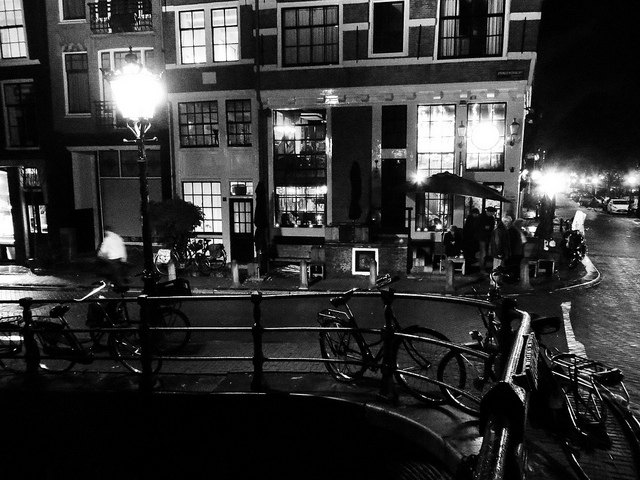
\includegraphics[width=\linewidth]{./procesadas/2015_00027/2015_00027_original.png}
		\caption{Imagen original}
	\end{subfigure}
	\hfill
	\begin{subfigure}[b]{0.28\textwidth}
		\centering
		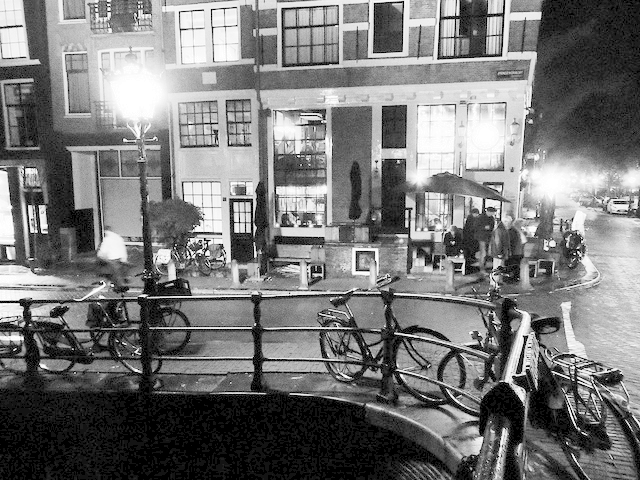
\includegraphics[width=\linewidth]{./procesadas/2015_00027/2015_00027_he.png}
		\caption{Histogram Equalization (HE)}
	\end{subfigure}

	% Segunda fila (2 imágenes)
	\begin{subfigure}[b]{0.28\textwidth}
		\centering
		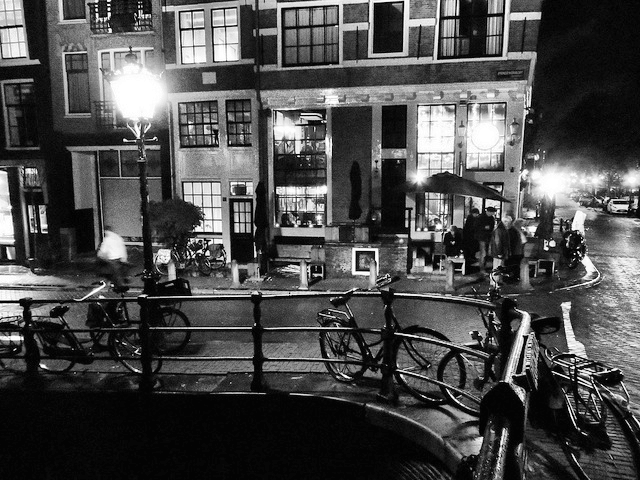
\includegraphics[width=\linewidth]{./procesadas/2015_00027/2015_00027_clahe.png}
		\caption{CLAHE}
	\end{subfigure}
	\hfill
	\begin{subfigure}[b]{0.28\textwidth}
		\centering
		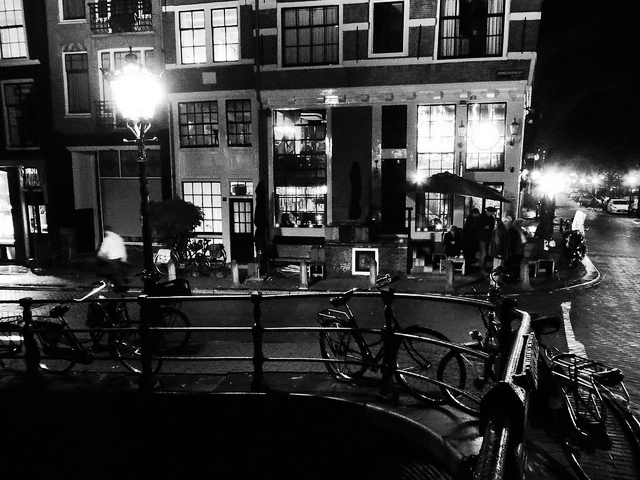
\includegraphics[width=\linewidth]{./procesadas/2015_00027/2015_00027_dqhepl.png}
		\caption{DQHEPL}
	\end{subfigure}

	% Tercera fila (1 imagen centrada)
	\begin{subfigure}[b]{0.28\textwidth}
		\centering
		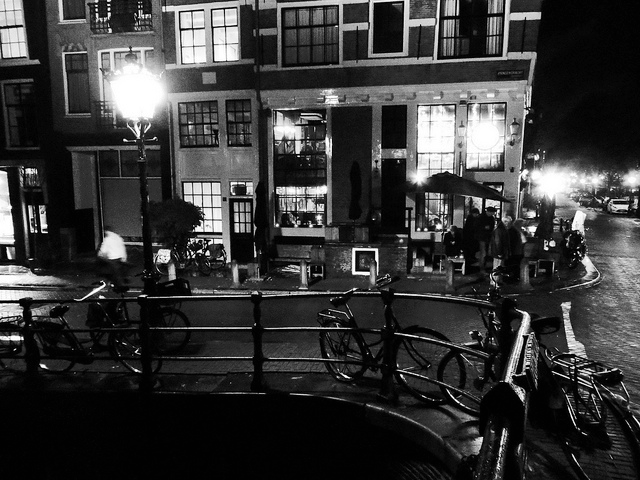
\includegraphics[width=\linewidth]{./procesadas/2015_00027/2015_00027_bhepl_d.png}
		\caption{BHEPL-D}
	\end{subfigure}

	\caption{Métodos aplicados sobre la imagen 2015\_00027.png}
	\label{fig:visual_027}
\end{figure}

Finalmente, el análisis visual de la \emph{Figura \ref{fig:visual_027}} revela que los métodos CLAHE,
BHEPL-D y DQHEPL muestran un rendimiento bastante similar en cuanto a la mejora visual de la
imagen. Sin embargo, es importante destacar que los métodos propuestos por Ooi y Mat Isa
sobresalen en la conservación de la naturalidad de la imagen original, logrando un equilibrio
efectivo entre la mejora del contraste y la preservación de la estructura tonal.

En particular, estos métodos mantienen una apariencia más fiel a la imagen original, sin
introducir distorsiones notables en los niveles de brillo o saturación. Al mismo tiempo, logran
mejorar el contraste, lo que permite una mejor definición de los detalles en las áreas tanto
oscuras como brillantes de la imagen. Este enfoque resulta en un acabado más fotográfico,
proporcionando una sensación de realismo y profundidad visual que es más agradable para el ojo
humano.

Por otro lado, mientras que CLAHE también mejora el contraste, tiende a generar una saturación
más pronunciada en ciertas áreas, lo que afecta la percepción general de la imagen, dándole un
acabado algo más procesado. A diferencia de esto, los métodos BHEPL-D y DQHEPL no solo mejoran
el contraste de manera más sutil, sino que conservan mejor la estructura original, lo que
resulta en una representación más fiel y visualmente atractiva.

% ---------  RESULTADOS globales --------------
\subsection{Resultados Cuantitativos globales} \label{subsec:resultados_cuantitativos}

En esta subsección se presentan los resultados cuantitativos obtenidos a partir de las métricas
de calidad de las imágenes procesadas (\emph{Tabla \ref{figure:global_estadisticas}}), con un enfoque en la media y la mediana de los
desempeños de cada uno de los métodos evaluados.

La media proporciona una visión general del rendimiento promedio de cada método, mientras que
la mediana permite observar el comportamiento en el valor central de las distribuciones,
evitando la influencia de valores extremos. De esta forma, se obtiene una imagen más completa y
robusta del desempeño de cada enfoque.

Este análisis final de los resultados cuantitativos permitirá concluir sobre las fortalezas y
debilidades de los métodos evaluados, proporcionando una base sólida para su selección según el
tipo de imagen y las necesidades de procesamiento.

\begin{table}[H]
	\centering
	\caption{Comparación estadística de los algoritmos de mejora de contraste}
	\label{tab:comparacion}
	\small
	\resizebox{\linewidth}{!}{%
		\begin{tabular}{l
				S[table-format=2.2] S[table-format=2.2]
				S[table-format=2.2] S[table-format=2.2]
				S[table-format=1.4] S[table-format=1.4]
				S[table-format=2.2] S[table-format=2.2]}
			\toprule
			\textbf{Método}                       &
			\multicolumn{2}{c}{\textbf{AMBE}}     &
			\multicolumn{2}{c}{\textbf{PSNR}}     &
			\multicolumn{2}{c}{\textbf{Entropía}} &
			\multicolumn{2}{c}{\textbf{Contraste}}                                                                            \\
			\cmidrule(lr){2-3} \cmidrule(lr){4-5} \cmidrule(lr){6-7} \cmidrule(lr){8-9}
			                                      & {Prom.} & {Med.} & {Prom.} & {Med.} & {Prom.} & {Med.} & {Prom.} & {Med.} \\
			\midrule
			CLAHE                                 & 18.57   & 18.56  & 20.47   & 19.96  & 6.55    & 6.90   & 48.94   & 50.52  \\
			HE                                    & 83.84   & 84.77  & 8.80    & 8.45   & 5.66    & 5.91   & 73.50   & 72.99  \\
			DQHEPL                                & 6.89    & 6.45   & 24.43   & 23.38  & 5.78    & 6.05   & 54.79   & 53.85  \\
			BHEPL-D                               & 4.79    & 3.97   & 29.78   & 29.60  & 5.74    & 6.11   & 47.37   & 47.08  \\
			\bottomrule
		\end{tabular}%
	}

	\vspace{0.5em}
	\footnotesize%
	\textit{Nota: AMBE (menor es mejor), PSNR (mayor es mejor). Uniformidad: 0.6–0.85 optimo}
	\label{figure:global_estadisticas}
\end{table}

\subsubsection{Análisis de AMBE}
\label{subsubsec:analisis_ambe}

Al comparar los valores promedio de AMBE para los diferentes algoritmos, se observa que
\emph{BHEPL-D} obtiene el valor más bajo, con un promedio de 4.79, lo que indica una mínima
discrepancia en el brillo respecto a la imagen original, lo cual es favorable. Por otro lado,
\emph{HE} presenta el valor más alto, con un promedio de 83.84, lo que sugiere una
considerable alteración del brillo original, resultando en una mayor sobresaturación. Los
métodos \emph{CLAHE} y \emph{DQHEPL} se encuentran en valores intermedios, con promedios de
18.57 y 6.89, respectivamente. Esto refleja un compromiso entre la mejora del contraste y la
preservación del brillo, siendo \emph{DQHEPL} el segundo mejor en cuanto a conservación del
brillo.

\subsubsection{\textbf{Análisis de PSNR}}
\label{subsubsec:analisis_psnr}

En cuanto al PSNR, el valor promedio más alto se encuentra en \emph{BHEPL-D} (29.78), lo que
sugiere una mayor calidad de la imagen procesada, con un menor nivel de ruido y distorsión en
comparación con los otros métodos. \emph{DQHEPL} también presenta un buen desempeño con un
promedio de 24.43, indicando que mantiene una buena relación señal/ruido, aunque no al nivel de
\emph{BHEPL-D}. En contraste, \emph{HE} tiene el valor más bajo con un promedio de 8.80, lo
que indica una pérdida significativa de calidad de la imagen debido a la sobresaturación.
\emph{CLAHE} se encuentra en un término medio con un promedio de 20.47, lo que refleja una
calidad de imagen moderada.

\subsubsection{\textbf{Análisis de Entropía}}
\label{subsubsec:analisis_entropia}

Al observar los valores de entropía, \emph{CLAHE} tiene el valor promedio más alto (6.55), lo
que indica una mayor cantidad de información o detalles presentes en la imagen procesada.
\emph{DQHEPL} y \emph{BHEPL-D} muestran valores similares, con promedios de 5.78 y 5.74,
respectivamente, lo que refleja un nivel razonable de detalle preservado sin sobresaturar la
imagen. \emph{HE}, por otro lado, presenta el valor más bajo con un promedio de 5.66, lo que
sugiere que la sobresaturación podría estar reduciendo la cantidad de detalles perceptibles en
la imagen procesada.

\subsubsection{\textbf{Análisis de Contraste}}
\label{subsubsec:analisis_contraste}

En cuanto al contraste, \emph{HE} presenta el valor promedio más alto (73.50), lo que indica
una mejora significativa del contraste, pero a costa de alterar otros aspectos de la imagen,
como la saturación de brillo. \emph{DQHEPL} y \emph{CLAHE} tienen promedios intermedios,
con 54.79 y 48.94 respectivamente, lo que indica que ambos métodos mejoran el contraste de
manera equilibrada sin introducir cambios excesivos en la imagen. \emph{BHEPL-D}, aunque con
un valor moderado (47.37), sigue siendo efectivo para mejorar el contraste sin comprometer la
calidad visual de manera drástica.

\subsubsection{\textbf{Análisis de Uniformidad}}
\label{subsubsec:analisis_uniformidad}

En el análisis de uniformidad, \emph{HE} obtiene el mejor valor promedio (0.607), lo que
indica una distribución más homogénea de los valores de gris, aunque esto también podría
contribuir a la sobresaturación mencionada en otros análisis. \emph{CLAHE}, con un valor de
0.509, muestra una ligera disminución en la uniformidad de la imagen en comparación con
\emph{HE}, pero sigue ofreciendo un balance razonable entre contraste y preservación del
brillo. \emph{BHEPL-D} y \emph{DQHEPL} presentan los valores más bajos, 0.449 y 0.442
respectivamente, lo que podría sugerir que en estos métodos, aunque la imagen mantiene una
mayor naturalidad, la uniformidad de los niveles de gris no es tan pronunciada, posiblemente
debido a su enfoque en la preservación del brillo y el detalle.

\subsubsection{\textbf{Análisis de Tiempos de Procesamiento}}
\label{subsubsec:analisis_tiempos}

En la \emph{Tabla \ref{tab:comparacion_tiempos}} se presentan los tiempos de procesamiento de cada uno
de los métodos evaluados. El tiempo de procesamiento es una métrica importante, ya que refleja
la eficiencia de cada algoritmo en términos de velocidad de ejecución.

\begin{table}[H]
	\caption{Comparación de tiempos de procesamiento}
	\label{tab:comparacion_tiempos}
	\small
	\resizebox{0.5\linewidth}{!}{%
		\begin{tabular}{lS[table-format=1]}
			\toprule
			\textbf{Método} & \textbf{Tiempo (ms)} \\
			\midrule
			CLAHE           & 2.58                 \\
			HE              & 0.93                 \\
			DQHEPL          & 7.69                 \\
			BHEPL-D         & 1.95                 \\
			\bottomrule
		\end{tabular}%
	}

	\vspace{0.5em}
	\footnotesize%
	\textit{Tabla de comparacion de tiempos}
\end{table}

Como se puede observar, el método \emph{HE} es el más rápido, con un tiempo de procesamiento
de solo 0.93 ms, seguido de cerca por \emph{BHEPL-D}, con un tiempo de 1.95 ms.
\emph{CLAHE} también es eficiente, con un tiempo de 2.58 ms. En contraste, \emph{DQHEPL}
presenta el tiempo más alto, con 7.69 ms, lo que sugiere una mayor carga computacional en
comparación con los otros métodos. Es importante señalar que este rendimiento inferior podría
estar relacionado con nuestra implementación específica del algoritmo, pero, en general,
\emph{DQHEPL} se desempeñó significativamente peor en términos de tiempo de procesamiento.


\subsection{Discusión de los Resultados} \label{subsec:discusion}

En esta sección, se interpretan los resultados obtenidos de la evaluación de los métodos
propuestos, destacando las diferencias entre ellos en cuanto a las métricas de calidad y
tiempos de procesamiento.

\subsubsection{\textbf{Interpretación de los Resultados Obtenidos}}

Los resultados cuantitativos y visuales mostraron diferencias claras entre los métodos
evaluados. En términos de las métricas AMBE, \emph{BHEPL-D} y \emph{DQHEPL} presentaron los
mejores resultados, con valores más bajos, lo que indica una mejor preservación del brillo y
menor deformación de la imagen. Por otro lado, \emph{HE} presentó un valor muy alto en AMBE,
lo que sugiere una sobresaturación de la imagen, afectando negativamente la calidad visual. En
cuanto a PSNR, \emph{DQHEPL} y \emph{BHEPL-D} mostraron un rendimiento superior, lo que
indica que estos métodos fueron capaces de mantener una mayor calidad de la imagen sin
introducir demasiado ruido.

En lo que respecta a la entropía, los valores fueron relativamente consistentes entre los
métodos, sin grandes diferencias. Sin embargo, la variabilidad en el contraste mostró que
\emph{HE} obtuvo los valores más altos, indicando una mejora significativa en el contraste de
la imagen, aunque con el costo de perder información en las zonas de baja luminosidad.

\subsubsection{\textbf{Comparación de los Algoritmos en Términos de sus Métricas de Evaluación}}

\emph{CLAHE} fue el método que más equilibró las métricas de calidad visual, ofreciendo un
buen rendimiento en AMBE, PSNR y contraste, aunque no llegó a los extremos alcanzados por
\emph{HE} en cuanto a contraste. Sin embargo, \emph{CLAHE} logró mantener un buen nivel de
uniformidad, lo que permitió conservar la naturalidad de la imagen.

\emph{HE}, aunque mejoró notablemente el contraste, presentó un efecto negativo en el brillo,
mostrando valores altos de AMBE. Esto es típico de algoritmos que distribuyen más los niveles
de gris, pero que terminan sobresaturando las zonas brillantes de la imagen. Aunque puede ser
útil en ciertos contextos donde se busca enfatizar el contraste, en este análisis resultó menos
favorable debido a la pérdida de detalles en zonas con iluminación baja.

Por su parte, \emph{DQHEPL} y \emph{BHEPL-D} mostraron un rendimiento similar, conservando
una buena estructura de la imagen y mejorando el contraste sin perder la uniformidad de los
niveles de gris. Ambos métodos fueron los más efectivos en términos de preservar la naturalidad
de la imagen, pero el rendimiento de \emph{DQHEPL} en cuanto a tiempo de procesamiento fue
considerablemente peor, lo que lo hace menos viable en aplicaciones donde la velocidad es
crucial.

\subsubsection{\textbf{Discusión sobre la Efectividad de Cada Algoritmo}}

En términos de efectividad, los métodos \emph{DQHEPL} y \emph{BHEPL-D} sobresalieron por su
capacidad para manejar diferentes condiciones de iluminación, manteniendo el brillo de la
imagen y mejorando el contraste de manera efectiva. Sin embargo, el tiempo de procesamiento de
\emph{DQHEPL} fue un inconveniente significativo, lo que puede afectar su aplicabilidad en
escenarios donde se requiera rapidez.

El algoritmo \emph{CLAHE} se desempeñó de manera consistente, logrando un buen equilibrio
entre contraste y preservación del brillo. Aunque no es el más fuerte en cuanto a la mejora de
contraste, su capacidad para manejar bien las diferencias de luminosidad sin introducir
artefactos visuales lo convierte en una opción útil.

En resumen, mientras que \emph{HE} sobresale en cuanto a aumento de contraste, su efecto
negativo sobre el brillo lo hace menos adecuado para aplicaciones que requieran una imagen
equilibrada y natural. Por el contrario, \emph{DQHEPL} y \emph{BHEPL-D} se presentaron como
los métodos más efectivos en términos de calidad visual, aunque la eficiencia computacional de
\emph{DQHEPL} debería considerarse en entornos de procesamiento rápido.

\section{Conclusiones}
\label{sec:conclusiones}

Este trabajo evaluó diversos métodos de mejora de contraste aplicados a imágenes reales con
bajo rango dinámico, analizando tanto métricas objetivas como resultados visuales. Cada
algoritmo mostró comportamientos particulares frente a diferentes condiciones de iluminación y
contenidos.

\emph{CLAHE} se destacó por su capacidad de mejorar el contraste de forma localizada sin
introducir artefactos ni alterar significativamente la estructura original de las imágenes.
Esta característica lo convierte en una opción especialmente adecuada para aplicaciones
críticas como la medicina o la vigilancia, donde es fundamental mantener la integridad del
contenido visual.

En cambio, los métodos \emph{BHEPL-D} y \emph{DQHEPL}, aunque menos efectivos en imágenes
extremadamente oscuras, ofrecieron una mejora visual más atractiva en condiciones de
iluminación mas favorables.
Estos algoritmos preservan mejor el carácter visual original de la imagen y potencian su
expresividad, por lo que resultan ideales para fotografía, cinematografía y otros campos donde
se prioriza la estética y la percepción visual.

\emph{DQHEPL}, en particular, obtuvo buenos resultados en cuanto a contraste y naturalidad,
aunque su mayor costo computacional lo vuelve menos apto para aplicaciones en tiempo real o con
grandes volúmenes de datos.

En resumen, no existe un único método óptimo para todos los contextos. Mientras que
\emph{CLAHE} es una solución en general robusta y equilibrada para tareas sensibles,
\emph{BHEPL-D} y \emph{DQHEPL} representan alternativas de alto impacto visual para usos más
creativos o expresivos. La elección del algoritmo debe considerar el equilibrio entre calidad
visual, fidelidad estructural y eficiencia computacional, según las necesidades específicas de
cada aplicación.

\subsection{Recomendaciones}
\label{subsec:recomendaciones}

A partir de los resultados obtenidos, se recomienda seleccionar el método de mejora de
contraste en función del contexto de aplicación y del tipo de imagen a procesar.

En entornos críticos donde se requiere mantener la fidelidad estructural y evitar artefactos
visuales como en imágenes médicas, análisis forense o sistemas de visión artificial el método
\emph{CLAHE} es la opción más adecuada. 

Por otro lado, los métodos \emph{BHEPL-D} y \emph{DQHEPL} demostraron ser más eficaces cuando
el objetivo es mejorar la estética visual o enfatizar detalles de forma creativa, como ocurre
en fotografía artística, edición digital o producción cinematográfica. Estos algoritmos ofrecen
una mejora del contraste más marcada y logran preservar el carácter de la imagen original, pero
no son recomendables en casos de imágenes extremadamente oscuras ni en aplicaciones donde la
exactitud del contenido visual sea prioritaria.

Cabe mencionar que los elevados tiempos de procesamiento observados en el método \emph{DQHEPL}
podrían estar influenciados en parte por la implementación específica utilizada en este
trabajo. Sin embargo, independientemente de ello, el desempeño computacional de este algoritmo
sigue siendo un aspecto a considerar. Por tanto, sería recomendable investigar posibles
optimizaciones, ya sea mediante paralelización, implementación en GPU u otras estrategias que
permitan mejorar su eficiencia.

\newpage

\section{Apéndices}
\label{sec:apendices}

\begin{itemize}
	\item Dataset: \url{https://www.kaggle.com/datasets/takeenjazayeri/low-contrast-images}
	\item Codigo fuente: \url{https://github.com/elias-gill/pdi_parcial1}
\end{itemize}

% Bibliografía
\nocite{*} % Incluye TODAS las referencias del .bib sin necesidad de citarlas
\bibliographystyle{ACM-Reference-Format}
\bibliography{bibliography}
\label{sec:bibliography}

\end{document}
